\documentclass[twoside]{book}

% Packages required by doxygen
\usepackage{fixltx2e}
\usepackage{calc}
\usepackage{doxygen}
\usepackage[export]{adjustbox} % also loads graphicx
\usepackage{graphicx}
\usepackage[utf8]{inputenc}
\usepackage{makeidx}
\usepackage{multicol}
\usepackage{multirow}
\PassOptionsToPackage{warn}{textcomp}
\usepackage{textcomp}
\usepackage[nointegrals]{wasysym}
\usepackage[table]{xcolor}

% Font selection
\usepackage[T1]{fontenc}
\usepackage[scaled=.90]{helvet}
\usepackage{courier}
\usepackage{amssymb}
\usepackage{sectsty}
\renewcommand{\familydefault}{\sfdefault}
\allsectionsfont{%
  \fontseries{bc}\selectfont%
  \color{darkgray}%
}
\renewcommand{\DoxyLabelFont}{%
  \fontseries{bc}\selectfont%
  \color{darkgray}%
}
\newcommand{\+}{\discretionary{\mbox{\scriptsize$\hookleftarrow$}}{}{}}

% Page & text layout
\usepackage{geometry}
\geometry{%
  a4paper,%
  top=2.5cm,%
  bottom=2.5cm,%
  left=2.5cm,%
  right=2.5cm%
}
\tolerance=750
\hfuzz=15pt
\hbadness=750
\setlength{\emergencystretch}{15pt}
\setlength{\parindent}{0cm}
\setlength{\parskip}{0.2cm}
\makeatletter
\renewcommand{\paragraph}{%
  \@startsection{paragraph}{4}{0ex}{-1.0ex}{1.0ex}{%
    \normalfont\normalsize\bfseries\SS@parafont%
  }%
}
\renewcommand{\subparagraph}{%
  \@startsection{subparagraph}{5}{0ex}{-1.0ex}{1.0ex}{%
    \normalfont\normalsize\bfseries\SS@subparafont%
  }%
}
\makeatother

% Headers & footers
\usepackage{fancyhdr}
\pagestyle{fancyplain}
\fancyhead[LE]{\fancyplain{}{\bfseries\thepage}}
\fancyhead[CE]{\fancyplain{}{}}
\fancyhead[RE]{\fancyplain{}{\bfseries\leftmark}}
\fancyhead[LO]{\fancyplain{}{\bfseries\rightmark}}
\fancyhead[CO]{\fancyplain{}{}}
\fancyhead[RO]{\fancyplain{}{\bfseries\thepage}}
\fancyfoot[LE]{\fancyplain{}{}}
\fancyfoot[CE]{\fancyplain{}{}}
\fancyfoot[RE]{\fancyplain{}{\bfseries\scriptsize Generated on Fri May 19 2017 19\+:02\+:39 for Nifty by Doxygen }}
\fancyfoot[LO]{\fancyplain{}{\bfseries\scriptsize Generated on Fri May 19 2017 19\+:02\+:39 for Nifty by Doxygen }}
\fancyfoot[CO]{\fancyplain{}{}}
\fancyfoot[RO]{\fancyplain{}{}}
\renewcommand{\footrulewidth}{0.4pt}
\renewcommand{\chaptermark}[1]{%
  \markboth{#1}{}%
}
\renewcommand{\sectionmark}[1]{%
  \markright{\thesection\ #1}%
}

% Indices & bibliography
\usepackage{natbib}
\usepackage[titles]{tocloft}
\setcounter{tocdepth}{3}
\setcounter{secnumdepth}{5}
\makeindex

% Hyperlinks (required, but should be loaded last)
\usepackage{ifpdf}
\ifpdf
  \usepackage[pdftex,pagebackref=true]{hyperref}
\else
  \usepackage[ps2pdf,pagebackref=true]{hyperref}
\fi
\hypersetup{%
  colorlinks=true,%
  linkcolor=blue,%
  citecolor=blue,%
  unicode%
}

% Custom commands
\newcommand{\clearemptydoublepage}{%
  \newpage{\pagestyle{empty}\cleardoublepage}%
}


%===== C O N T E N T S =====

\begin{document}

% Titlepage & ToC
\hypersetup{pageanchor=false,
             bookmarks=true,
             bookmarksnumbered=true,
             pdfencoding=unicode
            }
\pagenumbering{roman}
\begin{titlepage}
\vspace*{7cm}
\begin{center}%
{\Large Nifty \\[1ex]\large 0.\+4.\+0 }\\
\vspace*{1cm}
{\large Generated by Doxygen 1.8.10}\\
\vspace*{0.5cm}
{\small Fri May 19 2017 19:02:39}\\
\end{center}
\end{titlepage}
\clearemptydoublepage
\tableofcontents
\clearemptydoublepage
\pagenumbering{arabic}
\hypersetup{pageanchor=true}

%--- Begin generated contents ---
\chapter{Nifty}
\label{index}\hypertarget{index}{}\hypertarget{mainpage.dox_Introduction}{}\section{Introduction}\label{mainpage.dox_Introduction}

\chapter{Todo List}
\label{todo}
\hypertarget{todo}{}

\begin{DoxyRefList}
\item[\label{todo__todo000001}%
\hypertarget{todo__todo000001}{}%
Class \hyperlink{classnifty_1_1graph_1_1optimization_1_1lifted__multicut_1_1FusionMove}{nifty\+:\+:graph\+:\+:optimization\+:\+:lifted\+\_\+multicut\+:\+:Fusion\+Move$<$ O\+B\+J\+E\+C\+T\+I\+V\+E $>$} ]This implementation should only be used for sparse graphs (atm only sparse graphs are implemented so this is not an issue so far) 
\end{DoxyRefList}
\chapter{Module Index}
\section{Modules}
Here is a list of all modules\+:\begin{DoxyCompactList}
\item \contentsline{section}{Functions and classes for parallel processing.}{\pageref{group__ParallelProcessing}}{}
\end{DoxyCompactList}

\chapter{Namespace Index}
\section{Namespace List}
Here is a list of all namespaces with brief descriptions\+:\begin{DoxyCompactList}
\item\contentsline{section}{\hyperlink{namespaceandres}{andres} \\*The public A\+PI }{\pageref{namespaceandres}}{}
\item\contentsline{section}{\hyperlink{namespaceandres_1_1hdf5}{andres\+::hdf5} \\*H\+D\+F5 import/export support }{\pageref{namespaceandres_1_1hdf5}}{}
\item\contentsline{section}{\hyperlink{namespacehalf__float}{half\+\_\+float} }{\pageref{namespacehalf__float}}{}
\item\contentsline{section}{\hyperlink{namespacehalf__float_1_1detail}{half\+\_\+float\+::detail} }{\pageref{namespacehalf__float_1_1detail}}{}
\item\contentsline{section}{\hyperlink{namespacenifty}{nifty} }{\pageref{namespacenifty}}{}
\item\contentsline{section}{\hyperlink{namespacenifty_1_1array}{nifty\+::array} }{\pageref{namespacenifty_1_1array}}{}
\item\contentsline{section}{\hyperlink{namespacenifty_1_1cgp}{nifty\+::cgp} }{\pageref{namespacenifty_1_1cgp}}{}
\item\contentsline{section}{\hyperlink{namespacenifty_1_1container}{nifty\+::container} }{\pageref{namespacenifty_1_1container}}{}
\item\contentsline{section}{\hyperlink{namespacenifty_1_1exceptions}{nifty\+::exceptions} }{\pageref{namespacenifty_1_1exceptions}}{}
\item\contentsline{section}{\hyperlink{namespacenifty_1_1features}{nifty\+::features} }{\pageref{namespacenifty_1_1features}}{}
\item\contentsline{section}{\hyperlink{namespacenifty_1_1features_1_1detail__fastfilters}{nifty\+::features\+::detail\+\_\+fastfilters} }{\pageref{namespacenifty_1_1features_1_1detail__fastfilters}}{}
\item\contentsline{section}{\hyperlink{namespacenifty_1_1filters}{nifty\+::filters} }{\pageref{namespacenifty_1_1filters}}{}
\item\contentsline{section}{\hyperlink{namespacenifty_1_1graph}{nifty\+::graph} }{\pageref{namespacenifty_1_1graph}}{}
\item\contentsline{section}{\hyperlink{namespacenifty_1_1graph_1_1agglo}{nifty\+::graph\+::agglo} }{\pageref{namespacenifty_1_1graph_1_1agglo}}{}
\item\contentsline{section}{\hyperlink{namespacenifty_1_1graph_1_1agglo_1_1merge__rules}{nifty\+::graph\+::agglo\+::merge\+\_\+rules} }{\pageref{namespacenifty_1_1graph_1_1agglo_1_1merge__rules}}{}
\item\contentsline{section}{\hyperlink{namespacenifty_1_1graph_1_1detail__graph}{nifty\+::graph\+::detail\+\_\+graph} }{\pageref{namespacenifty_1_1graph_1_1detail__graph}}{}
\item\contentsline{section}{\hyperlink{namespacenifty_1_1graph_1_1graph__maps}{nifty\+::graph\+::graph\+\_\+maps} }{\pageref{namespacenifty_1_1graph_1_1graph__maps}}{}
\item\contentsline{section}{\hyperlink{namespacenifty_1_1graph_1_1opt}{nifty\+::graph\+::opt} }{\pageref{namespacenifty_1_1graph_1_1opt}}{}
\item\contentsline{section}{\hyperlink{namespacenifty_1_1graph_1_1opt_1_1common}{nifty\+::graph\+::opt\+::common} }{\pageref{namespacenifty_1_1graph_1_1opt_1_1common}}{}
\item\contentsline{section}{\hyperlink{namespacenifty_1_1graph_1_1opt_1_1common_1_1detail__cc__fusion}{nifty\+::graph\+::opt\+::common\+::detail\+\_\+cc\+\_\+fusion} }{\pageref{namespacenifty_1_1graph_1_1opt_1_1common_1_1detail__cc__fusion}}{}
\item\contentsline{section}{\hyperlink{namespacenifty_1_1graph_1_1opt_1_1higher__order__multicut}{nifty\+::graph\+::opt\+::higher\+\_\+order\+\_\+multicut} }{\pageref{namespacenifty_1_1graph_1_1opt_1_1higher__order__multicut}}{}
\item\contentsline{section}{\hyperlink{namespacenifty_1_1graph_1_1opt_1_1lifted__multicut}{nifty\+::graph\+::opt\+::lifted\+\_\+multicut} }{\pageref{namespacenifty_1_1graph_1_1opt_1_1lifted__multicut}}{}
\item\contentsline{section}{\hyperlink{namespacenifty_1_1graph_1_1opt_1_1mincut}{nifty\+::graph\+::opt\+::mincut} }{\pageref{namespacenifty_1_1graph_1_1opt_1_1mincut}}{}
\item\contentsline{section}{\hyperlink{namespacenifty_1_1graph_1_1opt_1_1minstcut}{nifty\+::graph\+::opt\+::minstcut} }{\pageref{namespacenifty_1_1graph_1_1opt_1_1minstcut}}{}
\item\contentsline{section}{\hyperlink{namespacenifty_1_1graph_1_1opt_1_1multicut}{nifty\+::graph\+::opt\+::multicut} }{\pageref{namespacenifty_1_1graph_1_1opt_1_1multicut}}{}
\item\contentsline{section}{\hyperlink{namespacenifty_1_1graph_1_1subgraph__masks}{nifty\+::graph\+::subgraph\+\_\+masks} }{\pageref{namespacenifty_1_1graph_1_1subgraph__masks}}{}
\item\contentsline{section}{\hyperlink{namespacenifty_1_1ground__truth}{nifty\+::ground\+\_\+truth} }{\pageref{namespacenifty_1_1ground__truth}}{}
\item\contentsline{section}{\hyperlink{namespacenifty_1_1hdf5}{nifty\+::hdf5} }{\pageref{namespacenifty_1_1hdf5}}{}
\item\contentsline{section}{\hyperlink{namespacenifty_1_1hdf5_1_1tools}{nifty\+::hdf5\+::tools} }{\pageref{namespacenifty_1_1hdf5_1_1tools}}{}
\item\contentsline{section}{\hyperlink{namespacenifty_1_1histogram}{nifty\+::histogram} }{\pageref{namespacenifty_1_1histogram}}{}
\item\contentsline{section}{\hyperlink{namespacenifty_1_1ilp__backend}{nifty\+::ilp\+\_\+backend} }{\pageref{namespacenifty_1_1ilp__backend}}{}
\item\contentsline{section}{\hyperlink{namespacenifty_1_1logging}{nifty\+::logging} }{\pageref{namespacenifty_1_1logging}}{}
\item\contentsline{section}{\hyperlink{namespacenifty_1_1marray}{nifty\+::marray} }{\pageref{namespacenifty_1_1marray}}{}
\item\contentsline{section}{\hyperlink{namespacenifty_1_1math}{nifty\+::math} }{\pageref{namespacenifty_1_1math}}{}
\item\contentsline{section}{\hyperlink{namespacenifty_1_1meta}{nifty\+::meta} }{\pageref{namespacenifty_1_1meta}}{}
\item\contentsline{section}{\hyperlink{namespacenifty_1_1parallel}{nifty\+::parallel} }{\pageref{namespacenifty_1_1parallel}}{}
\item\contentsline{section}{\hyperlink{namespacenifty_1_1tools}{nifty\+::tools} }{\pageref{namespacenifty_1_1tools}}{}
\item\contentsline{section}{\hyperlink{namespacenifty_1_1ufd}{nifty\+::ufd} }{\pageref{namespacenifty_1_1ufd}}{}
\item\contentsline{section}{\hyperlink{namespacepybind11}{pybind11} }{\pageref{namespacepybind11}}{}
\item\contentsline{section}{\hyperlink{namespacepybind11_1_1detail}{pybind11\+::detail} }{\pageref{namespacepybind11_1_1detail}}{}
\item\contentsline{section}{\hyperlink{namespacestd}{std} \\*Extensions to the C++ standard library }{\pageref{namespacestd}}{}
\end{DoxyCompactList}

\chapter{Hierarchical Index}
\section{Class Hierarchy}
This inheritance list is sorted roughly, but not completely, alphabetically\+:\begin{DoxyCompactList}
\item \contentsline{section}{nifty\+:\+:graph\+:\+:Acc\+Options}{\pageref{structnifty_1_1graph_1_1AccOptions}}{}
\item \contentsline{section}{nifty\+:\+:graph\+:\+:Adjacency\+Tag}{\pageref{structnifty_1_1graph_1_1AdjacencyTag}}{}
\item \contentsline{section}{nifty\+:\+:graph\+:\+:agglo\+:\+:Agglomerative\+Clustering$<$ C\+L\+U\+S\+T\+E\+R\+\_\+\+P\+O\+L\+I\+C\+Y $>$}{\pageref{classnifty_1_1graph_1_1agglo_1_1AgglomerativeClustering}}{}
\item \contentsline{section}{nifty\+:\+:features\+:\+:Apply\+Filters$<$ D\+I\+M $>$}{\pageref{structnifty_1_1features_1_1ApplyFilters}}{}
\item \contentsline{section}{nifty\+:\+:graph\+:\+:Arc\+Tag}{\pageref{structnifty_1_1graph_1_1ArcTag}}{}
\item array\begin{DoxyCompactList}
\item \contentsline{section}{nifty\+:\+:array\+:\+:Static\+Array\+Base$<$ T, D\+I\+M $>$}{\pageref{classnifty_1_1array_1_1StaticArrayBase}}{}
\item \contentsline{section}{nifty\+:\+:cgp\+:\+:Cell\+Geometry$<$ D\+I\+M, 0 $>$}{\pageref{classnifty_1_1cgp_1_1CellGeometry_3_01DIM_00_010_01_4}}{}
\end{DoxyCompactList}
\item \contentsline{section}{pybind11\+:\+:detail\+:\+:array\+\_\+caster\+\_\+$<$ Array\+Type, Value, Resizable, Size $>$}{\pageref{structpybind11_1_1detail_1_1array__caster__}}{}
\item \contentsline{section}{pybind11\+:\+:detail\+:\+:array\+\_\+caster\+\_\+$<$ nifty\+:\+:array\+:\+:Static\+Array$<$ Type, Size $>$, Type, false, Size $>$}{\pageref{structpybind11_1_1detail_1_1array__caster__}}{}
\begin{DoxyCompactList}
\item \contentsline{section}{pybind11\+:\+:detail\+:\+:type\+\_\+caster$<$ nifty\+:\+:array\+:\+:Static\+Array$<$ Type, Size $>$ $>$}{\pageref{structpybind11_1_1detail_1_1type__caster_3_01nifty_1_1array_1_1StaticArray_3_01Type_00_01Size_01_4_01_4}}{}
\end{DoxyCompactList}
\item \contentsline{section}{nifty\+:\+:graph\+:\+:Bidirectional\+Breadth\+First\+Search$<$ G\+R\+A\+P\+H $>$}{\pageref{classnifty_1_1graph_1_1BidirectionalBreadthFirstSearch}}{}
\item \contentsline{section}{nifty\+:\+:graph\+:\+:Bidirectional\+Breadth\+First\+Search$<$ Graph $>$}{\pageref{classnifty_1_1graph_1_1BidirectionalBreadthFirstSearch}}{}
\item \contentsline{section}{nifty\+:\+:tools\+:\+:Block$<$ D\+I\+M, T $>$}{\pageref{classnifty_1_1tools_1_1Block}}{}
\item \contentsline{section}{nifty\+:\+:tools\+:\+:Blocking$<$ D\+I\+M, T $>$}{\pageref{classnifty_1_1tools_1_1Blocking}}{}
\item \contentsline{section}{nifty\+:\+:tools\+:\+:Block\+Storage$<$ T $>$}{\pageref{classnifty_1_1tools_1_1BlockStorage}}{}
\item \contentsline{section}{nifty\+:\+:tools\+:\+:Block\+Storage\+Selector$<$ A\+R\+R\+A\+Y $>$}{\pageref{structnifty_1_1tools_1_1BlockStorageSelector}}{}
\item \contentsline{section}{nifty\+:\+:tools\+:\+:Block\+Storage\+Selector$<$ hdf5\+:\+:Hdf5\+Array$<$ T $>$ $>$}{\pageref{structnifty_1_1tools_1_1BlockStorageSelector_3_01hdf5_1_1Hdf5Array_3_01T_01_4_01_4}}{}
\item \contentsline{section}{nifty\+:\+:tools\+:\+:Block\+Storage\+Selector$<$ marray\+:\+:Marray$<$ T, A $>$ $>$}{\pageref{structnifty_1_1tools_1_1BlockStorageSelector_3_01marray_1_1Marray_3_01T_00_01A_01_4_01_4}}{}
\item \contentsline{section}{nifty\+:\+:tools\+:\+:Block\+Storage\+Selector$<$ marray\+:\+:Py\+View$<$ T, D\+I\+M, A\+U\+T\+O\+\_\+\+C\+A\+S\+T\+\_\+\+T\+Y\+P\+E $>$ $>$}{\pageref{structnifty_1_1tools_1_1BlockStorageSelector_3_01marray_1_1PyView_3_01T_00_01DIM_00_01AUTO__CAST__TYPE_01_4_01_4}}{}
\item \contentsline{section}{nifty\+:\+:tools\+:\+:Block\+Storage\+Selector$<$ marray\+:\+:View$<$ T, C, A $>$ $>$}{\pageref{structnifty_1_1tools_1_1BlockStorageSelector_3_01marray_1_1View_3_01T_00_01C_00_01A_01_4_01_4}}{}
\item \contentsline{section}{nifty\+:\+:tools\+:\+:Block\+View$<$ T $>$}{\pageref{classnifty_1_1tools_1_1BlockView}}{}
\item \contentsline{section}{nifty\+:\+:tools\+:\+:Block\+With\+Halo$<$ D\+I\+M, T $>$}{\pageref{classnifty_1_1tools_1_1BlockWithHalo}}{}
\item \contentsline{section}{nifty\+:\+:cgp\+:\+:Bounds$<$ D\+I\+M $>$}{\pageref{classnifty_1_1cgp_1_1Bounds}}{}
\item \contentsline{section}{nifty\+:\+:cgp\+:\+:Bounds$<$ 2 $>$}{\pageref{classnifty_1_1cgp_1_1Bounds_3_012_01_4}}{}
\item \contentsline{section}{nifty\+:\+:hdf5\+:\+:Cache\+Settings}{\pageref{structnifty_1_1hdf5_1_1CacheSettings}}{}
\item \contentsline{section}{nifty\+:\+:cgp\+:\+:Cell1\+Basic\+Geometric\+Features2\+D}{\pageref{classnifty_1_1cgp_1_1Cell1BasicGeometricFeatures2D}}{}
\item \contentsline{section}{nifty\+:\+:cgp\+:\+:Cell1\+Basic\+Topological\+Features}{\pageref{classnifty_1_1cgp_1_1Cell1BasicTopologicalFeatures}}{}
\item \contentsline{section}{nifty\+:\+:cgp\+:\+:Cell1\+Curvature\+Features2\+D}{\pageref{classnifty_1_1cgp_1_1Cell1CurvatureFeatures2D}}{}
\item \contentsline{section}{nifty\+:\+:cgp\+:\+:Cell1\+Line\+Segment\+Dist2\+D}{\pageref{classnifty_1_1cgp_1_1Cell1LineSegmentDist2D}}{}
\item \contentsline{section}{nifty\+:\+:cgp\+:\+:Cell\+Bounded\+By$<$ D\+I\+M, C\+E\+L\+L\+\_\+\+T\+Y\+P\+E $>$}{\pageref{classnifty_1_1cgp_1_1CellBoundedBy}}{}
\item \contentsline{section}{nifty\+:\+:cgp\+:\+:Cell\+Bounded\+By$<$ 2, 1 $>$}{\pageref{classnifty_1_1cgp_1_1CellBoundedBy_3_012_00_011_01_4}}{}
\item \contentsline{section}{nifty\+:\+:cgp\+:\+:Cell\+Bounded\+By$<$ 2, 2 $>$}{\pageref{classnifty_1_1cgp_1_1CellBoundedBy_3_012_00_012_01_4}}{}
\item \contentsline{section}{nifty\+:\+:cgp\+:\+:Cell\+Bounded\+By\+Vector$<$ D\+I\+M, C\+E\+L\+L\+\_\+\+T\+Y\+P\+E $>$}{\pageref{classnifty_1_1cgp_1_1CellBoundedByVector}}{}
\item \contentsline{section}{nifty\+:\+:cgp\+:\+:Cell\+Bounds$<$ D\+I\+M, C\+E\+L\+L\+\_\+\+T\+Y\+P\+E $>$}{\pageref{classnifty_1_1cgp_1_1CellBounds}}{}
\item \contentsline{section}{nifty\+:\+:cgp\+:\+:Cell\+Bounds$<$ 2, 0 $>$}{\pageref{classnifty_1_1cgp_1_1CellBounds_3_012_00_010_01_4}}{}
\item \contentsline{section}{nifty\+:\+:cgp\+:\+:Cell\+Bounds$<$ 2, 1 $>$}{\pageref{classnifty_1_1cgp_1_1CellBounds_3_012_00_011_01_4}}{}
\item \contentsline{section}{nifty\+:\+:tools\+:\+:Changeable\+Priority\+Queue$<$ T, C\+O\+M\+P\+A\+R\+E $>$}{\pageref{classnifty_1_1tools_1_1ChangeablePriorityQueue}}{}
\item \contentsline{section}{nifty\+:\+:tools\+:\+:Changeable\+Priority\+Queue$<$ double, std\+:\+:less$<$ double $>$ $>$}{\pageref{classnifty_1_1tools_1_1ChangeablePriorityQueue}}{}
\item \contentsline{section}{nifty\+:\+:tools\+:\+:Changeable\+Priority\+Queue$<$ Weight\+Type $>$}{\pageref{classnifty_1_1tools_1_1ChangeablePriorityQueue}}{}
\item \contentsline{section}{nifty\+:\+:graph\+:\+:Components\+Bfs$<$ G\+R\+A\+P\+H $>$}{\pageref{classnifty_1_1graph_1_1ComponentsBfs}}{}
\item \contentsline{section}{nifty\+:\+:graph\+:\+:Components\+Ufd$<$ G\+R\+A\+P\+H $>$}{\pageref{classnifty_1_1graph_1_1ComponentsUfd}}{}
\item \contentsline{section}{nifty\+:\+:graph\+:\+:Components\+Ufd$<$ Graph $>$}{\pageref{classnifty_1_1graph_1_1ComponentsUfd}}{}
\item \contentsline{section}{nifty\+:\+:graph\+:\+:Components\+Ufd$<$ Graph\+Type $>$}{\pageref{classnifty_1_1graph_1_1ComponentsUfd}}{}
\item \contentsline{section}{nifty\+:\+:tools\+:\+:Const\+Iterator\+Range$<$ I\+T\+E\+R\+A\+T\+O\+R $>$}{\pageref{classnifty_1_1tools_1_1ConstIteratorRange}}{}
\item \contentsline{section}{nifty\+:\+:tools\+:\+:Const\+Iterator\+Range$<$ \+\_\+\+C\+H\+I\+L\+D\+\_\+\+G\+R\+A\+P\+H\+:\+:Adjacency\+Iter $>$}{\pageref{classnifty_1_1tools_1_1ConstIteratorRange}}{}
\begin{DoxyCompactList}
\item \contentsline{section}{nifty\+:\+:graph\+:\+:Undirected\+Graph\+Base$<$ C\+H\+I\+L\+D\+\_\+\+G\+R\+A\+P\+H, N\+O\+D\+E\+\_\+\+I\+T\+E\+R, E\+D\+G\+E\+\_\+\+I\+T\+E\+R, A\+D\+J\+A\+C\+E\+N\+C\+Y\+\_\+\+I\+T\+E\+R $>$\+:\+:Adjacency\+Iter\+Range$<$ \+\_\+\+C\+H\+I\+L\+D\+\_\+\+G\+R\+A\+P\+H $>$}{\pageref{structnifty_1_1graph_1_1UndirectedGraphBase_1_1AdjacencyIterRange}}{}
\end{DoxyCompactList}
\item \contentsline{section}{nifty\+:\+:tools\+:\+:Const\+Iterator\+Range$<$ \+\_\+\+C\+H\+I\+L\+D\+\_\+\+G\+R\+A\+P\+H\+:\+:Adjacency\+Out\+Iter $>$}{\pageref{classnifty_1_1tools_1_1ConstIteratorRange}}{}
\begin{DoxyCompactList}
\item \contentsline{section}{nifty\+:\+:graph\+:\+:Directed\+Graph\+Base$<$ C\+H\+I\+L\+D\+\_\+\+G\+R\+A\+P\+H $>$\+:\+:Adjacency\+Iter\+Range$<$ \+\_\+\+C\+H\+I\+L\+D\+\_\+\+G\+R\+A\+P\+H $>$}{\pageref{structnifty_1_1graph_1_1DirectedGraphBase_1_1AdjacencyIterRange}}{}
\end{DoxyCompactList}
\item \contentsline{section}{nifty\+:\+:tools\+:\+:Const\+Iterator\+Range$<$ \+\_\+\+C\+H\+I\+L\+D\+\_\+\+G\+R\+A\+P\+H\+:\+:Arc\+Iter $>$}{\pageref{classnifty_1_1tools_1_1ConstIteratorRange}}{}
\begin{DoxyCompactList}
\item \contentsline{section}{nifty\+:\+:graph\+:\+:Directed\+Graph\+Base$<$ C\+H\+I\+L\+D\+\_\+\+G\+R\+A\+P\+H $>$\+:\+:Arc\+Iter\+Range$<$ \+\_\+\+C\+H\+I\+L\+D\+\_\+\+G\+R\+A\+P\+H $>$}{\pageref{structnifty_1_1graph_1_1DirectedGraphBase_1_1ArcIterRange}}{}
\end{DoxyCompactList}
\item \contentsline{section}{nifty\+:\+:tools\+:\+:Const\+Iterator\+Range$<$ \+\_\+\+C\+H\+I\+L\+D\+\_\+\+G\+R\+A\+P\+H\+:\+:Edge\+Iter $>$}{\pageref{classnifty_1_1tools_1_1ConstIteratorRange}}{}
\begin{DoxyCompactList}
\item \contentsline{section}{nifty\+:\+:graph\+:\+:Undirected\+Graph\+Base$<$ C\+H\+I\+L\+D\+\_\+\+G\+R\+A\+P\+H, N\+O\+D\+E\+\_\+\+I\+T\+E\+R, E\+D\+G\+E\+\_\+\+I\+T\+E\+R, A\+D\+J\+A\+C\+E\+N\+C\+Y\+\_\+\+I\+T\+E\+R $>$\+:\+:Edge\+Iter\+Range$<$ \+\_\+\+C\+H\+I\+L\+D\+\_\+\+G\+R\+A\+P\+H $>$}{\pageref{structnifty_1_1graph_1_1UndirectedGraphBase_1_1EdgeIterRange}}{}
\end{DoxyCompactList}
\item \contentsline{section}{nifty\+:\+:tools\+:\+:Const\+Iterator\+Range$<$ \+\_\+\+C\+H\+I\+L\+D\+\_\+\+G\+R\+A\+P\+H\+:\+:Node\+Iter $>$}{\pageref{classnifty_1_1tools_1_1ConstIteratorRange}}{}
\begin{DoxyCompactList}
\item \contentsline{section}{nifty\+:\+:graph\+:\+:Directed\+Graph\+Base$<$ C\+H\+I\+L\+D\+\_\+\+G\+R\+A\+P\+H $>$\+:\+:Node\+Iter\+Range$<$ \+\_\+\+C\+H\+I\+L\+D\+\_\+\+G\+R\+A\+P\+H $>$}{\pageref{structnifty_1_1graph_1_1DirectedGraphBase_1_1NodeIterRange}}{}
\item \contentsline{section}{nifty\+:\+:graph\+:\+:Undirected\+Graph\+Base$<$ C\+H\+I\+L\+D\+\_\+\+G\+R\+A\+P\+H, N\+O\+D\+E\+\_\+\+I\+T\+E\+R, E\+D\+G\+E\+\_\+\+I\+T\+E\+R, A\+D\+J\+A\+C\+E\+N\+C\+Y\+\_\+\+I\+T\+E\+R $>$\+:\+:Node\+Iter\+Range$<$ \+\_\+\+C\+H\+I\+L\+D\+\_\+\+G\+R\+A\+P\+H $>$}{\pageref{structnifty_1_1graph_1_1UndirectedGraphBase_1_1NodeIterRange}}{}
\end{DoxyCompactList}
\item \contentsline{section}{nifty\+:\+:tools\+:\+:Const\+Iterator\+Range$<$ Adjacency\+Iter $>$}{\pageref{classnifty_1_1tools_1_1ConstIteratorRange}}{}
\begin{DoxyCompactList}
\item \contentsline{section}{nifty\+:\+:graph\+:\+:Edge\+Contraction\+Graph$<$ G\+R\+A\+P\+H, C\+A\+L\+L\+B\+A\+C\+K, W\+I\+T\+H\+\_\+\+E\+D\+G\+E\+\_\+\+U\+F\+D $>$\+:\+:Adjacency\+Iter\+Range}{\pageref{structnifty_1_1graph_1_1EdgeContractionGraph_1_1AdjacencyIterRange}}{}
\end{DoxyCompactList}
\item \contentsline{section}{nifty\+:\+:graph\+:\+:graph\+\_\+maps\+:\+:Multiband\+Node\+Map$<$ G, T $>$\+:\+:Const\+Proxy}{\pageref{classnifty_1_1graph_1_1graph__maps_1_1MultibandNodeMap_1_1ConstProxy}}{}
\item \contentsline{section}{nifty\+:\+:graph\+:\+:graph\+\_\+maps\+:\+:Multiband\+Array\+View\+Node\+Map$<$ A\+R\+R\+A\+Y $>$\+:\+:Const\+Proxy}{\pageref{classnifty_1_1graph_1_1graph__maps_1_1MultibandArrayViewNodeMap_1_1ConstProxy}}{}
\item \contentsline{section}{nifty\+:\+:graph\+:\+:Contiguous\+Tag}{\pageref{structnifty_1_1graph_1_1ContiguousTag}}{}
\item counting\+\_\+iterator\begin{DoxyCompactList}
\item \contentsline{section}{nifty\+:\+:graph\+:\+:detail\+\_\+graph\+:\+:Simple\+Graph\+Edge\+Iter}{\pageref{classnifty_1_1graph_1_1detail__graph_1_1SimpleGraphEdgeIter}}{}
\item \contentsline{section}{nifty\+:\+:graph\+:\+:detail\+\_\+graph\+:\+:Simple\+Graph\+Node\+Iter}{\pageref{classnifty_1_1graph_1_1detail__graph_1_1SimpleGraphNodeIter}}{}
\item \contentsline{section}{nifty\+:\+:graph\+:\+:detail\+\_\+graph\+:\+:Undirected\+Grid\+Graph\+Iter$<$ D\+I\+M, S\+I\+M\+P\+L\+E\+\_\+\+N\+H $>$\+:\+:Edge\+Iter}{\pageref{classnifty_1_1graph_1_1detail__graph_1_1UndirectedGridGraphIter_1_1EdgeIter}}{}
\item \contentsline{section}{nifty\+:\+:graph\+:\+:detail\+\_\+graph\+:\+:Undirected\+Grid\+Graph\+Iter$<$ D\+I\+M, S\+I\+M\+P\+L\+E\+\_\+\+N\+H $>$\+:\+:Node\+Iter}{\pageref{classnifty_1_1graph_1_1detail__graph_1_1UndirectedGridGraphIter_1_1NodeIter}}{}
\end{DoxyCompactList}
\item \contentsline{section}{nifty\+:\+:ilp\+\_\+backend\+:\+:Cplex}{\pageref{classnifty_1_1ilp__backend_1_1Cplex}}{}
\item \contentsline{section}{nifty\+:\+:features\+:\+:Default\+Accumulated\+Statistics$<$ T $>$}{\pageref{classnifty_1_1features_1_1DefaultAccumulatedStatistics}}{}
\item \contentsline{section}{nifty\+:\+:graph\+:\+:optimization\+:\+:mincut\+:\+:Default\+Proposal\+Generator\+Mock}{\pageref{structnifty_1_1graph_1_1optimization_1_1mincut_1_1DefaultProposalGeneratorMock}}{}
\item \contentsline{section}{nifty\+:\+:graph\+:\+:Default\+Subgraph\+Mask$<$ G $>$}{\pageref{structnifty_1_1graph_1_1DefaultSubgraphMask}}{}
\item \contentsline{section}{nifty\+:\+:graph\+:\+:Directed\+Graph\+Base$<$ C\+H\+I\+L\+D\+\_\+\+G\+R\+A\+P\+H $>$}{\pageref{classnifty_1_1graph_1_1DirectedGraphBase}}{}
\item \contentsline{section}{nifty\+:\+:graph\+:\+:Directed\+Graph\+Base$<$ Simple\+Directed\+Graph$<$ A\+R\+C\+\_\+\+I\+N\+T\+E\+R\+A\+N\+L\+\_\+\+T\+Y\+P\+E, N\+O\+D\+E\+\_\+\+I\+N\+T\+E\+R\+N\+A\+L\+\_\+\+T\+Y\+P\+E $>$ $>$}{\pageref{classnifty_1_1graph_1_1DirectedGraphBase}}{}
\begin{DoxyCompactList}
\item \contentsline{section}{nifty\+:\+:graph\+:\+:Simple\+Directed\+Graph$<$ A\+R\+C\+\_\+\+I\+N\+T\+E\+R\+A\+N\+L\+\_\+\+T\+Y\+P\+E, N\+O\+D\+E\+\_\+\+I\+N\+T\+E\+R\+N\+A\+L\+\_\+\+T\+Y\+P\+E $>$}{\pageref{classnifty_1_1graph_1_1SimpleDirectedGraph}}{}
\end{DoxyCompactList}
\item \contentsline{section}{nifty\+:\+:graph\+:\+:Directed\+Graph\+View$<$ G\+R\+A\+P\+H $>$}{\pageref{classnifty_1_1graph_1_1DirectedGraphView}}{}
\item \contentsline{section}{nifty\+:\+:graph\+:\+:Grid\+Rag$<$ D\+I\+M, L\+A\+B\+E\+L\+S\+\_\+\+P\+R\+O\+X\+Y $>$\+:\+:Dont\+Compute\+Rag}{\pageref{structnifty_1_1graph_1_1GridRag_1_1DontComputeRag}}{}
\item Edge\+Contraction\+Graph\+Edge\+Ufd\+Helper\begin{DoxyCompactList}
\item \contentsline{section}{nifty\+:\+:graph\+:\+:Edge\+Contraction\+Graph$<$ Graph, Callback $>$}{\pageref{classnifty_1_1graph_1_1EdgeContractionGraph}}{}
\item \contentsline{section}{nifty\+:\+:graph\+:\+:Edge\+Contraction\+Graph$<$ Graph\+Type, Callback\+Type $>$}{\pageref{classnifty_1_1graph_1_1EdgeContractionGraph}}{}
\item \contentsline{section}{nifty\+:\+:graph\+:\+:Edge\+Contraction\+Graph$<$ Graph\+Type, Self\+Type $>$}{\pageref{classnifty_1_1graph_1_1EdgeContractionGraph}}{}
\item \contentsline{section}{nifty\+:\+:graph\+:\+:Edge\+Contraction\+Graph$<$ Lifted\+Graph, Callback $>$}{\pageref{classnifty_1_1graph_1_1EdgeContractionGraph}}{}
\item \contentsline{section}{nifty\+:\+:graph\+:\+:Edge\+Contraction\+Graph$<$ G\+R\+A\+P\+H, C\+A\+L\+L\+B\+A\+C\+K, W\+I\+T\+H\+\_\+\+E\+D\+G\+E\+\_\+\+U\+F\+D $>$}{\pageref{classnifty_1_1graph_1_1EdgeContractionGraph}}{}
\end{DoxyCompactList}
\item \contentsline{section}{nifty\+:\+:graph\+:\+:Edge\+Contraction\+Graph\+With\+Sets\+Helper$<$ G\+R\+A\+P\+H, O\+U\+T\+E\+R\+\_\+\+C\+A\+L\+L\+B\+A\+C\+K, S\+E\+T $>$}{\pageref{structnifty_1_1graph_1_1EdgeContractionGraphWithSetsHelper}}{}
\item \contentsline{section}{nifty\+:\+:graph\+:\+:detail\+\_\+graph\+:\+:Edge\+Indices\+To\+Contiguous\+Edge\+Indices\+Impl$<$ G\+R\+A\+P\+H, E\+D\+G\+E\+\_\+\+I\+D\+\_\+\+T\+A\+G $>$}{\pageref{classnifty_1_1graph_1_1detail__graph_1_1EdgeIndicesToContiguousEdgeIndicesImpl}}{}
\item \contentsline{section}{nifty\+:\+:graph\+:\+:detail\+\_\+graph\+:\+:Edge\+Indices\+To\+Contiguous\+Edge\+Indices\+Impl$<$ G\+R\+A\+P\+H, G\+R\+A\+P\+H\+:\+:Edge\+Id\+Tag $>$}{\pageref{classnifty_1_1graph_1_1detail__graph_1_1EdgeIndicesToContiguousEdgeIndicesImpl}}{}
\begin{DoxyCompactList}
\item \contentsline{section}{nifty\+:\+:graph\+:\+:detail\+\_\+graph\+:\+:Edge\+Indices\+To\+Contiguous\+Edge\+Indices$<$ G\+R\+A\+P\+H $>$}{\pageref{classnifty_1_1graph_1_1detail__graph_1_1EdgeIndicesToContiguousEdgeIndices}}{}
\end{DoxyCompactList}
\item \contentsline{section}{nifty\+:\+:graph\+:\+:detail\+\_\+graph\+:\+:Edge\+Indices\+To\+Contiguous\+Edge\+Indices\+Impl$<$ Graph, Graph\+:\+:Edge\+Id\+Tag $>$}{\pageref{classnifty_1_1graph_1_1detail__graph_1_1EdgeIndicesToContiguousEdgeIndicesImpl}}{}
\begin{DoxyCompactList}
\item \contentsline{section}{nifty\+:\+:graph\+:\+:detail\+\_\+graph\+:\+:Edge\+Indices\+To\+Contiguous\+Edge\+Indices$<$ Graph $>$}{\pageref{classnifty_1_1graph_1_1detail__graph_1_1EdgeIndicesToContiguousEdgeIndices}}{}
\end{DoxyCompactList}
\item \contentsline{section}{nifty\+:\+:graph\+:\+:detail\+\_\+graph\+:\+:Edge\+Indices\+To\+Contiguous\+Edge\+Indices\+Impl$<$ G\+R\+A\+P\+H, nifty\+:\+:graph\+:\+:Contiguous\+Tag $>$}{\pageref{classnifty_1_1graph_1_1detail__graph_1_1EdgeIndicesToContiguousEdgeIndicesImpl_3_01GRAPH_00_01ni85a4007f22b365a25e3bd0829bce5cfc}}{}
\item \contentsline{section}{nifty\+:\+:graph\+:\+:detail\+\_\+graph\+:\+:Edge\+Indices\+To\+Contiguous\+Edge\+Indices\+Impl$<$ Lifted\+Graph, Lifted\+Graph\+:\+:Edge\+Id\+Tag $>$}{\pageref{classnifty_1_1graph_1_1detail__graph_1_1EdgeIndicesToContiguousEdgeIndicesImpl}}{}
\begin{DoxyCompactList}
\item \contentsline{section}{nifty\+:\+:graph\+:\+:detail\+\_\+graph\+:\+:Edge\+Indices\+To\+Contiguous\+Edge\+Indices$<$ Lifted\+Graph $>$}{\pageref{classnifty_1_1graph_1_1detail__graph_1_1EdgeIndicesToContiguousEdgeIndices}}{}
\end{DoxyCompactList}
\item \contentsline{section}{nifty\+:\+:graph\+:\+:graph\+\_\+maps\+:\+:Edge\+Map\+From\+Node\+Map$<$ G\+R\+A\+P\+H, N\+O\+D\+E\+\_\+\+M\+A\+P, B\+I\+N\+A\+R\+Y\+\_\+\+F\+U\+N\+C\+T\+O\+R $>$}{\pageref{classnifty_1_1graph_1_1graph__maps_1_1EdgeMapFromNodeMap}}{}
\item \contentsline{section}{nifty\+:\+:graph\+:\+:Edge\+Tag}{\pageref{structnifty_1_1graph_1_1EdgeTag}}{}
\item \contentsline{section}{nifty\+:\+:graph\+:\+:agglo\+:\+:Edge\+Weighted\+Cluster\+Policy$<$ G\+R\+A\+P\+H, E\+N\+A\+B\+L\+E\+\_\+\+U\+C\+M $>$}{\pageref{classnifty_1_1graph_1_1agglo_1_1EdgeWeightedClusterPolicy}}{}
\item \contentsline{section}{nifty\+:\+:graph\+:\+:agglo\+:\+:Edge\+Weighted\+Cluster\+Policy\+Settings}{\pageref{structnifty_1_1graph_1_1agglo_1_1EdgeWeightedClusterPolicySettings}}{}
\begin{DoxyCompactList}
\item \contentsline{section}{nifty\+:\+:graph\+:\+:agglo\+:\+:Mala\+Cluster\+Policy$<$ G\+R\+A\+P\+H, E\+N\+A\+B\+L\+E\+\_\+\+U\+C\+M $>$\+:\+:Settings\+Type}{\pageref{structnifty_1_1graph_1_1agglo_1_1MalaClusterPolicy_1_1SettingsType}}{}
\end{DoxyCompactList}
\item \contentsline{section}{nifty\+:\+:graph\+:\+:Explicit\+Labels$<$ D\+I\+M, L\+A\+B\+E\+L\+\_\+\+T\+Y\+P\+E $>$}{\pageref{classnifty_1_1graph_1_1ExplicitLabels}}{}
\item \contentsline{section}{nifty\+:\+:graph\+:\+:agglo\+:\+:Export\+Ucm\+Functions$<$ W\+I\+T\+H\+\_\+\+U\+C\+M $>$}{\pageref{structnifty_1_1graph_1_1agglo_1_1ExportUcmFunctions}}{}
\item \contentsline{section}{nifty\+:\+:graph\+:\+:agglo\+:\+:Export\+Ucm\+Functions$<$ true $>$}{\pageref{structnifty_1_1graph_1_1agglo_1_1ExportUcmFunctions_3_01true_01_4}}{}
\item \contentsline{section}{nifty\+:\+:features\+:\+:detail\+\_\+fastfilters\+:\+:Fastfilters\+Dim$<$ fastfilters\+\_\+array\+\_\+t $>$}{\pageref{structnifty_1_1features_1_1detail__fastfilters_1_1FastfiltersDim}}{}
\item \contentsline{section}{nifty\+:\+:features\+:\+:detail\+\_\+fastfilters\+:\+:Fastfilters\+Dim$<$ fastfilters\+\_\+array2d\+\_\+t $>$}{\pageref{structnifty_1_1features_1_1detail__fastfilters_1_1FastfiltersDim_3_01fastfilters__array2d__t_01_4}}{}
\item \contentsline{section}{nifty\+:\+:features\+:\+:detail\+\_\+fastfilters\+:\+:Fastfilters\+Dim$<$ fastfilters\+\_\+array3d\+\_\+t $>$}{\pageref{structnifty_1_1features_1_1detail__fastfilters_1_1FastfiltersDim_3_01fastfilters__array3d__t_01_4}}{}
\item \contentsline{section}{andres\+:\+:F\+F\+T$<$ S $>$}{\pageref{classandres_1_1FFT}}{}
\item \contentsline{section}{nifty\+:\+:cgp\+:\+:Filled\+Topological\+Grid$<$ D\+I\+M $>$}{\pageref{classnifty_1_1cgp_1_1FilledTopologicalGrid}}{}
\item \contentsline{section}{nifty\+:\+:cgp\+:\+:Filled\+Topological\+Grid$<$ 2 $>$}{\pageref{classnifty_1_1cgp_1_1FilledTopologicalGrid_3_012_01_4}}{}
\item \contentsline{section}{nifty\+:\+:features\+:\+:Filter\+Base}{\pageref{structnifty_1_1features_1_1FilterBase}}{}
\begin{DoxyCompactList}
\item \contentsline{section}{nifty\+:\+:features\+:\+:Gaussian\+Gradient\+Magnitude}{\pageref{structnifty_1_1features_1_1GaussianGradientMagnitude}}{}
\item \contentsline{section}{nifty\+:\+:features\+:\+:Gaussian\+Smoothing}{\pageref{structnifty_1_1features_1_1GaussianSmoothing}}{}
\item \contentsline{section}{nifty\+:\+:features\+:\+:Hessian\+Of\+Gaussian\+Eigenvalues}{\pageref{structnifty_1_1features_1_1HessianOfGaussianEigenvalues}}{}
\item \contentsline{section}{nifty\+:\+:features\+:\+:Laplacian\+Of\+Gaussian}{\pageref{structnifty_1_1features_1_1LaplacianOfGaussian}}{}
\item \contentsline{section}{nifty\+:\+:features\+:\+:Structure\+Tensor\+Eigenvalues}{\pageref{structnifty_1_1features_1_1StructureTensorEigenvalues}}{}
\end{DoxyCompactList}
\item \contentsline{section}{nifty\+:\+:container\+:\+:Flat\+Set$<$ Key, Comparison, Allocator $>$}{\pageref{classnifty_1_1container_1_1FlatSet}}{}
\item \contentsline{section}{nifty\+:\+:graph\+:\+:Flexible\+Callback}{\pageref{structnifty_1_1graph_1_1FlexibleCallback}}{}
\item \contentsline{section}{nifty\+:\+:graph\+:\+:optimization\+:\+:multicut\+:\+:Fusion\+Move$<$ O\+B\+J\+E\+C\+T\+I\+V\+E $>$}{\pageref{classnifty_1_1graph_1_1optimization_1_1multicut_1_1FusionMove}}{}
\item \contentsline{section}{nifty\+:\+:graph\+:\+:optimization\+:\+:common\+:\+:Fusion\+Move$<$ O\+B\+J\+E\+C\+T\+I\+V\+E $>$}{\pageref{classnifty_1_1graph_1_1optimization_1_1common_1_1FusionMove}}{}
\item \contentsline{section}{nifty\+:\+:graph\+:\+:optimization\+:\+:lifted\+\_\+multicut\+:\+:Fusion\+Move$<$ O\+B\+J\+E\+C\+T\+I\+V\+E $>$}{\pageref{classnifty_1_1graph_1_1optimization_1_1lifted__multicut_1_1FusionMove}}{}
\item \contentsline{section}{nifty\+:\+:filters\+:\+:Gaussian\+Curvature2\+D$<$ T $>$}{\pageref{classnifty_1_1filters_1_1GaussianCurvature2D}}{}
\item \contentsline{section}{nifty\+:\+:cgp\+:\+:Geometry$<$ D\+I\+M $>$}{\pageref{classnifty_1_1cgp_1_1Geometry}}{}
\item \contentsline{section}{nifty\+:\+:cgp\+:\+:Geometry$<$ 2 $>$}{\pageref{classnifty_1_1cgp_1_1Geometry_3_012_01_4}}{}
\item \contentsline{section}{pybind11\+:\+:gil\+\_\+release}{\pageref{classpybind11_1_1gil__release}}{}
\item \contentsline{section}{nifty\+:\+:ilp\+\_\+backend\+:\+:Glpk}{\pageref{classnifty_1_1ilp__backend_1_1Glpk}}{}
\item \contentsline{section}{nifty\+:\+:graph\+:\+:Graph\+Name$<$ G\+R\+A\+P\+H $>$}{\pageref{structnifty_1_1graph_1_1GraphName}}{}
\item \contentsline{section}{nifty\+:\+:graph\+:\+:Graph\+Name$<$ Py\+Contraction\+Graph$<$ B\+A\+S\+E\+\_\+\+G\+R\+A\+P\+H $>$ $>$}{\pageref{structnifty_1_1graph_1_1GraphName_3_01PyContractionGraph_3_01BASE__GRAPH_01_4_01_4}}{}
\item \contentsline{section}{nifty\+:\+:graph\+:\+:Graph\+Name$<$ Py\+Undirected\+Graph $>$}{\pageref{structnifty_1_1graph_1_1GraphName_3_01PyUndirectedGraph_01_4}}{}
\item \contentsline{section}{nifty\+:\+:graph\+:\+:Graph\+Name$<$ Undirected\+Grid\+Graph$<$ D\+I\+M, S\+I\+M\+P\+L\+E\+\_\+\+N\+H $>$ $>$}{\pageref{structnifty_1_1graph_1_1GraphName_3_01UndirectedGridGraph_3_01DIM_00_01SIMPLE__NH_01_4_01_4}}{}
\item \contentsline{section}{nifty\+:\+:graph\+:\+:optimization\+:\+:multicut\+:\+:Greedy\+Additive\+Proposals$<$ O\+B\+J\+E\+C\+T\+I\+V\+E $>$}{\pageref{classnifty_1_1graph_1_1optimization_1_1multicut_1_1GreedyAdditiveProposals}}{}
\item \contentsline{section}{nifty\+:\+:graph\+:\+:Grid\+Rag3\+D\+Stacked2\+D$<$ L\+A\+B\+E\+L\+S\+\_\+\+P\+R\+O\+X\+Y $>$}{\pageref{classnifty_1_1graph_1_1GridRag3DStacked2D}}{}
\item \contentsline{section}{nifty\+:\+:ilp\+\_\+backend\+:\+:Gurobi}{\pageref{classnifty_1_1ilp__backend_1_1Gurobi}}{}
\item \contentsline{section}{nifty\+:\+:hdf5\+:\+:Hdf5\+Array$<$ T $>$}{\pageref{classnifty_1_1hdf5_1_1Hdf5Array}}{}
\item \contentsline{section}{nifty\+:\+:hdf5\+:\+:Hdf5\+Array$<$ L\+A\+B\+E\+L\+\_\+\+T\+Y\+P\+E $>$}{\pageref{classnifty_1_1hdf5_1_1Hdf5Array}}{}
\item \contentsline{section}{nifty\+:\+:graph\+:\+:Hdf5\+Labels$<$ D\+I\+M, L\+A\+B\+E\+L\+\_\+\+T\+Y\+P\+E $>$}{\pageref{classnifty_1_1graph_1_1Hdf5Labels}}{}
\item \contentsline{section}{nifty\+:\+:histogram\+:\+:Histogram$<$ T, B\+I\+N\+C\+O\+U\+N\+T $>$}{\pageref{classnifty_1_1histogram_1_1Histogram}}{}
\item \contentsline{section}{andres\+:\+:I\+F\+F\+T$<$ S $>$}{\pageref{classandres_1_1IFFT}}{}
\item \contentsline{section}{nifty\+:\+:ilp\+\_\+backend\+:\+:Ilp\+Backend\+Settings}{\pageref{structnifty_1_1ilp__backend_1_1IlpBackendSettings}}{}
\item \contentsline{section}{andres\+:\+:Initialization\+Skipping}{\pageref{structandres_1_1InitializationSkipping}}{}
\item int64\+\_\+t\begin{DoxyCompactList}
\item \contentsline{section}{nifty\+:\+:array\+:\+:Array\+Extender$<$ int64\+\_\+t, 2 $>$}{\pageref{classnifty_1_1array_1_1ArrayExtender}}{}
\item \contentsline{section}{nifty\+:\+:array\+:\+:Array\+Extender$<$ int64\+\_\+t, D\+I\+M $>$}{\pageref{classnifty_1_1array_1_1ArrayExtender}}{}
\end{DoxyCompactList}
\item \contentsline{section}{andres\+:\+:Iterator$<$ T, is\+Const, A $>$}{\pageref{classandres_1_1Iterator}}{}
\item iterator\+\_\+facade\begin{DoxyCompactList}
\item \contentsline{section}{nifty\+:\+:graph\+:\+:detail\+\_\+graph\+:\+:Undirected\+Grid\+Graph\+Iter$<$ D\+I\+M, S\+I\+M\+P\+L\+E\+\_\+\+N\+H $>$\+:\+:Adjacency\+Iter}{\pageref{classnifty_1_1graph_1_1detail__graph_1_1UndirectedGridGraphIter_1_1AdjacencyIter}}{}
\end{DoxyCompactList}
\item \contentsline{section}{nifty\+:\+:graph\+:\+:agglo\+:\+:Lifted\+Graph\+Edge\+Weighted\+Cluster\+Policy$<$ G\+R\+A\+P\+H, E\+D\+G\+E\+\_\+\+I\+N\+D\+I\+C\+A\+T\+O\+R\+S, E\+D\+G\+E\+\_\+\+S\+I\+Z\+E\+S, N\+O\+D\+E\+\_\+\+S\+I\+Z\+E\+S, E\+D\+G\+E\+\_\+\+I\+S\+\_\+\+L\+I\+F\+T\+E\+D, E\+N\+A\+B\+L\+E\+\_\+\+U\+C\+M $>$}{\pageref{classnifty_1_1graph_1_1agglo_1_1LiftedGraphEdgeWeightedClusterPolicy}}{}
\item \contentsline{section}{nifty\+:\+:graph\+:\+:optimization\+:\+:lifted\+\_\+multicut\+:\+:Lifted\+Multicut\+Objective\+Base$<$ C\+H\+I\+L\+D\+\_\+\+O\+B\+J\+E\+C\+T\+I\+V\+E, G\+R\+A\+P\+H, L\+I\+F\+T\+E\+D\+\_\+\+G\+R\+A\+P\+H, W\+E\+I\+G\+H\+T\+\_\+\+T\+Y\+P\+E $>$}{\pageref{classnifty_1_1graph_1_1optimization_1_1lifted__multicut_1_1LiftedMulticutObjectiveBase}}{}
\item \contentsline{section}{nifty\+:\+:graph\+:\+:optimization\+:\+:lifted\+\_\+multicut\+:\+:Lifted\+Multicut\+Objective\+Base$<$ Lifted\+Multicut\+Objective$<$ G\+R\+A\+P\+H, W\+E\+I\+G\+H\+T\+\_\+\+T\+Y\+P\+E $>$, G\+R\+A\+P\+H, Undirected\+Graph$<$$>$, W\+E\+I\+G\+H\+T\+\_\+\+T\+Y\+P\+E $>$}{\pageref{classnifty_1_1graph_1_1optimization_1_1lifted__multicut_1_1LiftedMulticutObjectiveBase}}{}
\begin{DoxyCompactList}
\item \contentsline{section}{nifty\+:\+:graph\+:\+:optimization\+:\+:lifted\+\_\+multicut\+:\+:Lifted\+Multicut\+Objective$<$ G\+R\+A\+P\+H, W\+E\+I\+G\+H\+T\+\_\+\+T\+Y\+P\+E $>$}{\pageref{classnifty_1_1graph_1_1optimization_1_1lifted__multicut_1_1LiftedMulticutObjective}}{}
\end{DoxyCompactList}
\item \contentsline{section}{nifty\+:\+:graph\+:\+:optimization\+:\+:lifted\+\_\+multicut\+:\+:Lifted\+Multicut\+Objective\+Name$<$ O\+B\+J\+E\+C\+T\+I\+V\+E $>$}{\pageref{structnifty_1_1graph_1_1optimization_1_1lifted__multicut_1_1LiftedMulticutObjectiveName}}{}
\item \contentsline{section}{nifty\+:\+:graph\+:\+:optimization\+:\+:lifted\+\_\+multicut\+:\+:Lifted\+Multicut\+Objective\+Name$<$ Learnable\+Lifted\+Multicut\+Objective$<$ G\+R\+A\+P\+H, T $>$ $>$}{\pageref{structnifty_1_1graph_1_1optimization_1_1lifted__multicut_1_1LiftedMulticutObjectiveName_3_01Leara8d2df610bda1b7105525110a645f4ce}}{}
\item \contentsline{section}{nifty\+:\+:graph\+:\+:optimization\+:\+:lifted\+\_\+multicut\+:\+:Lifted\+Multicut\+Objective\+Name$<$ Py\+Default\+Multicut\+Objective$<$ G\+R\+A\+P\+H $>$ $>$}{\pageref{structnifty_1_1graph_1_1optimization_1_1lifted__multicut_1_1LiftedMulticutObjectiveName_3_01PyDe355903af316bd27192e064a422e0c831}}{}
\item \contentsline{section}{nifty\+:\+:graph\+:\+:optimization\+:\+:lifted\+\_\+multicut\+:\+:Lifted\+Multicut\+Mp$<$ O\+B\+J\+E\+C\+T\+I\+V\+E $>$\+:\+:Lifted\+Rounder}{\pageref{structnifty_1_1graph_1_1optimization_1_1lifted__multicut_1_1LiftedMulticutMp_1_1LiftedRounder}}{}
\item \contentsline{section}{nifty\+:\+:graph\+:\+:agglo\+:\+:Mala\+Cluster\+Policy$<$ G\+R\+A\+P\+H, E\+N\+A\+B\+L\+E\+\_\+\+U\+C\+M $>$}{\pageref{classnifty_1_1graph_1_1agglo_1_1MalaClusterPolicy}}{}
\item Mincut\+Base\begin{DoxyCompactList}
\item \contentsline{section}{nifty\+:\+:graph\+:\+:optimization\+:\+:common\+:\+:detail\+\_\+cc\+\_\+fusion\+:\+:Cc\+Fusion\+Move\+Based\+Impl$<$ O\+B\+J\+E\+C\+T\+I\+V\+E, Mincut\+Base$<$ O\+B\+J\+E\+C\+T\+I\+V\+E $>$, Mincut\+Cc\+Fusion\+Move$<$ O\+B\+J\+E\+C\+T\+I\+V\+E $>$ $>$}{\pageref{classnifty_1_1graph_1_1optimization_1_1common_1_1detail__cc__fusion_1_1CcFusionMoveBasedImpl}}{}
\begin{DoxyCompactList}
\item \contentsline{section}{nifty\+:\+:graph\+:\+:optimization\+:\+:mincut\+:\+:Mincut\+Cc\+Fusion\+Move\+Based$<$ O\+B\+J\+E\+C\+T\+I\+V\+E $>$}{\pageref{classnifty_1_1graph_1_1optimization_1_1mincut_1_1MincutCcFusionMoveBased}}{}
\end{DoxyCompactList}
\end{DoxyCompactList}
\item \contentsline{section}{nifty\+:\+:graph\+:\+:optimization\+:\+:mincut\+:\+:Mincut\+Cc\+Fusion\+Move$<$ O\+B\+J\+E\+C\+T\+I\+V\+E $>$}{\pageref{classnifty_1_1graph_1_1optimization_1_1mincut_1_1MincutCcFusionMove}}{}
\item \contentsline{section}{nifty\+:\+:graph\+:\+:optimization\+:\+:mincut\+:\+:Mincut\+Objective\+Base$<$ C\+H\+I\+L\+D\+\_\+\+O\+B\+J\+E\+C\+T\+I\+V\+E, G\+R\+A\+P\+H, W\+E\+I\+G\+H\+T\+\_\+\+T\+Y\+P\+E $>$}{\pageref{classnifty_1_1graph_1_1optimization_1_1mincut_1_1MincutObjectiveBase}}{}
\item \contentsline{section}{nifty\+:\+:graph\+:\+:optimization\+:\+:mincut\+:\+:Mincut\+Objective\+Base$<$ Mincut\+Objective$<$ G\+R\+A\+P\+H, W\+E\+I\+G\+H\+T\+\_\+\+T\+Y\+P\+E $>$, G\+R\+A\+P\+H, W\+E\+I\+G\+H\+T\+\_\+\+T\+Y\+P\+E $>$}{\pageref{classnifty_1_1graph_1_1optimization_1_1mincut_1_1MincutObjectiveBase}}{}
\begin{DoxyCompactList}
\item \contentsline{section}{nifty\+:\+:graph\+:\+:optimization\+:\+:mincut\+:\+:Mincut\+Objective$<$ G\+R\+A\+P\+H, W\+E\+I\+G\+H\+T\+\_\+\+T\+Y\+P\+E $>$}{\pageref{classnifty_1_1graph_1_1optimization_1_1mincut_1_1MincutObjective}}{}
\end{DoxyCompactList}
\item \contentsline{section}{nifty\+:\+:graph\+:\+:optimization\+:\+:mincut\+:\+:Mincut\+Objective\+Name$<$ O\+B\+J\+E\+C\+T\+I\+V\+E $>$}{\pageref{structnifty_1_1graph_1_1optimization_1_1mincut_1_1MincutObjectiveName}}{}
\item \contentsline{section}{nifty\+:\+:graph\+:\+:optimization\+:\+:mincut\+:\+:Mincut\+Objective\+Name$<$ Py\+Default\+Mincut\+Objective$<$ G\+R\+A\+P\+H $>$ $>$}{\pageref{structnifty_1_1graph_1_1optimization_1_1mincut_1_1MincutObjectiveName_3_01PyDefaultMincutObjective_3_01GRAPH_01_4_01_4}}{}
\item \contentsline{section}{nifty\+:\+:graph\+:\+:agglo\+:\+:Minimum\+Node\+Size\+Cluster\+Policy$<$ G\+R\+A\+P\+H $>$}{\pageref{classnifty_1_1graph_1_1agglo_1_1MinimumNodeSizeClusterPolicy}}{}
\item \contentsline{section}{nifty\+:\+:graph\+:\+:graph\+\_\+maps\+:\+:Multiband\+Array\+View\+Node\+Map$<$ A\+R\+R\+A\+Y $>$}{\pageref{structnifty_1_1graph_1_1graph__maps_1_1MultibandArrayViewNodeMap}}{}
\item \contentsline{section}{nifty\+:\+:graph\+:\+:graph\+\_\+maps\+:\+:Multiband\+Node\+Map$<$ G, T $>$}{\pageref{structnifty_1_1graph_1_1graph__maps_1_1MultibandNodeMap}}{}
\item \contentsline{section}{nifty\+:\+:graph\+:\+:graph\+\_\+maps\+:\+:Multiband\+Node\+Map$<$ Graph\+Type, double $>$}{\pageref{structnifty_1_1graph_1_1graph__maps_1_1MultibandNodeMap}}{}
\item Multicut\+Base\begin{DoxyCompactList}
\item \contentsline{section}{nifty\+:\+:graph\+:\+:optimization\+:\+:common\+:\+:detail\+\_\+cc\+\_\+fusion\+:\+:Cc\+Fusion\+Move\+Based\+Impl$<$ O\+B\+J\+E\+C\+T\+I\+V\+E, Multicut\+Base$<$ O\+B\+J\+E\+C\+T\+I\+V\+E $>$, Fusion\+Move$<$ O\+B\+J\+E\+C\+T\+I\+V\+E $>$ $>$}{\pageref{classnifty_1_1graph_1_1optimization_1_1common_1_1detail__cc__fusion_1_1CcFusionMoveBasedImpl}}{}
\begin{DoxyCompactList}
\item \contentsline{section}{nifty\+:\+:graph\+:\+:optimization\+:\+:multicut\+:\+:Cc\+Fusion\+Move\+Based$<$ O\+B\+J\+E\+C\+T\+I\+V\+E $>$}{\pageref{classnifty_1_1graph_1_1optimization_1_1multicut_1_1CcFusionMoveBased}}{}
\end{DoxyCompactList}
\end{DoxyCompactList}
\item \contentsline{section}{nifty\+:\+:graph\+:\+:optimization\+:\+:multicut\+:\+:Multicut\+Objective\+Base$<$ C\+H\+I\+L\+D\+\_\+\+O\+B\+J\+E\+C\+T\+I\+V\+E, G\+R\+A\+P\+H, W\+E\+I\+G\+H\+T\+\_\+\+T\+Y\+P\+E $>$}{\pageref{classnifty_1_1graph_1_1optimization_1_1multicut_1_1MulticutObjectiveBase}}{}
\item \contentsline{section}{nifty\+:\+:graph\+:\+:optimization\+:\+:multicut\+:\+:Multicut\+Objective\+Base$<$ Multicut\+Objective$<$ Graph, double $>$, Graph, double $>$}{\pageref{classnifty_1_1graph_1_1optimization_1_1multicut_1_1MulticutObjectiveBase}}{}
\begin{DoxyCompactList}
\item \contentsline{section}{nifty\+:\+:graph\+:\+:optimization\+:\+:multicut\+:\+:Multicut\+Objective$<$ Graph, double $>$}{\pageref{classnifty_1_1graph_1_1optimization_1_1multicut_1_1MulticutObjective}}{}
\end{DoxyCompactList}
\item \contentsline{section}{nifty\+:\+:graph\+:\+:optimization\+:\+:multicut\+:\+:Multicut\+Objective\+Base$<$ Multicut\+Objective$<$ G\+R\+A\+P\+H, W\+E\+I\+G\+H\+T\+\_\+\+T\+Y\+P\+E $>$, G\+R\+A\+P\+H, W\+E\+I\+G\+H\+T\+\_\+\+T\+Y\+P\+E $>$}{\pageref{classnifty_1_1graph_1_1optimization_1_1multicut_1_1MulticutObjectiveBase}}{}
\begin{DoxyCompactList}
\item \contentsline{section}{nifty\+:\+:graph\+:\+:optimization\+:\+:multicut\+:\+:Multicut\+Objective$<$ G\+R\+A\+P\+H, W\+E\+I\+G\+H\+T\+\_\+\+T\+Y\+P\+E $>$}{\pageref{classnifty_1_1graph_1_1optimization_1_1multicut_1_1MulticutObjective}}{}
\end{DoxyCompactList}
\item \contentsline{section}{nifty\+:\+:graph\+:\+:optimization\+:\+:multicut\+:\+:Multicut\+Objective\+Name$<$ O\+B\+J\+E\+C\+T\+I\+V\+E $>$}{\pageref{structnifty_1_1graph_1_1optimization_1_1multicut_1_1MulticutObjectiveName}}{}
\item \contentsline{section}{nifty\+:\+:graph\+:\+:optimization\+:\+:multicut\+:\+:Multicut\+Objective\+Name$<$ Py\+Default\+Multicut\+Objective$<$ G\+R\+A\+P\+H $>$ $>$}{\pageref{structnifty_1_1graph_1_1optimization_1_1multicut_1_1MulticutObjectiveName_3_01PyDefaultMulticutObjective_3_01GRAPH_01_4_01_4}}{}
\item \contentsline{section}{nifty\+:\+:graph\+:\+:optimization\+:\+:multicut\+:\+:Multicut\+Mp$<$ O\+B\+J\+E\+C\+T\+I\+V\+E $>$\+:\+:Nifty\+Rounder}{\pageref{structnifty_1_1graph_1_1optimization_1_1multicut_1_1MulticutMp_1_1NiftyRounder}}{}
\item \contentsline{section}{nifty\+:\+:graph\+:\+:agglo\+:\+:Node\+And\+Edge\+Weighted\+Cluster\+Policy$<$ G\+R\+A\+P\+H, E\+N\+A\+B\+L\+E\+\_\+\+U\+C\+M $>$}{\pageref{classnifty_1_1graph_1_1agglo_1_1NodeAndEdgeWeightedClusterPolicy}}{}
\item \contentsline{section}{nifty\+:\+:graph\+:\+:detail\+\_\+graph\+:\+:Node\+Indices\+To\+Contiguous\+Node\+Indices\+Impl$<$ G\+R\+A\+P\+H, N\+O\+D\+E\+\_\+\+I\+D\+\_\+\+T\+A\+G $>$}{\pageref{classnifty_1_1graph_1_1detail__graph_1_1NodeIndicesToContiguousNodeIndicesImpl}}{}
\item \contentsline{section}{nifty\+:\+:graph\+:\+:detail\+\_\+graph\+:\+:Node\+Indices\+To\+Contiguous\+Node\+Indices\+Impl$<$ G\+R\+A\+P\+H, G\+R\+A\+P\+H\+:\+:Node\+Id\+Tag $>$}{\pageref{classnifty_1_1graph_1_1detail__graph_1_1NodeIndicesToContiguousNodeIndicesImpl}}{}
\begin{DoxyCompactList}
\item \contentsline{section}{nifty\+:\+:graph\+:\+:detail\+\_\+graph\+:\+:Node\+Indices\+To\+Contiguous\+Node\+Indices$<$ G\+R\+A\+P\+H $>$}{\pageref{classnifty_1_1graph_1_1detail__graph_1_1NodeIndicesToContiguousNodeIndices}}{}
\end{DoxyCompactList}
\item \contentsline{section}{nifty\+:\+:graph\+:\+:detail\+\_\+graph\+:\+:Node\+Indices\+To\+Contiguous\+Node\+Indices\+Impl$<$ Graph, Graph\+:\+:Node\+Id\+Tag $>$}{\pageref{classnifty_1_1graph_1_1detail__graph_1_1NodeIndicesToContiguousNodeIndicesImpl}}{}
\begin{DoxyCompactList}
\item \contentsline{section}{nifty\+:\+:graph\+:\+:detail\+\_\+graph\+:\+:Node\+Indices\+To\+Contiguous\+Node\+Indices$<$ Graph $>$}{\pageref{classnifty_1_1graph_1_1detail__graph_1_1NodeIndicesToContiguousNodeIndices}}{}
\end{DoxyCompactList}
\item \contentsline{section}{nifty\+:\+:graph\+:\+:detail\+\_\+graph\+:\+:Node\+Indices\+To\+Contiguous\+Node\+Indices\+Impl$<$ G\+R\+A\+P\+H, nifty\+:\+:graph\+:\+:Contiguous\+Tag $>$}{\pageref{classnifty_1_1graph_1_1detail__graph_1_1NodeIndicesToContiguousNodeIndicesImpl_3_01GRAPH_00_01ni9b1f0e77953ef9967804436d9931bab9}}{}
\item \contentsline{section}{nifty\+:\+:graph\+:\+:detail\+\_\+graph\+:\+:Node\+Labels\+To\+Edge\+Labels\+Unary\+Function$<$ G\+R\+A\+P\+H, N\+O\+D\+E\+\_\+\+M\+A\+P $>$}{\pageref{classnifty_1_1graph_1_1detail__graph_1_1NodeLabelsToEdgeLabelsUnaryFunction}}{}
\item \contentsline{section}{nifty\+:\+:graph\+:\+:Node\+Tag}{\pageref{structnifty_1_1graph_1_1NodeTag}}{}
\item \contentsline{section}{nifty\+:\+:math\+:\+:Numerics\+Impl\+Dispatch$<$ T, I\+S\+\_\+\+N\+U\+M\+B\+E\+R $>$}{\pageref{classnifty_1_1math_1_1NumericsImplDispatch}}{}
\item \contentsline{section}{nifty\+:\+:math\+:\+:Numerics\+Impl\+Dispatch$<$ T, std\+:\+:numeric\+\_\+limits$<$ T $>$\+:\+:is\+\_\+specialized $>$}{\pageref{classnifty_1_1math_1_1NumericsImplDispatch}}{}
\begin{DoxyCompactList}
\item \contentsline{section}{nifty\+:\+:math\+:\+:Numerics$<$ T $>$}{\pageref{classnifty_1_1math_1_1Numerics}}{}
\end{DoxyCompactList}
\item \contentsline{section}{nifty\+:\+:math\+:\+:Numerics\+Impl\+Dispatch$<$ T, true $>$}{\pageref{classnifty_1_1math_1_1NumericsImplDispatch_3_01T_00_01true_01_4}}{}
\item Numeric\+Traits\begin{DoxyCompactList}
\item \contentsline{section}{nifty\+:\+:math\+:\+:Numeric\+Traits$<$ T $>$}{\pageref{structnifty_1_1math_1_1NumericTraits}}{}
\end{DoxyCompactList}
\item \contentsline{section}{nifty\+:\+:ground\+\_\+truth\+:\+:Overlap$<$ L\+A\+B\+E\+L\+\_\+\+T\+Y\+P\+E, C\+O\+U\+N\+T\+\_\+\+T\+Y\+P\+E $>$}{\pageref{classnifty_1_1ground__truth_1_1Overlap}}{}
\item \contentsline{section}{nifty\+:\+:parallel\+:\+:Parallel\+Options}{\pageref{classnifty_1_1parallel_1_1ParallelOptions}}{}
\item \contentsline{section}{nifty\+:\+:graph\+:\+:optimization\+:\+:multicut\+:\+:Perturb\+And\+Map$<$ O\+B\+J\+E\+C\+T\+I\+V\+E $>$}{\pageref{classnifty_1_1graph_1_1optimization_1_1multicut_1_1PerturbAndMap}}{}
\item \contentsline{section}{nifty\+:\+:math\+:\+:Promote\+Traits$<$ T0, T1 $>$}{\pageref{structnifty_1_1math_1_1PromoteTraits}}{}
\item \contentsline{section}{nifty\+:\+:graph\+:\+:optimization\+:\+:lifted\+\_\+multicut\+:\+:Proposal\+Generator\+Base$<$ O\+B\+J\+E\+C\+T\+I\+V\+E $>$}{\pageref{classnifty_1_1graph_1_1optimization_1_1lifted__multicut_1_1ProposalGeneratorBase}}{}
\begin{DoxyCompactList}
\item \contentsline{section}{nifty\+:\+:graph\+:\+:optimization\+:\+:lifted\+\_\+multicut\+:\+:Watershed\+Proposal\+Generator$<$ O\+B\+J\+E\+C\+T\+I\+V\+E $>$}{\pageref{classnifty_1_1graph_1_1optimization_1_1lifted__multicut_1_1WatershedProposalGenerator}}{}
\end{DoxyCompactList}
\item \contentsline{section}{nifty\+:\+:graph\+:\+:optimization\+:\+:mincut\+:\+:Proposal\+Generator\+Base$<$ O\+B\+J\+E\+C\+T\+I\+V\+E $>$}{\pageref{classnifty_1_1graph_1_1optimization_1_1mincut_1_1ProposalGeneratorBase}}{}
\begin{DoxyCompactList}
\item \contentsline{section}{nifty\+:\+:graph\+:\+:optimization\+:\+:mincut\+:\+:Random\+Proposal\+Generator$<$ O\+B\+J\+E\+C\+T\+I\+V\+E $>$}{\pageref{classnifty_1_1graph_1_1optimization_1_1mincut_1_1RandomProposalGenerator}}{}
\end{DoxyCompactList}
\item \contentsline{section}{nifty\+:\+:graph\+:\+:optimization\+:\+:common\+:\+:Proposal\+Generator\+Base$<$ O\+B\+J\+E\+C\+T\+I\+V\+E $>$}{\pageref{classnifty_1_1graph_1_1optimization_1_1common_1_1ProposalGeneratorBase}}{}
\begin{DoxyCompactList}
\item \contentsline{section}{nifty\+:\+:graph\+:\+:optimization\+:\+:common\+:\+:Greedy\+Additive\+Multicut\+Proposals$<$ O\+B\+J\+E\+C\+T\+I\+V\+E $>$}{\pageref{classnifty_1_1graph_1_1optimization_1_1common_1_1GreedyAdditiveMulticutProposals}}{}
\item \contentsline{section}{nifty\+:\+:graph\+:\+:optimization\+:\+:common\+:\+:Interface\+Flipper\+Proposal\+Generator$<$ O\+B\+J\+E\+C\+T\+I\+V\+E $>$}{\pageref{classnifty_1_1graph_1_1optimization_1_1common_1_1InterfaceFlipperProposalGenerator}}{}
\item \contentsline{section}{nifty\+:\+:graph\+:\+:optimization\+:\+:common\+:\+:Random\+Node\+Color\+Proposal\+Generator$<$ O\+B\+J\+E\+C\+T\+I\+V\+E $>$}{\pageref{classnifty_1_1graph_1_1optimization_1_1common_1_1RandomNodeColorProposalGenerator}}{}
\item \contentsline{section}{nifty\+:\+:graph\+:\+:optimization\+:\+:common\+:\+:Stub\+Proposal\+Generator$<$ O\+B\+J\+E\+C\+T\+I\+V\+E $>$}{\pageref{classnifty_1_1graph_1_1optimization_1_1common_1_1StubProposalGenerator}}{}
\item \contentsline{section}{nifty\+:\+:graph\+:\+:optimization\+:\+:common\+:\+:Watershed\+Proposal\+Generator$<$ O\+B\+J\+E\+C\+T\+I\+V\+E $>$}{\pageref{classnifty_1_1graph_1_1optimization_1_1common_1_1WatershedProposalGenerator}}{}
\end{DoxyCompactList}
\item \contentsline{section}{nifty\+:\+:graph\+:\+:optimization\+:\+:lifted\+\_\+multicut\+:\+:Proposal\+Generator\+Factory\+Base$<$ O\+B\+J\+E\+C\+T\+I\+V\+E $>$}{\pageref{classnifty_1_1graph_1_1optimization_1_1lifted__multicut_1_1ProposalGeneratorFactoryBase}}{}
\begin{DoxyCompactList}
\item \contentsline{section}{nifty\+:\+:graph\+:\+:optimization\+:\+:lifted\+\_\+multicut\+:\+:Py\+Proposal\+Generator\+Factory\+Base$<$ O\+B\+J\+E\+C\+T\+I\+V\+E $>$}{\pageref{classnifty_1_1graph_1_1optimization_1_1lifted__multicut_1_1PyProposalGeneratorFactoryBase}}{}
\end{DoxyCompactList}
\item \contentsline{section}{nifty\+:\+:graph\+:\+:optimization\+:\+:mincut\+:\+:Proposal\+Generator\+Factory\+Base$<$ O\+B\+J\+E\+C\+T\+I\+V\+E $>$}{\pageref{classnifty_1_1graph_1_1optimization_1_1mincut_1_1ProposalGeneratorFactoryBase}}{}
\item \contentsline{section}{nifty\+:\+:graph\+:\+:optimization\+:\+:common\+:\+:Proposal\+Generator\+Factory\+Base$<$ O\+B\+J\+E\+C\+T\+I\+V\+E $>$}{\pageref{classnifty_1_1graph_1_1optimization_1_1common_1_1ProposalGeneratorFactoryBase}}{}
\begin{DoxyCompactList}
\item \contentsline{section}{nifty\+:\+:graph\+:\+:optimization\+:\+:common\+:\+:Proposal\+Generator\+Factory$<$ P\+R\+O\+P\+O\+S\+A\+L\+\_\+\+G\+E\+N\+E\+R\+A\+T\+O\+R $>$}{\pageref{classnifty_1_1graph_1_1optimization_1_1common_1_1ProposalGeneratorFactory}}{}
\item \contentsline{section}{nifty\+:\+:graph\+:\+:optimization\+:\+:common\+:\+:Py\+Proposal\+Generator\+Factory\+Base$<$ O\+B\+J\+E\+C\+T\+I\+V\+E $>$}{\pageref{classnifty_1_1graph_1_1optimization_1_1common_1_1PyProposalGeneratorFactoryBase}}{}
\end{DoxyCompactList}
\item \contentsline{section}{nifty\+:\+:graph\+:\+:optimization\+:\+:lifted\+\_\+multicut\+:\+:Proposal\+Generator\+Factory\+Base$<$ P\+R\+O\+P\+O\+S\+A\+L\+\_\+\+G\+E\+N\+E\+R\+A\+T\+O\+R\+:\+:Objective\+Type $>$}{\pageref{classnifty_1_1graph_1_1optimization_1_1lifted__multicut_1_1ProposalGeneratorFactoryBase}}{}
\begin{DoxyCompactList}
\item \contentsline{section}{nifty\+:\+:graph\+:\+:optimization\+:\+:lifted\+\_\+multicut\+:\+:Proposal\+Generator\+Factory$<$ P\+R\+O\+P\+O\+S\+A\+L\+\_\+\+G\+E\+N\+E\+R\+A\+T\+O\+R $>$}{\pageref{classnifty_1_1graph_1_1optimization_1_1lifted__multicut_1_1ProposalGeneratorFactory}}{}
\end{DoxyCompactList}
\item \contentsline{section}{nifty\+:\+:graph\+:\+:optimization\+:\+:mincut\+:\+:Proposal\+Generator\+Factory\+Base$<$ P\+R\+O\+P\+O\+S\+A\+L\+\_\+\+G\+E\+N\+E\+R\+A\+T\+O\+R\+:\+:Objective\+Type $>$}{\pageref{classnifty_1_1graph_1_1optimization_1_1mincut_1_1ProposalGeneratorFactoryBase}}{}
\begin{DoxyCompactList}
\item \contentsline{section}{nifty\+:\+:graph\+:\+:optimization\+:\+:mincut\+:\+:Proposal\+Generator\+Factory$<$ P\+R\+O\+P\+O\+S\+A\+L\+\_\+\+G\+E\+N\+E\+R\+A\+T\+O\+R $>$}{\pageref{classnifty_1_1graph_1_1optimization_1_1mincut_1_1ProposalGeneratorFactory}}{}
\end{DoxyCompactList}
\item \contentsline{section}{nifty\+:\+:graph\+:\+:optimization\+:\+:common\+:\+:Proposal\+Generator\+Factory\+Base$<$ P\+R\+O\+P\+O\+S\+A\+L\+\_\+\+G\+E\+N\+E\+R\+A\+T\+O\+R\+:\+:Objective\+Type $>$}{\pageref{classnifty_1_1graph_1_1optimization_1_1common_1_1ProposalGeneratorFactoryBase}}{}
\item \contentsline{section}{nifty\+:\+:graph\+:\+:graph\+\_\+maps\+:\+:Multiband\+Array\+View\+Node\+Map$<$ A\+R\+R\+A\+Y $>$\+:\+:Proxy}{\pageref{classnifty_1_1graph_1_1graph__maps_1_1MultibandArrayViewNodeMap_1_1Proxy}}{}
\item \contentsline{section}{nifty\+:\+:graph\+:\+:graph\+\_\+maps\+:\+:Multiband\+Node\+Map$<$ G, T $>$\+:\+:Proxy}{\pageref{classnifty_1_1graph_1_1graph__maps_1_1MultibandNodeMap_1_1Proxy}}{}
\item \contentsline{section}{pybind11\+:\+:detail\+:\+:pymarray\+\_\+caster$<$ Type, D\+I\+M, A\+U\+T\+O\+\_\+\+C\+A\+S\+T\+\_\+\+T\+Y\+P\+E $>$}{\pageref{structpybind11_1_1detail_1_1pymarray__caster}}{}
\begin{DoxyCompactList}
\item \contentsline{section}{pybind11\+:\+:detail\+:\+:type\+\_\+caster$<$ nifty\+:\+:marray\+:\+:Py\+View$<$ Type, D\+I\+M, A\+U\+T\+O\+\_\+\+C\+A\+S\+T\+\_\+\+T\+Y\+P\+E $>$ $>$}{\pageref{structpybind11_1_1detail_1_1type__caster_3_01nifty_1_1marray_1_1PyView_3_01Type_00_01DIM_00_01AUTO__CAST__TYPE_01_4_01_4}}{}
\end{DoxyCompactList}
\item queue\begin{DoxyCompactList}
\item \contentsline{section}{nifty\+:\+:graph\+:\+:detail\+\_\+graph\+:\+:Fi\+Fo$<$ T $>$}{\pageref{structnifty_1_1graph_1_1detail__graph_1_1FiFo}}{}
\end{DoxyCompactList}
\item \contentsline{section}{nifty\+:\+:ground\+\_\+truth\+:\+:Rand\+Error$<$ T $>$}{\pageref{classnifty_1_1ground__truth_1_1RandError}}{}
\item \contentsline{section}{nifty\+:\+:graph\+:\+:Ref\+Helper$<$ L\+A\+B\+E\+L\+S\+\_\+\+P\+R\+O\+X\+Y $>$}{\pageref{structnifty_1_1graph_1_1RefHelper}}{}
\item \contentsline{section}{nifty\+:\+:graph\+:\+:Ref\+Helper$<$ Explicit\+Labels$<$ D\+I\+M, L\+A\+B\+E\+L\+\_\+\+T\+Y\+P\+E $>$ $>$}{\pageref{structnifty_1_1graph_1_1RefHelper_3_01ExplicitLabels_3_01DIM_00_01LABEL__TYPE_01_4_01_4}}{}
\item \contentsline{section}{nifty\+:\+:graph\+:\+:Ref\+Helper$<$ L\+A\+B\+E\+L\+\_\+\+P\+R\+O\+X\+Y $>$}{\pageref{structnifty_1_1graph_1_1RefHelper}}{}
\item runtime\+\_\+error\begin{DoxyCompactList}
\item \contentsline{section}{nifty\+:\+:exceptions\+:\+:Reset\+Not\+Supported}{\pageref{classnifty_1_1exceptions_1_1ResetNotSupported}}{}
\item \contentsline{section}{nifty\+:\+:exceptions\+:\+:Weights\+Changed\+Not\+Supported}{\pageref{classnifty_1_1exceptions_1_1WeightsChangedNotSupported}}{}
\item \contentsline{section}{nifty\+:\+:graph\+:\+:Cycle\+With\+Negative\+Weights\+Detected\+Error}{\pageref{structnifty_1_1graph_1_1CycleWithNegativeWeightsDetectedError}}{}
\end{DoxyCompactList}
\item \contentsline{section}{nifty\+:\+:graph\+:\+:detail\+\_\+graph\+:\+:Search\+Impl$<$ G\+R\+A\+P\+H, Q\+U\+E\+U\+E $>$}{\pageref{classnifty_1_1graph_1_1detail__graph_1_1SearchImpl}}{}
\item \contentsline{section}{nifty\+:\+:graph\+:\+:detail\+\_\+graph\+:\+:Search\+Impl$<$ Graph $>$}{\pageref{classnifty_1_1graph_1_1detail__graph_1_1SearchImpl}}{}
\item \contentsline{section}{nifty\+:\+:graph\+:\+:optimization\+:\+:lifted\+\_\+multicut\+:\+:Lifted\+Multicut\+Kernighan\+Lin$<$ O\+B\+J\+E\+C\+T\+I\+V\+E $>$\+:\+:Settings\+Type}{\pageref{structnifty_1_1graph_1_1optimization_1_1lifted__multicut_1_1LiftedMulticutKernighanLin_1_1SettingsType}}{}
\item \contentsline{section}{nifty\+:\+:graph\+:\+:optimization\+:\+:common\+:\+:Random\+Node\+Color\+Proposal\+Generator$<$ O\+B\+J\+E\+C\+T\+I\+V\+E $>$\+:\+:Settings\+Type}{\pageref{structnifty_1_1graph_1_1optimization_1_1common_1_1RandomNodeColorProposalGenerator_1_1SettingsType}}{}
\item \contentsline{section}{nifty\+:\+:graph\+:\+:optimization\+:\+:mincut\+:\+:Mincut\+Qpbo$<$ O\+B\+J\+E\+C\+T\+I\+V\+E $>$\+:\+:Settings\+Type}{\pageref{structnifty_1_1graph_1_1optimization_1_1mincut_1_1MincutQpbo_1_1SettingsType}}{}
\item \contentsline{section}{nifty\+:\+:graph\+:\+:optimization\+:\+:multicut\+:\+:Multicut\+Andres\+Kernighan\+Lin$<$ O\+B\+J\+E\+C\+T\+I\+V\+E $>$\+:\+:Settings\+Type}{\pageref{structnifty_1_1graph_1_1optimization_1_1multicut_1_1MulticutAndresKernighanLin_1_1SettingsType}}{}
\item \contentsline{section}{nifty\+:\+:graph\+:\+:optimization\+:\+:lifted\+\_\+multicut\+:\+:Lifted\+Multicut\+Ilp$<$ O\+B\+J\+E\+C\+T\+I\+V\+E, I\+L\+P\+\_\+\+S\+O\+L\+V\+E\+R $>$\+:\+:Settings\+Type}{\pageref{structnifty_1_1graph_1_1optimization_1_1lifted__multicut_1_1LiftedMulticutIlp_1_1SettingsType}}{}
\item \contentsline{section}{nifty\+:\+:graph\+:\+:optimization\+:\+:multicut\+:\+:Fusion\+Move$<$ O\+B\+J\+E\+C\+T\+I\+V\+E $>$\+:\+:Settings\+Type}{\pageref{structnifty_1_1graph_1_1optimization_1_1multicut_1_1FusionMove_1_1SettingsType}}{}
\item \contentsline{section}{nifty\+:\+:graph\+:\+:optimization\+:\+:lifted\+\_\+multicut\+:\+:Lifted\+Multicut\+Andres\+Greedy\+Additive$<$ O\+B\+J\+E\+C\+T\+I\+V\+E $>$\+:\+:Settings\+Type}{\pageref{structnifty_1_1graph_1_1optimization_1_1lifted__multicut_1_1LiftedMulticutAndresGreedyAdditive_1_1SettingsType}}{}
\item \contentsline{section}{nifty\+:\+:graph\+:\+:optimization\+:\+:lifted\+\_\+multicut\+:\+:Lifted\+Multicut\+Andres\+Kernighan\+Lin$<$ O\+B\+J\+E\+C\+T\+I\+V\+E $>$\+:\+:Settings\+Type}{\pageref{structnifty_1_1graph_1_1optimization_1_1lifted__multicut_1_1LiftedMulticutAndresKernighanLin_1_1SettingsType}}{}
\item \contentsline{section}{nifty\+:\+:graph\+:\+:optimization\+:\+:multicut\+:\+:Chained\+Solvers$<$ O\+B\+J\+E\+C\+T\+I\+V\+E $>$\+:\+:Settings\+Type}{\pageref{structnifty_1_1graph_1_1optimization_1_1multicut_1_1ChainedSolvers_1_1SettingsType}}{}
\item \contentsline{section}{nifty\+:\+:graph\+:\+:optimization\+:\+:multicut\+:\+:Kernighan\+Lin$<$ O\+B\+J\+E\+C\+T\+I\+V\+E $>$\+:\+:Settings\+Type}{\pageref{structnifty_1_1graph_1_1optimization_1_1multicut_1_1KernighanLin_1_1SettingsType}}{}
\item \contentsline{section}{nifty\+:\+:graph\+:\+:optimization\+:\+:mincut\+:\+:Random\+Proposal\+Generator$<$ O\+B\+J\+E\+C\+T\+I\+V\+E $>$\+:\+:Settings\+Type}{\pageref{structnifty_1_1graph_1_1optimization_1_1mincut_1_1RandomProposalGenerator_1_1SettingsType}}{}
\item \contentsline{section}{nifty\+:\+:graph\+:\+:optimization\+:\+:multicut\+:\+:Fusion\+Move\+Based$<$ P\+R\+O\+P\+P\+O\+S\+A\+L\+\_\+\+G\+E\+N $>$\+:\+:Settings\+Type}{\pageref{structnifty_1_1graph_1_1optimization_1_1multicut_1_1FusionMoveBased_1_1SettingsType}}{}
\item \contentsline{section}{nifty\+:\+:graph\+:\+:optimization\+:\+:multicut\+:\+:Multicut\+Decomposer$<$ O\+B\+J\+E\+C\+T\+I\+V\+E $>$\+:\+:Settings\+Type}{\pageref{structnifty_1_1graph_1_1optimization_1_1multicut_1_1MulticutDecomposer_1_1SettingsType}}{}
\item \contentsline{section}{nifty\+:\+:graph\+:\+:optimization\+:\+:lifted\+\_\+multicut\+:\+:Lifted\+Multicut\+Mp$<$ O\+B\+J\+E\+C\+T\+I\+V\+E $>$\+:\+:Settings\+Type}{\pageref{structnifty_1_1graph_1_1optimization_1_1lifted__multicut_1_1LiftedMulticutMp_1_1SettingsType}}{}
\item \contentsline{section}{nifty\+:\+:graph\+:\+:optimization\+:\+:lifted\+\_\+multicut\+:\+:Watershed\+Proposal\+Generator$<$ O\+B\+J\+E\+C\+T\+I\+V\+E $>$\+:\+:Settings\+Type}{\pageref{structnifty_1_1graph_1_1optimization_1_1lifted__multicut_1_1WatershedProposalGenerator_1_1SettingsType}}{}
\item \contentsline{section}{nifty\+:\+:graph\+:\+:optimization\+:\+:common\+:\+:Interface\+Flipper\+Proposal\+Generator$<$ O\+B\+J\+E\+C\+T\+I\+V\+E $>$\+:\+:Settings\+Type}{\pageref{structnifty_1_1graph_1_1optimization_1_1common_1_1InterfaceFlipperProposalGenerator_1_1SettingsType}}{}
\item \contentsline{section}{nifty\+:\+:graph\+:\+:optimization\+:\+:lifted\+\_\+multicut\+:\+:Fusion\+Move$<$ O\+B\+J\+E\+C\+T\+I\+V\+E $>$\+:\+:Settings\+Type}{\pageref{structnifty_1_1graph_1_1optimization_1_1lifted__multicut_1_1FusionMove_1_1SettingsType}}{}
\item \contentsline{section}{nifty\+:\+:graph\+:\+:optimization\+:\+:common\+:\+:detail\+\_\+cc\+\_\+fusion\+:\+:Cc\+Fusion\+Move\+Based\+Impl$<$ O\+B\+J\+E\+C\+T\+I\+V\+E, S\+O\+L\+V\+E\+R\+\_\+\+B\+A\+S\+E, F\+U\+S\+I\+O\+N\+\_\+\+M\+O\+V\+E $>$\+:\+:Settings\+Type}{\pageref{structnifty_1_1graph_1_1optimization_1_1common_1_1detail__cc__fusion_1_1CcFusionMoveBasedImpl_1_1SettingsType}}{}
\item \contentsline{section}{nifty\+:\+:graph\+:\+:optimization\+:\+:multicut\+:\+:Perturb\+And\+Map$<$ O\+B\+J\+E\+C\+T\+I\+V\+E $>$\+:\+:Settings\+Type}{\pageref{structnifty_1_1graph_1_1optimization_1_1multicut_1_1PerturbAndMap_1_1SettingsType}}{}
\item \contentsline{section}{nifty\+:\+:graph\+:\+:optimization\+:\+:multicut\+:\+:Greedy\+Additive\+Proposals$<$ O\+B\+J\+E\+C\+T\+I\+V\+E $>$\+:\+:Settings\+Type}{\pageref{structnifty_1_1graph_1_1optimization_1_1multicut_1_1GreedyAdditiveProposals_1_1SettingsType}}{}
\item \contentsline{section}{nifty\+:\+:graph\+:\+:optimization\+:\+:common\+:\+:Fusion\+Move$<$ O\+B\+J\+E\+C\+T\+I\+V\+E $>$\+:\+:Settings\+Type}{\pageref{structnifty_1_1graph_1_1optimization_1_1common_1_1FusionMove_1_1SettingsType}}{}
\item \contentsline{section}{nifty\+:\+:graph\+:\+:optimization\+:\+:multicut\+:\+:Watershed\+Proposals$<$ O\+B\+J\+E\+C\+T\+I\+V\+E $>$\+:\+:Settings\+Type}{\pageref{structnifty_1_1graph_1_1optimization_1_1multicut_1_1WatershedProposals_1_1SettingsType}}{}
\item \contentsline{section}{nifty\+:\+:graph\+:\+:agglo\+:\+:Minimum\+Node\+Size\+Cluster\+Policy$<$ G\+R\+A\+P\+H $>$\+:\+:Settings\+Type}{\pageref{structnifty_1_1graph_1_1agglo_1_1MinimumNodeSizeClusterPolicy_1_1SettingsType}}{}
\item \contentsline{section}{nifty\+:\+:graph\+:\+:Grid\+Rag$<$ D\+I\+M, L\+A\+B\+E\+L\+S\+\_\+\+P\+R\+O\+X\+Y $>$\+:\+:Settings\+Type}{\pageref{structnifty_1_1graph_1_1GridRag_1_1SettingsType}}{}
\item \contentsline{section}{nifty\+:\+:graph\+:\+:optimization\+:\+:multicut\+:\+:Multicut\+Andres\+Greedy\+Additive$<$ O\+B\+J\+E\+C\+T\+I\+V\+E $>$\+:\+:Settings\+Type}{\pageref{structnifty_1_1graph_1_1optimization_1_1multicut_1_1MulticutAndresGreedyAdditive_1_1SettingsType}}{}
\item \contentsline{section}{nifty\+:\+:graph\+:\+:optimization\+:\+:mincut\+:\+:Mincut\+Cc\+Fusion\+Move$<$ O\+B\+J\+E\+C\+T\+I\+V\+E $>$\+:\+:Settings\+Type}{\pageref{structnifty_1_1graph_1_1optimization_1_1mincut_1_1MincutCcFusionMove_1_1SettingsType}}{}
\item \contentsline{section}{nifty\+:\+:graph\+:\+:agglo\+:\+:Node\+And\+Edge\+Weighted\+Cluster\+Policy$<$ G\+R\+A\+P\+H, E\+N\+A\+B\+L\+E\+\_\+\+U\+C\+M $>$\+:\+:Settings\+Type}{\pageref{structnifty_1_1graph_1_1agglo_1_1NodeAndEdgeWeightedClusterPolicy_1_1SettingsType}}{}
\item \contentsline{section}{nifty\+:\+:graph\+:\+:optimization\+:\+:common\+:\+:Stub\+Proposal\+Generator$<$ O\+B\+J\+E\+C\+T\+I\+V\+E $>$\+:\+:Settings\+Type}{\pageref{structnifty_1_1graph_1_1optimization_1_1common_1_1StubProposalGenerator_1_1SettingsType}}{}
\item \contentsline{section}{nifty\+:\+:graph\+:\+:optimization\+:\+:common\+:\+:Greedy\+Additive\+Multicut\+Proposals$<$ O\+B\+J\+E\+C\+T\+I\+V\+E $>$\+:\+:Settings\+Type}{\pageref{structnifty_1_1graph_1_1optimization_1_1common_1_1GreedyAdditiveMulticutProposals_1_1SettingsType}}{}
\item \contentsline{section}{nifty\+:\+:graph\+:\+:optimization\+:\+:common\+:\+:Watershed\+Proposal\+Generator$<$ O\+B\+J\+E\+C\+T\+I\+V\+E $>$\+:\+:Settings\+Type}{\pageref{structnifty_1_1graph_1_1optimization_1_1common_1_1WatershedProposalGenerator_1_1SettingsType}}{}
\item \contentsline{section}{nifty\+:\+:graph\+:\+:optimization\+:\+:multicut\+:\+:Cgc$<$ O\+B\+J\+E\+C\+T\+I\+V\+E $>$\+:\+:Settings\+Type}{\pageref{structnifty_1_1graph_1_1optimization_1_1multicut_1_1Cgc_1_1SettingsType}}{}
\item \contentsline{section}{nifty\+:\+:graph\+:\+:optimization\+:\+:multicut\+:\+:Multicut\+Ilp$<$ O\+B\+J\+E\+C\+T\+I\+V\+E, I\+L\+P\+\_\+\+S\+O\+L\+V\+E\+R $>$\+:\+:Settings\+Type}{\pageref{structnifty_1_1graph_1_1optimization_1_1multicut_1_1MulticutIlp_1_1SettingsType}}{}
\item \contentsline{section}{nifty\+:\+:graph\+:\+:optimization\+:\+:multicut\+:\+:Block\+Multicut$<$ O\+B\+J\+E\+C\+T\+I\+V\+E $>$\+:\+:Settings\+Type}{\pageref{structnifty_1_1graph_1_1optimization_1_1multicut_1_1BlockMulticut_1_1SettingsType}}{}
\item \contentsline{section}{nifty\+:\+:graph\+:\+:optimization\+:\+:multicut\+:\+:Multicut\+Mp$<$ O\+B\+J\+E\+C\+T\+I\+V\+E $>$\+:\+:Settings\+Type}{\pageref{structnifty_1_1graph_1_1optimization_1_1multicut_1_1MulticutMp_1_1SettingsType}}{}
\item \contentsline{section}{nifty\+:\+:graph\+:\+:optimization\+:\+:lifted\+\_\+multicut\+:\+:Fusion\+Move\+Based$<$ O\+B\+J\+E\+C\+T\+I\+V\+E $>$\+:\+:Settings\+Type}{\pageref{structnifty_1_1graph_1_1optimization_1_1lifted__multicut_1_1FusionMoveBased_1_1SettingsType}}{}
\item \contentsline{section}{nifty\+:\+:graph\+:\+:Shortest\+Path\+Bellman\+Ford$<$ G\+R\+A\+P\+H, W\+E\+I\+G\+H\+T\+\_\+\+T\+Y\+P\+E $>$}{\pageref{classnifty_1_1graph_1_1ShortestPathBellmanFord}}{}
\item \contentsline{section}{nifty\+:\+:graph\+:\+:Shortest\+Path\+Dijkstra$<$ G\+R\+A\+P\+H, W\+E\+I\+G\+H\+T\+\_\+\+T\+Y\+P\+E $>$}{\pageref{classnifty_1_1graph_1_1ShortestPathDijkstra}}{}
\item \contentsline{section}{nifty\+:\+:graph\+:\+:optimization\+:\+:common\+:\+:Solver\+Base$<$ O\+B\+J\+E\+C\+T\+I\+V\+E, C\+H\+I\+L\+D $>$}{\pageref{classnifty_1_1graph_1_1optimization_1_1common_1_1SolverBase}}{}
\begin{DoxyCompactList}
\item \contentsline{section}{nifty\+:\+:graph\+:\+:optimization\+:\+:multicut\+:\+:Multicut\+Base$<$ P\+R\+O\+P\+P\+O\+S\+A\+L\+\_\+\+G\+E\+N\+:\+:Objective $>$}{\pageref{classnifty_1_1graph_1_1optimization_1_1multicut_1_1MulticutBase}}{}
\begin{DoxyCompactList}
\item \contentsline{section}{nifty\+:\+:graph\+:\+:optimization\+:\+:multicut\+:\+:Fusion\+Move\+Based$<$ P\+R\+O\+P\+P\+O\+S\+A\+L\+\_\+\+G\+E\+N $>$}{\pageref{classnifty_1_1graph_1_1optimization_1_1multicut_1_1FusionMoveBased}}{}
\end{DoxyCompactList}
\end{DoxyCompactList}
\item \contentsline{section}{nifty\+:\+:graph\+:\+:optimization\+:\+:common\+:\+:Solver\+Base$<$ O\+B\+J\+E\+C\+T\+I\+V\+E, Lifted\+Multicut\+Base$<$ O\+B\+J\+E\+C\+T\+I\+V\+E $>$ $>$}{\pageref{classnifty_1_1graph_1_1optimization_1_1common_1_1SolverBase}}{}
\begin{DoxyCompactList}
\item \contentsline{section}{nifty\+:\+:graph\+:\+:optimization\+:\+:lifted\+\_\+multicut\+:\+:Lifted\+Multicut\+Base$<$ O\+B\+J\+E\+C\+T\+I\+V\+E $>$}{\pageref{classnifty_1_1graph_1_1optimization_1_1lifted__multicut_1_1LiftedMulticutBase}}{}
\begin{DoxyCompactList}
\item \contentsline{section}{nifty\+:\+:graph\+:\+:optimization\+:\+:lifted\+\_\+multicut\+:\+:Fusion\+Move\+Based$<$ O\+B\+J\+E\+C\+T\+I\+V\+E $>$}{\pageref{classnifty_1_1graph_1_1optimization_1_1lifted__multicut_1_1FusionMoveBased}}{}
\item \contentsline{section}{nifty\+:\+:graph\+:\+:optimization\+:\+:lifted\+\_\+multicut\+:\+:Lifted\+Multicut\+Andres\+Greedy\+Additive$<$ O\+B\+J\+E\+C\+T\+I\+V\+E $>$}{\pageref{classnifty_1_1graph_1_1optimization_1_1lifted__multicut_1_1LiftedMulticutAndresGreedyAdditive}}{}
\item \contentsline{section}{nifty\+:\+:graph\+:\+:optimization\+:\+:lifted\+\_\+multicut\+:\+:Lifted\+Multicut\+Andres\+Kernighan\+Lin$<$ O\+B\+J\+E\+C\+T\+I\+V\+E $>$}{\pageref{classnifty_1_1graph_1_1optimization_1_1lifted__multicut_1_1LiftedMulticutAndresKernighanLin}}{}
\item \contentsline{section}{nifty\+:\+:graph\+:\+:optimization\+:\+:lifted\+\_\+multicut\+:\+:Lifted\+Multicut\+Greedy\+Additive$<$ O\+B\+J\+E\+C\+T\+I\+V\+E $>$}{\pageref{classnifty_1_1graph_1_1optimization_1_1lifted__multicut_1_1LiftedMulticutGreedyAdditive}}{}
\item \contentsline{section}{nifty\+:\+:graph\+:\+:optimization\+:\+:lifted\+\_\+multicut\+:\+:Lifted\+Multicut\+Ilp$<$ O\+B\+J\+E\+C\+T\+I\+V\+E, I\+L\+P\+\_\+\+S\+O\+L\+V\+E\+R $>$}{\pageref{classnifty_1_1graph_1_1optimization_1_1lifted__multicut_1_1LiftedMulticutIlp}}{}
\item \contentsline{section}{nifty\+:\+:graph\+:\+:optimization\+:\+:lifted\+\_\+multicut\+:\+:Lifted\+Multicut\+Kernighan\+Lin$<$ O\+B\+J\+E\+C\+T\+I\+V\+E $>$}{\pageref{classnifty_1_1graph_1_1optimization_1_1lifted__multicut_1_1LiftedMulticutKernighanLin}}{}
\item \contentsline{section}{nifty\+:\+:graph\+:\+:optimization\+:\+:lifted\+\_\+multicut\+:\+:Lifted\+Multicut\+Mp$<$ O\+B\+J\+E\+C\+T\+I\+V\+E $>$}{\pageref{classnifty_1_1graph_1_1optimization_1_1lifted__multicut_1_1LiftedMulticutMp}}{}
\item \contentsline{section}{nifty\+:\+:graph\+:\+:optimization\+:\+:lifted\+\_\+multicut\+:\+:Py\+Lifted\+Multicut\+Base$<$ O\+B\+J\+E\+C\+T\+I\+V\+E $>$}{\pageref{classnifty_1_1graph_1_1optimization_1_1lifted__multicut_1_1PyLiftedMulticutBase}}{}
\end{DoxyCompactList}
\end{DoxyCompactList}
\item \contentsline{section}{nifty\+:\+:graph\+:\+:optimization\+:\+:common\+:\+:Solver\+Base$<$ O\+B\+J\+E\+C\+T\+I\+V\+E, Mincut\+Base$<$ O\+B\+J\+E\+C\+T\+I\+V\+E $>$ $>$}{\pageref{classnifty_1_1graph_1_1optimization_1_1common_1_1SolverBase}}{}
\begin{DoxyCompactList}
\item \contentsline{section}{nifty\+:\+:graph\+:\+:optimization\+:\+:mincut\+:\+:Mincut\+Base$<$ O\+B\+J\+E\+C\+T\+I\+V\+E $>$}{\pageref{classnifty_1_1graph_1_1optimization_1_1mincut_1_1MincutBase}}{}
\begin{DoxyCompactList}
\item \contentsline{section}{nifty\+:\+:graph\+:\+:optimization\+:\+:mincut\+:\+:Mincut\+Greedy\+Additive$<$ O\+B\+J\+E\+C\+T\+I\+V\+E $>$}{\pageref{classnifty_1_1graph_1_1optimization_1_1mincut_1_1MincutGreedyAdditive}}{}
\item \contentsline{section}{nifty\+:\+:graph\+:\+:optimization\+:\+:mincut\+:\+:Mincut\+Qpbo$<$ O\+B\+J\+E\+C\+T\+I\+V\+E $>$}{\pageref{classnifty_1_1graph_1_1optimization_1_1mincut_1_1MincutQpbo}}{}
\item \contentsline{section}{nifty\+:\+:graph\+:\+:optimization\+:\+:mincut\+:\+:Py\+Mincut\+Base$<$ O\+B\+J\+E\+C\+T\+I\+V\+E $>$}{\pageref{classnifty_1_1graph_1_1optimization_1_1mincut_1_1PyMincutBase}}{}
\end{DoxyCompactList}
\end{DoxyCompactList}
\item \contentsline{section}{nifty\+:\+:graph\+:\+:optimization\+:\+:common\+:\+:Solver\+Base$<$ O\+B\+J\+E\+C\+T\+I\+V\+E, Multicut\+Base$<$ O\+B\+J\+E\+C\+T\+I\+V\+E $>$ $>$}{\pageref{classnifty_1_1graph_1_1optimization_1_1common_1_1SolverBase}}{}
\begin{DoxyCompactList}
\item \contentsline{section}{nifty\+:\+:graph\+:\+:optimization\+:\+:multicut\+:\+:Multicut\+Base$<$ O\+B\+J\+E\+C\+T\+I\+V\+E $>$}{\pageref{classnifty_1_1graph_1_1optimization_1_1multicut_1_1MulticutBase}}{}
\begin{DoxyCompactList}
\item \contentsline{section}{nifty\+:\+:graph\+:\+:optimization\+:\+:multicut\+:\+:Block\+Multicut$<$ O\+B\+J\+E\+C\+T\+I\+V\+E $>$}{\pageref{classnifty_1_1graph_1_1optimization_1_1multicut_1_1BlockMulticut}}{}
\item \contentsline{section}{nifty\+:\+:graph\+:\+:optimization\+:\+:multicut\+:\+:Cgc$<$ O\+B\+J\+E\+C\+T\+I\+V\+E $>$}{\pageref{classnifty_1_1graph_1_1optimization_1_1multicut_1_1Cgc}}{}
\item \contentsline{section}{nifty\+:\+:graph\+:\+:optimization\+:\+:multicut\+:\+:Chained\+Solvers$<$ O\+B\+J\+E\+C\+T\+I\+V\+E $>$}{\pageref{classnifty_1_1graph_1_1optimization_1_1multicut_1_1ChainedSolvers}}{}
\item \contentsline{section}{nifty\+:\+:graph\+:\+:optimization\+:\+:multicut\+:\+:Kernighan\+Lin$<$ O\+B\+J\+E\+C\+T\+I\+V\+E $>$}{\pageref{classnifty_1_1graph_1_1optimization_1_1multicut_1_1KernighanLin}}{}
\item \contentsline{section}{nifty\+:\+:graph\+:\+:optimization\+:\+:multicut\+:\+:Multicut\+Andres$<$ O\+B\+J\+E\+C\+T\+I\+V\+E $>$}{\pageref{classnifty_1_1graph_1_1optimization_1_1multicut_1_1MulticutAndres}}{}
\begin{DoxyCompactList}
\item \contentsline{section}{nifty\+:\+:graph\+:\+:optimization\+:\+:multicut\+:\+:Multicut\+Andres\+Greedy\+Additive$<$ O\+B\+J\+E\+C\+T\+I\+V\+E $>$}{\pageref{classnifty_1_1graph_1_1optimization_1_1multicut_1_1MulticutAndresGreedyAdditive}}{}
\item \contentsline{section}{nifty\+:\+:graph\+:\+:optimization\+:\+:multicut\+:\+:Multicut\+Andres\+Kernighan\+Lin$<$ O\+B\+J\+E\+C\+T\+I\+V\+E $>$}{\pageref{classnifty_1_1graph_1_1optimization_1_1multicut_1_1MulticutAndresKernighanLin}}{}
\end{DoxyCompactList}
\item \contentsline{section}{nifty\+:\+:graph\+:\+:optimization\+:\+:multicut\+:\+:Multicut\+Decomposer$<$ O\+B\+J\+E\+C\+T\+I\+V\+E $>$}{\pageref{classnifty_1_1graph_1_1optimization_1_1multicut_1_1MulticutDecomposer}}{}
\item \contentsline{section}{nifty\+:\+:graph\+:\+:optimization\+:\+:multicut\+:\+:Multicut\+Greedy\+Additive$<$ O\+B\+J\+E\+C\+T\+I\+V\+E $>$}{\pageref{classnifty_1_1graph_1_1optimization_1_1multicut_1_1MulticutGreedyAdditive}}{}
\item \contentsline{section}{nifty\+:\+:graph\+:\+:optimization\+:\+:multicut\+:\+:Multicut\+Ilp$<$ O\+B\+J\+E\+C\+T\+I\+V\+E, I\+L\+P\+\_\+\+S\+O\+L\+V\+E\+R $>$}{\pageref{classnifty_1_1graph_1_1optimization_1_1multicut_1_1MulticutIlp}}{}
\item \contentsline{section}{nifty\+:\+:graph\+:\+:optimization\+:\+:multicut\+:\+:Multicut\+Mp$<$ O\+B\+J\+E\+C\+T\+I\+V\+E $>$}{\pageref{classnifty_1_1graph_1_1optimization_1_1multicut_1_1MulticutMp}}{}
\item \contentsline{section}{nifty\+:\+:graph\+:\+:optimization\+:\+:multicut\+:\+:Py\+Multicut\+Base$<$ O\+B\+J\+E\+C\+T\+I\+V\+E $>$}{\pageref{classnifty_1_1graph_1_1optimization_1_1multicut_1_1PyMulticutBase}}{}
\item \contentsline{section}{nifty\+:\+:graph\+:\+:optimization\+:\+:multicut\+:\+:Py\+Multicut\+Base$<$ O\+B\+J\+E\+C\+T\+I\+V\+E $>$}{\pageref{classnifty_1_1graph_1_1optimization_1_1multicut_1_1PyMulticutBase}}{}
\end{DoxyCompactList}
\end{DoxyCompactList}
\item \contentsline{section}{nifty\+:\+:graph\+:\+:optimization\+:\+:Solver\+Docstring\+Helper}{\pageref{classnifty_1_1graph_1_1optimization_1_1SolverDocstringHelper}}{}
\item \contentsline{section}{nifty\+:\+:graph\+:\+:optimization\+:\+:common\+:\+:Solver\+Factory\+Base$<$ S\+O\+L\+V\+E\+R\+\_\+\+B\+A\+S\+E $>$}{\pageref{classnifty_1_1graph_1_1optimization_1_1common_1_1SolverFactoryBase}}{}
\begin{DoxyCompactList}
\item \contentsline{section}{nifty\+:\+:graph\+:\+:optimization\+:\+:common\+:\+:Py\+Solver\+Factory\+Base$<$ S\+O\+L\+V\+E\+R\+\_\+\+B\+A\+S\+E $>$}{\pageref{classnifty_1_1graph_1_1optimization_1_1common_1_1PySolverFactoryBase}}{}
\end{DoxyCompactList}
\item \contentsline{section}{nifty\+:\+:graph\+:\+:optimization\+:\+:common\+:\+:Solver\+Factory\+Base$<$ S\+O\+L\+V\+E\+R\+:\+:Base\+Type $>$}{\pageref{classnifty_1_1graph_1_1optimization_1_1common_1_1SolverFactoryBase}}{}
\begin{DoxyCompactList}
\item \contentsline{section}{nifty\+:\+:graph\+:\+:optimization\+:\+:common\+:\+:Solver\+Factory$<$ S\+O\+L\+V\+E\+R $>$}{\pageref{classnifty_1_1graph_1_1optimization_1_1common_1_1SolverFactory}}{}
\end{DoxyCompactList}
\item \contentsline{section}{nifty\+:\+:graph\+:\+:Sorted\+Tag}{\pageref{structnifty_1_1graph_1_1SortedTag}}{}
\item \contentsline{section}{nifty\+:\+:graph\+:\+:Sparse\+Tag}{\pageref{structnifty_1_1graph_1_1SparseTag}}{}
\item stack\begin{DoxyCompactList}
\item \contentsline{section}{nifty\+:\+:graph\+:\+:detail\+\_\+graph\+:\+:Li\+Fo$<$ T $>$}{\pageref{structnifty_1_1graph_1_1detail__graph_1_1LiFo}}{}
\end{DoxyCompactList}
\item \contentsline{section}{nifty\+:\+:graph\+:\+:subgraph\+\_\+masks\+:\+:Subgraph\+With\+Cut\+From\+Node\+Labels$<$ G\+R\+A\+P\+H, N\+O\+D\+E\+\_\+\+L\+A\+B\+E\+L\+S $>$}{\pageref{structnifty_1_1graph_1_1subgraph__masks_1_1SubgraphWithCutFromNodeLabels}}{}
\item \contentsline{section}{nifty\+:\+:parallel\+:\+:Thread\+Pool}{\pageref{classnifty_1_1parallel_1_1ThreadPool}}{}
\item \contentsline{section}{nifty\+:\+:tools\+:\+:Timer}{\pageref{classnifty_1_1tools_1_1Timer}}{}
\begin{DoxyCompactList}
\item \contentsline{section}{nifty\+:\+:tools\+:\+:Verbose\+Timer}{\pageref{classnifty_1_1tools_1_1VerboseTimer}}{}
\end{DoxyCompactList}
\item \contentsline{section}{nifty\+:\+:cgp\+:\+:Topological\+Grid$<$ D\+I\+M $>$}{\pageref{classnifty_1_1cgp_1_1TopologicalGrid}}{}
\item \contentsline{section}{nifty\+:\+:cgp\+:\+:Topological\+Grid$<$ 2 $>$}{\pageref{classnifty_1_1cgp_1_1TopologicalGrid_3_012_01_4}}{}
\item \contentsline{section}{nifty\+:\+:ufd\+:\+:Ufd$<$ T $>$}{\pageref{classnifty_1_1ufd_1_1Ufd}}{}
\item \contentsline{section}{nifty\+:\+:ufd\+:\+:Ufd$<$ $>$}{\pageref{classnifty_1_1ufd_1_1Ufd}}{}
\item \contentsline{section}{nifty\+:\+:ufd\+:\+:Ufd$<$ uint64\+\_\+t $>$}{\pageref{classnifty_1_1ufd_1_1Ufd}}{}
\item uint32\+\_\+t\begin{DoxyCompactList}
\item \contentsline{section}{nifty\+:\+:array\+:\+:Array\+Extender$<$ uint32\+\_\+t, 3 $>$}{\pageref{classnifty_1_1array_1_1ArrayExtender}}{}
\item \contentsline{section}{nifty\+:\+:array\+:\+:Array\+Extender$<$ uint32\+\_\+t, D\+I\+M+1 $>$}{\pageref{classnifty_1_1array_1_1ArrayExtender}}{}
\end{DoxyCompactList}
\item \contentsline{section}{nifty\+:\+:graph\+:\+:detail\+\_\+graph\+:\+:Undirected\+Grid\+Graph\+Iter$<$ D\+I\+M, S\+I\+M\+P\+L\+E\+\_\+\+N\+H $>$\+:\+:Unary\+Function}{\pageref{structnifty_1_1graph_1_1detail__graph_1_1UndirectedGridGraphIter_1_1UnaryFunction}}{}
\item \contentsline{section}{nifty\+:\+:graph\+:\+:Undirected\+Graph\+Base$<$ C\+H\+I\+L\+D\+\_\+\+G\+R\+A\+P\+H, N\+O\+D\+E\+\_\+\+I\+T\+E\+R, E\+D\+G\+E\+\_\+\+I\+T\+E\+R, A\+D\+J\+A\+C\+E\+N\+C\+Y\+\_\+\+I\+T\+E\+R $>$}{\pageref{classnifty_1_1graph_1_1UndirectedGraphBase}}{}
\item \contentsline{section}{nifty\+:\+:graph\+:\+:Undirected\+Graph\+Base$<$ Edge\+Contraction\+Graph\+With\+Sets$<$ G\+R\+A\+P\+H, O\+U\+T\+E\+R\+\_\+\+C\+A\+L\+L\+B\+A\+C\+K, S\+E\+T $>$, Edge\+Contraction\+Graph\+With\+Sets\+Helper$<$ G\+R\+A\+P\+H, O\+U\+T\+E\+R\+\_\+\+C\+A\+L\+L\+B\+A\+C\+K, S\+E\+T $>$\+:\+:Node\+Iter, Edge\+Contraction\+Graph\+With\+Sets\+Helper$<$ G\+R\+A\+P\+H, O\+U\+T\+E\+R\+\_\+\+C\+A\+L\+L\+B\+A\+C\+K, S\+E\+T $>$\+:\+:Edge\+Iter, Edge\+Contraction\+Graph\+With\+Sets\+Helper$<$ G\+R\+A\+P\+H, O\+U\+T\+E\+R\+\_\+\+C\+A\+L\+L\+B\+A\+C\+K, S\+E\+T $>$\+:\+:Adjacency\+Iter $>$}{\pageref{classnifty_1_1graph_1_1UndirectedGraphBase}}{}
\begin{DoxyCompactList}
\item \contentsline{section}{nifty\+:\+:graph\+:\+:Edge\+Contraction\+Graph\+With\+Sets$<$ G\+R\+A\+P\+H, O\+U\+T\+E\+R\+\_\+\+C\+A\+L\+L\+B\+A\+C\+K, S\+E\+T $>$}{\pageref{classnifty_1_1graph_1_1EdgeContractionGraphWithSets}}{}
\end{DoxyCompactList}
\item \contentsline{section}{nifty\+:\+:graph\+:\+:Undirected\+Graph\+Base$<$ Undirected\+Graph$<$ E\+D\+G\+E\+\_\+\+I\+N\+T\+E\+R\+A\+N\+L\+\_\+\+T\+Y\+P\+E, N\+O\+D\+E\+\_\+\+I\+N\+T\+E\+R\+N\+A\+L\+\_\+\+T\+Y\+P\+E $>$, detail\+\_\+graph\+:\+:Simple\+Graph\+Node\+Iter, detail\+\_\+graph\+:\+:Simple\+Graph\+Edge\+Iter, detail\+\_\+graph\+:\+:Undirected\+Graph\+Type\+Helper$<$ E\+D\+G\+E\+\_\+\+I\+N\+T\+E\+R\+A\+N\+L\+\_\+\+T\+Y\+P\+E, N\+O\+D\+E\+\_\+\+I\+N\+T\+E\+R\+N\+A\+L\+\_\+\+T\+Y\+P\+E $>$\+:\+:Adjacency\+Iter $>$}{\pageref{classnifty_1_1graph_1_1UndirectedGraphBase}}{}
\begin{DoxyCompactList}
\item \contentsline{section}{nifty\+:\+:graph\+:\+:Undirected\+Graph$<$ E\+D\+G\+E\+\_\+\+I\+N\+T\+E\+R\+A\+N\+L\+\_\+\+T\+Y\+P\+E, N\+O\+D\+E\+\_\+\+I\+N\+T\+E\+R\+N\+A\+L\+\_\+\+T\+Y\+P\+E $>$}{\pageref{classnifty_1_1graph_1_1UndirectedGraph}}{}
\end{DoxyCompactList}
\item \contentsline{section}{nifty\+:\+:graph\+:\+:Undirected\+Graph\+Base$<$ Undirected\+Graph$<$ int64\+\_\+t, int64\+\_\+t $>$, detail\+\_\+graph\+:\+:Simple\+Graph\+Node\+Iter, detail\+\_\+graph\+:\+:Simple\+Graph\+Edge\+Iter, detail\+\_\+graph\+:\+:Undirected\+Graph\+Type\+Helper$<$ int64\+\_\+t, int64\+\_\+t $>$\+:\+:Adjacency\+Iter $>$}{\pageref{classnifty_1_1graph_1_1UndirectedGraphBase}}{}
\begin{DoxyCompactList}
\item \contentsline{section}{nifty\+:\+:graph\+:\+:Undirected\+Graph$<$$>$}{\pageref{classnifty_1_1graph_1_1UndirectedGraph}}{}
\begin{DoxyCompactList}
\item \contentsline{section}{nifty\+:\+:graph\+:\+:Grid\+Rag$<$ 3, L\+A\+B\+E\+L\+\_\+\+P\+R\+O\+X\+Y $>$}{\pageref{classnifty_1_1graph_1_1GridRag}}{}
\begin{DoxyCompactList}
\item \contentsline{section}{nifty\+:\+:graph\+:\+:Grid\+Rag\+Stacked2\+D$<$ L\+A\+B\+E\+L\+\_\+\+P\+R\+O\+X\+Y $>$}{\pageref{classnifty_1_1graph_1_1GridRagStacked2D}}{}
\end{DoxyCompactList}
\item \contentsline{section}{nifty\+:\+:graph\+:\+:Grid\+Rag$<$ D\+I\+M, L\+A\+B\+E\+L\+S\+\_\+\+P\+R\+O\+X\+Y $>$}{\pageref{classnifty_1_1graph_1_1GridRag}}{}
\end{DoxyCompactList}
\end{DoxyCompactList}
\item \contentsline{section}{nifty\+:\+:graph\+:\+:Undirected\+Graph\+Base$<$ Undirected\+Grid\+Graph$<$ D\+I\+M, true $>$, detail\+\_\+graph\+:\+:Undirected\+Grid\+Graph\+Iter$<$ D\+I\+M, true $>$\+:\+:Node\+Iter, detail\+\_\+graph\+:\+:Undirected\+Grid\+Graph\+Iter$<$ D\+I\+M, true $>$\+:\+:Edge\+Iter, detail\+\_\+graph\+:\+:Undirected\+Grid\+Graph\+Iter$<$ D\+I\+M, true $>$\+:\+:Adjacency\+Iter $>$}{\pageref{classnifty_1_1graph_1_1UndirectedGraphBase}}{}
\begin{DoxyCompactList}
\item \contentsline{section}{nifty\+:\+:graph\+:\+:Undirected\+Grid\+Graph$<$ D\+I\+M, true $>$}{\pageref{classnifty_1_1graph_1_1UndirectedGridGraph_3_01DIM_00_01true_01_4}}{}
\end{DoxyCompactList}
\item \contentsline{section}{nifty\+:\+:graph\+:\+:detail\+\_\+graph\+:\+:Undirected\+Graph\+Type\+Helper$<$ E\+D\+G\+E\+\_\+\+I\+N\+T\+E\+R\+A\+N\+L\+\_\+\+T\+Y\+P\+E, N\+O\+D\+E\+\_\+\+I\+N\+T\+E\+R\+N\+A\+L\+\_\+\+T\+Y\+P\+E $>$}{\pageref{structnifty_1_1graph_1_1detail__graph_1_1UndirectedGraphTypeHelper}}{}
\item \contentsline{section}{nifty\+:\+:graph\+:\+:Undirected\+Grid\+Graph$<$ D\+I\+M, S\+I\+M\+P\+L\+E\+\_\+\+N\+H $>$}{\pageref{classnifty_1_1graph_1_1UndirectedGridGraph}}{}
\item \contentsline{section}{nifty\+:\+:graph\+:\+:detail\+\_\+graph\+:\+:Undirected\+Grid\+Graph\+Iter$<$ D\+I\+M, S\+I\+M\+P\+L\+E\+\_\+\+N\+H $>$}{\pageref{classnifty_1_1graph_1_1detail__graph_1_1UndirectedGridGraphIter}}{}
\item \contentsline{section}{nifty\+:\+:graph\+:\+:Unsorted\+Tag}{\pageref{structnifty_1_1graph_1_1UnsortedTag}}{}
\item Value\+Type\begin{DoxyCompactList}
\item \contentsline{section}{nifty\+:\+:array\+:\+:Array\+Extender$<$ Value\+Type, D\+I\+M $>$}{\pageref{classnifty_1_1array_1_1ArrayExtender}}{}
\end{DoxyCompactList}
\item \contentsline{section}{nifty\+:\+:ground\+\_\+truth\+:\+:Variation\+Of\+Information$<$ T $>$}{\pageref{classnifty_1_1ground__truth_1_1VariationOfInformation}}{}
\item vector\begin{DoxyCompactList}
\item \contentsline{section}{nifty\+:\+:graph\+:\+:graph\+\_\+maps\+:\+:Edge\+Map$<$ Child\+Graph, T $>$}{\pageref{structnifty_1_1graph_1_1graph__maps_1_1EdgeMap}}{}
\begin{DoxyCompactList}
\item \contentsline{section}{nifty\+:\+:graph\+:\+:Directed\+Graph\+Base$<$ C\+H\+I\+L\+D\+\_\+\+G\+R\+A\+P\+H $>$\+:\+:Edge\+Map$<$ T $>$}{\pageref{structnifty_1_1graph_1_1DirectedGraphBase_1_1EdgeMap}}{}
\item \contentsline{section}{nifty\+:\+:graph\+:\+:Undirected\+Graph\+Base$<$ C\+H\+I\+L\+D\+\_\+\+G\+R\+A\+P\+H, N\+O\+D\+E\+\_\+\+I\+T\+E\+R, E\+D\+G\+E\+\_\+\+I\+T\+E\+R, A\+D\+J\+A\+C\+E\+N\+C\+Y\+\_\+\+I\+T\+E\+R $>$\+:\+:Edge\+Map$<$ T $>$}{\pageref{structnifty_1_1graph_1_1UndirectedGraphBase_1_1EdgeMap}}{}
\end{DoxyCompactList}
\item \contentsline{section}{nifty\+:\+:graph\+:\+:graph\+\_\+maps\+:\+:Edge\+Map$<$ Graph, Weight\+Type $>$}{\pageref{structnifty_1_1graph_1_1graph__maps_1_1EdgeMap}}{}
\item \contentsline{section}{nifty\+:\+:cgp\+:\+:Cell\+Bounded\+By\+Vector$<$ 2, 1 $>$}{\pageref{classnifty_1_1cgp_1_1CellBoundedByVector_3_012_00_011_01_4}}{}
\item \contentsline{section}{nifty\+:\+:cgp\+:\+:Cell\+Bounded\+By\+Vector$<$ 2, 2 $>$}{\pageref{classnifty_1_1cgp_1_1CellBoundedByVector_3_012_00_012_01_4}}{}
\item \contentsline{section}{nifty\+:\+:cgp\+:\+:Cell\+Bounds\+Vector$<$ D\+I\+M, C\+E\+L\+L\+\_\+\+T\+Y\+P\+E $>$}{\pageref{classnifty_1_1cgp_1_1CellBoundsVector}}{}
\item \contentsline{section}{nifty\+:\+:cgp\+:\+:Cell\+Geometry$<$ D\+I\+M, C\+E\+L\+L\+\_\+\+T\+Y\+P\+E $>$}{\pageref{classnifty_1_1cgp_1_1CellGeometry}}{}
\item \contentsline{section}{nifty\+:\+:cgp\+:\+:Cell\+Geometry$<$ 2, 1 $>$}{\pageref{classnifty_1_1cgp_1_1CellGeometry_3_012_00_011_01_4}}{}
\item \contentsline{section}{nifty\+:\+:cgp\+:\+:Cell\+Geometry\+Vector$<$ D\+I\+M, C\+E\+L\+L\+\_\+\+T\+Y\+P\+E $>$}{\pageref{classnifty_1_1cgp_1_1CellGeometryVector}}{}
\item \contentsline{section}{nifty\+:\+:cgp\+:\+:Cell\+Vector$<$ T $>$}{\pageref{classnifty_1_1cgp_1_1CellVector}}{}
\item \contentsline{section}{nifty\+:\+:graph\+:\+:graph\+\_\+maps\+:\+:Edge\+Map$<$ G, T $>$}{\pageref{structnifty_1_1graph_1_1graph__maps_1_1EdgeMap}}{}
\item \contentsline{section}{nifty\+:\+:graph\+:\+:graph\+\_\+maps\+:\+:Node\+Map$<$ G, T $>$}{\pageref{structnifty_1_1graph_1_1graph__maps_1_1NodeMap}}{}
\item \contentsline{section}{nifty\+:\+:graph\+:\+:graph\+\_\+maps\+:\+:Node\+Map$<$ Child\+Graph, T $>$}{\pageref{structnifty_1_1graph_1_1graph__maps_1_1NodeMap}}{}
\begin{DoxyCompactList}
\item \contentsline{section}{nifty\+:\+:graph\+:\+:Directed\+Graph\+Base$<$ C\+H\+I\+L\+D\+\_\+\+G\+R\+A\+P\+H $>$\+:\+:Node\+Map$<$ T $>$}{\pageref{structnifty_1_1graph_1_1DirectedGraphBase_1_1NodeMap}}{}
\item \contentsline{section}{nifty\+:\+:graph\+:\+:Undirected\+Graph\+Base$<$ C\+H\+I\+L\+D\+\_\+\+G\+R\+A\+P\+H, N\+O\+D\+E\+\_\+\+I\+T\+E\+R, E\+D\+G\+E\+\_\+\+I\+T\+E\+R, A\+D\+J\+A\+C\+E\+N\+C\+Y\+\_\+\+I\+T\+E\+R $>$\+:\+:Node\+Map$<$ T $>$}{\pageref{structnifty_1_1graph_1_1UndirectedGraphBase_1_1NodeMap}}{}
\end{DoxyCompactList}
\end{DoxyCompactList}
\item \contentsline{section}{andres\+:\+:View\+Expression$<$ E, T $>$}{\pageref{classandres_1_1ViewExpression}}{}
\item \contentsline{section}{andres\+:\+:View\+Expression$<$ View$<$ L\+A\+B\+E\+L\+\_\+\+T\+Y\+P\+E, is\+Const, A $>$, L\+A\+B\+E\+L\+\_\+\+T\+Y\+P\+E $>$}{\pageref{classandres_1_1ViewExpression}}{}
\begin{DoxyCompactList}
\item \contentsline{section}{andres\+:\+:View$<$ L\+A\+B\+E\+L\+\_\+\+T\+Y\+P\+E $>$}{\pageref{classandres_1_1View}}{}
\end{DoxyCompactList}
\item \contentsline{section}{andres\+:\+:View\+Expression$<$ View$<$ T, is\+Const, A $>$, T $>$}{\pageref{classandres_1_1ViewExpression}}{}
\begin{DoxyCompactList}
\item \contentsline{section}{andres\+:\+:View$<$ T, is\+Const, A $>$}{\pageref{classandres_1_1View}}{}
\item \contentsline{section}{andres\+:\+:View$<$ T, false, A $>$}{\pageref{classandres_1_1View}}{}
\begin{DoxyCompactList}
\item \contentsline{section}{andres\+:\+:Marray$<$ T, A $>$}{\pageref{classandres_1_1Marray}}{}
\end{DoxyCompactList}
\end{DoxyCompactList}
\item \contentsline{section}{andres\+:\+:View\+Expression$<$ View$<$ uint32\+\_\+t, is\+Const, A $>$, uint32\+\_\+t $>$}{\pageref{classandres_1_1ViewExpression}}{}
\begin{DoxyCompactList}
\item \contentsline{section}{andres\+:\+:View$<$ uint32\+\_\+t, false, A $>$}{\pageref{classandres_1_1View}}{}
\begin{DoxyCompactList}
\item \contentsline{section}{andres\+:\+:Marray$<$ uint32\+\_\+t $>$}{\pageref{classandres_1_1Marray}}{}
\end{DoxyCompactList}
\end{DoxyCompactList}
\item \contentsline{section}{andres\+:\+:View\+Expression$<$ View$<$ V\+A\+L\+U\+E\+\_\+\+T\+Y\+P\+E, is\+Const, A $>$, V\+A\+L\+U\+E\+\_\+\+T\+Y\+P\+E $>$}{\pageref{classandres_1_1ViewExpression}}{}
\begin{DoxyCompactList}
\item \contentsline{section}{andres\+:\+:View$<$ V\+A\+L\+U\+E\+\_\+\+T\+Y\+P\+E, false $>$}{\pageref{classandres_1_1View}}{}
\begin{DoxyCompactList}
\item \contentsline{section}{nifty\+:\+:marray\+:\+:Py\+View$<$ V\+A\+L\+U\+E\+\_\+\+T\+Y\+P\+E, D\+I\+M, A\+U\+T\+O\+\_\+\+C\+A\+S\+T\+\_\+\+T\+Y\+P\+E $>$}{\pageref{classnifty_1_1marray_1_1PyView}}{}
\end{DoxyCompactList}
\end{DoxyCompactList}
\item \contentsline{section}{nifty\+:\+:graph\+:\+:optimization\+:\+:common\+:\+:Visitor\+Base$<$ S\+O\+L\+V\+E\+R $>$}{\pageref{classnifty_1_1graph_1_1optimization_1_1common_1_1VisitorBase}}{}
\begin{DoxyCompactList}
\item \contentsline{section}{nifty\+:\+:graph\+:\+:optimization\+:\+:common\+:\+:Empty\+Visitor$<$ S\+O\+L\+V\+E\+R $>$}{\pageref{classnifty_1_1graph_1_1optimization_1_1common_1_1EmptyVisitor}}{}
\item \contentsline{section}{nifty\+:\+:graph\+:\+:optimization\+:\+:common\+:\+:Logging\+Visitor$<$ S\+O\+L\+V\+E\+R $>$}{\pageref{classnifty_1_1graph_1_1optimization_1_1common_1_1LoggingVisitor}}{}
\item \contentsline{section}{nifty\+:\+:graph\+:\+:optimization\+:\+:common\+:\+:Verbose\+Visitor$<$ S\+O\+L\+V\+E\+R $>$}{\pageref{classnifty_1_1graph_1_1optimization_1_1common_1_1VerboseVisitor}}{}
\item \contentsline{section}{nifty\+:\+:graph\+:\+:optimization\+:\+:lifted\+\_\+multicut\+:\+:Py\+Lifted\+Multicut\+Visitor\+Base$<$ O\+B\+J\+E\+C\+T\+I\+V\+E $>$}{\pageref{classnifty_1_1graph_1_1optimization_1_1lifted__multicut_1_1PyLiftedMulticutVisitorBase}}{}
\item \contentsline{section}{nifty\+:\+:graph\+:\+:optimization\+:\+:mincut\+:\+:Py\+Mincut\+Visitor\+Base$<$ O\+B\+J\+E\+C\+T\+I\+V\+E $>$}{\pageref{classnifty_1_1graph_1_1optimization_1_1mincut_1_1PyMincutVisitorBase}}{}
\item \contentsline{section}{nifty\+:\+:graph\+:\+:optimization\+:\+:multicut\+:\+:Py\+Multicut\+Visitor\+Base$<$ O\+B\+J\+E\+C\+T\+I\+V\+E $>$}{\pageref{classnifty_1_1graph_1_1optimization_1_1multicut_1_1PyMulticutVisitorBase}}{}
\item \contentsline{section}{nifty\+:\+:graph\+:\+:optimization\+:\+:multicut\+:\+:Py\+Multicut\+Visitor\+Base$<$ O\+B\+J\+E\+C\+T\+I\+V\+E $>$}{\pageref{classnifty_1_1graph_1_1optimization_1_1multicut_1_1PyMulticutVisitorBase}}{}
\end{DoxyCompactList}
\item Visitor\+Base\+Type\begin{DoxyCompactList}
\item \contentsline{section}{nifty\+:\+:graph\+:\+:optimization\+:\+:multicut\+:\+:Chained\+Solvers$<$ O\+B\+J\+E\+C\+T\+I\+V\+E $>$\+:\+:No\+Begin\+End\+Visitor}{\pageref{classnifty_1_1graph_1_1optimization_1_1multicut_1_1ChainedSolvers_1_1NoBeginEndVisitor}}{}
\end{DoxyCompactList}
\item \contentsline{section}{nifty\+:\+:graph\+:\+:optimization\+:\+:common\+:\+:Visitor\+Proxy$<$ S\+O\+L\+V\+E\+R $>$}{\pageref{classnifty_1_1graph_1_1optimization_1_1common_1_1VisitorProxy}}{}
\item \contentsline{section}{nifty\+:\+:graph\+:\+:optimization\+:\+:multicut\+:\+:Watershed\+Proposals$<$ O\+B\+J\+E\+C\+T\+I\+V\+E $>$}{\pageref{classnifty_1_1graph_1_1optimization_1_1multicut_1_1WatershedProposals}}{}
\item A\+R\+R\+A\+Y\+\_\+\+C\+L\+A\+S\+S\begin{DoxyCompactList}
\item \contentsline{section}{nifty\+:\+:array\+:\+:Array\+Extender$<$ A\+R\+R\+A\+Y\+\_\+\+C\+L\+A\+S\+S $>$}{\pageref{classnifty_1_1array_1_1ArrayExtender}}{}
\end{DoxyCompactList}
\item S\+O\+L\+V\+E\+R\+\_\+\+B\+A\+S\+E\begin{DoxyCompactList}
\item \contentsline{section}{nifty\+:\+:graph\+:\+:optimization\+:\+:common\+:\+:detail\+\_\+cc\+\_\+fusion\+:\+:Cc\+Fusion\+Move\+Based\+Impl$<$ O\+B\+J\+E\+C\+T\+I\+V\+E, S\+O\+L\+V\+E\+R\+\_\+\+B\+A\+S\+E, F\+U\+S\+I\+O\+N\+\_\+\+M\+O\+V\+E $>$}{\pageref{classnifty_1_1graph_1_1optimization_1_1common_1_1detail__cc__fusion_1_1CcFusionMoveBasedImpl}}{}
\end{DoxyCompactList}
\end{DoxyCompactList}

\chapter{Class Index}
\section{Class List}
Here are the classes, structs, unions and interfaces with brief descriptions\+:\begin{DoxyCompactList}
\item\contentsline{section}{\hyperlink{structnifty_1_1graph_1_1AccOptions}{nifty\+::graph\+::\+Acc\+Options} }{\pageref{structnifty_1_1graph_1_1AccOptions}}{}
\item\contentsline{section}{\hyperlink{classnifty_1_1graph_1_1detail__graph_1_1UndirectedGridGraphIter_1_1AdjacencyIter}{nifty\+::graph\+::detail\+\_\+graph\+::\+Undirected\+Grid\+Graph\+Iter$<$ D\+I\+M, S\+I\+M\+P\+L\+E\+\_\+\+N\+H $>$\+::\+Adjacency\+Iter} }{\pageref{classnifty_1_1graph_1_1detail__graph_1_1UndirectedGridGraphIter_1_1AdjacencyIter}}{}
\item\contentsline{section}{\hyperlink{structnifty_1_1graph_1_1DirectedGraphBase_1_1AdjacencyIterRange}{nifty\+::graph\+::\+Directed\+Graph\+Base$<$ C\+H\+I\+L\+D\+\_\+\+G\+R\+A\+P\+H $>$\+::\+Adjacency\+Iter\+Range$<$ \+\_\+\+C\+H\+I\+L\+D\+\_\+\+G\+R\+A\+P\+H $>$} }{\pageref{structnifty_1_1graph_1_1DirectedGraphBase_1_1AdjacencyIterRange}}{}
\item\contentsline{section}{\hyperlink{structnifty_1_1graph_1_1EdgeContractionGraph_1_1AdjacencyIterRange}{nifty\+::graph\+::\+Edge\+Contraction\+Graph$<$ G\+R\+A\+P\+H, C\+A\+L\+L\+B\+A\+C\+K, W\+I\+T\+H\+\_\+\+E\+D\+G\+E\+\_\+\+U\+F\+D $>$\+::\+Adjacency\+Iter\+Range} }{\pageref{structnifty_1_1graph_1_1EdgeContractionGraph_1_1AdjacencyIterRange}}{}
\item\contentsline{section}{\hyperlink{structnifty_1_1graph_1_1UndirectedGraphBase_1_1AdjacencyIterRange}{nifty\+::graph\+::\+Undirected\+Graph\+Base$<$ C\+H\+I\+L\+D\+\_\+\+G\+R\+A\+P\+H, N\+O\+D\+E\+\_\+\+I\+T\+E\+R, E\+D\+G\+E\+\_\+\+I\+T\+E\+R, A\+D\+J\+A\+C\+E\+N\+C\+Y\+\_\+\+I\+T\+E\+R $>$\+::\+Adjacency\+Iter\+Range$<$ \+\_\+\+C\+H\+I\+L\+D\+\_\+\+G\+R\+A\+P\+H $>$} }{\pageref{structnifty_1_1graph_1_1UndirectedGraphBase_1_1AdjacencyIterRange}}{}
\item\contentsline{section}{\hyperlink{structnifty_1_1graph_1_1AdjacencyTag}{nifty\+::graph\+::\+Adjacency\+Tag} }{\pageref{structnifty_1_1graph_1_1AdjacencyTag}}{}
\item\contentsline{section}{\hyperlink{classnifty_1_1graph_1_1agglo_1_1AgglomerativeClustering}{nifty\+::graph\+::agglo\+::\+Agglomerative\+Clustering$<$ C\+L\+U\+S\+T\+E\+R\+\_\+\+P\+O\+L\+I\+C\+Y $>$} }{\pageref{classnifty_1_1graph_1_1agglo_1_1AgglomerativeClustering}}{}
\item\contentsline{section}{\hyperlink{structnifty_1_1features_1_1ApplyFilters}{nifty\+::features\+::\+Apply\+Filters$<$ D\+I\+M $>$} }{\pageref{structnifty_1_1features_1_1ApplyFilters}}{}
\item\contentsline{section}{\hyperlink{structnifty_1_1graph_1_1DirectedGraphBase_1_1ArcIterRange}{nifty\+::graph\+::\+Directed\+Graph\+Base$<$ C\+H\+I\+L\+D\+\_\+\+G\+R\+A\+P\+H $>$\+::\+Arc\+Iter\+Range$<$ \+\_\+\+C\+H\+I\+L\+D\+\_\+\+G\+R\+A\+P\+H $>$} }{\pageref{structnifty_1_1graph_1_1DirectedGraphBase_1_1ArcIterRange}}{}
\item\contentsline{section}{\hyperlink{structnifty_1_1graph_1_1ArcTag}{nifty\+::graph\+::\+Arc\+Tag} }{\pageref{structnifty_1_1graph_1_1ArcTag}}{}
\item\contentsline{section}{\hyperlink{classnifty_1_1graph_1_1agglo_1_1merge__rules_1_1ArithmeticMeanEdgeMap}{nifty\+::graph\+::agglo\+::merge\+\_\+rules\+::\+Arithmetic\+Mean\+Edge\+Map$<$ G, T $>$} }{\pageref{classnifty_1_1graph_1_1agglo_1_1merge__rules_1_1ArithmeticMeanEdgeMap}}{}
\item\contentsline{section}{\hyperlink{structnifty_1_1graph_1_1agglo_1_1merge__rules_1_1ArithmeticMeanSettings}{nifty\+::graph\+::agglo\+::merge\+\_\+rules\+::\+Arithmetic\+Mean\+Settings} }{\pageref{structnifty_1_1graph_1_1agglo_1_1merge__rules_1_1ArithmeticMeanSettings}}{}
\item\contentsline{section}{\hyperlink{structpybind11_1_1detail_1_1array__caster__}{pybind11\+::detail\+::array\+\_\+caster\+\_\+$<$ Array\+Type, Value, Resizable, Size $>$} }{\pageref{structpybind11_1_1detail_1_1array__caster__}}{}
\item\contentsline{section}{\hyperlink{classnifty_1_1array_1_1ArrayExtender}{nifty\+::array\+::\+Array\+Extender$<$ A\+R\+R\+A\+Y\+\_\+\+C\+L\+A\+S\+S $>$} }{\pageref{classnifty_1_1array_1_1ArrayExtender}}{}
\item\contentsline{section}{\hyperlink{classnifty_1_1graph_1_1BidirectionalBreadthFirstSearch}{nifty\+::graph\+::\+Bidirectional\+Breadth\+First\+Search$<$ G\+R\+A\+P\+H $>$} }{\pageref{classnifty_1_1graph_1_1BidirectionalBreadthFirstSearch}}{}
\item\contentsline{section}{\hyperlink{structhalf__float_1_1detail_1_1binary__specialized}{half\+\_\+float\+::detail\+::binary\+\_\+specialized$<$ T, U $>$} }{\pageref{structhalf__float_1_1detail_1_1binary__specialized}}{}
\item\contentsline{section}{\hyperlink{structhalf__float_1_1detail_1_1binary__specialized_3_01half_00_01half_01_4}{half\+\_\+float\+::detail\+::binary\+\_\+specialized$<$ half, half $>$} }{\pageref{structhalf__float_1_1detail_1_1binary__specialized_3_01half_00_01half_01_4}}{}
\item\contentsline{section}{\hyperlink{structhalf__float_1_1detail_1_1binary__t}{half\+\_\+float\+::detail\+::binary\+\_\+t} \\*Tag type for binary construction }{\pageref{structhalf__float_1_1detail_1_1binary__t}}{}
\item\contentsline{section}{\hyperlink{structhalf__float_1_1detail_1_1bits}{half\+\_\+float\+::detail\+::bits$<$ T $>$} \\*Type traits for floating point bits }{\pageref{structhalf__float_1_1detail_1_1bits}}{}
\item\contentsline{section}{\hyperlink{structhalf__float_1_1detail_1_1bits_3_01const_01T_01_4}{half\+\_\+float\+::detail\+::bits$<$ const T $>$} }{\pageref{structhalf__float_1_1detail_1_1bits_3_01const_01T_01_4}}{}
\item\contentsline{section}{\hyperlink{structhalf__float_1_1detail_1_1bits_3_01const_01volatile_01T_01_4}{half\+\_\+float\+::detail\+::bits$<$ const volatile T $>$} }{\pageref{structhalf__float_1_1detail_1_1bits_3_01const_01volatile_01T_01_4}}{}
\item\contentsline{section}{\hyperlink{structhalf__float_1_1detail_1_1bits_3_01double_01_4}{half\+\_\+float\+::detail\+::bits$<$ double $>$} \\*Unsigned integer of (at least) 64 bits width }{\pageref{structhalf__float_1_1detail_1_1bits_3_01double_01_4}}{}
\item\contentsline{section}{\hyperlink{structhalf__float_1_1detail_1_1bits_3_01float_01_4}{half\+\_\+float\+::detail\+::bits$<$ float $>$} \\*Unsigned integer of (at least) 32 bits width }{\pageref{structhalf__float_1_1detail_1_1bits_3_01float_01_4}}{}
\item\contentsline{section}{\hyperlink{structhalf__float_1_1detail_1_1bits_3_01volatile_01T_01_4}{half\+\_\+float\+::detail\+::bits$<$ volatile T $>$} }{\pageref{structhalf__float_1_1detail_1_1bits_3_01volatile_01T_01_4}}{}
\item\contentsline{section}{\hyperlink{classnifty_1_1tools_1_1Block}{nifty\+::tools\+::\+Block$<$ D\+I\+M, T $>$} }{\pageref{classnifty_1_1tools_1_1Block}}{}
\item\contentsline{section}{\hyperlink{classnifty_1_1tools_1_1Blocking}{nifty\+::tools\+::\+Blocking$<$ D\+I\+M, T $>$} }{\pageref{classnifty_1_1tools_1_1Blocking}}{}
\item\contentsline{section}{\hyperlink{classnifty_1_1graph_1_1opt_1_1multicut_1_1BlockMulticut}{nifty\+::graph\+::opt\+::multicut\+::\+Block\+Multicut$<$ O\+B\+J\+E\+C\+T\+I\+V\+E $>$} }{\pageref{classnifty_1_1graph_1_1opt_1_1multicut_1_1BlockMulticut}}{}
\item\contentsline{section}{\hyperlink{classnifty_1_1tools_1_1BlockStorage}{nifty\+::tools\+::\+Block\+Storage$<$ T $>$} }{\pageref{classnifty_1_1tools_1_1BlockStorage}}{}
\item\contentsline{section}{\hyperlink{structnifty_1_1tools_1_1BlockStorageSelector}{nifty\+::tools\+::\+Block\+Storage\+Selector$<$ A\+R\+R\+A\+Y $>$} }{\pageref{structnifty_1_1tools_1_1BlockStorageSelector}}{}
\item\contentsline{section}{\hyperlink{structnifty_1_1tools_1_1BlockStorageSelector_3_01hdf5_1_1Hdf5Array_3_01T_01_4_01_4}{nifty\+::tools\+::\+Block\+Storage\+Selector$<$ hdf5\+::\+Hdf5\+Array$<$ T $>$ $>$} }{\pageref{structnifty_1_1tools_1_1BlockStorageSelector_3_01hdf5_1_1Hdf5Array_3_01T_01_4_01_4}}{}
\item\contentsline{section}{\hyperlink{structnifty_1_1tools_1_1BlockStorageSelector_3_01marray_1_1Marray_3_01T_00_01A_01_4_01_4}{nifty\+::tools\+::\+Block\+Storage\+Selector$<$ marray\+::\+Marray$<$ T, A $>$ $>$} }{\pageref{structnifty_1_1tools_1_1BlockStorageSelector_3_01marray_1_1Marray_3_01T_00_01A_01_4_01_4}}{}
\item\contentsline{section}{\hyperlink{structnifty_1_1tools_1_1BlockStorageSelector_3_01marray_1_1PyView_3_01T_00_01DIM_00_01AUTO__CAST__TYPE_01_4_01_4}{nifty\+::tools\+::\+Block\+Storage\+Selector$<$ marray\+::\+Py\+View$<$ T, D\+I\+M, A\+U\+T\+O\+\_\+\+C\+A\+S\+T\+\_\+\+T\+Y\+P\+E $>$ $>$} }{\pageref{structnifty_1_1tools_1_1BlockStorageSelector_3_01marray_1_1PyView_3_01T_00_01DIM_00_01AUTO__CAST__TYPE_01_4_01_4}}{}
\item\contentsline{section}{\hyperlink{structnifty_1_1tools_1_1BlockStorageSelector_3_01marray_1_1View_3_01T_00_01C_00_01A_01_4_01_4}{nifty\+::tools\+::\+Block\+Storage\+Selector$<$ marray\+::\+View$<$ T, C, A $>$ $>$} }{\pageref{structnifty_1_1tools_1_1BlockStorageSelector_3_01marray_1_1View_3_01T_00_01C_00_01A_01_4_01_4}}{}
\item\contentsline{section}{\hyperlink{classnifty_1_1tools_1_1BlockView}{nifty\+::tools\+::\+Block\+View$<$ T $>$} }{\pageref{classnifty_1_1tools_1_1BlockView}}{}
\item\contentsline{section}{\hyperlink{classnifty_1_1tools_1_1BlockWithHalo}{nifty\+::tools\+::\+Block\+With\+Halo$<$ D\+I\+M, T $>$} }{\pageref{classnifty_1_1tools_1_1BlockWithHalo}}{}
\item\contentsline{section}{\hyperlink{structhalf__float_1_1detail_1_1bool__type}{half\+\_\+float\+::detail\+::bool\+\_\+type$<$ bool $>$} \\*Helper for tag dispatching }{\pageref{structhalf__float_1_1detail_1_1bool__type}}{}
\item\contentsline{section}{\hyperlink{classnifty_1_1cgp_1_1Bounds}{nifty\+::cgp\+::\+Bounds$<$ D\+I\+M $>$} }{\pageref{classnifty_1_1cgp_1_1Bounds}}{}
\item\contentsline{section}{\hyperlink{classnifty_1_1cgp_1_1Bounds_3_012_01_4}{nifty\+::cgp\+::\+Bounds$<$ 2 $>$} }{\pageref{classnifty_1_1cgp_1_1Bounds_3_012_01_4}}{}
\item\contentsline{section}{\hyperlink{structnifty_1_1hdf5_1_1CacheSettings}{nifty\+::hdf5\+::\+Cache\+Settings} }{\pageref{structnifty_1_1hdf5_1_1CacheSettings}}{}
\item\contentsline{section}{\hyperlink{classnifty_1_1graph_1_1opt_1_1multicut_1_1CcFusionMoveBased}{nifty\+::graph\+::opt\+::multicut\+::\+Cc\+Fusion\+Move\+Based$<$ O\+B\+J\+E\+C\+T\+I\+V\+E $>$} }{\pageref{classnifty_1_1graph_1_1opt_1_1multicut_1_1CcFusionMoveBased}}{}
\item\contentsline{section}{\hyperlink{classnifty_1_1graph_1_1opt_1_1common_1_1detail__cc__fusion_1_1CcFusionMoveBasedImpl}{nifty\+::graph\+::opt\+::common\+::detail\+\_\+cc\+\_\+fusion\+::\+Cc\+Fusion\+Move\+Based\+Impl$<$ O\+B\+J\+E\+C\+T\+I\+V\+E, S\+O\+L\+V\+E\+R\+\_\+\+B\+A\+S\+E, F\+U\+S\+I\+O\+N\+\_\+\+M\+O\+V\+E $>$} }{\pageref{classnifty_1_1graph_1_1opt_1_1common_1_1detail__cc__fusion_1_1CcFusionMoveBasedImpl}}{}
\item\contentsline{section}{\hyperlink{classnifty_1_1cgp_1_1Cell1BasicGeometricFeatures2D}{nifty\+::cgp\+::\+Cell1\+Basic\+Geometric\+Features2D} }{\pageref{classnifty_1_1cgp_1_1Cell1BasicGeometricFeatures2D}}{}
\item\contentsline{section}{\hyperlink{classnifty_1_1cgp_1_1Cell1BasicTopologicalFeatures}{nifty\+::cgp\+::\+Cell1\+Basic\+Topological\+Features} }{\pageref{classnifty_1_1cgp_1_1Cell1BasicTopologicalFeatures}}{}
\item\contentsline{section}{\hyperlink{classnifty_1_1cgp_1_1Cell1CurvatureFeatures2D}{nifty\+::cgp\+::\+Cell1\+Curvature\+Features2D} }{\pageref{classnifty_1_1cgp_1_1Cell1CurvatureFeatures2D}}{}
\item\contentsline{section}{\hyperlink{classnifty_1_1cgp_1_1Cell1LineSegmentDist2D}{nifty\+::cgp\+::\+Cell1\+Line\+Segment\+Dist2D} }{\pageref{classnifty_1_1cgp_1_1Cell1LineSegmentDist2D}}{}
\item\contentsline{section}{\hyperlink{classnifty_1_1cgp_1_1CellBoundedBy}{nifty\+::cgp\+::\+Cell\+Bounded\+By$<$ D\+I\+M, C\+E\+L\+L\+\_\+\+T\+Y\+P\+E $>$} }{\pageref{classnifty_1_1cgp_1_1CellBoundedBy}}{}
\item\contentsline{section}{\hyperlink{classnifty_1_1cgp_1_1CellBoundedBy_3_012_00_011_01_4}{nifty\+::cgp\+::\+Cell\+Bounded\+By$<$ 2, 1 $>$} }{\pageref{classnifty_1_1cgp_1_1CellBoundedBy_3_012_00_011_01_4}}{}
\item\contentsline{section}{\hyperlink{classnifty_1_1cgp_1_1CellBoundedBy_3_012_00_012_01_4}{nifty\+::cgp\+::\+Cell\+Bounded\+By$<$ 2, 2 $>$} }{\pageref{classnifty_1_1cgp_1_1CellBoundedBy_3_012_00_012_01_4}}{}
\item\contentsline{section}{\hyperlink{classnifty_1_1cgp_1_1CellBoundedByVector}{nifty\+::cgp\+::\+Cell\+Bounded\+By\+Vector$<$ D\+I\+M, C\+E\+L\+L\+\_\+\+T\+Y\+P\+E $>$} }{\pageref{classnifty_1_1cgp_1_1CellBoundedByVector}}{}
\item\contentsline{section}{\hyperlink{classnifty_1_1cgp_1_1CellBoundedByVector_3_012_00_011_01_4}{nifty\+::cgp\+::\+Cell\+Bounded\+By\+Vector$<$ 2, 1 $>$} }{\pageref{classnifty_1_1cgp_1_1CellBoundedByVector_3_012_00_011_01_4}}{}
\item\contentsline{section}{\hyperlink{classnifty_1_1cgp_1_1CellBoundedByVector_3_012_00_012_01_4}{nifty\+::cgp\+::\+Cell\+Bounded\+By\+Vector$<$ 2, 2 $>$} }{\pageref{classnifty_1_1cgp_1_1CellBoundedByVector_3_012_00_012_01_4}}{}
\item\contentsline{section}{\hyperlink{classnifty_1_1cgp_1_1CellBounds}{nifty\+::cgp\+::\+Cell\+Bounds$<$ D\+I\+M, C\+E\+L\+L\+\_\+\+T\+Y\+P\+E $>$} }{\pageref{classnifty_1_1cgp_1_1CellBounds}}{}
\item\contentsline{section}{\hyperlink{classnifty_1_1cgp_1_1CellBounds_3_012_00_010_01_4}{nifty\+::cgp\+::\+Cell\+Bounds$<$ 2, 0 $>$} }{\pageref{classnifty_1_1cgp_1_1CellBounds_3_012_00_010_01_4}}{}
\item\contentsline{section}{\hyperlink{classnifty_1_1cgp_1_1CellBounds_3_012_00_011_01_4}{nifty\+::cgp\+::\+Cell\+Bounds$<$ 2, 1 $>$} }{\pageref{classnifty_1_1cgp_1_1CellBounds_3_012_00_011_01_4}}{}
\item\contentsline{section}{\hyperlink{classnifty_1_1cgp_1_1CellBoundsVector}{nifty\+::cgp\+::\+Cell\+Bounds\+Vector$<$ D\+I\+M, C\+E\+L\+L\+\_\+\+T\+Y\+P\+E $>$} }{\pageref{classnifty_1_1cgp_1_1CellBoundsVector}}{}
\item\contentsline{section}{\hyperlink{classnifty_1_1cgp_1_1CellGeometry}{nifty\+::cgp\+::\+Cell\+Geometry$<$ D\+I\+M, C\+E\+L\+L\+\_\+\+T\+Y\+P\+E $>$} }{\pageref{classnifty_1_1cgp_1_1CellGeometry}}{}
\item\contentsline{section}{\hyperlink{classnifty_1_1cgp_1_1CellGeometry_3_012_00_011_01_4}{nifty\+::cgp\+::\+Cell\+Geometry$<$ 2, 1 $>$} }{\pageref{classnifty_1_1cgp_1_1CellGeometry_3_012_00_011_01_4}}{}
\item\contentsline{section}{\hyperlink{classnifty_1_1cgp_1_1CellGeometry_3_01DIM_00_010_01_4}{nifty\+::cgp\+::\+Cell\+Geometry$<$ D\+I\+M, 0 $>$} }{\pageref{classnifty_1_1cgp_1_1CellGeometry_3_01DIM_00_010_01_4}}{}
\item\contentsline{section}{\hyperlink{classnifty_1_1cgp_1_1CellGeometryVector}{nifty\+::cgp\+::\+Cell\+Geometry\+Vector$<$ D\+I\+M, C\+E\+L\+L\+\_\+\+T\+Y\+P\+E $>$} }{\pageref{classnifty_1_1cgp_1_1CellGeometryVector}}{}
\item\contentsline{section}{\hyperlink{classnifty_1_1cgp_1_1CellVector}{nifty\+::cgp\+::\+Cell\+Vector$<$ T $>$} }{\pageref{classnifty_1_1cgp_1_1CellVector}}{}
\item\contentsline{section}{\hyperlink{classnifty_1_1graph_1_1opt_1_1multicut_1_1Cgc}{nifty\+::graph\+::opt\+::multicut\+::\+Cgc$<$ O\+B\+J\+E\+C\+T\+I\+V\+E $>$} }{\pageref{classnifty_1_1graph_1_1opt_1_1multicut_1_1Cgc}}{}
\item\contentsline{section}{\hyperlink{classnifty_1_1graph_1_1opt_1_1lifted__multicut_1_1ChainedSolvers}{nifty\+::graph\+::opt\+::lifted\+\_\+multicut\+::\+Chained\+Solvers$<$ O\+B\+J\+E\+C\+T\+I\+V\+E $>$} }{\pageref{classnifty_1_1graph_1_1opt_1_1lifted__multicut_1_1ChainedSolvers}}{}
\item\contentsline{section}{\hyperlink{classnifty_1_1graph_1_1opt_1_1multicut_1_1ChainedSolvers}{nifty\+::graph\+::opt\+::multicut\+::\+Chained\+Solvers$<$ O\+B\+J\+E\+C\+T\+I\+V\+E $>$} }{\pageref{classnifty_1_1graph_1_1opt_1_1multicut_1_1ChainedSolvers}}{}
\item\contentsline{section}{\hyperlink{classnifty_1_1tools_1_1ChangeablePriorityQueue}{nifty\+::tools\+::\+Changeable\+Priority\+Queue$<$ T, C\+O\+M\+P\+A\+R\+E $>$} \\*Heap-\/based changable priority queue with a maximum number of elemements }{\pageref{classnifty_1_1tools_1_1ChangeablePriorityQueue}}{}
\item\contentsline{section}{\hyperlink{classnifty_1_1graph_1_1ComponentsBfs}{nifty\+::graph\+::\+Components\+Bfs$<$ G\+R\+A\+P\+H $>$} }{\pageref{classnifty_1_1graph_1_1ComponentsBfs}}{}
\item\contentsline{section}{\hyperlink{classnifty_1_1graph_1_1ComponentsUfd}{nifty\+::graph\+::\+Components\+Ufd$<$ G\+R\+A\+P\+H $>$} }{\pageref{classnifty_1_1graph_1_1ComponentsUfd}}{}
\item\contentsline{section}{\hyperlink{structhalf__float_1_1detail_1_1conditional}{half\+\_\+float\+::detail\+::conditional$<$ bool, T, typename $>$} \\*Conditional type }{\pageref{structhalf__float_1_1detail_1_1conditional}}{}
\item\contentsline{section}{\hyperlink{structhalf__float_1_1detail_1_1conditional_3_01false_00_01T_00_01F_01_4}{half\+\_\+float\+::detail\+::conditional$<$ false, T, F $>$} }{\pageref{structhalf__float_1_1detail_1_1conditional_3_01false_00_01T_00_01F_01_4}}{}
\item\contentsline{section}{\hyperlink{classnifty_1_1tools_1_1ConstIteratorRange}{nifty\+::tools\+::\+Const\+Iterator\+Range$<$ I\+T\+E\+R\+A\+T\+O\+R $>$} }{\pageref{classnifty_1_1tools_1_1ConstIteratorRange}}{}
\item\contentsline{section}{\hyperlink{classnifty_1_1graph_1_1graph__maps_1_1MultibandNodeMap_1_1ConstProxy}{nifty\+::graph\+::graph\+\_\+maps\+::\+Multiband\+Node\+Map$<$ G, T $>$\+::\+Const\+Proxy} }{\pageref{classnifty_1_1graph_1_1graph__maps_1_1MultibandNodeMap_1_1ConstProxy}}{}
\item\contentsline{section}{\hyperlink{classnifty_1_1graph_1_1graph__maps_1_1MultibandArrayViewNodeMap_1_1ConstProxy}{nifty\+::graph\+::graph\+\_\+maps\+::\+Multiband\+Array\+View\+Node\+Map$<$ A\+R\+R\+A\+Y $>$\+::\+Const\+Proxy} }{\pageref{classnifty_1_1graph_1_1graph__maps_1_1MultibandArrayViewNodeMap_1_1ConstProxy}}{}
\item\contentsline{section}{\hyperlink{structnifty_1_1graph_1_1ContiguousTag}{nifty\+::graph\+::\+Contiguous\+Tag} }{\pageref{structnifty_1_1graph_1_1ContiguousTag}}{}
\item\contentsline{section}{\hyperlink{classnifty_1_1ilp__backend_1_1Cplex}{nifty\+::ilp\+\_\+backend\+::\+Cplex} }{\pageref{classnifty_1_1ilp__backend_1_1Cplex}}{}
\item\contentsline{section}{\hyperlink{structnifty_1_1graph_1_1CycleWithNegativeWeightsDetectedError}{nifty\+::graph\+::\+Cycle\+With\+Negative\+Weights\+Detected\+Error} }{\pageref{structnifty_1_1graph_1_1CycleWithNegativeWeightsDetectedError}}{}
\item\contentsline{section}{\hyperlink{classnifty_1_1features_1_1DefaultAccumulatedStatistics}{nifty\+::features\+::\+Default\+Accumulated\+Statistics$<$ T $>$} }{\pageref{classnifty_1_1features_1_1DefaultAccumulatedStatistics}}{}
\item\contentsline{section}{\hyperlink{structnifty_1_1graph_1_1opt_1_1mincut_1_1DefaultProposalGeneratorMock}{nifty\+::graph\+::opt\+::mincut\+::\+Default\+Proposal\+Generator\+Mock} }{\pageref{structnifty_1_1graph_1_1opt_1_1mincut_1_1DefaultProposalGeneratorMock}}{}
\item\contentsline{section}{\hyperlink{structnifty_1_1graph_1_1DefaultSubgraphMask}{nifty\+::graph\+::\+Default\+Subgraph\+Mask$<$ G $>$} }{\pageref{structnifty_1_1graph_1_1DefaultSubgraphMask}}{}
\item\contentsline{section}{\hyperlink{classnifty_1_1graph_1_1agglo_1_1DendrogramAgglomerativeClusteringVisitor}{nifty\+::graph\+::agglo\+::\+Dendrogram\+Agglomerative\+Clustering\+Visitor$<$ A\+G\+G\+L\+O\+M\+E\+R\+A\+T\+I\+V\+E\+\_\+\+C\+L\+U\+S\+T\+E\+R\+I\+N\+G $>$} }{\pageref{classnifty_1_1graph_1_1agglo_1_1DendrogramAgglomerativeClusteringVisitor}}{}
\item\contentsline{section}{\hyperlink{classnifty_1_1graph_1_1DirectedGraphBase}{nifty\+::graph\+::\+Directed\+Graph\+Base$<$ C\+H\+I\+L\+D\+\_\+\+G\+R\+A\+P\+H $>$} }{\pageref{classnifty_1_1graph_1_1DirectedGraphBase}}{}
\item\contentsline{section}{\hyperlink{classnifty_1_1graph_1_1DirectedGraphView}{nifty\+::graph\+::\+Directed\+Graph\+View$<$ G\+R\+A\+P\+H $>$} }{\pageref{classnifty_1_1graph_1_1DirectedGraphView}}{}
\item\contentsline{section}{\hyperlink{structnifty_1_1graph_1_1GridRag_1_1DontComputeRag}{nifty\+::graph\+::\+Grid\+Rag$<$ D\+I\+M, L\+A\+B\+E\+L\+S\+\_\+\+P\+R\+O\+X\+Y $>$\+::\+Dont\+Compute\+Rag} }{\pageref{structnifty_1_1graph_1_1GridRag_1_1DontComputeRag}}{}
\item\contentsline{section}{\hyperlink{classnifty_1_1graph_1_1agglo_1_1DualClusterPolicy}{nifty\+::graph\+::agglo\+::\+Dual\+Cluster\+Policy$<$ G\+R\+A\+P\+H, A\+C\+C\+\_\+0, A\+C\+C\+\_\+1, E\+N\+A\+B\+L\+E\+\_\+\+U\+C\+M $>$} }{\pageref{classnifty_1_1graph_1_1agglo_1_1DualClusterPolicy}}{}
\item\contentsline{section}{\hyperlink{classnifty_1_1graph_1_1EdgeContractionGraph}{nifty\+::graph\+::\+Edge\+Contraction\+Graph$<$ G\+R\+A\+P\+H, C\+A\+L\+L\+B\+A\+C\+K, W\+I\+T\+H\+\_\+\+E\+D\+G\+E\+\_\+\+U\+F\+D $>$} }{\pageref{classnifty_1_1graph_1_1EdgeContractionGraph}}{}
\item\contentsline{section}{\hyperlink{classnifty_1_1graph_1_1EdgeContractionGraphWithSets}{nifty\+::graph\+::\+Edge\+Contraction\+Graph\+With\+Sets$<$ G\+R\+A\+P\+H, O\+U\+T\+E\+R\+\_\+\+C\+A\+L\+L\+B\+A\+C\+K, S\+E\+T $>$} }{\pageref{classnifty_1_1graph_1_1EdgeContractionGraphWithSets}}{}
\item\contentsline{section}{\hyperlink{structnifty_1_1graph_1_1EdgeContractionGraphWithSetsHelper}{nifty\+::graph\+::\+Edge\+Contraction\+Graph\+With\+Sets\+Helper$<$ G\+R\+A\+P\+H, O\+U\+T\+E\+R\+\_\+\+C\+A\+L\+L\+B\+A\+C\+K, S\+E\+T $>$} }{\pageref{structnifty_1_1graph_1_1EdgeContractionGraphWithSetsHelper}}{}
\item\contentsline{section}{\hyperlink{classnifty_1_1graph_1_1detail__graph_1_1EdgeIndicesToContiguousEdgeIndices}{nifty\+::graph\+::detail\+\_\+graph\+::\+Edge\+Indices\+To\+Contiguous\+Edge\+Indices$<$ G\+R\+A\+P\+H $>$} }{\pageref{classnifty_1_1graph_1_1detail__graph_1_1EdgeIndicesToContiguousEdgeIndices}}{}
\item\contentsline{section}{\hyperlink{classnifty_1_1graph_1_1detail__graph_1_1EdgeIndicesToContiguousEdgeIndicesImpl}{nifty\+::graph\+::detail\+\_\+graph\+::\+Edge\+Indices\+To\+Contiguous\+Edge\+Indices\+Impl$<$ G\+R\+A\+P\+H, E\+D\+G\+E\+\_\+\+I\+D\+\_\+\+T\+A\+G $>$} }{\pageref{classnifty_1_1graph_1_1detail__graph_1_1EdgeIndicesToContiguousEdgeIndicesImpl}}{}
\item\contentsline{section}{\hyperlink{classnifty_1_1graph_1_1detail__graph_1_1EdgeIndicesToContiguousEdgeIndicesImpl_3_01GRAPH_00_01ni85a4007f22b365a25e3bd0829bce5cfc}{nifty\+::graph\+::detail\+\_\+graph\+::\+Edge\+Indices\+To\+Contiguous\+Edge\+Indices\+Impl$<$ G\+R\+A\+P\+H, nifty\+::graph\+::\+Contiguous\+Tag $>$} }{\pageref{classnifty_1_1graph_1_1detail__graph_1_1EdgeIndicesToContiguousEdgeIndicesImpl_3_01GRAPH_00_01ni85a4007f22b365a25e3bd0829bce5cfc}}{}
\item\contentsline{section}{\hyperlink{classnifty_1_1graph_1_1detail__graph_1_1UndirectedGridGraphIter_1_1EdgeIter}{nifty\+::graph\+::detail\+\_\+graph\+::\+Undirected\+Grid\+Graph\+Iter$<$ D\+I\+M, S\+I\+M\+P\+L\+E\+\_\+\+N\+H $>$\+::\+Edge\+Iter} }{\pageref{classnifty_1_1graph_1_1detail__graph_1_1UndirectedGridGraphIter_1_1EdgeIter}}{}
\item\contentsline{section}{\hyperlink{structnifty_1_1graph_1_1UndirectedGraphBase_1_1EdgeIterRange}{nifty\+::graph\+::\+Undirected\+Graph\+Base$<$ C\+H\+I\+L\+D\+\_\+\+G\+R\+A\+P\+H, N\+O\+D\+E\+\_\+\+I\+T\+E\+R, E\+D\+G\+E\+\_\+\+I\+T\+E\+R, A\+D\+J\+A\+C\+E\+N\+C\+Y\+\_\+\+I\+T\+E\+R $>$\+::\+Edge\+Iter\+Range$<$ \+\_\+\+C\+H\+I\+L\+D\+\_\+\+G\+R\+A\+P\+H $>$} }{\pageref{structnifty_1_1graph_1_1UndirectedGraphBase_1_1EdgeIterRange}}{}
\item\contentsline{section}{\hyperlink{structnifty_1_1graph_1_1DirectedGraphBase_1_1EdgeMap}{nifty\+::graph\+::\+Directed\+Graph\+Base$<$ C\+H\+I\+L\+D\+\_\+\+G\+R\+A\+P\+H $>$\+::\+Edge\+Map$<$ T $>$} }{\pageref{structnifty_1_1graph_1_1DirectedGraphBase_1_1EdgeMap}}{}
\item\contentsline{section}{\hyperlink{structnifty_1_1graph_1_1UndirectedGraphBase_1_1EdgeMap}{nifty\+::graph\+::\+Undirected\+Graph\+Base$<$ C\+H\+I\+L\+D\+\_\+\+G\+R\+A\+P\+H, N\+O\+D\+E\+\_\+\+I\+T\+E\+R, E\+D\+G\+E\+\_\+\+I\+T\+E\+R, A\+D\+J\+A\+C\+E\+N\+C\+Y\+\_\+\+I\+T\+E\+R $>$\+::\+Edge\+Map$<$ T $>$} }{\pageref{structnifty_1_1graph_1_1UndirectedGraphBase_1_1EdgeMap}}{}
\item\contentsline{section}{\hyperlink{structnifty_1_1graph_1_1graph__maps_1_1EdgeMap}{nifty\+::graph\+::graph\+\_\+maps\+::\+Edge\+Map$<$ G, T $>$} }{\pageref{structnifty_1_1graph_1_1graph__maps_1_1EdgeMap}}{}
\item\contentsline{section}{\hyperlink{classnifty_1_1graph_1_1graph__maps_1_1EdgeMapFromNodeMap}{nifty\+::graph\+::graph\+\_\+maps\+::\+Edge\+Map\+From\+Node\+Map$<$ G\+R\+A\+P\+H, N\+O\+D\+E\+\_\+\+M\+A\+P, B\+I\+N\+A\+R\+Y\+\_\+\+F\+U\+N\+C\+T\+O\+R $>$} \\*Implicit edge map }{\pageref{classnifty_1_1graph_1_1graph__maps_1_1EdgeMapFromNodeMap}}{}
\item\contentsline{section}{\hyperlink{structnifty_1_1graph_1_1EdgeTag}{nifty\+::graph\+::\+Edge\+Tag} }{\pageref{structnifty_1_1graph_1_1EdgeTag}}{}
\item\contentsline{section}{\hyperlink{classnifty_1_1graph_1_1agglo_1_1EdgeWeightedClusterPolicy}{nifty\+::graph\+::agglo\+::\+Edge\+Weighted\+Cluster\+Policy$<$ G\+R\+A\+P\+H, E\+N\+A\+B\+L\+E\+\_\+\+U\+C\+M $>$} }{\pageref{classnifty_1_1graph_1_1agglo_1_1EdgeWeightedClusterPolicy}}{}
\item\contentsline{section}{\hyperlink{structnifty_1_1graph_1_1agglo_1_1EdgeWeightedClusterPolicySettings}{nifty\+::graph\+::agglo\+::\+Edge\+Weighted\+Cluster\+Policy\+Settings} }{\pageref{structnifty_1_1graph_1_1agglo_1_1EdgeWeightedClusterPolicySettings}}{}
\item\contentsline{section}{\hyperlink{classnifty_1_1graph_1_1opt_1_1common_1_1EmptyVisitor}{nifty\+::graph\+::opt\+::common\+::\+Empty\+Visitor$<$ S\+O\+L\+V\+E\+R $>$} }{\pageref{classnifty_1_1graph_1_1opt_1_1common_1_1EmptyVisitor}}{}
\item\contentsline{section}{\hyperlink{structhalf__float_1_1detail_1_1enable}{half\+\_\+float\+::detail\+::enable$<$ T, typename, typename, typename $>$} }{\pageref{structhalf__float_1_1detail_1_1enable}}{}
\item\contentsline{section}{\hyperlink{structhalf__float_1_1detail_1_1enable_3_01T_00_01expr_00_01expr_00_01expr_01_4}{half\+\_\+float\+::detail\+::enable$<$ T, expr, expr, expr $>$} }{\pageref{structhalf__float_1_1detail_1_1enable_3_01T_00_01expr_00_01expr_00_01expr_01_4}}{}
\item\contentsline{section}{\hyperlink{structhalf__float_1_1detail_1_1enable_3_01T_00_01expr_00_01expr_00_01half_01_4}{half\+\_\+float\+::detail\+::enable$<$ T, expr, expr, half $>$} }{\pageref{structhalf__float_1_1detail_1_1enable_3_01T_00_01expr_00_01expr_00_01half_01_4}}{}
\item\contentsline{section}{\hyperlink{structhalf__float_1_1detail_1_1enable_3_01T_00_01expr_00_01expr_00_01void_01_4}{half\+\_\+float\+::detail\+::enable$<$ T, expr, expr, void $>$} }{\pageref{structhalf__float_1_1detail_1_1enable_3_01T_00_01expr_00_01expr_00_01void_01_4}}{}
\item\contentsline{section}{\hyperlink{structhalf__float_1_1detail_1_1enable_3_01T_00_01expr_00_01half_00_01expr_01_4}{half\+\_\+float\+::detail\+::enable$<$ T, expr, half, expr $>$} }{\pageref{structhalf__float_1_1detail_1_1enable_3_01T_00_01expr_00_01half_00_01expr_01_4}}{}
\item\contentsline{section}{\hyperlink{structhalf__float_1_1detail_1_1enable_3_01T_00_01expr_00_01half_00_01half_01_4}{half\+\_\+float\+::detail\+::enable$<$ T, expr, half, half $>$} }{\pageref{structhalf__float_1_1detail_1_1enable_3_01T_00_01expr_00_01half_00_01half_01_4}}{}
\item\contentsline{section}{\hyperlink{structhalf__float_1_1detail_1_1enable_3_01T_00_01expr_00_01half_00_01void_01_4}{half\+\_\+float\+::detail\+::enable$<$ T, expr, half, void $>$} }{\pageref{structhalf__float_1_1detail_1_1enable_3_01T_00_01expr_00_01half_00_01void_01_4}}{}
\item\contentsline{section}{\hyperlink{structhalf__float_1_1detail_1_1enable_3_01T_00_01expr_00_01void_00_01void_01_4}{half\+\_\+float\+::detail\+::enable$<$ T, expr, void, void $>$} }{\pageref{structhalf__float_1_1detail_1_1enable_3_01T_00_01expr_00_01void_00_01void_01_4}}{}
\item\contentsline{section}{\hyperlink{structhalf__float_1_1detail_1_1enable_3_01T_00_01half_00_01expr_00_01expr_01_4}{half\+\_\+float\+::detail\+::enable$<$ T, half, expr, expr $>$} }{\pageref{structhalf__float_1_1detail_1_1enable_3_01T_00_01half_00_01expr_00_01expr_01_4}}{}
\item\contentsline{section}{\hyperlink{structhalf__float_1_1detail_1_1enable_3_01T_00_01half_00_01expr_00_01half_01_4}{half\+\_\+float\+::detail\+::enable$<$ T, half, expr, half $>$} }{\pageref{structhalf__float_1_1detail_1_1enable_3_01T_00_01half_00_01expr_00_01half_01_4}}{}
\item\contentsline{section}{\hyperlink{structhalf__float_1_1detail_1_1enable_3_01T_00_01half_00_01expr_00_01void_01_4}{half\+\_\+float\+::detail\+::enable$<$ T, half, expr, void $>$} }{\pageref{structhalf__float_1_1detail_1_1enable_3_01T_00_01half_00_01expr_00_01void_01_4}}{}
\item\contentsline{section}{\hyperlink{structhalf__float_1_1detail_1_1enable_3_01T_00_01half_00_01half_00_01expr_01_4}{half\+\_\+float\+::detail\+::enable$<$ T, half, half, expr $>$} }{\pageref{structhalf__float_1_1detail_1_1enable_3_01T_00_01half_00_01half_00_01expr_01_4}}{}
\item\contentsline{section}{\hyperlink{structhalf__float_1_1detail_1_1enable_3_01T_00_01half_00_01half_00_01half_01_4}{half\+\_\+float\+::detail\+::enable$<$ T, half, half, half $>$} }{\pageref{structhalf__float_1_1detail_1_1enable_3_01T_00_01half_00_01half_00_01half_01_4}}{}
\item\contentsline{section}{\hyperlink{structhalf__float_1_1detail_1_1enable_3_01T_00_01half_00_01half_00_01void_01_4}{half\+\_\+float\+::detail\+::enable$<$ T, half, half, void $>$} }{\pageref{structhalf__float_1_1detail_1_1enable_3_01T_00_01half_00_01half_00_01void_01_4}}{}
\item\contentsline{section}{\hyperlink{structhalf__float_1_1detail_1_1enable_3_01T_00_01half_00_01void_00_01void_01_4}{half\+\_\+float\+::detail\+::enable$<$ T, half, void, void $>$} }{\pageref{structhalf__float_1_1detail_1_1enable_3_01T_00_01half_00_01void_00_01void_01_4}}{}
\item\contentsline{section}{\hyperlink{classnifty_1_1graph_1_1ExplicitLabels}{nifty\+::graph\+::\+Explicit\+Labels$<$ D\+I\+M, L\+A\+B\+E\+L\+\_\+\+T\+Y\+P\+E $>$} }{\pageref{classnifty_1_1graph_1_1ExplicitLabels}}{}
\item\contentsline{section}{\hyperlink{structnifty_1_1graph_1_1agglo_1_1ExportUcmFunctions}{nifty\+::graph\+::agglo\+::\+Export\+Ucm\+Functions$<$ W\+I\+T\+H\+\_\+\+U\+C\+M $>$} }{\pageref{structnifty_1_1graph_1_1agglo_1_1ExportUcmFunctions}}{}
\item\contentsline{section}{\hyperlink{structnifty_1_1graph_1_1agglo_1_1ExportUcmFunctions_3_01true_01_4}{nifty\+::graph\+::agglo\+::\+Export\+Ucm\+Functions$<$ true $>$} }{\pageref{structnifty_1_1graph_1_1agglo_1_1ExportUcmFunctions_3_01true_01_4}}{}
\item\contentsline{section}{\hyperlink{structhalf__float_1_1detail_1_1expr}{half\+\_\+float\+::detail\+::expr} }{\pageref{structhalf__float_1_1detail_1_1expr}}{}
\item\contentsline{section}{\hyperlink{structnifty_1_1features_1_1detail__fastfilters_1_1FastfiltersDim}{nifty\+::features\+::detail\+\_\+fastfilters\+::\+Fastfilters\+Dim$<$ fastfilters\+\_\+array\+\_\+t $>$} }{\pageref{structnifty_1_1features_1_1detail__fastfilters_1_1FastfiltersDim}}{}
\item\contentsline{section}{\hyperlink{structnifty_1_1features_1_1detail__fastfilters_1_1FastfiltersDim_3_01fastfilters__array2d__t_01_4}{nifty\+::features\+::detail\+\_\+fastfilters\+::\+Fastfilters\+Dim$<$ fastfilters\+\_\+array2d\+\_\+t $>$} }{\pageref{structnifty_1_1features_1_1detail__fastfilters_1_1FastfiltersDim_3_01fastfilters__array2d__t_01_4}}{}
\item\contentsline{section}{\hyperlink{structnifty_1_1features_1_1detail__fastfilters_1_1FastfiltersDim_3_01fastfilters__array3d__t_01_4}{nifty\+::features\+::detail\+\_\+fastfilters\+::\+Fastfilters\+Dim$<$ fastfilters\+\_\+array3d\+\_\+t $>$} }{\pageref{structnifty_1_1features_1_1detail__fastfilters_1_1FastfiltersDim_3_01fastfilters__array3d__t_01_4}}{}
\item\contentsline{section}{\hyperlink{classandres_1_1FFT}{andres\+::\+F\+F\+T$<$ S $>$} }{\pageref{classandres_1_1FFT}}{}
\item\contentsline{section}{\hyperlink{structnifty_1_1graph_1_1detail__graph_1_1FiFo}{nifty\+::graph\+::detail\+\_\+graph\+::\+Fi\+Fo$<$ T $>$} }{\pageref{structnifty_1_1graph_1_1detail__graph_1_1FiFo}}{}
\item\contentsline{section}{\hyperlink{classnifty_1_1cgp_1_1FilledTopologicalGrid}{nifty\+::cgp\+::\+Filled\+Topological\+Grid$<$ D\+I\+M $>$} }{\pageref{classnifty_1_1cgp_1_1FilledTopologicalGrid}}{}
\item\contentsline{section}{\hyperlink{classnifty_1_1cgp_1_1FilledTopologicalGrid_3_012_01_4}{nifty\+::cgp\+::\+Filled\+Topological\+Grid$<$ 2 $>$} \\*Class for cartesian grid partitioning for 2d images }{\pageref{classnifty_1_1cgp_1_1FilledTopologicalGrid_3_012_01_4}}{}
\item\contentsline{section}{\hyperlink{structnifty_1_1features_1_1FilterBase}{nifty\+::features\+::\+Filter\+Base} }{\pageref{structnifty_1_1features_1_1FilterBase}}{}
\item\contentsline{section}{\hyperlink{classnifty_1_1graph_1_1agglo_1_1FixationClusterPolicy}{nifty\+::graph\+::agglo\+::\+Fixation\+Cluster\+Policy$<$ G\+R\+A\+P\+H, A\+C\+C\+\_\+0, A\+C\+C\+\_\+1, E\+N\+A\+B\+L\+E\+\_\+\+U\+C\+M $>$} }{\pageref{classnifty_1_1graph_1_1agglo_1_1FixationClusterPolicy}}{}
\item\contentsline{section}{\hyperlink{classnifty_1_1container_1_1FlatSet}{nifty\+::container\+::\+Flat\+Set$<$ Key, Comparison, Allocator $>$} }{\pageref{classnifty_1_1container_1_1FlatSet}}{}
\item\contentsline{section}{\hyperlink{structnifty_1_1graph_1_1FlexibleCallback}{nifty\+::graph\+::\+Flexible\+Callback} }{\pageref{structnifty_1_1graph_1_1FlexibleCallback}}{}
\item\contentsline{section}{\hyperlink{structhalf__float_1_1detail_1_1functions}{half\+\_\+float\+::detail\+::functions} \\*Wrapper implementing unspecialized half-\/precision functions }{\pageref{structhalf__float_1_1detail_1_1functions}}{}
\item\contentsline{section}{\hyperlink{classnifty_1_1graph_1_1opt_1_1multicut_1_1FusionMove}{nifty\+::graph\+::opt\+::multicut\+::\+Fusion\+Move$<$ O\+B\+J\+E\+C\+T\+I\+V\+E $>$} }{\pageref{classnifty_1_1graph_1_1opt_1_1multicut_1_1FusionMove}}{}
\item\contentsline{section}{\hyperlink{classnifty_1_1graph_1_1opt_1_1common_1_1FusionMove}{nifty\+::graph\+::opt\+::common\+::\+Fusion\+Move$<$ O\+B\+J\+E\+C\+T\+I\+V\+E $>$} }{\pageref{classnifty_1_1graph_1_1opt_1_1common_1_1FusionMove}}{}
\item\contentsline{section}{\hyperlink{classnifty_1_1graph_1_1opt_1_1lifted__multicut_1_1FusionMove}{nifty\+::graph\+::opt\+::lifted\+\_\+multicut\+::\+Fusion\+Move$<$ O\+B\+J\+E\+C\+T\+I\+V\+E $>$} \\*Fuse multiple labels into single one w.\+r.\+t. a Lifted\+Multicut objective }{\pageref{classnifty_1_1graph_1_1opt_1_1lifted__multicut_1_1FusionMove}}{}
\item\contentsline{section}{\hyperlink{classnifty_1_1graph_1_1opt_1_1multicut_1_1FusionMoveBased}{nifty\+::graph\+::opt\+::multicut\+::\+Fusion\+Move\+Based$<$ P\+R\+O\+P\+P\+O\+S\+A\+L\+\_\+\+G\+E\+N $>$} \\*Class for fusion move based inference for the multicut objective An implementation of \cite{beier_15_funsion} }{\pageref{classnifty_1_1graph_1_1opt_1_1multicut_1_1FusionMoveBased}}{}
\item\contentsline{section}{\hyperlink{classnifty_1_1graph_1_1opt_1_1lifted__multicut_1_1FusionMoveBased}{nifty\+::graph\+::opt\+::lifted\+\_\+multicut\+::\+Fusion\+Move\+Based$<$ O\+B\+J\+E\+C\+T\+I\+V\+E $>$} \\*Class for fusion move based inference for the lifted multicut objective An implementation of {\bfseries [beier\+\_\+efficient\+\_\+2016]} }{\pageref{classnifty_1_1graph_1_1opt_1_1lifted__multicut_1_1FusionMoveBased}}{}
\item\contentsline{section}{\hyperlink{classnifty_1_1filters_1_1GaussianCurvature2D}{nifty\+::filters\+::\+Gaussian\+Curvature2\+D$<$ T $>$} }{\pageref{classnifty_1_1filters_1_1GaussianCurvature2D}}{}
\item\contentsline{section}{\hyperlink{structnifty_1_1features_1_1GaussianGradientMagnitude}{nifty\+::features\+::\+Gaussian\+Gradient\+Magnitude} }{\pageref{structnifty_1_1features_1_1GaussianGradientMagnitude}}{}
\item\contentsline{section}{\hyperlink{structnifty_1_1features_1_1GaussianSmoothing}{nifty\+::features\+::\+Gaussian\+Smoothing} }{\pageref{structnifty_1_1features_1_1GaussianSmoothing}}{}
\item\contentsline{section}{\hyperlink{classnifty_1_1graph_1_1agglo_1_1merge__rules_1_1GeneralizedMeanEdgeMap}{nifty\+::graph\+::agglo\+::merge\+\_\+rules\+::\+Generalized\+Mean\+Edge\+Map$<$ G, T $>$} }{\pageref{classnifty_1_1graph_1_1agglo_1_1merge__rules_1_1GeneralizedMeanEdgeMap}}{}
\item\contentsline{section}{\hyperlink{structnifty_1_1graph_1_1agglo_1_1merge__rules_1_1GeneralizedMeanSettings}{nifty\+::graph\+::agglo\+::merge\+\_\+rules\+::\+Generalized\+Mean\+Settings} }{\pageref{structnifty_1_1graph_1_1agglo_1_1merge__rules_1_1GeneralizedMeanSettings}}{}
\item\contentsline{section}{\hyperlink{classnifty_1_1cgp_1_1Geometry}{nifty\+::cgp\+::\+Geometry$<$ D\+I\+M $>$} }{\pageref{classnifty_1_1cgp_1_1Geometry}}{}
\item\contentsline{section}{\hyperlink{classnifty_1_1cgp_1_1Geometry_3_012_01_4}{nifty\+::cgp\+::\+Geometry$<$ 2 $>$} }{\pageref{classnifty_1_1cgp_1_1Geometry_3_012_01_4}}{}
\item\contentsline{section}{\hyperlink{classpybind11_1_1gil__release}{pybind11\+::gil\+\_\+release} }{\pageref{classpybind11_1_1gil__release}}{}
\item\contentsline{section}{\hyperlink{classnifty_1_1ilp__backend_1_1Glpk}{nifty\+::ilp\+\_\+backend\+::\+Glpk} }{\pageref{classnifty_1_1ilp__backend_1_1Glpk}}{}
\item\contentsline{section}{\hyperlink{structnifty_1_1graph_1_1GraphName}{nifty\+::graph\+::\+Graph\+Name$<$ G\+R\+A\+P\+H $>$} }{\pageref{structnifty_1_1graph_1_1GraphName}}{}
\item\contentsline{section}{\hyperlink{structnifty_1_1graph_1_1GraphName_3_01PyContractionGraph_3_01BASE__GRAPH_01_4_01_4}{nifty\+::graph\+::\+Graph\+Name$<$ Py\+Contraction\+Graph$<$ B\+A\+S\+E\+\_\+\+G\+R\+A\+P\+H $>$ $>$} }{\pageref{structnifty_1_1graph_1_1GraphName_3_01PyContractionGraph_3_01BASE__GRAPH_01_4_01_4}}{}
\item\contentsline{section}{\hyperlink{structnifty_1_1graph_1_1GraphName_3_01PyUndirectedGraph_01_4}{nifty\+::graph\+::\+Graph\+Name$<$ Py\+Undirected\+Graph $>$} }{\pageref{structnifty_1_1graph_1_1GraphName_3_01PyUndirectedGraph_01_4}}{}
\item\contentsline{section}{\hyperlink{structnifty_1_1graph_1_1GraphName_3_01UndirectedGridGraph_3_01DIM_00_01SIMPLE__NH_01_4_01_4}{nifty\+::graph\+::\+Graph\+Name$<$ Undirected\+Grid\+Graph$<$ D\+I\+M, S\+I\+M\+P\+L\+E\+\_\+\+N\+H $>$ $>$} }{\pageref{structnifty_1_1graph_1_1GraphName_3_01UndirectedGridGraph_3_01DIM_00_01SIMPLE__NH_01_4_01_4}}{}
\item\contentsline{section}{\hyperlink{structnifty_1_1graph_1_1GraphName_3_01UndirectedLongRangeGridGraph_3_01DIM_01_4_01_4}{nifty\+::graph\+::\+Graph\+Name$<$ Undirected\+Long\+Range\+Grid\+Graph$<$ D\+I\+M $>$ $>$} }{\pageref{structnifty_1_1graph_1_1GraphName_3_01UndirectedLongRangeGridGraph_3_01DIM_01_4_01_4}}{}
\item\contentsline{section}{\hyperlink{classnifty_1_1graph_1_1opt_1_1common_1_1GreedyAdditiveMulticutProposals}{nifty\+::graph\+::opt\+::common\+::\+Greedy\+Additive\+Multicut\+Proposals$<$ O\+B\+J\+E\+C\+T\+I\+V\+E $>$} \\*Watershed proposal generator for \hyperlink{classnifty_1_1graph_1_1opt_1_1lifted__multicut_1_1FusionMoveBased}{lifted\+\_\+multicut\+::\+Fusion\+Move\+Based} }{\pageref{classnifty_1_1graph_1_1opt_1_1common_1_1GreedyAdditiveMulticutProposals}}{}
\item\contentsline{section}{\hyperlink{classnifty_1_1graph_1_1opt_1_1multicut_1_1GreedyAdditiveProposals}{nifty\+::graph\+::opt\+::multicut\+::\+Greedy\+Additive\+Proposals$<$ O\+B\+J\+E\+C\+T\+I\+V\+E $>$} }{\pageref{classnifty_1_1graph_1_1opt_1_1multicut_1_1GreedyAdditiveProposals}}{}
\item\contentsline{section}{\hyperlink{classnifty_1_1graph_1_1GridRag}{nifty\+::graph\+::\+Grid\+Rag$<$ D\+I\+M, L\+A\+B\+E\+L\+S\+\_\+\+P\+R\+O\+X\+Y $>$} }{\pageref{classnifty_1_1graph_1_1GridRag}}{}
\item\contentsline{section}{\hyperlink{classnifty_1_1graph_1_1GridRag3DStacked2D}{nifty\+::graph\+::\+Grid\+Rag3\+D\+Stacked2\+D$<$ L\+A\+B\+E\+L\+S\+\_\+\+P\+R\+O\+X\+Y $>$} }{\pageref{classnifty_1_1graph_1_1GridRag3DStacked2D}}{}
\item\contentsline{section}{\hyperlink{classnifty_1_1graph_1_1GridRagStacked2D}{nifty\+::graph\+::\+Grid\+Rag\+Stacked2\+D$<$ L\+A\+B\+E\+L\+\_\+\+P\+R\+O\+X\+Y $>$} }{\pageref{classnifty_1_1graph_1_1GridRagStacked2D}}{}
\item\contentsline{section}{\hyperlink{classnifty_1_1ilp__backend_1_1Gurobi}{nifty\+::ilp\+\_\+backend\+::\+Gurobi} }{\pageref{classnifty_1_1ilp__backend_1_1Gurobi}}{}
\item\contentsline{section}{\hyperlink{classhalf__float_1_1half}{half\+\_\+float\+::half} }{\pageref{classhalf__float_1_1half}}{}
\item\contentsline{section}{\hyperlink{structhalf__float_1_1detail_1_1half__caster}{half\+\_\+float\+::detail\+::half\+\_\+caster$<$ T, U, R $>$} }{\pageref{structhalf__float_1_1detail_1_1half__caster}}{}
\item\contentsline{section}{\hyperlink{structhalf__float_1_1detail_1_1half__caster_3_01half_00_01expr_00_01R_01_4}{half\+\_\+float\+::detail\+::half\+\_\+caster$<$ half, expr, R $>$} }{\pageref{structhalf__float_1_1detail_1_1half__caster_3_01half_00_01expr_00_01R_01_4}}{}
\item\contentsline{section}{\hyperlink{structhalf__float_1_1detail_1_1half__caster_3_01half_00_01half_00_01R_01_4}{half\+\_\+float\+::detail\+::half\+\_\+caster$<$ half, half, R $>$} }{\pageref{structhalf__float_1_1detail_1_1half__caster_3_01half_00_01half_00_01R_01_4}}{}
\item\contentsline{section}{\hyperlink{structhalf__float_1_1detail_1_1half__caster_3_01half_00_01U_00_01R_01_4}{half\+\_\+float\+::detail\+::half\+\_\+caster$<$ half, U, R $>$} }{\pageref{structhalf__float_1_1detail_1_1half__caster_3_01half_00_01U_00_01R_01_4}}{}
\item\contentsline{section}{\hyperlink{structhalf__float_1_1detail_1_1half__caster_3_01T_00_01expr_00_01R_01_4}{half\+\_\+float\+::detail\+::half\+\_\+caster$<$ T, expr, R $>$} }{\pageref{structhalf__float_1_1detail_1_1half__caster_3_01T_00_01expr_00_01R_01_4}}{}
\item\contentsline{section}{\hyperlink{structhalf__float_1_1detail_1_1half__caster_3_01T_00_01half_00_01R_01_4}{half\+\_\+float\+::detail\+::half\+\_\+caster$<$ T, half, R $>$} }{\pageref{structhalf__float_1_1detail_1_1half__caster_3_01T_00_01half_00_01R_01_4}}{}
\item\contentsline{section}{\hyperlink{classnifty_1_1hdf5_1_1Hdf5Array}{nifty\+::hdf5\+::\+Hdf5\+Array$<$ T $>$} }{\pageref{classnifty_1_1hdf5_1_1Hdf5Array}}{}
\item\contentsline{section}{\hyperlink{classnifty_1_1graph_1_1Hdf5Labels}{nifty\+::graph\+::\+Hdf5\+Labels$<$ D\+I\+M, L\+A\+B\+E\+L\+\_\+\+T\+Y\+P\+E $>$} }{\pageref{classnifty_1_1graph_1_1Hdf5Labels}}{}
\item\contentsline{section}{\hyperlink{structnifty_1_1features_1_1HessianOfGaussianEigenvalues}{nifty\+::features\+::\+Hessian\+Of\+Gaussian\+Eigenvalues} }{\pageref{structnifty_1_1features_1_1HessianOfGaussianEigenvalues}}{}
\item\contentsline{section}{\hyperlink{classnifty_1_1graph_1_1opt_1_1higher__order__multicut_1_1HigherOrderFactor}{nifty\+::graph\+::opt\+::higher\+\_\+order\+\_\+multicut\+::\+Higher\+Order\+Factor$<$ W\+E\+I\+G\+H\+T\+\_\+\+T\+Y\+P\+E $>$} }{\pageref{classnifty_1_1graph_1_1opt_1_1higher__order__multicut_1_1HigherOrderFactor}}{}
\item\contentsline{section}{\hyperlink{classnifty_1_1graph_1_1opt_1_1higher__order__multicut_1_1HigherOrderMulticutObjective}{nifty\+::graph\+::opt\+::higher\+\_\+order\+\_\+multicut\+::\+Higher\+Order\+Multicut\+Objective$<$ G\+R\+A\+P\+H, W\+E\+I\+G\+H\+T\+\_\+\+T\+Y\+P\+E $>$} }{\pageref{classnifty_1_1graph_1_1opt_1_1higher__order__multicut_1_1HigherOrderMulticutObjective}}{}
\item\contentsline{section}{\hyperlink{classnifty_1_1histogram_1_1Histogram}{nifty\+::histogram\+::\+Histogram$<$ T, B\+I\+N\+C\+O\+U\+N\+T $>$} }{\pageref{classnifty_1_1histogram_1_1Histogram}}{}
\item\contentsline{section}{\hyperlink{classandres_1_1IFFT}{andres\+::\+I\+F\+F\+T$<$ S $>$} }{\pageref{classandres_1_1IFFT}}{}
\item\contentsline{section}{\hyperlink{structnifty_1_1ilp__backend_1_1IlpBackendSettings}{nifty\+::ilp\+\_\+backend\+::\+Ilp\+Backend\+Settings} }{\pageref{structnifty_1_1ilp__backend_1_1IlpBackendSettings}}{}
\item\contentsline{section}{\hyperlink{structandres_1_1InitializationSkipping}{andres\+::\+Initialization\+Skipping} \\*Flag to indicate initialization skipping }{\pageref{structandres_1_1InitializationSkipping}}{}
\item\contentsline{section}{\hyperlink{classnifty_1_1graph_1_1opt_1_1common_1_1InterfaceFlipperProposalGenerator}{nifty\+::graph\+::opt\+::common\+::\+Interface\+Flipper\+Proposal\+Generator$<$ O\+B\+J\+E\+C\+T\+I\+V\+E $>$} \\*Watershed proposal generator for \hyperlink{classnifty_1_1graph_1_1opt_1_1lifted__multicut_1_1FusionMoveBased}{lifted\+\_\+multicut\+::\+Fusion\+Move\+Based} }{\pageref{classnifty_1_1graph_1_1opt_1_1common_1_1InterfaceFlipperProposalGenerator}}{}
\item\contentsline{section}{\hyperlink{structhalf__float_1_1detail_1_1is__float}{half\+\_\+float\+::detail\+::is\+\_\+float$<$ typename $>$} \\*Type traits for floating point types }{\pageref{structhalf__float_1_1detail_1_1is__float}}{}
\item\contentsline{section}{\hyperlink{structhalf__float_1_1detail_1_1is__float_3_01const_01T_01_4}{half\+\_\+float\+::detail\+::is\+\_\+float$<$ const T $>$} }{\pageref{structhalf__float_1_1detail_1_1is__float_3_01const_01T_01_4}}{}
\item\contentsline{section}{\hyperlink{structhalf__float_1_1detail_1_1is__float_3_01const_01volatile_01T_01_4}{half\+\_\+float\+::detail\+::is\+\_\+float$<$ const volatile T $>$} }{\pageref{structhalf__float_1_1detail_1_1is__float_3_01const_01volatile_01T_01_4}}{}
\item\contentsline{section}{\hyperlink{structhalf__float_1_1detail_1_1is__float_3_01double_01_4}{half\+\_\+float\+::detail\+::is\+\_\+float$<$ double $>$} }{\pageref{structhalf__float_1_1detail_1_1is__float_3_01double_01_4}}{}
\item\contentsline{section}{\hyperlink{structhalf__float_1_1detail_1_1is__float_3_01float_01_4}{half\+\_\+float\+::detail\+::is\+\_\+float$<$ float $>$} }{\pageref{structhalf__float_1_1detail_1_1is__float_3_01float_01_4}}{}
\item\contentsline{section}{\hyperlink{structhalf__float_1_1detail_1_1is__float_3_01long_01double_01_4}{half\+\_\+float\+::detail\+::is\+\_\+float$<$ long double $>$} }{\pageref{structhalf__float_1_1detail_1_1is__float_3_01long_01double_01_4}}{}
\item\contentsline{section}{\hyperlink{structhalf__float_1_1detail_1_1is__float_3_01volatile_01T_01_4}{half\+\_\+float\+::detail\+::is\+\_\+float$<$ volatile T $>$} }{\pageref{structhalf__float_1_1detail_1_1is__float_3_01volatile_01T_01_4}}{}
\item\contentsline{section}{\hyperlink{classandres_1_1Iterator}{andres\+::\+Iterator$<$ T, is\+Const, A $>$} }{\pageref{classandres_1_1Iterator}}{}
\item\contentsline{section}{\hyperlink{classnifty_1_1graph_1_1opt_1_1multicut_1_1KernighanLin}{nifty\+::graph\+::opt\+::multicut\+::\+Kernighan\+Lin$<$ O\+B\+J\+E\+C\+T\+I\+V\+E $>$} }{\pageref{classnifty_1_1graph_1_1opt_1_1multicut_1_1KernighanLin}}{}
\item\contentsline{section}{\hyperlink{structnifty_1_1features_1_1LaplacianOfGaussian}{nifty\+::features\+::\+Laplacian\+Of\+Gaussian} }{\pageref{structnifty_1_1features_1_1LaplacianOfGaussian}}{}
\item\contentsline{section}{\hyperlink{structnifty_1_1graph_1_1detail__graph_1_1LiFo}{nifty\+::graph\+::detail\+\_\+graph\+::\+Li\+Fo$<$ T $>$} }{\pageref{structnifty_1_1graph_1_1detail__graph_1_1LiFo}}{}
\item\contentsline{section}{\hyperlink{classnifty_1_1graph_1_1agglo_1_1LiftedAggloClusterPolicy}{nifty\+::graph\+::agglo\+::\+Lifted\+Agglo\+Cluster\+Policy$<$ G\+R\+A\+P\+H, E\+N\+A\+B\+L\+E\+\_\+\+U\+C\+M $>$} }{\pageref{classnifty_1_1graph_1_1agglo_1_1LiftedAggloClusterPolicy}}{}
\item\contentsline{section}{\hyperlink{classnifty_1_1graph_1_1agglo_1_1LiftedGraphEdgeWeightedClusterPolicy}{nifty\+::graph\+::agglo\+::\+Lifted\+Graph\+Edge\+Weighted\+Cluster\+Policy$<$ G\+R\+A\+P\+H, A\+C\+C, E\+N\+A\+B\+L\+E\+\_\+\+U\+C\+M $>$} }{\pageref{classnifty_1_1graph_1_1agglo_1_1LiftedGraphEdgeWeightedClusterPolicy}}{}
\item\contentsline{section}{\hyperlink{classnifty_1_1graph_1_1opt_1_1lifted__multicut_1_1LiftedMulticutAndresGreedyAdditive}{nifty\+::graph\+::opt\+::lifted\+\_\+multicut\+::\+Lifted\+Multicut\+Andres\+Greedy\+Additive$<$ O\+B\+J\+E\+C\+T\+I\+V\+E $>$} }{\pageref{classnifty_1_1graph_1_1opt_1_1lifted__multicut_1_1LiftedMulticutAndresGreedyAdditive}}{}
\item\contentsline{section}{\hyperlink{classnifty_1_1graph_1_1opt_1_1lifted__multicut_1_1LiftedMulticutAndresKernighanLin}{nifty\+::graph\+::opt\+::lifted\+\_\+multicut\+::\+Lifted\+Multicut\+Andres\+Kernighan\+Lin$<$ O\+B\+J\+E\+C\+T\+I\+V\+E $>$} }{\pageref{classnifty_1_1graph_1_1opt_1_1lifted__multicut_1_1LiftedMulticutAndresKernighanLin}}{}
\item\contentsline{section}{\hyperlink{classnifty_1_1graph_1_1opt_1_1lifted__multicut_1_1LiftedMulticutBase}{nifty\+::graph\+::opt\+::lifted\+\_\+multicut\+::\+Lifted\+Multicut\+Base$<$ O\+B\+J\+E\+C\+T\+I\+V\+E $>$} }{\pageref{classnifty_1_1graph_1_1opt_1_1lifted__multicut_1_1LiftedMulticutBase}}{}
\item\contentsline{section}{\hyperlink{classnifty_1_1graph_1_1opt_1_1lifted__multicut_1_1LiftedMulticutGreedyAdditive}{nifty\+::graph\+::opt\+::lifted\+\_\+multicut\+::\+Lifted\+Multicut\+Greedy\+Additive$<$ O\+B\+J\+E\+C\+T\+I\+V\+E $>$} }{\pageref{classnifty_1_1graph_1_1opt_1_1lifted__multicut_1_1LiftedMulticutGreedyAdditive}}{}
\item\contentsline{section}{\hyperlink{classnifty_1_1graph_1_1opt_1_1lifted__multicut_1_1LiftedMulticutIlp}{nifty\+::graph\+::opt\+::lifted\+\_\+multicut\+::\+Lifted\+Multicut\+Ilp$<$ O\+B\+J\+E\+C\+T\+I\+V\+E, I\+L\+P\+\_\+\+S\+O\+L\+V\+E\+R $>$} }{\pageref{classnifty_1_1graph_1_1opt_1_1lifted__multicut_1_1LiftedMulticutIlp}}{}
\item\contentsline{section}{\hyperlink{classnifty_1_1graph_1_1opt_1_1lifted__multicut_1_1LiftedMulticutKernighanLin}{nifty\+::graph\+::opt\+::lifted\+\_\+multicut\+::\+Lifted\+Multicut\+Kernighan\+Lin$<$ O\+B\+J\+E\+C\+T\+I\+V\+E $>$} }{\pageref{classnifty_1_1graph_1_1opt_1_1lifted__multicut_1_1LiftedMulticutKernighanLin}}{}
\item\contentsline{section}{\hyperlink{classnifty_1_1graph_1_1opt_1_1lifted__multicut_1_1LiftedMulticutMp}{nifty\+::graph\+::opt\+::lifted\+\_\+multicut\+::\+Lifted\+Multicut\+Mp$<$ O\+B\+J\+E\+C\+T\+I\+V\+E $>$} \\*Class for message passing based inference for the lifted multicut objective An implementation of T\+O\+DO cite Paul }{\pageref{classnifty_1_1graph_1_1opt_1_1lifted__multicut_1_1LiftedMulticutMp}}{}
\item\contentsline{section}{\hyperlink{classnifty_1_1graph_1_1opt_1_1lifted__multicut_1_1LiftedMulticutObjective}{nifty\+::graph\+::opt\+::lifted\+\_\+multicut\+::\+Lifted\+Multicut\+Objective$<$ G\+R\+A\+P\+H, W\+E\+I\+G\+H\+T\+\_\+\+T\+Y\+P\+E $>$} }{\pageref{classnifty_1_1graph_1_1opt_1_1lifted__multicut_1_1LiftedMulticutObjective}}{}
\item\contentsline{section}{\hyperlink{classnifty_1_1graph_1_1opt_1_1lifted__multicut_1_1LiftedMulticutObjectiveBase}{nifty\+::graph\+::opt\+::lifted\+\_\+multicut\+::\+Lifted\+Multicut\+Objective\+Base$<$ C\+H\+I\+L\+D\+\_\+\+O\+B\+J\+E\+C\+T\+I\+V\+E, G\+R\+A\+P\+H, L\+I\+F\+T\+E\+D\+\_\+\+G\+R\+A\+P\+H, W\+E\+I\+G\+H\+T\+\_\+\+T\+Y\+P\+E $>$} }{\pageref{classnifty_1_1graph_1_1opt_1_1lifted__multicut_1_1LiftedMulticutObjectiveBase}}{}
\item\contentsline{section}{\hyperlink{structnifty_1_1graph_1_1opt_1_1lifted__multicut_1_1LiftedMulticutObjectiveName}{nifty\+::graph\+::opt\+::lifted\+\_\+multicut\+::\+Lifted\+Multicut\+Objective\+Name$<$ O\+B\+J\+E\+C\+T\+I\+V\+E $>$} }{\pageref{structnifty_1_1graph_1_1opt_1_1lifted__multicut_1_1LiftedMulticutObjectiveName}}{}
\item\contentsline{section}{\hyperlink{structnifty_1_1graph_1_1opt_1_1lifted__multicut_1_1LiftedMulticutObjectiveName_3_01LearnableLift9b306d43ea6163b268db721a94da381d}{nifty\+::graph\+::opt\+::lifted\+\_\+multicut\+::\+Lifted\+Multicut\+Objective\+Name$<$ Learnable\+Lifted\+Multicut\+Objective$<$ G\+R\+A\+P\+H, T $>$ $>$} }{\pageref{structnifty_1_1graph_1_1opt_1_1lifted__multicut_1_1LiftedMulticutObjectiveName_3_01LearnableLift9b306d43ea6163b268db721a94da381d}}{}
\item\contentsline{section}{\hyperlink{structnifty_1_1graph_1_1opt_1_1lifted__multicut_1_1LiftedMulticutObjectiveName_3_01PyDefaultMult7d81b84533086244a956eef2fae6e1d8}{nifty\+::graph\+::opt\+::lifted\+\_\+multicut\+::\+Lifted\+Multicut\+Objective\+Name$<$ Py\+Default\+Multicut\+Objective$<$ G\+R\+A\+P\+H $>$ $>$} }{\pageref{structnifty_1_1graph_1_1opt_1_1lifted__multicut_1_1LiftedMulticutObjectiveName_3_01PyDefaultMult7d81b84533086244a956eef2fae6e1d8}}{}
\item\contentsline{section}{\hyperlink{structnifty_1_1graph_1_1opt_1_1lifted__multicut_1_1LiftedMulticutMp_1_1LiftedRounder}{nifty\+::graph\+::opt\+::lifted\+\_\+multicut\+::\+Lifted\+Multicut\+Mp$<$ O\+B\+J\+E\+C\+T\+I\+V\+E $>$\+::\+Lifted\+Rounder} }{\pageref{structnifty_1_1graph_1_1opt_1_1lifted__multicut_1_1LiftedMulticutMp_1_1LiftedRounder}}{}
\item\contentsline{section}{\hyperlink{classnifty_1_1graph_1_1opt_1_1common_1_1LoggingVisitor}{nifty\+::graph\+::opt\+::common\+::\+Logging\+Visitor$<$ S\+O\+L\+V\+E\+R $>$} }{\pageref{classnifty_1_1graph_1_1opt_1_1common_1_1LoggingVisitor}}{}
\item\contentsline{section}{\hyperlink{classnifty_1_1graph_1_1agglo_1_1MalaClusterPolicy}{nifty\+::graph\+::agglo\+::\+Mala\+Cluster\+Policy$<$ G\+R\+A\+P\+H, E\+N\+A\+B\+L\+E\+\_\+\+U\+C\+M $>$} }{\pageref{classnifty_1_1graph_1_1agglo_1_1MalaClusterPolicy}}{}
\item\contentsline{section}{\hyperlink{classandres_1_1Marray}{andres\+::\+Marray$<$ T, A $>$} \\*Runtime-\/\+Flexible multi-\/dimensional array }{\pageref{classandres_1_1Marray}}{}
\item\contentsline{section}{\hyperlink{classnifty_1_1graph_1_1agglo_1_1merge__rules_1_1MaxEdgeMap}{nifty\+::graph\+::agglo\+::merge\+\_\+rules\+::\+Max\+Edge\+Map$<$ G, T $>$} }{\pageref{classnifty_1_1graph_1_1agglo_1_1merge__rules_1_1MaxEdgeMap}}{}
\item\contentsline{section}{\hyperlink{classMaxMerging}{Max\+Merging$<$ G\+R\+A\+P\+H, T $>$} }{\pageref{classMaxMerging}}{}
\item\contentsline{section}{\hyperlink{structnifty_1_1graph_1_1agglo_1_1merge__rules_1_1MaxSettings}{nifty\+::graph\+::agglo\+::merge\+\_\+rules\+::\+Max\+Settings} }{\pageref{structnifty_1_1graph_1_1agglo_1_1merge__rules_1_1MaxSettings}}{}
\item\contentsline{section}{\hyperlink{classnifty_1_1graph_1_1opt_1_1mincut_1_1MincutBase}{nifty\+::graph\+::opt\+::mincut\+::\+Mincut\+Base$<$ O\+B\+J\+E\+C\+T\+I\+V\+E $>$} }{\pageref{classnifty_1_1graph_1_1opt_1_1mincut_1_1MincutBase}}{}
\item\contentsline{section}{\hyperlink{classnifty_1_1graph_1_1opt_1_1mincut_1_1MincutCcFusionMove}{nifty\+::graph\+::opt\+::mincut\+::\+Mincut\+Cc\+Fusion\+Move$<$ O\+B\+J\+E\+C\+T\+I\+V\+E $>$} }{\pageref{classnifty_1_1graph_1_1opt_1_1mincut_1_1MincutCcFusionMove}}{}
\item\contentsline{section}{\hyperlink{classnifty_1_1graph_1_1opt_1_1mincut_1_1MincutCcFusionMoveBased}{nifty\+::graph\+::opt\+::mincut\+::\+Mincut\+Cc\+Fusion\+Move\+Based$<$ O\+B\+J\+E\+C\+T\+I\+V\+E $>$} }{\pageref{classnifty_1_1graph_1_1opt_1_1mincut_1_1MincutCcFusionMoveBased}}{}
\item\contentsline{section}{\hyperlink{classnifty_1_1graph_1_1opt_1_1mincut_1_1MincutGreedyAdditive}{nifty\+::graph\+::opt\+::mincut\+::\+Mincut\+Greedy\+Additive$<$ O\+B\+J\+E\+C\+T\+I\+V\+E $>$} }{\pageref{classnifty_1_1graph_1_1opt_1_1mincut_1_1MincutGreedyAdditive}}{}
\item\contentsline{section}{\hyperlink{classnifty_1_1graph_1_1opt_1_1mincut_1_1MincutObjective}{nifty\+::graph\+::opt\+::mincut\+::\+Mincut\+Objective$<$ G\+R\+A\+P\+H, W\+E\+I\+G\+H\+T\+\_\+\+T\+Y\+P\+E $>$} }{\pageref{classnifty_1_1graph_1_1opt_1_1mincut_1_1MincutObjective}}{}
\item\contentsline{section}{\hyperlink{classnifty_1_1graph_1_1opt_1_1mincut_1_1MincutObjectiveBase}{nifty\+::graph\+::opt\+::mincut\+::\+Mincut\+Objective\+Base$<$ C\+H\+I\+L\+D\+\_\+\+O\+B\+J\+E\+C\+T\+I\+V\+E, G\+R\+A\+P\+H, W\+E\+I\+G\+H\+T\+\_\+\+T\+Y\+P\+E $>$} }{\pageref{classnifty_1_1graph_1_1opt_1_1mincut_1_1MincutObjectiveBase}}{}
\item\contentsline{section}{\hyperlink{structnifty_1_1graph_1_1opt_1_1mincut_1_1MincutObjectiveName}{nifty\+::graph\+::opt\+::mincut\+::\+Mincut\+Objective\+Name$<$ O\+B\+J\+E\+C\+T\+I\+V\+E $>$} }{\pageref{structnifty_1_1graph_1_1opt_1_1mincut_1_1MincutObjectiveName}}{}
\item\contentsline{section}{\hyperlink{structnifty_1_1graph_1_1opt_1_1mincut_1_1MincutObjectiveName_3_01PyDefaultMincutObjective_3_01GRAPH_01_4_01_4}{nifty\+::graph\+::opt\+::mincut\+::\+Mincut\+Objective\+Name$<$ Py\+Default\+Mincut\+Objective$<$ G\+R\+A\+P\+H $>$ $>$} }{\pageref{structnifty_1_1graph_1_1opt_1_1mincut_1_1MincutObjectiveName_3_01PyDefaultMincutObjective_3_01GRAPH_01_4_01_4}}{}
\item\contentsline{section}{\hyperlink{classnifty_1_1graph_1_1opt_1_1mincut_1_1MincutQpbo}{nifty\+::graph\+::opt\+::mincut\+::\+Mincut\+Qpbo$<$ O\+B\+J\+E\+C\+T\+I\+V\+E $>$} }{\pageref{classnifty_1_1graph_1_1opt_1_1mincut_1_1MincutQpbo}}{}
\item\contentsline{section}{\hyperlink{classnifty_1_1graph_1_1agglo_1_1merge__rules_1_1MinEdgeMap}{nifty\+::graph\+::agglo\+::merge\+\_\+rules\+::\+Min\+Edge\+Map$<$ G, T $>$} }{\pageref{classnifty_1_1graph_1_1agglo_1_1merge__rules_1_1MinEdgeMap}}{}
\item\contentsline{section}{\hyperlink{classnifty_1_1graph_1_1agglo_1_1MinimumNodeSizeClusterPolicy}{nifty\+::graph\+::agglo\+::\+Minimum\+Node\+Size\+Cluster\+Policy$<$ G\+R\+A\+P\+H $>$} }{\pageref{classnifty_1_1graph_1_1agglo_1_1MinimumNodeSizeClusterPolicy}}{}
\item\contentsline{section}{\hyperlink{structnifty_1_1graph_1_1agglo_1_1merge__rules_1_1MinSettings}{nifty\+::graph\+::agglo\+::merge\+\_\+rules\+::\+Min\+Settings} }{\pageref{structnifty_1_1graph_1_1agglo_1_1merge__rules_1_1MinSettings}}{}
\item\contentsline{section}{\hyperlink{classnifty_1_1graph_1_1opt_1_1minstcut_1_1MinstcutBase}{nifty\+::graph\+::opt\+::minstcut\+::\+Minstcut\+Base$<$ O\+B\+J\+E\+C\+T\+I\+V\+E $>$} }{\pageref{classnifty_1_1graph_1_1opt_1_1minstcut_1_1MinstcutBase}}{}
\item\contentsline{section}{\hyperlink{classnifty_1_1graph_1_1opt_1_1minstcut_1_1MinstcutObjective}{nifty\+::graph\+::opt\+::minstcut\+::\+Minstcut\+Objective$<$ G\+R\+A\+P\+H, W\+E\+I\+G\+H\+T\+\_\+\+T\+Y\+P\+E $>$} }{\pageref{classnifty_1_1graph_1_1opt_1_1minstcut_1_1MinstcutObjective}}{}
\item\contentsline{section}{\hyperlink{classnifty_1_1graph_1_1opt_1_1minstcut_1_1MinstcutObjectiveBase}{nifty\+::graph\+::opt\+::minstcut\+::\+Minstcut\+Objective\+Base$<$ C\+H\+I\+L\+D\+\_\+\+O\+B\+J\+E\+C\+T\+I\+V\+E, G\+R\+A\+P\+H, W\+E\+I\+G\+H\+T\+\_\+\+T\+Y\+P\+E $>$} }{\pageref{classnifty_1_1graph_1_1opt_1_1minstcut_1_1MinstcutObjectiveBase}}{}
\item\contentsline{section}{\hyperlink{structnifty_1_1graph_1_1opt_1_1minstcut_1_1MinstcutObjectiveName}{nifty\+::graph\+::opt\+::minstcut\+::\+Minstcut\+Objective\+Name$<$ O\+B\+J\+E\+C\+T\+I\+V\+E $>$} }{\pageref{structnifty_1_1graph_1_1opt_1_1minstcut_1_1MinstcutObjectiveName}}{}
\item\contentsline{section}{\hyperlink{structnifty_1_1graph_1_1opt_1_1minstcut_1_1MinstcutObjectiveName_3_01PyDefaultMinstcutObjective_3_01GRAPH_01_4_01_4}{nifty\+::graph\+::opt\+::minstcut\+::\+Minstcut\+Objective\+Name$<$ Py\+Default\+Minstcut\+Objective$<$ G\+R\+A\+P\+H $>$ $>$} }{\pageref{structnifty_1_1graph_1_1opt_1_1minstcut_1_1MinstcutObjectiveName_3_01PyDefaultMinstcutObjective_3_01GRAPH_01_4_01_4}}{}
\item\contentsline{section}{\hyperlink{structnifty_1_1graph_1_1graph__maps_1_1MultibandArrayViewNodeMap}{nifty\+::graph\+::graph\+\_\+maps\+::\+Multiband\+Array\+View\+Node\+Map$<$ A\+R\+R\+A\+Y $>$} }{\pageref{structnifty_1_1graph_1_1graph__maps_1_1MultibandArrayViewNodeMap}}{}
\item\contentsline{section}{\hyperlink{structnifty_1_1graph_1_1graph__maps_1_1MultibandNodeMap}{nifty\+::graph\+::graph\+\_\+maps\+::\+Multiband\+Node\+Map$<$ G, T $>$} \\*Multiband node map }{\pageref{structnifty_1_1graph_1_1graph__maps_1_1MultibandNodeMap}}{}
\item\contentsline{section}{\hyperlink{classnifty_1_1graph_1_1opt_1_1multicut_1_1MulticutAndres}{nifty\+::graph\+::opt\+::multicut\+::\+Multicut\+Andres$<$ O\+B\+J\+E\+C\+T\+I\+V\+E $>$} }{\pageref{classnifty_1_1graph_1_1opt_1_1multicut_1_1MulticutAndres}}{}
\item\contentsline{section}{\hyperlink{classnifty_1_1graph_1_1opt_1_1multicut_1_1MulticutAndresGreedyAdditive}{nifty\+::graph\+::opt\+::multicut\+::\+Multicut\+Andres\+Greedy\+Additive$<$ O\+B\+J\+E\+C\+T\+I\+V\+E $>$} }{\pageref{classnifty_1_1graph_1_1opt_1_1multicut_1_1MulticutAndresGreedyAdditive}}{}
\item\contentsline{section}{\hyperlink{classnifty_1_1graph_1_1opt_1_1multicut_1_1MulticutAndresKernighanLin}{nifty\+::graph\+::opt\+::multicut\+::\+Multicut\+Andres\+Kernighan\+Lin$<$ O\+B\+J\+E\+C\+T\+I\+V\+E $>$} }{\pageref{classnifty_1_1graph_1_1opt_1_1multicut_1_1MulticutAndresKernighanLin}}{}
\item\contentsline{section}{\hyperlink{classnifty_1_1graph_1_1opt_1_1multicut_1_1MulticutBase}{nifty\+::graph\+::opt\+::multicut\+::\+Multicut\+Base$<$ O\+B\+J\+E\+C\+T\+I\+V\+E $>$} }{\pageref{classnifty_1_1graph_1_1opt_1_1multicut_1_1MulticutBase}}{}
\item\contentsline{section}{\hyperlink{classnifty_1_1graph_1_1opt_1_1multicut_1_1MulticutDecomposer}{nifty\+::graph\+::opt\+::multicut\+::\+Multicut\+Decomposer$<$ O\+B\+J\+E\+C\+T\+I\+V\+E $>$} }{\pageref{classnifty_1_1graph_1_1opt_1_1multicut_1_1MulticutDecomposer}}{}
\item\contentsline{section}{\hyperlink{classnifty_1_1graph_1_1opt_1_1multicut_1_1MulticutGreedyAdditive}{nifty\+::graph\+::opt\+::multicut\+::\+Multicut\+Greedy\+Additive$<$ O\+B\+J\+E\+C\+T\+I\+V\+E $>$} }{\pageref{classnifty_1_1graph_1_1opt_1_1multicut_1_1MulticutGreedyAdditive}}{}
\item\contentsline{section}{\hyperlink{classnifty_1_1graph_1_1opt_1_1multicut_1_1MulticutIlp}{nifty\+::graph\+::opt\+::multicut\+::\+Multicut\+Ilp$<$ O\+B\+J\+E\+C\+T\+I\+V\+E, I\+L\+P\+\_\+\+S\+O\+L\+V\+E\+R $>$} \\*I\+LP Cutting plane multicut solver }{\pageref{classnifty_1_1graph_1_1opt_1_1multicut_1_1MulticutIlp}}{}
\item\contentsline{section}{\hyperlink{classnifty_1_1graph_1_1opt_1_1multicut_1_1MulticutMp}{nifty\+::graph\+::opt\+::multicut\+::\+Multicut\+Mp$<$ O\+B\+J\+E\+C\+T\+I\+V\+E $>$} }{\pageref{classnifty_1_1graph_1_1opt_1_1multicut_1_1MulticutMp}}{}
\item\contentsline{section}{\hyperlink{classnifty_1_1graph_1_1opt_1_1multicut_1_1MulticutObjective}{nifty\+::graph\+::opt\+::multicut\+::\+Multicut\+Objective$<$ G\+R\+A\+P\+H, W\+E\+I\+G\+H\+T\+\_\+\+T\+Y\+P\+E $>$} }{\pageref{classnifty_1_1graph_1_1opt_1_1multicut_1_1MulticutObjective}}{}
\item\contentsline{section}{\hyperlink{classnifty_1_1graph_1_1opt_1_1multicut_1_1MulticutObjectiveBase}{nifty\+::graph\+::opt\+::multicut\+::\+Multicut\+Objective\+Base$<$ C\+H\+I\+L\+D\+\_\+\+O\+B\+J\+E\+C\+T\+I\+V\+E, G\+R\+A\+P\+H, W\+E\+I\+G\+H\+T\+\_\+\+T\+Y\+P\+E $>$} }{\pageref{classnifty_1_1graph_1_1opt_1_1multicut_1_1MulticutObjectiveBase}}{}
\item\contentsline{section}{\hyperlink{structnifty_1_1graph_1_1opt_1_1multicut_1_1MulticutObjectiveName}{nifty\+::graph\+::opt\+::multicut\+::\+Multicut\+Objective\+Name$<$ O\+B\+J\+E\+C\+T\+I\+V\+E $>$} }{\pageref{structnifty_1_1graph_1_1opt_1_1multicut_1_1MulticutObjectiveName}}{}
\item\contentsline{section}{\hyperlink{structnifty_1_1graph_1_1opt_1_1multicut_1_1MulticutObjectiveName_3_01PyDefaultMulticutObjective_3_01GRAPH_01_4_01_4}{nifty\+::graph\+::opt\+::multicut\+::\+Multicut\+Objective\+Name$<$ Py\+Default\+Multicut\+Objective$<$ G\+R\+A\+P\+H $>$ $>$} }{\pageref{structnifty_1_1graph_1_1opt_1_1multicut_1_1MulticutObjectiveName_3_01PyDefaultMulticutObjective_3_01GRAPH_01_4_01_4}}{}
\item\contentsline{section}{\hyperlink{classnifty_1_1graph_1_1agglo_1_1NewPolicy}{nifty\+::graph\+::agglo\+::\+New\+Policy$<$ G\+R\+A\+P\+H, E\+N\+A\+B\+L\+E\+\_\+\+U\+C\+M $>$} }{\pageref{classnifty_1_1graph_1_1agglo_1_1NewPolicy}}{}
\item\contentsline{section}{\hyperlink{structnifty_1_1graph_1_1opt_1_1multicut_1_1MulticutMp_1_1NiftyRounder}{nifty\+::graph\+::opt\+::multicut\+::\+Multicut\+Mp$<$ O\+B\+J\+E\+C\+T\+I\+V\+E $>$\+::\+Nifty\+Rounder} }{\pageref{structnifty_1_1graph_1_1opt_1_1multicut_1_1MulticutMp_1_1NiftyRounder}}{}
\item\contentsline{section}{\hyperlink{classnifty_1_1graph_1_1opt_1_1multicut_1_1ChainedSolvers_1_1NoBeginEndVisitor}{nifty\+::graph\+::opt\+::multicut\+::\+Chained\+Solvers$<$ O\+B\+J\+E\+C\+T\+I\+V\+E $>$\+::\+No\+Begin\+End\+Visitor} }{\pageref{classnifty_1_1graph_1_1opt_1_1multicut_1_1ChainedSolvers_1_1NoBeginEndVisitor}}{}
\item\contentsline{section}{\hyperlink{classnifty_1_1graph_1_1opt_1_1lifted__multicut_1_1ChainedSolvers_1_1NoBeginEndVisitor}{nifty\+::graph\+::opt\+::lifted\+\_\+multicut\+::\+Chained\+Solvers$<$ O\+B\+J\+E\+C\+T\+I\+V\+E $>$\+::\+No\+Begin\+End\+Visitor} }{\pageref{classnifty_1_1graph_1_1opt_1_1lifted__multicut_1_1ChainedSolvers_1_1NoBeginEndVisitor}}{}
\item\contentsline{section}{\hyperlink{classnifty_1_1graph_1_1agglo_1_1NodeAndEdgeWeightedClusterPolicy}{nifty\+::graph\+::agglo\+::\+Node\+And\+Edge\+Weighted\+Cluster\+Policy$<$ G\+R\+A\+P\+H, E\+N\+A\+B\+L\+E\+\_\+\+U\+C\+M $>$} }{\pageref{classnifty_1_1graph_1_1agglo_1_1NodeAndEdgeWeightedClusterPolicy}}{}
\item\contentsline{section}{\hyperlink{classnifty_1_1graph_1_1detail__graph_1_1NodeIndicesToContiguousNodeIndices}{nifty\+::graph\+::detail\+\_\+graph\+::\+Node\+Indices\+To\+Contiguous\+Node\+Indices$<$ G\+R\+A\+P\+H $>$} }{\pageref{classnifty_1_1graph_1_1detail__graph_1_1NodeIndicesToContiguousNodeIndices}}{}
\item\contentsline{section}{\hyperlink{classnifty_1_1graph_1_1detail__graph_1_1NodeIndicesToContiguousNodeIndicesImpl}{nifty\+::graph\+::detail\+\_\+graph\+::\+Node\+Indices\+To\+Contiguous\+Node\+Indices\+Impl$<$ G\+R\+A\+P\+H, N\+O\+D\+E\+\_\+\+I\+D\+\_\+\+T\+A\+G $>$} }{\pageref{classnifty_1_1graph_1_1detail__graph_1_1NodeIndicesToContiguousNodeIndicesImpl}}{}
\item\contentsline{section}{\hyperlink{classnifty_1_1graph_1_1detail__graph_1_1NodeIndicesToContiguousNodeIndicesImpl_3_01GRAPH_00_01ni9b1f0e77953ef9967804436d9931bab9}{nifty\+::graph\+::detail\+\_\+graph\+::\+Node\+Indices\+To\+Contiguous\+Node\+Indices\+Impl$<$ G\+R\+A\+P\+H, nifty\+::graph\+::\+Contiguous\+Tag $>$} }{\pageref{classnifty_1_1graph_1_1detail__graph_1_1NodeIndicesToContiguousNodeIndicesImpl_3_01GRAPH_00_01ni9b1f0e77953ef9967804436d9931bab9}}{}
\item\contentsline{section}{\hyperlink{classnifty_1_1graph_1_1detail__graph_1_1UndirectedGridGraphIter_1_1NodeIter}{nifty\+::graph\+::detail\+\_\+graph\+::\+Undirected\+Grid\+Graph\+Iter$<$ D\+I\+M, S\+I\+M\+P\+L\+E\+\_\+\+N\+H $>$\+::\+Node\+Iter} }{\pageref{classnifty_1_1graph_1_1detail__graph_1_1UndirectedGridGraphIter_1_1NodeIter}}{}
\item\contentsline{section}{\hyperlink{structnifty_1_1graph_1_1DirectedGraphBase_1_1NodeIterRange}{nifty\+::graph\+::\+Directed\+Graph\+Base$<$ C\+H\+I\+L\+D\+\_\+\+G\+R\+A\+P\+H $>$\+::\+Node\+Iter\+Range$<$ \+\_\+\+C\+H\+I\+L\+D\+\_\+\+G\+R\+A\+P\+H $>$} }{\pageref{structnifty_1_1graph_1_1DirectedGraphBase_1_1NodeIterRange}}{}
\item\contentsline{section}{\hyperlink{structnifty_1_1graph_1_1UndirectedGraphBase_1_1NodeIterRange}{nifty\+::graph\+::\+Undirected\+Graph\+Base$<$ C\+H\+I\+L\+D\+\_\+\+G\+R\+A\+P\+H, N\+O\+D\+E\+\_\+\+I\+T\+E\+R, E\+D\+G\+E\+\_\+\+I\+T\+E\+R, A\+D\+J\+A\+C\+E\+N\+C\+Y\+\_\+\+I\+T\+E\+R $>$\+::\+Node\+Iter\+Range$<$ \+\_\+\+C\+H\+I\+L\+D\+\_\+\+G\+R\+A\+P\+H $>$} }{\pageref{structnifty_1_1graph_1_1UndirectedGraphBase_1_1NodeIterRange}}{}
\item\contentsline{section}{\hyperlink{classnifty_1_1graph_1_1detail__graph_1_1NodeLabelsToEdgeLabelsUnaryFunction}{nifty\+::graph\+::detail\+\_\+graph\+::\+Node\+Labels\+To\+Edge\+Labels\+Unary\+Function$<$ G\+R\+A\+P\+H, N\+O\+D\+E\+\_\+\+M\+A\+P $>$} }{\pageref{classnifty_1_1graph_1_1detail__graph_1_1NodeLabelsToEdgeLabelsUnaryFunction}}{}
\item\contentsline{section}{\hyperlink{structnifty_1_1graph_1_1DirectedGraphBase_1_1NodeMap}{nifty\+::graph\+::\+Directed\+Graph\+Base$<$ C\+H\+I\+L\+D\+\_\+\+G\+R\+A\+P\+H $>$\+::\+Node\+Map$<$ T $>$} }{\pageref{structnifty_1_1graph_1_1DirectedGraphBase_1_1NodeMap}}{}
\item\contentsline{section}{\hyperlink{structnifty_1_1graph_1_1graph__maps_1_1NodeMap}{nifty\+::graph\+::graph\+\_\+maps\+::\+Node\+Map$<$ G, T $>$} }{\pageref{structnifty_1_1graph_1_1graph__maps_1_1NodeMap}}{}
\item\contentsline{section}{\hyperlink{structnifty_1_1graph_1_1UndirectedGraphBase_1_1NodeMap}{nifty\+::graph\+::\+Undirected\+Graph\+Base$<$ C\+H\+I\+L\+D\+\_\+\+G\+R\+A\+P\+H, N\+O\+D\+E\+\_\+\+I\+T\+E\+R, E\+D\+G\+E\+\_\+\+I\+T\+E\+R, A\+D\+J\+A\+C\+E\+N\+C\+Y\+\_\+\+I\+T\+E\+R $>$\+::\+Node\+Map$<$ T $>$} }{\pageref{structnifty_1_1graph_1_1UndirectedGraphBase_1_1NodeMap}}{}
\item\contentsline{section}{\hyperlink{structnifty_1_1graph_1_1NodeTag}{nifty\+::graph\+::\+Node\+Tag} }{\pageref{structnifty_1_1graph_1_1NodeTag}}{}
\item\contentsline{section}{\hyperlink{classstd_1_1numeric__limits_3_01half__float_1_1half_01_4}{std\+::numeric\+\_\+limits$<$ half\+\_\+float\+::half $>$} }{\pageref{classstd_1_1numeric__limits_3_01half__float_1_1half_01_4}}{}
\item\contentsline{section}{\hyperlink{classnifty_1_1math_1_1Numerics}{nifty\+::math\+::\+Numerics$<$ T $>$} }{\pageref{classnifty_1_1math_1_1Numerics}}{}
\item\contentsline{section}{\hyperlink{classnifty_1_1math_1_1NumericsImplDispatch}{nifty\+::math\+::\+Numerics\+Impl\+Dispatch$<$ T, I\+S\+\_\+\+N\+U\+M\+B\+E\+R $>$} }{\pageref{classnifty_1_1math_1_1NumericsImplDispatch}}{}
\item\contentsline{section}{\hyperlink{classnifty_1_1math_1_1NumericsImplDispatch_3_01T_00_01true_01_4}{nifty\+::math\+::\+Numerics\+Impl\+Dispatch$<$ T, true $>$} }{\pageref{classnifty_1_1math_1_1NumericsImplDispatch_3_01T_00_01true_01_4}}{}
\item\contentsline{section}{\hyperlink{structnifty_1_1math_1_1NumericTraits}{nifty\+::math\+::\+Numeric\+Traits$<$ T $>$} }{\pageref{structnifty_1_1math_1_1NumericTraits}}{}
\item\contentsline{section}{\hyperlink{classnifty_1_1ground__truth_1_1Overlap}{nifty\+::ground\+\_\+truth\+::\+Overlap$<$ L\+A\+B\+E\+L\+\_\+\+T\+Y\+P\+E, C\+O\+U\+N\+T\+\_\+\+T\+Y\+P\+E $>$} }{\pageref{classnifty_1_1ground__truth_1_1Overlap}}{}
\item\contentsline{section}{\hyperlink{classnifty_1_1parallel_1_1ParallelOptions}{nifty\+::parallel\+::\+Parallel\+Options} \\*Option base class for parallel algorithms }{\pageref{classnifty_1_1parallel_1_1ParallelOptions}}{}
\item\contentsline{section}{\hyperlink{classnifty_1_1graph_1_1opt_1_1multicut_1_1PerturbAndMap}{nifty\+::graph\+::opt\+::multicut\+::\+Perturb\+And\+Map$<$ O\+B\+J\+E\+C\+T\+I\+V\+E $>$} }{\pageref{classnifty_1_1graph_1_1opt_1_1multicut_1_1PerturbAndMap}}{}
\item\contentsline{section}{\hyperlink{classnifty_1_1graph_1_1opt_1_1lifted__multicut_1_1PixelWiseLmcConnetedComponentsFusion}{nifty\+::graph\+::opt\+::lifted\+\_\+multicut\+::\+Pixel\+Wise\+Lmc\+Conneted\+Components\+Fusion$<$ D\+I\+M $>$} }{\pageref{classnifty_1_1graph_1_1opt_1_1lifted__multicut_1_1PixelWiseLmcConnetedComponentsFusion}}{}
\item\contentsline{section}{\hyperlink{classnifty_1_1graph_1_1opt_1_1lifted__multicut_1_1PixelWiseLmcConnetedComponentsFusion_3_012_01_4}{nifty\+::graph\+::opt\+::lifted\+\_\+multicut\+::\+Pixel\+Wise\+Lmc\+Conneted\+Components\+Fusion$<$ 2 $>$} }{\pageref{classnifty_1_1graph_1_1opt_1_1lifted__multicut_1_1PixelWiseLmcConnetedComponentsFusion_3_012_01_4}}{}
\item\contentsline{section}{\hyperlink{classnifty_1_1graph_1_1opt_1_1lifted__multicut_1_1PixelWiseLmcConnetedComponentsFusion_3_013_01_4}{nifty\+::graph\+::opt\+::lifted\+\_\+multicut\+::\+Pixel\+Wise\+Lmc\+Conneted\+Components\+Fusion$<$ 3 $>$} }{\pageref{classnifty_1_1graph_1_1opt_1_1lifted__multicut_1_1PixelWiseLmcConnetedComponentsFusion_3_013_01_4}}{}
\item\contentsline{section}{\hyperlink{classnifty_1_1graph_1_1opt_1_1lifted__multicut_1_1PixelWiseLmcObjective}{nifty\+::graph\+::opt\+::lifted\+\_\+multicut\+::\+Pixel\+Wise\+Lmc\+Objective$<$ D\+I\+M $>$} }{\pageref{classnifty_1_1graph_1_1opt_1_1lifted__multicut_1_1PixelWiseLmcObjective}}{}
\item\contentsline{section}{\hyperlink{classnifty_1_1graph_1_1agglo_1_1ProbabilisticLiftedClusterPolicy}{nifty\+::graph\+::agglo\+::\+Probabilistic\+Lifted\+Cluster\+Policy$<$ G\+R\+A\+P\+H, A\+C\+C\+\_\+0, A\+C\+C\+\_\+1, E\+N\+A\+B\+L\+E\+\_\+\+U\+C\+M $>$} }{\pageref{classnifty_1_1graph_1_1agglo_1_1ProbabilisticLiftedClusterPolicy}}{}
\item\contentsline{section}{\hyperlink{structnifty_1_1math_1_1PromoteTraits}{nifty\+::math\+::\+Promote\+Traits$<$ T0, T1 $>$} }{\pageref{structnifty_1_1math_1_1PromoteTraits}}{}
\item\contentsline{section}{\hyperlink{classnifty_1_1graph_1_1opt_1_1common_1_1ProposalGeneratorBase}{nifty\+::graph\+::opt\+::common\+::\+Proposal\+Generator\+Base$<$ O\+B\+J\+E\+C\+T\+I\+V\+E $>$} }{\pageref{classnifty_1_1graph_1_1opt_1_1common_1_1ProposalGeneratorBase}}{}
\item\contentsline{section}{\hyperlink{classnifty_1_1graph_1_1opt_1_1lifted__multicut_1_1ProposalGeneratorBase}{nifty\+::graph\+::opt\+::lifted\+\_\+multicut\+::\+Proposal\+Generator\+Base$<$ O\+B\+J\+E\+C\+T\+I\+V\+E $>$} }{\pageref{classnifty_1_1graph_1_1opt_1_1lifted__multicut_1_1ProposalGeneratorBase}}{}
\item\contentsline{section}{\hyperlink{classnifty_1_1graph_1_1opt_1_1mincut_1_1ProposalGeneratorBase}{nifty\+::graph\+::opt\+::mincut\+::\+Proposal\+Generator\+Base$<$ O\+B\+J\+E\+C\+T\+I\+V\+E $>$} }{\pageref{classnifty_1_1graph_1_1opt_1_1mincut_1_1ProposalGeneratorBase}}{}
\item\contentsline{section}{\hyperlink{classnifty_1_1graph_1_1opt_1_1lifted__multicut_1_1ProposalGeneratorFactory}{nifty\+::graph\+::opt\+::lifted\+\_\+multicut\+::\+Proposal\+Generator\+Factory$<$ P\+R\+O\+P\+O\+S\+A\+L\+\_\+\+G\+E\+N\+E\+R\+A\+T\+O\+R $>$} }{\pageref{classnifty_1_1graph_1_1opt_1_1lifted__multicut_1_1ProposalGeneratorFactory}}{}
\item\contentsline{section}{\hyperlink{classnifty_1_1graph_1_1opt_1_1mincut_1_1ProposalGeneratorFactory}{nifty\+::graph\+::opt\+::mincut\+::\+Proposal\+Generator\+Factory$<$ P\+R\+O\+P\+O\+S\+A\+L\+\_\+\+G\+E\+N\+E\+R\+A\+T\+O\+R $>$} }{\pageref{classnifty_1_1graph_1_1opt_1_1mincut_1_1ProposalGeneratorFactory}}{}
\item\contentsline{section}{\hyperlink{classnifty_1_1graph_1_1opt_1_1common_1_1ProposalGeneratorFactory}{nifty\+::graph\+::opt\+::common\+::\+Proposal\+Generator\+Factory$<$ P\+R\+O\+P\+O\+S\+A\+L\+\_\+\+G\+E\+N\+E\+R\+A\+T\+O\+R $>$} }{\pageref{classnifty_1_1graph_1_1opt_1_1common_1_1ProposalGeneratorFactory}}{}
\item\contentsline{section}{\hyperlink{classnifty_1_1graph_1_1opt_1_1lifted__multicut_1_1ProposalGeneratorFactoryBase}{nifty\+::graph\+::opt\+::lifted\+\_\+multicut\+::\+Proposal\+Generator\+Factory\+Base$<$ O\+B\+J\+E\+C\+T\+I\+V\+E $>$} }{\pageref{classnifty_1_1graph_1_1opt_1_1lifted__multicut_1_1ProposalGeneratorFactoryBase}}{}
\item\contentsline{section}{\hyperlink{classnifty_1_1graph_1_1opt_1_1mincut_1_1ProposalGeneratorFactoryBase}{nifty\+::graph\+::opt\+::mincut\+::\+Proposal\+Generator\+Factory\+Base$<$ O\+B\+J\+E\+C\+T\+I\+V\+E $>$} }{\pageref{classnifty_1_1graph_1_1opt_1_1mincut_1_1ProposalGeneratorFactoryBase}}{}
\item\contentsline{section}{\hyperlink{classnifty_1_1graph_1_1opt_1_1common_1_1ProposalGeneratorFactoryBase}{nifty\+::graph\+::opt\+::common\+::\+Proposal\+Generator\+Factory\+Base$<$ O\+B\+J\+E\+C\+T\+I\+V\+E $>$} }{\pageref{classnifty_1_1graph_1_1opt_1_1common_1_1ProposalGeneratorFactoryBase}}{}
\item\contentsline{section}{\hyperlink{classnifty_1_1graph_1_1graph__maps_1_1MultibandNodeMap_1_1Proxy}{nifty\+::graph\+::graph\+\_\+maps\+::\+Multiband\+Node\+Map$<$ G, T $>$\+::\+Proxy} }{\pageref{classnifty_1_1graph_1_1graph__maps_1_1MultibandNodeMap_1_1Proxy}}{}
\item\contentsline{section}{\hyperlink{classnifty_1_1graph_1_1graph__maps_1_1MultibandArrayViewNodeMap_1_1Proxy}{nifty\+::graph\+::graph\+\_\+maps\+::\+Multiband\+Array\+View\+Node\+Map$<$ A\+R\+R\+A\+Y $>$\+::\+Proxy} }{\pageref{classnifty_1_1graph_1_1graph__maps_1_1MultibandArrayViewNodeMap_1_1Proxy}}{}
\item\contentsline{section}{\hyperlink{classnifty_1_1graph_1_1opt_1_1lifted__multicut_1_1PyLiftedMulticutBase}{nifty\+::graph\+::opt\+::lifted\+\_\+multicut\+::\+Py\+Lifted\+Multicut\+Base$<$ O\+B\+J\+E\+C\+T\+I\+V\+E $>$} }{\pageref{classnifty_1_1graph_1_1opt_1_1lifted__multicut_1_1PyLiftedMulticutBase}}{}
\item\contentsline{section}{\hyperlink{classnifty_1_1graph_1_1opt_1_1lifted__multicut_1_1PyLiftedMulticutVisitorBase}{nifty\+::graph\+::opt\+::lifted\+\_\+multicut\+::\+Py\+Lifted\+Multicut\+Visitor\+Base$<$ O\+B\+J\+E\+C\+T\+I\+V\+E $>$} }{\pageref{classnifty_1_1graph_1_1opt_1_1lifted__multicut_1_1PyLiftedMulticutVisitorBase}}{}
\item\contentsline{section}{\hyperlink{structpybind11_1_1detail_1_1pymarray__caster}{pybind11\+::detail\+::pymarray\+\_\+caster$<$ Type, D\+I\+M, A\+U\+T\+O\+\_\+\+C\+A\+S\+T\+\_\+\+T\+Y\+P\+E $>$} }{\pageref{structpybind11_1_1detail_1_1pymarray__caster}}{}
\item\contentsline{section}{\hyperlink{classnifty_1_1graph_1_1opt_1_1mincut_1_1PyMincutBase}{nifty\+::graph\+::opt\+::mincut\+::\+Py\+Mincut\+Base$<$ O\+B\+J\+E\+C\+T\+I\+V\+E $>$} }{\pageref{classnifty_1_1graph_1_1opt_1_1mincut_1_1PyMincutBase}}{}
\item\contentsline{section}{\hyperlink{classnifty_1_1graph_1_1opt_1_1mincut_1_1PyMincutVisitorBase}{nifty\+::graph\+::opt\+::mincut\+::\+Py\+Mincut\+Visitor\+Base$<$ O\+B\+J\+E\+C\+T\+I\+V\+E $>$} }{\pageref{classnifty_1_1graph_1_1opt_1_1mincut_1_1PyMincutVisitorBase}}{}
\item\contentsline{section}{\hyperlink{classnifty_1_1graph_1_1opt_1_1minstcut_1_1PyMinstcutBase}{nifty\+::graph\+::opt\+::minstcut\+::\+Py\+Minstcut\+Base$<$ O\+B\+J\+E\+C\+T\+I\+V\+E $>$} }{\pageref{classnifty_1_1graph_1_1opt_1_1minstcut_1_1PyMinstcutBase}}{}
\item\contentsline{section}{\hyperlink{classnifty_1_1graph_1_1opt_1_1minstcut_1_1PyMinstcutVisitorBase}{nifty\+::graph\+::opt\+::minstcut\+::\+Py\+Minstcut\+Visitor\+Base$<$ O\+B\+J\+E\+C\+T\+I\+V\+E $>$} }{\pageref{classnifty_1_1graph_1_1opt_1_1minstcut_1_1PyMinstcutVisitorBase}}{}
\item\contentsline{section}{\hyperlink{classnifty_1_1graph_1_1opt_1_1multicut_1_1PyMulticutBase}{nifty\+::graph\+::opt\+::multicut\+::\+Py\+Multicut\+Base$<$ O\+B\+J\+E\+C\+T\+I\+V\+E $>$} }{\pageref{classnifty_1_1graph_1_1opt_1_1multicut_1_1PyMulticutBase}}{}
\item\contentsline{section}{\hyperlink{classnifty_1_1graph_1_1opt_1_1multicut_1_1PyMulticutVisitorBase}{nifty\+::graph\+::opt\+::multicut\+::\+Py\+Multicut\+Visitor\+Base$<$ O\+B\+J\+E\+C\+T\+I\+V\+E $>$} }{\pageref{classnifty_1_1graph_1_1opt_1_1multicut_1_1PyMulticutVisitorBase}}{}
\item\contentsline{section}{\hyperlink{classnifty_1_1graph_1_1opt_1_1lifted__multicut_1_1PyProposalGeneratorFactoryBase}{nifty\+::graph\+::opt\+::lifted\+\_\+multicut\+::\+Py\+Proposal\+Generator\+Factory\+Base$<$ O\+B\+J\+E\+C\+T\+I\+V\+E $>$} }{\pageref{classnifty_1_1graph_1_1opt_1_1lifted__multicut_1_1PyProposalGeneratorFactoryBase}}{}
\item\contentsline{section}{\hyperlink{classnifty_1_1graph_1_1opt_1_1common_1_1PyProposalGeneratorFactoryBase}{nifty\+::graph\+::opt\+::common\+::\+Py\+Proposal\+Generator\+Factory\+Base$<$ O\+B\+J\+E\+C\+T\+I\+V\+E $>$} }{\pageref{classnifty_1_1graph_1_1opt_1_1common_1_1PyProposalGeneratorFactoryBase}}{}
\item\contentsline{section}{\hyperlink{classnifty_1_1graph_1_1opt_1_1common_1_1PySolverFactoryBase}{nifty\+::graph\+::opt\+::common\+::\+Py\+Solver\+Factory\+Base$<$ S\+O\+L\+V\+E\+R\+\_\+\+B\+A\+S\+E $>$} }{\pageref{classnifty_1_1graph_1_1opt_1_1common_1_1PySolverFactoryBase}}{}
\item\contentsline{section}{\hyperlink{classnifty_1_1marray_1_1PyView}{nifty\+::marray\+::\+Py\+View$<$ V\+A\+L\+U\+E\+\_\+\+T\+Y\+P\+E, D\+I\+M, A\+U\+T\+O\+\_\+\+C\+A\+S\+T\+\_\+\+T\+Y\+P\+E $>$} }{\pageref{classnifty_1_1marray_1_1PyView}}{}
\item\contentsline{section}{\hyperlink{classnifty_1_1ground__truth_1_1RandError}{nifty\+::ground\+\_\+truth\+::\+Rand\+Error$<$ T $>$} }{\pageref{classnifty_1_1ground__truth_1_1RandError}}{}
\item\contentsline{section}{\hyperlink{classnifty_1_1graph_1_1opt_1_1common_1_1RandomNodeColorProposalGenerator}{nifty\+::graph\+::opt\+::common\+::\+Random\+Node\+Color\+Proposal\+Generator$<$ O\+B\+J\+E\+C\+T\+I\+V\+E $>$} \\*Watershed proposal generator for \hyperlink{classnifty_1_1graph_1_1opt_1_1lifted__multicut_1_1FusionMoveBased}{lifted\+\_\+multicut\+::\+Fusion\+Move\+Based} }{\pageref{classnifty_1_1graph_1_1opt_1_1common_1_1RandomNodeColorProposalGenerator}}{}
\item\contentsline{section}{\hyperlink{classnifty_1_1graph_1_1opt_1_1mincut_1_1RandomProposalGenerator}{nifty\+::graph\+::opt\+::mincut\+::\+Random\+Proposal\+Generator$<$ O\+B\+J\+E\+C\+T\+I\+V\+E $>$} \\*Watershed proposal generator for mincut\+::\+Fusion\+Move\+Based }{\pageref{classnifty_1_1graph_1_1opt_1_1mincut_1_1RandomProposalGenerator}}{}
\item\contentsline{section}{\hyperlink{classnifty_1_1graph_1_1agglo_1_1merge__rules_1_1RankOrderEdgeMap}{nifty\+::graph\+::agglo\+::merge\+\_\+rules\+::\+Rank\+Order\+Edge\+Map$<$ G, T $>$} }{\pageref{classnifty_1_1graph_1_1agglo_1_1merge__rules_1_1RankOrderEdgeMap}}{}
\item\contentsline{section}{\hyperlink{structnifty_1_1graph_1_1agglo_1_1merge__rules_1_1RankOrderSettings}{nifty\+::graph\+::agglo\+::merge\+\_\+rules\+::\+Rank\+Order\+Settings} }{\pageref{structnifty_1_1graph_1_1agglo_1_1merge__rules_1_1RankOrderSettings}}{}
\item\contentsline{section}{\hyperlink{structnifty_1_1graph_1_1RefHelper}{nifty\+::graph\+::\+Ref\+Helper$<$ L\+A\+B\+E\+L\+S\+\_\+\+P\+R\+O\+X\+Y $>$} }{\pageref{structnifty_1_1graph_1_1RefHelper}}{}
\item\contentsline{section}{\hyperlink{structnifty_1_1graph_1_1RefHelper_3_01ExplicitLabels_3_01DIM_00_01LABEL__TYPE_01_4_01_4}{nifty\+::graph\+::\+Ref\+Helper$<$ Explicit\+Labels$<$ D\+I\+M, L\+A\+B\+E\+L\+\_\+\+T\+Y\+P\+E $>$ $>$} }{\pageref{structnifty_1_1graph_1_1RefHelper_3_01ExplicitLabels_3_01DIM_00_01LABEL__TYPE_01_4_01_4}}{}
\item\contentsline{section}{\hyperlink{classnifty_1_1exceptions_1_1ResetNotSupported}{nifty\+::exceptions\+::\+Reset\+Not\+Supported} }{\pageref{classnifty_1_1exceptions_1_1ResetNotSupported}}{}
\item\contentsline{section}{\hyperlink{structhalf__float_1_1detail_1_1result}{half\+\_\+float\+::detail\+::result$<$ T, U $>$} }{\pageref{structhalf__float_1_1detail_1_1result}}{}
\item\contentsline{section}{\hyperlink{structhalf__float_1_1detail_1_1result_3_01half_00_01half_01_4}{half\+\_\+float\+::detail\+::result$<$ half, half $>$} }{\pageref{structhalf__float_1_1detail_1_1result_3_01half_00_01half_01_4}}{}
\item\contentsline{section}{\hyperlink{classnifty_1_1graph_1_1detail__graph_1_1SearchImpl}{nifty\+::graph\+::detail\+\_\+graph\+::\+Search\+Impl$<$ G\+R\+A\+P\+H, Q\+U\+E\+U\+E $>$} }{\pageref{classnifty_1_1graph_1_1detail__graph_1_1SearchImpl}}{}
\item\contentsline{section}{\hyperlink{structnifty_1_1graph_1_1opt_1_1lifted__multicut_1_1PixelWiseLmcConnetedComponentsFusion_3_012_01_4_1_1Settings}{nifty\+::graph\+::opt\+::lifted\+\_\+multicut\+::\+Pixel\+Wise\+Lmc\+Conneted\+Components\+Fusion$<$ 2 $>$\+::\+Settings} }{\pageref{structnifty_1_1graph_1_1opt_1_1lifted__multicut_1_1PixelWiseLmcConnetedComponentsFusion_3_012_01_4_1_1Settings}}{}
\item\contentsline{section}{\hyperlink{structnifty_1_1graph_1_1opt_1_1lifted__multicut_1_1PixelWiseLmcConnetedComponentsFusion_3_013_01_4_1_1Settings}{nifty\+::graph\+::opt\+::lifted\+\_\+multicut\+::\+Pixel\+Wise\+Lmc\+Conneted\+Components\+Fusion$<$ 3 $>$\+::\+Settings} }{\pageref{structnifty_1_1graph_1_1opt_1_1lifted__multicut_1_1PixelWiseLmcConnetedComponentsFusion_3_013_01_4_1_1Settings}}{}
\item\contentsline{section}{\hyperlink{structnifty_1_1graph_1_1opt_1_1multicut_1_1ChainedSolvers_1_1SettingsType}{nifty\+::graph\+::opt\+::multicut\+::\+Chained\+Solvers$<$ O\+B\+J\+E\+C\+T\+I\+V\+E $>$\+::\+Settings\+Type} }{\pageref{structnifty_1_1graph_1_1opt_1_1multicut_1_1ChainedSolvers_1_1SettingsType}}{}
\item\contentsline{section}{\hyperlink{structnifty_1_1graph_1_1agglo_1_1DualClusterPolicy_1_1SettingsType}{nifty\+::graph\+::agglo\+::\+Dual\+Cluster\+Policy$<$ G\+R\+A\+P\+H, A\+C\+C\+\_\+0, A\+C\+C\+\_\+1, E\+N\+A\+B\+L\+E\+\_\+\+U\+C\+M $>$\+::\+Settings\+Type} }{\pageref{structnifty_1_1graph_1_1agglo_1_1DualClusterPolicy_1_1SettingsType}}{}
\item\contentsline{section}{\hyperlink{structnifty_1_1graph_1_1opt_1_1common_1_1FusionMove_1_1SettingsType}{nifty\+::graph\+::opt\+::common\+::\+Fusion\+Move$<$ O\+B\+J\+E\+C\+T\+I\+V\+E $>$\+::\+Settings\+Type} }{\pageref{structnifty_1_1graph_1_1opt_1_1common_1_1FusionMove_1_1SettingsType}}{}
\item\contentsline{section}{\hyperlink{structnifty_1_1graph_1_1opt_1_1multicut_1_1MulticutAndresGreedyAdditive_1_1SettingsType}{nifty\+::graph\+::opt\+::multicut\+::\+Multicut\+Andres\+Greedy\+Additive$<$ O\+B\+J\+E\+C\+T\+I\+V\+E $>$\+::\+Settings\+Type} }{\pageref{structnifty_1_1graph_1_1opt_1_1multicut_1_1MulticutAndresGreedyAdditive_1_1SettingsType}}{}
\item\contentsline{section}{\hyperlink{structnifty_1_1graph_1_1agglo_1_1NewPolicy_1_1SettingsType}{nifty\+::graph\+::agglo\+::\+New\+Policy$<$ G\+R\+A\+P\+H, E\+N\+A\+B\+L\+E\+\_\+\+U\+C\+M $>$\+::\+Settings\+Type} }{\pageref{structnifty_1_1graph_1_1agglo_1_1NewPolicy_1_1SettingsType}}{}
\item\contentsline{section}{\hyperlink{structnifty_1_1graph_1_1opt_1_1multicut_1_1BlockMulticut_1_1SettingsType}{nifty\+::graph\+::opt\+::multicut\+::\+Block\+Multicut$<$ O\+B\+J\+E\+C\+T\+I\+V\+E $>$\+::\+Settings\+Type} }{\pageref{structnifty_1_1graph_1_1opt_1_1multicut_1_1BlockMulticut_1_1SettingsType}}{}
\item\contentsline{section}{\hyperlink{structnifty_1_1graph_1_1opt_1_1common_1_1GreedyAdditiveMulticutProposals_1_1SettingsType}{nifty\+::graph\+::opt\+::common\+::\+Greedy\+Additive\+Multicut\+Proposals$<$ O\+B\+J\+E\+C\+T\+I\+V\+E $>$\+::\+Settings\+Type} }{\pageref{structnifty_1_1graph_1_1opt_1_1common_1_1GreedyAdditiveMulticutProposals_1_1SettingsType}}{}
\item\contentsline{section}{\hyperlink{structnifty_1_1graph_1_1agglo_1_1ProbabilisticLiftedClusterPolicy_1_1SettingsType}{nifty\+::graph\+::agglo\+::\+Probabilistic\+Lifted\+Cluster\+Policy$<$ G\+R\+A\+P\+H, A\+C\+C\+\_\+0, A\+C\+C\+\_\+1, E\+N\+A\+B\+L\+E\+\_\+\+U\+C\+M $>$\+::\+Settings\+Type} }{\pageref{structnifty_1_1graph_1_1agglo_1_1ProbabilisticLiftedClusterPolicy_1_1SettingsType}}{}
\item\contentsline{section}{\hyperlink{structnifty_1_1graph_1_1opt_1_1lifted__multicut_1_1FusionMoveBased_1_1SettingsType}{nifty\+::graph\+::opt\+::lifted\+\_\+multicut\+::\+Fusion\+Move\+Based$<$ O\+B\+J\+E\+C\+T\+I\+V\+E $>$\+::\+Settings\+Type} }{\pageref{structnifty_1_1graph_1_1opt_1_1lifted__multicut_1_1FusionMoveBased_1_1SettingsType}}{}
\item\contentsline{section}{\hyperlink{structnifty_1_1graph_1_1opt_1_1multicut_1_1GreedyAdditiveProposals_1_1SettingsType}{nifty\+::graph\+::opt\+::multicut\+::\+Greedy\+Additive\+Proposals$<$ O\+B\+J\+E\+C\+T\+I\+V\+E $>$\+::\+Settings\+Type} }{\pageref{structnifty_1_1graph_1_1opt_1_1multicut_1_1GreedyAdditiveProposals_1_1SettingsType}}{}
\item\contentsline{section}{\hyperlink{structnifty_1_1graph_1_1agglo_1_1LiftedAggloClusterPolicy_1_1SettingsType}{nifty\+::graph\+::agglo\+::\+Lifted\+Agglo\+Cluster\+Policy$<$ G\+R\+A\+P\+H, E\+N\+A\+B\+L\+E\+\_\+\+U\+C\+M $>$\+::\+Settings\+Type} }{\pageref{structnifty_1_1graph_1_1agglo_1_1LiftedAggloClusterPolicy_1_1SettingsType}}{}
\item\contentsline{section}{\hyperlink{structnifty_1_1graph_1_1opt_1_1multicut_1_1WatershedProposals_1_1SettingsType}{nifty\+::graph\+::opt\+::multicut\+::\+Watershed\+Proposals$<$ O\+B\+J\+E\+C\+T\+I\+V\+E $>$\+::\+Settings\+Type} }{\pageref{structnifty_1_1graph_1_1opt_1_1multicut_1_1WatershedProposals_1_1SettingsType}}{}
\item\contentsline{section}{\hyperlink{structnifty_1_1graph_1_1GridRag_1_1SettingsType}{nifty\+::graph\+::\+Grid\+Rag$<$ D\+I\+M, L\+A\+B\+E\+L\+S\+\_\+\+P\+R\+O\+X\+Y $>$\+::\+Settings\+Type} }{\pageref{structnifty_1_1graph_1_1GridRag_1_1SettingsType}}{}
\item\contentsline{section}{\hyperlink{structnifty_1_1graph_1_1opt_1_1multicut_1_1FusionMoveBased_1_1SettingsType}{nifty\+::graph\+::opt\+::multicut\+::\+Fusion\+Move\+Based$<$ P\+R\+O\+P\+P\+O\+S\+A\+L\+\_\+\+G\+E\+N $>$\+::\+Settings\+Type} }{\pageref{structnifty_1_1graph_1_1opt_1_1multicut_1_1FusionMoveBased_1_1SettingsType}}{}
\item\contentsline{section}{\hyperlink{structnifty_1_1graph_1_1opt_1_1mincut_1_1MincutQpbo_1_1SettingsType}{nifty\+::graph\+::opt\+::mincut\+::\+Mincut\+Qpbo$<$ O\+B\+J\+E\+C\+T\+I\+V\+E $>$\+::\+Settings\+Type} }{\pageref{structnifty_1_1graph_1_1opt_1_1mincut_1_1MincutQpbo_1_1SettingsType}}{}
\item\contentsline{section}{\hyperlink{structnifty_1_1graph_1_1opt_1_1mincut_1_1MincutCcFusionMove_1_1SettingsType}{nifty\+::graph\+::opt\+::mincut\+::\+Mincut\+Cc\+Fusion\+Move$<$ O\+B\+J\+E\+C\+T\+I\+V\+E $>$\+::\+Settings\+Type} }{\pageref{structnifty_1_1graph_1_1opt_1_1mincut_1_1MincutCcFusionMove_1_1SettingsType}}{}
\item\contentsline{section}{\hyperlink{structnifty_1_1graph_1_1opt_1_1multicut_1_1PerturbAndMap_1_1SettingsType}{nifty\+::graph\+::opt\+::multicut\+::\+Perturb\+And\+Map$<$ O\+B\+J\+E\+C\+T\+I\+V\+E $>$\+::\+Settings\+Type} }{\pageref{structnifty_1_1graph_1_1opt_1_1multicut_1_1PerturbAndMap_1_1SettingsType}}{}
\item\contentsline{section}{\hyperlink{structnifty_1_1graph_1_1opt_1_1multicut_1_1MulticutIlp_1_1SettingsType}{nifty\+::graph\+::opt\+::multicut\+::\+Multicut\+Ilp$<$ O\+B\+J\+E\+C\+T\+I\+V\+E, I\+L\+P\+\_\+\+S\+O\+L\+V\+E\+R $>$\+::\+Settings\+Type} \\*Settings for \hyperlink{classnifty_1_1graph_1_1opt_1_1multicut_1_1MulticutIlp}{Multicut\+Ilp} solver }{\pageref{structnifty_1_1graph_1_1opt_1_1multicut_1_1MulticutIlp_1_1SettingsType}}{}
\item\contentsline{section}{\hyperlink{structnifty_1_1graph_1_1opt_1_1common_1_1StubProposalGenerator_1_1SettingsType}{nifty\+::graph\+::opt\+::common\+::\+Stub\+Proposal\+Generator$<$ O\+B\+J\+E\+C\+T\+I\+V\+E $>$\+::\+Settings\+Type} }{\pageref{structnifty_1_1graph_1_1opt_1_1common_1_1StubProposalGenerator_1_1SettingsType}}{}
\item\contentsline{section}{\hyperlink{structnifty_1_1graph_1_1opt_1_1multicut_1_1MulticutDecomposer_1_1SettingsType}{nifty\+::graph\+::opt\+::multicut\+::\+Multicut\+Decomposer$<$ O\+B\+J\+E\+C\+T\+I\+V\+E $>$\+::\+Settings\+Type} }{\pageref{structnifty_1_1graph_1_1opt_1_1multicut_1_1MulticutDecomposer_1_1SettingsType}}{}
\item\contentsline{section}{\hyperlink{structnifty_1_1graph_1_1opt_1_1common_1_1RandomNodeColorProposalGenerator_1_1SettingsType}{nifty\+::graph\+::opt\+::common\+::\+Random\+Node\+Color\+Proposal\+Generator$<$ O\+B\+J\+E\+C\+T\+I\+V\+E $>$\+::\+Settings\+Type} }{\pageref{structnifty_1_1graph_1_1opt_1_1common_1_1RandomNodeColorProposalGenerator_1_1SettingsType}}{}
\item\contentsline{section}{\hyperlink{structnifty_1_1graph_1_1opt_1_1lifted__multicut_1_1LiftedMulticutKernighanLin_1_1SettingsType}{nifty\+::graph\+::opt\+::lifted\+\_\+multicut\+::\+Lifted\+Multicut\+Kernighan\+Lin$<$ O\+B\+J\+E\+C\+T\+I\+V\+E $>$\+::\+Settings\+Type} }{\pageref{structnifty_1_1graph_1_1opt_1_1lifted__multicut_1_1LiftedMulticutKernighanLin_1_1SettingsType}}{}
\item\contentsline{section}{\hyperlink{structnifty_1_1graph_1_1opt_1_1multicut_1_1MulticutMp_1_1SettingsType}{nifty\+::graph\+::opt\+::multicut\+::\+Multicut\+Mp$<$ O\+B\+J\+E\+C\+T\+I\+V\+E $>$\+::\+Settings\+Type} }{\pageref{structnifty_1_1graph_1_1opt_1_1multicut_1_1MulticutMp_1_1SettingsType}}{}
\item\contentsline{section}{\hyperlink{structnifty_1_1graph_1_1agglo_1_1MinimumNodeSizeClusterPolicy_1_1SettingsType}{nifty\+::graph\+::agglo\+::\+Minimum\+Node\+Size\+Cluster\+Policy$<$ G\+R\+A\+P\+H $>$\+::\+Settings\+Type} }{\pageref{structnifty_1_1graph_1_1agglo_1_1MinimumNodeSizeClusterPolicy_1_1SettingsType}}{}
\item\contentsline{section}{\hyperlink{structnifty_1_1graph_1_1opt_1_1lifted__multicut_1_1LiftedMulticutIlp_1_1SettingsType}{nifty\+::graph\+::opt\+::lifted\+\_\+multicut\+::\+Lifted\+Multicut\+Ilp$<$ O\+B\+J\+E\+C\+T\+I\+V\+E, I\+L\+P\+\_\+\+S\+O\+L\+V\+E\+R $>$\+::\+Settings\+Type} }{\pageref{structnifty_1_1graph_1_1opt_1_1lifted__multicut_1_1LiftedMulticutIlp_1_1SettingsType}}{}
\item\contentsline{section}{\hyperlink{structnifty_1_1graph_1_1opt_1_1lifted__multicut_1_1FusionMove_1_1SettingsType}{nifty\+::graph\+::opt\+::lifted\+\_\+multicut\+::\+Fusion\+Move$<$ O\+B\+J\+E\+C\+T\+I\+V\+E $>$\+::\+Settings\+Type} }{\pageref{structnifty_1_1graph_1_1opt_1_1lifted__multicut_1_1FusionMove_1_1SettingsType}}{}
\item\contentsline{section}{\hyperlink{structnifty_1_1graph_1_1agglo_1_1NodeAndEdgeWeightedClusterPolicy_1_1SettingsType}{nifty\+::graph\+::agglo\+::\+Node\+And\+Edge\+Weighted\+Cluster\+Policy$<$ G\+R\+A\+P\+H, E\+N\+A\+B\+L\+E\+\_\+\+U\+C\+M $>$\+::\+Settings\+Type} }{\pageref{structnifty_1_1graph_1_1agglo_1_1NodeAndEdgeWeightedClusterPolicy_1_1SettingsType}}{}
\item\contentsline{section}{\hyperlink{structnifty_1_1graph_1_1opt_1_1lifted__multicut_1_1LiftedMulticutAndresKernighanLin_1_1SettingsType}{nifty\+::graph\+::opt\+::lifted\+\_\+multicut\+::\+Lifted\+Multicut\+Andres\+Kernighan\+Lin$<$ O\+B\+J\+E\+C\+T\+I\+V\+E $>$\+::\+Settings\+Type} }{\pageref{structnifty_1_1graph_1_1opt_1_1lifted__multicut_1_1LiftedMulticutAndresKernighanLin_1_1SettingsType}}{}
\item\contentsline{section}{\hyperlink{structnifty_1_1graph_1_1opt_1_1multicut_1_1MulticutAndresKernighanLin_1_1SettingsType}{nifty\+::graph\+::opt\+::multicut\+::\+Multicut\+Andres\+Kernighan\+Lin$<$ O\+B\+J\+E\+C\+T\+I\+V\+E $>$\+::\+Settings\+Type} }{\pageref{structnifty_1_1graph_1_1opt_1_1multicut_1_1MulticutAndresKernighanLin_1_1SettingsType}}{}
\item\contentsline{section}{\hyperlink{structnifty_1_1graph_1_1opt_1_1multicut_1_1FusionMove_1_1SettingsType}{nifty\+::graph\+::opt\+::multicut\+::\+Fusion\+Move$<$ O\+B\+J\+E\+C\+T\+I\+V\+E $>$\+::\+Settings\+Type} }{\pageref{structnifty_1_1graph_1_1opt_1_1multicut_1_1FusionMove_1_1SettingsType}}{}
\item\contentsline{section}{\hyperlink{structnifty_1_1graph_1_1opt_1_1multicut_1_1KernighanLin_1_1SettingsType}{nifty\+::graph\+::opt\+::multicut\+::\+Kernighan\+Lin$<$ O\+B\+J\+E\+C\+T\+I\+V\+E $>$\+::\+Settings\+Type} }{\pageref{structnifty_1_1graph_1_1opt_1_1multicut_1_1KernighanLin_1_1SettingsType}}{}
\item\contentsline{section}{\hyperlink{structnifty_1_1graph_1_1opt_1_1lifted__multicut_1_1LiftedMulticutMp_1_1SettingsType}{nifty\+::graph\+::opt\+::lifted\+\_\+multicut\+::\+Lifted\+Multicut\+Mp$<$ O\+B\+J\+E\+C\+T\+I\+V\+E $>$\+::\+Settings\+Type} }{\pageref{structnifty_1_1graph_1_1opt_1_1lifted__multicut_1_1LiftedMulticutMp_1_1SettingsType}}{}
\item\contentsline{section}{\hyperlink{structnifty_1_1graph_1_1agglo_1_1FixationClusterPolicy_1_1SettingsType}{nifty\+::graph\+::agglo\+::\+Fixation\+Cluster\+Policy$<$ G\+R\+A\+P\+H, A\+C\+C\+\_\+0, A\+C\+C\+\_\+1, E\+N\+A\+B\+L\+E\+\_\+\+U\+C\+M $>$\+::\+Settings\+Type} }{\pageref{structnifty_1_1graph_1_1agglo_1_1FixationClusterPolicy_1_1SettingsType}}{}
\item\contentsline{section}{\hyperlink{structnifty_1_1graph_1_1agglo_1_1MalaClusterPolicy_1_1SettingsType}{nifty\+::graph\+::agglo\+::\+Mala\+Cluster\+Policy$<$ G\+R\+A\+P\+H, E\+N\+A\+B\+L\+E\+\_\+\+U\+C\+M $>$\+::\+Settings\+Type} }{\pageref{structnifty_1_1graph_1_1agglo_1_1MalaClusterPolicy_1_1SettingsType}}{}
\item\contentsline{section}{\hyperlink{structnifty_1_1graph_1_1opt_1_1common_1_1WatershedProposalGenerator_1_1SettingsType}{nifty\+::graph\+::opt\+::common\+::\+Watershed\+Proposal\+Generator$<$ O\+B\+J\+E\+C\+T\+I\+V\+E $>$\+::\+Settings\+Type} }{\pageref{structnifty_1_1graph_1_1opt_1_1common_1_1WatershedProposalGenerator_1_1SettingsType}}{}
\item\contentsline{section}{\hyperlink{structnifty_1_1graph_1_1agglo_1_1LiftedGraphEdgeWeightedClusterPolicy_1_1SettingsType}{nifty\+::graph\+::agglo\+::\+Lifted\+Graph\+Edge\+Weighted\+Cluster\+Policy$<$ G\+R\+A\+P\+H, A\+C\+C, E\+N\+A\+B\+L\+E\+\_\+\+U\+C\+M $>$\+::\+Settings\+Type} }{\pageref{structnifty_1_1graph_1_1agglo_1_1LiftedGraphEdgeWeightedClusterPolicy_1_1SettingsType}}{}
\item\contentsline{section}{\hyperlink{structnifty_1_1graph_1_1opt_1_1lifted__multicut_1_1ChainedSolvers_1_1SettingsType}{nifty\+::graph\+::opt\+::lifted\+\_\+multicut\+::\+Chained\+Solvers$<$ O\+B\+J\+E\+C\+T\+I\+V\+E $>$\+::\+Settings\+Type} }{\pageref{structnifty_1_1graph_1_1opt_1_1lifted__multicut_1_1ChainedSolvers_1_1SettingsType}}{}
\item\contentsline{section}{\hyperlink{structnifty_1_1graph_1_1opt_1_1lifted__multicut_1_1WatershedProposalGenerator_1_1SettingsType}{nifty\+::graph\+::opt\+::lifted\+\_\+multicut\+::\+Watershed\+Proposal\+Generator$<$ O\+B\+J\+E\+C\+T\+I\+V\+E $>$\+::\+Settings\+Type} }{\pageref{structnifty_1_1graph_1_1opt_1_1lifted__multicut_1_1WatershedProposalGenerator_1_1SettingsType}}{}
\item\contentsline{section}{\hyperlink{structnifty_1_1graph_1_1opt_1_1mincut_1_1RandomProposalGenerator_1_1SettingsType}{nifty\+::graph\+::opt\+::mincut\+::\+Random\+Proposal\+Generator$<$ O\+B\+J\+E\+C\+T\+I\+V\+E $>$\+::\+Settings\+Type} }{\pageref{structnifty_1_1graph_1_1opt_1_1mincut_1_1RandomProposalGenerator_1_1SettingsType}}{}
\item\contentsline{section}{\hyperlink{structnifty_1_1graph_1_1opt_1_1common_1_1detail__cc__fusion_1_1CcFusionMoveBasedImpl_1_1SettingsType}{nifty\+::graph\+::opt\+::common\+::detail\+\_\+cc\+\_\+fusion\+::\+Cc\+Fusion\+Move\+Based\+Impl$<$ O\+B\+J\+E\+C\+T\+I\+V\+E, S\+O\+L\+V\+E\+R\+\_\+\+B\+A\+S\+E, F\+U\+S\+I\+O\+N\+\_\+\+M\+O\+V\+E $>$\+::\+Settings\+Type} }{\pageref{structnifty_1_1graph_1_1opt_1_1common_1_1detail__cc__fusion_1_1CcFusionMoveBasedImpl_1_1SettingsType}}{}
\item\contentsline{section}{\hyperlink{structnifty_1_1graph_1_1opt_1_1common_1_1InterfaceFlipperProposalGenerator_1_1SettingsType}{nifty\+::graph\+::opt\+::common\+::\+Interface\+Flipper\+Proposal\+Generator$<$ O\+B\+J\+E\+C\+T\+I\+V\+E $>$\+::\+Settings\+Type} }{\pageref{structnifty_1_1graph_1_1opt_1_1common_1_1InterfaceFlipperProposalGenerator_1_1SettingsType}}{}
\item\contentsline{section}{\hyperlink{structnifty_1_1graph_1_1opt_1_1lifted__multicut_1_1LiftedMulticutAndresGreedyAdditive_1_1SettingsType}{nifty\+::graph\+::opt\+::lifted\+\_\+multicut\+::\+Lifted\+Multicut\+Andres\+Greedy\+Additive$<$ O\+B\+J\+E\+C\+T\+I\+V\+E $>$\+::\+Settings\+Type} }{\pageref{structnifty_1_1graph_1_1opt_1_1lifted__multicut_1_1LiftedMulticutAndresGreedyAdditive_1_1SettingsType}}{}
\item\contentsline{section}{\hyperlink{structnifty_1_1graph_1_1opt_1_1multicut_1_1Cgc_1_1SettingsType}{nifty\+::graph\+::opt\+::multicut\+::\+Cgc$<$ O\+B\+J\+E\+C\+T\+I\+V\+E $>$\+::\+Settings\+Type} }{\pageref{structnifty_1_1graph_1_1opt_1_1multicut_1_1Cgc_1_1SettingsType}}{}
\item\contentsline{section}{\hyperlink{classnifty_1_1graph_1_1ShortestPathBellmanFord}{nifty\+::graph\+::\+Shortest\+Path\+Bellman\+Ford$<$ G\+R\+A\+P\+H, W\+E\+I\+G\+H\+T\+\_\+\+T\+Y\+P\+E $>$} }{\pageref{classnifty_1_1graph_1_1ShortestPathBellmanFord}}{}
\item\contentsline{section}{\hyperlink{classnifty_1_1graph_1_1ShortestPathDijkstra}{nifty\+::graph\+::\+Shortest\+Path\+Dijkstra$<$ G\+R\+A\+P\+H, W\+E\+I\+G\+H\+T\+\_\+\+T\+Y\+P\+E $>$} }{\pageref{classnifty_1_1graph_1_1ShortestPathDijkstra}}{}
\item\contentsline{section}{\hyperlink{classnifty_1_1graph_1_1SimpleDirectedGraph}{nifty\+::graph\+::\+Simple\+Directed\+Graph$<$ A\+R\+C\+\_\+\+I\+N\+T\+E\+R\+A\+N\+L\+\_\+\+T\+Y\+P\+E, N\+O\+D\+E\+\_\+\+I\+N\+T\+E\+R\+N\+A\+L\+\_\+\+T\+Y\+P\+E $>$} }{\pageref{classnifty_1_1graph_1_1SimpleDirectedGraph}}{}
\item\contentsline{section}{\hyperlink{classnifty_1_1graph_1_1detail__graph_1_1SimpleGraphEdgeIter}{nifty\+::graph\+::detail\+\_\+graph\+::\+Simple\+Graph\+Edge\+Iter} }{\pageref{classnifty_1_1graph_1_1detail__graph_1_1SimpleGraphEdgeIter}}{}
\item\contentsline{section}{\hyperlink{classnifty_1_1graph_1_1detail__graph_1_1SimpleGraphNodeIter}{nifty\+::graph\+::detail\+\_\+graph\+::\+Simple\+Graph\+Node\+Iter} }{\pageref{classnifty_1_1graph_1_1detail__graph_1_1SimpleGraphNodeIter}}{}
\item\contentsline{section}{\hyperlink{classnifty_1_1graph_1_1agglo_1_1merge__rules_1_1SmoothMaxEdgeMap}{nifty\+::graph\+::agglo\+::merge\+\_\+rules\+::\+Smooth\+Max\+Edge\+Map$<$ G, T $>$} }{\pageref{classnifty_1_1graph_1_1agglo_1_1merge__rules_1_1SmoothMaxEdgeMap}}{}
\item\contentsline{section}{\hyperlink{structnifty_1_1graph_1_1agglo_1_1merge__rules_1_1SmoothMaxSettings}{nifty\+::graph\+::agglo\+::merge\+\_\+rules\+::\+Smooth\+Max\+Settings} }{\pageref{structnifty_1_1graph_1_1agglo_1_1merge__rules_1_1SmoothMaxSettings}}{}
\item\contentsline{section}{\hyperlink{classnifty_1_1graph_1_1opt_1_1common_1_1SolverBase}{nifty\+::graph\+::opt\+::common\+::\+Solver\+Base$<$ O\+B\+J\+E\+C\+T\+I\+V\+E, C\+H\+I\+L\+D $>$} }{\pageref{classnifty_1_1graph_1_1opt_1_1common_1_1SolverBase}}{}
\item\contentsline{section}{\hyperlink{classnifty_1_1graph_1_1opt_1_1SolverDocstringHelper}{nifty\+::graph\+::opt\+::\+Solver\+Docstring\+Helper} }{\pageref{classnifty_1_1graph_1_1opt_1_1SolverDocstringHelper}}{}
\item\contentsline{section}{\hyperlink{classnifty_1_1graph_1_1opt_1_1common_1_1SolverFactory}{nifty\+::graph\+::opt\+::common\+::\+Solver\+Factory$<$ S\+O\+L\+V\+E\+R $>$} }{\pageref{classnifty_1_1graph_1_1opt_1_1common_1_1SolverFactory}}{}
\item\contentsline{section}{\hyperlink{classnifty_1_1graph_1_1opt_1_1common_1_1SolverFactoryBase}{nifty\+::graph\+::opt\+::common\+::\+Solver\+Factory\+Base$<$ S\+O\+L\+V\+E\+R\+\_\+\+B\+A\+S\+E $>$} }{\pageref{classnifty_1_1graph_1_1opt_1_1common_1_1SolverFactoryBase}}{}
\item\contentsline{section}{\hyperlink{structnifty_1_1graph_1_1SortedTag}{nifty\+::graph\+::\+Sorted\+Tag} }{\pageref{structnifty_1_1graph_1_1SortedTag}}{}
\item\contentsline{section}{\hyperlink{structnifty_1_1graph_1_1SparseTag}{nifty\+::graph\+::\+Sparse\+Tag} }{\pageref{structnifty_1_1graph_1_1SparseTag}}{}
\item\contentsline{section}{\hyperlink{classnifty_1_1array_1_1StaticArrayBase}{nifty\+::array\+::\+Static\+Array\+Base$<$ T, D\+I\+M $>$} }{\pageref{classnifty_1_1array_1_1StaticArrayBase}}{}
\item\contentsline{section}{\hyperlink{structnifty_1_1features_1_1StructureTensorEigenvalues}{nifty\+::features\+::\+Structure\+Tensor\+Eigenvalues} }{\pageref{structnifty_1_1features_1_1StructureTensorEigenvalues}}{}
\item\contentsline{section}{\hyperlink{classnifty_1_1graph_1_1opt_1_1common_1_1StubProposalGenerator}{nifty\+::graph\+::opt\+::common\+::\+Stub\+Proposal\+Generator$<$ O\+B\+J\+E\+C\+T\+I\+V\+E $>$} \\*Stub for proposal generator }{\pageref{classnifty_1_1graph_1_1opt_1_1common_1_1StubProposalGenerator}}{}
\item\contentsline{section}{\hyperlink{structnifty_1_1graph_1_1subgraph__masks_1_1SubgraphWithCutFromNodeLabels}{nifty\+::graph\+::subgraph\+\_\+masks\+::\+Subgraph\+With\+Cut\+From\+Node\+Labels$<$ G\+R\+A\+P\+H, N\+O\+D\+E\+\_\+\+L\+A\+B\+E\+L\+S $>$} }{\pageref{structnifty_1_1graph_1_1subgraph__masks_1_1SubgraphWithCutFromNodeLabels}}{}
\item\contentsline{section}{\hyperlink{classnifty_1_1parallel_1_1ThreadPool}{nifty\+::parallel\+::\+Thread\+Pool} \\*Thread pool class to manage a set of parallel workers }{\pageref{classnifty_1_1parallel_1_1ThreadPool}}{}
\item\contentsline{section}{\hyperlink{classnifty_1_1tools_1_1Timer}{nifty\+::tools\+::\+Timer} }{\pageref{classnifty_1_1tools_1_1Timer}}{}
\item\contentsline{section}{\hyperlink{classnifty_1_1cgp_1_1TopologicalGrid}{nifty\+::cgp\+::\+Topological\+Grid$<$ D\+I\+M $>$} }{\pageref{classnifty_1_1cgp_1_1TopologicalGrid}}{}
\item\contentsline{section}{\hyperlink{classnifty_1_1cgp_1_1TopologicalGrid_3_012_01_4}{nifty\+::cgp\+::\+Topological\+Grid$<$ 2 $>$} \\*Class for cartesian grid partitioning for 2d images }{\pageref{classnifty_1_1cgp_1_1TopologicalGrid_3_012_01_4}}{}
\item\contentsline{section}{\hyperlink{structpybind11_1_1detail_1_1type__caster_3_01nifty_1_1array_1_1StaticArray_3_01Type_00_01Size_01_4_01_4}{pybind11\+::detail\+::type\+\_\+caster$<$ nifty\+::array\+::\+Static\+Array$<$ Type, Size $>$ $>$} }{\pageref{structpybind11_1_1detail_1_1type__caster_3_01nifty_1_1array_1_1StaticArray_3_01Type_00_01Size_01_4_01_4}}{}
\item\contentsline{section}{\hyperlink{structpybind11_1_1detail_1_1type__caster_3_01nifty_1_1marray_1_1PyView_3_01Type_00_01DIM_00_01AUTO__CAST__TYPE_01_4_01_4}{pybind11\+::detail\+::type\+\_\+caster$<$ nifty\+::marray\+::\+Py\+View$<$ Type, D\+I\+M, A\+U\+T\+O\+\_\+\+C\+A\+S\+T\+\_\+\+T\+Y\+P\+E $>$ $>$} }{\pageref{structpybind11_1_1detail_1_1type__caster_3_01nifty_1_1marray_1_1PyView_3_01Type_00_01DIM_00_01AUTO__CAST__TYPE_01_4_01_4}}{}
\item\contentsline{section}{\hyperlink{classnifty_1_1ufd_1_1Ufd}{nifty\+::ufd\+::\+Ufd$<$ T $>$} \\*Disjoint set data structure with path compression }{\pageref{classnifty_1_1ufd_1_1Ufd}}{}
\item\contentsline{section}{\hyperlink{structhalf__float_1_1detail_1_1unary__specialized}{half\+\_\+float\+::detail\+::unary\+\_\+specialized$<$ T $>$} }{\pageref{structhalf__float_1_1detail_1_1unary__specialized}}{}
\item\contentsline{section}{\hyperlink{structhalf__float_1_1detail_1_1unary__specialized_3_01expr_01_4}{half\+\_\+float\+::detail\+::unary\+\_\+specialized$<$ expr $>$} }{\pageref{structhalf__float_1_1detail_1_1unary__specialized_3_01expr_01_4}}{}
\item\contentsline{section}{\hyperlink{structnifty_1_1graph_1_1detail__graph_1_1UndirectedGridGraphIter_1_1UnaryFunction}{nifty\+::graph\+::detail\+\_\+graph\+::\+Undirected\+Grid\+Graph\+Iter$<$ D\+I\+M, S\+I\+M\+P\+L\+E\+\_\+\+N\+H $>$\+::\+Unary\+Function} }{\pageref{structnifty_1_1graph_1_1detail__graph_1_1UndirectedGridGraphIter_1_1UnaryFunction}}{}
\item\contentsline{section}{\hyperlink{classnifty_1_1graph_1_1UndirectedGraph}{nifty\+::graph\+::\+Undirected\+Graph$<$ E\+D\+G\+E\+\_\+\+I\+N\+T\+E\+R\+A\+N\+L\+\_\+\+T\+Y\+P\+E, N\+O\+D\+E\+\_\+\+I\+N\+T\+E\+R\+N\+A\+L\+\_\+\+T\+Y\+P\+E $>$} }{\pageref{classnifty_1_1graph_1_1UndirectedGraph}}{}
\item\contentsline{section}{\hyperlink{classnifty_1_1graph_1_1UndirectedGraphBase}{nifty\+::graph\+::\+Undirected\+Graph\+Base$<$ C\+H\+I\+L\+D\+\_\+\+G\+R\+A\+P\+H, N\+O\+D\+E\+\_\+\+I\+T\+E\+R, E\+D\+G\+E\+\_\+\+I\+T\+E\+R, A\+D\+J\+A\+C\+E\+N\+C\+Y\+\_\+\+I\+T\+E\+R $>$} }{\pageref{classnifty_1_1graph_1_1UndirectedGraphBase}}{}
\item\contentsline{section}{\hyperlink{structnifty_1_1graph_1_1detail__graph_1_1UndirectedGraphTypeHelper}{nifty\+::graph\+::detail\+\_\+graph\+::\+Undirected\+Graph\+Type\+Helper$<$ E\+D\+G\+E\+\_\+\+I\+N\+T\+E\+R\+A\+N\+L\+\_\+\+T\+Y\+P\+E, N\+O\+D\+E\+\_\+\+I\+N\+T\+E\+R\+N\+A\+L\+\_\+\+T\+Y\+P\+E $>$} }{\pageref{structnifty_1_1graph_1_1detail__graph_1_1UndirectedGraphTypeHelper}}{}
\item\contentsline{section}{\hyperlink{classnifty_1_1graph_1_1UndirectedGridGraph}{nifty\+::graph\+::\+Undirected\+Grid\+Graph$<$ D\+I\+M, S\+I\+M\+P\+L\+E\+\_\+\+N\+H $>$} }{\pageref{classnifty_1_1graph_1_1UndirectedGridGraph}}{}
\item\contentsline{section}{\hyperlink{classnifty_1_1graph_1_1UndirectedGridGraph_3_01DIM_00_01true_01_4}{nifty\+::graph\+::\+Undirected\+Grid\+Graph$<$ D\+I\+M, true $>$} }{\pageref{classnifty_1_1graph_1_1UndirectedGridGraph_3_01DIM_00_01true_01_4}}{}
\item\contentsline{section}{\hyperlink{classnifty_1_1graph_1_1detail__graph_1_1UndirectedGridGraphIter}{nifty\+::graph\+::detail\+\_\+graph\+::\+Undirected\+Grid\+Graph\+Iter$<$ D\+I\+M, S\+I\+M\+P\+L\+E\+\_\+\+N\+H $>$} }{\pageref{classnifty_1_1graph_1_1detail__graph_1_1UndirectedGridGraphIter}}{}
\item\contentsline{section}{\hyperlink{classnifty_1_1graph_1_1UndirectedLongRangeGridGraph}{nifty\+::graph\+::\+Undirected\+Long\+Range\+Grid\+Graph$<$ D\+I\+M $>$} }{\pageref{classnifty_1_1graph_1_1UndirectedLongRangeGridGraph}}{}
\item\contentsline{section}{\hyperlink{structnifty_1_1graph_1_1UnsortedTag}{nifty\+::graph\+::\+Unsorted\+Tag} }{\pageref{structnifty_1_1graph_1_1UnsortedTag}}{}
\item\contentsline{section}{\hyperlink{classnifty_1_1ground__truth_1_1VariationOfInformation}{nifty\+::ground\+\_\+truth\+::\+Variation\+Of\+Information$<$ T $>$} }{\pageref{classnifty_1_1ground__truth_1_1VariationOfInformation}}{}
\item\contentsline{section}{\hyperlink{classnifty_1_1tools_1_1VerboseTimer}{nifty\+::tools\+::\+Verbose\+Timer} }{\pageref{classnifty_1_1tools_1_1VerboseTimer}}{}
\item\contentsline{section}{\hyperlink{classnifty_1_1graph_1_1opt_1_1common_1_1VerboseVisitor}{nifty\+::graph\+::opt\+::common\+::\+Verbose\+Visitor$<$ S\+O\+L\+V\+E\+R $>$} }{\pageref{classnifty_1_1graph_1_1opt_1_1common_1_1VerboseVisitor}}{}
\item\contentsline{section}{\hyperlink{classandres_1_1View}{andres\+::\+View$<$ T, is\+Const, A $>$} }{\pageref{classandres_1_1View}}{}
\item\contentsline{section}{\hyperlink{classandres_1_1ViewExpression}{andres\+::\+View\+Expression$<$ E, T $>$} \\*Expression template for efficient arithmetic operations }{\pageref{classandres_1_1ViewExpression}}{}
\item\contentsline{section}{\hyperlink{classnifty_1_1graph_1_1opt_1_1common_1_1VisitorBase}{nifty\+::graph\+::opt\+::common\+::\+Visitor\+Base$<$ S\+O\+L\+V\+E\+R $>$} }{\pageref{classnifty_1_1graph_1_1opt_1_1common_1_1VisitorBase}}{}
\item\contentsline{section}{\hyperlink{classnifty_1_1graph_1_1opt_1_1common_1_1VisitorProxy}{nifty\+::graph\+::opt\+::common\+::\+Visitor\+Proxy$<$ S\+O\+L\+V\+E\+R $>$} }{\pageref{classnifty_1_1graph_1_1opt_1_1common_1_1VisitorProxy}}{}
\item\contentsline{section}{\hyperlink{classnifty_1_1graph_1_1opt_1_1common_1_1WatershedProposalGenerator}{nifty\+::graph\+::opt\+::common\+::\+Watershed\+Proposal\+Generator$<$ O\+B\+J\+E\+C\+T\+I\+V\+E $>$} \\*Watershed proposal generator for \hyperlink{classnifty_1_1graph_1_1opt_1_1lifted__multicut_1_1FusionMoveBased}{lifted\+\_\+multicut\+::\+Fusion\+Move\+Based} }{\pageref{classnifty_1_1graph_1_1opt_1_1common_1_1WatershedProposalGenerator}}{}
\item\contentsline{section}{\hyperlink{classnifty_1_1graph_1_1opt_1_1lifted__multicut_1_1WatershedProposalGenerator}{nifty\+::graph\+::opt\+::lifted\+\_\+multicut\+::\+Watershed\+Proposal\+Generator$<$ O\+B\+J\+E\+C\+T\+I\+V\+E $>$} \\*Watershed proposal generator for \hyperlink{classnifty_1_1graph_1_1opt_1_1lifted__multicut_1_1FusionMoveBased}{lifted\+\_\+multicut\+::\+Fusion\+Move\+Based} }{\pageref{classnifty_1_1graph_1_1opt_1_1lifted__multicut_1_1WatershedProposalGenerator}}{}
\item\contentsline{section}{\hyperlink{classnifty_1_1graph_1_1opt_1_1multicut_1_1WatershedProposals}{nifty\+::graph\+::opt\+::multicut\+::\+Watershed\+Proposals$<$ O\+B\+J\+E\+C\+T\+I\+V\+E $>$} }{\pageref{classnifty_1_1graph_1_1opt_1_1multicut_1_1WatershedProposals}}{}
\item\contentsline{section}{\hyperlink{classnifty_1_1exceptions_1_1WeightsChangedNotSupported}{nifty\+::exceptions\+::\+Weights\+Changed\+Not\+Supported} }{\pageref{classnifty_1_1exceptions_1_1WeightsChangedNotSupported}}{}
\end{DoxyCompactList}

\chapter{File Index}
\section{File List}
Here is a list of all files with brief descriptions\+:\begin{DoxyCompactList}
\item\contentsline{section}{/home/tbeier/src/nifty/include/nifty/\hyperlink{nifty_8hxx}{nifty.\+hxx} }{\pageref{nifty_8hxx}}{}
\item\contentsline{section}{/home/tbeier/src/nifty/include/nifty/array/\hyperlink{arithmetic__array_8hxx}{arithmetic\+\_\+array.\+hxx} }{\pageref{arithmetic__array_8hxx}}{}
\item\contentsline{section}{/home/tbeier/src/nifty/include/nifty/array/\hyperlink{static__array_8hxx}{static\+\_\+array.\+hxx} }{\pageref{static__array_8hxx}}{}
\item\contentsline{section}{/home/tbeier/src/nifty/include/nifty/array/\hyperlink{vector_8hxx}{vector.\+hxx} }{\pageref{vector_8hxx}}{}
\item\contentsline{section}{/home/tbeier/src/nifty/include/nifty/cgp/\hyperlink{bounds_8hxx}{bounds.\+hxx} }{\pageref{bounds_8hxx}}{}
\item\contentsline{section}{/home/tbeier/src/nifty/include/nifty/cgp/\hyperlink{cell__vector_8hxx}{cell\+\_\+vector.\+hxx} }{\pageref{cell__vector_8hxx}}{}
\item\contentsline{section}{/home/tbeier/src/nifty/include/nifty/cgp/\hyperlink{cgp_8hxx}{cgp.\+hxx} }{\pageref{cgp_8hxx}}{}
\item\contentsline{section}{/home/tbeier/src/nifty/include/nifty/cgp/\hyperlink{features_8hxx}{features.\+hxx} }{\pageref{features_8hxx}}{}
\item\contentsline{section}{/home/tbeier/src/nifty/include/nifty/cgp/\hyperlink{filled__topological__grid_8hxx}{filled\+\_\+topological\+\_\+grid.\+hxx} }{\pageref{filled__topological__grid_8hxx}}{}
\item\contentsline{section}{/home/tbeier/src/nifty/include/nifty/cgp/\hyperlink{geometry_8hxx}{geometry.\+hxx} }{\pageref{geometry_8hxx}}{}
\item\contentsline{section}{/home/tbeier/src/nifty/include/nifty/cgp/\hyperlink{topological__grid_8hxx}{topological\+\_\+grid.\+hxx} }{\pageref{topological__grid_8hxx}}{}
\item\contentsline{section}{/home/tbeier/src/nifty/include/nifty/cgp/features/\hyperlink{geometric__features_8hxx}{geometric\+\_\+features.\+hxx} }{\pageref{geometric__features_8hxx}}{}
\item\contentsline{section}{/home/tbeier/src/nifty/include/nifty/cgp/features/\hyperlink{topological__features_8hxx}{topological\+\_\+features.\+hxx} }{\pageref{topological__features_8hxx}}{}
\item\contentsline{section}{/home/tbeier/src/nifty/include/nifty/container/\hyperlink{boost__flat__map_8hxx}{boost\+\_\+flat\+\_\+map.\+hxx} }{\pageref{boost__flat__map_8hxx}}{}
\item\contentsline{section}{/home/tbeier/src/nifty/include/nifty/container/\hyperlink{boost__flat__set_8hxx}{boost\+\_\+flat\+\_\+set.\+hxx} }{\pageref{boost__flat__set_8hxx}}{}
\item\contentsline{section}{/home/tbeier/src/nifty/include/nifty/container/\hyperlink{flat__set_8hxx}{flat\+\_\+set.\+hxx} }{\pageref{flat__set_8hxx}}{}
\item\contentsline{section}{/home/tbeier/src/nifty/include/nifty/exceptions/\hyperlink{exceptions_8hxx}{exceptions.\+hxx} }{\pageref{exceptions_8hxx}}{}
\item\contentsline{section}{/home/tbeier/src/nifty/include/nifty/features/\hyperlink{accumulated__features_8hxx}{accumulated\+\_\+features.\+hxx} }{\pageref{accumulated__features_8hxx}}{}
\item\contentsline{section}{/home/tbeier/src/nifty/include/nifty/features/\hyperlink{fastfilters__wrapper_8hxx}{fastfilters\+\_\+wrapper.\+hxx} }{\pageref{fastfilters__wrapper_8hxx}}{}
\item\contentsline{section}{/home/tbeier/src/nifty/include/nifty/filters/\hyperlink{affinities_8hxx}{affinities.\+hxx} }{\pageref{affinities_8hxx}}{}
\item\contentsline{section}{/home/tbeier/src/nifty/include/nifty/filters/\hyperlink{gaussian__curvature_8hxx}{gaussian\+\_\+curvature.\+hxx} }{\pageref{gaussian__curvature_8hxx}}{}
\item\contentsline{section}{/home/tbeier/src/nifty/include/nifty/graph/\hyperlink{bidirectional__breadth__first__search_8hxx}{bidirectional\+\_\+breadth\+\_\+first\+\_\+search.\+hxx} }{\pageref{bidirectional__breadth__first__search_8hxx}}{}
\item\contentsline{section}{/home/tbeier/src/nifty/include/nifty/graph/\hyperlink{breadth__first__search_8hxx}{breadth\+\_\+first\+\_\+search.\+hxx} }{\pageref{breadth__first__search_8hxx}}{}
\item\contentsline{section}{/home/tbeier/src/nifty/include/nifty/graph/\hyperlink{components_8hxx}{components.\+hxx} }{\pageref{components_8hxx}}{}
\item\contentsline{section}{/home/tbeier/src/nifty/include/nifty/graph/\hyperlink{depth__first__search_8hxx}{depth\+\_\+first\+\_\+search.\+hxx} }{\pageref{depth__first__search_8hxx}}{}
\item\contentsline{section}{/home/tbeier/src/nifty/include/nifty/graph/\hyperlink{directed__graph__base_8hxx}{directed\+\_\+graph\+\_\+base.\+hxx} }{\pageref{directed__graph__base_8hxx}}{}
\item\contentsline{section}{/home/tbeier/src/nifty/include/nifty/graph/\hyperlink{directed__graph__view_8hxx}{directed\+\_\+graph\+\_\+view.\+hxx} }{\pageref{directed__graph__view_8hxx}}{}
\item\contentsline{section}{/home/tbeier/src/nifty/include/nifty/graph/\hyperlink{graph_2edge__contraction__graph_8hxx}{edge\+\_\+contraction\+\_\+graph.\+hxx} }{\pageref{graph_2edge__contraction__graph_8hxx}}{}
\item\contentsline{section}{/home/tbeier/src/nifty/include/nifty/graph/\hyperlink{edge__weighted__watersheds_8hxx}{edge\+\_\+weighted\+\_\+watersheds.\+hxx} }{\pageref{edge__weighted__watersheds_8hxx}}{}
\item\contentsline{section}{/home/tbeier/src/nifty/include/nifty/graph/\hyperlink{graph__maps_8hxx}{graph\+\_\+maps.\+hxx} }{\pageref{graph__maps_8hxx}}{}
\item\contentsline{section}{/home/tbeier/src/nifty/include/nifty/graph/\hyperlink{graph__tags_8hxx}{graph\+\_\+tags.\+hxx} }{\pageref{graph__tags_8hxx}}{}
\item\contentsline{section}{/home/tbeier/src/nifty/include/nifty/graph/\hyperlink{paths_8hxx}{paths.\+hxx} }{\pageref{paths_8hxx}}{}
\item\contentsline{section}{/home/tbeier/src/nifty/include/nifty/graph/\hyperlink{shortest__path__bellman__ford_8hxx}{shortest\+\_\+path\+\_\+bellman\+\_\+ford.\+hxx} }{\pageref{shortest__path__bellman__ford_8hxx}}{}
\item\contentsline{section}{/home/tbeier/src/nifty/include/nifty/graph/\hyperlink{shortest__path__dijkstra_8hxx}{shortest\+\_\+path\+\_\+dijkstra.\+hxx} }{\pageref{shortest__path__dijkstra_8hxx}}{}
\item\contentsline{section}{/home/tbeier/src/nifty/include/nifty/graph/\hyperlink{simple__directed__graph_8hxx}{simple\+\_\+directed\+\_\+graph.\+hxx} }{\pageref{simple__directed__graph_8hxx}}{}
\item\contentsline{section}{/home/tbeier/src/nifty/include/nifty/graph/\hyperlink{subgraph__mask_8hxx}{subgraph\+\_\+mask.\+hxx} }{\pageref{subgraph__mask_8hxx}}{}
\item\contentsline{section}{/home/tbeier/src/nifty/include/nifty/graph/\hyperlink{three__cycles_8hxx}{three\+\_\+cycles.\+hxx} }{\pageref{three__cycles_8hxx}}{}
\item\contentsline{section}{/home/tbeier/src/nifty/include/nifty/graph/\hyperlink{undirected__graph__base_8hxx}{undirected\+\_\+graph\+\_\+base.\+hxx} }{\pageref{undirected__graph__base_8hxx}}{}
\item\contentsline{section}{/home/tbeier/src/nifty/include/nifty/graph/\hyperlink{graph_2undirected__list__graph_8hxx}{undirected\+\_\+list\+\_\+graph.\+hxx} }{\pageref{graph_2undirected__list__graph_8hxx}}{}
\item\contentsline{section}{/home/tbeier/src/nifty/include/nifty/graph/agglo/\hyperlink{agglomerative__clustering_8hxx}{agglomerative\+\_\+clustering.\+hxx} }{\pageref{agglomerative__clustering_8hxx}}{}
\item\contentsline{section}{/home/tbeier/src/nifty/include/nifty/graph/agglo/cluster\+\_\+policies/\hyperlink{cluster__policies__common_8hxx}{cluster\+\_\+policies\+\_\+common.\+hxx} }{\pageref{cluster__policies__common_8hxx}}{}
\item\contentsline{section}{/home/tbeier/src/nifty/include/nifty/graph/agglo/cluster\+\_\+policies/\hyperlink{edge__weighted__cluster__policy_8hxx}{edge\+\_\+weighted\+\_\+cluster\+\_\+policy.\+hxx} }{\pageref{edge__weighted__cluster__policy_8hxx}}{}
\item\contentsline{section}{/home/tbeier/src/nifty/include/nifty/graph/agglo/cluster\+\_\+policies/\hyperlink{lifted__graph__edge__weighted__cluster__policy_8hxx}{lifted\+\_\+graph\+\_\+edge\+\_\+weighted\+\_\+cluster\+\_\+policy.\+hxx} }{\pageref{lifted__graph__edge__weighted__cluster__policy_8hxx}}{}
\item\contentsline{section}{/home/tbeier/src/nifty/include/nifty/graph/agglo/cluster\+\_\+policies/\hyperlink{mala__cluster__policy_8hxx}{mala\+\_\+cluster\+\_\+policy.\+hxx} }{\pageref{mala__cluster__policy_8hxx}}{}
\item\contentsline{section}{/home/tbeier/src/nifty/include/nifty/graph/agglo/cluster\+\_\+policies/\hyperlink{minimum__node__size__cluster__policy_8hxx}{minimum\+\_\+node\+\_\+size\+\_\+cluster\+\_\+policy.\+hxx} }{\pageref{minimum__node__size__cluster__policy_8hxx}}{}
\item\contentsline{section}{/home/tbeier/src/nifty/include/nifty/graph/detail/\hyperlink{adjacency_8hxx}{adjacency.\+hxx} }{\pageref{adjacency_8hxx}}{}
\item\contentsline{section}{/home/tbeier/src/nifty/include/nifty/graph/detail/\hyperlink{contiguous__indices_8hxx}{contiguous\+\_\+indices.\+hxx} }{\pageref{contiguous__indices_8hxx}}{}
\item\contentsline{section}{/home/tbeier/src/nifty/include/nifty/graph/detail/\hyperlink{node__labels__to__edge__labels__iterator_8hxx}{node\+\_\+labels\+\_\+to\+\_\+edge\+\_\+labels\+\_\+iterator.\+hxx} }{\pageref{node__labels__to__edge__labels__iterator_8hxx}}{}
\item\contentsline{section}{/home/tbeier/src/nifty/include/nifty/graph/detail/\hyperlink{search__impl_8hxx}{search\+\_\+impl.\+hxx} }{\pageref{search__impl_8hxx}}{}
\item\contentsline{section}{/home/tbeier/src/nifty/include/nifty/graph/optimization/common/\hyperlink{cc__fusion__move__based__impl_8hxx}{cc\+\_\+fusion\+\_\+move\+\_\+based\+\_\+impl.\+hxx} }{\pageref{cc__fusion__move__based__impl_8hxx}}{}
\item\contentsline{section}{/home/tbeier/src/nifty/include/nifty/graph/optimization/common/\hyperlink{cc__fusion__move__impl_8hxx}{cc\+\_\+fusion\+\_\+move\+\_\+impl.\+hxx} }{\pageref{cc__fusion__move__impl_8hxx}}{}
\item\contentsline{section}{/home/tbeier/src/nifty/include/nifty/graph/optimization/common/\hyperlink{logging__visitor_8hxx}{logging\+\_\+visitor.\+hxx} }{\pageref{logging__visitor_8hxx}}{}
\item\contentsline{section}{/home/tbeier/src/nifty/include/nifty/graph/optimization/common/\hyperlink{solver__base_8hxx}{solver\+\_\+base.\+hxx} }{\pageref{solver__base_8hxx}}{}
\item\contentsline{section}{/home/tbeier/src/nifty/include/nifty/graph/optimization/common/\hyperlink{visitor__base_8hxx}{visitor\+\_\+base.\+hxx} }{\pageref{visitor__base_8hxx}}{}
\item\contentsline{section}{/home/tbeier/src/nifty/include/nifty/graph/optimization/common/proposal\+\_\+generators/\hyperlink{greedy__additive__multicut__proposal__generator_8hxx}{greedy\+\_\+additive\+\_\+multicut\+\_\+proposal\+\_\+generator.\+hxx} }{\pageref{greedy__additive__multicut__proposal__generator_8hxx}}{}
\item\contentsline{section}{/home/tbeier/src/nifty/include/nifty/graph/optimization/common/proposal\+\_\+generators/\hyperlink{common_2proposal__generators_2proposal__generator__base_8hxx}{proposal\+\_\+generator\+\_\+base.\+hxx} }{\pageref{common_2proposal__generators_2proposal__generator__base_8hxx}}{}
\item\contentsline{section}{/home/tbeier/src/nifty/include/nifty/graph/optimization/common/proposal\+\_\+generators/\hyperlink{common_2proposal__generators_2proposal__generator__factory_8hxx}{proposal\+\_\+generator\+\_\+factory.\+hxx} }{\pageref{common_2proposal__generators_2proposal__generator__factory_8hxx}}{}
\item\contentsline{section}{/home/tbeier/src/nifty/include/nifty/graph/optimization/common/proposal\+\_\+generators/\hyperlink{common_2proposal__generators_2proposal__generator__factory__base_8hxx}{proposal\+\_\+generator\+\_\+factory\+\_\+base.\+hxx} }{\pageref{common_2proposal__generators_2proposal__generator__factory__base_8hxx}}{}
\item\contentsline{section}{/home/tbeier/src/nifty/include/nifty/graph/optimization/common/proposal\+\_\+generators/\hyperlink{stub__proposal__generator_8hxx}{stub\+\_\+proposal\+\_\+generator.\+hxx} }{\pageref{stub__proposal__generator_8hxx}}{}
\item\contentsline{section}{/home/tbeier/src/nifty/include/nifty/graph/optimization/common/proposal\+\_\+generators/\hyperlink{common_2proposal__generators_2watershed__proposal__generator_8hxx}{watershed\+\_\+proposal\+\_\+generator.\+hxx} }{\pageref{common_2proposal__generators_2watershed__proposal__generator_8hxx}}{}
\item\contentsline{section}{/home/tbeier/src/nifty/include/nifty/graph/optimization/lifted\+\_\+multicut/\hyperlink{lifted__multicut_2fusion__move_8hxx}{fusion\+\_\+move.\+hxx} }{\pageref{lifted__multicut_2fusion__move_8hxx}}{}
\item\contentsline{section}{/home/tbeier/src/nifty/include/nifty/graph/optimization/lifted\+\_\+multicut/\hyperlink{lifted__multicut_2fusion__move__based_8hxx}{fusion\+\_\+move\+\_\+based.\+hxx} }{\pageref{lifted__multicut_2fusion__move__based_8hxx}}{}
\item\contentsline{section}{/home/tbeier/src/nifty/include/nifty/graph/optimization/lifted\+\_\+multicut/\hyperlink{lifted__graph__features_8hxx}{lifted\+\_\+graph\+\_\+features.\+hxx} }{\pageref{lifted__graph__features_8hxx}}{}
\item\contentsline{section}{/home/tbeier/src/nifty/include/nifty/graph/optimization/lifted\+\_\+multicut/\hyperlink{lifted__multicut__andres__greedy__additive_8hxx}{lifted\+\_\+multicut\+\_\+andres\+\_\+greedy\+\_\+additive.\+hxx} }{\pageref{lifted__multicut__andres__greedy__additive_8hxx}}{}
\item\contentsline{section}{/home/tbeier/src/nifty/include/nifty/graph/optimization/lifted\+\_\+multicut/\hyperlink{lifted__multicut__andres__kernighan__lin_8hxx}{lifted\+\_\+multicut\+\_\+andres\+\_\+kernighan\+\_\+lin.\+hxx} }{\pageref{lifted__multicut__andres__kernighan__lin_8hxx}}{}
\item\contentsline{section}{/home/tbeier/src/nifty/include/nifty/graph/optimization/lifted\+\_\+multicut/\hyperlink{lifted__multicut__base_8hxx}{lifted\+\_\+multicut\+\_\+base.\+hxx} }{\pageref{lifted__multicut__base_8hxx}}{}
\item\contentsline{section}{/home/tbeier/src/nifty/include/nifty/graph/optimization/lifted\+\_\+multicut/\hyperlink{lifted__multicut__factory_8hxx}{lifted\+\_\+multicut\+\_\+factory.\+hxx} }{\pageref{lifted__multicut__factory_8hxx}}{}
\item\contentsline{section}{/home/tbeier/src/nifty/include/nifty/graph/optimization/lifted\+\_\+multicut/\hyperlink{lifted__multicut__greedy__additive_8hxx}{lifted\+\_\+multicut\+\_\+greedy\+\_\+additive.\+hxx} }{\pageref{lifted__multicut__greedy__additive_8hxx}}{}
\item\contentsline{section}{/home/tbeier/src/nifty/include/nifty/graph/optimization/lifted\+\_\+multicut/\hyperlink{lifted__multicut__ilp_8hxx}{lifted\+\_\+multicut\+\_\+ilp.\+hxx} }{\pageref{lifted__multicut__ilp_8hxx}}{}
\item\contentsline{section}{/home/tbeier/src/nifty/include/nifty/graph/optimization/lifted\+\_\+multicut/\hyperlink{lifted__multicut__kernighan__lin_8hxx}{lifted\+\_\+multicut\+\_\+kernighan\+\_\+lin.\+hxx} }{\pageref{lifted__multicut__kernighan__lin_8hxx}}{}
\item\contentsline{section}{/home/tbeier/src/nifty/include/nifty/graph/optimization/lifted\+\_\+multicut/\hyperlink{lifted__multicut__mp_8hxx}{lifted\+\_\+multicut\+\_\+mp.\+hxx} }{\pageref{lifted__multicut__mp_8hxx}}{}
\item\contentsline{section}{/home/tbeier/src/nifty/include/nifty/graph/optimization/lifted\+\_\+multicut/\hyperlink{graph_2optimization_2lifted__multicut_2lifted__multicut__objective_8hxx}{lifted\+\_\+multicut\+\_\+objective.\+hxx} }{\pageref{graph_2optimization_2lifted__multicut_2lifted__multicut__objective_8hxx}}{}
\item\contentsline{section}{/home/tbeier/src/nifty/include/nifty/graph/optimization/lifted\+\_\+multicut/\hyperlink{lifted__multicut__visitor__base_8hxx}{lifted\+\_\+multicut\+\_\+visitor\+\_\+base.\+hxx} }{\pageref{lifted__multicut__visitor__base_8hxx}}{}
\item\contentsline{section}{/home/tbeier/src/nifty/include/nifty/graph/optimization/lifted\+\_\+multicut/detail/\hyperlink{lifted__twocut__kernighan__lin_8hxx}{lifted\+\_\+twocut\+\_\+kernighan\+\_\+lin.\+hxx} }{\pageref{lifted__twocut__kernighan__lin_8hxx}}{}
\item\contentsline{section}{/home/tbeier/src/nifty/include/nifty/graph/optimization/lifted\+\_\+multicut/proposal\+\_\+generators/\hyperlink{lifted__multicut_2proposal__generators_2proposal__generator__base_8hxx}{proposal\+\_\+generator\+\_\+base.\+hxx} }{\pageref{lifted__multicut_2proposal__generators_2proposal__generator__base_8hxx}}{}
\item\contentsline{section}{/home/tbeier/src/nifty/include/nifty/graph/optimization/lifted\+\_\+multicut/proposal\+\_\+generators/\hyperlink{lifted__multicut_2proposal__generators_2proposal__generator__factory_8hxx}{proposal\+\_\+generator\+\_\+factory.\+hxx} }{\pageref{lifted__multicut_2proposal__generators_2proposal__generator__factory_8hxx}}{}
\item\contentsline{section}{/home/tbeier/src/nifty/include/nifty/graph/optimization/lifted\+\_\+multicut/proposal\+\_\+generators/\hyperlink{lifted__multicut_2proposal__generators_2proposal__generator__factory__base_8hxx}{proposal\+\_\+generator\+\_\+factory\+\_\+base.\+hxx} }{\pageref{lifted__multicut_2proposal__generators_2proposal__generator__factory__base_8hxx}}{}
\item\contentsline{section}{/home/tbeier/src/nifty/include/nifty/graph/optimization/lifted\+\_\+multicut/proposal\+\_\+generators/\hyperlink{lifted__multicut_2proposal__generators_2watershed__proposal__generator_8hxx}{watershed\+\_\+proposal\+\_\+generator.\+hxx} }{\pageref{lifted__multicut_2proposal__generators_2watershed__proposal__generator_8hxx}}{}
\item\contentsline{section}{/home/tbeier/src/nifty/include/nifty/graph/optimization/mincut/\hyperlink{mincut__base_8hxx}{mincut\+\_\+base.\+hxx} }{\pageref{mincut__base_8hxx}}{}
\item\contentsline{section}{/home/tbeier/src/nifty/include/nifty/graph/optimization/mincut/\hyperlink{mincut__cc__fusion__move_8hxx}{mincut\+\_\+cc\+\_\+fusion\+\_\+move.\+hxx} }{\pageref{mincut__cc__fusion__move_8hxx}}{}
\item\contentsline{section}{/home/tbeier/src/nifty/include/nifty/graph/optimization/mincut/\hyperlink{mincut__cc__fusion__move__based_8hxx}{mincut\+\_\+cc\+\_\+fusion\+\_\+move\+\_\+based.\+hxx} }{\pageref{mincut__cc__fusion__move__based_8hxx}}{}
\item\contentsline{section}{/home/tbeier/src/nifty/include/nifty/graph/optimization/mincut/\hyperlink{mincut__factory_8hxx}{mincut\+\_\+factory.\+hxx} }{\pageref{mincut__factory_8hxx}}{}
\item\contentsline{section}{/home/tbeier/src/nifty/include/nifty/graph/optimization/mincut/\hyperlink{mincut__greedy__additive_8hxx}{mincut\+\_\+greedy\+\_\+additive.\+hxx} }{\pageref{mincut__greedy__additive_8hxx}}{}
\item\contentsline{section}{/home/tbeier/src/nifty/include/nifty/graph/optimization/mincut/\hyperlink{graph_2optimization_2mincut_2mincut__objective_8hxx}{mincut\+\_\+objective.\+hxx} }{\pageref{graph_2optimization_2mincut_2mincut__objective_8hxx}}{}
\item\contentsline{section}{/home/tbeier/src/nifty/include/nifty/graph/optimization/mincut/\hyperlink{mincut__qpbo_8hxx}{mincut\+\_\+qpbo.\+hxx} }{\pageref{mincut__qpbo_8hxx}}{}
\item\contentsline{section}{/home/tbeier/src/nifty/include/nifty/graph/optimization/mincut/\hyperlink{mincut__visitor__base_8hxx}{mincut\+\_\+visitor\+\_\+base.\+hxx} }{\pageref{mincut__visitor__base_8hxx}}{}
\item\contentsline{section}{/home/tbeier/src/nifty/include/nifty/graph/optimization/mincut/proposal\+\_\+generators/\hyperlink{mincut_2proposal__generators_2proposal__generator__base_8hxx}{proposal\+\_\+generator\+\_\+base.\+hxx} }{\pageref{mincut_2proposal__generators_2proposal__generator__base_8hxx}}{}
\item\contentsline{section}{/home/tbeier/src/nifty/include/nifty/graph/optimization/mincut/proposal\+\_\+generators/\hyperlink{mincut_2proposal__generators_2proposal__generator__factory_8hxx}{proposal\+\_\+generator\+\_\+factory.\+hxx} }{\pageref{mincut_2proposal__generators_2proposal__generator__factory_8hxx}}{}
\item\contentsline{section}{/home/tbeier/src/nifty/include/nifty/graph/optimization/mincut/proposal\+\_\+generators/\hyperlink{mincut_2proposal__generators_2proposal__generator__factory__base_8hxx}{proposal\+\_\+generator\+\_\+factory\+\_\+base.\+hxx} }{\pageref{mincut_2proposal__generators_2proposal__generator__factory__base_8hxx}}{}
\item\contentsline{section}{/home/tbeier/src/nifty/include/nifty/graph/optimization/mincut/proposal\+\_\+generators/\hyperlink{random__proposal__generator_8hxx}{random\+\_\+proposal\+\_\+generator.\+hxx} }{\pageref{random__proposal__generator_8hxx}}{}
\item\contentsline{section}{/home/tbeier/src/nifty/include/nifty/graph/optimization/multicut/\hyperlink{block__multicut_8hxx}{block\+\_\+multicut.\+hxx} }{\pageref{block__multicut_8hxx}}{}
\item\contentsline{section}{/home/tbeier/src/nifty/include/nifty/graph/optimization/multicut/\hyperlink{cgc_8hxx}{cgc.\+hxx} }{\pageref{cgc_8hxx}}{}
\item\contentsline{section}{/home/tbeier/src/nifty/include/nifty/graph/optimization/multicut/\hyperlink{chained__solvers_8hxx}{chained\+\_\+solvers.\+hxx} }{\pageref{chained__solvers_8hxx}}{}
\item\contentsline{section}{/home/tbeier/src/nifty/include/nifty/graph/optimization/multicut/\hyperlink{multicut_2fusion__move_8hxx}{fusion\+\_\+move.\+hxx} }{\pageref{multicut_2fusion__move_8hxx}}{}
\item\contentsline{section}{/home/tbeier/src/nifty/include/nifty/graph/optimization/multicut/\hyperlink{multicut_2fusion__move__based_8hxx}{fusion\+\_\+move\+\_\+based.\+hxx} }{\pageref{multicut_2fusion__move__based_8hxx}}{}
\item\contentsline{section}{/home/tbeier/src/nifty/include/nifty/graph/optimization/multicut/\hyperlink{multicut__andres_8hxx}{multicut\+\_\+andres.\+hxx} }{\pageref{multicut__andres_8hxx}}{}
\item\contentsline{section}{/home/tbeier/src/nifty/include/nifty/graph/optimization/multicut/\hyperlink{multicut__base_8hxx}{multicut\+\_\+base.\+hxx} }{\pageref{multicut__base_8hxx}}{}
\item\contentsline{section}{/home/tbeier/src/nifty/include/nifty/graph/optimization/multicut/\hyperlink{multicut__decomposer_8hxx}{multicut\+\_\+decomposer.\+hxx} }{\pageref{multicut__decomposer_8hxx}}{}
\item\contentsline{section}{/home/tbeier/src/nifty/include/nifty/graph/optimization/multicut/\hyperlink{multicut__factory_8hxx}{multicut\+\_\+factory.\+hxx} }{\pageref{multicut__factory_8hxx}}{}
\item\contentsline{section}{/home/tbeier/src/nifty/include/nifty/graph/optimization/multicut/\hyperlink{multicut__greedy__additive_8hxx}{multicut\+\_\+greedy\+\_\+additive.\+hxx} }{\pageref{multicut__greedy__additive_8hxx}}{}
\item\contentsline{section}{/home/tbeier/src/nifty/include/nifty/graph/optimization/multicut/\hyperlink{multicut__ilp_8hxx}{multicut\+\_\+ilp.\+hxx} }{\pageref{multicut__ilp_8hxx}}{}
\item\contentsline{section}{/home/tbeier/src/nifty/include/nifty/graph/optimization/multicut/\hyperlink{multicut__mp_8hxx}{multicut\+\_\+mp.\+hxx} }{\pageref{multicut__mp_8hxx}}{}
\item\contentsline{section}{/home/tbeier/src/nifty/include/nifty/graph/optimization/multicut/\hyperlink{graph_2optimization_2multicut_2multicut__objective_8hxx}{multicut\+\_\+objective.\+hxx} }{\pageref{graph_2optimization_2multicut_2multicut__objective_8hxx}}{}
\item\contentsline{section}{/home/tbeier/src/nifty/include/nifty/graph/optimization/multicut/\hyperlink{multicut__visitor__base_8hxx}{multicut\+\_\+visitor\+\_\+base.\+hxx} }{\pageref{multicut__visitor__base_8hxx}}{}
\item\contentsline{section}{/home/tbeier/src/nifty/include/nifty/graph/optimization/multicut/\hyperlink{perturb__and__map_8hxx}{perturb\+\_\+and\+\_\+map.\+hxx} }{\pageref{perturb__and__map_8hxx}}{}
\item\contentsline{section}{/home/tbeier/src/nifty/include/nifty/graph/optimization/multicut/proposal\+\_\+generators/\hyperlink{greedy__additive__proposals_8hxx}{greedy\+\_\+additive\+\_\+proposals.\+hxx} }{\pageref{greedy__additive__proposals_8hxx}}{}
\item\contentsline{section}{/home/tbeier/src/nifty/include/nifty/graph/optimization/multicut/proposal\+\_\+generators/\hyperlink{watershed__proposals_8hxx}{watershed\+\_\+proposals.\+hxx} }{\pageref{watershed__proposals_8hxx}}{}
\item\contentsline{section}{/home/tbeier/src/nifty/include/nifty/graph/rag/\hyperlink{grid__rag_8hxx}{grid\+\_\+rag.\+hxx} }{\pageref{grid__rag_8hxx}}{}
\item\contentsline{section}{/home/tbeier/src/nifty/include/nifty/graph/rag/\hyperlink{grid__rag__accumulate_8hxx}{grid\+\_\+rag\+\_\+accumulate.\+hxx} }{\pageref{grid__rag__accumulate_8hxx}}{}
\item\contentsline{section}{/home/tbeier/src/nifty/include/nifty/graph/rag/\hyperlink{grid__rag__features_8hxx}{grid\+\_\+rag\+\_\+features.\+hxx} }{\pageref{grid__rag__features_8hxx}}{}
\item\contentsline{section}{/home/tbeier/src/nifty/include/nifty/graph/rag/\hyperlink{grid__rag__hdf5_8hxx}{grid\+\_\+rag\+\_\+hdf5.\+hxx} }{\pageref{grid__rag__hdf5_8hxx}}{}
\item\contentsline{section}{/home/tbeier/src/nifty/include/nifty/graph/rag/\hyperlink{grid__rag__labels_8hxx}{grid\+\_\+rag\+\_\+labels.\+hxx} }{\pageref{grid__rag__labels_8hxx}}{}
\item\contentsline{section}{/home/tbeier/src/nifty/include/nifty/graph/rag/\hyperlink{grid__rag__labels__hdf5_8hxx}{grid\+\_\+rag\+\_\+labels\+\_\+hdf5.\+hxx} }{\pageref{grid__rag__labels__hdf5_8hxx}}{}
\item\contentsline{section}{/home/tbeier/src/nifty/include/nifty/graph/rag/\hyperlink{grid__rag__stacked__2d_8hxx}{grid\+\_\+rag\+\_\+stacked\+\_\+2d.\+hxx} }{\pageref{grid__rag__stacked__2d_8hxx}}{}
\item\contentsline{section}{/home/tbeier/src/nifty/include/nifty/graph/rag/\hyperlink{grid__rag__stacked__2d__hdf5_8hxx}{grid\+\_\+rag\+\_\+stacked\+\_\+2d\+\_\+hdf5.\+hxx} }{\pageref{grid__rag__stacked__2d__hdf5_8hxx}}{}
\item\contentsline{section}{/home/tbeier/src/nifty/include/nifty/graph/rag/\hyperlink{project__to__pixels_8hxx}{project\+\_\+to\+\_\+pixels.\+hxx} }{\pageref{project__to__pixels_8hxx}}{}
\item\contentsline{section}{/home/tbeier/src/nifty/include/nifty/graph/rag/detail\+\_\+rag/\hyperlink{compute__grid__rag_8hxx}{compute\+\_\+grid\+\_\+rag.\+hxx} }{\pageref{compute__grid__rag_8hxx}}{}
\item\contentsline{section}{/home/tbeier/src/nifty/include/nifty/graph/rag/detail\+\_\+rag/\hyperlink{compute__grid__rag__hdf5_8hxx}{compute\+\_\+grid\+\_\+rag\+\_\+hdf5.\+hxx} }{\pageref{compute__grid__rag__hdf5_8hxx}}{}
\item\contentsline{section}{/home/tbeier/src/nifty/include/nifty/graph/subgraph\+\_\+masks/\hyperlink{subgraph__with__cut_8hxx}{subgraph\+\_\+with\+\_\+cut.\+hxx} }{\pageref{subgraph__with__cut_8hxx}}{}
\item\contentsline{section}{/home/tbeier/src/nifty/include/nifty/ground\+\_\+truth/\hyperlink{overlap_8hxx}{overlap.\+hxx} }{\pageref{overlap_8hxx}}{}
\item\contentsline{section}{/home/tbeier/src/nifty/include/nifty/ground\+\_\+truth/\hyperlink{partition__comparison_8hxx}{partition\+\_\+comparison.\+hxx} }{\pageref{partition__comparison_8hxx}}{}
\item\contentsline{section}{/home/tbeier/src/nifty/include/nifty/ground\+\_\+truth/\hyperlink{seg__to__edges_8hxx}{seg\+\_\+to\+\_\+edges.\+hxx} }{\pageref{seg__to__edges_8hxx}}{}
\item\contentsline{section}{/home/tbeier/src/nifty/include/nifty/ground\+\_\+truth/\hyperlink{seg__to__lifted__edges_8hxx}{seg\+\_\+to\+\_\+lifted\+\_\+edges.\+hxx} }{\pageref{seg__to__lifted__edges_8hxx}}{}
\item\contentsline{section}{/home/tbeier/src/nifty/include/nifty/hdf5/\hyperlink{hdf5_8hxx}{hdf5.\+hxx} }{\pageref{hdf5_8hxx}}{}
\item\contentsline{section}{/home/tbeier/src/nifty/include/nifty/hdf5/\hyperlink{hdf5__array_8hxx}{hdf5\+\_\+array.\+hxx} }{\pageref{hdf5__array_8hxx}}{}
\item\contentsline{section}{/home/tbeier/src/nifty/include/nifty/histogram/\hyperlink{histogram_8hxx}{histogram.\+hxx} }{\pageref{histogram_8hxx}}{}
\item\contentsline{section}{/home/tbeier/src/nifty/include/nifty/ilp\+\_\+backend/\hyperlink{cplex_8hxx}{cplex.\+hxx} }{\pageref{cplex_8hxx}}{}
\item\contentsline{section}{/home/tbeier/src/nifty/include/nifty/ilp\+\_\+backend/\hyperlink{glpk_8hxx}{glpk.\+hxx} }{\pageref{glpk_8hxx}}{}
\item\contentsline{section}{/home/tbeier/src/nifty/include/nifty/ilp\+\_\+backend/\hyperlink{gurobi_8hxx}{gurobi.\+hxx} }{\pageref{gurobi_8hxx}}{}
\item\contentsline{section}{/home/tbeier/src/nifty/include/nifty/ilp\+\_\+backend/\hyperlink{ilp__backend_8hxx}{ilp\+\_\+backend.\+hxx} }{\pageref{ilp__backend_8hxx}}{}
\item\contentsline{section}{/home/tbeier/src/nifty/include/nifty/marray/\hyperlink{marray_8hxx}{marray.\+hxx} }{\pageref{marray_8hxx}}{}
\item\contentsline{section}{/home/tbeier/src/nifty/include/nifty/marray/\hyperlink{marray__hdf5_8hxx}{marray\+\_\+hdf5.\+hxx} }{\pageref{marray__hdf5_8hxx}}{}
\item\contentsline{section}{/home/tbeier/src/nifty/include/nifty/math/\hyperlink{math_8hxx}{math.\+hxx} }{\pageref{math_8hxx}}{}
\item\contentsline{section}{/home/tbeier/src/nifty/include/nifty/math/\hyperlink{numerics_8hxx}{numerics.\+hxx} }{\pageref{numerics_8hxx}}{}
\item\contentsline{section}{/home/tbeier/src/nifty/include/nifty/meta/\hyperlink{meta_8hxx}{meta.\+hxx} }{\pageref{meta_8hxx}}{}
\item\contentsline{section}{/home/tbeier/src/nifty/include/nifty/meta/\hyperlink{type__order_8hxx}{type\+\_\+order.\+hxx} }{\pageref{type__order_8hxx}}{}
\item\contentsline{section}{/home/tbeier/src/nifty/include/nifty/parallel/\hyperlink{threadpool_8hxx}{threadpool.\+hxx} }{\pageref{threadpool_8hxx}}{}
\item\contentsline{section}{/home/tbeier/src/nifty/include/nifty/python/\hyperlink{converter_8hxx}{converter.\+hxx} }{\pageref{converter_8hxx}}{}
\item\contentsline{section}{/home/tbeier/src/nifty/include/nifty/python/graph/\hyperlink{python_2graph_2edge__contraction__graph_8hxx}{edge\+\_\+contraction\+\_\+graph.\+hxx} }{\pageref{python_2graph_2edge__contraction__graph_8hxx}}{}
\item\contentsline{section}{/home/tbeier/src/nifty/include/nifty/python/graph/\hyperlink{graph__name_8hxx}{graph\+\_\+name.\+hxx} }{\pageref{graph__name_8hxx}}{}
\item\contentsline{section}{/home/tbeier/src/nifty/include/nifty/python/graph/\hyperlink{python_2graph_2undirected__list__graph_8hxx}{undirected\+\_\+list\+\_\+graph.\+hxx} }{\pageref{python_2graph_2undirected__list__graph_8hxx}}{}
\item\contentsline{section}{/home/tbeier/src/nifty/include/nifty/python/graph/agglo/\hyperlink{export__agglomerative__clustering_8hxx}{export\+\_\+agglomerative\+\_\+clustering.\+hxx} }{\pageref{export__agglomerative__clustering_8hxx}}{}
\item\contentsline{section}{/home/tbeier/src/nifty/include/nifty/python/graph/optimization/common/\hyperlink{common_2py__proposal__generator__factory__base_8hxx}{py\+\_\+proposal\+\_\+generator\+\_\+factory\+\_\+base.\+hxx} }{\pageref{common_2py__proposal__generator__factory__base_8hxx}}{}
\item\contentsline{section}{/home/tbeier/src/nifty/include/nifty/python/graph/optimization/lifted\+\_\+multicut/\hyperlink{export__lifted__multicut__solver_8hxx}{export\+\_\+lifted\+\_\+multicut\+\_\+solver.\+hxx} }{\pageref{export__lifted__multicut__solver_8hxx}}{}
\item\contentsline{section}{/home/tbeier/src/nifty/include/nifty/python/graph/optimization/lifted\+\_\+multicut/\hyperlink{learnable__lifted__multicut__objective_8hxx}{learnable\+\_\+lifted\+\_\+multicut\+\_\+objective.\+hxx} }{\pageref{learnable__lifted__multicut__objective_8hxx}}{}
\item\contentsline{section}{/home/tbeier/src/nifty/include/nifty/python/graph/optimization/lifted\+\_\+multicut/\hyperlink{python_2graph_2optimization_2lifted__multicut_2lifted__multicut__objective_8hxx}{lifted\+\_\+multicut\+\_\+objective.\+hxx} }{\pageref{python_2graph_2optimization_2lifted__multicut_2lifted__multicut__objective_8hxx}}{}
\item\contentsline{section}{/home/tbeier/src/nifty/include/nifty/python/graph/optimization/lifted\+\_\+multicut/\hyperlink{lifted__multicut__objective__name_8hxx}{lifted\+\_\+multicut\+\_\+objective\+\_\+name.\+hxx} }{\pageref{lifted__multicut__objective__name_8hxx}}{}
\item\contentsline{section}{/home/tbeier/src/nifty/include/nifty/python/graph/optimization/lifted\+\_\+multicut/\hyperlink{py__lifted__multicut__base_8hxx}{py\+\_\+lifted\+\_\+multicut\+\_\+base.\+hxx} }{\pageref{py__lifted__multicut__base_8hxx}}{}
\item\contentsline{section}{/home/tbeier/src/nifty/include/nifty/python/graph/optimization/lifted\+\_\+multicut/\hyperlink{py__lifted__multicut__factory_8hxx}{py\+\_\+lifted\+\_\+multicut\+\_\+factory.\+hxx} }{\pageref{py__lifted__multicut__factory_8hxx}}{}
\item\contentsline{section}{/home/tbeier/src/nifty/include/nifty/python/graph/optimization/lifted\+\_\+multicut/\hyperlink{py__lifted__multicut__visitor__base_8hxx}{py\+\_\+lifted\+\_\+multicut\+\_\+visitor\+\_\+base.\+hxx} }{\pageref{py__lifted__multicut__visitor__base_8hxx}}{}
\item\contentsline{section}{/home/tbeier/src/nifty/include/nifty/python/graph/optimization/lifted\+\_\+multicut/\hyperlink{lifted__multicut_2py__proposal__generator__factory__base_8hxx}{py\+\_\+proposal\+\_\+generator\+\_\+factory\+\_\+base.\+hxx} }{\pageref{lifted__multicut_2py__proposal__generator__factory__base_8hxx}}{}
\item\contentsline{section}{/home/tbeier/src/nifty/include/nifty/python/graph/optimization/mincut/\hyperlink{export__mincut__solver_8hxx}{export\+\_\+mincut\+\_\+solver.\+hxx} }{\pageref{export__mincut__solver_8hxx}}{}
\item\contentsline{section}{/home/tbeier/src/nifty/include/nifty/python/graph/optimization/mincut/\hyperlink{python_2graph_2optimization_2mincut_2mincut__objective_8hxx}{mincut\+\_\+objective.\+hxx} }{\pageref{python_2graph_2optimization_2mincut_2mincut__objective_8hxx}}{}
\item\contentsline{section}{/home/tbeier/src/nifty/include/nifty/python/graph/optimization/mincut/\hyperlink{mincut__objective__name_8hxx}{mincut\+\_\+objective\+\_\+name.\+hxx} }{\pageref{mincut__objective__name_8hxx}}{}
\item\contentsline{section}{/home/tbeier/src/nifty/include/nifty/python/graph/optimization/mincut/\hyperlink{py__mincut__base_8hxx}{py\+\_\+mincut\+\_\+base.\+hxx} }{\pageref{py__mincut__base_8hxx}}{}
\item\contentsline{section}{/home/tbeier/src/nifty/include/nifty/python/graph/optimization/mincut/\hyperlink{py__mincut__factory_8hxx}{py\+\_\+mincut\+\_\+factory.\+hxx} }{\pageref{py__mincut__factory_8hxx}}{}
\item\contentsline{section}{/home/tbeier/src/nifty/include/nifty/python/graph/optimization/mincut/\hyperlink{py__mincut__visitor__base_8hxx}{py\+\_\+mincut\+\_\+visitor\+\_\+base.\+hxx} }{\pageref{py__mincut__visitor__base_8hxx}}{}
\item\contentsline{section}{/home/tbeier/src/nifty/include/nifty/python/graph/optimization/multicut/\hyperlink{export__multicut__solver_8hxx}{export\+\_\+multicut\+\_\+solver.\+hxx} }{\pageref{export__multicut__solver_8hxx}}{}
\item\contentsline{section}{/home/tbeier/src/nifty/include/nifty/python/graph/optimization/multicut/\hyperlink{python_2graph_2optimization_2multicut_2multicut__objective_8hxx}{multicut\+\_\+objective.\+hxx} }{\pageref{python_2graph_2optimization_2multicut_2multicut__objective_8hxx}}{}
\item\contentsline{section}{/home/tbeier/src/nifty/include/nifty/python/graph/optimization/multicut/\hyperlink{multicut__objective__name_8hxx}{multicut\+\_\+objective\+\_\+name.\+hxx} }{\pageref{multicut__objective__name_8hxx}}{}
\item\contentsline{section}{/home/tbeier/src/nifty/include/nifty/python/graph/optimization/multicut/\hyperlink{py__multicut__base_8hxx}{py\+\_\+multicut\+\_\+base.\+hxx} }{\pageref{py__multicut__base_8hxx}}{}
\item\contentsline{section}{/home/tbeier/src/nifty/include/nifty/python/graph/optimization/multicut/\hyperlink{py__multicut__factory_8hxx}{py\+\_\+multicut\+\_\+factory.\+hxx} }{\pageref{py__multicut__factory_8hxx}}{}
\item\contentsline{section}{/home/tbeier/src/nifty/include/nifty/python/graph/optimization/multicut/\hyperlink{py__multicut__visitor__base_8hxx}{py\+\_\+multicut\+\_\+visitor\+\_\+base.\+hxx} }{\pageref{py__multicut__visitor__base_8hxx}}{}
\item\contentsline{section}{/home/tbeier/src/nifty/include/nifty/region\+\_\+growing/\hyperlink{seeded__region__growing_8hxx}{seeded\+\_\+region\+\_\+growing.\+hxx} }{\pageref{seeded__region__growing_8hxx}}{}
\item\contentsline{section}{/home/tbeier/src/nifty/include/nifty/tools/\hyperlink{block__access_8hxx}{block\+\_\+access.\+hxx} }{\pageref{block__access_8hxx}}{}
\item\contentsline{section}{/home/tbeier/src/nifty/include/nifty/tools/\hyperlink{blocking_8hxx}{blocking.\+hxx} }{\pageref{blocking_8hxx}}{}
\item\contentsline{section}{/home/tbeier/src/nifty/include/nifty/tools/\hyperlink{const__iterator__range_8hxx}{const\+\_\+iterator\+\_\+range.\+hxx} }{\pageref{const__iterator__range_8hxx}}{}
\item\contentsline{section}{/home/tbeier/src/nifty/include/nifty/tools/\hyperlink{for__each__block_8hxx}{for\+\_\+each\+\_\+block.\+hxx} }{\pageref{for__each__block_8hxx}}{}
\item\contentsline{section}{/home/tbeier/src/nifty/include/nifty/tools/\hyperlink{for__each__coordinate_8hxx}{for\+\_\+each\+\_\+coordinate.\+hxx} }{\pageref{for__each__coordinate_8hxx}}{}
\item\contentsline{section}{/home/tbeier/src/nifty/include/nifty/tools/\hyperlink{logging_8hxx}{logging.\+hxx} }{\pageref{logging_8hxx}}{}
\item\contentsline{section}{/home/tbeier/src/nifty/include/nifty/tools/\hyperlink{make__dense_8hxx}{make\+\_\+dense.\+hxx} }{\pageref{make__dense_8hxx}}{}
\item\contentsline{section}{/home/tbeier/src/nifty/include/nifty/tools/\hyperlink{make__finite_8hxx}{make\+\_\+finite.\+hxx} }{\pageref{make__finite_8hxx}}{}
\item\contentsline{section}{/home/tbeier/src/nifty/include/nifty/tools/\hyperlink{runtime__check_8hxx}{runtime\+\_\+check.\+hxx} }{\pageref{runtime__check_8hxx}}{}
\item\contentsline{section}{/home/tbeier/src/nifty/include/nifty/tools/\hyperlink{timer_8hxx}{timer.\+hxx} }{\pageref{timer_8hxx}}{}
\item\contentsline{section}{/home/tbeier/src/nifty/include/nifty/ufd/\hyperlink{iterable__ufd_8hxx}{iterable\+\_\+ufd.\+hxx} }{\pageref{iterable__ufd_8hxx}}{}
\item\contentsline{section}{/home/tbeier/src/nifty/include/nifty/ufd/\hyperlink{ufd_8hxx}{ufd.\+hxx} }{\pageref{ufd_8hxx}}{}
\end{DoxyCompactList}

\chapter{Module Documentation}
\hypertarget{group__ParallelProcessing}{}\section{Functions and classes for parallel processing.}
\label{group__ParallelProcessing}\index{Functions and classes for parallel processing.@{Functions and classes for parallel processing.}}
\subsection*{Classes}
\begin{DoxyCompactItemize}
\item 
class \hyperlink{classnifty_1_1parallel_1_1ParallelOptions}{nifty\+::parallel\+::\+Parallel\+Options}
\begin{DoxyCompactList}\small\item\em Option base class for parallel algorithms. \end{DoxyCompactList}\item 
class \hyperlink{classnifty_1_1parallel_1_1ThreadPool}{nifty\+::parallel\+::\+Thread\+Pool}
\begin{DoxyCompactList}\small\item\em Thread pool class to manage a set of parallel workers. \end{DoxyCompactList}\end{DoxyCompactItemize}
\subsection*{Functions}
\begin{DoxyCompactItemize}
\item 
{\footnotesize template$<$class I\+T\+ER , class F $>$ }\\void \hyperlink{group__ParallelProcessing_ga7604490d8cf7a5b53de4477c866c8b86}{nifty\+::parallel\+::parallel\+\_\+foreach\+\_\+impl} (\hyperlink{classnifty_1_1parallel_1_1ThreadPool}{Thread\+Pool} \&pool, const std\+::ptrdiff\+\_\+t n\+Items, I\+T\+ER iter, I\+T\+ER end, F \&\&f, std\+::random\+\_\+access\+\_\+iterator\+\_\+tag)
\item 
{\footnotesize template$<$class I\+T\+ER , class F $>$ }\\void \hyperlink{group__ParallelProcessing_gab81648beb53aff67df1822f993b49ad1}{nifty\+::parallel\+::parallel\+\_\+foreach\+\_\+impl} (\hyperlink{classnifty_1_1parallel_1_1ThreadPool}{Thread\+Pool} \&pool, const std\+::ptrdiff\+\_\+t n\+Items, I\+T\+ER iter, I\+T\+ER end, F \&\&f, std\+::forward\+\_\+iterator\+\_\+tag)
\item 
{\footnotesize template$<$class I\+T\+ER , class F $>$ }\\void \hyperlink{group__ParallelProcessing_ga402d9e45f8edf065e6775e76a447f72e}{nifty\+::parallel\+::parallel\+\_\+foreach\+\_\+impl} (\hyperlink{classnifty_1_1parallel_1_1ThreadPool}{Thread\+Pool} \&pool, const std\+::ptrdiff\+\_\+t n\+Items, I\+T\+ER iter, I\+T\+ER end, F \&\&f, std\+::input\+\_\+iterator\+\_\+tag)
\item 
{\footnotesize template$<$class I\+T\+ER , class F $>$ }\\void \hyperlink{group__ParallelProcessing_ga53b7128ccb1cf52e5646440337ce4ece}{nifty\+::parallel\+::parallel\+\_\+foreach\+\_\+single\+\_\+thread} (I\+T\+ER begin, I\+T\+ER end, F \&\&f, const std\+::ptrdiff\+\_\+t n\+Items=0)
\item 
{\footnotesize template$<$class I\+T\+ER , class F $>$ }\\void \hyperlink{group__ParallelProcessing_ga505ac3d12ecde87341bce7b6f1027c88}{nifty\+::parallel\+::parallel\+\_\+foreach} (\hyperlink{classnifty_1_1parallel_1_1ThreadPool}{Thread\+Pool} \&pool, I\+T\+ER begin, I\+T\+ER end, F \&\&f, const std\+::ptrdiff\+\_\+t n\+Items=0)
\begin{DoxyCompactList}\small\item\em Apply a functor to all items in a range in parallel. \end{DoxyCompactList}\item 
{\footnotesize template$<$class I\+T\+ER , class F $>$ }\\void \hyperlink{group__ParallelProcessing_gae081bc77f03a070b9fe0f97966949f58}{nifty\+::parallel\+::parallel\+\_\+foreach} (int64\+\_\+t n\+Threads, I\+T\+ER begin, I\+T\+ER end, F \&\&f, const std\+::ptrdiff\+\_\+t n\+Items=0)
\item 
{\footnotesize template$<$class F $>$ }\\void \hyperlink{group__ParallelProcessing_ga900cd2b90fda714e21082d5ba897f240}{nifty\+::parallel\+::parallel\+\_\+foreach} (int64\+\_\+t n\+Threads, std\+::ptrdiff\+\_\+t n\+Items, F \&\&f)
\item 
{\footnotesize template$<$class F $>$ }\\void \hyperlink{group__ParallelProcessing_gaf78ef995aaa44624da018033fd03beeb}{nifty\+::parallel\+::parallel\+\_\+foreach} (\hyperlink{classnifty_1_1parallel_1_1ThreadPool}{Thread\+Pool} \&threadpool, std\+::ptrdiff\+\_\+t n\+Items, F \&\&f)
\item 
\hyperlink{group__ParallelProcessing_ga77c519ec32559623c64d61f532c570b8}{nifty\+::parallel\+::\+Thread\+Pool\+::$\sim$\+Thread\+Pool} ()
\item 
{\footnotesize template$<$class F $>$ }\\std\+::future$<$ typename std\+::result\+\_\+of$<$ F(int)$>$\+::type $>$ \hyperlink{group__ParallelProcessing_ga5ffeb64ca8f60c37ad2db97bf80b05af}{nifty\+::parallel\+::\+Thread\+Pool\+::enqueue\+Returning} (F \&\&f)
\item 
{\footnotesize template$<$class F $>$ }\\std\+::future$<$ void $>$ \hyperlink{group__ParallelProcessing_ga030f79847ecd6a609877dd5f997ac875}{nifty\+::parallel\+::\+Thread\+Pool\+::enqueue} (F \&\&f)
\end{DoxyCompactItemize}


\subsection{Detailed Description}


\subsection{Function Documentation}
\mbox{\Hypertarget{group__ParallelProcessing_ga030f79847ecd6a609877dd5f997ac875}\label{group__ParallelProcessing_ga030f79847ecd6a609877dd5f997ac875}} 
\index{Functions and classes for parallel processing.@{Functions and classes for parallel processing.}!enqueue@{enqueue}}
\index{enqueue@{enqueue}!Functions and classes for parallel processing.@{Functions and classes for parallel processing.}}
\subsubsection{\texorpdfstring{enqueue()}{enqueue()}}
{\footnotesize\ttfamily template$<$class F $>$ \\
std\+::future$<$ void $>$ nifty\+::parallel\+::\+Thread\+Pool\+::enqueue (\begin{DoxyParamCaption}\item[{F \&\&}]{f }\end{DoxyParamCaption})\hspace{0.3cm}{\ttfamily [inline]}}

Enqueue function for tasks without return value. This is a special case of the enqueue\+Returning template function, but some compilers fail on {\ttfamily std\+::result\+\_\+of$<$\+F(int)$>$\+::type} for void(int) functions. \mbox{\Hypertarget{group__ParallelProcessing_ga5ffeb64ca8f60c37ad2db97bf80b05af}\label{group__ParallelProcessing_ga5ffeb64ca8f60c37ad2db97bf80b05af}} 
\index{Functions and classes for parallel processing.@{Functions and classes for parallel processing.}!enqueue\+Returning@{enqueue\+Returning}}
\index{enqueue\+Returning@{enqueue\+Returning}!Functions and classes for parallel processing.@{Functions and classes for parallel processing.}}
\subsubsection{\texorpdfstring{enqueue\+Returning()}{enqueueReturning()}}
{\footnotesize\ttfamily template$<$class F $>$ \\
std\+::future$<$ typename std\+::result\+\_\+of$<$ F(int)$>$\+::type $>$ nifty\+::parallel\+::\+Thread\+Pool\+::enqueue\+Returning (\begin{DoxyParamCaption}\item[{F \&\&}]{f }\end{DoxyParamCaption})\hspace{0.3cm}{\ttfamily [inline]}}

Enqueue a task that will be executed by the thread pool. The task result can be obtained using the get() function of the returned future. If the task throws an exception, it will be raised on the call to get(). \mbox{\Hypertarget{group__ParallelProcessing_ga505ac3d12ecde87341bce7b6f1027c88}\label{group__ParallelProcessing_ga505ac3d12ecde87341bce7b6f1027c88}} 
\index{Functions and classes for parallel processing.@{Functions and classes for parallel processing.}!parallel\+\_\+foreach@{parallel\+\_\+foreach}}
\index{parallel\+\_\+foreach@{parallel\+\_\+foreach}!Functions and classes for parallel processing.@{Functions and classes for parallel processing.}}
\subsubsection{\texorpdfstring{parallel\+\_\+foreach()}{parallel\_foreach()}\hspace{0.1cm}{\footnotesize\ttfamily [1/4]}}
{\footnotesize\ttfamily template$<$class I\+T\+ER , class F $>$ \\
void nifty\+::parallel\+::parallel\+\_\+foreach (\begin{DoxyParamCaption}\item[{\hyperlink{classnifty_1_1parallel_1_1ThreadPool}{Thread\+Pool} \&}]{pool,  }\item[{I\+T\+ER}]{begin,  }\item[{I\+T\+ER}]{end,  }\item[{F \&\&}]{f,  }\item[{const std\+::ptrdiff\+\_\+t}]{n\+Items = {\ttfamily 0} }\end{DoxyParamCaption})\hspace{0.3cm}{\ttfamily [inline]}}



Apply a functor to all items in a range in parallel. 

Create a thread pool (or use an existing one) to apply the functor \begin{DoxyItemize}
\item f to all items in the range {\ttfamily \mbox{[}begin, end)} in parallel. \item f must be callable with two arguments of type {\ttfamily size\+\_\+t} and {\ttfamily T}, where the first argument is the thread index (starting at 0) and T is convertible from the iterator\textquotesingle{}s {\ttfamily reference\+\_\+type} (i.\+e. the result of {\ttfamily $\ast$begin}).\end{DoxyItemize}
If the iterators are forward iterators ({\ttfamily std\+::forward\+\_\+iterator\+\_\+tag}), you can provide the optional argument {\ttfamily n\+Items} to avoid the a {\ttfamily std\+::distance(begin, end)} call to compute the range\textquotesingle{}s length.

Parameter {\ttfamily n\+Threads} controls the number of threads. {\ttfamily parallel\+\_\+foreach} will split the work into about three times as many parallel tasks. If {\ttfamily n\+Threads = \hyperlink{classnifty_1_1parallel_1_1ParallelOptions_a7a945e8bd698883de4af0f906b2aa88aa0bd8f9fd00d78fcfdcb6ee1575f43fd6}{Parallel\+Options\+::\+Auto}}, the number of threads is set to the machine default ({\ttfamily std\+::thread\+::hardware\+\_\+concurrency()}).

If {\ttfamily n\+Threads = 0}, the function will not use threads, but will call the functor sequentially. This can also be enforced by setting the preprocessor flag {\ttfamily N\+I\+F\+T\+Y\+\_\+\+N\+O\+\_\+\+P\+A\+R\+A\+L\+L\+E\+L\+I\+SM}, ignoring the value of {\ttfamily n\+Threads} (useful for debugging).

{\bfseries  Declarations\+:}


\begin{DoxyCode}
\textcolor{keyword}{namespace }\hyperlink{namespacenifty}{nifty} \{
\textcolor{keyword}{namespace }parallel\{
    \textcolor{comment}{// pass the desired number of threads or ParallelOptions::Auto}
    \textcolor{comment}{// (creates an internal thread pool accordingly)}
    \textcolor{keyword}{template}<\textcolor{keyword}{class} ITER, \textcolor{keyword}{class} F>
    \textcolor{keywordtype}{void} \hyperlink{group__ParallelProcessing_ga505ac3d12ecde87341bce7b6f1027c88}{parallel\_foreach}(int64\_t nThreads,
                          ITER begin, ITER end,
                          F && f,
                          \textcolor{keyword}{const} uint64\_t nItems = 0);

    \textcolor{comment}{// use an existing thread pool}
    \textcolor{keyword}{template}<\textcolor{keyword}{class} ITER, \textcolor{keyword}{class} F>
    \textcolor{keywordtype}{void} \hyperlink{group__ParallelProcessing_ga505ac3d12ecde87341bce7b6f1027c88}{parallel\_foreach}(ThreadPool & pool,
                          ITER begin, ITER end,
                          F && f,
                          \textcolor{keyword}{const} uint64\_t nItems = 0);

    \textcolor{comment}{// pass the integers from 0 ... (nItems-1) to the functor f,}
    \textcolor{comment}{// using the given number of threads or ParallelOptions::Auto}
    \textcolor{keyword}{template}<\textcolor{keyword}{class} F>
    \textcolor{keywordtype}{void} \hyperlink{group__ParallelProcessing_ga505ac3d12ecde87341bce7b6f1027c88}{parallel\_foreach}(int64\_t nThreads,
                          uint64\_t nItems,
                          F && f);

    \textcolor{comment}{// likewise with an existing thread pool}
    \textcolor{keyword}{template}<\textcolor{keyword}{class} F>
    \textcolor{keywordtype}{void} \hyperlink{group__ParallelProcessing_ga505ac3d12ecde87341bce7b6f1027c88}{parallel\_foreach}(ThreadPool & threadpool,
                          uint64\_t nItems,
                          F && f);
\}
\}
\end{DoxyCode}


{\bfseries Usage\+:}


\begin{DoxyCode}
\textcolor{preprocessor}{#include <iostream>}
\textcolor{preprocessor}{#include <algorithm>}
\textcolor{preprocessor}{#include <vector>}
\textcolor{preprocessor}{#include <\hyperlink{threadpool_8hxx}{nifty/parallel/threadpool.hxx}>}

\textcolor{keyword}{using namespace }\hyperlink{namespacestd}{std};
\textcolor{keyword}{using namespace }\hyperlink{namespacenifty_1_1parallel}{nifty::parallel};

\textcolor{keywordtype}{int} main()
\{
    \textcolor{keywordtype}{size\_t} \textcolor{keyword}{const} n\_threads = 4;
    \textcolor{keywordtype}{size\_t} \textcolor{keyword}{const} n = 2000;
    vector<int> input(n);

    \textcolor{keyword}{auto} iter = input.begin(),
         end  = input.end();

    \textcolor{comment}{// fill input with 0, 1, 2, ...}
    iota(iter, end, 0);

    \textcolor{comment}{// compute the sum of the elements in the input vector.}
    \textcolor{comment}{// (each thread computes the partial sum of the items it sees}
    \textcolor{comment}{//  and stores the sum at the appropriate index of 'results')}
    vector<int> results(n\_threads, 0);
    \hyperlink{group__ParallelProcessing_ga505ac3d12ecde87341bce7b6f1027c88}{parallel\_foreach}(n\_threads, iter, end,
        \textcolor{comment}{// the functor to be executed, defined as a lambda function}
        \textcolor{comment}{// (first argument: thread ID, second argument: result of *iter)}
        [&results](\textcolor{keywordtype}{size\_t} thread\_id, \textcolor{keywordtype}{int} items)
        \{
            results[thread\_id] += items;
        \}
    );

    \textcolor{comment}{// collect the partial sums of all threads}
    \textcolor{keywordtype}{int} sum = accumulate(results.begin(), results.end(), 0);

    cout << \textcolor{stringliteral}{"The sum "} << sum << \textcolor{stringliteral}{" should be equal to "} << (n*(n-1))/2 << endl;
\}
\end{DoxyCode}
 \mbox{\Hypertarget{group__ParallelProcessing_gae081bc77f03a070b9fe0f97966949f58}\label{group__ParallelProcessing_gae081bc77f03a070b9fe0f97966949f58}} 
\index{Functions and classes for parallel processing.@{Functions and classes for parallel processing.}!parallel\+\_\+foreach@{parallel\+\_\+foreach}}
\index{parallel\+\_\+foreach@{parallel\+\_\+foreach}!Functions and classes for parallel processing.@{Functions and classes for parallel processing.}}
\subsubsection{\texorpdfstring{parallel\+\_\+foreach()}{parallel\_foreach()}\hspace{0.1cm}{\footnotesize\ttfamily [2/4]}}
{\footnotesize\ttfamily template$<$class I\+T\+ER , class F $>$ \\
void nifty\+::parallel\+::parallel\+\_\+foreach (\begin{DoxyParamCaption}\item[{int64\+\_\+t}]{n\+Threads,  }\item[{I\+T\+ER}]{begin,  }\item[{I\+T\+ER}]{end,  }\item[{F \&\&}]{f,  }\item[{const std\+::ptrdiff\+\_\+t}]{n\+Items = {\ttfamily 0} }\end{DoxyParamCaption})\hspace{0.3cm}{\ttfamily [inline]}}

\mbox{\Hypertarget{group__ParallelProcessing_ga900cd2b90fda714e21082d5ba897f240}\label{group__ParallelProcessing_ga900cd2b90fda714e21082d5ba897f240}} 
\index{Functions and classes for parallel processing.@{Functions and classes for parallel processing.}!parallel\+\_\+foreach@{parallel\+\_\+foreach}}
\index{parallel\+\_\+foreach@{parallel\+\_\+foreach}!Functions and classes for parallel processing.@{Functions and classes for parallel processing.}}
\subsubsection{\texorpdfstring{parallel\+\_\+foreach()}{parallel\_foreach()}\hspace{0.1cm}{\footnotesize\ttfamily [3/4]}}
{\footnotesize\ttfamily template$<$class F $>$ \\
void nifty\+::parallel\+::parallel\+\_\+foreach (\begin{DoxyParamCaption}\item[{int64\+\_\+t}]{n\+Threads,  }\item[{std\+::ptrdiff\+\_\+t}]{n\+Items,  }\item[{F \&\&}]{f }\end{DoxyParamCaption})\hspace{0.3cm}{\ttfamily [inline]}}

\mbox{\Hypertarget{group__ParallelProcessing_gaf78ef995aaa44624da018033fd03beeb}\label{group__ParallelProcessing_gaf78ef995aaa44624da018033fd03beeb}} 
\index{Functions and classes for parallel processing.@{Functions and classes for parallel processing.}!parallel\+\_\+foreach@{parallel\+\_\+foreach}}
\index{parallel\+\_\+foreach@{parallel\+\_\+foreach}!Functions and classes for parallel processing.@{Functions and classes for parallel processing.}}
\subsubsection{\texorpdfstring{parallel\+\_\+foreach()}{parallel\_foreach()}\hspace{0.1cm}{\footnotesize\ttfamily [4/4]}}
{\footnotesize\ttfamily template$<$class F $>$ \\
void nifty\+::parallel\+::parallel\+\_\+foreach (\begin{DoxyParamCaption}\item[{\hyperlink{classnifty_1_1parallel_1_1ThreadPool}{Thread\+Pool} \&}]{threadpool,  }\item[{std\+::ptrdiff\+\_\+t}]{n\+Items,  }\item[{F \&\&}]{f }\end{DoxyParamCaption})\hspace{0.3cm}{\ttfamily [inline]}}

\mbox{\Hypertarget{group__ParallelProcessing_ga7604490d8cf7a5b53de4477c866c8b86}\label{group__ParallelProcessing_ga7604490d8cf7a5b53de4477c866c8b86}} 
\index{Functions and classes for parallel processing.@{Functions and classes for parallel processing.}!parallel\+\_\+foreach\+\_\+impl@{parallel\+\_\+foreach\+\_\+impl}}
\index{parallel\+\_\+foreach\+\_\+impl@{parallel\+\_\+foreach\+\_\+impl}!Functions and classes for parallel processing.@{Functions and classes for parallel processing.}}
\subsubsection{\texorpdfstring{parallel\+\_\+foreach\+\_\+impl()}{parallel\_foreach\_impl()}\hspace{0.1cm}{\footnotesize\ttfamily [1/3]}}
{\footnotesize\ttfamily template$<$class I\+T\+ER , class F $>$ \\
void nifty\+::parallel\+::parallel\+\_\+foreach\+\_\+impl (\begin{DoxyParamCaption}\item[{\hyperlink{classnifty_1_1parallel_1_1ThreadPool}{Thread\+Pool} \&}]{pool,  }\item[{const std\+::ptrdiff\+\_\+t}]{n\+Items,  }\item[{I\+T\+ER}]{iter,  }\item[{I\+T\+ER}]{end,  }\item[{F \&\&}]{f,  }\item[{std\+::random\+\_\+access\+\_\+iterator\+\_\+tag}]{ }\end{DoxyParamCaption})\hspace{0.3cm}{\ttfamily [inline]}}

\mbox{\Hypertarget{group__ParallelProcessing_gab81648beb53aff67df1822f993b49ad1}\label{group__ParallelProcessing_gab81648beb53aff67df1822f993b49ad1}} 
\index{Functions and classes for parallel processing.@{Functions and classes for parallel processing.}!parallel\+\_\+foreach\+\_\+impl@{parallel\+\_\+foreach\+\_\+impl}}
\index{parallel\+\_\+foreach\+\_\+impl@{parallel\+\_\+foreach\+\_\+impl}!Functions and classes for parallel processing.@{Functions and classes for parallel processing.}}
\subsubsection{\texorpdfstring{parallel\+\_\+foreach\+\_\+impl()}{parallel\_foreach\_impl()}\hspace{0.1cm}{\footnotesize\ttfamily [2/3]}}
{\footnotesize\ttfamily template$<$class I\+T\+ER , class F $>$ \\
void nifty\+::parallel\+::parallel\+\_\+foreach\+\_\+impl (\begin{DoxyParamCaption}\item[{\hyperlink{classnifty_1_1parallel_1_1ThreadPool}{Thread\+Pool} \&}]{pool,  }\item[{const std\+::ptrdiff\+\_\+t}]{n\+Items,  }\item[{I\+T\+ER}]{iter,  }\item[{I\+T\+ER}]{end,  }\item[{F \&\&}]{f,  }\item[{std\+::forward\+\_\+iterator\+\_\+tag}]{ }\end{DoxyParamCaption})\hspace{0.3cm}{\ttfamily [inline]}}

\mbox{\Hypertarget{group__ParallelProcessing_ga402d9e45f8edf065e6775e76a447f72e}\label{group__ParallelProcessing_ga402d9e45f8edf065e6775e76a447f72e}} 
\index{Functions and classes for parallel processing.@{Functions and classes for parallel processing.}!parallel\+\_\+foreach\+\_\+impl@{parallel\+\_\+foreach\+\_\+impl}}
\index{parallel\+\_\+foreach\+\_\+impl@{parallel\+\_\+foreach\+\_\+impl}!Functions and classes for parallel processing.@{Functions and classes for parallel processing.}}
\subsubsection{\texorpdfstring{parallel\+\_\+foreach\+\_\+impl()}{parallel\_foreach\_impl()}\hspace{0.1cm}{\footnotesize\ttfamily [3/3]}}
{\footnotesize\ttfamily template$<$class I\+T\+ER , class F $>$ \\
void nifty\+::parallel\+::parallel\+\_\+foreach\+\_\+impl (\begin{DoxyParamCaption}\item[{\hyperlink{classnifty_1_1parallel_1_1ThreadPool}{Thread\+Pool} \&}]{pool,  }\item[{const std\+::ptrdiff\+\_\+t}]{n\+Items,  }\item[{I\+T\+ER}]{iter,  }\item[{I\+T\+ER}]{end,  }\item[{F \&\&}]{f,  }\item[{std\+::input\+\_\+iterator\+\_\+tag}]{ }\end{DoxyParamCaption})\hspace{0.3cm}{\ttfamily [inline]}}

\mbox{\Hypertarget{group__ParallelProcessing_ga53b7128ccb1cf52e5646440337ce4ece}\label{group__ParallelProcessing_ga53b7128ccb1cf52e5646440337ce4ece}} 
\index{Functions and classes for parallel processing.@{Functions and classes for parallel processing.}!parallel\+\_\+foreach\+\_\+single\+\_\+thread@{parallel\+\_\+foreach\+\_\+single\+\_\+thread}}
\index{parallel\+\_\+foreach\+\_\+single\+\_\+thread@{parallel\+\_\+foreach\+\_\+single\+\_\+thread}!Functions and classes for parallel processing.@{Functions and classes for parallel processing.}}
\subsubsection{\texorpdfstring{parallel\+\_\+foreach\+\_\+single\+\_\+thread()}{parallel\_foreach\_single\_thread()}}
{\footnotesize\ttfamily template$<$class I\+T\+ER , class F $>$ \\
void nifty\+::parallel\+::parallel\+\_\+foreach\+\_\+single\+\_\+thread (\begin{DoxyParamCaption}\item[{I\+T\+ER}]{begin,  }\item[{I\+T\+ER}]{end,  }\item[{F \&\&}]{f,  }\item[{const std\+::ptrdiff\+\_\+t}]{n\+Items = {\ttfamily 0} }\end{DoxyParamCaption})\hspace{0.3cm}{\ttfamily [inline]}}

\mbox{\Hypertarget{group__ParallelProcessing_ga77c519ec32559623c64d61f532c570b8}\label{group__ParallelProcessing_ga77c519ec32559623c64d61f532c570b8}} 
\index{Functions and classes for parallel processing.@{Functions and classes for parallel processing.}!````~Thread\+Pool@{$\sim$\+Thread\+Pool}}
\index{````~Thread\+Pool@{$\sim$\+Thread\+Pool}!Functions and classes for parallel processing.@{Functions and classes for parallel processing.}}
\subsubsection{\texorpdfstring{$\sim$\+Thread\+Pool()}{~ThreadPool()}}
{\footnotesize\ttfamily nifty\+::parallel\+::\+Thread\+Pool\+::$\sim$\+Thread\+Pool (\begin{DoxyParamCaption}{ }\end{DoxyParamCaption})\hspace{0.3cm}{\ttfamily [inline]}}

The destructor joins all threads. 
\chapter{Namespace Documentation}
\hypertarget{namespacenifty}{}\section{nifty Namespace Reference}
\label{namespacenifty}\index{nifty@{nifty}}
\subsection*{Namespaces}
\begin{DoxyCompactItemize}
\item 
 \hyperlink{namespacenifty_1_1array}{array}
\item 
 \hyperlink{namespacenifty_1_1cgp}{cgp}
\item 
 \hyperlink{namespacenifty_1_1container}{container}
\item 
 \hyperlink{namespacenifty_1_1exceptions}{exceptions}
\item 
 \hyperlink{namespacenifty_1_1features}{features}
\item 
 \hyperlink{namespacenifty_1_1filters}{filters}
\item 
 \hyperlink{namespacenifty_1_1graph}{graph}
\item 
 \hyperlink{namespacenifty_1_1ground__truth}{ground\+\_\+truth}
\item 
 \hyperlink{namespacenifty_1_1hdf5}{hdf5}
\item 
 \hyperlink{namespacenifty_1_1histogram}{histogram}
\item 
 \hyperlink{namespacenifty_1_1ilp__backend}{ilp\+\_\+backend}
\item 
 \hyperlink{namespacenifty_1_1logging}{logging}
\item 
 \hyperlink{namespacenifty_1_1marray}{marray}
\item 
 \hyperlink{namespacenifty_1_1math}{math}
\item 
 \hyperlink{namespacenifty_1_1meta}{meta}
\item 
 \hyperlink{namespacenifty_1_1parallel}{parallel}
\item 
 \hyperlink{namespacenifty_1_1region__growing}{region\+\_\+growing}
\item 
 \hyperlink{namespacenifty_1_1tools}{tools}
\item 
 \hyperlink{namespacenifty_1_1ufd}{ufd}
\end{DoxyCompactItemize}
\subsection*{Functions}
\begin{DoxyCompactItemize}
\item 
std\+::string \hyperlink{namespacenifty_af89b6a59b4fc8d4224d6a73f745d52f9}{lower\+First} (const std\+::string \&name)
\end{DoxyCompactItemize}


\subsection{Function Documentation}
\hypertarget{namespacenifty_af89b6a59b4fc8d4224d6a73f745d52f9}{}\index{nifty@{nifty}!lower\+First@{lower\+First}}
\index{lower\+First@{lower\+First}!nifty@{nifty}}
\subsubsection[{lower\+First(const std\+::string \&name)}]{\setlength{\rightskip}{0pt plus 5cm}std\+::string nifty\+::lower\+First (
\begin{DoxyParamCaption}
\item[{const std\+::string \&}]{name}
\end{DoxyParamCaption}
)\hspace{0.3cm}{\ttfamily [inline]}}\label{namespacenifty_af89b6a59b4fc8d4224d6a73f745d52f9}

\hypertarget{namespacenifty_1_1array}{}\section{nifty\+:\+:array Namespace Reference}
\label{namespacenifty_1_1array}\index{nifty\+::array@{nifty\+::array}}
\subsection*{Classes}
\begin{DoxyCompactItemize}
\item 
class \hyperlink{classnifty_1_1array_1_1ArrayExtender}{Array\+Extender}
\item 
class \hyperlink{classnifty_1_1array_1_1StaticArrayBase}{Static\+Array\+Base}
\end{DoxyCompactItemize}
\subsection*{Typedefs}
\begin{DoxyCompactItemize}
\item 
{\footnotesize template$<$class T , size\+\_\+t S\+I\+Z\+E$>$ }\\using \hyperlink{namespacenifty_1_1array_a683f151f19c851754e0c6d55ed16a0c2}{Static\+Array} = \hyperlink{classnifty_1_1array_1_1ArrayExtender}{Array\+Extender}$<$ \hyperlink{classnifty_1_1array_1_1StaticArrayBase}{Static\+Array\+Base}$<$ T, S\+I\+Z\+E $>$ $>$
\item 
{\footnotesize template$<$class T , class A\+L\+L\+O\+C\+A\+T\+O\+R  = std\+::allocator$<$\+T$>$$>$ }\\using \hyperlink{namespacenifty_1_1array_aa0fe9e5e97322da484fa8ffd2fe44cd5}{Vector} = \hyperlink{classnifty_1_1array_1_1ArrayExtender}{Array\+Extender}$<$ std\+::vector$<$ T, A\+L\+L\+O\+C\+A\+T\+O\+R $>$ $>$
\end{DoxyCompactItemize}
\subsection*{Functions}
\begin{DoxyCompactItemize}
\item 
{\footnotesize template$<$class S\+T\+R\+E\+A\+M , class A\+R\+R\+A\+Y\+\_\+\+C\+L\+A\+S\+S $>$ }\\S\+T\+R\+E\+A\+M \& \hyperlink{namespacenifty_1_1array_ae3d01c9b4b4259a31ac35ce0a6cf3b48}{operator$<$$<$} (S\+T\+R\+E\+A\+M \&out, const \hyperlink{classnifty_1_1array_1_1ArrayExtender}{Array\+Extender}$<$ A\+R\+R\+A\+Y\+\_\+\+C\+L\+A\+S\+S $>$ \&array)
\item 
\hyperlink{namespacenifty_1_1array_a9cfe55e7ae08c0c0a43a6f27d18929d4}{N\+I\+F\+T\+Y\+\_\+\+M\+A\+C\+R\+O\+\_\+\+B\+I\+N\+A\+R\+Y\+\_\+\+O\+P\+\_\+\+I\+N\+P\+L\+A\+C\+E} (+=)
\item 
\hyperlink{namespacenifty_1_1array_a9f4f64ff2f9c1ab8afe746625ce8fbc9}{N\+I\+F\+T\+Y\+\_\+\+M\+A\+C\+R\+O\+\_\+\+B\+I\+N\+A\+R\+Y\+\_\+\+O\+P\+\_\+\+I\+N\+P\+L\+A\+C\+E} (-\/=)
\item 
N\+I\+F\+T\+Y\+\_\+\+M\+A\+C\+R\+O\+\_\+\+B\+I\+N\+A\+R\+Y\+\_\+\+O\+P\+\_\+\+I\+N\+P\+L\+A\+C\+E $\ast$ \hyperlink{namespacenifty_1_1array_a4786c4b393cff5d99d56b55ec1aabe5b}{N\+I\+F\+T\+Y\+\_\+\+M\+A\+C\+R\+O\+\_\+\+B\+I\+N\+A\+R\+Y\+\_\+\+O\+P\+\_\+\+I\+N\+P\+L\+A\+C\+E} (/=);       N\+I\+F\+T\+Y\+\_\+\+M\+A\+C\+R\+O\+\_\+\+B\+I\+N\+A\+R\+Y\+\_\+\+O\+P\+\_\+\+I\+N\+P\+L\+A\+C\+E(\&=
\item 
\hyperlink{namespacenifty_1_1array_a7b3793e9633aafbb149e77b4292d0a74}{N\+I\+F\+T\+Y\+\_\+\+M\+A\+C\+R\+O\+\_\+\+B\+I\+N\+A\+R\+Y\+\_\+\+O\+P\+\_\+\+I\+N\+P\+L\+A\+C\+E} ($\vert$=)
\item 
\hyperlink{namespacenifty_1_1array_adacdae329fa7ea377154bbc41717f86f}{N\+I\+F\+T\+Y\+\_\+\+M\+A\+C\+R\+O\+\_\+\+B\+I\+N\+A\+R\+Y\+\_\+\+O\+P} (+,+=)
\item 
\hyperlink{namespacenifty_1_1array_a7960bc347c963a7cde9178e3e66d8903}{N\+I\+F\+T\+Y\+\_\+\+M\+A\+C\+R\+O\+\_\+\+B\+I\+N\+A\+R\+Y\+\_\+\+O\+P} (-\/,-\/=)
\item 
N\+I\+F\+T\+Y\+\_\+\+M\+A\+C\+R\+O\+\_\+\+B\+I\+N\+A\+R\+Y\+\_\+\+O\+P $\ast$ \hyperlink{namespacenifty_1_1array_a7777b1eeea0908a2cf0259b2d79db7fb}{N\+I\+F\+T\+Y\+\_\+\+M\+A\+C\+R\+O\+\_\+\+B\+I\+N\+A\+R\+Y\+\_\+\+O\+P} (/,/=);       N\+I\+F\+T\+Y\+\_\+\+M\+A\+C\+R\+O\+\_\+\+B\+I\+N\+A\+R\+Y\+\_\+\+O\+P(\&,\&=
\item 
\hyperlink{namespacenifty_1_1array_adbe1f99691b0c07ecfb3d57a3ad3f194}{N\+I\+F\+T\+Y\+\_\+\+M\+A\+C\+R\+O\+\_\+\+B\+I\+N\+A\+R\+Y\+\_\+\+O\+P} ($\vert$,$\vert$=)
\end{DoxyCompactItemize}


\subsection{Typedef Documentation}
\hypertarget{namespacenifty_1_1array_a683f151f19c851754e0c6d55ed16a0c2}{}\index{nifty\+::array@{nifty\+::array}!Static\+Array@{Static\+Array}}
\index{Static\+Array@{Static\+Array}!nifty\+::array@{nifty\+::array}}
\subsubsection[{Static\+Array}]{\setlength{\rightskip}{0pt plus 5cm}template$<$class T , size\+\_\+t S\+I\+Z\+E$>$ using {\bf nifty\+::array\+::\+Static\+Array} = typedef {\bf Array\+Extender}$<$ {\bf Static\+Array\+Base}$<$T,S\+I\+Z\+E$>$ $>$}\label{namespacenifty_1_1array_a683f151f19c851754e0c6d55ed16a0c2}
\hypertarget{namespacenifty_1_1array_aa0fe9e5e97322da484fa8ffd2fe44cd5}{}\index{nifty\+::array@{nifty\+::array}!Vector@{Vector}}
\index{Vector@{Vector}!nifty\+::array@{nifty\+::array}}
\subsubsection[{Vector}]{\setlength{\rightskip}{0pt plus 5cm}template$<$class T , class A\+L\+L\+O\+C\+A\+T\+O\+R  = std\+::allocator$<$\+T$>$$>$ using {\bf nifty\+::array\+::\+Vector} = typedef {\bf Array\+Extender}$<$ std\+::vector$<$T,A\+L\+L\+O\+C\+A\+T\+O\+R$>$ $>$}\label{namespacenifty_1_1array_aa0fe9e5e97322da484fa8ffd2fe44cd5}


\subsection{Function Documentation}
\hypertarget{namespacenifty_1_1array_adacdae329fa7ea377154bbc41717f86f}{}\index{nifty\+::array@{nifty\+::array}!N\+I\+F\+T\+Y\+\_\+\+M\+A\+C\+R\+O\+\_\+\+B\+I\+N\+A\+R\+Y\+\_\+\+O\+P@{N\+I\+F\+T\+Y\+\_\+\+M\+A\+C\+R\+O\+\_\+\+B\+I\+N\+A\+R\+Y\+\_\+\+O\+P}}
\index{N\+I\+F\+T\+Y\+\_\+\+M\+A\+C\+R\+O\+\_\+\+B\+I\+N\+A\+R\+Y\+\_\+\+O\+P@{N\+I\+F\+T\+Y\+\_\+\+M\+A\+C\+R\+O\+\_\+\+B\+I\+N\+A\+R\+Y\+\_\+\+O\+P}!nifty\+::array@{nifty\+::array}}
\subsubsection[{N\+I\+F\+T\+Y\+\_\+\+M\+A\+C\+R\+O\+\_\+\+B\+I\+N\+A\+R\+Y\+\_\+\+O\+P(+,+=)}]{\setlength{\rightskip}{0pt plus 5cm}nifty\+::array\+::\+N\+I\+F\+T\+Y\+\_\+\+M\+A\+C\+R\+O\+\_\+\+B\+I\+N\+A\+R\+Y\+\_\+\+O\+P (
\begin{DoxyParamCaption}
\item[{+}]{, }
\item[{+}]{}
\end{DoxyParamCaption}
)}\label{namespacenifty_1_1array_adacdae329fa7ea377154bbc41717f86f}
\hypertarget{namespacenifty_1_1array_a7960bc347c963a7cde9178e3e66d8903}{}\index{nifty\+::array@{nifty\+::array}!N\+I\+F\+T\+Y\+\_\+\+M\+A\+C\+R\+O\+\_\+\+B\+I\+N\+A\+R\+Y\+\_\+\+O\+P@{N\+I\+F\+T\+Y\+\_\+\+M\+A\+C\+R\+O\+\_\+\+B\+I\+N\+A\+R\+Y\+\_\+\+O\+P}}
\index{N\+I\+F\+T\+Y\+\_\+\+M\+A\+C\+R\+O\+\_\+\+B\+I\+N\+A\+R\+Y\+\_\+\+O\+P@{N\+I\+F\+T\+Y\+\_\+\+M\+A\+C\+R\+O\+\_\+\+B\+I\+N\+A\+R\+Y\+\_\+\+O\+P}!nifty\+::array@{nifty\+::array}}
\subsubsection[{N\+I\+F\+T\+Y\+\_\+\+M\+A\+C\+R\+O\+\_\+\+B\+I\+N\+A\+R\+Y\+\_\+\+O\+P(-\/,-\/=)}]{\setlength{\rightskip}{0pt plus 5cm}nifty\+::array\+::\+N\+I\+F\+T\+Y\+\_\+\+M\+A\+C\+R\+O\+\_\+\+B\+I\+N\+A\+R\+Y\+\_\+\+O\+P (
\begin{DoxyParamCaption}
\item[{-\/}]{, }
\item[{-\/}]{}
\end{DoxyParamCaption}
)}\label{namespacenifty_1_1array_a7960bc347c963a7cde9178e3e66d8903}
\hypertarget{namespacenifty_1_1array_a7777b1eeea0908a2cf0259b2d79db7fb}{}\index{nifty\+::array@{nifty\+::array}!N\+I\+F\+T\+Y\+\_\+\+M\+A\+C\+R\+O\+\_\+\+B\+I\+N\+A\+R\+Y\+\_\+\+O\+P@{N\+I\+F\+T\+Y\+\_\+\+M\+A\+C\+R\+O\+\_\+\+B\+I\+N\+A\+R\+Y\+\_\+\+O\+P}}
\index{N\+I\+F\+T\+Y\+\_\+\+M\+A\+C\+R\+O\+\_\+\+B\+I\+N\+A\+R\+Y\+\_\+\+O\+P@{N\+I\+F\+T\+Y\+\_\+\+M\+A\+C\+R\+O\+\_\+\+B\+I\+N\+A\+R\+Y\+\_\+\+O\+P}!nifty\+::array@{nifty\+::array}}
\subsubsection[{N\+I\+F\+T\+Y\+\_\+\+M\+A\+C\+R\+O\+\_\+\+B\+I\+N\+A\+R\+Y\+\_\+\+O\+P(/,/=);       N\+I\+F\+T\+Y\+\_\+\+M\+A\+C\+R\+O\+\_\+\+B\+I\+N\+A\+R\+Y\+\_\+\+O\+P(\&,\&=}]{\setlength{\rightskip}{0pt plus 5cm}N\+I\+F\+T\+Y\+\_\+\+M\+A\+C\+R\+O\+\_\+\+B\+I\+N\+A\+R\+Y\+\_\+\+O\+P$\ast$ nifty\+::array\+::\+N\+I\+F\+T\+Y\+\_\+\+M\+A\+C\+R\+O\+\_\+\+B\+I\+N\+A\+R\+Y\+\_\+\+O\+P (
\begin{DoxyParamCaption}
\item[{/}]{, }
\item[{/}]{}
\end{DoxyParamCaption}
)}\label{namespacenifty_1_1array_a7777b1eeea0908a2cf0259b2d79db7fb}
\hypertarget{namespacenifty_1_1array_adbe1f99691b0c07ecfb3d57a3ad3f194}{}\index{nifty\+::array@{nifty\+::array}!N\+I\+F\+T\+Y\+\_\+\+M\+A\+C\+R\+O\+\_\+\+B\+I\+N\+A\+R\+Y\+\_\+\+O\+P@{N\+I\+F\+T\+Y\+\_\+\+M\+A\+C\+R\+O\+\_\+\+B\+I\+N\+A\+R\+Y\+\_\+\+O\+P}}
\index{N\+I\+F\+T\+Y\+\_\+\+M\+A\+C\+R\+O\+\_\+\+B\+I\+N\+A\+R\+Y\+\_\+\+O\+P@{N\+I\+F\+T\+Y\+\_\+\+M\+A\+C\+R\+O\+\_\+\+B\+I\+N\+A\+R\+Y\+\_\+\+O\+P}!nifty\+::array@{nifty\+::array}}
\subsubsection[{N\+I\+F\+T\+Y\+\_\+\+M\+A\+C\+R\+O\+\_\+\+B\+I\+N\+A\+R\+Y\+\_\+\+O\+P(\texttt{"|},\texttt{"|}=)}]{\setlength{\rightskip}{0pt plus 5cm}nifty\+::array\+::\+N\+I\+F\+T\+Y\+\_\+\+M\+A\+C\+R\+O\+\_\+\+B\+I\+N\+A\+R\+Y\+\_\+\+O\+P (
\begin{DoxyParamCaption}
\item[{$\vert$}]{, }
\item[{$\vert$}]{}
\end{DoxyParamCaption}
)}\label{namespacenifty_1_1array_adbe1f99691b0c07ecfb3d57a3ad3f194}
\hypertarget{namespacenifty_1_1array_a9cfe55e7ae08c0c0a43a6f27d18929d4}{}\index{nifty\+::array@{nifty\+::array}!N\+I\+F\+T\+Y\+\_\+\+M\+A\+C\+R\+O\+\_\+\+B\+I\+N\+A\+R\+Y\+\_\+\+O\+P\+\_\+\+I\+N\+P\+L\+A\+C\+E@{N\+I\+F\+T\+Y\+\_\+\+M\+A\+C\+R\+O\+\_\+\+B\+I\+N\+A\+R\+Y\+\_\+\+O\+P\+\_\+\+I\+N\+P\+L\+A\+C\+E}}
\index{N\+I\+F\+T\+Y\+\_\+\+M\+A\+C\+R\+O\+\_\+\+B\+I\+N\+A\+R\+Y\+\_\+\+O\+P\+\_\+\+I\+N\+P\+L\+A\+C\+E@{N\+I\+F\+T\+Y\+\_\+\+M\+A\+C\+R\+O\+\_\+\+B\+I\+N\+A\+R\+Y\+\_\+\+O\+P\+\_\+\+I\+N\+P\+L\+A\+C\+E}!nifty\+::array@{nifty\+::array}}
\subsubsection[{N\+I\+F\+T\+Y\+\_\+\+M\+A\+C\+R\+O\+\_\+\+B\+I\+N\+A\+R\+Y\+\_\+\+O\+P\+\_\+\+I\+N\+P\+L\+A\+C\+E(+=)}]{\setlength{\rightskip}{0pt plus 5cm}nifty\+::array\+::\+N\+I\+F\+T\+Y\+\_\+\+M\+A\+C\+R\+O\+\_\+\+B\+I\+N\+A\+R\+Y\+\_\+\+O\+P\+\_\+\+I\+N\+P\+L\+A\+C\+E (
\begin{DoxyParamCaption}
\item[{+}]{}
\end{DoxyParamCaption}
)}\label{namespacenifty_1_1array_a9cfe55e7ae08c0c0a43a6f27d18929d4}
\hypertarget{namespacenifty_1_1array_a9f4f64ff2f9c1ab8afe746625ce8fbc9}{}\index{nifty\+::array@{nifty\+::array}!N\+I\+F\+T\+Y\+\_\+\+M\+A\+C\+R\+O\+\_\+\+B\+I\+N\+A\+R\+Y\+\_\+\+O\+P\+\_\+\+I\+N\+P\+L\+A\+C\+E@{N\+I\+F\+T\+Y\+\_\+\+M\+A\+C\+R\+O\+\_\+\+B\+I\+N\+A\+R\+Y\+\_\+\+O\+P\+\_\+\+I\+N\+P\+L\+A\+C\+E}}
\index{N\+I\+F\+T\+Y\+\_\+\+M\+A\+C\+R\+O\+\_\+\+B\+I\+N\+A\+R\+Y\+\_\+\+O\+P\+\_\+\+I\+N\+P\+L\+A\+C\+E@{N\+I\+F\+T\+Y\+\_\+\+M\+A\+C\+R\+O\+\_\+\+B\+I\+N\+A\+R\+Y\+\_\+\+O\+P\+\_\+\+I\+N\+P\+L\+A\+C\+E}!nifty\+::array@{nifty\+::array}}
\subsubsection[{N\+I\+F\+T\+Y\+\_\+\+M\+A\+C\+R\+O\+\_\+\+B\+I\+N\+A\+R\+Y\+\_\+\+O\+P\+\_\+\+I\+N\+P\+L\+A\+C\+E(-\/=)}]{\setlength{\rightskip}{0pt plus 5cm}nifty\+::array\+::\+N\+I\+F\+T\+Y\+\_\+\+M\+A\+C\+R\+O\+\_\+\+B\+I\+N\+A\+R\+Y\+\_\+\+O\+P\+\_\+\+I\+N\+P\+L\+A\+C\+E (
\begin{DoxyParamCaption}
\item[{-\/}]{}
\end{DoxyParamCaption}
)}\label{namespacenifty_1_1array_a9f4f64ff2f9c1ab8afe746625ce8fbc9}
\hypertarget{namespacenifty_1_1array_a4786c4b393cff5d99d56b55ec1aabe5b}{}\index{nifty\+::array@{nifty\+::array}!N\+I\+F\+T\+Y\+\_\+\+M\+A\+C\+R\+O\+\_\+\+B\+I\+N\+A\+R\+Y\+\_\+\+O\+P\+\_\+\+I\+N\+P\+L\+A\+C\+E@{N\+I\+F\+T\+Y\+\_\+\+M\+A\+C\+R\+O\+\_\+\+B\+I\+N\+A\+R\+Y\+\_\+\+O\+P\+\_\+\+I\+N\+P\+L\+A\+C\+E}}
\index{N\+I\+F\+T\+Y\+\_\+\+M\+A\+C\+R\+O\+\_\+\+B\+I\+N\+A\+R\+Y\+\_\+\+O\+P\+\_\+\+I\+N\+P\+L\+A\+C\+E@{N\+I\+F\+T\+Y\+\_\+\+M\+A\+C\+R\+O\+\_\+\+B\+I\+N\+A\+R\+Y\+\_\+\+O\+P\+\_\+\+I\+N\+P\+L\+A\+C\+E}!nifty\+::array@{nifty\+::array}}
\subsubsection[{N\+I\+F\+T\+Y\+\_\+\+M\+A\+C\+R\+O\+\_\+\+B\+I\+N\+A\+R\+Y\+\_\+\+O\+P\+\_\+\+I\+N\+P\+L\+A\+C\+E(/=);       N\+I\+F\+T\+Y\+\_\+\+M\+A\+C\+R\+O\+\_\+\+B\+I\+N\+A\+R\+Y\+\_\+\+O\+P\+\_\+\+I\+N\+P\+L\+A\+C\+E(\&=}]{\setlength{\rightskip}{0pt plus 5cm}N\+I\+F\+T\+Y\+\_\+\+M\+A\+C\+R\+O\+\_\+\+B\+I\+N\+A\+R\+Y\+\_\+\+O\+P\+\_\+\+I\+N\+P\+L\+A\+C\+E$\ast$ nifty\+::array\+::\+N\+I\+F\+T\+Y\+\_\+\+M\+A\+C\+R\+O\+\_\+\+B\+I\+N\+A\+R\+Y\+\_\+\+O\+P\+\_\+\+I\+N\+P\+L\+A\+C\+E (
\begin{DoxyParamCaption}
\item[{/}]{}
\end{DoxyParamCaption}
)}\label{namespacenifty_1_1array_a4786c4b393cff5d99d56b55ec1aabe5b}
\hypertarget{namespacenifty_1_1array_a7b3793e9633aafbb149e77b4292d0a74}{}\index{nifty\+::array@{nifty\+::array}!N\+I\+F\+T\+Y\+\_\+\+M\+A\+C\+R\+O\+\_\+\+B\+I\+N\+A\+R\+Y\+\_\+\+O\+P\+\_\+\+I\+N\+P\+L\+A\+C\+E@{N\+I\+F\+T\+Y\+\_\+\+M\+A\+C\+R\+O\+\_\+\+B\+I\+N\+A\+R\+Y\+\_\+\+O\+P\+\_\+\+I\+N\+P\+L\+A\+C\+E}}
\index{N\+I\+F\+T\+Y\+\_\+\+M\+A\+C\+R\+O\+\_\+\+B\+I\+N\+A\+R\+Y\+\_\+\+O\+P\+\_\+\+I\+N\+P\+L\+A\+C\+E@{N\+I\+F\+T\+Y\+\_\+\+M\+A\+C\+R\+O\+\_\+\+B\+I\+N\+A\+R\+Y\+\_\+\+O\+P\+\_\+\+I\+N\+P\+L\+A\+C\+E}!nifty\+::array@{nifty\+::array}}
\subsubsection[{N\+I\+F\+T\+Y\+\_\+\+M\+A\+C\+R\+O\+\_\+\+B\+I\+N\+A\+R\+Y\+\_\+\+O\+P\+\_\+\+I\+N\+P\+L\+A\+C\+E(\texttt{"|}=)}]{\setlength{\rightskip}{0pt plus 5cm}nifty\+::array\+::\+N\+I\+F\+T\+Y\+\_\+\+M\+A\+C\+R\+O\+\_\+\+B\+I\+N\+A\+R\+Y\+\_\+\+O\+P\+\_\+\+I\+N\+P\+L\+A\+C\+E (
\begin{DoxyParamCaption}
\item[{$\vert$}]{}
\end{DoxyParamCaption}
)}\label{namespacenifty_1_1array_a7b3793e9633aafbb149e77b4292d0a74}
\hypertarget{namespacenifty_1_1array_ae3d01c9b4b4259a31ac35ce0a6cf3b48}{}\index{nifty\+::array@{nifty\+::array}!operator$<$$<$@{operator$<$$<$}}
\index{operator$<$$<$@{operator$<$$<$}!nifty\+::array@{nifty\+::array}}
\subsubsection[{operator$<$$<$(\+S\+T\+R\+E\+A\+M \&out, const Array\+Extender$<$ A\+R\+R\+A\+Y\+\_\+\+C\+L\+A\+S\+S $>$ \&array)}]{\setlength{\rightskip}{0pt plus 5cm}template$<$class S\+T\+R\+E\+A\+M , class A\+R\+R\+A\+Y\+\_\+\+C\+L\+A\+S\+S $>$ S\+T\+R\+E\+A\+M\& nifty\+::array\+::operator$<$$<$ (
\begin{DoxyParamCaption}
\item[{S\+T\+R\+E\+A\+M \&}]{out, }
\item[{const {\bf Array\+Extender}$<$ A\+R\+R\+A\+Y\+\_\+\+C\+L\+A\+S\+S $>$ \&}]{array}
\end{DoxyParamCaption}
)}\label{namespacenifty_1_1array_ae3d01c9b4b4259a31ac35ce0a6cf3b48}

\hypertarget{namespacenifty_1_1cgp}{}\section{nifty\+:\+:cgp Namespace Reference}
\label{namespacenifty_1_1cgp}\index{nifty\+::cgp@{nifty\+::cgp}}
\subsection*{Classes}
\begin{DoxyCompactItemize}
\item 
class \hyperlink{classnifty_1_1cgp_1_1Bounds}{Bounds}
\item 
class \hyperlink{classnifty_1_1cgp_1_1Bounds_3_012_01_4}{Bounds$<$ 2 $>$}
\item 
class \hyperlink{classnifty_1_1cgp_1_1Cell1BasicGeometricFeatures2D}{Cell1\+Basic\+Geometric\+Features2\+D}
\item 
class \hyperlink{classnifty_1_1cgp_1_1Cell1BasicTopologicalFeatures}{Cell1\+Basic\+Topological\+Features}
\item 
class \hyperlink{classnifty_1_1cgp_1_1Cell1CurvatureFeatures2D}{Cell1\+Curvature\+Features2\+D}
\item 
class \hyperlink{classnifty_1_1cgp_1_1Cell1LineSegmentDist2D}{Cell1\+Line\+Segment\+Dist2\+D}
\item 
class \hyperlink{classnifty_1_1cgp_1_1CellBoundedBy}{Cell\+Bounded\+By}
\item 
class \hyperlink{classnifty_1_1cgp_1_1CellBoundedBy_3_012_00_011_01_4}{Cell\+Bounded\+By$<$ 2, 1 $>$}
\item 
class \hyperlink{classnifty_1_1cgp_1_1CellBoundedBy_3_012_00_012_01_4}{Cell\+Bounded\+By$<$ 2, 2 $>$}
\item 
class \hyperlink{classnifty_1_1cgp_1_1CellBoundedByVector}{Cell\+Bounded\+By\+Vector}
\item 
class \hyperlink{classnifty_1_1cgp_1_1CellBoundedByVector_3_012_00_011_01_4}{Cell\+Bounded\+By\+Vector$<$ 2, 1 $>$}
\item 
class \hyperlink{classnifty_1_1cgp_1_1CellBoundedByVector_3_012_00_012_01_4}{Cell\+Bounded\+By\+Vector$<$ 2, 2 $>$}
\item 
class \hyperlink{classnifty_1_1cgp_1_1CellBounds}{Cell\+Bounds}
\item 
class \hyperlink{classnifty_1_1cgp_1_1CellBounds_3_012_00_010_01_4}{Cell\+Bounds$<$ 2, 0 $>$}
\item 
class \hyperlink{classnifty_1_1cgp_1_1CellBounds_3_012_00_011_01_4}{Cell\+Bounds$<$ 2, 1 $>$}
\item 
class \hyperlink{classnifty_1_1cgp_1_1CellBoundsVector}{Cell\+Bounds\+Vector}
\item 
class \hyperlink{classnifty_1_1cgp_1_1CellGeometry}{Cell\+Geometry}
\item 
class \hyperlink{classnifty_1_1cgp_1_1CellGeometry_3_012_00_011_01_4}{Cell\+Geometry$<$ 2, 1 $>$}
\item 
class \hyperlink{classnifty_1_1cgp_1_1CellGeometry_3_01DIM_00_010_01_4}{Cell\+Geometry$<$ D\+I\+M, 0 $>$}
\item 
class \hyperlink{classnifty_1_1cgp_1_1CellGeometryVector}{Cell\+Geometry\+Vector}
\item 
class \hyperlink{classnifty_1_1cgp_1_1CellVector}{Cell\+Vector}
\item 
class \hyperlink{classnifty_1_1cgp_1_1FilledTopologicalGrid}{Filled\+Topological\+Grid}
\item 
class \hyperlink{classnifty_1_1cgp_1_1FilledTopologicalGrid_3_012_01_4}{Filled\+Topological\+Grid$<$ 2 $>$}
\begin{DoxyCompactList}\small\item\em Class for cartesian grid partitioning for 2d images. \end{DoxyCompactList}\item 
class \hyperlink{classnifty_1_1cgp_1_1Geometry}{Geometry}
\item 
class \hyperlink{classnifty_1_1cgp_1_1Geometry_3_012_01_4}{Geometry$<$ 2 $>$}
\item 
class \hyperlink{classnifty_1_1cgp_1_1TopologicalGrid}{Topological\+Grid}
\item 
class \hyperlink{classnifty_1_1cgp_1_1TopologicalGrid_3_012_01_4}{Topological\+Grid$<$ 2 $>$}
\begin{DoxyCompactList}\small\item\em Class for cartesian grid partitioning for 2d images. \end{DoxyCompactList}\end{DoxyCompactItemize}
\subsection*{Functions}
\begin{DoxyCompactItemize}
\item 
{\footnotesize template$<$T $>$ }\\void \hyperlink{namespacenifty_1_1cgp_a843b0dda23907002418edcd4765cdae1}{cell1\+Probability\+Propagation2\+D} (const \hyperlink{classandres_1_1View}{nifty\+::marray\+::\+View}$<$ T $>$ \&probabilities\+In, const \hyperlink{classnifty_1_1cgp_1_1CellBoundsVector}{Cell\+Bounds\+Vector}$<$ 2, 0 $>$ \&cell0\+Bounds, const \hyperlink{classnifty_1_1cgp_1_1CellBoundedByVector}{Cell\+Bounded\+By\+Vector}$<$ 2, 1 $>$ \&cell1\+Bounded\+By, \hyperlink{classandres_1_1View}{nifty\+::marray\+::\+View}$<$ T $>$ \&probabilities\+Out, const float threshold\+Low=0.\+3, const float threshold\+High=0.\+5, const float damping=0.\+1)
\begin{DoxyCompactList}\small\item\em a handcrafted thing to hopefully close tiny gaps in edge\+\_\+probos\mbox{]} \end{DoxyCompactList}\end{DoxyCompactItemize}


\subsection{Function Documentation}
\hypertarget{namespacenifty_1_1cgp_a843b0dda23907002418edcd4765cdae1}{}\index{nifty\+::cgp@{nifty\+::cgp}!cell1\+Probability\+Propagation2\+D@{cell1\+Probability\+Propagation2\+D}}
\index{cell1\+Probability\+Propagation2\+D@{cell1\+Probability\+Propagation2\+D}!nifty\+::cgp@{nifty\+::cgp}}
\subsubsection[{cell1\+Probability\+Propagation2\+D(const nifty\+::marray\+::\+View$<$ T $>$ \&probabilities\+In, const Cell\+Bounds\+Vector$<$ 2, 0 $>$ \&cell0\+Bounds, const Cell\+Bounded\+By\+Vector$<$ 2, 1 $>$ \&cell1\+Bounded\+By, nifty\+::marray\+::\+View$<$ T $>$ \&probabilities\+Out, const float threshold\+Low=0.\+3, const float threshold\+High=0.\+5, const float damping=0.\+1)}]{\setlength{\rightskip}{0pt plus 5cm}template$<$T $>$ void nifty\+::cgp\+::cell1\+Probability\+Propagation2\+D (
\begin{DoxyParamCaption}
\item[{const {\bf nifty\+::marray\+::\+View}$<$ T $>$ \&}]{probabilities\+In, }
\item[{const {\bf Cell\+Bounds\+Vector}$<$ 2, 0 $>$ \&}]{cell0\+Bounds, }
\item[{const {\bf Cell\+Bounded\+By\+Vector}$<$ 2, 1 $>$ \&}]{cell1\+Bounded\+By, }
\item[{{\bf nifty\+::marray\+::\+View}$<$ T $>$ \&}]{probabilities\+Out, }
\item[{const float}]{threshold\+Low = {\ttfamily 0.3}, }
\item[{const float}]{threshold\+High = {\ttfamily 0.5}, }
\item[{const float}]{damping = {\ttfamily 0.1}}
\end{DoxyParamCaption}
)}\label{namespacenifty_1_1cgp_a843b0dda23907002418edcd4765cdae1}


a handcrafted thing to hopefully close tiny gaps in edge\+\_\+probos\mbox{]} 


\begin{DoxyParams}[1]{Parameters}
\mbox{\tt in}  & {\em probabilities\+In} & The probabilities in \\
\hline
\mbox{\tt in}  & {\em cell0\+Bounds} & The cell 0 bounds \\
\hline
\mbox{\tt in}  & {\em cell1\+Bounded\+By} & The cell 1 bounded by \\
\hline
\mbox{\tt out}  & {\em probabilities\+Out} & The probabilities out \\
\hline
\mbox{\tt in}  & {\em threshold\+Low} & The threshold low \\
\hline
\mbox{\tt in}  & {\em threshold\+High} & The threshold high \\
\hline
\mbox{\tt in}  & {\em damping} & The damping\\
\hline
\end{DoxyParams}

\begin{DoxyTemplParams}{Template Parameters}
{\em T} & float or double \\
\hline
\end{DoxyTemplParams}

\hypertarget{namespacenifty_1_1container}{}\section{nifty\+:\+:container Namespace Reference}
\label{namespacenifty_1_1container}\index{nifty\+::container@{nifty\+::container}}
\subsection*{Classes}
\begin{DoxyCompactItemize}
\item 
class \hyperlink{classnifty_1_1container_1_1FlatSet}{Flat\+Set}
\end{DoxyCompactItemize}
\subsection*{Typedefs}
\begin{DoxyCompactItemize}
\item 
{\footnotesize template$<$class K\+EY , class V\+A\+L\+UE $>$ }\\using \hyperlink{namespacenifty_1_1container_a8abdd6362500b879a071a7403f6f199a}{Boost\+Flat\+Map} = \hyperlink{boost__flat__map_8hxx_a5e8f06e6da8064e1b54cb72c7bf87b80}{\+\_\+\+\_\+nifty\+\_\+mapimpl\+\_\+\+\_\+}$<$ K\+EY, V\+A\+L\+UE $>$
\item 
{\footnotesize template$<$class T $>$ }\\using \hyperlink{namespacenifty_1_1container_ad9f6bbba60eac29f50d418e4c09d5c7b}{Boost\+Flat\+Set} = \hyperlink{boost__flat__set_8hxx_a6b7afcb706c8e2ecfc2e7c25c7291148}{\+\_\+\+\_\+nifty\+\_\+setimpl\+\_\+\+\_\+}$<$ T $>$
\end{DoxyCompactItemize}


\subsection{Typedef Documentation}
\mbox{\Hypertarget{namespacenifty_1_1container_a8abdd6362500b879a071a7403f6f199a}\label{namespacenifty_1_1container_a8abdd6362500b879a071a7403f6f199a}} 
\index{nifty\+::container@{nifty\+::container}!Boost\+Flat\+Map@{Boost\+Flat\+Map}}
\index{Boost\+Flat\+Map@{Boost\+Flat\+Map}!nifty\+::container@{nifty\+::container}}
\subsubsection{\texorpdfstring{Boost\+Flat\+Map}{BoostFlatMap}}
{\footnotesize\ttfamily template$<$class K\+EY , class V\+A\+L\+UE $>$ \\
using \hyperlink{namespacenifty_1_1container_a8abdd6362500b879a071a7403f6f199a}{nifty\+::container\+::\+Boost\+Flat\+Map} = typedef \hyperlink{boost__flat__map_8hxx_a5e8f06e6da8064e1b54cb72c7bf87b80}{\+\_\+\+\_\+nifty\+\_\+mapimpl\+\_\+\+\_\+}$<$K\+EY, V\+A\+L\+UE$>$}

\mbox{\Hypertarget{namespacenifty_1_1container_ad9f6bbba60eac29f50d418e4c09d5c7b}\label{namespacenifty_1_1container_ad9f6bbba60eac29f50d418e4c09d5c7b}} 
\index{nifty\+::container@{nifty\+::container}!Boost\+Flat\+Set@{Boost\+Flat\+Set}}
\index{Boost\+Flat\+Set@{Boost\+Flat\+Set}!nifty\+::container@{nifty\+::container}}
\subsubsection{\texorpdfstring{Boost\+Flat\+Set}{BoostFlatSet}}
{\footnotesize\ttfamily template$<$class T $>$ \\
using \hyperlink{namespacenifty_1_1container_ad9f6bbba60eac29f50d418e4c09d5c7b}{nifty\+::container\+::\+Boost\+Flat\+Set} = typedef \hyperlink{boost__flat__set_8hxx_a6b7afcb706c8e2ecfc2e7c25c7291148}{\+\_\+\+\_\+nifty\+\_\+setimpl\+\_\+\+\_\+}$<$T$>$}


\hypertarget{namespacenifty_1_1exceptions}{}\section{nifty\+:\+:exceptions Namespace Reference}
\label{namespacenifty_1_1exceptions}\index{nifty\+::exceptions@{nifty\+::exceptions}}
\subsection*{Classes}
\begin{DoxyCompactItemize}
\item 
class \hyperlink{classnifty_1_1exceptions_1_1ResetNotSupported}{Reset\+Not\+Supported}
\item 
class \hyperlink{classnifty_1_1exceptions_1_1WeightsChangedNotSupported}{Weights\+Changed\+Not\+Supported}
\end{DoxyCompactItemize}

\hypertarget{namespacenifty_1_1features}{}\section{nifty\+:\+:features Namespace Reference}
\label{namespacenifty_1_1features}\index{nifty\+::features@{nifty\+::features}}
\subsection*{Namespaces}
\begin{DoxyCompactItemize}
\item 
 \hyperlink{namespacenifty_1_1features_1_1detail__fastfilters}{detail\+\_\+fastfilters}
\end{DoxyCompactItemize}
\subsection*{Classes}
\begin{DoxyCompactItemize}
\item 
struct \hyperlink{structnifty_1_1features_1_1ApplyFilters}{Apply\+Filters}
\item 
class \hyperlink{classnifty_1_1features_1_1DefaultAccumulatedStatistics}{Default\+Accumulated\+Statistics}
\item 
struct \hyperlink{structnifty_1_1features_1_1FilterBase}{Filter\+Base}
\item 
struct \hyperlink{structnifty_1_1features_1_1GaussianGradientMagnitude}{Gaussian\+Gradient\+Magnitude}
\item 
struct \hyperlink{structnifty_1_1features_1_1GaussianSmoothing}{Gaussian\+Smoothing}
\item 
struct \hyperlink{structnifty_1_1features_1_1HessianOfGaussianEigenvalues}{Hessian\+Of\+Gaussian\+Eigenvalues}
\item 
struct \hyperlink{structnifty_1_1features_1_1LaplacianOfGaussian}{Laplacian\+Of\+Gaussian}
\item 
struct \hyperlink{structnifty_1_1features_1_1StructureTensorEigenvalues}{Structure\+Tensor\+Eigenvalues}
\end{DoxyCompactItemize}
\subsection*{Variables}
\begin{DoxyCompactItemize}
\item 
std\+::once\+\_\+flag \hyperlink{namespacenifty_1_1features_af5770cdfb4d70324029cf0f8a7061e69}{once\+Flag}
\end{DoxyCompactItemize}


\subsection{Variable Documentation}
\hypertarget{namespacenifty_1_1features_af5770cdfb4d70324029cf0f8a7061e69}{}\index{nifty\+::features@{nifty\+::features}!once\+Flag@{once\+Flag}}
\index{once\+Flag@{once\+Flag}!nifty\+::features@{nifty\+::features}}
\subsubsection[{once\+Flag}]{\setlength{\rightskip}{0pt plus 5cm}std\+::once\+\_\+flag nifty\+::features\+::once\+Flag}\label{namespacenifty_1_1features_af5770cdfb4d70324029cf0f8a7061e69}

\hypertarget{namespacenifty_1_1features_1_1detail__fastfilters}{}\section{nifty\+:\+:features\+:\+:detail\+\_\+fastfilters Namespace Reference}
\label{namespacenifty_1_1features_1_1detail__fastfilters}\index{nifty\+::features\+::detail\+\_\+fastfilters@{nifty\+::features\+::detail\+\_\+fastfilters}}
\subsection*{Classes}
\begin{DoxyCompactItemize}
\item 
struct \hyperlink{structnifty_1_1features_1_1detail__fastfilters_1_1FastfiltersDim}{Fastfilters\+Dim}
\item 
struct \hyperlink{structnifty_1_1features_1_1detail__fastfilters_1_1FastfiltersDim_3_01fastfilters__array2d__t_01_4}{Fastfilters\+Dim$<$ fastfilters\+\_\+array2d\+\_\+t $>$}
\item 
struct \hyperlink{structnifty_1_1features_1_1detail__fastfilters_1_1FastfiltersDim_3_01fastfilters__array3d__t_01_4}{Fastfilters\+Dim$<$ fastfilters\+\_\+array3d\+\_\+t $>$}
\end{DoxyCompactItemize}
\subsection*{Functions}
\begin{DoxyCompactItemize}
\item 
{\footnotesize template$<$typename fastfilters\+\_\+array\+\_\+t $>$ }\\void \hyperlink{namespacenifty_1_1features_1_1detail__fastfilters_a41cdd24872d9ad84d89616e7c68eec05}{convert\+Marray2ff} (const \hyperlink{classandres_1_1View}{marray\+::\+View}$<$ float $>$ \&array, fastfilters\+\_\+array\+\_\+t \&ff)
\end{DoxyCompactItemize}


\subsection{Function Documentation}
\mbox{\Hypertarget{namespacenifty_1_1features_1_1detail__fastfilters_a41cdd24872d9ad84d89616e7c68eec05}\label{namespacenifty_1_1features_1_1detail__fastfilters_a41cdd24872d9ad84d89616e7c68eec05}} 
\index{nifty\+::features\+::detail\+\_\+fastfilters@{nifty\+::features\+::detail\+\_\+fastfilters}!convert\+Marray2ff@{convert\+Marray2ff}}
\index{convert\+Marray2ff@{convert\+Marray2ff}!nifty\+::features\+::detail\+\_\+fastfilters@{nifty\+::features\+::detail\+\_\+fastfilters}}
\subsubsection{\texorpdfstring{convert\+Marray2ff()}{convertMarray2ff()}}
{\footnotesize\ttfamily template$<$typename fastfilters\+\_\+array\+\_\+t $>$ \\
void nifty\+::features\+::detail\+\_\+fastfilters\+::convert\+Marray2ff (\begin{DoxyParamCaption}\item[{const \hyperlink{classandres_1_1View}{marray\+::\+View}$<$ float $>$ \&}]{array,  }\item[{fastfilters\+\_\+array\+\_\+t \&}]{ff }\end{DoxyParamCaption})}


\hypertarget{namespacenifty_1_1filters}{}\section{nifty\+:\+:filters Namespace Reference}
\label{namespacenifty_1_1filters}\index{nifty\+::filters@{nifty\+::filters}}
\subsection*{Classes}
\begin{DoxyCompactItemize}
\item 
class \hyperlink{classnifty_1_1filters_1_1GaussianCurvature2D}{Gaussian\+Curvature2\+D}
\end{DoxyCompactItemize}

\hypertarget{namespacenifty_1_1graph}{}\section{nifty\+:\+:graph Namespace Reference}
\label{namespacenifty_1_1graph}\index{nifty\+::graph@{nifty\+::graph}}
\subsection*{Namespaces}
\begin{DoxyCompactItemize}
\item 
 \hyperlink{namespacenifty_1_1graph_1_1agglo}{agglo}
\item 
 \hyperlink{namespacenifty_1_1graph_1_1detail__graph}{detail\+\_\+graph}
\item 
 \hyperlink{namespacenifty_1_1graph_1_1graph__maps}{graph\+\_\+maps}
\item 
 \hyperlink{namespacenifty_1_1graph_1_1lifted__multicut}{lifted\+\_\+multicut}
\item 
 \hyperlink{namespacenifty_1_1graph_1_1mincut}{mincut}
\item 
 \hyperlink{namespacenifty_1_1graph_1_1optimization}{optimization}
\item 
 \hyperlink{namespacenifty_1_1graph_1_1subgraph__masks}{subgraph\+\_\+masks}
\end{DoxyCompactItemize}
\subsection*{Classes}
\begin{DoxyCompactItemize}
\item 
struct \hyperlink{structnifty_1_1graph_1_1AccOptions}{Acc\+Options}
\item 
struct \hyperlink{structnifty_1_1graph_1_1AdjacencyTag}{Adjacency\+Tag}
\item 
struct \hyperlink{structnifty_1_1graph_1_1ArcTag}{Arc\+Tag}
\item 
class \hyperlink{classnifty_1_1graph_1_1BidirectionalBreadthFirstSearch}{Bidirectional\+Breadth\+First\+Search}
\item 
class \hyperlink{classnifty_1_1graph_1_1BlockMulticut}{Block\+Multicut}
\item 
class \hyperlink{classnifty_1_1graph_1_1ChainedSolvers}{Chained\+Solvers}
\item 
class \hyperlink{classnifty_1_1graph_1_1ComponentsBfs}{Components\+Bfs}
\item 
class \hyperlink{classnifty_1_1graph_1_1ComponentsUfd}{Components\+Ufd}
\item 
struct \hyperlink{structnifty_1_1graph_1_1ContiguousTag}{Contiguous\+Tag}
\item 
struct \hyperlink{structnifty_1_1graph_1_1CycleWithNegativeWeightsDetectedError}{Cycle\+With\+Negative\+Weights\+Detected\+Error}
\item 
struct \hyperlink{structnifty_1_1graph_1_1DefaultSubgraphMask}{Default\+Subgraph\+Mask}
\item 
class \hyperlink{classnifty_1_1graph_1_1DirectedGraphBase}{Directed\+Graph\+Base}
\item 
class \hyperlink{classnifty_1_1graph_1_1DirectedGraphView}{Directed\+Graph\+View}
\item 
class \hyperlink{classnifty_1_1graph_1_1EdgeContractionGraph}{Edge\+Contraction\+Graph}
\item 
class \hyperlink{classnifty_1_1graph_1_1EdgeContractionGraphWithSets}{Edge\+Contraction\+Graph\+With\+Sets}
\item 
struct \hyperlink{structnifty_1_1graph_1_1EdgeContractionGraphWithSetsHelper}{Edge\+Contraction\+Graph\+With\+Sets\+Helper}
\item 
struct \hyperlink{structnifty_1_1graph_1_1EdgeTag}{Edge\+Tag}
\item 
class \hyperlink{classnifty_1_1graph_1_1ExplicitLabels}{Explicit\+Labels}
\item 
struct \hyperlink{structnifty_1_1graph_1_1FlexibleCallback}{Flexible\+Callback}
\item 
class \hyperlink{classnifty_1_1graph_1_1FusionMove}{Fusion\+Move}
\item 
class \hyperlink{classnifty_1_1graph_1_1FusionMoveBased}{Fusion\+Move\+Based}
\begin{DoxyCompactList}\small\item\em Class for fusion move based inference for the multicut objective An implementation of {\bfseries [beier\+\_\+15\+\_\+funsion]}. \end{DoxyCompactList}\item 
struct \hyperlink{structnifty_1_1graph_1_1GraphName}{Graph\+Name}
\item 
struct \hyperlink{structnifty_1_1graph_1_1GraphName_3_01PyContractionGraph_3_01BASE__GRAPH_01_4_01_4}{Graph\+Name$<$ Py\+Contraction\+Graph$<$ B\+A\+S\+E\+\_\+\+G\+R\+A\+P\+H $>$ $>$}
\item 
struct \hyperlink{structnifty_1_1graph_1_1GraphName_3_01PyUndirectedGraph_01_4}{Graph\+Name$<$ Py\+Undirected\+Graph $>$}
\item 
class \hyperlink{classnifty_1_1graph_1_1GreedyAdditiveProposals}{Greedy\+Additive\+Proposals}
\item 
class \hyperlink{classnifty_1_1graph_1_1GridRag}{Grid\+Rag}
\item 
class \hyperlink{classnifty_1_1graph_1_1GridRag3DStacked2D}{Grid\+Rag3\+D\+Stacked2\+D}
\item 
class \hyperlink{classnifty_1_1graph_1_1GridRagStacked2D}{Grid\+Rag\+Stacked2\+D}
\item 
class \hyperlink{classnifty_1_1graph_1_1Hdf5Labels}{Hdf5\+Labels}
\item 
class \hyperlink{classnifty_1_1graph_1_1MincutBase}{Mincut\+Base}
\item 
class \hyperlink{classnifty_1_1graph_1_1MincutFactory}{Mincut\+Factory}
\item 
class \hyperlink{classnifty_1_1graph_1_1MincutFactoryBase}{Mincut\+Factory\+Base}
\item 
class \hyperlink{classnifty_1_1graph_1_1MincutObjective}{Mincut\+Objective}
\item 
class \hyperlink{classnifty_1_1graph_1_1MincutObjectiveBase}{Mincut\+Objective\+Base}
\item 
struct \hyperlink{structnifty_1_1graph_1_1MincutObjectiveName}{Mincut\+Objective\+Name}
\item 
struct \hyperlink{structnifty_1_1graph_1_1MincutObjectiveName_3_01PyDefaultMincutObjective_3_01GRAPH_01_4_01_4}{Mincut\+Objective\+Name$<$ Py\+Default\+Mincut\+Objective$<$ G\+R\+A\+P\+H $>$ $>$}
\item 
class \hyperlink{classnifty_1_1graph_1_1MincutQpbo}{Mincut\+Qpbo}
\item 
class \hyperlink{classnifty_1_1graph_1_1MulticutAndres}{Multicut\+Andres}
\item 
class \hyperlink{classnifty_1_1graph_1_1MulticutAndresGreedyAdditive}{Multicut\+Andres\+Greedy\+Additive}
\item 
class \hyperlink{classnifty_1_1graph_1_1MulticutAndresKernighanLin}{Multicut\+Andres\+Kernighan\+Lin}
\item 
class \hyperlink{classnifty_1_1graph_1_1MulticutBase}{Multicut\+Base}
\item 
class \hyperlink{classnifty_1_1graph_1_1MulticutDecomposer}{Multicut\+Decomposer}
\item 
class \hyperlink{classnifty_1_1graph_1_1MulticutFactory}{Multicut\+Factory}
\item 
class \hyperlink{classnifty_1_1graph_1_1MulticutFactoryBase}{Multicut\+Factory\+Base}
\item 
class \hyperlink{classnifty_1_1graph_1_1MulticutGreedyAdditive}{Multicut\+Greedy\+Additive}
\item 
class \hyperlink{classnifty_1_1graph_1_1MulticutMp}{Multicut\+Mp}
\item 
class \hyperlink{classnifty_1_1graph_1_1MulticutObjective}{Multicut\+Objective}
\item 
class \hyperlink{classnifty_1_1graph_1_1MulticutObjectiveBase}{Multicut\+Objective\+Base}
\item 
struct \hyperlink{structnifty_1_1graph_1_1MulticutObjectiveName}{Multicut\+Objective\+Name}
\item 
struct \hyperlink{structnifty_1_1graph_1_1MulticutObjectiveName_3_01PyDefaultMulticutObjective_3_01GRAPH_01_4_01_4}{Multicut\+Objective\+Name$<$ Py\+Default\+Multicut\+Objective$<$ G\+R\+A\+P\+H $>$ $>$}
\item 
struct \hyperlink{structnifty_1_1graph_1_1NodeTag}{Node\+Tag}
\item 
class \hyperlink{classnifty_1_1graph_1_1PerturbAndMap}{Perturb\+And\+Map}
\item 
class \hyperlink{classnifty_1_1graph_1_1PyMincutBase}{Py\+Mincut\+Base}
\item 
class \hyperlink{classnifty_1_1graph_1_1PyMincutFactoryBase}{Py\+Mincut\+Factory\+Base}
\item 
class \hyperlink{classnifty_1_1graph_1_1PyMincutVisitorBase}{Py\+Mincut\+Visitor\+Base}
\item 
class \hyperlink{classnifty_1_1graph_1_1PyMulticutBase}{Py\+Multicut\+Base}
\item 
class \hyperlink{classnifty_1_1graph_1_1PyMulticutFactoryBase}{Py\+Multicut\+Factory\+Base}
\item 
class \hyperlink{classnifty_1_1graph_1_1PyMulticutVisitorBase}{Py\+Multicut\+Visitor\+Base}
\item 
struct \hyperlink{structnifty_1_1graph_1_1RefHelper}{Ref\+Helper}
\item 
struct \hyperlink{structnifty_1_1graph_1_1RefHelper_3_01ExplicitLabels_3_01DIM_00_01LABEL__TYPE_01_4_01_4}{Ref\+Helper$<$ Explicit\+Labels$<$ D\+I\+M, L\+A\+B\+E\+L\+\_\+\+T\+Y\+P\+E $>$ $>$}
\item 
class \hyperlink{classnifty_1_1graph_1_1ShortestPathBellmanFord}{Shortest\+Path\+Bellman\+Ford}
\item 
class \hyperlink{classnifty_1_1graph_1_1ShortestPathDijkstra}{Shortest\+Path\+Dijkstra}
\item 
class \hyperlink{classnifty_1_1graph_1_1SimpleDirectedGraph}{Simple\+Directed\+Graph}
\item 
struct \hyperlink{structnifty_1_1graph_1_1SortedTag}{Sorted\+Tag}
\item 
struct \hyperlink{structnifty_1_1graph_1_1SparseTag}{Sparse\+Tag}
\item 
class \hyperlink{classnifty_1_1graph_1_1UndirectedGraph}{Undirected\+Graph}
\item 
class \hyperlink{classnifty_1_1graph_1_1UndirectedGraphBase}{Undirected\+Graph\+Base}
\item 
struct \hyperlink{structnifty_1_1graph_1_1UnsortedTag}{Unsorted\+Tag}
\item 
class \hyperlink{classnifty_1_1graph_1_1WatershedProposals}{Watershed\+Proposals}
\end{DoxyCompactItemize}
\subsection*{Typedefs}
\begin{DoxyCompactItemize}
\item 
{\footnotesize template$<$class G\+R\+A\+P\+H $>$ }\\using \hyperlink{namespacenifty_1_1graph_a5cdea7eb940a178738d5f7ba11b92a15}{Breadth\+First\+Search} = \hyperlink{classnifty_1_1graph_1_1detail__graph_1_1SearchImpl}{detail\+\_\+graph\+::\+Search\+Impl}$<$ G\+R\+A\+P\+H, \hyperlink{structnifty_1_1graph_1_1detail__graph_1_1FiFo}{detail\+\_\+graph\+::\+Fi\+Fo}$<$ int64\+\_\+t $>$ $>$
\item 
{\footnotesize template$<$class G\+R\+A\+P\+H $>$ }\\using \hyperlink{namespacenifty_1_1graph_a3d6d4a5216a5d0a11785373bc7537085}{Depth\+First\+Search} = \hyperlink{classnifty_1_1graph_1_1detail__graph_1_1SearchImpl}{detail\+\_\+graph\+::\+Search\+Impl}$<$ G\+R\+A\+P\+H, \hyperlink{structnifty_1_1graph_1_1detail__graph_1_1LiFo}{detail\+\_\+graph\+::\+Li\+Fo}$<$ int64\+\_\+t $>$ $>$
\item 
{\footnotesize template$<$class O\+B\+J\+E\+C\+T\+I\+V\+E $>$ }\\using \hyperlink{namespacenifty_1_1graph_abcf758110c216f393d7f20219d3fcf1b}{Mincut\+Visitor\+Base} = \hyperlink{classnifty_1_1graph_1_1optimization_1_1common_1_1VisitorBase}{nifty\+::graph\+::optimization\+::common\+::\+Visitor\+Base}$<$ \hyperlink{classnifty_1_1graph_1_1MincutBase}{Mincut\+Base}$<$ O\+B\+J\+E\+C\+T\+I\+V\+E $>$ $>$
\item 
{\footnotesize template$<$class O\+B\+J\+E\+C\+T\+I\+V\+E $>$ }\\using \hyperlink{namespacenifty_1_1graph_a12b1431afc72b38c31489d40661c163f}{Mincut\+Verbose\+Visitor} = \hyperlink{classnifty_1_1graph_1_1optimization_1_1common_1_1VerboseVisitor}{nifty\+::graph\+::optimization\+::common\+::\+Verbose\+Visitor}$<$ \hyperlink{classnifty_1_1graph_1_1MincutBase}{Mincut\+Base}$<$ O\+B\+J\+E\+C\+T\+I\+V\+E $>$ $>$
\item 
{\footnotesize template$<$class O\+B\+J\+E\+C\+T\+I\+V\+E $>$ }\\using \hyperlink{namespacenifty_1_1graph_ac52f1f3f31061d1a6130a80e7a11e0e0}{Mincut\+Empty\+Visitor} = \hyperlink{classnifty_1_1graph_1_1optimization_1_1common_1_1EmptyVisitor}{nifty\+::graph\+::optimization\+::common\+::\+Empty\+Visitor}$<$ \hyperlink{classnifty_1_1graph_1_1MincutBase}{Mincut\+Base}$<$ O\+B\+J\+E\+C\+T\+I\+V\+E $>$ $>$
\item 
{\footnotesize template$<$class O\+B\+J\+E\+C\+T\+I\+V\+E $>$ }\\using \hyperlink{namespacenifty_1_1graph_ac6c35595563f4188e7cbac37871801b8}{Mincut\+Visitor\+Proxy} = \hyperlink{classnifty_1_1graph_1_1optimization_1_1common_1_1VisitorProxy}{nifty\+::graph\+::optimization\+::common\+::\+Visitor\+Proxy}$<$ \hyperlink{classnifty_1_1graph_1_1MincutBase}{Mincut\+Base}$<$ O\+B\+J\+E\+C\+T\+I\+V\+E $>$ $>$
\item 
{\footnotesize template$<$class O\+B\+J\+E\+C\+T\+I\+V\+E $>$ }\\using \hyperlink{namespacenifty_1_1graph_a33375e819f3dda82c6458bdc3cfbe81a}{Multicut\+Visitor\+Base} = \hyperlink{classnifty_1_1graph_1_1optimization_1_1common_1_1VisitorBase}{nifty\+::graph\+::optimization\+::common\+::\+Visitor\+Base}$<$ \hyperlink{classnifty_1_1graph_1_1MulticutBase}{Multicut\+Base}$<$ O\+B\+J\+E\+C\+T\+I\+V\+E $>$ $>$
\item 
{\footnotesize template$<$class O\+B\+J\+E\+C\+T\+I\+V\+E $>$ }\\using \hyperlink{namespacenifty_1_1graph_a8b139ea9e1b9c08234fb388f35bd9e75}{Multicut\+Verbose\+Visitor} = \hyperlink{classnifty_1_1graph_1_1optimization_1_1common_1_1VerboseVisitor}{nifty\+::graph\+::optimization\+::common\+::\+Verbose\+Visitor}$<$ \hyperlink{classnifty_1_1graph_1_1MulticutBase}{Multicut\+Base}$<$ O\+B\+J\+E\+C\+T\+I\+V\+E $>$ $>$
\item 
{\footnotesize template$<$class O\+B\+J\+E\+C\+T\+I\+V\+E $>$ }\\using \hyperlink{namespacenifty_1_1graph_a37de21ae53be2952a5876727dadceed1}{Multicut\+Empty\+Visitor} = \hyperlink{classnifty_1_1graph_1_1optimization_1_1common_1_1EmptyVisitor}{nifty\+::graph\+::optimization\+::common\+::\+Empty\+Visitor}$<$ \hyperlink{classnifty_1_1graph_1_1MulticutBase}{Multicut\+Base}$<$ O\+B\+J\+E\+C\+T\+I\+V\+E $>$ $>$
\item 
{\footnotesize template$<$class O\+B\+J\+E\+C\+T\+I\+V\+E $>$ }\\using \hyperlink{namespacenifty_1_1graph_a53f439b765cf049a489391b5a4dd7c36}{Multicut\+Visitor\+Proxy} = \hyperlink{classnifty_1_1graph_1_1optimization_1_1common_1_1VisitorProxy}{nifty\+::graph\+::optimization\+::common\+::\+Visitor\+Proxy}$<$ \hyperlink{classnifty_1_1graph_1_1MulticutBase}{Multicut\+Base}$<$ O\+B\+J\+E\+C\+T\+I\+V\+E $>$ $>$
\item 
{\footnotesize template$<$unsigned int D\+I\+M, class L\+A\+B\+E\+L\+\_\+\+T\+Y\+P\+E $>$ }\\using \hyperlink{namespacenifty_1_1graph_a45cca2dcd061996d13ec8e6bb8afb200}{Explicit\+Labels\+Grid\+Rag} = \hyperlink{classnifty_1_1graph_1_1GridRag}{Grid\+Rag}$<$ D\+I\+M, \hyperlink{classnifty_1_1graph_1_1ExplicitLabels}{Explicit\+Labels}$<$ D\+I\+M, L\+A\+B\+E\+L\+\_\+\+T\+Y\+P\+E $>$ $>$
\item 
{\footnotesize template$<$class B\+A\+S\+E\+\_\+\+G\+R\+A\+P\+H $>$ }\\using \hyperlink{namespacenifty_1_1graph_aa9ab054f2ea0df09d60d6adf1c7ee6b3}{Py\+Contraction\+Graph} = \hyperlink{classnifty_1_1graph_1_1EdgeContractionGraphWithSets}{Edge\+Contraction\+Graph\+With\+Sets}$<$ B\+A\+S\+E\+\_\+\+G\+R\+A\+P\+H, \hyperlink{structnifty_1_1graph_1_1FlexibleCallback}{Flexible\+Callback}, std\+::set$<$ uint64\+\_\+t $>$ $>$
\item 
{\footnotesize template$<$class G\+R\+A\+P\+H $>$ }\\using \hyperlink{namespacenifty_1_1graph_ab129a9876a746581d5ce26f3af9f676e}{Py\+Default\+Mincut\+Objective} = \hyperlink{classnifty_1_1graph_1_1MincutObjective}{Mincut\+Objective}$<$ G\+R\+A\+P\+H, double $>$
\item 
{\footnotesize template$<$class G\+R\+A\+P\+H $>$ }\\using \hyperlink{namespacenifty_1_1graph_af3761eb48c25055911bbb9d073dccbf4}{Py\+Default\+Multicut\+Objective} = \hyperlink{classnifty_1_1graph_1_1MulticutObjective}{Multicut\+Objective}$<$ G\+R\+A\+P\+H, double $>$
\item 
typedef \hyperlink{classnifty_1_1graph_1_1UndirectedGraph}{Undirected\+Graph} \hyperlink{namespacenifty_1_1graph_a62ff5304d118f627910196adc6ab7aab}{Py\+Undirected\+Graph}
\end{DoxyCompactItemize}
\subsection*{Functions}
\begin{DoxyCompactItemize}
\item 
{\footnotesize template$<$class G\+R\+A\+P\+H , class E\+D\+G\+E\+\_\+\+W\+E\+I\+G\+H\+T\+S , class S\+E\+E\+D\+S , class L\+A\+B\+E\+L\+S $>$ }\\void \hyperlink{namespacenifty_1_1graph_a3e294171c18ca5e524f85c9341ef2f5e}{edge\+Weighted\+Watersheds\+Segmentation} (const G\+R\+A\+P\+H \&g, const E\+D\+G\+E\+\_\+\+W\+E\+I\+G\+H\+T\+S \&edge\+Weights, const S\+E\+E\+D\+S \&seeds, L\+A\+B\+E\+L\+S \&labels)
\begin{DoxyCompactList}\small\item\em edge weighted watersheds Segmentataion \end{DoxyCompactList}\item 
{\footnotesize template$<$class G\+R\+A\+P\+H , class E\+D\+G\+E\+\_\+\+W\+E\+I\+G\+H\+T\+S , class S\+E\+E\+D\+S , class L\+A\+B\+E\+L\+S $>$ }\\void \hyperlink{namespacenifty_1_1graph_a428250605a1a1f6fc93fd6aac965b931}{carving\+Segmentation} (const G\+R\+A\+P\+H \&g, const E\+D\+G\+E\+\_\+\+W\+E\+I\+G\+H\+T\+S \&edge\+Weights, const S\+E\+E\+D\+S \&seeds, const typename L\+A\+B\+E\+L\+S\+::value\+\_\+type background\+Label, const typename E\+D\+G\+E\+\_\+\+W\+E\+I\+G\+H\+T\+S\+::value\+\_\+type background\+Bias, const typename E\+D\+G\+E\+\_\+\+W\+E\+I\+G\+H\+T\+S\+::value\+\_\+type no\+Prior\+Below, L\+A\+B\+E\+L\+S \&labels)
\begin{DoxyCompactList}\small\item\em edge weighted watersheds Segmentataion \end{DoxyCompactList}\item 
{\footnotesize template$<$class G\+R\+A\+P\+H , class I\+T\+E\+R\+A\+T\+O\+R $>$ }\\int64\+\_\+t \hyperlink{namespacenifty_1_1graph_a5efcd6025d7a1aa6ec3e9826f05d73f1}{find\+Chord} (const G\+R\+A\+P\+H \&graph, I\+T\+E\+R\+A\+T\+O\+R begin, I\+T\+E\+R\+A\+T\+O\+R end, const bool ignore\+Edge\+Between\+First\+And\+Last=false)
\item 
{\footnotesize template$<$class G\+R\+A\+P\+H , class S\+U\+B\+G\+R\+A\+P\+H\+\_\+\+M\+A\+S\+K , class I\+T\+E\+R\+A\+T\+O\+R $>$ }\\int64\+\_\+t \hyperlink{namespacenifty_1_1graph_aa3515c9d13aba223fd3f7771db67af53}{find\+Chord} (const G\+R\+A\+P\+H \&graph, const S\+U\+B\+G\+R\+A\+P\+H\+\_\+\+M\+A\+S\+K \&mask, I\+T\+E\+R\+A\+T\+O\+R begin, I\+T\+E\+R\+A\+T\+O\+R end, const bool ignore\+Edge\+Between\+First\+And\+Last=false)
\item 
{\footnotesize template$<$class P\+R\+E\+D\+E\+C\+E\+S\+S\+O\+R\+S\+\_\+\+M\+A\+P , class O\+U\+T\+\_\+\+I\+T\+E\+R $>$ }\\size\+\_\+t \hyperlink{namespacenifty_1_1graph_ad5fff1c63a572469a352e1645f9d3d0c}{build\+Path\+In\+Large\+Enough\+Buffer} (const uint64\+\_\+t source, const uint64\+\_\+t target, const P\+R\+E\+D\+E\+C\+E\+S\+S\+O\+R\+S\+\_\+\+M\+A\+P \&predecessor\+Map, O\+U\+T\+\_\+\+I\+T\+E\+R large\+Enough\+Buffer\+Begin)
\item 
{\footnotesize template$<$class C\+O\+O\+R\+D $>$ }\\C\+O\+O\+R\+D \hyperlink{namespacenifty_1_1graph_aca62625e3c61b810e2f6cda338de2c26}{make\+Coord2} (const C\+O\+O\+R\+D \&coord, const size\+\_\+t axis)
\item 
{\footnotesize template$<$class T , class U $>$ }\\T \hyperlink{namespacenifty_1_1graph_a511023b23336eb0591905cc2034b00a5}{replace\+If\+Not\+Finite} (const T \&val, const U \&replace\+Val)
\item 
{\footnotesize template$<$class E\+D\+G\+E\+\_\+\+A\+C\+C\+\_\+\+C\+H\+A\+I\+N , size\+\_\+t D\+I\+M, class L\+A\+B\+E\+L\+S\+\_\+\+P\+R\+O\+X\+Y , class D\+A\+T\+A , class F $>$ }\\void \hyperlink{namespacenifty_1_1graph_a367cdb1cc5ac050b60098dc22effd452}{accumulate\+Edge\+Features\+With\+Acc\+Chain} (const \hyperlink{classnifty_1_1graph_1_1GridRag}{Grid\+Rag}$<$ D\+I\+M, L\+A\+B\+E\+L\+S\+\_\+\+P\+R\+O\+X\+Y $>$ \&rag, const D\+A\+T\+A \&data, const \hyperlink{namespacenifty_1_1array_a683f151f19c851754e0c6d55ed16a0c2}{array\+::\+Static\+Array}$<$ int64\+\_\+t, D\+I\+M $>$ \&block\+Shape, const \hyperlink{classnifty_1_1parallel_1_1ParallelOptions}{parallel\+::\+Parallel\+Options} \&p\+Opts, \hyperlink{classnifty_1_1parallel_1_1ThreadPool}{parallel\+::\+Thread\+Pool} \&threadpool, F \&\&f, const \hyperlink{structnifty_1_1graph_1_1AccOptions}{Acc\+Options} \&acc\+Options=\hyperlink{structnifty_1_1graph_1_1AccOptions}{Acc\+Options}())
\item 
{\footnotesize template$<$class E\+D\+G\+E\+\_\+\+A\+C\+C\+\_\+\+C\+H\+A\+I\+N , class N\+O\+D\+E\+\_\+\+A\+C\+C\+\_\+\+C\+H\+A\+I\+N , size\+\_\+t D\+I\+M, class L\+A\+B\+E\+L\+S\+\_\+\+P\+R\+O\+X\+Y , class D\+A\+T\+A , class F $>$ }\\void \hyperlink{namespacenifty_1_1graph_a8bba7bf00968cb611c2b01bddfe6f2fd}{accumulate\+Edge\+And\+Node\+Features\+With\+Acc\+Chain\+Save\+Memory} (const \hyperlink{classnifty_1_1graph_1_1GridRag}{Grid\+Rag}$<$ D\+I\+M, L\+A\+B\+E\+L\+S\+\_\+\+P\+R\+O\+X\+Y $>$ \&rag, const D\+A\+T\+A \&data, const \hyperlink{namespacenifty_1_1array_a683f151f19c851754e0c6d55ed16a0c2}{array\+::\+Static\+Array}$<$ int64\+\_\+t, D\+I\+M $>$ \&block\+Shape, const \hyperlink{classnifty_1_1parallel_1_1ParallelOptions}{parallel\+::\+Parallel\+Options} \&p\+Opts, \hyperlink{classnifty_1_1parallel_1_1ThreadPool}{parallel\+::\+Thread\+Pool} \&threadpool, F \&\&f, const \hyperlink{structnifty_1_1graph_1_1AccOptions}{Acc\+Options} \&acc\+Options=\hyperlink{structnifty_1_1graph_1_1AccOptions}{Acc\+Options}())
\item 
{\footnotesize template$<$class E\+D\+G\+E\+\_\+\+A\+C\+C\+\_\+\+C\+H\+A\+I\+N , class N\+O\+D\+E\+\_\+\+A\+C\+C\+\_\+\+C\+H\+A\+I\+N , size\+\_\+t D\+I\+M, class L\+A\+B\+E\+L\+S\+\_\+\+P\+R\+O\+X\+Y , class D\+A\+T\+A , class F $>$ }\\void \hyperlink{namespacenifty_1_1graph_a8f3282d2d63b3f644bf2176ed21d3082}{accumulate\+Edge\+And\+Node\+Features\+With\+Acc\+Chain} (const \hyperlink{classnifty_1_1graph_1_1GridRag}{Grid\+Rag}$<$ D\+I\+M, L\+A\+B\+E\+L\+S\+\_\+\+P\+R\+O\+X\+Y $>$ \&rag, const D\+A\+T\+A \&data, const \hyperlink{namespacenifty_1_1array_a683f151f19c851754e0c6d55ed16a0c2}{array\+::\+Static\+Array}$<$ int64\+\_\+t, D\+I\+M $>$ \&block\+Shape, const \hyperlink{classnifty_1_1parallel_1_1ParallelOptions}{parallel\+::\+Parallel\+Options} \&p\+Opts, \hyperlink{classnifty_1_1parallel_1_1ThreadPool}{parallel\+::\+Thread\+Pool} \&threadpool, F \&\&f, const \hyperlink{structnifty_1_1graph_1_1AccOptions}{Acc\+Options} \&acc\+Options=\hyperlink{structnifty_1_1graph_1_1AccOptions}{Acc\+Options}())
\item 
{\footnotesize template$<$class E\+D\+G\+E\+\_\+\+A\+C\+C\+\_\+\+C\+H\+A\+I\+N , class N\+O\+D\+E\+\_\+\+A\+C\+C\+\_\+\+C\+H\+A\+I\+N , size\+\_\+t D\+I\+M, class L\+A\+B\+E\+L\+S\+\_\+\+P\+R\+O\+X\+Y , class F $>$ }\\void \hyperlink{namespacenifty_1_1graph_a5e388756ae7e421f92ef5f78494b94d7}{accumulate\+Edge\+And\+Node\+Features\+With\+Acc\+Chain} (const \hyperlink{classnifty_1_1graph_1_1GridRag}{Grid\+Rag}$<$ D\+I\+M, L\+A\+B\+E\+L\+S\+\_\+\+P\+R\+O\+X\+Y $>$ \&rag, const \hyperlink{namespacenifty_1_1array_a683f151f19c851754e0c6d55ed16a0c2}{array\+::\+Static\+Array}$<$ int64\+\_\+t, D\+I\+M $>$ \&block\+Shape, const \hyperlink{classnifty_1_1parallel_1_1ParallelOptions}{parallel\+::\+Parallel\+Options} \&p\+Opts, \hyperlink{classnifty_1_1parallel_1_1ThreadPool}{parallel\+::\+Thread\+Pool} \&threadpool, F \&\&f)
\item 
{\footnotesize template$<$class N\+O\+D\+E\+\_\+\+A\+C\+C\+\_\+\+C\+H\+A\+I\+N , size\+\_\+t D\+I\+M, class L\+A\+B\+E\+L\+S\+\_\+\+P\+R\+O\+X\+Y , class D\+A\+T\+A , class F $>$ }\\void \hyperlink{namespacenifty_1_1graph_a2cfa949da8b5193deb5fb6d898154e23}{accumulate\+Node\+Features\+With\+Acc\+Chain} (const \hyperlink{classnifty_1_1graph_1_1GridRag}{Grid\+Rag}$<$ D\+I\+M, L\+A\+B\+E\+L\+S\+\_\+\+P\+R\+O\+X\+Y $>$ \&rag, const D\+A\+T\+A \&data, const \hyperlink{namespacenifty_1_1array_a683f151f19c851754e0c6d55ed16a0c2}{array\+::\+Static\+Array}$<$ int64\+\_\+t, D\+I\+M $>$ \&block\+Shape, const \hyperlink{classnifty_1_1parallel_1_1ParallelOptions}{parallel\+::\+Parallel\+Options} \&p\+Opts, \hyperlink{classnifty_1_1parallel_1_1ThreadPool}{parallel\+::\+Thread\+Pool} \&threadpool, F \&\&f, const \hyperlink{structnifty_1_1graph_1_1AccOptions}{Acc\+Options} \&acc\+Options=\hyperlink{structnifty_1_1graph_1_1AccOptions}{Acc\+Options}())
\item 
{\footnotesize template$<$class N\+O\+D\+E\+\_\+\+A\+C\+C\+\_\+\+C\+H\+A\+I\+N , size\+\_\+t D\+I\+M, class L\+A\+B\+E\+L\+S\+\_\+\+P\+R\+O\+X\+Y , class F $>$ }\\void \hyperlink{namespacenifty_1_1graph_a1464a1e4da963bdaf932c41c042f734e}{accumulate\+Node\+Features\+With\+Acc\+Chain} (const \hyperlink{classnifty_1_1graph_1_1GridRag}{Grid\+Rag}$<$ D\+I\+M, L\+A\+B\+E\+L\+S\+\_\+\+P\+R\+O\+X\+Y $>$ \&rag, const \hyperlink{namespacenifty_1_1array_a683f151f19c851754e0c6d55ed16a0c2}{array\+::\+Static\+Array}$<$ int64\+\_\+t, D\+I\+M $>$ \&block\+Shape, const \hyperlink{classnifty_1_1parallel_1_1ParallelOptions}{parallel\+::\+Parallel\+Options} \&p\+Opts, \hyperlink{classnifty_1_1parallel_1_1ThreadPool}{parallel\+::\+Thread\+Pool} \&threadpool, F \&\&f)
\item 
{\footnotesize template$<$size\+\_\+t D\+I\+M, class L\+A\+B\+E\+L\+S\+\_\+\+P\+R\+O\+X\+Y , class D\+A\+T\+A , class F\+E\+A\+T\+U\+R\+E\+\_\+\+T\+Y\+P\+E $>$ }\\void \hyperlink{namespacenifty_1_1graph_afa27dafc0727ab9fb2d7e5e5fa23996b}{accumulate\+Mean\+And\+Length} (const \hyperlink{classnifty_1_1graph_1_1GridRag}{Grid\+Rag}$<$ D\+I\+M, L\+A\+B\+E\+L\+S\+\_\+\+P\+R\+O\+X\+Y $>$ \&rag, const D\+A\+T\+A \&data, const \hyperlink{namespacenifty_1_1array_a683f151f19c851754e0c6d55ed16a0c2}{array\+::\+Static\+Array}$<$ int64\+\_\+t, D\+I\+M $>$ \&block\+Shape, marray\+::\+View$<$ F\+E\+A\+T\+U\+R\+E\+\_\+\+T\+Y\+P\+E $>$ \&edge\+Features\+Out, marray\+::\+View$<$ F\+E\+A\+T\+U\+R\+E\+\_\+\+T\+Y\+P\+E $>$ \&node\+Features\+Out, const int number\+Of\+Threads=-\/1, const bool save\+Memory=false)
\item 
{\footnotesize template$<$size\+\_\+t D\+I\+M, class L\+A\+B\+E\+L\+S\+\_\+\+P\+R\+O\+X\+Y , class D\+A\+T\+A , class F\+E\+A\+T\+U\+R\+E\+\_\+\+T\+Y\+P\+E $>$ }\\void \hyperlink{namespacenifty_1_1graph_a44f9d32c6516b8a8fad328a7bffff8fe}{accumulate\+Edge\+Mean\+And\+Length} (const \hyperlink{classnifty_1_1graph_1_1GridRag}{Grid\+Rag}$<$ D\+I\+M, L\+A\+B\+E\+L\+S\+\_\+\+P\+R\+O\+X\+Y $>$ \&rag, const D\+A\+T\+A \&data, const \hyperlink{namespacenifty_1_1array_a683f151f19c851754e0c6d55ed16a0c2}{array\+::\+Static\+Array}$<$ int64\+\_\+t, D\+I\+M $>$ \&block\+Shape, marray\+::\+View$<$ F\+E\+A\+T\+U\+R\+E\+\_\+\+T\+Y\+P\+E $>$ \&out, const int number\+Of\+Threads=-\/1)
\item 
{\footnotesize template$<$size\+\_\+t D\+I\+M, class L\+A\+B\+E\+L\+S\+\_\+\+P\+R\+O\+X\+Y , class D\+A\+T\+A , class F\+E\+A\+T\+U\+R\+E\+\_\+\+T\+Y\+P\+E $>$ }\\void \hyperlink{namespacenifty_1_1graph_a42c0895aee417f8a18d643aad2591c8b}{accumulate\+Standart\+Features} (const \hyperlink{classnifty_1_1graph_1_1GridRag}{Grid\+Rag}$<$ D\+I\+M, L\+A\+B\+E\+L\+S\+\_\+\+P\+R\+O\+X\+Y $>$ \&rag, const D\+A\+T\+A \&data, const double min\+Val, const double max\+Val, const \hyperlink{namespacenifty_1_1array_a683f151f19c851754e0c6d55ed16a0c2}{array\+::\+Static\+Array}$<$ int64\+\_\+t, D\+I\+M $>$ \&block\+Shape, marray\+::\+View$<$ F\+E\+A\+T\+U\+R\+E\+\_\+\+T\+Y\+P\+E $>$ \&edge\+Features\+Out, marray\+::\+View$<$ F\+E\+A\+T\+U\+R\+E\+\_\+\+T\+Y\+P\+E $>$ \&node\+Features\+Out, const int number\+Of\+Threads=-\/1)
\item 
{\footnotesize template$<$size\+\_\+t D\+I\+M, class L\+A\+B\+E\+L\+S\+\_\+\+P\+R\+O\+X\+Y , class D\+A\+T\+A , class F\+E\+A\+T\+U\+R\+E\+\_\+\+T\+Y\+P\+E $>$ }\\void \hyperlink{namespacenifty_1_1graph_a418009772088e19eb7c14b46e6a01eb5}{accumulate\+Edge\+Standart\+Features} (const \hyperlink{classnifty_1_1graph_1_1GridRag}{Grid\+Rag}$<$ D\+I\+M, L\+A\+B\+E\+L\+S\+\_\+\+P\+R\+O\+X\+Y $>$ \&rag, const D\+A\+T\+A \&data, const double min\+Val, const double max\+Val, const \hyperlink{namespacenifty_1_1array_a683f151f19c851754e0c6d55ed16a0c2}{array\+::\+Static\+Array}$<$ int64\+\_\+t, D\+I\+M $>$ \&block\+Shape, marray\+::\+View$<$ F\+E\+A\+T\+U\+R\+E\+\_\+\+T\+Y\+P\+E $>$ \&edge\+Features\+Out, const int number\+Of\+Threads=-\/1)
\item 
{\footnotesize template$<$size\+\_\+t D\+I\+M, class L\+A\+B\+E\+L\+S\+\_\+\+P\+R\+O\+X\+Y , class D\+A\+T\+A , class F\+E\+A\+T\+U\+R\+E\+\_\+\+T\+Y\+P\+E $>$ }\\void \hyperlink{namespacenifty_1_1graph_ad7d29a3cfced104a7af73df235b91238}{accumulate\+Node\+Standart\+Features} (const \hyperlink{classnifty_1_1graph_1_1GridRag}{Grid\+Rag}$<$ D\+I\+M, L\+A\+B\+E\+L\+S\+\_\+\+P\+R\+O\+X\+Y $>$ \&rag, const D\+A\+T\+A \&data, const double min\+Val, const double max\+Val, const \hyperlink{namespacenifty_1_1array_a683f151f19c851754e0c6d55ed16a0c2}{array\+::\+Static\+Array}$<$ int64\+\_\+t, D\+I\+M $>$ \&block\+Shape, marray\+::\+View$<$ F\+E\+A\+T\+U\+R\+E\+\_\+\+T\+Y\+P\+E $>$ \&node\+Features\+Out, const int number\+Of\+Threads=-\/1)
\item 
{\footnotesize template$<$size\+\_\+t D\+I\+M, class L\+A\+B\+E\+L\+S\+\_\+\+P\+R\+O\+X\+Y , class F\+E\+A\+T\+U\+R\+E\+\_\+\+T\+Y\+P\+E $>$ }\\void \hyperlink{namespacenifty_1_1graph_a11bcf8795f57d9e5200fa52c1fb3a883}{accumulate\+Geometric\+Node\+Features} (const \hyperlink{classnifty_1_1graph_1_1GridRag}{Grid\+Rag}$<$ D\+I\+M, L\+A\+B\+E\+L\+S\+\_\+\+P\+R\+O\+X\+Y $>$ \&rag, const \hyperlink{namespacenifty_1_1array_a683f151f19c851754e0c6d55ed16a0c2}{array\+::\+Static\+Array}$<$ int64\+\_\+t, D\+I\+M $>$ \&block\+Shape, marray\+::\+View$<$ F\+E\+A\+T\+U\+R\+E\+\_\+\+T\+Y\+P\+E $>$ \&node\+Features\+Out, const int number\+Of\+Threads=-\/1)
\item 
{\footnotesize template$<$size\+\_\+t D\+I\+M, class L\+A\+B\+E\+L\+S\+\_\+\+P\+R\+O\+X\+Y , class F\+E\+A\+T\+U\+R\+E\+\_\+\+T\+Y\+P\+E $>$ }\\void \hyperlink{namespacenifty_1_1graph_a152a70f798b787b7fe72acfa1927e098}{accumulate\+Geometric\+Edge\+Features} (const \hyperlink{classnifty_1_1graph_1_1GridRag}{Grid\+Rag}$<$ D\+I\+M, L\+A\+B\+E\+L\+S\+\_\+\+P\+R\+O\+X\+Y $>$ \&rag, const \hyperlink{namespacenifty_1_1array_a683f151f19c851754e0c6d55ed16a0c2}{array\+::\+Static\+Array}$<$ int64\+\_\+t, D\+I\+M $>$ \&block\+Shape, marray\+::\+View$<$ F\+E\+A\+T\+U\+R\+E\+\_\+\+T\+Y\+P\+E $>$ \&edge\+Features\+Out, const int number\+Of\+Threads=-\/1)
\begin{DoxyCompactList}\small\item\em accumulate geometric features \end{DoxyCompactList}\item 
{\footnotesize template$<$size\+\_\+t D\+I\+M, class L\+A\+B\+E\+L\+S\+\_\+\+T\+Y\+P\+E , class L\+A\+B\+E\+L\+S , class N\+O\+D\+E\+\_\+\+M\+A\+P $>$ }\\void \hyperlink{namespacenifty_1_1graph_a079406a55f43b7ea55616943a3bc6fff}{grid\+Rag\+Accumulate\+Labels} (const \hyperlink{namespacenifty_1_1graph_a45cca2dcd061996d13ec8e6bb8afb200}{Explicit\+Labels\+Grid\+Rag}$<$ D\+I\+M, L\+A\+B\+E\+L\+S\+\_\+\+T\+Y\+P\+E $>$ \&graph, nifty\+::marray\+::\+View$<$ L\+A\+B\+E\+L\+S $>$ data, N\+O\+D\+E\+\_\+\+M\+A\+P \&node\+Map)
\item 
{\footnotesize template$<$size\+\_\+t D\+I\+M, class L\+A\+B\+E\+L\+S\+\_\+\+T\+Y\+P\+E , class P\+I\+X\+E\+L\+\_\+\+A\+R\+R\+A\+Y , class N\+O\+D\+E\+\_\+\+M\+A\+P $>$ }\\void \hyperlink{namespacenifty_1_1graph_a6b3a3f0cacf4a06ba0b45afc3fb9bc08}{project\+Scalar\+Node\+Data\+To\+Pixels} (const \hyperlink{namespacenifty_1_1graph_a45cca2dcd061996d13ec8e6bb8afb200}{Explicit\+Labels\+Grid\+Rag}$<$ D\+I\+M, L\+A\+B\+E\+L\+S\+\_\+\+T\+Y\+P\+E $>$ \&graph, N\+O\+D\+E\+\_\+\+M\+A\+P \&node\+Data, P\+I\+X\+E\+L\+\_\+\+A\+R\+R\+A\+Y \&pixel\+Data, const int number\+Of\+Threads=-\/1)
\item 
{\footnotesize template$<$class G\+R\+A\+P\+H $>$ }\\void \hyperlink{namespacenifty_1_1graph_a2ae7ba3bc963090781fd1cafd70ac800}{find\+Three\+Cycles\+Edges} (const G\+R\+A\+P\+H \&graph, std\+::vector$<$ std\+::array$<$ uint64\+\_\+t, 3 $>$ $>$ \&three\+Cycles)
\item 
{\footnotesize template$<$class G\+R\+A\+P\+H $>$ }\\std\+::vector$<$ std\+::array$<$ uint64\+\_\+t, 3 $>$ $>$ \hyperlink{namespacenifty_1_1graph_ad3135898f4d621d7b498e65c7b5f38c1}{find\+Three\+Cycles\+Edges} (const G\+R\+A\+P\+H \&graph)
\item 
{\footnotesize template$<$class S\+O\+L\+V\+E\+R $>$ }\\py\+::class\+\_\+$<$ typename S\+O\+L\+V\+E\+R\+::\+Settings $>$ \hyperlink{namespacenifty_1_1graph_ad304a503382b3ea561ceb56ed5cc4ff9}{export\+Mincut\+Solver} (py\+::module \&mincut\+Module, const std\+::string \&solver\+Name)
\item 
{\footnotesize template$<$class S\+O\+L\+V\+E\+R $>$ }\\py\+::class\+\_\+$<$ typename S\+O\+L\+V\+E\+R\+::\+Settings $>$ \hyperlink{namespacenifty_1_1graph_a26bca8c08ab4a4deb3b53b511c166919}{export\+Multicut\+Solver} (py\+::module \&multicut\+Module, const std\+::string \&solver\+Name)
\end{DoxyCompactItemize}


\subsection{Typedef Documentation}
\hypertarget{namespacenifty_1_1graph_a5cdea7eb940a178738d5f7ba11b92a15}{}\index{nifty\+::graph@{nifty\+::graph}!Breadth\+First\+Search@{Breadth\+First\+Search}}
\index{Breadth\+First\+Search@{Breadth\+First\+Search}!nifty\+::graph@{nifty\+::graph}}
\subsubsection[{Breadth\+First\+Search}]{\setlength{\rightskip}{0pt plus 5cm}template$<$class G\+R\+A\+P\+H $>$ using {\bf nifty\+::graph\+::\+Breadth\+First\+Search} = typedef {\bf detail\+\_\+graph\+::\+Search\+Impl}$<$G\+R\+A\+P\+H, {\bf detail\+\_\+graph\+::\+Fi\+Fo}$<$int64\+\_\+t$>$ $>$}\label{namespacenifty_1_1graph_a5cdea7eb940a178738d5f7ba11b92a15}
\hypertarget{namespacenifty_1_1graph_a3d6d4a5216a5d0a11785373bc7537085}{}\index{nifty\+::graph@{nifty\+::graph}!Depth\+First\+Search@{Depth\+First\+Search}}
\index{Depth\+First\+Search@{Depth\+First\+Search}!nifty\+::graph@{nifty\+::graph}}
\subsubsection[{Depth\+First\+Search}]{\setlength{\rightskip}{0pt plus 5cm}template$<$class G\+R\+A\+P\+H $>$ using {\bf nifty\+::graph\+::\+Depth\+First\+Search} = typedef {\bf detail\+\_\+graph\+::\+Search\+Impl}$<$G\+R\+A\+P\+H, {\bf detail\+\_\+graph\+::\+Li\+Fo}$<$int64\+\_\+t$>$ $>$}\label{namespacenifty_1_1graph_a3d6d4a5216a5d0a11785373bc7537085}
\hypertarget{namespacenifty_1_1graph_a45cca2dcd061996d13ec8e6bb8afb200}{}\index{nifty\+::graph@{nifty\+::graph}!Explicit\+Labels\+Grid\+Rag@{Explicit\+Labels\+Grid\+Rag}}
\index{Explicit\+Labels\+Grid\+Rag@{Explicit\+Labels\+Grid\+Rag}!nifty\+::graph@{nifty\+::graph}}
\subsubsection[{Explicit\+Labels\+Grid\+Rag}]{\setlength{\rightskip}{0pt plus 5cm}template$<$unsigned int D\+I\+M, class L\+A\+B\+E\+L\+\_\+\+T\+Y\+P\+E $>$ using {\bf nifty\+::graph\+::\+Explicit\+Labels\+Grid\+Rag} = typedef {\bf Grid\+Rag}$<$D\+I\+M, {\bf Explicit\+Labels}$<$D\+I\+M, L\+A\+B\+E\+L\+\_\+\+T\+Y\+P\+E$>$ $>$}\label{namespacenifty_1_1graph_a45cca2dcd061996d13ec8e6bb8afb200}
\hypertarget{namespacenifty_1_1graph_ac52f1f3f31061d1a6130a80e7a11e0e0}{}\index{nifty\+::graph@{nifty\+::graph}!Mincut\+Empty\+Visitor@{Mincut\+Empty\+Visitor}}
\index{Mincut\+Empty\+Visitor@{Mincut\+Empty\+Visitor}!nifty\+::graph@{nifty\+::graph}}
\subsubsection[{Mincut\+Empty\+Visitor}]{\setlength{\rightskip}{0pt plus 5cm}template$<$class O\+B\+J\+E\+C\+T\+I\+V\+E $>$ using {\bf nifty\+::graph\+::\+Mincut\+Empty\+Visitor} = typedef {\bf nifty\+::graph\+::optimization\+::common\+::\+Empty\+Visitor}$<$ {\bf Mincut\+Base}$<$O\+B\+J\+E\+C\+T\+I\+V\+E$>$ $>$}\label{namespacenifty_1_1graph_ac52f1f3f31061d1a6130a80e7a11e0e0}
\hypertarget{namespacenifty_1_1graph_a12b1431afc72b38c31489d40661c163f}{}\index{nifty\+::graph@{nifty\+::graph}!Mincut\+Verbose\+Visitor@{Mincut\+Verbose\+Visitor}}
\index{Mincut\+Verbose\+Visitor@{Mincut\+Verbose\+Visitor}!nifty\+::graph@{nifty\+::graph}}
\subsubsection[{Mincut\+Verbose\+Visitor}]{\setlength{\rightskip}{0pt plus 5cm}template$<$class O\+B\+J\+E\+C\+T\+I\+V\+E $>$ using {\bf nifty\+::graph\+::\+Mincut\+Verbose\+Visitor} = typedef {\bf nifty\+::graph\+::optimization\+::common\+::\+Verbose\+Visitor}$<$ {\bf Mincut\+Base}$<$O\+B\+J\+E\+C\+T\+I\+V\+E$>$ $>$}\label{namespacenifty_1_1graph_a12b1431afc72b38c31489d40661c163f}
\hypertarget{namespacenifty_1_1graph_abcf758110c216f393d7f20219d3fcf1b}{}\index{nifty\+::graph@{nifty\+::graph}!Mincut\+Visitor\+Base@{Mincut\+Visitor\+Base}}
\index{Mincut\+Visitor\+Base@{Mincut\+Visitor\+Base}!nifty\+::graph@{nifty\+::graph}}
\subsubsection[{Mincut\+Visitor\+Base}]{\setlength{\rightskip}{0pt plus 5cm}template$<$class O\+B\+J\+E\+C\+T\+I\+V\+E $>$ using {\bf nifty\+::graph\+::\+Mincut\+Visitor\+Base} = typedef {\bf nifty\+::graph\+::optimization\+::common\+::\+Visitor\+Base}$<$ {\bf Mincut\+Base}$<$O\+B\+J\+E\+C\+T\+I\+V\+E$>$ $>$}\label{namespacenifty_1_1graph_abcf758110c216f393d7f20219d3fcf1b}
\hypertarget{namespacenifty_1_1graph_ac6c35595563f4188e7cbac37871801b8}{}\index{nifty\+::graph@{nifty\+::graph}!Mincut\+Visitor\+Proxy@{Mincut\+Visitor\+Proxy}}
\index{Mincut\+Visitor\+Proxy@{Mincut\+Visitor\+Proxy}!nifty\+::graph@{nifty\+::graph}}
\subsubsection[{Mincut\+Visitor\+Proxy}]{\setlength{\rightskip}{0pt plus 5cm}template$<$class O\+B\+J\+E\+C\+T\+I\+V\+E $>$ using {\bf nifty\+::graph\+::\+Mincut\+Visitor\+Proxy} = typedef {\bf nifty\+::graph\+::optimization\+::common\+::\+Visitor\+Proxy}$<$ {\bf Mincut\+Base}$<$O\+B\+J\+E\+C\+T\+I\+V\+E$>$ $>$}\label{namespacenifty_1_1graph_ac6c35595563f4188e7cbac37871801b8}
\hypertarget{namespacenifty_1_1graph_a37de21ae53be2952a5876727dadceed1}{}\index{nifty\+::graph@{nifty\+::graph}!Multicut\+Empty\+Visitor@{Multicut\+Empty\+Visitor}}
\index{Multicut\+Empty\+Visitor@{Multicut\+Empty\+Visitor}!nifty\+::graph@{nifty\+::graph}}
\subsubsection[{Multicut\+Empty\+Visitor}]{\setlength{\rightskip}{0pt plus 5cm}template$<$class O\+B\+J\+E\+C\+T\+I\+V\+E $>$ using {\bf nifty\+::graph\+::\+Multicut\+Empty\+Visitor} = typedef {\bf nifty\+::graph\+::optimization\+::common\+::\+Empty\+Visitor}$<$ {\bf Multicut\+Base}$<$O\+B\+J\+E\+C\+T\+I\+V\+E$>$ $>$}\label{namespacenifty_1_1graph_a37de21ae53be2952a5876727dadceed1}
\hypertarget{namespacenifty_1_1graph_a8b139ea9e1b9c08234fb388f35bd9e75}{}\index{nifty\+::graph@{nifty\+::graph}!Multicut\+Verbose\+Visitor@{Multicut\+Verbose\+Visitor}}
\index{Multicut\+Verbose\+Visitor@{Multicut\+Verbose\+Visitor}!nifty\+::graph@{nifty\+::graph}}
\subsubsection[{Multicut\+Verbose\+Visitor}]{\setlength{\rightskip}{0pt plus 5cm}template$<$class O\+B\+J\+E\+C\+T\+I\+V\+E $>$ using {\bf nifty\+::graph\+::\+Multicut\+Verbose\+Visitor} = typedef {\bf nifty\+::graph\+::optimization\+::common\+::\+Verbose\+Visitor}$<$ {\bf Multicut\+Base}$<$O\+B\+J\+E\+C\+T\+I\+V\+E$>$ $>$}\label{namespacenifty_1_1graph_a8b139ea9e1b9c08234fb388f35bd9e75}
\begin{Desc}
\item[Examples\+: ]\par
\hyperlink{graph_2multicut_2multicut_8cxx-example}{graph/multicut/multicut.\+cxx}.\end{Desc}
\hypertarget{namespacenifty_1_1graph_a33375e819f3dda82c6458bdc3cfbe81a}{}\index{nifty\+::graph@{nifty\+::graph}!Multicut\+Visitor\+Base@{Multicut\+Visitor\+Base}}
\index{Multicut\+Visitor\+Base@{Multicut\+Visitor\+Base}!nifty\+::graph@{nifty\+::graph}}
\subsubsection[{Multicut\+Visitor\+Base}]{\setlength{\rightskip}{0pt plus 5cm}template$<$class O\+B\+J\+E\+C\+T\+I\+V\+E $>$ using {\bf nifty\+::graph\+::\+Multicut\+Visitor\+Base} = typedef {\bf nifty\+::graph\+::optimization\+::common\+::\+Visitor\+Base}$<$ {\bf Multicut\+Base}$<$O\+B\+J\+E\+C\+T\+I\+V\+E$>$ $>$}\label{namespacenifty_1_1graph_a33375e819f3dda82c6458bdc3cfbe81a}
\hypertarget{namespacenifty_1_1graph_a53f439b765cf049a489391b5a4dd7c36}{}\index{nifty\+::graph@{nifty\+::graph}!Multicut\+Visitor\+Proxy@{Multicut\+Visitor\+Proxy}}
\index{Multicut\+Visitor\+Proxy@{Multicut\+Visitor\+Proxy}!nifty\+::graph@{nifty\+::graph}}
\subsubsection[{Multicut\+Visitor\+Proxy}]{\setlength{\rightskip}{0pt plus 5cm}template$<$class O\+B\+J\+E\+C\+T\+I\+V\+E $>$ using {\bf nifty\+::graph\+::\+Multicut\+Visitor\+Proxy} = typedef {\bf nifty\+::graph\+::optimization\+::common\+::\+Visitor\+Proxy}$<$ {\bf Multicut\+Base}$<$O\+B\+J\+E\+C\+T\+I\+V\+E$>$ $>$}\label{namespacenifty_1_1graph_a53f439b765cf049a489391b5a4dd7c36}
\hypertarget{namespacenifty_1_1graph_aa9ab054f2ea0df09d60d6adf1c7ee6b3}{}\index{nifty\+::graph@{nifty\+::graph}!Py\+Contraction\+Graph@{Py\+Contraction\+Graph}}
\index{Py\+Contraction\+Graph@{Py\+Contraction\+Graph}!nifty\+::graph@{nifty\+::graph}}
\subsubsection[{Py\+Contraction\+Graph}]{\setlength{\rightskip}{0pt plus 5cm}template$<$class B\+A\+S\+E\+\_\+\+G\+R\+A\+P\+H $>$ using {\bf nifty\+::graph\+::\+Py\+Contraction\+Graph} = typedef {\bf Edge\+Contraction\+Graph\+With\+Sets}$<$ B\+A\+S\+E\+\_\+\+G\+R\+A\+P\+H, {\bf Flexible\+Callback}, std\+::set$<$uint64\+\_\+t$>$ $>$}\label{namespacenifty_1_1graph_aa9ab054f2ea0df09d60d6adf1c7ee6b3}
\hypertarget{namespacenifty_1_1graph_ab129a9876a746581d5ce26f3af9f676e}{}\index{nifty\+::graph@{nifty\+::graph}!Py\+Default\+Mincut\+Objective@{Py\+Default\+Mincut\+Objective}}
\index{Py\+Default\+Mincut\+Objective@{Py\+Default\+Mincut\+Objective}!nifty\+::graph@{nifty\+::graph}}
\subsubsection[{Py\+Default\+Mincut\+Objective}]{\setlength{\rightskip}{0pt plus 5cm}template$<$class G\+R\+A\+P\+H $>$ using {\bf nifty\+::graph\+::\+Py\+Default\+Mincut\+Objective} = typedef {\bf Mincut\+Objective}$<$G\+R\+A\+P\+H, double$>$}\label{namespacenifty_1_1graph_ab129a9876a746581d5ce26f3af9f676e}
\hypertarget{namespacenifty_1_1graph_af3761eb48c25055911bbb9d073dccbf4}{}\index{nifty\+::graph@{nifty\+::graph}!Py\+Default\+Multicut\+Objective@{Py\+Default\+Multicut\+Objective}}
\index{Py\+Default\+Multicut\+Objective@{Py\+Default\+Multicut\+Objective}!nifty\+::graph@{nifty\+::graph}}
\subsubsection[{Py\+Default\+Multicut\+Objective}]{\setlength{\rightskip}{0pt plus 5cm}template$<$class G\+R\+A\+P\+H $>$ using {\bf nifty\+::graph\+::\+Py\+Default\+Multicut\+Objective} = typedef {\bf Multicut\+Objective}$<$G\+R\+A\+P\+H, double$>$}\label{namespacenifty_1_1graph_af3761eb48c25055911bbb9d073dccbf4}
\hypertarget{namespacenifty_1_1graph_a62ff5304d118f627910196adc6ab7aab}{}\index{nifty\+::graph@{nifty\+::graph}!Py\+Undirected\+Graph@{Py\+Undirected\+Graph}}
\index{Py\+Undirected\+Graph@{Py\+Undirected\+Graph}!nifty\+::graph@{nifty\+::graph}}
\subsubsection[{Py\+Undirected\+Graph}]{\setlength{\rightskip}{0pt plus 5cm}typedef {\bf Undirected\+Graph} {\bf nifty\+::graph\+::\+Py\+Undirected\+Graph}}\label{namespacenifty_1_1graph_a62ff5304d118f627910196adc6ab7aab}


\subsection{Function Documentation}
\hypertarget{namespacenifty_1_1graph_a8f3282d2d63b3f644bf2176ed21d3082}{}\index{nifty\+::graph@{nifty\+::graph}!accumulate\+Edge\+And\+Node\+Features\+With\+Acc\+Chain@{accumulate\+Edge\+And\+Node\+Features\+With\+Acc\+Chain}}
\index{accumulate\+Edge\+And\+Node\+Features\+With\+Acc\+Chain@{accumulate\+Edge\+And\+Node\+Features\+With\+Acc\+Chain}!nifty\+::graph@{nifty\+::graph}}
\subsubsection[{accumulate\+Edge\+And\+Node\+Features\+With\+Acc\+Chain(const Grid\+Rag$<$ D\+I\+M, L\+A\+B\+E\+L\+S\+\_\+\+P\+R\+O\+X\+Y $>$ \&rag, const D\+A\+T\+A \&data, const array\+::\+Static\+Array$<$ int64\+\_\+t, D\+I\+M $>$ \&block\+Shape, const parallel\+::\+Parallel\+Options \&p\+Opts, parallel\+::\+Thread\+Pool \&threadpool, F \&\&f, const Acc\+Options \&acc\+Options=\+Acc\+Options())}]{\setlength{\rightskip}{0pt plus 5cm}template$<$class E\+D\+G\+E\+\_\+\+A\+C\+C\+\_\+\+C\+H\+A\+I\+N , class N\+O\+D\+E\+\_\+\+A\+C\+C\+\_\+\+C\+H\+A\+I\+N , size\+\_\+t D\+I\+M, class L\+A\+B\+E\+L\+S\+\_\+\+P\+R\+O\+X\+Y , class D\+A\+T\+A , class F $>$ void nifty\+::graph\+::accumulate\+Edge\+And\+Node\+Features\+With\+Acc\+Chain (
\begin{DoxyParamCaption}
\item[{const {\bf Grid\+Rag}$<$ D\+I\+M, L\+A\+B\+E\+L\+S\+\_\+\+P\+R\+O\+X\+Y $>$ \&}]{rag, }
\item[{const D\+A\+T\+A \&}]{data, }
\item[{const {\bf array\+::\+Static\+Array}$<$ int64\+\_\+t, D\+I\+M $>$ \&}]{block\+Shape, }
\item[{const {\bf parallel\+::\+Parallel\+Options} \&}]{p\+Opts, }
\item[{{\bf parallel\+::\+Thread\+Pool} \&}]{threadpool, }
\item[{F \&\&}]{f, }
\item[{const {\bf Acc\+Options} \&}]{acc\+Options = {\ttfamily {\bf Acc\+Options}()}}
\end{DoxyParamCaption}
)}\label{namespacenifty_1_1graph_a8f3282d2d63b3f644bf2176ed21d3082}
\hypertarget{namespacenifty_1_1graph_a5e388756ae7e421f92ef5f78494b94d7}{}\index{nifty\+::graph@{nifty\+::graph}!accumulate\+Edge\+And\+Node\+Features\+With\+Acc\+Chain@{accumulate\+Edge\+And\+Node\+Features\+With\+Acc\+Chain}}
\index{accumulate\+Edge\+And\+Node\+Features\+With\+Acc\+Chain@{accumulate\+Edge\+And\+Node\+Features\+With\+Acc\+Chain}!nifty\+::graph@{nifty\+::graph}}
\subsubsection[{accumulate\+Edge\+And\+Node\+Features\+With\+Acc\+Chain(const Grid\+Rag$<$ D\+I\+M, L\+A\+B\+E\+L\+S\+\_\+\+P\+R\+O\+X\+Y $>$ \&rag, const array\+::\+Static\+Array$<$ int64\+\_\+t, D\+I\+M $>$ \&block\+Shape, const parallel\+::\+Parallel\+Options \&p\+Opts, parallel\+::\+Thread\+Pool \&threadpool, F \&\&f)}]{\setlength{\rightskip}{0pt plus 5cm}template$<$class E\+D\+G\+E\+\_\+\+A\+C\+C\+\_\+\+C\+H\+A\+I\+N , class N\+O\+D\+E\+\_\+\+A\+C\+C\+\_\+\+C\+H\+A\+I\+N , size\+\_\+t D\+I\+M, class L\+A\+B\+E\+L\+S\+\_\+\+P\+R\+O\+X\+Y , class F $>$ void nifty\+::graph\+::accumulate\+Edge\+And\+Node\+Features\+With\+Acc\+Chain (
\begin{DoxyParamCaption}
\item[{const {\bf Grid\+Rag}$<$ D\+I\+M, L\+A\+B\+E\+L\+S\+\_\+\+P\+R\+O\+X\+Y $>$ \&}]{rag, }
\item[{const {\bf array\+::\+Static\+Array}$<$ int64\+\_\+t, D\+I\+M $>$ \&}]{block\+Shape, }
\item[{const {\bf parallel\+::\+Parallel\+Options} \&}]{p\+Opts, }
\item[{{\bf parallel\+::\+Thread\+Pool} \&}]{threadpool, }
\item[{F \&\&}]{f}
\end{DoxyParamCaption}
)}\label{namespacenifty_1_1graph_a5e388756ae7e421f92ef5f78494b94d7}
\hypertarget{namespacenifty_1_1graph_a8bba7bf00968cb611c2b01bddfe6f2fd}{}\index{nifty\+::graph@{nifty\+::graph}!accumulate\+Edge\+And\+Node\+Features\+With\+Acc\+Chain\+Save\+Memory@{accumulate\+Edge\+And\+Node\+Features\+With\+Acc\+Chain\+Save\+Memory}}
\index{accumulate\+Edge\+And\+Node\+Features\+With\+Acc\+Chain\+Save\+Memory@{accumulate\+Edge\+And\+Node\+Features\+With\+Acc\+Chain\+Save\+Memory}!nifty\+::graph@{nifty\+::graph}}
\subsubsection[{accumulate\+Edge\+And\+Node\+Features\+With\+Acc\+Chain\+Save\+Memory(const Grid\+Rag$<$ D\+I\+M, L\+A\+B\+E\+L\+S\+\_\+\+P\+R\+O\+X\+Y $>$ \&rag, const D\+A\+T\+A \&data, const array\+::\+Static\+Array$<$ int64\+\_\+t, D\+I\+M $>$ \&block\+Shape, const parallel\+::\+Parallel\+Options \&p\+Opts, parallel\+::\+Thread\+Pool \&threadpool, F \&\&f, const Acc\+Options \&acc\+Options=\+Acc\+Options())}]{\setlength{\rightskip}{0pt plus 5cm}template$<$class E\+D\+G\+E\+\_\+\+A\+C\+C\+\_\+\+C\+H\+A\+I\+N , class N\+O\+D\+E\+\_\+\+A\+C\+C\+\_\+\+C\+H\+A\+I\+N , size\+\_\+t D\+I\+M, class L\+A\+B\+E\+L\+S\+\_\+\+P\+R\+O\+X\+Y , class D\+A\+T\+A , class F $>$ void nifty\+::graph\+::accumulate\+Edge\+And\+Node\+Features\+With\+Acc\+Chain\+Save\+Memory (
\begin{DoxyParamCaption}
\item[{const {\bf Grid\+Rag}$<$ D\+I\+M, L\+A\+B\+E\+L\+S\+\_\+\+P\+R\+O\+X\+Y $>$ \&}]{rag, }
\item[{const D\+A\+T\+A \&}]{data, }
\item[{const {\bf array\+::\+Static\+Array}$<$ int64\+\_\+t, D\+I\+M $>$ \&}]{block\+Shape, }
\item[{const {\bf parallel\+::\+Parallel\+Options} \&}]{p\+Opts, }
\item[{{\bf parallel\+::\+Thread\+Pool} \&}]{threadpool, }
\item[{F \&\&}]{f, }
\item[{const {\bf Acc\+Options} \&}]{acc\+Options = {\ttfamily {\bf Acc\+Options}()}}
\end{DoxyParamCaption}
)}\label{namespacenifty_1_1graph_a8bba7bf00968cb611c2b01bddfe6f2fd}
\hypertarget{namespacenifty_1_1graph_a367cdb1cc5ac050b60098dc22effd452}{}\index{nifty\+::graph@{nifty\+::graph}!accumulate\+Edge\+Features\+With\+Acc\+Chain@{accumulate\+Edge\+Features\+With\+Acc\+Chain}}
\index{accumulate\+Edge\+Features\+With\+Acc\+Chain@{accumulate\+Edge\+Features\+With\+Acc\+Chain}!nifty\+::graph@{nifty\+::graph}}
\subsubsection[{accumulate\+Edge\+Features\+With\+Acc\+Chain(const Grid\+Rag$<$ D\+I\+M, L\+A\+B\+E\+L\+S\+\_\+\+P\+R\+O\+X\+Y $>$ \&rag, const D\+A\+T\+A \&data, const array\+::\+Static\+Array$<$ int64\+\_\+t, D\+I\+M $>$ \&block\+Shape, const parallel\+::\+Parallel\+Options \&p\+Opts, parallel\+::\+Thread\+Pool \&threadpool, F \&\&f, const Acc\+Options \&acc\+Options=\+Acc\+Options())}]{\setlength{\rightskip}{0pt plus 5cm}template$<$class E\+D\+G\+E\+\_\+\+A\+C\+C\+\_\+\+C\+H\+A\+I\+N , size\+\_\+t D\+I\+M, class L\+A\+B\+E\+L\+S\+\_\+\+P\+R\+O\+X\+Y , class D\+A\+T\+A , class F $>$ void nifty\+::graph\+::accumulate\+Edge\+Features\+With\+Acc\+Chain (
\begin{DoxyParamCaption}
\item[{const {\bf Grid\+Rag}$<$ D\+I\+M, L\+A\+B\+E\+L\+S\+\_\+\+P\+R\+O\+X\+Y $>$ \&}]{rag, }
\item[{const D\+A\+T\+A \&}]{data, }
\item[{const {\bf array\+::\+Static\+Array}$<$ int64\+\_\+t, D\+I\+M $>$ \&}]{block\+Shape, }
\item[{const {\bf parallel\+::\+Parallel\+Options} \&}]{p\+Opts, }
\item[{{\bf parallel\+::\+Thread\+Pool} \&}]{threadpool, }
\item[{F \&\&}]{f, }
\item[{const {\bf Acc\+Options} \&}]{acc\+Options = {\ttfamily {\bf Acc\+Options}()}}
\end{DoxyParamCaption}
)}\label{namespacenifty_1_1graph_a367cdb1cc5ac050b60098dc22effd452}
\hypertarget{namespacenifty_1_1graph_a44f9d32c6516b8a8fad328a7bffff8fe}{}\index{nifty\+::graph@{nifty\+::graph}!accumulate\+Edge\+Mean\+And\+Length@{accumulate\+Edge\+Mean\+And\+Length}}
\index{accumulate\+Edge\+Mean\+And\+Length@{accumulate\+Edge\+Mean\+And\+Length}!nifty\+::graph@{nifty\+::graph}}
\subsubsection[{accumulate\+Edge\+Mean\+And\+Length(const Grid\+Rag$<$ D\+I\+M, L\+A\+B\+E\+L\+S\+\_\+\+P\+R\+O\+X\+Y $>$ \&rag, const D\+A\+T\+A \&data, const array\+::\+Static\+Array$<$ int64\+\_\+t, D\+I\+M $>$ \&block\+Shape, marray\+::\+View$<$ F\+E\+A\+T\+U\+R\+E\+\_\+\+T\+Y\+P\+E $>$ \&out, const int number\+Of\+Threads=-\/1)}]{\setlength{\rightskip}{0pt plus 5cm}template$<$size\+\_\+t D\+I\+M, class L\+A\+B\+E\+L\+S\+\_\+\+P\+R\+O\+X\+Y , class D\+A\+T\+A , class F\+E\+A\+T\+U\+R\+E\+\_\+\+T\+Y\+P\+E $>$ void nifty\+::graph\+::accumulate\+Edge\+Mean\+And\+Length (
\begin{DoxyParamCaption}
\item[{const {\bf Grid\+Rag}$<$ D\+I\+M, L\+A\+B\+E\+L\+S\+\_\+\+P\+R\+O\+X\+Y $>$ \&}]{rag, }
\item[{const D\+A\+T\+A \&}]{data, }
\item[{const {\bf array\+::\+Static\+Array}$<$ int64\+\_\+t, D\+I\+M $>$ \&}]{block\+Shape, }
\item[{marray\+::\+View$<$ F\+E\+A\+T\+U\+R\+E\+\_\+\+T\+Y\+P\+E $>$ \&}]{out, }
\item[{const int}]{number\+Of\+Threads = {\ttfamily -\/1}}
\end{DoxyParamCaption}
)}\label{namespacenifty_1_1graph_a44f9d32c6516b8a8fad328a7bffff8fe}
\hypertarget{namespacenifty_1_1graph_a418009772088e19eb7c14b46e6a01eb5}{}\index{nifty\+::graph@{nifty\+::graph}!accumulate\+Edge\+Standart\+Features@{accumulate\+Edge\+Standart\+Features}}
\index{accumulate\+Edge\+Standart\+Features@{accumulate\+Edge\+Standart\+Features}!nifty\+::graph@{nifty\+::graph}}
\subsubsection[{accumulate\+Edge\+Standart\+Features(const Grid\+Rag$<$ D\+I\+M, L\+A\+B\+E\+L\+S\+\_\+\+P\+R\+O\+X\+Y $>$ \&rag, const D\+A\+T\+A \&data, const double min\+Val, const double max\+Val, const array\+::\+Static\+Array$<$ int64\+\_\+t, D\+I\+M $>$ \&block\+Shape, marray\+::\+View$<$ F\+E\+A\+T\+U\+R\+E\+\_\+\+T\+Y\+P\+E $>$ \&edge\+Features\+Out, const int number\+Of\+Threads=-\/1)}]{\setlength{\rightskip}{0pt plus 5cm}template$<$size\+\_\+t D\+I\+M, class L\+A\+B\+E\+L\+S\+\_\+\+P\+R\+O\+X\+Y , class D\+A\+T\+A , class F\+E\+A\+T\+U\+R\+E\+\_\+\+T\+Y\+P\+E $>$ void nifty\+::graph\+::accumulate\+Edge\+Standart\+Features (
\begin{DoxyParamCaption}
\item[{const {\bf Grid\+Rag}$<$ D\+I\+M, L\+A\+B\+E\+L\+S\+\_\+\+P\+R\+O\+X\+Y $>$ \&}]{rag, }
\item[{const D\+A\+T\+A \&}]{data, }
\item[{const double}]{min\+Val, }
\item[{const double}]{max\+Val, }
\item[{const {\bf array\+::\+Static\+Array}$<$ int64\+\_\+t, D\+I\+M $>$ \&}]{block\+Shape, }
\item[{marray\+::\+View$<$ F\+E\+A\+T\+U\+R\+E\+\_\+\+T\+Y\+P\+E $>$ \&}]{edge\+Features\+Out, }
\item[{const int}]{number\+Of\+Threads = {\ttfamily -\/1}}
\end{DoxyParamCaption}
)}\label{namespacenifty_1_1graph_a418009772088e19eb7c14b46e6a01eb5}
\hypertarget{namespacenifty_1_1graph_a152a70f798b787b7fe72acfa1927e098}{}\index{nifty\+::graph@{nifty\+::graph}!accumulate\+Geometric\+Edge\+Features@{accumulate\+Geometric\+Edge\+Features}}
\index{accumulate\+Geometric\+Edge\+Features@{accumulate\+Geometric\+Edge\+Features}!nifty\+::graph@{nifty\+::graph}}
\subsubsection[{accumulate\+Geometric\+Edge\+Features(const Grid\+Rag$<$ D\+I\+M, L\+A\+B\+E\+L\+S\+\_\+\+P\+R\+O\+X\+Y $>$ \&rag, const array\+::\+Static\+Array$<$ int64\+\_\+t, D\+I\+M $>$ \&block\+Shape, marray\+::\+View$<$ F\+E\+A\+T\+U\+R\+E\+\_\+\+T\+Y\+P\+E $>$ \&edge\+Features\+Out, const int number\+Of\+Threads=-\/1)}]{\setlength{\rightskip}{0pt plus 5cm}template$<$size\+\_\+t D\+I\+M, class L\+A\+B\+E\+L\+S\+\_\+\+P\+R\+O\+X\+Y , class F\+E\+A\+T\+U\+R\+E\+\_\+\+T\+Y\+P\+E $>$ void nifty\+::graph\+::accumulate\+Geometric\+Edge\+Features (
\begin{DoxyParamCaption}
\item[{const {\bf Grid\+Rag}$<$ D\+I\+M, L\+A\+B\+E\+L\+S\+\_\+\+P\+R\+O\+X\+Y $>$ \&}]{rag, }
\item[{const {\bf array\+::\+Static\+Array}$<$ int64\+\_\+t, D\+I\+M $>$ \&}]{block\+Shape, }
\item[{marray\+::\+View$<$ F\+E\+A\+T\+U\+R\+E\+\_\+\+T\+Y\+P\+E $>$ \&}]{edge\+Features\+Out, }
\item[{const int}]{number\+Of\+Threads = {\ttfamily -\/1}}
\end{DoxyParamCaption}
)}\label{namespacenifty_1_1graph_a152a70f798b787b7fe72acfa1927e098}


accumulate geometric features 


\begin{DoxyParams}[1]{Parameters}
\mbox{\tt in}  & {\em rag} & The rag \\
\hline
\mbox{\tt in}  & {\em block\+Shape} & The block shape \\
\hline
 & {\em edge\+Features\+Out} & The edge features out \\
\hline
\mbox{\tt in}  & {\em number\+Of\+Threads} & The number of threads\\
\hline
\end{DoxyParams}

\begin{DoxyTemplParams}{Template Parameters}
{\em D\+I\+M} & Dimension of the rag \\
\hline
{\em L\+A\+B\+E\+L\+S\+\_\+\+P\+R\+O\+X\+Y} & Label Proxy type of the rag \\
\hline
{\em F\+E\+A\+T\+U\+R\+E\+\_\+\+T\+Y\+P\+E} & Out\+Type of the features\\
\hline
\end{DoxyTemplParams}


feature 0 \+: mean edge length \hypertarget{namespacenifty_1_1graph_a11bcf8795f57d9e5200fa52c1fb3a883}{}\index{nifty\+::graph@{nifty\+::graph}!accumulate\+Geometric\+Node\+Features@{accumulate\+Geometric\+Node\+Features}}
\index{accumulate\+Geometric\+Node\+Features@{accumulate\+Geometric\+Node\+Features}!nifty\+::graph@{nifty\+::graph}}
\subsubsection[{accumulate\+Geometric\+Node\+Features(const Grid\+Rag$<$ D\+I\+M, L\+A\+B\+E\+L\+S\+\_\+\+P\+R\+O\+X\+Y $>$ \&rag, const array\+::\+Static\+Array$<$ int64\+\_\+t, D\+I\+M $>$ \&block\+Shape, marray\+::\+View$<$ F\+E\+A\+T\+U\+R\+E\+\_\+\+T\+Y\+P\+E $>$ \&node\+Features\+Out, const int number\+Of\+Threads=-\/1)}]{\setlength{\rightskip}{0pt plus 5cm}template$<$size\+\_\+t D\+I\+M, class L\+A\+B\+E\+L\+S\+\_\+\+P\+R\+O\+X\+Y , class F\+E\+A\+T\+U\+R\+E\+\_\+\+T\+Y\+P\+E $>$ void nifty\+::graph\+::accumulate\+Geometric\+Node\+Features (
\begin{DoxyParamCaption}
\item[{const {\bf Grid\+Rag}$<$ D\+I\+M, L\+A\+B\+E\+L\+S\+\_\+\+P\+R\+O\+X\+Y $>$ \&}]{rag, }
\item[{const {\bf array\+::\+Static\+Array}$<$ int64\+\_\+t, D\+I\+M $>$ \&}]{block\+Shape, }
\item[{marray\+::\+View$<$ F\+E\+A\+T\+U\+R\+E\+\_\+\+T\+Y\+P\+E $>$ \&}]{node\+Features\+Out, }
\item[{const int}]{number\+Of\+Threads = {\ttfamily -\/1}}
\end{DoxyParamCaption}
)}\label{namespacenifty_1_1graph_a11bcf8795f57d9e5200fa52c1fb3a883}
\hypertarget{namespacenifty_1_1graph_afa27dafc0727ab9fb2d7e5e5fa23996b}{}\index{nifty\+::graph@{nifty\+::graph}!accumulate\+Mean\+And\+Length@{accumulate\+Mean\+And\+Length}}
\index{accumulate\+Mean\+And\+Length@{accumulate\+Mean\+And\+Length}!nifty\+::graph@{nifty\+::graph}}
\subsubsection[{accumulate\+Mean\+And\+Length(const Grid\+Rag$<$ D\+I\+M, L\+A\+B\+E\+L\+S\+\_\+\+P\+R\+O\+X\+Y $>$ \&rag, const D\+A\+T\+A \&data, const array\+::\+Static\+Array$<$ int64\+\_\+t, D\+I\+M $>$ \&block\+Shape, marray\+::\+View$<$ F\+E\+A\+T\+U\+R\+E\+\_\+\+T\+Y\+P\+E $>$ \&edge\+Features\+Out, marray\+::\+View$<$ F\+E\+A\+T\+U\+R\+E\+\_\+\+T\+Y\+P\+E $>$ \&node\+Features\+Out, const int number\+Of\+Threads=-\/1, const bool save\+Memory=false)}]{\setlength{\rightskip}{0pt plus 5cm}template$<$size\+\_\+t D\+I\+M, class L\+A\+B\+E\+L\+S\+\_\+\+P\+R\+O\+X\+Y , class D\+A\+T\+A , class F\+E\+A\+T\+U\+R\+E\+\_\+\+T\+Y\+P\+E $>$ void nifty\+::graph\+::accumulate\+Mean\+And\+Length (
\begin{DoxyParamCaption}
\item[{const {\bf Grid\+Rag}$<$ D\+I\+M, L\+A\+B\+E\+L\+S\+\_\+\+P\+R\+O\+X\+Y $>$ \&}]{rag, }
\item[{const D\+A\+T\+A \&}]{data, }
\item[{const {\bf array\+::\+Static\+Array}$<$ int64\+\_\+t, D\+I\+M $>$ \&}]{block\+Shape, }
\item[{marray\+::\+View$<$ F\+E\+A\+T\+U\+R\+E\+\_\+\+T\+Y\+P\+E $>$ \&}]{edge\+Features\+Out, }
\item[{marray\+::\+View$<$ F\+E\+A\+T\+U\+R\+E\+\_\+\+T\+Y\+P\+E $>$ \&}]{node\+Features\+Out, }
\item[{const int}]{number\+Of\+Threads = {\ttfamily -\/1}, }
\item[{const bool}]{save\+Memory = {\ttfamily false}}
\end{DoxyParamCaption}
)}\label{namespacenifty_1_1graph_afa27dafc0727ab9fb2d7e5e5fa23996b}
\hypertarget{namespacenifty_1_1graph_a2cfa949da8b5193deb5fb6d898154e23}{}\index{nifty\+::graph@{nifty\+::graph}!accumulate\+Node\+Features\+With\+Acc\+Chain@{accumulate\+Node\+Features\+With\+Acc\+Chain}}
\index{accumulate\+Node\+Features\+With\+Acc\+Chain@{accumulate\+Node\+Features\+With\+Acc\+Chain}!nifty\+::graph@{nifty\+::graph}}
\subsubsection[{accumulate\+Node\+Features\+With\+Acc\+Chain(const Grid\+Rag$<$ D\+I\+M, L\+A\+B\+E\+L\+S\+\_\+\+P\+R\+O\+X\+Y $>$ \&rag, const D\+A\+T\+A \&data, const array\+::\+Static\+Array$<$ int64\+\_\+t, D\+I\+M $>$ \&block\+Shape, const parallel\+::\+Parallel\+Options \&p\+Opts, parallel\+::\+Thread\+Pool \&threadpool, F \&\&f, const Acc\+Options \&acc\+Options=\+Acc\+Options())}]{\setlength{\rightskip}{0pt plus 5cm}template$<$class N\+O\+D\+E\+\_\+\+A\+C\+C\+\_\+\+C\+H\+A\+I\+N , size\+\_\+t D\+I\+M, class L\+A\+B\+E\+L\+S\+\_\+\+P\+R\+O\+X\+Y , class D\+A\+T\+A , class F $>$ void nifty\+::graph\+::accumulate\+Node\+Features\+With\+Acc\+Chain (
\begin{DoxyParamCaption}
\item[{const {\bf Grid\+Rag}$<$ D\+I\+M, L\+A\+B\+E\+L\+S\+\_\+\+P\+R\+O\+X\+Y $>$ \&}]{rag, }
\item[{const D\+A\+T\+A \&}]{data, }
\item[{const {\bf array\+::\+Static\+Array}$<$ int64\+\_\+t, D\+I\+M $>$ \&}]{block\+Shape, }
\item[{const {\bf parallel\+::\+Parallel\+Options} \&}]{p\+Opts, }
\item[{{\bf parallel\+::\+Thread\+Pool} \&}]{threadpool, }
\item[{F \&\&}]{f, }
\item[{const {\bf Acc\+Options} \&}]{acc\+Options = {\ttfamily {\bf Acc\+Options}()}}
\end{DoxyParamCaption}
)}\label{namespacenifty_1_1graph_a2cfa949da8b5193deb5fb6d898154e23}
\hypertarget{namespacenifty_1_1graph_a1464a1e4da963bdaf932c41c042f734e}{}\index{nifty\+::graph@{nifty\+::graph}!accumulate\+Node\+Features\+With\+Acc\+Chain@{accumulate\+Node\+Features\+With\+Acc\+Chain}}
\index{accumulate\+Node\+Features\+With\+Acc\+Chain@{accumulate\+Node\+Features\+With\+Acc\+Chain}!nifty\+::graph@{nifty\+::graph}}
\subsubsection[{accumulate\+Node\+Features\+With\+Acc\+Chain(const Grid\+Rag$<$ D\+I\+M, L\+A\+B\+E\+L\+S\+\_\+\+P\+R\+O\+X\+Y $>$ \&rag, const array\+::\+Static\+Array$<$ int64\+\_\+t, D\+I\+M $>$ \&block\+Shape, const parallel\+::\+Parallel\+Options \&p\+Opts, parallel\+::\+Thread\+Pool \&threadpool, F \&\&f)}]{\setlength{\rightskip}{0pt plus 5cm}template$<$class N\+O\+D\+E\+\_\+\+A\+C\+C\+\_\+\+C\+H\+A\+I\+N , size\+\_\+t D\+I\+M, class L\+A\+B\+E\+L\+S\+\_\+\+P\+R\+O\+X\+Y , class F $>$ void nifty\+::graph\+::accumulate\+Node\+Features\+With\+Acc\+Chain (
\begin{DoxyParamCaption}
\item[{const {\bf Grid\+Rag}$<$ D\+I\+M, L\+A\+B\+E\+L\+S\+\_\+\+P\+R\+O\+X\+Y $>$ \&}]{rag, }
\item[{const {\bf array\+::\+Static\+Array}$<$ int64\+\_\+t, D\+I\+M $>$ \&}]{block\+Shape, }
\item[{const {\bf parallel\+::\+Parallel\+Options} \&}]{p\+Opts, }
\item[{{\bf parallel\+::\+Thread\+Pool} \&}]{threadpool, }
\item[{F \&\&}]{f}
\end{DoxyParamCaption}
)}\label{namespacenifty_1_1graph_a1464a1e4da963bdaf932c41c042f734e}
\hypertarget{namespacenifty_1_1graph_ad7d29a3cfced104a7af73df235b91238}{}\index{nifty\+::graph@{nifty\+::graph}!accumulate\+Node\+Standart\+Features@{accumulate\+Node\+Standart\+Features}}
\index{accumulate\+Node\+Standart\+Features@{accumulate\+Node\+Standart\+Features}!nifty\+::graph@{nifty\+::graph}}
\subsubsection[{accumulate\+Node\+Standart\+Features(const Grid\+Rag$<$ D\+I\+M, L\+A\+B\+E\+L\+S\+\_\+\+P\+R\+O\+X\+Y $>$ \&rag, const D\+A\+T\+A \&data, const double min\+Val, const double max\+Val, const array\+::\+Static\+Array$<$ int64\+\_\+t, D\+I\+M $>$ \&block\+Shape, marray\+::\+View$<$ F\+E\+A\+T\+U\+R\+E\+\_\+\+T\+Y\+P\+E $>$ \&node\+Features\+Out, const int number\+Of\+Threads=-\/1)}]{\setlength{\rightskip}{0pt plus 5cm}template$<$size\+\_\+t D\+I\+M, class L\+A\+B\+E\+L\+S\+\_\+\+P\+R\+O\+X\+Y , class D\+A\+T\+A , class F\+E\+A\+T\+U\+R\+E\+\_\+\+T\+Y\+P\+E $>$ void nifty\+::graph\+::accumulate\+Node\+Standart\+Features (
\begin{DoxyParamCaption}
\item[{const {\bf Grid\+Rag}$<$ D\+I\+M, L\+A\+B\+E\+L\+S\+\_\+\+P\+R\+O\+X\+Y $>$ \&}]{rag, }
\item[{const D\+A\+T\+A \&}]{data, }
\item[{const double}]{min\+Val, }
\item[{const double}]{max\+Val, }
\item[{const {\bf array\+::\+Static\+Array}$<$ int64\+\_\+t, D\+I\+M $>$ \&}]{block\+Shape, }
\item[{marray\+::\+View$<$ F\+E\+A\+T\+U\+R\+E\+\_\+\+T\+Y\+P\+E $>$ \&}]{node\+Features\+Out, }
\item[{const int}]{number\+Of\+Threads = {\ttfamily -\/1}}
\end{DoxyParamCaption}
)}\label{namespacenifty_1_1graph_ad7d29a3cfced104a7af73df235b91238}
\hypertarget{namespacenifty_1_1graph_a42c0895aee417f8a18d643aad2591c8b}{}\index{nifty\+::graph@{nifty\+::graph}!accumulate\+Standart\+Features@{accumulate\+Standart\+Features}}
\index{accumulate\+Standart\+Features@{accumulate\+Standart\+Features}!nifty\+::graph@{nifty\+::graph}}
\subsubsection[{accumulate\+Standart\+Features(const Grid\+Rag$<$ D\+I\+M, L\+A\+B\+E\+L\+S\+\_\+\+P\+R\+O\+X\+Y $>$ \&rag, const D\+A\+T\+A \&data, const double min\+Val, const double max\+Val, const array\+::\+Static\+Array$<$ int64\+\_\+t, D\+I\+M $>$ \&block\+Shape, marray\+::\+View$<$ F\+E\+A\+T\+U\+R\+E\+\_\+\+T\+Y\+P\+E $>$ \&edge\+Features\+Out, marray\+::\+View$<$ F\+E\+A\+T\+U\+R\+E\+\_\+\+T\+Y\+P\+E $>$ \&node\+Features\+Out, const int number\+Of\+Threads=-\/1)}]{\setlength{\rightskip}{0pt plus 5cm}template$<$size\+\_\+t D\+I\+M, class L\+A\+B\+E\+L\+S\+\_\+\+P\+R\+O\+X\+Y , class D\+A\+T\+A , class F\+E\+A\+T\+U\+R\+E\+\_\+\+T\+Y\+P\+E $>$ void nifty\+::graph\+::accumulate\+Standart\+Features (
\begin{DoxyParamCaption}
\item[{const {\bf Grid\+Rag}$<$ D\+I\+M, L\+A\+B\+E\+L\+S\+\_\+\+P\+R\+O\+X\+Y $>$ \&}]{rag, }
\item[{const D\+A\+T\+A \&}]{data, }
\item[{const double}]{min\+Val, }
\item[{const double}]{max\+Val, }
\item[{const {\bf array\+::\+Static\+Array}$<$ int64\+\_\+t, D\+I\+M $>$ \&}]{block\+Shape, }
\item[{marray\+::\+View$<$ F\+E\+A\+T\+U\+R\+E\+\_\+\+T\+Y\+P\+E $>$ \&}]{edge\+Features\+Out, }
\item[{marray\+::\+View$<$ F\+E\+A\+T\+U\+R\+E\+\_\+\+T\+Y\+P\+E $>$ \&}]{node\+Features\+Out, }
\item[{const int}]{number\+Of\+Threads = {\ttfamily -\/1}}
\end{DoxyParamCaption}
)}\label{namespacenifty_1_1graph_a42c0895aee417f8a18d643aad2591c8b}
\hypertarget{namespacenifty_1_1graph_ad5fff1c63a572469a352e1645f9d3d0c}{}\index{nifty\+::graph@{nifty\+::graph}!build\+Path\+In\+Large\+Enough\+Buffer@{build\+Path\+In\+Large\+Enough\+Buffer}}
\index{build\+Path\+In\+Large\+Enough\+Buffer@{build\+Path\+In\+Large\+Enough\+Buffer}!nifty\+::graph@{nifty\+::graph}}
\subsubsection[{build\+Path\+In\+Large\+Enough\+Buffer(const uint64\+\_\+t source, const uint64\+\_\+t target, const P\+R\+E\+D\+E\+C\+E\+S\+S\+O\+R\+S\+\_\+\+M\+A\+P \&predecessor\+Map, O\+U\+T\+\_\+\+I\+T\+E\+R large\+Enough\+Buffer\+Begin)}]{\setlength{\rightskip}{0pt plus 5cm}template$<$class P\+R\+E\+D\+E\+C\+E\+S\+S\+O\+R\+S\+\_\+\+M\+A\+P , class O\+U\+T\+\_\+\+I\+T\+E\+R $>$ size\+\_\+t nifty\+::graph\+::build\+Path\+In\+Large\+Enough\+Buffer (
\begin{DoxyParamCaption}
\item[{const uint64\+\_\+t}]{source, }
\item[{const uint64\+\_\+t}]{target, }
\item[{const P\+R\+E\+D\+E\+C\+E\+S\+S\+O\+R\+S\+\_\+\+M\+A\+P \&}]{predecessor\+Map, }
\item[{O\+U\+T\+\_\+\+I\+T\+E\+R}]{large\+Enough\+Buffer\+Begin}
\end{DoxyParamCaption}
)}\label{namespacenifty_1_1graph_ad5fff1c63a572469a352e1645f9d3d0c}
\hypertarget{namespacenifty_1_1graph_a428250605a1a1f6fc93fd6aac965b931}{}\index{nifty\+::graph@{nifty\+::graph}!carving\+Segmentation@{carving\+Segmentation}}
\index{carving\+Segmentation@{carving\+Segmentation}!nifty\+::graph@{nifty\+::graph}}
\subsubsection[{carving\+Segmentation(const G\+R\+A\+P\+H \&g, const E\+D\+G\+E\+\_\+\+W\+E\+I\+G\+H\+T\+S \&edge\+Weights, const S\+E\+E\+D\+S \&seeds, const typename L\+A\+B\+E\+L\+S\+::value\+\_\+type background\+Label, const typename E\+D\+G\+E\+\_\+\+W\+E\+I\+G\+H\+T\+S\+::value\+\_\+type background\+Bias, const typename E\+D\+G\+E\+\_\+\+W\+E\+I\+G\+H\+T\+S\+::value\+\_\+type no\+Prior\+Below, L\+A\+B\+E\+L\+S \&labels)}]{\setlength{\rightskip}{0pt plus 5cm}template$<$class G\+R\+A\+P\+H , class E\+D\+G\+E\+\_\+\+W\+E\+I\+G\+H\+T\+S , class S\+E\+E\+D\+S , class L\+A\+B\+E\+L\+S $>$ void nifty\+::graph\+::carving\+Segmentation (
\begin{DoxyParamCaption}
\item[{const G\+R\+A\+P\+H \&}]{g, }
\item[{const E\+D\+G\+E\+\_\+\+W\+E\+I\+G\+H\+T\+S \&}]{edge\+Weights, }
\item[{const S\+E\+E\+D\+S \&}]{seeds, }
\item[{const typename L\+A\+B\+E\+L\+S\+::value\+\_\+type}]{background\+Label, }
\item[{const typename E\+D\+G\+E\+\_\+\+W\+E\+I\+G\+H\+T\+S\+::value\+\_\+type}]{background\+Bias, }
\item[{const typename E\+D\+G\+E\+\_\+\+W\+E\+I\+G\+H\+T\+S\+::value\+\_\+type}]{no\+Prior\+Below, }
\item[{L\+A\+B\+E\+L\+S \&}]{labels}
\end{DoxyParamCaption}
)}\label{namespacenifty_1_1graph_a428250605a1a1f6fc93fd6aac965b931}


edge weighted watersheds Segmentataion 


\begin{DoxyParams}[1]{Parameters}
 & {\em g} & input graph \\
\hline
 & {\em edge\+Weights} & \+: edge weights / edge indicator \\
\hline
 & {\em seeds} & \+: seed must be non empty! \\
\hline
 & {\em background\+Label} & \+: which label is background \\
\hline
 & {\em background\+Bias} & \+: bias for background \\
\hline
 & {\em no\+Prior\+Below} & \+: don\textquotesingle{}t bias the background if edge indicator is below this value \\
\hline
\mbox{\tt out}  & {\em labels} & \+: resulting node\+Labeling (not necessarily dense) \\
\hline
\end{DoxyParams}
\hypertarget{namespacenifty_1_1graph_a3e294171c18ca5e524f85c9341ef2f5e}{}\index{nifty\+::graph@{nifty\+::graph}!edge\+Weighted\+Watersheds\+Segmentation@{edge\+Weighted\+Watersheds\+Segmentation}}
\index{edge\+Weighted\+Watersheds\+Segmentation@{edge\+Weighted\+Watersheds\+Segmentation}!nifty\+::graph@{nifty\+::graph}}
\subsubsection[{edge\+Weighted\+Watersheds\+Segmentation(const G\+R\+A\+P\+H \&g, const E\+D\+G\+E\+\_\+\+W\+E\+I\+G\+H\+T\+S \&edge\+Weights, const S\+E\+E\+D\+S \&seeds, L\+A\+B\+E\+L\+S \&labels)}]{\setlength{\rightskip}{0pt plus 5cm}template$<$class G\+R\+A\+P\+H , class E\+D\+G\+E\+\_\+\+W\+E\+I\+G\+H\+T\+S , class S\+E\+E\+D\+S , class L\+A\+B\+E\+L\+S $>$ void nifty\+::graph\+::edge\+Weighted\+Watersheds\+Segmentation (
\begin{DoxyParamCaption}
\item[{const G\+R\+A\+P\+H \&}]{g, }
\item[{const E\+D\+G\+E\+\_\+\+W\+E\+I\+G\+H\+T\+S \&}]{edge\+Weights, }
\item[{const S\+E\+E\+D\+S \&}]{seeds, }
\item[{L\+A\+B\+E\+L\+S \&}]{labels}
\end{DoxyParamCaption}
)}\label{namespacenifty_1_1graph_a3e294171c18ca5e524f85c9341ef2f5e}


edge weighted watersheds Segmentataion 


\begin{DoxyParams}[1]{Parameters}
 & {\em g} & input graph \\
\hline
 & {\em edge\+Weights} & \+: edge weights / edge indicator \\
\hline
 & {\em seeds} & \+: seed must be non empty! \\
\hline
\mbox{\tt out}  & {\em labels} & \+: resulting node\+Labeling (not necessarily dense) \\
\hline
\end{DoxyParams}
\hypertarget{namespacenifty_1_1graph_ad304a503382b3ea561ceb56ed5cc4ff9}{}\index{nifty\+::graph@{nifty\+::graph}!export\+Mincut\+Solver@{export\+Mincut\+Solver}}
\index{export\+Mincut\+Solver@{export\+Mincut\+Solver}!nifty\+::graph@{nifty\+::graph}}
\subsubsection[{export\+Mincut\+Solver(py\+::module \&mincut\+Module, const std\+::string \&solver\+Name)}]{\setlength{\rightskip}{0pt plus 5cm}template$<$class S\+O\+L\+V\+E\+R $>$ py\+::class\+\_\+$<$typename S\+O\+L\+V\+E\+R\+::\+Settings$>$ nifty\+::graph\+::export\+Mincut\+Solver (
\begin{DoxyParamCaption}
\item[{py\+::module \&}]{mincut\+Module, }
\item[{const std\+::string \&}]{solver\+Name}
\end{DoxyParamCaption}
)}\label{namespacenifty_1_1graph_ad304a503382b3ea561ceb56ed5cc4ff9}
\hypertarget{namespacenifty_1_1graph_a26bca8c08ab4a4deb3b53b511c166919}{}\index{nifty\+::graph@{nifty\+::graph}!export\+Multicut\+Solver@{export\+Multicut\+Solver}}
\index{export\+Multicut\+Solver@{export\+Multicut\+Solver}!nifty\+::graph@{nifty\+::graph}}
\subsubsection[{export\+Multicut\+Solver(py\+::module \&multicut\+Module, const std\+::string \&solver\+Name)}]{\setlength{\rightskip}{0pt plus 5cm}template$<$class S\+O\+L\+V\+E\+R $>$ py\+::class\+\_\+$<$typename S\+O\+L\+V\+E\+R\+::\+Settings$>$ nifty\+::graph\+::export\+Multicut\+Solver (
\begin{DoxyParamCaption}
\item[{py\+::module \&}]{multicut\+Module, }
\item[{const std\+::string \&}]{solver\+Name}
\end{DoxyParamCaption}
)}\label{namespacenifty_1_1graph_a26bca8c08ab4a4deb3b53b511c166919}
\hypertarget{namespacenifty_1_1graph_a5efcd6025d7a1aa6ec3e9826f05d73f1}{}\index{nifty\+::graph@{nifty\+::graph}!find\+Chord@{find\+Chord}}
\index{find\+Chord@{find\+Chord}!nifty\+::graph@{nifty\+::graph}}
\subsubsection[{find\+Chord(const G\+R\+A\+P\+H \&graph, I\+T\+E\+R\+A\+T\+O\+R begin, I\+T\+E\+R\+A\+T\+O\+R end, const bool ignore\+Edge\+Between\+First\+And\+Last=false)}]{\setlength{\rightskip}{0pt plus 5cm}template$<$class G\+R\+A\+P\+H , class I\+T\+E\+R\+A\+T\+O\+R $>$ int64\+\_\+t nifty\+::graph\+::find\+Chord (
\begin{DoxyParamCaption}
\item[{const G\+R\+A\+P\+H \&}]{graph, }
\item[{I\+T\+E\+R\+A\+T\+O\+R}]{begin, }
\item[{I\+T\+E\+R\+A\+T\+O\+R}]{end, }
\item[{const bool}]{ignore\+Edge\+Between\+First\+And\+Last = {\ttfamily false}}
\end{DoxyParamCaption}
)\hspace{0.3cm}{\ttfamily [inline]}}\label{namespacenifty_1_1graph_a5efcd6025d7a1aa6ec3e9826f05d73f1}
Search a path for a chord.


\begin{DoxyParams}{Parameters}
{\em graph} & Graph. \\
\hline
{\em begin} & Iterator to the beginning of the sequence of nodes on the path. \\
\hline
{\em end} & Iterator to the end of the sequence of nodes on the path. \\
\hline
{\em ignore\+Edge\+Between\+First\+And\+Last} & Flag. \\
\hline
\end{DoxyParams}
\hypertarget{namespacenifty_1_1graph_aa3515c9d13aba223fd3f7771db67af53}{}\index{nifty\+::graph@{nifty\+::graph}!find\+Chord@{find\+Chord}}
\index{find\+Chord@{find\+Chord}!nifty\+::graph@{nifty\+::graph}}
\subsubsection[{find\+Chord(const G\+R\+A\+P\+H \&graph, const S\+U\+B\+G\+R\+A\+P\+H\+\_\+\+M\+A\+S\+K \&mask, I\+T\+E\+R\+A\+T\+O\+R begin, I\+T\+E\+R\+A\+T\+O\+R end, const bool ignore\+Edge\+Between\+First\+And\+Last=false)}]{\setlength{\rightskip}{0pt plus 5cm}template$<$class G\+R\+A\+P\+H , class S\+U\+B\+G\+R\+A\+P\+H\+\_\+\+M\+A\+S\+K , class I\+T\+E\+R\+A\+T\+O\+R $>$ int64\+\_\+t nifty\+::graph\+::find\+Chord (
\begin{DoxyParamCaption}
\item[{const G\+R\+A\+P\+H \&}]{graph, }
\item[{const S\+U\+B\+G\+R\+A\+P\+H\+\_\+\+M\+A\+S\+K \&}]{mask, }
\item[{I\+T\+E\+R\+A\+T\+O\+R}]{begin, }
\item[{I\+T\+E\+R\+A\+T\+O\+R}]{end, }
\item[{const bool}]{ignore\+Edge\+Between\+First\+And\+Last = {\ttfamily false}}
\end{DoxyParamCaption}
)\hspace{0.3cm}{\ttfamily [inline]}}\label{namespacenifty_1_1graph_aa3515c9d13aba223fd3f7771db67af53}
Search a path for a chord.


\begin{DoxyParams}{Parameters}
{\em graph} & Graph. \\
\hline
{\em mask} & A subgraph mask such as \hyperlink{structnifty_1_1graph_1_1DefaultSubgraphMask}{Default\+Subgraph\+Mask}. \\
\hline
{\em begin} & Iterator to the beginning of the sequence of nodes on the path. \\
\hline
{\em end} & Iterator to the end of the sequence of nodes on the path. \\
\hline
{\em ignore\+Edge\+Between\+First\+And\+Last} & Flag. \\
\hline
\end{DoxyParams}
\hypertarget{namespacenifty_1_1graph_a2ae7ba3bc963090781fd1cafd70ac800}{}\index{nifty\+::graph@{nifty\+::graph}!find\+Three\+Cycles\+Edges@{find\+Three\+Cycles\+Edges}}
\index{find\+Three\+Cycles\+Edges@{find\+Three\+Cycles\+Edges}!nifty\+::graph@{nifty\+::graph}}
\subsubsection[{find\+Three\+Cycles\+Edges(const G\+R\+A\+P\+H \&graph, std\+::vector$<$ std\+::array$<$ uint64\+\_\+t, 3 $>$ $>$ \&three\+Cycles)}]{\setlength{\rightskip}{0pt plus 5cm}template$<$class G\+R\+A\+P\+H $>$ void nifty\+::graph\+::find\+Three\+Cycles\+Edges (
\begin{DoxyParamCaption}
\item[{const G\+R\+A\+P\+H \&}]{graph, }
\item[{std\+::vector$<$ std\+::array$<$ uint64\+\_\+t, 3 $>$ $>$ \&}]{three\+Cycles}
\end{DoxyParamCaption}
)}\label{namespacenifty_1_1graph_a2ae7ba3bc963090781fd1cafd70ac800}
\hypertarget{namespacenifty_1_1graph_ad3135898f4d621d7b498e65c7b5f38c1}{}\index{nifty\+::graph@{nifty\+::graph}!find\+Three\+Cycles\+Edges@{find\+Three\+Cycles\+Edges}}
\index{find\+Three\+Cycles\+Edges@{find\+Three\+Cycles\+Edges}!nifty\+::graph@{nifty\+::graph}}
\subsubsection[{find\+Three\+Cycles\+Edges(const G\+R\+A\+P\+H \&graph)}]{\setlength{\rightskip}{0pt plus 5cm}template$<$class G\+R\+A\+P\+H $>$ std\+::vector$<$ std\+::array$<$uint64\+\_\+t, 3 $>$ $>$ nifty\+::graph\+::find\+Three\+Cycles\+Edges (
\begin{DoxyParamCaption}
\item[{const G\+R\+A\+P\+H \&}]{graph}
\end{DoxyParamCaption}
)}\label{namespacenifty_1_1graph_ad3135898f4d621d7b498e65c7b5f38c1}
\hypertarget{namespacenifty_1_1graph_a079406a55f43b7ea55616943a3bc6fff}{}\index{nifty\+::graph@{nifty\+::graph}!grid\+Rag\+Accumulate\+Labels@{grid\+Rag\+Accumulate\+Labels}}
\index{grid\+Rag\+Accumulate\+Labels@{grid\+Rag\+Accumulate\+Labels}!nifty\+::graph@{nifty\+::graph}}
\subsubsection[{grid\+Rag\+Accumulate\+Labels(const Explicit\+Labels\+Grid\+Rag$<$ D\+I\+M, L\+A\+B\+E\+L\+S\+\_\+\+T\+Y\+P\+E $>$ \&graph, nifty\+::marray\+::\+View$<$ L\+A\+B\+E\+L\+S $>$ data, N\+O\+D\+E\+\_\+\+M\+A\+P \&node\+Map)}]{\setlength{\rightskip}{0pt plus 5cm}template$<$size\+\_\+t D\+I\+M, class L\+A\+B\+E\+L\+S\+\_\+\+T\+Y\+P\+E , class L\+A\+B\+E\+L\+S , class N\+O\+D\+E\+\_\+\+M\+A\+P $>$ void nifty\+::graph\+::grid\+Rag\+Accumulate\+Labels (
\begin{DoxyParamCaption}
\item[{const {\bf Explicit\+Labels\+Grid\+Rag}$<$ D\+I\+M, L\+A\+B\+E\+L\+S\+\_\+\+T\+Y\+P\+E $>$ \&}]{graph, }
\item[{nifty\+::marray\+::\+View$<$ L\+A\+B\+E\+L\+S $>$}]{data, }
\item[{N\+O\+D\+E\+\_\+\+M\+A\+P \&}]{node\+Map}
\end{DoxyParamCaption}
)}\label{namespacenifty_1_1graph_a079406a55f43b7ea55616943a3bc6fff}
\hypertarget{namespacenifty_1_1graph_aca62625e3c61b810e2f6cda338de2c26}{}\index{nifty\+::graph@{nifty\+::graph}!make\+Coord2@{make\+Coord2}}
\index{make\+Coord2@{make\+Coord2}!nifty\+::graph@{nifty\+::graph}}
\subsubsection[{make\+Coord2(const C\+O\+O\+R\+D \&coord, const size\+\_\+t axis)}]{\setlength{\rightskip}{0pt plus 5cm}template$<$class C\+O\+O\+R\+D $>$ C\+O\+O\+R\+D nifty\+::graph\+::make\+Coord2 (
\begin{DoxyParamCaption}
\item[{const C\+O\+O\+R\+D \&}]{coord, }
\item[{const size\+\_\+t}]{axis}
\end{DoxyParamCaption}
)}\label{namespacenifty_1_1graph_aca62625e3c61b810e2f6cda338de2c26}
\hypertarget{namespacenifty_1_1graph_a6b3a3f0cacf4a06ba0b45afc3fb9bc08}{}\index{nifty\+::graph@{nifty\+::graph}!project\+Scalar\+Node\+Data\+To\+Pixels@{project\+Scalar\+Node\+Data\+To\+Pixels}}
\index{project\+Scalar\+Node\+Data\+To\+Pixels@{project\+Scalar\+Node\+Data\+To\+Pixels}!nifty\+::graph@{nifty\+::graph}}
\subsubsection[{project\+Scalar\+Node\+Data\+To\+Pixels(const Explicit\+Labels\+Grid\+Rag$<$ D\+I\+M, L\+A\+B\+E\+L\+S\+\_\+\+T\+Y\+P\+E $>$ \&graph, N\+O\+D\+E\+\_\+\+M\+A\+P \&node\+Data, P\+I\+X\+E\+L\+\_\+\+A\+R\+R\+A\+Y \&pixel\+Data, const int number\+Of\+Threads=-\/1)}]{\setlength{\rightskip}{0pt plus 5cm}template$<$size\+\_\+t D\+I\+M, class L\+A\+B\+E\+L\+S\+\_\+\+T\+Y\+P\+E , class P\+I\+X\+E\+L\+\_\+\+A\+R\+R\+A\+Y , class N\+O\+D\+E\+\_\+\+M\+A\+P $>$ void nifty\+::graph\+::project\+Scalar\+Node\+Data\+To\+Pixels (
\begin{DoxyParamCaption}
\item[{const {\bf Explicit\+Labels\+Grid\+Rag}$<$ D\+I\+M, L\+A\+B\+E\+L\+S\+\_\+\+T\+Y\+P\+E $>$ \&}]{graph, }
\item[{N\+O\+D\+E\+\_\+\+M\+A\+P \&}]{node\+Data, }
\item[{P\+I\+X\+E\+L\+\_\+\+A\+R\+R\+A\+Y \&}]{pixel\+Data, }
\item[{const int}]{number\+Of\+Threads = {\ttfamily -\/1}}
\end{DoxyParamCaption}
)}\label{namespacenifty_1_1graph_a6b3a3f0cacf4a06ba0b45afc3fb9bc08}
\hypertarget{namespacenifty_1_1graph_a511023b23336eb0591905cc2034b00a5}{}\index{nifty\+::graph@{nifty\+::graph}!replace\+If\+Not\+Finite@{replace\+If\+Not\+Finite}}
\index{replace\+If\+Not\+Finite@{replace\+If\+Not\+Finite}!nifty\+::graph@{nifty\+::graph}}
\subsubsection[{replace\+If\+Not\+Finite(const T \&val, const U \&replace\+Val)}]{\setlength{\rightskip}{0pt plus 5cm}template$<$class T , class U $>$ T nifty\+::graph\+::replace\+If\+Not\+Finite (
\begin{DoxyParamCaption}
\item[{const T \&}]{val, }
\item[{const U \&}]{replace\+Val}
\end{DoxyParamCaption}
)\hspace{0.3cm}{\ttfamily [inline]}}\label{namespacenifty_1_1graph_a511023b23336eb0591905cc2034b00a5}

\hypertarget{namespacenifty_1_1graph_1_1agglo}{}\section{nifty\+:\+:graph\+:\+:agglo Namespace Reference}
\label{namespacenifty_1_1graph_1_1agglo}\index{nifty\+::graph\+::agglo@{nifty\+::graph\+::agglo}}
\subsection*{Classes}
\begin{DoxyCompactItemize}
\item 
class \hyperlink{classnifty_1_1graph_1_1agglo_1_1AgglomerativeClustering}{Agglomerative\+Clustering}
\item 
class \hyperlink{classnifty_1_1graph_1_1agglo_1_1EdgeWeightedClusterPolicy}{Edge\+Weighted\+Cluster\+Policy}
\item 
struct \hyperlink{structnifty_1_1graph_1_1agglo_1_1EdgeWeightedClusterPolicySettings}{Edge\+Weighted\+Cluster\+Policy\+Settings}
\item 
struct \hyperlink{structnifty_1_1graph_1_1agglo_1_1ExportUcmFunctions}{Export\+Ucm\+Functions}
\item 
struct \hyperlink{structnifty_1_1graph_1_1agglo_1_1ExportUcmFunctions_3_01true_01_4}{Export\+Ucm\+Functions$<$ true $>$}
\item 
class \hyperlink{classnifty_1_1graph_1_1agglo_1_1LiftedGraphEdgeWeightedClusterPolicy}{Lifted\+Graph\+Edge\+Weighted\+Cluster\+Policy}
\item 
class \hyperlink{classnifty_1_1graph_1_1agglo_1_1MalaClusterPolicy}{Mala\+Cluster\+Policy}
\item 
class \hyperlink{classnifty_1_1graph_1_1agglo_1_1MinimumNodeSizeClusterPolicy}{Minimum\+Node\+Size\+Cluster\+Policy}
\item 
class \hyperlink{classnifty_1_1graph_1_1agglo_1_1NodeAndEdgeWeightedClusterPolicy}{Node\+And\+Edge\+Weighted\+Cluster\+Policy}
\end{DoxyCompactItemize}
\subsection*{Functions}
\begin{DoxyCompactItemize}
\item 
{\footnotesize template$<$class C\+L\+U\+S\+T\+E\+R\+\_\+\+P\+O\+L\+I\+C\+Y $>$ }\\void \hyperlink{namespacenifty_1_1graph_1_1agglo_ac1f80b0263547645d7f6603e7a094bd1}{export\+Agglomerative\+Clustering\+T\+Cluster\+Policy} (py\+::module \&agglo\+Module, const std\+::string \&cluster\+Policy\+Base\+Name)
\end{DoxyCompactItemize}


\subsection{Function Documentation}
\hypertarget{namespacenifty_1_1graph_1_1agglo_ac1f80b0263547645d7f6603e7a094bd1}{}\index{nifty\+::graph\+::agglo@{nifty\+::graph\+::agglo}!export\+Agglomerative\+Clustering\+T\+Cluster\+Policy@{export\+Agglomerative\+Clustering\+T\+Cluster\+Policy}}
\index{export\+Agglomerative\+Clustering\+T\+Cluster\+Policy@{export\+Agglomerative\+Clustering\+T\+Cluster\+Policy}!nifty\+::graph\+::agglo@{nifty\+::graph\+::agglo}}
\subsubsection[{export\+Agglomerative\+Clustering\+T\+Cluster\+Policy(py\+::module \&agglo\+Module, const std\+::string \&cluster\+Policy\+Base\+Name)}]{\setlength{\rightskip}{0pt plus 5cm}template$<$class C\+L\+U\+S\+T\+E\+R\+\_\+\+P\+O\+L\+I\+C\+Y $>$ void nifty\+::graph\+::agglo\+::export\+Agglomerative\+Clustering\+T\+Cluster\+Policy (
\begin{DoxyParamCaption}
\item[{py\+::module \&}]{agglo\+Module, }
\item[{const std\+::string \&}]{cluster\+Policy\+Base\+Name}
\end{DoxyParamCaption}
)}\label{namespacenifty_1_1graph_1_1agglo_ac1f80b0263547645d7f6603e7a094bd1}

\hypertarget{namespacenifty_1_1graph_1_1detail__graph}{}\section{nifty\+:\+:graph\+:\+:detail\+\_\+graph Namespace Reference}
\label{namespacenifty_1_1graph_1_1detail__graph}\index{nifty\+::graph\+::detail\+\_\+graph@{nifty\+::graph\+::detail\+\_\+graph}}
\subsection*{Classes}
\begin{DoxyCompactItemize}
\item 
class \hyperlink{classnifty_1_1graph_1_1detail__graph_1_1EdgeIndicesToContiguousEdgeIndices}{Edge\+Indices\+To\+Contiguous\+Edge\+Indices}
\item 
class \hyperlink{classnifty_1_1graph_1_1detail__graph_1_1EdgeIndicesToContiguousEdgeIndicesImpl}{Edge\+Indices\+To\+Contiguous\+Edge\+Indices\+Impl}
\item 
class \hyperlink{classnifty_1_1graph_1_1detail__graph_1_1EdgeIndicesToContiguousEdgeIndicesImpl_3_01GRAPH_00_01ni85a4007f22b365a25e3bd0829bce5cfc}{Edge\+Indices\+To\+Contiguous\+Edge\+Indices\+Impl$<$ G\+R\+A\+P\+H, nifty\+::graph\+::\+Contiguous\+Tag $>$}
\item 
struct \hyperlink{structnifty_1_1graph_1_1detail__graph_1_1FiFo}{Fi\+Fo}
\item 
struct \hyperlink{structnifty_1_1graph_1_1detail__graph_1_1LiFo}{Li\+Fo}
\item 
class \hyperlink{classnifty_1_1graph_1_1detail__graph_1_1NodeIndicesToContiguousNodeIndices}{Node\+Indices\+To\+Contiguous\+Node\+Indices}
\item 
class \hyperlink{classnifty_1_1graph_1_1detail__graph_1_1NodeIndicesToContiguousNodeIndicesImpl}{Node\+Indices\+To\+Contiguous\+Node\+Indices\+Impl}
\item 
class \hyperlink{classnifty_1_1graph_1_1detail__graph_1_1NodeIndicesToContiguousNodeIndicesImpl_3_01GRAPH_00_01ni9b1f0e77953ef9967804436d9931bab9}{Node\+Indices\+To\+Contiguous\+Node\+Indices\+Impl$<$ G\+R\+A\+P\+H, nifty\+::graph\+::\+Contiguous\+Tag $>$}
\item 
class \hyperlink{classnifty_1_1graph_1_1detail__graph_1_1NodeLabelsToEdgeLabelsUnaryFunction}{Node\+Labels\+To\+Edge\+Labels\+Unary\+Function}
\item 
class \hyperlink{classnifty_1_1graph_1_1detail__graph_1_1SearchImpl}{Search\+Impl}
\item 
class \hyperlink{classnifty_1_1graph_1_1detail__graph_1_1SimpleGraphEdgeIter}{Simple\+Graph\+Edge\+Iter}
\item 
class \hyperlink{classnifty_1_1graph_1_1detail__graph_1_1SimpleGraphNodeIter}{Simple\+Graph\+Node\+Iter}
\item 
struct \hyperlink{structnifty_1_1graph_1_1detail__graph_1_1UndirectedGraphTypeHelper}{Undirected\+Graph\+Type\+Helper}
\end{DoxyCompactItemize}
\subsection*{Functions}
\begin{DoxyCompactItemize}
\item 
{\footnotesize template$<$class G\+R\+A\+P\+H , class N\+O\+D\+E\+\_\+\+M\+A\+P $>$ }\\boost\+::transform\+\_\+iterator$<$ \hyperlink{classnifty_1_1graph_1_1detail__graph_1_1NodeLabelsToEdgeLabelsUnaryFunction}{Node\+Labels\+To\+Edge\+Labels\+Unary\+Function}$<$ G\+R\+A\+P\+H, N\+O\+D\+E\+\_\+\+M\+A\+P $>$, typename G\+R\+A\+P\+H\+::\+Edge\+Iter, const uint8\+\_\+t \&, uint8\+\_\+t $>$ \hyperlink{namespacenifty_1_1graph_1_1detail__graph_abfe97acf5c16e1fbb32f1eb7fef344b1}{node\+Labels\+To\+Edge\+Labels\+Iter\+Begin} (const G\+R\+A\+P\+H \&graph, const N\+O\+D\+E\+\_\+\+M\+A\+P \&node\+Labels)
\end{DoxyCompactItemize}


\subsection{Function Documentation}
\hypertarget{namespacenifty_1_1graph_1_1detail__graph_abfe97acf5c16e1fbb32f1eb7fef344b1}{}\index{nifty\+::graph\+::detail\+\_\+graph@{nifty\+::graph\+::detail\+\_\+graph}!node\+Labels\+To\+Edge\+Labels\+Iter\+Begin@{node\+Labels\+To\+Edge\+Labels\+Iter\+Begin}}
\index{node\+Labels\+To\+Edge\+Labels\+Iter\+Begin@{node\+Labels\+To\+Edge\+Labels\+Iter\+Begin}!nifty\+::graph\+::detail\+\_\+graph@{nifty\+::graph\+::detail\+\_\+graph}}
\subsubsection[{node\+Labels\+To\+Edge\+Labels\+Iter\+Begin(const G\+R\+A\+P\+H \&graph, const N\+O\+D\+E\+\_\+\+M\+A\+P \&node\+Labels)}]{\setlength{\rightskip}{0pt plus 5cm}template$<$class G\+R\+A\+P\+H , class N\+O\+D\+E\+\_\+\+M\+A\+P $>$ boost\+::transform\+\_\+iterator$<$ {\bf Node\+Labels\+To\+Edge\+Labels\+Unary\+Function}$<$G\+R\+A\+P\+H, N\+O\+D\+E\+\_\+\+M\+A\+P$>$ , typename G\+R\+A\+P\+H\+::\+Edge\+Iter, const uint8\+\_\+t \& , uint8\+\_\+t $>$ nifty\+::graph\+::detail\+\_\+graph\+::node\+Labels\+To\+Edge\+Labels\+Iter\+Begin (
\begin{DoxyParamCaption}
\item[{const G\+R\+A\+P\+H \&}]{graph, }
\item[{const N\+O\+D\+E\+\_\+\+M\+A\+P \&}]{node\+Labels}
\end{DoxyParamCaption}
)}\label{namespacenifty_1_1graph_1_1detail__graph_abfe97acf5c16e1fbb32f1eb7fef344b1}

\hypertarget{namespacenifty_1_1graph_1_1graph__maps}{}\section{nifty\+:\+:graph\+:\+:graph\+\_\+maps Namespace Reference}
\label{namespacenifty_1_1graph_1_1graph__maps}\index{nifty\+::graph\+::graph\+\_\+maps@{nifty\+::graph\+::graph\+\_\+maps}}
\subsection*{Classes}
\begin{DoxyCompactItemize}
\item 
struct \hyperlink{structnifty_1_1graph_1_1graph__maps_1_1EdgeMap}{Edge\+Map}
\item 
struct \hyperlink{structnifty_1_1graph_1_1graph__maps_1_1NodeMap}{Node\+Map}
\end{DoxyCompactItemize}

\hypertarget{namespacenifty_1_1graph_1_1lifted__multicut}{}\section{nifty\+:\+:graph\+:\+:lifted\+\_\+multicut Namespace Reference}
\label{namespacenifty_1_1graph_1_1lifted__multicut}\index{nifty\+::graph\+::lifted\+\_\+multicut@{nifty\+::graph\+::lifted\+\_\+multicut}}
\subsection*{Classes}
\begin{DoxyCompactItemize}
\item 
class \hyperlink{classnifty_1_1graph_1_1lifted__multicut_1_1FusionMove}{Fusion\+Move}
\begin{DoxyCompactList}\small\item\em Fuse multiple labels into single one w.\+r.\+t. a Lifted\+Multicut objective. \end{DoxyCompactList}\item 
class \hyperlink{classnifty_1_1graph_1_1lifted__multicut_1_1FusionMoveBased}{Fusion\+Move\+Based}
\begin{DoxyCompactList}\small\item\em Class for fusion move based inference for the lifted multicut objective An implementation of {\bfseries [beier\+\_\+efficient\+\_\+2016]}. \end{DoxyCompactList}\item 
class \hyperlink{classnifty_1_1graph_1_1lifted__multicut_1_1LiftedMulticutAndresGreedyAdditive}{Lifted\+Multicut\+Andres\+Greedy\+Additive}
\item 
class \hyperlink{classnifty_1_1graph_1_1lifted__multicut_1_1LiftedMulticutAndresKernighanLin}{Lifted\+Multicut\+Andres\+Kernighan\+Lin}
\item 
class \hyperlink{classnifty_1_1graph_1_1lifted__multicut_1_1LiftedMulticutBase}{Lifted\+Multicut\+Base}
\item 
class \hyperlink{classnifty_1_1graph_1_1lifted__multicut_1_1LiftedMulticutFactory}{Lifted\+Multicut\+Factory}
\item 
class \hyperlink{classnifty_1_1graph_1_1lifted__multicut_1_1LiftedMulticutFactoryBase}{Lifted\+Multicut\+Factory\+Base}
\item 
class \hyperlink{classnifty_1_1graph_1_1lifted__multicut_1_1LiftedMulticutGreedyAdditive}{Lifted\+Multicut\+Greedy\+Additive}
\item 
class \hyperlink{classnifty_1_1graph_1_1lifted__multicut_1_1LiftedMulticutIlp}{Lifted\+Multicut\+Ilp}
\item 
class \hyperlink{classnifty_1_1graph_1_1lifted__multicut_1_1LiftedMulticutKernighanLin}{Lifted\+Multicut\+Kernighan\+Lin}
\item 
class \hyperlink{classnifty_1_1graph_1_1lifted__multicut_1_1LiftedMulticutMp}{Lifted\+Multicut\+Mp}
\begin{DoxyCompactList}\small\item\em Class for message passing based inference for the lifted multicut objective An implementation of T\+O\+D\+O cite Paul. \end{DoxyCompactList}\item 
class \hyperlink{classnifty_1_1graph_1_1lifted__multicut_1_1LiftedMulticutObjective}{Lifted\+Multicut\+Objective}
\item 
class \hyperlink{classnifty_1_1graph_1_1lifted__multicut_1_1LiftedMulticutObjectiveBase}{Lifted\+Multicut\+Objective\+Base}
\item 
struct \hyperlink{structnifty_1_1graph_1_1lifted__multicut_1_1LiftedMulticutObjectiveName}{Lifted\+Multicut\+Objective\+Name}
\item 
struct \hyperlink{structnifty_1_1graph_1_1lifted__multicut_1_1LiftedMulticutObjectiveName_3_01LearnableLiftedMulti73428f6cd4cc305234bfd757fb72d133}{Lifted\+Multicut\+Objective\+Name$<$ Learnable\+Lifted\+Multicut\+Objective$<$ G\+R\+A\+P\+H, T $>$ $>$}
\item 
struct \hyperlink{structnifty_1_1graph_1_1lifted__multicut_1_1LiftedMulticutObjectiveName_3_01PyDefaultMulticutObjective_3_01GRAPH_01_4_01_4}{Lifted\+Multicut\+Objective\+Name$<$ Py\+Default\+Multicut\+Objective$<$ G\+R\+A\+P\+H $>$ $>$}
\item 
class \hyperlink{classnifty_1_1graph_1_1lifted__multicut_1_1ProposalGeneratorBase}{Proposal\+Generator\+Base}
\item 
class \hyperlink{classnifty_1_1graph_1_1lifted__multicut_1_1ProposalGeneratorFactory}{Proposal\+Generator\+Factory}
\item 
class \hyperlink{classnifty_1_1graph_1_1lifted__multicut_1_1ProposalGeneratorFactoryBase}{Proposal\+Generator\+Factory\+Base}
\item 
class \hyperlink{classnifty_1_1graph_1_1lifted__multicut_1_1PyLiftedMulticutBase}{Py\+Lifted\+Multicut\+Base}
\item 
class \hyperlink{classnifty_1_1graph_1_1lifted__multicut_1_1PyLiftedMulticutFactoryBase}{Py\+Lifted\+Multicut\+Factory\+Base}
\item 
class \hyperlink{classnifty_1_1graph_1_1lifted__multicut_1_1PyLiftedMulticutVisitorBase}{Py\+Lifted\+Multicut\+Visitor\+Base}
\item 
class \hyperlink{classnifty_1_1graph_1_1lifted__multicut_1_1PyProposalGeneratorFactoryBase}{Py\+Proposal\+Generator\+Factory\+Base}
\item 
class \hyperlink{classnifty_1_1graph_1_1lifted__multicut_1_1WatershedProposalGenerator}{Watershed\+Proposal\+Generator}
\begin{DoxyCompactList}\small\item\em Watershed proposal generator for \hyperlink{classnifty_1_1graph_1_1lifted__multicut_1_1FusionMoveBased}{lifted\+\_\+multicut\+::\+Fusion\+Move\+Based}. \end{DoxyCompactList}\end{DoxyCompactItemize}
\subsection*{Typedefs}
\begin{DoxyCompactItemize}
\item 
{\footnotesize template$<$class O\+B\+J\+E\+C\+T\+I\+V\+E $>$ }\\using \hyperlink{namespacenifty_1_1graph_1_1lifted__multicut_a0bb4a638bd7a5b2b2f64a9be0df46775}{Lifted\+Multicut\+Visitor\+Base} = \hyperlink{classnifty_1_1graph_1_1optimization_1_1common_1_1VisitorBase}{nifty\+::graph\+::optimization\+::common\+::\+Visitor\+Base}$<$ \hyperlink{classnifty_1_1graph_1_1lifted__multicut_1_1LiftedMulticutBase}{Lifted\+Multicut\+Base}$<$ O\+B\+J\+E\+C\+T\+I\+V\+E $>$ $>$
\item 
{\footnotesize template$<$class O\+B\+J\+E\+C\+T\+I\+V\+E $>$ }\\using \hyperlink{namespacenifty_1_1graph_1_1lifted__multicut_a1f2e6a84e0ecc2118bb2c5d73c752cbe}{Lifted\+Multicut\+Verbose\+Visitor} = \hyperlink{classnifty_1_1graph_1_1optimization_1_1common_1_1VerboseVisitor}{nifty\+::graph\+::optimization\+::common\+::\+Verbose\+Visitor}$<$ \hyperlink{classnifty_1_1graph_1_1lifted__multicut_1_1LiftedMulticutBase}{Lifted\+Multicut\+Base}$<$ O\+B\+J\+E\+C\+T\+I\+V\+E $>$ $>$
\item 
{\footnotesize template$<$class O\+B\+J\+E\+C\+T\+I\+V\+E $>$ }\\using \hyperlink{namespacenifty_1_1graph_1_1lifted__multicut_ae8d3a07757ca6e27f2ea6ffc810c8a75}{Lifted\+Multicut\+Empty\+Visitor} = \hyperlink{classnifty_1_1graph_1_1optimization_1_1common_1_1EmptyVisitor}{nifty\+::graph\+::optimization\+::common\+::\+Empty\+Visitor}$<$ \hyperlink{classnifty_1_1graph_1_1lifted__multicut_1_1LiftedMulticutBase}{Lifted\+Multicut\+Base}$<$ O\+B\+J\+E\+C\+T\+I\+V\+E $>$ $>$
\item 
{\footnotesize template$<$class O\+B\+J\+E\+C\+T\+I\+V\+E $>$ }\\using \hyperlink{namespacenifty_1_1graph_1_1lifted__multicut_ae0f8360a0bdf9d1caa577c1889fda20c}{Lifted\+Multicut\+Visitor\+Proxy} = \hyperlink{classnifty_1_1graph_1_1optimization_1_1common_1_1VisitorProxy}{nifty\+::graph\+::optimization\+::common\+::\+Visitor\+Proxy}$<$ \hyperlink{classnifty_1_1graph_1_1lifted__multicut_1_1LiftedMulticutBase}{Lifted\+Multicut\+Base}$<$ O\+B\+J\+E\+C\+T\+I\+V\+E $>$ $>$
\item 
{\footnotesize template$<$class G\+R\+A\+P\+H $>$ }\\using \hyperlink{namespacenifty_1_1graph_1_1lifted__multicut_aa2646f38679a289646a62e306949995d}{Py\+Default\+Multicut\+Objective} = \hyperlink{classnifty_1_1graph_1_1lifted__multicut_1_1LiftedMulticutObjective}{Lifted\+Multicut\+Objective}$<$ G\+R\+A\+P\+H, double $>$
\end{DoxyCompactItemize}
\subsection*{Functions}
\begin{DoxyCompactItemize}
\item 
{\footnotesize template$<$class L\+I\+F\+T\+E\+D\+\_\+\+M\+U\+L\+T\+I\+C\+U\+T\+\_\+\+O\+B\+J\+E\+C\+T\+I\+V\+E , class E\+D\+G\+E\+\_\+\+I\+N\+D\+I\+C\+A\+T\+O\+R\+S , class E\+D\+G\+E\+\_\+\+S\+I\+Z\+E\+S , class N\+O\+D\+E\+\_\+\+S\+I\+Z\+E\+S , class O\+U\+T $>$ }\\void \hyperlink{namespacenifty_1_1graph_1_1lifted__multicut_aa03838ef8d643b30932610ad7d955327}{lifted\+Ucm\+Features} (const L\+I\+F\+T\+E\+D\+\_\+\+M\+U\+L\+T\+I\+C\+U\+T\+\_\+\+O\+B\+J\+E\+C\+T\+I\+V\+E \&objective, const E\+D\+G\+E\+\_\+\+I\+N\+D\+I\+C\+A\+T\+O\+R\+S \&edge\+Indicators, const E\+D\+G\+E\+\_\+\+S\+I\+Z\+E\+S \&edge\+Sizes, const N\+O\+D\+E\+\_\+\+S\+I\+Z\+E\+S \&node\+Sizes, std\+::vector$<$ double $>$ size\+Regularizers, O\+U\+T \&out)
\item 
{\footnotesize template$<$class L\+I\+F\+T\+E\+D\+\_\+\+M\+U\+L\+T\+I\+C\+U\+T\+\_\+\+O\+B\+J\+E\+C\+T\+I\+V\+E , class E\+D\+G\+E\+\_\+\+I\+N\+D\+I\+C\+A\+T\+O\+R\+S , class E\+D\+G\+E\+\_\+\+S\+I\+Z\+E\+S , class N\+O\+D\+E\+\_\+\+S\+I\+Z\+E\+S , class O\+U\+T $>$ }\\void \hyperlink{namespacenifty_1_1graph_1_1lifted__multicut_a59f3cc129887c91479dde6d6a201d5b3}{lifted\+Shorted\+Path\+Features} (const L\+I\+F\+T\+E\+D\+\_\+\+M\+U\+L\+T\+I\+C\+U\+T\+\_\+\+O\+B\+J\+E\+C\+T\+I\+V\+E \&objective, const E\+D\+G\+E\+\_\+\+I\+N\+D\+I\+C\+A\+T\+O\+R\+S \&edge\+Indicators, std\+::vector$<$ double $>$ offsets, O\+U\+T \&out, const int n\+Threads=-\/1)
\item 
{\footnotesize template$<$class S\+O\+L\+V\+E\+R $>$ }\\py\+::class\+\_\+$<$ typename S\+O\+L\+V\+E\+R\+::\+Settings $>$ \hyperlink{namespacenifty_1_1graph_1_1lifted__multicut_a32c91d0c3068e4f685dd6e0265eef138}{export\+Lifted\+Multicut\+Solver} (py\+::module \&lifted\+Multicut\+Module, const std\+::string \&solver\+Name)
\end{DoxyCompactItemize}


\subsection{Typedef Documentation}
\hypertarget{namespacenifty_1_1graph_1_1lifted__multicut_ae8d3a07757ca6e27f2ea6ffc810c8a75}{}\index{nifty\+::graph\+::lifted\+\_\+multicut@{nifty\+::graph\+::lifted\+\_\+multicut}!Lifted\+Multicut\+Empty\+Visitor@{Lifted\+Multicut\+Empty\+Visitor}}
\index{Lifted\+Multicut\+Empty\+Visitor@{Lifted\+Multicut\+Empty\+Visitor}!nifty\+::graph\+::lifted\+\_\+multicut@{nifty\+::graph\+::lifted\+\_\+multicut}}
\subsubsection[{Lifted\+Multicut\+Empty\+Visitor}]{\setlength{\rightskip}{0pt plus 5cm}template$<$class O\+B\+J\+E\+C\+T\+I\+V\+E $>$ using {\bf nifty\+::graph\+::lifted\+\_\+multicut\+::\+Lifted\+Multicut\+Empty\+Visitor} = typedef {\bf nifty\+::graph\+::optimization\+::common\+::\+Empty\+Visitor}$<$ {\bf Lifted\+Multicut\+Base}$<$O\+B\+J\+E\+C\+T\+I\+V\+E$>$ $>$}\label{namespacenifty_1_1graph_1_1lifted__multicut_ae8d3a07757ca6e27f2ea6ffc810c8a75}
\hypertarget{namespacenifty_1_1graph_1_1lifted__multicut_a1f2e6a84e0ecc2118bb2c5d73c752cbe}{}\index{nifty\+::graph\+::lifted\+\_\+multicut@{nifty\+::graph\+::lifted\+\_\+multicut}!Lifted\+Multicut\+Verbose\+Visitor@{Lifted\+Multicut\+Verbose\+Visitor}}
\index{Lifted\+Multicut\+Verbose\+Visitor@{Lifted\+Multicut\+Verbose\+Visitor}!nifty\+::graph\+::lifted\+\_\+multicut@{nifty\+::graph\+::lifted\+\_\+multicut}}
\subsubsection[{Lifted\+Multicut\+Verbose\+Visitor}]{\setlength{\rightskip}{0pt plus 5cm}template$<$class O\+B\+J\+E\+C\+T\+I\+V\+E $>$ using {\bf nifty\+::graph\+::lifted\+\_\+multicut\+::\+Lifted\+Multicut\+Verbose\+Visitor} = typedef {\bf nifty\+::graph\+::optimization\+::common\+::\+Verbose\+Visitor}$<$ {\bf Lifted\+Multicut\+Base}$<$O\+B\+J\+E\+C\+T\+I\+V\+E$>$ $>$}\label{namespacenifty_1_1graph_1_1lifted__multicut_a1f2e6a84e0ecc2118bb2c5d73c752cbe}
\hypertarget{namespacenifty_1_1graph_1_1lifted__multicut_a0bb4a638bd7a5b2b2f64a9be0df46775}{}\index{nifty\+::graph\+::lifted\+\_\+multicut@{nifty\+::graph\+::lifted\+\_\+multicut}!Lifted\+Multicut\+Visitor\+Base@{Lifted\+Multicut\+Visitor\+Base}}
\index{Lifted\+Multicut\+Visitor\+Base@{Lifted\+Multicut\+Visitor\+Base}!nifty\+::graph\+::lifted\+\_\+multicut@{nifty\+::graph\+::lifted\+\_\+multicut}}
\subsubsection[{Lifted\+Multicut\+Visitor\+Base}]{\setlength{\rightskip}{0pt plus 5cm}template$<$class O\+B\+J\+E\+C\+T\+I\+V\+E $>$ using {\bf nifty\+::graph\+::lifted\+\_\+multicut\+::\+Lifted\+Multicut\+Visitor\+Base} = typedef {\bf nifty\+::graph\+::optimization\+::common\+::\+Visitor\+Base}$<$ {\bf Lifted\+Multicut\+Base}$<$O\+B\+J\+E\+C\+T\+I\+V\+E$>$ $>$}\label{namespacenifty_1_1graph_1_1lifted__multicut_a0bb4a638bd7a5b2b2f64a9be0df46775}
\hypertarget{namespacenifty_1_1graph_1_1lifted__multicut_ae0f8360a0bdf9d1caa577c1889fda20c}{}\index{nifty\+::graph\+::lifted\+\_\+multicut@{nifty\+::graph\+::lifted\+\_\+multicut}!Lifted\+Multicut\+Visitor\+Proxy@{Lifted\+Multicut\+Visitor\+Proxy}}
\index{Lifted\+Multicut\+Visitor\+Proxy@{Lifted\+Multicut\+Visitor\+Proxy}!nifty\+::graph\+::lifted\+\_\+multicut@{nifty\+::graph\+::lifted\+\_\+multicut}}
\subsubsection[{Lifted\+Multicut\+Visitor\+Proxy}]{\setlength{\rightskip}{0pt plus 5cm}template$<$class O\+B\+J\+E\+C\+T\+I\+V\+E $>$ using {\bf nifty\+::graph\+::lifted\+\_\+multicut\+::\+Lifted\+Multicut\+Visitor\+Proxy} = typedef {\bf nifty\+::graph\+::optimization\+::common\+::\+Visitor\+Proxy}$<$ {\bf Lifted\+Multicut\+Base}$<$O\+B\+J\+E\+C\+T\+I\+V\+E$>$ $>$}\label{namespacenifty_1_1graph_1_1lifted__multicut_ae0f8360a0bdf9d1caa577c1889fda20c}
\hypertarget{namespacenifty_1_1graph_1_1lifted__multicut_aa2646f38679a289646a62e306949995d}{}\index{nifty\+::graph\+::lifted\+\_\+multicut@{nifty\+::graph\+::lifted\+\_\+multicut}!Py\+Default\+Multicut\+Objective@{Py\+Default\+Multicut\+Objective}}
\index{Py\+Default\+Multicut\+Objective@{Py\+Default\+Multicut\+Objective}!nifty\+::graph\+::lifted\+\_\+multicut@{nifty\+::graph\+::lifted\+\_\+multicut}}
\subsubsection[{Py\+Default\+Multicut\+Objective}]{\setlength{\rightskip}{0pt plus 5cm}template$<$class G\+R\+A\+P\+H $>$ using {\bf nifty\+::graph\+::lifted\+\_\+multicut\+::\+Py\+Default\+Multicut\+Objective} = typedef {\bf Lifted\+Multicut\+Objective}$<$G\+R\+A\+P\+H, double$>$}\label{namespacenifty_1_1graph_1_1lifted__multicut_aa2646f38679a289646a62e306949995d}


\subsection{Function Documentation}
\hypertarget{namespacenifty_1_1graph_1_1lifted__multicut_a32c91d0c3068e4f685dd6e0265eef138}{}\index{nifty\+::graph\+::lifted\+\_\+multicut@{nifty\+::graph\+::lifted\+\_\+multicut}!export\+Lifted\+Multicut\+Solver@{export\+Lifted\+Multicut\+Solver}}
\index{export\+Lifted\+Multicut\+Solver@{export\+Lifted\+Multicut\+Solver}!nifty\+::graph\+::lifted\+\_\+multicut@{nifty\+::graph\+::lifted\+\_\+multicut}}
\subsubsection[{export\+Lifted\+Multicut\+Solver(py\+::module \&lifted\+Multicut\+Module, const std\+::string \&solver\+Name)}]{\setlength{\rightskip}{0pt plus 5cm}template$<$class S\+O\+L\+V\+E\+R $>$ py\+::class\+\_\+$<$typename S\+O\+L\+V\+E\+R\+::\+Settings$>$ nifty\+::graph\+::lifted\+\_\+multicut\+::export\+Lifted\+Multicut\+Solver (
\begin{DoxyParamCaption}
\item[{py\+::module \&}]{lifted\+Multicut\+Module, }
\item[{const std\+::string \&}]{solver\+Name}
\end{DoxyParamCaption}
)}\label{namespacenifty_1_1graph_1_1lifted__multicut_a32c91d0c3068e4f685dd6e0265eef138}
\hypertarget{namespacenifty_1_1graph_1_1lifted__multicut_a59f3cc129887c91479dde6d6a201d5b3}{}\index{nifty\+::graph\+::lifted\+\_\+multicut@{nifty\+::graph\+::lifted\+\_\+multicut}!lifted\+Shorted\+Path\+Features@{lifted\+Shorted\+Path\+Features}}
\index{lifted\+Shorted\+Path\+Features@{lifted\+Shorted\+Path\+Features}!nifty\+::graph\+::lifted\+\_\+multicut@{nifty\+::graph\+::lifted\+\_\+multicut}}
\subsubsection[{lifted\+Shorted\+Path\+Features(const L\+I\+F\+T\+E\+D\+\_\+\+M\+U\+L\+T\+I\+C\+U\+T\+\_\+\+O\+B\+J\+E\+C\+T\+I\+V\+E \&objective, const E\+D\+G\+E\+\_\+\+I\+N\+D\+I\+C\+A\+T\+O\+R\+S \&edge\+Indicators, std\+::vector$<$ double $>$ offsets, O\+U\+T \&out, const int n\+Threads=-\/1)}]{\setlength{\rightskip}{0pt plus 5cm}template$<$class L\+I\+F\+T\+E\+D\+\_\+\+M\+U\+L\+T\+I\+C\+U\+T\+\_\+\+O\+B\+J\+E\+C\+T\+I\+V\+E , class E\+D\+G\+E\+\_\+\+I\+N\+D\+I\+C\+A\+T\+O\+R\+S , class E\+D\+G\+E\+\_\+\+S\+I\+Z\+E\+S , class N\+O\+D\+E\+\_\+\+S\+I\+Z\+E\+S , class O\+U\+T $>$ void nifty\+::graph\+::lifted\+\_\+multicut\+::lifted\+Shorted\+Path\+Features (
\begin{DoxyParamCaption}
\item[{const L\+I\+F\+T\+E\+D\+\_\+\+M\+U\+L\+T\+I\+C\+U\+T\+\_\+\+O\+B\+J\+E\+C\+T\+I\+V\+E \&}]{objective, }
\item[{const E\+D\+G\+E\+\_\+\+I\+N\+D\+I\+C\+A\+T\+O\+R\+S \&}]{edge\+Indicators, }
\item[{std\+::vector$<$ double $>$}]{offsets, }
\item[{O\+U\+T \&}]{out, }
\item[{const int}]{n\+Threads = {\ttfamily -\/1}}
\end{DoxyParamCaption}
)}\label{namespacenifty_1_1graph_1_1lifted__multicut_a59f3cc129887c91479dde6d6a201d5b3}
\hypertarget{namespacenifty_1_1graph_1_1lifted__multicut_aa03838ef8d643b30932610ad7d955327}{}\index{nifty\+::graph\+::lifted\+\_\+multicut@{nifty\+::graph\+::lifted\+\_\+multicut}!lifted\+Ucm\+Features@{lifted\+Ucm\+Features}}
\index{lifted\+Ucm\+Features@{lifted\+Ucm\+Features}!nifty\+::graph\+::lifted\+\_\+multicut@{nifty\+::graph\+::lifted\+\_\+multicut}}
\subsubsection[{lifted\+Ucm\+Features(const L\+I\+F\+T\+E\+D\+\_\+\+M\+U\+L\+T\+I\+C\+U\+T\+\_\+\+O\+B\+J\+E\+C\+T\+I\+V\+E \&objective, const E\+D\+G\+E\+\_\+\+I\+N\+D\+I\+C\+A\+T\+O\+R\+S \&edge\+Indicators, const E\+D\+G\+E\+\_\+\+S\+I\+Z\+E\+S \&edge\+Sizes, const N\+O\+D\+E\+\_\+\+S\+I\+Z\+E\+S \&node\+Sizes, std\+::vector$<$ double $>$ size\+Regularizers, O\+U\+T \&out)}]{\setlength{\rightskip}{0pt plus 5cm}template$<$class L\+I\+F\+T\+E\+D\+\_\+\+M\+U\+L\+T\+I\+C\+U\+T\+\_\+\+O\+B\+J\+E\+C\+T\+I\+V\+E , class E\+D\+G\+E\+\_\+\+I\+N\+D\+I\+C\+A\+T\+O\+R\+S , class E\+D\+G\+E\+\_\+\+S\+I\+Z\+E\+S , class N\+O\+D\+E\+\_\+\+S\+I\+Z\+E\+S , class O\+U\+T $>$ void nifty\+::graph\+::lifted\+\_\+multicut\+::lifted\+Ucm\+Features (
\begin{DoxyParamCaption}
\item[{const L\+I\+F\+T\+E\+D\+\_\+\+M\+U\+L\+T\+I\+C\+U\+T\+\_\+\+O\+B\+J\+E\+C\+T\+I\+V\+E \&}]{objective, }
\item[{const E\+D\+G\+E\+\_\+\+I\+N\+D\+I\+C\+A\+T\+O\+R\+S \&}]{edge\+Indicators, }
\item[{const E\+D\+G\+E\+\_\+\+S\+I\+Z\+E\+S \&}]{edge\+Sizes, }
\item[{const N\+O\+D\+E\+\_\+\+S\+I\+Z\+E\+S \&}]{node\+Sizes, }
\item[{std\+::vector$<$ double $>$}]{size\+Regularizers, }
\item[{O\+U\+T \&}]{out}
\end{DoxyParamCaption}
)}\label{namespacenifty_1_1graph_1_1lifted__multicut_aa03838ef8d643b30932610ad7d955327}

\hypertarget{namespacenifty_1_1graph_1_1mincut}{}\section{nifty\+:\+:graph\+:\+:mincut Namespace Reference}
\label{namespacenifty_1_1graph_1_1mincut}\index{nifty\+::graph\+::mincut@{nifty\+::graph\+::mincut}}
\subsection*{Classes}
\begin{DoxyCompactItemize}
\item 
struct \hyperlink{structnifty_1_1graph_1_1mincut_1_1DefaultProposalGeneratorMock}{Default\+Proposal\+Generator\+Mock}
\item 
class \hyperlink{classnifty_1_1graph_1_1mincut_1_1MincutCcFusionMove}{Mincut\+Cc\+Fusion\+Move}
\item 
class \hyperlink{classnifty_1_1graph_1_1mincut_1_1MincutCcFusionMoveBased}{Mincut\+Cc\+Fusion\+Move\+Based}
\item 
class \hyperlink{classnifty_1_1graph_1_1mincut_1_1MincutGreedyAdditive}{Mincut\+Greedy\+Additive}
\item 
class \hyperlink{classnifty_1_1graph_1_1mincut_1_1ProposalGeneratorBase}{Proposal\+Generator\+Base}
\item 
class \hyperlink{classnifty_1_1graph_1_1mincut_1_1ProposalGeneratorFactory}{Proposal\+Generator\+Factory}
\item 
class \hyperlink{classnifty_1_1graph_1_1mincut_1_1ProposalGeneratorFactoryBase}{Proposal\+Generator\+Factory\+Base}
\item 
class \hyperlink{classnifty_1_1graph_1_1mincut_1_1RandomProposalGenerator}{Random\+Proposal\+Generator}
\begin{DoxyCompactList}\small\item\em Watershed proposal generator for mincut\+::\+Fusion\+Move\+Based. \end{DoxyCompactList}\end{DoxyCompactItemize}

\hypertarget{namespacenifty_1_1graph_1_1optimization}{}\section{nifty\+:\+:graph\+:\+:optimization Namespace Reference}
\label{namespacenifty_1_1graph_1_1optimization}\index{nifty\+::graph\+::optimization@{nifty\+::graph\+::optimization}}
\subsection*{Namespaces}
\begin{DoxyCompactItemize}
\item 
 \hyperlink{namespacenifty_1_1graph_1_1optimization_1_1common}{common}
\item 
 \hyperlink{namespacenifty_1_1graph_1_1optimization_1_1multicut}{multicut}
\end{DoxyCompactItemize}

\hypertarget{namespacenifty_1_1graph_1_1optimization_1_1common}{}\section{nifty\+:\+:graph\+:\+:optimization\+:\+:common Namespace Reference}
\label{namespacenifty_1_1graph_1_1optimization_1_1common}\index{nifty\+::graph\+::optimization\+::common@{nifty\+::graph\+::optimization\+::common}}
\subsection*{Namespaces}
\begin{DoxyCompactItemize}
\item 
 \hyperlink{namespacenifty_1_1graph_1_1optimization_1_1common_1_1detail__cc__fusion}{detail\+\_\+cc\+\_\+fusion}
\end{DoxyCompactItemize}
\subsection*{Classes}
\begin{DoxyCompactItemize}
\item 
class \hyperlink{classnifty_1_1graph_1_1optimization_1_1common_1_1EmptyVisitor}{Empty\+Visitor}
\item 
class \hyperlink{classnifty_1_1graph_1_1optimization_1_1common_1_1GreedyAdditiveMulticutProposals}{Greedy\+Additive\+Multicut\+Proposals}
\begin{DoxyCompactList}\small\item\em Watershed proposal generator for \hyperlink{classnifty_1_1graph_1_1lifted__multicut_1_1FusionMoveBased}{lifted\+\_\+multicut\+::\+Fusion\+Move\+Based}. \end{DoxyCompactList}\item 
class \hyperlink{classnifty_1_1graph_1_1optimization_1_1common_1_1LoggingVisitor}{Logging\+Visitor}
\item 
class \hyperlink{classnifty_1_1graph_1_1optimization_1_1common_1_1ProposalGeneratorBase}{Proposal\+Generator\+Base}
\item 
class \hyperlink{classnifty_1_1graph_1_1optimization_1_1common_1_1ProposalGeneratorFactory}{Proposal\+Generator\+Factory}
\item 
class \hyperlink{classnifty_1_1graph_1_1optimization_1_1common_1_1ProposalGeneratorFactoryBase}{Proposal\+Generator\+Factory\+Base}
\item 
class \hyperlink{classnifty_1_1graph_1_1optimization_1_1common_1_1PyProposalGeneratorFactoryBase}{Py\+Proposal\+Generator\+Factory\+Base}
\item 
class \hyperlink{classnifty_1_1graph_1_1optimization_1_1common_1_1SolverBase}{Solver\+Base}
\item 
class \hyperlink{classnifty_1_1graph_1_1optimization_1_1common_1_1StubProposalGenerator}{Stub\+Proposal\+Generator}
\begin{DoxyCompactList}\small\item\em Stub for proposal generator. \end{DoxyCompactList}\item 
class \hyperlink{classnifty_1_1graph_1_1optimization_1_1common_1_1VerboseVisitor}{Verbose\+Visitor}
\item 
class \hyperlink{classnifty_1_1graph_1_1optimization_1_1common_1_1VisitorBase}{Visitor\+Base}
\item 
class \hyperlink{classnifty_1_1graph_1_1optimization_1_1common_1_1VisitorProxy}{Visitor\+Proxy}
\item 
class \hyperlink{classnifty_1_1graph_1_1optimization_1_1common_1_1WatershedProposalGenerator}{Watershed\+Proposal\+Generator}
\begin{DoxyCompactList}\small\item\em Watershed proposal generator for \hyperlink{classnifty_1_1graph_1_1lifted__multicut_1_1FusionMoveBased}{lifted\+\_\+multicut\+::\+Fusion\+Move\+Based}. \end{DoxyCompactList}\end{DoxyCompactItemize}
\subsection*{Functions}
\begin{DoxyCompactItemize}
\item 
{\footnotesize template$<$class O\+B\+J\+E\+C\+T\+I\+V\+E $>$ }\\void \hyperlink{namespacenifty_1_1graph_1_1optimization_1_1common_a78d8d2a3a62c60cc2117005e75609134}{export\+C\+C\+Proposal\+Generator\+Factory\+Base\+T} (pybind11\+::module \&module, const std\+::string \&obj\+Name)
\item 
{\footnotesize template$<$class P\+R\+O\+P\+O\+S\+A\+L\+\_\+\+G\+E\+N\+E\+R\+A\+T\+O\+R $>$ }\\py\+::class\+\_\+$<$ typename P\+R\+O\+P\+O\+S\+A\+L\+\_\+\+G\+E\+N\+E\+R\+A\+T\+O\+R\+::\+Settings $>$ \hyperlink{namespacenifty_1_1graph_1_1optimization_1_1common_aa6e39a28f5413a1dee4423fcc677b5b8}{export\+C\+C\+Proposal\+Generator} (py\+::module \&module, const std\+::string \&cls\+Name, const std\+::string \&obj\+Name)
\end{DoxyCompactItemize}


\subsection{Function Documentation}
\hypertarget{namespacenifty_1_1graph_1_1optimization_1_1common_aa6e39a28f5413a1dee4423fcc677b5b8}{}\index{nifty\+::graph\+::optimization\+::common@{nifty\+::graph\+::optimization\+::common}!export\+C\+C\+Proposal\+Generator@{export\+C\+C\+Proposal\+Generator}}
\index{export\+C\+C\+Proposal\+Generator@{export\+C\+C\+Proposal\+Generator}!nifty\+::graph\+::optimization\+::common@{nifty\+::graph\+::optimization\+::common}}
\subsubsection[{export\+C\+C\+Proposal\+Generator(py\+::module \&module, const std\+::string \&cls\+Name, const std\+::string \&obj\+Name)}]{\setlength{\rightskip}{0pt plus 5cm}template$<$class P\+R\+O\+P\+O\+S\+A\+L\+\_\+\+G\+E\+N\+E\+R\+A\+T\+O\+R $>$ py\+::class\+\_\+$<$typename P\+R\+O\+P\+O\+S\+A\+L\+\_\+\+G\+E\+N\+E\+R\+A\+T\+O\+R\+::\+Settings$>$ nifty\+::graph\+::optimization\+::common\+::export\+C\+C\+Proposal\+Generator (
\begin{DoxyParamCaption}
\item[{py\+::module \&}]{module, }
\item[{const std\+::string \&}]{cls\+Name, }
\item[{const std\+::string \&}]{obj\+Name}
\end{DoxyParamCaption}
)}\label{namespacenifty_1_1graph_1_1optimization_1_1common_aa6e39a28f5413a1dee4423fcc677b5b8}
\hypertarget{namespacenifty_1_1graph_1_1optimization_1_1common_a78d8d2a3a62c60cc2117005e75609134}{}\index{nifty\+::graph\+::optimization\+::common@{nifty\+::graph\+::optimization\+::common}!export\+C\+C\+Proposal\+Generator\+Factory\+Base\+T@{export\+C\+C\+Proposal\+Generator\+Factory\+Base\+T}}
\index{export\+C\+C\+Proposal\+Generator\+Factory\+Base\+T@{export\+C\+C\+Proposal\+Generator\+Factory\+Base\+T}!nifty\+::graph\+::optimization\+::common@{nifty\+::graph\+::optimization\+::common}}
\subsubsection[{export\+C\+C\+Proposal\+Generator\+Factory\+Base\+T(pybind11\+::module \&module, const std\+::string \&obj\+Name)}]{\setlength{\rightskip}{0pt plus 5cm}template$<$class O\+B\+J\+E\+C\+T\+I\+V\+E $>$ void nifty\+::graph\+::optimization\+::common\+::export\+C\+C\+Proposal\+Generator\+Factory\+Base\+T (
\begin{DoxyParamCaption}
\item[{pybind11\+::module \&}]{module, }
\item[{const std\+::string \&}]{obj\+Name}
\end{DoxyParamCaption}
)}\label{namespacenifty_1_1graph_1_1optimization_1_1common_a78d8d2a3a62c60cc2117005e75609134}

\hypertarget{namespacenifty_1_1graph_1_1optimization_1_1common_1_1detail__cc__fusion}{}\section{nifty\+:\+:graph\+:\+:optimization\+:\+:common\+:\+:detail\+\_\+cc\+\_\+fusion Namespace Reference}
\label{namespacenifty_1_1graph_1_1optimization_1_1common_1_1detail__cc__fusion}\index{nifty\+::graph\+::optimization\+::common\+::detail\+\_\+cc\+\_\+fusion@{nifty\+::graph\+::optimization\+::common\+::detail\+\_\+cc\+\_\+fusion}}
\subsection*{Classes}
\begin{DoxyCompactItemize}
\item 
class \hyperlink{classnifty_1_1graph_1_1optimization_1_1common_1_1detail__cc__fusion_1_1CcFusionMoveBasedImpl}{Cc\+Fusion\+Move\+Based\+Impl}
\end{DoxyCompactItemize}

\hypertarget{namespacenifty_1_1graph_1_1optimization_1_1multicut}{}\section{nifty\+:\+:graph\+:\+:optimization\+:\+:multicut Namespace Reference}
\label{namespacenifty_1_1graph_1_1optimization_1_1multicut}\index{nifty\+::graph\+::optimization\+::multicut@{nifty\+::graph\+::optimization\+::multicut}}
\subsection*{Classes}
\begin{DoxyCompactItemize}
\item 
class \hyperlink{classnifty_1_1graph_1_1optimization_1_1multicut_1_1Cgc}{Cgc}
\item 
class \hyperlink{classnifty_1_1graph_1_1optimization_1_1multicut_1_1MulticutIlp}{Multicut\+Ilp}
\end{DoxyCompactItemize}

\hypertarget{namespacenifty_1_1graph_1_1subgraph__masks}{}\section{nifty\+:\+:graph\+:\+:subgraph\+\_\+masks Namespace Reference}
\label{namespacenifty_1_1graph_1_1subgraph__masks}\index{nifty\+::graph\+::subgraph\+\_\+masks@{nifty\+::graph\+::subgraph\+\_\+masks}}
\subsection*{Classes}
\begin{DoxyCompactItemize}
\item 
struct \hyperlink{structnifty_1_1graph_1_1subgraph__masks_1_1SubgraphWithCutFromNodeLabels}{Subgraph\+With\+Cut\+From\+Node\+Labels}
\end{DoxyCompactItemize}

\hypertarget{namespacenifty_1_1ground__truth}{}\section{nifty\+:\+:ground\+\_\+truth Namespace Reference}
\label{namespacenifty_1_1ground__truth}\index{nifty\+::ground\+\_\+truth@{nifty\+::ground\+\_\+truth}}
\subsection*{Classes}
\begin{DoxyCompactItemize}
\item 
class \hyperlink{classnifty_1_1ground__truth_1_1Overlap}{Overlap}
\item 
class \hyperlink{classnifty_1_1ground__truth_1_1RandError}{Rand\+Error}
\item 
class \hyperlink{classnifty_1_1ground__truth_1_1VariationOfInformation}{Variation\+Of\+Information}
\end{DoxyCompactItemize}
\subsection*{Functions}
\begin{DoxyCompactItemize}
\item 
{\footnotesize template$<$class T , class U $>$ }\\void \hyperlink{namespacenifty_1_1ground__truth_af49d3596b8aaf59bd7dcf3163e99d08f}{seg\+To\+Edges2\+D} (const marray\+::\+View$<$ T $>$ \&segmentation, marray\+::\+View$<$ U $>$ \&edges)
\item 
{\footnotesize template$<$class T\+\_\+\+S\+E\+G $>$ }\\void \hyperlink{namespacenifty_1_1ground__truth_af4ff3155dceef94452c198adb989d21e}{seg2d\+To\+Lifted\+Edges} (const marray\+::\+View$<$ T\+\_\+\+S\+E\+G $>$ \&segmentation, std\+::vector$<$ std\+::array$<$ int32\+\_\+t, 2 $>$ $>$ \&edges, marray\+::\+View$<$ uint8\+\_\+t $>$ \&lifted\+Edges\+State)
\item 
{\footnotesize template$<$class T\+\_\+\+S\+E\+G $>$ }\\void \hyperlink{namespacenifty_1_1ground__truth_a6d7ab1dca0ac9229967b736100609112}{seg3d\+To\+Lifted\+Edges} (const marray\+::\+View$<$ T\+\_\+\+S\+E\+G $>$ \&segmentation, std\+::vector$<$ std\+::array$<$ int32\+\_\+t, 3 $>$ $>$ \&edges, const int32\+\_\+t z, marray\+::\+View$<$ uint8\+\_\+t $>$ \&lifted\+Edges\+State)
\item 
{\footnotesize template$<$class T\+\_\+\+S\+E\+G $>$ }\\void \hyperlink{namespacenifty_1_1ground__truth_a9db1e8161597359400b066deab0f7dfb}{seg3d\+To\+Cremi\+Z5\+Edges} (const marray\+::\+View$<$ T\+\_\+\+S\+E\+G $>$ \&segmentation, std\+::vector$<$ std\+::array$<$ int32\+\_\+t, 4 $>$ $>$ \&edges, marray\+::\+View$<$ uint8\+\_\+t $>$ \&lifted\+Edges\+State)
\item 
{\footnotesize template$<$class T\+\_\+\+S\+E\+G , class T\+\_\+\+D\+T , class T\+\_\+\+O\+U\+T $>$ }\\void \hyperlink{namespacenifty_1_1ground__truth_a4feb2d90b357085dcc776da2e24a4f64}{thin\+Seg\+Filter} (const marray\+::\+View$<$ T\+\_\+\+S\+E\+G $>$ \&segmentation, const marray\+::\+View$<$ T\+\_\+\+D\+T $>$ \&dt, marray\+::\+View$<$ T\+\_\+\+O\+U\+T $>$ \&out, const float sigma, int radius=0)
\end{DoxyCompactItemize}


\subsection{Function Documentation}
\hypertarget{namespacenifty_1_1ground__truth_af4ff3155dceef94452c198adb989d21e}{}\index{nifty\+::ground\+\_\+truth@{nifty\+::ground\+\_\+truth}!seg2d\+To\+Lifted\+Edges@{seg2d\+To\+Lifted\+Edges}}
\index{seg2d\+To\+Lifted\+Edges@{seg2d\+To\+Lifted\+Edges}!nifty\+::ground\+\_\+truth@{nifty\+::ground\+\_\+truth}}
\subsubsection[{seg2d\+To\+Lifted\+Edges(const marray\+::\+View$<$ T\+\_\+\+S\+E\+G $>$ \&segmentation, std\+::vector$<$ std\+::array$<$ int32\+\_\+t, 2 $>$ $>$ \&edges, marray\+::\+View$<$ uint8\+\_\+t $>$ \&lifted\+Edges\+State)}]{\setlength{\rightskip}{0pt plus 5cm}template$<$class T\+\_\+\+S\+E\+G $>$ void nifty\+::ground\+\_\+truth\+::seg2d\+To\+Lifted\+Edges (
\begin{DoxyParamCaption}
\item[{const marray\+::\+View$<$ T\+\_\+\+S\+E\+G $>$ \&}]{segmentation, }
\item[{std\+::vector$<$ std\+::array$<$ int32\+\_\+t, 2 $>$ $>$ \&}]{edges, }
\item[{marray\+::\+View$<$ uint8\+\_\+t $>$ \&}]{lifted\+Edges\+State}
\end{DoxyParamCaption}
)}\label{namespacenifty_1_1ground__truth_af4ff3155dceef94452c198adb989d21e}
\hypertarget{namespacenifty_1_1ground__truth_a9db1e8161597359400b066deab0f7dfb}{}\index{nifty\+::ground\+\_\+truth@{nifty\+::ground\+\_\+truth}!seg3d\+To\+Cremi\+Z5\+Edges@{seg3d\+To\+Cremi\+Z5\+Edges}}
\index{seg3d\+To\+Cremi\+Z5\+Edges@{seg3d\+To\+Cremi\+Z5\+Edges}!nifty\+::ground\+\_\+truth@{nifty\+::ground\+\_\+truth}}
\subsubsection[{seg3d\+To\+Cremi\+Z5\+Edges(const marray\+::\+View$<$ T\+\_\+\+S\+E\+G $>$ \&segmentation, std\+::vector$<$ std\+::array$<$ int32\+\_\+t, 4 $>$ $>$ \&edges, marray\+::\+View$<$ uint8\+\_\+t $>$ \&lifted\+Edges\+State)}]{\setlength{\rightskip}{0pt plus 5cm}template$<$class T\+\_\+\+S\+E\+G $>$ void nifty\+::ground\+\_\+truth\+::seg3d\+To\+Cremi\+Z5\+Edges (
\begin{DoxyParamCaption}
\item[{const marray\+::\+View$<$ T\+\_\+\+S\+E\+G $>$ \&}]{segmentation, }
\item[{std\+::vector$<$ std\+::array$<$ int32\+\_\+t, 4 $>$ $>$ \&}]{edges, }
\item[{marray\+::\+View$<$ uint8\+\_\+t $>$ \&}]{lifted\+Edges\+State}
\end{DoxyParamCaption}
)}\label{namespacenifty_1_1ground__truth_a9db1e8161597359400b066deab0f7dfb}
\hypertarget{namespacenifty_1_1ground__truth_a6d7ab1dca0ac9229967b736100609112}{}\index{nifty\+::ground\+\_\+truth@{nifty\+::ground\+\_\+truth}!seg3d\+To\+Lifted\+Edges@{seg3d\+To\+Lifted\+Edges}}
\index{seg3d\+To\+Lifted\+Edges@{seg3d\+To\+Lifted\+Edges}!nifty\+::ground\+\_\+truth@{nifty\+::ground\+\_\+truth}}
\subsubsection[{seg3d\+To\+Lifted\+Edges(const marray\+::\+View$<$ T\+\_\+\+S\+E\+G $>$ \&segmentation, std\+::vector$<$ std\+::array$<$ int32\+\_\+t, 3 $>$ $>$ \&edges, const int32\+\_\+t z, marray\+::\+View$<$ uint8\+\_\+t $>$ \&lifted\+Edges\+State)}]{\setlength{\rightskip}{0pt plus 5cm}template$<$class T\+\_\+\+S\+E\+G $>$ void nifty\+::ground\+\_\+truth\+::seg3d\+To\+Lifted\+Edges (
\begin{DoxyParamCaption}
\item[{const marray\+::\+View$<$ T\+\_\+\+S\+E\+G $>$ \&}]{segmentation, }
\item[{std\+::vector$<$ std\+::array$<$ int32\+\_\+t, 3 $>$ $>$ \&}]{edges, }
\item[{const int32\+\_\+t}]{z, }
\item[{marray\+::\+View$<$ uint8\+\_\+t $>$ \&}]{lifted\+Edges\+State}
\end{DoxyParamCaption}
)}\label{namespacenifty_1_1ground__truth_a6d7ab1dca0ac9229967b736100609112}
\hypertarget{namespacenifty_1_1ground__truth_af49d3596b8aaf59bd7dcf3163e99d08f}{}\index{nifty\+::ground\+\_\+truth@{nifty\+::ground\+\_\+truth}!seg\+To\+Edges2\+D@{seg\+To\+Edges2\+D}}
\index{seg\+To\+Edges2\+D@{seg\+To\+Edges2\+D}!nifty\+::ground\+\_\+truth@{nifty\+::ground\+\_\+truth}}
\subsubsection[{seg\+To\+Edges2\+D(const marray\+::\+View$<$ T $>$ \&segmentation, marray\+::\+View$<$ U $>$ \&edges)}]{\setlength{\rightskip}{0pt plus 5cm}template$<$class T , class U $>$ void nifty\+::ground\+\_\+truth\+::seg\+To\+Edges2\+D (
\begin{DoxyParamCaption}
\item[{const marray\+::\+View$<$ T $>$ \&}]{segmentation, }
\item[{marray\+::\+View$<$ U $>$ \&}]{edges}
\end{DoxyParamCaption}
)}\label{namespacenifty_1_1ground__truth_af49d3596b8aaf59bd7dcf3163e99d08f}
\hypertarget{namespacenifty_1_1ground__truth_a4feb2d90b357085dcc776da2e24a4f64}{}\index{nifty\+::ground\+\_\+truth@{nifty\+::ground\+\_\+truth}!thin\+Seg\+Filter@{thin\+Seg\+Filter}}
\index{thin\+Seg\+Filter@{thin\+Seg\+Filter}!nifty\+::ground\+\_\+truth@{nifty\+::ground\+\_\+truth}}
\subsubsection[{thin\+Seg\+Filter(const marray\+::\+View$<$ T\+\_\+\+S\+E\+G $>$ \&segmentation, const marray\+::\+View$<$ T\+\_\+\+D\+T $>$ \&dt, marray\+::\+View$<$ T\+\_\+\+O\+U\+T $>$ \&out, const float sigma, int radius=0)}]{\setlength{\rightskip}{0pt plus 5cm}template$<$class T\+\_\+\+S\+E\+G , class T\+\_\+\+D\+T , class T\+\_\+\+O\+U\+T $>$ void nifty\+::ground\+\_\+truth\+::thin\+Seg\+Filter (
\begin{DoxyParamCaption}
\item[{const marray\+::\+View$<$ T\+\_\+\+S\+E\+G $>$ \&}]{segmentation, }
\item[{const marray\+::\+View$<$ T\+\_\+\+D\+T $>$ \&}]{dt, }
\item[{marray\+::\+View$<$ T\+\_\+\+O\+U\+T $>$ \&}]{out, }
\item[{const float}]{sigma, }
\item[{int}]{radius = {\ttfamily 0}}
\end{DoxyParamCaption}
)}\label{namespacenifty_1_1ground__truth_a4feb2d90b357085dcc776da2e24a4f64}

\hypertarget{namespacenifty_1_1hdf5}{}\section{nifty\+:\+:hdf5 Namespace Reference}
\label{namespacenifty_1_1hdf5}\index{nifty\+::hdf5@{nifty\+::hdf5}}
\subsection*{Namespaces}
\begin{DoxyCompactItemize}
\item 
 \hyperlink{namespacenifty_1_1hdf5_1_1tools}{tools}
\end{DoxyCompactItemize}
\subsection*{Classes}
\begin{DoxyCompactItemize}
\item 
struct \hyperlink{structnifty_1_1hdf5_1_1CacheSettings}{Cache\+Settings}
\item 
class \hyperlink{classnifty_1_1hdf5_1_1Hdf5Array}{Hdf5\+Array}
\end{DoxyCompactItemize}
\subsection*{Functions}
\begin{DoxyCompactItemize}
\item 
hid\+\_\+t \hyperlink{namespacenifty_1_1hdf5_a75c90b819349001bc1cf9e4bbe519462}{create\+File} (const std\+::string \&filename, const \hyperlink{structnifty_1_1hdf5_1_1CacheSettings}{Cache\+Settings} \&cache\+Settings, H\+D\+F5\+Version hdf5version=D\+E\+F\+A\+U\+L\+T\+\_\+\+H\+D\+F5\+\_\+\+V\+E\+R\+S\+I\+O\+N)
\item 
hid\+\_\+t \hyperlink{namespacenifty_1_1hdf5_a1a87959670d984301cfc2c780099673e}{open\+File} (const std\+::string \&filename, const \hyperlink{structnifty_1_1hdf5_1_1CacheSettings}{Cache\+Settings} \&cache\+Settings, File\+Access\+Mode file\+Access\+Mode=R\+E\+A\+D\+\_\+\+O\+N\+L\+Y, H\+D\+F5\+Version hdf5version=D\+E\+F\+A\+U\+L\+T\+\_\+\+H\+D\+F5\+\_\+\+V\+E\+R\+S\+I\+O\+N)
\end{DoxyCompactItemize}


\subsection{Function Documentation}
\hypertarget{namespacenifty_1_1hdf5_a75c90b819349001bc1cf9e4bbe519462}{}\index{nifty\+::hdf5@{nifty\+::hdf5}!create\+File@{create\+File}}
\index{create\+File@{create\+File}!nifty\+::hdf5@{nifty\+::hdf5}}
\subsubsection[{create\+File(const std\+::string \&filename, const Cache\+Settings \&cache\+Settings, H\+D\+F5\+Version hdf5version=\+D\+E\+F\+A\+U\+L\+T\+\_\+\+H\+D\+F5\+\_\+\+V\+E\+R\+S\+I\+O\+N)}]{\setlength{\rightskip}{0pt plus 5cm}hid\+\_\+t nifty\+::hdf5\+::create\+File (
\begin{DoxyParamCaption}
\item[{const std\+::string \&}]{filename, }
\item[{const {\bf Cache\+Settings} \&}]{cache\+Settings, }
\item[{H\+D\+F5\+Version}]{hdf5version = {\ttfamily DEFAULT\+\_\+HDF5\+\_\+VERSION}}
\end{DoxyParamCaption}
)\hspace{0.3cm}{\ttfamily [inline]}}\label{namespacenifty_1_1hdf5_a75c90b819349001bc1cf9e4bbe519462}
\hypertarget{namespacenifty_1_1hdf5_a1a87959670d984301cfc2c780099673e}{}\index{nifty\+::hdf5@{nifty\+::hdf5}!open\+File@{open\+File}}
\index{open\+File@{open\+File}!nifty\+::hdf5@{nifty\+::hdf5}}
\subsubsection[{open\+File(const std\+::string \&filename, const Cache\+Settings \&cache\+Settings, File\+Access\+Mode file\+Access\+Mode=\+R\+E\+A\+D\+\_\+\+O\+N\+L\+Y, H\+D\+F5\+Version hdf5version=\+D\+E\+F\+A\+U\+L\+T\+\_\+\+H\+D\+F5\+\_\+\+V\+E\+R\+S\+I\+O\+N)}]{\setlength{\rightskip}{0pt plus 5cm}hid\+\_\+t nifty\+::hdf5\+::open\+File (
\begin{DoxyParamCaption}
\item[{const std\+::string \&}]{filename, }
\item[{const {\bf Cache\+Settings} \&}]{cache\+Settings, }
\item[{File\+Access\+Mode}]{file\+Access\+Mode = {\ttfamily READ\+\_\+ONLY}, }
\item[{H\+D\+F5\+Version}]{hdf5version = {\ttfamily DEFAULT\+\_\+HDF5\+\_\+VERSION}}
\end{DoxyParamCaption}
)\hspace{0.3cm}{\ttfamily [inline]}}\label{namespacenifty_1_1hdf5_a1a87959670d984301cfc2c780099673e}
Open an H\+D\+F5 file.


\begin{DoxyParams}{Parameters}
{\em filename} & Name of the file. \\
\hline
{\em file\+Access\+Mode} & File access mode. \\
\hline
{\em hdf5version} & H\+D\+F5 version tag.\\
\hline
\end{DoxyParams}
\begin{DoxyReturn}{Returns}
H\+D\+F5 handle
\end{DoxyReturn}
\begin{DoxySeeAlso}{See also}
\hyperlink{namespaceandres_1_1hdf5_afa6545825e5557eecf6ac1e8fc68bb56}{close\+File()}, \hyperlink{namespacenifty_1_1hdf5_a75c90b819349001bc1cf9e4bbe519462}{create\+File()} 
\end{DoxySeeAlso}

\hypertarget{namespacenifty_1_1hdf5_1_1tools}{}\section{nifty\+:\+:hdf5\+:\+:tools Namespace Reference}
\label{namespacenifty_1_1hdf5_1_1tools}\index{nifty\+::hdf5\+::tools@{nifty\+::hdf5\+::tools}}

\hypertarget{namespacenifty_1_1histogram}{}\section{nifty\+:\+:histogram Namespace Reference}
\label{namespacenifty_1_1histogram}\index{nifty\+::histogram@{nifty\+::histogram}}
\subsection*{Classes}
\begin{DoxyCompactItemize}
\item 
class \hyperlink{classnifty_1_1histogram_1_1Histogram}{Histogram}
\end{DoxyCompactItemize}
\subsection*{Functions}
\begin{DoxyCompactItemize}
\item 
{\footnotesize template$<$class H\+I\+S\+T\+O\+G\+R\+AM , class R\+A\+N\+K\+\_\+\+I\+T\+ER , class O\+U\+T\+\_\+\+I\+T\+ER $>$ }\\void \hyperlink{namespacenifty_1_1histogram_a90fab0b73e5a31ec1e214921c36714c1}{quantiles} (const H\+I\+S\+T\+O\+G\+R\+AM \&histogram, R\+A\+N\+K\+\_\+\+I\+T\+ER ranks\+Begin, R\+A\+N\+K\+\_\+\+I\+T\+ER ranks\+End, O\+U\+T\+\_\+\+I\+T\+ER out\+Iter)
\end{DoxyCompactItemize}


\subsection{Function Documentation}
\mbox{\Hypertarget{namespacenifty_1_1histogram_a90fab0b73e5a31ec1e214921c36714c1}\label{namespacenifty_1_1histogram_a90fab0b73e5a31ec1e214921c36714c1}} 
\index{nifty\+::histogram@{nifty\+::histogram}!quantiles@{quantiles}}
\index{quantiles@{quantiles}!nifty\+::histogram@{nifty\+::histogram}}
\subsubsection{\texorpdfstring{quantiles()}{quantiles()}}
{\footnotesize\ttfamily template$<$class H\+I\+S\+T\+O\+G\+R\+AM , class R\+A\+N\+K\+\_\+\+I\+T\+ER , class O\+U\+T\+\_\+\+I\+T\+ER $>$ \\
void nifty\+::histogram\+::quantiles (\begin{DoxyParamCaption}\item[{const H\+I\+S\+T\+O\+G\+R\+AM \&}]{histogram,  }\item[{R\+A\+N\+K\+\_\+\+I\+T\+ER}]{ranks\+Begin,  }\item[{R\+A\+N\+K\+\_\+\+I\+T\+ER}]{ranks\+End,  }\item[{O\+U\+T\+\_\+\+I\+T\+ER}]{out\+Iter }\end{DoxyParamCaption})}


\hypertarget{namespacenifty_1_1ilp__backend}{}\section{nifty\+:\+:ilp\+\_\+backend Namespace Reference}
\label{namespacenifty_1_1ilp__backend}\index{nifty\+::ilp\+\_\+backend@{nifty\+::ilp\+\_\+backend}}
\subsection*{Classes}
\begin{DoxyCompactItemize}
\item 
class \hyperlink{classnifty_1_1ilp__backend_1_1Cplex}{Cplex}
\item 
class \hyperlink{classnifty_1_1ilp__backend_1_1Glpk}{Glpk}
\item 
class \hyperlink{classnifty_1_1ilp__backend_1_1Gurobi}{Gurobi}
\item 
struct \hyperlink{structnifty_1_1ilp__backend_1_1IlpBackendSettings}{Ilp\+Backend\+Settings}
\end{DoxyCompactItemize}

\hypertarget{namespacenifty_1_1logging}{}\section{nifty\+:\+:logging Namespace Reference}
\label{namespacenifty_1_1logging}\index{nifty\+::logging@{nifty\+::logging}}
\subsection*{Enumerations}
\begin{DoxyCompactItemize}
\item 
enum \hyperlink{namespacenifty_1_1logging_a3385625f9a0dbb17f70c47d3fca2f64d}{Log\+Level} \{ \\*
\hyperlink{namespacenifty_1_1logging_a3385625f9a0dbb17f70c47d3fca2f64dab50339a10e1de285ac99d4c3990b8693}{Log\+Level\+::\+N\+O\+N\+E} = 0, 
\hyperlink{namespacenifty_1_1logging_a3385625f9a0dbb17f70c47d3fca2f64da19da7170bea36556dde582519795f3fc}{Log\+Level\+::\+F\+A\+T\+A\+L} = 1, 
\hyperlink{namespacenifty_1_1logging_a3385625f9a0dbb17f70c47d3fca2f64dabb1ca97ec761fc37101737ba0aa2e7c5}{Log\+Level\+::\+E\+R\+R\+O\+R} = 2, 
\hyperlink{namespacenifty_1_1logging_a3385625f9a0dbb17f70c47d3fca2f64da32bd8a1db2275458673903bdb84cb277}{Log\+Level\+::\+W\+A\+R\+N} = 3, 
\\*
\hyperlink{namespacenifty_1_1logging_a3385625f9a0dbb17f70c47d3fca2f64da551b723eafd6a31d444fcb2f5920fbd3}{Log\+Level\+::\+I\+N\+F\+O} = 4, 
\hyperlink{namespacenifty_1_1logging_a3385625f9a0dbb17f70c47d3fca2f64dadc30ec20708ef7b0f641ef78b7880a15}{Log\+Level\+::\+D\+E\+B\+U\+G} = 5, 
\hyperlink{namespacenifty_1_1logging_a3385625f9a0dbb17f70c47d3fca2f64da2d3e4144aa384b18849ab9a8abad74d6}{Log\+Level\+::\+T\+R\+A\+C\+E} = 6
 \}
\end{DoxyCompactItemize}
\subsection*{Functions}
\begin{DoxyCompactItemize}
\item 
std\+::string \hyperlink{namespacenifty_1_1logging_a71e51d733eeaede804a36fd8dea1a28e}{log\+Level\+Name} (const \hyperlink{namespacenifty_1_1logging_a3385625f9a0dbb17f70c47d3fca2f64d}{Log\+Level} log\+Level)
\end{DoxyCompactItemize}


\subsection{Enumeration Type Documentation}
\hypertarget{namespacenifty_1_1logging_a3385625f9a0dbb17f70c47d3fca2f64d}{}\index{nifty\+::logging@{nifty\+::logging}!Log\+Level@{Log\+Level}}
\index{Log\+Level@{Log\+Level}!nifty\+::logging@{nifty\+::logging}}
\subsubsection[{Log\+Level}]{\setlength{\rightskip}{0pt plus 5cm}enum {\bf nifty\+::logging\+::\+Log\+Level}\hspace{0.3cm}{\ttfamily [strong]}}\label{namespacenifty_1_1logging_a3385625f9a0dbb17f70c47d3fca2f64d}
\begin{Desc}
\item[Enumerator]\par
\begin{description}
\index{N\+O\+N\+E@{N\+O\+N\+E}!nifty\+::logging@{nifty\+::logging}}\index{nifty\+::logging@{nifty\+::logging}!N\+O\+N\+E@{N\+O\+N\+E}}\item[{\em 
\hypertarget{namespacenifty_1_1logging_a3385625f9a0dbb17f70c47d3fca2f64dab50339a10e1de285ac99d4c3990b8693}{}N\+O\+N\+E\label{namespacenifty_1_1logging_a3385625f9a0dbb17f70c47d3fca2f64dab50339a10e1de285ac99d4c3990b8693}
}]\index{F\+A\+T\+A\+L@{F\+A\+T\+A\+L}!nifty\+::logging@{nifty\+::logging}}\index{nifty\+::logging@{nifty\+::logging}!F\+A\+T\+A\+L@{F\+A\+T\+A\+L}}\item[{\em 
\hypertarget{namespacenifty_1_1logging_a3385625f9a0dbb17f70c47d3fca2f64da19da7170bea36556dde582519795f3fc}{}F\+A\+T\+A\+L\label{namespacenifty_1_1logging_a3385625f9a0dbb17f70c47d3fca2f64da19da7170bea36556dde582519795f3fc}
}]\index{E\+R\+R\+O\+R@{E\+R\+R\+O\+R}!nifty\+::logging@{nifty\+::logging}}\index{nifty\+::logging@{nifty\+::logging}!E\+R\+R\+O\+R@{E\+R\+R\+O\+R}}\item[{\em 
\hypertarget{namespacenifty_1_1logging_a3385625f9a0dbb17f70c47d3fca2f64dabb1ca97ec761fc37101737ba0aa2e7c5}{}E\+R\+R\+O\+R\label{namespacenifty_1_1logging_a3385625f9a0dbb17f70c47d3fca2f64dabb1ca97ec761fc37101737ba0aa2e7c5}
}]\index{W\+A\+R\+N@{W\+A\+R\+N}!nifty\+::logging@{nifty\+::logging}}\index{nifty\+::logging@{nifty\+::logging}!W\+A\+R\+N@{W\+A\+R\+N}}\item[{\em 
\hypertarget{namespacenifty_1_1logging_a3385625f9a0dbb17f70c47d3fca2f64da32bd8a1db2275458673903bdb84cb277}{}W\+A\+R\+N\label{namespacenifty_1_1logging_a3385625f9a0dbb17f70c47d3fca2f64da32bd8a1db2275458673903bdb84cb277}
}]\index{I\+N\+F\+O@{I\+N\+F\+O}!nifty\+::logging@{nifty\+::logging}}\index{nifty\+::logging@{nifty\+::logging}!I\+N\+F\+O@{I\+N\+F\+O}}\item[{\em 
\hypertarget{namespacenifty_1_1logging_a3385625f9a0dbb17f70c47d3fca2f64da551b723eafd6a31d444fcb2f5920fbd3}{}I\+N\+F\+O\label{namespacenifty_1_1logging_a3385625f9a0dbb17f70c47d3fca2f64da551b723eafd6a31d444fcb2f5920fbd3}
}]\index{D\+E\+B\+U\+G@{D\+E\+B\+U\+G}!nifty\+::logging@{nifty\+::logging}}\index{nifty\+::logging@{nifty\+::logging}!D\+E\+B\+U\+G@{D\+E\+B\+U\+G}}\item[{\em 
\hypertarget{namespacenifty_1_1logging_a3385625f9a0dbb17f70c47d3fca2f64dadc30ec20708ef7b0f641ef78b7880a15}{}D\+E\+B\+U\+G\label{namespacenifty_1_1logging_a3385625f9a0dbb17f70c47d3fca2f64dadc30ec20708ef7b0f641ef78b7880a15}
}]\index{T\+R\+A\+C\+E@{T\+R\+A\+C\+E}!nifty\+::logging@{nifty\+::logging}}\index{nifty\+::logging@{nifty\+::logging}!T\+R\+A\+C\+E@{T\+R\+A\+C\+E}}\item[{\em 
\hypertarget{namespacenifty_1_1logging_a3385625f9a0dbb17f70c47d3fca2f64da2d3e4144aa384b18849ab9a8abad74d6}{}T\+R\+A\+C\+E\label{namespacenifty_1_1logging_a3385625f9a0dbb17f70c47d3fca2f64da2d3e4144aa384b18849ab9a8abad74d6}
}]\end{description}
\end{Desc}


\subsection{Function Documentation}
\hypertarget{namespacenifty_1_1logging_a71e51d733eeaede804a36fd8dea1a28e}{}\index{nifty\+::logging@{nifty\+::logging}!log\+Level\+Name@{log\+Level\+Name}}
\index{log\+Level\+Name@{log\+Level\+Name}!nifty\+::logging@{nifty\+::logging}}
\subsubsection[{log\+Level\+Name(const Log\+Level log\+Level)}]{\setlength{\rightskip}{0pt plus 5cm}std\+::string nifty\+::logging\+::log\+Level\+Name (
\begin{DoxyParamCaption}
\item[{const {\bf Log\+Level}}]{log\+Level}
\end{DoxyParamCaption}
)\hspace{0.3cm}{\ttfamily [inline]}}\label{namespacenifty_1_1logging_a71e51d733eeaede804a36fd8dea1a28e}

\hypertarget{namespacenifty_1_1marray}{}\section{nifty\+:\+:marray Namespace Reference}
\label{namespacenifty_1_1marray}\index{nifty\+::marray@{nifty\+::marray}}
\subsection*{Classes}
\begin{DoxyCompactItemize}
\item 
class \hyperlink{classnifty_1_1marray_1_1PyView}{Py\+View}
\end{DoxyCompactItemize}

\hypertarget{namespacenifty_1_1math}{}\section{nifty\+:\+:math Namespace Reference}
\label{namespacenifty_1_1math}\index{nifty\+::math@{nifty\+::math}}
\subsection*{Classes}
\begin{DoxyCompactItemize}
\item 
class \hyperlink{classnifty_1_1math_1_1Numerics}{Numerics}
\item 
class \hyperlink{classnifty_1_1math_1_1NumericsImplDispatch}{Numerics\+Impl\+Dispatch}
\item 
class \hyperlink{classnifty_1_1math_1_1NumericsImplDispatch_3_01T_00_01true_01_4}{Numerics\+Impl\+Dispatch$<$ T, true $>$}
\item 
struct \hyperlink{structnifty_1_1math_1_1NumericTraits}{Numeric\+Traits}
\item 
struct \hyperlink{structnifty_1_1math_1_1PromoteTraits}{Promote\+Traits}
\end{DoxyCompactItemize}
\subsection*{Functions}
\begin{DoxyCompactItemize}
\item 
{\footnotesize template$<$class T0 , class T1 , size\+\_\+t N$>$ }\\\hyperlink{structnifty_1_1math_1_1PromoteTraits}{nifty\+::math\+::\+Promote\+Traits}$<$ T0, T1 $>$\+::Real\+Promote\+Type \hyperlink{namespacenifty_1_1math_a6abaaeb54bfe7300d2f3ae9186fe3ab0}{euclidean\+Distance} (const \hyperlink{namespacenifty_1_1array_a683f151f19c851754e0c6d55ed16a0c2}{nifty\+::array\+::\+Static\+Array}$<$ T0, N $>$ \&a, const \hyperlink{namespacenifty_1_1array_a683f151f19c851754e0c6d55ed16a0c2}{nifty\+::array\+::\+Static\+Array}$<$ T1, N $>$ \&b)
\end{DoxyCompactItemize}


\subsection{Function Documentation}
\hypertarget{namespacenifty_1_1math_a6abaaeb54bfe7300d2f3ae9186fe3ab0}{}\index{nifty\+::math@{nifty\+::math}!euclidean\+Distance@{euclidean\+Distance}}
\index{euclidean\+Distance@{euclidean\+Distance}!nifty\+::math@{nifty\+::math}}
\subsubsection[{euclidean\+Distance(const nifty\+::array\+::\+Static\+Array$<$ T0, N $>$ \&a, const nifty\+::array\+::\+Static\+Array$<$ T1, N $>$ \&b)}]{\setlength{\rightskip}{0pt plus 5cm}template$<$class T0 , class T1 , size\+\_\+t N$>$ {\bf nifty\+::math\+::\+Promote\+Traits}$<$T0,T1$>$\+::Real\+Promote\+Type nifty\+::math\+::euclidean\+Distance (
\begin{DoxyParamCaption}
\item[{const {\bf nifty\+::array\+::\+Static\+Array}$<$ T0, N $>$ \&}]{a, }
\item[{const {\bf nifty\+::array\+::\+Static\+Array}$<$ T1, N $>$ \&}]{b}
\end{DoxyParamCaption}
)}\label{namespacenifty_1_1math_a6abaaeb54bfe7300d2f3ae9186fe3ab0}

\hypertarget{namespacenifty_1_1meta}{}\section{nifty\+:\+:meta Namespace Reference}
\label{namespacenifty_1_1meta}\index{nifty\+::meta@{nifty\+::meta}}

\hypertarget{namespacenifty_1_1parallel}{}\section{nifty\+:\+:parallel Namespace Reference}
\label{namespacenifty_1_1parallel}\index{nifty\+::parallel@{nifty\+::parallel}}
\subsection*{Classes}
\begin{DoxyCompactItemize}
\item 
class \hyperlink{classnifty_1_1parallel_1_1ParallelOptions}{Parallel\+Options}
\begin{DoxyCompactList}\small\item\em Option base class for parallel algorithms. \end{DoxyCompactList}\item 
class \hyperlink{classnifty_1_1parallel_1_1ThreadPool}{Thread\+Pool}
\begin{DoxyCompactList}\small\item\em Thread pool class to manage a set of parallel workers. \end{DoxyCompactList}\end{DoxyCompactItemize}
\subsection*{Functions}
\begin{DoxyCompactItemize}
\item 
{\footnotesize template$<$class I\+T\+E\+R , class F $>$ }\\void \hyperlink{group__ParallelProcessing_ga7604490d8cf7a5b53de4477c866c8b86}{parallel\+\_\+foreach\+\_\+impl} (\hyperlink{classnifty_1_1parallel_1_1ThreadPool}{Thread\+Pool} \&pool, const std\+::ptrdiff\+\_\+t n\+Items, I\+T\+E\+R iter, I\+T\+E\+R end, F \&\&f, std\+::random\+\_\+access\+\_\+iterator\+\_\+tag)
\item 
{\footnotesize template$<$class I\+T\+E\+R , class F $>$ }\\void \hyperlink{group__ParallelProcessing_gab81648beb53aff67df1822f993b49ad1}{parallel\+\_\+foreach\+\_\+impl} (\hyperlink{classnifty_1_1parallel_1_1ThreadPool}{Thread\+Pool} \&pool, const std\+::ptrdiff\+\_\+t n\+Items, I\+T\+E\+R iter, I\+T\+E\+R end, F \&\&f, std\+::forward\+\_\+iterator\+\_\+tag)
\item 
{\footnotesize template$<$class I\+T\+E\+R , class F $>$ }\\void \hyperlink{group__ParallelProcessing_ga402d9e45f8edf065e6775e76a447f72e}{parallel\+\_\+foreach\+\_\+impl} (\hyperlink{classnifty_1_1parallel_1_1ThreadPool}{Thread\+Pool} \&pool, const std\+::ptrdiff\+\_\+t n\+Items, I\+T\+E\+R iter, I\+T\+E\+R end, F \&\&f, std\+::input\+\_\+iterator\+\_\+tag)
\item 
{\footnotesize template$<$class I\+T\+E\+R , class F $>$ }\\void \hyperlink{group__ParallelProcessing_ga53b7128ccb1cf52e5646440337ce4ece}{parallel\+\_\+foreach\+\_\+single\+\_\+thread} (I\+T\+E\+R begin, I\+T\+E\+R end, F \&\&f, const std\+::ptrdiff\+\_\+t n\+Items=0)
\item 
{\footnotesize template$<$class I\+T\+E\+R , class F $>$ }\\void \hyperlink{group__ParallelProcessing_ga505ac3d12ecde87341bce7b6f1027c88}{parallel\+\_\+foreach} (\hyperlink{classnifty_1_1parallel_1_1ThreadPool}{Thread\+Pool} \&pool, I\+T\+E\+R begin, I\+T\+E\+R end, F \&\&f, const std\+::ptrdiff\+\_\+t n\+Items=0)
\begin{DoxyCompactList}\small\item\em Apply a functor to all items in a range in parallel. \end{DoxyCompactList}\item 
{\footnotesize template$<$class I\+T\+E\+R , class F $>$ }\\void \hyperlink{group__ParallelProcessing_gae081bc77f03a070b9fe0f97966949f58}{parallel\+\_\+foreach} (int64\+\_\+t n\+Threads, I\+T\+E\+R begin, I\+T\+E\+R end, F \&\&f, const std\+::ptrdiff\+\_\+t n\+Items=0)
\item 
{\footnotesize template$<$class F $>$ }\\void \hyperlink{group__ParallelProcessing_ga900cd2b90fda714e21082d5ba897f240}{parallel\+\_\+foreach} (int64\+\_\+t n\+Threads, std\+::ptrdiff\+\_\+t n\+Items, F \&\&f)
\item 
{\footnotesize template$<$class F $>$ }\\void \hyperlink{group__ParallelProcessing_gaf78ef995aaa44624da018033fd03beeb}{parallel\+\_\+foreach} (\hyperlink{classnifty_1_1parallel_1_1ThreadPool}{Thread\+Pool} \&threadpool, std\+::ptrdiff\+\_\+t n\+Items, F \&\&f)
\end{DoxyCompactItemize}

\hypertarget{namespacenifty_1_1region__growing}{}\section{nifty\+:\+:region\+\_\+growing Namespace Reference}
\label{namespacenifty_1_1region__growing}\index{nifty\+::region\+\_\+growing@{nifty\+::region\+\_\+growing}}
\subsection*{Functions}
\begin{DoxyCompactItemize}
\item 
{\footnotesize template$<$size\+\_\+t D\+I\+M, class I\+N\+T\+E\+G\+R\+A\+L\+\_\+\+P\+I\+X\+E\+L\+\_\+\+T\+Y\+P\+E , class T $>$ }\\void \hyperlink{namespacenifty_1_1region__growing_a55a922f7df7171419037639093abde8f}{seeded\+Region\+Growing} (const marray\+::\+View$<$ I\+N\+T\+E\+G\+R\+A\+L\+\_\+\+P\+I\+X\+E\+L\+\_\+\+T\+Y\+P\+E $>$ \&elevation, marray\+::\+View$<$ T $>$ \&seeds, const size\+\_\+t number\+Of\+Queues=256)
\end{DoxyCompactItemize}


\subsection{Function Documentation}
\hypertarget{namespacenifty_1_1region__growing_a55a922f7df7171419037639093abde8f}{}\index{nifty\+::region\+\_\+growing@{nifty\+::region\+\_\+growing}!seeded\+Region\+Growing@{seeded\+Region\+Growing}}
\index{seeded\+Region\+Growing@{seeded\+Region\+Growing}!nifty\+::region\+\_\+growing@{nifty\+::region\+\_\+growing}}
\subsubsection[{seeded\+Region\+Growing(const marray\+::\+View$<$ I\+N\+T\+E\+G\+R\+A\+L\+\_\+\+P\+I\+X\+E\+L\+\_\+\+T\+Y\+P\+E $>$ \&elevation, marray\+::\+View$<$ T $>$ \&seeds, const size\+\_\+t number\+Of\+Queues=256)}]{\setlength{\rightskip}{0pt plus 5cm}template$<$size\+\_\+t D\+I\+M, class I\+N\+T\+E\+G\+R\+A\+L\+\_\+\+P\+I\+X\+E\+L\+\_\+\+T\+Y\+P\+E , class T $>$ void nifty\+::region\+\_\+growing\+::seeded\+Region\+Growing (
\begin{DoxyParamCaption}
\item[{const marray\+::\+View$<$ I\+N\+T\+E\+G\+R\+A\+L\+\_\+\+P\+I\+X\+E\+L\+\_\+\+T\+Y\+P\+E $>$ \&}]{elevation, }
\item[{marray\+::\+View$<$ T $>$ \&}]{seeds, }
\item[{const size\+\_\+t}]{number\+Of\+Queues = {\ttfamily 256}}
\end{DoxyParamCaption}
)}\label{namespacenifty_1_1region__growing_a55a922f7df7171419037639093abde8f}
Seeded region growing in an n-\/dimension array, using the 2n-\/neighborhood

This function operates in-\/place on its second parameter.


\begin{DoxyParams}{Parameters}
{\em elevation} & 8-\/bit Elevation map \\
\hline
{\em seeds} & As input\+: labeled seeds; as output\+: labeled grown regions \\
\hline
\end{DoxyParams}

\hypertarget{namespacenifty_1_1tools}{}\section{nifty\+:\+:tools Namespace Reference}
\label{namespacenifty_1_1tools}\index{nifty\+::tools@{nifty\+::tools}}
\subsection*{Classes}
\begin{DoxyCompactItemize}
\item 
class \hyperlink{classnifty_1_1tools_1_1Block}{Block}
\item 
class \hyperlink{classnifty_1_1tools_1_1Blocking}{Blocking}
\item 
class \hyperlink{classnifty_1_1tools_1_1BlockStorage}{Block\+Storage}
\item 
struct \hyperlink{structnifty_1_1tools_1_1BlockStorageSelector}{Block\+Storage\+Selector}
\item 
struct \hyperlink{structnifty_1_1tools_1_1BlockStorageSelector_3_01hdf5_1_1Hdf5Array_3_01T_01_4_01_4}{Block\+Storage\+Selector$<$ hdf5\+::\+Hdf5\+Array$<$ T $>$ $>$}
\item 
struct \hyperlink{structnifty_1_1tools_1_1BlockStorageSelector_3_01marray_1_1Marray_3_01T_00_01A_01_4_01_4}{Block\+Storage\+Selector$<$ marray\+::\+Marray$<$ T, A $>$ $>$}
\item 
struct \hyperlink{structnifty_1_1tools_1_1BlockStorageSelector_3_01marray_1_1PyView_3_01T_00_01DIM_00_01AUTO__CAST__TYPE_01_4_01_4}{Block\+Storage\+Selector$<$ marray\+::\+Py\+View$<$ T, D\+I\+M, A\+U\+T\+O\+\_\+\+C\+A\+S\+T\+\_\+\+T\+Y\+P\+E $>$ $>$}
\item 
struct \hyperlink{structnifty_1_1tools_1_1BlockStorageSelector_3_01marray_1_1View_3_01T_00_01C_00_01A_01_4_01_4}{Block\+Storage\+Selector$<$ marray\+::\+View$<$ T, C, A $>$ $>$}
\item 
class \hyperlink{classnifty_1_1tools_1_1BlockView}{Block\+View}
\item 
class \hyperlink{classnifty_1_1tools_1_1BlockWithHalo}{Block\+With\+Halo}
\item 
class \hyperlink{classnifty_1_1tools_1_1ChangeablePriorityQueue}{Changeable\+Priority\+Queue}
\begin{DoxyCompactList}\small\item\em Heap-\/based changable priority queue with a maximum number of elemements. \end{DoxyCompactList}\item 
class \hyperlink{classnifty_1_1tools_1_1ConstIteratorRange}{Const\+Iterator\+Range}
\item 
class \hyperlink{classnifty_1_1tools_1_1Timer}{Timer}
\item 
class \hyperlink{classnifty_1_1tools_1_1VerboseTimer}{Verbose\+Timer}
\end{DoxyCompactItemize}
\subsection*{Functions}
\begin{DoxyCompactItemize}
\item 
{\footnotesize template$<$class L\+A\+B\+E\+L\+\_\+\+T\+Y\+P\+E , std\+::size\+\_\+t D\+I\+M, class C\+O\+O\+R\+D $>$ }\\void \hyperlink{namespacenifty_1_1tools_a5d64102d01cdba610156da964f4b2581}{read\+Subarray} (const \hyperlink{classnifty_1_1graph_1_1ExplicitLabels}{graph\+::\+Explicit\+Labels}$<$ D\+I\+M, L\+A\+B\+E\+L\+\_\+\+T\+Y\+P\+E $>$ \&labels, const C\+O\+O\+R\+D \&begin\+Coord, const C\+O\+O\+R\+D \&end\+Coord, \hyperlink{classandres_1_1View}{marray\+::\+View}$<$ L\+A\+B\+E\+L\+\_\+\+T\+Y\+P\+E $>$ \&subarray)
\item 
{\footnotesize template$<$class L\+A\+B\+E\+L\+\_\+\+T\+Y\+P\+E , std\+::size\+\_\+t D\+I\+M, class C\+O\+O\+R\+D $>$ }\\void \hyperlink{namespacenifty_1_1tools_a32fca5240a87f007e50dac403671cfa0}{read\+Subarray} (const \hyperlink{classnifty_1_1graph_1_1Hdf5Labels}{graph\+::\+Hdf5\+Labels}$<$ D\+I\+M, L\+A\+B\+E\+L\+\_\+\+T\+Y\+P\+E $>$ \&labels, const C\+O\+O\+R\+D \&begin\+Coord, const C\+O\+O\+R\+D \&end\+Coord, \hyperlink{classandres_1_1View}{marray\+::\+View}$<$ L\+A\+B\+E\+L\+\_\+\+T\+Y\+P\+E $>$ \&subarray)
\item 
{\footnotesize template$<$class T , class C\+O\+O\+R\+D $>$ }\\void \hyperlink{namespacenifty_1_1tools_a8b0e46da1e0ed94de12c1ea0b89a07d9}{read\+Subarray} (const hdf5\+::\+Hdf5\+Array$<$ T $>$ \&array, const C\+O\+O\+R\+D \&begin\+Coord, const C\+O\+O\+R\+D \&end\+Coord, \hyperlink{classandres_1_1View}{marray\+::\+View}$<$ T $>$ \&subarray)
\item 
{\footnotesize template$<$class T , class C\+O\+O\+R\+D $>$ }\\void \hyperlink{namespacenifty_1_1tools_a46fa9e03448a433ba5ca485435b540b8}{write\+Subarray} (hdf5\+::\+Hdf5\+Array$<$ T $>$ \&array, const C\+O\+O\+R\+D \&begin\+Coord, const C\+O\+O\+R\+D \&end\+Coord, const \hyperlink{classandres_1_1View}{marray\+::\+View}$<$ T $>$ \&subarray)
\item 
{\footnotesize template$<$class T , class C\+O\+O\+R\+D $>$ }\\void \hyperlink{namespacenifty_1_1tools_a562317b7926e706fa893b03ad3bfdfda}{read\+Subarray\+Locked} (const hdf5\+::\+Hdf5\+Array$<$ T $>$ \&array, const C\+O\+O\+R\+D \&begin\+Coord, const C\+O\+O\+R\+D \&end\+Coord, \hyperlink{classandres_1_1View}{marray\+::\+View}$<$ T $>$ \&subarray)
\item 
{\footnotesize template$<$class T , class C\+O\+O\+R\+D $>$ }\\void \hyperlink{namespacenifty_1_1tools_a102fca55b5880c5b398205f0b438fbfe}{write\+Subarray\+Locked} (hdf5\+::\+Hdf5\+Array$<$ T $>$ \&array, const C\+O\+O\+R\+D \&begin\+Coord, const C\+O\+O\+R\+D \&end\+Coord, const \hyperlink{classandres_1_1View}{marray\+::\+View}$<$ T $>$ \&subarray)
\item 
{\footnotesize template$<$class T , class C\+O\+O\+R\+D $>$ }\\void \hyperlink{namespacenifty_1_1tools_ab1a49786aa1d421ff8801c6659ada142}{read\+Subarray} (const \hyperlink{classandres_1_1View}{marray\+::\+View}$<$ T $>$ array, const C\+O\+O\+R\+D \&begin\+Coord, const C\+O\+O\+R\+D \&end\+Coord, \hyperlink{classandres_1_1View}{marray\+::\+View}$<$ T $>$ \&subarray)
\item 
{\footnotesize template$<$class T , class C\+O\+O\+R\+D $>$ }\\void \hyperlink{namespacenifty_1_1tools_ace36c8be6273f83864c4b1b261eb25d3}{write\+Subarray} (\hyperlink{classandres_1_1View}{marray\+::\+View}$<$ T $>$ array, const C\+O\+O\+R\+D \&begin\+Coord, const C\+O\+O\+R\+D \&end\+Coord, const \hyperlink{classandres_1_1View}{marray\+::\+View}$<$ T $>$ \&data)
\item 
{\footnotesize template$<$class T , class C\+O\+O\+R\+D $>$ }\\void \hyperlink{namespacenifty_1_1tools_ad9c06ed1bf5a27481583971a28bf9142}{read\+Subarray\+Locked} (const \hyperlink{classandres_1_1View}{marray\+::\+View}$<$ T $>$ array, const C\+O\+O\+R\+D \&begin\+Coord, const C\+O\+O\+R\+D \&end\+Coord, \hyperlink{classandres_1_1View}{marray\+::\+View}$<$ T $>$ \&subarray)
\item 
{\footnotesize template$<$class T , class C\+O\+O\+R\+D $>$ }\\void \hyperlink{namespacenifty_1_1tools_a0d4355b32819ca638b88af283797bc92}{write\+Subarray\+Locked} (\hyperlink{classandres_1_1View}{marray\+::\+View}$<$ T $>$ array, const C\+O\+O\+R\+D \&begin\+Coord, const C\+O\+O\+R\+D \&end\+Coord, const \hyperlink{classandres_1_1View}{marray\+::\+View}$<$ T $>$ \&data)
\item 
{\footnotesize template$<$size\+\_\+t D\+I\+M, class S\+H\+A\+P\+E\+\_\+\+T , class B\+L\+O\+C\+K\+\_\+\+S\+H\+A\+P\+E\+\_\+\+T , class F $>$ }\\void \hyperlink{namespacenifty_1_1tools_ac5e8d4b06486a3d603cdbb7314f8dd75}{parallel\+For\+Each\+Block} (\hyperlink{classnifty_1_1parallel_1_1ThreadPool}{parallel\+::\+Thread\+Pool} \&threadpool, const \hyperlink{namespacenifty_1_1array_a683f151f19c851754e0c6d55ed16a0c2}{array\+::\+Static\+Array}$<$ S\+H\+A\+P\+E\+\_\+\+T, D\+I\+M $>$ \&shape, const \hyperlink{namespacenifty_1_1array_a683f151f19c851754e0c6d55ed16a0c2}{array\+::\+Static\+Array}$<$ B\+L\+O\+C\+K\+\_\+\+S\+H\+A\+P\+E\+\_\+\+T, D\+I\+M $>$ \&block\+Shape, F \&\&f)
\item 
{\footnotesize template$<$size\+\_\+t D\+I\+M, class S\+H\+A\+P\+E\+\_\+\+T , class B\+L\+O\+C\+K\+\_\+\+S\+H\+A\+P\+E\+\_\+\+T , class O\+V\+E\+R\+L\+A\+P\+\_\+\+S\+H\+A\+P\+E\+\_\+\+T , class F $>$ }\\void \hyperlink{namespacenifty_1_1tools_af942eef6747790a4f8d6868b1f95c3ee}{parallel\+For\+Each\+Block\+With\+Overlap} (\hyperlink{classnifty_1_1parallel_1_1ThreadPool}{parallel\+::\+Thread\+Pool} \&threadpool, const \hyperlink{namespacenifty_1_1array_a683f151f19c851754e0c6d55ed16a0c2}{array\+::\+Static\+Array}$<$ S\+H\+A\+P\+E\+\_\+\+T, D\+I\+M $>$ \&shape, const \hyperlink{namespacenifty_1_1array_a683f151f19c851754e0c6d55ed16a0c2}{array\+::\+Static\+Array}$<$ B\+L\+O\+C\+K\+\_\+\+S\+H\+A\+P\+E\+\_\+\+T, D\+I\+M $>$ \&block\+Shape, const \hyperlink{namespacenifty_1_1array_a683f151f19c851754e0c6d55ed16a0c2}{array\+::\+Static\+Array}$<$ O\+V\+E\+R\+L\+A\+P\+\_\+\+S\+H\+A\+P\+E\+\_\+\+T, D\+I\+M $>$ \&overlap\+Begin, const \hyperlink{namespacenifty_1_1array_a683f151f19c851754e0c6d55ed16a0c2}{array\+::\+Static\+Array}$<$ O\+V\+E\+R\+L\+A\+P\+\_\+\+S\+H\+A\+P\+E\+\_\+\+T, D\+I\+M $>$ \&overlap\+End, F \&\&f)
\item 
{\footnotesize template$<$class S\+H\+A\+P\+E\+\_\+\+T , class F $>$ }\\void \hyperlink{namespacenifty_1_1tools_a2f0a7c111de3217482567849aecac6b6}{for\+Each\+Coordinate\+Impl} (const \hyperlink{namespacenifty_1_1array_a683f151f19c851754e0c6d55ed16a0c2}{array\+::\+Static\+Array}$<$ S\+H\+A\+P\+E\+\_\+\+T, 1 $>$ \&shape, F \&\&f, bool first\+Coordinate\+Major\+Order=true)
\item 
{\footnotesize template$<$class S\+H\+A\+P\+E\+\_\+\+T , class F $>$ }\\void \hyperlink{namespacenifty_1_1tools_ade4cdd4e464112baf195beda9d662a96}{for\+Each\+Coordinate\+Impl} (const \hyperlink{namespacenifty_1_1array_a683f151f19c851754e0c6d55ed16a0c2}{array\+::\+Static\+Array}$<$ S\+H\+A\+P\+E\+\_\+\+T, 1 $>$ \&shape\+Begin, const \hyperlink{namespacenifty_1_1array_a683f151f19c851754e0c6d55ed16a0c2}{array\+::\+Static\+Array}$<$ S\+H\+A\+P\+E\+\_\+\+T, 1 $>$ \&shape\+End, F \&\&f, bool first\+Coordinate\+Major\+Order=true)
\item 
{\footnotesize template$<$class S\+H\+A\+P\+E\+\_\+\+T , class F $>$ }\\void \hyperlink{namespacenifty_1_1tools_ad2a256c13ab9dfa6bdd0a1d32ecf49fc}{for\+Each\+Coordinate\+Impl} (const \hyperlink{namespacenifty_1_1array_a683f151f19c851754e0c6d55ed16a0c2}{array\+::\+Static\+Array}$<$ S\+H\+A\+P\+E\+\_\+\+T, 2 $>$ \&shape, F \&\&f, bool first\+Coordinate\+Major\+Order=true)
\item 
{\footnotesize template$<$class S\+H\+A\+P\+E\+\_\+\+T , class F $>$ }\\void \hyperlink{namespacenifty_1_1tools_a4d10b12dbebf89f9ad6f38e644547778}{for\+Each\+Coordinate\+Impl} (const \hyperlink{namespacenifty_1_1array_a683f151f19c851754e0c6d55ed16a0c2}{array\+::\+Static\+Array}$<$ S\+H\+A\+P\+E\+\_\+\+T, 2 $>$ \&shape\+Begin, const \hyperlink{namespacenifty_1_1array_a683f151f19c851754e0c6d55ed16a0c2}{array\+::\+Static\+Array}$<$ S\+H\+A\+P\+E\+\_\+\+T, 2 $>$ \&shape\+End, F \&\&f, bool first\+Coordinate\+Major\+Order=true)
\item 
{\footnotesize template$<$class S\+H\+A\+P\+E\+\_\+\+T , class F $>$ }\\void \hyperlink{namespacenifty_1_1tools_ade659d2c15de2ffed10783e9f1602e59}{for\+Each\+Coordinate\+Impl} (const \hyperlink{namespacenifty_1_1array_a683f151f19c851754e0c6d55ed16a0c2}{array\+::\+Static\+Array}$<$ S\+H\+A\+P\+E\+\_\+\+T, 3 $>$ \&shape, F \&\&f, bool first\+Coordinate\+Major\+Order=true)
\item 
{\footnotesize template$<$class S\+H\+A\+P\+E\+\_\+\+T , class F $>$ }\\void \hyperlink{namespacenifty_1_1tools_a0d8157dba40263adc2077ffac352ff76}{for\+Each\+Coordinate\+Impl} (const \hyperlink{namespacenifty_1_1array_a683f151f19c851754e0c6d55ed16a0c2}{array\+::\+Static\+Array}$<$ S\+H\+A\+P\+E\+\_\+\+T, 3 $>$ \&shape\+Begin, const \hyperlink{namespacenifty_1_1array_a683f151f19c851754e0c6d55ed16a0c2}{array\+::\+Static\+Array}$<$ S\+H\+A\+P\+E\+\_\+\+T, 3 $>$ \&shape\+End, F \&\&f, bool first\+Coordinate\+Major\+Order=true)
\item 
{\footnotesize template$<$class S\+H\+A\+P\+E\+\_\+\+T , class F $>$ }\\void \hyperlink{namespacenifty_1_1tools_a581fe3925f44b138d984f032f007ea30}{for\+Each\+Coordinate\+Impl} (const \hyperlink{namespacenifty_1_1array_a683f151f19c851754e0c6d55ed16a0c2}{array\+::\+Static\+Array}$<$ S\+H\+A\+P\+E\+\_\+\+T, 4 $>$ \&shape, F \&\&f, bool first\+Coordinate\+Major\+Order=true)
\item 
{\footnotesize template$<$class S\+H\+A\+P\+E\+\_\+\+T , class F $>$ }\\void \hyperlink{namespacenifty_1_1tools_aad393bfeb324d5a484bb50a2dd0ac9fa}{for\+Each\+Coordinate\+Impl} (const \hyperlink{namespacenifty_1_1array_a683f151f19c851754e0c6d55ed16a0c2}{array\+::\+Static\+Array}$<$ S\+H\+A\+P\+E\+\_\+\+T, 4 $>$ \&shape\+Begin, const \hyperlink{namespacenifty_1_1array_a683f151f19c851754e0c6d55ed16a0c2}{array\+::\+Static\+Array}$<$ S\+H\+A\+P\+E\+\_\+\+T, 4 $>$ \&shape\+End, F \&\&f, bool first\+Coordinate\+Major\+Order=true)
\item 
{\footnotesize template$<$class S\+H\+A\+P\+E\+\_\+\+T , size\+\_\+t D\+I\+M\+E\+N\+S\+I\+O\+N\+S, class F $>$ }\\void \hyperlink{namespacenifty_1_1tools_a81df2669bba7acc0ad9a253669a28ba4}{for\+Each\+Coordinate} (const \hyperlink{namespacenifty_1_1array_a683f151f19c851754e0c6d55ed16a0c2}{array\+::\+Static\+Array}$<$ S\+H\+A\+P\+E\+\_\+\+T, D\+I\+M\+E\+N\+S\+I\+O\+N\+S $>$ \&shape, F \&\&f, bool first\+Coordinate\+Major\+Order=true)
\item 
{\footnotesize template$<$class S\+H\+A\+P\+E\+\_\+\+T , size\+\_\+t D\+I\+M\+E\+N\+S\+I\+O\+N\+S, class F $>$ }\\void \hyperlink{namespacenifty_1_1tools_a757aec65ec994397f40a807952edd219}{for\+Each\+Coordinate} (const \hyperlink{namespacenifty_1_1array_a683f151f19c851754e0c6d55ed16a0c2}{array\+::\+Static\+Array}$<$ S\+H\+A\+P\+E\+\_\+\+T, D\+I\+M\+E\+N\+S\+I\+O\+N\+S $>$ \&shape\+Begin, const \hyperlink{namespacenifty_1_1array_a683f151f19c851754e0c6d55ed16a0c2}{array\+::\+Static\+Array}$<$ S\+H\+A\+P\+E\+\_\+\+T, D\+I\+M\+E\+N\+S\+I\+O\+N\+S $>$ \&shape\+End, F \&\&f, bool first\+Coordinate\+Major\+Order=true)
\item 
{\footnotesize template$<$class S\+H\+A\+P\+E\+\_\+\+T , size\+\_\+t D\+I\+M, class F $>$ }\\void \hyperlink{namespacenifty_1_1tools_a34595523082dffa3f21d4b40cc13cfae}{parallel\+For\+Each\+Coordinate} (\hyperlink{classnifty_1_1parallel_1_1ThreadPool}{nifty\+::parallel\+::\+Thread\+Pool} \&threadpool, const \hyperlink{namespacenifty_1_1array_a683f151f19c851754e0c6d55ed16a0c2}{array\+::\+Static\+Array}$<$ S\+H\+A\+P\+E\+\_\+\+T, D\+I\+M $>$ \&shape, F \&\&f, bool first\+Coordinate\+Major\+Order=true)
\item 
{\footnotesize template$<$class T $>$ }\\void \hyperlink{namespacenifty_1_1tools_a2c8c36d25cd0360146bec83f981de045}{make\+Dense} (\hyperlink{classandres_1_1View}{marray\+::\+View}$<$ T $>$ \&data)
\item 
{\footnotesize template$<$class T $>$ }\\void \hyperlink{namespacenifty_1_1tools_a0fba3a0bb159e35a054e7ea8f258c4c3}{make\+Dense} (const \hyperlink{classandres_1_1View}{marray\+::\+View}$<$ T $>$ \&data\+In, \hyperlink{classandres_1_1View}{marray\+::\+View}$<$ T $>$ \&data\+Out)
\item 
{\footnotesize template$<$class T , class U $>$ }\\T \hyperlink{namespacenifty_1_1tools_abefcf35b4e6658bb8179a41a2de97d9e}{make\+Finite} (const T \&val, const U \&replace\+Val)
\end{DoxyCompactItemize}


\subsection{Function Documentation}
\hypertarget{namespacenifty_1_1tools_a81df2669bba7acc0ad9a253669a28ba4}{}\index{nifty\+::tools@{nifty\+::tools}!for\+Each\+Coordinate@{for\+Each\+Coordinate}}
\index{for\+Each\+Coordinate@{for\+Each\+Coordinate}!nifty\+::tools@{nifty\+::tools}}
\subsubsection[{for\+Each\+Coordinate(const array\+::\+Static\+Array$<$ S\+H\+A\+P\+E\+\_\+\+T, D\+I\+M\+E\+N\+S\+I\+O\+N\+S $>$ \&shape, F \&\&f, bool first\+Coordinate\+Major\+Order=true)}]{\setlength{\rightskip}{0pt plus 5cm}template$<$class S\+H\+A\+P\+E\+\_\+\+T , size\+\_\+t D\+I\+M\+E\+N\+S\+I\+O\+N\+S, class F $>$ void nifty\+::tools\+::for\+Each\+Coordinate (
\begin{DoxyParamCaption}
\item[{const {\bf array\+::\+Static\+Array}$<$ S\+H\+A\+P\+E\+\_\+\+T, D\+I\+M\+E\+N\+S\+I\+O\+N\+S $>$ \&}]{shape, }
\item[{F \&\&}]{f, }
\item[{bool}]{first\+Coordinate\+Major\+Order = {\ttfamily true}}
\end{DoxyParamCaption}
)}\label{namespacenifty_1_1tools_a81df2669bba7acc0ad9a253669a28ba4}
\hypertarget{namespacenifty_1_1tools_a757aec65ec994397f40a807952edd219}{}\index{nifty\+::tools@{nifty\+::tools}!for\+Each\+Coordinate@{for\+Each\+Coordinate}}
\index{for\+Each\+Coordinate@{for\+Each\+Coordinate}!nifty\+::tools@{nifty\+::tools}}
\subsubsection[{for\+Each\+Coordinate(const array\+::\+Static\+Array$<$ S\+H\+A\+P\+E\+\_\+\+T, D\+I\+M\+E\+N\+S\+I\+O\+N\+S $>$ \&shape\+Begin, const array\+::\+Static\+Array$<$ S\+H\+A\+P\+E\+\_\+\+T, D\+I\+M\+E\+N\+S\+I\+O\+N\+S $>$ \&shape\+End, F \&\&f, bool first\+Coordinate\+Major\+Order=true)}]{\setlength{\rightskip}{0pt plus 5cm}template$<$class S\+H\+A\+P\+E\+\_\+\+T , size\+\_\+t D\+I\+M\+E\+N\+S\+I\+O\+N\+S, class F $>$ void nifty\+::tools\+::for\+Each\+Coordinate (
\begin{DoxyParamCaption}
\item[{const {\bf array\+::\+Static\+Array}$<$ S\+H\+A\+P\+E\+\_\+\+T, D\+I\+M\+E\+N\+S\+I\+O\+N\+S $>$ \&}]{shape\+Begin, }
\item[{const {\bf array\+::\+Static\+Array}$<$ S\+H\+A\+P\+E\+\_\+\+T, D\+I\+M\+E\+N\+S\+I\+O\+N\+S $>$ \&}]{shape\+End, }
\item[{F \&\&}]{f, }
\item[{bool}]{first\+Coordinate\+Major\+Order = {\ttfamily true}}
\end{DoxyParamCaption}
)}\label{namespacenifty_1_1tools_a757aec65ec994397f40a807952edd219}
\hypertarget{namespacenifty_1_1tools_a2f0a7c111de3217482567849aecac6b6}{}\index{nifty\+::tools@{nifty\+::tools}!for\+Each\+Coordinate\+Impl@{for\+Each\+Coordinate\+Impl}}
\index{for\+Each\+Coordinate\+Impl@{for\+Each\+Coordinate\+Impl}!nifty\+::tools@{nifty\+::tools}}
\subsubsection[{for\+Each\+Coordinate\+Impl(const array\+::\+Static\+Array$<$ S\+H\+A\+P\+E\+\_\+\+T, 1 $>$ \&shape, F \&\&f, bool first\+Coordinate\+Major\+Order=true)}]{\setlength{\rightskip}{0pt plus 5cm}template$<$class S\+H\+A\+P\+E\+\_\+\+T , class F $>$ void nifty\+::tools\+::for\+Each\+Coordinate\+Impl (
\begin{DoxyParamCaption}
\item[{const {\bf array\+::\+Static\+Array}$<$ S\+H\+A\+P\+E\+\_\+\+T, 1 $>$ \&}]{shape, }
\item[{F \&\&}]{f, }
\item[{bool}]{first\+Coordinate\+Major\+Order = {\ttfamily true}}
\end{DoxyParamCaption}
)}\label{namespacenifty_1_1tools_a2f0a7c111de3217482567849aecac6b6}
\hypertarget{namespacenifty_1_1tools_ade4cdd4e464112baf195beda9d662a96}{}\index{nifty\+::tools@{nifty\+::tools}!for\+Each\+Coordinate\+Impl@{for\+Each\+Coordinate\+Impl}}
\index{for\+Each\+Coordinate\+Impl@{for\+Each\+Coordinate\+Impl}!nifty\+::tools@{nifty\+::tools}}
\subsubsection[{for\+Each\+Coordinate\+Impl(const array\+::\+Static\+Array$<$ S\+H\+A\+P\+E\+\_\+\+T, 1 $>$ \&shape\+Begin, const array\+::\+Static\+Array$<$ S\+H\+A\+P\+E\+\_\+\+T, 1 $>$ \&shape\+End, F \&\&f, bool first\+Coordinate\+Major\+Order=true)}]{\setlength{\rightskip}{0pt plus 5cm}template$<$class S\+H\+A\+P\+E\+\_\+\+T , class F $>$ void nifty\+::tools\+::for\+Each\+Coordinate\+Impl (
\begin{DoxyParamCaption}
\item[{const {\bf array\+::\+Static\+Array}$<$ S\+H\+A\+P\+E\+\_\+\+T, 1 $>$ \&}]{shape\+Begin, }
\item[{const {\bf array\+::\+Static\+Array}$<$ S\+H\+A\+P\+E\+\_\+\+T, 1 $>$ \&}]{shape\+End, }
\item[{F \&\&}]{f, }
\item[{bool}]{first\+Coordinate\+Major\+Order = {\ttfamily true}}
\end{DoxyParamCaption}
)}\label{namespacenifty_1_1tools_ade4cdd4e464112baf195beda9d662a96}
\hypertarget{namespacenifty_1_1tools_ad2a256c13ab9dfa6bdd0a1d32ecf49fc}{}\index{nifty\+::tools@{nifty\+::tools}!for\+Each\+Coordinate\+Impl@{for\+Each\+Coordinate\+Impl}}
\index{for\+Each\+Coordinate\+Impl@{for\+Each\+Coordinate\+Impl}!nifty\+::tools@{nifty\+::tools}}
\subsubsection[{for\+Each\+Coordinate\+Impl(const array\+::\+Static\+Array$<$ S\+H\+A\+P\+E\+\_\+\+T, 2 $>$ \&shape, F \&\&f, bool first\+Coordinate\+Major\+Order=true)}]{\setlength{\rightskip}{0pt plus 5cm}template$<$class S\+H\+A\+P\+E\+\_\+\+T , class F $>$ void nifty\+::tools\+::for\+Each\+Coordinate\+Impl (
\begin{DoxyParamCaption}
\item[{const {\bf array\+::\+Static\+Array}$<$ S\+H\+A\+P\+E\+\_\+\+T, 2 $>$ \&}]{shape, }
\item[{F \&\&}]{f, }
\item[{bool}]{first\+Coordinate\+Major\+Order = {\ttfamily true}}
\end{DoxyParamCaption}
)}\label{namespacenifty_1_1tools_ad2a256c13ab9dfa6bdd0a1d32ecf49fc}
\hypertarget{namespacenifty_1_1tools_a4d10b12dbebf89f9ad6f38e644547778}{}\index{nifty\+::tools@{nifty\+::tools}!for\+Each\+Coordinate\+Impl@{for\+Each\+Coordinate\+Impl}}
\index{for\+Each\+Coordinate\+Impl@{for\+Each\+Coordinate\+Impl}!nifty\+::tools@{nifty\+::tools}}
\subsubsection[{for\+Each\+Coordinate\+Impl(const array\+::\+Static\+Array$<$ S\+H\+A\+P\+E\+\_\+\+T, 2 $>$ \&shape\+Begin, const array\+::\+Static\+Array$<$ S\+H\+A\+P\+E\+\_\+\+T, 2 $>$ \&shape\+End, F \&\&f, bool first\+Coordinate\+Major\+Order=true)}]{\setlength{\rightskip}{0pt plus 5cm}template$<$class S\+H\+A\+P\+E\+\_\+\+T , class F $>$ void nifty\+::tools\+::for\+Each\+Coordinate\+Impl (
\begin{DoxyParamCaption}
\item[{const {\bf array\+::\+Static\+Array}$<$ S\+H\+A\+P\+E\+\_\+\+T, 2 $>$ \&}]{shape\+Begin, }
\item[{const {\bf array\+::\+Static\+Array}$<$ S\+H\+A\+P\+E\+\_\+\+T, 2 $>$ \&}]{shape\+End, }
\item[{F \&\&}]{f, }
\item[{bool}]{first\+Coordinate\+Major\+Order = {\ttfamily true}}
\end{DoxyParamCaption}
)}\label{namespacenifty_1_1tools_a4d10b12dbebf89f9ad6f38e644547778}
\hypertarget{namespacenifty_1_1tools_ade659d2c15de2ffed10783e9f1602e59}{}\index{nifty\+::tools@{nifty\+::tools}!for\+Each\+Coordinate\+Impl@{for\+Each\+Coordinate\+Impl}}
\index{for\+Each\+Coordinate\+Impl@{for\+Each\+Coordinate\+Impl}!nifty\+::tools@{nifty\+::tools}}
\subsubsection[{for\+Each\+Coordinate\+Impl(const array\+::\+Static\+Array$<$ S\+H\+A\+P\+E\+\_\+\+T, 3 $>$ \&shape, F \&\&f, bool first\+Coordinate\+Major\+Order=true)}]{\setlength{\rightskip}{0pt plus 5cm}template$<$class S\+H\+A\+P\+E\+\_\+\+T , class F $>$ void nifty\+::tools\+::for\+Each\+Coordinate\+Impl (
\begin{DoxyParamCaption}
\item[{const {\bf array\+::\+Static\+Array}$<$ S\+H\+A\+P\+E\+\_\+\+T, 3 $>$ \&}]{shape, }
\item[{F \&\&}]{f, }
\item[{bool}]{first\+Coordinate\+Major\+Order = {\ttfamily true}}
\end{DoxyParamCaption}
)}\label{namespacenifty_1_1tools_ade659d2c15de2ffed10783e9f1602e59}
\hypertarget{namespacenifty_1_1tools_a0d8157dba40263adc2077ffac352ff76}{}\index{nifty\+::tools@{nifty\+::tools}!for\+Each\+Coordinate\+Impl@{for\+Each\+Coordinate\+Impl}}
\index{for\+Each\+Coordinate\+Impl@{for\+Each\+Coordinate\+Impl}!nifty\+::tools@{nifty\+::tools}}
\subsubsection[{for\+Each\+Coordinate\+Impl(const array\+::\+Static\+Array$<$ S\+H\+A\+P\+E\+\_\+\+T, 3 $>$ \&shape\+Begin, const array\+::\+Static\+Array$<$ S\+H\+A\+P\+E\+\_\+\+T, 3 $>$ \&shape\+End, F \&\&f, bool first\+Coordinate\+Major\+Order=true)}]{\setlength{\rightskip}{0pt plus 5cm}template$<$class S\+H\+A\+P\+E\+\_\+\+T , class F $>$ void nifty\+::tools\+::for\+Each\+Coordinate\+Impl (
\begin{DoxyParamCaption}
\item[{const {\bf array\+::\+Static\+Array}$<$ S\+H\+A\+P\+E\+\_\+\+T, 3 $>$ \&}]{shape\+Begin, }
\item[{const {\bf array\+::\+Static\+Array}$<$ S\+H\+A\+P\+E\+\_\+\+T, 3 $>$ \&}]{shape\+End, }
\item[{F \&\&}]{f, }
\item[{bool}]{first\+Coordinate\+Major\+Order = {\ttfamily true}}
\end{DoxyParamCaption}
)}\label{namespacenifty_1_1tools_a0d8157dba40263adc2077ffac352ff76}
\hypertarget{namespacenifty_1_1tools_a581fe3925f44b138d984f032f007ea30}{}\index{nifty\+::tools@{nifty\+::tools}!for\+Each\+Coordinate\+Impl@{for\+Each\+Coordinate\+Impl}}
\index{for\+Each\+Coordinate\+Impl@{for\+Each\+Coordinate\+Impl}!nifty\+::tools@{nifty\+::tools}}
\subsubsection[{for\+Each\+Coordinate\+Impl(const array\+::\+Static\+Array$<$ S\+H\+A\+P\+E\+\_\+\+T, 4 $>$ \&shape, F \&\&f, bool first\+Coordinate\+Major\+Order=true)}]{\setlength{\rightskip}{0pt plus 5cm}template$<$class S\+H\+A\+P\+E\+\_\+\+T , class F $>$ void nifty\+::tools\+::for\+Each\+Coordinate\+Impl (
\begin{DoxyParamCaption}
\item[{const {\bf array\+::\+Static\+Array}$<$ S\+H\+A\+P\+E\+\_\+\+T, 4 $>$ \&}]{shape, }
\item[{F \&\&}]{f, }
\item[{bool}]{first\+Coordinate\+Major\+Order = {\ttfamily true}}
\end{DoxyParamCaption}
)}\label{namespacenifty_1_1tools_a581fe3925f44b138d984f032f007ea30}
\hypertarget{namespacenifty_1_1tools_aad393bfeb324d5a484bb50a2dd0ac9fa}{}\index{nifty\+::tools@{nifty\+::tools}!for\+Each\+Coordinate\+Impl@{for\+Each\+Coordinate\+Impl}}
\index{for\+Each\+Coordinate\+Impl@{for\+Each\+Coordinate\+Impl}!nifty\+::tools@{nifty\+::tools}}
\subsubsection[{for\+Each\+Coordinate\+Impl(const array\+::\+Static\+Array$<$ S\+H\+A\+P\+E\+\_\+\+T, 4 $>$ \&shape\+Begin, const array\+::\+Static\+Array$<$ S\+H\+A\+P\+E\+\_\+\+T, 4 $>$ \&shape\+End, F \&\&f, bool first\+Coordinate\+Major\+Order=true)}]{\setlength{\rightskip}{0pt plus 5cm}template$<$class S\+H\+A\+P\+E\+\_\+\+T , class F $>$ void nifty\+::tools\+::for\+Each\+Coordinate\+Impl (
\begin{DoxyParamCaption}
\item[{const {\bf array\+::\+Static\+Array}$<$ S\+H\+A\+P\+E\+\_\+\+T, 4 $>$ \&}]{shape\+Begin, }
\item[{const {\bf array\+::\+Static\+Array}$<$ S\+H\+A\+P\+E\+\_\+\+T, 4 $>$ \&}]{shape\+End, }
\item[{F \&\&}]{f, }
\item[{bool}]{first\+Coordinate\+Major\+Order = {\ttfamily true}}
\end{DoxyParamCaption}
)}\label{namespacenifty_1_1tools_aad393bfeb324d5a484bb50a2dd0ac9fa}
\hypertarget{namespacenifty_1_1tools_a2c8c36d25cd0360146bec83f981de045}{}\index{nifty\+::tools@{nifty\+::tools}!make\+Dense@{make\+Dense}}
\index{make\+Dense@{make\+Dense}!nifty\+::tools@{nifty\+::tools}}
\subsubsection[{make\+Dense(marray\+::\+View$<$ T $>$ \&data)}]{\setlength{\rightskip}{0pt plus 5cm}template$<$class T $>$ void nifty\+::tools\+::make\+Dense (
\begin{DoxyParamCaption}
\item[{{\bf marray\+::\+View}$<$ T $>$ \&}]{data}
\end{DoxyParamCaption}
)}\label{namespacenifty_1_1tools_a2c8c36d25cd0360146bec83f981de045}
\hypertarget{namespacenifty_1_1tools_a0fba3a0bb159e35a054e7ea8f258c4c3}{}\index{nifty\+::tools@{nifty\+::tools}!make\+Dense@{make\+Dense}}
\index{make\+Dense@{make\+Dense}!nifty\+::tools@{nifty\+::tools}}
\subsubsection[{make\+Dense(const marray\+::\+View$<$ T $>$ \&data\+In, marray\+::\+View$<$ T $>$ \&data\+Out)}]{\setlength{\rightskip}{0pt plus 5cm}template$<$class T $>$ void nifty\+::tools\+::make\+Dense (
\begin{DoxyParamCaption}
\item[{const {\bf marray\+::\+View}$<$ T $>$ \&}]{data\+In, }
\item[{{\bf marray\+::\+View}$<$ T $>$ \&}]{data\+Out}
\end{DoxyParamCaption}
)}\label{namespacenifty_1_1tools_a0fba3a0bb159e35a054e7ea8f258c4c3}
\hypertarget{namespacenifty_1_1tools_abefcf35b4e6658bb8179a41a2de97d9e}{}\index{nifty\+::tools@{nifty\+::tools}!make\+Finite@{make\+Finite}}
\index{make\+Finite@{make\+Finite}!nifty\+::tools@{nifty\+::tools}}
\subsubsection[{make\+Finite(const T \&val, const U \&replace\+Val)}]{\setlength{\rightskip}{0pt plus 5cm}template$<$class T , class U $>$ T nifty\+::tools\+::make\+Finite (
\begin{DoxyParamCaption}
\item[{const T \&}]{val, }
\item[{const U \&}]{replace\+Val}
\end{DoxyParamCaption}
)\hspace{0.3cm}{\ttfamily [inline]}}\label{namespacenifty_1_1tools_abefcf35b4e6658bb8179a41a2de97d9e}
\hypertarget{namespacenifty_1_1tools_ac5e8d4b06486a3d603cdbb7314f8dd75}{}\index{nifty\+::tools@{nifty\+::tools}!parallel\+For\+Each\+Block@{parallel\+For\+Each\+Block}}
\index{parallel\+For\+Each\+Block@{parallel\+For\+Each\+Block}!nifty\+::tools@{nifty\+::tools}}
\subsubsection[{parallel\+For\+Each\+Block(parallel\+::\+Thread\+Pool \&threadpool, const array\+::\+Static\+Array$<$ S\+H\+A\+P\+E\+\_\+\+T, D\+I\+M $>$ \&shape, const array\+::\+Static\+Array$<$ B\+L\+O\+C\+K\+\_\+\+S\+H\+A\+P\+E\+\_\+\+T, D\+I\+M $>$ \&block\+Shape, F \&\&f)}]{\setlength{\rightskip}{0pt plus 5cm}template$<$size\+\_\+t D\+I\+M, class S\+H\+A\+P\+E\+\_\+\+T , class B\+L\+O\+C\+K\+\_\+\+S\+H\+A\+P\+E\+\_\+\+T , class F $>$ void nifty\+::tools\+::parallel\+For\+Each\+Block (
\begin{DoxyParamCaption}
\item[{{\bf parallel\+::\+Thread\+Pool} \&}]{threadpool, }
\item[{const {\bf array\+::\+Static\+Array}$<$ S\+H\+A\+P\+E\+\_\+\+T, D\+I\+M $>$ \&}]{shape, }
\item[{const {\bf array\+::\+Static\+Array}$<$ B\+L\+O\+C\+K\+\_\+\+S\+H\+A\+P\+E\+\_\+\+T, D\+I\+M $>$ \&}]{block\+Shape, }
\item[{F \&\&}]{f}
\end{DoxyParamCaption}
)}\label{namespacenifty_1_1tools_ac5e8d4b06486a3d603cdbb7314f8dd75}
\hypertarget{namespacenifty_1_1tools_af942eef6747790a4f8d6868b1f95c3ee}{}\index{nifty\+::tools@{nifty\+::tools}!parallel\+For\+Each\+Block\+With\+Overlap@{parallel\+For\+Each\+Block\+With\+Overlap}}
\index{parallel\+For\+Each\+Block\+With\+Overlap@{parallel\+For\+Each\+Block\+With\+Overlap}!nifty\+::tools@{nifty\+::tools}}
\subsubsection[{parallel\+For\+Each\+Block\+With\+Overlap(parallel\+::\+Thread\+Pool \&threadpool, const array\+::\+Static\+Array$<$ S\+H\+A\+P\+E\+\_\+\+T, D\+I\+M $>$ \&shape, const array\+::\+Static\+Array$<$ B\+L\+O\+C\+K\+\_\+\+S\+H\+A\+P\+E\+\_\+\+T, D\+I\+M $>$ \&block\+Shape, const array\+::\+Static\+Array$<$ O\+V\+E\+R\+L\+A\+P\+\_\+\+S\+H\+A\+P\+E\+\_\+\+T, D\+I\+M $>$ \&overlap\+Begin, const array\+::\+Static\+Array$<$ O\+V\+E\+R\+L\+A\+P\+\_\+\+S\+H\+A\+P\+E\+\_\+\+T, D\+I\+M $>$ \&overlap\+End, F \&\&f)}]{\setlength{\rightskip}{0pt plus 5cm}template$<$size\+\_\+t D\+I\+M, class S\+H\+A\+P\+E\+\_\+\+T , class B\+L\+O\+C\+K\+\_\+\+S\+H\+A\+P\+E\+\_\+\+T , class O\+V\+E\+R\+L\+A\+P\+\_\+\+S\+H\+A\+P\+E\+\_\+\+T , class F $>$ void nifty\+::tools\+::parallel\+For\+Each\+Block\+With\+Overlap (
\begin{DoxyParamCaption}
\item[{{\bf parallel\+::\+Thread\+Pool} \&}]{threadpool, }
\item[{const {\bf array\+::\+Static\+Array}$<$ S\+H\+A\+P\+E\+\_\+\+T, D\+I\+M $>$ \&}]{shape, }
\item[{const {\bf array\+::\+Static\+Array}$<$ B\+L\+O\+C\+K\+\_\+\+S\+H\+A\+P\+E\+\_\+\+T, D\+I\+M $>$ \&}]{block\+Shape, }
\item[{const {\bf array\+::\+Static\+Array}$<$ O\+V\+E\+R\+L\+A\+P\+\_\+\+S\+H\+A\+P\+E\+\_\+\+T, D\+I\+M $>$ \&}]{overlap\+Begin, }
\item[{const {\bf array\+::\+Static\+Array}$<$ O\+V\+E\+R\+L\+A\+P\+\_\+\+S\+H\+A\+P\+E\+\_\+\+T, D\+I\+M $>$ \&}]{overlap\+End, }
\item[{F \&\&}]{f}
\end{DoxyParamCaption}
)}\label{namespacenifty_1_1tools_af942eef6747790a4f8d6868b1f95c3ee}
\hypertarget{namespacenifty_1_1tools_a34595523082dffa3f21d4b40cc13cfae}{}\index{nifty\+::tools@{nifty\+::tools}!parallel\+For\+Each\+Coordinate@{parallel\+For\+Each\+Coordinate}}
\index{parallel\+For\+Each\+Coordinate@{parallel\+For\+Each\+Coordinate}!nifty\+::tools@{nifty\+::tools}}
\subsubsection[{parallel\+For\+Each\+Coordinate(nifty\+::parallel\+::\+Thread\+Pool \&threadpool, const array\+::\+Static\+Array$<$ S\+H\+A\+P\+E\+\_\+\+T, D\+I\+M $>$ \&shape, F \&\&f, bool first\+Coordinate\+Major\+Order=true)}]{\setlength{\rightskip}{0pt plus 5cm}template$<$class S\+H\+A\+P\+E\+\_\+\+T , size\+\_\+t D\+I\+M, class F $>$ void nifty\+::tools\+::parallel\+For\+Each\+Coordinate (
\begin{DoxyParamCaption}
\item[{{\bf nifty\+::parallel\+::\+Thread\+Pool} \&}]{threadpool, }
\item[{const {\bf array\+::\+Static\+Array}$<$ S\+H\+A\+P\+E\+\_\+\+T, D\+I\+M $>$ \&}]{shape, }
\item[{F \&\&}]{f, }
\item[{bool}]{first\+Coordinate\+Major\+Order = {\ttfamily true}}
\end{DoxyParamCaption}
)}\label{namespacenifty_1_1tools_a34595523082dffa3f21d4b40cc13cfae}
\hypertarget{namespacenifty_1_1tools_ab1a49786aa1d421ff8801c6659ada142}{}\index{nifty\+::tools@{nifty\+::tools}!read\+Subarray@{read\+Subarray}}
\index{read\+Subarray@{read\+Subarray}!nifty\+::tools@{nifty\+::tools}}
\subsubsection[{read\+Subarray(const marray\+::\+View$<$ T $>$ array, const C\+O\+O\+R\+D \&begin\+Coord, const C\+O\+O\+R\+D \&end\+Coord, marray\+::\+View$<$ T $>$ \&subarray)}]{\setlength{\rightskip}{0pt plus 5cm}template$<$class T , class C\+O\+O\+R\+D $>$ void nifty\+::tools\+::read\+Subarray (
\begin{DoxyParamCaption}
\item[{const {\bf marray\+::\+View}$<$ T $>$}]{array, }
\item[{const C\+O\+O\+R\+D \&}]{begin\+Coord, }
\item[{const C\+O\+O\+R\+D \&}]{end\+Coord, }
\item[{{\bf marray\+::\+View}$<$ T $>$ \&}]{subarray}
\end{DoxyParamCaption}
)\hspace{0.3cm}{\ttfamily [inline]}}\label{namespacenifty_1_1tools_ab1a49786aa1d421ff8801c6659ada142}
\hypertarget{namespacenifty_1_1tools_a32fca5240a87f007e50dac403671cfa0}{}\index{nifty\+::tools@{nifty\+::tools}!read\+Subarray@{read\+Subarray}}
\index{read\+Subarray@{read\+Subarray}!nifty\+::tools@{nifty\+::tools}}
\subsubsection[{read\+Subarray(const graph\+::\+Hdf5\+Labels$<$ D\+I\+M, L\+A\+B\+E\+L\+\_\+\+T\+Y\+P\+E $>$ \&labels, const C\+O\+O\+R\+D \&begin\+Coord, const C\+O\+O\+R\+D \&end\+Coord, marray\+::\+View$<$ L\+A\+B\+E\+L\+\_\+\+T\+Y\+P\+E $>$ \&subarray)}]{\setlength{\rightskip}{0pt plus 5cm}template$<$class L\+A\+B\+E\+L\+\_\+\+T\+Y\+P\+E , std\+::size\+\_\+t D\+I\+M, class C\+O\+O\+R\+D $>$ void nifty\+::tools\+::read\+Subarray (
\begin{DoxyParamCaption}
\item[{const {\bf graph\+::\+Hdf5\+Labels}$<$ D\+I\+M, L\+A\+B\+E\+L\+\_\+\+T\+Y\+P\+E $>$ \&}]{labels, }
\item[{const C\+O\+O\+R\+D \&}]{begin\+Coord, }
\item[{const C\+O\+O\+R\+D \&}]{end\+Coord, }
\item[{{\bf marray\+::\+View}$<$ L\+A\+B\+E\+L\+\_\+\+T\+Y\+P\+E $>$ \&}]{subarray}
\end{DoxyParamCaption}
)\hspace{0.3cm}{\ttfamily [inline]}}\label{namespacenifty_1_1tools_a32fca5240a87f007e50dac403671cfa0}
\hypertarget{namespacenifty_1_1tools_a5d64102d01cdba610156da964f4b2581}{}\index{nifty\+::tools@{nifty\+::tools}!read\+Subarray@{read\+Subarray}}
\index{read\+Subarray@{read\+Subarray}!nifty\+::tools@{nifty\+::tools}}
\subsubsection[{read\+Subarray(const graph\+::\+Explicit\+Labels$<$ D\+I\+M, L\+A\+B\+E\+L\+\_\+\+T\+Y\+P\+E $>$ \&labels, const C\+O\+O\+R\+D \&begin\+Coord, const C\+O\+O\+R\+D \&end\+Coord, marray\+::\+View$<$ L\+A\+B\+E\+L\+\_\+\+T\+Y\+P\+E $>$ \&subarray)}]{\setlength{\rightskip}{0pt plus 5cm}template$<$class L\+A\+B\+E\+L\+\_\+\+T\+Y\+P\+E , std\+::size\+\_\+t D\+I\+M, class C\+O\+O\+R\+D $>$ void nifty\+::tools\+::read\+Subarray (
\begin{DoxyParamCaption}
\item[{const {\bf graph\+::\+Explicit\+Labels}$<$ D\+I\+M, L\+A\+B\+E\+L\+\_\+\+T\+Y\+P\+E $>$ \&}]{labels, }
\item[{const C\+O\+O\+R\+D \&}]{begin\+Coord, }
\item[{const C\+O\+O\+R\+D \&}]{end\+Coord, }
\item[{{\bf marray\+::\+View}$<$ L\+A\+B\+E\+L\+\_\+\+T\+Y\+P\+E $>$ \&}]{subarray}
\end{DoxyParamCaption}
)\hspace{0.3cm}{\ttfamily [inline]}}\label{namespacenifty_1_1tools_a5d64102d01cdba610156da964f4b2581}
\hypertarget{namespacenifty_1_1tools_a8b0e46da1e0ed94de12c1ea0b89a07d9}{}\index{nifty\+::tools@{nifty\+::tools}!read\+Subarray@{read\+Subarray}}
\index{read\+Subarray@{read\+Subarray}!nifty\+::tools@{nifty\+::tools}}
\subsubsection[{read\+Subarray(const hdf5\+::\+Hdf5\+Array$<$ T $>$ \&array, const C\+O\+O\+R\+D \&begin\+Coord, const C\+O\+O\+R\+D \&end\+Coord, marray\+::\+View$<$ T $>$ \&subarray)}]{\setlength{\rightskip}{0pt plus 5cm}template$<$class T , class C\+O\+O\+R\+D $>$ void nifty\+::tools\+::read\+Subarray (
\begin{DoxyParamCaption}
\item[{const hdf5\+::\+Hdf5\+Array$<$ T $>$ \&}]{array, }
\item[{const C\+O\+O\+R\+D \&}]{begin\+Coord, }
\item[{const C\+O\+O\+R\+D \&}]{end\+Coord, }
\item[{{\bf marray\+::\+View}$<$ T $>$ \&}]{subarray}
\end{DoxyParamCaption}
)\hspace{0.3cm}{\ttfamily [inline]}}\label{namespacenifty_1_1tools_a8b0e46da1e0ed94de12c1ea0b89a07d9}
\hypertarget{namespacenifty_1_1tools_ad9c06ed1bf5a27481583971a28bf9142}{}\index{nifty\+::tools@{nifty\+::tools}!read\+Subarray\+Locked@{read\+Subarray\+Locked}}
\index{read\+Subarray\+Locked@{read\+Subarray\+Locked}!nifty\+::tools@{nifty\+::tools}}
\subsubsection[{read\+Subarray\+Locked(const marray\+::\+View$<$ T $>$ array, const C\+O\+O\+R\+D \&begin\+Coord, const C\+O\+O\+R\+D \&end\+Coord, marray\+::\+View$<$ T $>$ \&subarray)}]{\setlength{\rightskip}{0pt plus 5cm}template$<$class T , class C\+O\+O\+R\+D $>$ void nifty\+::tools\+::read\+Subarray\+Locked (
\begin{DoxyParamCaption}
\item[{const {\bf marray\+::\+View}$<$ T $>$}]{array, }
\item[{const C\+O\+O\+R\+D \&}]{begin\+Coord, }
\item[{const C\+O\+O\+R\+D \&}]{end\+Coord, }
\item[{{\bf marray\+::\+View}$<$ T $>$ \&}]{subarray}
\end{DoxyParamCaption}
)\hspace{0.3cm}{\ttfamily [inline]}}\label{namespacenifty_1_1tools_ad9c06ed1bf5a27481583971a28bf9142}
\hypertarget{namespacenifty_1_1tools_a562317b7926e706fa893b03ad3bfdfda}{}\index{nifty\+::tools@{nifty\+::tools}!read\+Subarray\+Locked@{read\+Subarray\+Locked}}
\index{read\+Subarray\+Locked@{read\+Subarray\+Locked}!nifty\+::tools@{nifty\+::tools}}
\subsubsection[{read\+Subarray\+Locked(const hdf5\+::\+Hdf5\+Array$<$ T $>$ \&array, const C\+O\+O\+R\+D \&begin\+Coord, const C\+O\+O\+R\+D \&end\+Coord, marray\+::\+View$<$ T $>$ \&subarray)}]{\setlength{\rightskip}{0pt plus 5cm}template$<$class T , class C\+O\+O\+R\+D $>$ void nifty\+::tools\+::read\+Subarray\+Locked (
\begin{DoxyParamCaption}
\item[{const hdf5\+::\+Hdf5\+Array$<$ T $>$ \&}]{array, }
\item[{const C\+O\+O\+R\+D \&}]{begin\+Coord, }
\item[{const C\+O\+O\+R\+D \&}]{end\+Coord, }
\item[{{\bf marray\+::\+View}$<$ T $>$ \&}]{subarray}
\end{DoxyParamCaption}
)\hspace{0.3cm}{\ttfamily [inline]}}\label{namespacenifty_1_1tools_a562317b7926e706fa893b03ad3bfdfda}
\hypertarget{namespacenifty_1_1tools_ace36c8be6273f83864c4b1b261eb25d3}{}\index{nifty\+::tools@{nifty\+::tools}!write\+Subarray@{write\+Subarray}}
\index{write\+Subarray@{write\+Subarray}!nifty\+::tools@{nifty\+::tools}}
\subsubsection[{write\+Subarray(marray\+::\+View$<$ T $>$ array, const C\+O\+O\+R\+D \&begin\+Coord, const C\+O\+O\+R\+D \&end\+Coord, const marray\+::\+View$<$ T $>$ \&data)}]{\setlength{\rightskip}{0pt plus 5cm}template$<$class T , class C\+O\+O\+R\+D $>$ void nifty\+::tools\+::write\+Subarray (
\begin{DoxyParamCaption}
\item[{{\bf marray\+::\+View}$<$ T $>$}]{array, }
\item[{const C\+O\+O\+R\+D \&}]{begin\+Coord, }
\item[{const C\+O\+O\+R\+D \&}]{end\+Coord, }
\item[{const {\bf marray\+::\+View}$<$ T $>$ \&}]{data}
\end{DoxyParamCaption}
)\hspace{0.3cm}{\ttfamily [inline]}}\label{namespacenifty_1_1tools_ace36c8be6273f83864c4b1b261eb25d3}
\hypertarget{namespacenifty_1_1tools_a46fa9e03448a433ba5ca485435b540b8}{}\index{nifty\+::tools@{nifty\+::tools}!write\+Subarray@{write\+Subarray}}
\index{write\+Subarray@{write\+Subarray}!nifty\+::tools@{nifty\+::tools}}
\subsubsection[{write\+Subarray(hdf5\+::\+Hdf5\+Array$<$ T $>$ \&array, const C\+O\+O\+R\+D \&begin\+Coord, const C\+O\+O\+R\+D \&end\+Coord, const marray\+::\+View$<$ T $>$ \&subarray)}]{\setlength{\rightskip}{0pt plus 5cm}template$<$class T , class C\+O\+O\+R\+D $>$ void nifty\+::tools\+::write\+Subarray (
\begin{DoxyParamCaption}
\item[{hdf5\+::\+Hdf5\+Array$<$ T $>$ \&}]{array, }
\item[{const C\+O\+O\+R\+D \&}]{begin\+Coord, }
\item[{const C\+O\+O\+R\+D \&}]{end\+Coord, }
\item[{const {\bf marray\+::\+View}$<$ T $>$ \&}]{subarray}
\end{DoxyParamCaption}
)\hspace{0.3cm}{\ttfamily [inline]}}\label{namespacenifty_1_1tools_a46fa9e03448a433ba5ca485435b540b8}
\hypertarget{namespacenifty_1_1tools_a0d4355b32819ca638b88af283797bc92}{}\index{nifty\+::tools@{nifty\+::tools}!write\+Subarray\+Locked@{write\+Subarray\+Locked}}
\index{write\+Subarray\+Locked@{write\+Subarray\+Locked}!nifty\+::tools@{nifty\+::tools}}
\subsubsection[{write\+Subarray\+Locked(marray\+::\+View$<$ T $>$ array, const C\+O\+O\+R\+D \&begin\+Coord, const C\+O\+O\+R\+D \&end\+Coord, const marray\+::\+View$<$ T $>$ \&data)}]{\setlength{\rightskip}{0pt plus 5cm}template$<$class T , class C\+O\+O\+R\+D $>$ void nifty\+::tools\+::write\+Subarray\+Locked (
\begin{DoxyParamCaption}
\item[{{\bf marray\+::\+View}$<$ T $>$}]{array, }
\item[{const C\+O\+O\+R\+D \&}]{begin\+Coord, }
\item[{const C\+O\+O\+R\+D \&}]{end\+Coord, }
\item[{const {\bf marray\+::\+View}$<$ T $>$ \&}]{data}
\end{DoxyParamCaption}
)\hspace{0.3cm}{\ttfamily [inline]}}\label{namespacenifty_1_1tools_a0d4355b32819ca638b88af283797bc92}
\hypertarget{namespacenifty_1_1tools_a102fca55b5880c5b398205f0b438fbfe}{}\index{nifty\+::tools@{nifty\+::tools}!write\+Subarray\+Locked@{write\+Subarray\+Locked}}
\index{write\+Subarray\+Locked@{write\+Subarray\+Locked}!nifty\+::tools@{nifty\+::tools}}
\subsubsection[{write\+Subarray\+Locked(hdf5\+::\+Hdf5\+Array$<$ T $>$ \&array, const C\+O\+O\+R\+D \&begin\+Coord, const C\+O\+O\+R\+D \&end\+Coord, const marray\+::\+View$<$ T $>$ \&subarray)}]{\setlength{\rightskip}{0pt plus 5cm}template$<$class T , class C\+O\+O\+R\+D $>$ void nifty\+::tools\+::write\+Subarray\+Locked (
\begin{DoxyParamCaption}
\item[{hdf5\+::\+Hdf5\+Array$<$ T $>$ \&}]{array, }
\item[{const C\+O\+O\+R\+D \&}]{begin\+Coord, }
\item[{const C\+O\+O\+R\+D \&}]{end\+Coord, }
\item[{const {\bf marray\+::\+View}$<$ T $>$ \&}]{subarray}
\end{DoxyParamCaption}
)\hspace{0.3cm}{\ttfamily [inline]}}\label{namespacenifty_1_1tools_a102fca55b5880c5b398205f0b438fbfe}

\hypertarget{namespacenifty_1_1ufd}{}\section{nifty\+:\+:ufd Namespace Reference}
\label{namespacenifty_1_1ufd}\index{nifty\+::ufd@{nifty\+::ufd}}
\subsection*{Classes}
\begin{DoxyCompactItemize}
\item 
class \hyperlink{classnifty_1_1ufd_1_1Ufd}{Ufd}
\begin{DoxyCompactList}\small\item\em Disjoint set data structure with path compression. \end{DoxyCompactList}\end{DoxyCompactItemize}

\hypertarget{namespacepybind11}{}\section{pybind11 Namespace Reference}
\label{namespacepybind11}\index{pybind11@{pybind11}}
\subsection*{Namespaces}
\begin{DoxyCompactItemize}
\item 
 \hyperlink{namespacepybind11_1_1detail}{detail}
\end{DoxyCompactItemize}
\subsection*{Classes}
\begin{DoxyCompactItemize}
\item 
class \hyperlink{classpybind11_1_1gil__release}{gil\+\_\+release}
\end{DoxyCompactItemize}

\hypertarget{namespacepybind11_1_1detail}{}\section{pybind11\+:\+:detail Namespace Reference}
\label{namespacepybind11_1_1detail}\index{pybind11\+::detail@{pybind11\+::detail}}
\subsection*{Classes}
\begin{DoxyCompactItemize}
\item 
struct \hyperlink{structpybind11_1_1detail_1_1array__caster__}{array\+\_\+caster\+\_\+}
\item 
struct \hyperlink{structpybind11_1_1detail_1_1pymarray__caster}{pymarray\+\_\+caster}
\item 
struct \hyperlink{structpybind11_1_1detail_1_1type__caster_3_01nifty_1_1array_1_1StaticArray_3_01Type_00_01Size_01_4_01_4}{type\+\_\+caster$<$ nifty\+::array\+::\+Static\+Array$<$ Type, Size $>$ $>$}
\item 
struct \hyperlink{structpybind11_1_1detail_1_1type__caster_3_01nifty_1_1marray_1_1PyView_3_01Type_00_01DIM_00_01AUTO__CAST__TYPE_01_4_01_4}{type\+\_\+caster$<$ nifty\+::marray\+::\+Py\+View$<$ Type, D\+I\+M, A\+U\+T\+O\+\_\+\+C\+A\+S\+T\+\_\+\+T\+Y\+P\+E $>$ $>$}
\end{DoxyCompactItemize}

\chapter{Class Documentation}
\hypertarget{structnifty_1_1graph_1_1AccOptions}{}\section{nifty\+:\+:graph\+:\+:Acc\+Options Struct Reference}
\label{structnifty_1_1graph_1_1AccOptions}\index{nifty\+::graph\+::\+Acc\+Options@{nifty\+::graph\+::\+Acc\+Options}}


{\ttfamily \#include $<$grid\+\_\+rag\+\_\+accumulate.\+hxx$>$}

\subsection*{Public Member Functions}
\begin{DoxyCompactItemize}
\item 
\hyperlink{structnifty_1_1graph_1_1AccOptions_a462e72243b955651f310d48070d68b28}{Acc\+Options} ()
\item 
\hyperlink{structnifty_1_1graph_1_1AccOptions_a4d1c57ba781c622d500d5582045c73da}{Acc\+Options} (const double min\+V, const double max\+V)
\end{DoxyCompactItemize}
\subsection*{Public Attributes}
\begin{DoxyCompactItemize}
\item 
const bool \hyperlink{structnifty_1_1graph_1_1AccOptions_ae8a2b6438127dc9241b04df430d7e531}{set\+Min\+Max}
\item 
const double \hyperlink{structnifty_1_1graph_1_1AccOptions_aa798ef8ea78550c5a80de88d34be1914}{min\+Val}
\item 
const double \hyperlink{structnifty_1_1graph_1_1AccOptions_ae8618543bed08e12468fca11848b7bec}{max\+Val}
\end{DoxyCompactItemize}


\subsection{Constructor \& Destructor Documentation}
\hypertarget{structnifty_1_1graph_1_1AccOptions_a462e72243b955651f310d48070d68b28}{}\index{nifty\+::graph\+::\+Acc\+Options@{nifty\+::graph\+::\+Acc\+Options}!Acc\+Options@{Acc\+Options}}
\index{Acc\+Options@{Acc\+Options}!nifty\+::graph\+::\+Acc\+Options@{nifty\+::graph\+::\+Acc\+Options}}
\subsubsection[{Acc\+Options()}]{\setlength{\rightskip}{0pt plus 5cm}nifty\+::graph\+::\+Acc\+Options\+::\+Acc\+Options (
\begin{DoxyParamCaption}
{}
\end{DoxyParamCaption}
)\hspace{0.3cm}{\ttfamily [inline]}}\label{structnifty_1_1graph_1_1AccOptions_a462e72243b955651f310d48070d68b28}
\hypertarget{structnifty_1_1graph_1_1AccOptions_a4d1c57ba781c622d500d5582045c73da}{}\index{nifty\+::graph\+::\+Acc\+Options@{nifty\+::graph\+::\+Acc\+Options}!Acc\+Options@{Acc\+Options}}
\index{Acc\+Options@{Acc\+Options}!nifty\+::graph\+::\+Acc\+Options@{nifty\+::graph\+::\+Acc\+Options}}
\subsubsection[{Acc\+Options(const double min\+V, const double max\+V)}]{\setlength{\rightskip}{0pt plus 5cm}nifty\+::graph\+::\+Acc\+Options\+::\+Acc\+Options (
\begin{DoxyParamCaption}
\item[{const double}]{min\+V, }
\item[{const double}]{max\+V}
\end{DoxyParamCaption}
)\hspace{0.3cm}{\ttfamily [inline]}}\label{structnifty_1_1graph_1_1AccOptions_a4d1c57ba781c622d500d5582045c73da}


\subsection{Member Data Documentation}
\hypertarget{structnifty_1_1graph_1_1AccOptions_ae8618543bed08e12468fca11848b7bec}{}\index{nifty\+::graph\+::\+Acc\+Options@{nifty\+::graph\+::\+Acc\+Options}!max\+Val@{max\+Val}}
\index{max\+Val@{max\+Val}!nifty\+::graph\+::\+Acc\+Options@{nifty\+::graph\+::\+Acc\+Options}}
\subsubsection[{max\+Val}]{\setlength{\rightskip}{0pt plus 5cm}const double nifty\+::graph\+::\+Acc\+Options\+::max\+Val}\label{structnifty_1_1graph_1_1AccOptions_ae8618543bed08e12468fca11848b7bec}
\hypertarget{structnifty_1_1graph_1_1AccOptions_aa798ef8ea78550c5a80de88d34be1914}{}\index{nifty\+::graph\+::\+Acc\+Options@{nifty\+::graph\+::\+Acc\+Options}!min\+Val@{min\+Val}}
\index{min\+Val@{min\+Val}!nifty\+::graph\+::\+Acc\+Options@{nifty\+::graph\+::\+Acc\+Options}}
\subsubsection[{min\+Val}]{\setlength{\rightskip}{0pt plus 5cm}const double nifty\+::graph\+::\+Acc\+Options\+::min\+Val}\label{structnifty_1_1graph_1_1AccOptions_aa798ef8ea78550c5a80de88d34be1914}
\hypertarget{structnifty_1_1graph_1_1AccOptions_ae8a2b6438127dc9241b04df430d7e531}{}\index{nifty\+::graph\+::\+Acc\+Options@{nifty\+::graph\+::\+Acc\+Options}!set\+Min\+Max@{set\+Min\+Max}}
\index{set\+Min\+Max@{set\+Min\+Max}!nifty\+::graph\+::\+Acc\+Options@{nifty\+::graph\+::\+Acc\+Options}}
\subsubsection[{set\+Min\+Max}]{\setlength{\rightskip}{0pt plus 5cm}const bool nifty\+::graph\+::\+Acc\+Options\+::set\+Min\+Max}\label{structnifty_1_1graph_1_1AccOptions_ae8a2b6438127dc9241b04df430d7e531}


The documentation for this struct was generated from the following file\+:\begin{DoxyCompactItemize}
\item 
/home/tbeier/src/nifty/include/nifty/graph/rag/\hyperlink{grid__rag__accumulate_8hxx}{grid\+\_\+rag\+\_\+accumulate.\+hxx}\end{DoxyCompactItemize}

\hypertarget{structnifty_1_1graph_1_1EdgeContractionGraph_1_1AdjacencyIterRange}{}\section{nifty\+:\+:graph\+:\+:Edge\+Contraction\+Graph$<$ G\+R\+A\+PH, C\+A\+L\+L\+B\+A\+CK, W\+I\+T\+H\+\_\+\+E\+D\+G\+E\+\_\+\+U\+FD $>$\+:\+:Adjacency\+Iter\+Range Struct Reference}
\label{structnifty_1_1graph_1_1EdgeContractionGraph_1_1AdjacencyIterRange}\index{nifty\+::graph\+::\+Edge\+Contraction\+Graph$<$ G\+R\+A\+P\+H, C\+A\+L\+L\+B\+A\+C\+K, W\+I\+T\+H\+\_\+\+E\+D\+G\+E\+\_\+\+U\+F\+D $>$\+::\+Adjacency\+Iter\+Range@{nifty\+::graph\+::\+Edge\+Contraction\+Graph$<$ G\+R\+A\+P\+H, C\+A\+L\+L\+B\+A\+C\+K, W\+I\+T\+H\+\_\+\+E\+D\+G\+E\+\_\+\+U\+F\+D $>$\+::\+Adjacency\+Iter\+Range}}


{\ttfamily \#include $<$edge\+\_\+contraction\+\_\+graph.\+hxx$>$}



Inheritance diagram for nifty\+:\+:graph\+:\+:Edge\+Contraction\+Graph$<$ G\+R\+A\+PH, C\+A\+L\+L\+B\+A\+CK, W\+I\+T\+H\+\_\+\+E\+D\+G\+E\+\_\+\+U\+FD $>$\+:\+:Adjacency\+Iter\+Range\+:
\nopagebreak
\begin{figure}[H]
\begin{center}
\leavevmode
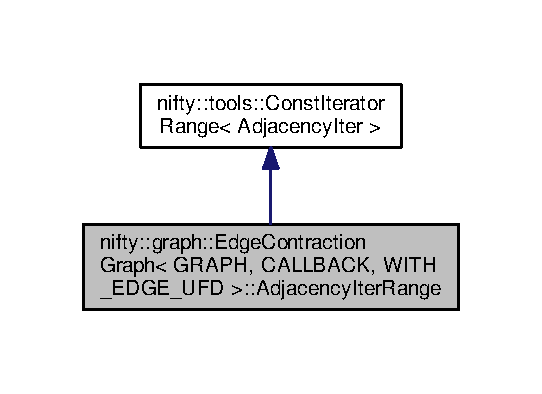
\includegraphics[width=260pt]{structnifty_1_1graph_1_1EdgeContractionGraph_1_1AdjacencyIterRange__inherit__graph}
\end{center}
\end{figure}


Collaboration diagram for nifty\+:\+:graph\+:\+:Edge\+Contraction\+Graph$<$ G\+R\+A\+PH, C\+A\+L\+L\+B\+A\+CK, W\+I\+T\+H\+\_\+\+E\+D\+G\+E\+\_\+\+U\+FD $>$\+:\+:Adjacency\+Iter\+Range\+:
\nopagebreak
\begin{figure}[H]
\begin{center}
\leavevmode
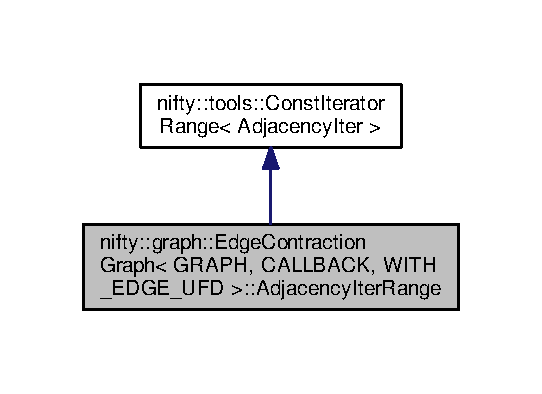
\includegraphics[width=260pt]{structnifty_1_1graph_1_1EdgeContractionGraph_1_1AdjacencyIterRange__coll__graph}
\end{center}
\end{figure}
\subsection*{Additional Inherited Members}


The documentation for this struct was generated from the following file\+:\begin{DoxyCompactItemize}
\item 
/home/tbeier/src/nifty/include/nifty/graph/\hyperlink{graph_2edge__contraction__graph_8hxx}{edge\+\_\+contraction\+\_\+graph.\+hxx}\end{DoxyCompactItemize}

\hypertarget{structnifty_1_1graph_1_1DirectedGraphBase_1_1AdjacencyIterRange}{}\section{nifty\+:\+:graph\+:\+:Directed\+Graph\+Base$<$ C\+H\+I\+L\+D\+\_\+\+G\+R\+A\+P\+H $>$\+:\+:Adjacency\+Iter\+Range$<$ \+\_\+\+C\+H\+I\+L\+D\+\_\+\+G\+R\+A\+P\+H $>$ Struct Template Reference}
\label{structnifty_1_1graph_1_1DirectedGraphBase_1_1AdjacencyIterRange}\index{nifty\+::graph\+::\+Directed\+Graph\+Base$<$ C\+H\+I\+L\+D\+\_\+\+G\+R\+A\+P\+H $>$\+::\+Adjacency\+Iter\+Range$<$ \+\_\+\+C\+H\+I\+L\+D\+\_\+\+G\+R\+A\+P\+H $>$@{nifty\+::graph\+::\+Directed\+Graph\+Base$<$ C\+H\+I\+L\+D\+\_\+\+G\+R\+A\+P\+H $>$\+::\+Adjacency\+Iter\+Range$<$ \+\_\+\+C\+H\+I\+L\+D\+\_\+\+G\+R\+A\+P\+H $>$}}


{\ttfamily \#include $<$directed\+\_\+graph\+\_\+base.\+hxx$>$}



Inheritance diagram for nifty\+:\+:graph\+:\+:Directed\+Graph\+Base$<$ C\+H\+I\+L\+D\+\_\+\+G\+R\+A\+P\+H $>$\+:\+:Adjacency\+Iter\+Range$<$ \+\_\+\+C\+H\+I\+L\+D\+\_\+\+G\+R\+A\+P\+H $>$\+:
% FIG 0


Collaboration diagram for nifty\+:\+:graph\+:\+:Directed\+Graph\+Base$<$ C\+H\+I\+L\+D\+\_\+\+G\+R\+A\+P\+H $>$\+:\+:Adjacency\+Iter\+Range$<$ \+\_\+\+C\+H\+I\+L\+D\+\_\+\+G\+R\+A\+P\+H $>$\+:
% FIG 1
\subsection*{Additional Inherited Members}


The documentation for this struct was generated from the following file\+:\begin{DoxyCompactItemize}
\item 
/home/tbeier/src/nifty/include/nifty/graph/\hyperlink{directed__graph__base_8hxx}{directed\+\_\+graph\+\_\+base.\+hxx}\end{DoxyCompactItemize}

\hypertarget{structnifty_1_1graph_1_1UndirectedGraphBase_1_1AdjacencyIterRange}{}\section{nifty\+:\+:graph\+:\+:Undirected\+Graph\+Base$<$ C\+H\+I\+L\+D\+\_\+\+G\+R\+A\+PH, N\+O\+D\+E\+\_\+\+I\+T\+ER, E\+D\+G\+E\+\_\+\+I\+T\+ER, A\+D\+J\+A\+C\+E\+N\+C\+Y\+\_\+\+I\+T\+ER $>$\+:\+:Adjacency\+Iter\+Range$<$ \+\_\+\+C\+H\+I\+L\+D\+\_\+\+G\+R\+A\+PH $>$ Struct Template Reference}
\label{structnifty_1_1graph_1_1UndirectedGraphBase_1_1AdjacencyIterRange}\index{nifty\+::graph\+::\+Undirected\+Graph\+Base$<$ C\+H\+I\+L\+D\+\_\+\+G\+R\+A\+P\+H, N\+O\+D\+E\+\_\+\+I\+T\+E\+R, E\+D\+G\+E\+\_\+\+I\+T\+E\+R, A\+D\+J\+A\+C\+E\+N\+C\+Y\+\_\+\+I\+T\+E\+R $>$\+::\+Adjacency\+Iter\+Range$<$ \+\_\+\+C\+H\+I\+L\+D\+\_\+\+G\+R\+A\+P\+H $>$@{nifty\+::graph\+::\+Undirected\+Graph\+Base$<$ C\+H\+I\+L\+D\+\_\+\+G\+R\+A\+P\+H, N\+O\+D\+E\+\_\+\+I\+T\+E\+R, E\+D\+G\+E\+\_\+\+I\+T\+E\+R, A\+D\+J\+A\+C\+E\+N\+C\+Y\+\_\+\+I\+T\+E\+R $>$\+::\+Adjacency\+Iter\+Range$<$ \+\_\+\+C\+H\+I\+L\+D\+\_\+\+G\+R\+A\+P\+H $>$}}


{\ttfamily \#include $<$undirected\+\_\+graph\+\_\+base.\+hxx$>$}



Inheritance diagram for nifty\+:\+:graph\+:\+:Undirected\+Graph\+Base$<$ C\+H\+I\+L\+D\+\_\+\+G\+R\+A\+PH, N\+O\+D\+E\+\_\+\+I\+T\+ER, E\+D\+G\+E\+\_\+\+I\+T\+ER, A\+D\+J\+A\+C\+E\+N\+C\+Y\+\_\+\+I\+T\+ER $>$\+:\+:Adjacency\+Iter\+Range$<$ \+\_\+\+C\+H\+I\+L\+D\+\_\+\+G\+R\+A\+PH $>$\+:
\nopagebreak
\begin{figure}[H]
\begin{center}
\leavevmode
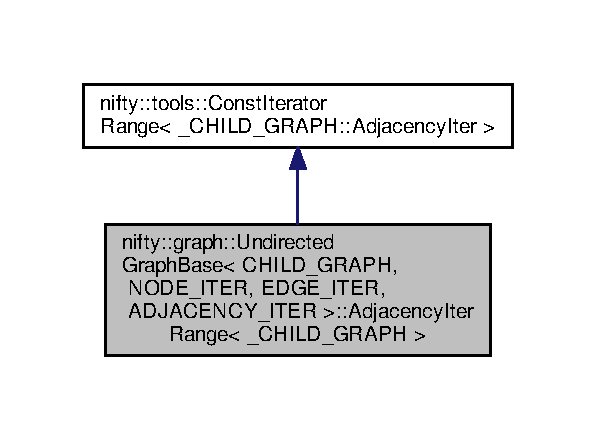
\includegraphics[width=286pt]{structnifty_1_1graph_1_1UndirectedGraphBase_1_1AdjacencyIterRange__inherit__graph}
\end{center}
\end{figure}


Collaboration diagram for nifty\+:\+:graph\+:\+:Undirected\+Graph\+Base$<$ C\+H\+I\+L\+D\+\_\+\+G\+R\+A\+PH, N\+O\+D\+E\+\_\+\+I\+T\+ER, E\+D\+G\+E\+\_\+\+I\+T\+ER, A\+D\+J\+A\+C\+E\+N\+C\+Y\+\_\+\+I\+T\+ER $>$\+:\+:Adjacency\+Iter\+Range$<$ \+\_\+\+C\+H\+I\+L\+D\+\_\+\+G\+R\+A\+PH $>$\+:
\nopagebreak
\begin{figure}[H]
\begin{center}
\leavevmode
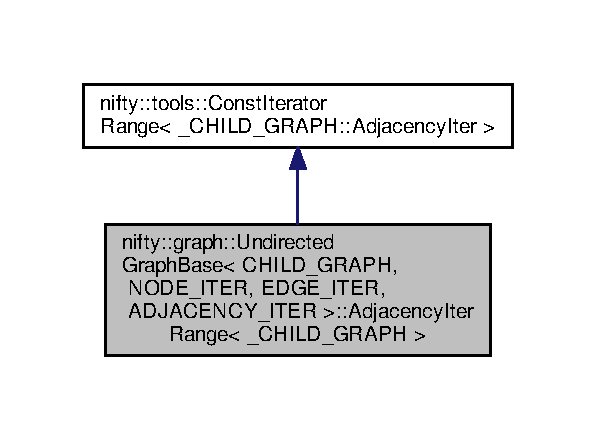
\includegraphics[width=286pt]{structnifty_1_1graph_1_1UndirectedGraphBase_1_1AdjacencyIterRange__coll__graph}
\end{center}
\end{figure}
\subsection*{Additional Inherited Members}


The documentation for this struct was generated from the following file\+:\begin{DoxyCompactItemize}
\item 
/home/tbeier/src/nifty/include/nifty/graph/\hyperlink{undirected__graph__base_8hxx}{undirected\+\_\+graph\+\_\+base.\+hxx}\end{DoxyCompactItemize}

\hypertarget{structnifty_1_1graph_1_1AdjacencyTag}{}\section{nifty\+:\+:graph\+:\+:Adjacency\+Tag Struct Reference}
\label{structnifty_1_1graph_1_1AdjacencyTag}\index{nifty\+::graph\+::\+Adjacency\+Tag@{nifty\+::graph\+::\+Adjacency\+Tag}}


{\ttfamily \#include $<$graph\+\_\+tags.\+hxx$>$}



The documentation for this struct was generated from the following file\+:\begin{DoxyCompactItemize}
\item 
/home/tbeier/src/nifty/include/nifty/graph/\hyperlink{graph__tags_8hxx}{graph\+\_\+tags.\+hxx}\end{DoxyCompactItemize}

\hypertarget{classnifty_1_1graph_1_1agglo_1_1AgglomerativeClustering}{}\section{nifty\+:\+:graph\+:\+:agglo\+:\+:Agglomerative\+Clustering$<$ C\+L\+U\+S\+T\+E\+R\+\_\+\+P\+O\+L\+I\+CY $>$ Class Template Reference}
\label{classnifty_1_1graph_1_1agglo_1_1AgglomerativeClustering}\index{nifty\+::graph\+::agglo\+::\+Agglomerative\+Clustering$<$ C\+L\+U\+S\+T\+E\+R\+\_\+\+P\+O\+L\+I\+C\+Y $>$@{nifty\+::graph\+::agglo\+::\+Agglomerative\+Clustering$<$ C\+L\+U\+S\+T\+E\+R\+\_\+\+P\+O\+L\+I\+C\+Y $>$}}


{\ttfamily \#include $<$agglomerative\+\_\+clustering.\+hxx$>$}

\subsection*{Public Types}
\begin{DoxyCompactItemize}
\item 
typedef C\+L\+U\+S\+T\+E\+R\+\_\+\+P\+O\+L\+I\+CY \hyperlink{classnifty_1_1graph_1_1agglo_1_1AgglomerativeClustering_a3a678ecd37725f2c0f8ec56857768034}{Cluster\+Policy\+Type}
\item 
typedef Cluster\+Policy\+Type\+::\+Edge\+Contraction\+Graph\+Type\+::\+With\+Edge\+Ufd \hyperlink{classnifty_1_1graph_1_1agglo_1_1AgglomerativeClustering_ad271a88b3736ec7b3d6a4e47e718828a}{With\+Edge\+Ufd}
\item 
typedef Cluster\+Policy\+Type\+::\+Graph\+Type \hyperlink{classnifty_1_1graph_1_1agglo_1_1AgglomerativeClustering_a0c735105592b55c036be76e3d7fc735f}{Graph\+Type}
\item 
typedef Cluster\+Policy\+Type\+::\+Edge\+Contraction\+Graph\+Type \hyperlink{classnifty_1_1graph_1_1agglo_1_1AgglomerativeClustering_ab50801119fbdb9ed78884a64f872e1d8}{Edge\+Contraction\+Graph\+Type}
\end{DoxyCompactItemize}
\subsection*{Public Member Functions}
\begin{DoxyCompactItemize}
\item 
\hyperlink{classnifty_1_1graph_1_1agglo_1_1AgglomerativeClustering_a4c1ae55dc3568df3f2e0ffe9e34963df}{Agglomerative\+Clustering} (\hyperlink{classnifty_1_1graph_1_1agglo_1_1AgglomerativeClustering_a3a678ecd37725f2c0f8ec56857768034}{Cluster\+Policy\+Type} \&\hyperlink{classnifty_1_1graph_1_1agglo_1_1AgglomerativeClustering_a5e68685d164d4f6104bd40c29eca0c08}{cluster\+Policy})
\item 
void \hyperlink{classnifty_1_1graph_1_1agglo_1_1AgglomerativeClustering_a736c7ce881d0a8a1d305cf2c8746c744}{run} (const bool verbose=false, const uint64\+\_\+t print\+Nth=100)
\item 
{\footnotesize template$<$class V\+I\+S\+I\+T\+OR $>$ }\\void \hyperlink{classnifty_1_1graph_1_1agglo_1_1AgglomerativeClustering_a6fac3d0b742ab08e8befb34646bafe80}{run} (V\+I\+S\+I\+T\+OR \&visitor, const bool verbose=false, const uint64\+\_\+t print\+Nth=100)
\item 
{\footnotesize template$<$class M\+E\+R\+G\+E\+\_\+\+T\+I\+M\+ES , class E\+D\+G\+E\+\_\+\+D\+E\+N\+D\+R\+O\+G\+R\+A\+M\+\_\+\+H\+E\+I\+G\+HT $>$ }\\void \hyperlink{classnifty_1_1graph_1_1agglo_1_1AgglomerativeClustering_af5d353cca095be5cd67614c3d5267eea}{run\+And\+Get\+Merge\+Times\+And\+Dendrogram\+Height} (M\+E\+R\+G\+E\+\_\+\+T\+I\+M\+ES \&merge\+Times, E\+D\+G\+E\+\_\+\+D\+E\+N\+D\+R\+O\+G\+R\+A\+M\+\_\+\+H\+E\+I\+G\+HT \&dendrogram\+Height, const bool verbose=false)
\item 
{\footnotesize template$<$class M\+E\+R\+G\+E\+\_\+\+T\+I\+M\+ES $>$ }\\void \hyperlink{classnifty_1_1graph_1_1agglo_1_1AgglomerativeClustering_a9c8d18e03cef48ba261ba8e8a1bcc924}{run\+And\+Get\+Merge\+Times} (M\+E\+R\+G\+E\+\_\+\+T\+I\+M\+ES \&merge\+Times, const bool verbose=false)
\item 
{\footnotesize template$<$class E\+D\+G\+E\+\_\+\+D\+E\+N\+D\+R\+O\+G\+R\+A\+M\+\_\+\+H\+E\+I\+G\+HT $>$ }\\void \hyperlink{classnifty_1_1graph_1_1agglo_1_1AgglomerativeClustering_adf2c89066a4796c32e722c7244b37f3c}{run\+And\+Get\+Dendrogram\+Height} (E\+D\+G\+E\+\_\+\+D\+E\+N\+D\+R\+O\+G\+R\+A\+M\+\_\+\+H\+E\+I\+G\+HT \&dendrogram\+Height, const bool verbose=false)
\item 
{\footnotesize template$<$class E\+D\+G\+E\+\_\+\+M\+AP $>$ }\\void \hyperlink{classnifty_1_1graph_1_1agglo_1_1AgglomerativeClustering_a7e9b9949000d96d91844ab2df1e28509}{ucm\+Transform} (E\+D\+G\+E\+\_\+\+M\+AP \&edge\+Map) const
\item 
{\footnotesize template$<$class E\+D\+G\+E\+\_\+\+M\+AP , class E\+D\+G\+E\+\_\+\+M\+A\+P\+\_\+\+O\+UT $>$ }\\void \hyperlink{classnifty_1_1graph_1_1agglo_1_1AgglomerativeClustering_a717660885100f4c0321c4e19fb536072}{ucm\+Transform} (const E\+D\+G\+E\+\_\+\+M\+AP \&edge\+Map, E\+D\+G\+E\+\_\+\+M\+A\+P\+\_\+\+O\+UT \&edge\+Map\+Out) const
\item 
const \hyperlink{classnifty_1_1graph_1_1agglo_1_1AgglomerativeClustering_a3a678ecd37725f2c0f8ec56857768034}{Cluster\+Policy\+Type} \& \hyperlink{classnifty_1_1graph_1_1agglo_1_1AgglomerativeClustering_a5e68685d164d4f6104bd40c29eca0c08}{cluster\+Policy} () const
\item 
const \hyperlink{classnifty_1_1graph_1_1agglo_1_1AgglomerativeClustering_a0c735105592b55c036be76e3d7fc735f}{Graph\+Type} \& \hyperlink{classnifty_1_1graph_1_1agglo_1_1AgglomerativeClustering_a4da52a342e866335a671879e8c4864d2}{graph} () const
\item 
{\footnotesize template$<$class N\+O\+D\+E\+\_\+\+M\+AP $>$ }\\void \hyperlink{classnifty_1_1graph_1_1agglo_1_1AgglomerativeClustering_afbe080ba596ae20f85404635c5f00d20}{result} (N\+O\+D\+E\+\_\+\+M\+AP \&node\+Map) const
\end{DoxyCompactItemize}


\subsection{Member Typedef Documentation}
\mbox{\Hypertarget{classnifty_1_1graph_1_1agglo_1_1AgglomerativeClustering_a3a678ecd37725f2c0f8ec56857768034}\label{classnifty_1_1graph_1_1agglo_1_1AgglomerativeClustering_a3a678ecd37725f2c0f8ec56857768034}} 
\index{nifty\+::graph\+::agglo\+::\+Agglomerative\+Clustering@{nifty\+::graph\+::agglo\+::\+Agglomerative\+Clustering}!Cluster\+Policy\+Type@{Cluster\+Policy\+Type}}
\index{Cluster\+Policy\+Type@{Cluster\+Policy\+Type}!nifty\+::graph\+::agglo\+::\+Agglomerative\+Clustering@{nifty\+::graph\+::agglo\+::\+Agglomerative\+Clustering}}
\subsubsection{\texorpdfstring{Cluster\+Policy\+Type}{ClusterPolicyType}}
{\footnotesize\ttfamily template$<$class C\+L\+U\+S\+T\+E\+R\+\_\+\+P\+O\+L\+I\+CY $>$ \\
typedef C\+L\+U\+S\+T\+E\+R\+\_\+\+P\+O\+L\+I\+CY \hyperlink{classnifty_1_1graph_1_1agglo_1_1AgglomerativeClustering}{nifty\+::graph\+::agglo\+::\+Agglomerative\+Clustering}$<$ C\+L\+U\+S\+T\+E\+R\+\_\+\+P\+O\+L\+I\+CY $>$\+::\hyperlink{classnifty_1_1graph_1_1agglo_1_1AgglomerativeClustering_a3a678ecd37725f2c0f8ec56857768034}{Cluster\+Policy\+Type}}

\mbox{\Hypertarget{classnifty_1_1graph_1_1agglo_1_1AgglomerativeClustering_ab50801119fbdb9ed78884a64f872e1d8}\label{classnifty_1_1graph_1_1agglo_1_1AgglomerativeClustering_ab50801119fbdb9ed78884a64f872e1d8}} 
\index{nifty\+::graph\+::agglo\+::\+Agglomerative\+Clustering@{nifty\+::graph\+::agglo\+::\+Agglomerative\+Clustering}!Edge\+Contraction\+Graph\+Type@{Edge\+Contraction\+Graph\+Type}}
\index{Edge\+Contraction\+Graph\+Type@{Edge\+Contraction\+Graph\+Type}!nifty\+::graph\+::agglo\+::\+Agglomerative\+Clustering@{nifty\+::graph\+::agglo\+::\+Agglomerative\+Clustering}}
\subsubsection{\texorpdfstring{Edge\+Contraction\+Graph\+Type}{EdgeContractionGraphType}}
{\footnotesize\ttfamily template$<$class C\+L\+U\+S\+T\+E\+R\+\_\+\+P\+O\+L\+I\+CY $>$ \\
typedef Cluster\+Policy\+Type\+::\+Edge\+Contraction\+Graph\+Type \hyperlink{classnifty_1_1graph_1_1agglo_1_1AgglomerativeClustering}{nifty\+::graph\+::agglo\+::\+Agglomerative\+Clustering}$<$ C\+L\+U\+S\+T\+E\+R\+\_\+\+P\+O\+L\+I\+CY $>$\+::\hyperlink{classnifty_1_1graph_1_1agglo_1_1AgglomerativeClustering_ab50801119fbdb9ed78884a64f872e1d8}{Edge\+Contraction\+Graph\+Type}}

\mbox{\Hypertarget{classnifty_1_1graph_1_1agglo_1_1AgglomerativeClustering_a0c735105592b55c036be76e3d7fc735f}\label{classnifty_1_1graph_1_1agglo_1_1AgglomerativeClustering_a0c735105592b55c036be76e3d7fc735f}} 
\index{nifty\+::graph\+::agglo\+::\+Agglomerative\+Clustering@{nifty\+::graph\+::agglo\+::\+Agglomerative\+Clustering}!Graph\+Type@{Graph\+Type}}
\index{Graph\+Type@{Graph\+Type}!nifty\+::graph\+::agglo\+::\+Agglomerative\+Clustering@{nifty\+::graph\+::agglo\+::\+Agglomerative\+Clustering}}
\subsubsection{\texorpdfstring{Graph\+Type}{GraphType}}
{\footnotesize\ttfamily template$<$class C\+L\+U\+S\+T\+E\+R\+\_\+\+P\+O\+L\+I\+CY $>$ \\
typedef Cluster\+Policy\+Type\+::\+Graph\+Type \hyperlink{classnifty_1_1graph_1_1agglo_1_1AgglomerativeClustering}{nifty\+::graph\+::agglo\+::\+Agglomerative\+Clustering}$<$ C\+L\+U\+S\+T\+E\+R\+\_\+\+P\+O\+L\+I\+CY $>$\+::\hyperlink{classnifty_1_1graph_1_1agglo_1_1AgglomerativeClustering_a0c735105592b55c036be76e3d7fc735f}{Graph\+Type}}

\mbox{\Hypertarget{classnifty_1_1graph_1_1agglo_1_1AgglomerativeClustering_ad271a88b3736ec7b3d6a4e47e718828a}\label{classnifty_1_1graph_1_1agglo_1_1AgglomerativeClustering_ad271a88b3736ec7b3d6a4e47e718828a}} 
\index{nifty\+::graph\+::agglo\+::\+Agglomerative\+Clustering@{nifty\+::graph\+::agglo\+::\+Agglomerative\+Clustering}!With\+Edge\+Ufd@{With\+Edge\+Ufd}}
\index{With\+Edge\+Ufd@{With\+Edge\+Ufd}!nifty\+::graph\+::agglo\+::\+Agglomerative\+Clustering@{nifty\+::graph\+::agglo\+::\+Agglomerative\+Clustering}}
\subsubsection{\texorpdfstring{With\+Edge\+Ufd}{WithEdgeUfd}}
{\footnotesize\ttfamily template$<$class C\+L\+U\+S\+T\+E\+R\+\_\+\+P\+O\+L\+I\+CY $>$ \\
typedef Cluster\+Policy\+Type\+::\+Edge\+Contraction\+Graph\+Type\+::\+With\+Edge\+Ufd \hyperlink{classnifty_1_1graph_1_1agglo_1_1AgglomerativeClustering}{nifty\+::graph\+::agglo\+::\+Agglomerative\+Clustering}$<$ C\+L\+U\+S\+T\+E\+R\+\_\+\+P\+O\+L\+I\+CY $>$\+::\hyperlink{classnifty_1_1graph_1_1agglo_1_1AgglomerativeClustering_ad271a88b3736ec7b3d6a4e47e718828a}{With\+Edge\+Ufd}}



\subsection{Constructor \& Destructor Documentation}
\mbox{\Hypertarget{classnifty_1_1graph_1_1agglo_1_1AgglomerativeClustering_a4c1ae55dc3568df3f2e0ffe9e34963df}\label{classnifty_1_1graph_1_1agglo_1_1AgglomerativeClustering_a4c1ae55dc3568df3f2e0ffe9e34963df}} 
\index{nifty\+::graph\+::agglo\+::\+Agglomerative\+Clustering@{nifty\+::graph\+::agglo\+::\+Agglomerative\+Clustering}!Agglomerative\+Clustering@{Agglomerative\+Clustering}}
\index{Agglomerative\+Clustering@{Agglomerative\+Clustering}!nifty\+::graph\+::agglo\+::\+Agglomerative\+Clustering@{nifty\+::graph\+::agglo\+::\+Agglomerative\+Clustering}}
\subsubsection{\texorpdfstring{Agglomerative\+Clustering()}{AgglomerativeClustering()}}
{\footnotesize\ttfamily template$<$class C\+L\+U\+S\+T\+E\+R\+\_\+\+P\+O\+L\+I\+CY $>$ \\
\hyperlink{classnifty_1_1graph_1_1agglo_1_1AgglomerativeClustering}{nifty\+::graph\+::agglo\+::\+Agglomerative\+Clustering}$<$ C\+L\+U\+S\+T\+E\+R\+\_\+\+P\+O\+L\+I\+CY $>$\+::\hyperlink{classnifty_1_1graph_1_1agglo_1_1AgglomerativeClustering}{Agglomerative\+Clustering} (\begin{DoxyParamCaption}\item[{\hyperlink{classnifty_1_1graph_1_1agglo_1_1AgglomerativeClustering_a3a678ecd37725f2c0f8ec56857768034}{Cluster\+Policy\+Type} \&}]{cluster\+Policy }\end{DoxyParamCaption})\hspace{0.3cm}{\ttfamily [inline]}}



\subsection{Member Function Documentation}
\mbox{\Hypertarget{classnifty_1_1graph_1_1agglo_1_1AgglomerativeClustering_a5e68685d164d4f6104bd40c29eca0c08}\label{classnifty_1_1graph_1_1agglo_1_1AgglomerativeClustering_a5e68685d164d4f6104bd40c29eca0c08}} 
\index{nifty\+::graph\+::agglo\+::\+Agglomerative\+Clustering@{nifty\+::graph\+::agglo\+::\+Agglomerative\+Clustering}!cluster\+Policy@{cluster\+Policy}}
\index{cluster\+Policy@{cluster\+Policy}!nifty\+::graph\+::agglo\+::\+Agglomerative\+Clustering@{nifty\+::graph\+::agglo\+::\+Agglomerative\+Clustering}}
\subsubsection{\texorpdfstring{cluster\+Policy()}{clusterPolicy()}}
{\footnotesize\ttfamily template$<$class C\+L\+U\+S\+T\+E\+R\+\_\+\+P\+O\+L\+I\+CY $>$ \\
const \hyperlink{classnifty_1_1graph_1_1agglo_1_1AgglomerativeClustering_a3a678ecd37725f2c0f8ec56857768034}{Cluster\+Policy\+Type}\& \hyperlink{classnifty_1_1graph_1_1agglo_1_1AgglomerativeClustering}{nifty\+::graph\+::agglo\+::\+Agglomerative\+Clustering}$<$ C\+L\+U\+S\+T\+E\+R\+\_\+\+P\+O\+L\+I\+CY $>$\+::cluster\+Policy (\begin{DoxyParamCaption}{ }\end{DoxyParamCaption}) const\hspace{0.3cm}{\ttfamily [inline]}}

\mbox{\Hypertarget{classnifty_1_1graph_1_1agglo_1_1AgglomerativeClustering_a4da52a342e866335a671879e8c4864d2}\label{classnifty_1_1graph_1_1agglo_1_1AgglomerativeClustering_a4da52a342e866335a671879e8c4864d2}} 
\index{nifty\+::graph\+::agglo\+::\+Agglomerative\+Clustering@{nifty\+::graph\+::agglo\+::\+Agglomerative\+Clustering}!graph@{graph}}
\index{graph@{graph}!nifty\+::graph\+::agglo\+::\+Agglomerative\+Clustering@{nifty\+::graph\+::agglo\+::\+Agglomerative\+Clustering}}
\subsubsection{\texorpdfstring{graph()}{graph()}}
{\footnotesize\ttfamily template$<$class C\+L\+U\+S\+T\+E\+R\+\_\+\+P\+O\+L\+I\+CY $>$ \\
const \hyperlink{classnifty_1_1graph_1_1agglo_1_1AgglomerativeClustering_a0c735105592b55c036be76e3d7fc735f}{Graph\+Type}\& \hyperlink{classnifty_1_1graph_1_1agglo_1_1AgglomerativeClustering}{nifty\+::graph\+::agglo\+::\+Agglomerative\+Clustering}$<$ C\+L\+U\+S\+T\+E\+R\+\_\+\+P\+O\+L\+I\+CY $>$\+::graph (\begin{DoxyParamCaption}{ }\end{DoxyParamCaption}) const\hspace{0.3cm}{\ttfamily [inline]}}

\mbox{\Hypertarget{classnifty_1_1graph_1_1agglo_1_1AgglomerativeClustering_afbe080ba596ae20f85404635c5f00d20}\label{classnifty_1_1graph_1_1agglo_1_1AgglomerativeClustering_afbe080ba596ae20f85404635c5f00d20}} 
\index{nifty\+::graph\+::agglo\+::\+Agglomerative\+Clustering@{nifty\+::graph\+::agglo\+::\+Agglomerative\+Clustering}!result@{result}}
\index{result@{result}!nifty\+::graph\+::agglo\+::\+Agglomerative\+Clustering@{nifty\+::graph\+::agglo\+::\+Agglomerative\+Clustering}}
\subsubsection{\texorpdfstring{result()}{result()}}
{\footnotesize\ttfamily template$<$class C\+L\+U\+S\+T\+E\+R\+\_\+\+P\+O\+L\+I\+CY $>$ \\
template$<$class N\+O\+D\+E\+\_\+\+M\+AP $>$ \\
void \hyperlink{classnifty_1_1graph_1_1agglo_1_1AgglomerativeClustering}{nifty\+::graph\+::agglo\+::\+Agglomerative\+Clustering}$<$ C\+L\+U\+S\+T\+E\+R\+\_\+\+P\+O\+L\+I\+CY $>$\+::result (\begin{DoxyParamCaption}\item[{N\+O\+D\+E\+\_\+\+M\+AP \&}]{node\+Map }\end{DoxyParamCaption}) const\hspace{0.3cm}{\ttfamily [inline]}}

\mbox{\Hypertarget{classnifty_1_1graph_1_1agglo_1_1AgglomerativeClustering_a736c7ce881d0a8a1d305cf2c8746c744}\label{classnifty_1_1graph_1_1agglo_1_1AgglomerativeClustering_a736c7ce881d0a8a1d305cf2c8746c744}} 
\index{nifty\+::graph\+::agglo\+::\+Agglomerative\+Clustering@{nifty\+::graph\+::agglo\+::\+Agglomerative\+Clustering}!run@{run}}
\index{run@{run}!nifty\+::graph\+::agglo\+::\+Agglomerative\+Clustering@{nifty\+::graph\+::agglo\+::\+Agglomerative\+Clustering}}
\subsubsection{\texorpdfstring{run()}{run()}\hspace{0.1cm}{\footnotesize\ttfamily [1/2]}}
{\footnotesize\ttfamily template$<$class C\+L\+U\+S\+T\+E\+R\+\_\+\+P\+O\+L\+I\+CY $>$ \\
void \hyperlink{classnifty_1_1graph_1_1agglo_1_1AgglomerativeClustering}{nifty\+::graph\+::agglo\+::\+Agglomerative\+Clustering}$<$ C\+L\+U\+S\+T\+E\+R\+\_\+\+P\+O\+L\+I\+CY $>$\+::run (\begin{DoxyParamCaption}\item[{const bool}]{verbose = {\ttfamily false},  }\item[{const uint64\+\_\+t}]{print\+Nth = {\ttfamily 100} }\end{DoxyParamCaption})\hspace{0.3cm}{\ttfamily [inline]}}

\mbox{\Hypertarget{classnifty_1_1graph_1_1agglo_1_1AgglomerativeClustering_a6fac3d0b742ab08e8befb34646bafe80}\label{classnifty_1_1graph_1_1agglo_1_1AgglomerativeClustering_a6fac3d0b742ab08e8befb34646bafe80}} 
\index{nifty\+::graph\+::agglo\+::\+Agglomerative\+Clustering@{nifty\+::graph\+::agglo\+::\+Agglomerative\+Clustering}!run@{run}}
\index{run@{run}!nifty\+::graph\+::agglo\+::\+Agglomerative\+Clustering@{nifty\+::graph\+::agglo\+::\+Agglomerative\+Clustering}}
\subsubsection{\texorpdfstring{run()}{run()}\hspace{0.1cm}{\footnotesize\ttfamily [2/2]}}
{\footnotesize\ttfamily template$<$class C\+L\+U\+S\+T\+E\+R\+\_\+\+P\+O\+L\+I\+CY $>$ \\
template$<$class V\+I\+S\+I\+T\+OR $>$ \\
void \hyperlink{classnifty_1_1graph_1_1agglo_1_1AgglomerativeClustering}{nifty\+::graph\+::agglo\+::\+Agglomerative\+Clustering}$<$ C\+L\+U\+S\+T\+E\+R\+\_\+\+P\+O\+L\+I\+CY $>$\+::run (\begin{DoxyParamCaption}\item[{V\+I\+S\+I\+T\+OR \&}]{visitor,  }\item[{const bool}]{verbose = {\ttfamily false},  }\item[{const uint64\+\_\+t}]{print\+Nth = {\ttfamily 100} }\end{DoxyParamCaption})\hspace{0.3cm}{\ttfamily [inline]}}

\mbox{\Hypertarget{classnifty_1_1graph_1_1agglo_1_1AgglomerativeClustering_adf2c89066a4796c32e722c7244b37f3c}\label{classnifty_1_1graph_1_1agglo_1_1AgglomerativeClustering_adf2c89066a4796c32e722c7244b37f3c}} 
\index{nifty\+::graph\+::agglo\+::\+Agglomerative\+Clustering@{nifty\+::graph\+::agglo\+::\+Agglomerative\+Clustering}!run\+And\+Get\+Dendrogram\+Height@{run\+And\+Get\+Dendrogram\+Height}}
\index{run\+And\+Get\+Dendrogram\+Height@{run\+And\+Get\+Dendrogram\+Height}!nifty\+::graph\+::agglo\+::\+Agglomerative\+Clustering@{nifty\+::graph\+::agglo\+::\+Agglomerative\+Clustering}}
\subsubsection{\texorpdfstring{run\+And\+Get\+Dendrogram\+Height()}{runAndGetDendrogramHeight()}}
{\footnotesize\ttfamily template$<$class C\+L\+U\+S\+T\+E\+R\+\_\+\+P\+O\+L\+I\+CY $>$ \\
template$<$class E\+D\+G\+E\+\_\+\+D\+E\+N\+D\+R\+O\+G\+R\+A\+M\+\_\+\+H\+E\+I\+G\+HT $>$ \\
void \hyperlink{classnifty_1_1graph_1_1agglo_1_1AgglomerativeClustering}{nifty\+::graph\+::agglo\+::\+Agglomerative\+Clustering}$<$ C\+L\+U\+S\+T\+E\+R\+\_\+\+P\+O\+L\+I\+CY $>$\+::run\+And\+Get\+Dendrogram\+Height (\begin{DoxyParamCaption}\item[{E\+D\+G\+E\+\_\+\+D\+E\+N\+D\+R\+O\+G\+R\+A\+M\+\_\+\+H\+E\+I\+G\+HT \&}]{dendrogram\+Height,  }\item[{const bool}]{verbose = {\ttfamily false} }\end{DoxyParamCaption})\hspace{0.3cm}{\ttfamily [inline]}}

\mbox{\Hypertarget{classnifty_1_1graph_1_1agglo_1_1AgglomerativeClustering_a9c8d18e03cef48ba261ba8e8a1bcc924}\label{classnifty_1_1graph_1_1agglo_1_1AgglomerativeClustering_a9c8d18e03cef48ba261ba8e8a1bcc924}} 
\index{nifty\+::graph\+::agglo\+::\+Agglomerative\+Clustering@{nifty\+::graph\+::agglo\+::\+Agglomerative\+Clustering}!run\+And\+Get\+Merge\+Times@{run\+And\+Get\+Merge\+Times}}
\index{run\+And\+Get\+Merge\+Times@{run\+And\+Get\+Merge\+Times}!nifty\+::graph\+::agglo\+::\+Agglomerative\+Clustering@{nifty\+::graph\+::agglo\+::\+Agglomerative\+Clustering}}
\subsubsection{\texorpdfstring{run\+And\+Get\+Merge\+Times()}{runAndGetMergeTimes()}}
{\footnotesize\ttfamily template$<$class C\+L\+U\+S\+T\+E\+R\+\_\+\+P\+O\+L\+I\+CY $>$ \\
template$<$class M\+E\+R\+G\+E\+\_\+\+T\+I\+M\+ES $>$ \\
void \hyperlink{classnifty_1_1graph_1_1agglo_1_1AgglomerativeClustering}{nifty\+::graph\+::agglo\+::\+Agglomerative\+Clustering}$<$ C\+L\+U\+S\+T\+E\+R\+\_\+\+P\+O\+L\+I\+CY $>$\+::run\+And\+Get\+Merge\+Times (\begin{DoxyParamCaption}\item[{M\+E\+R\+G\+E\+\_\+\+T\+I\+M\+ES \&}]{merge\+Times,  }\item[{const bool}]{verbose = {\ttfamily false} }\end{DoxyParamCaption})\hspace{0.3cm}{\ttfamily [inline]}}

\mbox{\Hypertarget{classnifty_1_1graph_1_1agglo_1_1AgglomerativeClustering_af5d353cca095be5cd67614c3d5267eea}\label{classnifty_1_1graph_1_1agglo_1_1AgglomerativeClustering_af5d353cca095be5cd67614c3d5267eea}} 
\index{nifty\+::graph\+::agglo\+::\+Agglomerative\+Clustering@{nifty\+::graph\+::agglo\+::\+Agglomerative\+Clustering}!run\+And\+Get\+Merge\+Times\+And\+Dendrogram\+Height@{run\+And\+Get\+Merge\+Times\+And\+Dendrogram\+Height}}
\index{run\+And\+Get\+Merge\+Times\+And\+Dendrogram\+Height@{run\+And\+Get\+Merge\+Times\+And\+Dendrogram\+Height}!nifty\+::graph\+::agglo\+::\+Agglomerative\+Clustering@{nifty\+::graph\+::agglo\+::\+Agglomerative\+Clustering}}
\subsubsection{\texorpdfstring{run\+And\+Get\+Merge\+Times\+And\+Dendrogram\+Height()}{runAndGetMergeTimesAndDendrogramHeight()}}
{\footnotesize\ttfamily template$<$class C\+L\+U\+S\+T\+E\+R\+\_\+\+P\+O\+L\+I\+CY $>$ \\
template$<$class M\+E\+R\+G\+E\+\_\+\+T\+I\+M\+ES , class E\+D\+G\+E\+\_\+\+D\+E\+N\+D\+R\+O\+G\+R\+A\+M\+\_\+\+H\+E\+I\+G\+HT $>$ \\
void \hyperlink{classnifty_1_1graph_1_1agglo_1_1AgglomerativeClustering}{nifty\+::graph\+::agglo\+::\+Agglomerative\+Clustering}$<$ C\+L\+U\+S\+T\+E\+R\+\_\+\+P\+O\+L\+I\+CY $>$\+::run\+And\+Get\+Merge\+Times\+And\+Dendrogram\+Height (\begin{DoxyParamCaption}\item[{M\+E\+R\+G\+E\+\_\+\+T\+I\+M\+ES \&}]{merge\+Times,  }\item[{E\+D\+G\+E\+\_\+\+D\+E\+N\+D\+R\+O\+G\+R\+A\+M\+\_\+\+H\+E\+I\+G\+HT \&}]{dendrogram\+Height,  }\item[{const bool}]{verbose = {\ttfamily false} }\end{DoxyParamCaption})\hspace{0.3cm}{\ttfamily [inline]}}

\mbox{\Hypertarget{classnifty_1_1graph_1_1agglo_1_1AgglomerativeClustering_a7e9b9949000d96d91844ab2df1e28509}\label{classnifty_1_1graph_1_1agglo_1_1AgglomerativeClustering_a7e9b9949000d96d91844ab2df1e28509}} 
\index{nifty\+::graph\+::agglo\+::\+Agglomerative\+Clustering@{nifty\+::graph\+::agglo\+::\+Agglomerative\+Clustering}!ucm\+Transform@{ucm\+Transform}}
\index{ucm\+Transform@{ucm\+Transform}!nifty\+::graph\+::agglo\+::\+Agglomerative\+Clustering@{nifty\+::graph\+::agglo\+::\+Agglomerative\+Clustering}}
\subsubsection{\texorpdfstring{ucm\+Transform()}{ucmTransform()}\hspace{0.1cm}{\footnotesize\ttfamily [1/2]}}
{\footnotesize\ttfamily template$<$class C\+L\+U\+S\+T\+E\+R\+\_\+\+P\+O\+L\+I\+CY $>$ \\
template$<$class E\+D\+G\+E\+\_\+\+M\+AP $>$ \\
void \hyperlink{classnifty_1_1graph_1_1agglo_1_1AgglomerativeClustering}{nifty\+::graph\+::agglo\+::\+Agglomerative\+Clustering}$<$ C\+L\+U\+S\+T\+E\+R\+\_\+\+P\+O\+L\+I\+CY $>$\+::ucm\+Transform (\begin{DoxyParamCaption}\item[{E\+D\+G\+E\+\_\+\+M\+AP \&}]{edge\+Map }\end{DoxyParamCaption}) const\hspace{0.3cm}{\ttfamily [inline]}}

\mbox{\Hypertarget{classnifty_1_1graph_1_1agglo_1_1AgglomerativeClustering_a717660885100f4c0321c4e19fb536072}\label{classnifty_1_1graph_1_1agglo_1_1AgglomerativeClustering_a717660885100f4c0321c4e19fb536072}} 
\index{nifty\+::graph\+::agglo\+::\+Agglomerative\+Clustering@{nifty\+::graph\+::agglo\+::\+Agglomerative\+Clustering}!ucm\+Transform@{ucm\+Transform}}
\index{ucm\+Transform@{ucm\+Transform}!nifty\+::graph\+::agglo\+::\+Agglomerative\+Clustering@{nifty\+::graph\+::agglo\+::\+Agglomerative\+Clustering}}
\subsubsection{\texorpdfstring{ucm\+Transform()}{ucmTransform()}\hspace{0.1cm}{\footnotesize\ttfamily [2/2]}}
{\footnotesize\ttfamily template$<$class C\+L\+U\+S\+T\+E\+R\+\_\+\+P\+O\+L\+I\+CY $>$ \\
template$<$class E\+D\+G\+E\+\_\+\+M\+AP , class E\+D\+G\+E\+\_\+\+M\+A\+P\+\_\+\+O\+UT $>$ \\
void \hyperlink{classnifty_1_1graph_1_1agglo_1_1AgglomerativeClustering}{nifty\+::graph\+::agglo\+::\+Agglomerative\+Clustering}$<$ C\+L\+U\+S\+T\+E\+R\+\_\+\+P\+O\+L\+I\+CY $>$\+::ucm\+Transform (\begin{DoxyParamCaption}\item[{const E\+D\+G\+E\+\_\+\+M\+AP \&}]{edge\+Map,  }\item[{E\+D\+G\+E\+\_\+\+M\+A\+P\+\_\+\+O\+UT \&}]{edge\+Map\+Out }\end{DoxyParamCaption}) const\hspace{0.3cm}{\ttfamily [inline]}}



The documentation for this class was generated from the following file\+:\begin{DoxyCompactItemize}
\item 
/home/tbeier/src/nifty/include/nifty/graph/agglo/\hyperlink{agglomerative__clustering_8hxx}{agglomerative\+\_\+clustering.\+hxx}\end{DoxyCompactItemize}

\hypertarget{structnifty_1_1features_1_1ApplyFilters}{}\section{nifty\+:\+:features\+:\+:Apply\+Filters$<$ D\+I\+M $>$ Struct Template Reference}
\label{structnifty_1_1features_1_1ApplyFilters}\index{nifty\+::features\+::\+Apply\+Filters$<$ D\+I\+M $>$@{nifty\+::features\+::\+Apply\+Filters$<$ D\+I\+M $>$}}


{\ttfamily \#include $<$fastfilters\+\_\+wrapper.\+hxx$>$}

\subsection*{Public Types}
\begin{DoxyCompactItemize}
\item 
typedef std\+::conditional$<$ D\+I\+M==2, fastfilters\+\_\+array2d\+\_\+t, fastfilters\+\_\+array3d\+\_\+t $>$\+::type \hyperlink{structnifty_1_1features_1_1ApplyFilters_adfddd3f0fdaa0179cc23100901565774}{Fastfilters\+Array\+Type}
\item 
typedef \hyperlink{namespacenifty_1_1array_a683f151f19c851754e0c6d55ed16a0c2}{array\+::\+Static\+Array}$<$ int64\+\_\+t, D\+I\+M+1 $>$ \hyperlink{structnifty_1_1features_1_1ApplyFilters_a0a26d161f300b3394044f1357ae5ebfd}{Coord}
\end{DoxyCompactItemize}
\subsection*{Public Member Functions}
\begin{DoxyCompactItemize}
\item 
\hyperlink{structnifty_1_1features_1_1ApplyFilters_a21bb107c65ee2783993d6de3170d2922}{Apply\+Filters} (const std\+::vector$<$ double $>$ \&sigmas, const std\+::vector$<$ \hyperlink{structnifty_1_1features_1_1FilterBase}{Filter\+Base} $\ast$ $>$ filters)
\item 
void \hyperlink{structnifty_1_1features_1_1ApplyFilters_a075f9232abd8d323ba121b2bdd49fa17}{operator()} (const \hyperlink{classandres_1_1View}{marray\+::\+View}$<$ float $>$ \&in, \hyperlink{classandres_1_1View}{marray\+::\+View}$<$ float $>$ \&out) const 
\item 
void \hyperlink{structnifty_1_1features_1_1ApplyFilters_a6fc96c356178496a7b6c08c8e429dead}{operator()} (const \hyperlink{classandres_1_1View}{marray\+::\+View}$<$ float $>$ \&in, \hyperlink{classandres_1_1View}{marray\+::\+View}$<$ float $>$ \&out, \hyperlink{classnifty_1_1parallel_1_1ThreadPool}{parallel\+::\+Thread\+Pool} \&threadpool) const 
\item 
size\+\_\+t \hyperlink{structnifty_1_1features_1_1ApplyFilters_afb7d56d68a25b2aaf2de29e3d6f39cff}{number\+Of\+Channels} () const 
\end{DoxyCompactItemize}


\subsection{Member Typedef Documentation}
\hypertarget{structnifty_1_1features_1_1ApplyFilters_a0a26d161f300b3394044f1357ae5ebfd}{}\index{nifty\+::features\+::\+Apply\+Filters@{nifty\+::features\+::\+Apply\+Filters}!Coord@{Coord}}
\index{Coord@{Coord}!nifty\+::features\+::\+Apply\+Filters@{nifty\+::features\+::\+Apply\+Filters}}
\subsubsection[{Coord}]{\setlength{\rightskip}{0pt plus 5cm}template$<$unsigned D\+I\+M$>$ typedef {\bf array\+::\+Static\+Array}$<$int64\+\_\+t, D\+I\+M+1$>$ {\bf nifty\+::features\+::\+Apply\+Filters}$<$ D\+I\+M $>$\+::{\bf Coord}}\label{structnifty_1_1features_1_1ApplyFilters_a0a26d161f300b3394044f1357ae5ebfd}
\hypertarget{structnifty_1_1features_1_1ApplyFilters_adfddd3f0fdaa0179cc23100901565774}{}\index{nifty\+::features\+::\+Apply\+Filters@{nifty\+::features\+::\+Apply\+Filters}!Fastfilters\+Array\+Type@{Fastfilters\+Array\+Type}}
\index{Fastfilters\+Array\+Type@{Fastfilters\+Array\+Type}!nifty\+::features\+::\+Apply\+Filters@{nifty\+::features\+::\+Apply\+Filters}}
\subsubsection[{Fastfilters\+Array\+Type}]{\setlength{\rightskip}{0pt plus 5cm}template$<$unsigned D\+I\+M$>$ typedef std\+::conditional$<$D\+I\+M==2, fastfilters\+\_\+array2d\+\_\+t, fastfilters\+\_\+array3d\+\_\+t $>$\+::type {\bf nifty\+::features\+::\+Apply\+Filters}$<$ D\+I\+M $>$\+::{\bf Fastfilters\+Array\+Type}}\label{structnifty_1_1features_1_1ApplyFilters_adfddd3f0fdaa0179cc23100901565774}


\subsection{Constructor \& Destructor Documentation}
\hypertarget{structnifty_1_1features_1_1ApplyFilters_a21bb107c65ee2783993d6de3170d2922}{}\index{nifty\+::features\+::\+Apply\+Filters@{nifty\+::features\+::\+Apply\+Filters}!Apply\+Filters@{Apply\+Filters}}
\index{Apply\+Filters@{Apply\+Filters}!nifty\+::features\+::\+Apply\+Filters@{nifty\+::features\+::\+Apply\+Filters}}
\subsubsection[{Apply\+Filters(const std\+::vector$<$ double $>$ \&sigmas, const std\+::vector$<$ Filter\+Base $\ast$ $>$ filters)}]{\setlength{\rightskip}{0pt plus 5cm}template$<$unsigned D\+I\+M$>$ {\bf nifty\+::features\+::\+Apply\+Filters}$<$ D\+I\+M $>$\+::{\bf Apply\+Filters} (
\begin{DoxyParamCaption}
\item[{const std\+::vector$<$ double $>$ \&}]{sigmas, }
\item[{const std\+::vector$<$ {\bf Filter\+Base} $\ast$ $>$}]{filters}
\end{DoxyParamCaption}
)\hspace{0.3cm}{\ttfamily [inline]}}\label{structnifty_1_1features_1_1ApplyFilters_a21bb107c65ee2783993d6de3170d2922}


\subsection{Member Function Documentation}
\hypertarget{structnifty_1_1features_1_1ApplyFilters_afb7d56d68a25b2aaf2de29e3d6f39cff}{}\index{nifty\+::features\+::\+Apply\+Filters@{nifty\+::features\+::\+Apply\+Filters}!number\+Of\+Channels@{number\+Of\+Channels}}
\index{number\+Of\+Channels@{number\+Of\+Channels}!nifty\+::features\+::\+Apply\+Filters@{nifty\+::features\+::\+Apply\+Filters}}
\subsubsection[{number\+Of\+Channels() const }]{\setlength{\rightskip}{0pt plus 5cm}template$<$unsigned D\+I\+M$>$ size\+\_\+t {\bf nifty\+::features\+::\+Apply\+Filters}$<$ D\+I\+M $>$\+::number\+Of\+Channels (
\begin{DoxyParamCaption}
{}
\end{DoxyParamCaption}
) const\hspace{0.3cm}{\ttfamily [inline]}}\label{structnifty_1_1features_1_1ApplyFilters_afb7d56d68a25b2aaf2de29e3d6f39cff}
\hypertarget{structnifty_1_1features_1_1ApplyFilters_a075f9232abd8d323ba121b2bdd49fa17}{}\index{nifty\+::features\+::\+Apply\+Filters@{nifty\+::features\+::\+Apply\+Filters}!operator()@{operator()}}
\index{operator()@{operator()}!nifty\+::features\+::\+Apply\+Filters@{nifty\+::features\+::\+Apply\+Filters}}
\subsubsection[{operator()(const marray\+::\+View$<$ float $>$ \&in, marray\+::\+View$<$ float $>$ \&out) const }]{\setlength{\rightskip}{0pt plus 5cm}template$<$unsigned D\+I\+M$>$ void {\bf nifty\+::features\+::\+Apply\+Filters}$<$ D\+I\+M $>$\+::operator() (
\begin{DoxyParamCaption}
\item[{const {\bf marray\+::\+View}$<$ float $>$ \&}]{in, }
\item[{{\bf marray\+::\+View}$<$ float $>$ \&}]{out}
\end{DoxyParamCaption}
) const\hspace{0.3cm}{\ttfamily [inline]}}\label{structnifty_1_1features_1_1ApplyFilters_a075f9232abd8d323ba121b2bdd49fa17}
\hypertarget{structnifty_1_1features_1_1ApplyFilters_a6fc96c356178496a7b6c08c8e429dead}{}\index{nifty\+::features\+::\+Apply\+Filters@{nifty\+::features\+::\+Apply\+Filters}!operator()@{operator()}}
\index{operator()@{operator()}!nifty\+::features\+::\+Apply\+Filters@{nifty\+::features\+::\+Apply\+Filters}}
\subsubsection[{operator()(const marray\+::\+View$<$ float $>$ \&in, marray\+::\+View$<$ float $>$ \&out, parallel\+::\+Thread\+Pool \&threadpool) const }]{\setlength{\rightskip}{0pt plus 5cm}template$<$unsigned D\+I\+M$>$ void {\bf nifty\+::features\+::\+Apply\+Filters}$<$ D\+I\+M $>$\+::operator() (
\begin{DoxyParamCaption}
\item[{const {\bf marray\+::\+View}$<$ float $>$ \&}]{in, }
\item[{{\bf marray\+::\+View}$<$ float $>$ \&}]{out, }
\item[{{\bf parallel\+::\+Thread\+Pool} \&}]{threadpool}
\end{DoxyParamCaption}
) const\hspace{0.3cm}{\ttfamily [inline]}}\label{structnifty_1_1features_1_1ApplyFilters_a6fc96c356178496a7b6c08c8e429dead}


The documentation for this struct was generated from the following file\+:\begin{DoxyCompactItemize}
\item 
/home/tbeier/src/nifty/include/nifty/features/\hyperlink{fastfilters__wrapper_8hxx}{fastfilters\+\_\+wrapper.\+hxx}\end{DoxyCompactItemize}

\hypertarget{structnifty_1_1graph_1_1DirectedGraphBase_1_1ArcIterRange}{}\section{nifty\+:\+:graph\+:\+:Directed\+Graph\+Base$<$ C\+H\+I\+L\+D\+\_\+\+G\+R\+A\+P\+H $>$\+:\+:Arc\+Iter\+Range$<$ \+\_\+\+C\+H\+I\+L\+D\+\_\+\+G\+R\+A\+P\+H $>$ Struct Template Reference}
\label{structnifty_1_1graph_1_1DirectedGraphBase_1_1ArcIterRange}\index{nifty\+::graph\+::\+Directed\+Graph\+Base$<$ C\+H\+I\+L\+D\+\_\+\+G\+R\+A\+P\+H $>$\+::\+Arc\+Iter\+Range$<$ \+\_\+\+C\+H\+I\+L\+D\+\_\+\+G\+R\+A\+P\+H $>$@{nifty\+::graph\+::\+Directed\+Graph\+Base$<$ C\+H\+I\+L\+D\+\_\+\+G\+R\+A\+P\+H $>$\+::\+Arc\+Iter\+Range$<$ \+\_\+\+C\+H\+I\+L\+D\+\_\+\+G\+R\+A\+P\+H $>$}}


{\ttfamily \#include $<$directed\+\_\+graph\+\_\+base.\+hxx$>$}



Inheritance diagram for nifty\+:\+:graph\+:\+:Directed\+Graph\+Base$<$ C\+H\+I\+L\+D\+\_\+\+G\+R\+A\+P\+H $>$\+:\+:Arc\+Iter\+Range$<$ \+\_\+\+C\+H\+I\+L\+D\+\_\+\+G\+R\+A\+P\+H $>$\+:
% FIG 0


Collaboration diagram for nifty\+:\+:graph\+:\+:Directed\+Graph\+Base$<$ C\+H\+I\+L\+D\+\_\+\+G\+R\+A\+P\+H $>$\+:\+:Arc\+Iter\+Range$<$ \+\_\+\+C\+H\+I\+L\+D\+\_\+\+G\+R\+A\+P\+H $>$\+:
% FIG 1
\subsection*{Additional Inherited Members}


The documentation for this struct was generated from the following file\+:\begin{DoxyCompactItemize}
\item 
/home/tbeier/src/nifty/include/nifty/graph/\hyperlink{directed__graph__base_8hxx}{directed\+\_\+graph\+\_\+base.\+hxx}\end{DoxyCompactItemize}

\hypertarget{structnifty_1_1graph_1_1ArcTag}{}\section{nifty\+:\+:graph\+:\+:Arc\+Tag Struct Reference}
\label{structnifty_1_1graph_1_1ArcTag}\index{nifty\+::graph\+::\+Arc\+Tag@{nifty\+::graph\+::\+Arc\+Tag}}


{\ttfamily \#include $<$graph\+\_\+tags.\+hxx$>$}



The documentation for this struct was generated from the following file\+:\begin{DoxyCompactItemize}
\item 
/home/tbeier/src/nifty/include/nifty/graph/\hyperlink{graph__tags_8hxx}{graph\+\_\+tags.\+hxx}\end{DoxyCompactItemize}

\hypertarget{structpybind11_1_1detail_1_1array__caster__}{}\section{pybind11\+:\+:detail\+:\+:array\+\_\+caster\+\_\+$<$ Array\+Type, Value, Resizable, Size $>$ Struct Template Reference}
\label{structpybind11_1_1detail_1_1array__caster__}\index{pybind11\+::detail\+::array\+\_\+caster\+\_\+$<$ Array\+Type, Value, Resizable, Size $>$@{pybind11\+::detail\+::array\+\_\+caster\+\_\+$<$ Array\+Type, Value, Resizable, Size $>$}}


{\ttfamily \#include $<$converter.\+hxx$>$}

\subsection*{Public Types}
\begin{DoxyCompactItemize}
\item 
using \hyperlink{structpybind11_1_1detail_1_1array__caster___a39e6e57cd2c8ab3c8cc81ee85fcfbcc6}{value\+\_\+conv} = make\+\_\+caster$<$ Value $>$
\end{DoxyCompactItemize}
\subsection*{Public Member Functions}
\begin{DoxyCompactItemize}
\item 
bool \hyperlink{structpybind11_1_1detail_1_1array__caster___a26ad1fb7dab7c82cd832c8c3a356fead}{load} (handle src, bool convert)
\item 
\hyperlink{structpybind11_1_1detail_1_1array__caster___a1feb38428c22749e65c159c0e63b9eb7}{P\+Y\+B\+I\+N\+D11\+\_\+\+T\+Y\+P\+E\+\_\+\+C\+A\+S\+T\+ER} (Array\+Type, \+\_\+(\char`\"{}List\mbox{[}\char`\"{})+value\+\_\+conv\+::name()+\+\_\+$<$ Resizable $>$(\+\_\+(\char`\"{}\char`\"{}), \+\_\+(\char`\"{}\mbox{[}\char`\"{})+\+\_\+$<$ Size $>$()+\+\_\+(\char`\"{}\mbox{]}\char`\"{}))+\+\_\+(\char`\"{}\mbox{]}\char`\"{}))
\end{DoxyCompactItemize}
\subsection*{Static Public Member Functions}
\begin{DoxyCompactItemize}
\item 
static handle \hyperlink{structpybind11_1_1detail_1_1array__caster___a5b2accfaf6b0ca00cb250a511d7e037a}{cast} (const Array\+Type \&src, return\+\_\+value\+\_\+policy policy, handle parent)
\end{DoxyCompactItemize}


\subsection{Member Typedef Documentation}
\mbox{\Hypertarget{structpybind11_1_1detail_1_1array__caster___a39e6e57cd2c8ab3c8cc81ee85fcfbcc6}\label{structpybind11_1_1detail_1_1array__caster___a39e6e57cd2c8ab3c8cc81ee85fcfbcc6}} 
\index{pybind11\+::detail\+::array\+\_\+caster\+\_\+@{pybind11\+::detail\+::array\+\_\+caster\+\_\+}!value\+\_\+conv@{value\+\_\+conv}}
\index{value\+\_\+conv@{value\+\_\+conv}!pybind11\+::detail\+::array\+\_\+caster\+\_\+@{pybind11\+::detail\+::array\+\_\+caster\+\_\+}}
\subsubsection{\texorpdfstring{value\+\_\+conv}{value\_conv}}
{\footnotesize\ttfamily template$<$typename Array\+Type, typename Value, bool Resizable, size\+\_\+t Size = 0$>$ \\
using \hyperlink{structpybind11_1_1detail_1_1array__caster__}{pybind11\+::detail\+::array\+\_\+caster\+\_\+}$<$ Array\+Type, Value, Resizable, Size $>$\+::\hyperlink{structpybind11_1_1detail_1_1array__caster___a39e6e57cd2c8ab3c8cc81ee85fcfbcc6}{value\+\_\+conv} =  make\+\_\+caster$<$Value$>$}



\subsection{Member Function Documentation}
\mbox{\Hypertarget{structpybind11_1_1detail_1_1array__caster___a5b2accfaf6b0ca00cb250a511d7e037a}\label{structpybind11_1_1detail_1_1array__caster___a5b2accfaf6b0ca00cb250a511d7e037a}} 
\index{pybind11\+::detail\+::array\+\_\+caster\+\_\+@{pybind11\+::detail\+::array\+\_\+caster\+\_\+}!cast@{cast}}
\index{cast@{cast}!pybind11\+::detail\+::array\+\_\+caster\+\_\+@{pybind11\+::detail\+::array\+\_\+caster\+\_\+}}
\subsubsection{\texorpdfstring{cast()}{cast()}}
{\footnotesize\ttfamily template$<$typename Array\+Type, typename Value, bool Resizable, size\+\_\+t Size = 0$>$ \\
static handle \hyperlink{structpybind11_1_1detail_1_1array__caster__}{pybind11\+::detail\+::array\+\_\+caster\+\_\+}$<$ Array\+Type, Value, Resizable, Size $>$\+::cast (\begin{DoxyParamCaption}\item[{const Array\+Type \&}]{src,  }\item[{return\+\_\+value\+\_\+policy}]{policy,  }\item[{handle}]{parent }\end{DoxyParamCaption})\hspace{0.3cm}{\ttfamily [inline]}, {\ttfamily [static]}}

\mbox{\Hypertarget{structpybind11_1_1detail_1_1array__caster___a26ad1fb7dab7c82cd832c8c3a356fead}\label{structpybind11_1_1detail_1_1array__caster___a26ad1fb7dab7c82cd832c8c3a356fead}} 
\index{pybind11\+::detail\+::array\+\_\+caster\+\_\+@{pybind11\+::detail\+::array\+\_\+caster\+\_\+}!load@{load}}
\index{load@{load}!pybind11\+::detail\+::array\+\_\+caster\+\_\+@{pybind11\+::detail\+::array\+\_\+caster\+\_\+}}
\subsubsection{\texorpdfstring{load()}{load()}}
{\footnotesize\ttfamily template$<$typename Array\+Type, typename Value, bool Resizable, size\+\_\+t Size = 0$>$ \\
bool \hyperlink{structpybind11_1_1detail_1_1array__caster__}{pybind11\+::detail\+::array\+\_\+caster\+\_\+}$<$ Array\+Type, Value, Resizable, Size $>$\+::load (\begin{DoxyParamCaption}\item[{handle}]{src,  }\item[{bool}]{convert }\end{DoxyParamCaption})\hspace{0.3cm}{\ttfamily [inline]}}

\mbox{\Hypertarget{structpybind11_1_1detail_1_1array__caster___a1feb38428c22749e65c159c0e63b9eb7}\label{structpybind11_1_1detail_1_1array__caster___a1feb38428c22749e65c159c0e63b9eb7}} 
\index{pybind11\+::detail\+::array\+\_\+caster\+\_\+@{pybind11\+::detail\+::array\+\_\+caster\+\_\+}!P\+Y\+B\+I\+N\+D11\+\_\+\+T\+Y\+P\+E\+\_\+\+C\+A\+S\+T\+ER@{P\+Y\+B\+I\+N\+D11\+\_\+\+T\+Y\+P\+E\+\_\+\+C\+A\+S\+T\+ER}}
\index{P\+Y\+B\+I\+N\+D11\+\_\+\+T\+Y\+P\+E\+\_\+\+C\+A\+S\+T\+ER@{P\+Y\+B\+I\+N\+D11\+\_\+\+T\+Y\+P\+E\+\_\+\+C\+A\+S\+T\+ER}!pybind11\+::detail\+::array\+\_\+caster\+\_\+@{pybind11\+::detail\+::array\+\_\+caster\+\_\+}}
\subsubsection{\texorpdfstring{P\+Y\+B\+I\+N\+D11\+\_\+\+T\+Y\+P\+E\+\_\+\+C\+A\+S\+T\+E\+R()}{PYBIND11\_TYPE\_CASTER()}}
{\footnotesize\ttfamily template$<$typename Array\+Type, typename Value, bool Resizable, size\+\_\+t Size = 0$>$ \\
\hyperlink{structpybind11_1_1detail_1_1array__caster__}{pybind11\+::detail\+::array\+\_\+caster\+\_\+}$<$ Array\+Type, Value, Resizable, Size $>$\+::P\+Y\+B\+I\+N\+D11\+\_\+\+T\+Y\+P\+E\+\_\+\+C\+A\+S\+T\+ER (\begin{DoxyParamCaption}\item[{Array\+Type}]{,  }\item[{\+\_\+(\char`\"{}List\mbox{[}\char`\"{})+value\+\_\+conv\+::name()+\+\_\+$<$ Resizable $>$(\+\_\+(\char`\"{}\char`\"{}), \+\_\+(\char`\"{}\mbox{[}\char`\"{})+\+\_\+$<$ Size $>$()+\+\_\+(\char`\"{}\mbox{]}\char`\"{}))+\+\_\+(\char`\"{}\mbox{]}\char`\"{})}]{ }\end{DoxyParamCaption})}



The documentation for this struct was generated from the following file\+:\begin{DoxyCompactItemize}
\item 
/home/tbeier/src/nifty/include/nifty/python/\hyperlink{converter_8hxx}{converter.\+hxx}\end{DoxyCompactItemize}

\hypertarget{classnifty_1_1array_1_1ArrayExtender}{}\section{nifty\+:\+:array\+:\+:Array\+Extender$<$ A\+R\+R\+A\+Y\+\_\+\+C\+L\+A\+SS $>$ Class Template Reference}
\label{classnifty_1_1array_1_1ArrayExtender}\index{nifty\+::array\+::\+Array\+Extender$<$ A\+R\+R\+A\+Y\+\_\+\+C\+L\+A\+S\+S $>$@{nifty\+::array\+::\+Array\+Extender$<$ A\+R\+R\+A\+Y\+\_\+\+C\+L\+A\+S\+S $>$}}


{\ttfamily \#include $<$arithmetic\+\_\+array.\+hxx$>$}



Inheritance diagram for nifty\+:\+:array\+:\+:Array\+Extender$<$ A\+R\+R\+A\+Y\+\_\+\+C\+L\+A\+SS $>$\+:
\nopagebreak
\begin{figure}[H]
\begin{center}
\leavevmode
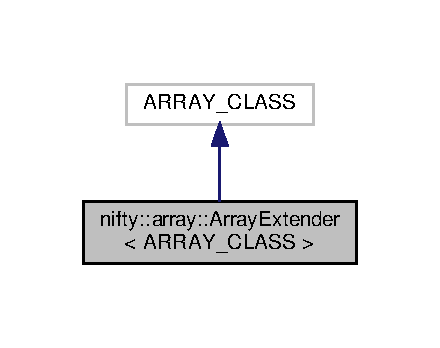
\includegraphics[width=211pt]{classnifty_1_1array_1_1ArrayExtender__inherit__graph}
\end{center}
\end{figure}


Collaboration diagram for nifty\+:\+:array\+:\+:Array\+Extender$<$ A\+R\+R\+A\+Y\+\_\+\+C\+L\+A\+SS $>$\+:
\nopagebreak
\begin{figure}[H]
\begin{center}
\leavevmode
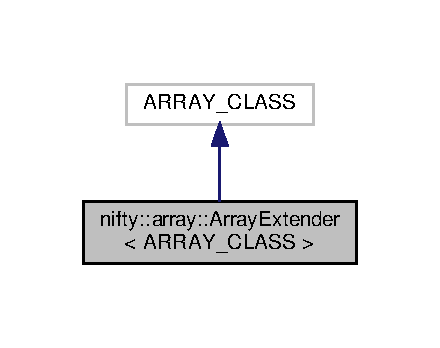
\includegraphics[width=211pt]{classnifty_1_1array_1_1ArrayExtender__coll__graph}
\end{center}
\end{figure}


The documentation for this class was generated from the following file\+:\begin{DoxyCompactItemize}
\item 
/home/tbeier/src/nifty/include/nifty/array/\hyperlink{arithmetic__array_8hxx}{arithmetic\+\_\+array.\+hxx}\end{DoxyCompactItemize}

\hypertarget{classnifty_1_1graph_1_1BidirectionalBreadthFirstSearch}{}\section{nifty\+:\+:graph\+:\+:Bidirectional\+Breadth\+First\+Search$<$ G\+R\+A\+P\+H $>$ Class Template Reference}
\label{classnifty_1_1graph_1_1BidirectionalBreadthFirstSearch}\index{nifty\+::graph\+::\+Bidirectional\+Breadth\+First\+Search$<$ G\+R\+A\+P\+H $>$@{nifty\+::graph\+::\+Bidirectional\+Breadth\+First\+Search$<$ G\+R\+A\+P\+H $>$}}


{\ttfamily \#include $<$bidirectional\+\_\+breadth\+\_\+first\+\_\+search.\+hxx$>$}

\subsection*{Public Types}
\begin{DoxyCompactItemize}
\item 
typedef G\+R\+A\+P\+H \hyperlink{classnifty_1_1graph_1_1BidirectionalBreadthFirstSearch_af6a0e7af586af4ebba7a5f464d82ae71}{Graph}
\item 
typedef Graph\+::template Node\+Map$<$ int64\+\_\+t $>$ \hyperlink{classnifty_1_1graph_1_1BidirectionalBreadthFirstSearch_a8dad356a684976bd3651d63765e35103}{Parents}
\end{DoxyCompactItemize}
\subsection*{Public Member Functions}
\begin{DoxyCompactItemize}
\item 
\hyperlink{classnifty_1_1graph_1_1BidirectionalBreadthFirstSearch_a0190f62ab6974d4d09db4488561605d2}{Bidirectional\+Breadth\+First\+Search} (const \hyperlink{classnifty_1_1graph_1_1BidirectionalBreadthFirstSearch_af6a0e7af586af4ebba7a5f464d82ae71}{Graph} \&graph)
\item 
bool \hyperlink{classnifty_1_1graph_1_1BidirectionalBreadthFirstSearch_af6ae063fd07eb6635ebc070dac6d2730}{run\+Single\+Source\+Single\+Target} (const int64\+\_\+t source, const int64\+\_\+t target)
\item 
{\footnotesize template$<$class S\+U\+B\+G\+R\+A\+P\+H\+\_\+\+M\+A\+S\+K $>$ }\\bool \hyperlink{classnifty_1_1graph_1_1BidirectionalBreadthFirstSearch_a4ddc85ac7f5b28bec9f729d0120b4692}{run\+Single\+Source\+Single\+Target} (const int64\+\_\+t source, const int64\+\_\+t target, const S\+U\+B\+G\+R\+A\+P\+H\+\_\+\+M\+A\+S\+K \&mask)
\item 
const Deque\+Type \& \hyperlink{classnifty_1_1graph_1_1BidirectionalBreadthFirstSearch_a1820fb29cd0d00c04ca660e375d3610a}{path} () const 
\end{DoxyCompactItemize}


\subsection{Member Typedef Documentation}
\hypertarget{classnifty_1_1graph_1_1BidirectionalBreadthFirstSearch_af6a0e7af586af4ebba7a5f464d82ae71}{}\index{nifty\+::graph\+::\+Bidirectional\+Breadth\+First\+Search@{nifty\+::graph\+::\+Bidirectional\+Breadth\+First\+Search}!Graph@{Graph}}
\index{Graph@{Graph}!nifty\+::graph\+::\+Bidirectional\+Breadth\+First\+Search@{nifty\+::graph\+::\+Bidirectional\+Breadth\+First\+Search}}
\subsubsection[{Graph}]{\setlength{\rightskip}{0pt plus 5cm}template$<$class G\+R\+A\+P\+H$>$ typedef G\+R\+A\+P\+H {\bf nifty\+::graph\+::\+Bidirectional\+Breadth\+First\+Search}$<$ G\+R\+A\+P\+H $>$\+::{\bf Graph}}\label{classnifty_1_1graph_1_1BidirectionalBreadthFirstSearch_af6a0e7af586af4ebba7a5f464d82ae71}
\hypertarget{classnifty_1_1graph_1_1BidirectionalBreadthFirstSearch_a8dad356a684976bd3651d63765e35103}{}\index{nifty\+::graph\+::\+Bidirectional\+Breadth\+First\+Search@{nifty\+::graph\+::\+Bidirectional\+Breadth\+First\+Search}!Parents@{Parents}}
\index{Parents@{Parents}!nifty\+::graph\+::\+Bidirectional\+Breadth\+First\+Search@{nifty\+::graph\+::\+Bidirectional\+Breadth\+First\+Search}}
\subsubsection[{Parents}]{\setlength{\rightskip}{0pt plus 5cm}template$<$class G\+R\+A\+P\+H$>$ typedef Graph\+:: template Node\+Map$<$int64\+\_\+t$>$ {\bf nifty\+::graph\+::\+Bidirectional\+Breadth\+First\+Search}$<$ G\+R\+A\+P\+H $>$\+::{\bf Parents}}\label{classnifty_1_1graph_1_1BidirectionalBreadthFirstSearch_a8dad356a684976bd3651d63765e35103}


\subsection{Constructor \& Destructor Documentation}
\hypertarget{classnifty_1_1graph_1_1BidirectionalBreadthFirstSearch_a0190f62ab6974d4d09db4488561605d2}{}\index{nifty\+::graph\+::\+Bidirectional\+Breadth\+First\+Search@{nifty\+::graph\+::\+Bidirectional\+Breadth\+First\+Search}!Bidirectional\+Breadth\+First\+Search@{Bidirectional\+Breadth\+First\+Search}}
\index{Bidirectional\+Breadth\+First\+Search@{Bidirectional\+Breadth\+First\+Search}!nifty\+::graph\+::\+Bidirectional\+Breadth\+First\+Search@{nifty\+::graph\+::\+Bidirectional\+Breadth\+First\+Search}}
\subsubsection[{Bidirectional\+Breadth\+First\+Search(const Graph \&graph)}]{\setlength{\rightskip}{0pt plus 5cm}template$<$class G\+R\+A\+P\+H$>$ {\bf nifty\+::graph\+::\+Bidirectional\+Breadth\+First\+Search}$<$ G\+R\+A\+P\+H $>$\+::{\bf Bidirectional\+Breadth\+First\+Search} (
\begin{DoxyParamCaption}
\item[{const {\bf Graph} \&}]{graph}
\end{DoxyParamCaption}
)\hspace{0.3cm}{\ttfamily [inline]}}\label{classnifty_1_1graph_1_1BidirectionalBreadthFirstSearch_a0190f62ab6974d4d09db4488561605d2}


\subsection{Member Function Documentation}
\hypertarget{classnifty_1_1graph_1_1BidirectionalBreadthFirstSearch_a1820fb29cd0d00c04ca660e375d3610a}{}\index{nifty\+::graph\+::\+Bidirectional\+Breadth\+First\+Search@{nifty\+::graph\+::\+Bidirectional\+Breadth\+First\+Search}!path@{path}}
\index{path@{path}!nifty\+::graph\+::\+Bidirectional\+Breadth\+First\+Search@{nifty\+::graph\+::\+Bidirectional\+Breadth\+First\+Search}}
\subsubsection[{path() const }]{\setlength{\rightskip}{0pt plus 5cm}template$<$class G\+R\+A\+P\+H$>$ const Deque\+Type\& {\bf nifty\+::graph\+::\+Bidirectional\+Breadth\+First\+Search}$<$ G\+R\+A\+P\+H $>$\+::path (
\begin{DoxyParamCaption}
{}
\end{DoxyParamCaption}
) const\hspace{0.3cm}{\ttfamily [inline]}}\label{classnifty_1_1graph_1_1BidirectionalBreadthFirstSearch_a1820fb29cd0d00c04ca660e375d3610a}
\hypertarget{classnifty_1_1graph_1_1BidirectionalBreadthFirstSearch_af6ae063fd07eb6635ebc070dac6d2730}{}\index{nifty\+::graph\+::\+Bidirectional\+Breadth\+First\+Search@{nifty\+::graph\+::\+Bidirectional\+Breadth\+First\+Search}!run\+Single\+Source\+Single\+Target@{run\+Single\+Source\+Single\+Target}}
\index{run\+Single\+Source\+Single\+Target@{run\+Single\+Source\+Single\+Target}!nifty\+::graph\+::\+Bidirectional\+Breadth\+First\+Search@{nifty\+::graph\+::\+Bidirectional\+Breadth\+First\+Search}}
\subsubsection[{run\+Single\+Source\+Single\+Target(const int64\+\_\+t source, const int64\+\_\+t target)}]{\setlength{\rightskip}{0pt plus 5cm}template$<$class G\+R\+A\+P\+H$>$ bool {\bf nifty\+::graph\+::\+Bidirectional\+Breadth\+First\+Search}$<$ G\+R\+A\+P\+H $>$\+::run\+Single\+Source\+Single\+Target (
\begin{DoxyParamCaption}
\item[{const int64\+\_\+t}]{source, }
\item[{const int64\+\_\+t}]{target}
\end{DoxyParamCaption}
)\hspace{0.3cm}{\ttfamily [inline]}}\label{classnifty_1_1graph_1_1BidirectionalBreadthFirstSearch_af6ae063fd07eb6635ebc070dac6d2730}
\hypertarget{classnifty_1_1graph_1_1BidirectionalBreadthFirstSearch_a4ddc85ac7f5b28bec9f729d0120b4692}{}\index{nifty\+::graph\+::\+Bidirectional\+Breadth\+First\+Search@{nifty\+::graph\+::\+Bidirectional\+Breadth\+First\+Search}!run\+Single\+Source\+Single\+Target@{run\+Single\+Source\+Single\+Target}}
\index{run\+Single\+Source\+Single\+Target@{run\+Single\+Source\+Single\+Target}!nifty\+::graph\+::\+Bidirectional\+Breadth\+First\+Search@{nifty\+::graph\+::\+Bidirectional\+Breadth\+First\+Search}}
\subsubsection[{run\+Single\+Source\+Single\+Target(const int64\+\_\+t source, const int64\+\_\+t target, const S\+U\+B\+G\+R\+A\+P\+H\+\_\+\+M\+A\+S\+K \&mask)}]{\setlength{\rightskip}{0pt plus 5cm}template$<$class G\+R\+A\+P\+H$>$ template$<$class S\+U\+B\+G\+R\+A\+P\+H\+\_\+\+M\+A\+S\+K $>$ bool {\bf nifty\+::graph\+::\+Bidirectional\+Breadth\+First\+Search}$<$ G\+R\+A\+P\+H $>$\+::run\+Single\+Source\+Single\+Target (
\begin{DoxyParamCaption}
\item[{const int64\+\_\+t}]{source, }
\item[{const int64\+\_\+t}]{target, }
\item[{const S\+U\+B\+G\+R\+A\+P\+H\+\_\+\+M\+A\+S\+K \&}]{mask}
\end{DoxyParamCaption}
)\hspace{0.3cm}{\ttfamily [inline]}}\label{classnifty_1_1graph_1_1BidirectionalBreadthFirstSearch_a4ddc85ac7f5b28bec9f729d0120b4692}


The documentation for this class was generated from the following file\+:\begin{DoxyCompactItemize}
\item 
/home/tbeier/src/nifty/include/nifty/graph/\hyperlink{bidirectional__breadth__first__search_8hxx}{bidirectional\+\_\+breadth\+\_\+first\+\_\+search.\+hxx}\end{DoxyCompactItemize}

\hypertarget{classnifty_1_1tools_1_1Block}{}\section{nifty\+:\+:tools\+:\+:Block$<$ D\+I\+M, T $>$ Class Template Reference}
\label{classnifty_1_1tools_1_1Block}\index{nifty\+::tools\+::\+Block$<$ D\+I\+M, T $>$@{nifty\+::tools\+::\+Block$<$ D\+I\+M, T $>$}}


{\ttfamily \#include $<$blocking.\+hxx$>$}

\subsection*{Public Types}
\begin{DoxyCompactItemize}
\item 
typedef T \hyperlink{classnifty_1_1tools_1_1Block_a3e77342701a32fcc670d398f1b9bc6d4}{Value\+Type}
\item 
typedef \hyperlink{classnifty_1_1tools_1_1Block_a3e77342701a32fcc670d398f1b9bc6d4}{Value\+Type} \hyperlink{classnifty_1_1tools_1_1Block_accbed9defe9a82425025d9182c41e0a6}{value\+\_\+type}
\begin{DoxyCompactList}\small\item\em stl compatible value type \end{DoxyCompactList}\item 
typedef \hyperlink{namespacenifty_1_1array_a683f151f19c851754e0c6d55ed16a0c2}{nifty\+::array\+::\+Static\+Array}$<$ \hyperlink{classnifty_1_1tools_1_1Block_a3e77342701a32fcc670d398f1b9bc6d4}{Value\+Type}, D\+I\+M $>$ \hyperlink{classnifty_1_1tools_1_1Block_aa077b4ebbf3e4e9b679d1957ca10ba32}{Vector\+Type}
\end{DoxyCompactItemize}
\subsection*{Public Member Functions}
\begin{DoxyCompactItemize}
\item 
\hyperlink{classnifty_1_1tools_1_1Block_ab4fe7e24f2d3cd64b75a4e58b314170e}{Block} (const \hyperlink{classnifty_1_1tools_1_1Block_aa077b4ebbf3e4e9b679d1957ca10ba32}{Vector\+Type} \&\hyperlink{classnifty_1_1tools_1_1Block_ae11f59f462304ae59886bc7991fecef1}{begin}=\hyperlink{classnifty_1_1tools_1_1Block_aa077b4ebbf3e4e9b679d1957ca10ba32}{Vector\+Type}(0), const \hyperlink{classnifty_1_1tools_1_1Block_aa077b4ebbf3e4e9b679d1957ca10ba32}{Vector\+Type} \&\hyperlink{classnifty_1_1tools_1_1Block_a2b6bb43b03ea8c4d7f31f01d0143d60a}{end}=\hyperlink{classnifty_1_1tools_1_1Block_aa077b4ebbf3e4e9b679d1957ca10ba32}{Vector\+Type}(0))
\item 
const \hyperlink{classnifty_1_1tools_1_1Block_aa077b4ebbf3e4e9b679d1957ca10ba32}{Vector\+Type} \& \hyperlink{classnifty_1_1tools_1_1Block_ae11f59f462304ae59886bc7991fecef1}{begin} () const 
\item 
const \hyperlink{classnifty_1_1tools_1_1Block_aa077b4ebbf3e4e9b679d1957ca10ba32}{Vector\+Type} \& \hyperlink{classnifty_1_1tools_1_1Block_a2b6bb43b03ea8c4d7f31f01d0143d60a}{end} () const 
\item 
\hyperlink{classnifty_1_1tools_1_1Block_aa077b4ebbf3e4e9b679d1957ca10ba32}{Vector\+Type} \hyperlink{classnifty_1_1tools_1_1Block_a2a7c4eb08521c7624f27a096f0c915db}{shape} () const 
\end{DoxyCompactItemize}


\subsection{Member Typedef Documentation}
\hypertarget{classnifty_1_1tools_1_1Block_accbed9defe9a82425025d9182c41e0a6}{}\index{nifty\+::tools\+::\+Block@{nifty\+::tools\+::\+Block}!value\+\_\+type@{value\+\_\+type}}
\index{value\+\_\+type@{value\+\_\+type}!nifty\+::tools\+::\+Block@{nifty\+::tools\+::\+Block}}
\subsubsection[{value\+\_\+type}]{\setlength{\rightskip}{0pt plus 5cm}template$<$std\+::size\+\_\+t D\+I\+M, class T  = int64\+\_\+t$>$ typedef {\bf Value\+Type} {\bf nifty\+::tools\+::\+Block}$<$ D\+I\+M, T $>$\+::{\bf value\+\_\+type}}\label{classnifty_1_1tools_1_1Block_accbed9defe9a82425025d9182c41e0a6}


stl compatible value type 

\hypertarget{classnifty_1_1tools_1_1Block_a3e77342701a32fcc670d398f1b9bc6d4}{}\index{nifty\+::tools\+::\+Block@{nifty\+::tools\+::\+Block}!Value\+Type@{Value\+Type}}
\index{Value\+Type@{Value\+Type}!nifty\+::tools\+::\+Block@{nifty\+::tools\+::\+Block}}
\subsubsection[{Value\+Type}]{\setlength{\rightskip}{0pt plus 5cm}template$<$std\+::size\+\_\+t D\+I\+M, class T  = int64\+\_\+t$>$ typedef T {\bf nifty\+::tools\+::\+Block}$<$ D\+I\+M, T $>$\+::{\bf Value\+Type}}\label{classnifty_1_1tools_1_1Block_a3e77342701a32fcc670d398f1b9bc6d4}
\hypertarget{classnifty_1_1tools_1_1Block_aa077b4ebbf3e4e9b679d1957ca10ba32}{}\index{nifty\+::tools\+::\+Block@{nifty\+::tools\+::\+Block}!Vector\+Type@{Vector\+Type}}
\index{Vector\+Type@{Vector\+Type}!nifty\+::tools\+::\+Block@{nifty\+::tools\+::\+Block}}
\subsubsection[{Vector\+Type}]{\setlength{\rightskip}{0pt plus 5cm}template$<$std\+::size\+\_\+t D\+I\+M, class T  = int64\+\_\+t$>$ typedef {\bf nifty\+::array\+::\+Static\+Array}$<${\bf Value\+Type}, D\+I\+M$>$ {\bf nifty\+::tools\+::\+Block}$<$ D\+I\+M, T $>$\+::{\bf Vector\+Type}}\label{classnifty_1_1tools_1_1Block_aa077b4ebbf3e4e9b679d1957ca10ba32}


\subsection{Constructor \& Destructor Documentation}
\hypertarget{classnifty_1_1tools_1_1Block_ab4fe7e24f2d3cd64b75a4e58b314170e}{}\index{nifty\+::tools\+::\+Block@{nifty\+::tools\+::\+Block}!Block@{Block}}
\index{Block@{Block}!nifty\+::tools\+::\+Block@{nifty\+::tools\+::\+Block}}
\subsubsection[{Block(const Vector\+Type \&begin=\+Vector\+Type(0), const Vector\+Type \&end=\+Vector\+Type(0))}]{\setlength{\rightskip}{0pt plus 5cm}template$<$std\+::size\+\_\+t D\+I\+M, class T  = int64\+\_\+t$>$ {\bf nifty\+::tools\+::\+Block}$<$ D\+I\+M, T $>$\+::{\bf Block} (
\begin{DoxyParamCaption}
\item[{const {\bf Vector\+Type} \&}]{begin = {\ttfamily {\bf Vector\+Type}(0)}, }
\item[{const {\bf Vector\+Type} \&}]{end = {\ttfamily {\bf Vector\+Type}(0)}}
\end{DoxyParamCaption}
)\hspace{0.3cm}{\ttfamily [inline]}}\label{classnifty_1_1tools_1_1Block_ab4fe7e24f2d3cd64b75a4e58b314170e}


\subsection{Member Function Documentation}
\hypertarget{classnifty_1_1tools_1_1Block_ae11f59f462304ae59886bc7991fecef1}{}\index{nifty\+::tools\+::\+Block@{nifty\+::tools\+::\+Block}!begin@{begin}}
\index{begin@{begin}!nifty\+::tools\+::\+Block@{nifty\+::tools\+::\+Block}}
\subsubsection[{begin() const }]{\setlength{\rightskip}{0pt plus 5cm}template$<$std\+::size\+\_\+t D\+I\+M, class T  = int64\+\_\+t$>$ const {\bf Vector\+Type}\& {\bf nifty\+::tools\+::\+Block}$<$ D\+I\+M, T $>$\+::begin (
\begin{DoxyParamCaption}
{}
\end{DoxyParamCaption}
) const\hspace{0.3cm}{\ttfamily [inline]}}\label{classnifty_1_1tools_1_1Block_ae11f59f462304ae59886bc7991fecef1}
\hypertarget{classnifty_1_1tools_1_1Block_a2b6bb43b03ea8c4d7f31f01d0143d60a}{}\index{nifty\+::tools\+::\+Block@{nifty\+::tools\+::\+Block}!end@{end}}
\index{end@{end}!nifty\+::tools\+::\+Block@{nifty\+::tools\+::\+Block}}
\subsubsection[{end() const }]{\setlength{\rightskip}{0pt plus 5cm}template$<$std\+::size\+\_\+t D\+I\+M, class T  = int64\+\_\+t$>$ const {\bf Vector\+Type}\& {\bf nifty\+::tools\+::\+Block}$<$ D\+I\+M, T $>$\+::end (
\begin{DoxyParamCaption}
{}
\end{DoxyParamCaption}
) const\hspace{0.3cm}{\ttfamily [inline]}}\label{classnifty_1_1tools_1_1Block_a2b6bb43b03ea8c4d7f31f01d0143d60a}
\hypertarget{classnifty_1_1tools_1_1Block_a2a7c4eb08521c7624f27a096f0c915db}{}\index{nifty\+::tools\+::\+Block@{nifty\+::tools\+::\+Block}!shape@{shape}}
\index{shape@{shape}!nifty\+::tools\+::\+Block@{nifty\+::tools\+::\+Block}}
\subsubsection[{shape() const }]{\setlength{\rightskip}{0pt plus 5cm}template$<$std\+::size\+\_\+t D\+I\+M, class T  = int64\+\_\+t$>$ {\bf Vector\+Type} {\bf nifty\+::tools\+::\+Block}$<$ D\+I\+M, T $>$\+::shape (
\begin{DoxyParamCaption}
{}
\end{DoxyParamCaption}
) const\hspace{0.3cm}{\ttfamily [inline]}}\label{classnifty_1_1tools_1_1Block_a2a7c4eb08521c7624f27a096f0c915db}


The documentation for this class was generated from the following file\+:\begin{DoxyCompactItemize}
\item 
/home/tbeier/src/nifty/include/nifty/tools/\hyperlink{blocking_8hxx}{blocking.\+hxx}\end{DoxyCompactItemize}

\hypertarget{classnifty_1_1tools_1_1Blocking}{}\section{nifty\+:\+:tools\+:\+:Blocking$<$ D\+IM, T $>$ Class Template Reference}
\label{classnifty_1_1tools_1_1Blocking}\index{nifty\+::tools\+::\+Blocking$<$ D\+I\+M, T $>$@{nifty\+::tools\+::\+Blocking$<$ D\+I\+M, T $>$}}


{\ttfamily \#include $<$blocking.\+hxx$>$}

\subsection*{Public Types}
\begin{DoxyCompactItemize}
\item 
typedef \hyperlink{classnifty_1_1tools_1_1BlockWithHalo}{Block\+With\+Halo}$<$ D\+IM, T $>$ \hyperlink{classnifty_1_1tools_1_1Blocking_abebd9361d89cc399bc495861fa4e331d}{Block\+With\+Halo\+Type}
\item 
typedef \hyperlink{classnifty_1_1tools_1_1BlockWithHalo_a98d2c04518f8902ab6d985feba605987}{Block\+With\+Halo\+Type\+::\+Block\+Type} \hyperlink{classnifty_1_1tools_1_1Blocking_a597e0d4186d2d40ccb96698cc16775c6}{Block\+Type}
\item 
typedef \hyperlink{classnifty_1_1tools_1_1BlockWithHalo_a65d120db84dfca7586ae5ab30f26f01b}{Block\+With\+Halo\+Type\+::\+Value\+Type} \hyperlink{classnifty_1_1tools_1_1Blocking_ae04f69cd6e67bbde26eee3f38e0257f7}{Value\+Type}
\item 
typedef \hyperlink{classnifty_1_1tools_1_1BlockWithHalo_a65d120db84dfca7586ae5ab30f26f01b}{Block\+With\+Halo\+Type\+::\+Value\+Type} \hyperlink{classnifty_1_1tools_1_1Blocking_a4ea21e967d25e621a000176dc994c85e}{value\+\_\+type}
\item 
typedef \hyperlink{classnifty_1_1tools_1_1BlockWithHalo_a040d8a654eb42791c6e5fbd4dfd51b9f}{Block\+With\+Halo\+Type\+::\+Vector\+Type} \hyperlink{classnifty_1_1tools_1_1Blocking_a5f8df3d4cdf09803217d729a04018fb3}{Vector\+Type}
\end{DoxyCompactItemize}
\subsection*{Public Member Functions}
\begin{DoxyCompactItemize}
\item 
\hyperlink{classnifty_1_1tools_1_1Blocking_a72c8db4f834fd774f6a50e03ef4b30c2}{Blocking} (const \hyperlink{classnifty_1_1tools_1_1Blocking_a5f8df3d4cdf09803217d729a04018fb3}{Vector\+Type} \&\hyperlink{classnifty_1_1tools_1_1Blocking_a2ce7ed87ad053c943954873e70621ab8}{roi\+Begin}, const \hyperlink{classnifty_1_1tools_1_1Blocking_a5f8df3d4cdf09803217d729a04018fb3}{Vector\+Type} \&\hyperlink{classnifty_1_1tools_1_1Blocking_a19b6329454038905f9c66ebed3094205}{roi\+End}, const \hyperlink{classnifty_1_1tools_1_1Blocking_a5f8df3d4cdf09803217d729a04018fb3}{Vector\+Type} \&\hyperlink{classnifty_1_1tools_1_1Blocking_aa42bfae6940045db062898f66345897b}{block\+Shape}, const \hyperlink{classnifty_1_1tools_1_1Blocking_a5f8df3d4cdf09803217d729a04018fb3}{Vector\+Type} \&\hyperlink{classnifty_1_1tools_1_1Blocking_a7efe756ab0f686e2edb39fb800cea37f}{block\+Shift}=\hyperlink{classnifty_1_1tools_1_1Blocking_a5f8df3d4cdf09803217d729a04018fb3}{Vector\+Type}(0))
\item 
const \hyperlink{classnifty_1_1tools_1_1Blocking_a5f8df3d4cdf09803217d729a04018fb3}{Vector\+Type} \& \hyperlink{classnifty_1_1tools_1_1Blocking_a2ce7ed87ad053c943954873e70621ab8}{roi\+Begin} () const
\item 
const \hyperlink{classnifty_1_1tools_1_1Blocking_a5f8df3d4cdf09803217d729a04018fb3}{Vector\+Type} \& \hyperlink{classnifty_1_1tools_1_1Blocking_a19b6329454038905f9c66ebed3094205}{roi\+End} () const
\item 
const \hyperlink{classnifty_1_1tools_1_1Blocking_a5f8df3d4cdf09803217d729a04018fb3}{Vector\+Type} \& \hyperlink{classnifty_1_1tools_1_1Blocking_aa42bfae6940045db062898f66345897b}{block\+Shape} () const
\item 
const \hyperlink{classnifty_1_1tools_1_1Blocking_a5f8df3d4cdf09803217d729a04018fb3}{Vector\+Type} \& \hyperlink{classnifty_1_1tools_1_1Blocking_a7efe756ab0f686e2edb39fb800cea37f}{block\+Shift} () const
\item 
const \hyperlink{classnifty_1_1tools_1_1Blocking_a5f8df3d4cdf09803217d729a04018fb3}{Vector\+Type} \& \hyperlink{classnifty_1_1tools_1_1Blocking_ad736ea915574470bc35e35df5a11a9f3}{blocks\+Per\+Axis} () const
\item 
const size\+\_\+t \hyperlink{classnifty_1_1tools_1_1Blocking_af8848458068c1d943b42980809a93744}{number\+Of\+Blocks} () const
\item 
\hyperlink{classnifty_1_1tools_1_1Blocking_a597e0d4186d2d40ccb96698cc16775c6}{Block\+Type} \hyperlink{classnifty_1_1tools_1_1Blocking_ad5f32d8ff7c1c9b36035ad572ceee0be}{get\+Block} (const uint64\+\_\+t block\+Index) const
\item 
\hyperlink{classnifty_1_1tools_1_1Blocking_abebd9361d89cc399bc495861fa4e331d}{Block\+With\+Halo\+Type} \hyperlink{classnifty_1_1tools_1_1Blocking_aa295ddc729d0cfd5ac90d18573d96b26}{get\+Block\+With\+Halo} (const uint64\+\_\+t block\+Index, const \hyperlink{classnifty_1_1tools_1_1Blocking_a5f8df3d4cdf09803217d729a04018fb3}{Vector\+Type} \&halo\+Begin, const \hyperlink{classnifty_1_1tools_1_1Blocking_a5f8df3d4cdf09803217d729a04018fb3}{Vector\+Type} \&halo\+End) const
\item 
\hyperlink{classnifty_1_1tools_1_1Blocking_abebd9361d89cc399bc495861fa4e331d}{Block\+With\+Halo\+Type} \hyperlink{classnifty_1_1tools_1_1Blocking_aeeb540a2fe69cd5f3e89047daa922f13}{get\+Block\+With\+Halo} (const uint64\+\_\+t block\+Index, const \hyperlink{classnifty_1_1tools_1_1Blocking_a5f8df3d4cdf09803217d729a04018fb3}{Vector\+Type} \&halo) const
\item 
\hyperlink{classnifty_1_1tools_1_1Blocking_abebd9361d89cc399bc495861fa4e331d}{Block\+With\+Halo\+Type} \hyperlink{classnifty_1_1tools_1_1Blocking_a09126c498d87974b9cabcae18c887b4f}{add\+Halo} (const \hyperlink{classnifty_1_1tools_1_1Blocking_a597e0d4186d2d40ccb96698cc16775c6}{Block\+Type} inner\+Block, const \hyperlink{classnifty_1_1tools_1_1Blocking_a5f8df3d4cdf09803217d729a04018fb3}{Vector\+Type} \&halo\+Begin, const \hyperlink{classnifty_1_1tools_1_1Blocking_a5f8df3d4cdf09803217d729a04018fb3}{Vector\+Type} \&halo\+End) const
\item 
\hyperlink{classnifty_1_1tools_1_1Blocking_abebd9361d89cc399bc495861fa4e331d}{Block\+With\+Halo\+Type} \hyperlink{classnifty_1_1tools_1_1Blocking_a735ce675927a0a76cf9370c40022e8de}{add\+Halo} (const \hyperlink{classnifty_1_1tools_1_1Blocking_a597e0d4186d2d40ccb96698cc16775c6}{Block\+Type} inner\+Block, const \hyperlink{classnifty_1_1tools_1_1Blocking_a5f8df3d4cdf09803217d729a04018fb3}{Vector\+Type} \&halo) const
\end{DoxyCompactItemize}


\subsection{Member Typedef Documentation}
\mbox{\Hypertarget{classnifty_1_1tools_1_1Blocking_a597e0d4186d2d40ccb96698cc16775c6}\label{classnifty_1_1tools_1_1Blocking_a597e0d4186d2d40ccb96698cc16775c6}} 
\index{nifty\+::tools\+::\+Blocking@{nifty\+::tools\+::\+Blocking}!Block\+Type@{Block\+Type}}
\index{Block\+Type@{Block\+Type}!nifty\+::tools\+::\+Blocking@{nifty\+::tools\+::\+Blocking}}
\subsubsection{\texorpdfstring{Block\+Type}{BlockType}}
{\footnotesize\ttfamily template$<$std\+::size\+\_\+t D\+IM, class T  = int64\+\_\+t$>$ \\
typedef \hyperlink{classnifty_1_1tools_1_1BlockWithHalo_a98d2c04518f8902ab6d985feba605987}{Block\+With\+Halo\+Type\+::\+Block\+Type} \hyperlink{classnifty_1_1tools_1_1Blocking}{nifty\+::tools\+::\+Blocking}$<$ D\+IM, T $>$\+::\hyperlink{classnifty_1_1tools_1_1Blocking_a597e0d4186d2d40ccb96698cc16775c6}{Block\+Type}}

\mbox{\Hypertarget{classnifty_1_1tools_1_1Blocking_abebd9361d89cc399bc495861fa4e331d}\label{classnifty_1_1tools_1_1Blocking_abebd9361d89cc399bc495861fa4e331d}} 
\index{nifty\+::tools\+::\+Blocking@{nifty\+::tools\+::\+Blocking}!Block\+With\+Halo\+Type@{Block\+With\+Halo\+Type}}
\index{Block\+With\+Halo\+Type@{Block\+With\+Halo\+Type}!nifty\+::tools\+::\+Blocking@{nifty\+::tools\+::\+Blocking}}
\subsubsection{\texorpdfstring{Block\+With\+Halo\+Type}{BlockWithHaloType}}
{\footnotesize\ttfamily template$<$std\+::size\+\_\+t D\+IM, class T  = int64\+\_\+t$>$ \\
typedef \hyperlink{classnifty_1_1tools_1_1BlockWithHalo}{Block\+With\+Halo}$<$D\+IM, T$>$ \hyperlink{classnifty_1_1tools_1_1Blocking}{nifty\+::tools\+::\+Blocking}$<$ D\+IM, T $>$\+::\hyperlink{classnifty_1_1tools_1_1Blocking_abebd9361d89cc399bc495861fa4e331d}{Block\+With\+Halo\+Type}}

\mbox{\Hypertarget{classnifty_1_1tools_1_1Blocking_a4ea21e967d25e621a000176dc994c85e}\label{classnifty_1_1tools_1_1Blocking_a4ea21e967d25e621a000176dc994c85e}} 
\index{nifty\+::tools\+::\+Blocking@{nifty\+::tools\+::\+Blocking}!value\+\_\+type@{value\+\_\+type}}
\index{value\+\_\+type@{value\+\_\+type}!nifty\+::tools\+::\+Blocking@{nifty\+::tools\+::\+Blocking}}
\subsubsection{\texorpdfstring{value\+\_\+type}{value\_type}}
{\footnotesize\ttfamily template$<$std\+::size\+\_\+t D\+IM, class T  = int64\+\_\+t$>$ \\
typedef \hyperlink{classnifty_1_1tools_1_1BlockWithHalo_a65d120db84dfca7586ae5ab30f26f01b}{Block\+With\+Halo\+Type\+::\+Value\+Type} \hyperlink{classnifty_1_1tools_1_1Blocking}{nifty\+::tools\+::\+Blocking}$<$ D\+IM, T $>$\+::\hyperlink{classnifty_1_1tools_1_1Blocking_a4ea21e967d25e621a000176dc994c85e}{value\+\_\+type}}

\mbox{\Hypertarget{classnifty_1_1tools_1_1Blocking_ae04f69cd6e67bbde26eee3f38e0257f7}\label{classnifty_1_1tools_1_1Blocking_ae04f69cd6e67bbde26eee3f38e0257f7}} 
\index{nifty\+::tools\+::\+Blocking@{nifty\+::tools\+::\+Blocking}!Value\+Type@{Value\+Type}}
\index{Value\+Type@{Value\+Type}!nifty\+::tools\+::\+Blocking@{nifty\+::tools\+::\+Blocking}}
\subsubsection{\texorpdfstring{Value\+Type}{ValueType}}
{\footnotesize\ttfamily template$<$std\+::size\+\_\+t D\+IM, class T  = int64\+\_\+t$>$ \\
typedef \hyperlink{classnifty_1_1tools_1_1BlockWithHalo_a65d120db84dfca7586ae5ab30f26f01b}{Block\+With\+Halo\+Type\+::\+Value\+Type} \hyperlink{classnifty_1_1tools_1_1Blocking}{nifty\+::tools\+::\+Blocking}$<$ D\+IM, T $>$\+::\hyperlink{classnifty_1_1tools_1_1Blocking_ae04f69cd6e67bbde26eee3f38e0257f7}{Value\+Type}}

\mbox{\Hypertarget{classnifty_1_1tools_1_1Blocking_a5f8df3d4cdf09803217d729a04018fb3}\label{classnifty_1_1tools_1_1Blocking_a5f8df3d4cdf09803217d729a04018fb3}} 
\index{nifty\+::tools\+::\+Blocking@{nifty\+::tools\+::\+Blocking}!Vector\+Type@{Vector\+Type}}
\index{Vector\+Type@{Vector\+Type}!nifty\+::tools\+::\+Blocking@{nifty\+::tools\+::\+Blocking}}
\subsubsection{\texorpdfstring{Vector\+Type}{VectorType}}
{\footnotesize\ttfamily template$<$std\+::size\+\_\+t D\+IM, class T  = int64\+\_\+t$>$ \\
typedef \hyperlink{classnifty_1_1tools_1_1BlockWithHalo_a040d8a654eb42791c6e5fbd4dfd51b9f}{Block\+With\+Halo\+Type\+::\+Vector\+Type} \hyperlink{classnifty_1_1tools_1_1Blocking}{nifty\+::tools\+::\+Blocking}$<$ D\+IM, T $>$\+::\hyperlink{classnifty_1_1tools_1_1Blocking_a5f8df3d4cdf09803217d729a04018fb3}{Vector\+Type}}



\subsection{Constructor \& Destructor Documentation}
\mbox{\Hypertarget{classnifty_1_1tools_1_1Blocking_a72c8db4f834fd774f6a50e03ef4b30c2}\label{classnifty_1_1tools_1_1Blocking_a72c8db4f834fd774f6a50e03ef4b30c2}} 
\index{nifty\+::tools\+::\+Blocking@{nifty\+::tools\+::\+Blocking}!Blocking@{Blocking}}
\index{Blocking@{Blocking}!nifty\+::tools\+::\+Blocking@{nifty\+::tools\+::\+Blocking}}
\subsubsection{\texorpdfstring{Blocking()}{Blocking()}}
{\footnotesize\ttfamily template$<$std\+::size\+\_\+t D\+IM, class T  = int64\+\_\+t$>$ \\
\hyperlink{classnifty_1_1tools_1_1Blocking}{nifty\+::tools\+::\+Blocking}$<$ D\+IM, T $>$\+::\hyperlink{classnifty_1_1tools_1_1Blocking}{Blocking} (\begin{DoxyParamCaption}\item[{const \hyperlink{classnifty_1_1tools_1_1Blocking_a5f8df3d4cdf09803217d729a04018fb3}{Vector\+Type} \&}]{roi\+Begin,  }\item[{const \hyperlink{classnifty_1_1tools_1_1Blocking_a5f8df3d4cdf09803217d729a04018fb3}{Vector\+Type} \&}]{roi\+End,  }\item[{const \hyperlink{classnifty_1_1tools_1_1Blocking_a5f8df3d4cdf09803217d729a04018fb3}{Vector\+Type} \&}]{block\+Shape,  }\item[{const \hyperlink{classnifty_1_1tools_1_1Blocking_a5f8df3d4cdf09803217d729a04018fb3}{Vector\+Type} \&}]{block\+Shift = {\ttfamily \hyperlink{classnifty_1_1tools_1_1Blocking_a5f8df3d4cdf09803217d729a04018fb3}{Vector\+Type}(0)} }\end{DoxyParamCaption})\hspace{0.3cm}{\ttfamily [inline]}}



\subsection{Member Function Documentation}
\mbox{\Hypertarget{classnifty_1_1tools_1_1Blocking_a09126c498d87974b9cabcae18c887b4f}\label{classnifty_1_1tools_1_1Blocking_a09126c498d87974b9cabcae18c887b4f}} 
\index{nifty\+::tools\+::\+Blocking@{nifty\+::tools\+::\+Blocking}!add\+Halo@{add\+Halo}}
\index{add\+Halo@{add\+Halo}!nifty\+::tools\+::\+Blocking@{nifty\+::tools\+::\+Blocking}}
\subsubsection{\texorpdfstring{add\+Halo()}{addHalo()}\hspace{0.1cm}{\footnotesize\ttfamily [1/2]}}
{\footnotesize\ttfamily template$<$std\+::size\+\_\+t D\+IM, class T  = int64\+\_\+t$>$ \\
\hyperlink{classnifty_1_1tools_1_1Blocking_abebd9361d89cc399bc495861fa4e331d}{Block\+With\+Halo\+Type} \hyperlink{classnifty_1_1tools_1_1Blocking}{nifty\+::tools\+::\+Blocking}$<$ D\+IM, T $>$\+::add\+Halo (\begin{DoxyParamCaption}\item[{const \hyperlink{classnifty_1_1tools_1_1Blocking_a597e0d4186d2d40ccb96698cc16775c6}{Block\+Type}}]{inner\+Block,  }\item[{const \hyperlink{classnifty_1_1tools_1_1Blocking_a5f8df3d4cdf09803217d729a04018fb3}{Vector\+Type} \&}]{halo\+Begin,  }\item[{const \hyperlink{classnifty_1_1tools_1_1Blocking_a5f8df3d4cdf09803217d729a04018fb3}{Vector\+Type} \&}]{halo\+End }\end{DoxyParamCaption}) const\hspace{0.3cm}{\ttfamily [inline]}}

\mbox{\Hypertarget{classnifty_1_1tools_1_1Blocking_a735ce675927a0a76cf9370c40022e8de}\label{classnifty_1_1tools_1_1Blocking_a735ce675927a0a76cf9370c40022e8de}} 
\index{nifty\+::tools\+::\+Blocking@{nifty\+::tools\+::\+Blocking}!add\+Halo@{add\+Halo}}
\index{add\+Halo@{add\+Halo}!nifty\+::tools\+::\+Blocking@{nifty\+::tools\+::\+Blocking}}
\subsubsection{\texorpdfstring{add\+Halo()}{addHalo()}\hspace{0.1cm}{\footnotesize\ttfamily [2/2]}}
{\footnotesize\ttfamily template$<$std\+::size\+\_\+t D\+IM, class T  = int64\+\_\+t$>$ \\
\hyperlink{classnifty_1_1tools_1_1Blocking_abebd9361d89cc399bc495861fa4e331d}{Block\+With\+Halo\+Type} \hyperlink{classnifty_1_1tools_1_1Blocking}{nifty\+::tools\+::\+Blocking}$<$ D\+IM, T $>$\+::add\+Halo (\begin{DoxyParamCaption}\item[{const \hyperlink{classnifty_1_1tools_1_1Blocking_a597e0d4186d2d40ccb96698cc16775c6}{Block\+Type}}]{inner\+Block,  }\item[{const \hyperlink{classnifty_1_1tools_1_1Blocking_a5f8df3d4cdf09803217d729a04018fb3}{Vector\+Type} \&}]{halo }\end{DoxyParamCaption}) const\hspace{0.3cm}{\ttfamily [inline]}}

\mbox{\Hypertarget{classnifty_1_1tools_1_1Blocking_aa42bfae6940045db062898f66345897b}\label{classnifty_1_1tools_1_1Blocking_aa42bfae6940045db062898f66345897b}} 
\index{nifty\+::tools\+::\+Blocking@{nifty\+::tools\+::\+Blocking}!block\+Shape@{block\+Shape}}
\index{block\+Shape@{block\+Shape}!nifty\+::tools\+::\+Blocking@{nifty\+::tools\+::\+Blocking}}
\subsubsection{\texorpdfstring{block\+Shape()}{blockShape()}}
{\footnotesize\ttfamily template$<$std\+::size\+\_\+t D\+IM, class T  = int64\+\_\+t$>$ \\
const \hyperlink{classnifty_1_1tools_1_1Blocking_a5f8df3d4cdf09803217d729a04018fb3}{Vector\+Type}\& \hyperlink{classnifty_1_1tools_1_1Blocking}{nifty\+::tools\+::\+Blocking}$<$ D\+IM, T $>$\+::block\+Shape (\begin{DoxyParamCaption}{ }\end{DoxyParamCaption}) const\hspace{0.3cm}{\ttfamily [inline]}}

\mbox{\Hypertarget{classnifty_1_1tools_1_1Blocking_a7efe756ab0f686e2edb39fb800cea37f}\label{classnifty_1_1tools_1_1Blocking_a7efe756ab0f686e2edb39fb800cea37f}} 
\index{nifty\+::tools\+::\+Blocking@{nifty\+::tools\+::\+Blocking}!block\+Shift@{block\+Shift}}
\index{block\+Shift@{block\+Shift}!nifty\+::tools\+::\+Blocking@{nifty\+::tools\+::\+Blocking}}
\subsubsection{\texorpdfstring{block\+Shift()}{blockShift()}}
{\footnotesize\ttfamily template$<$std\+::size\+\_\+t D\+IM, class T  = int64\+\_\+t$>$ \\
const \hyperlink{classnifty_1_1tools_1_1Blocking_a5f8df3d4cdf09803217d729a04018fb3}{Vector\+Type}\& \hyperlink{classnifty_1_1tools_1_1Blocking}{nifty\+::tools\+::\+Blocking}$<$ D\+IM, T $>$\+::block\+Shift (\begin{DoxyParamCaption}{ }\end{DoxyParamCaption}) const\hspace{0.3cm}{\ttfamily [inline]}}

\mbox{\Hypertarget{classnifty_1_1tools_1_1Blocking_ad736ea915574470bc35e35df5a11a9f3}\label{classnifty_1_1tools_1_1Blocking_ad736ea915574470bc35e35df5a11a9f3}} 
\index{nifty\+::tools\+::\+Blocking@{nifty\+::tools\+::\+Blocking}!blocks\+Per\+Axis@{blocks\+Per\+Axis}}
\index{blocks\+Per\+Axis@{blocks\+Per\+Axis}!nifty\+::tools\+::\+Blocking@{nifty\+::tools\+::\+Blocking}}
\subsubsection{\texorpdfstring{blocks\+Per\+Axis()}{blocksPerAxis()}}
{\footnotesize\ttfamily template$<$std\+::size\+\_\+t D\+IM, class T  = int64\+\_\+t$>$ \\
const \hyperlink{classnifty_1_1tools_1_1Blocking_a5f8df3d4cdf09803217d729a04018fb3}{Vector\+Type}\& \hyperlink{classnifty_1_1tools_1_1Blocking}{nifty\+::tools\+::\+Blocking}$<$ D\+IM, T $>$\+::blocks\+Per\+Axis (\begin{DoxyParamCaption}{ }\end{DoxyParamCaption}) const\hspace{0.3cm}{\ttfamily [inline]}}

\mbox{\Hypertarget{classnifty_1_1tools_1_1Blocking_ad5f32d8ff7c1c9b36035ad572ceee0be}\label{classnifty_1_1tools_1_1Blocking_ad5f32d8ff7c1c9b36035ad572ceee0be}} 
\index{nifty\+::tools\+::\+Blocking@{nifty\+::tools\+::\+Blocking}!get\+Block@{get\+Block}}
\index{get\+Block@{get\+Block}!nifty\+::tools\+::\+Blocking@{nifty\+::tools\+::\+Blocking}}
\subsubsection{\texorpdfstring{get\+Block()}{getBlock()}}
{\footnotesize\ttfamily template$<$std\+::size\+\_\+t D\+IM, class T  = int64\+\_\+t$>$ \\
\hyperlink{classnifty_1_1tools_1_1Blocking_a597e0d4186d2d40ccb96698cc16775c6}{Block\+Type} \hyperlink{classnifty_1_1tools_1_1Blocking}{nifty\+::tools\+::\+Blocking}$<$ D\+IM, T $>$\+::get\+Block (\begin{DoxyParamCaption}\item[{const uint64\+\_\+t}]{block\+Index }\end{DoxyParamCaption}) const\hspace{0.3cm}{\ttfamily [inline]}}

\mbox{\Hypertarget{classnifty_1_1tools_1_1Blocking_aa295ddc729d0cfd5ac90d18573d96b26}\label{classnifty_1_1tools_1_1Blocking_aa295ddc729d0cfd5ac90d18573d96b26}} 
\index{nifty\+::tools\+::\+Blocking@{nifty\+::tools\+::\+Blocking}!get\+Block\+With\+Halo@{get\+Block\+With\+Halo}}
\index{get\+Block\+With\+Halo@{get\+Block\+With\+Halo}!nifty\+::tools\+::\+Blocking@{nifty\+::tools\+::\+Blocking}}
\subsubsection{\texorpdfstring{get\+Block\+With\+Halo()}{getBlockWithHalo()}\hspace{0.1cm}{\footnotesize\ttfamily [1/2]}}
{\footnotesize\ttfamily template$<$std\+::size\+\_\+t D\+IM, class T  = int64\+\_\+t$>$ \\
\hyperlink{classnifty_1_1tools_1_1Blocking_abebd9361d89cc399bc495861fa4e331d}{Block\+With\+Halo\+Type} \hyperlink{classnifty_1_1tools_1_1Blocking}{nifty\+::tools\+::\+Blocking}$<$ D\+IM, T $>$\+::get\+Block\+With\+Halo (\begin{DoxyParamCaption}\item[{const uint64\+\_\+t}]{block\+Index,  }\item[{const \hyperlink{classnifty_1_1tools_1_1Blocking_a5f8df3d4cdf09803217d729a04018fb3}{Vector\+Type} \&}]{halo\+Begin,  }\item[{const \hyperlink{classnifty_1_1tools_1_1Blocking_a5f8df3d4cdf09803217d729a04018fb3}{Vector\+Type} \&}]{halo\+End }\end{DoxyParamCaption}) const\hspace{0.3cm}{\ttfamily [inline]}}

\mbox{\Hypertarget{classnifty_1_1tools_1_1Blocking_aeeb540a2fe69cd5f3e89047daa922f13}\label{classnifty_1_1tools_1_1Blocking_aeeb540a2fe69cd5f3e89047daa922f13}} 
\index{nifty\+::tools\+::\+Blocking@{nifty\+::tools\+::\+Blocking}!get\+Block\+With\+Halo@{get\+Block\+With\+Halo}}
\index{get\+Block\+With\+Halo@{get\+Block\+With\+Halo}!nifty\+::tools\+::\+Blocking@{nifty\+::tools\+::\+Blocking}}
\subsubsection{\texorpdfstring{get\+Block\+With\+Halo()}{getBlockWithHalo()}\hspace{0.1cm}{\footnotesize\ttfamily [2/2]}}
{\footnotesize\ttfamily template$<$std\+::size\+\_\+t D\+IM, class T  = int64\+\_\+t$>$ \\
\hyperlink{classnifty_1_1tools_1_1Blocking_abebd9361d89cc399bc495861fa4e331d}{Block\+With\+Halo\+Type} \hyperlink{classnifty_1_1tools_1_1Blocking}{nifty\+::tools\+::\+Blocking}$<$ D\+IM, T $>$\+::get\+Block\+With\+Halo (\begin{DoxyParamCaption}\item[{const uint64\+\_\+t}]{block\+Index,  }\item[{const \hyperlink{classnifty_1_1tools_1_1Blocking_a5f8df3d4cdf09803217d729a04018fb3}{Vector\+Type} \&}]{halo }\end{DoxyParamCaption}) const\hspace{0.3cm}{\ttfamily [inline]}}

\mbox{\Hypertarget{classnifty_1_1tools_1_1Blocking_af8848458068c1d943b42980809a93744}\label{classnifty_1_1tools_1_1Blocking_af8848458068c1d943b42980809a93744}} 
\index{nifty\+::tools\+::\+Blocking@{nifty\+::tools\+::\+Blocking}!number\+Of\+Blocks@{number\+Of\+Blocks}}
\index{number\+Of\+Blocks@{number\+Of\+Blocks}!nifty\+::tools\+::\+Blocking@{nifty\+::tools\+::\+Blocking}}
\subsubsection{\texorpdfstring{number\+Of\+Blocks()}{numberOfBlocks()}}
{\footnotesize\ttfamily template$<$std\+::size\+\_\+t D\+IM, class T  = int64\+\_\+t$>$ \\
const size\+\_\+t \hyperlink{classnifty_1_1tools_1_1Blocking}{nifty\+::tools\+::\+Blocking}$<$ D\+IM, T $>$\+::number\+Of\+Blocks (\begin{DoxyParamCaption}{ }\end{DoxyParamCaption}) const\hspace{0.3cm}{\ttfamily [inline]}}

\mbox{\Hypertarget{classnifty_1_1tools_1_1Blocking_a2ce7ed87ad053c943954873e70621ab8}\label{classnifty_1_1tools_1_1Blocking_a2ce7ed87ad053c943954873e70621ab8}} 
\index{nifty\+::tools\+::\+Blocking@{nifty\+::tools\+::\+Blocking}!roi\+Begin@{roi\+Begin}}
\index{roi\+Begin@{roi\+Begin}!nifty\+::tools\+::\+Blocking@{nifty\+::tools\+::\+Blocking}}
\subsubsection{\texorpdfstring{roi\+Begin()}{roiBegin()}}
{\footnotesize\ttfamily template$<$std\+::size\+\_\+t D\+IM, class T  = int64\+\_\+t$>$ \\
const \hyperlink{classnifty_1_1tools_1_1Blocking_a5f8df3d4cdf09803217d729a04018fb3}{Vector\+Type}\& \hyperlink{classnifty_1_1tools_1_1Blocking}{nifty\+::tools\+::\+Blocking}$<$ D\+IM, T $>$\+::roi\+Begin (\begin{DoxyParamCaption}{ }\end{DoxyParamCaption}) const\hspace{0.3cm}{\ttfamily [inline]}}

\mbox{\Hypertarget{classnifty_1_1tools_1_1Blocking_a19b6329454038905f9c66ebed3094205}\label{classnifty_1_1tools_1_1Blocking_a19b6329454038905f9c66ebed3094205}} 
\index{nifty\+::tools\+::\+Blocking@{nifty\+::tools\+::\+Blocking}!roi\+End@{roi\+End}}
\index{roi\+End@{roi\+End}!nifty\+::tools\+::\+Blocking@{nifty\+::tools\+::\+Blocking}}
\subsubsection{\texorpdfstring{roi\+End()}{roiEnd()}}
{\footnotesize\ttfamily template$<$std\+::size\+\_\+t D\+IM, class T  = int64\+\_\+t$>$ \\
const \hyperlink{classnifty_1_1tools_1_1Blocking_a5f8df3d4cdf09803217d729a04018fb3}{Vector\+Type}\& \hyperlink{classnifty_1_1tools_1_1Blocking}{nifty\+::tools\+::\+Blocking}$<$ D\+IM, T $>$\+::roi\+End (\begin{DoxyParamCaption}{ }\end{DoxyParamCaption}) const\hspace{0.3cm}{\ttfamily [inline]}}



The documentation for this class was generated from the following file\+:\begin{DoxyCompactItemize}
\item 
/home/tbeier/src/nifty/include/nifty/tools/\hyperlink{blocking_8hxx}{blocking.\+hxx}\end{DoxyCompactItemize}

\hypertarget{classnifty_1_1graph_1_1BlockMulticut}{}\section{nifty\+:\+:graph\+:\+:Block\+Multicut$<$ O\+B\+J\+E\+C\+T\+I\+V\+E $>$ Class Template Reference}
\label{classnifty_1_1graph_1_1BlockMulticut}\index{nifty\+::graph\+::\+Block\+Multicut$<$ O\+B\+J\+E\+C\+T\+I\+V\+E $>$@{nifty\+::graph\+::\+Block\+Multicut$<$ O\+B\+J\+E\+C\+T\+I\+V\+E $>$}}


{\ttfamily \#include $<$block\+\_\+multicut.\+hxx$>$}



Inheritance diagram for nifty\+:\+:graph\+:\+:Block\+Multicut$<$ O\+B\+J\+E\+C\+T\+I\+V\+E $>$\+:
% FIG 0


Collaboration diagram for nifty\+:\+:graph\+:\+:Block\+Multicut$<$ O\+B\+J\+E\+C\+T\+I\+V\+E $>$\+:
% FIG 1
\subsection*{Classes}
\begin{DoxyCompactItemize}
\item 
struct \hyperlink{structnifty_1_1graph_1_1BlockMulticut_1_1Settings}{Settings}
\end{DoxyCompactItemize}
\subsection*{Public Types}
\begin{DoxyCompactItemize}
\item 
typedef O\+B\+J\+E\+C\+T\+I\+V\+E \hyperlink{classnifty_1_1graph_1_1BlockMulticut_a5a0258cebb392718a4565551cd43ab89}{Objective}
\item 
typedef O\+B\+J\+E\+C\+T\+I\+V\+E \hyperlink{classnifty_1_1graph_1_1BlockMulticut_a1b38a95ca33ba1eaed19e994484c58fc}{Objective\+Type}
\item 
typedef Objective\+Type\+::\+Weight\+Type \hyperlink{classnifty_1_1graph_1_1BlockMulticut_a5c18649d14bae96da8d0c6359c57673a}{Weight\+Type}
\item 
typedef \hyperlink{classnifty_1_1graph_1_1MulticutBase}{Multicut\+Base}$<$ \hyperlink{classnifty_1_1graph_1_1BlockMulticut_a1b38a95ca33ba1eaed19e994484c58fc}{Objective\+Type} $>$ \hyperlink{classnifty_1_1graph_1_1BlockMulticut_a6ca8b03b1ff07bfcbc7a76b7c0b5dbda}{Base}
\item 
typedef \hyperlink{classnifty_1_1graph_1_1MulticutBase_a5882fb69df59d8113f6a81a0dac26eaa}{Base\+::\+Visitor\+Base} \hyperlink{classnifty_1_1graph_1_1BlockMulticut_a7338bedc1f9032f950cfc3a2ca446a17}{Visitor\+Base}
\item 
typedef \hyperlink{classnifty_1_1graph_1_1MulticutBase_a6ede271a3cb0ae4711a7e9da2b07efa9}{Base\+::\+Visitor\+Proxy} \hyperlink{classnifty_1_1graph_1_1BlockMulticut_a47cf68caa6860e2e05a55b10ac73d39d}{Visitor\+Proxy}
\item 
typedef \hyperlink{classnifty_1_1graph_1_1MulticutBase_aaeefe3c5df81d9c9efffec878cf2fcd7}{Base\+::\+Edge\+Labels} \hyperlink{classnifty_1_1graph_1_1BlockMulticut_a5aaec5810245dab0540ea428f771eeb2}{Edge\+Labels}
\item 
typedef \hyperlink{classnifty_1_1graph_1_1MulticutBase_afba61ad2919d0fad20b3745af19309da}{Base\+::\+Node\+Labels} \hyperlink{classnifty_1_1graph_1_1BlockMulticut_a5ee7c08b785b538685e3e30a93586d39}{Node\+Labels}
\item 
typedef Objective\+Type\+::\+Graph \hyperlink{classnifty_1_1graph_1_1BlockMulticut_a5b1f16a5619ee57423c662797066b4ab}{Graph}
\item 
typedef Objective\+Type\+::\+Graph\+Type \hyperlink{classnifty_1_1graph_1_1BlockMulticut_aa4c491df2afb630fd1a9897a2bc24d89}{Graph\+Type}
\item 
typedef Objective\+Type\+::\+Weights\+Map \hyperlink{classnifty_1_1graph_1_1BlockMulticut_a4bb4ad199019ba7e70c905d6316413c2}{Weights\+Map}
\item 
typedef Graph\+Type\+::template Edge\+Map$<$ uint8\+\_\+t $>$ \hyperlink{classnifty_1_1graph_1_1BlockMulticut_afa9cc25eb3e220d66fffaa687f18f4ad}{Is\+Dirty\+Edge}
\item 
typedef \hyperlink{classnifty_1_1graph_1_1MulticutFactoryBase}{Multicut\+Factory\+Base}$<$ \hyperlink{classnifty_1_1graph_1_1BlockMulticut_a1b38a95ca33ba1eaed19e994484c58fc}{Objective\+Type} $>$ \hyperlink{classnifty_1_1graph_1_1BlockMulticut_a59d6c0f5c4f2b8cf5c715371fab907a7}{Mc\+Factory\+Base}
\end{DoxyCompactItemize}
\subsection*{Public Member Functions}
\begin{DoxyCompactItemize}
\item 
virtual \hyperlink{classnifty_1_1graph_1_1BlockMulticut_aa93ec015453a1db38b4584536c1f08e9}{$\sim$\+Block\+Multicut} ()
\item 
\hyperlink{classnifty_1_1graph_1_1BlockMulticut_aff4bdd169d64ae91a10559dc6d8b4816}{Block\+Multicut} (const \hyperlink{classnifty_1_1graph_1_1BlockMulticut_a5a0258cebb392718a4565551cd43ab89}{Objective} \&\hyperlink{classnifty_1_1graph_1_1BlockMulticut_ae47bcd7baf68c06f14349238001e6da6}{objective}, const \hyperlink{structnifty_1_1graph_1_1BlockMulticut_1_1Settings}{Settings} \&settings=\hyperlink{structnifty_1_1graph_1_1BlockMulticut_1_1Settings}{Settings}())
\item 
virtual void \hyperlink{classnifty_1_1graph_1_1BlockMulticut_a160c2bc3b8b70e886c7234d3a7f013f6}{optimize} (\hyperlink{classnifty_1_1graph_1_1BlockMulticut_a5ee7c08b785b538685e3e30a93586d39}{Node\+Labels} \&node\+Labels, \hyperlink{classnifty_1_1graph_1_1BlockMulticut_a7338bedc1f9032f950cfc3a2ca446a17}{Visitor\+Base} $\ast$visitor)
\item 
virtual const \hyperlink{classnifty_1_1graph_1_1BlockMulticut_a5a0258cebb392718a4565551cd43ab89}{Objective} \& \hyperlink{classnifty_1_1graph_1_1BlockMulticut_ae47bcd7baf68c06f14349238001e6da6}{objective} () const 
\item 
virtual const \hyperlink{classnifty_1_1graph_1_1BlockMulticut_a5ee7c08b785b538685e3e30a93586d39}{Node\+Labels} \& \hyperlink{classnifty_1_1graph_1_1BlockMulticut_a725bb3c39577cf5db096c27be733f971}{current\+Best\+Node\+Labels} ()
\item 
virtual std\+::string \hyperlink{classnifty_1_1graph_1_1BlockMulticut_ae8d808c313c70ce15e77f4638e245bd6}{name} () const 
\item 
virtual void \hyperlink{classnifty_1_1graph_1_1BlockMulticut_a808b91b14299d5c0c6581216f8a1c865}{weights\+Changed} ()
\begin{DoxyCompactList}\small\item\em Inform solver about a change of weights. \end{DoxyCompactList}\item 
virtual double \hyperlink{classnifty_1_1graph_1_1BlockMulticut_a19c52eccee54d6489f2684ce2706b1e5}{current\+Best\+Energy} ()
\end{DoxyCompactItemize}


\subsection{Member Typedef Documentation}
\hypertarget{classnifty_1_1graph_1_1BlockMulticut_a6ca8b03b1ff07bfcbc7a76b7c0b5dbda}{}\index{nifty\+::graph\+::\+Block\+Multicut@{nifty\+::graph\+::\+Block\+Multicut}!Base@{Base}}
\index{Base@{Base}!nifty\+::graph\+::\+Block\+Multicut@{nifty\+::graph\+::\+Block\+Multicut}}
\subsubsection[{Base}]{\setlength{\rightskip}{0pt plus 5cm}template$<$class O\+B\+J\+E\+C\+T\+I\+V\+E$>$ typedef {\bf Multicut\+Base}$<${\bf Objective\+Type}$>$ {\bf nifty\+::graph\+::\+Block\+Multicut}$<$ O\+B\+J\+E\+C\+T\+I\+V\+E $>$\+::{\bf Base}}\label{classnifty_1_1graph_1_1BlockMulticut_a6ca8b03b1ff07bfcbc7a76b7c0b5dbda}
\hypertarget{classnifty_1_1graph_1_1BlockMulticut_a5aaec5810245dab0540ea428f771eeb2}{}\index{nifty\+::graph\+::\+Block\+Multicut@{nifty\+::graph\+::\+Block\+Multicut}!Edge\+Labels@{Edge\+Labels}}
\index{Edge\+Labels@{Edge\+Labels}!nifty\+::graph\+::\+Block\+Multicut@{nifty\+::graph\+::\+Block\+Multicut}}
\subsubsection[{Edge\+Labels}]{\setlength{\rightskip}{0pt plus 5cm}template$<$class O\+B\+J\+E\+C\+T\+I\+V\+E$>$ typedef {\bf Base\+::\+Edge\+Labels} {\bf nifty\+::graph\+::\+Block\+Multicut}$<$ O\+B\+J\+E\+C\+T\+I\+V\+E $>$\+::{\bf Edge\+Labels}}\label{classnifty_1_1graph_1_1BlockMulticut_a5aaec5810245dab0540ea428f771eeb2}
\hypertarget{classnifty_1_1graph_1_1BlockMulticut_a5b1f16a5619ee57423c662797066b4ab}{}\index{nifty\+::graph\+::\+Block\+Multicut@{nifty\+::graph\+::\+Block\+Multicut}!Graph@{Graph}}
\index{Graph@{Graph}!nifty\+::graph\+::\+Block\+Multicut@{nifty\+::graph\+::\+Block\+Multicut}}
\subsubsection[{Graph}]{\setlength{\rightskip}{0pt plus 5cm}template$<$class O\+B\+J\+E\+C\+T\+I\+V\+E$>$ typedef Objective\+Type\+::\+Graph {\bf nifty\+::graph\+::\+Block\+Multicut}$<$ O\+B\+J\+E\+C\+T\+I\+V\+E $>$\+::{\bf Graph}}\label{classnifty_1_1graph_1_1BlockMulticut_a5b1f16a5619ee57423c662797066b4ab}
\hypertarget{classnifty_1_1graph_1_1BlockMulticut_aa4c491df2afb630fd1a9897a2bc24d89}{}\index{nifty\+::graph\+::\+Block\+Multicut@{nifty\+::graph\+::\+Block\+Multicut}!Graph\+Type@{Graph\+Type}}
\index{Graph\+Type@{Graph\+Type}!nifty\+::graph\+::\+Block\+Multicut@{nifty\+::graph\+::\+Block\+Multicut}}
\subsubsection[{Graph\+Type}]{\setlength{\rightskip}{0pt plus 5cm}template$<$class O\+B\+J\+E\+C\+T\+I\+V\+E$>$ typedef Objective\+Type\+::\+Graph\+Type {\bf nifty\+::graph\+::\+Block\+Multicut}$<$ O\+B\+J\+E\+C\+T\+I\+V\+E $>$\+::{\bf Graph\+Type}}\label{classnifty_1_1graph_1_1BlockMulticut_aa4c491df2afb630fd1a9897a2bc24d89}
\hypertarget{classnifty_1_1graph_1_1BlockMulticut_afa9cc25eb3e220d66fffaa687f18f4ad}{}\index{nifty\+::graph\+::\+Block\+Multicut@{nifty\+::graph\+::\+Block\+Multicut}!Is\+Dirty\+Edge@{Is\+Dirty\+Edge}}
\index{Is\+Dirty\+Edge@{Is\+Dirty\+Edge}!nifty\+::graph\+::\+Block\+Multicut@{nifty\+::graph\+::\+Block\+Multicut}}
\subsubsection[{Is\+Dirty\+Edge}]{\setlength{\rightskip}{0pt plus 5cm}template$<$class O\+B\+J\+E\+C\+T\+I\+V\+E$>$ typedef Graph\+Type\+:: template Edge\+Map$<$uint8\+\_\+t$>$ {\bf nifty\+::graph\+::\+Block\+Multicut}$<$ O\+B\+J\+E\+C\+T\+I\+V\+E $>$\+::{\bf Is\+Dirty\+Edge}}\label{classnifty_1_1graph_1_1BlockMulticut_afa9cc25eb3e220d66fffaa687f18f4ad}
\hypertarget{classnifty_1_1graph_1_1BlockMulticut_a59d6c0f5c4f2b8cf5c715371fab907a7}{}\index{nifty\+::graph\+::\+Block\+Multicut@{nifty\+::graph\+::\+Block\+Multicut}!Mc\+Factory\+Base@{Mc\+Factory\+Base}}
\index{Mc\+Factory\+Base@{Mc\+Factory\+Base}!nifty\+::graph\+::\+Block\+Multicut@{nifty\+::graph\+::\+Block\+Multicut}}
\subsubsection[{Mc\+Factory\+Base}]{\setlength{\rightskip}{0pt plus 5cm}template$<$class O\+B\+J\+E\+C\+T\+I\+V\+E$>$ typedef {\bf Multicut\+Factory\+Base}$<${\bf Objective\+Type}$>$ {\bf nifty\+::graph\+::\+Block\+Multicut}$<$ O\+B\+J\+E\+C\+T\+I\+V\+E $>$\+::{\bf Mc\+Factory\+Base}}\label{classnifty_1_1graph_1_1BlockMulticut_a59d6c0f5c4f2b8cf5c715371fab907a7}
\hypertarget{classnifty_1_1graph_1_1BlockMulticut_a5ee7c08b785b538685e3e30a93586d39}{}\index{nifty\+::graph\+::\+Block\+Multicut@{nifty\+::graph\+::\+Block\+Multicut}!Node\+Labels@{Node\+Labels}}
\index{Node\+Labels@{Node\+Labels}!nifty\+::graph\+::\+Block\+Multicut@{nifty\+::graph\+::\+Block\+Multicut}}
\subsubsection[{Node\+Labels}]{\setlength{\rightskip}{0pt plus 5cm}template$<$class O\+B\+J\+E\+C\+T\+I\+V\+E$>$ typedef {\bf Base\+::\+Node\+Labels} {\bf nifty\+::graph\+::\+Block\+Multicut}$<$ O\+B\+J\+E\+C\+T\+I\+V\+E $>$\+::{\bf Node\+Labels}}\label{classnifty_1_1graph_1_1BlockMulticut_a5ee7c08b785b538685e3e30a93586d39}
\hypertarget{classnifty_1_1graph_1_1BlockMulticut_a5a0258cebb392718a4565551cd43ab89}{}\index{nifty\+::graph\+::\+Block\+Multicut@{nifty\+::graph\+::\+Block\+Multicut}!Objective@{Objective}}
\index{Objective@{Objective}!nifty\+::graph\+::\+Block\+Multicut@{nifty\+::graph\+::\+Block\+Multicut}}
\subsubsection[{Objective}]{\setlength{\rightskip}{0pt plus 5cm}template$<$class O\+B\+J\+E\+C\+T\+I\+V\+E$>$ typedef O\+B\+J\+E\+C\+T\+I\+V\+E {\bf nifty\+::graph\+::\+Block\+Multicut}$<$ O\+B\+J\+E\+C\+T\+I\+V\+E $>$\+::{\bf Objective}}\label{classnifty_1_1graph_1_1BlockMulticut_a5a0258cebb392718a4565551cd43ab89}
\hypertarget{classnifty_1_1graph_1_1BlockMulticut_a1b38a95ca33ba1eaed19e994484c58fc}{}\index{nifty\+::graph\+::\+Block\+Multicut@{nifty\+::graph\+::\+Block\+Multicut}!Objective\+Type@{Objective\+Type}}
\index{Objective\+Type@{Objective\+Type}!nifty\+::graph\+::\+Block\+Multicut@{nifty\+::graph\+::\+Block\+Multicut}}
\subsubsection[{Objective\+Type}]{\setlength{\rightskip}{0pt plus 5cm}template$<$class O\+B\+J\+E\+C\+T\+I\+V\+E$>$ typedef O\+B\+J\+E\+C\+T\+I\+V\+E {\bf nifty\+::graph\+::\+Block\+Multicut}$<$ O\+B\+J\+E\+C\+T\+I\+V\+E $>$\+::{\bf Objective\+Type}}\label{classnifty_1_1graph_1_1BlockMulticut_a1b38a95ca33ba1eaed19e994484c58fc}
\hypertarget{classnifty_1_1graph_1_1BlockMulticut_a7338bedc1f9032f950cfc3a2ca446a17}{}\index{nifty\+::graph\+::\+Block\+Multicut@{nifty\+::graph\+::\+Block\+Multicut}!Visitor\+Base@{Visitor\+Base}}
\index{Visitor\+Base@{Visitor\+Base}!nifty\+::graph\+::\+Block\+Multicut@{nifty\+::graph\+::\+Block\+Multicut}}
\subsubsection[{Visitor\+Base}]{\setlength{\rightskip}{0pt plus 5cm}template$<$class O\+B\+J\+E\+C\+T\+I\+V\+E$>$ typedef {\bf Base\+::\+Visitor\+Base} {\bf nifty\+::graph\+::\+Block\+Multicut}$<$ O\+B\+J\+E\+C\+T\+I\+V\+E $>$\+::{\bf Visitor\+Base}}\label{classnifty_1_1graph_1_1BlockMulticut_a7338bedc1f9032f950cfc3a2ca446a17}
\hypertarget{classnifty_1_1graph_1_1BlockMulticut_a47cf68caa6860e2e05a55b10ac73d39d}{}\index{nifty\+::graph\+::\+Block\+Multicut@{nifty\+::graph\+::\+Block\+Multicut}!Visitor\+Proxy@{Visitor\+Proxy}}
\index{Visitor\+Proxy@{Visitor\+Proxy}!nifty\+::graph\+::\+Block\+Multicut@{nifty\+::graph\+::\+Block\+Multicut}}
\subsubsection[{Visitor\+Proxy}]{\setlength{\rightskip}{0pt plus 5cm}template$<$class O\+B\+J\+E\+C\+T\+I\+V\+E$>$ typedef {\bf Base\+::\+Visitor\+Proxy} {\bf nifty\+::graph\+::\+Block\+Multicut}$<$ O\+B\+J\+E\+C\+T\+I\+V\+E $>$\+::{\bf Visitor\+Proxy}}\label{classnifty_1_1graph_1_1BlockMulticut_a47cf68caa6860e2e05a55b10ac73d39d}
\hypertarget{classnifty_1_1graph_1_1BlockMulticut_a4bb4ad199019ba7e70c905d6316413c2}{}\index{nifty\+::graph\+::\+Block\+Multicut@{nifty\+::graph\+::\+Block\+Multicut}!Weights\+Map@{Weights\+Map}}
\index{Weights\+Map@{Weights\+Map}!nifty\+::graph\+::\+Block\+Multicut@{nifty\+::graph\+::\+Block\+Multicut}}
\subsubsection[{Weights\+Map}]{\setlength{\rightskip}{0pt plus 5cm}template$<$class O\+B\+J\+E\+C\+T\+I\+V\+E$>$ typedef Objective\+Type\+::\+Weights\+Map {\bf nifty\+::graph\+::\+Block\+Multicut}$<$ O\+B\+J\+E\+C\+T\+I\+V\+E $>$\+::{\bf Weights\+Map}}\label{classnifty_1_1graph_1_1BlockMulticut_a4bb4ad199019ba7e70c905d6316413c2}
\hypertarget{classnifty_1_1graph_1_1BlockMulticut_a5c18649d14bae96da8d0c6359c57673a}{}\index{nifty\+::graph\+::\+Block\+Multicut@{nifty\+::graph\+::\+Block\+Multicut}!Weight\+Type@{Weight\+Type}}
\index{Weight\+Type@{Weight\+Type}!nifty\+::graph\+::\+Block\+Multicut@{nifty\+::graph\+::\+Block\+Multicut}}
\subsubsection[{Weight\+Type}]{\setlength{\rightskip}{0pt plus 5cm}template$<$class O\+B\+J\+E\+C\+T\+I\+V\+E$>$ typedef Objective\+Type\+::\+Weight\+Type {\bf nifty\+::graph\+::\+Block\+Multicut}$<$ O\+B\+J\+E\+C\+T\+I\+V\+E $>$\+::{\bf Weight\+Type}}\label{classnifty_1_1graph_1_1BlockMulticut_a5c18649d14bae96da8d0c6359c57673a}


\subsection{Constructor \& Destructor Documentation}
\hypertarget{classnifty_1_1graph_1_1BlockMulticut_aa93ec015453a1db38b4584536c1f08e9}{}\index{nifty\+::graph\+::\+Block\+Multicut@{nifty\+::graph\+::\+Block\+Multicut}!````~Block\+Multicut@{$\sim$\+Block\+Multicut}}
\index{````~Block\+Multicut@{$\sim$\+Block\+Multicut}!nifty\+::graph\+::\+Block\+Multicut@{nifty\+::graph\+::\+Block\+Multicut}}
\subsubsection[{$\sim$\+Block\+Multicut()}]{\setlength{\rightskip}{0pt plus 5cm}template$<$class O\+B\+J\+E\+C\+T\+I\+V\+E$>$ virtual {\bf nifty\+::graph\+::\+Block\+Multicut}$<$ O\+B\+J\+E\+C\+T\+I\+V\+E $>$\+::$\sim${\bf Block\+Multicut} (
\begin{DoxyParamCaption}
{}
\end{DoxyParamCaption}
)\hspace{0.3cm}{\ttfamily [inline]}, {\ttfamily [virtual]}}\label{classnifty_1_1graph_1_1BlockMulticut_aa93ec015453a1db38b4584536c1f08e9}
\hypertarget{classnifty_1_1graph_1_1BlockMulticut_aff4bdd169d64ae91a10559dc6d8b4816}{}\index{nifty\+::graph\+::\+Block\+Multicut@{nifty\+::graph\+::\+Block\+Multicut}!Block\+Multicut@{Block\+Multicut}}
\index{Block\+Multicut@{Block\+Multicut}!nifty\+::graph\+::\+Block\+Multicut@{nifty\+::graph\+::\+Block\+Multicut}}
\subsubsection[{Block\+Multicut(const Objective \&objective, const Settings \&settings=\+Settings())}]{\setlength{\rightskip}{0pt plus 5cm}template$<$class O\+B\+J\+E\+C\+T\+I\+V\+E $>$ {\bf nifty\+::graph\+::\+Block\+Multicut}$<$ O\+B\+J\+E\+C\+T\+I\+V\+E $>$\+::{\bf Block\+Multicut} (
\begin{DoxyParamCaption}
\item[{const {\bf Objective} \&}]{objective, }
\item[{const {\bf Settings} \&}]{settings = {\ttfamily {\bf Settings}()}}
\end{DoxyParamCaption}
)}\label{classnifty_1_1graph_1_1BlockMulticut_aff4bdd169d64ae91a10559dc6d8b4816}


\subsection{Member Function Documentation}
\hypertarget{classnifty_1_1graph_1_1BlockMulticut_a19c52eccee54d6489f2684ce2706b1e5}{}\index{nifty\+::graph\+::\+Block\+Multicut@{nifty\+::graph\+::\+Block\+Multicut}!current\+Best\+Energy@{current\+Best\+Energy}}
\index{current\+Best\+Energy@{current\+Best\+Energy}!nifty\+::graph\+::\+Block\+Multicut@{nifty\+::graph\+::\+Block\+Multicut}}
\subsubsection[{current\+Best\+Energy()}]{\setlength{\rightskip}{0pt plus 5cm}template$<$class O\+B\+J\+E\+C\+T\+I\+V\+E$>$ virtual double {\bf nifty\+::graph\+::\+Block\+Multicut}$<$ O\+B\+J\+E\+C\+T\+I\+V\+E $>$\+::current\+Best\+Energy (
\begin{DoxyParamCaption}
{}
\end{DoxyParamCaption}
)\hspace{0.3cm}{\ttfamily [inline]}, {\ttfamily [virtual]}}\label{classnifty_1_1graph_1_1BlockMulticut_a19c52eccee54d6489f2684ce2706b1e5}


Reimplemented from \hyperlink{classnifty_1_1graph_1_1MulticutBase_ad5d1c4f60fc6134ebc418e241f02a2c4}{nifty\+::graph\+::\+Multicut\+Base$<$ O\+B\+J\+E\+C\+T\+I\+V\+E $>$}.

\hypertarget{classnifty_1_1graph_1_1BlockMulticut_a725bb3c39577cf5db096c27be733f971}{}\index{nifty\+::graph\+::\+Block\+Multicut@{nifty\+::graph\+::\+Block\+Multicut}!current\+Best\+Node\+Labels@{current\+Best\+Node\+Labels}}
\index{current\+Best\+Node\+Labels@{current\+Best\+Node\+Labels}!nifty\+::graph\+::\+Block\+Multicut@{nifty\+::graph\+::\+Block\+Multicut}}
\subsubsection[{current\+Best\+Node\+Labels()}]{\setlength{\rightskip}{0pt plus 5cm}template$<$class O\+B\+J\+E\+C\+T\+I\+V\+E$>$ virtual const {\bf Node\+Labels}\& {\bf nifty\+::graph\+::\+Block\+Multicut}$<$ O\+B\+J\+E\+C\+T\+I\+V\+E $>$\+::current\+Best\+Node\+Labels (
\begin{DoxyParamCaption}
{}
\end{DoxyParamCaption}
)\hspace{0.3cm}{\ttfamily [inline]}, {\ttfamily [virtual]}}\label{classnifty_1_1graph_1_1BlockMulticut_a725bb3c39577cf5db096c27be733f971}


Implements \hyperlink{classnifty_1_1graph_1_1MulticutBase_ac3927bec2b20026187a4c81d490234a2}{nifty\+::graph\+::\+Multicut\+Base$<$ O\+B\+J\+E\+C\+T\+I\+V\+E $>$}.

\hypertarget{classnifty_1_1graph_1_1BlockMulticut_ae8d808c313c70ce15e77f4638e245bd6}{}\index{nifty\+::graph\+::\+Block\+Multicut@{nifty\+::graph\+::\+Block\+Multicut}!name@{name}}
\index{name@{name}!nifty\+::graph\+::\+Block\+Multicut@{nifty\+::graph\+::\+Block\+Multicut}}
\subsubsection[{name() const }]{\setlength{\rightskip}{0pt plus 5cm}template$<$class O\+B\+J\+E\+C\+T\+I\+V\+E$>$ virtual std\+::string {\bf nifty\+::graph\+::\+Block\+Multicut}$<$ O\+B\+J\+E\+C\+T\+I\+V\+E $>$\+::name (
\begin{DoxyParamCaption}
{}
\end{DoxyParamCaption}
) const\hspace{0.3cm}{\ttfamily [inline]}, {\ttfamily [virtual]}}\label{classnifty_1_1graph_1_1BlockMulticut_ae8d808c313c70ce15e77f4638e245bd6}


Implements \hyperlink{classnifty_1_1graph_1_1MulticutBase_aabd27e510ee958a9764ba2305fccc880}{nifty\+::graph\+::\+Multicut\+Base$<$ O\+B\+J\+E\+C\+T\+I\+V\+E $>$}.

\hypertarget{classnifty_1_1graph_1_1BlockMulticut_ae47bcd7baf68c06f14349238001e6da6}{}\index{nifty\+::graph\+::\+Block\+Multicut@{nifty\+::graph\+::\+Block\+Multicut}!objective@{objective}}
\index{objective@{objective}!nifty\+::graph\+::\+Block\+Multicut@{nifty\+::graph\+::\+Block\+Multicut}}
\subsubsection[{objective() const }]{\setlength{\rightskip}{0pt plus 5cm}template$<$class O\+B\+J\+E\+C\+T\+I\+V\+E $>$ const {\bf Block\+Multicut}$<$ O\+B\+J\+E\+C\+T\+I\+V\+E $>$\+::{\bf Objective} \& {\bf nifty\+::graph\+::\+Block\+Multicut}$<$ O\+B\+J\+E\+C\+T\+I\+V\+E $>$\+::objective (
\begin{DoxyParamCaption}
{}
\end{DoxyParamCaption}
) const\hspace{0.3cm}{\ttfamily [virtual]}}\label{classnifty_1_1graph_1_1BlockMulticut_ae47bcd7baf68c06f14349238001e6da6}


Implements \hyperlink{classnifty_1_1graph_1_1MulticutBase_a25b622bf14da660a3d24d022369e510d}{nifty\+::graph\+::\+Multicut\+Base$<$ O\+B\+J\+E\+C\+T\+I\+V\+E $>$}.

\hypertarget{classnifty_1_1graph_1_1BlockMulticut_a160c2bc3b8b70e886c7234d3a7f013f6}{}\index{nifty\+::graph\+::\+Block\+Multicut@{nifty\+::graph\+::\+Block\+Multicut}!optimize@{optimize}}
\index{optimize@{optimize}!nifty\+::graph\+::\+Block\+Multicut@{nifty\+::graph\+::\+Block\+Multicut}}
\subsubsection[{optimize(\+Node\+Labels \&node\+Labels, Visitor\+Base $\ast$visitor)}]{\setlength{\rightskip}{0pt plus 5cm}template$<$class O\+B\+J\+E\+C\+T\+I\+V\+E $>$ void {\bf nifty\+::graph\+::\+Block\+Multicut}$<$ O\+B\+J\+E\+C\+T\+I\+V\+E $>$\+::optimize (
\begin{DoxyParamCaption}
\item[{{\bf Node\+Labels} \&}]{node\+Labels, }
\item[{{\bf Visitor\+Base} $\ast$}]{visitor}
\end{DoxyParamCaption}
)\hspace{0.3cm}{\ttfamily [virtual]}}\label{classnifty_1_1graph_1_1BlockMulticut_a160c2bc3b8b70e886c7234d3a7f013f6}
\hypertarget{classnifty_1_1graph_1_1BlockMulticut_a808b91b14299d5c0c6581216f8a1c865}{}\index{nifty\+::graph\+::\+Block\+Multicut@{nifty\+::graph\+::\+Block\+Multicut}!weights\+Changed@{weights\+Changed}}
\index{weights\+Changed@{weights\+Changed}!nifty\+::graph\+::\+Block\+Multicut@{nifty\+::graph\+::\+Block\+Multicut}}
\subsubsection[{weights\+Changed()}]{\setlength{\rightskip}{0pt plus 5cm}template$<$class O\+B\+J\+E\+C\+T\+I\+V\+E$>$ virtual void {\bf nifty\+::graph\+::\+Block\+Multicut}$<$ O\+B\+J\+E\+C\+T\+I\+V\+E $>$\+::weights\+Changed (
\begin{DoxyParamCaption}
{}
\end{DoxyParamCaption}
)\hspace{0.3cm}{\ttfamily [inline]}, {\ttfamily [virtual]}}\label{classnifty_1_1graph_1_1BlockMulticut_a808b91b14299d5c0c6581216f8a1c865}


Inform solver about a change of weights. 

Inform solver that all weights could have changed. If a particular solver does not overload this function, an Weights\+Changed\+Not\+Supported exception is thrown. After a call of this function it is save to run optimize again, therefore it resets the solver 

Reimplemented from \hyperlink{classnifty_1_1graph_1_1MulticutBase_a4c7a44afdc661993b3252dba62b5386f}{nifty\+::graph\+::\+Multicut\+Base$<$ O\+B\+J\+E\+C\+T\+I\+V\+E $>$}.



The documentation for this class was generated from the following file\+:\begin{DoxyCompactItemize}
\item 
/home/tbeier/src/nifty/include/nifty/graph/optimization/multicut/\hyperlink{block__multicut_8hxx}{block\+\_\+multicut.\+hxx}\end{DoxyCompactItemize}

\hypertarget{classnifty_1_1tools_1_1BlockStorage}{}\section{nifty\+:\+:tools\+:\+:Block\+Storage$<$ T $>$ Class Template Reference}
\label{classnifty_1_1tools_1_1BlockStorage}\index{nifty\+::tools\+::\+Block\+Storage$<$ T $>$@{nifty\+::tools\+::\+Block\+Storage$<$ T $>$}}


{\ttfamily \#include $<$block\+\_\+access.\+hxx$>$}

\subsection*{Public Types}
\begin{DoxyCompactItemize}
\item 
typedef \hyperlink{classandres_1_1Marray}{nifty\+::marray\+::\+Marray}$<$ T $>$ \hyperlink{classnifty_1_1tools_1_1BlockStorage_af39a2936478b64389c56a5c6ef5aab7d}{Array\+Type}
\item 
typedef \hyperlink{classandres_1_1View}{nifty\+::marray\+::\+View}$<$ T $>$ \hyperlink{classnifty_1_1tools_1_1BlockStorage_afe259433c35f56d01be0b597a696e090}{View\+Type}
\end{DoxyCompactItemize}
\subsection*{Public Member Functions}
\begin{DoxyCompactItemize}
\item 
{\footnotesize template$<$class S\+H\+A\+P\+E $>$ }\\\hyperlink{classnifty_1_1tools_1_1BlockStorage_a95d95c49b1a1ed51c6d794d3fe8f2645}{Block\+Storage} (const S\+H\+A\+P\+E \&max\+Shape, const std\+::size\+\_\+t number\+Of\+Blocks)
\item 
{\footnotesize template$<$class S\+H\+A\+P\+E $>$ }\\\hyperlink{classnifty_1_1tools_1_1BlockStorage_a536abc42caab3d50becdfbadd2d58f89}{Block\+Storage} (\hyperlink{classnifty_1_1parallel_1_1ThreadPool}{nifty\+::parallel\+::\+Thread\+Pool} \&threadpool, const S\+H\+A\+P\+E \&max\+Shape, const std\+::size\+\_\+t number\+Of\+Blocks)
\item 
{\footnotesize template$<$class S\+H\+A\+P\+E $>$ }\\\hyperlink{classnifty_1_1tools_1_1BlockStorage_afe259433c35f56d01be0b597a696e090}{View\+Type} \hyperlink{classnifty_1_1tools_1_1BlockStorage_ae9f1e8b14c9281036350c8e6022c5ec0}{get\+View} (const S\+H\+A\+P\+E \&shape, const std\+::size\+\_\+t block\+Index)
\item 
\hyperlink{classnifty_1_1tools_1_1BlockStorage_afe259433c35f56d01be0b597a696e090}{View\+Type} \hyperlink{classnifty_1_1tools_1_1BlockStorage_a03263a4946397ebea215101c8e53bc24}{get\+View} (const std\+::size\+\_\+t block\+Index)
\end{DoxyCompactItemize}


\subsection{Member Typedef Documentation}
\hypertarget{classnifty_1_1tools_1_1BlockStorage_af39a2936478b64389c56a5c6ef5aab7d}{}\index{nifty\+::tools\+::\+Block\+Storage@{nifty\+::tools\+::\+Block\+Storage}!Array\+Type@{Array\+Type}}
\index{Array\+Type@{Array\+Type}!nifty\+::tools\+::\+Block\+Storage@{nifty\+::tools\+::\+Block\+Storage}}
\subsubsection[{Array\+Type}]{\setlength{\rightskip}{0pt plus 5cm}template$<$class T $>$ typedef {\bf nifty\+::marray\+::\+Marray}$<$T$>$ {\bf nifty\+::tools\+::\+Block\+Storage}$<$ T $>$\+::{\bf Array\+Type}}\label{classnifty_1_1tools_1_1BlockStorage_af39a2936478b64389c56a5c6ef5aab7d}
\hypertarget{classnifty_1_1tools_1_1BlockStorage_afe259433c35f56d01be0b597a696e090}{}\index{nifty\+::tools\+::\+Block\+Storage@{nifty\+::tools\+::\+Block\+Storage}!View\+Type@{View\+Type}}
\index{View\+Type@{View\+Type}!nifty\+::tools\+::\+Block\+Storage@{nifty\+::tools\+::\+Block\+Storage}}
\subsubsection[{View\+Type}]{\setlength{\rightskip}{0pt plus 5cm}template$<$class T $>$ typedef {\bf nifty\+::marray\+::\+View}$<$T$>$ {\bf nifty\+::tools\+::\+Block\+Storage}$<$ T $>$\+::{\bf View\+Type}}\label{classnifty_1_1tools_1_1BlockStorage_afe259433c35f56d01be0b597a696e090}


\subsection{Constructor \& Destructor Documentation}
\hypertarget{classnifty_1_1tools_1_1BlockStorage_a95d95c49b1a1ed51c6d794d3fe8f2645}{}\index{nifty\+::tools\+::\+Block\+Storage@{nifty\+::tools\+::\+Block\+Storage}!Block\+Storage@{Block\+Storage}}
\index{Block\+Storage@{Block\+Storage}!nifty\+::tools\+::\+Block\+Storage@{nifty\+::tools\+::\+Block\+Storage}}
\subsubsection[{Block\+Storage(const S\+H\+A\+P\+E \&max\+Shape, const std\+::size\+\_\+t number\+Of\+Blocks)}]{\setlength{\rightskip}{0pt plus 5cm}template$<$class T $>$ template$<$class S\+H\+A\+P\+E $>$ {\bf nifty\+::tools\+::\+Block\+Storage}$<$ T $>$\+::{\bf Block\+Storage} (
\begin{DoxyParamCaption}
\item[{const S\+H\+A\+P\+E \&}]{max\+Shape, }
\item[{const std\+::size\+\_\+t}]{number\+Of\+Blocks}
\end{DoxyParamCaption}
)\hspace{0.3cm}{\ttfamily [inline]}}\label{classnifty_1_1tools_1_1BlockStorage_a95d95c49b1a1ed51c6d794d3fe8f2645}
\hypertarget{classnifty_1_1tools_1_1BlockStorage_a536abc42caab3d50becdfbadd2d58f89}{}\index{nifty\+::tools\+::\+Block\+Storage@{nifty\+::tools\+::\+Block\+Storage}!Block\+Storage@{Block\+Storage}}
\index{Block\+Storage@{Block\+Storage}!nifty\+::tools\+::\+Block\+Storage@{nifty\+::tools\+::\+Block\+Storage}}
\subsubsection[{Block\+Storage(nifty\+::parallel\+::\+Thread\+Pool \&threadpool, const S\+H\+A\+P\+E \&max\+Shape, const std\+::size\+\_\+t number\+Of\+Blocks)}]{\setlength{\rightskip}{0pt plus 5cm}template$<$class T $>$ template$<$class S\+H\+A\+P\+E $>$ {\bf nifty\+::tools\+::\+Block\+Storage}$<$ T $>$\+::{\bf Block\+Storage} (
\begin{DoxyParamCaption}
\item[{{\bf nifty\+::parallel\+::\+Thread\+Pool} \&}]{threadpool, }
\item[{const S\+H\+A\+P\+E \&}]{max\+Shape, }
\item[{const std\+::size\+\_\+t}]{number\+Of\+Blocks}
\end{DoxyParamCaption}
)\hspace{0.3cm}{\ttfamily [inline]}}\label{classnifty_1_1tools_1_1BlockStorage_a536abc42caab3d50becdfbadd2d58f89}


\subsection{Member Function Documentation}
\hypertarget{classnifty_1_1tools_1_1BlockStorage_ae9f1e8b14c9281036350c8e6022c5ec0}{}\index{nifty\+::tools\+::\+Block\+Storage@{nifty\+::tools\+::\+Block\+Storage}!get\+View@{get\+View}}
\index{get\+View@{get\+View}!nifty\+::tools\+::\+Block\+Storage@{nifty\+::tools\+::\+Block\+Storage}}
\subsubsection[{get\+View(const S\+H\+A\+P\+E \&shape, const std\+::size\+\_\+t block\+Index)}]{\setlength{\rightskip}{0pt plus 5cm}template$<$class T $>$ template$<$class S\+H\+A\+P\+E $>$ {\bf View\+Type} {\bf nifty\+::tools\+::\+Block\+Storage}$<$ T $>$\+::get\+View (
\begin{DoxyParamCaption}
\item[{const S\+H\+A\+P\+E \&}]{shape, }
\item[{const std\+::size\+\_\+t}]{block\+Index}
\end{DoxyParamCaption}
)\hspace{0.3cm}{\ttfamily [inline]}}\label{classnifty_1_1tools_1_1BlockStorage_ae9f1e8b14c9281036350c8e6022c5ec0}
\hypertarget{classnifty_1_1tools_1_1BlockStorage_a03263a4946397ebea215101c8e53bc24}{}\index{nifty\+::tools\+::\+Block\+Storage@{nifty\+::tools\+::\+Block\+Storage}!get\+View@{get\+View}}
\index{get\+View@{get\+View}!nifty\+::tools\+::\+Block\+Storage@{nifty\+::tools\+::\+Block\+Storage}}
\subsubsection[{get\+View(const std\+::size\+\_\+t block\+Index)}]{\setlength{\rightskip}{0pt plus 5cm}template$<$class T $>$ {\bf View\+Type} {\bf nifty\+::tools\+::\+Block\+Storage}$<$ T $>$\+::get\+View (
\begin{DoxyParamCaption}
\item[{const std\+::size\+\_\+t}]{block\+Index}
\end{DoxyParamCaption}
)\hspace{0.3cm}{\ttfamily [inline]}}\label{classnifty_1_1tools_1_1BlockStorage_a03263a4946397ebea215101c8e53bc24}


The documentation for this class was generated from the following file\+:\begin{DoxyCompactItemize}
\item 
/home/tbeier/src/nifty/include/nifty/tools/\hyperlink{block__access_8hxx}{block\+\_\+access.\+hxx}\end{DoxyCompactItemize}

\hypertarget{structnifty_1_1tools_1_1BlockStorageSelector}{}\section{nifty\+:\+:tools\+:\+:Block\+Storage\+Selector$<$ A\+R\+R\+A\+Y $>$ Struct Template Reference}
\label{structnifty_1_1tools_1_1BlockStorageSelector}\index{nifty\+::tools\+::\+Block\+Storage\+Selector$<$ A\+R\+R\+A\+Y $>$@{nifty\+::tools\+::\+Block\+Storage\+Selector$<$ A\+R\+R\+A\+Y $>$}}


{\ttfamily \#include $<$hdf5\+\_\+array.\+hxx$>$}



The documentation for this struct was generated from the following file\+:\begin{DoxyCompactItemize}
\item 
/home/tbeier/src/nifty/include/nifty/hdf5/\hyperlink{hdf5__array_8hxx}{hdf5\+\_\+array.\+hxx}\end{DoxyCompactItemize}

\hypertarget{structnifty_1_1tools_1_1BlockStorageSelector_3_01hdf5_1_1Hdf5Array_3_01T_01_4_01_4}{}\section{nifty\+:\+:tools\+:\+:Block\+Storage\+Selector$<$ hdf5\+:\+:Hdf5\+Array$<$ T $>$ $>$ Struct Template Reference}
\label{structnifty_1_1tools_1_1BlockStorageSelector_3_01hdf5_1_1Hdf5Array_3_01T_01_4_01_4}\index{nifty\+::tools\+::\+Block\+Storage\+Selector$<$ hdf5\+::\+Hdf5\+Array$<$ T $>$ $>$@{nifty\+::tools\+::\+Block\+Storage\+Selector$<$ hdf5\+::\+Hdf5\+Array$<$ T $>$ $>$}}


{\ttfamily \#include $<$hdf5\+\_\+array.\+hxx$>$}

\subsection*{Public Types}
\begin{DoxyCompactItemize}
\item 
typedef \hyperlink{classnifty_1_1tools_1_1BlockStorage}{Block\+Storage}$<$ T $>$ \hyperlink{structnifty_1_1tools_1_1BlockStorageSelector_3_01hdf5_1_1Hdf5Array_3_01T_01_4_01_4_a465a6096ba221978bf42a5edbcd0ddd3}{type}
\end{DoxyCompactItemize}


\subsection{Member Typedef Documentation}
\mbox{\Hypertarget{structnifty_1_1tools_1_1BlockStorageSelector_3_01hdf5_1_1Hdf5Array_3_01T_01_4_01_4_a465a6096ba221978bf42a5edbcd0ddd3}\label{structnifty_1_1tools_1_1BlockStorageSelector_3_01hdf5_1_1Hdf5Array_3_01T_01_4_01_4_a465a6096ba221978bf42a5edbcd0ddd3}} 
\index{nifty\+::tools\+::\+Block\+Storage\+Selector$<$ hdf5\+::\+Hdf5\+Array$<$ T $>$ $>$@{nifty\+::tools\+::\+Block\+Storage\+Selector$<$ hdf5\+::\+Hdf5\+Array$<$ T $>$ $>$}!type@{type}}
\index{type@{type}!nifty\+::tools\+::\+Block\+Storage\+Selector$<$ hdf5\+::\+Hdf5\+Array$<$ T $>$ $>$@{nifty\+::tools\+::\+Block\+Storage\+Selector$<$ hdf5\+::\+Hdf5\+Array$<$ T $>$ $>$}}
\subsubsection{\texorpdfstring{type}{type}}
{\footnotesize\ttfamily template$<$class T $>$ \\
typedef \hyperlink{classnifty_1_1tools_1_1BlockStorage}{Block\+Storage}$<$T$>$ \hyperlink{structnifty_1_1tools_1_1BlockStorageSelector}{nifty\+::tools\+::\+Block\+Storage\+Selector}$<$ hdf5\+::\+Hdf5\+Array$<$ T $>$ $>$\+::\hyperlink{structnifty_1_1tools_1_1BlockStorageSelector_3_01hdf5_1_1Hdf5Array_3_01T_01_4_01_4_a465a6096ba221978bf42a5edbcd0ddd3}{type}}



The documentation for this struct was generated from the following file\+:\begin{DoxyCompactItemize}
\item 
/home/tbeier/src/nifty/include/nifty/hdf5/\hyperlink{hdf5__array_8hxx}{hdf5\+\_\+array.\+hxx}\end{DoxyCompactItemize}

\hypertarget{structnifty_1_1tools_1_1BlockStorageSelector_3_01marray_1_1Marray_3_01T_00_01A_01_4_01_4}{}\section{nifty\+:\+:tools\+:\+:Block\+Storage\+Selector$<$ marray\+:\+:Marray$<$ T, A $>$ $>$ Struct Template Reference}
\label{structnifty_1_1tools_1_1BlockStorageSelector_3_01marray_1_1Marray_3_01T_00_01A_01_4_01_4}\index{nifty\+::tools\+::\+Block\+Storage\+Selector$<$ marray\+::\+Marray$<$ T, A $>$ $>$@{nifty\+::tools\+::\+Block\+Storage\+Selector$<$ marray\+::\+Marray$<$ T, A $>$ $>$}}


{\ttfamily \#include $<$block\+\_\+access.\+hxx$>$}

\subsection*{Public Types}
\begin{DoxyCompactItemize}
\item 
typedef \hyperlink{classnifty_1_1tools_1_1BlockView}{Block\+View}$<$ T $>$ \hyperlink{structnifty_1_1tools_1_1BlockStorageSelector_3_01marray_1_1Marray_3_01T_00_01A_01_4_01_4_a7f01429fe6373c157f12ee7c57b6f349}{type}
\end{DoxyCompactItemize}


\subsection{Member Typedef Documentation}
\hypertarget{structnifty_1_1tools_1_1BlockStorageSelector_3_01marray_1_1Marray_3_01T_00_01A_01_4_01_4_a7f01429fe6373c157f12ee7c57b6f349}{}\index{nifty\+::tools\+::\+Block\+Storage\+Selector$<$ marray\+::\+Marray$<$ T, A $>$ $>$@{nifty\+::tools\+::\+Block\+Storage\+Selector$<$ marray\+::\+Marray$<$ T, A $>$ $>$}!type@{type}}
\index{type@{type}!nifty\+::tools\+::\+Block\+Storage\+Selector$<$ marray\+::\+Marray$<$ T, A $>$ $>$@{nifty\+::tools\+::\+Block\+Storage\+Selector$<$ marray\+::\+Marray$<$ T, A $>$ $>$}}
\subsubsection[{type}]{\setlength{\rightskip}{0pt plus 5cm}template$<$class T , class A $>$ typedef {\bf Block\+View}$<$T$>$ {\bf nifty\+::tools\+::\+Block\+Storage\+Selector}$<$ {\bf marray\+::\+Marray}$<$ T, A $>$ $>$\+::{\bf type}}\label{structnifty_1_1tools_1_1BlockStorageSelector_3_01marray_1_1Marray_3_01T_00_01A_01_4_01_4_a7f01429fe6373c157f12ee7c57b6f349}


The documentation for this struct was generated from the following file\+:\begin{DoxyCompactItemize}
\item 
/home/tbeier/src/nifty/include/nifty/tools/\hyperlink{block__access_8hxx}{block\+\_\+access.\+hxx}\end{DoxyCompactItemize}

\hypertarget{structnifty_1_1tools_1_1BlockStorageSelector_3_01marray_1_1PyView_3_01T_00_01DIM_00_01AUTO__CAST__TYPE_01_4_01_4}{}\section{nifty\+:\+:tools\+:\+:Block\+Storage\+Selector$<$ marray\+:\+:Py\+View$<$ T, D\+IM, A\+U\+T\+O\+\_\+\+C\+A\+S\+T\+\_\+\+T\+Y\+PE $>$ $>$ Struct Template Reference}
\label{structnifty_1_1tools_1_1BlockStorageSelector_3_01marray_1_1PyView_3_01T_00_01DIM_00_01AUTO__CAST__TYPE_01_4_01_4}\index{nifty\+::tools\+::\+Block\+Storage\+Selector$<$ marray\+::\+Py\+View$<$ T, D\+I\+M, A\+U\+T\+O\+\_\+\+C\+A\+S\+T\+\_\+\+T\+Y\+P\+E $>$ $>$@{nifty\+::tools\+::\+Block\+Storage\+Selector$<$ marray\+::\+Py\+View$<$ T, D\+I\+M, A\+U\+T\+O\+\_\+\+C\+A\+S\+T\+\_\+\+T\+Y\+P\+E $>$ $>$}}


{\ttfamily \#include $<$converter.\+hxx$>$}

\subsection*{Public Types}
\begin{DoxyCompactItemize}
\item 
typedef \hyperlink{classnifty_1_1tools_1_1BlockView}{Block\+View}$<$ T $>$ \hyperlink{structnifty_1_1tools_1_1BlockStorageSelector_3_01marray_1_1PyView_3_01T_00_01DIM_00_01AUTO__CAST__TYPE_01_4_01_4_a54e2a2d6a165af25c382a2130e23a36d}{type}
\end{DoxyCompactItemize}


\subsection{Member Typedef Documentation}
\mbox{\Hypertarget{structnifty_1_1tools_1_1BlockStorageSelector_3_01marray_1_1PyView_3_01T_00_01DIM_00_01AUTO__CAST__TYPE_01_4_01_4_a54e2a2d6a165af25c382a2130e23a36d}\label{structnifty_1_1tools_1_1BlockStorageSelector_3_01marray_1_1PyView_3_01T_00_01DIM_00_01AUTO__CAST__TYPE_01_4_01_4_a54e2a2d6a165af25c382a2130e23a36d}} 
\index{nifty\+::tools\+::\+Block\+Storage\+Selector$<$ marray\+::\+Py\+View$<$ T, D\+I\+M, A\+U\+T\+O\+\_\+\+C\+A\+S\+T\+\_\+\+T\+Y\+P\+E $>$ $>$@{nifty\+::tools\+::\+Block\+Storage\+Selector$<$ marray\+::\+Py\+View$<$ T, D\+I\+M, A\+U\+T\+O\+\_\+\+C\+A\+S\+T\+\_\+\+T\+Y\+P\+E $>$ $>$}!type@{type}}
\index{type@{type}!nifty\+::tools\+::\+Block\+Storage\+Selector$<$ marray\+::\+Py\+View$<$ T, D\+I\+M, A\+U\+T\+O\+\_\+\+C\+A\+S\+T\+\_\+\+T\+Y\+P\+E $>$ $>$@{nifty\+::tools\+::\+Block\+Storage\+Selector$<$ marray\+::\+Py\+View$<$ T, D\+I\+M, A\+U\+T\+O\+\_\+\+C\+A\+S\+T\+\_\+\+T\+Y\+P\+E $>$ $>$}}
\subsubsection{\texorpdfstring{type}{type}}
{\footnotesize\ttfamily template$<$class T , size\+\_\+t D\+IM, bool A\+U\+T\+O\+\_\+\+C\+A\+S\+T\+\_\+\+T\+Y\+PE$>$ \\
typedef \hyperlink{classnifty_1_1tools_1_1BlockView}{Block\+View}$<$T$>$ \hyperlink{structnifty_1_1tools_1_1BlockStorageSelector}{nifty\+::tools\+::\+Block\+Storage\+Selector}$<$ \hyperlink{classnifty_1_1marray_1_1PyView}{marray\+::\+Py\+View}$<$ T, D\+IM, A\+U\+T\+O\+\_\+\+C\+A\+S\+T\+\_\+\+T\+Y\+PE $>$ $>$\+::\hyperlink{structnifty_1_1tools_1_1BlockStorageSelector_3_01marray_1_1PyView_3_01T_00_01DIM_00_01AUTO__CAST__TYPE_01_4_01_4_a54e2a2d6a165af25c382a2130e23a36d}{type}}



The documentation for this struct was generated from the following file\+:\begin{DoxyCompactItemize}
\item 
/home/tbeier/src/nifty/include/nifty/python/\hyperlink{converter_8hxx}{converter.\+hxx}\end{DoxyCompactItemize}

\hypertarget{structnifty_1_1tools_1_1BlockStorageSelector_3_01marray_1_1View_3_01T_00_01C_00_01A_01_4_01_4}{}\section{nifty\+:\+:tools\+:\+:Block\+Storage\+Selector$<$ marray\+:\+:View$<$ T, C, A $>$ $>$ Struct Template Reference}
\label{structnifty_1_1tools_1_1BlockStorageSelector_3_01marray_1_1View_3_01T_00_01C_00_01A_01_4_01_4}\index{nifty\+::tools\+::\+Block\+Storage\+Selector$<$ marray\+::\+View$<$ T, C, A $>$ $>$@{nifty\+::tools\+::\+Block\+Storage\+Selector$<$ marray\+::\+View$<$ T, C, A $>$ $>$}}


{\ttfamily \#include $<$block\+\_\+access.\+hxx$>$}

\subsection*{Public Types}
\begin{DoxyCompactItemize}
\item 
typedef \hyperlink{classnifty_1_1tools_1_1BlockView}{Block\+View}$<$ T $>$ \hyperlink{structnifty_1_1tools_1_1BlockStorageSelector_3_01marray_1_1View_3_01T_00_01C_00_01A_01_4_01_4_a23f0abbf6c69d9fd6db3d19d7de5c261}{type}
\end{DoxyCompactItemize}


\subsection{Member Typedef Documentation}
\hypertarget{structnifty_1_1tools_1_1BlockStorageSelector_3_01marray_1_1View_3_01T_00_01C_00_01A_01_4_01_4_a23f0abbf6c69d9fd6db3d19d7de5c261}{}\index{nifty\+::tools\+::\+Block\+Storage\+Selector$<$ marray\+::\+View$<$ T, C, A $>$ $>$@{nifty\+::tools\+::\+Block\+Storage\+Selector$<$ marray\+::\+View$<$ T, C, A $>$ $>$}!type@{type}}
\index{type@{type}!nifty\+::tools\+::\+Block\+Storage\+Selector$<$ marray\+::\+View$<$ T, C, A $>$ $>$@{nifty\+::tools\+::\+Block\+Storage\+Selector$<$ marray\+::\+View$<$ T, C, A $>$ $>$}}
\subsubsection[{type}]{\setlength{\rightskip}{0pt plus 5cm}template$<$class T , bool C, class A $>$ typedef {\bf Block\+View}$<$T$>$ {\bf nifty\+::tools\+::\+Block\+Storage\+Selector}$<$ {\bf marray\+::\+View}$<$ T, C, A $>$ $>$\+::{\bf type}}\label{structnifty_1_1tools_1_1BlockStorageSelector_3_01marray_1_1View_3_01T_00_01C_00_01A_01_4_01_4_a23f0abbf6c69d9fd6db3d19d7de5c261}


The documentation for this struct was generated from the following file\+:\begin{DoxyCompactItemize}
\item 
/home/tbeier/src/nifty/include/nifty/tools/\hyperlink{block__access_8hxx}{block\+\_\+access.\+hxx}\end{DoxyCompactItemize}

\hypertarget{classnifty_1_1tools_1_1BlockView}{}\section{nifty\+:\+:tools\+:\+:Block\+View$<$ T $>$ Class Template Reference}
\label{classnifty_1_1tools_1_1BlockView}\index{nifty\+::tools\+::\+Block\+View$<$ T $>$@{nifty\+::tools\+::\+Block\+View$<$ T $>$}}


{\ttfamily \#include $<$block\+\_\+access.\+hxx$>$}

\subsection*{Public Types}
\begin{DoxyCompactItemize}
\item 
typedef \hyperlink{classandres_1_1View}{nifty\+::marray\+::\+View}$<$ T $>$ \hyperlink{classnifty_1_1tools_1_1BlockView_acaadee9e8a7dc696acf1ebad24bd431d}{View\+Type}
\end{DoxyCompactItemize}
\subsection*{Public Member Functions}
\begin{DoxyCompactItemize}
\item 
{\footnotesize template$<$class S\+H\+A\+PE $>$ }\\\hyperlink{classnifty_1_1tools_1_1BlockView_a1b591e8f45f3bed139be4e0c3389120b}{Block\+View} (const S\+H\+A\+PE \&max\+Shape, const std\+::size\+\_\+t number\+Of\+Blocks)
\item 
{\footnotesize template$<$class S\+H\+A\+PE $>$ }\\\hyperlink{classnifty_1_1tools_1_1BlockView_abb51114af3076842c35284562c13ca72}{Block\+View} (\hyperlink{classnifty_1_1parallel_1_1ThreadPool}{nifty\+::parallel\+::\+Thread\+Pool} \&threadpool, const S\+H\+A\+PE \&max\+Shape, const std\+::size\+\_\+t number\+Of\+Blocks)
\item 
\hyperlink{classnifty_1_1tools_1_1BlockView_acaadee9e8a7dc696acf1ebad24bd431d}{View\+Type} \hyperlink{classnifty_1_1tools_1_1BlockView_abbd30baab53cb89ded00f37214b6056d}{get\+View} (const std\+::size\+\_\+t block\+Index)
\item 
{\footnotesize template$<$class S\+H\+A\+PE $>$ }\\\hyperlink{classnifty_1_1tools_1_1BlockView_acaadee9e8a7dc696acf1ebad24bd431d}{View\+Type} \hyperlink{classnifty_1_1tools_1_1BlockView_aa5844a6a85c4747084f64e44f1456fe7}{get\+View} (const S\+H\+A\+PE \&shape, const std\+::size\+\_\+t block\+Index)
\end{DoxyCompactItemize}


\subsection{Member Typedef Documentation}
\mbox{\Hypertarget{classnifty_1_1tools_1_1BlockView_acaadee9e8a7dc696acf1ebad24bd431d}\label{classnifty_1_1tools_1_1BlockView_acaadee9e8a7dc696acf1ebad24bd431d}} 
\index{nifty\+::tools\+::\+Block\+View@{nifty\+::tools\+::\+Block\+View}!View\+Type@{View\+Type}}
\index{View\+Type@{View\+Type}!nifty\+::tools\+::\+Block\+View@{nifty\+::tools\+::\+Block\+View}}
\subsubsection{\texorpdfstring{View\+Type}{ViewType}}
{\footnotesize\ttfamily template$<$class T $>$ \\
typedef \hyperlink{classandres_1_1View}{nifty\+::marray\+::\+View}$<$T$>$ \hyperlink{classnifty_1_1tools_1_1BlockView}{nifty\+::tools\+::\+Block\+View}$<$ T $>$\+::\hyperlink{classnifty_1_1tools_1_1BlockView_acaadee9e8a7dc696acf1ebad24bd431d}{View\+Type}}



\subsection{Constructor \& Destructor Documentation}
\mbox{\Hypertarget{classnifty_1_1tools_1_1BlockView_a1b591e8f45f3bed139be4e0c3389120b}\label{classnifty_1_1tools_1_1BlockView_a1b591e8f45f3bed139be4e0c3389120b}} 
\index{nifty\+::tools\+::\+Block\+View@{nifty\+::tools\+::\+Block\+View}!Block\+View@{Block\+View}}
\index{Block\+View@{Block\+View}!nifty\+::tools\+::\+Block\+View@{nifty\+::tools\+::\+Block\+View}}
\subsubsection{\texorpdfstring{Block\+View()}{BlockView()}\hspace{0.1cm}{\footnotesize\ttfamily [1/2]}}
{\footnotesize\ttfamily template$<$class T $>$ \\
template$<$class S\+H\+A\+PE $>$ \\
\hyperlink{classnifty_1_1tools_1_1BlockView}{nifty\+::tools\+::\+Block\+View}$<$ T $>$\+::\hyperlink{classnifty_1_1tools_1_1BlockView}{Block\+View} (\begin{DoxyParamCaption}\item[{const S\+H\+A\+PE \&}]{max\+Shape,  }\item[{const std\+::size\+\_\+t}]{number\+Of\+Blocks }\end{DoxyParamCaption})\hspace{0.3cm}{\ttfamily [inline]}}

\mbox{\Hypertarget{classnifty_1_1tools_1_1BlockView_abb51114af3076842c35284562c13ca72}\label{classnifty_1_1tools_1_1BlockView_abb51114af3076842c35284562c13ca72}} 
\index{nifty\+::tools\+::\+Block\+View@{nifty\+::tools\+::\+Block\+View}!Block\+View@{Block\+View}}
\index{Block\+View@{Block\+View}!nifty\+::tools\+::\+Block\+View@{nifty\+::tools\+::\+Block\+View}}
\subsubsection{\texorpdfstring{Block\+View()}{BlockView()}\hspace{0.1cm}{\footnotesize\ttfamily [2/2]}}
{\footnotesize\ttfamily template$<$class T $>$ \\
template$<$class S\+H\+A\+PE $>$ \\
\hyperlink{classnifty_1_1tools_1_1BlockView}{nifty\+::tools\+::\+Block\+View}$<$ T $>$\+::\hyperlink{classnifty_1_1tools_1_1BlockView}{Block\+View} (\begin{DoxyParamCaption}\item[{\hyperlink{classnifty_1_1parallel_1_1ThreadPool}{nifty\+::parallel\+::\+Thread\+Pool} \&}]{threadpool,  }\item[{const S\+H\+A\+PE \&}]{max\+Shape,  }\item[{const std\+::size\+\_\+t}]{number\+Of\+Blocks }\end{DoxyParamCaption})\hspace{0.3cm}{\ttfamily [inline]}}



\subsection{Member Function Documentation}
\mbox{\Hypertarget{classnifty_1_1tools_1_1BlockView_abbd30baab53cb89ded00f37214b6056d}\label{classnifty_1_1tools_1_1BlockView_abbd30baab53cb89ded00f37214b6056d}} 
\index{nifty\+::tools\+::\+Block\+View@{nifty\+::tools\+::\+Block\+View}!get\+View@{get\+View}}
\index{get\+View@{get\+View}!nifty\+::tools\+::\+Block\+View@{nifty\+::tools\+::\+Block\+View}}
\subsubsection{\texorpdfstring{get\+View()}{getView()}\hspace{0.1cm}{\footnotesize\ttfamily [1/2]}}
{\footnotesize\ttfamily template$<$class T $>$ \\
\hyperlink{classnifty_1_1tools_1_1BlockView_acaadee9e8a7dc696acf1ebad24bd431d}{View\+Type} \hyperlink{classnifty_1_1tools_1_1BlockView}{nifty\+::tools\+::\+Block\+View}$<$ T $>$\+::get\+View (\begin{DoxyParamCaption}\item[{const std\+::size\+\_\+t}]{block\+Index }\end{DoxyParamCaption})\hspace{0.3cm}{\ttfamily [inline]}}

\mbox{\Hypertarget{classnifty_1_1tools_1_1BlockView_aa5844a6a85c4747084f64e44f1456fe7}\label{classnifty_1_1tools_1_1BlockView_aa5844a6a85c4747084f64e44f1456fe7}} 
\index{nifty\+::tools\+::\+Block\+View@{nifty\+::tools\+::\+Block\+View}!get\+View@{get\+View}}
\index{get\+View@{get\+View}!nifty\+::tools\+::\+Block\+View@{nifty\+::tools\+::\+Block\+View}}
\subsubsection{\texorpdfstring{get\+View()}{getView()}\hspace{0.1cm}{\footnotesize\ttfamily [2/2]}}
{\footnotesize\ttfamily template$<$class T $>$ \\
template$<$class S\+H\+A\+PE $>$ \\
\hyperlink{classnifty_1_1tools_1_1BlockView_acaadee9e8a7dc696acf1ebad24bd431d}{View\+Type} \hyperlink{classnifty_1_1tools_1_1BlockView}{nifty\+::tools\+::\+Block\+View}$<$ T $>$\+::get\+View (\begin{DoxyParamCaption}\item[{const S\+H\+A\+PE \&}]{shape,  }\item[{const std\+::size\+\_\+t}]{block\+Index }\end{DoxyParamCaption})\hspace{0.3cm}{\ttfamily [inline]}}



The documentation for this class was generated from the following file\+:\begin{DoxyCompactItemize}
\item 
/home/tbeier/src/nifty/include/nifty/tools/\hyperlink{block__access_8hxx}{block\+\_\+access.\+hxx}\end{DoxyCompactItemize}

\hypertarget{classnifty_1_1tools_1_1BlockWithHalo}{}\section{nifty\+:\+:tools\+:\+:Block\+With\+Halo$<$ D\+IM, T $>$ Class Template Reference}
\label{classnifty_1_1tools_1_1BlockWithHalo}\index{nifty\+::tools\+::\+Block\+With\+Halo$<$ D\+I\+M, T $>$@{nifty\+::tools\+::\+Block\+With\+Halo$<$ D\+I\+M, T $>$}}


{\ttfamily \#include $<$blocking.\+hxx$>$}

\subsection*{Public Types}
\begin{DoxyCompactItemize}
\item 
typedef \hyperlink{classnifty_1_1tools_1_1Block}{Block}$<$ D\+IM, T $>$ \hyperlink{classnifty_1_1tools_1_1BlockWithHalo_a98d2c04518f8902ab6d985feba605987}{Block\+Type}
\item 
typedef \hyperlink{classnifty_1_1tools_1_1Block_a3e77342701a32fcc670d398f1b9bc6d4}{Block\+Type\+::\+Value\+Type} \hyperlink{classnifty_1_1tools_1_1BlockWithHalo_a65d120db84dfca7586ae5ab30f26f01b}{Value\+Type}
\item 
typedef \hyperlink{classnifty_1_1tools_1_1Block_a3e77342701a32fcc670d398f1b9bc6d4}{Block\+Type\+::\+Value\+Type} \hyperlink{classnifty_1_1tools_1_1BlockWithHalo_a2b9bb6388ec694b2e1f13399be84356d}{value\+\_\+type}
\item 
typedef \hyperlink{classnifty_1_1tools_1_1Block_aa077b4ebbf3e4e9b679d1957ca10ba32}{Block\+Type\+::\+Vector\+Type} \hyperlink{classnifty_1_1tools_1_1BlockWithHalo_a040d8a654eb42791c6e5fbd4dfd51b9f}{Vector\+Type}
\end{DoxyCompactItemize}
\subsection*{Public Member Functions}
\begin{DoxyCompactItemize}
\item 
\hyperlink{classnifty_1_1tools_1_1BlockWithHalo_ad80f17f6eea4c3d40e61eda04134ffe6}{Block\+With\+Halo} (const \hyperlink{classnifty_1_1tools_1_1BlockWithHalo_a98d2c04518f8902ab6d985feba605987}{Block\+Type} \&\hyperlink{classnifty_1_1tools_1_1BlockWithHalo_ad9ef106320b3d96752fefadc75c7c909}{outer\+Block}=\hyperlink{classnifty_1_1tools_1_1BlockWithHalo_a98d2c04518f8902ab6d985feba605987}{Block\+Type}(), const \hyperlink{classnifty_1_1tools_1_1BlockWithHalo_a98d2c04518f8902ab6d985feba605987}{Block\+Type} \&\hyperlink{classnifty_1_1tools_1_1BlockWithHalo_af5e819b206d1c12dd3dfd57120306dd0}{inner\+Block}=\hyperlink{classnifty_1_1tools_1_1BlockWithHalo_a98d2c04518f8902ab6d985feba605987}{Block\+Type}())
\item 
const \hyperlink{classnifty_1_1tools_1_1BlockWithHalo_a98d2c04518f8902ab6d985feba605987}{Block\+Type} \& \hyperlink{classnifty_1_1tools_1_1BlockWithHalo_ad9ef106320b3d96752fefadc75c7c909}{outer\+Block} () const
\item 
const \hyperlink{classnifty_1_1tools_1_1BlockWithHalo_a98d2c04518f8902ab6d985feba605987}{Block\+Type} \& \hyperlink{classnifty_1_1tools_1_1BlockWithHalo_af5e819b206d1c12dd3dfd57120306dd0}{inner\+Block} () const
\item 
const \hyperlink{classnifty_1_1tools_1_1BlockWithHalo_a98d2c04518f8902ab6d985feba605987}{Block\+Type} \& \hyperlink{classnifty_1_1tools_1_1BlockWithHalo_a44a2f5e1384cbf09fd29810c4868de0b}{inner\+Block\+Local} () const
\end{DoxyCompactItemize}


\subsection{Member Typedef Documentation}
\mbox{\Hypertarget{classnifty_1_1tools_1_1BlockWithHalo_a98d2c04518f8902ab6d985feba605987}\label{classnifty_1_1tools_1_1BlockWithHalo_a98d2c04518f8902ab6d985feba605987}} 
\index{nifty\+::tools\+::\+Block\+With\+Halo@{nifty\+::tools\+::\+Block\+With\+Halo}!Block\+Type@{Block\+Type}}
\index{Block\+Type@{Block\+Type}!nifty\+::tools\+::\+Block\+With\+Halo@{nifty\+::tools\+::\+Block\+With\+Halo}}
\subsubsection{\texorpdfstring{Block\+Type}{BlockType}}
{\footnotesize\ttfamily template$<$std\+::size\+\_\+t D\+IM, class T  = int64\+\_\+t$>$ \\
typedef \hyperlink{classnifty_1_1tools_1_1Block}{Block}$<$D\+IM, T$>$ \hyperlink{classnifty_1_1tools_1_1BlockWithHalo}{nifty\+::tools\+::\+Block\+With\+Halo}$<$ D\+IM, T $>$\+::\hyperlink{classnifty_1_1tools_1_1BlockWithHalo_a98d2c04518f8902ab6d985feba605987}{Block\+Type}}

\mbox{\Hypertarget{classnifty_1_1tools_1_1BlockWithHalo_a2b9bb6388ec694b2e1f13399be84356d}\label{classnifty_1_1tools_1_1BlockWithHalo_a2b9bb6388ec694b2e1f13399be84356d}} 
\index{nifty\+::tools\+::\+Block\+With\+Halo@{nifty\+::tools\+::\+Block\+With\+Halo}!value\+\_\+type@{value\+\_\+type}}
\index{value\+\_\+type@{value\+\_\+type}!nifty\+::tools\+::\+Block\+With\+Halo@{nifty\+::tools\+::\+Block\+With\+Halo}}
\subsubsection{\texorpdfstring{value\+\_\+type}{value\_type}}
{\footnotesize\ttfamily template$<$std\+::size\+\_\+t D\+IM, class T  = int64\+\_\+t$>$ \\
typedef \hyperlink{classnifty_1_1tools_1_1Block_a3e77342701a32fcc670d398f1b9bc6d4}{Block\+Type\+::\+Value\+Type} \hyperlink{classnifty_1_1tools_1_1BlockWithHalo}{nifty\+::tools\+::\+Block\+With\+Halo}$<$ D\+IM, T $>$\+::\hyperlink{classnifty_1_1tools_1_1BlockWithHalo_a2b9bb6388ec694b2e1f13399be84356d}{value\+\_\+type}}

\mbox{\Hypertarget{classnifty_1_1tools_1_1BlockWithHalo_a65d120db84dfca7586ae5ab30f26f01b}\label{classnifty_1_1tools_1_1BlockWithHalo_a65d120db84dfca7586ae5ab30f26f01b}} 
\index{nifty\+::tools\+::\+Block\+With\+Halo@{nifty\+::tools\+::\+Block\+With\+Halo}!Value\+Type@{Value\+Type}}
\index{Value\+Type@{Value\+Type}!nifty\+::tools\+::\+Block\+With\+Halo@{nifty\+::tools\+::\+Block\+With\+Halo}}
\subsubsection{\texorpdfstring{Value\+Type}{ValueType}}
{\footnotesize\ttfamily template$<$std\+::size\+\_\+t D\+IM, class T  = int64\+\_\+t$>$ \\
typedef \hyperlink{classnifty_1_1tools_1_1Block_a3e77342701a32fcc670d398f1b9bc6d4}{Block\+Type\+::\+Value\+Type} \hyperlink{classnifty_1_1tools_1_1BlockWithHalo}{nifty\+::tools\+::\+Block\+With\+Halo}$<$ D\+IM, T $>$\+::\hyperlink{classnifty_1_1tools_1_1BlockWithHalo_a65d120db84dfca7586ae5ab30f26f01b}{Value\+Type}}

\mbox{\Hypertarget{classnifty_1_1tools_1_1BlockWithHalo_a040d8a654eb42791c6e5fbd4dfd51b9f}\label{classnifty_1_1tools_1_1BlockWithHalo_a040d8a654eb42791c6e5fbd4dfd51b9f}} 
\index{nifty\+::tools\+::\+Block\+With\+Halo@{nifty\+::tools\+::\+Block\+With\+Halo}!Vector\+Type@{Vector\+Type}}
\index{Vector\+Type@{Vector\+Type}!nifty\+::tools\+::\+Block\+With\+Halo@{nifty\+::tools\+::\+Block\+With\+Halo}}
\subsubsection{\texorpdfstring{Vector\+Type}{VectorType}}
{\footnotesize\ttfamily template$<$std\+::size\+\_\+t D\+IM, class T  = int64\+\_\+t$>$ \\
typedef \hyperlink{classnifty_1_1tools_1_1Block_aa077b4ebbf3e4e9b679d1957ca10ba32}{Block\+Type\+::\+Vector\+Type} \hyperlink{classnifty_1_1tools_1_1BlockWithHalo}{nifty\+::tools\+::\+Block\+With\+Halo}$<$ D\+IM, T $>$\+::\hyperlink{classnifty_1_1tools_1_1BlockWithHalo_a040d8a654eb42791c6e5fbd4dfd51b9f}{Vector\+Type}}



\subsection{Constructor \& Destructor Documentation}
\mbox{\Hypertarget{classnifty_1_1tools_1_1BlockWithHalo_ad80f17f6eea4c3d40e61eda04134ffe6}\label{classnifty_1_1tools_1_1BlockWithHalo_ad80f17f6eea4c3d40e61eda04134ffe6}} 
\index{nifty\+::tools\+::\+Block\+With\+Halo@{nifty\+::tools\+::\+Block\+With\+Halo}!Block\+With\+Halo@{Block\+With\+Halo}}
\index{Block\+With\+Halo@{Block\+With\+Halo}!nifty\+::tools\+::\+Block\+With\+Halo@{nifty\+::tools\+::\+Block\+With\+Halo}}
\subsubsection{\texorpdfstring{Block\+With\+Halo()}{BlockWithHalo()}}
{\footnotesize\ttfamily template$<$std\+::size\+\_\+t D\+IM, class T  = int64\+\_\+t$>$ \\
\hyperlink{classnifty_1_1tools_1_1BlockWithHalo}{nifty\+::tools\+::\+Block\+With\+Halo}$<$ D\+IM, T $>$\+::\hyperlink{classnifty_1_1tools_1_1BlockWithHalo}{Block\+With\+Halo} (\begin{DoxyParamCaption}\item[{const \hyperlink{classnifty_1_1tools_1_1BlockWithHalo_a98d2c04518f8902ab6d985feba605987}{Block\+Type} \&}]{outer\+Block = {\ttfamily \hyperlink{classnifty_1_1tools_1_1BlockWithHalo_a98d2c04518f8902ab6d985feba605987}{Block\+Type}()},  }\item[{const \hyperlink{classnifty_1_1tools_1_1BlockWithHalo_a98d2c04518f8902ab6d985feba605987}{Block\+Type} \&}]{inner\+Block = {\ttfamily \hyperlink{classnifty_1_1tools_1_1BlockWithHalo_a98d2c04518f8902ab6d985feba605987}{Block\+Type}()} }\end{DoxyParamCaption})\hspace{0.3cm}{\ttfamily [inline]}}



\subsection{Member Function Documentation}
\mbox{\Hypertarget{classnifty_1_1tools_1_1BlockWithHalo_af5e819b206d1c12dd3dfd57120306dd0}\label{classnifty_1_1tools_1_1BlockWithHalo_af5e819b206d1c12dd3dfd57120306dd0}} 
\index{nifty\+::tools\+::\+Block\+With\+Halo@{nifty\+::tools\+::\+Block\+With\+Halo}!inner\+Block@{inner\+Block}}
\index{inner\+Block@{inner\+Block}!nifty\+::tools\+::\+Block\+With\+Halo@{nifty\+::tools\+::\+Block\+With\+Halo}}
\subsubsection{\texorpdfstring{inner\+Block()}{innerBlock()}}
{\footnotesize\ttfamily template$<$std\+::size\+\_\+t D\+IM, class T  = int64\+\_\+t$>$ \\
const \hyperlink{classnifty_1_1tools_1_1BlockWithHalo_a98d2c04518f8902ab6d985feba605987}{Block\+Type}\& \hyperlink{classnifty_1_1tools_1_1BlockWithHalo}{nifty\+::tools\+::\+Block\+With\+Halo}$<$ D\+IM, T $>$\+::inner\+Block (\begin{DoxyParamCaption}{ }\end{DoxyParamCaption}) const\hspace{0.3cm}{\ttfamily [inline]}}

\mbox{\Hypertarget{classnifty_1_1tools_1_1BlockWithHalo_a44a2f5e1384cbf09fd29810c4868de0b}\label{classnifty_1_1tools_1_1BlockWithHalo_a44a2f5e1384cbf09fd29810c4868de0b}} 
\index{nifty\+::tools\+::\+Block\+With\+Halo@{nifty\+::tools\+::\+Block\+With\+Halo}!inner\+Block\+Local@{inner\+Block\+Local}}
\index{inner\+Block\+Local@{inner\+Block\+Local}!nifty\+::tools\+::\+Block\+With\+Halo@{nifty\+::tools\+::\+Block\+With\+Halo}}
\subsubsection{\texorpdfstring{inner\+Block\+Local()}{innerBlockLocal()}}
{\footnotesize\ttfamily template$<$std\+::size\+\_\+t D\+IM, class T  = int64\+\_\+t$>$ \\
const \hyperlink{classnifty_1_1tools_1_1BlockWithHalo_a98d2c04518f8902ab6d985feba605987}{Block\+Type}\& \hyperlink{classnifty_1_1tools_1_1BlockWithHalo}{nifty\+::tools\+::\+Block\+With\+Halo}$<$ D\+IM, T $>$\+::inner\+Block\+Local (\begin{DoxyParamCaption}{ }\end{DoxyParamCaption}) const\hspace{0.3cm}{\ttfamily [inline]}}

\mbox{\Hypertarget{classnifty_1_1tools_1_1BlockWithHalo_ad9ef106320b3d96752fefadc75c7c909}\label{classnifty_1_1tools_1_1BlockWithHalo_ad9ef106320b3d96752fefadc75c7c909}} 
\index{nifty\+::tools\+::\+Block\+With\+Halo@{nifty\+::tools\+::\+Block\+With\+Halo}!outer\+Block@{outer\+Block}}
\index{outer\+Block@{outer\+Block}!nifty\+::tools\+::\+Block\+With\+Halo@{nifty\+::tools\+::\+Block\+With\+Halo}}
\subsubsection{\texorpdfstring{outer\+Block()}{outerBlock()}}
{\footnotesize\ttfamily template$<$std\+::size\+\_\+t D\+IM, class T  = int64\+\_\+t$>$ \\
const \hyperlink{classnifty_1_1tools_1_1BlockWithHalo_a98d2c04518f8902ab6d985feba605987}{Block\+Type}\& \hyperlink{classnifty_1_1tools_1_1BlockWithHalo}{nifty\+::tools\+::\+Block\+With\+Halo}$<$ D\+IM, T $>$\+::outer\+Block (\begin{DoxyParamCaption}{ }\end{DoxyParamCaption}) const\hspace{0.3cm}{\ttfamily [inline]}}



The documentation for this class was generated from the following file\+:\begin{DoxyCompactItemize}
\item 
/home/tbeier/src/nifty/include/nifty/tools/\hyperlink{blocking_8hxx}{blocking.\+hxx}\end{DoxyCompactItemize}

\hypertarget{classnifty_1_1cgp_1_1Bounds}{}\section{nifty\+:\+:cgp\+:\+:Bounds$<$ D\+I\+M $>$ Class Template Reference}
\label{classnifty_1_1cgp_1_1Bounds}\index{nifty\+::cgp\+::\+Bounds$<$ D\+I\+M $>$@{nifty\+::cgp\+::\+Bounds$<$ D\+I\+M $>$}}


{\ttfamily \#include $<$bounds.\+hxx$>$}



The documentation for this class was generated from the following file\+:\begin{DoxyCompactItemize}
\item 
/home/tbeier/src/nifty/include/nifty/cgp/\hyperlink{bounds_8hxx}{bounds.\+hxx}\end{DoxyCompactItemize}

\hypertarget{classnifty_1_1cgp_1_1Bounds_3_012_01_4}{}\section{nifty\+:\+:cgp\+:\+:Bounds$<$ 2 $>$ Class Template Reference}
\label{classnifty_1_1cgp_1_1Bounds_3_012_01_4}\index{nifty\+::cgp\+::\+Bounds$<$ 2 $>$@{nifty\+::cgp\+::\+Bounds$<$ 2 $>$}}


{\ttfamily \#include $<$bounds.\+hxx$>$}

\subsection*{Public Types}
\begin{DoxyCompactItemize}
\item 
typedef \hyperlink{namespacenifty_1_1array_a683f151f19c851754e0c6d55ed16a0c2}{array\+::\+Static\+Array}$<$ uint32\+\_\+t, 2 $>$ \hyperlink{classnifty_1_1cgp_1_1Bounds_3_012_01_4_aa7c3be371d84aea05e916a30d859d7ff}{Coordinate\+Type}
\item 
typedef \hyperlink{namespacenifty_1_1array_a683f151f19c851754e0c6d55ed16a0c2}{array\+::\+Static\+Array}$<$ int64\+\_\+t, 2 $>$ \hyperlink{classnifty_1_1cgp_1_1Bounds_3_012_01_4_aa2abaddff55015fc8a158881f4e90571}{Signed\+Coordinate\+Type}
\item 
typedef \hyperlink{classnifty_1_1cgp_1_1TopologicalGrid}{Topological\+Grid}$<$ 2 $>$ \hyperlink{classnifty_1_1cgp_1_1Bounds_3_012_01_4_a97f375ade92ba9870b7a31da87626337}{Topological\+Grid\+Type}
\end{DoxyCompactItemize}
\subsection*{Public Member Functions}
\begin{DoxyCompactItemize}
\item 
\hyperlink{classnifty_1_1cgp_1_1Bounds_3_012_01_4_aadcad33a9b3fa58464bae7aae61f3f5d}{Bounds} (const \hyperlink{classnifty_1_1cgp_1_1Bounds_3_012_01_4_a97f375ade92ba9870b7a31da87626337}{Topological\+Grid\+Type} \&t\+Grid)
\item 
{\footnotesize template$<$size\+\_\+t C\+E\+L\+L\+\_\+\+T\+Y\+P\+E$>$ }\\const \hyperlink{classnifty_1_1cgp_1_1CellBoundsVector}{Cell\+Bounds\+Vector}$<$ 2, C\+E\+L\+L\+\_\+\+T\+Y\+P\+E $>$ \& \hyperlink{classnifty_1_1cgp_1_1Bounds_3_012_01_4_a543c85c3c2a0bab5202423907ebcffa1}{bounds} () const 
\end{DoxyCompactItemize}


\subsection{Member Typedef Documentation}
\hypertarget{classnifty_1_1cgp_1_1Bounds_3_012_01_4_aa7c3be371d84aea05e916a30d859d7ff}{}\index{nifty\+::cgp\+::\+Bounds$<$ 2 $>$@{nifty\+::cgp\+::\+Bounds$<$ 2 $>$}!Coordinate\+Type@{Coordinate\+Type}}
\index{Coordinate\+Type@{Coordinate\+Type}!nifty\+::cgp\+::\+Bounds$<$ 2 $>$@{nifty\+::cgp\+::\+Bounds$<$ 2 $>$}}
\subsubsection[{Coordinate\+Type}]{\setlength{\rightskip}{0pt plus 5cm}typedef {\bf array\+::\+Static\+Array}$<$uint32\+\_\+t, 2$>$ {\bf nifty\+::cgp\+::\+Bounds}$<$ 2 $>$\+::{\bf Coordinate\+Type}}\label{classnifty_1_1cgp_1_1Bounds_3_012_01_4_aa7c3be371d84aea05e916a30d859d7ff}
\hypertarget{classnifty_1_1cgp_1_1Bounds_3_012_01_4_aa2abaddff55015fc8a158881f4e90571}{}\index{nifty\+::cgp\+::\+Bounds$<$ 2 $>$@{nifty\+::cgp\+::\+Bounds$<$ 2 $>$}!Signed\+Coordinate\+Type@{Signed\+Coordinate\+Type}}
\index{Signed\+Coordinate\+Type@{Signed\+Coordinate\+Type}!nifty\+::cgp\+::\+Bounds$<$ 2 $>$@{nifty\+::cgp\+::\+Bounds$<$ 2 $>$}}
\subsubsection[{Signed\+Coordinate\+Type}]{\setlength{\rightskip}{0pt plus 5cm}typedef {\bf array\+::\+Static\+Array}$<$int64\+\_\+t, 2$>$ {\bf nifty\+::cgp\+::\+Bounds}$<$ 2 $>$\+::{\bf Signed\+Coordinate\+Type}}\label{classnifty_1_1cgp_1_1Bounds_3_012_01_4_aa2abaddff55015fc8a158881f4e90571}
\hypertarget{classnifty_1_1cgp_1_1Bounds_3_012_01_4_a97f375ade92ba9870b7a31da87626337}{}\index{nifty\+::cgp\+::\+Bounds$<$ 2 $>$@{nifty\+::cgp\+::\+Bounds$<$ 2 $>$}!Topological\+Grid\+Type@{Topological\+Grid\+Type}}
\index{Topological\+Grid\+Type@{Topological\+Grid\+Type}!nifty\+::cgp\+::\+Bounds$<$ 2 $>$@{nifty\+::cgp\+::\+Bounds$<$ 2 $>$}}
\subsubsection[{Topological\+Grid\+Type}]{\setlength{\rightskip}{0pt plus 5cm}typedef {\bf Topological\+Grid}$<$2$>$ {\bf nifty\+::cgp\+::\+Bounds}$<$ 2 $>$\+::{\bf Topological\+Grid\+Type}}\label{classnifty_1_1cgp_1_1Bounds_3_012_01_4_a97f375ade92ba9870b7a31da87626337}


\subsection{Constructor \& Destructor Documentation}
\hypertarget{classnifty_1_1cgp_1_1Bounds_3_012_01_4_aadcad33a9b3fa58464bae7aae61f3f5d}{}\index{nifty\+::cgp\+::\+Bounds$<$ 2 $>$@{nifty\+::cgp\+::\+Bounds$<$ 2 $>$}!Bounds@{Bounds}}
\index{Bounds@{Bounds}!nifty\+::cgp\+::\+Bounds$<$ 2 $>$@{nifty\+::cgp\+::\+Bounds$<$ 2 $>$}}
\subsubsection[{Bounds(const Topological\+Grid\+Type \&t\+Grid)}]{\setlength{\rightskip}{0pt plus 5cm}{\bf nifty\+::cgp\+::\+Bounds}$<$ 2 $>$\+::{\bf Bounds} (
\begin{DoxyParamCaption}
\item[{const {\bf Topological\+Grid\+Type} \&}]{t\+Grid}
\end{DoxyParamCaption}
)\hspace{0.3cm}{\ttfamily [inline]}}\label{classnifty_1_1cgp_1_1Bounds_3_012_01_4_aadcad33a9b3fa58464bae7aae61f3f5d}


\subsection{Member Function Documentation}
\hypertarget{classnifty_1_1cgp_1_1Bounds_3_012_01_4_a543c85c3c2a0bab5202423907ebcffa1}{}\index{nifty\+::cgp\+::\+Bounds$<$ 2 $>$@{nifty\+::cgp\+::\+Bounds$<$ 2 $>$}!bounds@{bounds}}
\index{bounds@{bounds}!nifty\+::cgp\+::\+Bounds$<$ 2 $>$@{nifty\+::cgp\+::\+Bounds$<$ 2 $>$}}
\subsubsection[{bounds() const }]{\setlength{\rightskip}{0pt plus 5cm}template$<$size\+\_\+t C\+E\+L\+L\+\_\+\+T\+Y\+P\+E$>$ const {\bf Cell\+Bounds\+Vector}$<$2, C\+E\+L\+L\+\_\+\+T\+Y\+P\+E$>$\& {\bf nifty\+::cgp\+::\+Bounds}$<$ 2 $>$\+::bounds (
\begin{DoxyParamCaption}
{}
\end{DoxyParamCaption}
) const\hspace{0.3cm}{\ttfamily [inline]}}\label{classnifty_1_1cgp_1_1Bounds_3_012_01_4_a543c85c3c2a0bab5202423907ebcffa1}


The documentation for this class was generated from the following file\+:\begin{DoxyCompactItemize}
\item 
/home/tbeier/src/nifty/include/nifty/cgp/\hyperlink{bounds_8hxx}{bounds.\+hxx}\end{DoxyCompactItemize}

\hypertarget{structnifty_1_1hdf5_1_1CacheSettings}{}\section{nifty\+:\+:hdf5\+:\+:Cache\+Settings Struct Reference}
\label{structnifty_1_1hdf5_1_1CacheSettings}\index{nifty\+::hdf5\+::\+Cache\+Settings@{nifty\+::hdf5\+::\+Cache\+Settings}}


{\ttfamily \#include $<$hdf5.\+hxx$>$}

\subsection*{Public Member Functions}
\begin{DoxyCompactItemize}
\item 
\hyperlink{structnifty_1_1hdf5_1_1CacheSettings_aec0f428279a22300e530e134fa2b3947}{Cache\+Settings} (const int hash\+Tabel\+Size\+\_\+=977, const int n\+Bytes\+\_\+=36000000, const float rddc\+\_\+=1.\+0)
\end{DoxyCompactItemize}
\subsection*{Public Attributes}
\begin{DoxyCompactItemize}
\item 
int \hyperlink{structnifty_1_1hdf5_1_1CacheSettings_ae99c704f44afa6ac669943633d859670}{hash\+Tabel\+Size}
\item 
int \hyperlink{structnifty_1_1hdf5_1_1CacheSettings_a95ec4250fd35413350f8a0bdbb78beed}{n\+Bytes}
\item 
float \hyperlink{structnifty_1_1hdf5_1_1CacheSettings_abdcd0cbeacf12d8fa7ea533213e4366a}{rddc}
\end{DoxyCompactItemize}


\subsection{Constructor \& Destructor Documentation}
\hypertarget{structnifty_1_1hdf5_1_1CacheSettings_aec0f428279a22300e530e134fa2b3947}{}\index{nifty\+::hdf5\+::\+Cache\+Settings@{nifty\+::hdf5\+::\+Cache\+Settings}!Cache\+Settings@{Cache\+Settings}}
\index{Cache\+Settings@{Cache\+Settings}!nifty\+::hdf5\+::\+Cache\+Settings@{nifty\+::hdf5\+::\+Cache\+Settings}}
\subsubsection[{Cache\+Settings(const int hash\+Tabel\+Size\+\_\+=977, const int n\+Bytes\+\_\+=36000000, const float rddc\+\_\+=1.\+0)}]{\setlength{\rightskip}{0pt plus 5cm}nifty\+::hdf5\+::\+Cache\+Settings\+::\+Cache\+Settings (
\begin{DoxyParamCaption}
\item[{const int}]{hash\+Tabel\+Size\+\_\+ = {\ttfamily 977}, }
\item[{const int}]{n\+Bytes\+\_\+ = {\ttfamily 36000000}, }
\item[{const float}]{rddc\+\_\+ = {\ttfamily 1.0}}
\end{DoxyParamCaption}
)\hspace{0.3cm}{\ttfamily [inline]}}\label{structnifty_1_1hdf5_1_1CacheSettings_aec0f428279a22300e530e134fa2b3947}


\subsection{Member Data Documentation}
\hypertarget{structnifty_1_1hdf5_1_1CacheSettings_ae99c704f44afa6ac669943633d859670}{}\index{nifty\+::hdf5\+::\+Cache\+Settings@{nifty\+::hdf5\+::\+Cache\+Settings}!hash\+Tabel\+Size@{hash\+Tabel\+Size}}
\index{hash\+Tabel\+Size@{hash\+Tabel\+Size}!nifty\+::hdf5\+::\+Cache\+Settings@{nifty\+::hdf5\+::\+Cache\+Settings}}
\subsubsection[{hash\+Tabel\+Size}]{\setlength{\rightskip}{0pt plus 5cm}int nifty\+::hdf5\+::\+Cache\+Settings\+::hash\+Tabel\+Size}\label{structnifty_1_1hdf5_1_1CacheSettings_ae99c704f44afa6ac669943633d859670}
\hypertarget{structnifty_1_1hdf5_1_1CacheSettings_a95ec4250fd35413350f8a0bdbb78beed}{}\index{nifty\+::hdf5\+::\+Cache\+Settings@{nifty\+::hdf5\+::\+Cache\+Settings}!n\+Bytes@{n\+Bytes}}
\index{n\+Bytes@{n\+Bytes}!nifty\+::hdf5\+::\+Cache\+Settings@{nifty\+::hdf5\+::\+Cache\+Settings}}
\subsubsection[{n\+Bytes}]{\setlength{\rightskip}{0pt plus 5cm}int nifty\+::hdf5\+::\+Cache\+Settings\+::n\+Bytes}\label{structnifty_1_1hdf5_1_1CacheSettings_a95ec4250fd35413350f8a0bdbb78beed}
\hypertarget{structnifty_1_1hdf5_1_1CacheSettings_abdcd0cbeacf12d8fa7ea533213e4366a}{}\index{nifty\+::hdf5\+::\+Cache\+Settings@{nifty\+::hdf5\+::\+Cache\+Settings}!rddc@{rddc}}
\index{rddc@{rddc}!nifty\+::hdf5\+::\+Cache\+Settings@{nifty\+::hdf5\+::\+Cache\+Settings}}
\subsubsection[{rddc}]{\setlength{\rightskip}{0pt plus 5cm}float nifty\+::hdf5\+::\+Cache\+Settings\+::rddc}\label{structnifty_1_1hdf5_1_1CacheSettings_abdcd0cbeacf12d8fa7ea533213e4366a}


The documentation for this struct was generated from the following file\+:\begin{DoxyCompactItemize}
\item 
/home/tbeier/src/nifty/include/nifty/hdf5/\hyperlink{hdf5_8hxx}{hdf5.\+hxx}\end{DoxyCompactItemize}

\hypertarget{classnifty_1_1graph_1_1optimization_1_1common_1_1detail__cc__fusion_1_1CcFusionMoveBasedImpl}{}\section{nifty\+:\+:graph\+:\+:optimization\+:\+:common\+:\+:detail\+\_\+cc\+\_\+fusion\+:\+:Cc\+Fusion\+Move\+Based\+Impl$<$ O\+B\+J\+E\+C\+T\+I\+V\+E, S\+O\+L\+V\+E\+R\+\_\+\+B\+A\+S\+E, F\+U\+S\+I\+O\+N\+\_\+\+M\+O\+V\+E $>$ Class Template Reference}
\label{classnifty_1_1graph_1_1optimization_1_1common_1_1detail__cc__fusion_1_1CcFusionMoveBasedImpl}\index{nifty\+::graph\+::optimization\+::common\+::detail\+\_\+cc\+\_\+fusion\+::\+Cc\+Fusion\+Move\+Based\+Impl$<$ O\+B\+J\+E\+C\+T\+I\+V\+E, S\+O\+L\+V\+E\+R\+\_\+\+B\+A\+S\+E, F\+U\+S\+I\+O\+N\+\_\+\+M\+O\+V\+E $>$@{nifty\+::graph\+::optimization\+::common\+::detail\+\_\+cc\+\_\+fusion\+::\+Cc\+Fusion\+Move\+Based\+Impl$<$ O\+B\+J\+E\+C\+T\+I\+V\+E, S\+O\+L\+V\+E\+R\+\_\+\+B\+A\+S\+E, F\+U\+S\+I\+O\+N\+\_\+\+M\+O\+V\+E $>$}}


{\ttfamily \#include $<$cc\+\_\+fusion\+\_\+move\+\_\+based\+\_\+impl.\+hxx$>$}



Inheritance diagram for nifty\+:\+:graph\+:\+:optimization\+:\+:common\+:\+:detail\+\_\+cc\+\_\+fusion\+:\+:Cc\+Fusion\+Move\+Based\+Impl$<$ O\+B\+J\+E\+C\+T\+I\+V\+E, S\+O\+L\+V\+E\+R\+\_\+\+B\+A\+S\+E, F\+U\+S\+I\+O\+N\+\_\+\+M\+O\+V\+E $>$\+:\nopagebreak
\begin{figure}[H]
\begin{center}
\leavevmode
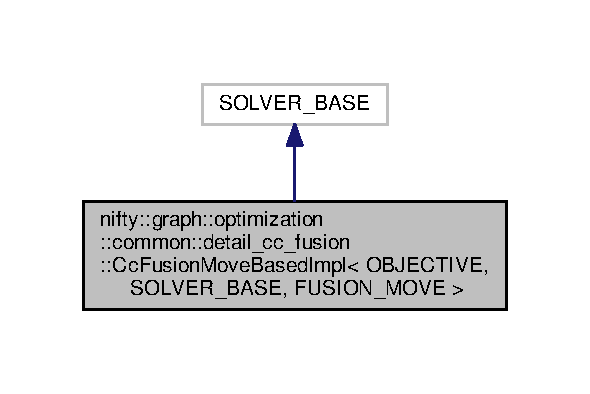
\includegraphics[width=283pt]{classnifty_1_1graph_1_1optimization_1_1common_1_1detail__cc__fusion_1_1CcFusionMoveBasedImpl__inherit__graph}
\end{center}
\end{figure}


Collaboration diagram for nifty\+:\+:graph\+:\+:optimization\+:\+:common\+:\+:detail\+\_\+cc\+\_\+fusion\+:\+:Cc\+Fusion\+Move\+Based\+Impl$<$ O\+B\+J\+E\+C\+T\+I\+V\+E, S\+O\+L\+V\+E\+R\+\_\+\+B\+A\+S\+E, F\+U\+S\+I\+O\+N\+\_\+\+M\+O\+V\+E $>$\+:\nopagebreak
\begin{figure}[H]
\begin{center}
\leavevmode
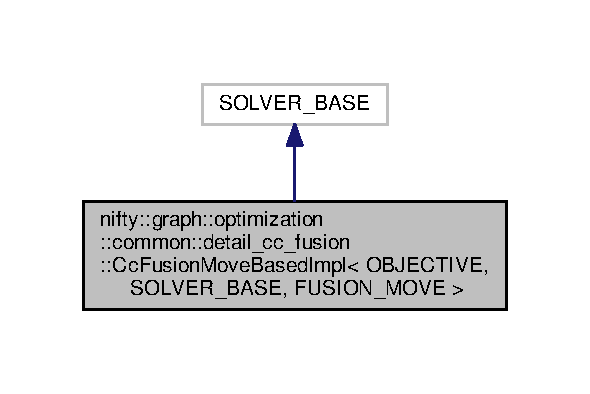
\includegraphics[width=283pt]{classnifty_1_1graph_1_1optimization_1_1common_1_1detail__cc__fusion_1_1CcFusionMoveBasedImpl__coll__graph}
\end{center}
\end{figure}
\subsection*{Classes}
\begin{DoxyCompactItemize}
\item 
struct \hyperlink{structnifty_1_1graph_1_1optimization_1_1common_1_1detail__cc__fusion_1_1CcFusionMoveBasedImpl_1_1SettingsType}{Settings\+Type}
\end{DoxyCompactItemize}
\subsection*{Public Types}
\begin{DoxyCompactItemize}
\item 
typedef O\+B\+J\+E\+C\+T\+I\+V\+E \hyperlink{classnifty_1_1graph_1_1optimization_1_1common_1_1detail__cc__fusion_1_1CcFusionMoveBasedImpl_a963bf8b5310665f1aa1d3521d6f766a0}{Objective\+Type}
\item 
typedef S\+O\+L\+V\+E\+R\+\_\+\+B\+A\+S\+E \hyperlink{classnifty_1_1graph_1_1optimization_1_1common_1_1detail__cc__fusion_1_1CcFusionMoveBasedImpl_aa164d1fa9a818334d0134bc2421f3736}{Base\+Type}
\item 
typedef Objective\+Type\+::\+Graph\+Type \hyperlink{classnifty_1_1graph_1_1optimization_1_1common_1_1detail__cc__fusion_1_1CcFusionMoveBasedImpl_a76c88a1976ccfa02b9361f428ce30bc5}{Graph\+Type}
\item 
typedef Base\+Type\+::\+Visitor\+Base\+Type \hyperlink{classnifty_1_1graph_1_1optimization_1_1common_1_1detail__cc__fusion_1_1CcFusionMoveBasedImpl_afbc19ace9c1055cf28b15a6d6dd050e7}{Visitor\+Base\+Type}
\item 
typedef Base\+Type\+::\+Visitor\+Proxy\+Type \hyperlink{classnifty_1_1graph_1_1optimization_1_1common_1_1detail__cc__fusion_1_1CcFusionMoveBasedImpl_a7316953ca74bcfbbc177b560775e7327}{Visitor\+Proxy\+Type}
\item 
typedef Base\+Type\+::\+Node\+Labels\+Type \hyperlink{classnifty_1_1graph_1_1optimization_1_1common_1_1detail__cc__fusion_1_1CcFusionMoveBasedImpl_a707b7d8fc7c52c9092337ba7910ea484}{Node\+Labels\+Type}
\item 
typedef \hyperlink{classnifty_1_1graph_1_1optimization_1_1common_1_1ProposalGeneratorBase}{nifty\+::graph\+::optimization\+::common\+::\+Proposal\+Generator\+Base}$<$ \hyperlink{classnifty_1_1graph_1_1optimization_1_1common_1_1detail__cc__fusion_1_1CcFusionMoveBasedImpl_a963bf8b5310665f1aa1d3521d6f766a0}{Objective\+Type} $>$ \hyperlink{classnifty_1_1graph_1_1optimization_1_1common_1_1detail__cc__fusion_1_1CcFusionMoveBasedImpl_ac65b1dd4783322f1fd38e42e10272f44}{Proposal\+Generator\+Base\+Type}
\item 
typedef \hyperlink{classnifty_1_1graph_1_1optimization_1_1common_1_1ProposalGeneratorFactoryBase}{nifty\+::graph\+::optimization\+::common\+::\+Proposal\+Generator\+Factory\+Base}$<$ \hyperlink{classnifty_1_1graph_1_1optimization_1_1common_1_1detail__cc__fusion_1_1CcFusionMoveBasedImpl_a963bf8b5310665f1aa1d3521d6f766a0}{Objective\+Type} $>$ \hyperlink{classnifty_1_1graph_1_1optimization_1_1common_1_1detail__cc__fusion_1_1CcFusionMoveBasedImpl_a947607cc31008070837e3889069f9f94}{Proposal\+Generator\+Factory\+Base\+Type}
\end{DoxyCompactItemize}
\subsection*{Public Member Functions}
\begin{DoxyCompactItemize}
\item 
virtual \hyperlink{classnifty_1_1graph_1_1optimization_1_1common_1_1detail__cc__fusion_1_1CcFusionMoveBasedImpl_ad3cd22f5e95477f63869a12fdf40a535}{$\sim$\+Cc\+Fusion\+Move\+Based\+Impl} ()
\item 
\hyperlink{classnifty_1_1graph_1_1optimization_1_1common_1_1detail__cc__fusion_1_1CcFusionMoveBasedImpl_ad4cbdc9b91af1d53236989e3daf22a5e}{Cc\+Fusion\+Move\+Based\+Impl} (const \hyperlink{classnifty_1_1graph_1_1optimization_1_1common_1_1detail__cc__fusion_1_1CcFusionMoveBasedImpl_a963bf8b5310665f1aa1d3521d6f766a0}{Objective\+Type} \&\hyperlink{classnifty_1_1graph_1_1optimization_1_1common_1_1detail__cc__fusion_1_1CcFusionMoveBasedImpl_ad97005b4bf8bd030c06759e90ca8bbd3}{objective}, const \hyperlink{structnifty_1_1graph_1_1optimization_1_1common_1_1detail__cc__fusion_1_1CcFusionMoveBasedImpl_1_1SettingsType}{Settings\+Type} \&settings=\hyperlink{structnifty_1_1graph_1_1optimization_1_1common_1_1detail__cc__fusion_1_1CcFusionMoveBasedImpl_1_1SettingsType}{Settings\+Type}())
\item 
virtual void \hyperlink{classnifty_1_1graph_1_1optimization_1_1common_1_1detail__cc__fusion_1_1CcFusionMoveBasedImpl_a48cc97f580fea578c5eedd207c988186}{optimize} (\hyperlink{classnifty_1_1graph_1_1optimization_1_1common_1_1detail__cc__fusion_1_1CcFusionMoveBasedImpl_a707b7d8fc7c52c9092337ba7910ea484}{Node\+Labels\+Type} \&node\+Labels, \hyperlink{classnifty_1_1graph_1_1optimization_1_1common_1_1detail__cc__fusion_1_1CcFusionMoveBasedImpl_afbc19ace9c1055cf28b15a6d6dd050e7}{Visitor\+Base\+Type} $\ast$visitor)
\item 
virtual const \hyperlink{classnifty_1_1graph_1_1optimization_1_1common_1_1detail__cc__fusion_1_1CcFusionMoveBasedImpl_a963bf8b5310665f1aa1d3521d6f766a0}{Objective\+Type} \& \hyperlink{classnifty_1_1graph_1_1optimization_1_1common_1_1detail__cc__fusion_1_1CcFusionMoveBasedImpl_ad97005b4bf8bd030c06759e90ca8bbd3}{objective} () const 
\item 
virtual const \hyperlink{classnifty_1_1graph_1_1optimization_1_1common_1_1detail__cc__fusion_1_1CcFusionMoveBasedImpl_a707b7d8fc7c52c9092337ba7910ea484}{Node\+Labels\+Type} \& \hyperlink{classnifty_1_1graph_1_1optimization_1_1common_1_1detail__cc__fusion_1_1CcFusionMoveBasedImpl_a098e2711dc757cbfa16ac78a4a780dd7}{current\+Best\+Node\+Labels} ()
\item 
virtual std\+::string \hyperlink{classnifty_1_1graph_1_1optimization_1_1common_1_1detail__cc__fusion_1_1CcFusionMoveBasedImpl_a00261e92c8118b4d83dafa09a17339b7}{name} () const 
\end{DoxyCompactItemize}


\subsection{Member Typedef Documentation}
\hypertarget{classnifty_1_1graph_1_1optimization_1_1common_1_1detail__cc__fusion_1_1CcFusionMoveBasedImpl_aa164d1fa9a818334d0134bc2421f3736}{}\index{nifty\+::graph\+::optimization\+::common\+::detail\+\_\+cc\+\_\+fusion\+::\+Cc\+Fusion\+Move\+Based\+Impl@{nifty\+::graph\+::optimization\+::common\+::detail\+\_\+cc\+\_\+fusion\+::\+Cc\+Fusion\+Move\+Based\+Impl}!Base\+Type@{Base\+Type}}
\index{Base\+Type@{Base\+Type}!nifty\+::graph\+::optimization\+::common\+::detail\+\_\+cc\+\_\+fusion\+::\+Cc\+Fusion\+Move\+Based\+Impl@{nifty\+::graph\+::optimization\+::common\+::detail\+\_\+cc\+\_\+fusion\+::\+Cc\+Fusion\+Move\+Based\+Impl}}
\subsubsection[{Base\+Type}]{\setlength{\rightskip}{0pt plus 5cm}template$<$class O\+B\+J\+E\+C\+T\+I\+V\+E, class S\+O\+L\+V\+E\+R\+\_\+\+B\+A\+S\+E, class F\+U\+S\+I\+O\+N\+\_\+\+M\+O\+V\+E$>$ typedef S\+O\+L\+V\+E\+R\+\_\+\+B\+A\+S\+E {\bf nifty\+::graph\+::optimization\+::common\+::detail\+\_\+cc\+\_\+fusion\+::\+Cc\+Fusion\+Move\+Based\+Impl}$<$ O\+B\+J\+E\+C\+T\+I\+V\+E, S\+O\+L\+V\+E\+R\+\_\+\+B\+A\+S\+E, F\+U\+S\+I\+O\+N\+\_\+\+M\+O\+V\+E $>$\+::{\bf Base\+Type}}\label{classnifty_1_1graph_1_1optimization_1_1common_1_1detail__cc__fusion_1_1CcFusionMoveBasedImpl_aa164d1fa9a818334d0134bc2421f3736}
\hypertarget{classnifty_1_1graph_1_1optimization_1_1common_1_1detail__cc__fusion_1_1CcFusionMoveBasedImpl_a76c88a1976ccfa02b9361f428ce30bc5}{}\index{nifty\+::graph\+::optimization\+::common\+::detail\+\_\+cc\+\_\+fusion\+::\+Cc\+Fusion\+Move\+Based\+Impl@{nifty\+::graph\+::optimization\+::common\+::detail\+\_\+cc\+\_\+fusion\+::\+Cc\+Fusion\+Move\+Based\+Impl}!Graph\+Type@{Graph\+Type}}
\index{Graph\+Type@{Graph\+Type}!nifty\+::graph\+::optimization\+::common\+::detail\+\_\+cc\+\_\+fusion\+::\+Cc\+Fusion\+Move\+Based\+Impl@{nifty\+::graph\+::optimization\+::common\+::detail\+\_\+cc\+\_\+fusion\+::\+Cc\+Fusion\+Move\+Based\+Impl}}
\subsubsection[{Graph\+Type}]{\setlength{\rightskip}{0pt plus 5cm}template$<$class O\+B\+J\+E\+C\+T\+I\+V\+E, class S\+O\+L\+V\+E\+R\+\_\+\+B\+A\+S\+E, class F\+U\+S\+I\+O\+N\+\_\+\+M\+O\+V\+E$>$ typedef Objective\+Type\+::\+Graph\+Type {\bf nifty\+::graph\+::optimization\+::common\+::detail\+\_\+cc\+\_\+fusion\+::\+Cc\+Fusion\+Move\+Based\+Impl}$<$ O\+B\+J\+E\+C\+T\+I\+V\+E, S\+O\+L\+V\+E\+R\+\_\+\+B\+A\+S\+E, F\+U\+S\+I\+O\+N\+\_\+\+M\+O\+V\+E $>$\+::{\bf Graph\+Type}}\label{classnifty_1_1graph_1_1optimization_1_1common_1_1detail__cc__fusion_1_1CcFusionMoveBasedImpl_a76c88a1976ccfa02b9361f428ce30bc5}
\hypertarget{classnifty_1_1graph_1_1optimization_1_1common_1_1detail__cc__fusion_1_1CcFusionMoveBasedImpl_a707b7d8fc7c52c9092337ba7910ea484}{}\index{nifty\+::graph\+::optimization\+::common\+::detail\+\_\+cc\+\_\+fusion\+::\+Cc\+Fusion\+Move\+Based\+Impl@{nifty\+::graph\+::optimization\+::common\+::detail\+\_\+cc\+\_\+fusion\+::\+Cc\+Fusion\+Move\+Based\+Impl}!Node\+Labels\+Type@{Node\+Labels\+Type}}
\index{Node\+Labels\+Type@{Node\+Labels\+Type}!nifty\+::graph\+::optimization\+::common\+::detail\+\_\+cc\+\_\+fusion\+::\+Cc\+Fusion\+Move\+Based\+Impl@{nifty\+::graph\+::optimization\+::common\+::detail\+\_\+cc\+\_\+fusion\+::\+Cc\+Fusion\+Move\+Based\+Impl}}
\subsubsection[{Node\+Labels\+Type}]{\setlength{\rightskip}{0pt plus 5cm}template$<$class O\+B\+J\+E\+C\+T\+I\+V\+E, class S\+O\+L\+V\+E\+R\+\_\+\+B\+A\+S\+E, class F\+U\+S\+I\+O\+N\+\_\+\+M\+O\+V\+E$>$ typedef Base\+Type\+::\+Node\+Labels\+Type {\bf nifty\+::graph\+::optimization\+::common\+::detail\+\_\+cc\+\_\+fusion\+::\+Cc\+Fusion\+Move\+Based\+Impl}$<$ O\+B\+J\+E\+C\+T\+I\+V\+E, S\+O\+L\+V\+E\+R\+\_\+\+B\+A\+S\+E, F\+U\+S\+I\+O\+N\+\_\+\+M\+O\+V\+E $>$\+::{\bf Node\+Labels\+Type}}\label{classnifty_1_1graph_1_1optimization_1_1common_1_1detail__cc__fusion_1_1CcFusionMoveBasedImpl_a707b7d8fc7c52c9092337ba7910ea484}
\hypertarget{classnifty_1_1graph_1_1optimization_1_1common_1_1detail__cc__fusion_1_1CcFusionMoveBasedImpl_a963bf8b5310665f1aa1d3521d6f766a0}{}\index{nifty\+::graph\+::optimization\+::common\+::detail\+\_\+cc\+\_\+fusion\+::\+Cc\+Fusion\+Move\+Based\+Impl@{nifty\+::graph\+::optimization\+::common\+::detail\+\_\+cc\+\_\+fusion\+::\+Cc\+Fusion\+Move\+Based\+Impl}!Objective\+Type@{Objective\+Type}}
\index{Objective\+Type@{Objective\+Type}!nifty\+::graph\+::optimization\+::common\+::detail\+\_\+cc\+\_\+fusion\+::\+Cc\+Fusion\+Move\+Based\+Impl@{nifty\+::graph\+::optimization\+::common\+::detail\+\_\+cc\+\_\+fusion\+::\+Cc\+Fusion\+Move\+Based\+Impl}}
\subsubsection[{Objective\+Type}]{\setlength{\rightskip}{0pt plus 5cm}template$<$class O\+B\+J\+E\+C\+T\+I\+V\+E, class S\+O\+L\+V\+E\+R\+\_\+\+B\+A\+S\+E, class F\+U\+S\+I\+O\+N\+\_\+\+M\+O\+V\+E$>$ typedef O\+B\+J\+E\+C\+T\+I\+V\+E {\bf nifty\+::graph\+::optimization\+::common\+::detail\+\_\+cc\+\_\+fusion\+::\+Cc\+Fusion\+Move\+Based\+Impl}$<$ O\+B\+J\+E\+C\+T\+I\+V\+E, S\+O\+L\+V\+E\+R\+\_\+\+B\+A\+S\+E, F\+U\+S\+I\+O\+N\+\_\+\+M\+O\+V\+E $>$\+::{\bf Objective\+Type}}\label{classnifty_1_1graph_1_1optimization_1_1common_1_1detail__cc__fusion_1_1CcFusionMoveBasedImpl_a963bf8b5310665f1aa1d3521d6f766a0}
\hypertarget{classnifty_1_1graph_1_1optimization_1_1common_1_1detail__cc__fusion_1_1CcFusionMoveBasedImpl_ac65b1dd4783322f1fd38e42e10272f44}{}\index{nifty\+::graph\+::optimization\+::common\+::detail\+\_\+cc\+\_\+fusion\+::\+Cc\+Fusion\+Move\+Based\+Impl@{nifty\+::graph\+::optimization\+::common\+::detail\+\_\+cc\+\_\+fusion\+::\+Cc\+Fusion\+Move\+Based\+Impl}!Proposal\+Generator\+Base\+Type@{Proposal\+Generator\+Base\+Type}}
\index{Proposal\+Generator\+Base\+Type@{Proposal\+Generator\+Base\+Type}!nifty\+::graph\+::optimization\+::common\+::detail\+\_\+cc\+\_\+fusion\+::\+Cc\+Fusion\+Move\+Based\+Impl@{nifty\+::graph\+::optimization\+::common\+::detail\+\_\+cc\+\_\+fusion\+::\+Cc\+Fusion\+Move\+Based\+Impl}}
\subsubsection[{Proposal\+Generator\+Base\+Type}]{\setlength{\rightskip}{0pt plus 5cm}template$<$class O\+B\+J\+E\+C\+T\+I\+V\+E, class S\+O\+L\+V\+E\+R\+\_\+\+B\+A\+S\+E, class F\+U\+S\+I\+O\+N\+\_\+\+M\+O\+V\+E$>$ typedef {\bf nifty\+::graph\+::optimization\+::common\+::\+Proposal\+Generator\+Base}$<${\bf Objective\+Type}$>$ {\bf nifty\+::graph\+::optimization\+::common\+::detail\+\_\+cc\+\_\+fusion\+::\+Cc\+Fusion\+Move\+Based\+Impl}$<$ O\+B\+J\+E\+C\+T\+I\+V\+E, S\+O\+L\+V\+E\+R\+\_\+\+B\+A\+S\+E, F\+U\+S\+I\+O\+N\+\_\+\+M\+O\+V\+E $>$\+::{\bf Proposal\+Generator\+Base\+Type}}\label{classnifty_1_1graph_1_1optimization_1_1common_1_1detail__cc__fusion_1_1CcFusionMoveBasedImpl_ac65b1dd4783322f1fd38e42e10272f44}
\hypertarget{classnifty_1_1graph_1_1optimization_1_1common_1_1detail__cc__fusion_1_1CcFusionMoveBasedImpl_a947607cc31008070837e3889069f9f94}{}\index{nifty\+::graph\+::optimization\+::common\+::detail\+\_\+cc\+\_\+fusion\+::\+Cc\+Fusion\+Move\+Based\+Impl@{nifty\+::graph\+::optimization\+::common\+::detail\+\_\+cc\+\_\+fusion\+::\+Cc\+Fusion\+Move\+Based\+Impl}!Proposal\+Generator\+Factory\+Base\+Type@{Proposal\+Generator\+Factory\+Base\+Type}}
\index{Proposal\+Generator\+Factory\+Base\+Type@{Proposal\+Generator\+Factory\+Base\+Type}!nifty\+::graph\+::optimization\+::common\+::detail\+\_\+cc\+\_\+fusion\+::\+Cc\+Fusion\+Move\+Based\+Impl@{nifty\+::graph\+::optimization\+::common\+::detail\+\_\+cc\+\_\+fusion\+::\+Cc\+Fusion\+Move\+Based\+Impl}}
\subsubsection[{Proposal\+Generator\+Factory\+Base\+Type}]{\setlength{\rightskip}{0pt plus 5cm}template$<$class O\+B\+J\+E\+C\+T\+I\+V\+E, class S\+O\+L\+V\+E\+R\+\_\+\+B\+A\+S\+E, class F\+U\+S\+I\+O\+N\+\_\+\+M\+O\+V\+E$>$ typedef {\bf nifty\+::graph\+::optimization\+::common\+::\+Proposal\+Generator\+Factory\+Base}$<${\bf Objective\+Type}$>$ {\bf nifty\+::graph\+::optimization\+::common\+::detail\+\_\+cc\+\_\+fusion\+::\+Cc\+Fusion\+Move\+Based\+Impl}$<$ O\+B\+J\+E\+C\+T\+I\+V\+E, S\+O\+L\+V\+E\+R\+\_\+\+B\+A\+S\+E, F\+U\+S\+I\+O\+N\+\_\+\+M\+O\+V\+E $>$\+::{\bf Proposal\+Generator\+Factory\+Base\+Type}}\label{classnifty_1_1graph_1_1optimization_1_1common_1_1detail__cc__fusion_1_1CcFusionMoveBasedImpl_a947607cc31008070837e3889069f9f94}
\hypertarget{classnifty_1_1graph_1_1optimization_1_1common_1_1detail__cc__fusion_1_1CcFusionMoveBasedImpl_afbc19ace9c1055cf28b15a6d6dd050e7}{}\index{nifty\+::graph\+::optimization\+::common\+::detail\+\_\+cc\+\_\+fusion\+::\+Cc\+Fusion\+Move\+Based\+Impl@{nifty\+::graph\+::optimization\+::common\+::detail\+\_\+cc\+\_\+fusion\+::\+Cc\+Fusion\+Move\+Based\+Impl}!Visitor\+Base\+Type@{Visitor\+Base\+Type}}
\index{Visitor\+Base\+Type@{Visitor\+Base\+Type}!nifty\+::graph\+::optimization\+::common\+::detail\+\_\+cc\+\_\+fusion\+::\+Cc\+Fusion\+Move\+Based\+Impl@{nifty\+::graph\+::optimization\+::common\+::detail\+\_\+cc\+\_\+fusion\+::\+Cc\+Fusion\+Move\+Based\+Impl}}
\subsubsection[{Visitor\+Base\+Type}]{\setlength{\rightskip}{0pt plus 5cm}template$<$class O\+B\+J\+E\+C\+T\+I\+V\+E, class S\+O\+L\+V\+E\+R\+\_\+\+B\+A\+S\+E, class F\+U\+S\+I\+O\+N\+\_\+\+M\+O\+V\+E$>$ typedef Base\+Type\+::\+Visitor\+Base\+Type {\bf nifty\+::graph\+::optimization\+::common\+::detail\+\_\+cc\+\_\+fusion\+::\+Cc\+Fusion\+Move\+Based\+Impl}$<$ O\+B\+J\+E\+C\+T\+I\+V\+E, S\+O\+L\+V\+E\+R\+\_\+\+B\+A\+S\+E, F\+U\+S\+I\+O\+N\+\_\+\+M\+O\+V\+E $>$\+::{\bf Visitor\+Base\+Type}}\label{classnifty_1_1graph_1_1optimization_1_1common_1_1detail__cc__fusion_1_1CcFusionMoveBasedImpl_afbc19ace9c1055cf28b15a6d6dd050e7}
\hypertarget{classnifty_1_1graph_1_1optimization_1_1common_1_1detail__cc__fusion_1_1CcFusionMoveBasedImpl_a7316953ca74bcfbbc177b560775e7327}{}\index{nifty\+::graph\+::optimization\+::common\+::detail\+\_\+cc\+\_\+fusion\+::\+Cc\+Fusion\+Move\+Based\+Impl@{nifty\+::graph\+::optimization\+::common\+::detail\+\_\+cc\+\_\+fusion\+::\+Cc\+Fusion\+Move\+Based\+Impl}!Visitor\+Proxy\+Type@{Visitor\+Proxy\+Type}}
\index{Visitor\+Proxy\+Type@{Visitor\+Proxy\+Type}!nifty\+::graph\+::optimization\+::common\+::detail\+\_\+cc\+\_\+fusion\+::\+Cc\+Fusion\+Move\+Based\+Impl@{nifty\+::graph\+::optimization\+::common\+::detail\+\_\+cc\+\_\+fusion\+::\+Cc\+Fusion\+Move\+Based\+Impl}}
\subsubsection[{Visitor\+Proxy\+Type}]{\setlength{\rightskip}{0pt plus 5cm}template$<$class O\+B\+J\+E\+C\+T\+I\+V\+E, class S\+O\+L\+V\+E\+R\+\_\+\+B\+A\+S\+E, class F\+U\+S\+I\+O\+N\+\_\+\+M\+O\+V\+E$>$ typedef Base\+Type\+::\+Visitor\+Proxy\+Type {\bf nifty\+::graph\+::optimization\+::common\+::detail\+\_\+cc\+\_\+fusion\+::\+Cc\+Fusion\+Move\+Based\+Impl}$<$ O\+B\+J\+E\+C\+T\+I\+V\+E, S\+O\+L\+V\+E\+R\+\_\+\+B\+A\+S\+E, F\+U\+S\+I\+O\+N\+\_\+\+M\+O\+V\+E $>$\+::{\bf Visitor\+Proxy\+Type}}\label{classnifty_1_1graph_1_1optimization_1_1common_1_1detail__cc__fusion_1_1CcFusionMoveBasedImpl_a7316953ca74bcfbbc177b560775e7327}


\subsection{Constructor \& Destructor Documentation}
\hypertarget{classnifty_1_1graph_1_1optimization_1_1common_1_1detail__cc__fusion_1_1CcFusionMoveBasedImpl_ad3cd22f5e95477f63869a12fdf40a535}{}\index{nifty\+::graph\+::optimization\+::common\+::detail\+\_\+cc\+\_\+fusion\+::\+Cc\+Fusion\+Move\+Based\+Impl@{nifty\+::graph\+::optimization\+::common\+::detail\+\_\+cc\+\_\+fusion\+::\+Cc\+Fusion\+Move\+Based\+Impl}!````~Cc\+Fusion\+Move\+Based\+Impl@{$\sim$\+Cc\+Fusion\+Move\+Based\+Impl}}
\index{````~Cc\+Fusion\+Move\+Based\+Impl@{$\sim$\+Cc\+Fusion\+Move\+Based\+Impl}!nifty\+::graph\+::optimization\+::common\+::detail\+\_\+cc\+\_\+fusion\+::\+Cc\+Fusion\+Move\+Based\+Impl@{nifty\+::graph\+::optimization\+::common\+::detail\+\_\+cc\+\_\+fusion\+::\+Cc\+Fusion\+Move\+Based\+Impl}}
\subsubsection[{$\sim$\+Cc\+Fusion\+Move\+Based\+Impl()}]{\setlength{\rightskip}{0pt plus 5cm}template$<$class O\+B\+J\+E\+C\+T\+I\+V\+E , class S\+O\+L\+V\+E\+R\+\_\+\+B\+A\+S\+E , class F\+U\+S\+I\+O\+N\+\_\+\+M\+O\+V\+E $>$ {\bf nifty\+::graph\+::optimization\+::common\+::detail\+\_\+cc\+\_\+fusion\+::\+Cc\+Fusion\+Move\+Based\+Impl}$<$ O\+B\+J\+E\+C\+T\+I\+V\+E, S\+O\+L\+V\+E\+R\+\_\+\+B\+A\+S\+E, F\+U\+S\+I\+O\+N\+\_\+\+M\+O\+V\+E $>$\+::$\sim${\bf Cc\+Fusion\+Move\+Based\+Impl} (
\begin{DoxyParamCaption}
{}
\end{DoxyParamCaption}
)\hspace{0.3cm}{\ttfamily [virtual]}}\label{classnifty_1_1graph_1_1optimization_1_1common_1_1detail__cc__fusion_1_1CcFusionMoveBasedImpl_ad3cd22f5e95477f63869a12fdf40a535}
\hypertarget{classnifty_1_1graph_1_1optimization_1_1common_1_1detail__cc__fusion_1_1CcFusionMoveBasedImpl_ad4cbdc9b91af1d53236989e3daf22a5e}{}\index{nifty\+::graph\+::optimization\+::common\+::detail\+\_\+cc\+\_\+fusion\+::\+Cc\+Fusion\+Move\+Based\+Impl@{nifty\+::graph\+::optimization\+::common\+::detail\+\_\+cc\+\_\+fusion\+::\+Cc\+Fusion\+Move\+Based\+Impl}!Cc\+Fusion\+Move\+Based\+Impl@{Cc\+Fusion\+Move\+Based\+Impl}}
\index{Cc\+Fusion\+Move\+Based\+Impl@{Cc\+Fusion\+Move\+Based\+Impl}!nifty\+::graph\+::optimization\+::common\+::detail\+\_\+cc\+\_\+fusion\+::\+Cc\+Fusion\+Move\+Based\+Impl@{nifty\+::graph\+::optimization\+::common\+::detail\+\_\+cc\+\_\+fusion\+::\+Cc\+Fusion\+Move\+Based\+Impl}}
\subsubsection[{Cc\+Fusion\+Move\+Based\+Impl(const Objective\+Type \&objective, const Settings\+Type \&settings=\+Settings\+Type())}]{\setlength{\rightskip}{0pt plus 5cm}template$<$class O\+B\+J\+E\+C\+T\+I\+V\+E , class S\+O\+L\+V\+E\+R\+\_\+\+B\+A\+S\+E , class F\+U\+S\+I\+O\+N\+\_\+\+M\+O\+V\+E $>$ {\bf nifty\+::graph\+::optimization\+::common\+::detail\+\_\+cc\+\_\+fusion\+::\+Cc\+Fusion\+Move\+Based\+Impl}$<$ O\+B\+J\+E\+C\+T\+I\+V\+E, S\+O\+L\+V\+E\+R\+\_\+\+B\+A\+S\+E, F\+U\+S\+I\+O\+N\+\_\+\+M\+O\+V\+E $>$\+::{\bf Cc\+Fusion\+Move\+Based\+Impl} (
\begin{DoxyParamCaption}
\item[{const {\bf Objective\+Type} \&}]{objective, }
\item[{const {\bf Settings\+Type} \&}]{settings = {\ttfamily {\bf Settings\+Type}()}}
\end{DoxyParamCaption}
)}\label{classnifty_1_1graph_1_1optimization_1_1common_1_1detail__cc__fusion_1_1CcFusionMoveBasedImpl_ad4cbdc9b91af1d53236989e3daf22a5e}


\subsection{Member Function Documentation}
\hypertarget{classnifty_1_1graph_1_1optimization_1_1common_1_1detail__cc__fusion_1_1CcFusionMoveBasedImpl_a098e2711dc757cbfa16ac78a4a780dd7}{}\index{nifty\+::graph\+::optimization\+::common\+::detail\+\_\+cc\+\_\+fusion\+::\+Cc\+Fusion\+Move\+Based\+Impl@{nifty\+::graph\+::optimization\+::common\+::detail\+\_\+cc\+\_\+fusion\+::\+Cc\+Fusion\+Move\+Based\+Impl}!current\+Best\+Node\+Labels@{current\+Best\+Node\+Labels}}
\index{current\+Best\+Node\+Labels@{current\+Best\+Node\+Labels}!nifty\+::graph\+::optimization\+::common\+::detail\+\_\+cc\+\_\+fusion\+::\+Cc\+Fusion\+Move\+Based\+Impl@{nifty\+::graph\+::optimization\+::common\+::detail\+\_\+cc\+\_\+fusion\+::\+Cc\+Fusion\+Move\+Based\+Impl}}
\subsubsection[{current\+Best\+Node\+Labels()}]{\setlength{\rightskip}{0pt plus 5cm}template$<$class O\+B\+J\+E\+C\+T\+I\+V\+E, class S\+O\+L\+V\+E\+R\+\_\+\+B\+A\+S\+E, class F\+U\+S\+I\+O\+N\+\_\+\+M\+O\+V\+E$>$ virtual const {\bf Node\+Labels\+Type}\& {\bf nifty\+::graph\+::optimization\+::common\+::detail\+\_\+cc\+\_\+fusion\+::\+Cc\+Fusion\+Move\+Based\+Impl}$<$ O\+B\+J\+E\+C\+T\+I\+V\+E, S\+O\+L\+V\+E\+R\+\_\+\+B\+A\+S\+E, F\+U\+S\+I\+O\+N\+\_\+\+M\+O\+V\+E $>$\+::current\+Best\+Node\+Labels (
\begin{DoxyParamCaption}
{}
\end{DoxyParamCaption}
)\hspace{0.3cm}{\ttfamily [inline]}, {\ttfamily [virtual]}}\label{classnifty_1_1graph_1_1optimization_1_1common_1_1detail__cc__fusion_1_1CcFusionMoveBasedImpl_a098e2711dc757cbfa16ac78a4a780dd7}
\hypertarget{classnifty_1_1graph_1_1optimization_1_1common_1_1detail__cc__fusion_1_1CcFusionMoveBasedImpl_a00261e92c8118b4d83dafa09a17339b7}{}\index{nifty\+::graph\+::optimization\+::common\+::detail\+\_\+cc\+\_\+fusion\+::\+Cc\+Fusion\+Move\+Based\+Impl@{nifty\+::graph\+::optimization\+::common\+::detail\+\_\+cc\+\_\+fusion\+::\+Cc\+Fusion\+Move\+Based\+Impl}!name@{name}}
\index{name@{name}!nifty\+::graph\+::optimization\+::common\+::detail\+\_\+cc\+\_\+fusion\+::\+Cc\+Fusion\+Move\+Based\+Impl@{nifty\+::graph\+::optimization\+::common\+::detail\+\_\+cc\+\_\+fusion\+::\+Cc\+Fusion\+Move\+Based\+Impl}}
\subsubsection[{name() const }]{\setlength{\rightskip}{0pt plus 5cm}template$<$class O\+B\+J\+E\+C\+T\+I\+V\+E, class S\+O\+L\+V\+E\+R\+\_\+\+B\+A\+S\+E, class F\+U\+S\+I\+O\+N\+\_\+\+M\+O\+V\+E$>$ virtual std\+::string {\bf nifty\+::graph\+::optimization\+::common\+::detail\+\_\+cc\+\_\+fusion\+::\+Cc\+Fusion\+Move\+Based\+Impl}$<$ O\+B\+J\+E\+C\+T\+I\+V\+E, S\+O\+L\+V\+E\+R\+\_\+\+B\+A\+S\+E, F\+U\+S\+I\+O\+N\+\_\+\+M\+O\+V\+E $>$\+::name (
\begin{DoxyParamCaption}
{}
\end{DoxyParamCaption}
) const\hspace{0.3cm}{\ttfamily [inline]}, {\ttfamily [virtual]}}\label{classnifty_1_1graph_1_1optimization_1_1common_1_1detail__cc__fusion_1_1CcFusionMoveBasedImpl_a00261e92c8118b4d83dafa09a17339b7}
\hypertarget{classnifty_1_1graph_1_1optimization_1_1common_1_1detail__cc__fusion_1_1CcFusionMoveBasedImpl_ad97005b4bf8bd030c06759e90ca8bbd3}{}\index{nifty\+::graph\+::optimization\+::common\+::detail\+\_\+cc\+\_\+fusion\+::\+Cc\+Fusion\+Move\+Based\+Impl@{nifty\+::graph\+::optimization\+::common\+::detail\+\_\+cc\+\_\+fusion\+::\+Cc\+Fusion\+Move\+Based\+Impl}!objective@{objective}}
\index{objective@{objective}!nifty\+::graph\+::optimization\+::common\+::detail\+\_\+cc\+\_\+fusion\+::\+Cc\+Fusion\+Move\+Based\+Impl@{nifty\+::graph\+::optimization\+::common\+::detail\+\_\+cc\+\_\+fusion\+::\+Cc\+Fusion\+Move\+Based\+Impl}}
\subsubsection[{objective() const }]{\setlength{\rightskip}{0pt plus 5cm}template$<$class O\+B\+J\+E\+C\+T\+I\+V\+E , class S\+O\+L\+V\+E\+R\+\_\+\+B\+A\+S\+E , class F\+U\+S\+I\+O\+N\+\_\+\+M\+O\+V\+E $>$ const {\bf Cc\+Fusion\+Move\+Based\+Impl}$<$ O\+B\+J\+E\+C\+T\+I\+V\+E, S\+O\+L\+V\+E\+R\+\_\+\+B\+A\+S\+E, F\+U\+S\+I\+O\+N\+\_\+\+M\+O\+V\+E $>$\+::{\bf Objective\+Type} \& {\bf nifty\+::graph\+::optimization\+::common\+::detail\+\_\+cc\+\_\+fusion\+::\+Cc\+Fusion\+Move\+Based\+Impl}$<$ O\+B\+J\+E\+C\+T\+I\+V\+E, S\+O\+L\+V\+E\+R\+\_\+\+B\+A\+S\+E, F\+U\+S\+I\+O\+N\+\_\+\+M\+O\+V\+E $>$\+::objective (
\begin{DoxyParamCaption}
{}
\end{DoxyParamCaption}
) const\hspace{0.3cm}{\ttfamily [virtual]}}\label{classnifty_1_1graph_1_1optimization_1_1common_1_1detail__cc__fusion_1_1CcFusionMoveBasedImpl_ad97005b4bf8bd030c06759e90ca8bbd3}
\hypertarget{classnifty_1_1graph_1_1optimization_1_1common_1_1detail__cc__fusion_1_1CcFusionMoveBasedImpl_a48cc97f580fea578c5eedd207c988186}{}\index{nifty\+::graph\+::optimization\+::common\+::detail\+\_\+cc\+\_\+fusion\+::\+Cc\+Fusion\+Move\+Based\+Impl@{nifty\+::graph\+::optimization\+::common\+::detail\+\_\+cc\+\_\+fusion\+::\+Cc\+Fusion\+Move\+Based\+Impl}!optimize@{optimize}}
\index{optimize@{optimize}!nifty\+::graph\+::optimization\+::common\+::detail\+\_\+cc\+\_\+fusion\+::\+Cc\+Fusion\+Move\+Based\+Impl@{nifty\+::graph\+::optimization\+::common\+::detail\+\_\+cc\+\_\+fusion\+::\+Cc\+Fusion\+Move\+Based\+Impl}}
\subsubsection[{optimize(\+Node\+Labels\+Type \&node\+Labels, Visitor\+Base\+Type $\ast$visitor)}]{\setlength{\rightskip}{0pt plus 5cm}template$<$class O\+B\+J\+E\+C\+T\+I\+V\+E , class S\+O\+L\+V\+E\+R\+\_\+\+B\+A\+S\+E , class F\+U\+S\+I\+O\+N\+\_\+\+M\+O\+V\+E $>$ void {\bf nifty\+::graph\+::optimization\+::common\+::detail\+\_\+cc\+\_\+fusion\+::\+Cc\+Fusion\+Move\+Based\+Impl}$<$ O\+B\+J\+E\+C\+T\+I\+V\+E, S\+O\+L\+V\+E\+R\+\_\+\+B\+A\+S\+E, F\+U\+S\+I\+O\+N\+\_\+\+M\+O\+V\+E $>$\+::optimize (
\begin{DoxyParamCaption}
\item[{{\bf Node\+Labels\+Type} \&}]{node\+Labels, }
\item[{{\bf Visitor\+Base\+Type} $\ast$}]{visitor}
\end{DoxyParamCaption}
)\hspace{0.3cm}{\ttfamily [virtual]}}\label{classnifty_1_1graph_1_1optimization_1_1common_1_1detail__cc__fusion_1_1CcFusionMoveBasedImpl_a48cc97f580fea578c5eedd207c988186}


The documentation for this class was generated from the following file\+:\begin{DoxyCompactItemize}
\item 
/home/tbeier/src/nifty/include/nifty/graph/optimization/common/\hyperlink{cc__fusion__move__based__impl_8hxx}{cc\+\_\+fusion\+\_\+move\+\_\+based\+\_\+impl.\+hxx}\end{DoxyCompactItemize}

\hypertarget{classnifty_1_1cgp_1_1Cell1BasicGeometricFeatures2D}{}\section{nifty\+:\+:cgp\+:\+:Cell1\+Basic\+Geometric\+Features2\+D Class Reference}
\label{classnifty_1_1cgp_1_1Cell1BasicGeometricFeatures2D}\index{nifty\+::cgp\+::\+Cell1\+Basic\+Geometric\+Features2\+D@{nifty\+::cgp\+::\+Cell1\+Basic\+Geometric\+Features2\+D}}


{\ttfamily \#include $<$geometric\+\_\+features.\+hxx$>$}

\subsection*{Public Member Functions}
\begin{DoxyCompactItemize}
\item 
\hyperlink{classnifty_1_1cgp_1_1Cell1BasicGeometricFeatures2D_a21c1cd8100f7a511f5b500fd51527795}{Cell1\+Basic\+Geometric\+Features2\+D} ()
\item 
size\+\_\+t \hyperlink{classnifty_1_1cgp_1_1Cell1BasicGeometricFeatures2D_ad3d8a0e9bcdfdb30e86383b5d1a4fc26}{number\+Of\+Features} () const 
\item 
std\+::vector$<$ std\+::string $>$ \hyperlink{classnifty_1_1cgp_1_1Cell1BasicGeometricFeatures2D_a2dd928ab61a7e435057ddcded55f28c0}{names} () const 
\item 
{\footnotesize template$<$class T $>$ }\\void \hyperlink{classnifty_1_1cgp_1_1Cell1BasicGeometricFeatures2D_a0f9075ca73167de4b8f592ed3ea467a0}{operator()} (const \hyperlink{classnifty_1_1cgp_1_1CellGeometryVector}{Cell\+Geometry\+Vector}$<$ 2, 1 $>$ \&cell1\+Geometry\+Vector, const \hyperlink{classnifty_1_1cgp_1_1CellGeometryVector}{Cell\+Geometry\+Vector}$<$ 2, 2 $>$ \&cell2\+Geometry\+Vector, const \hyperlink{classnifty_1_1cgp_1_1CellBoundsVector}{Cell\+Bounds\+Vector}$<$ 2, 1 $>$ \&cell1\+Bounds\+Vector, \hyperlink{classandres_1_1View}{nifty\+::marray\+::\+View}$<$ T $>$ \&features) const 
\end{DoxyCompactItemize}


\subsection{Constructor \& Destructor Documentation}
\hypertarget{classnifty_1_1cgp_1_1Cell1BasicGeometricFeatures2D_a21c1cd8100f7a511f5b500fd51527795}{}\index{nifty\+::cgp\+::\+Cell1\+Basic\+Geometric\+Features2\+D@{nifty\+::cgp\+::\+Cell1\+Basic\+Geometric\+Features2\+D}!Cell1\+Basic\+Geometric\+Features2\+D@{Cell1\+Basic\+Geometric\+Features2\+D}}
\index{Cell1\+Basic\+Geometric\+Features2\+D@{Cell1\+Basic\+Geometric\+Features2\+D}!nifty\+::cgp\+::\+Cell1\+Basic\+Geometric\+Features2\+D@{nifty\+::cgp\+::\+Cell1\+Basic\+Geometric\+Features2\+D}}
\subsubsection[{Cell1\+Basic\+Geometric\+Features2\+D()}]{\setlength{\rightskip}{0pt plus 5cm}nifty\+::cgp\+::\+Cell1\+Basic\+Geometric\+Features2\+D\+::\+Cell1\+Basic\+Geometric\+Features2\+D (
\begin{DoxyParamCaption}
{}
\end{DoxyParamCaption}
)\hspace{0.3cm}{\ttfamily [inline]}}\label{classnifty_1_1cgp_1_1Cell1BasicGeometricFeatures2D_a21c1cd8100f7a511f5b500fd51527795}


\subsection{Member Function Documentation}
\hypertarget{classnifty_1_1cgp_1_1Cell1BasicGeometricFeatures2D_a2dd928ab61a7e435057ddcded55f28c0}{}\index{nifty\+::cgp\+::\+Cell1\+Basic\+Geometric\+Features2\+D@{nifty\+::cgp\+::\+Cell1\+Basic\+Geometric\+Features2\+D}!names@{names}}
\index{names@{names}!nifty\+::cgp\+::\+Cell1\+Basic\+Geometric\+Features2\+D@{nifty\+::cgp\+::\+Cell1\+Basic\+Geometric\+Features2\+D}}
\subsubsection[{names() const }]{\setlength{\rightskip}{0pt plus 5cm}std\+::vector$<$std\+::string$>$ nifty\+::cgp\+::\+Cell1\+Basic\+Geometric\+Features2\+D\+::names (
\begin{DoxyParamCaption}
{}
\end{DoxyParamCaption}
) const\hspace{0.3cm}{\ttfamily [inline]}}\label{classnifty_1_1cgp_1_1Cell1BasicGeometricFeatures2D_a2dd928ab61a7e435057ddcded55f28c0}
\hypertarget{classnifty_1_1cgp_1_1Cell1BasicGeometricFeatures2D_ad3d8a0e9bcdfdb30e86383b5d1a4fc26}{}\index{nifty\+::cgp\+::\+Cell1\+Basic\+Geometric\+Features2\+D@{nifty\+::cgp\+::\+Cell1\+Basic\+Geometric\+Features2\+D}!number\+Of\+Features@{number\+Of\+Features}}
\index{number\+Of\+Features@{number\+Of\+Features}!nifty\+::cgp\+::\+Cell1\+Basic\+Geometric\+Features2\+D@{nifty\+::cgp\+::\+Cell1\+Basic\+Geometric\+Features2\+D}}
\subsubsection[{number\+Of\+Features() const }]{\setlength{\rightskip}{0pt plus 5cm}size\+\_\+t nifty\+::cgp\+::\+Cell1\+Basic\+Geometric\+Features2\+D\+::number\+Of\+Features (
\begin{DoxyParamCaption}
{}
\end{DoxyParamCaption}
) const\hspace{0.3cm}{\ttfamily [inline]}}\label{classnifty_1_1cgp_1_1Cell1BasicGeometricFeatures2D_ad3d8a0e9bcdfdb30e86383b5d1a4fc26}
\hypertarget{classnifty_1_1cgp_1_1Cell1BasicGeometricFeatures2D_a0f9075ca73167de4b8f592ed3ea467a0}{}\index{nifty\+::cgp\+::\+Cell1\+Basic\+Geometric\+Features2\+D@{nifty\+::cgp\+::\+Cell1\+Basic\+Geometric\+Features2\+D}!operator()@{operator()}}
\index{operator()@{operator()}!nifty\+::cgp\+::\+Cell1\+Basic\+Geometric\+Features2\+D@{nifty\+::cgp\+::\+Cell1\+Basic\+Geometric\+Features2\+D}}
\subsubsection[{operator()(const Cell\+Geometry\+Vector$<$ 2, 1 $>$ \&cell1\+Geometry\+Vector, const Cell\+Geometry\+Vector$<$ 2, 2 $>$ \&cell2\+Geometry\+Vector, const Cell\+Bounds\+Vector$<$ 2, 1 $>$ \&cell1\+Bounds\+Vector, nifty\+::marray\+::\+View$<$ T $>$ \&features) const }]{\setlength{\rightskip}{0pt plus 5cm}template$<$class T $>$ void nifty\+::cgp\+::\+Cell1\+Basic\+Geometric\+Features2\+D\+::operator() (
\begin{DoxyParamCaption}
\item[{const {\bf Cell\+Geometry\+Vector}$<$ 2, 1 $>$ \&}]{cell1\+Geometry\+Vector, }
\item[{const {\bf Cell\+Geometry\+Vector}$<$ 2, 2 $>$ \&}]{cell2\+Geometry\+Vector, }
\item[{const {\bf Cell\+Bounds\+Vector}$<$ 2, 1 $>$ \&}]{cell1\+Bounds\+Vector, }
\item[{{\bf nifty\+::marray\+::\+View}$<$ T $>$ \&}]{features}
\end{DoxyParamCaption}
) const\hspace{0.3cm}{\ttfamily [inline]}}\label{classnifty_1_1cgp_1_1Cell1BasicGeometricFeatures2D_a0f9075ca73167de4b8f592ed3ea467a0}


The documentation for this class was generated from the following file\+:\begin{DoxyCompactItemize}
\item 
/home/tbeier/src/nifty/include/nifty/cgp/features/\hyperlink{geometric__features_8hxx}{geometric\+\_\+features.\+hxx}\end{DoxyCompactItemize}

\hypertarget{classnifty_1_1cgp_1_1Cell1BasicTopologicalFeatures}{}\section{nifty\+:\+:cgp\+:\+:Cell1\+Basic\+Topological\+Features Class Reference}
\label{classnifty_1_1cgp_1_1Cell1BasicTopologicalFeatures}\index{nifty\+::cgp\+::\+Cell1\+Basic\+Topological\+Features@{nifty\+::cgp\+::\+Cell1\+Basic\+Topological\+Features}}


{\ttfamily \#include $<$topological\+\_\+features.\+hxx$>$}

\subsection*{Public Member Functions}
\begin{DoxyCompactItemize}
\item 
\hyperlink{classnifty_1_1cgp_1_1Cell1BasicTopologicalFeatures_acf309275f4b84d463dee9bea89cd5108}{Cell1\+Basic\+Topological\+Features} ()
\item 
size\+\_\+t \hyperlink{classnifty_1_1cgp_1_1Cell1BasicTopologicalFeatures_a56a29c126efbbd38b10dce2b5ba387cb}{number\+Of\+Features} () const 
\item 
{\footnotesize template$<$class T $>$ }\\void \hyperlink{classnifty_1_1cgp_1_1Cell1BasicTopologicalFeatures_a1a4258f15fc13907751006b6aae69342}{operator()} (const \hyperlink{classnifty_1_1cgp_1_1CellBoundsVector}{Cell\+Bounds\+Vector}$<$ 2, 0 $>$ \&cell0\+Bounds\+Vector, const \hyperlink{classnifty_1_1cgp_1_1CellBoundsVector}{Cell\+Bounds\+Vector}$<$ 2, 1 $>$ \&cell1\+Bounds\+Vector, const \hyperlink{classnifty_1_1cgp_1_1CellBoundedByVector}{Cell\+Bounded\+By\+Vector}$<$ 2, 1 $>$ \&cell1\+Bounded\+By\+Vector, const \hyperlink{classnifty_1_1cgp_1_1CellBoundedByVector}{Cell\+Bounded\+By\+Vector}$<$ 2, 2 $>$ \&cell2\+Bounded\+By\+Vector, nifty\+::marray\+::\+View$<$ T $>$ \&features) const 
\end{DoxyCompactItemize}


\subsection{Constructor \& Destructor Documentation}
\hypertarget{classnifty_1_1cgp_1_1Cell1BasicTopologicalFeatures_acf309275f4b84d463dee9bea89cd5108}{}\index{nifty\+::cgp\+::\+Cell1\+Basic\+Topological\+Features@{nifty\+::cgp\+::\+Cell1\+Basic\+Topological\+Features}!Cell1\+Basic\+Topological\+Features@{Cell1\+Basic\+Topological\+Features}}
\index{Cell1\+Basic\+Topological\+Features@{Cell1\+Basic\+Topological\+Features}!nifty\+::cgp\+::\+Cell1\+Basic\+Topological\+Features@{nifty\+::cgp\+::\+Cell1\+Basic\+Topological\+Features}}
\subsubsection[{Cell1\+Basic\+Topological\+Features()}]{\setlength{\rightskip}{0pt plus 5cm}nifty\+::cgp\+::\+Cell1\+Basic\+Topological\+Features\+::\+Cell1\+Basic\+Topological\+Features (
\begin{DoxyParamCaption}
{}
\end{DoxyParamCaption}
)\hspace{0.3cm}{\ttfamily [inline]}}\label{classnifty_1_1cgp_1_1Cell1BasicTopologicalFeatures_acf309275f4b84d463dee9bea89cd5108}


\subsection{Member Function Documentation}
\hypertarget{classnifty_1_1cgp_1_1Cell1BasicTopologicalFeatures_a56a29c126efbbd38b10dce2b5ba387cb}{}\index{nifty\+::cgp\+::\+Cell1\+Basic\+Topological\+Features@{nifty\+::cgp\+::\+Cell1\+Basic\+Topological\+Features}!number\+Of\+Features@{number\+Of\+Features}}
\index{number\+Of\+Features@{number\+Of\+Features}!nifty\+::cgp\+::\+Cell1\+Basic\+Topological\+Features@{nifty\+::cgp\+::\+Cell1\+Basic\+Topological\+Features}}
\subsubsection[{number\+Of\+Features() const }]{\setlength{\rightskip}{0pt plus 5cm}size\+\_\+t nifty\+::cgp\+::\+Cell1\+Basic\+Topological\+Features\+::number\+Of\+Features (
\begin{DoxyParamCaption}
{}
\end{DoxyParamCaption}
) const\hspace{0.3cm}{\ttfamily [inline]}}\label{classnifty_1_1cgp_1_1Cell1BasicTopologicalFeatures_a56a29c126efbbd38b10dce2b5ba387cb}
\hypertarget{classnifty_1_1cgp_1_1Cell1BasicTopologicalFeatures_a1a4258f15fc13907751006b6aae69342}{}\index{nifty\+::cgp\+::\+Cell1\+Basic\+Topological\+Features@{nifty\+::cgp\+::\+Cell1\+Basic\+Topological\+Features}!operator()@{operator()}}
\index{operator()@{operator()}!nifty\+::cgp\+::\+Cell1\+Basic\+Topological\+Features@{nifty\+::cgp\+::\+Cell1\+Basic\+Topological\+Features}}
\subsubsection[{operator()(const Cell\+Bounds\+Vector$<$ 2, 0 $>$ \&cell0\+Bounds\+Vector, const Cell\+Bounds\+Vector$<$ 2, 1 $>$ \&cell1\+Bounds\+Vector, const Cell\+Bounded\+By\+Vector$<$ 2, 1 $>$ \&cell1\+Bounded\+By\+Vector, const Cell\+Bounded\+By\+Vector$<$ 2, 2 $>$ \&cell2\+Bounded\+By\+Vector, nifty\+::marray\+::\+View$<$ T $>$ \&features) const }]{\setlength{\rightskip}{0pt plus 5cm}template$<$class T $>$ void nifty\+::cgp\+::\+Cell1\+Basic\+Topological\+Features\+::operator() (
\begin{DoxyParamCaption}
\item[{const {\bf Cell\+Bounds\+Vector}$<$ 2, 0 $>$ \&}]{cell0\+Bounds\+Vector, }
\item[{const {\bf Cell\+Bounds\+Vector}$<$ 2, 1 $>$ \&}]{cell1\+Bounds\+Vector, }
\item[{const {\bf Cell\+Bounded\+By\+Vector}$<$ 2, 1 $>$ \&}]{cell1\+Bounded\+By\+Vector, }
\item[{const {\bf Cell\+Bounded\+By\+Vector}$<$ 2, 2 $>$ \&}]{cell2\+Bounded\+By\+Vector, }
\item[{nifty\+::marray\+::\+View$<$ T $>$ \&}]{features}
\end{DoxyParamCaption}
) const\hspace{0.3cm}{\ttfamily [inline]}}\label{classnifty_1_1cgp_1_1Cell1BasicTopologicalFeatures_a1a4258f15fc13907751006b6aae69342}


The documentation for this class was generated from the following file\+:\begin{DoxyCompactItemize}
\item 
/home/tbeier/src/nifty/include/nifty/cgp/features/\hyperlink{topological__features_8hxx}{topological\+\_\+features.\+hxx}\end{DoxyCompactItemize}

\hypertarget{classnifty_1_1cgp_1_1Cell1Cell2CurvatureFeatures2D}{}\section{nifty\+:\+:cgp\+:\+:Cell1\+Cell2\+Curvature\+Features2\+D Class Reference}
\label{classnifty_1_1cgp_1_1Cell1Cell2CurvatureFeatures2D}\index{nifty\+::cgp\+::\+Cell1\+Cell2\+Curvature\+Features2\+D@{nifty\+::cgp\+::\+Cell1\+Cell2\+Curvature\+Features2\+D}}


{\ttfamily \#include $<$geometric\+\_\+features.\+hxx$>$}



The documentation for this class was generated from the following file\+:\begin{DoxyCompactItemize}
\item 
/home/tbeier/src/nifty/include/nifty/cgp/features/\hyperlink{geometric__features_8hxx}{geometric\+\_\+features.\+hxx}\end{DoxyCompactItemize}

\hypertarget{classnifty_1_1cgp_1_1Cell1CurvatureFeatures2D}{}\section{nifty\+:\+:cgp\+:\+:Cell1\+Curvature\+Features2\+D Class Reference}
\label{classnifty_1_1cgp_1_1Cell1CurvatureFeatures2D}\index{nifty\+::cgp\+::\+Cell1\+Curvature\+Features2\+D@{nifty\+::cgp\+::\+Cell1\+Curvature\+Features2\+D}}


{\ttfamily \#include $<$geometric\+\_\+features.\+hxx$>$}

\subsection*{Public Member Functions}
\begin{DoxyCompactItemize}
\item 
\hyperlink{classnifty_1_1cgp_1_1Cell1CurvatureFeatures2D_af6e4ca198685673a68f2252ae140927c}{Cell1\+Curvature\+Features2\+D} (const std\+::vector$<$ float $>$ \&sigmas=std\+::vector$<$ float $>$(\{1.\+0f, 2.\+0f, 4.\+0f\}))
\item 
size\+\_\+t \hyperlink{classnifty_1_1cgp_1_1Cell1CurvatureFeatures2D_a51a8d50734cb749a97f8444b152ded06}{number\+Of\+Features} () const 
\item 
std\+::vector$<$ std\+::string $>$ \hyperlink{classnifty_1_1cgp_1_1Cell1CurvatureFeatures2D_afdec5436850e78f2a70edb4033488f19}{names} () const 
\item 
{\footnotesize template$<$class T $>$ }\\void \hyperlink{classnifty_1_1cgp_1_1Cell1CurvatureFeatures2D_a01e82615ad4742e8d6c8b74771eb2f9f}{operator()} (const \hyperlink{classnifty_1_1cgp_1_1CellGeometryVector}{Cell\+Geometry\+Vector}$<$ 2, 1 $>$ \&cell1\+Geometry\+Vector, const \hyperlink{classnifty_1_1cgp_1_1CellBoundedByVector}{Cell\+Bounded\+By\+Vector}$<$ 2, 1 $>$ \&cell1\+Bounded\+By\+Vector, nifty\+::marray\+::\+View$<$ T $>$ \&features) const 
\end{DoxyCompactItemize}


\subsection{Constructor \& Destructor Documentation}
\hypertarget{classnifty_1_1cgp_1_1Cell1CurvatureFeatures2D_af6e4ca198685673a68f2252ae140927c}{}\index{nifty\+::cgp\+::\+Cell1\+Curvature\+Features2\+D@{nifty\+::cgp\+::\+Cell1\+Curvature\+Features2\+D}!Cell1\+Curvature\+Features2\+D@{Cell1\+Curvature\+Features2\+D}}
\index{Cell1\+Curvature\+Features2\+D@{Cell1\+Curvature\+Features2\+D}!nifty\+::cgp\+::\+Cell1\+Curvature\+Features2\+D@{nifty\+::cgp\+::\+Cell1\+Curvature\+Features2\+D}}
\subsubsection[{Cell1\+Curvature\+Features2\+D(const std\+::vector$<$ float $>$ \&sigmas=std\+::vector$<$ float $>$(\lcurly{}1.\+0f, 2.\+0f, 4.\+0f\rcurly{}))}]{\setlength{\rightskip}{0pt plus 5cm}nifty\+::cgp\+::\+Cell1\+Curvature\+Features2\+D\+::\+Cell1\+Curvature\+Features2\+D (
\begin{DoxyParamCaption}
\item[{const std\+::vector$<$ float $>$ \&}]{sigmas = {\ttfamily std\+:\+:vector$<$float$>$(\{1.0f,~2.0f,~4.0f\})}}
\end{DoxyParamCaption}
)\hspace{0.3cm}{\ttfamily [inline]}}\label{classnifty_1_1cgp_1_1Cell1CurvatureFeatures2D_af6e4ca198685673a68f2252ae140927c}


\subsection{Member Function Documentation}
\hypertarget{classnifty_1_1cgp_1_1Cell1CurvatureFeatures2D_afdec5436850e78f2a70edb4033488f19}{}\index{nifty\+::cgp\+::\+Cell1\+Curvature\+Features2\+D@{nifty\+::cgp\+::\+Cell1\+Curvature\+Features2\+D}!names@{names}}
\index{names@{names}!nifty\+::cgp\+::\+Cell1\+Curvature\+Features2\+D@{nifty\+::cgp\+::\+Cell1\+Curvature\+Features2\+D}}
\subsubsection[{names() const }]{\setlength{\rightskip}{0pt plus 5cm}std\+::vector$<$std\+::string$>$ nifty\+::cgp\+::\+Cell1\+Curvature\+Features2\+D\+::names (
\begin{DoxyParamCaption}
{}
\end{DoxyParamCaption}
) const\hspace{0.3cm}{\ttfamily [inline]}}\label{classnifty_1_1cgp_1_1Cell1CurvatureFeatures2D_afdec5436850e78f2a70edb4033488f19}
\hypertarget{classnifty_1_1cgp_1_1Cell1CurvatureFeatures2D_a51a8d50734cb749a97f8444b152ded06}{}\index{nifty\+::cgp\+::\+Cell1\+Curvature\+Features2\+D@{nifty\+::cgp\+::\+Cell1\+Curvature\+Features2\+D}!number\+Of\+Features@{number\+Of\+Features}}
\index{number\+Of\+Features@{number\+Of\+Features}!nifty\+::cgp\+::\+Cell1\+Curvature\+Features2\+D@{nifty\+::cgp\+::\+Cell1\+Curvature\+Features2\+D}}
\subsubsection[{number\+Of\+Features() const }]{\setlength{\rightskip}{0pt plus 5cm}size\+\_\+t nifty\+::cgp\+::\+Cell1\+Curvature\+Features2\+D\+::number\+Of\+Features (
\begin{DoxyParamCaption}
{}
\end{DoxyParamCaption}
) const\hspace{0.3cm}{\ttfamily [inline]}}\label{classnifty_1_1cgp_1_1Cell1CurvatureFeatures2D_a51a8d50734cb749a97f8444b152ded06}
\hypertarget{classnifty_1_1cgp_1_1Cell1CurvatureFeatures2D_a01e82615ad4742e8d6c8b74771eb2f9f}{}\index{nifty\+::cgp\+::\+Cell1\+Curvature\+Features2\+D@{nifty\+::cgp\+::\+Cell1\+Curvature\+Features2\+D}!operator()@{operator()}}
\index{operator()@{operator()}!nifty\+::cgp\+::\+Cell1\+Curvature\+Features2\+D@{nifty\+::cgp\+::\+Cell1\+Curvature\+Features2\+D}}
\subsubsection[{operator()(const Cell\+Geometry\+Vector$<$ 2, 1 $>$ \&cell1\+Geometry\+Vector, const Cell\+Bounded\+By\+Vector$<$ 2, 1 $>$ \&cell1\+Bounded\+By\+Vector, nifty\+::marray\+::\+View$<$ T $>$ \&features) const }]{\setlength{\rightskip}{0pt plus 5cm}template$<$class T $>$ void nifty\+::cgp\+::\+Cell1\+Curvature\+Features2\+D\+::operator() (
\begin{DoxyParamCaption}
\item[{const {\bf Cell\+Geometry\+Vector}$<$ 2, 1 $>$ \&}]{cell1\+Geometry\+Vector, }
\item[{const {\bf Cell\+Bounded\+By\+Vector}$<$ 2, 1 $>$ \&}]{cell1\+Bounded\+By\+Vector, }
\item[{nifty\+::marray\+::\+View$<$ T $>$ \&}]{features}
\end{DoxyParamCaption}
) const\hspace{0.3cm}{\ttfamily [inline]}}\label{classnifty_1_1cgp_1_1Cell1CurvatureFeatures2D_a01e82615ad4742e8d6c8b74771eb2f9f}


The documentation for this class was generated from the following file\+:\begin{DoxyCompactItemize}
\item 
/home/tbeier/src/nifty/include/nifty/cgp/features/\hyperlink{geometric__features_8hxx}{geometric\+\_\+features.\+hxx}\end{DoxyCompactItemize}

\hypertarget{classnifty_1_1cgp_1_1Cell1GeoHistFeatures}{}\section{nifty\+:\+:cgp\+:\+:Cell1\+Geo\+Hist\+Features Class Reference}
\label{classnifty_1_1cgp_1_1Cell1GeoHistFeatures}\index{nifty\+::cgp\+::\+Cell1\+Geo\+Hist\+Features@{nifty\+::cgp\+::\+Cell1\+Geo\+Hist\+Features}}


{\ttfamily \#include $<$geometric\+\_\+features.\+hxx$>$}

\subsection*{Public Member Functions}
\begin{DoxyCompactItemize}
\item 
\hyperlink{classnifty_1_1cgp_1_1Cell1GeoHistFeatures_ab2ff9d8323616543cc2ae43dded8badc}{Cell1\+Geo\+Hist\+Features} ()
\item 
size\+\_\+t \hyperlink{classnifty_1_1cgp_1_1Cell1GeoHistFeatures_a4f77c39388a38b21ac9dc4cd29c061cc}{number\+Of\+Features} () const 
\item 
{\footnotesize template$<$class T $>$ }\\void \hyperlink{classnifty_1_1cgp_1_1Cell1GeoHistFeatures_ac8b42f9c467f3f715d371fdd22fac8a7}{operator()} (const \hyperlink{classnifty_1_1cgp_1_1CellGeometryVector}{Cell\+Geometry\+Vector}$<$ 2, 1 $>$ \&cells\+Geometry, nifty\+::marray\+::\+View$<$ T $>$ \&features) const 
\end{DoxyCompactItemize}


\subsection{Constructor \& Destructor Documentation}
\hypertarget{classnifty_1_1cgp_1_1Cell1GeoHistFeatures_ab2ff9d8323616543cc2ae43dded8badc}{}\index{nifty\+::cgp\+::\+Cell1\+Geo\+Hist\+Features@{nifty\+::cgp\+::\+Cell1\+Geo\+Hist\+Features}!Cell1\+Geo\+Hist\+Features@{Cell1\+Geo\+Hist\+Features}}
\index{Cell1\+Geo\+Hist\+Features@{Cell1\+Geo\+Hist\+Features}!nifty\+::cgp\+::\+Cell1\+Geo\+Hist\+Features@{nifty\+::cgp\+::\+Cell1\+Geo\+Hist\+Features}}
\subsubsection[{Cell1\+Geo\+Hist\+Features()}]{\setlength{\rightskip}{0pt plus 5cm}nifty\+::cgp\+::\+Cell1\+Geo\+Hist\+Features\+::\+Cell1\+Geo\+Hist\+Features (
\begin{DoxyParamCaption}
{}
\end{DoxyParamCaption}
)\hspace{0.3cm}{\ttfamily [inline]}}\label{classnifty_1_1cgp_1_1Cell1GeoHistFeatures_ab2ff9d8323616543cc2ae43dded8badc}


\subsection{Member Function Documentation}
\hypertarget{classnifty_1_1cgp_1_1Cell1GeoHistFeatures_a4f77c39388a38b21ac9dc4cd29c061cc}{}\index{nifty\+::cgp\+::\+Cell1\+Geo\+Hist\+Features@{nifty\+::cgp\+::\+Cell1\+Geo\+Hist\+Features}!number\+Of\+Features@{number\+Of\+Features}}
\index{number\+Of\+Features@{number\+Of\+Features}!nifty\+::cgp\+::\+Cell1\+Geo\+Hist\+Features@{nifty\+::cgp\+::\+Cell1\+Geo\+Hist\+Features}}
\subsubsection[{number\+Of\+Features() const }]{\setlength{\rightskip}{0pt plus 5cm}size\+\_\+t nifty\+::cgp\+::\+Cell1\+Geo\+Hist\+Features\+::number\+Of\+Features (
\begin{DoxyParamCaption}
{}
\end{DoxyParamCaption}
) const\hspace{0.3cm}{\ttfamily [inline]}}\label{classnifty_1_1cgp_1_1Cell1GeoHistFeatures_a4f77c39388a38b21ac9dc4cd29c061cc}
\hypertarget{classnifty_1_1cgp_1_1Cell1GeoHistFeatures_ac8b42f9c467f3f715d371fdd22fac8a7}{}\index{nifty\+::cgp\+::\+Cell1\+Geo\+Hist\+Features@{nifty\+::cgp\+::\+Cell1\+Geo\+Hist\+Features}!operator()@{operator()}}
\index{operator()@{operator()}!nifty\+::cgp\+::\+Cell1\+Geo\+Hist\+Features@{nifty\+::cgp\+::\+Cell1\+Geo\+Hist\+Features}}
\subsubsection[{operator()(const Cell\+Geometry\+Vector$<$ 2, 1 $>$ \&cells\+Geometry, nifty\+::marray\+::\+View$<$ T $>$ \&features) const }]{\setlength{\rightskip}{0pt plus 5cm}template$<$class T $>$ void nifty\+::cgp\+::\+Cell1\+Geo\+Hist\+Features\+::operator() (
\begin{DoxyParamCaption}
\item[{const {\bf Cell\+Geometry\+Vector}$<$ 2, 1 $>$ \&}]{cells\+Geometry, }
\item[{nifty\+::marray\+::\+View$<$ T $>$ \&}]{features}
\end{DoxyParamCaption}
) const\hspace{0.3cm}{\ttfamily [inline]}}\label{classnifty_1_1cgp_1_1Cell1GeoHistFeatures_ac8b42f9c467f3f715d371fdd22fac8a7}


The documentation for this class was generated from the following file\+:\begin{DoxyCompactItemize}
\item 
/home/tbeier/src/nifty/include/nifty/cgp/features/\hyperlink{geometric__features_8hxx}{geometric\+\_\+features.\+hxx}\end{DoxyCompactItemize}

\hypertarget{classnifty_1_1cgp_1_1Cell1LineSegmentDist2D}{}\section{nifty\+:\+:cgp\+:\+:Cell1\+Line\+Segment\+Dist2\+D Class Reference}
\label{classnifty_1_1cgp_1_1Cell1LineSegmentDist2D}\index{nifty\+::cgp\+::\+Cell1\+Line\+Segment\+Dist2\+D@{nifty\+::cgp\+::\+Cell1\+Line\+Segment\+Dist2\+D}}


{\ttfamily \#include $<$geometric\+\_\+features.\+hxx$>$}

\subsection*{Public Member Functions}
\begin{DoxyCompactItemize}
\item 
\hyperlink{classnifty_1_1cgp_1_1Cell1LineSegmentDist2D_a5d5bf2934bf6be384bff119e69ca275b}{Cell1\+Line\+Segment\+Dist2\+D} (const std\+::vector$<$ size\+\_\+t $>$ \&dists=std\+::vector$<$ size\+\_\+t $>$(\{size\+\_\+t(3), size\+\_\+t(5), size\+\_\+t(7)\}))
\item 
size\+\_\+t \hyperlink{classnifty_1_1cgp_1_1Cell1LineSegmentDist2D_a993da64ae0e96d92daa94ab7a4a8195b}{number\+Of\+Features} () const 
\item 
std\+::vector$<$ std\+::string $>$ \hyperlink{classnifty_1_1cgp_1_1Cell1LineSegmentDist2D_a97f871d6c777e196edcc576a73009078}{names} () const 
\item 
{\footnotesize template$<$class T $>$ }\\void \hyperlink{classnifty_1_1cgp_1_1Cell1LineSegmentDist2D_a57d9c462ac4f0ed150d57ab752d4c689}{operator()} (const \hyperlink{classnifty_1_1cgp_1_1CellGeometryVector}{Cell\+Geometry\+Vector}$<$ 2, 1 $>$ \&cell1\+Geometry\+Vector, \hyperlink{classandres_1_1View}{nifty\+::marray\+::\+View}$<$ T $>$ \&features) const 
\end{DoxyCompactItemize}


\subsection{Constructor \& Destructor Documentation}
\hypertarget{classnifty_1_1cgp_1_1Cell1LineSegmentDist2D_a5d5bf2934bf6be384bff119e69ca275b}{}\index{nifty\+::cgp\+::\+Cell1\+Line\+Segment\+Dist2\+D@{nifty\+::cgp\+::\+Cell1\+Line\+Segment\+Dist2\+D}!Cell1\+Line\+Segment\+Dist2\+D@{Cell1\+Line\+Segment\+Dist2\+D}}
\index{Cell1\+Line\+Segment\+Dist2\+D@{Cell1\+Line\+Segment\+Dist2\+D}!nifty\+::cgp\+::\+Cell1\+Line\+Segment\+Dist2\+D@{nifty\+::cgp\+::\+Cell1\+Line\+Segment\+Dist2\+D}}
\subsubsection[{Cell1\+Line\+Segment\+Dist2\+D(const std\+::vector$<$ size\+\_\+t $>$ \&dists=std\+::vector$<$ size\+\_\+t $>$(\lcurly{}size\+\_\+t(3), size\+\_\+t(5), size\+\_\+t(7)\rcurly{}))}]{\setlength{\rightskip}{0pt plus 5cm}nifty\+::cgp\+::\+Cell1\+Line\+Segment\+Dist2\+D\+::\+Cell1\+Line\+Segment\+Dist2\+D (
\begin{DoxyParamCaption}
\item[{const std\+::vector$<$ size\+\_\+t $>$ \&}]{dists = {\ttfamily std\+:\+:vector$<$size\+\_\+t$>$(\{size\+\_\+t(3),size\+\_\+t(5),size\+\_\+t(7)\})}}
\end{DoxyParamCaption}
)\hspace{0.3cm}{\ttfamily [inline]}}\label{classnifty_1_1cgp_1_1Cell1LineSegmentDist2D_a5d5bf2934bf6be384bff119e69ca275b}


\subsection{Member Function Documentation}
\hypertarget{classnifty_1_1cgp_1_1Cell1LineSegmentDist2D_a97f871d6c777e196edcc576a73009078}{}\index{nifty\+::cgp\+::\+Cell1\+Line\+Segment\+Dist2\+D@{nifty\+::cgp\+::\+Cell1\+Line\+Segment\+Dist2\+D}!names@{names}}
\index{names@{names}!nifty\+::cgp\+::\+Cell1\+Line\+Segment\+Dist2\+D@{nifty\+::cgp\+::\+Cell1\+Line\+Segment\+Dist2\+D}}
\subsubsection[{names() const }]{\setlength{\rightskip}{0pt plus 5cm}std\+::vector$<$std\+::string$>$ nifty\+::cgp\+::\+Cell1\+Line\+Segment\+Dist2\+D\+::names (
\begin{DoxyParamCaption}
{}
\end{DoxyParamCaption}
) const\hspace{0.3cm}{\ttfamily [inline]}}\label{classnifty_1_1cgp_1_1Cell1LineSegmentDist2D_a97f871d6c777e196edcc576a73009078}
\hypertarget{classnifty_1_1cgp_1_1Cell1LineSegmentDist2D_a993da64ae0e96d92daa94ab7a4a8195b}{}\index{nifty\+::cgp\+::\+Cell1\+Line\+Segment\+Dist2\+D@{nifty\+::cgp\+::\+Cell1\+Line\+Segment\+Dist2\+D}!number\+Of\+Features@{number\+Of\+Features}}
\index{number\+Of\+Features@{number\+Of\+Features}!nifty\+::cgp\+::\+Cell1\+Line\+Segment\+Dist2\+D@{nifty\+::cgp\+::\+Cell1\+Line\+Segment\+Dist2\+D}}
\subsubsection[{number\+Of\+Features() const }]{\setlength{\rightskip}{0pt plus 5cm}size\+\_\+t nifty\+::cgp\+::\+Cell1\+Line\+Segment\+Dist2\+D\+::number\+Of\+Features (
\begin{DoxyParamCaption}
{}
\end{DoxyParamCaption}
) const\hspace{0.3cm}{\ttfamily [inline]}}\label{classnifty_1_1cgp_1_1Cell1LineSegmentDist2D_a993da64ae0e96d92daa94ab7a4a8195b}
\hypertarget{classnifty_1_1cgp_1_1Cell1LineSegmentDist2D_a57d9c462ac4f0ed150d57ab752d4c689}{}\index{nifty\+::cgp\+::\+Cell1\+Line\+Segment\+Dist2\+D@{nifty\+::cgp\+::\+Cell1\+Line\+Segment\+Dist2\+D}!operator()@{operator()}}
\index{operator()@{operator()}!nifty\+::cgp\+::\+Cell1\+Line\+Segment\+Dist2\+D@{nifty\+::cgp\+::\+Cell1\+Line\+Segment\+Dist2\+D}}
\subsubsection[{operator()(const Cell\+Geometry\+Vector$<$ 2, 1 $>$ \&cell1\+Geometry\+Vector, nifty\+::marray\+::\+View$<$ T $>$ \&features) const }]{\setlength{\rightskip}{0pt plus 5cm}template$<$class T $>$ void nifty\+::cgp\+::\+Cell1\+Line\+Segment\+Dist2\+D\+::operator() (
\begin{DoxyParamCaption}
\item[{const {\bf Cell\+Geometry\+Vector}$<$ 2, 1 $>$ \&}]{cell1\+Geometry\+Vector, }
\item[{{\bf nifty\+::marray\+::\+View}$<$ T $>$ \&}]{features}
\end{DoxyParamCaption}
) const\hspace{0.3cm}{\ttfamily [inline]}}\label{classnifty_1_1cgp_1_1Cell1LineSegmentDist2D_a57d9c462ac4f0ed150d57ab752d4c689}


The documentation for this class was generated from the following file\+:\begin{DoxyCompactItemize}
\item 
/home/tbeier/src/nifty/include/nifty/cgp/features/\hyperlink{geometric__features_8hxx}{geometric\+\_\+features.\+hxx}\end{DoxyCompactItemize}

\hypertarget{classnifty_1_1cgp_1_1CellBoundedBy}{}\section{nifty\+:\+:cgp\+:\+:Cell\+Bounded\+By$<$ D\+I\+M, C\+E\+L\+L\+\_\+\+T\+Y\+P\+E $>$ Class Template Reference}
\label{classnifty_1_1cgp_1_1CellBoundedBy}\index{nifty\+::cgp\+::\+Cell\+Bounded\+By$<$ D\+I\+M, C\+E\+L\+L\+\_\+\+T\+Y\+P\+E $>$@{nifty\+::cgp\+::\+Cell\+Bounded\+By$<$ D\+I\+M, C\+E\+L\+L\+\_\+\+T\+Y\+P\+E $>$}}


{\ttfamily \#include $<$bounds.\+hxx$>$}



The documentation for this class was generated from the following file\+:\begin{DoxyCompactItemize}
\item 
/home/tbeier/src/nifty/include/nifty/cgp/\hyperlink{bounds_8hxx}{bounds.\+hxx}\end{DoxyCompactItemize}

\hypertarget{classnifty_1_1cgp_1_1CellBoundedBy_3_012_00_011_01_4}{}\section{nifty\+:\+:cgp\+:\+:Cell\+Bounded\+By$<$ 2, 1 $>$ Class Template Reference}
\label{classnifty_1_1cgp_1_1CellBoundedBy_3_012_00_011_01_4}\index{nifty\+::cgp\+::\+Cell\+Bounded\+By$<$ 2, 1 $>$@{nifty\+::cgp\+::\+Cell\+Bounded\+By$<$ 2, 1 $>$}}


{\ttfamily \#include $<$bounds.\+hxx$>$}

\subsection*{Public Member Functions}
\begin{DoxyCompactItemize}
\item 
\hyperlink{classnifty_1_1cgp_1_1CellBoundedBy_3_012_00_011_01_4_ad22d7f083d1f1ac4b379d19281b63986}{Cell\+Bounded\+By} ()
\item 
uint32\+\_\+t \hyperlink{classnifty_1_1cgp_1_1CellBoundedBy_3_012_00_011_01_4_a4f4b57ee7dd61e28ea8a937a55d03def}{size} () const
\item 
const uint32\+\_\+t \& \hyperlink{classnifty_1_1cgp_1_1CellBoundedBy_3_012_00_011_01_4_ad2f6cdd4927b4f2f635842258d12b6b3}{operator\mbox{[}$\,$\mbox{]}} (const size\+\_\+t i) const
\end{DoxyCompactItemize}
\subsection*{Friends}
\begin{DoxyCompactItemize}
\item 
class \hyperlink{classnifty_1_1cgp_1_1CellBoundedBy_3_012_00_011_01_4_abdb37afb9b659d234727be05e2560e42}{Cell\+Bounded\+By\+Vector$<$ 2, 1 $>$}
\end{DoxyCompactItemize}


\subsection{Constructor \& Destructor Documentation}
\mbox{\Hypertarget{classnifty_1_1cgp_1_1CellBoundedBy_3_012_00_011_01_4_ad22d7f083d1f1ac4b379d19281b63986}\label{classnifty_1_1cgp_1_1CellBoundedBy_3_012_00_011_01_4_ad22d7f083d1f1ac4b379d19281b63986}} 
\index{nifty\+::cgp\+::\+Cell\+Bounded\+By$<$ 2, 1 $>$@{nifty\+::cgp\+::\+Cell\+Bounded\+By$<$ 2, 1 $>$}!Cell\+Bounded\+By@{Cell\+Bounded\+By}}
\index{Cell\+Bounded\+By@{Cell\+Bounded\+By}!nifty\+::cgp\+::\+Cell\+Bounded\+By$<$ 2, 1 $>$@{nifty\+::cgp\+::\+Cell\+Bounded\+By$<$ 2, 1 $>$}}
\subsubsection{\texorpdfstring{Cell\+Bounded\+By()}{CellBoundedBy()}}
{\footnotesize\ttfamily \hyperlink{classnifty_1_1cgp_1_1CellBoundedBy}{nifty\+::cgp\+::\+Cell\+Bounded\+By}$<$ 2, 1 $>$\+::\hyperlink{classnifty_1_1cgp_1_1CellBoundedBy}{Cell\+Bounded\+By} (\begin{DoxyParamCaption}{ }\end{DoxyParamCaption})\hspace{0.3cm}{\ttfamily [inline]}}



\subsection{Member Function Documentation}
\mbox{\Hypertarget{classnifty_1_1cgp_1_1CellBoundedBy_3_012_00_011_01_4_ad2f6cdd4927b4f2f635842258d12b6b3}\label{classnifty_1_1cgp_1_1CellBoundedBy_3_012_00_011_01_4_ad2f6cdd4927b4f2f635842258d12b6b3}} 
\index{nifty\+::cgp\+::\+Cell\+Bounded\+By$<$ 2, 1 $>$@{nifty\+::cgp\+::\+Cell\+Bounded\+By$<$ 2, 1 $>$}!operator\mbox{[}\mbox{]}@{operator[]}}
\index{operator\mbox{[}\mbox{]}@{operator[]}!nifty\+::cgp\+::\+Cell\+Bounded\+By$<$ 2, 1 $>$@{nifty\+::cgp\+::\+Cell\+Bounded\+By$<$ 2, 1 $>$}}
\subsubsection{\texorpdfstring{operator[]()}{operator[]()}}
{\footnotesize\ttfamily const uint32\+\_\+t\& \hyperlink{classnifty_1_1cgp_1_1CellBoundedBy}{nifty\+::cgp\+::\+Cell\+Bounded\+By}$<$ 2, 1 $>$\+::operator\mbox{[}$\,$\mbox{]} (\begin{DoxyParamCaption}\item[{const size\+\_\+t}]{i }\end{DoxyParamCaption}) const\hspace{0.3cm}{\ttfamily [inline]}}

\mbox{\Hypertarget{classnifty_1_1cgp_1_1CellBoundedBy_3_012_00_011_01_4_a4f4b57ee7dd61e28ea8a937a55d03def}\label{classnifty_1_1cgp_1_1CellBoundedBy_3_012_00_011_01_4_a4f4b57ee7dd61e28ea8a937a55d03def}} 
\index{nifty\+::cgp\+::\+Cell\+Bounded\+By$<$ 2, 1 $>$@{nifty\+::cgp\+::\+Cell\+Bounded\+By$<$ 2, 1 $>$}!size@{size}}
\index{size@{size}!nifty\+::cgp\+::\+Cell\+Bounded\+By$<$ 2, 1 $>$@{nifty\+::cgp\+::\+Cell\+Bounded\+By$<$ 2, 1 $>$}}
\subsubsection{\texorpdfstring{size()}{size()}}
{\footnotesize\ttfamily uint32\+\_\+t \hyperlink{classnifty_1_1cgp_1_1CellBoundedBy}{nifty\+::cgp\+::\+Cell\+Bounded\+By}$<$ 2, 1 $>$\+::size (\begin{DoxyParamCaption}{ }\end{DoxyParamCaption}) const\hspace{0.3cm}{\ttfamily [inline]}}



\subsection{Friends And Related Function Documentation}
\mbox{\Hypertarget{classnifty_1_1cgp_1_1CellBoundedBy_3_012_00_011_01_4_abdb37afb9b659d234727be05e2560e42}\label{classnifty_1_1cgp_1_1CellBoundedBy_3_012_00_011_01_4_abdb37afb9b659d234727be05e2560e42}} 
\index{nifty\+::cgp\+::\+Cell\+Bounded\+By$<$ 2, 1 $>$@{nifty\+::cgp\+::\+Cell\+Bounded\+By$<$ 2, 1 $>$}!Cell\+Bounded\+By\+Vector$<$ 2, 1 $>$@{Cell\+Bounded\+By\+Vector$<$ 2, 1 $>$}}
\index{Cell\+Bounded\+By\+Vector$<$ 2, 1 $>$@{Cell\+Bounded\+By\+Vector$<$ 2, 1 $>$}!nifty\+::cgp\+::\+Cell\+Bounded\+By$<$ 2, 1 $>$@{nifty\+::cgp\+::\+Cell\+Bounded\+By$<$ 2, 1 $>$}}
\subsubsection{\texorpdfstring{Cell\+Bounded\+By\+Vector$<$ 2, 1 $>$}{CellBoundedByVector< 2, 1 >}}
{\footnotesize\ttfamily friend class \hyperlink{classnifty_1_1cgp_1_1CellBoundedByVector}{Cell\+Bounded\+By\+Vector}$<$ 2, 1 $>$\hspace{0.3cm}{\ttfamily [friend]}}



The documentation for this class was generated from the following file\+:\begin{DoxyCompactItemize}
\item 
/home/tbeier/src/nifty/include/nifty/cgp/\hyperlink{bounds_8hxx}{bounds.\+hxx}\end{DoxyCompactItemize}

\hypertarget{classnifty_1_1cgp_1_1CellBoundedBy_3_012_00_012_01_4}{}\section{nifty\+:\+:cgp\+:\+:Cell\+Bounded\+By$<$ 2, 2 $>$ Class Template Reference}
\label{classnifty_1_1cgp_1_1CellBoundedBy_3_012_00_012_01_4}\index{nifty\+::cgp\+::\+Cell\+Bounded\+By$<$ 2, 2 $>$@{nifty\+::cgp\+::\+Cell\+Bounded\+By$<$ 2, 2 $>$}}


{\ttfamily \#include $<$bounds.\+hxx$>$}

\subsection*{Public Member Functions}
\begin{DoxyCompactItemize}
\item 
\hyperlink{classnifty_1_1cgp_1_1CellBoundedBy_3_012_00_012_01_4_a1a0bbe867a4d5959bd2dba49c9f61b51}{Cell\+Bounded\+By} ()
\item 
uint32\+\_\+t \hyperlink{classnifty_1_1cgp_1_1CellBoundedBy_3_012_00_012_01_4_acfede2965ebce20b047084af806ceaeb}{size} () const
\item 
const uint32\+\_\+t \& \hyperlink{classnifty_1_1cgp_1_1CellBoundedBy_3_012_00_012_01_4_acde63a1f0ca2b9f0a55b5d71487c7f14}{operator\mbox{[}$\,$\mbox{]}} (const size\+\_\+t i) const
\end{DoxyCompactItemize}
\subsection*{Friends}
\begin{DoxyCompactItemize}
\item 
class \hyperlink{classnifty_1_1cgp_1_1CellBoundedBy_3_012_00_012_01_4_ac693d488f7701019d117083cebc4508b}{Cell\+Bounded\+By\+Vector$<$ 2, 2 $>$}
\end{DoxyCompactItemize}


\subsection{Constructor \& Destructor Documentation}
\mbox{\Hypertarget{classnifty_1_1cgp_1_1CellBoundedBy_3_012_00_012_01_4_a1a0bbe867a4d5959bd2dba49c9f61b51}\label{classnifty_1_1cgp_1_1CellBoundedBy_3_012_00_012_01_4_a1a0bbe867a4d5959bd2dba49c9f61b51}} 
\index{nifty\+::cgp\+::\+Cell\+Bounded\+By$<$ 2, 2 $>$@{nifty\+::cgp\+::\+Cell\+Bounded\+By$<$ 2, 2 $>$}!Cell\+Bounded\+By@{Cell\+Bounded\+By}}
\index{Cell\+Bounded\+By@{Cell\+Bounded\+By}!nifty\+::cgp\+::\+Cell\+Bounded\+By$<$ 2, 2 $>$@{nifty\+::cgp\+::\+Cell\+Bounded\+By$<$ 2, 2 $>$}}
\subsubsection{\texorpdfstring{Cell\+Bounded\+By()}{CellBoundedBy()}}
{\footnotesize\ttfamily \hyperlink{classnifty_1_1cgp_1_1CellBoundedBy}{nifty\+::cgp\+::\+Cell\+Bounded\+By}$<$ 2, 2 $>$\+::\hyperlink{classnifty_1_1cgp_1_1CellBoundedBy}{Cell\+Bounded\+By} (\begin{DoxyParamCaption}{ }\end{DoxyParamCaption})\hspace{0.3cm}{\ttfamily [inline]}}



\subsection{Member Function Documentation}
\mbox{\Hypertarget{classnifty_1_1cgp_1_1CellBoundedBy_3_012_00_012_01_4_acde63a1f0ca2b9f0a55b5d71487c7f14}\label{classnifty_1_1cgp_1_1CellBoundedBy_3_012_00_012_01_4_acde63a1f0ca2b9f0a55b5d71487c7f14}} 
\index{nifty\+::cgp\+::\+Cell\+Bounded\+By$<$ 2, 2 $>$@{nifty\+::cgp\+::\+Cell\+Bounded\+By$<$ 2, 2 $>$}!operator\mbox{[}\mbox{]}@{operator[]}}
\index{operator\mbox{[}\mbox{]}@{operator[]}!nifty\+::cgp\+::\+Cell\+Bounded\+By$<$ 2, 2 $>$@{nifty\+::cgp\+::\+Cell\+Bounded\+By$<$ 2, 2 $>$}}
\subsubsection{\texorpdfstring{operator[]()}{operator[]()}}
{\footnotesize\ttfamily const uint32\+\_\+t\& \hyperlink{classnifty_1_1cgp_1_1CellBoundedBy}{nifty\+::cgp\+::\+Cell\+Bounded\+By}$<$ 2, 2 $>$\+::operator\mbox{[}$\,$\mbox{]} (\begin{DoxyParamCaption}\item[{const size\+\_\+t}]{i }\end{DoxyParamCaption}) const\hspace{0.3cm}{\ttfamily [inline]}}

\mbox{\Hypertarget{classnifty_1_1cgp_1_1CellBoundedBy_3_012_00_012_01_4_acfede2965ebce20b047084af806ceaeb}\label{classnifty_1_1cgp_1_1CellBoundedBy_3_012_00_012_01_4_acfede2965ebce20b047084af806ceaeb}} 
\index{nifty\+::cgp\+::\+Cell\+Bounded\+By$<$ 2, 2 $>$@{nifty\+::cgp\+::\+Cell\+Bounded\+By$<$ 2, 2 $>$}!size@{size}}
\index{size@{size}!nifty\+::cgp\+::\+Cell\+Bounded\+By$<$ 2, 2 $>$@{nifty\+::cgp\+::\+Cell\+Bounded\+By$<$ 2, 2 $>$}}
\subsubsection{\texorpdfstring{size()}{size()}}
{\footnotesize\ttfamily uint32\+\_\+t \hyperlink{classnifty_1_1cgp_1_1CellBoundedBy}{nifty\+::cgp\+::\+Cell\+Bounded\+By}$<$ 2, 2 $>$\+::size (\begin{DoxyParamCaption}{ }\end{DoxyParamCaption}) const\hspace{0.3cm}{\ttfamily [inline]}}



\subsection{Friends And Related Function Documentation}
\mbox{\Hypertarget{classnifty_1_1cgp_1_1CellBoundedBy_3_012_00_012_01_4_ac693d488f7701019d117083cebc4508b}\label{classnifty_1_1cgp_1_1CellBoundedBy_3_012_00_012_01_4_ac693d488f7701019d117083cebc4508b}} 
\index{nifty\+::cgp\+::\+Cell\+Bounded\+By$<$ 2, 2 $>$@{nifty\+::cgp\+::\+Cell\+Bounded\+By$<$ 2, 2 $>$}!Cell\+Bounded\+By\+Vector$<$ 2, 2 $>$@{Cell\+Bounded\+By\+Vector$<$ 2, 2 $>$}}
\index{Cell\+Bounded\+By\+Vector$<$ 2, 2 $>$@{Cell\+Bounded\+By\+Vector$<$ 2, 2 $>$}!nifty\+::cgp\+::\+Cell\+Bounded\+By$<$ 2, 2 $>$@{nifty\+::cgp\+::\+Cell\+Bounded\+By$<$ 2, 2 $>$}}
\subsubsection{\texorpdfstring{Cell\+Bounded\+By\+Vector$<$ 2, 2 $>$}{CellBoundedByVector< 2, 2 >}}
{\footnotesize\ttfamily friend class \hyperlink{classnifty_1_1cgp_1_1CellBoundedByVector}{Cell\+Bounded\+By\+Vector}$<$ 2, 2 $>$\hspace{0.3cm}{\ttfamily [friend]}}



The documentation for this class was generated from the following file\+:\begin{DoxyCompactItemize}
\item 
/home/tbeier/src/nifty/include/nifty/cgp/\hyperlink{bounds_8hxx}{bounds.\+hxx}\end{DoxyCompactItemize}

\hypertarget{classnifty_1_1cgp_1_1CellBoundedByVector}{}\section{nifty\+:\+:cgp\+:\+:Cell\+Bounded\+By\+Vector$<$ D\+I\+M, C\+E\+L\+L\+\_\+\+T\+Y\+P\+E $>$ Class Template Reference}
\label{classnifty_1_1cgp_1_1CellBoundedByVector}\index{nifty\+::cgp\+::\+Cell\+Bounded\+By\+Vector$<$ D\+I\+M, C\+E\+L\+L\+\_\+\+T\+Y\+P\+E $>$@{nifty\+::cgp\+::\+Cell\+Bounded\+By\+Vector$<$ D\+I\+M, C\+E\+L\+L\+\_\+\+T\+Y\+P\+E $>$}}


{\ttfamily \#include $<$bounds.\+hxx$>$}



The documentation for this class was generated from the following file\+:\begin{DoxyCompactItemize}
\item 
/home/tbeier/src/nifty/include/nifty/cgp/\hyperlink{bounds_8hxx}{bounds.\+hxx}\end{DoxyCompactItemize}

\hypertarget{classnifty_1_1cgp_1_1CellBoundedByVector_3_012_00_011_01_4}{}\section{nifty\+:\+:cgp\+:\+:Cell\+Bounded\+By\+Vector$<$ 2, 1 $>$ Class Template Reference}
\label{classnifty_1_1cgp_1_1CellBoundedByVector_3_012_00_011_01_4}\index{nifty\+::cgp\+::\+Cell\+Bounded\+By\+Vector$<$ 2, 1 $>$@{nifty\+::cgp\+::\+Cell\+Bounded\+By\+Vector$<$ 2, 1 $>$}}


{\ttfamily \#include $<$bounds.\+hxx$>$}



Inheritance diagram for nifty\+:\+:cgp\+:\+:Cell\+Bounded\+By\+Vector$<$ 2, 1 $>$\+:
% FIG 0


Collaboration diagram for nifty\+:\+:cgp\+:\+:Cell\+Bounded\+By\+Vector$<$ 2, 1 $>$\+:
% FIG 1
\subsection*{Public Types}
\begin{DoxyCompactItemize}
\item 
typedef std\+::vector$<$ \hyperlink{classnifty_1_1cgp_1_1CellBoundedBy}{Cell\+Bounded\+By}$<$ 2, 1 $>$ $>$ \hyperlink{classnifty_1_1cgp_1_1CellBoundedByVector_3_012_00_011_01_4_ae67b7b5bea502cf53791b047577eff16}{Base\+Type}
\end{DoxyCompactItemize}
\subsection*{Public Member Functions}
\begin{DoxyCompactItemize}
\item 
\hyperlink{classnifty_1_1cgp_1_1CellBoundedByVector_3_012_00_011_01_4_a234e9640290d247f90261787b95fcc90}{Cell\+Bounded\+By\+Vector} (const \hyperlink{classnifty_1_1cgp_1_1CellBoundsVector}{Cell\+Bounds\+Vector}$<$ 2, 0 $>$ \&cell0\+Bounds)
\end{DoxyCompactItemize}


\subsection{Member Typedef Documentation}
\hypertarget{classnifty_1_1cgp_1_1CellBoundedByVector_3_012_00_011_01_4_ae67b7b5bea502cf53791b047577eff16}{}\index{nifty\+::cgp\+::\+Cell\+Bounded\+By\+Vector$<$ 2, 1 $>$@{nifty\+::cgp\+::\+Cell\+Bounded\+By\+Vector$<$ 2, 1 $>$}!Base\+Type@{Base\+Type}}
\index{Base\+Type@{Base\+Type}!nifty\+::cgp\+::\+Cell\+Bounded\+By\+Vector$<$ 2, 1 $>$@{nifty\+::cgp\+::\+Cell\+Bounded\+By\+Vector$<$ 2, 1 $>$}}
\subsubsection[{Base\+Type}]{\setlength{\rightskip}{0pt plus 5cm}typedef std\+::vector$<${\bf Cell\+Bounded\+By}$<$2, 1$>$ $>$ {\bf nifty\+::cgp\+::\+Cell\+Bounded\+By\+Vector}$<$ 2, 1 $>$\+::{\bf Base\+Type}}\label{classnifty_1_1cgp_1_1CellBoundedByVector_3_012_00_011_01_4_ae67b7b5bea502cf53791b047577eff16}


\subsection{Constructor \& Destructor Documentation}
\hypertarget{classnifty_1_1cgp_1_1CellBoundedByVector_3_012_00_011_01_4_a234e9640290d247f90261787b95fcc90}{}\index{nifty\+::cgp\+::\+Cell\+Bounded\+By\+Vector$<$ 2, 1 $>$@{nifty\+::cgp\+::\+Cell\+Bounded\+By\+Vector$<$ 2, 1 $>$}!Cell\+Bounded\+By\+Vector@{Cell\+Bounded\+By\+Vector}}
\index{Cell\+Bounded\+By\+Vector@{Cell\+Bounded\+By\+Vector}!nifty\+::cgp\+::\+Cell\+Bounded\+By\+Vector$<$ 2, 1 $>$@{nifty\+::cgp\+::\+Cell\+Bounded\+By\+Vector$<$ 2, 1 $>$}}
\subsubsection[{Cell\+Bounded\+By\+Vector(const Cell\+Bounds\+Vector$<$ 2, 0 $>$ \&cell0\+Bounds)}]{\setlength{\rightskip}{0pt plus 5cm}{\bf nifty\+::cgp\+::\+Cell\+Bounded\+By\+Vector}$<$ 2, 1 $>$\+::{\bf Cell\+Bounded\+By\+Vector} (
\begin{DoxyParamCaption}
\item[{const {\bf Cell\+Bounds\+Vector}$<$ 2, 0 $>$ \&}]{cell0\+Bounds}
\end{DoxyParamCaption}
)\hspace{0.3cm}{\ttfamily [inline]}}\label{classnifty_1_1cgp_1_1CellBoundedByVector_3_012_00_011_01_4_a234e9640290d247f90261787b95fcc90}


The documentation for this class was generated from the following file\+:\begin{DoxyCompactItemize}
\item 
/home/tbeier/src/nifty/include/nifty/cgp/\hyperlink{bounds_8hxx}{bounds.\+hxx}\end{DoxyCompactItemize}

\hypertarget{classnifty_1_1cgp_1_1CellBoundedByVector_3_012_00_012_01_4}{}\section{nifty\+:\+:cgp\+:\+:Cell\+Bounded\+By\+Vector$<$ 2, 2 $>$ Class Template Reference}
\label{classnifty_1_1cgp_1_1CellBoundedByVector_3_012_00_012_01_4}\index{nifty\+::cgp\+::\+Cell\+Bounded\+By\+Vector$<$ 2, 2 $>$@{nifty\+::cgp\+::\+Cell\+Bounded\+By\+Vector$<$ 2, 2 $>$}}


{\ttfamily \#include $<$bounds.\+hxx$>$}



Inheritance diagram for nifty\+:\+:cgp\+:\+:Cell\+Bounded\+By\+Vector$<$ 2, 2 $>$\+:\nopagebreak
\begin{figure}[H]
\begin{center}
\leavevmode
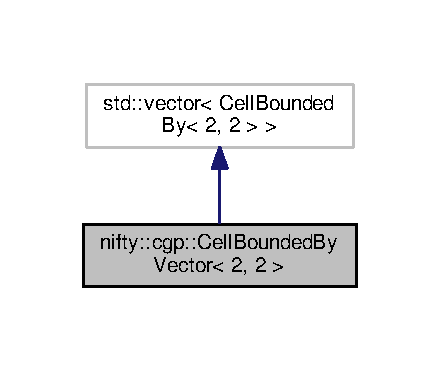
\includegraphics[width=211pt]{classnifty_1_1cgp_1_1CellBoundedByVector_3_012_00_012_01_4__inherit__graph}
\end{center}
\end{figure}


Collaboration diagram for nifty\+:\+:cgp\+:\+:Cell\+Bounded\+By\+Vector$<$ 2, 2 $>$\+:\nopagebreak
\begin{figure}[H]
\begin{center}
\leavevmode
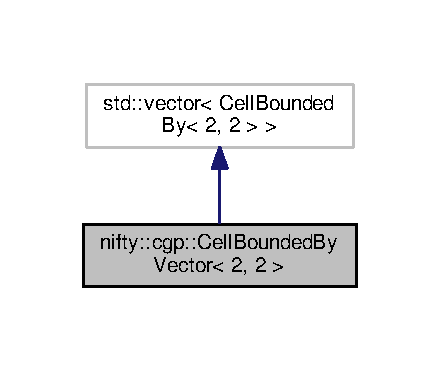
\includegraphics[width=211pt]{classnifty_1_1cgp_1_1CellBoundedByVector_3_012_00_012_01_4__coll__graph}
\end{center}
\end{figure}
\subsection*{Public Types}
\begin{DoxyCompactItemize}
\item 
typedef std\+::vector$<$ \hyperlink{classnifty_1_1cgp_1_1CellBoundedBy}{Cell\+Bounded\+By}$<$ 2, 2 $>$ $>$ \hyperlink{classnifty_1_1cgp_1_1CellBoundedByVector_3_012_00_012_01_4_acf1174515755206bce20310f87af4747}{Base\+Type}
\end{DoxyCompactItemize}
\subsection*{Public Member Functions}
\begin{DoxyCompactItemize}
\item 
\hyperlink{classnifty_1_1cgp_1_1CellBoundedByVector_3_012_00_012_01_4_af6f91256e589a2504b9362c4da176893}{Cell\+Bounded\+By\+Vector} (const \hyperlink{classnifty_1_1cgp_1_1CellBoundsVector}{Cell\+Bounds\+Vector}$<$ 2, 1 $>$ \&cell1\+Bounds)
\end{DoxyCompactItemize}


\subsection{Member Typedef Documentation}
\hypertarget{classnifty_1_1cgp_1_1CellBoundedByVector_3_012_00_012_01_4_acf1174515755206bce20310f87af4747}{}\index{nifty\+::cgp\+::\+Cell\+Bounded\+By\+Vector$<$ 2, 2 $>$@{nifty\+::cgp\+::\+Cell\+Bounded\+By\+Vector$<$ 2, 2 $>$}!Base\+Type@{Base\+Type}}
\index{Base\+Type@{Base\+Type}!nifty\+::cgp\+::\+Cell\+Bounded\+By\+Vector$<$ 2, 2 $>$@{nifty\+::cgp\+::\+Cell\+Bounded\+By\+Vector$<$ 2, 2 $>$}}
\subsubsection[{Base\+Type}]{\setlength{\rightskip}{0pt plus 5cm}typedef std\+::vector$<${\bf Cell\+Bounded\+By}$<$2, 2$>$ $>$ {\bf nifty\+::cgp\+::\+Cell\+Bounded\+By\+Vector}$<$ 2, 2 $>$\+::{\bf Base\+Type}}\label{classnifty_1_1cgp_1_1CellBoundedByVector_3_012_00_012_01_4_acf1174515755206bce20310f87af4747}


\subsection{Constructor \& Destructor Documentation}
\hypertarget{classnifty_1_1cgp_1_1CellBoundedByVector_3_012_00_012_01_4_af6f91256e589a2504b9362c4da176893}{}\index{nifty\+::cgp\+::\+Cell\+Bounded\+By\+Vector$<$ 2, 2 $>$@{nifty\+::cgp\+::\+Cell\+Bounded\+By\+Vector$<$ 2, 2 $>$}!Cell\+Bounded\+By\+Vector@{Cell\+Bounded\+By\+Vector}}
\index{Cell\+Bounded\+By\+Vector@{Cell\+Bounded\+By\+Vector}!nifty\+::cgp\+::\+Cell\+Bounded\+By\+Vector$<$ 2, 2 $>$@{nifty\+::cgp\+::\+Cell\+Bounded\+By\+Vector$<$ 2, 2 $>$}}
\subsubsection[{Cell\+Bounded\+By\+Vector(const Cell\+Bounds\+Vector$<$ 2, 1 $>$ \&cell1\+Bounds)}]{\setlength{\rightskip}{0pt plus 5cm}{\bf nifty\+::cgp\+::\+Cell\+Bounded\+By\+Vector}$<$ 2, 2 $>$\+::{\bf Cell\+Bounded\+By\+Vector} (
\begin{DoxyParamCaption}
\item[{const {\bf Cell\+Bounds\+Vector}$<$ 2, 1 $>$ \&}]{cell1\+Bounds}
\end{DoxyParamCaption}
)\hspace{0.3cm}{\ttfamily [inline]}}\label{classnifty_1_1cgp_1_1CellBoundedByVector_3_012_00_012_01_4_af6f91256e589a2504b9362c4da176893}


The documentation for this class was generated from the following file\+:\begin{DoxyCompactItemize}
\item 
/home/tbeier/src/nifty/include/nifty/cgp/\hyperlink{bounds_8hxx}{bounds.\+hxx}\end{DoxyCompactItemize}

\hypertarget{classnifty_1_1cgp_1_1CellBounds}{}\section{nifty\+:\+:cgp\+:\+:Cell\+Bounds$<$ D\+IM, C\+E\+L\+L\+\_\+\+T\+Y\+PE $>$ Class Template Reference}
\label{classnifty_1_1cgp_1_1CellBounds}\index{nifty\+::cgp\+::\+Cell\+Bounds$<$ D\+I\+M, C\+E\+L\+L\+\_\+\+T\+Y\+P\+E $>$@{nifty\+::cgp\+::\+Cell\+Bounds$<$ D\+I\+M, C\+E\+L\+L\+\_\+\+T\+Y\+P\+E $>$}}


{\ttfamily \#include $<$bounds.\+hxx$>$}



The documentation for this class was generated from the following file\+:\begin{DoxyCompactItemize}
\item 
/home/tbeier/src/nifty/include/nifty/cgp/\hyperlink{bounds_8hxx}{bounds.\+hxx}\end{DoxyCompactItemize}

\hypertarget{classnifty_1_1cgp_1_1CellBounds_3_012_00_010_01_4}{}\section{nifty\+:\+:cgp\+:\+:Cell\+Bounds$<$ 2, 0 $>$ Class Template Reference}
\label{classnifty_1_1cgp_1_1CellBounds_3_012_00_010_01_4}\index{nifty\+::cgp\+::\+Cell\+Bounds$<$ 2, 0 $>$@{nifty\+::cgp\+::\+Cell\+Bounds$<$ 2, 0 $>$}}


{\ttfamily \#include $<$bounds.\+hxx$>$}

\subsection*{Public Member Functions}
\begin{DoxyCompactItemize}
\item 
\hyperlink{classnifty_1_1cgp_1_1CellBounds_3_012_00_010_01_4_a974e66625691a8938bc5731f85b7b107}{Cell\+Bounds} (const uint32\+\_\+t a=0, const uint32\+\_\+t b=0, const uint32\+\_\+t c=0, const uint32\+\_\+t d=0)
\item 
uint32\+\_\+t \hyperlink{classnifty_1_1cgp_1_1CellBounds_3_012_00_010_01_4_ad23fc19849f68bf4d71914f21bad9ce7}{size} () const
\item 
const uint32\+\_\+t \& \hyperlink{classnifty_1_1cgp_1_1CellBounds_3_012_00_010_01_4_abf65a8e2e5f5883485b27d9934d377a3}{operator\mbox{[}$\,$\mbox{]}} (const unsigned int i) const
\end{DoxyCompactItemize}


\subsection{Constructor \& Destructor Documentation}
\mbox{\Hypertarget{classnifty_1_1cgp_1_1CellBounds_3_012_00_010_01_4_a974e66625691a8938bc5731f85b7b107}\label{classnifty_1_1cgp_1_1CellBounds_3_012_00_010_01_4_a974e66625691a8938bc5731f85b7b107}} 
\index{nifty\+::cgp\+::\+Cell\+Bounds$<$ 2, 0 $>$@{nifty\+::cgp\+::\+Cell\+Bounds$<$ 2, 0 $>$}!Cell\+Bounds@{Cell\+Bounds}}
\index{Cell\+Bounds@{Cell\+Bounds}!nifty\+::cgp\+::\+Cell\+Bounds$<$ 2, 0 $>$@{nifty\+::cgp\+::\+Cell\+Bounds$<$ 2, 0 $>$}}
\subsubsection{\texorpdfstring{Cell\+Bounds()}{CellBounds()}}
{\footnotesize\ttfamily \hyperlink{classnifty_1_1cgp_1_1CellBounds}{nifty\+::cgp\+::\+Cell\+Bounds}$<$ 2, 0 $>$\+::\hyperlink{classnifty_1_1cgp_1_1CellBounds}{Cell\+Bounds} (\begin{DoxyParamCaption}\item[{const uint32\+\_\+t}]{a = {\ttfamily 0},  }\item[{const uint32\+\_\+t}]{b = {\ttfamily 0},  }\item[{const uint32\+\_\+t}]{c = {\ttfamily 0},  }\item[{const uint32\+\_\+t}]{d = {\ttfamily 0} }\end{DoxyParamCaption})\hspace{0.3cm}{\ttfamily [inline]}}



\subsection{Member Function Documentation}
\mbox{\Hypertarget{classnifty_1_1cgp_1_1CellBounds_3_012_00_010_01_4_abf65a8e2e5f5883485b27d9934d377a3}\label{classnifty_1_1cgp_1_1CellBounds_3_012_00_010_01_4_abf65a8e2e5f5883485b27d9934d377a3}} 
\index{nifty\+::cgp\+::\+Cell\+Bounds$<$ 2, 0 $>$@{nifty\+::cgp\+::\+Cell\+Bounds$<$ 2, 0 $>$}!operator\mbox{[}\mbox{]}@{operator[]}}
\index{operator\mbox{[}\mbox{]}@{operator[]}!nifty\+::cgp\+::\+Cell\+Bounds$<$ 2, 0 $>$@{nifty\+::cgp\+::\+Cell\+Bounds$<$ 2, 0 $>$}}
\subsubsection{\texorpdfstring{operator[]()}{operator[]()}}
{\footnotesize\ttfamily const uint32\+\_\+t\& \hyperlink{classnifty_1_1cgp_1_1CellBounds}{nifty\+::cgp\+::\+Cell\+Bounds}$<$ 2, 0 $>$\+::operator\mbox{[}$\,$\mbox{]} (\begin{DoxyParamCaption}\item[{const unsigned int}]{i }\end{DoxyParamCaption}) const\hspace{0.3cm}{\ttfamily [inline]}}

\mbox{\Hypertarget{classnifty_1_1cgp_1_1CellBounds_3_012_00_010_01_4_ad23fc19849f68bf4d71914f21bad9ce7}\label{classnifty_1_1cgp_1_1CellBounds_3_012_00_010_01_4_ad23fc19849f68bf4d71914f21bad9ce7}} 
\index{nifty\+::cgp\+::\+Cell\+Bounds$<$ 2, 0 $>$@{nifty\+::cgp\+::\+Cell\+Bounds$<$ 2, 0 $>$}!size@{size}}
\index{size@{size}!nifty\+::cgp\+::\+Cell\+Bounds$<$ 2, 0 $>$@{nifty\+::cgp\+::\+Cell\+Bounds$<$ 2, 0 $>$}}
\subsubsection{\texorpdfstring{size()}{size()}}
{\footnotesize\ttfamily uint32\+\_\+t \hyperlink{classnifty_1_1cgp_1_1CellBounds}{nifty\+::cgp\+::\+Cell\+Bounds}$<$ 2, 0 $>$\+::size (\begin{DoxyParamCaption}{ }\end{DoxyParamCaption}) const\hspace{0.3cm}{\ttfamily [inline]}}



The documentation for this class was generated from the following file\+:\begin{DoxyCompactItemize}
\item 
/home/tbeier/src/nifty/include/nifty/cgp/\hyperlink{bounds_8hxx}{bounds.\+hxx}\end{DoxyCompactItemize}

\hypertarget{classnifty_1_1cgp_1_1CellBounds_3_012_00_011_01_4}{}\section{nifty\+:\+:cgp\+:\+:Cell\+Bounds$<$ 2, 1 $>$ Class Template Reference}
\label{classnifty_1_1cgp_1_1CellBounds_3_012_00_011_01_4}\index{nifty\+::cgp\+::\+Cell\+Bounds$<$ 2, 1 $>$@{nifty\+::cgp\+::\+Cell\+Bounds$<$ 2, 1 $>$}}


{\ttfamily \#include $<$bounds.\+hxx$>$}

\subsection*{Public Member Functions}
\begin{DoxyCompactItemize}
\item 
\hyperlink{classnifty_1_1cgp_1_1CellBounds_3_012_00_011_01_4_a6a562932e154f461651c3bfb111ddd11}{Cell\+Bounds} (const uint32\+\_\+t a=0, const uint32\+\_\+t b=0)
\item 
uint32\+\_\+t \hyperlink{classnifty_1_1cgp_1_1CellBounds_3_012_00_011_01_4_a4e0ec21b4b702cb9638b559f92bfa457}{size} () const 
\item 
const uint32\+\_\+t \& \hyperlink{classnifty_1_1cgp_1_1CellBounds_3_012_00_011_01_4_af8986efdf2c611ed6768fe7c746db9c8}{operator\mbox{[}$\,$\mbox{]}} (const unsigned int i) const 
\end{DoxyCompactItemize}


\subsection{Constructor \& Destructor Documentation}
\hypertarget{classnifty_1_1cgp_1_1CellBounds_3_012_00_011_01_4_a6a562932e154f461651c3bfb111ddd11}{}\index{nifty\+::cgp\+::\+Cell\+Bounds$<$ 2, 1 $>$@{nifty\+::cgp\+::\+Cell\+Bounds$<$ 2, 1 $>$}!Cell\+Bounds@{Cell\+Bounds}}
\index{Cell\+Bounds@{Cell\+Bounds}!nifty\+::cgp\+::\+Cell\+Bounds$<$ 2, 1 $>$@{nifty\+::cgp\+::\+Cell\+Bounds$<$ 2, 1 $>$}}
\subsubsection[{Cell\+Bounds(const uint32\+\_\+t a=0, const uint32\+\_\+t b=0)}]{\setlength{\rightskip}{0pt plus 5cm}{\bf nifty\+::cgp\+::\+Cell\+Bounds}$<$ 2, 1 $>$\+::{\bf Cell\+Bounds} (
\begin{DoxyParamCaption}
\item[{const uint32\+\_\+t}]{a = {\ttfamily 0}, }
\item[{const uint32\+\_\+t}]{b = {\ttfamily 0}}
\end{DoxyParamCaption}
)\hspace{0.3cm}{\ttfamily [inline]}}\label{classnifty_1_1cgp_1_1CellBounds_3_012_00_011_01_4_a6a562932e154f461651c3bfb111ddd11}


\subsection{Member Function Documentation}
\hypertarget{classnifty_1_1cgp_1_1CellBounds_3_012_00_011_01_4_af8986efdf2c611ed6768fe7c746db9c8}{}\index{nifty\+::cgp\+::\+Cell\+Bounds$<$ 2, 1 $>$@{nifty\+::cgp\+::\+Cell\+Bounds$<$ 2, 1 $>$}!operator\mbox{[}$\,$\mbox{]}@{operator[]}}
\index{operator\mbox{[}$\,$\mbox{]}@{operator[]}!nifty\+::cgp\+::\+Cell\+Bounds$<$ 2, 1 $>$@{nifty\+::cgp\+::\+Cell\+Bounds$<$ 2, 1 $>$}}
\subsubsection[{operator[](const unsigned int i) const }]{\setlength{\rightskip}{0pt plus 5cm}const uint32\+\_\+t\& {\bf nifty\+::cgp\+::\+Cell\+Bounds}$<$ 2, 1 $>$\+::operator\mbox{[}$\,$\mbox{]} (
\begin{DoxyParamCaption}
\item[{const unsigned int}]{i}
\end{DoxyParamCaption}
) const\hspace{0.3cm}{\ttfamily [inline]}}\label{classnifty_1_1cgp_1_1CellBounds_3_012_00_011_01_4_af8986efdf2c611ed6768fe7c746db9c8}
\hypertarget{classnifty_1_1cgp_1_1CellBounds_3_012_00_011_01_4_a4e0ec21b4b702cb9638b559f92bfa457}{}\index{nifty\+::cgp\+::\+Cell\+Bounds$<$ 2, 1 $>$@{nifty\+::cgp\+::\+Cell\+Bounds$<$ 2, 1 $>$}!size@{size}}
\index{size@{size}!nifty\+::cgp\+::\+Cell\+Bounds$<$ 2, 1 $>$@{nifty\+::cgp\+::\+Cell\+Bounds$<$ 2, 1 $>$}}
\subsubsection[{size() const }]{\setlength{\rightskip}{0pt plus 5cm}uint32\+\_\+t {\bf nifty\+::cgp\+::\+Cell\+Bounds}$<$ 2, 1 $>$\+::size (
\begin{DoxyParamCaption}
{}
\end{DoxyParamCaption}
) const\hspace{0.3cm}{\ttfamily [inline]}}\label{classnifty_1_1cgp_1_1CellBounds_3_012_00_011_01_4_a4e0ec21b4b702cb9638b559f92bfa457}


The documentation for this class was generated from the following file\+:\begin{DoxyCompactItemize}
\item 
/home/tbeier/src/nifty/include/nifty/cgp/\hyperlink{bounds_8hxx}{bounds.\+hxx}\end{DoxyCompactItemize}

\hypertarget{classnifty_1_1cgp_1_1CellBoundsVector}{}\section{nifty\+:\+:cgp\+:\+:Cell\+Bounds\+Vector$<$ D\+IM, C\+E\+L\+L\+\_\+\+T\+Y\+PE $>$ Class Template Reference}
\label{classnifty_1_1cgp_1_1CellBoundsVector}\index{nifty\+::cgp\+::\+Cell\+Bounds\+Vector$<$ D\+I\+M, C\+E\+L\+L\+\_\+\+T\+Y\+P\+E $>$@{nifty\+::cgp\+::\+Cell\+Bounds\+Vector$<$ D\+I\+M, C\+E\+L\+L\+\_\+\+T\+Y\+P\+E $>$}}


{\ttfamily \#include $<$bounds.\+hxx$>$}



Inheritance diagram for nifty\+:\+:cgp\+:\+:Cell\+Bounds\+Vector$<$ D\+IM, C\+E\+L\+L\+\_\+\+T\+Y\+PE $>$\+:
\nopagebreak
\begin{figure}[H]
\begin{center}
\leavevmode
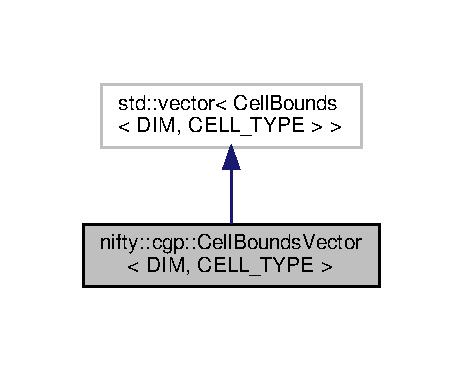
\includegraphics[width=222pt]{classnifty_1_1cgp_1_1CellBoundsVector__inherit__graph}
\end{center}
\end{figure}


Collaboration diagram for nifty\+:\+:cgp\+:\+:Cell\+Bounds\+Vector$<$ D\+IM, C\+E\+L\+L\+\_\+\+T\+Y\+PE $>$\+:
\nopagebreak
\begin{figure}[H]
\begin{center}
\leavevmode
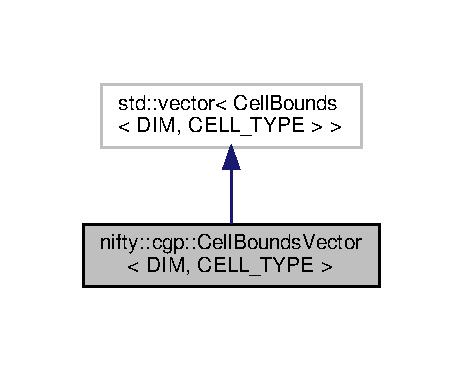
\includegraphics[width=222pt]{classnifty_1_1cgp_1_1CellBoundsVector__coll__graph}
\end{center}
\end{figure}
\subsection*{Public Types}
\begin{DoxyCompactItemize}
\item 
typedef \hyperlink{namespacenifty_1_1array_a683f151f19c851754e0c6d55ed16a0c2}{array\+::\+Static\+Array}$<$ uint32\+\_\+t, D\+IM+1 $>$ \hyperlink{classnifty_1_1cgp_1_1CellBoundsVector_a4db6e267b7ec9e9bfd2db914354c49f9}{Number\+Of\+Cells\+Type}
\item 
typedef std\+::vector$<$ \hyperlink{classnifty_1_1cgp_1_1CellBounds}{Cell\+Bounds}$<$ D\+IM, C\+E\+L\+L\+\_\+\+T\+Y\+PE $>$ $>$ \hyperlink{classnifty_1_1cgp_1_1CellBoundsVector_ae9467b3782214101f6ca95a0219bbbb6}{Base\+Type}
\end{DoxyCompactItemize}
\subsection*{Public Member Functions}
\begin{DoxyCompactItemize}
\item 
const \hyperlink{classnifty_1_1cgp_1_1CellBoundsVector_a4db6e267b7ec9e9bfd2db914354c49f9}{Number\+Of\+Cells\+Type} \& \hyperlink{classnifty_1_1cgp_1_1CellBoundsVector_a7e6c76f3f934b830d3d2ab964909dcf4}{number\+Of\+Cells} () const
\end{DoxyCompactItemize}
\subsection*{Friends}
\begin{DoxyCompactItemize}
\item 
class \hyperlink{classnifty_1_1cgp_1_1CellBoundsVector_a88cb0f4daae12ff33da3c2a17786cd08}{Bounds$<$ D\+I\+M $>$}
\end{DoxyCompactItemize}


\subsection{Member Typedef Documentation}
\mbox{\Hypertarget{classnifty_1_1cgp_1_1CellBoundsVector_ae9467b3782214101f6ca95a0219bbbb6}\label{classnifty_1_1cgp_1_1CellBoundsVector_ae9467b3782214101f6ca95a0219bbbb6}} 
\index{nifty\+::cgp\+::\+Cell\+Bounds\+Vector@{nifty\+::cgp\+::\+Cell\+Bounds\+Vector}!Base\+Type@{Base\+Type}}
\index{Base\+Type@{Base\+Type}!nifty\+::cgp\+::\+Cell\+Bounds\+Vector@{nifty\+::cgp\+::\+Cell\+Bounds\+Vector}}
\subsubsection{\texorpdfstring{Base\+Type}{BaseType}}
{\footnotesize\ttfamily template$<$size\+\_\+t D\+IM, size\+\_\+t C\+E\+L\+L\+\_\+\+T\+Y\+PE$>$ \\
typedef std\+::vector$<$\hyperlink{classnifty_1_1cgp_1_1CellBounds}{Cell\+Bounds}$<$D\+IM, C\+E\+L\+L\+\_\+\+T\+Y\+PE$>$ $>$ \hyperlink{classnifty_1_1cgp_1_1CellBoundsVector}{nifty\+::cgp\+::\+Cell\+Bounds\+Vector}$<$ D\+IM, C\+E\+L\+L\+\_\+\+T\+Y\+PE $>$\+::\hyperlink{classnifty_1_1cgp_1_1CellBoundsVector_ae9467b3782214101f6ca95a0219bbbb6}{Base\+Type}}

\mbox{\Hypertarget{classnifty_1_1cgp_1_1CellBoundsVector_a4db6e267b7ec9e9bfd2db914354c49f9}\label{classnifty_1_1cgp_1_1CellBoundsVector_a4db6e267b7ec9e9bfd2db914354c49f9}} 
\index{nifty\+::cgp\+::\+Cell\+Bounds\+Vector@{nifty\+::cgp\+::\+Cell\+Bounds\+Vector}!Number\+Of\+Cells\+Type@{Number\+Of\+Cells\+Type}}
\index{Number\+Of\+Cells\+Type@{Number\+Of\+Cells\+Type}!nifty\+::cgp\+::\+Cell\+Bounds\+Vector@{nifty\+::cgp\+::\+Cell\+Bounds\+Vector}}
\subsubsection{\texorpdfstring{Number\+Of\+Cells\+Type}{NumberOfCellsType}}
{\footnotesize\ttfamily template$<$size\+\_\+t D\+IM, size\+\_\+t C\+E\+L\+L\+\_\+\+T\+Y\+PE$>$ \\
typedef \hyperlink{namespacenifty_1_1array_a683f151f19c851754e0c6d55ed16a0c2}{array\+::\+Static\+Array}$<$uint32\+\_\+t, D\+IM +1 $>$ \hyperlink{classnifty_1_1cgp_1_1CellBoundsVector}{nifty\+::cgp\+::\+Cell\+Bounds\+Vector}$<$ D\+IM, C\+E\+L\+L\+\_\+\+T\+Y\+PE $>$\+::\hyperlink{classnifty_1_1cgp_1_1CellBoundsVector_a4db6e267b7ec9e9bfd2db914354c49f9}{Number\+Of\+Cells\+Type}}



\subsection{Member Function Documentation}
\mbox{\Hypertarget{classnifty_1_1cgp_1_1CellBoundsVector_a7e6c76f3f934b830d3d2ab964909dcf4}\label{classnifty_1_1cgp_1_1CellBoundsVector_a7e6c76f3f934b830d3d2ab964909dcf4}} 
\index{nifty\+::cgp\+::\+Cell\+Bounds\+Vector@{nifty\+::cgp\+::\+Cell\+Bounds\+Vector}!number\+Of\+Cells@{number\+Of\+Cells}}
\index{number\+Of\+Cells@{number\+Of\+Cells}!nifty\+::cgp\+::\+Cell\+Bounds\+Vector@{nifty\+::cgp\+::\+Cell\+Bounds\+Vector}}
\subsubsection{\texorpdfstring{number\+Of\+Cells()}{numberOfCells()}}
{\footnotesize\ttfamily template$<$size\+\_\+t D\+IM, size\+\_\+t C\+E\+L\+L\+\_\+\+T\+Y\+PE$>$ \\
const \hyperlink{classnifty_1_1cgp_1_1CellBoundsVector_a4db6e267b7ec9e9bfd2db914354c49f9}{Number\+Of\+Cells\+Type}\& \hyperlink{classnifty_1_1cgp_1_1CellBoundsVector}{nifty\+::cgp\+::\+Cell\+Bounds\+Vector}$<$ D\+IM, C\+E\+L\+L\+\_\+\+T\+Y\+PE $>$\+::number\+Of\+Cells (\begin{DoxyParamCaption}{ }\end{DoxyParamCaption}) const\hspace{0.3cm}{\ttfamily [inline]}}



\subsection{Friends And Related Function Documentation}
\mbox{\Hypertarget{classnifty_1_1cgp_1_1CellBoundsVector_a88cb0f4daae12ff33da3c2a17786cd08}\label{classnifty_1_1cgp_1_1CellBoundsVector_a88cb0f4daae12ff33da3c2a17786cd08}} 
\index{nifty\+::cgp\+::\+Cell\+Bounds\+Vector@{nifty\+::cgp\+::\+Cell\+Bounds\+Vector}!Bounds$<$ D\+I\+M $>$@{Bounds$<$ D\+I\+M $>$}}
\index{Bounds$<$ D\+I\+M $>$@{Bounds$<$ D\+I\+M $>$}!nifty\+::cgp\+::\+Cell\+Bounds\+Vector@{nifty\+::cgp\+::\+Cell\+Bounds\+Vector}}
\subsubsection{\texorpdfstring{Bounds$<$ D\+I\+M $>$}{Bounds< DIM >}}
{\footnotesize\ttfamily template$<$size\+\_\+t D\+IM, size\+\_\+t C\+E\+L\+L\+\_\+\+T\+Y\+PE$>$ \\
friend class \hyperlink{classnifty_1_1cgp_1_1Bounds}{Bounds}$<$ D\+IM $>$\hspace{0.3cm}{\ttfamily [friend]}}



The documentation for this class was generated from the following file\+:\begin{DoxyCompactItemize}
\item 
/home/tbeier/src/nifty/include/nifty/cgp/\hyperlink{bounds_8hxx}{bounds.\+hxx}\end{DoxyCompactItemize}

\hypertarget{classnifty_1_1cgp_1_1CellGeometry}{}\section{nifty\+:\+:cgp\+:\+:Cell\+Geometry$<$ D\+I\+M, C\+E\+L\+L\+\_\+\+T\+Y\+P\+E $>$ Class Template Reference}
\label{classnifty_1_1cgp_1_1CellGeometry}\index{nifty\+::cgp\+::\+Cell\+Geometry$<$ D\+I\+M, C\+E\+L\+L\+\_\+\+T\+Y\+P\+E $>$@{nifty\+::cgp\+::\+Cell\+Geometry$<$ D\+I\+M, C\+E\+L\+L\+\_\+\+T\+Y\+P\+E $>$}}


{\ttfamily \#include $<$geometry.\+hxx$>$}



Inheritance diagram for nifty\+:\+:cgp\+:\+:Cell\+Geometry$<$ D\+I\+M, C\+E\+L\+L\+\_\+\+T\+Y\+P\+E $>$\+:
% FIG 0


Collaboration diagram for nifty\+:\+:cgp\+:\+:Cell\+Geometry$<$ D\+I\+M, C\+E\+L\+L\+\_\+\+T\+Y\+P\+E $>$\+:
% FIG 1
\subsection*{Public Types}
\begin{DoxyCompactItemize}
\item 
typedef std\+::integral\+\_\+constant$<$ size\+\_\+t, D\+I\+M $>$ \hyperlink{classnifty_1_1cgp_1_1CellGeometry_a8cc75c7033c03864e099a5d907de88d8}{Dimension\+Type}
\item 
typedef \hyperlink{namespacenifty_1_1array_a683f151f19c851754e0c6d55ed16a0c2}{nifty\+::array\+::\+Static\+Array}$<$ uint32\+\_\+t, D\+I\+M $>$ \hyperlink{classnifty_1_1cgp_1_1CellGeometry_af8ae7d6b7a8f20afae6ce53e88604acf}{Coordinate\+Type}
\item 
typedef \hyperlink{namespacenifty_1_1array_a683f151f19c851754e0c6d55ed16a0c2}{nifty\+::array\+::\+Static\+Array}$<$ float, D\+I\+M $>$ \hyperlink{classnifty_1_1cgp_1_1CellGeometry_a07e98f74f6dc5cda1aab1349c7f60d5b}{Float\+Coordinate\+Type}
\item 
typedef std\+::vector$<$ \hyperlink{classnifty_1_1cgp_1_1CellGeometry_af8ae7d6b7a8f20afae6ce53e88604acf}{Coordinate\+Type} $>$ \hyperlink{classnifty_1_1cgp_1_1CellGeometry_ada76b5372b0e456edf3496813b9ed7f0}{Base\+Type}
\end{DoxyCompactItemize}
\subsection*{Public Member Functions}
\begin{DoxyCompactItemize}
\item 
\hyperlink{classnifty_1_1cgp_1_1CellGeometry_a07e98f74f6dc5cda1aab1349c7f60d5b}{Float\+Coordinate\+Type} \hyperlink{classnifty_1_1cgp_1_1CellGeometry_af51fef28bad6333d7604a160e5353188}{center\+Of\+Mass} () const 
\end{DoxyCompactItemize}


\subsection{Member Typedef Documentation}
\hypertarget{classnifty_1_1cgp_1_1CellGeometry_ada76b5372b0e456edf3496813b9ed7f0}{}\index{nifty\+::cgp\+::\+Cell\+Geometry@{nifty\+::cgp\+::\+Cell\+Geometry}!Base\+Type@{Base\+Type}}
\index{Base\+Type@{Base\+Type}!nifty\+::cgp\+::\+Cell\+Geometry@{nifty\+::cgp\+::\+Cell\+Geometry}}
\subsubsection[{Base\+Type}]{\setlength{\rightskip}{0pt plus 5cm}template$<$size\+\_\+t D\+I\+M, size\+\_\+t C\+E\+L\+L\+\_\+\+T\+Y\+P\+E$>$ typedef std\+::vector$<${\bf Coordinate\+Type}$>$ {\bf nifty\+::cgp\+::\+Cell\+Geometry}$<$ D\+I\+M, C\+E\+L\+L\+\_\+\+T\+Y\+P\+E $>$\+::{\bf Base\+Type}}\label{classnifty_1_1cgp_1_1CellGeometry_ada76b5372b0e456edf3496813b9ed7f0}
\hypertarget{classnifty_1_1cgp_1_1CellGeometry_af8ae7d6b7a8f20afae6ce53e88604acf}{}\index{nifty\+::cgp\+::\+Cell\+Geometry@{nifty\+::cgp\+::\+Cell\+Geometry}!Coordinate\+Type@{Coordinate\+Type}}
\index{Coordinate\+Type@{Coordinate\+Type}!nifty\+::cgp\+::\+Cell\+Geometry@{nifty\+::cgp\+::\+Cell\+Geometry}}
\subsubsection[{Coordinate\+Type}]{\setlength{\rightskip}{0pt plus 5cm}template$<$size\+\_\+t D\+I\+M, size\+\_\+t C\+E\+L\+L\+\_\+\+T\+Y\+P\+E$>$ typedef {\bf nifty\+::array\+::\+Static\+Array}$<$uint32\+\_\+t, D\+I\+M$>$ {\bf nifty\+::cgp\+::\+Cell\+Geometry}$<$ D\+I\+M, C\+E\+L\+L\+\_\+\+T\+Y\+P\+E $>$\+::{\bf Coordinate\+Type}}\label{classnifty_1_1cgp_1_1CellGeometry_af8ae7d6b7a8f20afae6ce53e88604acf}
\hypertarget{classnifty_1_1cgp_1_1CellGeometry_a8cc75c7033c03864e099a5d907de88d8}{}\index{nifty\+::cgp\+::\+Cell\+Geometry@{nifty\+::cgp\+::\+Cell\+Geometry}!Dimension\+Type@{Dimension\+Type}}
\index{Dimension\+Type@{Dimension\+Type}!nifty\+::cgp\+::\+Cell\+Geometry@{nifty\+::cgp\+::\+Cell\+Geometry}}
\subsubsection[{Dimension\+Type}]{\setlength{\rightskip}{0pt plus 5cm}template$<$size\+\_\+t D\+I\+M, size\+\_\+t C\+E\+L\+L\+\_\+\+T\+Y\+P\+E$>$ typedef std\+::integral\+\_\+constant$<$size\+\_\+t, D\+I\+M$>$ {\bf nifty\+::cgp\+::\+Cell\+Geometry}$<$ D\+I\+M, C\+E\+L\+L\+\_\+\+T\+Y\+P\+E $>$\+::{\bf Dimension\+Type}}\label{classnifty_1_1cgp_1_1CellGeometry_a8cc75c7033c03864e099a5d907de88d8}
\hypertarget{classnifty_1_1cgp_1_1CellGeometry_a07e98f74f6dc5cda1aab1349c7f60d5b}{}\index{nifty\+::cgp\+::\+Cell\+Geometry@{nifty\+::cgp\+::\+Cell\+Geometry}!Float\+Coordinate\+Type@{Float\+Coordinate\+Type}}
\index{Float\+Coordinate\+Type@{Float\+Coordinate\+Type}!nifty\+::cgp\+::\+Cell\+Geometry@{nifty\+::cgp\+::\+Cell\+Geometry}}
\subsubsection[{Float\+Coordinate\+Type}]{\setlength{\rightskip}{0pt plus 5cm}template$<$size\+\_\+t D\+I\+M, size\+\_\+t C\+E\+L\+L\+\_\+\+T\+Y\+P\+E$>$ typedef {\bf nifty\+::array\+::\+Static\+Array}$<$float, D\+I\+M$>$ {\bf nifty\+::cgp\+::\+Cell\+Geometry}$<$ D\+I\+M, C\+E\+L\+L\+\_\+\+T\+Y\+P\+E $>$\+::{\bf Float\+Coordinate\+Type}}\label{classnifty_1_1cgp_1_1CellGeometry_a07e98f74f6dc5cda1aab1349c7f60d5b}


\subsection{Member Function Documentation}
\hypertarget{classnifty_1_1cgp_1_1CellGeometry_af51fef28bad6333d7604a160e5353188}{}\index{nifty\+::cgp\+::\+Cell\+Geometry@{nifty\+::cgp\+::\+Cell\+Geometry}!center\+Of\+Mass@{center\+Of\+Mass}}
\index{center\+Of\+Mass@{center\+Of\+Mass}!nifty\+::cgp\+::\+Cell\+Geometry@{nifty\+::cgp\+::\+Cell\+Geometry}}
\subsubsection[{center\+Of\+Mass() const }]{\setlength{\rightskip}{0pt plus 5cm}template$<$size\+\_\+t D\+I\+M, size\+\_\+t C\+E\+L\+L\+\_\+\+T\+Y\+P\+E$>$ {\bf Float\+Coordinate\+Type} {\bf nifty\+::cgp\+::\+Cell\+Geometry}$<$ D\+I\+M, C\+E\+L\+L\+\_\+\+T\+Y\+P\+E $>$\+::center\+Of\+Mass (
\begin{DoxyParamCaption}
{}
\end{DoxyParamCaption}
) const\hspace{0.3cm}{\ttfamily [inline]}}\label{classnifty_1_1cgp_1_1CellGeometry_af51fef28bad6333d7604a160e5353188}


The documentation for this class was generated from the following file\+:\begin{DoxyCompactItemize}
\item 
/home/tbeier/src/nifty/include/nifty/cgp/\hyperlink{geometry_8hxx}{geometry.\+hxx}\end{DoxyCompactItemize}

\hypertarget{classnifty_1_1cgp_1_1CellGeometry_3_012_00_011_01_4}{}\section{nifty\+:\+:cgp\+:\+:Cell\+Geometry$<$ 2, 1 $>$ Class Template Reference}
\label{classnifty_1_1cgp_1_1CellGeometry_3_012_00_011_01_4}\index{nifty\+::cgp\+::\+Cell\+Geometry$<$ 2, 1 $>$@{nifty\+::cgp\+::\+Cell\+Geometry$<$ 2, 1 $>$}}


{\ttfamily \#include $<$geometry.\+hxx$>$}



Inheritance diagram for nifty\+:\+:cgp\+:\+:Cell\+Geometry$<$ 2, 1 $>$\+:
% FIG 0


Collaboration diagram for nifty\+:\+:cgp\+:\+:Cell\+Geometry$<$ 2, 1 $>$\+:
% FIG 1
\subsection*{Public Types}
\begin{DoxyCompactItemize}
\item 
typedef std\+::integral\+\_\+constant$<$ size\+\_\+t, \hyperlink{classnifty_1_1cgp_1_1CellGeometry_3_012_00_011_01_4_a42d125e23384bc4a770893276750d9d1}{D\+I\+M} $>$ \hyperlink{classnifty_1_1cgp_1_1CellGeometry_3_012_00_011_01_4_a35fae8ad3031bc0765ecb4d56cbff171}{Dimension\+Type}
\item 
typedef \hyperlink{namespacenifty_1_1array_a683f151f19c851754e0c6d55ed16a0c2}{nifty\+::array\+::\+Static\+Array}$<$ uint32\+\_\+t, \hyperlink{classnifty_1_1cgp_1_1CellGeometry_3_012_00_011_01_4_a42d125e23384bc4a770893276750d9d1}{D\+I\+M} $>$ \hyperlink{classnifty_1_1cgp_1_1CellGeometry_3_012_00_011_01_4_a61e8ffb089e3ca4bf7998e77dfc278bc}{Coordinate\+Type}
\item 
typedef \hyperlink{namespacenifty_1_1array_a683f151f19c851754e0c6d55ed16a0c2}{nifty\+::array\+::\+Static\+Array}$<$ float, \hyperlink{classnifty_1_1cgp_1_1CellGeometry_3_012_00_011_01_4_a42d125e23384bc4a770893276750d9d1}{D\+I\+M} $>$ \hyperlink{classnifty_1_1cgp_1_1CellGeometry_3_012_00_011_01_4_aa894ce050b43284dac01b3963e2e1e47}{Float\+Coordinate\+Type}
\item 
typedef std\+::vector$<$ \hyperlink{classnifty_1_1cgp_1_1CellGeometry_3_012_00_011_01_4_a61e8ffb089e3ca4bf7998e77dfc278bc}{Coordinate\+Type} $>$ \hyperlink{classnifty_1_1cgp_1_1CellGeometry_3_012_00_011_01_4_a10f7d7a27ef9080c3a94fc69a258c55e}{Base\+Type}
\end{DoxyCompactItemize}
\subsection*{Public Member Functions}
\begin{DoxyCompactItemize}
\item 
\hyperlink{classnifty_1_1cgp_1_1CellGeometry_3_012_00_011_01_4_ae525aaf64790b4c76c17208a13588101}{Cell\+Geometry} ()
\item 
\hyperlink{classnifty_1_1cgp_1_1CellGeometry_3_012_00_011_01_4_aa894ce050b43284dac01b3963e2e1e47}{Float\+Coordinate\+Type} \hyperlink{classnifty_1_1cgp_1_1CellGeometry_3_012_00_011_01_4_ae8510d5f8494ee259cd105eb8342a494}{center\+Of\+Mass} () const 
\end{DoxyCompactItemize}
\subsection*{Static Public Attributes}
\begin{DoxyCompactItemize}
\item 
static const size\+\_\+t \hyperlink{classnifty_1_1cgp_1_1CellGeometry_3_012_00_011_01_4_a42d125e23384bc4a770893276750d9d1}{D\+I\+M} = 2
\end{DoxyCompactItemize}
\subsection*{Friends}
\begin{DoxyCompactItemize}
\item 
class \hyperlink{classnifty_1_1cgp_1_1CellGeometry_3_012_00_011_01_4_adfd68abfc6c19d6cc9ac2eb46fcfa819}{Geometry$<$ 2 $>$}
\end{DoxyCompactItemize}


\subsection{Member Typedef Documentation}
\hypertarget{classnifty_1_1cgp_1_1CellGeometry_3_012_00_011_01_4_a10f7d7a27ef9080c3a94fc69a258c55e}{}\index{nifty\+::cgp\+::\+Cell\+Geometry$<$ 2, 1 $>$@{nifty\+::cgp\+::\+Cell\+Geometry$<$ 2, 1 $>$}!Base\+Type@{Base\+Type}}
\index{Base\+Type@{Base\+Type}!nifty\+::cgp\+::\+Cell\+Geometry$<$ 2, 1 $>$@{nifty\+::cgp\+::\+Cell\+Geometry$<$ 2, 1 $>$}}
\subsubsection[{Base\+Type}]{\setlength{\rightskip}{0pt plus 5cm}typedef std\+::vector$<${\bf Coordinate\+Type}$>$ {\bf nifty\+::cgp\+::\+Cell\+Geometry}$<$ 2, 1 $>$\+::{\bf Base\+Type}}\label{classnifty_1_1cgp_1_1CellGeometry_3_012_00_011_01_4_a10f7d7a27ef9080c3a94fc69a258c55e}
\hypertarget{classnifty_1_1cgp_1_1CellGeometry_3_012_00_011_01_4_a61e8ffb089e3ca4bf7998e77dfc278bc}{}\index{nifty\+::cgp\+::\+Cell\+Geometry$<$ 2, 1 $>$@{nifty\+::cgp\+::\+Cell\+Geometry$<$ 2, 1 $>$}!Coordinate\+Type@{Coordinate\+Type}}
\index{Coordinate\+Type@{Coordinate\+Type}!nifty\+::cgp\+::\+Cell\+Geometry$<$ 2, 1 $>$@{nifty\+::cgp\+::\+Cell\+Geometry$<$ 2, 1 $>$}}
\subsubsection[{Coordinate\+Type}]{\setlength{\rightskip}{0pt plus 5cm}typedef {\bf nifty\+::array\+::\+Static\+Array}$<$uint32\+\_\+t, {\bf D\+I\+M}$>$ {\bf nifty\+::cgp\+::\+Cell\+Geometry}$<$ 2, 1 $>$\+::{\bf Coordinate\+Type}}\label{classnifty_1_1cgp_1_1CellGeometry_3_012_00_011_01_4_a61e8ffb089e3ca4bf7998e77dfc278bc}
\hypertarget{classnifty_1_1cgp_1_1CellGeometry_3_012_00_011_01_4_a35fae8ad3031bc0765ecb4d56cbff171}{}\index{nifty\+::cgp\+::\+Cell\+Geometry$<$ 2, 1 $>$@{nifty\+::cgp\+::\+Cell\+Geometry$<$ 2, 1 $>$}!Dimension\+Type@{Dimension\+Type}}
\index{Dimension\+Type@{Dimension\+Type}!nifty\+::cgp\+::\+Cell\+Geometry$<$ 2, 1 $>$@{nifty\+::cgp\+::\+Cell\+Geometry$<$ 2, 1 $>$}}
\subsubsection[{Dimension\+Type}]{\setlength{\rightskip}{0pt plus 5cm}typedef std\+::integral\+\_\+constant$<$size\+\_\+t, {\bf D\+I\+M}$>$ {\bf nifty\+::cgp\+::\+Cell\+Geometry}$<$ 2, 1 $>$\+::{\bf Dimension\+Type}}\label{classnifty_1_1cgp_1_1CellGeometry_3_012_00_011_01_4_a35fae8ad3031bc0765ecb4d56cbff171}
\hypertarget{classnifty_1_1cgp_1_1CellGeometry_3_012_00_011_01_4_aa894ce050b43284dac01b3963e2e1e47}{}\index{nifty\+::cgp\+::\+Cell\+Geometry$<$ 2, 1 $>$@{nifty\+::cgp\+::\+Cell\+Geometry$<$ 2, 1 $>$}!Float\+Coordinate\+Type@{Float\+Coordinate\+Type}}
\index{Float\+Coordinate\+Type@{Float\+Coordinate\+Type}!nifty\+::cgp\+::\+Cell\+Geometry$<$ 2, 1 $>$@{nifty\+::cgp\+::\+Cell\+Geometry$<$ 2, 1 $>$}}
\subsubsection[{Float\+Coordinate\+Type}]{\setlength{\rightskip}{0pt plus 5cm}typedef {\bf nifty\+::array\+::\+Static\+Array}$<$float, {\bf D\+I\+M}$>$ {\bf nifty\+::cgp\+::\+Cell\+Geometry}$<$ 2, 1 $>$\+::{\bf Float\+Coordinate\+Type}}\label{classnifty_1_1cgp_1_1CellGeometry_3_012_00_011_01_4_aa894ce050b43284dac01b3963e2e1e47}


\subsection{Constructor \& Destructor Documentation}
\hypertarget{classnifty_1_1cgp_1_1CellGeometry_3_012_00_011_01_4_ae525aaf64790b4c76c17208a13588101}{}\index{nifty\+::cgp\+::\+Cell\+Geometry$<$ 2, 1 $>$@{nifty\+::cgp\+::\+Cell\+Geometry$<$ 2, 1 $>$}!Cell\+Geometry@{Cell\+Geometry}}
\index{Cell\+Geometry@{Cell\+Geometry}!nifty\+::cgp\+::\+Cell\+Geometry$<$ 2, 1 $>$@{nifty\+::cgp\+::\+Cell\+Geometry$<$ 2, 1 $>$}}
\subsubsection[{Cell\+Geometry()}]{\setlength{\rightskip}{0pt plus 5cm}{\bf nifty\+::cgp\+::\+Cell\+Geometry}$<$ 2, 1 $>$\+::{\bf Cell\+Geometry} (
\begin{DoxyParamCaption}
{}
\end{DoxyParamCaption}
)\hspace{0.3cm}{\ttfamily [inline]}}\label{classnifty_1_1cgp_1_1CellGeometry_3_012_00_011_01_4_ae525aaf64790b4c76c17208a13588101}


\subsection{Member Function Documentation}
\hypertarget{classnifty_1_1cgp_1_1CellGeometry_3_012_00_011_01_4_ae8510d5f8494ee259cd105eb8342a494}{}\index{nifty\+::cgp\+::\+Cell\+Geometry$<$ 2, 1 $>$@{nifty\+::cgp\+::\+Cell\+Geometry$<$ 2, 1 $>$}!center\+Of\+Mass@{center\+Of\+Mass}}
\index{center\+Of\+Mass@{center\+Of\+Mass}!nifty\+::cgp\+::\+Cell\+Geometry$<$ 2, 1 $>$@{nifty\+::cgp\+::\+Cell\+Geometry$<$ 2, 1 $>$}}
\subsubsection[{center\+Of\+Mass() const }]{\setlength{\rightskip}{0pt plus 5cm}{\bf Float\+Coordinate\+Type} {\bf nifty\+::cgp\+::\+Cell\+Geometry}$<$ 2, 1 $>$\+::center\+Of\+Mass (
\begin{DoxyParamCaption}
{}
\end{DoxyParamCaption}
) const\hspace{0.3cm}{\ttfamily [inline]}}\label{classnifty_1_1cgp_1_1CellGeometry_3_012_00_011_01_4_ae8510d5f8494ee259cd105eb8342a494}


\subsection{Friends And Related Function Documentation}
\hypertarget{classnifty_1_1cgp_1_1CellGeometry_3_012_00_011_01_4_adfd68abfc6c19d6cc9ac2eb46fcfa819}{}\index{nifty\+::cgp\+::\+Cell\+Geometry$<$ 2, 1 $>$@{nifty\+::cgp\+::\+Cell\+Geometry$<$ 2, 1 $>$}!Geometry$<$ 2 $>$@{Geometry$<$ 2 $>$}}
\index{Geometry$<$ 2 $>$@{Geometry$<$ 2 $>$}!nifty\+::cgp\+::\+Cell\+Geometry$<$ 2, 1 $>$@{nifty\+::cgp\+::\+Cell\+Geometry$<$ 2, 1 $>$}}
\subsubsection[{Geometry$<$ 2 $>$}]{\setlength{\rightskip}{0pt plus 5cm}friend class {\bf Geometry}$<$ 2 $>$\hspace{0.3cm}{\ttfamily [friend]}}\label{classnifty_1_1cgp_1_1CellGeometry_3_012_00_011_01_4_adfd68abfc6c19d6cc9ac2eb46fcfa819}


\subsection{Member Data Documentation}
\hypertarget{classnifty_1_1cgp_1_1CellGeometry_3_012_00_011_01_4_a42d125e23384bc4a770893276750d9d1}{}\index{nifty\+::cgp\+::\+Cell\+Geometry$<$ 2, 1 $>$@{nifty\+::cgp\+::\+Cell\+Geometry$<$ 2, 1 $>$}!D\+I\+M@{D\+I\+M}}
\index{D\+I\+M@{D\+I\+M}!nifty\+::cgp\+::\+Cell\+Geometry$<$ 2, 1 $>$@{nifty\+::cgp\+::\+Cell\+Geometry$<$ 2, 1 $>$}}
\subsubsection[{D\+I\+M}]{\setlength{\rightskip}{0pt plus 5cm}const size\+\_\+t {\bf nifty\+::cgp\+::\+Cell\+Geometry}$<$ 2, 1 $>$\+::D\+I\+M = 2\hspace{0.3cm}{\ttfamily [static]}}\label{classnifty_1_1cgp_1_1CellGeometry_3_012_00_011_01_4_a42d125e23384bc4a770893276750d9d1}


The documentation for this class was generated from the following file\+:\begin{DoxyCompactItemize}
\item 
/home/tbeier/src/nifty/include/nifty/cgp/\hyperlink{geometry_8hxx}{geometry.\+hxx}\end{DoxyCompactItemize}

\hypertarget{classnifty_1_1cgp_1_1CellGeometry_3_01DIM_00_010_01_4}{}\section{nifty\+:\+:cgp\+:\+:Cell\+Geometry$<$ D\+I\+M, 0 $>$ Class Template Reference}
\label{classnifty_1_1cgp_1_1CellGeometry_3_01DIM_00_010_01_4}\index{nifty\+::cgp\+::\+Cell\+Geometry$<$ D\+I\+M, 0 $>$@{nifty\+::cgp\+::\+Cell\+Geometry$<$ D\+I\+M, 0 $>$}}


{\ttfamily \#include $<$geometry.\+hxx$>$}



Inheritance diagram for nifty\+:\+:cgp\+:\+:Cell\+Geometry$<$ D\+I\+M, 0 $>$\+:\nopagebreak
\begin{figure}[H]
\begin{center}
\leavevmode
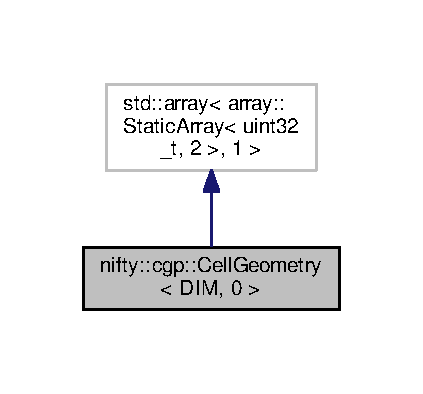
\includegraphics[width=203pt]{classnifty_1_1cgp_1_1CellGeometry_3_01DIM_00_010_01_4__inherit__graph}
\end{center}
\end{figure}


Collaboration diagram for nifty\+:\+:cgp\+:\+:Cell\+Geometry$<$ D\+I\+M, 0 $>$\+:\nopagebreak
\begin{figure}[H]
\begin{center}
\leavevmode
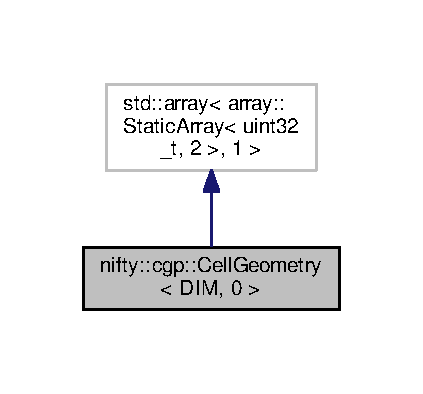
\includegraphics[width=203pt]{classnifty_1_1cgp_1_1CellGeometry_3_01DIM_00_010_01_4__coll__graph}
\end{center}
\end{figure}
\subsection*{Public Types}
\begin{DoxyCompactItemize}
\item 
typedef std\+::integral\+\_\+constant$<$ size\+\_\+t, D\+I\+M $>$ \hyperlink{classnifty_1_1cgp_1_1CellGeometry_3_01DIM_00_010_01_4_a71116d45ef5d2db3ccf29b0258df02ed}{Dimension\+Type}
\item 
typedef \hyperlink{namespacenifty_1_1array_a683f151f19c851754e0c6d55ed16a0c2}{nifty\+::array\+::\+Static\+Array}$<$ uint32\+\_\+t, 2 $>$ \hyperlink{classnifty_1_1cgp_1_1CellGeometry_3_01DIM_00_010_01_4_a3c8cec60edc558f44940e98135a521f0}{Coordinate\+Type}
\item 
typedef \hyperlink{namespacenifty_1_1array_a683f151f19c851754e0c6d55ed16a0c2}{nifty\+::array\+::\+Static\+Array}$<$ float, D\+I\+M $>$ \hyperlink{classnifty_1_1cgp_1_1CellGeometry_3_01DIM_00_010_01_4_a825cfc0d2e082ccd4b34e5ab2046dbe6}{Float\+Coordinate\+Type}
\item 
typedef std\+::array$<$ \hyperlink{classnifty_1_1cgp_1_1CellGeometry_3_01DIM_00_010_01_4_a3c8cec60edc558f44940e98135a521f0}{Coordinate\+Type}, 1 $>$ \hyperlink{classnifty_1_1cgp_1_1CellGeometry_3_01DIM_00_010_01_4_a299d8c228b7529d2e95f90aa3b2f7528}{Base\+Type}
\end{DoxyCompactItemize}
\subsection*{Public Member Functions}
\begin{DoxyCompactItemize}
\item 
\hyperlink{classnifty_1_1cgp_1_1CellGeometry_3_01DIM_00_010_01_4_a825cfc0d2e082ccd4b34e5ab2046dbe6}{Float\+Coordinate\+Type} \hyperlink{classnifty_1_1cgp_1_1CellGeometry_3_01DIM_00_010_01_4_ac76ee365e72874db3e3a541c20f7f462}{center\+Of\+Mass} () const 
\end{DoxyCompactItemize}


\subsection{Member Typedef Documentation}
\hypertarget{classnifty_1_1cgp_1_1CellGeometry_3_01DIM_00_010_01_4_a299d8c228b7529d2e95f90aa3b2f7528}{}\index{nifty\+::cgp\+::\+Cell\+Geometry$<$ D\+I\+M, 0 $>$@{nifty\+::cgp\+::\+Cell\+Geometry$<$ D\+I\+M, 0 $>$}!Base\+Type@{Base\+Type}}
\index{Base\+Type@{Base\+Type}!nifty\+::cgp\+::\+Cell\+Geometry$<$ D\+I\+M, 0 $>$@{nifty\+::cgp\+::\+Cell\+Geometry$<$ D\+I\+M, 0 $>$}}
\subsubsection[{Base\+Type}]{\setlength{\rightskip}{0pt plus 5cm}template$<$size\+\_\+t D\+I\+M$>$ typedef std\+::array$<${\bf Coordinate\+Type}, 1$>$ {\bf nifty\+::cgp\+::\+Cell\+Geometry}$<$ D\+I\+M, 0 $>$\+::{\bf Base\+Type}}\label{classnifty_1_1cgp_1_1CellGeometry_3_01DIM_00_010_01_4_a299d8c228b7529d2e95f90aa3b2f7528}
\hypertarget{classnifty_1_1cgp_1_1CellGeometry_3_01DIM_00_010_01_4_a3c8cec60edc558f44940e98135a521f0}{}\index{nifty\+::cgp\+::\+Cell\+Geometry$<$ D\+I\+M, 0 $>$@{nifty\+::cgp\+::\+Cell\+Geometry$<$ D\+I\+M, 0 $>$}!Coordinate\+Type@{Coordinate\+Type}}
\index{Coordinate\+Type@{Coordinate\+Type}!nifty\+::cgp\+::\+Cell\+Geometry$<$ D\+I\+M, 0 $>$@{nifty\+::cgp\+::\+Cell\+Geometry$<$ D\+I\+M, 0 $>$}}
\subsubsection[{Coordinate\+Type}]{\setlength{\rightskip}{0pt plus 5cm}template$<$size\+\_\+t D\+I\+M$>$ typedef {\bf nifty\+::array\+::\+Static\+Array}$<$uint32\+\_\+t, 2$>$ {\bf nifty\+::cgp\+::\+Cell\+Geometry}$<$ D\+I\+M, 0 $>$\+::{\bf Coordinate\+Type}}\label{classnifty_1_1cgp_1_1CellGeometry_3_01DIM_00_010_01_4_a3c8cec60edc558f44940e98135a521f0}
\hypertarget{classnifty_1_1cgp_1_1CellGeometry_3_01DIM_00_010_01_4_a71116d45ef5d2db3ccf29b0258df02ed}{}\index{nifty\+::cgp\+::\+Cell\+Geometry$<$ D\+I\+M, 0 $>$@{nifty\+::cgp\+::\+Cell\+Geometry$<$ D\+I\+M, 0 $>$}!Dimension\+Type@{Dimension\+Type}}
\index{Dimension\+Type@{Dimension\+Type}!nifty\+::cgp\+::\+Cell\+Geometry$<$ D\+I\+M, 0 $>$@{nifty\+::cgp\+::\+Cell\+Geometry$<$ D\+I\+M, 0 $>$}}
\subsubsection[{Dimension\+Type}]{\setlength{\rightskip}{0pt plus 5cm}template$<$size\+\_\+t D\+I\+M$>$ typedef std\+::integral\+\_\+constant$<$size\+\_\+t, D\+I\+M$>$ {\bf nifty\+::cgp\+::\+Cell\+Geometry}$<$ D\+I\+M, 0 $>$\+::{\bf Dimension\+Type}}\label{classnifty_1_1cgp_1_1CellGeometry_3_01DIM_00_010_01_4_a71116d45ef5d2db3ccf29b0258df02ed}
\hypertarget{classnifty_1_1cgp_1_1CellGeometry_3_01DIM_00_010_01_4_a825cfc0d2e082ccd4b34e5ab2046dbe6}{}\index{nifty\+::cgp\+::\+Cell\+Geometry$<$ D\+I\+M, 0 $>$@{nifty\+::cgp\+::\+Cell\+Geometry$<$ D\+I\+M, 0 $>$}!Float\+Coordinate\+Type@{Float\+Coordinate\+Type}}
\index{Float\+Coordinate\+Type@{Float\+Coordinate\+Type}!nifty\+::cgp\+::\+Cell\+Geometry$<$ D\+I\+M, 0 $>$@{nifty\+::cgp\+::\+Cell\+Geometry$<$ D\+I\+M, 0 $>$}}
\subsubsection[{Float\+Coordinate\+Type}]{\setlength{\rightskip}{0pt plus 5cm}template$<$size\+\_\+t D\+I\+M$>$ typedef {\bf nifty\+::array\+::\+Static\+Array}$<$float, D\+I\+M$>$ {\bf nifty\+::cgp\+::\+Cell\+Geometry}$<$ D\+I\+M, 0 $>$\+::{\bf Float\+Coordinate\+Type}}\label{classnifty_1_1cgp_1_1CellGeometry_3_01DIM_00_010_01_4_a825cfc0d2e082ccd4b34e5ab2046dbe6}


\subsection{Member Function Documentation}
\hypertarget{classnifty_1_1cgp_1_1CellGeometry_3_01DIM_00_010_01_4_ac76ee365e72874db3e3a541c20f7f462}{}\index{nifty\+::cgp\+::\+Cell\+Geometry$<$ D\+I\+M, 0 $>$@{nifty\+::cgp\+::\+Cell\+Geometry$<$ D\+I\+M, 0 $>$}!center\+Of\+Mass@{center\+Of\+Mass}}
\index{center\+Of\+Mass@{center\+Of\+Mass}!nifty\+::cgp\+::\+Cell\+Geometry$<$ D\+I\+M, 0 $>$@{nifty\+::cgp\+::\+Cell\+Geometry$<$ D\+I\+M, 0 $>$}}
\subsubsection[{center\+Of\+Mass() const }]{\setlength{\rightskip}{0pt plus 5cm}template$<$size\+\_\+t D\+I\+M$>$ {\bf Float\+Coordinate\+Type} {\bf nifty\+::cgp\+::\+Cell\+Geometry}$<$ D\+I\+M, 0 $>$\+::center\+Of\+Mass (
\begin{DoxyParamCaption}
{}
\end{DoxyParamCaption}
) const\hspace{0.3cm}{\ttfamily [inline]}}\label{classnifty_1_1cgp_1_1CellGeometry_3_01DIM_00_010_01_4_ac76ee365e72874db3e3a541c20f7f462}


The documentation for this class was generated from the following file\+:\begin{DoxyCompactItemize}
\item 
/home/tbeier/src/nifty/include/nifty/cgp/\hyperlink{geometry_8hxx}{geometry.\+hxx}\end{DoxyCompactItemize}

\hypertarget{classnifty_1_1cgp_1_1CellGeometryVector}{}\section{nifty\+:\+:cgp\+:\+:Cell\+Geometry\+Vector$<$ D\+I\+M, C\+E\+L\+L\+\_\+\+T\+Y\+P\+E $>$ Class Template Reference}
\label{classnifty_1_1cgp_1_1CellGeometryVector}\index{nifty\+::cgp\+::\+Cell\+Geometry\+Vector$<$ D\+I\+M, C\+E\+L\+L\+\_\+\+T\+Y\+P\+E $>$@{nifty\+::cgp\+::\+Cell\+Geometry\+Vector$<$ D\+I\+M, C\+E\+L\+L\+\_\+\+T\+Y\+P\+E $>$}}


{\ttfamily \#include $<$geometry.\+hxx$>$}



Inheritance diagram for nifty\+:\+:cgp\+:\+:Cell\+Geometry\+Vector$<$ D\+I\+M, C\+E\+L\+L\+\_\+\+T\+Y\+P\+E $>$\+:\nopagebreak
\begin{figure}[H]
\begin{center}
\leavevmode
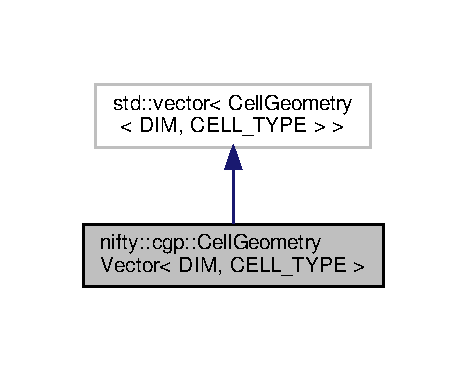
\includegraphics[width=224pt]{classnifty_1_1cgp_1_1CellGeometryVector__inherit__graph}
\end{center}
\end{figure}


Collaboration diagram for nifty\+:\+:cgp\+:\+:Cell\+Geometry\+Vector$<$ D\+I\+M, C\+E\+L\+L\+\_\+\+T\+Y\+P\+E $>$\+:\nopagebreak
\begin{figure}[H]
\begin{center}
\leavevmode
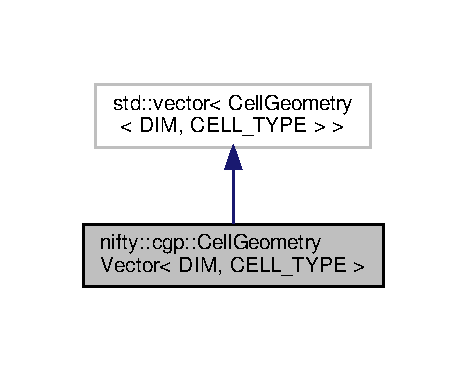
\includegraphics[width=224pt]{classnifty_1_1cgp_1_1CellGeometryVector__coll__graph}
\end{center}
\end{figure}


The documentation for this class was generated from the following file\+:\begin{DoxyCompactItemize}
\item 
/home/tbeier/src/nifty/include/nifty/cgp/\hyperlink{geometry_8hxx}{geometry.\+hxx}\end{DoxyCompactItemize}

\hypertarget{classnifty_1_1cgp_1_1CellVector}{}\section{nifty\+:\+:cgp\+:\+:Cell\+Vector$<$ T $>$ Class Template Reference}
\label{classnifty_1_1cgp_1_1CellVector}\index{nifty\+::cgp\+::\+Cell\+Vector$<$ T $>$@{nifty\+::cgp\+::\+Cell\+Vector$<$ T $>$}}


{\ttfamily \#include $<$cell\+\_\+vector.\+hxx$>$}



Inheritance diagram for nifty\+:\+:cgp\+:\+:Cell\+Vector$<$ T $>$\+:\nopagebreak
\begin{figure}[H]
\begin{center}
\leavevmode
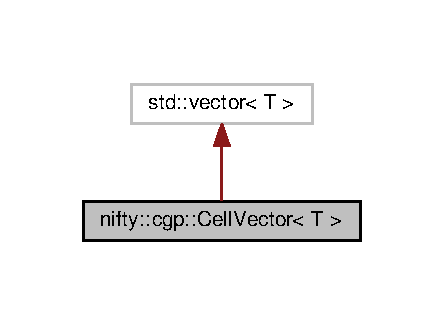
\includegraphics[width=213pt]{classnifty_1_1cgp_1_1CellVector__inherit__graph}
\end{center}
\end{figure}


Collaboration diagram for nifty\+:\+:cgp\+:\+:Cell\+Vector$<$ T $>$\+:\nopagebreak
\begin{figure}[H]
\begin{center}
\leavevmode
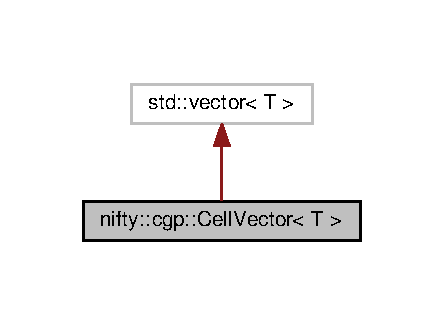
\includegraphics[width=213pt]{classnifty_1_1cgp_1_1CellVector__coll__graph}
\end{center}
\end{figure}


The documentation for this class was generated from the following file\+:\begin{DoxyCompactItemize}
\item 
/home/tbeier/src/nifty/include/nifty/cgp/\hyperlink{cell__vector_8hxx}{cell\+\_\+vector.\+hxx}\end{DoxyCompactItemize}

\hypertarget{classnifty_1_1graph_1_1optimization_1_1multicut_1_1Cgc}{}\section{nifty\+:\+:graph\+:\+:optimization\+:\+:multicut\+:\+:Cgc$<$ O\+B\+J\+E\+C\+T\+I\+V\+E $>$ Class Template Reference}
\label{classnifty_1_1graph_1_1optimization_1_1multicut_1_1Cgc}\index{nifty\+::graph\+::optimization\+::multicut\+::\+Cgc$<$ O\+B\+J\+E\+C\+T\+I\+V\+E $>$@{nifty\+::graph\+::optimization\+::multicut\+::\+Cgc$<$ O\+B\+J\+E\+C\+T\+I\+V\+E $>$}}


{\ttfamily \#include $<$cgc.\+hxx$>$}



Inheritance diagram for nifty\+:\+:graph\+:\+:optimization\+:\+:multicut\+:\+:Cgc$<$ O\+B\+J\+E\+C\+T\+I\+V\+E $>$\+:\nopagebreak
\begin{figure}[H]
\begin{center}
\leavevmode
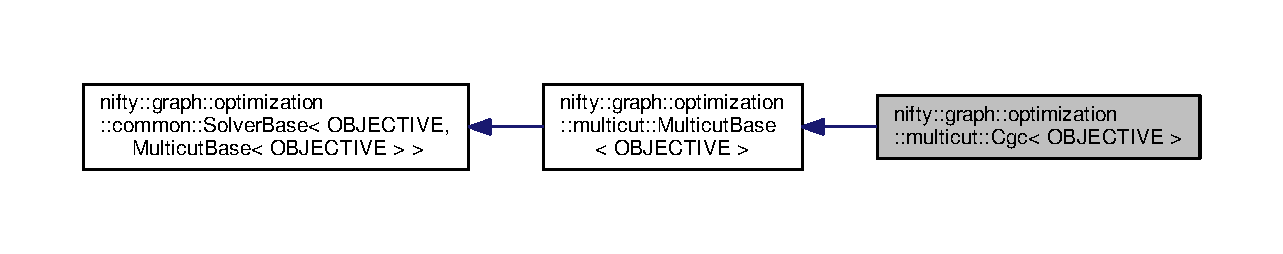
\includegraphics[width=350pt]{classnifty_1_1graph_1_1optimization_1_1multicut_1_1Cgc__inherit__graph}
\end{center}
\end{figure}


Collaboration diagram for nifty\+:\+:graph\+:\+:optimization\+:\+:multicut\+:\+:Cgc$<$ O\+B\+J\+E\+C\+T\+I\+V\+E $>$\+:\nopagebreak
\begin{figure}[H]
\begin{center}
\leavevmode
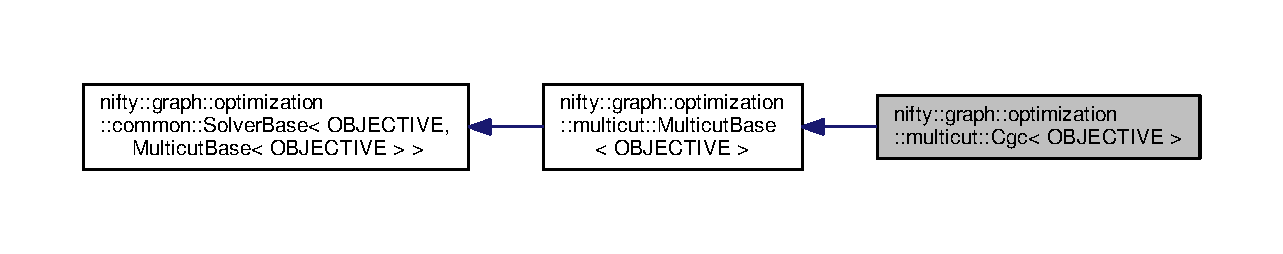
\includegraphics[width=350pt]{classnifty_1_1graph_1_1optimization_1_1multicut_1_1Cgc__coll__graph}
\end{center}
\end{figure}
\subsection*{Classes}
\begin{DoxyCompactItemize}
\item 
struct \hyperlink{structnifty_1_1graph_1_1optimization_1_1multicut_1_1Cgc_1_1SettingsType}{Settings\+Type}
\end{DoxyCompactItemize}
\subsection*{Public Types}
\begin{DoxyCompactItemize}
\item 
typedef O\+B\+J\+E\+C\+T\+I\+V\+E \hyperlink{classnifty_1_1graph_1_1optimization_1_1multicut_1_1Cgc_ac3e728f92d355814ff3b40b5f7d59123}{Objective}
\item 
typedef O\+B\+J\+E\+C\+T\+I\+V\+E \hyperlink{classnifty_1_1graph_1_1optimization_1_1multicut_1_1Cgc_a10339a861b453cdeb2e85e8371bd013d}{Objective\+Type}
\item 
typedef Objective\+Type\+::\+Weight\+Type \hyperlink{classnifty_1_1graph_1_1optimization_1_1multicut_1_1Cgc_ac8f7c1da4b33561e45fe423f2c12b2b5}{Weight\+Type}
\item 
typedef \hyperlink{classnifty_1_1graph_1_1optimization_1_1multicut_1_1MulticutBase}{Multicut\+Base}$<$ \hyperlink{classnifty_1_1graph_1_1optimization_1_1multicut_1_1Cgc_a10339a861b453cdeb2e85e8371bd013d}{Objective\+Type} $>$ \hyperlink{classnifty_1_1graph_1_1optimization_1_1multicut_1_1Cgc_aa973cf9cceaa9e15ea351036f3c81fdf}{Base\+Type}
\item 
typedef \hyperlink{classnifty_1_1graph_1_1optimization_1_1common_1_1SolverBase_a5a14d64c70a9cc0eebc7d71d2b089f9b}{Base\+Type\+::\+Visitor\+Base\+Type} \hyperlink{classnifty_1_1graph_1_1optimization_1_1multicut_1_1Cgc_adb95cdb68d34774e9a3cb4990ab54ccb}{Visitor\+Base\+Type}
\item 
typedef \hyperlink{classnifty_1_1graph_1_1optimization_1_1common_1_1SolverBase_a58913ea9ab9232ff72608b710c1012d0}{Base\+Type\+::\+Visitor\+Proxy\+Type} \hyperlink{classnifty_1_1graph_1_1optimization_1_1multicut_1_1Cgc_a0c82617574e6f1c5b2e801ed5699d725}{Visitor\+Proxy\+Type}
\item 
typedef \hyperlink{classnifty_1_1graph_1_1optimization_1_1common_1_1SolverBase_a6e4e465f3b6e039882669fcfb9714818}{Base\+Type\+::\+Node\+Labels\+Type} \hyperlink{classnifty_1_1graph_1_1optimization_1_1multicut_1_1Cgc_a2976a0116b64803813b4b0c1555a2e70}{Node\+Labels\+Type}
\item 
typedef Objective\+Type\+::\+Graph \hyperlink{classnifty_1_1graph_1_1optimization_1_1multicut_1_1Cgc_a4737d533c9d4d62c220bb81f5acba0fe}{Graph}
\item 
typedef Objective\+Type\+::\+Graph\+Type \hyperlink{classnifty_1_1graph_1_1optimization_1_1multicut_1_1Cgc_a7954c621d6b0085dac0a0208e8edeb98}{Graph\+Type}
\item 
typedef Objective\+Type\+::\+Weights\+Map \hyperlink{classnifty_1_1graph_1_1optimization_1_1multicut_1_1Cgc_a6d3ba8605fd7c111fca7a9f79ca09c32}{Weights\+Map}
\item 
typedef Graph\+Type\+::template Edge\+Map$<$ uint8\+\_\+t $>$ \hyperlink{classnifty_1_1graph_1_1optimization_1_1multicut_1_1Cgc_a9aab1ca56069c4f2801a35bf05620465}{Is\+Dirty\+Edge}
\item 
typedef \hyperlink{classnifty_1_1graph_1_1UndirectedGraph}{Undirected\+Graph} \hyperlink{classnifty_1_1graph_1_1optimization_1_1multicut_1_1Cgc_a477a719159f23300cd8e627a825e9275}{Sub\+Graph}
\item 
typedef \hyperlink{classnifty_1_1graph_1_1optimization_1_1mincut_1_1MincutObjective}{mincut\+::\+Mincut\+Objective}$<$ \hyperlink{classnifty_1_1graph_1_1optimization_1_1multicut_1_1Cgc_a477a719159f23300cd8e627a825e9275}{Sub\+Graph}, double $>$ \hyperlink{classnifty_1_1graph_1_1optimization_1_1multicut_1_1Cgc_a3a662b7fd59d4ba56da98b359c47d63c}{Mincut\+Sub\+Objective}
\item 
typedef \hyperlink{classnifty_1_1graph_1_1optimization_1_1mincut_1_1MincutBase}{mincut\+::\+Mincut\+Base}$<$ \hyperlink{classnifty_1_1graph_1_1optimization_1_1multicut_1_1Cgc_a3a662b7fd59d4ba56da98b359c47d63c}{Mincut\+Sub\+Objective} $>$ \hyperlink{classnifty_1_1graph_1_1optimization_1_1multicut_1_1Cgc_aa4e8e89c78edc941bdb1b9331c81395d}{Mincut\+Sub\+Base}
\item 
typedef \hyperlink{classnifty_1_1graph_1_1optimization_1_1common_1_1SolverFactoryBase}{nifty\+::graph\+::optimization\+::common\+::\+Solver\+Factory\+Base}$<$ \hyperlink{classnifty_1_1graph_1_1optimization_1_1multicut_1_1Cgc_aa4e8e89c78edc941bdb1b9331c81395d}{Mincut\+Sub\+Base} $>$ \hyperlink{classnifty_1_1graph_1_1optimization_1_1multicut_1_1Cgc_a104f55e83ebbaf6451d0260210f0c7dc}{Mincut\+Sub\+Mc\+Factory\+Base}
\item 
typedef \hyperlink{classnifty_1_1graph_1_1optimization_1_1common_1_1SolverBase_a6e4e465f3b6e039882669fcfb9714818}{Mincut\+Sub\+Base\+::\+Node\+Labels\+Type} \hyperlink{classnifty_1_1graph_1_1optimization_1_1multicut_1_1Cgc_a068e52c9f641116d85685d4ce70f418b}{Mincut\+Sub\+Node\+Labels}
\item 
typedef \hyperlink{classnifty_1_1graph_1_1optimization_1_1multicut_1_1MulticutObjective}{Multicut\+Objective}$<$ \hyperlink{classnifty_1_1graph_1_1optimization_1_1multicut_1_1Cgc_a477a719159f23300cd8e627a825e9275}{Sub\+Graph}, double $>$ \hyperlink{classnifty_1_1graph_1_1optimization_1_1multicut_1_1Cgc_a437e2332f586cdb3f4ee55e3cf1ea224}{Multicut\+Sub\+Objective}
\item 
typedef \hyperlink{classnifty_1_1graph_1_1optimization_1_1multicut_1_1MulticutBase}{Multicut\+Base}$<$ \hyperlink{classnifty_1_1graph_1_1optimization_1_1multicut_1_1Cgc_a437e2332f586cdb3f4ee55e3cf1ea224}{Multicut\+Sub\+Objective} $>$ \hyperlink{classnifty_1_1graph_1_1optimization_1_1multicut_1_1Cgc_a9bd82569e6729554ef0a07ad57f2bd94}{Multicut\+Sub\+Base}
\item 
typedef \hyperlink{classnifty_1_1graph_1_1optimization_1_1common_1_1SolverFactoryBase}{nifty\+::graph\+::optimization\+::common\+::\+Solver\+Factory\+Base}$<$ \hyperlink{classnifty_1_1graph_1_1optimization_1_1multicut_1_1Cgc_a9bd82569e6729554ef0a07ad57f2bd94}{Multicut\+Sub\+Base} $>$ \hyperlink{classnifty_1_1graph_1_1optimization_1_1multicut_1_1Cgc_a5516da27348db37b794d25628deb9e82}{Multicut\+Sub\+Mc\+Factory\+Base}
\item 
typedef \hyperlink{classnifty_1_1graph_1_1optimization_1_1common_1_1SolverBase_a6e4e465f3b6e039882669fcfb9714818}{Multicut\+Sub\+Base\+::\+Node\+Labels\+Type} \hyperlink{classnifty_1_1graph_1_1optimization_1_1multicut_1_1Cgc_a8a87ee61f8ce21292822f91e1f71c8d3}{Multicut\+Sub\+Node\+Labels}
\item 
typedef \hyperlink{classnifty_1_1graph_1_1optimization_1_1common_1_1SolverFactoryBase}{nifty\+::graph\+::optimization\+::common\+::\+Solver\+Factory\+Base}$<$ \hyperlink{classnifty_1_1graph_1_1optimization_1_1multicut_1_1Cgc_aa973cf9cceaa9e15ea351036f3c81fdf}{Base\+Type} $>$ \hyperlink{classnifty_1_1graph_1_1optimization_1_1multicut_1_1Cgc_af4275240831bf3922200609cab98fc1b}{Factory\+Base}
\end{DoxyCompactItemize}
\subsection*{Public Member Functions}
\begin{DoxyCompactItemize}
\item 
virtual \hyperlink{classnifty_1_1graph_1_1optimization_1_1multicut_1_1Cgc_a22509c2e989ab4f224a4caacfb54d6da}{$\sim$\+Cgc} ()
\item 
\hyperlink{classnifty_1_1graph_1_1optimization_1_1multicut_1_1Cgc_afe174dda4970687cecc6ac2ad2c94e6a}{Cgc} (const \hyperlink{classnifty_1_1graph_1_1optimization_1_1multicut_1_1Cgc_ac3e728f92d355814ff3b40b5f7d59123}{Objective} \&\hyperlink{classnifty_1_1graph_1_1optimization_1_1multicut_1_1Cgc_a926b85b4bfa4de48b4040b87f679a377}{objective}, const \hyperlink{structnifty_1_1graph_1_1optimization_1_1multicut_1_1Cgc_1_1SettingsType}{Settings\+Type} \&settings=\hyperlink{structnifty_1_1graph_1_1optimization_1_1multicut_1_1Cgc_1_1SettingsType}{Settings\+Type}())
\item 
virtual void \hyperlink{classnifty_1_1graph_1_1optimization_1_1multicut_1_1Cgc_af2cd396aefa38ad0f69bb5191954dac3}{optimize} (\hyperlink{classnifty_1_1graph_1_1optimization_1_1multicut_1_1Cgc_a2976a0116b64803813b4b0c1555a2e70}{Node\+Labels\+Type} \&node\+Labels, \hyperlink{classnifty_1_1graph_1_1optimization_1_1multicut_1_1Cgc_adb95cdb68d34774e9a3cb4990ab54ccb}{Visitor\+Base\+Type} $\ast$visitor)
\item 
virtual const \hyperlink{classnifty_1_1graph_1_1optimization_1_1multicut_1_1Cgc_ac3e728f92d355814ff3b40b5f7d59123}{Objective} \& \hyperlink{classnifty_1_1graph_1_1optimization_1_1multicut_1_1Cgc_a926b85b4bfa4de48b4040b87f679a377}{objective} () const 
\item 
virtual const \hyperlink{classnifty_1_1graph_1_1optimization_1_1multicut_1_1Cgc_a2976a0116b64803813b4b0c1555a2e70}{Node\+Labels\+Type} \& \hyperlink{classnifty_1_1graph_1_1optimization_1_1multicut_1_1Cgc_a6bece7a6c255cb25d8a99c9bcb05bbb7}{current\+Best\+Node\+Labels} ()
\item 
virtual std\+::string \hyperlink{classnifty_1_1graph_1_1optimization_1_1multicut_1_1Cgc_ab54c4448bd816fbbc4a45c2dd8e9562d}{name} () const 
\item 
virtual void \hyperlink{classnifty_1_1graph_1_1optimization_1_1multicut_1_1Cgc_a45593f369b20f4a535bc79835f7d2541}{weights\+Changed} ()
\begin{DoxyCompactList}\small\item\em Inform solver about a change of weights. \end{DoxyCompactList}\item 
virtual double \hyperlink{classnifty_1_1graph_1_1optimization_1_1multicut_1_1Cgc_ad05e02649243b645e0c4e4a23d9835b1}{current\+Best\+Energy} ()
\end{DoxyCompactItemize}


\subsection{Member Typedef Documentation}
\hypertarget{classnifty_1_1graph_1_1optimization_1_1multicut_1_1Cgc_aa973cf9cceaa9e15ea351036f3c81fdf}{}\index{nifty\+::graph\+::optimization\+::multicut\+::\+Cgc@{nifty\+::graph\+::optimization\+::multicut\+::\+Cgc}!Base\+Type@{Base\+Type}}
\index{Base\+Type@{Base\+Type}!nifty\+::graph\+::optimization\+::multicut\+::\+Cgc@{nifty\+::graph\+::optimization\+::multicut\+::\+Cgc}}
\subsubsection[{Base\+Type}]{\setlength{\rightskip}{0pt plus 5cm}template$<$class O\+B\+J\+E\+C\+T\+I\+V\+E$>$ typedef {\bf Multicut\+Base}$<${\bf Objective\+Type}$>$ {\bf nifty\+::graph\+::optimization\+::multicut\+::\+Cgc}$<$ O\+B\+J\+E\+C\+T\+I\+V\+E $>$\+::{\bf Base\+Type}}\label{classnifty_1_1graph_1_1optimization_1_1multicut_1_1Cgc_aa973cf9cceaa9e15ea351036f3c81fdf}
\hypertarget{classnifty_1_1graph_1_1optimization_1_1multicut_1_1Cgc_af4275240831bf3922200609cab98fc1b}{}\index{nifty\+::graph\+::optimization\+::multicut\+::\+Cgc@{nifty\+::graph\+::optimization\+::multicut\+::\+Cgc}!Factory\+Base@{Factory\+Base}}
\index{Factory\+Base@{Factory\+Base}!nifty\+::graph\+::optimization\+::multicut\+::\+Cgc@{nifty\+::graph\+::optimization\+::multicut\+::\+Cgc}}
\subsubsection[{Factory\+Base}]{\setlength{\rightskip}{0pt plus 5cm}template$<$class O\+B\+J\+E\+C\+T\+I\+V\+E$>$ typedef {\bf nifty\+::graph\+::optimization\+::common\+::\+Solver\+Factory\+Base}$<${\bf Base\+Type}$>$ {\bf nifty\+::graph\+::optimization\+::multicut\+::\+Cgc}$<$ O\+B\+J\+E\+C\+T\+I\+V\+E $>$\+::{\bf Factory\+Base}}\label{classnifty_1_1graph_1_1optimization_1_1multicut_1_1Cgc_af4275240831bf3922200609cab98fc1b}
\hypertarget{classnifty_1_1graph_1_1optimization_1_1multicut_1_1Cgc_a4737d533c9d4d62c220bb81f5acba0fe}{}\index{nifty\+::graph\+::optimization\+::multicut\+::\+Cgc@{nifty\+::graph\+::optimization\+::multicut\+::\+Cgc}!Graph@{Graph}}
\index{Graph@{Graph}!nifty\+::graph\+::optimization\+::multicut\+::\+Cgc@{nifty\+::graph\+::optimization\+::multicut\+::\+Cgc}}
\subsubsection[{Graph}]{\setlength{\rightskip}{0pt plus 5cm}template$<$class O\+B\+J\+E\+C\+T\+I\+V\+E$>$ typedef Objective\+Type\+::\+Graph {\bf nifty\+::graph\+::optimization\+::multicut\+::\+Cgc}$<$ O\+B\+J\+E\+C\+T\+I\+V\+E $>$\+::{\bf Graph}}\label{classnifty_1_1graph_1_1optimization_1_1multicut_1_1Cgc_a4737d533c9d4d62c220bb81f5acba0fe}
\hypertarget{classnifty_1_1graph_1_1optimization_1_1multicut_1_1Cgc_a7954c621d6b0085dac0a0208e8edeb98}{}\index{nifty\+::graph\+::optimization\+::multicut\+::\+Cgc@{nifty\+::graph\+::optimization\+::multicut\+::\+Cgc}!Graph\+Type@{Graph\+Type}}
\index{Graph\+Type@{Graph\+Type}!nifty\+::graph\+::optimization\+::multicut\+::\+Cgc@{nifty\+::graph\+::optimization\+::multicut\+::\+Cgc}}
\subsubsection[{Graph\+Type}]{\setlength{\rightskip}{0pt plus 5cm}template$<$class O\+B\+J\+E\+C\+T\+I\+V\+E$>$ typedef Objective\+Type\+::\+Graph\+Type {\bf nifty\+::graph\+::optimization\+::multicut\+::\+Cgc}$<$ O\+B\+J\+E\+C\+T\+I\+V\+E $>$\+::{\bf Graph\+Type}}\label{classnifty_1_1graph_1_1optimization_1_1multicut_1_1Cgc_a7954c621d6b0085dac0a0208e8edeb98}
\hypertarget{classnifty_1_1graph_1_1optimization_1_1multicut_1_1Cgc_a9aab1ca56069c4f2801a35bf05620465}{}\index{nifty\+::graph\+::optimization\+::multicut\+::\+Cgc@{nifty\+::graph\+::optimization\+::multicut\+::\+Cgc}!Is\+Dirty\+Edge@{Is\+Dirty\+Edge}}
\index{Is\+Dirty\+Edge@{Is\+Dirty\+Edge}!nifty\+::graph\+::optimization\+::multicut\+::\+Cgc@{nifty\+::graph\+::optimization\+::multicut\+::\+Cgc}}
\subsubsection[{Is\+Dirty\+Edge}]{\setlength{\rightskip}{0pt plus 5cm}template$<$class O\+B\+J\+E\+C\+T\+I\+V\+E$>$ typedef Graph\+Type\+:: template Edge\+Map$<$uint8\+\_\+t$>$ {\bf nifty\+::graph\+::optimization\+::multicut\+::\+Cgc}$<$ O\+B\+J\+E\+C\+T\+I\+V\+E $>$\+::{\bf Is\+Dirty\+Edge}}\label{classnifty_1_1graph_1_1optimization_1_1multicut_1_1Cgc_a9aab1ca56069c4f2801a35bf05620465}
\hypertarget{classnifty_1_1graph_1_1optimization_1_1multicut_1_1Cgc_aa4e8e89c78edc941bdb1b9331c81395d}{}\index{nifty\+::graph\+::optimization\+::multicut\+::\+Cgc@{nifty\+::graph\+::optimization\+::multicut\+::\+Cgc}!Mincut\+Sub\+Base@{Mincut\+Sub\+Base}}
\index{Mincut\+Sub\+Base@{Mincut\+Sub\+Base}!nifty\+::graph\+::optimization\+::multicut\+::\+Cgc@{nifty\+::graph\+::optimization\+::multicut\+::\+Cgc}}
\subsubsection[{Mincut\+Sub\+Base}]{\setlength{\rightskip}{0pt plus 5cm}template$<$class O\+B\+J\+E\+C\+T\+I\+V\+E$>$ typedef {\bf mincut\+::\+Mincut\+Base}$<${\bf Mincut\+Sub\+Objective}$>$ {\bf nifty\+::graph\+::optimization\+::multicut\+::\+Cgc}$<$ O\+B\+J\+E\+C\+T\+I\+V\+E $>$\+::{\bf Mincut\+Sub\+Base}}\label{classnifty_1_1graph_1_1optimization_1_1multicut_1_1Cgc_aa4e8e89c78edc941bdb1b9331c81395d}
\hypertarget{classnifty_1_1graph_1_1optimization_1_1multicut_1_1Cgc_a104f55e83ebbaf6451d0260210f0c7dc}{}\index{nifty\+::graph\+::optimization\+::multicut\+::\+Cgc@{nifty\+::graph\+::optimization\+::multicut\+::\+Cgc}!Mincut\+Sub\+Mc\+Factory\+Base@{Mincut\+Sub\+Mc\+Factory\+Base}}
\index{Mincut\+Sub\+Mc\+Factory\+Base@{Mincut\+Sub\+Mc\+Factory\+Base}!nifty\+::graph\+::optimization\+::multicut\+::\+Cgc@{nifty\+::graph\+::optimization\+::multicut\+::\+Cgc}}
\subsubsection[{Mincut\+Sub\+Mc\+Factory\+Base}]{\setlength{\rightskip}{0pt plus 5cm}template$<$class O\+B\+J\+E\+C\+T\+I\+V\+E$>$ typedef {\bf nifty\+::graph\+::optimization\+::common\+::\+Solver\+Factory\+Base}$<${\bf Mincut\+Sub\+Base}$>$ {\bf nifty\+::graph\+::optimization\+::multicut\+::\+Cgc}$<$ O\+B\+J\+E\+C\+T\+I\+V\+E $>$\+::{\bf Mincut\+Sub\+Mc\+Factory\+Base}}\label{classnifty_1_1graph_1_1optimization_1_1multicut_1_1Cgc_a104f55e83ebbaf6451d0260210f0c7dc}
\hypertarget{classnifty_1_1graph_1_1optimization_1_1multicut_1_1Cgc_a068e52c9f641116d85685d4ce70f418b}{}\index{nifty\+::graph\+::optimization\+::multicut\+::\+Cgc@{nifty\+::graph\+::optimization\+::multicut\+::\+Cgc}!Mincut\+Sub\+Node\+Labels@{Mincut\+Sub\+Node\+Labels}}
\index{Mincut\+Sub\+Node\+Labels@{Mincut\+Sub\+Node\+Labels}!nifty\+::graph\+::optimization\+::multicut\+::\+Cgc@{nifty\+::graph\+::optimization\+::multicut\+::\+Cgc}}
\subsubsection[{Mincut\+Sub\+Node\+Labels}]{\setlength{\rightskip}{0pt plus 5cm}template$<$class O\+B\+J\+E\+C\+T\+I\+V\+E$>$ typedef {\bf Mincut\+Sub\+Base\+::\+Node\+Labels\+Type} {\bf nifty\+::graph\+::optimization\+::multicut\+::\+Cgc}$<$ O\+B\+J\+E\+C\+T\+I\+V\+E $>$\+::{\bf Mincut\+Sub\+Node\+Labels}}\label{classnifty_1_1graph_1_1optimization_1_1multicut_1_1Cgc_a068e52c9f641116d85685d4ce70f418b}
\hypertarget{classnifty_1_1graph_1_1optimization_1_1multicut_1_1Cgc_a3a662b7fd59d4ba56da98b359c47d63c}{}\index{nifty\+::graph\+::optimization\+::multicut\+::\+Cgc@{nifty\+::graph\+::optimization\+::multicut\+::\+Cgc}!Mincut\+Sub\+Objective@{Mincut\+Sub\+Objective}}
\index{Mincut\+Sub\+Objective@{Mincut\+Sub\+Objective}!nifty\+::graph\+::optimization\+::multicut\+::\+Cgc@{nifty\+::graph\+::optimization\+::multicut\+::\+Cgc}}
\subsubsection[{Mincut\+Sub\+Objective}]{\setlength{\rightskip}{0pt plus 5cm}template$<$class O\+B\+J\+E\+C\+T\+I\+V\+E$>$ typedef {\bf mincut\+::\+Mincut\+Objective}$<${\bf Sub\+Graph}, double$>$ {\bf nifty\+::graph\+::optimization\+::multicut\+::\+Cgc}$<$ O\+B\+J\+E\+C\+T\+I\+V\+E $>$\+::{\bf Mincut\+Sub\+Objective}}\label{classnifty_1_1graph_1_1optimization_1_1multicut_1_1Cgc_a3a662b7fd59d4ba56da98b359c47d63c}
\hypertarget{classnifty_1_1graph_1_1optimization_1_1multicut_1_1Cgc_a9bd82569e6729554ef0a07ad57f2bd94}{}\index{nifty\+::graph\+::optimization\+::multicut\+::\+Cgc@{nifty\+::graph\+::optimization\+::multicut\+::\+Cgc}!Multicut\+Sub\+Base@{Multicut\+Sub\+Base}}
\index{Multicut\+Sub\+Base@{Multicut\+Sub\+Base}!nifty\+::graph\+::optimization\+::multicut\+::\+Cgc@{nifty\+::graph\+::optimization\+::multicut\+::\+Cgc}}
\subsubsection[{Multicut\+Sub\+Base}]{\setlength{\rightskip}{0pt plus 5cm}template$<$class O\+B\+J\+E\+C\+T\+I\+V\+E$>$ typedef {\bf Multicut\+Base}$<${\bf Multicut\+Sub\+Objective}$>$ {\bf nifty\+::graph\+::optimization\+::multicut\+::\+Cgc}$<$ O\+B\+J\+E\+C\+T\+I\+V\+E $>$\+::{\bf Multicut\+Sub\+Base}}\label{classnifty_1_1graph_1_1optimization_1_1multicut_1_1Cgc_a9bd82569e6729554ef0a07ad57f2bd94}
\hypertarget{classnifty_1_1graph_1_1optimization_1_1multicut_1_1Cgc_a5516da27348db37b794d25628deb9e82}{}\index{nifty\+::graph\+::optimization\+::multicut\+::\+Cgc@{nifty\+::graph\+::optimization\+::multicut\+::\+Cgc}!Multicut\+Sub\+Mc\+Factory\+Base@{Multicut\+Sub\+Mc\+Factory\+Base}}
\index{Multicut\+Sub\+Mc\+Factory\+Base@{Multicut\+Sub\+Mc\+Factory\+Base}!nifty\+::graph\+::optimization\+::multicut\+::\+Cgc@{nifty\+::graph\+::optimization\+::multicut\+::\+Cgc}}
\subsubsection[{Multicut\+Sub\+Mc\+Factory\+Base}]{\setlength{\rightskip}{0pt plus 5cm}template$<$class O\+B\+J\+E\+C\+T\+I\+V\+E$>$ typedef {\bf nifty\+::graph\+::optimization\+::common\+::\+Solver\+Factory\+Base}$<${\bf Multicut\+Sub\+Base}$>$ {\bf nifty\+::graph\+::optimization\+::multicut\+::\+Cgc}$<$ O\+B\+J\+E\+C\+T\+I\+V\+E $>$\+::{\bf Multicut\+Sub\+Mc\+Factory\+Base}}\label{classnifty_1_1graph_1_1optimization_1_1multicut_1_1Cgc_a5516da27348db37b794d25628deb9e82}
\hypertarget{classnifty_1_1graph_1_1optimization_1_1multicut_1_1Cgc_a8a87ee61f8ce21292822f91e1f71c8d3}{}\index{nifty\+::graph\+::optimization\+::multicut\+::\+Cgc@{nifty\+::graph\+::optimization\+::multicut\+::\+Cgc}!Multicut\+Sub\+Node\+Labels@{Multicut\+Sub\+Node\+Labels}}
\index{Multicut\+Sub\+Node\+Labels@{Multicut\+Sub\+Node\+Labels}!nifty\+::graph\+::optimization\+::multicut\+::\+Cgc@{nifty\+::graph\+::optimization\+::multicut\+::\+Cgc}}
\subsubsection[{Multicut\+Sub\+Node\+Labels}]{\setlength{\rightskip}{0pt plus 5cm}template$<$class O\+B\+J\+E\+C\+T\+I\+V\+E$>$ typedef {\bf Multicut\+Sub\+Base\+::\+Node\+Labels\+Type} {\bf nifty\+::graph\+::optimization\+::multicut\+::\+Cgc}$<$ O\+B\+J\+E\+C\+T\+I\+V\+E $>$\+::{\bf Multicut\+Sub\+Node\+Labels}}\label{classnifty_1_1graph_1_1optimization_1_1multicut_1_1Cgc_a8a87ee61f8ce21292822f91e1f71c8d3}
\hypertarget{classnifty_1_1graph_1_1optimization_1_1multicut_1_1Cgc_a437e2332f586cdb3f4ee55e3cf1ea224}{}\index{nifty\+::graph\+::optimization\+::multicut\+::\+Cgc@{nifty\+::graph\+::optimization\+::multicut\+::\+Cgc}!Multicut\+Sub\+Objective@{Multicut\+Sub\+Objective}}
\index{Multicut\+Sub\+Objective@{Multicut\+Sub\+Objective}!nifty\+::graph\+::optimization\+::multicut\+::\+Cgc@{nifty\+::graph\+::optimization\+::multicut\+::\+Cgc}}
\subsubsection[{Multicut\+Sub\+Objective}]{\setlength{\rightskip}{0pt plus 5cm}template$<$class O\+B\+J\+E\+C\+T\+I\+V\+E$>$ typedef {\bf Multicut\+Objective}$<${\bf Sub\+Graph}, double$>$ {\bf nifty\+::graph\+::optimization\+::multicut\+::\+Cgc}$<$ O\+B\+J\+E\+C\+T\+I\+V\+E $>$\+::{\bf Multicut\+Sub\+Objective}}\label{classnifty_1_1graph_1_1optimization_1_1multicut_1_1Cgc_a437e2332f586cdb3f4ee55e3cf1ea224}
\hypertarget{classnifty_1_1graph_1_1optimization_1_1multicut_1_1Cgc_a2976a0116b64803813b4b0c1555a2e70}{}\index{nifty\+::graph\+::optimization\+::multicut\+::\+Cgc@{nifty\+::graph\+::optimization\+::multicut\+::\+Cgc}!Node\+Labels\+Type@{Node\+Labels\+Type}}
\index{Node\+Labels\+Type@{Node\+Labels\+Type}!nifty\+::graph\+::optimization\+::multicut\+::\+Cgc@{nifty\+::graph\+::optimization\+::multicut\+::\+Cgc}}
\subsubsection[{Node\+Labels\+Type}]{\setlength{\rightskip}{0pt plus 5cm}template$<$class O\+B\+J\+E\+C\+T\+I\+V\+E$>$ typedef {\bf Base\+Type\+::\+Node\+Labels\+Type} {\bf nifty\+::graph\+::optimization\+::multicut\+::\+Cgc}$<$ O\+B\+J\+E\+C\+T\+I\+V\+E $>$\+::{\bf Node\+Labels\+Type}}\label{classnifty_1_1graph_1_1optimization_1_1multicut_1_1Cgc_a2976a0116b64803813b4b0c1555a2e70}
\hypertarget{classnifty_1_1graph_1_1optimization_1_1multicut_1_1Cgc_ac3e728f92d355814ff3b40b5f7d59123}{}\index{nifty\+::graph\+::optimization\+::multicut\+::\+Cgc@{nifty\+::graph\+::optimization\+::multicut\+::\+Cgc}!Objective@{Objective}}
\index{Objective@{Objective}!nifty\+::graph\+::optimization\+::multicut\+::\+Cgc@{nifty\+::graph\+::optimization\+::multicut\+::\+Cgc}}
\subsubsection[{Objective}]{\setlength{\rightskip}{0pt plus 5cm}template$<$class O\+B\+J\+E\+C\+T\+I\+V\+E$>$ typedef O\+B\+J\+E\+C\+T\+I\+V\+E {\bf nifty\+::graph\+::optimization\+::multicut\+::\+Cgc}$<$ O\+B\+J\+E\+C\+T\+I\+V\+E $>$\+::{\bf Objective}}\label{classnifty_1_1graph_1_1optimization_1_1multicut_1_1Cgc_ac3e728f92d355814ff3b40b5f7d59123}
\hypertarget{classnifty_1_1graph_1_1optimization_1_1multicut_1_1Cgc_a10339a861b453cdeb2e85e8371bd013d}{}\index{nifty\+::graph\+::optimization\+::multicut\+::\+Cgc@{nifty\+::graph\+::optimization\+::multicut\+::\+Cgc}!Objective\+Type@{Objective\+Type}}
\index{Objective\+Type@{Objective\+Type}!nifty\+::graph\+::optimization\+::multicut\+::\+Cgc@{nifty\+::graph\+::optimization\+::multicut\+::\+Cgc}}
\subsubsection[{Objective\+Type}]{\setlength{\rightskip}{0pt plus 5cm}template$<$class O\+B\+J\+E\+C\+T\+I\+V\+E$>$ typedef O\+B\+J\+E\+C\+T\+I\+V\+E {\bf nifty\+::graph\+::optimization\+::multicut\+::\+Cgc}$<$ O\+B\+J\+E\+C\+T\+I\+V\+E $>$\+::{\bf Objective\+Type}}\label{classnifty_1_1graph_1_1optimization_1_1multicut_1_1Cgc_a10339a861b453cdeb2e85e8371bd013d}
\hypertarget{classnifty_1_1graph_1_1optimization_1_1multicut_1_1Cgc_a477a719159f23300cd8e627a825e9275}{}\index{nifty\+::graph\+::optimization\+::multicut\+::\+Cgc@{nifty\+::graph\+::optimization\+::multicut\+::\+Cgc}!Sub\+Graph@{Sub\+Graph}}
\index{Sub\+Graph@{Sub\+Graph}!nifty\+::graph\+::optimization\+::multicut\+::\+Cgc@{nifty\+::graph\+::optimization\+::multicut\+::\+Cgc}}
\subsubsection[{Sub\+Graph}]{\setlength{\rightskip}{0pt plus 5cm}template$<$class O\+B\+J\+E\+C\+T\+I\+V\+E$>$ typedef {\bf Undirected\+Graph} {\bf nifty\+::graph\+::optimization\+::multicut\+::\+Cgc}$<$ O\+B\+J\+E\+C\+T\+I\+V\+E $>$\+::{\bf Sub\+Graph}}\label{classnifty_1_1graph_1_1optimization_1_1multicut_1_1Cgc_a477a719159f23300cd8e627a825e9275}
\hypertarget{classnifty_1_1graph_1_1optimization_1_1multicut_1_1Cgc_adb95cdb68d34774e9a3cb4990ab54ccb}{}\index{nifty\+::graph\+::optimization\+::multicut\+::\+Cgc@{nifty\+::graph\+::optimization\+::multicut\+::\+Cgc}!Visitor\+Base\+Type@{Visitor\+Base\+Type}}
\index{Visitor\+Base\+Type@{Visitor\+Base\+Type}!nifty\+::graph\+::optimization\+::multicut\+::\+Cgc@{nifty\+::graph\+::optimization\+::multicut\+::\+Cgc}}
\subsubsection[{Visitor\+Base\+Type}]{\setlength{\rightskip}{0pt plus 5cm}template$<$class O\+B\+J\+E\+C\+T\+I\+V\+E$>$ typedef {\bf Base\+Type\+::\+Visitor\+Base\+Type} {\bf nifty\+::graph\+::optimization\+::multicut\+::\+Cgc}$<$ O\+B\+J\+E\+C\+T\+I\+V\+E $>$\+::{\bf Visitor\+Base\+Type}}\label{classnifty_1_1graph_1_1optimization_1_1multicut_1_1Cgc_adb95cdb68d34774e9a3cb4990ab54ccb}
\hypertarget{classnifty_1_1graph_1_1optimization_1_1multicut_1_1Cgc_a0c82617574e6f1c5b2e801ed5699d725}{}\index{nifty\+::graph\+::optimization\+::multicut\+::\+Cgc@{nifty\+::graph\+::optimization\+::multicut\+::\+Cgc}!Visitor\+Proxy\+Type@{Visitor\+Proxy\+Type}}
\index{Visitor\+Proxy\+Type@{Visitor\+Proxy\+Type}!nifty\+::graph\+::optimization\+::multicut\+::\+Cgc@{nifty\+::graph\+::optimization\+::multicut\+::\+Cgc}}
\subsubsection[{Visitor\+Proxy\+Type}]{\setlength{\rightskip}{0pt plus 5cm}template$<$class O\+B\+J\+E\+C\+T\+I\+V\+E$>$ typedef {\bf Base\+Type\+::\+Visitor\+Proxy\+Type} {\bf nifty\+::graph\+::optimization\+::multicut\+::\+Cgc}$<$ O\+B\+J\+E\+C\+T\+I\+V\+E $>$\+::{\bf Visitor\+Proxy\+Type}}\label{classnifty_1_1graph_1_1optimization_1_1multicut_1_1Cgc_a0c82617574e6f1c5b2e801ed5699d725}
\hypertarget{classnifty_1_1graph_1_1optimization_1_1multicut_1_1Cgc_a6d3ba8605fd7c111fca7a9f79ca09c32}{}\index{nifty\+::graph\+::optimization\+::multicut\+::\+Cgc@{nifty\+::graph\+::optimization\+::multicut\+::\+Cgc}!Weights\+Map@{Weights\+Map}}
\index{Weights\+Map@{Weights\+Map}!nifty\+::graph\+::optimization\+::multicut\+::\+Cgc@{nifty\+::graph\+::optimization\+::multicut\+::\+Cgc}}
\subsubsection[{Weights\+Map}]{\setlength{\rightskip}{0pt plus 5cm}template$<$class O\+B\+J\+E\+C\+T\+I\+V\+E$>$ typedef Objective\+Type\+::\+Weights\+Map {\bf nifty\+::graph\+::optimization\+::multicut\+::\+Cgc}$<$ O\+B\+J\+E\+C\+T\+I\+V\+E $>$\+::{\bf Weights\+Map}}\label{classnifty_1_1graph_1_1optimization_1_1multicut_1_1Cgc_a6d3ba8605fd7c111fca7a9f79ca09c32}
\hypertarget{classnifty_1_1graph_1_1optimization_1_1multicut_1_1Cgc_ac8f7c1da4b33561e45fe423f2c12b2b5}{}\index{nifty\+::graph\+::optimization\+::multicut\+::\+Cgc@{nifty\+::graph\+::optimization\+::multicut\+::\+Cgc}!Weight\+Type@{Weight\+Type}}
\index{Weight\+Type@{Weight\+Type}!nifty\+::graph\+::optimization\+::multicut\+::\+Cgc@{nifty\+::graph\+::optimization\+::multicut\+::\+Cgc}}
\subsubsection[{Weight\+Type}]{\setlength{\rightskip}{0pt plus 5cm}template$<$class O\+B\+J\+E\+C\+T\+I\+V\+E$>$ typedef Objective\+Type\+::\+Weight\+Type {\bf nifty\+::graph\+::optimization\+::multicut\+::\+Cgc}$<$ O\+B\+J\+E\+C\+T\+I\+V\+E $>$\+::{\bf Weight\+Type}}\label{classnifty_1_1graph_1_1optimization_1_1multicut_1_1Cgc_ac8f7c1da4b33561e45fe423f2c12b2b5}


\subsection{Constructor \& Destructor Documentation}
\hypertarget{classnifty_1_1graph_1_1optimization_1_1multicut_1_1Cgc_a22509c2e989ab4f224a4caacfb54d6da}{}\index{nifty\+::graph\+::optimization\+::multicut\+::\+Cgc@{nifty\+::graph\+::optimization\+::multicut\+::\+Cgc}!````~Cgc@{$\sim$\+Cgc}}
\index{````~Cgc@{$\sim$\+Cgc}!nifty\+::graph\+::optimization\+::multicut\+::\+Cgc@{nifty\+::graph\+::optimization\+::multicut\+::\+Cgc}}
\subsubsection[{$\sim$\+Cgc()}]{\setlength{\rightskip}{0pt plus 5cm}template$<$class O\+B\+J\+E\+C\+T\+I\+V\+E$>$ virtual {\bf nifty\+::graph\+::optimization\+::multicut\+::\+Cgc}$<$ O\+B\+J\+E\+C\+T\+I\+V\+E $>$\+::$\sim${\bf Cgc} (
\begin{DoxyParamCaption}
{}
\end{DoxyParamCaption}
)\hspace{0.3cm}{\ttfamily [inline]}, {\ttfamily [virtual]}}\label{classnifty_1_1graph_1_1optimization_1_1multicut_1_1Cgc_a22509c2e989ab4f224a4caacfb54d6da}
\hypertarget{classnifty_1_1graph_1_1optimization_1_1multicut_1_1Cgc_afe174dda4970687cecc6ac2ad2c94e6a}{}\index{nifty\+::graph\+::optimization\+::multicut\+::\+Cgc@{nifty\+::graph\+::optimization\+::multicut\+::\+Cgc}!Cgc@{Cgc}}
\index{Cgc@{Cgc}!nifty\+::graph\+::optimization\+::multicut\+::\+Cgc@{nifty\+::graph\+::optimization\+::multicut\+::\+Cgc}}
\subsubsection[{Cgc(const Objective \&objective, const Settings\+Type \&settings=\+Settings\+Type())}]{\setlength{\rightskip}{0pt plus 5cm}template$<$class O\+B\+J\+E\+C\+T\+I\+V\+E $>$ {\bf nifty\+::graph\+::optimization\+::multicut\+::\+Cgc}$<$ O\+B\+J\+E\+C\+T\+I\+V\+E $>$\+::{\bf Cgc} (
\begin{DoxyParamCaption}
\item[{const {\bf Objective} \&}]{objective, }
\item[{const {\bf Settings\+Type} \&}]{settings = {\ttfamily {\bf Settings\+Type}()}}
\end{DoxyParamCaption}
)}\label{classnifty_1_1graph_1_1optimization_1_1multicut_1_1Cgc_afe174dda4970687cecc6ac2ad2c94e6a}


\subsection{Member Function Documentation}
\hypertarget{classnifty_1_1graph_1_1optimization_1_1multicut_1_1Cgc_ad05e02649243b645e0c4e4a23d9835b1}{}\index{nifty\+::graph\+::optimization\+::multicut\+::\+Cgc@{nifty\+::graph\+::optimization\+::multicut\+::\+Cgc}!current\+Best\+Energy@{current\+Best\+Energy}}
\index{current\+Best\+Energy@{current\+Best\+Energy}!nifty\+::graph\+::optimization\+::multicut\+::\+Cgc@{nifty\+::graph\+::optimization\+::multicut\+::\+Cgc}}
\subsubsection[{current\+Best\+Energy()}]{\setlength{\rightskip}{0pt plus 5cm}template$<$class O\+B\+J\+E\+C\+T\+I\+V\+E$>$ virtual double {\bf nifty\+::graph\+::optimization\+::multicut\+::\+Cgc}$<$ O\+B\+J\+E\+C\+T\+I\+V\+E $>$\+::current\+Best\+Energy (
\begin{DoxyParamCaption}
{}
\end{DoxyParamCaption}
)\hspace{0.3cm}{\ttfamily [inline]}, {\ttfamily [virtual]}}\label{classnifty_1_1graph_1_1optimization_1_1multicut_1_1Cgc_ad05e02649243b645e0c4e4a23d9835b1}


Reimplemented from \hyperlink{classnifty_1_1graph_1_1optimization_1_1common_1_1SolverBase_ae6f6d9779398689c84984a7b6083604a}{nifty\+::graph\+::optimization\+::common\+::\+Solver\+Base$<$ O\+B\+J\+E\+C\+T\+I\+V\+E, Multicut\+Base$<$ O\+B\+J\+E\+C\+T\+I\+V\+E $>$ $>$}.

\hypertarget{classnifty_1_1graph_1_1optimization_1_1multicut_1_1Cgc_a6bece7a6c255cb25d8a99c9bcb05bbb7}{}\index{nifty\+::graph\+::optimization\+::multicut\+::\+Cgc@{nifty\+::graph\+::optimization\+::multicut\+::\+Cgc}!current\+Best\+Node\+Labels@{current\+Best\+Node\+Labels}}
\index{current\+Best\+Node\+Labels@{current\+Best\+Node\+Labels}!nifty\+::graph\+::optimization\+::multicut\+::\+Cgc@{nifty\+::graph\+::optimization\+::multicut\+::\+Cgc}}
\subsubsection[{current\+Best\+Node\+Labels()}]{\setlength{\rightskip}{0pt plus 5cm}template$<$class O\+B\+J\+E\+C\+T\+I\+V\+E$>$ virtual const {\bf Node\+Labels\+Type}\& {\bf nifty\+::graph\+::optimization\+::multicut\+::\+Cgc}$<$ O\+B\+J\+E\+C\+T\+I\+V\+E $>$\+::current\+Best\+Node\+Labels (
\begin{DoxyParamCaption}
{}
\end{DoxyParamCaption}
)\hspace{0.3cm}{\ttfamily [inline]}, {\ttfamily [virtual]}}\label{classnifty_1_1graph_1_1optimization_1_1multicut_1_1Cgc_a6bece7a6c255cb25d8a99c9bcb05bbb7}


Implements \hyperlink{classnifty_1_1graph_1_1optimization_1_1common_1_1SolverBase_a3634ba645adbb7a668500e807608bcca}{nifty\+::graph\+::optimization\+::common\+::\+Solver\+Base$<$ O\+B\+J\+E\+C\+T\+I\+V\+E, Multicut\+Base$<$ O\+B\+J\+E\+C\+T\+I\+V\+E $>$ $>$}.

\hypertarget{classnifty_1_1graph_1_1optimization_1_1multicut_1_1Cgc_ab54c4448bd816fbbc4a45c2dd8e9562d}{}\index{nifty\+::graph\+::optimization\+::multicut\+::\+Cgc@{nifty\+::graph\+::optimization\+::multicut\+::\+Cgc}!name@{name}}
\index{name@{name}!nifty\+::graph\+::optimization\+::multicut\+::\+Cgc@{nifty\+::graph\+::optimization\+::multicut\+::\+Cgc}}
\subsubsection[{name() const }]{\setlength{\rightskip}{0pt plus 5cm}template$<$class O\+B\+J\+E\+C\+T\+I\+V\+E$>$ virtual std\+::string {\bf nifty\+::graph\+::optimization\+::multicut\+::\+Cgc}$<$ O\+B\+J\+E\+C\+T\+I\+V\+E $>$\+::name (
\begin{DoxyParamCaption}
{}
\end{DoxyParamCaption}
) const\hspace{0.3cm}{\ttfamily [inline]}, {\ttfamily [virtual]}}\label{classnifty_1_1graph_1_1optimization_1_1multicut_1_1Cgc_ab54c4448bd816fbbc4a45c2dd8e9562d}


Implements \hyperlink{classnifty_1_1graph_1_1optimization_1_1common_1_1SolverBase_abc9685a3d63748ac470afccb2813be7e}{nifty\+::graph\+::optimization\+::common\+::\+Solver\+Base$<$ O\+B\+J\+E\+C\+T\+I\+V\+E, Multicut\+Base$<$ O\+B\+J\+E\+C\+T\+I\+V\+E $>$ $>$}.

\hypertarget{classnifty_1_1graph_1_1optimization_1_1multicut_1_1Cgc_a926b85b4bfa4de48b4040b87f679a377}{}\index{nifty\+::graph\+::optimization\+::multicut\+::\+Cgc@{nifty\+::graph\+::optimization\+::multicut\+::\+Cgc}!objective@{objective}}
\index{objective@{objective}!nifty\+::graph\+::optimization\+::multicut\+::\+Cgc@{nifty\+::graph\+::optimization\+::multicut\+::\+Cgc}}
\subsubsection[{objective() const }]{\setlength{\rightskip}{0pt plus 5cm}template$<$class O\+B\+J\+E\+C\+T\+I\+V\+E $>$ const {\bf Cgc}$<$ O\+B\+J\+E\+C\+T\+I\+V\+E $>$\+::{\bf Objective} \& {\bf nifty\+::graph\+::optimization\+::multicut\+::\+Cgc}$<$ O\+B\+J\+E\+C\+T\+I\+V\+E $>$\+::objective (
\begin{DoxyParamCaption}
{}
\end{DoxyParamCaption}
) const\hspace{0.3cm}{\ttfamily [virtual]}}\label{classnifty_1_1graph_1_1optimization_1_1multicut_1_1Cgc_a926b85b4bfa4de48b4040b87f679a377}


Implements \hyperlink{classnifty_1_1graph_1_1optimization_1_1common_1_1SolverBase_ae7d36a7485b12a25979f75771f52e397}{nifty\+::graph\+::optimization\+::common\+::\+Solver\+Base$<$ O\+B\+J\+E\+C\+T\+I\+V\+E, Multicut\+Base$<$ O\+B\+J\+E\+C\+T\+I\+V\+E $>$ $>$}.

\hypertarget{classnifty_1_1graph_1_1optimization_1_1multicut_1_1Cgc_af2cd396aefa38ad0f69bb5191954dac3}{}\index{nifty\+::graph\+::optimization\+::multicut\+::\+Cgc@{nifty\+::graph\+::optimization\+::multicut\+::\+Cgc}!optimize@{optimize}}
\index{optimize@{optimize}!nifty\+::graph\+::optimization\+::multicut\+::\+Cgc@{nifty\+::graph\+::optimization\+::multicut\+::\+Cgc}}
\subsubsection[{optimize(\+Node\+Labels\+Type \&node\+Labels, Visitor\+Base\+Type $\ast$visitor)}]{\setlength{\rightskip}{0pt plus 5cm}template$<$class O\+B\+J\+E\+C\+T\+I\+V\+E $>$ void {\bf nifty\+::graph\+::optimization\+::multicut\+::\+Cgc}$<$ O\+B\+J\+E\+C\+T\+I\+V\+E $>$\+::optimize (
\begin{DoxyParamCaption}
\item[{{\bf Node\+Labels\+Type} \&}]{node\+Labels, }
\item[{{\bf Visitor\+Base\+Type} $\ast$}]{visitor}
\end{DoxyParamCaption}
)\hspace{0.3cm}{\ttfamily [virtual]}}\label{classnifty_1_1graph_1_1optimization_1_1multicut_1_1Cgc_af2cd396aefa38ad0f69bb5191954dac3}


Implements \hyperlink{classnifty_1_1graph_1_1optimization_1_1common_1_1SolverBase_a1c08eb1ff2b3cca5366c3aab161ba040}{nifty\+::graph\+::optimization\+::common\+::\+Solver\+Base$<$ O\+B\+J\+E\+C\+T\+I\+V\+E, Multicut\+Base$<$ O\+B\+J\+E\+C\+T\+I\+V\+E $>$ $>$}.

\hypertarget{classnifty_1_1graph_1_1optimization_1_1multicut_1_1Cgc_a45593f369b20f4a535bc79835f7d2541}{}\index{nifty\+::graph\+::optimization\+::multicut\+::\+Cgc@{nifty\+::graph\+::optimization\+::multicut\+::\+Cgc}!weights\+Changed@{weights\+Changed}}
\index{weights\+Changed@{weights\+Changed}!nifty\+::graph\+::optimization\+::multicut\+::\+Cgc@{nifty\+::graph\+::optimization\+::multicut\+::\+Cgc}}
\subsubsection[{weights\+Changed()}]{\setlength{\rightskip}{0pt plus 5cm}template$<$class O\+B\+J\+E\+C\+T\+I\+V\+E$>$ virtual void {\bf nifty\+::graph\+::optimization\+::multicut\+::\+Cgc}$<$ O\+B\+J\+E\+C\+T\+I\+V\+E $>$\+::weights\+Changed (
\begin{DoxyParamCaption}
{}
\end{DoxyParamCaption}
)\hspace{0.3cm}{\ttfamily [inline]}, {\ttfamily [virtual]}}\label{classnifty_1_1graph_1_1optimization_1_1multicut_1_1Cgc_a45593f369b20f4a535bc79835f7d2541}


Inform solver about a change of weights. 

Inform solver that all weights could have changed. If a particular solver does not overload this function, an Weights\+Changed\+Not\+Supported exception is thrown. After a call of this function it is save to run optimize again, therefore it resets the solver 

Reimplemented from \hyperlink{classnifty_1_1graph_1_1optimization_1_1common_1_1SolverBase_a8ab38d61068370e24cca475ef1b5d8b1}{nifty\+::graph\+::optimization\+::common\+::\+Solver\+Base$<$ O\+B\+J\+E\+C\+T\+I\+V\+E, Multicut\+Base$<$ O\+B\+J\+E\+C\+T\+I\+V\+E $>$ $>$}.



The documentation for this class was generated from the following file\+:\begin{DoxyCompactItemize}
\item 
/home/tbeier/src/nifty/include/nifty/graph/optimization/multicut/\hyperlink{cgc_8hxx}{cgc.\+hxx}\end{DoxyCompactItemize}

\hypertarget{classnifty_1_1graph_1_1ChainedSolvers}{}\section{nifty\+:\+:graph\+:\+:Chained\+Solvers$<$ O\+B\+J\+E\+C\+T\+I\+V\+E $>$ Class Template Reference}
\label{classnifty_1_1graph_1_1ChainedSolvers}\index{nifty\+::graph\+::\+Chained\+Solvers$<$ O\+B\+J\+E\+C\+T\+I\+V\+E $>$@{nifty\+::graph\+::\+Chained\+Solvers$<$ O\+B\+J\+E\+C\+T\+I\+V\+E $>$}}


{\ttfamily \#include $<$chained\+\_\+solvers.\+hxx$>$}



Inheritance diagram for nifty\+:\+:graph\+:\+:Chained\+Solvers$<$ O\+B\+J\+E\+C\+T\+I\+V\+E $>$\+:
% FIG 0


Collaboration diagram for nifty\+:\+:graph\+:\+:Chained\+Solvers$<$ O\+B\+J\+E\+C\+T\+I\+V\+E $>$\+:
% FIG 1
\subsection*{Classes}
\begin{DoxyCompactItemize}
\item 
class \hyperlink{classnifty_1_1graph_1_1ChainedSolvers_1_1NoBeginEndVisitor}{No\+Begin\+End\+Visitor}
\item 
struct \hyperlink{structnifty_1_1graph_1_1ChainedSolvers_1_1Settings}{Settings}
\end{DoxyCompactItemize}
\subsection*{Public Types}
\begin{DoxyCompactItemize}
\item 
typedef O\+B\+J\+E\+C\+T\+I\+V\+E \hyperlink{classnifty_1_1graph_1_1ChainedSolvers_a963bd16d8459fe660e207c4a57facf5e}{Objective}
\item 
typedef O\+B\+J\+E\+C\+T\+I\+V\+E \hyperlink{classnifty_1_1graph_1_1ChainedSolvers_af640cd977746e90c49366fe7a30e80b1}{Objective\+Type}
\item 
typedef Objective\+Type\+::\+Weight\+Type \hyperlink{classnifty_1_1graph_1_1ChainedSolvers_a274e68cb50882d8b6eb45a100f930efe}{Weight\+Type}
\item 
typedef \hyperlink{classnifty_1_1graph_1_1MulticutBase}{Multicut\+Base}$<$ \hyperlink{classnifty_1_1graph_1_1ChainedSolvers_af640cd977746e90c49366fe7a30e80b1}{Objective\+Type} $>$ \hyperlink{classnifty_1_1graph_1_1ChainedSolvers_af3c13fd5bc8d12ef88678d8191886f1a}{Base}
\item 
typedef \hyperlink{classnifty_1_1graph_1_1MulticutBase_a5882fb69df59d8113f6a81a0dac26eaa}{Base\+::\+Visitor\+Base} \hyperlink{classnifty_1_1graph_1_1ChainedSolvers_a1f90d20ae903cad5e6434d4019b28463}{Visitor\+Base}
\item 
typedef \hyperlink{classnifty_1_1graph_1_1MulticutBase_a6ede271a3cb0ae4711a7e9da2b07efa9}{Base\+::\+Visitor\+Proxy} \hyperlink{classnifty_1_1graph_1_1ChainedSolvers_a2a0d35b426487bc1c84acbac754688e9}{Visitor\+Proxy}
\item 
typedef \hyperlink{classnifty_1_1graph_1_1MulticutBase_aaeefe3c5df81d9c9efffec878cf2fcd7}{Base\+::\+Edge\+Labels} \hyperlink{classnifty_1_1graph_1_1ChainedSolvers_a28c50d486ee20744432cc66e2bab9890}{Edge\+Labels}
\item 
typedef \hyperlink{classnifty_1_1graph_1_1MulticutBase_afba61ad2919d0fad20b3745af19309da}{Base\+::\+Node\+Labels} \hyperlink{classnifty_1_1graph_1_1ChainedSolvers_a68ac6338bbf4e29e0324152d462715de}{Node\+Labels}
\item 
typedef Objective\+Type\+::\+Graph \hyperlink{classnifty_1_1graph_1_1ChainedSolvers_a74491b36d70e81078f265943e85a51ab}{Graph}
\item 
typedef Objective\+Type\+::\+Graph\+Type \hyperlink{classnifty_1_1graph_1_1ChainedSolvers_ab55e77819ad5f20d4c1193ed745b49fe}{Graph\+Type}
\item 
typedef Objective\+Type\+::\+Weights\+Map \hyperlink{classnifty_1_1graph_1_1ChainedSolvers_a34ed66af894d4382882ec3b81260686f}{Weights\+Map}
\item 
typedef Graph\+Type\+::template Edge\+Map$<$ uint8\+\_\+t $>$ \hyperlink{classnifty_1_1graph_1_1ChainedSolvers_a85e87137c3b85a8f4c4a64fba26394c3}{Is\+Dirty\+Edge}
\item 
typedef \hyperlink{classnifty_1_1graph_1_1MulticutFactoryBase}{Multicut\+Factory\+Base}$<$ \hyperlink{classnifty_1_1graph_1_1ChainedSolvers_af640cd977746e90c49366fe7a30e80b1}{Objective\+Type} $>$ \hyperlink{classnifty_1_1graph_1_1ChainedSolvers_a8a106a334a73a0dd278d06af04ef163d}{Mc\+Factory\+Base}
\end{DoxyCompactItemize}
\subsection*{Public Member Functions}
\begin{DoxyCompactItemize}
\item 
virtual \hyperlink{classnifty_1_1graph_1_1ChainedSolvers_a54c7367c6886af3dc8d484c9ed1d2cc5}{$\sim$\+Chained\+Solvers} ()
\item 
\hyperlink{classnifty_1_1graph_1_1ChainedSolvers_aa15e6835ad08bbc1daf51f676887b9bf}{Chained\+Solvers} (const \hyperlink{classnifty_1_1graph_1_1ChainedSolvers_a963bd16d8459fe660e207c4a57facf5e}{Objective} \&\hyperlink{classnifty_1_1graph_1_1ChainedSolvers_a2ab1b10b87194aa4f4139e4a9ad16632}{objective}, const \hyperlink{structnifty_1_1graph_1_1ChainedSolvers_1_1Settings}{Settings} \&settings=\hyperlink{structnifty_1_1graph_1_1ChainedSolvers_1_1Settings}{Settings}())
\item 
virtual void \hyperlink{classnifty_1_1graph_1_1ChainedSolvers_a1459a25679420dbca4fdecad9ed182fd}{optimize} (\hyperlink{classnifty_1_1graph_1_1ChainedSolvers_a68ac6338bbf4e29e0324152d462715de}{Node\+Labels} \&node\+Labels, \hyperlink{classnifty_1_1graph_1_1ChainedSolvers_a1f90d20ae903cad5e6434d4019b28463}{Visitor\+Base} $\ast$visitor)
\item 
virtual const \hyperlink{classnifty_1_1graph_1_1ChainedSolvers_a963bd16d8459fe660e207c4a57facf5e}{Objective} \& \hyperlink{classnifty_1_1graph_1_1ChainedSolvers_a2ab1b10b87194aa4f4139e4a9ad16632}{objective} () const 
\item 
virtual const \hyperlink{classnifty_1_1graph_1_1ChainedSolvers_a68ac6338bbf4e29e0324152d462715de}{Node\+Labels} \& \hyperlink{classnifty_1_1graph_1_1ChainedSolvers_a5a83f2befc63b62a7925427b252b93bd}{current\+Best\+Node\+Labels} ()
\item 
virtual std\+::string \hyperlink{classnifty_1_1graph_1_1ChainedSolvers_a3ba4c6ab8a961b79f67ddbec23659430}{name} () const 
\item 
virtual void \hyperlink{classnifty_1_1graph_1_1ChainedSolvers_af141004d09e61bf1f8369f838ab0524f}{weights\+Changed} ()
\begin{DoxyCompactList}\small\item\em Inform solver about a change of weights. \end{DoxyCompactList}\item 
virtual double \hyperlink{classnifty_1_1graph_1_1ChainedSolvers_ae387881603a426c47de8caaf7717ff72}{current\+Best\+Energy} ()
\end{DoxyCompactItemize}


\subsection{Member Typedef Documentation}
\hypertarget{classnifty_1_1graph_1_1ChainedSolvers_af3c13fd5bc8d12ef88678d8191886f1a}{}\index{nifty\+::graph\+::\+Chained\+Solvers@{nifty\+::graph\+::\+Chained\+Solvers}!Base@{Base}}
\index{Base@{Base}!nifty\+::graph\+::\+Chained\+Solvers@{nifty\+::graph\+::\+Chained\+Solvers}}
\subsubsection[{Base}]{\setlength{\rightskip}{0pt plus 5cm}template$<$class O\+B\+J\+E\+C\+T\+I\+V\+E$>$ typedef {\bf Multicut\+Base}$<${\bf Objective\+Type}$>$ {\bf nifty\+::graph\+::\+Chained\+Solvers}$<$ O\+B\+J\+E\+C\+T\+I\+V\+E $>$\+::{\bf Base}}\label{classnifty_1_1graph_1_1ChainedSolvers_af3c13fd5bc8d12ef88678d8191886f1a}
\hypertarget{classnifty_1_1graph_1_1ChainedSolvers_a28c50d486ee20744432cc66e2bab9890}{}\index{nifty\+::graph\+::\+Chained\+Solvers@{nifty\+::graph\+::\+Chained\+Solvers}!Edge\+Labels@{Edge\+Labels}}
\index{Edge\+Labels@{Edge\+Labels}!nifty\+::graph\+::\+Chained\+Solvers@{nifty\+::graph\+::\+Chained\+Solvers}}
\subsubsection[{Edge\+Labels}]{\setlength{\rightskip}{0pt plus 5cm}template$<$class O\+B\+J\+E\+C\+T\+I\+V\+E$>$ typedef {\bf Base\+::\+Edge\+Labels} {\bf nifty\+::graph\+::\+Chained\+Solvers}$<$ O\+B\+J\+E\+C\+T\+I\+V\+E $>$\+::{\bf Edge\+Labels}}\label{classnifty_1_1graph_1_1ChainedSolvers_a28c50d486ee20744432cc66e2bab9890}
\hypertarget{classnifty_1_1graph_1_1ChainedSolvers_a74491b36d70e81078f265943e85a51ab}{}\index{nifty\+::graph\+::\+Chained\+Solvers@{nifty\+::graph\+::\+Chained\+Solvers}!Graph@{Graph}}
\index{Graph@{Graph}!nifty\+::graph\+::\+Chained\+Solvers@{nifty\+::graph\+::\+Chained\+Solvers}}
\subsubsection[{Graph}]{\setlength{\rightskip}{0pt plus 5cm}template$<$class O\+B\+J\+E\+C\+T\+I\+V\+E$>$ typedef Objective\+Type\+::\+Graph {\bf nifty\+::graph\+::\+Chained\+Solvers}$<$ O\+B\+J\+E\+C\+T\+I\+V\+E $>$\+::{\bf Graph}}\label{classnifty_1_1graph_1_1ChainedSolvers_a74491b36d70e81078f265943e85a51ab}
\hypertarget{classnifty_1_1graph_1_1ChainedSolvers_ab55e77819ad5f20d4c1193ed745b49fe}{}\index{nifty\+::graph\+::\+Chained\+Solvers@{nifty\+::graph\+::\+Chained\+Solvers}!Graph\+Type@{Graph\+Type}}
\index{Graph\+Type@{Graph\+Type}!nifty\+::graph\+::\+Chained\+Solvers@{nifty\+::graph\+::\+Chained\+Solvers}}
\subsubsection[{Graph\+Type}]{\setlength{\rightskip}{0pt plus 5cm}template$<$class O\+B\+J\+E\+C\+T\+I\+V\+E$>$ typedef Objective\+Type\+::\+Graph\+Type {\bf nifty\+::graph\+::\+Chained\+Solvers}$<$ O\+B\+J\+E\+C\+T\+I\+V\+E $>$\+::{\bf Graph\+Type}}\label{classnifty_1_1graph_1_1ChainedSolvers_ab55e77819ad5f20d4c1193ed745b49fe}
\hypertarget{classnifty_1_1graph_1_1ChainedSolvers_a85e87137c3b85a8f4c4a64fba26394c3}{}\index{nifty\+::graph\+::\+Chained\+Solvers@{nifty\+::graph\+::\+Chained\+Solvers}!Is\+Dirty\+Edge@{Is\+Dirty\+Edge}}
\index{Is\+Dirty\+Edge@{Is\+Dirty\+Edge}!nifty\+::graph\+::\+Chained\+Solvers@{nifty\+::graph\+::\+Chained\+Solvers}}
\subsubsection[{Is\+Dirty\+Edge}]{\setlength{\rightskip}{0pt plus 5cm}template$<$class O\+B\+J\+E\+C\+T\+I\+V\+E$>$ typedef Graph\+Type\+:: template Edge\+Map$<$uint8\+\_\+t$>$ {\bf nifty\+::graph\+::\+Chained\+Solvers}$<$ O\+B\+J\+E\+C\+T\+I\+V\+E $>$\+::{\bf Is\+Dirty\+Edge}}\label{classnifty_1_1graph_1_1ChainedSolvers_a85e87137c3b85a8f4c4a64fba26394c3}
\hypertarget{classnifty_1_1graph_1_1ChainedSolvers_a8a106a334a73a0dd278d06af04ef163d}{}\index{nifty\+::graph\+::\+Chained\+Solvers@{nifty\+::graph\+::\+Chained\+Solvers}!Mc\+Factory\+Base@{Mc\+Factory\+Base}}
\index{Mc\+Factory\+Base@{Mc\+Factory\+Base}!nifty\+::graph\+::\+Chained\+Solvers@{nifty\+::graph\+::\+Chained\+Solvers}}
\subsubsection[{Mc\+Factory\+Base}]{\setlength{\rightskip}{0pt plus 5cm}template$<$class O\+B\+J\+E\+C\+T\+I\+V\+E$>$ typedef {\bf Multicut\+Factory\+Base}$<${\bf Objective\+Type}$>$ {\bf nifty\+::graph\+::\+Chained\+Solvers}$<$ O\+B\+J\+E\+C\+T\+I\+V\+E $>$\+::{\bf Mc\+Factory\+Base}}\label{classnifty_1_1graph_1_1ChainedSolvers_a8a106a334a73a0dd278d06af04ef163d}
\hypertarget{classnifty_1_1graph_1_1ChainedSolvers_a68ac6338bbf4e29e0324152d462715de}{}\index{nifty\+::graph\+::\+Chained\+Solvers@{nifty\+::graph\+::\+Chained\+Solvers}!Node\+Labels@{Node\+Labels}}
\index{Node\+Labels@{Node\+Labels}!nifty\+::graph\+::\+Chained\+Solvers@{nifty\+::graph\+::\+Chained\+Solvers}}
\subsubsection[{Node\+Labels}]{\setlength{\rightskip}{0pt plus 5cm}template$<$class O\+B\+J\+E\+C\+T\+I\+V\+E$>$ typedef {\bf Base\+::\+Node\+Labels} {\bf nifty\+::graph\+::\+Chained\+Solvers}$<$ O\+B\+J\+E\+C\+T\+I\+V\+E $>$\+::{\bf Node\+Labels}}\label{classnifty_1_1graph_1_1ChainedSolvers_a68ac6338bbf4e29e0324152d462715de}
\hypertarget{classnifty_1_1graph_1_1ChainedSolvers_a963bd16d8459fe660e207c4a57facf5e}{}\index{nifty\+::graph\+::\+Chained\+Solvers@{nifty\+::graph\+::\+Chained\+Solvers}!Objective@{Objective}}
\index{Objective@{Objective}!nifty\+::graph\+::\+Chained\+Solvers@{nifty\+::graph\+::\+Chained\+Solvers}}
\subsubsection[{Objective}]{\setlength{\rightskip}{0pt plus 5cm}template$<$class O\+B\+J\+E\+C\+T\+I\+V\+E$>$ typedef O\+B\+J\+E\+C\+T\+I\+V\+E {\bf nifty\+::graph\+::\+Chained\+Solvers}$<$ O\+B\+J\+E\+C\+T\+I\+V\+E $>$\+::{\bf Objective}}\label{classnifty_1_1graph_1_1ChainedSolvers_a963bd16d8459fe660e207c4a57facf5e}
\hypertarget{classnifty_1_1graph_1_1ChainedSolvers_af640cd977746e90c49366fe7a30e80b1}{}\index{nifty\+::graph\+::\+Chained\+Solvers@{nifty\+::graph\+::\+Chained\+Solvers}!Objective\+Type@{Objective\+Type}}
\index{Objective\+Type@{Objective\+Type}!nifty\+::graph\+::\+Chained\+Solvers@{nifty\+::graph\+::\+Chained\+Solvers}}
\subsubsection[{Objective\+Type}]{\setlength{\rightskip}{0pt plus 5cm}template$<$class O\+B\+J\+E\+C\+T\+I\+V\+E$>$ typedef O\+B\+J\+E\+C\+T\+I\+V\+E {\bf nifty\+::graph\+::\+Chained\+Solvers}$<$ O\+B\+J\+E\+C\+T\+I\+V\+E $>$\+::{\bf Objective\+Type}}\label{classnifty_1_1graph_1_1ChainedSolvers_af640cd977746e90c49366fe7a30e80b1}
\hypertarget{classnifty_1_1graph_1_1ChainedSolvers_a1f90d20ae903cad5e6434d4019b28463}{}\index{nifty\+::graph\+::\+Chained\+Solvers@{nifty\+::graph\+::\+Chained\+Solvers}!Visitor\+Base@{Visitor\+Base}}
\index{Visitor\+Base@{Visitor\+Base}!nifty\+::graph\+::\+Chained\+Solvers@{nifty\+::graph\+::\+Chained\+Solvers}}
\subsubsection[{Visitor\+Base}]{\setlength{\rightskip}{0pt plus 5cm}template$<$class O\+B\+J\+E\+C\+T\+I\+V\+E$>$ typedef {\bf Base\+::\+Visitor\+Base} {\bf nifty\+::graph\+::\+Chained\+Solvers}$<$ O\+B\+J\+E\+C\+T\+I\+V\+E $>$\+::{\bf Visitor\+Base}}\label{classnifty_1_1graph_1_1ChainedSolvers_a1f90d20ae903cad5e6434d4019b28463}
\hypertarget{classnifty_1_1graph_1_1ChainedSolvers_a2a0d35b426487bc1c84acbac754688e9}{}\index{nifty\+::graph\+::\+Chained\+Solvers@{nifty\+::graph\+::\+Chained\+Solvers}!Visitor\+Proxy@{Visitor\+Proxy}}
\index{Visitor\+Proxy@{Visitor\+Proxy}!nifty\+::graph\+::\+Chained\+Solvers@{nifty\+::graph\+::\+Chained\+Solvers}}
\subsubsection[{Visitor\+Proxy}]{\setlength{\rightskip}{0pt plus 5cm}template$<$class O\+B\+J\+E\+C\+T\+I\+V\+E$>$ typedef {\bf Base\+::\+Visitor\+Proxy} {\bf nifty\+::graph\+::\+Chained\+Solvers}$<$ O\+B\+J\+E\+C\+T\+I\+V\+E $>$\+::{\bf Visitor\+Proxy}}\label{classnifty_1_1graph_1_1ChainedSolvers_a2a0d35b426487bc1c84acbac754688e9}
\hypertarget{classnifty_1_1graph_1_1ChainedSolvers_a34ed66af894d4382882ec3b81260686f}{}\index{nifty\+::graph\+::\+Chained\+Solvers@{nifty\+::graph\+::\+Chained\+Solvers}!Weights\+Map@{Weights\+Map}}
\index{Weights\+Map@{Weights\+Map}!nifty\+::graph\+::\+Chained\+Solvers@{nifty\+::graph\+::\+Chained\+Solvers}}
\subsubsection[{Weights\+Map}]{\setlength{\rightskip}{0pt plus 5cm}template$<$class O\+B\+J\+E\+C\+T\+I\+V\+E$>$ typedef Objective\+Type\+::\+Weights\+Map {\bf nifty\+::graph\+::\+Chained\+Solvers}$<$ O\+B\+J\+E\+C\+T\+I\+V\+E $>$\+::{\bf Weights\+Map}}\label{classnifty_1_1graph_1_1ChainedSolvers_a34ed66af894d4382882ec3b81260686f}
\hypertarget{classnifty_1_1graph_1_1ChainedSolvers_a274e68cb50882d8b6eb45a100f930efe}{}\index{nifty\+::graph\+::\+Chained\+Solvers@{nifty\+::graph\+::\+Chained\+Solvers}!Weight\+Type@{Weight\+Type}}
\index{Weight\+Type@{Weight\+Type}!nifty\+::graph\+::\+Chained\+Solvers@{nifty\+::graph\+::\+Chained\+Solvers}}
\subsubsection[{Weight\+Type}]{\setlength{\rightskip}{0pt plus 5cm}template$<$class O\+B\+J\+E\+C\+T\+I\+V\+E$>$ typedef Objective\+Type\+::\+Weight\+Type {\bf nifty\+::graph\+::\+Chained\+Solvers}$<$ O\+B\+J\+E\+C\+T\+I\+V\+E $>$\+::{\bf Weight\+Type}}\label{classnifty_1_1graph_1_1ChainedSolvers_a274e68cb50882d8b6eb45a100f930efe}


\subsection{Constructor \& Destructor Documentation}
\hypertarget{classnifty_1_1graph_1_1ChainedSolvers_a54c7367c6886af3dc8d484c9ed1d2cc5}{}\index{nifty\+::graph\+::\+Chained\+Solvers@{nifty\+::graph\+::\+Chained\+Solvers}!````~Chained\+Solvers@{$\sim$\+Chained\+Solvers}}
\index{````~Chained\+Solvers@{$\sim$\+Chained\+Solvers}!nifty\+::graph\+::\+Chained\+Solvers@{nifty\+::graph\+::\+Chained\+Solvers}}
\subsubsection[{$\sim$\+Chained\+Solvers()}]{\setlength{\rightskip}{0pt plus 5cm}template$<$class O\+B\+J\+E\+C\+T\+I\+V\+E$>$ virtual {\bf nifty\+::graph\+::\+Chained\+Solvers}$<$ O\+B\+J\+E\+C\+T\+I\+V\+E $>$\+::$\sim${\bf Chained\+Solvers} (
\begin{DoxyParamCaption}
{}
\end{DoxyParamCaption}
)\hspace{0.3cm}{\ttfamily [inline]}, {\ttfamily [virtual]}}\label{classnifty_1_1graph_1_1ChainedSolvers_a54c7367c6886af3dc8d484c9ed1d2cc5}
\hypertarget{classnifty_1_1graph_1_1ChainedSolvers_aa15e6835ad08bbc1daf51f676887b9bf}{}\index{nifty\+::graph\+::\+Chained\+Solvers@{nifty\+::graph\+::\+Chained\+Solvers}!Chained\+Solvers@{Chained\+Solvers}}
\index{Chained\+Solvers@{Chained\+Solvers}!nifty\+::graph\+::\+Chained\+Solvers@{nifty\+::graph\+::\+Chained\+Solvers}}
\subsubsection[{Chained\+Solvers(const Objective \&objective, const Settings \&settings=\+Settings())}]{\setlength{\rightskip}{0pt plus 5cm}template$<$class O\+B\+J\+E\+C\+T\+I\+V\+E $>$ {\bf nifty\+::graph\+::\+Chained\+Solvers}$<$ O\+B\+J\+E\+C\+T\+I\+V\+E $>$\+::{\bf Chained\+Solvers} (
\begin{DoxyParamCaption}
\item[{const {\bf Objective} \&}]{objective, }
\item[{const {\bf Settings} \&}]{settings = {\ttfamily {\bf Settings}()}}
\end{DoxyParamCaption}
)}\label{classnifty_1_1graph_1_1ChainedSolvers_aa15e6835ad08bbc1daf51f676887b9bf}


\subsection{Member Function Documentation}
\hypertarget{classnifty_1_1graph_1_1ChainedSolvers_ae387881603a426c47de8caaf7717ff72}{}\index{nifty\+::graph\+::\+Chained\+Solvers@{nifty\+::graph\+::\+Chained\+Solvers}!current\+Best\+Energy@{current\+Best\+Energy}}
\index{current\+Best\+Energy@{current\+Best\+Energy}!nifty\+::graph\+::\+Chained\+Solvers@{nifty\+::graph\+::\+Chained\+Solvers}}
\subsubsection[{current\+Best\+Energy()}]{\setlength{\rightskip}{0pt plus 5cm}template$<$class O\+B\+J\+E\+C\+T\+I\+V\+E$>$ virtual double {\bf nifty\+::graph\+::\+Chained\+Solvers}$<$ O\+B\+J\+E\+C\+T\+I\+V\+E $>$\+::current\+Best\+Energy (
\begin{DoxyParamCaption}
{}
\end{DoxyParamCaption}
)\hspace{0.3cm}{\ttfamily [inline]}, {\ttfamily [virtual]}}\label{classnifty_1_1graph_1_1ChainedSolvers_ae387881603a426c47de8caaf7717ff72}


Reimplemented from \hyperlink{classnifty_1_1graph_1_1MulticutBase_ad5d1c4f60fc6134ebc418e241f02a2c4}{nifty\+::graph\+::\+Multicut\+Base$<$ O\+B\+J\+E\+C\+T\+I\+V\+E $>$}.

\hypertarget{classnifty_1_1graph_1_1ChainedSolvers_a5a83f2befc63b62a7925427b252b93bd}{}\index{nifty\+::graph\+::\+Chained\+Solvers@{nifty\+::graph\+::\+Chained\+Solvers}!current\+Best\+Node\+Labels@{current\+Best\+Node\+Labels}}
\index{current\+Best\+Node\+Labels@{current\+Best\+Node\+Labels}!nifty\+::graph\+::\+Chained\+Solvers@{nifty\+::graph\+::\+Chained\+Solvers}}
\subsubsection[{current\+Best\+Node\+Labels()}]{\setlength{\rightskip}{0pt plus 5cm}template$<$class O\+B\+J\+E\+C\+T\+I\+V\+E$>$ virtual const {\bf Node\+Labels}\& {\bf nifty\+::graph\+::\+Chained\+Solvers}$<$ O\+B\+J\+E\+C\+T\+I\+V\+E $>$\+::current\+Best\+Node\+Labels (
\begin{DoxyParamCaption}
{}
\end{DoxyParamCaption}
)\hspace{0.3cm}{\ttfamily [inline]}, {\ttfamily [virtual]}}\label{classnifty_1_1graph_1_1ChainedSolvers_a5a83f2befc63b62a7925427b252b93bd}


Implements \hyperlink{classnifty_1_1graph_1_1MulticutBase_ac3927bec2b20026187a4c81d490234a2}{nifty\+::graph\+::\+Multicut\+Base$<$ O\+B\+J\+E\+C\+T\+I\+V\+E $>$}.

\hypertarget{classnifty_1_1graph_1_1ChainedSolvers_a3ba4c6ab8a961b79f67ddbec23659430}{}\index{nifty\+::graph\+::\+Chained\+Solvers@{nifty\+::graph\+::\+Chained\+Solvers}!name@{name}}
\index{name@{name}!nifty\+::graph\+::\+Chained\+Solvers@{nifty\+::graph\+::\+Chained\+Solvers}}
\subsubsection[{name() const }]{\setlength{\rightskip}{0pt plus 5cm}template$<$class O\+B\+J\+E\+C\+T\+I\+V\+E$>$ virtual std\+::string {\bf nifty\+::graph\+::\+Chained\+Solvers}$<$ O\+B\+J\+E\+C\+T\+I\+V\+E $>$\+::name (
\begin{DoxyParamCaption}
{}
\end{DoxyParamCaption}
) const\hspace{0.3cm}{\ttfamily [inline]}, {\ttfamily [virtual]}}\label{classnifty_1_1graph_1_1ChainedSolvers_a3ba4c6ab8a961b79f67ddbec23659430}


Implements \hyperlink{classnifty_1_1graph_1_1MulticutBase_aabd27e510ee958a9764ba2305fccc880}{nifty\+::graph\+::\+Multicut\+Base$<$ O\+B\+J\+E\+C\+T\+I\+V\+E $>$}.

\hypertarget{classnifty_1_1graph_1_1ChainedSolvers_a2ab1b10b87194aa4f4139e4a9ad16632}{}\index{nifty\+::graph\+::\+Chained\+Solvers@{nifty\+::graph\+::\+Chained\+Solvers}!objective@{objective}}
\index{objective@{objective}!nifty\+::graph\+::\+Chained\+Solvers@{nifty\+::graph\+::\+Chained\+Solvers}}
\subsubsection[{objective() const }]{\setlength{\rightskip}{0pt plus 5cm}template$<$class O\+B\+J\+E\+C\+T\+I\+V\+E $>$ const {\bf Chained\+Solvers}$<$ O\+B\+J\+E\+C\+T\+I\+V\+E $>$\+::{\bf Objective} \& {\bf nifty\+::graph\+::\+Chained\+Solvers}$<$ O\+B\+J\+E\+C\+T\+I\+V\+E $>$\+::objective (
\begin{DoxyParamCaption}
{}
\end{DoxyParamCaption}
) const\hspace{0.3cm}{\ttfamily [virtual]}}\label{classnifty_1_1graph_1_1ChainedSolvers_a2ab1b10b87194aa4f4139e4a9ad16632}


Implements \hyperlink{classnifty_1_1graph_1_1MulticutBase_a25b622bf14da660a3d24d022369e510d}{nifty\+::graph\+::\+Multicut\+Base$<$ O\+B\+J\+E\+C\+T\+I\+V\+E $>$}.

\hypertarget{classnifty_1_1graph_1_1ChainedSolvers_a1459a25679420dbca4fdecad9ed182fd}{}\index{nifty\+::graph\+::\+Chained\+Solvers@{nifty\+::graph\+::\+Chained\+Solvers}!optimize@{optimize}}
\index{optimize@{optimize}!nifty\+::graph\+::\+Chained\+Solvers@{nifty\+::graph\+::\+Chained\+Solvers}}
\subsubsection[{optimize(\+Node\+Labels \&node\+Labels, Visitor\+Base $\ast$visitor)}]{\setlength{\rightskip}{0pt plus 5cm}template$<$class O\+B\+J\+E\+C\+T\+I\+V\+E $>$ void {\bf nifty\+::graph\+::\+Chained\+Solvers}$<$ O\+B\+J\+E\+C\+T\+I\+V\+E $>$\+::optimize (
\begin{DoxyParamCaption}
\item[{{\bf Node\+Labels} \&}]{node\+Labels, }
\item[{{\bf Visitor\+Base} $\ast$}]{visitor}
\end{DoxyParamCaption}
)\hspace{0.3cm}{\ttfamily [virtual]}}\label{classnifty_1_1graph_1_1ChainedSolvers_a1459a25679420dbca4fdecad9ed182fd}
\hypertarget{classnifty_1_1graph_1_1ChainedSolvers_af141004d09e61bf1f8369f838ab0524f}{}\index{nifty\+::graph\+::\+Chained\+Solvers@{nifty\+::graph\+::\+Chained\+Solvers}!weights\+Changed@{weights\+Changed}}
\index{weights\+Changed@{weights\+Changed}!nifty\+::graph\+::\+Chained\+Solvers@{nifty\+::graph\+::\+Chained\+Solvers}}
\subsubsection[{weights\+Changed()}]{\setlength{\rightskip}{0pt plus 5cm}template$<$class O\+B\+J\+E\+C\+T\+I\+V\+E$>$ virtual void {\bf nifty\+::graph\+::\+Chained\+Solvers}$<$ O\+B\+J\+E\+C\+T\+I\+V\+E $>$\+::weights\+Changed (
\begin{DoxyParamCaption}
{}
\end{DoxyParamCaption}
)\hspace{0.3cm}{\ttfamily [inline]}, {\ttfamily [virtual]}}\label{classnifty_1_1graph_1_1ChainedSolvers_af141004d09e61bf1f8369f838ab0524f}


Inform solver about a change of weights. 

Inform solver that all weights could have changed. If a particular solver does not overload this function, an Weights\+Changed\+Not\+Supported exception is thrown. After a call of this function it is save to run optimize again, therefore it resets the solver 

Reimplemented from \hyperlink{classnifty_1_1graph_1_1MulticutBase_a4c7a44afdc661993b3252dba62b5386f}{nifty\+::graph\+::\+Multicut\+Base$<$ O\+B\+J\+E\+C\+T\+I\+V\+E $>$}.



The documentation for this class was generated from the following file\+:\begin{DoxyCompactItemize}
\item 
/home/tbeier/src/nifty/include/nifty/graph/optimization/multicut/\hyperlink{chained__solvers_8hxx}{chained\+\_\+solvers.\+hxx}\end{DoxyCompactItemize}

\hypertarget{classnifty_1_1graph_1_1ComponentsBfs}{}\section{nifty\+:\+:graph\+:\+:Components\+Bfs$<$ G\+R\+A\+PH $>$ Class Template Reference}
\label{classnifty_1_1graph_1_1ComponentsBfs}\index{nifty\+::graph\+::\+Components\+Bfs$<$ G\+R\+A\+P\+H $>$@{nifty\+::graph\+::\+Components\+Bfs$<$ G\+R\+A\+P\+H $>$}}


{\ttfamily \#include $<$components.\+hxx$>$}

\subsection*{Public Types}
\begin{DoxyCompactItemize}
\item 
typedef G\+R\+A\+PH \hyperlink{classnifty_1_1graph_1_1ComponentsBfs_a8122d3bba657eeae191a63ea83bfaba9}{Graph\+Type}
\item 
typedef Graph\+Type\+::template Edge\+Map$<$ uint64\+\_\+t $>$ \hyperlink{classnifty_1_1graph_1_1ComponentsBfs_a7fc482c4156bb2923986b1823491b6bf}{Labels\+Map\+Type}
\item 
typedef Graph\+Type\+::template Edge\+Map$<$ bool $>$ \hyperlink{classnifty_1_1graph_1_1ComponentsBfs_aea474b2e133f57c71193ba2fd24c7603}{Visited\+Map\+Type}
\end{DoxyCompactItemize}
\subsection*{Public Member Functions}
\begin{DoxyCompactItemize}
\item 
\hyperlink{classnifty_1_1graph_1_1ComponentsBfs_a90003a691312b18648f12b1f0795e583}{Components\+Bfs} (const \hyperlink{classnifty_1_1graph_1_1ComponentsBfs_a8122d3bba657eeae191a63ea83bfaba9}{Graph\+Type} \&graph)
\item 
uint64\+\_\+t \hyperlink{classnifty_1_1graph_1_1ComponentsBfs_ac0190ac005f86f02b5e5a32abdfb97c5}{build} ()
\item 
{\footnotesize template$<$class S\+U\+B\+G\+R\+A\+P\+H\+\_\+\+M\+A\+SK $>$ }\\uint64\+\_\+t \hyperlink{classnifty_1_1graph_1_1ComponentsBfs_afb7115a59f27fb30906f91dc415e2c5b}{build} (const S\+U\+B\+G\+R\+A\+P\+H\+\_\+\+M\+A\+SK \&mask)
\item 
void \hyperlink{classnifty_1_1graph_1_1ComponentsBfs_a5f606101cb777ed110a4c1ea0ab25139}{reset} ()
\item 
bool \hyperlink{classnifty_1_1graph_1_1ComponentsBfs_a143c2a8363329880698db2a21968df5c}{are\+Connected} (const int64\+\_\+t u, const int64\+\_\+t v) const
\item 
uint64\+\_\+t \hyperlink{classnifty_1_1graph_1_1ComponentsBfs_a00ef0fcd3715ca79a1f2720ff9998655}{component\+Label} (const uint64\+\_\+t u)
\item 
uint64\+\_\+t \hyperlink{classnifty_1_1graph_1_1ComponentsBfs_a88fa91de836b0107b1ce748f37a69bb8}{operator\mbox{[}$\,$\mbox{]}} (const uint64\+\_\+t u) const
\item 
uint64\+\_\+t \hyperlink{classnifty_1_1graph_1_1ComponentsBfs_a0f6ca2e2c1494a5521bc6940b06446bf}{max\+Label} () const
\end{DoxyCompactItemize}


\subsection{Member Typedef Documentation}
\mbox{\Hypertarget{classnifty_1_1graph_1_1ComponentsBfs_a8122d3bba657eeae191a63ea83bfaba9}\label{classnifty_1_1graph_1_1ComponentsBfs_a8122d3bba657eeae191a63ea83bfaba9}} 
\index{nifty\+::graph\+::\+Components\+Bfs@{nifty\+::graph\+::\+Components\+Bfs}!Graph\+Type@{Graph\+Type}}
\index{Graph\+Type@{Graph\+Type}!nifty\+::graph\+::\+Components\+Bfs@{nifty\+::graph\+::\+Components\+Bfs}}
\subsubsection{\texorpdfstring{Graph\+Type}{GraphType}}
{\footnotesize\ttfamily template$<$class G\+R\+A\+PH $>$ \\
typedef G\+R\+A\+PH \hyperlink{classnifty_1_1graph_1_1ComponentsBfs}{nifty\+::graph\+::\+Components\+Bfs}$<$ G\+R\+A\+PH $>$\+::\hyperlink{classnifty_1_1graph_1_1ComponentsBfs_a8122d3bba657eeae191a63ea83bfaba9}{Graph\+Type}}

\mbox{\Hypertarget{classnifty_1_1graph_1_1ComponentsBfs_a7fc482c4156bb2923986b1823491b6bf}\label{classnifty_1_1graph_1_1ComponentsBfs_a7fc482c4156bb2923986b1823491b6bf}} 
\index{nifty\+::graph\+::\+Components\+Bfs@{nifty\+::graph\+::\+Components\+Bfs}!Labels\+Map\+Type@{Labels\+Map\+Type}}
\index{Labels\+Map\+Type@{Labels\+Map\+Type}!nifty\+::graph\+::\+Components\+Bfs@{nifty\+::graph\+::\+Components\+Bfs}}
\subsubsection{\texorpdfstring{Labels\+Map\+Type}{LabelsMapType}}
{\footnotesize\ttfamily template$<$class G\+R\+A\+PH $>$ \\
typedef Graph\+Type\+:: template Edge\+Map$<$uint64\+\_\+t$>$ \hyperlink{classnifty_1_1graph_1_1ComponentsBfs}{nifty\+::graph\+::\+Components\+Bfs}$<$ G\+R\+A\+PH $>$\+::\hyperlink{classnifty_1_1graph_1_1ComponentsBfs_a7fc482c4156bb2923986b1823491b6bf}{Labels\+Map\+Type}}

\mbox{\Hypertarget{classnifty_1_1graph_1_1ComponentsBfs_aea474b2e133f57c71193ba2fd24c7603}\label{classnifty_1_1graph_1_1ComponentsBfs_aea474b2e133f57c71193ba2fd24c7603}} 
\index{nifty\+::graph\+::\+Components\+Bfs@{nifty\+::graph\+::\+Components\+Bfs}!Visited\+Map\+Type@{Visited\+Map\+Type}}
\index{Visited\+Map\+Type@{Visited\+Map\+Type}!nifty\+::graph\+::\+Components\+Bfs@{nifty\+::graph\+::\+Components\+Bfs}}
\subsubsection{\texorpdfstring{Visited\+Map\+Type}{VisitedMapType}}
{\footnotesize\ttfamily template$<$class G\+R\+A\+PH $>$ \\
typedef Graph\+Type\+:: template Edge\+Map$<$bool$>$ \hyperlink{classnifty_1_1graph_1_1ComponentsBfs}{nifty\+::graph\+::\+Components\+Bfs}$<$ G\+R\+A\+PH $>$\+::\hyperlink{classnifty_1_1graph_1_1ComponentsBfs_aea474b2e133f57c71193ba2fd24c7603}{Visited\+Map\+Type}}



\subsection{Constructor \& Destructor Documentation}
\mbox{\Hypertarget{classnifty_1_1graph_1_1ComponentsBfs_a90003a691312b18648f12b1f0795e583}\label{classnifty_1_1graph_1_1ComponentsBfs_a90003a691312b18648f12b1f0795e583}} 
\index{nifty\+::graph\+::\+Components\+Bfs@{nifty\+::graph\+::\+Components\+Bfs}!Components\+Bfs@{Components\+Bfs}}
\index{Components\+Bfs@{Components\+Bfs}!nifty\+::graph\+::\+Components\+Bfs@{nifty\+::graph\+::\+Components\+Bfs}}
\subsubsection{\texorpdfstring{Components\+Bfs()}{ComponentsBfs()}}
{\footnotesize\ttfamily template$<$class G\+R\+A\+PH $>$ \\
\hyperlink{classnifty_1_1graph_1_1ComponentsBfs}{nifty\+::graph\+::\+Components\+Bfs}$<$ G\+R\+A\+PH $>$\+::\hyperlink{classnifty_1_1graph_1_1ComponentsBfs}{Components\+Bfs} (\begin{DoxyParamCaption}\item[{const \hyperlink{classnifty_1_1graph_1_1ComponentsBfs_a8122d3bba657eeae191a63ea83bfaba9}{Graph\+Type} \&}]{graph }\end{DoxyParamCaption})\hspace{0.3cm}{\ttfamily [inline]}}



\subsection{Member Function Documentation}
\mbox{\Hypertarget{classnifty_1_1graph_1_1ComponentsBfs_a143c2a8363329880698db2a21968df5c}\label{classnifty_1_1graph_1_1ComponentsBfs_a143c2a8363329880698db2a21968df5c}} 
\index{nifty\+::graph\+::\+Components\+Bfs@{nifty\+::graph\+::\+Components\+Bfs}!are\+Connected@{are\+Connected}}
\index{are\+Connected@{are\+Connected}!nifty\+::graph\+::\+Components\+Bfs@{nifty\+::graph\+::\+Components\+Bfs}}
\subsubsection{\texorpdfstring{are\+Connected()}{areConnected()}}
{\footnotesize\ttfamily template$<$class G\+R\+A\+PH $>$ \\
bool \hyperlink{classnifty_1_1graph_1_1ComponentsBfs}{nifty\+::graph\+::\+Components\+Bfs}$<$ G\+R\+A\+PH $>$\+::are\+Connected (\begin{DoxyParamCaption}\item[{const int64\+\_\+t}]{u,  }\item[{const int64\+\_\+t}]{v }\end{DoxyParamCaption}) const\hspace{0.3cm}{\ttfamily [inline]}}

\mbox{\Hypertarget{classnifty_1_1graph_1_1ComponentsBfs_ac0190ac005f86f02b5e5a32abdfb97c5}\label{classnifty_1_1graph_1_1ComponentsBfs_ac0190ac005f86f02b5e5a32abdfb97c5}} 
\index{nifty\+::graph\+::\+Components\+Bfs@{nifty\+::graph\+::\+Components\+Bfs}!build@{build}}
\index{build@{build}!nifty\+::graph\+::\+Components\+Bfs@{nifty\+::graph\+::\+Components\+Bfs}}
\subsubsection{\texorpdfstring{build()}{build()}\hspace{0.1cm}{\footnotesize\ttfamily [1/2]}}
{\footnotesize\ttfamily template$<$class G\+R\+A\+PH $>$ \\
uint64\+\_\+t \hyperlink{classnifty_1_1graph_1_1ComponentsBfs}{nifty\+::graph\+::\+Components\+Bfs}$<$ G\+R\+A\+PH $>$\+::build (\begin{DoxyParamCaption}{ }\end{DoxyParamCaption})\hspace{0.3cm}{\ttfamily [inline]}}

\mbox{\Hypertarget{classnifty_1_1graph_1_1ComponentsBfs_afb7115a59f27fb30906f91dc415e2c5b}\label{classnifty_1_1graph_1_1ComponentsBfs_afb7115a59f27fb30906f91dc415e2c5b}} 
\index{nifty\+::graph\+::\+Components\+Bfs@{nifty\+::graph\+::\+Components\+Bfs}!build@{build}}
\index{build@{build}!nifty\+::graph\+::\+Components\+Bfs@{nifty\+::graph\+::\+Components\+Bfs}}
\subsubsection{\texorpdfstring{build()}{build()}\hspace{0.1cm}{\footnotesize\ttfamily [2/2]}}
{\footnotesize\ttfamily template$<$class G\+R\+A\+PH $>$ \\
template$<$class S\+U\+B\+G\+R\+A\+P\+H\+\_\+\+M\+A\+SK $>$ \\
uint64\+\_\+t \hyperlink{classnifty_1_1graph_1_1ComponentsBfs}{nifty\+::graph\+::\+Components\+Bfs}$<$ G\+R\+A\+PH $>$\+::build (\begin{DoxyParamCaption}\item[{const S\+U\+B\+G\+R\+A\+P\+H\+\_\+\+M\+A\+SK \&}]{mask }\end{DoxyParamCaption})\hspace{0.3cm}{\ttfamily [inline]}}

\mbox{\Hypertarget{classnifty_1_1graph_1_1ComponentsBfs_a00ef0fcd3715ca79a1f2720ff9998655}\label{classnifty_1_1graph_1_1ComponentsBfs_a00ef0fcd3715ca79a1f2720ff9998655}} 
\index{nifty\+::graph\+::\+Components\+Bfs@{nifty\+::graph\+::\+Components\+Bfs}!component\+Label@{component\+Label}}
\index{component\+Label@{component\+Label}!nifty\+::graph\+::\+Components\+Bfs@{nifty\+::graph\+::\+Components\+Bfs}}
\subsubsection{\texorpdfstring{component\+Label()}{componentLabel()}}
{\footnotesize\ttfamily template$<$class G\+R\+A\+PH $>$ \\
uint64\+\_\+t \hyperlink{classnifty_1_1graph_1_1ComponentsBfs}{nifty\+::graph\+::\+Components\+Bfs}$<$ G\+R\+A\+PH $>$\+::component\+Label (\begin{DoxyParamCaption}\item[{const uint64\+\_\+t}]{u }\end{DoxyParamCaption})\hspace{0.3cm}{\ttfamily [inline]}}

\mbox{\Hypertarget{classnifty_1_1graph_1_1ComponentsBfs_a0f6ca2e2c1494a5521bc6940b06446bf}\label{classnifty_1_1graph_1_1ComponentsBfs_a0f6ca2e2c1494a5521bc6940b06446bf}} 
\index{nifty\+::graph\+::\+Components\+Bfs@{nifty\+::graph\+::\+Components\+Bfs}!max\+Label@{max\+Label}}
\index{max\+Label@{max\+Label}!nifty\+::graph\+::\+Components\+Bfs@{nifty\+::graph\+::\+Components\+Bfs}}
\subsubsection{\texorpdfstring{max\+Label()}{maxLabel()}}
{\footnotesize\ttfamily template$<$class G\+R\+A\+PH $>$ \\
uint64\+\_\+t \hyperlink{classnifty_1_1graph_1_1ComponentsBfs}{nifty\+::graph\+::\+Components\+Bfs}$<$ G\+R\+A\+PH $>$\+::max\+Label (\begin{DoxyParamCaption}{ }\end{DoxyParamCaption}) const\hspace{0.3cm}{\ttfamily [inline]}}

\mbox{\Hypertarget{classnifty_1_1graph_1_1ComponentsBfs_a88fa91de836b0107b1ce748f37a69bb8}\label{classnifty_1_1graph_1_1ComponentsBfs_a88fa91de836b0107b1ce748f37a69bb8}} 
\index{nifty\+::graph\+::\+Components\+Bfs@{nifty\+::graph\+::\+Components\+Bfs}!operator\mbox{[}\mbox{]}@{operator[]}}
\index{operator\mbox{[}\mbox{]}@{operator[]}!nifty\+::graph\+::\+Components\+Bfs@{nifty\+::graph\+::\+Components\+Bfs}}
\subsubsection{\texorpdfstring{operator[]()}{operator[]()}}
{\footnotesize\ttfamily template$<$class G\+R\+A\+PH $>$ \\
uint64\+\_\+t \hyperlink{classnifty_1_1graph_1_1ComponentsBfs}{nifty\+::graph\+::\+Components\+Bfs}$<$ G\+R\+A\+PH $>$\+::operator\mbox{[}$\,$\mbox{]} (\begin{DoxyParamCaption}\item[{const uint64\+\_\+t}]{u }\end{DoxyParamCaption}) const\hspace{0.3cm}{\ttfamily [inline]}}

\mbox{\Hypertarget{classnifty_1_1graph_1_1ComponentsBfs_a5f606101cb777ed110a4c1ea0ab25139}\label{classnifty_1_1graph_1_1ComponentsBfs_a5f606101cb777ed110a4c1ea0ab25139}} 
\index{nifty\+::graph\+::\+Components\+Bfs@{nifty\+::graph\+::\+Components\+Bfs}!reset@{reset}}
\index{reset@{reset}!nifty\+::graph\+::\+Components\+Bfs@{nifty\+::graph\+::\+Components\+Bfs}}
\subsubsection{\texorpdfstring{reset()}{reset()}}
{\footnotesize\ttfamily template$<$class G\+R\+A\+PH $>$ \\
void \hyperlink{classnifty_1_1graph_1_1ComponentsBfs}{nifty\+::graph\+::\+Components\+Bfs}$<$ G\+R\+A\+PH $>$\+::reset (\begin{DoxyParamCaption}{ }\end{DoxyParamCaption})\hspace{0.3cm}{\ttfamily [inline]}}



The documentation for this class was generated from the following file\+:\begin{DoxyCompactItemize}
\item 
/home/tbeier/src/nifty/include/nifty/graph/\hyperlink{components_8hxx}{components.\+hxx}\end{DoxyCompactItemize}

\hypertarget{classnifty_1_1graph_1_1ComponentsUfd}{}\section{nifty\+:\+:graph\+:\+:Components\+Ufd$<$ G\+R\+A\+P\+H $>$ Class Template Reference}
\label{classnifty_1_1graph_1_1ComponentsUfd}\index{nifty\+::graph\+::\+Components\+Ufd$<$ G\+R\+A\+P\+H $>$@{nifty\+::graph\+::\+Components\+Ufd$<$ G\+R\+A\+P\+H $>$}}


{\ttfamily \#include $<$components.\+hxx$>$}

\subsection*{Public Types}
\begin{DoxyCompactItemize}
\item 
typedef G\+R\+A\+P\+H \hyperlink{classnifty_1_1graph_1_1ComponentsUfd_afafd21184dee3aecdfa218eb5e72af84}{Graph}
\end{DoxyCompactItemize}
\subsection*{Public Member Functions}
\begin{DoxyCompactItemize}
\item 
\hyperlink{classnifty_1_1graph_1_1ComponentsUfd_a6913c18bf7713329a42438c95674536e}{Components\+Ufd} (const \hyperlink{classnifty_1_1graph_1_1ComponentsUfd_afafd21184dee3aecdfa218eb5e72af84}{Graph} \&\hyperlink{classnifty_1_1graph_1_1ComponentsUfd_aec56e122103d4a3593b4fa437695d685}{graph})
\item 
uint64\+\_\+t \hyperlink{classnifty_1_1graph_1_1ComponentsUfd_ad41a9eae9bfab1b457630b73adc1b9d3}{build} ()
\item 
{\footnotesize template$<$class N\+O\+D\+E\+\_\+\+L\+A\+B\+E\+L\+S $>$ }\\uint64\+\_\+t \hyperlink{classnifty_1_1graph_1_1ComponentsUfd_a1a6d02426ccb3d0f22cd7ad14abfa0b7}{build\+From\+Labels} (const N\+O\+D\+E\+\_\+\+L\+A\+B\+E\+L\+S \&node\+Labels)
\item 
{\footnotesize template$<$class S\+U\+B\+G\+R\+A\+P\+H\+\_\+\+M\+A\+S\+K $>$ }\\uint64\+\_\+t \hyperlink{classnifty_1_1graph_1_1ComponentsUfd_addaee74aadc18b2b3a479dca5b0851cc}{build} (const S\+U\+B\+G\+R\+A\+P\+H\+\_\+\+M\+A\+S\+K \&mask)
\item 
void \hyperlink{classnifty_1_1graph_1_1ComponentsUfd_af5c4c45f3de807f548f07060e4ac5ed5}{reset} ()
\item 
bool \hyperlink{classnifty_1_1graph_1_1ComponentsUfd_a680c25bd16a0728b1d937d21383b0730}{are\+Connected} (const int64\+\_\+t u, const int64\+\_\+t v) const 
\item 
bool \hyperlink{classnifty_1_1graph_1_1ComponentsUfd_a530d516ae63b9765ae18671da71bee9f}{are\+Connected} (const int64\+\_\+t u, const int64\+\_\+t v)
\item 
uint64\+\_\+t \hyperlink{classnifty_1_1graph_1_1ComponentsUfd_a4af6546f5ae5c08b6ded79278988920a}{component\+Label} (const uint64\+\_\+t u) const 
\item 
uint64\+\_\+t \hyperlink{classnifty_1_1graph_1_1ComponentsUfd_ab94489c15d132f7af184f66bf2a2dc2c}{component\+Label} (const uint64\+\_\+t u)
\item 
uint64\+\_\+t \hyperlink{classnifty_1_1graph_1_1ComponentsUfd_a40829c2475f277aebdeead2723380381}{operator\mbox{[}$\,$\mbox{]}} (const uint64\+\_\+t u) const 
\item 
uint64\+\_\+t \hyperlink{classnifty_1_1graph_1_1ComponentsUfd_a5a2a7b3bf4d5f260932b8129b63b8a15}{max\+Label} () const 
\item 
{\footnotesize template$<$class N\+O\+D\+E\+\_\+\+M\+A\+P $>$ }\\void \hyperlink{classnifty_1_1graph_1_1ComponentsUfd_a9631be50bd7cfd87c25945c52797aa45}{dense\+Relabeling} (N\+O\+D\+E\+\_\+\+M\+A\+P \&node\+Map) const 
\item 
{\footnotesize template$<$class N\+O\+D\+E\+\_\+\+M\+A\+P , class C\+O\+M\+P\+\_\+\+S\+I\+Z\+E $>$ }\\void \hyperlink{classnifty_1_1graph_1_1ComponentsUfd_a41359f3f6901e4c503b39c224423952a}{dense\+Relabeling} (N\+O\+D\+E\+\_\+\+M\+A\+P \&node\+Map, C\+O\+M\+P\+\_\+\+S\+I\+Z\+E \&comp\+Size) const 
\item 
const \hyperlink{classnifty_1_1graph_1_1ComponentsUfd_afafd21184dee3aecdfa218eb5e72af84}{Graph} \& \hyperlink{classnifty_1_1graph_1_1ComponentsUfd_aec56e122103d4a3593b4fa437695d685}{graph} () const 
\end{DoxyCompactItemize}


\subsection{Member Typedef Documentation}
\hypertarget{classnifty_1_1graph_1_1ComponentsUfd_afafd21184dee3aecdfa218eb5e72af84}{}\index{nifty\+::graph\+::\+Components\+Ufd@{nifty\+::graph\+::\+Components\+Ufd}!Graph@{Graph}}
\index{Graph@{Graph}!nifty\+::graph\+::\+Components\+Ufd@{nifty\+::graph\+::\+Components\+Ufd}}
\subsubsection[{Graph}]{\setlength{\rightskip}{0pt plus 5cm}template$<$class G\+R\+A\+P\+H$>$ typedef G\+R\+A\+P\+H {\bf nifty\+::graph\+::\+Components\+Ufd}$<$ G\+R\+A\+P\+H $>$\+::{\bf Graph}}\label{classnifty_1_1graph_1_1ComponentsUfd_afafd21184dee3aecdfa218eb5e72af84}


\subsection{Constructor \& Destructor Documentation}
\hypertarget{classnifty_1_1graph_1_1ComponentsUfd_a6913c18bf7713329a42438c95674536e}{}\index{nifty\+::graph\+::\+Components\+Ufd@{nifty\+::graph\+::\+Components\+Ufd}!Components\+Ufd@{Components\+Ufd}}
\index{Components\+Ufd@{Components\+Ufd}!nifty\+::graph\+::\+Components\+Ufd@{nifty\+::graph\+::\+Components\+Ufd}}
\subsubsection[{Components\+Ufd(const Graph \&graph)}]{\setlength{\rightskip}{0pt plus 5cm}template$<$class G\+R\+A\+P\+H$>$ {\bf nifty\+::graph\+::\+Components\+Ufd}$<$ G\+R\+A\+P\+H $>$\+::{\bf Components\+Ufd} (
\begin{DoxyParamCaption}
\item[{const {\bf Graph} \&}]{graph}
\end{DoxyParamCaption}
)\hspace{0.3cm}{\ttfamily [inline]}}\label{classnifty_1_1graph_1_1ComponentsUfd_a6913c18bf7713329a42438c95674536e}


\subsection{Member Function Documentation}
\hypertarget{classnifty_1_1graph_1_1ComponentsUfd_a680c25bd16a0728b1d937d21383b0730}{}\index{nifty\+::graph\+::\+Components\+Ufd@{nifty\+::graph\+::\+Components\+Ufd}!are\+Connected@{are\+Connected}}
\index{are\+Connected@{are\+Connected}!nifty\+::graph\+::\+Components\+Ufd@{nifty\+::graph\+::\+Components\+Ufd}}
\subsubsection[{are\+Connected(const int64\+\_\+t u, const int64\+\_\+t v) const }]{\setlength{\rightskip}{0pt plus 5cm}template$<$class G\+R\+A\+P\+H$>$ bool {\bf nifty\+::graph\+::\+Components\+Ufd}$<$ G\+R\+A\+P\+H $>$\+::are\+Connected (
\begin{DoxyParamCaption}
\item[{const int64\+\_\+t}]{u, }
\item[{const int64\+\_\+t}]{v}
\end{DoxyParamCaption}
) const\hspace{0.3cm}{\ttfamily [inline]}}\label{classnifty_1_1graph_1_1ComponentsUfd_a680c25bd16a0728b1d937d21383b0730}
\hypertarget{classnifty_1_1graph_1_1ComponentsUfd_a530d516ae63b9765ae18671da71bee9f}{}\index{nifty\+::graph\+::\+Components\+Ufd@{nifty\+::graph\+::\+Components\+Ufd}!are\+Connected@{are\+Connected}}
\index{are\+Connected@{are\+Connected}!nifty\+::graph\+::\+Components\+Ufd@{nifty\+::graph\+::\+Components\+Ufd}}
\subsubsection[{are\+Connected(const int64\+\_\+t u, const int64\+\_\+t v)}]{\setlength{\rightskip}{0pt plus 5cm}template$<$class G\+R\+A\+P\+H$>$ bool {\bf nifty\+::graph\+::\+Components\+Ufd}$<$ G\+R\+A\+P\+H $>$\+::are\+Connected (
\begin{DoxyParamCaption}
\item[{const int64\+\_\+t}]{u, }
\item[{const int64\+\_\+t}]{v}
\end{DoxyParamCaption}
)\hspace{0.3cm}{\ttfamily [inline]}}\label{classnifty_1_1graph_1_1ComponentsUfd_a530d516ae63b9765ae18671da71bee9f}
\hypertarget{classnifty_1_1graph_1_1ComponentsUfd_ad41a9eae9bfab1b457630b73adc1b9d3}{}\index{nifty\+::graph\+::\+Components\+Ufd@{nifty\+::graph\+::\+Components\+Ufd}!build@{build}}
\index{build@{build}!nifty\+::graph\+::\+Components\+Ufd@{nifty\+::graph\+::\+Components\+Ufd}}
\subsubsection[{build()}]{\setlength{\rightskip}{0pt plus 5cm}template$<$class G\+R\+A\+P\+H$>$ uint64\+\_\+t {\bf nifty\+::graph\+::\+Components\+Ufd}$<$ G\+R\+A\+P\+H $>$\+::build (
\begin{DoxyParamCaption}
{}
\end{DoxyParamCaption}
)\hspace{0.3cm}{\ttfamily [inline]}}\label{classnifty_1_1graph_1_1ComponentsUfd_ad41a9eae9bfab1b457630b73adc1b9d3}
\hypertarget{classnifty_1_1graph_1_1ComponentsUfd_addaee74aadc18b2b3a479dca5b0851cc}{}\index{nifty\+::graph\+::\+Components\+Ufd@{nifty\+::graph\+::\+Components\+Ufd}!build@{build}}
\index{build@{build}!nifty\+::graph\+::\+Components\+Ufd@{nifty\+::graph\+::\+Components\+Ufd}}
\subsubsection[{build(const S\+U\+B\+G\+R\+A\+P\+H\+\_\+\+M\+A\+S\+K \&mask)}]{\setlength{\rightskip}{0pt plus 5cm}template$<$class G\+R\+A\+P\+H$>$ template$<$class S\+U\+B\+G\+R\+A\+P\+H\+\_\+\+M\+A\+S\+K $>$ uint64\+\_\+t {\bf nifty\+::graph\+::\+Components\+Ufd}$<$ G\+R\+A\+P\+H $>$\+::build (
\begin{DoxyParamCaption}
\item[{const S\+U\+B\+G\+R\+A\+P\+H\+\_\+\+M\+A\+S\+K \&}]{mask}
\end{DoxyParamCaption}
)\hspace{0.3cm}{\ttfamily [inline]}}\label{classnifty_1_1graph_1_1ComponentsUfd_addaee74aadc18b2b3a479dca5b0851cc}
\hypertarget{classnifty_1_1graph_1_1ComponentsUfd_a1a6d02426ccb3d0f22cd7ad14abfa0b7}{}\index{nifty\+::graph\+::\+Components\+Ufd@{nifty\+::graph\+::\+Components\+Ufd}!build\+From\+Labels@{build\+From\+Labels}}
\index{build\+From\+Labels@{build\+From\+Labels}!nifty\+::graph\+::\+Components\+Ufd@{nifty\+::graph\+::\+Components\+Ufd}}
\subsubsection[{build\+From\+Labels(const N\+O\+D\+E\+\_\+\+L\+A\+B\+E\+L\+S \&node\+Labels)}]{\setlength{\rightskip}{0pt plus 5cm}template$<$class G\+R\+A\+P\+H$>$ template$<$class N\+O\+D\+E\+\_\+\+L\+A\+B\+E\+L\+S $>$ uint64\+\_\+t {\bf nifty\+::graph\+::\+Components\+Ufd}$<$ G\+R\+A\+P\+H $>$\+::build\+From\+Labels (
\begin{DoxyParamCaption}
\item[{const N\+O\+D\+E\+\_\+\+L\+A\+B\+E\+L\+S \&}]{node\+Labels}
\end{DoxyParamCaption}
)\hspace{0.3cm}{\ttfamily [inline]}}\label{classnifty_1_1graph_1_1ComponentsUfd_a1a6d02426ccb3d0f22cd7ad14abfa0b7}
\hypertarget{classnifty_1_1graph_1_1ComponentsUfd_a4af6546f5ae5c08b6ded79278988920a}{}\index{nifty\+::graph\+::\+Components\+Ufd@{nifty\+::graph\+::\+Components\+Ufd}!component\+Label@{component\+Label}}
\index{component\+Label@{component\+Label}!nifty\+::graph\+::\+Components\+Ufd@{nifty\+::graph\+::\+Components\+Ufd}}
\subsubsection[{component\+Label(const uint64\+\_\+t u) const }]{\setlength{\rightskip}{0pt plus 5cm}template$<$class G\+R\+A\+P\+H$>$ uint64\+\_\+t {\bf nifty\+::graph\+::\+Components\+Ufd}$<$ G\+R\+A\+P\+H $>$\+::component\+Label (
\begin{DoxyParamCaption}
\item[{const uint64\+\_\+t}]{u}
\end{DoxyParamCaption}
) const\hspace{0.3cm}{\ttfamily [inline]}}\label{classnifty_1_1graph_1_1ComponentsUfd_a4af6546f5ae5c08b6ded79278988920a}
\hypertarget{classnifty_1_1graph_1_1ComponentsUfd_ab94489c15d132f7af184f66bf2a2dc2c}{}\index{nifty\+::graph\+::\+Components\+Ufd@{nifty\+::graph\+::\+Components\+Ufd}!component\+Label@{component\+Label}}
\index{component\+Label@{component\+Label}!nifty\+::graph\+::\+Components\+Ufd@{nifty\+::graph\+::\+Components\+Ufd}}
\subsubsection[{component\+Label(const uint64\+\_\+t u)}]{\setlength{\rightskip}{0pt plus 5cm}template$<$class G\+R\+A\+P\+H$>$ uint64\+\_\+t {\bf nifty\+::graph\+::\+Components\+Ufd}$<$ G\+R\+A\+P\+H $>$\+::component\+Label (
\begin{DoxyParamCaption}
\item[{const uint64\+\_\+t}]{u}
\end{DoxyParamCaption}
)\hspace{0.3cm}{\ttfamily [inline]}}\label{classnifty_1_1graph_1_1ComponentsUfd_ab94489c15d132f7af184f66bf2a2dc2c}
\hypertarget{classnifty_1_1graph_1_1ComponentsUfd_a9631be50bd7cfd87c25945c52797aa45}{}\index{nifty\+::graph\+::\+Components\+Ufd@{nifty\+::graph\+::\+Components\+Ufd}!dense\+Relabeling@{dense\+Relabeling}}
\index{dense\+Relabeling@{dense\+Relabeling}!nifty\+::graph\+::\+Components\+Ufd@{nifty\+::graph\+::\+Components\+Ufd}}
\subsubsection[{dense\+Relabeling(\+N\+O\+D\+E\+\_\+\+M\+A\+P \&node\+Map) const }]{\setlength{\rightskip}{0pt plus 5cm}template$<$class G\+R\+A\+P\+H$>$ template$<$class N\+O\+D\+E\+\_\+\+M\+A\+P $>$ void {\bf nifty\+::graph\+::\+Components\+Ufd}$<$ G\+R\+A\+P\+H $>$\+::dense\+Relabeling (
\begin{DoxyParamCaption}
\item[{N\+O\+D\+E\+\_\+\+M\+A\+P \&}]{node\+Map}
\end{DoxyParamCaption}
) const\hspace{0.3cm}{\ttfamily [inline]}}\label{classnifty_1_1graph_1_1ComponentsUfd_a9631be50bd7cfd87c25945c52797aa45}
\hypertarget{classnifty_1_1graph_1_1ComponentsUfd_a41359f3f6901e4c503b39c224423952a}{}\index{nifty\+::graph\+::\+Components\+Ufd@{nifty\+::graph\+::\+Components\+Ufd}!dense\+Relabeling@{dense\+Relabeling}}
\index{dense\+Relabeling@{dense\+Relabeling}!nifty\+::graph\+::\+Components\+Ufd@{nifty\+::graph\+::\+Components\+Ufd}}
\subsubsection[{dense\+Relabeling(\+N\+O\+D\+E\+\_\+\+M\+A\+P \&node\+Map, C\+O\+M\+P\+\_\+\+S\+I\+Z\+E \&comp\+Size) const }]{\setlength{\rightskip}{0pt plus 5cm}template$<$class G\+R\+A\+P\+H$>$ template$<$class N\+O\+D\+E\+\_\+\+M\+A\+P , class C\+O\+M\+P\+\_\+\+S\+I\+Z\+E $>$ void {\bf nifty\+::graph\+::\+Components\+Ufd}$<$ G\+R\+A\+P\+H $>$\+::dense\+Relabeling (
\begin{DoxyParamCaption}
\item[{N\+O\+D\+E\+\_\+\+M\+A\+P \&}]{node\+Map, }
\item[{C\+O\+M\+P\+\_\+\+S\+I\+Z\+E \&}]{comp\+Size}
\end{DoxyParamCaption}
) const\hspace{0.3cm}{\ttfamily [inline]}}\label{classnifty_1_1graph_1_1ComponentsUfd_a41359f3f6901e4c503b39c224423952a}
\hypertarget{classnifty_1_1graph_1_1ComponentsUfd_aec56e122103d4a3593b4fa437695d685}{}\index{nifty\+::graph\+::\+Components\+Ufd@{nifty\+::graph\+::\+Components\+Ufd}!graph@{graph}}
\index{graph@{graph}!nifty\+::graph\+::\+Components\+Ufd@{nifty\+::graph\+::\+Components\+Ufd}}
\subsubsection[{graph() const }]{\setlength{\rightskip}{0pt plus 5cm}template$<$class G\+R\+A\+P\+H$>$ const {\bf Graph}\& {\bf nifty\+::graph\+::\+Components\+Ufd}$<$ G\+R\+A\+P\+H $>$\+::graph (
\begin{DoxyParamCaption}
{}
\end{DoxyParamCaption}
) const\hspace{0.3cm}{\ttfamily [inline]}}\label{classnifty_1_1graph_1_1ComponentsUfd_aec56e122103d4a3593b4fa437695d685}
\hypertarget{classnifty_1_1graph_1_1ComponentsUfd_a5a2a7b3bf4d5f260932b8129b63b8a15}{}\index{nifty\+::graph\+::\+Components\+Ufd@{nifty\+::graph\+::\+Components\+Ufd}!max\+Label@{max\+Label}}
\index{max\+Label@{max\+Label}!nifty\+::graph\+::\+Components\+Ufd@{nifty\+::graph\+::\+Components\+Ufd}}
\subsubsection[{max\+Label() const }]{\setlength{\rightskip}{0pt plus 5cm}template$<$class G\+R\+A\+P\+H$>$ uint64\+\_\+t {\bf nifty\+::graph\+::\+Components\+Ufd}$<$ G\+R\+A\+P\+H $>$\+::max\+Label (
\begin{DoxyParamCaption}
{}
\end{DoxyParamCaption}
) const\hspace{0.3cm}{\ttfamily [inline]}}\label{classnifty_1_1graph_1_1ComponentsUfd_a5a2a7b3bf4d5f260932b8129b63b8a15}
\hypertarget{classnifty_1_1graph_1_1ComponentsUfd_a40829c2475f277aebdeead2723380381}{}\index{nifty\+::graph\+::\+Components\+Ufd@{nifty\+::graph\+::\+Components\+Ufd}!operator\mbox{[}$\,$\mbox{]}@{operator[]}}
\index{operator\mbox{[}$\,$\mbox{]}@{operator[]}!nifty\+::graph\+::\+Components\+Ufd@{nifty\+::graph\+::\+Components\+Ufd}}
\subsubsection[{operator[](const uint64\+\_\+t u) const }]{\setlength{\rightskip}{0pt plus 5cm}template$<$class G\+R\+A\+P\+H$>$ uint64\+\_\+t {\bf nifty\+::graph\+::\+Components\+Ufd}$<$ G\+R\+A\+P\+H $>$\+::operator\mbox{[}$\,$\mbox{]} (
\begin{DoxyParamCaption}
\item[{const uint64\+\_\+t}]{u}
\end{DoxyParamCaption}
) const\hspace{0.3cm}{\ttfamily [inline]}}\label{classnifty_1_1graph_1_1ComponentsUfd_a40829c2475f277aebdeead2723380381}
\hypertarget{classnifty_1_1graph_1_1ComponentsUfd_af5c4c45f3de807f548f07060e4ac5ed5}{}\index{nifty\+::graph\+::\+Components\+Ufd@{nifty\+::graph\+::\+Components\+Ufd}!reset@{reset}}
\index{reset@{reset}!nifty\+::graph\+::\+Components\+Ufd@{nifty\+::graph\+::\+Components\+Ufd}}
\subsubsection[{reset()}]{\setlength{\rightskip}{0pt plus 5cm}template$<$class G\+R\+A\+P\+H$>$ void {\bf nifty\+::graph\+::\+Components\+Ufd}$<$ G\+R\+A\+P\+H $>$\+::reset (
\begin{DoxyParamCaption}
{}
\end{DoxyParamCaption}
)\hspace{0.3cm}{\ttfamily [inline]}}\label{classnifty_1_1graph_1_1ComponentsUfd_af5c4c45f3de807f548f07060e4ac5ed5}


The documentation for this class was generated from the following file\+:\begin{DoxyCompactItemize}
\item 
/home/tbeier/src/nifty/include/nifty/graph/\hyperlink{components_8hxx}{components.\+hxx}\end{DoxyCompactItemize}

\hypertarget{classnifty_1_1tools_1_1ConstIteratorRange}{}\section{nifty\+:\+:tools\+:\+:Const\+Iterator\+Range$<$ I\+T\+E\+R\+A\+T\+OR $>$ Class Template Reference}
\label{classnifty_1_1tools_1_1ConstIteratorRange}\index{nifty\+::tools\+::\+Const\+Iterator\+Range$<$ I\+T\+E\+R\+A\+T\+O\+R $>$@{nifty\+::tools\+::\+Const\+Iterator\+Range$<$ I\+T\+E\+R\+A\+T\+O\+R $>$}}


{\ttfamily \#include $<$const\+\_\+iterator\+\_\+range.\+hxx$>$}

\subsection*{Public Types}
\begin{DoxyCompactItemize}
\item 
typedef I\+T\+E\+R\+A\+T\+OR \hyperlink{classnifty_1_1tools_1_1ConstIteratorRange_afb02141878a935f32f828810a2be648b}{const\+\_\+iterator}
\end{DoxyCompactItemize}
\subsection*{Public Member Functions}
\begin{DoxyCompactItemize}
\item 
\hyperlink{classnifty_1_1tools_1_1ConstIteratorRange_a004be230f5b9612f6890e4cceed0ce92}{Const\+Iterator\+Range} (\hyperlink{classnifty_1_1tools_1_1ConstIteratorRange_afb02141878a935f32f828810a2be648b}{const\+\_\+iterator} b, \hyperlink{classnifty_1_1tools_1_1ConstIteratorRange_afb02141878a935f32f828810a2be648b}{const\+\_\+iterator} e)
\item 
\hyperlink{classnifty_1_1tools_1_1ConstIteratorRange_afb02141878a935f32f828810a2be648b}{const\+\_\+iterator} \hyperlink{classnifty_1_1tools_1_1ConstIteratorRange_a76df7605834d379def3fa7d265a193d8}{begin} () const
\item 
\hyperlink{classnifty_1_1tools_1_1ConstIteratorRange_afb02141878a935f32f828810a2be648b}{const\+\_\+iterator} \hyperlink{classnifty_1_1tools_1_1ConstIteratorRange_a58df2f679ea04772b59d8a29401b7fb9}{begin} ()
\item 
\hyperlink{classnifty_1_1tools_1_1ConstIteratorRange_afb02141878a935f32f828810a2be648b}{const\+\_\+iterator} \hyperlink{classnifty_1_1tools_1_1ConstIteratorRange_a1e840d8c32a5eca80b8852ff28af68cc}{end} () const
\item 
\hyperlink{classnifty_1_1tools_1_1ConstIteratorRange_afb02141878a935f32f828810a2be648b}{const\+\_\+iterator} \hyperlink{classnifty_1_1tools_1_1ConstIteratorRange_add87b395b12e7ab2724c5ed61f04163f}{end} ()
\end{DoxyCompactItemize}


\subsection{Member Typedef Documentation}
\mbox{\Hypertarget{classnifty_1_1tools_1_1ConstIteratorRange_afb02141878a935f32f828810a2be648b}\label{classnifty_1_1tools_1_1ConstIteratorRange_afb02141878a935f32f828810a2be648b}} 
\index{nifty\+::tools\+::\+Const\+Iterator\+Range@{nifty\+::tools\+::\+Const\+Iterator\+Range}!const\+\_\+iterator@{const\+\_\+iterator}}
\index{const\+\_\+iterator@{const\+\_\+iterator}!nifty\+::tools\+::\+Const\+Iterator\+Range@{nifty\+::tools\+::\+Const\+Iterator\+Range}}
\subsubsection{\texorpdfstring{const\+\_\+iterator}{const\_iterator}}
{\footnotesize\ttfamily template$<$class I\+T\+E\+R\+A\+T\+OR$>$ \\
typedef I\+T\+E\+R\+A\+T\+OR \hyperlink{classnifty_1_1tools_1_1ConstIteratorRange}{nifty\+::tools\+::\+Const\+Iterator\+Range}$<$ I\+T\+E\+R\+A\+T\+OR $>$\+::\hyperlink{classnifty_1_1tools_1_1ConstIteratorRange_afb02141878a935f32f828810a2be648b}{const\+\_\+iterator}}



\subsection{Constructor \& Destructor Documentation}
\mbox{\Hypertarget{classnifty_1_1tools_1_1ConstIteratorRange_a004be230f5b9612f6890e4cceed0ce92}\label{classnifty_1_1tools_1_1ConstIteratorRange_a004be230f5b9612f6890e4cceed0ce92}} 
\index{nifty\+::tools\+::\+Const\+Iterator\+Range@{nifty\+::tools\+::\+Const\+Iterator\+Range}!Const\+Iterator\+Range@{Const\+Iterator\+Range}}
\index{Const\+Iterator\+Range@{Const\+Iterator\+Range}!nifty\+::tools\+::\+Const\+Iterator\+Range@{nifty\+::tools\+::\+Const\+Iterator\+Range}}
\subsubsection{\texorpdfstring{Const\+Iterator\+Range()}{ConstIteratorRange()}}
{\footnotesize\ttfamily template$<$class I\+T\+E\+R\+A\+T\+OR$>$ \\
\hyperlink{classnifty_1_1tools_1_1ConstIteratorRange}{nifty\+::tools\+::\+Const\+Iterator\+Range}$<$ I\+T\+E\+R\+A\+T\+OR $>$\+::\hyperlink{classnifty_1_1tools_1_1ConstIteratorRange}{Const\+Iterator\+Range} (\begin{DoxyParamCaption}\item[{\hyperlink{classnifty_1_1tools_1_1ConstIteratorRange_afb02141878a935f32f828810a2be648b}{const\+\_\+iterator}}]{b,  }\item[{\hyperlink{classnifty_1_1tools_1_1ConstIteratorRange_afb02141878a935f32f828810a2be648b}{const\+\_\+iterator}}]{e }\end{DoxyParamCaption})\hspace{0.3cm}{\ttfamily [inline]}}



\subsection{Member Function Documentation}
\mbox{\Hypertarget{classnifty_1_1tools_1_1ConstIteratorRange_a76df7605834d379def3fa7d265a193d8}\label{classnifty_1_1tools_1_1ConstIteratorRange_a76df7605834d379def3fa7d265a193d8}} 
\index{nifty\+::tools\+::\+Const\+Iterator\+Range@{nifty\+::tools\+::\+Const\+Iterator\+Range}!begin@{begin}}
\index{begin@{begin}!nifty\+::tools\+::\+Const\+Iterator\+Range@{nifty\+::tools\+::\+Const\+Iterator\+Range}}
\subsubsection{\texorpdfstring{begin()}{begin()}\hspace{0.1cm}{\footnotesize\ttfamily [1/2]}}
{\footnotesize\ttfamily template$<$class I\+T\+E\+R\+A\+T\+OR$>$ \\
\hyperlink{classnifty_1_1tools_1_1ConstIteratorRange_afb02141878a935f32f828810a2be648b}{const\+\_\+iterator} \hyperlink{classnifty_1_1tools_1_1ConstIteratorRange}{nifty\+::tools\+::\+Const\+Iterator\+Range}$<$ I\+T\+E\+R\+A\+T\+OR $>$\+::begin (\begin{DoxyParamCaption}{ }\end{DoxyParamCaption}) const\hspace{0.3cm}{\ttfamily [inline]}}

\mbox{\Hypertarget{classnifty_1_1tools_1_1ConstIteratorRange_a58df2f679ea04772b59d8a29401b7fb9}\label{classnifty_1_1tools_1_1ConstIteratorRange_a58df2f679ea04772b59d8a29401b7fb9}} 
\index{nifty\+::tools\+::\+Const\+Iterator\+Range@{nifty\+::tools\+::\+Const\+Iterator\+Range}!begin@{begin}}
\index{begin@{begin}!nifty\+::tools\+::\+Const\+Iterator\+Range@{nifty\+::tools\+::\+Const\+Iterator\+Range}}
\subsubsection{\texorpdfstring{begin()}{begin()}\hspace{0.1cm}{\footnotesize\ttfamily [2/2]}}
{\footnotesize\ttfamily template$<$class I\+T\+E\+R\+A\+T\+OR$>$ \\
\hyperlink{classnifty_1_1tools_1_1ConstIteratorRange_afb02141878a935f32f828810a2be648b}{const\+\_\+iterator} \hyperlink{classnifty_1_1tools_1_1ConstIteratorRange}{nifty\+::tools\+::\+Const\+Iterator\+Range}$<$ I\+T\+E\+R\+A\+T\+OR $>$\+::begin (\begin{DoxyParamCaption}{ }\end{DoxyParamCaption})\hspace{0.3cm}{\ttfamily [inline]}}

\mbox{\Hypertarget{classnifty_1_1tools_1_1ConstIteratorRange_a1e840d8c32a5eca80b8852ff28af68cc}\label{classnifty_1_1tools_1_1ConstIteratorRange_a1e840d8c32a5eca80b8852ff28af68cc}} 
\index{nifty\+::tools\+::\+Const\+Iterator\+Range@{nifty\+::tools\+::\+Const\+Iterator\+Range}!end@{end}}
\index{end@{end}!nifty\+::tools\+::\+Const\+Iterator\+Range@{nifty\+::tools\+::\+Const\+Iterator\+Range}}
\subsubsection{\texorpdfstring{end()}{end()}\hspace{0.1cm}{\footnotesize\ttfamily [1/2]}}
{\footnotesize\ttfamily template$<$class I\+T\+E\+R\+A\+T\+OR$>$ \\
\hyperlink{classnifty_1_1tools_1_1ConstIteratorRange_afb02141878a935f32f828810a2be648b}{const\+\_\+iterator} \hyperlink{classnifty_1_1tools_1_1ConstIteratorRange}{nifty\+::tools\+::\+Const\+Iterator\+Range}$<$ I\+T\+E\+R\+A\+T\+OR $>$\+::end (\begin{DoxyParamCaption}{ }\end{DoxyParamCaption}) const\hspace{0.3cm}{\ttfamily [inline]}}

\mbox{\Hypertarget{classnifty_1_1tools_1_1ConstIteratorRange_add87b395b12e7ab2724c5ed61f04163f}\label{classnifty_1_1tools_1_1ConstIteratorRange_add87b395b12e7ab2724c5ed61f04163f}} 
\index{nifty\+::tools\+::\+Const\+Iterator\+Range@{nifty\+::tools\+::\+Const\+Iterator\+Range}!end@{end}}
\index{end@{end}!nifty\+::tools\+::\+Const\+Iterator\+Range@{nifty\+::tools\+::\+Const\+Iterator\+Range}}
\subsubsection{\texorpdfstring{end()}{end()}\hspace{0.1cm}{\footnotesize\ttfamily [2/2]}}
{\footnotesize\ttfamily template$<$class I\+T\+E\+R\+A\+T\+OR$>$ \\
\hyperlink{classnifty_1_1tools_1_1ConstIteratorRange_afb02141878a935f32f828810a2be648b}{const\+\_\+iterator} \hyperlink{classnifty_1_1tools_1_1ConstIteratorRange}{nifty\+::tools\+::\+Const\+Iterator\+Range}$<$ I\+T\+E\+R\+A\+T\+OR $>$\+::end (\begin{DoxyParamCaption}{ }\end{DoxyParamCaption})\hspace{0.3cm}{\ttfamily [inline]}}



The documentation for this class was generated from the following file\+:\begin{DoxyCompactItemize}
\item 
/home/tbeier/src/nifty/include/nifty/tools/\hyperlink{const__iterator__range_8hxx}{const\+\_\+iterator\+\_\+range.\+hxx}\end{DoxyCompactItemize}

\hypertarget{structnifty_1_1graph_1_1ContiguousTag}{}\section{nifty\+:\+:graph\+:\+:Contiguous\+Tag Struct Reference}
\label{structnifty_1_1graph_1_1ContiguousTag}\index{nifty\+::graph\+::\+Contiguous\+Tag@{nifty\+::graph\+::\+Contiguous\+Tag}}


{\ttfamily \#include $<$graph\+\_\+tags.\+hxx$>$}



The documentation for this struct was generated from the following file\+:\begin{DoxyCompactItemize}
\item 
/home/tbeier/src/nifty/include/nifty/graph/\hyperlink{graph__tags_8hxx}{graph\+\_\+tags.\+hxx}\end{DoxyCompactItemize}

\hypertarget{classnifty_1_1ilp__backend_1_1Cplex}{}\section{nifty\+:\+:ilp\+\_\+backend\+:\+:Cplex Class Reference}
\label{classnifty_1_1ilp__backend_1_1Cplex}\index{nifty\+::ilp\+\_\+backend\+::\+Cplex@{nifty\+::ilp\+\_\+backend\+::\+Cplex}}


{\ttfamily \#include $<$cplex.\+hxx$>$}

\subsection*{Public Types}
\begin{DoxyCompactItemize}
\item 
typedef \hyperlink{structnifty_1_1ilp__backend_1_1IlpBackendSettings}{Ilp\+Backend\+Settings} \hyperlink{classnifty_1_1ilp__backend_1_1Cplex_a849b79eb66fde62dd0aa59e1cd919e9a}{Settings}
\end{DoxyCompactItemize}
\subsection*{Public Member Functions}
\begin{DoxyCompactItemize}
\item 
\hyperlink{classnifty_1_1ilp__backend_1_1Cplex_acbdd1f01db0d92354a2e1ec0a4da6028}{Cplex} (const \hyperlink{classnifty_1_1ilp__backend_1_1Cplex_a849b79eb66fde62dd0aa59e1cd919e9a}{Settings} \&settings=\hyperlink{classnifty_1_1ilp__backend_1_1Cplex_a849b79eb66fde62dd0aa59e1cd919e9a}{Settings}())
\item 
\hyperlink{classnifty_1_1ilp__backend_1_1Cplex_a5bebd6813a2fbb17fa2b5532c3d21000}{$\sim$\+Cplex} ()
\item 
void \hyperlink{classnifty_1_1ilp__backend_1_1Cplex_a52a0ed3e137e56d17daaaf4542d3290c}{init\+Model} (const size\+\_\+t, const double $\ast$)
\item 
{\footnotesize template$<$class Iterator $>$ }\\void \hyperlink{classnifty_1_1ilp__backend_1_1Cplex_a1c773d38cf7a0434247a87ee96531c57}{set\+Start} (Iterator)
\item 
{\footnotesize template$<$class Variable\+Index\+Iterator , class Coefficient\+Iterator $>$ }\\void \hyperlink{classnifty_1_1ilp__backend_1_1Cplex_ac1aca9700667959bb0d99c55ffec16ed}{add\+Constraint} (Variable\+Index\+Iterator, Variable\+Index\+Iterator, Coefficient\+Iterator, const double, const double)
\item 
void \hyperlink{classnifty_1_1ilp__backend_1_1Cplex_aa0055358a4aef6b8b660c14422500b23}{optimize} ()
\item 
double \hyperlink{classnifty_1_1ilp__backend_1_1Cplex_aded72f7962341ae66e4a72c2ef463015}{label} (const size\+\_\+t) const 
\item 
{\footnotesize template$<$class O\+B\+J\+E\+C\+T\+I\+V\+E\+\_\+\+I\+T\+E\+R\+A\+T\+O\+R $>$ }\\void \hyperlink{classnifty_1_1ilp__backend_1_1Cplex_a38bae82b8a54d28471ceb44514bfba18}{change\+Objective} (O\+B\+J\+E\+C\+T\+I\+V\+E\+\_\+\+I\+T\+E\+R\+A\+T\+O\+R objective\+Iter)
\end{DoxyCompactItemize}
\subsection*{Static Public Member Functions}
\begin{DoxyCompactItemize}
\item 
static std\+::string \hyperlink{classnifty_1_1ilp__backend_1_1Cplex_a35cb51113bf3b858d470f9c742884cdc}{name} ()
\end{DoxyCompactItemize}


\subsection{Member Typedef Documentation}
\hypertarget{classnifty_1_1ilp__backend_1_1Cplex_a849b79eb66fde62dd0aa59e1cd919e9a}{}\index{nifty\+::ilp\+\_\+backend\+::\+Cplex@{nifty\+::ilp\+\_\+backend\+::\+Cplex}!Settings@{Settings}}
\index{Settings@{Settings}!nifty\+::ilp\+\_\+backend\+::\+Cplex@{nifty\+::ilp\+\_\+backend\+::\+Cplex}}
\subsubsection[{Settings}]{\setlength{\rightskip}{0pt plus 5cm}typedef {\bf Ilp\+Backend\+Settings} {\bf nifty\+::ilp\+\_\+backend\+::\+Cplex\+::\+Settings}}\label{classnifty_1_1ilp__backend_1_1Cplex_a849b79eb66fde62dd0aa59e1cd919e9a}


\subsection{Constructor \& Destructor Documentation}
\hypertarget{classnifty_1_1ilp__backend_1_1Cplex_acbdd1f01db0d92354a2e1ec0a4da6028}{}\index{nifty\+::ilp\+\_\+backend\+::\+Cplex@{nifty\+::ilp\+\_\+backend\+::\+Cplex}!Cplex@{Cplex}}
\index{Cplex@{Cplex}!nifty\+::ilp\+\_\+backend\+::\+Cplex@{nifty\+::ilp\+\_\+backend\+::\+Cplex}}
\subsubsection[{Cplex(const Settings \&settings=\+Settings())}]{\setlength{\rightskip}{0pt plus 5cm}nifty\+::ilp\+\_\+backend\+::\+Cplex\+::\+Cplex (
\begin{DoxyParamCaption}
\item[{const {\bf Settings} \&}]{settings = {\ttfamily {\bf Settings}()}}
\end{DoxyParamCaption}
)\hspace{0.3cm}{\ttfamily [inline]}}\label{classnifty_1_1ilp__backend_1_1Cplex_acbdd1f01db0d92354a2e1ec0a4da6028}
\hypertarget{classnifty_1_1ilp__backend_1_1Cplex_a5bebd6813a2fbb17fa2b5532c3d21000}{}\index{nifty\+::ilp\+\_\+backend\+::\+Cplex@{nifty\+::ilp\+\_\+backend\+::\+Cplex}!````~Cplex@{$\sim$\+Cplex}}
\index{````~Cplex@{$\sim$\+Cplex}!nifty\+::ilp\+\_\+backend\+::\+Cplex@{nifty\+::ilp\+\_\+backend\+::\+Cplex}}
\subsubsection[{$\sim$\+Cplex()}]{\setlength{\rightskip}{0pt plus 5cm}nifty\+::ilp\+\_\+backend\+::\+Cplex\+::$\sim$\+Cplex (
\begin{DoxyParamCaption}
{}
\end{DoxyParamCaption}
)\hspace{0.3cm}{\ttfamily [inline]}}\label{classnifty_1_1ilp__backend_1_1Cplex_a5bebd6813a2fbb17fa2b5532c3d21000}


\subsection{Member Function Documentation}
\hypertarget{classnifty_1_1ilp__backend_1_1Cplex_ac1aca9700667959bb0d99c55ffec16ed}{}\index{nifty\+::ilp\+\_\+backend\+::\+Cplex@{nifty\+::ilp\+\_\+backend\+::\+Cplex}!add\+Constraint@{add\+Constraint}}
\index{add\+Constraint@{add\+Constraint}!nifty\+::ilp\+\_\+backend\+::\+Cplex@{nifty\+::ilp\+\_\+backend\+::\+Cplex}}
\subsubsection[{add\+Constraint(\+Variable\+Index\+Iterator, Variable\+Index\+Iterator, Coefficient\+Iterator, const double, const double)}]{\setlength{\rightskip}{0pt plus 5cm}template$<$class Variable\+Index\+Iterator , class Coefficient\+Iterator $>$ void nifty\+::ilp\+\_\+backend\+::\+Cplex\+::add\+Constraint (
\begin{DoxyParamCaption}
\item[{Variable\+Index\+Iterator}]{vi\+Begin, }
\item[{Variable\+Index\+Iterator}]{vi\+End, }
\item[{Coefficient\+Iterator}]{coefficient, }
\item[{const double}]{lower\+Bound, }
\item[{const double}]{upper\+Bound}
\end{DoxyParamCaption}
)\hspace{0.3cm}{\ttfamily [inline]}}\label{classnifty_1_1ilp__backend_1_1Cplex_ac1aca9700667959bb0d99c55ffec16ed}
\hypertarget{classnifty_1_1ilp__backend_1_1Cplex_a38bae82b8a54d28471ceb44514bfba18}{}\index{nifty\+::ilp\+\_\+backend\+::\+Cplex@{nifty\+::ilp\+\_\+backend\+::\+Cplex}!change\+Objective@{change\+Objective}}
\index{change\+Objective@{change\+Objective}!nifty\+::ilp\+\_\+backend\+::\+Cplex@{nifty\+::ilp\+\_\+backend\+::\+Cplex}}
\subsubsection[{change\+Objective(\+O\+B\+J\+E\+C\+T\+I\+V\+E\+\_\+\+I\+T\+E\+R\+A\+T\+O\+R objective\+Iter)}]{\setlength{\rightskip}{0pt plus 5cm}template$<$class O\+B\+J\+E\+C\+T\+I\+V\+E\+\_\+\+I\+T\+E\+R\+A\+T\+O\+R $>$ void nifty\+::ilp\+\_\+backend\+::\+Cplex\+::change\+Objective (
\begin{DoxyParamCaption}
\item[{O\+B\+J\+E\+C\+T\+I\+V\+E\+\_\+\+I\+T\+E\+R\+A\+T\+O\+R}]{objective\+Iter}
\end{DoxyParamCaption}
)\hspace{0.3cm}{\ttfamily [inline]}}\label{classnifty_1_1ilp__backend_1_1Cplex_a38bae82b8a54d28471ceb44514bfba18}
\hypertarget{classnifty_1_1ilp__backend_1_1Cplex_a52a0ed3e137e56d17daaaf4542d3290c}{}\index{nifty\+::ilp\+\_\+backend\+::\+Cplex@{nifty\+::ilp\+\_\+backend\+::\+Cplex}!init\+Model@{init\+Model}}
\index{init\+Model@{init\+Model}!nifty\+::ilp\+\_\+backend\+::\+Cplex@{nifty\+::ilp\+\_\+backend\+::\+Cplex}}
\subsubsection[{init\+Model(const size\+\_\+t, const double $\ast$)}]{\setlength{\rightskip}{0pt plus 5cm}void nifty\+::ilp\+\_\+backend\+::\+Cplex\+::init\+Model (
\begin{DoxyParamCaption}
\item[{const size\+\_\+t}]{number\+Of\+Variables, }
\item[{const double $\ast$}]{coefficients}
\end{DoxyParamCaption}
)\hspace{0.3cm}{\ttfamily [inline]}}\label{classnifty_1_1ilp__backend_1_1Cplex_a52a0ed3e137e56d17daaaf4542d3290c}
\hypertarget{classnifty_1_1ilp__backend_1_1Cplex_aded72f7962341ae66e4a72c2ef463015}{}\index{nifty\+::ilp\+\_\+backend\+::\+Cplex@{nifty\+::ilp\+\_\+backend\+::\+Cplex}!label@{label}}
\index{label@{label}!nifty\+::ilp\+\_\+backend\+::\+Cplex@{nifty\+::ilp\+\_\+backend\+::\+Cplex}}
\subsubsection[{label(const size\+\_\+t) const }]{\setlength{\rightskip}{0pt plus 5cm}double nifty\+::ilp\+\_\+backend\+::\+Cplex\+::label (
\begin{DoxyParamCaption}
\item[{const size\+\_\+t}]{variable\+Index}
\end{DoxyParamCaption}
) const\hspace{0.3cm}{\ttfamily [inline]}}\label{classnifty_1_1ilp__backend_1_1Cplex_aded72f7962341ae66e4a72c2ef463015}
\hypertarget{classnifty_1_1ilp__backend_1_1Cplex_a35cb51113bf3b858d470f9c742884cdc}{}\index{nifty\+::ilp\+\_\+backend\+::\+Cplex@{nifty\+::ilp\+\_\+backend\+::\+Cplex}!name@{name}}
\index{name@{name}!nifty\+::ilp\+\_\+backend\+::\+Cplex@{nifty\+::ilp\+\_\+backend\+::\+Cplex}}
\subsubsection[{name()}]{\setlength{\rightskip}{0pt plus 5cm}static std\+::string nifty\+::ilp\+\_\+backend\+::\+Cplex\+::name (
\begin{DoxyParamCaption}
{}
\end{DoxyParamCaption}
)\hspace{0.3cm}{\ttfamily [inline]}, {\ttfamily [static]}}\label{classnifty_1_1ilp__backend_1_1Cplex_a35cb51113bf3b858d470f9c742884cdc}
\hypertarget{classnifty_1_1ilp__backend_1_1Cplex_aa0055358a4aef6b8b660c14422500b23}{}\index{nifty\+::ilp\+\_\+backend\+::\+Cplex@{nifty\+::ilp\+\_\+backend\+::\+Cplex}!optimize@{optimize}}
\index{optimize@{optimize}!nifty\+::ilp\+\_\+backend\+::\+Cplex@{nifty\+::ilp\+\_\+backend\+::\+Cplex}}
\subsubsection[{optimize()}]{\setlength{\rightskip}{0pt plus 5cm}void nifty\+::ilp\+\_\+backend\+::\+Cplex\+::optimize (
\begin{DoxyParamCaption}
{}
\end{DoxyParamCaption}
)\hspace{0.3cm}{\ttfamily [inline]}}\label{classnifty_1_1ilp__backend_1_1Cplex_aa0055358a4aef6b8b660c14422500b23}
\hypertarget{classnifty_1_1ilp__backend_1_1Cplex_a1c773d38cf7a0434247a87ee96531c57}{}\index{nifty\+::ilp\+\_\+backend\+::\+Cplex@{nifty\+::ilp\+\_\+backend\+::\+Cplex}!set\+Start@{set\+Start}}
\index{set\+Start@{set\+Start}!nifty\+::ilp\+\_\+backend\+::\+Cplex@{nifty\+::ilp\+\_\+backend\+::\+Cplex}}
\subsubsection[{set\+Start(\+Iterator)}]{\setlength{\rightskip}{0pt plus 5cm}template$<$class Iterator $>$ void nifty\+::ilp\+\_\+backend\+::\+Cplex\+::set\+Start (
\begin{DoxyParamCaption}
\item[{Iterator}]{value\+Iterator}
\end{DoxyParamCaption}
)\hspace{0.3cm}{\ttfamily [inline]}}\label{classnifty_1_1ilp__backend_1_1Cplex_a1c773d38cf7a0434247a87ee96531c57}


The documentation for this class was generated from the following file\+:\begin{DoxyCompactItemize}
\item 
/home/tbeier/src/nifty/include/nifty/ilp\+\_\+backend/\hyperlink{cplex_8hxx}{cplex.\+hxx}\end{DoxyCompactItemize}

\hypertarget{structnifty_1_1graph_1_1CycleWithNegativeWeightsDetectedError}{}\section{nifty\+:\+:graph\+:\+:Cycle\+With\+Negative\+Weights\+Detected\+Error Struct Reference}
\label{structnifty_1_1graph_1_1CycleWithNegativeWeightsDetectedError}\index{nifty\+::graph\+::\+Cycle\+With\+Negative\+Weights\+Detected\+Error@{nifty\+::graph\+::\+Cycle\+With\+Negative\+Weights\+Detected\+Error}}


{\ttfamily \#include $<$shortest\+\_\+path\+\_\+bellman\+\_\+ford.\+hxx$>$}



Inheritance diagram for nifty\+:\+:graph\+:\+:Cycle\+With\+Negative\+Weights\+Detected\+Error\+:
\nopagebreak
\begin{figure}[H]
\begin{center}
\leavevmode
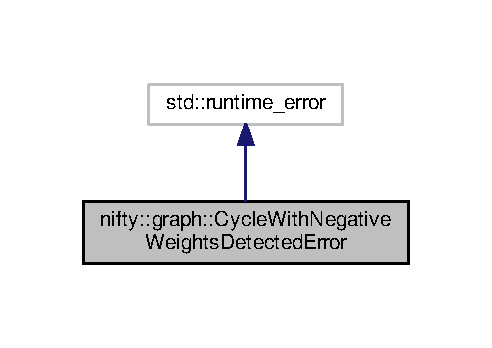
\includegraphics[width=236pt]{structnifty_1_1graph_1_1CycleWithNegativeWeightsDetectedError__inherit__graph}
\end{center}
\end{figure}


Collaboration diagram for nifty\+:\+:graph\+:\+:Cycle\+With\+Negative\+Weights\+Detected\+Error\+:
\nopagebreak
\begin{figure}[H]
\begin{center}
\leavevmode
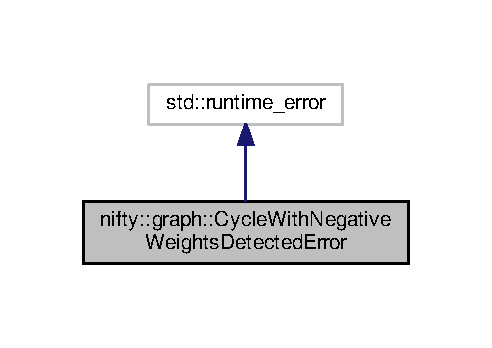
\includegraphics[width=236pt]{structnifty_1_1graph_1_1CycleWithNegativeWeightsDetectedError__coll__graph}
\end{center}
\end{figure}
\subsection*{Public Member Functions}
\begin{DoxyCompactItemize}
\item 
\hyperlink{structnifty_1_1graph_1_1CycleWithNegativeWeightsDetectedError_a0242d14469b080eac45e9c926a58e9f4}{Cycle\+With\+Negative\+Weights\+Detected\+Error} ()
\end{DoxyCompactItemize}


\subsection{Constructor \& Destructor Documentation}
\mbox{\Hypertarget{structnifty_1_1graph_1_1CycleWithNegativeWeightsDetectedError_a0242d14469b080eac45e9c926a58e9f4}\label{structnifty_1_1graph_1_1CycleWithNegativeWeightsDetectedError_a0242d14469b080eac45e9c926a58e9f4}} 
\index{nifty\+::graph\+::\+Cycle\+With\+Negative\+Weights\+Detected\+Error@{nifty\+::graph\+::\+Cycle\+With\+Negative\+Weights\+Detected\+Error}!Cycle\+With\+Negative\+Weights\+Detected\+Error@{Cycle\+With\+Negative\+Weights\+Detected\+Error}}
\index{Cycle\+With\+Negative\+Weights\+Detected\+Error@{Cycle\+With\+Negative\+Weights\+Detected\+Error}!nifty\+::graph\+::\+Cycle\+With\+Negative\+Weights\+Detected\+Error@{nifty\+::graph\+::\+Cycle\+With\+Negative\+Weights\+Detected\+Error}}
\subsubsection{\texorpdfstring{Cycle\+With\+Negative\+Weights\+Detected\+Error()}{CycleWithNegativeWeightsDetectedError()}}
{\footnotesize\ttfamily nifty\+::graph\+::\+Cycle\+With\+Negative\+Weights\+Detected\+Error\+::\+Cycle\+With\+Negative\+Weights\+Detected\+Error (\begin{DoxyParamCaption}{ }\end{DoxyParamCaption})\hspace{0.3cm}{\ttfamily [inline]}}



The documentation for this struct was generated from the following file\+:\begin{DoxyCompactItemize}
\item 
/home/tbeier/src/nifty/include/nifty/graph/\hyperlink{shortest__path__bellman__ford_8hxx}{shortest\+\_\+path\+\_\+bellman\+\_\+ford.\+hxx}\end{DoxyCompactItemize}

\hypertarget{classnifty_1_1features_1_1DefaultAccumulatedStatistics}{}\section{nifty\+:\+:features\+:\+:Default\+Accumulated\+Statistics$<$ T $>$ Class Template Reference}
\label{classnifty_1_1features_1_1DefaultAccumulatedStatistics}\index{nifty\+::features\+::\+Default\+Accumulated\+Statistics$<$ T $>$@{nifty\+::features\+::\+Default\+Accumulated\+Statistics$<$ T $>$}}


{\ttfamily \#include $<$accumulated\+\_\+features.\+hxx$>$}

\subsection*{Public Types}
\begin{DoxyCompactItemize}
\item 
typedef bacc\+::accumulator\+\_\+set$<$ T, bacc\+::stats$<$ bacc\+::tag\+::count, bacc\+::tag\+::mean, bacc\+::tag\+::min, bacc\+::tag\+::max, bacc\+::tag\+::moment$<$ 2 $>$, bacc\+::tag\+::moment$<$ 3 $>$, bacc\+::tag\+::tail\+\_\+quantile$<$ bacc\+::right $>$ $>$ $>$ \hyperlink{classnifty_1_1features_1_1DefaultAccumulatedStatistics_a1b5957732304d0ef906515d7229d8b7a}{Acc\+Type}
\item 
typedef std\+::integral\+\_\+constant$<$ int, 1 $>$ \hyperlink{classnifty_1_1features_1_1DefaultAccumulatedStatistics_a1cfd69b68fe90e8464d4bbea5929856e}{N\+Passes}
\item 
typedef std\+::integral\+\_\+constant$<$ int, 11 $>$ \hyperlink{classnifty_1_1features_1_1DefaultAccumulatedStatistics_acf47a025351ecf2d9427c10a2427c412}{N\+Features}
\end{DoxyCompactItemize}
\subsection*{Public Member Functions}
\begin{DoxyCompactItemize}
\item 
\hyperlink{classnifty_1_1features_1_1DefaultAccumulatedStatistics_a21c759b494f3d6476e414dd6607c05e8}{Default\+Accumulated\+Statistics} (const size\+\_\+t right\+Tail\+Cache\+Size=1000)
\item 
\hyperlink{classnifty_1_1features_1_1DefaultAccumulatedStatistics}{Default\+Accumulated\+Statistics} \& \hyperlink{classnifty_1_1features_1_1DefaultAccumulatedStatistics_a3cddf901950504afb3eacb8f2277c572}{acc} (const T \&val, const size\+\_\+t pass=0)
\item 
{\footnotesize template$<$class R\+E\+S\+U\+L\+T\+\_\+\+I\+T\+E\+R $>$ }\\void \hyperlink{classnifty_1_1features_1_1DefaultAccumulatedStatistics_a7adfcf8f044bb58815f95e925a350a4e}{result} (R\+E\+S\+U\+L\+T\+\_\+\+I\+T\+E\+R r\+Begin, R\+E\+S\+U\+L\+T\+\_\+\+I\+T\+E\+R r\+End)
\item 
size\+\_\+t \hyperlink{classnifty_1_1features_1_1DefaultAccumulatedStatistics_a2812443d25fd439e6890963e9a1a621a}{required\+Passes} () const 
\item 
size\+\_\+t \hyperlink{classnifty_1_1features_1_1DefaultAccumulatedStatistics_ab7711c81e77411fdc0b5b51b24cf7a4c}{n\+Features} () const 
\end{DoxyCompactItemize}


\subsection{Member Typedef Documentation}
\hypertarget{classnifty_1_1features_1_1DefaultAccumulatedStatistics_a1b5957732304d0ef906515d7229d8b7a}{}\index{nifty\+::features\+::\+Default\+Accumulated\+Statistics@{nifty\+::features\+::\+Default\+Accumulated\+Statistics}!Acc\+Type@{Acc\+Type}}
\index{Acc\+Type@{Acc\+Type}!nifty\+::features\+::\+Default\+Accumulated\+Statistics@{nifty\+::features\+::\+Default\+Accumulated\+Statistics}}
\subsubsection[{Acc\+Type}]{\setlength{\rightskip}{0pt plus 5cm}template$<$class T $>$ typedef bacc\+::accumulator\+\_\+set$<$ T, bacc\+::stats$<$ bacc\+::tag\+::count, bacc\+::tag\+::mean, bacc\+::tag\+::min, bacc\+::tag\+::max, bacc\+::tag\+::moment$<$2$>$, bacc\+::tag\+::moment$<$3$>$, bacc\+::tag\+::tail\+\_\+quantile$<$bacc\+::right$>$ $>$ $>$ {\bf nifty\+::features\+::\+Default\+Accumulated\+Statistics}$<$ T $>$\+::{\bf Acc\+Type}}\label{classnifty_1_1features_1_1DefaultAccumulatedStatistics_a1b5957732304d0ef906515d7229d8b7a}
\hypertarget{classnifty_1_1features_1_1DefaultAccumulatedStatistics_acf47a025351ecf2d9427c10a2427c412}{}\index{nifty\+::features\+::\+Default\+Accumulated\+Statistics@{nifty\+::features\+::\+Default\+Accumulated\+Statistics}!N\+Features@{N\+Features}}
\index{N\+Features@{N\+Features}!nifty\+::features\+::\+Default\+Accumulated\+Statistics@{nifty\+::features\+::\+Default\+Accumulated\+Statistics}}
\subsubsection[{N\+Features}]{\setlength{\rightskip}{0pt plus 5cm}template$<$class T $>$ typedef std\+::integral\+\_\+constant$<$int, 11$>$ {\bf nifty\+::features\+::\+Default\+Accumulated\+Statistics}$<$ T $>$\+::{\bf N\+Features}}\label{classnifty_1_1features_1_1DefaultAccumulatedStatistics_acf47a025351ecf2d9427c10a2427c412}
\hypertarget{classnifty_1_1features_1_1DefaultAccumulatedStatistics_a1cfd69b68fe90e8464d4bbea5929856e}{}\index{nifty\+::features\+::\+Default\+Accumulated\+Statistics@{nifty\+::features\+::\+Default\+Accumulated\+Statistics}!N\+Passes@{N\+Passes}}
\index{N\+Passes@{N\+Passes}!nifty\+::features\+::\+Default\+Accumulated\+Statistics@{nifty\+::features\+::\+Default\+Accumulated\+Statistics}}
\subsubsection[{N\+Passes}]{\setlength{\rightskip}{0pt plus 5cm}template$<$class T $>$ typedef std\+::integral\+\_\+constant$<$int, 1$>$ {\bf nifty\+::features\+::\+Default\+Accumulated\+Statistics}$<$ T $>$\+::{\bf N\+Passes}}\label{classnifty_1_1features_1_1DefaultAccumulatedStatistics_a1cfd69b68fe90e8464d4bbea5929856e}


\subsection{Constructor \& Destructor Documentation}
\hypertarget{classnifty_1_1features_1_1DefaultAccumulatedStatistics_a21c759b494f3d6476e414dd6607c05e8}{}\index{nifty\+::features\+::\+Default\+Accumulated\+Statistics@{nifty\+::features\+::\+Default\+Accumulated\+Statistics}!Default\+Accumulated\+Statistics@{Default\+Accumulated\+Statistics}}
\index{Default\+Accumulated\+Statistics@{Default\+Accumulated\+Statistics}!nifty\+::features\+::\+Default\+Accumulated\+Statistics@{nifty\+::features\+::\+Default\+Accumulated\+Statistics}}
\subsubsection[{Default\+Accumulated\+Statistics(const size\+\_\+t right\+Tail\+Cache\+Size=1000)}]{\setlength{\rightskip}{0pt plus 5cm}template$<$class T $>$ {\bf nifty\+::features\+::\+Default\+Accumulated\+Statistics}$<$ T $>$\+::{\bf Default\+Accumulated\+Statistics} (
\begin{DoxyParamCaption}
\item[{const size\+\_\+t}]{right\+Tail\+Cache\+Size = {\ttfamily 1000}}
\end{DoxyParamCaption}
)\hspace{0.3cm}{\ttfamily [inline]}}\label{classnifty_1_1features_1_1DefaultAccumulatedStatistics_a21c759b494f3d6476e414dd6607c05e8}


\subsection{Member Function Documentation}
\hypertarget{classnifty_1_1features_1_1DefaultAccumulatedStatistics_a3cddf901950504afb3eacb8f2277c572}{}\index{nifty\+::features\+::\+Default\+Accumulated\+Statistics@{nifty\+::features\+::\+Default\+Accumulated\+Statistics}!acc@{acc}}
\index{acc@{acc}!nifty\+::features\+::\+Default\+Accumulated\+Statistics@{nifty\+::features\+::\+Default\+Accumulated\+Statistics}}
\subsubsection[{acc(const T \&val, const size\+\_\+t pass=0)}]{\setlength{\rightskip}{0pt plus 5cm}template$<$class T $>$ {\bf Default\+Accumulated\+Statistics}\& {\bf nifty\+::features\+::\+Default\+Accumulated\+Statistics}$<$ T $>$\+::acc (
\begin{DoxyParamCaption}
\item[{const T \&}]{val, }
\item[{const size\+\_\+t}]{pass = {\ttfamily 0}}
\end{DoxyParamCaption}
)\hspace{0.3cm}{\ttfamily [inline]}}\label{classnifty_1_1features_1_1DefaultAccumulatedStatistics_a3cddf901950504afb3eacb8f2277c572}
\hypertarget{classnifty_1_1features_1_1DefaultAccumulatedStatistics_ab7711c81e77411fdc0b5b51b24cf7a4c}{}\index{nifty\+::features\+::\+Default\+Accumulated\+Statistics@{nifty\+::features\+::\+Default\+Accumulated\+Statistics}!n\+Features@{n\+Features}}
\index{n\+Features@{n\+Features}!nifty\+::features\+::\+Default\+Accumulated\+Statistics@{nifty\+::features\+::\+Default\+Accumulated\+Statistics}}
\subsubsection[{n\+Features() const }]{\setlength{\rightskip}{0pt plus 5cm}template$<$class T $>$ size\+\_\+t {\bf nifty\+::features\+::\+Default\+Accumulated\+Statistics}$<$ T $>$\+::n\+Features (
\begin{DoxyParamCaption}
{}
\end{DoxyParamCaption}
) const\hspace{0.3cm}{\ttfamily [inline]}}\label{classnifty_1_1features_1_1DefaultAccumulatedStatistics_ab7711c81e77411fdc0b5b51b24cf7a4c}
\hypertarget{classnifty_1_1features_1_1DefaultAccumulatedStatistics_a2812443d25fd439e6890963e9a1a621a}{}\index{nifty\+::features\+::\+Default\+Accumulated\+Statistics@{nifty\+::features\+::\+Default\+Accumulated\+Statistics}!required\+Passes@{required\+Passes}}
\index{required\+Passes@{required\+Passes}!nifty\+::features\+::\+Default\+Accumulated\+Statistics@{nifty\+::features\+::\+Default\+Accumulated\+Statistics}}
\subsubsection[{required\+Passes() const }]{\setlength{\rightskip}{0pt plus 5cm}template$<$class T $>$ size\+\_\+t {\bf nifty\+::features\+::\+Default\+Accumulated\+Statistics}$<$ T $>$\+::required\+Passes (
\begin{DoxyParamCaption}
{}
\end{DoxyParamCaption}
) const\hspace{0.3cm}{\ttfamily [inline]}}\label{classnifty_1_1features_1_1DefaultAccumulatedStatistics_a2812443d25fd439e6890963e9a1a621a}
\hypertarget{classnifty_1_1features_1_1DefaultAccumulatedStatistics_a7adfcf8f044bb58815f95e925a350a4e}{}\index{nifty\+::features\+::\+Default\+Accumulated\+Statistics@{nifty\+::features\+::\+Default\+Accumulated\+Statistics}!result@{result}}
\index{result@{result}!nifty\+::features\+::\+Default\+Accumulated\+Statistics@{nifty\+::features\+::\+Default\+Accumulated\+Statistics}}
\subsubsection[{result(\+R\+E\+S\+U\+L\+T\+\_\+\+I\+T\+E\+R r\+Begin, R\+E\+S\+U\+L\+T\+\_\+\+I\+T\+E\+R r\+End)}]{\setlength{\rightskip}{0pt plus 5cm}template$<$class T $>$ template$<$class R\+E\+S\+U\+L\+T\+\_\+\+I\+T\+E\+R $>$ void {\bf nifty\+::features\+::\+Default\+Accumulated\+Statistics}$<$ T $>$\+::result (
\begin{DoxyParamCaption}
\item[{R\+E\+S\+U\+L\+T\+\_\+\+I\+T\+E\+R}]{r\+Begin, }
\item[{R\+E\+S\+U\+L\+T\+\_\+\+I\+T\+E\+R}]{r\+End}
\end{DoxyParamCaption}
)\hspace{0.3cm}{\ttfamily [inline]}}\label{classnifty_1_1features_1_1DefaultAccumulatedStatistics_a7adfcf8f044bb58815f95e925a350a4e}


The documentation for this class was generated from the following file\+:\begin{DoxyCompactItemize}
\item 
/home/tbeier/src/nifty/include/nifty/features/\hyperlink{accumulated__features_8hxx}{accumulated\+\_\+features.\+hxx}\end{DoxyCompactItemize}

\hypertarget{structnifty_1_1graph_1_1mincut_1_1DefaultProposalGeneratorMock}{}\section{nifty\+:\+:graph\+:\+:mincut\+:\+:Default\+Proposal\+Generator\+Mock Struct Reference}
\label{structnifty_1_1graph_1_1mincut_1_1DefaultProposalGeneratorMock}\index{nifty\+::graph\+::mincut\+::\+Default\+Proposal\+Generator\+Mock@{nifty\+::graph\+::mincut\+::\+Default\+Proposal\+Generator\+Mock}}


{\ttfamily \#include $<$mincut\+\_\+cc\+\_\+fusion\+\_\+move\+\_\+based.\+hxx$>$}



The documentation for this struct was generated from the following file\+:\begin{DoxyCompactItemize}
\item 
/home/tbeier/src/nifty/include/nifty/graph/optimization/mincut/\hyperlink{mincut__cc__fusion__move__based_8hxx}{mincut\+\_\+cc\+\_\+fusion\+\_\+move\+\_\+based.\+hxx}\end{DoxyCompactItemize}

\hypertarget{structnifty_1_1graph_1_1DefaultSubgraphMask}{}\section{nifty\+:\+:graph\+:\+:Default\+Subgraph\+Mask$<$ G $>$ Struct Template Reference}
\label{structnifty_1_1graph_1_1DefaultSubgraphMask}\index{nifty\+::graph\+::\+Default\+Subgraph\+Mask$<$ G $>$@{nifty\+::graph\+::\+Default\+Subgraph\+Mask$<$ G $>$}}


{\ttfamily \#include $<$subgraph\+\_\+mask.\+hxx$>$}

\subsection*{Public Member Functions}
\begin{DoxyCompactItemize}
\item 
bool \hyperlink{structnifty_1_1graph_1_1DefaultSubgraphMask_a2e18317966dd9042d860b94286c85513}{use\+Edge} (const uint64\+\_\+t) const 
\item 
bool \hyperlink{structnifty_1_1graph_1_1DefaultSubgraphMask_af81e63f27fdd413b187ff4ec21c6d276}{use\+Node} (const uint64\+\_\+t) const 
\end{DoxyCompactItemize}


\subsection{Member Function Documentation}
\hypertarget{structnifty_1_1graph_1_1DefaultSubgraphMask_a2e18317966dd9042d860b94286c85513}{}\index{nifty\+::graph\+::\+Default\+Subgraph\+Mask@{nifty\+::graph\+::\+Default\+Subgraph\+Mask}!use\+Edge@{use\+Edge}}
\index{use\+Edge@{use\+Edge}!nifty\+::graph\+::\+Default\+Subgraph\+Mask@{nifty\+::graph\+::\+Default\+Subgraph\+Mask}}
\subsubsection[{use\+Edge(const uint64\+\_\+t) const }]{\setlength{\rightskip}{0pt plus 5cm}template$<$class G$>$ bool {\bf nifty\+::graph\+::\+Default\+Subgraph\+Mask}$<$ G $>$\+::use\+Edge (
\begin{DoxyParamCaption}
\item[{const uint64\+\_\+t}]{}
\end{DoxyParamCaption}
) const\hspace{0.3cm}{\ttfamily [inline]}}\label{structnifty_1_1graph_1_1DefaultSubgraphMask_a2e18317966dd9042d860b94286c85513}
\hypertarget{structnifty_1_1graph_1_1DefaultSubgraphMask_af81e63f27fdd413b187ff4ec21c6d276}{}\index{nifty\+::graph\+::\+Default\+Subgraph\+Mask@{nifty\+::graph\+::\+Default\+Subgraph\+Mask}!use\+Node@{use\+Node}}
\index{use\+Node@{use\+Node}!nifty\+::graph\+::\+Default\+Subgraph\+Mask@{nifty\+::graph\+::\+Default\+Subgraph\+Mask}}
\subsubsection[{use\+Node(const uint64\+\_\+t) const }]{\setlength{\rightskip}{0pt plus 5cm}template$<$class G$>$ bool {\bf nifty\+::graph\+::\+Default\+Subgraph\+Mask}$<$ G $>$\+::use\+Node (
\begin{DoxyParamCaption}
\item[{const uint64\+\_\+t}]{}
\end{DoxyParamCaption}
) const\hspace{0.3cm}{\ttfamily [inline]}}\label{structnifty_1_1graph_1_1DefaultSubgraphMask_af81e63f27fdd413b187ff4ec21c6d276}


The documentation for this struct was generated from the following file\+:\begin{DoxyCompactItemize}
\item 
/home/tbeier/src/nifty/include/nifty/graph/\hyperlink{subgraph__mask_8hxx}{subgraph\+\_\+mask.\+hxx}\end{DoxyCompactItemize}

\hypertarget{classnifty_1_1graph_1_1DirectedGraphBase}{}\section{nifty\+:\+:graph\+:\+:Directed\+Graph\+Base$<$ C\+H\+I\+L\+D\+\_\+\+G\+R\+A\+P\+H $>$ Class Template Reference}
\label{classnifty_1_1graph_1_1DirectedGraphBase}\index{nifty\+::graph\+::\+Directed\+Graph\+Base$<$ C\+H\+I\+L\+D\+\_\+\+G\+R\+A\+P\+H $>$@{nifty\+::graph\+::\+Directed\+Graph\+Base$<$ C\+H\+I\+L\+D\+\_\+\+G\+R\+A\+P\+H $>$}}


{\ttfamily \#include $<$directed\+\_\+graph\+\_\+base.\+hxx$>$}

\subsection*{Classes}
\begin{DoxyCompactItemize}
\item 
struct \hyperlink{structnifty_1_1graph_1_1DirectedGraphBase_1_1AdjacencyIterRange}{Adjacency\+Iter\+Range}
\item 
struct \hyperlink{structnifty_1_1graph_1_1DirectedGraphBase_1_1ArcIterRange}{Arc\+Iter\+Range}
\item 
struct \hyperlink{structnifty_1_1graph_1_1DirectedGraphBase_1_1EdgeMap}{Edge\+Map}
\item 
struct \hyperlink{structnifty_1_1graph_1_1DirectedGraphBase_1_1NodeIterRange}{Node\+Iter\+Range}
\item 
struct \hyperlink{structnifty_1_1graph_1_1DirectedGraphBase_1_1NodeMap}{Node\+Map}
\end{DoxyCompactItemize}
\subsection*{Public Types}
\begin{DoxyCompactItemize}
\item 
typedef C\+H\+I\+L\+D\+\_\+\+G\+R\+A\+P\+H \hyperlink{classnifty_1_1graph_1_1DirectedGraphBase_a583e01641aec296b9bc33a346f90a216}{Child\+Graph}
\item 
typedef \hyperlink{classnifty_1_1graph_1_1DirectedGraphBase}{Directed\+Graph\+Base}$<$ \hyperlink{classnifty_1_1graph_1_1DirectedGraphBase_a583e01641aec296b9bc33a346f90a216}{Child\+Graph} $>$ \hyperlink{classnifty_1_1graph_1_1DirectedGraphBase_ae772bf5744b9fe1af63eb1418b7ab261}{Self}
\end{DoxyCompactItemize}
\subsection*{Public Member Functions}
\begin{DoxyCompactItemize}
\item 
\hyperlink{structnifty_1_1graph_1_1DirectedGraphBase_1_1NodeIterRange}{Node\+Iter\+Range}$<$ \hyperlink{classnifty_1_1graph_1_1DirectedGraphBase_a583e01641aec296b9bc33a346f90a216}{Child\+Graph} $>$ \hyperlink{classnifty_1_1graph_1_1DirectedGraphBase_af2ea4db179032139161358e1dae678bd}{nodes} () const 
\item 
\hyperlink{structnifty_1_1graph_1_1DirectedGraphBase_1_1ArcIterRange}{Arc\+Iter\+Range}$<$ \hyperlink{classnifty_1_1graph_1_1DirectedGraphBase_a583e01641aec296b9bc33a346f90a216}{Child\+Graph} $>$ \hyperlink{classnifty_1_1graph_1_1DirectedGraphBase_ad163249d1556275cd3a26be3fb149ea2}{arcs} () const 
\item 
\hyperlink{structnifty_1_1graph_1_1DirectedGraphBase_1_1ArcIterRange}{Arc\+Iter\+Range}$<$ \hyperlink{classnifty_1_1graph_1_1DirectedGraphBase_a583e01641aec296b9bc33a346f90a216}{Child\+Graph} $>$ \hyperlink{classnifty_1_1graph_1_1DirectedGraphBase_a1c7072e651f9b4cc2c7ff121d204c8cd}{edges} () const 
\item 
\hyperlink{structnifty_1_1graph_1_1DirectedGraphBase_1_1AdjacencyIterRange}{Adjacency\+Iter\+Range}$<$ \hyperlink{classnifty_1_1graph_1_1DirectedGraphBase_a583e01641aec296b9bc33a346f90a216}{Child\+Graph} $>$ \hyperlink{classnifty_1_1graph_1_1DirectedGraphBase_a712c07401a2323f2c4df04e7c4a4ce7e}{adjacency} (const int64\+\_\+t node) const 
\item 
int64\+\_\+t \hyperlink{classnifty_1_1graph_1_1DirectedGraphBase_a49976a6e82bc84a7a2827e0e8592fc1a}{find\+Edge} (const uint64\+\_\+t u, const uint64\+\_\+t v)
\item 
int64\+\_\+t \hyperlink{classnifty_1_1graph_1_1DirectedGraphBase_a51b3ede5d781b372911dad0cff2ae6f6}{edge\+Id\+Upper\+Bound} () const 
\item 
int64\+\_\+t \hyperlink{classnifty_1_1graph_1_1DirectedGraphBase_ad3e9b4a5e810cdfb87bdff0adf3385d4}{number\+Of\+Edges} () const 
\end{DoxyCompactItemize}


\subsection{Member Typedef Documentation}
\hypertarget{classnifty_1_1graph_1_1DirectedGraphBase_a583e01641aec296b9bc33a346f90a216}{}\index{nifty\+::graph\+::\+Directed\+Graph\+Base@{nifty\+::graph\+::\+Directed\+Graph\+Base}!Child\+Graph@{Child\+Graph}}
\index{Child\+Graph@{Child\+Graph}!nifty\+::graph\+::\+Directed\+Graph\+Base@{nifty\+::graph\+::\+Directed\+Graph\+Base}}
\subsubsection[{Child\+Graph}]{\setlength{\rightskip}{0pt plus 5cm}template$<$class C\+H\+I\+L\+D\+\_\+\+G\+R\+A\+P\+H$>$ typedef C\+H\+I\+L\+D\+\_\+\+G\+R\+A\+P\+H {\bf nifty\+::graph\+::\+Directed\+Graph\+Base}$<$ C\+H\+I\+L\+D\+\_\+\+G\+R\+A\+P\+H $>$\+::{\bf Child\+Graph}}\label{classnifty_1_1graph_1_1DirectedGraphBase_a583e01641aec296b9bc33a346f90a216}
\hypertarget{classnifty_1_1graph_1_1DirectedGraphBase_ae772bf5744b9fe1af63eb1418b7ab261}{}\index{nifty\+::graph\+::\+Directed\+Graph\+Base@{nifty\+::graph\+::\+Directed\+Graph\+Base}!Self@{Self}}
\index{Self@{Self}!nifty\+::graph\+::\+Directed\+Graph\+Base@{nifty\+::graph\+::\+Directed\+Graph\+Base}}
\subsubsection[{Self}]{\setlength{\rightskip}{0pt plus 5cm}template$<$class C\+H\+I\+L\+D\+\_\+\+G\+R\+A\+P\+H$>$ typedef {\bf Directed\+Graph\+Base}$<${\bf Child\+Graph}$>$ {\bf nifty\+::graph\+::\+Directed\+Graph\+Base}$<$ C\+H\+I\+L\+D\+\_\+\+G\+R\+A\+P\+H $>$\+::{\bf Self}}\label{classnifty_1_1graph_1_1DirectedGraphBase_ae772bf5744b9fe1af63eb1418b7ab261}


\subsection{Member Function Documentation}
\hypertarget{classnifty_1_1graph_1_1DirectedGraphBase_a712c07401a2323f2c4df04e7c4a4ce7e}{}\index{nifty\+::graph\+::\+Directed\+Graph\+Base@{nifty\+::graph\+::\+Directed\+Graph\+Base}!adjacency@{adjacency}}
\index{adjacency@{adjacency}!nifty\+::graph\+::\+Directed\+Graph\+Base@{nifty\+::graph\+::\+Directed\+Graph\+Base}}
\subsubsection[{adjacency(const int64\+\_\+t node) const }]{\setlength{\rightskip}{0pt plus 5cm}template$<$class C\+H\+I\+L\+D\+\_\+\+G\+R\+A\+P\+H$>$ {\bf Adjacency\+Iter\+Range}$<${\bf Child\+Graph} $>$ {\bf nifty\+::graph\+::\+Directed\+Graph\+Base}$<$ C\+H\+I\+L\+D\+\_\+\+G\+R\+A\+P\+H $>$\+::adjacency (
\begin{DoxyParamCaption}
\item[{const int64\+\_\+t}]{node}
\end{DoxyParamCaption}
) const\hspace{0.3cm}{\ttfamily [inline]}}\label{classnifty_1_1graph_1_1DirectedGraphBase_a712c07401a2323f2c4df04e7c4a4ce7e}
\hypertarget{classnifty_1_1graph_1_1DirectedGraphBase_ad163249d1556275cd3a26be3fb149ea2}{}\index{nifty\+::graph\+::\+Directed\+Graph\+Base@{nifty\+::graph\+::\+Directed\+Graph\+Base}!arcs@{arcs}}
\index{arcs@{arcs}!nifty\+::graph\+::\+Directed\+Graph\+Base@{nifty\+::graph\+::\+Directed\+Graph\+Base}}
\subsubsection[{arcs() const }]{\setlength{\rightskip}{0pt plus 5cm}template$<$class C\+H\+I\+L\+D\+\_\+\+G\+R\+A\+P\+H$>$ {\bf Arc\+Iter\+Range}$<${\bf Child\+Graph} $>$ {\bf nifty\+::graph\+::\+Directed\+Graph\+Base}$<$ C\+H\+I\+L\+D\+\_\+\+G\+R\+A\+P\+H $>$\+::arcs (
\begin{DoxyParamCaption}
{}
\end{DoxyParamCaption}
) const\hspace{0.3cm}{\ttfamily [inline]}}\label{classnifty_1_1graph_1_1DirectedGraphBase_ad163249d1556275cd3a26be3fb149ea2}
\hypertarget{classnifty_1_1graph_1_1DirectedGraphBase_a51b3ede5d781b372911dad0cff2ae6f6}{}\index{nifty\+::graph\+::\+Directed\+Graph\+Base@{nifty\+::graph\+::\+Directed\+Graph\+Base}!edge\+Id\+Upper\+Bound@{edge\+Id\+Upper\+Bound}}
\index{edge\+Id\+Upper\+Bound@{edge\+Id\+Upper\+Bound}!nifty\+::graph\+::\+Directed\+Graph\+Base@{nifty\+::graph\+::\+Directed\+Graph\+Base}}
\subsubsection[{edge\+Id\+Upper\+Bound() const }]{\setlength{\rightskip}{0pt plus 5cm}template$<$class C\+H\+I\+L\+D\+\_\+\+G\+R\+A\+P\+H$>$ int64\+\_\+t {\bf nifty\+::graph\+::\+Directed\+Graph\+Base}$<$ C\+H\+I\+L\+D\+\_\+\+G\+R\+A\+P\+H $>$\+::edge\+Id\+Upper\+Bound (
\begin{DoxyParamCaption}
{}
\end{DoxyParamCaption}
) const\hspace{0.3cm}{\ttfamily [inline]}}\label{classnifty_1_1graph_1_1DirectedGraphBase_a51b3ede5d781b372911dad0cff2ae6f6}
\hypertarget{classnifty_1_1graph_1_1DirectedGraphBase_a1c7072e651f9b4cc2c7ff121d204c8cd}{}\index{nifty\+::graph\+::\+Directed\+Graph\+Base@{nifty\+::graph\+::\+Directed\+Graph\+Base}!edges@{edges}}
\index{edges@{edges}!nifty\+::graph\+::\+Directed\+Graph\+Base@{nifty\+::graph\+::\+Directed\+Graph\+Base}}
\subsubsection[{edges() const }]{\setlength{\rightskip}{0pt plus 5cm}template$<$class C\+H\+I\+L\+D\+\_\+\+G\+R\+A\+P\+H$>$ {\bf Arc\+Iter\+Range}$<${\bf Child\+Graph} $>$ {\bf nifty\+::graph\+::\+Directed\+Graph\+Base}$<$ C\+H\+I\+L\+D\+\_\+\+G\+R\+A\+P\+H $>$\+::edges (
\begin{DoxyParamCaption}
{}
\end{DoxyParamCaption}
) const\hspace{0.3cm}{\ttfamily [inline]}}\label{classnifty_1_1graph_1_1DirectedGraphBase_a1c7072e651f9b4cc2c7ff121d204c8cd}
\hypertarget{classnifty_1_1graph_1_1DirectedGraphBase_a49976a6e82bc84a7a2827e0e8592fc1a}{}\index{nifty\+::graph\+::\+Directed\+Graph\+Base@{nifty\+::graph\+::\+Directed\+Graph\+Base}!find\+Edge@{find\+Edge}}
\index{find\+Edge@{find\+Edge}!nifty\+::graph\+::\+Directed\+Graph\+Base@{nifty\+::graph\+::\+Directed\+Graph\+Base}}
\subsubsection[{find\+Edge(const uint64\+\_\+t u, const uint64\+\_\+t v)}]{\setlength{\rightskip}{0pt plus 5cm}template$<$class C\+H\+I\+L\+D\+\_\+\+G\+R\+A\+P\+H$>$ int64\+\_\+t {\bf nifty\+::graph\+::\+Directed\+Graph\+Base}$<$ C\+H\+I\+L\+D\+\_\+\+G\+R\+A\+P\+H $>$\+::find\+Edge (
\begin{DoxyParamCaption}
\item[{const uint64\+\_\+t}]{u, }
\item[{const uint64\+\_\+t}]{v}
\end{DoxyParamCaption}
)\hspace{0.3cm}{\ttfamily [inline]}}\label{classnifty_1_1graph_1_1DirectedGraphBase_a49976a6e82bc84a7a2827e0e8592fc1a}
\hypertarget{classnifty_1_1graph_1_1DirectedGraphBase_af2ea4db179032139161358e1dae678bd}{}\index{nifty\+::graph\+::\+Directed\+Graph\+Base@{nifty\+::graph\+::\+Directed\+Graph\+Base}!nodes@{nodes}}
\index{nodes@{nodes}!nifty\+::graph\+::\+Directed\+Graph\+Base@{nifty\+::graph\+::\+Directed\+Graph\+Base}}
\subsubsection[{nodes() const }]{\setlength{\rightskip}{0pt plus 5cm}template$<$class C\+H\+I\+L\+D\+\_\+\+G\+R\+A\+P\+H$>$ {\bf Node\+Iter\+Range}$<${\bf Child\+Graph} $>$ {\bf nifty\+::graph\+::\+Directed\+Graph\+Base}$<$ C\+H\+I\+L\+D\+\_\+\+G\+R\+A\+P\+H $>$\+::nodes (
\begin{DoxyParamCaption}
{}
\end{DoxyParamCaption}
) const\hspace{0.3cm}{\ttfamily [inline]}}\label{classnifty_1_1graph_1_1DirectedGraphBase_af2ea4db179032139161358e1dae678bd}
\hypertarget{classnifty_1_1graph_1_1DirectedGraphBase_ad3e9b4a5e810cdfb87bdff0adf3385d4}{}\index{nifty\+::graph\+::\+Directed\+Graph\+Base@{nifty\+::graph\+::\+Directed\+Graph\+Base}!number\+Of\+Edges@{number\+Of\+Edges}}
\index{number\+Of\+Edges@{number\+Of\+Edges}!nifty\+::graph\+::\+Directed\+Graph\+Base@{nifty\+::graph\+::\+Directed\+Graph\+Base}}
\subsubsection[{number\+Of\+Edges() const }]{\setlength{\rightskip}{0pt plus 5cm}template$<$class C\+H\+I\+L\+D\+\_\+\+G\+R\+A\+P\+H$>$ int64\+\_\+t {\bf nifty\+::graph\+::\+Directed\+Graph\+Base}$<$ C\+H\+I\+L\+D\+\_\+\+G\+R\+A\+P\+H $>$\+::number\+Of\+Edges (
\begin{DoxyParamCaption}
{}
\end{DoxyParamCaption}
) const\hspace{0.3cm}{\ttfamily [inline]}}\label{classnifty_1_1graph_1_1DirectedGraphBase_ad3e9b4a5e810cdfb87bdff0adf3385d4}


The documentation for this class was generated from the following file\+:\begin{DoxyCompactItemize}
\item 
/home/tbeier/src/nifty/include/nifty/graph/\hyperlink{directed__graph__base_8hxx}{directed\+\_\+graph\+\_\+base.\+hxx}\end{DoxyCompactItemize}

\hypertarget{classnifty_1_1graph_1_1DirectedGraphView}{}\section{nifty\+:\+:graph\+:\+:Directed\+Graph\+View$<$ G\+R\+A\+PH $>$ Class Template Reference}
\label{classnifty_1_1graph_1_1DirectedGraphView}\index{nifty\+::graph\+::\+Directed\+Graph\+View$<$ G\+R\+A\+P\+H $>$@{nifty\+::graph\+::\+Directed\+Graph\+View$<$ G\+R\+A\+P\+H $>$}}


{\ttfamily \#include $<$directed\+\_\+graph\+\_\+view.\+hxx$>$}

\subsection*{Public Types}
\begin{DoxyCompactItemize}
\item 
typedef G\+R\+A\+PH \hyperlink{classnifty_1_1graph_1_1DirectedGraphView_abbbfb94d0474216ae2d7411838494108}{Graph\+Type}
\end{DoxyCompactItemize}


\subsection{Member Typedef Documentation}
\mbox{\Hypertarget{classnifty_1_1graph_1_1DirectedGraphView_abbbfb94d0474216ae2d7411838494108}\label{classnifty_1_1graph_1_1DirectedGraphView_abbbfb94d0474216ae2d7411838494108}} 
\index{nifty\+::graph\+::\+Directed\+Graph\+View@{nifty\+::graph\+::\+Directed\+Graph\+View}!Graph\+Type@{Graph\+Type}}
\index{Graph\+Type@{Graph\+Type}!nifty\+::graph\+::\+Directed\+Graph\+View@{nifty\+::graph\+::\+Directed\+Graph\+View}}
\subsubsection{\texorpdfstring{Graph\+Type}{GraphType}}
{\footnotesize\ttfamily template$<$class G\+R\+A\+PH $>$ \\
typedef G\+R\+A\+PH \hyperlink{classnifty_1_1graph_1_1DirectedGraphView}{nifty\+::graph\+::\+Directed\+Graph\+View}$<$ G\+R\+A\+PH $>$\+::\hyperlink{classnifty_1_1graph_1_1DirectedGraphView_abbbfb94d0474216ae2d7411838494108}{Graph\+Type}}



The documentation for this class was generated from the following file\+:\begin{DoxyCompactItemize}
\item 
/home/tbeier/src/nifty/include/nifty/graph/\hyperlink{directed__graph__view_8hxx}{directed\+\_\+graph\+\_\+view.\+hxx}\end{DoxyCompactItemize}

\hypertarget{structnifty_1_1graph_1_1GridRag_1_1DontComputeRag}{}\section{nifty\+:\+:graph\+:\+:Grid\+Rag$<$ D\+IM, L\+A\+B\+E\+L\+S\+\_\+\+P\+R\+O\+XY $>$\+:\+:Dont\+Compute\+Rag Struct Reference}
\label{structnifty_1_1graph_1_1GridRag_1_1DontComputeRag}\index{nifty\+::graph\+::\+Grid\+Rag$<$ D\+I\+M, L\+A\+B\+E\+L\+S\+\_\+\+P\+R\+O\+X\+Y $>$\+::\+Dont\+Compute\+Rag@{nifty\+::graph\+::\+Grid\+Rag$<$ D\+I\+M, L\+A\+B\+E\+L\+S\+\_\+\+P\+R\+O\+X\+Y $>$\+::\+Dont\+Compute\+Rag}}


{\ttfamily \#include $<$grid\+\_\+rag.\+hxx$>$}



The documentation for this struct was generated from the following file\+:\begin{DoxyCompactItemize}
\item 
/home/tbeier/src/nifty/include/nifty/graph/rag/\hyperlink{grid__rag_8hxx}{grid\+\_\+rag.\+hxx}\end{DoxyCompactItemize}

\hypertarget{classnifty_1_1graph_1_1EdgeContractionGraph}{}\section{nifty\+:\+:graph\+:\+:Edge\+Contraction\+Graph$<$ G\+R\+A\+P\+H, C\+A\+L\+L\+B\+A\+C\+K, W\+I\+T\+H\+\_\+\+E\+D\+G\+E\+\_\+\+U\+F\+D $>$ Class Template Reference}
\label{classnifty_1_1graph_1_1EdgeContractionGraph}\index{nifty\+::graph\+::\+Edge\+Contraction\+Graph$<$ G\+R\+A\+P\+H, C\+A\+L\+L\+B\+A\+C\+K, W\+I\+T\+H\+\_\+\+E\+D\+G\+E\+\_\+\+U\+F\+D $>$@{nifty\+::graph\+::\+Edge\+Contraction\+Graph$<$ G\+R\+A\+P\+H, C\+A\+L\+L\+B\+A\+C\+K, W\+I\+T\+H\+\_\+\+E\+D\+G\+E\+\_\+\+U\+F\+D $>$}}


{\ttfamily \#include $<$edge\+\_\+contraction\+\_\+graph.\+hxx$>$}



Inheritance diagram for nifty\+:\+:graph\+:\+:Edge\+Contraction\+Graph$<$ G\+R\+A\+P\+H, C\+A\+L\+L\+B\+A\+C\+K, W\+I\+T\+H\+\_\+\+E\+D\+G\+E\+\_\+\+U\+F\+D $>$\+:
% FIG 0


Collaboration diagram for nifty\+:\+:graph\+:\+:Edge\+Contraction\+Graph$<$ G\+R\+A\+P\+H, C\+A\+L\+L\+B\+A\+C\+K, W\+I\+T\+H\+\_\+\+E\+D\+G\+E\+\_\+\+U\+F\+D $>$\+:
% FIG 1
\subsection*{Classes}
\begin{DoxyCompactItemize}
\item 
struct \hyperlink{structnifty_1_1graph_1_1EdgeContractionGraph_1_1AdjacencyIterRange}{Adjacency\+Iter\+Range}
\end{DoxyCompactItemize}
\subsection*{Public Types}
\begin{DoxyCompactItemize}
\item 
typedef std\+::integral\+\_\+constant$<$ bool, W\+I\+T\+H\+\_\+\+E\+D\+G\+E\+\_\+\+U\+F\+D $>$ \hyperlink{classnifty_1_1graph_1_1EdgeContractionGraph_a9b33be5b2975fe298604326c10df1f93}{With\+Edge\+Ufd}
\item 
typedef G\+R\+A\+P\+H \hyperlink{classnifty_1_1graph_1_1EdgeContractionGraph_a22f00237e657f393dfcaacdc10de9bba}{Graph}
\item 
typedef C\+A\+L\+L\+B\+A\+C\+K \hyperlink{classnifty_1_1graph_1_1EdgeContractionGraph_a75e91e51c78d2f427a31c30dcd8996ed}{Callback}
\item 
typedef \hyperlink{classnifty_1_1ufd_1_1Ufd}{nifty\+::ufd\+::\+Ufd}$<$  $>$ \hyperlink{classnifty_1_1graph_1_1EdgeContractionGraph_a7ff98238621f4b534e89b1880ee77239}{Node\+Ufd\+Type}
\item 
typedef std\+::pair$<$ int64\+\_\+t, int64\+\_\+t $>$ \hyperlink{classnifty_1_1graph_1_1EdgeContractionGraph_ad57e807f7df20892c7bbbb9b53d3aa08}{Edge\+Storage}
\item 
typedef \hyperlink{classnifty_1_1container_1_1FlatSet_a0f4cd26da060859b18742abfd534aa24}{Node\+Storage\+::const\+\_\+iterator} \hyperlink{classnifty_1_1graph_1_1EdgeContractionGraph_a447212f5ced0c4ef4d304e8b89f4f200}{Adjacency\+Iter}
\end{DoxyCompactItemize}
\subsection*{Public Member Functions}
\begin{DoxyCompactItemize}
\item 
\hyperlink{classnifty_1_1graph_1_1EdgeContractionGraph_aa11f5c4752ab7b0d1f57a8efd374a5b6}{Edge\+Contraction\+Graph} (const \hyperlink{classnifty_1_1graph_1_1EdgeContractionGraph_a22f00237e657f393dfcaacdc10de9bba}{Graph} \&\hyperlink{classnifty_1_1graph_1_1EdgeContractionGraph_ae22624b7cd920b353a4a6a42bb3603c5}{graph}, \hyperlink{classnifty_1_1graph_1_1EdgeContractionGraph_a75e91e51c78d2f427a31c30dcd8996ed}{Callback} \&callback)
\item 
\hyperlink{structnifty_1_1graph_1_1EdgeContractionGraph_1_1AdjacencyIterRange}{Adjacency\+Iter\+Range} \hyperlink{classnifty_1_1graph_1_1EdgeContractionGraph_ac93df8e87fd2e86fa017a563544dabc8}{adjacency} (const int64\+\_\+t node) const 
\item 
\hyperlink{classnifty_1_1graph_1_1EdgeContractionGraph_a447212f5ced0c4ef4d304e8b89f4f200}{Adjacency\+Iter} \hyperlink{classnifty_1_1graph_1_1EdgeContractionGraph_a8e01ef0e79ab0947633f0907fc2bb2d0}{adjacency\+Begin} (const int64\+\_\+t node) const 
\item 
\hyperlink{classnifty_1_1graph_1_1EdgeContractionGraph_a447212f5ced0c4ef4d304e8b89f4f200}{Adjacency\+Iter} \hyperlink{classnifty_1_1graph_1_1EdgeContractionGraph_a1df973fa6162c58d6ed4b071038cc0b1}{adjacency\+End} (const int64\+\_\+t node) const 
\item 
\hyperlink{classnifty_1_1graph_1_1EdgeContractionGraph_a447212f5ced0c4ef4d304e8b89f4f200}{Adjacency\+Iter} \hyperlink{classnifty_1_1graph_1_1EdgeContractionGraph_a932630e316b688529a2a58917f165a93}{adjacency\+Out\+Begin} (const int64\+\_\+t node) const 
\item 
\hyperlink{classnifty_1_1graph_1_1EdgeContractionGraph_ad57e807f7df20892c7bbbb9b53d3aa08}{Edge\+Storage} \hyperlink{classnifty_1_1graph_1_1EdgeContractionGraph_abcba22be7d0d62b18390edcd501054ab}{uv} (const uint64\+\_\+t edge) const 
\item 
int64\+\_\+t \hyperlink{classnifty_1_1graph_1_1EdgeContractionGraph_a4d0519610b822ff3842b8baa3b5a2580}{u} (const uint64\+\_\+t edge) const 
\item 
int64\+\_\+t \hyperlink{classnifty_1_1graph_1_1EdgeContractionGraph_a0b321bb637fd8291985e8cecf3f87fc9}{v} (const uint64\+\_\+t edge) const 
\item 
uint64\+\_\+t \hyperlink{classnifty_1_1graph_1_1EdgeContractionGraph_a908385c94499ae9394bb23c52a584e72}{number\+Of\+Nodes} () const 
\item 
uint64\+\_\+t \hyperlink{classnifty_1_1graph_1_1EdgeContractionGraph_aebdf2c843a1b95436ecf1493bfab6df9}{number\+Of\+Edges} () const 
\item 
uint64\+\_\+t \hyperlink{classnifty_1_1graph_1_1EdgeContractionGraph_afe4ec2d07dd10fb5ba350e43079186a5}{node\+Id\+Upper\+Bound} () const 
\item 
uint64\+\_\+t \hyperlink{classnifty_1_1graph_1_1EdgeContractionGraph_a1d67de79a99520219a2090efdfabfc66}{edge\+Id\+Upper\+Bound} () const 
\item 
int64\+\_\+t \hyperlink{classnifty_1_1graph_1_1EdgeContractionGraph_ad1d8517ee863c267cefb63dd60fb37c1}{find\+Edge} (const int64\+\_\+t \hyperlink{classnifty_1_1graph_1_1EdgeContractionGraph_a4d0519610b822ff3842b8baa3b5a2580}{u}, const int64\+\_\+t \hyperlink{classnifty_1_1graph_1_1EdgeContractionGraph_a0b321bb637fd8291985e8cecf3f87fc9}{v}) const 
\item 
void \hyperlink{classnifty_1_1graph_1_1EdgeContractionGraph_ad13498d6f4fd9e360fa8884febaeba0a}{contract\+Edge} (const uint64\+\_\+t edge\+To\+Contract)
\item 
void \hyperlink{classnifty_1_1graph_1_1EdgeContractionGraph_a76a6e084c4dfe14a20f5671ec5f57cbc}{reset} ()
\item 
const \hyperlink{classnifty_1_1graph_1_1EdgeContractionGraph_a22f00237e657f393dfcaacdc10de9bba}{Graph} \& \hyperlink{classnifty_1_1graph_1_1EdgeContractionGraph_ae75c47ed3517a8695b0eb0852c5ab888}{base\+Graph} () const 
\item 
const \hyperlink{classnifty_1_1graph_1_1EdgeContractionGraph_a22f00237e657f393dfcaacdc10de9bba}{Graph} \& \hyperlink{classnifty_1_1graph_1_1EdgeContractionGraph_ae22624b7cd920b353a4a6a42bb3603c5}{graph} () const 
\item 
uint64\+\_\+t \hyperlink{classnifty_1_1graph_1_1EdgeContractionGraph_a934c568562bbcd179f198f5c67ff7bf4}{find\+Representative\+Node} (const uint64\+\_\+t node) const 
\item 
uint64\+\_\+t \hyperlink{classnifty_1_1graph_1_1EdgeContractionGraph_a96db6fdacf91e9f67d505f1bfc33ef76}{find\+Representative\+Node} (const uint64\+\_\+t node)
\item 
uint64\+\_\+t \hyperlink{classnifty_1_1graph_1_1EdgeContractionGraph_adcf3984a735ed9f44978078264dc4fdd}{node\+Of\+Dead\+Edge} (const uint64\+\_\+t dead\+Edge) const 
\item 
const \hyperlink{classnifty_1_1graph_1_1EdgeContractionGraph_a7ff98238621f4b534e89b1880ee77239}{Node\+Ufd\+Type} \& \hyperlink{classnifty_1_1graph_1_1EdgeContractionGraph_a2d7d6984f84e00c2338ef28c971b6bb3}{node\+Ufd} () const 
\end{DoxyCompactItemize}


\subsection{Member Typedef Documentation}
\hypertarget{classnifty_1_1graph_1_1EdgeContractionGraph_a447212f5ced0c4ef4d304e8b89f4f200}{}\index{nifty\+::graph\+::\+Edge\+Contraction\+Graph@{nifty\+::graph\+::\+Edge\+Contraction\+Graph}!Adjacency\+Iter@{Adjacency\+Iter}}
\index{Adjacency\+Iter@{Adjacency\+Iter}!nifty\+::graph\+::\+Edge\+Contraction\+Graph@{nifty\+::graph\+::\+Edge\+Contraction\+Graph}}
\subsubsection[{Adjacency\+Iter}]{\setlength{\rightskip}{0pt plus 5cm}template$<$class G\+R\+A\+P\+H, class C\+A\+L\+L\+B\+A\+C\+K, bool W\+I\+T\+H\+\_\+\+E\+D\+G\+E\+\_\+\+U\+F\+D$>$ typedef {\bf Node\+Storage\+::const\+\_\+iterator} {\bf nifty\+::graph\+::\+Edge\+Contraction\+Graph}$<$ G\+R\+A\+P\+H, C\+A\+L\+L\+B\+A\+C\+K, W\+I\+T\+H\+\_\+\+E\+D\+G\+E\+\_\+\+U\+F\+D $>$\+::{\bf Adjacency\+Iter}}\label{classnifty_1_1graph_1_1EdgeContractionGraph_a447212f5ced0c4ef4d304e8b89f4f200}
\hypertarget{classnifty_1_1graph_1_1EdgeContractionGraph_a75e91e51c78d2f427a31c30dcd8996ed}{}\index{nifty\+::graph\+::\+Edge\+Contraction\+Graph@{nifty\+::graph\+::\+Edge\+Contraction\+Graph}!Callback@{Callback}}
\index{Callback@{Callback}!nifty\+::graph\+::\+Edge\+Contraction\+Graph@{nifty\+::graph\+::\+Edge\+Contraction\+Graph}}
\subsubsection[{Callback}]{\setlength{\rightskip}{0pt plus 5cm}template$<$class G\+R\+A\+P\+H, class C\+A\+L\+L\+B\+A\+C\+K, bool W\+I\+T\+H\+\_\+\+E\+D\+G\+E\+\_\+\+U\+F\+D$>$ typedef C\+A\+L\+L\+B\+A\+C\+K {\bf nifty\+::graph\+::\+Edge\+Contraction\+Graph}$<$ G\+R\+A\+P\+H, C\+A\+L\+L\+B\+A\+C\+K, W\+I\+T\+H\+\_\+\+E\+D\+G\+E\+\_\+\+U\+F\+D $>$\+::{\bf Callback}}\label{classnifty_1_1graph_1_1EdgeContractionGraph_a75e91e51c78d2f427a31c30dcd8996ed}
\hypertarget{classnifty_1_1graph_1_1EdgeContractionGraph_ad57e807f7df20892c7bbbb9b53d3aa08}{}\index{nifty\+::graph\+::\+Edge\+Contraction\+Graph@{nifty\+::graph\+::\+Edge\+Contraction\+Graph}!Edge\+Storage@{Edge\+Storage}}
\index{Edge\+Storage@{Edge\+Storage}!nifty\+::graph\+::\+Edge\+Contraction\+Graph@{nifty\+::graph\+::\+Edge\+Contraction\+Graph}}
\subsubsection[{Edge\+Storage}]{\setlength{\rightskip}{0pt plus 5cm}template$<$class G\+R\+A\+P\+H, class C\+A\+L\+L\+B\+A\+C\+K, bool W\+I\+T\+H\+\_\+\+E\+D\+G\+E\+\_\+\+U\+F\+D$>$ typedef std\+::pair$<$int64\+\_\+t,int64\+\_\+t$>$ {\bf nifty\+::graph\+::\+Edge\+Contraction\+Graph}$<$ G\+R\+A\+P\+H, C\+A\+L\+L\+B\+A\+C\+K, W\+I\+T\+H\+\_\+\+E\+D\+G\+E\+\_\+\+U\+F\+D $>$\+::{\bf Edge\+Storage}}\label{classnifty_1_1graph_1_1EdgeContractionGraph_ad57e807f7df20892c7bbbb9b53d3aa08}
\hypertarget{classnifty_1_1graph_1_1EdgeContractionGraph_a22f00237e657f393dfcaacdc10de9bba}{}\index{nifty\+::graph\+::\+Edge\+Contraction\+Graph@{nifty\+::graph\+::\+Edge\+Contraction\+Graph}!Graph@{Graph}}
\index{Graph@{Graph}!nifty\+::graph\+::\+Edge\+Contraction\+Graph@{nifty\+::graph\+::\+Edge\+Contraction\+Graph}}
\subsubsection[{Graph}]{\setlength{\rightskip}{0pt plus 5cm}template$<$class G\+R\+A\+P\+H, class C\+A\+L\+L\+B\+A\+C\+K, bool W\+I\+T\+H\+\_\+\+E\+D\+G\+E\+\_\+\+U\+F\+D$>$ typedef G\+R\+A\+P\+H {\bf nifty\+::graph\+::\+Edge\+Contraction\+Graph}$<$ G\+R\+A\+P\+H, C\+A\+L\+L\+B\+A\+C\+K, W\+I\+T\+H\+\_\+\+E\+D\+G\+E\+\_\+\+U\+F\+D $>$\+::{\bf Graph}}\label{classnifty_1_1graph_1_1EdgeContractionGraph_a22f00237e657f393dfcaacdc10de9bba}
\hypertarget{classnifty_1_1graph_1_1EdgeContractionGraph_a7ff98238621f4b534e89b1880ee77239}{}\index{nifty\+::graph\+::\+Edge\+Contraction\+Graph@{nifty\+::graph\+::\+Edge\+Contraction\+Graph}!Node\+Ufd\+Type@{Node\+Ufd\+Type}}
\index{Node\+Ufd\+Type@{Node\+Ufd\+Type}!nifty\+::graph\+::\+Edge\+Contraction\+Graph@{nifty\+::graph\+::\+Edge\+Contraction\+Graph}}
\subsubsection[{Node\+Ufd\+Type}]{\setlength{\rightskip}{0pt plus 5cm}template$<$class G\+R\+A\+P\+H, class C\+A\+L\+L\+B\+A\+C\+K, bool W\+I\+T\+H\+\_\+\+E\+D\+G\+E\+\_\+\+U\+F\+D$>$ typedef {\bf nifty\+::ufd\+::\+Ufd}$<$ $>$ {\bf nifty\+::graph\+::\+Edge\+Contraction\+Graph}$<$ G\+R\+A\+P\+H, C\+A\+L\+L\+B\+A\+C\+K, W\+I\+T\+H\+\_\+\+E\+D\+G\+E\+\_\+\+U\+F\+D $>$\+::{\bf Node\+Ufd\+Type}}\label{classnifty_1_1graph_1_1EdgeContractionGraph_a7ff98238621f4b534e89b1880ee77239}
\hypertarget{classnifty_1_1graph_1_1EdgeContractionGraph_a9b33be5b2975fe298604326c10df1f93}{}\index{nifty\+::graph\+::\+Edge\+Contraction\+Graph@{nifty\+::graph\+::\+Edge\+Contraction\+Graph}!With\+Edge\+Ufd@{With\+Edge\+Ufd}}
\index{With\+Edge\+Ufd@{With\+Edge\+Ufd}!nifty\+::graph\+::\+Edge\+Contraction\+Graph@{nifty\+::graph\+::\+Edge\+Contraction\+Graph}}
\subsubsection[{With\+Edge\+Ufd}]{\setlength{\rightskip}{0pt plus 5cm}template$<$class G\+R\+A\+P\+H, class C\+A\+L\+L\+B\+A\+C\+K, bool W\+I\+T\+H\+\_\+\+E\+D\+G\+E\+\_\+\+U\+F\+D$>$ typedef std\+::integral\+\_\+constant$<$bool,W\+I\+T\+H\+\_\+\+E\+D\+G\+E\+\_\+\+U\+F\+D$>$ {\bf nifty\+::graph\+::\+Edge\+Contraction\+Graph}$<$ G\+R\+A\+P\+H, C\+A\+L\+L\+B\+A\+C\+K, W\+I\+T\+H\+\_\+\+E\+D\+G\+E\+\_\+\+U\+F\+D $>$\+::{\bf With\+Edge\+Ufd}}\label{classnifty_1_1graph_1_1EdgeContractionGraph_a9b33be5b2975fe298604326c10df1f93}


\subsection{Constructor \& Destructor Documentation}
\hypertarget{classnifty_1_1graph_1_1EdgeContractionGraph_aa11f5c4752ab7b0d1f57a8efd374a5b6}{}\index{nifty\+::graph\+::\+Edge\+Contraction\+Graph@{nifty\+::graph\+::\+Edge\+Contraction\+Graph}!Edge\+Contraction\+Graph@{Edge\+Contraction\+Graph}}
\index{Edge\+Contraction\+Graph@{Edge\+Contraction\+Graph}!nifty\+::graph\+::\+Edge\+Contraction\+Graph@{nifty\+::graph\+::\+Edge\+Contraction\+Graph}}
\subsubsection[{Edge\+Contraction\+Graph(const Graph \&graph, Callback \&callback)}]{\setlength{\rightskip}{0pt plus 5cm}template$<$class G\+R\+A\+P\+H , class C\+A\+L\+L\+B\+A\+C\+K , bool W\+I\+T\+H\+\_\+\+E\+D\+G\+E\+\_\+\+U\+F\+D$>$ {\bf nifty\+::graph\+::\+Edge\+Contraction\+Graph}$<$ G\+R\+A\+P\+H, C\+A\+L\+L\+B\+A\+C\+K, W\+I\+T\+H\+\_\+\+E\+D\+G\+E\+\_\+\+U\+F\+D $>$\+::{\bf Edge\+Contraction\+Graph} (
\begin{DoxyParamCaption}
\item[{const {\bf Graph} \&}]{graph, }
\item[{{\bf Callback} \&}]{callback}
\end{DoxyParamCaption}
)\hspace{0.3cm}{\ttfamily [inline]}}\label{classnifty_1_1graph_1_1EdgeContractionGraph_aa11f5c4752ab7b0d1f57a8efd374a5b6}


\subsection{Member Function Documentation}
\hypertarget{classnifty_1_1graph_1_1EdgeContractionGraph_ac93df8e87fd2e86fa017a563544dabc8}{}\index{nifty\+::graph\+::\+Edge\+Contraction\+Graph@{nifty\+::graph\+::\+Edge\+Contraction\+Graph}!adjacency@{adjacency}}
\index{adjacency@{adjacency}!nifty\+::graph\+::\+Edge\+Contraction\+Graph@{nifty\+::graph\+::\+Edge\+Contraction\+Graph}}
\subsubsection[{adjacency(const int64\+\_\+t node) const }]{\setlength{\rightskip}{0pt plus 5cm}template$<$class G\+R\+A\+P\+H , class C\+A\+L\+L\+B\+A\+C\+K , bool W\+I\+T\+H\+\_\+\+E\+D\+G\+E\+\_\+\+U\+F\+D$>$ {\bf Edge\+Contraction\+Graph}$<$ G\+R\+A\+P\+H, C\+A\+L\+L\+B\+A\+C\+K, W\+I\+T\+H\+\_\+\+E\+D\+G\+E\+\_\+\+U\+F\+D $>$\+::{\bf Adjacency\+Iter\+Range} {\bf nifty\+::graph\+::\+Edge\+Contraction\+Graph}$<$ G\+R\+A\+P\+H, C\+A\+L\+L\+B\+A\+C\+K, W\+I\+T\+H\+\_\+\+E\+D\+G\+E\+\_\+\+U\+F\+D $>$\+::adjacency (
\begin{DoxyParamCaption}
\item[{const int64\+\_\+t}]{node}
\end{DoxyParamCaption}
) const\hspace{0.3cm}{\ttfamily [inline]}}\label{classnifty_1_1graph_1_1EdgeContractionGraph_ac93df8e87fd2e86fa017a563544dabc8}
\hypertarget{classnifty_1_1graph_1_1EdgeContractionGraph_a8e01ef0e79ab0947633f0907fc2bb2d0}{}\index{nifty\+::graph\+::\+Edge\+Contraction\+Graph@{nifty\+::graph\+::\+Edge\+Contraction\+Graph}!adjacency\+Begin@{adjacency\+Begin}}
\index{adjacency\+Begin@{adjacency\+Begin}!nifty\+::graph\+::\+Edge\+Contraction\+Graph@{nifty\+::graph\+::\+Edge\+Contraction\+Graph}}
\subsubsection[{adjacency\+Begin(const int64\+\_\+t node) const }]{\setlength{\rightskip}{0pt plus 5cm}template$<$class G\+R\+A\+P\+H , class C\+A\+L\+L\+B\+A\+C\+K , bool W\+I\+T\+H\+\_\+\+E\+D\+G\+E\+\_\+\+U\+F\+D$>$ {\bf Edge\+Contraction\+Graph}$<$ G\+R\+A\+P\+H, C\+A\+L\+L\+B\+A\+C\+K, W\+I\+T\+H\+\_\+\+E\+D\+G\+E\+\_\+\+U\+F\+D $>$\+::{\bf Adjacency\+Iter} {\bf nifty\+::graph\+::\+Edge\+Contraction\+Graph}$<$ G\+R\+A\+P\+H, C\+A\+L\+L\+B\+A\+C\+K, W\+I\+T\+H\+\_\+\+E\+D\+G\+E\+\_\+\+U\+F\+D $>$\+::adjacency\+Begin (
\begin{DoxyParamCaption}
\item[{const int64\+\_\+t}]{node}
\end{DoxyParamCaption}
) const\hspace{0.3cm}{\ttfamily [inline]}}\label{classnifty_1_1graph_1_1EdgeContractionGraph_a8e01ef0e79ab0947633f0907fc2bb2d0}
\hypertarget{classnifty_1_1graph_1_1EdgeContractionGraph_a1df973fa6162c58d6ed4b071038cc0b1}{}\index{nifty\+::graph\+::\+Edge\+Contraction\+Graph@{nifty\+::graph\+::\+Edge\+Contraction\+Graph}!adjacency\+End@{adjacency\+End}}
\index{adjacency\+End@{adjacency\+End}!nifty\+::graph\+::\+Edge\+Contraction\+Graph@{nifty\+::graph\+::\+Edge\+Contraction\+Graph}}
\subsubsection[{adjacency\+End(const int64\+\_\+t node) const }]{\setlength{\rightskip}{0pt plus 5cm}template$<$class G\+R\+A\+P\+H , class C\+A\+L\+L\+B\+A\+C\+K , bool W\+I\+T\+H\+\_\+\+E\+D\+G\+E\+\_\+\+U\+F\+D$>$ {\bf Edge\+Contraction\+Graph}$<$ G\+R\+A\+P\+H, C\+A\+L\+L\+B\+A\+C\+K, W\+I\+T\+H\+\_\+\+E\+D\+G\+E\+\_\+\+U\+F\+D $>$\+::{\bf Adjacency\+Iter} {\bf nifty\+::graph\+::\+Edge\+Contraction\+Graph}$<$ G\+R\+A\+P\+H, C\+A\+L\+L\+B\+A\+C\+K, W\+I\+T\+H\+\_\+\+E\+D\+G\+E\+\_\+\+U\+F\+D $>$\+::adjacency\+End (
\begin{DoxyParamCaption}
\item[{const int64\+\_\+t}]{node}
\end{DoxyParamCaption}
) const\hspace{0.3cm}{\ttfamily [inline]}}\label{classnifty_1_1graph_1_1EdgeContractionGraph_a1df973fa6162c58d6ed4b071038cc0b1}
\hypertarget{classnifty_1_1graph_1_1EdgeContractionGraph_a932630e316b688529a2a58917f165a93}{}\index{nifty\+::graph\+::\+Edge\+Contraction\+Graph@{nifty\+::graph\+::\+Edge\+Contraction\+Graph}!adjacency\+Out\+Begin@{adjacency\+Out\+Begin}}
\index{adjacency\+Out\+Begin@{adjacency\+Out\+Begin}!nifty\+::graph\+::\+Edge\+Contraction\+Graph@{nifty\+::graph\+::\+Edge\+Contraction\+Graph}}
\subsubsection[{adjacency\+Out\+Begin(const int64\+\_\+t node) const }]{\setlength{\rightskip}{0pt plus 5cm}template$<$class G\+R\+A\+P\+H , class C\+A\+L\+L\+B\+A\+C\+K , bool W\+I\+T\+H\+\_\+\+E\+D\+G\+E\+\_\+\+U\+F\+D$>$ {\bf Edge\+Contraction\+Graph}$<$ G\+R\+A\+P\+H, C\+A\+L\+L\+B\+A\+C\+K, W\+I\+T\+H\+\_\+\+E\+D\+G\+E\+\_\+\+U\+F\+D $>$\+::{\bf Adjacency\+Iter} {\bf nifty\+::graph\+::\+Edge\+Contraction\+Graph}$<$ G\+R\+A\+P\+H, C\+A\+L\+L\+B\+A\+C\+K, W\+I\+T\+H\+\_\+\+E\+D\+G\+E\+\_\+\+U\+F\+D $>$\+::adjacency\+Out\+Begin (
\begin{DoxyParamCaption}
\item[{const int64\+\_\+t}]{node}
\end{DoxyParamCaption}
) const\hspace{0.3cm}{\ttfamily [inline]}}\label{classnifty_1_1graph_1_1EdgeContractionGraph_a932630e316b688529a2a58917f165a93}
\hypertarget{classnifty_1_1graph_1_1EdgeContractionGraph_ae75c47ed3517a8695b0eb0852c5ab888}{}\index{nifty\+::graph\+::\+Edge\+Contraction\+Graph@{nifty\+::graph\+::\+Edge\+Contraction\+Graph}!base\+Graph@{base\+Graph}}
\index{base\+Graph@{base\+Graph}!nifty\+::graph\+::\+Edge\+Contraction\+Graph@{nifty\+::graph\+::\+Edge\+Contraction\+Graph}}
\subsubsection[{base\+Graph() const }]{\setlength{\rightskip}{0pt plus 5cm}template$<$class G\+R\+A\+P\+H , class C\+A\+L\+L\+B\+A\+C\+K , bool W\+I\+T\+H\+\_\+\+E\+D\+G\+E\+\_\+\+U\+F\+D$>$ const {\bf Edge\+Contraction\+Graph}$<$ G\+R\+A\+P\+H, C\+A\+L\+L\+B\+A\+C\+K, W\+I\+T\+H\+\_\+\+E\+D\+G\+E\+\_\+\+U\+F\+D $>$\+::{\bf Graph} \& {\bf nifty\+::graph\+::\+Edge\+Contraction\+Graph}$<$ G\+R\+A\+P\+H, C\+A\+L\+L\+B\+A\+C\+K, W\+I\+T\+H\+\_\+\+E\+D\+G\+E\+\_\+\+U\+F\+D $>$\+::base\+Graph (
\begin{DoxyParamCaption}
{}
\end{DoxyParamCaption}
) const\hspace{0.3cm}{\ttfamily [inline]}}\label{classnifty_1_1graph_1_1EdgeContractionGraph_ae75c47ed3517a8695b0eb0852c5ab888}
\hypertarget{classnifty_1_1graph_1_1EdgeContractionGraph_ad13498d6f4fd9e360fa8884febaeba0a}{}\index{nifty\+::graph\+::\+Edge\+Contraction\+Graph@{nifty\+::graph\+::\+Edge\+Contraction\+Graph}!contract\+Edge@{contract\+Edge}}
\index{contract\+Edge@{contract\+Edge}!nifty\+::graph\+::\+Edge\+Contraction\+Graph@{nifty\+::graph\+::\+Edge\+Contraction\+Graph}}
\subsubsection[{contract\+Edge(const uint64\+\_\+t edge\+To\+Contract)}]{\setlength{\rightskip}{0pt plus 5cm}template$<$class G\+R\+A\+P\+H , class C\+A\+L\+L\+B\+A\+C\+K , bool W\+I\+T\+H\+\_\+\+E\+D\+G\+E\+\_\+\+U\+F\+D$>$ void {\bf nifty\+::graph\+::\+Edge\+Contraction\+Graph}$<$ G\+R\+A\+P\+H, C\+A\+L\+L\+B\+A\+C\+K, W\+I\+T\+H\+\_\+\+E\+D\+G\+E\+\_\+\+U\+F\+D $>$\+::contract\+Edge (
\begin{DoxyParamCaption}
\item[{const uint64\+\_\+t}]{edge\+To\+Contract}
\end{DoxyParamCaption}
)\hspace{0.3cm}{\ttfamily [inline]}}\label{classnifty_1_1graph_1_1EdgeContractionGraph_ad13498d6f4fd9e360fa8884febaeba0a}
\hypertarget{classnifty_1_1graph_1_1EdgeContractionGraph_a1d67de79a99520219a2090efdfabfc66}{}\index{nifty\+::graph\+::\+Edge\+Contraction\+Graph@{nifty\+::graph\+::\+Edge\+Contraction\+Graph}!edge\+Id\+Upper\+Bound@{edge\+Id\+Upper\+Bound}}
\index{edge\+Id\+Upper\+Bound@{edge\+Id\+Upper\+Bound}!nifty\+::graph\+::\+Edge\+Contraction\+Graph@{nifty\+::graph\+::\+Edge\+Contraction\+Graph}}
\subsubsection[{edge\+Id\+Upper\+Bound() const }]{\setlength{\rightskip}{0pt plus 5cm}template$<$class G\+R\+A\+P\+H , class C\+A\+L\+L\+B\+A\+C\+K , bool W\+I\+T\+H\+\_\+\+E\+D\+G\+E\+\_\+\+U\+F\+D$>$ uint64\+\_\+t {\bf nifty\+::graph\+::\+Edge\+Contraction\+Graph}$<$ G\+R\+A\+P\+H, C\+A\+L\+L\+B\+A\+C\+K, W\+I\+T\+H\+\_\+\+E\+D\+G\+E\+\_\+\+U\+F\+D $>$\+::edge\+Id\+Upper\+Bound (
\begin{DoxyParamCaption}
{}
\end{DoxyParamCaption}
) const\hspace{0.3cm}{\ttfamily [inline]}}\label{classnifty_1_1graph_1_1EdgeContractionGraph_a1d67de79a99520219a2090efdfabfc66}
\hypertarget{classnifty_1_1graph_1_1EdgeContractionGraph_ad1d8517ee863c267cefb63dd60fb37c1}{}\index{nifty\+::graph\+::\+Edge\+Contraction\+Graph@{nifty\+::graph\+::\+Edge\+Contraction\+Graph}!find\+Edge@{find\+Edge}}
\index{find\+Edge@{find\+Edge}!nifty\+::graph\+::\+Edge\+Contraction\+Graph@{nifty\+::graph\+::\+Edge\+Contraction\+Graph}}
\subsubsection[{find\+Edge(const int64\+\_\+t u, const int64\+\_\+t v) const }]{\setlength{\rightskip}{0pt plus 5cm}template$<$class G\+R\+A\+P\+H , class C\+A\+L\+L\+B\+A\+C\+K , bool W\+I\+T\+H\+\_\+\+E\+D\+G\+E\+\_\+\+U\+F\+D$>$ int64\+\_\+t {\bf nifty\+::graph\+::\+Edge\+Contraction\+Graph}$<$ G\+R\+A\+P\+H, C\+A\+L\+L\+B\+A\+C\+K, W\+I\+T\+H\+\_\+\+E\+D\+G\+E\+\_\+\+U\+F\+D $>$\+::find\+Edge (
\begin{DoxyParamCaption}
\item[{const int64\+\_\+t}]{u, }
\item[{const int64\+\_\+t}]{v}
\end{DoxyParamCaption}
) const\hspace{0.3cm}{\ttfamily [inline]}}\label{classnifty_1_1graph_1_1EdgeContractionGraph_ad1d8517ee863c267cefb63dd60fb37c1}
\hypertarget{classnifty_1_1graph_1_1EdgeContractionGraph_a934c568562bbcd179f198f5c67ff7bf4}{}\index{nifty\+::graph\+::\+Edge\+Contraction\+Graph@{nifty\+::graph\+::\+Edge\+Contraction\+Graph}!find\+Representative\+Node@{find\+Representative\+Node}}
\index{find\+Representative\+Node@{find\+Representative\+Node}!nifty\+::graph\+::\+Edge\+Contraction\+Graph@{nifty\+::graph\+::\+Edge\+Contraction\+Graph}}
\subsubsection[{find\+Representative\+Node(const uint64\+\_\+t node) const }]{\setlength{\rightskip}{0pt plus 5cm}template$<$class G\+R\+A\+P\+H , class C\+A\+L\+L\+B\+A\+C\+K , bool W\+I\+T\+H\+\_\+\+E\+D\+G\+E\+\_\+\+U\+F\+D$>$ uint64\+\_\+t {\bf nifty\+::graph\+::\+Edge\+Contraction\+Graph}$<$ G\+R\+A\+P\+H, C\+A\+L\+L\+B\+A\+C\+K, W\+I\+T\+H\+\_\+\+E\+D\+G\+E\+\_\+\+U\+F\+D $>$\+::find\+Representative\+Node (
\begin{DoxyParamCaption}
\item[{const uint64\+\_\+t}]{node}
\end{DoxyParamCaption}
) const\hspace{0.3cm}{\ttfamily [inline]}}\label{classnifty_1_1graph_1_1EdgeContractionGraph_a934c568562bbcd179f198f5c67ff7bf4}
\hypertarget{classnifty_1_1graph_1_1EdgeContractionGraph_a96db6fdacf91e9f67d505f1bfc33ef76}{}\index{nifty\+::graph\+::\+Edge\+Contraction\+Graph@{nifty\+::graph\+::\+Edge\+Contraction\+Graph}!find\+Representative\+Node@{find\+Representative\+Node}}
\index{find\+Representative\+Node@{find\+Representative\+Node}!nifty\+::graph\+::\+Edge\+Contraction\+Graph@{nifty\+::graph\+::\+Edge\+Contraction\+Graph}}
\subsubsection[{find\+Representative\+Node(const uint64\+\_\+t node)}]{\setlength{\rightskip}{0pt plus 5cm}template$<$class G\+R\+A\+P\+H , class C\+A\+L\+L\+B\+A\+C\+K , bool W\+I\+T\+H\+\_\+\+E\+D\+G\+E\+\_\+\+U\+F\+D$>$ uint64\+\_\+t {\bf nifty\+::graph\+::\+Edge\+Contraction\+Graph}$<$ G\+R\+A\+P\+H, C\+A\+L\+L\+B\+A\+C\+K, W\+I\+T\+H\+\_\+\+E\+D\+G\+E\+\_\+\+U\+F\+D $>$\+::find\+Representative\+Node (
\begin{DoxyParamCaption}
\item[{const uint64\+\_\+t}]{node}
\end{DoxyParamCaption}
)\hspace{0.3cm}{\ttfamily [inline]}}\label{classnifty_1_1graph_1_1EdgeContractionGraph_a96db6fdacf91e9f67d505f1bfc33ef76}
\hypertarget{classnifty_1_1graph_1_1EdgeContractionGraph_ae22624b7cd920b353a4a6a42bb3603c5}{}\index{nifty\+::graph\+::\+Edge\+Contraction\+Graph@{nifty\+::graph\+::\+Edge\+Contraction\+Graph}!graph@{graph}}
\index{graph@{graph}!nifty\+::graph\+::\+Edge\+Contraction\+Graph@{nifty\+::graph\+::\+Edge\+Contraction\+Graph}}
\subsubsection[{graph() const }]{\setlength{\rightskip}{0pt plus 5cm}template$<$class G\+R\+A\+P\+H , class C\+A\+L\+L\+B\+A\+C\+K , bool W\+I\+T\+H\+\_\+\+E\+D\+G\+E\+\_\+\+U\+F\+D$>$ const {\bf Edge\+Contraction\+Graph}$<$ G\+R\+A\+P\+H, C\+A\+L\+L\+B\+A\+C\+K, W\+I\+T\+H\+\_\+\+E\+D\+G\+E\+\_\+\+U\+F\+D $>$\+::{\bf Graph} \& {\bf nifty\+::graph\+::\+Edge\+Contraction\+Graph}$<$ G\+R\+A\+P\+H, C\+A\+L\+L\+B\+A\+C\+K, W\+I\+T\+H\+\_\+\+E\+D\+G\+E\+\_\+\+U\+F\+D $>$\+::graph (
\begin{DoxyParamCaption}
{}
\end{DoxyParamCaption}
) const\hspace{0.3cm}{\ttfamily [inline]}}\label{classnifty_1_1graph_1_1EdgeContractionGraph_ae22624b7cd920b353a4a6a42bb3603c5}
\hypertarget{classnifty_1_1graph_1_1EdgeContractionGraph_afe4ec2d07dd10fb5ba350e43079186a5}{}\index{nifty\+::graph\+::\+Edge\+Contraction\+Graph@{nifty\+::graph\+::\+Edge\+Contraction\+Graph}!node\+Id\+Upper\+Bound@{node\+Id\+Upper\+Bound}}
\index{node\+Id\+Upper\+Bound@{node\+Id\+Upper\+Bound}!nifty\+::graph\+::\+Edge\+Contraction\+Graph@{nifty\+::graph\+::\+Edge\+Contraction\+Graph}}
\subsubsection[{node\+Id\+Upper\+Bound() const }]{\setlength{\rightskip}{0pt plus 5cm}template$<$class G\+R\+A\+P\+H , class C\+A\+L\+L\+B\+A\+C\+K , bool W\+I\+T\+H\+\_\+\+E\+D\+G\+E\+\_\+\+U\+F\+D$>$ uint64\+\_\+t {\bf nifty\+::graph\+::\+Edge\+Contraction\+Graph}$<$ G\+R\+A\+P\+H, C\+A\+L\+L\+B\+A\+C\+K, W\+I\+T\+H\+\_\+\+E\+D\+G\+E\+\_\+\+U\+F\+D $>$\+::node\+Id\+Upper\+Bound (
\begin{DoxyParamCaption}
{}
\end{DoxyParamCaption}
) const\hspace{0.3cm}{\ttfamily [inline]}}\label{classnifty_1_1graph_1_1EdgeContractionGraph_afe4ec2d07dd10fb5ba350e43079186a5}
\hypertarget{classnifty_1_1graph_1_1EdgeContractionGraph_adcf3984a735ed9f44978078264dc4fdd}{}\index{nifty\+::graph\+::\+Edge\+Contraction\+Graph@{nifty\+::graph\+::\+Edge\+Contraction\+Graph}!node\+Of\+Dead\+Edge@{node\+Of\+Dead\+Edge}}
\index{node\+Of\+Dead\+Edge@{node\+Of\+Dead\+Edge}!nifty\+::graph\+::\+Edge\+Contraction\+Graph@{nifty\+::graph\+::\+Edge\+Contraction\+Graph}}
\subsubsection[{node\+Of\+Dead\+Edge(const uint64\+\_\+t dead\+Edge) const }]{\setlength{\rightskip}{0pt plus 5cm}template$<$class G\+R\+A\+P\+H , class C\+A\+L\+L\+B\+A\+C\+K , bool W\+I\+T\+H\+\_\+\+E\+D\+G\+E\+\_\+\+U\+F\+D$>$ uint64\+\_\+t {\bf nifty\+::graph\+::\+Edge\+Contraction\+Graph}$<$ G\+R\+A\+P\+H, C\+A\+L\+L\+B\+A\+C\+K, W\+I\+T\+H\+\_\+\+E\+D\+G\+E\+\_\+\+U\+F\+D $>$\+::node\+Of\+Dead\+Edge (
\begin{DoxyParamCaption}
\item[{const uint64\+\_\+t}]{dead\+Edge}
\end{DoxyParamCaption}
) const\hspace{0.3cm}{\ttfamily [inline]}}\label{classnifty_1_1graph_1_1EdgeContractionGraph_adcf3984a735ed9f44978078264dc4fdd}
\hypertarget{classnifty_1_1graph_1_1EdgeContractionGraph_a2d7d6984f84e00c2338ef28c971b6bb3}{}\index{nifty\+::graph\+::\+Edge\+Contraction\+Graph@{nifty\+::graph\+::\+Edge\+Contraction\+Graph}!node\+Ufd@{node\+Ufd}}
\index{node\+Ufd@{node\+Ufd}!nifty\+::graph\+::\+Edge\+Contraction\+Graph@{nifty\+::graph\+::\+Edge\+Contraction\+Graph}}
\subsubsection[{node\+Ufd() const }]{\setlength{\rightskip}{0pt plus 5cm}template$<$class G\+R\+A\+P\+H, class C\+A\+L\+L\+B\+A\+C\+K, bool W\+I\+T\+H\+\_\+\+E\+D\+G\+E\+\_\+\+U\+F\+D$>$ const {\bf Node\+Ufd\+Type}\& {\bf nifty\+::graph\+::\+Edge\+Contraction\+Graph}$<$ G\+R\+A\+P\+H, C\+A\+L\+L\+B\+A\+C\+K, W\+I\+T\+H\+\_\+\+E\+D\+G\+E\+\_\+\+U\+F\+D $>$\+::node\+Ufd (
\begin{DoxyParamCaption}
{}
\end{DoxyParamCaption}
) const\hspace{0.3cm}{\ttfamily [inline]}}\label{classnifty_1_1graph_1_1EdgeContractionGraph_a2d7d6984f84e00c2338ef28c971b6bb3}
\hypertarget{classnifty_1_1graph_1_1EdgeContractionGraph_aebdf2c843a1b95436ecf1493bfab6df9}{}\index{nifty\+::graph\+::\+Edge\+Contraction\+Graph@{nifty\+::graph\+::\+Edge\+Contraction\+Graph}!number\+Of\+Edges@{number\+Of\+Edges}}
\index{number\+Of\+Edges@{number\+Of\+Edges}!nifty\+::graph\+::\+Edge\+Contraction\+Graph@{nifty\+::graph\+::\+Edge\+Contraction\+Graph}}
\subsubsection[{number\+Of\+Edges() const }]{\setlength{\rightskip}{0pt plus 5cm}template$<$class G\+R\+A\+P\+H , class C\+A\+L\+L\+B\+A\+C\+K , bool W\+I\+T\+H\+\_\+\+E\+D\+G\+E\+\_\+\+U\+F\+D$>$ uint64\+\_\+t {\bf nifty\+::graph\+::\+Edge\+Contraction\+Graph}$<$ G\+R\+A\+P\+H, C\+A\+L\+L\+B\+A\+C\+K, W\+I\+T\+H\+\_\+\+E\+D\+G\+E\+\_\+\+U\+F\+D $>$\+::number\+Of\+Edges (
\begin{DoxyParamCaption}
{}
\end{DoxyParamCaption}
) const\hspace{0.3cm}{\ttfamily [inline]}}\label{classnifty_1_1graph_1_1EdgeContractionGraph_aebdf2c843a1b95436ecf1493bfab6df9}
\hypertarget{classnifty_1_1graph_1_1EdgeContractionGraph_a908385c94499ae9394bb23c52a584e72}{}\index{nifty\+::graph\+::\+Edge\+Contraction\+Graph@{nifty\+::graph\+::\+Edge\+Contraction\+Graph}!number\+Of\+Nodes@{number\+Of\+Nodes}}
\index{number\+Of\+Nodes@{number\+Of\+Nodes}!nifty\+::graph\+::\+Edge\+Contraction\+Graph@{nifty\+::graph\+::\+Edge\+Contraction\+Graph}}
\subsubsection[{number\+Of\+Nodes() const }]{\setlength{\rightskip}{0pt plus 5cm}template$<$class G\+R\+A\+P\+H , class C\+A\+L\+L\+B\+A\+C\+K , bool W\+I\+T\+H\+\_\+\+E\+D\+G\+E\+\_\+\+U\+F\+D$>$ uint64\+\_\+t {\bf nifty\+::graph\+::\+Edge\+Contraction\+Graph}$<$ G\+R\+A\+P\+H, C\+A\+L\+L\+B\+A\+C\+K, W\+I\+T\+H\+\_\+\+E\+D\+G\+E\+\_\+\+U\+F\+D $>$\+::number\+Of\+Nodes (
\begin{DoxyParamCaption}
{}
\end{DoxyParamCaption}
) const\hspace{0.3cm}{\ttfamily [inline]}}\label{classnifty_1_1graph_1_1EdgeContractionGraph_a908385c94499ae9394bb23c52a584e72}
\hypertarget{classnifty_1_1graph_1_1EdgeContractionGraph_a76a6e084c4dfe14a20f5671ec5f57cbc}{}\index{nifty\+::graph\+::\+Edge\+Contraction\+Graph@{nifty\+::graph\+::\+Edge\+Contraction\+Graph}!reset@{reset}}
\index{reset@{reset}!nifty\+::graph\+::\+Edge\+Contraction\+Graph@{nifty\+::graph\+::\+Edge\+Contraction\+Graph}}
\subsubsection[{reset()}]{\setlength{\rightskip}{0pt plus 5cm}template$<$class G\+R\+A\+P\+H , class C\+A\+L\+L\+B\+A\+C\+K , bool W\+I\+T\+H\+\_\+\+E\+D\+G\+E\+\_\+\+U\+F\+D$>$ void {\bf nifty\+::graph\+::\+Edge\+Contraction\+Graph}$<$ G\+R\+A\+P\+H, C\+A\+L\+L\+B\+A\+C\+K, W\+I\+T\+H\+\_\+\+E\+D\+G\+E\+\_\+\+U\+F\+D $>$\+::reset (
\begin{DoxyParamCaption}
{}
\end{DoxyParamCaption}
)\hspace{0.3cm}{\ttfamily [inline]}}\label{classnifty_1_1graph_1_1EdgeContractionGraph_a76a6e084c4dfe14a20f5671ec5f57cbc}
\hypertarget{classnifty_1_1graph_1_1EdgeContractionGraph_a4d0519610b822ff3842b8baa3b5a2580}{}\index{nifty\+::graph\+::\+Edge\+Contraction\+Graph@{nifty\+::graph\+::\+Edge\+Contraction\+Graph}!u@{u}}
\index{u@{u}!nifty\+::graph\+::\+Edge\+Contraction\+Graph@{nifty\+::graph\+::\+Edge\+Contraction\+Graph}}
\subsubsection[{u(const uint64\+\_\+t edge) const }]{\setlength{\rightskip}{0pt plus 5cm}template$<$class G\+R\+A\+P\+H , class C\+A\+L\+L\+B\+A\+C\+K , bool W\+I\+T\+H\+\_\+\+E\+D\+G\+E\+\_\+\+U\+F\+D$>$ int64\+\_\+t {\bf nifty\+::graph\+::\+Edge\+Contraction\+Graph}$<$ G\+R\+A\+P\+H, C\+A\+L\+L\+B\+A\+C\+K, W\+I\+T\+H\+\_\+\+E\+D\+G\+E\+\_\+\+U\+F\+D $>$\+::u (
\begin{DoxyParamCaption}
\item[{const uint64\+\_\+t}]{edge}
\end{DoxyParamCaption}
) const\hspace{0.3cm}{\ttfamily [inline]}}\label{classnifty_1_1graph_1_1EdgeContractionGraph_a4d0519610b822ff3842b8baa3b5a2580}
\hypertarget{classnifty_1_1graph_1_1EdgeContractionGraph_abcba22be7d0d62b18390edcd501054ab}{}\index{nifty\+::graph\+::\+Edge\+Contraction\+Graph@{nifty\+::graph\+::\+Edge\+Contraction\+Graph}!uv@{uv}}
\index{uv@{uv}!nifty\+::graph\+::\+Edge\+Contraction\+Graph@{nifty\+::graph\+::\+Edge\+Contraction\+Graph}}
\subsubsection[{uv(const uint64\+\_\+t edge) const }]{\setlength{\rightskip}{0pt plus 5cm}template$<$class G\+R\+A\+P\+H , class C\+A\+L\+L\+B\+A\+C\+K , bool W\+I\+T\+H\+\_\+\+E\+D\+G\+E\+\_\+\+U\+F\+D$>$ {\bf Edge\+Contraction\+Graph}$<$ G\+R\+A\+P\+H, C\+A\+L\+L\+B\+A\+C\+K, W\+I\+T\+H\+\_\+\+E\+D\+G\+E\+\_\+\+U\+F\+D $>$\+::{\bf Edge\+Storage} {\bf nifty\+::graph\+::\+Edge\+Contraction\+Graph}$<$ G\+R\+A\+P\+H, C\+A\+L\+L\+B\+A\+C\+K, W\+I\+T\+H\+\_\+\+E\+D\+G\+E\+\_\+\+U\+F\+D $>$\+::uv (
\begin{DoxyParamCaption}
\item[{const uint64\+\_\+t}]{edge}
\end{DoxyParamCaption}
) const\hspace{0.3cm}{\ttfamily [inline]}}\label{classnifty_1_1graph_1_1EdgeContractionGraph_abcba22be7d0d62b18390edcd501054ab}
\hypertarget{classnifty_1_1graph_1_1EdgeContractionGraph_a0b321bb637fd8291985e8cecf3f87fc9}{}\index{nifty\+::graph\+::\+Edge\+Contraction\+Graph@{nifty\+::graph\+::\+Edge\+Contraction\+Graph}!v@{v}}
\index{v@{v}!nifty\+::graph\+::\+Edge\+Contraction\+Graph@{nifty\+::graph\+::\+Edge\+Contraction\+Graph}}
\subsubsection[{v(const uint64\+\_\+t edge) const }]{\setlength{\rightskip}{0pt plus 5cm}template$<$class G\+R\+A\+P\+H , class C\+A\+L\+L\+B\+A\+C\+K , bool W\+I\+T\+H\+\_\+\+E\+D\+G\+E\+\_\+\+U\+F\+D$>$ int64\+\_\+t {\bf nifty\+::graph\+::\+Edge\+Contraction\+Graph}$<$ G\+R\+A\+P\+H, C\+A\+L\+L\+B\+A\+C\+K, W\+I\+T\+H\+\_\+\+E\+D\+G\+E\+\_\+\+U\+F\+D $>$\+::v (
\begin{DoxyParamCaption}
\item[{const uint64\+\_\+t}]{edge}
\end{DoxyParamCaption}
) const\hspace{0.3cm}{\ttfamily [inline]}}\label{classnifty_1_1graph_1_1EdgeContractionGraph_a0b321bb637fd8291985e8cecf3f87fc9}


The documentation for this class was generated from the following file\+:\begin{DoxyCompactItemize}
\item 
/home/tbeier/src/nifty/include/nifty/graph/\hyperlink{graph_2edge__contraction__graph_8hxx}{edge\+\_\+contraction\+\_\+graph.\+hxx}\end{DoxyCompactItemize}

\hypertarget{classnifty_1_1graph_1_1EdgeContractionGraphWithSets}{}\section{nifty\+:\+:graph\+:\+:Edge\+Contraction\+Graph\+With\+Sets$<$ G\+R\+A\+P\+H, O\+U\+T\+E\+R\+\_\+\+C\+A\+L\+L\+B\+A\+C\+K, S\+E\+T $>$ Class Template Reference}
\label{classnifty_1_1graph_1_1EdgeContractionGraphWithSets}\index{nifty\+::graph\+::\+Edge\+Contraction\+Graph\+With\+Sets$<$ G\+R\+A\+P\+H, O\+U\+T\+E\+R\+\_\+\+C\+A\+L\+L\+B\+A\+C\+K, S\+E\+T $>$@{nifty\+::graph\+::\+Edge\+Contraction\+Graph\+With\+Sets$<$ G\+R\+A\+P\+H, O\+U\+T\+E\+R\+\_\+\+C\+A\+L\+L\+B\+A\+C\+K, S\+E\+T $>$}}


{\ttfamily \#include $<$edge\+\_\+contraction\+\_\+graph.\+hxx$>$}



Inheritance diagram for nifty\+:\+:graph\+:\+:Edge\+Contraction\+Graph\+With\+Sets$<$ G\+R\+A\+P\+H, O\+U\+T\+E\+R\+\_\+\+C\+A\+L\+L\+B\+A\+C\+K, S\+E\+T $>$\+:
% FIG 0


Collaboration diagram for nifty\+:\+:graph\+:\+:Edge\+Contraction\+Graph\+With\+Sets$<$ G\+R\+A\+P\+H, O\+U\+T\+E\+R\+\_\+\+C\+A\+L\+L\+B\+A\+C\+K, S\+E\+T $>$\+:
% FIG 1
\subsection*{Public Types}
\begin{DoxyCompactItemize}
\item 
typedef \hyperlink{structnifty_1_1graph_1_1EdgeContractionGraphWithSetsHelper_a7f5226bf25f277d906a526db55556cdf}{Type\+Helper\+::\+Graph\+Type} \hyperlink{classnifty_1_1graph_1_1EdgeContractionGraphWithSets_abadbbebcd10e37a1a3f59bb967accdf0}{Graph\+Type}
\item 
typedef \hyperlink{structnifty_1_1graph_1_1EdgeContractionGraphWithSetsHelper_a3e0b97cbc8de91c57e3dc83860edda69}{Type\+Helper\+::\+Outer\+Callback\+Type} \hyperlink{classnifty_1_1graph_1_1EdgeContractionGraphWithSets_a2f741cfabfa1fb4c5bfc75df557c1d12}{Outer\+Callback\+Type}
\item 
typedef \hyperlink{structnifty_1_1graph_1_1EdgeContractionGraphWithSetsHelper_acc1b924a2b02648491b614c8d69ca9fb}{Type\+Helper\+::\+Set\+Type} \hyperlink{classnifty_1_1graph_1_1EdgeContractionGraphWithSets_aeb3c8839879c1e126ceaca6bdfdff008}{Set\+Type}
\item 
typedef \hyperlink{structnifty_1_1graph_1_1EdgeContractionGraphWithSetsHelper_a254e8886638750a06342b813be34344d}{Type\+Helper\+::\+Node\+Ufd\+Type} \hyperlink{classnifty_1_1graph_1_1EdgeContractionGraphWithSets_ae340ffb867bc1eb19b139e879174607e}{Node\+Ufd\+Type}
\item 
typedef \hyperlink{structnifty_1_1graph_1_1EdgeContractionGraphWithSetsHelper_ab619625636cb861e740f216ea946fe06}{Type\+Helper\+::\+Edge\+Iter} \hyperlink{classnifty_1_1graph_1_1EdgeContractionGraphWithSets_abfc56b6e721306de50e308e7b199b18c}{Edge\+Iter}
\item 
typedef \hyperlink{structnifty_1_1graph_1_1EdgeContractionGraphWithSetsHelper_a6d07b232c0af5bf7170edb2eea02a8fb}{Type\+Helper\+::\+Node\+Iter} \hyperlink{classnifty_1_1graph_1_1EdgeContractionGraphWithSets_af9e889455b883d034bf708a0b5b05bee}{Node\+Iter}
\item 
typedef \hyperlink{structnifty_1_1graph_1_1EdgeContractionGraphWithSetsHelper_a9d9969291ab3cf558c7ad2f00a2c189d}{Type\+Helper\+::\+Adjacency\+Iter} \hyperlink{classnifty_1_1graph_1_1EdgeContractionGraphWithSets_ab4782e97223ab8ba2d207325aae693d6}{Adjacency\+Iter}
\item 
typedef \hyperlink{structnifty_1_1graph_1_1SparseTag}{Sparse\+Tag} \hyperlink{classnifty_1_1graph_1_1EdgeContractionGraphWithSets_a6ea951b692d5c6358003500873533f4d}{Edge\+Id\+Tag}
\item 
typedef \hyperlink{structnifty_1_1graph_1_1SparseTag}{Sparse\+Tag} \hyperlink{classnifty_1_1graph_1_1EdgeContractionGraphWithSets_a6dbcfb7d4bf82719837d809465f0ac06}{Node\+Id\+Tag}
\item 
typedef \hyperlink{structnifty_1_1graph_1_1SortedTag}{Sorted\+Tag} \hyperlink{classnifty_1_1graph_1_1EdgeContractionGraphWithSets_a6f0b9f8843ed508f1e934aee64a129a5}{Edge\+Id\+Order\+Tag}
\item 
typedef \hyperlink{structnifty_1_1graph_1_1SortedTag}{Sorted\+Tag} \hyperlink{classnifty_1_1graph_1_1EdgeContractionGraphWithSets_aacddf197fc8a2d4268d971bf026323f4}{Node\+Id\+Order\+Tag}
\end{DoxyCompactItemize}
\subsection*{Public Member Functions}
\begin{DoxyCompactItemize}
\item 
\hyperlink{classnifty_1_1graph_1_1EdgeContractionGraphWithSets_a7ccb1db6a954ebcd7d4e56b150812ca2}{Edge\+Contraction\+Graph\+With\+Sets} (const \hyperlink{classnifty_1_1graph_1_1EdgeContractionGraphWithSets_abadbbebcd10e37a1a3f59bb967accdf0}{Graph\+Type} \&graph, \hyperlink{classnifty_1_1graph_1_1EdgeContractionGraphWithSets_a2f741cfabfa1fb4c5bfc75df557c1d12}{Outer\+Callback\+Type} \&outer\+Callback)
\item 
\hyperlink{classnifty_1_1graph_1_1EdgeContractionGraphWithSets_af9e889455b883d034bf708a0b5b05bee}{Node\+Iter} \hyperlink{classnifty_1_1graph_1_1EdgeContractionGraphWithSets_a036d840034dba16a993c4d2e7177c0a0}{nodes\+Begin} () const 
\item 
\hyperlink{classnifty_1_1graph_1_1EdgeContractionGraphWithSets_af9e889455b883d034bf708a0b5b05bee}{Node\+Iter} \hyperlink{classnifty_1_1graph_1_1EdgeContractionGraphWithSets_a49d17a93f9477eff85c16fd924c5fd60}{nodes\+End} () const 
\item 
\hyperlink{classnifty_1_1graph_1_1EdgeContractionGraphWithSets_abfc56b6e721306de50e308e7b199b18c}{Edge\+Iter} \hyperlink{classnifty_1_1graph_1_1EdgeContractionGraphWithSets_a6f76721c5b2615161150d26346ae8b88}{edges\+Begin} () const 
\item 
\hyperlink{classnifty_1_1graph_1_1EdgeContractionGraphWithSets_abfc56b6e721306de50e308e7b199b18c}{Edge\+Iter} \hyperlink{classnifty_1_1graph_1_1EdgeContractionGraphWithSets_a487f0ac816886e26e43fb92cef30febf}{edges\+End} () const 
\item 
{\footnotesize template$<$class F $>$ }\\void \hyperlink{classnifty_1_1graph_1_1EdgeContractionGraphWithSets_ad0029a65cb55c509e902f28c5f54c325}{for\+Each\+Edge} (F \&\&f) const 
\item 
{\footnotesize template$<$class F $>$ }\\void \hyperlink{classnifty_1_1graph_1_1EdgeContractionGraphWithSets_a9264d7e3941163f723eda6bd54550cbb}{for\+Each\+Node} (F \&\&f) const 
\item 
\hyperlink{classnifty_1_1graph_1_1EdgeContractionGraphWithSets_ab4782e97223ab8ba2d207325aae693d6}{Adjacency\+Iter} \hyperlink{classnifty_1_1graph_1_1EdgeContractionGraphWithSets_ab0d27a1dc2eec100bef62aed49772893}{adjacency\+Begin} (const int64\+\_\+t node) const 
\item 
\hyperlink{classnifty_1_1graph_1_1EdgeContractionGraphWithSets_ab4782e97223ab8ba2d207325aae693d6}{Adjacency\+Iter} \hyperlink{classnifty_1_1graph_1_1EdgeContractionGraphWithSets_a80ba6846ff642ebdc31b93c9f8116abf}{adjacency\+End} (const int64\+\_\+t node) const 
\item 
\hyperlink{classnifty_1_1graph_1_1EdgeContractionGraphWithSets_ab4782e97223ab8ba2d207325aae693d6}{Adjacency\+Iter} \hyperlink{classnifty_1_1graph_1_1EdgeContractionGraphWithSets_a21ec4a0e7b2cb6f06761521066003a34}{adjacency\+Out\+Begin} (const int64\+\_\+t node) const 
\item 
Edge\+Storage \hyperlink{classnifty_1_1graph_1_1EdgeContractionGraphWithSets_a1a59be69bf3915f39c1492c62e098e09}{uv} (const uint64\+\_\+t edge) const 
\item 
int64\+\_\+t \hyperlink{classnifty_1_1graph_1_1EdgeContractionGraphWithSets_ab6a9c6b0b9bf368511c15b7a544b22a8}{u} (const uint64\+\_\+t edge) const 
\item 
int64\+\_\+t \hyperlink{classnifty_1_1graph_1_1EdgeContractionGraphWithSets_a98b71392054a18ce0dc9ae501f2b50fa}{v} (const uint64\+\_\+t edge) const 
\item 
uint64\+\_\+t \hyperlink{classnifty_1_1graph_1_1EdgeContractionGraphWithSets_ac7b95bcd4775eb6ebf43dd19c6db5eb0}{number\+Of\+Nodes} () const 
\item 
uint64\+\_\+t \hyperlink{classnifty_1_1graph_1_1EdgeContractionGraphWithSets_a1921bd2bbb2f6e9ba566410140997c11}{number\+Of\+Edges} () const 
\item 
int64\+\_\+t \hyperlink{classnifty_1_1graph_1_1EdgeContractionGraphWithSets_a5b7960306ee794f32b677881a1e0f692}{node\+Id\+Upper\+Bound} () const 
\item 
int64\+\_\+t \hyperlink{classnifty_1_1graph_1_1EdgeContractionGraphWithSets_a3468f49ec6597765d7e09729e2cf8353}{edge\+Id\+Upper\+Bound} () const 
\item 
int64\+\_\+t \hyperlink{classnifty_1_1graph_1_1EdgeContractionGraphWithSets_ac3944f85e26450f450cd2837a0e09eee}{find\+Edge} (const int64\+\_\+t \hyperlink{classnifty_1_1graph_1_1EdgeContractionGraphWithSets_ab6a9c6b0b9bf368511c15b7a544b22a8}{u}, const int64\+\_\+t \hyperlink{classnifty_1_1graph_1_1EdgeContractionGraphWithSets_a98b71392054a18ce0dc9ae501f2b50fa}{v}) const 
\item 
void \hyperlink{classnifty_1_1graph_1_1EdgeContractionGraphWithSets_aac2039e7aa273ca72a664636284e094c}{contract\+Edge} (const uint64\+\_\+t edge\+To\+Contract)
\item 
void \hyperlink{classnifty_1_1graph_1_1EdgeContractionGraphWithSets_a26b35f687abffaf422f779bf0922f3de}{reset} ()
\item 
const \hyperlink{classnifty_1_1graph_1_1EdgeContractionGraphWithSets_abadbbebcd10e37a1a3f59bb967accdf0}{Graph\+Type} \& \hyperlink{classnifty_1_1graph_1_1EdgeContractionGraphWithSets_ac38c333c1f5543dd8b32694ee7242530}{base\+Graph} () const 
\item 
uint64\+\_\+t \hyperlink{classnifty_1_1graph_1_1EdgeContractionGraphWithSets_a00b7e03323c0bceccdfd802f9cee43bb}{find\+Representative\+Node} (const uint64\+\_\+t node) const 
\item 
uint64\+\_\+t \hyperlink{classnifty_1_1graph_1_1EdgeContractionGraphWithSets_ac8441861738a40c90408a3d6fbdd5ecd}{find\+Representative\+Node} (const uint64\+\_\+t node)
\item 
uint64\+\_\+t \hyperlink{classnifty_1_1graph_1_1EdgeContractionGraphWithSets_a6726a1c592335f483e96f0feccb36925}{find\+Representative\+Edge} (const uint64\+\_\+t edge) const 
\item 
uint64\+\_\+t \hyperlink{classnifty_1_1graph_1_1EdgeContractionGraphWithSets_a287efe08f0cbc8824a3bf6ce525af9ae}{find\+Representative\+Edge} (const uint64\+\_\+t edge)
\item 
uint64\+\_\+t \hyperlink{classnifty_1_1graph_1_1EdgeContractionGraphWithSets_af5492376d5b822751f55b28a49c1ca69}{node\+Of\+Dead\+Edge} (const uint64\+\_\+t dead\+Edge) const 
\end{DoxyCompactItemize}


\subsection{Member Typedef Documentation}
\hypertarget{classnifty_1_1graph_1_1EdgeContractionGraphWithSets_ab4782e97223ab8ba2d207325aae693d6}{}\index{nifty\+::graph\+::\+Edge\+Contraction\+Graph\+With\+Sets@{nifty\+::graph\+::\+Edge\+Contraction\+Graph\+With\+Sets}!Adjacency\+Iter@{Adjacency\+Iter}}
\index{Adjacency\+Iter@{Adjacency\+Iter}!nifty\+::graph\+::\+Edge\+Contraction\+Graph\+With\+Sets@{nifty\+::graph\+::\+Edge\+Contraction\+Graph\+With\+Sets}}
\subsubsection[{Adjacency\+Iter}]{\setlength{\rightskip}{0pt plus 5cm}template$<$class G\+R\+A\+P\+H , class O\+U\+T\+E\+R\+\_\+\+C\+A\+L\+L\+B\+A\+C\+K , class S\+E\+T $>$ typedef {\bf Type\+Helper\+::\+Adjacency\+Iter} {\bf nifty\+::graph\+::\+Edge\+Contraction\+Graph\+With\+Sets}$<$ G\+R\+A\+P\+H, O\+U\+T\+E\+R\+\_\+\+C\+A\+L\+L\+B\+A\+C\+K, S\+E\+T $>$\+::{\bf Adjacency\+Iter}}\label{classnifty_1_1graph_1_1EdgeContractionGraphWithSets_ab4782e97223ab8ba2d207325aae693d6}
\hypertarget{classnifty_1_1graph_1_1EdgeContractionGraphWithSets_a6f0b9f8843ed508f1e934aee64a129a5}{}\index{nifty\+::graph\+::\+Edge\+Contraction\+Graph\+With\+Sets@{nifty\+::graph\+::\+Edge\+Contraction\+Graph\+With\+Sets}!Edge\+Id\+Order\+Tag@{Edge\+Id\+Order\+Tag}}
\index{Edge\+Id\+Order\+Tag@{Edge\+Id\+Order\+Tag}!nifty\+::graph\+::\+Edge\+Contraction\+Graph\+With\+Sets@{nifty\+::graph\+::\+Edge\+Contraction\+Graph\+With\+Sets}}
\subsubsection[{Edge\+Id\+Order\+Tag}]{\setlength{\rightskip}{0pt plus 5cm}template$<$class G\+R\+A\+P\+H , class O\+U\+T\+E\+R\+\_\+\+C\+A\+L\+L\+B\+A\+C\+K , class S\+E\+T $>$ typedef {\bf Sorted\+Tag} {\bf nifty\+::graph\+::\+Edge\+Contraction\+Graph\+With\+Sets}$<$ G\+R\+A\+P\+H, O\+U\+T\+E\+R\+\_\+\+C\+A\+L\+L\+B\+A\+C\+K, S\+E\+T $>$\+::{\bf Edge\+Id\+Order\+Tag}}\label{classnifty_1_1graph_1_1EdgeContractionGraphWithSets_a6f0b9f8843ed508f1e934aee64a129a5}
\hypertarget{classnifty_1_1graph_1_1EdgeContractionGraphWithSets_a6ea951b692d5c6358003500873533f4d}{}\index{nifty\+::graph\+::\+Edge\+Contraction\+Graph\+With\+Sets@{nifty\+::graph\+::\+Edge\+Contraction\+Graph\+With\+Sets}!Edge\+Id\+Tag@{Edge\+Id\+Tag}}
\index{Edge\+Id\+Tag@{Edge\+Id\+Tag}!nifty\+::graph\+::\+Edge\+Contraction\+Graph\+With\+Sets@{nifty\+::graph\+::\+Edge\+Contraction\+Graph\+With\+Sets}}
\subsubsection[{Edge\+Id\+Tag}]{\setlength{\rightskip}{0pt plus 5cm}template$<$class G\+R\+A\+P\+H , class O\+U\+T\+E\+R\+\_\+\+C\+A\+L\+L\+B\+A\+C\+K , class S\+E\+T $>$ typedef {\bf Sparse\+Tag} {\bf nifty\+::graph\+::\+Edge\+Contraction\+Graph\+With\+Sets}$<$ G\+R\+A\+P\+H, O\+U\+T\+E\+R\+\_\+\+C\+A\+L\+L\+B\+A\+C\+K, S\+E\+T $>$\+::{\bf Edge\+Id\+Tag}}\label{classnifty_1_1graph_1_1EdgeContractionGraphWithSets_a6ea951b692d5c6358003500873533f4d}
\hypertarget{classnifty_1_1graph_1_1EdgeContractionGraphWithSets_abfc56b6e721306de50e308e7b199b18c}{}\index{nifty\+::graph\+::\+Edge\+Contraction\+Graph\+With\+Sets@{nifty\+::graph\+::\+Edge\+Contraction\+Graph\+With\+Sets}!Edge\+Iter@{Edge\+Iter}}
\index{Edge\+Iter@{Edge\+Iter}!nifty\+::graph\+::\+Edge\+Contraction\+Graph\+With\+Sets@{nifty\+::graph\+::\+Edge\+Contraction\+Graph\+With\+Sets}}
\subsubsection[{Edge\+Iter}]{\setlength{\rightskip}{0pt plus 5cm}template$<$class G\+R\+A\+P\+H , class O\+U\+T\+E\+R\+\_\+\+C\+A\+L\+L\+B\+A\+C\+K , class S\+E\+T $>$ typedef {\bf Type\+Helper\+::\+Edge\+Iter} {\bf nifty\+::graph\+::\+Edge\+Contraction\+Graph\+With\+Sets}$<$ G\+R\+A\+P\+H, O\+U\+T\+E\+R\+\_\+\+C\+A\+L\+L\+B\+A\+C\+K, S\+E\+T $>$\+::{\bf Edge\+Iter}}\label{classnifty_1_1graph_1_1EdgeContractionGraphWithSets_abfc56b6e721306de50e308e7b199b18c}
\hypertarget{classnifty_1_1graph_1_1EdgeContractionGraphWithSets_abadbbebcd10e37a1a3f59bb967accdf0}{}\index{nifty\+::graph\+::\+Edge\+Contraction\+Graph\+With\+Sets@{nifty\+::graph\+::\+Edge\+Contraction\+Graph\+With\+Sets}!Graph\+Type@{Graph\+Type}}
\index{Graph\+Type@{Graph\+Type}!nifty\+::graph\+::\+Edge\+Contraction\+Graph\+With\+Sets@{nifty\+::graph\+::\+Edge\+Contraction\+Graph\+With\+Sets}}
\subsubsection[{Graph\+Type}]{\setlength{\rightskip}{0pt plus 5cm}template$<$class G\+R\+A\+P\+H , class O\+U\+T\+E\+R\+\_\+\+C\+A\+L\+L\+B\+A\+C\+K , class S\+E\+T $>$ typedef {\bf Type\+Helper\+::\+Graph\+Type} {\bf nifty\+::graph\+::\+Edge\+Contraction\+Graph\+With\+Sets}$<$ G\+R\+A\+P\+H, O\+U\+T\+E\+R\+\_\+\+C\+A\+L\+L\+B\+A\+C\+K, S\+E\+T $>$\+::{\bf Graph\+Type}}\label{classnifty_1_1graph_1_1EdgeContractionGraphWithSets_abadbbebcd10e37a1a3f59bb967accdf0}
\hypertarget{classnifty_1_1graph_1_1EdgeContractionGraphWithSets_aacddf197fc8a2d4268d971bf026323f4}{}\index{nifty\+::graph\+::\+Edge\+Contraction\+Graph\+With\+Sets@{nifty\+::graph\+::\+Edge\+Contraction\+Graph\+With\+Sets}!Node\+Id\+Order\+Tag@{Node\+Id\+Order\+Tag}}
\index{Node\+Id\+Order\+Tag@{Node\+Id\+Order\+Tag}!nifty\+::graph\+::\+Edge\+Contraction\+Graph\+With\+Sets@{nifty\+::graph\+::\+Edge\+Contraction\+Graph\+With\+Sets}}
\subsubsection[{Node\+Id\+Order\+Tag}]{\setlength{\rightskip}{0pt plus 5cm}template$<$class G\+R\+A\+P\+H , class O\+U\+T\+E\+R\+\_\+\+C\+A\+L\+L\+B\+A\+C\+K , class S\+E\+T $>$ typedef {\bf Sorted\+Tag} {\bf nifty\+::graph\+::\+Edge\+Contraction\+Graph\+With\+Sets}$<$ G\+R\+A\+P\+H, O\+U\+T\+E\+R\+\_\+\+C\+A\+L\+L\+B\+A\+C\+K, S\+E\+T $>$\+::{\bf Node\+Id\+Order\+Tag}}\label{classnifty_1_1graph_1_1EdgeContractionGraphWithSets_aacddf197fc8a2d4268d971bf026323f4}
\hypertarget{classnifty_1_1graph_1_1EdgeContractionGraphWithSets_a6dbcfb7d4bf82719837d809465f0ac06}{}\index{nifty\+::graph\+::\+Edge\+Contraction\+Graph\+With\+Sets@{nifty\+::graph\+::\+Edge\+Contraction\+Graph\+With\+Sets}!Node\+Id\+Tag@{Node\+Id\+Tag}}
\index{Node\+Id\+Tag@{Node\+Id\+Tag}!nifty\+::graph\+::\+Edge\+Contraction\+Graph\+With\+Sets@{nifty\+::graph\+::\+Edge\+Contraction\+Graph\+With\+Sets}}
\subsubsection[{Node\+Id\+Tag}]{\setlength{\rightskip}{0pt plus 5cm}template$<$class G\+R\+A\+P\+H , class O\+U\+T\+E\+R\+\_\+\+C\+A\+L\+L\+B\+A\+C\+K , class S\+E\+T $>$ typedef {\bf Sparse\+Tag} {\bf nifty\+::graph\+::\+Edge\+Contraction\+Graph\+With\+Sets}$<$ G\+R\+A\+P\+H, O\+U\+T\+E\+R\+\_\+\+C\+A\+L\+L\+B\+A\+C\+K, S\+E\+T $>$\+::{\bf Node\+Id\+Tag}}\label{classnifty_1_1graph_1_1EdgeContractionGraphWithSets_a6dbcfb7d4bf82719837d809465f0ac06}
\hypertarget{classnifty_1_1graph_1_1EdgeContractionGraphWithSets_af9e889455b883d034bf708a0b5b05bee}{}\index{nifty\+::graph\+::\+Edge\+Contraction\+Graph\+With\+Sets@{nifty\+::graph\+::\+Edge\+Contraction\+Graph\+With\+Sets}!Node\+Iter@{Node\+Iter}}
\index{Node\+Iter@{Node\+Iter}!nifty\+::graph\+::\+Edge\+Contraction\+Graph\+With\+Sets@{nifty\+::graph\+::\+Edge\+Contraction\+Graph\+With\+Sets}}
\subsubsection[{Node\+Iter}]{\setlength{\rightskip}{0pt plus 5cm}template$<$class G\+R\+A\+P\+H , class O\+U\+T\+E\+R\+\_\+\+C\+A\+L\+L\+B\+A\+C\+K , class S\+E\+T $>$ typedef {\bf Type\+Helper\+::\+Node\+Iter} {\bf nifty\+::graph\+::\+Edge\+Contraction\+Graph\+With\+Sets}$<$ G\+R\+A\+P\+H, O\+U\+T\+E\+R\+\_\+\+C\+A\+L\+L\+B\+A\+C\+K, S\+E\+T $>$\+::{\bf Node\+Iter}}\label{classnifty_1_1graph_1_1EdgeContractionGraphWithSets_af9e889455b883d034bf708a0b5b05bee}
\hypertarget{classnifty_1_1graph_1_1EdgeContractionGraphWithSets_ae340ffb867bc1eb19b139e879174607e}{}\index{nifty\+::graph\+::\+Edge\+Contraction\+Graph\+With\+Sets@{nifty\+::graph\+::\+Edge\+Contraction\+Graph\+With\+Sets}!Node\+Ufd\+Type@{Node\+Ufd\+Type}}
\index{Node\+Ufd\+Type@{Node\+Ufd\+Type}!nifty\+::graph\+::\+Edge\+Contraction\+Graph\+With\+Sets@{nifty\+::graph\+::\+Edge\+Contraction\+Graph\+With\+Sets}}
\subsubsection[{Node\+Ufd\+Type}]{\setlength{\rightskip}{0pt plus 5cm}template$<$class G\+R\+A\+P\+H , class O\+U\+T\+E\+R\+\_\+\+C\+A\+L\+L\+B\+A\+C\+K , class S\+E\+T $>$ typedef {\bf Type\+Helper\+::\+Node\+Ufd\+Type} {\bf nifty\+::graph\+::\+Edge\+Contraction\+Graph\+With\+Sets}$<$ G\+R\+A\+P\+H, O\+U\+T\+E\+R\+\_\+\+C\+A\+L\+L\+B\+A\+C\+K, S\+E\+T $>$\+::{\bf Node\+Ufd\+Type}}\label{classnifty_1_1graph_1_1EdgeContractionGraphWithSets_ae340ffb867bc1eb19b139e879174607e}
\hypertarget{classnifty_1_1graph_1_1EdgeContractionGraphWithSets_a2f741cfabfa1fb4c5bfc75df557c1d12}{}\index{nifty\+::graph\+::\+Edge\+Contraction\+Graph\+With\+Sets@{nifty\+::graph\+::\+Edge\+Contraction\+Graph\+With\+Sets}!Outer\+Callback\+Type@{Outer\+Callback\+Type}}
\index{Outer\+Callback\+Type@{Outer\+Callback\+Type}!nifty\+::graph\+::\+Edge\+Contraction\+Graph\+With\+Sets@{nifty\+::graph\+::\+Edge\+Contraction\+Graph\+With\+Sets}}
\subsubsection[{Outer\+Callback\+Type}]{\setlength{\rightskip}{0pt plus 5cm}template$<$class G\+R\+A\+P\+H , class O\+U\+T\+E\+R\+\_\+\+C\+A\+L\+L\+B\+A\+C\+K , class S\+E\+T $>$ typedef {\bf Type\+Helper\+::\+Outer\+Callback\+Type} {\bf nifty\+::graph\+::\+Edge\+Contraction\+Graph\+With\+Sets}$<$ G\+R\+A\+P\+H, O\+U\+T\+E\+R\+\_\+\+C\+A\+L\+L\+B\+A\+C\+K, S\+E\+T $>$\+::{\bf Outer\+Callback\+Type}}\label{classnifty_1_1graph_1_1EdgeContractionGraphWithSets_a2f741cfabfa1fb4c5bfc75df557c1d12}
\hypertarget{classnifty_1_1graph_1_1EdgeContractionGraphWithSets_aeb3c8839879c1e126ceaca6bdfdff008}{}\index{nifty\+::graph\+::\+Edge\+Contraction\+Graph\+With\+Sets@{nifty\+::graph\+::\+Edge\+Contraction\+Graph\+With\+Sets}!Set\+Type@{Set\+Type}}
\index{Set\+Type@{Set\+Type}!nifty\+::graph\+::\+Edge\+Contraction\+Graph\+With\+Sets@{nifty\+::graph\+::\+Edge\+Contraction\+Graph\+With\+Sets}}
\subsubsection[{Set\+Type}]{\setlength{\rightskip}{0pt plus 5cm}template$<$class G\+R\+A\+P\+H , class O\+U\+T\+E\+R\+\_\+\+C\+A\+L\+L\+B\+A\+C\+K , class S\+E\+T $>$ typedef {\bf Type\+Helper\+::\+Set\+Type} {\bf nifty\+::graph\+::\+Edge\+Contraction\+Graph\+With\+Sets}$<$ G\+R\+A\+P\+H, O\+U\+T\+E\+R\+\_\+\+C\+A\+L\+L\+B\+A\+C\+K, S\+E\+T $>$\+::{\bf Set\+Type}}\label{classnifty_1_1graph_1_1EdgeContractionGraphWithSets_aeb3c8839879c1e126ceaca6bdfdff008}


\subsection{Constructor \& Destructor Documentation}
\hypertarget{classnifty_1_1graph_1_1EdgeContractionGraphWithSets_a7ccb1db6a954ebcd7d4e56b150812ca2}{}\index{nifty\+::graph\+::\+Edge\+Contraction\+Graph\+With\+Sets@{nifty\+::graph\+::\+Edge\+Contraction\+Graph\+With\+Sets}!Edge\+Contraction\+Graph\+With\+Sets@{Edge\+Contraction\+Graph\+With\+Sets}}
\index{Edge\+Contraction\+Graph\+With\+Sets@{Edge\+Contraction\+Graph\+With\+Sets}!nifty\+::graph\+::\+Edge\+Contraction\+Graph\+With\+Sets@{nifty\+::graph\+::\+Edge\+Contraction\+Graph\+With\+Sets}}
\subsubsection[{Edge\+Contraction\+Graph\+With\+Sets(const Graph\+Type \&graph, Outer\+Callback\+Type \&outer\+Callback)}]{\setlength{\rightskip}{0pt plus 5cm}template$<$class G\+R\+A\+P\+H , class O\+U\+T\+E\+R\+\_\+\+C\+A\+L\+L\+B\+A\+C\+K , class S\+E\+T $>$ {\bf nifty\+::graph\+::\+Edge\+Contraction\+Graph\+With\+Sets}$<$ G\+R\+A\+P\+H, O\+U\+T\+E\+R\+\_\+\+C\+A\+L\+L\+B\+A\+C\+K, S\+E\+T $>$\+::{\bf Edge\+Contraction\+Graph\+With\+Sets} (
\begin{DoxyParamCaption}
\item[{const {\bf Graph\+Type} \&}]{graph, }
\item[{{\bf Outer\+Callback\+Type} \&}]{outer\+Callback}
\end{DoxyParamCaption}
)\hspace{0.3cm}{\ttfamily [inline]}}\label{classnifty_1_1graph_1_1EdgeContractionGraphWithSets_a7ccb1db6a954ebcd7d4e56b150812ca2}


\subsection{Member Function Documentation}
\hypertarget{classnifty_1_1graph_1_1EdgeContractionGraphWithSets_ab0d27a1dc2eec100bef62aed49772893}{}\index{nifty\+::graph\+::\+Edge\+Contraction\+Graph\+With\+Sets@{nifty\+::graph\+::\+Edge\+Contraction\+Graph\+With\+Sets}!adjacency\+Begin@{adjacency\+Begin}}
\index{adjacency\+Begin@{adjacency\+Begin}!nifty\+::graph\+::\+Edge\+Contraction\+Graph\+With\+Sets@{nifty\+::graph\+::\+Edge\+Contraction\+Graph\+With\+Sets}}
\subsubsection[{adjacency\+Begin(const int64\+\_\+t node) const }]{\setlength{\rightskip}{0pt plus 5cm}template$<$class G\+R\+A\+P\+H , class O\+U\+T\+E\+R\+\_\+\+C\+A\+L\+L\+B\+A\+C\+K , class S\+E\+T $>$ {\bf Adjacency\+Iter} {\bf nifty\+::graph\+::\+Edge\+Contraction\+Graph\+With\+Sets}$<$ G\+R\+A\+P\+H, O\+U\+T\+E\+R\+\_\+\+C\+A\+L\+L\+B\+A\+C\+K, S\+E\+T $>$\+::adjacency\+Begin (
\begin{DoxyParamCaption}
\item[{const int64\+\_\+t}]{node}
\end{DoxyParamCaption}
) const\hspace{0.3cm}{\ttfamily [inline]}}\label{classnifty_1_1graph_1_1EdgeContractionGraphWithSets_ab0d27a1dc2eec100bef62aed49772893}
\hypertarget{classnifty_1_1graph_1_1EdgeContractionGraphWithSets_a80ba6846ff642ebdc31b93c9f8116abf}{}\index{nifty\+::graph\+::\+Edge\+Contraction\+Graph\+With\+Sets@{nifty\+::graph\+::\+Edge\+Contraction\+Graph\+With\+Sets}!adjacency\+End@{adjacency\+End}}
\index{adjacency\+End@{adjacency\+End}!nifty\+::graph\+::\+Edge\+Contraction\+Graph\+With\+Sets@{nifty\+::graph\+::\+Edge\+Contraction\+Graph\+With\+Sets}}
\subsubsection[{adjacency\+End(const int64\+\_\+t node) const }]{\setlength{\rightskip}{0pt plus 5cm}template$<$class G\+R\+A\+P\+H , class O\+U\+T\+E\+R\+\_\+\+C\+A\+L\+L\+B\+A\+C\+K , class S\+E\+T $>$ {\bf Adjacency\+Iter} {\bf nifty\+::graph\+::\+Edge\+Contraction\+Graph\+With\+Sets}$<$ G\+R\+A\+P\+H, O\+U\+T\+E\+R\+\_\+\+C\+A\+L\+L\+B\+A\+C\+K, S\+E\+T $>$\+::adjacency\+End (
\begin{DoxyParamCaption}
\item[{const int64\+\_\+t}]{node}
\end{DoxyParamCaption}
) const\hspace{0.3cm}{\ttfamily [inline]}}\label{classnifty_1_1graph_1_1EdgeContractionGraphWithSets_a80ba6846ff642ebdc31b93c9f8116abf}
\hypertarget{classnifty_1_1graph_1_1EdgeContractionGraphWithSets_a21ec4a0e7b2cb6f06761521066003a34}{}\index{nifty\+::graph\+::\+Edge\+Contraction\+Graph\+With\+Sets@{nifty\+::graph\+::\+Edge\+Contraction\+Graph\+With\+Sets}!adjacency\+Out\+Begin@{adjacency\+Out\+Begin}}
\index{adjacency\+Out\+Begin@{adjacency\+Out\+Begin}!nifty\+::graph\+::\+Edge\+Contraction\+Graph\+With\+Sets@{nifty\+::graph\+::\+Edge\+Contraction\+Graph\+With\+Sets}}
\subsubsection[{adjacency\+Out\+Begin(const int64\+\_\+t node) const }]{\setlength{\rightskip}{0pt plus 5cm}template$<$class G\+R\+A\+P\+H , class O\+U\+T\+E\+R\+\_\+\+C\+A\+L\+L\+B\+A\+C\+K , class S\+E\+T $>$ {\bf Adjacency\+Iter} {\bf nifty\+::graph\+::\+Edge\+Contraction\+Graph\+With\+Sets}$<$ G\+R\+A\+P\+H, O\+U\+T\+E\+R\+\_\+\+C\+A\+L\+L\+B\+A\+C\+K, S\+E\+T $>$\+::adjacency\+Out\+Begin (
\begin{DoxyParamCaption}
\item[{const int64\+\_\+t}]{node}
\end{DoxyParamCaption}
) const\hspace{0.3cm}{\ttfamily [inline]}}\label{classnifty_1_1graph_1_1EdgeContractionGraphWithSets_a21ec4a0e7b2cb6f06761521066003a34}
\hypertarget{classnifty_1_1graph_1_1EdgeContractionGraphWithSets_ac38c333c1f5543dd8b32694ee7242530}{}\index{nifty\+::graph\+::\+Edge\+Contraction\+Graph\+With\+Sets@{nifty\+::graph\+::\+Edge\+Contraction\+Graph\+With\+Sets}!base\+Graph@{base\+Graph}}
\index{base\+Graph@{base\+Graph}!nifty\+::graph\+::\+Edge\+Contraction\+Graph\+With\+Sets@{nifty\+::graph\+::\+Edge\+Contraction\+Graph\+With\+Sets}}
\subsubsection[{base\+Graph() const }]{\setlength{\rightskip}{0pt plus 5cm}template$<$class G\+R\+A\+P\+H , class O\+U\+T\+E\+R\+\_\+\+C\+A\+L\+L\+B\+A\+C\+K , class S\+E\+T $>$ const {\bf Graph\+Type}\& {\bf nifty\+::graph\+::\+Edge\+Contraction\+Graph\+With\+Sets}$<$ G\+R\+A\+P\+H, O\+U\+T\+E\+R\+\_\+\+C\+A\+L\+L\+B\+A\+C\+K, S\+E\+T $>$\+::base\+Graph (
\begin{DoxyParamCaption}
{}
\end{DoxyParamCaption}
) const\hspace{0.3cm}{\ttfamily [inline]}}\label{classnifty_1_1graph_1_1EdgeContractionGraphWithSets_ac38c333c1f5543dd8b32694ee7242530}
\hypertarget{classnifty_1_1graph_1_1EdgeContractionGraphWithSets_aac2039e7aa273ca72a664636284e094c}{}\index{nifty\+::graph\+::\+Edge\+Contraction\+Graph\+With\+Sets@{nifty\+::graph\+::\+Edge\+Contraction\+Graph\+With\+Sets}!contract\+Edge@{contract\+Edge}}
\index{contract\+Edge@{contract\+Edge}!nifty\+::graph\+::\+Edge\+Contraction\+Graph\+With\+Sets@{nifty\+::graph\+::\+Edge\+Contraction\+Graph\+With\+Sets}}
\subsubsection[{contract\+Edge(const uint64\+\_\+t edge\+To\+Contract)}]{\setlength{\rightskip}{0pt plus 5cm}template$<$class G\+R\+A\+P\+H , class O\+U\+T\+E\+R\+\_\+\+C\+A\+L\+L\+B\+A\+C\+K , class S\+E\+T $>$ void {\bf nifty\+::graph\+::\+Edge\+Contraction\+Graph\+With\+Sets}$<$ G\+R\+A\+P\+H, O\+U\+T\+E\+R\+\_\+\+C\+A\+L\+L\+B\+A\+C\+K, S\+E\+T $>$\+::contract\+Edge (
\begin{DoxyParamCaption}
\item[{const uint64\+\_\+t}]{edge\+To\+Contract}
\end{DoxyParamCaption}
)\hspace{0.3cm}{\ttfamily [inline]}}\label{classnifty_1_1graph_1_1EdgeContractionGraphWithSets_aac2039e7aa273ca72a664636284e094c}
\hypertarget{classnifty_1_1graph_1_1EdgeContractionGraphWithSets_a3468f49ec6597765d7e09729e2cf8353}{}\index{nifty\+::graph\+::\+Edge\+Contraction\+Graph\+With\+Sets@{nifty\+::graph\+::\+Edge\+Contraction\+Graph\+With\+Sets}!edge\+Id\+Upper\+Bound@{edge\+Id\+Upper\+Bound}}
\index{edge\+Id\+Upper\+Bound@{edge\+Id\+Upper\+Bound}!nifty\+::graph\+::\+Edge\+Contraction\+Graph\+With\+Sets@{nifty\+::graph\+::\+Edge\+Contraction\+Graph\+With\+Sets}}
\subsubsection[{edge\+Id\+Upper\+Bound() const }]{\setlength{\rightskip}{0pt plus 5cm}template$<$class G\+R\+A\+P\+H , class O\+U\+T\+E\+R\+\_\+\+C\+A\+L\+L\+B\+A\+C\+K , class S\+E\+T $>$ int64\+\_\+t {\bf nifty\+::graph\+::\+Edge\+Contraction\+Graph\+With\+Sets}$<$ G\+R\+A\+P\+H, O\+U\+T\+E\+R\+\_\+\+C\+A\+L\+L\+B\+A\+C\+K, S\+E\+T $>$\+::edge\+Id\+Upper\+Bound (
\begin{DoxyParamCaption}
{}
\end{DoxyParamCaption}
) const\hspace{0.3cm}{\ttfamily [inline]}}\label{classnifty_1_1graph_1_1EdgeContractionGraphWithSets_a3468f49ec6597765d7e09729e2cf8353}
\hypertarget{classnifty_1_1graph_1_1EdgeContractionGraphWithSets_a6f76721c5b2615161150d26346ae8b88}{}\index{nifty\+::graph\+::\+Edge\+Contraction\+Graph\+With\+Sets@{nifty\+::graph\+::\+Edge\+Contraction\+Graph\+With\+Sets}!edges\+Begin@{edges\+Begin}}
\index{edges\+Begin@{edges\+Begin}!nifty\+::graph\+::\+Edge\+Contraction\+Graph\+With\+Sets@{nifty\+::graph\+::\+Edge\+Contraction\+Graph\+With\+Sets}}
\subsubsection[{edges\+Begin() const }]{\setlength{\rightskip}{0pt plus 5cm}template$<$class G\+R\+A\+P\+H , class O\+U\+T\+E\+R\+\_\+\+C\+A\+L\+L\+B\+A\+C\+K , class S\+E\+T $>$ {\bf Edge\+Iter} {\bf nifty\+::graph\+::\+Edge\+Contraction\+Graph\+With\+Sets}$<$ G\+R\+A\+P\+H, O\+U\+T\+E\+R\+\_\+\+C\+A\+L\+L\+B\+A\+C\+K, S\+E\+T $>$\+::edges\+Begin (
\begin{DoxyParamCaption}
{}
\end{DoxyParamCaption}
) const\hspace{0.3cm}{\ttfamily [inline]}}\label{classnifty_1_1graph_1_1EdgeContractionGraphWithSets_a6f76721c5b2615161150d26346ae8b88}
\hypertarget{classnifty_1_1graph_1_1EdgeContractionGraphWithSets_a487f0ac816886e26e43fb92cef30febf}{}\index{nifty\+::graph\+::\+Edge\+Contraction\+Graph\+With\+Sets@{nifty\+::graph\+::\+Edge\+Contraction\+Graph\+With\+Sets}!edges\+End@{edges\+End}}
\index{edges\+End@{edges\+End}!nifty\+::graph\+::\+Edge\+Contraction\+Graph\+With\+Sets@{nifty\+::graph\+::\+Edge\+Contraction\+Graph\+With\+Sets}}
\subsubsection[{edges\+End() const }]{\setlength{\rightskip}{0pt plus 5cm}template$<$class G\+R\+A\+P\+H , class O\+U\+T\+E\+R\+\_\+\+C\+A\+L\+L\+B\+A\+C\+K , class S\+E\+T $>$ {\bf Edge\+Iter} {\bf nifty\+::graph\+::\+Edge\+Contraction\+Graph\+With\+Sets}$<$ G\+R\+A\+P\+H, O\+U\+T\+E\+R\+\_\+\+C\+A\+L\+L\+B\+A\+C\+K, S\+E\+T $>$\+::edges\+End (
\begin{DoxyParamCaption}
{}
\end{DoxyParamCaption}
) const\hspace{0.3cm}{\ttfamily [inline]}}\label{classnifty_1_1graph_1_1EdgeContractionGraphWithSets_a487f0ac816886e26e43fb92cef30febf}
\hypertarget{classnifty_1_1graph_1_1EdgeContractionGraphWithSets_ac3944f85e26450f450cd2837a0e09eee}{}\index{nifty\+::graph\+::\+Edge\+Contraction\+Graph\+With\+Sets@{nifty\+::graph\+::\+Edge\+Contraction\+Graph\+With\+Sets}!find\+Edge@{find\+Edge}}
\index{find\+Edge@{find\+Edge}!nifty\+::graph\+::\+Edge\+Contraction\+Graph\+With\+Sets@{nifty\+::graph\+::\+Edge\+Contraction\+Graph\+With\+Sets}}
\subsubsection[{find\+Edge(const int64\+\_\+t u, const int64\+\_\+t v) const }]{\setlength{\rightskip}{0pt plus 5cm}template$<$class G\+R\+A\+P\+H , class O\+U\+T\+E\+R\+\_\+\+C\+A\+L\+L\+B\+A\+C\+K , class S\+E\+T $>$ int64\+\_\+t {\bf nifty\+::graph\+::\+Edge\+Contraction\+Graph\+With\+Sets}$<$ G\+R\+A\+P\+H, O\+U\+T\+E\+R\+\_\+\+C\+A\+L\+L\+B\+A\+C\+K, S\+E\+T $>$\+::find\+Edge (
\begin{DoxyParamCaption}
\item[{const int64\+\_\+t}]{u, }
\item[{const int64\+\_\+t}]{v}
\end{DoxyParamCaption}
) const\hspace{0.3cm}{\ttfamily [inline]}}\label{classnifty_1_1graph_1_1EdgeContractionGraphWithSets_ac3944f85e26450f450cd2837a0e09eee}
\hypertarget{classnifty_1_1graph_1_1EdgeContractionGraphWithSets_a6726a1c592335f483e96f0feccb36925}{}\index{nifty\+::graph\+::\+Edge\+Contraction\+Graph\+With\+Sets@{nifty\+::graph\+::\+Edge\+Contraction\+Graph\+With\+Sets}!find\+Representative\+Edge@{find\+Representative\+Edge}}
\index{find\+Representative\+Edge@{find\+Representative\+Edge}!nifty\+::graph\+::\+Edge\+Contraction\+Graph\+With\+Sets@{nifty\+::graph\+::\+Edge\+Contraction\+Graph\+With\+Sets}}
\subsubsection[{find\+Representative\+Edge(const uint64\+\_\+t edge) const }]{\setlength{\rightskip}{0pt plus 5cm}template$<$class G\+R\+A\+P\+H , class O\+U\+T\+E\+R\+\_\+\+C\+A\+L\+L\+B\+A\+C\+K , class S\+E\+T $>$ uint64\+\_\+t {\bf nifty\+::graph\+::\+Edge\+Contraction\+Graph\+With\+Sets}$<$ G\+R\+A\+P\+H, O\+U\+T\+E\+R\+\_\+\+C\+A\+L\+L\+B\+A\+C\+K, S\+E\+T $>$\+::find\+Representative\+Edge (
\begin{DoxyParamCaption}
\item[{const uint64\+\_\+t}]{edge}
\end{DoxyParamCaption}
) const\hspace{0.3cm}{\ttfamily [inline]}}\label{classnifty_1_1graph_1_1EdgeContractionGraphWithSets_a6726a1c592335f483e96f0feccb36925}
\hypertarget{classnifty_1_1graph_1_1EdgeContractionGraphWithSets_a287efe08f0cbc8824a3bf6ce525af9ae}{}\index{nifty\+::graph\+::\+Edge\+Contraction\+Graph\+With\+Sets@{nifty\+::graph\+::\+Edge\+Contraction\+Graph\+With\+Sets}!find\+Representative\+Edge@{find\+Representative\+Edge}}
\index{find\+Representative\+Edge@{find\+Representative\+Edge}!nifty\+::graph\+::\+Edge\+Contraction\+Graph\+With\+Sets@{nifty\+::graph\+::\+Edge\+Contraction\+Graph\+With\+Sets}}
\subsubsection[{find\+Representative\+Edge(const uint64\+\_\+t edge)}]{\setlength{\rightskip}{0pt plus 5cm}template$<$class G\+R\+A\+P\+H , class O\+U\+T\+E\+R\+\_\+\+C\+A\+L\+L\+B\+A\+C\+K , class S\+E\+T $>$ uint64\+\_\+t {\bf nifty\+::graph\+::\+Edge\+Contraction\+Graph\+With\+Sets}$<$ G\+R\+A\+P\+H, O\+U\+T\+E\+R\+\_\+\+C\+A\+L\+L\+B\+A\+C\+K, S\+E\+T $>$\+::find\+Representative\+Edge (
\begin{DoxyParamCaption}
\item[{const uint64\+\_\+t}]{edge}
\end{DoxyParamCaption}
)\hspace{0.3cm}{\ttfamily [inline]}}\label{classnifty_1_1graph_1_1EdgeContractionGraphWithSets_a287efe08f0cbc8824a3bf6ce525af9ae}
\hypertarget{classnifty_1_1graph_1_1EdgeContractionGraphWithSets_a00b7e03323c0bceccdfd802f9cee43bb}{}\index{nifty\+::graph\+::\+Edge\+Contraction\+Graph\+With\+Sets@{nifty\+::graph\+::\+Edge\+Contraction\+Graph\+With\+Sets}!find\+Representative\+Node@{find\+Representative\+Node}}
\index{find\+Representative\+Node@{find\+Representative\+Node}!nifty\+::graph\+::\+Edge\+Contraction\+Graph\+With\+Sets@{nifty\+::graph\+::\+Edge\+Contraction\+Graph\+With\+Sets}}
\subsubsection[{find\+Representative\+Node(const uint64\+\_\+t node) const }]{\setlength{\rightskip}{0pt plus 5cm}template$<$class G\+R\+A\+P\+H , class O\+U\+T\+E\+R\+\_\+\+C\+A\+L\+L\+B\+A\+C\+K , class S\+E\+T $>$ uint64\+\_\+t {\bf nifty\+::graph\+::\+Edge\+Contraction\+Graph\+With\+Sets}$<$ G\+R\+A\+P\+H, O\+U\+T\+E\+R\+\_\+\+C\+A\+L\+L\+B\+A\+C\+K, S\+E\+T $>$\+::find\+Representative\+Node (
\begin{DoxyParamCaption}
\item[{const uint64\+\_\+t}]{node}
\end{DoxyParamCaption}
) const\hspace{0.3cm}{\ttfamily [inline]}}\label{classnifty_1_1graph_1_1EdgeContractionGraphWithSets_a00b7e03323c0bceccdfd802f9cee43bb}
\hypertarget{classnifty_1_1graph_1_1EdgeContractionGraphWithSets_ac8441861738a40c90408a3d6fbdd5ecd}{}\index{nifty\+::graph\+::\+Edge\+Contraction\+Graph\+With\+Sets@{nifty\+::graph\+::\+Edge\+Contraction\+Graph\+With\+Sets}!find\+Representative\+Node@{find\+Representative\+Node}}
\index{find\+Representative\+Node@{find\+Representative\+Node}!nifty\+::graph\+::\+Edge\+Contraction\+Graph\+With\+Sets@{nifty\+::graph\+::\+Edge\+Contraction\+Graph\+With\+Sets}}
\subsubsection[{find\+Representative\+Node(const uint64\+\_\+t node)}]{\setlength{\rightskip}{0pt plus 5cm}template$<$class G\+R\+A\+P\+H , class O\+U\+T\+E\+R\+\_\+\+C\+A\+L\+L\+B\+A\+C\+K , class S\+E\+T $>$ uint64\+\_\+t {\bf nifty\+::graph\+::\+Edge\+Contraction\+Graph\+With\+Sets}$<$ G\+R\+A\+P\+H, O\+U\+T\+E\+R\+\_\+\+C\+A\+L\+L\+B\+A\+C\+K, S\+E\+T $>$\+::find\+Representative\+Node (
\begin{DoxyParamCaption}
\item[{const uint64\+\_\+t}]{node}
\end{DoxyParamCaption}
)\hspace{0.3cm}{\ttfamily [inline]}}\label{classnifty_1_1graph_1_1EdgeContractionGraphWithSets_ac8441861738a40c90408a3d6fbdd5ecd}
\hypertarget{classnifty_1_1graph_1_1EdgeContractionGraphWithSets_ad0029a65cb55c509e902f28c5f54c325}{}\index{nifty\+::graph\+::\+Edge\+Contraction\+Graph\+With\+Sets@{nifty\+::graph\+::\+Edge\+Contraction\+Graph\+With\+Sets}!for\+Each\+Edge@{for\+Each\+Edge}}
\index{for\+Each\+Edge@{for\+Each\+Edge}!nifty\+::graph\+::\+Edge\+Contraction\+Graph\+With\+Sets@{nifty\+::graph\+::\+Edge\+Contraction\+Graph\+With\+Sets}}
\subsubsection[{for\+Each\+Edge(\+F \&\&f) const }]{\setlength{\rightskip}{0pt plus 5cm}template$<$class G\+R\+A\+P\+H , class O\+U\+T\+E\+R\+\_\+\+C\+A\+L\+L\+B\+A\+C\+K , class S\+E\+T $>$ template$<$class F $>$ void {\bf nifty\+::graph\+::\+Edge\+Contraction\+Graph\+With\+Sets}$<$ G\+R\+A\+P\+H, O\+U\+T\+E\+R\+\_\+\+C\+A\+L\+L\+B\+A\+C\+K, S\+E\+T $>$\+::for\+Each\+Edge (
\begin{DoxyParamCaption}
\item[{F \&\&}]{f}
\end{DoxyParamCaption}
) const\hspace{0.3cm}{\ttfamily [inline]}}\label{classnifty_1_1graph_1_1EdgeContractionGraphWithSets_ad0029a65cb55c509e902f28c5f54c325}
\hypertarget{classnifty_1_1graph_1_1EdgeContractionGraphWithSets_a9264d7e3941163f723eda6bd54550cbb}{}\index{nifty\+::graph\+::\+Edge\+Contraction\+Graph\+With\+Sets@{nifty\+::graph\+::\+Edge\+Contraction\+Graph\+With\+Sets}!for\+Each\+Node@{for\+Each\+Node}}
\index{for\+Each\+Node@{for\+Each\+Node}!nifty\+::graph\+::\+Edge\+Contraction\+Graph\+With\+Sets@{nifty\+::graph\+::\+Edge\+Contraction\+Graph\+With\+Sets}}
\subsubsection[{for\+Each\+Node(\+F \&\&f) const }]{\setlength{\rightskip}{0pt plus 5cm}template$<$class G\+R\+A\+P\+H , class O\+U\+T\+E\+R\+\_\+\+C\+A\+L\+L\+B\+A\+C\+K , class S\+E\+T $>$ template$<$class F $>$ void {\bf nifty\+::graph\+::\+Edge\+Contraction\+Graph\+With\+Sets}$<$ G\+R\+A\+P\+H, O\+U\+T\+E\+R\+\_\+\+C\+A\+L\+L\+B\+A\+C\+K, S\+E\+T $>$\+::for\+Each\+Node (
\begin{DoxyParamCaption}
\item[{F \&\&}]{f}
\end{DoxyParamCaption}
) const\hspace{0.3cm}{\ttfamily [inline]}}\label{classnifty_1_1graph_1_1EdgeContractionGraphWithSets_a9264d7e3941163f723eda6bd54550cbb}
\hypertarget{classnifty_1_1graph_1_1EdgeContractionGraphWithSets_a5b7960306ee794f32b677881a1e0f692}{}\index{nifty\+::graph\+::\+Edge\+Contraction\+Graph\+With\+Sets@{nifty\+::graph\+::\+Edge\+Contraction\+Graph\+With\+Sets}!node\+Id\+Upper\+Bound@{node\+Id\+Upper\+Bound}}
\index{node\+Id\+Upper\+Bound@{node\+Id\+Upper\+Bound}!nifty\+::graph\+::\+Edge\+Contraction\+Graph\+With\+Sets@{nifty\+::graph\+::\+Edge\+Contraction\+Graph\+With\+Sets}}
\subsubsection[{node\+Id\+Upper\+Bound() const }]{\setlength{\rightskip}{0pt plus 5cm}template$<$class G\+R\+A\+P\+H , class O\+U\+T\+E\+R\+\_\+\+C\+A\+L\+L\+B\+A\+C\+K , class S\+E\+T $>$ int64\+\_\+t {\bf nifty\+::graph\+::\+Edge\+Contraction\+Graph\+With\+Sets}$<$ G\+R\+A\+P\+H, O\+U\+T\+E\+R\+\_\+\+C\+A\+L\+L\+B\+A\+C\+K, S\+E\+T $>$\+::node\+Id\+Upper\+Bound (
\begin{DoxyParamCaption}
{}
\end{DoxyParamCaption}
) const\hspace{0.3cm}{\ttfamily [inline]}}\label{classnifty_1_1graph_1_1EdgeContractionGraphWithSets_a5b7960306ee794f32b677881a1e0f692}
\hypertarget{classnifty_1_1graph_1_1EdgeContractionGraphWithSets_af5492376d5b822751f55b28a49c1ca69}{}\index{nifty\+::graph\+::\+Edge\+Contraction\+Graph\+With\+Sets@{nifty\+::graph\+::\+Edge\+Contraction\+Graph\+With\+Sets}!node\+Of\+Dead\+Edge@{node\+Of\+Dead\+Edge}}
\index{node\+Of\+Dead\+Edge@{node\+Of\+Dead\+Edge}!nifty\+::graph\+::\+Edge\+Contraction\+Graph\+With\+Sets@{nifty\+::graph\+::\+Edge\+Contraction\+Graph\+With\+Sets}}
\subsubsection[{node\+Of\+Dead\+Edge(const uint64\+\_\+t dead\+Edge) const }]{\setlength{\rightskip}{0pt plus 5cm}template$<$class G\+R\+A\+P\+H , class O\+U\+T\+E\+R\+\_\+\+C\+A\+L\+L\+B\+A\+C\+K , class S\+E\+T $>$ uint64\+\_\+t {\bf nifty\+::graph\+::\+Edge\+Contraction\+Graph\+With\+Sets}$<$ G\+R\+A\+P\+H, O\+U\+T\+E\+R\+\_\+\+C\+A\+L\+L\+B\+A\+C\+K, S\+E\+T $>$\+::node\+Of\+Dead\+Edge (
\begin{DoxyParamCaption}
\item[{const uint64\+\_\+t}]{dead\+Edge}
\end{DoxyParamCaption}
) const\hspace{0.3cm}{\ttfamily [inline]}}\label{classnifty_1_1graph_1_1EdgeContractionGraphWithSets_af5492376d5b822751f55b28a49c1ca69}
\hypertarget{classnifty_1_1graph_1_1EdgeContractionGraphWithSets_a036d840034dba16a993c4d2e7177c0a0}{}\index{nifty\+::graph\+::\+Edge\+Contraction\+Graph\+With\+Sets@{nifty\+::graph\+::\+Edge\+Contraction\+Graph\+With\+Sets}!nodes\+Begin@{nodes\+Begin}}
\index{nodes\+Begin@{nodes\+Begin}!nifty\+::graph\+::\+Edge\+Contraction\+Graph\+With\+Sets@{nifty\+::graph\+::\+Edge\+Contraction\+Graph\+With\+Sets}}
\subsubsection[{nodes\+Begin() const }]{\setlength{\rightskip}{0pt plus 5cm}template$<$class G\+R\+A\+P\+H , class O\+U\+T\+E\+R\+\_\+\+C\+A\+L\+L\+B\+A\+C\+K , class S\+E\+T $>$ {\bf Node\+Iter} {\bf nifty\+::graph\+::\+Edge\+Contraction\+Graph\+With\+Sets}$<$ G\+R\+A\+P\+H, O\+U\+T\+E\+R\+\_\+\+C\+A\+L\+L\+B\+A\+C\+K, S\+E\+T $>$\+::nodes\+Begin (
\begin{DoxyParamCaption}
{}
\end{DoxyParamCaption}
) const\hspace{0.3cm}{\ttfamily [inline]}}\label{classnifty_1_1graph_1_1EdgeContractionGraphWithSets_a036d840034dba16a993c4d2e7177c0a0}
\hypertarget{classnifty_1_1graph_1_1EdgeContractionGraphWithSets_a49d17a93f9477eff85c16fd924c5fd60}{}\index{nifty\+::graph\+::\+Edge\+Contraction\+Graph\+With\+Sets@{nifty\+::graph\+::\+Edge\+Contraction\+Graph\+With\+Sets}!nodes\+End@{nodes\+End}}
\index{nodes\+End@{nodes\+End}!nifty\+::graph\+::\+Edge\+Contraction\+Graph\+With\+Sets@{nifty\+::graph\+::\+Edge\+Contraction\+Graph\+With\+Sets}}
\subsubsection[{nodes\+End() const }]{\setlength{\rightskip}{0pt plus 5cm}template$<$class G\+R\+A\+P\+H , class O\+U\+T\+E\+R\+\_\+\+C\+A\+L\+L\+B\+A\+C\+K , class S\+E\+T $>$ {\bf Node\+Iter} {\bf nifty\+::graph\+::\+Edge\+Contraction\+Graph\+With\+Sets}$<$ G\+R\+A\+P\+H, O\+U\+T\+E\+R\+\_\+\+C\+A\+L\+L\+B\+A\+C\+K, S\+E\+T $>$\+::nodes\+End (
\begin{DoxyParamCaption}
{}
\end{DoxyParamCaption}
) const\hspace{0.3cm}{\ttfamily [inline]}}\label{classnifty_1_1graph_1_1EdgeContractionGraphWithSets_a49d17a93f9477eff85c16fd924c5fd60}
\hypertarget{classnifty_1_1graph_1_1EdgeContractionGraphWithSets_a1921bd2bbb2f6e9ba566410140997c11}{}\index{nifty\+::graph\+::\+Edge\+Contraction\+Graph\+With\+Sets@{nifty\+::graph\+::\+Edge\+Contraction\+Graph\+With\+Sets}!number\+Of\+Edges@{number\+Of\+Edges}}
\index{number\+Of\+Edges@{number\+Of\+Edges}!nifty\+::graph\+::\+Edge\+Contraction\+Graph\+With\+Sets@{nifty\+::graph\+::\+Edge\+Contraction\+Graph\+With\+Sets}}
\subsubsection[{number\+Of\+Edges() const }]{\setlength{\rightskip}{0pt plus 5cm}template$<$class G\+R\+A\+P\+H , class O\+U\+T\+E\+R\+\_\+\+C\+A\+L\+L\+B\+A\+C\+K , class S\+E\+T $>$ uint64\+\_\+t {\bf nifty\+::graph\+::\+Edge\+Contraction\+Graph\+With\+Sets}$<$ G\+R\+A\+P\+H, O\+U\+T\+E\+R\+\_\+\+C\+A\+L\+L\+B\+A\+C\+K, S\+E\+T $>$\+::number\+Of\+Edges (
\begin{DoxyParamCaption}
{}
\end{DoxyParamCaption}
) const\hspace{0.3cm}{\ttfamily [inline]}}\label{classnifty_1_1graph_1_1EdgeContractionGraphWithSets_a1921bd2bbb2f6e9ba566410140997c11}
\hypertarget{classnifty_1_1graph_1_1EdgeContractionGraphWithSets_ac7b95bcd4775eb6ebf43dd19c6db5eb0}{}\index{nifty\+::graph\+::\+Edge\+Contraction\+Graph\+With\+Sets@{nifty\+::graph\+::\+Edge\+Contraction\+Graph\+With\+Sets}!number\+Of\+Nodes@{number\+Of\+Nodes}}
\index{number\+Of\+Nodes@{number\+Of\+Nodes}!nifty\+::graph\+::\+Edge\+Contraction\+Graph\+With\+Sets@{nifty\+::graph\+::\+Edge\+Contraction\+Graph\+With\+Sets}}
\subsubsection[{number\+Of\+Nodes() const }]{\setlength{\rightskip}{0pt plus 5cm}template$<$class G\+R\+A\+P\+H , class O\+U\+T\+E\+R\+\_\+\+C\+A\+L\+L\+B\+A\+C\+K , class S\+E\+T $>$ uint64\+\_\+t {\bf nifty\+::graph\+::\+Edge\+Contraction\+Graph\+With\+Sets}$<$ G\+R\+A\+P\+H, O\+U\+T\+E\+R\+\_\+\+C\+A\+L\+L\+B\+A\+C\+K, S\+E\+T $>$\+::number\+Of\+Nodes (
\begin{DoxyParamCaption}
{}
\end{DoxyParamCaption}
) const\hspace{0.3cm}{\ttfamily [inline]}}\label{classnifty_1_1graph_1_1EdgeContractionGraphWithSets_ac7b95bcd4775eb6ebf43dd19c6db5eb0}
\hypertarget{classnifty_1_1graph_1_1EdgeContractionGraphWithSets_a26b35f687abffaf422f779bf0922f3de}{}\index{nifty\+::graph\+::\+Edge\+Contraction\+Graph\+With\+Sets@{nifty\+::graph\+::\+Edge\+Contraction\+Graph\+With\+Sets}!reset@{reset}}
\index{reset@{reset}!nifty\+::graph\+::\+Edge\+Contraction\+Graph\+With\+Sets@{nifty\+::graph\+::\+Edge\+Contraction\+Graph\+With\+Sets}}
\subsubsection[{reset()}]{\setlength{\rightskip}{0pt plus 5cm}template$<$class G\+R\+A\+P\+H , class O\+U\+T\+E\+R\+\_\+\+C\+A\+L\+L\+B\+A\+C\+K , class S\+E\+T $>$ void {\bf nifty\+::graph\+::\+Edge\+Contraction\+Graph\+With\+Sets}$<$ G\+R\+A\+P\+H, O\+U\+T\+E\+R\+\_\+\+C\+A\+L\+L\+B\+A\+C\+K, S\+E\+T $>$\+::reset (
\begin{DoxyParamCaption}
{}
\end{DoxyParamCaption}
)\hspace{0.3cm}{\ttfamily [inline]}}\label{classnifty_1_1graph_1_1EdgeContractionGraphWithSets_a26b35f687abffaf422f779bf0922f3de}
\hypertarget{classnifty_1_1graph_1_1EdgeContractionGraphWithSets_ab6a9c6b0b9bf368511c15b7a544b22a8}{}\index{nifty\+::graph\+::\+Edge\+Contraction\+Graph\+With\+Sets@{nifty\+::graph\+::\+Edge\+Contraction\+Graph\+With\+Sets}!u@{u}}
\index{u@{u}!nifty\+::graph\+::\+Edge\+Contraction\+Graph\+With\+Sets@{nifty\+::graph\+::\+Edge\+Contraction\+Graph\+With\+Sets}}
\subsubsection[{u(const uint64\+\_\+t edge) const }]{\setlength{\rightskip}{0pt plus 5cm}template$<$class G\+R\+A\+P\+H , class O\+U\+T\+E\+R\+\_\+\+C\+A\+L\+L\+B\+A\+C\+K , class S\+E\+T $>$ int64\+\_\+t {\bf nifty\+::graph\+::\+Edge\+Contraction\+Graph\+With\+Sets}$<$ G\+R\+A\+P\+H, O\+U\+T\+E\+R\+\_\+\+C\+A\+L\+L\+B\+A\+C\+K, S\+E\+T $>$\+::u (
\begin{DoxyParamCaption}
\item[{const uint64\+\_\+t}]{edge}
\end{DoxyParamCaption}
) const\hspace{0.3cm}{\ttfamily [inline]}}\label{classnifty_1_1graph_1_1EdgeContractionGraphWithSets_ab6a9c6b0b9bf368511c15b7a544b22a8}
\hypertarget{classnifty_1_1graph_1_1EdgeContractionGraphWithSets_a1a59be69bf3915f39c1492c62e098e09}{}\index{nifty\+::graph\+::\+Edge\+Contraction\+Graph\+With\+Sets@{nifty\+::graph\+::\+Edge\+Contraction\+Graph\+With\+Sets}!uv@{uv}}
\index{uv@{uv}!nifty\+::graph\+::\+Edge\+Contraction\+Graph\+With\+Sets@{nifty\+::graph\+::\+Edge\+Contraction\+Graph\+With\+Sets}}
\subsubsection[{uv(const uint64\+\_\+t edge) const }]{\setlength{\rightskip}{0pt plus 5cm}template$<$class G\+R\+A\+P\+H , class O\+U\+T\+E\+R\+\_\+\+C\+A\+L\+L\+B\+A\+C\+K , class S\+E\+T $>$ Edge\+Storage {\bf nifty\+::graph\+::\+Edge\+Contraction\+Graph\+With\+Sets}$<$ G\+R\+A\+P\+H, O\+U\+T\+E\+R\+\_\+\+C\+A\+L\+L\+B\+A\+C\+K, S\+E\+T $>$\+::uv (
\begin{DoxyParamCaption}
\item[{const uint64\+\_\+t}]{edge}
\end{DoxyParamCaption}
) const\hspace{0.3cm}{\ttfamily [inline]}}\label{classnifty_1_1graph_1_1EdgeContractionGraphWithSets_a1a59be69bf3915f39c1492c62e098e09}
\hypertarget{classnifty_1_1graph_1_1EdgeContractionGraphWithSets_a98b71392054a18ce0dc9ae501f2b50fa}{}\index{nifty\+::graph\+::\+Edge\+Contraction\+Graph\+With\+Sets@{nifty\+::graph\+::\+Edge\+Contraction\+Graph\+With\+Sets}!v@{v}}
\index{v@{v}!nifty\+::graph\+::\+Edge\+Contraction\+Graph\+With\+Sets@{nifty\+::graph\+::\+Edge\+Contraction\+Graph\+With\+Sets}}
\subsubsection[{v(const uint64\+\_\+t edge) const }]{\setlength{\rightskip}{0pt plus 5cm}template$<$class G\+R\+A\+P\+H , class O\+U\+T\+E\+R\+\_\+\+C\+A\+L\+L\+B\+A\+C\+K , class S\+E\+T $>$ int64\+\_\+t {\bf nifty\+::graph\+::\+Edge\+Contraction\+Graph\+With\+Sets}$<$ G\+R\+A\+P\+H, O\+U\+T\+E\+R\+\_\+\+C\+A\+L\+L\+B\+A\+C\+K, S\+E\+T $>$\+::v (
\begin{DoxyParamCaption}
\item[{const uint64\+\_\+t}]{edge}
\end{DoxyParamCaption}
) const\hspace{0.3cm}{\ttfamily [inline]}}\label{classnifty_1_1graph_1_1EdgeContractionGraphWithSets_a98b71392054a18ce0dc9ae501f2b50fa}


The documentation for this class was generated from the following file\+:\begin{DoxyCompactItemize}
\item 
/home/tbeier/src/nifty/include/nifty/graph/\hyperlink{graph_2edge__contraction__graph_8hxx}{edge\+\_\+contraction\+\_\+graph.\+hxx}\end{DoxyCompactItemize}

\hypertarget{structnifty_1_1graph_1_1EdgeContractionGraphWithSetsHelper}{}\section{nifty\+:\+:graph\+:\+:Edge\+Contraction\+Graph\+With\+Sets\+Helper$<$ G\+R\+A\+PH, O\+U\+T\+E\+R\+\_\+\+C\+A\+L\+L\+B\+A\+CK, S\+ET $>$ Struct Template Reference}
\label{structnifty_1_1graph_1_1EdgeContractionGraphWithSetsHelper}\index{nifty\+::graph\+::\+Edge\+Contraction\+Graph\+With\+Sets\+Helper$<$ G\+R\+A\+P\+H, O\+U\+T\+E\+R\+\_\+\+C\+A\+L\+L\+B\+A\+C\+K, S\+E\+T $>$@{nifty\+::graph\+::\+Edge\+Contraction\+Graph\+With\+Sets\+Helper$<$ G\+R\+A\+P\+H, O\+U\+T\+E\+R\+\_\+\+C\+A\+L\+L\+B\+A\+C\+K, S\+E\+T $>$}}


{\ttfamily \#include $<$edge\+\_\+contraction\+\_\+graph.\+hxx$>$}

\subsection*{Public Types}
\begin{DoxyCompactItemize}
\item 
typedef G\+R\+A\+PH \hyperlink{structnifty_1_1graph_1_1EdgeContractionGraphWithSetsHelper_a7f5226bf25f277d906a526db55556cdf}{Graph\+Type}
\item 
typedef O\+U\+T\+E\+R\+\_\+\+C\+A\+L\+L\+B\+A\+CK \hyperlink{structnifty_1_1graph_1_1EdgeContractionGraphWithSetsHelper_a3e0b97cbc8de91c57e3dc83860edda69}{Outer\+Callback\+Type}
\item 
typedef S\+ET \hyperlink{structnifty_1_1graph_1_1EdgeContractionGraphWithSetsHelper_acc1b924a2b02648491b614c8d69ca9fb}{Set\+Type}
\item 
typedef \hyperlink{classnifty_1_1graph_1_1EdgeContractionGraphWithSets}{Edge\+Contraction\+Graph\+With\+Sets}$<$ \hyperlink{structnifty_1_1graph_1_1EdgeContractionGraphWithSetsHelper_a7f5226bf25f277d906a526db55556cdf}{Graph\+Type}, \hyperlink{structnifty_1_1graph_1_1EdgeContractionGraphWithSetsHelper_a3e0b97cbc8de91c57e3dc83860edda69}{Outer\+Callback\+Type}, S\+ET $>$ \hyperlink{structnifty_1_1graph_1_1EdgeContractionGraphWithSetsHelper_a7b0578f3509ed396dd72b029e4e8b105}{Self\+Type}
\item 
typedef detail\+\_\+edge\+\_\+contraction\+\_\+graph\+::\+Inner\+Callback$<$ \hyperlink{structnifty_1_1graph_1_1EdgeContractionGraphWithSetsHelper_a7f5226bf25f277d906a526db55556cdf}{Graph\+Type}, \hyperlink{structnifty_1_1graph_1_1EdgeContractionGraphWithSetsHelper_a3e0b97cbc8de91c57e3dc83860edda69}{Outer\+Callback\+Type}, \hyperlink{structnifty_1_1graph_1_1EdgeContractionGraphWithSetsHelper_acc1b924a2b02648491b614c8d69ca9fb}{Set\+Type} $>$ \hyperlink{structnifty_1_1graph_1_1EdgeContractionGraphWithSetsHelper_a04b455cc805d998b02d24ee3a11523ec}{Inner\+Callback\+Type}
\item 
typedef \hyperlink{classnifty_1_1graph_1_1EdgeContractionGraph}{Edge\+Contraction\+Graph}$<$ G\+R\+A\+PH, \hyperlink{structnifty_1_1graph_1_1EdgeContractionGraphWithSetsHelper_a04b455cc805d998b02d24ee3a11523ec}{Inner\+Callback\+Type} $>$ \hyperlink{structnifty_1_1graph_1_1EdgeContractionGraphWithSetsHelper_add695ccd6756ec7e79ce2b4e6fceb5fc}{C\+Graph\+Type}
\item 
typedef \hyperlink{classnifty_1_1graph_1_1EdgeContractionGraph_a447212f5ced0c4ef4d304e8b89f4f200}{C\+Graph\+Type\+::\+Adjacency\+Iter} \hyperlink{structnifty_1_1graph_1_1EdgeContractionGraphWithSetsHelper_a9d9969291ab3cf558c7ad2f00a2c189d}{Adjacency\+Iter}
\item 
typedef \hyperlink{classnifty_1_1graph_1_1EdgeContractionGraph_ad57e807f7df20892c7bbbb9b53d3aa08}{C\+Graph\+Type\+::\+Edge\+Storage} \hyperlink{structnifty_1_1graph_1_1EdgeContractionGraphWithSetsHelper_a2378dd6c8e82012a04236593971ac4e7}{Edge\+Storage}
\item 
typedef \hyperlink{classnifty_1_1graph_1_1EdgeContractionGraph_a7ff98238621f4b534e89b1880ee77239}{C\+Graph\+Type\+::\+Node\+Ufd\+Type} \hyperlink{structnifty_1_1graph_1_1EdgeContractionGraphWithSetsHelper_a254e8886638750a06342b813be34344d}{Node\+Ufd\+Type}
\item 
typedef Set\+Type\+::const\+\_\+iterator \hyperlink{structnifty_1_1graph_1_1EdgeContractionGraphWithSetsHelper_ab619625636cb861e740f216ea946fe06}{Edge\+Iter}
\item 
typedef Set\+Type\+::const\+\_\+iterator \hyperlink{structnifty_1_1graph_1_1EdgeContractionGraphWithSetsHelper_a6d07b232c0af5bf7170edb2eea02a8fb}{Node\+Iter}
\end{DoxyCompactItemize}


\subsection{Member Typedef Documentation}
\mbox{\Hypertarget{structnifty_1_1graph_1_1EdgeContractionGraphWithSetsHelper_a9d9969291ab3cf558c7ad2f00a2c189d}\label{structnifty_1_1graph_1_1EdgeContractionGraphWithSetsHelper_a9d9969291ab3cf558c7ad2f00a2c189d}} 
\index{nifty\+::graph\+::\+Edge\+Contraction\+Graph\+With\+Sets\+Helper@{nifty\+::graph\+::\+Edge\+Contraction\+Graph\+With\+Sets\+Helper}!Adjacency\+Iter@{Adjacency\+Iter}}
\index{Adjacency\+Iter@{Adjacency\+Iter}!nifty\+::graph\+::\+Edge\+Contraction\+Graph\+With\+Sets\+Helper@{nifty\+::graph\+::\+Edge\+Contraction\+Graph\+With\+Sets\+Helper}}
\subsubsection{\texorpdfstring{Adjacency\+Iter}{AdjacencyIter}}
{\footnotesize\ttfamily template$<$class G\+R\+A\+PH , class O\+U\+T\+E\+R\+\_\+\+C\+A\+L\+L\+B\+A\+CK , class S\+ET $>$ \\
typedef \hyperlink{classnifty_1_1graph_1_1EdgeContractionGraph_a447212f5ced0c4ef4d304e8b89f4f200}{C\+Graph\+Type\+::\+Adjacency\+Iter} \hyperlink{structnifty_1_1graph_1_1EdgeContractionGraphWithSetsHelper}{nifty\+::graph\+::\+Edge\+Contraction\+Graph\+With\+Sets\+Helper}$<$ G\+R\+A\+PH, O\+U\+T\+E\+R\+\_\+\+C\+A\+L\+L\+B\+A\+CK, S\+ET $>$\+::\hyperlink{structnifty_1_1graph_1_1EdgeContractionGraphWithSetsHelper_a9d9969291ab3cf558c7ad2f00a2c189d}{Adjacency\+Iter}}

\mbox{\Hypertarget{structnifty_1_1graph_1_1EdgeContractionGraphWithSetsHelper_add695ccd6756ec7e79ce2b4e6fceb5fc}\label{structnifty_1_1graph_1_1EdgeContractionGraphWithSetsHelper_add695ccd6756ec7e79ce2b4e6fceb5fc}} 
\index{nifty\+::graph\+::\+Edge\+Contraction\+Graph\+With\+Sets\+Helper@{nifty\+::graph\+::\+Edge\+Contraction\+Graph\+With\+Sets\+Helper}!C\+Graph\+Type@{C\+Graph\+Type}}
\index{C\+Graph\+Type@{C\+Graph\+Type}!nifty\+::graph\+::\+Edge\+Contraction\+Graph\+With\+Sets\+Helper@{nifty\+::graph\+::\+Edge\+Contraction\+Graph\+With\+Sets\+Helper}}
\subsubsection{\texorpdfstring{C\+Graph\+Type}{CGraphType}}
{\footnotesize\ttfamily template$<$class G\+R\+A\+PH , class O\+U\+T\+E\+R\+\_\+\+C\+A\+L\+L\+B\+A\+CK , class S\+ET $>$ \\
typedef \hyperlink{classnifty_1_1graph_1_1EdgeContractionGraph}{Edge\+Contraction\+Graph}$<$G\+R\+A\+PH, \hyperlink{structnifty_1_1graph_1_1EdgeContractionGraphWithSetsHelper_a04b455cc805d998b02d24ee3a11523ec}{Inner\+Callback\+Type} $>$ \hyperlink{structnifty_1_1graph_1_1EdgeContractionGraphWithSetsHelper}{nifty\+::graph\+::\+Edge\+Contraction\+Graph\+With\+Sets\+Helper}$<$ G\+R\+A\+PH, O\+U\+T\+E\+R\+\_\+\+C\+A\+L\+L\+B\+A\+CK, S\+ET $>$\+::\hyperlink{structnifty_1_1graph_1_1EdgeContractionGraphWithSetsHelper_add695ccd6756ec7e79ce2b4e6fceb5fc}{C\+Graph\+Type}}

\mbox{\Hypertarget{structnifty_1_1graph_1_1EdgeContractionGraphWithSetsHelper_ab619625636cb861e740f216ea946fe06}\label{structnifty_1_1graph_1_1EdgeContractionGraphWithSetsHelper_ab619625636cb861e740f216ea946fe06}} 
\index{nifty\+::graph\+::\+Edge\+Contraction\+Graph\+With\+Sets\+Helper@{nifty\+::graph\+::\+Edge\+Contraction\+Graph\+With\+Sets\+Helper}!Edge\+Iter@{Edge\+Iter}}
\index{Edge\+Iter@{Edge\+Iter}!nifty\+::graph\+::\+Edge\+Contraction\+Graph\+With\+Sets\+Helper@{nifty\+::graph\+::\+Edge\+Contraction\+Graph\+With\+Sets\+Helper}}
\subsubsection{\texorpdfstring{Edge\+Iter}{EdgeIter}}
{\footnotesize\ttfamily template$<$class G\+R\+A\+PH , class O\+U\+T\+E\+R\+\_\+\+C\+A\+L\+L\+B\+A\+CK , class S\+ET $>$ \\
typedef Set\+Type\+::const\+\_\+iterator \hyperlink{structnifty_1_1graph_1_1EdgeContractionGraphWithSetsHelper}{nifty\+::graph\+::\+Edge\+Contraction\+Graph\+With\+Sets\+Helper}$<$ G\+R\+A\+PH, O\+U\+T\+E\+R\+\_\+\+C\+A\+L\+L\+B\+A\+CK, S\+ET $>$\+::\hyperlink{structnifty_1_1graph_1_1EdgeContractionGraphWithSetsHelper_ab619625636cb861e740f216ea946fe06}{Edge\+Iter}}

\mbox{\Hypertarget{structnifty_1_1graph_1_1EdgeContractionGraphWithSetsHelper_a2378dd6c8e82012a04236593971ac4e7}\label{structnifty_1_1graph_1_1EdgeContractionGraphWithSetsHelper_a2378dd6c8e82012a04236593971ac4e7}} 
\index{nifty\+::graph\+::\+Edge\+Contraction\+Graph\+With\+Sets\+Helper@{nifty\+::graph\+::\+Edge\+Contraction\+Graph\+With\+Sets\+Helper}!Edge\+Storage@{Edge\+Storage}}
\index{Edge\+Storage@{Edge\+Storage}!nifty\+::graph\+::\+Edge\+Contraction\+Graph\+With\+Sets\+Helper@{nifty\+::graph\+::\+Edge\+Contraction\+Graph\+With\+Sets\+Helper}}
\subsubsection{\texorpdfstring{Edge\+Storage}{EdgeStorage}}
{\footnotesize\ttfamily template$<$class G\+R\+A\+PH , class O\+U\+T\+E\+R\+\_\+\+C\+A\+L\+L\+B\+A\+CK , class S\+ET $>$ \\
typedef \hyperlink{classnifty_1_1graph_1_1EdgeContractionGraph_ad57e807f7df20892c7bbbb9b53d3aa08}{C\+Graph\+Type\+::\+Edge\+Storage} \hyperlink{structnifty_1_1graph_1_1EdgeContractionGraphWithSetsHelper}{nifty\+::graph\+::\+Edge\+Contraction\+Graph\+With\+Sets\+Helper}$<$ G\+R\+A\+PH, O\+U\+T\+E\+R\+\_\+\+C\+A\+L\+L\+B\+A\+CK, S\+ET $>$\+::\hyperlink{structnifty_1_1graph_1_1EdgeContractionGraphWithSetsHelper_a2378dd6c8e82012a04236593971ac4e7}{Edge\+Storage}}

\mbox{\Hypertarget{structnifty_1_1graph_1_1EdgeContractionGraphWithSetsHelper_a7f5226bf25f277d906a526db55556cdf}\label{structnifty_1_1graph_1_1EdgeContractionGraphWithSetsHelper_a7f5226bf25f277d906a526db55556cdf}} 
\index{nifty\+::graph\+::\+Edge\+Contraction\+Graph\+With\+Sets\+Helper@{nifty\+::graph\+::\+Edge\+Contraction\+Graph\+With\+Sets\+Helper}!Graph\+Type@{Graph\+Type}}
\index{Graph\+Type@{Graph\+Type}!nifty\+::graph\+::\+Edge\+Contraction\+Graph\+With\+Sets\+Helper@{nifty\+::graph\+::\+Edge\+Contraction\+Graph\+With\+Sets\+Helper}}
\subsubsection{\texorpdfstring{Graph\+Type}{GraphType}}
{\footnotesize\ttfamily template$<$class G\+R\+A\+PH , class O\+U\+T\+E\+R\+\_\+\+C\+A\+L\+L\+B\+A\+CK , class S\+ET $>$ \\
typedef G\+R\+A\+PH \hyperlink{structnifty_1_1graph_1_1EdgeContractionGraphWithSetsHelper}{nifty\+::graph\+::\+Edge\+Contraction\+Graph\+With\+Sets\+Helper}$<$ G\+R\+A\+PH, O\+U\+T\+E\+R\+\_\+\+C\+A\+L\+L\+B\+A\+CK, S\+ET $>$\+::\hyperlink{structnifty_1_1graph_1_1EdgeContractionGraphWithSetsHelper_a7f5226bf25f277d906a526db55556cdf}{Graph\+Type}}

\mbox{\Hypertarget{structnifty_1_1graph_1_1EdgeContractionGraphWithSetsHelper_a04b455cc805d998b02d24ee3a11523ec}\label{structnifty_1_1graph_1_1EdgeContractionGraphWithSetsHelper_a04b455cc805d998b02d24ee3a11523ec}} 
\index{nifty\+::graph\+::\+Edge\+Contraction\+Graph\+With\+Sets\+Helper@{nifty\+::graph\+::\+Edge\+Contraction\+Graph\+With\+Sets\+Helper}!Inner\+Callback\+Type@{Inner\+Callback\+Type}}
\index{Inner\+Callback\+Type@{Inner\+Callback\+Type}!nifty\+::graph\+::\+Edge\+Contraction\+Graph\+With\+Sets\+Helper@{nifty\+::graph\+::\+Edge\+Contraction\+Graph\+With\+Sets\+Helper}}
\subsubsection{\texorpdfstring{Inner\+Callback\+Type}{InnerCallbackType}}
{\footnotesize\ttfamily template$<$class G\+R\+A\+PH , class O\+U\+T\+E\+R\+\_\+\+C\+A\+L\+L\+B\+A\+CK , class S\+ET $>$ \\
typedef detail\+\_\+edge\+\_\+contraction\+\_\+graph\+::\+Inner\+Callback$<$\hyperlink{structnifty_1_1graph_1_1EdgeContractionGraphWithSetsHelper_a7f5226bf25f277d906a526db55556cdf}{Graph\+Type}, \hyperlink{structnifty_1_1graph_1_1EdgeContractionGraphWithSetsHelper_a3e0b97cbc8de91c57e3dc83860edda69}{Outer\+Callback\+Type}, \hyperlink{structnifty_1_1graph_1_1EdgeContractionGraphWithSetsHelper_acc1b924a2b02648491b614c8d69ca9fb}{Set\+Type}$>$ \hyperlink{structnifty_1_1graph_1_1EdgeContractionGraphWithSetsHelper}{nifty\+::graph\+::\+Edge\+Contraction\+Graph\+With\+Sets\+Helper}$<$ G\+R\+A\+PH, O\+U\+T\+E\+R\+\_\+\+C\+A\+L\+L\+B\+A\+CK, S\+ET $>$\+::\hyperlink{structnifty_1_1graph_1_1EdgeContractionGraphWithSetsHelper_a04b455cc805d998b02d24ee3a11523ec}{Inner\+Callback\+Type}}

\mbox{\Hypertarget{structnifty_1_1graph_1_1EdgeContractionGraphWithSetsHelper_a6d07b232c0af5bf7170edb2eea02a8fb}\label{structnifty_1_1graph_1_1EdgeContractionGraphWithSetsHelper_a6d07b232c0af5bf7170edb2eea02a8fb}} 
\index{nifty\+::graph\+::\+Edge\+Contraction\+Graph\+With\+Sets\+Helper@{nifty\+::graph\+::\+Edge\+Contraction\+Graph\+With\+Sets\+Helper}!Node\+Iter@{Node\+Iter}}
\index{Node\+Iter@{Node\+Iter}!nifty\+::graph\+::\+Edge\+Contraction\+Graph\+With\+Sets\+Helper@{nifty\+::graph\+::\+Edge\+Contraction\+Graph\+With\+Sets\+Helper}}
\subsubsection{\texorpdfstring{Node\+Iter}{NodeIter}}
{\footnotesize\ttfamily template$<$class G\+R\+A\+PH , class O\+U\+T\+E\+R\+\_\+\+C\+A\+L\+L\+B\+A\+CK , class S\+ET $>$ \\
typedef Set\+Type\+::const\+\_\+iterator \hyperlink{structnifty_1_1graph_1_1EdgeContractionGraphWithSetsHelper}{nifty\+::graph\+::\+Edge\+Contraction\+Graph\+With\+Sets\+Helper}$<$ G\+R\+A\+PH, O\+U\+T\+E\+R\+\_\+\+C\+A\+L\+L\+B\+A\+CK, S\+ET $>$\+::\hyperlink{structnifty_1_1graph_1_1EdgeContractionGraphWithSetsHelper_a6d07b232c0af5bf7170edb2eea02a8fb}{Node\+Iter}}

\mbox{\Hypertarget{structnifty_1_1graph_1_1EdgeContractionGraphWithSetsHelper_a254e8886638750a06342b813be34344d}\label{structnifty_1_1graph_1_1EdgeContractionGraphWithSetsHelper_a254e8886638750a06342b813be34344d}} 
\index{nifty\+::graph\+::\+Edge\+Contraction\+Graph\+With\+Sets\+Helper@{nifty\+::graph\+::\+Edge\+Contraction\+Graph\+With\+Sets\+Helper}!Node\+Ufd\+Type@{Node\+Ufd\+Type}}
\index{Node\+Ufd\+Type@{Node\+Ufd\+Type}!nifty\+::graph\+::\+Edge\+Contraction\+Graph\+With\+Sets\+Helper@{nifty\+::graph\+::\+Edge\+Contraction\+Graph\+With\+Sets\+Helper}}
\subsubsection{\texorpdfstring{Node\+Ufd\+Type}{NodeUfdType}}
{\footnotesize\ttfamily template$<$class G\+R\+A\+PH , class O\+U\+T\+E\+R\+\_\+\+C\+A\+L\+L\+B\+A\+CK , class S\+ET $>$ \\
typedef \hyperlink{classnifty_1_1graph_1_1EdgeContractionGraph_a7ff98238621f4b534e89b1880ee77239}{C\+Graph\+Type\+::\+Node\+Ufd\+Type} \hyperlink{structnifty_1_1graph_1_1EdgeContractionGraphWithSetsHelper}{nifty\+::graph\+::\+Edge\+Contraction\+Graph\+With\+Sets\+Helper}$<$ G\+R\+A\+PH, O\+U\+T\+E\+R\+\_\+\+C\+A\+L\+L\+B\+A\+CK, S\+ET $>$\+::\hyperlink{structnifty_1_1graph_1_1EdgeContractionGraphWithSetsHelper_a254e8886638750a06342b813be34344d}{Node\+Ufd\+Type}}

\mbox{\Hypertarget{structnifty_1_1graph_1_1EdgeContractionGraphWithSetsHelper_a3e0b97cbc8de91c57e3dc83860edda69}\label{structnifty_1_1graph_1_1EdgeContractionGraphWithSetsHelper_a3e0b97cbc8de91c57e3dc83860edda69}} 
\index{nifty\+::graph\+::\+Edge\+Contraction\+Graph\+With\+Sets\+Helper@{nifty\+::graph\+::\+Edge\+Contraction\+Graph\+With\+Sets\+Helper}!Outer\+Callback\+Type@{Outer\+Callback\+Type}}
\index{Outer\+Callback\+Type@{Outer\+Callback\+Type}!nifty\+::graph\+::\+Edge\+Contraction\+Graph\+With\+Sets\+Helper@{nifty\+::graph\+::\+Edge\+Contraction\+Graph\+With\+Sets\+Helper}}
\subsubsection{\texorpdfstring{Outer\+Callback\+Type}{OuterCallbackType}}
{\footnotesize\ttfamily template$<$class G\+R\+A\+PH , class O\+U\+T\+E\+R\+\_\+\+C\+A\+L\+L\+B\+A\+CK , class S\+ET $>$ \\
typedef O\+U\+T\+E\+R\+\_\+\+C\+A\+L\+L\+B\+A\+CK \hyperlink{structnifty_1_1graph_1_1EdgeContractionGraphWithSetsHelper}{nifty\+::graph\+::\+Edge\+Contraction\+Graph\+With\+Sets\+Helper}$<$ G\+R\+A\+PH, O\+U\+T\+E\+R\+\_\+\+C\+A\+L\+L\+B\+A\+CK, S\+ET $>$\+::\hyperlink{structnifty_1_1graph_1_1EdgeContractionGraphWithSetsHelper_a3e0b97cbc8de91c57e3dc83860edda69}{Outer\+Callback\+Type}}

\mbox{\Hypertarget{structnifty_1_1graph_1_1EdgeContractionGraphWithSetsHelper_a7b0578f3509ed396dd72b029e4e8b105}\label{structnifty_1_1graph_1_1EdgeContractionGraphWithSetsHelper_a7b0578f3509ed396dd72b029e4e8b105}} 
\index{nifty\+::graph\+::\+Edge\+Contraction\+Graph\+With\+Sets\+Helper@{nifty\+::graph\+::\+Edge\+Contraction\+Graph\+With\+Sets\+Helper}!Self\+Type@{Self\+Type}}
\index{Self\+Type@{Self\+Type}!nifty\+::graph\+::\+Edge\+Contraction\+Graph\+With\+Sets\+Helper@{nifty\+::graph\+::\+Edge\+Contraction\+Graph\+With\+Sets\+Helper}}
\subsubsection{\texorpdfstring{Self\+Type}{SelfType}}
{\footnotesize\ttfamily template$<$class G\+R\+A\+PH , class O\+U\+T\+E\+R\+\_\+\+C\+A\+L\+L\+B\+A\+CK , class S\+ET $>$ \\
typedef \hyperlink{classnifty_1_1graph_1_1EdgeContractionGraphWithSets}{Edge\+Contraction\+Graph\+With\+Sets}$<$\hyperlink{structnifty_1_1graph_1_1EdgeContractionGraphWithSetsHelper_a7f5226bf25f277d906a526db55556cdf}{Graph\+Type}, \hyperlink{structnifty_1_1graph_1_1EdgeContractionGraphWithSetsHelper_a3e0b97cbc8de91c57e3dc83860edda69}{Outer\+Callback\+Type}, S\+ET$>$ \hyperlink{structnifty_1_1graph_1_1EdgeContractionGraphWithSetsHelper}{nifty\+::graph\+::\+Edge\+Contraction\+Graph\+With\+Sets\+Helper}$<$ G\+R\+A\+PH, O\+U\+T\+E\+R\+\_\+\+C\+A\+L\+L\+B\+A\+CK, S\+ET $>$\+::\hyperlink{structnifty_1_1graph_1_1EdgeContractionGraphWithSetsHelper_a7b0578f3509ed396dd72b029e4e8b105}{Self\+Type}}

\mbox{\Hypertarget{structnifty_1_1graph_1_1EdgeContractionGraphWithSetsHelper_acc1b924a2b02648491b614c8d69ca9fb}\label{structnifty_1_1graph_1_1EdgeContractionGraphWithSetsHelper_acc1b924a2b02648491b614c8d69ca9fb}} 
\index{nifty\+::graph\+::\+Edge\+Contraction\+Graph\+With\+Sets\+Helper@{nifty\+::graph\+::\+Edge\+Contraction\+Graph\+With\+Sets\+Helper}!Set\+Type@{Set\+Type}}
\index{Set\+Type@{Set\+Type}!nifty\+::graph\+::\+Edge\+Contraction\+Graph\+With\+Sets\+Helper@{nifty\+::graph\+::\+Edge\+Contraction\+Graph\+With\+Sets\+Helper}}
\subsubsection{\texorpdfstring{Set\+Type}{SetType}}
{\footnotesize\ttfamily template$<$class G\+R\+A\+PH , class O\+U\+T\+E\+R\+\_\+\+C\+A\+L\+L\+B\+A\+CK , class S\+ET $>$ \\
typedef S\+ET \hyperlink{structnifty_1_1graph_1_1EdgeContractionGraphWithSetsHelper}{nifty\+::graph\+::\+Edge\+Contraction\+Graph\+With\+Sets\+Helper}$<$ G\+R\+A\+PH, O\+U\+T\+E\+R\+\_\+\+C\+A\+L\+L\+B\+A\+CK, S\+ET $>$\+::\hyperlink{structnifty_1_1graph_1_1EdgeContractionGraphWithSetsHelper_acc1b924a2b02648491b614c8d69ca9fb}{Set\+Type}}



The documentation for this struct was generated from the following file\+:\begin{DoxyCompactItemize}
\item 
/home/tbeier/src/nifty/include/nifty/graph/\hyperlink{graph_2edge__contraction__graph_8hxx}{edge\+\_\+contraction\+\_\+graph.\+hxx}\end{DoxyCompactItemize}

\hypertarget{classnifty_1_1graph_1_1detail__graph_1_1EdgeIndicesToContiguousEdgeIndices}{}\section{nifty\+:\+:graph\+:\+:detail\+\_\+graph\+:\+:Edge\+Indices\+To\+Contiguous\+Edge\+Indices$<$ G\+R\+A\+PH $>$ Class Template Reference}
\label{classnifty_1_1graph_1_1detail__graph_1_1EdgeIndicesToContiguousEdgeIndices}\index{nifty\+::graph\+::detail\+\_\+graph\+::\+Edge\+Indices\+To\+Contiguous\+Edge\+Indices$<$ G\+R\+A\+P\+H $>$@{nifty\+::graph\+::detail\+\_\+graph\+::\+Edge\+Indices\+To\+Contiguous\+Edge\+Indices$<$ G\+R\+A\+P\+H $>$}}


{\ttfamily \#include $<$contiguous\+\_\+indices.\+hxx$>$}



Inheritance diagram for nifty\+:\+:graph\+:\+:detail\+\_\+graph\+:\+:Edge\+Indices\+To\+Contiguous\+Edge\+Indices$<$ G\+R\+A\+PH $>$\+:
\nopagebreak
\begin{figure}[H]
\begin{center}
\leavevmode
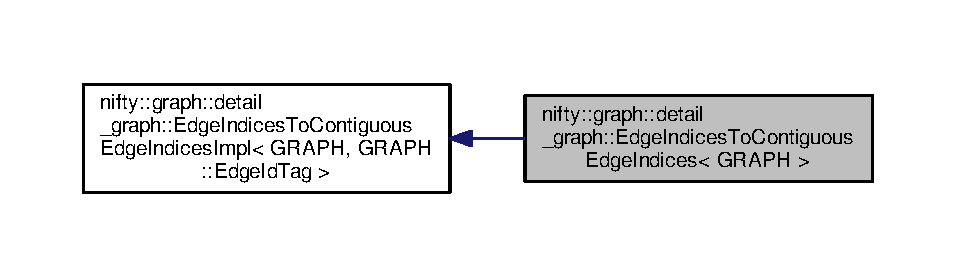
\includegraphics[width=350pt]{classnifty_1_1graph_1_1detail__graph_1_1EdgeIndicesToContiguousEdgeIndices__inherit__graph}
\end{center}
\end{figure}


Collaboration diagram for nifty\+:\+:graph\+:\+:detail\+\_\+graph\+:\+:Edge\+Indices\+To\+Contiguous\+Edge\+Indices$<$ G\+R\+A\+PH $>$\+:
\nopagebreak
\begin{figure}[H]
\begin{center}
\leavevmode
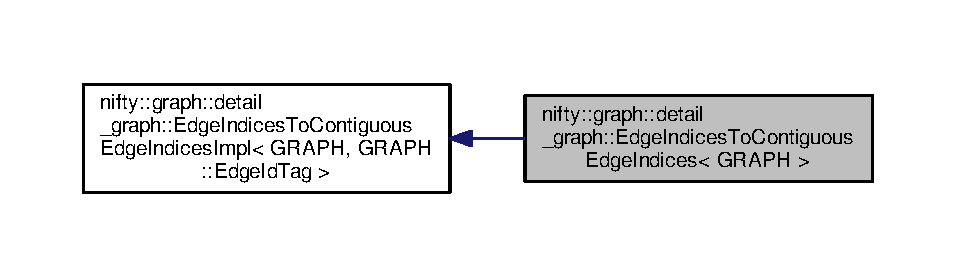
\includegraphics[width=350pt]{classnifty_1_1graph_1_1detail__graph_1_1EdgeIndicesToContiguousEdgeIndices__coll__graph}
\end{center}
\end{figure}
\subsection*{Additional Inherited Members}


The documentation for this class was generated from the following file\+:\begin{DoxyCompactItemize}
\item 
/home/tbeier/src/nifty/include/nifty/graph/detail/\hyperlink{contiguous__indices_8hxx}{contiguous\+\_\+indices.\+hxx}\end{DoxyCompactItemize}

\hypertarget{classnifty_1_1graph_1_1detail__graph_1_1EdgeIndicesToContiguousEdgeIndicesImpl}{}\section{nifty\+:\+:graph\+:\+:detail\+\_\+graph\+:\+:Edge\+Indices\+To\+Contiguous\+Edge\+Indices\+Impl$<$ G\+R\+A\+PH, E\+D\+G\+E\+\_\+\+I\+D\+\_\+\+T\+AG $>$ Class Template Reference}
\label{classnifty_1_1graph_1_1detail__graph_1_1EdgeIndicesToContiguousEdgeIndicesImpl}\index{nifty\+::graph\+::detail\+\_\+graph\+::\+Edge\+Indices\+To\+Contiguous\+Edge\+Indices\+Impl$<$ G\+R\+A\+P\+H, E\+D\+G\+E\+\_\+\+I\+D\+\_\+\+T\+A\+G $>$@{nifty\+::graph\+::detail\+\_\+graph\+::\+Edge\+Indices\+To\+Contiguous\+Edge\+Indices\+Impl$<$ G\+R\+A\+P\+H, E\+D\+G\+E\+\_\+\+I\+D\+\_\+\+T\+A\+G $>$}}


{\ttfamily \#include $<$contiguous\+\_\+indices.\+hxx$>$}

\subsection*{Public Types}
\begin{DoxyCompactItemize}
\item 
typedef G\+R\+A\+PH \hyperlink{classnifty_1_1graph_1_1detail__graph_1_1EdgeIndicesToContiguousEdgeIndicesImpl_a9a93d5ced427774523bdbce7912d1788}{Graph\+Type}
\end{DoxyCompactItemize}
\subsection*{Public Member Functions}
\begin{DoxyCompactItemize}
\item 
\hyperlink{classnifty_1_1graph_1_1detail__graph_1_1EdgeIndicesToContiguousEdgeIndicesImpl_a00a49b794117958e1b0303322c4965cb}{Edge\+Indices\+To\+Contiguous\+Edge\+Indices\+Impl} (const \hyperlink{classnifty_1_1graph_1_1detail__graph_1_1EdgeIndicesToContiguousEdgeIndicesImpl_a9a93d5ced427774523bdbce7912d1788}{Graph\+Type} \&graph)
\item 
int64\+\_\+t \hyperlink{classnifty_1_1graph_1_1detail__graph_1_1EdgeIndicesToContiguousEdgeIndicesImpl_ae161e5dfac99c6d9109450aac9a891ac}{operator\mbox{[}$\,$\mbox{]}} (const int64\+\_\+t edge) const
\end{DoxyCompactItemize}


\subsection{Member Typedef Documentation}
\mbox{\Hypertarget{classnifty_1_1graph_1_1detail__graph_1_1EdgeIndicesToContiguousEdgeIndicesImpl_a9a93d5ced427774523bdbce7912d1788}\label{classnifty_1_1graph_1_1detail__graph_1_1EdgeIndicesToContiguousEdgeIndicesImpl_a9a93d5ced427774523bdbce7912d1788}} 
\index{nifty\+::graph\+::detail\+\_\+graph\+::\+Edge\+Indices\+To\+Contiguous\+Edge\+Indices\+Impl@{nifty\+::graph\+::detail\+\_\+graph\+::\+Edge\+Indices\+To\+Contiguous\+Edge\+Indices\+Impl}!Graph\+Type@{Graph\+Type}}
\index{Graph\+Type@{Graph\+Type}!nifty\+::graph\+::detail\+\_\+graph\+::\+Edge\+Indices\+To\+Contiguous\+Edge\+Indices\+Impl@{nifty\+::graph\+::detail\+\_\+graph\+::\+Edge\+Indices\+To\+Contiguous\+Edge\+Indices\+Impl}}
\subsubsection{\texorpdfstring{Graph\+Type}{GraphType}}
{\footnotesize\ttfamily template$<$class G\+R\+A\+PH, class E\+D\+G\+E\+\_\+\+I\+D\+\_\+\+T\+AG$>$ \\
typedef G\+R\+A\+PH \hyperlink{classnifty_1_1graph_1_1detail__graph_1_1EdgeIndicesToContiguousEdgeIndicesImpl}{nifty\+::graph\+::detail\+\_\+graph\+::\+Edge\+Indices\+To\+Contiguous\+Edge\+Indices\+Impl}$<$ G\+R\+A\+PH, E\+D\+G\+E\+\_\+\+I\+D\+\_\+\+T\+AG $>$\+::\hyperlink{classnifty_1_1graph_1_1detail__graph_1_1EdgeIndicesToContiguousEdgeIndicesImpl_a9a93d5ced427774523bdbce7912d1788}{Graph\+Type}}



\subsection{Constructor \& Destructor Documentation}
\mbox{\Hypertarget{classnifty_1_1graph_1_1detail__graph_1_1EdgeIndicesToContiguousEdgeIndicesImpl_a00a49b794117958e1b0303322c4965cb}\label{classnifty_1_1graph_1_1detail__graph_1_1EdgeIndicesToContiguousEdgeIndicesImpl_a00a49b794117958e1b0303322c4965cb}} 
\index{nifty\+::graph\+::detail\+\_\+graph\+::\+Edge\+Indices\+To\+Contiguous\+Edge\+Indices\+Impl@{nifty\+::graph\+::detail\+\_\+graph\+::\+Edge\+Indices\+To\+Contiguous\+Edge\+Indices\+Impl}!Edge\+Indices\+To\+Contiguous\+Edge\+Indices\+Impl@{Edge\+Indices\+To\+Contiguous\+Edge\+Indices\+Impl}}
\index{Edge\+Indices\+To\+Contiguous\+Edge\+Indices\+Impl@{Edge\+Indices\+To\+Contiguous\+Edge\+Indices\+Impl}!nifty\+::graph\+::detail\+\_\+graph\+::\+Edge\+Indices\+To\+Contiguous\+Edge\+Indices\+Impl@{nifty\+::graph\+::detail\+\_\+graph\+::\+Edge\+Indices\+To\+Contiguous\+Edge\+Indices\+Impl}}
\subsubsection{\texorpdfstring{Edge\+Indices\+To\+Contiguous\+Edge\+Indices\+Impl()}{EdgeIndicesToContiguousEdgeIndicesImpl()}}
{\footnotesize\ttfamily template$<$class G\+R\+A\+PH, class E\+D\+G\+E\+\_\+\+I\+D\+\_\+\+T\+AG$>$ \\
\hyperlink{classnifty_1_1graph_1_1detail__graph_1_1EdgeIndicesToContiguousEdgeIndicesImpl}{nifty\+::graph\+::detail\+\_\+graph\+::\+Edge\+Indices\+To\+Contiguous\+Edge\+Indices\+Impl}$<$ G\+R\+A\+PH, E\+D\+G\+E\+\_\+\+I\+D\+\_\+\+T\+AG $>$\+::\hyperlink{classnifty_1_1graph_1_1detail__graph_1_1EdgeIndicesToContiguousEdgeIndicesImpl}{Edge\+Indices\+To\+Contiguous\+Edge\+Indices\+Impl} (\begin{DoxyParamCaption}\item[{const \hyperlink{classnifty_1_1graph_1_1detail__graph_1_1EdgeIndicesToContiguousEdgeIndicesImpl_a9a93d5ced427774523bdbce7912d1788}{Graph\+Type} \&}]{graph }\end{DoxyParamCaption})\hspace{0.3cm}{\ttfamily [inline]}}



\subsection{Member Function Documentation}
\mbox{\Hypertarget{classnifty_1_1graph_1_1detail__graph_1_1EdgeIndicesToContiguousEdgeIndicesImpl_ae161e5dfac99c6d9109450aac9a891ac}\label{classnifty_1_1graph_1_1detail__graph_1_1EdgeIndicesToContiguousEdgeIndicesImpl_ae161e5dfac99c6d9109450aac9a891ac}} 
\index{nifty\+::graph\+::detail\+\_\+graph\+::\+Edge\+Indices\+To\+Contiguous\+Edge\+Indices\+Impl@{nifty\+::graph\+::detail\+\_\+graph\+::\+Edge\+Indices\+To\+Contiguous\+Edge\+Indices\+Impl}!operator\mbox{[}\mbox{]}@{operator[]}}
\index{operator\mbox{[}\mbox{]}@{operator[]}!nifty\+::graph\+::detail\+\_\+graph\+::\+Edge\+Indices\+To\+Contiguous\+Edge\+Indices\+Impl@{nifty\+::graph\+::detail\+\_\+graph\+::\+Edge\+Indices\+To\+Contiguous\+Edge\+Indices\+Impl}}
\subsubsection{\texorpdfstring{operator[]()}{operator[]()}}
{\footnotesize\ttfamily template$<$class G\+R\+A\+PH, class E\+D\+G\+E\+\_\+\+I\+D\+\_\+\+T\+AG$>$ \\
int64\+\_\+t \hyperlink{classnifty_1_1graph_1_1detail__graph_1_1EdgeIndicesToContiguousEdgeIndicesImpl}{nifty\+::graph\+::detail\+\_\+graph\+::\+Edge\+Indices\+To\+Contiguous\+Edge\+Indices\+Impl}$<$ G\+R\+A\+PH, E\+D\+G\+E\+\_\+\+I\+D\+\_\+\+T\+AG $>$\+::operator\mbox{[}$\,$\mbox{]} (\begin{DoxyParamCaption}\item[{const int64\+\_\+t}]{edge }\end{DoxyParamCaption}) const\hspace{0.3cm}{\ttfamily [inline]}}



The documentation for this class was generated from the following file\+:\begin{DoxyCompactItemize}
\item 
/home/tbeier/src/nifty/include/nifty/graph/detail/\hyperlink{contiguous__indices_8hxx}{contiguous\+\_\+indices.\+hxx}\end{DoxyCompactItemize}

\hypertarget{classnifty_1_1graph_1_1detail__graph_1_1EdgeIndicesToContiguousEdgeIndicesImpl_3_01GRAPH_00_01ni85a4007f22b365a25e3bd0829bce5cfc}{}\section{nifty\+:\+:graph\+:\+:detail\+\_\+graph\+:\+:Edge\+Indices\+To\+Contiguous\+Edge\+Indices\+Impl$<$ G\+R\+A\+PH, nifty\+:\+:graph\+:\+:Contiguous\+Tag $>$ Class Template Reference}
\label{classnifty_1_1graph_1_1detail__graph_1_1EdgeIndicesToContiguousEdgeIndicesImpl_3_01GRAPH_00_01ni85a4007f22b365a25e3bd0829bce5cfc}\index{nifty\+::graph\+::detail\+\_\+graph\+::\+Edge\+Indices\+To\+Contiguous\+Edge\+Indices\+Impl$<$ G\+R\+A\+P\+H, nifty\+::graph\+::\+Contiguous\+Tag $>$@{nifty\+::graph\+::detail\+\_\+graph\+::\+Edge\+Indices\+To\+Contiguous\+Edge\+Indices\+Impl$<$ G\+R\+A\+P\+H, nifty\+::graph\+::\+Contiguous\+Tag $>$}}


{\ttfamily \#include $<$contiguous\+\_\+indices.\+hxx$>$}

\subsection*{Public Types}
\begin{DoxyCompactItemize}
\item 
typedef G\+R\+A\+PH \hyperlink{classnifty_1_1graph_1_1detail__graph_1_1EdgeIndicesToContiguousEdgeIndicesImpl_3_01GRAPH_00_01ni85a4007f22b365a25e3bd0829bce5cfc_a928b2c3e5ef48c1b5af76cf008ad7d9c}{Graph\+Type}
\end{DoxyCompactItemize}
\subsection*{Public Member Functions}
\begin{DoxyCompactItemize}
\item 
\hyperlink{classnifty_1_1graph_1_1detail__graph_1_1EdgeIndicesToContiguousEdgeIndicesImpl_3_01GRAPH_00_01ni85a4007f22b365a25e3bd0829bce5cfc_ad02c81f222261b4f465424dc366b7e08}{Edge\+Indices\+To\+Contiguous\+Edge\+Indices\+Impl} (const \hyperlink{classnifty_1_1graph_1_1detail__graph_1_1EdgeIndicesToContiguousEdgeIndicesImpl_3_01GRAPH_00_01ni85a4007f22b365a25e3bd0829bce5cfc_a928b2c3e5ef48c1b5af76cf008ad7d9c}{Graph\+Type} \&graph)
\item 
int64\+\_\+t \hyperlink{classnifty_1_1graph_1_1detail__graph_1_1EdgeIndicesToContiguousEdgeIndicesImpl_3_01GRAPH_00_01ni85a4007f22b365a25e3bd0829bce5cfc_ac2d90ab9eed3102c6f726c3282d24eef}{operator\mbox{[}$\,$\mbox{]}} (const int64\+\_\+t edge) const
\end{DoxyCompactItemize}


\subsection{Member Typedef Documentation}
\mbox{\Hypertarget{classnifty_1_1graph_1_1detail__graph_1_1EdgeIndicesToContiguousEdgeIndicesImpl_3_01GRAPH_00_01ni85a4007f22b365a25e3bd0829bce5cfc_a928b2c3e5ef48c1b5af76cf008ad7d9c}\label{classnifty_1_1graph_1_1detail__graph_1_1EdgeIndicesToContiguousEdgeIndicesImpl_3_01GRAPH_00_01ni85a4007f22b365a25e3bd0829bce5cfc_a928b2c3e5ef48c1b5af76cf008ad7d9c}} 
\index{nifty\+::graph\+::detail\+\_\+graph\+::\+Edge\+Indices\+To\+Contiguous\+Edge\+Indices\+Impl$<$ G\+R\+A\+P\+H, nifty\+::graph\+::\+Contiguous\+Tag $>$@{nifty\+::graph\+::detail\+\_\+graph\+::\+Edge\+Indices\+To\+Contiguous\+Edge\+Indices\+Impl$<$ G\+R\+A\+P\+H, nifty\+::graph\+::\+Contiguous\+Tag $>$}!Graph\+Type@{Graph\+Type}}
\index{Graph\+Type@{Graph\+Type}!nifty\+::graph\+::detail\+\_\+graph\+::\+Edge\+Indices\+To\+Contiguous\+Edge\+Indices\+Impl$<$ G\+R\+A\+P\+H, nifty\+::graph\+::\+Contiguous\+Tag $>$@{nifty\+::graph\+::detail\+\_\+graph\+::\+Edge\+Indices\+To\+Contiguous\+Edge\+Indices\+Impl$<$ G\+R\+A\+P\+H, nifty\+::graph\+::\+Contiguous\+Tag $>$}}
\subsubsection{\texorpdfstring{Graph\+Type}{GraphType}}
{\footnotesize\ttfamily template$<$class G\+R\+A\+PH $>$ \\
typedef G\+R\+A\+PH \hyperlink{classnifty_1_1graph_1_1detail__graph_1_1EdgeIndicesToContiguousEdgeIndicesImpl}{nifty\+::graph\+::detail\+\_\+graph\+::\+Edge\+Indices\+To\+Contiguous\+Edge\+Indices\+Impl}$<$ G\+R\+A\+PH, \hyperlink{structnifty_1_1graph_1_1ContiguousTag}{nifty\+::graph\+::\+Contiguous\+Tag} $>$\+::\hyperlink{classnifty_1_1graph_1_1detail__graph_1_1EdgeIndicesToContiguousEdgeIndicesImpl_3_01GRAPH_00_01ni85a4007f22b365a25e3bd0829bce5cfc_a928b2c3e5ef48c1b5af76cf008ad7d9c}{Graph\+Type}}



\subsection{Constructor \& Destructor Documentation}
\mbox{\Hypertarget{classnifty_1_1graph_1_1detail__graph_1_1EdgeIndicesToContiguousEdgeIndicesImpl_3_01GRAPH_00_01ni85a4007f22b365a25e3bd0829bce5cfc_ad02c81f222261b4f465424dc366b7e08}\label{classnifty_1_1graph_1_1detail__graph_1_1EdgeIndicesToContiguousEdgeIndicesImpl_3_01GRAPH_00_01ni85a4007f22b365a25e3bd0829bce5cfc_ad02c81f222261b4f465424dc366b7e08}} 
\index{nifty\+::graph\+::detail\+\_\+graph\+::\+Edge\+Indices\+To\+Contiguous\+Edge\+Indices\+Impl$<$ G\+R\+A\+P\+H, nifty\+::graph\+::\+Contiguous\+Tag $>$@{nifty\+::graph\+::detail\+\_\+graph\+::\+Edge\+Indices\+To\+Contiguous\+Edge\+Indices\+Impl$<$ G\+R\+A\+P\+H, nifty\+::graph\+::\+Contiguous\+Tag $>$}!Edge\+Indices\+To\+Contiguous\+Edge\+Indices\+Impl@{Edge\+Indices\+To\+Contiguous\+Edge\+Indices\+Impl}}
\index{Edge\+Indices\+To\+Contiguous\+Edge\+Indices\+Impl@{Edge\+Indices\+To\+Contiguous\+Edge\+Indices\+Impl}!nifty\+::graph\+::detail\+\_\+graph\+::\+Edge\+Indices\+To\+Contiguous\+Edge\+Indices\+Impl$<$ G\+R\+A\+P\+H, nifty\+::graph\+::\+Contiguous\+Tag $>$@{nifty\+::graph\+::detail\+\_\+graph\+::\+Edge\+Indices\+To\+Contiguous\+Edge\+Indices\+Impl$<$ G\+R\+A\+P\+H, nifty\+::graph\+::\+Contiguous\+Tag $>$}}
\subsubsection{\texorpdfstring{Edge\+Indices\+To\+Contiguous\+Edge\+Indices\+Impl()}{EdgeIndicesToContiguousEdgeIndicesImpl()}}
{\footnotesize\ttfamily template$<$class G\+R\+A\+PH $>$ \\
\hyperlink{classnifty_1_1graph_1_1detail__graph_1_1EdgeIndicesToContiguousEdgeIndicesImpl}{nifty\+::graph\+::detail\+\_\+graph\+::\+Edge\+Indices\+To\+Contiguous\+Edge\+Indices\+Impl}$<$ G\+R\+A\+PH, \hyperlink{structnifty_1_1graph_1_1ContiguousTag}{nifty\+::graph\+::\+Contiguous\+Tag} $>$\+::\hyperlink{classnifty_1_1graph_1_1detail__graph_1_1EdgeIndicesToContiguousEdgeIndicesImpl}{Edge\+Indices\+To\+Contiguous\+Edge\+Indices\+Impl} (\begin{DoxyParamCaption}\item[{const \hyperlink{classnifty_1_1graph_1_1detail__graph_1_1EdgeIndicesToContiguousEdgeIndicesImpl_3_01GRAPH_00_01ni85a4007f22b365a25e3bd0829bce5cfc_a928b2c3e5ef48c1b5af76cf008ad7d9c}{Graph\+Type} \&}]{graph }\end{DoxyParamCaption})\hspace{0.3cm}{\ttfamily [inline]}}



\subsection{Member Function Documentation}
\mbox{\Hypertarget{classnifty_1_1graph_1_1detail__graph_1_1EdgeIndicesToContiguousEdgeIndicesImpl_3_01GRAPH_00_01ni85a4007f22b365a25e3bd0829bce5cfc_ac2d90ab9eed3102c6f726c3282d24eef}\label{classnifty_1_1graph_1_1detail__graph_1_1EdgeIndicesToContiguousEdgeIndicesImpl_3_01GRAPH_00_01ni85a4007f22b365a25e3bd0829bce5cfc_ac2d90ab9eed3102c6f726c3282d24eef}} 
\index{nifty\+::graph\+::detail\+\_\+graph\+::\+Edge\+Indices\+To\+Contiguous\+Edge\+Indices\+Impl$<$ G\+R\+A\+P\+H, nifty\+::graph\+::\+Contiguous\+Tag $>$@{nifty\+::graph\+::detail\+\_\+graph\+::\+Edge\+Indices\+To\+Contiguous\+Edge\+Indices\+Impl$<$ G\+R\+A\+P\+H, nifty\+::graph\+::\+Contiguous\+Tag $>$}!operator\mbox{[}\mbox{]}@{operator[]}}
\index{operator\mbox{[}\mbox{]}@{operator[]}!nifty\+::graph\+::detail\+\_\+graph\+::\+Edge\+Indices\+To\+Contiguous\+Edge\+Indices\+Impl$<$ G\+R\+A\+P\+H, nifty\+::graph\+::\+Contiguous\+Tag $>$@{nifty\+::graph\+::detail\+\_\+graph\+::\+Edge\+Indices\+To\+Contiguous\+Edge\+Indices\+Impl$<$ G\+R\+A\+P\+H, nifty\+::graph\+::\+Contiguous\+Tag $>$}}
\subsubsection{\texorpdfstring{operator[]()}{operator[]()}}
{\footnotesize\ttfamily template$<$class G\+R\+A\+PH $>$ \\
int64\+\_\+t \hyperlink{classnifty_1_1graph_1_1detail__graph_1_1EdgeIndicesToContiguousEdgeIndicesImpl}{nifty\+::graph\+::detail\+\_\+graph\+::\+Edge\+Indices\+To\+Contiguous\+Edge\+Indices\+Impl}$<$ G\+R\+A\+PH, \hyperlink{structnifty_1_1graph_1_1ContiguousTag}{nifty\+::graph\+::\+Contiguous\+Tag} $>$\+::operator\mbox{[}$\,$\mbox{]} (\begin{DoxyParamCaption}\item[{const int64\+\_\+t}]{edge }\end{DoxyParamCaption}) const\hspace{0.3cm}{\ttfamily [inline]}}



The documentation for this class was generated from the following file\+:\begin{DoxyCompactItemize}
\item 
/home/tbeier/src/nifty/include/nifty/graph/detail/\hyperlink{contiguous__indices_8hxx}{contiguous\+\_\+indices.\+hxx}\end{DoxyCompactItemize}

\hypertarget{structnifty_1_1graph_1_1UndirectedGraphBase_1_1EdgeIterRange}{}\section{nifty\+:\+:graph\+:\+:Undirected\+Graph\+Base$<$ C\+H\+I\+L\+D\+\_\+\+G\+R\+A\+P\+H, N\+O\+D\+E\+\_\+\+I\+T\+E\+R, E\+D\+G\+E\+\_\+\+I\+T\+E\+R, A\+D\+J\+A\+C\+E\+N\+C\+Y\+\_\+\+I\+T\+E\+R $>$\+:\+:Edge\+Iter\+Range$<$ \+\_\+\+C\+H\+I\+L\+D\+\_\+\+G\+R\+A\+P\+H $>$ Struct Template Reference}
\label{structnifty_1_1graph_1_1UndirectedGraphBase_1_1EdgeIterRange}\index{nifty\+::graph\+::\+Undirected\+Graph\+Base$<$ C\+H\+I\+L\+D\+\_\+\+G\+R\+A\+P\+H, N\+O\+D\+E\+\_\+\+I\+T\+E\+R, E\+D\+G\+E\+\_\+\+I\+T\+E\+R, A\+D\+J\+A\+C\+E\+N\+C\+Y\+\_\+\+I\+T\+E\+R $>$\+::\+Edge\+Iter\+Range$<$ \+\_\+\+C\+H\+I\+L\+D\+\_\+\+G\+R\+A\+P\+H $>$@{nifty\+::graph\+::\+Undirected\+Graph\+Base$<$ C\+H\+I\+L\+D\+\_\+\+G\+R\+A\+P\+H, N\+O\+D\+E\+\_\+\+I\+T\+E\+R, E\+D\+G\+E\+\_\+\+I\+T\+E\+R, A\+D\+J\+A\+C\+E\+N\+C\+Y\+\_\+\+I\+T\+E\+R $>$\+::\+Edge\+Iter\+Range$<$ \+\_\+\+C\+H\+I\+L\+D\+\_\+\+G\+R\+A\+P\+H $>$}}


{\ttfamily \#include $<$undirected\+\_\+graph\+\_\+base.\+hxx$>$}



Inheritance diagram for nifty\+:\+:graph\+:\+:Undirected\+Graph\+Base$<$ C\+H\+I\+L\+D\+\_\+\+G\+R\+A\+P\+H, N\+O\+D\+E\+\_\+\+I\+T\+E\+R, E\+D\+G\+E\+\_\+\+I\+T\+E\+R, A\+D\+J\+A\+C\+E\+N\+C\+Y\+\_\+\+I\+T\+E\+R $>$\+:\+:Edge\+Iter\+Range$<$ \+\_\+\+C\+H\+I\+L\+D\+\_\+\+G\+R\+A\+P\+H $>$\+:\nopagebreak
\begin{figure}[H]
\begin{center}
\leavevmode
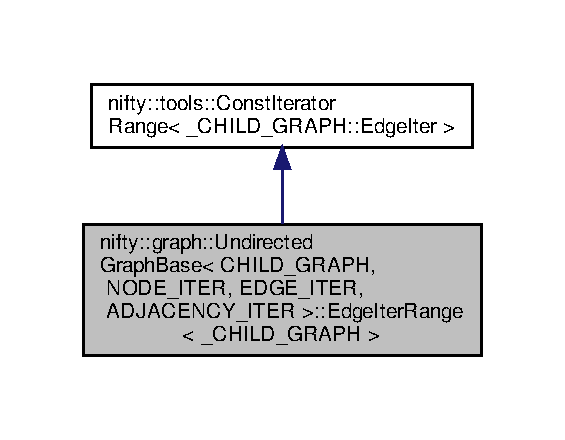
\includegraphics[width=271pt]{structnifty_1_1graph_1_1UndirectedGraphBase_1_1EdgeIterRange__inherit__graph}
\end{center}
\end{figure}


Collaboration diagram for nifty\+:\+:graph\+:\+:Undirected\+Graph\+Base$<$ C\+H\+I\+L\+D\+\_\+\+G\+R\+A\+P\+H, N\+O\+D\+E\+\_\+\+I\+T\+E\+R, E\+D\+G\+E\+\_\+\+I\+T\+E\+R, A\+D\+J\+A\+C\+E\+N\+C\+Y\+\_\+\+I\+T\+E\+R $>$\+:\+:Edge\+Iter\+Range$<$ \+\_\+\+C\+H\+I\+L\+D\+\_\+\+G\+R\+A\+P\+H $>$\+:\nopagebreak
\begin{figure}[H]
\begin{center}
\leavevmode
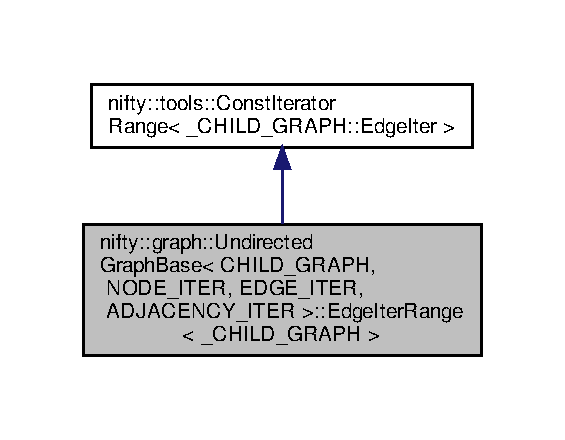
\includegraphics[width=271pt]{structnifty_1_1graph_1_1UndirectedGraphBase_1_1EdgeIterRange__coll__graph}
\end{center}
\end{figure}
\subsection*{Additional Inherited Members}


The documentation for this struct was generated from the following file\+:\begin{DoxyCompactItemize}
\item 
/home/tbeier/src/nifty/include/nifty/graph/\hyperlink{undirected__graph__base_8hxx}{undirected\+\_\+graph\+\_\+base.\+hxx}\end{DoxyCompactItemize}

\hypertarget{structnifty_1_1graph_1_1DirectedGraphBase_1_1EdgeMap}{}\section{nifty\+:\+:graph\+:\+:Directed\+Graph\+Base$<$ C\+H\+I\+L\+D\+\_\+\+G\+R\+A\+P\+H $>$\+:\+:Edge\+Map$<$ T $>$ Struct Template Reference}
\label{structnifty_1_1graph_1_1DirectedGraphBase_1_1EdgeMap}\index{nifty\+::graph\+::\+Directed\+Graph\+Base$<$ C\+H\+I\+L\+D\+\_\+\+G\+R\+A\+P\+H $>$\+::\+Edge\+Map$<$ T $>$@{nifty\+::graph\+::\+Directed\+Graph\+Base$<$ C\+H\+I\+L\+D\+\_\+\+G\+R\+A\+P\+H $>$\+::\+Edge\+Map$<$ T $>$}}


{\ttfamily \#include $<$directed\+\_\+graph\+\_\+base.\+hxx$>$}



Inheritance diagram for nifty\+:\+:graph\+:\+:Directed\+Graph\+Base$<$ C\+H\+I\+L\+D\+\_\+\+G\+R\+A\+P\+H $>$\+:\+:Edge\+Map$<$ T $>$\+:\nopagebreak
\begin{figure}[H]
\begin{center}
\leavevmode
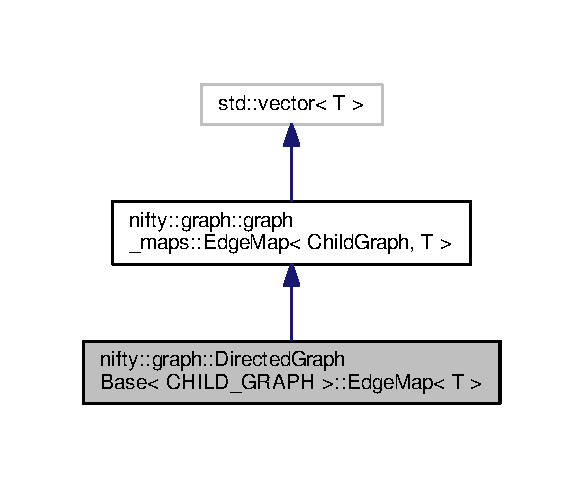
\includegraphics[width=280pt]{structnifty_1_1graph_1_1DirectedGraphBase_1_1EdgeMap__inherit__graph}
\end{center}
\end{figure}


Collaboration diagram for nifty\+:\+:graph\+:\+:Directed\+Graph\+Base$<$ C\+H\+I\+L\+D\+\_\+\+G\+R\+A\+P\+H $>$\+:\+:Edge\+Map$<$ T $>$\+:\nopagebreak
\begin{figure}[H]
\begin{center}
\leavevmode
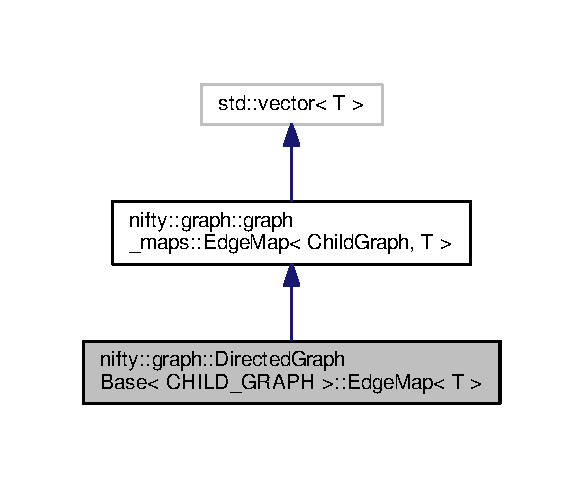
\includegraphics[width=280pt]{structnifty_1_1graph_1_1DirectedGraphBase_1_1EdgeMap__coll__graph}
\end{center}
\end{figure}
\subsection*{Additional Inherited Members}


The documentation for this struct was generated from the following file\+:\begin{DoxyCompactItemize}
\item 
/home/tbeier/src/nifty/include/nifty/graph/\hyperlink{directed__graph__base_8hxx}{directed\+\_\+graph\+\_\+base.\+hxx}\end{DoxyCompactItemize}

\hypertarget{structnifty_1_1graph_1_1graph__maps_1_1EdgeMap}{}\section{nifty\+:\+:graph\+:\+:graph\+\_\+maps\+:\+:Edge\+Map$<$ G, T $>$ Struct Template Reference}
\label{structnifty_1_1graph_1_1graph__maps_1_1EdgeMap}\index{nifty\+::graph\+::graph\+\_\+maps\+::\+Edge\+Map$<$ G, T $>$@{nifty\+::graph\+::graph\+\_\+maps\+::\+Edge\+Map$<$ G, T $>$}}


{\ttfamily \#include $<$graph\+\_\+maps.\+hxx$>$}



Inheritance diagram for nifty\+:\+:graph\+:\+:graph\+\_\+maps\+:\+:Edge\+Map$<$ G, T $>$\+:
% FIG 0


Collaboration diagram for nifty\+:\+:graph\+:\+:graph\+\_\+maps\+:\+:Edge\+Map$<$ G, T $>$\+:
% FIG 1
\subsection*{Public Member Functions}
\begin{DoxyCompactItemize}
\item 
\hyperlink{structnifty_1_1graph_1_1graph__maps_1_1EdgeMap_a76af091031717407e07ffb154f74e653}{Edge\+Map} (const G \&g, const T \&val)
\item 
\hyperlink{structnifty_1_1graph_1_1graph__maps_1_1EdgeMap_a5100202d40822e8cf98aea0ee90ee01e}{Edge\+Map} (const G \&g)
\item 
\hyperlink{structnifty_1_1graph_1_1graph__maps_1_1EdgeMap_adfef359098c94982e5a8f6355d068878}{Edge\+Map} ()
\item 
void \hyperlink{structnifty_1_1graph_1_1graph__maps_1_1EdgeMap_aa658ff2e5952fce8342349a159425bbd}{inserted\+Edges} (const uint64\+\_\+t edge\+Id, const T \&insert\+Value=T())
\end{DoxyCompactItemize}


\subsection{Constructor \& Destructor Documentation}
\hypertarget{structnifty_1_1graph_1_1graph__maps_1_1EdgeMap_a76af091031717407e07ffb154f74e653}{}\index{nifty\+::graph\+::graph\+\_\+maps\+::\+Edge\+Map@{nifty\+::graph\+::graph\+\_\+maps\+::\+Edge\+Map}!Edge\+Map@{Edge\+Map}}
\index{Edge\+Map@{Edge\+Map}!nifty\+::graph\+::graph\+\_\+maps\+::\+Edge\+Map@{nifty\+::graph\+::graph\+\_\+maps\+::\+Edge\+Map}}
\subsubsection[{Edge\+Map(const G \&g, const T \&val)}]{\setlength{\rightskip}{0pt plus 5cm}template$<$class G, class T$>$ {\bf nifty\+::graph\+::graph\+\_\+maps\+::\+Edge\+Map}$<$ G, T $>$\+::{\bf Edge\+Map} (
\begin{DoxyParamCaption}
\item[{const G \&}]{g, }
\item[{const T \&}]{val}
\end{DoxyParamCaption}
)\hspace{0.3cm}{\ttfamily [inline]}}\label{structnifty_1_1graph_1_1graph__maps_1_1EdgeMap_a76af091031717407e07ffb154f74e653}
\hypertarget{structnifty_1_1graph_1_1graph__maps_1_1EdgeMap_a5100202d40822e8cf98aea0ee90ee01e}{}\index{nifty\+::graph\+::graph\+\_\+maps\+::\+Edge\+Map@{nifty\+::graph\+::graph\+\_\+maps\+::\+Edge\+Map}!Edge\+Map@{Edge\+Map}}
\index{Edge\+Map@{Edge\+Map}!nifty\+::graph\+::graph\+\_\+maps\+::\+Edge\+Map@{nifty\+::graph\+::graph\+\_\+maps\+::\+Edge\+Map}}
\subsubsection[{Edge\+Map(const G \&g)}]{\setlength{\rightskip}{0pt plus 5cm}template$<$class G, class T$>$ {\bf nifty\+::graph\+::graph\+\_\+maps\+::\+Edge\+Map}$<$ G, T $>$\+::{\bf Edge\+Map} (
\begin{DoxyParamCaption}
\item[{const G \&}]{g}
\end{DoxyParamCaption}
)\hspace{0.3cm}{\ttfamily [inline]}}\label{structnifty_1_1graph_1_1graph__maps_1_1EdgeMap_a5100202d40822e8cf98aea0ee90ee01e}
\hypertarget{structnifty_1_1graph_1_1graph__maps_1_1EdgeMap_adfef359098c94982e5a8f6355d068878}{}\index{nifty\+::graph\+::graph\+\_\+maps\+::\+Edge\+Map@{nifty\+::graph\+::graph\+\_\+maps\+::\+Edge\+Map}!Edge\+Map@{Edge\+Map}}
\index{Edge\+Map@{Edge\+Map}!nifty\+::graph\+::graph\+\_\+maps\+::\+Edge\+Map@{nifty\+::graph\+::graph\+\_\+maps\+::\+Edge\+Map}}
\subsubsection[{Edge\+Map()}]{\setlength{\rightskip}{0pt plus 5cm}template$<$class G, class T$>$ {\bf nifty\+::graph\+::graph\+\_\+maps\+::\+Edge\+Map}$<$ G, T $>$\+::{\bf Edge\+Map} (
\begin{DoxyParamCaption}
{}
\end{DoxyParamCaption}
)\hspace{0.3cm}{\ttfamily [inline]}}\label{structnifty_1_1graph_1_1graph__maps_1_1EdgeMap_adfef359098c94982e5a8f6355d068878}


\subsection{Member Function Documentation}
\hypertarget{structnifty_1_1graph_1_1graph__maps_1_1EdgeMap_aa658ff2e5952fce8342349a159425bbd}{}\index{nifty\+::graph\+::graph\+\_\+maps\+::\+Edge\+Map@{nifty\+::graph\+::graph\+\_\+maps\+::\+Edge\+Map}!inserted\+Edges@{inserted\+Edges}}
\index{inserted\+Edges@{inserted\+Edges}!nifty\+::graph\+::graph\+\_\+maps\+::\+Edge\+Map@{nifty\+::graph\+::graph\+\_\+maps\+::\+Edge\+Map}}
\subsubsection[{inserted\+Edges(const uint64\+\_\+t edge\+Id, const T \&insert\+Value=\+T())}]{\setlength{\rightskip}{0pt plus 5cm}template$<$class G, class T$>$ void {\bf nifty\+::graph\+::graph\+\_\+maps\+::\+Edge\+Map}$<$ G, T $>$\+::inserted\+Edges (
\begin{DoxyParamCaption}
\item[{const uint64\+\_\+t}]{edge\+Id, }
\item[{const T \&}]{insert\+Value = {\ttfamily T()}}
\end{DoxyParamCaption}
)\hspace{0.3cm}{\ttfamily [inline]}}\label{structnifty_1_1graph_1_1graph__maps_1_1EdgeMap_aa658ff2e5952fce8342349a159425bbd}


The documentation for this struct was generated from the following file\+:\begin{DoxyCompactItemize}
\item 
/home/tbeier/src/nifty/include/nifty/graph/\hyperlink{graph__maps_8hxx}{graph\+\_\+maps.\+hxx}\end{DoxyCompactItemize}

\hypertarget{structnifty_1_1graph_1_1UndirectedGraphBase_1_1EdgeMap}{}\section{nifty\+:\+:graph\+:\+:Undirected\+Graph\+Base$<$ C\+H\+I\+L\+D\+\_\+\+G\+R\+A\+PH, N\+O\+D\+E\+\_\+\+I\+T\+ER, E\+D\+G\+E\+\_\+\+I\+T\+ER, A\+D\+J\+A\+C\+E\+N\+C\+Y\+\_\+\+I\+T\+ER $>$\+:\+:Edge\+Map$<$ T $>$ Struct Template Reference}
\label{structnifty_1_1graph_1_1UndirectedGraphBase_1_1EdgeMap}\index{nifty\+::graph\+::\+Undirected\+Graph\+Base$<$ C\+H\+I\+L\+D\+\_\+\+G\+R\+A\+P\+H, N\+O\+D\+E\+\_\+\+I\+T\+E\+R, E\+D\+G\+E\+\_\+\+I\+T\+E\+R, A\+D\+J\+A\+C\+E\+N\+C\+Y\+\_\+\+I\+T\+E\+R $>$\+::\+Edge\+Map$<$ T $>$@{nifty\+::graph\+::\+Undirected\+Graph\+Base$<$ C\+H\+I\+L\+D\+\_\+\+G\+R\+A\+P\+H, N\+O\+D\+E\+\_\+\+I\+T\+E\+R, E\+D\+G\+E\+\_\+\+I\+T\+E\+R, A\+D\+J\+A\+C\+E\+N\+C\+Y\+\_\+\+I\+T\+E\+R $>$\+::\+Edge\+Map$<$ T $>$}}


{\ttfamily \#include $<$undirected\+\_\+graph\+\_\+base.\+hxx$>$}



Inheritance diagram for nifty\+:\+:graph\+:\+:Undirected\+Graph\+Base$<$ C\+H\+I\+L\+D\+\_\+\+G\+R\+A\+PH, N\+O\+D\+E\+\_\+\+I\+T\+ER, E\+D\+G\+E\+\_\+\+I\+T\+ER, A\+D\+J\+A\+C\+E\+N\+C\+Y\+\_\+\+I\+T\+ER $>$\+:\+:Edge\+Map$<$ T $>$\+:
\nopagebreak
\begin{figure}[H]
\begin{center}
\leavevmode
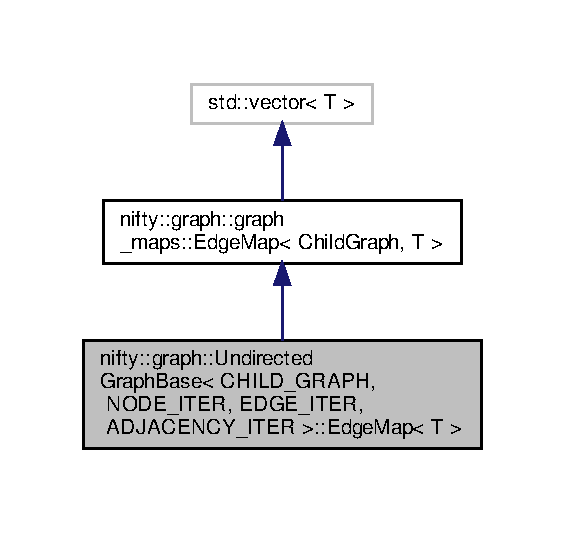
\includegraphics[width=271pt]{structnifty_1_1graph_1_1UndirectedGraphBase_1_1EdgeMap__inherit__graph}
\end{center}
\end{figure}


Collaboration diagram for nifty\+:\+:graph\+:\+:Undirected\+Graph\+Base$<$ C\+H\+I\+L\+D\+\_\+\+G\+R\+A\+PH, N\+O\+D\+E\+\_\+\+I\+T\+ER, E\+D\+G\+E\+\_\+\+I\+T\+ER, A\+D\+J\+A\+C\+E\+N\+C\+Y\+\_\+\+I\+T\+ER $>$\+:\+:Edge\+Map$<$ T $>$\+:
\nopagebreak
\begin{figure}[H]
\begin{center}
\leavevmode
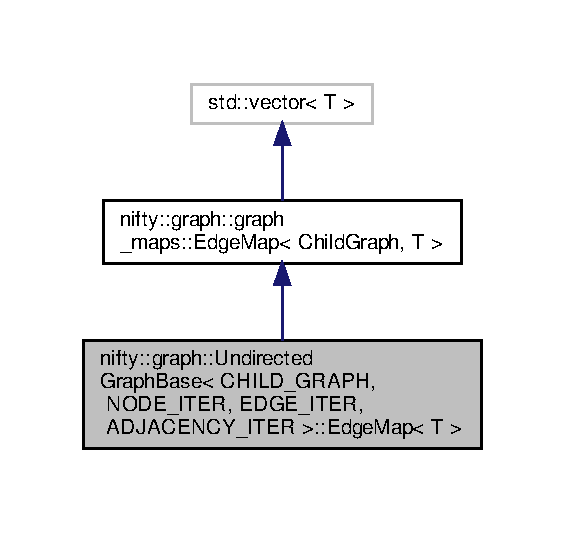
\includegraphics[width=271pt]{structnifty_1_1graph_1_1UndirectedGraphBase_1_1EdgeMap__coll__graph}
\end{center}
\end{figure}
\subsection*{Additional Inherited Members}


The documentation for this struct was generated from the following file\+:\begin{DoxyCompactItemize}
\item 
/home/tbeier/src/nifty/include/nifty/graph/\hyperlink{undirected__graph__base_8hxx}{undirected\+\_\+graph\+\_\+base.\+hxx}\end{DoxyCompactItemize}

\hypertarget{structnifty_1_1graph_1_1EdgeTag}{}\section{nifty\+:\+:graph\+:\+:Edge\+Tag Struct Reference}
\label{structnifty_1_1graph_1_1EdgeTag}\index{nifty\+::graph\+::\+Edge\+Tag@{nifty\+::graph\+::\+Edge\+Tag}}


{\ttfamily \#include $<$graph\+\_\+tags.\+hxx$>$}



The documentation for this struct was generated from the following file\+:\begin{DoxyCompactItemize}
\item 
/home/tbeier/src/nifty/include/nifty/graph/\hyperlink{graph__tags_8hxx}{graph\+\_\+tags.\+hxx}\end{DoxyCompactItemize}

\hypertarget{classnifty_1_1graph_1_1agglo_1_1EdgeWeightedClusterPolicy}{}\section{nifty\+:\+:graph\+:\+:agglo\+:\+:Edge\+Weighted\+Cluster\+Policy$<$ G\+R\+A\+P\+H, E\+N\+A\+B\+L\+E\+\_\+\+U\+C\+M $>$ Class Template Reference}
\label{classnifty_1_1graph_1_1agglo_1_1EdgeWeightedClusterPolicy}\index{nifty\+::graph\+::agglo\+::\+Edge\+Weighted\+Cluster\+Policy$<$ G\+R\+A\+P\+H, E\+N\+A\+B\+L\+E\+\_\+\+U\+C\+M $>$@{nifty\+::graph\+::agglo\+::\+Edge\+Weighted\+Cluster\+Policy$<$ G\+R\+A\+P\+H, E\+N\+A\+B\+L\+E\+\_\+\+U\+C\+M $>$}}


{\ttfamily \#include $<$edge\+\_\+weighted\+\_\+cluster\+\_\+policy.\+hxx$>$}

\subsection*{Public Types}
\begin{DoxyCompactItemize}
\item 
typedef G\+R\+A\+P\+H \hyperlink{classnifty_1_1graph_1_1agglo_1_1EdgeWeightedClusterPolicy_a8e910f7b9d0c1baa1de7b6b1c3e58397}{Graph\+Type}
\item 
typedef Float\+Edge\+Map \hyperlink{classnifty_1_1graph_1_1agglo_1_1EdgeWeightedClusterPolicy_a1b8107133a86be855885f1910652b0af}{Edge\+Indicators\+Type}
\item 
typedef Float\+Edge\+Map \hyperlink{classnifty_1_1graph_1_1agglo_1_1EdgeWeightedClusterPolicy_a64d646cc14e503e9a76a4646234d9754}{Edge\+Sizes\+Type}
\item 
typedef Float\+Node\+Map \hyperlink{classnifty_1_1graph_1_1agglo_1_1EdgeWeightedClusterPolicy_a44ba54059efcb57c8c8091016fb9ee99}{Node\+Sizes\+Type}
\item 
typedef \hyperlink{structnifty_1_1graph_1_1agglo_1_1EdgeWeightedClusterPolicySettings}{Edge\+Weighted\+Cluster\+Policy\+Settings} \hyperlink{classnifty_1_1graph_1_1agglo_1_1EdgeWeightedClusterPolicy_a6c9e2acec086a9fcc4391f067a4ded46}{Settings\+Type}
\item 
typedef \hyperlink{classnifty_1_1graph_1_1EdgeContractionGraph}{Edge\+Contraction\+Graph}$<$ \hyperlink{classnifty_1_1graph_1_1agglo_1_1EdgeWeightedClusterPolicy_a8e910f7b9d0c1baa1de7b6b1c3e58397}{Graph\+Type}, \hyperlink{classnifty_1_1graph_1_1agglo_1_1EdgeWeightedClusterPolicy}{Self\+Type} $>$ \hyperlink{classnifty_1_1graph_1_1agglo_1_1EdgeWeightedClusterPolicy_af2c3024ed1be514c58004dfa7e77448b}{Edge\+Contraction\+Graph\+Type}
\end{DoxyCompactItemize}
\subsection*{Public Member Functions}
\begin{DoxyCompactItemize}
\item 
{\footnotesize template$<$class E\+D\+G\+E\+\_\+\+I\+N\+D\+I\+C\+A\+T\+O\+R\+S , class E\+D\+G\+E\+\_\+\+S\+I\+Z\+E\+S , class N\+O\+D\+E\+\_\+\+S\+I\+Z\+E\+S $>$ }\\\hyperlink{classnifty_1_1graph_1_1agglo_1_1EdgeWeightedClusterPolicy_a028e533bd1a4eca1b6fdebb70b50b899}{Edge\+Weighted\+Cluster\+Policy} (const \hyperlink{classnifty_1_1graph_1_1agglo_1_1EdgeWeightedClusterPolicy_a8e910f7b9d0c1baa1de7b6b1c3e58397}{Graph\+Type} \&, const E\+D\+G\+E\+\_\+\+I\+N\+D\+I\+C\+A\+T\+O\+R\+S \&, const E\+D\+G\+E\+\_\+\+S\+I\+Z\+E\+S \&, const N\+O\+D\+E\+\_\+\+S\+I\+Z\+E\+S \&, const \hyperlink{classnifty_1_1graph_1_1agglo_1_1EdgeWeightedClusterPolicy_a6c9e2acec086a9fcc4391f067a4ded46}{Settings\+Type} \&settings=\hyperlink{classnifty_1_1graph_1_1agglo_1_1EdgeWeightedClusterPolicy_a6c9e2acec086a9fcc4391f067a4ded46}{Settings\+Type}())
\item 
std\+::pair$<$ uint64\+\_\+t, double $>$ \hyperlink{classnifty_1_1graph_1_1agglo_1_1EdgeWeightedClusterPolicy_a6ab0f6aa52808094a3cf375a5f6b085e}{edge\+To\+Contract\+Next} () const 
\item 
bool \hyperlink{classnifty_1_1graph_1_1agglo_1_1EdgeWeightedClusterPolicy_a46dcdcc192a1e07625a7c8c576dc5149}{is\+Done} () const 
\item 
\hyperlink{classnifty_1_1graph_1_1agglo_1_1EdgeWeightedClusterPolicy_af2c3024ed1be514c58004dfa7e77448b}{Edge\+Contraction\+Graph\+Type} \& \hyperlink{classnifty_1_1graph_1_1agglo_1_1EdgeWeightedClusterPolicy_ac66821b0db08e136631b0c75adf660d0}{edge\+Contraction\+Graph} ()
\item 
void \hyperlink{classnifty_1_1graph_1_1agglo_1_1EdgeWeightedClusterPolicy_ab17fb3b1739432d2263366d2a3f0800c}{contract\+Edge} (const uint64\+\_\+t edge\+To\+Contract)
\item 
void \hyperlink{classnifty_1_1graph_1_1agglo_1_1EdgeWeightedClusterPolicy_ab6176f00d96818257fdffdb7a363c5e1}{merge\+Nodes} (const uint64\+\_\+t alive\+Node, const uint64\+\_\+t dead\+Node)
\item 
void \hyperlink{classnifty_1_1graph_1_1agglo_1_1EdgeWeightedClusterPolicy_ad6e93f21537c3931da24765c689de3c1}{merge\+Edges} (const uint64\+\_\+t alive\+Edge, const uint64\+\_\+t dead\+Edge)
\item 
void \hyperlink{classnifty_1_1graph_1_1agglo_1_1EdgeWeightedClusterPolicy_ad5992a8fb4c473858e86ac73ea70606b}{contract\+Edge\+Done} (const uint64\+\_\+t edge\+To\+Contract)
\item 
const \hyperlink{classnifty_1_1graph_1_1agglo_1_1EdgeWeightedClusterPolicy_a1b8107133a86be855885f1910652b0af}{Edge\+Indicators\+Type} \& \hyperlink{classnifty_1_1graph_1_1agglo_1_1EdgeWeightedClusterPolicy_a24eb0f7c8570bfb526d584f4316718e3}{edge\+Indicators} () const 
\item 
const \hyperlink{classnifty_1_1graph_1_1agglo_1_1EdgeWeightedClusterPolicy_a64d646cc14e503e9a76a4646234d9754}{Edge\+Sizes\+Type} \& \hyperlink{classnifty_1_1graph_1_1agglo_1_1EdgeWeightedClusterPolicy_aaa6143c1c15d2c38645cb8e5739ad170}{edge\+Sizes} () const 
\item 
const \hyperlink{classnifty_1_1graph_1_1agglo_1_1EdgeWeightedClusterPolicy_a44ba54059efcb57c8c8091016fb9ee99}{Node\+Sizes\+Type} \& \hyperlink{classnifty_1_1graph_1_1agglo_1_1EdgeWeightedClusterPolicy_acbaa603a5aef7aa00c09d46f272b0935}{node\+Sizes} () const 
\end{DoxyCompactItemize}
\subsection*{Friends}
\begin{DoxyCompactItemize}
\item 
class \hyperlink{classnifty_1_1graph_1_1agglo_1_1EdgeWeightedClusterPolicy_a6939aa4c6113ba9c44fd5e048687ba92}{Edge\+Contraction\+Graph$<$ Graph\+Type, Self\+Type, E\+N\+A\+B\+L\+E\+\_\+\+U\+C\+M $>$}
\end{DoxyCompactItemize}


\subsection{Member Typedef Documentation}
\hypertarget{classnifty_1_1graph_1_1agglo_1_1EdgeWeightedClusterPolicy_af2c3024ed1be514c58004dfa7e77448b}{}\index{nifty\+::graph\+::agglo\+::\+Edge\+Weighted\+Cluster\+Policy@{nifty\+::graph\+::agglo\+::\+Edge\+Weighted\+Cluster\+Policy}!Edge\+Contraction\+Graph\+Type@{Edge\+Contraction\+Graph\+Type}}
\index{Edge\+Contraction\+Graph\+Type@{Edge\+Contraction\+Graph\+Type}!nifty\+::graph\+::agglo\+::\+Edge\+Weighted\+Cluster\+Policy@{nifty\+::graph\+::agglo\+::\+Edge\+Weighted\+Cluster\+Policy}}
\subsubsection[{Edge\+Contraction\+Graph\+Type}]{\setlength{\rightskip}{0pt plus 5cm}template$<$class G\+R\+A\+P\+H , bool E\+N\+A\+B\+L\+E\+\_\+\+U\+C\+M$>$ typedef {\bf Edge\+Contraction\+Graph}$<${\bf Graph\+Type}, {\bf Self\+Type}$>$ {\bf nifty\+::graph\+::agglo\+::\+Edge\+Weighted\+Cluster\+Policy}$<$ G\+R\+A\+P\+H, E\+N\+A\+B\+L\+E\+\_\+\+U\+C\+M $>$\+::{\bf Edge\+Contraction\+Graph\+Type}}\label{classnifty_1_1graph_1_1agglo_1_1EdgeWeightedClusterPolicy_af2c3024ed1be514c58004dfa7e77448b}
\hypertarget{classnifty_1_1graph_1_1agglo_1_1EdgeWeightedClusterPolicy_a1b8107133a86be855885f1910652b0af}{}\index{nifty\+::graph\+::agglo\+::\+Edge\+Weighted\+Cluster\+Policy@{nifty\+::graph\+::agglo\+::\+Edge\+Weighted\+Cluster\+Policy}!Edge\+Indicators\+Type@{Edge\+Indicators\+Type}}
\index{Edge\+Indicators\+Type@{Edge\+Indicators\+Type}!nifty\+::graph\+::agglo\+::\+Edge\+Weighted\+Cluster\+Policy@{nifty\+::graph\+::agglo\+::\+Edge\+Weighted\+Cluster\+Policy}}
\subsubsection[{Edge\+Indicators\+Type}]{\setlength{\rightskip}{0pt plus 5cm}template$<$class G\+R\+A\+P\+H , bool E\+N\+A\+B\+L\+E\+\_\+\+U\+C\+M$>$ typedef Float\+Edge\+Map {\bf nifty\+::graph\+::agglo\+::\+Edge\+Weighted\+Cluster\+Policy}$<$ G\+R\+A\+P\+H, E\+N\+A\+B\+L\+E\+\_\+\+U\+C\+M $>$\+::{\bf Edge\+Indicators\+Type}}\label{classnifty_1_1graph_1_1agglo_1_1EdgeWeightedClusterPolicy_a1b8107133a86be855885f1910652b0af}
\hypertarget{classnifty_1_1graph_1_1agglo_1_1EdgeWeightedClusterPolicy_a64d646cc14e503e9a76a4646234d9754}{}\index{nifty\+::graph\+::agglo\+::\+Edge\+Weighted\+Cluster\+Policy@{nifty\+::graph\+::agglo\+::\+Edge\+Weighted\+Cluster\+Policy}!Edge\+Sizes\+Type@{Edge\+Sizes\+Type}}
\index{Edge\+Sizes\+Type@{Edge\+Sizes\+Type}!nifty\+::graph\+::agglo\+::\+Edge\+Weighted\+Cluster\+Policy@{nifty\+::graph\+::agglo\+::\+Edge\+Weighted\+Cluster\+Policy}}
\subsubsection[{Edge\+Sizes\+Type}]{\setlength{\rightskip}{0pt plus 5cm}template$<$class G\+R\+A\+P\+H , bool E\+N\+A\+B\+L\+E\+\_\+\+U\+C\+M$>$ typedef Float\+Edge\+Map {\bf nifty\+::graph\+::agglo\+::\+Edge\+Weighted\+Cluster\+Policy}$<$ G\+R\+A\+P\+H, E\+N\+A\+B\+L\+E\+\_\+\+U\+C\+M $>$\+::{\bf Edge\+Sizes\+Type}}\label{classnifty_1_1graph_1_1agglo_1_1EdgeWeightedClusterPolicy_a64d646cc14e503e9a76a4646234d9754}
\hypertarget{classnifty_1_1graph_1_1agglo_1_1EdgeWeightedClusterPolicy_a8e910f7b9d0c1baa1de7b6b1c3e58397}{}\index{nifty\+::graph\+::agglo\+::\+Edge\+Weighted\+Cluster\+Policy@{nifty\+::graph\+::agglo\+::\+Edge\+Weighted\+Cluster\+Policy}!Graph\+Type@{Graph\+Type}}
\index{Graph\+Type@{Graph\+Type}!nifty\+::graph\+::agglo\+::\+Edge\+Weighted\+Cluster\+Policy@{nifty\+::graph\+::agglo\+::\+Edge\+Weighted\+Cluster\+Policy}}
\subsubsection[{Graph\+Type}]{\setlength{\rightskip}{0pt plus 5cm}template$<$class G\+R\+A\+P\+H , bool E\+N\+A\+B\+L\+E\+\_\+\+U\+C\+M$>$ typedef G\+R\+A\+P\+H {\bf nifty\+::graph\+::agglo\+::\+Edge\+Weighted\+Cluster\+Policy}$<$ G\+R\+A\+P\+H, E\+N\+A\+B\+L\+E\+\_\+\+U\+C\+M $>$\+::{\bf Graph\+Type}}\label{classnifty_1_1graph_1_1agglo_1_1EdgeWeightedClusterPolicy_a8e910f7b9d0c1baa1de7b6b1c3e58397}
\hypertarget{classnifty_1_1graph_1_1agglo_1_1EdgeWeightedClusterPolicy_a44ba54059efcb57c8c8091016fb9ee99}{}\index{nifty\+::graph\+::agglo\+::\+Edge\+Weighted\+Cluster\+Policy@{nifty\+::graph\+::agglo\+::\+Edge\+Weighted\+Cluster\+Policy}!Node\+Sizes\+Type@{Node\+Sizes\+Type}}
\index{Node\+Sizes\+Type@{Node\+Sizes\+Type}!nifty\+::graph\+::agglo\+::\+Edge\+Weighted\+Cluster\+Policy@{nifty\+::graph\+::agglo\+::\+Edge\+Weighted\+Cluster\+Policy}}
\subsubsection[{Node\+Sizes\+Type}]{\setlength{\rightskip}{0pt plus 5cm}template$<$class G\+R\+A\+P\+H , bool E\+N\+A\+B\+L\+E\+\_\+\+U\+C\+M$>$ typedef Float\+Node\+Map {\bf nifty\+::graph\+::agglo\+::\+Edge\+Weighted\+Cluster\+Policy}$<$ G\+R\+A\+P\+H, E\+N\+A\+B\+L\+E\+\_\+\+U\+C\+M $>$\+::{\bf Node\+Sizes\+Type}}\label{classnifty_1_1graph_1_1agglo_1_1EdgeWeightedClusterPolicy_a44ba54059efcb57c8c8091016fb9ee99}
\hypertarget{classnifty_1_1graph_1_1agglo_1_1EdgeWeightedClusterPolicy_a6c9e2acec086a9fcc4391f067a4ded46}{}\index{nifty\+::graph\+::agglo\+::\+Edge\+Weighted\+Cluster\+Policy@{nifty\+::graph\+::agglo\+::\+Edge\+Weighted\+Cluster\+Policy}!Settings\+Type@{Settings\+Type}}
\index{Settings\+Type@{Settings\+Type}!nifty\+::graph\+::agglo\+::\+Edge\+Weighted\+Cluster\+Policy@{nifty\+::graph\+::agglo\+::\+Edge\+Weighted\+Cluster\+Policy}}
\subsubsection[{Settings\+Type}]{\setlength{\rightskip}{0pt plus 5cm}template$<$class G\+R\+A\+P\+H , bool E\+N\+A\+B\+L\+E\+\_\+\+U\+C\+M$>$ typedef {\bf Edge\+Weighted\+Cluster\+Policy\+Settings} {\bf nifty\+::graph\+::agglo\+::\+Edge\+Weighted\+Cluster\+Policy}$<$ G\+R\+A\+P\+H, E\+N\+A\+B\+L\+E\+\_\+\+U\+C\+M $>$\+::{\bf Settings\+Type}}\label{classnifty_1_1graph_1_1agglo_1_1EdgeWeightedClusterPolicy_a6c9e2acec086a9fcc4391f067a4ded46}


\subsection{Constructor \& Destructor Documentation}
\hypertarget{classnifty_1_1graph_1_1agglo_1_1EdgeWeightedClusterPolicy_a028e533bd1a4eca1b6fdebb70b50b899}{}\index{nifty\+::graph\+::agglo\+::\+Edge\+Weighted\+Cluster\+Policy@{nifty\+::graph\+::agglo\+::\+Edge\+Weighted\+Cluster\+Policy}!Edge\+Weighted\+Cluster\+Policy@{Edge\+Weighted\+Cluster\+Policy}}
\index{Edge\+Weighted\+Cluster\+Policy@{Edge\+Weighted\+Cluster\+Policy}!nifty\+::graph\+::agglo\+::\+Edge\+Weighted\+Cluster\+Policy@{nifty\+::graph\+::agglo\+::\+Edge\+Weighted\+Cluster\+Policy}}
\subsubsection[{Edge\+Weighted\+Cluster\+Policy(const Graph\+Type \&, const E\+D\+G\+E\+\_\+\+I\+N\+D\+I\+C\+A\+T\+O\+R\+S \&, const E\+D\+G\+E\+\_\+\+S\+I\+Z\+E\+S \&, const N\+O\+D\+E\+\_\+\+S\+I\+Z\+E\+S \&, const Settings\+Type \&settings=\+Settings\+Type())}]{\setlength{\rightskip}{0pt plus 5cm}template$<$class G\+R\+A\+P\+H , bool E\+N\+A\+B\+L\+E\+\_\+\+U\+C\+M$>$ template$<$class E\+D\+G\+E\+\_\+\+I\+N\+D\+I\+C\+A\+T\+O\+R\+S , class E\+D\+G\+E\+\_\+\+S\+I\+Z\+E\+S , class N\+O\+D\+E\+\_\+\+S\+I\+Z\+E\+S $>$ {\bf nifty\+::graph\+::agglo\+::\+Edge\+Weighted\+Cluster\+Policy}$<$ G\+R\+A\+P\+H, E\+N\+A\+B\+L\+E\+\_\+\+U\+C\+M $>$\+::{\bf Edge\+Weighted\+Cluster\+Policy} (
\begin{DoxyParamCaption}
\item[{const {\bf Graph\+Type} \&}]{graph, }
\item[{const E\+D\+G\+E\+\_\+\+I\+N\+D\+I\+C\+A\+T\+O\+R\+S \&}]{edge\+Indicators, }
\item[{const E\+D\+G\+E\+\_\+\+S\+I\+Z\+E\+S \&}]{edge\+Sizes, }
\item[{const N\+O\+D\+E\+\_\+\+S\+I\+Z\+E\+S \&}]{node\+Sizes, }
\item[{const {\bf Settings\+Type} \&}]{settings = {\ttfamily {\bf Settings\+Type}()}}
\end{DoxyParamCaption}
)\hspace{0.3cm}{\ttfamily [inline]}}\label{classnifty_1_1graph_1_1agglo_1_1EdgeWeightedClusterPolicy_a028e533bd1a4eca1b6fdebb70b50b899}


\subsection{Member Function Documentation}
\hypertarget{classnifty_1_1graph_1_1agglo_1_1EdgeWeightedClusterPolicy_ab17fb3b1739432d2263366d2a3f0800c}{}\index{nifty\+::graph\+::agglo\+::\+Edge\+Weighted\+Cluster\+Policy@{nifty\+::graph\+::agglo\+::\+Edge\+Weighted\+Cluster\+Policy}!contract\+Edge@{contract\+Edge}}
\index{contract\+Edge@{contract\+Edge}!nifty\+::graph\+::agglo\+::\+Edge\+Weighted\+Cluster\+Policy@{nifty\+::graph\+::agglo\+::\+Edge\+Weighted\+Cluster\+Policy}}
\subsubsection[{contract\+Edge(const uint64\+\_\+t edge\+To\+Contract)}]{\setlength{\rightskip}{0pt plus 5cm}template$<$class G\+R\+A\+P\+H , bool E\+N\+A\+B\+L\+E\+\_\+\+U\+C\+M$>$ void {\bf nifty\+::graph\+::agglo\+::\+Edge\+Weighted\+Cluster\+Policy}$<$ G\+R\+A\+P\+H, E\+N\+A\+B\+L\+E\+\_\+\+U\+C\+M $>$\+::contract\+Edge (
\begin{DoxyParamCaption}
\item[{const uint64\+\_\+t}]{edge\+To\+Contract}
\end{DoxyParamCaption}
)\hspace{0.3cm}{\ttfamily [inline]}}\label{classnifty_1_1graph_1_1agglo_1_1EdgeWeightedClusterPolicy_ab17fb3b1739432d2263366d2a3f0800c}
\hypertarget{classnifty_1_1graph_1_1agglo_1_1EdgeWeightedClusterPolicy_ad5992a8fb4c473858e86ac73ea70606b}{}\index{nifty\+::graph\+::agglo\+::\+Edge\+Weighted\+Cluster\+Policy@{nifty\+::graph\+::agglo\+::\+Edge\+Weighted\+Cluster\+Policy}!contract\+Edge\+Done@{contract\+Edge\+Done}}
\index{contract\+Edge\+Done@{contract\+Edge\+Done}!nifty\+::graph\+::agglo\+::\+Edge\+Weighted\+Cluster\+Policy@{nifty\+::graph\+::agglo\+::\+Edge\+Weighted\+Cluster\+Policy}}
\subsubsection[{contract\+Edge\+Done(const uint64\+\_\+t edge\+To\+Contract)}]{\setlength{\rightskip}{0pt plus 5cm}template$<$class G\+R\+A\+P\+H , bool E\+N\+A\+B\+L\+E\+\_\+\+U\+C\+M$>$ void {\bf nifty\+::graph\+::agglo\+::\+Edge\+Weighted\+Cluster\+Policy}$<$ G\+R\+A\+P\+H, E\+N\+A\+B\+L\+E\+\_\+\+U\+C\+M $>$\+::contract\+Edge\+Done (
\begin{DoxyParamCaption}
\item[{const uint64\+\_\+t}]{edge\+To\+Contract}
\end{DoxyParamCaption}
)\hspace{0.3cm}{\ttfamily [inline]}}\label{classnifty_1_1graph_1_1agglo_1_1EdgeWeightedClusterPolicy_ad5992a8fb4c473858e86ac73ea70606b}
\hypertarget{classnifty_1_1graph_1_1agglo_1_1EdgeWeightedClusterPolicy_ac66821b0db08e136631b0c75adf660d0}{}\index{nifty\+::graph\+::agglo\+::\+Edge\+Weighted\+Cluster\+Policy@{nifty\+::graph\+::agglo\+::\+Edge\+Weighted\+Cluster\+Policy}!edge\+Contraction\+Graph@{edge\+Contraction\+Graph}}
\index{edge\+Contraction\+Graph@{edge\+Contraction\+Graph}!nifty\+::graph\+::agglo\+::\+Edge\+Weighted\+Cluster\+Policy@{nifty\+::graph\+::agglo\+::\+Edge\+Weighted\+Cluster\+Policy}}
\subsubsection[{edge\+Contraction\+Graph()}]{\setlength{\rightskip}{0pt plus 5cm}template$<$class G\+R\+A\+P\+H , bool E\+N\+A\+B\+L\+E\+\_\+\+U\+C\+M$>$ {\bf Edge\+Weighted\+Cluster\+Policy}$<$ G\+R\+A\+P\+H, E\+N\+A\+B\+L\+E\+\_\+\+U\+C\+M $>$\+::{\bf Edge\+Contraction\+Graph\+Type} \& {\bf nifty\+::graph\+::agglo\+::\+Edge\+Weighted\+Cluster\+Policy}$<$ G\+R\+A\+P\+H, E\+N\+A\+B\+L\+E\+\_\+\+U\+C\+M $>$\+::edge\+Contraction\+Graph (
\begin{DoxyParamCaption}
{}
\end{DoxyParamCaption}
)\hspace{0.3cm}{\ttfamily [inline]}}\label{classnifty_1_1graph_1_1agglo_1_1EdgeWeightedClusterPolicy_ac66821b0db08e136631b0c75adf660d0}
\hypertarget{classnifty_1_1graph_1_1agglo_1_1EdgeWeightedClusterPolicy_a24eb0f7c8570bfb526d584f4316718e3}{}\index{nifty\+::graph\+::agglo\+::\+Edge\+Weighted\+Cluster\+Policy@{nifty\+::graph\+::agglo\+::\+Edge\+Weighted\+Cluster\+Policy}!edge\+Indicators@{edge\+Indicators}}
\index{edge\+Indicators@{edge\+Indicators}!nifty\+::graph\+::agglo\+::\+Edge\+Weighted\+Cluster\+Policy@{nifty\+::graph\+::agglo\+::\+Edge\+Weighted\+Cluster\+Policy}}
\subsubsection[{edge\+Indicators() const }]{\setlength{\rightskip}{0pt plus 5cm}template$<$class G\+R\+A\+P\+H , bool E\+N\+A\+B\+L\+E\+\_\+\+U\+C\+M$>$ const {\bf Edge\+Indicators\+Type}\& {\bf nifty\+::graph\+::agglo\+::\+Edge\+Weighted\+Cluster\+Policy}$<$ G\+R\+A\+P\+H, E\+N\+A\+B\+L\+E\+\_\+\+U\+C\+M $>$\+::edge\+Indicators (
\begin{DoxyParamCaption}
{}
\end{DoxyParamCaption}
) const\hspace{0.3cm}{\ttfamily [inline]}}\label{classnifty_1_1graph_1_1agglo_1_1EdgeWeightedClusterPolicy_a24eb0f7c8570bfb526d584f4316718e3}
\hypertarget{classnifty_1_1graph_1_1agglo_1_1EdgeWeightedClusterPolicy_aaa6143c1c15d2c38645cb8e5739ad170}{}\index{nifty\+::graph\+::agglo\+::\+Edge\+Weighted\+Cluster\+Policy@{nifty\+::graph\+::agglo\+::\+Edge\+Weighted\+Cluster\+Policy}!edge\+Sizes@{edge\+Sizes}}
\index{edge\+Sizes@{edge\+Sizes}!nifty\+::graph\+::agglo\+::\+Edge\+Weighted\+Cluster\+Policy@{nifty\+::graph\+::agglo\+::\+Edge\+Weighted\+Cluster\+Policy}}
\subsubsection[{edge\+Sizes() const }]{\setlength{\rightskip}{0pt plus 5cm}template$<$class G\+R\+A\+P\+H , bool E\+N\+A\+B\+L\+E\+\_\+\+U\+C\+M$>$ const {\bf Edge\+Sizes\+Type}\& {\bf nifty\+::graph\+::agglo\+::\+Edge\+Weighted\+Cluster\+Policy}$<$ G\+R\+A\+P\+H, E\+N\+A\+B\+L\+E\+\_\+\+U\+C\+M $>$\+::edge\+Sizes (
\begin{DoxyParamCaption}
{}
\end{DoxyParamCaption}
) const\hspace{0.3cm}{\ttfamily [inline]}}\label{classnifty_1_1graph_1_1agglo_1_1EdgeWeightedClusterPolicy_aaa6143c1c15d2c38645cb8e5739ad170}
\hypertarget{classnifty_1_1graph_1_1agglo_1_1EdgeWeightedClusterPolicy_a6ab0f6aa52808094a3cf375a5f6b085e}{}\index{nifty\+::graph\+::agglo\+::\+Edge\+Weighted\+Cluster\+Policy@{nifty\+::graph\+::agglo\+::\+Edge\+Weighted\+Cluster\+Policy}!edge\+To\+Contract\+Next@{edge\+To\+Contract\+Next}}
\index{edge\+To\+Contract\+Next@{edge\+To\+Contract\+Next}!nifty\+::graph\+::agglo\+::\+Edge\+Weighted\+Cluster\+Policy@{nifty\+::graph\+::agglo\+::\+Edge\+Weighted\+Cluster\+Policy}}
\subsubsection[{edge\+To\+Contract\+Next() const }]{\setlength{\rightskip}{0pt plus 5cm}template$<$class G\+R\+A\+P\+H , bool E\+N\+A\+B\+L\+E\+\_\+\+U\+C\+M$>$ std\+::pair$<$ uint64\+\_\+t, double $>$ {\bf nifty\+::graph\+::agglo\+::\+Edge\+Weighted\+Cluster\+Policy}$<$ G\+R\+A\+P\+H, E\+N\+A\+B\+L\+E\+\_\+\+U\+C\+M $>$\+::edge\+To\+Contract\+Next (
\begin{DoxyParamCaption}
{}
\end{DoxyParamCaption}
) const\hspace{0.3cm}{\ttfamily [inline]}}\label{classnifty_1_1graph_1_1agglo_1_1EdgeWeightedClusterPolicy_a6ab0f6aa52808094a3cf375a5f6b085e}
\hypertarget{classnifty_1_1graph_1_1agglo_1_1EdgeWeightedClusterPolicy_a46dcdcc192a1e07625a7c8c576dc5149}{}\index{nifty\+::graph\+::agglo\+::\+Edge\+Weighted\+Cluster\+Policy@{nifty\+::graph\+::agglo\+::\+Edge\+Weighted\+Cluster\+Policy}!is\+Done@{is\+Done}}
\index{is\+Done@{is\+Done}!nifty\+::graph\+::agglo\+::\+Edge\+Weighted\+Cluster\+Policy@{nifty\+::graph\+::agglo\+::\+Edge\+Weighted\+Cluster\+Policy}}
\subsubsection[{is\+Done() const }]{\setlength{\rightskip}{0pt plus 5cm}template$<$class G\+R\+A\+P\+H , bool E\+N\+A\+B\+L\+E\+\_\+\+U\+C\+M$>$ bool {\bf nifty\+::graph\+::agglo\+::\+Edge\+Weighted\+Cluster\+Policy}$<$ G\+R\+A\+P\+H, E\+N\+A\+B\+L\+E\+\_\+\+U\+C\+M $>$\+::is\+Done (
\begin{DoxyParamCaption}
{}
\end{DoxyParamCaption}
) const\hspace{0.3cm}{\ttfamily [inline]}}\label{classnifty_1_1graph_1_1agglo_1_1EdgeWeightedClusterPolicy_a46dcdcc192a1e07625a7c8c576dc5149}
\hypertarget{classnifty_1_1graph_1_1agglo_1_1EdgeWeightedClusterPolicy_ad6e93f21537c3931da24765c689de3c1}{}\index{nifty\+::graph\+::agglo\+::\+Edge\+Weighted\+Cluster\+Policy@{nifty\+::graph\+::agglo\+::\+Edge\+Weighted\+Cluster\+Policy}!merge\+Edges@{merge\+Edges}}
\index{merge\+Edges@{merge\+Edges}!nifty\+::graph\+::agglo\+::\+Edge\+Weighted\+Cluster\+Policy@{nifty\+::graph\+::agglo\+::\+Edge\+Weighted\+Cluster\+Policy}}
\subsubsection[{merge\+Edges(const uint64\+\_\+t alive\+Edge, const uint64\+\_\+t dead\+Edge)}]{\setlength{\rightskip}{0pt plus 5cm}template$<$class G\+R\+A\+P\+H , bool E\+N\+A\+B\+L\+E\+\_\+\+U\+C\+M$>$ void {\bf nifty\+::graph\+::agglo\+::\+Edge\+Weighted\+Cluster\+Policy}$<$ G\+R\+A\+P\+H, E\+N\+A\+B\+L\+E\+\_\+\+U\+C\+M $>$\+::merge\+Edges (
\begin{DoxyParamCaption}
\item[{const uint64\+\_\+t}]{alive\+Edge, }
\item[{const uint64\+\_\+t}]{dead\+Edge}
\end{DoxyParamCaption}
)\hspace{0.3cm}{\ttfamily [inline]}}\label{classnifty_1_1graph_1_1agglo_1_1EdgeWeightedClusterPolicy_ad6e93f21537c3931da24765c689de3c1}
\hypertarget{classnifty_1_1graph_1_1agglo_1_1EdgeWeightedClusterPolicy_ab6176f00d96818257fdffdb7a363c5e1}{}\index{nifty\+::graph\+::agglo\+::\+Edge\+Weighted\+Cluster\+Policy@{nifty\+::graph\+::agglo\+::\+Edge\+Weighted\+Cluster\+Policy}!merge\+Nodes@{merge\+Nodes}}
\index{merge\+Nodes@{merge\+Nodes}!nifty\+::graph\+::agglo\+::\+Edge\+Weighted\+Cluster\+Policy@{nifty\+::graph\+::agglo\+::\+Edge\+Weighted\+Cluster\+Policy}}
\subsubsection[{merge\+Nodes(const uint64\+\_\+t alive\+Node, const uint64\+\_\+t dead\+Node)}]{\setlength{\rightskip}{0pt plus 5cm}template$<$class G\+R\+A\+P\+H , bool E\+N\+A\+B\+L\+E\+\_\+\+U\+C\+M$>$ void {\bf nifty\+::graph\+::agglo\+::\+Edge\+Weighted\+Cluster\+Policy}$<$ G\+R\+A\+P\+H, E\+N\+A\+B\+L\+E\+\_\+\+U\+C\+M $>$\+::merge\+Nodes (
\begin{DoxyParamCaption}
\item[{const uint64\+\_\+t}]{alive\+Node, }
\item[{const uint64\+\_\+t}]{dead\+Node}
\end{DoxyParamCaption}
)\hspace{0.3cm}{\ttfamily [inline]}}\label{classnifty_1_1graph_1_1agglo_1_1EdgeWeightedClusterPolicy_ab6176f00d96818257fdffdb7a363c5e1}
\hypertarget{classnifty_1_1graph_1_1agglo_1_1EdgeWeightedClusterPolicy_acbaa603a5aef7aa00c09d46f272b0935}{}\index{nifty\+::graph\+::agglo\+::\+Edge\+Weighted\+Cluster\+Policy@{nifty\+::graph\+::agglo\+::\+Edge\+Weighted\+Cluster\+Policy}!node\+Sizes@{node\+Sizes}}
\index{node\+Sizes@{node\+Sizes}!nifty\+::graph\+::agglo\+::\+Edge\+Weighted\+Cluster\+Policy@{nifty\+::graph\+::agglo\+::\+Edge\+Weighted\+Cluster\+Policy}}
\subsubsection[{node\+Sizes() const }]{\setlength{\rightskip}{0pt plus 5cm}template$<$class G\+R\+A\+P\+H , bool E\+N\+A\+B\+L\+E\+\_\+\+U\+C\+M$>$ const {\bf Node\+Sizes\+Type}\& {\bf nifty\+::graph\+::agglo\+::\+Edge\+Weighted\+Cluster\+Policy}$<$ G\+R\+A\+P\+H, E\+N\+A\+B\+L\+E\+\_\+\+U\+C\+M $>$\+::node\+Sizes (
\begin{DoxyParamCaption}
{}
\end{DoxyParamCaption}
) const\hspace{0.3cm}{\ttfamily [inline]}}\label{classnifty_1_1graph_1_1agglo_1_1EdgeWeightedClusterPolicy_acbaa603a5aef7aa00c09d46f272b0935}


\subsection{Friends And Related Function Documentation}
\hypertarget{classnifty_1_1graph_1_1agglo_1_1EdgeWeightedClusterPolicy_a6939aa4c6113ba9c44fd5e048687ba92}{}\index{nifty\+::graph\+::agglo\+::\+Edge\+Weighted\+Cluster\+Policy@{nifty\+::graph\+::agglo\+::\+Edge\+Weighted\+Cluster\+Policy}!Edge\+Contraction\+Graph$<$ Graph\+Type, Self\+Type, E\+N\+A\+B\+L\+E\+\_\+\+U\+C\+M $>$@{Edge\+Contraction\+Graph$<$ Graph\+Type, Self\+Type, E\+N\+A\+B\+L\+E\+\_\+\+U\+C\+M $>$}}
\index{Edge\+Contraction\+Graph$<$ Graph\+Type, Self\+Type, E\+N\+A\+B\+L\+E\+\_\+\+U\+C\+M $>$@{Edge\+Contraction\+Graph$<$ Graph\+Type, Self\+Type, E\+N\+A\+B\+L\+E\+\_\+\+U\+C\+M $>$}!nifty\+::graph\+::agglo\+::\+Edge\+Weighted\+Cluster\+Policy@{nifty\+::graph\+::agglo\+::\+Edge\+Weighted\+Cluster\+Policy}}
\subsubsection[{Edge\+Contraction\+Graph$<$ Graph\+Type, Self\+Type, E\+N\+A\+B\+L\+E\+\_\+\+U\+C\+M $>$}]{\setlength{\rightskip}{0pt plus 5cm}template$<$class G\+R\+A\+P\+H , bool E\+N\+A\+B\+L\+E\+\_\+\+U\+C\+M$>$ friend class {\bf Edge\+Contraction\+Graph}$<$ {\bf Graph\+Type}, {\bf Self\+Type}, E\+N\+A\+B\+L\+E\+\_\+\+U\+C\+M $>$\hspace{0.3cm}{\ttfamily [friend]}}\label{classnifty_1_1graph_1_1agglo_1_1EdgeWeightedClusterPolicy_a6939aa4c6113ba9c44fd5e048687ba92}


The documentation for this class was generated from the following file\+:\begin{DoxyCompactItemize}
\item 
/home/tbeier/src/nifty/include/nifty/graph/agglo/cluster\+\_\+policies/\hyperlink{edge__weighted__cluster__policy_8hxx}{edge\+\_\+weighted\+\_\+cluster\+\_\+policy.\+hxx}\end{DoxyCompactItemize}

\hypertarget{structnifty_1_1graph_1_1agglo_1_1EdgeWeightedClusterPolicySettings}{}\section{nifty\+:\+:graph\+:\+:agglo\+:\+:Edge\+Weighted\+Cluster\+Policy\+Settings Struct Reference}
\label{structnifty_1_1graph_1_1agglo_1_1EdgeWeightedClusterPolicySettings}\index{nifty\+::graph\+::agglo\+::\+Edge\+Weighted\+Cluster\+Policy\+Settings@{nifty\+::graph\+::agglo\+::\+Edge\+Weighted\+Cluster\+Policy\+Settings}}


{\ttfamily \#include $<$cluster\+\_\+policies\+\_\+common.\+hxx$>$}



Inheritance diagram for nifty\+:\+:graph\+:\+:agglo\+:\+:Edge\+Weighted\+Cluster\+Policy\+Settings\+:
% FIG 0
\subsection*{Public Attributes}
\begin{DoxyCompactItemize}
\item 
double \hyperlink{structnifty_1_1graph_1_1agglo_1_1EdgeWeightedClusterPolicySettings_a16830167af377ff60fd7831c4ca30074}{size\+Regularizer} \{0.\+5\}
\item 
uint64\+\_\+t \hyperlink{structnifty_1_1graph_1_1agglo_1_1EdgeWeightedClusterPolicySettings_a09a8f5ef7a4a14304439367054bf64cc}{number\+Of\+Nodes\+Stop} \{1\}
\item 
uint64\+\_\+t \hyperlink{structnifty_1_1graph_1_1agglo_1_1EdgeWeightedClusterPolicySettings_a34f45712a326b7e635a6ec6419bfe42b}{number\+Of\+Edges\+Stop} \{0\}
\end{DoxyCompactItemize}


\subsection{Member Data Documentation}
\hypertarget{structnifty_1_1graph_1_1agglo_1_1EdgeWeightedClusterPolicySettings_a34f45712a326b7e635a6ec6419bfe42b}{}\index{nifty\+::graph\+::agglo\+::\+Edge\+Weighted\+Cluster\+Policy\+Settings@{nifty\+::graph\+::agglo\+::\+Edge\+Weighted\+Cluster\+Policy\+Settings}!number\+Of\+Edges\+Stop@{number\+Of\+Edges\+Stop}}
\index{number\+Of\+Edges\+Stop@{number\+Of\+Edges\+Stop}!nifty\+::graph\+::agglo\+::\+Edge\+Weighted\+Cluster\+Policy\+Settings@{nifty\+::graph\+::agglo\+::\+Edge\+Weighted\+Cluster\+Policy\+Settings}}
\subsubsection[{number\+Of\+Edges\+Stop}]{\setlength{\rightskip}{0pt plus 5cm}uint64\+\_\+t nifty\+::graph\+::agglo\+::\+Edge\+Weighted\+Cluster\+Policy\+Settings\+::number\+Of\+Edges\+Stop \{0\}}\label{structnifty_1_1graph_1_1agglo_1_1EdgeWeightedClusterPolicySettings_a34f45712a326b7e635a6ec6419bfe42b}
\hypertarget{structnifty_1_1graph_1_1agglo_1_1EdgeWeightedClusterPolicySettings_a09a8f5ef7a4a14304439367054bf64cc}{}\index{nifty\+::graph\+::agglo\+::\+Edge\+Weighted\+Cluster\+Policy\+Settings@{nifty\+::graph\+::agglo\+::\+Edge\+Weighted\+Cluster\+Policy\+Settings}!number\+Of\+Nodes\+Stop@{number\+Of\+Nodes\+Stop}}
\index{number\+Of\+Nodes\+Stop@{number\+Of\+Nodes\+Stop}!nifty\+::graph\+::agglo\+::\+Edge\+Weighted\+Cluster\+Policy\+Settings@{nifty\+::graph\+::agglo\+::\+Edge\+Weighted\+Cluster\+Policy\+Settings}}
\subsubsection[{number\+Of\+Nodes\+Stop}]{\setlength{\rightskip}{0pt plus 5cm}uint64\+\_\+t nifty\+::graph\+::agglo\+::\+Edge\+Weighted\+Cluster\+Policy\+Settings\+::number\+Of\+Nodes\+Stop \{1\}}\label{structnifty_1_1graph_1_1agglo_1_1EdgeWeightedClusterPolicySettings_a09a8f5ef7a4a14304439367054bf64cc}
\hypertarget{structnifty_1_1graph_1_1agglo_1_1EdgeWeightedClusterPolicySettings_a16830167af377ff60fd7831c4ca30074}{}\index{nifty\+::graph\+::agglo\+::\+Edge\+Weighted\+Cluster\+Policy\+Settings@{nifty\+::graph\+::agglo\+::\+Edge\+Weighted\+Cluster\+Policy\+Settings}!size\+Regularizer@{size\+Regularizer}}
\index{size\+Regularizer@{size\+Regularizer}!nifty\+::graph\+::agglo\+::\+Edge\+Weighted\+Cluster\+Policy\+Settings@{nifty\+::graph\+::agglo\+::\+Edge\+Weighted\+Cluster\+Policy\+Settings}}
\subsubsection[{size\+Regularizer}]{\setlength{\rightskip}{0pt plus 5cm}double nifty\+::graph\+::agglo\+::\+Edge\+Weighted\+Cluster\+Policy\+Settings\+::size\+Regularizer \{0.\+5\}}\label{structnifty_1_1graph_1_1agglo_1_1EdgeWeightedClusterPolicySettings_a16830167af377ff60fd7831c4ca30074}


The documentation for this struct was generated from the following file\+:\begin{DoxyCompactItemize}
\item 
/home/tbeier/src/nifty/include/nifty/graph/agglo/cluster\+\_\+policies/\hyperlink{cluster__policies__common_8hxx}{cluster\+\_\+policies\+\_\+common.\+hxx}\end{DoxyCompactItemize}

\hypertarget{classnifty_1_1graph_1_1optimization_1_1common_1_1EmptyVisitor}{}\section{nifty\+:\+:graph\+:\+:optimization\+:\+:common\+:\+:Empty\+Visitor$<$ S\+O\+L\+V\+E\+R $>$ Class Template Reference}
\label{classnifty_1_1graph_1_1optimization_1_1common_1_1EmptyVisitor}\index{nifty\+::graph\+::optimization\+::common\+::\+Empty\+Visitor$<$ S\+O\+L\+V\+E\+R $>$@{nifty\+::graph\+::optimization\+::common\+::\+Empty\+Visitor$<$ S\+O\+L\+V\+E\+R $>$}}


{\ttfamily \#include $<$visitor\+\_\+base.\+hxx$>$}



Inheritance diagram for nifty\+:\+:graph\+:\+:optimization\+:\+:common\+:\+:Empty\+Visitor$<$ S\+O\+L\+V\+E\+R $>$\+:
% FIG 0


Collaboration diagram for nifty\+:\+:graph\+:\+:optimization\+:\+:common\+:\+:Empty\+Visitor$<$ S\+O\+L\+V\+E\+R $>$\+:
% FIG 1
\subsection*{Public Types}
\begin{DoxyCompactItemize}
\item 
typedef S\+O\+L\+V\+E\+R \hyperlink{classnifty_1_1graph_1_1optimization_1_1common_1_1EmptyVisitor_adc8b10f2bbb4a7ec75744676ce6ed05d}{Solver\+Type}
\end{DoxyCompactItemize}
\subsection*{Public Member Functions}
\begin{DoxyCompactItemize}
\item 
virtual void \hyperlink{classnifty_1_1graph_1_1optimization_1_1common_1_1EmptyVisitor_a5d0f0781404463df31cc24c7f08396fb}{begin} (\hyperlink{classnifty_1_1graph_1_1optimization_1_1common_1_1VisitorBase_a233e657d5334c972e39a44ac675f6e85}{Solver\+Type} $\ast$solver)
\item 
virtual bool \hyperlink{classnifty_1_1graph_1_1optimization_1_1common_1_1EmptyVisitor_a31ec5e330004b35450496495f94075cd}{visit} (\hyperlink{classnifty_1_1graph_1_1optimization_1_1common_1_1VisitorBase_a233e657d5334c972e39a44ac675f6e85}{Solver\+Type} $\ast$solver)
\item 
virtual void \hyperlink{classnifty_1_1graph_1_1optimization_1_1common_1_1EmptyVisitor_abb1ba16f53683fcc1a60c4bf94fbcfc2}{end} (\hyperlink{classnifty_1_1graph_1_1optimization_1_1common_1_1VisitorBase_a233e657d5334c972e39a44ac675f6e85}{Solver\+Type} $\ast$solver)
\end{DoxyCompactItemize}


\subsection{Member Typedef Documentation}
\hypertarget{classnifty_1_1graph_1_1optimization_1_1common_1_1EmptyVisitor_adc8b10f2bbb4a7ec75744676ce6ed05d}{}\index{nifty\+::graph\+::optimization\+::common\+::\+Empty\+Visitor@{nifty\+::graph\+::optimization\+::common\+::\+Empty\+Visitor}!Solver\+Type@{Solver\+Type}}
\index{Solver\+Type@{Solver\+Type}!nifty\+::graph\+::optimization\+::common\+::\+Empty\+Visitor@{nifty\+::graph\+::optimization\+::common\+::\+Empty\+Visitor}}
\subsubsection[{Solver\+Type}]{\setlength{\rightskip}{0pt plus 5cm}template$<$class S\+O\+L\+V\+E\+R$>$ typedef S\+O\+L\+V\+E\+R {\bf nifty\+::graph\+::optimization\+::common\+::\+Empty\+Visitor}$<$ S\+O\+L\+V\+E\+R $>$\+::{\bf Solver\+Type}}\label{classnifty_1_1graph_1_1optimization_1_1common_1_1EmptyVisitor_adc8b10f2bbb4a7ec75744676ce6ed05d}


\subsection{Member Function Documentation}
\hypertarget{classnifty_1_1graph_1_1optimization_1_1common_1_1EmptyVisitor_a5d0f0781404463df31cc24c7f08396fb}{}\index{nifty\+::graph\+::optimization\+::common\+::\+Empty\+Visitor@{nifty\+::graph\+::optimization\+::common\+::\+Empty\+Visitor}!begin@{begin}}
\index{begin@{begin}!nifty\+::graph\+::optimization\+::common\+::\+Empty\+Visitor@{nifty\+::graph\+::optimization\+::common\+::\+Empty\+Visitor}}
\subsubsection[{begin(\+Solver\+Type $\ast$solver)}]{\setlength{\rightskip}{0pt plus 5cm}template$<$class S\+O\+L\+V\+E\+R$>$ virtual void {\bf nifty\+::graph\+::optimization\+::common\+::\+Empty\+Visitor}$<$ S\+O\+L\+V\+E\+R $>$\+::begin (
\begin{DoxyParamCaption}
\item[{{\bf Solver\+Type} $\ast$}]{solver}
\end{DoxyParamCaption}
)\hspace{0.3cm}{\ttfamily [inline]}, {\ttfamily [virtual]}}\label{classnifty_1_1graph_1_1optimization_1_1common_1_1EmptyVisitor_a5d0f0781404463df31cc24c7f08396fb}


Implements \hyperlink{classnifty_1_1graph_1_1optimization_1_1common_1_1VisitorBase_a9560f91b3b7667fd560cc763dabaf0d0}{nifty\+::graph\+::optimization\+::common\+::\+Visitor\+Base$<$ S\+O\+L\+V\+E\+R $>$}.

\hypertarget{classnifty_1_1graph_1_1optimization_1_1common_1_1EmptyVisitor_abb1ba16f53683fcc1a60c4bf94fbcfc2}{}\index{nifty\+::graph\+::optimization\+::common\+::\+Empty\+Visitor@{nifty\+::graph\+::optimization\+::common\+::\+Empty\+Visitor}!end@{end}}
\index{end@{end}!nifty\+::graph\+::optimization\+::common\+::\+Empty\+Visitor@{nifty\+::graph\+::optimization\+::common\+::\+Empty\+Visitor}}
\subsubsection[{end(\+Solver\+Type $\ast$solver)}]{\setlength{\rightskip}{0pt plus 5cm}template$<$class S\+O\+L\+V\+E\+R$>$ virtual void {\bf nifty\+::graph\+::optimization\+::common\+::\+Empty\+Visitor}$<$ S\+O\+L\+V\+E\+R $>$\+::end (
\begin{DoxyParamCaption}
\item[{{\bf Solver\+Type} $\ast$}]{solver}
\end{DoxyParamCaption}
)\hspace{0.3cm}{\ttfamily [inline]}, {\ttfamily [virtual]}}\label{classnifty_1_1graph_1_1optimization_1_1common_1_1EmptyVisitor_abb1ba16f53683fcc1a60c4bf94fbcfc2}


Implements \hyperlink{classnifty_1_1graph_1_1optimization_1_1common_1_1VisitorBase_a484ee4ba40a202fe2c49432506276548}{nifty\+::graph\+::optimization\+::common\+::\+Visitor\+Base$<$ S\+O\+L\+V\+E\+R $>$}.

\hypertarget{classnifty_1_1graph_1_1optimization_1_1common_1_1EmptyVisitor_a31ec5e330004b35450496495f94075cd}{}\index{nifty\+::graph\+::optimization\+::common\+::\+Empty\+Visitor@{nifty\+::graph\+::optimization\+::common\+::\+Empty\+Visitor}!visit@{visit}}
\index{visit@{visit}!nifty\+::graph\+::optimization\+::common\+::\+Empty\+Visitor@{nifty\+::graph\+::optimization\+::common\+::\+Empty\+Visitor}}
\subsubsection[{visit(\+Solver\+Type $\ast$solver)}]{\setlength{\rightskip}{0pt plus 5cm}template$<$class S\+O\+L\+V\+E\+R$>$ virtual bool {\bf nifty\+::graph\+::optimization\+::common\+::\+Empty\+Visitor}$<$ S\+O\+L\+V\+E\+R $>$\+::visit (
\begin{DoxyParamCaption}
\item[{{\bf Solver\+Type} $\ast$}]{solver}
\end{DoxyParamCaption}
)\hspace{0.3cm}{\ttfamily [inline]}, {\ttfamily [virtual]}}\label{classnifty_1_1graph_1_1optimization_1_1common_1_1EmptyVisitor_a31ec5e330004b35450496495f94075cd}


Implements \hyperlink{classnifty_1_1graph_1_1optimization_1_1common_1_1VisitorBase_aff1cecd18a8436d5e0991fcf32f56400}{nifty\+::graph\+::optimization\+::common\+::\+Visitor\+Base$<$ S\+O\+L\+V\+E\+R $>$}.



The documentation for this class was generated from the following file\+:\begin{DoxyCompactItemize}
\item 
/home/tbeier/src/nifty/include/nifty/graph/optimization/common/\hyperlink{visitor__base_8hxx}{visitor\+\_\+base.\+hxx}\end{DoxyCompactItemize}

\hypertarget{classnifty_1_1graph_1_1ExplicitLabels}{}\section{nifty\+:\+:graph\+:\+:Explicit\+Labels$<$ D\+I\+M, L\+A\+B\+E\+L\+\_\+\+T\+Y\+P\+E $>$ Class Template Reference}
\label{classnifty_1_1graph_1_1ExplicitLabels}\index{nifty\+::graph\+::\+Explicit\+Labels$<$ D\+I\+M, L\+A\+B\+E\+L\+\_\+\+T\+Y\+P\+E $>$@{nifty\+::graph\+::\+Explicit\+Labels$<$ D\+I\+M, L\+A\+B\+E\+L\+\_\+\+T\+Y\+P\+E $>$}}


{\ttfamily \#include $<$compute\+\_\+grid\+\_\+rag.\+hxx$>$}

\subsection*{Public Types}
\begin{DoxyCompactItemize}
\item 
typedef \hyperlink{classnifty_1_1tools_1_1BlockView}{tools\+::\+Block\+View}$<$ L\+A\+B\+E\+L\+\_\+\+T\+Y\+P\+E $>$ \hyperlink{classnifty_1_1graph_1_1ExplicitLabels_a896653b58048ec52d8e00800279d9b53}{Block\+Storage\+Type}
\item 
typedef L\+A\+B\+E\+L\+\_\+\+T\+Y\+P\+E \hyperlink{classnifty_1_1graph_1_1ExplicitLabels_a3defd2851b5e7071f23a0fdea7aafff0}{Label\+Type}
\item 
typedef \hyperlink{classandres_1_1Marray}{marray\+::\+Marray}$<$ L\+A\+B\+E\+L\+\_\+\+T\+Y\+P\+E $>$ \hyperlink{classnifty_1_1graph_1_1ExplicitLabels_ae07fe2aed8059beb43b043e8a3becdb7}{Subarray\+View\+Type}
\item 
typedef \hyperlink{classandres_1_1View}{nifty\+::marray\+::\+View}$<$ L\+A\+B\+E\+L\+\_\+\+T\+Y\+P\+E $>$ \hyperlink{classnifty_1_1graph_1_1ExplicitLabels_aaab98314403b95503bf0c32e65fd1884}{View\+Type}
\end{DoxyCompactItemize}
\subsection*{Public Member Functions}
\begin{DoxyCompactItemize}
\item 
\hyperlink{classnifty_1_1graph_1_1ExplicitLabels_ae503c70604d75e48d73622f8941cfa34}{Explicit\+Labels} (const \hyperlink{classandres_1_1View}{nifty\+::marray\+::\+View}$<$ L\+A\+B\+E\+L\+\_\+\+T\+Y\+P\+E, false $>$ \&\hyperlink{classnifty_1_1graph_1_1ExplicitLabels_a791af26bb936452324bf9e0b35521382}{labels}=\hyperlink{classandres_1_1View}{nifty\+::marray\+::\+View}$<$ L\+A\+B\+E\+L\+\_\+\+T\+Y\+P\+E, false $>$())
\item 
uint64\+\_\+t \hyperlink{classnifty_1_1graph_1_1ExplicitLabels_ac60baa565d760fbd0685b51440f0cae0}{number\+Of\+Labels} () const 
\item 
{\footnotesize template$<$class R\+O\+I\+\_\+\+B\+E\+G\+I\+N\+\_\+\+C\+O\+O\+R\+D , class R\+O\+I\+\_\+\+E\+N\+D\+\_\+\+C\+O\+O\+R\+D $>$ }\\void \hyperlink{classnifty_1_1graph_1_1ExplicitLabels_a546bc09065e24792dce4ae415dc04727}{read\+Subarray} (const R\+O\+I\+\_\+\+B\+E\+G\+I\+N\+\_\+\+C\+O\+O\+R\+D \&roi\+Begin\+Coord, const R\+O\+I\+\_\+\+E\+N\+D\+\_\+\+C\+O\+O\+R\+D \&roi\+End\+Coord, \hyperlink{classandres_1_1View}{marray\+::\+View}$<$ L\+A\+B\+E\+L\+\_\+\+T\+Y\+P\+E $>$ \&out\+Array) const 
\item 
const \hyperlink{classnifty_1_1graph_1_1ExplicitLabels_aaab98314403b95503bf0c32e65fd1884}{View\+Type} \& \hyperlink{classnifty_1_1graph_1_1ExplicitLabels_a791af26bb936452324bf9e0b35521382}{labels} () const 
\item 
const \hyperlink{namespacenifty_1_1array_a683f151f19c851754e0c6d55ed16a0c2}{array\+::\+Static\+Array}$<$ int64\+\_\+t, D\+I\+M $>$ \& \hyperlink{classnifty_1_1graph_1_1ExplicitLabels_a92c40e0451004610fa03feee065dd316}{shape} () const 
\end{DoxyCompactItemize}


\subsection{Member Typedef Documentation}
\hypertarget{classnifty_1_1graph_1_1ExplicitLabels_a896653b58048ec52d8e00800279d9b53}{}\index{nifty\+::graph\+::\+Explicit\+Labels@{nifty\+::graph\+::\+Explicit\+Labels}!Block\+Storage\+Type@{Block\+Storage\+Type}}
\index{Block\+Storage\+Type@{Block\+Storage\+Type}!nifty\+::graph\+::\+Explicit\+Labels@{nifty\+::graph\+::\+Explicit\+Labels}}
\subsubsection[{Block\+Storage\+Type}]{\setlength{\rightskip}{0pt plus 5cm}template$<$std\+::size\+\_\+t D\+I\+M, class L\+A\+B\+E\+L\+\_\+\+T\+Y\+P\+E$>$ typedef {\bf tools\+::\+Block\+View}$<$ L\+A\+B\+E\+L\+\_\+\+T\+Y\+P\+E$>$ {\bf nifty\+::graph\+::\+Explicit\+Labels}$<$ D\+I\+M, L\+A\+B\+E\+L\+\_\+\+T\+Y\+P\+E $>$\+::{\bf Block\+Storage\+Type}}\label{classnifty_1_1graph_1_1ExplicitLabels_a896653b58048ec52d8e00800279d9b53}
\hypertarget{classnifty_1_1graph_1_1ExplicitLabels_a3defd2851b5e7071f23a0fdea7aafff0}{}\index{nifty\+::graph\+::\+Explicit\+Labels@{nifty\+::graph\+::\+Explicit\+Labels}!Label\+Type@{Label\+Type}}
\index{Label\+Type@{Label\+Type}!nifty\+::graph\+::\+Explicit\+Labels@{nifty\+::graph\+::\+Explicit\+Labels}}
\subsubsection[{Label\+Type}]{\setlength{\rightskip}{0pt plus 5cm}template$<$std\+::size\+\_\+t D\+I\+M, class L\+A\+B\+E\+L\+\_\+\+T\+Y\+P\+E$>$ typedef L\+A\+B\+E\+L\+\_\+\+T\+Y\+P\+E {\bf nifty\+::graph\+::\+Explicit\+Labels}$<$ D\+I\+M, L\+A\+B\+E\+L\+\_\+\+T\+Y\+P\+E $>$\+::{\bf Label\+Type}}\label{classnifty_1_1graph_1_1ExplicitLabels_a3defd2851b5e7071f23a0fdea7aafff0}
\hypertarget{classnifty_1_1graph_1_1ExplicitLabels_ae07fe2aed8059beb43b043e8a3becdb7}{}\index{nifty\+::graph\+::\+Explicit\+Labels@{nifty\+::graph\+::\+Explicit\+Labels}!Subarray\+View\+Type@{Subarray\+View\+Type}}
\index{Subarray\+View\+Type@{Subarray\+View\+Type}!nifty\+::graph\+::\+Explicit\+Labels@{nifty\+::graph\+::\+Explicit\+Labels}}
\subsubsection[{Subarray\+View\+Type}]{\setlength{\rightskip}{0pt plus 5cm}template$<$std\+::size\+\_\+t D\+I\+M, class L\+A\+B\+E\+L\+\_\+\+T\+Y\+P\+E$>$ typedef {\bf marray\+::\+Marray}$<$L\+A\+B\+E\+L\+\_\+\+T\+Y\+P\+E$>$ {\bf nifty\+::graph\+::\+Explicit\+Labels}$<$ D\+I\+M, L\+A\+B\+E\+L\+\_\+\+T\+Y\+P\+E $>$\+::{\bf Subarray\+View\+Type}}\label{classnifty_1_1graph_1_1ExplicitLabels_ae07fe2aed8059beb43b043e8a3becdb7}
\hypertarget{classnifty_1_1graph_1_1ExplicitLabels_aaab98314403b95503bf0c32e65fd1884}{}\index{nifty\+::graph\+::\+Explicit\+Labels@{nifty\+::graph\+::\+Explicit\+Labels}!View\+Type@{View\+Type}}
\index{View\+Type@{View\+Type}!nifty\+::graph\+::\+Explicit\+Labels@{nifty\+::graph\+::\+Explicit\+Labels}}
\subsubsection[{View\+Type}]{\setlength{\rightskip}{0pt plus 5cm}template$<$std\+::size\+\_\+t D\+I\+M, class L\+A\+B\+E\+L\+\_\+\+T\+Y\+P\+E$>$ typedef {\bf nifty\+::marray\+::\+View}$<$L\+A\+B\+E\+L\+\_\+\+T\+Y\+P\+E$>$ {\bf nifty\+::graph\+::\+Explicit\+Labels}$<$ D\+I\+M, L\+A\+B\+E\+L\+\_\+\+T\+Y\+P\+E $>$\+::{\bf View\+Type}}\label{classnifty_1_1graph_1_1ExplicitLabels_aaab98314403b95503bf0c32e65fd1884}


\subsection{Constructor \& Destructor Documentation}
\hypertarget{classnifty_1_1graph_1_1ExplicitLabels_ae503c70604d75e48d73622f8941cfa34}{}\index{nifty\+::graph\+::\+Explicit\+Labels@{nifty\+::graph\+::\+Explicit\+Labels}!Explicit\+Labels@{Explicit\+Labels}}
\index{Explicit\+Labels@{Explicit\+Labels}!nifty\+::graph\+::\+Explicit\+Labels@{nifty\+::graph\+::\+Explicit\+Labels}}
\subsubsection[{Explicit\+Labels(const nifty\+::marray\+::\+View$<$ L\+A\+B\+E\+L\+\_\+\+T\+Y\+P\+E, false $>$ \&labels=nifty\+::marray\+::\+View$<$ L\+A\+B\+E\+L\+\_\+\+T\+Y\+P\+E, false $>$())}]{\setlength{\rightskip}{0pt plus 5cm}template$<$std\+::size\+\_\+t D\+I\+M, class L\+A\+B\+E\+L\+\_\+\+T\+Y\+P\+E$>$ {\bf nifty\+::graph\+::\+Explicit\+Labels}$<$ D\+I\+M, L\+A\+B\+E\+L\+\_\+\+T\+Y\+P\+E $>$\+::{\bf Explicit\+Labels} (
\begin{DoxyParamCaption}
\item[{const {\bf nifty\+::marray\+::\+View}$<$ L\+A\+B\+E\+L\+\_\+\+T\+Y\+P\+E, false $>$ \&}]{labels = {\ttfamily {\bf nifty\+::marray\+::\+View}$<$LABEL\+\_\+TYPE,~false$>$()}}
\end{DoxyParamCaption}
)\hspace{0.3cm}{\ttfamily [inline]}}\label{classnifty_1_1graph_1_1ExplicitLabels_ae503c70604d75e48d73622f8941cfa34}


\subsection{Member Function Documentation}
\hypertarget{classnifty_1_1graph_1_1ExplicitLabels_a791af26bb936452324bf9e0b35521382}{}\index{nifty\+::graph\+::\+Explicit\+Labels@{nifty\+::graph\+::\+Explicit\+Labels}!labels@{labels}}
\index{labels@{labels}!nifty\+::graph\+::\+Explicit\+Labels@{nifty\+::graph\+::\+Explicit\+Labels}}
\subsubsection[{labels() const }]{\setlength{\rightskip}{0pt plus 5cm}template$<$std\+::size\+\_\+t D\+I\+M, class L\+A\+B\+E\+L\+\_\+\+T\+Y\+P\+E$>$ const {\bf View\+Type}\& {\bf nifty\+::graph\+::\+Explicit\+Labels}$<$ D\+I\+M, L\+A\+B\+E\+L\+\_\+\+T\+Y\+P\+E $>$\+::labels (
\begin{DoxyParamCaption}
{}
\end{DoxyParamCaption}
) const\hspace{0.3cm}{\ttfamily [inline]}}\label{classnifty_1_1graph_1_1ExplicitLabels_a791af26bb936452324bf9e0b35521382}
\hypertarget{classnifty_1_1graph_1_1ExplicitLabels_ac60baa565d760fbd0685b51440f0cae0}{}\index{nifty\+::graph\+::\+Explicit\+Labels@{nifty\+::graph\+::\+Explicit\+Labels}!number\+Of\+Labels@{number\+Of\+Labels}}
\index{number\+Of\+Labels@{number\+Of\+Labels}!nifty\+::graph\+::\+Explicit\+Labels@{nifty\+::graph\+::\+Explicit\+Labels}}
\subsubsection[{number\+Of\+Labels() const }]{\setlength{\rightskip}{0pt plus 5cm}template$<$std\+::size\+\_\+t D\+I\+M, class L\+A\+B\+E\+L\+\_\+\+T\+Y\+P\+E$>$ uint64\+\_\+t {\bf nifty\+::graph\+::\+Explicit\+Labels}$<$ D\+I\+M, L\+A\+B\+E\+L\+\_\+\+T\+Y\+P\+E $>$\+::number\+Of\+Labels (
\begin{DoxyParamCaption}
{}
\end{DoxyParamCaption}
) const\hspace{0.3cm}{\ttfamily [inline]}}\label{classnifty_1_1graph_1_1ExplicitLabels_ac60baa565d760fbd0685b51440f0cae0}
\hypertarget{classnifty_1_1graph_1_1ExplicitLabels_a546bc09065e24792dce4ae415dc04727}{}\index{nifty\+::graph\+::\+Explicit\+Labels@{nifty\+::graph\+::\+Explicit\+Labels}!read\+Subarray@{read\+Subarray}}
\index{read\+Subarray@{read\+Subarray}!nifty\+::graph\+::\+Explicit\+Labels@{nifty\+::graph\+::\+Explicit\+Labels}}
\subsubsection[{read\+Subarray(const R\+O\+I\+\_\+\+B\+E\+G\+I\+N\+\_\+\+C\+O\+O\+R\+D \&roi\+Begin\+Coord, const R\+O\+I\+\_\+\+E\+N\+D\+\_\+\+C\+O\+O\+R\+D \&roi\+End\+Coord, marray\+::\+View$<$ L\+A\+B\+E\+L\+\_\+\+T\+Y\+P\+E $>$ \&out\+Array) const }]{\setlength{\rightskip}{0pt plus 5cm}template$<$std\+::size\+\_\+t D\+I\+M, class L\+A\+B\+E\+L\+\_\+\+T\+Y\+P\+E$>$ template$<$class R\+O\+I\+\_\+\+B\+E\+G\+I\+N\+\_\+\+C\+O\+O\+R\+D , class R\+O\+I\+\_\+\+E\+N\+D\+\_\+\+C\+O\+O\+R\+D $>$ void {\bf nifty\+::graph\+::\+Explicit\+Labels}$<$ D\+I\+M, L\+A\+B\+E\+L\+\_\+\+T\+Y\+P\+E $>$\+::read\+Subarray (
\begin{DoxyParamCaption}
\item[{const R\+O\+I\+\_\+\+B\+E\+G\+I\+N\+\_\+\+C\+O\+O\+R\+D \&}]{roi\+Begin\+Coord, }
\item[{const R\+O\+I\+\_\+\+E\+N\+D\+\_\+\+C\+O\+O\+R\+D \&}]{roi\+End\+Coord, }
\item[{{\bf marray\+::\+View}$<$ L\+A\+B\+E\+L\+\_\+\+T\+Y\+P\+E $>$ \&}]{out\+Array}
\end{DoxyParamCaption}
) const\hspace{0.3cm}{\ttfamily [inline]}}\label{classnifty_1_1graph_1_1ExplicitLabels_a546bc09065e24792dce4ae415dc04727}
\hypertarget{classnifty_1_1graph_1_1ExplicitLabels_a92c40e0451004610fa03feee065dd316}{}\index{nifty\+::graph\+::\+Explicit\+Labels@{nifty\+::graph\+::\+Explicit\+Labels}!shape@{shape}}
\index{shape@{shape}!nifty\+::graph\+::\+Explicit\+Labels@{nifty\+::graph\+::\+Explicit\+Labels}}
\subsubsection[{shape() const }]{\setlength{\rightskip}{0pt plus 5cm}template$<$std\+::size\+\_\+t D\+I\+M, class L\+A\+B\+E\+L\+\_\+\+T\+Y\+P\+E$>$ const {\bf array\+::\+Static\+Array}$<$int64\+\_\+t, D\+I\+M$>$\& {\bf nifty\+::graph\+::\+Explicit\+Labels}$<$ D\+I\+M, L\+A\+B\+E\+L\+\_\+\+T\+Y\+P\+E $>$\+::shape (
\begin{DoxyParamCaption}
{}
\end{DoxyParamCaption}
) const\hspace{0.3cm}{\ttfamily [inline]}}\label{classnifty_1_1graph_1_1ExplicitLabels_a92c40e0451004610fa03feee065dd316}


The documentation for this class was generated from the following files\+:\begin{DoxyCompactItemize}
\item 
/home/tbeier/src/nifty/include/nifty/graph/rag/detail\+\_\+rag/\hyperlink{compute__grid__rag_8hxx}{compute\+\_\+grid\+\_\+rag.\+hxx}\item 
/home/tbeier/src/nifty/include/nifty/graph/rag/\hyperlink{grid__rag__labels_8hxx}{grid\+\_\+rag\+\_\+labels.\+hxx}\end{DoxyCompactItemize}

\hypertarget{structnifty_1_1graph_1_1agglo_1_1ExportUcmFunctions}{}\section{nifty\+:\+:graph\+:\+:agglo\+:\+:Export\+Ucm\+Functions$<$ W\+I\+T\+H\+\_\+\+U\+CM $>$ Struct Template Reference}
\label{structnifty_1_1graph_1_1agglo_1_1ExportUcmFunctions}\index{nifty\+::graph\+::agglo\+::\+Export\+Ucm\+Functions$<$ W\+I\+T\+H\+\_\+\+U\+C\+M $>$@{nifty\+::graph\+::agglo\+::\+Export\+Ucm\+Functions$<$ W\+I\+T\+H\+\_\+\+U\+C\+M $>$}}


{\ttfamily \#include $<$export\+\_\+agglomerative\+\_\+clustering.\+hxx$>$}

\subsection*{Static Public Member Functions}
\begin{DoxyCompactItemize}
\item 
{\footnotesize template$<$class A\+G\+G\+L\+O\+\_\+\+C\+L\+U\+S\+T\+E\+R\+\_\+\+T\+Y\+PE $>$ }\\static void \hyperlink{structnifty_1_1graph_1_1agglo_1_1ExportUcmFunctions_a28f42debbf388f49df82b738783b7490}{export\+Ucm} (py\+::class\+\_\+$<$ A\+G\+G\+L\+O\+\_\+\+C\+L\+U\+S\+T\+E\+R\+\_\+\+T\+Y\+PE $>$ \&agglo\+Cls)
\end{DoxyCompactItemize}


\subsection{Member Function Documentation}
\mbox{\Hypertarget{structnifty_1_1graph_1_1agglo_1_1ExportUcmFunctions_a28f42debbf388f49df82b738783b7490}\label{structnifty_1_1graph_1_1agglo_1_1ExportUcmFunctions_a28f42debbf388f49df82b738783b7490}} 
\index{nifty\+::graph\+::agglo\+::\+Export\+Ucm\+Functions@{nifty\+::graph\+::agglo\+::\+Export\+Ucm\+Functions}!export\+Ucm@{export\+Ucm}}
\index{export\+Ucm@{export\+Ucm}!nifty\+::graph\+::agglo\+::\+Export\+Ucm\+Functions@{nifty\+::graph\+::agglo\+::\+Export\+Ucm\+Functions}}
\subsubsection{\texorpdfstring{export\+Ucm()}{exportUcm()}}
{\footnotesize\ttfamily template$<$bool W\+I\+T\+H\+\_\+\+U\+CM$>$ \\
template$<$class A\+G\+G\+L\+O\+\_\+\+C\+L\+U\+S\+T\+E\+R\+\_\+\+T\+Y\+PE $>$ \\
static void \hyperlink{structnifty_1_1graph_1_1agglo_1_1ExportUcmFunctions}{nifty\+::graph\+::agglo\+::\+Export\+Ucm\+Functions}$<$ W\+I\+T\+H\+\_\+\+U\+CM $>$\+::export\+Ucm (\begin{DoxyParamCaption}\item[{py\+::class\+\_\+$<$ A\+G\+G\+L\+O\+\_\+\+C\+L\+U\+S\+T\+E\+R\+\_\+\+T\+Y\+PE $>$ \&}]{agglo\+Cls }\end{DoxyParamCaption})\hspace{0.3cm}{\ttfamily [inline]}, {\ttfamily [static]}}



The documentation for this struct was generated from the following file\+:\begin{DoxyCompactItemize}
\item 
/home/tbeier/src/nifty/include/nifty/python/graph/agglo/\hyperlink{export__agglomerative__clustering_8hxx}{export\+\_\+agglomerative\+\_\+clustering.\+hxx}\end{DoxyCompactItemize}

\hypertarget{structnifty_1_1graph_1_1agglo_1_1ExportUcmFunctions_3_01true_01_4}{}\section{nifty\+:\+:graph\+:\+:agglo\+:\+:Export\+Ucm\+Functions$<$ true $>$ Struct Template Reference}
\label{structnifty_1_1graph_1_1agglo_1_1ExportUcmFunctions_3_01true_01_4}\index{nifty\+::graph\+::agglo\+::\+Export\+Ucm\+Functions$<$ true $>$@{nifty\+::graph\+::agglo\+::\+Export\+Ucm\+Functions$<$ true $>$}}


{\ttfamily \#include $<$export\+\_\+agglomerative\+\_\+clustering.\+hxx$>$}

\subsection*{Static Public Member Functions}
\begin{DoxyCompactItemize}
\item 
{\footnotesize template$<$class A\+G\+G\+L\+O\+\_\+\+C\+L\+U\+S\+T\+E\+R\+\_\+\+T\+Y\+P\+E $>$ }\\static void \hyperlink{structnifty_1_1graph_1_1agglo_1_1ExportUcmFunctions_3_01true_01_4_ac0089063667bb8b86839ab1c1061fd74}{export\+Ucm} (py\+::class\+\_\+$<$ A\+G\+G\+L\+O\+\_\+\+C\+L\+U\+S\+T\+E\+R\+\_\+\+T\+Y\+P\+E $>$ \&agglo\+Cls)
\end{DoxyCompactItemize}


\subsection{Member Function Documentation}
\hypertarget{structnifty_1_1graph_1_1agglo_1_1ExportUcmFunctions_3_01true_01_4_ac0089063667bb8b86839ab1c1061fd74}{}\index{nifty\+::graph\+::agglo\+::\+Export\+Ucm\+Functions$<$ true $>$@{nifty\+::graph\+::agglo\+::\+Export\+Ucm\+Functions$<$ true $>$}!export\+Ucm@{export\+Ucm}}
\index{export\+Ucm@{export\+Ucm}!nifty\+::graph\+::agglo\+::\+Export\+Ucm\+Functions$<$ true $>$@{nifty\+::graph\+::agglo\+::\+Export\+Ucm\+Functions$<$ true $>$}}
\subsubsection[{export\+Ucm(py\+::class\+\_\+$<$ A\+G\+G\+L\+O\+\_\+\+C\+L\+U\+S\+T\+E\+R\+\_\+\+T\+Y\+P\+E $>$ \&agglo\+Cls)}]{\setlength{\rightskip}{0pt plus 5cm}template$<$class A\+G\+G\+L\+O\+\_\+\+C\+L\+U\+S\+T\+E\+R\+\_\+\+T\+Y\+P\+E $>$ static void {\bf nifty\+::graph\+::agglo\+::\+Export\+Ucm\+Functions}$<$ true $>$\+::export\+Ucm (
\begin{DoxyParamCaption}
\item[{py\+::class\+\_\+$<$ A\+G\+G\+L\+O\+\_\+\+C\+L\+U\+S\+T\+E\+R\+\_\+\+T\+Y\+P\+E $>$ \&}]{agglo\+Cls}
\end{DoxyParamCaption}
)\hspace{0.3cm}{\ttfamily [inline]}, {\ttfamily [static]}}\label{structnifty_1_1graph_1_1agglo_1_1ExportUcmFunctions_3_01true_01_4_ac0089063667bb8b86839ab1c1061fd74}


The documentation for this struct was generated from the following file\+:\begin{DoxyCompactItemize}
\item 
/home/tbeier/src/nifty/include/nifty/python/graph/agglo/\hyperlink{export__agglomerative__clustering_8hxx}{export\+\_\+agglomerative\+\_\+clustering.\+hxx}\end{DoxyCompactItemize}

\hypertarget{structnifty_1_1features_1_1detail__fastfilters_1_1FastfiltersDim}{}\section{nifty\+:\+:features\+:\+:detail\+\_\+fastfilters\+:\+:Fastfilters\+Dim$<$ fastfilters\+\_\+array\+\_\+t $>$ Struct Template Reference}
\label{structnifty_1_1features_1_1detail__fastfilters_1_1FastfiltersDim}\index{nifty\+::features\+::detail\+\_\+fastfilters\+::\+Fastfilters\+Dim$<$ fastfilters\+\_\+array\+\_\+t $>$@{nifty\+::features\+::detail\+\_\+fastfilters\+::\+Fastfilters\+Dim$<$ fastfilters\+\_\+array\+\_\+t $>$}}


{\ttfamily \#include $<$fastfilters\+\_\+wrapper.\+hxx$>$}



The documentation for this struct was generated from the following file\+:\begin{DoxyCompactItemize}
\item 
/home/tbeier/src/nifty/include/nifty/features/\hyperlink{fastfilters__wrapper_8hxx}{fastfilters\+\_\+wrapper.\+hxx}\end{DoxyCompactItemize}

\hypertarget{structnifty_1_1features_1_1detail__fastfilters_1_1FastfiltersDim_3_01fastfilters__array2d__t_01_4}{}\section{nifty\+:\+:features\+:\+:detail\+\_\+fastfilters\+:\+:Fastfilters\+Dim$<$ fastfilters\+\_\+array2d\+\_\+t $>$ Struct Template Reference}
\label{structnifty_1_1features_1_1detail__fastfilters_1_1FastfiltersDim_3_01fastfilters__array2d__t_01_4}\index{nifty\+::features\+::detail\+\_\+fastfilters\+::\+Fastfilters\+Dim$<$ fastfilters\+\_\+array2d\+\_\+t $>$@{nifty\+::features\+::detail\+\_\+fastfilters\+::\+Fastfilters\+Dim$<$ fastfilters\+\_\+array2d\+\_\+t $>$}}


{\ttfamily \#include $<$fastfilters\+\_\+wrapper.\+hxx$>$}

\subsection*{Static Public Member Functions}
\begin{DoxyCompactItemize}
\item 
static void \hyperlink{structnifty_1_1features_1_1detail__fastfilters_1_1FastfiltersDim_3_01fastfilters__array2d__t_01_4_a0e101cf599880535412ae133a320baaa}{set\+\_\+z} (size\+\_\+t, fastfilters\+\_\+array2d\+\_\+t)
\item 
static void \hyperlink{structnifty_1_1features_1_1detail__fastfilters_1_1FastfiltersDim_3_01fastfilters__array2d__t_01_4_af8d87ecb51f9395aea610bfbdd438c58}{set\+\_\+stride\+\_\+z} (size\+\_\+t, fastfilters\+\_\+array2d\+\_\+t)
\end{DoxyCompactItemize}
\subsection*{Static Public Attributes}
\begin{DoxyCompactItemize}
\item 
static const unsigned int \hyperlink{structnifty_1_1features_1_1detail__fastfilters_1_1FastfiltersDim_3_01fastfilters__array2d__t_01_4_ab0716a0f677fcbc75feb94ff1b05604e}{ndim} = 2
\end{DoxyCompactItemize}


\subsection{Member Function Documentation}
\hypertarget{structnifty_1_1features_1_1detail__fastfilters_1_1FastfiltersDim_3_01fastfilters__array2d__t_01_4_af8d87ecb51f9395aea610bfbdd438c58}{}\index{nifty\+::features\+::detail\+\_\+fastfilters\+::\+Fastfilters\+Dim$<$ fastfilters\+\_\+array2d\+\_\+t $>$@{nifty\+::features\+::detail\+\_\+fastfilters\+::\+Fastfilters\+Dim$<$ fastfilters\+\_\+array2d\+\_\+t $>$}!set\+\_\+stride\+\_\+z@{set\+\_\+stride\+\_\+z}}
\index{set\+\_\+stride\+\_\+z@{set\+\_\+stride\+\_\+z}!nifty\+::features\+::detail\+\_\+fastfilters\+::\+Fastfilters\+Dim$<$ fastfilters\+\_\+array2d\+\_\+t $>$@{nifty\+::features\+::detail\+\_\+fastfilters\+::\+Fastfilters\+Dim$<$ fastfilters\+\_\+array2d\+\_\+t $>$}}
\subsubsection[{set\+\_\+stride\+\_\+z(size\+\_\+t, fastfilters\+\_\+array2d\+\_\+t)}]{\setlength{\rightskip}{0pt plus 5cm}static void {\bf nifty\+::features\+::detail\+\_\+fastfilters\+::\+Fastfilters\+Dim}$<$ fastfilters\+\_\+array2d\+\_\+t $>$\+::set\+\_\+stride\+\_\+z (
\begin{DoxyParamCaption}
\item[{size\+\_\+t}]{, }
\item[{fastfilters\+\_\+array2d\+\_\+t}]{}
\end{DoxyParamCaption}
)\hspace{0.3cm}{\ttfamily [inline]}, {\ttfamily [static]}}\label{structnifty_1_1features_1_1detail__fastfilters_1_1FastfiltersDim_3_01fastfilters__array2d__t_01_4_af8d87ecb51f9395aea610bfbdd438c58}
\hypertarget{structnifty_1_1features_1_1detail__fastfilters_1_1FastfiltersDim_3_01fastfilters__array2d__t_01_4_a0e101cf599880535412ae133a320baaa}{}\index{nifty\+::features\+::detail\+\_\+fastfilters\+::\+Fastfilters\+Dim$<$ fastfilters\+\_\+array2d\+\_\+t $>$@{nifty\+::features\+::detail\+\_\+fastfilters\+::\+Fastfilters\+Dim$<$ fastfilters\+\_\+array2d\+\_\+t $>$}!set\+\_\+z@{set\+\_\+z}}
\index{set\+\_\+z@{set\+\_\+z}!nifty\+::features\+::detail\+\_\+fastfilters\+::\+Fastfilters\+Dim$<$ fastfilters\+\_\+array2d\+\_\+t $>$@{nifty\+::features\+::detail\+\_\+fastfilters\+::\+Fastfilters\+Dim$<$ fastfilters\+\_\+array2d\+\_\+t $>$}}
\subsubsection[{set\+\_\+z(size\+\_\+t, fastfilters\+\_\+array2d\+\_\+t)}]{\setlength{\rightskip}{0pt plus 5cm}static void {\bf nifty\+::features\+::detail\+\_\+fastfilters\+::\+Fastfilters\+Dim}$<$ fastfilters\+\_\+array2d\+\_\+t $>$\+::set\+\_\+z (
\begin{DoxyParamCaption}
\item[{size\+\_\+t}]{, }
\item[{fastfilters\+\_\+array2d\+\_\+t}]{}
\end{DoxyParamCaption}
)\hspace{0.3cm}{\ttfamily [inline]}, {\ttfamily [static]}}\label{structnifty_1_1features_1_1detail__fastfilters_1_1FastfiltersDim_3_01fastfilters__array2d__t_01_4_a0e101cf599880535412ae133a320baaa}


\subsection{Member Data Documentation}
\hypertarget{structnifty_1_1features_1_1detail__fastfilters_1_1FastfiltersDim_3_01fastfilters__array2d__t_01_4_ab0716a0f677fcbc75feb94ff1b05604e}{}\index{nifty\+::features\+::detail\+\_\+fastfilters\+::\+Fastfilters\+Dim$<$ fastfilters\+\_\+array2d\+\_\+t $>$@{nifty\+::features\+::detail\+\_\+fastfilters\+::\+Fastfilters\+Dim$<$ fastfilters\+\_\+array2d\+\_\+t $>$}!ndim@{ndim}}
\index{ndim@{ndim}!nifty\+::features\+::detail\+\_\+fastfilters\+::\+Fastfilters\+Dim$<$ fastfilters\+\_\+array2d\+\_\+t $>$@{nifty\+::features\+::detail\+\_\+fastfilters\+::\+Fastfilters\+Dim$<$ fastfilters\+\_\+array2d\+\_\+t $>$}}
\subsubsection[{ndim}]{\setlength{\rightskip}{0pt plus 5cm}const unsigned int {\bf nifty\+::features\+::detail\+\_\+fastfilters\+::\+Fastfilters\+Dim}$<$ fastfilters\+\_\+array2d\+\_\+t $>$\+::ndim = 2\hspace{0.3cm}{\ttfamily [static]}}\label{structnifty_1_1features_1_1detail__fastfilters_1_1FastfiltersDim_3_01fastfilters__array2d__t_01_4_ab0716a0f677fcbc75feb94ff1b05604e}


The documentation for this struct was generated from the following file\+:\begin{DoxyCompactItemize}
\item 
/home/tbeier/src/nifty/include/nifty/features/\hyperlink{fastfilters__wrapper_8hxx}{fastfilters\+\_\+wrapper.\+hxx}\end{DoxyCompactItemize}

\hypertarget{structnifty_1_1features_1_1detail__fastfilters_1_1FastfiltersDim_3_01fastfilters__array3d__t_01_4}{}\section{nifty\+:\+:features\+:\+:detail\+\_\+fastfilters\+:\+:Fastfilters\+Dim$<$ fastfilters\+\_\+array3d\+\_\+t $>$ Struct Template Reference}
\label{structnifty_1_1features_1_1detail__fastfilters_1_1FastfiltersDim_3_01fastfilters__array3d__t_01_4}\index{nifty\+::features\+::detail\+\_\+fastfilters\+::\+Fastfilters\+Dim$<$ fastfilters\+\_\+array3d\+\_\+t $>$@{nifty\+::features\+::detail\+\_\+fastfilters\+::\+Fastfilters\+Dim$<$ fastfilters\+\_\+array3d\+\_\+t $>$}}


{\ttfamily \#include $<$fastfilters\+\_\+wrapper.\+hxx$>$}

\subsection*{Static Public Member Functions}
\begin{DoxyCompactItemize}
\item 
static void \hyperlink{structnifty_1_1features_1_1detail__fastfilters_1_1FastfiltersDim_3_01fastfilters__array3d__t_01_4_a6e88b081aa0233e81f3a8c84c3ef53b8}{set\+\_\+z} (size\+\_\+t n\+\_\+z, fastfilters\+\_\+array3d\+\_\+t \&k)
\item 
static void \hyperlink{structnifty_1_1features_1_1detail__fastfilters_1_1FastfiltersDim_3_01fastfilters__array3d__t_01_4_a0698c3079abd3fc3259201d569226a45}{set\+\_\+stride\+\_\+z} (size\+\_\+t stride\+\_\+z, fastfilters\+\_\+array3d\+\_\+t \&k)
\end{DoxyCompactItemize}
\subsection*{Static Public Attributes}
\begin{DoxyCompactItemize}
\item 
static const unsigned int \hyperlink{structnifty_1_1features_1_1detail__fastfilters_1_1FastfiltersDim_3_01fastfilters__array3d__t_01_4_ade1a9611314dfe152d2cab3cab55e473}{ndim} = 3
\end{DoxyCompactItemize}


\subsection{Member Function Documentation}
\mbox{\Hypertarget{structnifty_1_1features_1_1detail__fastfilters_1_1FastfiltersDim_3_01fastfilters__array3d__t_01_4_a0698c3079abd3fc3259201d569226a45}\label{structnifty_1_1features_1_1detail__fastfilters_1_1FastfiltersDim_3_01fastfilters__array3d__t_01_4_a0698c3079abd3fc3259201d569226a45}} 
\index{nifty\+::features\+::detail\+\_\+fastfilters\+::\+Fastfilters\+Dim$<$ fastfilters\+\_\+array3d\+\_\+t $>$@{nifty\+::features\+::detail\+\_\+fastfilters\+::\+Fastfilters\+Dim$<$ fastfilters\+\_\+array3d\+\_\+t $>$}!set\+\_\+stride\+\_\+z@{set\+\_\+stride\+\_\+z}}
\index{set\+\_\+stride\+\_\+z@{set\+\_\+stride\+\_\+z}!nifty\+::features\+::detail\+\_\+fastfilters\+::\+Fastfilters\+Dim$<$ fastfilters\+\_\+array3d\+\_\+t $>$@{nifty\+::features\+::detail\+\_\+fastfilters\+::\+Fastfilters\+Dim$<$ fastfilters\+\_\+array3d\+\_\+t $>$}}
\subsubsection{\texorpdfstring{set\+\_\+stride\+\_\+z()}{set\_stride\_z()}}
{\footnotesize\ttfamily static void \hyperlink{structnifty_1_1features_1_1detail__fastfilters_1_1FastfiltersDim}{nifty\+::features\+::detail\+\_\+fastfilters\+::\+Fastfilters\+Dim}$<$ fastfilters\+\_\+array3d\+\_\+t $>$\+::set\+\_\+stride\+\_\+z (\begin{DoxyParamCaption}\item[{size\+\_\+t}]{stride\+\_\+z,  }\item[{fastfilters\+\_\+array3d\+\_\+t \&}]{k }\end{DoxyParamCaption})\hspace{0.3cm}{\ttfamily [inline]}, {\ttfamily [static]}}

\mbox{\Hypertarget{structnifty_1_1features_1_1detail__fastfilters_1_1FastfiltersDim_3_01fastfilters__array3d__t_01_4_a6e88b081aa0233e81f3a8c84c3ef53b8}\label{structnifty_1_1features_1_1detail__fastfilters_1_1FastfiltersDim_3_01fastfilters__array3d__t_01_4_a6e88b081aa0233e81f3a8c84c3ef53b8}} 
\index{nifty\+::features\+::detail\+\_\+fastfilters\+::\+Fastfilters\+Dim$<$ fastfilters\+\_\+array3d\+\_\+t $>$@{nifty\+::features\+::detail\+\_\+fastfilters\+::\+Fastfilters\+Dim$<$ fastfilters\+\_\+array3d\+\_\+t $>$}!set\+\_\+z@{set\+\_\+z}}
\index{set\+\_\+z@{set\+\_\+z}!nifty\+::features\+::detail\+\_\+fastfilters\+::\+Fastfilters\+Dim$<$ fastfilters\+\_\+array3d\+\_\+t $>$@{nifty\+::features\+::detail\+\_\+fastfilters\+::\+Fastfilters\+Dim$<$ fastfilters\+\_\+array3d\+\_\+t $>$}}
\subsubsection{\texorpdfstring{set\+\_\+z()}{set\_z()}}
{\footnotesize\ttfamily static void \hyperlink{structnifty_1_1features_1_1detail__fastfilters_1_1FastfiltersDim}{nifty\+::features\+::detail\+\_\+fastfilters\+::\+Fastfilters\+Dim}$<$ fastfilters\+\_\+array3d\+\_\+t $>$\+::set\+\_\+z (\begin{DoxyParamCaption}\item[{size\+\_\+t}]{n\+\_\+z,  }\item[{fastfilters\+\_\+array3d\+\_\+t \&}]{k }\end{DoxyParamCaption})\hspace{0.3cm}{\ttfamily [inline]}, {\ttfamily [static]}}



\subsection{Member Data Documentation}
\mbox{\Hypertarget{structnifty_1_1features_1_1detail__fastfilters_1_1FastfiltersDim_3_01fastfilters__array3d__t_01_4_ade1a9611314dfe152d2cab3cab55e473}\label{structnifty_1_1features_1_1detail__fastfilters_1_1FastfiltersDim_3_01fastfilters__array3d__t_01_4_ade1a9611314dfe152d2cab3cab55e473}} 
\index{nifty\+::features\+::detail\+\_\+fastfilters\+::\+Fastfilters\+Dim$<$ fastfilters\+\_\+array3d\+\_\+t $>$@{nifty\+::features\+::detail\+\_\+fastfilters\+::\+Fastfilters\+Dim$<$ fastfilters\+\_\+array3d\+\_\+t $>$}!ndim@{ndim}}
\index{ndim@{ndim}!nifty\+::features\+::detail\+\_\+fastfilters\+::\+Fastfilters\+Dim$<$ fastfilters\+\_\+array3d\+\_\+t $>$@{nifty\+::features\+::detail\+\_\+fastfilters\+::\+Fastfilters\+Dim$<$ fastfilters\+\_\+array3d\+\_\+t $>$}}
\subsubsection{\texorpdfstring{ndim}{ndim}}
{\footnotesize\ttfamily const unsigned int \hyperlink{structnifty_1_1features_1_1detail__fastfilters_1_1FastfiltersDim}{nifty\+::features\+::detail\+\_\+fastfilters\+::\+Fastfilters\+Dim}$<$ fastfilters\+\_\+array3d\+\_\+t $>$\+::ndim = 3\hspace{0.3cm}{\ttfamily [static]}}



The documentation for this struct was generated from the following file\+:\begin{DoxyCompactItemize}
\item 
/home/tbeier/src/nifty/include/nifty/features/\hyperlink{fastfilters__wrapper_8hxx}{fastfilters\+\_\+wrapper.\+hxx}\end{DoxyCompactItemize}

\hypertarget{structnifty_1_1graph_1_1detail__graph_1_1FiFo}{}\section{nifty\+:\+:graph\+:\+:detail\+\_\+graph\+:\+:Fi\+Fo$<$ T $>$ Struct Template Reference}
\label{structnifty_1_1graph_1_1detail__graph_1_1FiFo}\index{nifty\+::graph\+::detail\+\_\+graph\+::\+Fi\+Fo$<$ T $>$@{nifty\+::graph\+::detail\+\_\+graph\+::\+Fi\+Fo$<$ T $>$}}


{\ttfamily \#include $<$search\+\_\+impl.\+hxx$>$}



Inheritance diagram for nifty\+:\+:graph\+:\+:detail\+\_\+graph\+:\+:Fi\+Fo$<$ T $>$\+:
% FIG 0


Collaboration diagram for nifty\+:\+:graph\+:\+:detail\+\_\+graph\+:\+:Fi\+Fo$<$ T $>$\+:
% FIG 1
\subsection*{Public Member Functions}
\begin{DoxyCompactItemize}
\item 
const T \& \hyperlink{structnifty_1_1graph_1_1detail__graph_1_1FiFo_ab67906202356718d337ef1c9c28386ee}{next\+Element} ()
\end{DoxyCompactItemize}


\subsection{Member Function Documentation}
\hypertarget{structnifty_1_1graph_1_1detail__graph_1_1FiFo_ab67906202356718d337ef1c9c28386ee}{}\index{nifty\+::graph\+::detail\+\_\+graph\+::\+Fi\+Fo@{nifty\+::graph\+::detail\+\_\+graph\+::\+Fi\+Fo}!next\+Element@{next\+Element}}
\index{next\+Element@{next\+Element}!nifty\+::graph\+::detail\+\_\+graph\+::\+Fi\+Fo@{nifty\+::graph\+::detail\+\_\+graph\+::\+Fi\+Fo}}
\subsubsection[{next\+Element()}]{\setlength{\rightskip}{0pt plus 5cm}template$<$class T $>$ const T\& {\bf nifty\+::graph\+::detail\+\_\+graph\+::\+Fi\+Fo}$<$ T $>$\+::next\+Element (
\begin{DoxyParamCaption}
{}
\end{DoxyParamCaption}
)\hspace{0.3cm}{\ttfamily [inline]}}\label{structnifty_1_1graph_1_1detail__graph_1_1FiFo_ab67906202356718d337ef1c9c28386ee}


The documentation for this struct was generated from the following file\+:\begin{DoxyCompactItemize}
\item 
/home/tbeier/src/nifty/include/nifty/graph/detail/\hyperlink{search__impl_8hxx}{search\+\_\+impl.\+hxx}\end{DoxyCompactItemize}

\hypertarget{classnifty_1_1cgp_1_1FilledTopologicalGrid}{}\section{nifty\+:\+:cgp\+:\+:Filled\+Topological\+Grid$<$ D\+I\+M $>$ Class Template Reference}
\label{classnifty_1_1cgp_1_1FilledTopologicalGrid}\index{nifty\+::cgp\+::\+Filled\+Topological\+Grid$<$ D\+I\+M $>$@{nifty\+::cgp\+::\+Filled\+Topological\+Grid$<$ D\+I\+M $>$}}


{\ttfamily \#include $<$filled\+\_\+topological\+\_\+grid.\+hxx$>$}



The documentation for this class was generated from the following file\+:\begin{DoxyCompactItemize}
\item 
/home/tbeier/src/nifty/include/nifty/cgp/\hyperlink{filled__topological__grid_8hxx}{filled\+\_\+topological\+\_\+grid.\+hxx}\end{DoxyCompactItemize}

\hypertarget{classnifty_1_1cgp_1_1FilledTopologicalGrid_3_012_01_4}{}\section{nifty\+:\+:cgp\+:\+:Filled\+Topological\+Grid$<$ 2 $>$ Class Template Reference}
\label{classnifty_1_1cgp_1_1FilledTopologicalGrid_3_012_01_4}\index{nifty\+::cgp\+::\+Filled\+Topological\+Grid$<$ 2 $>$@{nifty\+::cgp\+::\+Filled\+Topological\+Grid$<$ 2 $>$}}


Class for cartesian grid partitioning for 2d images.  




{\ttfamily \#include $<$filled\+\_\+topological\+\_\+grid.\+hxx$>$}

\subsection*{Public Types}
\begin{DoxyCompactItemize}
\item 
typedef \hyperlink{namespacenifty_1_1array_a683f151f19c851754e0c6d55ed16a0c2}{array\+::\+Static\+Array}$<$ int64\+\_\+t, 2 $>$ \hyperlink{classnifty_1_1cgp_1_1FilledTopologicalGrid_3_012_01_4_a744d1529d7bb50ca95236a5abaded0ad}{Coordinate\+Type}
\item 
typedef \hyperlink{namespacenifty_1_1array_a683f151f19c851754e0c6d55ed16a0c2}{array\+::\+Static\+Array}$<$ uint32\+\_\+t, 3 $>$ \hyperlink{classnifty_1_1cgp_1_1FilledTopologicalGrid_3_012_01_4_a4026316cb9c7a8e6958cb32e6324ea7d}{Number\+Of\+Cells\+Type}
\item 
typedef \hyperlink{classnifty_1_1cgp_1_1TopologicalGrid}{Topological\+Grid}$<$ 2 $>$ \hyperlink{classnifty_1_1cgp_1_1FilledTopologicalGrid_3_012_01_4_a18ed401fbaca132c3a3bce16c8f448a9}{Topological\+Grid\+Type}
\end{DoxyCompactItemize}
\subsection*{Public Member Functions}
\begin{DoxyCompactItemize}
\item 
\hyperlink{classnifty_1_1cgp_1_1FilledTopologicalGrid_3_012_01_4_abdd8feabb36e019fb27d2a57c025ae06}{Filled\+Topological\+Grid} (const \hyperlink{classnifty_1_1cgp_1_1FilledTopologicalGrid_3_012_01_4_a18ed401fbaca132c3a3bce16c8f448a9}{Topological\+Grid\+Type} \&)
\item 
const \hyperlink{classnifty_1_1cgp_1_1FilledTopologicalGrid_3_012_01_4_a4026316cb9c7a8e6958cb32e6324ea7d}{Number\+Of\+Cells\+Type} \& \hyperlink{classnifty_1_1cgp_1_1FilledTopologicalGrid_3_012_01_4_aa0bafc4e448a5d9551da464232156f36}{number\+Of\+Cells} () const 
\item 
const nifty\+::marray\+::\+Marray$<$ uint32\+\_\+t $>$ \& \hyperlink{classnifty_1_1cgp_1_1FilledTopologicalGrid_3_012_01_4_a16fae761f377777dc3ab5b134af262ac}{array} () const 
\item 
const \hyperlink{classnifty_1_1cgp_1_1FilledTopologicalGrid_3_012_01_4_a744d1529d7bb50ca95236a5abaded0ad}{Coordinate\+Type} \& \hyperlink{classnifty_1_1cgp_1_1FilledTopologicalGrid_3_012_01_4_a5c90388d6330464471f952eb3c1b1513}{shape} () const 
\item 
const \hyperlink{classnifty_1_1cgp_1_1FilledTopologicalGrid_3_012_01_4_a744d1529d7bb50ca95236a5abaded0ad}{Coordinate\+Type} \& \hyperlink{classnifty_1_1cgp_1_1FilledTopologicalGrid_3_012_01_4_afd3218d481d3e9cb1ecf606435a89c2c}{topological\+Grid\+Shape} () const 
\item 
const \hyperlink{classnifty_1_1cgp_1_1FilledTopologicalGrid_3_012_01_4_a4026316cb9c7a8e6958cb32e6324ea7d}{Number\+Of\+Cells\+Type} \& \hyperlink{classnifty_1_1cgp_1_1FilledTopologicalGrid_3_012_01_4_a1ea2d0f4dd3c2db9780bac1740a3bc18}{cell\+Type\+Offset} () const 
\end{DoxyCompactItemize}


\subsection{Detailed Description}
\subsubsection*{template$<$$>$class nifty\+::cgp\+::\+Filled\+Topological\+Grid$<$ 2 $>$}

Class for cartesian grid partitioning for 2d images. 


\begin{DoxyTemplParams}{Template Parameters}
{\em I\+N\+D\+E\+X\+\_\+\+T\+Y\+P\+E} & \{ description \} \\
\hline
\end{DoxyTemplParams}


\subsection{Member Typedef Documentation}
\hypertarget{classnifty_1_1cgp_1_1FilledTopologicalGrid_3_012_01_4_a744d1529d7bb50ca95236a5abaded0ad}{}\index{nifty\+::cgp\+::\+Filled\+Topological\+Grid$<$ 2 $>$@{nifty\+::cgp\+::\+Filled\+Topological\+Grid$<$ 2 $>$}!Coordinate\+Type@{Coordinate\+Type}}
\index{Coordinate\+Type@{Coordinate\+Type}!nifty\+::cgp\+::\+Filled\+Topological\+Grid$<$ 2 $>$@{nifty\+::cgp\+::\+Filled\+Topological\+Grid$<$ 2 $>$}}
\subsubsection[{Coordinate\+Type}]{\setlength{\rightskip}{0pt plus 5cm}typedef {\bf array\+::\+Static\+Array}$<$int64\+\_\+t, 2 $>$ {\bf nifty\+::cgp\+::\+Filled\+Topological\+Grid}$<$ 2 $>$\+::{\bf Coordinate\+Type}}\label{classnifty_1_1cgp_1_1FilledTopologicalGrid_3_012_01_4_a744d1529d7bb50ca95236a5abaded0ad}
\hypertarget{classnifty_1_1cgp_1_1FilledTopologicalGrid_3_012_01_4_a4026316cb9c7a8e6958cb32e6324ea7d}{}\index{nifty\+::cgp\+::\+Filled\+Topological\+Grid$<$ 2 $>$@{nifty\+::cgp\+::\+Filled\+Topological\+Grid$<$ 2 $>$}!Number\+Of\+Cells\+Type@{Number\+Of\+Cells\+Type}}
\index{Number\+Of\+Cells\+Type@{Number\+Of\+Cells\+Type}!nifty\+::cgp\+::\+Filled\+Topological\+Grid$<$ 2 $>$@{nifty\+::cgp\+::\+Filled\+Topological\+Grid$<$ 2 $>$}}
\subsubsection[{Number\+Of\+Cells\+Type}]{\setlength{\rightskip}{0pt plus 5cm}typedef {\bf array\+::\+Static\+Array}$<$uint32\+\_\+t, 3 $>$ {\bf nifty\+::cgp\+::\+Filled\+Topological\+Grid}$<$ 2 $>$\+::{\bf Number\+Of\+Cells\+Type}}\label{classnifty_1_1cgp_1_1FilledTopologicalGrid_3_012_01_4_a4026316cb9c7a8e6958cb32e6324ea7d}
\hypertarget{classnifty_1_1cgp_1_1FilledTopologicalGrid_3_012_01_4_a18ed401fbaca132c3a3bce16c8f448a9}{}\index{nifty\+::cgp\+::\+Filled\+Topological\+Grid$<$ 2 $>$@{nifty\+::cgp\+::\+Filled\+Topological\+Grid$<$ 2 $>$}!Topological\+Grid\+Type@{Topological\+Grid\+Type}}
\index{Topological\+Grid\+Type@{Topological\+Grid\+Type}!nifty\+::cgp\+::\+Filled\+Topological\+Grid$<$ 2 $>$@{nifty\+::cgp\+::\+Filled\+Topological\+Grid$<$ 2 $>$}}
\subsubsection[{Topological\+Grid\+Type}]{\setlength{\rightskip}{0pt plus 5cm}typedef {\bf Topological\+Grid}$<$2$>$ {\bf nifty\+::cgp\+::\+Filled\+Topological\+Grid}$<$ 2 $>$\+::{\bf Topological\+Grid\+Type}}\label{classnifty_1_1cgp_1_1FilledTopologicalGrid_3_012_01_4_a18ed401fbaca132c3a3bce16c8f448a9}


\subsection{Constructor \& Destructor Documentation}
\hypertarget{classnifty_1_1cgp_1_1FilledTopologicalGrid_3_012_01_4_abdd8feabb36e019fb27d2a57c025ae06}{}\index{nifty\+::cgp\+::\+Filled\+Topological\+Grid$<$ 2 $>$@{nifty\+::cgp\+::\+Filled\+Topological\+Grid$<$ 2 $>$}!Filled\+Topological\+Grid@{Filled\+Topological\+Grid}}
\index{Filled\+Topological\+Grid@{Filled\+Topological\+Grid}!nifty\+::cgp\+::\+Filled\+Topological\+Grid$<$ 2 $>$@{nifty\+::cgp\+::\+Filled\+Topological\+Grid$<$ 2 $>$}}
\subsubsection[{Filled\+Topological\+Grid(const Topological\+Grid\+Type \&)}]{\setlength{\rightskip}{0pt plus 5cm}{\bf nifty\+::cgp\+::\+Filled\+Topological\+Grid}$<$ 2 $>$\+::{\bf Filled\+Topological\+Grid} (
\begin{DoxyParamCaption}
\item[{const {\bf Topological\+Grid\+Type} \&}]{t\+Grid}
\end{DoxyParamCaption}
)\hspace{0.3cm}{\ttfamily [inline]}}\label{classnifty_1_1cgp_1_1FilledTopologicalGrid_3_012_01_4_abdd8feabb36e019fb27d2a57c025ae06}


\subsection{Member Function Documentation}
\hypertarget{classnifty_1_1cgp_1_1FilledTopologicalGrid_3_012_01_4_a16fae761f377777dc3ab5b134af262ac}{}\index{nifty\+::cgp\+::\+Filled\+Topological\+Grid$<$ 2 $>$@{nifty\+::cgp\+::\+Filled\+Topological\+Grid$<$ 2 $>$}!array@{array}}
\index{array@{array}!nifty\+::cgp\+::\+Filled\+Topological\+Grid$<$ 2 $>$@{nifty\+::cgp\+::\+Filled\+Topological\+Grid$<$ 2 $>$}}
\subsubsection[{array() const }]{\setlength{\rightskip}{0pt plus 5cm}const nifty\+::marray\+::\+Marray$<$uint32\+\_\+t$>$\& {\bf nifty\+::cgp\+::\+Filled\+Topological\+Grid}$<$ 2 $>$\+::array (
\begin{DoxyParamCaption}
{}
\end{DoxyParamCaption}
) const\hspace{0.3cm}{\ttfamily [inline]}}\label{classnifty_1_1cgp_1_1FilledTopologicalGrid_3_012_01_4_a16fae761f377777dc3ab5b134af262ac}
\hypertarget{classnifty_1_1cgp_1_1FilledTopologicalGrid_3_012_01_4_a1ea2d0f4dd3c2db9780bac1740a3bc18}{}\index{nifty\+::cgp\+::\+Filled\+Topological\+Grid$<$ 2 $>$@{nifty\+::cgp\+::\+Filled\+Topological\+Grid$<$ 2 $>$}!cell\+Type\+Offset@{cell\+Type\+Offset}}
\index{cell\+Type\+Offset@{cell\+Type\+Offset}!nifty\+::cgp\+::\+Filled\+Topological\+Grid$<$ 2 $>$@{nifty\+::cgp\+::\+Filled\+Topological\+Grid$<$ 2 $>$}}
\subsubsection[{cell\+Type\+Offset() const }]{\setlength{\rightskip}{0pt plus 5cm}const {\bf Number\+Of\+Cells\+Type}\& {\bf nifty\+::cgp\+::\+Filled\+Topological\+Grid}$<$ 2 $>$\+::cell\+Type\+Offset (
\begin{DoxyParamCaption}
{}
\end{DoxyParamCaption}
) const\hspace{0.3cm}{\ttfamily [inline]}}\label{classnifty_1_1cgp_1_1FilledTopologicalGrid_3_012_01_4_a1ea2d0f4dd3c2db9780bac1740a3bc18}
\hypertarget{classnifty_1_1cgp_1_1FilledTopologicalGrid_3_012_01_4_aa0bafc4e448a5d9551da464232156f36}{}\index{nifty\+::cgp\+::\+Filled\+Topological\+Grid$<$ 2 $>$@{nifty\+::cgp\+::\+Filled\+Topological\+Grid$<$ 2 $>$}!number\+Of\+Cells@{number\+Of\+Cells}}
\index{number\+Of\+Cells@{number\+Of\+Cells}!nifty\+::cgp\+::\+Filled\+Topological\+Grid$<$ 2 $>$@{nifty\+::cgp\+::\+Filled\+Topological\+Grid$<$ 2 $>$}}
\subsubsection[{number\+Of\+Cells() const }]{\setlength{\rightskip}{0pt plus 5cm}const {\bf Number\+Of\+Cells\+Type}\& {\bf nifty\+::cgp\+::\+Filled\+Topological\+Grid}$<$ 2 $>$\+::number\+Of\+Cells (
\begin{DoxyParamCaption}
{}
\end{DoxyParamCaption}
) const\hspace{0.3cm}{\ttfamily [inline]}}\label{classnifty_1_1cgp_1_1FilledTopologicalGrid_3_012_01_4_aa0bafc4e448a5d9551da464232156f36}
\hypertarget{classnifty_1_1cgp_1_1FilledTopologicalGrid_3_012_01_4_a5c90388d6330464471f952eb3c1b1513}{}\index{nifty\+::cgp\+::\+Filled\+Topological\+Grid$<$ 2 $>$@{nifty\+::cgp\+::\+Filled\+Topological\+Grid$<$ 2 $>$}!shape@{shape}}
\index{shape@{shape}!nifty\+::cgp\+::\+Filled\+Topological\+Grid$<$ 2 $>$@{nifty\+::cgp\+::\+Filled\+Topological\+Grid$<$ 2 $>$}}
\subsubsection[{shape() const }]{\setlength{\rightskip}{0pt plus 5cm}const {\bf Coordinate\+Type}\& {\bf nifty\+::cgp\+::\+Filled\+Topological\+Grid}$<$ 2 $>$\+::shape (
\begin{DoxyParamCaption}
{}
\end{DoxyParamCaption}
) const\hspace{0.3cm}{\ttfamily [inline]}}\label{classnifty_1_1cgp_1_1FilledTopologicalGrid_3_012_01_4_a5c90388d6330464471f952eb3c1b1513}
\hypertarget{classnifty_1_1cgp_1_1FilledTopologicalGrid_3_012_01_4_afd3218d481d3e9cb1ecf606435a89c2c}{}\index{nifty\+::cgp\+::\+Filled\+Topological\+Grid$<$ 2 $>$@{nifty\+::cgp\+::\+Filled\+Topological\+Grid$<$ 2 $>$}!topological\+Grid\+Shape@{topological\+Grid\+Shape}}
\index{topological\+Grid\+Shape@{topological\+Grid\+Shape}!nifty\+::cgp\+::\+Filled\+Topological\+Grid$<$ 2 $>$@{nifty\+::cgp\+::\+Filled\+Topological\+Grid$<$ 2 $>$}}
\subsubsection[{topological\+Grid\+Shape() const }]{\setlength{\rightskip}{0pt plus 5cm}const {\bf Coordinate\+Type}\& {\bf nifty\+::cgp\+::\+Filled\+Topological\+Grid}$<$ 2 $>$\+::topological\+Grid\+Shape (
\begin{DoxyParamCaption}
{}
\end{DoxyParamCaption}
) const\hspace{0.3cm}{\ttfamily [inline]}}\label{classnifty_1_1cgp_1_1FilledTopologicalGrid_3_012_01_4_afd3218d481d3e9cb1ecf606435a89c2c}


The documentation for this class was generated from the following file\+:\begin{DoxyCompactItemize}
\item 
/home/tbeier/src/nifty/include/nifty/cgp/\hyperlink{filled__topological__grid_8hxx}{filled\+\_\+topological\+\_\+grid.\+hxx}\end{DoxyCompactItemize}

\hypertarget{structnifty_1_1features_1_1FilterBase}{}\section{nifty\+:\+:features\+:\+:Filter\+Base Struct Reference}
\label{structnifty_1_1features_1_1FilterBase}\index{nifty\+::features\+::\+Filter\+Base@{nifty\+::features\+::\+Filter\+Base}}


{\ttfamily \#include $<$fastfilters\+\_\+wrapper.\+hxx$>$}



Inheritance diagram for nifty\+:\+:features\+:\+:Filter\+Base\+:
% FIG 0
\subsection*{Public Member Functions}
\begin{DoxyCompactItemize}
\item 
\hyperlink{structnifty_1_1features_1_1FilterBase_ac10b9d69df645dd2feb7ce555e544502}{Filter\+Base} ()
\item 
virtual void \hyperlink{structnifty_1_1features_1_1FilterBase_ab362e4142a783ce298a477557bcd9436}{operator()} (const fastfilters\+\_\+array2d\+\_\+t \&, marray\+::\+View$<$ float $>$ \&, const double) const  =0
\item 
virtual void \hyperlink{structnifty_1_1features_1_1FilterBase_ab7d7de20b106e80ccfd65a818e1b6eef}{operator()} (const fastfilters\+\_\+array3d\+\_\+t \&, marray\+::\+View$<$ float $>$ \&, const double) const  =0
\item 
virtual bool \hyperlink{structnifty_1_1features_1_1FilterBase_a01fbc04537c69b997079a98a845c5ab3}{is\+Multi\+Channel} () const  =0
\item 
void \hyperlink{structnifty_1_1features_1_1FilterBase_ab59d743ba07608b8aaa37e59f049431e}{set\+\_\+window\+\_\+ratio} (const double ratio)
\end{DoxyCompactItemize}
\subsection*{Protected Attributes}
\begin{DoxyCompactItemize}
\item 
fastfilters\+\_\+options\+\_\+t \hyperlink{structnifty_1_1features_1_1FilterBase_a4bd3a5f88a4c061e80f0b0c4a1074c8c}{opt\+\_\+}
\end{DoxyCompactItemize}


\subsection{Constructor \& Destructor Documentation}
\hypertarget{structnifty_1_1features_1_1FilterBase_ac10b9d69df645dd2feb7ce555e544502}{}\index{nifty\+::features\+::\+Filter\+Base@{nifty\+::features\+::\+Filter\+Base}!Filter\+Base@{Filter\+Base}}
\index{Filter\+Base@{Filter\+Base}!nifty\+::features\+::\+Filter\+Base@{nifty\+::features\+::\+Filter\+Base}}
\subsubsection[{Filter\+Base()}]{\setlength{\rightskip}{0pt plus 5cm}nifty\+::features\+::\+Filter\+Base\+::\+Filter\+Base (
\begin{DoxyParamCaption}
{}
\end{DoxyParamCaption}
)\hspace{0.3cm}{\ttfamily [inline]}}\label{structnifty_1_1features_1_1FilterBase_ac10b9d69df645dd2feb7ce555e544502}


\subsection{Member Function Documentation}
\hypertarget{structnifty_1_1features_1_1FilterBase_a01fbc04537c69b997079a98a845c5ab3}{}\index{nifty\+::features\+::\+Filter\+Base@{nifty\+::features\+::\+Filter\+Base}!is\+Multi\+Channel@{is\+Multi\+Channel}}
\index{is\+Multi\+Channel@{is\+Multi\+Channel}!nifty\+::features\+::\+Filter\+Base@{nifty\+::features\+::\+Filter\+Base}}
\subsubsection[{is\+Multi\+Channel() const  =0}]{\setlength{\rightskip}{0pt plus 5cm}virtual bool nifty\+::features\+::\+Filter\+Base\+::is\+Multi\+Channel (
\begin{DoxyParamCaption}
{}
\end{DoxyParamCaption}
) const\hspace{0.3cm}{\ttfamily [inline]}, {\ttfamily [pure virtual]}}\label{structnifty_1_1features_1_1FilterBase_a01fbc04537c69b997079a98a845c5ab3}


Implemented in \hyperlink{structnifty_1_1features_1_1StructureTensorEigenvalues_aa5167e0e2271ab52102d4afcb11d6634}{nifty\+::features\+::\+Structure\+Tensor\+Eigenvalues}, \hyperlink{structnifty_1_1features_1_1HessianOfGaussianEigenvalues_ab107bd91f72c9567346fce3664e1139c}{nifty\+::features\+::\+Hessian\+Of\+Gaussian\+Eigenvalues}, \hyperlink{structnifty_1_1features_1_1GaussianGradientMagnitude_a38cb11a99efb83ffa19eda0b74d02456}{nifty\+::features\+::\+Gaussian\+Gradient\+Magnitude}, \hyperlink{structnifty_1_1features_1_1LaplacianOfGaussian_a8284b5055a1567105201d3e3ea1b588a}{nifty\+::features\+::\+Laplacian\+Of\+Gaussian}, and \hyperlink{structnifty_1_1features_1_1GaussianSmoothing_a6b759af61a2d8914140565c7bf418f0b}{nifty\+::features\+::\+Gaussian\+Smoothing}.

\hypertarget{structnifty_1_1features_1_1FilterBase_ab362e4142a783ce298a477557bcd9436}{}\index{nifty\+::features\+::\+Filter\+Base@{nifty\+::features\+::\+Filter\+Base}!operator()@{operator()}}
\index{operator()@{operator()}!nifty\+::features\+::\+Filter\+Base@{nifty\+::features\+::\+Filter\+Base}}
\subsubsection[{operator()(const fastfilters\+\_\+array2d\+\_\+t \&, marray\+::\+View$<$ float $>$ \&, const double) const  =0}]{\setlength{\rightskip}{0pt plus 5cm}virtual void nifty\+::features\+::\+Filter\+Base\+::operator() (
\begin{DoxyParamCaption}
\item[{const fastfilters\+\_\+array2d\+\_\+t \&}]{, }
\item[{marray\+::\+View$<$ float $>$ \&}]{, }
\item[{const double}]{}
\end{DoxyParamCaption}
) const\hspace{0.3cm}{\ttfamily [inline]}, {\ttfamily [pure virtual]}}\label{structnifty_1_1features_1_1FilterBase_ab362e4142a783ce298a477557bcd9436}


Implemented in \hyperlink{structnifty_1_1features_1_1StructureTensorEigenvalues_ab54e8f7c4d7105c12a4c3ae65123bc61}{nifty\+::features\+::\+Structure\+Tensor\+Eigenvalues}, \hyperlink{structnifty_1_1features_1_1HessianOfGaussianEigenvalues_aceb6fd7d3f60b00eb2463035863cc017}{nifty\+::features\+::\+Hessian\+Of\+Gaussian\+Eigenvalues}, \hyperlink{structnifty_1_1features_1_1GaussianGradientMagnitude_a27ef99659834c0340d07e0012874d38c}{nifty\+::features\+::\+Gaussian\+Gradient\+Magnitude}, \hyperlink{structnifty_1_1features_1_1LaplacianOfGaussian_ac83a5c2fb54fc120106906a6ad7f4ed8}{nifty\+::features\+::\+Laplacian\+Of\+Gaussian}, and \hyperlink{structnifty_1_1features_1_1GaussianSmoothing_a670a26946515c1493170fdc2d74d195c}{nifty\+::features\+::\+Gaussian\+Smoothing}.

\hypertarget{structnifty_1_1features_1_1FilterBase_ab7d7de20b106e80ccfd65a818e1b6eef}{}\index{nifty\+::features\+::\+Filter\+Base@{nifty\+::features\+::\+Filter\+Base}!operator()@{operator()}}
\index{operator()@{operator()}!nifty\+::features\+::\+Filter\+Base@{nifty\+::features\+::\+Filter\+Base}}
\subsubsection[{operator()(const fastfilters\+\_\+array3d\+\_\+t \&, marray\+::\+View$<$ float $>$ \&, const double) const  =0}]{\setlength{\rightskip}{0pt plus 5cm}virtual void nifty\+::features\+::\+Filter\+Base\+::operator() (
\begin{DoxyParamCaption}
\item[{const fastfilters\+\_\+array3d\+\_\+t \&}]{, }
\item[{marray\+::\+View$<$ float $>$ \&}]{, }
\item[{const double}]{}
\end{DoxyParamCaption}
) const\hspace{0.3cm}{\ttfamily [inline]}, {\ttfamily [pure virtual]}}\label{structnifty_1_1features_1_1FilterBase_ab7d7de20b106e80ccfd65a818e1b6eef}


Implemented in \hyperlink{structnifty_1_1features_1_1StructureTensorEigenvalues_a3bd67a952442dd5bd961e82e4f120c20}{nifty\+::features\+::\+Structure\+Tensor\+Eigenvalues}, \hyperlink{structnifty_1_1features_1_1HessianOfGaussianEigenvalues_a4ec617b8af83d1d43c9bc2d3381319e2}{nifty\+::features\+::\+Hessian\+Of\+Gaussian\+Eigenvalues}, \hyperlink{structnifty_1_1features_1_1GaussianGradientMagnitude_a6990d7d773aa0223aceed88460d270db}{nifty\+::features\+::\+Gaussian\+Gradient\+Magnitude}, \hyperlink{structnifty_1_1features_1_1LaplacianOfGaussian_a42c4026bf65a2747d04361bc4ebd0c0a}{nifty\+::features\+::\+Laplacian\+Of\+Gaussian}, and \hyperlink{structnifty_1_1features_1_1GaussianSmoothing_a33943d63b7580ee180bda1e4b379773b}{nifty\+::features\+::\+Gaussian\+Smoothing}.

\hypertarget{structnifty_1_1features_1_1FilterBase_ab59d743ba07608b8aaa37e59f049431e}{}\index{nifty\+::features\+::\+Filter\+Base@{nifty\+::features\+::\+Filter\+Base}!set\+\_\+window\+\_\+ratio@{set\+\_\+window\+\_\+ratio}}
\index{set\+\_\+window\+\_\+ratio@{set\+\_\+window\+\_\+ratio}!nifty\+::features\+::\+Filter\+Base@{nifty\+::features\+::\+Filter\+Base}}
\subsubsection[{set\+\_\+window\+\_\+ratio(const double ratio)}]{\setlength{\rightskip}{0pt plus 5cm}void nifty\+::features\+::\+Filter\+Base\+::set\+\_\+window\+\_\+ratio (
\begin{DoxyParamCaption}
\item[{const double}]{ratio}
\end{DoxyParamCaption}
)\hspace{0.3cm}{\ttfamily [inline]}}\label{structnifty_1_1features_1_1FilterBase_ab59d743ba07608b8aaa37e59f049431e}


\subsection{Member Data Documentation}
\hypertarget{structnifty_1_1features_1_1FilterBase_a4bd3a5f88a4c061e80f0b0c4a1074c8c}{}\index{nifty\+::features\+::\+Filter\+Base@{nifty\+::features\+::\+Filter\+Base}!opt\+\_\+@{opt\+\_\+}}
\index{opt\+\_\+@{opt\+\_\+}!nifty\+::features\+::\+Filter\+Base@{nifty\+::features\+::\+Filter\+Base}}
\subsubsection[{opt\+\_\+}]{\setlength{\rightskip}{0pt plus 5cm}fastfilters\+\_\+options\+\_\+t nifty\+::features\+::\+Filter\+Base\+::opt\+\_\+\hspace{0.3cm}{\ttfamily [protected]}}\label{structnifty_1_1features_1_1FilterBase_a4bd3a5f88a4c061e80f0b0c4a1074c8c}


The documentation for this struct was generated from the following file\+:\begin{DoxyCompactItemize}
\item 
/home/tbeier/src/nifty/include/nifty/features/\hyperlink{fastfilters__wrapper_8hxx}{fastfilters\+\_\+wrapper.\+hxx}\end{DoxyCompactItemize}

\hypertarget{classnifty_1_1container_1_1FlatSet}{}\section{nifty\+:\+:container\+:\+:Flat\+Set$<$ Key, Comparison, Allocator $>$ Class Template Reference}
\label{classnifty_1_1container_1_1FlatSet}\index{nifty\+::container\+::\+Flat\+Set$<$ Key, Comparison, Allocator $>$@{nifty\+::container\+::\+Flat\+Set$<$ Key, Comparison, Allocator $>$}}


{\ttfamily \#include $<$flat\+\_\+set.\+hxx$>$}

\subsection*{Public Types}
\begin{DoxyCompactItemize}
\item 
typedef Key \hyperlink{classnifty_1_1container_1_1FlatSet_a0101a4574052389646be8d9bf092a949}{key\+\_\+type}
\item 
typedef Key \hyperlink{classnifty_1_1container_1_1FlatSet_a2366c665ec49d585ff8a77362468d82d}{value\+\_\+type}
\item 
typedef Comparison \hyperlink{classnifty_1_1container_1_1FlatSet_ab88802e81d77a08a7a74e8ba9d2083c7}{key\+\_\+compare}
\item 
typedef Comparison \hyperlink{classnifty_1_1container_1_1FlatSet_a4ec0fabbb2d2f25b985c12581c576384}{value\+\_\+compare}
\item 
typedef Allocator \hyperlink{classnifty_1_1container_1_1FlatSet_aafc00d7d957c81f01ee8cd5dcabb4c78}{allocator\+\_\+type}
\item 
typedef Allocator\+::const\+\_\+reference \hyperlink{classnifty_1_1container_1_1FlatSet_a9fc6932b53d6a86ec15830e31805f8d4}{const\+\_\+reference}
\item 
typedef Vector\+::iterator \hyperlink{classnifty_1_1container_1_1FlatSet_a9c7fd20cd6b1878ccb8a7e068072c795}{iterator}
\item 
typedef Vector\+::const\+\_\+iterator \hyperlink{classnifty_1_1container_1_1FlatSet_a0f4cd26da060859b18742abfd534aa24}{const\+\_\+iterator}
\item 
typedef Vector\+::reverse\+\_\+iterator \hyperlink{classnifty_1_1container_1_1FlatSet_a5ad537835e3b8911ac1beed1a95d3ac2}{reverse\+\_\+iterator}
\item 
typedef Vector\+::const\+\_\+reverse\+\_\+iterator \hyperlink{classnifty_1_1container_1_1FlatSet_ab7858d2e6eeeb311e21988d9b4a5b802}{const\+\_\+reverse\+\_\+iterator}
\item 
typedef Vector\+::size\+\_\+type \hyperlink{classnifty_1_1container_1_1FlatSet_a06ddeba4c1be37279497ed698dfeb812}{size\+\_\+type}
\item 
typedef Vector\+::difference\+\_\+type \hyperlink{classnifty_1_1container_1_1FlatSet_a84e65d3e380dc5d376c9176780333700}{difference\+\_\+type}
\item 
typedef Vector\+::const\+\_\+pointer \hyperlink{classnifty_1_1container_1_1FlatSet_a87a82a407ecc181303e62a86b3132e38}{const\+\_\+pointer}
\end{DoxyCompactItemize}
\subsection*{Public Member Functions}
\begin{DoxyCompactItemize}
\item 
\hyperlink{classnifty_1_1container_1_1FlatSet_a8fdc9c4a6bf11be6e7be0d81d450ae47}{Flat\+Set} (const std\+::size\+\_\+t, const Comparison \&=Comparison(), const Allocator \&=Allocator())
\item 
\hyperlink{classnifty_1_1container_1_1FlatSet_a1f36a0b023633f58bf90e0660f0bc16c}{Flat\+Set} (const Comparison \&=Comparison(), const Allocator \&=Allocator())
\item 
{\footnotesize template$<$class Iterator $>$ }\\\hyperlink{classnifty_1_1container_1_1FlatSet_a4ac0179c196a52ca4cbe2c82b5b7e4fa}{Flat\+Set} (Iterator, Iterator, const Comparison \&=Comparison(), const Allocator \&=Allocator())
\item 
const \hyperlink{classnifty_1_1container_1_1FlatSet_a2366c665ec49d585ff8a77362468d82d}{value\+\_\+type} \& \hyperlink{classnifty_1_1container_1_1FlatSet_a01349d2536d03ca7a225c74030efd75b}{operator\mbox{[}$\,$\mbox{]}} (const \hyperlink{classnifty_1_1container_1_1FlatSet_a06ddeba4c1be37279497ed698dfeb812}{size\+\_\+type}) const 
\item 
\hyperlink{classnifty_1_1container_1_1FlatSet_a0f4cd26da060859b18742abfd534aa24}{const\+\_\+iterator} \hyperlink{classnifty_1_1container_1_1FlatSet_ae9e0bfe8ce64b877afc7755d13d2d960}{begin} () const 
\item 
\hyperlink{classnifty_1_1container_1_1FlatSet_a0f4cd26da060859b18742abfd534aa24}{const\+\_\+iterator} \hyperlink{classnifty_1_1container_1_1FlatSet_aa0c9edc7e64d64c4a80afe12836ad59f}{end} () const 
\item 
\hyperlink{classnifty_1_1container_1_1FlatSet_a9c7fd20cd6b1878ccb8a7e068072c795}{iterator} \hyperlink{classnifty_1_1container_1_1FlatSet_a2965a5b139947cf36bb90d594d3cb6c1}{begin} ()
\item 
\hyperlink{classnifty_1_1container_1_1FlatSet_a9c7fd20cd6b1878ccb8a7e068072c795}{iterator} \hyperlink{classnifty_1_1container_1_1FlatSet_a93ce7a3126ef6e45f1d82cd71c335741}{end} ()
\item 
\hyperlink{classnifty_1_1container_1_1FlatSet_ab7858d2e6eeeb311e21988d9b4a5b802}{const\+\_\+reverse\+\_\+iterator} \hyperlink{classnifty_1_1container_1_1FlatSet_a6c42e14878b4b19f2ead27ecb0be52d0}{rbegin} () const 
\item 
\hyperlink{classnifty_1_1container_1_1FlatSet_ab7858d2e6eeeb311e21988d9b4a5b802}{const\+\_\+reverse\+\_\+iterator} \hyperlink{classnifty_1_1container_1_1FlatSet_a3cd35f340cbccbf98a7c375f663b5aaa}{rend} () const 
\item 
\hyperlink{classnifty_1_1container_1_1FlatSet_a5ad537835e3b8911ac1beed1a95d3ac2}{reverse\+\_\+iterator} \hyperlink{classnifty_1_1container_1_1FlatSet_a82523673d9285f43e73e90b37b00d105}{rbegin} ()
\item 
\hyperlink{classnifty_1_1container_1_1FlatSet_a5ad537835e3b8911ac1beed1a95d3ac2}{reverse\+\_\+iterator} \hyperlink{classnifty_1_1container_1_1FlatSet_ae40f27aa1a23e148de77b596825cb205}{rend} ()
\item 
\hyperlink{classnifty_1_1container_1_1FlatSet_a0f4cd26da060859b18742abfd534aa24}{const\+\_\+iterator} \hyperlink{classnifty_1_1container_1_1FlatSet_aca8ba8181a7cf4e25f345fdf4f89b23c}{find} (const \hyperlink{classnifty_1_1container_1_1FlatSet_a0101a4574052389646be8d9bf092a949}{key\+\_\+type} \&) const 
\item 
\hyperlink{classnifty_1_1container_1_1FlatSet_a9c7fd20cd6b1878ccb8a7e068072c795}{iterator} \hyperlink{classnifty_1_1container_1_1FlatSet_ac78650ca9a84bc0a8324a9aa03f626d4}{find} (const \hyperlink{classnifty_1_1container_1_1FlatSet_a0101a4574052389646be8d9bf092a949}{key\+\_\+type} \&)
\item 
bool \hyperlink{classnifty_1_1container_1_1FlatSet_af750b2be0c7c50855f00cff3a81d94b4}{empty} () const 
\item 
\hyperlink{classnifty_1_1container_1_1FlatSet_a06ddeba4c1be37279497ed698dfeb812}{size\+\_\+type} \hyperlink{classnifty_1_1container_1_1FlatSet_a2acd3b3f657818e1e1f72d6b8b4c9aee}{size} () const 
\item 
\hyperlink{classnifty_1_1container_1_1FlatSet_a06ddeba4c1be37279497ed698dfeb812}{size\+\_\+type} \hyperlink{classnifty_1_1container_1_1FlatSet_a232488c53074629e55716092b3c4b052}{max\+\_\+size} () const 
\item 
std\+::pair$<$ \hyperlink{classnifty_1_1container_1_1FlatSet_a0f4cd26da060859b18742abfd534aa24}{const\+\_\+iterator}, bool $>$ \hyperlink{classnifty_1_1container_1_1FlatSet_a3e59cfe8b3d5eb53750ef761cce7b652}{insert} (const \hyperlink{classnifty_1_1container_1_1FlatSet_a2366c665ec49d585ff8a77362468d82d}{value\+\_\+type} \&)
\item 
{\footnotesize template$<$class Iterator $>$ }\\void \hyperlink{classnifty_1_1container_1_1FlatSet_a2681201810070decb9eeb7f5beb47f0d}{insert} (Iterator, Iterator)
\item 
\hyperlink{classnifty_1_1container_1_1FlatSet_a0f4cd26da060859b18742abfd534aa24}{const\+\_\+iterator} \hyperlink{classnifty_1_1container_1_1FlatSet_a603c16d2c24bd8b6190f688011dea171}{insert} (\hyperlink{classnifty_1_1container_1_1FlatSet_a9c7fd20cd6b1878ccb8a7e068072c795}{iterator}, const \hyperlink{classnifty_1_1container_1_1FlatSet_a2366c665ec49d585ff8a77362468d82d}{value\+\_\+type} \&)
\item 
void \hyperlink{classnifty_1_1container_1_1FlatSet_aaccabadd6ed0c654095a2c0b03f0a9f3}{erase} (\hyperlink{classnifty_1_1container_1_1FlatSet_a9c7fd20cd6b1878ccb8a7e068072c795}{iterator} position)
\item 
\hyperlink{classnifty_1_1container_1_1FlatSet_a06ddeba4c1be37279497ed698dfeb812}{size\+\_\+type} \hyperlink{classnifty_1_1container_1_1FlatSet_af6e5ab750891cff2f2accc1b2b5f075e}{erase} (const \hyperlink{classnifty_1_1container_1_1FlatSet_a0101a4574052389646be8d9bf092a949}{key\+\_\+type} \&)
\item 
void \hyperlink{classnifty_1_1container_1_1FlatSet_ac4e7ad9474d0247ae5c0369ea4cf1a07}{erase} (\hyperlink{classnifty_1_1container_1_1FlatSet_a9c7fd20cd6b1878ccb8a7e068072c795}{iterator}, \hyperlink{classnifty_1_1container_1_1FlatSet_a9c7fd20cd6b1878ccb8a7e068072c795}{iterator})
\item 
void \hyperlink{classnifty_1_1container_1_1FlatSet_a8ff66c7635048e4e14dd70253fd1620b}{clear} ()
\item 
\hyperlink{classnifty_1_1container_1_1FlatSet_a06ddeba4c1be37279497ed698dfeb812}{size\+\_\+type} \hyperlink{classnifty_1_1container_1_1FlatSet_a603f7236eeb5ae9ff0aed1549a4270a2}{count} (const \hyperlink{classnifty_1_1container_1_1FlatSet_a0101a4574052389646be8d9bf092a949}{key\+\_\+type} \&) const 
\item 
\hyperlink{classnifty_1_1container_1_1FlatSet_ab88802e81d77a08a7a74e8ba9d2083c7}{key\+\_\+compare} \hyperlink{classnifty_1_1container_1_1FlatSet_a4c06bb9e42b79de033729ee5c51d013c}{key\+\_\+comp} () const 
\item 
\hyperlink{classnifty_1_1container_1_1FlatSet_a4ec0fabbb2d2f25b985c12581c576384}{value\+\_\+compare} \hyperlink{classnifty_1_1container_1_1FlatSet_a44d733818cc17354ddf3429663da8a17}{value\+\_\+comp} () const 
\item 
\hyperlink{classnifty_1_1container_1_1FlatSet_a0f4cd26da060859b18742abfd534aa24}{const\+\_\+iterator} \hyperlink{classnifty_1_1container_1_1FlatSet_aa2765a252ba34d9403d625e38fac8d39}{lower\+\_\+bound} (const \hyperlink{classnifty_1_1container_1_1FlatSet_a0101a4574052389646be8d9bf092a949}{key\+\_\+type} \&) const 
\item 
\hyperlink{classnifty_1_1container_1_1FlatSet_a0f4cd26da060859b18742abfd534aa24}{const\+\_\+iterator} \hyperlink{classnifty_1_1container_1_1FlatSet_a24a2ea880e091cadf42459203fa1b933}{upper\+\_\+bound} (const \hyperlink{classnifty_1_1container_1_1FlatSet_a0101a4574052389646be8d9bf092a949}{key\+\_\+type} \&) const 
\item 
\hyperlink{classnifty_1_1container_1_1FlatSet_a9c7fd20cd6b1878ccb8a7e068072c795}{iterator} \hyperlink{classnifty_1_1container_1_1FlatSet_a824de5a2d87a1d938af264a8e06c4a2a}{lower\+\_\+bound} (const \hyperlink{classnifty_1_1container_1_1FlatSet_a0101a4574052389646be8d9bf092a949}{key\+\_\+type} \&)
\item 
\hyperlink{classnifty_1_1container_1_1FlatSet_a9c7fd20cd6b1878ccb8a7e068072c795}{iterator} \hyperlink{classnifty_1_1container_1_1FlatSet_ad29a9db87f15925db9d5569482720b5b}{upper\+\_\+bound} (const \hyperlink{classnifty_1_1container_1_1FlatSet_a0101a4574052389646be8d9bf092a949}{key\+\_\+type} \&)
\item 
std\+::pair$<$ \hyperlink{classnifty_1_1container_1_1FlatSet_a0f4cd26da060859b18742abfd534aa24}{const\+\_\+iterator}, \hyperlink{classnifty_1_1container_1_1FlatSet_a0f4cd26da060859b18742abfd534aa24}{const\+\_\+iterator} $>$ \hyperlink{classnifty_1_1container_1_1FlatSet_a93b713a32fc6dd6e1fbf69b34849b314}{equal\+\_\+range} (const \hyperlink{classnifty_1_1container_1_1FlatSet_a0101a4574052389646be8d9bf092a949}{key\+\_\+type} \&) const 
\item 
std\+::pair$<$ \hyperlink{classnifty_1_1container_1_1FlatSet_a9c7fd20cd6b1878ccb8a7e068072c795}{iterator}, \hyperlink{classnifty_1_1container_1_1FlatSet_a9c7fd20cd6b1878ccb8a7e068072c795}{iterator} $>$ \hyperlink{classnifty_1_1container_1_1FlatSet_a777b777d0e79a499a72661e62fabc903}{equal\+\_\+range} (const \hyperlink{classnifty_1_1container_1_1FlatSet_a0101a4574052389646be8d9bf092a949}{key\+\_\+type} \&)
\item 
\hyperlink{classnifty_1_1container_1_1FlatSet_aafc00d7d957c81f01ee8cd5dcabb4c78}{allocator\+\_\+type} \hyperlink{classnifty_1_1container_1_1FlatSet_a2c4f4a7a77965f3c272231b6970d385f}{get\+\_\+allocator} () const 
\end{DoxyCompactItemize}


\subsection{Member Typedef Documentation}
\hypertarget{classnifty_1_1container_1_1FlatSet_aafc00d7d957c81f01ee8cd5dcabb4c78}{}\index{nifty\+::container\+::\+Flat\+Set@{nifty\+::container\+::\+Flat\+Set}!allocator\+\_\+type@{allocator\+\_\+type}}
\index{allocator\+\_\+type@{allocator\+\_\+type}!nifty\+::container\+::\+Flat\+Set@{nifty\+::container\+::\+Flat\+Set}}
\subsubsection[{allocator\+\_\+type}]{\setlength{\rightskip}{0pt plus 5cm}template$<$class Key, class Comparison = std\+::less$<$\+Key$>$, class Allocator = std\+::allocator$<$\+Key$>$$>$ typedef Allocator {\bf nifty\+::container\+::\+Flat\+Set}$<$ Key, Comparison, Allocator $>$\+::{\bf allocator\+\_\+type}}\label{classnifty_1_1container_1_1FlatSet_aafc00d7d957c81f01ee8cd5dcabb4c78}
\hypertarget{classnifty_1_1container_1_1FlatSet_a0f4cd26da060859b18742abfd534aa24}{}\index{nifty\+::container\+::\+Flat\+Set@{nifty\+::container\+::\+Flat\+Set}!const\+\_\+iterator@{const\+\_\+iterator}}
\index{const\+\_\+iterator@{const\+\_\+iterator}!nifty\+::container\+::\+Flat\+Set@{nifty\+::container\+::\+Flat\+Set}}
\subsubsection[{const\+\_\+iterator}]{\setlength{\rightskip}{0pt plus 5cm}template$<$class Key, class Comparison = std\+::less$<$\+Key$>$, class Allocator = std\+::allocator$<$\+Key$>$$>$ typedef Vector\+::const\+\_\+iterator {\bf nifty\+::container\+::\+Flat\+Set}$<$ Key, Comparison, Allocator $>$\+::{\bf const\+\_\+iterator}}\label{classnifty_1_1container_1_1FlatSet_a0f4cd26da060859b18742abfd534aa24}
\hypertarget{classnifty_1_1container_1_1FlatSet_a87a82a407ecc181303e62a86b3132e38}{}\index{nifty\+::container\+::\+Flat\+Set@{nifty\+::container\+::\+Flat\+Set}!const\+\_\+pointer@{const\+\_\+pointer}}
\index{const\+\_\+pointer@{const\+\_\+pointer}!nifty\+::container\+::\+Flat\+Set@{nifty\+::container\+::\+Flat\+Set}}
\subsubsection[{const\+\_\+pointer}]{\setlength{\rightskip}{0pt plus 5cm}template$<$class Key, class Comparison = std\+::less$<$\+Key$>$, class Allocator = std\+::allocator$<$\+Key$>$$>$ typedef Vector\+::const\+\_\+pointer {\bf nifty\+::container\+::\+Flat\+Set}$<$ Key, Comparison, Allocator $>$\+::{\bf const\+\_\+pointer}}\label{classnifty_1_1container_1_1FlatSet_a87a82a407ecc181303e62a86b3132e38}
\hypertarget{classnifty_1_1container_1_1FlatSet_a9fc6932b53d6a86ec15830e31805f8d4}{}\index{nifty\+::container\+::\+Flat\+Set@{nifty\+::container\+::\+Flat\+Set}!const\+\_\+reference@{const\+\_\+reference}}
\index{const\+\_\+reference@{const\+\_\+reference}!nifty\+::container\+::\+Flat\+Set@{nifty\+::container\+::\+Flat\+Set}}
\subsubsection[{const\+\_\+reference}]{\setlength{\rightskip}{0pt plus 5cm}template$<$class Key, class Comparison = std\+::less$<$\+Key$>$, class Allocator = std\+::allocator$<$\+Key$>$$>$ typedef Allocator\+::const\+\_\+reference {\bf nifty\+::container\+::\+Flat\+Set}$<$ Key, Comparison, Allocator $>$\+::{\bf const\+\_\+reference}}\label{classnifty_1_1container_1_1FlatSet_a9fc6932b53d6a86ec15830e31805f8d4}
\hypertarget{classnifty_1_1container_1_1FlatSet_ab7858d2e6eeeb311e21988d9b4a5b802}{}\index{nifty\+::container\+::\+Flat\+Set@{nifty\+::container\+::\+Flat\+Set}!const\+\_\+reverse\+\_\+iterator@{const\+\_\+reverse\+\_\+iterator}}
\index{const\+\_\+reverse\+\_\+iterator@{const\+\_\+reverse\+\_\+iterator}!nifty\+::container\+::\+Flat\+Set@{nifty\+::container\+::\+Flat\+Set}}
\subsubsection[{const\+\_\+reverse\+\_\+iterator}]{\setlength{\rightskip}{0pt plus 5cm}template$<$class Key, class Comparison = std\+::less$<$\+Key$>$, class Allocator = std\+::allocator$<$\+Key$>$$>$ typedef Vector\+::const\+\_\+reverse\+\_\+iterator {\bf nifty\+::container\+::\+Flat\+Set}$<$ Key, Comparison, Allocator $>$\+::{\bf const\+\_\+reverse\+\_\+iterator}}\label{classnifty_1_1container_1_1FlatSet_ab7858d2e6eeeb311e21988d9b4a5b802}
\hypertarget{classnifty_1_1container_1_1FlatSet_a84e65d3e380dc5d376c9176780333700}{}\index{nifty\+::container\+::\+Flat\+Set@{nifty\+::container\+::\+Flat\+Set}!difference\+\_\+type@{difference\+\_\+type}}
\index{difference\+\_\+type@{difference\+\_\+type}!nifty\+::container\+::\+Flat\+Set@{nifty\+::container\+::\+Flat\+Set}}
\subsubsection[{difference\+\_\+type}]{\setlength{\rightskip}{0pt plus 5cm}template$<$class Key, class Comparison = std\+::less$<$\+Key$>$, class Allocator = std\+::allocator$<$\+Key$>$$>$ typedef Vector\+::difference\+\_\+type {\bf nifty\+::container\+::\+Flat\+Set}$<$ Key, Comparison, Allocator $>$\+::{\bf difference\+\_\+type}}\label{classnifty_1_1container_1_1FlatSet_a84e65d3e380dc5d376c9176780333700}
\hypertarget{classnifty_1_1container_1_1FlatSet_a9c7fd20cd6b1878ccb8a7e068072c795}{}\index{nifty\+::container\+::\+Flat\+Set@{nifty\+::container\+::\+Flat\+Set}!iterator@{iterator}}
\index{iterator@{iterator}!nifty\+::container\+::\+Flat\+Set@{nifty\+::container\+::\+Flat\+Set}}
\subsubsection[{iterator}]{\setlength{\rightskip}{0pt plus 5cm}template$<$class Key, class Comparison = std\+::less$<$\+Key$>$, class Allocator = std\+::allocator$<$\+Key$>$$>$ typedef Vector\+::iterator {\bf nifty\+::container\+::\+Flat\+Set}$<$ Key, Comparison, Allocator $>$\+::{\bf iterator}}\label{classnifty_1_1container_1_1FlatSet_a9c7fd20cd6b1878ccb8a7e068072c795}
\hypertarget{classnifty_1_1container_1_1FlatSet_ab88802e81d77a08a7a74e8ba9d2083c7}{}\index{nifty\+::container\+::\+Flat\+Set@{nifty\+::container\+::\+Flat\+Set}!key\+\_\+compare@{key\+\_\+compare}}
\index{key\+\_\+compare@{key\+\_\+compare}!nifty\+::container\+::\+Flat\+Set@{nifty\+::container\+::\+Flat\+Set}}
\subsubsection[{key\+\_\+compare}]{\setlength{\rightskip}{0pt plus 5cm}template$<$class Key, class Comparison = std\+::less$<$\+Key$>$, class Allocator = std\+::allocator$<$\+Key$>$$>$ typedef Comparison {\bf nifty\+::container\+::\+Flat\+Set}$<$ Key, Comparison, Allocator $>$\+::{\bf key\+\_\+compare}}\label{classnifty_1_1container_1_1FlatSet_ab88802e81d77a08a7a74e8ba9d2083c7}
\hypertarget{classnifty_1_1container_1_1FlatSet_a0101a4574052389646be8d9bf092a949}{}\index{nifty\+::container\+::\+Flat\+Set@{nifty\+::container\+::\+Flat\+Set}!key\+\_\+type@{key\+\_\+type}}
\index{key\+\_\+type@{key\+\_\+type}!nifty\+::container\+::\+Flat\+Set@{nifty\+::container\+::\+Flat\+Set}}
\subsubsection[{key\+\_\+type}]{\setlength{\rightskip}{0pt plus 5cm}template$<$class Key, class Comparison = std\+::less$<$\+Key$>$, class Allocator = std\+::allocator$<$\+Key$>$$>$ typedef Key {\bf nifty\+::container\+::\+Flat\+Set}$<$ Key, Comparison, Allocator $>$\+::{\bf key\+\_\+type}}\label{classnifty_1_1container_1_1FlatSet_a0101a4574052389646be8d9bf092a949}
\hypertarget{classnifty_1_1container_1_1FlatSet_a5ad537835e3b8911ac1beed1a95d3ac2}{}\index{nifty\+::container\+::\+Flat\+Set@{nifty\+::container\+::\+Flat\+Set}!reverse\+\_\+iterator@{reverse\+\_\+iterator}}
\index{reverse\+\_\+iterator@{reverse\+\_\+iterator}!nifty\+::container\+::\+Flat\+Set@{nifty\+::container\+::\+Flat\+Set}}
\subsubsection[{reverse\+\_\+iterator}]{\setlength{\rightskip}{0pt plus 5cm}template$<$class Key, class Comparison = std\+::less$<$\+Key$>$, class Allocator = std\+::allocator$<$\+Key$>$$>$ typedef Vector\+::reverse\+\_\+iterator {\bf nifty\+::container\+::\+Flat\+Set}$<$ Key, Comparison, Allocator $>$\+::{\bf reverse\+\_\+iterator}}\label{classnifty_1_1container_1_1FlatSet_a5ad537835e3b8911ac1beed1a95d3ac2}
\hypertarget{classnifty_1_1container_1_1FlatSet_a06ddeba4c1be37279497ed698dfeb812}{}\index{nifty\+::container\+::\+Flat\+Set@{nifty\+::container\+::\+Flat\+Set}!size\+\_\+type@{size\+\_\+type}}
\index{size\+\_\+type@{size\+\_\+type}!nifty\+::container\+::\+Flat\+Set@{nifty\+::container\+::\+Flat\+Set}}
\subsubsection[{size\+\_\+type}]{\setlength{\rightskip}{0pt plus 5cm}template$<$class Key, class Comparison = std\+::less$<$\+Key$>$, class Allocator = std\+::allocator$<$\+Key$>$$>$ typedef Vector\+::size\+\_\+type {\bf nifty\+::container\+::\+Flat\+Set}$<$ Key, Comparison, Allocator $>$\+::{\bf size\+\_\+type}}\label{classnifty_1_1container_1_1FlatSet_a06ddeba4c1be37279497ed698dfeb812}
\hypertarget{classnifty_1_1container_1_1FlatSet_a4ec0fabbb2d2f25b985c12581c576384}{}\index{nifty\+::container\+::\+Flat\+Set@{nifty\+::container\+::\+Flat\+Set}!value\+\_\+compare@{value\+\_\+compare}}
\index{value\+\_\+compare@{value\+\_\+compare}!nifty\+::container\+::\+Flat\+Set@{nifty\+::container\+::\+Flat\+Set}}
\subsubsection[{value\+\_\+compare}]{\setlength{\rightskip}{0pt plus 5cm}template$<$class Key, class Comparison = std\+::less$<$\+Key$>$, class Allocator = std\+::allocator$<$\+Key$>$$>$ typedef Comparison {\bf nifty\+::container\+::\+Flat\+Set}$<$ Key, Comparison, Allocator $>$\+::{\bf value\+\_\+compare}}\label{classnifty_1_1container_1_1FlatSet_a4ec0fabbb2d2f25b985c12581c576384}
\hypertarget{classnifty_1_1container_1_1FlatSet_a2366c665ec49d585ff8a77362468d82d}{}\index{nifty\+::container\+::\+Flat\+Set@{nifty\+::container\+::\+Flat\+Set}!value\+\_\+type@{value\+\_\+type}}
\index{value\+\_\+type@{value\+\_\+type}!nifty\+::container\+::\+Flat\+Set@{nifty\+::container\+::\+Flat\+Set}}
\subsubsection[{value\+\_\+type}]{\setlength{\rightskip}{0pt plus 5cm}template$<$class Key, class Comparison = std\+::less$<$\+Key$>$, class Allocator = std\+::allocator$<$\+Key$>$$>$ typedef Key {\bf nifty\+::container\+::\+Flat\+Set}$<$ Key, Comparison, Allocator $>$\+::{\bf value\+\_\+type}}\label{classnifty_1_1container_1_1FlatSet_a2366c665ec49d585ff8a77362468d82d}


\subsection{Constructor \& Destructor Documentation}
\hypertarget{classnifty_1_1container_1_1FlatSet_a8fdc9c4a6bf11be6e7be0d81d450ae47}{}\index{nifty\+::container\+::\+Flat\+Set@{nifty\+::container\+::\+Flat\+Set}!Flat\+Set@{Flat\+Set}}
\index{Flat\+Set@{Flat\+Set}!nifty\+::container\+::\+Flat\+Set@{nifty\+::container\+::\+Flat\+Set}}
\subsubsection[{Flat\+Set(const std\+::size\+\_\+t, const Comparison \&=\+Comparison(), const Allocator \&=\+Allocator())}]{\setlength{\rightskip}{0pt plus 5cm}template$<$class Key , class Comparison, class Allocator$>$ {\bf nifty\+::container\+::\+Flat\+Set}$<$ Key, Comparison, Allocator $>$\+::{\bf Flat\+Set} (
\begin{DoxyParamCaption}
\item[{const std\+::size\+\_\+t}]{reserve\+Size, }
\item[{const Comparison \&}]{comparison = {\ttfamily Comparison()}, }
\item[{const Allocator \&}]{allocator = {\ttfamily Allocator()}}
\end{DoxyParamCaption}
)\hspace{0.3cm}{\ttfamily [inline]}}\label{classnifty_1_1container_1_1FlatSet_a8fdc9c4a6bf11be6e7be0d81d450ae47}
\hypertarget{classnifty_1_1container_1_1FlatSet_a1f36a0b023633f58bf90e0660f0bc16c}{}\index{nifty\+::container\+::\+Flat\+Set@{nifty\+::container\+::\+Flat\+Set}!Flat\+Set@{Flat\+Set}}
\index{Flat\+Set@{Flat\+Set}!nifty\+::container\+::\+Flat\+Set@{nifty\+::container\+::\+Flat\+Set}}
\subsubsection[{Flat\+Set(const Comparison \&=\+Comparison(), const Allocator \&=\+Allocator())}]{\setlength{\rightskip}{0pt plus 5cm}template$<$class Key , class Comparison, class Allocator$>$ {\bf nifty\+::container\+::\+Flat\+Set}$<$ Key, Comparison, Allocator $>$\+::{\bf Flat\+Set} (
\begin{DoxyParamCaption}
\item[{const Comparison \&}]{comparison = {\ttfamily Comparison()}, }
\item[{const Allocator \&}]{allocator = {\ttfamily Allocator()}}
\end{DoxyParamCaption}
)\hspace{0.3cm}{\ttfamily [inline]}}\label{classnifty_1_1container_1_1FlatSet_a1f36a0b023633f58bf90e0660f0bc16c}
\hypertarget{classnifty_1_1container_1_1FlatSet_a4ac0179c196a52ca4cbe2c82b5b7e4fa}{}\index{nifty\+::container\+::\+Flat\+Set@{nifty\+::container\+::\+Flat\+Set}!Flat\+Set@{Flat\+Set}}
\index{Flat\+Set@{Flat\+Set}!nifty\+::container\+::\+Flat\+Set@{nifty\+::container\+::\+Flat\+Set}}
\subsubsection[{Flat\+Set(\+Iterator, Iterator, const Comparison \&=\+Comparison(), const Allocator \&=\+Allocator())}]{\setlength{\rightskip}{0pt plus 5cm}template$<$class Key , class Comparison, class Allocator$>$ template$<$class Iterator $>$ {\bf nifty\+::container\+::\+Flat\+Set}$<$ Key, Comparison, Allocator $>$\+::{\bf Flat\+Set} (
\begin{DoxyParamCaption}
\item[{Iterator}]{begin\+Input, }
\item[{Iterator}]{end\+Input, }
\item[{const Comparison \&}]{comparison = {\ttfamily Comparison()}, }
\item[{const Allocator \&}]{allocator = {\ttfamily Allocator()}}
\end{DoxyParamCaption}
)\hspace{0.3cm}{\ttfamily [inline]}}\label{classnifty_1_1container_1_1FlatSet_a4ac0179c196a52ca4cbe2c82b5b7e4fa}


\subsection{Member Function Documentation}
\hypertarget{classnifty_1_1container_1_1FlatSet_ae9e0bfe8ce64b877afc7755d13d2d960}{}\index{nifty\+::container\+::\+Flat\+Set@{nifty\+::container\+::\+Flat\+Set}!begin@{begin}}
\index{begin@{begin}!nifty\+::container\+::\+Flat\+Set@{nifty\+::container\+::\+Flat\+Set}}
\subsubsection[{begin() const }]{\setlength{\rightskip}{0pt plus 5cm}template$<$class Key , class Comparison , class Allocator $>$ {\bf Flat\+Set}$<$ Key, Comparison, Allocator $>$\+::{\bf const\+\_\+iterator} {\bf nifty\+::container\+::\+Flat\+Set}$<$ Key, Comparison, Allocator $>$\+::begin (
\begin{DoxyParamCaption}
{}
\end{DoxyParamCaption}
) const\hspace{0.3cm}{\ttfamily [inline]}}\label{classnifty_1_1container_1_1FlatSet_ae9e0bfe8ce64b877afc7755d13d2d960}
\hypertarget{classnifty_1_1container_1_1FlatSet_a2965a5b139947cf36bb90d594d3cb6c1}{}\index{nifty\+::container\+::\+Flat\+Set@{nifty\+::container\+::\+Flat\+Set}!begin@{begin}}
\index{begin@{begin}!nifty\+::container\+::\+Flat\+Set@{nifty\+::container\+::\+Flat\+Set}}
\subsubsection[{begin()}]{\setlength{\rightskip}{0pt plus 5cm}template$<$class Key , class Comparison , class Allocator $>$ {\bf Flat\+Set}$<$ Key, Comparison, Allocator $>$\+::{\bf iterator} {\bf nifty\+::container\+::\+Flat\+Set}$<$ Key, Comparison, Allocator $>$\+::begin (
\begin{DoxyParamCaption}
{}
\end{DoxyParamCaption}
)\hspace{0.3cm}{\ttfamily [inline]}}\label{classnifty_1_1container_1_1FlatSet_a2965a5b139947cf36bb90d594d3cb6c1}
\hypertarget{classnifty_1_1container_1_1FlatSet_a8ff66c7635048e4e14dd70253fd1620b}{}\index{nifty\+::container\+::\+Flat\+Set@{nifty\+::container\+::\+Flat\+Set}!clear@{clear}}
\index{clear@{clear}!nifty\+::container\+::\+Flat\+Set@{nifty\+::container\+::\+Flat\+Set}}
\subsubsection[{clear()}]{\setlength{\rightskip}{0pt plus 5cm}template$<$class Key , class Comparison , class Allocator $>$ void {\bf nifty\+::container\+::\+Flat\+Set}$<$ Key, Comparison, Allocator $>$\+::clear (
\begin{DoxyParamCaption}
{}
\end{DoxyParamCaption}
)\hspace{0.3cm}{\ttfamily [inline]}}\label{classnifty_1_1container_1_1FlatSet_a8ff66c7635048e4e14dd70253fd1620b}
\hypertarget{classnifty_1_1container_1_1FlatSet_a603f7236eeb5ae9ff0aed1549a4270a2}{}\index{nifty\+::container\+::\+Flat\+Set@{nifty\+::container\+::\+Flat\+Set}!count@{count}}
\index{count@{count}!nifty\+::container\+::\+Flat\+Set@{nifty\+::container\+::\+Flat\+Set}}
\subsubsection[{count(const key\+\_\+type \&) const }]{\setlength{\rightskip}{0pt plus 5cm}template$<$class Key , class Comparison , class Allocator $>$ {\bf Flat\+Set}$<$ Key, Comparison, Allocator $>$\+::{\bf size\+\_\+type} {\bf nifty\+::container\+::\+Flat\+Set}$<$ Key, Comparison, Allocator $>$\+::count (
\begin{DoxyParamCaption}
\item[{const {\bf key\+\_\+type} \&}]{value}
\end{DoxyParamCaption}
) const\hspace{0.3cm}{\ttfamily [inline]}}\label{classnifty_1_1container_1_1FlatSet_a603f7236eeb5ae9ff0aed1549a4270a2}
\hypertarget{classnifty_1_1container_1_1FlatSet_af750b2be0c7c50855f00cff3a81d94b4}{}\index{nifty\+::container\+::\+Flat\+Set@{nifty\+::container\+::\+Flat\+Set}!empty@{empty}}
\index{empty@{empty}!nifty\+::container\+::\+Flat\+Set@{nifty\+::container\+::\+Flat\+Set}}
\subsubsection[{empty() const }]{\setlength{\rightskip}{0pt plus 5cm}template$<$class Key , class Comparison , class Allocator $>$ bool {\bf nifty\+::container\+::\+Flat\+Set}$<$ Key, Comparison, Allocator $>$\+::empty (
\begin{DoxyParamCaption}
{}
\end{DoxyParamCaption}
) const\hspace{0.3cm}{\ttfamily [inline]}}\label{classnifty_1_1container_1_1FlatSet_af750b2be0c7c50855f00cff3a81d94b4}
\hypertarget{classnifty_1_1container_1_1FlatSet_aa0c9edc7e64d64c4a80afe12836ad59f}{}\index{nifty\+::container\+::\+Flat\+Set@{nifty\+::container\+::\+Flat\+Set}!end@{end}}
\index{end@{end}!nifty\+::container\+::\+Flat\+Set@{nifty\+::container\+::\+Flat\+Set}}
\subsubsection[{end() const }]{\setlength{\rightskip}{0pt plus 5cm}template$<$class Key , class Comparison , class Allocator $>$ {\bf Flat\+Set}$<$ Key, Comparison, Allocator $>$\+::{\bf const\+\_\+iterator} {\bf nifty\+::container\+::\+Flat\+Set}$<$ Key, Comparison, Allocator $>$\+::end (
\begin{DoxyParamCaption}
{}
\end{DoxyParamCaption}
) const\hspace{0.3cm}{\ttfamily [inline]}}\label{classnifty_1_1container_1_1FlatSet_aa0c9edc7e64d64c4a80afe12836ad59f}
\hypertarget{classnifty_1_1container_1_1FlatSet_a93ce7a3126ef6e45f1d82cd71c335741}{}\index{nifty\+::container\+::\+Flat\+Set@{nifty\+::container\+::\+Flat\+Set}!end@{end}}
\index{end@{end}!nifty\+::container\+::\+Flat\+Set@{nifty\+::container\+::\+Flat\+Set}}
\subsubsection[{end()}]{\setlength{\rightskip}{0pt plus 5cm}template$<$class Key , class Comparison , class Allocator $>$ {\bf Flat\+Set}$<$ Key, Comparison, Allocator $>$\+::{\bf iterator} {\bf nifty\+::container\+::\+Flat\+Set}$<$ Key, Comparison, Allocator $>$\+::end (
\begin{DoxyParamCaption}
{}
\end{DoxyParamCaption}
)\hspace{0.3cm}{\ttfamily [inline]}}\label{classnifty_1_1container_1_1FlatSet_a93ce7a3126ef6e45f1d82cd71c335741}
\hypertarget{classnifty_1_1container_1_1FlatSet_a93b713a32fc6dd6e1fbf69b34849b314}{}\index{nifty\+::container\+::\+Flat\+Set@{nifty\+::container\+::\+Flat\+Set}!equal\+\_\+range@{equal\+\_\+range}}
\index{equal\+\_\+range@{equal\+\_\+range}!nifty\+::container\+::\+Flat\+Set@{nifty\+::container\+::\+Flat\+Set}}
\subsubsection[{equal\+\_\+range(const key\+\_\+type \&) const }]{\setlength{\rightskip}{0pt plus 5cm}template$<$class Key , class Comparison , class Allocator $>$ std\+::pair$<$ typename {\bf Flat\+Set}$<$ Key, Comparison, Allocator $>$\+::{\bf const\+\_\+iterator}, typename {\bf Flat\+Set}$<$ Key, Comparison, Allocator $>$\+::{\bf const\+\_\+iterator} $>$ {\bf nifty\+::container\+::\+Flat\+Set}$<$ Key, Comparison, Allocator $>$\+::equal\+\_\+range (
\begin{DoxyParamCaption}
\item[{const {\bf key\+\_\+type} \&}]{value}
\end{DoxyParamCaption}
) const\hspace{0.3cm}{\ttfamily [inline]}}\label{classnifty_1_1container_1_1FlatSet_a93b713a32fc6dd6e1fbf69b34849b314}
\hypertarget{classnifty_1_1container_1_1FlatSet_a777b777d0e79a499a72661e62fabc903}{}\index{nifty\+::container\+::\+Flat\+Set@{nifty\+::container\+::\+Flat\+Set}!equal\+\_\+range@{equal\+\_\+range}}
\index{equal\+\_\+range@{equal\+\_\+range}!nifty\+::container\+::\+Flat\+Set@{nifty\+::container\+::\+Flat\+Set}}
\subsubsection[{equal\+\_\+range(const key\+\_\+type \&)}]{\setlength{\rightskip}{0pt plus 5cm}template$<$class Key , class Comparison , class Allocator $>$ std\+::pair$<$ typename {\bf Flat\+Set}$<$ Key, Comparison, Allocator $>$\+::{\bf iterator}, typename {\bf Flat\+Set}$<$ Key, Comparison, Allocator $>$\+::{\bf iterator} $>$ {\bf nifty\+::container\+::\+Flat\+Set}$<$ Key, Comparison, Allocator $>$\+::equal\+\_\+range (
\begin{DoxyParamCaption}
\item[{const {\bf key\+\_\+type} \&}]{value}
\end{DoxyParamCaption}
)\hspace{0.3cm}{\ttfamily [inline]}}\label{classnifty_1_1container_1_1FlatSet_a777b777d0e79a499a72661e62fabc903}
\hypertarget{classnifty_1_1container_1_1FlatSet_aaccabadd6ed0c654095a2c0b03f0a9f3}{}\index{nifty\+::container\+::\+Flat\+Set@{nifty\+::container\+::\+Flat\+Set}!erase@{erase}}
\index{erase@{erase}!nifty\+::container\+::\+Flat\+Set@{nifty\+::container\+::\+Flat\+Set}}
\subsubsection[{erase(iterator position)}]{\setlength{\rightskip}{0pt plus 5cm}template$<$class Key, class Comparison = std\+::less$<$\+Key$>$, class Allocator = std\+::allocator$<$\+Key$>$$>$ void {\bf nifty\+::container\+::\+Flat\+Set}$<$ Key, Comparison, Allocator $>$\+::erase (
\begin{DoxyParamCaption}
\item[{{\bf iterator}}]{position}
\end{DoxyParamCaption}
)}\label{classnifty_1_1container_1_1FlatSet_aaccabadd6ed0c654095a2c0b03f0a9f3}
\hypertarget{classnifty_1_1container_1_1FlatSet_af6e5ab750891cff2f2accc1b2b5f075e}{}\index{nifty\+::container\+::\+Flat\+Set@{nifty\+::container\+::\+Flat\+Set}!erase@{erase}}
\index{erase@{erase}!nifty\+::container\+::\+Flat\+Set@{nifty\+::container\+::\+Flat\+Set}}
\subsubsection[{erase(const key\+\_\+type \&)}]{\setlength{\rightskip}{0pt plus 5cm}template$<$class Key , class Comparison , class Allocator $>$ {\bf Flat\+Set}$<$ Key, Comparison, Allocator $>$\+::{\bf size\+\_\+type} {\bf nifty\+::container\+::\+Flat\+Set}$<$ Key, Comparison, Allocator $>$\+::erase (
\begin{DoxyParamCaption}
\item[{const {\bf key\+\_\+type} \&}]{x}
\end{DoxyParamCaption}
)\hspace{0.3cm}{\ttfamily [inline]}}\label{classnifty_1_1container_1_1FlatSet_af6e5ab750891cff2f2accc1b2b5f075e}
\hypertarget{classnifty_1_1container_1_1FlatSet_ac4e7ad9474d0247ae5c0369ea4cf1a07}{}\index{nifty\+::container\+::\+Flat\+Set@{nifty\+::container\+::\+Flat\+Set}!erase@{erase}}
\index{erase@{erase}!nifty\+::container\+::\+Flat\+Set@{nifty\+::container\+::\+Flat\+Set}}
\subsubsection[{erase(iterator, iterator)}]{\setlength{\rightskip}{0pt plus 5cm}template$<$class Key, class Comparison = std\+::less$<$\+Key$>$, class Allocator = std\+::allocator$<$\+Key$>$$>$ void {\bf nifty\+::container\+::\+Flat\+Set}$<$ Key, Comparison, Allocator $>$\+::erase (
\begin{DoxyParamCaption}
\item[{{\bf iterator}}]{, }
\item[{{\bf iterator}}]{}
\end{DoxyParamCaption}
)}\label{classnifty_1_1container_1_1FlatSet_ac4e7ad9474d0247ae5c0369ea4cf1a07}
\hypertarget{classnifty_1_1container_1_1FlatSet_aca8ba8181a7cf4e25f345fdf4f89b23c}{}\index{nifty\+::container\+::\+Flat\+Set@{nifty\+::container\+::\+Flat\+Set}!find@{find}}
\index{find@{find}!nifty\+::container\+::\+Flat\+Set@{nifty\+::container\+::\+Flat\+Set}}
\subsubsection[{find(const key\+\_\+type \&) const }]{\setlength{\rightskip}{0pt plus 5cm}template$<$class Key , class Comparison , class Allocator $>$ {\bf Flat\+Set}$<$ Key, Comparison, Allocator $>$\+::{\bf const\+\_\+iterator} {\bf nifty\+::container\+::\+Flat\+Set}$<$ Key, Comparison, Allocator $>$\+::find (
\begin{DoxyParamCaption}
\item[{const {\bf key\+\_\+type} \&}]{value}
\end{DoxyParamCaption}
) const\hspace{0.3cm}{\ttfamily [inline]}}\label{classnifty_1_1container_1_1FlatSet_aca8ba8181a7cf4e25f345fdf4f89b23c}
\hypertarget{classnifty_1_1container_1_1FlatSet_ac78650ca9a84bc0a8324a9aa03f626d4}{}\index{nifty\+::container\+::\+Flat\+Set@{nifty\+::container\+::\+Flat\+Set}!find@{find}}
\index{find@{find}!nifty\+::container\+::\+Flat\+Set@{nifty\+::container\+::\+Flat\+Set}}
\subsubsection[{find(const key\+\_\+type \&)}]{\setlength{\rightskip}{0pt plus 5cm}template$<$class Key , class Comparison , class Allocator $>$ {\bf Flat\+Set}$<$ Key, Comparison, Allocator $>$\+::{\bf iterator} {\bf nifty\+::container\+::\+Flat\+Set}$<$ Key, Comparison, Allocator $>$\+::find (
\begin{DoxyParamCaption}
\item[{const {\bf key\+\_\+type} \&}]{value}
\end{DoxyParamCaption}
)\hspace{0.3cm}{\ttfamily [inline]}}\label{classnifty_1_1container_1_1FlatSet_ac78650ca9a84bc0a8324a9aa03f626d4}
\hypertarget{classnifty_1_1container_1_1FlatSet_a2c4f4a7a77965f3c272231b6970d385f}{}\index{nifty\+::container\+::\+Flat\+Set@{nifty\+::container\+::\+Flat\+Set}!get\+\_\+allocator@{get\+\_\+allocator}}
\index{get\+\_\+allocator@{get\+\_\+allocator}!nifty\+::container\+::\+Flat\+Set@{nifty\+::container\+::\+Flat\+Set}}
\subsubsection[{get\+\_\+allocator() const }]{\setlength{\rightskip}{0pt plus 5cm}template$<$class Key , class Comparison , class Allocator $>$ {\bf Flat\+Set}$<$ Key, Comparison, Allocator $>$\+::{\bf allocator\+\_\+type} {\bf nifty\+::container\+::\+Flat\+Set}$<$ Key, Comparison, Allocator $>$\+::get\+\_\+allocator (
\begin{DoxyParamCaption}
{}
\end{DoxyParamCaption}
) const\hspace{0.3cm}{\ttfamily [inline]}}\label{classnifty_1_1container_1_1FlatSet_a2c4f4a7a77965f3c272231b6970d385f}
\hypertarget{classnifty_1_1container_1_1FlatSet_a3e59cfe8b3d5eb53750ef761cce7b652}{}\index{nifty\+::container\+::\+Flat\+Set@{nifty\+::container\+::\+Flat\+Set}!insert@{insert}}
\index{insert@{insert}!nifty\+::container\+::\+Flat\+Set@{nifty\+::container\+::\+Flat\+Set}}
\subsubsection[{insert(const value\+\_\+type \&)}]{\setlength{\rightskip}{0pt plus 5cm}template$<$class Key, class Comparison = std\+::less$<$\+Key$>$, class Allocator = std\+::allocator$<$\+Key$>$$>$ std\+::pair$<${\bf const\+\_\+iterator}, bool$>$ {\bf nifty\+::container\+::\+Flat\+Set}$<$ Key, Comparison, Allocator $>$\+::insert (
\begin{DoxyParamCaption}
\item[{const {\bf value\+\_\+type} \&}]{}
\end{DoxyParamCaption}
)}\label{classnifty_1_1container_1_1FlatSet_a3e59cfe8b3d5eb53750ef761cce7b652}
\hypertarget{classnifty_1_1container_1_1FlatSet_a2681201810070decb9eeb7f5beb47f0d}{}\index{nifty\+::container\+::\+Flat\+Set@{nifty\+::container\+::\+Flat\+Set}!insert@{insert}}
\index{insert@{insert}!nifty\+::container\+::\+Flat\+Set@{nifty\+::container\+::\+Flat\+Set}}
\subsubsection[{insert(\+Iterator, Iterator)}]{\setlength{\rightskip}{0pt plus 5cm}template$<$class Key , class Comparison , class Allocator $>$ template$<$class Iterator $>$ void {\bf nifty\+::container\+::\+Flat\+Set}$<$ Key, Comparison, Allocator $>$\+::insert (
\begin{DoxyParamCaption}
\item[{Iterator}]{first, }
\item[{Iterator}]{last}
\end{DoxyParamCaption}
)\hspace{0.3cm}{\ttfamily [inline]}}\label{classnifty_1_1container_1_1FlatSet_a2681201810070decb9eeb7f5beb47f0d}
\hypertarget{classnifty_1_1container_1_1FlatSet_a603c16d2c24bd8b6190f688011dea171}{}\index{nifty\+::container\+::\+Flat\+Set@{nifty\+::container\+::\+Flat\+Set}!insert@{insert}}
\index{insert@{insert}!nifty\+::container\+::\+Flat\+Set@{nifty\+::container\+::\+Flat\+Set}}
\subsubsection[{insert(iterator, const value\+\_\+type \&)}]{\setlength{\rightskip}{0pt plus 5cm}template$<$class Key, class Comparison = std\+::less$<$\+Key$>$, class Allocator = std\+::allocator$<$\+Key$>$$>$ {\bf const\+\_\+iterator} {\bf nifty\+::container\+::\+Flat\+Set}$<$ Key, Comparison, Allocator $>$\+::insert (
\begin{DoxyParamCaption}
\item[{{\bf iterator}}]{, }
\item[{const {\bf value\+\_\+type} \&}]{}
\end{DoxyParamCaption}
)}\label{classnifty_1_1container_1_1FlatSet_a603c16d2c24bd8b6190f688011dea171}
\hypertarget{classnifty_1_1container_1_1FlatSet_a4c06bb9e42b79de033729ee5c51d013c}{}\index{nifty\+::container\+::\+Flat\+Set@{nifty\+::container\+::\+Flat\+Set}!key\+\_\+comp@{key\+\_\+comp}}
\index{key\+\_\+comp@{key\+\_\+comp}!nifty\+::container\+::\+Flat\+Set@{nifty\+::container\+::\+Flat\+Set}}
\subsubsection[{key\+\_\+comp() const }]{\setlength{\rightskip}{0pt plus 5cm}template$<$class Key , class Comparison , class Allocator $>$ {\bf Flat\+Set}$<$ Key, Comparison, Allocator $>$\+::{\bf key\+\_\+compare} {\bf nifty\+::container\+::\+Flat\+Set}$<$ Key, Comparison, Allocator $>$\+::key\+\_\+comp (
\begin{DoxyParamCaption}
{}
\end{DoxyParamCaption}
) const\hspace{0.3cm}{\ttfamily [inline]}}\label{classnifty_1_1container_1_1FlatSet_a4c06bb9e42b79de033729ee5c51d013c}
\hypertarget{classnifty_1_1container_1_1FlatSet_aa2765a252ba34d9403d625e38fac8d39}{}\index{nifty\+::container\+::\+Flat\+Set@{nifty\+::container\+::\+Flat\+Set}!lower\+\_\+bound@{lower\+\_\+bound}}
\index{lower\+\_\+bound@{lower\+\_\+bound}!nifty\+::container\+::\+Flat\+Set@{nifty\+::container\+::\+Flat\+Set}}
\subsubsection[{lower\+\_\+bound(const key\+\_\+type \&) const }]{\setlength{\rightskip}{0pt plus 5cm}template$<$class Key , class Comparison , class Allocator $>$ {\bf Flat\+Set}$<$ Key, Comparison, Allocator $>$\+::{\bf const\+\_\+iterator} {\bf nifty\+::container\+::\+Flat\+Set}$<$ Key, Comparison, Allocator $>$\+::lower\+\_\+bound (
\begin{DoxyParamCaption}
\item[{const {\bf key\+\_\+type} \&}]{value}
\end{DoxyParamCaption}
) const\hspace{0.3cm}{\ttfamily [inline]}}\label{classnifty_1_1container_1_1FlatSet_aa2765a252ba34d9403d625e38fac8d39}
\hypertarget{classnifty_1_1container_1_1FlatSet_a824de5a2d87a1d938af264a8e06c4a2a}{}\index{nifty\+::container\+::\+Flat\+Set@{nifty\+::container\+::\+Flat\+Set}!lower\+\_\+bound@{lower\+\_\+bound}}
\index{lower\+\_\+bound@{lower\+\_\+bound}!nifty\+::container\+::\+Flat\+Set@{nifty\+::container\+::\+Flat\+Set}}
\subsubsection[{lower\+\_\+bound(const key\+\_\+type \&)}]{\setlength{\rightskip}{0pt plus 5cm}template$<$class Key , class Comparison , class Allocator $>$ {\bf Flat\+Set}$<$ Key, Comparison, Allocator $>$\+::{\bf iterator} {\bf nifty\+::container\+::\+Flat\+Set}$<$ Key, Comparison, Allocator $>$\+::lower\+\_\+bound (
\begin{DoxyParamCaption}
\item[{const {\bf key\+\_\+type} \&}]{value}
\end{DoxyParamCaption}
)\hspace{0.3cm}{\ttfamily [inline]}}\label{classnifty_1_1container_1_1FlatSet_a824de5a2d87a1d938af264a8e06c4a2a}
\hypertarget{classnifty_1_1container_1_1FlatSet_a232488c53074629e55716092b3c4b052}{}\index{nifty\+::container\+::\+Flat\+Set@{nifty\+::container\+::\+Flat\+Set}!max\+\_\+size@{max\+\_\+size}}
\index{max\+\_\+size@{max\+\_\+size}!nifty\+::container\+::\+Flat\+Set@{nifty\+::container\+::\+Flat\+Set}}
\subsubsection[{max\+\_\+size() const }]{\setlength{\rightskip}{0pt plus 5cm}template$<$class Key , class Comparison , class Allocator $>$ {\bf Flat\+Set}$<$ Key, Comparison, Allocator $>$\+::{\bf size\+\_\+type} {\bf nifty\+::container\+::\+Flat\+Set}$<$ Key, Comparison, Allocator $>$\+::max\+\_\+size (
\begin{DoxyParamCaption}
{}
\end{DoxyParamCaption}
) const\hspace{0.3cm}{\ttfamily [inline]}}\label{classnifty_1_1container_1_1FlatSet_a232488c53074629e55716092b3c4b052}
\hypertarget{classnifty_1_1container_1_1FlatSet_a01349d2536d03ca7a225c74030efd75b}{}\index{nifty\+::container\+::\+Flat\+Set@{nifty\+::container\+::\+Flat\+Set}!operator\mbox{[}$\,$\mbox{]}@{operator[]}}
\index{operator\mbox{[}$\,$\mbox{]}@{operator[]}!nifty\+::container\+::\+Flat\+Set@{nifty\+::container\+::\+Flat\+Set}}
\subsubsection[{operator[](const size\+\_\+type) const }]{\setlength{\rightskip}{0pt plus 5cm}template$<$class Key, class Comparison = std\+::less$<$\+Key$>$, class Allocator = std\+::allocator$<$\+Key$>$$>$ const {\bf Flat\+Set}$<$ Key, Comparison, Allocator $>$\+::{\bf value\+\_\+type} \& {\bf nifty\+::container\+::\+Flat\+Set}$<$ Key, Comparison, Allocator $>$\+::operator\mbox{[}$\,$\mbox{]} (
\begin{DoxyParamCaption}
\item[{const {\bf size\+\_\+type}}]{}
\end{DoxyParamCaption}
) const\hspace{0.3cm}{\ttfamily [inline]}}\label{classnifty_1_1container_1_1FlatSet_a01349d2536d03ca7a225c74030efd75b}
\hypertarget{classnifty_1_1container_1_1FlatSet_a6c42e14878b4b19f2ead27ecb0be52d0}{}\index{nifty\+::container\+::\+Flat\+Set@{nifty\+::container\+::\+Flat\+Set}!rbegin@{rbegin}}
\index{rbegin@{rbegin}!nifty\+::container\+::\+Flat\+Set@{nifty\+::container\+::\+Flat\+Set}}
\subsubsection[{rbegin() const }]{\setlength{\rightskip}{0pt plus 5cm}template$<$class Key , class Comparison , class Allocator $>$ {\bf Flat\+Set}$<$ Key, Comparison, Allocator $>$\+::{\bf const\+\_\+reverse\+\_\+iterator} {\bf nifty\+::container\+::\+Flat\+Set}$<$ Key, Comparison, Allocator $>$\+::rbegin (
\begin{DoxyParamCaption}
{}
\end{DoxyParamCaption}
) const\hspace{0.3cm}{\ttfamily [inline]}}\label{classnifty_1_1container_1_1FlatSet_a6c42e14878b4b19f2ead27ecb0be52d0}
\hypertarget{classnifty_1_1container_1_1FlatSet_a82523673d9285f43e73e90b37b00d105}{}\index{nifty\+::container\+::\+Flat\+Set@{nifty\+::container\+::\+Flat\+Set}!rbegin@{rbegin}}
\index{rbegin@{rbegin}!nifty\+::container\+::\+Flat\+Set@{nifty\+::container\+::\+Flat\+Set}}
\subsubsection[{rbegin()}]{\setlength{\rightskip}{0pt plus 5cm}template$<$class Key , class Comparison , class Allocator $>$ {\bf Flat\+Set}$<$ Key, Comparison, Allocator $>$\+::{\bf reverse\+\_\+iterator} {\bf nifty\+::container\+::\+Flat\+Set}$<$ Key, Comparison, Allocator $>$\+::rbegin (
\begin{DoxyParamCaption}
{}
\end{DoxyParamCaption}
)\hspace{0.3cm}{\ttfamily [inline]}}\label{classnifty_1_1container_1_1FlatSet_a82523673d9285f43e73e90b37b00d105}
\hypertarget{classnifty_1_1container_1_1FlatSet_a3cd35f340cbccbf98a7c375f663b5aaa}{}\index{nifty\+::container\+::\+Flat\+Set@{nifty\+::container\+::\+Flat\+Set}!rend@{rend}}
\index{rend@{rend}!nifty\+::container\+::\+Flat\+Set@{nifty\+::container\+::\+Flat\+Set}}
\subsubsection[{rend() const }]{\setlength{\rightskip}{0pt plus 5cm}template$<$class Key , class Comparison , class Allocator $>$ {\bf Flat\+Set}$<$ Key, Comparison, Allocator $>$\+::{\bf const\+\_\+reverse\+\_\+iterator} {\bf nifty\+::container\+::\+Flat\+Set}$<$ Key, Comparison, Allocator $>$\+::rend (
\begin{DoxyParamCaption}
{}
\end{DoxyParamCaption}
) const\hspace{0.3cm}{\ttfamily [inline]}}\label{classnifty_1_1container_1_1FlatSet_a3cd35f340cbccbf98a7c375f663b5aaa}
\hypertarget{classnifty_1_1container_1_1FlatSet_ae40f27aa1a23e148de77b596825cb205}{}\index{nifty\+::container\+::\+Flat\+Set@{nifty\+::container\+::\+Flat\+Set}!rend@{rend}}
\index{rend@{rend}!nifty\+::container\+::\+Flat\+Set@{nifty\+::container\+::\+Flat\+Set}}
\subsubsection[{rend()}]{\setlength{\rightskip}{0pt plus 5cm}template$<$class Key , class Comparison , class Allocator $>$ {\bf Flat\+Set}$<$ Key, Comparison, Allocator $>$\+::{\bf reverse\+\_\+iterator} {\bf nifty\+::container\+::\+Flat\+Set}$<$ Key, Comparison, Allocator $>$\+::rend (
\begin{DoxyParamCaption}
{}
\end{DoxyParamCaption}
)\hspace{0.3cm}{\ttfamily [inline]}}\label{classnifty_1_1container_1_1FlatSet_ae40f27aa1a23e148de77b596825cb205}
\hypertarget{classnifty_1_1container_1_1FlatSet_a2acd3b3f657818e1e1f72d6b8b4c9aee}{}\index{nifty\+::container\+::\+Flat\+Set@{nifty\+::container\+::\+Flat\+Set}!size@{size}}
\index{size@{size}!nifty\+::container\+::\+Flat\+Set@{nifty\+::container\+::\+Flat\+Set}}
\subsubsection[{size() const }]{\setlength{\rightskip}{0pt plus 5cm}template$<$class Key , class Comparison , class Allocator $>$ {\bf Flat\+Set}$<$ Key, Comparison, Allocator $>$\+::{\bf size\+\_\+type} {\bf nifty\+::container\+::\+Flat\+Set}$<$ Key, Comparison, Allocator $>$\+::size (
\begin{DoxyParamCaption}
{}
\end{DoxyParamCaption}
) const\hspace{0.3cm}{\ttfamily [inline]}}\label{classnifty_1_1container_1_1FlatSet_a2acd3b3f657818e1e1f72d6b8b4c9aee}
\hypertarget{classnifty_1_1container_1_1FlatSet_a24a2ea880e091cadf42459203fa1b933}{}\index{nifty\+::container\+::\+Flat\+Set@{nifty\+::container\+::\+Flat\+Set}!upper\+\_\+bound@{upper\+\_\+bound}}
\index{upper\+\_\+bound@{upper\+\_\+bound}!nifty\+::container\+::\+Flat\+Set@{nifty\+::container\+::\+Flat\+Set}}
\subsubsection[{upper\+\_\+bound(const key\+\_\+type \&) const }]{\setlength{\rightskip}{0pt plus 5cm}template$<$class Key , class Comparison , class Allocator $>$ {\bf Flat\+Set}$<$ Key, Comparison, Allocator $>$\+::{\bf const\+\_\+iterator} {\bf nifty\+::container\+::\+Flat\+Set}$<$ Key, Comparison, Allocator $>$\+::upper\+\_\+bound (
\begin{DoxyParamCaption}
\item[{const {\bf key\+\_\+type} \&}]{value}
\end{DoxyParamCaption}
) const\hspace{0.3cm}{\ttfamily [inline]}}\label{classnifty_1_1container_1_1FlatSet_a24a2ea880e091cadf42459203fa1b933}
\hypertarget{classnifty_1_1container_1_1FlatSet_ad29a9db87f15925db9d5569482720b5b}{}\index{nifty\+::container\+::\+Flat\+Set@{nifty\+::container\+::\+Flat\+Set}!upper\+\_\+bound@{upper\+\_\+bound}}
\index{upper\+\_\+bound@{upper\+\_\+bound}!nifty\+::container\+::\+Flat\+Set@{nifty\+::container\+::\+Flat\+Set}}
\subsubsection[{upper\+\_\+bound(const key\+\_\+type \&)}]{\setlength{\rightskip}{0pt plus 5cm}template$<$class Key , class Comparison , class Allocator $>$ {\bf Flat\+Set}$<$ Key, Comparison, Allocator $>$\+::{\bf iterator} {\bf nifty\+::container\+::\+Flat\+Set}$<$ Key, Comparison, Allocator $>$\+::upper\+\_\+bound (
\begin{DoxyParamCaption}
\item[{const {\bf key\+\_\+type} \&}]{value}
\end{DoxyParamCaption}
)\hspace{0.3cm}{\ttfamily [inline]}}\label{classnifty_1_1container_1_1FlatSet_ad29a9db87f15925db9d5569482720b5b}
\hypertarget{classnifty_1_1container_1_1FlatSet_a44d733818cc17354ddf3429663da8a17}{}\index{nifty\+::container\+::\+Flat\+Set@{nifty\+::container\+::\+Flat\+Set}!value\+\_\+comp@{value\+\_\+comp}}
\index{value\+\_\+comp@{value\+\_\+comp}!nifty\+::container\+::\+Flat\+Set@{nifty\+::container\+::\+Flat\+Set}}
\subsubsection[{value\+\_\+comp() const }]{\setlength{\rightskip}{0pt plus 5cm}template$<$class Key , class Comparison , class Allocator $>$ {\bf Flat\+Set}$<$ Key, Comparison, Allocator $>$\+::{\bf value\+\_\+compare} {\bf nifty\+::container\+::\+Flat\+Set}$<$ Key, Comparison, Allocator $>$\+::value\+\_\+comp (
\begin{DoxyParamCaption}
{}
\end{DoxyParamCaption}
) const\hspace{0.3cm}{\ttfamily [inline]}}\label{classnifty_1_1container_1_1FlatSet_a44d733818cc17354ddf3429663da8a17}


The documentation for this class was generated from the following file\+:\begin{DoxyCompactItemize}
\item 
/home/tbeier/src/nifty/include/nifty/container/\hyperlink{flat__set_8hxx}{flat\+\_\+set.\+hxx}\end{DoxyCompactItemize}

\hypertarget{structnifty_1_1graph_1_1FlexibleCallback}{}\section{nifty\+:\+:graph\+:\+:Flexible\+Callback Struct Reference}
\label{structnifty_1_1graph_1_1FlexibleCallback}\index{nifty\+::graph\+::\+Flexible\+Callback@{nifty\+::graph\+::\+Flexible\+Callback}}


{\ttfamily \#include $<$edge\+\_\+contraction\+\_\+graph.\+hxx$>$}

\subsection*{Public Member Functions}
\begin{DoxyCompactItemize}
\item 
void \hyperlink{structnifty_1_1graph_1_1FlexibleCallback_add51f6940731aa31df4678f23c8ca664}{contract\+Edge} (const uint64\+\_\+t edge\+To\+Contract)
\item 
void \hyperlink{structnifty_1_1graph_1_1FlexibleCallback_aac9ed0c77a9fc3a45381c31394a757ea}{merge\+Nodes} (const uint64\+\_\+t alive\+Node, const uint64\+\_\+t dead\+Node)
\item 
void \hyperlink{structnifty_1_1graph_1_1FlexibleCallback_a3431adaf5f74774a1527f1a477872b31}{merge\+Edges} (const uint64\+\_\+t alive\+Edge, const uint64\+\_\+t dead\+Edge)
\item 
void \hyperlink{structnifty_1_1graph_1_1FlexibleCallback_aee1f9369e0f2d4dafddf5fc47c45b002}{contract\+Edge\+Done} (const uint64\+\_\+t edge\+To\+Contract)
\end{DoxyCompactItemize}
\subsection*{Public Attributes}
\begin{DoxyCompactItemize}
\item 
std\+::function$<$ void(uint64\+\_\+t) $>$ \hyperlink{structnifty_1_1graph_1_1FlexibleCallback_a256c9d832090fe82b2f7fdb9f6e07920}{contract\+Edge\+Callback}
\item 
std\+::function$<$ void(uint64\+\_\+t, uint64\+\_\+t) $>$ \hyperlink{structnifty_1_1graph_1_1FlexibleCallback_a4c4b807ea5750a1f894b7e9a6c7598fa}{merge\+Nodes\+Callback}
\item 
std\+::function$<$ void(uint64\+\_\+t, uint64\+\_\+t) $>$ \hyperlink{structnifty_1_1graph_1_1FlexibleCallback_af2693627ec37eef058bc9b4e22581e75}{merge\+Edges\+Callback}
\item 
std\+::function$<$ void(uint64\+\_\+t) $>$ \hyperlink{structnifty_1_1graph_1_1FlexibleCallback_a57ddb7dd27b885a94ee81526db535ea7}{contract\+Edge\+Done\+Callback}
\end{DoxyCompactItemize}


\subsection{Member Function Documentation}
\mbox{\Hypertarget{structnifty_1_1graph_1_1FlexibleCallback_add51f6940731aa31df4678f23c8ca664}\label{structnifty_1_1graph_1_1FlexibleCallback_add51f6940731aa31df4678f23c8ca664}} 
\index{nifty\+::graph\+::\+Flexible\+Callback@{nifty\+::graph\+::\+Flexible\+Callback}!contract\+Edge@{contract\+Edge}}
\index{contract\+Edge@{contract\+Edge}!nifty\+::graph\+::\+Flexible\+Callback@{nifty\+::graph\+::\+Flexible\+Callback}}
\subsubsection{\texorpdfstring{contract\+Edge()}{contractEdge()}}
{\footnotesize\ttfamily void nifty\+::graph\+::\+Flexible\+Callback\+::contract\+Edge (\begin{DoxyParamCaption}\item[{const uint64\+\_\+t}]{edge\+To\+Contract }\end{DoxyParamCaption})\hspace{0.3cm}{\ttfamily [inline]}}

\mbox{\Hypertarget{structnifty_1_1graph_1_1FlexibleCallback_aee1f9369e0f2d4dafddf5fc47c45b002}\label{structnifty_1_1graph_1_1FlexibleCallback_aee1f9369e0f2d4dafddf5fc47c45b002}} 
\index{nifty\+::graph\+::\+Flexible\+Callback@{nifty\+::graph\+::\+Flexible\+Callback}!contract\+Edge\+Done@{contract\+Edge\+Done}}
\index{contract\+Edge\+Done@{contract\+Edge\+Done}!nifty\+::graph\+::\+Flexible\+Callback@{nifty\+::graph\+::\+Flexible\+Callback}}
\subsubsection{\texorpdfstring{contract\+Edge\+Done()}{contractEdgeDone()}}
{\footnotesize\ttfamily void nifty\+::graph\+::\+Flexible\+Callback\+::contract\+Edge\+Done (\begin{DoxyParamCaption}\item[{const uint64\+\_\+t}]{edge\+To\+Contract }\end{DoxyParamCaption})\hspace{0.3cm}{\ttfamily [inline]}}

\mbox{\Hypertarget{structnifty_1_1graph_1_1FlexibleCallback_a3431adaf5f74774a1527f1a477872b31}\label{structnifty_1_1graph_1_1FlexibleCallback_a3431adaf5f74774a1527f1a477872b31}} 
\index{nifty\+::graph\+::\+Flexible\+Callback@{nifty\+::graph\+::\+Flexible\+Callback}!merge\+Edges@{merge\+Edges}}
\index{merge\+Edges@{merge\+Edges}!nifty\+::graph\+::\+Flexible\+Callback@{nifty\+::graph\+::\+Flexible\+Callback}}
\subsubsection{\texorpdfstring{merge\+Edges()}{mergeEdges()}}
{\footnotesize\ttfamily void nifty\+::graph\+::\+Flexible\+Callback\+::merge\+Edges (\begin{DoxyParamCaption}\item[{const uint64\+\_\+t}]{alive\+Edge,  }\item[{const uint64\+\_\+t}]{dead\+Edge }\end{DoxyParamCaption})\hspace{0.3cm}{\ttfamily [inline]}}

\mbox{\Hypertarget{structnifty_1_1graph_1_1FlexibleCallback_aac9ed0c77a9fc3a45381c31394a757ea}\label{structnifty_1_1graph_1_1FlexibleCallback_aac9ed0c77a9fc3a45381c31394a757ea}} 
\index{nifty\+::graph\+::\+Flexible\+Callback@{nifty\+::graph\+::\+Flexible\+Callback}!merge\+Nodes@{merge\+Nodes}}
\index{merge\+Nodes@{merge\+Nodes}!nifty\+::graph\+::\+Flexible\+Callback@{nifty\+::graph\+::\+Flexible\+Callback}}
\subsubsection{\texorpdfstring{merge\+Nodes()}{mergeNodes()}}
{\footnotesize\ttfamily void nifty\+::graph\+::\+Flexible\+Callback\+::merge\+Nodes (\begin{DoxyParamCaption}\item[{const uint64\+\_\+t}]{alive\+Node,  }\item[{const uint64\+\_\+t}]{dead\+Node }\end{DoxyParamCaption})\hspace{0.3cm}{\ttfamily [inline]}}



\subsection{Member Data Documentation}
\mbox{\Hypertarget{structnifty_1_1graph_1_1FlexibleCallback_a256c9d832090fe82b2f7fdb9f6e07920}\label{structnifty_1_1graph_1_1FlexibleCallback_a256c9d832090fe82b2f7fdb9f6e07920}} 
\index{nifty\+::graph\+::\+Flexible\+Callback@{nifty\+::graph\+::\+Flexible\+Callback}!contract\+Edge\+Callback@{contract\+Edge\+Callback}}
\index{contract\+Edge\+Callback@{contract\+Edge\+Callback}!nifty\+::graph\+::\+Flexible\+Callback@{nifty\+::graph\+::\+Flexible\+Callback}}
\subsubsection{\texorpdfstring{contract\+Edge\+Callback}{contractEdgeCallback}}
{\footnotesize\ttfamily std\+::function$<$void(uint64\+\_\+t) $>$ nifty\+::graph\+::\+Flexible\+Callback\+::contract\+Edge\+Callback}

\mbox{\Hypertarget{structnifty_1_1graph_1_1FlexibleCallback_a57ddb7dd27b885a94ee81526db535ea7}\label{structnifty_1_1graph_1_1FlexibleCallback_a57ddb7dd27b885a94ee81526db535ea7}} 
\index{nifty\+::graph\+::\+Flexible\+Callback@{nifty\+::graph\+::\+Flexible\+Callback}!contract\+Edge\+Done\+Callback@{contract\+Edge\+Done\+Callback}}
\index{contract\+Edge\+Done\+Callback@{contract\+Edge\+Done\+Callback}!nifty\+::graph\+::\+Flexible\+Callback@{nifty\+::graph\+::\+Flexible\+Callback}}
\subsubsection{\texorpdfstring{contract\+Edge\+Done\+Callback}{contractEdgeDoneCallback}}
{\footnotesize\ttfamily std\+::function$<$void(uint64\+\_\+t) $>$ nifty\+::graph\+::\+Flexible\+Callback\+::contract\+Edge\+Done\+Callback}

\mbox{\Hypertarget{structnifty_1_1graph_1_1FlexibleCallback_af2693627ec37eef058bc9b4e22581e75}\label{structnifty_1_1graph_1_1FlexibleCallback_af2693627ec37eef058bc9b4e22581e75}} 
\index{nifty\+::graph\+::\+Flexible\+Callback@{nifty\+::graph\+::\+Flexible\+Callback}!merge\+Edges\+Callback@{merge\+Edges\+Callback}}
\index{merge\+Edges\+Callback@{merge\+Edges\+Callback}!nifty\+::graph\+::\+Flexible\+Callback@{nifty\+::graph\+::\+Flexible\+Callback}}
\subsubsection{\texorpdfstring{merge\+Edges\+Callback}{mergeEdgesCallback}}
{\footnotesize\ttfamily std\+::function$<$void(uint64\+\_\+t,uint64\+\_\+t) $>$ nifty\+::graph\+::\+Flexible\+Callback\+::merge\+Edges\+Callback}

\mbox{\Hypertarget{structnifty_1_1graph_1_1FlexibleCallback_a4c4b807ea5750a1f894b7e9a6c7598fa}\label{structnifty_1_1graph_1_1FlexibleCallback_a4c4b807ea5750a1f894b7e9a6c7598fa}} 
\index{nifty\+::graph\+::\+Flexible\+Callback@{nifty\+::graph\+::\+Flexible\+Callback}!merge\+Nodes\+Callback@{merge\+Nodes\+Callback}}
\index{merge\+Nodes\+Callback@{merge\+Nodes\+Callback}!nifty\+::graph\+::\+Flexible\+Callback@{nifty\+::graph\+::\+Flexible\+Callback}}
\subsubsection{\texorpdfstring{merge\+Nodes\+Callback}{mergeNodesCallback}}
{\footnotesize\ttfamily std\+::function$<$void(uint64\+\_\+t,uint64\+\_\+t) $>$ nifty\+::graph\+::\+Flexible\+Callback\+::merge\+Nodes\+Callback}



The documentation for this struct was generated from the following file\+:\begin{DoxyCompactItemize}
\item 
/home/tbeier/src/nifty/include/nifty/graph/\hyperlink{graph_2edge__contraction__graph_8hxx}{edge\+\_\+contraction\+\_\+graph.\+hxx}\end{DoxyCompactItemize}

\hypertarget{classnifty_1_1graph_1_1FusionMove}{}\section{nifty\+:\+:graph\+:\+:Fusion\+Move$<$ O\+B\+J\+E\+C\+T\+I\+V\+E $>$ Class Template Reference}
\label{classnifty_1_1graph_1_1FusionMove}\index{nifty\+::graph\+::\+Fusion\+Move$<$ O\+B\+J\+E\+C\+T\+I\+V\+E $>$@{nifty\+::graph\+::\+Fusion\+Move$<$ O\+B\+J\+E\+C\+T\+I\+V\+E $>$}}


{\ttfamily \#include $<$cc\+\_\+fusion\+\_\+move\+\_\+impl.\+hxx$>$}

\subsection*{Classes}
\begin{DoxyCompactItemize}
\item 
struct \hyperlink{structnifty_1_1graph_1_1FusionMove_1_1Settings}{Settings}
\end{DoxyCompactItemize}
\subsection*{Public Types}
\begin{DoxyCompactItemize}
\item 
typedef O\+B\+J\+E\+C\+T\+I\+V\+E \hyperlink{classnifty_1_1graph_1_1FusionMove_a1318f004b56344164b0845f7c826e9db}{Objective}
\item 
typedef Objective\+::\+Graph \hyperlink{classnifty_1_1graph_1_1FusionMove_a76f1d4cff7ee7c3f6033e23ffb761c55}{Graph}
\item 
typedef Graph\+::template Node\+Map$<$ uint8\+\_\+t $>$ \hyperlink{classnifty_1_1graph_1_1FusionMove_a9e4014ff55a0dcf7e4bb6670fe0d0a85}{Node\+Labels}
\item 
typedef \hyperlink{classnifty_1_1graph_1_1UndirectedGraph}{Undirected\+Graph} \hyperlink{classnifty_1_1graph_1_1FusionMove_a9192ebd1542c7525e8b3f7416ec92f63}{Fm\+Graph}
\item 
typedef \hyperlink{classnifty_1_1graph_1_1MulticutObjective}{Multicut\+Objective}$<$ \hyperlink{classnifty_1_1graph_1_1FusionMove_a9192ebd1542c7525e8b3f7416ec92f63}{Fm\+Graph}, double $>$ \hyperlink{classnifty_1_1graph_1_1FusionMove_ad40d83951f141ac8b6fc949995916377}{Fm\+Objective}
\item 
typedef \hyperlink{classnifty_1_1graph_1_1MulticutFactoryBase}{Multicut\+Factory\+Base}$<$ \hyperlink{classnifty_1_1graph_1_1FusionMove_ad40d83951f141ac8b6fc949995916377}{Fm\+Objective} $>$ \hyperlink{classnifty_1_1graph_1_1FusionMove_a75c5190f6b01321efa3f23cb10b2dd36}{Fm\+Mc\+Factory\+Base}
\item 
typedef \hyperlink{classnifty_1_1graph_1_1MulticutBase}{Multicut\+Base}$<$ \hyperlink{classnifty_1_1graph_1_1FusionMove_ad40d83951f141ac8b6fc949995916377}{Fm\+Objective} $>$ \hyperlink{classnifty_1_1graph_1_1FusionMove_a2805f5230219c8c6118663ca5ec9d144}{Fm\+Mc\+Base}
\item 
typedef \hyperlink{namespacenifty_1_1graph_a37de21ae53be2952a5876727dadceed1}{Multicut\+Empty\+Visitor}$<$ \hyperlink{classnifty_1_1graph_1_1FusionMove_ad40d83951f141ac8b6fc949995916377}{Fm\+Objective} $>$ \hyperlink{classnifty_1_1graph_1_1FusionMove_aba3bcdc03f395f2eb0a4b2f4ea26c649}{Fm\+Empty\+Visitor}
\item 
typedef \hyperlink{classnifty_1_1graph_1_1MulticutBase_afba61ad2919d0fad20b3745af19309da}{Fm\+Mc\+Base\+::\+Node\+Labels} \hyperlink{classnifty_1_1graph_1_1FusionMove_a411fd2cd3e59b587e5399318882ee4be}{Fm\+Node\+Labels}
\item 
typedef O\+B\+J\+E\+C\+T\+I\+V\+E \hyperlink{classnifty_1_1graph_1_1FusionMove_a1318f004b56344164b0845f7c826e9db}{Objective}
\item 
typedef Objective\+::\+Graph \hyperlink{classnifty_1_1graph_1_1FusionMove_a76f1d4cff7ee7c3f6033e23ffb761c55}{Graph}
\item 
typedef Graph\+::template Node\+Map$<$ uint64\+\_\+t $>$ \hyperlink{classnifty_1_1graph_1_1FusionMove_a09c0e32e02ed1d1d38722de4752f019f}{Node\+Labels}
\item 
typedef \hyperlink{classnifty_1_1graph_1_1UndirectedGraph}{Undirected\+Graph} \hyperlink{classnifty_1_1graph_1_1FusionMove_a9192ebd1542c7525e8b3f7416ec92f63}{Fm\+Graph}
\item 
typedef \hyperlink{classnifty_1_1graph_1_1MulticutObjective}{Multicut\+Objective}$<$ \hyperlink{classnifty_1_1graph_1_1FusionMove_a9192ebd1542c7525e8b3f7416ec92f63}{Fm\+Graph}, double $>$ \hyperlink{classnifty_1_1graph_1_1FusionMove_ad40d83951f141ac8b6fc949995916377}{Fm\+Objective}
\item 
typedef \hyperlink{classnifty_1_1graph_1_1MulticutFactoryBase}{Multicut\+Factory\+Base}$<$ \hyperlink{classnifty_1_1graph_1_1FusionMove_ad40d83951f141ac8b6fc949995916377}{Fm\+Objective} $>$ \hyperlink{classnifty_1_1graph_1_1FusionMove_a75c5190f6b01321efa3f23cb10b2dd36}{Fm\+Mc\+Factory\+Base}
\item 
typedef \hyperlink{classnifty_1_1graph_1_1MulticutBase}{Multicut\+Base}$<$ \hyperlink{classnifty_1_1graph_1_1FusionMove_ad40d83951f141ac8b6fc949995916377}{Fm\+Objective} $>$ \hyperlink{classnifty_1_1graph_1_1FusionMove_a2805f5230219c8c6118663ca5ec9d144}{Fm\+Mc\+Base}
\item 
typedef \hyperlink{namespacenifty_1_1graph_a37de21ae53be2952a5876727dadceed1}{Multicut\+Empty\+Visitor}$<$ \hyperlink{classnifty_1_1graph_1_1FusionMove_ad40d83951f141ac8b6fc949995916377}{Fm\+Objective} $>$ \hyperlink{classnifty_1_1graph_1_1FusionMove_aba3bcdc03f395f2eb0a4b2f4ea26c649}{Fm\+Empty\+Visitor}
\item 
typedef \hyperlink{classnifty_1_1graph_1_1MulticutBase_afba61ad2919d0fad20b3745af19309da}{Fm\+Mc\+Base\+::\+Node\+Labels} \hyperlink{classnifty_1_1graph_1_1FusionMove_a411fd2cd3e59b587e5399318882ee4be}{Fm\+Node\+Labels}
\end{DoxyCompactItemize}
\subsection*{Public Member Functions}
\begin{DoxyCompactItemize}
\item 
\hyperlink{classnifty_1_1graph_1_1FusionMove_aa5c93b404f65ab05b52d1ec5604cab0e}{Fusion\+Move} (const \hyperlink{classnifty_1_1graph_1_1FusionMove_a1318f004b56344164b0845f7c826e9db}{Objective} \&objective, const \hyperlink{structnifty_1_1graph_1_1FusionMove_1_1Settings}{Settings} \&settings=\hyperlink{structnifty_1_1graph_1_1FusionMove_1_1Settings}{Settings}())
\item 
{\footnotesize template$<$class N\+O\+D\+E\+\_\+\+M\+A\+P $>$ }\\void \hyperlink{classnifty_1_1graph_1_1FusionMove_a7b682be299909d48945b0c7b9ba1c036}{fuse} (std\+::initializer\+\_\+list$<$ const N\+O\+D\+E\+\_\+\+M\+A\+P $\ast$ $>$ proposals, N\+O\+D\+E\+\_\+\+M\+A\+P $\ast$result)
\item 
{\footnotesize template$<$class N\+O\+D\+E\+\_\+\+M\+A\+P $>$ }\\void \hyperlink{classnifty_1_1graph_1_1FusionMove_a081cef8ebd289380828f709de6edf520}{fuse} (const std\+::vector$<$ const N\+O\+D\+E\+\_\+\+M\+A\+P $\ast$ $>$ \&proposals, N\+O\+D\+E\+\_\+\+M\+A\+P $\ast$result)
\item 
\hyperlink{classnifty_1_1graph_1_1FusionMove_aa5c93b404f65ab05b52d1ec5604cab0e}{Fusion\+Move} (const \hyperlink{classnifty_1_1graph_1_1FusionMove_a1318f004b56344164b0845f7c826e9db}{Objective} \&objective, const \hyperlink{structnifty_1_1graph_1_1FusionMove_1_1Settings}{Settings} \&settings=\hyperlink{structnifty_1_1graph_1_1FusionMove_1_1Settings}{Settings}())
\item 
{\footnotesize template$<$class N\+O\+D\+E\+\_\+\+M\+A\+P $>$ }\\void \hyperlink{classnifty_1_1graph_1_1FusionMove_a7b682be299909d48945b0c7b9ba1c036}{fuse} (std\+::initializer\+\_\+list$<$ const N\+O\+D\+E\+\_\+\+M\+A\+P $\ast$ $>$ proposals, N\+O\+D\+E\+\_\+\+M\+A\+P $\ast$result)
\item 
{\footnotesize template$<$class N\+O\+D\+E\+\_\+\+M\+A\+P $>$ }\\void \hyperlink{classnifty_1_1graph_1_1FusionMove_a081cef8ebd289380828f709de6edf520}{fuse} (const std\+::vector$<$ const N\+O\+D\+E\+\_\+\+M\+A\+P $\ast$ $>$ \&proposals, N\+O\+D\+E\+\_\+\+M\+A\+P $\ast$result)
\end{DoxyCompactItemize}


\subsection{Member Typedef Documentation}
\hypertarget{classnifty_1_1graph_1_1FusionMove_aba3bcdc03f395f2eb0a4b2f4ea26c649}{}\index{nifty\+::graph\+::\+Fusion\+Move@{nifty\+::graph\+::\+Fusion\+Move}!Fm\+Empty\+Visitor@{Fm\+Empty\+Visitor}}
\index{Fm\+Empty\+Visitor@{Fm\+Empty\+Visitor}!nifty\+::graph\+::\+Fusion\+Move@{nifty\+::graph\+::\+Fusion\+Move}}
\subsubsection[{Fm\+Empty\+Visitor}]{\setlength{\rightskip}{0pt plus 5cm}template$<$class O\+B\+J\+E\+C\+T\+I\+V\+E $>$ typedef {\bf Multicut\+Empty\+Visitor}$<${\bf Fm\+Objective}$>$ {\bf nifty\+::graph\+::\+Fusion\+Move}$<$ O\+B\+J\+E\+C\+T\+I\+V\+E $>$\+::{\bf Fm\+Empty\+Visitor}}\label{classnifty_1_1graph_1_1FusionMove_aba3bcdc03f395f2eb0a4b2f4ea26c649}
\hypertarget{classnifty_1_1graph_1_1FusionMove_aba3bcdc03f395f2eb0a4b2f4ea26c649}{}\index{nifty\+::graph\+::\+Fusion\+Move@{nifty\+::graph\+::\+Fusion\+Move}!Fm\+Empty\+Visitor@{Fm\+Empty\+Visitor}}
\index{Fm\+Empty\+Visitor@{Fm\+Empty\+Visitor}!nifty\+::graph\+::\+Fusion\+Move@{nifty\+::graph\+::\+Fusion\+Move}}
\subsubsection[{Fm\+Empty\+Visitor}]{\setlength{\rightskip}{0pt plus 5cm}template$<$class O\+B\+J\+E\+C\+T\+I\+V\+E $>$ typedef {\bf Multicut\+Empty\+Visitor}$<${\bf Fm\+Objective}$>$ {\bf nifty\+::graph\+::\+Fusion\+Move}$<$ O\+B\+J\+E\+C\+T\+I\+V\+E $>$\+::{\bf Fm\+Empty\+Visitor}}\label{classnifty_1_1graph_1_1FusionMove_aba3bcdc03f395f2eb0a4b2f4ea26c649}
\hypertarget{classnifty_1_1graph_1_1FusionMove_a9192ebd1542c7525e8b3f7416ec92f63}{}\index{nifty\+::graph\+::\+Fusion\+Move@{nifty\+::graph\+::\+Fusion\+Move}!Fm\+Graph@{Fm\+Graph}}
\index{Fm\+Graph@{Fm\+Graph}!nifty\+::graph\+::\+Fusion\+Move@{nifty\+::graph\+::\+Fusion\+Move}}
\subsubsection[{Fm\+Graph}]{\setlength{\rightskip}{0pt plus 5cm}template$<$class O\+B\+J\+E\+C\+T\+I\+V\+E $>$ typedef {\bf Undirected\+Graph} {\bf nifty\+::graph\+::\+Fusion\+Move}$<$ O\+B\+J\+E\+C\+T\+I\+V\+E $>$\+::{\bf Fm\+Graph}}\label{classnifty_1_1graph_1_1FusionMove_a9192ebd1542c7525e8b3f7416ec92f63}
\hypertarget{classnifty_1_1graph_1_1FusionMove_a9192ebd1542c7525e8b3f7416ec92f63}{}\index{nifty\+::graph\+::\+Fusion\+Move@{nifty\+::graph\+::\+Fusion\+Move}!Fm\+Graph@{Fm\+Graph}}
\index{Fm\+Graph@{Fm\+Graph}!nifty\+::graph\+::\+Fusion\+Move@{nifty\+::graph\+::\+Fusion\+Move}}
\subsubsection[{Fm\+Graph}]{\setlength{\rightskip}{0pt plus 5cm}template$<$class O\+B\+J\+E\+C\+T\+I\+V\+E $>$ typedef {\bf Undirected\+Graph} {\bf nifty\+::graph\+::\+Fusion\+Move}$<$ O\+B\+J\+E\+C\+T\+I\+V\+E $>$\+::{\bf Fm\+Graph}}\label{classnifty_1_1graph_1_1FusionMove_a9192ebd1542c7525e8b3f7416ec92f63}
\hypertarget{classnifty_1_1graph_1_1FusionMove_a2805f5230219c8c6118663ca5ec9d144}{}\index{nifty\+::graph\+::\+Fusion\+Move@{nifty\+::graph\+::\+Fusion\+Move}!Fm\+Mc\+Base@{Fm\+Mc\+Base}}
\index{Fm\+Mc\+Base@{Fm\+Mc\+Base}!nifty\+::graph\+::\+Fusion\+Move@{nifty\+::graph\+::\+Fusion\+Move}}
\subsubsection[{Fm\+Mc\+Base}]{\setlength{\rightskip}{0pt plus 5cm}template$<$class O\+B\+J\+E\+C\+T\+I\+V\+E $>$ typedef {\bf Multicut\+Base}$<${\bf Fm\+Objective}$>$ {\bf nifty\+::graph\+::\+Fusion\+Move}$<$ O\+B\+J\+E\+C\+T\+I\+V\+E $>$\+::{\bf Fm\+Mc\+Base}}\label{classnifty_1_1graph_1_1FusionMove_a2805f5230219c8c6118663ca5ec9d144}
\hypertarget{classnifty_1_1graph_1_1FusionMove_a2805f5230219c8c6118663ca5ec9d144}{}\index{nifty\+::graph\+::\+Fusion\+Move@{nifty\+::graph\+::\+Fusion\+Move}!Fm\+Mc\+Base@{Fm\+Mc\+Base}}
\index{Fm\+Mc\+Base@{Fm\+Mc\+Base}!nifty\+::graph\+::\+Fusion\+Move@{nifty\+::graph\+::\+Fusion\+Move}}
\subsubsection[{Fm\+Mc\+Base}]{\setlength{\rightskip}{0pt plus 5cm}template$<$class O\+B\+J\+E\+C\+T\+I\+V\+E $>$ typedef {\bf Multicut\+Base}$<${\bf Fm\+Objective}$>$ {\bf nifty\+::graph\+::\+Fusion\+Move}$<$ O\+B\+J\+E\+C\+T\+I\+V\+E $>$\+::{\bf Fm\+Mc\+Base}}\label{classnifty_1_1graph_1_1FusionMove_a2805f5230219c8c6118663ca5ec9d144}
\hypertarget{classnifty_1_1graph_1_1FusionMove_a75c5190f6b01321efa3f23cb10b2dd36}{}\index{nifty\+::graph\+::\+Fusion\+Move@{nifty\+::graph\+::\+Fusion\+Move}!Fm\+Mc\+Factory\+Base@{Fm\+Mc\+Factory\+Base}}
\index{Fm\+Mc\+Factory\+Base@{Fm\+Mc\+Factory\+Base}!nifty\+::graph\+::\+Fusion\+Move@{nifty\+::graph\+::\+Fusion\+Move}}
\subsubsection[{Fm\+Mc\+Factory\+Base}]{\setlength{\rightskip}{0pt plus 5cm}template$<$class O\+B\+J\+E\+C\+T\+I\+V\+E $>$ typedef {\bf Multicut\+Factory\+Base}$<${\bf Fm\+Objective}$>$ {\bf nifty\+::graph\+::\+Fusion\+Move}$<$ O\+B\+J\+E\+C\+T\+I\+V\+E $>$\+::{\bf Fm\+Mc\+Factory\+Base}}\label{classnifty_1_1graph_1_1FusionMove_a75c5190f6b01321efa3f23cb10b2dd36}
\hypertarget{classnifty_1_1graph_1_1FusionMove_a75c5190f6b01321efa3f23cb10b2dd36}{}\index{nifty\+::graph\+::\+Fusion\+Move@{nifty\+::graph\+::\+Fusion\+Move}!Fm\+Mc\+Factory\+Base@{Fm\+Mc\+Factory\+Base}}
\index{Fm\+Mc\+Factory\+Base@{Fm\+Mc\+Factory\+Base}!nifty\+::graph\+::\+Fusion\+Move@{nifty\+::graph\+::\+Fusion\+Move}}
\subsubsection[{Fm\+Mc\+Factory\+Base}]{\setlength{\rightskip}{0pt plus 5cm}template$<$class O\+B\+J\+E\+C\+T\+I\+V\+E $>$ typedef {\bf Multicut\+Factory\+Base}$<${\bf Fm\+Objective}$>$ {\bf nifty\+::graph\+::\+Fusion\+Move}$<$ O\+B\+J\+E\+C\+T\+I\+V\+E $>$\+::{\bf Fm\+Mc\+Factory\+Base}}\label{classnifty_1_1graph_1_1FusionMove_a75c5190f6b01321efa3f23cb10b2dd36}
\hypertarget{classnifty_1_1graph_1_1FusionMove_a411fd2cd3e59b587e5399318882ee4be}{}\index{nifty\+::graph\+::\+Fusion\+Move@{nifty\+::graph\+::\+Fusion\+Move}!Fm\+Node\+Labels@{Fm\+Node\+Labels}}
\index{Fm\+Node\+Labels@{Fm\+Node\+Labels}!nifty\+::graph\+::\+Fusion\+Move@{nifty\+::graph\+::\+Fusion\+Move}}
\subsubsection[{Fm\+Node\+Labels}]{\setlength{\rightskip}{0pt plus 5cm}template$<$class O\+B\+J\+E\+C\+T\+I\+V\+E $>$ typedef {\bf Fm\+Mc\+Base\+::\+Node\+Labels} {\bf nifty\+::graph\+::\+Fusion\+Move}$<$ O\+B\+J\+E\+C\+T\+I\+V\+E $>$\+::{\bf Fm\+Node\+Labels}}\label{classnifty_1_1graph_1_1FusionMove_a411fd2cd3e59b587e5399318882ee4be}
\hypertarget{classnifty_1_1graph_1_1FusionMove_a411fd2cd3e59b587e5399318882ee4be}{}\index{nifty\+::graph\+::\+Fusion\+Move@{nifty\+::graph\+::\+Fusion\+Move}!Fm\+Node\+Labels@{Fm\+Node\+Labels}}
\index{Fm\+Node\+Labels@{Fm\+Node\+Labels}!nifty\+::graph\+::\+Fusion\+Move@{nifty\+::graph\+::\+Fusion\+Move}}
\subsubsection[{Fm\+Node\+Labels}]{\setlength{\rightskip}{0pt plus 5cm}template$<$class O\+B\+J\+E\+C\+T\+I\+V\+E $>$ typedef {\bf Fm\+Mc\+Base\+::\+Node\+Labels} {\bf nifty\+::graph\+::\+Fusion\+Move}$<$ O\+B\+J\+E\+C\+T\+I\+V\+E $>$\+::{\bf Fm\+Node\+Labels}}\label{classnifty_1_1graph_1_1FusionMove_a411fd2cd3e59b587e5399318882ee4be}
\hypertarget{classnifty_1_1graph_1_1FusionMove_ad40d83951f141ac8b6fc949995916377}{}\index{nifty\+::graph\+::\+Fusion\+Move@{nifty\+::graph\+::\+Fusion\+Move}!Fm\+Objective@{Fm\+Objective}}
\index{Fm\+Objective@{Fm\+Objective}!nifty\+::graph\+::\+Fusion\+Move@{nifty\+::graph\+::\+Fusion\+Move}}
\subsubsection[{Fm\+Objective}]{\setlength{\rightskip}{0pt plus 5cm}template$<$class O\+B\+J\+E\+C\+T\+I\+V\+E $>$ typedef {\bf Multicut\+Objective}$<${\bf Fm\+Graph}, double$>$ {\bf nifty\+::graph\+::\+Fusion\+Move}$<$ O\+B\+J\+E\+C\+T\+I\+V\+E $>$\+::{\bf Fm\+Objective}}\label{classnifty_1_1graph_1_1FusionMove_ad40d83951f141ac8b6fc949995916377}
\hypertarget{classnifty_1_1graph_1_1FusionMove_ad40d83951f141ac8b6fc949995916377}{}\index{nifty\+::graph\+::\+Fusion\+Move@{nifty\+::graph\+::\+Fusion\+Move}!Fm\+Objective@{Fm\+Objective}}
\index{Fm\+Objective@{Fm\+Objective}!nifty\+::graph\+::\+Fusion\+Move@{nifty\+::graph\+::\+Fusion\+Move}}
\subsubsection[{Fm\+Objective}]{\setlength{\rightskip}{0pt plus 5cm}template$<$class O\+B\+J\+E\+C\+T\+I\+V\+E $>$ typedef {\bf Multicut\+Objective}$<${\bf Fm\+Graph}, double$>$ {\bf nifty\+::graph\+::\+Fusion\+Move}$<$ O\+B\+J\+E\+C\+T\+I\+V\+E $>$\+::{\bf Fm\+Objective}}\label{classnifty_1_1graph_1_1FusionMove_ad40d83951f141ac8b6fc949995916377}
\hypertarget{classnifty_1_1graph_1_1FusionMove_a76f1d4cff7ee7c3f6033e23ffb761c55}{}\index{nifty\+::graph\+::\+Fusion\+Move@{nifty\+::graph\+::\+Fusion\+Move}!Graph@{Graph}}
\index{Graph@{Graph}!nifty\+::graph\+::\+Fusion\+Move@{nifty\+::graph\+::\+Fusion\+Move}}
\subsubsection[{Graph}]{\setlength{\rightskip}{0pt plus 5cm}template$<$class O\+B\+J\+E\+C\+T\+I\+V\+E $>$ typedef Objective\+::\+Graph {\bf nifty\+::graph\+::\+Fusion\+Move}$<$ O\+B\+J\+E\+C\+T\+I\+V\+E $>$\+::{\bf Graph}}\label{classnifty_1_1graph_1_1FusionMove_a76f1d4cff7ee7c3f6033e23ffb761c55}
\hypertarget{classnifty_1_1graph_1_1FusionMove_a76f1d4cff7ee7c3f6033e23ffb761c55}{}\index{nifty\+::graph\+::\+Fusion\+Move@{nifty\+::graph\+::\+Fusion\+Move}!Graph@{Graph}}
\index{Graph@{Graph}!nifty\+::graph\+::\+Fusion\+Move@{nifty\+::graph\+::\+Fusion\+Move}}
\subsubsection[{Graph}]{\setlength{\rightskip}{0pt plus 5cm}template$<$class O\+B\+J\+E\+C\+T\+I\+V\+E $>$ typedef Objective\+::\+Graph {\bf nifty\+::graph\+::\+Fusion\+Move}$<$ O\+B\+J\+E\+C\+T\+I\+V\+E $>$\+::{\bf Graph}}\label{classnifty_1_1graph_1_1FusionMove_a76f1d4cff7ee7c3f6033e23ffb761c55}
\hypertarget{classnifty_1_1graph_1_1FusionMove_a9e4014ff55a0dcf7e4bb6670fe0d0a85}{}\index{nifty\+::graph\+::\+Fusion\+Move@{nifty\+::graph\+::\+Fusion\+Move}!Node\+Labels@{Node\+Labels}}
\index{Node\+Labels@{Node\+Labels}!nifty\+::graph\+::\+Fusion\+Move@{nifty\+::graph\+::\+Fusion\+Move}}
\subsubsection[{Node\+Labels}]{\setlength{\rightskip}{0pt plus 5cm}template$<$class O\+B\+J\+E\+C\+T\+I\+V\+E $>$ typedef Graph\+:: template Node\+Map$<$uint8\+\_\+t$>$ {\bf nifty\+::graph\+::\+Fusion\+Move}$<$ O\+B\+J\+E\+C\+T\+I\+V\+E $>$\+::{\bf Node\+Labels}}\label{classnifty_1_1graph_1_1FusionMove_a9e4014ff55a0dcf7e4bb6670fe0d0a85}
\hypertarget{classnifty_1_1graph_1_1FusionMove_a09c0e32e02ed1d1d38722de4752f019f}{}\index{nifty\+::graph\+::\+Fusion\+Move@{nifty\+::graph\+::\+Fusion\+Move}!Node\+Labels@{Node\+Labels}}
\index{Node\+Labels@{Node\+Labels}!nifty\+::graph\+::\+Fusion\+Move@{nifty\+::graph\+::\+Fusion\+Move}}
\subsubsection[{Node\+Labels}]{\setlength{\rightskip}{0pt plus 5cm}template$<$class O\+B\+J\+E\+C\+T\+I\+V\+E $>$ typedef Graph\+:: template Node\+Map$<$uint64\+\_\+t$>$ {\bf nifty\+::graph\+::\+Fusion\+Move}$<$ O\+B\+J\+E\+C\+T\+I\+V\+E $>$\+::{\bf Node\+Labels}}\label{classnifty_1_1graph_1_1FusionMove_a09c0e32e02ed1d1d38722de4752f019f}
\hypertarget{classnifty_1_1graph_1_1FusionMove_a1318f004b56344164b0845f7c826e9db}{}\index{nifty\+::graph\+::\+Fusion\+Move@{nifty\+::graph\+::\+Fusion\+Move}!Objective@{Objective}}
\index{Objective@{Objective}!nifty\+::graph\+::\+Fusion\+Move@{nifty\+::graph\+::\+Fusion\+Move}}
\subsubsection[{Objective}]{\setlength{\rightskip}{0pt plus 5cm}template$<$class O\+B\+J\+E\+C\+T\+I\+V\+E $>$ typedef O\+B\+J\+E\+C\+T\+I\+V\+E {\bf nifty\+::graph\+::\+Fusion\+Move}$<$ O\+B\+J\+E\+C\+T\+I\+V\+E $>$\+::{\bf Objective}}\label{classnifty_1_1graph_1_1FusionMove_a1318f004b56344164b0845f7c826e9db}
\hypertarget{classnifty_1_1graph_1_1FusionMove_a1318f004b56344164b0845f7c826e9db}{}\index{nifty\+::graph\+::\+Fusion\+Move@{nifty\+::graph\+::\+Fusion\+Move}!Objective@{Objective}}
\index{Objective@{Objective}!nifty\+::graph\+::\+Fusion\+Move@{nifty\+::graph\+::\+Fusion\+Move}}
\subsubsection[{Objective}]{\setlength{\rightskip}{0pt plus 5cm}template$<$class O\+B\+J\+E\+C\+T\+I\+V\+E $>$ typedef O\+B\+J\+E\+C\+T\+I\+V\+E {\bf nifty\+::graph\+::\+Fusion\+Move}$<$ O\+B\+J\+E\+C\+T\+I\+V\+E $>$\+::{\bf Objective}}\label{classnifty_1_1graph_1_1FusionMove_a1318f004b56344164b0845f7c826e9db}


\subsection{Constructor \& Destructor Documentation}
\hypertarget{classnifty_1_1graph_1_1FusionMove_aa5c93b404f65ab05b52d1ec5604cab0e}{}\index{nifty\+::graph\+::\+Fusion\+Move@{nifty\+::graph\+::\+Fusion\+Move}!Fusion\+Move@{Fusion\+Move}}
\index{Fusion\+Move@{Fusion\+Move}!nifty\+::graph\+::\+Fusion\+Move@{nifty\+::graph\+::\+Fusion\+Move}}
\subsubsection[{Fusion\+Move(const Objective \&objective, const Settings \&settings=\+Settings())}]{\setlength{\rightskip}{0pt plus 5cm}template$<$class O\+B\+J\+E\+C\+T\+I\+V\+E $>$ {\bf nifty\+::graph\+::\+Fusion\+Move}$<$ O\+B\+J\+E\+C\+T\+I\+V\+E $>$\+::{\bf Fusion\+Move} (
\begin{DoxyParamCaption}
\item[{const {\bf Objective} \&}]{objective, }
\item[{const {\bf Settings} \&}]{settings = {\ttfamily {\bf Settings}()}}
\end{DoxyParamCaption}
)\hspace{0.3cm}{\ttfamily [inline]}}\label{classnifty_1_1graph_1_1FusionMove_aa5c93b404f65ab05b52d1ec5604cab0e}
\hypertarget{classnifty_1_1graph_1_1FusionMove_aa5c93b404f65ab05b52d1ec5604cab0e}{}\index{nifty\+::graph\+::\+Fusion\+Move@{nifty\+::graph\+::\+Fusion\+Move}!Fusion\+Move@{Fusion\+Move}}
\index{Fusion\+Move@{Fusion\+Move}!nifty\+::graph\+::\+Fusion\+Move@{nifty\+::graph\+::\+Fusion\+Move}}
\subsubsection[{Fusion\+Move(const Objective \&objective, const Settings \&settings=\+Settings())}]{\setlength{\rightskip}{0pt plus 5cm}template$<$class O\+B\+J\+E\+C\+T\+I\+V\+E $>$ {\bf nifty\+::graph\+::\+Fusion\+Move}$<$ O\+B\+J\+E\+C\+T\+I\+V\+E $>$\+::{\bf Fusion\+Move} (
\begin{DoxyParamCaption}
\item[{const {\bf Objective} \&}]{objective, }
\item[{const {\bf Settings} \&}]{settings = {\ttfamily {\bf Settings}()}}
\end{DoxyParamCaption}
)\hspace{0.3cm}{\ttfamily [inline]}}\label{classnifty_1_1graph_1_1FusionMove_aa5c93b404f65ab05b52d1ec5604cab0e}


\subsection{Member Function Documentation}
\hypertarget{classnifty_1_1graph_1_1FusionMove_a7b682be299909d48945b0c7b9ba1c036}{}\index{nifty\+::graph\+::\+Fusion\+Move@{nifty\+::graph\+::\+Fusion\+Move}!fuse@{fuse}}
\index{fuse@{fuse}!nifty\+::graph\+::\+Fusion\+Move@{nifty\+::graph\+::\+Fusion\+Move}}
\subsubsection[{fuse(std\+::initializer\+\_\+list$<$ const N\+O\+D\+E\+\_\+\+M\+A\+P $\ast$ $>$ proposals, N\+O\+D\+E\+\_\+\+M\+A\+P $\ast$result)}]{\setlength{\rightskip}{0pt plus 5cm}template$<$class O\+B\+J\+E\+C\+T\+I\+V\+E $>$ template$<$class N\+O\+D\+E\+\_\+\+M\+A\+P $>$ void {\bf nifty\+::graph\+::\+Fusion\+Move}$<$ O\+B\+J\+E\+C\+T\+I\+V\+E $>$\+::fuse (
\begin{DoxyParamCaption}
\item[{std\+::initializer\+\_\+list$<$ const N\+O\+D\+E\+\_\+\+M\+A\+P $\ast$ $>$}]{proposals, }
\item[{N\+O\+D\+E\+\_\+\+M\+A\+P $\ast$}]{result}
\end{DoxyParamCaption}
)\hspace{0.3cm}{\ttfamily [inline]}}\label{classnifty_1_1graph_1_1FusionMove_a7b682be299909d48945b0c7b9ba1c036}
\hypertarget{classnifty_1_1graph_1_1FusionMove_a7b682be299909d48945b0c7b9ba1c036}{}\index{nifty\+::graph\+::\+Fusion\+Move@{nifty\+::graph\+::\+Fusion\+Move}!fuse@{fuse}}
\index{fuse@{fuse}!nifty\+::graph\+::\+Fusion\+Move@{nifty\+::graph\+::\+Fusion\+Move}}
\subsubsection[{fuse(std\+::initializer\+\_\+list$<$ const N\+O\+D\+E\+\_\+\+M\+A\+P $\ast$ $>$ proposals, N\+O\+D\+E\+\_\+\+M\+A\+P $\ast$result)}]{\setlength{\rightskip}{0pt plus 5cm}template$<$class O\+B\+J\+E\+C\+T\+I\+V\+E $>$ template$<$class N\+O\+D\+E\+\_\+\+M\+A\+P $>$ void {\bf nifty\+::graph\+::\+Fusion\+Move}$<$ O\+B\+J\+E\+C\+T\+I\+V\+E $>$\+::fuse (
\begin{DoxyParamCaption}
\item[{std\+::initializer\+\_\+list$<$ const N\+O\+D\+E\+\_\+\+M\+A\+P $\ast$ $>$}]{proposals, }
\item[{N\+O\+D\+E\+\_\+\+M\+A\+P $\ast$}]{result}
\end{DoxyParamCaption}
)\hspace{0.3cm}{\ttfamily [inline]}}\label{classnifty_1_1graph_1_1FusionMove_a7b682be299909d48945b0c7b9ba1c036}
\hypertarget{classnifty_1_1graph_1_1FusionMove_a081cef8ebd289380828f709de6edf520}{}\index{nifty\+::graph\+::\+Fusion\+Move@{nifty\+::graph\+::\+Fusion\+Move}!fuse@{fuse}}
\index{fuse@{fuse}!nifty\+::graph\+::\+Fusion\+Move@{nifty\+::graph\+::\+Fusion\+Move}}
\subsubsection[{fuse(const std\+::vector$<$ const N\+O\+D\+E\+\_\+\+M\+A\+P $\ast$ $>$ \&proposals, N\+O\+D\+E\+\_\+\+M\+A\+P $\ast$result)}]{\setlength{\rightskip}{0pt plus 5cm}template$<$class O\+B\+J\+E\+C\+T\+I\+V\+E $>$ template$<$class N\+O\+D\+E\+\_\+\+M\+A\+P $>$ void {\bf nifty\+::graph\+::\+Fusion\+Move}$<$ O\+B\+J\+E\+C\+T\+I\+V\+E $>$\+::fuse (
\begin{DoxyParamCaption}
\item[{const std\+::vector$<$ const N\+O\+D\+E\+\_\+\+M\+A\+P $\ast$ $>$ \&}]{proposals, }
\item[{N\+O\+D\+E\+\_\+\+M\+A\+P $\ast$}]{result}
\end{DoxyParamCaption}
)\hspace{0.3cm}{\ttfamily [inline]}}\label{classnifty_1_1graph_1_1FusionMove_a081cef8ebd289380828f709de6edf520}
\hypertarget{classnifty_1_1graph_1_1FusionMove_a081cef8ebd289380828f709de6edf520}{}\index{nifty\+::graph\+::\+Fusion\+Move@{nifty\+::graph\+::\+Fusion\+Move}!fuse@{fuse}}
\index{fuse@{fuse}!nifty\+::graph\+::\+Fusion\+Move@{nifty\+::graph\+::\+Fusion\+Move}}
\subsubsection[{fuse(const std\+::vector$<$ const N\+O\+D\+E\+\_\+\+M\+A\+P $\ast$ $>$ \&proposals, N\+O\+D\+E\+\_\+\+M\+A\+P $\ast$result)}]{\setlength{\rightskip}{0pt plus 5cm}template$<$class O\+B\+J\+E\+C\+T\+I\+V\+E $>$ template$<$class N\+O\+D\+E\+\_\+\+M\+A\+P $>$ void {\bf nifty\+::graph\+::\+Fusion\+Move}$<$ O\+B\+J\+E\+C\+T\+I\+V\+E $>$\+::fuse (
\begin{DoxyParamCaption}
\item[{const std\+::vector$<$ const N\+O\+D\+E\+\_\+\+M\+A\+P $\ast$ $>$ \&}]{proposals, }
\item[{N\+O\+D\+E\+\_\+\+M\+A\+P $\ast$}]{result}
\end{DoxyParamCaption}
)\hspace{0.3cm}{\ttfamily [inline]}}\label{classnifty_1_1graph_1_1FusionMove_a081cef8ebd289380828f709de6edf520}


The documentation for this class was generated from the following files\+:\begin{DoxyCompactItemize}
\item 
/home/tbeier/src/nifty/include/nifty/graph/optimization/common/\hyperlink{cc__fusion__move__impl_8hxx}{cc\+\_\+fusion\+\_\+move\+\_\+impl.\+hxx}\item 
/home/tbeier/src/nifty/include/nifty/graph/optimization/multicut/\hyperlink{multicut_2fusion__move_8hxx}{fusion\+\_\+move.\+hxx}\end{DoxyCompactItemize}

\hypertarget{classnifty_1_1graph_1_1lifted__multicut_1_1FusionMove}{}\section{nifty\+:\+:graph\+:\+:lifted\+\_\+multicut\+:\+:Fusion\+Move$<$ O\+B\+J\+E\+C\+T\+I\+V\+E $>$ Class Template Reference}
\label{classnifty_1_1graph_1_1lifted__multicut_1_1FusionMove}\index{nifty\+::graph\+::lifted\+\_\+multicut\+::\+Fusion\+Move$<$ O\+B\+J\+E\+C\+T\+I\+V\+E $>$@{nifty\+::graph\+::lifted\+\_\+multicut\+::\+Fusion\+Move$<$ O\+B\+J\+E\+C\+T\+I\+V\+E $>$}}


Fuse multiple labels into single one w.\+r.\+t. a Lifted\+Multicut objective.  




{\ttfamily \#include $<$fusion\+\_\+move.\+hxx$>$}

\subsection*{Classes}
\begin{DoxyCompactItemize}
\item 
struct \hyperlink{structnifty_1_1graph_1_1lifted__multicut_1_1FusionMove_1_1Settings}{Settings}
\end{DoxyCompactItemize}
\subsection*{Public Types}
\begin{DoxyCompactItemize}
\item 
typedef O\+B\+J\+E\+C\+T\+I\+V\+E \hyperlink{classnifty_1_1graph_1_1lifted__multicut_1_1FusionMove_a8a17b97a0a28823e4a4c37f79337b2a0}{Objective}
\item 
typedef Objective\+::\+Graph\+Type \hyperlink{classnifty_1_1graph_1_1lifted__multicut_1_1FusionMove_afe918cca306f3d00480c7908da070281}{Graph\+Type}
\item 
typedef Objective\+::\+Lifted\+Graph\+Type \hyperlink{classnifty_1_1graph_1_1lifted__multicut_1_1FusionMove_a4e1aa5954b9192884548f95a84ad6ef8}{Lifted\+Graph\+Type}
\item 
typedef Graph\+Type\+::template Node\+Map$<$ uint64\+\_\+t $>$ \hyperlink{classnifty_1_1graph_1_1lifted__multicut_1_1FusionMove_a8f1a83b6d5d475f4d430fe12aa15b852}{Node\+Labels}
\item 
typedef \hyperlink{classnifty_1_1graph_1_1UndirectedGraph}{Undirected\+Graph} \hyperlink{classnifty_1_1graph_1_1lifted__multicut_1_1FusionMove_a673b31d12a14cc0303334d17ac46a0db}{Fm\+Graph\+Type}
\item 
typedef \hyperlink{classnifty_1_1graph_1_1UndirectedGraph}{Undirected\+Graph} \hyperlink{classnifty_1_1graph_1_1lifted__multicut_1_1FusionMove_a069f82dc2713d636a830b97dc82da08a}{Fm\+Lifted\+Graph\+Type}
\item 
typedef \hyperlink{classnifty_1_1graph_1_1lifted__multicut_1_1LiftedMulticutObjective}{Lifted\+Multicut\+Objective}$<$ \hyperlink{classnifty_1_1graph_1_1lifted__multicut_1_1FusionMove_a673b31d12a14cc0303334d17ac46a0db}{Fm\+Graph\+Type}, double $>$ \hyperlink{classnifty_1_1graph_1_1lifted__multicut_1_1FusionMove_a41ae4e1f1fa44e3a67e5a62dc3098083}{Fm\+Objective}
\item 
typedef \hyperlink{classnifty_1_1graph_1_1lifted__multicut_1_1LiftedMulticutFactoryBase}{Lifted\+Multicut\+Factory\+Base}$<$ \hyperlink{classnifty_1_1graph_1_1lifted__multicut_1_1FusionMove_a41ae4e1f1fa44e3a67e5a62dc3098083}{Fm\+Objective} $>$ \hyperlink{classnifty_1_1graph_1_1lifted__multicut_1_1FusionMove_ac2b4a0ecbc324dd7b5b4a7805c714aae}{Fm\+Lmc\+Factory\+Base}
\item 
typedef \hyperlink{classnifty_1_1graph_1_1lifted__multicut_1_1LiftedMulticutBase}{Lifted\+Multicut\+Base}$<$ \hyperlink{classnifty_1_1graph_1_1lifted__multicut_1_1FusionMove_a41ae4e1f1fa44e3a67e5a62dc3098083}{Fm\+Objective} $>$ \hyperlink{classnifty_1_1graph_1_1lifted__multicut_1_1FusionMove_aa22a440b84a78fb5651a35b006177c30}{Fm\+Lmc\+Base}
\item 
typedef \hyperlink{namespacenifty_1_1graph_1_1lifted__multicut_ae8d3a07757ca6e27f2ea6ffc810c8a75}{Lifted\+Multicut\+Empty\+Visitor}$<$ \hyperlink{classnifty_1_1graph_1_1lifted__multicut_1_1FusionMove_a41ae4e1f1fa44e3a67e5a62dc3098083}{Fm\+Objective} $>$ \hyperlink{classnifty_1_1graph_1_1lifted__multicut_1_1FusionMove_a33e1bb0f26d7ebc7a034d3cd091d3f42}{Fm\+Empty\+Visitor}
\item 
typedef \hyperlink{classnifty_1_1graph_1_1optimization_1_1common_1_1SolverBase_a6e4e465f3b6e039882669fcfb9714818}{Fm\+Lmc\+Base\+::\+Node\+Labels\+Type} \hyperlink{classnifty_1_1graph_1_1lifted__multicut_1_1FusionMove_ae035e44c19bb9d5682ad108a4933d3d4}{Fm\+Node\+Labels\+Type}
\end{DoxyCompactItemize}
\subsection*{Public Member Functions}
\begin{DoxyCompactItemize}
\item 
\hyperlink{classnifty_1_1graph_1_1lifted__multicut_1_1FusionMove_ab12bf55f6a4b6271e6ad4e9de50721a9}{Fusion\+Move} (const \hyperlink{classnifty_1_1graph_1_1lifted__multicut_1_1FusionMove_a8a17b97a0a28823e4a4c37f79337b2a0}{Objective} \&objective, const \hyperlink{structnifty_1_1graph_1_1lifted__multicut_1_1FusionMove_1_1Settings}{Settings} \&settings=\hyperlink{structnifty_1_1graph_1_1lifted__multicut_1_1FusionMove_1_1Settings}{Settings}())
\item 
{\footnotesize template$<$class N\+O\+D\+E\+\_\+\+M\+A\+P $>$ }\\void \hyperlink{classnifty_1_1graph_1_1lifted__multicut_1_1FusionMove_a28550dee1cb17a4d25b37879cbcde542}{fuse} (std\+::initializer\+\_\+list$<$ const N\+O\+D\+E\+\_\+\+M\+A\+P $\ast$ $>$ proposals, N\+O\+D\+E\+\_\+\+M\+A\+P $\ast$result)
\item 
{\footnotesize template$<$class N\+O\+D\+E\+\_\+\+M\+A\+P $>$ }\\void \hyperlink{classnifty_1_1graph_1_1lifted__multicut_1_1FusionMove_a9b0d1f4b93ba04aa5ec7860b982d9b9c}{fuse} (const std\+::vector$<$ const N\+O\+D\+E\+\_\+\+M\+A\+P $\ast$ $>$ \&proposals, N\+O\+D\+E\+\_\+\+M\+A\+P $\ast$result)
\end{DoxyCompactItemize}


\subsection{Detailed Description}
\subsubsection*{template$<$class O\+B\+J\+E\+C\+T\+I\+V\+E$>$class nifty\+::graph\+::lifted\+\_\+multicut\+::\+Fusion\+Move$<$ O\+B\+J\+E\+C\+T\+I\+V\+E $>$}

Fuse multiple labels into single one w.\+r.\+t. a Lifted\+Multicut objective. 


\begin{DoxyTemplParams}{Template Parameters}
{\em O\+B\+J\+E\+C\+T\+I\+V\+E} & \hyperlink{classnifty_1_1graph_1_1lifted__multicut_1_1LiftedMulticutObjective}{Lifted\+Multicut\+Objective}\\
\hline
\end{DoxyTemplParams}
\begin{DoxyRefDesc}{Todo}
\item[\hyperlink{todo__todo000001}{Todo}]This implementation should only be used for sparse graphs (atm only sparse graphs are implemented so this is not an issue so far) \end{DoxyRefDesc}


\subsection{Member Typedef Documentation}
\hypertarget{classnifty_1_1graph_1_1lifted__multicut_1_1FusionMove_a33e1bb0f26d7ebc7a034d3cd091d3f42}{}\index{nifty\+::graph\+::lifted\+\_\+multicut\+::\+Fusion\+Move@{nifty\+::graph\+::lifted\+\_\+multicut\+::\+Fusion\+Move}!Fm\+Empty\+Visitor@{Fm\+Empty\+Visitor}}
\index{Fm\+Empty\+Visitor@{Fm\+Empty\+Visitor}!nifty\+::graph\+::lifted\+\_\+multicut\+::\+Fusion\+Move@{nifty\+::graph\+::lifted\+\_\+multicut\+::\+Fusion\+Move}}
\subsubsection[{Fm\+Empty\+Visitor}]{\setlength{\rightskip}{0pt plus 5cm}template$<$class O\+B\+J\+E\+C\+T\+I\+V\+E $>$ typedef {\bf Lifted\+Multicut\+Empty\+Visitor}$<${\bf Fm\+Objective}$>$ {\bf nifty\+::graph\+::lifted\+\_\+multicut\+::\+Fusion\+Move}$<$ O\+B\+J\+E\+C\+T\+I\+V\+E $>$\+::{\bf Fm\+Empty\+Visitor}}\label{classnifty_1_1graph_1_1lifted__multicut_1_1FusionMove_a33e1bb0f26d7ebc7a034d3cd091d3f42}
\hypertarget{classnifty_1_1graph_1_1lifted__multicut_1_1FusionMove_a673b31d12a14cc0303334d17ac46a0db}{}\index{nifty\+::graph\+::lifted\+\_\+multicut\+::\+Fusion\+Move@{nifty\+::graph\+::lifted\+\_\+multicut\+::\+Fusion\+Move}!Fm\+Graph\+Type@{Fm\+Graph\+Type}}
\index{Fm\+Graph\+Type@{Fm\+Graph\+Type}!nifty\+::graph\+::lifted\+\_\+multicut\+::\+Fusion\+Move@{nifty\+::graph\+::lifted\+\_\+multicut\+::\+Fusion\+Move}}
\subsubsection[{Fm\+Graph\+Type}]{\setlength{\rightskip}{0pt plus 5cm}template$<$class O\+B\+J\+E\+C\+T\+I\+V\+E $>$ typedef {\bf Undirected\+Graph} {\bf nifty\+::graph\+::lifted\+\_\+multicut\+::\+Fusion\+Move}$<$ O\+B\+J\+E\+C\+T\+I\+V\+E $>$\+::{\bf Fm\+Graph\+Type}}\label{classnifty_1_1graph_1_1lifted__multicut_1_1FusionMove_a673b31d12a14cc0303334d17ac46a0db}
\hypertarget{classnifty_1_1graph_1_1lifted__multicut_1_1FusionMove_a069f82dc2713d636a830b97dc82da08a}{}\index{nifty\+::graph\+::lifted\+\_\+multicut\+::\+Fusion\+Move@{nifty\+::graph\+::lifted\+\_\+multicut\+::\+Fusion\+Move}!Fm\+Lifted\+Graph\+Type@{Fm\+Lifted\+Graph\+Type}}
\index{Fm\+Lifted\+Graph\+Type@{Fm\+Lifted\+Graph\+Type}!nifty\+::graph\+::lifted\+\_\+multicut\+::\+Fusion\+Move@{nifty\+::graph\+::lifted\+\_\+multicut\+::\+Fusion\+Move}}
\subsubsection[{Fm\+Lifted\+Graph\+Type}]{\setlength{\rightskip}{0pt plus 5cm}template$<$class O\+B\+J\+E\+C\+T\+I\+V\+E $>$ typedef {\bf Undirected\+Graph} {\bf nifty\+::graph\+::lifted\+\_\+multicut\+::\+Fusion\+Move}$<$ O\+B\+J\+E\+C\+T\+I\+V\+E $>$\+::{\bf Fm\+Lifted\+Graph\+Type}}\label{classnifty_1_1graph_1_1lifted__multicut_1_1FusionMove_a069f82dc2713d636a830b97dc82da08a}
\hypertarget{classnifty_1_1graph_1_1lifted__multicut_1_1FusionMove_aa22a440b84a78fb5651a35b006177c30}{}\index{nifty\+::graph\+::lifted\+\_\+multicut\+::\+Fusion\+Move@{nifty\+::graph\+::lifted\+\_\+multicut\+::\+Fusion\+Move}!Fm\+Lmc\+Base@{Fm\+Lmc\+Base}}
\index{Fm\+Lmc\+Base@{Fm\+Lmc\+Base}!nifty\+::graph\+::lifted\+\_\+multicut\+::\+Fusion\+Move@{nifty\+::graph\+::lifted\+\_\+multicut\+::\+Fusion\+Move}}
\subsubsection[{Fm\+Lmc\+Base}]{\setlength{\rightskip}{0pt plus 5cm}template$<$class O\+B\+J\+E\+C\+T\+I\+V\+E $>$ typedef {\bf Lifted\+Multicut\+Base}$<${\bf Fm\+Objective}$>$ {\bf nifty\+::graph\+::lifted\+\_\+multicut\+::\+Fusion\+Move}$<$ O\+B\+J\+E\+C\+T\+I\+V\+E $>$\+::{\bf Fm\+Lmc\+Base}}\label{classnifty_1_1graph_1_1lifted__multicut_1_1FusionMove_aa22a440b84a78fb5651a35b006177c30}
\hypertarget{classnifty_1_1graph_1_1lifted__multicut_1_1FusionMove_ac2b4a0ecbc324dd7b5b4a7805c714aae}{}\index{nifty\+::graph\+::lifted\+\_\+multicut\+::\+Fusion\+Move@{nifty\+::graph\+::lifted\+\_\+multicut\+::\+Fusion\+Move}!Fm\+Lmc\+Factory\+Base@{Fm\+Lmc\+Factory\+Base}}
\index{Fm\+Lmc\+Factory\+Base@{Fm\+Lmc\+Factory\+Base}!nifty\+::graph\+::lifted\+\_\+multicut\+::\+Fusion\+Move@{nifty\+::graph\+::lifted\+\_\+multicut\+::\+Fusion\+Move}}
\subsubsection[{Fm\+Lmc\+Factory\+Base}]{\setlength{\rightskip}{0pt plus 5cm}template$<$class O\+B\+J\+E\+C\+T\+I\+V\+E $>$ typedef {\bf Lifted\+Multicut\+Factory\+Base}$<${\bf Fm\+Objective}$>$ {\bf nifty\+::graph\+::lifted\+\_\+multicut\+::\+Fusion\+Move}$<$ O\+B\+J\+E\+C\+T\+I\+V\+E $>$\+::{\bf Fm\+Lmc\+Factory\+Base}}\label{classnifty_1_1graph_1_1lifted__multicut_1_1FusionMove_ac2b4a0ecbc324dd7b5b4a7805c714aae}
\hypertarget{classnifty_1_1graph_1_1lifted__multicut_1_1FusionMove_ae035e44c19bb9d5682ad108a4933d3d4}{}\index{nifty\+::graph\+::lifted\+\_\+multicut\+::\+Fusion\+Move@{nifty\+::graph\+::lifted\+\_\+multicut\+::\+Fusion\+Move}!Fm\+Node\+Labels\+Type@{Fm\+Node\+Labels\+Type}}
\index{Fm\+Node\+Labels\+Type@{Fm\+Node\+Labels\+Type}!nifty\+::graph\+::lifted\+\_\+multicut\+::\+Fusion\+Move@{nifty\+::graph\+::lifted\+\_\+multicut\+::\+Fusion\+Move}}
\subsubsection[{Fm\+Node\+Labels\+Type}]{\setlength{\rightskip}{0pt plus 5cm}template$<$class O\+B\+J\+E\+C\+T\+I\+V\+E $>$ typedef {\bf Fm\+Lmc\+Base\+::\+Node\+Labels\+Type} {\bf nifty\+::graph\+::lifted\+\_\+multicut\+::\+Fusion\+Move}$<$ O\+B\+J\+E\+C\+T\+I\+V\+E $>$\+::{\bf Fm\+Node\+Labels\+Type}}\label{classnifty_1_1graph_1_1lifted__multicut_1_1FusionMove_ae035e44c19bb9d5682ad108a4933d3d4}
\hypertarget{classnifty_1_1graph_1_1lifted__multicut_1_1FusionMove_a41ae4e1f1fa44e3a67e5a62dc3098083}{}\index{nifty\+::graph\+::lifted\+\_\+multicut\+::\+Fusion\+Move@{nifty\+::graph\+::lifted\+\_\+multicut\+::\+Fusion\+Move}!Fm\+Objective@{Fm\+Objective}}
\index{Fm\+Objective@{Fm\+Objective}!nifty\+::graph\+::lifted\+\_\+multicut\+::\+Fusion\+Move@{nifty\+::graph\+::lifted\+\_\+multicut\+::\+Fusion\+Move}}
\subsubsection[{Fm\+Objective}]{\setlength{\rightskip}{0pt plus 5cm}template$<$class O\+B\+J\+E\+C\+T\+I\+V\+E $>$ typedef {\bf Lifted\+Multicut\+Objective}$<${\bf Fm\+Graph\+Type}, double$>$ {\bf nifty\+::graph\+::lifted\+\_\+multicut\+::\+Fusion\+Move}$<$ O\+B\+J\+E\+C\+T\+I\+V\+E $>$\+::{\bf Fm\+Objective}}\label{classnifty_1_1graph_1_1lifted__multicut_1_1FusionMove_a41ae4e1f1fa44e3a67e5a62dc3098083}
\hypertarget{classnifty_1_1graph_1_1lifted__multicut_1_1FusionMove_afe918cca306f3d00480c7908da070281}{}\index{nifty\+::graph\+::lifted\+\_\+multicut\+::\+Fusion\+Move@{nifty\+::graph\+::lifted\+\_\+multicut\+::\+Fusion\+Move}!Graph\+Type@{Graph\+Type}}
\index{Graph\+Type@{Graph\+Type}!nifty\+::graph\+::lifted\+\_\+multicut\+::\+Fusion\+Move@{nifty\+::graph\+::lifted\+\_\+multicut\+::\+Fusion\+Move}}
\subsubsection[{Graph\+Type}]{\setlength{\rightskip}{0pt plus 5cm}template$<$class O\+B\+J\+E\+C\+T\+I\+V\+E $>$ typedef Objective\+::\+Graph\+Type {\bf nifty\+::graph\+::lifted\+\_\+multicut\+::\+Fusion\+Move}$<$ O\+B\+J\+E\+C\+T\+I\+V\+E $>$\+::{\bf Graph\+Type}}\label{classnifty_1_1graph_1_1lifted__multicut_1_1FusionMove_afe918cca306f3d00480c7908da070281}
\hypertarget{classnifty_1_1graph_1_1lifted__multicut_1_1FusionMove_a4e1aa5954b9192884548f95a84ad6ef8}{}\index{nifty\+::graph\+::lifted\+\_\+multicut\+::\+Fusion\+Move@{nifty\+::graph\+::lifted\+\_\+multicut\+::\+Fusion\+Move}!Lifted\+Graph\+Type@{Lifted\+Graph\+Type}}
\index{Lifted\+Graph\+Type@{Lifted\+Graph\+Type}!nifty\+::graph\+::lifted\+\_\+multicut\+::\+Fusion\+Move@{nifty\+::graph\+::lifted\+\_\+multicut\+::\+Fusion\+Move}}
\subsubsection[{Lifted\+Graph\+Type}]{\setlength{\rightskip}{0pt plus 5cm}template$<$class O\+B\+J\+E\+C\+T\+I\+V\+E $>$ typedef Objective\+::\+Lifted\+Graph\+Type {\bf nifty\+::graph\+::lifted\+\_\+multicut\+::\+Fusion\+Move}$<$ O\+B\+J\+E\+C\+T\+I\+V\+E $>$\+::{\bf Lifted\+Graph\+Type}}\label{classnifty_1_1graph_1_1lifted__multicut_1_1FusionMove_a4e1aa5954b9192884548f95a84ad6ef8}
\hypertarget{classnifty_1_1graph_1_1lifted__multicut_1_1FusionMove_a8f1a83b6d5d475f4d430fe12aa15b852}{}\index{nifty\+::graph\+::lifted\+\_\+multicut\+::\+Fusion\+Move@{nifty\+::graph\+::lifted\+\_\+multicut\+::\+Fusion\+Move}!Node\+Labels@{Node\+Labels}}
\index{Node\+Labels@{Node\+Labels}!nifty\+::graph\+::lifted\+\_\+multicut\+::\+Fusion\+Move@{nifty\+::graph\+::lifted\+\_\+multicut\+::\+Fusion\+Move}}
\subsubsection[{Node\+Labels}]{\setlength{\rightskip}{0pt plus 5cm}template$<$class O\+B\+J\+E\+C\+T\+I\+V\+E $>$ typedef Graph\+Type\+:: template Node\+Map$<$uint64\+\_\+t$>$ {\bf nifty\+::graph\+::lifted\+\_\+multicut\+::\+Fusion\+Move}$<$ O\+B\+J\+E\+C\+T\+I\+V\+E $>$\+::{\bf Node\+Labels}}\label{classnifty_1_1graph_1_1lifted__multicut_1_1FusionMove_a8f1a83b6d5d475f4d430fe12aa15b852}
\hypertarget{classnifty_1_1graph_1_1lifted__multicut_1_1FusionMove_a8a17b97a0a28823e4a4c37f79337b2a0}{}\index{nifty\+::graph\+::lifted\+\_\+multicut\+::\+Fusion\+Move@{nifty\+::graph\+::lifted\+\_\+multicut\+::\+Fusion\+Move}!Objective@{Objective}}
\index{Objective@{Objective}!nifty\+::graph\+::lifted\+\_\+multicut\+::\+Fusion\+Move@{nifty\+::graph\+::lifted\+\_\+multicut\+::\+Fusion\+Move}}
\subsubsection[{Objective}]{\setlength{\rightskip}{0pt plus 5cm}template$<$class O\+B\+J\+E\+C\+T\+I\+V\+E $>$ typedef O\+B\+J\+E\+C\+T\+I\+V\+E {\bf nifty\+::graph\+::lifted\+\_\+multicut\+::\+Fusion\+Move}$<$ O\+B\+J\+E\+C\+T\+I\+V\+E $>$\+::{\bf Objective}}\label{classnifty_1_1graph_1_1lifted__multicut_1_1FusionMove_a8a17b97a0a28823e4a4c37f79337b2a0}


\subsection{Constructor \& Destructor Documentation}
\hypertarget{classnifty_1_1graph_1_1lifted__multicut_1_1FusionMove_ab12bf55f6a4b6271e6ad4e9de50721a9}{}\index{nifty\+::graph\+::lifted\+\_\+multicut\+::\+Fusion\+Move@{nifty\+::graph\+::lifted\+\_\+multicut\+::\+Fusion\+Move}!Fusion\+Move@{Fusion\+Move}}
\index{Fusion\+Move@{Fusion\+Move}!nifty\+::graph\+::lifted\+\_\+multicut\+::\+Fusion\+Move@{nifty\+::graph\+::lifted\+\_\+multicut\+::\+Fusion\+Move}}
\subsubsection[{Fusion\+Move(const Objective \&objective, const Settings \&settings=\+Settings())}]{\setlength{\rightskip}{0pt plus 5cm}template$<$class O\+B\+J\+E\+C\+T\+I\+V\+E $>$ {\bf nifty\+::graph\+::lifted\+\_\+multicut\+::\+Fusion\+Move}$<$ O\+B\+J\+E\+C\+T\+I\+V\+E $>$\+::{\bf Fusion\+Move} (
\begin{DoxyParamCaption}
\item[{const {\bf Objective} \&}]{objective, }
\item[{const {\bf Settings} \&}]{settings = {\ttfamily {\bf Settings}()}}
\end{DoxyParamCaption}
)\hspace{0.3cm}{\ttfamily [inline]}}\label{classnifty_1_1graph_1_1lifted__multicut_1_1FusionMove_ab12bf55f6a4b6271e6ad4e9de50721a9}


\subsection{Member Function Documentation}
\hypertarget{classnifty_1_1graph_1_1lifted__multicut_1_1FusionMove_a28550dee1cb17a4d25b37879cbcde542}{}\index{nifty\+::graph\+::lifted\+\_\+multicut\+::\+Fusion\+Move@{nifty\+::graph\+::lifted\+\_\+multicut\+::\+Fusion\+Move}!fuse@{fuse}}
\index{fuse@{fuse}!nifty\+::graph\+::lifted\+\_\+multicut\+::\+Fusion\+Move@{nifty\+::graph\+::lifted\+\_\+multicut\+::\+Fusion\+Move}}
\subsubsection[{fuse(std\+::initializer\+\_\+list$<$ const N\+O\+D\+E\+\_\+\+M\+A\+P $\ast$ $>$ proposals, N\+O\+D\+E\+\_\+\+M\+A\+P $\ast$result)}]{\setlength{\rightskip}{0pt plus 5cm}template$<$class O\+B\+J\+E\+C\+T\+I\+V\+E $>$ template$<$class N\+O\+D\+E\+\_\+\+M\+A\+P $>$ void {\bf nifty\+::graph\+::lifted\+\_\+multicut\+::\+Fusion\+Move}$<$ O\+B\+J\+E\+C\+T\+I\+V\+E $>$\+::fuse (
\begin{DoxyParamCaption}
\item[{std\+::initializer\+\_\+list$<$ const N\+O\+D\+E\+\_\+\+M\+A\+P $\ast$ $>$}]{proposals, }
\item[{N\+O\+D\+E\+\_\+\+M\+A\+P $\ast$}]{result}
\end{DoxyParamCaption}
)\hspace{0.3cm}{\ttfamily [inline]}}\label{classnifty_1_1graph_1_1lifted__multicut_1_1FusionMove_a28550dee1cb17a4d25b37879cbcde542}
\hypertarget{classnifty_1_1graph_1_1lifted__multicut_1_1FusionMove_a9b0d1f4b93ba04aa5ec7860b982d9b9c}{}\index{nifty\+::graph\+::lifted\+\_\+multicut\+::\+Fusion\+Move@{nifty\+::graph\+::lifted\+\_\+multicut\+::\+Fusion\+Move}!fuse@{fuse}}
\index{fuse@{fuse}!nifty\+::graph\+::lifted\+\_\+multicut\+::\+Fusion\+Move@{nifty\+::graph\+::lifted\+\_\+multicut\+::\+Fusion\+Move}}
\subsubsection[{fuse(const std\+::vector$<$ const N\+O\+D\+E\+\_\+\+M\+A\+P $\ast$ $>$ \&proposals, N\+O\+D\+E\+\_\+\+M\+A\+P $\ast$result)}]{\setlength{\rightskip}{0pt plus 5cm}template$<$class O\+B\+J\+E\+C\+T\+I\+V\+E $>$ template$<$class N\+O\+D\+E\+\_\+\+M\+A\+P $>$ void {\bf nifty\+::graph\+::lifted\+\_\+multicut\+::\+Fusion\+Move}$<$ O\+B\+J\+E\+C\+T\+I\+V\+E $>$\+::fuse (
\begin{DoxyParamCaption}
\item[{const std\+::vector$<$ const N\+O\+D\+E\+\_\+\+M\+A\+P $\ast$ $>$ \&}]{proposals, }
\item[{N\+O\+D\+E\+\_\+\+M\+A\+P $\ast$}]{result}
\end{DoxyParamCaption}
)\hspace{0.3cm}{\ttfamily [inline]}}\label{classnifty_1_1graph_1_1lifted__multicut_1_1FusionMove_a9b0d1f4b93ba04aa5ec7860b982d9b9c}


The documentation for this class was generated from the following file\+:\begin{DoxyCompactItemize}
\item 
/home/tbeier/src/nifty/include/nifty/graph/optimization/lifted\+\_\+multicut/\hyperlink{lifted__multicut_2fusion__move_8hxx}{fusion\+\_\+move.\+hxx}\end{DoxyCompactItemize}

\hypertarget{classnifty_1_1graph_1_1FusionMoveBased}{}\section{nifty\+:\+:graph\+:\+:Fusion\+Move\+Based$<$ P\+R\+O\+P\+P\+O\+S\+A\+L\+\_\+\+G\+E\+N $>$ Class Template Reference}
\label{classnifty_1_1graph_1_1FusionMoveBased}\index{nifty\+::graph\+::\+Fusion\+Move\+Based$<$ P\+R\+O\+P\+P\+O\+S\+A\+L\+\_\+\+G\+E\+N $>$@{nifty\+::graph\+::\+Fusion\+Move\+Based$<$ P\+R\+O\+P\+P\+O\+S\+A\+L\+\_\+\+G\+E\+N $>$}}


Class for fusion move based inference for the multicut objective An implementation of {\bfseries [beier\+\_\+15\+\_\+funsion]}.  




{\ttfamily \#include $<$fusion\+\_\+move\+\_\+based.\+hxx$>$}



Inheritance diagram for nifty\+:\+:graph\+:\+:Fusion\+Move\+Based$<$ P\+R\+O\+P\+P\+O\+S\+A\+L\+\_\+\+G\+E\+N $>$\+:
% FIG 0


Collaboration diagram for nifty\+:\+:graph\+:\+:Fusion\+Move\+Based$<$ P\+R\+O\+P\+P\+O\+S\+A\+L\+\_\+\+G\+E\+N $>$\+:
% FIG 1
\subsection*{Classes}
\begin{DoxyCompactItemize}
\item 
struct \hyperlink{structnifty_1_1graph_1_1FusionMoveBased_1_1Settings}{Settings}
\end{DoxyCompactItemize}
\subsection*{Public Types}
\begin{DoxyCompactItemize}
\item 
typedef P\+R\+O\+P\+P\+O\+S\+A\+L\+\_\+\+G\+E\+N\+::\+Objective \hyperlink{classnifty_1_1graph_1_1FusionMoveBased_afe9396032c919255647c24b46a54bee4}{Objective}
\item 
typedef Objective\+::\+Graph \hyperlink{classnifty_1_1graph_1_1FusionMoveBased_a205de789ea5e0f76764b89abf2a49b3f}{Graph}
\item 
typedef \hyperlink{classnifty_1_1graph_1_1MulticutBase}{Multicut\+Base}$<$ \hyperlink{classnifty_1_1graph_1_1FusionMoveBased_afe9396032c919255647c24b46a54bee4}{Objective} $>$ \hyperlink{classnifty_1_1graph_1_1FusionMoveBased_ad0739c1f6bb9f1b4061ba683b06707b0}{Base}
\item 
typedef \hyperlink{classnifty_1_1graph_1_1MulticutBase_a5882fb69df59d8113f6a81a0dac26eaa}{Base\+::\+Visitor\+Base} \hyperlink{classnifty_1_1graph_1_1FusionMoveBased_a920e1485e8ab123a4e0ae0773870f4d9}{Visitor\+Base}
\item 
typedef \hyperlink{classnifty_1_1graph_1_1MulticutBase_a6ede271a3cb0ae4711a7e9da2b07efa9}{Base\+::\+Visitor\+Proxy} \hyperlink{classnifty_1_1graph_1_1FusionMoveBased_ade5cd053fae62b597daeaab5d830ade2}{Visitor\+Proxy}
\item 
typedef \hyperlink{classnifty_1_1graph_1_1MulticutBase_aaeefe3c5df81d9c9efffec878cf2fcd7}{Base\+::\+Edge\+Labels} \hyperlink{classnifty_1_1graph_1_1FusionMoveBased_a06b3870b5ac32bfd6cd197347f0563b7}{Edge\+Labels}
\item 
typedef \hyperlink{classnifty_1_1graph_1_1MulticutBase_afba61ad2919d0fad20b3745af19309da}{Base\+::\+Node\+Labels} \hyperlink{classnifty_1_1graph_1_1FusionMoveBased_a48c9960174a5a3e9c3bbe9756c7b4c22}{Node\+Labels}
\item 
typedef \hyperlink{classnifty_1_1graph_1_1FusionMove}{Fusion\+Move}$<$ \hyperlink{classnifty_1_1graph_1_1FusionMoveBased_afe9396032c919255647c24b46a54bee4}{Objective} $>$ \hyperlink{classnifty_1_1graph_1_1FusionMoveBased_a6b569b199cc2677d658972d5bcbf1922}{Fusion\+Move\+Type}
\item 
typedef P\+R\+O\+P\+P\+O\+S\+A\+L\+\_\+\+G\+E\+N \hyperlink{classnifty_1_1graph_1_1FusionMoveBased_a65248a923769ebcbad4d92ba2d2f2150}{Proposal\+Gen}
\item 
typedef Proposal\+Gen\+::\+Settings \hyperlink{classnifty_1_1graph_1_1FusionMoveBased_a397dcfd324df13f658f64519d1072685}{Proposal\+Gen\+Settings}
\item 
typedef \hyperlink{structnifty_1_1graph_1_1FusionMove_1_1Settings}{Fusion\+Move\+Type\+::\+Settings} \hyperlink{classnifty_1_1graph_1_1FusionMoveBased_aae91340fac92d40d69ab7526dd2b12ca}{Fusion\+Move\+Settings}
\item 
typedef Graph\+::template Edge\+Map$<$ double $>$ \hyperlink{classnifty_1_1graph_1_1FusionMoveBased_a650e7beea4f78efe543928dd00c1f713}{Edge\+Weights}
\end{DoxyCompactItemize}
\subsection*{Public Member Functions}
\begin{DoxyCompactItemize}
\item 
\hyperlink{classnifty_1_1graph_1_1FusionMoveBased_a5c0a9730928bb116ff58d68b2fa21b57}{Fusion\+Move\+Based} (const \hyperlink{classnifty_1_1graph_1_1FusionMoveBased_afe9396032c919255647c24b46a54bee4}{Objective} \&\hyperlink{classnifty_1_1graph_1_1FusionMoveBased_aa1ad80344d5d4efe39baefa74fe644bd}{objective}, const \hyperlink{structnifty_1_1graph_1_1FusionMoveBased_1_1Settings}{Settings} \&settings=\hyperlink{structnifty_1_1graph_1_1FusionMoveBased_1_1Settings}{Settings}())
\item 
\hyperlink{classnifty_1_1graph_1_1FusionMoveBased_ad4e8cb44892a80e570c0740445d9ebca}{$\sim$\+Fusion\+Move\+Based} ()
\item 
virtual void \hyperlink{classnifty_1_1graph_1_1FusionMoveBased_a499fae7e131cc00108fd24372f2784b3}{optimize} (\hyperlink{classnifty_1_1graph_1_1FusionMoveBased_a48c9960174a5a3e9c3bbe9756c7b4c22}{Node\+Labels} \&node\+Labels, \hyperlink{classnifty_1_1graph_1_1FusionMoveBased_a920e1485e8ab123a4e0ae0773870f4d9}{Visitor\+Base} $\ast$visitor)
\item 
virtual const \hyperlink{classnifty_1_1graph_1_1FusionMoveBased_afe9396032c919255647c24b46a54bee4}{Objective} \& \hyperlink{classnifty_1_1graph_1_1FusionMoveBased_aa1ad80344d5d4efe39baefa74fe644bd}{objective} () const 
\item 
virtual const \hyperlink{classnifty_1_1graph_1_1FusionMoveBased_a48c9960174a5a3e9c3bbe9756c7b4c22}{Node\+Labels} \& \hyperlink{classnifty_1_1graph_1_1FusionMoveBased_adba12c69e0ab0f9a669736c03fe1b3d3}{current\+Best\+Node\+Labels} ()
\item 
virtual std\+::string \hyperlink{classnifty_1_1graph_1_1FusionMoveBased_a2235fea9a823c32c1b3ab1fe8f253978}{name} () const 
\item 
virtual void \hyperlink{classnifty_1_1graph_1_1FusionMoveBased_ac537bd46f1a797859393aef142b1bfd5}{weights\+Changed} ()
\begin{DoxyCompactList}\small\item\em Inform solver about a change of weights. \end{DoxyCompactList}\end{DoxyCompactItemize}


\subsection{Detailed Description}
\subsubsection*{template$<$class P\+R\+O\+P\+P\+O\+S\+A\+L\+\_\+\+G\+E\+N$>$class nifty\+::graph\+::\+Fusion\+Move\+Based$<$ P\+R\+O\+P\+P\+O\+S\+A\+L\+\_\+\+G\+E\+N $>$}

Class for fusion move based inference for the multicut objective An implementation of {\bfseries [beier\+\_\+15\+\_\+funsion]}. 


\begin{DoxyTemplParams}{Template Parameters}
{\em O\+B\+J\+E\+C\+T\+I\+V\+E} & \{ description \} \\
\hline
\end{DoxyTemplParams}


\subsection{Member Typedef Documentation}
\hypertarget{classnifty_1_1graph_1_1FusionMoveBased_ad0739c1f6bb9f1b4061ba683b06707b0}{}\index{nifty\+::graph\+::\+Fusion\+Move\+Based@{nifty\+::graph\+::\+Fusion\+Move\+Based}!Base@{Base}}
\index{Base@{Base}!nifty\+::graph\+::\+Fusion\+Move\+Based@{nifty\+::graph\+::\+Fusion\+Move\+Based}}
\subsubsection[{Base}]{\setlength{\rightskip}{0pt plus 5cm}template$<$class P\+R\+O\+P\+P\+O\+S\+A\+L\+\_\+\+G\+E\+N $>$ typedef {\bf Multicut\+Base}$<${\bf Objective}$>$ {\bf nifty\+::graph\+::\+Fusion\+Move\+Based}$<$ P\+R\+O\+P\+P\+O\+S\+A\+L\+\_\+\+G\+E\+N $>$\+::{\bf Base}}\label{classnifty_1_1graph_1_1FusionMoveBased_ad0739c1f6bb9f1b4061ba683b06707b0}
\hypertarget{classnifty_1_1graph_1_1FusionMoveBased_a06b3870b5ac32bfd6cd197347f0563b7}{}\index{nifty\+::graph\+::\+Fusion\+Move\+Based@{nifty\+::graph\+::\+Fusion\+Move\+Based}!Edge\+Labels@{Edge\+Labels}}
\index{Edge\+Labels@{Edge\+Labels}!nifty\+::graph\+::\+Fusion\+Move\+Based@{nifty\+::graph\+::\+Fusion\+Move\+Based}}
\subsubsection[{Edge\+Labels}]{\setlength{\rightskip}{0pt plus 5cm}template$<$class P\+R\+O\+P\+P\+O\+S\+A\+L\+\_\+\+G\+E\+N $>$ typedef {\bf Base\+::\+Edge\+Labels} {\bf nifty\+::graph\+::\+Fusion\+Move\+Based}$<$ P\+R\+O\+P\+P\+O\+S\+A\+L\+\_\+\+G\+E\+N $>$\+::{\bf Edge\+Labels}}\label{classnifty_1_1graph_1_1FusionMoveBased_a06b3870b5ac32bfd6cd197347f0563b7}
\hypertarget{classnifty_1_1graph_1_1FusionMoveBased_a650e7beea4f78efe543928dd00c1f713}{}\index{nifty\+::graph\+::\+Fusion\+Move\+Based@{nifty\+::graph\+::\+Fusion\+Move\+Based}!Edge\+Weights@{Edge\+Weights}}
\index{Edge\+Weights@{Edge\+Weights}!nifty\+::graph\+::\+Fusion\+Move\+Based@{nifty\+::graph\+::\+Fusion\+Move\+Based}}
\subsubsection[{Edge\+Weights}]{\setlength{\rightskip}{0pt plus 5cm}template$<$class P\+R\+O\+P\+P\+O\+S\+A\+L\+\_\+\+G\+E\+N $>$ typedef Graph\+:: template Edge\+Map$<$double$>$ {\bf nifty\+::graph\+::\+Fusion\+Move\+Based}$<$ P\+R\+O\+P\+P\+O\+S\+A\+L\+\_\+\+G\+E\+N $>$\+::{\bf Edge\+Weights}}\label{classnifty_1_1graph_1_1FusionMoveBased_a650e7beea4f78efe543928dd00c1f713}
\hypertarget{classnifty_1_1graph_1_1FusionMoveBased_aae91340fac92d40d69ab7526dd2b12ca}{}\index{nifty\+::graph\+::\+Fusion\+Move\+Based@{nifty\+::graph\+::\+Fusion\+Move\+Based}!Fusion\+Move\+Settings@{Fusion\+Move\+Settings}}
\index{Fusion\+Move\+Settings@{Fusion\+Move\+Settings}!nifty\+::graph\+::\+Fusion\+Move\+Based@{nifty\+::graph\+::\+Fusion\+Move\+Based}}
\subsubsection[{Fusion\+Move\+Settings}]{\setlength{\rightskip}{0pt plus 5cm}template$<$class P\+R\+O\+P\+P\+O\+S\+A\+L\+\_\+\+G\+E\+N $>$ typedef {\bf Fusion\+Move\+Type\+::\+Settings} {\bf nifty\+::graph\+::\+Fusion\+Move\+Based}$<$ P\+R\+O\+P\+P\+O\+S\+A\+L\+\_\+\+G\+E\+N $>$\+::{\bf Fusion\+Move\+Settings}}\label{classnifty_1_1graph_1_1FusionMoveBased_aae91340fac92d40d69ab7526dd2b12ca}
\hypertarget{classnifty_1_1graph_1_1FusionMoveBased_a6b569b199cc2677d658972d5bcbf1922}{}\index{nifty\+::graph\+::\+Fusion\+Move\+Based@{nifty\+::graph\+::\+Fusion\+Move\+Based}!Fusion\+Move\+Type@{Fusion\+Move\+Type}}
\index{Fusion\+Move\+Type@{Fusion\+Move\+Type}!nifty\+::graph\+::\+Fusion\+Move\+Based@{nifty\+::graph\+::\+Fusion\+Move\+Based}}
\subsubsection[{Fusion\+Move\+Type}]{\setlength{\rightskip}{0pt plus 5cm}template$<$class P\+R\+O\+P\+P\+O\+S\+A\+L\+\_\+\+G\+E\+N $>$ typedef {\bf Fusion\+Move}$<${\bf Objective}$>$ {\bf nifty\+::graph\+::\+Fusion\+Move\+Based}$<$ P\+R\+O\+P\+P\+O\+S\+A\+L\+\_\+\+G\+E\+N $>$\+::{\bf Fusion\+Move\+Type}}\label{classnifty_1_1graph_1_1FusionMoveBased_a6b569b199cc2677d658972d5bcbf1922}
\hypertarget{classnifty_1_1graph_1_1FusionMoveBased_a205de789ea5e0f76764b89abf2a49b3f}{}\index{nifty\+::graph\+::\+Fusion\+Move\+Based@{nifty\+::graph\+::\+Fusion\+Move\+Based}!Graph@{Graph}}
\index{Graph@{Graph}!nifty\+::graph\+::\+Fusion\+Move\+Based@{nifty\+::graph\+::\+Fusion\+Move\+Based}}
\subsubsection[{Graph}]{\setlength{\rightskip}{0pt plus 5cm}template$<$class P\+R\+O\+P\+P\+O\+S\+A\+L\+\_\+\+G\+E\+N $>$ typedef Objective\+::\+Graph {\bf nifty\+::graph\+::\+Fusion\+Move\+Based}$<$ P\+R\+O\+P\+P\+O\+S\+A\+L\+\_\+\+G\+E\+N $>$\+::{\bf Graph}}\label{classnifty_1_1graph_1_1FusionMoveBased_a205de789ea5e0f76764b89abf2a49b3f}
\hypertarget{classnifty_1_1graph_1_1FusionMoveBased_a48c9960174a5a3e9c3bbe9756c7b4c22}{}\index{nifty\+::graph\+::\+Fusion\+Move\+Based@{nifty\+::graph\+::\+Fusion\+Move\+Based}!Node\+Labels@{Node\+Labels}}
\index{Node\+Labels@{Node\+Labels}!nifty\+::graph\+::\+Fusion\+Move\+Based@{nifty\+::graph\+::\+Fusion\+Move\+Based}}
\subsubsection[{Node\+Labels}]{\setlength{\rightskip}{0pt plus 5cm}template$<$class P\+R\+O\+P\+P\+O\+S\+A\+L\+\_\+\+G\+E\+N $>$ typedef {\bf Base\+::\+Node\+Labels} {\bf nifty\+::graph\+::\+Fusion\+Move\+Based}$<$ P\+R\+O\+P\+P\+O\+S\+A\+L\+\_\+\+G\+E\+N $>$\+::{\bf Node\+Labels}}\label{classnifty_1_1graph_1_1FusionMoveBased_a48c9960174a5a3e9c3bbe9756c7b4c22}
\hypertarget{classnifty_1_1graph_1_1FusionMoveBased_afe9396032c919255647c24b46a54bee4}{}\index{nifty\+::graph\+::\+Fusion\+Move\+Based@{nifty\+::graph\+::\+Fusion\+Move\+Based}!Objective@{Objective}}
\index{Objective@{Objective}!nifty\+::graph\+::\+Fusion\+Move\+Based@{nifty\+::graph\+::\+Fusion\+Move\+Based}}
\subsubsection[{Objective}]{\setlength{\rightskip}{0pt plus 5cm}template$<$class P\+R\+O\+P\+P\+O\+S\+A\+L\+\_\+\+G\+E\+N $>$ typedef P\+R\+O\+P\+P\+O\+S\+A\+L\+\_\+\+G\+E\+N\+::\+Objective {\bf nifty\+::graph\+::\+Fusion\+Move\+Based}$<$ P\+R\+O\+P\+P\+O\+S\+A\+L\+\_\+\+G\+E\+N $>$\+::{\bf Objective}}\label{classnifty_1_1graph_1_1FusionMoveBased_afe9396032c919255647c24b46a54bee4}
\hypertarget{classnifty_1_1graph_1_1FusionMoveBased_a65248a923769ebcbad4d92ba2d2f2150}{}\index{nifty\+::graph\+::\+Fusion\+Move\+Based@{nifty\+::graph\+::\+Fusion\+Move\+Based}!Proposal\+Gen@{Proposal\+Gen}}
\index{Proposal\+Gen@{Proposal\+Gen}!nifty\+::graph\+::\+Fusion\+Move\+Based@{nifty\+::graph\+::\+Fusion\+Move\+Based}}
\subsubsection[{Proposal\+Gen}]{\setlength{\rightskip}{0pt plus 5cm}template$<$class P\+R\+O\+P\+P\+O\+S\+A\+L\+\_\+\+G\+E\+N $>$ typedef P\+R\+O\+P\+P\+O\+S\+A\+L\+\_\+\+G\+E\+N {\bf nifty\+::graph\+::\+Fusion\+Move\+Based}$<$ P\+R\+O\+P\+P\+O\+S\+A\+L\+\_\+\+G\+E\+N $>$\+::{\bf Proposal\+Gen}}\label{classnifty_1_1graph_1_1FusionMoveBased_a65248a923769ebcbad4d92ba2d2f2150}
\hypertarget{classnifty_1_1graph_1_1FusionMoveBased_a397dcfd324df13f658f64519d1072685}{}\index{nifty\+::graph\+::\+Fusion\+Move\+Based@{nifty\+::graph\+::\+Fusion\+Move\+Based}!Proposal\+Gen\+Settings@{Proposal\+Gen\+Settings}}
\index{Proposal\+Gen\+Settings@{Proposal\+Gen\+Settings}!nifty\+::graph\+::\+Fusion\+Move\+Based@{nifty\+::graph\+::\+Fusion\+Move\+Based}}
\subsubsection[{Proposal\+Gen\+Settings}]{\setlength{\rightskip}{0pt plus 5cm}template$<$class P\+R\+O\+P\+P\+O\+S\+A\+L\+\_\+\+G\+E\+N $>$ typedef Proposal\+Gen\+::\+Settings {\bf nifty\+::graph\+::\+Fusion\+Move\+Based}$<$ P\+R\+O\+P\+P\+O\+S\+A\+L\+\_\+\+G\+E\+N $>$\+::{\bf Proposal\+Gen\+Settings}}\label{classnifty_1_1graph_1_1FusionMoveBased_a397dcfd324df13f658f64519d1072685}
\hypertarget{classnifty_1_1graph_1_1FusionMoveBased_a920e1485e8ab123a4e0ae0773870f4d9}{}\index{nifty\+::graph\+::\+Fusion\+Move\+Based@{nifty\+::graph\+::\+Fusion\+Move\+Based}!Visitor\+Base@{Visitor\+Base}}
\index{Visitor\+Base@{Visitor\+Base}!nifty\+::graph\+::\+Fusion\+Move\+Based@{nifty\+::graph\+::\+Fusion\+Move\+Based}}
\subsubsection[{Visitor\+Base}]{\setlength{\rightskip}{0pt plus 5cm}template$<$class P\+R\+O\+P\+P\+O\+S\+A\+L\+\_\+\+G\+E\+N $>$ typedef {\bf Base\+::\+Visitor\+Base} {\bf nifty\+::graph\+::\+Fusion\+Move\+Based}$<$ P\+R\+O\+P\+P\+O\+S\+A\+L\+\_\+\+G\+E\+N $>$\+::{\bf Visitor\+Base}}\label{classnifty_1_1graph_1_1FusionMoveBased_a920e1485e8ab123a4e0ae0773870f4d9}
\hypertarget{classnifty_1_1graph_1_1FusionMoveBased_ade5cd053fae62b597daeaab5d830ade2}{}\index{nifty\+::graph\+::\+Fusion\+Move\+Based@{nifty\+::graph\+::\+Fusion\+Move\+Based}!Visitor\+Proxy@{Visitor\+Proxy}}
\index{Visitor\+Proxy@{Visitor\+Proxy}!nifty\+::graph\+::\+Fusion\+Move\+Based@{nifty\+::graph\+::\+Fusion\+Move\+Based}}
\subsubsection[{Visitor\+Proxy}]{\setlength{\rightskip}{0pt plus 5cm}template$<$class P\+R\+O\+P\+P\+O\+S\+A\+L\+\_\+\+G\+E\+N $>$ typedef {\bf Base\+::\+Visitor\+Proxy} {\bf nifty\+::graph\+::\+Fusion\+Move\+Based}$<$ P\+R\+O\+P\+P\+O\+S\+A\+L\+\_\+\+G\+E\+N $>$\+::{\bf Visitor\+Proxy}}\label{classnifty_1_1graph_1_1FusionMoveBased_ade5cd053fae62b597daeaab5d830ade2}


\subsection{Constructor \& Destructor Documentation}
\hypertarget{classnifty_1_1graph_1_1FusionMoveBased_a5c0a9730928bb116ff58d68b2fa21b57}{}\index{nifty\+::graph\+::\+Fusion\+Move\+Based@{nifty\+::graph\+::\+Fusion\+Move\+Based}!Fusion\+Move\+Based@{Fusion\+Move\+Based}}
\index{Fusion\+Move\+Based@{Fusion\+Move\+Based}!nifty\+::graph\+::\+Fusion\+Move\+Based@{nifty\+::graph\+::\+Fusion\+Move\+Based}}
\subsubsection[{Fusion\+Move\+Based(const Objective \&objective, const Settings \&settings=\+Settings())}]{\setlength{\rightskip}{0pt plus 5cm}template$<$class P\+R\+O\+P\+P\+O\+S\+A\+L\+\_\+\+G\+E\+N $>$ {\bf nifty\+::graph\+::\+Fusion\+Move\+Based}$<$ P\+R\+O\+P\+P\+O\+S\+A\+L\+\_\+\+G\+E\+N $>$\+::{\bf Fusion\+Move\+Based} (
\begin{DoxyParamCaption}
\item[{const {\bf Objective} \&}]{objective, }
\item[{const {\bf Settings} \&}]{settings = {\ttfamily {\bf Settings}()}}
\end{DoxyParamCaption}
)}\label{classnifty_1_1graph_1_1FusionMoveBased_a5c0a9730928bb116ff58d68b2fa21b57}
\hypertarget{classnifty_1_1graph_1_1FusionMoveBased_ad4e8cb44892a80e570c0740445d9ebca}{}\index{nifty\+::graph\+::\+Fusion\+Move\+Based@{nifty\+::graph\+::\+Fusion\+Move\+Based}!````~Fusion\+Move\+Based@{$\sim$\+Fusion\+Move\+Based}}
\index{````~Fusion\+Move\+Based@{$\sim$\+Fusion\+Move\+Based}!nifty\+::graph\+::\+Fusion\+Move\+Based@{nifty\+::graph\+::\+Fusion\+Move\+Based}}
\subsubsection[{$\sim$\+Fusion\+Move\+Based()}]{\setlength{\rightskip}{0pt plus 5cm}template$<$class P\+R\+O\+P\+P\+O\+S\+A\+L\+\_\+\+G\+E\+N $>$ {\bf nifty\+::graph\+::\+Fusion\+Move\+Based}$<$ P\+R\+O\+P\+P\+O\+S\+A\+L\+\_\+\+G\+E\+N $>$\+::$\sim${\bf Fusion\+Move\+Based} (
\begin{DoxyParamCaption}
{}
\end{DoxyParamCaption}
)}\label{classnifty_1_1graph_1_1FusionMoveBased_ad4e8cb44892a80e570c0740445d9ebca}


\subsection{Member Function Documentation}
\hypertarget{classnifty_1_1graph_1_1FusionMoveBased_adba12c69e0ab0f9a669736c03fe1b3d3}{}\index{nifty\+::graph\+::\+Fusion\+Move\+Based@{nifty\+::graph\+::\+Fusion\+Move\+Based}!current\+Best\+Node\+Labels@{current\+Best\+Node\+Labels}}
\index{current\+Best\+Node\+Labels@{current\+Best\+Node\+Labels}!nifty\+::graph\+::\+Fusion\+Move\+Based@{nifty\+::graph\+::\+Fusion\+Move\+Based}}
\subsubsection[{current\+Best\+Node\+Labels()}]{\setlength{\rightskip}{0pt plus 5cm}template$<$class P\+R\+O\+P\+P\+O\+S\+A\+L\+\_\+\+G\+E\+N $>$ virtual const {\bf Node\+Labels}\& {\bf nifty\+::graph\+::\+Fusion\+Move\+Based}$<$ P\+R\+O\+P\+P\+O\+S\+A\+L\+\_\+\+G\+E\+N $>$\+::current\+Best\+Node\+Labels (
\begin{DoxyParamCaption}
{}
\end{DoxyParamCaption}
)\hspace{0.3cm}{\ttfamily [inline]}, {\ttfamily [virtual]}}\label{classnifty_1_1graph_1_1FusionMoveBased_adba12c69e0ab0f9a669736c03fe1b3d3}


Implements \hyperlink{classnifty_1_1graph_1_1MulticutBase_ac3927bec2b20026187a4c81d490234a2}{nifty\+::graph\+::\+Multicut\+Base$<$ P\+R\+O\+P\+P\+O\+S\+A\+L\+\_\+\+G\+E\+N\+::\+Objective $>$}.

\hypertarget{classnifty_1_1graph_1_1FusionMoveBased_a2235fea9a823c32c1b3ab1fe8f253978}{}\index{nifty\+::graph\+::\+Fusion\+Move\+Based@{nifty\+::graph\+::\+Fusion\+Move\+Based}!name@{name}}
\index{name@{name}!nifty\+::graph\+::\+Fusion\+Move\+Based@{nifty\+::graph\+::\+Fusion\+Move\+Based}}
\subsubsection[{name() const }]{\setlength{\rightskip}{0pt plus 5cm}template$<$class P\+R\+O\+P\+P\+O\+S\+A\+L\+\_\+\+G\+E\+N $>$ virtual std\+::string {\bf nifty\+::graph\+::\+Fusion\+Move\+Based}$<$ P\+R\+O\+P\+P\+O\+S\+A\+L\+\_\+\+G\+E\+N $>$\+::name (
\begin{DoxyParamCaption}
{}
\end{DoxyParamCaption}
) const\hspace{0.3cm}{\ttfamily [inline]}, {\ttfamily [virtual]}}\label{classnifty_1_1graph_1_1FusionMoveBased_a2235fea9a823c32c1b3ab1fe8f253978}


Implements \hyperlink{classnifty_1_1graph_1_1MulticutBase_aabd27e510ee958a9764ba2305fccc880}{nifty\+::graph\+::\+Multicut\+Base$<$ P\+R\+O\+P\+P\+O\+S\+A\+L\+\_\+\+G\+E\+N\+::\+Objective $>$}.

\hypertarget{classnifty_1_1graph_1_1FusionMoveBased_aa1ad80344d5d4efe39baefa74fe644bd}{}\index{nifty\+::graph\+::\+Fusion\+Move\+Based@{nifty\+::graph\+::\+Fusion\+Move\+Based}!objective@{objective}}
\index{objective@{objective}!nifty\+::graph\+::\+Fusion\+Move\+Based@{nifty\+::graph\+::\+Fusion\+Move\+Based}}
\subsubsection[{objective() const }]{\setlength{\rightskip}{0pt plus 5cm}template$<$class P\+R\+O\+P\+P\+O\+S\+A\+L\+\_\+\+G\+E\+N $>$ const {\bf Fusion\+Move\+Based}$<$ P\+R\+O\+P\+P\+O\+S\+A\+L\+\_\+\+G\+E\+N $>$\+::{\bf Objective} \& {\bf nifty\+::graph\+::\+Fusion\+Move\+Based}$<$ P\+R\+O\+P\+P\+O\+S\+A\+L\+\_\+\+G\+E\+N $>$\+::objective (
\begin{DoxyParamCaption}
{}
\end{DoxyParamCaption}
) const\hspace{0.3cm}{\ttfamily [virtual]}}\label{classnifty_1_1graph_1_1FusionMoveBased_aa1ad80344d5d4efe39baefa74fe644bd}


Implements \hyperlink{classnifty_1_1graph_1_1MulticutBase_a25b622bf14da660a3d24d022369e510d}{nifty\+::graph\+::\+Multicut\+Base$<$ P\+R\+O\+P\+P\+O\+S\+A\+L\+\_\+\+G\+E\+N\+::\+Objective $>$}.

\hypertarget{classnifty_1_1graph_1_1FusionMoveBased_a499fae7e131cc00108fd24372f2784b3}{}\index{nifty\+::graph\+::\+Fusion\+Move\+Based@{nifty\+::graph\+::\+Fusion\+Move\+Based}!optimize@{optimize}}
\index{optimize@{optimize}!nifty\+::graph\+::\+Fusion\+Move\+Based@{nifty\+::graph\+::\+Fusion\+Move\+Based}}
\subsubsection[{optimize(\+Node\+Labels \&node\+Labels, Visitor\+Base $\ast$visitor)}]{\setlength{\rightskip}{0pt plus 5cm}template$<$class P\+R\+O\+P\+P\+O\+S\+A\+L\+\_\+\+G\+E\+N $>$ void {\bf nifty\+::graph\+::\+Fusion\+Move\+Based}$<$ P\+R\+O\+P\+P\+O\+S\+A\+L\+\_\+\+G\+E\+N $>$\+::optimize (
\begin{DoxyParamCaption}
\item[{{\bf Node\+Labels} \&}]{node\+Labels, }
\item[{{\bf Visitor\+Base} $\ast$}]{visitor}
\end{DoxyParamCaption}
)\hspace{0.3cm}{\ttfamily [virtual]}}\label{classnifty_1_1graph_1_1FusionMoveBased_a499fae7e131cc00108fd24372f2784b3}


Implements \hyperlink{classnifty_1_1graph_1_1MulticutBase_a50abf0e0069d0c1873fb2d0069179ba9}{nifty\+::graph\+::\+Multicut\+Base$<$ P\+R\+O\+P\+P\+O\+S\+A\+L\+\_\+\+G\+E\+N\+::\+Objective $>$}.

\hypertarget{classnifty_1_1graph_1_1FusionMoveBased_ac537bd46f1a797859393aef142b1bfd5}{}\index{nifty\+::graph\+::\+Fusion\+Move\+Based@{nifty\+::graph\+::\+Fusion\+Move\+Based}!weights\+Changed@{weights\+Changed}}
\index{weights\+Changed@{weights\+Changed}!nifty\+::graph\+::\+Fusion\+Move\+Based@{nifty\+::graph\+::\+Fusion\+Move\+Based}}
\subsubsection[{weights\+Changed()}]{\setlength{\rightskip}{0pt plus 5cm}template$<$class P\+R\+O\+P\+P\+O\+S\+A\+L\+\_\+\+G\+E\+N $>$ virtual void {\bf nifty\+::graph\+::\+Fusion\+Move\+Based}$<$ P\+R\+O\+P\+P\+O\+S\+A\+L\+\_\+\+G\+E\+N $>$\+::weights\+Changed (
\begin{DoxyParamCaption}
{}
\end{DoxyParamCaption}
)\hspace{0.3cm}{\ttfamily [inline]}, {\ttfamily [virtual]}}\label{classnifty_1_1graph_1_1FusionMoveBased_ac537bd46f1a797859393aef142b1bfd5}


Inform solver about a change of weights. 

Inform solver that all weights could have changed. If a particular solver does not overload this function, an Weights\+Changed\+Not\+Supported exception is thrown. After a call of this function it is save to run optimize again, therefore it resets the solver 

Reimplemented from \hyperlink{classnifty_1_1graph_1_1MulticutBase_a4c7a44afdc661993b3252dba62b5386f}{nifty\+::graph\+::\+Multicut\+Base$<$ P\+R\+O\+P\+P\+O\+S\+A\+L\+\_\+\+G\+E\+N\+::\+Objective $>$}.



The documentation for this class was generated from the following file\+:\begin{DoxyCompactItemize}
\item 
/home/tbeier/src/nifty/include/nifty/graph/optimization/multicut/\hyperlink{multicut_2fusion__move__based_8hxx}{fusion\+\_\+move\+\_\+based.\+hxx}\end{DoxyCompactItemize}

\hypertarget{classnifty_1_1graph_1_1lifted__multicut_1_1FusionMoveBased}{}\section{nifty\+:\+:graph\+:\+:lifted\+\_\+multicut\+:\+:Fusion\+Move\+Based$<$ O\+B\+J\+E\+C\+T\+I\+V\+E $>$ Class Template Reference}
\label{classnifty_1_1graph_1_1lifted__multicut_1_1FusionMoveBased}\index{nifty\+::graph\+::lifted\+\_\+multicut\+::\+Fusion\+Move\+Based$<$ O\+B\+J\+E\+C\+T\+I\+V\+E $>$@{nifty\+::graph\+::lifted\+\_\+multicut\+::\+Fusion\+Move\+Based$<$ O\+B\+J\+E\+C\+T\+I\+V\+E $>$}}


Class for fusion move based inference for the lifted multicut objective An implementation of {\bfseries [beier\+\_\+efficient\+\_\+2016]}.  




{\ttfamily \#include $<$fusion\+\_\+move\+\_\+based.\+hxx$>$}



Inheritance diagram for nifty\+:\+:graph\+:\+:lifted\+\_\+multicut\+:\+:Fusion\+Move\+Based$<$ O\+B\+J\+E\+C\+T\+I\+V\+E $>$\+:
% FIG 0


Collaboration diagram for nifty\+:\+:graph\+:\+:lifted\+\_\+multicut\+:\+:Fusion\+Move\+Based$<$ O\+B\+J\+E\+C\+T\+I\+V\+E $>$\+:
% FIG 1
\subsection*{Classes}
\begin{DoxyCompactItemize}
\item 
struct \hyperlink{structnifty_1_1graph_1_1lifted__multicut_1_1FusionMoveBased_1_1Settings}{Settings}
\end{DoxyCompactItemize}
\subsection*{Public Types}
\begin{DoxyCompactItemize}
\item 
typedef O\+B\+J\+E\+C\+T\+I\+V\+E \hyperlink{classnifty_1_1graph_1_1lifted__multicut_1_1FusionMoveBased_a1522076835fbbde715134a8902dc4dae}{Objective\+Type}
\item 
typedef \hyperlink{classnifty_1_1graph_1_1lifted__multicut_1_1LiftedMulticutBase}{Lifted\+Multicut\+Base}$<$ \hyperlink{classnifty_1_1graph_1_1lifted__multicut_1_1FusionMoveBased_a1522076835fbbde715134a8902dc4dae}{Objective\+Type} $>$ \hyperlink{classnifty_1_1graph_1_1lifted__multicut_1_1FusionMoveBased_ae7800e6d9802f7ce24ac1dd5ddf8e294}{Base\+Type}
\item 
typedef Objective\+Type\+::\+Graph\+Type \hyperlink{classnifty_1_1graph_1_1lifted__multicut_1_1FusionMoveBased_ad9a415cda34d465df54976611bb6f059}{Graph\+Type}
\item 
typedef Objective\+Type\+::\+Lifted\+Graph\+Type \hyperlink{classnifty_1_1graph_1_1lifted__multicut_1_1FusionMoveBased_a7935dfacf7e07d7533c26bf3c0afcb1e}{Lifted\+Graph\+Type}
\item 
typedef \hyperlink{classnifty_1_1graph_1_1optimization_1_1common_1_1SolverBase_a5a14d64c70a9cc0eebc7d71d2b089f9b}{Base\+Type\+::\+Visitor\+Base\+Type} \hyperlink{classnifty_1_1graph_1_1lifted__multicut_1_1FusionMoveBased_a75f55fc3177f6bf8e070df7007bfbb5c}{Visitor\+Base\+Type}
\item 
typedef \hyperlink{classnifty_1_1graph_1_1optimization_1_1common_1_1SolverBase_a58913ea9ab9232ff72608b710c1012d0}{Base\+Type\+::\+Visitor\+Proxy\+Type} \hyperlink{classnifty_1_1graph_1_1lifted__multicut_1_1FusionMoveBased_a2918408ccd082b0d3ce38cfebf8da5ad}{Visitor\+Proxy\+Type}
\item 
typedef Base\+Type\+::\+Node\+Labels\+Type \hyperlink{classnifty_1_1graph_1_1lifted__multicut_1_1FusionMoveBased_a8f102c8a683a95e96d2897a1357dd379}{Node\+Labels\+Type}
\item 
typedef \hyperlink{classnifty_1_1graph_1_1lifted__multicut_1_1ProposalGeneratorBase}{Proposal\+Generator\+Base}$<$ \hyperlink{classnifty_1_1graph_1_1lifted__multicut_1_1FusionMoveBased_a1522076835fbbde715134a8902dc4dae}{Objective\+Type} $>$ \hyperlink{classnifty_1_1graph_1_1lifted__multicut_1_1FusionMoveBased_a71142fa9e518a6f31d384d7edfa3bc13}{Proposal\+Generator\+Base\+Type}
\item 
typedef \hyperlink{classnifty_1_1graph_1_1lifted__multicut_1_1ProposalGeneratorFactoryBase}{Proposal\+Generator\+Factory\+Base}$<$ \hyperlink{classnifty_1_1graph_1_1lifted__multicut_1_1FusionMoveBased_a1522076835fbbde715134a8902dc4dae}{Objective\+Type} $>$ \hyperlink{classnifty_1_1graph_1_1lifted__multicut_1_1FusionMoveBased_a5694ee53c440514bfeb817b50a14be4b}{Proposal\+Generator\+Factory\+Base\+Type}
\item 
typedef \hyperlink{classnifty_1_1graph_1_1lifted__multicut_1_1WatershedProposalGenerator}{Watershed\+Proposal\+Generator}$<$ \hyperlink{classnifty_1_1graph_1_1lifted__multicut_1_1FusionMoveBased_a1522076835fbbde715134a8902dc4dae}{Objective\+Type} $>$ \hyperlink{classnifty_1_1graph_1_1lifted__multicut_1_1FusionMoveBased_af703c131ea7b4f0c59bda2cd27f6c29c}{Default\+Proposal\+Generator\+Type}
\item 
typedef \hyperlink{classnifty_1_1graph_1_1lifted__multicut_1_1ProposalGeneratorFactory}{Proposal\+Generator\+Factory}$<$ \hyperlink{classnifty_1_1graph_1_1lifted__multicut_1_1FusionMoveBased_af703c131ea7b4f0c59bda2cd27f6c29c}{Default\+Proposal\+Generator\+Type} $>$ \hyperlink{classnifty_1_1graph_1_1lifted__multicut_1_1FusionMoveBased_a668ca7363da00e5aeb55375ea74c22c0}{Default\+Proposal\+Generator\+Factory\+Type}
\end{DoxyCompactItemize}
\subsection*{Public Member Functions}
\begin{DoxyCompactItemize}
\item 
virtual \hyperlink{classnifty_1_1graph_1_1lifted__multicut_1_1FusionMoveBased_ab7684f4a88d24faeb14def96ecbb535d}{$\sim$\+Fusion\+Move\+Based} ()
\item 
\hyperlink{classnifty_1_1graph_1_1lifted__multicut_1_1FusionMoveBased_ae1f51f69e9237078509e4f83f0da0832}{Fusion\+Move\+Based} (const \hyperlink{classnifty_1_1graph_1_1lifted__multicut_1_1FusionMoveBased_a1522076835fbbde715134a8902dc4dae}{Objective\+Type} \&\hyperlink{classnifty_1_1graph_1_1lifted__multicut_1_1FusionMoveBased_a28d59bfced1c1c9d7b4eadc3eab89418}{objective}, const \hyperlink{structnifty_1_1graph_1_1lifted__multicut_1_1FusionMoveBased_1_1Settings}{Settings} \&settings=\hyperlink{structnifty_1_1graph_1_1lifted__multicut_1_1FusionMoveBased_1_1Settings}{Settings}())
\item 
virtual void \hyperlink{classnifty_1_1graph_1_1lifted__multicut_1_1FusionMoveBased_a6ea0f4b83865ee8782a0116c8de3a423}{optimize} (\hyperlink{classnifty_1_1graph_1_1lifted__multicut_1_1FusionMoveBased_a8f102c8a683a95e96d2897a1357dd379}{Node\+Labels\+Type} \&node\+Labels, \hyperlink{classnifty_1_1graph_1_1lifted__multicut_1_1FusionMoveBased_a75f55fc3177f6bf8e070df7007bfbb5c}{Visitor\+Base\+Type} $\ast$visitor)
\item 
virtual const \hyperlink{classnifty_1_1graph_1_1lifted__multicut_1_1FusionMoveBased_a1522076835fbbde715134a8902dc4dae}{Objective\+Type} \& \hyperlink{classnifty_1_1graph_1_1lifted__multicut_1_1FusionMoveBased_a28d59bfced1c1c9d7b4eadc3eab89418}{objective} () const 
\item 
virtual const \hyperlink{classnifty_1_1graph_1_1lifted__multicut_1_1FusionMoveBased_a8f102c8a683a95e96d2897a1357dd379}{Node\+Labels\+Type} \& \hyperlink{classnifty_1_1graph_1_1lifted__multicut_1_1FusionMoveBased_a47aa9129b1831148d356e892f0593b8f}{current\+Best\+Node\+Labels} ()
\item 
virtual std\+::string \hyperlink{classnifty_1_1graph_1_1lifted__multicut_1_1FusionMoveBased_ae1d1a4029d7bbfe2e71f58eecb866f52}{name} () const 
\end{DoxyCompactItemize}


\subsection{Detailed Description}
\subsubsection*{template$<$class O\+B\+J\+E\+C\+T\+I\+V\+E$>$class nifty\+::graph\+::lifted\+\_\+multicut\+::\+Fusion\+Move\+Based$<$ O\+B\+J\+E\+C\+T\+I\+V\+E $>$}

Class for fusion move based inference for the lifted multicut objective An implementation of {\bfseries [beier\+\_\+efficient\+\_\+2016]}. 


\begin{DoxyTemplParams}{Template Parameters}
{\em O\+B\+J\+E\+C\+T\+I\+V\+E} & \{ description \} \\
\hline
\end{DoxyTemplParams}


\subsection{Member Typedef Documentation}
\hypertarget{classnifty_1_1graph_1_1lifted__multicut_1_1FusionMoveBased_ae7800e6d9802f7ce24ac1dd5ddf8e294}{}\index{nifty\+::graph\+::lifted\+\_\+multicut\+::\+Fusion\+Move\+Based@{nifty\+::graph\+::lifted\+\_\+multicut\+::\+Fusion\+Move\+Based}!Base\+Type@{Base\+Type}}
\index{Base\+Type@{Base\+Type}!nifty\+::graph\+::lifted\+\_\+multicut\+::\+Fusion\+Move\+Based@{nifty\+::graph\+::lifted\+\_\+multicut\+::\+Fusion\+Move\+Based}}
\subsubsection[{Base\+Type}]{\setlength{\rightskip}{0pt plus 5cm}template$<$class O\+B\+J\+E\+C\+T\+I\+V\+E $>$ typedef {\bf Lifted\+Multicut\+Base}$<${\bf Objective\+Type}$>$ {\bf nifty\+::graph\+::lifted\+\_\+multicut\+::\+Fusion\+Move\+Based}$<$ O\+B\+J\+E\+C\+T\+I\+V\+E $>$\+::{\bf Base\+Type}}\label{classnifty_1_1graph_1_1lifted__multicut_1_1FusionMoveBased_ae7800e6d9802f7ce24ac1dd5ddf8e294}
\hypertarget{classnifty_1_1graph_1_1lifted__multicut_1_1FusionMoveBased_a668ca7363da00e5aeb55375ea74c22c0}{}\index{nifty\+::graph\+::lifted\+\_\+multicut\+::\+Fusion\+Move\+Based@{nifty\+::graph\+::lifted\+\_\+multicut\+::\+Fusion\+Move\+Based}!Default\+Proposal\+Generator\+Factory\+Type@{Default\+Proposal\+Generator\+Factory\+Type}}
\index{Default\+Proposal\+Generator\+Factory\+Type@{Default\+Proposal\+Generator\+Factory\+Type}!nifty\+::graph\+::lifted\+\_\+multicut\+::\+Fusion\+Move\+Based@{nifty\+::graph\+::lifted\+\_\+multicut\+::\+Fusion\+Move\+Based}}
\subsubsection[{Default\+Proposal\+Generator\+Factory\+Type}]{\setlength{\rightskip}{0pt plus 5cm}template$<$class O\+B\+J\+E\+C\+T\+I\+V\+E $>$ typedef {\bf Proposal\+Generator\+Factory}$<${\bf Default\+Proposal\+Generator\+Type}$>$ {\bf nifty\+::graph\+::lifted\+\_\+multicut\+::\+Fusion\+Move\+Based}$<$ O\+B\+J\+E\+C\+T\+I\+V\+E $>$\+::{\bf Default\+Proposal\+Generator\+Factory\+Type}}\label{classnifty_1_1graph_1_1lifted__multicut_1_1FusionMoveBased_a668ca7363da00e5aeb55375ea74c22c0}
\hypertarget{classnifty_1_1graph_1_1lifted__multicut_1_1FusionMoveBased_af703c131ea7b4f0c59bda2cd27f6c29c}{}\index{nifty\+::graph\+::lifted\+\_\+multicut\+::\+Fusion\+Move\+Based@{nifty\+::graph\+::lifted\+\_\+multicut\+::\+Fusion\+Move\+Based}!Default\+Proposal\+Generator\+Type@{Default\+Proposal\+Generator\+Type}}
\index{Default\+Proposal\+Generator\+Type@{Default\+Proposal\+Generator\+Type}!nifty\+::graph\+::lifted\+\_\+multicut\+::\+Fusion\+Move\+Based@{nifty\+::graph\+::lifted\+\_\+multicut\+::\+Fusion\+Move\+Based}}
\subsubsection[{Default\+Proposal\+Generator\+Type}]{\setlength{\rightskip}{0pt plus 5cm}template$<$class O\+B\+J\+E\+C\+T\+I\+V\+E $>$ typedef {\bf Watershed\+Proposal\+Generator}$<${\bf Objective\+Type}$>$ {\bf nifty\+::graph\+::lifted\+\_\+multicut\+::\+Fusion\+Move\+Based}$<$ O\+B\+J\+E\+C\+T\+I\+V\+E $>$\+::{\bf Default\+Proposal\+Generator\+Type}}\label{classnifty_1_1graph_1_1lifted__multicut_1_1FusionMoveBased_af703c131ea7b4f0c59bda2cd27f6c29c}
\hypertarget{classnifty_1_1graph_1_1lifted__multicut_1_1FusionMoveBased_ad9a415cda34d465df54976611bb6f059}{}\index{nifty\+::graph\+::lifted\+\_\+multicut\+::\+Fusion\+Move\+Based@{nifty\+::graph\+::lifted\+\_\+multicut\+::\+Fusion\+Move\+Based}!Graph\+Type@{Graph\+Type}}
\index{Graph\+Type@{Graph\+Type}!nifty\+::graph\+::lifted\+\_\+multicut\+::\+Fusion\+Move\+Based@{nifty\+::graph\+::lifted\+\_\+multicut\+::\+Fusion\+Move\+Based}}
\subsubsection[{Graph\+Type}]{\setlength{\rightskip}{0pt plus 5cm}template$<$class O\+B\+J\+E\+C\+T\+I\+V\+E $>$ typedef Objective\+Type\+::\+Graph\+Type {\bf nifty\+::graph\+::lifted\+\_\+multicut\+::\+Fusion\+Move\+Based}$<$ O\+B\+J\+E\+C\+T\+I\+V\+E $>$\+::{\bf Graph\+Type}}\label{classnifty_1_1graph_1_1lifted__multicut_1_1FusionMoveBased_ad9a415cda34d465df54976611bb6f059}
\hypertarget{classnifty_1_1graph_1_1lifted__multicut_1_1FusionMoveBased_a7935dfacf7e07d7533c26bf3c0afcb1e}{}\index{nifty\+::graph\+::lifted\+\_\+multicut\+::\+Fusion\+Move\+Based@{nifty\+::graph\+::lifted\+\_\+multicut\+::\+Fusion\+Move\+Based}!Lifted\+Graph\+Type@{Lifted\+Graph\+Type}}
\index{Lifted\+Graph\+Type@{Lifted\+Graph\+Type}!nifty\+::graph\+::lifted\+\_\+multicut\+::\+Fusion\+Move\+Based@{nifty\+::graph\+::lifted\+\_\+multicut\+::\+Fusion\+Move\+Based}}
\subsubsection[{Lifted\+Graph\+Type}]{\setlength{\rightskip}{0pt plus 5cm}template$<$class O\+B\+J\+E\+C\+T\+I\+V\+E $>$ typedef Objective\+Type\+::\+Lifted\+Graph\+Type {\bf nifty\+::graph\+::lifted\+\_\+multicut\+::\+Fusion\+Move\+Based}$<$ O\+B\+J\+E\+C\+T\+I\+V\+E $>$\+::{\bf Lifted\+Graph\+Type}}\label{classnifty_1_1graph_1_1lifted__multicut_1_1FusionMoveBased_a7935dfacf7e07d7533c26bf3c0afcb1e}
\hypertarget{classnifty_1_1graph_1_1lifted__multicut_1_1FusionMoveBased_a8f102c8a683a95e96d2897a1357dd379}{}\index{nifty\+::graph\+::lifted\+\_\+multicut\+::\+Fusion\+Move\+Based@{nifty\+::graph\+::lifted\+\_\+multicut\+::\+Fusion\+Move\+Based}!Node\+Labels\+Type@{Node\+Labels\+Type}}
\index{Node\+Labels\+Type@{Node\+Labels\+Type}!nifty\+::graph\+::lifted\+\_\+multicut\+::\+Fusion\+Move\+Based@{nifty\+::graph\+::lifted\+\_\+multicut\+::\+Fusion\+Move\+Based}}
\subsubsection[{Node\+Labels\+Type}]{\setlength{\rightskip}{0pt plus 5cm}template$<$class O\+B\+J\+E\+C\+T\+I\+V\+E $>$ typedef Base\+Type\+::\+Node\+Labels\+Type {\bf nifty\+::graph\+::lifted\+\_\+multicut\+::\+Fusion\+Move\+Based}$<$ O\+B\+J\+E\+C\+T\+I\+V\+E $>$\+::{\bf Node\+Labels\+Type}}\label{classnifty_1_1graph_1_1lifted__multicut_1_1FusionMoveBased_a8f102c8a683a95e96d2897a1357dd379}
\hypertarget{classnifty_1_1graph_1_1lifted__multicut_1_1FusionMoveBased_a1522076835fbbde715134a8902dc4dae}{}\index{nifty\+::graph\+::lifted\+\_\+multicut\+::\+Fusion\+Move\+Based@{nifty\+::graph\+::lifted\+\_\+multicut\+::\+Fusion\+Move\+Based}!Objective\+Type@{Objective\+Type}}
\index{Objective\+Type@{Objective\+Type}!nifty\+::graph\+::lifted\+\_\+multicut\+::\+Fusion\+Move\+Based@{nifty\+::graph\+::lifted\+\_\+multicut\+::\+Fusion\+Move\+Based}}
\subsubsection[{Objective\+Type}]{\setlength{\rightskip}{0pt plus 5cm}template$<$class O\+B\+J\+E\+C\+T\+I\+V\+E $>$ typedef O\+B\+J\+E\+C\+T\+I\+V\+E {\bf nifty\+::graph\+::lifted\+\_\+multicut\+::\+Fusion\+Move\+Based}$<$ O\+B\+J\+E\+C\+T\+I\+V\+E $>$\+::{\bf Objective\+Type}}\label{classnifty_1_1graph_1_1lifted__multicut_1_1FusionMoveBased_a1522076835fbbde715134a8902dc4dae}
\hypertarget{classnifty_1_1graph_1_1lifted__multicut_1_1FusionMoveBased_a71142fa9e518a6f31d384d7edfa3bc13}{}\index{nifty\+::graph\+::lifted\+\_\+multicut\+::\+Fusion\+Move\+Based@{nifty\+::graph\+::lifted\+\_\+multicut\+::\+Fusion\+Move\+Based}!Proposal\+Generator\+Base\+Type@{Proposal\+Generator\+Base\+Type}}
\index{Proposal\+Generator\+Base\+Type@{Proposal\+Generator\+Base\+Type}!nifty\+::graph\+::lifted\+\_\+multicut\+::\+Fusion\+Move\+Based@{nifty\+::graph\+::lifted\+\_\+multicut\+::\+Fusion\+Move\+Based}}
\subsubsection[{Proposal\+Generator\+Base\+Type}]{\setlength{\rightskip}{0pt plus 5cm}template$<$class O\+B\+J\+E\+C\+T\+I\+V\+E $>$ typedef {\bf Proposal\+Generator\+Base}$<${\bf Objective\+Type}$>$ {\bf nifty\+::graph\+::lifted\+\_\+multicut\+::\+Fusion\+Move\+Based}$<$ O\+B\+J\+E\+C\+T\+I\+V\+E $>$\+::{\bf Proposal\+Generator\+Base\+Type}}\label{classnifty_1_1graph_1_1lifted__multicut_1_1FusionMoveBased_a71142fa9e518a6f31d384d7edfa3bc13}
\hypertarget{classnifty_1_1graph_1_1lifted__multicut_1_1FusionMoveBased_a5694ee53c440514bfeb817b50a14be4b}{}\index{nifty\+::graph\+::lifted\+\_\+multicut\+::\+Fusion\+Move\+Based@{nifty\+::graph\+::lifted\+\_\+multicut\+::\+Fusion\+Move\+Based}!Proposal\+Generator\+Factory\+Base\+Type@{Proposal\+Generator\+Factory\+Base\+Type}}
\index{Proposal\+Generator\+Factory\+Base\+Type@{Proposal\+Generator\+Factory\+Base\+Type}!nifty\+::graph\+::lifted\+\_\+multicut\+::\+Fusion\+Move\+Based@{nifty\+::graph\+::lifted\+\_\+multicut\+::\+Fusion\+Move\+Based}}
\subsubsection[{Proposal\+Generator\+Factory\+Base\+Type}]{\setlength{\rightskip}{0pt plus 5cm}template$<$class O\+B\+J\+E\+C\+T\+I\+V\+E $>$ typedef {\bf Proposal\+Generator\+Factory\+Base}$<${\bf Objective\+Type}$>$ {\bf nifty\+::graph\+::lifted\+\_\+multicut\+::\+Fusion\+Move\+Based}$<$ O\+B\+J\+E\+C\+T\+I\+V\+E $>$\+::{\bf Proposal\+Generator\+Factory\+Base\+Type}}\label{classnifty_1_1graph_1_1lifted__multicut_1_1FusionMoveBased_a5694ee53c440514bfeb817b50a14be4b}
\hypertarget{classnifty_1_1graph_1_1lifted__multicut_1_1FusionMoveBased_a75f55fc3177f6bf8e070df7007bfbb5c}{}\index{nifty\+::graph\+::lifted\+\_\+multicut\+::\+Fusion\+Move\+Based@{nifty\+::graph\+::lifted\+\_\+multicut\+::\+Fusion\+Move\+Based}!Visitor\+Base\+Type@{Visitor\+Base\+Type}}
\index{Visitor\+Base\+Type@{Visitor\+Base\+Type}!nifty\+::graph\+::lifted\+\_\+multicut\+::\+Fusion\+Move\+Based@{nifty\+::graph\+::lifted\+\_\+multicut\+::\+Fusion\+Move\+Based}}
\subsubsection[{Visitor\+Base\+Type}]{\setlength{\rightskip}{0pt plus 5cm}template$<$class O\+B\+J\+E\+C\+T\+I\+V\+E $>$ typedef {\bf Base\+Type\+::\+Visitor\+Base\+Type} {\bf nifty\+::graph\+::lifted\+\_\+multicut\+::\+Fusion\+Move\+Based}$<$ O\+B\+J\+E\+C\+T\+I\+V\+E $>$\+::{\bf Visitor\+Base\+Type}}\label{classnifty_1_1graph_1_1lifted__multicut_1_1FusionMoveBased_a75f55fc3177f6bf8e070df7007bfbb5c}
\hypertarget{classnifty_1_1graph_1_1lifted__multicut_1_1FusionMoveBased_a2918408ccd082b0d3ce38cfebf8da5ad}{}\index{nifty\+::graph\+::lifted\+\_\+multicut\+::\+Fusion\+Move\+Based@{nifty\+::graph\+::lifted\+\_\+multicut\+::\+Fusion\+Move\+Based}!Visitor\+Proxy\+Type@{Visitor\+Proxy\+Type}}
\index{Visitor\+Proxy\+Type@{Visitor\+Proxy\+Type}!nifty\+::graph\+::lifted\+\_\+multicut\+::\+Fusion\+Move\+Based@{nifty\+::graph\+::lifted\+\_\+multicut\+::\+Fusion\+Move\+Based}}
\subsubsection[{Visitor\+Proxy\+Type}]{\setlength{\rightskip}{0pt plus 5cm}template$<$class O\+B\+J\+E\+C\+T\+I\+V\+E $>$ typedef {\bf Base\+Type\+::\+Visitor\+Proxy\+Type} {\bf nifty\+::graph\+::lifted\+\_\+multicut\+::\+Fusion\+Move\+Based}$<$ O\+B\+J\+E\+C\+T\+I\+V\+E $>$\+::{\bf Visitor\+Proxy\+Type}}\label{classnifty_1_1graph_1_1lifted__multicut_1_1FusionMoveBased_a2918408ccd082b0d3ce38cfebf8da5ad}


\subsection{Constructor \& Destructor Documentation}
\hypertarget{classnifty_1_1graph_1_1lifted__multicut_1_1FusionMoveBased_ab7684f4a88d24faeb14def96ecbb535d}{}\index{nifty\+::graph\+::lifted\+\_\+multicut\+::\+Fusion\+Move\+Based@{nifty\+::graph\+::lifted\+\_\+multicut\+::\+Fusion\+Move\+Based}!````~Fusion\+Move\+Based@{$\sim$\+Fusion\+Move\+Based}}
\index{````~Fusion\+Move\+Based@{$\sim$\+Fusion\+Move\+Based}!nifty\+::graph\+::lifted\+\_\+multicut\+::\+Fusion\+Move\+Based@{nifty\+::graph\+::lifted\+\_\+multicut\+::\+Fusion\+Move\+Based}}
\subsubsection[{$\sim$\+Fusion\+Move\+Based()}]{\setlength{\rightskip}{0pt plus 5cm}template$<$class O\+B\+J\+E\+C\+T\+I\+V\+E $>$ {\bf nifty\+::graph\+::lifted\+\_\+multicut\+::\+Fusion\+Move\+Based}$<$ O\+B\+J\+E\+C\+T\+I\+V\+E $>$\+::$\sim${\bf Fusion\+Move\+Based} (
\begin{DoxyParamCaption}
{}
\end{DoxyParamCaption}
)\hspace{0.3cm}{\ttfamily [virtual]}}\label{classnifty_1_1graph_1_1lifted__multicut_1_1FusionMoveBased_ab7684f4a88d24faeb14def96ecbb535d}
\hypertarget{classnifty_1_1graph_1_1lifted__multicut_1_1FusionMoveBased_ae1f51f69e9237078509e4f83f0da0832}{}\index{nifty\+::graph\+::lifted\+\_\+multicut\+::\+Fusion\+Move\+Based@{nifty\+::graph\+::lifted\+\_\+multicut\+::\+Fusion\+Move\+Based}!Fusion\+Move\+Based@{Fusion\+Move\+Based}}
\index{Fusion\+Move\+Based@{Fusion\+Move\+Based}!nifty\+::graph\+::lifted\+\_\+multicut\+::\+Fusion\+Move\+Based@{nifty\+::graph\+::lifted\+\_\+multicut\+::\+Fusion\+Move\+Based}}
\subsubsection[{Fusion\+Move\+Based(const Objective\+Type \&objective, const Settings \&settings=\+Settings())}]{\setlength{\rightskip}{0pt plus 5cm}template$<$class O\+B\+J\+E\+C\+T\+I\+V\+E $>$ {\bf nifty\+::graph\+::lifted\+\_\+multicut\+::\+Fusion\+Move\+Based}$<$ O\+B\+J\+E\+C\+T\+I\+V\+E $>$\+::{\bf Fusion\+Move\+Based} (
\begin{DoxyParamCaption}
\item[{const {\bf Objective\+Type} \&}]{objective, }
\item[{const {\bf Settings} \&}]{settings = {\ttfamily {\bf Settings}()}}
\end{DoxyParamCaption}
)}\label{classnifty_1_1graph_1_1lifted__multicut_1_1FusionMoveBased_ae1f51f69e9237078509e4f83f0da0832}


\subsection{Member Function Documentation}
\hypertarget{classnifty_1_1graph_1_1lifted__multicut_1_1FusionMoveBased_a47aa9129b1831148d356e892f0593b8f}{}\index{nifty\+::graph\+::lifted\+\_\+multicut\+::\+Fusion\+Move\+Based@{nifty\+::graph\+::lifted\+\_\+multicut\+::\+Fusion\+Move\+Based}!current\+Best\+Node\+Labels@{current\+Best\+Node\+Labels}}
\index{current\+Best\+Node\+Labels@{current\+Best\+Node\+Labels}!nifty\+::graph\+::lifted\+\_\+multicut\+::\+Fusion\+Move\+Based@{nifty\+::graph\+::lifted\+\_\+multicut\+::\+Fusion\+Move\+Based}}
\subsubsection[{current\+Best\+Node\+Labels()}]{\setlength{\rightskip}{0pt plus 5cm}template$<$class O\+B\+J\+E\+C\+T\+I\+V\+E $>$ virtual const {\bf Node\+Labels\+Type}\& {\bf nifty\+::graph\+::lifted\+\_\+multicut\+::\+Fusion\+Move\+Based}$<$ O\+B\+J\+E\+C\+T\+I\+V\+E $>$\+::current\+Best\+Node\+Labels (
\begin{DoxyParamCaption}
{}
\end{DoxyParamCaption}
)\hspace{0.3cm}{\ttfamily [inline]}, {\ttfamily [virtual]}}\label{classnifty_1_1graph_1_1lifted__multicut_1_1FusionMoveBased_a47aa9129b1831148d356e892f0593b8f}


Implements \hyperlink{classnifty_1_1graph_1_1optimization_1_1common_1_1SolverBase_a3634ba645adbb7a668500e807608bcca}{nifty\+::graph\+::optimization\+::common\+::\+Solver\+Base$<$ O\+B\+J\+E\+C\+T\+I\+V\+E, Lifted\+Multicut\+Base$<$ O\+B\+J\+E\+C\+T\+I\+V\+E $>$ $>$}.

\hypertarget{classnifty_1_1graph_1_1lifted__multicut_1_1FusionMoveBased_ae1d1a4029d7bbfe2e71f58eecb866f52}{}\index{nifty\+::graph\+::lifted\+\_\+multicut\+::\+Fusion\+Move\+Based@{nifty\+::graph\+::lifted\+\_\+multicut\+::\+Fusion\+Move\+Based}!name@{name}}
\index{name@{name}!nifty\+::graph\+::lifted\+\_\+multicut\+::\+Fusion\+Move\+Based@{nifty\+::graph\+::lifted\+\_\+multicut\+::\+Fusion\+Move\+Based}}
\subsubsection[{name() const }]{\setlength{\rightskip}{0pt plus 5cm}template$<$class O\+B\+J\+E\+C\+T\+I\+V\+E $>$ virtual std\+::string {\bf nifty\+::graph\+::lifted\+\_\+multicut\+::\+Fusion\+Move\+Based}$<$ O\+B\+J\+E\+C\+T\+I\+V\+E $>$\+::name (
\begin{DoxyParamCaption}
{}
\end{DoxyParamCaption}
) const\hspace{0.3cm}{\ttfamily [inline]}, {\ttfamily [virtual]}}\label{classnifty_1_1graph_1_1lifted__multicut_1_1FusionMoveBased_ae1d1a4029d7bbfe2e71f58eecb866f52}


Implements \hyperlink{classnifty_1_1graph_1_1optimization_1_1common_1_1SolverBase_abc9685a3d63748ac470afccb2813be7e}{nifty\+::graph\+::optimization\+::common\+::\+Solver\+Base$<$ O\+B\+J\+E\+C\+T\+I\+V\+E, Lifted\+Multicut\+Base$<$ O\+B\+J\+E\+C\+T\+I\+V\+E $>$ $>$}.

\hypertarget{classnifty_1_1graph_1_1lifted__multicut_1_1FusionMoveBased_a28d59bfced1c1c9d7b4eadc3eab89418}{}\index{nifty\+::graph\+::lifted\+\_\+multicut\+::\+Fusion\+Move\+Based@{nifty\+::graph\+::lifted\+\_\+multicut\+::\+Fusion\+Move\+Based}!objective@{objective}}
\index{objective@{objective}!nifty\+::graph\+::lifted\+\_\+multicut\+::\+Fusion\+Move\+Based@{nifty\+::graph\+::lifted\+\_\+multicut\+::\+Fusion\+Move\+Based}}
\subsubsection[{objective() const }]{\setlength{\rightskip}{0pt plus 5cm}template$<$class O\+B\+J\+E\+C\+T\+I\+V\+E $>$ const {\bf Fusion\+Move\+Based}$<$ O\+B\+J\+E\+C\+T\+I\+V\+E $>$\+::{\bf Objective\+Type} \& {\bf nifty\+::graph\+::lifted\+\_\+multicut\+::\+Fusion\+Move\+Based}$<$ O\+B\+J\+E\+C\+T\+I\+V\+E $>$\+::objective (
\begin{DoxyParamCaption}
{}
\end{DoxyParamCaption}
) const\hspace{0.3cm}{\ttfamily [virtual]}}\label{classnifty_1_1graph_1_1lifted__multicut_1_1FusionMoveBased_a28d59bfced1c1c9d7b4eadc3eab89418}


Implements \hyperlink{classnifty_1_1graph_1_1optimization_1_1common_1_1SolverBase_ae7d36a7485b12a25979f75771f52e397}{nifty\+::graph\+::optimization\+::common\+::\+Solver\+Base$<$ O\+B\+J\+E\+C\+T\+I\+V\+E, Lifted\+Multicut\+Base$<$ O\+B\+J\+E\+C\+T\+I\+V\+E $>$ $>$}.

\hypertarget{classnifty_1_1graph_1_1lifted__multicut_1_1FusionMoveBased_a6ea0f4b83865ee8782a0116c8de3a423}{}\index{nifty\+::graph\+::lifted\+\_\+multicut\+::\+Fusion\+Move\+Based@{nifty\+::graph\+::lifted\+\_\+multicut\+::\+Fusion\+Move\+Based}!optimize@{optimize}}
\index{optimize@{optimize}!nifty\+::graph\+::lifted\+\_\+multicut\+::\+Fusion\+Move\+Based@{nifty\+::graph\+::lifted\+\_\+multicut\+::\+Fusion\+Move\+Based}}
\subsubsection[{optimize(\+Node\+Labels\+Type \&node\+Labels, Visitor\+Base\+Type $\ast$visitor)}]{\setlength{\rightskip}{0pt plus 5cm}template$<$class O\+B\+J\+E\+C\+T\+I\+V\+E $>$ void {\bf nifty\+::graph\+::lifted\+\_\+multicut\+::\+Fusion\+Move\+Based}$<$ O\+B\+J\+E\+C\+T\+I\+V\+E $>$\+::optimize (
\begin{DoxyParamCaption}
\item[{{\bf Node\+Labels\+Type} \&}]{node\+Labels, }
\item[{{\bf Visitor\+Base\+Type} $\ast$}]{visitor}
\end{DoxyParamCaption}
)\hspace{0.3cm}{\ttfamily [virtual]}}\label{classnifty_1_1graph_1_1lifted__multicut_1_1FusionMoveBased_a6ea0f4b83865ee8782a0116c8de3a423}


The documentation for this class was generated from the following file\+:\begin{DoxyCompactItemize}
\item 
/home/tbeier/src/nifty/include/nifty/graph/optimization/lifted\+\_\+multicut/\hyperlink{lifted__multicut_2fusion__move__based_8hxx}{fusion\+\_\+move\+\_\+based.\+hxx}\end{DoxyCompactItemize}

\hypertarget{classnifty_1_1filters_1_1GaussianCurvature2D}{}\section{nifty\+:\+:filters\+:\+:Gaussian\+Curvature2\+D$<$ T $>$ Class Template Reference}
\label{classnifty_1_1filters_1_1GaussianCurvature2D}\index{nifty\+::filters\+::\+Gaussian\+Curvature2\+D$<$ T $>$@{nifty\+::filters\+::\+Gaussian\+Curvature2\+D$<$ T $>$}}


{\ttfamily \#include $<$gaussian\+\_\+curvature.\+hxx$>$}

\subsection*{Public Types}
\begin{DoxyCompactItemize}
\item 
typedef \hyperlink{structnifty_1_1math_1_1NumericTraits}{nifty\+::math\+::\+Numeric\+Traits}$<$ T $>$\+::Real\+Promote \hyperlink{classnifty_1_1filters_1_1GaussianCurvature2D_af2739080c97506f5e72ebd4e69652311}{Value\+Type}
\item 
typedef \hyperlink{classnifty_1_1filters_1_1GaussianCurvature2D_af2739080c97506f5e72ebd4e69652311}{Value\+Type} \hyperlink{classnifty_1_1filters_1_1GaussianCurvature2D_affdbbda626530a7cd63878ca62f3682b}{value\+\_\+type}
\end{DoxyCompactItemize}
\subsection*{Public Member Functions}
\begin{DoxyCompactItemize}
\item 
\hyperlink{classnifty_1_1filters_1_1GaussianCurvature2D_a7405c5ba396d45a1f3e68db31835149e}{Gaussian\+Curvature2\+D} (const \hyperlink{classnifty_1_1filters_1_1GaussianCurvature2D_af2739080c97506f5e72ebd4e69652311}{Value\+Type} sigma, int r=-\/1, const \hyperlink{classnifty_1_1filters_1_1GaussianCurvature2D_af2739080c97506f5e72ebd4e69652311}{Value\+Type} window\+Ratio=3.\+5)
\item 
{\footnotesize template$<$class T0 , class T1 $>$ }\\void \hyperlink{classnifty_1_1filters_1_1GaussianCurvature2D_a1d72ae55d7c0621a3fcdb869c6e7134a}{operator()} (const nifty\+::marray\+::\+View$<$ T0 $>$ \&coordinates, nifty\+::marray\+::\+View$<$ T1 $>$ \&out, const bool closed\+Line) const 
\item 
{\footnotesize template$<$class C\+O\+O\+R\+D\+\_\+\+I\+T\+E\+R , class O\+U\+T\+\_\+\+I\+T\+E\+R $>$ }\\void \hyperlink{classnifty_1_1filters_1_1GaussianCurvature2D_a65b9f3755e0a0ddb11867cd40aa048a6}{operator()} (C\+O\+O\+R\+D\+\_\+\+I\+T\+E\+R coords\+Begin, C\+O\+O\+R\+D\+\_\+\+I\+T\+E\+R coords\+End, O\+U\+T\+\_\+\+I\+T\+E\+R out\+Iter, const bool closed\+Line) const 
\item 
int \hyperlink{classnifty_1_1filters_1_1GaussianCurvature2D_a23a814f0b1b488d27cbdca14874f396d}{radius} () const 
\end{DoxyCompactItemize}


\subsection{Member Typedef Documentation}
\hypertarget{classnifty_1_1filters_1_1GaussianCurvature2D_affdbbda626530a7cd63878ca62f3682b}{}\index{nifty\+::filters\+::\+Gaussian\+Curvature2\+D@{nifty\+::filters\+::\+Gaussian\+Curvature2\+D}!value\+\_\+type@{value\+\_\+type}}
\index{value\+\_\+type@{value\+\_\+type}!nifty\+::filters\+::\+Gaussian\+Curvature2\+D@{nifty\+::filters\+::\+Gaussian\+Curvature2\+D}}
\subsubsection[{value\+\_\+type}]{\setlength{\rightskip}{0pt plus 5cm}template$<$class T = long double$>$ typedef {\bf Value\+Type} {\bf nifty\+::filters\+::\+Gaussian\+Curvature2\+D}$<$ T $>$\+::{\bf value\+\_\+type}}\label{classnifty_1_1filters_1_1GaussianCurvature2D_affdbbda626530a7cd63878ca62f3682b}
\hypertarget{classnifty_1_1filters_1_1GaussianCurvature2D_af2739080c97506f5e72ebd4e69652311}{}\index{nifty\+::filters\+::\+Gaussian\+Curvature2\+D@{nifty\+::filters\+::\+Gaussian\+Curvature2\+D}!Value\+Type@{Value\+Type}}
\index{Value\+Type@{Value\+Type}!nifty\+::filters\+::\+Gaussian\+Curvature2\+D@{nifty\+::filters\+::\+Gaussian\+Curvature2\+D}}
\subsubsection[{Value\+Type}]{\setlength{\rightskip}{0pt plus 5cm}template$<$class T = long double$>$ typedef {\bf nifty\+::math\+::\+Numeric\+Traits}$<$T$>$\+::Real\+Promote {\bf nifty\+::filters\+::\+Gaussian\+Curvature2\+D}$<$ T $>$\+::{\bf Value\+Type}}\label{classnifty_1_1filters_1_1GaussianCurvature2D_af2739080c97506f5e72ebd4e69652311}


\subsection{Constructor \& Destructor Documentation}
\hypertarget{classnifty_1_1filters_1_1GaussianCurvature2D_a7405c5ba396d45a1f3e68db31835149e}{}\index{nifty\+::filters\+::\+Gaussian\+Curvature2\+D@{nifty\+::filters\+::\+Gaussian\+Curvature2\+D}!Gaussian\+Curvature2\+D@{Gaussian\+Curvature2\+D}}
\index{Gaussian\+Curvature2\+D@{Gaussian\+Curvature2\+D}!nifty\+::filters\+::\+Gaussian\+Curvature2\+D@{nifty\+::filters\+::\+Gaussian\+Curvature2\+D}}
\subsubsection[{Gaussian\+Curvature2\+D(const Value\+Type sigma, int r=-\/1, const Value\+Type window\+Ratio=3.\+5)}]{\setlength{\rightskip}{0pt plus 5cm}template$<$class T = long double$>$ {\bf nifty\+::filters\+::\+Gaussian\+Curvature2\+D}$<$ T $>$\+::{\bf Gaussian\+Curvature2\+D} (
\begin{DoxyParamCaption}
\item[{const {\bf Value\+Type}}]{sigma, }
\item[{int}]{r = {\ttfamily -\/1}, }
\item[{const {\bf Value\+Type}}]{window\+Ratio = {\ttfamily 3.5}}
\end{DoxyParamCaption}
)\hspace{0.3cm}{\ttfamily [inline]}}\label{classnifty_1_1filters_1_1GaussianCurvature2D_a7405c5ba396d45a1f3e68db31835149e}


\subsection{Member Function Documentation}
\hypertarget{classnifty_1_1filters_1_1GaussianCurvature2D_a1d72ae55d7c0621a3fcdb869c6e7134a}{}\index{nifty\+::filters\+::\+Gaussian\+Curvature2\+D@{nifty\+::filters\+::\+Gaussian\+Curvature2\+D}!operator()@{operator()}}
\index{operator()@{operator()}!nifty\+::filters\+::\+Gaussian\+Curvature2\+D@{nifty\+::filters\+::\+Gaussian\+Curvature2\+D}}
\subsubsection[{operator()(const nifty\+::marray\+::\+View$<$ T0 $>$ \&coordinates, nifty\+::marray\+::\+View$<$ T1 $>$ \&out, const bool closed\+Line) const }]{\setlength{\rightskip}{0pt plus 5cm}template$<$class T = long double$>$ template$<$class T0 , class T1 $>$ void {\bf nifty\+::filters\+::\+Gaussian\+Curvature2\+D}$<$ T $>$\+::operator() (
\begin{DoxyParamCaption}
\item[{const nifty\+::marray\+::\+View$<$ T0 $>$ \&}]{coordinates, }
\item[{nifty\+::marray\+::\+View$<$ T1 $>$ \&}]{out, }
\item[{const bool}]{closed\+Line}
\end{DoxyParamCaption}
) const\hspace{0.3cm}{\ttfamily [inline]}}\label{classnifty_1_1filters_1_1GaussianCurvature2D_a1d72ae55d7c0621a3fcdb869c6e7134a}
\hypertarget{classnifty_1_1filters_1_1GaussianCurvature2D_a65b9f3755e0a0ddb11867cd40aa048a6}{}\index{nifty\+::filters\+::\+Gaussian\+Curvature2\+D@{nifty\+::filters\+::\+Gaussian\+Curvature2\+D}!operator()@{operator()}}
\index{operator()@{operator()}!nifty\+::filters\+::\+Gaussian\+Curvature2\+D@{nifty\+::filters\+::\+Gaussian\+Curvature2\+D}}
\subsubsection[{operator()(\+C\+O\+O\+R\+D\+\_\+\+I\+T\+E\+R coords\+Begin, C\+O\+O\+R\+D\+\_\+\+I\+T\+E\+R coords\+End, O\+U\+T\+\_\+\+I\+T\+E\+R out\+Iter, const bool closed\+Line) const }]{\setlength{\rightskip}{0pt plus 5cm}template$<$class T = long double$>$ template$<$class C\+O\+O\+R\+D\+\_\+\+I\+T\+E\+R , class O\+U\+T\+\_\+\+I\+T\+E\+R $>$ void {\bf nifty\+::filters\+::\+Gaussian\+Curvature2\+D}$<$ T $>$\+::operator() (
\begin{DoxyParamCaption}
\item[{C\+O\+O\+R\+D\+\_\+\+I\+T\+E\+R}]{coords\+Begin, }
\item[{C\+O\+O\+R\+D\+\_\+\+I\+T\+E\+R}]{coords\+End, }
\item[{O\+U\+T\+\_\+\+I\+T\+E\+R}]{out\+Iter, }
\item[{const bool}]{closed\+Line}
\end{DoxyParamCaption}
) const\hspace{0.3cm}{\ttfamily [inline]}}\label{classnifty_1_1filters_1_1GaussianCurvature2D_a65b9f3755e0a0ddb11867cd40aa048a6}
\hypertarget{classnifty_1_1filters_1_1GaussianCurvature2D_a23a814f0b1b488d27cbdca14874f396d}{}\index{nifty\+::filters\+::\+Gaussian\+Curvature2\+D@{nifty\+::filters\+::\+Gaussian\+Curvature2\+D}!radius@{radius}}
\index{radius@{radius}!nifty\+::filters\+::\+Gaussian\+Curvature2\+D@{nifty\+::filters\+::\+Gaussian\+Curvature2\+D}}
\subsubsection[{radius() const }]{\setlength{\rightskip}{0pt plus 5cm}template$<$class T = long double$>$ int {\bf nifty\+::filters\+::\+Gaussian\+Curvature2\+D}$<$ T $>$\+::radius (
\begin{DoxyParamCaption}
{}
\end{DoxyParamCaption}
) const\hspace{0.3cm}{\ttfamily [inline]}}\label{classnifty_1_1filters_1_1GaussianCurvature2D_a23a814f0b1b488d27cbdca14874f396d}


The documentation for this class was generated from the following file\+:\begin{DoxyCompactItemize}
\item 
/home/tbeier/src/nifty/include/nifty/filters/\hyperlink{gaussian__curvature_8hxx}{gaussian\+\_\+curvature.\+hxx}\end{DoxyCompactItemize}

\hypertarget{structnifty_1_1features_1_1GaussianGradientMagnitude}{}\section{nifty\+:\+:features\+:\+:Gaussian\+Gradient\+Magnitude Struct Reference}
\label{structnifty_1_1features_1_1GaussianGradientMagnitude}\index{nifty\+::features\+::\+Gaussian\+Gradient\+Magnitude@{nifty\+::features\+::\+Gaussian\+Gradient\+Magnitude}}


{\ttfamily \#include $<$fastfilters\+\_\+wrapper.\+hxx$>$}



Inheritance diagram for nifty\+:\+:features\+:\+:Gaussian\+Gradient\+Magnitude\+:
\nopagebreak
\begin{figure}[H]
\begin{center}
\leavevmode
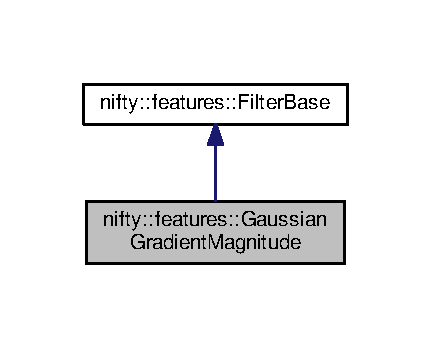
\includegraphics[width=207pt]{structnifty_1_1features_1_1GaussianGradientMagnitude__inherit__graph}
\end{center}
\end{figure}


Collaboration diagram for nifty\+:\+:features\+:\+:Gaussian\+Gradient\+Magnitude\+:
\nopagebreak
\begin{figure}[H]
\begin{center}
\leavevmode
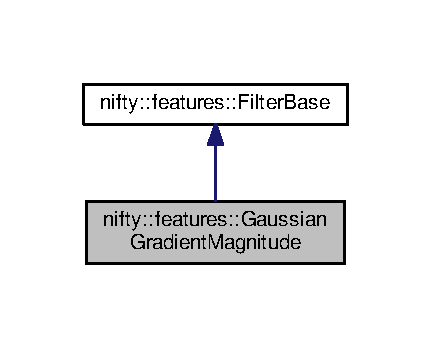
\includegraphics[width=207pt]{structnifty_1_1features_1_1GaussianGradientMagnitude__coll__graph}
\end{center}
\end{figure}
\subsection*{Public Member Functions}
\begin{DoxyCompactItemize}
\item 
void \hyperlink{structnifty_1_1features_1_1GaussianGradientMagnitude_a00efc1c411b58f0e212b26e3a4b9c06c}{operator()} (const fastfilters\+\_\+array2d\+\_\+t \&ff, \hyperlink{classandres_1_1View}{marray\+::\+View}$<$ float $>$ \&out, const double sigma) const
\item 
void \hyperlink{structnifty_1_1features_1_1GaussianGradientMagnitude_a0c442cf0666188ae0dcea15adfa725b8}{operator()} (const fastfilters\+\_\+array3d\+\_\+t \&ff, \hyperlink{classandres_1_1View}{marray\+::\+View}$<$ float $>$ \&out, const double sigma) const
\item 
bool \hyperlink{structnifty_1_1features_1_1GaussianGradientMagnitude_ab586b1dd5bd966f8622105fafb3029c8}{is\+Multi\+Channel} () const
\end{DoxyCompactItemize}
\subsection*{Additional Inherited Members}


\subsection{Member Function Documentation}
\mbox{\Hypertarget{structnifty_1_1features_1_1GaussianGradientMagnitude_ab586b1dd5bd966f8622105fafb3029c8}\label{structnifty_1_1features_1_1GaussianGradientMagnitude_ab586b1dd5bd966f8622105fafb3029c8}} 
\index{nifty\+::features\+::\+Gaussian\+Gradient\+Magnitude@{nifty\+::features\+::\+Gaussian\+Gradient\+Magnitude}!is\+Multi\+Channel@{is\+Multi\+Channel}}
\index{is\+Multi\+Channel@{is\+Multi\+Channel}!nifty\+::features\+::\+Gaussian\+Gradient\+Magnitude@{nifty\+::features\+::\+Gaussian\+Gradient\+Magnitude}}
\subsubsection{\texorpdfstring{is\+Multi\+Channel()}{isMultiChannel()}}
{\footnotesize\ttfamily bool nifty\+::features\+::\+Gaussian\+Gradient\+Magnitude\+::is\+Multi\+Channel (\begin{DoxyParamCaption}{ }\end{DoxyParamCaption}) const\hspace{0.3cm}{\ttfamily [inline]}, {\ttfamily [virtual]}}



Implements \hyperlink{structnifty_1_1features_1_1FilterBase_a1c278e2b6ef0cb2a5bba2f758c6855e2}{nifty\+::features\+::\+Filter\+Base}.

\mbox{\Hypertarget{structnifty_1_1features_1_1GaussianGradientMagnitude_a00efc1c411b58f0e212b26e3a4b9c06c}\label{structnifty_1_1features_1_1GaussianGradientMagnitude_a00efc1c411b58f0e212b26e3a4b9c06c}} 
\index{nifty\+::features\+::\+Gaussian\+Gradient\+Magnitude@{nifty\+::features\+::\+Gaussian\+Gradient\+Magnitude}!operator()@{operator()}}
\index{operator()@{operator()}!nifty\+::features\+::\+Gaussian\+Gradient\+Magnitude@{nifty\+::features\+::\+Gaussian\+Gradient\+Magnitude}}
\subsubsection{\texorpdfstring{operator()()}{operator()()}\hspace{0.1cm}{\footnotesize\ttfamily [1/2]}}
{\footnotesize\ttfamily void nifty\+::features\+::\+Gaussian\+Gradient\+Magnitude\+::operator() (\begin{DoxyParamCaption}\item[{const fastfilters\+\_\+array2d\+\_\+t \&}]{ff,  }\item[{\hyperlink{classandres_1_1View}{marray\+::\+View}$<$ float $>$ \&}]{out,  }\item[{const double}]{sigma }\end{DoxyParamCaption}) const\hspace{0.3cm}{\ttfamily [inline]}, {\ttfamily [virtual]}}



Implements \hyperlink{structnifty_1_1features_1_1FilterBase_a17c77d36dd765c5ec0b163102428656c}{nifty\+::features\+::\+Filter\+Base}.

\mbox{\Hypertarget{structnifty_1_1features_1_1GaussianGradientMagnitude_a0c442cf0666188ae0dcea15adfa725b8}\label{structnifty_1_1features_1_1GaussianGradientMagnitude_a0c442cf0666188ae0dcea15adfa725b8}} 
\index{nifty\+::features\+::\+Gaussian\+Gradient\+Magnitude@{nifty\+::features\+::\+Gaussian\+Gradient\+Magnitude}!operator()@{operator()}}
\index{operator()@{operator()}!nifty\+::features\+::\+Gaussian\+Gradient\+Magnitude@{nifty\+::features\+::\+Gaussian\+Gradient\+Magnitude}}
\subsubsection{\texorpdfstring{operator()()}{operator()()}\hspace{0.1cm}{\footnotesize\ttfamily [2/2]}}
{\footnotesize\ttfamily void nifty\+::features\+::\+Gaussian\+Gradient\+Magnitude\+::operator() (\begin{DoxyParamCaption}\item[{const fastfilters\+\_\+array3d\+\_\+t \&}]{ff,  }\item[{\hyperlink{classandres_1_1View}{marray\+::\+View}$<$ float $>$ \&}]{out,  }\item[{const double}]{sigma }\end{DoxyParamCaption}) const\hspace{0.3cm}{\ttfamily [inline]}, {\ttfamily [virtual]}}



Implements \hyperlink{structnifty_1_1features_1_1FilterBase_abbef4e9c260026926e0021aa0cc11c81}{nifty\+::features\+::\+Filter\+Base}.



The documentation for this struct was generated from the following file\+:\begin{DoxyCompactItemize}
\item 
/home/tbeier/src/nifty/include/nifty/features/\hyperlink{fastfilters__wrapper_8hxx}{fastfilters\+\_\+wrapper.\+hxx}\end{DoxyCompactItemize}

\hypertarget{structnifty_1_1features_1_1GaussianSmoothing}{}\section{nifty\+:\+:features\+:\+:Gaussian\+Smoothing Struct Reference}
\label{structnifty_1_1features_1_1GaussianSmoothing}\index{nifty\+::features\+::\+Gaussian\+Smoothing@{nifty\+::features\+::\+Gaussian\+Smoothing}}


{\ttfamily \#include $<$fastfilters\+\_\+wrapper.\+hxx$>$}



Inheritance diagram for nifty\+:\+:features\+:\+:Gaussian\+Smoothing\+:
\nopagebreak
\begin{figure}[H]
\begin{center}
\leavevmode
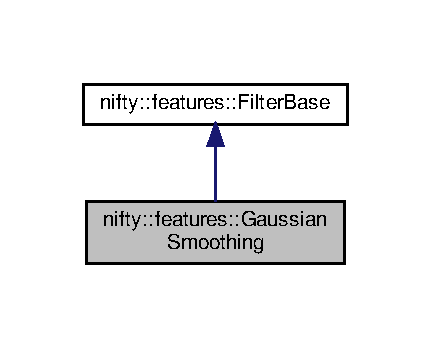
\includegraphics[width=207pt]{structnifty_1_1features_1_1GaussianSmoothing__inherit__graph}
\end{center}
\end{figure}


Collaboration diagram for nifty\+:\+:features\+:\+:Gaussian\+Smoothing\+:
\nopagebreak
\begin{figure}[H]
\begin{center}
\leavevmode
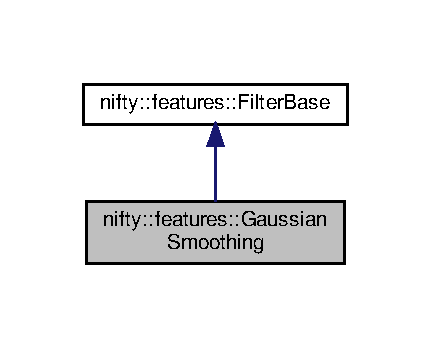
\includegraphics[width=207pt]{structnifty_1_1features_1_1GaussianSmoothing__coll__graph}
\end{center}
\end{figure}
\subsection*{Public Member Functions}
\begin{DoxyCompactItemize}
\item 
void \hyperlink{structnifty_1_1features_1_1GaussianSmoothing_a1b6bf85baa31180bad4070cc704b8723}{operator()} (const fastfilters\+\_\+array2d\+\_\+t \&ff, \hyperlink{classandres_1_1View}{marray\+::\+View}$<$ float $>$ \&out, const double sigma) const
\item 
void \hyperlink{structnifty_1_1features_1_1GaussianSmoothing_a8daf036e19adc709e3790566861efb86}{operator()} (const fastfilters\+\_\+array3d\+\_\+t \&ff, \hyperlink{classandres_1_1View}{marray\+::\+View}$<$ float $>$ \&out, const double sigma) const
\item 
bool \hyperlink{structnifty_1_1features_1_1GaussianSmoothing_a83bb2660db022cc1d2d302ac41e187ba}{is\+Multi\+Channel} () const
\end{DoxyCompactItemize}
\subsection*{Additional Inherited Members}


\subsection{Member Function Documentation}
\mbox{\Hypertarget{structnifty_1_1features_1_1GaussianSmoothing_a83bb2660db022cc1d2d302ac41e187ba}\label{structnifty_1_1features_1_1GaussianSmoothing_a83bb2660db022cc1d2d302ac41e187ba}} 
\index{nifty\+::features\+::\+Gaussian\+Smoothing@{nifty\+::features\+::\+Gaussian\+Smoothing}!is\+Multi\+Channel@{is\+Multi\+Channel}}
\index{is\+Multi\+Channel@{is\+Multi\+Channel}!nifty\+::features\+::\+Gaussian\+Smoothing@{nifty\+::features\+::\+Gaussian\+Smoothing}}
\subsubsection{\texorpdfstring{is\+Multi\+Channel()}{isMultiChannel()}}
{\footnotesize\ttfamily bool nifty\+::features\+::\+Gaussian\+Smoothing\+::is\+Multi\+Channel (\begin{DoxyParamCaption}{ }\end{DoxyParamCaption}) const\hspace{0.3cm}{\ttfamily [inline]}, {\ttfamily [virtual]}}



Implements \hyperlink{structnifty_1_1features_1_1FilterBase_a1c278e2b6ef0cb2a5bba2f758c6855e2}{nifty\+::features\+::\+Filter\+Base}.

\mbox{\Hypertarget{structnifty_1_1features_1_1GaussianSmoothing_a1b6bf85baa31180bad4070cc704b8723}\label{structnifty_1_1features_1_1GaussianSmoothing_a1b6bf85baa31180bad4070cc704b8723}} 
\index{nifty\+::features\+::\+Gaussian\+Smoothing@{nifty\+::features\+::\+Gaussian\+Smoothing}!operator()@{operator()}}
\index{operator()@{operator()}!nifty\+::features\+::\+Gaussian\+Smoothing@{nifty\+::features\+::\+Gaussian\+Smoothing}}
\subsubsection{\texorpdfstring{operator()()}{operator()()}\hspace{0.1cm}{\footnotesize\ttfamily [1/2]}}
{\footnotesize\ttfamily void nifty\+::features\+::\+Gaussian\+Smoothing\+::operator() (\begin{DoxyParamCaption}\item[{const fastfilters\+\_\+array2d\+\_\+t \&}]{ff,  }\item[{\hyperlink{classandres_1_1View}{marray\+::\+View}$<$ float $>$ \&}]{out,  }\item[{const double}]{sigma }\end{DoxyParamCaption}) const\hspace{0.3cm}{\ttfamily [inline]}, {\ttfamily [virtual]}}



Implements \hyperlink{structnifty_1_1features_1_1FilterBase_a17c77d36dd765c5ec0b163102428656c}{nifty\+::features\+::\+Filter\+Base}.

\mbox{\Hypertarget{structnifty_1_1features_1_1GaussianSmoothing_a8daf036e19adc709e3790566861efb86}\label{structnifty_1_1features_1_1GaussianSmoothing_a8daf036e19adc709e3790566861efb86}} 
\index{nifty\+::features\+::\+Gaussian\+Smoothing@{nifty\+::features\+::\+Gaussian\+Smoothing}!operator()@{operator()}}
\index{operator()@{operator()}!nifty\+::features\+::\+Gaussian\+Smoothing@{nifty\+::features\+::\+Gaussian\+Smoothing}}
\subsubsection{\texorpdfstring{operator()()}{operator()()}\hspace{0.1cm}{\footnotesize\ttfamily [2/2]}}
{\footnotesize\ttfamily void nifty\+::features\+::\+Gaussian\+Smoothing\+::operator() (\begin{DoxyParamCaption}\item[{const fastfilters\+\_\+array3d\+\_\+t \&}]{ff,  }\item[{\hyperlink{classandres_1_1View}{marray\+::\+View}$<$ float $>$ \&}]{out,  }\item[{const double}]{sigma }\end{DoxyParamCaption}) const\hspace{0.3cm}{\ttfamily [inline]}, {\ttfamily [virtual]}}



Implements \hyperlink{structnifty_1_1features_1_1FilterBase_abbef4e9c260026926e0021aa0cc11c81}{nifty\+::features\+::\+Filter\+Base}.



The documentation for this struct was generated from the following file\+:\begin{DoxyCompactItemize}
\item 
/home/tbeier/src/nifty/include/nifty/features/\hyperlink{fastfilters__wrapper_8hxx}{fastfilters\+\_\+wrapper.\+hxx}\end{DoxyCompactItemize}

\hypertarget{classnifty_1_1cgp_1_1Geometry}{}\section{nifty\+:\+:cgp\+:\+:Geometry$<$ D\+I\+M $>$ Class Template Reference}
\label{classnifty_1_1cgp_1_1Geometry}\index{nifty\+::cgp\+::\+Geometry$<$ D\+I\+M $>$@{nifty\+::cgp\+::\+Geometry$<$ D\+I\+M $>$}}


{\ttfamily \#include $<$geometry.\+hxx$>$}



The documentation for this class was generated from the following file\+:\begin{DoxyCompactItemize}
\item 
/home/tbeier/src/nifty/include/nifty/cgp/\hyperlink{geometry_8hxx}{geometry.\+hxx}\end{DoxyCompactItemize}

\hypertarget{classnifty_1_1cgp_1_1Geometry_3_012_01_4}{}\section{nifty\+:\+:cgp\+:\+:Geometry$<$ 2 $>$ Class Template Reference}
\label{classnifty_1_1cgp_1_1Geometry_3_012_01_4}\index{nifty\+::cgp\+::\+Geometry$<$ 2 $>$@{nifty\+::cgp\+::\+Geometry$<$ 2 $>$}}


{\ttfamily \#include $<$geometry.\+hxx$>$}

\subsection*{Public Types}
\begin{DoxyCompactItemize}
\item 
typedef \hyperlink{namespacenifty_1_1array_a683f151f19c851754e0c6d55ed16a0c2}{array\+::\+Static\+Array}$<$ uint32\+\_\+t, 2 $>$ \hyperlink{classnifty_1_1cgp_1_1Geometry_3_012_01_4_ab8abca4eea1550f59dca20f28bd0304d}{Coordinate\+Type}
\item 
typedef \hyperlink{namespacenifty_1_1array_a683f151f19c851754e0c6d55ed16a0c2}{array\+::\+Static\+Array}$<$ int64\+\_\+t, 2 $>$ \hyperlink{classnifty_1_1cgp_1_1Geometry_3_012_01_4_a2a2413f5135f7b297a4f703cb5bcb641}{Signed\+Coordinate\+Type}
\item 
typedef \hyperlink{classnifty_1_1cgp_1_1TopologicalGrid}{Topological\+Grid}$<$ 2 $>$ \hyperlink{classnifty_1_1cgp_1_1Geometry_3_012_01_4_a6f4a07a376a645097547311fe0ad2836}{Topological\+Grid\+Type}
\end{DoxyCompactItemize}
\subsection*{Public Member Functions}
\begin{DoxyCompactItemize}
\item 
\hyperlink{classnifty_1_1cgp_1_1Geometry_3_012_01_4_a3fa2454e7e2c5a134441928d5907c9dd}{Geometry} (const \hyperlink{classnifty_1_1cgp_1_1Geometry_3_012_01_4_a6f4a07a376a645097547311fe0ad2836}{Topological\+Grid\+Type} \&t\+Grid, const bool fill=false, const bool sort1\+Cells=true)
\item 
{\footnotesize template$<$size\+\_\+t C\+E\+L\+L\+\_\+\+T\+Y\+PE$>$ }\\const \hyperlink{classnifty_1_1cgp_1_1CellGeometryVector}{Cell\+Geometry\+Vector}$<$ 2, C\+E\+L\+L\+\_\+\+T\+Y\+PE $>$ \& \hyperlink{classnifty_1_1cgp_1_1Geometry_3_012_01_4_a74c6ca2e29fb745a6ee5d565553f0e44}{geometry} () const
\end{DoxyCompactItemize}


\subsection{Member Typedef Documentation}
\mbox{\Hypertarget{classnifty_1_1cgp_1_1Geometry_3_012_01_4_ab8abca4eea1550f59dca20f28bd0304d}\label{classnifty_1_1cgp_1_1Geometry_3_012_01_4_ab8abca4eea1550f59dca20f28bd0304d}} 
\index{nifty\+::cgp\+::\+Geometry$<$ 2 $>$@{nifty\+::cgp\+::\+Geometry$<$ 2 $>$}!Coordinate\+Type@{Coordinate\+Type}}
\index{Coordinate\+Type@{Coordinate\+Type}!nifty\+::cgp\+::\+Geometry$<$ 2 $>$@{nifty\+::cgp\+::\+Geometry$<$ 2 $>$}}
\subsubsection{\texorpdfstring{Coordinate\+Type}{CoordinateType}}
{\footnotesize\ttfamily typedef \hyperlink{namespacenifty_1_1array_a683f151f19c851754e0c6d55ed16a0c2}{array\+::\+Static\+Array}$<$uint32\+\_\+t, 2$>$ \hyperlink{classnifty_1_1cgp_1_1Geometry}{nifty\+::cgp\+::\+Geometry}$<$ 2 $>$\+::\hyperlink{classnifty_1_1cgp_1_1Geometry_3_012_01_4_ab8abca4eea1550f59dca20f28bd0304d}{Coordinate\+Type}}

\mbox{\Hypertarget{classnifty_1_1cgp_1_1Geometry_3_012_01_4_a2a2413f5135f7b297a4f703cb5bcb641}\label{classnifty_1_1cgp_1_1Geometry_3_012_01_4_a2a2413f5135f7b297a4f703cb5bcb641}} 
\index{nifty\+::cgp\+::\+Geometry$<$ 2 $>$@{nifty\+::cgp\+::\+Geometry$<$ 2 $>$}!Signed\+Coordinate\+Type@{Signed\+Coordinate\+Type}}
\index{Signed\+Coordinate\+Type@{Signed\+Coordinate\+Type}!nifty\+::cgp\+::\+Geometry$<$ 2 $>$@{nifty\+::cgp\+::\+Geometry$<$ 2 $>$}}
\subsubsection{\texorpdfstring{Signed\+Coordinate\+Type}{SignedCoordinateType}}
{\footnotesize\ttfamily typedef \hyperlink{namespacenifty_1_1array_a683f151f19c851754e0c6d55ed16a0c2}{array\+::\+Static\+Array}$<$int64\+\_\+t, 2$>$ \hyperlink{classnifty_1_1cgp_1_1Geometry}{nifty\+::cgp\+::\+Geometry}$<$ 2 $>$\+::\hyperlink{classnifty_1_1cgp_1_1Geometry_3_012_01_4_a2a2413f5135f7b297a4f703cb5bcb641}{Signed\+Coordinate\+Type}}

\mbox{\Hypertarget{classnifty_1_1cgp_1_1Geometry_3_012_01_4_a6f4a07a376a645097547311fe0ad2836}\label{classnifty_1_1cgp_1_1Geometry_3_012_01_4_a6f4a07a376a645097547311fe0ad2836}} 
\index{nifty\+::cgp\+::\+Geometry$<$ 2 $>$@{nifty\+::cgp\+::\+Geometry$<$ 2 $>$}!Topological\+Grid\+Type@{Topological\+Grid\+Type}}
\index{Topological\+Grid\+Type@{Topological\+Grid\+Type}!nifty\+::cgp\+::\+Geometry$<$ 2 $>$@{nifty\+::cgp\+::\+Geometry$<$ 2 $>$}}
\subsubsection{\texorpdfstring{Topological\+Grid\+Type}{TopologicalGridType}}
{\footnotesize\ttfamily typedef \hyperlink{classnifty_1_1cgp_1_1TopologicalGrid}{Topological\+Grid}$<$2$>$ \hyperlink{classnifty_1_1cgp_1_1Geometry}{nifty\+::cgp\+::\+Geometry}$<$ 2 $>$\+::\hyperlink{classnifty_1_1cgp_1_1Geometry_3_012_01_4_a6f4a07a376a645097547311fe0ad2836}{Topological\+Grid\+Type}}



\subsection{Constructor \& Destructor Documentation}
\mbox{\Hypertarget{classnifty_1_1cgp_1_1Geometry_3_012_01_4_a3fa2454e7e2c5a134441928d5907c9dd}\label{classnifty_1_1cgp_1_1Geometry_3_012_01_4_a3fa2454e7e2c5a134441928d5907c9dd}} 
\index{nifty\+::cgp\+::\+Geometry$<$ 2 $>$@{nifty\+::cgp\+::\+Geometry$<$ 2 $>$}!Geometry@{Geometry}}
\index{Geometry@{Geometry}!nifty\+::cgp\+::\+Geometry$<$ 2 $>$@{nifty\+::cgp\+::\+Geometry$<$ 2 $>$}}
\subsubsection{\texorpdfstring{Geometry()}{Geometry()}}
{\footnotesize\ttfamily \hyperlink{classnifty_1_1cgp_1_1Geometry}{nifty\+::cgp\+::\+Geometry}$<$ 2 $>$\+::\hyperlink{classnifty_1_1cgp_1_1Geometry}{Geometry} (\begin{DoxyParamCaption}\item[{const \hyperlink{classnifty_1_1cgp_1_1Geometry_3_012_01_4_a6f4a07a376a645097547311fe0ad2836}{Topological\+Grid\+Type} \&}]{t\+Grid,  }\item[{const bool}]{fill = {\ttfamily false},  }\item[{const bool}]{sort1\+Cells = {\ttfamily true} }\end{DoxyParamCaption})\hspace{0.3cm}{\ttfamily [inline]}}



\subsection{Member Function Documentation}
\mbox{\Hypertarget{classnifty_1_1cgp_1_1Geometry_3_012_01_4_a74c6ca2e29fb745a6ee5d565553f0e44}\label{classnifty_1_1cgp_1_1Geometry_3_012_01_4_a74c6ca2e29fb745a6ee5d565553f0e44}} 
\index{nifty\+::cgp\+::\+Geometry$<$ 2 $>$@{nifty\+::cgp\+::\+Geometry$<$ 2 $>$}!geometry@{geometry}}
\index{geometry@{geometry}!nifty\+::cgp\+::\+Geometry$<$ 2 $>$@{nifty\+::cgp\+::\+Geometry$<$ 2 $>$}}
\subsubsection{\texorpdfstring{geometry()}{geometry()}}
{\footnotesize\ttfamily template$<$size\+\_\+t C\+E\+L\+L\+\_\+\+T\+Y\+PE$>$ \\
const \hyperlink{classnifty_1_1cgp_1_1CellGeometryVector}{Cell\+Geometry\+Vector}$<$2,C\+E\+L\+L\+\_\+\+T\+Y\+PE$>$\& \hyperlink{classnifty_1_1cgp_1_1Geometry}{nifty\+::cgp\+::\+Geometry}$<$ 2 $>$\+::geometry (\begin{DoxyParamCaption}{ }\end{DoxyParamCaption}) const\hspace{0.3cm}{\ttfamily [inline]}}



The documentation for this class was generated from the following file\+:\begin{DoxyCompactItemize}
\item 
/home/tbeier/src/nifty/include/nifty/cgp/\hyperlink{geometry_8hxx}{geometry.\+hxx}\end{DoxyCompactItemize}

\hypertarget{classpybind11_1_1gil__release}{}\section{pybind11\+:\+:gil\+\_\+release Class Reference}
\label{classpybind11_1_1gil__release}\index{pybind11\+::gil\+\_\+release@{pybind11\+::gil\+\_\+release}}


{\ttfamily \#include $<$converter.\+hxx$>$}



The documentation for this class was generated from the following file\+:\begin{DoxyCompactItemize}
\item 
/home/tbeier/src/nifty/include/nifty/python/\hyperlink{converter_8hxx}{converter.\+hxx}\end{DoxyCompactItemize}

\hypertarget{classnifty_1_1ilp__backend_1_1Glpk}{}\section{nifty\+:\+:ilp\+\_\+backend\+:\+:Glpk Class Reference}
\label{classnifty_1_1ilp__backend_1_1Glpk}\index{nifty\+::ilp\+\_\+backend\+::\+Glpk@{nifty\+::ilp\+\_\+backend\+::\+Glpk}}


{\ttfamily \#include $<$glpk.\+hxx$>$}

\subsection*{Public Types}
\begin{DoxyCompactItemize}
\item 
typedef \hyperlink{structnifty_1_1ilp__backend_1_1IlpBackendSettings}{Ilp\+Backend\+Settings} \hyperlink{classnifty_1_1ilp__backend_1_1Glpk_a8f3191eb733e6a2f08f82adceae32365}{Settings\+Type}
\end{DoxyCompactItemize}
\subsection*{Public Member Functions}
\begin{DoxyCompactItemize}
\item 
\hyperlink{classnifty_1_1ilp__backend_1_1Glpk_a31b71a008ab6c3c16e60a17fbfc8822d}{Glpk} (const \hyperlink{classnifty_1_1ilp__backend_1_1Glpk_a8f3191eb733e6a2f08f82adceae32365}{Settings\+Type} \&settings=\hyperlink{classnifty_1_1ilp__backend_1_1Glpk_a8f3191eb733e6a2f08f82adceae32365}{Settings\+Type}())
\item 
\hyperlink{classnifty_1_1ilp__backend_1_1Glpk_a9696f83fd9a1688bcdf5a05b84c03976}{$\sim$\+Glpk} ()
\item 
void \hyperlink{classnifty_1_1ilp__backend_1_1Glpk_a82a16f1598798e5935d4b56a692d3b5a}{init\+Model} (const size\+\_\+t, const double $\ast$)
\item 
{\footnotesize template$<$class Iterator $>$ }\\void \hyperlink{classnifty_1_1ilp__backend_1_1Glpk_a7d71ee633ecc892e6d2e904a30604394}{set\+Start} (Iterator)
\item 
{\footnotesize template$<$class Variable\+Index\+Iterator , class Coefficient\+Iterator $>$ }\\void \hyperlink{classnifty_1_1ilp__backend_1_1Glpk_a756aac8075dfd7957e0b90e27f1b141d}{add\+Constraint} (Variable\+Index\+Iterator, Variable\+Index\+Iterator, Coefficient\+Iterator, const double, const double)
\item 
void \hyperlink{classnifty_1_1ilp__backend_1_1Glpk_a2e66c98281cb549ee477d58fbd3b8374}{optimize} ()
\item 
double \hyperlink{classnifty_1_1ilp__backend_1_1Glpk_a7720302149ac1d1df4207854a3f91d03}{label} (const size\+\_\+t) const
\item 
{\footnotesize template$<$class O\+B\+J\+E\+C\+T\+I\+V\+E\+\_\+\+I\+T\+E\+R\+A\+T\+OR $>$ }\\void \hyperlink{classnifty_1_1ilp__backend_1_1Glpk_a31c379a5553eb4fd87a56e71ac589a80}{change\+Objective} (O\+B\+J\+E\+C\+T\+I\+V\+E\+\_\+\+I\+T\+E\+R\+A\+T\+OR objective\+Iter)
\end{DoxyCompactItemize}
\subsection*{Static Public Member Functions}
\begin{DoxyCompactItemize}
\item 
static std\+::string \hyperlink{classnifty_1_1ilp__backend_1_1Glpk_ad86a2c29a1b0c73a47c79d2d5c0ff07d}{name} ()
\end{DoxyCompactItemize}


\subsection{Member Typedef Documentation}
\mbox{\Hypertarget{classnifty_1_1ilp__backend_1_1Glpk_a8f3191eb733e6a2f08f82adceae32365}\label{classnifty_1_1ilp__backend_1_1Glpk_a8f3191eb733e6a2f08f82adceae32365}} 
\index{nifty\+::ilp\+\_\+backend\+::\+Glpk@{nifty\+::ilp\+\_\+backend\+::\+Glpk}!Settings\+Type@{Settings\+Type}}
\index{Settings\+Type@{Settings\+Type}!nifty\+::ilp\+\_\+backend\+::\+Glpk@{nifty\+::ilp\+\_\+backend\+::\+Glpk}}
\subsubsection{\texorpdfstring{Settings\+Type}{SettingsType}}
{\footnotesize\ttfamily typedef \hyperlink{structnifty_1_1ilp__backend_1_1IlpBackendSettings}{Ilp\+Backend\+Settings} \hyperlink{classnifty_1_1ilp__backend_1_1Glpk_a8f3191eb733e6a2f08f82adceae32365}{nifty\+::ilp\+\_\+backend\+::\+Glpk\+::\+Settings\+Type}}



\subsection{Constructor \& Destructor Documentation}
\mbox{\Hypertarget{classnifty_1_1ilp__backend_1_1Glpk_a31b71a008ab6c3c16e60a17fbfc8822d}\label{classnifty_1_1ilp__backend_1_1Glpk_a31b71a008ab6c3c16e60a17fbfc8822d}} 
\index{nifty\+::ilp\+\_\+backend\+::\+Glpk@{nifty\+::ilp\+\_\+backend\+::\+Glpk}!Glpk@{Glpk}}
\index{Glpk@{Glpk}!nifty\+::ilp\+\_\+backend\+::\+Glpk@{nifty\+::ilp\+\_\+backend\+::\+Glpk}}
\subsubsection{\texorpdfstring{Glpk()}{Glpk()}}
{\footnotesize\ttfamily nifty\+::ilp\+\_\+backend\+::\+Glpk\+::\+Glpk (\begin{DoxyParamCaption}\item[{const \hyperlink{classnifty_1_1ilp__backend_1_1Glpk_a8f3191eb733e6a2f08f82adceae32365}{Settings\+Type} \&}]{settings = {\ttfamily \hyperlink{classnifty_1_1ilp__backend_1_1Glpk_a8f3191eb733e6a2f08f82adceae32365}{Settings\+Type}()} }\end{DoxyParamCaption})\hspace{0.3cm}{\ttfamily [inline]}}

\mbox{\Hypertarget{classnifty_1_1ilp__backend_1_1Glpk_a9696f83fd9a1688bcdf5a05b84c03976}\label{classnifty_1_1ilp__backend_1_1Glpk_a9696f83fd9a1688bcdf5a05b84c03976}} 
\index{nifty\+::ilp\+\_\+backend\+::\+Glpk@{nifty\+::ilp\+\_\+backend\+::\+Glpk}!````~Glpk@{$\sim$\+Glpk}}
\index{````~Glpk@{$\sim$\+Glpk}!nifty\+::ilp\+\_\+backend\+::\+Glpk@{nifty\+::ilp\+\_\+backend\+::\+Glpk}}
\subsubsection{\texorpdfstring{$\sim$\+Glpk()}{~Glpk()}}
{\footnotesize\ttfamily nifty\+::ilp\+\_\+backend\+::\+Glpk\+::$\sim$\+Glpk (\begin{DoxyParamCaption}{ }\end{DoxyParamCaption})\hspace{0.3cm}{\ttfamily [inline]}}



\subsection{Member Function Documentation}
\mbox{\Hypertarget{classnifty_1_1ilp__backend_1_1Glpk_a756aac8075dfd7957e0b90e27f1b141d}\label{classnifty_1_1ilp__backend_1_1Glpk_a756aac8075dfd7957e0b90e27f1b141d}} 
\index{nifty\+::ilp\+\_\+backend\+::\+Glpk@{nifty\+::ilp\+\_\+backend\+::\+Glpk}!add\+Constraint@{add\+Constraint}}
\index{add\+Constraint@{add\+Constraint}!nifty\+::ilp\+\_\+backend\+::\+Glpk@{nifty\+::ilp\+\_\+backend\+::\+Glpk}}
\subsubsection{\texorpdfstring{add\+Constraint()}{addConstraint()}}
{\footnotesize\ttfamily template$<$class Variable\+Index\+Iterator , class Coefficient\+Iterator $>$ \\
void nifty\+::ilp\+\_\+backend\+::\+Glpk\+::add\+Constraint (\begin{DoxyParamCaption}\item[{Variable\+Index\+Iterator}]{vi\+Begin,  }\item[{Variable\+Index\+Iterator}]{vi\+End,  }\item[{Coefficient\+Iterator}]{coefficient,  }\item[{const double}]{lower\+Bound,  }\item[{const double}]{upper\+Bound }\end{DoxyParamCaption})\hspace{0.3cm}{\ttfamily [inline]}}

\mbox{\Hypertarget{classnifty_1_1ilp__backend_1_1Glpk_a31c379a5553eb4fd87a56e71ac589a80}\label{classnifty_1_1ilp__backend_1_1Glpk_a31c379a5553eb4fd87a56e71ac589a80}} 
\index{nifty\+::ilp\+\_\+backend\+::\+Glpk@{nifty\+::ilp\+\_\+backend\+::\+Glpk}!change\+Objective@{change\+Objective}}
\index{change\+Objective@{change\+Objective}!nifty\+::ilp\+\_\+backend\+::\+Glpk@{nifty\+::ilp\+\_\+backend\+::\+Glpk}}
\subsubsection{\texorpdfstring{change\+Objective()}{changeObjective()}}
{\footnotesize\ttfamily template$<$class O\+B\+J\+E\+C\+T\+I\+V\+E\+\_\+\+I\+T\+E\+R\+A\+T\+OR $>$ \\
void nifty\+::ilp\+\_\+backend\+::\+Glpk\+::change\+Objective (\begin{DoxyParamCaption}\item[{O\+B\+J\+E\+C\+T\+I\+V\+E\+\_\+\+I\+T\+E\+R\+A\+T\+OR}]{objective\+Iter }\end{DoxyParamCaption})\hspace{0.3cm}{\ttfamily [inline]}}

\mbox{\Hypertarget{classnifty_1_1ilp__backend_1_1Glpk_a82a16f1598798e5935d4b56a692d3b5a}\label{classnifty_1_1ilp__backend_1_1Glpk_a82a16f1598798e5935d4b56a692d3b5a}} 
\index{nifty\+::ilp\+\_\+backend\+::\+Glpk@{nifty\+::ilp\+\_\+backend\+::\+Glpk}!init\+Model@{init\+Model}}
\index{init\+Model@{init\+Model}!nifty\+::ilp\+\_\+backend\+::\+Glpk@{nifty\+::ilp\+\_\+backend\+::\+Glpk}}
\subsubsection{\texorpdfstring{init\+Model()}{initModel()}}
{\footnotesize\ttfamily void nifty\+::ilp\+\_\+backend\+::\+Glpk\+::init\+Model (\begin{DoxyParamCaption}\item[{const size\+\_\+t}]{number\+Of\+Variables,  }\item[{const double $\ast$}]{coefficients }\end{DoxyParamCaption})\hspace{0.3cm}{\ttfamily [inline]}}

\mbox{\Hypertarget{classnifty_1_1ilp__backend_1_1Glpk_a7720302149ac1d1df4207854a3f91d03}\label{classnifty_1_1ilp__backend_1_1Glpk_a7720302149ac1d1df4207854a3f91d03}} 
\index{nifty\+::ilp\+\_\+backend\+::\+Glpk@{nifty\+::ilp\+\_\+backend\+::\+Glpk}!label@{label}}
\index{label@{label}!nifty\+::ilp\+\_\+backend\+::\+Glpk@{nifty\+::ilp\+\_\+backend\+::\+Glpk}}
\subsubsection{\texorpdfstring{label()}{label()}}
{\footnotesize\ttfamily double nifty\+::ilp\+\_\+backend\+::\+Glpk\+::label (\begin{DoxyParamCaption}\item[{const size\+\_\+t}]{variable\+Index }\end{DoxyParamCaption}) const\hspace{0.3cm}{\ttfamily [inline]}}

\mbox{\Hypertarget{classnifty_1_1ilp__backend_1_1Glpk_ad86a2c29a1b0c73a47c79d2d5c0ff07d}\label{classnifty_1_1ilp__backend_1_1Glpk_ad86a2c29a1b0c73a47c79d2d5c0ff07d}} 
\index{nifty\+::ilp\+\_\+backend\+::\+Glpk@{nifty\+::ilp\+\_\+backend\+::\+Glpk}!name@{name}}
\index{name@{name}!nifty\+::ilp\+\_\+backend\+::\+Glpk@{nifty\+::ilp\+\_\+backend\+::\+Glpk}}
\subsubsection{\texorpdfstring{name()}{name()}}
{\footnotesize\ttfamily static std\+::string nifty\+::ilp\+\_\+backend\+::\+Glpk\+::name (\begin{DoxyParamCaption}{ }\end{DoxyParamCaption})\hspace{0.3cm}{\ttfamily [inline]}, {\ttfamily [static]}}

\mbox{\Hypertarget{classnifty_1_1ilp__backend_1_1Glpk_a2e66c98281cb549ee477d58fbd3b8374}\label{classnifty_1_1ilp__backend_1_1Glpk_a2e66c98281cb549ee477d58fbd3b8374}} 
\index{nifty\+::ilp\+\_\+backend\+::\+Glpk@{nifty\+::ilp\+\_\+backend\+::\+Glpk}!optimize@{optimize}}
\index{optimize@{optimize}!nifty\+::ilp\+\_\+backend\+::\+Glpk@{nifty\+::ilp\+\_\+backend\+::\+Glpk}}
\subsubsection{\texorpdfstring{optimize()}{optimize()}}
{\footnotesize\ttfamily void nifty\+::ilp\+\_\+backend\+::\+Glpk\+::optimize (\begin{DoxyParamCaption}{ }\end{DoxyParamCaption})\hspace{0.3cm}{\ttfamily [inline]}}

\mbox{\Hypertarget{classnifty_1_1ilp__backend_1_1Glpk_a7d71ee633ecc892e6d2e904a30604394}\label{classnifty_1_1ilp__backend_1_1Glpk_a7d71ee633ecc892e6d2e904a30604394}} 
\index{nifty\+::ilp\+\_\+backend\+::\+Glpk@{nifty\+::ilp\+\_\+backend\+::\+Glpk}!set\+Start@{set\+Start}}
\index{set\+Start@{set\+Start}!nifty\+::ilp\+\_\+backend\+::\+Glpk@{nifty\+::ilp\+\_\+backend\+::\+Glpk}}
\subsubsection{\texorpdfstring{set\+Start()}{setStart()}}
{\footnotesize\ttfamily template$<$class Iterator $>$ \\
void nifty\+::ilp\+\_\+backend\+::\+Glpk\+::set\+Start (\begin{DoxyParamCaption}\item[{Iterator}]{value\+Iterator }\end{DoxyParamCaption})\hspace{0.3cm}{\ttfamily [inline]}}



The documentation for this class was generated from the following file\+:\begin{DoxyCompactItemize}
\item 
/home/tbeier/src/nifty/include/nifty/ilp\+\_\+backend/\hyperlink{glpk_8hxx}{glpk.\+hxx}\end{DoxyCompactItemize}

\hypertarget{structnifty_1_1graph_1_1GraphName}{}\section{nifty\+:\+:graph\+:\+:Graph\+Name$<$ G\+R\+A\+P\+H $>$ Struct Template Reference}
\label{structnifty_1_1graph_1_1GraphName}\index{nifty\+::graph\+::\+Graph\+Name$<$ G\+R\+A\+P\+H $>$@{nifty\+::graph\+::\+Graph\+Name$<$ G\+R\+A\+P\+H $>$}}


{\ttfamily \#include $<$graph\+\_\+name.\+hxx$>$}



The documentation for this struct was generated from the following file\+:\begin{DoxyCompactItemize}
\item 
/home/tbeier/src/nifty/include/nifty/python/graph/\hyperlink{graph__name_8hxx}{graph\+\_\+name.\+hxx}\end{DoxyCompactItemize}

\hypertarget{structnifty_1_1graph_1_1GraphName_3_01PyContractionGraph_3_01BASE__GRAPH_01_4_01_4}{}\section{nifty\+:\+:graph\+:\+:Graph\+Name$<$ Py\+Contraction\+Graph$<$ B\+A\+S\+E\+\_\+\+G\+R\+A\+P\+H $>$ $>$ Struct Template Reference}
\label{structnifty_1_1graph_1_1GraphName_3_01PyContractionGraph_3_01BASE__GRAPH_01_4_01_4}\index{nifty\+::graph\+::\+Graph\+Name$<$ Py\+Contraction\+Graph$<$ B\+A\+S\+E\+\_\+\+G\+R\+A\+P\+H $>$ $>$@{nifty\+::graph\+::\+Graph\+Name$<$ Py\+Contraction\+Graph$<$ B\+A\+S\+E\+\_\+\+G\+R\+A\+P\+H $>$ $>$}}


{\ttfamily \#include $<$edge\+\_\+contraction\+\_\+graph.\+hxx$>$}

\subsection*{Static Public Member Functions}
\begin{DoxyCompactItemize}
\item 
static std\+::string \hyperlink{structnifty_1_1graph_1_1GraphName_3_01PyContractionGraph_3_01BASE__GRAPH_01_4_01_4_aeaaa5d12ae9dbe2ad7e1f69605fe9f84}{name} ()
\item 
static std\+::string \hyperlink{structnifty_1_1graph_1_1GraphName_3_01PyContractionGraph_3_01BASE__GRAPH_01_4_01_4_ac8db233096e47d4733bc569a8634eed6}{usage\+Example} ()
\end{DoxyCompactItemize}


\subsection{Member Function Documentation}
\hypertarget{structnifty_1_1graph_1_1GraphName_3_01PyContractionGraph_3_01BASE__GRAPH_01_4_01_4_aeaaa5d12ae9dbe2ad7e1f69605fe9f84}{}\index{nifty\+::graph\+::\+Graph\+Name$<$ Py\+Contraction\+Graph$<$ B\+A\+S\+E\+\_\+\+G\+R\+A\+P\+H $>$ $>$@{nifty\+::graph\+::\+Graph\+Name$<$ Py\+Contraction\+Graph$<$ B\+A\+S\+E\+\_\+\+G\+R\+A\+P\+H $>$ $>$}!name@{name}}
\index{name@{name}!nifty\+::graph\+::\+Graph\+Name$<$ Py\+Contraction\+Graph$<$ B\+A\+S\+E\+\_\+\+G\+R\+A\+P\+H $>$ $>$@{nifty\+::graph\+::\+Graph\+Name$<$ Py\+Contraction\+Graph$<$ B\+A\+S\+E\+\_\+\+G\+R\+A\+P\+H $>$ $>$}}
\subsubsection[{name()}]{\setlength{\rightskip}{0pt plus 5cm}template$<$class B\+A\+S\+E\+\_\+\+G\+R\+A\+P\+H $>$ static std\+::string {\bf nifty\+::graph\+::\+Graph\+Name}$<$ {\bf Py\+Contraction\+Graph}$<$ B\+A\+S\+E\+\_\+\+G\+R\+A\+P\+H $>$ $>$\+::name (
\begin{DoxyParamCaption}
{}
\end{DoxyParamCaption}
)\hspace{0.3cm}{\ttfamily [inline]}, {\ttfamily [static]}}\label{structnifty_1_1graph_1_1GraphName_3_01PyContractionGraph_3_01BASE__GRAPH_01_4_01_4_aeaaa5d12ae9dbe2ad7e1f69605fe9f84}
\hypertarget{structnifty_1_1graph_1_1GraphName_3_01PyContractionGraph_3_01BASE__GRAPH_01_4_01_4_ac8db233096e47d4733bc569a8634eed6}{}\index{nifty\+::graph\+::\+Graph\+Name$<$ Py\+Contraction\+Graph$<$ B\+A\+S\+E\+\_\+\+G\+R\+A\+P\+H $>$ $>$@{nifty\+::graph\+::\+Graph\+Name$<$ Py\+Contraction\+Graph$<$ B\+A\+S\+E\+\_\+\+G\+R\+A\+P\+H $>$ $>$}!usage\+Example@{usage\+Example}}
\index{usage\+Example@{usage\+Example}!nifty\+::graph\+::\+Graph\+Name$<$ Py\+Contraction\+Graph$<$ B\+A\+S\+E\+\_\+\+G\+R\+A\+P\+H $>$ $>$@{nifty\+::graph\+::\+Graph\+Name$<$ Py\+Contraction\+Graph$<$ B\+A\+S\+E\+\_\+\+G\+R\+A\+P\+H $>$ $>$}}
\subsubsection[{usage\+Example()}]{\setlength{\rightskip}{0pt plus 5cm}template$<$class B\+A\+S\+E\+\_\+\+G\+R\+A\+P\+H $>$ static std\+::string {\bf nifty\+::graph\+::\+Graph\+Name}$<$ {\bf Py\+Contraction\+Graph}$<$ B\+A\+S\+E\+\_\+\+G\+R\+A\+P\+H $>$ $>$\+::usage\+Example (
\begin{DoxyParamCaption}
{}
\end{DoxyParamCaption}
)\hspace{0.3cm}{\ttfamily [inline]}, {\ttfamily [static]}}\label{structnifty_1_1graph_1_1GraphName_3_01PyContractionGraph_3_01BASE__GRAPH_01_4_01_4_ac8db233096e47d4733bc569a8634eed6}


The documentation for this struct was generated from the following file\+:\begin{DoxyCompactItemize}
\item 
/home/tbeier/src/nifty/include/nifty/python/graph/\hyperlink{python_2graph_2edge__contraction__graph_8hxx}{edge\+\_\+contraction\+\_\+graph.\+hxx}\end{DoxyCompactItemize}

\hypertarget{structnifty_1_1graph_1_1GraphName_3_01PyUndirectedGraph_01_4}{}\section{nifty\+:\+:graph\+:\+:Graph\+Name$<$ Py\+Undirected\+Graph $>$ Struct Template Reference}
\label{structnifty_1_1graph_1_1GraphName_3_01PyUndirectedGraph_01_4}\index{nifty\+::graph\+::\+Graph\+Name$<$ Py\+Undirected\+Graph $>$@{nifty\+::graph\+::\+Graph\+Name$<$ Py\+Undirected\+Graph $>$}}


{\ttfamily \#include $<$undirected\+\_\+list\+\_\+graph.\+hxx$>$}

\subsection*{Static Public Member Functions}
\begin{DoxyCompactItemize}
\item 
static std\+::string \hyperlink{structnifty_1_1graph_1_1GraphName_3_01PyUndirectedGraph_01_4_a36e0e5cf6d601ab8e63d65180dc4162a}{name} ()
\item 
static std\+::string \hyperlink{structnifty_1_1graph_1_1GraphName_3_01PyUndirectedGraph_01_4_ac62155ccd2721d709ee743039e42be0b}{module\+Name} ()
\item 
static std\+::string \hyperlink{structnifty_1_1graph_1_1GraphName_3_01PyUndirectedGraph_01_4_aec70e4ad4be73906f4b2fd6723c33a1d}{usage\+Example} ()
\end{DoxyCompactItemize}


\subsection{Member Function Documentation}
\hypertarget{structnifty_1_1graph_1_1GraphName_3_01PyUndirectedGraph_01_4_ac62155ccd2721d709ee743039e42be0b}{}\index{nifty\+::graph\+::\+Graph\+Name$<$ Py\+Undirected\+Graph $>$@{nifty\+::graph\+::\+Graph\+Name$<$ Py\+Undirected\+Graph $>$}!module\+Name@{module\+Name}}
\index{module\+Name@{module\+Name}!nifty\+::graph\+::\+Graph\+Name$<$ Py\+Undirected\+Graph $>$@{nifty\+::graph\+::\+Graph\+Name$<$ Py\+Undirected\+Graph $>$}}
\subsubsection[{module\+Name()}]{\setlength{\rightskip}{0pt plus 5cm}static std\+::string {\bf nifty\+::graph\+::\+Graph\+Name}$<$ {\bf Py\+Undirected\+Graph} $>$\+::module\+Name (
\begin{DoxyParamCaption}
{}
\end{DoxyParamCaption}
)\hspace{0.3cm}{\ttfamily [inline]}, {\ttfamily [static]}}\label{structnifty_1_1graph_1_1GraphName_3_01PyUndirectedGraph_01_4_ac62155ccd2721d709ee743039e42be0b}
\hypertarget{structnifty_1_1graph_1_1GraphName_3_01PyUndirectedGraph_01_4_a36e0e5cf6d601ab8e63d65180dc4162a}{}\index{nifty\+::graph\+::\+Graph\+Name$<$ Py\+Undirected\+Graph $>$@{nifty\+::graph\+::\+Graph\+Name$<$ Py\+Undirected\+Graph $>$}!name@{name}}
\index{name@{name}!nifty\+::graph\+::\+Graph\+Name$<$ Py\+Undirected\+Graph $>$@{nifty\+::graph\+::\+Graph\+Name$<$ Py\+Undirected\+Graph $>$}}
\subsubsection[{name()}]{\setlength{\rightskip}{0pt plus 5cm}static std\+::string {\bf nifty\+::graph\+::\+Graph\+Name}$<$ {\bf Py\+Undirected\+Graph} $>$\+::name (
\begin{DoxyParamCaption}
{}
\end{DoxyParamCaption}
)\hspace{0.3cm}{\ttfamily [inline]}, {\ttfamily [static]}}\label{structnifty_1_1graph_1_1GraphName_3_01PyUndirectedGraph_01_4_a36e0e5cf6d601ab8e63d65180dc4162a}
\hypertarget{structnifty_1_1graph_1_1GraphName_3_01PyUndirectedGraph_01_4_aec70e4ad4be73906f4b2fd6723c33a1d}{}\index{nifty\+::graph\+::\+Graph\+Name$<$ Py\+Undirected\+Graph $>$@{nifty\+::graph\+::\+Graph\+Name$<$ Py\+Undirected\+Graph $>$}!usage\+Example@{usage\+Example}}
\index{usage\+Example@{usage\+Example}!nifty\+::graph\+::\+Graph\+Name$<$ Py\+Undirected\+Graph $>$@{nifty\+::graph\+::\+Graph\+Name$<$ Py\+Undirected\+Graph $>$}}
\subsubsection[{usage\+Example()}]{\setlength{\rightskip}{0pt plus 5cm}static std\+::string {\bf nifty\+::graph\+::\+Graph\+Name}$<$ {\bf Py\+Undirected\+Graph} $>$\+::usage\+Example (
\begin{DoxyParamCaption}
{}
\end{DoxyParamCaption}
)\hspace{0.3cm}{\ttfamily [inline]}, {\ttfamily [static]}}\label{structnifty_1_1graph_1_1GraphName_3_01PyUndirectedGraph_01_4_aec70e4ad4be73906f4b2fd6723c33a1d}


The documentation for this struct was generated from the following file\+:\begin{DoxyCompactItemize}
\item 
/home/tbeier/src/nifty/include/nifty/python/graph/\hyperlink{python_2graph_2undirected__list__graph_8hxx}{undirected\+\_\+list\+\_\+graph.\+hxx}\end{DoxyCompactItemize}

\hypertarget{classnifty_1_1graph_1_1optimization_1_1common_1_1GreedyAdditiveMulticutProposals}{}\section{nifty\+:\+:graph\+:\+:optimization\+:\+:common\+:\+:Greedy\+Additive\+Multicut\+Proposals$<$ O\+B\+J\+E\+C\+T\+I\+V\+E $>$ Class Template Reference}
\label{classnifty_1_1graph_1_1optimization_1_1common_1_1GreedyAdditiveMulticutProposals}\index{nifty\+::graph\+::optimization\+::common\+::\+Greedy\+Additive\+Multicut\+Proposals$<$ O\+B\+J\+E\+C\+T\+I\+V\+E $>$@{nifty\+::graph\+::optimization\+::common\+::\+Greedy\+Additive\+Multicut\+Proposals$<$ O\+B\+J\+E\+C\+T\+I\+V\+E $>$}}


Watershed proposal generator for \hyperlink{classnifty_1_1graph_1_1optimization_1_1lifted__multicut_1_1FusionMoveBased}{lifted\+\_\+multicut\+::\+Fusion\+Move\+Based}.  




{\ttfamily \#include $<$greedy\+\_\+additive\+\_\+multicut\+\_\+proposal\+\_\+generator.\+hxx$>$}



Inheritance diagram for nifty\+:\+:graph\+:\+:optimization\+:\+:common\+:\+:Greedy\+Additive\+Multicut\+Proposals$<$ O\+B\+J\+E\+C\+T\+I\+V\+E $>$\+:\nopagebreak
\begin{figure}[H]
\begin{center}
\leavevmode
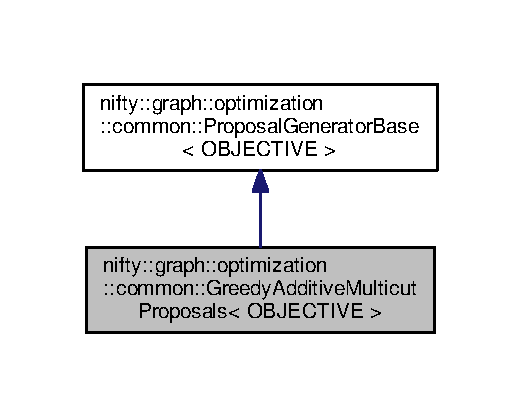
\includegraphics[width=250pt]{classnifty_1_1graph_1_1optimization_1_1common_1_1GreedyAdditiveMulticutProposals__inherit__graph}
\end{center}
\end{figure}


Collaboration diagram for nifty\+:\+:graph\+:\+:optimization\+:\+:common\+:\+:Greedy\+Additive\+Multicut\+Proposals$<$ O\+B\+J\+E\+C\+T\+I\+V\+E $>$\+:\nopagebreak
\begin{figure}[H]
\begin{center}
\leavevmode
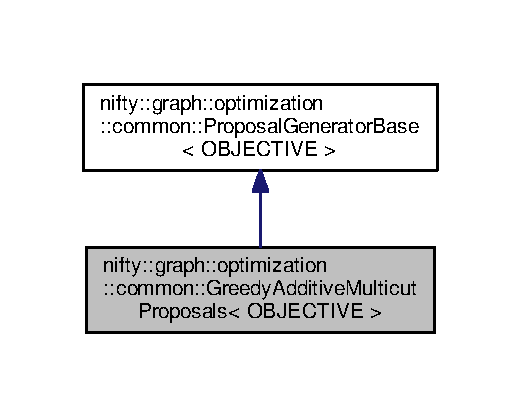
\includegraphics[width=250pt]{classnifty_1_1graph_1_1optimization_1_1common_1_1GreedyAdditiveMulticutProposals__coll__graph}
\end{center}
\end{figure}
\subsection*{Classes}
\begin{DoxyCompactItemize}
\item 
struct \hyperlink{structnifty_1_1graph_1_1optimization_1_1common_1_1GreedyAdditiveMulticutProposals_1_1SettingsType}{Settings\+Type}
\end{DoxyCompactItemize}
\subsection*{Public Types}
\begin{DoxyCompactItemize}
\item 
typedef O\+B\+J\+E\+C\+T\+I\+V\+E \hyperlink{classnifty_1_1graph_1_1optimization_1_1common_1_1GreedyAdditiveMulticutProposals_a82ebea313ce98149a4ac7003b792d6fe}{Objective\+Type}
\item 
typedef Objective\+Type\+::\+Graph\+Type \hyperlink{classnifty_1_1graph_1_1optimization_1_1common_1_1GreedyAdditiveMulticutProposals_a7e395c2bc3f18b9df2167e99f43e73f5}{Graph\+Type}
\item 
typedef nifty\+::graph\+::optimization\+::\+Multicut\+Base$<$ \hyperlink{classnifty_1_1graph_1_1optimization_1_1common_1_1GreedyAdditiveMulticutProposals_a82ebea313ce98149a4ac7003b792d6fe}{Objective\+Type} $>$ \hyperlink{classnifty_1_1graph_1_1optimization_1_1common_1_1GreedyAdditiveMulticutProposals_a903eacc5a19cb47916995019e4db2e0e}{Base}
\item 
typedef Multicut\+Greedy\+Additive$<$ Objective $>$ \hyperlink{classnifty_1_1graph_1_1optimization_1_1common_1_1GreedyAdditiveMulticutProposals_a87b47b0b53217d644e7a171b1dd3bfdf}{Solver}
\item 
typedef Solver\+::\+Settings\+Type \hyperlink{classnifty_1_1graph_1_1optimization_1_1common_1_1GreedyAdditiveMulticutProposals_a621d7ba4cccdd69804768b0b12184c17}{Solver\+Settings}
\item 
typedef Base\+::\+Edge\+Labels \hyperlink{classnifty_1_1graph_1_1optimization_1_1common_1_1GreedyAdditiveMulticutProposals_aaee332dfc9ee0e30897cbc1e37a6cff0}{Edge\+Labels}
\item 
typedef Base\+::\+Node\+Labels \hyperlink{classnifty_1_1graph_1_1optimization_1_1common_1_1GreedyAdditiveMulticutProposals_af59b25bf72b3164494b942fbf514f9c8}{Node\+Labels}
\item 
typedef Graph\+Type\+::template Node\+Map$<$ uint64\+\_\+t $>$ \hyperlink{classnifty_1_1graph_1_1optimization_1_1common_1_1GreedyAdditiveMulticutProposals_a2344bbd2084e7c62a179e6f0ce2d11f8}{Proposal\+Type}
\item 
typedef Graph\+Type\+::template Edge\+Map$<$ float $>$ \hyperlink{classnifty_1_1graph_1_1optimization_1_1common_1_1GreedyAdditiveMulticutProposals_a6709922efafd758e0f52169ff073d250}{Edge\+Weights}
\end{DoxyCompactItemize}
\subsection*{Public Member Functions}
\begin{DoxyCompactItemize}
\item 
\hyperlink{classnifty_1_1graph_1_1optimization_1_1common_1_1GreedyAdditiveMulticutProposals_a3b4ee55a1e07d1ce8b48e1530f94f009}{Greedy\+Additive\+Multicut\+Proposals} (const \hyperlink{classnifty_1_1graph_1_1optimization_1_1common_1_1GreedyAdditiveMulticutProposals_a82ebea313ce98149a4ac7003b792d6fe}{Objective\+Type} \&objective, const size\+\_\+t number\+Of\+Threads, const \hyperlink{structnifty_1_1graph_1_1optimization_1_1common_1_1GreedyAdditiveMulticutProposals_1_1SettingsType}{Settings\+Type} \&settings=\hyperlink{structnifty_1_1graph_1_1optimization_1_1common_1_1GreedyAdditiveMulticutProposals_1_1SettingsType}{Settings\+Type}())
\item 
void \hyperlink{classnifty_1_1graph_1_1optimization_1_1common_1_1GreedyAdditiveMulticutProposals_ac2882a1bc7965030f8e477be1f4e427f}{reset} ()
\item 
virtual \hyperlink{classnifty_1_1graph_1_1optimization_1_1common_1_1GreedyAdditiveMulticutProposals_a4b1dbdc649ea98864bca984afd3a1c8a}{$\sim$\+Greedy\+Additive\+Multicut\+Proposals} ()
\item 
virtual void \hyperlink{classnifty_1_1graph_1_1optimization_1_1common_1_1GreedyAdditiveMulticutProposals_a61254ea7da2ebb0da33c545449951ada}{generate\+Proposal} (const \hyperlink{classnifty_1_1graph_1_1optimization_1_1common_1_1GreedyAdditiveMulticutProposals_a2344bbd2084e7c62a179e6f0ce2d11f8}{Proposal\+Type} \&current\+Best, \hyperlink{classnifty_1_1graph_1_1optimization_1_1common_1_1GreedyAdditiveMulticutProposals_a2344bbd2084e7c62a179e6f0ce2d11f8}{Proposal\+Type} \&proposal, const size\+\_\+t tid)
\end{DoxyCompactItemize}


\subsection{Detailed Description}
\subsubsection*{template$<$class O\+B\+J\+E\+C\+T\+I\+V\+E$>$class nifty\+::graph\+::optimization\+::common\+::\+Greedy\+Additive\+Multicut\+Proposals$<$ O\+B\+J\+E\+C\+T\+I\+V\+E $>$}

Watershed proposal generator for \hyperlink{classnifty_1_1graph_1_1optimization_1_1lifted__multicut_1_1FusionMoveBased}{lifted\+\_\+multicut\+::\+Fusion\+Move\+Based}. 


\begin{DoxyTemplParams}{Template Parameters}
{\em O\+B\+J\+E\+C\+T\+I\+V\+E} & \{ description \} \\
\hline
\end{DoxyTemplParams}


\subsection{Member Typedef Documentation}
\hypertarget{classnifty_1_1graph_1_1optimization_1_1common_1_1GreedyAdditiveMulticutProposals_a903eacc5a19cb47916995019e4db2e0e}{}\index{nifty\+::graph\+::optimization\+::common\+::\+Greedy\+Additive\+Multicut\+Proposals@{nifty\+::graph\+::optimization\+::common\+::\+Greedy\+Additive\+Multicut\+Proposals}!Base@{Base}}
\index{Base@{Base}!nifty\+::graph\+::optimization\+::common\+::\+Greedy\+Additive\+Multicut\+Proposals@{nifty\+::graph\+::optimization\+::common\+::\+Greedy\+Additive\+Multicut\+Proposals}}
\subsubsection[{Base}]{\setlength{\rightskip}{0pt plus 5cm}template$<$class O\+B\+J\+E\+C\+T\+I\+V\+E $>$ typedef nifty\+::graph\+::optimization\+::\+Multicut\+Base$<${\bf Objective\+Type}$>$ {\bf nifty\+::graph\+::optimization\+::common\+::\+Greedy\+Additive\+Multicut\+Proposals}$<$ O\+B\+J\+E\+C\+T\+I\+V\+E $>$\+::{\bf Base}}\label{classnifty_1_1graph_1_1optimization_1_1common_1_1GreedyAdditiveMulticutProposals_a903eacc5a19cb47916995019e4db2e0e}
\hypertarget{classnifty_1_1graph_1_1optimization_1_1common_1_1GreedyAdditiveMulticutProposals_aaee332dfc9ee0e30897cbc1e37a6cff0}{}\index{nifty\+::graph\+::optimization\+::common\+::\+Greedy\+Additive\+Multicut\+Proposals@{nifty\+::graph\+::optimization\+::common\+::\+Greedy\+Additive\+Multicut\+Proposals}!Edge\+Labels@{Edge\+Labels}}
\index{Edge\+Labels@{Edge\+Labels}!nifty\+::graph\+::optimization\+::common\+::\+Greedy\+Additive\+Multicut\+Proposals@{nifty\+::graph\+::optimization\+::common\+::\+Greedy\+Additive\+Multicut\+Proposals}}
\subsubsection[{Edge\+Labels}]{\setlength{\rightskip}{0pt plus 5cm}template$<$class O\+B\+J\+E\+C\+T\+I\+V\+E $>$ typedef Base\+::\+Edge\+Labels {\bf nifty\+::graph\+::optimization\+::common\+::\+Greedy\+Additive\+Multicut\+Proposals}$<$ O\+B\+J\+E\+C\+T\+I\+V\+E $>$\+::{\bf Edge\+Labels}}\label{classnifty_1_1graph_1_1optimization_1_1common_1_1GreedyAdditiveMulticutProposals_aaee332dfc9ee0e30897cbc1e37a6cff0}
\hypertarget{classnifty_1_1graph_1_1optimization_1_1common_1_1GreedyAdditiveMulticutProposals_a6709922efafd758e0f52169ff073d250}{}\index{nifty\+::graph\+::optimization\+::common\+::\+Greedy\+Additive\+Multicut\+Proposals@{nifty\+::graph\+::optimization\+::common\+::\+Greedy\+Additive\+Multicut\+Proposals}!Edge\+Weights@{Edge\+Weights}}
\index{Edge\+Weights@{Edge\+Weights}!nifty\+::graph\+::optimization\+::common\+::\+Greedy\+Additive\+Multicut\+Proposals@{nifty\+::graph\+::optimization\+::common\+::\+Greedy\+Additive\+Multicut\+Proposals}}
\subsubsection[{Edge\+Weights}]{\setlength{\rightskip}{0pt plus 5cm}template$<$class O\+B\+J\+E\+C\+T\+I\+V\+E $>$ typedef Graph\+Type\+:: template Edge\+Map$<$float$>$ {\bf nifty\+::graph\+::optimization\+::common\+::\+Greedy\+Additive\+Multicut\+Proposals}$<$ O\+B\+J\+E\+C\+T\+I\+V\+E $>$\+::{\bf Edge\+Weights}}\label{classnifty_1_1graph_1_1optimization_1_1common_1_1GreedyAdditiveMulticutProposals_a6709922efafd758e0f52169ff073d250}
\hypertarget{classnifty_1_1graph_1_1optimization_1_1common_1_1GreedyAdditiveMulticutProposals_a7e395c2bc3f18b9df2167e99f43e73f5}{}\index{nifty\+::graph\+::optimization\+::common\+::\+Greedy\+Additive\+Multicut\+Proposals@{nifty\+::graph\+::optimization\+::common\+::\+Greedy\+Additive\+Multicut\+Proposals}!Graph\+Type@{Graph\+Type}}
\index{Graph\+Type@{Graph\+Type}!nifty\+::graph\+::optimization\+::common\+::\+Greedy\+Additive\+Multicut\+Proposals@{nifty\+::graph\+::optimization\+::common\+::\+Greedy\+Additive\+Multicut\+Proposals}}
\subsubsection[{Graph\+Type}]{\setlength{\rightskip}{0pt plus 5cm}template$<$class O\+B\+J\+E\+C\+T\+I\+V\+E $>$ typedef Objective\+Type\+::\+Graph\+Type {\bf nifty\+::graph\+::optimization\+::common\+::\+Greedy\+Additive\+Multicut\+Proposals}$<$ O\+B\+J\+E\+C\+T\+I\+V\+E $>$\+::{\bf Graph\+Type}}\label{classnifty_1_1graph_1_1optimization_1_1common_1_1GreedyAdditiveMulticutProposals_a7e395c2bc3f18b9df2167e99f43e73f5}
\hypertarget{classnifty_1_1graph_1_1optimization_1_1common_1_1GreedyAdditiveMulticutProposals_af59b25bf72b3164494b942fbf514f9c8}{}\index{nifty\+::graph\+::optimization\+::common\+::\+Greedy\+Additive\+Multicut\+Proposals@{nifty\+::graph\+::optimization\+::common\+::\+Greedy\+Additive\+Multicut\+Proposals}!Node\+Labels@{Node\+Labels}}
\index{Node\+Labels@{Node\+Labels}!nifty\+::graph\+::optimization\+::common\+::\+Greedy\+Additive\+Multicut\+Proposals@{nifty\+::graph\+::optimization\+::common\+::\+Greedy\+Additive\+Multicut\+Proposals}}
\subsubsection[{Node\+Labels}]{\setlength{\rightskip}{0pt plus 5cm}template$<$class O\+B\+J\+E\+C\+T\+I\+V\+E $>$ typedef Base\+::\+Node\+Labels {\bf nifty\+::graph\+::optimization\+::common\+::\+Greedy\+Additive\+Multicut\+Proposals}$<$ O\+B\+J\+E\+C\+T\+I\+V\+E $>$\+::{\bf Node\+Labels}}\label{classnifty_1_1graph_1_1optimization_1_1common_1_1GreedyAdditiveMulticutProposals_af59b25bf72b3164494b942fbf514f9c8}
\hypertarget{classnifty_1_1graph_1_1optimization_1_1common_1_1GreedyAdditiveMulticutProposals_a82ebea313ce98149a4ac7003b792d6fe}{}\index{nifty\+::graph\+::optimization\+::common\+::\+Greedy\+Additive\+Multicut\+Proposals@{nifty\+::graph\+::optimization\+::common\+::\+Greedy\+Additive\+Multicut\+Proposals}!Objective\+Type@{Objective\+Type}}
\index{Objective\+Type@{Objective\+Type}!nifty\+::graph\+::optimization\+::common\+::\+Greedy\+Additive\+Multicut\+Proposals@{nifty\+::graph\+::optimization\+::common\+::\+Greedy\+Additive\+Multicut\+Proposals}}
\subsubsection[{Objective\+Type}]{\setlength{\rightskip}{0pt plus 5cm}template$<$class O\+B\+J\+E\+C\+T\+I\+V\+E $>$ typedef O\+B\+J\+E\+C\+T\+I\+V\+E {\bf nifty\+::graph\+::optimization\+::common\+::\+Greedy\+Additive\+Multicut\+Proposals}$<$ O\+B\+J\+E\+C\+T\+I\+V\+E $>$\+::{\bf Objective\+Type}}\label{classnifty_1_1graph_1_1optimization_1_1common_1_1GreedyAdditiveMulticutProposals_a82ebea313ce98149a4ac7003b792d6fe}
\hypertarget{classnifty_1_1graph_1_1optimization_1_1common_1_1GreedyAdditiveMulticutProposals_a2344bbd2084e7c62a179e6f0ce2d11f8}{}\index{nifty\+::graph\+::optimization\+::common\+::\+Greedy\+Additive\+Multicut\+Proposals@{nifty\+::graph\+::optimization\+::common\+::\+Greedy\+Additive\+Multicut\+Proposals}!Proposal\+Type@{Proposal\+Type}}
\index{Proposal\+Type@{Proposal\+Type}!nifty\+::graph\+::optimization\+::common\+::\+Greedy\+Additive\+Multicut\+Proposals@{nifty\+::graph\+::optimization\+::common\+::\+Greedy\+Additive\+Multicut\+Proposals}}
\subsubsection[{Proposal\+Type}]{\setlength{\rightskip}{0pt plus 5cm}template$<$class O\+B\+J\+E\+C\+T\+I\+V\+E $>$ typedef Graph\+Type\+:: template Node\+Map$<$uint64\+\_\+t$>$ {\bf nifty\+::graph\+::optimization\+::common\+::\+Greedy\+Additive\+Multicut\+Proposals}$<$ O\+B\+J\+E\+C\+T\+I\+V\+E $>$\+::{\bf Proposal\+Type}}\label{classnifty_1_1graph_1_1optimization_1_1common_1_1GreedyAdditiveMulticutProposals_a2344bbd2084e7c62a179e6f0ce2d11f8}
\hypertarget{classnifty_1_1graph_1_1optimization_1_1common_1_1GreedyAdditiveMulticutProposals_a87b47b0b53217d644e7a171b1dd3bfdf}{}\index{nifty\+::graph\+::optimization\+::common\+::\+Greedy\+Additive\+Multicut\+Proposals@{nifty\+::graph\+::optimization\+::common\+::\+Greedy\+Additive\+Multicut\+Proposals}!Solver@{Solver}}
\index{Solver@{Solver}!nifty\+::graph\+::optimization\+::common\+::\+Greedy\+Additive\+Multicut\+Proposals@{nifty\+::graph\+::optimization\+::common\+::\+Greedy\+Additive\+Multicut\+Proposals}}
\subsubsection[{Solver}]{\setlength{\rightskip}{0pt plus 5cm}template$<$class O\+B\+J\+E\+C\+T\+I\+V\+E $>$ typedef Multicut\+Greedy\+Additive$<$Objective$>$ {\bf nifty\+::graph\+::optimization\+::common\+::\+Greedy\+Additive\+Multicut\+Proposals}$<$ O\+B\+J\+E\+C\+T\+I\+V\+E $>$\+::{\bf Solver}}\label{classnifty_1_1graph_1_1optimization_1_1common_1_1GreedyAdditiveMulticutProposals_a87b47b0b53217d644e7a171b1dd3bfdf}
\hypertarget{classnifty_1_1graph_1_1optimization_1_1common_1_1GreedyAdditiveMulticutProposals_a621d7ba4cccdd69804768b0b12184c17}{}\index{nifty\+::graph\+::optimization\+::common\+::\+Greedy\+Additive\+Multicut\+Proposals@{nifty\+::graph\+::optimization\+::common\+::\+Greedy\+Additive\+Multicut\+Proposals}!Solver\+Settings@{Solver\+Settings}}
\index{Solver\+Settings@{Solver\+Settings}!nifty\+::graph\+::optimization\+::common\+::\+Greedy\+Additive\+Multicut\+Proposals@{nifty\+::graph\+::optimization\+::common\+::\+Greedy\+Additive\+Multicut\+Proposals}}
\subsubsection[{Solver\+Settings}]{\setlength{\rightskip}{0pt plus 5cm}template$<$class O\+B\+J\+E\+C\+T\+I\+V\+E $>$ typedef Solver\+::\+Settings\+Type {\bf nifty\+::graph\+::optimization\+::common\+::\+Greedy\+Additive\+Multicut\+Proposals}$<$ O\+B\+J\+E\+C\+T\+I\+V\+E $>$\+::{\bf Solver\+Settings}}\label{classnifty_1_1graph_1_1optimization_1_1common_1_1GreedyAdditiveMulticutProposals_a621d7ba4cccdd69804768b0b12184c17}


\subsection{Constructor \& Destructor Documentation}
\hypertarget{classnifty_1_1graph_1_1optimization_1_1common_1_1GreedyAdditiveMulticutProposals_a3b4ee55a1e07d1ce8b48e1530f94f009}{}\index{nifty\+::graph\+::optimization\+::common\+::\+Greedy\+Additive\+Multicut\+Proposals@{nifty\+::graph\+::optimization\+::common\+::\+Greedy\+Additive\+Multicut\+Proposals}!Greedy\+Additive\+Multicut\+Proposals@{Greedy\+Additive\+Multicut\+Proposals}}
\index{Greedy\+Additive\+Multicut\+Proposals@{Greedy\+Additive\+Multicut\+Proposals}!nifty\+::graph\+::optimization\+::common\+::\+Greedy\+Additive\+Multicut\+Proposals@{nifty\+::graph\+::optimization\+::common\+::\+Greedy\+Additive\+Multicut\+Proposals}}
\subsubsection[{Greedy\+Additive\+Multicut\+Proposals(const Objective\+Type \&objective, const size\+\_\+t number\+Of\+Threads, const Settings\+Type \&settings=\+Settings\+Type())}]{\setlength{\rightskip}{0pt plus 5cm}template$<$class O\+B\+J\+E\+C\+T\+I\+V\+E $>$ {\bf nifty\+::graph\+::optimization\+::common\+::\+Greedy\+Additive\+Multicut\+Proposals}$<$ O\+B\+J\+E\+C\+T\+I\+V\+E $>$\+::{\bf Greedy\+Additive\+Multicut\+Proposals} (
\begin{DoxyParamCaption}
\item[{const {\bf Objective\+Type} \&}]{objective, }
\item[{const size\+\_\+t}]{number\+Of\+Threads, }
\item[{const {\bf Settings\+Type} \&}]{settings = {\ttfamily {\bf Settings\+Type}()}}
\end{DoxyParamCaption}
)\hspace{0.3cm}{\ttfamily [inline]}}\label{classnifty_1_1graph_1_1optimization_1_1common_1_1GreedyAdditiveMulticutProposals_a3b4ee55a1e07d1ce8b48e1530f94f009}
\hypertarget{classnifty_1_1graph_1_1optimization_1_1common_1_1GreedyAdditiveMulticutProposals_a4b1dbdc649ea98864bca984afd3a1c8a}{}\index{nifty\+::graph\+::optimization\+::common\+::\+Greedy\+Additive\+Multicut\+Proposals@{nifty\+::graph\+::optimization\+::common\+::\+Greedy\+Additive\+Multicut\+Proposals}!````~Greedy\+Additive\+Multicut\+Proposals@{$\sim$\+Greedy\+Additive\+Multicut\+Proposals}}
\index{````~Greedy\+Additive\+Multicut\+Proposals@{$\sim$\+Greedy\+Additive\+Multicut\+Proposals}!nifty\+::graph\+::optimization\+::common\+::\+Greedy\+Additive\+Multicut\+Proposals@{nifty\+::graph\+::optimization\+::common\+::\+Greedy\+Additive\+Multicut\+Proposals}}
\subsubsection[{$\sim$\+Greedy\+Additive\+Multicut\+Proposals()}]{\setlength{\rightskip}{0pt plus 5cm}template$<$class O\+B\+J\+E\+C\+T\+I\+V\+E $>$ virtual {\bf nifty\+::graph\+::optimization\+::common\+::\+Greedy\+Additive\+Multicut\+Proposals}$<$ O\+B\+J\+E\+C\+T\+I\+V\+E $>$\+::$\sim${\bf Greedy\+Additive\+Multicut\+Proposals} (
\begin{DoxyParamCaption}
{}
\end{DoxyParamCaption}
)\hspace{0.3cm}{\ttfamily [inline]}, {\ttfamily [virtual]}}\label{classnifty_1_1graph_1_1optimization_1_1common_1_1GreedyAdditiveMulticutProposals_a4b1dbdc649ea98864bca984afd3a1c8a}


\subsection{Member Function Documentation}
\hypertarget{classnifty_1_1graph_1_1optimization_1_1common_1_1GreedyAdditiveMulticutProposals_a61254ea7da2ebb0da33c545449951ada}{}\index{nifty\+::graph\+::optimization\+::common\+::\+Greedy\+Additive\+Multicut\+Proposals@{nifty\+::graph\+::optimization\+::common\+::\+Greedy\+Additive\+Multicut\+Proposals}!generate\+Proposal@{generate\+Proposal}}
\index{generate\+Proposal@{generate\+Proposal}!nifty\+::graph\+::optimization\+::common\+::\+Greedy\+Additive\+Multicut\+Proposals@{nifty\+::graph\+::optimization\+::common\+::\+Greedy\+Additive\+Multicut\+Proposals}}
\subsubsection[{generate\+Proposal(const Proposal\+Type \&current\+Best, Proposal\+Type \&proposal, const size\+\_\+t tid)}]{\setlength{\rightskip}{0pt plus 5cm}template$<$class O\+B\+J\+E\+C\+T\+I\+V\+E $>$ virtual void {\bf nifty\+::graph\+::optimization\+::common\+::\+Greedy\+Additive\+Multicut\+Proposals}$<$ O\+B\+J\+E\+C\+T\+I\+V\+E $>$\+::generate\+Proposal (
\begin{DoxyParamCaption}
\item[{const {\bf Proposal\+Type} \&}]{current\+Best, }
\item[{{\bf Proposal\+Type} \&}]{proposal, }
\item[{const size\+\_\+t}]{tid}
\end{DoxyParamCaption}
)\hspace{0.3cm}{\ttfamily [inline]}, {\ttfamily [virtual]}}\label{classnifty_1_1graph_1_1optimization_1_1common_1_1GreedyAdditiveMulticutProposals_a61254ea7da2ebb0da33c545449951ada}
\hypertarget{classnifty_1_1graph_1_1optimization_1_1common_1_1GreedyAdditiveMulticutProposals_ac2882a1bc7965030f8e477be1f4e427f}{}\index{nifty\+::graph\+::optimization\+::common\+::\+Greedy\+Additive\+Multicut\+Proposals@{nifty\+::graph\+::optimization\+::common\+::\+Greedy\+Additive\+Multicut\+Proposals}!reset@{reset}}
\index{reset@{reset}!nifty\+::graph\+::optimization\+::common\+::\+Greedy\+Additive\+Multicut\+Proposals@{nifty\+::graph\+::optimization\+::common\+::\+Greedy\+Additive\+Multicut\+Proposals}}
\subsubsection[{reset()}]{\setlength{\rightskip}{0pt plus 5cm}template$<$class O\+B\+J\+E\+C\+T\+I\+V\+E $>$ void {\bf nifty\+::graph\+::optimization\+::common\+::\+Greedy\+Additive\+Multicut\+Proposals}$<$ O\+B\+J\+E\+C\+T\+I\+V\+E $>$\+::reset (
\begin{DoxyParamCaption}
{}
\end{DoxyParamCaption}
)\hspace{0.3cm}{\ttfamily [inline]}}\label{classnifty_1_1graph_1_1optimization_1_1common_1_1GreedyAdditiveMulticutProposals_ac2882a1bc7965030f8e477be1f4e427f}


The documentation for this class was generated from the following file\+:\begin{DoxyCompactItemize}
\item 
/home/tbeier/src/nifty/include/nifty/graph/optimization/common/proposal\+\_\+generators/\hyperlink{greedy__additive__multicut__proposal__generator_8hxx}{greedy\+\_\+additive\+\_\+multicut\+\_\+proposal\+\_\+generator.\+hxx}\end{DoxyCompactItemize}

\hypertarget{classnifty_1_1graph_1_1GreedyAdditiveProposals}{}\section{nifty\+:\+:graph\+:\+:Greedy\+Additive\+Proposals$<$ O\+B\+J\+E\+C\+T\+I\+V\+E $>$ Class Template Reference}
\label{classnifty_1_1graph_1_1GreedyAdditiveProposals}\index{nifty\+::graph\+::\+Greedy\+Additive\+Proposals$<$ O\+B\+J\+E\+C\+T\+I\+V\+E $>$@{nifty\+::graph\+::\+Greedy\+Additive\+Proposals$<$ O\+B\+J\+E\+C\+T\+I\+V\+E $>$}}


{\ttfamily \#include $<$greedy\+\_\+additive\+\_\+proposals.\+hxx$>$}

\subsection*{Classes}
\begin{DoxyCompactItemize}
\item 
struct \hyperlink{structnifty_1_1graph_1_1GreedyAdditiveProposals_1_1Settings}{Settings}
\end{DoxyCompactItemize}
\subsection*{Public Types}
\begin{DoxyCompactItemize}
\item 
typedef O\+B\+J\+E\+C\+T\+I\+V\+E \hyperlink{classnifty_1_1graph_1_1GreedyAdditiveProposals_a678640a8ae0ec9d3f7cf3df4fab0ccd6}{Objective}
\item 
typedef Objective\+::\+Graph \hyperlink{classnifty_1_1graph_1_1GreedyAdditiveProposals_a0dd1872c8c0b128ba99bd4e80de7e884}{Graph}
\item 
typedef \hyperlink{classnifty_1_1graph_1_1MulticutBase}{Multicut\+Base}$<$ \hyperlink{classnifty_1_1graph_1_1GreedyAdditiveProposals_a678640a8ae0ec9d3f7cf3df4fab0ccd6}{Objective} $>$ \hyperlink{classnifty_1_1graph_1_1GreedyAdditiveProposals_aa088cd2fe857e6fa292c96f7c9ffbc00}{Base}
\item 
typedef \hyperlink{classnifty_1_1graph_1_1MulticutGreedyAdditive}{Multicut\+Greedy\+Additive}$<$ \hyperlink{classnifty_1_1graph_1_1GreedyAdditiveProposals_a678640a8ae0ec9d3f7cf3df4fab0ccd6}{Objective} $>$ \hyperlink{classnifty_1_1graph_1_1GreedyAdditiveProposals_aa17e097066aa4843f58f9ae238d6780d}{Solver}
\item 
typedef \hyperlink{classnifty_1_1graph_1_1MulticutGreedyAdditive_ab14192647e24d574c75538087acfd090}{Solver\+::\+Settings} \hyperlink{classnifty_1_1graph_1_1GreedyAdditiveProposals_a5e0d6650fd55809c376a1f3b550e9d65}{Solver\+Settings}
\item 
typedef \hyperlink{classnifty_1_1graph_1_1MulticutBase_aaeefe3c5df81d9c9efffec878cf2fcd7}{Base\+::\+Edge\+Labels} \hyperlink{classnifty_1_1graph_1_1GreedyAdditiveProposals_a76d340937deac0d3b99e4a5df0a1cb6b}{Edge\+Labels}
\item 
typedef \hyperlink{classnifty_1_1graph_1_1MulticutBase_afba61ad2919d0fad20b3745af19309da}{Base\+::\+Node\+Labels} \hyperlink{classnifty_1_1graph_1_1GreedyAdditiveProposals_aeec70a0521e576f19b603759f4e67ff4}{Node\+Labels}
\end{DoxyCompactItemize}
\subsection*{Public Member Functions}
\begin{DoxyCompactItemize}
\item 
\hyperlink{classnifty_1_1graph_1_1GreedyAdditiveProposals_ab4aeb45e9e6eeea7e3d874341096f8d2}{Greedy\+Additive\+Proposals} (const \hyperlink{classnifty_1_1graph_1_1GreedyAdditiveProposals_a678640a8ae0ec9d3f7cf3df4fab0ccd6}{Objective} \&objective, const \hyperlink{structnifty_1_1graph_1_1GreedyAdditiveProposals_1_1Settings}{Settings} \&settings, const size\+\_\+t thread\+Index)
\item 
\hyperlink{classnifty_1_1graph_1_1GreedyAdditiveProposals_a3852bac39c9105ca4505409ea0ac7eca}{$\sim$\+Greedy\+Additive\+Proposals} ()
\item 
void \hyperlink{classnifty_1_1graph_1_1GreedyAdditiveProposals_a567b9dd4f5be1f15cafb14524add6a18}{generate} (const \hyperlink{classnifty_1_1graph_1_1GreedyAdditiveProposals_aeec70a0521e576f19b603759f4e67ff4}{Node\+Labels} \&current\+Best, \hyperlink{classnifty_1_1graph_1_1GreedyAdditiveProposals_aeec70a0521e576f19b603759f4e67ff4}{Node\+Labels} \&proposal)
\item 
void \hyperlink{classnifty_1_1graph_1_1GreedyAdditiveProposals_a3b532e6f5fad12db170bb7ee74aefcf8}{reset} ()
\end{DoxyCompactItemize}
\subsection*{Static Public Member Functions}
\begin{DoxyCompactItemize}
\item 
static std\+::string \hyperlink{classnifty_1_1graph_1_1GreedyAdditiveProposals_a6fe07f49cfda3fb2ac06931b0f27a727}{name} ()
\end{DoxyCompactItemize}


\subsection{Member Typedef Documentation}
\hypertarget{classnifty_1_1graph_1_1GreedyAdditiveProposals_aa088cd2fe857e6fa292c96f7c9ffbc00}{}\index{nifty\+::graph\+::\+Greedy\+Additive\+Proposals@{nifty\+::graph\+::\+Greedy\+Additive\+Proposals}!Base@{Base}}
\index{Base@{Base}!nifty\+::graph\+::\+Greedy\+Additive\+Proposals@{nifty\+::graph\+::\+Greedy\+Additive\+Proposals}}
\subsubsection[{Base}]{\setlength{\rightskip}{0pt plus 5cm}template$<$class O\+B\+J\+E\+C\+T\+I\+V\+E $>$ typedef {\bf Multicut\+Base}$<${\bf Objective}$>$ {\bf nifty\+::graph\+::\+Greedy\+Additive\+Proposals}$<$ O\+B\+J\+E\+C\+T\+I\+V\+E $>$\+::{\bf Base}}\label{classnifty_1_1graph_1_1GreedyAdditiveProposals_aa088cd2fe857e6fa292c96f7c9ffbc00}
\hypertarget{classnifty_1_1graph_1_1GreedyAdditiveProposals_a76d340937deac0d3b99e4a5df0a1cb6b}{}\index{nifty\+::graph\+::\+Greedy\+Additive\+Proposals@{nifty\+::graph\+::\+Greedy\+Additive\+Proposals}!Edge\+Labels@{Edge\+Labels}}
\index{Edge\+Labels@{Edge\+Labels}!nifty\+::graph\+::\+Greedy\+Additive\+Proposals@{nifty\+::graph\+::\+Greedy\+Additive\+Proposals}}
\subsubsection[{Edge\+Labels}]{\setlength{\rightskip}{0pt plus 5cm}template$<$class O\+B\+J\+E\+C\+T\+I\+V\+E $>$ typedef {\bf Base\+::\+Edge\+Labels} {\bf nifty\+::graph\+::\+Greedy\+Additive\+Proposals}$<$ O\+B\+J\+E\+C\+T\+I\+V\+E $>$\+::{\bf Edge\+Labels}}\label{classnifty_1_1graph_1_1GreedyAdditiveProposals_a76d340937deac0d3b99e4a5df0a1cb6b}
\hypertarget{classnifty_1_1graph_1_1GreedyAdditiveProposals_a0dd1872c8c0b128ba99bd4e80de7e884}{}\index{nifty\+::graph\+::\+Greedy\+Additive\+Proposals@{nifty\+::graph\+::\+Greedy\+Additive\+Proposals}!Graph@{Graph}}
\index{Graph@{Graph}!nifty\+::graph\+::\+Greedy\+Additive\+Proposals@{nifty\+::graph\+::\+Greedy\+Additive\+Proposals}}
\subsubsection[{Graph}]{\setlength{\rightskip}{0pt plus 5cm}template$<$class O\+B\+J\+E\+C\+T\+I\+V\+E $>$ typedef Objective\+::\+Graph {\bf nifty\+::graph\+::\+Greedy\+Additive\+Proposals}$<$ O\+B\+J\+E\+C\+T\+I\+V\+E $>$\+::{\bf Graph}}\label{classnifty_1_1graph_1_1GreedyAdditiveProposals_a0dd1872c8c0b128ba99bd4e80de7e884}
\hypertarget{classnifty_1_1graph_1_1GreedyAdditiveProposals_aeec70a0521e576f19b603759f4e67ff4}{}\index{nifty\+::graph\+::\+Greedy\+Additive\+Proposals@{nifty\+::graph\+::\+Greedy\+Additive\+Proposals}!Node\+Labels@{Node\+Labels}}
\index{Node\+Labels@{Node\+Labels}!nifty\+::graph\+::\+Greedy\+Additive\+Proposals@{nifty\+::graph\+::\+Greedy\+Additive\+Proposals}}
\subsubsection[{Node\+Labels}]{\setlength{\rightskip}{0pt plus 5cm}template$<$class O\+B\+J\+E\+C\+T\+I\+V\+E $>$ typedef {\bf Base\+::\+Node\+Labels} {\bf nifty\+::graph\+::\+Greedy\+Additive\+Proposals}$<$ O\+B\+J\+E\+C\+T\+I\+V\+E $>$\+::{\bf Node\+Labels}}\label{classnifty_1_1graph_1_1GreedyAdditiveProposals_aeec70a0521e576f19b603759f4e67ff4}
\hypertarget{classnifty_1_1graph_1_1GreedyAdditiveProposals_a678640a8ae0ec9d3f7cf3df4fab0ccd6}{}\index{nifty\+::graph\+::\+Greedy\+Additive\+Proposals@{nifty\+::graph\+::\+Greedy\+Additive\+Proposals}!Objective@{Objective}}
\index{Objective@{Objective}!nifty\+::graph\+::\+Greedy\+Additive\+Proposals@{nifty\+::graph\+::\+Greedy\+Additive\+Proposals}}
\subsubsection[{Objective}]{\setlength{\rightskip}{0pt plus 5cm}template$<$class O\+B\+J\+E\+C\+T\+I\+V\+E $>$ typedef O\+B\+J\+E\+C\+T\+I\+V\+E {\bf nifty\+::graph\+::\+Greedy\+Additive\+Proposals}$<$ O\+B\+J\+E\+C\+T\+I\+V\+E $>$\+::{\bf Objective}}\label{classnifty_1_1graph_1_1GreedyAdditiveProposals_a678640a8ae0ec9d3f7cf3df4fab0ccd6}
\hypertarget{classnifty_1_1graph_1_1GreedyAdditiveProposals_aa17e097066aa4843f58f9ae238d6780d}{}\index{nifty\+::graph\+::\+Greedy\+Additive\+Proposals@{nifty\+::graph\+::\+Greedy\+Additive\+Proposals}!Solver@{Solver}}
\index{Solver@{Solver}!nifty\+::graph\+::\+Greedy\+Additive\+Proposals@{nifty\+::graph\+::\+Greedy\+Additive\+Proposals}}
\subsubsection[{Solver}]{\setlength{\rightskip}{0pt plus 5cm}template$<$class O\+B\+J\+E\+C\+T\+I\+V\+E $>$ typedef {\bf Multicut\+Greedy\+Additive}$<${\bf Objective}$>$ {\bf nifty\+::graph\+::\+Greedy\+Additive\+Proposals}$<$ O\+B\+J\+E\+C\+T\+I\+V\+E $>$\+::{\bf Solver}}\label{classnifty_1_1graph_1_1GreedyAdditiveProposals_aa17e097066aa4843f58f9ae238d6780d}
\hypertarget{classnifty_1_1graph_1_1GreedyAdditiveProposals_a5e0d6650fd55809c376a1f3b550e9d65}{}\index{nifty\+::graph\+::\+Greedy\+Additive\+Proposals@{nifty\+::graph\+::\+Greedy\+Additive\+Proposals}!Solver\+Settings@{Solver\+Settings}}
\index{Solver\+Settings@{Solver\+Settings}!nifty\+::graph\+::\+Greedy\+Additive\+Proposals@{nifty\+::graph\+::\+Greedy\+Additive\+Proposals}}
\subsubsection[{Solver\+Settings}]{\setlength{\rightskip}{0pt plus 5cm}template$<$class O\+B\+J\+E\+C\+T\+I\+V\+E $>$ typedef {\bf Solver\+::\+Settings} {\bf nifty\+::graph\+::\+Greedy\+Additive\+Proposals}$<$ O\+B\+J\+E\+C\+T\+I\+V\+E $>$\+::{\bf Solver\+Settings}}\label{classnifty_1_1graph_1_1GreedyAdditiveProposals_a5e0d6650fd55809c376a1f3b550e9d65}


\subsection{Constructor \& Destructor Documentation}
\hypertarget{classnifty_1_1graph_1_1GreedyAdditiveProposals_ab4aeb45e9e6eeea7e3d874341096f8d2}{}\index{nifty\+::graph\+::\+Greedy\+Additive\+Proposals@{nifty\+::graph\+::\+Greedy\+Additive\+Proposals}!Greedy\+Additive\+Proposals@{Greedy\+Additive\+Proposals}}
\index{Greedy\+Additive\+Proposals@{Greedy\+Additive\+Proposals}!nifty\+::graph\+::\+Greedy\+Additive\+Proposals@{nifty\+::graph\+::\+Greedy\+Additive\+Proposals}}
\subsubsection[{Greedy\+Additive\+Proposals(const Objective \&objective, const Settings \&settings, const size\+\_\+t thread\+Index)}]{\setlength{\rightskip}{0pt plus 5cm}template$<$class O\+B\+J\+E\+C\+T\+I\+V\+E $>$ {\bf nifty\+::graph\+::\+Greedy\+Additive\+Proposals}$<$ O\+B\+J\+E\+C\+T\+I\+V\+E $>$\+::{\bf Greedy\+Additive\+Proposals} (
\begin{DoxyParamCaption}
\item[{const {\bf Objective} \&}]{objective, }
\item[{const {\bf Settings} \&}]{settings, }
\item[{const size\+\_\+t}]{thread\+Index}
\end{DoxyParamCaption}
)\hspace{0.3cm}{\ttfamily [inline]}}\label{classnifty_1_1graph_1_1GreedyAdditiveProposals_ab4aeb45e9e6eeea7e3d874341096f8d2}
\hypertarget{classnifty_1_1graph_1_1GreedyAdditiveProposals_a3852bac39c9105ca4505409ea0ac7eca}{}\index{nifty\+::graph\+::\+Greedy\+Additive\+Proposals@{nifty\+::graph\+::\+Greedy\+Additive\+Proposals}!````~Greedy\+Additive\+Proposals@{$\sim$\+Greedy\+Additive\+Proposals}}
\index{````~Greedy\+Additive\+Proposals@{$\sim$\+Greedy\+Additive\+Proposals}!nifty\+::graph\+::\+Greedy\+Additive\+Proposals@{nifty\+::graph\+::\+Greedy\+Additive\+Proposals}}
\subsubsection[{$\sim$\+Greedy\+Additive\+Proposals()}]{\setlength{\rightskip}{0pt plus 5cm}template$<$class O\+B\+J\+E\+C\+T\+I\+V\+E $>$ {\bf nifty\+::graph\+::\+Greedy\+Additive\+Proposals}$<$ O\+B\+J\+E\+C\+T\+I\+V\+E $>$\+::$\sim${\bf Greedy\+Additive\+Proposals} (
\begin{DoxyParamCaption}
{}
\end{DoxyParamCaption}
)\hspace{0.3cm}{\ttfamily [inline]}}\label{classnifty_1_1graph_1_1GreedyAdditiveProposals_a3852bac39c9105ca4505409ea0ac7eca}


\subsection{Member Function Documentation}
\hypertarget{classnifty_1_1graph_1_1GreedyAdditiveProposals_a567b9dd4f5be1f15cafb14524add6a18}{}\index{nifty\+::graph\+::\+Greedy\+Additive\+Proposals@{nifty\+::graph\+::\+Greedy\+Additive\+Proposals}!generate@{generate}}
\index{generate@{generate}!nifty\+::graph\+::\+Greedy\+Additive\+Proposals@{nifty\+::graph\+::\+Greedy\+Additive\+Proposals}}
\subsubsection[{generate(const Node\+Labels \&current\+Best, Node\+Labels \&proposal)}]{\setlength{\rightskip}{0pt plus 5cm}template$<$class O\+B\+J\+E\+C\+T\+I\+V\+E $>$ void {\bf nifty\+::graph\+::\+Greedy\+Additive\+Proposals}$<$ O\+B\+J\+E\+C\+T\+I\+V\+E $>$\+::generate (
\begin{DoxyParamCaption}
\item[{const {\bf Node\+Labels} \&}]{current\+Best, }
\item[{{\bf Node\+Labels} \&}]{proposal}
\end{DoxyParamCaption}
)\hspace{0.3cm}{\ttfamily [inline]}}\label{classnifty_1_1graph_1_1GreedyAdditiveProposals_a567b9dd4f5be1f15cafb14524add6a18}
\hypertarget{classnifty_1_1graph_1_1GreedyAdditiveProposals_a6fe07f49cfda3fb2ac06931b0f27a727}{}\index{nifty\+::graph\+::\+Greedy\+Additive\+Proposals@{nifty\+::graph\+::\+Greedy\+Additive\+Proposals}!name@{name}}
\index{name@{name}!nifty\+::graph\+::\+Greedy\+Additive\+Proposals@{nifty\+::graph\+::\+Greedy\+Additive\+Proposals}}
\subsubsection[{name()}]{\setlength{\rightskip}{0pt plus 5cm}template$<$class O\+B\+J\+E\+C\+T\+I\+V\+E $>$ static std\+::string {\bf nifty\+::graph\+::\+Greedy\+Additive\+Proposals}$<$ O\+B\+J\+E\+C\+T\+I\+V\+E $>$\+::name (
\begin{DoxyParamCaption}
{}
\end{DoxyParamCaption}
)\hspace{0.3cm}{\ttfamily [inline]}, {\ttfamily [static]}}\label{classnifty_1_1graph_1_1GreedyAdditiveProposals_a6fe07f49cfda3fb2ac06931b0f27a727}
\hypertarget{classnifty_1_1graph_1_1GreedyAdditiveProposals_a3b532e6f5fad12db170bb7ee74aefcf8}{}\index{nifty\+::graph\+::\+Greedy\+Additive\+Proposals@{nifty\+::graph\+::\+Greedy\+Additive\+Proposals}!reset@{reset}}
\index{reset@{reset}!nifty\+::graph\+::\+Greedy\+Additive\+Proposals@{nifty\+::graph\+::\+Greedy\+Additive\+Proposals}}
\subsubsection[{reset()}]{\setlength{\rightskip}{0pt plus 5cm}template$<$class O\+B\+J\+E\+C\+T\+I\+V\+E $>$ void {\bf nifty\+::graph\+::\+Greedy\+Additive\+Proposals}$<$ O\+B\+J\+E\+C\+T\+I\+V\+E $>$\+::reset (
\begin{DoxyParamCaption}
{}
\end{DoxyParamCaption}
)\hspace{0.3cm}{\ttfamily [inline]}}\label{classnifty_1_1graph_1_1GreedyAdditiveProposals_a3b532e6f5fad12db170bb7ee74aefcf8}


The documentation for this class was generated from the following file\+:\begin{DoxyCompactItemize}
\item 
/home/tbeier/src/nifty/include/nifty/graph/optimization/multicut/proposal\+\_\+generators/\hyperlink{greedy__additive__proposals_8hxx}{greedy\+\_\+additive\+\_\+proposals.\+hxx}\end{DoxyCompactItemize}

\hypertarget{classnifty_1_1graph_1_1GridRag}{}\section{nifty\+:\+:graph\+:\+:Grid\+Rag$<$ D\+IM, L\+A\+B\+E\+L\+S\+\_\+\+P\+R\+O\+XY $>$ Class Template Reference}
\label{classnifty_1_1graph_1_1GridRag}\index{nifty\+::graph\+::\+Grid\+Rag$<$ D\+I\+M, L\+A\+B\+E\+L\+S\+\_\+\+P\+R\+O\+X\+Y $>$@{nifty\+::graph\+::\+Grid\+Rag$<$ D\+I\+M, L\+A\+B\+E\+L\+S\+\_\+\+P\+R\+O\+X\+Y $>$}}


{\ttfamily \#include $<$compute\+\_\+grid\+\_\+rag.\+hxx$>$}



Inheritance diagram for nifty\+:\+:graph\+:\+:Grid\+Rag$<$ D\+IM, L\+A\+B\+E\+L\+S\+\_\+\+P\+R\+O\+XY $>$\+:
\nopagebreak
\begin{figure}[H]
\begin{center}
\leavevmode
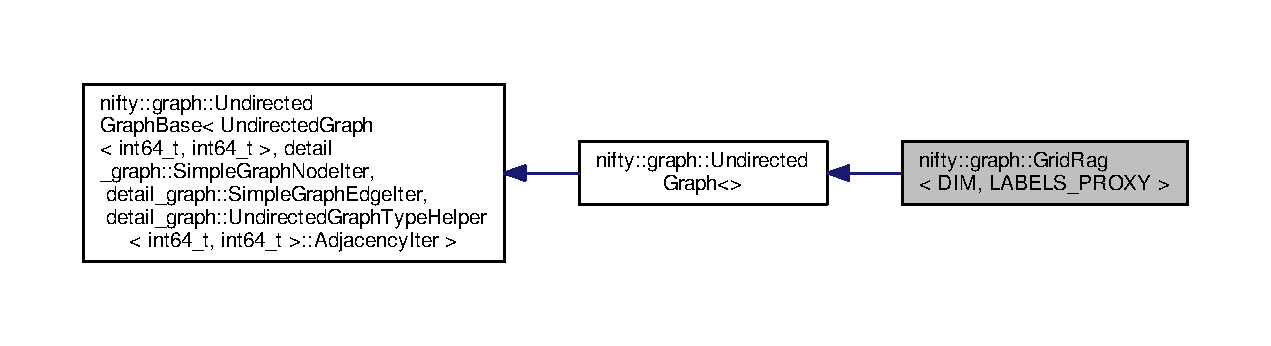
\includegraphics[width=350pt]{classnifty_1_1graph_1_1GridRag__inherit__graph}
\end{center}
\end{figure}


Collaboration diagram for nifty\+:\+:graph\+:\+:Grid\+Rag$<$ D\+IM, L\+A\+B\+E\+L\+S\+\_\+\+P\+R\+O\+XY $>$\+:
\nopagebreak
\begin{figure}[H]
\begin{center}
\leavevmode
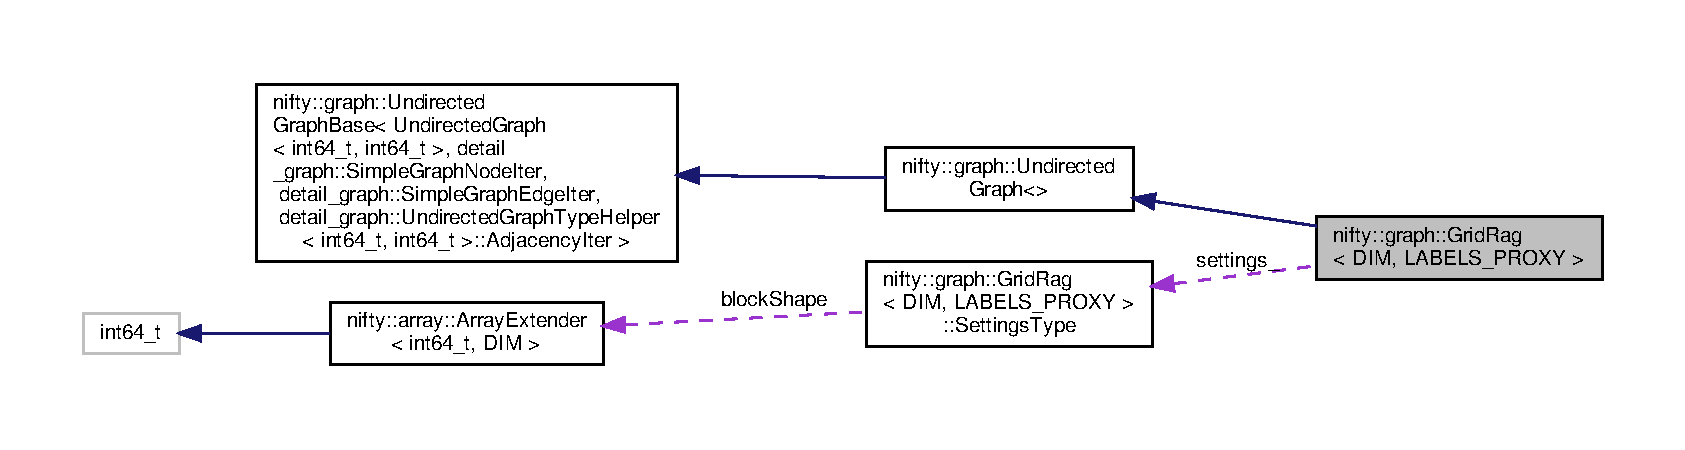
\includegraphics[width=350pt]{classnifty_1_1graph_1_1GridRag__coll__graph}
\end{center}
\end{figure}
\subsection*{Classes}
\begin{DoxyCompactItemize}
\item 
struct \hyperlink{structnifty_1_1graph_1_1GridRag_1_1DontComputeRag}{Dont\+Compute\+Rag}
\item 
struct \hyperlink{structnifty_1_1graph_1_1GridRag_1_1SettingsType}{Settings\+Type}
\end{DoxyCompactItemize}
\subsection*{Public Types}
\begin{DoxyCompactItemize}
\item 
typedef L\+A\+B\+E\+L\+S\+\_\+\+P\+R\+O\+XY \hyperlink{classnifty_1_1graph_1_1GridRag_ad3146f72301da4f45b51e3b692776cf1}{Labels\+Proxy}
\item 
typedef \hyperlink{classnifty_1_1graph_1_1GridRag}{Grid\+Rag}$<$ D\+IM, L\+A\+B\+E\+L\+S\+\_\+\+P\+R\+O\+XY $>$ \hyperlink{classnifty_1_1graph_1_1GridRag_aa5e47cff6ae70d13254abc3382b3b166}{Self\+Type}
\item 
typedef \hyperlink{namespacenifty_1_1array_a683f151f19c851754e0c6d55ed16a0c2}{array\+::\+Static\+Array}$<$ int64\+\_\+t, D\+IM $>$ \hyperlink{classnifty_1_1graph_1_1GridRag_a3693e007e1419dec9751cca751a1061d}{Shape\+Type}
\end{DoxyCompactItemize}
\subsection*{Public Member Functions}
\begin{DoxyCompactItemize}
\item 
\hyperlink{classnifty_1_1graph_1_1GridRag_a68da171354688c46cbb33d953e7ba267}{Grid\+Rag} (const \hyperlink{classnifty_1_1graph_1_1GridRag_ad3146f72301da4f45b51e3b692776cf1}{Labels\+Proxy} \&\hyperlink{classnifty_1_1graph_1_1GridRag_a8589e44e41c12e7956d7d25a644c238e}{labels\+Proxy}, const \hyperlink{structnifty_1_1graph_1_1GridRag_1_1SettingsType}{Settings\+Type} \&settings=\hyperlink{structnifty_1_1graph_1_1GridRag_1_1SettingsType}{Settings\+Type}())
\item 
{\footnotesize template$<$class I\+T\+ER $>$ }\\\hyperlink{classnifty_1_1graph_1_1GridRag_adcc1771b68011ee041bdf83180f72e73}{Grid\+Rag} (const \hyperlink{classnifty_1_1graph_1_1GridRag_ad3146f72301da4f45b51e3b692776cf1}{Labels\+Proxy} \&\hyperlink{classnifty_1_1graph_1_1GridRag_a8589e44e41c12e7956d7d25a644c238e}{labels\+Proxy}, I\+T\+ER serialization\+Begin, const \hyperlink{structnifty_1_1graph_1_1GridRag_1_1SettingsType}{Settings\+Type} \&settings=\hyperlink{structnifty_1_1graph_1_1GridRag_1_1SettingsType}{Settings\+Type}())
\item 
const \hyperlink{classnifty_1_1graph_1_1GridRag_ad3146f72301da4f45b51e3b692776cf1}{Labels\+Proxy} \& \hyperlink{classnifty_1_1graph_1_1GridRag_a8589e44e41c12e7956d7d25a644c238e}{labels\+Proxy} () const
\item 
const \hyperlink{classnifty_1_1graph_1_1GridRag_a3693e007e1419dec9751cca751a1061d}{Shape\+Type} \& \hyperlink{classnifty_1_1graph_1_1GridRag_a63c46e4d01bf30e7366e5781a0f3de5f}{shape} () const
\end{DoxyCompactItemize}
\subsection*{Protected Types}
\begin{DoxyCompactItemize}
\item 
typedef \hyperlink{structnifty_1_1graph_1_1RefHelper}{Ref\+Helper}$<$ L\+A\+B\+E\+L\+S\+\_\+\+P\+R\+O\+XY $>$\+::type \hyperlink{classnifty_1_1graph_1_1GridRag_ae7dcf657b20ef49d062648978e192cdb}{Storage\+Type}
\end{DoxyCompactItemize}
\subsection*{Protected Member Functions}
\begin{DoxyCompactItemize}
\item 
\hyperlink{classnifty_1_1graph_1_1GridRag_a559717d346c6e2e626994c1018fc5761}{Grid\+Rag} (const \hyperlink{classnifty_1_1graph_1_1GridRag_ad3146f72301da4f45b51e3b692776cf1}{Labels\+Proxy} \&\hyperlink{classnifty_1_1graph_1_1GridRag_a8589e44e41c12e7956d7d25a644c238e}{labels\+Proxy}, const \hyperlink{structnifty_1_1graph_1_1GridRag_1_1SettingsType}{Settings\+Type} \&settings, const \hyperlink{structnifty_1_1graph_1_1GridRag_1_1DontComputeRag}{Dont\+Compute\+Rag})
\end{DoxyCompactItemize}
\subsection*{Protected Attributes}
\begin{DoxyCompactItemize}
\item 
\hyperlink{structnifty_1_1graph_1_1GridRag_1_1SettingsType}{Settings\+Type} \hyperlink{classnifty_1_1graph_1_1GridRag_af4610f430b2ed52e5a4ea54c1eddcaf1}{settings\+\_\+}
\item 
\hyperlink{classnifty_1_1graph_1_1GridRag_ae7dcf657b20ef49d062648978e192cdb}{Storage\+Type} \hyperlink{classnifty_1_1graph_1_1GridRag_abaacb5cd2582a08e27ec4af04f5e9881}{labels\+Proxy\+\_\+}
\end{DoxyCompactItemize}
\subsection*{Friends}
\begin{DoxyCompactItemize}
\item 
class \hyperlink{classnifty_1_1graph_1_1GridRag_abafcbd3543961eb6e4ee794aa6a62d66}{detail\+\_\+rag\+::\+Compute\+Rag$<$ Self\+Type $>$}
\end{DoxyCompactItemize}


\subsection{Member Typedef Documentation}
\mbox{\Hypertarget{classnifty_1_1graph_1_1GridRag_ad3146f72301da4f45b51e3b692776cf1}\label{classnifty_1_1graph_1_1GridRag_ad3146f72301da4f45b51e3b692776cf1}} 
\index{nifty\+::graph\+::\+Grid\+Rag@{nifty\+::graph\+::\+Grid\+Rag}!Labels\+Proxy@{Labels\+Proxy}}
\index{Labels\+Proxy@{Labels\+Proxy}!nifty\+::graph\+::\+Grid\+Rag@{nifty\+::graph\+::\+Grid\+Rag}}
\subsubsection{\texorpdfstring{Labels\+Proxy}{LabelsProxy}}
{\footnotesize\ttfamily template$<$size\+\_\+t D\+IM, class L\+A\+B\+E\+L\+S\+\_\+\+P\+R\+O\+XY$>$ \\
typedef L\+A\+B\+E\+L\+S\+\_\+\+P\+R\+O\+XY \hyperlink{classnifty_1_1graph_1_1GridRag}{nifty\+::graph\+::\+Grid\+Rag}$<$ D\+IM, L\+A\+B\+E\+L\+S\+\_\+\+P\+R\+O\+XY $>$\+::\hyperlink{classnifty_1_1graph_1_1GridRag_ad3146f72301da4f45b51e3b692776cf1}{Labels\+Proxy}}

\mbox{\Hypertarget{classnifty_1_1graph_1_1GridRag_aa5e47cff6ae70d13254abc3382b3b166}\label{classnifty_1_1graph_1_1GridRag_aa5e47cff6ae70d13254abc3382b3b166}} 
\index{nifty\+::graph\+::\+Grid\+Rag@{nifty\+::graph\+::\+Grid\+Rag}!Self\+Type@{Self\+Type}}
\index{Self\+Type@{Self\+Type}!nifty\+::graph\+::\+Grid\+Rag@{nifty\+::graph\+::\+Grid\+Rag}}
\subsubsection{\texorpdfstring{Self\+Type}{SelfType}}
{\footnotesize\ttfamily template$<$size\+\_\+t D\+IM, class L\+A\+B\+E\+L\+S\+\_\+\+P\+R\+O\+XY$>$ \\
typedef \hyperlink{classnifty_1_1graph_1_1GridRag}{Grid\+Rag}$<$D\+IM, L\+A\+B\+E\+L\+S\+\_\+\+P\+R\+O\+XY$>$ \hyperlink{classnifty_1_1graph_1_1GridRag}{nifty\+::graph\+::\+Grid\+Rag}$<$ D\+IM, L\+A\+B\+E\+L\+S\+\_\+\+P\+R\+O\+XY $>$\+::\hyperlink{classnifty_1_1graph_1_1GridRag_aa5e47cff6ae70d13254abc3382b3b166}{Self\+Type}}

\mbox{\Hypertarget{classnifty_1_1graph_1_1GridRag_a3693e007e1419dec9751cca751a1061d}\label{classnifty_1_1graph_1_1GridRag_a3693e007e1419dec9751cca751a1061d}} 
\index{nifty\+::graph\+::\+Grid\+Rag@{nifty\+::graph\+::\+Grid\+Rag}!Shape\+Type@{Shape\+Type}}
\index{Shape\+Type@{Shape\+Type}!nifty\+::graph\+::\+Grid\+Rag@{nifty\+::graph\+::\+Grid\+Rag}}
\subsubsection{\texorpdfstring{Shape\+Type}{ShapeType}}
{\footnotesize\ttfamily template$<$size\+\_\+t D\+IM, class L\+A\+B\+E\+L\+S\+\_\+\+P\+R\+O\+XY$>$ \\
typedef \hyperlink{namespacenifty_1_1array_a683f151f19c851754e0c6d55ed16a0c2}{array\+::\+Static\+Array}$<$int64\+\_\+t, D\+IM$>$ \hyperlink{classnifty_1_1graph_1_1GridRag}{nifty\+::graph\+::\+Grid\+Rag}$<$ D\+IM, L\+A\+B\+E\+L\+S\+\_\+\+P\+R\+O\+XY $>$\+::\hyperlink{classnifty_1_1graph_1_1GridRag_a3693e007e1419dec9751cca751a1061d}{Shape\+Type}}

\mbox{\Hypertarget{classnifty_1_1graph_1_1GridRag_ae7dcf657b20ef49d062648978e192cdb}\label{classnifty_1_1graph_1_1GridRag_ae7dcf657b20ef49d062648978e192cdb}} 
\index{nifty\+::graph\+::\+Grid\+Rag@{nifty\+::graph\+::\+Grid\+Rag}!Storage\+Type@{Storage\+Type}}
\index{Storage\+Type@{Storage\+Type}!nifty\+::graph\+::\+Grid\+Rag@{nifty\+::graph\+::\+Grid\+Rag}}
\subsubsection{\texorpdfstring{Storage\+Type}{StorageType}}
{\footnotesize\ttfamily template$<$size\+\_\+t D\+IM, class L\+A\+B\+E\+L\+S\+\_\+\+P\+R\+O\+XY$>$ \\
typedef \hyperlink{structnifty_1_1graph_1_1RefHelper}{Ref\+Helper}$<$L\+A\+B\+E\+L\+S\+\_\+\+P\+R\+O\+XY$>$\+::type \hyperlink{classnifty_1_1graph_1_1GridRag}{nifty\+::graph\+::\+Grid\+Rag}$<$ D\+IM, L\+A\+B\+E\+L\+S\+\_\+\+P\+R\+O\+XY $>$\+::\hyperlink{classnifty_1_1graph_1_1GridRag_ae7dcf657b20ef49d062648978e192cdb}{Storage\+Type}\hspace{0.3cm}{\ttfamily [protected]}}



\subsection{Constructor \& Destructor Documentation}
\mbox{\Hypertarget{classnifty_1_1graph_1_1GridRag_a68da171354688c46cbb33d953e7ba267}\label{classnifty_1_1graph_1_1GridRag_a68da171354688c46cbb33d953e7ba267}} 
\index{nifty\+::graph\+::\+Grid\+Rag@{nifty\+::graph\+::\+Grid\+Rag}!Grid\+Rag@{Grid\+Rag}}
\index{Grid\+Rag@{Grid\+Rag}!nifty\+::graph\+::\+Grid\+Rag@{nifty\+::graph\+::\+Grid\+Rag}}
\subsubsection{\texorpdfstring{Grid\+Rag()}{GridRag()}\hspace{0.1cm}{\footnotesize\ttfamily [1/3]}}
{\footnotesize\ttfamily template$<$size\+\_\+t D\+IM, class L\+A\+B\+E\+L\+S\+\_\+\+P\+R\+O\+XY$>$ \\
\hyperlink{classnifty_1_1graph_1_1GridRag}{nifty\+::graph\+::\+Grid\+Rag}$<$ D\+IM, L\+A\+B\+E\+L\+S\+\_\+\+P\+R\+O\+XY $>$\+::\hyperlink{classnifty_1_1graph_1_1GridRag}{Grid\+Rag} (\begin{DoxyParamCaption}\item[{const \hyperlink{classnifty_1_1graph_1_1GridRag_ad3146f72301da4f45b51e3b692776cf1}{Labels\+Proxy} \&}]{labels\+Proxy,  }\item[{const \hyperlink{structnifty_1_1graph_1_1GridRag_1_1SettingsType}{Settings\+Type} \&}]{settings = {\ttfamily \hyperlink{structnifty_1_1graph_1_1GridRag_1_1SettingsType}{Settings\+Type}()} }\end{DoxyParamCaption})\hspace{0.3cm}{\ttfamily [inline]}}

\mbox{\Hypertarget{classnifty_1_1graph_1_1GridRag_adcc1771b68011ee041bdf83180f72e73}\label{classnifty_1_1graph_1_1GridRag_adcc1771b68011ee041bdf83180f72e73}} 
\index{nifty\+::graph\+::\+Grid\+Rag@{nifty\+::graph\+::\+Grid\+Rag}!Grid\+Rag@{Grid\+Rag}}
\index{Grid\+Rag@{Grid\+Rag}!nifty\+::graph\+::\+Grid\+Rag@{nifty\+::graph\+::\+Grid\+Rag}}
\subsubsection{\texorpdfstring{Grid\+Rag()}{GridRag()}\hspace{0.1cm}{\footnotesize\ttfamily [2/3]}}
{\footnotesize\ttfamily template$<$size\+\_\+t D\+IM, class L\+A\+B\+E\+L\+S\+\_\+\+P\+R\+O\+XY$>$ \\
template$<$class I\+T\+ER $>$ \\
\hyperlink{classnifty_1_1graph_1_1GridRag}{nifty\+::graph\+::\+Grid\+Rag}$<$ D\+IM, L\+A\+B\+E\+L\+S\+\_\+\+P\+R\+O\+XY $>$\+::\hyperlink{classnifty_1_1graph_1_1GridRag}{Grid\+Rag} (\begin{DoxyParamCaption}\item[{const \hyperlink{classnifty_1_1graph_1_1GridRag_ad3146f72301da4f45b51e3b692776cf1}{Labels\+Proxy} \&}]{labels\+Proxy,  }\item[{I\+T\+ER}]{serialization\+Begin,  }\item[{const \hyperlink{structnifty_1_1graph_1_1GridRag_1_1SettingsType}{Settings\+Type} \&}]{settings = {\ttfamily \hyperlink{structnifty_1_1graph_1_1GridRag_1_1SettingsType}{Settings\+Type}()} }\end{DoxyParamCaption})\hspace{0.3cm}{\ttfamily [inline]}}

\mbox{\Hypertarget{classnifty_1_1graph_1_1GridRag_a559717d346c6e2e626994c1018fc5761}\label{classnifty_1_1graph_1_1GridRag_a559717d346c6e2e626994c1018fc5761}} 
\index{nifty\+::graph\+::\+Grid\+Rag@{nifty\+::graph\+::\+Grid\+Rag}!Grid\+Rag@{Grid\+Rag}}
\index{Grid\+Rag@{Grid\+Rag}!nifty\+::graph\+::\+Grid\+Rag@{nifty\+::graph\+::\+Grid\+Rag}}
\subsubsection{\texorpdfstring{Grid\+Rag()}{GridRag()}\hspace{0.1cm}{\footnotesize\ttfamily [3/3]}}
{\footnotesize\ttfamily template$<$size\+\_\+t D\+IM, class L\+A\+B\+E\+L\+S\+\_\+\+P\+R\+O\+XY$>$ \\
\hyperlink{classnifty_1_1graph_1_1GridRag}{nifty\+::graph\+::\+Grid\+Rag}$<$ D\+IM, L\+A\+B\+E\+L\+S\+\_\+\+P\+R\+O\+XY $>$\+::\hyperlink{classnifty_1_1graph_1_1GridRag}{Grid\+Rag} (\begin{DoxyParamCaption}\item[{const \hyperlink{classnifty_1_1graph_1_1GridRag_ad3146f72301da4f45b51e3b692776cf1}{Labels\+Proxy} \&}]{labels\+Proxy,  }\item[{const \hyperlink{structnifty_1_1graph_1_1GridRag_1_1SettingsType}{Settings\+Type} \&}]{settings,  }\item[{const \hyperlink{structnifty_1_1graph_1_1GridRag_1_1DontComputeRag}{Dont\+Compute\+Rag}}]{ }\end{DoxyParamCaption})\hspace{0.3cm}{\ttfamily [inline]}, {\ttfamily [protected]}}



\subsection{Member Function Documentation}
\mbox{\Hypertarget{classnifty_1_1graph_1_1GridRag_a8589e44e41c12e7956d7d25a644c238e}\label{classnifty_1_1graph_1_1GridRag_a8589e44e41c12e7956d7d25a644c238e}} 
\index{nifty\+::graph\+::\+Grid\+Rag@{nifty\+::graph\+::\+Grid\+Rag}!labels\+Proxy@{labels\+Proxy}}
\index{labels\+Proxy@{labels\+Proxy}!nifty\+::graph\+::\+Grid\+Rag@{nifty\+::graph\+::\+Grid\+Rag}}
\subsubsection{\texorpdfstring{labels\+Proxy()}{labelsProxy()}}
{\footnotesize\ttfamily template$<$size\+\_\+t D\+IM, class L\+A\+B\+E\+L\+S\+\_\+\+P\+R\+O\+XY$>$ \\
const \hyperlink{classnifty_1_1graph_1_1GridRag_ad3146f72301da4f45b51e3b692776cf1}{Labels\+Proxy}\& \hyperlink{classnifty_1_1graph_1_1GridRag}{nifty\+::graph\+::\+Grid\+Rag}$<$ D\+IM, L\+A\+B\+E\+L\+S\+\_\+\+P\+R\+O\+XY $>$\+::labels\+Proxy (\begin{DoxyParamCaption}{ }\end{DoxyParamCaption}) const\hspace{0.3cm}{\ttfamily [inline]}}

\mbox{\Hypertarget{classnifty_1_1graph_1_1GridRag_a63c46e4d01bf30e7366e5781a0f3de5f}\label{classnifty_1_1graph_1_1GridRag_a63c46e4d01bf30e7366e5781a0f3de5f}} 
\index{nifty\+::graph\+::\+Grid\+Rag@{nifty\+::graph\+::\+Grid\+Rag}!shape@{shape}}
\index{shape@{shape}!nifty\+::graph\+::\+Grid\+Rag@{nifty\+::graph\+::\+Grid\+Rag}}
\subsubsection{\texorpdfstring{shape()}{shape()}}
{\footnotesize\ttfamily template$<$size\+\_\+t D\+IM, class L\+A\+B\+E\+L\+S\+\_\+\+P\+R\+O\+XY$>$ \\
const \hyperlink{classnifty_1_1graph_1_1GridRag_a3693e007e1419dec9751cca751a1061d}{Shape\+Type}\& \hyperlink{classnifty_1_1graph_1_1GridRag}{nifty\+::graph\+::\+Grid\+Rag}$<$ D\+IM, L\+A\+B\+E\+L\+S\+\_\+\+P\+R\+O\+XY $>$\+::shape (\begin{DoxyParamCaption}{ }\end{DoxyParamCaption}) const\hspace{0.3cm}{\ttfamily [inline]}}



\subsection{Friends And Related Function Documentation}
\mbox{\Hypertarget{classnifty_1_1graph_1_1GridRag_abafcbd3543961eb6e4ee794aa6a62d66}\label{classnifty_1_1graph_1_1GridRag_abafcbd3543961eb6e4ee794aa6a62d66}} 
\index{nifty\+::graph\+::\+Grid\+Rag@{nifty\+::graph\+::\+Grid\+Rag}!detail\+\_\+rag\+::\+Compute\+Rag$<$ Self\+Type $>$@{detail\+\_\+rag\+::\+Compute\+Rag$<$ Self\+Type $>$}}
\index{detail\+\_\+rag\+::\+Compute\+Rag$<$ Self\+Type $>$@{detail\+\_\+rag\+::\+Compute\+Rag$<$ Self\+Type $>$}!nifty\+::graph\+::\+Grid\+Rag@{nifty\+::graph\+::\+Grid\+Rag}}
\subsubsection{\texorpdfstring{detail\+\_\+rag\+::\+Compute\+Rag$<$ Self\+Type $>$}{detail\_rag::ComputeRag< SelfType >}}
{\footnotesize\ttfamily template$<$size\+\_\+t D\+IM, class L\+A\+B\+E\+L\+S\+\_\+\+P\+R\+O\+XY$>$ \\
friend class detail\+\_\+rag\+::\+Compute\+Rag$<$ \hyperlink{classnifty_1_1graph_1_1GridRag_aa5e47cff6ae70d13254abc3382b3b166}{Self\+Type} $>$\hspace{0.3cm}{\ttfamily [friend]}}



\subsection{Member Data Documentation}
\mbox{\Hypertarget{classnifty_1_1graph_1_1GridRag_abaacb5cd2582a08e27ec4af04f5e9881}\label{classnifty_1_1graph_1_1GridRag_abaacb5cd2582a08e27ec4af04f5e9881}} 
\index{nifty\+::graph\+::\+Grid\+Rag@{nifty\+::graph\+::\+Grid\+Rag}!labels\+Proxy\+\_\+@{labels\+Proxy\+\_\+}}
\index{labels\+Proxy\+\_\+@{labels\+Proxy\+\_\+}!nifty\+::graph\+::\+Grid\+Rag@{nifty\+::graph\+::\+Grid\+Rag}}
\subsubsection{\texorpdfstring{labels\+Proxy\+\_\+}{labelsProxy\_}}
{\footnotesize\ttfamily template$<$size\+\_\+t D\+IM, class L\+A\+B\+E\+L\+S\+\_\+\+P\+R\+O\+XY$>$ \\
\hyperlink{classnifty_1_1graph_1_1GridRag_ae7dcf657b20ef49d062648978e192cdb}{Storage\+Type} \hyperlink{classnifty_1_1graph_1_1GridRag}{nifty\+::graph\+::\+Grid\+Rag}$<$ D\+IM, L\+A\+B\+E\+L\+S\+\_\+\+P\+R\+O\+XY $>$\+::labels\+Proxy\+\_\+\hspace{0.3cm}{\ttfamily [protected]}}

\mbox{\Hypertarget{classnifty_1_1graph_1_1GridRag_af4610f430b2ed52e5a4ea54c1eddcaf1}\label{classnifty_1_1graph_1_1GridRag_af4610f430b2ed52e5a4ea54c1eddcaf1}} 
\index{nifty\+::graph\+::\+Grid\+Rag@{nifty\+::graph\+::\+Grid\+Rag}!settings\+\_\+@{settings\+\_\+}}
\index{settings\+\_\+@{settings\+\_\+}!nifty\+::graph\+::\+Grid\+Rag@{nifty\+::graph\+::\+Grid\+Rag}}
\subsubsection{\texorpdfstring{settings\+\_\+}{settings\_}}
{\footnotesize\ttfamily template$<$size\+\_\+t D\+IM, class L\+A\+B\+E\+L\+S\+\_\+\+P\+R\+O\+XY$>$ \\
\hyperlink{structnifty_1_1graph_1_1GridRag_1_1SettingsType}{Settings\+Type} \hyperlink{classnifty_1_1graph_1_1GridRag}{nifty\+::graph\+::\+Grid\+Rag}$<$ D\+IM, L\+A\+B\+E\+L\+S\+\_\+\+P\+R\+O\+XY $>$\+::settings\+\_\+\hspace{0.3cm}{\ttfamily [protected]}}



The documentation for this class was generated from the following files\+:\begin{DoxyCompactItemize}
\item 
/home/tbeier/src/nifty/include/nifty/graph/rag/detail\+\_\+rag/\hyperlink{compute__grid__rag_8hxx}{compute\+\_\+grid\+\_\+rag.\+hxx}\item 
/home/tbeier/src/nifty/include/nifty/graph/rag/\hyperlink{grid__rag_8hxx}{grid\+\_\+rag.\+hxx}\end{DoxyCompactItemize}

\hypertarget{classnifty_1_1graph_1_1GridRag3DStacked2D}{}\section{nifty\+:\+:graph\+:\+:Grid\+Rag3\+D\+Stacked2D$<$ L\+A\+B\+E\+L\+S\+\_\+\+P\+R\+O\+XY $>$ Class Template Reference}
\label{classnifty_1_1graph_1_1GridRag3DStacked2D}\index{nifty\+::graph\+::\+Grid\+Rag3\+D\+Stacked2\+D$<$ L\+A\+B\+E\+L\+S\+\_\+\+P\+R\+O\+X\+Y $>$@{nifty\+::graph\+::\+Grid\+Rag3\+D\+Stacked2\+D$<$ L\+A\+B\+E\+L\+S\+\_\+\+P\+R\+O\+X\+Y $>$}}


{\ttfamily \#include $<$grid\+\_\+rag.\+hxx$>$}



The documentation for this class was generated from the following file\+:\begin{DoxyCompactItemize}
\item 
/home/tbeier/src/nifty/include/nifty/graph/rag/\hyperlink{grid__rag_8hxx}{grid\+\_\+rag.\+hxx}\end{DoxyCompactItemize}

\hypertarget{classnifty_1_1graph_1_1GridRagStacked2D}{}\section{nifty\+:\+:graph\+:\+:Grid\+Rag\+Stacked2\+D$<$ L\+A\+B\+E\+L\+\_\+\+P\+R\+O\+X\+Y $>$ Class Template Reference}
\label{classnifty_1_1graph_1_1GridRagStacked2D}\index{nifty\+::graph\+::\+Grid\+Rag\+Stacked2\+D$<$ L\+A\+B\+E\+L\+\_\+\+P\+R\+O\+X\+Y $>$@{nifty\+::graph\+::\+Grid\+Rag\+Stacked2\+D$<$ L\+A\+B\+E\+L\+\_\+\+P\+R\+O\+X\+Y $>$}}


{\ttfamily \#include $<$compute\+\_\+grid\+\_\+rag.\+hxx$>$}



Inheritance diagram for nifty\+:\+:graph\+:\+:Grid\+Rag\+Stacked2\+D$<$ L\+A\+B\+E\+L\+\_\+\+P\+R\+O\+X\+Y $>$\+:
% FIG 0


Collaboration diagram for nifty\+:\+:graph\+:\+:Grid\+Rag\+Stacked2\+D$<$ L\+A\+B\+E\+L\+\_\+\+P\+R\+O\+X\+Y $>$\+:
% FIG 1
\subsection*{Public Types}
\begin{DoxyCompactItemize}
\item 
typedef \hyperlink{classnifty_1_1graph_1_1GridRag_ad3146f72301da4f45b51e3b692776cf1}{Base\+Type\+::\+Labels\+Proxy} \hyperlink{classnifty_1_1graph_1_1GridRagStacked2D_a09b44c819b97274a1025dc68cb6b3dc9}{Labels\+Proxy}
\item 
typedef Base\+Type\+::\+Settings \hyperlink{classnifty_1_1graph_1_1GridRagStacked2D_a7b0a5b8d3cb7ac39213e5306fd42aa27}{Settings}
\end{DoxyCompactItemize}
\subsection*{Public Member Functions}
\begin{DoxyCompactItemize}
\item 
\hyperlink{classnifty_1_1graph_1_1GridRagStacked2D_ad6b23b6d315c94ce484b220ef34ba1ca}{Grid\+Rag\+Stacked2\+D} (const \hyperlink{classnifty_1_1graph_1_1GridRagStacked2D_a09b44c819b97274a1025dc68cb6b3dc9}{Labels\+Proxy} \&\hyperlink{classnifty_1_1graph_1_1GridRag_a9a9b20451bd5ea8ce3ee11af4018c995}{labels\+Proxy}, const \hyperlink{classnifty_1_1graph_1_1GridRagStacked2D_a7b0a5b8d3cb7ac39213e5306fd42aa27}{Settings} \&settings=\hyperlink{classnifty_1_1graph_1_1GridRagStacked2D_a7b0a5b8d3cb7ac39213e5306fd42aa27}{Settings}())
\item 
std\+::pair$<$ uint64\+\_\+t, uint64\+\_\+t $>$ \hyperlink{classnifty_1_1graph_1_1GridRagStacked2D_ae7abe343f431f1a1ca953f3f9dd5e659}{min\+Max\+Node} (const uint64\+\_\+t slice\+Index) const 
\item 
uint64\+\_\+t \hyperlink{classnifty_1_1graph_1_1GridRagStacked2D_aa87c188ce0a2d246e1461bac64cf3a8a}{number\+Of\+Nodes} (const uint64\+\_\+t slice\+Index) const 
\item 
uint64\+\_\+t \hyperlink{classnifty_1_1graph_1_1GridRagStacked2D_a646bcd62254f454d3ac2e584b1b07428}{number\+Of\+In\+Slice\+Edges} (const uint64\+\_\+t slice\+Index) const 
\item 
uint64\+\_\+t \hyperlink{classnifty_1_1graph_1_1GridRagStacked2D_acfdac0e16539e96d36fdc1615e3e4ee1}{number\+Of\+In\+Between\+Slice\+Edges} (const uint64\+\_\+t slice\+Index) const 
\item 
uint64\+\_\+t \hyperlink{classnifty_1_1graph_1_1GridRagStacked2D_a111282918d5ef7ef97e4328d575b7089}{in\+Slice\+Edge\+Offset} (const uint64\+\_\+t slice\+Index) const 
\item 
uint64\+\_\+t \hyperlink{classnifty_1_1graph_1_1GridRagStacked2D_aa55f6424ed3ba64fe5cfc42b69876f8e}{between\+Slice\+Edge\+Offset} (const uint64\+\_\+t slice\+Index) const 
\end{DoxyCompactItemize}
\subsection*{Friends}
\begin{DoxyCompactItemize}
\item 
class \hyperlink{classnifty_1_1graph_1_1GridRagStacked2D_abafcbd3543961eb6e4ee794aa6a62d66}{detail\+\_\+rag\+::\+Compute\+Rag$<$ Self\+Type $>$}
\end{DoxyCompactItemize}
\subsection*{Additional Inherited Members}


\subsection{Member Typedef Documentation}
\hypertarget{classnifty_1_1graph_1_1GridRagStacked2D_a09b44c819b97274a1025dc68cb6b3dc9}{}\index{nifty\+::graph\+::\+Grid\+Rag\+Stacked2\+D@{nifty\+::graph\+::\+Grid\+Rag\+Stacked2\+D}!Labels\+Proxy@{Labels\+Proxy}}
\index{Labels\+Proxy@{Labels\+Proxy}!nifty\+::graph\+::\+Grid\+Rag\+Stacked2\+D@{nifty\+::graph\+::\+Grid\+Rag\+Stacked2\+D}}
\subsubsection[{Labels\+Proxy}]{\setlength{\rightskip}{0pt plus 5cm}template$<$class L\+A\+B\+E\+L\+\_\+\+P\+R\+O\+X\+Y $>$ typedef {\bf Base\+Type\+::\+Labels\+Proxy} {\bf nifty\+::graph\+::\+Grid\+Rag\+Stacked2\+D}$<$ L\+A\+B\+E\+L\+\_\+\+P\+R\+O\+X\+Y $>$\+::{\bf Labels\+Proxy}}\label{classnifty_1_1graph_1_1GridRagStacked2D_a09b44c819b97274a1025dc68cb6b3dc9}
\hypertarget{classnifty_1_1graph_1_1GridRagStacked2D_a7b0a5b8d3cb7ac39213e5306fd42aa27}{}\index{nifty\+::graph\+::\+Grid\+Rag\+Stacked2\+D@{nifty\+::graph\+::\+Grid\+Rag\+Stacked2\+D}!Settings@{Settings}}
\index{Settings@{Settings}!nifty\+::graph\+::\+Grid\+Rag\+Stacked2\+D@{nifty\+::graph\+::\+Grid\+Rag\+Stacked2\+D}}
\subsubsection[{Settings}]{\setlength{\rightskip}{0pt plus 5cm}template$<$class L\+A\+B\+E\+L\+\_\+\+P\+R\+O\+X\+Y $>$ typedef Base\+Type\+::\+Settings {\bf nifty\+::graph\+::\+Grid\+Rag\+Stacked2\+D}$<$ L\+A\+B\+E\+L\+\_\+\+P\+R\+O\+X\+Y $>$\+::{\bf Settings}}\label{classnifty_1_1graph_1_1GridRagStacked2D_a7b0a5b8d3cb7ac39213e5306fd42aa27}


\subsection{Constructor \& Destructor Documentation}
\hypertarget{classnifty_1_1graph_1_1GridRagStacked2D_ad6b23b6d315c94ce484b220ef34ba1ca}{}\index{nifty\+::graph\+::\+Grid\+Rag\+Stacked2\+D@{nifty\+::graph\+::\+Grid\+Rag\+Stacked2\+D}!Grid\+Rag\+Stacked2\+D@{Grid\+Rag\+Stacked2\+D}}
\index{Grid\+Rag\+Stacked2\+D@{Grid\+Rag\+Stacked2\+D}!nifty\+::graph\+::\+Grid\+Rag\+Stacked2\+D@{nifty\+::graph\+::\+Grid\+Rag\+Stacked2\+D}}
\subsubsection[{Grid\+Rag\+Stacked2\+D(const Labels\+Proxy \&labels\+Proxy, const Settings \&settings=\+Settings())}]{\setlength{\rightskip}{0pt plus 5cm}template$<$class L\+A\+B\+E\+L\+\_\+\+P\+R\+O\+X\+Y $>$ {\bf nifty\+::graph\+::\+Grid\+Rag\+Stacked2\+D}$<$ L\+A\+B\+E\+L\+\_\+\+P\+R\+O\+X\+Y $>$\+::{\bf Grid\+Rag\+Stacked2\+D} (
\begin{DoxyParamCaption}
\item[{const {\bf Labels\+Proxy} \&}]{labels\+Proxy, }
\item[{const {\bf Settings} \&}]{settings = {\ttfamily {\bf Settings}()}}
\end{DoxyParamCaption}
)\hspace{0.3cm}{\ttfamily [inline]}}\label{classnifty_1_1graph_1_1GridRagStacked2D_ad6b23b6d315c94ce484b220ef34ba1ca}


\subsection{Member Function Documentation}
\hypertarget{classnifty_1_1graph_1_1GridRagStacked2D_aa55f6424ed3ba64fe5cfc42b69876f8e}{}\index{nifty\+::graph\+::\+Grid\+Rag\+Stacked2\+D@{nifty\+::graph\+::\+Grid\+Rag\+Stacked2\+D}!between\+Slice\+Edge\+Offset@{between\+Slice\+Edge\+Offset}}
\index{between\+Slice\+Edge\+Offset@{between\+Slice\+Edge\+Offset}!nifty\+::graph\+::\+Grid\+Rag\+Stacked2\+D@{nifty\+::graph\+::\+Grid\+Rag\+Stacked2\+D}}
\subsubsection[{between\+Slice\+Edge\+Offset(const uint64\+\_\+t slice\+Index) const }]{\setlength{\rightskip}{0pt plus 5cm}template$<$class L\+A\+B\+E\+L\+\_\+\+P\+R\+O\+X\+Y $>$ uint64\+\_\+t {\bf nifty\+::graph\+::\+Grid\+Rag\+Stacked2\+D}$<$ L\+A\+B\+E\+L\+\_\+\+P\+R\+O\+X\+Y $>$\+::between\+Slice\+Edge\+Offset (
\begin{DoxyParamCaption}
\item[{const uint64\+\_\+t}]{slice\+Index}
\end{DoxyParamCaption}
) const\hspace{0.3cm}{\ttfamily [inline]}}\label{classnifty_1_1graph_1_1GridRagStacked2D_aa55f6424ed3ba64fe5cfc42b69876f8e}
\hypertarget{classnifty_1_1graph_1_1GridRagStacked2D_a111282918d5ef7ef97e4328d575b7089}{}\index{nifty\+::graph\+::\+Grid\+Rag\+Stacked2\+D@{nifty\+::graph\+::\+Grid\+Rag\+Stacked2\+D}!in\+Slice\+Edge\+Offset@{in\+Slice\+Edge\+Offset}}
\index{in\+Slice\+Edge\+Offset@{in\+Slice\+Edge\+Offset}!nifty\+::graph\+::\+Grid\+Rag\+Stacked2\+D@{nifty\+::graph\+::\+Grid\+Rag\+Stacked2\+D}}
\subsubsection[{in\+Slice\+Edge\+Offset(const uint64\+\_\+t slice\+Index) const }]{\setlength{\rightskip}{0pt plus 5cm}template$<$class L\+A\+B\+E\+L\+\_\+\+P\+R\+O\+X\+Y $>$ uint64\+\_\+t {\bf nifty\+::graph\+::\+Grid\+Rag\+Stacked2\+D}$<$ L\+A\+B\+E\+L\+\_\+\+P\+R\+O\+X\+Y $>$\+::in\+Slice\+Edge\+Offset (
\begin{DoxyParamCaption}
\item[{const uint64\+\_\+t}]{slice\+Index}
\end{DoxyParamCaption}
) const\hspace{0.3cm}{\ttfamily [inline]}}\label{classnifty_1_1graph_1_1GridRagStacked2D_a111282918d5ef7ef97e4328d575b7089}
\hypertarget{classnifty_1_1graph_1_1GridRagStacked2D_ae7abe343f431f1a1ca953f3f9dd5e659}{}\index{nifty\+::graph\+::\+Grid\+Rag\+Stacked2\+D@{nifty\+::graph\+::\+Grid\+Rag\+Stacked2\+D}!min\+Max\+Node@{min\+Max\+Node}}
\index{min\+Max\+Node@{min\+Max\+Node}!nifty\+::graph\+::\+Grid\+Rag\+Stacked2\+D@{nifty\+::graph\+::\+Grid\+Rag\+Stacked2\+D}}
\subsubsection[{min\+Max\+Node(const uint64\+\_\+t slice\+Index) const }]{\setlength{\rightskip}{0pt plus 5cm}template$<$class L\+A\+B\+E\+L\+\_\+\+P\+R\+O\+X\+Y $>$ std\+::pair$<$uint64\+\_\+t, uint64\+\_\+t$>$ {\bf nifty\+::graph\+::\+Grid\+Rag\+Stacked2\+D}$<$ L\+A\+B\+E\+L\+\_\+\+P\+R\+O\+X\+Y $>$\+::min\+Max\+Node (
\begin{DoxyParamCaption}
\item[{const uint64\+\_\+t}]{slice\+Index}
\end{DoxyParamCaption}
) const\hspace{0.3cm}{\ttfamily [inline]}}\label{classnifty_1_1graph_1_1GridRagStacked2D_ae7abe343f431f1a1ca953f3f9dd5e659}
\hypertarget{classnifty_1_1graph_1_1GridRagStacked2D_acfdac0e16539e96d36fdc1615e3e4ee1}{}\index{nifty\+::graph\+::\+Grid\+Rag\+Stacked2\+D@{nifty\+::graph\+::\+Grid\+Rag\+Stacked2\+D}!number\+Of\+In\+Between\+Slice\+Edges@{number\+Of\+In\+Between\+Slice\+Edges}}
\index{number\+Of\+In\+Between\+Slice\+Edges@{number\+Of\+In\+Between\+Slice\+Edges}!nifty\+::graph\+::\+Grid\+Rag\+Stacked2\+D@{nifty\+::graph\+::\+Grid\+Rag\+Stacked2\+D}}
\subsubsection[{number\+Of\+In\+Between\+Slice\+Edges(const uint64\+\_\+t slice\+Index) const }]{\setlength{\rightskip}{0pt plus 5cm}template$<$class L\+A\+B\+E\+L\+\_\+\+P\+R\+O\+X\+Y $>$ uint64\+\_\+t {\bf nifty\+::graph\+::\+Grid\+Rag\+Stacked2\+D}$<$ L\+A\+B\+E\+L\+\_\+\+P\+R\+O\+X\+Y $>$\+::number\+Of\+In\+Between\+Slice\+Edges (
\begin{DoxyParamCaption}
\item[{const uint64\+\_\+t}]{slice\+Index}
\end{DoxyParamCaption}
) const\hspace{0.3cm}{\ttfamily [inline]}}\label{classnifty_1_1graph_1_1GridRagStacked2D_acfdac0e16539e96d36fdc1615e3e4ee1}
\hypertarget{classnifty_1_1graph_1_1GridRagStacked2D_a646bcd62254f454d3ac2e584b1b07428}{}\index{nifty\+::graph\+::\+Grid\+Rag\+Stacked2\+D@{nifty\+::graph\+::\+Grid\+Rag\+Stacked2\+D}!number\+Of\+In\+Slice\+Edges@{number\+Of\+In\+Slice\+Edges}}
\index{number\+Of\+In\+Slice\+Edges@{number\+Of\+In\+Slice\+Edges}!nifty\+::graph\+::\+Grid\+Rag\+Stacked2\+D@{nifty\+::graph\+::\+Grid\+Rag\+Stacked2\+D}}
\subsubsection[{number\+Of\+In\+Slice\+Edges(const uint64\+\_\+t slice\+Index) const }]{\setlength{\rightskip}{0pt plus 5cm}template$<$class L\+A\+B\+E\+L\+\_\+\+P\+R\+O\+X\+Y $>$ uint64\+\_\+t {\bf nifty\+::graph\+::\+Grid\+Rag\+Stacked2\+D}$<$ L\+A\+B\+E\+L\+\_\+\+P\+R\+O\+X\+Y $>$\+::number\+Of\+In\+Slice\+Edges (
\begin{DoxyParamCaption}
\item[{const uint64\+\_\+t}]{slice\+Index}
\end{DoxyParamCaption}
) const\hspace{0.3cm}{\ttfamily [inline]}}\label{classnifty_1_1graph_1_1GridRagStacked2D_a646bcd62254f454d3ac2e584b1b07428}
\hypertarget{classnifty_1_1graph_1_1GridRagStacked2D_aa87c188ce0a2d246e1461bac64cf3a8a}{}\index{nifty\+::graph\+::\+Grid\+Rag\+Stacked2\+D@{nifty\+::graph\+::\+Grid\+Rag\+Stacked2\+D}!number\+Of\+Nodes@{number\+Of\+Nodes}}
\index{number\+Of\+Nodes@{number\+Of\+Nodes}!nifty\+::graph\+::\+Grid\+Rag\+Stacked2\+D@{nifty\+::graph\+::\+Grid\+Rag\+Stacked2\+D}}
\subsubsection[{number\+Of\+Nodes(const uint64\+\_\+t slice\+Index) const }]{\setlength{\rightskip}{0pt plus 5cm}template$<$class L\+A\+B\+E\+L\+\_\+\+P\+R\+O\+X\+Y $>$ uint64\+\_\+t {\bf nifty\+::graph\+::\+Grid\+Rag\+Stacked2\+D}$<$ L\+A\+B\+E\+L\+\_\+\+P\+R\+O\+X\+Y $>$\+::number\+Of\+Nodes (
\begin{DoxyParamCaption}
\item[{const uint64\+\_\+t}]{slice\+Index}
\end{DoxyParamCaption}
) const\hspace{0.3cm}{\ttfamily [inline]}}\label{classnifty_1_1graph_1_1GridRagStacked2D_aa87c188ce0a2d246e1461bac64cf3a8a}


\subsection{Friends And Related Function Documentation}
\hypertarget{classnifty_1_1graph_1_1GridRagStacked2D_abafcbd3543961eb6e4ee794aa6a62d66}{}\index{nifty\+::graph\+::\+Grid\+Rag\+Stacked2\+D@{nifty\+::graph\+::\+Grid\+Rag\+Stacked2\+D}!detail\+\_\+rag\+::\+Compute\+Rag$<$ Self\+Type $>$@{detail\+\_\+rag\+::\+Compute\+Rag$<$ Self\+Type $>$}}
\index{detail\+\_\+rag\+::\+Compute\+Rag$<$ Self\+Type $>$@{detail\+\_\+rag\+::\+Compute\+Rag$<$ Self\+Type $>$}!nifty\+::graph\+::\+Grid\+Rag\+Stacked2\+D@{nifty\+::graph\+::\+Grid\+Rag\+Stacked2\+D}}
\subsubsection[{detail\+\_\+rag\+::\+Compute\+Rag$<$ Self\+Type $>$}]{\setlength{\rightskip}{0pt plus 5cm}template$<$class L\+A\+B\+E\+L\+\_\+\+P\+R\+O\+X\+Y $>$ friend class detail\+\_\+rag\+::\+Compute\+Rag$<$ {\bf Self\+Type} $>$\hspace{0.3cm}{\ttfamily [friend]}}\label{classnifty_1_1graph_1_1GridRagStacked2D_abafcbd3543961eb6e4ee794aa6a62d66}


The documentation for this class was generated from the following files\+:\begin{DoxyCompactItemize}
\item 
/home/tbeier/src/nifty/include/nifty/graph/rag/detail\+\_\+rag/\hyperlink{compute__grid__rag_8hxx}{compute\+\_\+grid\+\_\+rag.\+hxx}\item 
/home/tbeier/src/nifty/include/nifty/graph/rag/\hyperlink{grid__rag__stacked__2d_8hxx}{grid\+\_\+rag\+\_\+stacked\+\_\+2d.\+hxx}\end{DoxyCompactItemize}

\hypertarget{classnifty_1_1ilp__backend_1_1Gurobi}{}\section{nifty\+:\+:ilp\+\_\+backend\+:\+:Gurobi Class Reference}
\label{classnifty_1_1ilp__backend_1_1Gurobi}\index{nifty\+::ilp\+\_\+backend\+::\+Gurobi@{nifty\+::ilp\+\_\+backend\+::\+Gurobi}}


{\ttfamily \#include $<$gurobi.\+hxx$>$}

\subsection*{Public Types}
\begin{DoxyCompactItemize}
\item 
typedef \hyperlink{structnifty_1_1ilp__backend_1_1IlpBackendSettings}{Ilp\+Backend\+Settings} \hyperlink{classnifty_1_1ilp__backend_1_1Gurobi_ae07f9785d50e89fef9df8ac94eba5010}{Settings}
\end{DoxyCompactItemize}
\subsection*{Public Member Functions}
\begin{DoxyCompactItemize}
\item 
\hyperlink{classnifty_1_1ilp__backend_1_1Gurobi_abcd8d8d449cbac006855470e361535b2}{Gurobi} (const \hyperlink{classnifty_1_1ilp__backend_1_1Gurobi_ae07f9785d50e89fef9df8ac94eba5010}{Settings} \&settings=\hyperlink{classnifty_1_1ilp__backend_1_1Gurobi_ae07f9785d50e89fef9df8ac94eba5010}{Settings}())
\item 
\hyperlink{classnifty_1_1ilp__backend_1_1Gurobi_ab8e373ce16adba177e9341a2d0e55157}{$\sim$\+Gurobi} ()
\item 
void \hyperlink{classnifty_1_1ilp__backend_1_1Gurobi_ac4ee3e8981df207094a6580f07f2685d}{init\+Model} (const size\+\_\+t, const double $\ast$)
\item 
{\footnotesize template$<$class Iterator $>$ }\\void \hyperlink{classnifty_1_1ilp__backend_1_1Gurobi_a0875ce6a8a39917a496ec650c68da6a0}{set\+Start} (Iterator)
\item 
{\footnotesize template$<$class Variable\+Index\+Iterator , class Coefficient\+Iterator $>$ }\\void \hyperlink{classnifty_1_1ilp__backend_1_1Gurobi_ad4e3fa2d4f5fe726a46d40857c36a918}{add\+Constraint} (Variable\+Index\+Iterator, Variable\+Index\+Iterator, Coefficient\+Iterator, const double, const double)
\item 
void \hyperlink{classnifty_1_1ilp__backend_1_1Gurobi_a2521e51c0cdfb1e029d332ab7f203021}{optimize} ()
\item 
double \hyperlink{classnifty_1_1ilp__backend_1_1Gurobi_afbdf38456bb7ce8110168dd3aa7f691f}{label} (const size\+\_\+t) const 
\item 
{\footnotesize template$<$class O\+B\+J\+E\+C\+T\+I\+V\+E\+\_\+\+I\+T\+E\+R\+A\+T\+O\+R $>$ }\\void \hyperlink{classnifty_1_1ilp__backend_1_1Gurobi_a138de39ce46740b4728b9d2e7f8bd27b}{change\+Objective} (O\+B\+J\+E\+C\+T\+I\+V\+E\+\_\+\+I\+T\+E\+R\+A\+T\+O\+R objective\+Iter)
\end{DoxyCompactItemize}
\subsection*{Static Public Member Functions}
\begin{DoxyCompactItemize}
\item 
static std\+::string \hyperlink{classnifty_1_1ilp__backend_1_1Gurobi_a3c80f9769e9f33482397305e234b0aa7}{name} ()
\end{DoxyCompactItemize}


\subsection{Member Typedef Documentation}
\hypertarget{classnifty_1_1ilp__backend_1_1Gurobi_ae07f9785d50e89fef9df8ac94eba5010}{}\index{nifty\+::ilp\+\_\+backend\+::\+Gurobi@{nifty\+::ilp\+\_\+backend\+::\+Gurobi}!Settings@{Settings}}
\index{Settings@{Settings}!nifty\+::ilp\+\_\+backend\+::\+Gurobi@{nifty\+::ilp\+\_\+backend\+::\+Gurobi}}
\subsubsection[{Settings}]{\setlength{\rightskip}{0pt plus 5cm}typedef {\bf Ilp\+Backend\+Settings} {\bf nifty\+::ilp\+\_\+backend\+::\+Gurobi\+::\+Settings}}\label{classnifty_1_1ilp__backend_1_1Gurobi_ae07f9785d50e89fef9df8ac94eba5010}


\subsection{Constructor \& Destructor Documentation}
\hypertarget{classnifty_1_1ilp__backend_1_1Gurobi_abcd8d8d449cbac006855470e361535b2}{}\index{nifty\+::ilp\+\_\+backend\+::\+Gurobi@{nifty\+::ilp\+\_\+backend\+::\+Gurobi}!Gurobi@{Gurobi}}
\index{Gurobi@{Gurobi}!nifty\+::ilp\+\_\+backend\+::\+Gurobi@{nifty\+::ilp\+\_\+backend\+::\+Gurobi}}
\subsubsection[{Gurobi(const Settings \&settings=\+Settings())}]{\setlength{\rightskip}{0pt plus 5cm}nifty\+::ilp\+\_\+backend\+::\+Gurobi\+::\+Gurobi (
\begin{DoxyParamCaption}
\item[{const {\bf Settings} \&}]{settings = {\ttfamily {\bf Settings}()}}
\end{DoxyParamCaption}
)\hspace{0.3cm}{\ttfamily [inline]}}\label{classnifty_1_1ilp__backend_1_1Gurobi_abcd8d8d449cbac006855470e361535b2}
\hypertarget{classnifty_1_1ilp__backend_1_1Gurobi_ab8e373ce16adba177e9341a2d0e55157}{}\index{nifty\+::ilp\+\_\+backend\+::\+Gurobi@{nifty\+::ilp\+\_\+backend\+::\+Gurobi}!````~Gurobi@{$\sim$\+Gurobi}}
\index{````~Gurobi@{$\sim$\+Gurobi}!nifty\+::ilp\+\_\+backend\+::\+Gurobi@{nifty\+::ilp\+\_\+backend\+::\+Gurobi}}
\subsubsection[{$\sim$\+Gurobi()}]{\setlength{\rightskip}{0pt plus 5cm}nifty\+::ilp\+\_\+backend\+::\+Gurobi\+::$\sim$\+Gurobi (
\begin{DoxyParamCaption}
{}
\end{DoxyParamCaption}
)\hspace{0.3cm}{\ttfamily [inline]}}\label{classnifty_1_1ilp__backend_1_1Gurobi_ab8e373ce16adba177e9341a2d0e55157}


\subsection{Member Function Documentation}
\hypertarget{classnifty_1_1ilp__backend_1_1Gurobi_ad4e3fa2d4f5fe726a46d40857c36a918}{}\index{nifty\+::ilp\+\_\+backend\+::\+Gurobi@{nifty\+::ilp\+\_\+backend\+::\+Gurobi}!add\+Constraint@{add\+Constraint}}
\index{add\+Constraint@{add\+Constraint}!nifty\+::ilp\+\_\+backend\+::\+Gurobi@{nifty\+::ilp\+\_\+backend\+::\+Gurobi}}
\subsubsection[{add\+Constraint(\+Variable\+Index\+Iterator, Variable\+Index\+Iterator, Coefficient\+Iterator, const double, const double)}]{\setlength{\rightskip}{0pt plus 5cm}template$<$class Variable\+Index\+Iterator , class Coefficient\+Iterator $>$ void nifty\+::ilp\+\_\+backend\+::\+Gurobi\+::add\+Constraint (
\begin{DoxyParamCaption}
\item[{Variable\+Index\+Iterator}]{vi\+Begin, }
\item[{Variable\+Index\+Iterator}]{vi\+End, }
\item[{Coefficient\+Iterator}]{coefficient, }
\item[{const double}]{lower\+Bound, }
\item[{const double}]{upper\+Bound}
\end{DoxyParamCaption}
)\hspace{0.3cm}{\ttfamily [inline]}}\label{classnifty_1_1ilp__backend_1_1Gurobi_ad4e3fa2d4f5fe726a46d40857c36a918}
\hypertarget{classnifty_1_1ilp__backend_1_1Gurobi_a138de39ce46740b4728b9d2e7f8bd27b}{}\index{nifty\+::ilp\+\_\+backend\+::\+Gurobi@{nifty\+::ilp\+\_\+backend\+::\+Gurobi}!change\+Objective@{change\+Objective}}
\index{change\+Objective@{change\+Objective}!nifty\+::ilp\+\_\+backend\+::\+Gurobi@{nifty\+::ilp\+\_\+backend\+::\+Gurobi}}
\subsubsection[{change\+Objective(\+O\+B\+J\+E\+C\+T\+I\+V\+E\+\_\+\+I\+T\+E\+R\+A\+T\+O\+R objective\+Iter)}]{\setlength{\rightskip}{0pt plus 5cm}template$<$class O\+B\+J\+E\+C\+T\+I\+V\+E\+\_\+\+I\+T\+E\+R\+A\+T\+O\+R $>$ void nifty\+::ilp\+\_\+backend\+::\+Gurobi\+::change\+Objective (
\begin{DoxyParamCaption}
\item[{O\+B\+J\+E\+C\+T\+I\+V\+E\+\_\+\+I\+T\+E\+R\+A\+T\+O\+R}]{objective\+Iter}
\end{DoxyParamCaption}
)\hspace{0.3cm}{\ttfamily [inline]}}\label{classnifty_1_1ilp__backend_1_1Gurobi_a138de39ce46740b4728b9d2e7f8bd27b}
\hypertarget{classnifty_1_1ilp__backend_1_1Gurobi_ac4ee3e8981df207094a6580f07f2685d}{}\index{nifty\+::ilp\+\_\+backend\+::\+Gurobi@{nifty\+::ilp\+\_\+backend\+::\+Gurobi}!init\+Model@{init\+Model}}
\index{init\+Model@{init\+Model}!nifty\+::ilp\+\_\+backend\+::\+Gurobi@{nifty\+::ilp\+\_\+backend\+::\+Gurobi}}
\subsubsection[{init\+Model(const size\+\_\+t, const double $\ast$)}]{\setlength{\rightskip}{0pt plus 5cm}void nifty\+::ilp\+\_\+backend\+::\+Gurobi\+::init\+Model (
\begin{DoxyParamCaption}
\item[{const size\+\_\+t}]{number\+Of\+Variables, }
\item[{const double $\ast$}]{coefficients}
\end{DoxyParamCaption}
)\hspace{0.3cm}{\ttfamily [inline]}}\label{classnifty_1_1ilp__backend_1_1Gurobi_ac4ee3e8981df207094a6580f07f2685d}
\hypertarget{classnifty_1_1ilp__backend_1_1Gurobi_afbdf38456bb7ce8110168dd3aa7f691f}{}\index{nifty\+::ilp\+\_\+backend\+::\+Gurobi@{nifty\+::ilp\+\_\+backend\+::\+Gurobi}!label@{label}}
\index{label@{label}!nifty\+::ilp\+\_\+backend\+::\+Gurobi@{nifty\+::ilp\+\_\+backend\+::\+Gurobi}}
\subsubsection[{label(const size\+\_\+t) const }]{\setlength{\rightskip}{0pt plus 5cm}double nifty\+::ilp\+\_\+backend\+::\+Gurobi\+::label (
\begin{DoxyParamCaption}
\item[{const size\+\_\+t}]{variable\+Index}
\end{DoxyParamCaption}
) const\hspace{0.3cm}{\ttfamily [inline]}}\label{classnifty_1_1ilp__backend_1_1Gurobi_afbdf38456bb7ce8110168dd3aa7f691f}
\hypertarget{classnifty_1_1ilp__backend_1_1Gurobi_a3c80f9769e9f33482397305e234b0aa7}{}\index{nifty\+::ilp\+\_\+backend\+::\+Gurobi@{nifty\+::ilp\+\_\+backend\+::\+Gurobi}!name@{name}}
\index{name@{name}!nifty\+::ilp\+\_\+backend\+::\+Gurobi@{nifty\+::ilp\+\_\+backend\+::\+Gurobi}}
\subsubsection[{name()}]{\setlength{\rightskip}{0pt plus 5cm}static std\+::string nifty\+::ilp\+\_\+backend\+::\+Gurobi\+::name (
\begin{DoxyParamCaption}
{}
\end{DoxyParamCaption}
)\hspace{0.3cm}{\ttfamily [inline]}, {\ttfamily [static]}}\label{classnifty_1_1ilp__backend_1_1Gurobi_a3c80f9769e9f33482397305e234b0aa7}
\hypertarget{classnifty_1_1ilp__backend_1_1Gurobi_a2521e51c0cdfb1e029d332ab7f203021}{}\index{nifty\+::ilp\+\_\+backend\+::\+Gurobi@{nifty\+::ilp\+\_\+backend\+::\+Gurobi}!optimize@{optimize}}
\index{optimize@{optimize}!nifty\+::ilp\+\_\+backend\+::\+Gurobi@{nifty\+::ilp\+\_\+backend\+::\+Gurobi}}
\subsubsection[{optimize()}]{\setlength{\rightskip}{0pt plus 5cm}void nifty\+::ilp\+\_\+backend\+::\+Gurobi\+::optimize (
\begin{DoxyParamCaption}
{}
\end{DoxyParamCaption}
)\hspace{0.3cm}{\ttfamily [inline]}}\label{classnifty_1_1ilp__backend_1_1Gurobi_a2521e51c0cdfb1e029d332ab7f203021}
\hypertarget{classnifty_1_1ilp__backend_1_1Gurobi_a0875ce6a8a39917a496ec650c68da6a0}{}\index{nifty\+::ilp\+\_\+backend\+::\+Gurobi@{nifty\+::ilp\+\_\+backend\+::\+Gurobi}!set\+Start@{set\+Start}}
\index{set\+Start@{set\+Start}!nifty\+::ilp\+\_\+backend\+::\+Gurobi@{nifty\+::ilp\+\_\+backend\+::\+Gurobi}}
\subsubsection[{set\+Start(\+Iterator)}]{\setlength{\rightskip}{0pt plus 5cm}template$<$class Iterator $>$ void nifty\+::ilp\+\_\+backend\+::\+Gurobi\+::set\+Start (
\begin{DoxyParamCaption}
\item[{Iterator}]{value\+Iterator}
\end{DoxyParamCaption}
)\hspace{0.3cm}{\ttfamily [inline]}}\label{classnifty_1_1ilp__backend_1_1Gurobi_a0875ce6a8a39917a496ec650c68da6a0}


The documentation for this class was generated from the following file\+:\begin{DoxyCompactItemize}
\item 
/home/tbeier/src/nifty/include/nifty/ilp\+\_\+backend/\hyperlink{gurobi_8hxx}{gurobi.\+hxx}\end{DoxyCompactItemize}

\hypertarget{classnifty_1_1hdf5_1_1Hdf5Array}{}\section{nifty\+:\+:hdf5\+:\+:Hdf5\+Array$<$ T $>$ Class Template Reference}
\label{classnifty_1_1hdf5_1_1Hdf5Array}\index{nifty\+::hdf5\+::\+Hdf5\+Array$<$ T $>$@{nifty\+::hdf5\+::\+Hdf5\+Array$<$ T $>$}}


{\ttfamily \#include $<$hdf5\+\_\+array.\+hxx$>$}

\subsection*{Public Member Functions}
\begin{DoxyCompactItemize}
\item 
{\footnotesize template$<$class S\+H\+A\+P\+E\+\_\+\+I\+T\+E\+R , class C\+H\+U\+N\+K\+\_\+\+S\+H\+A\+P\+E\+\_\+\+I\+T\+E\+R $>$ }\\\hyperlink{classnifty_1_1hdf5_1_1Hdf5Array_af164b10a52ab55e3f5a72004b6f6e278}{Hdf5\+Array} (const hid\+\_\+t \&group\+Handle, const std\+::string \&dataset\+Name, S\+H\+A\+P\+E\+\_\+\+I\+T\+E\+R shape\+Begin, S\+H\+A\+P\+E\+\_\+\+I\+T\+E\+R shape\+End, C\+H\+U\+N\+K\+\_\+\+S\+H\+A\+P\+E\+\_\+\+I\+T\+E\+R chunk\+Shape\+Begin, const int compression=-\/1)
\item 
\hyperlink{classnifty_1_1hdf5_1_1Hdf5Array_a8ce039a0d357f3c20a30fa5f6d595cb5}{Hdf5\+Array} (const hid\+\_\+t \&group\+Handle, const std\+::string \&dataset\+Name)
\item 
int \hyperlink{classnifty_1_1hdf5_1_1Hdf5Array_a59e94ddc29dd4ba7e85a11c68960ea77}{set\+Cache} ()
\item 
\hyperlink{classnifty_1_1hdf5_1_1Hdf5Array_a6f02962174e64b4c893b287f735cd30d}{$\sim$\+Hdf5\+Array} ()
\item 
uint64\+\_\+t \hyperlink{classnifty_1_1hdf5_1_1Hdf5Array_a31ff7ce3b1524babd925a2013c590665}{dimension} () const 
\item 
uint64\+\_\+t \hyperlink{classnifty_1_1hdf5_1_1Hdf5Array_a6b118d13cc01f9adf6548115474b64ff}{shape} (const std\+::size\+\_\+t d) const 
\item 
const std\+::vector$<$ uint64\+\_\+t $>$ \& \hyperlink{classnifty_1_1hdf5_1_1Hdf5Array_af749bd9be409404fb41fa614dcdd3c45}{shape} () const 
\item 
uint64\+\_\+t \hyperlink{classnifty_1_1hdf5_1_1Hdf5Array_ade286b273c05f5ce3b3e0b5df3836d00}{chunk\+Shape} (const std\+::size\+\_\+t d) const 
\item 
const std\+::vector$<$ uint64\+\_\+t $>$ \& \hyperlink{classnifty_1_1hdf5_1_1Hdf5Array_a5e0e489414e1bef413cdf6f9b33aae66}{chunk\+Shape} () const 
\item 
bool \hyperlink{classnifty_1_1hdf5_1_1Hdf5Array_a4f528ec226501c76d88d66933e5bed81}{is\+Chunked} () const 
\item 
{\footnotesize template$<$class I\+T\+E\+R $>$ }\\void \hyperlink{classnifty_1_1hdf5_1_1Hdf5Array_a09f2804eb2d92a53c3123df6f4970414}{read\+Subarray} (I\+T\+E\+R roi\+Begin\+Iter, \hyperlink{classandres_1_1View}{marray\+::\+View}$<$ T $>$ \&out) const 
\item 
{\footnotesize template$<$class I\+T\+E\+R $>$ }\\void \hyperlink{classnifty_1_1hdf5_1_1Hdf5Array_a098888418cf243be746971ebdbb06754}{read\+Subarray\+Locked} (I\+T\+E\+R roi\+Begin\+Iter, \hyperlink{classandres_1_1View}{marray\+::\+View}$<$ T $>$ \&out) const 
\item 
{\footnotesize template$<$class I\+T\+E\+R $>$ }\\void \hyperlink{classnifty_1_1hdf5_1_1Hdf5Array_af6773c766d8f098f715e74de486df0af}{write\+Subarray} (I\+T\+E\+R roi\+Begin\+Iter, const \hyperlink{classandres_1_1View}{marray\+::\+View}$<$ T $>$ \&in)
\item 
{\footnotesize template$<$class I\+T\+E\+R $>$ }\\void \hyperlink{classnifty_1_1hdf5_1_1Hdf5Array_aaa52559f3b3baf61a0e3f4fed81dbb9c}{write\+Subarray\+Locked} (I\+T\+E\+R roi\+Begin\+Iter, const \hyperlink{classandres_1_1View}{marray\+::\+View}$<$ T $>$ \&in) const 
\end{DoxyCompactItemize}


\subsection{Constructor \& Destructor Documentation}
\hypertarget{classnifty_1_1hdf5_1_1Hdf5Array_af164b10a52ab55e3f5a72004b6f6e278}{}\index{nifty\+::hdf5\+::\+Hdf5\+Array@{nifty\+::hdf5\+::\+Hdf5\+Array}!Hdf5\+Array@{Hdf5\+Array}}
\index{Hdf5\+Array@{Hdf5\+Array}!nifty\+::hdf5\+::\+Hdf5\+Array@{nifty\+::hdf5\+::\+Hdf5\+Array}}
\subsubsection[{Hdf5\+Array(const hid\+\_\+t \&group\+Handle, const std\+::string \&dataset\+Name, S\+H\+A\+P\+E\+\_\+\+I\+T\+E\+R shape\+Begin, S\+H\+A\+P\+E\+\_\+\+I\+T\+E\+R shape\+End, C\+H\+U\+N\+K\+\_\+\+S\+H\+A\+P\+E\+\_\+\+I\+T\+E\+R chunk\+Shape\+Begin, const int compression=-\/1)}]{\setlength{\rightskip}{0pt plus 5cm}template$<$class T$>$ template$<$class S\+H\+A\+P\+E\+\_\+\+I\+T\+E\+R , class C\+H\+U\+N\+K\+\_\+\+S\+H\+A\+P\+E\+\_\+\+I\+T\+E\+R $>$ {\bf nifty\+::hdf5\+::\+Hdf5\+Array}$<$ T $>$\+::{\bf Hdf5\+Array} (
\begin{DoxyParamCaption}
\item[{const hid\+\_\+t \&}]{group\+Handle, }
\item[{const std\+::string \&}]{dataset\+Name, }
\item[{S\+H\+A\+P\+E\+\_\+\+I\+T\+E\+R}]{shape\+Begin, }
\item[{S\+H\+A\+P\+E\+\_\+\+I\+T\+E\+R}]{shape\+End, }
\item[{C\+H\+U\+N\+K\+\_\+\+S\+H\+A\+P\+E\+\_\+\+I\+T\+E\+R}]{chunk\+Shape\+Begin, }
\item[{const int}]{compression = {\ttfamily -\/1}}
\end{DoxyParamCaption}
)\hspace{0.3cm}{\ttfamily [inline]}}\label{classnifty_1_1hdf5_1_1Hdf5Array_af164b10a52ab55e3f5a72004b6f6e278}
\hypertarget{classnifty_1_1hdf5_1_1Hdf5Array_a8ce039a0d357f3c20a30fa5f6d595cb5}{}\index{nifty\+::hdf5\+::\+Hdf5\+Array@{nifty\+::hdf5\+::\+Hdf5\+Array}!Hdf5\+Array@{Hdf5\+Array}}
\index{Hdf5\+Array@{Hdf5\+Array}!nifty\+::hdf5\+::\+Hdf5\+Array@{nifty\+::hdf5\+::\+Hdf5\+Array}}
\subsubsection[{Hdf5\+Array(const hid\+\_\+t \&group\+Handle, const std\+::string \&dataset\+Name)}]{\setlength{\rightskip}{0pt plus 5cm}template$<$class T$>$ {\bf nifty\+::hdf5\+::\+Hdf5\+Array}$<$ T $>$\+::{\bf Hdf5\+Array} (
\begin{DoxyParamCaption}
\item[{const hid\+\_\+t \&}]{group\+Handle, }
\item[{const std\+::string \&}]{dataset\+Name}
\end{DoxyParamCaption}
)\hspace{0.3cm}{\ttfamily [inline]}}\label{classnifty_1_1hdf5_1_1Hdf5Array_a8ce039a0d357f3c20a30fa5f6d595cb5}
\hypertarget{classnifty_1_1hdf5_1_1Hdf5Array_a6f02962174e64b4c893b287f735cd30d}{}\index{nifty\+::hdf5\+::\+Hdf5\+Array@{nifty\+::hdf5\+::\+Hdf5\+Array}!````~Hdf5\+Array@{$\sim$\+Hdf5\+Array}}
\index{````~Hdf5\+Array@{$\sim$\+Hdf5\+Array}!nifty\+::hdf5\+::\+Hdf5\+Array@{nifty\+::hdf5\+::\+Hdf5\+Array}}
\subsubsection[{$\sim$\+Hdf5\+Array()}]{\setlength{\rightskip}{0pt plus 5cm}template$<$class T$>$ {\bf nifty\+::hdf5\+::\+Hdf5\+Array}$<$ T $>$\+::$\sim${\bf Hdf5\+Array} (
\begin{DoxyParamCaption}
{}
\end{DoxyParamCaption}
)\hspace{0.3cm}{\ttfamily [inline]}}\label{classnifty_1_1hdf5_1_1Hdf5Array_a6f02962174e64b4c893b287f735cd30d}


\subsection{Member Function Documentation}
\hypertarget{classnifty_1_1hdf5_1_1Hdf5Array_ade286b273c05f5ce3b3e0b5df3836d00}{}\index{nifty\+::hdf5\+::\+Hdf5\+Array@{nifty\+::hdf5\+::\+Hdf5\+Array}!chunk\+Shape@{chunk\+Shape}}
\index{chunk\+Shape@{chunk\+Shape}!nifty\+::hdf5\+::\+Hdf5\+Array@{nifty\+::hdf5\+::\+Hdf5\+Array}}
\subsubsection[{chunk\+Shape(const std\+::size\+\_\+t d) const }]{\setlength{\rightskip}{0pt plus 5cm}template$<$class T$>$ uint64\+\_\+t {\bf nifty\+::hdf5\+::\+Hdf5\+Array}$<$ T $>$\+::chunk\+Shape (
\begin{DoxyParamCaption}
\item[{const std\+::size\+\_\+t}]{d}
\end{DoxyParamCaption}
) const\hspace{0.3cm}{\ttfamily [inline]}}\label{classnifty_1_1hdf5_1_1Hdf5Array_ade286b273c05f5ce3b3e0b5df3836d00}
\hypertarget{classnifty_1_1hdf5_1_1Hdf5Array_a5e0e489414e1bef413cdf6f9b33aae66}{}\index{nifty\+::hdf5\+::\+Hdf5\+Array@{nifty\+::hdf5\+::\+Hdf5\+Array}!chunk\+Shape@{chunk\+Shape}}
\index{chunk\+Shape@{chunk\+Shape}!nifty\+::hdf5\+::\+Hdf5\+Array@{nifty\+::hdf5\+::\+Hdf5\+Array}}
\subsubsection[{chunk\+Shape() const }]{\setlength{\rightskip}{0pt plus 5cm}template$<$class T$>$ const std\+::vector$<$uint64\+\_\+t$>$\& {\bf nifty\+::hdf5\+::\+Hdf5\+Array}$<$ T $>$\+::chunk\+Shape (
\begin{DoxyParamCaption}
{}
\end{DoxyParamCaption}
) const\hspace{0.3cm}{\ttfamily [inline]}}\label{classnifty_1_1hdf5_1_1Hdf5Array_a5e0e489414e1bef413cdf6f9b33aae66}
\hypertarget{classnifty_1_1hdf5_1_1Hdf5Array_a31ff7ce3b1524babd925a2013c590665}{}\index{nifty\+::hdf5\+::\+Hdf5\+Array@{nifty\+::hdf5\+::\+Hdf5\+Array}!dimension@{dimension}}
\index{dimension@{dimension}!nifty\+::hdf5\+::\+Hdf5\+Array@{nifty\+::hdf5\+::\+Hdf5\+Array}}
\subsubsection[{dimension() const }]{\setlength{\rightskip}{0pt plus 5cm}template$<$class T$>$ uint64\+\_\+t {\bf nifty\+::hdf5\+::\+Hdf5\+Array}$<$ T $>$\+::dimension (
\begin{DoxyParamCaption}
{}
\end{DoxyParamCaption}
) const\hspace{0.3cm}{\ttfamily [inline]}}\label{classnifty_1_1hdf5_1_1Hdf5Array_a31ff7ce3b1524babd925a2013c590665}
\hypertarget{classnifty_1_1hdf5_1_1Hdf5Array_a4f528ec226501c76d88d66933e5bed81}{}\index{nifty\+::hdf5\+::\+Hdf5\+Array@{nifty\+::hdf5\+::\+Hdf5\+Array}!is\+Chunked@{is\+Chunked}}
\index{is\+Chunked@{is\+Chunked}!nifty\+::hdf5\+::\+Hdf5\+Array@{nifty\+::hdf5\+::\+Hdf5\+Array}}
\subsubsection[{is\+Chunked() const }]{\setlength{\rightskip}{0pt plus 5cm}template$<$class T$>$ bool {\bf nifty\+::hdf5\+::\+Hdf5\+Array}$<$ T $>$\+::is\+Chunked (
\begin{DoxyParamCaption}
{}
\end{DoxyParamCaption}
) const\hspace{0.3cm}{\ttfamily [inline]}}\label{classnifty_1_1hdf5_1_1Hdf5Array_a4f528ec226501c76d88d66933e5bed81}
\hypertarget{classnifty_1_1hdf5_1_1Hdf5Array_a09f2804eb2d92a53c3123df6f4970414}{}\index{nifty\+::hdf5\+::\+Hdf5\+Array@{nifty\+::hdf5\+::\+Hdf5\+Array}!read\+Subarray@{read\+Subarray}}
\index{read\+Subarray@{read\+Subarray}!nifty\+::hdf5\+::\+Hdf5\+Array@{nifty\+::hdf5\+::\+Hdf5\+Array}}
\subsubsection[{read\+Subarray(\+I\+T\+E\+R roi\+Begin\+Iter, marray\+::\+View$<$ T $>$ \&out) const }]{\setlength{\rightskip}{0pt plus 5cm}template$<$class T$>$ template$<$class I\+T\+E\+R $>$ void {\bf nifty\+::hdf5\+::\+Hdf5\+Array}$<$ T $>$\+::read\+Subarray (
\begin{DoxyParamCaption}
\item[{I\+T\+E\+R}]{roi\+Begin\+Iter, }
\item[{{\bf marray\+::\+View}$<$ T $>$ \&}]{out}
\end{DoxyParamCaption}
) const\hspace{0.3cm}{\ttfamily [inline]}}\label{classnifty_1_1hdf5_1_1Hdf5Array_a09f2804eb2d92a53c3123df6f4970414}
\hypertarget{classnifty_1_1hdf5_1_1Hdf5Array_a098888418cf243be746971ebdbb06754}{}\index{nifty\+::hdf5\+::\+Hdf5\+Array@{nifty\+::hdf5\+::\+Hdf5\+Array}!read\+Subarray\+Locked@{read\+Subarray\+Locked}}
\index{read\+Subarray\+Locked@{read\+Subarray\+Locked}!nifty\+::hdf5\+::\+Hdf5\+Array@{nifty\+::hdf5\+::\+Hdf5\+Array}}
\subsubsection[{read\+Subarray\+Locked(\+I\+T\+E\+R roi\+Begin\+Iter, marray\+::\+View$<$ T $>$ \&out) const }]{\setlength{\rightskip}{0pt plus 5cm}template$<$class T$>$ template$<$class I\+T\+E\+R $>$ void {\bf nifty\+::hdf5\+::\+Hdf5\+Array}$<$ T $>$\+::read\+Subarray\+Locked (
\begin{DoxyParamCaption}
\item[{I\+T\+E\+R}]{roi\+Begin\+Iter, }
\item[{{\bf marray\+::\+View}$<$ T $>$ \&}]{out}
\end{DoxyParamCaption}
) const\hspace{0.3cm}{\ttfamily [inline]}}\label{classnifty_1_1hdf5_1_1Hdf5Array_a098888418cf243be746971ebdbb06754}
\hypertarget{classnifty_1_1hdf5_1_1Hdf5Array_a59e94ddc29dd4ba7e85a11c68960ea77}{}\index{nifty\+::hdf5\+::\+Hdf5\+Array@{nifty\+::hdf5\+::\+Hdf5\+Array}!set\+Cache@{set\+Cache}}
\index{set\+Cache@{set\+Cache}!nifty\+::hdf5\+::\+Hdf5\+Array@{nifty\+::hdf5\+::\+Hdf5\+Array}}
\subsubsection[{set\+Cache()}]{\setlength{\rightskip}{0pt plus 5cm}template$<$class T$>$ int {\bf nifty\+::hdf5\+::\+Hdf5\+Array}$<$ T $>$\+::set\+Cache (
\begin{DoxyParamCaption}
{}
\end{DoxyParamCaption}
)\hspace{0.3cm}{\ttfamily [inline]}}\label{classnifty_1_1hdf5_1_1Hdf5Array_a59e94ddc29dd4ba7e85a11c68960ea77}
\hypertarget{classnifty_1_1hdf5_1_1Hdf5Array_a6b118d13cc01f9adf6548115474b64ff}{}\index{nifty\+::hdf5\+::\+Hdf5\+Array@{nifty\+::hdf5\+::\+Hdf5\+Array}!shape@{shape}}
\index{shape@{shape}!nifty\+::hdf5\+::\+Hdf5\+Array@{nifty\+::hdf5\+::\+Hdf5\+Array}}
\subsubsection[{shape(const std\+::size\+\_\+t d) const }]{\setlength{\rightskip}{0pt plus 5cm}template$<$class T$>$ uint64\+\_\+t {\bf nifty\+::hdf5\+::\+Hdf5\+Array}$<$ T $>$\+::shape (
\begin{DoxyParamCaption}
\item[{const std\+::size\+\_\+t}]{d}
\end{DoxyParamCaption}
) const\hspace{0.3cm}{\ttfamily [inline]}}\label{classnifty_1_1hdf5_1_1Hdf5Array_a6b118d13cc01f9adf6548115474b64ff}
\hypertarget{classnifty_1_1hdf5_1_1Hdf5Array_af749bd9be409404fb41fa614dcdd3c45}{}\index{nifty\+::hdf5\+::\+Hdf5\+Array@{nifty\+::hdf5\+::\+Hdf5\+Array}!shape@{shape}}
\index{shape@{shape}!nifty\+::hdf5\+::\+Hdf5\+Array@{nifty\+::hdf5\+::\+Hdf5\+Array}}
\subsubsection[{shape() const }]{\setlength{\rightskip}{0pt plus 5cm}template$<$class T$>$ const std\+::vector$<$uint64\+\_\+t$>$\& {\bf nifty\+::hdf5\+::\+Hdf5\+Array}$<$ T $>$\+::shape (
\begin{DoxyParamCaption}
{}
\end{DoxyParamCaption}
) const\hspace{0.3cm}{\ttfamily [inline]}}\label{classnifty_1_1hdf5_1_1Hdf5Array_af749bd9be409404fb41fa614dcdd3c45}
\hypertarget{classnifty_1_1hdf5_1_1Hdf5Array_af6773c766d8f098f715e74de486df0af}{}\index{nifty\+::hdf5\+::\+Hdf5\+Array@{nifty\+::hdf5\+::\+Hdf5\+Array}!write\+Subarray@{write\+Subarray}}
\index{write\+Subarray@{write\+Subarray}!nifty\+::hdf5\+::\+Hdf5\+Array@{nifty\+::hdf5\+::\+Hdf5\+Array}}
\subsubsection[{write\+Subarray(\+I\+T\+E\+R roi\+Begin\+Iter, const marray\+::\+View$<$ T $>$ \&in)}]{\setlength{\rightskip}{0pt plus 5cm}template$<$class T$>$ template$<$class I\+T\+E\+R $>$ void {\bf nifty\+::hdf5\+::\+Hdf5\+Array}$<$ T $>$\+::write\+Subarray (
\begin{DoxyParamCaption}
\item[{I\+T\+E\+R}]{roi\+Begin\+Iter, }
\item[{const {\bf marray\+::\+View}$<$ T $>$ \&}]{in}
\end{DoxyParamCaption}
)\hspace{0.3cm}{\ttfamily [inline]}}\label{classnifty_1_1hdf5_1_1Hdf5Array_af6773c766d8f098f715e74de486df0af}
\hypertarget{classnifty_1_1hdf5_1_1Hdf5Array_aaa52559f3b3baf61a0e3f4fed81dbb9c}{}\index{nifty\+::hdf5\+::\+Hdf5\+Array@{nifty\+::hdf5\+::\+Hdf5\+Array}!write\+Subarray\+Locked@{write\+Subarray\+Locked}}
\index{write\+Subarray\+Locked@{write\+Subarray\+Locked}!nifty\+::hdf5\+::\+Hdf5\+Array@{nifty\+::hdf5\+::\+Hdf5\+Array}}
\subsubsection[{write\+Subarray\+Locked(\+I\+T\+E\+R roi\+Begin\+Iter, const marray\+::\+View$<$ T $>$ \&in) const }]{\setlength{\rightskip}{0pt plus 5cm}template$<$class T$>$ template$<$class I\+T\+E\+R $>$ void {\bf nifty\+::hdf5\+::\+Hdf5\+Array}$<$ T $>$\+::write\+Subarray\+Locked (
\begin{DoxyParamCaption}
\item[{I\+T\+E\+R}]{roi\+Begin\+Iter, }
\item[{const {\bf marray\+::\+View}$<$ T $>$ \&}]{in}
\end{DoxyParamCaption}
) const\hspace{0.3cm}{\ttfamily [inline]}}\label{classnifty_1_1hdf5_1_1Hdf5Array_aaa52559f3b3baf61a0e3f4fed81dbb9c}


The documentation for this class was generated from the following file\+:\begin{DoxyCompactItemize}
\item 
/home/tbeier/src/nifty/include/nifty/hdf5/\hyperlink{hdf5__array_8hxx}{hdf5\+\_\+array.\+hxx}\end{DoxyCompactItemize}

\hypertarget{classnifty_1_1graph_1_1Hdf5Labels}{}\section{nifty\+:\+:graph\+:\+:Hdf5\+Labels$<$ D\+I\+M, L\+A\+B\+E\+L\+\_\+\+T\+Y\+P\+E $>$ Class Template Reference}
\label{classnifty_1_1graph_1_1Hdf5Labels}\index{nifty\+::graph\+::\+Hdf5\+Labels$<$ D\+I\+M, L\+A\+B\+E\+L\+\_\+\+T\+Y\+P\+E $>$@{nifty\+::graph\+::\+Hdf5\+Labels$<$ D\+I\+M, L\+A\+B\+E\+L\+\_\+\+T\+Y\+P\+E $>$}}


{\ttfamily \#include $<$compute\+\_\+grid\+\_\+rag\+\_\+hdf5.\+hxx$>$}

\subsection*{Public Types}
\begin{DoxyCompactItemize}
\item 
typedef \hyperlink{classnifty_1_1tools_1_1BlockStorage}{tools\+::\+Block\+Storage}$<$ L\+A\+B\+E\+L\+\_\+\+T\+Y\+P\+E $>$ \hyperlink{classnifty_1_1graph_1_1Hdf5Labels_abfffba953f16947d3907634b3aabdcad}{Block\+Storage\+Type}
\item 
typedef L\+A\+B\+E\+L\+\_\+\+T\+Y\+P\+E \hyperlink{classnifty_1_1graph_1_1Hdf5Labels_a478cbee39d8a05949fe2fe4f9dd4f382}{Label\+Type}
\item 
typedef const hdf5\+::\+Hdf5\+Array$<$ L\+A\+B\+E\+L\+\_\+\+T\+Y\+P\+E $>$ \hyperlink{classnifty_1_1graph_1_1Hdf5Labels_a2cfeca010fa78ee8fdfa1767ae0fbe4a}{Hdf5\+Array\+Type}
\end{DoxyCompactItemize}
\subsection*{Public Member Functions}
\begin{DoxyCompactItemize}
\item 
\hyperlink{classnifty_1_1graph_1_1Hdf5Labels_aeaa1ed4dc0066a4c0ee0d176a55c3dd3}{Hdf5\+Labels} (const \hyperlink{classnifty_1_1graph_1_1Hdf5Labels_a2cfeca010fa78ee8fdfa1767ae0fbe4a}{Hdf5\+Array\+Type} \&labels, const uint64\+\_\+t \hyperlink{classnifty_1_1graph_1_1Hdf5Labels_ad4161df4c665904650b8db47c11bf0b9}{number\+Of\+Labels})
\item 
uint64\+\_\+t \hyperlink{classnifty_1_1graph_1_1Hdf5Labels_ad4161df4c665904650b8db47c11bf0b9}{number\+Of\+Labels} () const 
\item 
const \hyperlink{namespacenifty_1_1array_a683f151f19c851754e0c6d55ed16a0c2}{array\+::\+Static\+Array}$<$ int64\+\_\+t, D\+I\+M $>$ \& \hyperlink{classnifty_1_1graph_1_1Hdf5Labels_a11341fbb53d6b96ac4b88ebf24a34629}{shape} () const 
\item 
{\footnotesize template$<$class R\+O\+I\+\_\+\+B\+E\+G\+I\+N\+\_\+\+C\+O\+O\+R\+D , class R\+O\+I\+\_\+\+E\+N\+D\+\_\+\+C\+O\+O\+R\+D $>$ }\\void \hyperlink{classnifty_1_1graph_1_1Hdf5Labels_ae540ccb62e91c55c9e9a163418795956}{read\+Subarray} (const R\+O\+I\+\_\+\+B\+E\+G\+I\+N\+\_\+\+C\+O\+O\+R\+D \&roi\+Begin\+Coord, const R\+O\+I\+\_\+\+E\+N\+D\+\_\+\+C\+O\+O\+R\+D \&roi\+End\+Coord, marray\+::\+View$<$ L\+A\+B\+E\+L\+\_\+\+T\+Y\+P\+E $>$ \&out\+Array) const 
\item 
const hdf5\+::\+Hdf5\+Array$<$ L\+A\+B\+E\+L\+\_\+\+T\+Y\+P\+E $>$ \& \hyperlink{classnifty_1_1graph_1_1Hdf5Labels_a1423d8d5bcadf2251c54260d64fafcd6}{hdf5\+Array} () const 
\end{DoxyCompactItemize}


\subsection{Member Typedef Documentation}
\hypertarget{classnifty_1_1graph_1_1Hdf5Labels_abfffba953f16947d3907634b3aabdcad}{}\index{nifty\+::graph\+::\+Hdf5\+Labels@{nifty\+::graph\+::\+Hdf5\+Labels}!Block\+Storage\+Type@{Block\+Storage\+Type}}
\index{Block\+Storage\+Type@{Block\+Storage\+Type}!nifty\+::graph\+::\+Hdf5\+Labels@{nifty\+::graph\+::\+Hdf5\+Labels}}
\subsubsection[{Block\+Storage\+Type}]{\setlength{\rightskip}{0pt plus 5cm}template$<$size\+\_\+t D\+I\+M, class L\+A\+B\+E\+L\+\_\+\+T\+Y\+P\+E$>$ typedef {\bf tools\+::\+Block\+Storage}$<$ L\+A\+B\+E\+L\+\_\+\+T\+Y\+P\+E$>$ {\bf nifty\+::graph\+::\+Hdf5\+Labels}$<$ D\+I\+M, L\+A\+B\+E\+L\+\_\+\+T\+Y\+P\+E $>$\+::{\bf Block\+Storage\+Type}}\label{classnifty_1_1graph_1_1Hdf5Labels_abfffba953f16947d3907634b3aabdcad}
\hypertarget{classnifty_1_1graph_1_1Hdf5Labels_a2cfeca010fa78ee8fdfa1767ae0fbe4a}{}\index{nifty\+::graph\+::\+Hdf5\+Labels@{nifty\+::graph\+::\+Hdf5\+Labels}!Hdf5\+Array\+Type@{Hdf5\+Array\+Type}}
\index{Hdf5\+Array\+Type@{Hdf5\+Array\+Type}!nifty\+::graph\+::\+Hdf5\+Labels@{nifty\+::graph\+::\+Hdf5\+Labels}}
\subsubsection[{Hdf5\+Array\+Type}]{\setlength{\rightskip}{0pt plus 5cm}template$<$size\+\_\+t D\+I\+M, class L\+A\+B\+E\+L\+\_\+\+T\+Y\+P\+E$>$ typedef const hdf5\+::\+Hdf5\+Array$<$L\+A\+B\+E\+L\+\_\+\+T\+Y\+P\+E$>$ {\bf nifty\+::graph\+::\+Hdf5\+Labels}$<$ D\+I\+M, L\+A\+B\+E\+L\+\_\+\+T\+Y\+P\+E $>$\+::{\bf Hdf5\+Array\+Type}}\label{classnifty_1_1graph_1_1Hdf5Labels_a2cfeca010fa78ee8fdfa1767ae0fbe4a}
\hypertarget{classnifty_1_1graph_1_1Hdf5Labels_a478cbee39d8a05949fe2fe4f9dd4f382}{}\index{nifty\+::graph\+::\+Hdf5\+Labels@{nifty\+::graph\+::\+Hdf5\+Labels}!Label\+Type@{Label\+Type}}
\index{Label\+Type@{Label\+Type}!nifty\+::graph\+::\+Hdf5\+Labels@{nifty\+::graph\+::\+Hdf5\+Labels}}
\subsubsection[{Label\+Type}]{\setlength{\rightskip}{0pt plus 5cm}template$<$size\+\_\+t D\+I\+M, class L\+A\+B\+E\+L\+\_\+\+T\+Y\+P\+E$>$ typedef L\+A\+B\+E\+L\+\_\+\+T\+Y\+P\+E {\bf nifty\+::graph\+::\+Hdf5\+Labels}$<$ D\+I\+M, L\+A\+B\+E\+L\+\_\+\+T\+Y\+P\+E $>$\+::{\bf Label\+Type}}\label{classnifty_1_1graph_1_1Hdf5Labels_a478cbee39d8a05949fe2fe4f9dd4f382}


\subsection{Constructor \& Destructor Documentation}
\hypertarget{classnifty_1_1graph_1_1Hdf5Labels_aeaa1ed4dc0066a4c0ee0d176a55c3dd3}{}\index{nifty\+::graph\+::\+Hdf5\+Labels@{nifty\+::graph\+::\+Hdf5\+Labels}!Hdf5\+Labels@{Hdf5\+Labels}}
\index{Hdf5\+Labels@{Hdf5\+Labels}!nifty\+::graph\+::\+Hdf5\+Labels@{nifty\+::graph\+::\+Hdf5\+Labels}}
\subsubsection[{Hdf5\+Labels(const Hdf5\+Array\+Type \&labels, const uint64\+\_\+t number\+Of\+Labels)}]{\setlength{\rightskip}{0pt plus 5cm}template$<$size\+\_\+t D\+I\+M, class L\+A\+B\+E\+L\+\_\+\+T\+Y\+P\+E$>$ {\bf nifty\+::graph\+::\+Hdf5\+Labels}$<$ D\+I\+M, L\+A\+B\+E\+L\+\_\+\+T\+Y\+P\+E $>$\+::{\bf Hdf5\+Labels} (
\begin{DoxyParamCaption}
\item[{const {\bf Hdf5\+Array\+Type} \&}]{labels, }
\item[{const uint64\+\_\+t}]{number\+Of\+Labels}
\end{DoxyParamCaption}
)\hspace{0.3cm}{\ttfamily [inline]}}\label{classnifty_1_1graph_1_1Hdf5Labels_aeaa1ed4dc0066a4c0ee0d176a55c3dd3}


\subsection{Member Function Documentation}
\hypertarget{classnifty_1_1graph_1_1Hdf5Labels_a1423d8d5bcadf2251c54260d64fafcd6}{}\index{nifty\+::graph\+::\+Hdf5\+Labels@{nifty\+::graph\+::\+Hdf5\+Labels}!hdf5\+Array@{hdf5\+Array}}
\index{hdf5\+Array@{hdf5\+Array}!nifty\+::graph\+::\+Hdf5\+Labels@{nifty\+::graph\+::\+Hdf5\+Labels}}
\subsubsection[{hdf5\+Array() const }]{\setlength{\rightskip}{0pt plus 5cm}template$<$size\+\_\+t D\+I\+M, class L\+A\+B\+E\+L\+\_\+\+T\+Y\+P\+E$>$ const hdf5\+::\+Hdf5\+Array$<$L\+A\+B\+E\+L\+\_\+\+T\+Y\+P\+E$>$\& {\bf nifty\+::graph\+::\+Hdf5\+Labels}$<$ D\+I\+M, L\+A\+B\+E\+L\+\_\+\+T\+Y\+P\+E $>$\+::hdf5\+Array (
\begin{DoxyParamCaption}
{}
\end{DoxyParamCaption}
) const\hspace{0.3cm}{\ttfamily [inline]}}\label{classnifty_1_1graph_1_1Hdf5Labels_a1423d8d5bcadf2251c54260d64fafcd6}
\hypertarget{classnifty_1_1graph_1_1Hdf5Labels_ad4161df4c665904650b8db47c11bf0b9}{}\index{nifty\+::graph\+::\+Hdf5\+Labels@{nifty\+::graph\+::\+Hdf5\+Labels}!number\+Of\+Labels@{number\+Of\+Labels}}
\index{number\+Of\+Labels@{number\+Of\+Labels}!nifty\+::graph\+::\+Hdf5\+Labels@{nifty\+::graph\+::\+Hdf5\+Labels}}
\subsubsection[{number\+Of\+Labels() const }]{\setlength{\rightskip}{0pt plus 5cm}template$<$size\+\_\+t D\+I\+M, class L\+A\+B\+E\+L\+\_\+\+T\+Y\+P\+E$>$ uint64\+\_\+t {\bf nifty\+::graph\+::\+Hdf5\+Labels}$<$ D\+I\+M, L\+A\+B\+E\+L\+\_\+\+T\+Y\+P\+E $>$\+::number\+Of\+Labels (
\begin{DoxyParamCaption}
{}
\end{DoxyParamCaption}
) const\hspace{0.3cm}{\ttfamily [inline]}}\label{classnifty_1_1graph_1_1Hdf5Labels_ad4161df4c665904650b8db47c11bf0b9}
\hypertarget{classnifty_1_1graph_1_1Hdf5Labels_ae540ccb62e91c55c9e9a163418795956}{}\index{nifty\+::graph\+::\+Hdf5\+Labels@{nifty\+::graph\+::\+Hdf5\+Labels}!read\+Subarray@{read\+Subarray}}
\index{read\+Subarray@{read\+Subarray}!nifty\+::graph\+::\+Hdf5\+Labels@{nifty\+::graph\+::\+Hdf5\+Labels}}
\subsubsection[{read\+Subarray(const R\+O\+I\+\_\+\+B\+E\+G\+I\+N\+\_\+\+C\+O\+O\+R\+D \&roi\+Begin\+Coord, const R\+O\+I\+\_\+\+E\+N\+D\+\_\+\+C\+O\+O\+R\+D \&roi\+End\+Coord, marray\+::\+View$<$ L\+A\+B\+E\+L\+\_\+\+T\+Y\+P\+E $>$ \&out\+Array) const }]{\setlength{\rightskip}{0pt plus 5cm}template$<$size\+\_\+t D\+I\+M, class L\+A\+B\+E\+L\+\_\+\+T\+Y\+P\+E$>$ template$<$class R\+O\+I\+\_\+\+B\+E\+G\+I\+N\+\_\+\+C\+O\+O\+R\+D , class R\+O\+I\+\_\+\+E\+N\+D\+\_\+\+C\+O\+O\+R\+D $>$ void {\bf nifty\+::graph\+::\+Hdf5\+Labels}$<$ D\+I\+M, L\+A\+B\+E\+L\+\_\+\+T\+Y\+P\+E $>$\+::read\+Subarray (
\begin{DoxyParamCaption}
\item[{const R\+O\+I\+\_\+\+B\+E\+G\+I\+N\+\_\+\+C\+O\+O\+R\+D \&}]{roi\+Begin\+Coord, }
\item[{const R\+O\+I\+\_\+\+E\+N\+D\+\_\+\+C\+O\+O\+R\+D \&}]{roi\+End\+Coord, }
\item[{marray\+::\+View$<$ L\+A\+B\+E\+L\+\_\+\+T\+Y\+P\+E $>$ \&}]{out\+Array}
\end{DoxyParamCaption}
) const\hspace{0.3cm}{\ttfamily [inline]}}\label{classnifty_1_1graph_1_1Hdf5Labels_ae540ccb62e91c55c9e9a163418795956}
\hypertarget{classnifty_1_1graph_1_1Hdf5Labels_a11341fbb53d6b96ac4b88ebf24a34629}{}\index{nifty\+::graph\+::\+Hdf5\+Labels@{nifty\+::graph\+::\+Hdf5\+Labels}!shape@{shape}}
\index{shape@{shape}!nifty\+::graph\+::\+Hdf5\+Labels@{nifty\+::graph\+::\+Hdf5\+Labels}}
\subsubsection[{shape() const }]{\setlength{\rightskip}{0pt plus 5cm}template$<$size\+\_\+t D\+I\+M, class L\+A\+B\+E\+L\+\_\+\+T\+Y\+P\+E$>$ const {\bf array\+::\+Static\+Array}$<$int64\+\_\+t, D\+I\+M$>$\& {\bf nifty\+::graph\+::\+Hdf5\+Labels}$<$ D\+I\+M, L\+A\+B\+E\+L\+\_\+\+T\+Y\+P\+E $>$\+::shape (
\begin{DoxyParamCaption}
{}
\end{DoxyParamCaption}
) const\hspace{0.3cm}{\ttfamily [inline]}}\label{classnifty_1_1graph_1_1Hdf5Labels_a11341fbb53d6b96ac4b88ebf24a34629}


The documentation for this class was generated from the following files\+:\begin{DoxyCompactItemize}
\item 
/home/tbeier/src/nifty/include/nifty/graph/rag/detail\+\_\+rag/\hyperlink{compute__grid__rag__hdf5_8hxx}{compute\+\_\+grid\+\_\+rag\+\_\+hdf5.\+hxx}\item 
/home/tbeier/src/nifty/include/nifty/graph/rag/\hyperlink{grid__rag__labels__hdf5_8hxx}{grid\+\_\+rag\+\_\+labels\+\_\+hdf5.\+hxx}\end{DoxyCompactItemize}

\hypertarget{structnifty_1_1features_1_1HessianOfGaussianEigenvalues}{}\section{nifty\+:\+:features\+:\+:Hessian\+Of\+Gaussian\+Eigenvalues Struct Reference}
\label{structnifty_1_1features_1_1HessianOfGaussianEigenvalues}\index{nifty\+::features\+::\+Hessian\+Of\+Gaussian\+Eigenvalues@{nifty\+::features\+::\+Hessian\+Of\+Gaussian\+Eigenvalues}}


{\ttfamily \#include $<$fastfilters\+\_\+wrapper.\+hxx$>$}



Inheritance diagram for nifty\+:\+:features\+:\+:Hessian\+Of\+Gaussian\+Eigenvalues\+:
\nopagebreak
\begin{figure}[H]
\begin{center}
\leavevmode
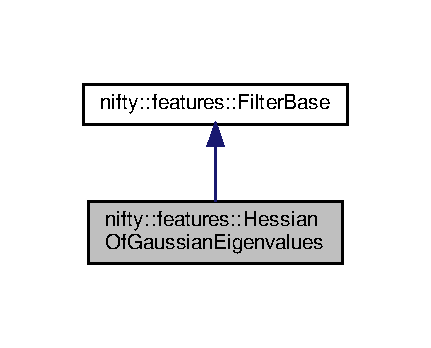
\includegraphics[width=207pt]{structnifty_1_1features_1_1HessianOfGaussianEigenvalues__inherit__graph}
\end{center}
\end{figure}


Collaboration diagram for nifty\+:\+:features\+:\+:Hessian\+Of\+Gaussian\+Eigenvalues\+:
\nopagebreak
\begin{figure}[H]
\begin{center}
\leavevmode
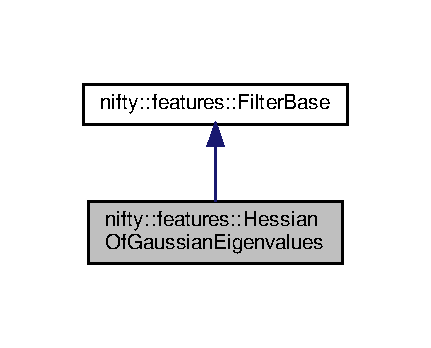
\includegraphics[width=207pt]{structnifty_1_1features_1_1HessianOfGaussianEigenvalues__coll__graph}
\end{center}
\end{figure}
\subsection*{Public Member Functions}
\begin{DoxyCompactItemize}
\item 
void \hyperlink{structnifty_1_1features_1_1HessianOfGaussianEigenvalues_a6195cb81a2b8a6570cb623e591c68781}{operator()} (const fastfilters\+\_\+array2d\+\_\+t \&ff, \hyperlink{classandres_1_1View}{marray\+::\+View}$<$ float $>$ \&out, const double sigma) const
\item 
void \hyperlink{structnifty_1_1features_1_1HessianOfGaussianEigenvalues_a7c21f5d043af68d6f330c5b9bdf95310}{operator()} (const fastfilters\+\_\+array3d\+\_\+t \&ff, \hyperlink{classandres_1_1View}{marray\+::\+View}$<$ float $>$ \&out, const double sigma) const
\item 
bool \hyperlink{structnifty_1_1features_1_1HessianOfGaussianEigenvalues_ab69872f7fb1e71080e1dc351610777ba}{is\+Multi\+Channel} () const
\end{DoxyCompactItemize}
\subsection*{Additional Inherited Members}


\subsection{Member Function Documentation}
\mbox{\Hypertarget{structnifty_1_1features_1_1HessianOfGaussianEigenvalues_ab69872f7fb1e71080e1dc351610777ba}\label{structnifty_1_1features_1_1HessianOfGaussianEigenvalues_ab69872f7fb1e71080e1dc351610777ba}} 
\index{nifty\+::features\+::\+Hessian\+Of\+Gaussian\+Eigenvalues@{nifty\+::features\+::\+Hessian\+Of\+Gaussian\+Eigenvalues}!is\+Multi\+Channel@{is\+Multi\+Channel}}
\index{is\+Multi\+Channel@{is\+Multi\+Channel}!nifty\+::features\+::\+Hessian\+Of\+Gaussian\+Eigenvalues@{nifty\+::features\+::\+Hessian\+Of\+Gaussian\+Eigenvalues}}
\subsubsection{\texorpdfstring{is\+Multi\+Channel()}{isMultiChannel()}}
{\footnotesize\ttfamily bool nifty\+::features\+::\+Hessian\+Of\+Gaussian\+Eigenvalues\+::is\+Multi\+Channel (\begin{DoxyParamCaption}{ }\end{DoxyParamCaption}) const\hspace{0.3cm}{\ttfamily [inline]}, {\ttfamily [virtual]}}



Implements \hyperlink{structnifty_1_1features_1_1FilterBase_a1c278e2b6ef0cb2a5bba2f758c6855e2}{nifty\+::features\+::\+Filter\+Base}.

\mbox{\Hypertarget{structnifty_1_1features_1_1HessianOfGaussianEigenvalues_a6195cb81a2b8a6570cb623e591c68781}\label{structnifty_1_1features_1_1HessianOfGaussianEigenvalues_a6195cb81a2b8a6570cb623e591c68781}} 
\index{nifty\+::features\+::\+Hessian\+Of\+Gaussian\+Eigenvalues@{nifty\+::features\+::\+Hessian\+Of\+Gaussian\+Eigenvalues}!operator()@{operator()}}
\index{operator()@{operator()}!nifty\+::features\+::\+Hessian\+Of\+Gaussian\+Eigenvalues@{nifty\+::features\+::\+Hessian\+Of\+Gaussian\+Eigenvalues}}
\subsubsection{\texorpdfstring{operator()()}{operator()()}\hspace{0.1cm}{\footnotesize\ttfamily [1/2]}}
{\footnotesize\ttfamily void nifty\+::features\+::\+Hessian\+Of\+Gaussian\+Eigenvalues\+::operator() (\begin{DoxyParamCaption}\item[{const fastfilters\+\_\+array2d\+\_\+t \&}]{ff,  }\item[{\hyperlink{classandres_1_1View}{marray\+::\+View}$<$ float $>$ \&}]{out,  }\item[{const double}]{sigma }\end{DoxyParamCaption}) const\hspace{0.3cm}{\ttfamily [inline]}, {\ttfamily [virtual]}}



Implements \hyperlink{structnifty_1_1features_1_1FilterBase_a17c77d36dd765c5ec0b163102428656c}{nifty\+::features\+::\+Filter\+Base}.

\mbox{\Hypertarget{structnifty_1_1features_1_1HessianOfGaussianEigenvalues_a7c21f5d043af68d6f330c5b9bdf95310}\label{structnifty_1_1features_1_1HessianOfGaussianEigenvalues_a7c21f5d043af68d6f330c5b9bdf95310}} 
\index{nifty\+::features\+::\+Hessian\+Of\+Gaussian\+Eigenvalues@{nifty\+::features\+::\+Hessian\+Of\+Gaussian\+Eigenvalues}!operator()@{operator()}}
\index{operator()@{operator()}!nifty\+::features\+::\+Hessian\+Of\+Gaussian\+Eigenvalues@{nifty\+::features\+::\+Hessian\+Of\+Gaussian\+Eigenvalues}}
\subsubsection{\texorpdfstring{operator()()}{operator()()}\hspace{0.1cm}{\footnotesize\ttfamily [2/2]}}
{\footnotesize\ttfamily void nifty\+::features\+::\+Hessian\+Of\+Gaussian\+Eigenvalues\+::operator() (\begin{DoxyParamCaption}\item[{const fastfilters\+\_\+array3d\+\_\+t \&}]{ff,  }\item[{\hyperlink{classandres_1_1View}{marray\+::\+View}$<$ float $>$ \&}]{out,  }\item[{const double}]{sigma }\end{DoxyParamCaption}) const\hspace{0.3cm}{\ttfamily [inline]}, {\ttfamily [virtual]}}



Implements \hyperlink{structnifty_1_1features_1_1FilterBase_abbef4e9c260026926e0021aa0cc11c81}{nifty\+::features\+::\+Filter\+Base}.



The documentation for this struct was generated from the following file\+:\begin{DoxyCompactItemize}
\item 
/home/tbeier/src/nifty/include/nifty/features/\hyperlink{fastfilters__wrapper_8hxx}{fastfilters\+\_\+wrapper.\+hxx}\end{DoxyCompactItemize}

\hypertarget{classnifty_1_1histogram_1_1Histogram}{}\section{nifty\+:\+:histogram\+:\+:Histogram$<$ T, B\+I\+N\+C\+O\+U\+NT $>$ Class Template Reference}
\label{classnifty_1_1histogram_1_1Histogram}\index{nifty\+::histogram\+::\+Histogram$<$ T, B\+I\+N\+C\+O\+U\+N\+T $>$@{nifty\+::histogram\+::\+Histogram$<$ T, B\+I\+N\+C\+O\+U\+N\+T $>$}}


{\ttfamily \#include $<$histogram.\+hxx$>$}

\subsection*{Public Types}
\begin{DoxyCompactItemize}
\item 
typedef B\+I\+N\+C\+O\+U\+NT \hyperlink{classnifty_1_1histogram_1_1Histogram_a19ad5e06bce1f70819a7ac9cdb708cf3}{Bincount\+Type}
\end{DoxyCompactItemize}
\subsection*{Public Member Functions}
\begin{DoxyCompactItemize}
\item 
\hyperlink{classnifty_1_1histogram_1_1Histogram_ad7b503ee095f0bbe52f473f7bd8b6d63}{Histogram} (const T min\+Val=0, const T max\+Val=1, const size\+\_\+t bincount=40)
\item 
void \hyperlink{classnifty_1_1histogram_1_1Histogram_a5ced1f86011745189e73d686f65aad0a}{assign} (const T min\+Val=0, const T max\+Val=1, const size\+\_\+t bincount=40)
\item 
{\footnotesize template$<$class I\+T\+ER $>$ }\\void \hyperlink{classnifty_1_1histogram_1_1Histogram_a6dc9984784d563f8201c95a2c95bbc45}{clear\+Set\+Min\+Max\+And\+Fill\+From} (I\+T\+ER begin, I\+T\+ER end)
\item 
void \hyperlink{classnifty_1_1histogram_1_1Histogram_ac4790791017587f3ec614c00abd6c68f}{set\+Min\+Max} (const T min\+Val, const T max\+Val)
\item 
const \hyperlink{classnifty_1_1histogram_1_1Histogram_a19ad5e06bce1f70819a7ac9cdb708cf3}{Bincount\+Type} \& \hyperlink{classnifty_1_1histogram_1_1Histogram_a262b175b7093919f1ca5817679237091}{operator\mbox{[}$\,$\mbox{]}} (const size\+\_\+t i) const
\item 
size\+\_\+t \hyperlink{classnifty_1_1histogram_1_1Histogram_a81f5001934bce97d1b852bda5d4daf99}{number\+Of\+Bins} () const
\item 
\hyperlink{classnifty_1_1histogram_1_1Histogram_a19ad5e06bce1f70819a7ac9cdb708cf3}{Bincount\+Type} \hyperlink{classnifty_1_1histogram_1_1Histogram_a22a3d01d66aff92a661228846f9f726e}{sum} () const
\item 
void \hyperlink{classnifty_1_1histogram_1_1Histogram_a4b344ea118713a965a4a3e6f3936cb20}{insert} (const T \&value, const double w=1.\+0)
\item 
void \hyperlink{classnifty_1_1histogram_1_1Histogram_ac4ff991c8e2418d66643052ff69e4afa}{normalize} (const \hyperlink{classnifty_1_1histogram_1_1Histogram_a19ad5e06bce1f70819a7ac9cdb708cf3}{Bincount\+Type} \&target\+Sum)
\item 
void \hyperlink{classnifty_1_1histogram_1_1Histogram_a6b8a4dfdc710c8c56b3afebe3990dd33}{clear} ()
\item 
void \hyperlink{classnifty_1_1histogram_1_1Histogram_ac6771f36d3c23a030650e55ff5bda1bf}{clear\+Counts} ()
\item 
double \hyperlink{classnifty_1_1histogram_1_1Histogram_af888c1e37c7beb39c2512ffd3887a515}{bin\+To\+Value} (const double fbin) const
\item 
float \hyperlink{classnifty_1_1histogram_1_1Histogram_afe04b4100d8c023a1e77343eb0d302e9}{bin\+Width} () const
\item 
void \hyperlink{classnifty_1_1histogram_1_1Histogram_a6bf410b81f98ac6bdc2e07be83153a8d}{merge} (const \hyperlink{classnifty_1_1histogram_1_1Histogram}{Histogram} \&other)
\item 
double \hyperlink{classnifty_1_1histogram_1_1Histogram_a65a3d7833caebf1dc0d93b497fc35b9b}{rank} (const double q) const
\end{DoxyCompactItemize}


\subsection{Member Typedef Documentation}
\mbox{\Hypertarget{classnifty_1_1histogram_1_1Histogram_a19ad5e06bce1f70819a7ac9cdb708cf3}\label{classnifty_1_1histogram_1_1Histogram_a19ad5e06bce1f70819a7ac9cdb708cf3}} 
\index{nifty\+::histogram\+::\+Histogram@{nifty\+::histogram\+::\+Histogram}!Bincount\+Type@{Bincount\+Type}}
\index{Bincount\+Type@{Bincount\+Type}!nifty\+::histogram\+::\+Histogram@{nifty\+::histogram\+::\+Histogram}}
\subsubsection{\texorpdfstring{Bincount\+Type}{BincountType}}
{\footnotesize\ttfamily template$<$class T , class B\+I\+N\+C\+O\+U\+NT  = float$>$ \\
typedef B\+I\+N\+C\+O\+U\+NT \hyperlink{classnifty_1_1histogram_1_1Histogram}{nifty\+::histogram\+::\+Histogram}$<$ T, B\+I\+N\+C\+O\+U\+NT $>$\+::\hyperlink{classnifty_1_1histogram_1_1Histogram_a19ad5e06bce1f70819a7ac9cdb708cf3}{Bincount\+Type}}



\subsection{Constructor \& Destructor Documentation}
\mbox{\Hypertarget{classnifty_1_1histogram_1_1Histogram_ad7b503ee095f0bbe52f473f7bd8b6d63}\label{classnifty_1_1histogram_1_1Histogram_ad7b503ee095f0bbe52f473f7bd8b6d63}} 
\index{nifty\+::histogram\+::\+Histogram@{nifty\+::histogram\+::\+Histogram}!Histogram@{Histogram}}
\index{Histogram@{Histogram}!nifty\+::histogram\+::\+Histogram@{nifty\+::histogram\+::\+Histogram}}
\subsubsection{\texorpdfstring{Histogram()}{Histogram()}}
{\footnotesize\ttfamily template$<$class T , class B\+I\+N\+C\+O\+U\+NT  = float$>$ \\
\hyperlink{classnifty_1_1histogram_1_1Histogram}{nifty\+::histogram\+::\+Histogram}$<$ T, B\+I\+N\+C\+O\+U\+NT $>$\+::\hyperlink{classnifty_1_1histogram_1_1Histogram}{Histogram} (\begin{DoxyParamCaption}\item[{const T}]{min\+Val = {\ttfamily 0},  }\item[{const T}]{max\+Val = {\ttfamily 1},  }\item[{const size\+\_\+t}]{bincount = {\ttfamily 40} }\end{DoxyParamCaption})\hspace{0.3cm}{\ttfamily [inline]}}



\subsection{Member Function Documentation}
\mbox{\Hypertarget{classnifty_1_1histogram_1_1Histogram_a5ced1f86011745189e73d686f65aad0a}\label{classnifty_1_1histogram_1_1Histogram_a5ced1f86011745189e73d686f65aad0a}} 
\index{nifty\+::histogram\+::\+Histogram@{nifty\+::histogram\+::\+Histogram}!assign@{assign}}
\index{assign@{assign}!nifty\+::histogram\+::\+Histogram@{nifty\+::histogram\+::\+Histogram}}
\subsubsection{\texorpdfstring{assign()}{assign()}}
{\footnotesize\ttfamily template$<$class T , class B\+I\+N\+C\+O\+U\+NT  = float$>$ \\
void \hyperlink{classnifty_1_1histogram_1_1Histogram}{nifty\+::histogram\+::\+Histogram}$<$ T, B\+I\+N\+C\+O\+U\+NT $>$\+::assign (\begin{DoxyParamCaption}\item[{const T}]{min\+Val = {\ttfamily 0},  }\item[{const T}]{max\+Val = {\ttfamily 1},  }\item[{const size\+\_\+t}]{bincount = {\ttfamily 40} }\end{DoxyParamCaption})\hspace{0.3cm}{\ttfamily [inline]}}

\mbox{\Hypertarget{classnifty_1_1histogram_1_1Histogram_af888c1e37c7beb39c2512ffd3887a515}\label{classnifty_1_1histogram_1_1Histogram_af888c1e37c7beb39c2512ffd3887a515}} 
\index{nifty\+::histogram\+::\+Histogram@{nifty\+::histogram\+::\+Histogram}!bin\+To\+Value@{bin\+To\+Value}}
\index{bin\+To\+Value@{bin\+To\+Value}!nifty\+::histogram\+::\+Histogram@{nifty\+::histogram\+::\+Histogram}}
\subsubsection{\texorpdfstring{bin\+To\+Value()}{binToValue()}}
{\footnotesize\ttfamily template$<$class T , class B\+I\+N\+C\+O\+U\+NT  = float$>$ \\
double \hyperlink{classnifty_1_1histogram_1_1Histogram}{nifty\+::histogram\+::\+Histogram}$<$ T, B\+I\+N\+C\+O\+U\+NT $>$\+::bin\+To\+Value (\begin{DoxyParamCaption}\item[{const double}]{fbin }\end{DoxyParamCaption}) const\hspace{0.3cm}{\ttfamily [inline]}}

\mbox{\Hypertarget{classnifty_1_1histogram_1_1Histogram_afe04b4100d8c023a1e77343eb0d302e9}\label{classnifty_1_1histogram_1_1Histogram_afe04b4100d8c023a1e77343eb0d302e9}} 
\index{nifty\+::histogram\+::\+Histogram@{nifty\+::histogram\+::\+Histogram}!bin\+Width@{bin\+Width}}
\index{bin\+Width@{bin\+Width}!nifty\+::histogram\+::\+Histogram@{nifty\+::histogram\+::\+Histogram}}
\subsubsection{\texorpdfstring{bin\+Width()}{binWidth()}}
{\footnotesize\ttfamily template$<$class T , class B\+I\+N\+C\+O\+U\+NT  = float$>$ \\
float \hyperlink{classnifty_1_1histogram_1_1Histogram}{nifty\+::histogram\+::\+Histogram}$<$ T, B\+I\+N\+C\+O\+U\+NT $>$\+::bin\+Width (\begin{DoxyParamCaption}{ }\end{DoxyParamCaption}) const\hspace{0.3cm}{\ttfamily [inline]}}

\mbox{\Hypertarget{classnifty_1_1histogram_1_1Histogram_a6b8a4dfdc710c8c56b3afebe3990dd33}\label{classnifty_1_1histogram_1_1Histogram_a6b8a4dfdc710c8c56b3afebe3990dd33}} 
\index{nifty\+::histogram\+::\+Histogram@{nifty\+::histogram\+::\+Histogram}!clear@{clear}}
\index{clear@{clear}!nifty\+::histogram\+::\+Histogram@{nifty\+::histogram\+::\+Histogram}}
\subsubsection{\texorpdfstring{clear()}{clear()}}
{\footnotesize\ttfamily template$<$class T , class B\+I\+N\+C\+O\+U\+NT  = float$>$ \\
void \hyperlink{classnifty_1_1histogram_1_1Histogram}{nifty\+::histogram\+::\+Histogram}$<$ T, B\+I\+N\+C\+O\+U\+NT $>$\+::clear (\begin{DoxyParamCaption}{ }\end{DoxyParamCaption})\hspace{0.3cm}{\ttfamily [inline]}}

\mbox{\Hypertarget{classnifty_1_1histogram_1_1Histogram_ac6771f36d3c23a030650e55ff5bda1bf}\label{classnifty_1_1histogram_1_1Histogram_ac6771f36d3c23a030650e55ff5bda1bf}} 
\index{nifty\+::histogram\+::\+Histogram@{nifty\+::histogram\+::\+Histogram}!clear\+Counts@{clear\+Counts}}
\index{clear\+Counts@{clear\+Counts}!nifty\+::histogram\+::\+Histogram@{nifty\+::histogram\+::\+Histogram}}
\subsubsection{\texorpdfstring{clear\+Counts()}{clearCounts()}}
{\footnotesize\ttfamily template$<$class T , class B\+I\+N\+C\+O\+U\+NT  = float$>$ \\
void \hyperlink{classnifty_1_1histogram_1_1Histogram}{nifty\+::histogram\+::\+Histogram}$<$ T, B\+I\+N\+C\+O\+U\+NT $>$\+::clear\+Counts (\begin{DoxyParamCaption}{ }\end{DoxyParamCaption})\hspace{0.3cm}{\ttfamily [inline]}}

\mbox{\Hypertarget{classnifty_1_1histogram_1_1Histogram_a6dc9984784d563f8201c95a2c95bbc45}\label{classnifty_1_1histogram_1_1Histogram_a6dc9984784d563f8201c95a2c95bbc45}} 
\index{nifty\+::histogram\+::\+Histogram@{nifty\+::histogram\+::\+Histogram}!clear\+Set\+Min\+Max\+And\+Fill\+From@{clear\+Set\+Min\+Max\+And\+Fill\+From}}
\index{clear\+Set\+Min\+Max\+And\+Fill\+From@{clear\+Set\+Min\+Max\+And\+Fill\+From}!nifty\+::histogram\+::\+Histogram@{nifty\+::histogram\+::\+Histogram}}
\subsubsection{\texorpdfstring{clear\+Set\+Min\+Max\+And\+Fill\+From()}{clearSetMinMaxAndFillFrom()}}
{\footnotesize\ttfamily template$<$class T , class B\+I\+N\+C\+O\+U\+NT  = float$>$ \\
template$<$class I\+T\+ER $>$ \\
void \hyperlink{classnifty_1_1histogram_1_1Histogram}{nifty\+::histogram\+::\+Histogram}$<$ T, B\+I\+N\+C\+O\+U\+NT $>$\+::clear\+Set\+Min\+Max\+And\+Fill\+From (\begin{DoxyParamCaption}\item[{I\+T\+ER}]{begin,  }\item[{I\+T\+ER}]{end }\end{DoxyParamCaption})\hspace{0.3cm}{\ttfamily [inline]}}

\mbox{\Hypertarget{classnifty_1_1histogram_1_1Histogram_a4b344ea118713a965a4a3e6f3936cb20}\label{classnifty_1_1histogram_1_1Histogram_a4b344ea118713a965a4a3e6f3936cb20}} 
\index{nifty\+::histogram\+::\+Histogram@{nifty\+::histogram\+::\+Histogram}!insert@{insert}}
\index{insert@{insert}!nifty\+::histogram\+::\+Histogram@{nifty\+::histogram\+::\+Histogram}}
\subsubsection{\texorpdfstring{insert()}{insert()}}
{\footnotesize\ttfamily template$<$class T , class B\+I\+N\+C\+O\+U\+NT  = float$>$ \\
void \hyperlink{classnifty_1_1histogram_1_1Histogram}{nifty\+::histogram\+::\+Histogram}$<$ T, B\+I\+N\+C\+O\+U\+NT $>$\+::insert (\begin{DoxyParamCaption}\item[{const T \&}]{value,  }\item[{const double}]{w = {\ttfamily 1.0} }\end{DoxyParamCaption})\hspace{0.3cm}{\ttfamily [inline]}}

\mbox{\Hypertarget{classnifty_1_1histogram_1_1Histogram_a6bf410b81f98ac6bdc2e07be83153a8d}\label{classnifty_1_1histogram_1_1Histogram_a6bf410b81f98ac6bdc2e07be83153a8d}} 
\index{nifty\+::histogram\+::\+Histogram@{nifty\+::histogram\+::\+Histogram}!merge@{merge}}
\index{merge@{merge}!nifty\+::histogram\+::\+Histogram@{nifty\+::histogram\+::\+Histogram}}
\subsubsection{\texorpdfstring{merge()}{merge()}}
{\footnotesize\ttfamily template$<$class T , class B\+I\+N\+C\+O\+U\+NT  = float$>$ \\
void \hyperlink{classnifty_1_1histogram_1_1Histogram}{nifty\+::histogram\+::\+Histogram}$<$ T, B\+I\+N\+C\+O\+U\+NT $>$\+::merge (\begin{DoxyParamCaption}\item[{const \hyperlink{classnifty_1_1histogram_1_1Histogram}{Histogram}$<$ T, B\+I\+N\+C\+O\+U\+NT $>$ \&}]{other }\end{DoxyParamCaption})\hspace{0.3cm}{\ttfamily [inline]}}

\mbox{\Hypertarget{classnifty_1_1histogram_1_1Histogram_ac4ff991c8e2418d66643052ff69e4afa}\label{classnifty_1_1histogram_1_1Histogram_ac4ff991c8e2418d66643052ff69e4afa}} 
\index{nifty\+::histogram\+::\+Histogram@{nifty\+::histogram\+::\+Histogram}!normalize@{normalize}}
\index{normalize@{normalize}!nifty\+::histogram\+::\+Histogram@{nifty\+::histogram\+::\+Histogram}}
\subsubsection{\texorpdfstring{normalize()}{normalize()}}
{\footnotesize\ttfamily template$<$class T , class B\+I\+N\+C\+O\+U\+NT  = float$>$ \\
void \hyperlink{classnifty_1_1histogram_1_1Histogram}{nifty\+::histogram\+::\+Histogram}$<$ T, B\+I\+N\+C\+O\+U\+NT $>$\+::normalize (\begin{DoxyParamCaption}\item[{const \hyperlink{classnifty_1_1histogram_1_1Histogram_a19ad5e06bce1f70819a7ac9cdb708cf3}{Bincount\+Type} \&}]{target\+Sum }\end{DoxyParamCaption})\hspace{0.3cm}{\ttfamily [inline]}}

\mbox{\Hypertarget{classnifty_1_1histogram_1_1Histogram_a81f5001934bce97d1b852bda5d4daf99}\label{classnifty_1_1histogram_1_1Histogram_a81f5001934bce97d1b852bda5d4daf99}} 
\index{nifty\+::histogram\+::\+Histogram@{nifty\+::histogram\+::\+Histogram}!number\+Of\+Bins@{number\+Of\+Bins}}
\index{number\+Of\+Bins@{number\+Of\+Bins}!nifty\+::histogram\+::\+Histogram@{nifty\+::histogram\+::\+Histogram}}
\subsubsection{\texorpdfstring{number\+Of\+Bins()}{numberOfBins()}}
{\footnotesize\ttfamily template$<$class T , class B\+I\+N\+C\+O\+U\+NT  = float$>$ \\
size\+\_\+t \hyperlink{classnifty_1_1histogram_1_1Histogram}{nifty\+::histogram\+::\+Histogram}$<$ T, B\+I\+N\+C\+O\+U\+NT $>$\+::number\+Of\+Bins (\begin{DoxyParamCaption}{ }\end{DoxyParamCaption}) const\hspace{0.3cm}{\ttfamily [inline]}}

\mbox{\Hypertarget{classnifty_1_1histogram_1_1Histogram_a262b175b7093919f1ca5817679237091}\label{classnifty_1_1histogram_1_1Histogram_a262b175b7093919f1ca5817679237091}} 
\index{nifty\+::histogram\+::\+Histogram@{nifty\+::histogram\+::\+Histogram}!operator\mbox{[}\mbox{]}@{operator[]}}
\index{operator\mbox{[}\mbox{]}@{operator[]}!nifty\+::histogram\+::\+Histogram@{nifty\+::histogram\+::\+Histogram}}
\subsubsection{\texorpdfstring{operator[]()}{operator[]()}}
{\footnotesize\ttfamily template$<$class T , class B\+I\+N\+C\+O\+U\+NT  = float$>$ \\
const \hyperlink{classnifty_1_1histogram_1_1Histogram_a19ad5e06bce1f70819a7ac9cdb708cf3}{Bincount\+Type}\& \hyperlink{classnifty_1_1histogram_1_1Histogram}{nifty\+::histogram\+::\+Histogram}$<$ T, B\+I\+N\+C\+O\+U\+NT $>$\+::operator\mbox{[}$\,$\mbox{]} (\begin{DoxyParamCaption}\item[{const size\+\_\+t}]{i }\end{DoxyParamCaption}) const\hspace{0.3cm}{\ttfamily [inline]}}

\mbox{\Hypertarget{classnifty_1_1histogram_1_1Histogram_a65a3d7833caebf1dc0d93b497fc35b9b}\label{classnifty_1_1histogram_1_1Histogram_a65a3d7833caebf1dc0d93b497fc35b9b}} 
\index{nifty\+::histogram\+::\+Histogram@{nifty\+::histogram\+::\+Histogram}!rank@{rank}}
\index{rank@{rank}!nifty\+::histogram\+::\+Histogram@{nifty\+::histogram\+::\+Histogram}}
\subsubsection{\texorpdfstring{rank()}{rank()}}
{\footnotesize\ttfamily template$<$class T , class B\+I\+N\+C\+O\+U\+NT  = float$>$ \\
double \hyperlink{classnifty_1_1histogram_1_1Histogram}{nifty\+::histogram\+::\+Histogram}$<$ T, B\+I\+N\+C\+O\+U\+NT $>$\+::rank (\begin{DoxyParamCaption}\item[{const double}]{q }\end{DoxyParamCaption}) const\hspace{0.3cm}{\ttfamily [inline]}}

\mbox{\Hypertarget{classnifty_1_1histogram_1_1Histogram_ac4790791017587f3ec614c00abd6c68f}\label{classnifty_1_1histogram_1_1Histogram_ac4790791017587f3ec614c00abd6c68f}} 
\index{nifty\+::histogram\+::\+Histogram@{nifty\+::histogram\+::\+Histogram}!set\+Min\+Max@{set\+Min\+Max}}
\index{set\+Min\+Max@{set\+Min\+Max}!nifty\+::histogram\+::\+Histogram@{nifty\+::histogram\+::\+Histogram}}
\subsubsection{\texorpdfstring{set\+Min\+Max()}{setMinMax()}}
{\footnotesize\ttfamily template$<$class T , class B\+I\+N\+C\+O\+U\+NT  = float$>$ \\
void \hyperlink{classnifty_1_1histogram_1_1Histogram}{nifty\+::histogram\+::\+Histogram}$<$ T, B\+I\+N\+C\+O\+U\+NT $>$\+::set\+Min\+Max (\begin{DoxyParamCaption}\item[{const T}]{min\+Val,  }\item[{const T}]{max\+Val }\end{DoxyParamCaption})\hspace{0.3cm}{\ttfamily [inline]}}

\mbox{\Hypertarget{classnifty_1_1histogram_1_1Histogram_a22a3d01d66aff92a661228846f9f726e}\label{classnifty_1_1histogram_1_1Histogram_a22a3d01d66aff92a661228846f9f726e}} 
\index{nifty\+::histogram\+::\+Histogram@{nifty\+::histogram\+::\+Histogram}!sum@{sum}}
\index{sum@{sum}!nifty\+::histogram\+::\+Histogram@{nifty\+::histogram\+::\+Histogram}}
\subsubsection{\texorpdfstring{sum()}{sum()}}
{\footnotesize\ttfamily template$<$class T , class B\+I\+N\+C\+O\+U\+NT  = float$>$ \\
\hyperlink{classnifty_1_1histogram_1_1Histogram_a19ad5e06bce1f70819a7ac9cdb708cf3}{Bincount\+Type} \hyperlink{classnifty_1_1histogram_1_1Histogram}{nifty\+::histogram\+::\+Histogram}$<$ T, B\+I\+N\+C\+O\+U\+NT $>$\+::sum (\begin{DoxyParamCaption}{ }\end{DoxyParamCaption}) const\hspace{0.3cm}{\ttfamily [inline]}}



The documentation for this class was generated from the following file\+:\begin{DoxyCompactItemize}
\item 
/home/tbeier/src/nifty/include/nifty/histogram/\hyperlink{histogram_8hxx}{histogram.\+hxx}\end{DoxyCompactItemize}

\hypertarget{structnifty_1_1ilp__backend_1_1IlpBackendSettings}{}\section{nifty\+:\+:ilp\+\_\+backend\+:\+:Ilp\+Backend\+Settings Struct Reference}
\label{structnifty_1_1ilp__backend_1_1IlpBackendSettings}\index{nifty\+::ilp\+\_\+backend\+::\+Ilp\+Backend\+Settings@{nifty\+::ilp\+\_\+backend\+::\+Ilp\+Backend\+Settings}}


{\ttfamily \#include $<$ilp\+\_\+backend.\+hxx$>$}

\subsection*{Public Types}
\begin{DoxyCompactItemize}
\item 
enum \hyperlink{structnifty_1_1ilp__backend_1_1IlpBackendSettings_ad16c71cc049dcb37c07f2abdda69dab4}{Pre\+Solver} \{ \\*
\hyperlink{structnifty_1_1ilp__backend_1_1IlpBackendSettings_ad16c71cc049dcb37c07f2abdda69dab4a2d2186dcdaa22ae42023acbc03922c48}{P\+R\+E\+\_\+\+S\+O\+L\+V\+E\+R\+\_\+\+A\+U\+T\+O}, 
\hyperlink{structnifty_1_1ilp__backend_1_1IlpBackendSettings_ad16c71cc049dcb37c07f2abdda69dab4a0b937d225c3ee4733bff63397c614b78}{P\+R\+E\+\_\+\+S\+O\+L\+V\+E\+R\+\_\+\+P\+R\+I\+M\+A\+L}, 
\hyperlink{structnifty_1_1ilp__backend_1_1IlpBackendSettings_ad16c71cc049dcb37c07f2abdda69dab4a53cbe16a2893471008b7f3c00c5c040f}{P\+R\+E\+\_\+\+S\+O\+L\+V\+E\+R\+\_\+\+D\+U\+A\+L}, 
\hyperlink{structnifty_1_1ilp__backend_1_1IlpBackendSettings_ad16c71cc049dcb37c07f2abdda69dab4ad0065467805a6fba8d8d9e7293e4bfc2}{P\+R\+E\+\_\+\+S\+O\+L\+V\+E\+R\+\_\+\+N\+O\+N\+E}, 
\\*
\hyperlink{structnifty_1_1ilp__backend_1_1IlpBackendSettings_ad16c71cc049dcb37c07f2abdda69dab4a45adcc6c0d30422e0c0a674b2fe92a37}{P\+R\+E\+\_\+\+S\+O\+L\+V\+E\+R\+\_\+\+D\+E\+F\+A\+U\+L\+T}
 \}
\item 
enum \hyperlink{structnifty_1_1ilp__backend_1_1IlpBackendSettings_a4b3fd0d313a8d95f9f6a3ba64802e204}{L\+P\+Solver} \{ \\*
\hyperlink{structnifty_1_1ilp__backend_1_1IlpBackendSettings_a4b3fd0d313a8d95f9f6a3ba64802e204a02afc6e85659e3fda7c48df74d3e3934}{L\+P\+\_\+\+S\+O\+L\+V\+E\+R\+\_\+\+P\+R\+I\+M\+A\+L\+\_\+\+S\+I\+M\+P\+L\+E\+X}, 
\hyperlink{structnifty_1_1ilp__backend_1_1IlpBackendSettings_a4b3fd0d313a8d95f9f6a3ba64802e204aadd4ba29f78f9104467f136c05d6e354}{L\+P\+\_\+\+S\+O\+L\+V\+E\+R\+\_\+\+D\+U\+A\+L\+\_\+\+S\+I\+M\+P\+L\+E\+X}, 
\hyperlink{structnifty_1_1ilp__backend_1_1IlpBackendSettings_a4b3fd0d313a8d95f9f6a3ba64802e204afbfc81377d73d1c59b31be26a8bf8fb2}{L\+P\+\_\+\+S\+O\+L\+V\+E\+R\+\_\+\+B\+A\+R\+R\+I\+E\+R}, 
\hyperlink{structnifty_1_1ilp__backend_1_1IlpBackendSettings_a4b3fd0d313a8d95f9f6a3ba64802e204ac6de1eff7352159f0db89583e569f86e}{L\+P\+\_\+\+S\+O\+L\+V\+E\+R\+\_\+\+S\+I\+F\+T\+I\+N\+G}, 
\\*
\hyperlink{structnifty_1_1ilp__backend_1_1IlpBackendSettings_a4b3fd0d313a8d95f9f6a3ba64802e204a24fa810f69bf55c40d68082a2e3653f8}{L\+P\+\_\+\+S\+O\+L\+V\+E\+R\+\_\+\+D\+E\+F\+A\+U\+L\+T}
 \}
\end{DoxyCompactItemize}
\subsection*{Public Attributes}
\begin{DoxyCompactItemize}
\item 
double \hyperlink{structnifty_1_1ilp__backend_1_1IlpBackendSettings_a5f20f85b5528859b4ef8000a29fb1453}{mem\+Limit} = \{-\/1.\+0\}
\item 
double \hyperlink{structnifty_1_1ilp__backend_1_1IlpBackendSettings_a8eed72b9ddbbc94a89197dde0d76d144}{relative\+Gap} \{0.\+0\}
\item 
double \hyperlink{structnifty_1_1ilp__backend_1_1IlpBackendSettings_a8bc98f418844336847d868dd88e620f2}{absolute\+Gap} \{0.\+0\}
\item 
double \hyperlink{structnifty_1_1ilp__backend_1_1IlpBackendSettings_a0bd7c55efdd7c642687b17e378da2e08}{cut\+Up} \{1.\+0e+75\}
\item 
int \hyperlink{structnifty_1_1ilp__backend_1_1IlpBackendSettings_a87cbc1618cd7cd2d88de2da14ff8c2d3}{pre\+Passes} \{-\/1\}
\item 
\hyperlink{structnifty_1_1ilp__backend_1_1IlpBackendSettings_ad16c71cc049dcb37c07f2abdda69dab4}{Pre\+Solver} \hyperlink{structnifty_1_1ilp__backend_1_1IlpBackendSettings_af1e71695a4bd0dd0921ba2db7c0208c6}{pre\+Solver} \{\hyperlink{structnifty_1_1ilp__backend_1_1IlpBackendSettings_ad16c71cc049dcb37c07f2abdda69dab4a45adcc6c0d30422e0c0a674b2fe92a37}{P\+R\+E\+\_\+\+S\+O\+L\+V\+E\+R\+\_\+\+D\+E\+F\+A\+U\+L\+T}\}
\item 
\hyperlink{structnifty_1_1ilp__backend_1_1IlpBackendSettings_a4b3fd0d313a8d95f9f6a3ba64802e204}{L\+P\+Solver} \hyperlink{structnifty_1_1ilp__backend_1_1IlpBackendSettings_aa0940a3d1d8399b9ed10f7e43d61e8cc}{lp\+Solver} \{\hyperlink{structnifty_1_1ilp__backend_1_1IlpBackendSettings_a4b3fd0d313a8d95f9f6a3ba64802e204a24fa810f69bf55c40d68082a2e3653f8}{L\+P\+\_\+\+S\+O\+L\+V\+E\+R\+\_\+\+D\+E\+F\+A\+U\+L\+T}\}
\item 
size\+\_\+t \hyperlink{structnifty_1_1ilp__backend_1_1IlpBackendSettings_ae9852b9ee86048c11366c7248ca8dbfd}{number\+Of\+Threads} \{1\}
\item 
size\+\_\+t \hyperlink{structnifty_1_1ilp__backend_1_1IlpBackendSettings_aecafa6adf4695088d0396f232bbe88ba}{verbosity} \{0\}
\end{DoxyCompactItemize}


\subsection{Member Enumeration Documentation}
\hypertarget{structnifty_1_1ilp__backend_1_1IlpBackendSettings_a4b3fd0d313a8d95f9f6a3ba64802e204}{}\index{nifty\+::ilp\+\_\+backend\+::\+Ilp\+Backend\+Settings@{nifty\+::ilp\+\_\+backend\+::\+Ilp\+Backend\+Settings}!L\+P\+Solver@{L\+P\+Solver}}
\index{L\+P\+Solver@{L\+P\+Solver}!nifty\+::ilp\+\_\+backend\+::\+Ilp\+Backend\+Settings@{nifty\+::ilp\+\_\+backend\+::\+Ilp\+Backend\+Settings}}
\subsubsection[{L\+P\+Solver}]{\setlength{\rightskip}{0pt plus 5cm}enum {\bf nifty\+::ilp\+\_\+backend\+::\+Ilp\+Backend\+Settings\+::\+L\+P\+Solver}}\label{structnifty_1_1ilp__backend_1_1IlpBackendSettings_a4b3fd0d313a8d95f9f6a3ba64802e204}
\begin{Desc}
\item[Enumerator]\par
\begin{description}
\index{L\+P\+\_\+\+S\+O\+L\+V\+E\+R\+\_\+\+P\+R\+I\+M\+A\+L\+\_\+\+S\+I\+M\+P\+L\+E\+X@{L\+P\+\_\+\+S\+O\+L\+V\+E\+R\+\_\+\+P\+R\+I\+M\+A\+L\+\_\+\+S\+I\+M\+P\+L\+E\+X}!nifty\+::ilp\+\_\+backend\+::\+Ilp\+Backend\+Settings@{nifty\+::ilp\+\_\+backend\+::\+Ilp\+Backend\+Settings}}\index{nifty\+::ilp\+\_\+backend\+::\+Ilp\+Backend\+Settings@{nifty\+::ilp\+\_\+backend\+::\+Ilp\+Backend\+Settings}!L\+P\+\_\+\+S\+O\+L\+V\+E\+R\+\_\+\+P\+R\+I\+M\+A\+L\+\_\+\+S\+I\+M\+P\+L\+E\+X@{L\+P\+\_\+\+S\+O\+L\+V\+E\+R\+\_\+\+P\+R\+I\+M\+A\+L\+\_\+\+S\+I\+M\+P\+L\+E\+X}}\item[{\em 
\hypertarget{structnifty_1_1ilp__backend_1_1IlpBackendSettings_a4b3fd0d313a8d95f9f6a3ba64802e204a02afc6e85659e3fda7c48df74d3e3934}{}L\+P\+\_\+\+S\+O\+L\+V\+E\+R\+\_\+\+P\+R\+I\+M\+A\+L\+\_\+\+S\+I\+M\+P\+L\+E\+X\label{structnifty_1_1ilp__backend_1_1IlpBackendSettings_a4b3fd0d313a8d95f9f6a3ba64802e204a02afc6e85659e3fda7c48df74d3e3934}
}]\index{L\+P\+\_\+\+S\+O\+L\+V\+E\+R\+\_\+\+D\+U\+A\+L\+\_\+\+S\+I\+M\+P\+L\+E\+X@{L\+P\+\_\+\+S\+O\+L\+V\+E\+R\+\_\+\+D\+U\+A\+L\+\_\+\+S\+I\+M\+P\+L\+E\+X}!nifty\+::ilp\+\_\+backend\+::\+Ilp\+Backend\+Settings@{nifty\+::ilp\+\_\+backend\+::\+Ilp\+Backend\+Settings}}\index{nifty\+::ilp\+\_\+backend\+::\+Ilp\+Backend\+Settings@{nifty\+::ilp\+\_\+backend\+::\+Ilp\+Backend\+Settings}!L\+P\+\_\+\+S\+O\+L\+V\+E\+R\+\_\+\+D\+U\+A\+L\+\_\+\+S\+I\+M\+P\+L\+E\+X@{L\+P\+\_\+\+S\+O\+L\+V\+E\+R\+\_\+\+D\+U\+A\+L\+\_\+\+S\+I\+M\+P\+L\+E\+X}}\item[{\em 
\hypertarget{structnifty_1_1ilp__backend_1_1IlpBackendSettings_a4b3fd0d313a8d95f9f6a3ba64802e204aadd4ba29f78f9104467f136c05d6e354}{}L\+P\+\_\+\+S\+O\+L\+V\+E\+R\+\_\+\+D\+U\+A\+L\+\_\+\+S\+I\+M\+P\+L\+E\+X\label{structnifty_1_1ilp__backend_1_1IlpBackendSettings_a4b3fd0d313a8d95f9f6a3ba64802e204aadd4ba29f78f9104467f136c05d6e354}
}]\index{L\+P\+\_\+\+S\+O\+L\+V\+E\+R\+\_\+\+B\+A\+R\+R\+I\+E\+R@{L\+P\+\_\+\+S\+O\+L\+V\+E\+R\+\_\+\+B\+A\+R\+R\+I\+E\+R}!nifty\+::ilp\+\_\+backend\+::\+Ilp\+Backend\+Settings@{nifty\+::ilp\+\_\+backend\+::\+Ilp\+Backend\+Settings}}\index{nifty\+::ilp\+\_\+backend\+::\+Ilp\+Backend\+Settings@{nifty\+::ilp\+\_\+backend\+::\+Ilp\+Backend\+Settings}!L\+P\+\_\+\+S\+O\+L\+V\+E\+R\+\_\+\+B\+A\+R\+R\+I\+E\+R@{L\+P\+\_\+\+S\+O\+L\+V\+E\+R\+\_\+\+B\+A\+R\+R\+I\+E\+R}}\item[{\em 
\hypertarget{structnifty_1_1ilp__backend_1_1IlpBackendSettings_a4b3fd0d313a8d95f9f6a3ba64802e204afbfc81377d73d1c59b31be26a8bf8fb2}{}L\+P\+\_\+\+S\+O\+L\+V\+E\+R\+\_\+\+B\+A\+R\+R\+I\+E\+R\label{structnifty_1_1ilp__backend_1_1IlpBackendSettings_a4b3fd0d313a8d95f9f6a3ba64802e204afbfc81377d73d1c59b31be26a8bf8fb2}
}]\index{L\+P\+\_\+\+S\+O\+L\+V\+E\+R\+\_\+\+S\+I\+F\+T\+I\+N\+G@{L\+P\+\_\+\+S\+O\+L\+V\+E\+R\+\_\+\+S\+I\+F\+T\+I\+N\+G}!nifty\+::ilp\+\_\+backend\+::\+Ilp\+Backend\+Settings@{nifty\+::ilp\+\_\+backend\+::\+Ilp\+Backend\+Settings}}\index{nifty\+::ilp\+\_\+backend\+::\+Ilp\+Backend\+Settings@{nifty\+::ilp\+\_\+backend\+::\+Ilp\+Backend\+Settings}!L\+P\+\_\+\+S\+O\+L\+V\+E\+R\+\_\+\+S\+I\+F\+T\+I\+N\+G@{L\+P\+\_\+\+S\+O\+L\+V\+E\+R\+\_\+\+S\+I\+F\+T\+I\+N\+G}}\item[{\em 
\hypertarget{structnifty_1_1ilp__backend_1_1IlpBackendSettings_a4b3fd0d313a8d95f9f6a3ba64802e204ac6de1eff7352159f0db89583e569f86e}{}L\+P\+\_\+\+S\+O\+L\+V\+E\+R\+\_\+\+S\+I\+F\+T\+I\+N\+G\label{structnifty_1_1ilp__backend_1_1IlpBackendSettings_a4b3fd0d313a8d95f9f6a3ba64802e204ac6de1eff7352159f0db89583e569f86e}
}]\index{L\+P\+\_\+\+S\+O\+L\+V\+E\+R\+\_\+\+D\+E\+F\+A\+U\+L\+T@{L\+P\+\_\+\+S\+O\+L\+V\+E\+R\+\_\+\+D\+E\+F\+A\+U\+L\+T}!nifty\+::ilp\+\_\+backend\+::\+Ilp\+Backend\+Settings@{nifty\+::ilp\+\_\+backend\+::\+Ilp\+Backend\+Settings}}\index{nifty\+::ilp\+\_\+backend\+::\+Ilp\+Backend\+Settings@{nifty\+::ilp\+\_\+backend\+::\+Ilp\+Backend\+Settings}!L\+P\+\_\+\+S\+O\+L\+V\+E\+R\+\_\+\+D\+E\+F\+A\+U\+L\+T@{L\+P\+\_\+\+S\+O\+L\+V\+E\+R\+\_\+\+D\+E\+F\+A\+U\+L\+T}}\item[{\em 
\hypertarget{structnifty_1_1ilp__backend_1_1IlpBackendSettings_a4b3fd0d313a8d95f9f6a3ba64802e204a24fa810f69bf55c40d68082a2e3653f8}{}L\+P\+\_\+\+S\+O\+L\+V\+E\+R\+\_\+\+D\+E\+F\+A\+U\+L\+T\label{structnifty_1_1ilp__backend_1_1IlpBackendSettings_a4b3fd0d313a8d95f9f6a3ba64802e204a24fa810f69bf55c40d68082a2e3653f8}
}]\end{description}
\end{Desc}
\hypertarget{structnifty_1_1ilp__backend_1_1IlpBackendSettings_ad16c71cc049dcb37c07f2abdda69dab4}{}\index{nifty\+::ilp\+\_\+backend\+::\+Ilp\+Backend\+Settings@{nifty\+::ilp\+\_\+backend\+::\+Ilp\+Backend\+Settings}!Pre\+Solver@{Pre\+Solver}}
\index{Pre\+Solver@{Pre\+Solver}!nifty\+::ilp\+\_\+backend\+::\+Ilp\+Backend\+Settings@{nifty\+::ilp\+\_\+backend\+::\+Ilp\+Backend\+Settings}}
\subsubsection[{Pre\+Solver}]{\setlength{\rightskip}{0pt plus 5cm}enum {\bf nifty\+::ilp\+\_\+backend\+::\+Ilp\+Backend\+Settings\+::\+Pre\+Solver}}\label{structnifty_1_1ilp__backend_1_1IlpBackendSettings_ad16c71cc049dcb37c07f2abdda69dab4}
\begin{Desc}
\item[Enumerator]\par
\begin{description}
\index{P\+R\+E\+\_\+\+S\+O\+L\+V\+E\+R\+\_\+\+A\+U\+T\+O@{P\+R\+E\+\_\+\+S\+O\+L\+V\+E\+R\+\_\+\+A\+U\+T\+O}!nifty\+::ilp\+\_\+backend\+::\+Ilp\+Backend\+Settings@{nifty\+::ilp\+\_\+backend\+::\+Ilp\+Backend\+Settings}}\index{nifty\+::ilp\+\_\+backend\+::\+Ilp\+Backend\+Settings@{nifty\+::ilp\+\_\+backend\+::\+Ilp\+Backend\+Settings}!P\+R\+E\+\_\+\+S\+O\+L\+V\+E\+R\+\_\+\+A\+U\+T\+O@{P\+R\+E\+\_\+\+S\+O\+L\+V\+E\+R\+\_\+\+A\+U\+T\+O}}\item[{\em 
\hypertarget{structnifty_1_1ilp__backend_1_1IlpBackendSettings_ad16c71cc049dcb37c07f2abdda69dab4a2d2186dcdaa22ae42023acbc03922c48}{}P\+R\+E\+\_\+\+S\+O\+L\+V\+E\+R\+\_\+\+A\+U\+T\+O\label{structnifty_1_1ilp__backend_1_1IlpBackendSettings_ad16c71cc049dcb37c07f2abdda69dab4a2d2186dcdaa22ae42023acbc03922c48}
}]\index{P\+R\+E\+\_\+\+S\+O\+L\+V\+E\+R\+\_\+\+P\+R\+I\+M\+A\+L@{P\+R\+E\+\_\+\+S\+O\+L\+V\+E\+R\+\_\+\+P\+R\+I\+M\+A\+L}!nifty\+::ilp\+\_\+backend\+::\+Ilp\+Backend\+Settings@{nifty\+::ilp\+\_\+backend\+::\+Ilp\+Backend\+Settings}}\index{nifty\+::ilp\+\_\+backend\+::\+Ilp\+Backend\+Settings@{nifty\+::ilp\+\_\+backend\+::\+Ilp\+Backend\+Settings}!P\+R\+E\+\_\+\+S\+O\+L\+V\+E\+R\+\_\+\+P\+R\+I\+M\+A\+L@{P\+R\+E\+\_\+\+S\+O\+L\+V\+E\+R\+\_\+\+P\+R\+I\+M\+A\+L}}\item[{\em 
\hypertarget{structnifty_1_1ilp__backend_1_1IlpBackendSettings_ad16c71cc049dcb37c07f2abdda69dab4a0b937d225c3ee4733bff63397c614b78}{}P\+R\+E\+\_\+\+S\+O\+L\+V\+E\+R\+\_\+\+P\+R\+I\+M\+A\+L\label{structnifty_1_1ilp__backend_1_1IlpBackendSettings_ad16c71cc049dcb37c07f2abdda69dab4a0b937d225c3ee4733bff63397c614b78}
}]\index{P\+R\+E\+\_\+\+S\+O\+L\+V\+E\+R\+\_\+\+D\+U\+A\+L@{P\+R\+E\+\_\+\+S\+O\+L\+V\+E\+R\+\_\+\+D\+U\+A\+L}!nifty\+::ilp\+\_\+backend\+::\+Ilp\+Backend\+Settings@{nifty\+::ilp\+\_\+backend\+::\+Ilp\+Backend\+Settings}}\index{nifty\+::ilp\+\_\+backend\+::\+Ilp\+Backend\+Settings@{nifty\+::ilp\+\_\+backend\+::\+Ilp\+Backend\+Settings}!P\+R\+E\+\_\+\+S\+O\+L\+V\+E\+R\+\_\+\+D\+U\+A\+L@{P\+R\+E\+\_\+\+S\+O\+L\+V\+E\+R\+\_\+\+D\+U\+A\+L}}\item[{\em 
\hypertarget{structnifty_1_1ilp__backend_1_1IlpBackendSettings_ad16c71cc049dcb37c07f2abdda69dab4a53cbe16a2893471008b7f3c00c5c040f}{}P\+R\+E\+\_\+\+S\+O\+L\+V\+E\+R\+\_\+\+D\+U\+A\+L\label{structnifty_1_1ilp__backend_1_1IlpBackendSettings_ad16c71cc049dcb37c07f2abdda69dab4a53cbe16a2893471008b7f3c00c5c040f}
}]\index{P\+R\+E\+\_\+\+S\+O\+L\+V\+E\+R\+\_\+\+N\+O\+N\+E@{P\+R\+E\+\_\+\+S\+O\+L\+V\+E\+R\+\_\+\+N\+O\+N\+E}!nifty\+::ilp\+\_\+backend\+::\+Ilp\+Backend\+Settings@{nifty\+::ilp\+\_\+backend\+::\+Ilp\+Backend\+Settings}}\index{nifty\+::ilp\+\_\+backend\+::\+Ilp\+Backend\+Settings@{nifty\+::ilp\+\_\+backend\+::\+Ilp\+Backend\+Settings}!P\+R\+E\+\_\+\+S\+O\+L\+V\+E\+R\+\_\+\+N\+O\+N\+E@{P\+R\+E\+\_\+\+S\+O\+L\+V\+E\+R\+\_\+\+N\+O\+N\+E}}\item[{\em 
\hypertarget{structnifty_1_1ilp__backend_1_1IlpBackendSettings_ad16c71cc049dcb37c07f2abdda69dab4ad0065467805a6fba8d8d9e7293e4bfc2}{}P\+R\+E\+\_\+\+S\+O\+L\+V\+E\+R\+\_\+\+N\+O\+N\+E\label{structnifty_1_1ilp__backend_1_1IlpBackendSettings_ad16c71cc049dcb37c07f2abdda69dab4ad0065467805a6fba8d8d9e7293e4bfc2}
}]\index{P\+R\+E\+\_\+\+S\+O\+L\+V\+E\+R\+\_\+\+D\+E\+F\+A\+U\+L\+T@{P\+R\+E\+\_\+\+S\+O\+L\+V\+E\+R\+\_\+\+D\+E\+F\+A\+U\+L\+T}!nifty\+::ilp\+\_\+backend\+::\+Ilp\+Backend\+Settings@{nifty\+::ilp\+\_\+backend\+::\+Ilp\+Backend\+Settings}}\index{nifty\+::ilp\+\_\+backend\+::\+Ilp\+Backend\+Settings@{nifty\+::ilp\+\_\+backend\+::\+Ilp\+Backend\+Settings}!P\+R\+E\+\_\+\+S\+O\+L\+V\+E\+R\+\_\+\+D\+E\+F\+A\+U\+L\+T@{P\+R\+E\+\_\+\+S\+O\+L\+V\+E\+R\+\_\+\+D\+E\+F\+A\+U\+L\+T}}\item[{\em 
\hypertarget{structnifty_1_1ilp__backend_1_1IlpBackendSettings_ad16c71cc049dcb37c07f2abdda69dab4a45adcc6c0d30422e0c0a674b2fe92a37}{}P\+R\+E\+\_\+\+S\+O\+L\+V\+E\+R\+\_\+\+D\+E\+F\+A\+U\+L\+T\label{structnifty_1_1ilp__backend_1_1IlpBackendSettings_ad16c71cc049dcb37c07f2abdda69dab4a45adcc6c0d30422e0c0a674b2fe92a37}
}]\end{description}
\end{Desc}


\subsection{Member Data Documentation}
\hypertarget{structnifty_1_1ilp__backend_1_1IlpBackendSettings_a8bc98f418844336847d868dd88e620f2}{}\index{nifty\+::ilp\+\_\+backend\+::\+Ilp\+Backend\+Settings@{nifty\+::ilp\+\_\+backend\+::\+Ilp\+Backend\+Settings}!absolute\+Gap@{absolute\+Gap}}
\index{absolute\+Gap@{absolute\+Gap}!nifty\+::ilp\+\_\+backend\+::\+Ilp\+Backend\+Settings@{nifty\+::ilp\+\_\+backend\+::\+Ilp\+Backend\+Settings}}
\subsubsection[{absolute\+Gap}]{\setlength{\rightskip}{0pt plus 5cm}double nifty\+::ilp\+\_\+backend\+::\+Ilp\+Backend\+Settings\+::absolute\+Gap \{0.\+0\}}\label{structnifty_1_1ilp__backend_1_1IlpBackendSettings_a8bc98f418844336847d868dd88e620f2}
\hypertarget{structnifty_1_1ilp__backend_1_1IlpBackendSettings_a0bd7c55efdd7c642687b17e378da2e08}{}\index{nifty\+::ilp\+\_\+backend\+::\+Ilp\+Backend\+Settings@{nifty\+::ilp\+\_\+backend\+::\+Ilp\+Backend\+Settings}!cut\+Up@{cut\+Up}}
\index{cut\+Up@{cut\+Up}!nifty\+::ilp\+\_\+backend\+::\+Ilp\+Backend\+Settings@{nifty\+::ilp\+\_\+backend\+::\+Ilp\+Backend\+Settings}}
\subsubsection[{cut\+Up}]{\setlength{\rightskip}{0pt plus 5cm}double nifty\+::ilp\+\_\+backend\+::\+Ilp\+Backend\+Settings\+::cut\+Up \{1.\+0e+75\}}\label{structnifty_1_1ilp__backend_1_1IlpBackendSettings_a0bd7c55efdd7c642687b17e378da2e08}
\hypertarget{structnifty_1_1ilp__backend_1_1IlpBackendSettings_aa0940a3d1d8399b9ed10f7e43d61e8cc}{}\index{nifty\+::ilp\+\_\+backend\+::\+Ilp\+Backend\+Settings@{nifty\+::ilp\+\_\+backend\+::\+Ilp\+Backend\+Settings}!lp\+Solver@{lp\+Solver}}
\index{lp\+Solver@{lp\+Solver}!nifty\+::ilp\+\_\+backend\+::\+Ilp\+Backend\+Settings@{nifty\+::ilp\+\_\+backend\+::\+Ilp\+Backend\+Settings}}
\subsubsection[{lp\+Solver}]{\setlength{\rightskip}{0pt plus 5cm}{\bf L\+P\+Solver} nifty\+::ilp\+\_\+backend\+::\+Ilp\+Backend\+Settings\+::lp\+Solver \{{\bf L\+P\+\_\+\+S\+O\+L\+V\+E\+R\+\_\+\+D\+E\+F\+A\+U\+L\+T}\}}\label{structnifty_1_1ilp__backend_1_1IlpBackendSettings_aa0940a3d1d8399b9ed10f7e43d61e8cc}
\hypertarget{structnifty_1_1ilp__backend_1_1IlpBackendSettings_a5f20f85b5528859b4ef8000a29fb1453}{}\index{nifty\+::ilp\+\_\+backend\+::\+Ilp\+Backend\+Settings@{nifty\+::ilp\+\_\+backend\+::\+Ilp\+Backend\+Settings}!mem\+Limit@{mem\+Limit}}
\index{mem\+Limit@{mem\+Limit}!nifty\+::ilp\+\_\+backend\+::\+Ilp\+Backend\+Settings@{nifty\+::ilp\+\_\+backend\+::\+Ilp\+Backend\+Settings}}
\subsubsection[{mem\+Limit}]{\setlength{\rightskip}{0pt plus 5cm}double nifty\+::ilp\+\_\+backend\+::\+Ilp\+Backend\+Settings\+::mem\+Limit = \{-\/1.\+0\}}\label{structnifty_1_1ilp__backend_1_1IlpBackendSettings_a5f20f85b5528859b4ef8000a29fb1453}
\hypertarget{structnifty_1_1ilp__backend_1_1IlpBackendSettings_ae9852b9ee86048c11366c7248ca8dbfd}{}\index{nifty\+::ilp\+\_\+backend\+::\+Ilp\+Backend\+Settings@{nifty\+::ilp\+\_\+backend\+::\+Ilp\+Backend\+Settings}!number\+Of\+Threads@{number\+Of\+Threads}}
\index{number\+Of\+Threads@{number\+Of\+Threads}!nifty\+::ilp\+\_\+backend\+::\+Ilp\+Backend\+Settings@{nifty\+::ilp\+\_\+backend\+::\+Ilp\+Backend\+Settings}}
\subsubsection[{number\+Of\+Threads}]{\setlength{\rightskip}{0pt plus 5cm}size\+\_\+t nifty\+::ilp\+\_\+backend\+::\+Ilp\+Backend\+Settings\+::number\+Of\+Threads \{1\}}\label{structnifty_1_1ilp__backend_1_1IlpBackendSettings_ae9852b9ee86048c11366c7248ca8dbfd}
\hypertarget{structnifty_1_1ilp__backend_1_1IlpBackendSettings_a87cbc1618cd7cd2d88de2da14ff8c2d3}{}\index{nifty\+::ilp\+\_\+backend\+::\+Ilp\+Backend\+Settings@{nifty\+::ilp\+\_\+backend\+::\+Ilp\+Backend\+Settings}!pre\+Passes@{pre\+Passes}}
\index{pre\+Passes@{pre\+Passes}!nifty\+::ilp\+\_\+backend\+::\+Ilp\+Backend\+Settings@{nifty\+::ilp\+\_\+backend\+::\+Ilp\+Backend\+Settings}}
\subsubsection[{pre\+Passes}]{\setlength{\rightskip}{0pt plus 5cm}int nifty\+::ilp\+\_\+backend\+::\+Ilp\+Backend\+Settings\+::pre\+Passes \{-\/1\}}\label{structnifty_1_1ilp__backend_1_1IlpBackendSettings_a87cbc1618cd7cd2d88de2da14ff8c2d3}
\hypertarget{structnifty_1_1ilp__backend_1_1IlpBackendSettings_af1e71695a4bd0dd0921ba2db7c0208c6}{}\index{nifty\+::ilp\+\_\+backend\+::\+Ilp\+Backend\+Settings@{nifty\+::ilp\+\_\+backend\+::\+Ilp\+Backend\+Settings}!pre\+Solver@{pre\+Solver}}
\index{pre\+Solver@{pre\+Solver}!nifty\+::ilp\+\_\+backend\+::\+Ilp\+Backend\+Settings@{nifty\+::ilp\+\_\+backend\+::\+Ilp\+Backend\+Settings}}
\subsubsection[{pre\+Solver}]{\setlength{\rightskip}{0pt plus 5cm}{\bf Pre\+Solver} nifty\+::ilp\+\_\+backend\+::\+Ilp\+Backend\+Settings\+::pre\+Solver \{{\bf P\+R\+E\+\_\+\+S\+O\+L\+V\+E\+R\+\_\+\+D\+E\+F\+A\+U\+L\+T}\}}\label{structnifty_1_1ilp__backend_1_1IlpBackendSettings_af1e71695a4bd0dd0921ba2db7c0208c6}
\hypertarget{structnifty_1_1ilp__backend_1_1IlpBackendSettings_a8eed72b9ddbbc94a89197dde0d76d144}{}\index{nifty\+::ilp\+\_\+backend\+::\+Ilp\+Backend\+Settings@{nifty\+::ilp\+\_\+backend\+::\+Ilp\+Backend\+Settings}!relative\+Gap@{relative\+Gap}}
\index{relative\+Gap@{relative\+Gap}!nifty\+::ilp\+\_\+backend\+::\+Ilp\+Backend\+Settings@{nifty\+::ilp\+\_\+backend\+::\+Ilp\+Backend\+Settings}}
\subsubsection[{relative\+Gap}]{\setlength{\rightskip}{0pt plus 5cm}double nifty\+::ilp\+\_\+backend\+::\+Ilp\+Backend\+Settings\+::relative\+Gap \{0.\+0\}}\label{structnifty_1_1ilp__backend_1_1IlpBackendSettings_a8eed72b9ddbbc94a89197dde0d76d144}
\hypertarget{structnifty_1_1ilp__backend_1_1IlpBackendSettings_aecafa6adf4695088d0396f232bbe88ba}{}\index{nifty\+::ilp\+\_\+backend\+::\+Ilp\+Backend\+Settings@{nifty\+::ilp\+\_\+backend\+::\+Ilp\+Backend\+Settings}!verbosity@{verbosity}}
\index{verbosity@{verbosity}!nifty\+::ilp\+\_\+backend\+::\+Ilp\+Backend\+Settings@{nifty\+::ilp\+\_\+backend\+::\+Ilp\+Backend\+Settings}}
\subsubsection[{verbosity}]{\setlength{\rightskip}{0pt plus 5cm}size\+\_\+t nifty\+::ilp\+\_\+backend\+::\+Ilp\+Backend\+Settings\+::verbosity \{0\}}\label{structnifty_1_1ilp__backend_1_1IlpBackendSettings_aecafa6adf4695088d0396f232bbe88ba}


The documentation for this struct was generated from the following file\+:\begin{DoxyCompactItemize}
\item 
/home/tbeier/src/nifty/include/nifty/ilp\+\_\+backend/\hyperlink{ilp__backend_8hxx}{ilp\+\_\+backend.\+hxx}\end{DoxyCompactItemize}

\hypertarget{structnifty_1_1features_1_1LaplacianOfGaussian}{}\section{nifty\+:\+:features\+:\+:Laplacian\+Of\+Gaussian Struct Reference}
\label{structnifty_1_1features_1_1LaplacianOfGaussian}\index{nifty\+::features\+::\+Laplacian\+Of\+Gaussian@{nifty\+::features\+::\+Laplacian\+Of\+Gaussian}}


{\ttfamily \#include $<$fastfilters\+\_\+wrapper.\+hxx$>$}



Inheritance diagram for nifty\+:\+:features\+:\+:Laplacian\+Of\+Gaussian\+:
% FIG 0


Collaboration diagram for nifty\+:\+:features\+:\+:Laplacian\+Of\+Gaussian\+:
% FIG 1
\subsection*{Public Member Functions}
\begin{DoxyCompactItemize}
\item 
void \hyperlink{structnifty_1_1features_1_1LaplacianOfGaussian_ac83a5c2fb54fc120106906a6ad7f4ed8}{operator()} (const fastfilters\+\_\+array2d\+\_\+t \&ff, marray\+::\+View$<$ float $>$ \&out, const double sigma) const 
\item 
void \hyperlink{structnifty_1_1features_1_1LaplacianOfGaussian_a42c4026bf65a2747d04361bc4ebd0c0a}{operator()} (const fastfilters\+\_\+array3d\+\_\+t \&ff, marray\+::\+View$<$ float $>$ \&out, const double sigma) const 
\item 
bool \hyperlink{structnifty_1_1features_1_1LaplacianOfGaussian_a8284b5055a1567105201d3e3ea1b588a}{is\+Multi\+Channel} () const 
\end{DoxyCompactItemize}
\subsection*{Additional Inherited Members}


\subsection{Member Function Documentation}
\hypertarget{structnifty_1_1features_1_1LaplacianOfGaussian_a8284b5055a1567105201d3e3ea1b588a}{}\index{nifty\+::features\+::\+Laplacian\+Of\+Gaussian@{nifty\+::features\+::\+Laplacian\+Of\+Gaussian}!is\+Multi\+Channel@{is\+Multi\+Channel}}
\index{is\+Multi\+Channel@{is\+Multi\+Channel}!nifty\+::features\+::\+Laplacian\+Of\+Gaussian@{nifty\+::features\+::\+Laplacian\+Of\+Gaussian}}
\subsubsection[{is\+Multi\+Channel() const }]{\setlength{\rightskip}{0pt plus 5cm}bool nifty\+::features\+::\+Laplacian\+Of\+Gaussian\+::is\+Multi\+Channel (
\begin{DoxyParamCaption}
{}
\end{DoxyParamCaption}
) const\hspace{0.3cm}{\ttfamily [inline]}, {\ttfamily [virtual]}}\label{structnifty_1_1features_1_1LaplacianOfGaussian_a8284b5055a1567105201d3e3ea1b588a}


Implements \hyperlink{structnifty_1_1features_1_1FilterBase_a01fbc04537c69b997079a98a845c5ab3}{nifty\+::features\+::\+Filter\+Base}.

\hypertarget{structnifty_1_1features_1_1LaplacianOfGaussian_ac83a5c2fb54fc120106906a6ad7f4ed8}{}\index{nifty\+::features\+::\+Laplacian\+Of\+Gaussian@{nifty\+::features\+::\+Laplacian\+Of\+Gaussian}!operator()@{operator()}}
\index{operator()@{operator()}!nifty\+::features\+::\+Laplacian\+Of\+Gaussian@{nifty\+::features\+::\+Laplacian\+Of\+Gaussian}}
\subsubsection[{operator()(const fastfilters\+\_\+array2d\+\_\+t \&ff, marray\+::\+View$<$ float $>$ \&out, const double sigma) const }]{\setlength{\rightskip}{0pt plus 5cm}void nifty\+::features\+::\+Laplacian\+Of\+Gaussian\+::operator() (
\begin{DoxyParamCaption}
\item[{const fastfilters\+\_\+array2d\+\_\+t \&}]{ff, }
\item[{marray\+::\+View$<$ float $>$ \&}]{out, }
\item[{const double}]{sigma}
\end{DoxyParamCaption}
) const\hspace{0.3cm}{\ttfamily [inline]}, {\ttfamily [virtual]}}\label{structnifty_1_1features_1_1LaplacianOfGaussian_ac83a5c2fb54fc120106906a6ad7f4ed8}


Implements \hyperlink{structnifty_1_1features_1_1FilterBase_ab362e4142a783ce298a477557bcd9436}{nifty\+::features\+::\+Filter\+Base}.

\hypertarget{structnifty_1_1features_1_1LaplacianOfGaussian_a42c4026bf65a2747d04361bc4ebd0c0a}{}\index{nifty\+::features\+::\+Laplacian\+Of\+Gaussian@{nifty\+::features\+::\+Laplacian\+Of\+Gaussian}!operator()@{operator()}}
\index{operator()@{operator()}!nifty\+::features\+::\+Laplacian\+Of\+Gaussian@{nifty\+::features\+::\+Laplacian\+Of\+Gaussian}}
\subsubsection[{operator()(const fastfilters\+\_\+array3d\+\_\+t \&ff, marray\+::\+View$<$ float $>$ \&out, const double sigma) const }]{\setlength{\rightskip}{0pt plus 5cm}void nifty\+::features\+::\+Laplacian\+Of\+Gaussian\+::operator() (
\begin{DoxyParamCaption}
\item[{const fastfilters\+\_\+array3d\+\_\+t \&}]{ff, }
\item[{marray\+::\+View$<$ float $>$ \&}]{out, }
\item[{const double}]{sigma}
\end{DoxyParamCaption}
) const\hspace{0.3cm}{\ttfamily [inline]}, {\ttfamily [virtual]}}\label{structnifty_1_1features_1_1LaplacianOfGaussian_a42c4026bf65a2747d04361bc4ebd0c0a}


Implements \hyperlink{structnifty_1_1features_1_1FilterBase_ab7d7de20b106e80ccfd65a818e1b6eef}{nifty\+::features\+::\+Filter\+Base}.



The documentation for this struct was generated from the following file\+:\begin{DoxyCompactItemize}
\item 
/home/tbeier/src/nifty/include/nifty/features/\hyperlink{fastfilters__wrapper_8hxx}{fastfilters\+\_\+wrapper.\+hxx}\end{DoxyCompactItemize}

\hypertarget{structnifty_1_1graph_1_1detail__graph_1_1LiFo}{}\section{nifty\+:\+:graph\+:\+:detail\+\_\+graph\+:\+:Li\+Fo$<$ T $>$ Struct Template Reference}
\label{structnifty_1_1graph_1_1detail__graph_1_1LiFo}\index{nifty\+::graph\+::detail\+\_\+graph\+::\+Li\+Fo$<$ T $>$@{nifty\+::graph\+::detail\+\_\+graph\+::\+Li\+Fo$<$ T $>$}}


{\ttfamily \#include $<$search\+\_\+impl.\+hxx$>$}



Inheritance diagram for nifty\+:\+:graph\+:\+:detail\+\_\+graph\+:\+:Li\+Fo$<$ T $>$\+:\nopagebreak
\begin{figure}[H]
\begin{center}
\leavevmode
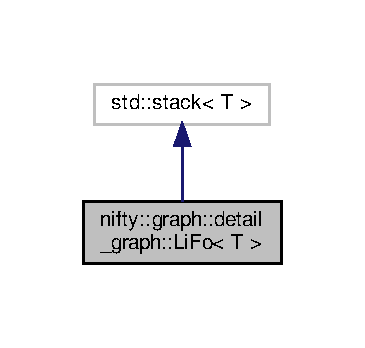
\includegraphics[width=175pt]{structnifty_1_1graph_1_1detail__graph_1_1LiFo__inherit__graph}
\end{center}
\end{figure}


Collaboration diagram for nifty\+:\+:graph\+:\+:detail\+\_\+graph\+:\+:Li\+Fo$<$ T $>$\+:\nopagebreak
\begin{figure}[H]
\begin{center}
\leavevmode
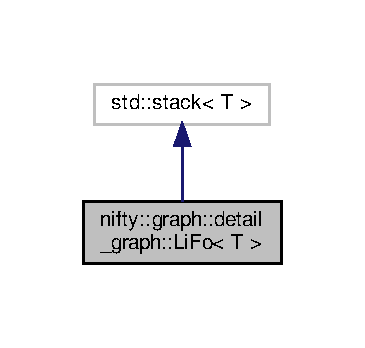
\includegraphics[width=175pt]{structnifty_1_1graph_1_1detail__graph_1_1LiFo__coll__graph}
\end{center}
\end{figure}
\subsection*{Public Member Functions}
\begin{DoxyCompactItemize}
\item 
const T \& \hyperlink{structnifty_1_1graph_1_1detail__graph_1_1LiFo_aeb157b0d46420c9e32708e782891ceb1}{next\+Element} ()
\end{DoxyCompactItemize}


\subsection{Member Function Documentation}
\hypertarget{structnifty_1_1graph_1_1detail__graph_1_1LiFo_aeb157b0d46420c9e32708e782891ceb1}{}\index{nifty\+::graph\+::detail\+\_\+graph\+::\+Li\+Fo@{nifty\+::graph\+::detail\+\_\+graph\+::\+Li\+Fo}!next\+Element@{next\+Element}}
\index{next\+Element@{next\+Element}!nifty\+::graph\+::detail\+\_\+graph\+::\+Li\+Fo@{nifty\+::graph\+::detail\+\_\+graph\+::\+Li\+Fo}}
\subsubsection[{next\+Element()}]{\setlength{\rightskip}{0pt plus 5cm}template$<$class T $>$ const T\& {\bf nifty\+::graph\+::detail\+\_\+graph\+::\+Li\+Fo}$<$ T $>$\+::next\+Element (
\begin{DoxyParamCaption}
{}
\end{DoxyParamCaption}
)\hspace{0.3cm}{\ttfamily [inline]}}\label{structnifty_1_1graph_1_1detail__graph_1_1LiFo_aeb157b0d46420c9e32708e782891ceb1}


The documentation for this struct was generated from the following file\+:\begin{DoxyCompactItemize}
\item 
/home/tbeier/src/nifty/include/nifty/graph/detail/\hyperlink{search__impl_8hxx}{search\+\_\+impl.\+hxx}\end{DoxyCompactItemize}

\hypertarget{classnifty_1_1graph_1_1agglo_1_1LiftedGraphEdgeWeightedClusterPolicy}{}\section{nifty\+:\+:graph\+:\+:agglo\+:\+:Lifted\+Graph\+Edge\+Weighted\+Cluster\+Policy$<$ G\+R\+A\+P\+H, E\+D\+G\+E\+\_\+\+I\+N\+D\+I\+C\+A\+T\+O\+R\+S, E\+D\+G\+E\+\_\+\+S\+I\+Z\+E\+S, N\+O\+D\+E\+\_\+\+S\+I\+Z\+E\+S, E\+D\+G\+E\+\_\+\+I\+S\+\_\+\+L\+I\+F\+T\+E\+D, E\+N\+A\+B\+L\+E\+\_\+\+U\+C\+M $>$ Class Template Reference}
\label{classnifty_1_1graph_1_1agglo_1_1LiftedGraphEdgeWeightedClusterPolicy}\index{nifty\+::graph\+::agglo\+::\+Lifted\+Graph\+Edge\+Weighted\+Cluster\+Policy$<$ G\+R\+A\+P\+H, E\+D\+G\+E\+\_\+\+I\+N\+D\+I\+C\+A\+T\+O\+R\+S, E\+D\+G\+E\+\_\+\+S\+I\+Z\+E\+S, N\+O\+D\+E\+\_\+\+S\+I\+Z\+E\+S, E\+D\+G\+E\+\_\+\+I\+S\+\_\+\+L\+I\+F\+T\+E\+D, E\+N\+A\+B\+L\+E\+\_\+\+U\+C\+M $>$@{nifty\+::graph\+::agglo\+::\+Lifted\+Graph\+Edge\+Weighted\+Cluster\+Policy$<$ G\+R\+A\+P\+H, E\+D\+G\+E\+\_\+\+I\+N\+D\+I\+C\+A\+T\+O\+R\+S, E\+D\+G\+E\+\_\+\+S\+I\+Z\+E\+S, N\+O\+D\+E\+\_\+\+S\+I\+Z\+E\+S, E\+D\+G\+E\+\_\+\+I\+S\+\_\+\+L\+I\+F\+T\+E\+D, E\+N\+A\+B\+L\+E\+\_\+\+U\+C\+M $>$}}


{\ttfamily \#include $<$lifted\+\_\+graph\+\_\+edge\+\_\+weighted\+\_\+cluster\+\_\+policy.\+hxx$>$}

\subsection*{Public Types}
\begin{DoxyCompactItemize}
\item 
typedef G\+R\+A\+P\+H \hyperlink{classnifty_1_1graph_1_1agglo_1_1LiftedGraphEdgeWeightedClusterPolicy_ae3d069ea1fd066a37e1c816c0bf50b83}{Graph\+Type}
\item 
typedef E\+D\+G\+E\+\_\+\+I\+N\+D\+I\+C\+A\+T\+O\+R\+S \hyperlink{classnifty_1_1graph_1_1agglo_1_1LiftedGraphEdgeWeightedClusterPolicy_ad0813aa75f1e76d10b794cab88615f61}{Edge\+Indicators\+Type}
\item 
typedef E\+D\+G\+E\+\_\+\+S\+I\+Z\+E\+S \hyperlink{classnifty_1_1graph_1_1agglo_1_1LiftedGraphEdgeWeightedClusterPolicy_ad63cc4f759cd05f1bf9b7fec48629221}{Edge\+Sizes\+Type}
\item 
typedef N\+O\+D\+E\+\_\+\+S\+I\+Z\+E\+S \hyperlink{classnifty_1_1graph_1_1agglo_1_1LiftedGraphEdgeWeightedClusterPolicy_a83ef319d77186be2fc3957ed06f0a8f1}{Node\+Sizes\+Type}
\item 
typedef E\+D\+G\+E\+\_\+\+I\+S\+\_\+\+L\+I\+F\+T\+E\+D \hyperlink{classnifty_1_1graph_1_1agglo_1_1LiftedGraphEdgeWeightedClusterPolicy_ad104d8984e0964ccfb7d1ec06ee977a2}{Edge\+Is\+Lifted}
\item 
typedef \hyperlink{structnifty_1_1graph_1_1agglo_1_1EdgeWeightedClusterPolicySettings}{Edge\+Weighted\+Cluster\+Policy\+Settings} \hyperlink{classnifty_1_1graph_1_1agglo_1_1LiftedGraphEdgeWeightedClusterPolicy_a7bf0e26a2c4776e866807429e912084b}{Settings\+Type}
\item 
typedef \hyperlink{classnifty_1_1graph_1_1EdgeContractionGraph}{Edge\+Contraction\+Graph}$<$ \hyperlink{classnifty_1_1graph_1_1agglo_1_1LiftedGraphEdgeWeightedClusterPolicy_ae3d069ea1fd066a37e1c816c0bf50b83}{Graph\+Type}, \hyperlink{classnifty_1_1graph_1_1agglo_1_1LiftedGraphEdgeWeightedClusterPolicy}{Self\+Type} $>$ \hyperlink{classnifty_1_1graph_1_1agglo_1_1LiftedGraphEdgeWeightedClusterPolicy_a316c395d0d3bcc00ddbed21302419354}{Edge\+Contraction\+Graph\+Type}
\end{DoxyCompactItemize}
\subsection*{Public Member Functions}
\begin{DoxyCompactItemize}
\item 
\hyperlink{classnifty_1_1graph_1_1agglo_1_1LiftedGraphEdgeWeightedClusterPolicy_ab7ae607d3f0b14dea37488433e97c91d}{Lifted\+Graph\+Edge\+Weighted\+Cluster\+Policy} (const \hyperlink{classnifty_1_1graph_1_1agglo_1_1LiftedGraphEdgeWeightedClusterPolicy_ae3d069ea1fd066a37e1c816c0bf50b83}{Graph\+Type} \&, \hyperlink{classnifty_1_1graph_1_1agglo_1_1LiftedGraphEdgeWeightedClusterPolicy_ad0813aa75f1e76d10b794cab88615f61}{Edge\+Indicators\+Type}, \hyperlink{classnifty_1_1graph_1_1agglo_1_1LiftedGraphEdgeWeightedClusterPolicy_ad63cc4f759cd05f1bf9b7fec48629221}{Edge\+Sizes\+Type}, \hyperlink{classnifty_1_1graph_1_1agglo_1_1LiftedGraphEdgeWeightedClusterPolicy_a83ef319d77186be2fc3957ed06f0a8f1}{Node\+Sizes\+Type}, \hyperlink{classnifty_1_1graph_1_1agglo_1_1LiftedGraphEdgeWeightedClusterPolicy_ad104d8984e0964ccfb7d1ec06ee977a2}{Edge\+Is\+Lifted}, const \hyperlink{classnifty_1_1graph_1_1agglo_1_1LiftedGraphEdgeWeightedClusterPolicy_a7bf0e26a2c4776e866807429e912084b}{Settings\+Type} \&settings=\hyperlink{classnifty_1_1graph_1_1agglo_1_1LiftedGraphEdgeWeightedClusterPolicy_a7bf0e26a2c4776e866807429e912084b}{Settings\+Type}())
\item 
std\+::pair$<$ uint64\+\_\+t, double $>$ \hyperlink{classnifty_1_1graph_1_1agglo_1_1LiftedGraphEdgeWeightedClusterPolicy_ac27f4726c16aaa1f77b68a318a13d681}{edge\+To\+Contract\+Next} () const 
\item 
bool \hyperlink{classnifty_1_1graph_1_1agglo_1_1LiftedGraphEdgeWeightedClusterPolicy_a7e11bb64b33cf2123c48eb46d9feebf5}{is\+Done} () const 
\item 
\hyperlink{classnifty_1_1graph_1_1agglo_1_1LiftedGraphEdgeWeightedClusterPolicy_a316c395d0d3bcc00ddbed21302419354}{Edge\+Contraction\+Graph\+Type} \& \hyperlink{classnifty_1_1graph_1_1agglo_1_1LiftedGraphEdgeWeightedClusterPolicy_a95287f99bc3b86ccbed7dcd9c8851628}{edge\+Contraction\+Graph} ()
\item 
void \hyperlink{classnifty_1_1graph_1_1agglo_1_1LiftedGraphEdgeWeightedClusterPolicy_a56bc42922fcf00d486cfebca957c18ab}{contract\+Edge} (const uint64\+\_\+t edge\+To\+Contract)
\item 
void \hyperlink{classnifty_1_1graph_1_1agglo_1_1LiftedGraphEdgeWeightedClusterPolicy_a0a8e7d91a8393b6c9d350bc69305bedf}{merge\+Nodes} (const uint64\+\_\+t alive\+Node, const uint64\+\_\+t dead\+Node)
\item 
void \hyperlink{classnifty_1_1graph_1_1agglo_1_1LiftedGraphEdgeWeightedClusterPolicy_a033e17251eb1e313f930a53a3c73a002}{merge\+Edges} (const uint64\+\_\+t alive\+Edge, const uint64\+\_\+t dead\+Edge)
\item 
void \hyperlink{classnifty_1_1graph_1_1agglo_1_1LiftedGraphEdgeWeightedClusterPolicy_aa5bcb1829765b56a0fc10a82be501cc0}{contract\+Edge\+Done} (const uint64\+\_\+t edge\+To\+Contract)
\end{DoxyCompactItemize}
\subsection*{Friends}
\begin{DoxyCompactItemize}
\item 
class \hyperlink{classnifty_1_1graph_1_1agglo_1_1LiftedGraphEdgeWeightedClusterPolicy_a6939aa4c6113ba9c44fd5e048687ba92}{Edge\+Contraction\+Graph$<$ Graph\+Type, Self\+Type, E\+N\+A\+B\+L\+E\+\_\+\+U\+C\+M $>$}
\end{DoxyCompactItemize}


\subsection{Member Typedef Documentation}
\hypertarget{classnifty_1_1graph_1_1agglo_1_1LiftedGraphEdgeWeightedClusterPolicy_a316c395d0d3bcc00ddbed21302419354}{}\index{nifty\+::graph\+::agglo\+::\+Lifted\+Graph\+Edge\+Weighted\+Cluster\+Policy@{nifty\+::graph\+::agglo\+::\+Lifted\+Graph\+Edge\+Weighted\+Cluster\+Policy}!Edge\+Contraction\+Graph\+Type@{Edge\+Contraction\+Graph\+Type}}
\index{Edge\+Contraction\+Graph\+Type@{Edge\+Contraction\+Graph\+Type}!nifty\+::graph\+::agglo\+::\+Lifted\+Graph\+Edge\+Weighted\+Cluster\+Policy@{nifty\+::graph\+::agglo\+::\+Lifted\+Graph\+Edge\+Weighted\+Cluster\+Policy}}
\subsubsection[{Edge\+Contraction\+Graph\+Type}]{\setlength{\rightskip}{0pt plus 5cm}template$<$class G\+R\+A\+P\+H , class E\+D\+G\+E\+\_\+\+I\+N\+D\+I\+C\+A\+T\+O\+R\+S , class E\+D\+G\+E\+\_\+\+S\+I\+Z\+E\+S , class N\+O\+D\+E\+\_\+\+S\+I\+Z\+E\+S , class E\+D\+G\+E\+\_\+\+I\+S\+\_\+\+L\+I\+F\+T\+E\+D , bool E\+N\+A\+B\+L\+E\+\_\+\+U\+C\+M = true$>$ typedef {\bf Edge\+Contraction\+Graph}$<${\bf Graph\+Type}, {\bf Self\+Type}$>$ {\bf nifty\+::graph\+::agglo\+::\+Lifted\+Graph\+Edge\+Weighted\+Cluster\+Policy}$<$ G\+R\+A\+P\+H, E\+D\+G\+E\+\_\+\+I\+N\+D\+I\+C\+A\+T\+O\+R\+S, E\+D\+G\+E\+\_\+\+S\+I\+Z\+E\+S, N\+O\+D\+E\+\_\+\+S\+I\+Z\+E\+S, E\+D\+G\+E\+\_\+\+I\+S\+\_\+\+L\+I\+F\+T\+E\+D, E\+N\+A\+B\+L\+E\+\_\+\+U\+C\+M $>$\+::{\bf Edge\+Contraction\+Graph\+Type}}\label{classnifty_1_1graph_1_1agglo_1_1LiftedGraphEdgeWeightedClusterPolicy_a316c395d0d3bcc00ddbed21302419354}
\hypertarget{classnifty_1_1graph_1_1agglo_1_1LiftedGraphEdgeWeightedClusterPolicy_ad0813aa75f1e76d10b794cab88615f61}{}\index{nifty\+::graph\+::agglo\+::\+Lifted\+Graph\+Edge\+Weighted\+Cluster\+Policy@{nifty\+::graph\+::agglo\+::\+Lifted\+Graph\+Edge\+Weighted\+Cluster\+Policy}!Edge\+Indicators\+Type@{Edge\+Indicators\+Type}}
\index{Edge\+Indicators\+Type@{Edge\+Indicators\+Type}!nifty\+::graph\+::agglo\+::\+Lifted\+Graph\+Edge\+Weighted\+Cluster\+Policy@{nifty\+::graph\+::agglo\+::\+Lifted\+Graph\+Edge\+Weighted\+Cluster\+Policy}}
\subsubsection[{Edge\+Indicators\+Type}]{\setlength{\rightskip}{0pt plus 5cm}template$<$class G\+R\+A\+P\+H , class E\+D\+G\+E\+\_\+\+I\+N\+D\+I\+C\+A\+T\+O\+R\+S , class E\+D\+G\+E\+\_\+\+S\+I\+Z\+E\+S , class N\+O\+D\+E\+\_\+\+S\+I\+Z\+E\+S , class E\+D\+G\+E\+\_\+\+I\+S\+\_\+\+L\+I\+F\+T\+E\+D , bool E\+N\+A\+B\+L\+E\+\_\+\+U\+C\+M = true$>$ typedef E\+D\+G\+E\+\_\+\+I\+N\+D\+I\+C\+A\+T\+O\+R\+S {\bf nifty\+::graph\+::agglo\+::\+Lifted\+Graph\+Edge\+Weighted\+Cluster\+Policy}$<$ G\+R\+A\+P\+H, E\+D\+G\+E\+\_\+\+I\+N\+D\+I\+C\+A\+T\+O\+R\+S, E\+D\+G\+E\+\_\+\+S\+I\+Z\+E\+S, N\+O\+D\+E\+\_\+\+S\+I\+Z\+E\+S, E\+D\+G\+E\+\_\+\+I\+S\+\_\+\+L\+I\+F\+T\+E\+D, E\+N\+A\+B\+L\+E\+\_\+\+U\+C\+M $>$\+::{\bf Edge\+Indicators\+Type}}\label{classnifty_1_1graph_1_1agglo_1_1LiftedGraphEdgeWeightedClusterPolicy_ad0813aa75f1e76d10b794cab88615f61}
\hypertarget{classnifty_1_1graph_1_1agglo_1_1LiftedGraphEdgeWeightedClusterPolicy_ad104d8984e0964ccfb7d1ec06ee977a2}{}\index{nifty\+::graph\+::agglo\+::\+Lifted\+Graph\+Edge\+Weighted\+Cluster\+Policy@{nifty\+::graph\+::agglo\+::\+Lifted\+Graph\+Edge\+Weighted\+Cluster\+Policy}!Edge\+Is\+Lifted@{Edge\+Is\+Lifted}}
\index{Edge\+Is\+Lifted@{Edge\+Is\+Lifted}!nifty\+::graph\+::agglo\+::\+Lifted\+Graph\+Edge\+Weighted\+Cluster\+Policy@{nifty\+::graph\+::agglo\+::\+Lifted\+Graph\+Edge\+Weighted\+Cluster\+Policy}}
\subsubsection[{Edge\+Is\+Lifted}]{\setlength{\rightskip}{0pt plus 5cm}template$<$class G\+R\+A\+P\+H , class E\+D\+G\+E\+\_\+\+I\+N\+D\+I\+C\+A\+T\+O\+R\+S , class E\+D\+G\+E\+\_\+\+S\+I\+Z\+E\+S , class N\+O\+D\+E\+\_\+\+S\+I\+Z\+E\+S , class E\+D\+G\+E\+\_\+\+I\+S\+\_\+\+L\+I\+F\+T\+E\+D , bool E\+N\+A\+B\+L\+E\+\_\+\+U\+C\+M = true$>$ typedef E\+D\+G\+E\+\_\+\+I\+S\+\_\+\+L\+I\+F\+T\+E\+D {\bf nifty\+::graph\+::agglo\+::\+Lifted\+Graph\+Edge\+Weighted\+Cluster\+Policy}$<$ G\+R\+A\+P\+H, E\+D\+G\+E\+\_\+\+I\+N\+D\+I\+C\+A\+T\+O\+R\+S, E\+D\+G\+E\+\_\+\+S\+I\+Z\+E\+S, N\+O\+D\+E\+\_\+\+S\+I\+Z\+E\+S, E\+D\+G\+E\+\_\+\+I\+S\+\_\+\+L\+I\+F\+T\+E\+D, E\+N\+A\+B\+L\+E\+\_\+\+U\+C\+M $>$\+::{\bf Edge\+Is\+Lifted}}\label{classnifty_1_1graph_1_1agglo_1_1LiftedGraphEdgeWeightedClusterPolicy_ad104d8984e0964ccfb7d1ec06ee977a2}
\hypertarget{classnifty_1_1graph_1_1agglo_1_1LiftedGraphEdgeWeightedClusterPolicy_ad63cc4f759cd05f1bf9b7fec48629221}{}\index{nifty\+::graph\+::agglo\+::\+Lifted\+Graph\+Edge\+Weighted\+Cluster\+Policy@{nifty\+::graph\+::agglo\+::\+Lifted\+Graph\+Edge\+Weighted\+Cluster\+Policy}!Edge\+Sizes\+Type@{Edge\+Sizes\+Type}}
\index{Edge\+Sizes\+Type@{Edge\+Sizes\+Type}!nifty\+::graph\+::agglo\+::\+Lifted\+Graph\+Edge\+Weighted\+Cluster\+Policy@{nifty\+::graph\+::agglo\+::\+Lifted\+Graph\+Edge\+Weighted\+Cluster\+Policy}}
\subsubsection[{Edge\+Sizes\+Type}]{\setlength{\rightskip}{0pt plus 5cm}template$<$class G\+R\+A\+P\+H , class E\+D\+G\+E\+\_\+\+I\+N\+D\+I\+C\+A\+T\+O\+R\+S , class E\+D\+G\+E\+\_\+\+S\+I\+Z\+E\+S , class N\+O\+D\+E\+\_\+\+S\+I\+Z\+E\+S , class E\+D\+G\+E\+\_\+\+I\+S\+\_\+\+L\+I\+F\+T\+E\+D , bool E\+N\+A\+B\+L\+E\+\_\+\+U\+C\+M = true$>$ typedef E\+D\+G\+E\+\_\+\+S\+I\+Z\+E\+S {\bf nifty\+::graph\+::agglo\+::\+Lifted\+Graph\+Edge\+Weighted\+Cluster\+Policy}$<$ G\+R\+A\+P\+H, E\+D\+G\+E\+\_\+\+I\+N\+D\+I\+C\+A\+T\+O\+R\+S, E\+D\+G\+E\+\_\+\+S\+I\+Z\+E\+S, N\+O\+D\+E\+\_\+\+S\+I\+Z\+E\+S, E\+D\+G\+E\+\_\+\+I\+S\+\_\+\+L\+I\+F\+T\+E\+D, E\+N\+A\+B\+L\+E\+\_\+\+U\+C\+M $>$\+::{\bf Edge\+Sizes\+Type}}\label{classnifty_1_1graph_1_1agglo_1_1LiftedGraphEdgeWeightedClusterPolicy_ad63cc4f759cd05f1bf9b7fec48629221}
\hypertarget{classnifty_1_1graph_1_1agglo_1_1LiftedGraphEdgeWeightedClusterPolicy_ae3d069ea1fd066a37e1c816c0bf50b83}{}\index{nifty\+::graph\+::agglo\+::\+Lifted\+Graph\+Edge\+Weighted\+Cluster\+Policy@{nifty\+::graph\+::agglo\+::\+Lifted\+Graph\+Edge\+Weighted\+Cluster\+Policy}!Graph\+Type@{Graph\+Type}}
\index{Graph\+Type@{Graph\+Type}!nifty\+::graph\+::agglo\+::\+Lifted\+Graph\+Edge\+Weighted\+Cluster\+Policy@{nifty\+::graph\+::agglo\+::\+Lifted\+Graph\+Edge\+Weighted\+Cluster\+Policy}}
\subsubsection[{Graph\+Type}]{\setlength{\rightskip}{0pt plus 5cm}template$<$class G\+R\+A\+P\+H , class E\+D\+G\+E\+\_\+\+I\+N\+D\+I\+C\+A\+T\+O\+R\+S , class E\+D\+G\+E\+\_\+\+S\+I\+Z\+E\+S , class N\+O\+D\+E\+\_\+\+S\+I\+Z\+E\+S , class E\+D\+G\+E\+\_\+\+I\+S\+\_\+\+L\+I\+F\+T\+E\+D , bool E\+N\+A\+B\+L\+E\+\_\+\+U\+C\+M = true$>$ typedef G\+R\+A\+P\+H {\bf nifty\+::graph\+::agglo\+::\+Lifted\+Graph\+Edge\+Weighted\+Cluster\+Policy}$<$ G\+R\+A\+P\+H, E\+D\+G\+E\+\_\+\+I\+N\+D\+I\+C\+A\+T\+O\+R\+S, E\+D\+G\+E\+\_\+\+S\+I\+Z\+E\+S, N\+O\+D\+E\+\_\+\+S\+I\+Z\+E\+S, E\+D\+G\+E\+\_\+\+I\+S\+\_\+\+L\+I\+F\+T\+E\+D, E\+N\+A\+B\+L\+E\+\_\+\+U\+C\+M $>$\+::{\bf Graph\+Type}}\label{classnifty_1_1graph_1_1agglo_1_1LiftedGraphEdgeWeightedClusterPolicy_ae3d069ea1fd066a37e1c816c0bf50b83}
\hypertarget{classnifty_1_1graph_1_1agglo_1_1LiftedGraphEdgeWeightedClusterPolicy_a83ef319d77186be2fc3957ed06f0a8f1}{}\index{nifty\+::graph\+::agglo\+::\+Lifted\+Graph\+Edge\+Weighted\+Cluster\+Policy@{nifty\+::graph\+::agglo\+::\+Lifted\+Graph\+Edge\+Weighted\+Cluster\+Policy}!Node\+Sizes\+Type@{Node\+Sizes\+Type}}
\index{Node\+Sizes\+Type@{Node\+Sizes\+Type}!nifty\+::graph\+::agglo\+::\+Lifted\+Graph\+Edge\+Weighted\+Cluster\+Policy@{nifty\+::graph\+::agglo\+::\+Lifted\+Graph\+Edge\+Weighted\+Cluster\+Policy}}
\subsubsection[{Node\+Sizes\+Type}]{\setlength{\rightskip}{0pt plus 5cm}template$<$class G\+R\+A\+P\+H , class E\+D\+G\+E\+\_\+\+I\+N\+D\+I\+C\+A\+T\+O\+R\+S , class E\+D\+G\+E\+\_\+\+S\+I\+Z\+E\+S , class N\+O\+D\+E\+\_\+\+S\+I\+Z\+E\+S , class E\+D\+G\+E\+\_\+\+I\+S\+\_\+\+L\+I\+F\+T\+E\+D , bool E\+N\+A\+B\+L\+E\+\_\+\+U\+C\+M = true$>$ typedef N\+O\+D\+E\+\_\+\+S\+I\+Z\+E\+S {\bf nifty\+::graph\+::agglo\+::\+Lifted\+Graph\+Edge\+Weighted\+Cluster\+Policy}$<$ G\+R\+A\+P\+H, E\+D\+G\+E\+\_\+\+I\+N\+D\+I\+C\+A\+T\+O\+R\+S, E\+D\+G\+E\+\_\+\+S\+I\+Z\+E\+S, N\+O\+D\+E\+\_\+\+S\+I\+Z\+E\+S, E\+D\+G\+E\+\_\+\+I\+S\+\_\+\+L\+I\+F\+T\+E\+D, E\+N\+A\+B\+L\+E\+\_\+\+U\+C\+M $>$\+::{\bf Node\+Sizes\+Type}}\label{classnifty_1_1graph_1_1agglo_1_1LiftedGraphEdgeWeightedClusterPolicy_a83ef319d77186be2fc3957ed06f0a8f1}
\hypertarget{classnifty_1_1graph_1_1agglo_1_1LiftedGraphEdgeWeightedClusterPolicy_a7bf0e26a2c4776e866807429e912084b}{}\index{nifty\+::graph\+::agglo\+::\+Lifted\+Graph\+Edge\+Weighted\+Cluster\+Policy@{nifty\+::graph\+::agglo\+::\+Lifted\+Graph\+Edge\+Weighted\+Cluster\+Policy}!Settings\+Type@{Settings\+Type}}
\index{Settings\+Type@{Settings\+Type}!nifty\+::graph\+::agglo\+::\+Lifted\+Graph\+Edge\+Weighted\+Cluster\+Policy@{nifty\+::graph\+::agglo\+::\+Lifted\+Graph\+Edge\+Weighted\+Cluster\+Policy}}
\subsubsection[{Settings\+Type}]{\setlength{\rightskip}{0pt plus 5cm}template$<$class G\+R\+A\+P\+H , class E\+D\+G\+E\+\_\+\+I\+N\+D\+I\+C\+A\+T\+O\+R\+S , class E\+D\+G\+E\+\_\+\+S\+I\+Z\+E\+S , class N\+O\+D\+E\+\_\+\+S\+I\+Z\+E\+S , class E\+D\+G\+E\+\_\+\+I\+S\+\_\+\+L\+I\+F\+T\+E\+D , bool E\+N\+A\+B\+L\+E\+\_\+\+U\+C\+M = true$>$ typedef {\bf Edge\+Weighted\+Cluster\+Policy\+Settings} {\bf nifty\+::graph\+::agglo\+::\+Lifted\+Graph\+Edge\+Weighted\+Cluster\+Policy}$<$ G\+R\+A\+P\+H, E\+D\+G\+E\+\_\+\+I\+N\+D\+I\+C\+A\+T\+O\+R\+S, E\+D\+G\+E\+\_\+\+S\+I\+Z\+E\+S, N\+O\+D\+E\+\_\+\+S\+I\+Z\+E\+S, E\+D\+G\+E\+\_\+\+I\+S\+\_\+\+L\+I\+F\+T\+E\+D, E\+N\+A\+B\+L\+E\+\_\+\+U\+C\+M $>$\+::{\bf Settings\+Type}}\label{classnifty_1_1graph_1_1agglo_1_1LiftedGraphEdgeWeightedClusterPolicy_a7bf0e26a2c4776e866807429e912084b}


\subsection{Constructor \& Destructor Documentation}
\hypertarget{classnifty_1_1graph_1_1agglo_1_1LiftedGraphEdgeWeightedClusterPolicy_ab7ae607d3f0b14dea37488433e97c91d}{}\index{nifty\+::graph\+::agglo\+::\+Lifted\+Graph\+Edge\+Weighted\+Cluster\+Policy@{nifty\+::graph\+::agglo\+::\+Lifted\+Graph\+Edge\+Weighted\+Cluster\+Policy}!Lifted\+Graph\+Edge\+Weighted\+Cluster\+Policy@{Lifted\+Graph\+Edge\+Weighted\+Cluster\+Policy}}
\index{Lifted\+Graph\+Edge\+Weighted\+Cluster\+Policy@{Lifted\+Graph\+Edge\+Weighted\+Cluster\+Policy}!nifty\+::graph\+::agglo\+::\+Lifted\+Graph\+Edge\+Weighted\+Cluster\+Policy@{nifty\+::graph\+::agglo\+::\+Lifted\+Graph\+Edge\+Weighted\+Cluster\+Policy}}
\subsubsection[{Lifted\+Graph\+Edge\+Weighted\+Cluster\+Policy(const Graph\+Type \&, Edge\+Indicators\+Type, Edge\+Sizes\+Type, Node\+Sizes\+Type, Edge\+Is\+Lifted, const Settings\+Type \&settings=\+Settings\+Type())}]{\setlength{\rightskip}{0pt plus 5cm}template$<$class G\+R\+A\+P\+H , class E\+D\+G\+E\+\_\+\+I\+N\+D\+I\+C\+A\+T\+O\+R\+S , class E\+D\+G\+E\+\_\+\+S\+I\+Z\+E\+S , class N\+O\+D\+E\+\_\+\+S\+I\+Z\+E\+S , class E\+D\+G\+E\+\_\+\+I\+S\+\_\+\+L\+I\+F\+T\+E\+D , bool E\+N\+A\+B\+L\+E\+\_\+\+U\+C\+M$>$ {\bf nifty\+::graph\+::agglo\+::\+Lifted\+Graph\+Edge\+Weighted\+Cluster\+Policy}$<$ G\+R\+A\+P\+H, E\+D\+G\+E\+\_\+\+I\+N\+D\+I\+C\+A\+T\+O\+R\+S, E\+D\+G\+E\+\_\+\+S\+I\+Z\+E\+S, N\+O\+D\+E\+\_\+\+S\+I\+Z\+E\+S, E\+D\+G\+E\+\_\+\+I\+S\+\_\+\+L\+I\+F\+T\+E\+D, E\+N\+A\+B\+L\+E\+\_\+\+U\+C\+M $>$\+::{\bf Lifted\+Graph\+Edge\+Weighted\+Cluster\+Policy} (
\begin{DoxyParamCaption}
\item[{const {\bf Graph\+Type} \&}]{graph, }
\item[{{\bf Edge\+Indicators\+Type}}]{edge\+Indicators, }
\item[{{\bf Edge\+Sizes\+Type}}]{edge\+Sizes, }
\item[{{\bf Node\+Sizes\+Type}}]{node\+Sizes, }
\item[{{\bf Edge\+Is\+Lifted}}]{edge\+Is\+Lifted, }
\item[{const {\bf Settings\+Type} \&}]{settings = {\ttfamily {\bf Settings\+Type}()}}
\end{DoxyParamCaption}
)\hspace{0.3cm}{\ttfamily [inline]}}\label{classnifty_1_1graph_1_1agglo_1_1LiftedGraphEdgeWeightedClusterPolicy_ab7ae607d3f0b14dea37488433e97c91d}


\subsection{Member Function Documentation}
\hypertarget{classnifty_1_1graph_1_1agglo_1_1LiftedGraphEdgeWeightedClusterPolicy_a56bc42922fcf00d486cfebca957c18ab}{}\index{nifty\+::graph\+::agglo\+::\+Lifted\+Graph\+Edge\+Weighted\+Cluster\+Policy@{nifty\+::graph\+::agglo\+::\+Lifted\+Graph\+Edge\+Weighted\+Cluster\+Policy}!contract\+Edge@{contract\+Edge}}
\index{contract\+Edge@{contract\+Edge}!nifty\+::graph\+::agglo\+::\+Lifted\+Graph\+Edge\+Weighted\+Cluster\+Policy@{nifty\+::graph\+::agglo\+::\+Lifted\+Graph\+Edge\+Weighted\+Cluster\+Policy}}
\subsubsection[{contract\+Edge(const uint64\+\_\+t edge\+To\+Contract)}]{\setlength{\rightskip}{0pt plus 5cm}template$<$class G\+R\+A\+P\+H , class E\+D\+G\+E\+\_\+\+I\+N\+D\+I\+C\+A\+T\+O\+R\+S , class E\+D\+G\+E\+\_\+\+S\+I\+Z\+E\+S , class N\+O\+D\+E\+\_\+\+S\+I\+Z\+E\+S , class E\+D\+G\+E\+\_\+\+I\+S\+\_\+\+L\+I\+F\+T\+E\+D , bool E\+N\+A\+B\+L\+E\+\_\+\+U\+C\+M$>$ void {\bf nifty\+::graph\+::agglo\+::\+Lifted\+Graph\+Edge\+Weighted\+Cluster\+Policy}$<$ G\+R\+A\+P\+H, E\+D\+G\+E\+\_\+\+I\+N\+D\+I\+C\+A\+T\+O\+R\+S, E\+D\+G\+E\+\_\+\+S\+I\+Z\+E\+S, N\+O\+D\+E\+\_\+\+S\+I\+Z\+E\+S, E\+D\+G\+E\+\_\+\+I\+S\+\_\+\+L\+I\+F\+T\+E\+D, E\+N\+A\+B\+L\+E\+\_\+\+U\+C\+M $>$\+::contract\+Edge (
\begin{DoxyParamCaption}
\item[{const uint64\+\_\+t}]{edge\+To\+Contract}
\end{DoxyParamCaption}
)\hspace{0.3cm}{\ttfamily [inline]}}\label{classnifty_1_1graph_1_1agglo_1_1LiftedGraphEdgeWeightedClusterPolicy_a56bc42922fcf00d486cfebca957c18ab}
\hypertarget{classnifty_1_1graph_1_1agglo_1_1LiftedGraphEdgeWeightedClusterPolicy_aa5bcb1829765b56a0fc10a82be501cc0}{}\index{nifty\+::graph\+::agglo\+::\+Lifted\+Graph\+Edge\+Weighted\+Cluster\+Policy@{nifty\+::graph\+::agglo\+::\+Lifted\+Graph\+Edge\+Weighted\+Cluster\+Policy}!contract\+Edge\+Done@{contract\+Edge\+Done}}
\index{contract\+Edge\+Done@{contract\+Edge\+Done}!nifty\+::graph\+::agglo\+::\+Lifted\+Graph\+Edge\+Weighted\+Cluster\+Policy@{nifty\+::graph\+::agglo\+::\+Lifted\+Graph\+Edge\+Weighted\+Cluster\+Policy}}
\subsubsection[{contract\+Edge\+Done(const uint64\+\_\+t edge\+To\+Contract)}]{\setlength{\rightskip}{0pt plus 5cm}template$<$class G\+R\+A\+P\+H , class E\+D\+G\+E\+\_\+\+I\+N\+D\+I\+C\+A\+T\+O\+R\+S , class E\+D\+G\+E\+\_\+\+S\+I\+Z\+E\+S , class N\+O\+D\+E\+\_\+\+S\+I\+Z\+E\+S , class E\+D\+G\+E\+\_\+\+I\+S\+\_\+\+L\+I\+F\+T\+E\+D , bool E\+N\+A\+B\+L\+E\+\_\+\+U\+C\+M$>$ void {\bf nifty\+::graph\+::agglo\+::\+Lifted\+Graph\+Edge\+Weighted\+Cluster\+Policy}$<$ G\+R\+A\+P\+H, E\+D\+G\+E\+\_\+\+I\+N\+D\+I\+C\+A\+T\+O\+R\+S, E\+D\+G\+E\+\_\+\+S\+I\+Z\+E\+S, N\+O\+D\+E\+\_\+\+S\+I\+Z\+E\+S, E\+D\+G\+E\+\_\+\+I\+S\+\_\+\+L\+I\+F\+T\+E\+D, E\+N\+A\+B\+L\+E\+\_\+\+U\+C\+M $>$\+::contract\+Edge\+Done (
\begin{DoxyParamCaption}
\item[{const uint64\+\_\+t}]{edge\+To\+Contract}
\end{DoxyParamCaption}
)\hspace{0.3cm}{\ttfamily [inline]}}\label{classnifty_1_1graph_1_1agglo_1_1LiftedGraphEdgeWeightedClusterPolicy_aa5bcb1829765b56a0fc10a82be501cc0}
\hypertarget{classnifty_1_1graph_1_1agglo_1_1LiftedGraphEdgeWeightedClusterPolicy_a95287f99bc3b86ccbed7dcd9c8851628}{}\index{nifty\+::graph\+::agglo\+::\+Lifted\+Graph\+Edge\+Weighted\+Cluster\+Policy@{nifty\+::graph\+::agglo\+::\+Lifted\+Graph\+Edge\+Weighted\+Cluster\+Policy}!edge\+Contraction\+Graph@{edge\+Contraction\+Graph}}
\index{edge\+Contraction\+Graph@{edge\+Contraction\+Graph}!nifty\+::graph\+::agglo\+::\+Lifted\+Graph\+Edge\+Weighted\+Cluster\+Policy@{nifty\+::graph\+::agglo\+::\+Lifted\+Graph\+Edge\+Weighted\+Cluster\+Policy}}
\subsubsection[{edge\+Contraction\+Graph()}]{\setlength{\rightskip}{0pt plus 5cm}template$<$class G\+R\+A\+P\+H , class E\+D\+G\+E\+\_\+\+I\+N\+D\+I\+C\+A\+T\+O\+R\+S , class E\+D\+G\+E\+\_\+\+S\+I\+Z\+E\+S , class N\+O\+D\+E\+\_\+\+S\+I\+Z\+E\+S , class E\+D\+G\+E\+\_\+\+I\+S\+\_\+\+L\+I\+F\+T\+E\+D , bool E\+N\+A\+B\+L\+E\+\_\+\+U\+C\+M$>$ {\bf Lifted\+Graph\+Edge\+Weighted\+Cluster\+Policy}$<$ G\+R\+A\+P\+H, E\+D\+G\+E\+\_\+\+I\+N\+D\+I\+C\+A\+T\+O\+R\+S, E\+D\+G\+E\+\_\+\+S\+I\+Z\+E\+S, N\+O\+D\+E\+\_\+\+S\+I\+Z\+E\+S, E\+D\+G\+E\+\_\+\+I\+S\+\_\+\+L\+I\+F\+T\+E\+D, E\+N\+A\+B\+L\+E\+\_\+\+U\+C\+M $>$\+::{\bf Edge\+Contraction\+Graph\+Type} \& {\bf nifty\+::graph\+::agglo\+::\+Lifted\+Graph\+Edge\+Weighted\+Cluster\+Policy}$<$ G\+R\+A\+P\+H, E\+D\+G\+E\+\_\+\+I\+N\+D\+I\+C\+A\+T\+O\+R\+S, E\+D\+G\+E\+\_\+\+S\+I\+Z\+E\+S, N\+O\+D\+E\+\_\+\+S\+I\+Z\+E\+S, E\+D\+G\+E\+\_\+\+I\+S\+\_\+\+L\+I\+F\+T\+E\+D, E\+N\+A\+B\+L\+E\+\_\+\+U\+C\+M $>$\+::edge\+Contraction\+Graph (
\begin{DoxyParamCaption}
{}
\end{DoxyParamCaption}
)\hspace{0.3cm}{\ttfamily [inline]}}\label{classnifty_1_1graph_1_1agglo_1_1LiftedGraphEdgeWeightedClusterPolicy_a95287f99bc3b86ccbed7dcd9c8851628}
\hypertarget{classnifty_1_1graph_1_1agglo_1_1LiftedGraphEdgeWeightedClusterPolicy_ac27f4726c16aaa1f77b68a318a13d681}{}\index{nifty\+::graph\+::agglo\+::\+Lifted\+Graph\+Edge\+Weighted\+Cluster\+Policy@{nifty\+::graph\+::agglo\+::\+Lifted\+Graph\+Edge\+Weighted\+Cluster\+Policy}!edge\+To\+Contract\+Next@{edge\+To\+Contract\+Next}}
\index{edge\+To\+Contract\+Next@{edge\+To\+Contract\+Next}!nifty\+::graph\+::agglo\+::\+Lifted\+Graph\+Edge\+Weighted\+Cluster\+Policy@{nifty\+::graph\+::agglo\+::\+Lifted\+Graph\+Edge\+Weighted\+Cluster\+Policy}}
\subsubsection[{edge\+To\+Contract\+Next() const }]{\setlength{\rightskip}{0pt plus 5cm}template$<$class G\+R\+A\+P\+H , class E\+D\+G\+E\+\_\+\+I\+N\+D\+I\+C\+A\+T\+O\+R\+S , class E\+D\+G\+E\+\_\+\+S\+I\+Z\+E\+S , class N\+O\+D\+E\+\_\+\+S\+I\+Z\+E\+S , class E\+D\+G\+E\+\_\+\+I\+S\+\_\+\+L\+I\+F\+T\+E\+D , bool E\+N\+A\+B\+L\+E\+\_\+\+U\+C\+M$>$ std\+::pair$<$ uint64\+\_\+t, double $>$ {\bf nifty\+::graph\+::agglo\+::\+Lifted\+Graph\+Edge\+Weighted\+Cluster\+Policy}$<$ G\+R\+A\+P\+H, E\+D\+G\+E\+\_\+\+I\+N\+D\+I\+C\+A\+T\+O\+R\+S, E\+D\+G\+E\+\_\+\+S\+I\+Z\+E\+S, N\+O\+D\+E\+\_\+\+S\+I\+Z\+E\+S, E\+D\+G\+E\+\_\+\+I\+S\+\_\+\+L\+I\+F\+T\+E\+D, E\+N\+A\+B\+L\+E\+\_\+\+U\+C\+M $>$\+::edge\+To\+Contract\+Next (
\begin{DoxyParamCaption}
{}
\end{DoxyParamCaption}
) const\hspace{0.3cm}{\ttfamily [inline]}}\label{classnifty_1_1graph_1_1agglo_1_1LiftedGraphEdgeWeightedClusterPolicy_ac27f4726c16aaa1f77b68a318a13d681}
\hypertarget{classnifty_1_1graph_1_1agglo_1_1LiftedGraphEdgeWeightedClusterPolicy_a7e11bb64b33cf2123c48eb46d9feebf5}{}\index{nifty\+::graph\+::agglo\+::\+Lifted\+Graph\+Edge\+Weighted\+Cluster\+Policy@{nifty\+::graph\+::agglo\+::\+Lifted\+Graph\+Edge\+Weighted\+Cluster\+Policy}!is\+Done@{is\+Done}}
\index{is\+Done@{is\+Done}!nifty\+::graph\+::agglo\+::\+Lifted\+Graph\+Edge\+Weighted\+Cluster\+Policy@{nifty\+::graph\+::agglo\+::\+Lifted\+Graph\+Edge\+Weighted\+Cluster\+Policy}}
\subsubsection[{is\+Done() const }]{\setlength{\rightskip}{0pt plus 5cm}template$<$class G\+R\+A\+P\+H , class E\+D\+G\+E\+\_\+\+I\+N\+D\+I\+C\+A\+T\+O\+R\+S , class E\+D\+G\+E\+\_\+\+S\+I\+Z\+E\+S , class N\+O\+D\+E\+\_\+\+S\+I\+Z\+E\+S , class E\+D\+G\+E\+\_\+\+I\+S\+\_\+\+L\+I\+F\+T\+E\+D , bool E\+N\+A\+B\+L\+E\+\_\+\+U\+C\+M$>$ bool {\bf nifty\+::graph\+::agglo\+::\+Lifted\+Graph\+Edge\+Weighted\+Cluster\+Policy}$<$ G\+R\+A\+P\+H, E\+D\+G\+E\+\_\+\+I\+N\+D\+I\+C\+A\+T\+O\+R\+S, E\+D\+G\+E\+\_\+\+S\+I\+Z\+E\+S, N\+O\+D\+E\+\_\+\+S\+I\+Z\+E\+S, E\+D\+G\+E\+\_\+\+I\+S\+\_\+\+L\+I\+F\+T\+E\+D, E\+N\+A\+B\+L\+E\+\_\+\+U\+C\+M $>$\+::is\+Done (
\begin{DoxyParamCaption}
{}
\end{DoxyParamCaption}
) const\hspace{0.3cm}{\ttfamily [inline]}}\label{classnifty_1_1graph_1_1agglo_1_1LiftedGraphEdgeWeightedClusterPolicy_a7e11bb64b33cf2123c48eb46d9feebf5}
\hypertarget{classnifty_1_1graph_1_1agglo_1_1LiftedGraphEdgeWeightedClusterPolicy_a033e17251eb1e313f930a53a3c73a002}{}\index{nifty\+::graph\+::agglo\+::\+Lifted\+Graph\+Edge\+Weighted\+Cluster\+Policy@{nifty\+::graph\+::agglo\+::\+Lifted\+Graph\+Edge\+Weighted\+Cluster\+Policy}!merge\+Edges@{merge\+Edges}}
\index{merge\+Edges@{merge\+Edges}!nifty\+::graph\+::agglo\+::\+Lifted\+Graph\+Edge\+Weighted\+Cluster\+Policy@{nifty\+::graph\+::agglo\+::\+Lifted\+Graph\+Edge\+Weighted\+Cluster\+Policy}}
\subsubsection[{merge\+Edges(const uint64\+\_\+t alive\+Edge, const uint64\+\_\+t dead\+Edge)}]{\setlength{\rightskip}{0pt plus 5cm}template$<$class G\+R\+A\+P\+H , class E\+D\+G\+E\+\_\+\+I\+N\+D\+I\+C\+A\+T\+O\+R\+S , class E\+D\+G\+E\+\_\+\+S\+I\+Z\+E\+S , class N\+O\+D\+E\+\_\+\+S\+I\+Z\+E\+S , class E\+D\+G\+E\+\_\+\+I\+S\+\_\+\+L\+I\+F\+T\+E\+D , bool E\+N\+A\+B\+L\+E\+\_\+\+U\+C\+M$>$ void {\bf nifty\+::graph\+::agglo\+::\+Lifted\+Graph\+Edge\+Weighted\+Cluster\+Policy}$<$ G\+R\+A\+P\+H, E\+D\+G\+E\+\_\+\+I\+N\+D\+I\+C\+A\+T\+O\+R\+S, E\+D\+G\+E\+\_\+\+S\+I\+Z\+E\+S, N\+O\+D\+E\+\_\+\+S\+I\+Z\+E\+S, E\+D\+G\+E\+\_\+\+I\+S\+\_\+\+L\+I\+F\+T\+E\+D, E\+N\+A\+B\+L\+E\+\_\+\+U\+C\+M $>$\+::merge\+Edges (
\begin{DoxyParamCaption}
\item[{const uint64\+\_\+t}]{alive\+Edge, }
\item[{const uint64\+\_\+t}]{dead\+Edge}
\end{DoxyParamCaption}
)\hspace{0.3cm}{\ttfamily [inline]}}\label{classnifty_1_1graph_1_1agglo_1_1LiftedGraphEdgeWeightedClusterPolicy_a033e17251eb1e313f930a53a3c73a002}
\hypertarget{classnifty_1_1graph_1_1agglo_1_1LiftedGraphEdgeWeightedClusterPolicy_a0a8e7d91a8393b6c9d350bc69305bedf}{}\index{nifty\+::graph\+::agglo\+::\+Lifted\+Graph\+Edge\+Weighted\+Cluster\+Policy@{nifty\+::graph\+::agglo\+::\+Lifted\+Graph\+Edge\+Weighted\+Cluster\+Policy}!merge\+Nodes@{merge\+Nodes}}
\index{merge\+Nodes@{merge\+Nodes}!nifty\+::graph\+::agglo\+::\+Lifted\+Graph\+Edge\+Weighted\+Cluster\+Policy@{nifty\+::graph\+::agglo\+::\+Lifted\+Graph\+Edge\+Weighted\+Cluster\+Policy}}
\subsubsection[{merge\+Nodes(const uint64\+\_\+t alive\+Node, const uint64\+\_\+t dead\+Node)}]{\setlength{\rightskip}{0pt plus 5cm}template$<$class G\+R\+A\+P\+H , class E\+D\+G\+E\+\_\+\+I\+N\+D\+I\+C\+A\+T\+O\+R\+S , class E\+D\+G\+E\+\_\+\+S\+I\+Z\+E\+S , class N\+O\+D\+E\+\_\+\+S\+I\+Z\+E\+S , class E\+D\+G\+E\+\_\+\+I\+S\+\_\+\+L\+I\+F\+T\+E\+D , bool E\+N\+A\+B\+L\+E\+\_\+\+U\+C\+M$>$ void {\bf nifty\+::graph\+::agglo\+::\+Lifted\+Graph\+Edge\+Weighted\+Cluster\+Policy}$<$ G\+R\+A\+P\+H, E\+D\+G\+E\+\_\+\+I\+N\+D\+I\+C\+A\+T\+O\+R\+S, E\+D\+G\+E\+\_\+\+S\+I\+Z\+E\+S, N\+O\+D\+E\+\_\+\+S\+I\+Z\+E\+S, E\+D\+G\+E\+\_\+\+I\+S\+\_\+\+L\+I\+F\+T\+E\+D, E\+N\+A\+B\+L\+E\+\_\+\+U\+C\+M $>$\+::merge\+Nodes (
\begin{DoxyParamCaption}
\item[{const uint64\+\_\+t}]{alive\+Node, }
\item[{const uint64\+\_\+t}]{dead\+Node}
\end{DoxyParamCaption}
)\hspace{0.3cm}{\ttfamily [inline]}}\label{classnifty_1_1graph_1_1agglo_1_1LiftedGraphEdgeWeightedClusterPolicy_a0a8e7d91a8393b6c9d350bc69305bedf}


\subsection{Friends And Related Function Documentation}
\hypertarget{classnifty_1_1graph_1_1agglo_1_1LiftedGraphEdgeWeightedClusterPolicy_a6939aa4c6113ba9c44fd5e048687ba92}{}\index{nifty\+::graph\+::agglo\+::\+Lifted\+Graph\+Edge\+Weighted\+Cluster\+Policy@{nifty\+::graph\+::agglo\+::\+Lifted\+Graph\+Edge\+Weighted\+Cluster\+Policy}!Edge\+Contraction\+Graph$<$ Graph\+Type, Self\+Type, E\+N\+A\+B\+L\+E\+\_\+\+U\+C\+M $>$@{Edge\+Contraction\+Graph$<$ Graph\+Type, Self\+Type, E\+N\+A\+B\+L\+E\+\_\+\+U\+C\+M $>$}}
\index{Edge\+Contraction\+Graph$<$ Graph\+Type, Self\+Type, E\+N\+A\+B\+L\+E\+\_\+\+U\+C\+M $>$@{Edge\+Contraction\+Graph$<$ Graph\+Type, Self\+Type, E\+N\+A\+B\+L\+E\+\_\+\+U\+C\+M $>$}!nifty\+::graph\+::agglo\+::\+Lifted\+Graph\+Edge\+Weighted\+Cluster\+Policy@{nifty\+::graph\+::agglo\+::\+Lifted\+Graph\+Edge\+Weighted\+Cluster\+Policy}}
\subsubsection[{Edge\+Contraction\+Graph$<$ Graph\+Type, Self\+Type, E\+N\+A\+B\+L\+E\+\_\+\+U\+C\+M $>$}]{\setlength{\rightskip}{0pt plus 5cm}template$<$class G\+R\+A\+P\+H , class E\+D\+G\+E\+\_\+\+I\+N\+D\+I\+C\+A\+T\+O\+R\+S , class E\+D\+G\+E\+\_\+\+S\+I\+Z\+E\+S , class N\+O\+D\+E\+\_\+\+S\+I\+Z\+E\+S , class E\+D\+G\+E\+\_\+\+I\+S\+\_\+\+L\+I\+F\+T\+E\+D , bool E\+N\+A\+B\+L\+E\+\_\+\+U\+C\+M = true$>$ friend class {\bf Edge\+Contraction\+Graph}$<$ {\bf Graph\+Type}, {\bf Self\+Type}, E\+N\+A\+B\+L\+E\+\_\+\+U\+C\+M $>$\hspace{0.3cm}{\ttfamily [friend]}}\label{classnifty_1_1graph_1_1agglo_1_1LiftedGraphEdgeWeightedClusterPolicy_a6939aa4c6113ba9c44fd5e048687ba92}


The documentation for this class was generated from the following file\+:\begin{DoxyCompactItemize}
\item 
/home/tbeier/src/nifty/include/nifty/graph/agglo/cluster\+\_\+policies/\hyperlink{lifted__graph__edge__weighted__cluster__policy_8hxx}{lifted\+\_\+graph\+\_\+edge\+\_\+weighted\+\_\+cluster\+\_\+policy.\+hxx}\end{DoxyCompactItemize}

\hypertarget{classnifty_1_1graph_1_1lifted__multicut_1_1LiftedMulticutAndresGreedyAdditive}{}\section{nifty\+:\+:graph\+:\+:lifted\+\_\+multicut\+:\+:Lifted\+Multicut\+Andres\+Greedy\+Additive$<$ O\+B\+J\+E\+C\+T\+I\+V\+E $>$ Class Template Reference}
\label{classnifty_1_1graph_1_1lifted__multicut_1_1LiftedMulticutAndresGreedyAdditive}\index{nifty\+::graph\+::lifted\+\_\+multicut\+::\+Lifted\+Multicut\+Andres\+Greedy\+Additive$<$ O\+B\+J\+E\+C\+T\+I\+V\+E $>$@{nifty\+::graph\+::lifted\+\_\+multicut\+::\+Lifted\+Multicut\+Andres\+Greedy\+Additive$<$ O\+B\+J\+E\+C\+T\+I\+V\+E $>$}}


{\ttfamily \#include $<$lifted\+\_\+multicut\+\_\+andres\+\_\+greedy\+\_\+additive.\+hxx$>$}



Inheritance diagram for nifty\+:\+:graph\+:\+:lifted\+\_\+multicut\+:\+:Lifted\+Multicut\+Andres\+Greedy\+Additive$<$ O\+B\+J\+E\+C\+T\+I\+V\+E $>$\+:
% FIG 0


Collaboration diagram for nifty\+:\+:graph\+:\+:lifted\+\_\+multicut\+:\+:Lifted\+Multicut\+Andres\+Greedy\+Additive$<$ O\+B\+J\+E\+C\+T\+I\+V\+E $>$\+:
% FIG 1
\subsection*{Classes}
\begin{DoxyCompactItemize}
\item 
struct \hyperlink{structnifty_1_1graph_1_1lifted__multicut_1_1LiftedMulticutAndresGreedyAdditive_1_1Settings}{Settings}
\end{DoxyCompactItemize}
\subsection*{Public Types}
\begin{DoxyCompactItemize}
\item 
typedef O\+B\+J\+E\+C\+T\+I\+V\+E \hyperlink{classnifty_1_1graph_1_1lifted__multicut_1_1LiftedMulticutAndresGreedyAdditive_aad174abbd547a6779d21b2707261ce91}{Objective\+Type}
\item 
typedef \hyperlink{classnifty_1_1graph_1_1lifted__multicut_1_1LiftedMulticutBase}{Lifted\+Multicut\+Base}$<$ \hyperlink{classnifty_1_1graph_1_1lifted__multicut_1_1LiftedMulticutAndresGreedyAdditive_aad174abbd547a6779d21b2707261ce91}{Objective\+Type} $>$ \hyperlink{classnifty_1_1graph_1_1lifted__multicut_1_1LiftedMulticutAndresGreedyAdditive_aa4c70e93e8f23fe886884c5d33b94206}{Base\+Type}
\item 
typedef Objective\+Type\+::\+Graph\+Type \hyperlink{classnifty_1_1graph_1_1lifted__multicut_1_1LiftedMulticutAndresGreedyAdditive_acf401a359a97d354dbfc446f2123c71e}{Graph\+Type}
\item 
typedef Objective\+Type\+::\+Lifted\+Graph\+Type \hyperlink{classnifty_1_1graph_1_1lifted__multicut_1_1LiftedMulticutAndresGreedyAdditive_ab3559e4bd06a256ffce401e8d35d64bc}{Lifted\+Graph\+Type}
\item 
typedef \hyperlink{classnifty_1_1graph_1_1optimization_1_1common_1_1SolverBase_a5a14d64c70a9cc0eebc7d71d2b089f9b}{Base\+Type\+::\+Visitor\+Base\+Type} \hyperlink{classnifty_1_1graph_1_1lifted__multicut_1_1LiftedMulticutAndresGreedyAdditive_a4531913f0d3f10d228ee28cb983f668c}{Visitor\+Base\+Type}
\item 
typedef \hyperlink{classnifty_1_1graph_1_1optimization_1_1common_1_1SolverBase_a58913ea9ab9232ff72608b710c1012d0}{Base\+Type\+::\+Visitor\+Proxy\+Type} \hyperlink{classnifty_1_1graph_1_1lifted__multicut_1_1LiftedMulticutAndresGreedyAdditive_aa365becac68b1dea378e889f964b80d8}{Visitor\+Proxy\+Type}
\item 
typedef Base\+Type\+::\+Node\+Labels\+Type \hyperlink{classnifty_1_1graph_1_1lifted__multicut_1_1LiftedMulticutAndresGreedyAdditive_a43804693812be2e174e03525c85cd513}{Node\+Labels\+Type}
\end{DoxyCompactItemize}
\subsection*{Public Member Functions}
\begin{DoxyCompactItemize}
\item 
virtual \hyperlink{classnifty_1_1graph_1_1lifted__multicut_1_1LiftedMulticutAndresGreedyAdditive_a46ae5a23ab16a83c444494a9e1fe6716}{$\sim$\+Lifted\+Multicut\+Andres\+Greedy\+Additive} ()
\item 
\hyperlink{classnifty_1_1graph_1_1lifted__multicut_1_1LiftedMulticutAndresGreedyAdditive_a088701c4d448f36dbf6c549670632dea}{Lifted\+Multicut\+Andres\+Greedy\+Additive} (const \hyperlink{classnifty_1_1graph_1_1lifted__multicut_1_1LiftedMulticutAndresGreedyAdditive_aad174abbd547a6779d21b2707261ce91}{Objective\+Type} \&\hyperlink{classnifty_1_1graph_1_1lifted__multicut_1_1LiftedMulticutAndresGreedyAdditive_a267d174f69b6b76f6808725243b0b2c2}{objective}, const \hyperlink{structnifty_1_1graph_1_1lifted__multicut_1_1LiftedMulticutAndresGreedyAdditive_1_1Settings}{Settings} \&settings=\hyperlink{structnifty_1_1graph_1_1lifted__multicut_1_1LiftedMulticutAndresGreedyAdditive_1_1Settings}{Settings}())
\item 
virtual void \hyperlink{classnifty_1_1graph_1_1lifted__multicut_1_1LiftedMulticutAndresGreedyAdditive_a807fd8f815577d5e8e9d12269e3b6f60}{optimize} (\hyperlink{classnifty_1_1graph_1_1lifted__multicut_1_1LiftedMulticutAndresGreedyAdditive_a43804693812be2e174e03525c85cd513}{Node\+Labels\+Type} \&node\+Labels, \hyperlink{classnifty_1_1graph_1_1lifted__multicut_1_1LiftedMulticutAndresGreedyAdditive_a4531913f0d3f10d228ee28cb983f668c}{Visitor\+Base\+Type} $\ast$visitor)
\item 
virtual const \hyperlink{classnifty_1_1graph_1_1lifted__multicut_1_1LiftedMulticutAndresGreedyAdditive_aad174abbd547a6779d21b2707261ce91}{Objective\+Type} \& \hyperlink{classnifty_1_1graph_1_1lifted__multicut_1_1LiftedMulticutAndresGreedyAdditive_a267d174f69b6b76f6808725243b0b2c2}{objective} () const 
\item 
virtual const \hyperlink{classnifty_1_1graph_1_1lifted__multicut_1_1LiftedMulticutAndresGreedyAdditive_a43804693812be2e174e03525c85cd513}{Node\+Labels\+Type} \& \hyperlink{classnifty_1_1graph_1_1lifted__multicut_1_1LiftedMulticutAndresGreedyAdditive_a132fb579b1756c9a13ddd115dd56670a}{current\+Best\+Node\+Labels} ()
\item 
virtual std\+::string \hyperlink{classnifty_1_1graph_1_1lifted__multicut_1_1LiftedMulticutAndresGreedyAdditive_af0d2791716c89e177e8eaf1cff4d1a17}{name} () const 
\end{DoxyCompactItemize}


\subsection{Member Typedef Documentation}
\hypertarget{classnifty_1_1graph_1_1lifted__multicut_1_1LiftedMulticutAndresGreedyAdditive_aa4c70e93e8f23fe886884c5d33b94206}{}\index{nifty\+::graph\+::lifted\+\_\+multicut\+::\+Lifted\+Multicut\+Andres\+Greedy\+Additive@{nifty\+::graph\+::lifted\+\_\+multicut\+::\+Lifted\+Multicut\+Andres\+Greedy\+Additive}!Base\+Type@{Base\+Type}}
\index{Base\+Type@{Base\+Type}!nifty\+::graph\+::lifted\+\_\+multicut\+::\+Lifted\+Multicut\+Andres\+Greedy\+Additive@{nifty\+::graph\+::lifted\+\_\+multicut\+::\+Lifted\+Multicut\+Andres\+Greedy\+Additive}}
\subsubsection[{Base\+Type}]{\setlength{\rightskip}{0pt plus 5cm}template$<$class O\+B\+J\+E\+C\+T\+I\+V\+E$>$ typedef {\bf Lifted\+Multicut\+Base}$<${\bf Objective\+Type}$>$ {\bf nifty\+::graph\+::lifted\+\_\+multicut\+::\+Lifted\+Multicut\+Andres\+Greedy\+Additive}$<$ O\+B\+J\+E\+C\+T\+I\+V\+E $>$\+::{\bf Base\+Type}}\label{classnifty_1_1graph_1_1lifted__multicut_1_1LiftedMulticutAndresGreedyAdditive_aa4c70e93e8f23fe886884c5d33b94206}
\hypertarget{classnifty_1_1graph_1_1lifted__multicut_1_1LiftedMulticutAndresGreedyAdditive_acf401a359a97d354dbfc446f2123c71e}{}\index{nifty\+::graph\+::lifted\+\_\+multicut\+::\+Lifted\+Multicut\+Andres\+Greedy\+Additive@{nifty\+::graph\+::lifted\+\_\+multicut\+::\+Lifted\+Multicut\+Andres\+Greedy\+Additive}!Graph\+Type@{Graph\+Type}}
\index{Graph\+Type@{Graph\+Type}!nifty\+::graph\+::lifted\+\_\+multicut\+::\+Lifted\+Multicut\+Andres\+Greedy\+Additive@{nifty\+::graph\+::lifted\+\_\+multicut\+::\+Lifted\+Multicut\+Andres\+Greedy\+Additive}}
\subsubsection[{Graph\+Type}]{\setlength{\rightskip}{0pt plus 5cm}template$<$class O\+B\+J\+E\+C\+T\+I\+V\+E$>$ typedef Objective\+Type\+::\+Graph\+Type {\bf nifty\+::graph\+::lifted\+\_\+multicut\+::\+Lifted\+Multicut\+Andres\+Greedy\+Additive}$<$ O\+B\+J\+E\+C\+T\+I\+V\+E $>$\+::{\bf Graph\+Type}}\label{classnifty_1_1graph_1_1lifted__multicut_1_1LiftedMulticutAndresGreedyAdditive_acf401a359a97d354dbfc446f2123c71e}
\hypertarget{classnifty_1_1graph_1_1lifted__multicut_1_1LiftedMulticutAndresGreedyAdditive_ab3559e4bd06a256ffce401e8d35d64bc}{}\index{nifty\+::graph\+::lifted\+\_\+multicut\+::\+Lifted\+Multicut\+Andres\+Greedy\+Additive@{nifty\+::graph\+::lifted\+\_\+multicut\+::\+Lifted\+Multicut\+Andres\+Greedy\+Additive}!Lifted\+Graph\+Type@{Lifted\+Graph\+Type}}
\index{Lifted\+Graph\+Type@{Lifted\+Graph\+Type}!nifty\+::graph\+::lifted\+\_\+multicut\+::\+Lifted\+Multicut\+Andres\+Greedy\+Additive@{nifty\+::graph\+::lifted\+\_\+multicut\+::\+Lifted\+Multicut\+Andres\+Greedy\+Additive}}
\subsubsection[{Lifted\+Graph\+Type}]{\setlength{\rightskip}{0pt plus 5cm}template$<$class O\+B\+J\+E\+C\+T\+I\+V\+E$>$ typedef Objective\+Type\+::\+Lifted\+Graph\+Type {\bf nifty\+::graph\+::lifted\+\_\+multicut\+::\+Lifted\+Multicut\+Andres\+Greedy\+Additive}$<$ O\+B\+J\+E\+C\+T\+I\+V\+E $>$\+::{\bf Lifted\+Graph\+Type}}\label{classnifty_1_1graph_1_1lifted__multicut_1_1LiftedMulticutAndresGreedyAdditive_ab3559e4bd06a256ffce401e8d35d64bc}
\hypertarget{classnifty_1_1graph_1_1lifted__multicut_1_1LiftedMulticutAndresGreedyAdditive_a43804693812be2e174e03525c85cd513}{}\index{nifty\+::graph\+::lifted\+\_\+multicut\+::\+Lifted\+Multicut\+Andres\+Greedy\+Additive@{nifty\+::graph\+::lifted\+\_\+multicut\+::\+Lifted\+Multicut\+Andres\+Greedy\+Additive}!Node\+Labels\+Type@{Node\+Labels\+Type}}
\index{Node\+Labels\+Type@{Node\+Labels\+Type}!nifty\+::graph\+::lifted\+\_\+multicut\+::\+Lifted\+Multicut\+Andres\+Greedy\+Additive@{nifty\+::graph\+::lifted\+\_\+multicut\+::\+Lifted\+Multicut\+Andres\+Greedy\+Additive}}
\subsubsection[{Node\+Labels\+Type}]{\setlength{\rightskip}{0pt plus 5cm}template$<$class O\+B\+J\+E\+C\+T\+I\+V\+E$>$ typedef Base\+Type\+::\+Node\+Labels\+Type {\bf nifty\+::graph\+::lifted\+\_\+multicut\+::\+Lifted\+Multicut\+Andres\+Greedy\+Additive}$<$ O\+B\+J\+E\+C\+T\+I\+V\+E $>$\+::{\bf Node\+Labels\+Type}}\label{classnifty_1_1graph_1_1lifted__multicut_1_1LiftedMulticutAndresGreedyAdditive_a43804693812be2e174e03525c85cd513}
\hypertarget{classnifty_1_1graph_1_1lifted__multicut_1_1LiftedMulticutAndresGreedyAdditive_aad174abbd547a6779d21b2707261ce91}{}\index{nifty\+::graph\+::lifted\+\_\+multicut\+::\+Lifted\+Multicut\+Andres\+Greedy\+Additive@{nifty\+::graph\+::lifted\+\_\+multicut\+::\+Lifted\+Multicut\+Andres\+Greedy\+Additive}!Objective\+Type@{Objective\+Type}}
\index{Objective\+Type@{Objective\+Type}!nifty\+::graph\+::lifted\+\_\+multicut\+::\+Lifted\+Multicut\+Andres\+Greedy\+Additive@{nifty\+::graph\+::lifted\+\_\+multicut\+::\+Lifted\+Multicut\+Andres\+Greedy\+Additive}}
\subsubsection[{Objective\+Type}]{\setlength{\rightskip}{0pt plus 5cm}template$<$class O\+B\+J\+E\+C\+T\+I\+V\+E$>$ typedef O\+B\+J\+E\+C\+T\+I\+V\+E {\bf nifty\+::graph\+::lifted\+\_\+multicut\+::\+Lifted\+Multicut\+Andres\+Greedy\+Additive}$<$ O\+B\+J\+E\+C\+T\+I\+V\+E $>$\+::{\bf Objective\+Type}}\label{classnifty_1_1graph_1_1lifted__multicut_1_1LiftedMulticutAndresGreedyAdditive_aad174abbd547a6779d21b2707261ce91}
\hypertarget{classnifty_1_1graph_1_1lifted__multicut_1_1LiftedMulticutAndresGreedyAdditive_a4531913f0d3f10d228ee28cb983f668c}{}\index{nifty\+::graph\+::lifted\+\_\+multicut\+::\+Lifted\+Multicut\+Andres\+Greedy\+Additive@{nifty\+::graph\+::lifted\+\_\+multicut\+::\+Lifted\+Multicut\+Andres\+Greedy\+Additive}!Visitor\+Base\+Type@{Visitor\+Base\+Type}}
\index{Visitor\+Base\+Type@{Visitor\+Base\+Type}!nifty\+::graph\+::lifted\+\_\+multicut\+::\+Lifted\+Multicut\+Andres\+Greedy\+Additive@{nifty\+::graph\+::lifted\+\_\+multicut\+::\+Lifted\+Multicut\+Andres\+Greedy\+Additive}}
\subsubsection[{Visitor\+Base\+Type}]{\setlength{\rightskip}{0pt plus 5cm}template$<$class O\+B\+J\+E\+C\+T\+I\+V\+E$>$ typedef {\bf Base\+Type\+::\+Visitor\+Base\+Type} {\bf nifty\+::graph\+::lifted\+\_\+multicut\+::\+Lifted\+Multicut\+Andres\+Greedy\+Additive}$<$ O\+B\+J\+E\+C\+T\+I\+V\+E $>$\+::{\bf Visitor\+Base\+Type}}\label{classnifty_1_1graph_1_1lifted__multicut_1_1LiftedMulticutAndresGreedyAdditive_a4531913f0d3f10d228ee28cb983f668c}
\hypertarget{classnifty_1_1graph_1_1lifted__multicut_1_1LiftedMulticutAndresGreedyAdditive_aa365becac68b1dea378e889f964b80d8}{}\index{nifty\+::graph\+::lifted\+\_\+multicut\+::\+Lifted\+Multicut\+Andres\+Greedy\+Additive@{nifty\+::graph\+::lifted\+\_\+multicut\+::\+Lifted\+Multicut\+Andres\+Greedy\+Additive}!Visitor\+Proxy\+Type@{Visitor\+Proxy\+Type}}
\index{Visitor\+Proxy\+Type@{Visitor\+Proxy\+Type}!nifty\+::graph\+::lifted\+\_\+multicut\+::\+Lifted\+Multicut\+Andres\+Greedy\+Additive@{nifty\+::graph\+::lifted\+\_\+multicut\+::\+Lifted\+Multicut\+Andres\+Greedy\+Additive}}
\subsubsection[{Visitor\+Proxy\+Type}]{\setlength{\rightskip}{0pt plus 5cm}template$<$class O\+B\+J\+E\+C\+T\+I\+V\+E$>$ typedef {\bf Base\+Type\+::\+Visitor\+Proxy\+Type} {\bf nifty\+::graph\+::lifted\+\_\+multicut\+::\+Lifted\+Multicut\+Andres\+Greedy\+Additive}$<$ O\+B\+J\+E\+C\+T\+I\+V\+E $>$\+::{\bf Visitor\+Proxy\+Type}}\label{classnifty_1_1graph_1_1lifted__multicut_1_1LiftedMulticutAndresGreedyAdditive_aa365becac68b1dea378e889f964b80d8}


\subsection{Constructor \& Destructor Documentation}
\hypertarget{classnifty_1_1graph_1_1lifted__multicut_1_1LiftedMulticutAndresGreedyAdditive_a46ae5a23ab16a83c444494a9e1fe6716}{}\index{nifty\+::graph\+::lifted\+\_\+multicut\+::\+Lifted\+Multicut\+Andres\+Greedy\+Additive@{nifty\+::graph\+::lifted\+\_\+multicut\+::\+Lifted\+Multicut\+Andres\+Greedy\+Additive}!````~Lifted\+Multicut\+Andres\+Greedy\+Additive@{$\sim$\+Lifted\+Multicut\+Andres\+Greedy\+Additive}}
\index{````~Lifted\+Multicut\+Andres\+Greedy\+Additive@{$\sim$\+Lifted\+Multicut\+Andres\+Greedy\+Additive}!nifty\+::graph\+::lifted\+\_\+multicut\+::\+Lifted\+Multicut\+Andres\+Greedy\+Additive@{nifty\+::graph\+::lifted\+\_\+multicut\+::\+Lifted\+Multicut\+Andres\+Greedy\+Additive}}
\subsubsection[{$\sim$\+Lifted\+Multicut\+Andres\+Greedy\+Additive()}]{\setlength{\rightskip}{0pt plus 5cm}template$<$class O\+B\+J\+E\+C\+T\+I\+V\+E$>$ virtual {\bf nifty\+::graph\+::lifted\+\_\+multicut\+::\+Lifted\+Multicut\+Andres\+Greedy\+Additive}$<$ O\+B\+J\+E\+C\+T\+I\+V\+E $>$\+::$\sim${\bf Lifted\+Multicut\+Andres\+Greedy\+Additive} (
\begin{DoxyParamCaption}
{}
\end{DoxyParamCaption}
)\hspace{0.3cm}{\ttfamily [inline]}, {\ttfamily [virtual]}}\label{classnifty_1_1graph_1_1lifted__multicut_1_1LiftedMulticutAndresGreedyAdditive_a46ae5a23ab16a83c444494a9e1fe6716}
\hypertarget{classnifty_1_1graph_1_1lifted__multicut_1_1LiftedMulticutAndresGreedyAdditive_a088701c4d448f36dbf6c549670632dea}{}\index{nifty\+::graph\+::lifted\+\_\+multicut\+::\+Lifted\+Multicut\+Andres\+Greedy\+Additive@{nifty\+::graph\+::lifted\+\_\+multicut\+::\+Lifted\+Multicut\+Andres\+Greedy\+Additive}!Lifted\+Multicut\+Andres\+Greedy\+Additive@{Lifted\+Multicut\+Andres\+Greedy\+Additive}}
\index{Lifted\+Multicut\+Andres\+Greedy\+Additive@{Lifted\+Multicut\+Andres\+Greedy\+Additive}!nifty\+::graph\+::lifted\+\_\+multicut\+::\+Lifted\+Multicut\+Andres\+Greedy\+Additive@{nifty\+::graph\+::lifted\+\_\+multicut\+::\+Lifted\+Multicut\+Andres\+Greedy\+Additive}}
\subsubsection[{Lifted\+Multicut\+Andres\+Greedy\+Additive(const Objective\+Type \&objective, const Settings \&settings=\+Settings())}]{\setlength{\rightskip}{0pt plus 5cm}template$<$class O\+B\+J\+E\+C\+T\+I\+V\+E $>$ {\bf nifty\+::graph\+::lifted\+\_\+multicut\+::\+Lifted\+Multicut\+Andres\+Greedy\+Additive}$<$ O\+B\+J\+E\+C\+T\+I\+V\+E $>$\+::{\bf Lifted\+Multicut\+Andres\+Greedy\+Additive} (
\begin{DoxyParamCaption}
\item[{const {\bf Objective\+Type} \&}]{objective, }
\item[{const {\bf Settings} \&}]{settings = {\ttfamily {\bf Settings}()}}
\end{DoxyParamCaption}
)}\label{classnifty_1_1graph_1_1lifted__multicut_1_1LiftedMulticutAndresGreedyAdditive_a088701c4d448f36dbf6c549670632dea}


\subsection{Member Function Documentation}
\hypertarget{classnifty_1_1graph_1_1lifted__multicut_1_1LiftedMulticutAndresGreedyAdditive_a132fb579b1756c9a13ddd115dd56670a}{}\index{nifty\+::graph\+::lifted\+\_\+multicut\+::\+Lifted\+Multicut\+Andres\+Greedy\+Additive@{nifty\+::graph\+::lifted\+\_\+multicut\+::\+Lifted\+Multicut\+Andres\+Greedy\+Additive}!current\+Best\+Node\+Labels@{current\+Best\+Node\+Labels}}
\index{current\+Best\+Node\+Labels@{current\+Best\+Node\+Labels}!nifty\+::graph\+::lifted\+\_\+multicut\+::\+Lifted\+Multicut\+Andres\+Greedy\+Additive@{nifty\+::graph\+::lifted\+\_\+multicut\+::\+Lifted\+Multicut\+Andres\+Greedy\+Additive}}
\subsubsection[{current\+Best\+Node\+Labels()}]{\setlength{\rightskip}{0pt plus 5cm}template$<$class O\+B\+J\+E\+C\+T\+I\+V\+E$>$ virtual const {\bf Node\+Labels\+Type}\& {\bf nifty\+::graph\+::lifted\+\_\+multicut\+::\+Lifted\+Multicut\+Andres\+Greedy\+Additive}$<$ O\+B\+J\+E\+C\+T\+I\+V\+E $>$\+::current\+Best\+Node\+Labels (
\begin{DoxyParamCaption}
{}
\end{DoxyParamCaption}
)\hspace{0.3cm}{\ttfamily [inline]}, {\ttfamily [virtual]}}\label{classnifty_1_1graph_1_1lifted__multicut_1_1LiftedMulticutAndresGreedyAdditive_a132fb579b1756c9a13ddd115dd56670a}


Implements \hyperlink{classnifty_1_1graph_1_1optimization_1_1common_1_1SolverBase_a3634ba645adbb7a668500e807608bcca}{nifty\+::graph\+::optimization\+::common\+::\+Solver\+Base$<$ O\+B\+J\+E\+C\+T\+I\+V\+E, Lifted\+Multicut\+Base$<$ O\+B\+J\+E\+C\+T\+I\+V\+E $>$ $>$}.

\hypertarget{classnifty_1_1graph_1_1lifted__multicut_1_1LiftedMulticutAndresGreedyAdditive_af0d2791716c89e177e8eaf1cff4d1a17}{}\index{nifty\+::graph\+::lifted\+\_\+multicut\+::\+Lifted\+Multicut\+Andres\+Greedy\+Additive@{nifty\+::graph\+::lifted\+\_\+multicut\+::\+Lifted\+Multicut\+Andres\+Greedy\+Additive}!name@{name}}
\index{name@{name}!nifty\+::graph\+::lifted\+\_\+multicut\+::\+Lifted\+Multicut\+Andres\+Greedy\+Additive@{nifty\+::graph\+::lifted\+\_\+multicut\+::\+Lifted\+Multicut\+Andres\+Greedy\+Additive}}
\subsubsection[{name() const }]{\setlength{\rightskip}{0pt plus 5cm}template$<$class O\+B\+J\+E\+C\+T\+I\+V\+E$>$ virtual std\+::string {\bf nifty\+::graph\+::lifted\+\_\+multicut\+::\+Lifted\+Multicut\+Andres\+Greedy\+Additive}$<$ O\+B\+J\+E\+C\+T\+I\+V\+E $>$\+::name (
\begin{DoxyParamCaption}
{}
\end{DoxyParamCaption}
) const\hspace{0.3cm}{\ttfamily [inline]}, {\ttfamily [virtual]}}\label{classnifty_1_1graph_1_1lifted__multicut_1_1LiftedMulticutAndresGreedyAdditive_af0d2791716c89e177e8eaf1cff4d1a17}


Implements \hyperlink{classnifty_1_1graph_1_1optimization_1_1common_1_1SolverBase_abc9685a3d63748ac470afccb2813be7e}{nifty\+::graph\+::optimization\+::common\+::\+Solver\+Base$<$ O\+B\+J\+E\+C\+T\+I\+V\+E, Lifted\+Multicut\+Base$<$ O\+B\+J\+E\+C\+T\+I\+V\+E $>$ $>$}.

\hypertarget{classnifty_1_1graph_1_1lifted__multicut_1_1LiftedMulticutAndresGreedyAdditive_a267d174f69b6b76f6808725243b0b2c2}{}\index{nifty\+::graph\+::lifted\+\_\+multicut\+::\+Lifted\+Multicut\+Andres\+Greedy\+Additive@{nifty\+::graph\+::lifted\+\_\+multicut\+::\+Lifted\+Multicut\+Andres\+Greedy\+Additive}!objective@{objective}}
\index{objective@{objective}!nifty\+::graph\+::lifted\+\_\+multicut\+::\+Lifted\+Multicut\+Andres\+Greedy\+Additive@{nifty\+::graph\+::lifted\+\_\+multicut\+::\+Lifted\+Multicut\+Andres\+Greedy\+Additive}}
\subsubsection[{objective() const }]{\setlength{\rightskip}{0pt plus 5cm}template$<$class O\+B\+J\+E\+C\+T\+I\+V\+E $>$ const {\bf Lifted\+Multicut\+Andres\+Greedy\+Additive}$<$ O\+B\+J\+E\+C\+T\+I\+V\+E $>$\+::{\bf Objective\+Type} \& {\bf nifty\+::graph\+::lifted\+\_\+multicut\+::\+Lifted\+Multicut\+Andres\+Greedy\+Additive}$<$ O\+B\+J\+E\+C\+T\+I\+V\+E $>$\+::objective (
\begin{DoxyParamCaption}
{}
\end{DoxyParamCaption}
) const\hspace{0.3cm}{\ttfamily [virtual]}}\label{classnifty_1_1graph_1_1lifted__multicut_1_1LiftedMulticutAndresGreedyAdditive_a267d174f69b6b76f6808725243b0b2c2}


Implements \hyperlink{classnifty_1_1graph_1_1optimization_1_1common_1_1SolverBase_ae7d36a7485b12a25979f75771f52e397}{nifty\+::graph\+::optimization\+::common\+::\+Solver\+Base$<$ O\+B\+J\+E\+C\+T\+I\+V\+E, Lifted\+Multicut\+Base$<$ O\+B\+J\+E\+C\+T\+I\+V\+E $>$ $>$}.

\hypertarget{classnifty_1_1graph_1_1lifted__multicut_1_1LiftedMulticutAndresGreedyAdditive_a807fd8f815577d5e8e9d12269e3b6f60}{}\index{nifty\+::graph\+::lifted\+\_\+multicut\+::\+Lifted\+Multicut\+Andres\+Greedy\+Additive@{nifty\+::graph\+::lifted\+\_\+multicut\+::\+Lifted\+Multicut\+Andres\+Greedy\+Additive}!optimize@{optimize}}
\index{optimize@{optimize}!nifty\+::graph\+::lifted\+\_\+multicut\+::\+Lifted\+Multicut\+Andres\+Greedy\+Additive@{nifty\+::graph\+::lifted\+\_\+multicut\+::\+Lifted\+Multicut\+Andres\+Greedy\+Additive}}
\subsubsection[{optimize(\+Node\+Labels\+Type \&node\+Labels, Visitor\+Base\+Type $\ast$visitor)}]{\setlength{\rightskip}{0pt plus 5cm}template$<$class O\+B\+J\+E\+C\+T\+I\+V\+E $>$ void {\bf nifty\+::graph\+::lifted\+\_\+multicut\+::\+Lifted\+Multicut\+Andres\+Greedy\+Additive}$<$ O\+B\+J\+E\+C\+T\+I\+V\+E $>$\+::optimize (
\begin{DoxyParamCaption}
\item[{{\bf Node\+Labels\+Type} \&}]{node\+Labels, }
\item[{{\bf Visitor\+Base\+Type} $\ast$}]{visitor}
\end{DoxyParamCaption}
)\hspace{0.3cm}{\ttfamily [virtual]}}\label{classnifty_1_1graph_1_1lifted__multicut_1_1LiftedMulticutAndresGreedyAdditive_a807fd8f815577d5e8e9d12269e3b6f60}


The documentation for this class was generated from the following file\+:\begin{DoxyCompactItemize}
\item 
/home/tbeier/src/nifty/include/nifty/graph/optimization/lifted\+\_\+multicut/\hyperlink{lifted__multicut__andres__greedy__additive_8hxx}{lifted\+\_\+multicut\+\_\+andres\+\_\+greedy\+\_\+additive.\+hxx}\end{DoxyCompactItemize}

\hypertarget{classnifty_1_1graph_1_1lifted__multicut_1_1LiftedMulticutAndresKernighanLin}{}\section{nifty\+:\+:graph\+:\+:lifted\+\_\+multicut\+:\+:Lifted\+Multicut\+Andres\+Kernighan\+Lin$<$ O\+B\+J\+E\+C\+T\+I\+V\+E $>$ Class Template Reference}
\label{classnifty_1_1graph_1_1lifted__multicut_1_1LiftedMulticutAndresKernighanLin}\index{nifty\+::graph\+::lifted\+\_\+multicut\+::\+Lifted\+Multicut\+Andres\+Kernighan\+Lin$<$ O\+B\+J\+E\+C\+T\+I\+V\+E $>$@{nifty\+::graph\+::lifted\+\_\+multicut\+::\+Lifted\+Multicut\+Andres\+Kernighan\+Lin$<$ O\+B\+J\+E\+C\+T\+I\+V\+E $>$}}


{\ttfamily \#include $<$lifted\+\_\+multicut\+\_\+andres\+\_\+kernighan\+\_\+lin.\+hxx$>$}



Inheritance diagram for nifty\+:\+:graph\+:\+:lifted\+\_\+multicut\+:\+:Lifted\+Multicut\+Andres\+Kernighan\+Lin$<$ O\+B\+J\+E\+C\+T\+I\+V\+E $>$\+:
% FIG 0


Collaboration diagram for nifty\+:\+:graph\+:\+:lifted\+\_\+multicut\+:\+:Lifted\+Multicut\+Andres\+Kernighan\+Lin$<$ O\+B\+J\+E\+C\+T\+I\+V\+E $>$\+:
% FIG 1
\subsection*{Classes}
\begin{DoxyCompactItemize}
\item 
struct \hyperlink{structnifty_1_1graph_1_1lifted__multicut_1_1LiftedMulticutAndresKernighanLin_1_1Settings}{Settings}
\end{DoxyCompactItemize}
\subsection*{Public Types}
\begin{DoxyCompactItemize}
\item 
typedef O\+B\+J\+E\+C\+T\+I\+V\+E \hyperlink{classnifty_1_1graph_1_1lifted__multicut_1_1LiftedMulticutAndresKernighanLin_ac7e43ca279b2efcbc2ebef1e7fed5816}{Objective\+Type}
\item 
typedef \hyperlink{classnifty_1_1graph_1_1lifted__multicut_1_1LiftedMulticutBase}{Lifted\+Multicut\+Base}$<$ \hyperlink{classnifty_1_1graph_1_1lifted__multicut_1_1LiftedMulticutAndresKernighanLin_ac7e43ca279b2efcbc2ebef1e7fed5816}{Objective\+Type} $>$ \hyperlink{classnifty_1_1graph_1_1lifted__multicut_1_1LiftedMulticutAndresKernighanLin_a1980265abbe7e1632e7e68ae21dc8350}{Base\+Type}
\item 
typedef Objective\+Type\+::\+Graph\+Type \hyperlink{classnifty_1_1graph_1_1lifted__multicut_1_1LiftedMulticutAndresKernighanLin_ab9df00196671b4579b041f080c40e2c4}{Graph\+Type}
\item 
typedef Objective\+Type\+::\+Lifted\+Graph\+Type \hyperlink{classnifty_1_1graph_1_1lifted__multicut_1_1LiftedMulticutAndresKernighanLin_afc82ef6686af2b8a0e1183fd7378725c}{Lifted\+Graph\+Type}
\item 
typedef Base\+Type\+::\+Visitor\+Base \hyperlink{classnifty_1_1graph_1_1lifted__multicut_1_1LiftedMulticutAndresKernighanLin_ab9331c2df1e0f0271899de4529631965}{Visitor\+Base}
\item 
typedef Base\+Type\+::\+Visitor\+Proxy \hyperlink{classnifty_1_1graph_1_1lifted__multicut_1_1LiftedMulticutAndresKernighanLin_a155c29dba5b4776980bd4599eae348e1}{Visitor\+Proxy}
\item 
typedef Base\+Type\+::\+Node\+Labels \hyperlink{classnifty_1_1graph_1_1lifted__multicut_1_1LiftedMulticutAndresKernighanLin_a03cd7122bcfadca7b44c2ed143355289}{Node\+Labels}
\end{DoxyCompactItemize}
\subsection*{Public Member Functions}
\begin{DoxyCompactItemize}
\item 
virtual \hyperlink{classnifty_1_1graph_1_1lifted__multicut_1_1LiftedMulticutAndresKernighanLin_aab5617a5a775da7c773c1e79f2411365}{$\sim$\+Lifted\+Multicut\+Andres\+Kernighan\+Lin} ()
\item 
\hyperlink{classnifty_1_1graph_1_1lifted__multicut_1_1LiftedMulticutAndresKernighanLin_a62d7a0a8439ba6160dd3f232992a8ff9}{Lifted\+Multicut\+Andres\+Kernighan\+Lin} (const \hyperlink{classnifty_1_1graph_1_1lifted__multicut_1_1LiftedMulticutAndresKernighanLin_ac7e43ca279b2efcbc2ebef1e7fed5816}{Objective\+Type} \&\hyperlink{classnifty_1_1graph_1_1lifted__multicut_1_1LiftedMulticutAndresKernighanLin_a8919b6ba352f53db3d2123d5b7fca300}{objective}, const \hyperlink{structnifty_1_1graph_1_1lifted__multicut_1_1LiftedMulticutAndresKernighanLin_1_1Settings}{Settings} \&settings=\hyperlink{structnifty_1_1graph_1_1lifted__multicut_1_1LiftedMulticutAndresKernighanLin_1_1Settings}{Settings}())
\item 
virtual void \hyperlink{classnifty_1_1graph_1_1lifted__multicut_1_1LiftedMulticutAndresKernighanLin_ab8f1294b901bcf167bdcac777ff95d22}{optimize} (\hyperlink{classnifty_1_1graph_1_1lifted__multicut_1_1LiftedMulticutAndresKernighanLin_a03cd7122bcfadca7b44c2ed143355289}{Node\+Labels} \&node\+Labels, \hyperlink{classnifty_1_1graph_1_1lifted__multicut_1_1LiftedMulticutAndresKernighanLin_ab9331c2df1e0f0271899de4529631965}{Visitor\+Base} $\ast$visitor)
\item 
virtual const \hyperlink{classnifty_1_1graph_1_1lifted__multicut_1_1LiftedMulticutAndresKernighanLin_ac7e43ca279b2efcbc2ebef1e7fed5816}{Objective\+Type} \& \hyperlink{classnifty_1_1graph_1_1lifted__multicut_1_1LiftedMulticutAndresKernighanLin_a8919b6ba352f53db3d2123d5b7fca300}{objective} () const 
\item 
virtual const \hyperlink{classnifty_1_1graph_1_1lifted__multicut_1_1LiftedMulticutAndresKernighanLin_a03cd7122bcfadca7b44c2ed143355289}{Node\+Labels} \& \hyperlink{classnifty_1_1graph_1_1lifted__multicut_1_1LiftedMulticutAndresKernighanLin_af0cff8d004fa48cbc0d127de9c705e4e}{current\+Best\+Node\+Labels} ()
\item 
virtual std\+::string \hyperlink{classnifty_1_1graph_1_1lifted__multicut_1_1LiftedMulticutAndresKernighanLin_abcc8564fd9e78573579058ac0e548ad1}{name} () const 
\end{DoxyCompactItemize}


\subsection{Member Typedef Documentation}
\hypertarget{classnifty_1_1graph_1_1lifted__multicut_1_1LiftedMulticutAndresKernighanLin_a1980265abbe7e1632e7e68ae21dc8350}{}\index{nifty\+::graph\+::lifted\+\_\+multicut\+::\+Lifted\+Multicut\+Andres\+Kernighan\+Lin@{nifty\+::graph\+::lifted\+\_\+multicut\+::\+Lifted\+Multicut\+Andres\+Kernighan\+Lin}!Base\+Type@{Base\+Type}}
\index{Base\+Type@{Base\+Type}!nifty\+::graph\+::lifted\+\_\+multicut\+::\+Lifted\+Multicut\+Andres\+Kernighan\+Lin@{nifty\+::graph\+::lifted\+\_\+multicut\+::\+Lifted\+Multicut\+Andres\+Kernighan\+Lin}}
\subsubsection[{Base\+Type}]{\setlength{\rightskip}{0pt plus 5cm}template$<$class O\+B\+J\+E\+C\+T\+I\+V\+E$>$ typedef {\bf Lifted\+Multicut\+Base}$<${\bf Objective\+Type}$>$ {\bf nifty\+::graph\+::lifted\+\_\+multicut\+::\+Lifted\+Multicut\+Andres\+Kernighan\+Lin}$<$ O\+B\+J\+E\+C\+T\+I\+V\+E $>$\+::{\bf Base\+Type}}\label{classnifty_1_1graph_1_1lifted__multicut_1_1LiftedMulticutAndresKernighanLin_a1980265abbe7e1632e7e68ae21dc8350}
\hypertarget{classnifty_1_1graph_1_1lifted__multicut_1_1LiftedMulticutAndresKernighanLin_ab9df00196671b4579b041f080c40e2c4}{}\index{nifty\+::graph\+::lifted\+\_\+multicut\+::\+Lifted\+Multicut\+Andres\+Kernighan\+Lin@{nifty\+::graph\+::lifted\+\_\+multicut\+::\+Lifted\+Multicut\+Andres\+Kernighan\+Lin}!Graph\+Type@{Graph\+Type}}
\index{Graph\+Type@{Graph\+Type}!nifty\+::graph\+::lifted\+\_\+multicut\+::\+Lifted\+Multicut\+Andres\+Kernighan\+Lin@{nifty\+::graph\+::lifted\+\_\+multicut\+::\+Lifted\+Multicut\+Andres\+Kernighan\+Lin}}
\subsubsection[{Graph\+Type}]{\setlength{\rightskip}{0pt plus 5cm}template$<$class O\+B\+J\+E\+C\+T\+I\+V\+E$>$ typedef Objective\+Type\+::\+Graph\+Type {\bf nifty\+::graph\+::lifted\+\_\+multicut\+::\+Lifted\+Multicut\+Andres\+Kernighan\+Lin}$<$ O\+B\+J\+E\+C\+T\+I\+V\+E $>$\+::{\bf Graph\+Type}}\label{classnifty_1_1graph_1_1lifted__multicut_1_1LiftedMulticutAndresKernighanLin_ab9df00196671b4579b041f080c40e2c4}
\hypertarget{classnifty_1_1graph_1_1lifted__multicut_1_1LiftedMulticutAndresKernighanLin_afc82ef6686af2b8a0e1183fd7378725c}{}\index{nifty\+::graph\+::lifted\+\_\+multicut\+::\+Lifted\+Multicut\+Andres\+Kernighan\+Lin@{nifty\+::graph\+::lifted\+\_\+multicut\+::\+Lifted\+Multicut\+Andres\+Kernighan\+Lin}!Lifted\+Graph\+Type@{Lifted\+Graph\+Type}}
\index{Lifted\+Graph\+Type@{Lifted\+Graph\+Type}!nifty\+::graph\+::lifted\+\_\+multicut\+::\+Lifted\+Multicut\+Andres\+Kernighan\+Lin@{nifty\+::graph\+::lifted\+\_\+multicut\+::\+Lifted\+Multicut\+Andres\+Kernighan\+Lin}}
\subsubsection[{Lifted\+Graph\+Type}]{\setlength{\rightskip}{0pt plus 5cm}template$<$class O\+B\+J\+E\+C\+T\+I\+V\+E$>$ typedef Objective\+Type\+::\+Lifted\+Graph\+Type {\bf nifty\+::graph\+::lifted\+\_\+multicut\+::\+Lifted\+Multicut\+Andres\+Kernighan\+Lin}$<$ O\+B\+J\+E\+C\+T\+I\+V\+E $>$\+::{\bf Lifted\+Graph\+Type}}\label{classnifty_1_1graph_1_1lifted__multicut_1_1LiftedMulticutAndresKernighanLin_afc82ef6686af2b8a0e1183fd7378725c}
\hypertarget{classnifty_1_1graph_1_1lifted__multicut_1_1LiftedMulticutAndresKernighanLin_a03cd7122bcfadca7b44c2ed143355289}{}\index{nifty\+::graph\+::lifted\+\_\+multicut\+::\+Lifted\+Multicut\+Andres\+Kernighan\+Lin@{nifty\+::graph\+::lifted\+\_\+multicut\+::\+Lifted\+Multicut\+Andres\+Kernighan\+Lin}!Node\+Labels@{Node\+Labels}}
\index{Node\+Labels@{Node\+Labels}!nifty\+::graph\+::lifted\+\_\+multicut\+::\+Lifted\+Multicut\+Andres\+Kernighan\+Lin@{nifty\+::graph\+::lifted\+\_\+multicut\+::\+Lifted\+Multicut\+Andres\+Kernighan\+Lin}}
\subsubsection[{Node\+Labels}]{\setlength{\rightskip}{0pt plus 5cm}template$<$class O\+B\+J\+E\+C\+T\+I\+V\+E$>$ typedef Base\+Type\+::\+Node\+Labels {\bf nifty\+::graph\+::lifted\+\_\+multicut\+::\+Lifted\+Multicut\+Andres\+Kernighan\+Lin}$<$ O\+B\+J\+E\+C\+T\+I\+V\+E $>$\+::{\bf Node\+Labels}}\label{classnifty_1_1graph_1_1lifted__multicut_1_1LiftedMulticutAndresKernighanLin_a03cd7122bcfadca7b44c2ed143355289}
\hypertarget{classnifty_1_1graph_1_1lifted__multicut_1_1LiftedMulticutAndresKernighanLin_ac7e43ca279b2efcbc2ebef1e7fed5816}{}\index{nifty\+::graph\+::lifted\+\_\+multicut\+::\+Lifted\+Multicut\+Andres\+Kernighan\+Lin@{nifty\+::graph\+::lifted\+\_\+multicut\+::\+Lifted\+Multicut\+Andres\+Kernighan\+Lin}!Objective\+Type@{Objective\+Type}}
\index{Objective\+Type@{Objective\+Type}!nifty\+::graph\+::lifted\+\_\+multicut\+::\+Lifted\+Multicut\+Andres\+Kernighan\+Lin@{nifty\+::graph\+::lifted\+\_\+multicut\+::\+Lifted\+Multicut\+Andres\+Kernighan\+Lin}}
\subsubsection[{Objective\+Type}]{\setlength{\rightskip}{0pt plus 5cm}template$<$class O\+B\+J\+E\+C\+T\+I\+V\+E$>$ typedef O\+B\+J\+E\+C\+T\+I\+V\+E {\bf nifty\+::graph\+::lifted\+\_\+multicut\+::\+Lifted\+Multicut\+Andres\+Kernighan\+Lin}$<$ O\+B\+J\+E\+C\+T\+I\+V\+E $>$\+::{\bf Objective\+Type}}\label{classnifty_1_1graph_1_1lifted__multicut_1_1LiftedMulticutAndresKernighanLin_ac7e43ca279b2efcbc2ebef1e7fed5816}
\hypertarget{classnifty_1_1graph_1_1lifted__multicut_1_1LiftedMulticutAndresKernighanLin_ab9331c2df1e0f0271899de4529631965}{}\index{nifty\+::graph\+::lifted\+\_\+multicut\+::\+Lifted\+Multicut\+Andres\+Kernighan\+Lin@{nifty\+::graph\+::lifted\+\_\+multicut\+::\+Lifted\+Multicut\+Andres\+Kernighan\+Lin}!Visitor\+Base@{Visitor\+Base}}
\index{Visitor\+Base@{Visitor\+Base}!nifty\+::graph\+::lifted\+\_\+multicut\+::\+Lifted\+Multicut\+Andres\+Kernighan\+Lin@{nifty\+::graph\+::lifted\+\_\+multicut\+::\+Lifted\+Multicut\+Andres\+Kernighan\+Lin}}
\subsubsection[{Visitor\+Base}]{\setlength{\rightskip}{0pt plus 5cm}template$<$class O\+B\+J\+E\+C\+T\+I\+V\+E$>$ typedef Base\+Type\+::\+Visitor\+Base {\bf nifty\+::graph\+::lifted\+\_\+multicut\+::\+Lifted\+Multicut\+Andres\+Kernighan\+Lin}$<$ O\+B\+J\+E\+C\+T\+I\+V\+E $>$\+::{\bf Visitor\+Base}}\label{classnifty_1_1graph_1_1lifted__multicut_1_1LiftedMulticutAndresKernighanLin_ab9331c2df1e0f0271899de4529631965}
\hypertarget{classnifty_1_1graph_1_1lifted__multicut_1_1LiftedMulticutAndresKernighanLin_a155c29dba5b4776980bd4599eae348e1}{}\index{nifty\+::graph\+::lifted\+\_\+multicut\+::\+Lifted\+Multicut\+Andres\+Kernighan\+Lin@{nifty\+::graph\+::lifted\+\_\+multicut\+::\+Lifted\+Multicut\+Andres\+Kernighan\+Lin}!Visitor\+Proxy@{Visitor\+Proxy}}
\index{Visitor\+Proxy@{Visitor\+Proxy}!nifty\+::graph\+::lifted\+\_\+multicut\+::\+Lifted\+Multicut\+Andres\+Kernighan\+Lin@{nifty\+::graph\+::lifted\+\_\+multicut\+::\+Lifted\+Multicut\+Andres\+Kernighan\+Lin}}
\subsubsection[{Visitor\+Proxy}]{\setlength{\rightskip}{0pt plus 5cm}template$<$class O\+B\+J\+E\+C\+T\+I\+V\+E$>$ typedef Base\+Type\+::\+Visitor\+Proxy {\bf nifty\+::graph\+::lifted\+\_\+multicut\+::\+Lifted\+Multicut\+Andres\+Kernighan\+Lin}$<$ O\+B\+J\+E\+C\+T\+I\+V\+E $>$\+::{\bf Visitor\+Proxy}}\label{classnifty_1_1graph_1_1lifted__multicut_1_1LiftedMulticutAndresKernighanLin_a155c29dba5b4776980bd4599eae348e1}


\subsection{Constructor \& Destructor Documentation}
\hypertarget{classnifty_1_1graph_1_1lifted__multicut_1_1LiftedMulticutAndresKernighanLin_aab5617a5a775da7c773c1e79f2411365}{}\index{nifty\+::graph\+::lifted\+\_\+multicut\+::\+Lifted\+Multicut\+Andres\+Kernighan\+Lin@{nifty\+::graph\+::lifted\+\_\+multicut\+::\+Lifted\+Multicut\+Andres\+Kernighan\+Lin}!````~Lifted\+Multicut\+Andres\+Kernighan\+Lin@{$\sim$\+Lifted\+Multicut\+Andres\+Kernighan\+Lin}}
\index{````~Lifted\+Multicut\+Andres\+Kernighan\+Lin@{$\sim$\+Lifted\+Multicut\+Andres\+Kernighan\+Lin}!nifty\+::graph\+::lifted\+\_\+multicut\+::\+Lifted\+Multicut\+Andres\+Kernighan\+Lin@{nifty\+::graph\+::lifted\+\_\+multicut\+::\+Lifted\+Multicut\+Andres\+Kernighan\+Lin}}
\subsubsection[{$\sim$\+Lifted\+Multicut\+Andres\+Kernighan\+Lin()}]{\setlength{\rightskip}{0pt plus 5cm}template$<$class O\+B\+J\+E\+C\+T\+I\+V\+E$>$ virtual {\bf nifty\+::graph\+::lifted\+\_\+multicut\+::\+Lifted\+Multicut\+Andres\+Kernighan\+Lin}$<$ O\+B\+J\+E\+C\+T\+I\+V\+E $>$\+::$\sim${\bf Lifted\+Multicut\+Andres\+Kernighan\+Lin} (
\begin{DoxyParamCaption}
{}
\end{DoxyParamCaption}
)\hspace{0.3cm}{\ttfamily [inline]}, {\ttfamily [virtual]}}\label{classnifty_1_1graph_1_1lifted__multicut_1_1LiftedMulticutAndresKernighanLin_aab5617a5a775da7c773c1e79f2411365}
\hypertarget{classnifty_1_1graph_1_1lifted__multicut_1_1LiftedMulticutAndresKernighanLin_a62d7a0a8439ba6160dd3f232992a8ff9}{}\index{nifty\+::graph\+::lifted\+\_\+multicut\+::\+Lifted\+Multicut\+Andres\+Kernighan\+Lin@{nifty\+::graph\+::lifted\+\_\+multicut\+::\+Lifted\+Multicut\+Andres\+Kernighan\+Lin}!Lifted\+Multicut\+Andres\+Kernighan\+Lin@{Lifted\+Multicut\+Andres\+Kernighan\+Lin}}
\index{Lifted\+Multicut\+Andres\+Kernighan\+Lin@{Lifted\+Multicut\+Andres\+Kernighan\+Lin}!nifty\+::graph\+::lifted\+\_\+multicut\+::\+Lifted\+Multicut\+Andres\+Kernighan\+Lin@{nifty\+::graph\+::lifted\+\_\+multicut\+::\+Lifted\+Multicut\+Andres\+Kernighan\+Lin}}
\subsubsection[{Lifted\+Multicut\+Andres\+Kernighan\+Lin(const Objective\+Type \&objective, const Settings \&settings=\+Settings())}]{\setlength{\rightskip}{0pt plus 5cm}template$<$class O\+B\+J\+E\+C\+T\+I\+V\+E $>$ {\bf nifty\+::graph\+::lifted\+\_\+multicut\+::\+Lifted\+Multicut\+Andres\+Kernighan\+Lin}$<$ O\+B\+J\+E\+C\+T\+I\+V\+E $>$\+::{\bf Lifted\+Multicut\+Andres\+Kernighan\+Lin} (
\begin{DoxyParamCaption}
\item[{const {\bf Objective\+Type} \&}]{objective, }
\item[{const {\bf Settings} \&}]{settings = {\ttfamily {\bf Settings}()}}
\end{DoxyParamCaption}
)}\label{classnifty_1_1graph_1_1lifted__multicut_1_1LiftedMulticutAndresKernighanLin_a62d7a0a8439ba6160dd3f232992a8ff9}


\subsection{Member Function Documentation}
\hypertarget{classnifty_1_1graph_1_1lifted__multicut_1_1LiftedMulticutAndresKernighanLin_af0cff8d004fa48cbc0d127de9c705e4e}{}\index{nifty\+::graph\+::lifted\+\_\+multicut\+::\+Lifted\+Multicut\+Andres\+Kernighan\+Lin@{nifty\+::graph\+::lifted\+\_\+multicut\+::\+Lifted\+Multicut\+Andres\+Kernighan\+Lin}!current\+Best\+Node\+Labels@{current\+Best\+Node\+Labels}}
\index{current\+Best\+Node\+Labels@{current\+Best\+Node\+Labels}!nifty\+::graph\+::lifted\+\_\+multicut\+::\+Lifted\+Multicut\+Andres\+Kernighan\+Lin@{nifty\+::graph\+::lifted\+\_\+multicut\+::\+Lifted\+Multicut\+Andres\+Kernighan\+Lin}}
\subsubsection[{current\+Best\+Node\+Labels()}]{\setlength{\rightskip}{0pt plus 5cm}template$<$class O\+B\+J\+E\+C\+T\+I\+V\+E$>$ virtual const {\bf Node\+Labels}\& {\bf nifty\+::graph\+::lifted\+\_\+multicut\+::\+Lifted\+Multicut\+Andres\+Kernighan\+Lin}$<$ O\+B\+J\+E\+C\+T\+I\+V\+E $>$\+::current\+Best\+Node\+Labels (
\begin{DoxyParamCaption}
{}
\end{DoxyParamCaption}
)\hspace{0.3cm}{\ttfamily [inline]}, {\ttfamily [virtual]}}\label{classnifty_1_1graph_1_1lifted__multicut_1_1LiftedMulticutAndresKernighanLin_af0cff8d004fa48cbc0d127de9c705e4e}


Implements \hyperlink{classnifty_1_1graph_1_1optimization_1_1common_1_1SolverBase_a3634ba645adbb7a668500e807608bcca}{nifty\+::graph\+::optimization\+::common\+::\+Solver\+Base$<$ O\+B\+J\+E\+C\+T\+I\+V\+E, Lifted\+Multicut\+Base$<$ O\+B\+J\+E\+C\+T\+I\+V\+E $>$ $>$}.

\hypertarget{classnifty_1_1graph_1_1lifted__multicut_1_1LiftedMulticutAndresKernighanLin_abcc8564fd9e78573579058ac0e548ad1}{}\index{nifty\+::graph\+::lifted\+\_\+multicut\+::\+Lifted\+Multicut\+Andres\+Kernighan\+Lin@{nifty\+::graph\+::lifted\+\_\+multicut\+::\+Lifted\+Multicut\+Andres\+Kernighan\+Lin}!name@{name}}
\index{name@{name}!nifty\+::graph\+::lifted\+\_\+multicut\+::\+Lifted\+Multicut\+Andres\+Kernighan\+Lin@{nifty\+::graph\+::lifted\+\_\+multicut\+::\+Lifted\+Multicut\+Andres\+Kernighan\+Lin}}
\subsubsection[{name() const }]{\setlength{\rightskip}{0pt plus 5cm}template$<$class O\+B\+J\+E\+C\+T\+I\+V\+E$>$ virtual std\+::string {\bf nifty\+::graph\+::lifted\+\_\+multicut\+::\+Lifted\+Multicut\+Andres\+Kernighan\+Lin}$<$ O\+B\+J\+E\+C\+T\+I\+V\+E $>$\+::name (
\begin{DoxyParamCaption}
{}
\end{DoxyParamCaption}
) const\hspace{0.3cm}{\ttfamily [inline]}, {\ttfamily [virtual]}}\label{classnifty_1_1graph_1_1lifted__multicut_1_1LiftedMulticutAndresKernighanLin_abcc8564fd9e78573579058ac0e548ad1}


Implements \hyperlink{classnifty_1_1graph_1_1optimization_1_1common_1_1SolverBase_abc9685a3d63748ac470afccb2813be7e}{nifty\+::graph\+::optimization\+::common\+::\+Solver\+Base$<$ O\+B\+J\+E\+C\+T\+I\+V\+E, Lifted\+Multicut\+Base$<$ O\+B\+J\+E\+C\+T\+I\+V\+E $>$ $>$}.

\hypertarget{classnifty_1_1graph_1_1lifted__multicut_1_1LiftedMulticutAndresKernighanLin_a8919b6ba352f53db3d2123d5b7fca300}{}\index{nifty\+::graph\+::lifted\+\_\+multicut\+::\+Lifted\+Multicut\+Andres\+Kernighan\+Lin@{nifty\+::graph\+::lifted\+\_\+multicut\+::\+Lifted\+Multicut\+Andres\+Kernighan\+Lin}!objective@{objective}}
\index{objective@{objective}!nifty\+::graph\+::lifted\+\_\+multicut\+::\+Lifted\+Multicut\+Andres\+Kernighan\+Lin@{nifty\+::graph\+::lifted\+\_\+multicut\+::\+Lifted\+Multicut\+Andres\+Kernighan\+Lin}}
\subsubsection[{objective() const }]{\setlength{\rightskip}{0pt plus 5cm}template$<$class O\+B\+J\+E\+C\+T\+I\+V\+E $>$ const {\bf Lifted\+Multicut\+Andres\+Kernighan\+Lin}$<$ O\+B\+J\+E\+C\+T\+I\+V\+E $>$\+::{\bf Objective\+Type} \& {\bf nifty\+::graph\+::lifted\+\_\+multicut\+::\+Lifted\+Multicut\+Andres\+Kernighan\+Lin}$<$ O\+B\+J\+E\+C\+T\+I\+V\+E $>$\+::objective (
\begin{DoxyParamCaption}
{}
\end{DoxyParamCaption}
) const\hspace{0.3cm}{\ttfamily [virtual]}}\label{classnifty_1_1graph_1_1lifted__multicut_1_1LiftedMulticutAndresKernighanLin_a8919b6ba352f53db3d2123d5b7fca300}


Implements \hyperlink{classnifty_1_1graph_1_1optimization_1_1common_1_1SolverBase_ae7d36a7485b12a25979f75771f52e397}{nifty\+::graph\+::optimization\+::common\+::\+Solver\+Base$<$ O\+B\+J\+E\+C\+T\+I\+V\+E, Lifted\+Multicut\+Base$<$ O\+B\+J\+E\+C\+T\+I\+V\+E $>$ $>$}.

\hypertarget{classnifty_1_1graph_1_1lifted__multicut_1_1LiftedMulticutAndresKernighanLin_ab8f1294b901bcf167bdcac777ff95d22}{}\index{nifty\+::graph\+::lifted\+\_\+multicut\+::\+Lifted\+Multicut\+Andres\+Kernighan\+Lin@{nifty\+::graph\+::lifted\+\_\+multicut\+::\+Lifted\+Multicut\+Andres\+Kernighan\+Lin}!optimize@{optimize}}
\index{optimize@{optimize}!nifty\+::graph\+::lifted\+\_\+multicut\+::\+Lifted\+Multicut\+Andres\+Kernighan\+Lin@{nifty\+::graph\+::lifted\+\_\+multicut\+::\+Lifted\+Multicut\+Andres\+Kernighan\+Lin}}
\subsubsection[{optimize(\+Node\+Labels \&node\+Labels, Visitor\+Base $\ast$visitor)}]{\setlength{\rightskip}{0pt plus 5cm}template$<$class O\+B\+J\+E\+C\+T\+I\+V\+E $>$ void {\bf nifty\+::graph\+::lifted\+\_\+multicut\+::\+Lifted\+Multicut\+Andres\+Kernighan\+Lin}$<$ O\+B\+J\+E\+C\+T\+I\+V\+E $>$\+::optimize (
\begin{DoxyParamCaption}
\item[{{\bf Node\+Labels} \&}]{node\+Labels, }
\item[{{\bf Visitor\+Base} $\ast$}]{visitor}
\end{DoxyParamCaption}
)\hspace{0.3cm}{\ttfamily [virtual]}}\label{classnifty_1_1graph_1_1lifted__multicut_1_1LiftedMulticutAndresKernighanLin_ab8f1294b901bcf167bdcac777ff95d22}


The documentation for this class was generated from the following file\+:\begin{DoxyCompactItemize}
\item 
/home/tbeier/src/nifty/include/nifty/graph/optimization/lifted\+\_\+multicut/\hyperlink{lifted__multicut__andres__kernighan__lin_8hxx}{lifted\+\_\+multicut\+\_\+andres\+\_\+kernighan\+\_\+lin.\+hxx}\end{DoxyCompactItemize}

\hypertarget{classnifty_1_1graph_1_1lifted__multicut_1_1LiftedMulticutBase}{}\section{nifty\+:\+:graph\+:\+:lifted\+\_\+multicut\+:\+:Lifted\+Multicut\+Base$<$ O\+B\+J\+E\+C\+T\+I\+V\+E $>$ Class Template Reference}
\label{classnifty_1_1graph_1_1lifted__multicut_1_1LiftedMulticutBase}\index{nifty\+::graph\+::lifted\+\_\+multicut\+::\+Lifted\+Multicut\+Base$<$ O\+B\+J\+E\+C\+T\+I\+V\+E $>$@{nifty\+::graph\+::lifted\+\_\+multicut\+::\+Lifted\+Multicut\+Base$<$ O\+B\+J\+E\+C\+T\+I\+V\+E $>$}}


{\ttfamily \#include $<$lifted\+\_\+multicut\+\_\+base.\+hxx$>$}



Inheritance diagram for nifty\+:\+:graph\+:\+:lifted\+\_\+multicut\+:\+:Lifted\+Multicut\+Base$<$ O\+B\+J\+E\+C\+T\+I\+V\+E $>$\+:
% FIG 0


Collaboration diagram for nifty\+:\+:graph\+:\+:lifted\+\_\+multicut\+:\+:Lifted\+Multicut\+Base$<$ O\+B\+J\+E\+C\+T\+I\+V\+E $>$\+:
% FIG 1
\subsection*{Additional Inherited Members}


The documentation for this class was generated from the following file\+:\begin{DoxyCompactItemize}
\item 
/home/tbeier/src/nifty/include/nifty/graph/optimization/lifted\+\_\+multicut/\hyperlink{lifted__multicut__base_8hxx}{lifted\+\_\+multicut\+\_\+base.\+hxx}\end{DoxyCompactItemize}

\hypertarget{classnifty_1_1graph_1_1lifted__multicut_1_1LiftedMulticutFactory}{}\section{nifty\+:\+:graph\+:\+:lifted\+\_\+multicut\+:\+:Lifted\+Multicut\+Factory$<$ S\+O\+L\+V\+E\+R $>$ Class Template Reference}
\label{classnifty_1_1graph_1_1lifted__multicut_1_1LiftedMulticutFactory}\index{nifty\+::graph\+::lifted\+\_\+multicut\+::\+Lifted\+Multicut\+Factory$<$ S\+O\+L\+V\+E\+R $>$@{nifty\+::graph\+::lifted\+\_\+multicut\+::\+Lifted\+Multicut\+Factory$<$ S\+O\+L\+V\+E\+R $>$}}


{\ttfamily \#include $<$lifted\+\_\+multicut\+\_\+factory.\+hxx$>$}



Inheritance diagram for nifty\+:\+:graph\+:\+:lifted\+\_\+multicut\+:\+:Lifted\+Multicut\+Factory$<$ S\+O\+L\+V\+E\+R $>$\+:
% FIG 0


Collaboration diagram for nifty\+:\+:graph\+:\+:lifted\+\_\+multicut\+:\+:Lifted\+Multicut\+Factory$<$ S\+O\+L\+V\+E\+R $>$\+:
% FIG 1
\subsection*{Public Types}
\begin{DoxyCompactItemize}
\item 
typedef S\+O\+L\+V\+E\+R\+::\+Objective\+Type \hyperlink{classnifty_1_1graph_1_1lifted__multicut_1_1LiftedMulticutFactory_aa8756716f99f691a6cff57d58bb71dd4}{Objective\+Type}
\item 
typedef \hyperlink{classnifty_1_1graph_1_1lifted__multicut_1_1LiftedMulticutBase}{Lifted\+Multicut\+Base}$<$ \hyperlink{classnifty_1_1graph_1_1lifted__multicut_1_1LiftedMulticutFactory_aa8756716f99f691a6cff57d58bb71dd4}{Objective\+Type} $>$ \hyperlink{classnifty_1_1graph_1_1lifted__multicut_1_1LiftedMulticutFactory_aa56d6140f798ec6bdf510ac80ddb7a0b}{Lifted\+Multicut\+Base\+Type}
\item 
typedef S\+O\+L\+V\+E\+R \hyperlink{classnifty_1_1graph_1_1lifted__multicut_1_1LiftedMulticutFactory_a06c07c55aa3f5d550e0f48bb4b476b3c}{Solver}
\item 
typedef Solver\+::\+Settings \hyperlink{classnifty_1_1graph_1_1lifted__multicut_1_1LiftedMulticutFactory_a48e27ca10f95291da7b3a345c255ab6f}{Settings}
\end{DoxyCompactItemize}
\subsection*{Public Member Functions}
\begin{DoxyCompactItemize}
\item 
\hyperlink{classnifty_1_1graph_1_1lifted__multicut_1_1LiftedMulticutFactory_a8fb40ac3ae43d32a7e13d755b431e2ae}{Lifted\+Multicut\+Factory} (const \hyperlink{classnifty_1_1graph_1_1lifted__multicut_1_1LiftedMulticutFactory_a48e27ca10f95291da7b3a345c255ab6f}{Settings} \&settings=\hyperlink{classnifty_1_1graph_1_1lifted__multicut_1_1LiftedMulticutFactory_a48e27ca10f95291da7b3a345c255ab6f}{Settings}())
\item 
virtual std\+::shared\+\_\+ptr$<$ \hyperlink{classnifty_1_1graph_1_1lifted__multicut_1_1LiftedMulticutFactory_aa56d6140f798ec6bdf510ac80ddb7a0b}{Lifted\+Multicut\+Base\+Type} $>$ \hyperlink{classnifty_1_1graph_1_1lifted__multicut_1_1LiftedMulticutFactory_abfbd5a55919f999c153b041cfe96ca4b}{create\+Shared\+Ptr} (const \hyperlink{classnifty_1_1graph_1_1lifted__multicut_1_1LiftedMulticutFactory_aa8756716f99f691a6cff57d58bb71dd4}{Objective\+Type} \&objective)
\item 
virtual \hyperlink{classnifty_1_1graph_1_1lifted__multicut_1_1LiftedMulticutFactory_aa56d6140f798ec6bdf510ac80ddb7a0b}{Lifted\+Multicut\+Base\+Type} $\ast$ \hyperlink{classnifty_1_1graph_1_1lifted__multicut_1_1LiftedMulticutFactory_ab88e1997e8d7cea51b822616ad7c7312}{create\+Raw\+Ptr} (const \hyperlink{classnifty_1_1graph_1_1lifted__multicut_1_1LiftedMulticutFactory_aa8756716f99f691a6cff57d58bb71dd4}{Objective\+Type} \&objective)
\end{DoxyCompactItemize}


\subsection{Member Typedef Documentation}
\hypertarget{classnifty_1_1graph_1_1lifted__multicut_1_1LiftedMulticutFactory_aa56d6140f798ec6bdf510ac80ddb7a0b}{}\index{nifty\+::graph\+::lifted\+\_\+multicut\+::\+Lifted\+Multicut\+Factory@{nifty\+::graph\+::lifted\+\_\+multicut\+::\+Lifted\+Multicut\+Factory}!Lifted\+Multicut\+Base\+Type@{Lifted\+Multicut\+Base\+Type}}
\index{Lifted\+Multicut\+Base\+Type@{Lifted\+Multicut\+Base\+Type}!nifty\+::graph\+::lifted\+\_\+multicut\+::\+Lifted\+Multicut\+Factory@{nifty\+::graph\+::lifted\+\_\+multicut\+::\+Lifted\+Multicut\+Factory}}
\subsubsection[{Lifted\+Multicut\+Base\+Type}]{\setlength{\rightskip}{0pt plus 5cm}template$<$class S\+O\+L\+V\+E\+R $>$ typedef {\bf Lifted\+Multicut\+Base}$<${\bf Objective\+Type}$>$ {\bf nifty\+::graph\+::lifted\+\_\+multicut\+::\+Lifted\+Multicut\+Factory}$<$ S\+O\+L\+V\+E\+R $>$\+::{\bf Lifted\+Multicut\+Base\+Type}}\label{classnifty_1_1graph_1_1lifted__multicut_1_1LiftedMulticutFactory_aa56d6140f798ec6bdf510ac80ddb7a0b}
\hypertarget{classnifty_1_1graph_1_1lifted__multicut_1_1LiftedMulticutFactory_aa8756716f99f691a6cff57d58bb71dd4}{}\index{nifty\+::graph\+::lifted\+\_\+multicut\+::\+Lifted\+Multicut\+Factory@{nifty\+::graph\+::lifted\+\_\+multicut\+::\+Lifted\+Multicut\+Factory}!Objective\+Type@{Objective\+Type}}
\index{Objective\+Type@{Objective\+Type}!nifty\+::graph\+::lifted\+\_\+multicut\+::\+Lifted\+Multicut\+Factory@{nifty\+::graph\+::lifted\+\_\+multicut\+::\+Lifted\+Multicut\+Factory}}
\subsubsection[{Objective\+Type}]{\setlength{\rightskip}{0pt plus 5cm}template$<$class S\+O\+L\+V\+E\+R $>$ typedef S\+O\+L\+V\+E\+R\+::\+Objective\+Type {\bf nifty\+::graph\+::lifted\+\_\+multicut\+::\+Lifted\+Multicut\+Factory}$<$ S\+O\+L\+V\+E\+R $>$\+::{\bf Objective\+Type}}\label{classnifty_1_1graph_1_1lifted__multicut_1_1LiftedMulticutFactory_aa8756716f99f691a6cff57d58bb71dd4}
\hypertarget{classnifty_1_1graph_1_1lifted__multicut_1_1LiftedMulticutFactory_a48e27ca10f95291da7b3a345c255ab6f}{}\index{nifty\+::graph\+::lifted\+\_\+multicut\+::\+Lifted\+Multicut\+Factory@{nifty\+::graph\+::lifted\+\_\+multicut\+::\+Lifted\+Multicut\+Factory}!Settings@{Settings}}
\index{Settings@{Settings}!nifty\+::graph\+::lifted\+\_\+multicut\+::\+Lifted\+Multicut\+Factory@{nifty\+::graph\+::lifted\+\_\+multicut\+::\+Lifted\+Multicut\+Factory}}
\subsubsection[{Settings}]{\setlength{\rightskip}{0pt plus 5cm}template$<$class S\+O\+L\+V\+E\+R $>$ typedef Solver\+::\+Settings {\bf nifty\+::graph\+::lifted\+\_\+multicut\+::\+Lifted\+Multicut\+Factory}$<$ S\+O\+L\+V\+E\+R $>$\+::{\bf Settings}}\label{classnifty_1_1graph_1_1lifted__multicut_1_1LiftedMulticutFactory_a48e27ca10f95291da7b3a345c255ab6f}
\hypertarget{classnifty_1_1graph_1_1lifted__multicut_1_1LiftedMulticutFactory_a06c07c55aa3f5d550e0f48bb4b476b3c}{}\index{nifty\+::graph\+::lifted\+\_\+multicut\+::\+Lifted\+Multicut\+Factory@{nifty\+::graph\+::lifted\+\_\+multicut\+::\+Lifted\+Multicut\+Factory}!Solver@{Solver}}
\index{Solver@{Solver}!nifty\+::graph\+::lifted\+\_\+multicut\+::\+Lifted\+Multicut\+Factory@{nifty\+::graph\+::lifted\+\_\+multicut\+::\+Lifted\+Multicut\+Factory}}
\subsubsection[{Solver}]{\setlength{\rightskip}{0pt plus 5cm}template$<$class S\+O\+L\+V\+E\+R $>$ typedef S\+O\+L\+V\+E\+R {\bf nifty\+::graph\+::lifted\+\_\+multicut\+::\+Lifted\+Multicut\+Factory}$<$ S\+O\+L\+V\+E\+R $>$\+::{\bf Solver}}\label{classnifty_1_1graph_1_1lifted__multicut_1_1LiftedMulticutFactory_a06c07c55aa3f5d550e0f48bb4b476b3c}


\subsection{Constructor \& Destructor Documentation}
\hypertarget{classnifty_1_1graph_1_1lifted__multicut_1_1LiftedMulticutFactory_a8fb40ac3ae43d32a7e13d755b431e2ae}{}\index{nifty\+::graph\+::lifted\+\_\+multicut\+::\+Lifted\+Multicut\+Factory@{nifty\+::graph\+::lifted\+\_\+multicut\+::\+Lifted\+Multicut\+Factory}!Lifted\+Multicut\+Factory@{Lifted\+Multicut\+Factory}}
\index{Lifted\+Multicut\+Factory@{Lifted\+Multicut\+Factory}!nifty\+::graph\+::lifted\+\_\+multicut\+::\+Lifted\+Multicut\+Factory@{nifty\+::graph\+::lifted\+\_\+multicut\+::\+Lifted\+Multicut\+Factory}}
\subsubsection[{Lifted\+Multicut\+Factory(const Settings \&settings=\+Settings())}]{\setlength{\rightskip}{0pt plus 5cm}template$<$class S\+O\+L\+V\+E\+R $>$ {\bf nifty\+::graph\+::lifted\+\_\+multicut\+::\+Lifted\+Multicut\+Factory}$<$ S\+O\+L\+V\+E\+R $>$\+::{\bf Lifted\+Multicut\+Factory} (
\begin{DoxyParamCaption}
\item[{const {\bf Settings} \&}]{settings = {\ttfamily {\bf Settings}()}}
\end{DoxyParamCaption}
)\hspace{0.3cm}{\ttfamily [inline]}}\label{classnifty_1_1graph_1_1lifted__multicut_1_1LiftedMulticutFactory_a8fb40ac3ae43d32a7e13d755b431e2ae}


\subsection{Member Function Documentation}
\hypertarget{classnifty_1_1graph_1_1lifted__multicut_1_1LiftedMulticutFactory_ab88e1997e8d7cea51b822616ad7c7312}{}\index{nifty\+::graph\+::lifted\+\_\+multicut\+::\+Lifted\+Multicut\+Factory@{nifty\+::graph\+::lifted\+\_\+multicut\+::\+Lifted\+Multicut\+Factory}!create\+Raw\+Ptr@{create\+Raw\+Ptr}}
\index{create\+Raw\+Ptr@{create\+Raw\+Ptr}!nifty\+::graph\+::lifted\+\_\+multicut\+::\+Lifted\+Multicut\+Factory@{nifty\+::graph\+::lifted\+\_\+multicut\+::\+Lifted\+Multicut\+Factory}}
\subsubsection[{create\+Raw\+Ptr(const Objective\+Type \&objective)}]{\setlength{\rightskip}{0pt plus 5cm}template$<$class S\+O\+L\+V\+E\+R $>$ virtual {\bf Lifted\+Multicut\+Base\+Type}$\ast$ {\bf nifty\+::graph\+::lifted\+\_\+multicut\+::\+Lifted\+Multicut\+Factory}$<$ S\+O\+L\+V\+E\+R $>$\+::create\+Raw\+Ptr (
\begin{DoxyParamCaption}
\item[{const {\bf Objective\+Type} \&}]{objective}
\end{DoxyParamCaption}
)\hspace{0.3cm}{\ttfamily [inline]}, {\ttfamily [virtual]}}\label{classnifty_1_1graph_1_1lifted__multicut_1_1LiftedMulticutFactory_ab88e1997e8d7cea51b822616ad7c7312}


Implements \hyperlink{classnifty_1_1graph_1_1lifted__multicut_1_1LiftedMulticutFactoryBase_a07b8e86b878158f352224f0988bcc234}{nifty\+::graph\+::lifted\+\_\+multicut\+::\+Lifted\+Multicut\+Factory\+Base$<$ S\+O\+L\+V\+E\+R\+::\+Objective\+Type $>$}.

\hypertarget{classnifty_1_1graph_1_1lifted__multicut_1_1LiftedMulticutFactory_abfbd5a55919f999c153b041cfe96ca4b}{}\index{nifty\+::graph\+::lifted\+\_\+multicut\+::\+Lifted\+Multicut\+Factory@{nifty\+::graph\+::lifted\+\_\+multicut\+::\+Lifted\+Multicut\+Factory}!create\+Shared\+Ptr@{create\+Shared\+Ptr}}
\index{create\+Shared\+Ptr@{create\+Shared\+Ptr}!nifty\+::graph\+::lifted\+\_\+multicut\+::\+Lifted\+Multicut\+Factory@{nifty\+::graph\+::lifted\+\_\+multicut\+::\+Lifted\+Multicut\+Factory}}
\subsubsection[{create\+Shared\+Ptr(const Objective\+Type \&objective)}]{\setlength{\rightskip}{0pt plus 5cm}template$<$class S\+O\+L\+V\+E\+R $>$ virtual std\+::shared\+\_\+ptr$<${\bf Lifted\+Multicut\+Base\+Type}$>$ {\bf nifty\+::graph\+::lifted\+\_\+multicut\+::\+Lifted\+Multicut\+Factory}$<$ S\+O\+L\+V\+E\+R $>$\+::create\+Shared\+Ptr (
\begin{DoxyParamCaption}
\item[{const {\bf Objective\+Type} \&}]{objective}
\end{DoxyParamCaption}
)\hspace{0.3cm}{\ttfamily [inline]}, {\ttfamily [virtual]}}\label{classnifty_1_1graph_1_1lifted__multicut_1_1LiftedMulticutFactory_abfbd5a55919f999c153b041cfe96ca4b}


Implements \hyperlink{classnifty_1_1graph_1_1lifted__multicut_1_1LiftedMulticutFactoryBase_a97ff4e5f55ec719e1292b80a46705923}{nifty\+::graph\+::lifted\+\_\+multicut\+::\+Lifted\+Multicut\+Factory\+Base$<$ S\+O\+L\+V\+E\+R\+::\+Objective\+Type $>$}.



The documentation for this class was generated from the following file\+:\begin{DoxyCompactItemize}
\item 
/home/tbeier/src/nifty/include/nifty/graph/optimization/lifted\+\_\+multicut/\hyperlink{lifted__multicut__factory_8hxx}{lifted\+\_\+multicut\+\_\+factory.\+hxx}\end{DoxyCompactItemize}

\hypertarget{classnifty_1_1graph_1_1lifted__multicut_1_1LiftedMulticutFactoryBase}{}\section{nifty\+:\+:graph\+:\+:lifted\+\_\+multicut\+:\+:Lifted\+Multicut\+Factory\+Base$<$ O\+B\+J\+E\+C\+T\+I\+V\+E $>$ Class Template Reference}
\label{classnifty_1_1graph_1_1lifted__multicut_1_1LiftedMulticutFactoryBase}\index{nifty\+::graph\+::lifted\+\_\+multicut\+::\+Lifted\+Multicut\+Factory\+Base$<$ O\+B\+J\+E\+C\+T\+I\+V\+E $>$@{nifty\+::graph\+::lifted\+\_\+multicut\+::\+Lifted\+Multicut\+Factory\+Base$<$ O\+B\+J\+E\+C\+T\+I\+V\+E $>$}}


{\ttfamily \#include $<$lifted\+\_\+multicut\+\_\+factory.\+hxx$>$}



Inheritance diagram for nifty\+:\+:graph\+:\+:lifted\+\_\+multicut\+:\+:Lifted\+Multicut\+Factory\+Base$<$ O\+B\+J\+E\+C\+T\+I\+V\+E $>$\+:
% FIG 0
\subsection*{Public Types}
\begin{DoxyCompactItemize}
\item 
typedef O\+B\+J\+E\+C\+T\+I\+V\+E \hyperlink{classnifty_1_1graph_1_1lifted__multicut_1_1LiftedMulticutFactoryBase_a485af2377fe0fd34e9e1a635d1546cad}{Objective\+Type}
\item 
typedef \hyperlink{classnifty_1_1graph_1_1lifted__multicut_1_1LiftedMulticutBase}{Lifted\+Multicut\+Base}$<$ \hyperlink{classnifty_1_1graph_1_1lifted__multicut_1_1LiftedMulticutFactoryBase_a485af2377fe0fd34e9e1a635d1546cad}{Objective\+Type} $>$ \hyperlink{classnifty_1_1graph_1_1lifted__multicut_1_1LiftedMulticutFactoryBase_a7b9c862fe5eba2ec7438ca48bb398e1c}{Lifted\+Multicut\+Base\+Type}
\end{DoxyCompactItemize}
\subsection*{Public Member Functions}
\begin{DoxyCompactItemize}
\item 
virtual \hyperlink{classnifty_1_1graph_1_1lifted__multicut_1_1LiftedMulticutFactoryBase_afb127193878a653b3a8d1e757c78c782}{$\sim$\+Lifted\+Multicut\+Factory\+Base} ()
\item 
virtual std\+::shared\+\_\+ptr$<$ \hyperlink{classnifty_1_1graph_1_1lifted__multicut_1_1LiftedMulticutFactoryBase_a7b9c862fe5eba2ec7438ca48bb398e1c}{Lifted\+Multicut\+Base\+Type} $>$ \hyperlink{classnifty_1_1graph_1_1lifted__multicut_1_1LiftedMulticutFactoryBase_a97ff4e5f55ec719e1292b80a46705923}{create\+Shared\+Ptr} (const \hyperlink{classnifty_1_1graph_1_1lifted__multicut_1_1LiftedMulticutFactoryBase_a485af2377fe0fd34e9e1a635d1546cad}{Objective\+Type} \&objective)=0
\item 
virtual \hyperlink{classnifty_1_1graph_1_1lifted__multicut_1_1LiftedMulticutFactoryBase_a7b9c862fe5eba2ec7438ca48bb398e1c}{Lifted\+Multicut\+Base\+Type} $\ast$ \hyperlink{classnifty_1_1graph_1_1lifted__multicut_1_1LiftedMulticutFactoryBase_a07b8e86b878158f352224f0988bcc234}{create\+Raw\+Ptr} (const \hyperlink{classnifty_1_1graph_1_1lifted__multicut_1_1LiftedMulticutFactoryBase_a485af2377fe0fd34e9e1a635d1546cad}{Objective\+Type} \&objective)=0
\end{DoxyCompactItemize}


\subsection{Member Typedef Documentation}
\hypertarget{classnifty_1_1graph_1_1lifted__multicut_1_1LiftedMulticutFactoryBase_a7b9c862fe5eba2ec7438ca48bb398e1c}{}\index{nifty\+::graph\+::lifted\+\_\+multicut\+::\+Lifted\+Multicut\+Factory\+Base@{nifty\+::graph\+::lifted\+\_\+multicut\+::\+Lifted\+Multicut\+Factory\+Base}!Lifted\+Multicut\+Base\+Type@{Lifted\+Multicut\+Base\+Type}}
\index{Lifted\+Multicut\+Base\+Type@{Lifted\+Multicut\+Base\+Type}!nifty\+::graph\+::lifted\+\_\+multicut\+::\+Lifted\+Multicut\+Factory\+Base@{nifty\+::graph\+::lifted\+\_\+multicut\+::\+Lifted\+Multicut\+Factory\+Base}}
\subsubsection[{Lifted\+Multicut\+Base\+Type}]{\setlength{\rightskip}{0pt plus 5cm}template$<$class O\+B\+J\+E\+C\+T\+I\+V\+E$>$ typedef {\bf Lifted\+Multicut\+Base}$<${\bf Objective\+Type}$>$ {\bf nifty\+::graph\+::lifted\+\_\+multicut\+::\+Lifted\+Multicut\+Factory\+Base}$<$ O\+B\+J\+E\+C\+T\+I\+V\+E $>$\+::{\bf Lifted\+Multicut\+Base\+Type}}\label{classnifty_1_1graph_1_1lifted__multicut_1_1LiftedMulticutFactoryBase_a7b9c862fe5eba2ec7438ca48bb398e1c}
\hypertarget{classnifty_1_1graph_1_1lifted__multicut_1_1LiftedMulticutFactoryBase_a485af2377fe0fd34e9e1a635d1546cad}{}\index{nifty\+::graph\+::lifted\+\_\+multicut\+::\+Lifted\+Multicut\+Factory\+Base@{nifty\+::graph\+::lifted\+\_\+multicut\+::\+Lifted\+Multicut\+Factory\+Base}!Objective\+Type@{Objective\+Type}}
\index{Objective\+Type@{Objective\+Type}!nifty\+::graph\+::lifted\+\_\+multicut\+::\+Lifted\+Multicut\+Factory\+Base@{nifty\+::graph\+::lifted\+\_\+multicut\+::\+Lifted\+Multicut\+Factory\+Base}}
\subsubsection[{Objective\+Type}]{\setlength{\rightskip}{0pt plus 5cm}template$<$class O\+B\+J\+E\+C\+T\+I\+V\+E$>$ typedef O\+B\+J\+E\+C\+T\+I\+V\+E {\bf nifty\+::graph\+::lifted\+\_\+multicut\+::\+Lifted\+Multicut\+Factory\+Base}$<$ O\+B\+J\+E\+C\+T\+I\+V\+E $>$\+::{\bf Objective\+Type}}\label{classnifty_1_1graph_1_1lifted__multicut_1_1LiftedMulticutFactoryBase_a485af2377fe0fd34e9e1a635d1546cad}


\subsection{Constructor \& Destructor Documentation}
\hypertarget{classnifty_1_1graph_1_1lifted__multicut_1_1LiftedMulticutFactoryBase_afb127193878a653b3a8d1e757c78c782}{}\index{nifty\+::graph\+::lifted\+\_\+multicut\+::\+Lifted\+Multicut\+Factory\+Base@{nifty\+::graph\+::lifted\+\_\+multicut\+::\+Lifted\+Multicut\+Factory\+Base}!````~Lifted\+Multicut\+Factory\+Base@{$\sim$\+Lifted\+Multicut\+Factory\+Base}}
\index{````~Lifted\+Multicut\+Factory\+Base@{$\sim$\+Lifted\+Multicut\+Factory\+Base}!nifty\+::graph\+::lifted\+\_\+multicut\+::\+Lifted\+Multicut\+Factory\+Base@{nifty\+::graph\+::lifted\+\_\+multicut\+::\+Lifted\+Multicut\+Factory\+Base}}
\subsubsection[{$\sim$\+Lifted\+Multicut\+Factory\+Base()}]{\setlength{\rightskip}{0pt plus 5cm}template$<$class O\+B\+J\+E\+C\+T\+I\+V\+E$>$ virtual {\bf nifty\+::graph\+::lifted\+\_\+multicut\+::\+Lifted\+Multicut\+Factory\+Base}$<$ O\+B\+J\+E\+C\+T\+I\+V\+E $>$\+::$\sim${\bf Lifted\+Multicut\+Factory\+Base} (
\begin{DoxyParamCaption}
{}
\end{DoxyParamCaption}
)\hspace{0.3cm}{\ttfamily [inline]}, {\ttfamily [virtual]}}\label{classnifty_1_1graph_1_1lifted__multicut_1_1LiftedMulticutFactoryBase_afb127193878a653b3a8d1e757c78c782}


\subsection{Member Function Documentation}
\hypertarget{classnifty_1_1graph_1_1lifted__multicut_1_1LiftedMulticutFactoryBase_a07b8e86b878158f352224f0988bcc234}{}\index{nifty\+::graph\+::lifted\+\_\+multicut\+::\+Lifted\+Multicut\+Factory\+Base@{nifty\+::graph\+::lifted\+\_\+multicut\+::\+Lifted\+Multicut\+Factory\+Base}!create\+Raw\+Ptr@{create\+Raw\+Ptr}}
\index{create\+Raw\+Ptr@{create\+Raw\+Ptr}!nifty\+::graph\+::lifted\+\_\+multicut\+::\+Lifted\+Multicut\+Factory\+Base@{nifty\+::graph\+::lifted\+\_\+multicut\+::\+Lifted\+Multicut\+Factory\+Base}}
\subsubsection[{create\+Raw\+Ptr(const Objective\+Type \&objective)=0}]{\setlength{\rightskip}{0pt plus 5cm}template$<$class O\+B\+J\+E\+C\+T\+I\+V\+E$>$ virtual {\bf Lifted\+Multicut\+Base\+Type}$\ast$ {\bf nifty\+::graph\+::lifted\+\_\+multicut\+::\+Lifted\+Multicut\+Factory\+Base}$<$ O\+B\+J\+E\+C\+T\+I\+V\+E $>$\+::create\+Raw\+Ptr (
\begin{DoxyParamCaption}
\item[{const {\bf Objective\+Type} \&}]{objective}
\end{DoxyParamCaption}
)\hspace{0.3cm}{\ttfamily [pure virtual]}}\label{classnifty_1_1graph_1_1lifted__multicut_1_1LiftedMulticutFactoryBase_a07b8e86b878158f352224f0988bcc234}


Implemented in \hyperlink{classnifty_1_1graph_1_1lifted__multicut_1_1PyLiftedMulticutFactoryBase_a30a790585dadce7cb61ec0bb5140d2a6}{nifty\+::graph\+::lifted\+\_\+multicut\+::\+Py\+Lifted\+Multicut\+Factory\+Base$<$ O\+B\+J\+E\+C\+T\+I\+V\+E $>$}, and \hyperlink{classnifty_1_1graph_1_1lifted__multicut_1_1LiftedMulticutFactory_ab88e1997e8d7cea51b822616ad7c7312}{nifty\+::graph\+::lifted\+\_\+multicut\+::\+Lifted\+Multicut\+Factory$<$ S\+O\+L\+V\+E\+R $>$}.

\hypertarget{classnifty_1_1graph_1_1lifted__multicut_1_1LiftedMulticutFactoryBase_a97ff4e5f55ec719e1292b80a46705923}{}\index{nifty\+::graph\+::lifted\+\_\+multicut\+::\+Lifted\+Multicut\+Factory\+Base@{nifty\+::graph\+::lifted\+\_\+multicut\+::\+Lifted\+Multicut\+Factory\+Base}!create\+Shared\+Ptr@{create\+Shared\+Ptr}}
\index{create\+Shared\+Ptr@{create\+Shared\+Ptr}!nifty\+::graph\+::lifted\+\_\+multicut\+::\+Lifted\+Multicut\+Factory\+Base@{nifty\+::graph\+::lifted\+\_\+multicut\+::\+Lifted\+Multicut\+Factory\+Base}}
\subsubsection[{create\+Shared\+Ptr(const Objective\+Type \&objective)=0}]{\setlength{\rightskip}{0pt plus 5cm}template$<$class O\+B\+J\+E\+C\+T\+I\+V\+E$>$ virtual std\+::shared\+\_\+ptr$<${\bf Lifted\+Multicut\+Base\+Type}$>$ {\bf nifty\+::graph\+::lifted\+\_\+multicut\+::\+Lifted\+Multicut\+Factory\+Base}$<$ O\+B\+J\+E\+C\+T\+I\+V\+E $>$\+::create\+Shared\+Ptr (
\begin{DoxyParamCaption}
\item[{const {\bf Objective\+Type} \&}]{objective}
\end{DoxyParamCaption}
)\hspace{0.3cm}{\ttfamily [pure virtual]}}\label{classnifty_1_1graph_1_1lifted__multicut_1_1LiftedMulticutFactoryBase_a97ff4e5f55ec719e1292b80a46705923}


Implemented in \hyperlink{classnifty_1_1graph_1_1lifted__multicut_1_1PyLiftedMulticutFactoryBase_a66484b03b93a7007d29f0367153a61b2}{nifty\+::graph\+::lifted\+\_\+multicut\+::\+Py\+Lifted\+Multicut\+Factory\+Base$<$ O\+B\+J\+E\+C\+T\+I\+V\+E $>$}, and \hyperlink{classnifty_1_1graph_1_1lifted__multicut_1_1LiftedMulticutFactory_abfbd5a55919f999c153b041cfe96ca4b}{nifty\+::graph\+::lifted\+\_\+multicut\+::\+Lifted\+Multicut\+Factory$<$ S\+O\+L\+V\+E\+R $>$}.



The documentation for this class was generated from the following file\+:\begin{DoxyCompactItemize}
\item 
/home/tbeier/src/nifty/include/nifty/graph/optimization/lifted\+\_\+multicut/\hyperlink{lifted__multicut__factory_8hxx}{lifted\+\_\+multicut\+\_\+factory.\+hxx}\end{DoxyCompactItemize}

\hypertarget{classnifty_1_1graph_1_1lifted__multicut_1_1LiftedMulticutGreedyAdditive}{}\section{nifty\+:\+:graph\+:\+:lifted\+\_\+multicut\+:\+:Lifted\+Multicut\+Greedy\+Additive$<$ O\+B\+J\+E\+C\+T\+I\+V\+E $>$ Class Template Reference}
\label{classnifty_1_1graph_1_1lifted__multicut_1_1LiftedMulticutGreedyAdditive}\index{nifty\+::graph\+::lifted\+\_\+multicut\+::\+Lifted\+Multicut\+Greedy\+Additive$<$ O\+B\+J\+E\+C\+T\+I\+V\+E $>$@{nifty\+::graph\+::lifted\+\_\+multicut\+::\+Lifted\+Multicut\+Greedy\+Additive$<$ O\+B\+J\+E\+C\+T\+I\+V\+E $>$}}


{\ttfamily \#include $<$lifted\+\_\+multicut\+\_\+greedy\+\_\+additive.\+hxx$>$}



Inheritance diagram for nifty\+:\+:graph\+:\+:lifted\+\_\+multicut\+:\+:Lifted\+Multicut\+Greedy\+Additive$<$ O\+B\+J\+E\+C\+T\+I\+V\+E $>$\+:
% FIG 0


Collaboration diagram for nifty\+:\+:graph\+:\+:lifted\+\_\+multicut\+:\+:Lifted\+Multicut\+Greedy\+Additive$<$ O\+B\+J\+E\+C\+T\+I\+V\+E $>$\+:
% FIG 1
\subsection*{Public Types}
\begin{DoxyCompactItemize}
\item 
typedef O\+B\+J\+E\+C\+T\+I\+V\+E \hyperlink{classnifty_1_1graph_1_1lifted__multicut_1_1LiftedMulticutGreedyAdditive_a964a91c5c0a4a6e7e08c2b321f0b6768}{Objective}
\item 
typedef Objective\+::\+Graph \hyperlink{classnifty_1_1graph_1_1lifted__multicut_1_1LiftedMulticutGreedyAdditive_abb83ade2fb95c974b3648e411532c872}{Graph}
\item 
typedef Objective\+::\+Lifted\+Graph \hyperlink{classnifty_1_1graph_1_1lifted__multicut_1_1LiftedMulticutGreedyAdditive_a5e61ec608c41b4768cf339e966e8fb7f}{Lifted\+Graph}
\item 
typedef detail\+\_\+lifted\+\_\+multicut\+\_\+greedy\+\_\+additive\+::\+Lifted\+Multicut\+Greedy\+Additive\+Callback$<$ \hyperlink{classnifty_1_1graph_1_1lifted__multicut_1_1LiftedMulticutGreedyAdditive_a964a91c5c0a4a6e7e08c2b321f0b6768}{Objective} $>$ \hyperlink{classnifty_1_1graph_1_1lifted__multicut_1_1LiftedMulticutGreedyAdditive_a0f298ccab4ca174bb91fd3026b473b5f}{Callback}
\item 
typedef \hyperlink{classnifty_1_1graph_1_1lifted__multicut_1_1LiftedMulticutBase}{Lifted\+Multicut\+Base}$<$ O\+B\+J\+E\+C\+T\+I\+V\+E $>$ \hyperlink{classnifty_1_1graph_1_1lifted__multicut_1_1LiftedMulticutGreedyAdditive_ad7da40c743c9fa684412df069ce30440}{Base}
\item 
typedef \hyperlink{classnifty_1_1graph_1_1optimization_1_1common_1_1SolverBase_a5a14d64c70a9cc0eebc7d71d2b089f9b}{Base\+::\+Visitor\+Base\+Type} \hyperlink{classnifty_1_1graph_1_1lifted__multicut_1_1LiftedMulticutGreedyAdditive_a3f18c0e6365fda786426a7ea03bc5847}{Visitor\+Base\+Type}
\item 
typedef Base\+::\+Node\+Labels\+Type \hyperlink{classnifty_1_1graph_1_1lifted__multicut_1_1LiftedMulticutGreedyAdditive_aeb295097f2ca8a7f9cf0770df94c17ab}{Node\+Labels\+Type}
\item 
typedef Callback\+::\+Settings \hyperlink{classnifty_1_1graph_1_1lifted__multicut_1_1LiftedMulticutGreedyAdditive_aaec19034ff79fb4ca939a44bf0b30bf3}{Settings}
\end{DoxyCompactItemize}
\subsection*{Public Member Functions}
\begin{DoxyCompactItemize}
\item 
virtual \hyperlink{classnifty_1_1graph_1_1lifted__multicut_1_1LiftedMulticutGreedyAdditive_a59b7bb2f1a4dfc0e92a651f3d515278d}{$\sim$\+Lifted\+Multicut\+Greedy\+Additive} ()
\item 
\hyperlink{classnifty_1_1graph_1_1lifted__multicut_1_1LiftedMulticutGreedyAdditive_a85a0ccc63efd9618cc5b85d4b4ada994}{Lifted\+Multicut\+Greedy\+Additive} (const \hyperlink{classnifty_1_1graph_1_1lifted__multicut_1_1LiftedMulticutGreedyAdditive_a964a91c5c0a4a6e7e08c2b321f0b6768}{Objective} \&\hyperlink{classnifty_1_1graph_1_1lifted__multicut_1_1LiftedMulticutGreedyAdditive_af2299ffe7e36e736089ed08b4a4cc963}{objective}, const \hyperlink{classnifty_1_1graph_1_1lifted__multicut_1_1LiftedMulticutGreedyAdditive_aaec19034ff79fb4ca939a44bf0b30bf3}{Settings} \&settings=\hyperlink{classnifty_1_1graph_1_1lifted__multicut_1_1LiftedMulticutGreedyAdditive_aaec19034ff79fb4ca939a44bf0b30bf3}{Settings}())
\item 
virtual void \hyperlink{classnifty_1_1graph_1_1lifted__multicut_1_1LiftedMulticutGreedyAdditive_acac1a5815e848e75380530ded427daac}{optimize} (\hyperlink{classnifty_1_1graph_1_1lifted__multicut_1_1LiftedMulticutGreedyAdditive_aeb295097f2ca8a7f9cf0770df94c17ab}{Node\+Labels\+Type} \&node\+Labels, \hyperlink{classnifty_1_1graph_1_1lifted__multicut_1_1LiftedMulticutGreedyAdditive_a3f18c0e6365fda786426a7ea03bc5847}{Visitor\+Base\+Type} $\ast$visitor)
\item 
virtual const \hyperlink{classnifty_1_1graph_1_1lifted__multicut_1_1LiftedMulticutGreedyAdditive_a964a91c5c0a4a6e7e08c2b321f0b6768}{Objective} \& \hyperlink{classnifty_1_1graph_1_1lifted__multicut_1_1LiftedMulticutGreedyAdditive_af2299ffe7e36e736089ed08b4a4cc963}{objective} () const 
\item 
void \hyperlink{classnifty_1_1graph_1_1lifted__multicut_1_1LiftedMulticutGreedyAdditive_aefd0415bfb31879684d3e9265b7b9820}{reset} ()
\item 
void \hyperlink{classnifty_1_1graph_1_1lifted__multicut_1_1LiftedMulticutGreedyAdditive_a82b83f1d4da62791360869c35ce95a46}{change\+Settings} (const \hyperlink{classnifty_1_1graph_1_1lifted__multicut_1_1LiftedMulticutGreedyAdditive_aaec19034ff79fb4ca939a44bf0b30bf3}{Settings} \&settings)
\item 
virtual void \hyperlink{classnifty_1_1graph_1_1lifted__multicut_1_1LiftedMulticutGreedyAdditive_aedc059129bc6c5e7fae87049693e03e6}{weights\+Changed} ()
\begin{DoxyCompactList}\small\item\em Inform solver about a change of weights. \end{DoxyCompactList}\item 
virtual const \hyperlink{classnifty_1_1graph_1_1lifted__multicut_1_1LiftedMulticutGreedyAdditive_aeb295097f2ca8a7f9cf0770df94c17ab}{Node\+Labels\+Type} \& \hyperlink{classnifty_1_1graph_1_1lifted__multicut_1_1LiftedMulticutGreedyAdditive_a90842fb26c786cca721e714f8fe76299}{current\+Best\+Node\+Labels} ()
\item 
virtual std\+::string \hyperlink{classnifty_1_1graph_1_1lifted__multicut_1_1LiftedMulticutGreedyAdditive_aa288d8487af994a6e273a6a6925d2143}{name} () const 
\end{DoxyCompactItemize}


\subsection{Member Typedef Documentation}
\hypertarget{classnifty_1_1graph_1_1lifted__multicut_1_1LiftedMulticutGreedyAdditive_ad7da40c743c9fa684412df069ce30440}{}\index{nifty\+::graph\+::lifted\+\_\+multicut\+::\+Lifted\+Multicut\+Greedy\+Additive@{nifty\+::graph\+::lifted\+\_\+multicut\+::\+Lifted\+Multicut\+Greedy\+Additive}!Base@{Base}}
\index{Base@{Base}!nifty\+::graph\+::lifted\+\_\+multicut\+::\+Lifted\+Multicut\+Greedy\+Additive@{nifty\+::graph\+::lifted\+\_\+multicut\+::\+Lifted\+Multicut\+Greedy\+Additive}}
\subsubsection[{Base}]{\setlength{\rightskip}{0pt plus 5cm}template$<$class O\+B\+J\+E\+C\+T\+I\+V\+E$>$ typedef {\bf Lifted\+Multicut\+Base}$<$O\+B\+J\+E\+C\+T\+I\+V\+E$>$ {\bf nifty\+::graph\+::lifted\+\_\+multicut\+::\+Lifted\+Multicut\+Greedy\+Additive}$<$ O\+B\+J\+E\+C\+T\+I\+V\+E $>$\+::{\bf Base}}\label{classnifty_1_1graph_1_1lifted__multicut_1_1LiftedMulticutGreedyAdditive_ad7da40c743c9fa684412df069ce30440}
\hypertarget{classnifty_1_1graph_1_1lifted__multicut_1_1LiftedMulticutGreedyAdditive_a0f298ccab4ca174bb91fd3026b473b5f}{}\index{nifty\+::graph\+::lifted\+\_\+multicut\+::\+Lifted\+Multicut\+Greedy\+Additive@{nifty\+::graph\+::lifted\+\_\+multicut\+::\+Lifted\+Multicut\+Greedy\+Additive}!Callback@{Callback}}
\index{Callback@{Callback}!nifty\+::graph\+::lifted\+\_\+multicut\+::\+Lifted\+Multicut\+Greedy\+Additive@{nifty\+::graph\+::lifted\+\_\+multicut\+::\+Lifted\+Multicut\+Greedy\+Additive}}
\subsubsection[{Callback}]{\setlength{\rightskip}{0pt plus 5cm}template$<$class O\+B\+J\+E\+C\+T\+I\+V\+E$>$ typedef detail\+\_\+lifted\+\_\+multicut\+\_\+greedy\+\_\+additive\+::\+Lifted\+Multicut\+Greedy\+Additive\+Callback$<${\bf Objective}$>$ {\bf nifty\+::graph\+::lifted\+\_\+multicut\+::\+Lifted\+Multicut\+Greedy\+Additive}$<$ O\+B\+J\+E\+C\+T\+I\+V\+E $>$\+::{\bf Callback}}\label{classnifty_1_1graph_1_1lifted__multicut_1_1LiftedMulticutGreedyAdditive_a0f298ccab4ca174bb91fd3026b473b5f}
\hypertarget{classnifty_1_1graph_1_1lifted__multicut_1_1LiftedMulticutGreedyAdditive_abb83ade2fb95c974b3648e411532c872}{}\index{nifty\+::graph\+::lifted\+\_\+multicut\+::\+Lifted\+Multicut\+Greedy\+Additive@{nifty\+::graph\+::lifted\+\_\+multicut\+::\+Lifted\+Multicut\+Greedy\+Additive}!Graph@{Graph}}
\index{Graph@{Graph}!nifty\+::graph\+::lifted\+\_\+multicut\+::\+Lifted\+Multicut\+Greedy\+Additive@{nifty\+::graph\+::lifted\+\_\+multicut\+::\+Lifted\+Multicut\+Greedy\+Additive}}
\subsubsection[{Graph}]{\setlength{\rightskip}{0pt plus 5cm}template$<$class O\+B\+J\+E\+C\+T\+I\+V\+E$>$ typedef Objective\+::\+Graph {\bf nifty\+::graph\+::lifted\+\_\+multicut\+::\+Lifted\+Multicut\+Greedy\+Additive}$<$ O\+B\+J\+E\+C\+T\+I\+V\+E $>$\+::{\bf Graph}}\label{classnifty_1_1graph_1_1lifted__multicut_1_1LiftedMulticutGreedyAdditive_abb83ade2fb95c974b3648e411532c872}
\hypertarget{classnifty_1_1graph_1_1lifted__multicut_1_1LiftedMulticutGreedyAdditive_a5e61ec608c41b4768cf339e966e8fb7f}{}\index{nifty\+::graph\+::lifted\+\_\+multicut\+::\+Lifted\+Multicut\+Greedy\+Additive@{nifty\+::graph\+::lifted\+\_\+multicut\+::\+Lifted\+Multicut\+Greedy\+Additive}!Lifted\+Graph@{Lifted\+Graph}}
\index{Lifted\+Graph@{Lifted\+Graph}!nifty\+::graph\+::lifted\+\_\+multicut\+::\+Lifted\+Multicut\+Greedy\+Additive@{nifty\+::graph\+::lifted\+\_\+multicut\+::\+Lifted\+Multicut\+Greedy\+Additive}}
\subsubsection[{Lifted\+Graph}]{\setlength{\rightskip}{0pt plus 5cm}template$<$class O\+B\+J\+E\+C\+T\+I\+V\+E$>$ typedef Objective\+::\+Lifted\+Graph {\bf nifty\+::graph\+::lifted\+\_\+multicut\+::\+Lifted\+Multicut\+Greedy\+Additive}$<$ O\+B\+J\+E\+C\+T\+I\+V\+E $>$\+::{\bf Lifted\+Graph}}\label{classnifty_1_1graph_1_1lifted__multicut_1_1LiftedMulticutGreedyAdditive_a5e61ec608c41b4768cf339e966e8fb7f}
\hypertarget{classnifty_1_1graph_1_1lifted__multicut_1_1LiftedMulticutGreedyAdditive_aeb295097f2ca8a7f9cf0770df94c17ab}{}\index{nifty\+::graph\+::lifted\+\_\+multicut\+::\+Lifted\+Multicut\+Greedy\+Additive@{nifty\+::graph\+::lifted\+\_\+multicut\+::\+Lifted\+Multicut\+Greedy\+Additive}!Node\+Labels\+Type@{Node\+Labels\+Type}}
\index{Node\+Labels\+Type@{Node\+Labels\+Type}!nifty\+::graph\+::lifted\+\_\+multicut\+::\+Lifted\+Multicut\+Greedy\+Additive@{nifty\+::graph\+::lifted\+\_\+multicut\+::\+Lifted\+Multicut\+Greedy\+Additive}}
\subsubsection[{Node\+Labels\+Type}]{\setlength{\rightskip}{0pt plus 5cm}template$<$class O\+B\+J\+E\+C\+T\+I\+V\+E$>$ typedef Base\+::\+Node\+Labels\+Type {\bf nifty\+::graph\+::lifted\+\_\+multicut\+::\+Lifted\+Multicut\+Greedy\+Additive}$<$ O\+B\+J\+E\+C\+T\+I\+V\+E $>$\+::{\bf Node\+Labels\+Type}}\label{classnifty_1_1graph_1_1lifted__multicut_1_1LiftedMulticutGreedyAdditive_aeb295097f2ca8a7f9cf0770df94c17ab}
\hypertarget{classnifty_1_1graph_1_1lifted__multicut_1_1LiftedMulticutGreedyAdditive_a964a91c5c0a4a6e7e08c2b321f0b6768}{}\index{nifty\+::graph\+::lifted\+\_\+multicut\+::\+Lifted\+Multicut\+Greedy\+Additive@{nifty\+::graph\+::lifted\+\_\+multicut\+::\+Lifted\+Multicut\+Greedy\+Additive}!Objective@{Objective}}
\index{Objective@{Objective}!nifty\+::graph\+::lifted\+\_\+multicut\+::\+Lifted\+Multicut\+Greedy\+Additive@{nifty\+::graph\+::lifted\+\_\+multicut\+::\+Lifted\+Multicut\+Greedy\+Additive}}
\subsubsection[{Objective}]{\setlength{\rightskip}{0pt plus 5cm}template$<$class O\+B\+J\+E\+C\+T\+I\+V\+E$>$ typedef O\+B\+J\+E\+C\+T\+I\+V\+E {\bf nifty\+::graph\+::lifted\+\_\+multicut\+::\+Lifted\+Multicut\+Greedy\+Additive}$<$ O\+B\+J\+E\+C\+T\+I\+V\+E $>$\+::{\bf Objective}}\label{classnifty_1_1graph_1_1lifted__multicut_1_1LiftedMulticutGreedyAdditive_a964a91c5c0a4a6e7e08c2b321f0b6768}
\hypertarget{classnifty_1_1graph_1_1lifted__multicut_1_1LiftedMulticutGreedyAdditive_aaec19034ff79fb4ca939a44bf0b30bf3}{}\index{nifty\+::graph\+::lifted\+\_\+multicut\+::\+Lifted\+Multicut\+Greedy\+Additive@{nifty\+::graph\+::lifted\+\_\+multicut\+::\+Lifted\+Multicut\+Greedy\+Additive}!Settings@{Settings}}
\index{Settings@{Settings}!nifty\+::graph\+::lifted\+\_\+multicut\+::\+Lifted\+Multicut\+Greedy\+Additive@{nifty\+::graph\+::lifted\+\_\+multicut\+::\+Lifted\+Multicut\+Greedy\+Additive}}
\subsubsection[{Settings}]{\setlength{\rightskip}{0pt plus 5cm}template$<$class O\+B\+J\+E\+C\+T\+I\+V\+E$>$ typedef Callback\+::\+Settings {\bf nifty\+::graph\+::lifted\+\_\+multicut\+::\+Lifted\+Multicut\+Greedy\+Additive}$<$ O\+B\+J\+E\+C\+T\+I\+V\+E $>$\+::{\bf Settings}}\label{classnifty_1_1graph_1_1lifted__multicut_1_1LiftedMulticutGreedyAdditive_aaec19034ff79fb4ca939a44bf0b30bf3}
\hypertarget{classnifty_1_1graph_1_1lifted__multicut_1_1LiftedMulticutGreedyAdditive_a3f18c0e6365fda786426a7ea03bc5847}{}\index{nifty\+::graph\+::lifted\+\_\+multicut\+::\+Lifted\+Multicut\+Greedy\+Additive@{nifty\+::graph\+::lifted\+\_\+multicut\+::\+Lifted\+Multicut\+Greedy\+Additive}!Visitor\+Base\+Type@{Visitor\+Base\+Type}}
\index{Visitor\+Base\+Type@{Visitor\+Base\+Type}!nifty\+::graph\+::lifted\+\_\+multicut\+::\+Lifted\+Multicut\+Greedy\+Additive@{nifty\+::graph\+::lifted\+\_\+multicut\+::\+Lifted\+Multicut\+Greedy\+Additive}}
\subsubsection[{Visitor\+Base\+Type}]{\setlength{\rightskip}{0pt plus 5cm}template$<$class O\+B\+J\+E\+C\+T\+I\+V\+E$>$ typedef {\bf Base\+::\+Visitor\+Base\+Type} {\bf nifty\+::graph\+::lifted\+\_\+multicut\+::\+Lifted\+Multicut\+Greedy\+Additive}$<$ O\+B\+J\+E\+C\+T\+I\+V\+E $>$\+::{\bf Visitor\+Base\+Type}}\label{classnifty_1_1graph_1_1lifted__multicut_1_1LiftedMulticutGreedyAdditive_a3f18c0e6365fda786426a7ea03bc5847}


\subsection{Constructor \& Destructor Documentation}
\hypertarget{classnifty_1_1graph_1_1lifted__multicut_1_1LiftedMulticutGreedyAdditive_a59b7bb2f1a4dfc0e92a651f3d515278d}{}\index{nifty\+::graph\+::lifted\+\_\+multicut\+::\+Lifted\+Multicut\+Greedy\+Additive@{nifty\+::graph\+::lifted\+\_\+multicut\+::\+Lifted\+Multicut\+Greedy\+Additive}!````~Lifted\+Multicut\+Greedy\+Additive@{$\sim$\+Lifted\+Multicut\+Greedy\+Additive}}
\index{````~Lifted\+Multicut\+Greedy\+Additive@{$\sim$\+Lifted\+Multicut\+Greedy\+Additive}!nifty\+::graph\+::lifted\+\_\+multicut\+::\+Lifted\+Multicut\+Greedy\+Additive@{nifty\+::graph\+::lifted\+\_\+multicut\+::\+Lifted\+Multicut\+Greedy\+Additive}}
\subsubsection[{$\sim$\+Lifted\+Multicut\+Greedy\+Additive()}]{\setlength{\rightskip}{0pt plus 5cm}template$<$class O\+B\+J\+E\+C\+T\+I\+V\+E$>$ virtual {\bf nifty\+::graph\+::lifted\+\_\+multicut\+::\+Lifted\+Multicut\+Greedy\+Additive}$<$ O\+B\+J\+E\+C\+T\+I\+V\+E $>$\+::$\sim${\bf Lifted\+Multicut\+Greedy\+Additive} (
\begin{DoxyParamCaption}
{}
\end{DoxyParamCaption}
)\hspace{0.3cm}{\ttfamily [inline]}, {\ttfamily [virtual]}}\label{classnifty_1_1graph_1_1lifted__multicut_1_1LiftedMulticutGreedyAdditive_a59b7bb2f1a4dfc0e92a651f3d515278d}
\hypertarget{classnifty_1_1graph_1_1lifted__multicut_1_1LiftedMulticutGreedyAdditive_a85a0ccc63efd9618cc5b85d4b4ada994}{}\index{nifty\+::graph\+::lifted\+\_\+multicut\+::\+Lifted\+Multicut\+Greedy\+Additive@{nifty\+::graph\+::lifted\+\_\+multicut\+::\+Lifted\+Multicut\+Greedy\+Additive}!Lifted\+Multicut\+Greedy\+Additive@{Lifted\+Multicut\+Greedy\+Additive}}
\index{Lifted\+Multicut\+Greedy\+Additive@{Lifted\+Multicut\+Greedy\+Additive}!nifty\+::graph\+::lifted\+\_\+multicut\+::\+Lifted\+Multicut\+Greedy\+Additive@{nifty\+::graph\+::lifted\+\_\+multicut\+::\+Lifted\+Multicut\+Greedy\+Additive}}
\subsubsection[{Lifted\+Multicut\+Greedy\+Additive(const Objective \&objective, const Settings \&settings=\+Settings())}]{\setlength{\rightskip}{0pt plus 5cm}template$<$class O\+B\+J\+E\+C\+T\+I\+V\+E $>$ {\bf nifty\+::graph\+::lifted\+\_\+multicut\+::\+Lifted\+Multicut\+Greedy\+Additive}$<$ O\+B\+J\+E\+C\+T\+I\+V\+E $>$\+::{\bf Lifted\+Multicut\+Greedy\+Additive} (
\begin{DoxyParamCaption}
\item[{const {\bf Objective} \&}]{objective, }
\item[{const {\bf Settings} \&}]{settings = {\ttfamily {\bf Settings}()}}
\end{DoxyParamCaption}
)}\label{classnifty_1_1graph_1_1lifted__multicut_1_1LiftedMulticutGreedyAdditive_a85a0ccc63efd9618cc5b85d4b4ada994}


\subsection{Member Function Documentation}
\hypertarget{classnifty_1_1graph_1_1lifted__multicut_1_1LiftedMulticutGreedyAdditive_a82b83f1d4da62791360869c35ce95a46}{}\index{nifty\+::graph\+::lifted\+\_\+multicut\+::\+Lifted\+Multicut\+Greedy\+Additive@{nifty\+::graph\+::lifted\+\_\+multicut\+::\+Lifted\+Multicut\+Greedy\+Additive}!change\+Settings@{change\+Settings}}
\index{change\+Settings@{change\+Settings}!nifty\+::graph\+::lifted\+\_\+multicut\+::\+Lifted\+Multicut\+Greedy\+Additive@{nifty\+::graph\+::lifted\+\_\+multicut\+::\+Lifted\+Multicut\+Greedy\+Additive}}
\subsubsection[{change\+Settings(const Settings \&settings)}]{\setlength{\rightskip}{0pt plus 5cm}template$<$class O\+B\+J\+E\+C\+T\+I\+V\+E $>$ void {\bf nifty\+::graph\+::lifted\+\_\+multicut\+::\+Lifted\+Multicut\+Greedy\+Additive}$<$ O\+B\+J\+E\+C\+T\+I\+V\+E $>$\+::change\+Settings (
\begin{DoxyParamCaption}
\item[{const {\bf Settings} \&}]{settings}
\end{DoxyParamCaption}
)\hspace{0.3cm}{\ttfamily [inline]}}\label{classnifty_1_1graph_1_1lifted__multicut_1_1LiftedMulticutGreedyAdditive_a82b83f1d4da62791360869c35ce95a46}
\hypertarget{classnifty_1_1graph_1_1lifted__multicut_1_1LiftedMulticutGreedyAdditive_a90842fb26c786cca721e714f8fe76299}{}\index{nifty\+::graph\+::lifted\+\_\+multicut\+::\+Lifted\+Multicut\+Greedy\+Additive@{nifty\+::graph\+::lifted\+\_\+multicut\+::\+Lifted\+Multicut\+Greedy\+Additive}!current\+Best\+Node\+Labels@{current\+Best\+Node\+Labels}}
\index{current\+Best\+Node\+Labels@{current\+Best\+Node\+Labels}!nifty\+::graph\+::lifted\+\_\+multicut\+::\+Lifted\+Multicut\+Greedy\+Additive@{nifty\+::graph\+::lifted\+\_\+multicut\+::\+Lifted\+Multicut\+Greedy\+Additive}}
\subsubsection[{current\+Best\+Node\+Labels()}]{\setlength{\rightskip}{0pt plus 5cm}template$<$class O\+B\+J\+E\+C\+T\+I\+V\+E$>$ virtual const {\bf Node\+Labels\+Type}\& {\bf nifty\+::graph\+::lifted\+\_\+multicut\+::\+Lifted\+Multicut\+Greedy\+Additive}$<$ O\+B\+J\+E\+C\+T\+I\+V\+E $>$\+::current\+Best\+Node\+Labels (
\begin{DoxyParamCaption}
{}
\end{DoxyParamCaption}
)\hspace{0.3cm}{\ttfamily [inline]}, {\ttfamily [virtual]}}\label{classnifty_1_1graph_1_1lifted__multicut_1_1LiftedMulticutGreedyAdditive_a90842fb26c786cca721e714f8fe76299}


Implements \hyperlink{classnifty_1_1graph_1_1optimization_1_1common_1_1SolverBase_a3634ba645adbb7a668500e807608bcca}{nifty\+::graph\+::optimization\+::common\+::\+Solver\+Base$<$ O\+B\+J\+E\+C\+T\+I\+V\+E, Lifted\+Multicut\+Base$<$ O\+B\+J\+E\+C\+T\+I\+V\+E $>$ $>$}.

\hypertarget{classnifty_1_1graph_1_1lifted__multicut_1_1LiftedMulticutGreedyAdditive_aa288d8487af994a6e273a6a6925d2143}{}\index{nifty\+::graph\+::lifted\+\_\+multicut\+::\+Lifted\+Multicut\+Greedy\+Additive@{nifty\+::graph\+::lifted\+\_\+multicut\+::\+Lifted\+Multicut\+Greedy\+Additive}!name@{name}}
\index{name@{name}!nifty\+::graph\+::lifted\+\_\+multicut\+::\+Lifted\+Multicut\+Greedy\+Additive@{nifty\+::graph\+::lifted\+\_\+multicut\+::\+Lifted\+Multicut\+Greedy\+Additive}}
\subsubsection[{name() const }]{\setlength{\rightskip}{0pt plus 5cm}template$<$class O\+B\+J\+E\+C\+T\+I\+V\+E$>$ virtual std\+::string {\bf nifty\+::graph\+::lifted\+\_\+multicut\+::\+Lifted\+Multicut\+Greedy\+Additive}$<$ O\+B\+J\+E\+C\+T\+I\+V\+E $>$\+::name (
\begin{DoxyParamCaption}
{}
\end{DoxyParamCaption}
) const\hspace{0.3cm}{\ttfamily [inline]}, {\ttfamily [virtual]}}\label{classnifty_1_1graph_1_1lifted__multicut_1_1LiftedMulticutGreedyAdditive_aa288d8487af994a6e273a6a6925d2143}


Implements \hyperlink{classnifty_1_1graph_1_1optimization_1_1common_1_1SolverBase_abc9685a3d63748ac470afccb2813be7e}{nifty\+::graph\+::optimization\+::common\+::\+Solver\+Base$<$ O\+B\+J\+E\+C\+T\+I\+V\+E, Lifted\+Multicut\+Base$<$ O\+B\+J\+E\+C\+T\+I\+V\+E $>$ $>$}.

\hypertarget{classnifty_1_1graph_1_1lifted__multicut_1_1LiftedMulticutGreedyAdditive_af2299ffe7e36e736089ed08b4a4cc963}{}\index{nifty\+::graph\+::lifted\+\_\+multicut\+::\+Lifted\+Multicut\+Greedy\+Additive@{nifty\+::graph\+::lifted\+\_\+multicut\+::\+Lifted\+Multicut\+Greedy\+Additive}!objective@{objective}}
\index{objective@{objective}!nifty\+::graph\+::lifted\+\_\+multicut\+::\+Lifted\+Multicut\+Greedy\+Additive@{nifty\+::graph\+::lifted\+\_\+multicut\+::\+Lifted\+Multicut\+Greedy\+Additive}}
\subsubsection[{objective() const }]{\setlength{\rightskip}{0pt plus 5cm}template$<$class O\+B\+J\+E\+C\+T\+I\+V\+E $>$ const {\bf Lifted\+Multicut\+Greedy\+Additive}$<$ O\+B\+J\+E\+C\+T\+I\+V\+E $>$\+::{\bf Objective} \& {\bf nifty\+::graph\+::lifted\+\_\+multicut\+::\+Lifted\+Multicut\+Greedy\+Additive}$<$ O\+B\+J\+E\+C\+T\+I\+V\+E $>$\+::objective (
\begin{DoxyParamCaption}
{}
\end{DoxyParamCaption}
) const\hspace{0.3cm}{\ttfamily [virtual]}}\label{classnifty_1_1graph_1_1lifted__multicut_1_1LiftedMulticutGreedyAdditive_af2299ffe7e36e736089ed08b4a4cc963}


Implements \hyperlink{classnifty_1_1graph_1_1optimization_1_1common_1_1SolverBase_ae7d36a7485b12a25979f75771f52e397}{nifty\+::graph\+::optimization\+::common\+::\+Solver\+Base$<$ O\+B\+J\+E\+C\+T\+I\+V\+E, Lifted\+Multicut\+Base$<$ O\+B\+J\+E\+C\+T\+I\+V\+E $>$ $>$}.

\hypertarget{classnifty_1_1graph_1_1lifted__multicut_1_1LiftedMulticutGreedyAdditive_acac1a5815e848e75380530ded427daac}{}\index{nifty\+::graph\+::lifted\+\_\+multicut\+::\+Lifted\+Multicut\+Greedy\+Additive@{nifty\+::graph\+::lifted\+\_\+multicut\+::\+Lifted\+Multicut\+Greedy\+Additive}!optimize@{optimize}}
\index{optimize@{optimize}!nifty\+::graph\+::lifted\+\_\+multicut\+::\+Lifted\+Multicut\+Greedy\+Additive@{nifty\+::graph\+::lifted\+\_\+multicut\+::\+Lifted\+Multicut\+Greedy\+Additive}}
\subsubsection[{optimize(\+Node\+Labels\+Type \&node\+Labels, Visitor\+Base\+Type $\ast$visitor)}]{\setlength{\rightskip}{0pt plus 5cm}template$<$class O\+B\+J\+E\+C\+T\+I\+V\+E $>$ void {\bf nifty\+::graph\+::lifted\+\_\+multicut\+::\+Lifted\+Multicut\+Greedy\+Additive}$<$ O\+B\+J\+E\+C\+T\+I\+V\+E $>$\+::optimize (
\begin{DoxyParamCaption}
\item[{{\bf Node\+Labels\+Type} \&}]{node\+Labels, }
\item[{{\bf Visitor\+Base\+Type} $\ast$}]{visitor}
\end{DoxyParamCaption}
)\hspace{0.3cm}{\ttfamily [virtual]}}\label{classnifty_1_1graph_1_1lifted__multicut_1_1LiftedMulticutGreedyAdditive_acac1a5815e848e75380530ded427daac}
\hypertarget{classnifty_1_1graph_1_1lifted__multicut_1_1LiftedMulticutGreedyAdditive_aefd0415bfb31879684d3e9265b7b9820}{}\index{nifty\+::graph\+::lifted\+\_\+multicut\+::\+Lifted\+Multicut\+Greedy\+Additive@{nifty\+::graph\+::lifted\+\_\+multicut\+::\+Lifted\+Multicut\+Greedy\+Additive}!reset@{reset}}
\index{reset@{reset}!nifty\+::graph\+::lifted\+\_\+multicut\+::\+Lifted\+Multicut\+Greedy\+Additive@{nifty\+::graph\+::lifted\+\_\+multicut\+::\+Lifted\+Multicut\+Greedy\+Additive}}
\subsubsection[{reset()}]{\setlength{\rightskip}{0pt plus 5cm}template$<$class O\+B\+J\+E\+C\+T\+I\+V\+E $>$ void {\bf nifty\+::graph\+::lifted\+\_\+multicut\+::\+Lifted\+Multicut\+Greedy\+Additive}$<$ O\+B\+J\+E\+C\+T\+I\+V\+E $>$\+::reset (
\begin{DoxyParamCaption}
{}
\end{DoxyParamCaption}
)}\label{classnifty_1_1graph_1_1lifted__multicut_1_1LiftedMulticutGreedyAdditive_aefd0415bfb31879684d3e9265b7b9820}
\hypertarget{classnifty_1_1graph_1_1lifted__multicut_1_1LiftedMulticutGreedyAdditive_aedc059129bc6c5e7fae87049693e03e6}{}\index{nifty\+::graph\+::lifted\+\_\+multicut\+::\+Lifted\+Multicut\+Greedy\+Additive@{nifty\+::graph\+::lifted\+\_\+multicut\+::\+Lifted\+Multicut\+Greedy\+Additive}!weights\+Changed@{weights\+Changed}}
\index{weights\+Changed@{weights\+Changed}!nifty\+::graph\+::lifted\+\_\+multicut\+::\+Lifted\+Multicut\+Greedy\+Additive@{nifty\+::graph\+::lifted\+\_\+multicut\+::\+Lifted\+Multicut\+Greedy\+Additive}}
\subsubsection[{weights\+Changed()}]{\setlength{\rightskip}{0pt plus 5cm}template$<$class O\+B\+J\+E\+C\+T\+I\+V\+E$>$ virtual void {\bf nifty\+::graph\+::lifted\+\_\+multicut\+::\+Lifted\+Multicut\+Greedy\+Additive}$<$ O\+B\+J\+E\+C\+T\+I\+V\+E $>$\+::weights\+Changed (
\begin{DoxyParamCaption}
{}
\end{DoxyParamCaption}
)\hspace{0.3cm}{\ttfamily [inline]}, {\ttfamily [virtual]}}\label{classnifty_1_1graph_1_1lifted__multicut_1_1LiftedMulticutGreedyAdditive_aedc059129bc6c5e7fae87049693e03e6}


Inform solver about a change of weights. 

Inform solver that all weights could have changed. If a particular solver does not overload this function, an Weights\+Changed\+Not\+Supported exception is thrown. After a call of this function it is save to run optimize again, therefore it resets the solver 

Reimplemented from \hyperlink{classnifty_1_1graph_1_1optimization_1_1common_1_1SolverBase_a8ab38d61068370e24cca475ef1b5d8b1}{nifty\+::graph\+::optimization\+::common\+::\+Solver\+Base$<$ O\+B\+J\+E\+C\+T\+I\+V\+E, Lifted\+Multicut\+Base$<$ O\+B\+J\+E\+C\+T\+I\+V\+E $>$ $>$}.



The documentation for this class was generated from the following file\+:\begin{DoxyCompactItemize}
\item 
/home/tbeier/src/nifty/include/nifty/graph/optimization/lifted\+\_\+multicut/\hyperlink{lifted__multicut__greedy__additive_8hxx}{lifted\+\_\+multicut\+\_\+greedy\+\_\+additive.\+hxx}\end{DoxyCompactItemize}

\hypertarget{classnifty_1_1graph_1_1lifted__multicut_1_1LiftedMulticutIlp}{}\section{nifty\+:\+:graph\+:\+:lifted\+\_\+multicut\+:\+:Lifted\+Multicut\+Ilp$<$ O\+B\+J\+E\+C\+T\+I\+V\+E, I\+L\+P\+\_\+\+S\+O\+L\+V\+E\+R $>$ Class Template Reference}
\label{classnifty_1_1graph_1_1lifted__multicut_1_1LiftedMulticutIlp}\index{nifty\+::graph\+::lifted\+\_\+multicut\+::\+Lifted\+Multicut\+Ilp$<$ O\+B\+J\+E\+C\+T\+I\+V\+E, I\+L\+P\+\_\+\+S\+O\+L\+V\+E\+R $>$@{nifty\+::graph\+::lifted\+\_\+multicut\+::\+Lifted\+Multicut\+Ilp$<$ O\+B\+J\+E\+C\+T\+I\+V\+E, I\+L\+P\+\_\+\+S\+O\+L\+V\+E\+R $>$}}


{\ttfamily \#include $<$lifted\+\_\+multicut\+\_\+ilp.\+hxx$>$}



Inheritance diagram for nifty\+:\+:graph\+:\+:lifted\+\_\+multicut\+:\+:Lifted\+Multicut\+Ilp$<$ O\+B\+J\+E\+C\+T\+I\+V\+E, I\+L\+P\+\_\+\+S\+O\+L\+V\+E\+R $>$\+:
% FIG 0


Collaboration diagram for nifty\+:\+:graph\+:\+:lifted\+\_\+multicut\+:\+:Lifted\+Multicut\+Ilp$<$ O\+B\+J\+E\+C\+T\+I\+V\+E, I\+L\+P\+\_\+\+S\+O\+L\+V\+E\+R $>$\+:
% FIG 1
\subsection*{Classes}
\begin{DoxyCompactItemize}
\item 
struct \hyperlink{structnifty_1_1graph_1_1lifted__multicut_1_1LiftedMulticutIlp_1_1Settings}{Settings}
\end{DoxyCompactItemize}
\subsection*{Public Types}
\begin{DoxyCompactItemize}
\item 
typedef O\+B\+J\+E\+C\+T\+I\+V\+E \hyperlink{classnifty_1_1graph_1_1lifted__multicut_1_1LiftedMulticutIlp_a9e7a118481038bcb5b4f1a41edd05b39}{Objective}
\item 
typedef \hyperlink{classnifty_1_1graph_1_1lifted__multicut_1_1LiftedMulticutBase}{Lifted\+Multicut\+Base}$<$ O\+B\+J\+E\+C\+T\+I\+V\+E $>$ \hyperlink{classnifty_1_1graph_1_1lifted__multicut_1_1LiftedMulticutIlp_a81b3d26f103b08b880d009dde5e6fc64}{Base}
\item 
typedef Base\+::\+Visitor\+Base \hyperlink{classnifty_1_1graph_1_1lifted__multicut_1_1LiftedMulticutIlp_a1bc9b2e1c6bd45ec6d201a8150935edc}{Visitor\+Base}
\item 
typedef Base\+::\+Visitor\+Proxy \hyperlink{classnifty_1_1graph_1_1lifted__multicut_1_1LiftedMulticutIlp_ab1f196786ef302060d3dacba919dd60b}{Visitor\+Proxy}
\item 
typedef Base\+::\+Edge\+Labels \hyperlink{classnifty_1_1graph_1_1lifted__multicut_1_1LiftedMulticutIlp_a95069f2159b762644c2b918ce978fdfa}{Edge\+Labels}
\item 
typedef Base\+::\+Node\+Labels \hyperlink{classnifty_1_1graph_1_1lifted__multicut_1_1LiftedMulticutIlp_ab9a112af2057c917ee8f86723df0fe19}{Node\+Labels}
\item 
typedef I\+L\+P\+\_\+\+S\+O\+L\+V\+E\+R \hyperlink{classnifty_1_1graph_1_1lifted__multicut_1_1LiftedMulticutIlp_abb75426c93adf0ef05ce4a38004dbaef}{Ilp\+Sovler}
\item 
typedef Ilp\+Sovler\+::\+Settings \hyperlink{classnifty_1_1graph_1_1lifted__multicut_1_1LiftedMulticutIlp_a1660192dd643891762ce8f0e576a7053}{Ilp\+Settings}
\item 
typedef Objective\+::\+Graph \hyperlink{classnifty_1_1graph_1_1lifted__multicut_1_1LiftedMulticutIlp_a9bb8c61f3507a562468d329a243d0603}{Graph}
\item 
typedef Objective\+::\+Lifted\+Graph \hyperlink{classnifty_1_1graph_1_1lifted__multicut_1_1LiftedMulticutIlp_a754b340c90447fa603a1d05c0ce0aa72}{Lifted\+Graph}
\end{DoxyCompactItemize}
\subsection*{Public Member Functions}
\begin{DoxyCompactItemize}
\item 
virtual \hyperlink{classnifty_1_1graph_1_1lifted__multicut_1_1LiftedMulticutIlp_abd3f0f67ab66073f5cecfe8724ab56e4}{$\sim$\+Lifted\+Multicut\+Ilp} ()
\item 
\hyperlink{classnifty_1_1graph_1_1lifted__multicut_1_1LiftedMulticutIlp_afea9d91a8f9d6570bf773cf6a2724307}{Lifted\+Multicut\+Ilp} (const \hyperlink{classnifty_1_1graph_1_1lifted__multicut_1_1LiftedMulticutIlp_a9e7a118481038bcb5b4f1a41edd05b39}{Objective} \&\hyperlink{classnifty_1_1graph_1_1lifted__multicut_1_1LiftedMulticutIlp_ae87c418362b292d18094e1b69af68f0a}{objective}, const \hyperlink{structnifty_1_1graph_1_1lifted__multicut_1_1LiftedMulticutIlp_1_1Settings}{Settings} \&settings=\hyperlink{structnifty_1_1graph_1_1lifted__multicut_1_1LiftedMulticutIlp_1_1Settings}{Settings}())
\item 
virtual void \hyperlink{classnifty_1_1graph_1_1lifted__multicut_1_1LiftedMulticutIlp_aaa8693e03ff6fb0f863c449410374329}{optimize} (\hyperlink{classnifty_1_1graph_1_1lifted__multicut_1_1LiftedMulticutIlp_ab9a112af2057c917ee8f86723df0fe19}{Node\+Labels} \&node\+Labels, \hyperlink{classnifty_1_1graph_1_1lifted__multicut_1_1LiftedMulticutIlp_a1bc9b2e1c6bd45ec6d201a8150935edc}{Visitor\+Base} $\ast$visitor)
\item 
virtual const \hyperlink{classnifty_1_1graph_1_1lifted__multicut_1_1LiftedMulticutIlp_a9e7a118481038bcb5b4f1a41edd05b39}{Objective} \& \hyperlink{classnifty_1_1graph_1_1lifted__multicut_1_1LiftedMulticutIlp_ae87c418362b292d18094e1b69af68f0a}{objective} () const 
\item 
virtual const \hyperlink{classnifty_1_1graph_1_1lifted__multicut_1_1LiftedMulticutIlp_ab9a112af2057c917ee8f86723df0fe19}{Node\+Labels} \& \hyperlink{classnifty_1_1graph_1_1lifted__multicut_1_1LiftedMulticutIlp_a9786ce36240b3c7b47f25e7de676af84}{current\+Best\+Node\+Labels} ()
\item 
virtual std\+::string \hyperlink{classnifty_1_1graph_1_1lifted__multicut_1_1LiftedMulticutIlp_a7324f336c92085c7d87c4f3f601302b6}{name} () const 
\item 
virtual void \hyperlink{classnifty_1_1graph_1_1lifted__multicut_1_1LiftedMulticutIlp_a3c1d526c0615ed8b1375044b1e30f4c1}{weights\+Changed} ()
\begin{DoxyCompactList}\small\item\em Inform solver about a change of weights. \end{DoxyCompactList}\end{DoxyCompactItemize}


\subsection{Member Typedef Documentation}
\hypertarget{classnifty_1_1graph_1_1lifted__multicut_1_1LiftedMulticutIlp_a81b3d26f103b08b880d009dde5e6fc64}{}\index{nifty\+::graph\+::lifted\+\_\+multicut\+::\+Lifted\+Multicut\+Ilp@{nifty\+::graph\+::lifted\+\_\+multicut\+::\+Lifted\+Multicut\+Ilp}!Base@{Base}}
\index{Base@{Base}!nifty\+::graph\+::lifted\+\_\+multicut\+::\+Lifted\+Multicut\+Ilp@{nifty\+::graph\+::lifted\+\_\+multicut\+::\+Lifted\+Multicut\+Ilp}}
\subsubsection[{Base}]{\setlength{\rightskip}{0pt plus 5cm}template$<$class O\+B\+J\+E\+C\+T\+I\+V\+E, class I\+L\+P\+\_\+\+S\+O\+L\+V\+E\+R$>$ typedef {\bf Lifted\+Multicut\+Base}$<$O\+B\+J\+E\+C\+T\+I\+V\+E$>$ {\bf nifty\+::graph\+::lifted\+\_\+multicut\+::\+Lifted\+Multicut\+Ilp}$<$ O\+B\+J\+E\+C\+T\+I\+V\+E, I\+L\+P\+\_\+\+S\+O\+L\+V\+E\+R $>$\+::{\bf Base}}\label{classnifty_1_1graph_1_1lifted__multicut_1_1LiftedMulticutIlp_a81b3d26f103b08b880d009dde5e6fc64}
\hypertarget{classnifty_1_1graph_1_1lifted__multicut_1_1LiftedMulticutIlp_a95069f2159b762644c2b918ce978fdfa}{}\index{nifty\+::graph\+::lifted\+\_\+multicut\+::\+Lifted\+Multicut\+Ilp@{nifty\+::graph\+::lifted\+\_\+multicut\+::\+Lifted\+Multicut\+Ilp}!Edge\+Labels@{Edge\+Labels}}
\index{Edge\+Labels@{Edge\+Labels}!nifty\+::graph\+::lifted\+\_\+multicut\+::\+Lifted\+Multicut\+Ilp@{nifty\+::graph\+::lifted\+\_\+multicut\+::\+Lifted\+Multicut\+Ilp}}
\subsubsection[{Edge\+Labels}]{\setlength{\rightskip}{0pt plus 5cm}template$<$class O\+B\+J\+E\+C\+T\+I\+V\+E, class I\+L\+P\+\_\+\+S\+O\+L\+V\+E\+R$>$ typedef Base\+::\+Edge\+Labels {\bf nifty\+::graph\+::lifted\+\_\+multicut\+::\+Lifted\+Multicut\+Ilp}$<$ O\+B\+J\+E\+C\+T\+I\+V\+E, I\+L\+P\+\_\+\+S\+O\+L\+V\+E\+R $>$\+::{\bf Edge\+Labels}}\label{classnifty_1_1graph_1_1lifted__multicut_1_1LiftedMulticutIlp_a95069f2159b762644c2b918ce978fdfa}
\hypertarget{classnifty_1_1graph_1_1lifted__multicut_1_1LiftedMulticutIlp_a9bb8c61f3507a562468d329a243d0603}{}\index{nifty\+::graph\+::lifted\+\_\+multicut\+::\+Lifted\+Multicut\+Ilp@{nifty\+::graph\+::lifted\+\_\+multicut\+::\+Lifted\+Multicut\+Ilp}!Graph@{Graph}}
\index{Graph@{Graph}!nifty\+::graph\+::lifted\+\_\+multicut\+::\+Lifted\+Multicut\+Ilp@{nifty\+::graph\+::lifted\+\_\+multicut\+::\+Lifted\+Multicut\+Ilp}}
\subsubsection[{Graph}]{\setlength{\rightskip}{0pt plus 5cm}template$<$class O\+B\+J\+E\+C\+T\+I\+V\+E, class I\+L\+P\+\_\+\+S\+O\+L\+V\+E\+R$>$ typedef Objective\+::\+Graph {\bf nifty\+::graph\+::lifted\+\_\+multicut\+::\+Lifted\+Multicut\+Ilp}$<$ O\+B\+J\+E\+C\+T\+I\+V\+E, I\+L\+P\+\_\+\+S\+O\+L\+V\+E\+R $>$\+::{\bf Graph}}\label{classnifty_1_1graph_1_1lifted__multicut_1_1LiftedMulticutIlp_a9bb8c61f3507a562468d329a243d0603}
\hypertarget{classnifty_1_1graph_1_1lifted__multicut_1_1LiftedMulticutIlp_a1660192dd643891762ce8f0e576a7053}{}\index{nifty\+::graph\+::lifted\+\_\+multicut\+::\+Lifted\+Multicut\+Ilp@{nifty\+::graph\+::lifted\+\_\+multicut\+::\+Lifted\+Multicut\+Ilp}!Ilp\+Settings@{Ilp\+Settings}}
\index{Ilp\+Settings@{Ilp\+Settings}!nifty\+::graph\+::lifted\+\_\+multicut\+::\+Lifted\+Multicut\+Ilp@{nifty\+::graph\+::lifted\+\_\+multicut\+::\+Lifted\+Multicut\+Ilp}}
\subsubsection[{Ilp\+Settings}]{\setlength{\rightskip}{0pt plus 5cm}template$<$class O\+B\+J\+E\+C\+T\+I\+V\+E, class I\+L\+P\+\_\+\+S\+O\+L\+V\+E\+R$>$ typedef Ilp\+Sovler\+::\+Settings {\bf nifty\+::graph\+::lifted\+\_\+multicut\+::\+Lifted\+Multicut\+Ilp}$<$ O\+B\+J\+E\+C\+T\+I\+V\+E, I\+L\+P\+\_\+\+S\+O\+L\+V\+E\+R $>$\+::{\bf Ilp\+Settings}}\label{classnifty_1_1graph_1_1lifted__multicut_1_1LiftedMulticutIlp_a1660192dd643891762ce8f0e576a7053}
\hypertarget{classnifty_1_1graph_1_1lifted__multicut_1_1LiftedMulticutIlp_abb75426c93adf0ef05ce4a38004dbaef}{}\index{nifty\+::graph\+::lifted\+\_\+multicut\+::\+Lifted\+Multicut\+Ilp@{nifty\+::graph\+::lifted\+\_\+multicut\+::\+Lifted\+Multicut\+Ilp}!Ilp\+Sovler@{Ilp\+Sovler}}
\index{Ilp\+Sovler@{Ilp\+Sovler}!nifty\+::graph\+::lifted\+\_\+multicut\+::\+Lifted\+Multicut\+Ilp@{nifty\+::graph\+::lifted\+\_\+multicut\+::\+Lifted\+Multicut\+Ilp}}
\subsubsection[{Ilp\+Sovler}]{\setlength{\rightskip}{0pt plus 5cm}template$<$class O\+B\+J\+E\+C\+T\+I\+V\+E, class I\+L\+P\+\_\+\+S\+O\+L\+V\+E\+R$>$ typedef I\+L\+P\+\_\+\+S\+O\+L\+V\+E\+R {\bf nifty\+::graph\+::lifted\+\_\+multicut\+::\+Lifted\+Multicut\+Ilp}$<$ O\+B\+J\+E\+C\+T\+I\+V\+E, I\+L\+P\+\_\+\+S\+O\+L\+V\+E\+R $>$\+::{\bf Ilp\+Sovler}}\label{classnifty_1_1graph_1_1lifted__multicut_1_1LiftedMulticutIlp_abb75426c93adf0ef05ce4a38004dbaef}
\hypertarget{classnifty_1_1graph_1_1lifted__multicut_1_1LiftedMulticutIlp_a754b340c90447fa603a1d05c0ce0aa72}{}\index{nifty\+::graph\+::lifted\+\_\+multicut\+::\+Lifted\+Multicut\+Ilp@{nifty\+::graph\+::lifted\+\_\+multicut\+::\+Lifted\+Multicut\+Ilp}!Lifted\+Graph@{Lifted\+Graph}}
\index{Lifted\+Graph@{Lifted\+Graph}!nifty\+::graph\+::lifted\+\_\+multicut\+::\+Lifted\+Multicut\+Ilp@{nifty\+::graph\+::lifted\+\_\+multicut\+::\+Lifted\+Multicut\+Ilp}}
\subsubsection[{Lifted\+Graph}]{\setlength{\rightskip}{0pt plus 5cm}template$<$class O\+B\+J\+E\+C\+T\+I\+V\+E, class I\+L\+P\+\_\+\+S\+O\+L\+V\+E\+R$>$ typedef Objective\+::\+Lifted\+Graph {\bf nifty\+::graph\+::lifted\+\_\+multicut\+::\+Lifted\+Multicut\+Ilp}$<$ O\+B\+J\+E\+C\+T\+I\+V\+E, I\+L\+P\+\_\+\+S\+O\+L\+V\+E\+R $>$\+::{\bf Lifted\+Graph}}\label{classnifty_1_1graph_1_1lifted__multicut_1_1LiftedMulticutIlp_a754b340c90447fa603a1d05c0ce0aa72}
\hypertarget{classnifty_1_1graph_1_1lifted__multicut_1_1LiftedMulticutIlp_ab9a112af2057c917ee8f86723df0fe19}{}\index{nifty\+::graph\+::lifted\+\_\+multicut\+::\+Lifted\+Multicut\+Ilp@{nifty\+::graph\+::lifted\+\_\+multicut\+::\+Lifted\+Multicut\+Ilp}!Node\+Labels@{Node\+Labels}}
\index{Node\+Labels@{Node\+Labels}!nifty\+::graph\+::lifted\+\_\+multicut\+::\+Lifted\+Multicut\+Ilp@{nifty\+::graph\+::lifted\+\_\+multicut\+::\+Lifted\+Multicut\+Ilp}}
\subsubsection[{Node\+Labels}]{\setlength{\rightskip}{0pt plus 5cm}template$<$class O\+B\+J\+E\+C\+T\+I\+V\+E, class I\+L\+P\+\_\+\+S\+O\+L\+V\+E\+R$>$ typedef Base\+::\+Node\+Labels {\bf nifty\+::graph\+::lifted\+\_\+multicut\+::\+Lifted\+Multicut\+Ilp}$<$ O\+B\+J\+E\+C\+T\+I\+V\+E, I\+L\+P\+\_\+\+S\+O\+L\+V\+E\+R $>$\+::{\bf Node\+Labels}}\label{classnifty_1_1graph_1_1lifted__multicut_1_1LiftedMulticutIlp_ab9a112af2057c917ee8f86723df0fe19}
\hypertarget{classnifty_1_1graph_1_1lifted__multicut_1_1LiftedMulticutIlp_a9e7a118481038bcb5b4f1a41edd05b39}{}\index{nifty\+::graph\+::lifted\+\_\+multicut\+::\+Lifted\+Multicut\+Ilp@{nifty\+::graph\+::lifted\+\_\+multicut\+::\+Lifted\+Multicut\+Ilp}!Objective@{Objective}}
\index{Objective@{Objective}!nifty\+::graph\+::lifted\+\_\+multicut\+::\+Lifted\+Multicut\+Ilp@{nifty\+::graph\+::lifted\+\_\+multicut\+::\+Lifted\+Multicut\+Ilp}}
\subsubsection[{Objective}]{\setlength{\rightskip}{0pt plus 5cm}template$<$class O\+B\+J\+E\+C\+T\+I\+V\+E, class I\+L\+P\+\_\+\+S\+O\+L\+V\+E\+R$>$ typedef O\+B\+J\+E\+C\+T\+I\+V\+E {\bf nifty\+::graph\+::lifted\+\_\+multicut\+::\+Lifted\+Multicut\+Ilp}$<$ O\+B\+J\+E\+C\+T\+I\+V\+E, I\+L\+P\+\_\+\+S\+O\+L\+V\+E\+R $>$\+::{\bf Objective}}\label{classnifty_1_1graph_1_1lifted__multicut_1_1LiftedMulticutIlp_a9e7a118481038bcb5b4f1a41edd05b39}
\hypertarget{classnifty_1_1graph_1_1lifted__multicut_1_1LiftedMulticutIlp_a1bc9b2e1c6bd45ec6d201a8150935edc}{}\index{nifty\+::graph\+::lifted\+\_\+multicut\+::\+Lifted\+Multicut\+Ilp@{nifty\+::graph\+::lifted\+\_\+multicut\+::\+Lifted\+Multicut\+Ilp}!Visitor\+Base@{Visitor\+Base}}
\index{Visitor\+Base@{Visitor\+Base}!nifty\+::graph\+::lifted\+\_\+multicut\+::\+Lifted\+Multicut\+Ilp@{nifty\+::graph\+::lifted\+\_\+multicut\+::\+Lifted\+Multicut\+Ilp}}
\subsubsection[{Visitor\+Base}]{\setlength{\rightskip}{0pt plus 5cm}template$<$class O\+B\+J\+E\+C\+T\+I\+V\+E, class I\+L\+P\+\_\+\+S\+O\+L\+V\+E\+R$>$ typedef Base\+::\+Visitor\+Base {\bf nifty\+::graph\+::lifted\+\_\+multicut\+::\+Lifted\+Multicut\+Ilp}$<$ O\+B\+J\+E\+C\+T\+I\+V\+E, I\+L\+P\+\_\+\+S\+O\+L\+V\+E\+R $>$\+::{\bf Visitor\+Base}}\label{classnifty_1_1graph_1_1lifted__multicut_1_1LiftedMulticutIlp_a1bc9b2e1c6bd45ec6d201a8150935edc}
\hypertarget{classnifty_1_1graph_1_1lifted__multicut_1_1LiftedMulticutIlp_ab1f196786ef302060d3dacba919dd60b}{}\index{nifty\+::graph\+::lifted\+\_\+multicut\+::\+Lifted\+Multicut\+Ilp@{nifty\+::graph\+::lifted\+\_\+multicut\+::\+Lifted\+Multicut\+Ilp}!Visitor\+Proxy@{Visitor\+Proxy}}
\index{Visitor\+Proxy@{Visitor\+Proxy}!nifty\+::graph\+::lifted\+\_\+multicut\+::\+Lifted\+Multicut\+Ilp@{nifty\+::graph\+::lifted\+\_\+multicut\+::\+Lifted\+Multicut\+Ilp}}
\subsubsection[{Visitor\+Proxy}]{\setlength{\rightskip}{0pt plus 5cm}template$<$class O\+B\+J\+E\+C\+T\+I\+V\+E, class I\+L\+P\+\_\+\+S\+O\+L\+V\+E\+R$>$ typedef Base\+::\+Visitor\+Proxy {\bf nifty\+::graph\+::lifted\+\_\+multicut\+::\+Lifted\+Multicut\+Ilp}$<$ O\+B\+J\+E\+C\+T\+I\+V\+E, I\+L\+P\+\_\+\+S\+O\+L\+V\+E\+R $>$\+::{\bf Visitor\+Proxy}}\label{classnifty_1_1graph_1_1lifted__multicut_1_1LiftedMulticutIlp_ab1f196786ef302060d3dacba919dd60b}


\subsection{Constructor \& Destructor Documentation}
\hypertarget{classnifty_1_1graph_1_1lifted__multicut_1_1LiftedMulticutIlp_abd3f0f67ab66073f5cecfe8724ab56e4}{}\index{nifty\+::graph\+::lifted\+\_\+multicut\+::\+Lifted\+Multicut\+Ilp@{nifty\+::graph\+::lifted\+\_\+multicut\+::\+Lifted\+Multicut\+Ilp}!````~Lifted\+Multicut\+Ilp@{$\sim$\+Lifted\+Multicut\+Ilp}}
\index{````~Lifted\+Multicut\+Ilp@{$\sim$\+Lifted\+Multicut\+Ilp}!nifty\+::graph\+::lifted\+\_\+multicut\+::\+Lifted\+Multicut\+Ilp@{nifty\+::graph\+::lifted\+\_\+multicut\+::\+Lifted\+Multicut\+Ilp}}
\subsubsection[{$\sim$\+Lifted\+Multicut\+Ilp()}]{\setlength{\rightskip}{0pt plus 5cm}template$<$class O\+B\+J\+E\+C\+T\+I\+V\+E, class I\+L\+P\+\_\+\+S\+O\+L\+V\+E\+R$>$ virtual {\bf nifty\+::graph\+::lifted\+\_\+multicut\+::\+Lifted\+Multicut\+Ilp}$<$ O\+B\+J\+E\+C\+T\+I\+V\+E, I\+L\+P\+\_\+\+S\+O\+L\+V\+E\+R $>$\+::$\sim${\bf Lifted\+Multicut\+Ilp} (
\begin{DoxyParamCaption}
{}
\end{DoxyParamCaption}
)\hspace{0.3cm}{\ttfamily [inline]}, {\ttfamily [virtual]}}\label{classnifty_1_1graph_1_1lifted__multicut_1_1LiftedMulticutIlp_abd3f0f67ab66073f5cecfe8724ab56e4}
\hypertarget{classnifty_1_1graph_1_1lifted__multicut_1_1LiftedMulticutIlp_afea9d91a8f9d6570bf773cf6a2724307}{}\index{nifty\+::graph\+::lifted\+\_\+multicut\+::\+Lifted\+Multicut\+Ilp@{nifty\+::graph\+::lifted\+\_\+multicut\+::\+Lifted\+Multicut\+Ilp}!Lifted\+Multicut\+Ilp@{Lifted\+Multicut\+Ilp}}
\index{Lifted\+Multicut\+Ilp@{Lifted\+Multicut\+Ilp}!nifty\+::graph\+::lifted\+\_\+multicut\+::\+Lifted\+Multicut\+Ilp@{nifty\+::graph\+::lifted\+\_\+multicut\+::\+Lifted\+Multicut\+Ilp}}
\subsubsection[{Lifted\+Multicut\+Ilp(const Objective \&objective, const Settings \&settings=\+Settings())}]{\setlength{\rightskip}{0pt plus 5cm}template$<$class O\+B\+J\+E\+C\+T\+I\+V\+E , class I\+L\+P\+\_\+\+S\+O\+L\+V\+E\+R $>$ {\bf nifty\+::graph\+::lifted\+\_\+multicut\+::\+Lifted\+Multicut\+Ilp}$<$ O\+B\+J\+E\+C\+T\+I\+V\+E, I\+L\+P\+\_\+\+S\+O\+L\+V\+E\+R $>$\+::{\bf Lifted\+Multicut\+Ilp} (
\begin{DoxyParamCaption}
\item[{const {\bf Objective} \&}]{objective, }
\item[{const {\bf Settings} \&}]{settings = {\ttfamily {\bf Settings}()}}
\end{DoxyParamCaption}
)}\label{classnifty_1_1graph_1_1lifted__multicut_1_1LiftedMulticutIlp_afea9d91a8f9d6570bf773cf6a2724307}


\subsection{Member Function Documentation}
\hypertarget{classnifty_1_1graph_1_1lifted__multicut_1_1LiftedMulticutIlp_a9786ce36240b3c7b47f25e7de676af84}{}\index{nifty\+::graph\+::lifted\+\_\+multicut\+::\+Lifted\+Multicut\+Ilp@{nifty\+::graph\+::lifted\+\_\+multicut\+::\+Lifted\+Multicut\+Ilp}!current\+Best\+Node\+Labels@{current\+Best\+Node\+Labels}}
\index{current\+Best\+Node\+Labels@{current\+Best\+Node\+Labels}!nifty\+::graph\+::lifted\+\_\+multicut\+::\+Lifted\+Multicut\+Ilp@{nifty\+::graph\+::lifted\+\_\+multicut\+::\+Lifted\+Multicut\+Ilp}}
\subsubsection[{current\+Best\+Node\+Labels()}]{\setlength{\rightskip}{0pt plus 5cm}template$<$class O\+B\+J\+E\+C\+T\+I\+V\+E, class I\+L\+P\+\_\+\+S\+O\+L\+V\+E\+R$>$ virtual const {\bf Node\+Labels}\& {\bf nifty\+::graph\+::lifted\+\_\+multicut\+::\+Lifted\+Multicut\+Ilp}$<$ O\+B\+J\+E\+C\+T\+I\+V\+E, I\+L\+P\+\_\+\+S\+O\+L\+V\+E\+R $>$\+::current\+Best\+Node\+Labels (
\begin{DoxyParamCaption}
{}
\end{DoxyParamCaption}
)\hspace{0.3cm}{\ttfamily [inline]}, {\ttfamily [virtual]}}\label{classnifty_1_1graph_1_1lifted__multicut_1_1LiftedMulticutIlp_a9786ce36240b3c7b47f25e7de676af84}


Implements \hyperlink{classnifty_1_1graph_1_1optimization_1_1common_1_1SolverBase_a3634ba645adbb7a668500e807608bcca}{nifty\+::graph\+::optimization\+::common\+::\+Solver\+Base$<$ O\+B\+J\+E\+C\+T\+I\+V\+E, Lifted\+Multicut\+Base$<$ O\+B\+J\+E\+C\+T\+I\+V\+E $>$ $>$}.

\hypertarget{classnifty_1_1graph_1_1lifted__multicut_1_1LiftedMulticutIlp_a7324f336c92085c7d87c4f3f601302b6}{}\index{nifty\+::graph\+::lifted\+\_\+multicut\+::\+Lifted\+Multicut\+Ilp@{nifty\+::graph\+::lifted\+\_\+multicut\+::\+Lifted\+Multicut\+Ilp}!name@{name}}
\index{name@{name}!nifty\+::graph\+::lifted\+\_\+multicut\+::\+Lifted\+Multicut\+Ilp@{nifty\+::graph\+::lifted\+\_\+multicut\+::\+Lifted\+Multicut\+Ilp}}
\subsubsection[{name() const }]{\setlength{\rightskip}{0pt plus 5cm}template$<$class O\+B\+J\+E\+C\+T\+I\+V\+E, class I\+L\+P\+\_\+\+S\+O\+L\+V\+E\+R$>$ virtual std\+::string {\bf nifty\+::graph\+::lifted\+\_\+multicut\+::\+Lifted\+Multicut\+Ilp}$<$ O\+B\+J\+E\+C\+T\+I\+V\+E, I\+L\+P\+\_\+\+S\+O\+L\+V\+E\+R $>$\+::name (
\begin{DoxyParamCaption}
{}
\end{DoxyParamCaption}
) const\hspace{0.3cm}{\ttfamily [inline]}, {\ttfamily [virtual]}}\label{classnifty_1_1graph_1_1lifted__multicut_1_1LiftedMulticutIlp_a7324f336c92085c7d87c4f3f601302b6}


Implements \hyperlink{classnifty_1_1graph_1_1optimization_1_1common_1_1SolverBase_abc9685a3d63748ac470afccb2813be7e}{nifty\+::graph\+::optimization\+::common\+::\+Solver\+Base$<$ O\+B\+J\+E\+C\+T\+I\+V\+E, Lifted\+Multicut\+Base$<$ O\+B\+J\+E\+C\+T\+I\+V\+E $>$ $>$}.

\hypertarget{classnifty_1_1graph_1_1lifted__multicut_1_1LiftedMulticutIlp_ae87c418362b292d18094e1b69af68f0a}{}\index{nifty\+::graph\+::lifted\+\_\+multicut\+::\+Lifted\+Multicut\+Ilp@{nifty\+::graph\+::lifted\+\_\+multicut\+::\+Lifted\+Multicut\+Ilp}!objective@{objective}}
\index{objective@{objective}!nifty\+::graph\+::lifted\+\_\+multicut\+::\+Lifted\+Multicut\+Ilp@{nifty\+::graph\+::lifted\+\_\+multicut\+::\+Lifted\+Multicut\+Ilp}}
\subsubsection[{objective() const }]{\setlength{\rightskip}{0pt plus 5cm}template$<$class O\+B\+J\+E\+C\+T\+I\+V\+E , class I\+L\+P\+\_\+\+S\+O\+L\+V\+E\+R $>$ const {\bf Lifted\+Multicut\+Ilp}$<$ O\+B\+J\+E\+C\+T\+I\+V\+E, I\+L\+P\+\_\+\+S\+O\+L\+V\+E\+R $>$\+::{\bf Objective} \& {\bf nifty\+::graph\+::lifted\+\_\+multicut\+::\+Lifted\+Multicut\+Ilp}$<$ O\+B\+J\+E\+C\+T\+I\+V\+E, I\+L\+P\+\_\+\+S\+O\+L\+V\+E\+R $>$\+::objective (
\begin{DoxyParamCaption}
{}
\end{DoxyParamCaption}
) const\hspace{0.3cm}{\ttfamily [virtual]}}\label{classnifty_1_1graph_1_1lifted__multicut_1_1LiftedMulticutIlp_ae87c418362b292d18094e1b69af68f0a}


Implements \hyperlink{classnifty_1_1graph_1_1optimization_1_1common_1_1SolverBase_ae7d36a7485b12a25979f75771f52e397}{nifty\+::graph\+::optimization\+::common\+::\+Solver\+Base$<$ O\+B\+J\+E\+C\+T\+I\+V\+E, Lifted\+Multicut\+Base$<$ O\+B\+J\+E\+C\+T\+I\+V\+E $>$ $>$}.

\hypertarget{classnifty_1_1graph_1_1lifted__multicut_1_1LiftedMulticutIlp_aaa8693e03ff6fb0f863c449410374329}{}\index{nifty\+::graph\+::lifted\+\_\+multicut\+::\+Lifted\+Multicut\+Ilp@{nifty\+::graph\+::lifted\+\_\+multicut\+::\+Lifted\+Multicut\+Ilp}!optimize@{optimize}}
\index{optimize@{optimize}!nifty\+::graph\+::lifted\+\_\+multicut\+::\+Lifted\+Multicut\+Ilp@{nifty\+::graph\+::lifted\+\_\+multicut\+::\+Lifted\+Multicut\+Ilp}}
\subsubsection[{optimize(\+Node\+Labels \&node\+Labels, Visitor\+Base $\ast$visitor)}]{\setlength{\rightskip}{0pt plus 5cm}template$<$class O\+B\+J\+E\+C\+T\+I\+V\+E , class I\+L\+P\+\_\+\+S\+O\+L\+V\+E\+R $>$ void {\bf nifty\+::graph\+::lifted\+\_\+multicut\+::\+Lifted\+Multicut\+Ilp}$<$ O\+B\+J\+E\+C\+T\+I\+V\+E, I\+L\+P\+\_\+\+S\+O\+L\+V\+E\+R $>$\+::optimize (
\begin{DoxyParamCaption}
\item[{{\bf Node\+Labels} \&}]{node\+Labels, }
\item[{{\bf Visitor\+Base} $\ast$}]{visitor}
\end{DoxyParamCaption}
)\hspace{0.3cm}{\ttfamily [virtual]}}\label{classnifty_1_1graph_1_1lifted__multicut_1_1LiftedMulticutIlp_aaa8693e03ff6fb0f863c449410374329}
\hypertarget{classnifty_1_1graph_1_1lifted__multicut_1_1LiftedMulticutIlp_a3c1d526c0615ed8b1375044b1e30f4c1}{}\index{nifty\+::graph\+::lifted\+\_\+multicut\+::\+Lifted\+Multicut\+Ilp@{nifty\+::graph\+::lifted\+\_\+multicut\+::\+Lifted\+Multicut\+Ilp}!weights\+Changed@{weights\+Changed}}
\index{weights\+Changed@{weights\+Changed}!nifty\+::graph\+::lifted\+\_\+multicut\+::\+Lifted\+Multicut\+Ilp@{nifty\+::graph\+::lifted\+\_\+multicut\+::\+Lifted\+Multicut\+Ilp}}
\subsubsection[{weights\+Changed()}]{\setlength{\rightskip}{0pt plus 5cm}template$<$class O\+B\+J\+E\+C\+T\+I\+V\+E, class I\+L\+P\+\_\+\+S\+O\+L\+V\+E\+R$>$ virtual void {\bf nifty\+::graph\+::lifted\+\_\+multicut\+::\+Lifted\+Multicut\+Ilp}$<$ O\+B\+J\+E\+C\+T\+I\+V\+E, I\+L\+P\+\_\+\+S\+O\+L\+V\+E\+R $>$\+::weights\+Changed (
\begin{DoxyParamCaption}
{}
\end{DoxyParamCaption}
)\hspace{0.3cm}{\ttfamily [inline]}, {\ttfamily [virtual]}}\label{classnifty_1_1graph_1_1lifted__multicut_1_1LiftedMulticutIlp_a3c1d526c0615ed8b1375044b1e30f4c1}


Inform solver about a change of weights. 

Inform solver that all weights could have changed. If a particular solver does not overload this function, an Weights\+Changed\+Not\+Supported exception is thrown. After a call of this function it is save to run optimize again, therefore it resets the solver 

Reimplemented from \hyperlink{classnifty_1_1graph_1_1optimization_1_1common_1_1SolverBase_a8ab38d61068370e24cca475ef1b5d8b1}{nifty\+::graph\+::optimization\+::common\+::\+Solver\+Base$<$ O\+B\+J\+E\+C\+T\+I\+V\+E, Lifted\+Multicut\+Base$<$ O\+B\+J\+E\+C\+T\+I\+V\+E $>$ $>$}.



The documentation for this class was generated from the following file\+:\begin{DoxyCompactItemize}
\item 
/home/tbeier/src/nifty/include/nifty/graph/optimization/lifted\+\_\+multicut/\hyperlink{lifted__multicut__ilp_8hxx}{lifted\+\_\+multicut\+\_\+ilp.\+hxx}\end{DoxyCompactItemize}

\hypertarget{classnifty_1_1graph_1_1lifted__multicut_1_1LiftedMulticutKernighanLin}{}\section{nifty\+:\+:graph\+:\+:lifted\+\_\+multicut\+:\+:Lifted\+Multicut\+Kernighan\+Lin$<$ O\+B\+J\+E\+C\+T\+I\+V\+E $>$ Class Template Reference}
\label{classnifty_1_1graph_1_1lifted__multicut_1_1LiftedMulticutKernighanLin}\index{nifty\+::graph\+::lifted\+\_\+multicut\+::\+Lifted\+Multicut\+Kernighan\+Lin$<$ O\+B\+J\+E\+C\+T\+I\+V\+E $>$@{nifty\+::graph\+::lifted\+\_\+multicut\+::\+Lifted\+Multicut\+Kernighan\+Lin$<$ O\+B\+J\+E\+C\+T\+I\+V\+E $>$}}


{\ttfamily \#include $<$lifted\+\_\+multicut\+\_\+kernighan\+\_\+lin.\+hxx$>$}



Inheritance diagram for nifty\+:\+:graph\+:\+:lifted\+\_\+multicut\+:\+:Lifted\+Multicut\+Kernighan\+Lin$<$ O\+B\+J\+E\+C\+T\+I\+V\+E $>$\+:
% FIG 0


Collaboration diagram for nifty\+:\+:graph\+:\+:lifted\+\_\+multicut\+:\+:Lifted\+Multicut\+Kernighan\+Lin$<$ O\+B\+J\+E\+C\+T\+I\+V\+E $>$\+:
% FIG 1
\subsection*{Classes}
\begin{DoxyCompactItemize}
\item 
struct \hyperlink{structnifty_1_1graph_1_1lifted__multicut_1_1LiftedMulticutKernighanLin_1_1Settings}{Settings}
\end{DoxyCompactItemize}
\subsection*{Public Types}
\begin{DoxyCompactItemize}
\item 
typedef O\+B\+J\+E\+C\+T\+I\+V\+E \hyperlink{classnifty_1_1graph_1_1lifted__multicut_1_1LiftedMulticutKernighanLin_a7272520833b07efc1aa511a9733d3771}{Objective\+Type}
\item 
typedef \hyperlink{classnifty_1_1graph_1_1lifted__multicut_1_1LiftedMulticutBase}{Lifted\+Multicut\+Base}$<$ \hyperlink{classnifty_1_1graph_1_1lifted__multicut_1_1LiftedMulticutKernighanLin_a7272520833b07efc1aa511a9733d3771}{Objective\+Type} $>$ \hyperlink{classnifty_1_1graph_1_1lifted__multicut_1_1LiftedMulticutKernighanLin_afec8c523898626cc5759bf644e44263d}{Base\+Type}
\item 
typedef Objective\+Type\+::\+Graph\+Type \hyperlink{classnifty_1_1graph_1_1lifted__multicut_1_1LiftedMulticutKernighanLin_a6e0c46f755797db3090c482a20dbaf26}{Graph\+Type}
\item 
typedef Objective\+Type\+::\+Lifted\+Graph\+Type \hyperlink{classnifty_1_1graph_1_1lifted__multicut_1_1LiftedMulticutKernighanLin_aa840b160c70251de847aa878b01efe5c}{Lifted\+Graph\+Type}
\item 
typedef \hyperlink{classnifty_1_1graph_1_1optimization_1_1common_1_1SolverBase_a5a14d64c70a9cc0eebc7d71d2b089f9b}{Base\+Type\+::\+Visitor\+Base\+Type} \hyperlink{classnifty_1_1graph_1_1lifted__multicut_1_1LiftedMulticutKernighanLin_a857f9aef39b602be2db6657bf159b238}{Visitor\+Base\+Type}
\item 
typedef \hyperlink{classnifty_1_1graph_1_1optimization_1_1common_1_1SolverBase_a58913ea9ab9232ff72608b710c1012d0}{Base\+Type\+::\+Visitor\+Proxy\+Type} \hyperlink{classnifty_1_1graph_1_1lifted__multicut_1_1LiftedMulticutKernighanLin_abef495b6fbc0aace11c550698bf20788}{Visitor\+Proxy\+Type}
\item 
typedef Base\+Type\+::\+Node\+Labels\+Type \hyperlink{classnifty_1_1graph_1_1lifted__multicut_1_1LiftedMulticutKernighanLin_a454b79099051fd0044c227002191e7f6}{Node\+Labels\+Type}
\end{DoxyCompactItemize}
\subsection*{Public Member Functions}
\begin{DoxyCompactItemize}
\item 
virtual \hyperlink{classnifty_1_1graph_1_1lifted__multicut_1_1LiftedMulticutKernighanLin_a4509f25ff55cc263502fd232ea8ba6da}{$\sim$\+Lifted\+Multicut\+Kernighan\+Lin} ()
\item 
\hyperlink{classnifty_1_1graph_1_1lifted__multicut_1_1LiftedMulticutKernighanLin_a9d04f08cb07457ce5afe8d7d894d51b6}{Lifted\+Multicut\+Kernighan\+Lin} (const \hyperlink{classnifty_1_1graph_1_1lifted__multicut_1_1LiftedMulticutKernighanLin_a7272520833b07efc1aa511a9733d3771}{Objective\+Type} \&\hyperlink{classnifty_1_1graph_1_1lifted__multicut_1_1LiftedMulticutKernighanLin_ad5a0821bb2d713d6a0da1e32b92c11b7}{objective}, const \hyperlink{structnifty_1_1graph_1_1lifted__multicut_1_1LiftedMulticutKernighanLin_1_1Settings}{Settings} \&settings=\hyperlink{structnifty_1_1graph_1_1lifted__multicut_1_1LiftedMulticutKernighanLin_1_1Settings}{Settings}())
\item 
virtual void \hyperlink{classnifty_1_1graph_1_1lifted__multicut_1_1LiftedMulticutKernighanLin_a7ac78466ea75988d7f5058605937ef7e}{optimize} (\hyperlink{classnifty_1_1graph_1_1lifted__multicut_1_1LiftedMulticutKernighanLin_a454b79099051fd0044c227002191e7f6}{Node\+Labels\+Type} \&node\+Labels, \hyperlink{classnifty_1_1graph_1_1lifted__multicut_1_1LiftedMulticutKernighanLin_a857f9aef39b602be2db6657bf159b238}{Visitor\+Base\+Type} $\ast$visitor)
\item 
virtual const \hyperlink{classnifty_1_1graph_1_1lifted__multicut_1_1LiftedMulticutKernighanLin_a7272520833b07efc1aa511a9733d3771}{Objective\+Type} \& \hyperlink{classnifty_1_1graph_1_1lifted__multicut_1_1LiftedMulticutKernighanLin_ad5a0821bb2d713d6a0da1e32b92c11b7}{objective} () const 
\item 
virtual const \hyperlink{classnifty_1_1graph_1_1lifted__multicut_1_1LiftedMulticutKernighanLin_a454b79099051fd0044c227002191e7f6}{Node\+Labels\+Type} \& \hyperlink{classnifty_1_1graph_1_1lifted__multicut_1_1LiftedMulticutKernighanLin_ad8a89088f52b1c107fa125f91b9476fb}{current\+Best\+Node\+Labels} ()
\item 
virtual std\+::string \hyperlink{classnifty_1_1graph_1_1lifted__multicut_1_1LiftedMulticutKernighanLin_ae20a347def094ed6336918b5ac599b83}{name} () const 
\item 
virtual double \hyperlink{classnifty_1_1graph_1_1lifted__multicut_1_1LiftedMulticutKernighanLin_a90be82d453dd0007fd7d6426f0914407}{current\+Best\+Energy} ()
\end{DoxyCompactItemize}


\subsection{Member Typedef Documentation}
\hypertarget{classnifty_1_1graph_1_1lifted__multicut_1_1LiftedMulticutKernighanLin_afec8c523898626cc5759bf644e44263d}{}\index{nifty\+::graph\+::lifted\+\_\+multicut\+::\+Lifted\+Multicut\+Kernighan\+Lin@{nifty\+::graph\+::lifted\+\_\+multicut\+::\+Lifted\+Multicut\+Kernighan\+Lin}!Base\+Type@{Base\+Type}}
\index{Base\+Type@{Base\+Type}!nifty\+::graph\+::lifted\+\_\+multicut\+::\+Lifted\+Multicut\+Kernighan\+Lin@{nifty\+::graph\+::lifted\+\_\+multicut\+::\+Lifted\+Multicut\+Kernighan\+Lin}}
\subsubsection[{Base\+Type}]{\setlength{\rightskip}{0pt plus 5cm}template$<$class O\+B\+J\+E\+C\+T\+I\+V\+E$>$ typedef {\bf Lifted\+Multicut\+Base}$<${\bf Objective\+Type}$>$ {\bf nifty\+::graph\+::lifted\+\_\+multicut\+::\+Lifted\+Multicut\+Kernighan\+Lin}$<$ O\+B\+J\+E\+C\+T\+I\+V\+E $>$\+::{\bf Base\+Type}}\label{classnifty_1_1graph_1_1lifted__multicut_1_1LiftedMulticutKernighanLin_afec8c523898626cc5759bf644e44263d}
\hypertarget{classnifty_1_1graph_1_1lifted__multicut_1_1LiftedMulticutKernighanLin_a6e0c46f755797db3090c482a20dbaf26}{}\index{nifty\+::graph\+::lifted\+\_\+multicut\+::\+Lifted\+Multicut\+Kernighan\+Lin@{nifty\+::graph\+::lifted\+\_\+multicut\+::\+Lifted\+Multicut\+Kernighan\+Lin}!Graph\+Type@{Graph\+Type}}
\index{Graph\+Type@{Graph\+Type}!nifty\+::graph\+::lifted\+\_\+multicut\+::\+Lifted\+Multicut\+Kernighan\+Lin@{nifty\+::graph\+::lifted\+\_\+multicut\+::\+Lifted\+Multicut\+Kernighan\+Lin}}
\subsubsection[{Graph\+Type}]{\setlength{\rightskip}{0pt plus 5cm}template$<$class O\+B\+J\+E\+C\+T\+I\+V\+E$>$ typedef Objective\+Type\+::\+Graph\+Type {\bf nifty\+::graph\+::lifted\+\_\+multicut\+::\+Lifted\+Multicut\+Kernighan\+Lin}$<$ O\+B\+J\+E\+C\+T\+I\+V\+E $>$\+::{\bf Graph\+Type}}\label{classnifty_1_1graph_1_1lifted__multicut_1_1LiftedMulticutKernighanLin_a6e0c46f755797db3090c482a20dbaf26}
\hypertarget{classnifty_1_1graph_1_1lifted__multicut_1_1LiftedMulticutKernighanLin_aa840b160c70251de847aa878b01efe5c}{}\index{nifty\+::graph\+::lifted\+\_\+multicut\+::\+Lifted\+Multicut\+Kernighan\+Lin@{nifty\+::graph\+::lifted\+\_\+multicut\+::\+Lifted\+Multicut\+Kernighan\+Lin}!Lifted\+Graph\+Type@{Lifted\+Graph\+Type}}
\index{Lifted\+Graph\+Type@{Lifted\+Graph\+Type}!nifty\+::graph\+::lifted\+\_\+multicut\+::\+Lifted\+Multicut\+Kernighan\+Lin@{nifty\+::graph\+::lifted\+\_\+multicut\+::\+Lifted\+Multicut\+Kernighan\+Lin}}
\subsubsection[{Lifted\+Graph\+Type}]{\setlength{\rightskip}{0pt plus 5cm}template$<$class O\+B\+J\+E\+C\+T\+I\+V\+E$>$ typedef Objective\+Type\+::\+Lifted\+Graph\+Type {\bf nifty\+::graph\+::lifted\+\_\+multicut\+::\+Lifted\+Multicut\+Kernighan\+Lin}$<$ O\+B\+J\+E\+C\+T\+I\+V\+E $>$\+::{\bf Lifted\+Graph\+Type}}\label{classnifty_1_1graph_1_1lifted__multicut_1_1LiftedMulticutKernighanLin_aa840b160c70251de847aa878b01efe5c}
\hypertarget{classnifty_1_1graph_1_1lifted__multicut_1_1LiftedMulticutKernighanLin_a454b79099051fd0044c227002191e7f6}{}\index{nifty\+::graph\+::lifted\+\_\+multicut\+::\+Lifted\+Multicut\+Kernighan\+Lin@{nifty\+::graph\+::lifted\+\_\+multicut\+::\+Lifted\+Multicut\+Kernighan\+Lin}!Node\+Labels\+Type@{Node\+Labels\+Type}}
\index{Node\+Labels\+Type@{Node\+Labels\+Type}!nifty\+::graph\+::lifted\+\_\+multicut\+::\+Lifted\+Multicut\+Kernighan\+Lin@{nifty\+::graph\+::lifted\+\_\+multicut\+::\+Lifted\+Multicut\+Kernighan\+Lin}}
\subsubsection[{Node\+Labels\+Type}]{\setlength{\rightskip}{0pt plus 5cm}template$<$class O\+B\+J\+E\+C\+T\+I\+V\+E$>$ typedef Base\+Type\+::\+Node\+Labels\+Type {\bf nifty\+::graph\+::lifted\+\_\+multicut\+::\+Lifted\+Multicut\+Kernighan\+Lin}$<$ O\+B\+J\+E\+C\+T\+I\+V\+E $>$\+::{\bf Node\+Labels\+Type}}\label{classnifty_1_1graph_1_1lifted__multicut_1_1LiftedMulticutKernighanLin_a454b79099051fd0044c227002191e7f6}
\hypertarget{classnifty_1_1graph_1_1lifted__multicut_1_1LiftedMulticutKernighanLin_a7272520833b07efc1aa511a9733d3771}{}\index{nifty\+::graph\+::lifted\+\_\+multicut\+::\+Lifted\+Multicut\+Kernighan\+Lin@{nifty\+::graph\+::lifted\+\_\+multicut\+::\+Lifted\+Multicut\+Kernighan\+Lin}!Objective\+Type@{Objective\+Type}}
\index{Objective\+Type@{Objective\+Type}!nifty\+::graph\+::lifted\+\_\+multicut\+::\+Lifted\+Multicut\+Kernighan\+Lin@{nifty\+::graph\+::lifted\+\_\+multicut\+::\+Lifted\+Multicut\+Kernighan\+Lin}}
\subsubsection[{Objective\+Type}]{\setlength{\rightskip}{0pt plus 5cm}template$<$class O\+B\+J\+E\+C\+T\+I\+V\+E$>$ typedef O\+B\+J\+E\+C\+T\+I\+V\+E {\bf nifty\+::graph\+::lifted\+\_\+multicut\+::\+Lifted\+Multicut\+Kernighan\+Lin}$<$ O\+B\+J\+E\+C\+T\+I\+V\+E $>$\+::{\bf Objective\+Type}}\label{classnifty_1_1graph_1_1lifted__multicut_1_1LiftedMulticutKernighanLin_a7272520833b07efc1aa511a9733d3771}
\hypertarget{classnifty_1_1graph_1_1lifted__multicut_1_1LiftedMulticutKernighanLin_a857f9aef39b602be2db6657bf159b238}{}\index{nifty\+::graph\+::lifted\+\_\+multicut\+::\+Lifted\+Multicut\+Kernighan\+Lin@{nifty\+::graph\+::lifted\+\_\+multicut\+::\+Lifted\+Multicut\+Kernighan\+Lin}!Visitor\+Base\+Type@{Visitor\+Base\+Type}}
\index{Visitor\+Base\+Type@{Visitor\+Base\+Type}!nifty\+::graph\+::lifted\+\_\+multicut\+::\+Lifted\+Multicut\+Kernighan\+Lin@{nifty\+::graph\+::lifted\+\_\+multicut\+::\+Lifted\+Multicut\+Kernighan\+Lin}}
\subsubsection[{Visitor\+Base\+Type}]{\setlength{\rightskip}{0pt plus 5cm}template$<$class O\+B\+J\+E\+C\+T\+I\+V\+E$>$ typedef {\bf Base\+Type\+::\+Visitor\+Base\+Type} {\bf nifty\+::graph\+::lifted\+\_\+multicut\+::\+Lifted\+Multicut\+Kernighan\+Lin}$<$ O\+B\+J\+E\+C\+T\+I\+V\+E $>$\+::{\bf Visitor\+Base\+Type}}\label{classnifty_1_1graph_1_1lifted__multicut_1_1LiftedMulticutKernighanLin_a857f9aef39b602be2db6657bf159b238}
\hypertarget{classnifty_1_1graph_1_1lifted__multicut_1_1LiftedMulticutKernighanLin_abef495b6fbc0aace11c550698bf20788}{}\index{nifty\+::graph\+::lifted\+\_\+multicut\+::\+Lifted\+Multicut\+Kernighan\+Lin@{nifty\+::graph\+::lifted\+\_\+multicut\+::\+Lifted\+Multicut\+Kernighan\+Lin}!Visitor\+Proxy\+Type@{Visitor\+Proxy\+Type}}
\index{Visitor\+Proxy\+Type@{Visitor\+Proxy\+Type}!nifty\+::graph\+::lifted\+\_\+multicut\+::\+Lifted\+Multicut\+Kernighan\+Lin@{nifty\+::graph\+::lifted\+\_\+multicut\+::\+Lifted\+Multicut\+Kernighan\+Lin}}
\subsubsection[{Visitor\+Proxy\+Type}]{\setlength{\rightskip}{0pt plus 5cm}template$<$class O\+B\+J\+E\+C\+T\+I\+V\+E$>$ typedef {\bf Base\+Type\+::\+Visitor\+Proxy\+Type} {\bf nifty\+::graph\+::lifted\+\_\+multicut\+::\+Lifted\+Multicut\+Kernighan\+Lin}$<$ O\+B\+J\+E\+C\+T\+I\+V\+E $>$\+::{\bf Visitor\+Proxy\+Type}}\label{classnifty_1_1graph_1_1lifted__multicut_1_1LiftedMulticutKernighanLin_abef495b6fbc0aace11c550698bf20788}


\subsection{Constructor \& Destructor Documentation}
\hypertarget{classnifty_1_1graph_1_1lifted__multicut_1_1LiftedMulticutKernighanLin_a4509f25ff55cc263502fd232ea8ba6da}{}\index{nifty\+::graph\+::lifted\+\_\+multicut\+::\+Lifted\+Multicut\+Kernighan\+Lin@{nifty\+::graph\+::lifted\+\_\+multicut\+::\+Lifted\+Multicut\+Kernighan\+Lin}!````~Lifted\+Multicut\+Kernighan\+Lin@{$\sim$\+Lifted\+Multicut\+Kernighan\+Lin}}
\index{````~Lifted\+Multicut\+Kernighan\+Lin@{$\sim$\+Lifted\+Multicut\+Kernighan\+Lin}!nifty\+::graph\+::lifted\+\_\+multicut\+::\+Lifted\+Multicut\+Kernighan\+Lin@{nifty\+::graph\+::lifted\+\_\+multicut\+::\+Lifted\+Multicut\+Kernighan\+Lin}}
\subsubsection[{$\sim$\+Lifted\+Multicut\+Kernighan\+Lin()}]{\setlength{\rightskip}{0pt plus 5cm}template$<$class O\+B\+J\+E\+C\+T\+I\+V\+E$>$ virtual {\bf nifty\+::graph\+::lifted\+\_\+multicut\+::\+Lifted\+Multicut\+Kernighan\+Lin}$<$ O\+B\+J\+E\+C\+T\+I\+V\+E $>$\+::$\sim${\bf Lifted\+Multicut\+Kernighan\+Lin} (
\begin{DoxyParamCaption}
{}
\end{DoxyParamCaption}
)\hspace{0.3cm}{\ttfamily [inline]}, {\ttfamily [virtual]}}\label{classnifty_1_1graph_1_1lifted__multicut_1_1LiftedMulticutKernighanLin_a4509f25ff55cc263502fd232ea8ba6da}
\hypertarget{classnifty_1_1graph_1_1lifted__multicut_1_1LiftedMulticutKernighanLin_a9d04f08cb07457ce5afe8d7d894d51b6}{}\index{nifty\+::graph\+::lifted\+\_\+multicut\+::\+Lifted\+Multicut\+Kernighan\+Lin@{nifty\+::graph\+::lifted\+\_\+multicut\+::\+Lifted\+Multicut\+Kernighan\+Lin}!Lifted\+Multicut\+Kernighan\+Lin@{Lifted\+Multicut\+Kernighan\+Lin}}
\index{Lifted\+Multicut\+Kernighan\+Lin@{Lifted\+Multicut\+Kernighan\+Lin}!nifty\+::graph\+::lifted\+\_\+multicut\+::\+Lifted\+Multicut\+Kernighan\+Lin@{nifty\+::graph\+::lifted\+\_\+multicut\+::\+Lifted\+Multicut\+Kernighan\+Lin}}
\subsubsection[{Lifted\+Multicut\+Kernighan\+Lin(const Objective\+Type \&objective, const Settings \&settings=\+Settings())}]{\setlength{\rightskip}{0pt plus 5cm}template$<$class O\+B\+J\+E\+C\+T\+I\+V\+E $>$ {\bf nifty\+::graph\+::lifted\+\_\+multicut\+::\+Lifted\+Multicut\+Kernighan\+Lin}$<$ O\+B\+J\+E\+C\+T\+I\+V\+E $>$\+::{\bf Lifted\+Multicut\+Kernighan\+Lin} (
\begin{DoxyParamCaption}
\item[{const {\bf Objective\+Type} \&}]{objective, }
\item[{const {\bf Settings} \&}]{settings = {\ttfamily {\bf Settings}()}}
\end{DoxyParamCaption}
)}\label{classnifty_1_1graph_1_1lifted__multicut_1_1LiftedMulticutKernighanLin_a9d04f08cb07457ce5afe8d7d894d51b6}


\subsection{Member Function Documentation}
\hypertarget{classnifty_1_1graph_1_1lifted__multicut_1_1LiftedMulticutKernighanLin_a90be82d453dd0007fd7d6426f0914407}{}\index{nifty\+::graph\+::lifted\+\_\+multicut\+::\+Lifted\+Multicut\+Kernighan\+Lin@{nifty\+::graph\+::lifted\+\_\+multicut\+::\+Lifted\+Multicut\+Kernighan\+Lin}!current\+Best\+Energy@{current\+Best\+Energy}}
\index{current\+Best\+Energy@{current\+Best\+Energy}!nifty\+::graph\+::lifted\+\_\+multicut\+::\+Lifted\+Multicut\+Kernighan\+Lin@{nifty\+::graph\+::lifted\+\_\+multicut\+::\+Lifted\+Multicut\+Kernighan\+Lin}}
\subsubsection[{current\+Best\+Energy()}]{\setlength{\rightskip}{0pt plus 5cm}template$<$class O\+B\+J\+E\+C\+T\+I\+V\+E $>$ double {\bf nifty\+::graph\+::lifted\+\_\+multicut\+::\+Lifted\+Multicut\+Kernighan\+Lin}$<$ O\+B\+J\+E\+C\+T\+I\+V\+E $>$\+::current\+Best\+Energy (
\begin{DoxyParamCaption}
{}
\end{DoxyParamCaption}
)\hspace{0.3cm}{\ttfamily [inline]}, {\ttfamily [virtual]}}\label{classnifty_1_1graph_1_1lifted__multicut_1_1LiftedMulticutKernighanLin_a90be82d453dd0007fd7d6426f0914407}


Reimplemented from \hyperlink{classnifty_1_1graph_1_1optimization_1_1common_1_1SolverBase_ae6f6d9779398689c84984a7b6083604a}{nifty\+::graph\+::optimization\+::common\+::\+Solver\+Base$<$ O\+B\+J\+E\+C\+T\+I\+V\+E, Lifted\+Multicut\+Base$<$ O\+B\+J\+E\+C\+T\+I\+V\+E $>$ $>$}.

\hypertarget{classnifty_1_1graph_1_1lifted__multicut_1_1LiftedMulticutKernighanLin_ad8a89088f52b1c107fa125f91b9476fb}{}\index{nifty\+::graph\+::lifted\+\_\+multicut\+::\+Lifted\+Multicut\+Kernighan\+Lin@{nifty\+::graph\+::lifted\+\_\+multicut\+::\+Lifted\+Multicut\+Kernighan\+Lin}!current\+Best\+Node\+Labels@{current\+Best\+Node\+Labels}}
\index{current\+Best\+Node\+Labels@{current\+Best\+Node\+Labels}!nifty\+::graph\+::lifted\+\_\+multicut\+::\+Lifted\+Multicut\+Kernighan\+Lin@{nifty\+::graph\+::lifted\+\_\+multicut\+::\+Lifted\+Multicut\+Kernighan\+Lin}}
\subsubsection[{current\+Best\+Node\+Labels()}]{\setlength{\rightskip}{0pt plus 5cm}template$<$class O\+B\+J\+E\+C\+T\+I\+V\+E $>$ const {\bf Lifted\+Multicut\+Kernighan\+Lin}$<$ O\+B\+J\+E\+C\+T\+I\+V\+E $>$\+::{\bf Node\+Labels\+Type} \& {\bf nifty\+::graph\+::lifted\+\_\+multicut\+::\+Lifted\+Multicut\+Kernighan\+Lin}$<$ O\+B\+J\+E\+C\+T\+I\+V\+E $>$\+::current\+Best\+Node\+Labels (
\begin{DoxyParamCaption}
{}
\end{DoxyParamCaption}
)\hspace{0.3cm}{\ttfamily [inline]}, {\ttfamily [virtual]}}\label{classnifty_1_1graph_1_1lifted__multicut_1_1LiftedMulticutKernighanLin_ad8a89088f52b1c107fa125f91b9476fb}


Implements \hyperlink{classnifty_1_1graph_1_1optimization_1_1common_1_1SolverBase_a3634ba645adbb7a668500e807608bcca}{nifty\+::graph\+::optimization\+::common\+::\+Solver\+Base$<$ O\+B\+J\+E\+C\+T\+I\+V\+E, Lifted\+Multicut\+Base$<$ O\+B\+J\+E\+C\+T\+I\+V\+E $>$ $>$}.

\hypertarget{classnifty_1_1graph_1_1lifted__multicut_1_1LiftedMulticutKernighanLin_ae20a347def094ed6336918b5ac599b83}{}\index{nifty\+::graph\+::lifted\+\_\+multicut\+::\+Lifted\+Multicut\+Kernighan\+Lin@{nifty\+::graph\+::lifted\+\_\+multicut\+::\+Lifted\+Multicut\+Kernighan\+Lin}!name@{name}}
\index{name@{name}!nifty\+::graph\+::lifted\+\_\+multicut\+::\+Lifted\+Multicut\+Kernighan\+Lin@{nifty\+::graph\+::lifted\+\_\+multicut\+::\+Lifted\+Multicut\+Kernighan\+Lin}}
\subsubsection[{name() const }]{\setlength{\rightskip}{0pt plus 5cm}template$<$class O\+B\+J\+E\+C\+T\+I\+V\+E $>$ std\+::string {\bf nifty\+::graph\+::lifted\+\_\+multicut\+::\+Lifted\+Multicut\+Kernighan\+Lin}$<$ O\+B\+J\+E\+C\+T\+I\+V\+E $>$\+::name (
\begin{DoxyParamCaption}
{}
\end{DoxyParamCaption}
) const\hspace{0.3cm}{\ttfamily [inline]}, {\ttfamily [virtual]}}\label{classnifty_1_1graph_1_1lifted__multicut_1_1LiftedMulticutKernighanLin_ae20a347def094ed6336918b5ac599b83}


Implements \hyperlink{classnifty_1_1graph_1_1optimization_1_1common_1_1SolverBase_abc9685a3d63748ac470afccb2813be7e}{nifty\+::graph\+::optimization\+::common\+::\+Solver\+Base$<$ O\+B\+J\+E\+C\+T\+I\+V\+E, Lifted\+Multicut\+Base$<$ O\+B\+J\+E\+C\+T\+I\+V\+E $>$ $>$}.

\hypertarget{classnifty_1_1graph_1_1lifted__multicut_1_1LiftedMulticutKernighanLin_ad5a0821bb2d713d6a0da1e32b92c11b7}{}\index{nifty\+::graph\+::lifted\+\_\+multicut\+::\+Lifted\+Multicut\+Kernighan\+Lin@{nifty\+::graph\+::lifted\+\_\+multicut\+::\+Lifted\+Multicut\+Kernighan\+Lin}!objective@{objective}}
\index{objective@{objective}!nifty\+::graph\+::lifted\+\_\+multicut\+::\+Lifted\+Multicut\+Kernighan\+Lin@{nifty\+::graph\+::lifted\+\_\+multicut\+::\+Lifted\+Multicut\+Kernighan\+Lin}}
\subsubsection[{objective() const }]{\setlength{\rightskip}{0pt plus 5cm}template$<$class O\+B\+J\+E\+C\+T\+I\+V\+E $>$ const {\bf Lifted\+Multicut\+Kernighan\+Lin}$<$ O\+B\+J\+E\+C\+T\+I\+V\+E $>$\+::{\bf Objective\+Type} \& {\bf nifty\+::graph\+::lifted\+\_\+multicut\+::\+Lifted\+Multicut\+Kernighan\+Lin}$<$ O\+B\+J\+E\+C\+T\+I\+V\+E $>$\+::objective (
\begin{DoxyParamCaption}
{}
\end{DoxyParamCaption}
) const\hspace{0.3cm}{\ttfamily [virtual]}}\label{classnifty_1_1graph_1_1lifted__multicut_1_1LiftedMulticutKernighanLin_ad5a0821bb2d713d6a0da1e32b92c11b7}


Implements \hyperlink{classnifty_1_1graph_1_1optimization_1_1common_1_1SolverBase_ae7d36a7485b12a25979f75771f52e397}{nifty\+::graph\+::optimization\+::common\+::\+Solver\+Base$<$ O\+B\+J\+E\+C\+T\+I\+V\+E, Lifted\+Multicut\+Base$<$ O\+B\+J\+E\+C\+T\+I\+V\+E $>$ $>$}.

\hypertarget{classnifty_1_1graph_1_1lifted__multicut_1_1LiftedMulticutKernighanLin_a7ac78466ea75988d7f5058605937ef7e}{}\index{nifty\+::graph\+::lifted\+\_\+multicut\+::\+Lifted\+Multicut\+Kernighan\+Lin@{nifty\+::graph\+::lifted\+\_\+multicut\+::\+Lifted\+Multicut\+Kernighan\+Lin}!optimize@{optimize}}
\index{optimize@{optimize}!nifty\+::graph\+::lifted\+\_\+multicut\+::\+Lifted\+Multicut\+Kernighan\+Lin@{nifty\+::graph\+::lifted\+\_\+multicut\+::\+Lifted\+Multicut\+Kernighan\+Lin}}
\subsubsection[{optimize(\+Node\+Labels\+Type \&node\+Labels, Visitor\+Base\+Type $\ast$visitor)}]{\setlength{\rightskip}{0pt plus 5cm}template$<$class O\+B\+J\+E\+C\+T\+I\+V\+E $>$ void {\bf nifty\+::graph\+::lifted\+\_\+multicut\+::\+Lifted\+Multicut\+Kernighan\+Lin}$<$ O\+B\+J\+E\+C\+T\+I\+V\+E $>$\+::optimize (
\begin{DoxyParamCaption}
\item[{{\bf Node\+Labels\+Type} \&}]{node\+Labels, }
\item[{{\bf Visitor\+Base\+Type} $\ast$}]{visitor}
\end{DoxyParamCaption}
)\hspace{0.3cm}{\ttfamily [inline]}, {\ttfamily [virtual]}}\label{classnifty_1_1graph_1_1lifted__multicut_1_1LiftedMulticutKernighanLin_a7ac78466ea75988d7f5058605937ef7e}


The documentation for this class was generated from the following file\+:\begin{DoxyCompactItemize}
\item 
/home/tbeier/src/nifty/include/nifty/graph/optimization/lifted\+\_\+multicut/\hyperlink{lifted__multicut__kernighan__lin_8hxx}{lifted\+\_\+multicut\+\_\+kernighan\+\_\+lin.\+hxx}\end{DoxyCompactItemize}

\hypertarget{classnifty_1_1graph_1_1lifted__multicut_1_1LiftedMulticutMp}{}\section{nifty\+:\+:graph\+:\+:lifted\+\_\+multicut\+:\+:Lifted\+Multicut\+Mp$<$ O\+B\+J\+E\+C\+T\+I\+V\+E $>$ Class Template Reference}
\label{classnifty_1_1graph_1_1lifted__multicut_1_1LiftedMulticutMp}\index{nifty\+::graph\+::lifted\+\_\+multicut\+::\+Lifted\+Multicut\+Mp$<$ O\+B\+J\+E\+C\+T\+I\+V\+E $>$@{nifty\+::graph\+::lifted\+\_\+multicut\+::\+Lifted\+Multicut\+Mp$<$ O\+B\+J\+E\+C\+T\+I\+V\+E $>$}}


Class for message passing based inference for the lifted multicut objective An implementation of T\+O\+D\+O cite Paul.  




{\ttfamily \#include $<$lifted\+\_\+multicut\+\_\+mp.\+hxx$>$}



Inheritance diagram for nifty\+:\+:graph\+:\+:lifted\+\_\+multicut\+:\+:Lifted\+Multicut\+Mp$<$ O\+B\+J\+E\+C\+T\+I\+V\+E $>$\+:
% FIG 0


Collaboration diagram for nifty\+:\+:graph\+:\+:lifted\+\_\+multicut\+:\+:Lifted\+Multicut\+Mp$<$ O\+B\+J\+E\+C\+T\+I\+V\+E $>$\+:
% FIG 1
\subsection*{Classes}
\begin{DoxyCompactItemize}
\item 
struct \hyperlink{structnifty_1_1graph_1_1lifted__multicut_1_1LiftedMulticutMp_1_1LiftedRounder}{Lifted\+Rounder}
\item 
struct \hyperlink{structnifty_1_1graph_1_1lifted__multicut_1_1LiftedMulticutMp_1_1Settings}{Settings}
\end{DoxyCompactItemize}
\subsection*{Public Types}
\begin{DoxyCompactItemize}
\item 
typedef O\+B\+J\+E\+C\+T\+I\+V\+E \hyperlink{classnifty_1_1graph_1_1lifted__multicut_1_1LiftedMulticutMp_acce0234d990c40af0002f39dd7e309b7}{Objective\+Type}
\item 
typedef \hyperlink{classnifty_1_1graph_1_1lifted__multicut_1_1LiftedMulticutBase}{Lifted\+Multicut\+Base}$<$ \hyperlink{classnifty_1_1graph_1_1lifted__multicut_1_1LiftedMulticutMp_acce0234d990c40af0002f39dd7e309b7}{Objective\+Type} $>$ \hyperlink{classnifty_1_1graph_1_1lifted__multicut_1_1LiftedMulticutMp_a1970d0f11c6f47d763b4e102a3ea9213}{Base\+Type}
\item 
typedef Objective\+Type\+::\+Graph \hyperlink{classnifty_1_1graph_1_1lifted__multicut_1_1LiftedMulticutMp_acafc07ce6f89254b32d9ca4872d6de15}{Graph}
\item 
typedef Objective\+Type\+::\+Lifted\+Graph\+Type \hyperlink{classnifty_1_1graph_1_1lifted__multicut_1_1LiftedMulticutMp_ac0b728dbc78c20796f66b738b2b6d99f}{Lifted\+Graph\+Type}
\item 
typedef \hyperlink{classnifty_1_1graph_1_1optimization_1_1common_1_1SolverBase_a5a14d64c70a9cc0eebc7d71d2b089f9b}{Base\+Type\+::\+Visitor\+Base\+Type} \hyperlink{classnifty_1_1graph_1_1lifted__multicut_1_1LiftedMulticutMp_aafe286a57ff4bda8e0c50a00a98c3b32}{Visitor\+Base}
\item 
typedef \hyperlink{classnifty_1_1graph_1_1optimization_1_1common_1_1SolverBase_a58913ea9ab9232ff72608b710c1012d0}{Base\+Type\+::\+Visitor\+Proxy\+Type} \hyperlink{classnifty_1_1graph_1_1lifted__multicut_1_1LiftedMulticutMp_a626d90e31497d790dd454961ce179d8a}{Visitor\+Proxy}
\item 
typedef \hyperlink{classnifty_1_1graph_1_1optimization_1_1common_1_1SolverBase_a6e4e465f3b6e039882669fcfb9714818}{Base\+Type\+::\+Node\+Labels\+Type} \hyperlink{classnifty_1_1graph_1_1lifted__multicut_1_1LiftedMulticutMp_a161412253a683e250bb4c164d40a0d9e}{Node\+Labels}
\item 
typedef \hyperlink{classnifty_1_1graph_1_1lifted__multicut_1_1LiftedMulticutFactoryBase}{Lifted\+Multicut\+Factory\+Base}$<$ \hyperlink{classnifty_1_1graph_1_1lifted__multicut_1_1LiftedMulticutMp_acce0234d990c40af0002f39dd7e309b7}{Objective\+Type} $>$ \hyperlink{classnifty_1_1graph_1_1lifted__multicut_1_1LiftedMulticutMp_af71b591afe9d847b241acab738c740c4}{Lmc\+Factory\+Base}
\item 
typedef L\+P\+\_\+\+M\+P\+::\+F\+M\+C\+\_\+\+L\+I\+F\+T\+E\+D\+\_\+\+M\+U\+L\+T\+I\+C\+U\+T$<$ \hyperlink{structnifty_1_1graph_1_1lifted__multicut_1_1LiftedMulticutMp_1_1LiftedRounder}{Lifted\+Rounder} $>$ \hyperlink{classnifty_1_1graph_1_1lifted__multicut_1_1LiftedMulticutMp_a66bb20962d2d51acdfa1ba2e12156b61}{F\+M\+C}
\item 
typedef L\+P\+\_\+\+M\+P\+::\+Solver$<$ \hyperlink{classnifty_1_1graph_1_1lifted__multicut_1_1LiftedMulticutMp_a66bb20962d2d51acdfa1ba2e12156b61}{F\+M\+C}, L\+P\+\_\+\+M\+P\+::\+L\+P, L\+P\+\_\+\+M\+P\+::\+Standard\+Tightening\+Visitor, \hyperlink{structnifty_1_1graph_1_1lifted__multicut_1_1LiftedMulticutMp_1_1LiftedRounder}{Lifted\+Rounder} $>$ \hyperlink{classnifty_1_1graph_1_1lifted__multicut_1_1LiftedMulticutMp_af9810af21796143a4ae499e061e5f80c}{Solver\+Base}
\item 
typedef L\+P\+\_\+\+M\+P\+::\+Problem\+Constructor\+Rounding\+Solver$<$ \hyperlink{classnifty_1_1graph_1_1lifted__multicut_1_1LiftedMulticutMp_af9810af21796143a4ae499e061e5f80c}{Solver\+Base} $>$ \hyperlink{classnifty_1_1graph_1_1lifted__multicut_1_1LiftedMulticutMp_a74937c2d33c809a39472710855ae7d8a}{Solver\+Type}
\end{DoxyCompactItemize}
\subsection*{Public Member Functions}
\begin{DoxyCompactItemize}
\item 
\hyperlink{classnifty_1_1graph_1_1lifted__multicut_1_1LiftedMulticutMp_a70e3a9362dd9c4abc2058467b10468da}{Lifted\+Multicut\+Mp} (const \hyperlink{classnifty_1_1graph_1_1lifted__multicut_1_1LiftedMulticutMp_acce0234d990c40af0002f39dd7e309b7}{Objective\+Type} \&\hyperlink{classnifty_1_1graph_1_1lifted__multicut_1_1LiftedMulticutMp_a8caa8ecb085520cab62a7b2a43edf2d2}{objective}, const \hyperlink{structnifty_1_1graph_1_1lifted__multicut_1_1LiftedMulticutMp_1_1Settings}{Settings} \&settings=\hyperlink{structnifty_1_1graph_1_1lifted__multicut_1_1LiftedMulticutMp_1_1Settings}{Settings}())
\item 
virtual void \hyperlink{classnifty_1_1graph_1_1lifted__multicut_1_1LiftedMulticutMp_a25228d3aae9ba9d0fc5630b83bf4f8e4}{optimize} (\hyperlink{classnifty_1_1graph_1_1lifted__multicut_1_1LiftedMulticutMp_a161412253a683e250bb4c164d40a0d9e}{Node\+Labels} \&node\+Labels, \hyperlink{classnifty_1_1graph_1_1lifted__multicut_1_1LiftedMulticutMp_aafe286a57ff4bda8e0c50a00a98c3b32}{Visitor\+Base} $\ast$visitor)
\item 
virtual \hyperlink{classnifty_1_1graph_1_1lifted__multicut_1_1LiftedMulticutMp_a0256928abff187892aa6c0fb04b8328e}{$\sim$\+Lifted\+Multicut\+Mp} ()
\item 
virtual const \hyperlink{classnifty_1_1graph_1_1lifted__multicut_1_1LiftedMulticutMp_acce0234d990c40af0002f39dd7e309b7}{Objective\+Type} \& \hyperlink{classnifty_1_1graph_1_1lifted__multicut_1_1LiftedMulticutMp_a8caa8ecb085520cab62a7b2a43edf2d2}{objective} () const 
\item 
virtual const \hyperlink{classnifty_1_1graph_1_1lifted__multicut_1_1LiftedMulticutMp_a161412253a683e250bb4c164d40a0d9e}{Node\+Labels} \& \hyperlink{classnifty_1_1graph_1_1lifted__multicut_1_1LiftedMulticutMp_a3a0f3c251180a16654b02471d4acff9b}{current\+Best\+Node\+Labels} ()
\item 
virtual std\+::string \hyperlink{classnifty_1_1graph_1_1lifted__multicut_1_1LiftedMulticutMp_a3d4cd89f1f2064c0433b31d018e0d2b7}{name} () const 
\end{DoxyCompactItemize}


\subsection{Detailed Description}
\subsubsection*{template$<$class O\+B\+J\+E\+C\+T\+I\+V\+E$>$class nifty\+::graph\+::lifted\+\_\+multicut\+::\+Lifted\+Multicut\+Mp$<$ O\+B\+J\+E\+C\+T\+I\+V\+E $>$}

Class for message passing based inference for the lifted multicut objective An implementation of T\+O\+D\+O cite Paul. 


\begin{DoxyTemplParams}{Template Parameters}
{\em O\+B\+J\+E\+C\+T\+I\+V\+E} & \{ description \} \\
\hline
\end{DoxyTemplParams}


\subsection{Member Typedef Documentation}
\hypertarget{classnifty_1_1graph_1_1lifted__multicut_1_1LiftedMulticutMp_a1970d0f11c6f47d763b4e102a3ea9213}{}\index{nifty\+::graph\+::lifted\+\_\+multicut\+::\+Lifted\+Multicut\+Mp@{nifty\+::graph\+::lifted\+\_\+multicut\+::\+Lifted\+Multicut\+Mp}!Base\+Type@{Base\+Type}}
\index{Base\+Type@{Base\+Type}!nifty\+::graph\+::lifted\+\_\+multicut\+::\+Lifted\+Multicut\+Mp@{nifty\+::graph\+::lifted\+\_\+multicut\+::\+Lifted\+Multicut\+Mp}}
\subsubsection[{Base\+Type}]{\setlength{\rightskip}{0pt plus 5cm}template$<$class O\+B\+J\+E\+C\+T\+I\+V\+E $>$ typedef {\bf Lifted\+Multicut\+Base}$<${\bf Objective\+Type}$>$ {\bf nifty\+::graph\+::lifted\+\_\+multicut\+::\+Lifted\+Multicut\+Mp}$<$ O\+B\+J\+E\+C\+T\+I\+V\+E $>$\+::{\bf Base\+Type}}\label{classnifty_1_1graph_1_1lifted__multicut_1_1LiftedMulticutMp_a1970d0f11c6f47d763b4e102a3ea9213}
\hypertarget{classnifty_1_1graph_1_1lifted__multicut_1_1LiftedMulticutMp_a66bb20962d2d51acdfa1ba2e12156b61}{}\index{nifty\+::graph\+::lifted\+\_\+multicut\+::\+Lifted\+Multicut\+Mp@{nifty\+::graph\+::lifted\+\_\+multicut\+::\+Lifted\+Multicut\+Mp}!F\+M\+C@{F\+M\+C}}
\index{F\+M\+C@{F\+M\+C}!nifty\+::graph\+::lifted\+\_\+multicut\+::\+Lifted\+Multicut\+Mp@{nifty\+::graph\+::lifted\+\_\+multicut\+::\+Lifted\+Multicut\+Mp}}
\subsubsection[{F\+M\+C}]{\setlength{\rightskip}{0pt plus 5cm}template$<$class O\+B\+J\+E\+C\+T\+I\+V\+E $>$ typedef L\+P\+\_\+\+M\+P\+::\+F\+M\+C\+\_\+\+L\+I\+F\+T\+E\+D\+\_\+\+M\+U\+L\+T\+I\+C\+U\+T$<${\bf Lifted\+Rounder}$>$ {\bf nifty\+::graph\+::lifted\+\_\+multicut\+::\+Lifted\+Multicut\+Mp}$<$ O\+B\+J\+E\+C\+T\+I\+V\+E $>$\+::{\bf F\+M\+C}}\label{classnifty_1_1graph_1_1lifted__multicut_1_1LiftedMulticutMp_a66bb20962d2d51acdfa1ba2e12156b61}
\hypertarget{classnifty_1_1graph_1_1lifted__multicut_1_1LiftedMulticutMp_acafc07ce6f89254b32d9ca4872d6de15}{}\index{nifty\+::graph\+::lifted\+\_\+multicut\+::\+Lifted\+Multicut\+Mp@{nifty\+::graph\+::lifted\+\_\+multicut\+::\+Lifted\+Multicut\+Mp}!Graph@{Graph}}
\index{Graph@{Graph}!nifty\+::graph\+::lifted\+\_\+multicut\+::\+Lifted\+Multicut\+Mp@{nifty\+::graph\+::lifted\+\_\+multicut\+::\+Lifted\+Multicut\+Mp}}
\subsubsection[{Graph}]{\setlength{\rightskip}{0pt plus 5cm}template$<$class O\+B\+J\+E\+C\+T\+I\+V\+E $>$ typedef Objective\+Type\+::\+Graph {\bf nifty\+::graph\+::lifted\+\_\+multicut\+::\+Lifted\+Multicut\+Mp}$<$ O\+B\+J\+E\+C\+T\+I\+V\+E $>$\+::{\bf Graph}}\label{classnifty_1_1graph_1_1lifted__multicut_1_1LiftedMulticutMp_acafc07ce6f89254b32d9ca4872d6de15}
\hypertarget{classnifty_1_1graph_1_1lifted__multicut_1_1LiftedMulticutMp_ac0b728dbc78c20796f66b738b2b6d99f}{}\index{nifty\+::graph\+::lifted\+\_\+multicut\+::\+Lifted\+Multicut\+Mp@{nifty\+::graph\+::lifted\+\_\+multicut\+::\+Lifted\+Multicut\+Mp}!Lifted\+Graph\+Type@{Lifted\+Graph\+Type}}
\index{Lifted\+Graph\+Type@{Lifted\+Graph\+Type}!nifty\+::graph\+::lifted\+\_\+multicut\+::\+Lifted\+Multicut\+Mp@{nifty\+::graph\+::lifted\+\_\+multicut\+::\+Lifted\+Multicut\+Mp}}
\subsubsection[{Lifted\+Graph\+Type}]{\setlength{\rightskip}{0pt plus 5cm}template$<$class O\+B\+J\+E\+C\+T\+I\+V\+E $>$ typedef Objective\+Type\+::\+Lifted\+Graph\+Type {\bf nifty\+::graph\+::lifted\+\_\+multicut\+::\+Lifted\+Multicut\+Mp}$<$ O\+B\+J\+E\+C\+T\+I\+V\+E $>$\+::{\bf Lifted\+Graph\+Type}}\label{classnifty_1_1graph_1_1lifted__multicut_1_1LiftedMulticutMp_ac0b728dbc78c20796f66b738b2b6d99f}
\hypertarget{classnifty_1_1graph_1_1lifted__multicut_1_1LiftedMulticutMp_af71b591afe9d847b241acab738c740c4}{}\index{nifty\+::graph\+::lifted\+\_\+multicut\+::\+Lifted\+Multicut\+Mp@{nifty\+::graph\+::lifted\+\_\+multicut\+::\+Lifted\+Multicut\+Mp}!Lmc\+Factory\+Base@{Lmc\+Factory\+Base}}
\index{Lmc\+Factory\+Base@{Lmc\+Factory\+Base}!nifty\+::graph\+::lifted\+\_\+multicut\+::\+Lifted\+Multicut\+Mp@{nifty\+::graph\+::lifted\+\_\+multicut\+::\+Lifted\+Multicut\+Mp}}
\subsubsection[{Lmc\+Factory\+Base}]{\setlength{\rightskip}{0pt plus 5cm}template$<$class O\+B\+J\+E\+C\+T\+I\+V\+E $>$ typedef {\bf Lifted\+Multicut\+Factory\+Base}$<${\bf Objective\+Type}$>$ {\bf nifty\+::graph\+::lifted\+\_\+multicut\+::\+Lifted\+Multicut\+Mp}$<$ O\+B\+J\+E\+C\+T\+I\+V\+E $>$\+::{\bf Lmc\+Factory\+Base}}\label{classnifty_1_1graph_1_1lifted__multicut_1_1LiftedMulticutMp_af71b591afe9d847b241acab738c740c4}
\hypertarget{classnifty_1_1graph_1_1lifted__multicut_1_1LiftedMulticutMp_a161412253a683e250bb4c164d40a0d9e}{}\index{nifty\+::graph\+::lifted\+\_\+multicut\+::\+Lifted\+Multicut\+Mp@{nifty\+::graph\+::lifted\+\_\+multicut\+::\+Lifted\+Multicut\+Mp}!Node\+Labels@{Node\+Labels}}
\index{Node\+Labels@{Node\+Labels}!nifty\+::graph\+::lifted\+\_\+multicut\+::\+Lifted\+Multicut\+Mp@{nifty\+::graph\+::lifted\+\_\+multicut\+::\+Lifted\+Multicut\+Mp}}
\subsubsection[{Node\+Labels}]{\setlength{\rightskip}{0pt plus 5cm}template$<$class O\+B\+J\+E\+C\+T\+I\+V\+E $>$ typedef {\bf Base\+Type\+::\+Node\+Labels\+Type} {\bf nifty\+::graph\+::lifted\+\_\+multicut\+::\+Lifted\+Multicut\+Mp}$<$ O\+B\+J\+E\+C\+T\+I\+V\+E $>$\+::{\bf Node\+Labels}}\label{classnifty_1_1graph_1_1lifted__multicut_1_1LiftedMulticutMp_a161412253a683e250bb4c164d40a0d9e}
\hypertarget{classnifty_1_1graph_1_1lifted__multicut_1_1LiftedMulticutMp_acce0234d990c40af0002f39dd7e309b7}{}\index{nifty\+::graph\+::lifted\+\_\+multicut\+::\+Lifted\+Multicut\+Mp@{nifty\+::graph\+::lifted\+\_\+multicut\+::\+Lifted\+Multicut\+Mp}!Objective\+Type@{Objective\+Type}}
\index{Objective\+Type@{Objective\+Type}!nifty\+::graph\+::lifted\+\_\+multicut\+::\+Lifted\+Multicut\+Mp@{nifty\+::graph\+::lifted\+\_\+multicut\+::\+Lifted\+Multicut\+Mp}}
\subsubsection[{Objective\+Type}]{\setlength{\rightskip}{0pt plus 5cm}template$<$class O\+B\+J\+E\+C\+T\+I\+V\+E $>$ typedef O\+B\+J\+E\+C\+T\+I\+V\+E {\bf nifty\+::graph\+::lifted\+\_\+multicut\+::\+Lifted\+Multicut\+Mp}$<$ O\+B\+J\+E\+C\+T\+I\+V\+E $>$\+::{\bf Objective\+Type}}\label{classnifty_1_1graph_1_1lifted__multicut_1_1LiftedMulticutMp_acce0234d990c40af0002f39dd7e309b7}
\hypertarget{classnifty_1_1graph_1_1lifted__multicut_1_1LiftedMulticutMp_af9810af21796143a4ae499e061e5f80c}{}\index{nifty\+::graph\+::lifted\+\_\+multicut\+::\+Lifted\+Multicut\+Mp@{nifty\+::graph\+::lifted\+\_\+multicut\+::\+Lifted\+Multicut\+Mp}!Solver\+Base@{Solver\+Base}}
\index{Solver\+Base@{Solver\+Base}!nifty\+::graph\+::lifted\+\_\+multicut\+::\+Lifted\+Multicut\+Mp@{nifty\+::graph\+::lifted\+\_\+multicut\+::\+Lifted\+Multicut\+Mp}}
\subsubsection[{Solver\+Base}]{\setlength{\rightskip}{0pt plus 5cm}template$<$class O\+B\+J\+E\+C\+T\+I\+V\+E $>$ typedef L\+P\+\_\+\+M\+P\+::\+Solver$<${\bf F\+M\+C},L\+P\+\_\+\+M\+P\+::\+L\+P,L\+P\+\_\+\+M\+P\+::\+Standard\+Tightening\+Visitor,{\bf Lifted\+Rounder}$>$ {\bf nifty\+::graph\+::lifted\+\_\+multicut\+::\+Lifted\+Multicut\+Mp}$<$ O\+B\+J\+E\+C\+T\+I\+V\+E $>$\+::{\bf Solver\+Base}}\label{classnifty_1_1graph_1_1lifted__multicut_1_1LiftedMulticutMp_af9810af21796143a4ae499e061e5f80c}
\hypertarget{classnifty_1_1graph_1_1lifted__multicut_1_1LiftedMulticutMp_a74937c2d33c809a39472710855ae7d8a}{}\index{nifty\+::graph\+::lifted\+\_\+multicut\+::\+Lifted\+Multicut\+Mp@{nifty\+::graph\+::lifted\+\_\+multicut\+::\+Lifted\+Multicut\+Mp}!Solver\+Type@{Solver\+Type}}
\index{Solver\+Type@{Solver\+Type}!nifty\+::graph\+::lifted\+\_\+multicut\+::\+Lifted\+Multicut\+Mp@{nifty\+::graph\+::lifted\+\_\+multicut\+::\+Lifted\+Multicut\+Mp}}
\subsubsection[{Solver\+Type}]{\setlength{\rightskip}{0pt plus 5cm}template$<$class O\+B\+J\+E\+C\+T\+I\+V\+E $>$ typedef L\+P\+\_\+\+M\+P\+::\+Problem\+Constructor\+Rounding\+Solver$<${\bf Solver\+Base}$>$ {\bf nifty\+::graph\+::lifted\+\_\+multicut\+::\+Lifted\+Multicut\+Mp}$<$ O\+B\+J\+E\+C\+T\+I\+V\+E $>$\+::{\bf Solver\+Type}}\label{classnifty_1_1graph_1_1lifted__multicut_1_1LiftedMulticutMp_a74937c2d33c809a39472710855ae7d8a}
\hypertarget{classnifty_1_1graph_1_1lifted__multicut_1_1LiftedMulticutMp_aafe286a57ff4bda8e0c50a00a98c3b32}{}\index{nifty\+::graph\+::lifted\+\_\+multicut\+::\+Lifted\+Multicut\+Mp@{nifty\+::graph\+::lifted\+\_\+multicut\+::\+Lifted\+Multicut\+Mp}!Visitor\+Base@{Visitor\+Base}}
\index{Visitor\+Base@{Visitor\+Base}!nifty\+::graph\+::lifted\+\_\+multicut\+::\+Lifted\+Multicut\+Mp@{nifty\+::graph\+::lifted\+\_\+multicut\+::\+Lifted\+Multicut\+Mp}}
\subsubsection[{Visitor\+Base}]{\setlength{\rightskip}{0pt plus 5cm}template$<$class O\+B\+J\+E\+C\+T\+I\+V\+E $>$ typedef {\bf Base\+Type\+::\+Visitor\+Base\+Type} {\bf nifty\+::graph\+::lifted\+\_\+multicut\+::\+Lifted\+Multicut\+Mp}$<$ O\+B\+J\+E\+C\+T\+I\+V\+E $>$\+::{\bf Visitor\+Base}}\label{classnifty_1_1graph_1_1lifted__multicut_1_1LiftedMulticutMp_aafe286a57ff4bda8e0c50a00a98c3b32}
\hypertarget{classnifty_1_1graph_1_1lifted__multicut_1_1LiftedMulticutMp_a626d90e31497d790dd454961ce179d8a}{}\index{nifty\+::graph\+::lifted\+\_\+multicut\+::\+Lifted\+Multicut\+Mp@{nifty\+::graph\+::lifted\+\_\+multicut\+::\+Lifted\+Multicut\+Mp}!Visitor\+Proxy@{Visitor\+Proxy}}
\index{Visitor\+Proxy@{Visitor\+Proxy}!nifty\+::graph\+::lifted\+\_\+multicut\+::\+Lifted\+Multicut\+Mp@{nifty\+::graph\+::lifted\+\_\+multicut\+::\+Lifted\+Multicut\+Mp}}
\subsubsection[{Visitor\+Proxy}]{\setlength{\rightskip}{0pt plus 5cm}template$<$class O\+B\+J\+E\+C\+T\+I\+V\+E $>$ typedef {\bf Base\+Type\+::\+Visitor\+Proxy\+Type} {\bf nifty\+::graph\+::lifted\+\_\+multicut\+::\+Lifted\+Multicut\+Mp}$<$ O\+B\+J\+E\+C\+T\+I\+V\+E $>$\+::{\bf Visitor\+Proxy}}\label{classnifty_1_1graph_1_1lifted__multicut_1_1LiftedMulticutMp_a626d90e31497d790dd454961ce179d8a}


\subsection{Constructor \& Destructor Documentation}
\hypertarget{classnifty_1_1graph_1_1lifted__multicut_1_1LiftedMulticutMp_a70e3a9362dd9c4abc2058467b10468da}{}\index{nifty\+::graph\+::lifted\+\_\+multicut\+::\+Lifted\+Multicut\+Mp@{nifty\+::graph\+::lifted\+\_\+multicut\+::\+Lifted\+Multicut\+Mp}!Lifted\+Multicut\+Mp@{Lifted\+Multicut\+Mp}}
\index{Lifted\+Multicut\+Mp@{Lifted\+Multicut\+Mp}!nifty\+::graph\+::lifted\+\_\+multicut\+::\+Lifted\+Multicut\+Mp@{nifty\+::graph\+::lifted\+\_\+multicut\+::\+Lifted\+Multicut\+Mp}}
\subsubsection[{Lifted\+Multicut\+Mp(const Objective\+Type \&objective, const Settings \&settings=\+Settings())}]{\setlength{\rightskip}{0pt plus 5cm}template$<$class O\+B\+J\+E\+C\+T\+I\+V\+E $>$ {\bf nifty\+::graph\+::lifted\+\_\+multicut\+::\+Lifted\+Multicut\+Mp}$<$ O\+B\+J\+E\+C\+T\+I\+V\+E $>$\+::{\bf Lifted\+Multicut\+Mp} (
\begin{DoxyParamCaption}
\item[{const {\bf Objective\+Type} \&}]{objective, }
\item[{const {\bf Settings} \&}]{settings = {\ttfamily {\bf Settings}()}}
\end{DoxyParamCaption}
)}\label{classnifty_1_1graph_1_1lifted__multicut_1_1LiftedMulticutMp_a70e3a9362dd9c4abc2058467b10468da}
\hypertarget{classnifty_1_1graph_1_1lifted__multicut_1_1LiftedMulticutMp_a0256928abff187892aa6c0fb04b8328e}{}\index{nifty\+::graph\+::lifted\+\_\+multicut\+::\+Lifted\+Multicut\+Mp@{nifty\+::graph\+::lifted\+\_\+multicut\+::\+Lifted\+Multicut\+Mp}!````~Lifted\+Multicut\+Mp@{$\sim$\+Lifted\+Multicut\+Mp}}
\index{````~Lifted\+Multicut\+Mp@{$\sim$\+Lifted\+Multicut\+Mp}!nifty\+::graph\+::lifted\+\_\+multicut\+::\+Lifted\+Multicut\+Mp@{nifty\+::graph\+::lifted\+\_\+multicut\+::\+Lifted\+Multicut\+Mp}}
\subsubsection[{$\sim$\+Lifted\+Multicut\+Mp()}]{\setlength{\rightskip}{0pt plus 5cm}template$<$class O\+B\+J\+E\+C\+T\+I\+V\+E $>$ virtual {\bf nifty\+::graph\+::lifted\+\_\+multicut\+::\+Lifted\+Multicut\+Mp}$<$ O\+B\+J\+E\+C\+T\+I\+V\+E $>$\+::$\sim${\bf Lifted\+Multicut\+Mp} (
\begin{DoxyParamCaption}
{}
\end{DoxyParamCaption}
)\hspace{0.3cm}{\ttfamily [inline]}, {\ttfamily [virtual]}}\label{classnifty_1_1graph_1_1lifted__multicut_1_1LiftedMulticutMp_a0256928abff187892aa6c0fb04b8328e}


\subsection{Member Function Documentation}
\hypertarget{classnifty_1_1graph_1_1lifted__multicut_1_1LiftedMulticutMp_a3a0f3c251180a16654b02471d4acff9b}{}\index{nifty\+::graph\+::lifted\+\_\+multicut\+::\+Lifted\+Multicut\+Mp@{nifty\+::graph\+::lifted\+\_\+multicut\+::\+Lifted\+Multicut\+Mp}!current\+Best\+Node\+Labels@{current\+Best\+Node\+Labels}}
\index{current\+Best\+Node\+Labels@{current\+Best\+Node\+Labels}!nifty\+::graph\+::lifted\+\_\+multicut\+::\+Lifted\+Multicut\+Mp@{nifty\+::graph\+::lifted\+\_\+multicut\+::\+Lifted\+Multicut\+Mp}}
\subsubsection[{current\+Best\+Node\+Labels()}]{\setlength{\rightskip}{0pt plus 5cm}template$<$class O\+B\+J\+E\+C\+T\+I\+V\+E $>$ virtual const {\bf Node\+Labels}\& {\bf nifty\+::graph\+::lifted\+\_\+multicut\+::\+Lifted\+Multicut\+Mp}$<$ O\+B\+J\+E\+C\+T\+I\+V\+E $>$\+::current\+Best\+Node\+Labels (
\begin{DoxyParamCaption}
{}
\end{DoxyParamCaption}
)\hspace{0.3cm}{\ttfamily [inline]}, {\ttfamily [virtual]}}\label{classnifty_1_1graph_1_1lifted__multicut_1_1LiftedMulticutMp_a3a0f3c251180a16654b02471d4acff9b}


Implements \hyperlink{classnifty_1_1graph_1_1optimization_1_1common_1_1SolverBase_a3634ba645adbb7a668500e807608bcca}{nifty\+::graph\+::optimization\+::common\+::\+Solver\+Base$<$ O\+B\+J\+E\+C\+T\+I\+V\+E, Lifted\+Multicut\+Base$<$ O\+B\+J\+E\+C\+T\+I\+V\+E $>$ $>$}.

\hypertarget{classnifty_1_1graph_1_1lifted__multicut_1_1LiftedMulticutMp_a3d4cd89f1f2064c0433b31d018e0d2b7}{}\index{nifty\+::graph\+::lifted\+\_\+multicut\+::\+Lifted\+Multicut\+Mp@{nifty\+::graph\+::lifted\+\_\+multicut\+::\+Lifted\+Multicut\+Mp}!name@{name}}
\index{name@{name}!nifty\+::graph\+::lifted\+\_\+multicut\+::\+Lifted\+Multicut\+Mp@{nifty\+::graph\+::lifted\+\_\+multicut\+::\+Lifted\+Multicut\+Mp}}
\subsubsection[{name() const }]{\setlength{\rightskip}{0pt plus 5cm}template$<$class O\+B\+J\+E\+C\+T\+I\+V\+E $>$ virtual std\+::string {\bf nifty\+::graph\+::lifted\+\_\+multicut\+::\+Lifted\+Multicut\+Mp}$<$ O\+B\+J\+E\+C\+T\+I\+V\+E $>$\+::name (
\begin{DoxyParamCaption}
{}
\end{DoxyParamCaption}
) const\hspace{0.3cm}{\ttfamily [inline]}, {\ttfamily [virtual]}}\label{classnifty_1_1graph_1_1lifted__multicut_1_1LiftedMulticutMp_a3d4cd89f1f2064c0433b31d018e0d2b7}


Implements \hyperlink{classnifty_1_1graph_1_1optimization_1_1common_1_1SolverBase_abc9685a3d63748ac470afccb2813be7e}{nifty\+::graph\+::optimization\+::common\+::\+Solver\+Base$<$ O\+B\+J\+E\+C\+T\+I\+V\+E, Lifted\+Multicut\+Base$<$ O\+B\+J\+E\+C\+T\+I\+V\+E $>$ $>$}.

\hypertarget{classnifty_1_1graph_1_1lifted__multicut_1_1LiftedMulticutMp_a8caa8ecb085520cab62a7b2a43edf2d2}{}\index{nifty\+::graph\+::lifted\+\_\+multicut\+::\+Lifted\+Multicut\+Mp@{nifty\+::graph\+::lifted\+\_\+multicut\+::\+Lifted\+Multicut\+Mp}!objective@{objective}}
\index{objective@{objective}!nifty\+::graph\+::lifted\+\_\+multicut\+::\+Lifted\+Multicut\+Mp@{nifty\+::graph\+::lifted\+\_\+multicut\+::\+Lifted\+Multicut\+Mp}}
\subsubsection[{objective() const }]{\setlength{\rightskip}{0pt plus 5cm}template$<$class O\+B\+J\+E\+C\+T\+I\+V\+E $>$ virtual const {\bf Objective\+Type}\& {\bf nifty\+::graph\+::lifted\+\_\+multicut\+::\+Lifted\+Multicut\+Mp}$<$ O\+B\+J\+E\+C\+T\+I\+V\+E $>$\+::objective (
\begin{DoxyParamCaption}
{}
\end{DoxyParamCaption}
) const\hspace{0.3cm}{\ttfamily [inline]}, {\ttfamily [virtual]}}\label{classnifty_1_1graph_1_1lifted__multicut_1_1LiftedMulticutMp_a8caa8ecb085520cab62a7b2a43edf2d2}


Implements \hyperlink{classnifty_1_1graph_1_1optimization_1_1common_1_1SolverBase_ae7d36a7485b12a25979f75771f52e397}{nifty\+::graph\+::optimization\+::common\+::\+Solver\+Base$<$ O\+B\+J\+E\+C\+T\+I\+V\+E, Lifted\+Multicut\+Base$<$ O\+B\+J\+E\+C\+T\+I\+V\+E $>$ $>$}.

\hypertarget{classnifty_1_1graph_1_1lifted__multicut_1_1LiftedMulticutMp_a25228d3aae9ba9d0fc5630b83bf4f8e4}{}\index{nifty\+::graph\+::lifted\+\_\+multicut\+::\+Lifted\+Multicut\+Mp@{nifty\+::graph\+::lifted\+\_\+multicut\+::\+Lifted\+Multicut\+Mp}!optimize@{optimize}}
\index{optimize@{optimize}!nifty\+::graph\+::lifted\+\_\+multicut\+::\+Lifted\+Multicut\+Mp@{nifty\+::graph\+::lifted\+\_\+multicut\+::\+Lifted\+Multicut\+Mp}}
\subsubsection[{optimize(\+Node\+Labels \&node\+Labels, Visitor\+Base $\ast$visitor)}]{\setlength{\rightskip}{0pt plus 5cm}template$<$class O\+B\+J\+E\+C\+T\+I\+V\+E $>$ void {\bf nifty\+::graph\+::lifted\+\_\+multicut\+::\+Lifted\+Multicut\+Mp}$<$ O\+B\+J\+E\+C\+T\+I\+V\+E $>$\+::optimize (
\begin{DoxyParamCaption}
\item[{{\bf Node\+Labels} \&}]{node\+Labels, }
\item[{{\bf Visitor\+Base} $\ast$}]{visitor}
\end{DoxyParamCaption}
)\hspace{0.3cm}{\ttfamily [virtual]}}\label{classnifty_1_1graph_1_1lifted__multicut_1_1LiftedMulticutMp_a25228d3aae9ba9d0fc5630b83bf4f8e4}


The documentation for this class was generated from the following file\+:\begin{DoxyCompactItemize}
\item 
/home/tbeier/src/nifty/include/nifty/graph/optimization/lifted\+\_\+multicut/\hyperlink{lifted__multicut__mp_8hxx}{lifted\+\_\+multicut\+\_\+mp.\+hxx}\end{DoxyCompactItemize}

\hypertarget{classnifty_1_1graph_1_1lifted__multicut_1_1LiftedMulticutObjective}{}\section{nifty\+:\+:graph\+:\+:lifted\+\_\+multicut\+:\+:Lifted\+Multicut\+Objective$<$ G\+R\+A\+P\+H, W\+E\+I\+G\+H\+T\+\_\+\+T\+Y\+P\+E $>$ Class Template Reference}
\label{classnifty_1_1graph_1_1lifted__multicut_1_1LiftedMulticutObjective}\index{nifty\+::graph\+::lifted\+\_\+multicut\+::\+Lifted\+Multicut\+Objective$<$ G\+R\+A\+P\+H, W\+E\+I\+G\+H\+T\+\_\+\+T\+Y\+P\+E $>$@{nifty\+::graph\+::lifted\+\_\+multicut\+::\+Lifted\+Multicut\+Objective$<$ G\+R\+A\+P\+H, W\+E\+I\+G\+H\+T\+\_\+\+T\+Y\+P\+E $>$}}


{\ttfamily \#include $<$lifted\+\_\+multicut\+\_\+objective.\+hxx$>$}



Inheritance diagram for nifty\+:\+:graph\+:\+:lifted\+\_\+multicut\+:\+:Lifted\+Multicut\+Objective$<$ G\+R\+A\+P\+H, W\+E\+I\+G\+H\+T\+\_\+\+T\+Y\+P\+E $>$\+:
% FIG 0


Collaboration diagram for nifty\+:\+:graph\+:\+:lifted\+\_\+multicut\+:\+:Lifted\+Multicut\+Objective$<$ G\+R\+A\+P\+H, W\+E\+I\+G\+H\+T\+\_\+\+T\+Y\+P\+E $>$\+:
% FIG 1
\subsection*{Public Types}
\begin{DoxyCompactItemize}
\item 
typedef G\+R\+A\+P\+H \hyperlink{classnifty_1_1graph_1_1lifted__multicut_1_1LiftedMulticutObjective_a1b5ca1bdd020702b0ad4ca4ed771d436}{Graph\+Type}
\item 
typedef \hyperlink{classnifty_1_1graph_1_1UndirectedGraph}{Undirected\+Graph} \hyperlink{classnifty_1_1graph_1_1lifted__multicut_1_1LiftedMulticutObjective_a36897aad1d8e54db8d3da097c1a6c00f}{Lifted\+Graph\+Type}
\item 
typedef \hyperlink{classnifty_1_1graph_1_1lifted__multicut_1_1LiftedMulticutObjective_a1b5ca1bdd020702b0ad4ca4ed771d436}{Graph\+Type} \hyperlink{classnifty_1_1graph_1_1lifted__multicut_1_1LiftedMulticutObjective_a09c1023d4317152e280bb5e0ede7e4a9}{Graph}
\item 
typedef Graph\+Type\+::template Node\+Map$<$ uint64\+\_\+t $>$ \hyperlink{classnifty_1_1graph_1_1lifted__multicut_1_1LiftedMulticutObjective_acb83822c1988d6ea4b3390a508974a92}{Node\+Labels\+Type}
\item 
typedef \hyperlink{classnifty_1_1graph_1_1lifted__multicut_1_1LiftedMulticutObjective_a36897aad1d8e54db8d3da097c1a6c00f}{Lifted\+Graph\+Type} \hyperlink{classnifty_1_1graph_1_1lifted__multicut_1_1LiftedMulticutObjective_a3e047dd820c11fb2df428de46d7a5cab}{Lifted\+Graph}
\item 
typedef W\+E\+I\+G\+H\+T\+\_\+\+T\+Y\+P\+E \hyperlink{classnifty_1_1graph_1_1lifted__multicut_1_1LiftedMulticutObjective_abed7e2553691af6e16c0b400dcc05c63}{Weight\+Type}
\item 
typedef \hyperlink{structnifty_1_1graph_1_1graph__maps_1_1EdgeMap}{graph\+\_\+maps\+::\+Edge\+Map}$<$ \hyperlink{classnifty_1_1graph_1_1lifted__multicut_1_1LiftedMulticutObjective_a3e047dd820c11fb2df428de46d7a5cab}{Lifted\+Graph}, \hyperlink{classnifty_1_1graph_1_1lifted__multicut_1_1LiftedMulticutObjective_abed7e2553691af6e16c0b400dcc05c63}{Weight\+Type} $>$ \hyperlink{classnifty_1_1graph_1_1lifted__multicut_1_1LiftedMulticutObjective_a1bedc00e04e909f65ce2017855a317ac}{Weights\+Map\+Type}
\item 
typedef \hyperlink{classnifty_1_1graph_1_1lifted__multicut_1_1LiftedMulticutObjective_a1bedc00e04e909f65ce2017855a317ac}{Weights\+Map\+Type} \hyperlink{classnifty_1_1graph_1_1lifted__multicut_1_1LiftedMulticutObjective_a2063225a63332d8a74f82fef80f09d0b}{Weights\+Map}
\end{DoxyCompactItemize}
\subsection*{Public Member Functions}
\begin{DoxyCompactItemize}
\item 
\hyperlink{classnifty_1_1graph_1_1lifted__multicut_1_1LiftedMulticutObjective_ad0e80cc5fd8fd9c7ca036116d5782001}{Lifted\+Multicut\+Objective} (const \hyperlink{classnifty_1_1graph_1_1lifted__multicut_1_1LiftedMulticutObjective_a09c1023d4317152e280bb5e0ede7e4a9}{Graph} \&\hyperlink{classnifty_1_1graph_1_1lifted__multicut_1_1LiftedMulticutObjective_a2a0f7ebd89c68716463eb7c6d2da7b08}{graph}, const int64\+\_\+t reserve\+Additional\+Edges=-\/1)
\item 
std\+::pair$<$ bool, uint64\+\_\+t $>$ \hyperlink{classnifty_1_1graph_1_1lifted__multicut_1_1LiftedMulticutObjective_aa1b83dd5c05bfe68b1040a599555e830}{set\+Cost} (const uint64\+\_\+t u, const uint64\+\_\+t v, const \hyperlink{classnifty_1_1graph_1_1lifted__multicut_1_1LiftedMulticutObjective_abed7e2553691af6e16c0b400dcc05c63}{Weight\+Type} \&w=0.\+0, const bool overwrite=false)
\item 
\hyperlink{classnifty_1_1graph_1_1lifted__multicut_1_1LiftedMulticutObjective_a2063225a63332d8a74f82fef80f09d0b}{Weights\+Map} \& \hyperlink{classnifty_1_1graph_1_1lifted__multicut_1_1LiftedMulticutObjective_a186e473c6f3eb39c8d31314fb7d6aef9}{weights} ()
\item 
const \hyperlink{classnifty_1_1graph_1_1lifted__multicut_1_1LiftedMulticutObjective_a2063225a63332d8a74f82fef80f09d0b}{Weights\+Map} \& \hyperlink{classnifty_1_1graph_1_1lifted__multicut_1_1LiftedMulticutObjective_a17bbaac4ac59f2d64a1cdc49efed5d11}{weights} () const 
\item 
const \hyperlink{classnifty_1_1graph_1_1lifted__multicut_1_1LiftedMulticutObjective_a09c1023d4317152e280bb5e0ede7e4a9}{Graph} \& \hyperlink{classnifty_1_1graph_1_1lifted__multicut_1_1LiftedMulticutObjective_a2a0f7ebd89c68716463eb7c6d2da7b08}{graph} () const 
\item 
const \hyperlink{classnifty_1_1graph_1_1lifted__multicut_1_1LiftedMulticutObjective_a3e047dd820c11fb2df428de46d7a5cab}{Lifted\+Graph} \& \hyperlink{classnifty_1_1graph_1_1lifted__multicut_1_1LiftedMulticutObjective_aa47071aaebcfaf876aa44491f02f173c}{lifted\+Graph} () const 
\item 
void \hyperlink{classnifty_1_1graph_1_1lifted__multicut_1_1LiftedMulticutObjective_abce1fc3651d4100d6fbf0ffd40da0c24}{insert\+Lifted\+Edges\+Bfs} (const size\+\_\+t max\+Distance)
\item 
{\footnotesize template$<$class D\+I\+S\+T\+\_\+\+V\+E\+C\+\_\+\+T\+Y\+P\+E $>$ }\\void \hyperlink{classnifty_1_1graph_1_1lifted__multicut_1_1LiftedMulticutObjective_ab4f42405faaa15bddd32cdb77b442b7d}{insert\+Lifted\+Edges\+Bfs} (const size\+\_\+t max\+Distance, D\+I\+S\+T\+\_\+\+V\+E\+C\+\_\+\+T\+Y\+P\+E \&dist\+Vec)
\item 
int64\+\_\+t \hyperlink{classnifty_1_1graph_1_1lifted__multicut_1_1LiftedMulticutObjective_aa4b5b447fcff7766b8241018c1e9293a}{graph\+Edge\+In\+Lifted\+Graph} (const uint64\+\_\+t graph\+Edge) const 
\item 
int64\+\_\+t \hyperlink{classnifty_1_1graph_1_1lifted__multicut_1_1LiftedMulticutObjective_afd16369d5bb5512d433e56a3b4ae74e1}{lifted\+Graph\+Edge\+In\+Graph} (const uint64\+\_\+t lifted\+Graph\+Edge) const 
\item 
{\footnotesize template$<$class F $>$ }\\void \hyperlink{classnifty_1_1graph_1_1lifted__multicut_1_1LiftedMulticutObjective_a768f876248381f2dc4f97508e0bfa29a}{for\+Each\+Graph\+Edge} (F \&\&f) const 
\begin{DoxyCompactList}\small\item\em Iterate over all edges of the lifted graph which are in the original graph. \end{DoxyCompactList}\item 
{\footnotesize template$<$class F $>$ }\\void \hyperlink{classnifty_1_1graph_1_1lifted__multicut_1_1LiftedMulticutObjective_aaae3347259d681c3f2a30cd5410f0f2b}{parallel\+For\+Each\+Graph\+Edge} (\hyperlink{classnifty_1_1parallel_1_1ThreadPool}{parallel\+::\+Thread\+Pool} \&threadpool, F \&\&f) const 
\item 
{\footnotesize template$<$class F $>$ }\\void \hyperlink{classnifty_1_1graph_1_1lifted__multicut_1_1LiftedMulticutObjective_a4e8e1c9fb7a1359d259c19beb187ada4}{for\+Each\+Liftede\+Edge} (F \&\&f) const 
\begin{DoxyCompactList}\small\item\em Iterate over all edges of the lifted graph which are N\+O\+T in the original graph. \end{DoxyCompactList}\item 
{\footnotesize template$<$class F $>$ }\\void \hyperlink{classnifty_1_1graph_1_1lifted__multicut_1_1LiftedMulticutObjective_ae71bd2b228bef6bcfc9b4294e42c4aca}{parallel\+For\+Each\+Liftede\+Edge} (\hyperlink{classnifty_1_1parallel_1_1ThreadPool}{parallel\+::\+Thread\+Pool} \&threadpool, F \&\&f) const 
\end{DoxyCompactItemize}
\subsection*{Protected Attributes}
\begin{DoxyCompactItemize}
\item 
const \hyperlink{classnifty_1_1graph_1_1lifted__multicut_1_1LiftedMulticutObjective_a09c1023d4317152e280bb5e0ede7e4a9}{Graph} \& \hyperlink{classnifty_1_1graph_1_1lifted__multicut_1_1LiftedMulticutObjective_ab1930a04106c5799217149a300d5b2d0}{graph\+\_\+}
\item 
\hyperlink{classnifty_1_1graph_1_1lifted__multicut_1_1LiftedMulticutObjective_a3e047dd820c11fb2df428de46d7a5cab}{Lifted\+Graph} \hyperlink{classnifty_1_1graph_1_1lifted__multicut_1_1LiftedMulticutObjective_af85f97b9b52b3aa6b71eb8bcccb10b73}{lifted\+Graph\+\_\+}
\item 
\hyperlink{classnifty_1_1graph_1_1lifted__multicut_1_1LiftedMulticutObjective_a2063225a63332d8a74f82fef80f09d0b}{Weights\+Map} \hyperlink{classnifty_1_1graph_1_1lifted__multicut_1_1LiftedMulticutObjective_a5ecacadccb40e38448a927a059f3d15e}{weights\+\_\+}
\end{DoxyCompactItemize}


\subsection{Member Typedef Documentation}
\hypertarget{classnifty_1_1graph_1_1lifted__multicut_1_1LiftedMulticutObjective_a09c1023d4317152e280bb5e0ede7e4a9}{}\index{nifty\+::graph\+::lifted\+\_\+multicut\+::\+Lifted\+Multicut\+Objective@{nifty\+::graph\+::lifted\+\_\+multicut\+::\+Lifted\+Multicut\+Objective}!Graph@{Graph}}
\index{Graph@{Graph}!nifty\+::graph\+::lifted\+\_\+multicut\+::\+Lifted\+Multicut\+Objective@{nifty\+::graph\+::lifted\+\_\+multicut\+::\+Lifted\+Multicut\+Objective}}
\subsubsection[{Graph}]{\setlength{\rightskip}{0pt plus 5cm}template$<$class G\+R\+A\+P\+H , class W\+E\+I\+G\+H\+T\+\_\+\+T\+Y\+P\+E $>$ typedef {\bf Graph\+Type} {\bf nifty\+::graph\+::lifted\+\_\+multicut\+::\+Lifted\+Multicut\+Objective}$<$ G\+R\+A\+P\+H, W\+E\+I\+G\+H\+T\+\_\+\+T\+Y\+P\+E $>$\+::{\bf Graph}}\label{classnifty_1_1graph_1_1lifted__multicut_1_1LiftedMulticutObjective_a09c1023d4317152e280bb5e0ede7e4a9}
\hypertarget{classnifty_1_1graph_1_1lifted__multicut_1_1LiftedMulticutObjective_a1b5ca1bdd020702b0ad4ca4ed771d436}{}\index{nifty\+::graph\+::lifted\+\_\+multicut\+::\+Lifted\+Multicut\+Objective@{nifty\+::graph\+::lifted\+\_\+multicut\+::\+Lifted\+Multicut\+Objective}!Graph\+Type@{Graph\+Type}}
\index{Graph\+Type@{Graph\+Type}!nifty\+::graph\+::lifted\+\_\+multicut\+::\+Lifted\+Multicut\+Objective@{nifty\+::graph\+::lifted\+\_\+multicut\+::\+Lifted\+Multicut\+Objective}}
\subsubsection[{Graph\+Type}]{\setlength{\rightskip}{0pt plus 5cm}template$<$class G\+R\+A\+P\+H , class W\+E\+I\+G\+H\+T\+\_\+\+T\+Y\+P\+E $>$ typedef G\+R\+A\+P\+H {\bf nifty\+::graph\+::lifted\+\_\+multicut\+::\+Lifted\+Multicut\+Objective}$<$ G\+R\+A\+P\+H, W\+E\+I\+G\+H\+T\+\_\+\+T\+Y\+P\+E $>$\+::{\bf Graph\+Type}}\label{classnifty_1_1graph_1_1lifted__multicut_1_1LiftedMulticutObjective_a1b5ca1bdd020702b0ad4ca4ed771d436}
\hypertarget{classnifty_1_1graph_1_1lifted__multicut_1_1LiftedMulticutObjective_a3e047dd820c11fb2df428de46d7a5cab}{}\index{nifty\+::graph\+::lifted\+\_\+multicut\+::\+Lifted\+Multicut\+Objective@{nifty\+::graph\+::lifted\+\_\+multicut\+::\+Lifted\+Multicut\+Objective}!Lifted\+Graph@{Lifted\+Graph}}
\index{Lifted\+Graph@{Lifted\+Graph}!nifty\+::graph\+::lifted\+\_\+multicut\+::\+Lifted\+Multicut\+Objective@{nifty\+::graph\+::lifted\+\_\+multicut\+::\+Lifted\+Multicut\+Objective}}
\subsubsection[{Lifted\+Graph}]{\setlength{\rightskip}{0pt plus 5cm}template$<$class G\+R\+A\+P\+H , class W\+E\+I\+G\+H\+T\+\_\+\+T\+Y\+P\+E $>$ typedef {\bf Lifted\+Graph\+Type} {\bf nifty\+::graph\+::lifted\+\_\+multicut\+::\+Lifted\+Multicut\+Objective}$<$ G\+R\+A\+P\+H, W\+E\+I\+G\+H\+T\+\_\+\+T\+Y\+P\+E $>$\+::{\bf Lifted\+Graph}}\label{classnifty_1_1graph_1_1lifted__multicut_1_1LiftedMulticutObjective_a3e047dd820c11fb2df428de46d7a5cab}
\hypertarget{classnifty_1_1graph_1_1lifted__multicut_1_1LiftedMulticutObjective_a36897aad1d8e54db8d3da097c1a6c00f}{}\index{nifty\+::graph\+::lifted\+\_\+multicut\+::\+Lifted\+Multicut\+Objective@{nifty\+::graph\+::lifted\+\_\+multicut\+::\+Lifted\+Multicut\+Objective}!Lifted\+Graph\+Type@{Lifted\+Graph\+Type}}
\index{Lifted\+Graph\+Type@{Lifted\+Graph\+Type}!nifty\+::graph\+::lifted\+\_\+multicut\+::\+Lifted\+Multicut\+Objective@{nifty\+::graph\+::lifted\+\_\+multicut\+::\+Lifted\+Multicut\+Objective}}
\subsubsection[{Lifted\+Graph\+Type}]{\setlength{\rightskip}{0pt plus 5cm}template$<$class G\+R\+A\+P\+H , class W\+E\+I\+G\+H\+T\+\_\+\+T\+Y\+P\+E $>$ typedef {\bf Undirected\+Graph} {\bf nifty\+::graph\+::lifted\+\_\+multicut\+::\+Lifted\+Multicut\+Objective}$<$ G\+R\+A\+P\+H, W\+E\+I\+G\+H\+T\+\_\+\+T\+Y\+P\+E $>$\+::{\bf Lifted\+Graph\+Type}}\label{classnifty_1_1graph_1_1lifted__multicut_1_1LiftedMulticutObjective_a36897aad1d8e54db8d3da097c1a6c00f}
\hypertarget{classnifty_1_1graph_1_1lifted__multicut_1_1LiftedMulticutObjective_acb83822c1988d6ea4b3390a508974a92}{}\index{nifty\+::graph\+::lifted\+\_\+multicut\+::\+Lifted\+Multicut\+Objective@{nifty\+::graph\+::lifted\+\_\+multicut\+::\+Lifted\+Multicut\+Objective}!Node\+Labels\+Type@{Node\+Labels\+Type}}
\index{Node\+Labels\+Type@{Node\+Labels\+Type}!nifty\+::graph\+::lifted\+\_\+multicut\+::\+Lifted\+Multicut\+Objective@{nifty\+::graph\+::lifted\+\_\+multicut\+::\+Lifted\+Multicut\+Objective}}
\subsubsection[{Node\+Labels\+Type}]{\setlength{\rightskip}{0pt plus 5cm}template$<$class G\+R\+A\+P\+H , class W\+E\+I\+G\+H\+T\+\_\+\+T\+Y\+P\+E $>$ typedef Graph\+Type\+:: template Node\+Map$<$uint64\+\_\+t$>$ {\bf nifty\+::graph\+::lifted\+\_\+multicut\+::\+Lifted\+Multicut\+Objective}$<$ G\+R\+A\+P\+H, W\+E\+I\+G\+H\+T\+\_\+\+T\+Y\+P\+E $>$\+::{\bf Node\+Labels\+Type}}\label{classnifty_1_1graph_1_1lifted__multicut_1_1LiftedMulticutObjective_acb83822c1988d6ea4b3390a508974a92}
\hypertarget{classnifty_1_1graph_1_1lifted__multicut_1_1LiftedMulticutObjective_a2063225a63332d8a74f82fef80f09d0b}{}\index{nifty\+::graph\+::lifted\+\_\+multicut\+::\+Lifted\+Multicut\+Objective@{nifty\+::graph\+::lifted\+\_\+multicut\+::\+Lifted\+Multicut\+Objective}!Weights\+Map@{Weights\+Map}}
\index{Weights\+Map@{Weights\+Map}!nifty\+::graph\+::lifted\+\_\+multicut\+::\+Lifted\+Multicut\+Objective@{nifty\+::graph\+::lifted\+\_\+multicut\+::\+Lifted\+Multicut\+Objective}}
\subsubsection[{Weights\+Map}]{\setlength{\rightskip}{0pt plus 5cm}template$<$class G\+R\+A\+P\+H , class W\+E\+I\+G\+H\+T\+\_\+\+T\+Y\+P\+E $>$ typedef {\bf Weights\+Map\+Type} {\bf nifty\+::graph\+::lifted\+\_\+multicut\+::\+Lifted\+Multicut\+Objective}$<$ G\+R\+A\+P\+H, W\+E\+I\+G\+H\+T\+\_\+\+T\+Y\+P\+E $>$\+::{\bf Weights\+Map}}\label{classnifty_1_1graph_1_1lifted__multicut_1_1LiftedMulticutObjective_a2063225a63332d8a74f82fef80f09d0b}
\hypertarget{classnifty_1_1graph_1_1lifted__multicut_1_1LiftedMulticutObjective_a1bedc00e04e909f65ce2017855a317ac}{}\index{nifty\+::graph\+::lifted\+\_\+multicut\+::\+Lifted\+Multicut\+Objective@{nifty\+::graph\+::lifted\+\_\+multicut\+::\+Lifted\+Multicut\+Objective}!Weights\+Map\+Type@{Weights\+Map\+Type}}
\index{Weights\+Map\+Type@{Weights\+Map\+Type}!nifty\+::graph\+::lifted\+\_\+multicut\+::\+Lifted\+Multicut\+Objective@{nifty\+::graph\+::lifted\+\_\+multicut\+::\+Lifted\+Multicut\+Objective}}
\subsubsection[{Weights\+Map\+Type}]{\setlength{\rightskip}{0pt plus 5cm}template$<$class G\+R\+A\+P\+H , class W\+E\+I\+G\+H\+T\+\_\+\+T\+Y\+P\+E $>$ typedef {\bf graph\+\_\+maps\+::\+Edge\+Map}$<${\bf Lifted\+Graph}, {\bf Weight\+Type}$>$ {\bf nifty\+::graph\+::lifted\+\_\+multicut\+::\+Lifted\+Multicut\+Objective}$<$ G\+R\+A\+P\+H, W\+E\+I\+G\+H\+T\+\_\+\+T\+Y\+P\+E $>$\+::{\bf Weights\+Map\+Type}}\label{classnifty_1_1graph_1_1lifted__multicut_1_1LiftedMulticutObjective_a1bedc00e04e909f65ce2017855a317ac}
\hypertarget{classnifty_1_1graph_1_1lifted__multicut_1_1LiftedMulticutObjective_abed7e2553691af6e16c0b400dcc05c63}{}\index{nifty\+::graph\+::lifted\+\_\+multicut\+::\+Lifted\+Multicut\+Objective@{nifty\+::graph\+::lifted\+\_\+multicut\+::\+Lifted\+Multicut\+Objective}!Weight\+Type@{Weight\+Type}}
\index{Weight\+Type@{Weight\+Type}!nifty\+::graph\+::lifted\+\_\+multicut\+::\+Lifted\+Multicut\+Objective@{nifty\+::graph\+::lifted\+\_\+multicut\+::\+Lifted\+Multicut\+Objective}}
\subsubsection[{Weight\+Type}]{\setlength{\rightskip}{0pt plus 5cm}template$<$class G\+R\+A\+P\+H , class W\+E\+I\+G\+H\+T\+\_\+\+T\+Y\+P\+E $>$ typedef W\+E\+I\+G\+H\+T\+\_\+\+T\+Y\+P\+E {\bf nifty\+::graph\+::lifted\+\_\+multicut\+::\+Lifted\+Multicut\+Objective}$<$ G\+R\+A\+P\+H, W\+E\+I\+G\+H\+T\+\_\+\+T\+Y\+P\+E $>$\+::{\bf Weight\+Type}}\label{classnifty_1_1graph_1_1lifted__multicut_1_1LiftedMulticutObjective_abed7e2553691af6e16c0b400dcc05c63}


\subsection{Constructor \& Destructor Documentation}
\hypertarget{classnifty_1_1graph_1_1lifted__multicut_1_1LiftedMulticutObjective_ad0e80cc5fd8fd9c7ca036116d5782001}{}\index{nifty\+::graph\+::lifted\+\_\+multicut\+::\+Lifted\+Multicut\+Objective@{nifty\+::graph\+::lifted\+\_\+multicut\+::\+Lifted\+Multicut\+Objective}!Lifted\+Multicut\+Objective@{Lifted\+Multicut\+Objective}}
\index{Lifted\+Multicut\+Objective@{Lifted\+Multicut\+Objective}!nifty\+::graph\+::lifted\+\_\+multicut\+::\+Lifted\+Multicut\+Objective@{nifty\+::graph\+::lifted\+\_\+multicut\+::\+Lifted\+Multicut\+Objective}}
\subsubsection[{Lifted\+Multicut\+Objective(const Graph \&graph, const int64\+\_\+t reserve\+Additional\+Edges=-\/1)}]{\setlength{\rightskip}{0pt plus 5cm}template$<$class G\+R\+A\+P\+H , class W\+E\+I\+G\+H\+T\+\_\+\+T\+Y\+P\+E $>$ {\bf nifty\+::graph\+::lifted\+\_\+multicut\+::\+Lifted\+Multicut\+Objective}$<$ G\+R\+A\+P\+H, W\+E\+I\+G\+H\+T\+\_\+\+T\+Y\+P\+E $>$\+::{\bf Lifted\+Multicut\+Objective} (
\begin{DoxyParamCaption}
\item[{const {\bf Graph} \&}]{graph, }
\item[{const int64\+\_\+t}]{reserve\+Additional\+Edges = {\ttfamily -\/1}}
\end{DoxyParamCaption}
)\hspace{0.3cm}{\ttfamily [inline]}}\label{classnifty_1_1graph_1_1lifted__multicut_1_1LiftedMulticutObjective_ad0e80cc5fd8fd9c7ca036116d5782001}


\subsection{Member Function Documentation}
\hypertarget{classnifty_1_1graph_1_1lifted__multicut_1_1LiftedMulticutObjective_a768f876248381f2dc4f97508e0bfa29a}{}\index{nifty\+::graph\+::lifted\+\_\+multicut\+::\+Lifted\+Multicut\+Objective@{nifty\+::graph\+::lifted\+\_\+multicut\+::\+Lifted\+Multicut\+Objective}!for\+Each\+Graph\+Edge@{for\+Each\+Graph\+Edge}}
\index{for\+Each\+Graph\+Edge@{for\+Each\+Graph\+Edge}!nifty\+::graph\+::lifted\+\_\+multicut\+::\+Lifted\+Multicut\+Objective@{nifty\+::graph\+::lifted\+\_\+multicut\+::\+Lifted\+Multicut\+Objective}}
\subsubsection[{for\+Each\+Graph\+Edge(\+F \&\&f) const }]{\setlength{\rightskip}{0pt plus 5cm}template$<$class G\+R\+A\+P\+H , class W\+E\+I\+G\+H\+T\+\_\+\+T\+Y\+P\+E $>$ template$<$class F $>$ void {\bf nifty\+::graph\+::lifted\+\_\+multicut\+::\+Lifted\+Multicut\+Objective}$<$ G\+R\+A\+P\+H, W\+E\+I\+G\+H\+T\+\_\+\+T\+Y\+P\+E $>$\+::for\+Each\+Graph\+Edge (
\begin{DoxyParamCaption}
\item[{F \&\&}]{f}
\end{DoxyParamCaption}
) const\hspace{0.3cm}{\ttfamily [inline]}}\label{classnifty_1_1graph_1_1lifted__multicut_1_1LiftedMulticutObjective_a768f876248381f2dc4f97508e0bfa29a}


Iterate over all edges of the lifted graph which are in the original graph. 

Iterate over all edges of the lifted graph which are in the original graph. The ids are w.\+r.\+t. the lifted graph


\begin{DoxyParams}{Parameters}
{\em f} & functor/lambda which is called for each edge id \\
\hline
\end{DoxyParams}
\hypertarget{classnifty_1_1graph_1_1lifted__multicut_1_1LiftedMulticutObjective_a4e8e1c9fb7a1359d259c19beb187ada4}{}\index{nifty\+::graph\+::lifted\+\_\+multicut\+::\+Lifted\+Multicut\+Objective@{nifty\+::graph\+::lifted\+\_\+multicut\+::\+Lifted\+Multicut\+Objective}!for\+Each\+Liftede\+Edge@{for\+Each\+Liftede\+Edge}}
\index{for\+Each\+Liftede\+Edge@{for\+Each\+Liftede\+Edge}!nifty\+::graph\+::lifted\+\_\+multicut\+::\+Lifted\+Multicut\+Objective@{nifty\+::graph\+::lifted\+\_\+multicut\+::\+Lifted\+Multicut\+Objective}}
\subsubsection[{for\+Each\+Liftede\+Edge(\+F \&\&f) const }]{\setlength{\rightskip}{0pt plus 5cm}template$<$class G\+R\+A\+P\+H , class W\+E\+I\+G\+H\+T\+\_\+\+T\+Y\+P\+E $>$ template$<$class F $>$ void {\bf nifty\+::graph\+::lifted\+\_\+multicut\+::\+Lifted\+Multicut\+Objective}$<$ G\+R\+A\+P\+H, W\+E\+I\+G\+H\+T\+\_\+\+T\+Y\+P\+E $>$\+::for\+Each\+Liftede\+Edge (
\begin{DoxyParamCaption}
\item[{F \&\&}]{f}
\end{DoxyParamCaption}
) const\hspace{0.3cm}{\ttfamily [inline]}}\label{classnifty_1_1graph_1_1lifted__multicut_1_1LiftedMulticutObjective_a4e8e1c9fb7a1359d259c19beb187ada4}


Iterate over all edges of the lifted graph which are N\+O\+T in the original graph. 

Iterate over all edges of the lifted graph which are N\+O\+T the original graph. The ids are w.\+r.\+t. the lifted graph


\begin{DoxyParams}{Parameters}
{\em f} & functor/lambda which is called for each edge id \\
\hline
\end{DoxyParams}
\hypertarget{classnifty_1_1graph_1_1lifted__multicut_1_1LiftedMulticutObjective_a2a0f7ebd89c68716463eb7c6d2da7b08}{}\index{nifty\+::graph\+::lifted\+\_\+multicut\+::\+Lifted\+Multicut\+Objective@{nifty\+::graph\+::lifted\+\_\+multicut\+::\+Lifted\+Multicut\+Objective}!graph@{graph}}
\index{graph@{graph}!nifty\+::graph\+::lifted\+\_\+multicut\+::\+Lifted\+Multicut\+Objective@{nifty\+::graph\+::lifted\+\_\+multicut\+::\+Lifted\+Multicut\+Objective}}
\subsubsection[{graph() const }]{\setlength{\rightskip}{0pt plus 5cm}template$<$class G\+R\+A\+P\+H , class W\+E\+I\+G\+H\+T\+\_\+\+T\+Y\+P\+E $>$ const {\bf Graph}\& {\bf nifty\+::graph\+::lifted\+\_\+multicut\+::\+Lifted\+Multicut\+Objective}$<$ G\+R\+A\+P\+H, W\+E\+I\+G\+H\+T\+\_\+\+T\+Y\+P\+E $>$\+::graph (
\begin{DoxyParamCaption}
{}
\end{DoxyParamCaption}
) const\hspace{0.3cm}{\ttfamily [inline]}}\label{classnifty_1_1graph_1_1lifted__multicut_1_1LiftedMulticutObjective_a2a0f7ebd89c68716463eb7c6d2da7b08}
\hypertarget{classnifty_1_1graph_1_1lifted__multicut_1_1LiftedMulticutObjective_aa4b5b447fcff7766b8241018c1e9293a}{}\index{nifty\+::graph\+::lifted\+\_\+multicut\+::\+Lifted\+Multicut\+Objective@{nifty\+::graph\+::lifted\+\_\+multicut\+::\+Lifted\+Multicut\+Objective}!graph\+Edge\+In\+Lifted\+Graph@{graph\+Edge\+In\+Lifted\+Graph}}
\index{graph\+Edge\+In\+Lifted\+Graph@{graph\+Edge\+In\+Lifted\+Graph}!nifty\+::graph\+::lifted\+\_\+multicut\+::\+Lifted\+Multicut\+Objective@{nifty\+::graph\+::lifted\+\_\+multicut\+::\+Lifted\+Multicut\+Objective}}
\subsubsection[{graph\+Edge\+In\+Lifted\+Graph(const uint64\+\_\+t graph\+Edge) const }]{\setlength{\rightskip}{0pt plus 5cm}template$<$class G\+R\+A\+P\+H , class W\+E\+I\+G\+H\+T\+\_\+\+T\+Y\+P\+E $>$ int64\+\_\+t {\bf nifty\+::graph\+::lifted\+\_\+multicut\+::\+Lifted\+Multicut\+Objective}$<$ G\+R\+A\+P\+H, W\+E\+I\+G\+H\+T\+\_\+\+T\+Y\+P\+E $>$\+::graph\+Edge\+In\+Lifted\+Graph (
\begin{DoxyParamCaption}
\item[{const uint64\+\_\+t}]{graph\+Edge}
\end{DoxyParamCaption}
) const\hspace{0.3cm}{\ttfamily [inline]}}\label{classnifty_1_1graph_1_1lifted__multicut_1_1LiftedMulticutObjective_aa4b5b447fcff7766b8241018c1e9293a}
\hypertarget{classnifty_1_1graph_1_1lifted__multicut_1_1LiftedMulticutObjective_abce1fc3651d4100d6fbf0ffd40da0c24}{}\index{nifty\+::graph\+::lifted\+\_\+multicut\+::\+Lifted\+Multicut\+Objective@{nifty\+::graph\+::lifted\+\_\+multicut\+::\+Lifted\+Multicut\+Objective}!insert\+Lifted\+Edges\+Bfs@{insert\+Lifted\+Edges\+Bfs}}
\index{insert\+Lifted\+Edges\+Bfs@{insert\+Lifted\+Edges\+Bfs}!nifty\+::graph\+::lifted\+\_\+multicut\+::\+Lifted\+Multicut\+Objective@{nifty\+::graph\+::lifted\+\_\+multicut\+::\+Lifted\+Multicut\+Objective}}
\subsubsection[{insert\+Lifted\+Edges\+Bfs(const size\+\_\+t max\+Distance)}]{\setlength{\rightskip}{0pt plus 5cm}template$<$class G\+R\+A\+P\+H , class W\+E\+I\+G\+H\+T\+\_\+\+T\+Y\+P\+E $>$ void {\bf nifty\+::graph\+::lifted\+\_\+multicut\+::\+Lifted\+Multicut\+Objective}$<$ G\+R\+A\+P\+H, W\+E\+I\+G\+H\+T\+\_\+\+T\+Y\+P\+E $>$\+::insert\+Lifted\+Edges\+Bfs (
\begin{DoxyParamCaption}
\item[{const size\+\_\+t}]{max\+Distance}
\end{DoxyParamCaption}
)\hspace{0.3cm}{\ttfamily [inline]}}\label{classnifty_1_1graph_1_1lifted__multicut_1_1LiftedMulticutObjective_abce1fc3651d4100d6fbf0ffd40da0c24}
\hypertarget{classnifty_1_1graph_1_1lifted__multicut_1_1LiftedMulticutObjective_ab4f42405faaa15bddd32cdb77b442b7d}{}\index{nifty\+::graph\+::lifted\+\_\+multicut\+::\+Lifted\+Multicut\+Objective@{nifty\+::graph\+::lifted\+\_\+multicut\+::\+Lifted\+Multicut\+Objective}!insert\+Lifted\+Edges\+Bfs@{insert\+Lifted\+Edges\+Bfs}}
\index{insert\+Lifted\+Edges\+Bfs@{insert\+Lifted\+Edges\+Bfs}!nifty\+::graph\+::lifted\+\_\+multicut\+::\+Lifted\+Multicut\+Objective@{nifty\+::graph\+::lifted\+\_\+multicut\+::\+Lifted\+Multicut\+Objective}}
\subsubsection[{insert\+Lifted\+Edges\+Bfs(const size\+\_\+t max\+Distance, D\+I\+S\+T\+\_\+\+V\+E\+C\+\_\+\+T\+Y\+P\+E \&dist\+Vec)}]{\setlength{\rightskip}{0pt plus 5cm}template$<$class G\+R\+A\+P\+H , class W\+E\+I\+G\+H\+T\+\_\+\+T\+Y\+P\+E $>$ template$<$class D\+I\+S\+T\+\_\+\+V\+E\+C\+\_\+\+T\+Y\+P\+E $>$ void {\bf nifty\+::graph\+::lifted\+\_\+multicut\+::\+Lifted\+Multicut\+Objective}$<$ G\+R\+A\+P\+H, W\+E\+I\+G\+H\+T\+\_\+\+T\+Y\+P\+E $>$\+::insert\+Lifted\+Edges\+Bfs (
\begin{DoxyParamCaption}
\item[{const size\+\_\+t}]{max\+Distance, }
\item[{D\+I\+S\+T\+\_\+\+V\+E\+C\+\_\+\+T\+Y\+P\+E \&}]{dist\+Vec}
\end{DoxyParamCaption}
)\hspace{0.3cm}{\ttfamily [inline]}}\label{classnifty_1_1graph_1_1lifted__multicut_1_1LiftedMulticutObjective_ab4f42405faaa15bddd32cdb77b442b7d}
\hypertarget{classnifty_1_1graph_1_1lifted__multicut_1_1LiftedMulticutObjective_aa47071aaebcfaf876aa44491f02f173c}{}\index{nifty\+::graph\+::lifted\+\_\+multicut\+::\+Lifted\+Multicut\+Objective@{nifty\+::graph\+::lifted\+\_\+multicut\+::\+Lifted\+Multicut\+Objective}!lifted\+Graph@{lifted\+Graph}}
\index{lifted\+Graph@{lifted\+Graph}!nifty\+::graph\+::lifted\+\_\+multicut\+::\+Lifted\+Multicut\+Objective@{nifty\+::graph\+::lifted\+\_\+multicut\+::\+Lifted\+Multicut\+Objective}}
\subsubsection[{lifted\+Graph() const }]{\setlength{\rightskip}{0pt plus 5cm}template$<$class G\+R\+A\+P\+H , class W\+E\+I\+G\+H\+T\+\_\+\+T\+Y\+P\+E $>$ const {\bf Lifted\+Graph}\& {\bf nifty\+::graph\+::lifted\+\_\+multicut\+::\+Lifted\+Multicut\+Objective}$<$ G\+R\+A\+P\+H, W\+E\+I\+G\+H\+T\+\_\+\+T\+Y\+P\+E $>$\+::lifted\+Graph (
\begin{DoxyParamCaption}
{}
\end{DoxyParamCaption}
) const\hspace{0.3cm}{\ttfamily [inline]}}\label{classnifty_1_1graph_1_1lifted__multicut_1_1LiftedMulticutObjective_aa47071aaebcfaf876aa44491f02f173c}
\hypertarget{classnifty_1_1graph_1_1lifted__multicut_1_1LiftedMulticutObjective_afd16369d5bb5512d433e56a3b4ae74e1}{}\index{nifty\+::graph\+::lifted\+\_\+multicut\+::\+Lifted\+Multicut\+Objective@{nifty\+::graph\+::lifted\+\_\+multicut\+::\+Lifted\+Multicut\+Objective}!lifted\+Graph\+Edge\+In\+Graph@{lifted\+Graph\+Edge\+In\+Graph}}
\index{lifted\+Graph\+Edge\+In\+Graph@{lifted\+Graph\+Edge\+In\+Graph}!nifty\+::graph\+::lifted\+\_\+multicut\+::\+Lifted\+Multicut\+Objective@{nifty\+::graph\+::lifted\+\_\+multicut\+::\+Lifted\+Multicut\+Objective}}
\subsubsection[{lifted\+Graph\+Edge\+In\+Graph(const uint64\+\_\+t lifted\+Graph\+Edge) const }]{\setlength{\rightskip}{0pt plus 5cm}template$<$class G\+R\+A\+P\+H , class W\+E\+I\+G\+H\+T\+\_\+\+T\+Y\+P\+E $>$ int64\+\_\+t {\bf nifty\+::graph\+::lifted\+\_\+multicut\+::\+Lifted\+Multicut\+Objective}$<$ G\+R\+A\+P\+H, W\+E\+I\+G\+H\+T\+\_\+\+T\+Y\+P\+E $>$\+::lifted\+Graph\+Edge\+In\+Graph (
\begin{DoxyParamCaption}
\item[{const uint64\+\_\+t}]{lifted\+Graph\+Edge}
\end{DoxyParamCaption}
) const\hspace{0.3cm}{\ttfamily [inline]}}\label{classnifty_1_1graph_1_1lifted__multicut_1_1LiftedMulticutObjective_afd16369d5bb5512d433e56a3b4ae74e1}
\hypertarget{classnifty_1_1graph_1_1lifted__multicut_1_1LiftedMulticutObjective_aaae3347259d681c3f2a30cd5410f0f2b}{}\index{nifty\+::graph\+::lifted\+\_\+multicut\+::\+Lifted\+Multicut\+Objective@{nifty\+::graph\+::lifted\+\_\+multicut\+::\+Lifted\+Multicut\+Objective}!parallel\+For\+Each\+Graph\+Edge@{parallel\+For\+Each\+Graph\+Edge}}
\index{parallel\+For\+Each\+Graph\+Edge@{parallel\+For\+Each\+Graph\+Edge}!nifty\+::graph\+::lifted\+\_\+multicut\+::\+Lifted\+Multicut\+Objective@{nifty\+::graph\+::lifted\+\_\+multicut\+::\+Lifted\+Multicut\+Objective}}
\subsubsection[{parallel\+For\+Each\+Graph\+Edge(parallel\+::\+Thread\+Pool \&threadpool, F \&\&f) const }]{\setlength{\rightskip}{0pt plus 5cm}template$<$class G\+R\+A\+P\+H , class W\+E\+I\+G\+H\+T\+\_\+\+T\+Y\+P\+E $>$ template$<$class F $>$ void {\bf nifty\+::graph\+::lifted\+\_\+multicut\+::\+Lifted\+Multicut\+Objective}$<$ G\+R\+A\+P\+H, W\+E\+I\+G\+H\+T\+\_\+\+T\+Y\+P\+E $>$\+::parallel\+For\+Each\+Graph\+Edge (
\begin{DoxyParamCaption}
\item[{{\bf parallel\+::\+Thread\+Pool} \&}]{threadpool, }
\item[{F \&\&}]{f}
\end{DoxyParamCaption}
) const\hspace{0.3cm}{\ttfamily [inline]}}\label{classnifty_1_1graph_1_1lifted__multicut_1_1LiftedMulticutObjective_aaae3347259d681c3f2a30cd5410f0f2b}
\hypertarget{classnifty_1_1graph_1_1lifted__multicut_1_1LiftedMulticutObjective_ae71bd2b228bef6bcfc9b4294e42c4aca}{}\index{nifty\+::graph\+::lifted\+\_\+multicut\+::\+Lifted\+Multicut\+Objective@{nifty\+::graph\+::lifted\+\_\+multicut\+::\+Lifted\+Multicut\+Objective}!parallel\+For\+Each\+Liftede\+Edge@{parallel\+For\+Each\+Liftede\+Edge}}
\index{parallel\+For\+Each\+Liftede\+Edge@{parallel\+For\+Each\+Liftede\+Edge}!nifty\+::graph\+::lifted\+\_\+multicut\+::\+Lifted\+Multicut\+Objective@{nifty\+::graph\+::lifted\+\_\+multicut\+::\+Lifted\+Multicut\+Objective}}
\subsubsection[{parallel\+For\+Each\+Liftede\+Edge(parallel\+::\+Thread\+Pool \&threadpool, F \&\&f) const }]{\setlength{\rightskip}{0pt plus 5cm}template$<$class G\+R\+A\+P\+H , class W\+E\+I\+G\+H\+T\+\_\+\+T\+Y\+P\+E $>$ template$<$class F $>$ void {\bf nifty\+::graph\+::lifted\+\_\+multicut\+::\+Lifted\+Multicut\+Objective}$<$ G\+R\+A\+P\+H, W\+E\+I\+G\+H\+T\+\_\+\+T\+Y\+P\+E $>$\+::parallel\+For\+Each\+Liftede\+Edge (
\begin{DoxyParamCaption}
\item[{{\bf parallel\+::\+Thread\+Pool} \&}]{threadpool, }
\item[{F \&\&}]{f}
\end{DoxyParamCaption}
) const\hspace{0.3cm}{\ttfamily [inline]}}\label{classnifty_1_1graph_1_1lifted__multicut_1_1LiftedMulticutObjective_ae71bd2b228bef6bcfc9b4294e42c4aca}
\hypertarget{classnifty_1_1graph_1_1lifted__multicut_1_1LiftedMulticutObjective_aa1b83dd5c05bfe68b1040a599555e830}{}\index{nifty\+::graph\+::lifted\+\_\+multicut\+::\+Lifted\+Multicut\+Objective@{nifty\+::graph\+::lifted\+\_\+multicut\+::\+Lifted\+Multicut\+Objective}!set\+Cost@{set\+Cost}}
\index{set\+Cost@{set\+Cost}!nifty\+::graph\+::lifted\+\_\+multicut\+::\+Lifted\+Multicut\+Objective@{nifty\+::graph\+::lifted\+\_\+multicut\+::\+Lifted\+Multicut\+Objective}}
\subsubsection[{set\+Cost(const uint64\+\_\+t u, const uint64\+\_\+t v, const Weight\+Type \&w=0.\+0, const bool overwrite=false)}]{\setlength{\rightskip}{0pt plus 5cm}template$<$class G\+R\+A\+P\+H , class W\+E\+I\+G\+H\+T\+\_\+\+T\+Y\+P\+E $>$ std\+::pair$<$bool,uint64\+\_\+t$>$ {\bf nifty\+::graph\+::lifted\+\_\+multicut\+::\+Lifted\+Multicut\+Objective}$<$ G\+R\+A\+P\+H, W\+E\+I\+G\+H\+T\+\_\+\+T\+Y\+P\+E $>$\+::set\+Cost (
\begin{DoxyParamCaption}
\item[{const uint64\+\_\+t}]{u, }
\item[{const uint64\+\_\+t}]{v, }
\item[{const {\bf Weight\+Type} \&}]{w = {\ttfamily 0.0}, }
\item[{const bool}]{overwrite = {\ttfamily false}}
\end{DoxyParamCaption}
)\hspace{0.3cm}{\ttfamily [inline]}}\label{classnifty_1_1graph_1_1lifted__multicut_1_1LiftedMulticutObjective_aa1b83dd5c05bfe68b1040a599555e830}
\hypertarget{classnifty_1_1graph_1_1lifted__multicut_1_1LiftedMulticutObjective_a186e473c6f3eb39c8d31314fb7d6aef9}{}\index{nifty\+::graph\+::lifted\+\_\+multicut\+::\+Lifted\+Multicut\+Objective@{nifty\+::graph\+::lifted\+\_\+multicut\+::\+Lifted\+Multicut\+Objective}!weights@{weights}}
\index{weights@{weights}!nifty\+::graph\+::lifted\+\_\+multicut\+::\+Lifted\+Multicut\+Objective@{nifty\+::graph\+::lifted\+\_\+multicut\+::\+Lifted\+Multicut\+Objective}}
\subsubsection[{weights()}]{\setlength{\rightskip}{0pt plus 5cm}template$<$class G\+R\+A\+P\+H , class W\+E\+I\+G\+H\+T\+\_\+\+T\+Y\+P\+E $>$ {\bf Weights\+Map}\& {\bf nifty\+::graph\+::lifted\+\_\+multicut\+::\+Lifted\+Multicut\+Objective}$<$ G\+R\+A\+P\+H, W\+E\+I\+G\+H\+T\+\_\+\+T\+Y\+P\+E $>$\+::weights (
\begin{DoxyParamCaption}
{}
\end{DoxyParamCaption}
)\hspace{0.3cm}{\ttfamily [inline]}}\label{classnifty_1_1graph_1_1lifted__multicut_1_1LiftedMulticutObjective_a186e473c6f3eb39c8d31314fb7d6aef9}
\hypertarget{classnifty_1_1graph_1_1lifted__multicut_1_1LiftedMulticutObjective_a17bbaac4ac59f2d64a1cdc49efed5d11}{}\index{nifty\+::graph\+::lifted\+\_\+multicut\+::\+Lifted\+Multicut\+Objective@{nifty\+::graph\+::lifted\+\_\+multicut\+::\+Lifted\+Multicut\+Objective}!weights@{weights}}
\index{weights@{weights}!nifty\+::graph\+::lifted\+\_\+multicut\+::\+Lifted\+Multicut\+Objective@{nifty\+::graph\+::lifted\+\_\+multicut\+::\+Lifted\+Multicut\+Objective}}
\subsubsection[{weights() const }]{\setlength{\rightskip}{0pt plus 5cm}template$<$class G\+R\+A\+P\+H , class W\+E\+I\+G\+H\+T\+\_\+\+T\+Y\+P\+E $>$ const {\bf Weights\+Map}\& {\bf nifty\+::graph\+::lifted\+\_\+multicut\+::\+Lifted\+Multicut\+Objective}$<$ G\+R\+A\+P\+H, W\+E\+I\+G\+H\+T\+\_\+\+T\+Y\+P\+E $>$\+::weights (
\begin{DoxyParamCaption}
{}
\end{DoxyParamCaption}
) const\hspace{0.3cm}{\ttfamily [inline]}}\label{classnifty_1_1graph_1_1lifted__multicut_1_1LiftedMulticutObjective_a17bbaac4ac59f2d64a1cdc49efed5d11}


\subsection{Member Data Documentation}
\hypertarget{classnifty_1_1graph_1_1lifted__multicut_1_1LiftedMulticutObjective_ab1930a04106c5799217149a300d5b2d0}{}\index{nifty\+::graph\+::lifted\+\_\+multicut\+::\+Lifted\+Multicut\+Objective@{nifty\+::graph\+::lifted\+\_\+multicut\+::\+Lifted\+Multicut\+Objective}!graph\+\_\+@{graph\+\_\+}}
\index{graph\+\_\+@{graph\+\_\+}!nifty\+::graph\+::lifted\+\_\+multicut\+::\+Lifted\+Multicut\+Objective@{nifty\+::graph\+::lifted\+\_\+multicut\+::\+Lifted\+Multicut\+Objective}}
\subsubsection[{graph\+\_\+}]{\setlength{\rightskip}{0pt plus 5cm}template$<$class G\+R\+A\+P\+H , class W\+E\+I\+G\+H\+T\+\_\+\+T\+Y\+P\+E $>$ const {\bf Graph}\& {\bf nifty\+::graph\+::lifted\+\_\+multicut\+::\+Lifted\+Multicut\+Objective}$<$ G\+R\+A\+P\+H, W\+E\+I\+G\+H\+T\+\_\+\+T\+Y\+P\+E $>$\+::graph\+\_\+\hspace{0.3cm}{\ttfamily [protected]}}\label{classnifty_1_1graph_1_1lifted__multicut_1_1LiftedMulticutObjective_ab1930a04106c5799217149a300d5b2d0}
\hypertarget{classnifty_1_1graph_1_1lifted__multicut_1_1LiftedMulticutObjective_af85f97b9b52b3aa6b71eb8bcccb10b73}{}\index{nifty\+::graph\+::lifted\+\_\+multicut\+::\+Lifted\+Multicut\+Objective@{nifty\+::graph\+::lifted\+\_\+multicut\+::\+Lifted\+Multicut\+Objective}!lifted\+Graph\+\_\+@{lifted\+Graph\+\_\+}}
\index{lifted\+Graph\+\_\+@{lifted\+Graph\+\_\+}!nifty\+::graph\+::lifted\+\_\+multicut\+::\+Lifted\+Multicut\+Objective@{nifty\+::graph\+::lifted\+\_\+multicut\+::\+Lifted\+Multicut\+Objective}}
\subsubsection[{lifted\+Graph\+\_\+}]{\setlength{\rightskip}{0pt plus 5cm}template$<$class G\+R\+A\+P\+H , class W\+E\+I\+G\+H\+T\+\_\+\+T\+Y\+P\+E $>$ {\bf Lifted\+Graph} {\bf nifty\+::graph\+::lifted\+\_\+multicut\+::\+Lifted\+Multicut\+Objective}$<$ G\+R\+A\+P\+H, W\+E\+I\+G\+H\+T\+\_\+\+T\+Y\+P\+E $>$\+::lifted\+Graph\+\_\+\hspace{0.3cm}{\ttfamily [protected]}}\label{classnifty_1_1graph_1_1lifted__multicut_1_1LiftedMulticutObjective_af85f97b9b52b3aa6b71eb8bcccb10b73}
\hypertarget{classnifty_1_1graph_1_1lifted__multicut_1_1LiftedMulticutObjective_a5ecacadccb40e38448a927a059f3d15e}{}\index{nifty\+::graph\+::lifted\+\_\+multicut\+::\+Lifted\+Multicut\+Objective@{nifty\+::graph\+::lifted\+\_\+multicut\+::\+Lifted\+Multicut\+Objective}!weights\+\_\+@{weights\+\_\+}}
\index{weights\+\_\+@{weights\+\_\+}!nifty\+::graph\+::lifted\+\_\+multicut\+::\+Lifted\+Multicut\+Objective@{nifty\+::graph\+::lifted\+\_\+multicut\+::\+Lifted\+Multicut\+Objective}}
\subsubsection[{weights\+\_\+}]{\setlength{\rightskip}{0pt plus 5cm}template$<$class G\+R\+A\+P\+H , class W\+E\+I\+G\+H\+T\+\_\+\+T\+Y\+P\+E $>$ {\bf Weights\+Map} {\bf nifty\+::graph\+::lifted\+\_\+multicut\+::\+Lifted\+Multicut\+Objective}$<$ G\+R\+A\+P\+H, W\+E\+I\+G\+H\+T\+\_\+\+T\+Y\+P\+E $>$\+::weights\+\_\+\hspace{0.3cm}{\ttfamily [protected]}}\label{classnifty_1_1graph_1_1lifted__multicut_1_1LiftedMulticutObjective_a5ecacadccb40e38448a927a059f3d15e}


The documentation for this class was generated from the following file\+:\begin{DoxyCompactItemize}
\item 
/home/tbeier/src/nifty/include/nifty/graph/optimization/lifted\+\_\+multicut/\hyperlink{graph_2optimization_2lifted__multicut_2lifted__multicut__objective_8hxx}{lifted\+\_\+multicut\+\_\+objective.\+hxx}\end{DoxyCompactItemize}

\hypertarget{classnifty_1_1graph_1_1lifted__multicut_1_1LiftedMulticutObjectiveBase}{}\section{nifty\+:\+:graph\+:\+:lifted\+\_\+multicut\+:\+:Lifted\+Multicut\+Objective\+Base$<$ C\+H\+I\+L\+D\+\_\+\+O\+B\+J\+E\+C\+T\+I\+V\+E, G\+R\+A\+P\+H, L\+I\+F\+T\+E\+D\+\_\+\+G\+R\+A\+P\+H, W\+E\+I\+G\+H\+T\+\_\+\+T\+Y\+P\+E $>$ Class Template Reference}
\label{classnifty_1_1graph_1_1lifted__multicut_1_1LiftedMulticutObjectiveBase}\index{nifty\+::graph\+::lifted\+\_\+multicut\+::\+Lifted\+Multicut\+Objective\+Base$<$ C\+H\+I\+L\+D\+\_\+\+O\+B\+J\+E\+C\+T\+I\+V\+E, G\+R\+A\+P\+H, L\+I\+F\+T\+E\+D\+\_\+\+G\+R\+A\+P\+H, W\+E\+I\+G\+H\+T\+\_\+\+T\+Y\+P\+E $>$@{nifty\+::graph\+::lifted\+\_\+multicut\+::\+Lifted\+Multicut\+Objective\+Base$<$ C\+H\+I\+L\+D\+\_\+\+O\+B\+J\+E\+C\+T\+I\+V\+E, G\+R\+A\+P\+H, L\+I\+F\+T\+E\+D\+\_\+\+G\+R\+A\+P\+H, W\+E\+I\+G\+H\+T\+\_\+\+T\+Y\+P\+E $>$}}


{\ttfamily \#include $<$lifted\+\_\+multicut\+\_\+objective.\+hxx$>$}

\subsection*{Public Types}
\begin{DoxyCompactItemize}
\item 
typedef C\+H\+I\+L\+D\+\_\+\+O\+B\+J\+E\+C\+T\+I\+V\+E \hyperlink{classnifty_1_1graph_1_1lifted__multicut_1_1LiftedMulticutObjectiveBase_a72e88672e37520bf7bb8bb68a91687ae}{Child\+Objective}
\item 
typedef \hyperlink{classnifty_1_1graph_1_1lifted__multicut_1_1LiftedMulticutObjectiveBase}{Lifted\+Multicut\+Objective\+Base}$<$ \hyperlink{classnifty_1_1graph_1_1lifted__multicut_1_1LiftedMulticutObjectiveBase_a72e88672e37520bf7bb8bb68a91687ae}{Child\+Objective}, G\+R\+A\+P\+H, L\+I\+F\+T\+E\+D\+\_\+\+G\+R\+A\+P\+H, W\+E\+I\+G\+H\+T\+\_\+\+T\+Y\+P\+E $>$ \hyperlink{classnifty_1_1graph_1_1lifted__multicut_1_1LiftedMulticutObjectiveBase_a5da49e6ae096c39a6832883e8a1abd21}{Self}
\end{DoxyCompactItemize}
\subsection*{Public Member Functions}
\begin{DoxyCompactItemize}
\item 
{\footnotesize template$<$class N\+O\+D\+E\+\_\+\+L\+A\+B\+E\+L\+S $>$ }\\W\+E\+I\+G\+H\+T\+\_\+\+T\+Y\+P\+E \hyperlink{classnifty_1_1graph_1_1lifted__multicut_1_1LiftedMulticutObjectiveBase_a281862d2a18218ae1dc14a6b1870c99f}{eval\+Node\+Labels} (const N\+O\+D\+E\+\_\+\+L\+A\+B\+E\+L\+S \&node\+Labels) const 
\item 
uint64\+\_\+t \hyperlink{classnifty_1_1graph_1_1lifted__multicut_1_1LiftedMulticutObjectiveBase_acdf3306f2d2755d955f74e90cd7aade9}{number\+Of\+Lifted\+Edges} () const 
\end{DoxyCompactItemize}


\subsection{Member Typedef Documentation}
\hypertarget{classnifty_1_1graph_1_1lifted__multicut_1_1LiftedMulticutObjectiveBase_a72e88672e37520bf7bb8bb68a91687ae}{}\index{nifty\+::graph\+::lifted\+\_\+multicut\+::\+Lifted\+Multicut\+Objective\+Base@{nifty\+::graph\+::lifted\+\_\+multicut\+::\+Lifted\+Multicut\+Objective\+Base}!Child\+Objective@{Child\+Objective}}
\index{Child\+Objective@{Child\+Objective}!nifty\+::graph\+::lifted\+\_\+multicut\+::\+Lifted\+Multicut\+Objective\+Base@{nifty\+::graph\+::lifted\+\_\+multicut\+::\+Lifted\+Multicut\+Objective\+Base}}
\subsubsection[{Child\+Objective}]{\setlength{\rightskip}{0pt plus 5cm}template$<$class C\+H\+I\+L\+D\+\_\+\+O\+B\+J\+E\+C\+T\+I\+V\+E, class G\+R\+A\+P\+H, class L\+I\+F\+T\+E\+D\+\_\+\+G\+R\+A\+P\+H, class W\+E\+I\+G\+H\+T\+\_\+\+T\+Y\+P\+E$>$ typedef C\+H\+I\+L\+D\+\_\+\+O\+B\+J\+E\+C\+T\+I\+V\+E {\bf nifty\+::graph\+::lifted\+\_\+multicut\+::\+Lifted\+Multicut\+Objective\+Base}$<$ C\+H\+I\+L\+D\+\_\+\+O\+B\+J\+E\+C\+T\+I\+V\+E, G\+R\+A\+P\+H, L\+I\+F\+T\+E\+D\+\_\+\+G\+R\+A\+P\+H, W\+E\+I\+G\+H\+T\+\_\+\+T\+Y\+P\+E $>$\+::{\bf Child\+Objective}}\label{classnifty_1_1graph_1_1lifted__multicut_1_1LiftedMulticutObjectiveBase_a72e88672e37520bf7bb8bb68a91687ae}
\hypertarget{classnifty_1_1graph_1_1lifted__multicut_1_1LiftedMulticutObjectiveBase_a5da49e6ae096c39a6832883e8a1abd21}{}\index{nifty\+::graph\+::lifted\+\_\+multicut\+::\+Lifted\+Multicut\+Objective\+Base@{nifty\+::graph\+::lifted\+\_\+multicut\+::\+Lifted\+Multicut\+Objective\+Base}!Self@{Self}}
\index{Self@{Self}!nifty\+::graph\+::lifted\+\_\+multicut\+::\+Lifted\+Multicut\+Objective\+Base@{nifty\+::graph\+::lifted\+\_\+multicut\+::\+Lifted\+Multicut\+Objective\+Base}}
\subsubsection[{Self}]{\setlength{\rightskip}{0pt plus 5cm}template$<$class C\+H\+I\+L\+D\+\_\+\+O\+B\+J\+E\+C\+T\+I\+V\+E, class G\+R\+A\+P\+H, class L\+I\+F\+T\+E\+D\+\_\+\+G\+R\+A\+P\+H, class W\+E\+I\+G\+H\+T\+\_\+\+T\+Y\+P\+E$>$ typedef {\bf Lifted\+Multicut\+Objective\+Base}$<${\bf Child\+Objective}, G\+R\+A\+P\+H, L\+I\+F\+T\+E\+D\+\_\+\+G\+R\+A\+P\+H, W\+E\+I\+G\+H\+T\+\_\+\+T\+Y\+P\+E$>$ {\bf nifty\+::graph\+::lifted\+\_\+multicut\+::\+Lifted\+Multicut\+Objective\+Base}$<$ C\+H\+I\+L\+D\+\_\+\+O\+B\+J\+E\+C\+T\+I\+V\+E, G\+R\+A\+P\+H, L\+I\+F\+T\+E\+D\+\_\+\+G\+R\+A\+P\+H, W\+E\+I\+G\+H\+T\+\_\+\+T\+Y\+P\+E $>$\+::{\bf Self}}\label{classnifty_1_1graph_1_1lifted__multicut_1_1LiftedMulticutObjectiveBase_a5da49e6ae096c39a6832883e8a1abd21}


\subsection{Member Function Documentation}
\hypertarget{classnifty_1_1graph_1_1lifted__multicut_1_1LiftedMulticutObjectiveBase_a281862d2a18218ae1dc14a6b1870c99f}{}\index{nifty\+::graph\+::lifted\+\_\+multicut\+::\+Lifted\+Multicut\+Objective\+Base@{nifty\+::graph\+::lifted\+\_\+multicut\+::\+Lifted\+Multicut\+Objective\+Base}!eval\+Node\+Labels@{eval\+Node\+Labels}}
\index{eval\+Node\+Labels@{eval\+Node\+Labels}!nifty\+::graph\+::lifted\+\_\+multicut\+::\+Lifted\+Multicut\+Objective\+Base@{nifty\+::graph\+::lifted\+\_\+multicut\+::\+Lifted\+Multicut\+Objective\+Base}}
\subsubsection[{eval\+Node\+Labels(const N\+O\+D\+E\+\_\+\+L\+A\+B\+E\+L\+S \&node\+Labels) const }]{\setlength{\rightskip}{0pt plus 5cm}template$<$class C\+H\+I\+L\+D\+\_\+\+O\+B\+J\+E\+C\+T\+I\+V\+E, class G\+R\+A\+P\+H, class L\+I\+F\+T\+E\+D\+\_\+\+G\+R\+A\+P\+H, class W\+E\+I\+G\+H\+T\+\_\+\+T\+Y\+P\+E$>$ template$<$class N\+O\+D\+E\+\_\+\+L\+A\+B\+E\+L\+S $>$ W\+E\+I\+G\+H\+T\+\_\+\+T\+Y\+P\+E {\bf nifty\+::graph\+::lifted\+\_\+multicut\+::\+Lifted\+Multicut\+Objective\+Base}$<$ C\+H\+I\+L\+D\+\_\+\+O\+B\+J\+E\+C\+T\+I\+V\+E, G\+R\+A\+P\+H, L\+I\+F\+T\+E\+D\+\_\+\+G\+R\+A\+P\+H, W\+E\+I\+G\+H\+T\+\_\+\+T\+Y\+P\+E $>$\+::eval\+Node\+Labels (
\begin{DoxyParamCaption}
\item[{const N\+O\+D\+E\+\_\+\+L\+A\+B\+E\+L\+S \&}]{node\+Labels}
\end{DoxyParamCaption}
) const\hspace{0.3cm}{\ttfamily [inline]}}\label{classnifty_1_1graph_1_1lifted__multicut_1_1LiftedMulticutObjectiveBase_a281862d2a18218ae1dc14a6b1870c99f}
\hypertarget{classnifty_1_1graph_1_1lifted__multicut_1_1LiftedMulticutObjectiveBase_acdf3306f2d2755d955f74e90cd7aade9}{}\index{nifty\+::graph\+::lifted\+\_\+multicut\+::\+Lifted\+Multicut\+Objective\+Base@{nifty\+::graph\+::lifted\+\_\+multicut\+::\+Lifted\+Multicut\+Objective\+Base}!number\+Of\+Lifted\+Edges@{number\+Of\+Lifted\+Edges}}
\index{number\+Of\+Lifted\+Edges@{number\+Of\+Lifted\+Edges}!nifty\+::graph\+::lifted\+\_\+multicut\+::\+Lifted\+Multicut\+Objective\+Base@{nifty\+::graph\+::lifted\+\_\+multicut\+::\+Lifted\+Multicut\+Objective\+Base}}
\subsubsection[{number\+Of\+Lifted\+Edges() const }]{\setlength{\rightskip}{0pt plus 5cm}template$<$class C\+H\+I\+L\+D\+\_\+\+O\+B\+J\+E\+C\+T\+I\+V\+E, class G\+R\+A\+P\+H, class L\+I\+F\+T\+E\+D\+\_\+\+G\+R\+A\+P\+H, class W\+E\+I\+G\+H\+T\+\_\+\+T\+Y\+P\+E$>$ uint64\+\_\+t {\bf nifty\+::graph\+::lifted\+\_\+multicut\+::\+Lifted\+Multicut\+Objective\+Base}$<$ C\+H\+I\+L\+D\+\_\+\+O\+B\+J\+E\+C\+T\+I\+V\+E, G\+R\+A\+P\+H, L\+I\+F\+T\+E\+D\+\_\+\+G\+R\+A\+P\+H, W\+E\+I\+G\+H\+T\+\_\+\+T\+Y\+P\+E $>$\+::number\+Of\+Lifted\+Edges (
\begin{DoxyParamCaption}
{}
\end{DoxyParamCaption}
) const\hspace{0.3cm}{\ttfamily [inline]}}\label{classnifty_1_1graph_1_1lifted__multicut_1_1LiftedMulticutObjectiveBase_acdf3306f2d2755d955f74e90cd7aade9}


The documentation for this class was generated from the following file\+:\begin{DoxyCompactItemize}
\item 
/home/tbeier/src/nifty/include/nifty/graph/optimization/lifted\+\_\+multicut/\hyperlink{graph_2optimization_2lifted__multicut_2lifted__multicut__objective_8hxx}{lifted\+\_\+multicut\+\_\+objective.\+hxx}\end{DoxyCompactItemize}

\hypertarget{structnifty_1_1graph_1_1lifted__multicut_1_1LiftedMulticutObjectiveName}{}\section{nifty\+:\+:graph\+:\+:lifted\+\_\+multicut\+:\+:Lifted\+Multicut\+Objective\+Name$<$ O\+B\+J\+E\+C\+T\+I\+V\+E $>$ Struct Template Reference}
\label{structnifty_1_1graph_1_1lifted__multicut_1_1LiftedMulticutObjectiveName}\index{nifty\+::graph\+::lifted\+\_\+multicut\+::\+Lifted\+Multicut\+Objective\+Name$<$ O\+B\+J\+E\+C\+T\+I\+V\+E $>$@{nifty\+::graph\+::lifted\+\_\+multicut\+::\+Lifted\+Multicut\+Objective\+Name$<$ O\+B\+J\+E\+C\+T\+I\+V\+E $>$}}


{\ttfamily \#include $<$learnable\+\_\+lifted\+\_\+multicut\+\_\+objective.\+hxx$>$}



The documentation for this struct was generated from the following file\+:\begin{DoxyCompactItemize}
\item 
/home/tbeier/src/nifty/include/nifty/python/graph/optimization/lifted\+\_\+multicut/\hyperlink{learnable__lifted__multicut__objective_8hxx}{learnable\+\_\+lifted\+\_\+multicut\+\_\+objective.\+hxx}\end{DoxyCompactItemize}

\hypertarget{structnifty_1_1graph_1_1lifted__multicut_1_1LiftedMulticutObjectiveName_3_01LearnableLiftedMulti73428f6cd4cc305234bfd757fb72d133}{}\section{nifty\+:\+:graph\+:\+:lifted\+\_\+multicut\+:\+:Lifted\+Multicut\+Objective\+Name$<$ Learnable\+Lifted\+Multicut\+Objective$<$ G\+R\+A\+P\+H, T $>$ $>$ Struct Template Reference}
\label{structnifty_1_1graph_1_1lifted__multicut_1_1LiftedMulticutObjectiveName_3_01LearnableLiftedMulti73428f6cd4cc305234bfd757fb72d133}\index{nifty\+::graph\+::lifted\+\_\+multicut\+::\+Lifted\+Multicut\+Objective\+Name$<$ Learnable\+Lifted\+Multicut\+Objective$<$ G\+R\+A\+P\+H, T $>$ $>$@{nifty\+::graph\+::lifted\+\_\+multicut\+::\+Lifted\+Multicut\+Objective\+Name$<$ Learnable\+Lifted\+Multicut\+Objective$<$ G\+R\+A\+P\+H, T $>$ $>$}}


{\ttfamily \#include $<$learnable\+\_\+lifted\+\_\+multicut\+\_\+objective.\+hxx$>$}

\subsection*{Static Public Member Functions}
\begin{DoxyCompactItemize}
\item 
static std\+::string \hyperlink{structnifty_1_1graph_1_1lifted__multicut_1_1LiftedMulticutObjectiveName_3_01LearnableLiftedMulti73428f6cd4cc305234bfd757fb72d133_afd3ec677a4cbbe406e82350f3792e4d5}{name} ()
\end{DoxyCompactItemize}


\subsection{Member Function Documentation}
\hypertarget{structnifty_1_1graph_1_1lifted__multicut_1_1LiftedMulticutObjectiveName_3_01LearnableLiftedMulti73428f6cd4cc305234bfd757fb72d133_afd3ec677a4cbbe406e82350f3792e4d5}{}\index{nifty\+::graph\+::lifted\+\_\+multicut\+::\+Lifted\+Multicut\+Objective\+Name$<$ Learnable\+Lifted\+Multicut\+Objective$<$ G\+R\+A\+P\+H, T $>$ $>$@{nifty\+::graph\+::lifted\+\_\+multicut\+::\+Lifted\+Multicut\+Objective\+Name$<$ Learnable\+Lifted\+Multicut\+Objective$<$ G\+R\+A\+P\+H, T $>$ $>$}!name@{name}}
\index{name@{name}!nifty\+::graph\+::lifted\+\_\+multicut\+::\+Lifted\+Multicut\+Objective\+Name$<$ Learnable\+Lifted\+Multicut\+Objective$<$ G\+R\+A\+P\+H, T $>$ $>$@{nifty\+::graph\+::lifted\+\_\+multicut\+::\+Lifted\+Multicut\+Objective\+Name$<$ Learnable\+Lifted\+Multicut\+Objective$<$ G\+R\+A\+P\+H, T $>$ $>$}}
\subsubsection[{name()}]{\setlength{\rightskip}{0pt plus 5cm}template$<$class G\+R\+A\+P\+H , class T $>$ static std\+::string {\bf nifty\+::graph\+::lifted\+\_\+multicut\+::\+Lifted\+Multicut\+Objective\+Name}$<$ Learnable\+Lifted\+Multicut\+Objective$<$ G\+R\+A\+P\+H, T $>$ $>$\+::name (
\begin{DoxyParamCaption}
{}
\end{DoxyParamCaption}
)\hspace{0.3cm}{\ttfamily [inline]}, {\ttfamily [static]}}\label{structnifty_1_1graph_1_1lifted__multicut_1_1LiftedMulticutObjectiveName_3_01LearnableLiftedMulti73428f6cd4cc305234bfd757fb72d133_afd3ec677a4cbbe406e82350f3792e4d5}


The documentation for this struct was generated from the following file\+:\begin{DoxyCompactItemize}
\item 
/home/tbeier/src/nifty/include/nifty/python/graph/optimization/lifted\+\_\+multicut/\hyperlink{learnable__lifted__multicut__objective_8hxx}{learnable\+\_\+lifted\+\_\+multicut\+\_\+objective.\+hxx}\end{DoxyCompactItemize}

\hypertarget{structnifty_1_1graph_1_1lifted__multicut_1_1LiftedMulticutObjectiveName_3_01PyDefaultMulticutObjective_3_01GRAPH_01_4_01_4}{}\section{nifty\+:\+:graph\+:\+:lifted\+\_\+multicut\+:\+:Lifted\+Multicut\+Objective\+Name$<$ Py\+Default\+Multicut\+Objective$<$ G\+R\+A\+P\+H $>$ $>$ Struct Template Reference}
\label{structnifty_1_1graph_1_1lifted__multicut_1_1LiftedMulticutObjectiveName_3_01PyDefaultMulticutObjective_3_01GRAPH_01_4_01_4}\index{nifty\+::graph\+::lifted\+\_\+multicut\+::\+Lifted\+Multicut\+Objective\+Name$<$ Py\+Default\+Multicut\+Objective$<$ G\+R\+A\+P\+H $>$ $>$@{nifty\+::graph\+::lifted\+\_\+multicut\+::\+Lifted\+Multicut\+Objective\+Name$<$ Py\+Default\+Multicut\+Objective$<$ G\+R\+A\+P\+H $>$ $>$}}


{\ttfamily \#include $<$lifted\+\_\+multicut\+\_\+objective.\+hxx$>$}

\subsection*{Static Public Member Functions}
\begin{DoxyCompactItemize}
\item 
static std\+::string \hyperlink{structnifty_1_1graph_1_1lifted__multicut_1_1LiftedMulticutObjectiveName_3_01PyDefaultMulticutObjective_3_01GRAPH_01_4_01_4_a740cfb0a253c580e46ec9f6803fa1498}{name} ()
\end{DoxyCompactItemize}


\subsection{Member Function Documentation}
\hypertarget{structnifty_1_1graph_1_1lifted__multicut_1_1LiftedMulticutObjectiveName_3_01PyDefaultMulticutObjective_3_01GRAPH_01_4_01_4_a740cfb0a253c580e46ec9f6803fa1498}{}\index{nifty\+::graph\+::lifted\+\_\+multicut\+::\+Lifted\+Multicut\+Objective\+Name$<$ Py\+Default\+Multicut\+Objective$<$ G\+R\+A\+P\+H $>$ $>$@{nifty\+::graph\+::lifted\+\_\+multicut\+::\+Lifted\+Multicut\+Objective\+Name$<$ Py\+Default\+Multicut\+Objective$<$ G\+R\+A\+P\+H $>$ $>$}!name@{name}}
\index{name@{name}!nifty\+::graph\+::lifted\+\_\+multicut\+::\+Lifted\+Multicut\+Objective\+Name$<$ Py\+Default\+Multicut\+Objective$<$ G\+R\+A\+P\+H $>$ $>$@{nifty\+::graph\+::lifted\+\_\+multicut\+::\+Lifted\+Multicut\+Objective\+Name$<$ Py\+Default\+Multicut\+Objective$<$ G\+R\+A\+P\+H $>$ $>$}}
\subsubsection[{name()}]{\setlength{\rightskip}{0pt plus 5cm}template$<$class G\+R\+A\+P\+H $>$ static std\+::string {\bf nifty\+::graph\+::lifted\+\_\+multicut\+::\+Lifted\+Multicut\+Objective\+Name}$<$ {\bf Py\+Default\+Multicut\+Objective}$<$ G\+R\+A\+P\+H $>$ $>$\+::name (
\begin{DoxyParamCaption}
{}
\end{DoxyParamCaption}
)\hspace{0.3cm}{\ttfamily [inline]}, {\ttfamily [static]}}\label{structnifty_1_1graph_1_1lifted__multicut_1_1LiftedMulticutObjectiveName_3_01PyDefaultMulticutObjective_3_01GRAPH_01_4_01_4_a740cfb0a253c580e46ec9f6803fa1498}


The documentation for this struct was generated from the following file\+:\begin{DoxyCompactItemize}
\item 
/home/tbeier/src/nifty/include/nifty/python/graph/optimization/lifted\+\_\+multicut/\hyperlink{python_2graph_2optimization_2lifted__multicut_2lifted__multicut__objective_8hxx}{lifted\+\_\+multicut\+\_\+objective.\+hxx}\end{DoxyCompactItemize}

\hypertarget{structnifty_1_1graph_1_1lifted__multicut_1_1LiftedMulticutMp_1_1LiftedRounder}{}\section{nifty\+:\+:graph\+:\+:lifted\+\_\+multicut\+:\+:Lifted\+Multicut\+Mp$<$ O\+B\+J\+E\+C\+T\+I\+V\+E $>$\+:\+:Lifted\+Rounder Struct Reference}
\label{structnifty_1_1graph_1_1lifted__multicut_1_1LiftedMulticutMp_1_1LiftedRounder}\index{nifty\+::graph\+::lifted\+\_\+multicut\+::\+Lifted\+Multicut\+Mp$<$ O\+B\+J\+E\+C\+T\+I\+V\+E $>$\+::\+Lifted\+Rounder@{nifty\+::graph\+::lifted\+\_\+multicut\+::\+Lifted\+Multicut\+Mp$<$ O\+B\+J\+E\+C\+T\+I\+V\+E $>$\+::\+Lifted\+Rounder}}


{\ttfamily \#include $<$lifted\+\_\+multicut\+\_\+mp.\+hxx$>$}

\subsection*{Public Types}
\begin{DoxyCompactItemize}
\item 
typedef \hyperlink{classnifty_1_1graph_1_1lifted__multicut_1_1LiftedMulticutMp_acafc07ce6f89254b32d9ca4872d6de15}{Graph} \hyperlink{structnifty_1_1graph_1_1lifted__multicut_1_1LiftedMulticutMp_1_1LiftedRounder_ae4a417e62ddc95fa7419a8a8ff402fb3}{Graph\+Type}
\end{DoxyCompactItemize}
\subsection*{Public Member Functions}
\begin{DoxyCompactItemize}
\item 
\hyperlink{structnifty_1_1graph_1_1lifted__multicut_1_1LiftedMulticutMp_1_1LiftedRounder_a4ff3eae544db7eb0c24adc99f4a00ba8}{Lifted\+Rounder} (std\+::shared\+\_\+ptr$<$ \hyperlink{classnifty_1_1graph_1_1lifted__multicut_1_1LiftedMulticutMp_af71b591afe9d847b241acab738c740c4}{Lmc\+Factory\+Base} $>$ factory, const bool greedy\+Warmstart)
\item 
std\+::vector$<$ char $>$ \hyperlink{structnifty_1_1graph_1_1lifted__multicut_1_1LiftedMulticutMp_1_1LiftedRounder_a9194f2b24a5f44df08bd6f62c0a93eea}{operator()} (\hyperlink{structnifty_1_1graph_1_1lifted__multicut_1_1LiftedMulticutMp_1_1LiftedRounder_ae4a417e62ddc95fa7419a8a8ff402fb3}{Graph\+Type} original\+Graph, \hyperlink{structnifty_1_1graph_1_1lifted__multicut_1_1LiftedMulticutMp_1_1LiftedRounder_ae4a417e62ddc95fa7419a8a8ff402fb3}{Graph\+Type} lifted\+Graph, std\+::vector$<$ double $>$ edge\+Values)
\item 
std\+::vector$<$ char $>$ \hyperlink{structnifty_1_1graph_1_1lifted__multicut_1_1LiftedMulticutMp_1_1LiftedRounder_a5fb56228fa615a6f887790711673f764}{operator()} (\hyperlink{structnifty_1_1graph_1_1lifted__multicut_1_1LiftedMulticutMp_1_1LiftedRounder_ae4a417e62ddc95fa7419a8a8ff402fb3}{Graph\+Type}, std\+::vector$<$ double $>$)
\end{DoxyCompactItemize}
\subsection*{Static Public Member Functions}
\begin{DoxyCompactItemize}
\item 
static std\+::string \hyperlink{structnifty_1_1graph_1_1lifted__multicut_1_1LiftedMulticutMp_1_1LiftedRounder_af2c2f273f2875508306b0206ed8438a7}{name} ()
\end{DoxyCompactItemize}


\subsection{Member Typedef Documentation}
\hypertarget{structnifty_1_1graph_1_1lifted__multicut_1_1LiftedMulticutMp_1_1LiftedRounder_ae4a417e62ddc95fa7419a8a8ff402fb3}{}\index{nifty\+::graph\+::lifted\+\_\+multicut\+::\+Lifted\+Multicut\+Mp\+::\+Lifted\+Rounder@{nifty\+::graph\+::lifted\+\_\+multicut\+::\+Lifted\+Multicut\+Mp\+::\+Lifted\+Rounder}!Graph\+Type@{Graph\+Type}}
\index{Graph\+Type@{Graph\+Type}!nifty\+::graph\+::lifted\+\_\+multicut\+::\+Lifted\+Multicut\+Mp\+::\+Lifted\+Rounder@{nifty\+::graph\+::lifted\+\_\+multicut\+::\+Lifted\+Multicut\+Mp\+::\+Lifted\+Rounder}}
\subsubsection[{Graph\+Type}]{\setlength{\rightskip}{0pt plus 5cm}template$<$class O\+B\+J\+E\+C\+T\+I\+V\+E $>$ typedef {\bf Graph} {\bf nifty\+::graph\+::lifted\+\_\+multicut\+::\+Lifted\+Multicut\+Mp}$<$ O\+B\+J\+E\+C\+T\+I\+V\+E $>$\+::{\bf Lifted\+Rounder\+::\+Graph\+Type}}\label{structnifty_1_1graph_1_1lifted__multicut_1_1LiftedMulticutMp_1_1LiftedRounder_ae4a417e62ddc95fa7419a8a8ff402fb3}


\subsection{Constructor \& Destructor Documentation}
\hypertarget{structnifty_1_1graph_1_1lifted__multicut_1_1LiftedMulticutMp_1_1LiftedRounder_a4ff3eae544db7eb0c24adc99f4a00ba8}{}\index{nifty\+::graph\+::lifted\+\_\+multicut\+::\+Lifted\+Multicut\+Mp\+::\+Lifted\+Rounder@{nifty\+::graph\+::lifted\+\_\+multicut\+::\+Lifted\+Multicut\+Mp\+::\+Lifted\+Rounder}!Lifted\+Rounder@{Lifted\+Rounder}}
\index{Lifted\+Rounder@{Lifted\+Rounder}!nifty\+::graph\+::lifted\+\_\+multicut\+::\+Lifted\+Multicut\+Mp\+::\+Lifted\+Rounder@{nifty\+::graph\+::lifted\+\_\+multicut\+::\+Lifted\+Multicut\+Mp\+::\+Lifted\+Rounder}}
\subsubsection[{Lifted\+Rounder(std\+::shared\+\_\+ptr$<$ Lmc\+Factory\+Base $>$ factory, const bool greedy\+Warmstart)}]{\setlength{\rightskip}{0pt plus 5cm}template$<$class O\+B\+J\+E\+C\+T\+I\+V\+E $>$ {\bf nifty\+::graph\+::lifted\+\_\+multicut\+::\+Lifted\+Multicut\+Mp}$<$ O\+B\+J\+E\+C\+T\+I\+V\+E $>$\+::Lifted\+Rounder\+::\+Lifted\+Rounder (
\begin{DoxyParamCaption}
\item[{std\+::shared\+\_\+ptr$<$ {\bf Lmc\+Factory\+Base} $>$}]{factory, }
\item[{const bool}]{greedy\+Warmstart}
\end{DoxyParamCaption}
)\hspace{0.3cm}{\ttfamily [inline]}}\label{structnifty_1_1graph_1_1lifted__multicut_1_1LiftedMulticutMp_1_1LiftedRounder_a4ff3eae544db7eb0c24adc99f4a00ba8}


\subsection{Member Function Documentation}
\hypertarget{structnifty_1_1graph_1_1lifted__multicut_1_1LiftedMulticutMp_1_1LiftedRounder_af2c2f273f2875508306b0206ed8438a7}{}\index{nifty\+::graph\+::lifted\+\_\+multicut\+::\+Lifted\+Multicut\+Mp\+::\+Lifted\+Rounder@{nifty\+::graph\+::lifted\+\_\+multicut\+::\+Lifted\+Multicut\+Mp\+::\+Lifted\+Rounder}!name@{name}}
\index{name@{name}!nifty\+::graph\+::lifted\+\_\+multicut\+::\+Lifted\+Multicut\+Mp\+::\+Lifted\+Rounder@{nifty\+::graph\+::lifted\+\_\+multicut\+::\+Lifted\+Multicut\+Mp\+::\+Lifted\+Rounder}}
\subsubsection[{name()}]{\setlength{\rightskip}{0pt plus 5cm}template$<$class O\+B\+J\+E\+C\+T\+I\+V\+E $>$ static std\+::string {\bf nifty\+::graph\+::lifted\+\_\+multicut\+::\+Lifted\+Multicut\+Mp}$<$ O\+B\+J\+E\+C\+T\+I\+V\+E $>$\+::Lifted\+Rounder\+::name (
\begin{DoxyParamCaption}
{}
\end{DoxyParamCaption}
)\hspace{0.3cm}{\ttfamily [inline]}, {\ttfamily [static]}}\label{structnifty_1_1graph_1_1lifted__multicut_1_1LiftedMulticutMp_1_1LiftedRounder_af2c2f273f2875508306b0206ed8438a7}
\hypertarget{structnifty_1_1graph_1_1lifted__multicut_1_1LiftedMulticutMp_1_1LiftedRounder_a9194f2b24a5f44df08bd6f62c0a93eea}{}\index{nifty\+::graph\+::lifted\+\_\+multicut\+::\+Lifted\+Multicut\+Mp\+::\+Lifted\+Rounder@{nifty\+::graph\+::lifted\+\_\+multicut\+::\+Lifted\+Multicut\+Mp\+::\+Lifted\+Rounder}!operator()@{operator()}}
\index{operator()@{operator()}!nifty\+::graph\+::lifted\+\_\+multicut\+::\+Lifted\+Multicut\+Mp\+::\+Lifted\+Rounder@{nifty\+::graph\+::lifted\+\_\+multicut\+::\+Lifted\+Multicut\+Mp\+::\+Lifted\+Rounder}}
\subsubsection[{operator()(\+Graph\+Type original\+Graph, Graph\+Type lifted\+Graph, std\+::vector$<$ double $>$ edge\+Values)}]{\setlength{\rightskip}{0pt plus 5cm}template$<$class O\+B\+J\+E\+C\+T\+I\+V\+E $>$ std\+::vector$<$char$>$ {\bf nifty\+::graph\+::lifted\+\_\+multicut\+::\+Lifted\+Multicut\+Mp}$<$ O\+B\+J\+E\+C\+T\+I\+V\+E $>$\+::Lifted\+Rounder\+::operator() (
\begin{DoxyParamCaption}
\item[{{\bf Graph\+Type}}]{original\+Graph, }
\item[{{\bf Graph\+Type}}]{lifted\+Graph, }
\item[{std\+::vector$<$ double $>$}]{edge\+Values}
\end{DoxyParamCaption}
)\hspace{0.3cm}{\ttfamily [inline]}}\label{structnifty_1_1graph_1_1lifted__multicut_1_1LiftedMulticutMp_1_1LiftedRounder_a9194f2b24a5f44df08bd6f62c0a93eea}
\hypertarget{structnifty_1_1graph_1_1lifted__multicut_1_1LiftedMulticutMp_1_1LiftedRounder_a5fb56228fa615a6f887790711673f764}{}\index{nifty\+::graph\+::lifted\+\_\+multicut\+::\+Lifted\+Multicut\+Mp\+::\+Lifted\+Rounder@{nifty\+::graph\+::lifted\+\_\+multicut\+::\+Lifted\+Multicut\+Mp\+::\+Lifted\+Rounder}!operator()@{operator()}}
\index{operator()@{operator()}!nifty\+::graph\+::lifted\+\_\+multicut\+::\+Lifted\+Multicut\+Mp\+::\+Lifted\+Rounder@{nifty\+::graph\+::lifted\+\_\+multicut\+::\+Lifted\+Multicut\+Mp\+::\+Lifted\+Rounder}}
\subsubsection[{operator()(\+Graph\+Type, std\+::vector$<$ double $>$)}]{\setlength{\rightskip}{0pt plus 5cm}template$<$class O\+B\+J\+E\+C\+T\+I\+V\+E $>$ std\+::vector$<$char$>$ {\bf nifty\+::graph\+::lifted\+\_\+multicut\+::\+Lifted\+Multicut\+Mp}$<$ O\+B\+J\+E\+C\+T\+I\+V\+E $>$\+::Lifted\+Rounder\+::operator() (
\begin{DoxyParamCaption}
\item[{{\bf Graph\+Type}}]{, }
\item[{std\+::vector$<$ double $>$}]{}
\end{DoxyParamCaption}
)\hspace{0.3cm}{\ttfamily [inline]}}\label{structnifty_1_1graph_1_1lifted__multicut_1_1LiftedMulticutMp_1_1LiftedRounder_a5fb56228fa615a6f887790711673f764}


The documentation for this struct was generated from the following file\+:\begin{DoxyCompactItemize}
\item 
/home/tbeier/src/nifty/include/nifty/graph/optimization/lifted\+\_\+multicut/\hyperlink{lifted__multicut__mp_8hxx}{lifted\+\_\+multicut\+\_\+mp.\+hxx}\end{DoxyCompactItemize}

\hypertarget{classnifty_1_1graph_1_1optimization_1_1common_1_1LogginVisitor}{}\section{nifty\+:\+:graph\+:\+:optimization\+:\+:common\+:\+:Loggin\+Visitor$<$ S\+O\+L\+V\+E\+R $>$ Class Template Reference}
\label{classnifty_1_1graph_1_1optimization_1_1common_1_1LogginVisitor}\index{nifty\+::graph\+::optimization\+::common\+::\+Loggin\+Visitor$<$ S\+O\+L\+V\+E\+R $>$@{nifty\+::graph\+::optimization\+::common\+::\+Loggin\+Visitor$<$ S\+O\+L\+V\+E\+R $>$}}


{\ttfamily \#include $<$logging\+\_\+visitor.\+hxx$>$}



Inheritance diagram for nifty\+:\+:graph\+:\+:optimization\+:\+:common\+:\+:Loggin\+Visitor$<$ S\+O\+L\+V\+E\+R $>$\+:
% FIG 0


Collaboration diagram for nifty\+:\+:graph\+:\+:optimization\+:\+:common\+:\+:Loggin\+Visitor$<$ S\+O\+L\+V\+E\+R $>$\+:
% FIG 1
\subsection*{Public Types}
\begin{DoxyCompactItemize}
\item 
typedef S\+O\+L\+V\+E\+R \hyperlink{classnifty_1_1graph_1_1optimization_1_1common_1_1LogginVisitor_a1b8d6613cf8aeacf5fa4de64147a2ab2}{Solver\+Type}
\item 
typedef \hyperlink{classnifty_1_1tools_1_1Timer}{nifty\+::tools\+::\+Timer} \hyperlink{classnifty_1_1graph_1_1optimization_1_1common_1_1LogginVisitor_a55e7598e77340b97e04a2269464fa718}{Timer\+Type}
\end{DoxyCompactItemize}
\subsection*{Public Member Functions}
\begin{DoxyCompactItemize}
\item 
\hyperlink{classnifty_1_1graph_1_1optimization_1_1common_1_1LogginVisitor_a8c518aafb5e27de9d938a9ee2e8cfbbf}{Loggin\+Visitor} (const int visit\+Nth=1, const bool verbose=true, const double time\+Limit\+Solver=std\+::numeric\+\_\+limits$<$ double $>$\+::infinity(), const double time\+Limit\+Total=std\+::numeric\+\_\+limits$<$ double $>$\+::infinity())
\item 
virtual void \hyperlink{classnifty_1_1graph_1_1optimization_1_1common_1_1LogginVisitor_a5a9b2f1eee351ab61291772a3be97bc7}{begin} (\hyperlink{classnifty_1_1graph_1_1optimization_1_1common_1_1LogginVisitor_a1b8d6613cf8aeacf5fa4de64147a2ab2}{Solver\+Type} $\ast$)
\item 
virtual bool \hyperlink{classnifty_1_1graph_1_1optimization_1_1common_1_1LogginVisitor_ae2296d87949e1cdc28d93a0ce765e282}{visit} (\hyperlink{classnifty_1_1graph_1_1optimization_1_1common_1_1LogginVisitor_a1b8d6613cf8aeacf5fa4de64147a2ab2}{Solver\+Type} $\ast$solver)
\item 
virtual void \hyperlink{classnifty_1_1graph_1_1optimization_1_1common_1_1LogginVisitor_aab8d9fb15ab39584a1591641e1e0c47a}{end} (\hyperlink{classnifty_1_1graph_1_1optimization_1_1common_1_1LogginVisitor_a1b8d6613cf8aeacf5fa4de64147a2ab2}{Solver\+Type} $\ast$)
\item 
virtual void \hyperlink{classnifty_1_1graph_1_1optimization_1_1common_1_1LogginVisitor_a4c7b2ded33f697e8f9e049a4e0b1807b}{clear\+Log\+Names} ()
\item 
virtual void \hyperlink{classnifty_1_1graph_1_1optimization_1_1common_1_1LogginVisitor_a9cf671fac195e8432836be9aeabdee85}{add\+Log\+Names} (std\+::initializer\+\_\+list$<$ std\+::string $>$ log\+Names)
\item 
virtual void \hyperlink{classnifty_1_1graph_1_1optimization_1_1common_1_1LogginVisitor_aa11919ac7acff19c7e27b9256ced52a2}{set\+Log\+Value} (const size\+\_\+t log\+Index, double log\+Value)
\item 
virtual void \hyperlink{classnifty_1_1graph_1_1optimization_1_1common_1_1LogginVisitor_a4adcef93e0047ac765f59ef26fa45f1f}{print\+Log} (const \hyperlink{namespacenifty_1_1logging_a3385625f9a0dbb17f70c47d3fca2f64d}{nifty\+::logging\+::\+Log\+Level} log\+Level, const std\+::string \&log\+String)
\item 
void \hyperlink{classnifty_1_1graph_1_1optimization_1_1common_1_1LogginVisitor_a517cb60c08a1efa75c34682f60c5ad90}{stop\+Optimize} ()
\end{DoxyCompactItemize}


\subsection{Member Typedef Documentation}
\hypertarget{classnifty_1_1graph_1_1optimization_1_1common_1_1LogginVisitor_a1b8d6613cf8aeacf5fa4de64147a2ab2}{}\index{nifty\+::graph\+::optimization\+::common\+::\+Loggin\+Visitor@{nifty\+::graph\+::optimization\+::common\+::\+Loggin\+Visitor}!Solver\+Type@{Solver\+Type}}
\index{Solver\+Type@{Solver\+Type}!nifty\+::graph\+::optimization\+::common\+::\+Loggin\+Visitor@{nifty\+::graph\+::optimization\+::common\+::\+Loggin\+Visitor}}
\subsubsection[{Solver\+Type}]{\setlength{\rightskip}{0pt plus 5cm}template$<$class S\+O\+L\+V\+E\+R $>$ typedef S\+O\+L\+V\+E\+R {\bf nifty\+::graph\+::optimization\+::common\+::\+Loggin\+Visitor}$<$ S\+O\+L\+V\+E\+R $>$\+::{\bf Solver\+Type}}\label{classnifty_1_1graph_1_1optimization_1_1common_1_1LogginVisitor_a1b8d6613cf8aeacf5fa4de64147a2ab2}
\hypertarget{classnifty_1_1graph_1_1optimization_1_1common_1_1LogginVisitor_a55e7598e77340b97e04a2269464fa718}{}\index{nifty\+::graph\+::optimization\+::common\+::\+Loggin\+Visitor@{nifty\+::graph\+::optimization\+::common\+::\+Loggin\+Visitor}!Timer\+Type@{Timer\+Type}}
\index{Timer\+Type@{Timer\+Type}!nifty\+::graph\+::optimization\+::common\+::\+Loggin\+Visitor@{nifty\+::graph\+::optimization\+::common\+::\+Loggin\+Visitor}}
\subsubsection[{Timer\+Type}]{\setlength{\rightskip}{0pt plus 5cm}template$<$class S\+O\+L\+V\+E\+R $>$ typedef {\bf nifty\+::tools\+::\+Timer} {\bf nifty\+::graph\+::optimization\+::common\+::\+Loggin\+Visitor}$<$ S\+O\+L\+V\+E\+R $>$\+::{\bf Timer\+Type}}\label{classnifty_1_1graph_1_1optimization_1_1common_1_1LogginVisitor_a55e7598e77340b97e04a2269464fa718}


\subsection{Constructor \& Destructor Documentation}
\hypertarget{classnifty_1_1graph_1_1optimization_1_1common_1_1LogginVisitor_a8c518aafb5e27de9d938a9ee2e8cfbbf}{}\index{nifty\+::graph\+::optimization\+::common\+::\+Loggin\+Visitor@{nifty\+::graph\+::optimization\+::common\+::\+Loggin\+Visitor}!Loggin\+Visitor@{Loggin\+Visitor}}
\index{Loggin\+Visitor@{Loggin\+Visitor}!nifty\+::graph\+::optimization\+::common\+::\+Loggin\+Visitor@{nifty\+::graph\+::optimization\+::common\+::\+Loggin\+Visitor}}
\subsubsection[{Loggin\+Visitor(const int visit\+Nth=1, const bool verbose=true, const double time\+Limit\+Solver=std\+::numeric\+\_\+limits$<$ double $>$\+::infinity(), const double time\+Limit\+Total=std\+::numeric\+\_\+limits$<$ double $>$\+::infinity())}]{\setlength{\rightskip}{0pt plus 5cm}template$<$class S\+O\+L\+V\+E\+R $>$ {\bf nifty\+::graph\+::optimization\+::common\+::\+Loggin\+Visitor}$<$ S\+O\+L\+V\+E\+R $>$\+::{\bf Loggin\+Visitor} (
\begin{DoxyParamCaption}
\item[{const int}]{visit\+Nth = {\ttfamily 1}, }
\item[{const bool}]{verbose = {\ttfamily true}, }
\item[{const double}]{time\+Limit\+Solver = {\ttfamily std\+:\+:numeric\+\_\+limits$<$double$>$\+:\+:infinity()}, }
\item[{const double}]{time\+Limit\+Total = {\ttfamily std\+:\+:numeric\+\_\+limits$<$double$>$\+:\+:infinity()}}
\end{DoxyParamCaption}
)\hspace{0.3cm}{\ttfamily [inline]}}\label{classnifty_1_1graph_1_1optimization_1_1common_1_1LogginVisitor_a8c518aafb5e27de9d938a9ee2e8cfbbf}


\subsection{Member Function Documentation}
\hypertarget{classnifty_1_1graph_1_1optimization_1_1common_1_1LogginVisitor_a9cf671fac195e8432836be9aeabdee85}{}\index{nifty\+::graph\+::optimization\+::common\+::\+Loggin\+Visitor@{nifty\+::graph\+::optimization\+::common\+::\+Loggin\+Visitor}!add\+Log\+Names@{add\+Log\+Names}}
\index{add\+Log\+Names@{add\+Log\+Names}!nifty\+::graph\+::optimization\+::common\+::\+Loggin\+Visitor@{nifty\+::graph\+::optimization\+::common\+::\+Loggin\+Visitor}}
\subsubsection[{add\+Log\+Names(std\+::initializer\+\_\+list$<$ std\+::string $>$ log\+Names)}]{\setlength{\rightskip}{0pt plus 5cm}template$<$class S\+O\+L\+V\+E\+R $>$ virtual void {\bf nifty\+::graph\+::optimization\+::common\+::\+Loggin\+Visitor}$<$ S\+O\+L\+V\+E\+R $>$\+::add\+Log\+Names (
\begin{DoxyParamCaption}
\item[{std\+::initializer\+\_\+list$<$ std\+::string $>$}]{log\+Names}
\end{DoxyParamCaption}
)\hspace{0.3cm}{\ttfamily [inline]}, {\ttfamily [virtual]}}\label{classnifty_1_1graph_1_1optimization_1_1common_1_1LogginVisitor_a9cf671fac195e8432836be9aeabdee85}


Reimplemented from \hyperlink{classnifty_1_1graph_1_1optimization_1_1common_1_1VisitorBase_a73804c5f23d41036e8d83df9ff89f313}{nifty\+::graph\+::optimization\+::common\+::\+Visitor\+Base$<$ S\+O\+L\+V\+E\+R $>$}.

\hypertarget{classnifty_1_1graph_1_1optimization_1_1common_1_1LogginVisitor_a5a9b2f1eee351ab61291772a3be97bc7}{}\index{nifty\+::graph\+::optimization\+::common\+::\+Loggin\+Visitor@{nifty\+::graph\+::optimization\+::common\+::\+Loggin\+Visitor}!begin@{begin}}
\index{begin@{begin}!nifty\+::graph\+::optimization\+::common\+::\+Loggin\+Visitor@{nifty\+::graph\+::optimization\+::common\+::\+Loggin\+Visitor}}
\subsubsection[{begin(\+Solver\+Type $\ast$)}]{\setlength{\rightskip}{0pt plus 5cm}template$<$class S\+O\+L\+V\+E\+R $>$ virtual void {\bf nifty\+::graph\+::optimization\+::common\+::\+Loggin\+Visitor}$<$ S\+O\+L\+V\+E\+R $>$\+::begin (
\begin{DoxyParamCaption}
\item[{{\bf Solver\+Type} $\ast$}]{}
\end{DoxyParamCaption}
)\hspace{0.3cm}{\ttfamily [inline]}, {\ttfamily [virtual]}}\label{classnifty_1_1graph_1_1optimization_1_1common_1_1LogginVisitor_a5a9b2f1eee351ab61291772a3be97bc7}


Implements \hyperlink{classnifty_1_1graph_1_1optimization_1_1common_1_1VisitorBase_a9560f91b3b7667fd560cc763dabaf0d0}{nifty\+::graph\+::optimization\+::common\+::\+Visitor\+Base$<$ S\+O\+L\+V\+E\+R $>$}.

\hypertarget{classnifty_1_1graph_1_1optimization_1_1common_1_1LogginVisitor_a4c7b2ded33f697e8f9e049a4e0b1807b}{}\index{nifty\+::graph\+::optimization\+::common\+::\+Loggin\+Visitor@{nifty\+::graph\+::optimization\+::common\+::\+Loggin\+Visitor}!clear\+Log\+Names@{clear\+Log\+Names}}
\index{clear\+Log\+Names@{clear\+Log\+Names}!nifty\+::graph\+::optimization\+::common\+::\+Loggin\+Visitor@{nifty\+::graph\+::optimization\+::common\+::\+Loggin\+Visitor}}
\subsubsection[{clear\+Log\+Names()}]{\setlength{\rightskip}{0pt plus 5cm}template$<$class S\+O\+L\+V\+E\+R $>$ virtual void {\bf nifty\+::graph\+::optimization\+::common\+::\+Loggin\+Visitor}$<$ S\+O\+L\+V\+E\+R $>$\+::clear\+Log\+Names (
\begin{DoxyParamCaption}
{}
\end{DoxyParamCaption}
)\hspace{0.3cm}{\ttfamily [inline]}, {\ttfamily [virtual]}}\label{classnifty_1_1graph_1_1optimization_1_1common_1_1LogginVisitor_a4c7b2ded33f697e8f9e049a4e0b1807b}


Reimplemented from \hyperlink{classnifty_1_1graph_1_1optimization_1_1common_1_1VisitorBase_a0f7bfb9cc07cc4bc1c0b6d0ef1fd8e7f}{nifty\+::graph\+::optimization\+::common\+::\+Visitor\+Base$<$ S\+O\+L\+V\+E\+R $>$}.

\hypertarget{classnifty_1_1graph_1_1optimization_1_1common_1_1LogginVisitor_aab8d9fb15ab39584a1591641e1e0c47a}{}\index{nifty\+::graph\+::optimization\+::common\+::\+Loggin\+Visitor@{nifty\+::graph\+::optimization\+::common\+::\+Loggin\+Visitor}!end@{end}}
\index{end@{end}!nifty\+::graph\+::optimization\+::common\+::\+Loggin\+Visitor@{nifty\+::graph\+::optimization\+::common\+::\+Loggin\+Visitor}}
\subsubsection[{end(\+Solver\+Type $\ast$)}]{\setlength{\rightskip}{0pt plus 5cm}template$<$class S\+O\+L\+V\+E\+R $>$ virtual void {\bf nifty\+::graph\+::optimization\+::common\+::\+Loggin\+Visitor}$<$ S\+O\+L\+V\+E\+R $>$\+::end (
\begin{DoxyParamCaption}
\item[{{\bf Solver\+Type} $\ast$}]{}
\end{DoxyParamCaption}
)\hspace{0.3cm}{\ttfamily [inline]}, {\ttfamily [virtual]}}\label{classnifty_1_1graph_1_1optimization_1_1common_1_1LogginVisitor_aab8d9fb15ab39584a1591641e1e0c47a}


Implements \hyperlink{classnifty_1_1graph_1_1optimization_1_1common_1_1VisitorBase_a484ee4ba40a202fe2c49432506276548}{nifty\+::graph\+::optimization\+::common\+::\+Visitor\+Base$<$ S\+O\+L\+V\+E\+R $>$}.

\hypertarget{classnifty_1_1graph_1_1optimization_1_1common_1_1LogginVisitor_a4adcef93e0047ac765f59ef26fa45f1f}{}\index{nifty\+::graph\+::optimization\+::common\+::\+Loggin\+Visitor@{nifty\+::graph\+::optimization\+::common\+::\+Loggin\+Visitor}!print\+Log@{print\+Log}}
\index{print\+Log@{print\+Log}!nifty\+::graph\+::optimization\+::common\+::\+Loggin\+Visitor@{nifty\+::graph\+::optimization\+::common\+::\+Loggin\+Visitor}}
\subsubsection[{print\+Log(const nifty\+::logging\+::\+Log\+Level log\+Level, const std\+::string \&log\+String)}]{\setlength{\rightskip}{0pt plus 5cm}template$<$class S\+O\+L\+V\+E\+R $>$ virtual void {\bf nifty\+::graph\+::optimization\+::common\+::\+Loggin\+Visitor}$<$ S\+O\+L\+V\+E\+R $>$\+::print\+Log (
\begin{DoxyParamCaption}
\item[{const {\bf nifty\+::logging\+::\+Log\+Level}}]{log\+Level, }
\item[{const std\+::string \&}]{log\+String}
\end{DoxyParamCaption}
)\hspace{0.3cm}{\ttfamily [inline]}, {\ttfamily [virtual]}}\label{classnifty_1_1graph_1_1optimization_1_1common_1_1LogginVisitor_a4adcef93e0047ac765f59ef26fa45f1f}


Reimplemented from \hyperlink{classnifty_1_1graph_1_1optimization_1_1common_1_1VisitorBase_abc345e20d2aa73df274b6f8a001bc296}{nifty\+::graph\+::optimization\+::common\+::\+Visitor\+Base$<$ S\+O\+L\+V\+E\+R $>$}.

\hypertarget{classnifty_1_1graph_1_1optimization_1_1common_1_1LogginVisitor_aa11919ac7acff19c7e27b9256ced52a2}{}\index{nifty\+::graph\+::optimization\+::common\+::\+Loggin\+Visitor@{nifty\+::graph\+::optimization\+::common\+::\+Loggin\+Visitor}!set\+Log\+Value@{set\+Log\+Value}}
\index{set\+Log\+Value@{set\+Log\+Value}!nifty\+::graph\+::optimization\+::common\+::\+Loggin\+Visitor@{nifty\+::graph\+::optimization\+::common\+::\+Loggin\+Visitor}}
\subsubsection[{set\+Log\+Value(const size\+\_\+t log\+Index, double log\+Value)}]{\setlength{\rightskip}{0pt plus 5cm}template$<$class S\+O\+L\+V\+E\+R $>$ virtual void {\bf nifty\+::graph\+::optimization\+::common\+::\+Loggin\+Visitor}$<$ S\+O\+L\+V\+E\+R $>$\+::set\+Log\+Value (
\begin{DoxyParamCaption}
\item[{const size\+\_\+t}]{log\+Index, }
\item[{double}]{log\+Value}
\end{DoxyParamCaption}
)\hspace{0.3cm}{\ttfamily [inline]}, {\ttfamily [virtual]}}\label{classnifty_1_1graph_1_1optimization_1_1common_1_1LogginVisitor_aa11919ac7acff19c7e27b9256ced52a2}


Reimplemented from \hyperlink{classnifty_1_1graph_1_1optimization_1_1common_1_1VisitorBase_a2a086bb79dfe9b59ec6d1dd4f9a7e138}{nifty\+::graph\+::optimization\+::common\+::\+Visitor\+Base$<$ S\+O\+L\+V\+E\+R $>$}.

\hypertarget{classnifty_1_1graph_1_1optimization_1_1common_1_1LogginVisitor_a517cb60c08a1efa75c34682f60c5ad90}{}\index{nifty\+::graph\+::optimization\+::common\+::\+Loggin\+Visitor@{nifty\+::graph\+::optimization\+::common\+::\+Loggin\+Visitor}!stop\+Optimize@{stop\+Optimize}}
\index{stop\+Optimize@{stop\+Optimize}!nifty\+::graph\+::optimization\+::common\+::\+Loggin\+Visitor@{nifty\+::graph\+::optimization\+::common\+::\+Loggin\+Visitor}}
\subsubsection[{stop\+Optimize()}]{\setlength{\rightskip}{0pt plus 5cm}template$<$class S\+O\+L\+V\+E\+R $>$ void {\bf nifty\+::graph\+::optimization\+::common\+::\+Loggin\+Visitor}$<$ S\+O\+L\+V\+E\+R $>$\+::stop\+Optimize (
\begin{DoxyParamCaption}
{}
\end{DoxyParamCaption}
)\hspace{0.3cm}{\ttfamily [inline]}}\label{classnifty_1_1graph_1_1optimization_1_1common_1_1LogginVisitor_a517cb60c08a1efa75c34682f60c5ad90}
\hypertarget{classnifty_1_1graph_1_1optimization_1_1common_1_1LogginVisitor_ae2296d87949e1cdc28d93a0ce765e282}{}\index{nifty\+::graph\+::optimization\+::common\+::\+Loggin\+Visitor@{nifty\+::graph\+::optimization\+::common\+::\+Loggin\+Visitor}!visit@{visit}}
\index{visit@{visit}!nifty\+::graph\+::optimization\+::common\+::\+Loggin\+Visitor@{nifty\+::graph\+::optimization\+::common\+::\+Loggin\+Visitor}}
\subsubsection[{visit(\+Solver\+Type $\ast$solver)}]{\setlength{\rightskip}{0pt plus 5cm}template$<$class S\+O\+L\+V\+E\+R $>$ virtual bool {\bf nifty\+::graph\+::optimization\+::common\+::\+Loggin\+Visitor}$<$ S\+O\+L\+V\+E\+R $>$\+::visit (
\begin{DoxyParamCaption}
\item[{{\bf Solver\+Type} $\ast$}]{solver}
\end{DoxyParamCaption}
)\hspace{0.3cm}{\ttfamily [inline]}, {\ttfamily [virtual]}}\label{classnifty_1_1graph_1_1optimization_1_1common_1_1LogginVisitor_ae2296d87949e1cdc28d93a0ce765e282}


Implements \hyperlink{classnifty_1_1graph_1_1optimization_1_1common_1_1VisitorBase_aff1cecd18a8436d5e0991fcf32f56400}{nifty\+::graph\+::optimization\+::common\+::\+Visitor\+Base$<$ S\+O\+L\+V\+E\+R $>$}.



The documentation for this class was generated from the following file\+:\begin{DoxyCompactItemize}
\item 
/home/tbeier/src/nifty/include/nifty/graph/optimization/common/\hyperlink{logging__visitor_8hxx}{logging\+\_\+visitor.\+hxx}\end{DoxyCompactItemize}

\hypertarget{classnifty_1_1graph_1_1agglo_1_1MalaClusterPolicy}{}\section{nifty\+:\+:graph\+:\+:agglo\+:\+:Mala\+Cluster\+Policy$<$ G\+R\+A\+PH, E\+N\+A\+B\+L\+E\+\_\+\+U\+CM $>$ Class Template Reference}
\label{classnifty_1_1graph_1_1agglo_1_1MalaClusterPolicy}\index{nifty\+::graph\+::agglo\+::\+Mala\+Cluster\+Policy$<$ G\+R\+A\+P\+H, E\+N\+A\+B\+L\+E\+\_\+\+U\+C\+M $>$@{nifty\+::graph\+::agglo\+::\+Mala\+Cluster\+Policy$<$ G\+R\+A\+P\+H, E\+N\+A\+B\+L\+E\+\_\+\+U\+C\+M $>$}}


{\ttfamily \#include $<$mala\+\_\+cluster\+\_\+policy.\+hxx$>$}

\subsection*{Classes}
\begin{DoxyCompactItemize}
\item 
struct \hyperlink{structnifty_1_1graph_1_1agglo_1_1MalaClusterPolicy_1_1SettingsType}{Settings\+Type}
\end{DoxyCompactItemize}
\subsection*{Public Types}
\begin{DoxyCompactItemize}
\item 
typedef G\+R\+A\+PH \hyperlink{classnifty_1_1graph_1_1agglo_1_1MalaClusterPolicy_ae2696b85f3f04787282e003bead20a5d}{Graph\+Type}
\item 
typedef Float\+Edge\+Map \hyperlink{classnifty_1_1graph_1_1agglo_1_1MalaClusterPolicy_acc2c04742b370c093267afd17a14bb0c}{Edge\+Indicators\+Type}
\item 
typedef Float\+Edge\+Map \hyperlink{classnifty_1_1graph_1_1agglo_1_1MalaClusterPolicy_a33924545e782bd520270341b21599e7e}{Edge\+Sizes\+Type}
\item 
typedef Float\+Node\+Map \hyperlink{classnifty_1_1graph_1_1agglo_1_1MalaClusterPolicy_a559774b548ec31fb481a848a12a45abe}{Node\+Sizes\+Type}
\item 
typedef U\+Int64\+Edge\+Map \hyperlink{classnifty_1_1graph_1_1agglo_1_1MalaClusterPolicy_aa786f31f24cedb64409047e19eb2e7c4}{Merge\+Times\+Type}
\item 
typedef \hyperlink{classnifty_1_1graph_1_1EdgeContractionGraph}{Edge\+Contraction\+Graph}$<$ \hyperlink{classnifty_1_1graph_1_1agglo_1_1MalaClusterPolicy_ae2696b85f3f04787282e003bead20a5d}{Graph\+Type}, \hyperlink{classnifty_1_1graph_1_1agglo_1_1MalaClusterPolicy}{Self\+Type} $>$ \hyperlink{classnifty_1_1graph_1_1agglo_1_1MalaClusterPolicy_a77a5b41304b53955aafbf214e2ad356f}{Edge\+Contraction\+Graph\+Type}
\end{DoxyCompactItemize}
\subsection*{Public Member Functions}
\begin{DoxyCompactItemize}
\item 
{\footnotesize template$<$class E\+D\+G\+E\+\_\+\+I\+N\+D\+I\+C\+A\+T\+O\+RS , class E\+D\+G\+E\+\_\+\+S\+I\+Z\+ES , class N\+O\+D\+E\+\_\+\+S\+I\+Z\+ES $>$ }\\\hyperlink{classnifty_1_1graph_1_1agglo_1_1MalaClusterPolicy_a764281b5b0b47bdec55ec8ab031100aa}{Mala\+Cluster\+Policy} (const \hyperlink{classnifty_1_1graph_1_1agglo_1_1MalaClusterPolicy_ae2696b85f3f04787282e003bead20a5d}{Graph\+Type} \&, const E\+D\+G\+E\+\_\+\+I\+N\+D\+I\+C\+A\+T\+O\+RS \&, const E\+D\+G\+E\+\_\+\+S\+I\+Z\+ES \&, const N\+O\+D\+E\+\_\+\+S\+I\+Z\+ES \&, const \hyperlink{structnifty_1_1graph_1_1agglo_1_1MalaClusterPolicy_1_1SettingsType}{Settings\+Type} \&settings=\hyperlink{structnifty_1_1graph_1_1agglo_1_1MalaClusterPolicy_1_1SettingsType}{Settings\+Type}())
\item 
std\+::pair$<$ uint64\+\_\+t, double $>$ \hyperlink{classnifty_1_1graph_1_1agglo_1_1MalaClusterPolicy_a8b87f155261b8196cad0e301af5c58dd}{edge\+To\+Contract\+Next} () const
\item 
bool \hyperlink{classnifty_1_1graph_1_1agglo_1_1MalaClusterPolicy_acc2efcd70451970202efabf07777007d}{is\+Done} () const
\item 
\hyperlink{classnifty_1_1graph_1_1agglo_1_1MalaClusterPolicy_a77a5b41304b53955aafbf214e2ad356f}{Edge\+Contraction\+Graph\+Type} \& \hyperlink{classnifty_1_1graph_1_1agglo_1_1MalaClusterPolicy_a77f322e55d36b39340ced1233b7e5852}{edge\+Contraction\+Graph} ()
\item 
void \hyperlink{classnifty_1_1graph_1_1agglo_1_1MalaClusterPolicy_a7001dcc73b1f93bcf5f2cbd1fa540dd8}{contract\+Edge} (const uint64\+\_\+t edge\+To\+Contract)
\item 
void \hyperlink{classnifty_1_1graph_1_1agglo_1_1MalaClusterPolicy_abd796017f547240be8ea4c3945a545f0}{merge\+Nodes} (const uint64\+\_\+t alive\+Node, const uint64\+\_\+t dead\+Node)
\item 
void \hyperlink{classnifty_1_1graph_1_1agglo_1_1MalaClusterPolicy_a0e6988bea57746b1395837cb0fedc10c}{merge\+Edges} (const uint64\+\_\+t alive\+Edge, const uint64\+\_\+t dead\+Edge)
\item 
void \hyperlink{classnifty_1_1graph_1_1agglo_1_1MalaClusterPolicy_a14238cc6529f3a585aef89c6a99407a1}{contract\+Edge\+Done} (const uint64\+\_\+t edge\+To\+Contract)
\item 
const \hyperlink{classnifty_1_1graph_1_1agglo_1_1MalaClusterPolicy_acc2c04742b370c093267afd17a14bb0c}{Edge\+Indicators\+Type} \& \hyperlink{classnifty_1_1graph_1_1agglo_1_1MalaClusterPolicy_acbdca1b5687d7aee6db6c5d98431cdad}{edge\+Indicators} () const
\item 
const \hyperlink{classnifty_1_1graph_1_1agglo_1_1MalaClusterPolicy_a33924545e782bd520270341b21599e7e}{Edge\+Sizes\+Type} \& \hyperlink{classnifty_1_1graph_1_1agglo_1_1MalaClusterPolicy_a23f13c2b207f52ec47c137985eff2542}{edge\+Sizes} () const
\item 
const \hyperlink{classnifty_1_1graph_1_1agglo_1_1MalaClusterPolicy_aa786f31f24cedb64409047e19eb2e7c4}{Merge\+Times\+Type} \& \hyperlink{classnifty_1_1graph_1_1agglo_1_1MalaClusterPolicy_a1d222663fca06945e4d195d452968e1b}{merge\+Times} () const
\item 
const \hyperlink{classnifty_1_1graph_1_1agglo_1_1MalaClusterPolicy_a559774b548ec31fb481a848a12a45abe}{Node\+Sizes\+Type} \& \hyperlink{classnifty_1_1graph_1_1agglo_1_1MalaClusterPolicy_a8636a540ad4d07428f2fb77d6e24f3c0}{node\+Sizes} () const
\end{DoxyCompactItemize}
\subsection*{Friends}
\begin{DoxyCompactItemize}
\item 
class \hyperlink{classnifty_1_1graph_1_1agglo_1_1MalaClusterPolicy_a6939aa4c6113ba9c44fd5e048687ba92}{Edge\+Contraction\+Graph$<$ Graph\+Type, Self\+Type, E\+N\+A\+B\+L\+E\+\_\+\+U\+C\+M $>$}
\end{DoxyCompactItemize}


\subsection{Member Typedef Documentation}
\mbox{\Hypertarget{classnifty_1_1graph_1_1agglo_1_1MalaClusterPolicy_a77a5b41304b53955aafbf214e2ad356f}\label{classnifty_1_1graph_1_1agglo_1_1MalaClusterPolicy_a77a5b41304b53955aafbf214e2ad356f}} 
\index{nifty\+::graph\+::agglo\+::\+Mala\+Cluster\+Policy@{nifty\+::graph\+::agglo\+::\+Mala\+Cluster\+Policy}!Edge\+Contraction\+Graph\+Type@{Edge\+Contraction\+Graph\+Type}}
\index{Edge\+Contraction\+Graph\+Type@{Edge\+Contraction\+Graph\+Type}!nifty\+::graph\+::agglo\+::\+Mala\+Cluster\+Policy@{nifty\+::graph\+::agglo\+::\+Mala\+Cluster\+Policy}}
\subsubsection{\texorpdfstring{Edge\+Contraction\+Graph\+Type}{EdgeContractionGraphType}}
{\footnotesize\ttfamily template$<$class G\+R\+A\+PH , bool E\+N\+A\+B\+L\+E\+\_\+\+U\+CM$>$ \\
typedef \hyperlink{classnifty_1_1graph_1_1EdgeContractionGraph}{Edge\+Contraction\+Graph}$<$\hyperlink{classnifty_1_1graph_1_1agglo_1_1MalaClusterPolicy_ae2696b85f3f04787282e003bead20a5d}{Graph\+Type}, \hyperlink{classnifty_1_1graph_1_1agglo_1_1MalaClusterPolicy}{Self\+Type}$>$ \hyperlink{classnifty_1_1graph_1_1agglo_1_1MalaClusterPolicy}{nifty\+::graph\+::agglo\+::\+Mala\+Cluster\+Policy}$<$ G\+R\+A\+PH, E\+N\+A\+B\+L\+E\+\_\+\+U\+CM $>$\+::\hyperlink{classnifty_1_1graph_1_1agglo_1_1MalaClusterPolicy_a77a5b41304b53955aafbf214e2ad356f}{Edge\+Contraction\+Graph\+Type}}

\mbox{\Hypertarget{classnifty_1_1graph_1_1agglo_1_1MalaClusterPolicy_acc2c04742b370c093267afd17a14bb0c}\label{classnifty_1_1graph_1_1agglo_1_1MalaClusterPolicy_acc2c04742b370c093267afd17a14bb0c}} 
\index{nifty\+::graph\+::agglo\+::\+Mala\+Cluster\+Policy@{nifty\+::graph\+::agglo\+::\+Mala\+Cluster\+Policy}!Edge\+Indicators\+Type@{Edge\+Indicators\+Type}}
\index{Edge\+Indicators\+Type@{Edge\+Indicators\+Type}!nifty\+::graph\+::agglo\+::\+Mala\+Cluster\+Policy@{nifty\+::graph\+::agglo\+::\+Mala\+Cluster\+Policy}}
\subsubsection{\texorpdfstring{Edge\+Indicators\+Type}{EdgeIndicatorsType}}
{\footnotesize\ttfamily template$<$class G\+R\+A\+PH , bool E\+N\+A\+B\+L\+E\+\_\+\+U\+CM$>$ \\
typedef Float\+Edge\+Map \hyperlink{classnifty_1_1graph_1_1agglo_1_1MalaClusterPolicy}{nifty\+::graph\+::agglo\+::\+Mala\+Cluster\+Policy}$<$ G\+R\+A\+PH, E\+N\+A\+B\+L\+E\+\_\+\+U\+CM $>$\+::\hyperlink{classnifty_1_1graph_1_1agglo_1_1MalaClusterPolicy_acc2c04742b370c093267afd17a14bb0c}{Edge\+Indicators\+Type}}

\mbox{\Hypertarget{classnifty_1_1graph_1_1agglo_1_1MalaClusterPolicy_a33924545e782bd520270341b21599e7e}\label{classnifty_1_1graph_1_1agglo_1_1MalaClusterPolicy_a33924545e782bd520270341b21599e7e}} 
\index{nifty\+::graph\+::agglo\+::\+Mala\+Cluster\+Policy@{nifty\+::graph\+::agglo\+::\+Mala\+Cluster\+Policy}!Edge\+Sizes\+Type@{Edge\+Sizes\+Type}}
\index{Edge\+Sizes\+Type@{Edge\+Sizes\+Type}!nifty\+::graph\+::agglo\+::\+Mala\+Cluster\+Policy@{nifty\+::graph\+::agglo\+::\+Mala\+Cluster\+Policy}}
\subsubsection{\texorpdfstring{Edge\+Sizes\+Type}{EdgeSizesType}}
{\footnotesize\ttfamily template$<$class G\+R\+A\+PH , bool E\+N\+A\+B\+L\+E\+\_\+\+U\+CM$>$ \\
typedef Float\+Edge\+Map \hyperlink{classnifty_1_1graph_1_1agglo_1_1MalaClusterPolicy}{nifty\+::graph\+::agglo\+::\+Mala\+Cluster\+Policy}$<$ G\+R\+A\+PH, E\+N\+A\+B\+L\+E\+\_\+\+U\+CM $>$\+::\hyperlink{classnifty_1_1graph_1_1agglo_1_1MalaClusterPolicy_a33924545e782bd520270341b21599e7e}{Edge\+Sizes\+Type}}

\mbox{\Hypertarget{classnifty_1_1graph_1_1agglo_1_1MalaClusterPolicy_ae2696b85f3f04787282e003bead20a5d}\label{classnifty_1_1graph_1_1agglo_1_1MalaClusterPolicy_ae2696b85f3f04787282e003bead20a5d}} 
\index{nifty\+::graph\+::agglo\+::\+Mala\+Cluster\+Policy@{nifty\+::graph\+::agglo\+::\+Mala\+Cluster\+Policy}!Graph\+Type@{Graph\+Type}}
\index{Graph\+Type@{Graph\+Type}!nifty\+::graph\+::agglo\+::\+Mala\+Cluster\+Policy@{nifty\+::graph\+::agglo\+::\+Mala\+Cluster\+Policy}}
\subsubsection{\texorpdfstring{Graph\+Type}{GraphType}}
{\footnotesize\ttfamily template$<$class G\+R\+A\+PH , bool E\+N\+A\+B\+L\+E\+\_\+\+U\+CM$>$ \\
typedef G\+R\+A\+PH \hyperlink{classnifty_1_1graph_1_1agglo_1_1MalaClusterPolicy}{nifty\+::graph\+::agglo\+::\+Mala\+Cluster\+Policy}$<$ G\+R\+A\+PH, E\+N\+A\+B\+L\+E\+\_\+\+U\+CM $>$\+::\hyperlink{classnifty_1_1graph_1_1agglo_1_1MalaClusterPolicy_ae2696b85f3f04787282e003bead20a5d}{Graph\+Type}}

\mbox{\Hypertarget{classnifty_1_1graph_1_1agglo_1_1MalaClusterPolicy_aa786f31f24cedb64409047e19eb2e7c4}\label{classnifty_1_1graph_1_1agglo_1_1MalaClusterPolicy_aa786f31f24cedb64409047e19eb2e7c4}} 
\index{nifty\+::graph\+::agglo\+::\+Mala\+Cluster\+Policy@{nifty\+::graph\+::agglo\+::\+Mala\+Cluster\+Policy}!Merge\+Times\+Type@{Merge\+Times\+Type}}
\index{Merge\+Times\+Type@{Merge\+Times\+Type}!nifty\+::graph\+::agglo\+::\+Mala\+Cluster\+Policy@{nifty\+::graph\+::agglo\+::\+Mala\+Cluster\+Policy}}
\subsubsection{\texorpdfstring{Merge\+Times\+Type}{MergeTimesType}}
{\footnotesize\ttfamily template$<$class G\+R\+A\+PH , bool E\+N\+A\+B\+L\+E\+\_\+\+U\+CM$>$ \\
typedef U\+Int64\+Edge\+Map \hyperlink{classnifty_1_1graph_1_1agglo_1_1MalaClusterPolicy}{nifty\+::graph\+::agglo\+::\+Mala\+Cluster\+Policy}$<$ G\+R\+A\+PH, E\+N\+A\+B\+L\+E\+\_\+\+U\+CM $>$\+::\hyperlink{classnifty_1_1graph_1_1agglo_1_1MalaClusterPolicy_aa786f31f24cedb64409047e19eb2e7c4}{Merge\+Times\+Type}}

\mbox{\Hypertarget{classnifty_1_1graph_1_1agglo_1_1MalaClusterPolicy_a559774b548ec31fb481a848a12a45abe}\label{classnifty_1_1graph_1_1agglo_1_1MalaClusterPolicy_a559774b548ec31fb481a848a12a45abe}} 
\index{nifty\+::graph\+::agglo\+::\+Mala\+Cluster\+Policy@{nifty\+::graph\+::agglo\+::\+Mala\+Cluster\+Policy}!Node\+Sizes\+Type@{Node\+Sizes\+Type}}
\index{Node\+Sizes\+Type@{Node\+Sizes\+Type}!nifty\+::graph\+::agglo\+::\+Mala\+Cluster\+Policy@{nifty\+::graph\+::agglo\+::\+Mala\+Cluster\+Policy}}
\subsubsection{\texorpdfstring{Node\+Sizes\+Type}{NodeSizesType}}
{\footnotesize\ttfamily template$<$class G\+R\+A\+PH , bool E\+N\+A\+B\+L\+E\+\_\+\+U\+CM$>$ \\
typedef Float\+Node\+Map \hyperlink{classnifty_1_1graph_1_1agglo_1_1MalaClusterPolicy}{nifty\+::graph\+::agglo\+::\+Mala\+Cluster\+Policy}$<$ G\+R\+A\+PH, E\+N\+A\+B\+L\+E\+\_\+\+U\+CM $>$\+::\hyperlink{classnifty_1_1graph_1_1agglo_1_1MalaClusterPolicy_a559774b548ec31fb481a848a12a45abe}{Node\+Sizes\+Type}}



\subsection{Constructor \& Destructor Documentation}
\mbox{\Hypertarget{classnifty_1_1graph_1_1agglo_1_1MalaClusterPolicy_a764281b5b0b47bdec55ec8ab031100aa}\label{classnifty_1_1graph_1_1agglo_1_1MalaClusterPolicy_a764281b5b0b47bdec55ec8ab031100aa}} 
\index{nifty\+::graph\+::agglo\+::\+Mala\+Cluster\+Policy@{nifty\+::graph\+::agglo\+::\+Mala\+Cluster\+Policy}!Mala\+Cluster\+Policy@{Mala\+Cluster\+Policy}}
\index{Mala\+Cluster\+Policy@{Mala\+Cluster\+Policy}!nifty\+::graph\+::agglo\+::\+Mala\+Cluster\+Policy@{nifty\+::graph\+::agglo\+::\+Mala\+Cluster\+Policy}}
\subsubsection{\texorpdfstring{Mala\+Cluster\+Policy()}{MalaClusterPolicy()}}
{\footnotesize\ttfamily template$<$class G\+R\+A\+PH , bool E\+N\+A\+B\+L\+E\+\_\+\+U\+CM$>$ \\
template$<$class E\+D\+G\+E\+\_\+\+I\+N\+D\+I\+C\+A\+T\+O\+RS , class E\+D\+G\+E\+\_\+\+S\+I\+Z\+ES , class N\+O\+D\+E\+\_\+\+S\+I\+Z\+ES $>$ \\
\hyperlink{classnifty_1_1graph_1_1agglo_1_1MalaClusterPolicy}{nifty\+::graph\+::agglo\+::\+Mala\+Cluster\+Policy}$<$ G\+R\+A\+PH, E\+N\+A\+B\+L\+E\+\_\+\+U\+CM $>$\+::\hyperlink{classnifty_1_1graph_1_1agglo_1_1MalaClusterPolicy}{Mala\+Cluster\+Policy} (\begin{DoxyParamCaption}\item[{const \hyperlink{classnifty_1_1graph_1_1agglo_1_1MalaClusterPolicy_ae2696b85f3f04787282e003bead20a5d}{Graph\+Type} \&}]{graph,  }\item[{const E\+D\+G\+E\+\_\+\+I\+N\+D\+I\+C\+A\+T\+O\+RS \&}]{edge\+Indicators,  }\item[{const E\+D\+G\+E\+\_\+\+S\+I\+Z\+ES \&}]{edge\+Sizes,  }\item[{const N\+O\+D\+E\+\_\+\+S\+I\+Z\+ES \&}]{node\+Sizes,  }\item[{const \hyperlink{structnifty_1_1graph_1_1agglo_1_1MalaClusterPolicy_1_1SettingsType}{Settings\+Type} \&}]{settings = {\ttfamily \hyperlink{structnifty_1_1graph_1_1agglo_1_1MalaClusterPolicy_1_1SettingsType}{Settings\+Type}()} }\end{DoxyParamCaption})\hspace{0.3cm}{\ttfamily [inline]}}



\subsection{Member Function Documentation}
\mbox{\Hypertarget{classnifty_1_1graph_1_1agglo_1_1MalaClusterPolicy_a7001dcc73b1f93bcf5f2cbd1fa540dd8}\label{classnifty_1_1graph_1_1agglo_1_1MalaClusterPolicy_a7001dcc73b1f93bcf5f2cbd1fa540dd8}} 
\index{nifty\+::graph\+::agglo\+::\+Mala\+Cluster\+Policy@{nifty\+::graph\+::agglo\+::\+Mala\+Cluster\+Policy}!contract\+Edge@{contract\+Edge}}
\index{contract\+Edge@{contract\+Edge}!nifty\+::graph\+::agglo\+::\+Mala\+Cluster\+Policy@{nifty\+::graph\+::agglo\+::\+Mala\+Cluster\+Policy}}
\subsubsection{\texorpdfstring{contract\+Edge()}{contractEdge()}}
{\footnotesize\ttfamily template$<$class G\+R\+A\+PH , bool E\+N\+A\+B\+L\+E\+\_\+\+U\+CM$>$ \\
void \hyperlink{classnifty_1_1graph_1_1agglo_1_1MalaClusterPolicy}{nifty\+::graph\+::agglo\+::\+Mala\+Cluster\+Policy}$<$ G\+R\+A\+PH, E\+N\+A\+B\+L\+E\+\_\+\+U\+CM $>$\+::contract\+Edge (\begin{DoxyParamCaption}\item[{const uint64\+\_\+t}]{edge\+To\+Contract }\end{DoxyParamCaption})\hspace{0.3cm}{\ttfamily [inline]}}

\mbox{\Hypertarget{classnifty_1_1graph_1_1agglo_1_1MalaClusterPolicy_a14238cc6529f3a585aef89c6a99407a1}\label{classnifty_1_1graph_1_1agglo_1_1MalaClusterPolicy_a14238cc6529f3a585aef89c6a99407a1}} 
\index{nifty\+::graph\+::agglo\+::\+Mala\+Cluster\+Policy@{nifty\+::graph\+::agglo\+::\+Mala\+Cluster\+Policy}!contract\+Edge\+Done@{contract\+Edge\+Done}}
\index{contract\+Edge\+Done@{contract\+Edge\+Done}!nifty\+::graph\+::agglo\+::\+Mala\+Cluster\+Policy@{nifty\+::graph\+::agglo\+::\+Mala\+Cluster\+Policy}}
\subsubsection{\texorpdfstring{contract\+Edge\+Done()}{contractEdgeDone()}}
{\footnotesize\ttfamily template$<$class G\+R\+A\+PH , bool E\+N\+A\+B\+L\+E\+\_\+\+U\+CM$>$ \\
void \hyperlink{classnifty_1_1graph_1_1agglo_1_1MalaClusterPolicy}{nifty\+::graph\+::agglo\+::\+Mala\+Cluster\+Policy}$<$ G\+R\+A\+PH, E\+N\+A\+B\+L\+E\+\_\+\+U\+CM $>$\+::contract\+Edge\+Done (\begin{DoxyParamCaption}\item[{const uint64\+\_\+t}]{edge\+To\+Contract }\end{DoxyParamCaption})\hspace{0.3cm}{\ttfamily [inline]}}

\mbox{\Hypertarget{classnifty_1_1graph_1_1agglo_1_1MalaClusterPolicy_a77f322e55d36b39340ced1233b7e5852}\label{classnifty_1_1graph_1_1agglo_1_1MalaClusterPolicy_a77f322e55d36b39340ced1233b7e5852}} 
\index{nifty\+::graph\+::agglo\+::\+Mala\+Cluster\+Policy@{nifty\+::graph\+::agglo\+::\+Mala\+Cluster\+Policy}!edge\+Contraction\+Graph@{edge\+Contraction\+Graph}}
\index{edge\+Contraction\+Graph@{edge\+Contraction\+Graph}!nifty\+::graph\+::agglo\+::\+Mala\+Cluster\+Policy@{nifty\+::graph\+::agglo\+::\+Mala\+Cluster\+Policy}}
\subsubsection{\texorpdfstring{edge\+Contraction\+Graph()}{edgeContractionGraph()}}
{\footnotesize\ttfamily template$<$class G\+R\+A\+PH , bool E\+N\+A\+B\+L\+E\+\_\+\+U\+CM$>$ \\
\hyperlink{classnifty_1_1graph_1_1agglo_1_1MalaClusterPolicy}{Mala\+Cluster\+Policy}$<$ G\+R\+A\+PH, E\+N\+A\+B\+L\+E\+\_\+\+U\+CM $>$\+::\hyperlink{classnifty_1_1graph_1_1agglo_1_1MalaClusterPolicy_a77a5b41304b53955aafbf214e2ad356f}{Edge\+Contraction\+Graph\+Type} \& \hyperlink{classnifty_1_1graph_1_1agglo_1_1MalaClusterPolicy}{nifty\+::graph\+::agglo\+::\+Mala\+Cluster\+Policy}$<$ G\+R\+A\+PH, E\+N\+A\+B\+L\+E\+\_\+\+U\+CM $>$\+::edge\+Contraction\+Graph (\begin{DoxyParamCaption}{ }\end{DoxyParamCaption})\hspace{0.3cm}{\ttfamily [inline]}}

\mbox{\Hypertarget{classnifty_1_1graph_1_1agglo_1_1MalaClusterPolicy_acbdca1b5687d7aee6db6c5d98431cdad}\label{classnifty_1_1graph_1_1agglo_1_1MalaClusterPolicy_acbdca1b5687d7aee6db6c5d98431cdad}} 
\index{nifty\+::graph\+::agglo\+::\+Mala\+Cluster\+Policy@{nifty\+::graph\+::agglo\+::\+Mala\+Cluster\+Policy}!edge\+Indicators@{edge\+Indicators}}
\index{edge\+Indicators@{edge\+Indicators}!nifty\+::graph\+::agglo\+::\+Mala\+Cluster\+Policy@{nifty\+::graph\+::agglo\+::\+Mala\+Cluster\+Policy}}
\subsubsection{\texorpdfstring{edge\+Indicators()}{edgeIndicators()}}
{\footnotesize\ttfamily template$<$class G\+R\+A\+PH , bool E\+N\+A\+B\+L\+E\+\_\+\+U\+CM$>$ \\
const \hyperlink{classnifty_1_1graph_1_1agglo_1_1MalaClusterPolicy_acc2c04742b370c093267afd17a14bb0c}{Edge\+Indicators\+Type}\& \hyperlink{classnifty_1_1graph_1_1agglo_1_1MalaClusterPolicy}{nifty\+::graph\+::agglo\+::\+Mala\+Cluster\+Policy}$<$ G\+R\+A\+PH, E\+N\+A\+B\+L\+E\+\_\+\+U\+CM $>$\+::edge\+Indicators (\begin{DoxyParamCaption}{ }\end{DoxyParamCaption}) const\hspace{0.3cm}{\ttfamily [inline]}}

\mbox{\Hypertarget{classnifty_1_1graph_1_1agglo_1_1MalaClusterPolicy_a23f13c2b207f52ec47c137985eff2542}\label{classnifty_1_1graph_1_1agglo_1_1MalaClusterPolicy_a23f13c2b207f52ec47c137985eff2542}} 
\index{nifty\+::graph\+::agglo\+::\+Mala\+Cluster\+Policy@{nifty\+::graph\+::agglo\+::\+Mala\+Cluster\+Policy}!edge\+Sizes@{edge\+Sizes}}
\index{edge\+Sizes@{edge\+Sizes}!nifty\+::graph\+::agglo\+::\+Mala\+Cluster\+Policy@{nifty\+::graph\+::agglo\+::\+Mala\+Cluster\+Policy}}
\subsubsection{\texorpdfstring{edge\+Sizes()}{edgeSizes()}}
{\footnotesize\ttfamily template$<$class G\+R\+A\+PH , bool E\+N\+A\+B\+L\+E\+\_\+\+U\+CM$>$ \\
const \hyperlink{classnifty_1_1graph_1_1agglo_1_1MalaClusterPolicy_a33924545e782bd520270341b21599e7e}{Edge\+Sizes\+Type}\& \hyperlink{classnifty_1_1graph_1_1agglo_1_1MalaClusterPolicy}{nifty\+::graph\+::agglo\+::\+Mala\+Cluster\+Policy}$<$ G\+R\+A\+PH, E\+N\+A\+B\+L\+E\+\_\+\+U\+CM $>$\+::edge\+Sizes (\begin{DoxyParamCaption}{ }\end{DoxyParamCaption}) const\hspace{0.3cm}{\ttfamily [inline]}}

\mbox{\Hypertarget{classnifty_1_1graph_1_1agglo_1_1MalaClusterPolicy_a8b87f155261b8196cad0e301af5c58dd}\label{classnifty_1_1graph_1_1agglo_1_1MalaClusterPolicy_a8b87f155261b8196cad0e301af5c58dd}} 
\index{nifty\+::graph\+::agglo\+::\+Mala\+Cluster\+Policy@{nifty\+::graph\+::agglo\+::\+Mala\+Cluster\+Policy}!edge\+To\+Contract\+Next@{edge\+To\+Contract\+Next}}
\index{edge\+To\+Contract\+Next@{edge\+To\+Contract\+Next}!nifty\+::graph\+::agglo\+::\+Mala\+Cluster\+Policy@{nifty\+::graph\+::agglo\+::\+Mala\+Cluster\+Policy}}
\subsubsection{\texorpdfstring{edge\+To\+Contract\+Next()}{edgeToContractNext()}}
{\footnotesize\ttfamily template$<$class G\+R\+A\+PH , bool E\+N\+A\+B\+L\+E\+\_\+\+U\+CM$>$ \\
std\+::pair$<$ uint64\+\_\+t, double $>$ \hyperlink{classnifty_1_1graph_1_1agglo_1_1MalaClusterPolicy}{nifty\+::graph\+::agglo\+::\+Mala\+Cluster\+Policy}$<$ G\+R\+A\+PH, E\+N\+A\+B\+L\+E\+\_\+\+U\+CM $>$\+::edge\+To\+Contract\+Next (\begin{DoxyParamCaption}{ }\end{DoxyParamCaption}) const\hspace{0.3cm}{\ttfamily [inline]}}

\mbox{\Hypertarget{classnifty_1_1graph_1_1agglo_1_1MalaClusterPolicy_acc2efcd70451970202efabf07777007d}\label{classnifty_1_1graph_1_1agglo_1_1MalaClusterPolicy_acc2efcd70451970202efabf07777007d}} 
\index{nifty\+::graph\+::agglo\+::\+Mala\+Cluster\+Policy@{nifty\+::graph\+::agglo\+::\+Mala\+Cluster\+Policy}!is\+Done@{is\+Done}}
\index{is\+Done@{is\+Done}!nifty\+::graph\+::agglo\+::\+Mala\+Cluster\+Policy@{nifty\+::graph\+::agglo\+::\+Mala\+Cluster\+Policy}}
\subsubsection{\texorpdfstring{is\+Done()}{isDone()}}
{\footnotesize\ttfamily template$<$class G\+R\+A\+PH , bool E\+N\+A\+B\+L\+E\+\_\+\+U\+CM$>$ \\
bool \hyperlink{classnifty_1_1graph_1_1agglo_1_1MalaClusterPolicy}{nifty\+::graph\+::agglo\+::\+Mala\+Cluster\+Policy}$<$ G\+R\+A\+PH, E\+N\+A\+B\+L\+E\+\_\+\+U\+CM $>$\+::is\+Done (\begin{DoxyParamCaption}{ }\end{DoxyParamCaption}) const\hspace{0.3cm}{\ttfamily [inline]}}

\mbox{\Hypertarget{classnifty_1_1graph_1_1agglo_1_1MalaClusterPolicy_a0e6988bea57746b1395837cb0fedc10c}\label{classnifty_1_1graph_1_1agglo_1_1MalaClusterPolicy_a0e6988bea57746b1395837cb0fedc10c}} 
\index{nifty\+::graph\+::agglo\+::\+Mala\+Cluster\+Policy@{nifty\+::graph\+::agglo\+::\+Mala\+Cluster\+Policy}!merge\+Edges@{merge\+Edges}}
\index{merge\+Edges@{merge\+Edges}!nifty\+::graph\+::agglo\+::\+Mala\+Cluster\+Policy@{nifty\+::graph\+::agglo\+::\+Mala\+Cluster\+Policy}}
\subsubsection{\texorpdfstring{merge\+Edges()}{mergeEdges()}}
{\footnotesize\ttfamily template$<$class G\+R\+A\+PH , bool E\+N\+A\+B\+L\+E\+\_\+\+U\+CM$>$ \\
void \hyperlink{classnifty_1_1graph_1_1agglo_1_1MalaClusterPolicy}{nifty\+::graph\+::agglo\+::\+Mala\+Cluster\+Policy}$<$ G\+R\+A\+PH, E\+N\+A\+B\+L\+E\+\_\+\+U\+CM $>$\+::merge\+Edges (\begin{DoxyParamCaption}\item[{const uint64\+\_\+t}]{alive\+Edge,  }\item[{const uint64\+\_\+t}]{dead\+Edge }\end{DoxyParamCaption})\hspace{0.3cm}{\ttfamily [inline]}}

\mbox{\Hypertarget{classnifty_1_1graph_1_1agglo_1_1MalaClusterPolicy_abd796017f547240be8ea4c3945a545f0}\label{classnifty_1_1graph_1_1agglo_1_1MalaClusterPolicy_abd796017f547240be8ea4c3945a545f0}} 
\index{nifty\+::graph\+::agglo\+::\+Mala\+Cluster\+Policy@{nifty\+::graph\+::agglo\+::\+Mala\+Cluster\+Policy}!merge\+Nodes@{merge\+Nodes}}
\index{merge\+Nodes@{merge\+Nodes}!nifty\+::graph\+::agglo\+::\+Mala\+Cluster\+Policy@{nifty\+::graph\+::agglo\+::\+Mala\+Cluster\+Policy}}
\subsubsection{\texorpdfstring{merge\+Nodes()}{mergeNodes()}}
{\footnotesize\ttfamily template$<$class G\+R\+A\+PH , bool E\+N\+A\+B\+L\+E\+\_\+\+U\+CM$>$ \\
void \hyperlink{classnifty_1_1graph_1_1agglo_1_1MalaClusterPolicy}{nifty\+::graph\+::agglo\+::\+Mala\+Cluster\+Policy}$<$ G\+R\+A\+PH, E\+N\+A\+B\+L\+E\+\_\+\+U\+CM $>$\+::merge\+Nodes (\begin{DoxyParamCaption}\item[{const uint64\+\_\+t}]{alive\+Node,  }\item[{const uint64\+\_\+t}]{dead\+Node }\end{DoxyParamCaption})\hspace{0.3cm}{\ttfamily [inline]}}

\mbox{\Hypertarget{classnifty_1_1graph_1_1agglo_1_1MalaClusterPolicy_a1d222663fca06945e4d195d452968e1b}\label{classnifty_1_1graph_1_1agglo_1_1MalaClusterPolicy_a1d222663fca06945e4d195d452968e1b}} 
\index{nifty\+::graph\+::agglo\+::\+Mala\+Cluster\+Policy@{nifty\+::graph\+::agglo\+::\+Mala\+Cluster\+Policy}!merge\+Times@{merge\+Times}}
\index{merge\+Times@{merge\+Times}!nifty\+::graph\+::agglo\+::\+Mala\+Cluster\+Policy@{nifty\+::graph\+::agglo\+::\+Mala\+Cluster\+Policy}}
\subsubsection{\texorpdfstring{merge\+Times()}{mergeTimes()}}
{\footnotesize\ttfamily template$<$class G\+R\+A\+PH , bool E\+N\+A\+B\+L\+E\+\_\+\+U\+CM$>$ \\
const \hyperlink{classnifty_1_1graph_1_1agglo_1_1MalaClusterPolicy_aa786f31f24cedb64409047e19eb2e7c4}{Merge\+Times\+Type}\& \hyperlink{classnifty_1_1graph_1_1agglo_1_1MalaClusterPolicy}{nifty\+::graph\+::agglo\+::\+Mala\+Cluster\+Policy}$<$ G\+R\+A\+PH, E\+N\+A\+B\+L\+E\+\_\+\+U\+CM $>$\+::merge\+Times (\begin{DoxyParamCaption}{ }\end{DoxyParamCaption}) const\hspace{0.3cm}{\ttfamily [inline]}}

\mbox{\Hypertarget{classnifty_1_1graph_1_1agglo_1_1MalaClusterPolicy_a8636a540ad4d07428f2fb77d6e24f3c0}\label{classnifty_1_1graph_1_1agglo_1_1MalaClusterPolicy_a8636a540ad4d07428f2fb77d6e24f3c0}} 
\index{nifty\+::graph\+::agglo\+::\+Mala\+Cluster\+Policy@{nifty\+::graph\+::agglo\+::\+Mala\+Cluster\+Policy}!node\+Sizes@{node\+Sizes}}
\index{node\+Sizes@{node\+Sizes}!nifty\+::graph\+::agglo\+::\+Mala\+Cluster\+Policy@{nifty\+::graph\+::agglo\+::\+Mala\+Cluster\+Policy}}
\subsubsection{\texorpdfstring{node\+Sizes()}{nodeSizes()}}
{\footnotesize\ttfamily template$<$class G\+R\+A\+PH , bool E\+N\+A\+B\+L\+E\+\_\+\+U\+CM$>$ \\
const \hyperlink{classnifty_1_1graph_1_1agglo_1_1MalaClusterPolicy_a559774b548ec31fb481a848a12a45abe}{Node\+Sizes\+Type}\& \hyperlink{classnifty_1_1graph_1_1agglo_1_1MalaClusterPolicy}{nifty\+::graph\+::agglo\+::\+Mala\+Cluster\+Policy}$<$ G\+R\+A\+PH, E\+N\+A\+B\+L\+E\+\_\+\+U\+CM $>$\+::node\+Sizes (\begin{DoxyParamCaption}{ }\end{DoxyParamCaption}) const\hspace{0.3cm}{\ttfamily [inline]}}



\subsection{Friends And Related Function Documentation}
\mbox{\Hypertarget{classnifty_1_1graph_1_1agglo_1_1MalaClusterPolicy_a6939aa4c6113ba9c44fd5e048687ba92}\label{classnifty_1_1graph_1_1agglo_1_1MalaClusterPolicy_a6939aa4c6113ba9c44fd5e048687ba92}} 
\index{nifty\+::graph\+::agglo\+::\+Mala\+Cluster\+Policy@{nifty\+::graph\+::agglo\+::\+Mala\+Cluster\+Policy}!Edge\+Contraction\+Graph$<$ Graph\+Type, Self\+Type, E\+N\+A\+B\+L\+E\+\_\+\+U\+C\+M $>$@{Edge\+Contraction\+Graph$<$ Graph\+Type, Self\+Type, E\+N\+A\+B\+L\+E\+\_\+\+U\+C\+M $>$}}
\index{Edge\+Contraction\+Graph$<$ Graph\+Type, Self\+Type, E\+N\+A\+B\+L\+E\+\_\+\+U\+C\+M $>$@{Edge\+Contraction\+Graph$<$ Graph\+Type, Self\+Type, E\+N\+A\+B\+L\+E\+\_\+\+U\+C\+M $>$}!nifty\+::graph\+::agglo\+::\+Mala\+Cluster\+Policy@{nifty\+::graph\+::agglo\+::\+Mala\+Cluster\+Policy}}
\subsubsection{\texorpdfstring{Edge\+Contraction\+Graph$<$ Graph\+Type, Self\+Type, E\+N\+A\+B\+L\+E\+\_\+\+U\+C\+M $>$}{EdgeContractionGraph< GraphType, SelfType, ENABLE\_UCM >}}
{\footnotesize\ttfamily template$<$class G\+R\+A\+PH , bool E\+N\+A\+B\+L\+E\+\_\+\+U\+CM$>$ \\
friend class \hyperlink{classnifty_1_1graph_1_1EdgeContractionGraph}{Edge\+Contraction\+Graph}$<$ \hyperlink{classnifty_1_1graph_1_1agglo_1_1MalaClusterPolicy_ae2696b85f3f04787282e003bead20a5d}{Graph\+Type}, \hyperlink{classnifty_1_1graph_1_1agglo_1_1MalaClusterPolicy}{Self\+Type}, E\+N\+A\+B\+L\+E\+\_\+\+U\+CM $>$\hspace{0.3cm}{\ttfamily [friend]}}



The documentation for this class was generated from the following file\+:\begin{DoxyCompactItemize}
\item 
/home/tbeier/src/nifty/include/nifty/graph/agglo/cluster\+\_\+policies/\hyperlink{mala__cluster__policy_8hxx}{mala\+\_\+cluster\+\_\+policy.\+hxx}\end{DoxyCompactItemize}

\hypertarget{classnifty_1_1graph_1_1MincutBase}{}\section{nifty\+:\+:graph\+:\+:Mincut\+Base$<$ O\+B\+J\+E\+C\+T\+I\+V\+E $>$ Class Template Reference}
\label{classnifty_1_1graph_1_1MincutBase}\index{nifty\+::graph\+::\+Mincut\+Base$<$ O\+B\+J\+E\+C\+T\+I\+V\+E $>$@{nifty\+::graph\+::\+Mincut\+Base$<$ O\+B\+J\+E\+C\+T\+I\+V\+E $>$}}


{\ttfamily \#include $<$mincut\+\_\+base.\+hxx$>$}



Inheritance diagram for nifty\+:\+:graph\+:\+:Mincut\+Base$<$ O\+B\+J\+E\+C\+T\+I\+V\+E $>$\+:
% FIG 0
\subsection*{Public Types}
\begin{DoxyCompactItemize}
\item 
typedef O\+B\+J\+E\+C\+T\+I\+V\+E \hyperlink{classnifty_1_1graph_1_1MincutBase_afac19d146202da5a1d3a4aa4b89ea1fc}{Objective}
\item 
typedef \hyperlink{namespacenifty_1_1graph_abcf758110c216f393d7f20219d3fcf1b}{Mincut\+Visitor\+Base}$<$ \hyperlink{classnifty_1_1graph_1_1MincutBase_afac19d146202da5a1d3a4aa4b89ea1fc}{Objective} $>$ \hyperlink{classnifty_1_1graph_1_1MincutBase_a5ba378dc5a1fc073eb9449ca635e7648}{Visitor\+Base}
\item 
typedef \hyperlink{namespacenifty_1_1graph_ac6c35595563f4188e7cbac37871801b8}{Mincut\+Visitor\+Proxy}$<$ \hyperlink{classnifty_1_1graph_1_1MincutBase_afac19d146202da5a1d3a4aa4b89ea1fc}{Objective} $>$ \hyperlink{classnifty_1_1graph_1_1MincutBase_ae42805a72a13d7703d940675a6c90cd9}{Visitor\+Proxy}
\item 
typedef Objective\+::\+Graph \hyperlink{classnifty_1_1graph_1_1MincutBase_a777a4e1001d79f14dc4406d11320f6ff}{Graph}
\item 
typedef Graph\+::template Edge\+Map$<$ uint8\+\_\+t $>$ \hyperlink{classnifty_1_1graph_1_1MincutBase_a79320522726432c6f7e2f2b2c632683e}{Edge\+Labels}
\item 
typedef Graph\+::template Node\+Map$<$ uint64\+\_\+t $>$ \hyperlink{classnifty_1_1graph_1_1MincutBase_a9dc6555e37d38de23f194f87ca1497d5}{Node\+Labels}
\end{DoxyCompactItemize}
\subsection*{Public Member Functions}
\begin{DoxyCompactItemize}
\item 
virtual \hyperlink{classnifty_1_1graph_1_1MincutBase_af627bd54c3d83a1212f7f3b75235023e}{$\sim$\+Mincut\+Base} ()
\item 
virtual void \hyperlink{classnifty_1_1graph_1_1MincutBase_a3ee8953dfffb3616184c8a2a769eb00e}{optimize} (\hyperlink{classnifty_1_1graph_1_1MincutBase_a9dc6555e37d38de23f194f87ca1497d5}{Node\+Labels} \&node\+Labels, \hyperlink{classnifty_1_1graph_1_1MincutBase_a5ba378dc5a1fc073eb9449ca635e7648}{Visitor\+Base} $\ast$visitor)=0
\item 
virtual const \hyperlink{classnifty_1_1graph_1_1MincutBase_afac19d146202da5a1d3a4aa4b89ea1fc}{Objective} \& \hyperlink{classnifty_1_1graph_1_1MincutBase_a543cba6f641588db66e71dfa51244381}{objective} () const  =0
\item 
virtual const \hyperlink{classnifty_1_1graph_1_1MincutBase_a9dc6555e37d38de23f194f87ca1497d5}{Node\+Labels} \& \hyperlink{classnifty_1_1graph_1_1MincutBase_aac90e879013a2a8dc615299f4c39debf}{current\+Best\+Node\+Labels} ()=0
\item 
virtual std\+::string \hyperlink{classnifty_1_1graph_1_1MincutBase_ae6c9a5996d7d17db461b1ff17f2353ab}{name} () const  =0
\item 
virtual void \hyperlink{classnifty_1_1graph_1_1MincutBase_ab9fcebb8fd780fbe7492ec7e8d1dc2d4}{weights\+Changed} ()
\begin{DoxyCompactList}\small\item\em Inform solver about a change of weights. \end{DoxyCompactList}\item 
virtual double \hyperlink{classnifty_1_1graph_1_1MincutBase_ac98f00bf23d09c2154f91d5e598958d5}{current\+Best\+Energy} ()
\end{DoxyCompactItemize}


\subsection{Member Typedef Documentation}
\hypertarget{classnifty_1_1graph_1_1MincutBase_a79320522726432c6f7e2f2b2c632683e}{}\index{nifty\+::graph\+::\+Mincut\+Base@{nifty\+::graph\+::\+Mincut\+Base}!Edge\+Labels@{Edge\+Labels}}
\index{Edge\+Labels@{Edge\+Labels}!nifty\+::graph\+::\+Mincut\+Base@{nifty\+::graph\+::\+Mincut\+Base}}
\subsubsection[{Edge\+Labels}]{\setlength{\rightskip}{0pt plus 5cm}template$<$class O\+B\+J\+E\+C\+T\+I\+V\+E$>$ typedef Graph\+:: template Edge\+Map$<$uint8\+\_\+t$>$ {\bf nifty\+::graph\+::\+Mincut\+Base}$<$ O\+B\+J\+E\+C\+T\+I\+V\+E $>$\+::{\bf Edge\+Labels}}\label{classnifty_1_1graph_1_1MincutBase_a79320522726432c6f7e2f2b2c632683e}
\hypertarget{classnifty_1_1graph_1_1MincutBase_a777a4e1001d79f14dc4406d11320f6ff}{}\index{nifty\+::graph\+::\+Mincut\+Base@{nifty\+::graph\+::\+Mincut\+Base}!Graph@{Graph}}
\index{Graph@{Graph}!nifty\+::graph\+::\+Mincut\+Base@{nifty\+::graph\+::\+Mincut\+Base}}
\subsubsection[{Graph}]{\setlength{\rightskip}{0pt plus 5cm}template$<$class O\+B\+J\+E\+C\+T\+I\+V\+E$>$ typedef Objective\+::\+Graph {\bf nifty\+::graph\+::\+Mincut\+Base}$<$ O\+B\+J\+E\+C\+T\+I\+V\+E $>$\+::{\bf Graph}}\label{classnifty_1_1graph_1_1MincutBase_a777a4e1001d79f14dc4406d11320f6ff}
\hypertarget{classnifty_1_1graph_1_1MincutBase_a9dc6555e37d38de23f194f87ca1497d5}{}\index{nifty\+::graph\+::\+Mincut\+Base@{nifty\+::graph\+::\+Mincut\+Base}!Node\+Labels@{Node\+Labels}}
\index{Node\+Labels@{Node\+Labels}!nifty\+::graph\+::\+Mincut\+Base@{nifty\+::graph\+::\+Mincut\+Base}}
\subsubsection[{Node\+Labels}]{\setlength{\rightskip}{0pt plus 5cm}template$<$class O\+B\+J\+E\+C\+T\+I\+V\+E$>$ typedef Graph\+:: template Node\+Map$<$uint64\+\_\+t$>$ {\bf nifty\+::graph\+::\+Mincut\+Base}$<$ O\+B\+J\+E\+C\+T\+I\+V\+E $>$\+::{\bf Node\+Labels}}\label{classnifty_1_1graph_1_1MincutBase_a9dc6555e37d38de23f194f87ca1497d5}
\hypertarget{classnifty_1_1graph_1_1MincutBase_afac19d146202da5a1d3a4aa4b89ea1fc}{}\index{nifty\+::graph\+::\+Mincut\+Base@{nifty\+::graph\+::\+Mincut\+Base}!Objective@{Objective}}
\index{Objective@{Objective}!nifty\+::graph\+::\+Mincut\+Base@{nifty\+::graph\+::\+Mincut\+Base}}
\subsubsection[{Objective}]{\setlength{\rightskip}{0pt plus 5cm}template$<$class O\+B\+J\+E\+C\+T\+I\+V\+E$>$ typedef O\+B\+J\+E\+C\+T\+I\+V\+E {\bf nifty\+::graph\+::\+Mincut\+Base}$<$ O\+B\+J\+E\+C\+T\+I\+V\+E $>$\+::{\bf Objective}}\label{classnifty_1_1graph_1_1MincutBase_afac19d146202da5a1d3a4aa4b89ea1fc}
\hypertarget{classnifty_1_1graph_1_1MincutBase_a5ba378dc5a1fc073eb9449ca635e7648}{}\index{nifty\+::graph\+::\+Mincut\+Base@{nifty\+::graph\+::\+Mincut\+Base}!Visitor\+Base@{Visitor\+Base}}
\index{Visitor\+Base@{Visitor\+Base}!nifty\+::graph\+::\+Mincut\+Base@{nifty\+::graph\+::\+Mincut\+Base}}
\subsubsection[{Visitor\+Base}]{\setlength{\rightskip}{0pt plus 5cm}template$<$class O\+B\+J\+E\+C\+T\+I\+V\+E$>$ typedef {\bf Mincut\+Visitor\+Base}$<${\bf Objective}$>$ {\bf nifty\+::graph\+::\+Mincut\+Base}$<$ O\+B\+J\+E\+C\+T\+I\+V\+E $>$\+::{\bf Visitor\+Base}}\label{classnifty_1_1graph_1_1MincutBase_a5ba378dc5a1fc073eb9449ca635e7648}
\hypertarget{classnifty_1_1graph_1_1MincutBase_ae42805a72a13d7703d940675a6c90cd9}{}\index{nifty\+::graph\+::\+Mincut\+Base@{nifty\+::graph\+::\+Mincut\+Base}!Visitor\+Proxy@{Visitor\+Proxy}}
\index{Visitor\+Proxy@{Visitor\+Proxy}!nifty\+::graph\+::\+Mincut\+Base@{nifty\+::graph\+::\+Mincut\+Base}}
\subsubsection[{Visitor\+Proxy}]{\setlength{\rightskip}{0pt plus 5cm}template$<$class O\+B\+J\+E\+C\+T\+I\+V\+E$>$ typedef {\bf Mincut\+Visitor\+Proxy}$<${\bf Objective}$>$ {\bf nifty\+::graph\+::\+Mincut\+Base}$<$ O\+B\+J\+E\+C\+T\+I\+V\+E $>$\+::{\bf Visitor\+Proxy}}\label{classnifty_1_1graph_1_1MincutBase_ae42805a72a13d7703d940675a6c90cd9}


\subsection{Constructor \& Destructor Documentation}
\hypertarget{classnifty_1_1graph_1_1MincutBase_af627bd54c3d83a1212f7f3b75235023e}{}\index{nifty\+::graph\+::\+Mincut\+Base@{nifty\+::graph\+::\+Mincut\+Base}!````~Mincut\+Base@{$\sim$\+Mincut\+Base}}
\index{````~Mincut\+Base@{$\sim$\+Mincut\+Base}!nifty\+::graph\+::\+Mincut\+Base@{nifty\+::graph\+::\+Mincut\+Base}}
\subsubsection[{$\sim$\+Mincut\+Base()}]{\setlength{\rightskip}{0pt plus 5cm}template$<$class O\+B\+J\+E\+C\+T\+I\+V\+E$>$ virtual {\bf nifty\+::graph\+::\+Mincut\+Base}$<$ O\+B\+J\+E\+C\+T\+I\+V\+E $>$\+::$\sim${\bf Mincut\+Base} (
\begin{DoxyParamCaption}
{}
\end{DoxyParamCaption}
)\hspace{0.3cm}{\ttfamily [inline]}, {\ttfamily [virtual]}}\label{classnifty_1_1graph_1_1MincutBase_af627bd54c3d83a1212f7f3b75235023e}


\subsection{Member Function Documentation}
\hypertarget{classnifty_1_1graph_1_1MincutBase_ac98f00bf23d09c2154f91d5e598958d5}{}\index{nifty\+::graph\+::\+Mincut\+Base@{nifty\+::graph\+::\+Mincut\+Base}!current\+Best\+Energy@{current\+Best\+Energy}}
\index{current\+Best\+Energy@{current\+Best\+Energy}!nifty\+::graph\+::\+Mincut\+Base@{nifty\+::graph\+::\+Mincut\+Base}}
\subsubsection[{current\+Best\+Energy()}]{\setlength{\rightskip}{0pt plus 5cm}template$<$class O\+B\+J\+E\+C\+T\+I\+V\+E$>$ virtual double {\bf nifty\+::graph\+::\+Mincut\+Base}$<$ O\+B\+J\+E\+C\+T\+I\+V\+E $>$\+::current\+Best\+Energy (
\begin{DoxyParamCaption}
{}
\end{DoxyParamCaption}
)\hspace{0.3cm}{\ttfamily [inline]}, {\ttfamily [virtual]}}\label{classnifty_1_1graph_1_1MincutBase_ac98f00bf23d09c2154f91d5e598958d5}


Reimplemented in \hyperlink{classnifty_1_1graph_1_1mincut_1_1MincutGreedyAdditive_a1c9e625fd28ab644b7cef248e021d412}{nifty\+::graph\+::mincut\+::\+Mincut\+Greedy\+Additive$<$ O\+B\+J\+E\+C\+T\+I\+V\+E $>$}, \hyperlink{classnifty_1_1graph_1_1MincutQpbo_aac480471bc55990e01a6e4fc28776d38}{nifty\+::graph\+::\+Mincut\+Qpbo$<$ O\+B\+J\+E\+C\+T\+I\+V\+E $>$}, and \hyperlink{classnifty_1_1graph_1_1PyMincutBase_af98d5f7b8b44494f9059825a67117ca7}{nifty\+::graph\+::\+Py\+Mincut\+Base$<$ O\+B\+J\+E\+C\+T\+I\+V\+E $>$}.

\hypertarget{classnifty_1_1graph_1_1MincutBase_aac90e879013a2a8dc615299f4c39debf}{}\index{nifty\+::graph\+::\+Mincut\+Base@{nifty\+::graph\+::\+Mincut\+Base}!current\+Best\+Node\+Labels@{current\+Best\+Node\+Labels}}
\index{current\+Best\+Node\+Labels@{current\+Best\+Node\+Labels}!nifty\+::graph\+::\+Mincut\+Base@{nifty\+::graph\+::\+Mincut\+Base}}
\subsubsection[{current\+Best\+Node\+Labels()=0}]{\setlength{\rightskip}{0pt plus 5cm}template$<$class O\+B\+J\+E\+C\+T\+I\+V\+E$>$ virtual const {\bf Node\+Labels}\& {\bf nifty\+::graph\+::\+Mincut\+Base}$<$ O\+B\+J\+E\+C\+T\+I\+V\+E $>$\+::current\+Best\+Node\+Labels (
\begin{DoxyParamCaption}
{}
\end{DoxyParamCaption}
)\hspace{0.3cm}{\ttfamily [pure virtual]}}\label{classnifty_1_1graph_1_1MincutBase_aac90e879013a2a8dc615299f4c39debf}


Implemented in \hyperlink{classnifty_1_1graph_1_1mincut_1_1MincutGreedyAdditive_aa2e46a61601c171a26a5ef547922084c}{nifty\+::graph\+::mincut\+::\+Mincut\+Greedy\+Additive$<$ O\+B\+J\+E\+C\+T\+I\+V\+E $>$}, \hyperlink{classnifty_1_1graph_1_1optimization_1_1common_1_1detail__cc__fusion_1_1CcFusionMoveBasedImpl_a9cff2fa59e9beed0a5376c87858efb6f}{nifty\+::graph\+::optimization\+::common\+::detail\+\_\+cc\+\_\+fusion\+::\+Cc\+Fusion\+Move\+Based\+Impl$<$ O\+B\+J\+E\+C\+T\+I\+V\+E, Mincut\+Base$<$ O\+B\+J\+E\+C\+T\+I\+V\+E $>$, Mincut\+Cc\+Fusion\+Move$<$ O\+B\+J\+E\+C\+T\+I\+V\+E $>$ $>$}, \hyperlink{classnifty_1_1graph_1_1MincutQpbo_a21f589ced387682ab61b485458927a80}{nifty\+::graph\+::\+Mincut\+Qpbo$<$ O\+B\+J\+E\+C\+T\+I\+V\+E $>$}, and \hyperlink{classnifty_1_1graph_1_1PyMincutBase_a47f76c9c0c180328b8f04ce12f917f5b}{nifty\+::graph\+::\+Py\+Mincut\+Base$<$ O\+B\+J\+E\+C\+T\+I\+V\+E $>$}.

\hypertarget{classnifty_1_1graph_1_1MincutBase_ae6c9a5996d7d17db461b1ff17f2353ab}{}\index{nifty\+::graph\+::\+Mincut\+Base@{nifty\+::graph\+::\+Mincut\+Base}!name@{name}}
\index{name@{name}!nifty\+::graph\+::\+Mincut\+Base@{nifty\+::graph\+::\+Mincut\+Base}}
\subsubsection[{name() const  =0}]{\setlength{\rightskip}{0pt plus 5cm}template$<$class O\+B\+J\+E\+C\+T\+I\+V\+E$>$ virtual std\+::string {\bf nifty\+::graph\+::\+Mincut\+Base}$<$ O\+B\+J\+E\+C\+T\+I\+V\+E $>$\+::name (
\begin{DoxyParamCaption}
{}
\end{DoxyParamCaption}
) const\hspace{0.3cm}{\ttfamily [pure virtual]}}\label{classnifty_1_1graph_1_1MincutBase_ae6c9a5996d7d17db461b1ff17f2353ab}


Implemented in \hyperlink{classnifty_1_1graph_1_1mincut_1_1MincutGreedyAdditive_aafc5961f3bf92f0053bf3428e5a82786}{nifty\+::graph\+::mincut\+::\+Mincut\+Greedy\+Additive$<$ O\+B\+J\+E\+C\+T\+I\+V\+E $>$}, \hyperlink{classnifty_1_1graph_1_1optimization_1_1common_1_1detail__cc__fusion_1_1CcFusionMoveBasedImpl_a00261e92c8118b4d83dafa09a17339b7}{nifty\+::graph\+::optimization\+::common\+::detail\+\_\+cc\+\_\+fusion\+::\+Cc\+Fusion\+Move\+Based\+Impl$<$ O\+B\+J\+E\+C\+T\+I\+V\+E, Mincut\+Base$<$ O\+B\+J\+E\+C\+T\+I\+V\+E $>$, Mincut\+Cc\+Fusion\+Move$<$ O\+B\+J\+E\+C\+T\+I\+V\+E $>$ $>$}, \hyperlink{classnifty_1_1graph_1_1PyMincutBase_ab090626d8b15029b79650e459a273be1}{nifty\+::graph\+::\+Py\+Mincut\+Base$<$ O\+B\+J\+E\+C\+T\+I\+V\+E $>$}, and \hyperlink{classnifty_1_1graph_1_1MincutQpbo_a070ed50a7b2881ea1945008f9f91a3a9}{nifty\+::graph\+::\+Mincut\+Qpbo$<$ O\+B\+J\+E\+C\+T\+I\+V\+E $>$}.

\hypertarget{classnifty_1_1graph_1_1MincutBase_a543cba6f641588db66e71dfa51244381}{}\index{nifty\+::graph\+::\+Mincut\+Base@{nifty\+::graph\+::\+Mincut\+Base}!objective@{objective}}
\index{objective@{objective}!nifty\+::graph\+::\+Mincut\+Base@{nifty\+::graph\+::\+Mincut\+Base}}
\subsubsection[{objective() const  =0}]{\setlength{\rightskip}{0pt plus 5cm}template$<$class O\+B\+J\+E\+C\+T\+I\+V\+E$>$ virtual const {\bf Objective}\& {\bf nifty\+::graph\+::\+Mincut\+Base}$<$ O\+B\+J\+E\+C\+T\+I\+V\+E $>$\+::objective (
\begin{DoxyParamCaption}
{}
\end{DoxyParamCaption}
) const\hspace{0.3cm}{\ttfamily [pure virtual]}}\label{classnifty_1_1graph_1_1MincutBase_a543cba6f641588db66e71dfa51244381}


Implemented in \hyperlink{classnifty_1_1graph_1_1mincut_1_1MincutGreedyAdditive_aae313d20482c31134ac21fcaf3003756}{nifty\+::graph\+::mincut\+::\+Mincut\+Greedy\+Additive$<$ O\+B\+J\+E\+C\+T\+I\+V\+E $>$}, \hyperlink{classnifty_1_1graph_1_1optimization_1_1common_1_1detail__cc__fusion_1_1CcFusionMoveBasedImpl_ad97005b4bf8bd030c06759e90ca8bbd3}{nifty\+::graph\+::optimization\+::common\+::detail\+\_\+cc\+\_\+fusion\+::\+Cc\+Fusion\+Move\+Based\+Impl$<$ O\+B\+J\+E\+C\+T\+I\+V\+E, Mincut\+Base$<$ O\+B\+J\+E\+C\+T\+I\+V\+E $>$, Mincut\+Cc\+Fusion\+Move$<$ O\+B\+J\+E\+C\+T\+I\+V\+E $>$ $>$}, \hyperlink{classnifty_1_1graph_1_1PyMincutBase_a93b0cce08cd2139ae68f71d027c6a5ef}{nifty\+::graph\+::\+Py\+Mincut\+Base$<$ O\+B\+J\+E\+C\+T\+I\+V\+E $>$}, and \hyperlink{classnifty_1_1graph_1_1MincutQpbo_ac5e23c8fcf1fa51f420344972994d2eb}{nifty\+::graph\+::\+Mincut\+Qpbo$<$ O\+B\+J\+E\+C\+T\+I\+V\+E $>$}.

\hypertarget{classnifty_1_1graph_1_1MincutBase_a3ee8953dfffb3616184c8a2a769eb00e}{}\index{nifty\+::graph\+::\+Mincut\+Base@{nifty\+::graph\+::\+Mincut\+Base}!optimize@{optimize}}
\index{optimize@{optimize}!nifty\+::graph\+::\+Mincut\+Base@{nifty\+::graph\+::\+Mincut\+Base}}
\subsubsection[{optimize(\+Node\+Labels \&node\+Labels, Visitor\+Base $\ast$visitor)=0}]{\setlength{\rightskip}{0pt plus 5cm}template$<$class O\+B\+J\+E\+C\+T\+I\+V\+E$>$ virtual void {\bf nifty\+::graph\+::\+Mincut\+Base}$<$ O\+B\+J\+E\+C\+T\+I\+V\+E $>$\+::optimize (
\begin{DoxyParamCaption}
\item[{{\bf Node\+Labels} \&}]{node\+Labels, }
\item[{{\bf Visitor\+Base} $\ast$}]{visitor}
\end{DoxyParamCaption}
)\hspace{0.3cm}{\ttfamily [pure virtual]}}\label{classnifty_1_1graph_1_1MincutBase_a3ee8953dfffb3616184c8a2a769eb00e}


Implemented in \hyperlink{classnifty_1_1graph_1_1mincut_1_1MincutGreedyAdditive_aa712fec02f5d56e613ac4a2734952ee3}{nifty\+::graph\+::mincut\+::\+Mincut\+Greedy\+Additive$<$ O\+B\+J\+E\+C\+T\+I\+V\+E $>$}, \hyperlink{classnifty_1_1graph_1_1optimization_1_1common_1_1detail__cc__fusion_1_1CcFusionMoveBasedImpl_a349cc14f980d462dd7168a41b807abac}{nifty\+::graph\+::optimization\+::common\+::detail\+\_\+cc\+\_\+fusion\+::\+Cc\+Fusion\+Move\+Based\+Impl$<$ O\+B\+J\+E\+C\+T\+I\+V\+E, Mincut\+Base$<$ O\+B\+J\+E\+C\+T\+I\+V\+E $>$, Mincut\+Cc\+Fusion\+Move$<$ O\+B\+J\+E\+C\+T\+I\+V\+E $>$ $>$}, \hyperlink{classnifty_1_1graph_1_1MincutQpbo_a444fc49d1789a77bc0bc4a95e3d51a34}{nifty\+::graph\+::\+Mincut\+Qpbo$<$ O\+B\+J\+E\+C\+T\+I\+V\+E $>$}, and \hyperlink{classnifty_1_1graph_1_1PyMincutBase_ad299a817858e3e3880c82911661315ad}{nifty\+::graph\+::\+Py\+Mincut\+Base$<$ O\+B\+J\+E\+C\+T\+I\+V\+E $>$}.

\hypertarget{classnifty_1_1graph_1_1MincutBase_ab9fcebb8fd780fbe7492ec7e8d1dc2d4}{}\index{nifty\+::graph\+::\+Mincut\+Base@{nifty\+::graph\+::\+Mincut\+Base}!weights\+Changed@{weights\+Changed}}
\index{weights\+Changed@{weights\+Changed}!nifty\+::graph\+::\+Mincut\+Base@{nifty\+::graph\+::\+Mincut\+Base}}
\subsubsection[{weights\+Changed()}]{\setlength{\rightskip}{0pt plus 5cm}template$<$class O\+B\+J\+E\+C\+T\+I\+V\+E$>$ virtual void {\bf nifty\+::graph\+::\+Mincut\+Base}$<$ O\+B\+J\+E\+C\+T\+I\+V\+E $>$\+::weights\+Changed (
\begin{DoxyParamCaption}
{}
\end{DoxyParamCaption}
)\hspace{0.3cm}{\ttfamily [inline]}, {\ttfamily [virtual]}}\label{classnifty_1_1graph_1_1MincutBase_ab9fcebb8fd780fbe7492ec7e8d1dc2d4}


Inform solver about a change of weights. 

Inform solver that all weights could have changed. If a particular solver does not overload this function, an Weights\+Changed\+Not\+Supported exception is thrown. After a call of this function it is save to run optimize again, therefore it resets the solver 

Reimplemented in \hyperlink{classnifty_1_1graph_1_1mincut_1_1MincutGreedyAdditive_a94a006441dedf25f4b57474a32328e2b}{nifty\+::graph\+::mincut\+::\+Mincut\+Greedy\+Additive$<$ O\+B\+J\+E\+C\+T\+I\+V\+E $>$}, and \hyperlink{classnifty_1_1graph_1_1MincutQpbo_aa1518730e0999d0d12f1c76a7580f1c1}{nifty\+::graph\+::\+Mincut\+Qpbo$<$ O\+B\+J\+E\+C\+T\+I\+V\+E $>$}.



The documentation for this class was generated from the following file\+:\begin{DoxyCompactItemize}
\item 
/home/tbeier/src/nifty/include/nifty/graph/optimization/mincut/\hyperlink{mincut__base_8hxx}{mincut\+\_\+base.\+hxx}\end{DoxyCompactItemize}

\hypertarget{classnifty_1_1graph_1_1mincut_1_1MincutCcFusionMove}{}\section{nifty\+:\+:graph\+:\+:mincut\+:\+:Mincut\+Cc\+Fusion\+Move$<$ O\+B\+J\+E\+C\+T\+I\+V\+E $>$ Class Template Reference}
\label{classnifty_1_1graph_1_1mincut_1_1MincutCcFusionMove}\index{nifty\+::graph\+::mincut\+::\+Mincut\+Cc\+Fusion\+Move$<$ O\+B\+J\+E\+C\+T\+I\+V\+E $>$@{nifty\+::graph\+::mincut\+::\+Mincut\+Cc\+Fusion\+Move$<$ O\+B\+J\+E\+C\+T\+I\+V\+E $>$}}


{\ttfamily \#include $<$mincut\+\_\+cc\+\_\+fusion\+\_\+move.\+hxx$>$}

\subsection*{Classes}
\begin{DoxyCompactItemize}
\item 
struct \hyperlink{structnifty_1_1graph_1_1mincut_1_1MincutCcFusionMove_1_1Settings}{Settings}
\end{DoxyCompactItemize}
\subsection*{Public Types}
\begin{DoxyCompactItemize}
\item 
typedef O\+B\+J\+E\+C\+T\+I\+V\+E \hyperlink{classnifty_1_1graph_1_1mincut_1_1MincutCcFusionMove_a68c8abc0a1e335fb407edaff75a92896}{Objective}
\item 
typedef Objective\+::\+Graph \hyperlink{classnifty_1_1graph_1_1mincut_1_1MincutCcFusionMove_aa810246258c76c9b2e0a9f59310a0e6a}{Graph}
\item 
typedef Graph\+::template Node\+Map$<$ uint64\+\_\+t $>$ \hyperlink{classnifty_1_1graph_1_1mincut_1_1MincutCcFusionMove_a3f1635f715806dd64d352663dfbe8ee5}{Node\+Labels}
\item 
typedef \hyperlink{classnifty_1_1graph_1_1UndirectedGraph}{Undirected\+Graph} \hyperlink{classnifty_1_1graph_1_1mincut_1_1MincutCcFusionMove_a0c57954c08357717ac192ee1836f15b1}{Fm\+Graph}
\item 
typedef \hyperlink{classnifty_1_1graph_1_1MincutObjective}{Mincut\+Objective}$<$ \hyperlink{classnifty_1_1graph_1_1mincut_1_1MincutCcFusionMove_a0c57954c08357717ac192ee1836f15b1}{Fm\+Graph}, double $>$ \hyperlink{classnifty_1_1graph_1_1mincut_1_1MincutCcFusionMove_a3014c9b5a32f7f4ba0d237a76855ea53}{Fm\+Objective}
\item 
typedef \hyperlink{classnifty_1_1graph_1_1MincutFactoryBase}{Mincut\+Factory\+Base}$<$ \hyperlink{classnifty_1_1graph_1_1mincut_1_1MincutCcFusionMove_a3014c9b5a32f7f4ba0d237a76855ea53}{Fm\+Objective} $>$ \hyperlink{classnifty_1_1graph_1_1mincut_1_1MincutCcFusionMove_a6246ad240ba42965159b1186402d8394}{Fm\+Mc\+Factory\+Base}
\item 
typedef \hyperlink{classnifty_1_1graph_1_1MincutBase}{Mincut\+Base}$<$ \hyperlink{classnifty_1_1graph_1_1mincut_1_1MincutCcFusionMove_a3014c9b5a32f7f4ba0d237a76855ea53}{Fm\+Objective} $>$ \hyperlink{classnifty_1_1graph_1_1mincut_1_1MincutCcFusionMove_a837067e538884c816f5f2753a9ebcb30}{Fm\+Mc\+Base}
\item 
typedef \hyperlink{namespacenifty_1_1graph_ac52f1f3f31061d1a6130a80e7a11e0e0}{Mincut\+Empty\+Visitor}$<$ \hyperlink{classnifty_1_1graph_1_1mincut_1_1MincutCcFusionMove_a3014c9b5a32f7f4ba0d237a76855ea53}{Fm\+Objective} $>$ \hyperlink{classnifty_1_1graph_1_1mincut_1_1MincutCcFusionMove_ab4667dee59d09f81cb8749d0eb89943e}{Fm\+Empty\+Visitor}
\item 
typedef \hyperlink{classnifty_1_1graph_1_1MincutBase_a9dc6555e37d38de23f194f87ca1497d5}{Fm\+Mc\+Base\+::\+Node\+Labels} \hyperlink{classnifty_1_1graph_1_1mincut_1_1MincutCcFusionMove_a5b3284792834859af236031c18ee1c6d}{Fm\+Node\+Labels}
\end{DoxyCompactItemize}
\subsection*{Public Member Functions}
\begin{DoxyCompactItemize}
\item 
\hyperlink{classnifty_1_1graph_1_1mincut_1_1MincutCcFusionMove_ad81f95e0102565447947525e4cf6a1c0}{Mincut\+Cc\+Fusion\+Move} (const \hyperlink{classnifty_1_1graph_1_1mincut_1_1MincutCcFusionMove_a68c8abc0a1e335fb407edaff75a92896}{Objective} \&objective, const \hyperlink{structnifty_1_1graph_1_1mincut_1_1MincutCcFusionMove_1_1Settings}{Settings} \&settings=\hyperlink{structnifty_1_1graph_1_1mincut_1_1MincutCcFusionMove_1_1Settings}{Settings}())
\item 
{\footnotesize template$<$class N\+O\+D\+E\+\_\+\+M\+A\+P $>$ }\\void \hyperlink{classnifty_1_1graph_1_1mincut_1_1MincutCcFusionMove_ade7761d11b8265aa492115beeb169ab7}{fuse} (std\+::initializer\+\_\+list$<$ const N\+O\+D\+E\+\_\+\+M\+A\+P $\ast$ $>$ proposals, N\+O\+D\+E\+\_\+\+M\+A\+P $\ast$result)
\item 
{\footnotesize template$<$class N\+O\+D\+E\+\_\+\+M\+A\+P $>$ }\\void \hyperlink{classnifty_1_1graph_1_1mincut_1_1MincutCcFusionMove_a6ddaea6585b6e0e8224b505fce9434c1}{fuse} (const std\+::vector$<$ const N\+O\+D\+E\+\_\+\+M\+A\+P $\ast$ $>$ \&proposals, N\+O\+D\+E\+\_\+\+M\+A\+P $\ast$result)
\end{DoxyCompactItemize}


\subsection{Member Typedef Documentation}
\hypertarget{classnifty_1_1graph_1_1mincut_1_1MincutCcFusionMove_ab4667dee59d09f81cb8749d0eb89943e}{}\index{nifty\+::graph\+::mincut\+::\+Mincut\+Cc\+Fusion\+Move@{nifty\+::graph\+::mincut\+::\+Mincut\+Cc\+Fusion\+Move}!Fm\+Empty\+Visitor@{Fm\+Empty\+Visitor}}
\index{Fm\+Empty\+Visitor@{Fm\+Empty\+Visitor}!nifty\+::graph\+::mincut\+::\+Mincut\+Cc\+Fusion\+Move@{nifty\+::graph\+::mincut\+::\+Mincut\+Cc\+Fusion\+Move}}
\subsubsection[{Fm\+Empty\+Visitor}]{\setlength{\rightskip}{0pt plus 5cm}template$<$class O\+B\+J\+E\+C\+T\+I\+V\+E $>$ typedef {\bf Mincut\+Empty\+Visitor}$<${\bf Fm\+Objective}$>$ {\bf nifty\+::graph\+::mincut\+::\+Mincut\+Cc\+Fusion\+Move}$<$ O\+B\+J\+E\+C\+T\+I\+V\+E $>$\+::{\bf Fm\+Empty\+Visitor}}\label{classnifty_1_1graph_1_1mincut_1_1MincutCcFusionMove_ab4667dee59d09f81cb8749d0eb89943e}
\hypertarget{classnifty_1_1graph_1_1mincut_1_1MincutCcFusionMove_a0c57954c08357717ac192ee1836f15b1}{}\index{nifty\+::graph\+::mincut\+::\+Mincut\+Cc\+Fusion\+Move@{nifty\+::graph\+::mincut\+::\+Mincut\+Cc\+Fusion\+Move}!Fm\+Graph@{Fm\+Graph}}
\index{Fm\+Graph@{Fm\+Graph}!nifty\+::graph\+::mincut\+::\+Mincut\+Cc\+Fusion\+Move@{nifty\+::graph\+::mincut\+::\+Mincut\+Cc\+Fusion\+Move}}
\subsubsection[{Fm\+Graph}]{\setlength{\rightskip}{0pt plus 5cm}template$<$class O\+B\+J\+E\+C\+T\+I\+V\+E $>$ typedef {\bf Undirected\+Graph} {\bf nifty\+::graph\+::mincut\+::\+Mincut\+Cc\+Fusion\+Move}$<$ O\+B\+J\+E\+C\+T\+I\+V\+E $>$\+::{\bf Fm\+Graph}}\label{classnifty_1_1graph_1_1mincut_1_1MincutCcFusionMove_a0c57954c08357717ac192ee1836f15b1}
\hypertarget{classnifty_1_1graph_1_1mincut_1_1MincutCcFusionMove_a837067e538884c816f5f2753a9ebcb30}{}\index{nifty\+::graph\+::mincut\+::\+Mincut\+Cc\+Fusion\+Move@{nifty\+::graph\+::mincut\+::\+Mincut\+Cc\+Fusion\+Move}!Fm\+Mc\+Base@{Fm\+Mc\+Base}}
\index{Fm\+Mc\+Base@{Fm\+Mc\+Base}!nifty\+::graph\+::mincut\+::\+Mincut\+Cc\+Fusion\+Move@{nifty\+::graph\+::mincut\+::\+Mincut\+Cc\+Fusion\+Move}}
\subsubsection[{Fm\+Mc\+Base}]{\setlength{\rightskip}{0pt plus 5cm}template$<$class O\+B\+J\+E\+C\+T\+I\+V\+E $>$ typedef {\bf Mincut\+Base}$<${\bf Fm\+Objective}$>$ {\bf nifty\+::graph\+::mincut\+::\+Mincut\+Cc\+Fusion\+Move}$<$ O\+B\+J\+E\+C\+T\+I\+V\+E $>$\+::{\bf Fm\+Mc\+Base}}\label{classnifty_1_1graph_1_1mincut_1_1MincutCcFusionMove_a837067e538884c816f5f2753a9ebcb30}
\hypertarget{classnifty_1_1graph_1_1mincut_1_1MincutCcFusionMove_a6246ad240ba42965159b1186402d8394}{}\index{nifty\+::graph\+::mincut\+::\+Mincut\+Cc\+Fusion\+Move@{nifty\+::graph\+::mincut\+::\+Mincut\+Cc\+Fusion\+Move}!Fm\+Mc\+Factory\+Base@{Fm\+Mc\+Factory\+Base}}
\index{Fm\+Mc\+Factory\+Base@{Fm\+Mc\+Factory\+Base}!nifty\+::graph\+::mincut\+::\+Mincut\+Cc\+Fusion\+Move@{nifty\+::graph\+::mincut\+::\+Mincut\+Cc\+Fusion\+Move}}
\subsubsection[{Fm\+Mc\+Factory\+Base}]{\setlength{\rightskip}{0pt plus 5cm}template$<$class O\+B\+J\+E\+C\+T\+I\+V\+E $>$ typedef {\bf Mincut\+Factory\+Base}$<${\bf Fm\+Objective}$>$ {\bf nifty\+::graph\+::mincut\+::\+Mincut\+Cc\+Fusion\+Move}$<$ O\+B\+J\+E\+C\+T\+I\+V\+E $>$\+::{\bf Fm\+Mc\+Factory\+Base}}\label{classnifty_1_1graph_1_1mincut_1_1MincutCcFusionMove_a6246ad240ba42965159b1186402d8394}
\hypertarget{classnifty_1_1graph_1_1mincut_1_1MincutCcFusionMove_a5b3284792834859af236031c18ee1c6d}{}\index{nifty\+::graph\+::mincut\+::\+Mincut\+Cc\+Fusion\+Move@{nifty\+::graph\+::mincut\+::\+Mincut\+Cc\+Fusion\+Move}!Fm\+Node\+Labels@{Fm\+Node\+Labels}}
\index{Fm\+Node\+Labels@{Fm\+Node\+Labels}!nifty\+::graph\+::mincut\+::\+Mincut\+Cc\+Fusion\+Move@{nifty\+::graph\+::mincut\+::\+Mincut\+Cc\+Fusion\+Move}}
\subsubsection[{Fm\+Node\+Labels}]{\setlength{\rightskip}{0pt plus 5cm}template$<$class O\+B\+J\+E\+C\+T\+I\+V\+E $>$ typedef {\bf Fm\+Mc\+Base\+::\+Node\+Labels} {\bf nifty\+::graph\+::mincut\+::\+Mincut\+Cc\+Fusion\+Move}$<$ O\+B\+J\+E\+C\+T\+I\+V\+E $>$\+::{\bf Fm\+Node\+Labels}}\label{classnifty_1_1graph_1_1mincut_1_1MincutCcFusionMove_a5b3284792834859af236031c18ee1c6d}
\hypertarget{classnifty_1_1graph_1_1mincut_1_1MincutCcFusionMove_a3014c9b5a32f7f4ba0d237a76855ea53}{}\index{nifty\+::graph\+::mincut\+::\+Mincut\+Cc\+Fusion\+Move@{nifty\+::graph\+::mincut\+::\+Mincut\+Cc\+Fusion\+Move}!Fm\+Objective@{Fm\+Objective}}
\index{Fm\+Objective@{Fm\+Objective}!nifty\+::graph\+::mincut\+::\+Mincut\+Cc\+Fusion\+Move@{nifty\+::graph\+::mincut\+::\+Mincut\+Cc\+Fusion\+Move}}
\subsubsection[{Fm\+Objective}]{\setlength{\rightskip}{0pt plus 5cm}template$<$class O\+B\+J\+E\+C\+T\+I\+V\+E $>$ typedef {\bf Mincut\+Objective}$<${\bf Fm\+Graph}, double$>$ {\bf nifty\+::graph\+::mincut\+::\+Mincut\+Cc\+Fusion\+Move}$<$ O\+B\+J\+E\+C\+T\+I\+V\+E $>$\+::{\bf Fm\+Objective}}\label{classnifty_1_1graph_1_1mincut_1_1MincutCcFusionMove_a3014c9b5a32f7f4ba0d237a76855ea53}
\hypertarget{classnifty_1_1graph_1_1mincut_1_1MincutCcFusionMove_aa810246258c76c9b2e0a9f59310a0e6a}{}\index{nifty\+::graph\+::mincut\+::\+Mincut\+Cc\+Fusion\+Move@{nifty\+::graph\+::mincut\+::\+Mincut\+Cc\+Fusion\+Move}!Graph@{Graph}}
\index{Graph@{Graph}!nifty\+::graph\+::mincut\+::\+Mincut\+Cc\+Fusion\+Move@{nifty\+::graph\+::mincut\+::\+Mincut\+Cc\+Fusion\+Move}}
\subsubsection[{Graph}]{\setlength{\rightskip}{0pt plus 5cm}template$<$class O\+B\+J\+E\+C\+T\+I\+V\+E $>$ typedef Objective\+::\+Graph {\bf nifty\+::graph\+::mincut\+::\+Mincut\+Cc\+Fusion\+Move}$<$ O\+B\+J\+E\+C\+T\+I\+V\+E $>$\+::{\bf Graph}}\label{classnifty_1_1graph_1_1mincut_1_1MincutCcFusionMove_aa810246258c76c9b2e0a9f59310a0e6a}
\hypertarget{classnifty_1_1graph_1_1mincut_1_1MincutCcFusionMove_a3f1635f715806dd64d352663dfbe8ee5}{}\index{nifty\+::graph\+::mincut\+::\+Mincut\+Cc\+Fusion\+Move@{nifty\+::graph\+::mincut\+::\+Mincut\+Cc\+Fusion\+Move}!Node\+Labels@{Node\+Labels}}
\index{Node\+Labels@{Node\+Labels}!nifty\+::graph\+::mincut\+::\+Mincut\+Cc\+Fusion\+Move@{nifty\+::graph\+::mincut\+::\+Mincut\+Cc\+Fusion\+Move}}
\subsubsection[{Node\+Labels}]{\setlength{\rightskip}{0pt plus 5cm}template$<$class O\+B\+J\+E\+C\+T\+I\+V\+E $>$ typedef Graph\+:: template Node\+Map$<$uint64\+\_\+t$>$ {\bf nifty\+::graph\+::mincut\+::\+Mincut\+Cc\+Fusion\+Move}$<$ O\+B\+J\+E\+C\+T\+I\+V\+E $>$\+::{\bf Node\+Labels}}\label{classnifty_1_1graph_1_1mincut_1_1MincutCcFusionMove_a3f1635f715806dd64d352663dfbe8ee5}
\hypertarget{classnifty_1_1graph_1_1mincut_1_1MincutCcFusionMove_a68c8abc0a1e335fb407edaff75a92896}{}\index{nifty\+::graph\+::mincut\+::\+Mincut\+Cc\+Fusion\+Move@{nifty\+::graph\+::mincut\+::\+Mincut\+Cc\+Fusion\+Move}!Objective@{Objective}}
\index{Objective@{Objective}!nifty\+::graph\+::mincut\+::\+Mincut\+Cc\+Fusion\+Move@{nifty\+::graph\+::mincut\+::\+Mincut\+Cc\+Fusion\+Move}}
\subsubsection[{Objective}]{\setlength{\rightskip}{0pt plus 5cm}template$<$class O\+B\+J\+E\+C\+T\+I\+V\+E $>$ typedef O\+B\+J\+E\+C\+T\+I\+V\+E {\bf nifty\+::graph\+::mincut\+::\+Mincut\+Cc\+Fusion\+Move}$<$ O\+B\+J\+E\+C\+T\+I\+V\+E $>$\+::{\bf Objective}}\label{classnifty_1_1graph_1_1mincut_1_1MincutCcFusionMove_a68c8abc0a1e335fb407edaff75a92896}


\subsection{Constructor \& Destructor Documentation}
\hypertarget{classnifty_1_1graph_1_1mincut_1_1MincutCcFusionMove_ad81f95e0102565447947525e4cf6a1c0}{}\index{nifty\+::graph\+::mincut\+::\+Mincut\+Cc\+Fusion\+Move@{nifty\+::graph\+::mincut\+::\+Mincut\+Cc\+Fusion\+Move}!Mincut\+Cc\+Fusion\+Move@{Mincut\+Cc\+Fusion\+Move}}
\index{Mincut\+Cc\+Fusion\+Move@{Mincut\+Cc\+Fusion\+Move}!nifty\+::graph\+::mincut\+::\+Mincut\+Cc\+Fusion\+Move@{nifty\+::graph\+::mincut\+::\+Mincut\+Cc\+Fusion\+Move}}
\subsubsection[{Mincut\+Cc\+Fusion\+Move(const Objective \&objective, const Settings \&settings=\+Settings())}]{\setlength{\rightskip}{0pt plus 5cm}template$<$class O\+B\+J\+E\+C\+T\+I\+V\+E $>$ {\bf nifty\+::graph\+::mincut\+::\+Mincut\+Cc\+Fusion\+Move}$<$ O\+B\+J\+E\+C\+T\+I\+V\+E $>$\+::{\bf Mincut\+Cc\+Fusion\+Move} (
\begin{DoxyParamCaption}
\item[{const {\bf Objective} \&}]{objective, }
\item[{const {\bf Settings} \&}]{settings = {\ttfamily {\bf Settings}()}}
\end{DoxyParamCaption}
)\hspace{0.3cm}{\ttfamily [inline]}}\label{classnifty_1_1graph_1_1mincut_1_1MincutCcFusionMove_ad81f95e0102565447947525e4cf6a1c0}


\subsection{Member Function Documentation}
\hypertarget{classnifty_1_1graph_1_1mincut_1_1MincutCcFusionMove_ade7761d11b8265aa492115beeb169ab7}{}\index{nifty\+::graph\+::mincut\+::\+Mincut\+Cc\+Fusion\+Move@{nifty\+::graph\+::mincut\+::\+Mincut\+Cc\+Fusion\+Move}!fuse@{fuse}}
\index{fuse@{fuse}!nifty\+::graph\+::mincut\+::\+Mincut\+Cc\+Fusion\+Move@{nifty\+::graph\+::mincut\+::\+Mincut\+Cc\+Fusion\+Move}}
\subsubsection[{fuse(std\+::initializer\+\_\+list$<$ const N\+O\+D\+E\+\_\+\+M\+A\+P $\ast$ $>$ proposals, N\+O\+D\+E\+\_\+\+M\+A\+P $\ast$result)}]{\setlength{\rightskip}{0pt plus 5cm}template$<$class O\+B\+J\+E\+C\+T\+I\+V\+E $>$ template$<$class N\+O\+D\+E\+\_\+\+M\+A\+P $>$ void {\bf nifty\+::graph\+::mincut\+::\+Mincut\+Cc\+Fusion\+Move}$<$ O\+B\+J\+E\+C\+T\+I\+V\+E $>$\+::fuse (
\begin{DoxyParamCaption}
\item[{std\+::initializer\+\_\+list$<$ const N\+O\+D\+E\+\_\+\+M\+A\+P $\ast$ $>$}]{proposals, }
\item[{N\+O\+D\+E\+\_\+\+M\+A\+P $\ast$}]{result}
\end{DoxyParamCaption}
)\hspace{0.3cm}{\ttfamily [inline]}}\label{classnifty_1_1graph_1_1mincut_1_1MincutCcFusionMove_ade7761d11b8265aa492115beeb169ab7}
\hypertarget{classnifty_1_1graph_1_1mincut_1_1MincutCcFusionMove_a6ddaea6585b6e0e8224b505fce9434c1}{}\index{nifty\+::graph\+::mincut\+::\+Mincut\+Cc\+Fusion\+Move@{nifty\+::graph\+::mincut\+::\+Mincut\+Cc\+Fusion\+Move}!fuse@{fuse}}
\index{fuse@{fuse}!nifty\+::graph\+::mincut\+::\+Mincut\+Cc\+Fusion\+Move@{nifty\+::graph\+::mincut\+::\+Mincut\+Cc\+Fusion\+Move}}
\subsubsection[{fuse(const std\+::vector$<$ const N\+O\+D\+E\+\_\+\+M\+A\+P $\ast$ $>$ \&proposals, N\+O\+D\+E\+\_\+\+M\+A\+P $\ast$result)}]{\setlength{\rightskip}{0pt plus 5cm}template$<$class O\+B\+J\+E\+C\+T\+I\+V\+E $>$ template$<$class N\+O\+D\+E\+\_\+\+M\+A\+P $>$ void {\bf nifty\+::graph\+::mincut\+::\+Mincut\+Cc\+Fusion\+Move}$<$ O\+B\+J\+E\+C\+T\+I\+V\+E $>$\+::fuse (
\begin{DoxyParamCaption}
\item[{const std\+::vector$<$ const N\+O\+D\+E\+\_\+\+M\+A\+P $\ast$ $>$ \&}]{proposals, }
\item[{N\+O\+D\+E\+\_\+\+M\+A\+P $\ast$}]{result}
\end{DoxyParamCaption}
)\hspace{0.3cm}{\ttfamily [inline]}}\label{classnifty_1_1graph_1_1mincut_1_1MincutCcFusionMove_a6ddaea6585b6e0e8224b505fce9434c1}


The documentation for this class was generated from the following file\+:\begin{DoxyCompactItemize}
\item 
/home/tbeier/src/nifty/include/nifty/graph/optimization/mincut/\hyperlink{mincut__cc__fusion__move_8hxx}{mincut\+\_\+cc\+\_\+fusion\+\_\+move.\+hxx}\end{DoxyCompactItemize}

\hypertarget{classnifty_1_1graph_1_1mincut_1_1MincutCcFusionMoveBased}{}\section{nifty\+:\+:graph\+:\+:mincut\+:\+:Mincut\+Cc\+Fusion\+Move\+Based$<$ O\+B\+J\+E\+C\+T\+I\+V\+E $>$ Class Template Reference}
\label{classnifty_1_1graph_1_1mincut_1_1MincutCcFusionMoveBased}\index{nifty\+::graph\+::mincut\+::\+Mincut\+Cc\+Fusion\+Move\+Based$<$ O\+B\+J\+E\+C\+T\+I\+V\+E $>$@{nifty\+::graph\+::mincut\+::\+Mincut\+Cc\+Fusion\+Move\+Based$<$ O\+B\+J\+E\+C\+T\+I\+V\+E $>$}}


{\ttfamily \#include $<$mincut\+\_\+cc\+\_\+fusion\+\_\+move\+\_\+based.\+hxx$>$}



Inheritance diagram for nifty\+:\+:graph\+:\+:mincut\+:\+:Mincut\+Cc\+Fusion\+Move\+Based$<$ O\+B\+J\+E\+C\+T\+I\+V\+E $>$\+:
% FIG 0


Collaboration diagram for nifty\+:\+:graph\+:\+:mincut\+:\+:Mincut\+Cc\+Fusion\+Move\+Based$<$ O\+B\+J\+E\+C\+T\+I\+V\+E $>$\+:
% FIG 1
\subsection*{Public Types}
\begin{DoxyCompactItemize}
\item 
typedef O\+B\+J\+E\+C\+T\+I\+V\+E \hyperlink{classnifty_1_1graph_1_1mincut_1_1MincutCcFusionMoveBased_accca10038e8674247dcfc5c299eba4b6}{Objective\+Type}
\item 
typedef \hyperlink{classnifty_1_1graph_1_1optimization_1_1common_1_1detail__cc__fusion_1_1CcFusionMoveBasedImpl}{nifty\+::graph\+::optimization\+::common\+::detail\+\_\+cc\+\_\+fusion\+::\+Cc\+Fusion\+Move\+Based\+Impl}$<$ O\+B\+J\+E\+C\+T\+I\+V\+E, \hyperlink{classnifty_1_1graph_1_1MincutBase}{Mincut\+Base}$<$ O\+B\+J\+E\+C\+T\+I\+V\+E $>$, \hyperlink{classnifty_1_1graph_1_1mincut_1_1MincutCcFusionMove}{Mincut\+Cc\+Fusion\+Move}$<$ O\+B\+J\+E\+C\+T\+I\+V\+E $>$ $>$ \hyperlink{classnifty_1_1graph_1_1mincut_1_1MincutCcFusionMoveBased_a59d5e184fa226773ca46fe4d3329ed52}{Base\+Type}
\item 
typedef Base\+Type\+::\+Settings \hyperlink{classnifty_1_1graph_1_1mincut_1_1MincutCcFusionMoveBased_ae4ba68d8a88d0927e8e9362fa0a68e63}{Settings}
\end{DoxyCompactItemize}
\subsection*{Public Member Functions}
\begin{DoxyCompactItemize}
\item 
virtual \hyperlink{classnifty_1_1graph_1_1mincut_1_1MincutCcFusionMoveBased_a363f83daf465d39875c7bd3064668911}{$\sim$\+Mincut\+Cc\+Fusion\+Move\+Based} ()
\item 
\hyperlink{classnifty_1_1graph_1_1mincut_1_1MincutCcFusionMoveBased_af88b396d393e860efb5e318387e94a53}{Mincut\+Cc\+Fusion\+Move\+Based} (const \hyperlink{classnifty_1_1graph_1_1mincut_1_1MincutCcFusionMoveBased_accca10038e8674247dcfc5c299eba4b6}{Objective\+Type} \&\hyperlink{classnifty_1_1graph_1_1optimization_1_1common_1_1detail__cc__fusion_1_1CcFusionMoveBasedImpl_ad97005b4bf8bd030c06759e90ca8bbd3}{objective}, const \hyperlink{classnifty_1_1graph_1_1mincut_1_1MincutCcFusionMoveBased_ae4ba68d8a88d0927e8e9362fa0a68e63}{Settings} \&settings=\hyperlink{classnifty_1_1graph_1_1mincut_1_1MincutCcFusionMoveBased_ae4ba68d8a88d0927e8e9362fa0a68e63}{Settings}())
\end{DoxyCompactItemize}


\subsection{Member Typedef Documentation}
\hypertarget{classnifty_1_1graph_1_1mincut_1_1MincutCcFusionMoveBased_a59d5e184fa226773ca46fe4d3329ed52}{}\index{nifty\+::graph\+::mincut\+::\+Mincut\+Cc\+Fusion\+Move\+Based@{nifty\+::graph\+::mincut\+::\+Mincut\+Cc\+Fusion\+Move\+Based}!Base\+Type@{Base\+Type}}
\index{Base\+Type@{Base\+Type}!nifty\+::graph\+::mincut\+::\+Mincut\+Cc\+Fusion\+Move\+Based@{nifty\+::graph\+::mincut\+::\+Mincut\+Cc\+Fusion\+Move\+Based}}
\subsubsection[{Base\+Type}]{\setlength{\rightskip}{0pt plus 5cm}template$<$class O\+B\+J\+E\+C\+T\+I\+V\+E $>$ typedef {\bf nifty\+::graph\+::optimization\+::common\+::detail\+\_\+cc\+\_\+fusion\+::\+Cc\+Fusion\+Move\+Based\+Impl}$<$ O\+B\+J\+E\+C\+T\+I\+V\+E, {\bf Mincut\+Base}$<$O\+B\+J\+E\+C\+T\+I\+V\+E$>$, {\bf Mincut\+Cc\+Fusion\+Move}$<$O\+B\+J\+E\+C\+T\+I\+V\+E$>$ $>$ {\bf nifty\+::graph\+::mincut\+::\+Mincut\+Cc\+Fusion\+Move\+Based}$<$ O\+B\+J\+E\+C\+T\+I\+V\+E $>$\+::{\bf Base\+Type}}\label{classnifty_1_1graph_1_1mincut_1_1MincutCcFusionMoveBased_a59d5e184fa226773ca46fe4d3329ed52}
\hypertarget{classnifty_1_1graph_1_1mincut_1_1MincutCcFusionMoveBased_accca10038e8674247dcfc5c299eba4b6}{}\index{nifty\+::graph\+::mincut\+::\+Mincut\+Cc\+Fusion\+Move\+Based@{nifty\+::graph\+::mincut\+::\+Mincut\+Cc\+Fusion\+Move\+Based}!Objective\+Type@{Objective\+Type}}
\index{Objective\+Type@{Objective\+Type}!nifty\+::graph\+::mincut\+::\+Mincut\+Cc\+Fusion\+Move\+Based@{nifty\+::graph\+::mincut\+::\+Mincut\+Cc\+Fusion\+Move\+Based}}
\subsubsection[{Objective\+Type}]{\setlength{\rightskip}{0pt plus 5cm}template$<$class O\+B\+J\+E\+C\+T\+I\+V\+E $>$ typedef O\+B\+J\+E\+C\+T\+I\+V\+E {\bf nifty\+::graph\+::mincut\+::\+Mincut\+Cc\+Fusion\+Move\+Based}$<$ O\+B\+J\+E\+C\+T\+I\+V\+E $>$\+::{\bf Objective\+Type}}\label{classnifty_1_1graph_1_1mincut_1_1MincutCcFusionMoveBased_accca10038e8674247dcfc5c299eba4b6}
\hypertarget{classnifty_1_1graph_1_1mincut_1_1MincutCcFusionMoveBased_ae4ba68d8a88d0927e8e9362fa0a68e63}{}\index{nifty\+::graph\+::mincut\+::\+Mincut\+Cc\+Fusion\+Move\+Based@{nifty\+::graph\+::mincut\+::\+Mincut\+Cc\+Fusion\+Move\+Based}!Settings@{Settings}}
\index{Settings@{Settings}!nifty\+::graph\+::mincut\+::\+Mincut\+Cc\+Fusion\+Move\+Based@{nifty\+::graph\+::mincut\+::\+Mincut\+Cc\+Fusion\+Move\+Based}}
\subsubsection[{Settings}]{\setlength{\rightskip}{0pt plus 5cm}template$<$class O\+B\+J\+E\+C\+T\+I\+V\+E $>$ typedef Base\+Type\+::\+Settings {\bf nifty\+::graph\+::mincut\+::\+Mincut\+Cc\+Fusion\+Move\+Based}$<$ O\+B\+J\+E\+C\+T\+I\+V\+E $>$\+::{\bf Settings}}\label{classnifty_1_1graph_1_1mincut_1_1MincutCcFusionMoveBased_ae4ba68d8a88d0927e8e9362fa0a68e63}


\subsection{Constructor \& Destructor Documentation}
\hypertarget{classnifty_1_1graph_1_1mincut_1_1MincutCcFusionMoveBased_a363f83daf465d39875c7bd3064668911}{}\index{nifty\+::graph\+::mincut\+::\+Mincut\+Cc\+Fusion\+Move\+Based@{nifty\+::graph\+::mincut\+::\+Mincut\+Cc\+Fusion\+Move\+Based}!````~Mincut\+Cc\+Fusion\+Move\+Based@{$\sim$\+Mincut\+Cc\+Fusion\+Move\+Based}}
\index{````~Mincut\+Cc\+Fusion\+Move\+Based@{$\sim$\+Mincut\+Cc\+Fusion\+Move\+Based}!nifty\+::graph\+::mincut\+::\+Mincut\+Cc\+Fusion\+Move\+Based@{nifty\+::graph\+::mincut\+::\+Mincut\+Cc\+Fusion\+Move\+Based}}
\subsubsection[{$\sim$\+Mincut\+Cc\+Fusion\+Move\+Based()}]{\setlength{\rightskip}{0pt plus 5cm}template$<$class O\+B\+J\+E\+C\+T\+I\+V\+E $>$ virtual {\bf nifty\+::graph\+::mincut\+::\+Mincut\+Cc\+Fusion\+Move\+Based}$<$ O\+B\+J\+E\+C\+T\+I\+V\+E $>$\+::$\sim${\bf Mincut\+Cc\+Fusion\+Move\+Based} (
\begin{DoxyParamCaption}
{}
\end{DoxyParamCaption}
)\hspace{0.3cm}{\ttfamily [inline]}, {\ttfamily [virtual]}}\label{classnifty_1_1graph_1_1mincut_1_1MincutCcFusionMoveBased_a363f83daf465d39875c7bd3064668911}
\hypertarget{classnifty_1_1graph_1_1mincut_1_1MincutCcFusionMoveBased_af88b396d393e860efb5e318387e94a53}{}\index{nifty\+::graph\+::mincut\+::\+Mincut\+Cc\+Fusion\+Move\+Based@{nifty\+::graph\+::mincut\+::\+Mincut\+Cc\+Fusion\+Move\+Based}!Mincut\+Cc\+Fusion\+Move\+Based@{Mincut\+Cc\+Fusion\+Move\+Based}}
\index{Mincut\+Cc\+Fusion\+Move\+Based@{Mincut\+Cc\+Fusion\+Move\+Based}!nifty\+::graph\+::mincut\+::\+Mincut\+Cc\+Fusion\+Move\+Based@{nifty\+::graph\+::mincut\+::\+Mincut\+Cc\+Fusion\+Move\+Based}}
\subsubsection[{Mincut\+Cc\+Fusion\+Move\+Based(const Objective\+Type \&objective, const Settings \&settings=\+Settings())}]{\setlength{\rightskip}{0pt plus 5cm}template$<$class O\+B\+J\+E\+C\+T\+I\+V\+E $>$ {\bf nifty\+::graph\+::mincut\+::\+Mincut\+Cc\+Fusion\+Move\+Based}$<$ O\+B\+J\+E\+C\+T\+I\+V\+E $>$\+::{\bf Mincut\+Cc\+Fusion\+Move\+Based} (
\begin{DoxyParamCaption}
\item[{const {\bf Objective\+Type} \&}]{objective, }
\item[{const {\bf Settings} \&}]{settings = {\ttfamily {\bf Settings}()}}
\end{DoxyParamCaption}
)\hspace{0.3cm}{\ttfamily [inline]}}\label{classnifty_1_1graph_1_1mincut_1_1MincutCcFusionMoveBased_af88b396d393e860efb5e318387e94a53}


The documentation for this class was generated from the following file\+:\begin{DoxyCompactItemize}
\item 
/home/tbeier/src/nifty/include/nifty/graph/optimization/mincut/\hyperlink{mincut__cc__fusion__move__based_8hxx}{mincut\+\_\+cc\+\_\+fusion\+\_\+move\+\_\+based.\+hxx}\end{DoxyCompactItemize}

\hypertarget{classnifty_1_1graph_1_1MincutFactory}{}\section{nifty\+:\+:graph\+:\+:Mincut\+Factory$<$ S\+O\+L\+V\+E\+R $>$ Class Template Reference}
\label{classnifty_1_1graph_1_1MincutFactory}\index{nifty\+::graph\+::\+Mincut\+Factory$<$ S\+O\+L\+V\+E\+R $>$@{nifty\+::graph\+::\+Mincut\+Factory$<$ S\+O\+L\+V\+E\+R $>$}}


{\ttfamily \#include $<$mincut\+\_\+factory.\+hxx$>$}



Inheritance diagram for nifty\+:\+:graph\+:\+:Mincut\+Factory$<$ S\+O\+L\+V\+E\+R $>$\+:
% FIG 0


Collaboration diagram for nifty\+:\+:graph\+:\+:Mincut\+Factory$<$ S\+O\+L\+V\+E\+R $>$\+:
% FIG 1
\subsection*{Public Types}
\begin{DoxyCompactItemize}
\item 
typedef S\+O\+L\+V\+E\+R\+::\+Objective \hyperlink{classnifty_1_1graph_1_1MincutFactory_a6f92b21c6eee586b7b986488e3b381bc}{Objective}
\item 
typedef \hyperlink{classnifty_1_1graph_1_1MincutBase}{Mincut\+Base}$<$ \hyperlink{classnifty_1_1graph_1_1MincutFactory_a6f92b21c6eee586b7b986488e3b381bc}{Objective} $>$ \hyperlink{classnifty_1_1graph_1_1MincutFactory_a5a23fd8e8d5be1d6b80a8936d530e23a}{Mincut\+Base\+Type}
\item 
typedef S\+O\+L\+V\+E\+R \hyperlink{classnifty_1_1graph_1_1MincutFactory_a9d7f5efdd22f5de230a1b477234918d5}{Solver}
\item 
typedef Solver\+::\+Settings \hyperlink{classnifty_1_1graph_1_1MincutFactory_a2933cb2ed374c3ad593e2bfafa4a12fa}{Settings}
\end{DoxyCompactItemize}
\subsection*{Public Member Functions}
\begin{DoxyCompactItemize}
\item 
\hyperlink{classnifty_1_1graph_1_1MincutFactory_a802180089b5aa2154fd3e482f8f8c0b5}{Mincut\+Factory} (const \hyperlink{classnifty_1_1graph_1_1MincutFactory_a2933cb2ed374c3ad593e2bfafa4a12fa}{Settings} \&settings=\hyperlink{classnifty_1_1graph_1_1MincutFactory_a2933cb2ed374c3ad593e2bfafa4a12fa}{Settings}())
\item 
virtual std\+::shared\+\_\+ptr$<$ \hyperlink{classnifty_1_1graph_1_1MincutFactory_a5a23fd8e8d5be1d6b80a8936d530e23a}{Mincut\+Base\+Type} $>$ \hyperlink{classnifty_1_1graph_1_1MincutFactory_a868a6628c4f9421ee14b75e867cdf06d}{create\+Shared\+Ptr} (const \hyperlink{classnifty_1_1graph_1_1MincutFactory_a6f92b21c6eee586b7b986488e3b381bc}{Objective} \&objective)
\item 
virtual \hyperlink{classnifty_1_1graph_1_1MincutFactory_a5a23fd8e8d5be1d6b80a8936d530e23a}{Mincut\+Base\+Type} $\ast$ \hyperlink{classnifty_1_1graph_1_1MincutFactory_aca031f448c6127ab46fb1a6485d6a202}{create\+Raw\+Ptr} (const \hyperlink{classnifty_1_1graph_1_1MincutFactory_a6f92b21c6eee586b7b986488e3b381bc}{Objective} \&objective)
\end{DoxyCompactItemize}


\subsection{Member Typedef Documentation}
\hypertarget{classnifty_1_1graph_1_1MincutFactory_a5a23fd8e8d5be1d6b80a8936d530e23a}{}\index{nifty\+::graph\+::\+Mincut\+Factory@{nifty\+::graph\+::\+Mincut\+Factory}!Mincut\+Base\+Type@{Mincut\+Base\+Type}}
\index{Mincut\+Base\+Type@{Mincut\+Base\+Type}!nifty\+::graph\+::\+Mincut\+Factory@{nifty\+::graph\+::\+Mincut\+Factory}}
\subsubsection[{Mincut\+Base\+Type}]{\setlength{\rightskip}{0pt plus 5cm}template$<$class S\+O\+L\+V\+E\+R $>$ typedef {\bf Mincut\+Base}$<${\bf Objective}$>$ {\bf nifty\+::graph\+::\+Mincut\+Factory}$<$ S\+O\+L\+V\+E\+R $>$\+::{\bf Mincut\+Base\+Type}}\label{classnifty_1_1graph_1_1MincutFactory_a5a23fd8e8d5be1d6b80a8936d530e23a}
\hypertarget{classnifty_1_1graph_1_1MincutFactory_a6f92b21c6eee586b7b986488e3b381bc}{}\index{nifty\+::graph\+::\+Mincut\+Factory@{nifty\+::graph\+::\+Mincut\+Factory}!Objective@{Objective}}
\index{Objective@{Objective}!nifty\+::graph\+::\+Mincut\+Factory@{nifty\+::graph\+::\+Mincut\+Factory}}
\subsubsection[{Objective}]{\setlength{\rightskip}{0pt plus 5cm}template$<$class S\+O\+L\+V\+E\+R $>$ typedef S\+O\+L\+V\+E\+R\+::\+Objective {\bf nifty\+::graph\+::\+Mincut\+Factory}$<$ S\+O\+L\+V\+E\+R $>$\+::{\bf Objective}}\label{classnifty_1_1graph_1_1MincutFactory_a6f92b21c6eee586b7b986488e3b381bc}
\hypertarget{classnifty_1_1graph_1_1MincutFactory_a2933cb2ed374c3ad593e2bfafa4a12fa}{}\index{nifty\+::graph\+::\+Mincut\+Factory@{nifty\+::graph\+::\+Mincut\+Factory}!Settings@{Settings}}
\index{Settings@{Settings}!nifty\+::graph\+::\+Mincut\+Factory@{nifty\+::graph\+::\+Mincut\+Factory}}
\subsubsection[{Settings}]{\setlength{\rightskip}{0pt plus 5cm}template$<$class S\+O\+L\+V\+E\+R $>$ typedef Solver\+::\+Settings {\bf nifty\+::graph\+::\+Mincut\+Factory}$<$ S\+O\+L\+V\+E\+R $>$\+::{\bf Settings}}\label{classnifty_1_1graph_1_1MincutFactory_a2933cb2ed374c3ad593e2bfafa4a12fa}
\hypertarget{classnifty_1_1graph_1_1MincutFactory_a9d7f5efdd22f5de230a1b477234918d5}{}\index{nifty\+::graph\+::\+Mincut\+Factory@{nifty\+::graph\+::\+Mincut\+Factory}!Solver@{Solver}}
\index{Solver@{Solver}!nifty\+::graph\+::\+Mincut\+Factory@{nifty\+::graph\+::\+Mincut\+Factory}}
\subsubsection[{Solver}]{\setlength{\rightskip}{0pt plus 5cm}template$<$class S\+O\+L\+V\+E\+R $>$ typedef S\+O\+L\+V\+E\+R {\bf nifty\+::graph\+::\+Mincut\+Factory}$<$ S\+O\+L\+V\+E\+R $>$\+::{\bf Solver}}\label{classnifty_1_1graph_1_1MincutFactory_a9d7f5efdd22f5de230a1b477234918d5}


\subsection{Constructor \& Destructor Documentation}
\hypertarget{classnifty_1_1graph_1_1MincutFactory_a802180089b5aa2154fd3e482f8f8c0b5}{}\index{nifty\+::graph\+::\+Mincut\+Factory@{nifty\+::graph\+::\+Mincut\+Factory}!Mincut\+Factory@{Mincut\+Factory}}
\index{Mincut\+Factory@{Mincut\+Factory}!nifty\+::graph\+::\+Mincut\+Factory@{nifty\+::graph\+::\+Mincut\+Factory}}
\subsubsection[{Mincut\+Factory(const Settings \&settings=\+Settings())}]{\setlength{\rightskip}{0pt plus 5cm}template$<$class S\+O\+L\+V\+E\+R $>$ {\bf nifty\+::graph\+::\+Mincut\+Factory}$<$ S\+O\+L\+V\+E\+R $>$\+::{\bf Mincut\+Factory} (
\begin{DoxyParamCaption}
\item[{const {\bf Settings} \&}]{settings = {\ttfamily {\bf Settings}()}}
\end{DoxyParamCaption}
)\hspace{0.3cm}{\ttfamily [inline]}}\label{classnifty_1_1graph_1_1MincutFactory_a802180089b5aa2154fd3e482f8f8c0b5}


\subsection{Member Function Documentation}
\hypertarget{classnifty_1_1graph_1_1MincutFactory_aca031f448c6127ab46fb1a6485d6a202}{}\index{nifty\+::graph\+::\+Mincut\+Factory@{nifty\+::graph\+::\+Mincut\+Factory}!create\+Raw\+Ptr@{create\+Raw\+Ptr}}
\index{create\+Raw\+Ptr@{create\+Raw\+Ptr}!nifty\+::graph\+::\+Mincut\+Factory@{nifty\+::graph\+::\+Mincut\+Factory}}
\subsubsection[{create\+Raw\+Ptr(const Objective \&objective)}]{\setlength{\rightskip}{0pt plus 5cm}template$<$class S\+O\+L\+V\+E\+R $>$ virtual {\bf Mincut\+Base\+Type}$\ast$ {\bf nifty\+::graph\+::\+Mincut\+Factory}$<$ S\+O\+L\+V\+E\+R $>$\+::create\+Raw\+Ptr (
\begin{DoxyParamCaption}
\item[{const {\bf Objective} \&}]{objective}
\end{DoxyParamCaption}
)\hspace{0.3cm}{\ttfamily [inline]}, {\ttfamily [virtual]}}\label{classnifty_1_1graph_1_1MincutFactory_aca031f448c6127ab46fb1a6485d6a202}


Implements \hyperlink{classnifty_1_1graph_1_1MincutFactoryBase_a91708f1c96eb24f8923114bea732333c}{nifty\+::graph\+::\+Mincut\+Factory\+Base$<$ S\+O\+L\+V\+E\+R\+::\+Objective $>$}.

\hypertarget{classnifty_1_1graph_1_1MincutFactory_a868a6628c4f9421ee14b75e867cdf06d}{}\index{nifty\+::graph\+::\+Mincut\+Factory@{nifty\+::graph\+::\+Mincut\+Factory}!create\+Shared\+Ptr@{create\+Shared\+Ptr}}
\index{create\+Shared\+Ptr@{create\+Shared\+Ptr}!nifty\+::graph\+::\+Mincut\+Factory@{nifty\+::graph\+::\+Mincut\+Factory}}
\subsubsection[{create\+Shared\+Ptr(const Objective \&objective)}]{\setlength{\rightskip}{0pt plus 5cm}template$<$class S\+O\+L\+V\+E\+R $>$ virtual std\+::shared\+\_\+ptr$<${\bf Mincut\+Base\+Type}$>$ {\bf nifty\+::graph\+::\+Mincut\+Factory}$<$ S\+O\+L\+V\+E\+R $>$\+::create\+Shared\+Ptr (
\begin{DoxyParamCaption}
\item[{const {\bf Objective} \&}]{objective}
\end{DoxyParamCaption}
)\hspace{0.3cm}{\ttfamily [inline]}, {\ttfamily [virtual]}}\label{classnifty_1_1graph_1_1MincutFactory_a868a6628c4f9421ee14b75e867cdf06d}


Implements \hyperlink{classnifty_1_1graph_1_1MincutFactoryBase_a55ea4e7c0dea7ea81f27b51a1b87c3f7}{nifty\+::graph\+::\+Mincut\+Factory\+Base$<$ S\+O\+L\+V\+E\+R\+::\+Objective $>$}.



The documentation for this class was generated from the following file\+:\begin{DoxyCompactItemize}
\item 
/home/tbeier/src/nifty/include/nifty/graph/optimization/mincut/\hyperlink{mincut__factory_8hxx}{mincut\+\_\+factory.\+hxx}\end{DoxyCompactItemize}

\hypertarget{classnifty_1_1graph_1_1MincutFactoryBase}{}\section{nifty\+:\+:graph\+:\+:Mincut\+Factory\+Base$<$ O\+B\+J\+E\+C\+T\+I\+V\+E $>$ Class Template Reference}
\label{classnifty_1_1graph_1_1MincutFactoryBase}\index{nifty\+::graph\+::\+Mincut\+Factory\+Base$<$ O\+B\+J\+E\+C\+T\+I\+V\+E $>$@{nifty\+::graph\+::\+Mincut\+Factory\+Base$<$ O\+B\+J\+E\+C\+T\+I\+V\+E $>$}}


{\ttfamily \#include $<$mincut\+\_\+factory.\+hxx$>$}



Inheritance diagram for nifty\+:\+:graph\+:\+:Mincut\+Factory\+Base$<$ O\+B\+J\+E\+C\+T\+I\+V\+E $>$\+:
% FIG 0
\subsection*{Public Types}
\begin{DoxyCompactItemize}
\item 
typedef O\+B\+J\+E\+C\+T\+I\+V\+E \hyperlink{classnifty_1_1graph_1_1MincutFactoryBase_a25eccfa411235891dbe941520e7d05a6}{Objective}
\item 
typedef \hyperlink{classnifty_1_1graph_1_1MincutBase}{Mincut\+Base}$<$ \hyperlink{classnifty_1_1graph_1_1MincutFactoryBase_a25eccfa411235891dbe941520e7d05a6}{Objective} $>$ \hyperlink{classnifty_1_1graph_1_1MincutFactoryBase_a287f518ec34b184ac398e0d6e8d39419}{Mincut\+Base\+Type}
\end{DoxyCompactItemize}
\subsection*{Public Member Functions}
\begin{DoxyCompactItemize}
\item 
virtual \hyperlink{classnifty_1_1graph_1_1MincutFactoryBase_a8ec4c0e136a2105e95dcdc1b99614e52}{$\sim$\+Mincut\+Factory\+Base} ()
\item 
virtual std\+::shared\+\_\+ptr$<$ \hyperlink{classnifty_1_1graph_1_1MincutFactoryBase_a287f518ec34b184ac398e0d6e8d39419}{Mincut\+Base\+Type} $>$ \hyperlink{classnifty_1_1graph_1_1MincutFactoryBase_a55ea4e7c0dea7ea81f27b51a1b87c3f7}{create\+Shared\+Ptr} (const \hyperlink{classnifty_1_1graph_1_1MincutFactoryBase_a25eccfa411235891dbe941520e7d05a6}{Objective} \&objective)=0
\item 
virtual \hyperlink{classnifty_1_1graph_1_1MincutFactoryBase_a287f518ec34b184ac398e0d6e8d39419}{Mincut\+Base\+Type} $\ast$ \hyperlink{classnifty_1_1graph_1_1MincutFactoryBase_a91708f1c96eb24f8923114bea732333c}{create\+Raw\+Ptr} (const \hyperlink{classnifty_1_1graph_1_1MincutFactoryBase_a25eccfa411235891dbe941520e7d05a6}{Objective} \&objective)=0
\end{DoxyCompactItemize}


\subsection{Member Typedef Documentation}
\hypertarget{classnifty_1_1graph_1_1MincutFactoryBase_a287f518ec34b184ac398e0d6e8d39419}{}\index{nifty\+::graph\+::\+Mincut\+Factory\+Base@{nifty\+::graph\+::\+Mincut\+Factory\+Base}!Mincut\+Base\+Type@{Mincut\+Base\+Type}}
\index{Mincut\+Base\+Type@{Mincut\+Base\+Type}!nifty\+::graph\+::\+Mincut\+Factory\+Base@{nifty\+::graph\+::\+Mincut\+Factory\+Base}}
\subsubsection[{Mincut\+Base\+Type}]{\setlength{\rightskip}{0pt plus 5cm}template$<$class O\+B\+J\+E\+C\+T\+I\+V\+E$>$ typedef {\bf Mincut\+Base}$<${\bf Objective}$>$ {\bf nifty\+::graph\+::\+Mincut\+Factory\+Base}$<$ O\+B\+J\+E\+C\+T\+I\+V\+E $>$\+::{\bf Mincut\+Base\+Type}}\label{classnifty_1_1graph_1_1MincutFactoryBase_a287f518ec34b184ac398e0d6e8d39419}
\hypertarget{classnifty_1_1graph_1_1MincutFactoryBase_a25eccfa411235891dbe941520e7d05a6}{}\index{nifty\+::graph\+::\+Mincut\+Factory\+Base@{nifty\+::graph\+::\+Mincut\+Factory\+Base}!Objective@{Objective}}
\index{Objective@{Objective}!nifty\+::graph\+::\+Mincut\+Factory\+Base@{nifty\+::graph\+::\+Mincut\+Factory\+Base}}
\subsubsection[{Objective}]{\setlength{\rightskip}{0pt plus 5cm}template$<$class O\+B\+J\+E\+C\+T\+I\+V\+E$>$ typedef O\+B\+J\+E\+C\+T\+I\+V\+E {\bf nifty\+::graph\+::\+Mincut\+Factory\+Base}$<$ O\+B\+J\+E\+C\+T\+I\+V\+E $>$\+::{\bf Objective}}\label{classnifty_1_1graph_1_1MincutFactoryBase_a25eccfa411235891dbe941520e7d05a6}


\subsection{Constructor \& Destructor Documentation}
\hypertarget{classnifty_1_1graph_1_1MincutFactoryBase_a8ec4c0e136a2105e95dcdc1b99614e52}{}\index{nifty\+::graph\+::\+Mincut\+Factory\+Base@{nifty\+::graph\+::\+Mincut\+Factory\+Base}!````~Mincut\+Factory\+Base@{$\sim$\+Mincut\+Factory\+Base}}
\index{````~Mincut\+Factory\+Base@{$\sim$\+Mincut\+Factory\+Base}!nifty\+::graph\+::\+Mincut\+Factory\+Base@{nifty\+::graph\+::\+Mincut\+Factory\+Base}}
\subsubsection[{$\sim$\+Mincut\+Factory\+Base()}]{\setlength{\rightskip}{0pt plus 5cm}template$<$class O\+B\+J\+E\+C\+T\+I\+V\+E$>$ virtual {\bf nifty\+::graph\+::\+Mincut\+Factory\+Base}$<$ O\+B\+J\+E\+C\+T\+I\+V\+E $>$\+::$\sim${\bf Mincut\+Factory\+Base} (
\begin{DoxyParamCaption}
{}
\end{DoxyParamCaption}
)\hspace{0.3cm}{\ttfamily [inline]}, {\ttfamily [virtual]}}\label{classnifty_1_1graph_1_1MincutFactoryBase_a8ec4c0e136a2105e95dcdc1b99614e52}


\subsection{Member Function Documentation}
\hypertarget{classnifty_1_1graph_1_1MincutFactoryBase_a91708f1c96eb24f8923114bea732333c}{}\index{nifty\+::graph\+::\+Mincut\+Factory\+Base@{nifty\+::graph\+::\+Mincut\+Factory\+Base}!create\+Raw\+Ptr@{create\+Raw\+Ptr}}
\index{create\+Raw\+Ptr@{create\+Raw\+Ptr}!nifty\+::graph\+::\+Mincut\+Factory\+Base@{nifty\+::graph\+::\+Mincut\+Factory\+Base}}
\subsubsection[{create\+Raw\+Ptr(const Objective \&objective)=0}]{\setlength{\rightskip}{0pt plus 5cm}template$<$class O\+B\+J\+E\+C\+T\+I\+V\+E$>$ virtual {\bf Mincut\+Base\+Type}$\ast$ {\bf nifty\+::graph\+::\+Mincut\+Factory\+Base}$<$ O\+B\+J\+E\+C\+T\+I\+V\+E $>$\+::create\+Raw\+Ptr (
\begin{DoxyParamCaption}
\item[{const {\bf Objective} \&}]{objective}
\end{DoxyParamCaption}
)\hspace{0.3cm}{\ttfamily [pure virtual]}}\label{classnifty_1_1graph_1_1MincutFactoryBase_a91708f1c96eb24f8923114bea732333c}


Implemented in \hyperlink{classnifty_1_1graph_1_1PyMincutFactoryBase_a0679258eb880c6abd374a65d1696e14b}{nifty\+::graph\+::\+Py\+Mincut\+Factory\+Base$<$ O\+B\+J\+E\+C\+T\+I\+V\+E $>$}, and \hyperlink{classnifty_1_1graph_1_1MincutFactory_aca031f448c6127ab46fb1a6485d6a202}{nifty\+::graph\+::\+Mincut\+Factory$<$ S\+O\+L\+V\+E\+R $>$}.

\hypertarget{classnifty_1_1graph_1_1MincutFactoryBase_a55ea4e7c0dea7ea81f27b51a1b87c3f7}{}\index{nifty\+::graph\+::\+Mincut\+Factory\+Base@{nifty\+::graph\+::\+Mincut\+Factory\+Base}!create\+Shared\+Ptr@{create\+Shared\+Ptr}}
\index{create\+Shared\+Ptr@{create\+Shared\+Ptr}!nifty\+::graph\+::\+Mincut\+Factory\+Base@{nifty\+::graph\+::\+Mincut\+Factory\+Base}}
\subsubsection[{create\+Shared\+Ptr(const Objective \&objective)=0}]{\setlength{\rightskip}{0pt plus 5cm}template$<$class O\+B\+J\+E\+C\+T\+I\+V\+E$>$ virtual std\+::shared\+\_\+ptr$<${\bf Mincut\+Base\+Type}$>$ {\bf nifty\+::graph\+::\+Mincut\+Factory\+Base}$<$ O\+B\+J\+E\+C\+T\+I\+V\+E $>$\+::create\+Shared\+Ptr (
\begin{DoxyParamCaption}
\item[{const {\bf Objective} \&}]{objective}
\end{DoxyParamCaption}
)\hspace{0.3cm}{\ttfamily [pure virtual]}}\label{classnifty_1_1graph_1_1MincutFactoryBase_a55ea4e7c0dea7ea81f27b51a1b87c3f7}


Implemented in \hyperlink{classnifty_1_1graph_1_1PyMincutFactoryBase_a31454e9a663456f9b39363eb8f6aea71}{nifty\+::graph\+::\+Py\+Mincut\+Factory\+Base$<$ O\+B\+J\+E\+C\+T\+I\+V\+E $>$}, and \hyperlink{classnifty_1_1graph_1_1MincutFactory_a868a6628c4f9421ee14b75e867cdf06d}{nifty\+::graph\+::\+Mincut\+Factory$<$ S\+O\+L\+V\+E\+R $>$}.



The documentation for this class was generated from the following file\+:\begin{DoxyCompactItemize}
\item 
/home/tbeier/src/nifty/include/nifty/graph/optimization/mincut/\hyperlink{mincut__factory_8hxx}{mincut\+\_\+factory.\+hxx}\end{DoxyCompactItemize}

\hypertarget{classnifty_1_1graph_1_1mincut_1_1MincutGreedyAdditive}{}\section{nifty\+:\+:graph\+:\+:mincut\+:\+:Mincut\+Greedy\+Additive$<$ O\+B\+J\+E\+C\+T\+I\+V\+E $>$ Class Template Reference}
\label{classnifty_1_1graph_1_1mincut_1_1MincutGreedyAdditive}\index{nifty\+::graph\+::mincut\+::\+Mincut\+Greedy\+Additive$<$ O\+B\+J\+E\+C\+T\+I\+V\+E $>$@{nifty\+::graph\+::mincut\+::\+Mincut\+Greedy\+Additive$<$ O\+B\+J\+E\+C\+T\+I\+V\+E $>$}}


{\ttfamily \#include $<$mincut\+\_\+greedy\+\_\+additive.\+hxx$>$}



Inheritance diagram for nifty\+:\+:graph\+:\+:mincut\+:\+:Mincut\+Greedy\+Additive$<$ O\+B\+J\+E\+C\+T\+I\+V\+E $>$\+:
% FIG 0


Collaboration diagram for nifty\+:\+:graph\+:\+:mincut\+:\+:Mincut\+Greedy\+Additive$<$ O\+B\+J\+E\+C\+T\+I\+V\+E $>$\+:
% FIG 1
\subsection*{Public Types}
\begin{DoxyCompactItemize}
\item 
typedef float \hyperlink{classnifty_1_1graph_1_1mincut_1_1MincutGreedyAdditive_a461d46db5c28a47552377ca8b57db31f}{Qpbo\+Value\+Type}
\item 
typedef O\+B\+J\+E\+C\+T\+I\+V\+E \hyperlink{classnifty_1_1graph_1_1mincut_1_1MincutGreedyAdditive_a53eab6ae6b54a84335e3715d197c203b}{Objective}
\item 
typedef O\+B\+J\+E\+C\+T\+I\+V\+E \hyperlink{classnifty_1_1graph_1_1mincut_1_1MincutGreedyAdditive_a589ceb1dbedf182e2b557ce930cd0e88}{Objective\+Type}
\item 
typedef Objective\+::\+Graph \hyperlink{classnifty_1_1graph_1_1mincut_1_1MincutGreedyAdditive_adbc5d902d56346bd222c951ba5948d09}{Graph}
\item 
typedef Objective\+Type\+::\+Graph\+Type \hyperlink{classnifty_1_1graph_1_1mincut_1_1MincutGreedyAdditive_a791534df9aec04248e1931ca6c2cf764}{Graph\+Type}
\item 
typedef detail\+\_\+mincut\+\_\+greedy\+\_\+additive\+::\+Mincut\+Greedy\+Additive\+Callback$<$ \hyperlink{classnifty_1_1graph_1_1mincut_1_1MincutGreedyAdditive_a53eab6ae6b54a84335e3715d197c203b}{Objective} $>$ \hyperlink{classnifty_1_1graph_1_1mincut_1_1MincutGreedyAdditive_ae6b2e0ee7b987b72e961224161b68c0a}{Callback\+Type}
\item 
typedef \hyperlink{classnifty_1_1graph_1_1EdgeContractionGraph}{nifty\+::graph\+::\+Edge\+Contraction\+Graph}$<$ \hyperlink{classnifty_1_1graph_1_1mincut_1_1MincutGreedyAdditive_a791534df9aec04248e1931ca6c2cf764}{Graph\+Type}, \hyperlink{classnifty_1_1graph_1_1mincut_1_1MincutGreedyAdditive_ae6b2e0ee7b987b72e961224161b68c0a}{Callback\+Type} $>$ \hyperlink{classnifty_1_1graph_1_1mincut_1_1MincutGreedyAdditive_a12888919099a9985cffc747e7f3fc1ed}{Contraction\+Graph\+Type}
\item 
typedef \hyperlink{classnifty_1_1graph_1_1MincutBase}{Mincut\+Base}$<$ O\+B\+J\+E\+C\+T\+I\+V\+E $>$ \hyperlink{classnifty_1_1graph_1_1mincut_1_1MincutGreedyAdditive_aeb493d49b53f21cf9c644baa3b3d00f7}{Base}
\item 
typedef \hyperlink{classnifty_1_1graph_1_1MincutBase_a5ba378dc5a1fc073eb9449ca635e7648}{Base\+::\+Visitor\+Base} \hyperlink{classnifty_1_1graph_1_1mincut_1_1MincutGreedyAdditive_a813b2c55104d79a221b9dac3b0343ace}{Visitor\+Base}
\item 
typedef \hyperlink{classnifty_1_1graph_1_1MincutBase_ae42805a72a13d7703d940675a6c90cd9}{Base\+::\+Visitor\+Proxy} \hyperlink{classnifty_1_1graph_1_1mincut_1_1MincutGreedyAdditive_aa211dc479cd78dbc8269f5089019f729}{Visitor\+Proxy}
\item 
typedef \hyperlink{classnifty_1_1graph_1_1MincutBase_a79320522726432c6f7e2f2b2c632683e}{Base\+::\+Edge\+Labels} \hyperlink{classnifty_1_1graph_1_1mincut_1_1MincutGreedyAdditive_a47f668deb35f848d7b50a9a79e5f74e4}{Edge\+Labels}
\item 
typedef \hyperlink{classnifty_1_1graph_1_1MincutBase_a9dc6555e37d38de23f194f87ca1497d5}{Base\+::\+Node\+Labels} \hyperlink{classnifty_1_1graph_1_1mincut_1_1MincutGreedyAdditive_a462b79779cfbe6ddd82b9e85097ddd3c}{Node\+Labels}
\item 
typedef Callback\+Type\+::\+Settings \hyperlink{classnifty_1_1graph_1_1mincut_1_1MincutGreedyAdditive_a84b2901edebe3443a37f41e1ba254b9d}{Settings}
\end{DoxyCompactItemize}
\subsection*{Public Member Functions}
\begin{DoxyCompactItemize}
\item 
virtual \hyperlink{classnifty_1_1graph_1_1mincut_1_1MincutGreedyAdditive_a35df3e684654a0bdde00972e63a1346e}{$\sim$\+Mincut\+Greedy\+Additive} ()
\item 
\hyperlink{classnifty_1_1graph_1_1mincut_1_1MincutGreedyAdditive_aae144506bd7ffcf1c7bb897df3b345a7}{Mincut\+Greedy\+Additive} (const \hyperlink{classnifty_1_1graph_1_1mincut_1_1MincutGreedyAdditive_a53eab6ae6b54a84335e3715d197c203b}{Objective} \&\hyperlink{classnifty_1_1graph_1_1mincut_1_1MincutGreedyAdditive_aae313d20482c31134ac21fcaf3003756}{objective}, const \hyperlink{classnifty_1_1graph_1_1mincut_1_1MincutGreedyAdditive_a84b2901edebe3443a37f41e1ba254b9d}{Settings} \&settings=\hyperlink{classnifty_1_1graph_1_1mincut_1_1MincutGreedyAdditive_a84b2901edebe3443a37f41e1ba254b9d}{Settings}())
\item 
virtual void \hyperlink{classnifty_1_1graph_1_1mincut_1_1MincutGreedyAdditive_aa712fec02f5d56e613ac4a2734952ee3}{optimize} (\hyperlink{classnifty_1_1graph_1_1mincut_1_1MincutGreedyAdditive_a462b79779cfbe6ddd82b9e85097ddd3c}{Node\+Labels} \&node\+Labels, \hyperlink{classnifty_1_1graph_1_1MincutBase_a5ba378dc5a1fc073eb9449ca635e7648}{Visitor\+Base} $\ast$visitor)
\item 
virtual const \hyperlink{classnifty_1_1graph_1_1mincut_1_1MincutGreedyAdditive_a53eab6ae6b54a84335e3715d197c203b}{Objective} \& \hyperlink{classnifty_1_1graph_1_1mincut_1_1MincutGreedyAdditive_aae313d20482c31134ac21fcaf3003756}{objective} () const 
\item 
void \hyperlink{classnifty_1_1graph_1_1mincut_1_1MincutGreedyAdditive_a6739c4b959e7cca8771dede1d110e87b}{reset} ()
\item 
void \hyperlink{classnifty_1_1graph_1_1mincut_1_1MincutGreedyAdditive_ad6fc3c99788da6017d4c90a1f48db835}{change\+Settings} (const \hyperlink{classnifty_1_1graph_1_1mincut_1_1MincutGreedyAdditive_a84b2901edebe3443a37f41e1ba254b9d}{Settings} \&settings)
\item 
virtual void \hyperlink{classnifty_1_1graph_1_1mincut_1_1MincutGreedyAdditive_a94a006441dedf25f4b57474a32328e2b}{weights\+Changed} ()
\begin{DoxyCompactList}\small\item\em Inform solver about a change of weights. \end{DoxyCompactList}\item 
virtual const \hyperlink{classnifty_1_1graph_1_1mincut_1_1MincutGreedyAdditive_a462b79779cfbe6ddd82b9e85097ddd3c}{Node\+Labels} \& \hyperlink{classnifty_1_1graph_1_1mincut_1_1MincutGreedyAdditive_aa2e46a61601c171a26a5ef547922084c}{current\+Best\+Node\+Labels} ()
\item 
virtual double \hyperlink{classnifty_1_1graph_1_1mincut_1_1MincutGreedyAdditive_a1c9e625fd28ab644b7cef248e021d412}{current\+Best\+Energy} ()
\item 
virtual std\+::string \hyperlink{classnifty_1_1graph_1_1mincut_1_1MincutGreedyAdditive_aafc5961f3bf92f0053bf3428e5a82786}{name} () const 
\end{DoxyCompactItemize}


\subsection{Member Typedef Documentation}
\hypertarget{classnifty_1_1graph_1_1mincut_1_1MincutGreedyAdditive_aeb493d49b53f21cf9c644baa3b3d00f7}{}\index{nifty\+::graph\+::mincut\+::\+Mincut\+Greedy\+Additive@{nifty\+::graph\+::mincut\+::\+Mincut\+Greedy\+Additive}!Base@{Base}}
\index{Base@{Base}!nifty\+::graph\+::mincut\+::\+Mincut\+Greedy\+Additive@{nifty\+::graph\+::mincut\+::\+Mincut\+Greedy\+Additive}}
\subsubsection[{Base}]{\setlength{\rightskip}{0pt plus 5cm}template$<$class O\+B\+J\+E\+C\+T\+I\+V\+E$>$ typedef {\bf Mincut\+Base}$<$O\+B\+J\+E\+C\+T\+I\+V\+E$>$ {\bf nifty\+::graph\+::mincut\+::\+Mincut\+Greedy\+Additive}$<$ O\+B\+J\+E\+C\+T\+I\+V\+E $>$\+::{\bf Base}}\label{classnifty_1_1graph_1_1mincut_1_1MincutGreedyAdditive_aeb493d49b53f21cf9c644baa3b3d00f7}
\hypertarget{classnifty_1_1graph_1_1mincut_1_1MincutGreedyAdditive_ae6b2e0ee7b987b72e961224161b68c0a}{}\index{nifty\+::graph\+::mincut\+::\+Mincut\+Greedy\+Additive@{nifty\+::graph\+::mincut\+::\+Mincut\+Greedy\+Additive}!Callback\+Type@{Callback\+Type}}
\index{Callback\+Type@{Callback\+Type}!nifty\+::graph\+::mincut\+::\+Mincut\+Greedy\+Additive@{nifty\+::graph\+::mincut\+::\+Mincut\+Greedy\+Additive}}
\subsubsection[{Callback\+Type}]{\setlength{\rightskip}{0pt plus 5cm}template$<$class O\+B\+J\+E\+C\+T\+I\+V\+E$>$ typedef detail\+\_\+mincut\+\_\+greedy\+\_\+additive\+::\+Mincut\+Greedy\+Additive\+Callback$<${\bf Objective}$>$ {\bf nifty\+::graph\+::mincut\+::\+Mincut\+Greedy\+Additive}$<$ O\+B\+J\+E\+C\+T\+I\+V\+E $>$\+::{\bf Callback\+Type}}\label{classnifty_1_1graph_1_1mincut_1_1MincutGreedyAdditive_ae6b2e0ee7b987b72e961224161b68c0a}
\hypertarget{classnifty_1_1graph_1_1mincut_1_1MincutGreedyAdditive_a12888919099a9985cffc747e7f3fc1ed}{}\index{nifty\+::graph\+::mincut\+::\+Mincut\+Greedy\+Additive@{nifty\+::graph\+::mincut\+::\+Mincut\+Greedy\+Additive}!Contraction\+Graph\+Type@{Contraction\+Graph\+Type}}
\index{Contraction\+Graph\+Type@{Contraction\+Graph\+Type}!nifty\+::graph\+::mincut\+::\+Mincut\+Greedy\+Additive@{nifty\+::graph\+::mincut\+::\+Mincut\+Greedy\+Additive}}
\subsubsection[{Contraction\+Graph\+Type}]{\setlength{\rightskip}{0pt plus 5cm}template$<$class O\+B\+J\+E\+C\+T\+I\+V\+E$>$ typedef {\bf nifty\+::graph\+::\+Edge\+Contraction\+Graph}$<${\bf Graph\+Type}, {\bf Callback\+Type}$>$ {\bf nifty\+::graph\+::mincut\+::\+Mincut\+Greedy\+Additive}$<$ O\+B\+J\+E\+C\+T\+I\+V\+E $>$\+::{\bf Contraction\+Graph\+Type}}\label{classnifty_1_1graph_1_1mincut_1_1MincutGreedyAdditive_a12888919099a9985cffc747e7f3fc1ed}
\hypertarget{classnifty_1_1graph_1_1mincut_1_1MincutGreedyAdditive_a47f668deb35f848d7b50a9a79e5f74e4}{}\index{nifty\+::graph\+::mincut\+::\+Mincut\+Greedy\+Additive@{nifty\+::graph\+::mincut\+::\+Mincut\+Greedy\+Additive}!Edge\+Labels@{Edge\+Labels}}
\index{Edge\+Labels@{Edge\+Labels}!nifty\+::graph\+::mincut\+::\+Mincut\+Greedy\+Additive@{nifty\+::graph\+::mincut\+::\+Mincut\+Greedy\+Additive}}
\subsubsection[{Edge\+Labels}]{\setlength{\rightskip}{0pt plus 5cm}template$<$class O\+B\+J\+E\+C\+T\+I\+V\+E$>$ typedef {\bf Base\+::\+Edge\+Labels} {\bf nifty\+::graph\+::mincut\+::\+Mincut\+Greedy\+Additive}$<$ O\+B\+J\+E\+C\+T\+I\+V\+E $>$\+::{\bf Edge\+Labels}}\label{classnifty_1_1graph_1_1mincut_1_1MincutGreedyAdditive_a47f668deb35f848d7b50a9a79e5f74e4}
\hypertarget{classnifty_1_1graph_1_1mincut_1_1MincutGreedyAdditive_adbc5d902d56346bd222c951ba5948d09}{}\index{nifty\+::graph\+::mincut\+::\+Mincut\+Greedy\+Additive@{nifty\+::graph\+::mincut\+::\+Mincut\+Greedy\+Additive}!Graph@{Graph}}
\index{Graph@{Graph}!nifty\+::graph\+::mincut\+::\+Mincut\+Greedy\+Additive@{nifty\+::graph\+::mincut\+::\+Mincut\+Greedy\+Additive}}
\subsubsection[{Graph}]{\setlength{\rightskip}{0pt plus 5cm}template$<$class O\+B\+J\+E\+C\+T\+I\+V\+E$>$ typedef Objective\+::\+Graph {\bf nifty\+::graph\+::mincut\+::\+Mincut\+Greedy\+Additive}$<$ O\+B\+J\+E\+C\+T\+I\+V\+E $>$\+::{\bf Graph}}\label{classnifty_1_1graph_1_1mincut_1_1MincutGreedyAdditive_adbc5d902d56346bd222c951ba5948d09}
\hypertarget{classnifty_1_1graph_1_1mincut_1_1MincutGreedyAdditive_a791534df9aec04248e1931ca6c2cf764}{}\index{nifty\+::graph\+::mincut\+::\+Mincut\+Greedy\+Additive@{nifty\+::graph\+::mincut\+::\+Mincut\+Greedy\+Additive}!Graph\+Type@{Graph\+Type}}
\index{Graph\+Type@{Graph\+Type}!nifty\+::graph\+::mincut\+::\+Mincut\+Greedy\+Additive@{nifty\+::graph\+::mincut\+::\+Mincut\+Greedy\+Additive}}
\subsubsection[{Graph\+Type}]{\setlength{\rightskip}{0pt plus 5cm}template$<$class O\+B\+J\+E\+C\+T\+I\+V\+E$>$ typedef Objective\+Type\+::\+Graph\+Type {\bf nifty\+::graph\+::mincut\+::\+Mincut\+Greedy\+Additive}$<$ O\+B\+J\+E\+C\+T\+I\+V\+E $>$\+::{\bf Graph\+Type}}\label{classnifty_1_1graph_1_1mincut_1_1MincutGreedyAdditive_a791534df9aec04248e1931ca6c2cf764}
\hypertarget{classnifty_1_1graph_1_1mincut_1_1MincutGreedyAdditive_a462b79779cfbe6ddd82b9e85097ddd3c}{}\index{nifty\+::graph\+::mincut\+::\+Mincut\+Greedy\+Additive@{nifty\+::graph\+::mincut\+::\+Mincut\+Greedy\+Additive}!Node\+Labels@{Node\+Labels}}
\index{Node\+Labels@{Node\+Labels}!nifty\+::graph\+::mincut\+::\+Mincut\+Greedy\+Additive@{nifty\+::graph\+::mincut\+::\+Mincut\+Greedy\+Additive}}
\subsubsection[{Node\+Labels}]{\setlength{\rightskip}{0pt plus 5cm}template$<$class O\+B\+J\+E\+C\+T\+I\+V\+E$>$ typedef {\bf Base\+::\+Node\+Labels} {\bf nifty\+::graph\+::mincut\+::\+Mincut\+Greedy\+Additive}$<$ O\+B\+J\+E\+C\+T\+I\+V\+E $>$\+::{\bf Node\+Labels}}\label{classnifty_1_1graph_1_1mincut_1_1MincutGreedyAdditive_a462b79779cfbe6ddd82b9e85097ddd3c}
\hypertarget{classnifty_1_1graph_1_1mincut_1_1MincutGreedyAdditive_a53eab6ae6b54a84335e3715d197c203b}{}\index{nifty\+::graph\+::mincut\+::\+Mincut\+Greedy\+Additive@{nifty\+::graph\+::mincut\+::\+Mincut\+Greedy\+Additive}!Objective@{Objective}}
\index{Objective@{Objective}!nifty\+::graph\+::mincut\+::\+Mincut\+Greedy\+Additive@{nifty\+::graph\+::mincut\+::\+Mincut\+Greedy\+Additive}}
\subsubsection[{Objective}]{\setlength{\rightskip}{0pt plus 5cm}template$<$class O\+B\+J\+E\+C\+T\+I\+V\+E$>$ typedef O\+B\+J\+E\+C\+T\+I\+V\+E {\bf nifty\+::graph\+::mincut\+::\+Mincut\+Greedy\+Additive}$<$ O\+B\+J\+E\+C\+T\+I\+V\+E $>$\+::{\bf Objective}}\label{classnifty_1_1graph_1_1mincut_1_1MincutGreedyAdditive_a53eab6ae6b54a84335e3715d197c203b}
\hypertarget{classnifty_1_1graph_1_1mincut_1_1MincutGreedyAdditive_a589ceb1dbedf182e2b557ce930cd0e88}{}\index{nifty\+::graph\+::mincut\+::\+Mincut\+Greedy\+Additive@{nifty\+::graph\+::mincut\+::\+Mincut\+Greedy\+Additive}!Objective\+Type@{Objective\+Type}}
\index{Objective\+Type@{Objective\+Type}!nifty\+::graph\+::mincut\+::\+Mincut\+Greedy\+Additive@{nifty\+::graph\+::mincut\+::\+Mincut\+Greedy\+Additive}}
\subsubsection[{Objective\+Type}]{\setlength{\rightskip}{0pt plus 5cm}template$<$class O\+B\+J\+E\+C\+T\+I\+V\+E$>$ typedef O\+B\+J\+E\+C\+T\+I\+V\+E {\bf nifty\+::graph\+::mincut\+::\+Mincut\+Greedy\+Additive}$<$ O\+B\+J\+E\+C\+T\+I\+V\+E $>$\+::{\bf Objective\+Type}}\label{classnifty_1_1graph_1_1mincut_1_1MincutGreedyAdditive_a589ceb1dbedf182e2b557ce930cd0e88}
\hypertarget{classnifty_1_1graph_1_1mincut_1_1MincutGreedyAdditive_a461d46db5c28a47552377ca8b57db31f}{}\index{nifty\+::graph\+::mincut\+::\+Mincut\+Greedy\+Additive@{nifty\+::graph\+::mincut\+::\+Mincut\+Greedy\+Additive}!Qpbo\+Value\+Type@{Qpbo\+Value\+Type}}
\index{Qpbo\+Value\+Type@{Qpbo\+Value\+Type}!nifty\+::graph\+::mincut\+::\+Mincut\+Greedy\+Additive@{nifty\+::graph\+::mincut\+::\+Mincut\+Greedy\+Additive}}
\subsubsection[{Qpbo\+Value\+Type}]{\setlength{\rightskip}{0pt plus 5cm}template$<$class O\+B\+J\+E\+C\+T\+I\+V\+E$>$ typedef float {\bf nifty\+::graph\+::mincut\+::\+Mincut\+Greedy\+Additive}$<$ O\+B\+J\+E\+C\+T\+I\+V\+E $>$\+::{\bf Qpbo\+Value\+Type}}\label{classnifty_1_1graph_1_1mincut_1_1MincutGreedyAdditive_a461d46db5c28a47552377ca8b57db31f}
\hypertarget{classnifty_1_1graph_1_1mincut_1_1MincutGreedyAdditive_a84b2901edebe3443a37f41e1ba254b9d}{}\index{nifty\+::graph\+::mincut\+::\+Mincut\+Greedy\+Additive@{nifty\+::graph\+::mincut\+::\+Mincut\+Greedy\+Additive}!Settings@{Settings}}
\index{Settings@{Settings}!nifty\+::graph\+::mincut\+::\+Mincut\+Greedy\+Additive@{nifty\+::graph\+::mincut\+::\+Mincut\+Greedy\+Additive}}
\subsubsection[{Settings}]{\setlength{\rightskip}{0pt plus 5cm}template$<$class O\+B\+J\+E\+C\+T\+I\+V\+E$>$ typedef Callback\+Type\+::\+Settings {\bf nifty\+::graph\+::mincut\+::\+Mincut\+Greedy\+Additive}$<$ O\+B\+J\+E\+C\+T\+I\+V\+E $>$\+::{\bf Settings}}\label{classnifty_1_1graph_1_1mincut_1_1MincutGreedyAdditive_a84b2901edebe3443a37f41e1ba254b9d}
\hypertarget{classnifty_1_1graph_1_1mincut_1_1MincutGreedyAdditive_a813b2c55104d79a221b9dac3b0343ace}{}\index{nifty\+::graph\+::mincut\+::\+Mincut\+Greedy\+Additive@{nifty\+::graph\+::mincut\+::\+Mincut\+Greedy\+Additive}!Visitor\+Base@{Visitor\+Base}}
\index{Visitor\+Base@{Visitor\+Base}!nifty\+::graph\+::mincut\+::\+Mincut\+Greedy\+Additive@{nifty\+::graph\+::mincut\+::\+Mincut\+Greedy\+Additive}}
\subsubsection[{Visitor\+Base}]{\setlength{\rightskip}{0pt plus 5cm}template$<$class O\+B\+J\+E\+C\+T\+I\+V\+E$>$ typedef {\bf Base\+::\+Visitor\+Base} {\bf nifty\+::graph\+::mincut\+::\+Mincut\+Greedy\+Additive}$<$ O\+B\+J\+E\+C\+T\+I\+V\+E $>$\+::{\bf Visitor\+Base}}\label{classnifty_1_1graph_1_1mincut_1_1MincutGreedyAdditive_a813b2c55104d79a221b9dac3b0343ace}
\hypertarget{classnifty_1_1graph_1_1mincut_1_1MincutGreedyAdditive_aa211dc479cd78dbc8269f5089019f729}{}\index{nifty\+::graph\+::mincut\+::\+Mincut\+Greedy\+Additive@{nifty\+::graph\+::mincut\+::\+Mincut\+Greedy\+Additive}!Visitor\+Proxy@{Visitor\+Proxy}}
\index{Visitor\+Proxy@{Visitor\+Proxy}!nifty\+::graph\+::mincut\+::\+Mincut\+Greedy\+Additive@{nifty\+::graph\+::mincut\+::\+Mincut\+Greedy\+Additive}}
\subsubsection[{Visitor\+Proxy}]{\setlength{\rightskip}{0pt plus 5cm}template$<$class O\+B\+J\+E\+C\+T\+I\+V\+E$>$ typedef {\bf Base\+::\+Visitor\+Proxy} {\bf nifty\+::graph\+::mincut\+::\+Mincut\+Greedy\+Additive}$<$ O\+B\+J\+E\+C\+T\+I\+V\+E $>$\+::{\bf Visitor\+Proxy}}\label{classnifty_1_1graph_1_1mincut_1_1MincutGreedyAdditive_aa211dc479cd78dbc8269f5089019f729}


\subsection{Constructor \& Destructor Documentation}
\hypertarget{classnifty_1_1graph_1_1mincut_1_1MincutGreedyAdditive_a35df3e684654a0bdde00972e63a1346e}{}\index{nifty\+::graph\+::mincut\+::\+Mincut\+Greedy\+Additive@{nifty\+::graph\+::mincut\+::\+Mincut\+Greedy\+Additive}!````~Mincut\+Greedy\+Additive@{$\sim$\+Mincut\+Greedy\+Additive}}
\index{````~Mincut\+Greedy\+Additive@{$\sim$\+Mincut\+Greedy\+Additive}!nifty\+::graph\+::mincut\+::\+Mincut\+Greedy\+Additive@{nifty\+::graph\+::mincut\+::\+Mincut\+Greedy\+Additive}}
\subsubsection[{$\sim$\+Mincut\+Greedy\+Additive()}]{\setlength{\rightskip}{0pt plus 5cm}template$<$class O\+B\+J\+E\+C\+T\+I\+V\+E$>$ virtual {\bf nifty\+::graph\+::mincut\+::\+Mincut\+Greedy\+Additive}$<$ O\+B\+J\+E\+C\+T\+I\+V\+E $>$\+::$\sim${\bf Mincut\+Greedy\+Additive} (
\begin{DoxyParamCaption}
{}
\end{DoxyParamCaption}
)\hspace{0.3cm}{\ttfamily [inline]}, {\ttfamily [virtual]}}\label{classnifty_1_1graph_1_1mincut_1_1MincutGreedyAdditive_a35df3e684654a0bdde00972e63a1346e}
\hypertarget{classnifty_1_1graph_1_1mincut_1_1MincutGreedyAdditive_aae144506bd7ffcf1c7bb897df3b345a7}{}\index{nifty\+::graph\+::mincut\+::\+Mincut\+Greedy\+Additive@{nifty\+::graph\+::mincut\+::\+Mincut\+Greedy\+Additive}!Mincut\+Greedy\+Additive@{Mincut\+Greedy\+Additive}}
\index{Mincut\+Greedy\+Additive@{Mincut\+Greedy\+Additive}!nifty\+::graph\+::mincut\+::\+Mincut\+Greedy\+Additive@{nifty\+::graph\+::mincut\+::\+Mincut\+Greedy\+Additive}}
\subsubsection[{Mincut\+Greedy\+Additive(const Objective \&objective, const Settings \&settings=\+Settings())}]{\setlength{\rightskip}{0pt plus 5cm}template$<$class O\+B\+J\+E\+C\+T\+I\+V\+E $>$ {\bf nifty\+::graph\+::mincut\+::\+Mincut\+Greedy\+Additive}$<$ O\+B\+J\+E\+C\+T\+I\+V\+E $>$\+::{\bf Mincut\+Greedy\+Additive} (
\begin{DoxyParamCaption}
\item[{const {\bf Objective} \&}]{objective, }
\item[{const {\bf Settings} \&}]{settings = {\ttfamily {\bf Settings}()}}
\end{DoxyParamCaption}
)}\label{classnifty_1_1graph_1_1mincut_1_1MincutGreedyAdditive_aae144506bd7ffcf1c7bb897df3b345a7}


\subsection{Member Function Documentation}
\hypertarget{classnifty_1_1graph_1_1mincut_1_1MincutGreedyAdditive_ad6fc3c99788da6017d4c90a1f48db835}{}\index{nifty\+::graph\+::mincut\+::\+Mincut\+Greedy\+Additive@{nifty\+::graph\+::mincut\+::\+Mincut\+Greedy\+Additive}!change\+Settings@{change\+Settings}}
\index{change\+Settings@{change\+Settings}!nifty\+::graph\+::mincut\+::\+Mincut\+Greedy\+Additive@{nifty\+::graph\+::mincut\+::\+Mincut\+Greedy\+Additive}}
\subsubsection[{change\+Settings(const Settings \&settings)}]{\setlength{\rightskip}{0pt plus 5cm}template$<$class O\+B\+J\+E\+C\+T\+I\+V\+E $>$ void {\bf nifty\+::graph\+::mincut\+::\+Mincut\+Greedy\+Additive}$<$ O\+B\+J\+E\+C\+T\+I\+V\+E $>$\+::change\+Settings (
\begin{DoxyParamCaption}
\item[{const {\bf Settings} \&}]{settings}
\end{DoxyParamCaption}
)\hspace{0.3cm}{\ttfamily [inline]}}\label{classnifty_1_1graph_1_1mincut_1_1MincutGreedyAdditive_ad6fc3c99788da6017d4c90a1f48db835}
\hypertarget{classnifty_1_1graph_1_1mincut_1_1MincutGreedyAdditive_a1c9e625fd28ab644b7cef248e021d412}{}\index{nifty\+::graph\+::mincut\+::\+Mincut\+Greedy\+Additive@{nifty\+::graph\+::mincut\+::\+Mincut\+Greedy\+Additive}!current\+Best\+Energy@{current\+Best\+Energy}}
\index{current\+Best\+Energy@{current\+Best\+Energy}!nifty\+::graph\+::mincut\+::\+Mincut\+Greedy\+Additive@{nifty\+::graph\+::mincut\+::\+Mincut\+Greedy\+Additive}}
\subsubsection[{current\+Best\+Energy()}]{\setlength{\rightskip}{0pt plus 5cm}template$<$class O\+B\+J\+E\+C\+T\+I\+V\+E$>$ virtual double {\bf nifty\+::graph\+::mincut\+::\+Mincut\+Greedy\+Additive}$<$ O\+B\+J\+E\+C\+T\+I\+V\+E $>$\+::current\+Best\+Energy (
\begin{DoxyParamCaption}
{}
\end{DoxyParamCaption}
)\hspace{0.3cm}{\ttfamily [inline]}, {\ttfamily [virtual]}}\label{classnifty_1_1graph_1_1mincut_1_1MincutGreedyAdditive_a1c9e625fd28ab644b7cef248e021d412}


Reimplemented from \hyperlink{classnifty_1_1graph_1_1MincutBase_ac98f00bf23d09c2154f91d5e598958d5}{nifty\+::graph\+::\+Mincut\+Base$<$ O\+B\+J\+E\+C\+T\+I\+V\+E $>$}.

\hypertarget{classnifty_1_1graph_1_1mincut_1_1MincutGreedyAdditive_aa2e46a61601c171a26a5ef547922084c}{}\index{nifty\+::graph\+::mincut\+::\+Mincut\+Greedy\+Additive@{nifty\+::graph\+::mincut\+::\+Mincut\+Greedy\+Additive}!current\+Best\+Node\+Labels@{current\+Best\+Node\+Labels}}
\index{current\+Best\+Node\+Labels@{current\+Best\+Node\+Labels}!nifty\+::graph\+::mincut\+::\+Mincut\+Greedy\+Additive@{nifty\+::graph\+::mincut\+::\+Mincut\+Greedy\+Additive}}
\subsubsection[{current\+Best\+Node\+Labels()}]{\setlength{\rightskip}{0pt plus 5cm}template$<$class O\+B\+J\+E\+C\+T\+I\+V\+E$>$ virtual const {\bf Node\+Labels}\& {\bf nifty\+::graph\+::mincut\+::\+Mincut\+Greedy\+Additive}$<$ O\+B\+J\+E\+C\+T\+I\+V\+E $>$\+::current\+Best\+Node\+Labels (
\begin{DoxyParamCaption}
{}
\end{DoxyParamCaption}
)\hspace{0.3cm}{\ttfamily [inline]}, {\ttfamily [virtual]}}\label{classnifty_1_1graph_1_1mincut_1_1MincutGreedyAdditive_aa2e46a61601c171a26a5ef547922084c}


Implements \hyperlink{classnifty_1_1graph_1_1MincutBase_aac90e879013a2a8dc615299f4c39debf}{nifty\+::graph\+::\+Mincut\+Base$<$ O\+B\+J\+E\+C\+T\+I\+V\+E $>$}.

\hypertarget{classnifty_1_1graph_1_1mincut_1_1MincutGreedyAdditive_aafc5961f3bf92f0053bf3428e5a82786}{}\index{nifty\+::graph\+::mincut\+::\+Mincut\+Greedy\+Additive@{nifty\+::graph\+::mincut\+::\+Mincut\+Greedy\+Additive}!name@{name}}
\index{name@{name}!nifty\+::graph\+::mincut\+::\+Mincut\+Greedy\+Additive@{nifty\+::graph\+::mincut\+::\+Mincut\+Greedy\+Additive}}
\subsubsection[{name() const }]{\setlength{\rightskip}{0pt plus 5cm}template$<$class O\+B\+J\+E\+C\+T\+I\+V\+E$>$ virtual std\+::string {\bf nifty\+::graph\+::mincut\+::\+Mincut\+Greedy\+Additive}$<$ O\+B\+J\+E\+C\+T\+I\+V\+E $>$\+::name (
\begin{DoxyParamCaption}
{}
\end{DoxyParamCaption}
) const\hspace{0.3cm}{\ttfamily [inline]}, {\ttfamily [virtual]}}\label{classnifty_1_1graph_1_1mincut_1_1MincutGreedyAdditive_aafc5961f3bf92f0053bf3428e5a82786}


Implements \hyperlink{classnifty_1_1graph_1_1MincutBase_ae6c9a5996d7d17db461b1ff17f2353ab}{nifty\+::graph\+::\+Mincut\+Base$<$ O\+B\+J\+E\+C\+T\+I\+V\+E $>$}.

\hypertarget{classnifty_1_1graph_1_1mincut_1_1MincutGreedyAdditive_aae313d20482c31134ac21fcaf3003756}{}\index{nifty\+::graph\+::mincut\+::\+Mincut\+Greedy\+Additive@{nifty\+::graph\+::mincut\+::\+Mincut\+Greedy\+Additive}!objective@{objective}}
\index{objective@{objective}!nifty\+::graph\+::mincut\+::\+Mincut\+Greedy\+Additive@{nifty\+::graph\+::mincut\+::\+Mincut\+Greedy\+Additive}}
\subsubsection[{objective() const }]{\setlength{\rightskip}{0pt plus 5cm}template$<$class O\+B\+J\+E\+C\+T\+I\+V\+E $>$ const {\bf Mincut\+Greedy\+Additive}$<$ O\+B\+J\+E\+C\+T\+I\+V\+E $>$\+::{\bf Objective} \& {\bf nifty\+::graph\+::mincut\+::\+Mincut\+Greedy\+Additive}$<$ O\+B\+J\+E\+C\+T\+I\+V\+E $>$\+::objective (
\begin{DoxyParamCaption}
{}
\end{DoxyParamCaption}
) const\hspace{0.3cm}{\ttfamily [virtual]}}\label{classnifty_1_1graph_1_1mincut_1_1MincutGreedyAdditive_aae313d20482c31134ac21fcaf3003756}


Implements \hyperlink{classnifty_1_1graph_1_1MincutBase_a543cba6f641588db66e71dfa51244381}{nifty\+::graph\+::\+Mincut\+Base$<$ O\+B\+J\+E\+C\+T\+I\+V\+E $>$}.

\hypertarget{classnifty_1_1graph_1_1mincut_1_1MincutGreedyAdditive_aa712fec02f5d56e613ac4a2734952ee3}{}\index{nifty\+::graph\+::mincut\+::\+Mincut\+Greedy\+Additive@{nifty\+::graph\+::mincut\+::\+Mincut\+Greedy\+Additive}!optimize@{optimize}}
\index{optimize@{optimize}!nifty\+::graph\+::mincut\+::\+Mincut\+Greedy\+Additive@{nifty\+::graph\+::mincut\+::\+Mincut\+Greedy\+Additive}}
\subsubsection[{optimize(\+Node\+Labels \&node\+Labels, Visitor\+Base $\ast$visitor)}]{\setlength{\rightskip}{0pt plus 5cm}template$<$class O\+B\+J\+E\+C\+T\+I\+V\+E $>$ void {\bf nifty\+::graph\+::mincut\+::\+Mincut\+Greedy\+Additive}$<$ O\+B\+J\+E\+C\+T\+I\+V\+E $>$\+::optimize (
\begin{DoxyParamCaption}
\item[{{\bf Node\+Labels} \&}]{node\+Labels, }
\item[{{\bf Visitor\+Base} $\ast$}]{visitor}
\end{DoxyParamCaption}
)\hspace{0.3cm}{\ttfamily [virtual]}}\label{classnifty_1_1graph_1_1mincut_1_1MincutGreedyAdditive_aa712fec02f5d56e613ac4a2734952ee3}


Implements \hyperlink{classnifty_1_1graph_1_1MincutBase_a3ee8953dfffb3616184c8a2a769eb00e}{nifty\+::graph\+::\+Mincut\+Base$<$ O\+B\+J\+E\+C\+T\+I\+V\+E $>$}.

\hypertarget{classnifty_1_1graph_1_1mincut_1_1MincutGreedyAdditive_a6739c4b959e7cca8771dede1d110e87b}{}\index{nifty\+::graph\+::mincut\+::\+Mincut\+Greedy\+Additive@{nifty\+::graph\+::mincut\+::\+Mincut\+Greedy\+Additive}!reset@{reset}}
\index{reset@{reset}!nifty\+::graph\+::mincut\+::\+Mincut\+Greedy\+Additive@{nifty\+::graph\+::mincut\+::\+Mincut\+Greedy\+Additive}}
\subsubsection[{reset()}]{\setlength{\rightskip}{0pt plus 5cm}template$<$class O\+B\+J\+E\+C\+T\+I\+V\+E $>$ void {\bf nifty\+::graph\+::mincut\+::\+Mincut\+Greedy\+Additive}$<$ O\+B\+J\+E\+C\+T\+I\+V\+E $>$\+::reset (
\begin{DoxyParamCaption}
{}
\end{DoxyParamCaption}
)}\label{classnifty_1_1graph_1_1mincut_1_1MincutGreedyAdditive_a6739c4b959e7cca8771dede1d110e87b}
\hypertarget{classnifty_1_1graph_1_1mincut_1_1MincutGreedyAdditive_a94a006441dedf25f4b57474a32328e2b}{}\index{nifty\+::graph\+::mincut\+::\+Mincut\+Greedy\+Additive@{nifty\+::graph\+::mincut\+::\+Mincut\+Greedy\+Additive}!weights\+Changed@{weights\+Changed}}
\index{weights\+Changed@{weights\+Changed}!nifty\+::graph\+::mincut\+::\+Mincut\+Greedy\+Additive@{nifty\+::graph\+::mincut\+::\+Mincut\+Greedy\+Additive}}
\subsubsection[{weights\+Changed()}]{\setlength{\rightskip}{0pt plus 5cm}template$<$class O\+B\+J\+E\+C\+T\+I\+V\+E$>$ virtual void {\bf nifty\+::graph\+::mincut\+::\+Mincut\+Greedy\+Additive}$<$ O\+B\+J\+E\+C\+T\+I\+V\+E $>$\+::weights\+Changed (
\begin{DoxyParamCaption}
{}
\end{DoxyParamCaption}
)\hspace{0.3cm}{\ttfamily [inline]}, {\ttfamily [virtual]}}\label{classnifty_1_1graph_1_1mincut_1_1MincutGreedyAdditive_a94a006441dedf25f4b57474a32328e2b}


Inform solver about a change of weights. 

Inform solver that all weights could have changed. If a particular solver does not overload this function, an Weights\+Changed\+Not\+Supported exception is thrown. After a call of this function it is save to run optimize again, therefore it resets the solver 

Reimplemented from \hyperlink{classnifty_1_1graph_1_1MincutBase_ab9fcebb8fd780fbe7492ec7e8d1dc2d4}{nifty\+::graph\+::\+Mincut\+Base$<$ O\+B\+J\+E\+C\+T\+I\+V\+E $>$}.



The documentation for this class was generated from the following file\+:\begin{DoxyCompactItemize}
\item 
/home/tbeier/src/nifty/include/nifty/graph/optimization/mincut/\hyperlink{mincut__greedy__additive_8hxx}{mincut\+\_\+greedy\+\_\+additive.\+hxx}\end{DoxyCompactItemize}

\hypertarget{classnifty_1_1graph_1_1MincutObjective}{}\section{nifty\+:\+:graph\+:\+:Mincut\+Objective$<$ G\+R\+A\+P\+H, W\+E\+I\+G\+H\+T\+\_\+\+T\+Y\+P\+E $>$ Class Template Reference}
\label{classnifty_1_1graph_1_1MincutObjective}\index{nifty\+::graph\+::\+Mincut\+Objective$<$ G\+R\+A\+P\+H, W\+E\+I\+G\+H\+T\+\_\+\+T\+Y\+P\+E $>$@{nifty\+::graph\+::\+Mincut\+Objective$<$ G\+R\+A\+P\+H, W\+E\+I\+G\+H\+T\+\_\+\+T\+Y\+P\+E $>$}}


{\ttfamily \#include $<$mincut\+\_\+objective.\+hxx$>$}



Inheritance diagram for nifty\+:\+:graph\+:\+:Mincut\+Objective$<$ G\+R\+A\+P\+H, W\+E\+I\+G\+H\+T\+\_\+\+T\+Y\+P\+E $>$\+:
% FIG 0


Collaboration diagram for nifty\+:\+:graph\+:\+:Mincut\+Objective$<$ G\+R\+A\+P\+H, W\+E\+I\+G\+H\+T\+\_\+\+T\+Y\+P\+E $>$\+:
% FIG 1
\subsection*{Public Types}
\begin{DoxyCompactItemize}
\item 
typedef G\+R\+A\+P\+H \hyperlink{classnifty_1_1graph_1_1MincutObjective_aaf6832d24ebaf942e63081c7d01ab05d}{Graph}
\item 
typedef G\+R\+A\+P\+H \hyperlink{classnifty_1_1graph_1_1MincutObjective_ae2da9f8bbdb2d5e7c283b70c78f463c4}{Graph\+Type}
\item 
typedef W\+E\+I\+G\+H\+T\+\_\+\+T\+Y\+P\+E \hyperlink{classnifty_1_1graph_1_1MincutObjective_aeaa856aa2ca34a2d3b3f3e9e250fd831}{Weight\+Type}
\item 
typedef \hyperlink{structnifty_1_1graph_1_1graph__maps_1_1EdgeMap}{graph\+\_\+maps\+::\+Edge\+Map}$<$ \hyperlink{classnifty_1_1graph_1_1MincutObjective_aaf6832d24ebaf942e63081c7d01ab05d}{Graph}, \hyperlink{classnifty_1_1graph_1_1MincutObjective_aeaa856aa2ca34a2d3b3f3e9e250fd831}{Weight\+Type} $>$ \hyperlink{classnifty_1_1graph_1_1MincutObjective_a68accda695f950a00c01c83d3028ccdb}{Weights\+Map}
\item 
typedef Graph\+Type\+::template Node\+Map$<$ uint64\+\_\+t $>$ \hyperlink{classnifty_1_1graph_1_1MincutObjective_a9fb391e13a45b36d341390046c5ea1ac}{Node\+Labels\+Type}
\end{DoxyCompactItemize}
\subsection*{Public Member Functions}
\begin{DoxyCompactItemize}
\item 
\hyperlink{classnifty_1_1graph_1_1MincutObjective_ad2936850d3100734743137b335246329}{Mincut\+Objective} (const \hyperlink{classnifty_1_1graph_1_1MincutObjective_aaf6832d24ebaf942e63081c7d01ab05d}{Graph} \&g)
\item 
\hyperlink{classnifty_1_1graph_1_1MincutObjective_a68accda695f950a00c01c83d3028ccdb}{Weights\+Map} \& \hyperlink{classnifty_1_1graph_1_1MincutObjective_a9f684398b849b71ae4a6a04aa6020b46}{weights} ()
\item 
const \hyperlink{classnifty_1_1graph_1_1MincutObjective_aaf6832d24ebaf942e63081c7d01ab05d}{Graph} \& \hyperlink{classnifty_1_1graph_1_1MincutObjective_ab2db10c51f8b5f7803f6ad4f1e3afbf3}{graph} () const 
\item 
const \hyperlink{classnifty_1_1graph_1_1MincutObjective_a68accda695f950a00c01c83d3028ccdb}{Weights\+Map} \& \hyperlink{classnifty_1_1graph_1_1MincutObjective_acb5bfab8130432b94a7cf20e1ec6445d}{weights} () const 
\end{DoxyCompactItemize}


\subsection{Member Typedef Documentation}
\hypertarget{classnifty_1_1graph_1_1MincutObjective_aaf6832d24ebaf942e63081c7d01ab05d}{}\index{nifty\+::graph\+::\+Mincut\+Objective@{nifty\+::graph\+::\+Mincut\+Objective}!Graph@{Graph}}
\index{Graph@{Graph}!nifty\+::graph\+::\+Mincut\+Objective@{nifty\+::graph\+::\+Mincut\+Objective}}
\subsubsection[{Graph}]{\setlength{\rightskip}{0pt plus 5cm}template$<$class G\+R\+A\+P\+H , class W\+E\+I\+G\+H\+T\+\_\+\+T\+Y\+P\+E $>$ typedef G\+R\+A\+P\+H {\bf nifty\+::graph\+::\+Mincut\+Objective}$<$ G\+R\+A\+P\+H, W\+E\+I\+G\+H\+T\+\_\+\+T\+Y\+P\+E $>$\+::{\bf Graph}}\label{classnifty_1_1graph_1_1MincutObjective_aaf6832d24ebaf942e63081c7d01ab05d}
\hypertarget{classnifty_1_1graph_1_1MincutObjective_ae2da9f8bbdb2d5e7c283b70c78f463c4}{}\index{nifty\+::graph\+::\+Mincut\+Objective@{nifty\+::graph\+::\+Mincut\+Objective}!Graph\+Type@{Graph\+Type}}
\index{Graph\+Type@{Graph\+Type}!nifty\+::graph\+::\+Mincut\+Objective@{nifty\+::graph\+::\+Mincut\+Objective}}
\subsubsection[{Graph\+Type}]{\setlength{\rightskip}{0pt plus 5cm}template$<$class G\+R\+A\+P\+H , class W\+E\+I\+G\+H\+T\+\_\+\+T\+Y\+P\+E $>$ typedef G\+R\+A\+P\+H {\bf nifty\+::graph\+::\+Mincut\+Objective}$<$ G\+R\+A\+P\+H, W\+E\+I\+G\+H\+T\+\_\+\+T\+Y\+P\+E $>$\+::{\bf Graph\+Type}}\label{classnifty_1_1graph_1_1MincutObjective_ae2da9f8bbdb2d5e7c283b70c78f463c4}
\hypertarget{classnifty_1_1graph_1_1MincutObjective_a9fb391e13a45b36d341390046c5ea1ac}{}\index{nifty\+::graph\+::\+Mincut\+Objective@{nifty\+::graph\+::\+Mincut\+Objective}!Node\+Labels\+Type@{Node\+Labels\+Type}}
\index{Node\+Labels\+Type@{Node\+Labels\+Type}!nifty\+::graph\+::\+Mincut\+Objective@{nifty\+::graph\+::\+Mincut\+Objective}}
\subsubsection[{Node\+Labels\+Type}]{\setlength{\rightskip}{0pt plus 5cm}template$<$class G\+R\+A\+P\+H , class W\+E\+I\+G\+H\+T\+\_\+\+T\+Y\+P\+E $>$ typedef Graph\+Type\+:: template Node\+Map$<$uint64\+\_\+t$>$ {\bf nifty\+::graph\+::\+Mincut\+Objective}$<$ G\+R\+A\+P\+H, W\+E\+I\+G\+H\+T\+\_\+\+T\+Y\+P\+E $>$\+::{\bf Node\+Labels\+Type}}\label{classnifty_1_1graph_1_1MincutObjective_a9fb391e13a45b36d341390046c5ea1ac}
\hypertarget{classnifty_1_1graph_1_1MincutObjective_a68accda695f950a00c01c83d3028ccdb}{}\index{nifty\+::graph\+::\+Mincut\+Objective@{nifty\+::graph\+::\+Mincut\+Objective}!Weights\+Map@{Weights\+Map}}
\index{Weights\+Map@{Weights\+Map}!nifty\+::graph\+::\+Mincut\+Objective@{nifty\+::graph\+::\+Mincut\+Objective}}
\subsubsection[{Weights\+Map}]{\setlength{\rightskip}{0pt plus 5cm}template$<$class G\+R\+A\+P\+H , class W\+E\+I\+G\+H\+T\+\_\+\+T\+Y\+P\+E $>$ typedef {\bf graph\+\_\+maps\+::\+Edge\+Map}$<${\bf Graph}, {\bf Weight\+Type}$>$ {\bf nifty\+::graph\+::\+Mincut\+Objective}$<$ G\+R\+A\+P\+H, W\+E\+I\+G\+H\+T\+\_\+\+T\+Y\+P\+E $>$\+::{\bf Weights\+Map}}\label{classnifty_1_1graph_1_1MincutObjective_a68accda695f950a00c01c83d3028ccdb}
\hypertarget{classnifty_1_1graph_1_1MincutObjective_aeaa856aa2ca34a2d3b3f3e9e250fd831}{}\index{nifty\+::graph\+::\+Mincut\+Objective@{nifty\+::graph\+::\+Mincut\+Objective}!Weight\+Type@{Weight\+Type}}
\index{Weight\+Type@{Weight\+Type}!nifty\+::graph\+::\+Mincut\+Objective@{nifty\+::graph\+::\+Mincut\+Objective}}
\subsubsection[{Weight\+Type}]{\setlength{\rightskip}{0pt plus 5cm}template$<$class G\+R\+A\+P\+H , class W\+E\+I\+G\+H\+T\+\_\+\+T\+Y\+P\+E $>$ typedef W\+E\+I\+G\+H\+T\+\_\+\+T\+Y\+P\+E {\bf nifty\+::graph\+::\+Mincut\+Objective}$<$ G\+R\+A\+P\+H, W\+E\+I\+G\+H\+T\+\_\+\+T\+Y\+P\+E $>$\+::{\bf Weight\+Type}}\label{classnifty_1_1graph_1_1MincutObjective_aeaa856aa2ca34a2d3b3f3e9e250fd831}


\subsection{Constructor \& Destructor Documentation}
\hypertarget{classnifty_1_1graph_1_1MincutObjective_ad2936850d3100734743137b335246329}{}\index{nifty\+::graph\+::\+Mincut\+Objective@{nifty\+::graph\+::\+Mincut\+Objective}!Mincut\+Objective@{Mincut\+Objective}}
\index{Mincut\+Objective@{Mincut\+Objective}!nifty\+::graph\+::\+Mincut\+Objective@{nifty\+::graph\+::\+Mincut\+Objective}}
\subsubsection[{Mincut\+Objective(const Graph \&g)}]{\setlength{\rightskip}{0pt plus 5cm}template$<$class G\+R\+A\+P\+H , class W\+E\+I\+G\+H\+T\+\_\+\+T\+Y\+P\+E $>$ {\bf nifty\+::graph\+::\+Mincut\+Objective}$<$ G\+R\+A\+P\+H, W\+E\+I\+G\+H\+T\+\_\+\+T\+Y\+P\+E $>$\+::{\bf Mincut\+Objective} (
\begin{DoxyParamCaption}
\item[{const {\bf Graph} \&}]{g}
\end{DoxyParamCaption}
)\hspace{0.3cm}{\ttfamily [inline]}}\label{classnifty_1_1graph_1_1MincutObjective_ad2936850d3100734743137b335246329}


\subsection{Member Function Documentation}
\hypertarget{classnifty_1_1graph_1_1MincutObjective_ab2db10c51f8b5f7803f6ad4f1e3afbf3}{}\index{nifty\+::graph\+::\+Mincut\+Objective@{nifty\+::graph\+::\+Mincut\+Objective}!graph@{graph}}
\index{graph@{graph}!nifty\+::graph\+::\+Mincut\+Objective@{nifty\+::graph\+::\+Mincut\+Objective}}
\subsubsection[{graph() const }]{\setlength{\rightskip}{0pt plus 5cm}template$<$class G\+R\+A\+P\+H , class W\+E\+I\+G\+H\+T\+\_\+\+T\+Y\+P\+E $>$ const {\bf Graph}\& {\bf nifty\+::graph\+::\+Mincut\+Objective}$<$ G\+R\+A\+P\+H, W\+E\+I\+G\+H\+T\+\_\+\+T\+Y\+P\+E $>$\+::graph (
\begin{DoxyParamCaption}
{}
\end{DoxyParamCaption}
) const\hspace{0.3cm}{\ttfamily [inline]}}\label{classnifty_1_1graph_1_1MincutObjective_ab2db10c51f8b5f7803f6ad4f1e3afbf3}
\hypertarget{classnifty_1_1graph_1_1MincutObjective_a9f684398b849b71ae4a6a04aa6020b46}{}\index{nifty\+::graph\+::\+Mincut\+Objective@{nifty\+::graph\+::\+Mincut\+Objective}!weights@{weights}}
\index{weights@{weights}!nifty\+::graph\+::\+Mincut\+Objective@{nifty\+::graph\+::\+Mincut\+Objective}}
\subsubsection[{weights()}]{\setlength{\rightskip}{0pt plus 5cm}template$<$class G\+R\+A\+P\+H , class W\+E\+I\+G\+H\+T\+\_\+\+T\+Y\+P\+E $>$ {\bf Weights\+Map}\& {\bf nifty\+::graph\+::\+Mincut\+Objective}$<$ G\+R\+A\+P\+H, W\+E\+I\+G\+H\+T\+\_\+\+T\+Y\+P\+E $>$\+::weights (
\begin{DoxyParamCaption}
{}
\end{DoxyParamCaption}
)\hspace{0.3cm}{\ttfamily [inline]}}\label{classnifty_1_1graph_1_1MincutObjective_a9f684398b849b71ae4a6a04aa6020b46}
\hypertarget{classnifty_1_1graph_1_1MincutObjective_acb5bfab8130432b94a7cf20e1ec6445d}{}\index{nifty\+::graph\+::\+Mincut\+Objective@{nifty\+::graph\+::\+Mincut\+Objective}!weights@{weights}}
\index{weights@{weights}!nifty\+::graph\+::\+Mincut\+Objective@{nifty\+::graph\+::\+Mincut\+Objective}}
\subsubsection[{weights() const }]{\setlength{\rightskip}{0pt plus 5cm}template$<$class G\+R\+A\+P\+H , class W\+E\+I\+G\+H\+T\+\_\+\+T\+Y\+P\+E $>$ const {\bf Weights\+Map}\& {\bf nifty\+::graph\+::\+Mincut\+Objective}$<$ G\+R\+A\+P\+H, W\+E\+I\+G\+H\+T\+\_\+\+T\+Y\+P\+E $>$\+::weights (
\begin{DoxyParamCaption}
{}
\end{DoxyParamCaption}
) const\hspace{0.3cm}{\ttfamily [inline]}}\label{classnifty_1_1graph_1_1MincutObjective_acb5bfab8130432b94a7cf20e1ec6445d}


The documentation for this class was generated from the following file\+:\begin{DoxyCompactItemize}
\item 
/home/tbeier/src/nifty/include/nifty/graph/optimization/mincut/\hyperlink{graph_2optimization_2mincut_2mincut__objective_8hxx}{mincut\+\_\+objective.\+hxx}\end{DoxyCompactItemize}

\hypertarget{classnifty_1_1graph_1_1MincutObjectiveBase}{}\section{nifty\+:\+:graph\+:\+:Mincut\+Objective\+Base$<$ C\+H\+I\+L\+D\+\_\+\+O\+B\+J\+E\+C\+T\+I\+V\+E, G\+R\+A\+P\+H, W\+E\+I\+G\+H\+T\+\_\+\+T\+Y\+P\+E $>$ Class Template Reference}
\label{classnifty_1_1graph_1_1MincutObjectiveBase}\index{nifty\+::graph\+::\+Mincut\+Objective\+Base$<$ C\+H\+I\+L\+D\+\_\+\+O\+B\+J\+E\+C\+T\+I\+V\+E, G\+R\+A\+P\+H, W\+E\+I\+G\+H\+T\+\_\+\+T\+Y\+P\+E $>$@{nifty\+::graph\+::\+Mincut\+Objective\+Base$<$ C\+H\+I\+L\+D\+\_\+\+O\+B\+J\+E\+C\+T\+I\+V\+E, G\+R\+A\+P\+H, W\+E\+I\+G\+H\+T\+\_\+\+T\+Y\+P\+E $>$}}


{\ttfamily \#include $<$mincut\+\_\+objective.\+hxx$>$}

\subsection*{Public Types}
\begin{DoxyCompactItemize}
\item 
typedef C\+H\+I\+L\+D\+\_\+\+O\+B\+J\+E\+C\+T\+I\+V\+E \hyperlink{classnifty_1_1graph_1_1MincutObjectiveBase_ac8451d340752cd0ef2f658a35b0b0c6b}{Child\+Objective}
\item 
typedef \hyperlink{classnifty_1_1graph_1_1MincutObjectiveBase}{Mincut\+Objective\+Base}$<$ \hyperlink{classnifty_1_1graph_1_1MincutObjectiveBase_ac8451d340752cd0ef2f658a35b0b0c6b}{Child\+Objective}, G\+R\+A\+P\+H, W\+E\+I\+G\+H\+T\+\_\+\+T\+Y\+P\+E $>$ \hyperlink{classnifty_1_1graph_1_1MincutObjectiveBase_af71164d08b313882070c4f7bddaa34ad}{Self}
\end{DoxyCompactItemize}
\subsection*{Public Member Functions}
\begin{DoxyCompactItemize}
\item 
{\footnotesize template$<$class N\+O\+D\+E\+\_\+\+L\+A\+B\+E\+L\+S $>$ }\\W\+E\+I\+G\+H\+T\+\_\+\+T\+Y\+P\+E \hyperlink{classnifty_1_1graph_1_1MincutObjectiveBase_ade227dea60c6764acc32ac69ff52c8f6}{eval\+Node\+Labels} (const N\+O\+D\+E\+\_\+\+L\+A\+B\+E\+L\+S \&node\+Labels) const 
\end{DoxyCompactItemize}


\subsection{Member Typedef Documentation}
\hypertarget{classnifty_1_1graph_1_1MincutObjectiveBase_ac8451d340752cd0ef2f658a35b0b0c6b}{}\index{nifty\+::graph\+::\+Mincut\+Objective\+Base@{nifty\+::graph\+::\+Mincut\+Objective\+Base}!Child\+Objective@{Child\+Objective}}
\index{Child\+Objective@{Child\+Objective}!nifty\+::graph\+::\+Mincut\+Objective\+Base@{nifty\+::graph\+::\+Mincut\+Objective\+Base}}
\subsubsection[{Child\+Objective}]{\setlength{\rightskip}{0pt plus 5cm}template$<$class C\+H\+I\+L\+D\+\_\+\+O\+B\+J\+E\+C\+T\+I\+V\+E, class G\+R\+A\+P\+H, class W\+E\+I\+G\+H\+T\+\_\+\+T\+Y\+P\+E$>$ typedef C\+H\+I\+L\+D\+\_\+\+O\+B\+J\+E\+C\+T\+I\+V\+E {\bf nifty\+::graph\+::\+Mincut\+Objective\+Base}$<$ C\+H\+I\+L\+D\+\_\+\+O\+B\+J\+E\+C\+T\+I\+V\+E, G\+R\+A\+P\+H, W\+E\+I\+G\+H\+T\+\_\+\+T\+Y\+P\+E $>$\+::{\bf Child\+Objective}}\label{classnifty_1_1graph_1_1MincutObjectiveBase_ac8451d340752cd0ef2f658a35b0b0c6b}
\hypertarget{classnifty_1_1graph_1_1MincutObjectiveBase_af71164d08b313882070c4f7bddaa34ad}{}\index{nifty\+::graph\+::\+Mincut\+Objective\+Base@{nifty\+::graph\+::\+Mincut\+Objective\+Base}!Self@{Self}}
\index{Self@{Self}!nifty\+::graph\+::\+Mincut\+Objective\+Base@{nifty\+::graph\+::\+Mincut\+Objective\+Base}}
\subsubsection[{Self}]{\setlength{\rightskip}{0pt plus 5cm}template$<$class C\+H\+I\+L\+D\+\_\+\+O\+B\+J\+E\+C\+T\+I\+V\+E, class G\+R\+A\+P\+H, class W\+E\+I\+G\+H\+T\+\_\+\+T\+Y\+P\+E$>$ typedef {\bf Mincut\+Objective\+Base}$<${\bf Child\+Objective}, G\+R\+A\+P\+H, W\+E\+I\+G\+H\+T\+\_\+\+T\+Y\+P\+E$>$ {\bf nifty\+::graph\+::\+Mincut\+Objective\+Base}$<$ C\+H\+I\+L\+D\+\_\+\+O\+B\+J\+E\+C\+T\+I\+V\+E, G\+R\+A\+P\+H, W\+E\+I\+G\+H\+T\+\_\+\+T\+Y\+P\+E $>$\+::{\bf Self}}\label{classnifty_1_1graph_1_1MincutObjectiveBase_af71164d08b313882070c4f7bddaa34ad}


\subsection{Member Function Documentation}
\hypertarget{classnifty_1_1graph_1_1MincutObjectiveBase_ade227dea60c6764acc32ac69ff52c8f6}{}\index{nifty\+::graph\+::\+Mincut\+Objective\+Base@{nifty\+::graph\+::\+Mincut\+Objective\+Base}!eval\+Node\+Labels@{eval\+Node\+Labels}}
\index{eval\+Node\+Labels@{eval\+Node\+Labels}!nifty\+::graph\+::\+Mincut\+Objective\+Base@{nifty\+::graph\+::\+Mincut\+Objective\+Base}}
\subsubsection[{eval\+Node\+Labels(const N\+O\+D\+E\+\_\+\+L\+A\+B\+E\+L\+S \&node\+Labels) const }]{\setlength{\rightskip}{0pt plus 5cm}template$<$class C\+H\+I\+L\+D\+\_\+\+O\+B\+J\+E\+C\+T\+I\+V\+E, class G\+R\+A\+P\+H, class W\+E\+I\+G\+H\+T\+\_\+\+T\+Y\+P\+E$>$ template$<$class N\+O\+D\+E\+\_\+\+L\+A\+B\+E\+L\+S $>$ W\+E\+I\+G\+H\+T\+\_\+\+T\+Y\+P\+E {\bf nifty\+::graph\+::\+Mincut\+Objective\+Base}$<$ C\+H\+I\+L\+D\+\_\+\+O\+B\+J\+E\+C\+T\+I\+V\+E, G\+R\+A\+P\+H, W\+E\+I\+G\+H\+T\+\_\+\+T\+Y\+P\+E $>$\+::eval\+Node\+Labels (
\begin{DoxyParamCaption}
\item[{const N\+O\+D\+E\+\_\+\+L\+A\+B\+E\+L\+S \&}]{node\+Labels}
\end{DoxyParamCaption}
) const\hspace{0.3cm}{\ttfamily [inline]}}\label{classnifty_1_1graph_1_1MincutObjectiveBase_ade227dea60c6764acc32ac69ff52c8f6}


The documentation for this class was generated from the following file\+:\begin{DoxyCompactItemize}
\item 
/home/tbeier/src/nifty/include/nifty/graph/optimization/mincut/\hyperlink{graph_2optimization_2mincut_2mincut__objective_8hxx}{mincut\+\_\+objective.\+hxx}\end{DoxyCompactItemize}

\hypertarget{structnifty_1_1graph_1_1MincutObjectiveName}{}\section{nifty\+:\+:graph\+:\+:Mincut\+Objective\+Name$<$ O\+B\+J\+E\+C\+T\+I\+V\+E $>$ Struct Template Reference}
\label{structnifty_1_1graph_1_1MincutObjectiveName}\index{nifty\+::graph\+::\+Mincut\+Objective\+Name$<$ O\+B\+J\+E\+C\+T\+I\+V\+E $>$@{nifty\+::graph\+::\+Mincut\+Objective\+Name$<$ O\+B\+J\+E\+C\+T\+I\+V\+E $>$}}


{\ttfamily \#include $<$mincut\+\_\+objective.\+hxx$>$}



The documentation for this struct was generated from the following file\+:\begin{DoxyCompactItemize}
\item 
/home/tbeier/src/nifty/include/nifty/python/graph/optimization/mincut/\hyperlink{python_2graph_2optimization_2mincut_2mincut__objective_8hxx}{mincut\+\_\+objective.\+hxx}\end{DoxyCompactItemize}

\hypertarget{structnifty_1_1graph_1_1MincutObjectiveName_3_01PyDefaultMincutObjective_3_01GRAPH_01_4_01_4}{}\section{nifty\+:\+:graph\+:\+:Mincut\+Objective\+Name$<$ Py\+Default\+Mincut\+Objective$<$ G\+R\+A\+P\+H $>$ $>$ Struct Template Reference}
\label{structnifty_1_1graph_1_1MincutObjectiveName_3_01PyDefaultMincutObjective_3_01GRAPH_01_4_01_4}\index{nifty\+::graph\+::\+Mincut\+Objective\+Name$<$ Py\+Default\+Mincut\+Objective$<$ G\+R\+A\+P\+H $>$ $>$@{nifty\+::graph\+::\+Mincut\+Objective\+Name$<$ Py\+Default\+Mincut\+Objective$<$ G\+R\+A\+P\+H $>$ $>$}}


{\ttfamily \#include $<$mincut\+\_\+objective.\+hxx$>$}

\subsection*{Static Public Member Functions}
\begin{DoxyCompactItemize}
\item 
static std\+::string \hyperlink{structnifty_1_1graph_1_1MincutObjectiveName_3_01PyDefaultMincutObjective_3_01GRAPH_01_4_01_4_a035700a0463ce9c3ca3ce967d7fd23a6}{name} ()
\end{DoxyCompactItemize}


\subsection{Member Function Documentation}
\hypertarget{structnifty_1_1graph_1_1MincutObjectiveName_3_01PyDefaultMincutObjective_3_01GRAPH_01_4_01_4_a035700a0463ce9c3ca3ce967d7fd23a6}{}\index{nifty\+::graph\+::\+Mincut\+Objective\+Name$<$ Py\+Default\+Mincut\+Objective$<$ G\+R\+A\+P\+H $>$ $>$@{nifty\+::graph\+::\+Mincut\+Objective\+Name$<$ Py\+Default\+Mincut\+Objective$<$ G\+R\+A\+P\+H $>$ $>$}!name@{name}}
\index{name@{name}!nifty\+::graph\+::\+Mincut\+Objective\+Name$<$ Py\+Default\+Mincut\+Objective$<$ G\+R\+A\+P\+H $>$ $>$@{nifty\+::graph\+::\+Mincut\+Objective\+Name$<$ Py\+Default\+Mincut\+Objective$<$ G\+R\+A\+P\+H $>$ $>$}}
\subsubsection[{name()}]{\setlength{\rightskip}{0pt plus 5cm}template$<$class G\+R\+A\+P\+H $>$ static std\+::string {\bf nifty\+::graph\+::\+Mincut\+Objective\+Name}$<$ {\bf Py\+Default\+Mincut\+Objective}$<$ G\+R\+A\+P\+H $>$ $>$\+::name (
\begin{DoxyParamCaption}
{}
\end{DoxyParamCaption}
)\hspace{0.3cm}{\ttfamily [inline]}, {\ttfamily [static]}}\label{structnifty_1_1graph_1_1MincutObjectiveName_3_01PyDefaultMincutObjective_3_01GRAPH_01_4_01_4_a035700a0463ce9c3ca3ce967d7fd23a6}


The documentation for this struct was generated from the following file\+:\begin{DoxyCompactItemize}
\item 
/home/tbeier/src/nifty/include/nifty/python/graph/optimization/mincut/\hyperlink{python_2graph_2optimization_2mincut_2mincut__objective_8hxx}{mincut\+\_\+objective.\+hxx}\end{DoxyCompactItemize}

\hypertarget{classnifty_1_1graph_1_1MincutQpbo}{}\section{nifty\+:\+:graph\+:\+:Mincut\+Qpbo$<$ O\+B\+J\+E\+C\+T\+I\+V\+E $>$ Class Template Reference}
\label{classnifty_1_1graph_1_1MincutQpbo}\index{nifty\+::graph\+::\+Mincut\+Qpbo$<$ O\+B\+J\+E\+C\+T\+I\+V\+E $>$@{nifty\+::graph\+::\+Mincut\+Qpbo$<$ O\+B\+J\+E\+C\+T\+I\+V\+E $>$}}


{\ttfamily \#include $<$mincut\+\_\+qpbo.\+hxx$>$}



Inheritance diagram for nifty\+:\+:graph\+:\+:Mincut\+Qpbo$<$ O\+B\+J\+E\+C\+T\+I\+V\+E $>$\+:
% FIG 0


Collaboration diagram for nifty\+:\+:graph\+:\+:Mincut\+Qpbo$<$ O\+B\+J\+E\+C\+T\+I\+V\+E $>$\+:
% FIG 1
\subsection*{Classes}
\begin{DoxyCompactItemize}
\item 
struct \hyperlink{structnifty_1_1graph_1_1MincutQpbo_1_1Settings}{Settings}
\end{DoxyCompactItemize}
\subsection*{Public Types}
\begin{DoxyCompactItemize}
\item 
typedef O\+B\+J\+E\+C\+T\+I\+V\+E \hyperlink{classnifty_1_1graph_1_1MincutQpbo_a1a2e13cc74cf8ec2bceeb80e73f8b002}{Objective}
\item 
typedef \hyperlink{classnifty_1_1graph_1_1MincutBase}{Mincut\+Base}$<$ O\+B\+J\+E\+C\+T\+I\+V\+E $>$ \hyperlink{classnifty_1_1graph_1_1MincutQpbo_a1d73d1ad9b1e67507b740a1cece14f53}{Base}
\item 
typedef \hyperlink{classnifty_1_1graph_1_1MincutBase_a5ba378dc5a1fc073eb9449ca635e7648}{Base\+::\+Visitor\+Base} \hyperlink{classnifty_1_1graph_1_1MincutQpbo_a1ddac4de726b9fcfac58799ab32f3025}{Visitor\+Base}
\item 
typedef \hyperlink{classnifty_1_1graph_1_1MincutBase_ae42805a72a13d7703d940675a6c90cd9}{Base\+::\+Visitor\+Proxy} \hyperlink{classnifty_1_1graph_1_1MincutQpbo_a89d9a6ede7906b5d0afd49fbb873a6fb}{Visitor\+Proxy}
\item 
typedef \hyperlink{classnifty_1_1graph_1_1MincutBase_a79320522726432c6f7e2f2b2c632683e}{Base\+::\+Edge\+Labels} \hyperlink{classnifty_1_1graph_1_1MincutQpbo_ac2e16f00a684f1d286291ea6323100fc}{Edge\+Labels}
\item 
typedef \hyperlink{classnifty_1_1graph_1_1MincutBase_a9dc6555e37d38de23f194f87ca1497d5}{Base\+::\+Node\+Labels} \hyperlink{classnifty_1_1graph_1_1MincutQpbo_a6c5fd1d59ebe854e4aafec08563cd91c}{Node\+Labels}
\item 
typedef Objective\+::\+Graph \hyperlink{classnifty_1_1graph_1_1MincutQpbo_a691cbebde5937ac4ca942a5ac2eecb92}{Graph}
\end{DoxyCompactItemize}
\subsection*{Public Member Functions}
\begin{DoxyCompactItemize}
\item 
virtual \hyperlink{classnifty_1_1graph_1_1MincutQpbo_a5df716baff91fa5acc8bdc4ce2131147}{$\sim$\+Mincut\+Qpbo} ()
\item 
\hyperlink{classnifty_1_1graph_1_1MincutQpbo_ae076ab0de1daffd0beee3fdd3b1ed1d4}{Mincut\+Qpbo} (const \hyperlink{classnifty_1_1graph_1_1MincutQpbo_a1a2e13cc74cf8ec2bceeb80e73f8b002}{Objective} \&\hyperlink{classnifty_1_1graph_1_1MincutQpbo_ac5e23c8fcf1fa51f420344972994d2eb}{objective}, const \hyperlink{structnifty_1_1graph_1_1MincutQpbo_1_1Settings}{Settings} \&settings=\hyperlink{structnifty_1_1graph_1_1MincutQpbo_1_1Settings}{Settings}())
\item 
virtual void \hyperlink{classnifty_1_1graph_1_1MincutQpbo_a444fc49d1789a77bc0bc4a95e3d51a34}{optimize} (\hyperlink{classnifty_1_1graph_1_1MincutQpbo_a6c5fd1d59ebe854e4aafec08563cd91c}{Node\+Labels} \&node\+Labels, \hyperlink{classnifty_1_1graph_1_1MincutBase_a5ba378dc5a1fc073eb9449ca635e7648}{Visitor\+Base} $\ast$visitor)
\item 
virtual const \hyperlink{classnifty_1_1graph_1_1MincutQpbo_a1a2e13cc74cf8ec2bceeb80e73f8b002}{Objective} \& \hyperlink{classnifty_1_1graph_1_1MincutQpbo_ac5e23c8fcf1fa51f420344972994d2eb}{objective} () const 
\item 
virtual const \hyperlink{classnifty_1_1graph_1_1MincutQpbo_a6c5fd1d59ebe854e4aafec08563cd91c}{Node\+Labels} \& \hyperlink{classnifty_1_1graph_1_1MincutQpbo_a21f589ced387682ab61b485458927a80}{current\+Best\+Node\+Labels} ()
\item 
virtual double \hyperlink{classnifty_1_1graph_1_1MincutQpbo_aac480471bc55990e01a6e4fc28776d38}{current\+Best\+Energy} ()
\item 
virtual std\+::string \hyperlink{classnifty_1_1graph_1_1MincutQpbo_a070ed50a7b2881ea1945008f9f91a3a9}{name} () const 
\item 
virtual void \hyperlink{classnifty_1_1graph_1_1MincutQpbo_aa1518730e0999d0d12f1c76a7580f1c1}{weights\+Changed} ()
\begin{DoxyCompactList}\small\item\em Inform solver about a change of weights. \end{DoxyCompactList}\end{DoxyCompactItemize}


\subsection{Member Typedef Documentation}
\hypertarget{classnifty_1_1graph_1_1MincutQpbo_a1d73d1ad9b1e67507b740a1cece14f53}{}\index{nifty\+::graph\+::\+Mincut\+Qpbo@{nifty\+::graph\+::\+Mincut\+Qpbo}!Base@{Base}}
\index{Base@{Base}!nifty\+::graph\+::\+Mincut\+Qpbo@{nifty\+::graph\+::\+Mincut\+Qpbo}}
\subsubsection[{Base}]{\setlength{\rightskip}{0pt plus 5cm}template$<$class O\+B\+J\+E\+C\+T\+I\+V\+E$>$ typedef {\bf Mincut\+Base}$<$O\+B\+J\+E\+C\+T\+I\+V\+E$>$ {\bf nifty\+::graph\+::\+Mincut\+Qpbo}$<$ O\+B\+J\+E\+C\+T\+I\+V\+E $>$\+::{\bf Base}}\label{classnifty_1_1graph_1_1MincutQpbo_a1d73d1ad9b1e67507b740a1cece14f53}
\hypertarget{classnifty_1_1graph_1_1MincutQpbo_ac2e16f00a684f1d286291ea6323100fc}{}\index{nifty\+::graph\+::\+Mincut\+Qpbo@{nifty\+::graph\+::\+Mincut\+Qpbo}!Edge\+Labels@{Edge\+Labels}}
\index{Edge\+Labels@{Edge\+Labels}!nifty\+::graph\+::\+Mincut\+Qpbo@{nifty\+::graph\+::\+Mincut\+Qpbo}}
\subsubsection[{Edge\+Labels}]{\setlength{\rightskip}{0pt plus 5cm}template$<$class O\+B\+J\+E\+C\+T\+I\+V\+E$>$ typedef {\bf Base\+::\+Edge\+Labels} {\bf nifty\+::graph\+::\+Mincut\+Qpbo}$<$ O\+B\+J\+E\+C\+T\+I\+V\+E $>$\+::{\bf Edge\+Labels}}\label{classnifty_1_1graph_1_1MincutQpbo_ac2e16f00a684f1d286291ea6323100fc}
\hypertarget{classnifty_1_1graph_1_1MincutQpbo_a691cbebde5937ac4ca942a5ac2eecb92}{}\index{nifty\+::graph\+::\+Mincut\+Qpbo@{nifty\+::graph\+::\+Mincut\+Qpbo}!Graph@{Graph}}
\index{Graph@{Graph}!nifty\+::graph\+::\+Mincut\+Qpbo@{nifty\+::graph\+::\+Mincut\+Qpbo}}
\subsubsection[{Graph}]{\setlength{\rightskip}{0pt plus 5cm}template$<$class O\+B\+J\+E\+C\+T\+I\+V\+E$>$ typedef Objective\+::\+Graph {\bf nifty\+::graph\+::\+Mincut\+Qpbo}$<$ O\+B\+J\+E\+C\+T\+I\+V\+E $>$\+::{\bf Graph}}\label{classnifty_1_1graph_1_1MincutQpbo_a691cbebde5937ac4ca942a5ac2eecb92}
\hypertarget{classnifty_1_1graph_1_1MincutQpbo_a6c5fd1d59ebe854e4aafec08563cd91c}{}\index{nifty\+::graph\+::\+Mincut\+Qpbo@{nifty\+::graph\+::\+Mincut\+Qpbo}!Node\+Labels@{Node\+Labels}}
\index{Node\+Labels@{Node\+Labels}!nifty\+::graph\+::\+Mincut\+Qpbo@{nifty\+::graph\+::\+Mincut\+Qpbo}}
\subsubsection[{Node\+Labels}]{\setlength{\rightskip}{0pt plus 5cm}template$<$class O\+B\+J\+E\+C\+T\+I\+V\+E$>$ typedef {\bf Base\+::\+Node\+Labels} {\bf nifty\+::graph\+::\+Mincut\+Qpbo}$<$ O\+B\+J\+E\+C\+T\+I\+V\+E $>$\+::{\bf Node\+Labels}}\label{classnifty_1_1graph_1_1MincutQpbo_a6c5fd1d59ebe854e4aafec08563cd91c}
\hypertarget{classnifty_1_1graph_1_1MincutQpbo_a1a2e13cc74cf8ec2bceeb80e73f8b002}{}\index{nifty\+::graph\+::\+Mincut\+Qpbo@{nifty\+::graph\+::\+Mincut\+Qpbo}!Objective@{Objective}}
\index{Objective@{Objective}!nifty\+::graph\+::\+Mincut\+Qpbo@{nifty\+::graph\+::\+Mincut\+Qpbo}}
\subsubsection[{Objective}]{\setlength{\rightskip}{0pt plus 5cm}template$<$class O\+B\+J\+E\+C\+T\+I\+V\+E$>$ typedef O\+B\+J\+E\+C\+T\+I\+V\+E {\bf nifty\+::graph\+::\+Mincut\+Qpbo}$<$ O\+B\+J\+E\+C\+T\+I\+V\+E $>$\+::{\bf Objective}}\label{classnifty_1_1graph_1_1MincutQpbo_a1a2e13cc74cf8ec2bceeb80e73f8b002}
\hypertarget{classnifty_1_1graph_1_1MincutQpbo_a1ddac4de726b9fcfac58799ab32f3025}{}\index{nifty\+::graph\+::\+Mincut\+Qpbo@{nifty\+::graph\+::\+Mincut\+Qpbo}!Visitor\+Base@{Visitor\+Base}}
\index{Visitor\+Base@{Visitor\+Base}!nifty\+::graph\+::\+Mincut\+Qpbo@{nifty\+::graph\+::\+Mincut\+Qpbo}}
\subsubsection[{Visitor\+Base}]{\setlength{\rightskip}{0pt plus 5cm}template$<$class O\+B\+J\+E\+C\+T\+I\+V\+E$>$ typedef {\bf Base\+::\+Visitor\+Base} {\bf nifty\+::graph\+::\+Mincut\+Qpbo}$<$ O\+B\+J\+E\+C\+T\+I\+V\+E $>$\+::{\bf Visitor\+Base}}\label{classnifty_1_1graph_1_1MincutQpbo_a1ddac4de726b9fcfac58799ab32f3025}
\hypertarget{classnifty_1_1graph_1_1MincutQpbo_a89d9a6ede7906b5d0afd49fbb873a6fb}{}\index{nifty\+::graph\+::\+Mincut\+Qpbo@{nifty\+::graph\+::\+Mincut\+Qpbo}!Visitor\+Proxy@{Visitor\+Proxy}}
\index{Visitor\+Proxy@{Visitor\+Proxy}!nifty\+::graph\+::\+Mincut\+Qpbo@{nifty\+::graph\+::\+Mincut\+Qpbo}}
\subsubsection[{Visitor\+Proxy}]{\setlength{\rightskip}{0pt plus 5cm}template$<$class O\+B\+J\+E\+C\+T\+I\+V\+E$>$ typedef {\bf Base\+::\+Visitor\+Proxy} {\bf nifty\+::graph\+::\+Mincut\+Qpbo}$<$ O\+B\+J\+E\+C\+T\+I\+V\+E $>$\+::{\bf Visitor\+Proxy}}\label{classnifty_1_1graph_1_1MincutQpbo_a89d9a6ede7906b5d0afd49fbb873a6fb}


\subsection{Constructor \& Destructor Documentation}
\hypertarget{classnifty_1_1graph_1_1MincutQpbo_a5df716baff91fa5acc8bdc4ce2131147}{}\index{nifty\+::graph\+::\+Mincut\+Qpbo@{nifty\+::graph\+::\+Mincut\+Qpbo}!````~Mincut\+Qpbo@{$\sim$\+Mincut\+Qpbo}}
\index{````~Mincut\+Qpbo@{$\sim$\+Mincut\+Qpbo}!nifty\+::graph\+::\+Mincut\+Qpbo@{nifty\+::graph\+::\+Mincut\+Qpbo}}
\subsubsection[{$\sim$\+Mincut\+Qpbo()}]{\setlength{\rightskip}{0pt plus 5cm}template$<$class O\+B\+J\+E\+C\+T\+I\+V\+E$>$ virtual {\bf nifty\+::graph\+::\+Mincut\+Qpbo}$<$ O\+B\+J\+E\+C\+T\+I\+V\+E $>$\+::$\sim${\bf Mincut\+Qpbo} (
\begin{DoxyParamCaption}
{}
\end{DoxyParamCaption}
)\hspace{0.3cm}{\ttfamily [inline]}, {\ttfamily [virtual]}}\label{classnifty_1_1graph_1_1MincutQpbo_a5df716baff91fa5acc8bdc4ce2131147}
\hypertarget{classnifty_1_1graph_1_1MincutQpbo_ae076ab0de1daffd0beee3fdd3b1ed1d4}{}\index{nifty\+::graph\+::\+Mincut\+Qpbo@{nifty\+::graph\+::\+Mincut\+Qpbo}!Mincut\+Qpbo@{Mincut\+Qpbo}}
\index{Mincut\+Qpbo@{Mincut\+Qpbo}!nifty\+::graph\+::\+Mincut\+Qpbo@{nifty\+::graph\+::\+Mincut\+Qpbo}}
\subsubsection[{Mincut\+Qpbo(const Objective \&objective, const Settings \&settings=\+Settings())}]{\setlength{\rightskip}{0pt plus 5cm}template$<$class O\+B\+J\+E\+C\+T\+I\+V\+E $>$ {\bf nifty\+::graph\+::\+Mincut\+Qpbo}$<$ O\+B\+J\+E\+C\+T\+I\+V\+E $>$\+::{\bf Mincut\+Qpbo} (
\begin{DoxyParamCaption}
\item[{const {\bf Objective} \&}]{objective, }
\item[{const {\bf Settings} \&}]{settings = {\ttfamily {\bf Settings}()}}
\end{DoxyParamCaption}
)}\label{classnifty_1_1graph_1_1MincutQpbo_ae076ab0de1daffd0beee3fdd3b1ed1d4}


\subsection{Member Function Documentation}
\hypertarget{classnifty_1_1graph_1_1MincutQpbo_aac480471bc55990e01a6e4fc28776d38}{}\index{nifty\+::graph\+::\+Mincut\+Qpbo@{nifty\+::graph\+::\+Mincut\+Qpbo}!current\+Best\+Energy@{current\+Best\+Energy}}
\index{current\+Best\+Energy@{current\+Best\+Energy}!nifty\+::graph\+::\+Mincut\+Qpbo@{nifty\+::graph\+::\+Mincut\+Qpbo}}
\subsubsection[{current\+Best\+Energy()}]{\setlength{\rightskip}{0pt plus 5cm}template$<$class O\+B\+J\+E\+C\+T\+I\+V\+E$>$ virtual double {\bf nifty\+::graph\+::\+Mincut\+Qpbo}$<$ O\+B\+J\+E\+C\+T\+I\+V\+E $>$\+::current\+Best\+Energy (
\begin{DoxyParamCaption}
{}
\end{DoxyParamCaption}
)\hspace{0.3cm}{\ttfamily [inline]}, {\ttfamily [virtual]}}\label{classnifty_1_1graph_1_1MincutQpbo_aac480471bc55990e01a6e4fc28776d38}


Reimplemented from \hyperlink{classnifty_1_1graph_1_1MincutBase_ac98f00bf23d09c2154f91d5e598958d5}{nifty\+::graph\+::\+Mincut\+Base$<$ O\+B\+J\+E\+C\+T\+I\+V\+E $>$}.

\hypertarget{classnifty_1_1graph_1_1MincutQpbo_a21f589ced387682ab61b485458927a80}{}\index{nifty\+::graph\+::\+Mincut\+Qpbo@{nifty\+::graph\+::\+Mincut\+Qpbo}!current\+Best\+Node\+Labels@{current\+Best\+Node\+Labels}}
\index{current\+Best\+Node\+Labels@{current\+Best\+Node\+Labels}!nifty\+::graph\+::\+Mincut\+Qpbo@{nifty\+::graph\+::\+Mincut\+Qpbo}}
\subsubsection[{current\+Best\+Node\+Labels()}]{\setlength{\rightskip}{0pt plus 5cm}template$<$class O\+B\+J\+E\+C\+T\+I\+V\+E$>$ virtual const {\bf Node\+Labels}\& {\bf nifty\+::graph\+::\+Mincut\+Qpbo}$<$ O\+B\+J\+E\+C\+T\+I\+V\+E $>$\+::current\+Best\+Node\+Labels (
\begin{DoxyParamCaption}
{}
\end{DoxyParamCaption}
)\hspace{0.3cm}{\ttfamily [inline]}, {\ttfamily [virtual]}}\label{classnifty_1_1graph_1_1MincutQpbo_a21f589ced387682ab61b485458927a80}


Implements \hyperlink{classnifty_1_1graph_1_1MincutBase_aac90e879013a2a8dc615299f4c39debf}{nifty\+::graph\+::\+Mincut\+Base$<$ O\+B\+J\+E\+C\+T\+I\+V\+E $>$}.

\hypertarget{classnifty_1_1graph_1_1MincutQpbo_a070ed50a7b2881ea1945008f9f91a3a9}{}\index{nifty\+::graph\+::\+Mincut\+Qpbo@{nifty\+::graph\+::\+Mincut\+Qpbo}!name@{name}}
\index{name@{name}!nifty\+::graph\+::\+Mincut\+Qpbo@{nifty\+::graph\+::\+Mincut\+Qpbo}}
\subsubsection[{name() const }]{\setlength{\rightskip}{0pt plus 5cm}template$<$class O\+B\+J\+E\+C\+T\+I\+V\+E$>$ virtual std\+::string {\bf nifty\+::graph\+::\+Mincut\+Qpbo}$<$ O\+B\+J\+E\+C\+T\+I\+V\+E $>$\+::name (
\begin{DoxyParamCaption}
{}
\end{DoxyParamCaption}
) const\hspace{0.3cm}{\ttfamily [inline]}, {\ttfamily [virtual]}}\label{classnifty_1_1graph_1_1MincutQpbo_a070ed50a7b2881ea1945008f9f91a3a9}


Implements \hyperlink{classnifty_1_1graph_1_1MincutBase_ae6c9a5996d7d17db461b1ff17f2353ab}{nifty\+::graph\+::\+Mincut\+Base$<$ O\+B\+J\+E\+C\+T\+I\+V\+E $>$}.

\hypertarget{classnifty_1_1graph_1_1MincutQpbo_ac5e23c8fcf1fa51f420344972994d2eb}{}\index{nifty\+::graph\+::\+Mincut\+Qpbo@{nifty\+::graph\+::\+Mincut\+Qpbo}!objective@{objective}}
\index{objective@{objective}!nifty\+::graph\+::\+Mincut\+Qpbo@{nifty\+::graph\+::\+Mincut\+Qpbo}}
\subsubsection[{objective() const }]{\setlength{\rightskip}{0pt plus 5cm}template$<$class O\+B\+J\+E\+C\+T\+I\+V\+E $>$ const {\bf Mincut\+Qpbo}$<$ O\+B\+J\+E\+C\+T\+I\+V\+E $>$\+::{\bf Objective} \& {\bf nifty\+::graph\+::\+Mincut\+Qpbo}$<$ O\+B\+J\+E\+C\+T\+I\+V\+E $>$\+::objective (
\begin{DoxyParamCaption}
{}
\end{DoxyParamCaption}
) const\hspace{0.3cm}{\ttfamily [inline]}, {\ttfamily [virtual]}}\label{classnifty_1_1graph_1_1MincutQpbo_ac5e23c8fcf1fa51f420344972994d2eb}


Implements \hyperlink{classnifty_1_1graph_1_1MincutBase_a543cba6f641588db66e71dfa51244381}{nifty\+::graph\+::\+Mincut\+Base$<$ O\+B\+J\+E\+C\+T\+I\+V\+E $>$}.

\hypertarget{classnifty_1_1graph_1_1MincutQpbo_a444fc49d1789a77bc0bc4a95e3d51a34}{}\index{nifty\+::graph\+::\+Mincut\+Qpbo@{nifty\+::graph\+::\+Mincut\+Qpbo}!optimize@{optimize}}
\index{optimize@{optimize}!nifty\+::graph\+::\+Mincut\+Qpbo@{nifty\+::graph\+::\+Mincut\+Qpbo}}
\subsubsection[{optimize(\+Node\+Labels \&node\+Labels, Visitor\+Base $\ast$visitor)}]{\setlength{\rightskip}{0pt plus 5cm}template$<$class O\+B\+J\+E\+C\+T\+I\+V\+E $>$ void {\bf nifty\+::graph\+::\+Mincut\+Qpbo}$<$ O\+B\+J\+E\+C\+T\+I\+V\+E $>$\+::optimize (
\begin{DoxyParamCaption}
\item[{{\bf Node\+Labels} \&}]{node\+Labels, }
\item[{{\bf Visitor\+Base} $\ast$}]{visitor}
\end{DoxyParamCaption}
)\hspace{0.3cm}{\ttfamily [virtual]}}\label{classnifty_1_1graph_1_1MincutQpbo_a444fc49d1789a77bc0bc4a95e3d51a34}


Implements \hyperlink{classnifty_1_1graph_1_1MincutBase_a3ee8953dfffb3616184c8a2a769eb00e}{nifty\+::graph\+::\+Mincut\+Base$<$ O\+B\+J\+E\+C\+T\+I\+V\+E $>$}.

\hypertarget{classnifty_1_1graph_1_1MincutQpbo_aa1518730e0999d0d12f1c76a7580f1c1}{}\index{nifty\+::graph\+::\+Mincut\+Qpbo@{nifty\+::graph\+::\+Mincut\+Qpbo}!weights\+Changed@{weights\+Changed}}
\index{weights\+Changed@{weights\+Changed}!nifty\+::graph\+::\+Mincut\+Qpbo@{nifty\+::graph\+::\+Mincut\+Qpbo}}
\subsubsection[{weights\+Changed()}]{\setlength{\rightskip}{0pt plus 5cm}template$<$class O\+B\+J\+E\+C\+T\+I\+V\+E$>$ virtual void {\bf nifty\+::graph\+::\+Mincut\+Qpbo}$<$ O\+B\+J\+E\+C\+T\+I\+V\+E $>$\+::weights\+Changed (
\begin{DoxyParamCaption}
{}
\end{DoxyParamCaption}
)\hspace{0.3cm}{\ttfamily [inline]}, {\ttfamily [virtual]}}\label{classnifty_1_1graph_1_1MincutQpbo_aa1518730e0999d0d12f1c76a7580f1c1}


Inform solver about a change of weights. 

Inform solver that all weights could have changed. If a particular solver does not overload this function, an Weights\+Changed\+Not\+Supported exception is thrown. After a call of this function it is save to run optimize again, therefore it resets the solver 

Reimplemented from \hyperlink{classnifty_1_1graph_1_1MincutBase_ab9fcebb8fd780fbe7492ec7e8d1dc2d4}{nifty\+::graph\+::\+Mincut\+Base$<$ O\+B\+J\+E\+C\+T\+I\+V\+E $>$}.



The documentation for this class was generated from the following file\+:\begin{DoxyCompactItemize}
\item 
/home/tbeier/src/nifty/include/nifty/graph/optimization/mincut/\hyperlink{mincut__qpbo_8hxx}{mincut\+\_\+qpbo.\+hxx}\end{DoxyCompactItemize}

\hypertarget{classnifty_1_1graph_1_1agglo_1_1MinimumNodeSizeClusterPolicy}{}\section{nifty\+:\+:graph\+:\+:agglo\+:\+:Minimum\+Node\+Size\+Cluster\+Policy$<$ G\+R\+A\+PH $>$ Class Template Reference}
\label{classnifty_1_1graph_1_1agglo_1_1MinimumNodeSizeClusterPolicy}\index{nifty\+::graph\+::agglo\+::\+Minimum\+Node\+Size\+Cluster\+Policy$<$ G\+R\+A\+P\+H $>$@{nifty\+::graph\+::agglo\+::\+Minimum\+Node\+Size\+Cluster\+Policy$<$ G\+R\+A\+P\+H $>$}}


{\ttfamily \#include $<$minimum\+\_\+node\+\_\+size\+\_\+cluster\+\_\+policy.\+hxx$>$}

\subsection*{Classes}
\begin{DoxyCompactItemize}
\item 
struct \hyperlink{structnifty_1_1graph_1_1agglo_1_1MinimumNodeSizeClusterPolicy_1_1SettingsType}{Settings\+Type}
\end{DoxyCompactItemize}
\subsection*{Public Types}
\begin{DoxyCompactItemize}
\item 
typedef G\+R\+A\+PH \hyperlink{classnifty_1_1graph_1_1agglo_1_1MinimumNodeSizeClusterPolicy_a6d81a64ca67c9feec052a031552282f0}{Graph\+Type}
\item 
typedef Float\+Edge\+Map \hyperlink{classnifty_1_1graph_1_1agglo_1_1MinimumNodeSizeClusterPolicy_a81a0b54e4eadb98c9a125593b1c6e17c}{Edge\+Indicators\+Type}
\item 
typedef Float\+Edge\+Map \hyperlink{classnifty_1_1graph_1_1agglo_1_1MinimumNodeSizeClusterPolicy_a645ba7b5aabb0fd8cecad292041d929a}{Edge\+Sizes\+Type}
\item 
typedef Float\+Node\+Map \hyperlink{classnifty_1_1graph_1_1agglo_1_1MinimumNodeSizeClusterPolicy_a64f036ec68ecf74d84f9238f77957c1e}{Node\+Sizes\+Type}
\item 
typedef \hyperlink{classnifty_1_1graph_1_1EdgeContractionGraph}{Edge\+Contraction\+Graph}$<$ \hyperlink{classnifty_1_1graph_1_1agglo_1_1MinimumNodeSizeClusterPolicy_a6d81a64ca67c9feec052a031552282f0}{Graph\+Type}, \hyperlink{classnifty_1_1graph_1_1agglo_1_1MinimumNodeSizeClusterPolicy}{Self\+Type} $>$ \hyperlink{classnifty_1_1graph_1_1agglo_1_1MinimumNodeSizeClusterPolicy_a5c67401c61d1d283b73c3ce8a31faeb9}{Edge\+Contraction\+Graph\+Type}
\end{DoxyCompactItemize}
\subsection*{Public Member Functions}
\begin{DoxyCompactItemize}
\item 
{\footnotesize template$<$class E\+D\+G\+E\+\_\+\+I\+N\+D\+I\+C\+A\+T\+O\+RS , class E\+D\+G\+E\+\_\+\+S\+I\+Z\+ES , class N\+O\+D\+E\+\_\+\+S\+I\+Z\+ES $>$ }\\\hyperlink{classnifty_1_1graph_1_1agglo_1_1MinimumNodeSizeClusterPolicy_a560b4f00ebeb74357401ba641fef6aea}{Minimum\+Node\+Size\+Cluster\+Policy} (const \hyperlink{classnifty_1_1graph_1_1agglo_1_1MinimumNodeSizeClusterPolicy_a6d81a64ca67c9feec052a031552282f0}{Graph\+Type} \&, const E\+D\+G\+E\+\_\+\+I\+N\+D\+I\+C\+A\+T\+O\+RS \&, const E\+D\+G\+E\+\_\+\+S\+I\+Z\+ES \&, const N\+O\+D\+E\+\_\+\+S\+I\+Z\+ES \&, const \hyperlink{structnifty_1_1graph_1_1agglo_1_1MinimumNodeSizeClusterPolicy_1_1SettingsType}{Settings\+Type} \&settings=\hyperlink{structnifty_1_1graph_1_1agglo_1_1MinimumNodeSizeClusterPolicy_1_1SettingsType}{Settings\+Type}())
\item 
std\+::pair$<$ uint64\+\_\+t, double $>$ \hyperlink{classnifty_1_1graph_1_1agglo_1_1MinimumNodeSizeClusterPolicy_a8b9eabc5875763496c5a07e0b538eab2}{edge\+To\+Contract\+Next} () const
\item 
bool \hyperlink{classnifty_1_1graph_1_1agglo_1_1MinimumNodeSizeClusterPolicy_a2ad1a9e4f1d83a110dfc1f6dbc74493f}{is\+Done} () const
\item 
\hyperlink{classnifty_1_1graph_1_1agglo_1_1MinimumNodeSizeClusterPolicy_a5c67401c61d1d283b73c3ce8a31faeb9}{Edge\+Contraction\+Graph\+Type} \& \hyperlink{classnifty_1_1graph_1_1agglo_1_1MinimumNodeSizeClusterPolicy_aca43c3bece87aa733c25cef542006a42}{edge\+Contraction\+Graph} ()
\item 
void \hyperlink{classnifty_1_1graph_1_1agglo_1_1MinimumNodeSizeClusterPolicy_a04b27c347d3c6088d1555c1ea4aa429c}{contract\+Edge} (const uint64\+\_\+t edge\+To\+Contract)
\item 
void \hyperlink{classnifty_1_1graph_1_1agglo_1_1MinimumNodeSizeClusterPolicy_a4907559af0facc33614e00b53e46c146}{merge\+Nodes} (const uint64\+\_\+t alive\+Node, const uint64\+\_\+t dead\+Node)
\item 
void \hyperlink{classnifty_1_1graph_1_1agglo_1_1MinimumNodeSizeClusterPolicy_a5e98c7c5a86bbf435affcea45ea5e95f}{merge\+Edges} (const uint64\+\_\+t alive\+Edge, const uint64\+\_\+t dead\+Edge)
\item 
void \hyperlink{classnifty_1_1graph_1_1agglo_1_1MinimumNodeSizeClusterPolicy_a112ebb5f7a1505f53fcc973e6139fff4}{contract\+Edge\+Done} (const uint64\+\_\+t edge\+To\+Contract)
\item 
const \hyperlink{classnifty_1_1graph_1_1agglo_1_1MinimumNodeSizeClusterPolicy_a81a0b54e4eadb98c9a125593b1c6e17c}{Edge\+Indicators\+Type} \& \hyperlink{classnifty_1_1graph_1_1agglo_1_1MinimumNodeSizeClusterPolicy_a1a03ddb9ab64483e30d5724fc9d79f26}{edge\+Indicators} () const
\item 
const \hyperlink{classnifty_1_1graph_1_1agglo_1_1MinimumNodeSizeClusterPolicy_a645ba7b5aabb0fd8cecad292041d929a}{Edge\+Sizes\+Type} \& \hyperlink{classnifty_1_1graph_1_1agglo_1_1MinimumNodeSizeClusterPolicy_a7ef42cbef0fd3e08678f7ec44324b6ad}{edge\+Sizes} () const
\item 
const \hyperlink{classnifty_1_1graph_1_1agglo_1_1MinimumNodeSizeClusterPolicy_a64f036ec68ecf74d84f9238f77957c1e}{Node\+Sizes\+Type} \& \hyperlink{classnifty_1_1graph_1_1agglo_1_1MinimumNodeSizeClusterPolicy_a8e39a8dead5de5d9ed19f597d6c792c2}{node\+Sizes} () const
\end{DoxyCompactItemize}
\subsection*{Friends}
\begin{DoxyCompactItemize}
\item 
class \hyperlink{classnifty_1_1graph_1_1agglo_1_1MinimumNodeSizeClusterPolicy_aca0e7e94ea239b3e26ea0173e356de7a}{Edge\+Contraction\+Graph$<$ Graph\+Type, Self\+Type, false $>$}
\end{DoxyCompactItemize}


\subsection{Member Typedef Documentation}
\mbox{\Hypertarget{classnifty_1_1graph_1_1agglo_1_1MinimumNodeSizeClusterPolicy_a5c67401c61d1d283b73c3ce8a31faeb9}\label{classnifty_1_1graph_1_1agglo_1_1MinimumNodeSizeClusterPolicy_a5c67401c61d1d283b73c3ce8a31faeb9}} 
\index{nifty\+::graph\+::agglo\+::\+Minimum\+Node\+Size\+Cluster\+Policy@{nifty\+::graph\+::agglo\+::\+Minimum\+Node\+Size\+Cluster\+Policy}!Edge\+Contraction\+Graph\+Type@{Edge\+Contraction\+Graph\+Type}}
\index{Edge\+Contraction\+Graph\+Type@{Edge\+Contraction\+Graph\+Type}!nifty\+::graph\+::agglo\+::\+Minimum\+Node\+Size\+Cluster\+Policy@{nifty\+::graph\+::agglo\+::\+Minimum\+Node\+Size\+Cluster\+Policy}}
\subsubsection{\texorpdfstring{Edge\+Contraction\+Graph\+Type}{EdgeContractionGraphType}}
{\footnotesize\ttfamily template$<$class G\+R\+A\+PH $>$ \\
typedef \hyperlink{classnifty_1_1graph_1_1EdgeContractionGraph}{Edge\+Contraction\+Graph}$<$\hyperlink{classnifty_1_1graph_1_1agglo_1_1MinimumNodeSizeClusterPolicy_a6d81a64ca67c9feec052a031552282f0}{Graph\+Type}, \hyperlink{classnifty_1_1graph_1_1agglo_1_1MinimumNodeSizeClusterPolicy}{Self\+Type}$>$ \hyperlink{classnifty_1_1graph_1_1agglo_1_1MinimumNodeSizeClusterPolicy}{nifty\+::graph\+::agglo\+::\+Minimum\+Node\+Size\+Cluster\+Policy}$<$ G\+R\+A\+PH $>$\+::\hyperlink{classnifty_1_1graph_1_1agglo_1_1MinimumNodeSizeClusterPolicy_a5c67401c61d1d283b73c3ce8a31faeb9}{Edge\+Contraction\+Graph\+Type}}

\mbox{\Hypertarget{classnifty_1_1graph_1_1agglo_1_1MinimumNodeSizeClusterPolicy_a81a0b54e4eadb98c9a125593b1c6e17c}\label{classnifty_1_1graph_1_1agglo_1_1MinimumNodeSizeClusterPolicy_a81a0b54e4eadb98c9a125593b1c6e17c}} 
\index{nifty\+::graph\+::agglo\+::\+Minimum\+Node\+Size\+Cluster\+Policy@{nifty\+::graph\+::agglo\+::\+Minimum\+Node\+Size\+Cluster\+Policy}!Edge\+Indicators\+Type@{Edge\+Indicators\+Type}}
\index{Edge\+Indicators\+Type@{Edge\+Indicators\+Type}!nifty\+::graph\+::agglo\+::\+Minimum\+Node\+Size\+Cluster\+Policy@{nifty\+::graph\+::agglo\+::\+Minimum\+Node\+Size\+Cluster\+Policy}}
\subsubsection{\texorpdfstring{Edge\+Indicators\+Type}{EdgeIndicatorsType}}
{\footnotesize\ttfamily template$<$class G\+R\+A\+PH $>$ \\
typedef Float\+Edge\+Map \hyperlink{classnifty_1_1graph_1_1agglo_1_1MinimumNodeSizeClusterPolicy}{nifty\+::graph\+::agglo\+::\+Minimum\+Node\+Size\+Cluster\+Policy}$<$ G\+R\+A\+PH $>$\+::\hyperlink{classnifty_1_1graph_1_1agglo_1_1MinimumNodeSizeClusterPolicy_a81a0b54e4eadb98c9a125593b1c6e17c}{Edge\+Indicators\+Type}}

\mbox{\Hypertarget{classnifty_1_1graph_1_1agglo_1_1MinimumNodeSizeClusterPolicy_a645ba7b5aabb0fd8cecad292041d929a}\label{classnifty_1_1graph_1_1agglo_1_1MinimumNodeSizeClusterPolicy_a645ba7b5aabb0fd8cecad292041d929a}} 
\index{nifty\+::graph\+::agglo\+::\+Minimum\+Node\+Size\+Cluster\+Policy@{nifty\+::graph\+::agglo\+::\+Minimum\+Node\+Size\+Cluster\+Policy}!Edge\+Sizes\+Type@{Edge\+Sizes\+Type}}
\index{Edge\+Sizes\+Type@{Edge\+Sizes\+Type}!nifty\+::graph\+::agglo\+::\+Minimum\+Node\+Size\+Cluster\+Policy@{nifty\+::graph\+::agglo\+::\+Minimum\+Node\+Size\+Cluster\+Policy}}
\subsubsection{\texorpdfstring{Edge\+Sizes\+Type}{EdgeSizesType}}
{\footnotesize\ttfamily template$<$class G\+R\+A\+PH $>$ \\
typedef Float\+Edge\+Map \hyperlink{classnifty_1_1graph_1_1agglo_1_1MinimumNodeSizeClusterPolicy}{nifty\+::graph\+::agglo\+::\+Minimum\+Node\+Size\+Cluster\+Policy}$<$ G\+R\+A\+PH $>$\+::\hyperlink{classnifty_1_1graph_1_1agglo_1_1MinimumNodeSizeClusterPolicy_a645ba7b5aabb0fd8cecad292041d929a}{Edge\+Sizes\+Type}}

\mbox{\Hypertarget{classnifty_1_1graph_1_1agglo_1_1MinimumNodeSizeClusterPolicy_a6d81a64ca67c9feec052a031552282f0}\label{classnifty_1_1graph_1_1agglo_1_1MinimumNodeSizeClusterPolicy_a6d81a64ca67c9feec052a031552282f0}} 
\index{nifty\+::graph\+::agglo\+::\+Minimum\+Node\+Size\+Cluster\+Policy@{nifty\+::graph\+::agglo\+::\+Minimum\+Node\+Size\+Cluster\+Policy}!Graph\+Type@{Graph\+Type}}
\index{Graph\+Type@{Graph\+Type}!nifty\+::graph\+::agglo\+::\+Minimum\+Node\+Size\+Cluster\+Policy@{nifty\+::graph\+::agglo\+::\+Minimum\+Node\+Size\+Cluster\+Policy}}
\subsubsection{\texorpdfstring{Graph\+Type}{GraphType}}
{\footnotesize\ttfamily template$<$class G\+R\+A\+PH $>$ \\
typedef G\+R\+A\+PH \hyperlink{classnifty_1_1graph_1_1agglo_1_1MinimumNodeSizeClusterPolicy}{nifty\+::graph\+::agglo\+::\+Minimum\+Node\+Size\+Cluster\+Policy}$<$ G\+R\+A\+PH $>$\+::\hyperlink{classnifty_1_1graph_1_1agglo_1_1MinimumNodeSizeClusterPolicy_a6d81a64ca67c9feec052a031552282f0}{Graph\+Type}}

\mbox{\Hypertarget{classnifty_1_1graph_1_1agglo_1_1MinimumNodeSizeClusterPolicy_a64f036ec68ecf74d84f9238f77957c1e}\label{classnifty_1_1graph_1_1agglo_1_1MinimumNodeSizeClusterPolicy_a64f036ec68ecf74d84f9238f77957c1e}} 
\index{nifty\+::graph\+::agglo\+::\+Minimum\+Node\+Size\+Cluster\+Policy@{nifty\+::graph\+::agglo\+::\+Minimum\+Node\+Size\+Cluster\+Policy}!Node\+Sizes\+Type@{Node\+Sizes\+Type}}
\index{Node\+Sizes\+Type@{Node\+Sizes\+Type}!nifty\+::graph\+::agglo\+::\+Minimum\+Node\+Size\+Cluster\+Policy@{nifty\+::graph\+::agglo\+::\+Minimum\+Node\+Size\+Cluster\+Policy}}
\subsubsection{\texorpdfstring{Node\+Sizes\+Type}{NodeSizesType}}
{\footnotesize\ttfamily template$<$class G\+R\+A\+PH $>$ \\
typedef Float\+Node\+Map \hyperlink{classnifty_1_1graph_1_1agglo_1_1MinimumNodeSizeClusterPolicy}{nifty\+::graph\+::agglo\+::\+Minimum\+Node\+Size\+Cluster\+Policy}$<$ G\+R\+A\+PH $>$\+::\hyperlink{classnifty_1_1graph_1_1agglo_1_1MinimumNodeSizeClusterPolicy_a64f036ec68ecf74d84f9238f77957c1e}{Node\+Sizes\+Type}}



\subsection{Constructor \& Destructor Documentation}
\mbox{\Hypertarget{classnifty_1_1graph_1_1agglo_1_1MinimumNodeSizeClusterPolicy_a560b4f00ebeb74357401ba641fef6aea}\label{classnifty_1_1graph_1_1agglo_1_1MinimumNodeSizeClusterPolicy_a560b4f00ebeb74357401ba641fef6aea}} 
\index{nifty\+::graph\+::agglo\+::\+Minimum\+Node\+Size\+Cluster\+Policy@{nifty\+::graph\+::agglo\+::\+Minimum\+Node\+Size\+Cluster\+Policy}!Minimum\+Node\+Size\+Cluster\+Policy@{Minimum\+Node\+Size\+Cluster\+Policy}}
\index{Minimum\+Node\+Size\+Cluster\+Policy@{Minimum\+Node\+Size\+Cluster\+Policy}!nifty\+::graph\+::agglo\+::\+Minimum\+Node\+Size\+Cluster\+Policy@{nifty\+::graph\+::agglo\+::\+Minimum\+Node\+Size\+Cluster\+Policy}}
\subsubsection{\texorpdfstring{Minimum\+Node\+Size\+Cluster\+Policy()}{MinimumNodeSizeClusterPolicy()}}
{\footnotesize\ttfamily template$<$class G\+R\+A\+PH $>$ \\
template$<$class E\+D\+G\+E\+\_\+\+I\+N\+D\+I\+C\+A\+T\+O\+RS , class E\+D\+G\+E\+\_\+\+S\+I\+Z\+ES , class N\+O\+D\+E\+\_\+\+S\+I\+Z\+ES $>$ \\
\hyperlink{classnifty_1_1graph_1_1agglo_1_1MinimumNodeSizeClusterPolicy}{nifty\+::graph\+::agglo\+::\+Minimum\+Node\+Size\+Cluster\+Policy}$<$ G\+R\+A\+PH $>$\+::\hyperlink{classnifty_1_1graph_1_1agglo_1_1MinimumNodeSizeClusterPolicy}{Minimum\+Node\+Size\+Cluster\+Policy} (\begin{DoxyParamCaption}\item[{const \hyperlink{classnifty_1_1graph_1_1agglo_1_1MinimumNodeSizeClusterPolicy_a6d81a64ca67c9feec052a031552282f0}{Graph\+Type} \&}]{graph,  }\item[{const E\+D\+G\+E\+\_\+\+I\+N\+D\+I\+C\+A\+T\+O\+RS \&}]{edge\+Indicators,  }\item[{const E\+D\+G\+E\+\_\+\+S\+I\+Z\+ES \&}]{edge\+Sizes,  }\item[{const N\+O\+D\+E\+\_\+\+S\+I\+Z\+ES \&}]{node\+Sizes,  }\item[{const \hyperlink{structnifty_1_1graph_1_1agglo_1_1MinimumNodeSizeClusterPolicy_1_1SettingsType}{Settings\+Type} \&}]{settings = {\ttfamily \hyperlink{structnifty_1_1graph_1_1agglo_1_1MinimumNodeSizeClusterPolicy_1_1SettingsType}{Settings\+Type}()} }\end{DoxyParamCaption})\hspace{0.3cm}{\ttfamily [inline]}}



\subsection{Member Function Documentation}
\mbox{\Hypertarget{classnifty_1_1graph_1_1agglo_1_1MinimumNodeSizeClusterPolicy_a04b27c347d3c6088d1555c1ea4aa429c}\label{classnifty_1_1graph_1_1agglo_1_1MinimumNodeSizeClusterPolicy_a04b27c347d3c6088d1555c1ea4aa429c}} 
\index{nifty\+::graph\+::agglo\+::\+Minimum\+Node\+Size\+Cluster\+Policy@{nifty\+::graph\+::agglo\+::\+Minimum\+Node\+Size\+Cluster\+Policy}!contract\+Edge@{contract\+Edge}}
\index{contract\+Edge@{contract\+Edge}!nifty\+::graph\+::agglo\+::\+Minimum\+Node\+Size\+Cluster\+Policy@{nifty\+::graph\+::agglo\+::\+Minimum\+Node\+Size\+Cluster\+Policy}}
\subsubsection{\texorpdfstring{contract\+Edge()}{contractEdge()}}
{\footnotesize\ttfamily template$<$class G\+R\+A\+PH $>$ \\
void \hyperlink{classnifty_1_1graph_1_1agglo_1_1MinimumNodeSizeClusterPolicy}{nifty\+::graph\+::agglo\+::\+Minimum\+Node\+Size\+Cluster\+Policy}$<$ G\+R\+A\+PH $>$\+::contract\+Edge (\begin{DoxyParamCaption}\item[{const uint64\+\_\+t}]{edge\+To\+Contract }\end{DoxyParamCaption})\hspace{0.3cm}{\ttfamily [inline]}}

\mbox{\Hypertarget{classnifty_1_1graph_1_1agglo_1_1MinimumNodeSizeClusterPolicy_a112ebb5f7a1505f53fcc973e6139fff4}\label{classnifty_1_1graph_1_1agglo_1_1MinimumNodeSizeClusterPolicy_a112ebb5f7a1505f53fcc973e6139fff4}} 
\index{nifty\+::graph\+::agglo\+::\+Minimum\+Node\+Size\+Cluster\+Policy@{nifty\+::graph\+::agglo\+::\+Minimum\+Node\+Size\+Cluster\+Policy}!contract\+Edge\+Done@{contract\+Edge\+Done}}
\index{contract\+Edge\+Done@{contract\+Edge\+Done}!nifty\+::graph\+::agglo\+::\+Minimum\+Node\+Size\+Cluster\+Policy@{nifty\+::graph\+::agglo\+::\+Minimum\+Node\+Size\+Cluster\+Policy}}
\subsubsection{\texorpdfstring{contract\+Edge\+Done()}{contractEdgeDone()}}
{\footnotesize\ttfamily template$<$class G\+R\+A\+PH $>$ \\
void \hyperlink{classnifty_1_1graph_1_1agglo_1_1MinimumNodeSizeClusterPolicy}{nifty\+::graph\+::agglo\+::\+Minimum\+Node\+Size\+Cluster\+Policy}$<$ G\+R\+A\+PH $>$\+::contract\+Edge\+Done (\begin{DoxyParamCaption}\item[{const uint64\+\_\+t}]{edge\+To\+Contract }\end{DoxyParamCaption})\hspace{0.3cm}{\ttfamily [inline]}}

\mbox{\Hypertarget{classnifty_1_1graph_1_1agglo_1_1MinimumNodeSizeClusterPolicy_aca43c3bece87aa733c25cef542006a42}\label{classnifty_1_1graph_1_1agglo_1_1MinimumNodeSizeClusterPolicy_aca43c3bece87aa733c25cef542006a42}} 
\index{nifty\+::graph\+::agglo\+::\+Minimum\+Node\+Size\+Cluster\+Policy@{nifty\+::graph\+::agglo\+::\+Minimum\+Node\+Size\+Cluster\+Policy}!edge\+Contraction\+Graph@{edge\+Contraction\+Graph}}
\index{edge\+Contraction\+Graph@{edge\+Contraction\+Graph}!nifty\+::graph\+::agglo\+::\+Minimum\+Node\+Size\+Cluster\+Policy@{nifty\+::graph\+::agglo\+::\+Minimum\+Node\+Size\+Cluster\+Policy}}
\subsubsection{\texorpdfstring{edge\+Contraction\+Graph()}{edgeContractionGraph()}}
{\footnotesize\ttfamily template$<$class G\+R\+A\+PH $>$ \\
\hyperlink{classnifty_1_1graph_1_1agglo_1_1MinimumNodeSizeClusterPolicy}{Minimum\+Node\+Size\+Cluster\+Policy}$<$ G\+R\+A\+PH $>$\+::\hyperlink{classnifty_1_1graph_1_1agglo_1_1MinimumNodeSizeClusterPolicy_a5c67401c61d1d283b73c3ce8a31faeb9}{Edge\+Contraction\+Graph\+Type} \& \hyperlink{classnifty_1_1graph_1_1agglo_1_1MinimumNodeSizeClusterPolicy}{nifty\+::graph\+::agglo\+::\+Minimum\+Node\+Size\+Cluster\+Policy}$<$ G\+R\+A\+PH $>$\+::edge\+Contraction\+Graph (\begin{DoxyParamCaption}{ }\end{DoxyParamCaption})\hspace{0.3cm}{\ttfamily [inline]}}

\mbox{\Hypertarget{classnifty_1_1graph_1_1agglo_1_1MinimumNodeSizeClusterPolicy_a1a03ddb9ab64483e30d5724fc9d79f26}\label{classnifty_1_1graph_1_1agglo_1_1MinimumNodeSizeClusterPolicy_a1a03ddb9ab64483e30d5724fc9d79f26}} 
\index{nifty\+::graph\+::agglo\+::\+Minimum\+Node\+Size\+Cluster\+Policy@{nifty\+::graph\+::agglo\+::\+Minimum\+Node\+Size\+Cluster\+Policy}!edge\+Indicators@{edge\+Indicators}}
\index{edge\+Indicators@{edge\+Indicators}!nifty\+::graph\+::agglo\+::\+Minimum\+Node\+Size\+Cluster\+Policy@{nifty\+::graph\+::agglo\+::\+Minimum\+Node\+Size\+Cluster\+Policy}}
\subsubsection{\texorpdfstring{edge\+Indicators()}{edgeIndicators()}}
{\footnotesize\ttfamily template$<$class G\+R\+A\+PH $>$ \\
const \hyperlink{classnifty_1_1graph_1_1agglo_1_1MinimumNodeSizeClusterPolicy_a81a0b54e4eadb98c9a125593b1c6e17c}{Edge\+Indicators\+Type}\& \hyperlink{classnifty_1_1graph_1_1agglo_1_1MinimumNodeSizeClusterPolicy}{nifty\+::graph\+::agglo\+::\+Minimum\+Node\+Size\+Cluster\+Policy}$<$ G\+R\+A\+PH $>$\+::edge\+Indicators (\begin{DoxyParamCaption}{ }\end{DoxyParamCaption}) const\hspace{0.3cm}{\ttfamily [inline]}}

\mbox{\Hypertarget{classnifty_1_1graph_1_1agglo_1_1MinimumNodeSizeClusterPolicy_a7ef42cbef0fd3e08678f7ec44324b6ad}\label{classnifty_1_1graph_1_1agglo_1_1MinimumNodeSizeClusterPolicy_a7ef42cbef0fd3e08678f7ec44324b6ad}} 
\index{nifty\+::graph\+::agglo\+::\+Minimum\+Node\+Size\+Cluster\+Policy@{nifty\+::graph\+::agglo\+::\+Minimum\+Node\+Size\+Cluster\+Policy}!edge\+Sizes@{edge\+Sizes}}
\index{edge\+Sizes@{edge\+Sizes}!nifty\+::graph\+::agglo\+::\+Minimum\+Node\+Size\+Cluster\+Policy@{nifty\+::graph\+::agglo\+::\+Minimum\+Node\+Size\+Cluster\+Policy}}
\subsubsection{\texorpdfstring{edge\+Sizes()}{edgeSizes()}}
{\footnotesize\ttfamily template$<$class G\+R\+A\+PH $>$ \\
const \hyperlink{classnifty_1_1graph_1_1agglo_1_1MinimumNodeSizeClusterPolicy_a645ba7b5aabb0fd8cecad292041d929a}{Edge\+Sizes\+Type}\& \hyperlink{classnifty_1_1graph_1_1agglo_1_1MinimumNodeSizeClusterPolicy}{nifty\+::graph\+::agglo\+::\+Minimum\+Node\+Size\+Cluster\+Policy}$<$ G\+R\+A\+PH $>$\+::edge\+Sizes (\begin{DoxyParamCaption}{ }\end{DoxyParamCaption}) const\hspace{0.3cm}{\ttfamily [inline]}}

\mbox{\Hypertarget{classnifty_1_1graph_1_1agglo_1_1MinimumNodeSizeClusterPolicy_a8b9eabc5875763496c5a07e0b538eab2}\label{classnifty_1_1graph_1_1agglo_1_1MinimumNodeSizeClusterPolicy_a8b9eabc5875763496c5a07e0b538eab2}} 
\index{nifty\+::graph\+::agglo\+::\+Minimum\+Node\+Size\+Cluster\+Policy@{nifty\+::graph\+::agglo\+::\+Minimum\+Node\+Size\+Cluster\+Policy}!edge\+To\+Contract\+Next@{edge\+To\+Contract\+Next}}
\index{edge\+To\+Contract\+Next@{edge\+To\+Contract\+Next}!nifty\+::graph\+::agglo\+::\+Minimum\+Node\+Size\+Cluster\+Policy@{nifty\+::graph\+::agglo\+::\+Minimum\+Node\+Size\+Cluster\+Policy}}
\subsubsection{\texorpdfstring{edge\+To\+Contract\+Next()}{edgeToContractNext()}}
{\footnotesize\ttfamily template$<$class G\+R\+A\+PH $>$ \\
std\+::pair$<$ uint64\+\_\+t, double $>$ \hyperlink{classnifty_1_1graph_1_1agglo_1_1MinimumNodeSizeClusterPolicy}{nifty\+::graph\+::agglo\+::\+Minimum\+Node\+Size\+Cluster\+Policy}$<$ G\+R\+A\+PH $>$\+::edge\+To\+Contract\+Next (\begin{DoxyParamCaption}{ }\end{DoxyParamCaption}) const\hspace{0.3cm}{\ttfamily [inline]}}

\mbox{\Hypertarget{classnifty_1_1graph_1_1agglo_1_1MinimumNodeSizeClusterPolicy_a2ad1a9e4f1d83a110dfc1f6dbc74493f}\label{classnifty_1_1graph_1_1agglo_1_1MinimumNodeSizeClusterPolicy_a2ad1a9e4f1d83a110dfc1f6dbc74493f}} 
\index{nifty\+::graph\+::agglo\+::\+Minimum\+Node\+Size\+Cluster\+Policy@{nifty\+::graph\+::agglo\+::\+Minimum\+Node\+Size\+Cluster\+Policy}!is\+Done@{is\+Done}}
\index{is\+Done@{is\+Done}!nifty\+::graph\+::agglo\+::\+Minimum\+Node\+Size\+Cluster\+Policy@{nifty\+::graph\+::agglo\+::\+Minimum\+Node\+Size\+Cluster\+Policy}}
\subsubsection{\texorpdfstring{is\+Done()}{isDone()}}
{\footnotesize\ttfamily template$<$class G\+R\+A\+PH $>$ \\
bool \hyperlink{classnifty_1_1graph_1_1agglo_1_1MinimumNodeSizeClusterPolicy}{nifty\+::graph\+::agglo\+::\+Minimum\+Node\+Size\+Cluster\+Policy}$<$ G\+R\+A\+PH $>$\+::is\+Done (\begin{DoxyParamCaption}{ }\end{DoxyParamCaption}) const\hspace{0.3cm}{\ttfamily [inline]}}

\mbox{\Hypertarget{classnifty_1_1graph_1_1agglo_1_1MinimumNodeSizeClusterPolicy_a5e98c7c5a86bbf435affcea45ea5e95f}\label{classnifty_1_1graph_1_1agglo_1_1MinimumNodeSizeClusterPolicy_a5e98c7c5a86bbf435affcea45ea5e95f}} 
\index{nifty\+::graph\+::agglo\+::\+Minimum\+Node\+Size\+Cluster\+Policy@{nifty\+::graph\+::agglo\+::\+Minimum\+Node\+Size\+Cluster\+Policy}!merge\+Edges@{merge\+Edges}}
\index{merge\+Edges@{merge\+Edges}!nifty\+::graph\+::agglo\+::\+Minimum\+Node\+Size\+Cluster\+Policy@{nifty\+::graph\+::agglo\+::\+Minimum\+Node\+Size\+Cluster\+Policy}}
\subsubsection{\texorpdfstring{merge\+Edges()}{mergeEdges()}}
{\footnotesize\ttfamily template$<$class G\+R\+A\+PH $>$ \\
void \hyperlink{classnifty_1_1graph_1_1agglo_1_1MinimumNodeSizeClusterPolicy}{nifty\+::graph\+::agglo\+::\+Minimum\+Node\+Size\+Cluster\+Policy}$<$ G\+R\+A\+PH $>$\+::merge\+Edges (\begin{DoxyParamCaption}\item[{const uint64\+\_\+t}]{alive\+Edge,  }\item[{const uint64\+\_\+t}]{dead\+Edge }\end{DoxyParamCaption})\hspace{0.3cm}{\ttfamily [inline]}}

\mbox{\Hypertarget{classnifty_1_1graph_1_1agglo_1_1MinimumNodeSizeClusterPolicy_a4907559af0facc33614e00b53e46c146}\label{classnifty_1_1graph_1_1agglo_1_1MinimumNodeSizeClusterPolicy_a4907559af0facc33614e00b53e46c146}} 
\index{nifty\+::graph\+::agglo\+::\+Minimum\+Node\+Size\+Cluster\+Policy@{nifty\+::graph\+::agglo\+::\+Minimum\+Node\+Size\+Cluster\+Policy}!merge\+Nodes@{merge\+Nodes}}
\index{merge\+Nodes@{merge\+Nodes}!nifty\+::graph\+::agglo\+::\+Minimum\+Node\+Size\+Cluster\+Policy@{nifty\+::graph\+::agglo\+::\+Minimum\+Node\+Size\+Cluster\+Policy}}
\subsubsection{\texorpdfstring{merge\+Nodes()}{mergeNodes()}}
{\footnotesize\ttfamily template$<$class G\+R\+A\+PH $>$ \\
void \hyperlink{classnifty_1_1graph_1_1agglo_1_1MinimumNodeSizeClusterPolicy}{nifty\+::graph\+::agglo\+::\+Minimum\+Node\+Size\+Cluster\+Policy}$<$ G\+R\+A\+PH $>$\+::merge\+Nodes (\begin{DoxyParamCaption}\item[{const uint64\+\_\+t}]{alive\+Node,  }\item[{const uint64\+\_\+t}]{dead\+Node }\end{DoxyParamCaption})\hspace{0.3cm}{\ttfamily [inline]}}

\mbox{\Hypertarget{classnifty_1_1graph_1_1agglo_1_1MinimumNodeSizeClusterPolicy_a8e39a8dead5de5d9ed19f597d6c792c2}\label{classnifty_1_1graph_1_1agglo_1_1MinimumNodeSizeClusterPolicy_a8e39a8dead5de5d9ed19f597d6c792c2}} 
\index{nifty\+::graph\+::agglo\+::\+Minimum\+Node\+Size\+Cluster\+Policy@{nifty\+::graph\+::agglo\+::\+Minimum\+Node\+Size\+Cluster\+Policy}!node\+Sizes@{node\+Sizes}}
\index{node\+Sizes@{node\+Sizes}!nifty\+::graph\+::agglo\+::\+Minimum\+Node\+Size\+Cluster\+Policy@{nifty\+::graph\+::agglo\+::\+Minimum\+Node\+Size\+Cluster\+Policy}}
\subsubsection{\texorpdfstring{node\+Sizes()}{nodeSizes()}}
{\footnotesize\ttfamily template$<$class G\+R\+A\+PH $>$ \\
const \hyperlink{classnifty_1_1graph_1_1agglo_1_1MinimumNodeSizeClusterPolicy_a64f036ec68ecf74d84f9238f77957c1e}{Node\+Sizes\+Type}\& \hyperlink{classnifty_1_1graph_1_1agglo_1_1MinimumNodeSizeClusterPolicy}{nifty\+::graph\+::agglo\+::\+Minimum\+Node\+Size\+Cluster\+Policy}$<$ G\+R\+A\+PH $>$\+::node\+Sizes (\begin{DoxyParamCaption}{ }\end{DoxyParamCaption}) const\hspace{0.3cm}{\ttfamily [inline]}}



\subsection{Friends And Related Function Documentation}
\mbox{\Hypertarget{classnifty_1_1graph_1_1agglo_1_1MinimumNodeSizeClusterPolicy_aca0e7e94ea239b3e26ea0173e356de7a}\label{classnifty_1_1graph_1_1agglo_1_1MinimumNodeSizeClusterPolicy_aca0e7e94ea239b3e26ea0173e356de7a}} 
\index{nifty\+::graph\+::agglo\+::\+Minimum\+Node\+Size\+Cluster\+Policy@{nifty\+::graph\+::agglo\+::\+Minimum\+Node\+Size\+Cluster\+Policy}!Edge\+Contraction\+Graph$<$ Graph\+Type, Self\+Type, false $>$@{Edge\+Contraction\+Graph$<$ Graph\+Type, Self\+Type, false $>$}}
\index{Edge\+Contraction\+Graph$<$ Graph\+Type, Self\+Type, false $>$@{Edge\+Contraction\+Graph$<$ Graph\+Type, Self\+Type, false $>$}!nifty\+::graph\+::agglo\+::\+Minimum\+Node\+Size\+Cluster\+Policy@{nifty\+::graph\+::agglo\+::\+Minimum\+Node\+Size\+Cluster\+Policy}}
\subsubsection{\texorpdfstring{Edge\+Contraction\+Graph$<$ Graph\+Type, Self\+Type, false $>$}{EdgeContractionGraph< GraphType, SelfType, false >}}
{\footnotesize\ttfamily template$<$class G\+R\+A\+PH $>$ \\
friend class \hyperlink{classnifty_1_1graph_1_1EdgeContractionGraph}{Edge\+Contraction\+Graph}$<$ \hyperlink{classnifty_1_1graph_1_1agglo_1_1MinimumNodeSizeClusterPolicy_a6d81a64ca67c9feec052a031552282f0}{Graph\+Type}, \hyperlink{classnifty_1_1graph_1_1agglo_1_1MinimumNodeSizeClusterPolicy}{Self\+Type}, false $>$\hspace{0.3cm}{\ttfamily [friend]}}



The documentation for this class was generated from the following file\+:\begin{DoxyCompactItemize}
\item 
/home/tbeier/src/nifty/include/nifty/graph/agglo/cluster\+\_\+policies/\hyperlink{minimum__node__size__cluster__policy_8hxx}{minimum\+\_\+node\+\_\+size\+\_\+cluster\+\_\+policy.\+hxx}\end{DoxyCompactItemize}

\hypertarget{classnifty_1_1graph_1_1MulticutAndres}{}\section{nifty\+:\+:graph\+:\+:Multicut\+Andres$<$ O\+B\+J\+E\+C\+T\+I\+V\+E $>$ Class Template Reference}
\label{classnifty_1_1graph_1_1MulticutAndres}\index{nifty\+::graph\+::\+Multicut\+Andres$<$ O\+B\+J\+E\+C\+T\+I\+V\+E $>$@{nifty\+::graph\+::\+Multicut\+Andres$<$ O\+B\+J\+E\+C\+T\+I\+V\+E $>$}}


{\ttfamily \#include $<$multicut\+\_\+andres.\+hxx$>$}



Inheritance diagram for nifty\+:\+:graph\+:\+:Multicut\+Andres$<$ O\+B\+J\+E\+C\+T\+I\+V\+E $>$\+:
% FIG 0


Collaboration diagram for nifty\+:\+:graph\+:\+:Multicut\+Andres$<$ O\+B\+J\+E\+C\+T\+I\+V\+E $>$\+:
% FIG 1
\subsection*{Public Types}
\begin{DoxyCompactItemize}
\item 
typedef O\+B\+J\+E\+C\+T\+I\+V\+E \hyperlink{classnifty_1_1graph_1_1MulticutAndres_af65f82c6d6f78356d08de6728618fc02}{Objective}
\item 
typedef \hyperlink{classnifty_1_1graph_1_1MulticutBase}{Multicut\+Base}$<$ O\+B\+J\+E\+C\+T\+I\+V\+E $>$ \hyperlink{classnifty_1_1graph_1_1MulticutAndres_a69c11222fd83a2839aad9a67ced87c87}{Base}
\item 
typedef \hyperlink{classnifty_1_1graph_1_1MulticutBase_a5882fb69df59d8113f6a81a0dac26eaa}{Base\+::\+Visitor\+Base} \hyperlink{classnifty_1_1graph_1_1MulticutAndres_ac07b28fb84cb2202147dd666d5d19c25}{Visitor\+Base}
\item 
typedef \hyperlink{classnifty_1_1graph_1_1MulticutBase_a6ede271a3cb0ae4711a7e9da2b07efa9}{Base\+::\+Visitor\+Proxy} \hyperlink{classnifty_1_1graph_1_1MulticutAndres_ad56184f36c01591fbb5d99da132c2833}{Visitor\+Proxy}
\item 
typedef \hyperlink{classnifty_1_1graph_1_1MulticutBase_afba61ad2919d0fad20b3745af19309da}{Base\+::\+Node\+Labels} \hyperlink{classnifty_1_1graph_1_1MulticutAndres_a0948881682fa859a4f2b985e0a95b2c7}{Node\+Labels}
\item 
typedef andres\+::graph\+::\+Graph \hyperlink{classnifty_1_1graph_1_1MulticutAndres_ac0ad695f55ab8ac75ab5f8be6f513652}{Graph}
\end{DoxyCompactItemize}
\subsection*{Public Member Functions}
\begin{DoxyCompactItemize}
\item 
\hyperlink{classnifty_1_1graph_1_1MulticutAndres_a73522acdc6759774aa77f6659ed8eb73}{Multicut\+Andres} (const \hyperlink{classnifty_1_1graph_1_1MulticutAndres_af65f82c6d6f78356d08de6728618fc02}{Objective} \&\hyperlink{classnifty_1_1graph_1_1MulticutAndres_acf13b04a87ba58369e9ceef62d833ced}{objective})
\item 
virtual void \hyperlink{classnifty_1_1graph_1_1MulticutAndres_acc430246a8ed30d4b19c96effe7d6a4d}{optimize} (\hyperlink{classnifty_1_1graph_1_1MulticutAndres_a0948881682fa859a4f2b985e0a95b2c7}{Node\+Labels} \&nodelabels, \hyperlink{classnifty_1_1graph_1_1MulticutAndres_ac07b28fb84cb2202147dd666d5d19c25}{Visitor\+Base} $\ast$visitor)
\item 
virtual const \hyperlink{classnifty_1_1graph_1_1MulticutAndres_af65f82c6d6f78356d08de6728618fc02}{Objective} \& \hyperlink{classnifty_1_1graph_1_1MulticutAndres_acf13b04a87ba58369e9ceef62d833ced}{objective} () const 
\item 
virtual const \hyperlink{classnifty_1_1graph_1_1MulticutAndres_a0948881682fa859a4f2b985e0a95b2c7}{Node\+Labels} \& \hyperlink{classnifty_1_1graph_1_1MulticutAndres_a6d7c55e3b4f2d25438c024739110b923}{current\+Best\+Node\+Labels} ()
\item 
virtual std\+::string \hyperlink{classnifty_1_1graph_1_1MulticutAndres_af7115b9d29d06164b0239e0a0125d3c9}{name} () const 
\end{DoxyCompactItemize}
\subsection*{Protected Member Functions}
\begin{DoxyCompactItemize}
\item 
void \hyperlink{classnifty_1_1graph_1_1MulticutAndres_a036d23a31b5e07e1f038bfdd41ae2640}{node\+Labels\+To\+Edge\+Labels} (std\+::vector$<$ char $>$ \&edge\+Labels)
\item 
void \hyperlink{classnifty_1_1graph_1_1MulticutAndres_a78af8d26a59da4c3f6cb1dfbd9286818}{edge\+Labels\+To\+Node\+Labels} (const std\+::vector$<$ char $>$ \&edge\+Labels)
\end{DoxyCompactItemize}
\subsection*{Protected Attributes}
\begin{DoxyCompactItemize}
\item 
\hyperlink{classnifty_1_1graph_1_1MulticutAndres_a0948881682fa859a4f2b985e0a95b2c7}{Node\+Labels} $\ast$ \hyperlink{classnifty_1_1graph_1_1MulticutAndres_a57f4d9bf3df798e150003ef6183711a8}{current\+Best\+\_\+}
\item 
\hyperlink{classnifty_1_1graph_1_1MulticutAndres_ac0ad695f55ab8ac75ab5f8be6f513652}{Graph} \hyperlink{classnifty_1_1graph_1_1MulticutAndres_a883767b0afbd1a256949ef3238093399}{graph\+\_\+}
\end{DoxyCompactItemize}


\subsection{Member Typedef Documentation}
\hypertarget{classnifty_1_1graph_1_1MulticutAndres_a69c11222fd83a2839aad9a67ced87c87}{}\index{nifty\+::graph\+::\+Multicut\+Andres@{nifty\+::graph\+::\+Multicut\+Andres}!Base@{Base}}
\index{Base@{Base}!nifty\+::graph\+::\+Multicut\+Andres@{nifty\+::graph\+::\+Multicut\+Andres}}
\subsubsection[{Base}]{\setlength{\rightskip}{0pt plus 5cm}template$<$class O\+B\+J\+E\+C\+T\+I\+V\+E $>$ typedef {\bf Multicut\+Base}$<$O\+B\+J\+E\+C\+T\+I\+V\+E$>$ {\bf nifty\+::graph\+::\+Multicut\+Andres}$<$ O\+B\+J\+E\+C\+T\+I\+V\+E $>$\+::{\bf Base}}\label{classnifty_1_1graph_1_1MulticutAndres_a69c11222fd83a2839aad9a67ced87c87}
\hypertarget{classnifty_1_1graph_1_1MulticutAndres_ac0ad695f55ab8ac75ab5f8be6f513652}{}\index{nifty\+::graph\+::\+Multicut\+Andres@{nifty\+::graph\+::\+Multicut\+Andres}!Graph@{Graph}}
\index{Graph@{Graph}!nifty\+::graph\+::\+Multicut\+Andres@{nifty\+::graph\+::\+Multicut\+Andres}}
\subsubsection[{Graph}]{\setlength{\rightskip}{0pt plus 5cm}template$<$class O\+B\+J\+E\+C\+T\+I\+V\+E $>$ typedef andres\+::graph\+::\+Graph {\bf nifty\+::graph\+::\+Multicut\+Andres}$<$ O\+B\+J\+E\+C\+T\+I\+V\+E $>$\+::{\bf Graph}}\label{classnifty_1_1graph_1_1MulticutAndres_ac0ad695f55ab8ac75ab5f8be6f513652}
\hypertarget{classnifty_1_1graph_1_1MulticutAndres_a0948881682fa859a4f2b985e0a95b2c7}{}\index{nifty\+::graph\+::\+Multicut\+Andres@{nifty\+::graph\+::\+Multicut\+Andres}!Node\+Labels@{Node\+Labels}}
\index{Node\+Labels@{Node\+Labels}!nifty\+::graph\+::\+Multicut\+Andres@{nifty\+::graph\+::\+Multicut\+Andres}}
\subsubsection[{Node\+Labels}]{\setlength{\rightskip}{0pt plus 5cm}template$<$class O\+B\+J\+E\+C\+T\+I\+V\+E $>$ typedef {\bf Base\+::\+Node\+Labels} {\bf nifty\+::graph\+::\+Multicut\+Andres}$<$ O\+B\+J\+E\+C\+T\+I\+V\+E $>$\+::{\bf Node\+Labels}}\label{classnifty_1_1graph_1_1MulticutAndres_a0948881682fa859a4f2b985e0a95b2c7}
\hypertarget{classnifty_1_1graph_1_1MulticutAndres_af65f82c6d6f78356d08de6728618fc02}{}\index{nifty\+::graph\+::\+Multicut\+Andres@{nifty\+::graph\+::\+Multicut\+Andres}!Objective@{Objective}}
\index{Objective@{Objective}!nifty\+::graph\+::\+Multicut\+Andres@{nifty\+::graph\+::\+Multicut\+Andres}}
\subsubsection[{Objective}]{\setlength{\rightskip}{0pt plus 5cm}template$<$class O\+B\+J\+E\+C\+T\+I\+V\+E $>$ typedef O\+B\+J\+E\+C\+T\+I\+V\+E {\bf nifty\+::graph\+::\+Multicut\+Andres}$<$ O\+B\+J\+E\+C\+T\+I\+V\+E $>$\+::{\bf Objective}}\label{classnifty_1_1graph_1_1MulticutAndres_af65f82c6d6f78356d08de6728618fc02}
\hypertarget{classnifty_1_1graph_1_1MulticutAndres_ac07b28fb84cb2202147dd666d5d19c25}{}\index{nifty\+::graph\+::\+Multicut\+Andres@{nifty\+::graph\+::\+Multicut\+Andres}!Visitor\+Base@{Visitor\+Base}}
\index{Visitor\+Base@{Visitor\+Base}!nifty\+::graph\+::\+Multicut\+Andres@{nifty\+::graph\+::\+Multicut\+Andres}}
\subsubsection[{Visitor\+Base}]{\setlength{\rightskip}{0pt plus 5cm}template$<$class O\+B\+J\+E\+C\+T\+I\+V\+E $>$ typedef {\bf Base\+::\+Visitor\+Base} {\bf nifty\+::graph\+::\+Multicut\+Andres}$<$ O\+B\+J\+E\+C\+T\+I\+V\+E $>$\+::{\bf Visitor\+Base}}\label{classnifty_1_1graph_1_1MulticutAndres_ac07b28fb84cb2202147dd666d5d19c25}
\hypertarget{classnifty_1_1graph_1_1MulticutAndres_ad56184f36c01591fbb5d99da132c2833}{}\index{nifty\+::graph\+::\+Multicut\+Andres@{nifty\+::graph\+::\+Multicut\+Andres}!Visitor\+Proxy@{Visitor\+Proxy}}
\index{Visitor\+Proxy@{Visitor\+Proxy}!nifty\+::graph\+::\+Multicut\+Andres@{nifty\+::graph\+::\+Multicut\+Andres}}
\subsubsection[{Visitor\+Proxy}]{\setlength{\rightskip}{0pt plus 5cm}template$<$class O\+B\+J\+E\+C\+T\+I\+V\+E $>$ typedef {\bf Base\+::\+Visitor\+Proxy} {\bf nifty\+::graph\+::\+Multicut\+Andres}$<$ O\+B\+J\+E\+C\+T\+I\+V\+E $>$\+::{\bf Visitor\+Proxy}}\label{classnifty_1_1graph_1_1MulticutAndres_ad56184f36c01591fbb5d99da132c2833}


\subsection{Constructor \& Destructor Documentation}
\hypertarget{classnifty_1_1graph_1_1MulticutAndres_a73522acdc6759774aa77f6659ed8eb73}{}\index{nifty\+::graph\+::\+Multicut\+Andres@{nifty\+::graph\+::\+Multicut\+Andres}!Multicut\+Andres@{Multicut\+Andres}}
\index{Multicut\+Andres@{Multicut\+Andres}!nifty\+::graph\+::\+Multicut\+Andres@{nifty\+::graph\+::\+Multicut\+Andres}}
\subsubsection[{Multicut\+Andres(const Objective \&objective)}]{\setlength{\rightskip}{0pt plus 5cm}template$<$class O\+B\+J\+E\+C\+T\+I\+V\+E $>$ {\bf nifty\+::graph\+::\+Multicut\+Andres}$<$ O\+B\+J\+E\+C\+T\+I\+V\+E $>$\+::{\bf Multicut\+Andres} (
\begin{DoxyParamCaption}
\item[{const {\bf Objective} \&}]{objective}
\end{DoxyParamCaption}
)}\label{classnifty_1_1graph_1_1MulticutAndres_a73522acdc6759774aa77f6659ed8eb73}


\subsection{Member Function Documentation}
\hypertarget{classnifty_1_1graph_1_1MulticutAndres_a6d7c55e3b4f2d25438c024739110b923}{}\index{nifty\+::graph\+::\+Multicut\+Andres@{nifty\+::graph\+::\+Multicut\+Andres}!current\+Best\+Node\+Labels@{current\+Best\+Node\+Labels}}
\index{current\+Best\+Node\+Labels@{current\+Best\+Node\+Labels}!nifty\+::graph\+::\+Multicut\+Andres@{nifty\+::graph\+::\+Multicut\+Andres}}
\subsubsection[{current\+Best\+Node\+Labels()}]{\setlength{\rightskip}{0pt plus 5cm}template$<$class O\+B\+J\+E\+C\+T\+I\+V\+E $>$ virtual const {\bf Node\+Labels}\& {\bf nifty\+::graph\+::\+Multicut\+Andres}$<$ O\+B\+J\+E\+C\+T\+I\+V\+E $>$\+::current\+Best\+Node\+Labels (
\begin{DoxyParamCaption}
{}
\end{DoxyParamCaption}
)\hspace{0.3cm}{\ttfamily [inline]}, {\ttfamily [virtual]}}\label{classnifty_1_1graph_1_1MulticutAndres_a6d7c55e3b4f2d25438c024739110b923}


Implements \hyperlink{classnifty_1_1graph_1_1MulticutBase_ac3927bec2b20026187a4c81d490234a2}{nifty\+::graph\+::\+Multicut\+Base$<$ O\+B\+J\+E\+C\+T\+I\+V\+E $>$}.



Reimplemented in \hyperlink{classnifty_1_1graph_1_1MulticutAndresKernighanLin_aa7c85612e577e3de12df441c6fbf11f6}{nifty\+::graph\+::\+Multicut\+Andres\+Kernighan\+Lin$<$ O\+B\+J\+E\+C\+T\+I\+V\+E $>$}, and \hyperlink{classnifty_1_1graph_1_1MulticutAndresGreedyAdditive_a903049dae2854d7c8bc7e9a5930670df}{nifty\+::graph\+::\+Multicut\+Andres\+Greedy\+Additive$<$ O\+B\+J\+E\+C\+T\+I\+V\+E $>$}.

\hypertarget{classnifty_1_1graph_1_1MulticutAndres_a78af8d26a59da4c3f6cb1dfbd9286818}{}\index{nifty\+::graph\+::\+Multicut\+Andres@{nifty\+::graph\+::\+Multicut\+Andres}!edge\+Labels\+To\+Node\+Labels@{edge\+Labels\+To\+Node\+Labels}}
\index{edge\+Labels\+To\+Node\+Labels@{edge\+Labels\+To\+Node\+Labels}!nifty\+::graph\+::\+Multicut\+Andres@{nifty\+::graph\+::\+Multicut\+Andres}}
\subsubsection[{edge\+Labels\+To\+Node\+Labels(const std\+::vector$<$ char $>$ \&edge\+Labels)}]{\setlength{\rightskip}{0pt plus 5cm}template$<$class O\+B\+J\+E\+C\+T\+I\+V\+E $>$ void {\bf nifty\+::graph\+::\+Multicut\+Andres}$<$ O\+B\+J\+E\+C\+T\+I\+V\+E $>$\+::edge\+Labels\+To\+Node\+Labels (
\begin{DoxyParamCaption}
\item[{const std\+::vector$<$ char $>$ \&}]{edge\+Labels}
\end{DoxyParamCaption}
)\hspace{0.3cm}{\ttfamily [protected]}}\label{classnifty_1_1graph_1_1MulticutAndres_a78af8d26a59da4c3f6cb1dfbd9286818}
\hypertarget{classnifty_1_1graph_1_1MulticutAndres_af7115b9d29d06164b0239e0a0125d3c9}{}\index{nifty\+::graph\+::\+Multicut\+Andres@{nifty\+::graph\+::\+Multicut\+Andres}!name@{name}}
\index{name@{name}!nifty\+::graph\+::\+Multicut\+Andres@{nifty\+::graph\+::\+Multicut\+Andres}}
\subsubsection[{name() const }]{\setlength{\rightskip}{0pt plus 5cm}template$<$class O\+B\+J\+E\+C\+T\+I\+V\+E $>$ virtual std\+::string {\bf nifty\+::graph\+::\+Multicut\+Andres}$<$ O\+B\+J\+E\+C\+T\+I\+V\+E $>$\+::name (
\begin{DoxyParamCaption}
{}
\end{DoxyParamCaption}
) const\hspace{0.3cm}{\ttfamily [inline]}, {\ttfamily [virtual]}}\label{classnifty_1_1graph_1_1MulticutAndres_af7115b9d29d06164b0239e0a0125d3c9}


Implements \hyperlink{classnifty_1_1graph_1_1MulticutBase_aabd27e510ee958a9764ba2305fccc880}{nifty\+::graph\+::\+Multicut\+Base$<$ O\+B\+J\+E\+C\+T\+I\+V\+E $>$}.



Reimplemented in \hyperlink{classnifty_1_1graph_1_1MulticutAndresKernighanLin_ae816619651f3c22e51a4b3e156337450}{nifty\+::graph\+::\+Multicut\+Andres\+Kernighan\+Lin$<$ O\+B\+J\+E\+C\+T\+I\+V\+E $>$}, and \hyperlink{classnifty_1_1graph_1_1MulticutAndresGreedyAdditive_a01ef9c86ed9c42f41a1700e97634782a}{nifty\+::graph\+::\+Multicut\+Andres\+Greedy\+Additive$<$ O\+B\+J\+E\+C\+T\+I\+V\+E $>$}.

\hypertarget{classnifty_1_1graph_1_1MulticutAndres_a036d23a31b5e07e1f038bfdd41ae2640}{}\index{nifty\+::graph\+::\+Multicut\+Andres@{nifty\+::graph\+::\+Multicut\+Andres}!node\+Labels\+To\+Edge\+Labels@{node\+Labels\+To\+Edge\+Labels}}
\index{node\+Labels\+To\+Edge\+Labels@{node\+Labels\+To\+Edge\+Labels}!nifty\+::graph\+::\+Multicut\+Andres@{nifty\+::graph\+::\+Multicut\+Andres}}
\subsubsection[{node\+Labels\+To\+Edge\+Labels(std\+::vector$<$ char $>$ \&edge\+Labels)}]{\setlength{\rightskip}{0pt plus 5cm}template$<$class O\+B\+J\+E\+C\+T\+I\+V\+E $>$ void {\bf nifty\+::graph\+::\+Multicut\+Andres}$<$ O\+B\+J\+E\+C\+T\+I\+V\+E $>$\+::node\+Labels\+To\+Edge\+Labels (
\begin{DoxyParamCaption}
\item[{std\+::vector$<$ char $>$ \&}]{edge\+Labels}
\end{DoxyParamCaption}
)\hspace{0.3cm}{\ttfamily [protected]}}\label{classnifty_1_1graph_1_1MulticutAndres_a036d23a31b5e07e1f038bfdd41ae2640}
\hypertarget{classnifty_1_1graph_1_1MulticutAndres_acf13b04a87ba58369e9ceef62d833ced}{}\index{nifty\+::graph\+::\+Multicut\+Andres@{nifty\+::graph\+::\+Multicut\+Andres}!objective@{objective}}
\index{objective@{objective}!nifty\+::graph\+::\+Multicut\+Andres@{nifty\+::graph\+::\+Multicut\+Andres}}
\subsubsection[{objective() const }]{\setlength{\rightskip}{0pt plus 5cm}template$<$class O\+B\+J\+E\+C\+T\+I\+V\+E $>$ virtual const {\bf Objective}\& {\bf nifty\+::graph\+::\+Multicut\+Andres}$<$ O\+B\+J\+E\+C\+T\+I\+V\+E $>$\+::objective (
\begin{DoxyParamCaption}
{}
\end{DoxyParamCaption}
) const\hspace{0.3cm}{\ttfamily [inline]}, {\ttfamily [virtual]}}\label{classnifty_1_1graph_1_1MulticutAndres_acf13b04a87ba58369e9ceef62d833ced}


Implements \hyperlink{classnifty_1_1graph_1_1MulticutBase_a25b622bf14da660a3d24d022369e510d}{nifty\+::graph\+::\+Multicut\+Base$<$ O\+B\+J\+E\+C\+T\+I\+V\+E $>$}.



Reimplemented in \hyperlink{classnifty_1_1graph_1_1MulticutAndresKernighanLin_a427318d82a5184ffb8e082abcbd49af1}{nifty\+::graph\+::\+Multicut\+Andres\+Kernighan\+Lin$<$ O\+B\+J\+E\+C\+T\+I\+V\+E $>$}, and \hyperlink{classnifty_1_1graph_1_1MulticutAndresGreedyAdditive_ae1b0d6a1cdb4472bee3576464a1562af}{nifty\+::graph\+::\+Multicut\+Andres\+Greedy\+Additive$<$ O\+B\+J\+E\+C\+T\+I\+V\+E $>$}.

\hypertarget{classnifty_1_1graph_1_1MulticutAndres_acc430246a8ed30d4b19c96effe7d6a4d}{}\index{nifty\+::graph\+::\+Multicut\+Andres@{nifty\+::graph\+::\+Multicut\+Andres}!optimize@{optimize}}
\index{optimize@{optimize}!nifty\+::graph\+::\+Multicut\+Andres@{nifty\+::graph\+::\+Multicut\+Andres}}
\subsubsection[{optimize(\+Node\+Labels \&nodelabels, Visitor\+Base $\ast$visitor)}]{\setlength{\rightskip}{0pt plus 5cm}template$<$class O\+B\+J\+E\+C\+T\+I\+V\+E $>$ virtual void {\bf nifty\+::graph\+::\+Multicut\+Andres}$<$ O\+B\+J\+E\+C\+T\+I\+V\+E $>$\+::optimize (
\begin{DoxyParamCaption}
\item[{{\bf Node\+Labels} \&}]{nodelabels, }
\item[{{\bf Visitor\+Base} $\ast$}]{visitor}
\end{DoxyParamCaption}
)\hspace{0.3cm}{\ttfamily [inline]}, {\ttfamily [virtual]}}\label{classnifty_1_1graph_1_1MulticutAndres_acc430246a8ed30d4b19c96effe7d6a4d}


Reimplemented in \hyperlink{classnifty_1_1graph_1_1MulticutAndresKernighanLin_a766757cae5e24f6c3986b929c68658e7}{nifty\+::graph\+::\+Multicut\+Andres\+Kernighan\+Lin$<$ O\+B\+J\+E\+C\+T\+I\+V\+E $>$}, and \hyperlink{classnifty_1_1graph_1_1MulticutAndresGreedyAdditive_a96674ed03d8e5934d9bde9285475f8a3}{nifty\+::graph\+::\+Multicut\+Andres\+Greedy\+Additive$<$ O\+B\+J\+E\+C\+T\+I\+V\+E $>$}.



\subsection{Member Data Documentation}
\hypertarget{classnifty_1_1graph_1_1MulticutAndres_a57f4d9bf3df798e150003ef6183711a8}{}\index{nifty\+::graph\+::\+Multicut\+Andres@{nifty\+::graph\+::\+Multicut\+Andres}!current\+Best\+\_\+@{current\+Best\+\_\+}}
\index{current\+Best\+\_\+@{current\+Best\+\_\+}!nifty\+::graph\+::\+Multicut\+Andres@{nifty\+::graph\+::\+Multicut\+Andres}}
\subsubsection[{current\+Best\+\_\+}]{\setlength{\rightskip}{0pt plus 5cm}template$<$class O\+B\+J\+E\+C\+T\+I\+V\+E $>$ {\bf Node\+Labels}$\ast$ {\bf nifty\+::graph\+::\+Multicut\+Andres}$<$ O\+B\+J\+E\+C\+T\+I\+V\+E $>$\+::current\+Best\+\_\+\hspace{0.3cm}{\ttfamily [protected]}}\label{classnifty_1_1graph_1_1MulticutAndres_a57f4d9bf3df798e150003ef6183711a8}
\hypertarget{classnifty_1_1graph_1_1MulticutAndres_a883767b0afbd1a256949ef3238093399}{}\index{nifty\+::graph\+::\+Multicut\+Andres@{nifty\+::graph\+::\+Multicut\+Andres}!graph\+\_\+@{graph\+\_\+}}
\index{graph\+\_\+@{graph\+\_\+}!nifty\+::graph\+::\+Multicut\+Andres@{nifty\+::graph\+::\+Multicut\+Andres}}
\subsubsection[{graph\+\_\+}]{\setlength{\rightskip}{0pt plus 5cm}template$<$class O\+B\+J\+E\+C\+T\+I\+V\+E $>$ {\bf Graph} {\bf nifty\+::graph\+::\+Multicut\+Andres}$<$ O\+B\+J\+E\+C\+T\+I\+V\+E $>$\+::graph\+\_\+\hspace{0.3cm}{\ttfamily [protected]}}\label{classnifty_1_1graph_1_1MulticutAndres_a883767b0afbd1a256949ef3238093399}


The documentation for this class was generated from the following file\+:\begin{DoxyCompactItemize}
\item 
/home/tbeier/src/nifty/include/nifty/graph/optimization/multicut/\hyperlink{multicut__andres_8hxx}{multicut\+\_\+andres.\+hxx}\end{DoxyCompactItemize}

\hypertarget{classnifty_1_1graph_1_1MulticutAndresGreedyAdditive}{}\section{nifty\+:\+:graph\+:\+:Multicut\+Andres\+Greedy\+Additive$<$ O\+B\+J\+E\+C\+T\+I\+V\+E $>$ Class Template Reference}
\label{classnifty_1_1graph_1_1MulticutAndresGreedyAdditive}\index{nifty\+::graph\+::\+Multicut\+Andres\+Greedy\+Additive$<$ O\+B\+J\+E\+C\+T\+I\+V\+E $>$@{nifty\+::graph\+::\+Multicut\+Andres\+Greedy\+Additive$<$ O\+B\+J\+E\+C\+T\+I\+V\+E $>$}}


{\ttfamily \#include $<$multicut\+\_\+andres.\+hxx$>$}



Inheritance diagram for nifty\+:\+:graph\+:\+:Multicut\+Andres\+Greedy\+Additive$<$ O\+B\+J\+E\+C\+T\+I\+V\+E $>$\+:
% FIG 0


Collaboration diagram for nifty\+:\+:graph\+:\+:Multicut\+Andres\+Greedy\+Additive$<$ O\+B\+J\+E\+C\+T\+I\+V\+E $>$\+:
% FIG 1
\subsection*{Classes}
\begin{DoxyCompactItemize}
\item 
struct \hyperlink{structnifty_1_1graph_1_1MulticutAndresGreedyAdditive_1_1Settings}{Settings}
\end{DoxyCompactItemize}
\subsection*{Public Types}
\begin{DoxyCompactItemize}
\item 
typedef O\+B\+J\+E\+C\+T\+I\+V\+E \hyperlink{classnifty_1_1graph_1_1MulticutAndresGreedyAdditive_ab5aa303a6a8d2f058abb4771c9f484f0}{Objective}
\item 
typedef \hyperlink{classnifty_1_1graph_1_1MulticutAndres}{Multicut\+Andres}$<$ O\+B\+J\+E\+C\+T\+I\+V\+E $>$ \hyperlink{classnifty_1_1graph_1_1MulticutAndresGreedyAdditive_a2f59fb0e8499bc661dad779a9acf28ba}{Base}
\item 
typedef \hyperlink{classnifty_1_1graph_1_1MulticutBase_afba61ad2919d0fad20b3745af19309da}{Base\+::\+Node\+Labels} \hyperlink{classnifty_1_1graph_1_1MulticutAndresGreedyAdditive_acc7e717594fc4820cda56feb3c000fa1}{Node\+Labels}
\item 
typedef \hyperlink{classnifty_1_1graph_1_1MulticutBase_a5882fb69df59d8113f6a81a0dac26eaa}{Base\+::\+Visitor\+Base} \hyperlink{classnifty_1_1graph_1_1MulticutAndresGreedyAdditive_af4a079ac6b02b63260a05440414ed4f9}{Visitor\+Base}
\end{DoxyCompactItemize}
\subsection*{Public Member Functions}
\begin{DoxyCompactItemize}
\item 
\hyperlink{classnifty_1_1graph_1_1MulticutAndresGreedyAdditive_a5987a422e95428b76f67b38eff44ffad}{Multicut\+Andres\+Greedy\+Additive} (const \hyperlink{classnifty_1_1graph_1_1MulticutAndres_af65f82c6d6f78356d08de6728618fc02}{Objective} \&\hyperlink{classnifty_1_1graph_1_1MulticutAndresGreedyAdditive_ae1b0d6a1cdb4472bee3576464a1562af}{objective}, const \hyperlink{structnifty_1_1graph_1_1MulticutAndresGreedyAdditive_1_1Settings}{Settings} \&settings=\hyperlink{structnifty_1_1graph_1_1MulticutAndresGreedyAdditive_1_1Settings}{Settings}())
\item 
virtual void \hyperlink{classnifty_1_1graph_1_1MulticutAndresGreedyAdditive_a96674ed03d8e5934d9bde9285475f8a3}{optimize} (\hyperlink{classnifty_1_1graph_1_1MulticutAndres_a0948881682fa859a4f2b985e0a95b2c7}{Node\+Labels} \&node\+Labels, \hyperlink{classnifty_1_1graph_1_1MulticutAndres_ac07b28fb84cb2202147dd666d5d19c25}{Visitor\+Base} $\ast$visitor)
\item 
virtual const \hyperlink{classnifty_1_1graph_1_1MulticutAndres_af65f82c6d6f78356d08de6728618fc02}{Objective} \& \hyperlink{classnifty_1_1graph_1_1MulticutAndresGreedyAdditive_ae1b0d6a1cdb4472bee3576464a1562af}{objective} () const 
\item 
virtual const \hyperlink{classnifty_1_1graph_1_1MulticutAndres_a0948881682fa859a4f2b985e0a95b2c7}{Node\+Labels} \& \hyperlink{classnifty_1_1graph_1_1MulticutAndresGreedyAdditive_a903049dae2854d7c8bc7e9a5930670df}{current\+Best\+Node\+Labels} ()
\item 
virtual std\+::string \hyperlink{classnifty_1_1graph_1_1MulticutAndresGreedyAdditive_a01ef9c86ed9c42f41a1700e97634782a}{name} () const 
\end{DoxyCompactItemize}
\subsection*{Additional Inherited Members}


\subsection{Member Typedef Documentation}
\hypertarget{classnifty_1_1graph_1_1MulticutAndresGreedyAdditive_a2f59fb0e8499bc661dad779a9acf28ba}{}\index{nifty\+::graph\+::\+Multicut\+Andres\+Greedy\+Additive@{nifty\+::graph\+::\+Multicut\+Andres\+Greedy\+Additive}!Base@{Base}}
\index{Base@{Base}!nifty\+::graph\+::\+Multicut\+Andres\+Greedy\+Additive@{nifty\+::graph\+::\+Multicut\+Andres\+Greedy\+Additive}}
\subsubsection[{Base}]{\setlength{\rightskip}{0pt plus 5cm}template$<$class O\+B\+J\+E\+C\+T\+I\+V\+E $>$ typedef {\bf Multicut\+Andres}$<$O\+B\+J\+E\+C\+T\+I\+V\+E$>$ {\bf nifty\+::graph\+::\+Multicut\+Andres\+Greedy\+Additive}$<$ O\+B\+J\+E\+C\+T\+I\+V\+E $>$\+::{\bf Base}}\label{classnifty_1_1graph_1_1MulticutAndresGreedyAdditive_a2f59fb0e8499bc661dad779a9acf28ba}
\hypertarget{classnifty_1_1graph_1_1MulticutAndresGreedyAdditive_acc7e717594fc4820cda56feb3c000fa1}{}\index{nifty\+::graph\+::\+Multicut\+Andres\+Greedy\+Additive@{nifty\+::graph\+::\+Multicut\+Andres\+Greedy\+Additive}!Node\+Labels@{Node\+Labels}}
\index{Node\+Labels@{Node\+Labels}!nifty\+::graph\+::\+Multicut\+Andres\+Greedy\+Additive@{nifty\+::graph\+::\+Multicut\+Andres\+Greedy\+Additive}}
\subsubsection[{Node\+Labels}]{\setlength{\rightskip}{0pt plus 5cm}template$<$class O\+B\+J\+E\+C\+T\+I\+V\+E $>$ typedef {\bf Base\+::\+Node\+Labels} {\bf nifty\+::graph\+::\+Multicut\+Andres\+Greedy\+Additive}$<$ O\+B\+J\+E\+C\+T\+I\+V\+E $>$\+::{\bf Node\+Labels}}\label{classnifty_1_1graph_1_1MulticutAndresGreedyAdditive_acc7e717594fc4820cda56feb3c000fa1}
\hypertarget{classnifty_1_1graph_1_1MulticutAndresGreedyAdditive_ab5aa303a6a8d2f058abb4771c9f484f0}{}\index{nifty\+::graph\+::\+Multicut\+Andres\+Greedy\+Additive@{nifty\+::graph\+::\+Multicut\+Andres\+Greedy\+Additive}!Objective@{Objective}}
\index{Objective@{Objective}!nifty\+::graph\+::\+Multicut\+Andres\+Greedy\+Additive@{nifty\+::graph\+::\+Multicut\+Andres\+Greedy\+Additive}}
\subsubsection[{Objective}]{\setlength{\rightskip}{0pt plus 5cm}template$<$class O\+B\+J\+E\+C\+T\+I\+V\+E $>$ typedef O\+B\+J\+E\+C\+T\+I\+V\+E {\bf nifty\+::graph\+::\+Multicut\+Andres\+Greedy\+Additive}$<$ O\+B\+J\+E\+C\+T\+I\+V\+E $>$\+::{\bf Objective}}\label{classnifty_1_1graph_1_1MulticutAndresGreedyAdditive_ab5aa303a6a8d2f058abb4771c9f484f0}
\hypertarget{classnifty_1_1graph_1_1MulticutAndresGreedyAdditive_af4a079ac6b02b63260a05440414ed4f9}{}\index{nifty\+::graph\+::\+Multicut\+Andres\+Greedy\+Additive@{nifty\+::graph\+::\+Multicut\+Andres\+Greedy\+Additive}!Visitor\+Base@{Visitor\+Base}}
\index{Visitor\+Base@{Visitor\+Base}!nifty\+::graph\+::\+Multicut\+Andres\+Greedy\+Additive@{nifty\+::graph\+::\+Multicut\+Andres\+Greedy\+Additive}}
\subsubsection[{Visitor\+Base}]{\setlength{\rightskip}{0pt plus 5cm}template$<$class O\+B\+J\+E\+C\+T\+I\+V\+E $>$ typedef {\bf Base\+::\+Visitor\+Base} {\bf nifty\+::graph\+::\+Multicut\+Andres\+Greedy\+Additive}$<$ O\+B\+J\+E\+C\+T\+I\+V\+E $>$\+::{\bf Visitor\+Base}}\label{classnifty_1_1graph_1_1MulticutAndresGreedyAdditive_af4a079ac6b02b63260a05440414ed4f9}


\subsection{Constructor \& Destructor Documentation}
\hypertarget{classnifty_1_1graph_1_1MulticutAndresGreedyAdditive_a5987a422e95428b76f67b38eff44ffad}{}\index{nifty\+::graph\+::\+Multicut\+Andres\+Greedy\+Additive@{nifty\+::graph\+::\+Multicut\+Andres\+Greedy\+Additive}!Multicut\+Andres\+Greedy\+Additive@{Multicut\+Andres\+Greedy\+Additive}}
\index{Multicut\+Andres\+Greedy\+Additive@{Multicut\+Andres\+Greedy\+Additive}!nifty\+::graph\+::\+Multicut\+Andres\+Greedy\+Additive@{nifty\+::graph\+::\+Multicut\+Andres\+Greedy\+Additive}}
\subsubsection[{Multicut\+Andres\+Greedy\+Additive(const Objective \&objective, const Settings \&settings=\+Settings())}]{\setlength{\rightskip}{0pt plus 5cm}template$<$class O\+B\+J\+E\+C\+T\+I\+V\+E $>$ {\bf nifty\+::graph\+::\+Multicut\+Andres\+Greedy\+Additive}$<$ O\+B\+J\+E\+C\+T\+I\+V\+E $>$\+::{\bf Multicut\+Andres\+Greedy\+Additive} (
\begin{DoxyParamCaption}
\item[{const {\bf Objective} \&}]{objective, }
\item[{const {\bf Settings} \&}]{settings = {\ttfamily {\bf Settings}()}}
\end{DoxyParamCaption}
)}\label{classnifty_1_1graph_1_1MulticutAndresGreedyAdditive_a5987a422e95428b76f67b38eff44ffad}


\subsection{Member Function Documentation}
\hypertarget{classnifty_1_1graph_1_1MulticutAndresGreedyAdditive_a903049dae2854d7c8bc7e9a5930670df}{}\index{nifty\+::graph\+::\+Multicut\+Andres\+Greedy\+Additive@{nifty\+::graph\+::\+Multicut\+Andres\+Greedy\+Additive}!current\+Best\+Node\+Labels@{current\+Best\+Node\+Labels}}
\index{current\+Best\+Node\+Labels@{current\+Best\+Node\+Labels}!nifty\+::graph\+::\+Multicut\+Andres\+Greedy\+Additive@{nifty\+::graph\+::\+Multicut\+Andres\+Greedy\+Additive}}
\subsubsection[{current\+Best\+Node\+Labels()}]{\setlength{\rightskip}{0pt plus 5cm}template$<$class O\+B\+J\+E\+C\+T\+I\+V\+E $>$ virtual const {\bf Node\+Labels}\& {\bf nifty\+::graph\+::\+Multicut\+Andres\+Greedy\+Additive}$<$ O\+B\+J\+E\+C\+T\+I\+V\+E $>$\+::current\+Best\+Node\+Labels (
\begin{DoxyParamCaption}
{}
\end{DoxyParamCaption}
)\hspace{0.3cm}{\ttfamily [inline]}, {\ttfamily [virtual]}}\label{classnifty_1_1graph_1_1MulticutAndresGreedyAdditive_a903049dae2854d7c8bc7e9a5930670df}


Reimplemented from \hyperlink{classnifty_1_1graph_1_1MulticutAndres_a6d7c55e3b4f2d25438c024739110b923}{nifty\+::graph\+::\+Multicut\+Andres$<$ O\+B\+J\+E\+C\+T\+I\+V\+E $>$}.

\hypertarget{classnifty_1_1graph_1_1MulticutAndresGreedyAdditive_a01ef9c86ed9c42f41a1700e97634782a}{}\index{nifty\+::graph\+::\+Multicut\+Andres\+Greedy\+Additive@{nifty\+::graph\+::\+Multicut\+Andres\+Greedy\+Additive}!name@{name}}
\index{name@{name}!nifty\+::graph\+::\+Multicut\+Andres\+Greedy\+Additive@{nifty\+::graph\+::\+Multicut\+Andres\+Greedy\+Additive}}
\subsubsection[{name() const }]{\setlength{\rightskip}{0pt plus 5cm}template$<$class O\+B\+J\+E\+C\+T\+I\+V\+E $>$ virtual std\+::string {\bf nifty\+::graph\+::\+Multicut\+Andres\+Greedy\+Additive}$<$ O\+B\+J\+E\+C\+T\+I\+V\+E $>$\+::name (
\begin{DoxyParamCaption}
{}
\end{DoxyParamCaption}
) const\hspace{0.3cm}{\ttfamily [inline]}, {\ttfamily [virtual]}}\label{classnifty_1_1graph_1_1MulticutAndresGreedyAdditive_a01ef9c86ed9c42f41a1700e97634782a}


Reimplemented from \hyperlink{classnifty_1_1graph_1_1MulticutAndres_af7115b9d29d06164b0239e0a0125d3c9}{nifty\+::graph\+::\+Multicut\+Andres$<$ O\+B\+J\+E\+C\+T\+I\+V\+E $>$}.

\hypertarget{classnifty_1_1graph_1_1MulticutAndresGreedyAdditive_ae1b0d6a1cdb4472bee3576464a1562af}{}\index{nifty\+::graph\+::\+Multicut\+Andres\+Greedy\+Additive@{nifty\+::graph\+::\+Multicut\+Andres\+Greedy\+Additive}!objective@{objective}}
\index{objective@{objective}!nifty\+::graph\+::\+Multicut\+Andres\+Greedy\+Additive@{nifty\+::graph\+::\+Multicut\+Andres\+Greedy\+Additive}}
\subsubsection[{objective() const }]{\setlength{\rightskip}{0pt plus 5cm}template$<$class O\+B\+J\+E\+C\+T\+I\+V\+E $>$ virtual const {\bf Objective}\& {\bf nifty\+::graph\+::\+Multicut\+Andres\+Greedy\+Additive}$<$ O\+B\+J\+E\+C\+T\+I\+V\+E $>$\+::objective (
\begin{DoxyParamCaption}
{}
\end{DoxyParamCaption}
) const\hspace{0.3cm}{\ttfamily [inline]}, {\ttfamily [virtual]}}\label{classnifty_1_1graph_1_1MulticutAndresGreedyAdditive_ae1b0d6a1cdb4472bee3576464a1562af}


Reimplemented from \hyperlink{classnifty_1_1graph_1_1MulticutAndres_acf13b04a87ba58369e9ceef62d833ced}{nifty\+::graph\+::\+Multicut\+Andres$<$ O\+B\+J\+E\+C\+T\+I\+V\+E $>$}.

\hypertarget{classnifty_1_1graph_1_1MulticutAndresGreedyAdditive_a96674ed03d8e5934d9bde9285475f8a3}{}\index{nifty\+::graph\+::\+Multicut\+Andres\+Greedy\+Additive@{nifty\+::graph\+::\+Multicut\+Andres\+Greedy\+Additive}!optimize@{optimize}}
\index{optimize@{optimize}!nifty\+::graph\+::\+Multicut\+Andres\+Greedy\+Additive@{nifty\+::graph\+::\+Multicut\+Andres\+Greedy\+Additive}}
\subsubsection[{optimize(\+Node\+Labels \&node\+Labels, Visitor\+Base $\ast$visitor)}]{\setlength{\rightskip}{0pt plus 5cm}template$<$class O\+B\+J\+E\+C\+T\+I\+V\+E $>$ void {\bf nifty\+::graph\+::\+Multicut\+Andres\+Greedy\+Additive}$<$ O\+B\+J\+E\+C\+T\+I\+V\+E $>$\+::optimize (
\begin{DoxyParamCaption}
\item[{{\bf Node\+Labels} \&}]{node\+Labels, }
\item[{{\bf Visitor\+Base} $\ast$}]{visitor}
\end{DoxyParamCaption}
)\hspace{0.3cm}{\ttfamily [virtual]}}\label{classnifty_1_1graph_1_1MulticutAndresGreedyAdditive_a96674ed03d8e5934d9bde9285475f8a3}


Reimplemented from \hyperlink{classnifty_1_1graph_1_1MulticutAndres_acc430246a8ed30d4b19c96effe7d6a4d}{nifty\+::graph\+::\+Multicut\+Andres$<$ O\+B\+J\+E\+C\+T\+I\+V\+E $>$}.



The documentation for this class was generated from the following file\+:\begin{DoxyCompactItemize}
\item 
/home/tbeier/src/nifty/include/nifty/graph/optimization/multicut/\hyperlink{multicut__andres_8hxx}{multicut\+\_\+andres.\+hxx}\end{DoxyCompactItemize}

\hypertarget{classnifty_1_1graph_1_1MulticutAndresKernighanLin}{}\section{nifty\+:\+:graph\+:\+:Multicut\+Andres\+Kernighan\+Lin$<$ O\+B\+J\+E\+C\+T\+I\+V\+E $>$ Class Template Reference}
\label{classnifty_1_1graph_1_1MulticutAndresKernighanLin}\index{nifty\+::graph\+::\+Multicut\+Andres\+Kernighan\+Lin$<$ O\+B\+J\+E\+C\+T\+I\+V\+E $>$@{nifty\+::graph\+::\+Multicut\+Andres\+Kernighan\+Lin$<$ O\+B\+J\+E\+C\+T\+I\+V\+E $>$}}


{\ttfamily \#include $<$multicut\+\_\+andres.\+hxx$>$}



Inheritance diagram for nifty\+:\+:graph\+:\+:Multicut\+Andres\+Kernighan\+Lin$<$ O\+B\+J\+E\+C\+T\+I\+V\+E $>$\+:
% FIG 0


Collaboration diagram for nifty\+:\+:graph\+:\+:Multicut\+Andres\+Kernighan\+Lin$<$ O\+B\+J\+E\+C\+T\+I\+V\+E $>$\+:
% FIG 1
\subsection*{Classes}
\begin{DoxyCompactItemize}
\item 
struct \hyperlink{structnifty_1_1graph_1_1MulticutAndresKernighanLin_1_1Settings}{Settings}
\end{DoxyCompactItemize}
\subsection*{Public Types}
\begin{DoxyCompactItemize}
\item 
typedef O\+B\+J\+E\+C\+T\+I\+V\+E \hyperlink{classnifty_1_1graph_1_1MulticutAndresKernighanLin_a3c8e32ae3cc9b303101a00b46538c63c}{Objective}
\item 
typedef \hyperlink{classnifty_1_1graph_1_1MulticutAndres}{Multicut\+Andres}$<$ O\+B\+J\+E\+C\+T\+I\+V\+E $>$ \hyperlink{classnifty_1_1graph_1_1MulticutAndresKernighanLin_afd96990e2ad7afe119cd7a5bc633c0ba}{Base}
\item 
typedef \hyperlink{classnifty_1_1graph_1_1MulticutBase_afba61ad2919d0fad20b3745af19309da}{Base\+::\+Node\+Labels} \hyperlink{classnifty_1_1graph_1_1MulticutAndresKernighanLin_a7f60a40875a941835d767b510e0b513e}{Node\+Labels}
\item 
typedef \hyperlink{classnifty_1_1graph_1_1MulticutBase_a5882fb69df59d8113f6a81a0dac26eaa}{Base\+::\+Visitor\+Base} \hyperlink{classnifty_1_1graph_1_1MulticutAndresKernighanLin_a3f2ee1336d9b9d154d72ee2d16a2b71e}{Visitor\+Base}
\item 
typedef andres\+::graph\+::multicut\+::\+Kernighan\+Lin\+Settings \hyperlink{classnifty_1_1graph_1_1MulticutAndresKernighanLin_ad9c1a43deea51a0a54ade95d18397ff9}{Kl\+Settings}
\end{DoxyCompactItemize}
\subsection*{Public Member Functions}
\begin{DoxyCompactItemize}
\item 
\hyperlink{classnifty_1_1graph_1_1MulticutAndresKernighanLin_a970ce97f0e4324ddf9550e4239603276}{Multicut\+Andres\+Kernighan\+Lin} (const \hyperlink{classnifty_1_1graph_1_1MulticutAndres_af65f82c6d6f78356d08de6728618fc02}{Objective} \&\hyperlink{classnifty_1_1graph_1_1MulticutAndresKernighanLin_a427318d82a5184ffb8e082abcbd49af1}{objective}, const \hyperlink{structnifty_1_1graph_1_1MulticutAndresKernighanLin_1_1Settings}{Settings} \&settings=\hyperlink{structnifty_1_1graph_1_1MulticutAndresKernighanLin_1_1Settings}{Settings}())
\item 
virtual void \hyperlink{classnifty_1_1graph_1_1MulticutAndresKernighanLin_a766757cae5e24f6c3986b929c68658e7}{optimize} (\hyperlink{classnifty_1_1graph_1_1MulticutAndres_a0948881682fa859a4f2b985e0a95b2c7}{Node\+Labels} \&node\+Labels, \hyperlink{classnifty_1_1graph_1_1MulticutAndres_ac07b28fb84cb2202147dd666d5d19c25}{Visitor\+Base} $\ast$visitor)
\item 
virtual const \hyperlink{classnifty_1_1graph_1_1MulticutAndres_af65f82c6d6f78356d08de6728618fc02}{Objective} \& \hyperlink{classnifty_1_1graph_1_1MulticutAndresKernighanLin_a427318d82a5184ffb8e082abcbd49af1}{objective} () const 
\item 
virtual const \hyperlink{classnifty_1_1graph_1_1MulticutAndres_a0948881682fa859a4f2b985e0a95b2c7}{Node\+Labels} \& \hyperlink{classnifty_1_1graph_1_1MulticutAndresKernighanLin_aa7c85612e577e3de12df441c6fbf11f6}{current\+Best\+Node\+Labels} ()
\item 
virtual std\+::string \hyperlink{classnifty_1_1graph_1_1MulticutAndresKernighanLin_ae816619651f3c22e51a4b3e156337450}{name} () const 
\end{DoxyCompactItemize}
\subsection*{Additional Inherited Members}


\subsection{Member Typedef Documentation}
\hypertarget{classnifty_1_1graph_1_1MulticutAndresKernighanLin_afd96990e2ad7afe119cd7a5bc633c0ba}{}\index{nifty\+::graph\+::\+Multicut\+Andres\+Kernighan\+Lin@{nifty\+::graph\+::\+Multicut\+Andres\+Kernighan\+Lin}!Base@{Base}}
\index{Base@{Base}!nifty\+::graph\+::\+Multicut\+Andres\+Kernighan\+Lin@{nifty\+::graph\+::\+Multicut\+Andres\+Kernighan\+Lin}}
\subsubsection[{Base}]{\setlength{\rightskip}{0pt plus 5cm}template$<$class O\+B\+J\+E\+C\+T\+I\+V\+E $>$ typedef {\bf Multicut\+Andres}$<$O\+B\+J\+E\+C\+T\+I\+V\+E$>$ {\bf nifty\+::graph\+::\+Multicut\+Andres\+Kernighan\+Lin}$<$ O\+B\+J\+E\+C\+T\+I\+V\+E $>$\+::{\bf Base}}\label{classnifty_1_1graph_1_1MulticutAndresKernighanLin_afd96990e2ad7afe119cd7a5bc633c0ba}
\hypertarget{classnifty_1_1graph_1_1MulticutAndresKernighanLin_ad9c1a43deea51a0a54ade95d18397ff9}{}\index{nifty\+::graph\+::\+Multicut\+Andres\+Kernighan\+Lin@{nifty\+::graph\+::\+Multicut\+Andres\+Kernighan\+Lin}!Kl\+Settings@{Kl\+Settings}}
\index{Kl\+Settings@{Kl\+Settings}!nifty\+::graph\+::\+Multicut\+Andres\+Kernighan\+Lin@{nifty\+::graph\+::\+Multicut\+Andres\+Kernighan\+Lin}}
\subsubsection[{Kl\+Settings}]{\setlength{\rightskip}{0pt plus 5cm}template$<$class O\+B\+J\+E\+C\+T\+I\+V\+E $>$ typedef andres\+::graph\+::multicut\+::\+Kernighan\+Lin\+Settings {\bf nifty\+::graph\+::\+Multicut\+Andres\+Kernighan\+Lin}$<$ O\+B\+J\+E\+C\+T\+I\+V\+E $>$\+::{\bf Kl\+Settings}}\label{classnifty_1_1graph_1_1MulticutAndresKernighanLin_ad9c1a43deea51a0a54ade95d18397ff9}
\hypertarget{classnifty_1_1graph_1_1MulticutAndresKernighanLin_a7f60a40875a941835d767b510e0b513e}{}\index{nifty\+::graph\+::\+Multicut\+Andres\+Kernighan\+Lin@{nifty\+::graph\+::\+Multicut\+Andres\+Kernighan\+Lin}!Node\+Labels@{Node\+Labels}}
\index{Node\+Labels@{Node\+Labels}!nifty\+::graph\+::\+Multicut\+Andres\+Kernighan\+Lin@{nifty\+::graph\+::\+Multicut\+Andres\+Kernighan\+Lin}}
\subsubsection[{Node\+Labels}]{\setlength{\rightskip}{0pt plus 5cm}template$<$class O\+B\+J\+E\+C\+T\+I\+V\+E $>$ typedef {\bf Base\+::\+Node\+Labels} {\bf nifty\+::graph\+::\+Multicut\+Andres\+Kernighan\+Lin}$<$ O\+B\+J\+E\+C\+T\+I\+V\+E $>$\+::{\bf Node\+Labels}}\label{classnifty_1_1graph_1_1MulticutAndresKernighanLin_a7f60a40875a941835d767b510e0b513e}
\hypertarget{classnifty_1_1graph_1_1MulticutAndresKernighanLin_a3c8e32ae3cc9b303101a00b46538c63c}{}\index{nifty\+::graph\+::\+Multicut\+Andres\+Kernighan\+Lin@{nifty\+::graph\+::\+Multicut\+Andres\+Kernighan\+Lin}!Objective@{Objective}}
\index{Objective@{Objective}!nifty\+::graph\+::\+Multicut\+Andres\+Kernighan\+Lin@{nifty\+::graph\+::\+Multicut\+Andres\+Kernighan\+Lin}}
\subsubsection[{Objective}]{\setlength{\rightskip}{0pt plus 5cm}template$<$class O\+B\+J\+E\+C\+T\+I\+V\+E $>$ typedef O\+B\+J\+E\+C\+T\+I\+V\+E {\bf nifty\+::graph\+::\+Multicut\+Andres\+Kernighan\+Lin}$<$ O\+B\+J\+E\+C\+T\+I\+V\+E $>$\+::{\bf Objective}}\label{classnifty_1_1graph_1_1MulticutAndresKernighanLin_a3c8e32ae3cc9b303101a00b46538c63c}
\hypertarget{classnifty_1_1graph_1_1MulticutAndresKernighanLin_a3f2ee1336d9b9d154d72ee2d16a2b71e}{}\index{nifty\+::graph\+::\+Multicut\+Andres\+Kernighan\+Lin@{nifty\+::graph\+::\+Multicut\+Andres\+Kernighan\+Lin}!Visitor\+Base@{Visitor\+Base}}
\index{Visitor\+Base@{Visitor\+Base}!nifty\+::graph\+::\+Multicut\+Andres\+Kernighan\+Lin@{nifty\+::graph\+::\+Multicut\+Andres\+Kernighan\+Lin}}
\subsubsection[{Visitor\+Base}]{\setlength{\rightskip}{0pt plus 5cm}template$<$class O\+B\+J\+E\+C\+T\+I\+V\+E $>$ typedef {\bf Base\+::\+Visitor\+Base} {\bf nifty\+::graph\+::\+Multicut\+Andres\+Kernighan\+Lin}$<$ O\+B\+J\+E\+C\+T\+I\+V\+E $>$\+::{\bf Visitor\+Base}}\label{classnifty_1_1graph_1_1MulticutAndresKernighanLin_a3f2ee1336d9b9d154d72ee2d16a2b71e}


\subsection{Constructor \& Destructor Documentation}
\hypertarget{classnifty_1_1graph_1_1MulticutAndresKernighanLin_a970ce97f0e4324ddf9550e4239603276}{}\index{nifty\+::graph\+::\+Multicut\+Andres\+Kernighan\+Lin@{nifty\+::graph\+::\+Multicut\+Andres\+Kernighan\+Lin}!Multicut\+Andres\+Kernighan\+Lin@{Multicut\+Andres\+Kernighan\+Lin}}
\index{Multicut\+Andres\+Kernighan\+Lin@{Multicut\+Andres\+Kernighan\+Lin}!nifty\+::graph\+::\+Multicut\+Andres\+Kernighan\+Lin@{nifty\+::graph\+::\+Multicut\+Andres\+Kernighan\+Lin}}
\subsubsection[{Multicut\+Andres\+Kernighan\+Lin(const Objective \&objective, const Settings \&settings=\+Settings())}]{\setlength{\rightskip}{0pt plus 5cm}template$<$class O\+B\+J\+E\+C\+T\+I\+V\+E $>$ {\bf nifty\+::graph\+::\+Multicut\+Andres\+Kernighan\+Lin}$<$ O\+B\+J\+E\+C\+T\+I\+V\+E $>$\+::{\bf Multicut\+Andres\+Kernighan\+Lin} (
\begin{DoxyParamCaption}
\item[{const {\bf Objective} \&}]{objective, }
\item[{const {\bf Settings} \&}]{settings = {\ttfamily {\bf Settings}()}}
\end{DoxyParamCaption}
)}\label{classnifty_1_1graph_1_1MulticutAndresKernighanLin_a970ce97f0e4324ddf9550e4239603276}


\subsection{Member Function Documentation}
\hypertarget{classnifty_1_1graph_1_1MulticutAndresKernighanLin_aa7c85612e577e3de12df441c6fbf11f6}{}\index{nifty\+::graph\+::\+Multicut\+Andres\+Kernighan\+Lin@{nifty\+::graph\+::\+Multicut\+Andres\+Kernighan\+Lin}!current\+Best\+Node\+Labels@{current\+Best\+Node\+Labels}}
\index{current\+Best\+Node\+Labels@{current\+Best\+Node\+Labels}!nifty\+::graph\+::\+Multicut\+Andres\+Kernighan\+Lin@{nifty\+::graph\+::\+Multicut\+Andres\+Kernighan\+Lin}}
\subsubsection[{current\+Best\+Node\+Labels()}]{\setlength{\rightskip}{0pt plus 5cm}template$<$class O\+B\+J\+E\+C\+T\+I\+V\+E $>$ virtual const {\bf Node\+Labels}\& {\bf nifty\+::graph\+::\+Multicut\+Andres\+Kernighan\+Lin}$<$ O\+B\+J\+E\+C\+T\+I\+V\+E $>$\+::current\+Best\+Node\+Labels (
\begin{DoxyParamCaption}
{}
\end{DoxyParamCaption}
)\hspace{0.3cm}{\ttfamily [inline]}, {\ttfamily [virtual]}}\label{classnifty_1_1graph_1_1MulticutAndresKernighanLin_aa7c85612e577e3de12df441c6fbf11f6}


Reimplemented from \hyperlink{classnifty_1_1graph_1_1MulticutAndres_a6d7c55e3b4f2d25438c024739110b923}{nifty\+::graph\+::\+Multicut\+Andres$<$ O\+B\+J\+E\+C\+T\+I\+V\+E $>$}.

\hypertarget{classnifty_1_1graph_1_1MulticutAndresKernighanLin_ae816619651f3c22e51a4b3e156337450}{}\index{nifty\+::graph\+::\+Multicut\+Andres\+Kernighan\+Lin@{nifty\+::graph\+::\+Multicut\+Andres\+Kernighan\+Lin}!name@{name}}
\index{name@{name}!nifty\+::graph\+::\+Multicut\+Andres\+Kernighan\+Lin@{nifty\+::graph\+::\+Multicut\+Andres\+Kernighan\+Lin}}
\subsubsection[{name() const }]{\setlength{\rightskip}{0pt plus 5cm}template$<$class O\+B\+J\+E\+C\+T\+I\+V\+E $>$ virtual std\+::string {\bf nifty\+::graph\+::\+Multicut\+Andres\+Kernighan\+Lin}$<$ O\+B\+J\+E\+C\+T\+I\+V\+E $>$\+::name (
\begin{DoxyParamCaption}
{}
\end{DoxyParamCaption}
) const\hspace{0.3cm}{\ttfamily [inline]}, {\ttfamily [virtual]}}\label{classnifty_1_1graph_1_1MulticutAndresKernighanLin_ae816619651f3c22e51a4b3e156337450}


Reimplemented from \hyperlink{classnifty_1_1graph_1_1MulticutAndres_af7115b9d29d06164b0239e0a0125d3c9}{nifty\+::graph\+::\+Multicut\+Andres$<$ O\+B\+J\+E\+C\+T\+I\+V\+E $>$}.

\hypertarget{classnifty_1_1graph_1_1MulticutAndresKernighanLin_a427318d82a5184ffb8e082abcbd49af1}{}\index{nifty\+::graph\+::\+Multicut\+Andres\+Kernighan\+Lin@{nifty\+::graph\+::\+Multicut\+Andres\+Kernighan\+Lin}!objective@{objective}}
\index{objective@{objective}!nifty\+::graph\+::\+Multicut\+Andres\+Kernighan\+Lin@{nifty\+::graph\+::\+Multicut\+Andres\+Kernighan\+Lin}}
\subsubsection[{objective() const }]{\setlength{\rightskip}{0pt plus 5cm}template$<$class O\+B\+J\+E\+C\+T\+I\+V\+E $>$ virtual const {\bf Objective}\& {\bf nifty\+::graph\+::\+Multicut\+Andres\+Kernighan\+Lin}$<$ O\+B\+J\+E\+C\+T\+I\+V\+E $>$\+::objective (
\begin{DoxyParamCaption}
{}
\end{DoxyParamCaption}
) const\hspace{0.3cm}{\ttfamily [inline]}, {\ttfamily [virtual]}}\label{classnifty_1_1graph_1_1MulticutAndresKernighanLin_a427318d82a5184ffb8e082abcbd49af1}


Reimplemented from \hyperlink{classnifty_1_1graph_1_1MulticutAndres_acf13b04a87ba58369e9ceef62d833ced}{nifty\+::graph\+::\+Multicut\+Andres$<$ O\+B\+J\+E\+C\+T\+I\+V\+E $>$}.

\hypertarget{classnifty_1_1graph_1_1MulticutAndresKernighanLin_a766757cae5e24f6c3986b929c68658e7}{}\index{nifty\+::graph\+::\+Multicut\+Andres\+Kernighan\+Lin@{nifty\+::graph\+::\+Multicut\+Andres\+Kernighan\+Lin}!optimize@{optimize}}
\index{optimize@{optimize}!nifty\+::graph\+::\+Multicut\+Andres\+Kernighan\+Lin@{nifty\+::graph\+::\+Multicut\+Andres\+Kernighan\+Lin}}
\subsubsection[{optimize(\+Node\+Labels \&node\+Labels, Visitor\+Base $\ast$visitor)}]{\setlength{\rightskip}{0pt plus 5cm}template$<$class O\+B\+J\+E\+C\+T\+I\+V\+E $>$ void {\bf nifty\+::graph\+::\+Multicut\+Andres\+Kernighan\+Lin}$<$ O\+B\+J\+E\+C\+T\+I\+V\+E $>$\+::optimize (
\begin{DoxyParamCaption}
\item[{{\bf Node\+Labels} \&}]{node\+Labels, }
\item[{{\bf Visitor\+Base} $\ast$}]{visitor}
\end{DoxyParamCaption}
)\hspace{0.3cm}{\ttfamily [virtual]}}\label{classnifty_1_1graph_1_1MulticutAndresKernighanLin_a766757cae5e24f6c3986b929c68658e7}


Reimplemented from \hyperlink{classnifty_1_1graph_1_1MulticutAndres_acc430246a8ed30d4b19c96effe7d6a4d}{nifty\+::graph\+::\+Multicut\+Andres$<$ O\+B\+J\+E\+C\+T\+I\+V\+E $>$}.



The documentation for this class was generated from the following file\+:\begin{DoxyCompactItemize}
\item 
/home/tbeier/src/nifty/include/nifty/graph/optimization/multicut/\hyperlink{multicut__andres_8hxx}{multicut\+\_\+andres.\+hxx}\end{DoxyCompactItemize}

\hypertarget{classnifty_1_1graph_1_1MulticutBase}{}\section{nifty\+:\+:graph\+:\+:Multicut\+Base$<$ O\+B\+J\+E\+C\+T\+I\+V\+E $>$ Class Template Reference}
\label{classnifty_1_1graph_1_1MulticutBase}\index{nifty\+::graph\+::\+Multicut\+Base$<$ O\+B\+J\+E\+C\+T\+I\+V\+E $>$@{nifty\+::graph\+::\+Multicut\+Base$<$ O\+B\+J\+E\+C\+T\+I\+V\+E $>$}}


{\ttfamily \#include $<$multicut\+\_\+base.\+hxx$>$}



Inheritance diagram for nifty\+:\+:graph\+:\+:Multicut\+Base$<$ O\+B\+J\+E\+C\+T\+I\+V\+E $>$\+:
% FIG 0
\subsection*{Public Types}
\begin{DoxyCompactItemize}
\item 
typedef O\+B\+J\+E\+C\+T\+I\+V\+E \hyperlink{classnifty_1_1graph_1_1MulticutBase_a7d014a4aa2d6e8fa3cd58b70b95ca829}{Objective}
\item 
typedef \hyperlink{namespacenifty_1_1graph_a33375e819f3dda82c6458bdc3cfbe81a}{Multicut\+Visitor\+Base}$<$ \hyperlink{classnifty_1_1graph_1_1MulticutBase_a7d014a4aa2d6e8fa3cd58b70b95ca829}{Objective} $>$ \hyperlink{classnifty_1_1graph_1_1MulticutBase_a5882fb69df59d8113f6a81a0dac26eaa}{Visitor\+Base}
\item 
typedef \hyperlink{namespacenifty_1_1graph_a53f439b765cf049a489391b5a4dd7c36}{Multicut\+Visitor\+Proxy}$<$ \hyperlink{classnifty_1_1graph_1_1MulticutBase_a7d014a4aa2d6e8fa3cd58b70b95ca829}{Objective} $>$ \hyperlink{classnifty_1_1graph_1_1MulticutBase_a6ede271a3cb0ae4711a7e9da2b07efa9}{Visitor\+Proxy}
\item 
typedef Objective\+::\+Graph \hyperlink{classnifty_1_1graph_1_1MulticutBase_aed98150a2206d8355fa06f9bda580fdc}{Graph}
\item 
typedef \hyperlink{classnifty_1_1graph_1_1MulticutBase_aed98150a2206d8355fa06f9bda580fdc}{Graph} \hyperlink{classnifty_1_1graph_1_1MulticutBase_a0c674562b9f64182f2724057102241ab}{Graph\+Type}
\item 
typedef Graph\+::template Edge\+Map$<$ uint8\+\_\+t $>$ \hyperlink{classnifty_1_1graph_1_1MulticutBase_aaeefe3c5df81d9c9efffec878cf2fcd7}{Edge\+Labels}
\item 
typedef Graph\+::template Node\+Map$<$ uint64\+\_\+t $>$ \hyperlink{classnifty_1_1graph_1_1MulticutBase_afba61ad2919d0fad20b3745af19309da}{Node\+Labels}
\end{DoxyCompactItemize}
\subsection*{Public Member Functions}
\begin{DoxyCompactItemize}
\item 
virtual \hyperlink{classnifty_1_1graph_1_1MulticutBase_aeeb6d7ebf88061a676f07025944aa403}{$\sim$\+Multicut\+Base} ()
\item 
virtual void \hyperlink{classnifty_1_1graph_1_1MulticutBase_a50abf0e0069d0c1873fb2d0069179ba9}{optimize} (\hyperlink{classnifty_1_1graph_1_1MulticutBase_afba61ad2919d0fad20b3745af19309da}{Node\+Labels} \&node\+Labels, \hyperlink{classnifty_1_1graph_1_1MulticutBase_a5882fb69df59d8113f6a81a0dac26eaa}{Visitor\+Base} $\ast$visitor)=0
\item 
virtual const \hyperlink{classnifty_1_1graph_1_1MulticutBase_a7d014a4aa2d6e8fa3cd58b70b95ca829}{Objective} \& \hyperlink{classnifty_1_1graph_1_1MulticutBase_a25b622bf14da660a3d24d022369e510d}{objective} () const  =0
\item 
virtual const \hyperlink{classnifty_1_1graph_1_1MulticutBase_afba61ad2919d0fad20b3745af19309da}{Node\+Labels} \& \hyperlink{classnifty_1_1graph_1_1MulticutBase_ac3927bec2b20026187a4c81d490234a2}{current\+Best\+Node\+Labels} ()=0
\item 
virtual std\+::string \hyperlink{classnifty_1_1graph_1_1MulticutBase_aabd27e510ee958a9764ba2305fccc880}{name} () const  =0
\item 
virtual void \hyperlink{classnifty_1_1graph_1_1MulticutBase_a4c7a44afdc661993b3252dba62b5386f}{weights\+Changed} ()
\begin{DoxyCompactList}\small\item\em Inform solver about a change of weights. \end{DoxyCompactList}\item 
virtual double \hyperlink{classnifty_1_1graph_1_1MulticutBase_ad5d1c4f60fc6134ebc418e241f02a2c4}{current\+Best\+Energy} ()
\end{DoxyCompactItemize}


\subsection{Member Typedef Documentation}
\hypertarget{classnifty_1_1graph_1_1MulticutBase_aaeefe3c5df81d9c9efffec878cf2fcd7}{}\index{nifty\+::graph\+::\+Multicut\+Base@{nifty\+::graph\+::\+Multicut\+Base}!Edge\+Labels@{Edge\+Labels}}
\index{Edge\+Labels@{Edge\+Labels}!nifty\+::graph\+::\+Multicut\+Base@{nifty\+::graph\+::\+Multicut\+Base}}
\subsubsection[{Edge\+Labels}]{\setlength{\rightskip}{0pt plus 5cm}template$<$class O\+B\+J\+E\+C\+T\+I\+V\+E$>$ typedef Graph\+:: template Edge\+Map$<$uint8\+\_\+t$>$ {\bf nifty\+::graph\+::\+Multicut\+Base}$<$ O\+B\+J\+E\+C\+T\+I\+V\+E $>$\+::{\bf Edge\+Labels}}\label{classnifty_1_1graph_1_1MulticutBase_aaeefe3c5df81d9c9efffec878cf2fcd7}
\hypertarget{classnifty_1_1graph_1_1MulticutBase_aed98150a2206d8355fa06f9bda580fdc}{}\index{nifty\+::graph\+::\+Multicut\+Base@{nifty\+::graph\+::\+Multicut\+Base}!Graph@{Graph}}
\index{Graph@{Graph}!nifty\+::graph\+::\+Multicut\+Base@{nifty\+::graph\+::\+Multicut\+Base}}
\subsubsection[{Graph}]{\setlength{\rightskip}{0pt plus 5cm}template$<$class O\+B\+J\+E\+C\+T\+I\+V\+E$>$ typedef Objective\+::\+Graph {\bf nifty\+::graph\+::\+Multicut\+Base}$<$ O\+B\+J\+E\+C\+T\+I\+V\+E $>$\+::{\bf Graph}}\label{classnifty_1_1graph_1_1MulticutBase_aed98150a2206d8355fa06f9bda580fdc}
\hypertarget{classnifty_1_1graph_1_1MulticutBase_a0c674562b9f64182f2724057102241ab}{}\index{nifty\+::graph\+::\+Multicut\+Base@{nifty\+::graph\+::\+Multicut\+Base}!Graph\+Type@{Graph\+Type}}
\index{Graph\+Type@{Graph\+Type}!nifty\+::graph\+::\+Multicut\+Base@{nifty\+::graph\+::\+Multicut\+Base}}
\subsubsection[{Graph\+Type}]{\setlength{\rightskip}{0pt plus 5cm}template$<$class O\+B\+J\+E\+C\+T\+I\+V\+E$>$ typedef {\bf Graph} {\bf nifty\+::graph\+::\+Multicut\+Base}$<$ O\+B\+J\+E\+C\+T\+I\+V\+E $>$\+::{\bf Graph\+Type}}\label{classnifty_1_1graph_1_1MulticutBase_a0c674562b9f64182f2724057102241ab}
\hypertarget{classnifty_1_1graph_1_1MulticutBase_afba61ad2919d0fad20b3745af19309da}{}\index{nifty\+::graph\+::\+Multicut\+Base@{nifty\+::graph\+::\+Multicut\+Base}!Node\+Labels@{Node\+Labels}}
\index{Node\+Labels@{Node\+Labels}!nifty\+::graph\+::\+Multicut\+Base@{nifty\+::graph\+::\+Multicut\+Base}}
\subsubsection[{Node\+Labels}]{\setlength{\rightskip}{0pt plus 5cm}template$<$class O\+B\+J\+E\+C\+T\+I\+V\+E$>$ typedef Graph\+:: template Node\+Map$<$uint64\+\_\+t$>$ {\bf nifty\+::graph\+::\+Multicut\+Base}$<$ O\+B\+J\+E\+C\+T\+I\+V\+E $>$\+::{\bf Node\+Labels}}\label{classnifty_1_1graph_1_1MulticutBase_afba61ad2919d0fad20b3745af19309da}
\hypertarget{classnifty_1_1graph_1_1MulticutBase_a7d014a4aa2d6e8fa3cd58b70b95ca829}{}\index{nifty\+::graph\+::\+Multicut\+Base@{nifty\+::graph\+::\+Multicut\+Base}!Objective@{Objective}}
\index{Objective@{Objective}!nifty\+::graph\+::\+Multicut\+Base@{nifty\+::graph\+::\+Multicut\+Base}}
\subsubsection[{Objective}]{\setlength{\rightskip}{0pt plus 5cm}template$<$class O\+B\+J\+E\+C\+T\+I\+V\+E$>$ typedef O\+B\+J\+E\+C\+T\+I\+V\+E {\bf nifty\+::graph\+::\+Multicut\+Base}$<$ O\+B\+J\+E\+C\+T\+I\+V\+E $>$\+::{\bf Objective}}\label{classnifty_1_1graph_1_1MulticutBase_a7d014a4aa2d6e8fa3cd58b70b95ca829}
\hypertarget{classnifty_1_1graph_1_1MulticutBase_a5882fb69df59d8113f6a81a0dac26eaa}{}\index{nifty\+::graph\+::\+Multicut\+Base@{nifty\+::graph\+::\+Multicut\+Base}!Visitor\+Base@{Visitor\+Base}}
\index{Visitor\+Base@{Visitor\+Base}!nifty\+::graph\+::\+Multicut\+Base@{nifty\+::graph\+::\+Multicut\+Base}}
\subsubsection[{Visitor\+Base}]{\setlength{\rightskip}{0pt plus 5cm}template$<$class O\+B\+J\+E\+C\+T\+I\+V\+E$>$ typedef {\bf Multicut\+Visitor\+Base}$<${\bf Objective}$>$ {\bf nifty\+::graph\+::\+Multicut\+Base}$<$ O\+B\+J\+E\+C\+T\+I\+V\+E $>$\+::{\bf Visitor\+Base}}\label{classnifty_1_1graph_1_1MulticutBase_a5882fb69df59d8113f6a81a0dac26eaa}
\hypertarget{classnifty_1_1graph_1_1MulticutBase_a6ede271a3cb0ae4711a7e9da2b07efa9}{}\index{nifty\+::graph\+::\+Multicut\+Base@{nifty\+::graph\+::\+Multicut\+Base}!Visitor\+Proxy@{Visitor\+Proxy}}
\index{Visitor\+Proxy@{Visitor\+Proxy}!nifty\+::graph\+::\+Multicut\+Base@{nifty\+::graph\+::\+Multicut\+Base}}
\subsubsection[{Visitor\+Proxy}]{\setlength{\rightskip}{0pt plus 5cm}template$<$class O\+B\+J\+E\+C\+T\+I\+V\+E$>$ typedef {\bf Multicut\+Visitor\+Proxy}$<${\bf Objective}$>$ {\bf nifty\+::graph\+::\+Multicut\+Base}$<$ O\+B\+J\+E\+C\+T\+I\+V\+E $>$\+::{\bf Visitor\+Proxy}}\label{classnifty_1_1graph_1_1MulticutBase_a6ede271a3cb0ae4711a7e9da2b07efa9}


\subsection{Constructor \& Destructor Documentation}
\hypertarget{classnifty_1_1graph_1_1MulticutBase_aeeb6d7ebf88061a676f07025944aa403}{}\index{nifty\+::graph\+::\+Multicut\+Base@{nifty\+::graph\+::\+Multicut\+Base}!````~Multicut\+Base@{$\sim$\+Multicut\+Base}}
\index{````~Multicut\+Base@{$\sim$\+Multicut\+Base}!nifty\+::graph\+::\+Multicut\+Base@{nifty\+::graph\+::\+Multicut\+Base}}
\subsubsection[{$\sim$\+Multicut\+Base()}]{\setlength{\rightskip}{0pt plus 5cm}template$<$class O\+B\+J\+E\+C\+T\+I\+V\+E$>$ virtual {\bf nifty\+::graph\+::\+Multicut\+Base}$<$ O\+B\+J\+E\+C\+T\+I\+V\+E $>$\+::$\sim${\bf Multicut\+Base} (
\begin{DoxyParamCaption}
{}
\end{DoxyParamCaption}
)\hspace{0.3cm}{\ttfamily [inline]}, {\ttfamily [virtual]}}\label{classnifty_1_1graph_1_1MulticutBase_aeeb6d7ebf88061a676f07025944aa403}


\subsection{Member Function Documentation}
\hypertarget{classnifty_1_1graph_1_1MulticutBase_ad5d1c4f60fc6134ebc418e241f02a2c4}{}\index{nifty\+::graph\+::\+Multicut\+Base@{nifty\+::graph\+::\+Multicut\+Base}!current\+Best\+Energy@{current\+Best\+Energy}}
\index{current\+Best\+Energy@{current\+Best\+Energy}!nifty\+::graph\+::\+Multicut\+Base@{nifty\+::graph\+::\+Multicut\+Base}}
\subsubsection[{current\+Best\+Energy()}]{\setlength{\rightskip}{0pt plus 5cm}template$<$class O\+B\+J\+E\+C\+T\+I\+V\+E$>$ virtual double {\bf nifty\+::graph\+::\+Multicut\+Base}$<$ O\+B\+J\+E\+C\+T\+I\+V\+E $>$\+::current\+Best\+Energy (
\begin{DoxyParamCaption}
{}
\end{DoxyParamCaption}
)\hspace{0.3cm}{\ttfamily [inline]}, {\ttfamily [virtual]}}\label{classnifty_1_1graph_1_1MulticutBase_ad5d1c4f60fc6134ebc418e241f02a2c4}


Reimplemented in \hyperlink{classnifty_1_1graph_1_1optimization_1_1multicut_1_1Cgc_ad05e02649243b645e0c4e4a23d9835b1}{nifty\+::graph\+::optimization\+::multicut\+::\+Cgc$<$ O\+B\+J\+E\+C\+T\+I\+V\+E $>$}, \hyperlink{classnifty_1_1graph_1_1ChainedSolvers_ae387881603a426c47de8caaf7717ff72}{nifty\+::graph\+::\+Chained\+Solvers$<$ O\+B\+J\+E\+C\+T\+I\+V\+E $>$}, \hyperlink{classnifty_1_1graph_1_1BlockMulticut_a19c52eccee54d6489f2684ce2706b1e5}{nifty\+::graph\+::\+Block\+Multicut$<$ O\+B\+J\+E\+C\+T\+I\+V\+E $>$}, and \hyperlink{classnifty_1_1graph_1_1PyMulticutBase_ac52064675fb1e9a3f179d5732e840931}{nifty\+::graph\+::\+Py\+Multicut\+Base$<$ O\+B\+J\+E\+C\+T\+I\+V\+E $>$}.

\hypertarget{classnifty_1_1graph_1_1MulticutBase_ac3927bec2b20026187a4c81d490234a2}{}\index{nifty\+::graph\+::\+Multicut\+Base@{nifty\+::graph\+::\+Multicut\+Base}!current\+Best\+Node\+Labels@{current\+Best\+Node\+Labels}}
\index{current\+Best\+Node\+Labels@{current\+Best\+Node\+Labels}!nifty\+::graph\+::\+Multicut\+Base@{nifty\+::graph\+::\+Multicut\+Base}}
\subsubsection[{current\+Best\+Node\+Labels()=0}]{\setlength{\rightskip}{0pt plus 5cm}template$<$class O\+B\+J\+E\+C\+T\+I\+V\+E$>$ virtual const {\bf Node\+Labels}\& {\bf nifty\+::graph\+::\+Multicut\+Base}$<$ O\+B\+J\+E\+C\+T\+I\+V\+E $>$\+::current\+Best\+Node\+Labels (
\begin{DoxyParamCaption}
{}
\end{DoxyParamCaption}
)\hspace{0.3cm}{\ttfamily [pure virtual]}}\label{classnifty_1_1graph_1_1MulticutBase_ac3927bec2b20026187a4c81d490234a2}


Implemented in \hyperlink{classnifty_1_1graph_1_1optimization_1_1multicut_1_1Cgc_a973af9484141f8750ae72563a7128c4e}{nifty\+::graph\+::optimization\+::multicut\+::\+Cgc$<$ O\+B\+J\+E\+C\+T\+I\+V\+E $>$}, \hyperlink{classnifty_1_1graph_1_1MulticutGreedyAdditive_af343dd2b9893bd66f0e6aeccb52714bd}{nifty\+::graph\+::\+Multicut\+Greedy\+Additive$<$ O\+B\+J\+E\+C\+T\+I\+V\+E $>$}, \hyperlink{classnifty_1_1graph_1_1MulticutAndresKernighanLin_aa7c85612e577e3de12df441c6fbf11f6}{nifty\+::graph\+::\+Multicut\+Andres\+Kernighan\+Lin$<$ O\+B\+J\+E\+C\+T\+I\+V\+E $>$}, \hyperlink{classnifty_1_1graph_1_1MulticutMp_ac5cd85fa1d445631b152eaa24a404d11}{nifty\+::graph\+::\+Multicut\+Mp$<$ O\+B\+J\+E\+C\+T\+I\+V\+E $>$}, \hyperlink{classnifty_1_1graph_1_1ChainedSolvers_a5a83f2befc63b62a7925427b252b93bd}{nifty\+::graph\+::\+Chained\+Solvers$<$ O\+B\+J\+E\+C\+T\+I\+V\+E $>$}, \hyperlink{classnifty_1_1graph_1_1MulticutAndresGreedyAdditive_a903049dae2854d7c8bc7e9a5930670df}{nifty\+::graph\+::\+Multicut\+Andres\+Greedy\+Additive$<$ O\+B\+J\+E\+C\+T\+I\+V\+E $>$}, \hyperlink{classnifty_1_1graph_1_1optimization_1_1multicut_1_1MulticutIlp_a7f6e490a80a0b130d77517e8075dbef0}{nifty\+::graph\+::optimization\+::multicut\+::\+Multicut\+Ilp$<$ O\+B\+J\+E\+C\+T\+I\+V\+E, I\+L\+P\+\_\+\+S\+O\+L\+V\+E\+R $>$}, \hyperlink{classnifty_1_1graph_1_1FusionMoveBased_adba12c69e0ab0f9a669736c03fe1b3d3}{nifty\+::graph\+::\+Fusion\+Move\+Based$<$ P\+R\+O\+P\+P\+O\+S\+A\+L\+\_\+\+G\+E\+N $>$}, \hyperlink{classnifty_1_1graph_1_1MulticutDecomposer_a84b3367efd984ce6188bf87fe0bcb73f}{nifty\+::graph\+::\+Multicut\+Decomposer$<$ O\+B\+J\+E\+C\+T\+I\+V\+E $>$}, \hyperlink{classnifty_1_1graph_1_1BlockMulticut_a725bb3c39577cf5db096c27be733f971}{nifty\+::graph\+::\+Block\+Multicut$<$ O\+B\+J\+E\+C\+T\+I\+V\+E $>$}, \hyperlink{classnifty_1_1graph_1_1PyMulticutBase_a9704cb7e677bb7dd4fad3e0dae4d6a14}{nifty\+::graph\+::\+Py\+Multicut\+Base$<$ O\+B\+J\+E\+C\+T\+I\+V\+E $>$}, and \hyperlink{classnifty_1_1graph_1_1MulticutAndres_a6d7c55e3b4f2d25438c024739110b923}{nifty\+::graph\+::\+Multicut\+Andres$<$ O\+B\+J\+E\+C\+T\+I\+V\+E $>$}.

\hypertarget{classnifty_1_1graph_1_1MulticutBase_aabd27e510ee958a9764ba2305fccc880}{}\index{nifty\+::graph\+::\+Multicut\+Base@{nifty\+::graph\+::\+Multicut\+Base}!name@{name}}
\index{name@{name}!nifty\+::graph\+::\+Multicut\+Base@{nifty\+::graph\+::\+Multicut\+Base}}
\subsubsection[{name() const  =0}]{\setlength{\rightskip}{0pt plus 5cm}template$<$class O\+B\+J\+E\+C\+T\+I\+V\+E$>$ virtual std\+::string {\bf nifty\+::graph\+::\+Multicut\+Base}$<$ O\+B\+J\+E\+C\+T\+I\+V\+E $>$\+::name (
\begin{DoxyParamCaption}
{}
\end{DoxyParamCaption}
) const\hspace{0.3cm}{\ttfamily [pure virtual]}}\label{classnifty_1_1graph_1_1MulticutBase_aabd27e510ee958a9764ba2305fccc880}


Implemented in \hyperlink{classnifty_1_1graph_1_1optimization_1_1multicut_1_1Cgc_ab54c4448bd816fbbc4a45c2dd8e9562d}{nifty\+::graph\+::optimization\+::multicut\+::\+Cgc$<$ O\+B\+J\+E\+C\+T\+I\+V\+E $>$}, \hyperlink{classnifty_1_1graph_1_1MulticutGreedyAdditive_a3cb332628afbf568988d0ec2fee6f797}{nifty\+::graph\+::\+Multicut\+Greedy\+Additive$<$ O\+B\+J\+E\+C\+T\+I\+V\+E $>$}, \hyperlink{classnifty_1_1graph_1_1MulticutAndresKernighanLin_ae816619651f3c22e51a4b3e156337450}{nifty\+::graph\+::\+Multicut\+Andres\+Kernighan\+Lin$<$ O\+B\+J\+E\+C\+T\+I\+V\+E $>$}, \hyperlink{classnifty_1_1graph_1_1MulticutMp_acc6c49d26483a85b7dad35ba1958ac05}{nifty\+::graph\+::\+Multicut\+Mp$<$ O\+B\+J\+E\+C\+T\+I\+V\+E $>$}, \hyperlink{classnifty_1_1graph_1_1ChainedSolvers_a3ba4c6ab8a961b79f67ddbec23659430}{nifty\+::graph\+::\+Chained\+Solvers$<$ O\+B\+J\+E\+C\+T\+I\+V\+E $>$}, \hyperlink{classnifty_1_1graph_1_1MulticutAndresGreedyAdditive_a01ef9c86ed9c42f41a1700e97634782a}{nifty\+::graph\+::\+Multicut\+Andres\+Greedy\+Additive$<$ O\+B\+J\+E\+C\+T\+I\+V\+E $>$}, \hyperlink{classnifty_1_1graph_1_1optimization_1_1multicut_1_1MulticutIlp_a5093a9286730b9deed24a200cc8c035b}{nifty\+::graph\+::optimization\+::multicut\+::\+Multicut\+Ilp$<$ O\+B\+J\+E\+C\+T\+I\+V\+E, I\+L\+P\+\_\+\+S\+O\+L\+V\+E\+R $>$}, \hyperlink{classnifty_1_1graph_1_1FusionMoveBased_a2235fea9a823c32c1b3ab1fe8f253978}{nifty\+::graph\+::\+Fusion\+Move\+Based$<$ P\+R\+O\+P\+P\+O\+S\+A\+L\+\_\+\+G\+E\+N $>$}, \hyperlink{classnifty_1_1graph_1_1MulticutDecomposer_a16c2c012e0e14f03acea2f3cfe0d1590}{nifty\+::graph\+::\+Multicut\+Decomposer$<$ O\+B\+J\+E\+C\+T\+I\+V\+E $>$}, \hyperlink{classnifty_1_1graph_1_1BlockMulticut_ae8d808c313c70ce15e77f4638e245bd6}{nifty\+::graph\+::\+Block\+Multicut$<$ O\+B\+J\+E\+C\+T\+I\+V\+E $>$}, \hyperlink{classnifty_1_1graph_1_1PyMulticutBase_a8a0dae8a98125124f19255ae90f82e5a}{nifty\+::graph\+::\+Py\+Multicut\+Base$<$ O\+B\+J\+E\+C\+T\+I\+V\+E $>$}, and \hyperlink{classnifty_1_1graph_1_1MulticutAndres_af7115b9d29d06164b0239e0a0125d3c9}{nifty\+::graph\+::\+Multicut\+Andres$<$ O\+B\+J\+E\+C\+T\+I\+V\+E $>$}.

\hypertarget{classnifty_1_1graph_1_1MulticutBase_a25b622bf14da660a3d24d022369e510d}{}\index{nifty\+::graph\+::\+Multicut\+Base@{nifty\+::graph\+::\+Multicut\+Base}!objective@{objective}}
\index{objective@{objective}!nifty\+::graph\+::\+Multicut\+Base@{nifty\+::graph\+::\+Multicut\+Base}}
\subsubsection[{objective() const  =0}]{\setlength{\rightskip}{0pt plus 5cm}template$<$class O\+B\+J\+E\+C\+T\+I\+V\+E$>$ virtual const {\bf Objective}\& {\bf nifty\+::graph\+::\+Multicut\+Base}$<$ O\+B\+J\+E\+C\+T\+I\+V\+E $>$\+::objective (
\begin{DoxyParamCaption}
{}
\end{DoxyParamCaption}
) const\hspace{0.3cm}{\ttfamily [pure virtual]}}\label{classnifty_1_1graph_1_1MulticutBase_a25b622bf14da660a3d24d022369e510d}


Implemented in \hyperlink{classnifty_1_1graph_1_1optimization_1_1multicut_1_1Cgc_a926b85b4bfa4de48b4040b87f679a377}{nifty\+::graph\+::optimization\+::multicut\+::\+Cgc$<$ O\+B\+J\+E\+C\+T\+I\+V\+E $>$}, \hyperlink{classnifty_1_1graph_1_1MulticutGreedyAdditive_a4393be74fba191852f4d207720a107f0}{nifty\+::graph\+::\+Multicut\+Greedy\+Additive$<$ O\+B\+J\+E\+C\+T\+I\+V\+E $>$}, \hyperlink{classnifty_1_1graph_1_1MulticutAndresKernighanLin_a427318d82a5184ffb8e082abcbd49af1}{nifty\+::graph\+::\+Multicut\+Andres\+Kernighan\+Lin$<$ O\+B\+J\+E\+C\+T\+I\+V\+E $>$}, \hyperlink{classnifty_1_1graph_1_1MulticutMp_a0fbedf2fb703a7f797f220c62d957dee}{nifty\+::graph\+::\+Multicut\+Mp$<$ O\+B\+J\+E\+C\+T\+I\+V\+E $>$}, \hyperlink{classnifty_1_1graph_1_1MulticutAndresGreedyAdditive_ae1b0d6a1cdb4472bee3576464a1562af}{nifty\+::graph\+::\+Multicut\+Andres\+Greedy\+Additive$<$ O\+B\+J\+E\+C\+T\+I\+V\+E $>$}, \hyperlink{classnifty_1_1graph_1_1ChainedSolvers_a2ab1b10b87194aa4f4139e4a9ad16632}{nifty\+::graph\+::\+Chained\+Solvers$<$ O\+B\+J\+E\+C\+T\+I\+V\+E $>$}, \hyperlink{classnifty_1_1graph_1_1optimization_1_1multicut_1_1MulticutIlp_a4d75fe18138dae4c11a3a0bd6095d23b}{nifty\+::graph\+::optimization\+::multicut\+::\+Multicut\+Ilp$<$ O\+B\+J\+E\+C\+T\+I\+V\+E, I\+L\+P\+\_\+\+S\+O\+L\+V\+E\+R $>$}, \hyperlink{classnifty_1_1graph_1_1FusionMoveBased_aa1ad80344d5d4efe39baefa74fe644bd}{nifty\+::graph\+::\+Fusion\+Move\+Based$<$ P\+R\+O\+P\+P\+O\+S\+A\+L\+\_\+\+G\+E\+N $>$}, \hyperlink{classnifty_1_1graph_1_1MulticutDecomposer_aac4f6435ba5a548a2ce480ccac3b9b61}{nifty\+::graph\+::\+Multicut\+Decomposer$<$ O\+B\+J\+E\+C\+T\+I\+V\+E $>$}, \hyperlink{classnifty_1_1graph_1_1BlockMulticut_ae47bcd7baf68c06f14349238001e6da6}{nifty\+::graph\+::\+Block\+Multicut$<$ O\+B\+J\+E\+C\+T\+I\+V\+E $>$}, \hyperlink{classnifty_1_1graph_1_1PyMulticutBase_af5ce7993493d045925282d1ba82081a8}{nifty\+::graph\+::\+Py\+Multicut\+Base$<$ O\+B\+J\+E\+C\+T\+I\+V\+E $>$}, and \hyperlink{classnifty_1_1graph_1_1MulticutAndres_acf13b04a87ba58369e9ceef62d833ced}{nifty\+::graph\+::\+Multicut\+Andres$<$ O\+B\+J\+E\+C\+T\+I\+V\+E $>$}.

\hypertarget{classnifty_1_1graph_1_1MulticutBase_a50abf0e0069d0c1873fb2d0069179ba9}{}\index{nifty\+::graph\+::\+Multicut\+Base@{nifty\+::graph\+::\+Multicut\+Base}!optimize@{optimize}}
\index{optimize@{optimize}!nifty\+::graph\+::\+Multicut\+Base@{nifty\+::graph\+::\+Multicut\+Base}}
\subsubsection[{optimize(\+Node\+Labels \&node\+Labels, Visitor\+Base $\ast$visitor)=0}]{\setlength{\rightskip}{0pt plus 5cm}template$<$class O\+B\+J\+E\+C\+T\+I\+V\+E$>$ virtual void {\bf nifty\+::graph\+::\+Multicut\+Base}$<$ O\+B\+J\+E\+C\+T\+I\+V\+E $>$\+::optimize (
\begin{DoxyParamCaption}
\item[{{\bf Node\+Labels} \&}]{node\+Labels, }
\item[{{\bf Visitor\+Base} $\ast$}]{visitor}
\end{DoxyParamCaption}
)\hspace{0.3cm}{\ttfamily [pure virtual]}}\label{classnifty_1_1graph_1_1MulticutBase_a50abf0e0069d0c1873fb2d0069179ba9}


Implemented in \hyperlink{classnifty_1_1graph_1_1MulticutGreedyAdditive_a98a800d164c6445dad860f3029f0b102}{nifty\+::graph\+::\+Multicut\+Greedy\+Additive$<$ O\+B\+J\+E\+C\+T\+I\+V\+E $>$}, \hyperlink{classnifty_1_1graph_1_1MulticutMp_a5d467673e5d93c57a58ad10ca7d69a59}{nifty\+::graph\+::\+Multicut\+Mp$<$ O\+B\+J\+E\+C\+T\+I\+V\+E $>$}, \hyperlink{classnifty_1_1graph_1_1optimization_1_1multicut_1_1MulticutIlp_a4160786a822fc7fde6bdf30da556a2d8}{nifty\+::graph\+::optimization\+::multicut\+::\+Multicut\+Ilp$<$ O\+B\+J\+E\+C\+T\+I\+V\+E, I\+L\+P\+\_\+\+S\+O\+L\+V\+E\+R $>$}, \hyperlink{classnifty_1_1graph_1_1FusionMoveBased_a499fae7e131cc00108fd24372f2784b3}{nifty\+::graph\+::\+Fusion\+Move\+Based$<$ P\+R\+O\+P\+P\+O\+S\+A\+L\+\_\+\+G\+E\+N $>$}, \hyperlink{classnifty_1_1graph_1_1MulticutDecomposer_a9e8365b6c86e51c33425370ae57788d7}{nifty\+::graph\+::\+Multicut\+Decomposer$<$ O\+B\+J\+E\+C\+T\+I\+V\+E $>$}, and \hyperlink{classnifty_1_1graph_1_1PyMulticutBase_a91dc3cdb4396e61b03ae08d2bfe7f3a3}{nifty\+::graph\+::\+Py\+Multicut\+Base$<$ O\+B\+J\+E\+C\+T\+I\+V\+E $>$}.

\hypertarget{classnifty_1_1graph_1_1MulticutBase_a4c7a44afdc661993b3252dba62b5386f}{}\index{nifty\+::graph\+::\+Multicut\+Base@{nifty\+::graph\+::\+Multicut\+Base}!weights\+Changed@{weights\+Changed}}
\index{weights\+Changed@{weights\+Changed}!nifty\+::graph\+::\+Multicut\+Base@{nifty\+::graph\+::\+Multicut\+Base}}
\subsubsection[{weights\+Changed()}]{\setlength{\rightskip}{0pt plus 5cm}template$<$class O\+B\+J\+E\+C\+T\+I\+V\+E$>$ virtual void {\bf nifty\+::graph\+::\+Multicut\+Base}$<$ O\+B\+J\+E\+C\+T\+I\+V\+E $>$\+::weights\+Changed (
\begin{DoxyParamCaption}
{}
\end{DoxyParamCaption}
)\hspace{0.3cm}{\ttfamily [inline]}, {\ttfamily [virtual]}}\label{classnifty_1_1graph_1_1MulticutBase_a4c7a44afdc661993b3252dba62b5386f}


Inform solver about a change of weights. 

Inform solver that all weights could have changed. If a particular solver does not overload this function, an Weights\+Changed\+Not\+Supported exception is thrown. After a call of this function it is save to run optimize again, therefore it resets the solver 

Reimplemented in \hyperlink{classnifty_1_1graph_1_1optimization_1_1multicut_1_1Cgc_a45593f369b20f4a535bc79835f7d2541}{nifty\+::graph\+::optimization\+::multicut\+::\+Cgc$<$ O\+B\+J\+E\+C\+T\+I\+V\+E $>$}, \hyperlink{classnifty_1_1graph_1_1MulticutGreedyAdditive_a1a43c27265bf535e9e8d638d1d64531d}{nifty\+::graph\+::\+Multicut\+Greedy\+Additive$<$ O\+B\+J\+E\+C\+T\+I\+V\+E $>$}, \hyperlink{classnifty_1_1graph_1_1ChainedSolvers_af141004d09e61bf1f8369f838ab0524f}{nifty\+::graph\+::\+Chained\+Solvers$<$ O\+B\+J\+E\+C\+T\+I\+V\+E $>$}, \hyperlink{classnifty_1_1graph_1_1optimization_1_1multicut_1_1MulticutIlp_a741353b34b8997acb8eb502608a8b1ec}{nifty\+::graph\+::optimization\+::multicut\+::\+Multicut\+Ilp$<$ O\+B\+J\+E\+C\+T\+I\+V\+E, I\+L\+P\+\_\+\+S\+O\+L\+V\+E\+R $>$}, \hyperlink{classnifty_1_1graph_1_1FusionMoveBased_ac537bd46f1a797859393aef142b1bfd5}{nifty\+::graph\+::\+Fusion\+Move\+Based$<$ P\+R\+O\+P\+P\+O\+S\+A\+L\+\_\+\+G\+E\+N $>$}, \hyperlink{classnifty_1_1graph_1_1MulticutDecomposer_a769382aa7a3f8cc47515906161f2e38d}{nifty\+::graph\+::\+Multicut\+Decomposer$<$ O\+B\+J\+E\+C\+T\+I\+V\+E $>$}, and \hyperlink{classnifty_1_1graph_1_1BlockMulticut_a808b91b14299d5c0c6581216f8a1c865}{nifty\+::graph\+::\+Block\+Multicut$<$ O\+B\+J\+E\+C\+T\+I\+V\+E $>$}.



The documentation for this class was generated from the following file\+:\begin{DoxyCompactItemize}
\item 
/home/tbeier/src/nifty/include/nifty/graph/optimization/multicut/\hyperlink{multicut__base_8hxx}{multicut\+\_\+base.\+hxx}\end{DoxyCompactItemize}

\hypertarget{classnifty_1_1graph_1_1MulticutDecomposer}{}\section{nifty\+:\+:graph\+:\+:Multicut\+Decomposer$<$ O\+B\+J\+E\+C\+T\+I\+V\+E $>$ Class Template Reference}
\label{classnifty_1_1graph_1_1MulticutDecomposer}\index{nifty\+::graph\+::\+Multicut\+Decomposer$<$ O\+B\+J\+E\+C\+T\+I\+V\+E $>$@{nifty\+::graph\+::\+Multicut\+Decomposer$<$ O\+B\+J\+E\+C\+T\+I\+V\+E $>$}}


{\ttfamily \#include $<$multicut\+\_\+decomposer.\+hxx$>$}



Inheritance diagram for nifty\+:\+:graph\+:\+:Multicut\+Decomposer$<$ O\+B\+J\+E\+C\+T\+I\+V\+E $>$\+:
% FIG 0


Collaboration diagram for nifty\+:\+:graph\+:\+:Multicut\+Decomposer$<$ O\+B\+J\+E\+C\+T\+I\+V\+E $>$\+:
% FIG 1
\subsection*{Classes}
\begin{DoxyCompactItemize}
\item 
struct \hyperlink{structnifty_1_1graph_1_1MulticutDecomposer_1_1Settings}{Settings}
\end{DoxyCompactItemize}
\subsection*{Public Types}
\begin{DoxyCompactItemize}
\item 
typedef O\+B\+J\+E\+C\+T\+I\+V\+E \hyperlink{classnifty_1_1graph_1_1MulticutDecomposer_aa365662e75a14ba2d7277243281a0ec2}{Objective}
\item 
typedef Objective\+::\+Weight\+Type \hyperlink{classnifty_1_1graph_1_1MulticutDecomposer_a92d62c2f46d4345e465bdfc3e2a0c2c8}{Weight\+Type}
\item 
typedef \hyperlink{classnifty_1_1graph_1_1MulticutBase}{Multicut\+Base}$<$ O\+B\+J\+E\+C\+T\+I\+V\+E $>$ \hyperlink{classnifty_1_1graph_1_1MulticutDecomposer_af89f31868f0b51f25e395fdc9b8ce497}{Base}
\item 
typedef \hyperlink{classnifty_1_1graph_1_1MulticutBase_a5882fb69df59d8113f6a81a0dac26eaa}{Base\+::\+Visitor\+Base} \hyperlink{classnifty_1_1graph_1_1MulticutDecomposer_a530a3efeb9ba47d5ca54ae23d38c3d5c}{Visitor\+Base}
\item 
typedef \hyperlink{classnifty_1_1graph_1_1MulticutBase_a6ede271a3cb0ae4711a7e9da2b07efa9}{Base\+::\+Visitor\+Proxy} \hyperlink{classnifty_1_1graph_1_1MulticutDecomposer_abca5e422a02426a903dc28fb6538aa7c}{Visitor\+Proxy}
\item 
typedef \hyperlink{classnifty_1_1graph_1_1MulticutBase_aaeefe3c5df81d9c9efffec878cf2fcd7}{Base\+::\+Edge\+Labels} \hyperlink{classnifty_1_1graph_1_1MulticutDecomposer_ab4762e27c2072ee4d368d1db605d77a3}{Edge\+Labels}
\item 
typedef \hyperlink{classnifty_1_1graph_1_1MulticutBase_afba61ad2919d0fad20b3745af19309da}{Base\+::\+Node\+Labels} \hyperlink{classnifty_1_1graph_1_1MulticutDecomposer_ab3e763da6e04631dabe7655a6642adab}{Node\+Labels}
\item 
typedef Objective\+::\+Graph \hyperlink{classnifty_1_1graph_1_1MulticutDecomposer_a3bc51c62779b4df76880261bc8746d8e}{Graph}
\item 
typedef Objective\+::\+Weights\+Map \hyperlink{classnifty_1_1graph_1_1MulticutDecomposer_a66f287d1a6a9091043e66afac5c420ec}{Weights\+Map}
\item 
typedef \hyperlink{classnifty_1_1graph_1_1MulticutFactoryBase}{Multicut\+Factory\+Base}$<$ \hyperlink{classnifty_1_1graph_1_1MulticutDecomposer_aa365662e75a14ba2d7277243281a0ec2}{Objective} $>$ \hyperlink{classnifty_1_1graph_1_1MulticutDecomposer_a170cc710edca2926ff121b591105a835}{Factory\+Base}
\item 
typedef \hyperlink{classnifty_1_1graph_1_1UndirectedGraph}{Undirected\+Graph} \hyperlink{classnifty_1_1graph_1_1MulticutDecomposer_a8b90ad3406b214b8033428adba308579}{Submodel\+Graph}
\item 
typedef \hyperlink{classnifty_1_1graph_1_1MulticutObjective}{Multicut\+Objective}$<$ \hyperlink{classnifty_1_1graph_1_1MulticutDecomposer_a8b90ad3406b214b8033428adba308579}{Submodel\+Graph}, \hyperlink{classnifty_1_1graph_1_1MulticutDecomposer_a92d62c2f46d4345e465bdfc3e2a0c2c8}{Weight\+Type} $>$ \hyperlink{classnifty_1_1graph_1_1MulticutDecomposer_a068c81973a716a49a5c38e7655e47542}{Submodel\+Objective}
\item 
typedef \hyperlink{classnifty_1_1graph_1_1MulticutBase}{Multicut\+Base}$<$ \hyperlink{classnifty_1_1graph_1_1MulticutDecomposer_a068c81973a716a49a5c38e7655e47542}{Submodel\+Objective} $>$ \hyperlink{classnifty_1_1graph_1_1MulticutDecomposer_a14dc9a97af7d8873557f7251e8c7eac1}{Submodel\+Multicut\+Base}
\item 
typedef \hyperlink{classnifty_1_1graph_1_1MulticutFactoryBase}{Multicut\+Factory\+Base}$<$ \hyperlink{classnifty_1_1graph_1_1MulticutDecomposer_a068c81973a716a49a5c38e7655e47542}{Submodel\+Objective} $>$ \hyperlink{classnifty_1_1graph_1_1MulticutDecomposer_a94775bf93c00b927a43cab26e6edbcae}{Submodel\+Factory\+Base}
\item 
typedef \hyperlink{classnifty_1_1graph_1_1MulticutBase_afba61ad2919d0fad20b3745af19309da}{Submodel\+Multicut\+Base\+::\+Node\+Labels} \hyperlink{classnifty_1_1graph_1_1MulticutDecomposer_a7c58e88129178d3cd98f511d1b44fdd5}{Submodel\+Node\+Labels}
\end{DoxyCompactItemize}
\subsection*{Public Member Functions}
\begin{DoxyCompactItemize}
\item 
virtual \hyperlink{classnifty_1_1graph_1_1MulticutDecomposer_a152c0efba9d0dabffc85c078874947dc}{$\sim$\+Multicut\+Decomposer} ()
\item 
\hyperlink{classnifty_1_1graph_1_1MulticutDecomposer_aa5abb79427f163f7555b3f120ba865db}{Multicut\+Decomposer} (const \hyperlink{classnifty_1_1graph_1_1MulticutDecomposer_aa365662e75a14ba2d7277243281a0ec2}{Objective} \&\hyperlink{classnifty_1_1graph_1_1MulticutDecomposer_aac4f6435ba5a548a2ce480ccac3b9b61}{objective}, const \hyperlink{structnifty_1_1graph_1_1MulticutDecomposer_1_1Settings}{Settings} \&settings=\hyperlink{structnifty_1_1graph_1_1MulticutDecomposer_1_1Settings}{Settings}())
\item 
virtual void \hyperlink{classnifty_1_1graph_1_1MulticutDecomposer_a9e8365b6c86e51c33425370ae57788d7}{optimize} (\hyperlink{classnifty_1_1graph_1_1MulticutDecomposer_ab3e763da6e04631dabe7655a6642adab}{Node\+Labels} \&node\+Labels, \hyperlink{classnifty_1_1graph_1_1MulticutBase_a5882fb69df59d8113f6a81a0dac26eaa}{Visitor\+Base} $\ast$visitor)
\item 
virtual const \hyperlink{classnifty_1_1graph_1_1MulticutDecomposer_aa365662e75a14ba2d7277243281a0ec2}{Objective} \& \hyperlink{classnifty_1_1graph_1_1MulticutDecomposer_aac4f6435ba5a548a2ce480ccac3b9b61}{objective} () const 
\item 
virtual const \hyperlink{classnifty_1_1graph_1_1MulticutDecomposer_ab3e763da6e04631dabe7655a6642adab}{Node\+Labels} \& \hyperlink{classnifty_1_1graph_1_1MulticutDecomposer_a84b3367efd984ce6188bf87fe0bcb73f}{current\+Best\+Node\+Labels} ()
\item 
virtual std\+::string \hyperlink{classnifty_1_1graph_1_1MulticutDecomposer_a16c2c012e0e14f03acea2f3cfe0d1590}{name} () const 
\item 
virtual void \hyperlink{classnifty_1_1graph_1_1MulticutDecomposer_a769382aa7a3f8cc47515906161f2e38d}{weights\+Changed} ()
\begin{DoxyCompactList}\small\item\em Inform solver about a change of weights. \end{DoxyCompactList}\end{DoxyCompactItemize}


\subsection{Member Typedef Documentation}
\hypertarget{classnifty_1_1graph_1_1MulticutDecomposer_af89f31868f0b51f25e395fdc9b8ce497}{}\index{nifty\+::graph\+::\+Multicut\+Decomposer@{nifty\+::graph\+::\+Multicut\+Decomposer}!Base@{Base}}
\index{Base@{Base}!nifty\+::graph\+::\+Multicut\+Decomposer@{nifty\+::graph\+::\+Multicut\+Decomposer}}
\subsubsection[{Base}]{\setlength{\rightskip}{0pt plus 5cm}template$<$class O\+B\+J\+E\+C\+T\+I\+V\+E$>$ typedef {\bf Multicut\+Base}$<$O\+B\+J\+E\+C\+T\+I\+V\+E$>$ {\bf nifty\+::graph\+::\+Multicut\+Decomposer}$<$ O\+B\+J\+E\+C\+T\+I\+V\+E $>$\+::{\bf Base}}\label{classnifty_1_1graph_1_1MulticutDecomposer_af89f31868f0b51f25e395fdc9b8ce497}
\hypertarget{classnifty_1_1graph_1_1MulticutDecomposer_ab4762e27c2072ee4d368d1db605d77a3}{}\index{nifty\+::graph\+::\+Multicut\+Decomposer@{nifty\+::graph\+::\+Multicut\+Decomposer}!Edge\+Labels@{Edge\+Labels}}
\index{Edge\+Labels@{Edge\+Labels}!nifty\+::graph\+::\+Multicut\+Decomposer@{nifty\+::graph\+::\+Multicut\+Decomposer}}
\subsubsection[{Edge\+Labels}]{\setlength{\rightskip}{0pt plus 5cm}template$<$class O\+B\+J\+E\+C\+T\+I\+V\+E$>$ typedef {\bf Base\+::\+Edge\+Labels} {\bf nifty\+::graph\+::\+Multicut\+Decomposer}$<$ O\+B\+J\+E\+C\+T\+I\+V\+E $>$\+::{\bf Edge\+Labels}}\label{classnifty_1_1graph_1_1MulticutDecomposer_ab4762e27c2072ee4d368d1db605d77a3}
\hypertarget{classnifty_1_1graph_1_1MulticutDecomposer_a170cc710edca2926ff121b591105a835}{}\index{nifty\+::graph\+::\+Multicut\+Decomposer@{nifty\+::graph\+::\+Multicut\+Decomposer}!Factory\+Base@{Factory\+Base}}
\index{Factory\+Base@{Factory\+Base}!nifty\+::graph\+::\+Multicut\+Decomposer@{nifty\+::graph\+::\+Multicut\+Decomposer}}
\subsubsection[{Factory\+Base}]{\setlength{\rightskip}{0pt plus 5cm}template$<$class O\+B\+J\+E\+C\+T\+I\+V\+E$>$ typedef {\bf Multicut\+Factory\+Base}$<${\bf Objective}$>$ {\bf nifty\+::graph\+::\+Multicut\+Decomposer}$<$ O\+B\+J\+E\+C\+T\+I\+V\+E $>$\+::{\bf Factory\+Base}}\label{classnifty_1_1graph_1_1MulticutDecomposer_a170cc710edca2926ff121b591105a835}
\hypertarget{classnifty_1_1graph_1_1MulticutDecomposer_a3bc51c62779b4df76880261bc8746d8e}{}\index{nifty\+::graph\+::\+Multicut\+Decomposer@{nifty\+::graph\+::\+Multicut\+Decomposer}!Graph@{Graph}}
\index{Graph@{Graph}!nifty\+::graph\+::\+Multicut\+Decomposer@{nifty\+::graph\+::\+Multicut\+Decomposer}}
\subsubsection[{Graph}]{\setlength{\rightskip}{0pt plus 5cm}template$<$class O\+B\+J\+E\+C\+T\+I\+V\+E$>$ typedef Objective\+::\+Graph {\bf nifty\+::graph\+::\+Multicut\+Decomposer}$<$ O\+B\+J\+E\+C\+T\+I\+V\+E $>$\+::{\bf Graph}}\label{classnifty_1_1graph_1_1MulticutDecomposer_a3bc51c62779b4df76880261bc8746d8e}
\hypertarget{classnifty_1_1graph_1_1MulticutDecomposer_ab3e763da6e04631dabe7655a6642adab}{}\index{nifty\+::graph\+::\+Multicut\+Decomposer@{nifty\+::graph\+::\+Multicut\+Decomposer}!Node\+Labels@{Node\+Labels}}
\index{Node\+Labels@{Node\+Labels}!nifty\+::graph\+::\+Multicut\+Decomposer@{nifty\+::graph\+::\+Multicut\+Decomposer}}
\subsubsection[{Node\+Labels}]{\setlength{\rightskip}{0pt plus 5cm}template$<$class O\+B\+J\+E\+C\+T\+I\+V\+E$>$ typedef {\bf Base\+::\+Node\+Labels} {\bf nifty\+::graph\+::\+Multicut\+Decomposer}$<$ O\+B\+J\+E\+C\+T\+I\+V\+E $>$\+::{\bf Node\+Labels}}\label{classnifty_1_1graph_1_1MulticutDecomposer_ab3e763da6e04631dabe7655a6642adab}
\hypertarget{classnifty_1_1graph_1_1MulticutDecomposer_aa365662e75a14ba2d7277243281a0ec2}{}\index{nifty\+::graph\+::\+Multicut\+Decomposer@{nifty\+::graph\+::\+Multicut\+Decomposer}!Objective@{Objective}}
\index{Objective@{Objective}!nifty\+::graph\+::\+Multicut\+Decomposer@{nifty\+::graph\+::\+Multicut\+Decomposer}}
\subsubsection[{Objective}]{\setlength{\rightskip}{0pt plus 5cm}template$<$class O\+B\+J\+E\+C\+T\+I\+V\+E$>$ typedef O\+B\+J\+E\+C\+T\+I\+V\+E {\bf nifty\+::graph\+::\+Multicut\+Decomposer}$<$ O\+B\+J\+E\+C\+T\+I\+V\+E $>$\+::{\bf Objective}}\label{classnifty_1_1graph_1_1MulticutDecomposer_aa365662e75a14ba2d7277243281a0ec2}
\hypertarget{classnifty_1_1graph_1_1MulticutDecomposer_a94775bf93c00b927a43cab26e6edbcae}{}\index{nifty\+::graph\+::\+Multicut\+Decomposer@{nifty\+::graph\+::\+Multicut\+Decomposer}!Submodel\+Factory\+Base@{Submodel\+Factory\+Base}}
\index{Submodel\+Factory\+Base@{Submodel\+Factory\+Base}!nifty\+::graph\+::\+Multicut\+Decomposer@{nifty\+::graph\+::\+Multicut\+Decomposer}}
\subsubsection[{Submodel\+Factory\+Base}]{\setlength{\rightskip}{0pt plus 5cm}template$<$class O\+B\+J\+E\+C\+T\+I\+V\+E$>$ typedef {\bf Multicut\+Factory\+Base}$<${\bf Submodel\+Objective}$>$ {\bf nifty\+::graph\+::\+Multicut\+Decomposer}$<$ O\+B\+J\+E\+C\+T\+I\+V\+E $>$\+::{\bf Submodel\+Factory\+Base}}\label{classnifty_1_1graph_1_1MulticutDecomposer_a94775bf93c00b927a43cab26e6edbcae}
\hypertarget{classnifty_1_1graph_1_1MulticutDecomposer_a8b90ad3406b214b8033428adba308579}{}\index{nifty\+::graph\+::\+Multicut\+Decomposer@{nifty\+::graph\+::\+Multicut\+Decomposer}!Submodel\+Graph@{Submodel\+Graph}}
\index{Submodel\+Graph@{Submodel\+Graph}!nifty\+::graph\+::\+Multicut\+Decomposer@{nifty\+::graph\+::\+Multicut\+Decomposer}}
\subsubsection[{Submodel\+Graph}]{\setlength{\rightskip}{0pt plus 5cm}template$<$class O\+B\+J\+E\+C\+T\+I\+V\+E$>$ typedef {\bf Undirected\+Graph} {\bf nifty\+::graph\+::\+Multicut\+Decomposer}$<$ O\+B\+J\+E\+C\+T\+I\+V\+E $>$\+::{\bf Submodel\+Graph}}\label{classnifty_1_1graph_1_1MulticutDecomposer_a8b90ad3406b214b8033428adba308579}
\hypertarget{classnifty_1_1graph_1_1MulticutDecomposer_a14dc9a97af7d8873557f7251e8c7eac1}{}\index{nifty\+::graph\+::\+Multicut\+Decomposer@{nifty\+::graph\+::\+Multicut\+Decomposer}!Submodel\+Multicut\+Base@{Submodel\+Multicut\+Base}}
\index{Submodel\+Multicut\+Base@{Submodel\+Multicut\+Base}!nifty\+::graph\+::\+Multicut\+Decomposer@{nifty\+::graph\+::\+Multicut\+Decomposer}}
\subsubsection[{Submodel\+Multicut\+Base}]{\setlength{\rightskip}{0pt plus 5cm}template$<$class O\+B\+J\+E\+C\+T\+I\+V\+E$>$ typedef {\bf Multicut\+Base}$<${\bf Submodel\+Objective}$>$ {\bf nifty\+::graph\+::\+Multicut\+Decomposer}$<$ O\+B\+J\+E\+C\+T\+I\+V\+E $>$\+::{\bf Submodel\+Multicut\+Base}}\label{classnifty_1_1graph_1_1MulticutDecomposer_a14dc9a97af7d8873557f7251e8c7eac1}
\hypertarget{classnifty_1_1graph_1_1MulticutDecomposer_a7c58e88129178d3cd98f511d1b44fdd5}{}\index{nifty\+::graph\+::\+Multicut\+Decomposer@{nifty\+::graph\+::\+Multicut\+Decomposer}!Submodel\+Node\+Labels@{Submodel\+Node\+Labels}}
\index{Submodel\+Node\+Labels@{Submodel\+Node\+Labels}!nifty\+::graph\+::\+Multicut\+Decomposer@{nifty\+::graph\+::\+Multicut\+Decomposer}}
\subsubsection[{Submodel\+Node\+Labels}]{\setlength{\rightskip}{0pt plus 5cm}template$<$class O\+B\+J\+E\+C\+T\+I\+V\+E$>$ typedef {\bf Submodel\+Multicut\+Base\+::\+Node\+Labels} {\bf nifty\+::graph\+::\+Multicut\+Decomposer}$<$ O\+B\+J\+E\+C\+T\+I\+V\+E $>$\+::{\bf Submodel\+Node\+Labels}}\label{classnifty_1_1graph_1_1MulticutDecomposer_a7c58e88129178d3cd98f511d1b44fdd5}
\hypertarget{classnifty_1_1graph_1_1MulticutDecomposer_a068c81973a716a49a5c38e7655e47542}{}\index{nifty\+::graph\+::\+Multicut\+Decomposer@{nifty\+::graph\+::\+Multicut\+Decomposer}!Submodel\+Objective@{Submodel\+Objective}}
\index{Submodel\+Objective@{Submodel\+Objective}!nifty\+::graph\+::\+Multicut\+Decomposer@{nifty\+::graph\+::\+Multicut\+Decomposer}}
\subsubsection[{Submodel\+Objective}]{\setlength{\rightskip}{0pt plus 5cm}template$<$class O\+B\+J\+E\+C\+T\+I\+V\+E$>$ typedef {\bf Multicut\+Objective}$<${\bf Submodel\+Graph}, {\bf Weight\+Type}$>$ {\bf nifty\+::graph\+::\+Multicut\+Decomposer}$<$ O\+B\+J\+E\+C\+T\+I\+V\+E $>$\+::{\bf Submodel\+Objective}}\label{classnifty_1_1graph_1_1MulticutDecomposer_a068c81973a716a49a5c38e7655e47542}
\hypertarget{classnifty_1_1graph_1_1MulticutDecomposer_a530a3efeb9ba47d5ca54ae23d38c3d5c}{}\index{nifty\+::graph\+::\+Multicut\+Decomposer@{nifty\+::graph\+::\+Multicut\+Decomposer}!Visitor\+Base@{Visitor\+Base}}
\index{Visitor\+Base@{Visitor\+Base}!nifty\+::graph\+::\+Multicut\+Decomposer@{nifty\+::graph\+::\+Multicut\+Decomposer}}
\subsubsection[{Visitor\+Base}]{\setlength{\rightskip}{0pt plus 5cm}template$<$class O\+B\+J\+E\+C\+T\+I\+V\+E$>$ typedef {\bf Base\+::\+Visitor\+Base} {\bf nifty\+::graph\+::\+Multicut\+Decomposer}$<$ O\+B\+J\+E\+C\+T\+I\+V\+E $>$\+::{\bf Visitor\+Base}}\label{classnifty_1_1graph_1_1MulticutDecomposer_a530a3efeb9ba47d5ca54ae23d38c3d5c}
\hypertarget{classnifty_1_1graph_1_1MulticutDecomposer_abca5e422a02426a903dc28fb6538aa7c}{}\index{nifty\+::graph\+::\+Multicut\+Decomposer@{nifty\+::graph\+::\+Multicut\+Decomposer}!Visitor\+Proxy@{Visitor\+Proxy}}
\index{Visitor\+Proxy@{Visitor\+Proxy}!nifty\+::graph\+::\+Multicut\+Decomposer@{nifty\+::graph\+::\+Multicut\+Decomposer}}
\subsubsection[{Visitor\+Proxy}]{\setlength{\rightskip}{0pt plus 5cm}template$<$class O\+B\+J\+E\+C\+T\+I\+V\+E$>$ typedef {\bf Base\+::\+Visitor\+Proxy} {\bf nifty\+::graph\+::\+Multicut\+Decomposer}$<$ O\+B\+J\+E\+C\+T\+I\+V\+E $>$\+::{\bf Visitor\+Proxy}}\label{classnifty_1_1graph_1_1MulticutDecomposer_abca5e422a02426a903dc28fb6538aa7c}
\hypertarget{classnifty_1_1graph_1_1MulticutDecomposer_a66f287d1a6a9091043e66afac5c420ec}{}\index{nifty\+::graph\+::\+Multicut\+Decomposer@{nifty\+::graph\+::\+Multicut\+Decomposer}!Weights\+Map@{Weights\+Map}}
\index{Weights\+Map@{Weights\+Map}!nifty\+::graph\+::\+Multicut\+Decomposer@{nifty\+::graph\+::\+Multicut\+Decomposer}}
\subsubsection[{Weights\+Map}]{\setlength{\rightskip}{0pt plus 5cm}template$<$class O\+B\+J\+E\+C\+T\+I\+V\+E$>$ typedef Objective\+::\+Weights\+Map {\bf nifty\+::graph\+::\+Multicut\+Decomposer}$<$ O\+B\+J\+E\+C\+T\+I\+V\+E $>$\+::{\bf Weights\+Map}}\label{classnifty_1_1graph_1_1MulticutDecomposer_a66f287d1a6a9091043e66afac5c420ec}
\hypertarget{classnifty_1_1graph_1_1MulticutDecomposer_a92d62c2f46d4345e465bdfc3e2a0c2c8}{}\index{nifty\+::graph\+::\+Multicut\+Decomposer@{nifty\+::graph\+::\+Multicut\+Decomposer}!Weight\+Type@{Weight\+Type}}
\index{Weight\+Type@{Weight\+Type}!nifty\+::graph\+::\+Multicut\+Decomposer@{nifty\+::graph\+::\+Multicut\+Decomposer}}
\subsubsection[{Weight\+Type}]{\setlength{\rightskip}{0pt plus 5cm}template$<$class O\+B\+J\+E\+C\+T\+I\+V\+E$>$ typedef Objective\+::\+Weight\+Type {\bf nifty\+::graph\+::\+Multicut\+Decomposer}$<$ O\+B\+J\+E\+C\+T\+I\+V\+E $>$\+::{\bf Weight\+Type}}\label{classnifty_1_1graph_1_1MulticutDecomposer_a92d62c2f46d4345e465bdfc3e2a0c2c8}


\subsection{Constructor \& Destructor Documentation}
\hypertarget{classnifty_1_1graph_1_1MulticutDecomposer_a152c0efba9d0dabffc85c078874947dc}{}\index{nifty\+::graph\+::\+Multicut\+Decomposer@{nifty\+::graph\+::\+Multicut\+Decomposer}!````~Multicut\+Decomposer@{$\sim$\+Multicut\+Decomposer}}
\index{````~Multicut\+Decomposer@{$\sim$\+Multicut\+Decomposer}!nifty\+::graph\+::\+Multicut\+Decomposer@{nifty\+::graph\+::\+Multicut\+Decomposer}}
\subsubsection[{$\sim$\+Multicut\+Decomposer()}]{\setlength{\rightskip}{0pt plus 5cm}template$<$class O\+B\+J\+E\+C\+T\+I\+V\+E$>$ virtual {\bf nifty\+::graph\+::\+Multicut\+Decomposer}$<$ O\+B\+J\+E\+C\+T\+I\+V\+E $>$\+::$\sim${\bf Multicut\+Decomposer} (
\begin{DoxyParamCaption}
{}
\end{DoxyParamCaption}
)\hspace{0.3cm}{\ttfamily [inline]}, {\ttfamily [virtual]}}\label{classnifty_1_1graph_1_1MulticutDecomposer_a152c0efba9d0dabffc85c078874947dc}
\hypertarget{classnifty_1_1graph_1_1MulticutDecomposer_aa5abb79427f163f7555b3f120ba865db}{}\index{nifty\+::graph\+::\+Multicut\+Decomposer@{nifty\+::graph\+::\+Multicut\+Decomposer}!Multicut\+Decomposer@{Multicut\+Decomposer}}
\index{Multicut\+Decomposer@{Multicut\+Decomposer}!nifty\+::graph\+::\+Multicut\+Decomposer@{nifty\+::graph\+::\+Multicut\+Decomposer}}
\subsubsection[{Multicut\+Decomposer(const Objective \&objective, const Settings \&settings=\+Settings())}]{\setlength{\rightskip}{0pt plus 5cm}template$<$class O\+B\+J\+E\+C\+T\+I\+V\+E $>$ {\bf nifty\+::graph\+::\+Multicut\+Decomposer}$<$ O\+B\+J\+E\+C\+T\+I\+V\+E $>$\+::{\bf Multicut\+Decomposer} (
\begin{DoxyParamCaption}
\item[{const {\bf Objective} \&}]{objective, }
\item[{const {\bf Settings} \&}]{settings = {\ttfamily {\bf Settings}()}}
\end{DoxyParamCaption}
)}\label{classnifty_1_1graph_1_1MulticutDecomposer_aa5abb79427f163f7555b3f120ba865db}


\subsection{Member Function Documentation}
\hypertarget{classnifty_1_1graph_1_1MulticutDecomposer_a84b3367efd984ce6188bf87fe0bcb73f}{}\index{nifty\+::graph\+::\+Multicut\+Decomposer@{nifty\+::graph\+::\+Multicut\+Decomposer}!current\+Best\+Node\+Labels@{current\+Best\+Node\+Labels}}
\index{current\+Best\+Node\+Labels@{current\+Best\+Node\+Labels}!nifty\+::graph\+::\+Multicut\+Decomposer@{nifty\+::graph\+::\+Multicut\+Decomposer}}
\subsubsection[{current\+Best\+Node\+Labels()}]{\setlength{\rightskip}{0pt plus 5cm}template$<$class O\+B\+J\+E\+C\+T\+I\+V\+E$>$ virtual const {\bf Node\+Labels}\& {\bf nifty\+::graph\+::\+Multicut\+Decomposer}$<$ O\+B\+J\+E\+C\+T\+I\+V\+E $>$\+::current\+Best\+Node\+Labels (
\begin{DoxyParamCaption}
{}
\end{DoxyParamCaption}
)\hspace{0.3cm}{\ttfamily [inline]}, {\ttfamily [virtual]}}\label{classnifty_1_1graph_1_1MulticutDecomposer_a84b3367efd984ce6188bf87fe0bcb73f}


Implements \hyperlink{classnifty_1_1graph_1_1MulticutBase_ac3927bec2b20026187a4c81d490234a2}{nifty\+::graph\+::\+Multicut\+Base$<$ O\+B\+J\+E\+C\+T\+I\+V\+E $>$}.

\hypertarget{classnifty_1_1graph_1_1MulticutDecomposer_a16c2c012e0e14f03acea2f3cfe0d1590}{}\index{nifty\+::graph\+::\+Multicut\+Decomposer@{nifty\+::graph\+::\+Multicut\+Decomposer}!name@{name}}
\index{name@{name}!nifty\+::graph\+::\+Multicut\+Decomposer@{nifty\+::graph\+::\+Multicut\+Decomposer}}
\subsubsection[{name() const }]{\setlength{\rightskip}{0pt plus 5cm}template$<$class O\+B\+J\+E\+C\+T\+I\+V\+E$>$ virtual std\+::string {\bf nifty\+::graph\+::\+Multicut\+Decomposer}$<$ O\+B\+J\+E\+C\+T\+I\+V\+E $>$\+::name (
\begin{DoxyParamCaption}
{}
\end{DoxyParamCaption}
) const\hspace{0.3cm}{\ttfamily [inline]}, {\ttfamily [virtual]}}\label{classnifty_1_1graph_1_1MulticutDecomposer_a16c2c012e0e14f03acea2f3cfe0d1590}


Implements \hyperlink{classnifty_1_1graph_1_1MulticutBase_aabd27e510ee958a9764ba2305fccc880}{nifty\+::graph\+::\+Multicut\+Base$<$ O\+B\+J\+E\+C\+T\+I\+V\+E $>$}.

\hypertarget{classnifty_1_1graph_1_1MulticutDecomposer_aac4f6435ba5a548a2ce480ccac3b9b61}{}\index{nifty\+::graph\+::\+Multicut\+Decomposer@{nifty\+::graph\+::\+Multicut\+Decomposer}!objective@{objective}}
\index{objective@{objective}!nifty\+::graph\+::\+Multicut\+Decomposer@{nifty\+::graph\+::\+Multicut\+Decomposer}}
\subsubsection[{objective() const }]{\setlength{\rightskip}{0pt plus 5cm}template$<$class O\+B\+J\+E\+C\+T\+I\+V\+E $>$ const {\bf Multicut\+Decomposer}$<$ O\+B\+J\+E\+C\+T\+I\+V\+E $>$\+::{\bf Objective} \& {\bf nifty\+::graph\+::\+Multicut\+Decomposer}$<$ O\+B\+J\+E\+C\+T\+I\+V\+E $>$\+::objective (
\begin{DoxyParamCaption}
{}
\end{DoxyParamCaption}
) const\hspace{0.3cm}{\ttfamily [virtual]}}\label{classnifty_1_1graph_1_1MulticutDecomposer_aac4f6435ba5a548a2ce480ccac3b9b61}


Implements \hyperlink{classnifty_1_1graph_1_1MulticutBase_a25b622bf14da660a3d24d022369e510d}{nifty\+::graph\+::\+Multicut\+Base$<$ O\+B\+J\+E\+C\+T\+I\+V\+E $>$}.

\hypertarget{classnifty_1_1graph_1_1MulticutDecomposer_a9e8365b6c86e51c33425370ae57788d7}{}\index{nifty\+::graph\+::\+Multicut\+Decomposer@{nifty\+::graph\+::\+Multicut\+Decomposer}!optimize@{optimize}}
\index{optimize@{optimize}!nifty\+::graph\+::\+Multicut\+Decomposer@{nifty\+::graph\+::\+Multicut\+Decomposer}}
\subsubsection[{optimize(\+Node\+Labels \&node\+Labels, Visitor\+Base $\ast$visitor)}]{\setlength{\rightskip}{0pt plus 5cm}template$<$class O\+B\+J\+E\+C\+T\+I\+V\+E $>$ void {\bf nifty\+::graph\+::\+Multicut\+Decomposer}$<$ O\+B\+J\+E\+C\+T\+I\+V\+E $>$\+::optimize (
\begin{DoxyParamCaption}
\item[{{\bf Node\+Labels} \&}]{node\+Labels, }
\item[{{\bf Visitor\+Base} $\ast$}]{visitor}
\end{DoxyParamCaption}
)\hspace{0.3cm}{\ttfamily [virtual]}}\label{classnifty_1_1graph_1_1MulticutDecomposer_a9e8365b6c86e51c33425370ae57788d7}


Implements \hyperlink{classnifty_1_1graph_1_1MulticutBase_a50abf0e0069d0c1873fb2d0069179ba9}{nifty\+::graph\+::\+Multicut\+Base$<$ O\+B\+J\+E\+C\+T\+I\+V\+E $>$}.

\hypertarget{classnifty_1_1graph_1_1MulticutDecomposer_a769382aa7a3f8cc47515906161f2e38d}{}\index{nifty\+::graph\+::\+Multicut\+Decomposer@{nifty\+::graph\+::\+Multicut\+Decomposer}!weights\+Changed@{weights\+Changed}}
\index{weights\+Changed@{weights\+Changed}!nifty\+::graph\+::\+Multicut\+Decomposer@{nifty\+::graph\+::\+Multicut\+Decomposer}}
\subsubsection[{weights\+Changed()}]{\setlength{\rightskip}{0pt plus 5cm}template$<$class O\+B\+J\+E\+C\+T\+I\+V\+E$>$ virtual void {\bf nifty\+::graph\+::\+Multicut\+Decomposer}$<$ O\+B\+J\+E\+C\+T\+I\+V\+E $>$\+::weights\+Changed (
\begin{DoxyParamCaption}
{}
\end{DoxyParamCaption}
)\hspace{0.3cm}{\ttfamily [inline]}, {\ttfamily [virtual]}}\label{classnifty_1_1graph_1_1MulticutDecomposer_a769382aa7a3f8cc47515906161f2e38d}


Inform solver about a change of weights. 

Inform solver that all weights could have changed. If a particular solver does not overload this function, an Weights\+Changed\+Not\+Supported exception is thrown. After a call of this function it is save to run optimize again, therefore it resets the solver 

Reimplemented from \hyperlink{classnifty_1_1graph_1_1MulticutBase_a4c7a44afdc661993b3252dba62b5386f}{nifty\+::graph\+::\+Multicut\+Base$<$ O\+B\+J\+E\+C\+T\+I\+V\+E $>$}.



The documentation for this class was generated from the following file\+:\begin{DoxyCompactItemize}
\item 
/home/tbeier/src/nifty/include/nifty/graph/optimization/multicut/\hyperlink{multicut__decomposer_8hxx}{multicut\+\_\+decomposer.\+hxx}\end{DoxyCompactItemize}

\hypertarget{classnifty_1_1graph_1_1MulticutFactory}{}\section{nifty\+:\+:graph\+:\+:Multicut\+Factory$<$ S\+O\+L\+V\+E\+R $>$ Class Template Reference}
\label{classnifty_1_1graph_1_1MulticutFactory}\index{nifty\+::graph\+::\+Multicut\+Factory$<$ S\+O\+L\+V\+E\+R $>$@{nifty\+::graph\+::\+Multicut\+Factory$<$ S\+O\+L\+V\+E\+R $>$}}


{\ttfamily \#include $<$multicut\+\_\+factory.\+hxx$>$}



Inheritance diagram for nifty\+:\+:graph\+:\+:Multicut\+Factory$<$ S\+O\+L\+V\+E\+R $>$\+:
% FIG 0


Collaboration diagram for nifty\+:\+:graph\+:\+:Multicut\+Factory$<$ S\+O\+L\+V\+E\+R $>$\+:
% FIG 1
\subsection*{Public Types}
\begin{DoxyCompactItemize}
\item 
typedef S\+O\+L\+V\+E\+R\+::\+Objective \hyperlink{classnifty_1_1graph_1_1MulticutFactory_a631a3db484b95d061faced985d6f76fc}{Objective}
\item 
typedef \hyperlink{classnifty_1_1graph_1_1MulticutBase}{Multicut\+Base}$<$ \hyperlink{classnifty_1_1graph_1_1MulticutFactory_a631a3db484b95d061faced985d6f76fc}{Objective} $>$ \hyperlink{classnifty_1_1graph_1_1MulticutFactory_abb18236a145c773fe597379289c0b659}{Multicut\+Base\+Type}
\item 
typedef S\+O\+L\+V\+E\+R \hyperlink{classnifty_1_1graph_1_1MulticutFactory_a4be2c066de2cad53c0132d80762d1a86}{Solver}
\item 
typedef Solver\+::\+Settings \hyperlink{classnifty_1_1graph_1_1MulticutFactory_a79d62ed8a9b7af1024767db79ebbdabd}{Settings}
\end{DoxyCompactItemize}
\subsection*{Public Member Functions}
\begin{DoxyCompactItemize}
\item 
\hyperlink{classnifty_1_1graph_1_1MulticutFactory_a080f784de6737af28b908645d8f35d8d}{Multicut\+Factory} (const \hyperlink{classnifty_1_1graph_1_1MulticutFactory_a79d62ed8a9b7af1024767db79ebbdabd}{Settings} \&settings=\hyperlink{classnifty_1_1graph_1_1MulticutFactory_a79d62ed8a9b7af1024767db79ebbdabd}{Settings}())
\item 
virtual std\+::shared\+\_\+ptr$<$ \hyperlink{classnifty_1_1graph_1_1MulticutFactory_abb18236a145c773fe597379289c0b659}{Multicut\+Base\+Type} $>$ \hyperlink{classnifty_1_1graph_1_1MulticutFactory_abb9450b461402e0f028c2e55a75d907a}{create\+Shared\+Ptr} (const \hyperlink{classnifty_1_1graph_1_1MulticutFactory_a631a3db484b95d061faced985d6f76fc}{Objective} \&objective)
\item 
virtual \hyperlink{classnifty_1_1graph_1_1MulticutFactory_abb18236a145c773fe597379289c0b659}{Multicut\+Base\+Type} $\ast$ \hyperlink{classnifty_1_1graph_1_1MulticutFactory_a03748f8c06f626503b0c02466d82fead}{create\+Raw\+Ptr} (const \hyperlink{classnifty_1_1graph_1_1MulticutFactory_a631a3db484b95d061faced985d6f76fc}{Objective} \&objective)
\end{DoxyCompactItemize}


\subsection{Member Typedef Documentation}
\hypertarget{classnifty_1_1graph_1_1MulticutFactory_abb18236a145c773fe597379289c0b659}{}\index{nifty\+::graph\+::\+Multicut\+Factory@{nifty\+::graph\+::\+Multicut\+Factory}!Multicut\+Base\+Type@{Multicut\+Base\+Type}}
\index{Multicut\+Base\+Type@{Multicut\+Base\+Type}!nifty\+::graph\+::\+Multicut\+Factory@{nifty\+::graph\+::\+Multicut\+Factory}}
\subsubsection[{Multicut\+Base\+Type}]{\setlength{\rightskip}{0pt plus 5cm}template$<$class S\+O\+L\+V\+E\+R $>$ typedef {\bf Multicut\+Base}$<${\bf Objective}$>$ {\bf nifty\+::graph\+::\+Multicut\+Factory}$<$ S\+O\+L\+V\+E\+R $>$\+::{\bf Multicut\+Base\+Type}}\label{classnifty_1_1graph_1_1MulticutFactory_abb18236a145c773fe597379289c0b659}
\hypertarget{classnifty_1_1graph_1_1MulticutFactory_a631a3db484b95d061faced985d6f76fc}{}\index{nifty\+::graph\+::\+Multicut\+Factory@{nifty\+::graph\+::\+Multicut\+Factory}!Objective@{Objective}}
\index{Objective@{Objective}!nifty\+::graph\+::\+Multicut\+Factory@{nifty\+::graph\+::\+Multicut\+Factory}}
\subsubsection[{Objective}]{\setlength{\rightskip}{0pt plus 5cm}template$<$class S\+O\+L\+V\+E\+R $>$ typedef S\+O\+L\+V\+E\+R\+::\+Objective {\bf nifty\+::graph\+::\+Multicut\+Factory}$<$ S\+O\+L\+V\+E\+R $>$\+::{\bf Objective}}\label{classnifty_1_1graph_1_1MulticutFactory_a631a3db484b95d061faced985d6f76fc}
\hypertarget{classnifty_1_1graph_1_1MulticutFactory_a79d62ed8a9b7af1024767db79ebbdabd}{}\index{nifty\+::graph\+::\+Multicut\+Factory@{nifty\+::graph\+::\+Multicut\+Factory}!Settings@{Settings}}
\index{Settings@{Settings}!nifty\+::graph\+::\+Multicut\+Factory@{nifty\+::graph\+::\+Multicut\+Factory}}
\subsubsection[{Settings}]{\setlength{\rightskip}{0pt plus 5cm}template$<$class S\+O\+L\+V\+E\+R $>$ typedef Solver\+::\+Settings {\bf nifty\+::graph\+::\+Multicut\+Factory}$<$ S\+O\+L\+V\+E\+R $>$\+::{\bf Settings}}\label{classnifty_1_1graph_1_1MulticutFactory_a79d62ed8a9b7af1024767db79ebbdabd}
\hypertarget{classnifty_1_1graph_1_1MulticutFactory_a4be2c066de2cad53c0132d80762d1a86}{}\index{nifty\+::graph\+::\+Multicut\+Factory@{nifty\+::graph\+::\+Multicut\+Factory}!Solver@{Solver}}
\index{Solver@{Solver}!nifty\+::graph\+::\+Multicut\+Factory@{nifty\+::graph\+::\+Multicut\+Factory}}
\subsubsection[{Solver}]{\setlength{\rightskip}{0pt plus 5cm}template$<$class S\+O\+L\+V\+E\+R $>$ typedef S\+O\+L\+V\+E\+R {\bf nifty\+::graph\+::\+Multicut\+Factory}$<$ S\+O\+L\+V\+E\+R $>$\+::{\bf Solver}}\label{classnifty_1_1graph_1_1MulticutFactory_a4be2c066de2cad53c0132d80762d1a86}


\subsection{Constructor \& Destructor Documentation}
\hypertarget{classnifty_1_1graph_1_1MulticutFactory_a080f784de6737af28b908645d8f35d8d}{}\index{nifty\+::graph\+::\+Multicut\+Factory@{nifty\+::graph\+::\+Multicut\+Factory}!Multicut\+Factory@{Multicut\+Factory}}
\index{Multicut\+Factory@{Multicut\+Factory}!nifty\+::graph\+::\+Multicut\+Factory@{nifty\+::graph\+::\+Multicut\+Factory}}
\subsubsection[{Multicut\+Factory(const Settings \&settings=\+Settings())}]{\setlength{\rightskip}{0pt plus 5cm}template$<$class S\+O\+L\+V\+E\+R $>$ {\bf nifty\+::graph\+::\+Multicut\+Factory}$<$ S\+O\+L\+V\+E\+R $>$\+::{\bf Multicut\+Factory} (
\begin{DoxyParamCaption}
\item[{const {\bf Settings} \&}]{settings = {\ttfamily {\bf Settings}()}}
\end{DoxyParamCaption}
)\hspace{0.3cm}{\ttfamily [inline]}}\label{classnifty_1_1graph_1_1MulticutFactory_a080f784de6737af28b908645d8f35d8d}


\subsection{Member Function Documentation}
\hypertarget{classnifty_1_1graph_1_1MulticutFactory_a03748f8c06f626503b0c02466d82fead}{}\index{nifty\+::graph\+::\+Multicut\+Factory@{nifty\+::graph\+::\+Multicut\+Factory}!create\+Raw\+Ptr@{create\+Raw\+Ptr}}
\index{create\+Raw\+Ptr@{create\+Raw\+Ptr}!nifty\+::graph\+::\+Multicut\+Factory@{nifty\+::graph\+::\+Multicut\+Factory}}
\subsubsection[{create\+Raw\+Ptr(const Objective \&objective)}]{\setlength{\rightskip}{0pt plus 5cm}template$<$class S\+O\+L\+V\+E\+R $>$ virtual {\bf Multicut\+Base\+Type}$\ast$ {\bf nifty\+::graph\+::\+Multicut\+Factory}$<$ S\+O\+L\+V\+E\+R $>$\+::create\+Raw\+Ptr (
\begin{DoxyParamCaption}
\item[{const {\bf Objective} \&}]{objective}
\end{DoxyParamCaption}
)\hspace{0.3cm}{\ttfamily [inline]}, {\ttfamily [virtual]}}\label{classnifty_1_1graph_1_1MulticutFactory_a03748f8c06f626503b0c02466d82fead}


Implements \hyperlink{classnifty_1_1graph_1_1MulticutFactoryBase_aee02ba4451f6dbd02f3c16486b1be1a8}{nifty\+::graph\+::\+Multicut\+Factory\+Base$<$ S\+O\+L\+V\+E\+R\+::\+Objective $>$}.

\hypertarget{classnifty_1_1graph_1_1MulticutFactory_abb9450b461402e0f028c2e55a75d907a}{}\index{nifty\+::graph\+::\+Multicut\+Factory@{nifty\+::graph\+::\+Multicut\+Factory}!create\+Shared\+Ptr@{create\+Shared\+Ptr}}
\index{create\+Shared\+Ptr@{create\+Shared\+Ptr}!nifty\+::graph\+::\+Multicut\+Factory@{nifty\+::graph\+::\+Multicut\+Factory}}
\subsubsection[{create\+Shared\+Ptr(const Objective \&objective)}]{\setlength{\rightskip}{0pt plus 5cm}template$<$class S\+O\+L\+V\+E\+R $>$ virtual std\+::shared\+\_\+ptr$<${\bf Multicut\+Base\+Type}$>$ {\bf nifty\+::graph\+::\+Multicut\+Factory}$<$ S\+O\+L\+V\+E\+R $>$\+::create\+Shared\+Ptr (
\begin{DoxyParamCaption}
\item[{const {\bf Objective} \&}]{objective}
\end{DoxyParamCaption}
)\hspace{0.3cm}{\ttfamily [inline]}, {\ttfamily [virtual]}}\label{classnifty_1_1graph_1_1MulticutFactory_abb9450b461402e0f028c2e55a75d907a}


Implements \hyperlink{classnifty_1_1graph_1_1MulticutFactoryBase_a88ce157b01232b3655b094dc5f543a34}{nifty\+::graph\+::\+Multicut\+Factory\+Base$<$ S\+O\+L\+V\+E\+R\+::\+Objective $>$}.



The documentation for this class was generated from the following file\+:\begin{DoxyCompactItemize}
\item 
/home/tbeier/src/nifty/include/nifty/graph/optimization/multicut/\hyperlink{multicut__factory_8hxx}{multicut\+\_\+factory.\+hxx}\end{DoxyCompactItemize}

\hypertarget{classnifty_1_1graph_1_1MulticutFactoryBase}{}\section{nifty\+:\+:graph\+:\+:Multicut\+Factory\+Base$<$ O\+B\+J\+E\+C\+T\+I\+V\+E $>$ Class Template Reference}
\label{classnifty_1_1graph_1_1MulticutFactoryBase}\index{nifty\+::graph\+::\+Multicut\+Factory\+Base$<$ O\+B\+J\+E\+C\+T\+I\+V\+E $>$@{nifty\+::graph\+::\+Multicut\+Factory\+Base$<$ O\+B\+J\+E\+C\+T\+I\+V\+E $>$}}


{\ttfamily \#include $<$multicut\+\_\+factory.\+hxx$>$}



Inheritance diagram for nifty\+:\+:graph\+:\+:Multicut\+Factory\+Base$<$ O\+B\+J\+E\+C\+T\+I\+V\+E $>$\+:
% FIG 0
\subsection*{Public Types}
\begin{DoxyCompactItemize}
\item 
typedef O\+B\+J\+E\+C\+T\+I\+V\+E \hyperlink{classnifty_1_1graph_1_1MulticutFactoryBase_a4c305b0d8842e47659998480de5ffcc5}{Objective}
\item 
typedef \hyperlink{classnifty_1_1graph_1_1MulticutBase}{Multicut\+Base}$<$ \hyperlink{classnifty_1_1graph_1_1MulticutFactoryBase_a4c305b0d8842e47659998480de5ffcc5}{Objective} $>$ \hyperlink{classnifty_1_1graph_1_1MulticutFactoryBase_a301de1603477785a351914c2bbcf8164}{Multicut\+Base\+Type}
\end{DoxyCompactItemize}
\subsection*{Public Member Functions}
\begin{DoxyCompactItemize}
\item 
virtual \hyperlink{classnifty_1_1graph_1_1MulticutFactoryBase_a4260b54dfe8c7b54ebb0a3c86f22212e}{$\sim$\+Multicut\+Factory\+Base} ()
\item 
virtual std\+::shared\+\_\+ptr$<$ \hyperlink{classnifty_1_1graph_1_1MulticutFactoryBase_a301de1603477785a351914c2bbcf8164}{Multicut\+Base\+Type} $>$ \hyperlink{classnifty_1_1graph_1_1MulticutFactoryBase_a88ce157b01232b3655b094dc5f543a34}{create\+Shared\+Ptr} (const \hyperlink{classnifty_1_1graph_1_1MulticutFactoryBase_a4c305b0d8842e47659998480de5ffcc5}{Objective} \&objective)=0
\item 
virtual \hyperlink{classnifty_1_1graph_1_1MulticutFactoryBase_a301de1603477785a351914c2bbcf8164}{Multicut\+Base\+Type} $\ast$ \hyperlink{classnifty_1_1graph_1_1MulticutFactoryBase_aee02ba4451f6dbd02f3c16486b1be1a8}{create\+Raw\+Ptr} (const \hyperlink{classnifty_1_1graph_1_1MulticutFactoryBase_a4c305b0d8842e47659998480de5ffcc5}{Objective} \&objective)=0
\end{DoxyCompactItemize}


\subsection{Member Typedef Documentation}
\hypertarget{classnifty_1_1graph_1_1MulticutFactoryBase_a301de1603477785a351914c2bbcf8164}{}\index{nifty\+::graph\+::\+Multicut\+Factory\+Base@{nifty\+::graph\+::\+Multicut\+Factory\+Base}!Multicut\+Base\+Type@{Multicut\+Base\+Type}}
\index{Multicut\+Base\+Type@{Multicut\+Base\+Type}!nifty\+::graph\+::\+Multicut\+Factory\+Base@{nifty\+::graph\+::\+Multicut\+Factory\+Base}}
\subsubsection[{Multicut\+Base\+Type}]{\setlength{\rightskip}{0pt plus 5cm}template$<$class O\+B\+J\+E\+C\+T\+I\+V\+E$>$ typedef {\bf Multicut\+Base}$<${\bf Objective}$>$ {\bf nifty\+::graph\+::\+Multicut\+Factory\+Base}$<$ O\+B\+J\+E\+C\+T\+I\+V\+E $>$\+::{\bf Multicut\+Base\+Type}}\label{classnifty_1_1graph_1_1MulticutFactoryBase_a301de1603477785a351914c2bbcf8164}
\hypertarget{classnifty_1_1graph_1_1MulticutFactoryBase_a4c305b0d8842e47659998480de5ffcc5}{}\index{nifty\+::graph\+::\+Multicut\+Factory\+Base@{nifty\+::graph\+::\+Multicut\+Factory\+Base}!Objective@{Objective}}
\index{Objective@{Objective}!nifty\+::graph\+::\+Multicut\+Factory\+Base@{nifty\+::graph\+::\+Multicut\+Factory\+Base}}
\subsubsection[{Objective}]{\setlength{\rightskip}{0pt plus 5cm}template$<$class O\+B\+J\+E\+C\+T\+I\+V\+E$>$ typedef O\+B\+J\+E\+C\+T\+I\+V\+E {\bf nifty\+::graph\+::\+Multicut\+Factory\+Base}$<$ O\+B\+J\+E\+C\+T\+I\+V\+E $>$\+::{\bf Objective}}\label{classnifty_1_1graph_1_1MulticutFactoryBase_a4c305b0d8842e47659998480de5ffcc5}


\subsection{Constructor \& Destructor Documentation}
\hypertarget{classnifty_1_1graph_1_1MulticutFactoryBase_a4260b54dfe8c7b54ebb0a3c86f22212e}{}\index{nifty\+::graph\+::\+Multicut\+Factory\+Base@{nifty\+::graph\+::\+Multicut\+Factory\+Base}!````~Multicut\+Factory\+Base@{$\sim$\+Multicut\+Factory\+Base}}
\index{````~Multicut\+Factory\+Base@{$\sim$\+Multicut\+Factory\+Base}!nifty\+::graph\+::\+Multicut\+Factory\+Base@{nifty\+::graph\+::\+Multicut\+Factory\+Base}}
\subsubsection[{$\sim$\+Multicut\+Factory\+Base()}]{\setlength{\rightskip}{0pt plus 5cm}template$<$class O\+B\+J\+E\+C\+T\+I\+V\+E$>$ virtual {\bf nifty\+::graph\+::\+Multicut\+Factory\+Base}$<$ O\+B\+J\+E\+C\+T\+I\+V\+E $>$\+::$\sim${\bf Multicut\+Factory\+Base} (
\begin{DoxyParamCaption}
{}
\end{DoxyParamCaption}
)\hspace{0.3cm}{\ttfamily [inline]}, {\ttfamily [virtual]}}\label{classnifty_1_1graph_1_1MulticutFactoryBase_a4260b54dfe8c7b54ebb0a3c86f22212e}


\subsection{Member Function Documentation}
\hypertarget{classnifty_1_1graph_1_1MulticutFactoryBase_aee02ba4451f6dbd02f3c16486b1be1a8}{}\index{nifty\+::graph\+::\+Multicut\+Factory\+Base@{nifty\+::graph\+::\+Multicut\+Factory\+Base}!create\+Raw\+Ptr@{create\+Raw\+Ptr}}
\index{create\+Raw\+Ptr@{create\+Raw\+Ptr}!nifty\+::graph\+::\+Multicut\+Factory\+Base@{nifty\+::graph\+::\+Multicut\+Factory\+Base}}
\subsubsection[{create\+Raw\+Ptr(const Objective \&objective)=0}]{\setlength{\rightskip}{0pt plus 5cm}template$<$class O\+B\+J\+E\+C\+T\+I\+V\+E$>$ virtual {\bf Multicut\+Base\+Type}$\ast$ {\bf nifty\+::graph\+::\+Multicut\+Factory\+Base}$<$ O\+B\+J\+E\+C\+T\+I\+V\+E $>$\+::create\+Raw\+Ptr (
\begin{DoxyParamCaption}
\item[{const {\bf Objective} \&}]{objective}
\end{DoxyParamCaption}
)\hspace{0.3cm}{\ttfamily [pure virtual]}}\label{classnifty_1_1graph_1_1MulticutFactoryBase_aee02ba4451f6dbd02f3c16486b1be1a8}


Implemented in \hyperlink{classnifty_1_1graph_1_1PyMulticutFactoryBase_a9d1fc90f057e93d227d23ff56058ce33}{nifty\+::graph\+::\+Py\+Multicut\+Factory\+Base$<$ O\+B\+J\+E\+C\+T\+I\+V\+E $>$}, and \hyperlink{classnifty_1_1graph_1_1MulticutFactory_a03748f8c06f626503b0c02466d82fead}{nifty\+::graph\+::\+Multicut\+Factory$<$ S\+O\+L\+V\+E\+R $>$}.

\hypertarget{classnifty_1_1graph_1_1MulticutFactoryBase_a88ce157b01232b3655b094dc5f543a34}{}\index{nifty\+::graph\+::\+Multicut\+Factory\+Base@{nifty\+::graph\+::\+Multicut\+Factory\+Base}!create\+Shared\+Ptr@{create\+Shared\+Ptr}}
\index{create\+Shared\+Ptr@{create\+Shared\+Ptr}!nifty\+::graph\+::\+Multicut\+Factory\+Base@{nifty\+::graph\+::\+Multicut\+Factory\+Base}}
\subsubsection[{create\+Shared\+Ptr(const Objective \&objective)=0}]{\setlength{\rightskip}{0pt plus 5cm}template$<$class O\+B\+J\+E\+C\+T\+I\+V\+E$>$ virtual std\+::shared\+\_\+ptr$<${\bf Multicut\+Base\+Type}$>$ {\bf nifty\+::graph\+::\+Multicut\+Factory\+Base}$<$ O\+B\+J\+E\+C\+T\+I\+V\+E $>$\+::create\+Shared\+Ptr (
\begin{DoxyParamCaption}
\item[{const {\bf Objective} \&}]{objective}
\end{DoxyParamCaption}
)\hspace{0.3cm}{\ttfamily [pure virtual]}}\label{classnifty_1_1graph_1_1MulticutFactoryBase_a88ce157b01232b3655b094dc5f543a34}


Implemented in \hyperlink{classnifty_1_1graph_1_1PyMulticutFactoryBase_a199dade0360b83782ee98f630d5e6c59}{nifty\+::graph\+::\+Py\+Multicut\+Factory\+Base$<$ O\+B\+J\+E\+C\+T\+I\+V\+E $>$}, and \hyperlink{classnifty_1_1graph_1_1MulticutFactory_abb9450b461402e0f028c2e55a75d907a}{nifty\+::graph\+::\+Multicut\+Factory$<$ S\+O\+L\+V\+E\+R $>$}.



The documentation for this class was generated from the following file\+:\begin{DoxyCompactItemize}
\item 
/home/tbeier/src/nifty/include/nifty/graph/optimization/multicut/\hyperlink{multicut__factory_8hxx}{multicut\+\_\+factory.\+hxx}\end{DoxyCompactItemize}

\hypertarget{classnifty_1_1graph_1_1MulticutGreedyAdditive}{}\section{nifty\+:\+:graph\+:\+:Multicut\+Greedy\+Additive$<$ O\+B\+J\+E\+C\+T\+I\+V\+E $>$ Class Template Reference}
\label{classnifty_1_1graph_1_1MulticutGreedyAdditive}\index{nifty\+::graph\+::\+Multicut\+Greedy\+Additive$<$ O\+B\+J\+E\+C\+T\+I\+V\+E $>$@{nifty\+::graph\+::\+Multicut\+Greedy\+Additive$<$ O\+B\+J\+E\+C\+T\+I\+V\+E $>$}}


{\ttfamily \#include $<$multicut\+\_\+greedy\+\_\+additive.\+hxx$>$}



Inheritance diagram for nifty\+:\+:graph\+:\+:Multicut\+Greedy\+Additive$<$ O\+B\+J\+E\+C\+T\+I\+V\+E $>$\+:
% FIG 0


Collaboration diagram for nifty\+:\+:graph\+:\+:Multicut\+Greedy\+Additive$<$ O\+B\+J\+E\+C\+T\+I\+V\+E $>$\+:
% FIG 1
\subsection*{Public Types}
\begin{DoxyCompactItemize}
\item 
typedef O\+B\+J\+E\+C\+T\+I\+V\+E \hyperlink{classnifty_1_1graph_1_1MulticutGreedyAdditive_a46ff3cae81673292ace3d4d4dd6f3011}{Objective}
\item 
typedef Objective\+::\+Graph \hyperlink{classnifty_1_1graph_1_1MulticutGreedyAdditive_ad473f03139a027ca293bb31cad4c4687}{Graph}
\item 
typedef detail\+\_\+multicut\+\_\+greedy\+\_\+additive\+::\+Multicut\+Greedy\+Additive\+Callback$<$ \hyperlink{classnifty_1_1graph_1_1MulticutGreedyAdditive_a46ff3cae81673292ace3d4d4dd6f3011}{Objective} $>$ \hyperlink{classnifty_1_1graph_1_1MulticutGreedyAdditive_a5079d951379543ca00c28fc14e7d73dd}{Callback}
\item 
typedef \hyperlink{classnifty_1_1graph_1_1MulticutBase}{Multicut\+Base}$<$ O\+B\+J\+E\+C\+T\+I\+V\+E $>$ \hyperlink{classnifty_1_1graph_1_1MulticutGreedyAdditive_ae260038d8c5bcec7a0bfe88733f05cca}{Base}
\item 
typedef \hyperlink{classnifty_1_1graph_1_1MulticutBase_a5882fb69df59d8113f6a81a0dac26eaa}{Base\+::\+Visitor\+Base} \hyperlink{classnifty_1_1graph_1_1MulticutGreedyAdditive_a0110a72175b7ff0b2fa895466ea92737}{Visitor\+Base}
\item 
typedef \hyperlink{classnifty_1_1graph_1_1MulticutBase_aaeefe3c5df81d9c9efffec878cf2fcd7}{Base\+::\+Edge\+Labels} \hyperlink{classnifty_1_1graph_1_1MulticutGreedyAdditive_a55aa2b8b11b45f02ea0e5c8874a39533}{Edge\+Labels}
\item 
typedef \hyperlink{classnifty_1_1graph_1_1MulticutBase_afba61ad2919d0fad20b3745af19309da}{Base\+::\+Node\+Labels} \hyperlink{classnifty_1_1graph_1_1MulticutGreedyAdditive_a7e666246f7000022acfb2dd91474afed}{Node\+Labels}
\item 
typedef Callback\+::\+Settings \hyperlink{classnifty_1_1graph_1_1MulticutGreedyAdditive_ab14192647e24d574c75538087acfd090}{Settings}
\end{DoxyCompactItemize}
\subsection*{Public Member Functions}
\begin{DoxyCompactItemize}
\item 
virtual \hyperlink{classnifty_1_1graph_1_1MulticutGreedyAdditive_ac115aa387bcdd48f2583fed59919cf56}{$\sim$\+Multicut\+Greedy\+Additive} ()
\item 
\hyperlink{classnifty_1_1graph_1_1MulticutGreedyAdditive_a00752c96b890758fafd2dfab77153f64}{Multicut\+Greedy\+Additive} (const \hyperlink{classnifty_1_1graph_1_1MulticutGreedyAdditive_a46ff3cae81673292ace3d4d4dd6f3011}{Objective} \&\hyperlink{classnifty_1_1graph_1_1MulticutGreedyAdditive_a4393be74fba191852f4d207720a107f0}{objective}, const \hyperlink{classnifty_1_1graph_1_1MulticutGreedyAdditive_ab14192647e24d574c75538087acfd090}{Settings} \&settings=\hyperlink{classnifty_1_1graph_1_1MulticutGreedyAdditive_ab14192647e24d574c75538087acfd090}{Settings}())
\item 
virtual void \hyperlink{classnifty_1_1graph_1_1MulticutGreedyAdditive_a98a800d164c6445dad860f3029f0b102}{optimize} (\hyperlink{classnifty_1_1graph_1_1MulticutGreedyAdditive_a7e666246f7000022acfb2dd91474afed}{Node\+Labels} \&node\+Labels, \hyperlink{classnifty_1_1graph_1_1MulticutBase_a5882fb69df59d8113f6a81a0dac26eaa}{Visitor\+Base} $\ast$visitor)
\item 
virtual const \hyperlink{classnifty_1_1graph_1_1MulticutGreedyAdditive_a46ff3cae81673292ace3d4d4dd6f3011}{Objective} \& \hyperlink{classnifty_1_1graph_1_1MulticutGreedyAdditive_a4393be74fba191852f4d207720a107f0}{objective} () const 
\item 
void \hyperlink{classnifty_1_1graph_1_1MulticutGreedyAdditive_a0442e7912b8bc1a12b42ad722f857b2c}{reset} ()
\item 
void \hyperlink{classnifty_1_1graph_1_1MulticutGreedyAdditive_a65629e4b48ea237e8dfb2f497b3f3e22}{change\+Settings} (const \hyperlink{classnifty_1_1graph_1_1MulticutGreedyAdditive_ab14192647e24d574c75538087acfd090}{Settings} \&settings)
\item 
virtual void \hyperlink{classnifty_1_1graph_1_1MulticutGreedyAdditive_a1a43c27265bf535e9e8d638d1d64531d}{weights\+Changed} ()
\begin{DoxyCompactList}\small\item\em Inform solver about a change of weights. \end{DoxyCompactList}\item 
virtual const \hyperlink{classnifty_1_1graph_1_1MulticutGreedyAdditive_a7e666246f7000022acfb2dd91474afed}{Node\+Labels} \& \hyperlink{classnifty_1_1graph_1_1MulticutGreedyAdditive_af343dd2b9893bd66f0e6aeccb52714bd}{current\+Best\+Node\+Labels} ()
\item 
virtual std\+::string \hyperlink{classnifty_1_1graph_1_1MulticutGreedyAdditive_a3cb332628afbf568988d0ec2fee6f797}{name} () const 
\end{DoxyCompactItemize}


\subsection{Detailed Description}
\subsubsection*{template$<$class O\+B\+J\+E\+C\+T\+I\+V\+E$>$class nifty\+::graph\+::\+Multicut\+Greedy\+Additive$<$ O\+B\+J\+E\+C\+T\+I\+V\+E $>$}

\begin{Desc}
\item[Examples\+: ]\par
\hyperlink{graph_2multicut_2multicut_8cxx-example}{graph/multicut/multicut.\+cxx}.\end{Desc}


\subsection{Member Typedef Documentation}
\hypertarget{classnifty_1_1graph_1_1MulticutGreedyAdditive_ae260038d8c5bcec7a0bfe88733f05cca}{}\index{nifty\+::graph\+::\+Multicut\+Greedy\+Additive@{nifty\+::graph\+::\+Multicut\+Greedy\+Additive}!Base@{Base}}
\index{Base@{Base}!nifty\+::graph\+::\+Multicut\+Greedy\+Additive@{nifty\+::graph\+::\+Multicut\+Greedy\+Additive}}
\subsubsection[{Base}]{\setlength{\rightskip}{0pt plus 5cm}template$<$class O\+B\+J\+E\+C\+T\+I\+V\+E$>$ typedef {\bf Multicut\+Base}$<$O\+B\+J\+E\+C\+T\+I\+V\+E$>$ {\bf nifty\+::graph\+::\+Multicut\+Greedy\+Additive}$<$ O\+B\+J\+E\+C\+T\+I\+V\+E $>$\+::{\bf Base}}\label{classnifty_1_1graph_1_1MulticutGreedyAdditive_ae260038d8c5bcec7a0bfe88733f05cca}
\hypertarget{classnifty_1_1graph_1_1MulticutGreedyAdditive_a5079d951379543ca00c28fc14e7d73dd}{}\index{nifty\+::graph\+::\+Multicut\+Greedy\+Additive@{nifty\+::graph\+::\+Multicut\+Greedy\+Additive}!Callback@{Callback}}
\index{Callback@{Callback}!nifty\+::graph\+::\+Multicut\+Greedy\+Additive@{nifty\+::graph\+::\+Multicut\+Greedy\+Additive}}
\subsubsection[{Callback}]{\setlength{\rightskip}{0pt plus 5cm}template$<$class O\+B\+J\+E\+C\+T\+I\+V\+E$>$ typedef detail\+\_\+multicut\+\_\+greedy\+\_\+additive\+::\+Multicut\+Greedy\+Additive\+Callback$<${\bf Objective}$>$ {\bf nifty\+::graph\+::\+Multicut\+Greedy\+Additive}$<$ O\+B\+J\+E\+C\+T\+I\+V\+E $>$\+::{\bf Callback}}\label{classnifty_1_1graph_1_1MulticutGreedyAdditive_a5079d951379543ca00c28fc14e7d73dd}
\hypertarget{classnifty_1_1graph_1_1MulticutGreedyAdditive_a55aa2b8b11b45f02ea0e5c8874a39533}{}\index{nifty\+::graph\+::\+Multicut\+Greedy\+Additive@{nifty\+::graph\+::\+Multicut\+Greedy\+Additive}!Edge\+Labels@{Edge\+Labels}}
\index{Edge\+Labels@{Edge\+Labels}!nifty\+::graph\+::\+Multicut\+Greedy\+Additive@{nifty\+::graph\+::\+Multicut\+Greedy\+Additive}}
\subsubsection[{Edge\+Labels}]{\setlength{\rightskip}{0pt plus 5cm}template$<$class O\+B\+J\+E\+C\+T\+I\+V\+E$>$ typedef {\bf Base\+::\+Edge\+Labels} {\bf nifty\+::graph\+::\+Multicut\+Greedy\+Additive}$<$ O\+B\+J\+E\+C\+T\+I\+V\+E $>$\+::{\bf Edge\+Labels}}\label{classnifty_1_1graph_1_1MulticutGreedyAdditive_a55aa2b8b11b45f02ea0e5c8874a39533}
\hypertarget{classnifty_1_1graph_1_1MulticutGreedyAdditive_ad473f03139a027ca293bb31cad4c4687}{}\index{nifty\+::graph\+::\+Multicut\+Greedy\+Additive@{nifty\+::graph\+::\+Multicut\+Greedy\+Additive}!Graph@{Graph}}
\index{Graph@{Graph}!nifty\+::graph\+::\+Multicut\+Greedy\+Additive@{nifty\+::graph\+::\+Multicut\+Greedy\+Additive}}
\subsubsection[{Graph}]{\setlength{\rightskip}{0pt plus 5cm}template$<$class O\+B\+J\+E\+C\+T\+I\+V\+E$>$ typedef Objective\+::\+Graph {\bf nifty\+::graph\+::\+Multicut\+Greedy\+Additive}$<$ O\+B\+J\+E\+C\+T\+I\+V\+E $>$\+::{\bf Graph}}\label{classnifty_1_1graph_1_1MulticutGreedyAdditive_ad473f03139a027ca293bb31cad4c4687}
\hypertarget{classnifty_1_1graph_1_1MulticutGreedyAdditive_a7e666246f7000022acfb2dd91474afed}{}\index{nifty\+::graph\+::\+Multicut\+Greedy\+Additive@{nifty\+::graph\+::\+Multicut\+Greedy\+Additive}!Node\+Labels@{Node\+Labels}}
\index{Node\+Labels@{Node\+Labels}!nifty\+::graph\+::\+Multicut\+Greedy\+Additive@{nifty\+::graph\+::\+Multicut\+Greedy\+Additive}}
\subsubsection[{Node\+Labels}]{\setlength{\rightskip}{0pt plus 5cm}template$<$class O\+B\+J\+E\+C\+T\+I\+V\+E$>$ typedef {\bf Base\+::\+Node\+Labels} {\bf nifty\+::graph\+::\+Multicut\+Greedy\+Additive}$<$ O\+B\+J\+E\+C\+T\+I\+V\+E $>$\+::{\bf Node\+Labels}}\label{classnifty_1_1graph_1_1MulticutGreedyAdditive_a7e666246f7000022acfb2dd91474afed}
\hypertarget{classnifty_1_1graph_1_1MulticutGreedyAdditive_a46ff3cae81673292ace3d4d4dd6f3011}{}\index{nifty\+::graph\+::\+Multicut\+Greedy\+Additive@{nifty\+::graph\+::\+Multicut\+Greedy\+Additive}!Objective@{Objective}}
\index{Objective@{Objective}!nifty\+::graph\+::\+Multicut\+Greedy\+Additive@{nifty\+::graph\+::\+Multicut\+Greedy\+Additive}}
\subsubsection[{Objective}]{\setlength{\rightskip}{0pt plus 5cm}template$<$class O\+B\+J\+E\+C\+T\+I\+V\+E$>$ typedef O\+B\+J\+E\+C\+T\+I\+V\+E {\bf nifty\+::graph\+::\+Multicut\+Greedy\+Additive}$<$ O\+B\+J\+E\+C\+T\+I\+V\+E $>$\+::{\bf Objective}}\label{classnifty_1_1graph_1_1MulticutGreedyAdditive_a46ff3cae81673292ace3d4d4dd6f3011}
\hypertarget{classnifty_1_1graph_1_1MulticutGreedyAdditive_ab14192647e24d574c75538087acfd090}{}\index{nifty\+::graph\+::\+Multicut\+Greedy\+Additive@{nifty\+::graph\+::\+Multicut\+Greedy\+Additive}!Settings@{Settings}}
\index{Settings@{Settings}!nifty\+::graph\+::\+Multicut\+Greedy\+Additive@{nifty\+::graph\+::\+Multicut\+Greedy\+Additive}}
\subsubsection[{Settings}]{\setlength{\rightskip}{0pt plus 5cm}template$<$class O\+B\+J\+E\+C\+T\+I\+V\+E$>$ typedef Callback\+::\+Settings {\bf nifty\+::graph\+::\+Multicut\+Greedy\+Additive}$<$ O\+B\+J\+E\+C\+T\+I\+V\+E $>$\+::{\bf Settings}}\label{classnifty_1_1graph_1_1MulticutGreedyAdditive_ab14192647e24d574c75538087acfd090}
\hypertarget{classnifty_1_1graph_1_1MulticutGreedyAdditive_a0110a72175b7ff0b2fa895466ea92737}{}\index{nifty\+::graph\+::\+Multicut\+Greedy\+Additive@{nifty\+::graph\+::\+Multicut\+Greedy\+Additive}!Visitor\+Base@{Visitor\+Base}}
\index{Visitor\+Base@{Visitor\+Base}!nifty\+::graph\+::\+Multicut\+Greedy\+Additive@{nifty\+::graph\+::\+Multicut\+Greedy\+Additive}}
\subsubsection[{Visitor\+Base}]{\setlength{\rightskip}{0pt plus 5cm}template$<$class O\+B\+J\+E\+C\+T\+I\+V\+E$>$ typedef {\bf Base\+::\+Visitor\+Base} {\bf nifty\+::graph\+::\+Multicut\+Greedy\+Additive}$<$ O\+B\+J\+E\+C\+T\+I\+V\+E $>$\+::{\bf Visitor\+Base}}\label{classnifty_1_1graph_1_1MulticutGreedyAdditive_a0110a72175b7ff0b2fa895466ea92737}


\subsection{Constructor \& Destructor Documentation}
\hypertarget{classnifty_1_1graph_1_1MulticutGreedyAdditive_ac115aa387bcdd48f2583fed59919cf56}{}\index{nifty\+::graph\+::\+Multicut\+Greedy\+Additive@{nifty\+::graph\+::\+Multicut\+Greedy\+Additive}!````~Multicut\+Greedy\+Additive@{$\sim$\+Multicut\+Greedy\+Additive}}
\index{````~Multicut\+Greedy\+Additive@{$\sim$\+Multicut\+Greedy\+Additive}!nifty\+::graph\+::\+Multicut\+Greedy\+Additive@{nifty\+::graph\+::\+Multicut\+Greedy\+Additive}}
\subsubsection[{$\sim$\+Multicut\+Greedy\+Additive()}]{\setlength{\rightskip}{0pt plus 5cm}template$<$class O\+B\+J\+E\+C\+T\+I\+V\+E$>$ virtual {\bf nifty\+::graph\+::\+Multicut\+Greedy\+Additive}$<$ O\+B\+J\+E\+C\+T\+I\+V\+E $>$\+::$\sim${\bf Multicut\+Greedy\+Additive} (
\begin{DoxyParamCaption}
{}
\end{DoxyParamCaption}
)\hspace{0.3cm}{\ttfamily [inline]}, {\ttfamily [virtual]}}\label{classnifty_1_1graph_1_1MulticutGreedyAdditive_ac115aa387bcdd48f2583fed59919cf56}
\hypertarget{classnifty_1_1graph_1_1MulticutGreedyAdditive_a00752c96b890758fafd2dfab77153f64}{}\index{nifty\+::graph\+::\+Multicut\+Greedy\+Additive@{nifty\+::graph\+::\+Multicut\+Greedy\+Additive}!Multicut\+Greedy\+Additive@{Multicut\+Greedy\+Additive}}
\index{Multicut\+Greedy\+Additive@{Multicut\+Greedy\+Additive}!nifty\+::graph\+::\+Multicut\+Greedy\+Additive@{nifty\+::graph\+::\+Multicut\+Greedy\+Additive}}
\subsubsection[{Multicut\+Greedy\+Additive(const Objective \&objective, const Settings \&settings=\+Settings())}]{\setlength{\rightskip}{0pt plus 5cm}template$<$class O\+B\+J\+E\+C\+T\+I\+V\+E $>$ {\bf nifty\+::graph\+::\+Multicut\+Greedy\+Additive}$<$ O\+B\+J\+E\+C\+T\+I\+V\+E $>$\+::{\bf Multicut\+Greedy\+Additive} (
\begin{DoxyParamCaption}
\item[{const {\bf Objective} \&}]{objective, }
\item[{const {\bf Settings} \&}]{settings = {\ttfamily {\bf Settings}()}}
\end{DoxyParamCaption}
)}\label{classnifty_1_1graph_1_1MulticutGreedyAdditive_a00752c96b890758fafd2dfab77153f64}


\subsection{Member Function Documentation}
\hypertarget{classnifty_1_1graph_1_1MulticutGreedyAdditive_a65629e4b48ea237e8dfb2f497b3f3e22}{}\index{nifty\+::graph\+::\+Multicut\+Greedy\+Additive@{nifty\+::graph\+::\+Multicut\+Greedy\+Additive}!change\+Settings@{change\+Settings}}
\index{change\+Settings@{change\+Settings}!nifty\+::graph\+::\+Multicut\+Greedy\+Additive@{nifty\+::graph\+::\+Multicut\+Greedy\+Additive}}
\subsubsection[{change\+Settings(const Settings \&settings)}]{\setlength{\rightskip}{0pt plus 5cm}template$<$class O\+B\+J\+E\+C\+T\+I\+V\+E $>$ void {\bf nifty\+::graph\+::\+Multicut\+Greedy\+Additive}$<$ O\+B\+J\+E\+C\+T\+I\+V\+E $>$\+::change\+Settings (
\begin{DoxyParamCaption}
\item[{const {\bf Settings} \&}]{settings}
\end{DoxyParamCaption}
)\hspace{0.3cm}{\ttfamily [inline]}}\label{classnifty_1_1graph_1_1MulticutGreedyAdditive_a65629e4b48ea237e8dfb2f497b3f3e22}
\hypertarget{classnifty_1_1graph_1_1MulticutGreedyAdditive_af343dd2b9893bd66f0e6aeccb52714bd}{}\index{nifty\+::graph\+::\+Multicut\+Greedy\+Additive@{nifty\+::graph\+::\+Multicut\+Greedy\+Additive}!current\+Best\+Node\+Labels@{current\+Best\+Node\+Labels}}
\index{current\+Best\+Node\+Labels@{current\+Best\+Node\+Labels}!nifty\+::graph\+::\+Multicut\+Greedy\+Additive@{nifty\+::graph\+::\+Multicut\+Greedy\+Additive}}
\subsubsection[{current\+Best\+Node\+Labels()}]{\setlength{\rightskip}{0pt plus 5cm}template$<$class O\+B\+J\+E\+C\+T\+I\+V\+E$>$ virtual const {\bf Node\+Labels}\& {\bf nifty\+::graph\+::\+Multicut\+Greedy\+Additive}$<$ O\+B\+J\+E\+C\+T\+I\+V\+E $>$\+::current\+Best\+Node\+Labels (
\begin{DoxyParamCaption}
{}
\end{DoxyParamCaption}
)\hspace{0.3cm}{\ttfamily [inline]}, {\ttfamily [virtual]}}\label{classnifty_1_1graph_1_1MulticutGreedyAdditive_af343dd2b9893bd66f0e6aeccb52714bd}


Implements \hyperlink{classnifty_1_1graph_1_1MulticutBase_ac3927bec2b20026187a4c81d490234a2}{nifty\+::graph\+::\+Multicut\+Base$<$ O\+B\+J\+E\+C\+T\+I\+V\+E $>$}.

\hypertarget{classnifty_1_1graph_1_1MulticutGreedyAdditive_a3cb332628afbf568988d0ec2fee6f797}{}\index{nifty\+::graph\+::\+Multicut\+Greedy\+Additive@{nifty\+::graph\+::\+Multicut\+Greedy\+Additive}!name@{name}}
\index{name@{name}!nifty\+::graph\+::\+Multicut\+Greedy\+Additive@{nifty\+::graph\+::\+Multicut\+Greedy\+Additive}}
\subsubsection[{name() const }]{\setlength{\rightskip}{0pt plus 5cm}template$<$class O\+B\+J\+E\+C\+T\+I\+V\+E$>$ virtual std\+::string {\bf nifty\+::graph\+::\+Multicut\+Greedy\+Additive}$<$ O\+B\+J\+E\+C\+T\+I\+V\+E $>$\+::name (
\begin{DoxyParamCaption}
{}
\end{DoxyParamCaption}
) const\hspace{0.3cm}{\ttfamily [inline]}, {\ttfamily [virtual]}}\label{classnifty_1_1graph_1_1MulticutGreedyAdditive_a3cb332628afbf568988d0ec2fee6f797}


Implements \hyperlink{classnifty_1_1graph_1_1MulticutBase_aabd27e510ee958a9764ba2305fccc880}{nifty\+::graph\+::\+Multicut\+Base$<$ O\+B\+J\+E\+C\+T\+I\+V\+E $>$}.

\hypertarget{classnifty_1_1graph_1_1MulticutGreedyAdditive_a4393be74fba191852f4d207720a107f0}{}\index{nifty\+::graph\+::\+Multicut\+Greedy\+Additive@{nifty\+::graph\+::\+Multicut\+Greedy\+Additive}!objective@{objective}}
\index{objective@{objective}!nifty\+::graph\+::\+Multicut\+Greedy\+Additive@{nifty\+::graph\+::\+Multicut\+Greedy\+Additive}}
\subsubsection[{objective() const }]{\setlength{\rightskip}{0pt plus 5cm}template$<$class O\+B\+J\+E\+C\+T\+I\+V\+E $>$ const {\bf Multicut\+Greedy\+Additive}$<$ O\+B\+J\+E\+C\+T\+I\+V\+E $>$\+::{\bf Objective} \& {\bf nifty\+::graph\+::\+Multicut\+Greedy\+Additive}$<$ O\+B\+J\+E\+C\+T\+I\+V\+E $>$\+::objective (
\begin{DoxyParamCaption}
{}
\end{DoxyParamCaption}
) const\hspace{0.3cm}{\ttfamily [virtual]}}\label{classnifty_1_1graph_1_1MulticutGreedyAdditive_a4393be74fba191852f4d207720a107f0}


Implements \hyperlink{classnifty_1_1graph_1_1MulticutBase_a25b622bf14da660a3d24d022369e510d}{nifty\+::graph\+::\+Multicut\+Base$<$ O\+B\+J\+E\+C\+T\+I\+V\+E $>$}.

\hypertarget{classnifty_1_1graph_1_1MulticutGreedyAdditive_a98a800d164c6445dad860f3029f0b102}{}\index{nifty\+::graph\+::\+Multicut\+Greedy\+Additive@{nifty\+::graph\+::\+Multicut\+Greedy\+Additive}!optimize@{optimize}}
\index{optimize@{optimize}!nifty\+::graph\+::\+Multicut\+Greedy\+Additive@{nifty\+::graph\+::\+Multicut\+Greedy\+Additive}}
\subsubsection[{optimize(\+Node\+Labels \&node\+Labels, Visitor\+Base $\ast$visitor)}]{\setlength{\rightskip}{0pt plus 5cm}template$<$class O\+B\+J\+E\+C\+T\+I\+V\+E $>$ void {\bf nifty\+::graph\+::\+Multicut\+Greedy\+Additive}$<$ O\+B\+J\+E\+C\+T\+I\+V\+E $>$\+::optimize (
\begin{DoxyParamCaption}
\item[{{\bf Node\+Labels} \&}]{node\+Labels, }
\item[{{\bf Visitor\+Base} $\ast$}]{visitor}
\end{DoxyParamCaption}
)\hspace{0.3cm}{\ttfamily [virtual]}}\label{classnifty_1_1graph_1_1MulticutGreedyAdditive_a98a800d164c6445dad860f3029f0b102}


Implements \hyperlink{classnifty_1_1graph_1_1MulticutBase_a50abf0e0069d0c1873fb2d0069179ba9}{nifty\+::graph\+::\+Multicut\+Base$<$ O\+B\+J\+E\+C\+T\+I\+V\+E $>$}.

\hypertarget{classnifty_1_1graph_1_1MulticutGreedyAdditive_a0442e7912b8bc1a12b42ad722f857b2c}{}\index{nifty\+::graph\+::\+Multicut\+Greedy\+Additive@{nifty\+::graph\+::\+Multicut\+Greedy\+Additive}!reset@{reset}}
\index{reset@{reset}!nifty\+::graph\+::\+Multicut\+Greedy\+Additive@{nifty\+::graph\+::\+Multicut\+Greedy\+Additive}}
\subsubsection[{reset()}]{\setlength{\rightskip}{0pt plus 5cm}template$<$class O\+B\+J\+E\+C\+T\+I\+V\+E $>$ void {\bf nifty\+::graph\+::\+Multicut\+Greedy\+Additive}$<$ O\+B\+J\+E\+C\+T\+I\+V\+E $>$\+::reset (
\begin{DoxyParamCaption}
{}
\end{DoxyParamCaption}
)}\label{classnifty_1_1graph_1_1MulticutGreedyAdditive_a0442e7912b8bc1a12b42ad722f857b2c}
\hypertarget{classnifty_1_1graph_1_1MulticutGreedyAdditive_a1a43c27265bf535e9e8d638d1d64531d}{}\index{nifty\+::graph\+::\+Multicut\+Greedy\+Additive@{nifty\+::graph\+::\+Multicut\+Greedy\+Additive}!weights\+Changed@{weights\+Changed}}
\index{weights\+Changed@{weights\+Changed}!nifty\+::graph\+::\+Multicut\+Greedy\+Additive@{nifty\+::graph\+::\+Multicut\+Greedy\+Additive}}
\subsubsection[{weights\+Changed()}]{\setlength{\rightskip}{0pt plus 5cm}template$<$class O\+B\+J\+E\+C\+T\+I\+V\+E$>$ virtual void {\bf nifty\+::graph\+::\+Multicut\+Greedy\+Additive}$<$ O\+B\+J\+E\+C\+T\+I\+V\+E $>$\+::weights\+Changed (
\begin{DoxyParamCaption}
{}
\end{DoxyParamCaption}
)\hspace{0.3cm}{\ttfamily [inline]}, {\ttfamily [virtual]}}\label{classnifty_1_1graph_1_1MulticutGreedyAdditive_a1a43c27265bf535e9e8d638d1d64531d}


Inform solver about a change of weights. 

Inform solver that all weights could have changed. If a particular solver does not overload this function, an Weights\+Changed\+Not\+Supported exception is thrown. After a call of this function it is save to run optimize again, therefore it resets the solver 

Reimplemented from \hyperlink{classnifty_1_1graph_1_1MulticutBase_a4c7a44afdc661993b3252dba62b5386f}{nifty\+::graph\+::\+Multicut\+Base$<$ O\+B\+J\+E\+C\+T\+I\+V\+E $>$}.



The documentation for this class was generated from the following file\+:\begin{DoxyCompactItemize}
\item 
/home/tbeier/src/nifty/include/nifty/graph/optimization/multicut/\hyperlink{multicut__greedy__additive_8hxx}{multicut\+\_\+greedy\+\_\+additive.\+hxx}\end{DoxyCompactItemize}

\hypertarget{classnifty_1_1graph_1_1optimization_1_1multicut_1_1MulticutIlp}{}\section{nifty\+:\+:graph\+:\+:optimization\+:\+:multicut\+:\+:Multicut\+Ilp$<$ O\+B\+J\+E\+C\+T\+I\+V\+E, I\+L\+P\+\_\+\+S\+O\+L\+V\+E\+R $>$ Class Template Reference}
\label{classnifty_1_1graph_1_1optimization_1_1multicut_1_1MulticutIlp}\index{nifty\+::graph\+::optimization\+::multicut\+::\+Multicut\+Ilp$<$ O\+B\+J\+E\+C\+T\+I\+V\+E, I\+L\+P\+\_\+\+S\+O\+L\+V\+E\+R $>$@{nifty\+::graph\+::optimization\+::multicut\+::\+Multicut\+Ilp$<$ O\+B\+J\+E\+C\+T\+I\+V\+E, I\+L\+P\+\_\+\+S\+O\+L\+V\+E\+R $>$}}


{\ttfamily \#include $<$multicut\+\_\+ilp.\+hxx$>$}



Inheritance diagram for nifty\+:\+:graph\+:\+:optimization\+:\+:multicut\+:\+:Multicut\+Ilp$<$ O\+B\+J\+E\+C\+T\+I\+V\+E, I\+L\+P\+\_\+\+S\+O\+L\+V\+E\+R $>$\+:
% FIG 0


Collaboration diagram for nifty\+:\+:graph\+:\+:optimization\+:\+:multicut\+:\+:Multicut\+Ilp$<$ O\+B\+J\+E\+C\+T\+I\+V\+E, I\+L\+P\+\_\+\+S\+O\+L\+V\+E\+R $>$\+:
% FIG 1
\subsection*{Classes}
\begin{DoxyCompactItemize}
\item 
struct \hyperlink{structnifty_1_1graph_1_1optimization_1_1multicut_1_1MulticutIlp_1_1Settings}{Settings}
\end{DoxyCompactItemize}
\subsection*{Public Types}
\begin{DoxyCompactItemize}
\item 
typedef O\+B\+J\+E\+C\+T\+I\+V\+E \hyperlink{classnifty_1_1graph_1_1optimization_1_1multicut_1_1MulticutIlp_a1c9fe5899608fc9c8e32bde6648c8278}{Objective}
\item 
typedef \hyperlink{classnifty_1_1graph_1_1MulticutBase}{Multicut\+Base}$<$ O\+B\+J\+E\+C\+T\+I\+V\+E $>$ \hyperlink{classnifty_1_1graph_1_1optimization_1_1multicut_1_1MulticutIlp_acf2fdd623f396ac26bcb15941759eb5a}{Base}
\item 
typedef \hyperlink{classnifty_1_1graph_1_1MulticutBase_a5882fb69df59d8113f6a81a0dac26eaa}{Base\+::\+Visitor\+Base} \hyperlink{classnifty_1_1graph_1_1optimization_1_1multicut_1_1MulticutIlp_a0dd77b07238eb761a1db58b058c0186c}{Visitor\+Base}
\item 
typedef \hyperlink{classnifty_1_1graph_1_1MulticutBase_a6ede271a3cb0ae4711a7e9da2b07efa9}{Base\+::\+Visitor\+Proxy} \hyperlink{classnifty_1_1graph_1_1optimization_1_1multicut_1_1MulticutIlp_ab78a646c0aea8aa633ff7155f349d7a6}{Visitor\+Proxy}
\item 
typedef \hyperlink{classnifty_1_1graph_1_1MulticutBase_afba61ad2919d0fad20b3745af19309da}{Base\+::\+Node\+Labels} \hyperlink{classnifty_1_1graph_1_1optimization_1_1multicut_1_1MulticutIlp_a0b5224bc8998dda829c920e8d3338fee}{Node\+Labels}
\item 
typedef I\+L\+P\+\_\+\+S\+O\+L\+V\+E\+R \hyperlink{classnifty_1_1graph_1_1optimization_1_1multicut_1_1MulticutIlp_ac85f089fd12431bd80f33c83dd45bdc7}{Ilp\+Sovler}
\item 
typedef Ilp\+Sovler\+::\+Settings \hyperlink{classnifty_1_1graph_1_1optimization_1_1multicut_1_1MulticutIlp_a61b515766e63459084d16525e62c527d}{Ilp\+Settings}
\item 
typedef Objective\+::\+Graph \hyperlink{classnifty_1_1graph_1_1optimization_1_1multicut_1_1MulticutIlp_a98f6b00c67ccecf9e2c5ad63d8d2bade}{Graph}
\end{DoxyCompactItemize}
\subsection*{Public Member Functions}
\begin{DoxyCompactItemize}
\item 
virtual \hyperlink{classnifty_1_1graph_1_1optimization_1_1multicut_1_1MulticutIlp_a1da47db8d4c0b87a966d958c21eebc9c}{$\sim$\+Multicut\+Ilp} ()
\item 
\hyperlink{classnifty_1_1graph_1_1optimization_1_1multicut_1_1MulticutIlp_af761bf51a8dcd40bc485e3e0d60d20ee}{Multicut\+Ilp} (const \hyperlink{classnifty_1_1graph_1_1optimization_1_1multicut_1_1MulticutIlp_a1c9fe5899608fc9c8e32bde6648c8278}{Objective} \&\hyperlink{classnifty_1_1graph_1_1optimization_1_1multicut_1_1MulticutIlp_a4d75fe18138dae4c11a3a0bd6095d23b}{objective}, const \hyperlink{structnifty_1_1graph_1_1optimization_1_1multicut_1_1MulticutIlp_1_1Settings}{Settings} \&settings=\hyperlink{structnifty_1_1graph_1_1optimization_1_1multicut_1_1MulticutIlp_1_1Settings}{Settings}())
\item 
virtual void \hyperlink{classnifty_1_1graph_1_1optimization_1_1multicut_1_1MulticutIlp_a4160786a822fc7fde6bdf30da556a2d8}{optimize} (\hyperlink{classnifty_1_1graph_1_1optimization_1_1multicut_1_1MulticutIlp_a0b5224bc8998dda829c920e8d3338fee}{Node\+Labels} \&node\+Labels, \hyperlink{classnifty_1_1graph_1_1MulticutBase_a5882fb69df59d8113f6a81a0dac26eaa}{Visitor\+Base} $\ast$visitor)
\item 
virtual const \hyperlink{classnifty_1_1graph_1_1optimization_1_1multicut_1_1MulticutIlp_a1c9fe5899608fc9c8e32bde6648c8278}{Objective} \& \hyperlink{classnifty_1_1graph_1_1optimization_1_1multicut_1_1MulticutIlp_a4d75fe18138dae4c11a3a0bd6095d23b}{objective} () const 
\item 
virtual const \hyperlink{classnifty_1_1graph_1_1optimization_1_1multicut_1_1MulticutIlp_a0b5224bc8998dda829c920e8d3338fee}{Node\+Labels} \& \hyperlink{classnifty_1_1graph_1_1optimization_1_1multicut_1_1MulticutIlp_a7f6e490a80a0b130d77517e8075dbef0}{current\+Best\+Node\+Labels} ()
\item 
virtual std\+::string \hyperlink{classnifty_1_1graph_1_1optimization_1_1multicut_1_1MulticutIlp_a5093a9286730b9deed24a200cc8c035b}{name} () const 
\item 
virtual void \hyperlink{classnifty_1_1graph_1_1optimization_1_1multicut_1_1MulticutIlp_a741353b34b8997acb8eb502608a8b1ec}{weights\+Changed} ()
\begin{DoxyCompactList}\small\item\em Inform solver about a change of weights. \end{DoxyCompactList}\end{DoxyCompactItemize}


\subsection{Member Typedef Documentation}
\hypertarget{classnifty_1_1graph_1_1optimization_1_1multicut_1_1MulticutIlp_acf2fdd623f396ac26bcb15941759eb5a}{}\index{nifty\+::graph\+::optimization\+::multicut\+::\+Multicut\+Ilp@{nifty\+::graph\+::optimization\+::multicut\+::\+Multicut\+Ilp}!Base@{Base}}
\index{Base@{Base}!nifty\+::graph\+::optimization\+::multicut\+::\+Multicut\+Ilp@{nifty\+::graph\+::optimization\+::multicut\+::\+Multicut\+Ilp}}
\subsubsection[{Base}]{\setlength{\rightskip}{0pt plus 5cm}template$<$class O\+B\+J\+E\+C\+T\+I\+V\+E, class I\+L\+P\+\_\+\+S\+O\+L\+V\+E\+R$>$ typedef {\bf Multicut\+Base}$<$O\+B\+J\+E\+C\+T\+I\+V\+E$>$ {\bf nifty\+::graph\+::optimization\+::multicut\+::\+Multicut\+Ilp}$<$ O\+B\+J\+E\+C\+T\+I\+V\+E, I\+L\+P\+\_\+\+S\+O\+L\+V\+E\+R $>$\+::{\bf Base}}\label{classnifty_1_1graph_1_1optimization_1_1multicut_1_1MulticutIlp_acf2fdd623f396ac26bcb15941759eb5a}
\hypertarget{classnifty_1_1graph_1_1optimization_1_1multicut_1_1MulticutIlp_a98f6b00c67ccecf9e2c5ad63d8d2bade}{}\index{nifty\+::graph\+::optimization\+::multicut\+::\+Multicut\+Ilp@{nifty\+::graph\+::optimization\+::multicut\+::\+Multicut\+Ilp}!Graph@{Graph}}
\index{Graph@{Graph}!nifty\+::graph\+::optimization\+::multicut\+::\+Multicut\+Ilp@{nifty\+::graph\+::optimization\+::multicut\+::\+Multicut\+Ilp}}
\subsubsection[{Graph}]{\setlength{\rightskip}{0pt plus 5cm}template$<$class O\+B\+J\+E\+C\+T\+I\+V\+E, class I\+L\+P\+\_\+\+S\+O\+L\+V\+E\+R$>$ typedef Objective\+::\+Graph {\bf nifty\+::graph\+::optimization\+::multicut\+::\+Multicut\+Ilp}$<$ O\+B\+J\+E\+C\+T\+I\+V\+E, I\+L\+P\+\_\+\+S\+O\+L\+V\+E\+R $>$\+::{\bf Graph}}\label{classnifty_1_1graph_1_1optimization_1_1multicut_1_1MulticutIlp_a98f6b00c67ccecf9e2c5ad63d8d2bade}
\hypertarget{classnifty_1_1graph_1_1optimization_1_1multicut_1_1MulticutIlp_a61b515766e63459084d16525e62c527d}{}\index{nifty\+::graph\+::optimization\+::multicut\+::\+Multicut\+Ilp@{nifty\+::graph\+::optimization\+::multicut\+::\+Multicut\+Ilp}!Ilp\+Settings@{Ilp\+Settings}}
\index{Ilp\+Settings@{Ilp\+Settings}!nifty\+::graph\+::optimization\+::multicut\+::\+Multicut\+Ilp@{nifty\+::graph\+::optimization\+::multicut\+::\+Multicut\+Ilp}}
\subsubsection[{Ilp\+Settings}]{\setlength{\rightskip}{0pt plus 5cm}template$<$class O\+B\+J\+E\+C\+T\+I\+V\+E, class I\+L\+P\+\_\+\+S\+O\+L\+V\+E\+R$>$ typedef Ilp\+Sovler\+::\+Settings {\bf nifty\+::graph\+::optimization\+::multicut\+::\+Multicut\+Ilp}$<$ O\+B\+J\+E\+C\+T\+I\+V\+E, I\+L\+P\+\_\+\+S\+O\+L\+V\+E\+R $>$\+::{\bf Ilp\+Settings}}\label{classnifty_1_1graph_1_1optimization_1_1multicut_1_1MulticutIlp_a61b515766e63459084d16525e62c527d}
\hypertarget{classnifty_1_1graph_1_1optimization_1_1multicut_1_1MulticutIlp_ac85f089fd12431bd80f33c83dd45bdc7}{}\index{nifty\+::graph\+::optimization\+::multicut\+::\+Multicut\+Ilp@{nifty\+::graph\+::optimization\+::multicut\+::\+Multicut\+Ilp}!Ilp\+Sovler@{Ilp\+Sovler}}
\index{Ilp\+Sovler@{Ilp\+Sovler}!nifty\+::graph\+::optimization\+::multicut\+::\+Multicut\+Ilp@{nifty\+::graph\+::optimization\+::multicut\+::\+Multicut\+Ilp}}
\subsubsection[{Ilp\+Sovler}]{\setlength{\rightskip}{0pt plus 5cm}template$<$class O\+B\+J\+E\+C\+T\+I\+V\+E, class I\+L\+P\+\_\+\+S\+O\+L\+V\+E\+R$>$ typedef I\+L\+P\+\_\+\+S\+O\+L\+V\+E\+R {\bf nifty\+::graph\+::optimization\+::multicut\+::\+Multicut\+Ilp}$<$ O\+B\+J\+E\+C\+T\+I\+V\+E, I\+L\+P\+\_\+\+S\+O\+L\+V\+E\+R $>$\+::{\bf Ilp\+Sovler}}\label{classnifty_1_1graph_1_1optimization_1_1multicut_1_1MulticutIlp_ac85f089fd12431bd80f33c83dd45bdc7}
\hypertarget{classnifty_1_1graph_1_1optimization_1_1multicut_1_1MulticutIlp_a0b5224bc8998dda829c920e8d3338fee}{}\index{nifty\+::graph\+::optimization\+::multicut\+::\+Multicut\+Ilp@{nifty\+::graph\+::optimization\+::multicut\+::\+Multicut\+Ilp}!Node\+Labels@{Node\+Labels}}
\index{Node\+Labels@{Node\+Labels}!nifty\+::graph\+::optimization\+::multicut\+::\+Multicut\+Ilp@{nifty\+::graph\+::optimization\+::multicut\+::\+Multicut\+Ilp}}
\subsubsection[{Node\+Labels}]{\setlength{\rightskip}{0pt plus 5cm}template$<$class O\+B\+J\+E\+C\+T\+I\+V\+E, class I\+L\+P\+\_\+\+S\+O\+L\+V\+E\+R$>$ typedef {\bf Base\+::\+Node\+Labels} {\bf nifty\+::graph\+::optimization\+::multicut\+::\+Multicut\+Ilp}$<$ O\+B\+J\+E\+C\+T\+I\+V\+E, I\+L\+P\+\_\+\+S\+O\+L\+V\+E\+R $>$\+::{\bf Node\+Labels}}\label{classnifty_1_1graph_1_1optimization_1_1multicut_1_1MulticutIlp_a0b5224bc8998dda829c920e8d3338fee}
\hypertarget{classnifty_1_1graph_1_1optimization_1_1multicut_1_1MulticutIlp_a1c9fe5899608fc9c8e32bde6648c8278}{}\index{nifty\+::graph\+::optimization\+::multicut\+::\+Multicut\+Ilp@{nifty\+::graph\+::optimization\+::multicut\+::\+Multicut\+Ilp}!Objective@{Objective}}
\index{Objective@{Objective}!nifty\+::graph\+::optimization\+::multicut\+::\+Multicut\+Ilp@{nifty\+::graph\+::optimization\+::multicut\+::\+Multicut\+Ilp}}
\subsubsection[{Objective}]{\setlength{\rightskip}{0pt plus 5cm}template$<$class O\+B\+J\+E\+C\+T\+I\+V\+E, class I\+L\+P\+\_\+\+S\+O\+L\+V\+E\+R$>$ typedef O\+B\+J\+E\+C\+T\+I\+V\+E {\bf nifty\+::graph\+::optimization\+::multicut\+::\+Multicut\+Ilp}$<$ O\+B\+J\+E\+C\+T\+I\+V\+E, I\+L\+P\+\_\+\+S\+O\+L\+V\+E\+R $>$\+::{\bf Objective}}\label{classnifty_1_1graph_1_1optimization_1_1multicut_1_1MulticutIlp_a1c9fe5899608fc9c8e32bde6648c8278}
\hypertarget{classnifty_1_1graph_1_1optimization_1_1multicut_1_1MulticutIlp_a0dd77b07238eb761a1db58b058c0186c}{}\index{nifty\+::graph\+::optimization\+::multicut\+::\+Multicut\+Ilp@{nifty\+::graph\+::optimization\+::multicut\+::\+Multicut\+Ilp}!Visitor\+Base@{Visitor\+Base}}
\index{Visitor\+Base@{Visitor\+Base}!nifty\+::graph\+::optimization\+::multicut\+::\+Multicut\+Ilp@{nifty\+::graph\+::optimization\+::multicut\+::\+Multicut\+Ilp}}
\subsubsection[{Visitor\+Base}]{\setlength{\rightskip}{0pt plus 5cm}template$<$class O\+B\+J\+E\+C\+T\+I\+V\+E, class I\+L\+P\+\_\+\+S\+O\+L\+V\+E\+R$>$ typedef {\bf Base\+::\+Visitor\+Base} {\bf nifty\+::graph\+::optimization\+::multicut\+::\+Multicut\+Ilp}$<$ O\+B\+J\+E\+C\+T\+I\+V\+E, I\+L\+P\+\_\+\+S\+O\+L\+V\+E\+R $>$\+::{\bf Visitor\+Base}}\label{classnifty_1_1graph_1_1optimization_1_1multicut_1_1MulticutIlp_a0dd77b07238eb761a1db58b058c0186c}
\hypertarget{classnifty_1_1graph_1_1optimization_1_1multicut_1_1MulticutIlp_ab78a646c0aea8aa633ff7155f349d7a6}{}\index{nifty\+::graph\+::optimization\+::multicut\+::\+Multicut\+Ilp@{nifty\+::graph\+::optimization\+::multicut\+::\+Multicut\+Ilp}!Visitor\+Proxy@{Visitor\+Proxy}}
\index{Visitor\+Proxy@{Visitor\+Proxy}!nifty\+::graph\+::optimization\+::multicut\+::\+Multicut\+Ilp@{nifty\+::graph\+::optimization\+::multicut\+::\+Multicut\+Ilp}}
\subsubsection[{Visitor\+Proxy}]{\setlength{\rightskip}{0pt plus 5cm}template$<$class O\+B\+J\+E\+C\+T\+I\+V\+E, class I\+L\+P\+\_\+\+S\+O\+L\+V\+E\+R$>$ typedef {\bf Base\+::\+Visitor\+Proxy} {\bf nifty\+::graph\+::optimization\+::multicut\+::\+Multicut\+Ilp}$<$ O\+B\+J\+E\+C\+T\+I\+V\+E, I\+L\+P\+\_\+\+S\+O\+L\+V\+E\+R $>$\+::{\bf Visitor\+Proxy}}\label{classnifty_1_1graph_1_1optimization_1_1multicut_1_1MulticutIlp_ab78a646c0aea8aa633ff7155f349d7a6}


\subsection{Constructor \& Destructor Documentation}
\hypertarget{classnifty_1_1graph_1_1optimization_1_1multicut_1_1MulticutIlp_a1da47db8d4c0b87a966d958c21eebc9c}{}\index{nifty\+::graph\+::optimization\+::multicut\+::\+Multicut\+Ilp@{nifty\+::graph\+::optimization\+::multicut\+::\+Multicut\+Ilp}!````~Multicut\+Ilp@{$\sim$\+Multicut\+Ilp}}
\index{````~Multicut\+Ilp@{$\sim$\+Multicut\+Ilp}!nifty\+::graph\+::optimization\+::multicut\+::\+Multicut\+Ilp@{nifty\+::graph\+::optimization\+::multicut\+::\+Multicut\+Ilp}}
\subsubsection[{$\sim$\+Multicut\+Ilp()}]{\setlength{\rightskip}{0pt plus 5cm}template$<$class O\+B\+J\+E\+C\+T\+I\+V\+E, class I\+L\+P\+\_\+\+S\+O\+L\+V\+E\+R$>$ virtual {\bf nifty\+::graph\+::optimization\+::multicut\+::\+Multicut\+Ilp}$<$ O\+B\+J\+E\+C\+T\+I\+V\+E, I\+L\+P\+\_\+\+S\+O\+L\+V\+E\+R $>$\+::$\sim${\bf Multicut\+Ilp} (
\begin{DoxyParamCaption}
{}
\end{DoxyParamCaption}
)\hspace{0.3cm}{\ttfamily [inline]}, {\ttfamily [virtual]}}\label{classnifty_1_1graph_1_1optimization_1_1multicut_1_1MulticutIlp_a1da47db8d4c0b87a966d958c21eebc9c}
\hypertarget{classnifty_1_1graph_1_1optimization_1_1multicut_1_1MulticutIlp_af761bf51a8dcd40bc485e3e0d60d20ee}{}\index{nifty\+::graph\+::optimization\+::multicut\+::\+Multicut\+Ilp@{nifty\+::graph\+::optimization\+::multicut\+::\+Multicut\+Ilp}!Multicut\+Ilp@{Multicut\+Ilp}}
\index{Multicut\+Ilp@{Multicut\+Ilp}!nifty\+::graph\+::optimization\+::multicut\+::\+Multicut\+Ilp@{nifty\+::graph\+::optimization\+::multicut\+::\+Multicut\+Ilp}}
\subsubsection[{Multicut\+Ilp(const Objective \&objective, const Settings \&settings=\+Settings())}]{\setlength{\rightskip}{0pt plus 5cm}template$<$class O\+B\+J\+E\+C\+T\+I\+V\+E , class I\+L\+P\+\_\+\+S\+O\+L\+V\+E\+R $>$ {\bf nifty\+::graph\+::optimization\+::multicut\+::\+Multicut\+Ilp}$<$ O\+B\+J\+E\+C\+T\+I\+V\+E, I\+L\+P\+\_\+\+S\+O\+L\+V\+E\+R $>$\+::{\bf Multicut\+Ilp} (
\begin{DoxyParamCaption}
\item[{const {\bf Objective} \&}]{objective, }
\item[{const {\bf Settings} \&}]{settings = {\ttfamily {\bf Settings}()}}
\end{DoxyParamCaption}
)}\label{classnifty_1_1graph_1_1optimization_1_1multicut_1_1MulticutIlp_af761bf51a8dcd40bc485e3e0d60d20ee}


\subsection{Member Function Documentation}
\hypertarget{classnifty_1_1graph_1_1optimization_1_1multicut_1_1MulticutIlp_a7f6e490a80a0b130d77517e8075dbef0}{}\index{nifty\+::graph\+::optimization\+::multicut\+::\+Multicut\+Ilp@{nifty\+::graph\+::optimization\+::multicut\+::\+Multicut\+Ilp}!current\+Best\+Node\+Labels@{current\+Best\+Node\+Labels}}
\index{current\+Best\+Node\+Labels@{current\+Best\+Node\+Labels}!nifty\+::graph\+::optimization\+::multicut\+::\+Multicut\+Ilp@{nifty\+::graph\+::optimization\+::multicut\+::\+Multicut\+Ilp}}
\subsubsection[{current\+Best\+Node\+Labels()}]{\setlength{\rightskip}{0pt plus 5cm}template$<$class O\+B\+J\+E\+C\+T\+I\+V\+E, class I\+L\+P\+\_\+\+S\+O\+L\+V\+E\+R$>$ virtual const {\bf Node\+Labels}\& {\bf nifty\+::graph\+::optimization\+::multicut\+::\+Multicut\+Ilp}$<$ O\+B\+J\+E\+C\+T\+I\+V\+E, I\+L\+P\+\_\+\+S\+O\+L\+V\+E\+R $>$\+::current\+Best\+Node\+Labels (
\begin{DoxyParamCaption}
{}
\end{DoxyParamCaption}
)\hspace{0.3cm}{\ttfamily [inline]}, {\ttfamily [virtual]}}\label{classnifty_1_1graph_1_1optimization_1_1multicut_1_1MulticutIlp_a7f6e490a80a0b130d77517e8075dbef0}


Implements \hyperlink{classnifty_1_1graph_1_1MulticutBase_ac3927bec2b20026187a4c81d490234a2}{nifty\+::graph\+::\+Multicut\+Base$<$ O\+B\+J\+E\+C\+T\+I\+V\+E $>$}.

\hypertarget{classnifty_1_1graph_1_1optimization_1_1multicut_1_1MulticutIlp_a5093a9286730b9deed24a200cc8c035b}{}\index{nifty\+::graph\+::optimization\+::multicut\+::\+Multicut\+Ilp@{nifty\+::graph\+::optimization\+::multicut\+::\+Multicut\+Ilp}!name@{name}}
\index{name@{name}!nifty\+::graph\+::optimization\+::multicut\+::\+Multicut\+Ilp@{nifty\+::graph\+::optimization\+::multicut\+::\+Multicut\+Ilp}}
\subsubsection[{name() const }]{\setlength{\rightskip}{0pt plus 5cm}template$<$class O\+B\+J\+E\+C\+T\+I\+V\+E, class I\+L\+P\+\_\+\+S\+O\+L\+V\+E\+R$>$ virtual std\+::string {\bf nifty\+::graph\+::optimization\+::multicut\+::\+Multicut\+Ilp}$<$ O\+B\+J\+E\+C\+T\+I\+V\+E, I\+L\+P\+\_\+\+S\+O\+L\+V\+E\+R $>$\+::name (
\begin{DoxyParamCaption}
{}
\end{DoxyParamCaption}
) const\hspace{0.3cm}{\ttfamily [inline]}, {\ttfamily [virtual]}}\label{classnifty_1_1graph_1_1optimization_1_1multicut_1_1MulticutIlp_a5093a9286730b9deed24a200cc8c035b}


Implements \hyperlink{classnifty_1_1graph_1_1MulticutBase_aabd27e510ee958a9764ba2305fccc880}{nifty\+::graph\+::\+Multicut\+Base$<$ O\+B\+J\+E\+C\+T\+I\+V\+E $>$}.

\hypertarget{classnifty_1_1graph_1_1optimization_1_1multicut_1_1MulticutIlp_a4d75fe18138dae4c11a3a0bd6095d23b}{}\index{nifty\+::graph\+::optimization\+::multicut\+::\+Multicut\+Ilp@{nifty\+::graph\+::optimization\+::multicut\+::\+Multicut\+Ilp}!objective@{objective}}
\index{objective@{objective}!nifty\+::graph\+::optimization\+::multicut\+::\+Multicut\+Ilp@{nifty\+::graph\+::optimization\+::multicut\+::\+Multicut\+Ilp}}
\subsubsection[{objective() const }]{\setlength{\rightskip}{0pt plus 5cm}template$<$class O\+B\+J\+E\+C\+T\+I\+V\+E , class I\+L\+P\+\_\+\+S\+O\+L\+V\+E\+R $>$ const {\bf Multicut\+Ilp}$<$ O\+B\+J\+E\+C\+T\+I\+V\+E, I\+L\+P\+\_\+\+S\+O\+L\+V\+E\+R $>$\+::{\bf Objective} \& {\bf nifty\+::graph\+::optimization\+::multicut\+::\+Multicut\+Ilp}$<$ O\+B\+J\+E\+C\+T\+I\+V\+E, I\+L\+P\+\_\+\+S\+O\+L\+V\+E\+R $>$\+::objective (
\begin{DoxyParamCaption}
{}
\end{DoxyParamCaption}
) const\hspace{0.3cm}{\ttfamily [virtual]}}\label{classnifty_1_1graph_1_1optimization_1_1multicut_1_1MulticutIlp_a4d75fe18138dae4c11a3a0bd6095d23b}


Implements \hyperlink{classnifty_1_1graph_1_1MulticutBase_a25b622bf14da660a3d24d022369e510d}{nifty\+::graph\+::\+Multicut\+Base$<$ O\+B\+J\+E\+C\+T\+I\+V\+E $>$}.

\hypertarget{classnifty_1_1graph_1_1optimization_1_1multicut_1_1MulticutIlp_a4160786a822fc7fde6bdf30da556a2d8}{}\index{nifty\+::graph\+::optimization\+::multicut\+::\+Multicut\+Ilp@{nifty\+::graph\+::optimization\+::multicut\+::\+Multicut\+Ilp}!optimize@{optimize}}
\index{optimize@{optimize}!nifty\+::graph\+::optimization\+::multicut\+::\+Multicut\+Ilp@{nifty\+::graph\+::optimization\+::multicut\+::\+Multicut\+Ilp}}
\subsubsection[{optimize(\+Node\+Labels \&node\+Labels, Visitor\+Base $\ast$visitor)}]{\setlength{\rightskip}{0pt plus 5cm}template$<$class O\+B\+J\+E\+C\+T\+I\+V\+E , class I\+L\+P\+\_\+\+S\+O\+L\+V\+E\+R $>$ void {\bf nifty\+::graph\+::optimization\+::multicut\+::\+Multicut\+Ilp}$<$ O\+B\+J\+E\+C\+T\+I\+V\+E, I\+L\+P\+\_\+\+S\+O\+L\+V\+E\+R $>$\+::optimize (
\begin{DoxyParamCaption}
\item[{{\bf Node\+Labels} \&}]{node\+Labels, }
\item[{{\bf Visitor\+Base} $\ast$}]{visitor}
\end{DoxyParamCaption}
)\hspace{0.3cm}{\ttfamily [virtual]}}\label{classnifty_1_1graph_1_1optimization_1_1multicut_1_1MulticutIlp_a4160786a822fc7fde6bdf30da556a2d8}


Implements \hyperlink{classnifty_1_1graph_1_1MulticutBase_a50abf0e0069d0c1873fb2d0069179ba9}{nifty\+::graph\+::\+Multicut\+Base$<$ O\+B\+J\+E\+C\+T\+I\+V\+E $>$}.

\hypertarget{classnifty_1_1graph_1_1optimization_1_1multicut_1_1MulticutIlp_a741353b34b8997acb8eb502608a8b1ec}{}\index{nifty\+::graph\+::optimization\+::multicut\+::\+Multicut\+Ilp@{nifty\+::graph\+::optimization\+::multicut\+::\+Multicut\+Ilp}!weights\+Changed@{weights\+Changed}}
\index{weights\+Changed@{weights\+Changed}!nifty\+::graph\+::optimization\+::multicut\+::\+Multicut\+Ilp@{nifty\+::graph\+::optimization\+::multicut\+::\+Multicut\+Ilp}}
\subsubsection[{weights\+Changed()}]{\setlength{\rightskip}{0pt plus 5cm}template$<$class O\+B\+J\+E\+C\+T\+I\+V\+E, class I\+L\+P\+\_\+\+S\+O\+L\+V\+E\+R$>$ virtual void {\bf nifty\+::graph\+::optimization\+::multicut\+::\+Multicut\+Ilp}$<$ O\+B\+J\+E\+C\+T\+I\+V\+E, I\+L\+P\+\_\+\+S\+O\+L\+V\+E\+R $>$\+::weights\+Changed (
\begin{DoxyParamCaption}
{}
\end{DoxyParamCaption}
)\hspace{0.3cm}{\ttfamily [inline]}, {\ttfamily [virtual]}}\label{classnifty_1_1graph_1_1optimization_1_1multicut_1_1MulticutIlp_a741353b34b8997acb8eb502608a8b1ec}


Inform solver about a change of weights. 

Inform solver that all weights could have changed. If a particular solver does not overload this function, an Weights\+Changed\+Not\+Supported exception is thrown. After a call of this function it is save to run optimize again, therefore it resets the solver 

Reimplemented from \hyperlink{classnifty_1_1graph_1_1MulticutBase_a4c7a44afdc661993b3252dba62b5386f}{nifty\+::graph\+::\+Multicut\+Base$<$ O\+B\+J\+E\+C\+T\+I\+V\+E $>$}.



The documentation for this class was generated from the following file\+:\begin{DoxyCompactItemize}
\item 
/home/tbeier/src/nifty/include/nifty/graph/optimization/multicut/\hyperlink{multicut__ilp_8hxx}{multicut\+\_\+ilp.\+hxx}\end{DoxyCompactItemize}

\hypertarget{classnifty_1_1graph_1_1MulticutMp}{}\section{nifty\+:\+:graph\+:\+:Multicut\+Mp$<$ O\+B\+J\+E\+C\+T\+I\+V\+E $>$ Class Template Reference}
\label{classnifty_1_1graph_1_1MulticutMp}\index{nifty\+::graph\+::\+Multicut\+Mp$<$ O\+B\+J\+E\+C\+T\+I\+V\+E $>$@{nifty\+::graph\+::\+Multicut\+Mp$<$ O\+B\+J\+E\+C\+T\+I\+V\+E $>$}}


{\ttfamily \#include $<$multicut\+\_\+mp.\+hxx$>$}



Inheritance diagram for nifty\+:\+:graph\+:\+:Multicut\+Mp$<$ O\+B\+J\+E\+C\+T\+I\+V\+E $>$\+:
% FIG 0


Collaboration diagram for nifty\+:\+:graph\+:\+:Multicut\+Mp$<$ O\+B\+J\+E\+C\+T\+I\+V\+E $>$\+:
% FIG 1
\subsection*{Classes}
\begin{DoxyCompactItemize}
\item 
struct \hyperlink{structnifty_1_1graph_1_1MulticutMp_1_1NiftyRounder}{Nifty\+Rounder}
\item 
struct \hyperlink{structnifty_1_1graph_1_1MulticutMp_1_1Settings}{Settings}
\end{DoxyCompactItemize}
\subsection*{Public Types}
\begin{DoxyCompactItemize}
\item 
typedef O\+B\+J\+E\+C\+T\+I\+V\+E \hyperlink{classnifty_1_1graph_1_1MulticutMp_a5dbc4d81a00cd2ad98b4d28bc64f8ea8}{Objective}
\item 
typedef \hyperlink{classnifty_1_1graph_1_1MulticutBase}{Multicut\+Base}$<$ O\+B\+J\+E\+C\+T\+I\+V\+E $>$ \hyperlink{classnifty_1_1graph_1_1MulticutMp_a736d0e61f4bd62aa9341791d2c888f28}{Base}
\item 
typedef \hyperlink{classnifty_1_1graph_1_1MulticutBase_a5882fb69df59d8113f6a81a0dac26eaa}{Base\+::\+Visitor\+Base} \hyperlink{classnifty_1_1graph_1_1MulticutMp_a4a80c1f30dc62d72203f2ed6e7bdf1eb}{Visitor\+Base}
\item 
typedef \hyperlink{classnifty_1_1graph_1_1MulticutBase_a6ede271a3cb0ae4711a7e9da2b07efa9}{Base\+::\+Visitor\+Proxy} \hyperlink{classnifty_1_1graph_1_1MulticutMp_af4895ae0b773b8f102cb9644551cd38d}{Visitor\+Proxy}
\item 
typedef \hyperlink{classnifty_1_1graph_1_1MulticutBase_aaeefe3c5df81d9c9efffec878cf2fcd7}{Base\+::\+Edge\+Labels} \hyperlink{classnifty_1_1graph_1_1MulticutMp_aa141a402e0a46d60204f16ce0fef24ff}{Edge\+Labels}
\item 
typedef \hyperlink{classnifty_1_1graph_1_1MulticutBase_afba61ad2919d0fad20b3745af19309da}{Base\+::\+Node\+Labels} \hyperlink{classnifty_1_1graph_1_1MulticutMp_ac6eb2553f7db7fd34c2c3a7c182c695d}{Node\+Labels}
\item 
typedef Objective\+::\+Graph \hyperlink{classnifty_1_1graph_1_1MulticutMp_a8e58eea9eaf877b4968c9a0a0eafea78}{Graph}
\item 
typedef \hyperlink{classnifty_1_1graph_1_1MulticutFactoryBase}{Multicut\+Factory\+Base}$<$ \hyperlink{classnifty_1_1graph_1_1MulticutMp_a5dbc4d81a00cd2ad98b4d28bc64f8ea8}{Objective} $>$ \hyperlink{classnifty_1_1graph_1_1MulticutMp_a6da7773d133f8c60d195bf6bc42dddcd}{Mc\+Factory\+Base}
\item 
typedef \hyperlink{structnifty_1_1graph_1_1MulticutMp_1_1NiftyRounder}{Nifty\+Rounder} \hyperlink{classnifty_1_1graph_1_1MulticutMp_a475f0ecbf40dffd9cdad45867068edf4}{Rounder}
\item 
typedef L\+P\+\_\+\+M\+P\+::\+F\+M\+C\+\_\+\+O\+D\+D\+\_\+\+W\+H\+E\+E\+L\+\_\+\+M\+U\+L\+T\+I\+C\+U\+T$<$ L\+P\+\_\+\+M\+P\+::\+Message\+Sending\+Type\+::\+S\+R\+M\+P, \hyperlink{classnifty_1_1graph_1_1MulticutMp_a475f0ecbf40dffd9cdad45867068edf4}{Rounder} $>$ \hyperlink{classnifty_1_1graph_1_1MulticutMp_a89b39a5447859b773cda4ec6ca0eb7ec}{F\+M\+C}
\item 
typedef L\+P\+\_\+\+M\+P\+::\+Solver$<$ \hyperlink{classnifty_1_1graph_1_1MulticutMp_a89b39a5447859b773cda4ec6ca0eb7ec}{F\+M\+C}, L\+P\+\_\+\+M\+P\+::\+L\+P, L\+P\+\_\+\+M\+P\+::\+Standard\+Tightening\+Visitor, \hyperlink{classnifty_1_1graph_1_1MulticutMp_a475f0ecbf40dffd9cdad45867068edf4}{Rounder} $>$ \hyperlink{classnifty_1_1graph_1_1MulticutMp_ab1315bc5fb342e1b41934f2ccfade230}{Solver\+Base}
\item 
typedef L\+P\+\_\+\+M\+P\+::\+Problem\+Constructor\+Rounding\+Solver$<$ \hyperlink{classnifty_1_1graph_1_1MulticutMp_ab1315bc5fb342e1b41934f2ccfade230}{Solver\+Base} $>$ \hyperlink{classnifty_1_1graph_1_1MulticutMp_a0466925ff9888879fd24dcb67da4ff1b}{Solver\+Type}
\end{DoxyCompactItemize}
\subsection*{Public Member Functions}
\begin{DoxyCompactItemize}
\item 
virtual \hyperlink{classnifty_1_1graph_1_1MulticutMp_a2c60f3b8d53b9fbab093fa5874474ed7}{$\sim$\+Multicut\+Mp} ()
\item 
\hyperlink{classnifty_1_1graph_1_1MulticutMp_a0161246c44e9ecffe525c1ca137a0458}{Multicut\+Mp} (const \hyperlink{classnifty_1_1graph_1_1MulticutMp_a5dbc4d81a00cd2ad98b4d28bc64f8ea8}{Objective} \&\hyperlink{classnifty_1_1graph_1_1MulticutMp_a0fbedf2fb703a7f797f220c62d957dee}{objective}, const \hyperlink{structnifty_1_1graph_1_1MulticutMp_1_1Settings}{Settings} \&settings=\hyperlink{structnifty_1_1graph_1_1MulticutMp_1_1Settings}{Settings}())
\item 
virtual void \hyperlink{classnifty_1_1graph_1_1MulticutMp_a5d467673e5d93c57a58ad10ca7d69a59}{optimize} (\hyperlink{classnifty_1_1graph_1_1MulticutMp_ac6eb2553f7db7fd34c2c3a7c182c695d}{Node\+Labels} \&node\+Labels, \hyperlink{classnifty_1_1graph_1_1MulticutBase_a5882fb69df59d8113f6a81a0dac26eaa}{Visitor\+Base} $\ast$visitor)
\item 
virtual const \hyperlink{classnifty_1_1graph_1_1MulticutMp_a5dbc4d81a00cd2ad98b4d28bc64f8ea8}{Objective} \& \hyperlink{classnifty_1_1graph_1_1MulticutMp_a0fbedf2fb703a7f797f220c62d957dee}{objective} () const 
\item 
virtual const \hyperlink{classnifty_1_1graph_1_1MulticutMp_ac6eb2553f7db7fd34c2c3a7c182c695d}{Node\+Labels} \& \hyperlink{classnifty_1_1graph_1_1MulticutMp_ac5cd85fa1d445631b152eaa24a404d11}{current\+Best\+Node\+Labels} ()
\item 
virtual std\+::string \hyperlink{classnifty_1_1graph_1_1MulticutMp_acc6c49d26483a85b7dad35ba1958ac05}{name} () const 
\end{DoxyCompactItemize}


\subsection{Member Typedef Documentation}
\hypertarget{classnifty_1_1graph_1_1MulticutMp_a736d0e61f4bd62aa9341791d2c888f28}{}\index{nifty\+::graph\+::\+Multicut\+Mp@{nifty\+::graph\+::\+Multicut\+Mp}!Base@{Base}}
\index{Base@{Base}!nifty\+::graph\+::\+Multicut\+Mp@{nifty\+::graph\+::\+Multicut\+Mp}}
\subsubsection[{Base}]{\setlength{\rightskip}{0pt plus 5cm}template$<$class O\+B\+J\+E\+C\+T\+I\+V\+E $>$ typedef {\bf Multicut\+Base}$<$O\+B\+J\+E\+C\+T\+I\+V\+E$>$ {\bf nifty\+::graph\+::\+Multicut\+Mp}$<$ O\+B\+J\+E\+C\+T\+I\+V\+E $>$\+::{\bf Base}}\label{classnifty_1_1graph_1_1MulticutMp_a736d0e61f4bd62aa9341791d2c888f28}
\hypertarget{classnifty_1_1graph_1_1MulticutMp_aa141a402e0a46d60204f16ce0fef24ff}{}\index{nifty\+::graph\+::\+Multicut\+Mp@{nifty\+::graph\+::\+Multicut\+Mp}!Edge\+Labels@{Edge\+Labels}}
\index{Edge\+Labels@{Edge\+Labels}!nifty\+::graph\+::\+Multicut\+Mp@{nifty\+::graph\+::\+Multicut\+Mp}}
\subsubsection[{Edge\+Labels}]{\setlength{\rightskip}{0pt plus 5cm}template$<$class O\+B\+J\+E\+C\+T\+I\+V\+E $>$ typedef {\bf Base\+::\+Edge\+Labels} {\bf nifty\+::graph\+::\+Multicut\+Mp}$<$ O\+B\+J\+E\+C\+T\+I\+V\+E $>$\+::{\bf Edge\+Labels}}\label{classnifty_1_1graph_1_1MulticutMp_aa141a402e0a46d60204f16ce0fef24ff}
\hypertarget{classnifty_1_1graph_1_1MulticutMp_a89b39a5447859b773cda4ec6ca0eb7ec}{}\index{nifty\+::graph\+::\+Multicut\+Mp@{nifty\+::graph\+::\+Multicut\+Mp}!F\+M\+C@{F\+M\+C}}
\index{F\+M\+C@{F\+M\+C}!nifty\+::graph\+::\+Multicut\+Mp@{nifty\+::graph\+::\+Multicut\+Mp}}
\subsubsection[{F\+M\+C}]{\setlength{\rightskip}{0pt plus 5cm}template$<$class O\+B\+J\+E\+C\+T\+I\+V\+E $>$ typedef L\+P\+\_\+\+M\+P\+::\+F\+M\+C\+\_\+\+O\+D\+D\+\_\+\+W\+H\+E\+E\+L\+\_\+\+M\+U\+L\+T\+I\+C\+U\+T$<$L\+P\+\_\+\+M\+P\+::\+Message\+Sending\+Type\+::\+S\+R\+M\+P,{\bf Rounder}$>$ {\bf nifty\+::graph\+::\+Multicut\+Mp}$<$ O\+B\+J\+E\+C\+T\+I\+V\+E $>$\+::{\bf F\+M\+C}}\label{classnifty_1_1graph_1_1MulticutMp_a89b39a5447859b773cda4ec6ca0eb7ec}
\hypertarget{classnifty_1_1graph_1_1MulticutMp_a8e58eea9eaf877b4968c9a0a0eafea78}{}\index{nifty\+::graph\+::\+Multicut\+Mp@{nifty\+::graph\+::\+Multicut\+Mp}!Graph@{Graph}}
\index{Graph@{Graph}!nifty\+::graph\+::\+Multicut\+Mp@{nifty\+::graph\+::\+Multicut\+Mp}}
\subsubsection[{Graph}]{\setlength{\rightskip}{0pt plus 5cm}template$<$class O\+B\+J\+E\+C\+T\+I\+V\+E $>$ typedef Objective\+::\+Graph {\bf nifty\+::graph\+::\+Multicut\+Mp}$<$ O\+B\+J\+E\+C\+T\+I\+V\+E $>$\+::{\bf Graph}}\label{classnifty_1_1graph_1_1MulticutMp_a8e58eea9eaf877b4968c9a0a0eafea78}
\hypertarget{classnifty_1_1graph_1_1MulticutMp_a6da7773d133f8c60d195bf6bc42dddcd}{}\index{nifty\+::graph\+::\+Multicut\+Mp@{nifty\+::graph\+::\+Multicut\+Mp}!Mc\+Factory\+Base@{Mc\+Factory\+Base}}
\index{Mc\+Factory\+Base@{Mc\+Factory\+Base}!nifty\+::graph\+::\+Multicut\+Mp@{nifty\+::graph\+::\+Multicut\+Mp}}
\subsubsection[{Mc\+Factory\+Base}]{\setlength{\rightskip}{0pt plus 5cm}template$<$class O\+B\+J\+E\+C\+T\+I\+V\+E $>$ typedef {\bf Multicut\+Factory\+Base}$<${\bf Objective}$>$ {\bf nifty\+::graph\+::\+Multicut\+Mp}$<$ O\+B\+J\+E\+C\+T\+I\+V\+E $>$\+::{\bf Mc\+Factory\+Base}}\label{classnifty_1_1graph_1_1MulticutMp_a6da7773d133f8c60d195bf6bc42dddcd}
\hypertarget{classnifty_1_1graph_1_1MulticutMp_ac6eb2553f7db7fd34c2c3a7c182c695d}{}\index{nifty\+::graph\+::\+Multicut\+Mp@{nifty\+::graph\+::\+Multicut\+Mp}!Node\+Labels@{Node\+Labels}}
\index{Node\+Labels@{Node\+Labels}!nifty\+::graph\+::\+Multicut\+Mp@{nifty\+::graph\+::\+Multicut\+Mp}}
\subsubsection[{Node\+Labels}]{\setlength{\rightskip}{0pt plus 5cm}template$<$class O\+B\+J\+E\+C\+T\+I\+V\+E $>$ typedef {\bf Base\+::\+Node\+Labels} {\bf nifty\+::graph\+::\+Multicut\+Mp}$<$ O\+B\+J\+E\+C\+T\+I\+V\+E $>$\+::{\bf Node\+Labels}}\label{classnifty_1_1graph_1_1MulticutMp_ac6eb2553f7db7fd34c2c3a7c182c695d}
\hypertarget{classnifty_1_1graph_1_1MulticutMp_a5dbc4d81a00cd2ad98b4d28bc64f8ea8}{}\index{nifty\+::graph\+::\+Multicut\+Mp@{nifty\+::graph\+::\+Multicut\+Mp}!Objective@{Objective}}
\index{Objective@{Objective}!nifty\+::graph\+::\+Multicut\+Mp@{nifty\+::graph\+::\+Multicut\+Mp}}
\subsubsection[{Objective}]{\setlength{\rightskip}{0pt plus 5cm}template$<$class O\+B\+J\+E\+C\+T\+I\+V\+E $>$ typedef O\+B\+J\+E\+C\+T\+I\+V\+E {\bf nifty\+::graph\+::\+Multicut\+Mp}$<$ O\+B\+J\+E\+C\+T\+I\+V\+E $>$\+::{\bf Objective}}\label{classnifty_1_1graph_1_1MulticutMp_a5dbc4d81a00cd2ad98b4d28bc64f8ea8}
\hypertarget{classnifty_1_1graph_1_1MulticutMp_a475f0ecbf40dffd9cdad45867068edf4}{}\index{nifty\+::graph\+::\+Multicut\+Mp@{nifty\+::graph\+::\+Multicut\+Mp}!Rounder@{Rounder}}
\index{Rounder@{Rounder}!nifty\+::graph\+::\+Multicut\+Mp@{nifty\+::graph\+::\+Multicut\+Mp}}
\subsubsection[{Rounder}]{\setlength{\rightskip}{0pt plus 5cm}template$<$class O\+B\+J\+E\+C\+T\+I\+V\+E $>$ typedef {\bf Nifty\+Rounder} {\bf nifty\+::graph\+::\+Multicut\+Mp}$<$ O\+B\+J\+E\+C\+T\+I\+V\+E $>$\+::{\bf Rounder}}\label{classnifty_1_1graph_1_1MulticutMp_a475f0ecbf40dffd9cdad45867068edf4}
\hypertarget{classnifty_1_1graph_1_1MulticutMp_ab1315bc5fb342e1b41934f2ccfade230}{}\index{nifty\+::graph\+::\+Multicut\+Mp@{nifty\+::graph\+::\+Multicut\+Mp}!Solver\+Base@{Solver\+Base}}
\index{Solver\+Base@{Solver\+Base}!nifty\+::graph\+::\+Multicut\+Mp@{nifty\+::graph\+::\+Multicut\+Mp}}
\subsubsection[{Solver\+Base}]{\setlength{\rightskip}{0pt plus 5cm}template$<$class O\+B\+J\+E\+C\+T\+I\+V\+E $>$ typedef L\+P\+\_\+\+M\+P\+::\+Solver$<${\bf F\+M\+C},L\+P\+\_\+\+M\+P\+::\+L\+P,L\+P\+\_\+\+M\+P\+::\+Standard\+Tightening\+Visitor,{\bf Rounder}$>$ {\bf nifty\+::graph\+::\+Multicut\+Mp}$<$ O\+B\+J\+E\+C\+T\+I\+V\+E $>$\+::{\bf Solver\+Base}}\label{classnifty_1_1graph_1_1MulticutMp_ab1315bc5fb342e1b41934f2ccfade230}
\hypertarget{classnifty_1_1graph_1_1MulticutMp_a0466925ff9888879fd24dcb67da4ff1b}{}\index{nifty\+::graph\+::\+Multicut\+Mp@{nifty\+::graph\+::\+Multicut\+Mp}!Solver\+Type@{Solver\+Type}}
\index{Solver\+Type@{Solver\+Type}!nifty\+::graph\+::\+Multicut\+Mp@{nifty\+::graph\+::\+Multicut\+Mp}}
\subsubsection[{Solver\+Type}]{\setlength{\rightskip}{0pt plus 5cm}template$<$class O\+B\+J\+E\+C\+T\+I\+V\+E $>$ typedef L\+P\+\_\+\+M\+P\+::\+Problem\+Constructor\+Rounding\+Solver$<${\bf Solver\+Base}$>$ {\bf nifty\+::graph\+::\+Multicut\+Mp}$<$ O\+B\+J\+E\+C\+T\+I\+V\+E $>$\+::{\bf Solver\+Type}}\label{classnifty_1_1graph_1_1MulticutMp_a0466925ff9888879fd24dcb67da4ff1b}
\hypertarget{classnifty_1_1graph_1_1MulticutMp_a4a80c1f30dc62d72203f2ed6e7bdf1eb}{}\index{nifty\+::graph\+::\+Multicut\+Mp@{nifty\+::graph\+::\+Multicut\+Mp}!Visitor\+Base@{Visitor\+Base}}
\index{Visitor\+Base@{Visitor\+Base}!nifty\+::graph\+::\+Multicut\+Mp@{nifty\+::graph\+::\+Multicut\+Mp}}
\subsubsection[{Visitor\+Base}]{\setlength{\rightskip}{0pt plus 5cm}template$<$class O\+B\+J\+E\+C\+T\+I\+V\+E $>$ typedef {\bf Base\+::\+Visitor\+Base} {\bf nifty\+::graph\+::\+Multicut\+Mp}$<$ O\+B\+J\+E\+C\+T\+I\+V\+E $>$\+::{\bf Visitor\+Base}}\label{classnifty_1_1graph_1_1MulticutMp_a4a80c1f30dc62d72203f2ed6e7bdf1eb}
\hypertarget{classnifty_1_1graph_1_1MulticutMp_af4895ae0b773b8f102cb9644551cd38d}{}\index{nifty\+::graph\+::\+Multicut\+Mp@{nifty\+::graph\+::\+Multicut\+Mp}!Visitor\+Proxy@{Visitor\+Proxy}}
\index{Visitor\+Proxy@{Visitor\+Proxy}!nifty\+::graph\+::\+Multicut\+Mp@{nifty\+::graph\+::\+Multicut\+Mp}}
\subsubsection[{Visitor\+Proxy}]{\setlength{\rightskip}{0pt plus 5cm}template$<$class O\+B\+J\+E\+C\+T\+I\+V\+E $>$ typedef {\bf Base\+::\+Visitor\+Proxy} {\bf nifty\+::graph\+::\+Multicut\+Mp}$<$ O\+B\+J\+E\+C\+T\+I\+V\+E $>$\+::{\bf Visitor\+Proxy}}\label{classnifty_1_1graph_1_1MulticutMp_af4895ae0b773b8f102cb9644551cd38d}


\subsection{Constructor \& Destructor Documentation}
\hypertarget{classnifty_1_1graph_1_1MulticutMp_a2c60f3b8d53b9fbab093fa5874474ed7}{}\index{nifty\+::graph\+::\+Multicut\+Mp@{nifty\+::graph\+::\+Multicut\+Mp}!````~Multicut\+Mp@{$\sim$\+Multicut\+Mp}}
\index{````~Multicut\+Mp@{$\sim$\+Multicut\+Mp}!nifty\+::graph\+::\+Multicut\+Mp@{nifty\+::graph\+::\+Multicut\+Mp}}
\subsubsection[{$\sim$\+Multicut\+Mp()}]{\setlength{\rightskip}{0pt plus 5cm}template$<$class O\+B\+J\+E\+C\+T\+I\+V\+E $>$ virtual {\bf nifty\+::graph\+::\+Multicut\+Mp}$<$ O\+B\+J\+E\+C\+T\+I\+V\+E $>$\+::$\sim${\bf Multicut\+Mp} (
\begin{DoxyParamCaption}
{}
\end{DoxyParamCaption}
)\hspace{0.3cm}{\ttfamily [inline]}, {\ttfamily [virtual]}}\label{classnifty_1_1graph_1_1MulticutMp_a2c60f3b8d53b9fbab093fa5874474ed7}
\hypertarget{classnifty_1_1graph_1_1MulticutMp_a0161246c44e9ecffe525c1ca137a0458}{}\index{nifty\+::graph\+::\+Multicut\+Mp@{nifty\+::graph\+::\+Multicut\+Mp}!Multicut\+Mp@{Multicut\+Mp}}
\index{Multicut\+Mp@{Multicut\+Mp}!nifty\+::graph\+::\+Multicut\+Mp@{nifty\+::graph\+::\+Multicut\+Mp}}
\subsubsection[{Multicut\+Mp(const Objective \&objective, const Settings \&settings=\+Settings())}]{\setlength{\rightskip}{0pt plus 5cm}template$<$class O\+B\+J\+E\+C\+T\+I\+V\+E $>$ {\bf nifty\+::graph\+::\+Multicut\+Mp}$<$ O\+B\+J\+E\+C\+T\+I\+V\+E $>$\+::{\bf Multicut\+Mp} (
\begin{DoxyParamCaption}
\item[{const {\bf Objective} \&}]{objective, }
\item[{const {\bf Settings} \&}]{settings = {\ttfamily {\bf Settings}()}}
\end{DoxyParamCaption}
)}\label{classnifty_1_1graph_1_1MulticutMp_a0161246c44e9ecffe525c1ca137a0458}


\subsection{Member Function Documentation}
\hypertarget{classnifty_1_1graph_1_1MulticutMp_ac5cd85fa1d445631b152eaa24a404d11}{}\index{nifty\+::graph\+::\+Multicut\+Mp@{nifty\+::graph\+::\+Multicut\+Mp}!current\+Best\+Node\+Labels@{current\+Best\+Node\+Labels}}
\index{current\+Best\+Node\+Labels@{current\+Best\+Node\+Labels}!nifty\+::graph\+::\+Multicut\+Mp@{nifty\+::graph\+::\+Multicut\+Mp}}
\subsubsection[{current\+Best\+Node\+Labels()}]{\setlength{\rightskip}{0pt plus 5cm}template$<$class O\+B\+J\+E\+C\+T\+I\+V\+E $>$ virtual const {\bf Node\+Labels}\& {\bf nifty\+::graph\+::\+Multicut\+Mp}$<$ O\+B\+J\+E\+C\+T\+I\+V\+E $>$\+::current\+Best\+Node\+Labels (
\begin{DoxyParamCaption}
{}
\end{DoxyParamCaption}
)\hspace{0.3cm}{\ttfamily [inline]}, {\ttfamily [virtual]}}\label{classnifty_1_1graph_1_1MulticutMp_ac5cd85fa1d445631b152eaa24a404d11}


Implements \hyperlink{classnifty_1_1graph_1_1MulticutBase_ac3927bec2b20026187a4c81d490234a2}{nifty\+::graph\+::\+Multicut\+Base$<$ O\+B\+J\+E\+C\+T\+I\+V\+E $>$}.

\hypertarget{classnifty_1_1graph_1_1MulticutMp_acc6c49d26483a85b7dad35ba1958ac05}{}\index{nifty\+::graph\+::\+Multicut\+Mp@{nifty\+::graph\+::\+Multicut\+Mp}!name@{name}}
\index{name@{name}!nifty\+::graph\+::\+Multicut\+Mp@{nifty\+::graph\+::\+Multicut\+Mp}}
\subsubsection[{name() const }]{\setlength{\rightskip}{0pt plus 5cm}template$<$class O\+B\+J\+E\+C\+T\+I\+V\+E $>$ virtual std\+::string {\bf nifty\+::graph\+::\+Multicut\+Mp}$<$ O\+B\+J\+E\+C\+T\+I\+V\+E $>$\+::name (
\begin{DoxyParamCaption}
{}
\end{DoxyParamCaption}
) const\hspace{0.3cm}{\ttfamily [inline]}, {\ttfamily [virtual]}}\label{classnifty_1_1graph_1_1MulticutMp_acc6c49d26483a85b7dad35ba1958ac05}


Implements \hyperlink{classnifty_1_1graph_1_1MulticutBase_aabd27e510ee958a9764ba2305fccc880}{nifty\+::graph\+::\+Multicut\+Base$<$ O\+B\+J\+E\+C\+T\+I\+V\+E $>$}.

\hypertarget{classnifty_1_1graph_1_1MulticutMp_a0fbedf2fb703a7f797f220c62d957dee}{}\index{nifty\+::graph\+::\+Multicut\+Mp@{nifty\+::graph\+::\+Multicut\+Mp}!objective@{objective}}
\index{objective@{objective}!nifty\+::graph\+::\+Multicut\+Mp@{nifty\+::graph\+::\+Multicut\+Mp}}
\subsubsection[{objective() const }]{\setlength{\rightskip}{0pt plus 5cm}template$<$class O\+B\+J\+E\+C\+T\+I\+V\+E $>$ virtual const {\bf Objective}\& {\bf nifty\+::graph\+::\+Multicut\+Mp}$<$ O\+B\+J\+E\+C\+T\+I\+V\+E $>$\+::objective (
\begin{DoxyParamCaption}
{}
\end{DoxyParamCaption}
) const\hspace{0.3cm}{\ttfamily [inline]}, {\ttfamily [virtual]}}\label{classnifty_1_1graph_1_1MulticutMp_a0fbedf2fb703a7f797f220c62d957dee}


Implements \hyperlink{classnifty_1_1graph_1_1MulticutBase_a25b622bf14da660a3d24d022369e510d}{nifty\+::graph\+::\+Multicut\+Base$<$ O\+B\+J\+E\+C\+T\+I\+V\+E $>$}.

\hypertarget{classnifty_1_1graph_1_1MulticutMp_a5d467673e5d93c57a58ad10ca7d69a59}{}\index{nifty\+::graph\+::\+Multicut\+Mp@{nifty\+::graph\+::\+Multicut\+Mp}!optimize@{optimize}}
\index{optimize@{optimize}!nifty\+::graph\+::\+Multicut\+Mp@{nifty\+::graph\+::\+Multicut\+Mp}}
\subsubsection[{optimize(\+Node\+Labels \&node\+Labels, Visitor\+Base $\ast$visitor)}]{\setlength{\rightskip}{0pt plus 5cm}template$<$class O\+B\+J\+E\+C\+T\+I\+V\+E $>$ void {\bf nifty\+::graph\+::\+Multicut\+Mp}$<$ O\+B\+J\+E\+C\+T\+I\+V\+E $>$\+::optimize (
\begin{DoxyParamCaption}
\item[{{\bf Node\+Labels} \&}]{node\+Labels, }
\item[{{\bf Visitor\+Base} $\ast$}]{visitor}
\end{DoxyParamCaption}
)\hspace{0.3cm}{\ttfamily [virtual]}}\label{classnifty_1_1graph_1_1MulticutMp_a5d467673e5d93c57a58ad10ca7d69a59}


Implements \hyperlink{classnifty_1_1graph_1_1MulticutBase_a50abf0e0069d0c1873fb2d0069179ba9}{nifty\+::graph\+::\+Multicut\+Base$<$ O\+B\+J\+E\+C\+T\+I\+V\+E $>$}.



The documentation for this class was generated from the following file\+:\begin{DoxyCompactItemize}
\item 
/home/tbeier/src/nifty/include/nifty/graph/optimization/multicut/\hyperlink{multicut__mp_8hxx}{multicut\+\_\+mp.\+hxx}\end{DoxyCompactItemize}

\hypertarget{classnifty_1_1graph_1_1MulticutObjective}{}\section{nifty\+:\+:graph\+:\+:Multicut\+Objective$<$ G\+R\+A\+P\+H, W\+E\+I\+G\+H\+T\+\_\+\+T\+Y\+P\+E $>$ Class Template Reference}
\label{classnifty_1_1graph_1_1MulticutObjective}\index{nifty\+::graph\+::\+Multicut\+Objective$<$ G\+R\+A\+P\+H, W\+E\+I\+G\+H\+T\+\_\+\+T\+Y\+P\+E $>$@{nifty\+::graph\+::\+Multicut\+Objective$<$ G\+R\+A\+P\+H, W\+E\+I\+G\+H\+T\+\_\+\+T\+Y\+P\+E $>$}}


{\ttfamily \#include $<$multicut\+\_\+objective.\+hxx$>$}



Inheritance diagram for nifty\+:\+:graph\+:\+:Multicut\+Objective$<$ G\+R\+A\+P\+H, W\+E\+I\+G\+H\+T\+\_\+\+T\+Y\+P\+E $>$\+:
% FIG 0


Collaboration diagram for nifty\+:\+:graph\+:\+:Multicut\+Objective$<$ G\+R\+A\+P\+H, W\+E\+I\+G\+H\+T\+\_\+\+T\+Y\+P\+E $>$\+:
% FIG 1
\subsection*{Public Types}
\begin{DoxyCompactItemize}
\item 
typedef G\+R\+A\+P\+H \hyperlink{classnifty_1_1graph_1_1MulticutObjective_a041c561c434976179cbe5a3aebd4dac3}{Graph}
\item 
typedef \hyperlink{classnifty_1_1graph_1_1MulticutObjective_a041c561c434976179cbe5a3aebd4dac3}{Graph} \hyperlink{classnifty_1_1graph_1_1MulticutObjective_a8f0a93eb6756753344c8cce17a7ccafe}{Graph\+Type}
\item 
typedef Graph\+Type\+::template Node\+Map$<$ uint64\+\_\+t $>$ \hyperlink{classnifty_1_1graph_1_1MulticutObjective_ae262294d86c610298954474944613f63}{Node\+Labels\+Type}
\item 
typedef W\+E\+I\+G\+H\+T\+\_\+\+T\+Y\+P\+E \hyperlink{classnifty_1_1graph_1_1MulticutObjective_a38ec1e64c4dcc9e404525e448ced927b}{Weight\+Type}
\item 
typedef \hyperlink{structnifty_1_1graph_1_1graph__maps_1_1EdgeMap}{graph\+\_\+maps\+::\+Edge\+Map}$<$ \hyperlink{classnifty_1_1graph_1_1MulticutObjective_a041c561c434976179cbe5a3aebd4dac3}{Graph}, \hyperlink{classnifty_1_1graph_1_1MulticutObjective_a38ec1e64c4dcc9e404525e448ced927b}{Weight\+Type} $>$ \hyperlink{classnifty_1_1graph_1_1MulticutObjective_a3c05717ad6cce1e8bc07ebbdb99480fe}{Weights\+Map}
\end{DoxyCompactItemize}
\subsection*{Public Member Functions}
\begin{DoxyCompactItemize}
\item 
\hyperlink{classnifty_1_1graph_1_1MulticutObjective_a8c42407ab6a6c8135d3b0c5b71046903}{Multicut\+Objective} (const \hyperlink{classnifty_1_1graph_1_1MulticutObjective_a041c561c434976179cbe5a3aebd4dac3}{Graph} \&g)
\item 
\hyperlink{classnifty_1_1graph_1_1MulticutObjective_a3c05717ad6cce1e8bc07ebbdb99480fe}{Weights\+Map} \& \hyperlink{classnifty_1_1graph_1_1MulticutObjective_a13eedeb7292cf1676fdb5abdbd2c3545}{weights} ()
\item 
const \hyperlink{classnifty_1_1graph_1_1MulticutObjective_a041c561c434976179cbe5a3aebd4dac3}{Graph} \& \hyperlink{classnifty_1_1graph_1_1MulticutObjective_aa92e125898d8c42686f143d328820093}{graph} () const 
\item 
const \hyperlink{classnifty_1_1graph_1_1MulticutObjective_a3c05717ad6cce1e8bc07ebbdb99480fe}{Weights\+Map} \& \hyperlink{classnifty_1_1graph_1_1MulticutObjective_aa905875fef0c30f1d19fbea60b0a660c}{weights} () const 
\end{DoxyCompactItemize}


\subsection{Detailed Description}
\subsubsection*{template$<$class G\+R\+A\+P\+H, class W\+E\+I\+G\+H\+T\+\_\+\+T\+Y\+P\+E$>$class nifty\+::graph\+::\+Multicut\+Objective$<$ G\+R\+A\+P\+H, W\+E\+I\+G\+H\+T\+\_\+\+T\+Y\+P\+E $>$}

\begin{Desc}
\item[Examples\+: ]\par
\hyperlink{graph_2multicut_2multicut_8cxx-example}{graph/multicut/multicut.\+cxx}.\end{Desc}


\subsection{Member Typedef Documentation}
\hypertarget{classnifty_1_1graph_1_1MulticutObjective_a041c561c434976179cbe5a3aebd4dac3}{}\index{nifty\+::graph\+::\+Multicut\+Objective@{nifty\+::graph\+::\+Multicut\+Objective}!Graph@{Graph}}
\index{Graph@{Graph}!nifty\+::graph\+::\+Multicut\+Objective@{nifty\+::graph\+::\+Multicut\+Objective}}
\subsubsection[{Graph}]{\setlength{\rightskip}{0pt plus 5cm}template$<$class G\+R\+A\+P\+H, class W\+E\+I\+G\+H\+T\+\_\+\+T\+Y\+P\+E$>$ typedef G\+R\+A\+P\+H {\bf nifty\+::graph\+::\+Multicut\+Objective}$<$ G\+R\+A\+P\+H, W\+E\+I\+G\+H\+T\+\_\+\+T\+Y\+P\+E $>$\+::{\bf Graph}}\label{classnifty_1_1graph_1_1MulticutObjective_a041c561c434976179cbe5a3aebd4dac3}
\hypertarget{classnifty_1_1graph_1_1MulticutObjective_a8f0a93eb6756753344c8cce17a7ccafe}{}\index{nifty\+::graph\+::\+Multicut\+Objective@{nifty\+::graph\+::\+Multicut\+Objective}!Graph\+Type@{Graph\+Type}}
\index{Graph\+Type@{Graph\+Type}!nifty\+::graph\+::\+Multicut\+Objective@{nifty\+::graph\+::\+Multicut\+Objective}}
\subsubsection[{Graph\+Type}]{\setlength{\rightskip}{0pt plus 5cm}template$<$class G\+R\+A\+P\+H, class W\+E\+I\+G\+H\+T\+\_\+\+T\+Y\+P\+E$>$ typedef {\bf Graph} {\bf nifty\+::graph\+::\+Multicut\+Objective}$<$ G\+R\+A\+P\+H, W\+E\+I\+G\+H\+T\+\_\+\+T\+Y\+P\+E $>$\+::{\bf Graph\+Type}}\label{classnifty_1_1graph_1_1MulticutObjective_a8f0a93eb6756753344c8cce17a7ccafe}
\hypertarget{classnifty_1_1graph_1_1MulticutObjective_ae262294d86c610298954474944613f63}{}\index{nifty\+::graph\+::\+Multicut\+Objective@{nifty\+::graph\+::\+Multicut\+Objective}!Node\+Labels\+Type@{Node\+Labels\+Type}}
\index{Node\+Labels\+Type@{Node\+Labels\+Type}!nifty\+::graph\+::\+Multicut\+Objective@{nifty\+::graph\+::\+Multicut\+Objective}}
\subsubsection[{Node\+Labels\+Type}]{\setlength{\rightskip}{0pt plus 5cm}template$<$class G\+R\+A\+P\+H, class W\+E\+I\+G\+H\+T\+\_\+\+T\+Y\+P\+E$>$ typedef Graph\+Type\+:: template Node\+Map$<$uint64\+\_\+t$>$ {\bf nifty\+::graph\+::\+Multicut\+Objective}$<$ G\+R\+A\+P\+H, W\+E\+I\+G\+H\+T\+\_\+\+T\+Y\+P\+E $>$\+::{\bf Node\+Labels\+Type}}\label{classnifty_1_1graph_1_1MulticutObjective_ae262294d86c610298954474944613f63}
\hypertarget{classnifty_1_1graph_1_1MulticutObjective_a3c05717ad6cce1e8bc07ebbdb99480fe}{}\index{nifty\+::graph\+::\+Multicut\+Objective@{nifty\+::graph\+::\+Multicut\+Objective}!Weights\+Map@{Weights\+Map}}
\index{Weights\+Map@{Weights\+Map}!nifty\+::graph\+::\+Multicut\+Objective@{nifty\+::graph\+::\+Multicut\+Objective}}
\subsubsection[{Weights\+Map}]{\setlength{\rightskip}{0pt plus 5cm}template$<$class G\+R\+A\+P\+H, class W\+E\+I\+G\+H\+T\+\_\+\+T\+Y\+P\+E$>$ typedef {\bf graph\+\_\+maps\+::\+Edge\+Map}$<${\bf Graph}, {\bf Weight\+Type}$>$ {\bf nifty\+::graph\+::\+Multicut\+Objective}$<$ G\+R\+A\+P\+H, W\+E\+I\+G\+H\+T\+\_\+\+T\+Y\+P\+E $>$\+::{\bf Weights\+Map}}\label{classnifty_1_1graph_1_1MulticutObjective_a3c05717ad6cce1e8bc07ebbdb99480fe}
\hypertarget{classnifty_1_1graph_1_1MulticutObjective_a38ec1e64c4dcc9e404525e448ced927b}{}\index{nifty\+::graph\+::\+Multicut\+Objective@{nifty\+::graph\+::\+Multicut\+Objective}!Weight\+Type@{Weight\+Type}}
\index{Weight\+Type@{Weight\+Type}!nifty\+::graph\+::\+Multicut\+Objective@{nifty\+::graph\+::\+Multicut\+Objective}}
\subsubsection[{Weight\+Type}]{\setlength{\rightskip}{0pt plus 5cm}template$<$class G\+R\+A\+P\+H, class W\+E\+I\+G\+H\+T\+\_\+\+T\+Y\+P\+E$>$ typedef W\+E\+I\+G\+H\+T\+\_\+\+T\+Y\+P\+E {\bf nifty\+::graph\+::\+Multicut\+Objective}$<$ G\+R\+A\+P\+H, W\+E\+I\+G\+H\+T\+\_\+\+T\+Y\+P\+E $>$\+::{\bf Weight\+Type}}\label{classnifty_1_1graph_1_1MulticutObjective_a38ec1e64c4dcc9e404525e448ced927b}


\subsection{Constructor \& Destructor Documentation}
\hypertarget{classnifty_1_1graph_1_1MulticutObjective_a8c42407ab6a6c8135d3b0c5b71046903}{}\index{nifty\+::graph\+::\+Multicut\+Objective@{nifty\+::graph\+::\+Multicut\+Objective}!Multicut\+Objective@{Multicut\+Objective}}
\index{Multicut\+Objective@{Multicut\+Objective}!nifty\+::graph\+::\+Multicut\+Objective@{nifty\+::graph\+::\+Multicut\+Objective}}
\subsubsection[{Multicut\+Objective(const Graph \&g)}]{\setlength{\rightskip}{0pt plus 5cm}template$<$class G\+R\+A\+P\+H, class W\+E\+I\+G\+H\+T\+\_\+\+T\+Y\+P\+E$>$ {\bf nifty\+::graph\+::\+Multicut\+Objective}$<$ G\+R\+A\+P\+H, W\+E\+I\+G\+H\+T\+\_\+\+T\+Y\+P\+E $>$\+::{\bf Multicut\+Objective} (
\begin{DoxyParamCaption}
\item[{const {\bf Graph} \&}]{g}
\end{DoxyParamCaption}
)\hspace{0.3cm}{\ttfamily [inline]}}\label{classnifty_1_1graph_1_1MulticutObjective_a8c42407ab6a6c8135d3b0c5b71046903}


\subsection{Member Function Documentation}
\hypertarget{classnifty_1_1graph_1_1MulticutObjective_aa92e125898d8c42686f143d328820093}{}\index{nifty\+::graph\+::\+Multicut\+Objective@{nifty\+::graph\+::\+Multicut\+Objective}!graph@{graph}}
\index{graph@{graph}!nifty\+::graph\+::\+Multicut\+Objective@{nifty\+::graph\+::\+Multicut\+Objective}}
\subsubsection[{graph() const }]{\setlength{\rightskip}{0pt plus 5cm}template$<$class G\+R\+A\+P\+H, class W\+E\+I\+G\+H\+T\+\_\+\+T\+Y\+P\+E$>$ const {\bf Graph}\& {\bf nifty\+::graph\+::\+Multicut\+Objective}$<$ G\+R\+A\+P\+H, W\+E\+I\+G\+H\+T\+\_\+\+T\+Y\+P\+E $>$\+::graph (
\begin{DoxyParamCaption}
{}
\end{DoxyParamCaption}
) const\hspace{0.3cm}{\ttfamily [inline]}}\label{classnifty_1_1graph_1_1MulticutObjective_aa92e125898d8c42686f143d328820093}
\hypertarget{classnifty_1_1graph_1_1MulticutObjective_a13eedeb7292cf1676fdb5abdbd2c3545}{}\index{nifty\+::graph\+::\+Multicut\+Objective@{nifty\+::graph\+::\+Multicut\+Objective}!weights@{weights}}
\index{weights@{weights}!nifty\+::graph\+::\+Multicut\+Objective@{nifty\+::graph\+::\+Multicut\+Objective}}
\subsubsection[{weights()}]{\setlength{\rightskip}{0pt plus 5cm}template$<$class G\+R\+A\+P\+H, class W\+E\+I\+G\+H\+T\+\_\+\+T\+Y\+P\+E$>$ {\bf Weights\+Map}\& {\bf nifty\+::graph\+::\+Multicut\+Objective}$<$ G\+R\+A\+P\+H, W\+E\+I\+G\+H\+T\+\_\+\+T\+Y\+P\+E $>$\+::weights (
\begin{DoxyParamCaption}
{}
\end{DoxyParamCaption}
)\hspace{0.3cm}{\ttfamily [inline]}}\label{classnifty_1_1graph_1_1MulticutObjective_a13eedeb7292cf1676fdb5abdbd2c3545}
\hypertarget{classnifty_1_1graph_1_1MulticutObjective_aa905875fef0c30f1d19fbea60b0a660c}{}\index{nifty\+::graph\+::\+Multicut\+Objective@{nifty\+::graph\+::\+Multicut\+Objective}!weights@{weights}}
\index{weights@{weights}!nifty\+::graph\+::\+Multicut\+Objective@{nifty\+::graph\+::\+Multicut\+Objective}}
\subsubsection[{weights() const }]{\setlength{\rightskip}{0pt plus 5cm}template$<$class G\+R\+A\+P\+H, class W\+E\+I\+G\+H\+T\+\_\+\+T\+Y\+P\+E$>$ const {\bf Weights\+Map}\& {\bf nifty\+::graph\+::\+Multicut\+Objective}$<$ G\+R\+A\+P\+H, W\+E\+I\+G\+H\+T\+\_\+\+T\+Y\+P\+E $>$\+::weights (
\begin{DoxyParamCaption}
{}
\end{DoxyParamCaption}
) const\hspace{0.3cm}{\ttfamily [inline]}}\label{classnifty_1_1graph_1_1MulticutObjective_aa905875fef0c30f1d19fbea60b0a660c}


The documentation for this class was generated from the following file\+:\begin{DoxyCompactItemize}
\item 
/home/tbeier/src/nifty/include/nifty/graph/optimization/multicut/\hyperlink{graph_2optimization_2multicut_2multicut__objective_8hxx}{multicut\+\_\+objective.\+hxx}\end{DoxyCompactItemize}

\hypertarget{classnifty_1_1graph_1_1MulticutObjectiveBase}{}\section{nifty\+:\+:graph\+:\+:Multicut\+Objective\+Base$<$ C\+H\+I\+L\+D\+\_\+\+O\+B\+J\+E\+C\+T\+I\+V\+E, G\+R\+A\+P\+H, W\+E\+I\+G\+H\+T\+\_\+\+T\+Y\+P\+E $>$ Class Template Reference}
\label{classnifty_1_1graph_1_1MulticutObjectiveBase}\index{nifty\+::graph\+::\+Multicut\+Objective\+Base$<$ C\+H\+I\+L\+D\+\_\+\+O\+B\+J\+E\+C\+T\+I\+V\+E, G\+R\+A\+P\+H, W\+E\+I\+G\+H\+T\+\_\+\+T\+Y\+P\+E $>$@{nifty\+::graph\+::\+Multicut\+Objective\+Base$<$ C\+H\+I\+L\+D\+\_\+\+O\+B\+J\+E\+C\+T\+I\+V\+E, G\+R\+A\+P\+H, W\+E\+I\+G\+H\+T\+\_\+\+T\+Y\+P\+E $>$}}


{\ttfamily \#include $<$multicut\+\_\+objective.\+hxx$>$}

\subsection*{Public Types}
\begin{DoxyCompactItemize}
\item 
typedef C\+H\+I\+L\+D\+\_\+\+O\+B\+J\+E\+C\+T\+I\+V\+E \hyperlink{classnifty_1_1graph_1_1MulticutObjectiveBase_a7150df879f2ca2a3966d198a02c5aa87}{Child\+Objective}
\item 
typedef \hyperlink{classnifty_1_1graph_1_1MulticutObjectiveBase}{Multicut\+Objective\+Base}$<$ \hyperlink{classnifty_1_1graph_1_1MulticutObjectiveBase_a7150df879f2ca2a3966d198a02c5aa87}{Child\+Objective}, G\+R\+A\+P\+H, W\+E\+I\+G\+H\+T\+\_\+\+T\+Y\+P\+E $>$ \hyperlink{classnifty_1_1graph_1_1MulticutObjectiveBase_a812074f34dac1eb52fd5865b51dbdb28}{Self}
\end{DoxyCompactItemize}
\subsection*{Public Member Functions}
\begin{DoxyCompactItemize}
\item 
{\footnotesize template$<$class N\+O\+D\+E\+\_\+\+L\+A\+B\+E\+L\+S $>$ }\\W\+E\+I\+G\+H\+T\+\_\+\+T\+Y\+P\+E \hyperlink{classnifty_1_1graph_1_1MulticutObjectiveBase_a9cf3579580eb35e1b4156aa35018536f}{eval\+Node\+Labels} (const N\+O\+D\+E\+\_\+\+L\+A\+B\+E\+L\+S \&node\+Labels) const 
\end{DoxyCompactItemize}


\subsection{Member Typedef Documentation}
\hypertarget{classnifty_1_1graph_1_1MulticutObjectiveBase_a7150df879f2ca2a3966d198a02c5aa87}{}\index{nifty\+::graph\+::\+Multicut\+Objective\+Base@{nifty\+::graph\+::\+Multicut\+Objective\+Base}!Child\+Objective@{Child\+Objective}}
\index{Child\+Objective@{Child\+Objective}!nifty\+::graph\+::\+Multicut\+Objective\+Base@{nifty\+::graph\+::\+Multicut\+Objective\+Base}}
\subsubsection[{Child\+Objective}]{\setlength{\rightskip}{0pt plus 5cm}template$<$class C\+H\+I\+L\+D\+\_\+\+O\+B\+J\+E\+C\+T\+I\+V\+E, class G\+R\+A\+P\+H, class W\+E\+I\+G\+H\+T\+\_\+\+T\+Y\+P\+E$>$ typedef C\+H\+I\+L\+D\+\_\+\+O\+B\+J\+E\+C\+T\+I\+V\+E {\bf nifty\+::graph\+::\+Multicut\+Objective\+Base}$<$ C\+H\+I\+L\+D\+\_\+\+O\+B\+J\+E\+C\+T\+I\+V\+E, G\+R\+A\+P\+H, W\+E\+I\+G\+H\+T\+\_\+\+T\+Y\+P\+E $>$\+::{\bf Child\+Objective}}\label{classnifty_1_1graph_1_1MulticutObjectiveBase_a7150df879f2ca2a3966d198a02c5aa87}
\hypertarget{classnifty_1_1graph_1_1MulticutObjectiveBase_a812074f34dac1eb52fd5865b51dbdb28}{}\index{nifty\+::graph\+::\+Multicut\+Objective\+Base@{nifty\+::graph\+::\+Multicut\+Objective\+Base}!Self@{Self}}
\index{Self@{Self}!nifty\+::graph\+::\+Multicut\+Objective\+Base@{nifty\+::graph\+::\+Multicut\+Objective\+Base}}
\subsubsection[{Self}]{\setlength{\rightskip}{0pt plus 5cm}template$<$class C\+H\+I\+L\+D\+\_\+\+O\+B\+J\+E\+C\+T\+I\+V\+E, class G\+R\+A\+P\+H, class W\+E\+I\+G\+H\+T\+\_\+\+T\+Y\+P\+E$>$ typedef {\bf Multicut\+Objective\+Base}$<${\bf Child\+Objective}, G\+R\+A\+P\+H, W\+E\+I\+G\+H\+T\+\_\+\+T\+Y\+P\+E$>$ {\bf nifty\+::graph\+::\+Multicut\+Objective\+Base}$<$ C\+H\+I\+L\+D\+\_\+\+O\+B\+J\+E\+C\+T\+I\+V\+E, G\+R\+A\+P\+H, W\+E\+I\+G\+H\+T\+\_\+\+T\+Y\+P\+E $>$\+::{\bf Self}}\label{classnifty_1_1graph_1_1MulticutObjectiveBase_a812074f34dac1eb52fd5865b51dbdb28}


\subsection{Member Function Documentation}
\hypertarget{classnifty_1_1graph_1_1MulticutObjectiveBase_a9cf3579580eb35e1b4156aa35018536f}{}\index{nifty\+::graph\+::\+Multicut\+Objective\+Base@{nifty\+::graph\+::\+Multicut\+Objective\+Base}!eval\+Node\+Labels@{eval\+Node\+Labels}}
\index{eval\+Node\+Labels@{eval\+Node\+Labels}!nifty\+::graph\+::\+Multicut\+Objective\+Base@{nifty\+::graph\+::\+Multicut\+Objective\+Base}}
\subsubsection[{eval\+Node\+Labels(const N\+O\+D\+E\+\_\+\+L\+A\+B\+E\+L\+S \&node\+Labels) const }]{\setlength{\rightskip}{0pt plus 5cm}template$<$class C\+H\+I\+L\+D\+\_\+\+O\+B\+J\+E\+C\+T\+I\+V\+E, class G\+R\+A\+P\+H, class W\+E\+I\+G\+H\+T\+\_\+\+T\+Y\+P\+E$>$ template$<$class N\+O\+D\+E\+\_\+\+L\+A\+B\+E\+L\+S $>$ W\+E\+I\+G\+H\+T\+\_\+\+T\+Y\+P\+E {\bf nifty\+::graph\+::\+Multicut\+Objective\+Base}$<$ C\+H\+I\+L\+D\+\_\+\+O\+B\+J\+E\+C\+T\+I\+V\+E, G\+R\+A\+P\+H, W\+E\+I\+G\+H\+T\+\_\+\+T\+Y\+P\+E $>$\+::eval\+Node\+Labels (
\begin{DoxyParamCaption}
\item[{const N\+O\+D\+E\+\_\+\+L\+A\+B\+E\+L\+S \&}]{node\+Labels}
\end{DoxyParamCaption}
) const\hspace{0.3cm}{\ttfamily [inline]}}\label{classnifty_1_1graph_1_1MulticutObjectiveBase_a9cf3579580eb35e1b4156aa35018536f}


The documentation for this class was generated from the following file\+:\begin{DoxyCompactItemize}
\item 
/home/tbeier/src/nifty/include/nifty/graph/optimization/multicut/\hyperlink{graph_2optimization_2multicut_2multicut__objective_8hxx}{multicut\+\_\+objective.\+hxx}\end{DoxyCompactItemize}

\hypertarget{structnifty_1_1graph_1_1MulticutObjectiveName}{}\section{nifty\+:\+:graph\+:\+:Multicut\+Objective\+Name$<$ O\+B\+J\+E\+C\+T\+I\+V\+E $>$ Struct Template Reference}
\label{structnifty_1_1graph_1_1MulticutObjectiveName}\index{nifty\+::graph\+::\+Multicut\+Objective\+Name$<$ O\+B\+J\+E\+C\+T\+I\+V\+E $>$@{nifty\+::graph\+::\+Multicut\+Objective\+Name$<$ O\+B\+J\+E\+C\+T\+I\+V\+E $>$}}


{\ttfamily \#include $<$multicut\+\_\+objective.\+hxx$>$}



The documentation for this struct was generated from the following file\+:\begin{DoxyCompactItemize}
\item 
/home/tbeier/src/nifty/include/nifty/python/graph/optimization/multicut/\hyperlink{python_2graph_2optimization_2multicut_2multicut__objective_8hxx}{multicut\+\_\+objective.\+hxx}\end{DoxyCompactItemize}

\hypertarget{structnifty_1_1graph_1_1MulticutObjectiveName_3_01PyDefaultMulticutObjective_3_01GRAPH_01_4_01_4}{}\section{nifty\+:\+:graph\+:\+:Multicut\+Objective\+Name$<$ Py\+Default\+Multicut\+Objective$<$ G\+R\+A\+P\+H $>$ $>$ Struct Template Reference}
\label{structnifty_1_1graph_1_1MulticutObjectiveName_3_01PyDefaultMulticutObjective_3_01GRAPH_01_4_01_4}\index{nifty\+::graph\+::\+Multicut\+Objective\+Name$<$ Py\+Default\+Multicut\+Objective$<$ G\+R\+A\+P\+H $>$ $>$@{nifty\+::graph\+::\+Multicut\+Objective\+Name$<$ Py\+Default\+Multicut\+Objective$<$ G\+R\+A\+P\+H $>$ $>$}}


{\ttfamily \#include $<$multicut\+\_\+objective.\+hxx$>$}

\subsection*{Static Public Member Functions}
\begin{DoxyCompactItemize}
\item 
static std\+::string \hyperlink{structnifty_1_1graph_1_1MulticutObjectiveName_3_01PyDefaultMulticutObjective_3_01GRAPH_01_4_01_4_ab892f485742bbb0202823ac9ad0db39a}{name} ()
\end{DoxyCompactItemize}


\subsection{Member Function Documentation}
\hypertarget{structnifty_1_1graph_1_1MulticutObjectiveName_3_01PyDefaultMulticutObjective_3_01GRAPH_01_4_01_4_ab892f485742bbb0202823ac9ad0db39a}{}\index{nifty\+::graph\+::\+Multicut\+Objective\+Name$<$ Py\+Default\+Multicut\+Objective$<$ G\+R\+A\+P\+H $>$ $>$@{nifty\+::graph\+::\+Multicut\+Objective\+Name$<$ Py\+Default\+Multicut\+Objective$<$ G\+R\+A\+P\+H $>$ $>$}!name@{name}}
\index{name@{name}!nifty\+::graph\+::\+Multicut\+Objective\+Name$<$ Py\+Default\+Multicut\+Objective$<$ G\+R\+A\+P\+H $>$ $>$@{nifty\+::graph\+::\+Multicut\+Objective\+Name$<$ Py\+Default\+Multicut\+Objective$<$ G\+R\+A\+P\+H $>$ $>$}}
\subsubsection[{name()}]{\setlength{\rightskip}{0pt plus 5cm}template$<$class G\+R\+A\+P\+H $>$ static std\+::string {\bf nifty\+::graph\+::\+Multicut\+Objective\+Name}$<$ {\bf Py\+Default\+Multicut\+Objective}$<$ G\+R\+A\+P\+H $>$ $>$\+::name (
\begin{DoxyParamCaption}
{}
\end{DoxyParamCaption}
)\hspace{0.3cm}{\ttfamily [inline]}, {\ttfamily [static]}}\label{structnifty_1_1graph_1_1MulticutObjectiveName_3_01PyDefaultMulticutObjective_3_01GRAPH_01_4_01_4_ab892f485742bbb0202823ac9ad0db39a}


The documentation for this struct was generated from the following file\+:\begin{DoxyCompactItemize}
\item 
/home/tbeier/src/nifty/include/nifty/python/graph/optimization/multicut/\hyperlink{python_2graph_2optimization_2multicut_2multicut__objective_8hxx}{multicut\+\_\+objective.\+hxx}\end{DoxyCompactItemize}

\hypertarget{structnifty_1_1graph_1_1MulticutMp_1_1NiftyRounder}{}\section{nifty\+:\+:graph\+:\+:Multicut\+Mp$<$ O\+B\+J\+E\+C\+T\+I\+V\+E $>$\+:\+:Nifty\+Rounder Struct Reference}
\label{structnifty_1_1graph_1_1MulticutMp_1_1NiftyRounder}\index{nifty\+::graph\+::\+Multicut\+Mp$<$ O\+B\+J\+E\+C\+T\+I\+V\+E $>$\+::\+Nifty\+Rounder@{nifty\+::graph\+::\+Multicut\+Mp$<$ O\+B\+J\+E\+C\+T\+I\+V\+E $>$\+::\+Nifty\+Rounder}}


{\ttfamily \#include $<$multicut\+\_\+mp.\+hxx$>$}

\subsection*{Public Types}
\begin{DoxyCompactItemize}
\item 
typedef \hyperlink{classnifty_1_1graph_1_1MulticutBase_aed98150a2206d8355fa06f9bda580fdc}{Graph} \hyperlink{structnifty_1_1graph_1_1MulticutMp_1_1NiftyRounder_adb3bd033f9414a998fd5145e78098f2d}{Graph\+Type}
\end{DoxyCompactItemize}
\subsection*{Public Member Functions}
\begin{DoxyCompactItemize}
\item 
\hyperlink{structnifty_1_1graph_1_1MulticutMp_1_1NiftyRounder_a0ec1d47bb1a3d18642cbbe7fff7923ea}{Nifty\+Rounder} (std\+::shared\+\_\+ptr$<$ \hyperlink{classnifty_1_1graph_1_1MulticutMp_a6da7773d133f8c60d195bf6bc42dddcd}{Mc\+Factory\+Base} $>$ factory)
\item 
std\+::vector$<$ char $>$ \hyperlink{structnifty_1_1graph_1_1MulticutMp_1_1NiftyRounder_ac3593f0a1f98289f07f15b84a90adbba}{operator()} (\hyperlink{structnifty_1_1graph_1_1MulticutMp_1_1NiftyRounder_adb3bd033f9414a998fd5145e78098f2d}{Graph\+Type} g, std\+::vector$<$ double $>$ edge\+Values)
\end{DoxyCompactItemize}
\subsection*{Static Public Member Functions}
\begin{DoxyCompactItemize}
\item 
static std\+::string \hyperlink{structnifty_1_1graph_1_1MulticutMp_1_1NiftyRounder_a595c2db5134a5045617b40d18db833d3}{name} ()
\end{DoxyCompactItemize}


\subsection{Member Typedef Documentation}
\hypertarget{structnifty_1_1graph_1_1MulticutMp_1_1NiftyRounder_adb3bd033f9414a998fd5145e78098f2d}{}\index{nifty\+::graph\+::\+Multicut\+Mp\+::\+Nifty\+Rounder@{nifty\+::graph\+::\+Multicut\+Mp\+::\+Nifty\+Rounder}!Graph\+Type@{Graph\+Type}}
\index{Graph\+Type@{Graph\+Type}!nifty\+::graph\+::\+Multicut\+Mp\+::\+Nifty\+Rounder@{nifty\+::graph\+::\+Multicut\+Mp\+::\+Nifty\+Rounder}}
\subsubsection[{Graph\+Type}]{\setlength{\rightskip}{0pt plus 5cm}template$<$class O\+B\+J\+E\+C\+T\+I\+V\+E $>$ typedef {\bf Graph} {\bf nifty\+::graph\+::\+Multicut\+Mp}$<$ O\+B\+J\+E\+C\+T\+I\+V\+E $>$\+::{\bf Nifty\+Rounder\+::\+Graph\+Type}}\label{structnifty_1_1graph_1_1MulticutMp_1_1NiftyRounder_adb3bd033f9414a998fd5145e78098f2d}


\subsection{Constructor \& Destructor Documentation}
\hypertarget{structnifty_1_1graph_1_1MulticutMp_1_1NiftyRounder_a0ec1d47bb1a3d18642cbbe7fff7923ea}{}\index{nifty\+::graph\+::\+Multicut\+Mp\+::\+Nifty\+Rounder@{nifty\+::graph\+::\+Multicut\+Mp\+::\+Nifty\+Rounder}!Nifty\+Rounder@{Nifty\+Rounder}}
\index{Nifty\+Rounder@{Nifty\+Rounder}!nifty\+::graph\+::\+Multicut\+Mp\+::\+Nifty\+Rounder@{nifty\+::graph\+::\+Multicut\+Mp\+::\+Nifty\+Rounder}}
\subsubsection[{Nifty\+Rounder(std\+::shared\+\_\+ptr$<$ Mc\+Factory\+Base $>$ factory)}]{\setlength{\rightskip}{0pt plus 5cm}template$<$class O\+B\+J\+E\+C\+T\+I\+V\+E $>$ {\bf nifty\+::graph\+::\+Multicut\+Mp}$<$ O\+B\+J\+E\+C\+T\+I\+V\+E $>$\+::Nifty\+Rounder\+::\+Nifty\+Rounder (
\begin{DoxyParamCaption}
\item[{std\+::shared\+\_\+ptr$<$ {\bf Mc\+Factory\+Base} $>$}]{factory}
\end{DoxyParamCaption}
)\hspace{0.3cm}{\ttfamily [inline]}}\label{structnifty_1_1graph_1_1MulticutMp_1_1NiftyRounder_a0ec1d47bb1a3d18642cbbe7fff7923ea}


\subsection{Member Function Documentation}
\hypertarget{structnifty_1_1graph_1_1MulticutMp_1_1NiftyRounder_a595c2db5134a5045617b40d18db833d3}{}\index{nifty\+::graph\+::\+Multicut\+Mp\+::\+Nifty\+Rounder@{nifty\+::graph\+::\+Multicut\+Mp\+::\+Nifty\+Rounder}!name@{name}}
\index{name@{name}!nifty\+::graph\+::\+Multicut\+Mp\+::\+Nifty\+Rounder@{nifty\+::graph\+::\+Multicut\+Mp\+::\+Nifty\+Rounder}}
\subsubsection[{name()}]{\setlength{\rightskip}{0pt plus 5cm}template$<$class O\+B\+J\+E\+C\+T\+I\+V\+E $>$ static std\+::string {\bf nifty\+::graph\+::\+Multicut\+Mp}$<$ O\+B\+J\+E\+C\+T\+I\+V\+E $>$\+::Nifty\+Rounder\+::name (
\begin{DoxyParamCaption}
{}
\end{DoxyParamCaption}
)\hspace{0.3cm}{\ttfamily [inline]}, {\ttfamily [static]}}\label{structnifty_1_1graph_1_1MulticutMp_1_1NiftyRounder_a595c2db5134a5045617b40d18db833d3}
\hypertarget{structnifty_1_1graph_1_1MulticutMp_1_1NiftyRounder_ac3593f0a1f98289f07f15b84a90adbba}{}\index{nifty\+::graph\+::\+Multicut\+Mp\+::\+Nifty\+Rounder@{nifty\+::graph\+::\+Multicut\+Mp\+::\+Nifty\+Rounder}!operator()@{operator()}}
\index{operator()@{operator()}!nifty\+::graph\+::\+Multicut\+Mp\+::\+Nifty\+Rounder@{nifty\+::graph\+::\+Multicut\+Mp\+::\+Nifty\+Rounder}}
\subsubsection[{operator()(\+Graph\+Type g, std\+::vector$<$ double $>$ edge\+Values)}]{\setlength{\rightskip}{0pt plus 5cm}template$<$class O\+B\+J\+E\+C\+T\+I\+V\+E $>$ std\+::vector$<$char$>$ {\bf nifty\+::graph\+::\+Multicut\+Mp}$<$ O\+B\+J\+E\+C\+T\+I\+V\+E $>$\+::Nifty\+Rounder\+::operator() (
\begin{DoxyParamCaption}
\item[{{\bf Graph\+Type}}]{g, }
\item[{std\+::vector$<$ double $>$}]{edge\+Values}
\end{DoxyParamCaption}
)\hspace{0.3cm}{\ttfamily [inline]}}\label{structnifty_1_1graph_1_1MulticutMp_1_1NiftyRounder_ac3593f0a1f98289f07f15b84a90adbba}


The documentation for this struct was generated from the following file\+:\begin{DoxyCompactItemize}
\item 
/home/tbeier/src/nifty/include/nifty/graph/optimization/multicut/\hyperlink{multicut__mp_8hxx}{multicut\+\_\+mp.\+hxx}\end{DoxyCompactItemize}

\hypertarget{classnifty_1_1graph_1_1ChainedSolvers_1_1NoBeginEndVisitor}{}\section{nifty\+:\+:graph\+:\+:Chained\+Solvers$<$ O\+B\+J\+E\+C\+T\+I\+V\+E $>$\+:\+:No\+Begin\+End\+Visitor Class Reference}
\label{classnifty_1_1graph_1_1ChainedSolvers_1_1NoBeginEndVisitor}\index{nifty\+::graph\+::\+Chained\+Solvers$<$ O\+B\+J\+E\+C\+T\+I\+V\+E $>$\+::\+No\+Begin\+End\+Visitor@{nifty\+::graph\+::\+Chained\+Solvers$<$ O\+B\+J\+E\+C\+T\+I\+V\+E $>$\+::\+No\+Begin\+End\+Visitor}}


{\ttfamily \#include $<$chained\+\_\+solvers.\+hxx$>$}



Inheritance diagram for nifty\+:\+:graph\+:\+:Chained\+Solvers$<$ O\+B\+J\+E\+C\+T\+I\+V\+E $>$\+:\+:No\+Begin\+End\+Visitor\+:
% FIG 0


Collaboration diagram for nifty\+:\+:graph\+:\+:Chained\+Solvers$<$ O\+B\+J\+E\+C\+T\+I\+V\+E $>$\+:\+:No\+Begin\+End\+Visitor\+:
% FIG 1
\subsection*{Public Member Functions}
\begin{DoxyCompactItemize}
\item 
\hyperlink{classnifty_1_1graph_1_1ChainedSolvers_1_1NoBeginEndVisitor_a0a4a81bbe62321cc7ad9ddb0fb2bbce1}{No\+Begin\+End\+Visitor} (\hyperlink{classnifty_1_1graph_1_1ChainedSolvers_a1f90d20ae903cad5e6434d4019b28463}{Visitor\+Base} $\ast$visitor)
\item 
virtual void \hyperlink{classnifty_1_1graph_1_1ChainedSolvers_1_1NoBeginEndVisitor_a1b4038cfb9b71ef9f268de30185160dc}{begin} (\hyperlink{classnifty_1_1graph_1_1ChainedSolvers_af3c13fd5bc8d12ef88678d8191886f1a}{Base} $\ast$solver)
\item 
virtual bool \hyperlink{classnifty_1_1graph_1_1ChainedSolvers_1_1NoBeginEndVisitor_a2807662294ecbfc382b2eb12408807e3}{visit} (\hyperlink{classnifty_1_1graph_1_1ChainedSolvers_af3c13fd5bc8d12ef88678d8191886f1a}{Base} $\ast$solver)
\item 
virtual void \hyperlink{classnifty_1_1graph_1_1ChainedSolvers_1_1NoBeginEndVisitor_a5abf0364b8ce8e121550bcfc6cf7c730}{end} (\hyperlink{classnifty_1_1graph_1_1ChainedSolvers_af3c13fd5bc8d12ef88678d8191886f1a}{Base} $\ast$solver)
\item 
virtual void \hyperlink{classnifty_1_1graph_1_1ChainedSolvers_1_1NoBeginEndVisitor_a017575c11860cd9b61c3091bb416768c}{clear\+Log\+Names} ()
\item 
virtual void \hyperlink{classnifty_1_1graph_1_1ChainedSolvers_1_1NoBeginEndVisitor_a283634aac1a554877312ab47f71fbc00}{add\+Log\+Names} (std\+::initializer\+\_\+list$<$ std\+::string $>$ log\+Names)
\item 
virtual void \hyperlink{classnifty_1_1graph_1_1ChainedSolvers_1_1NoBeginEndVisitor_a464dd2c0fafcba73e7213d6de7bf1d75}{set\+Log\+Value} (const size\+\_\+t log\+Index, double log\+Value)
\item 
virtual void \hyperlink{classnifty_1_1graph_1_1ChainedSolvers_1_1NoBeginEndVisitor_a3967b78d88b8b9769ef4e70357d05598}{print\+Log} (const \hyperlink{namespacenifty_1_1logging_a3385625f9a0dbb17f70c47d3fca2f64d}{nifty\+::logging\+::\+Log\+Level} log\+Level, const std\+::string \&log\+String)
\end{DoxyCompactItemize}
\subsection*{Additional Inherited Members}


\subsection{Constructor \& Destructor Documentation}
\hypertarget{classnifty_1_1graph_1_1ChainedSolvers_1_1NoBeginEndVisitor_a0a4a81bbe62321cc7ad9ddb0fb2bbce1}{}\index{nifty\+::graph\+::\+Chained\+Solvers\+::\+No\+Begin\+End\+Visitor@{nifty\+::graph\+::\+Chained\+Solvers\+::\+No\+Begin\+End\+Visitor}!No\+Begin\+End\+Visitor@{No\+Begin\+End\+Visitor}}
\index{No\+Begin\+End\+Visitor@{No\+Begin\+End\+Visitor}!nifty\+::graph\+::\+Chained\+Solvers\+::\+No\+Begin\+End\+Visitor@{nifty\+::graph\+::\+Chained\+Solvers\+::\+No\+Begin\+End\+Visitor}}
\subsubsection[{No\+Begin\+End\+Visitor(\+Visitor\+Base $\ast$visitor)}]{\setlength{\rightskip}{0pt plus 5cm}template$<$class O\+B\+J\+E\+C\+T\+I\+V\+E$>$ {\bf nifty\+::graph\+::\+Chained\+Solvers}$<$ O\+B\+J\+E\+C\+T\+I\+V\+E $>$\+::No\+Begin\+End\+Visitor\+::\+No\+Begin\+End\+Visitor (
\begin{DoxyParamCaption}
\item[{{\bf Visitor\+Base} $\ast$}]{visitor}
\end{DoxyParamCaption}
)\hspace{0.3cm}{\ttfamily [inline]}}\label{classnifty_1_1graph_1_1ChainedSolvers_1_1NoBeginEndVisitor_a0a4a81bbe62321cc7ad9ddb0fb2bbce1}


\subsection{Member Function Documentation}
\hypertarget{classnifty_1_1graph_1_1ChainedSolvers_1_1NoBeginEndVisitor_a283634aac1a554877312ab47f71fbc00}{}\index{nifty\+::graph\+::\+Chained\+Solvers\+::\+No\+Begin\+End\+Visitor@{nifty\+::graph\+::\+Chained\+Solvers\+::\+No\+Begin\+End\+Visitor}!add\+Log\+Names@{add\+Log\+Names}}
\index{add\+Log\+Names@{add\+Log\+Names}!nifty\+::graph\+::\+Chained\+Solvers\+::\+No\+Begin\+End\+Visitor@{nifty\+::graph\+::\+Chained\+Solvers\+::\+No\+Begin\+End\+Visitor}}
\subsubsection[{add\+Log\+Names(std\+::initializer\+\_\+list$<$ std\+::string $>$ log\+Names)}]{\setlength{\rightskip}{0pt plus 5cm}template$<$class O\+B\+J\+E\+C\+T\+I\+V\+E$>$ virtual void {\bf nifty\+::graph\+::\+Chained\+Solvers}$<$ O\+B\+J\+E\+C\+T\+I\+V\+E $>$\+::No\+Begin\+End\+Visitor\+::add\+Log\+Names (
\begin{DoxyParamCaption}
\item[{std\+::initializer\+\_\+list$<$ std\+::string $>$}]{log\+Names}
\end{DoxyParamCaption}
)\hspace{0.3cm}{\ttfamily [inline]}, {\ttfamily [virtual]}}\label{classnifty_1_1graph_1_1ChainedSolvers_1_1NoBeginEndVisitor_a283634aac1a554877312ab47f71fbc00}


Reimplemented from \hyperlink{classnifty_1_1graph_1_1optimization_1_1common_1_1VisitorBase_a73804c5f23d41036e8d83df9ff89f313}{nifty\+::graph\+::optimization\+::common\+::\+Visitor\+Base$<$ S\+O\+L\+V\+E\+R $>$}.

\hypertarget{classnifty_1_1graph_1_1ChainedSolvers_1_1NoBeginEndVisitor_a1b4038cfb9b71ef9f268de30185160dc}{}\index{nifty\+::graph\+::\+Chained\+Solvers\+::\+No\+Begin\+End\+Visitor@{nifty\+::graph\+::\+Chained\+Solvers\+::\+No\+Begin\+End\+Visitor}!begin@{begin}}
\index{begin@{begin}!nifty\+::graph\+::\+Chained\+Solvers\+::\+No\+Begin\+End\+Visitor@{nifty\+::graph\+::\+Chained\+Solvers\+::\+No\+Begin\+End\+Visitor}}
\subsubsection[{begin(\+Base $\ast$solver)}]{\setlength{\rightskip}{0pt plus 5cm}template$<$class O\+B\+J\+E\+C\+T\+I\+V\+E$>$ virtual void {\bf nifty\+::graph\+::\+Chained\+Solvers}$<$ O\+B\+J\+E\+C\+T\+I\+V\+E $>$\+::No\+Begin\+End\+Visitor\+::begin (
\begin{DoxyParamCaption}
\item[{{\bf Base} $\ast$}]{solver}
\end{DoxyParamCaption}
)\hspace{0.3cm}{\ttfamily [inline]}, {\ttfamily [virtual]}}\label{classnifty_1_1graph_1_1ChainedSolvers_1_1NoBeginEndVisitor_a1b4038cfb9b71ef9f268de30185160dc}
\hypertarget{classnifty_1_1graph_1_1ChainedSolvers_1_1NoBeginEndVisitor_a017575c11860cd9b61c3091bb416768c}{}\index{nifty\+::graph\+::\+Chained\+Solvers\+::\+No\+Begin\+End\+Visitor@{nifty\+::graph\+::\+Chained\+Solvers\+::\+No\+Begin\+End\+Visitor}!clear\+Log\+Names@{clear\+Log\+Names}}
\index{clear\+Log\+Names@{clear\+Log\+Names}!nifty\+::graph\+::\+Chained\+Solvers\+::\+No\+Begin\+End\+Visitor@{nifty\+::graph\+::\+Chained\+Solvers\+::\+No\+Begin\+End\+Visitor}}
\subsubsection[{clear\+Log\+Names()}]{\setlength{\rightskip}{0pt plus 5cm}template$<$class O\+B\+J\+E\+C\+T\+I\+V\+E$>$ virtual void {\bf nifty\+::graph\+::\+Chained\+Solvers}$<$ O\+B\+J\+E\+C\+T\+I\+V\+E $>$\+::No\+Begin\+End\+Visitor\+::clear\+Log\+Names (
\begin{DoxyParamCaption}
{}
\end{DoxyParamCaption}
)\hspace{0.3cm}{\ttfamily [inline]}, {\ttfamily [virtual]}}\label{classnifty_1_1graph_1_1ChainedSolvers_1_1NoBeginEndVisitor_a017575c11860cd9b61c3091bb416768c}


Reimplemented from \hyperlink{classnifty_1_1graph_1_1optimization_1_1common_1_1VisitorBase_a0f7bfb9cc07cc4bc1c0b6d0ef1fd8e7f}{nifty\+::graph\+::optimization\+::common\+::\+Visitor\+Base$<$ S\+O\+L\+V\+E\+R $>$}.

\hypertarget{classnifty_1_1graph_1_1ChainedSolvers_1_1NoBeginEndVisitor_a5abf0364b8ce8e121550bcfc6cf7c730}{}\index{nifty\+::graph\+::\+Chained\+Solvers\+::\+No\+Begin\+End\+Visitor@{nifty\+::graph\+::\+Chained\+Solvers\+::\+No\+Begin\+End\+Visitor}!end@{end}}
\index{end@{end}!nifty\+::graph\+::\+Chained\+Solvers\+::\+No\+Begin\+End\+Visitor@{nifty\+::graph\+::\+Chained\+Solvers\+::\+No\+Begin\+End\+Visitor}}
\subsubsection[{end(\+Base $\ast$solver)}]{\setlength{\rightskip}{0pt plus 5cm}template$<$class O\+B\+J\+E\+C\+T\+I\+V\+E$>$ virtual void {\bf nifty\+::graph\+::\+Chained\+Solvers}$<$ O\+B\+J\+E\+C\+T\+I\+V\+E $>$\+::No\+Begin\+End\+Visitor\+::end (
\begin{DoxyParamCaption}
\item[{{\bf Base} $\ast$}]{solver}
\end{DoxyParamCaption}
)\hspace{0.3cm}{\ttfamily [inline]}, {\ttfamily [virtual]}}\label{classnifty_1_1graph_1_1ChainedSolvers_1_1NoBeginEndVisitor_a5abf0364b8ce8e121550bcfc6cf7c730}
\hypertarget{classnifty_1_1graph_1_1ChainedSolvers_1_1NoBeginEndVisitor_a3967b78d88b8b9769ef4e70357d05598}{}\index{nifty\+::graph\+::\+Chained\+Solvers\+::\+No\+Begin\+End\+Visitor@{nifty\+::graph\+::\+Chained\+Solvers\+::\+No\+Begin\+End\+Visitor}!print\+Log@{print\+Log}}
\index{print\+Log@{print\+Log}!nifty\+::graph\+::\+Chained\+Solvers\+::\+No\+Begin\+End\+Visitor@{nifty\+::graph\+::\+Chained\+Solvers\+::\+No\+Begin\+End\+Visitor}}
\subsubsection[{print\+Log(const nifty\+::logging\+::\+Log\+Level log\+Level, const std\+::string \&log\+String)}]{\setlength{\rightskip}{0pt plus 5cm}template$<$class O\+B\+J\+E\+C\+T\+I\+V\+E$>$ virtual void {\bf nifty\+::graph\+::\+Chained\+Solvers}$<$ O\+B\+J\+E\+C\+T\+I\+V\+E $>$\+::No\+Begin\+End\+Visitor\+::print\+Log (
\begin{DoxyParamCaption}
\item[{const {\bf nifty\+::logging\+::\+Log\+Level}}]{log\+Level, }
\item[{const std\+::string \&}]{log\+String}
\end{DoxyParamCaption}
)\hspace{0.3cm}{\ttfamily [inline]}, {\ttfamily [virtual]}}\label{classnifty_1_1graph_1_1ChainedSolvers_1_1NoBeginEndVisitor_a3967b78d88b8b9769ef4e70357d05598}


Reimplemented from \hyperlink{classnifty_1_1graph_1_1optimization_1_1common_1_1VisitorBase_abc345e20d2aa73df274b6f8a001bc296}{nifty\+::graph\+::optimization\+::common\+::\+Visitor\+Base$<$ S\+O\+L\+V\+E\+R $>$}.

\hypertarget{classnifty_1_1graph_1_1ChainedSolvers_1_1NoBeginEndVisitor_a464dd2c0fafcba73e7213d6de7bf1d75}{}\index{nifty\+::graph\+::\+Chained\+Solvers\+::\+No\+Begin\+End\+Visitor@{nifty\+::graph\+::\+Chained\+Solvers\+::\+No\+Begin\+End\+Visitor}!set\+Log\+Value@{set\+Log\+Value}}
\index{set\+Log\+Value@{set\+Log\+Value}!nifty\+::graph\+::\+Chained\+Solvers\+::\+No\+Begin\+End\+Visitor@{nifty\+::graph\+::\+Chained\+Solvers\+::\+No\+Begin\+End\+Visitor}}
\subsubsection[{set\+Log\+Value(const size\+\_\+t log\+Index, double log\+Value)}]{\setlength{\rightskip}{0pt plus 5cm}template$<$class O\+B\+J\+E\+C\+T\+I\+V\+E$>$ virtual void {\bf nifty\+::graph\+::\+Chained\+Solvers}$<$ O\+B\+J\+E\+C\+T\+I\+V\+E $>$\+::No\+Begin\+End\+Visitor\+::set\+Log\+Value (
\begin{DoxyParamCaption}
\item[{const size\+\_\+t}]{log\+Index, }
\item[{double}]{log\+Value}
\end{DoxyParamCaption}
)\hspace{0.3cm}{\ttfamily [inline]}, {\ttfamily [virtual]}}\label{classnifty_1_1graph_1_1ChainedSolvers_1_1NoBeginEndVisitor_a464dd2c0fafcba73e7213d6de7bf1d75}


Reimplemented from \hyperlink{classnifty_1_1graph_1_1optimization_1_1common_1_1VisitorBase_a2a086bb79dfe9b59ec6d1dd4f9a7e138}{nifty\+::graph\+::optimization\+::common\+::\+Visitor\+Base$<$ S\+O\+L\+V\+E\+R $>$}.

\hypertarget{classnifty_1_1graph_1_1ChainedSolvers_1_1NoBeginEndVisitor_a2807662294ecbfc382b2eb12408807e3}{}\index{nifty\+::graph\+::\+Chained\+Solvers\+::\+No\+Begin\+End\+Visitor@{nifty\+::graph\+::\+Chained\+Solvers\+::\+No\+Begin\+End\+Visitor}!visit@{visit}}
\index{visit@{visit}!nifty\+::graph\+::\+Chained\+Solvers\+::\+No\+Begin\+End\+Visitor@{nifty\+::graph\+::\+Chained\+Solvers\+::\+No\+Begin\+End\+Visitor}}
\subsubsection[{visit(\+Base $\ast$solver)}]{\setlength{\rightskip}{0pt plus 5cm}template$<$class O\+B\+J\+E\+C\+T\+I\+V\+E$>$ virtual bool {\bf nifty\+::graph\+::\+Chained\+Solvers}$<$ O\+B\+J\+E\+C\+T\+I\+V\+E $>$\+::No\+Begin\+End\+Visitor\+::visit (
\begin{DoxyParamCaption}
\item[{{\bf Base} $\ast$}]{solver}
\end{DoxyParamCaption}
)\hspace{0.3cm}{\ttfamily [inline]}, {\ttfamily [virtual]}}\label{classnifty_1_1graph_1_1ChainedSolvers_1_1NoBeginEndVisitor_a2807662294ecbfc382b2eb12408807e3}


The documentation for this class was generated from the following file\+:\begin{DoxyCompactItemize}
\item 
/home/tbeier/src/nifty/include/nifty/graph/optimization/multicut/\hyperlink{chained__solvers_8hxx}{chained\+\_\+solvers.\+hxx}\end{DoxyCompactItemize}

\hypertarget{classnifty_1_1graph_1_1detail__graph_1_1NodeIndicesToContiguousNodeIndices}{}\section{nifty\+:\+:graph\+:\+:detail\+\_\+graph\+:\+:Node\+Indices\+To\+Contiguous\+Node\+Indices$<$ G\+R\+A\+PH $>$ Class Template Reference}
\label{classnifty_1_1graph_1_1detail__graph_1_1NodeIndicesToContiguousNodeIndices}\index{nifty\+::graph\+::detail\+\_\+graph\+::\+Node\+Indices\+To\+Contiguous\+Node\+Indices$<$ G\+R\+A\+P\+H $>$@{nifty\+::graph\+::detail\+\_\+graph\+::\+Node\+Indices\+To\+Contiguous\+Node\+Indices$<$ G\+R\+A\+P\+H $>$}}


{\ttfamily \#include $<$contiguous\+\_\+indices.\+hxx$>$}



Inheritance diagram for nifty\+:\+:graph\+:\+:detail\+\_\+graph\+:\+:Node\+Indices\+To\+Contiguous\+Node\+Indices$<$ G\+R\+A\+PH $>$\+:
\nopagebreak
\begin{figure}[H]
\begin{center}
\leavevmode
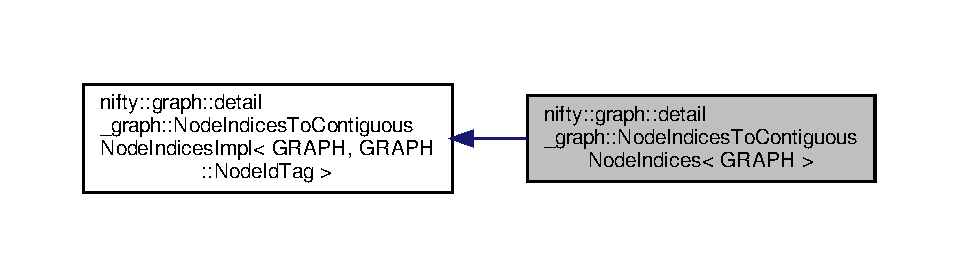
\includegraphics[width=350pt]{classnifty_1_1graph_1_1detail__graph_1_1NodeIndicesToContiguousNodeIndices__inherit__graph}
\end{center}
\end{figure}


Collaboration diagram for nifty\+:\+:graph\+:\+:detail\+\_\+graph\+:\+:Node\+Indices\+To\+Contiguous\+Node\+Indices$<$ G\+R\+A\+PH $>$\+:
\nopagebreak
\begin{figure}[H]
\begin{center}
\leavevmode
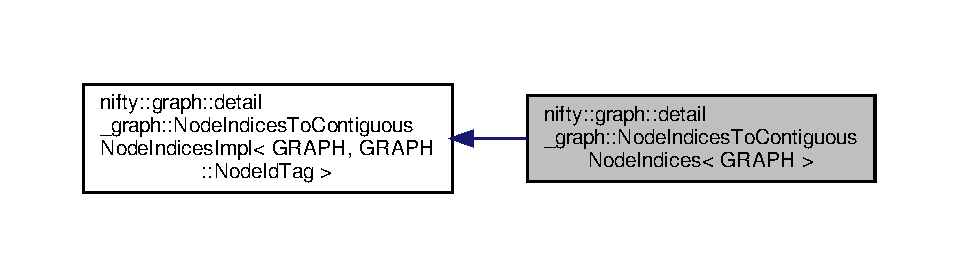
\includegraphics[width=350pt]{classnifty_1_1graph_1_1detail__graph_1_1NodeIndicesToContiguousNodeIndices__coll__graph}
\end{center}
\end{figure}
\subsection*{Additional Inherited Members}


The documentation for this class was generated from the following file\+:\begin{DoxyCompactItemize}
\item 
/home/tbeier/src/nifty/include/nifty/graph/detail/\hyperlink{contiguous__indices_8hxx}{contiguous\+\_\+indices.\+hxx}\end{DoxyCompactItemize}

\hypertarget{classnifty_1_1graph_1_1detail__graph_1_1NodeIndicesToContiguousNodeIndicesImpl}{}\section{nifty\+:\+:graph\+:\+:detail\+\_\+graph\+:\+:Node\+Indices\+To\+Contiguous\+Node\+Indices\+Impl$<$ G\+R\+A\+PH, N\+O\+D\+E\+\_\+\+I\+D\+\_\+\+T\+AG $>$ Class Template Reference}
\label{classnifty_1_1graph_1_1detail__graph_1_1NodeIndicesToContiguousNodeIndicesImpl}\index{nifty\+::graph\+::detail\+\_\+graph\+::\+Node\+Indices\+To\+Contiguous\+Node\+Indices\+Impl$<$ G\+R\+A\+P\+H, N\+O\+D\+E\+\_\+\+I\+D\+\_\+\+T\+A\+G $>$@{nifty\+::graph\+::detail\+\_\+graph\+::\+Node\+Indices\+To\+Contiguous\+Node\+Indices\+Impl$<$ G\+R\+A\+P\+H, N\+O\+D\+E\+\_\+\+I\+D\+\_\+\+T\+A\+G $>$}}


{\ttfamily \#include $<$contiguous\+\_\+indices.\+hxx$>$}

\subsection*{Public Types}
\begin{DoxyCompactItemize}
\item 
typedef G\+R\+A\+PH \hyperlink{classnifty_1_1graph_1_1detail__graph_1_1NodeIndicesToContiguousNodeIndicesImpl_ad59d071f31d84046a821f0ddb406c21e}{Graph\+Type}
\end{DoxyCompactItemize}
\subsection*{Public Member Functions}
\begin{DoxyCompactItemize}
\item 
\hyperlink{classnifty_1_1graph_1_1detail__graph_1_1NodeIndicesToContiguousNodeIndicesImpl_a11cb2c2e77e50dab32081e1b42e0a6b4}{Node\+Indices\+To\+Contiguous\+Node\+Indices\+Impl} (const \hyperlink{classnifty_1_1graph_1_1detail__graph_1_1NodeIndicesToContiguousNodeIndicesImpl_ad59d071f31d84046a821f0ddb406c21e}{Graph\+Type} \&graph)
\item 
int64\+\_\+t \hyperlink{classnifty_1_1graph_1_1detail__graph_1_1NodeIndicesToContiguousNodeIndicesImpl_a38663dd0927fdf715d490f56b7fb3873}{operator\mbox{[}$\,$\mbox{]}} (const int64\+\_\+t node) const
\end{DoxyCompactItemize}


\subsection{Member Typedef Documentation}
\mbox{\Hypertarget{classnifty_1_1graph_1_1detail__graph_1_1NodeIndicesToContiguousNodeIndicesImpl_ad59d071f31d84046a821f0ddb406c21e}\label{classnifty_1_1graph_1_1detail__graph_1_1NodeIndicesToContiguousNodeIndicesImpl_ad59d071f31d84046a821f0ddb406c21e}} 
\index{nifty\+::graph\+::detail\+\_\+graph\+::\+Node\+Indices\+To\+Contiguous\+Node\+Indices\+Impl@{nifty\+::graph\+::detail\+\_\+graph\+::\+Node\+Indices\+To\+Contiguous\+Node\+Indices\+Impl}!Graph\+Type@{Graph\+Type}}
\index{Graph\+Type@{Graph\+Type}!nifty\+::graph\+::detail\+\_\+graph\+::\+Node\+Indices\+To\+Contiguous\+Node\+Indices\+Impl@{nifty\+::graph\+::detail\+\_\+graph\+::\+Node\+Indices\+To\+Contiguous\+Node\+Indices\+Impl}}
\subsubsection{\texorpdfstring{Graph\+Type}{GraphType}}
{\footnotesize\ttfamily template$<$class G\+R\+A\+PH, class N\+O\+D\+E\+\_\+\+I\+D\+\_\+\+T\+AG$>$ \\
typedef G\+R\+A\+PH \hyperlink{classnifty_1_1graph_1_1detail__graph_1_1NodeIndicesToContiguousNodeIndicesImpl}{nifty\+::graph\+::detail\+\_\+graph\+::\+Node\+Indices\+To\+Contiguous\+Node\+Indices\+Impl}$<$ G\+R\+A\+PH, N\+O\+D\+E\+\_\+\+I\+D\+\_\+\+T\+AG $>$\+::\hyperlink{classnifty_1_1graph_1_1detail__graph_1_1NodeIndicesToContiguousNodeIndicesImpl_ad59d071f31d84046a821f0ddb406c21e}{Graph\+Type}}



\subsection{Constructor \& Destructor Documentation}
\mbox{\Hypertarget{classnifty_1_1graph_1_1detail__graph_1_1NodeIndicesToContiguousNodeIndicesImpl_a11cb2c2e77e50dab32081e1b42e0a6b4}\label{classnifty_1_1graph_1_1detail__graph_1_1NodeIndicesToContiguousNodeIndicesImpl_a11cb2c2e77e50dab32081e1b42e0a6b4}} 
\index{nifty\+::graph\+::detail\+\_\+graph\+::\+Node\+Indices\+To\+Contiguous\+Node\+Indices\+Impl@{nifty\+::graph\+::detail\+\_\+graph\+::\+Node\+Indices\+To\+Contiguous\+Node\+Indices\+Impl}!Node\+Indices\+To\+Contiguous\+Node\+Indices\+Impl@{Node\+Indices\+To\+Contiguous\+Node\+Indices\+Impl}}
\index{Node\+Indices\+To\+Contiguous\+Node\+Indices\+Impl@{Node\+Indices\+To\+Contiguous\+Node\+Indices\+Impl}!nifty\+::graph\+::detail\+\_\+graph\+::\+Node\+Indices\+To\+Contiguous\+Node\+Indices\+Impl@{nifty\+::graph\+::detail\+\_\+graph\+::\+Node\+Indices\+To\+Contiguous\+Node\+Indices\+Impl}}
\subsubsection{\texorpdfstring{Node\+Indices\+To\+Contiguous\+Node\+Indices\+Impl()}{NodeIndicesToContiguousNodeIndicesImpl()}}
{\footnotesize\ttfamily template$<$class G\+R\+A\+PH, class N\+O\+D\+E\+\_\+\+I\+D\+\_\+\+T\+AG$>$ \\
\hyperlink{classnifty_1_1graph_1_1detail__graph_1_1NodeIndicesToContiguousNodeIndicesImpl}{nifty\+::graph\+::detail\+\_\+graph\+::\+Node\+Indices\+To\+Contiguous\+Node\+Indices\+Impl}$<$ G\+R\+A\+PH, N\+O\+D\+E\+\_\+\+I\+D\+\_\+\+T\+AG $>$\+::\hyperlink{classnifty_1_1graph_1_1detail__graph_1_1NodeIndicesToContiguousNodeIndicesImpl}{Node\+Indices\+To\+Contiguous\+Node\+Indices\+Impl} (\begin{DoxyParamCaption}\item[{const \hyperlink{classnifty_1_1graph_1_1detail__graph_1_1NodeIndicesToContiguousNodeIndicesImpl_ad59d071f31d84046a821f0ddb406c21e}{Graph\+Type} \&}]{graph }\end{DoxyParamCaption})\hspace{0.3cm}{\ttfamily [inline]}}



\subsection{Member Function Documentation}
\mbox{\Hypertarget{classnifty_1_1graph_1_1detail__graph_1_1NodeIndicesToContiguousNodeIndicesImpl_a38663dd0927fdf715d490f56b7fb3873}\label{classnifty_1_1graph_1_1detail__graph_1_1NodeIndicesToContiguousNodeIndicesImpl_a38663dd0927fdf715d490f56b7fb3873}} 
\index{nifty\+::graph\+::detail\+\_\+graph\+::\+Node\+Indices\+To\+Contiguous\+Node\+Indices\+Impl@{nifty\+::graph\+::detail\+\_\+graph\+::\+Node\+Indices\+To\+Contiguous\+Node\+Indices\+Impl}!operator\mbox{[}\mbox{]}@{operator[]}}
\index{operator\mbox{[}\mbox{]}@{operator[]}!nifty\+::graph\+::detail\+\_\+graph\+::\+Node\+Indices\+To\+Contiguous\+Node\+Indices\+Impl@{nifty\+::graph\+::detail\+\_\+graph\+::\+Node\+Indices\+To\+Contiguous\+Node\+Indices\+Impl}}
\subsubsection{\texorpdfstring{operator[]()}{operator[]()}}
{\footnotesize\ttfamily template$<$class G\+R\+A\+PH, class N\+O\+D\+E\+\_\+\+I\+D\+\_\+\+T\+AG$>$ \\
int64\+\_\+t \hyperlink{classnifty_1_1graph_1_1detail__graph_1_1NodeIndicesToContiguousNodeIndicesImpl}{nifty\+::graph\+::detail\+\_\+graph\+::\+Node\+Indices\+To\+Contiguous\+Node\+Indices\+Impl}$<$ G\+R\+A\+PH, N\+O\+D\+E\+\_\+\+I\+D\+\_\+\+T\+AG $>$\+::operator\mbox{[}$\,$\mbox{]} (\begin{DoxyParamCaption}\item[{const int64\+\_\+t}]{node }\end{DoxyParamCaption}) const\hspace{0.3cm}{\ttfamily [inline]}}



The documentation for this class was generated from the following file\+:\begin{DoxyCompactItemize}
\item 
/home/tbeier/src/nifty/include/nifty/graph/detail/\hyperlink{contiguous__indices_8hxx}{contiguous\+\_\+indices.\+hxx}\end{DoxyCompactItemize}

\hypertarget{classnifty_1_1graph_1_1detail__graph_1_1NodeIndicesToContiguousNodeIndicesImpl_3_01GRAPH_00_01ni9b1f0e77953ef9967804436d9931bab9}{}\section{nifty\+:\+:graph\+:\+:detail\+\_\+graph\+:\+:Node\+Indices\+To\+Contiguous\+Node\+Indices\+Impl$<$ G\+R\+A\+P\+H, nifty\+:\+:graph\+:\+:Contiguous\+Tag $>$ Class Template Reference}
\label{classnifty_1_1graph_1_1detail__graph_1_1NodeIndicesToContiguousNodeIndicesImpl_3_01GRAPH_00_01ni9b1f0e77953ef9967804436d9931bab9}\index{nifty\+::graph\+::detail\+\_\+graph\+::\+Node\+Indices\+To\+Contiguous\+Node\+Indices\+Impl$<$ G\+R\+A\+P\+H, nifty\+::graph\+::\+Contiguous\+Tag $>$@{nifty\+::graph\+::detail\+\_\+graph\+::\+Node\+Indices\+To\+Contiguous\+Node\+Indices\+Impl$<$ G\+R\+A\+P\+H, nifty\+::graph\+::\+Contiguous\+Tag $>$}}


{\ttfamily \#include $<$contiguous\+\_\+indices.\+hxx$>$}

\subsection*{Public Types}
\begin{DoxyCompactItemize}
\item 
typedef G\+R\+A\+P\+H \hyperlink{classnifty_1_1graph_1_1detail__graph_1_1NodeIndicesToContiguousNodeIndicesImpl_3_01GRAPH_00_01ni9b1f0e77953ef9967804436d9931bab9_a5bfb9d22b775eeea19c32af5dfcd482f}{Graph}
\end{DoxyCompactItemize}
\subsection*{Public Member Functions}
\begin{DoxyCompactItemize}
\item 
\hyperlink{classnifty_1_1graph_1_1detail__graph_1_1NodeIndicesToContiguousNodeIndicesImpl_3_01GRAPH_00_01ni9b1f0e77953ef9967804436d9931bab9_a4247b773e3c6b878a30246a45c935d75}{Node\+Indices\+To\+Contiguous\+Node\+Indices\+Impl} (const \hyperlink{classnifty_1_1graph_1_1detail__graph_1_1NodeIndicesToContiguousNodeIndicesImpl_3_01GRAPH_00_01ni9b1f0e77953ef9967804436d9931bab9_a5bfb9d22b775eeea19c32af5dfcd482f}{Graph} \&graph)
\item 
int64\+\_\+t \hyperlink{classnifty_1_1graph_1_1detail__graph_1_1NodeIndicesToContiguousNodeIndicesImpl_3_01GRAPH_00_01ni9b1f0e77953ef9967804436d9931bab9_a30191e2b4ecf6f075fe69e53480b9ae0}{operator\mbox{[}$\,$\mbox{]}} (const int64\+\_\+t node) const 
\end{DoxyCompactItemize}


\subsection{Member Typedef Documentation}
\hypertarget{classnifty_1_1graph_1_1detail__graph_1_1NodeIndicesToContiguousNodeIndicesImpl_3_01GRAPH_00_01ni9b1f0e77953ef9967804436d9931bab9_a5bfb9d22b775eeea19c32af5dfcd482f}{}\index{nifty\+::graph\+::detail\+\_\+graph\+::\+Node\+Indices\+To\+Contiguous\+Node\+Indices\+Impl$<$ G\+R\+A\+P\+H, nifty\+::graph\+::\+Contiguous\+Tag $>$@{nifty\+::graph\+::detail\+\_\+graph\+::\+Node\+Indices\+To\+Contiguous\+Node\+Indices\+Impl$<$ G\+R\+A\+P\+H, nifty\+::graph\+::\+Contiguous\+Tag $>$}!Graph@{Graph}}
\index{Graph@{Graph}!nifty\+::graph\+::detail\+\_\+graph\+::\+Node\+Indices\+To\+Contiguous\+Node\+Indices\+Impl$<$ G\+R\+A\+P\+H, nifty\+::graph\+::\+Contiguous\+Tag $>$@{nifty\+::graph\+::detail\+\_\+graph\+::\+Node\+Indices\+To\+Contiguous\+Node\+Indices\+Impl$<$ G\+R\+A\+P\+H, nifty\+::graph\+::\+Contiguous\+Tag $>$}}
\subsubsection[{Graph}]{\setlength{\rightskip}{0pt plus 5cm}template$<$class G\+R\+A\+P\+H $>$ typedef G\+R\+A\+P\+H {\bf nifty\+::graph\+::detail\+\_\+graph\+::\+Node\+Indices\+To\+Contiguous\+Node\+Indices\+Impl}$<$ G\+R\+A\+P\+H, {\bf nifty\+::graph\+::\+Contiguous\+Tag} $>$\+::{\bf Graph}}\label{classnifty_1_1graph_1_1detail__graph_1_1NodeIndicesToContiguousNodeIndicesImpl_3_01GRAPH_00_01ni9b1f0e77953ef9967804436d9931bab9_a5bfb9d22b775eeea19c32af5dfcd482f}


\subsection{Constructor \& Destructor Documentation}
\hypertarget{classnifty_1_1graph_1_1detail__graph_1_1NodeIndicesToContiguousNodeIndicesImpl_3_01GRAPH_00_01ni9b1f0e77953ef9967804436d9931bab9_a4247b773e3c6b878a30246a45c935d75}{}\index{nifty\+::graph\+::detail\+\_\+graph\+::\+Node\+Indices\+To\+Contiguous\+Node\+Indices\+Impl$<$ G\+R\+A\+P\+H, nifty\+::graph\+::\+Contiguous\+Tag $>$@{nifty\+::graph\+::detail\+\_\+graph\+::\+Node\+Indices\+To\+Contiguous\+Node\+Indices\+Impl$<$ G\+R\+A\+P\+H, nifty\+::graph\+::\+Contiguous\+Tag $>$}!Node\+Indices\+To\+Contiguous\+Node\+Indices\+Impl@{Node\+Indices\+To\+Contiguous\+Node\+Indices\+Impl}}
\index{Node\+Indices\+To\+Contiguous\+Node\+Indices\+Impl@{Node\+Indices\+To\+Contiguous\+Node\+Indices\+Impl}!nifty\+::graph\+::detail\+\_\+graph\+::\+Node\+Indices\+To\+Contiguous\+Node\+Indices\+Impl$<$ G\+R\+A\+P\+H, nifty\+::graph\+::\+Contiguous\+Tag $>$@{nifty\+::graph\+::detail\+\_\+graph\+::\+Node\+Indices\+To\+Contiguous\+Node\+Indices\+Impl$<$ G\+R\+A\+P\+H, nifty\+::graph\+::\+Contiguous\+Tag $>$}}
\subsubsection[{Node\+Indices\+To\+Contiguous\+Node\+Indices\+Impl(const Graph \&graph)}]{\setlength{\rightskip}{0pt plus 5cm}template$<$class G\+R\+A\+P\+H $>$ {\bf nifty\+::graph\+::detail\+\_\+graph\+::\+Node\+Indices\+To\+Contiguous\+Node\+Indices\+Impl}$<$ G\+R\+A\+P\+H, {\bf nifty\+::graph\+::\+Contiguous\+Tag} $>$\+::{\bf Node\+Indices\+To\+Contiguous\+Node\+Indices\+Impl} (
\begin{DoxyParamCaption}
\item[{const {\bf Graph} \&}]{graph}
\end{DoxyParamCaption}
)\hspace{0.3cm}{\ttfamily [inline]}}\label{classnifty_1_1graph_1_1detail__graph_1_1NodeIndicesToContiguousNodeIndicesImpl_3_01GRAPH_00_01ni9b1f0e77953ef9967804436d9931bab9_a4247b773e3c6b878a30246a45c935d75}


\subsection{Member Function Documentation}
\hypertarget{classnifty_1_1graph_1_1detail__graph_1_1NodeIndicesToContiguousNodeIndicesImpl_3_01GRAPH_00_01ni9b1f0e77953ef9967804436d9931bab9_a30191e2b4ecf6f075fe69e53480b9ae0}{}\index{nifty\+::graph\+::detail\+\_\+graph\+::\+Node\+Indices\+To\+Contiguous\+Node\+Indices\+Impl$<$ G\+R\+A\+P\+H, nifty\+::graph\+::\+Contiguous\+Tag $>$@{nifty\+::graph\+::detail\+\_\+graph\+::\+Node\+Indices\+To\+Contiguous\+Node\+Indices\+Impl$<$ G\+R\+A\+P\+H, nifty\+::graph\+::\+Contiguous\+Tag $>$}!operator\mbox{[}$\,$\mbox{]}@{operator[]}}
\index{operator\mbox{[}$\,$\mbox{]}@{operator[]}!nifty\+::graph\+::detail\+\_\+graph\+::\+Node\+Indices\+To\+Contiguous\+Node\+Indices\+Impl$<$ G\+R\+A\+P\+H, nifty\+::graph\+::\+Contiguous\+Tag $>$@{nifty\+::graph\+::detail\+\_\+graph\+::\+Node\+Indices\+To\+Contiguous\+Node\+Indices\+Impl$<$ G\+R\+A\+P\+H, nifty\+::graph\+::\+Contiguous\+Tag $>$}}
\subsubsection[{operator[](const int64\+\_\+t node) const }]{\setlength{\rightskip}{0pt plus 5cm}template$<$class G\+R\+A\+P\+H $>$ int64\+\_\+t {\bf nifty\+::graph\+::detail\+\_\+graph\+::\+Node\+Indices\+To\+Contiguous\+Node\+Indices\+Impl}$<$ G\+R\+A\+P\+H, {\bf nifty\+::graph\+::\+Contiguous\+Tag} $>$\+::operator\mbox{[}$\,$\mbox{]} (
\begin{DoxyParamCaption}
\item[{const int64\+\_\+t}]{node}
\end{DoxyParamCaption}
) const\hspace{0.3cm}{\ttfamily [inline]}}\label{classnifty_1_1graph_1_1detail__graph_1_1NodeIndicesToContiguousNodeIndicesImpl_3_01GRAPH_00_01ni9b1f0e77953ef9967804436d9931bab9_a30191e2b4ecf6f075fe69e53480b9ae0}


The documentation for this class was generated from the following file\+:\begin{DoxyCompactItemize}
\item 
/home/tbeier/src/nifty/include/nifty/graph/detail/\hyperlink{contiguous__indices_8hxx}{contiguous\+\_\+indices.\+hxx}\end{DoxyCompactItemize}

\hypertarget{structnifty_1_1graph_1_1DirectedGraphBase_1_1NodeIterRange}{}\section{nifty\+:\+:graph\+:\+:Directed\+Graph\+Base$<$ C\+H\+I\+L\+D\+\_\+\+G\+R\+A\+P\+H $>$\+:\+:Node\+Iter\+Range$<$ \+\_\+\+C\+H\+I\+L\+D\+\_\+\+G\+R\+A\+P\+H $>$ Struct Template Reference}
\label{structnifty_1_1graph_1_1DirectedGraphBase_1_1NodeIterRange}\index{nifty\+::graph\+::\+Directed\+Graph\+Base$<$ C\+H\+I\+L\+D\+\_\+\+G\+R\+A\+P\+H $>$\+::\+Node\+Iter\+Range$<$ \+\_\+\+C\+H\+I\+L\+D\+\_\+\+G\+R\+A\+P\+H $>$@{nifty\+::graph\+::\+Directed\+Graph\+Base$<$ C\+H\+I\+L\+D\+\_\+\+G\+R\+A\+P\+H $>$\+::\+Node\+Iter\+Range$<$ \+\_\+\+C\+H\+I\+L\+D\+\_\+\+G\+R\+A\+P\+H $>$}}


{\ttfamily \#include $<$directed\+\_\+graph\+\_\+base.\+hxx$>$}



Inheritance diagram for nifty\+:\+:graph\+:\+:Directed\+Graph\+Base$<$ C\+H\+I\+L\+D\+\_\+\+G\+R\+A\+P\+H $>$\+:\+:Node\+Iter\+Range$<$ \+\_\+\+C\+H\+I\+L\+D\+\_\+\+G\+R\+A\+P\+H $>$\+:
% FIG 0


Collaboration diagram for nifty\+:\+:graph\+:\+:Directed\+Graph\+Base$<$ C\+H\+I\+L\+D\+\_\+\+G\+R\+A\+P\+H $>$\+:\+:Node\+Iter\+Range$<$ \+\_\+\+C\+H\+I\+L\+D\+\_\+\+G\+R\+A\+P\+H $>$\+:
% FIG 1
\subsection*{Additional Inherited Members}


The documentation for this struct was generated from the following file\+:\begin{DoxyCompactItemize}
\item 
/home/tbeier/src/nifty/include/nifty/graph/\hyperlink{directed__graph__base_8hxx}{directed\+\_\+graph\+\_\+base.\+hxx}\end{DoxyCompactItemize}

\hypertarget{structnifty_1_1graph_1_1UndirectedGraphBase_1_1NodeIterRange}{}\section{nifty\+:\+:graph\+:\+:Undirected\+Graph\+Base$<$ C\+H\+I\+L\+D\+\_\+\+G\+R\+A\+PH, N\+O\+D\+E\+\_\+\+I\+T\+ER, E\+D\+G\+E\+\_\+\+I\+T\+ER, A\+D\+J\+A\+C\+E\+N\+C\+Y\+\_\+\+I\+T\+ER $>$\+:\+:Node\+Iter\+Range$<$ \+\_\+\+C\+H\+I\+L\+D\+\_\+\+G\+R\+A\+PH $>$ Struct Template Reference}
\label{structnifty_1_1graph_1_1UndirectedGraphBase_1_1NodeIterRange}\index{nifty\+::graph\+::\+Undirected\+Graph\+Base$<$ C\+H\+I\+L\+D\+\_\+\+G\+R\+A\+P\+H, N\+O\+D\+E\+\_\+\+I\+T\+E\+R, E\+D\+G\+E\+\_\+\+I\+T\+E\+R, A\+D\+J\+A\+C\+E\+N\+C\+Y\+\_\+\+I\+T\+E\+R $>$\+::\+Node\+Iter\+Range$<$ \+\_\+\+C\+H\+I\+L\+D\+\_\+\+G\+R\+A\+P\+H $>$@{nifty\+::graph\+::\+Undirected\+Graph\+Base$<$ C\+H\+I\+L\+D\+\_\+\+G\+R\+A\+P\+H, N\+O\+D\+E\+\_\+\+I\+T\+E\+R, E\+D\+G\+E\+\_\+\+I\+T\+E\+R, A\+D\+J\+A\+C\+E\+N\+C\+Y\+\_\+\+I\+T\+E\+R $>$\+::\+Node\+Iter\+Range$<$ \+\_\+\+C\+H\+I\+L\+D\+\_\+\+G\+R\+A\+P\+H $>$}}


{\ttfamily \#include $<$undirected\+\_\+graph\+\_\+base.\+hxx$>$}



Inheritance diagram for nifty\+:\+:graph\+:\+:Undirected\+Graph\+Base$<$ C\+H\+I\+L\+D\+\_\+\+G\+R\+A\+PH, N\+O\+D\+E\+\_\+\+I\+T\+ER, E\+D\+G\+E\+\_\+\+I\+T\+ER, A\+D\+J\+A\+C\+E\+N\+C\+Y\+\_\+\+I\+T\+ER $>$\+:\+:Node\+Iter\+Range$<$ \+\_\+\+C\+H\+I\+L\+D\+\_\+\+G\+R\+A\+PH $>$\+:
\nopagebreak
\begin{figure}[H]
\begin{center}
\leavevmode
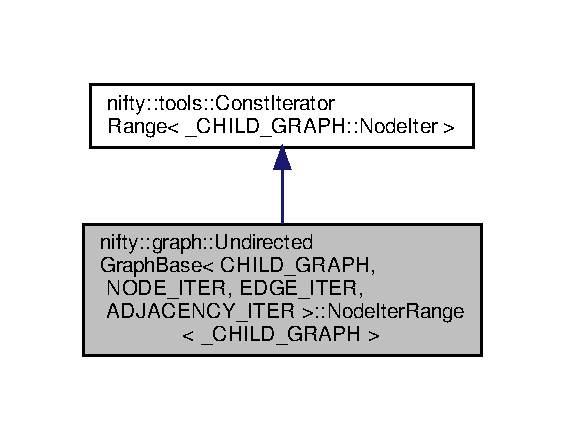
\includegraphics[width=271pt]{structnifty_1_1graph_1_1UndirectedGraphBase_1_1NodeIterRange__inherit__graph}
\end{center}
\end{figure}


Collaboration diagram for nifty\+:\+:graph\+:\+:Undirected\+Graph\+Base$<$ C\+H\+I\+L\+D\+\_\+\+G\+R\+A\+PH, N\+O\+D\+E\+\_\+\+I\+T\+ER, E\+D\+G\+E\+\_\+\+I\+T\+ER, A\+D\+J\+A\+C\+E\+N\+C\+Y\+\_\+\+I\+T\+ER $>$\+:\+:Node\+Iter\+Range$<$ \+\_\+\+C\+H\+I\+L\+D\+\_\+\+G\+R\+A\+PH $>$\+:
\nopagebreak
\begin{figure}[H]
\begin{center}
\leavevmode
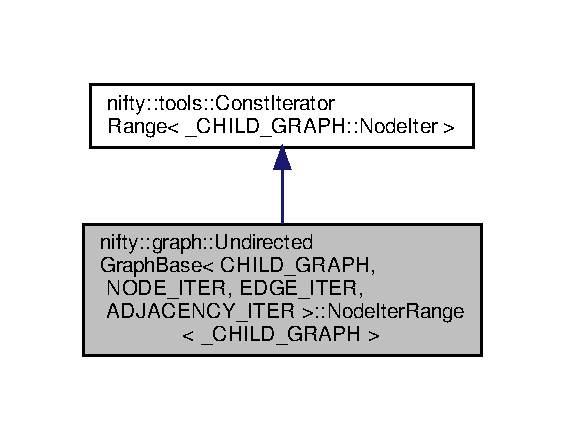
\includegraphics[width=271pt]{structnifty_1_1graph_1_1UndirectedGraphBase_1_1NodeIterRange__coll__graph}
\end{center}
\end{figure}
\subsection*{Additional Inherited Members}


The documentation for this struct was generated from the following file\+:\begin{DoxyCompactItemize}
\item 
/home/tbeier/src/nifty/include/nifty/graph/\hyperlink{undirected__graph__base_8hxx}{undirected\+\_\+graph\+\_\+base.\+hxx}\end{DoxyCompactItemize}

\hypertarget{classnifty_1_1graph_1_1detail__graph_1_1NodeLabelsToEdgeLabelsUnaryFunction}{}\section{nifty\+:\+:graph\+:\+:detail\+\_\+graph\+:\+:Node\+Labels\+To\+Edge\+Labels\+Unary\+Function$<$ G\+R\+A\+P\+H, N\+O\+D\+E\+\_\+\+M\+A\+P $>$ Class Template Reference}
\label{classnifty_1_1graph_1_1detail__graph_1_1NodeLabelsToEdgeLabelsUnaryFunction}\index{nifty\+::graph\+::detail\+\_\+graph\+::\+Node\+Labels\+To\+Edge\+Labels\+Unary\+Function$<$ G\+R\+A\+P\+H, N\+O\+D\+E\+\_\+\+M\+A\+P $>$@{nifty\+::graph\+::detail\+\_\+graph\+::\+Node\+Labels\+To\+Edge\+Labels\+Unary\+Function$<$ G\+R\+A\+P\+H, N\+O\+D\+E\+\_\+\+M\+A\+P $>$}}


{\ttfamily \#include $<$node\+\_\+labels\+\_\+to\+\_\+edge\+\_\+labels\+\_\+iterator.\+hxx$>$}

\subsection*{Public Types}
\begin{DoxyCompactItemize}
\item 
typedef const uint8\+\_\+t \& \hyperlink{classnifty_1_1graph_1_1detail__graph_1_1NodeLabelsToEdgeLabelsUnaryFunction_a50e0f9bfa5b0ce4c60fb0f010cd15110}{Reference}
\item 
typedef uint8\+\_\+t \hyperlink{classnifty_1_1graph_1_1detail__graph_1_1NodeLabelsToEdgeLabelsUnaryFunction_a69f2d0e0bef04e6172466755efee4a8e}{Value}
\item 
typedef const uint8\+\_\+t \& \hyperlink{classnifty_1_1graph_1_1detail__graph_1_1NodeLabelsToEdgeLabelsUnaryFunction_a298c22998b3dcc8aea86f29bb0e9c9b7}{reference}
\item 
typedef uint8\+\_\+t \hyperlink{classnifty_1_1graph_1_1detail__graph_1_1NodeLabelsToEdgeLabelsUnaryFunction_ab0985d82c405b9b0e4422751a2a8b18b}{value}
\end{DoxyCompactItemize}
\subsection*{Public Member Functions}
\begin{DoxyCompactItemize}
\item 
\hyperlink{classnifty_1_1graph_1_1detail__graph_1_1NodeLabelsToEdgeLabelsUnaryFunction_a27e93a8f9e44784d8c17e40fbf295db8}{Node\+Labels\+To\+Edge\+Labels\+Unary\+Function} (const G\+R\+A\+P\+H \&graph, const N\+O\+D\+E\+\_\+\+M\+A\+P \&node\+Labels)
\item 
\hyperlink{classnifty_1_1graph_1_1detail__graph_1_1NodeLabelsToEdgeLabelsUnaryFunction_a9325812abd92290323172cb501929d36}{Node\+Labels\+To\+Edge\+Labels\+Unary\+Function} (const \hyperlink{classnifty_1_1graph_1_1detail__graph_1_1NodeLabelsToEdgeLabelsUnaryFunction}{Node\+Labels\+To\+Edge\+Labels\+Unary\+Function} \&other)
\item 
const uint8\+\_\+t \& \hyperlink{classnifty_1_1graph_1_1detail__graph_1_1NodeLabelsToEdgeLabelsUnaryFunction_abdc5a66fc34a0e0b8323e12362452036}{operator()} (const int64\+\_\+t edge\+Id) const 
\end{DoxyCompactItemize}


\subsection{Member Typedef Documentation}
\hypertarget{classnifty_1_1graph_1_1detail__graph_1_1NodeLabelsToEdgeLabelsUnaryFunction_a50e0f9bfa5b0ce4c60fb0f010cd15110}{}\index{nifty\+::graph\+::detail\+\_\+graph\+::\+Node\+Labels\+To\+Edge\+Labels\+Unary\+Function@{nifty\+::graph\+::detail\+\_\+graph\+::\+Node\+Labels\+To\+Edge\+Labels\+Unary\+Function}!Reference@{Reference}}
\index{Reference@{Reference}!nifty\+::graph\+::detail\+\_\+graph\+::\+Node\+Labels\+To\+Edge\+Labels\+Unary\+Function@{nifty\+::graph\+::detail\+\_\+graph\+::\+Node\+Labels\+To\+Edge\+Labels\+Unary\+Function}}
\subsubsection[{Reference}]{\setlength{\rightskip}{0pt plus 5cm}template$<$class G\+R\+A\+P\+H , class N\+O\+D\+E\+\_\+\+M\+A\+P $>$ typedef const uint8\+\_\+t\& {\bf nifty\+::graph\+::detail\+\_\+graph\+::\+Node\+Labels\+To\+Edge\+Labels\+Unary\+Function}$<$ G\+R\+A\+P\+H, N\+O\+D\+E\+\_\+\+M\+A\+P $>$\+::{\bf Reference}}\label{classnifty_1_1graph_1_1detail__graph_1_1NodeLabelsToEdgeLabelsUnaryFunction_a50e0f9bfa5b0ce4c60fb0f010cd15110}
\hypertarget{classnifty_1_1graph_1_1detail__graph_1_1NodeLabelsToEdgeLabelsUnaryFunction_a298c22998b3dcc8aea86f29bb0e9c9b7}{}\index{nifty\+::graph\+::detail\+\_\+graph\+::\+Node\+Labels\+To\+Edge\+Labels\+Unary\+Function@{nifty\+::graph\+::detail\+\_\+graph\+::\+Node\+Labels\+To\+Edge\+Labels\+Unary\+Function}!reference@{reference}}
\index{reference@{reference}!nifty\+::graph\+::detail\+\_\+graph\+::\+Node\+Labels\+To\+Edge\+Labels\+Unary\+Function@{nifty\+::graph\+::detail\+\_\+graph\+::\+Node\+Labels\+To\+Edge\+Labels\+Unary\+Function}}
\subsubsection[{reference}]{\setlength{\rightskip}{0pt plus 5cm}template$<$class G\+R\+A\+P\+H , class N\+O\+D\+E\+\_\+\+M\+A\+P $>$ typedef const uint8\+\_\+t\& {\bf nifty\+::graph\+::detail\+\_\+graph\+::\+Node\+Labels\+To\+Edge\+Labels\+Unary\+Function}$<$ G\+R\+A\+P\+H, N\+O\+D\+E\+\_\+\+M\+A\+P $>$\+::{\bf reference}}\label{classnifty_1_1graph_1_1detail__graph_1_1NodeLabelsToEdgeLabelsUnaryFunction_a298c22998b3dcc8aea86f29bb0e9c9b7}
\hypertarget{classnifty_1_1graph_1_1detail__graph_1_1NodeLabelsToEdgeLabelsUnaryFunction_a69f2d0e0bef04e6172466755efee4a8e}{}\index{nifty\+::graph\+::detail\+\_\+graph\+::\+Node\+Labels\+To\+Edge\+Labels\+Unary\+Function@{nifty\+::graph\+::detail\+\_\+graph\+::\+Node\+Labels\+To\+Edge\+Labels\+Unary\+Function}!Value@{Value}}
\index{Value@{Value}!nifty\+::graph\+::detail\+\_\+graph\+::\+Node\+Labels\+To\+Edge\+Labels\+Unary\+Function@{nifty\+::graph\+::detail\+\_\+graph\+::\+Node\+Labels\+To\+Edge\+Labels\+Unary\+Function}}
\subsubsection[{Value}]{\setlength{\rightskip}{0pt plus 5cm}template$<$class G\+R\+A\+P\+H , class N\+O\+D\+E\+\_\+\+M\+A\+P $>$ typedef uint8\+\_\+t {\bf nifty\+::graph\+::detail\+\_\+graph\+::\+Node\+Labels\+To\+Edge\+Labels\+Unary\+Function}$<$ G\+R\+A\+P\+H, N\+O\+D\+E\+\_\+\+M\+A\+P $>$\+::{\bf Value}}\label{classnifty_1_1graph_1_1detail__graph_1_1NodeLabelsToEdgeLabelsUnaryFunction_a69f2d0e0bef04e6172466755efee4a8e}
\hypertarget{classnifty_1_1graph_1_1detail__graph_1_1NodeLabelsToEdgeLabelsUnaryFunction_ab0985d82c405b9b0e4422751a2a8b18b}{}\index{nifty\+::graph\+::detail\+\_\+graph\+::\+Node\+Labels\+To\+Edge\+Labels\+Unary\+Function@{nifty\+::graph\+::detail\+\_\+graph\+::\+Node\+Labels\+To\+Edge\+Labels\+Unary\+Function}!value@{value}}
\index{value@{value}!nifty\+::graph\+::detail\+\_\+graph\+::\+Node\+Labels\+To\+Edge\+Labels\+Unary\+Function@{nifty\+::graph\+::detail\+\_\+graph\+::\+Node\+Labels\+To\+Edge\+Labels\+Unary\+Function}}
\subsubsection[{value}]{\setlength{\rightskip}{0pt plus 5cm}template$<$class G\+R\+A\+P\+H , class N\+O\+D\+E\+\_\+\+M\+A\+P $>$ typedef uint8\+\_\+t {\bf nifty\+::graph\+::detail\+\_\+graph\+::\+Node\+Labels\+To\+Edge\+Labels\+Unary\+Function}$<$ G\+R\+A\+P\+H, N\+O\+D\+E\+\_\+\+M\+A\+P $>$\+::{\bf value}}\label{classnifty_1_1graph_1_1detail__graph_1_1NodeLabelsToEdgeLabelsUnaryFunction_ab0985d82c405b9b0e4422751a2a8b18b}


\subsection{Constructor \& Destructor Documentation}
\hypertarget{classnifty_1_1graph_1_1detail__graph_1_1NodeLabelsToEdgeLabelsUnaryFunction_a27e93a8f9e44784d8c17e40fbf295db8}{}\index{nifty\+::graph\+::detail\+\_\+graph\+::\+Node\+Labels\+To\+Edge\+Labels\+Unary\+Function@{nifty\+::graph\+::detail\+\_\+graph\+::\+Node\+Labels\+To\+Edge\+Labels\+Unary\+Function}!Node\+Labels\+To\+Edge\+Labels\+Unary\+Function@{Node\+Labels\+To\+Edge\+Labels\+Unary\+Function}}
\index{Node\+Labels\+To\+Edge\+Labels\+Unary\+Function@{Node\+Labels\+To\+Edge\+Labels\+Unary\+Function}!nifty\+::graph\+::detail\+\_\+graph\+::\+Node\+Labels\+To\+Edge\+Labels\+Unary\+Function@{nifty\+::graph\+::detail\+\_\+graph\+::\+Node\+Labels\+To\+Edge\+Labels\+Unary\+Function}}
\subsubsection[{Node\+Labels\+To\+Edge\+Labels\+Unary\+Function(const G\+R\+A\+P\+H \&graph, const N\+O\+D\+E\+\_\+\+M\+A\+P \&node\+Labels)}]{\setlength{\rightskip}{0pt plus 5cm}template$<$class G\+R\+A\+P\+H , class N\+O\+D\+E\+\_\+\+M\+A\+P $>$ {\bf nifty\+::graph\+::detail\+\_\+graph\+::\+Node\+Labels\+To\+Edge\+Labels\+Unary\+Function}$<$ G\+R\+A\+P\+H, N\+O\+D\+E\+\_\+\+M\+A\+P $>$\+::{\bf Node\+Labels\+To\+Edge\+Labels\+Unary\+Function} (
\begin{DoxyParamCaption}
\item[{const G\+R\+A\+P\+H \&}]{graph, }
\item[{const N\+O\+D\+E\+\_\+\+M\+A\+P \&}]{node\+Labels}
\end{DoxyParamCaption}
)\hspace{0.3cm}{\ttfamily [inline]}}\label{classnifty_1_1graph_1_1detail__graph_1_1NodeLabelsToEdgeLabelsUnaryFunction_a27e93a8f9e44784d8c17e40fbf295db8}
\hypertarget{classnifty_1_1graph_1_1detail__graph_1_1NodeLabelsToEdgeLabelsUnaryFunction_a9325812abd92290323172cb501929d36}{}\index{nifty\+::graph\+::detail\+\_\+graph\+::\+Node\+Labels\+To\+Edge\+Labels\+Unary\+Function@{nifty\+::graph\+::detail\+\_\+graph\+::\+Node\+Labels\+To\+Edge\+Labels\+Unary\+Function}!Node\+Labels\+To\+Edge\+Labels\+Unary\+Function@{Node\+Labels\+To\+Edge\+Labels\+Unary\+Function}}
\index{Node\+Labels\+To\+Edge\+Labels\+Unary\+Function@{Node\+Labels\+To\+Edge\+Labels\+Unary\+Function}!nifty\+::graph\+::detail\+\_\+graph\+::\+Node\+Labels\+To\+Edge\+Labels\+Unary\+Function@{nifty\+::graph\+::detail\+\_\+graph\+::\+Node\+Labels\+To\+Edge\+Labels\+Unary\+Function}}
\subsubsection[{Node\+Labels\+To\+Edge\+Labels\+Unary\+Function(const Node\+Labels\+To\+Edge\+Labels\+Unary\+Function \&other)}]{\setlength{\rightskip}{0pt plus 5cm}template$<$class G\+R\+A\+P\+H , class N\+O\+D\+E\+\_\+\+M\+A\+P $>$ {\bf nifty\+::graph\+::detail\+\_\+graph\+::\+Node\+Labels\+To\+Edge\+Labels\+Unary\+Function}$<$ G\+R\+A\+P\+H, N\+O\+D\+E\+\_\+\+M\+A\+P $>$\+::{\bf Node\+Labels\+To\+Edge\+Labels\+Unary\+Function} (
\begin{DoxyParamCaption}
\item[{const {\bf Node\+Labels\+To\+Edge\+Labels\+Unary\+Function}$<$ G\+R\+A\+P\+H, N\+O\+D\+E\+\_\+\+M\+A\+P $>$ \&}]{other}
\end{DoxyParamCaption}
)\hspace{0.3cm}{\ttfamily [inline]}}\label{classnifty_1_1graph_1_1detail__graph_1_1NodeLabelsToEdgeLabelsUnaryFunction_a9325812abd92290323172cb501929d36}


\subsection{Member Function Documentation}
\hypertarget{classnifty_1_1graph_1_1detail__graph_1_1NodeLabelsToEdgeLabelsUnaryFunction_abdc5a66fc34a0e0b8323e12362452036}{}\index{nifty\+::graph\+::detail\+\_\+graph\+::\+Node\+Labels\+To\+Edge\+Labels\+Unary\+Function@{nifty\+::graph\+::detail\+\_\+graph\+::\+Node\+Labels\+To\+Edge\+Labels\+Unary\+Function}!operator()@{operator()}}
\index{operator()@{operator()}!nifty\+::graph\+::detail\+\_\+graph\+::\+Node\+Labels\+To\+Edge\+Labels\+Unary\+Function@{nifty\+::graph\+::detail\+\_\+graph\+::\+Node\+Labels\+To\+Edge\+Labels\+Unary\+Function}}
\subsubsection[{operator()(const int64\+\_\+t edge\+Id) const }]{\setlength{\rightskip}{0pt plus 5cm}template$<$class G\+R\+A\+P\+H , class N\+O\+D\+E\+\_\+\+M\+A\+P $>$ const uint8\+\_\+t\& {\bf nifty\+::graph\+::detail\+\_\+graph\+::\+Node\+Labels\+To\+Edge\+Labels\+Unary\+Function}$<$ G\+R\+A\+P\+H, N\+O\+D\+E\+\_\+\+M\+A\+P $>$\+::operator() (
\begin{DoxyParamCaption}
\item[{const int64\+\_\+t}]{edge\+Id}
\end{DoxyParamCaption}
) const\hspace{0.3cm}{\ttfamily [inline]}}\label{classnifty_1_1graph_1_1detail__graph_1_1NodeLabelsToEdgeLabelsUnaryFunction_abdc5a66fc34a0e0b8323e12362452036}


The documentation for this class was generated from the following file\+:\begin{DoxyCompactItemize}
\item 
/home/tbeier/src/nifty/include/nifty/graph/detail/\hyperlink{node__labels__to__edge__labels__iterator_8hxx}{node\+\_\+labels\+\_\+to\+\_\+edge\+\_\+labels\+\_\+iterator.\+hxx}\end{DoxyCompactItemize}

\hypertarget{structnifty_1_1graph_1_1graph__maps_1_1NodeMap}{}\section{nifty\+:\+:graph\+:\+:graph\+\_\+maps\+:\+:Node\+Map$<$ G, T $>$ Struct Template Reference}
\label{structnifty_1_1graph_1_1graph__maps_1_1NodeMap}\index{nifty\+::graph\+::graph\+\_\+maps\+::\+Node\+Map$<$ G, T $>$@{nifty\+::graph\+::graph\+\_\+maps\+::\+Node\+Map$<$ G, T $>$}}


{\ttfamily \#include $<$graph\+\_\+maps.\+hxx$>$}



Inheritance diagram for nifty\+:\+:graph\+:\+:graph\+\_\+maps\+:\+:Node\+Map$<$ G, T $>$\+:
\nopagebreak
\begin{figure}[H]
\begin{center}
\leavevmode
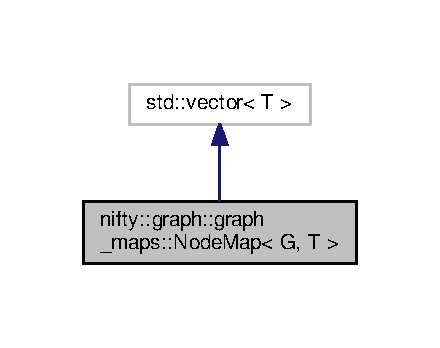
\includegraphics[width=211pt]{structnifty_1_1graph_1_1graph__maps_1_1NodeMap__inherit__graph}
\end{center}
\end{figure}


Collaboration diagram for nifty\+:\+:graph\+:\+:graph\+\_\+maps\+:\+:Node\+Map$<$ G, T $>$\+:
\nopagebreak
\begin{figure}[H]
\begin{center}
\leavevmode
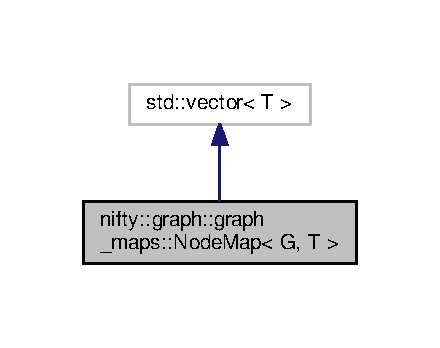
\includegraphics[width=211pt]{structnifty_1_1graph_1_1graph__maps_1_1NodeMap__coll__graph}
\end{center}
\end{figure}
\subsection*{Public Member Functions}
\begin{DoxyCompactItemize}
\item 
\hyperlink{structnifty_1_1graph_1_1graph__maps_1_1NodeMap_a0580548b98c3e769227111e081c0b7a6}{Node\+Map} (const G \&g, const T \&val)
\item 
\hyperlink{structnifty_1_1graph_1_1graph__maps_1_1NodeMap_a759dd195fba1b36d638635e10677e759}{Node\+Map} (const G \&g)
\item 
\hyperlink{structnifty_1_1graph_1_1graph__maps_1_1NodeMap_ac56649d6162ce84c37ffa6c096954bea}{Node\+Map} ()
\item 
void \hyperlink{structnifty_1_1graph_1_1graph__maps_1_1NodeMap_a63aea0a762e0ec912e8c9ef357268d09}{inserted\+Nodes} (const uint64\+\_\+t node\+Id, const T \&insert\+Value=T())
\end{DoxyCompactItemize}


\subsection{Constructor \& Destructor Documentation}
\mbox{\Hypertarget{structnifty_1_1graph_1_1graph__maps_1_1NodeMap_a0580548b98c3e769227111e081c0b7a6}\label{structnifty_1_1graph_1_1graph__maps_1_1NodeMap_a0580548b98c3e769227111e081c0b7a6}} 
\index{nifty\+::graph\+::graph\+\_\+maps\+::\+Node\+Map@{nifty\+::graph\+::graph\+\_\+maps\+::\+Node\+Map}!Node\+Map@{Node\+Map}}
\index{Node\+Map@{Node\+Map}!nifty\+::graph\+::graph\+\_\+maps\+::\+Node\+Map@{nifty\+::graph\+::graph\+\_\+maps\+::\+Node\+Map}}
\subsubsection{\texorpdfstring{Node\+Map()}{NodeMap()}\hspace{0.1cm}{\footnotesize\ttfamily [1/3]}}
{\footnotesize\ttfamily template$<$class G, class T$>$ \\
\hyperlink{structnifty_1_1graph_1_1graph__maps_1_1NodeMap}{nifty\+::graph\+::graph\+\_\+maps\+::\+Node\+Map}$<$ G, T $>$\+::\hyperlink{structnifty_1_1graph_1_1graph__maps_1_1NodeMap}{Node\+Map} (\begin{DoxyParamCaption}\item[{const G \&}]{g,  }\item[{const T \&}]{val }\end{DoxyParamCaption})\hspace{0.3cm}{\ttfamily [inline]}}

\mbox{\Hypertarget{structnifty_1_1graph_1_1graph__maps_1_1NodeMap_a759dd195fba1b36d638635e10677e759}\label{structnifty_1_1graph_1_1graph__maps_1_1NodeMap_a759dd195fba1b36d638635e10677e759}} 
\index{nifty\+::graph\+::graph\+\_\+maps\+::\+Node\+Map@{nifty\+::graph\+::graph\+\_\+maps\+::\+Node\+Map}!Node\+Map@{Node\+Map}}
\index{Node\+Map@{Node\+Map}!nifty\+::graph\+::graph\+\_\+maps\+::\+Node\+Map@{nifty\+::graph\+::graph\+\_\+maps\+::\+Node\+Map}}
\subsubsection{\texorpdfstring{Node\+Map()}{NodeMap()}\hspace{0.1cm}{\footnotesize\ttfamily [2/3]}}
{\footnotesize\ttfamily template$<$class G, class T$>$ \\
\hyperlink{structnifty_1_1graph_1_1graph__maps_1_1NodeMap}{nifty\+::graph\+::graph\+\_\+maps\+::\+Node\+Map}$<$ G, T $>$\+::\hyperlink{structnifty_1_1graph_1_1graph__maps_1_1NodeMap}{Node\+Map} (\begin{DoxyParamCaption}\item[{const G \&}]{g }\end{DoxyParamCaption})\hspace{0.3cm}{\ttfamily [inline]}}

\mbox{\Hypertarget{structnifty_1_1graph_1_1graph__maps_1_1NodeMap_ac56649d6162ce84c37ffa6c096954bea}\label{structnifty_1_1graph_1_1graph__maps_1_1NodeMap_ac56649d6162ce84c37ffa6c096954bea}} 
\index{nifty\+::graph\+::graph\+\_\+maps\+::\+Node\+Map@{nifty\+::graph\+::graph\+\_\+maps\+::\+Node\+Map}!Node\+Map@{Node\+Map}}
\index{Node\+Map@{Node\+Map}!nifty\+::graph\+::graph\+\_\+maps\+::\+Node\+Map@{nifty\+::graph\+::graph\+\_\+maps\+::\+Node\+Map}}
\subsubsection{\texorpdfstring{Node\+Map()}{NodeMap()}\hspace{0.1cm}{\footnotesize\ttfamily [3/3]}}
{\footnotesize\ttfamily template$<$class G, class T$>$ \\
\hyperlink{structnifty_1_1graph_1_1graph__maps_1_1NodeMap}{nifty\+::graph\+::graph\+\_\+maps\+::\+Node\+Map}$<$ G, T $>$\+::\hyperlink{structnifty_1_1graph_1_1graph__maps_1_1NodeMap}{Node\+Map} (\begin{DoxyParamCaption}{ }\end{DoxyParamCaption})\hspace{0.3cm}{\ttfamily [inline]}}



\subsection{Member Function Documentation}
\mbox{\Hypertarget{structnifty_1_1graph_1_1graph__maps_1_1NodeMap_a63aea0a762e0ec912e8c9ef357268d09}\label{structnifty_1_1graph_1_1graph__maps_1_1NodeMap_a63aea0a762e0ec912e8c9ef357268d09}} 
\index{nifty\+::graph\+::graph\+\_\+maps\+::\+Node\+Map@{nifty\+::graph\+::graph\+\_\+maps\+::\+Node\+Map}!inserted\+Nodes@{inserted\+Nodes}}
\index{inserted\+Nodes@{inserted\+Nodes}!nifty\+::graph\+::graph\+\_\+maps\+::\+Node\+Map@{nifty\+::graph\+::graph\+\_\+maps\+::\+Node\+Map}}
\subsubsection{\texorpdfstring{inserted\+Nodes()}{insertedNodes()}}
{\footnotesize\ttfamily template$<$class G, class T$>$ \\
void \hyperlink{structnifty_1_1graph_1_1graph__maps_1_1NodeMap}{nifty\+::graph\+::graph\+\_\+maps\+::\+Node\+Map}$<$ G, T $>$\+::inserted\+Nodes (\begin{DoxyParamCaption}\item[{const uint64\+\_\+t}]{node\+Id,  }\item[{const T \&}]{insert\+Value = {\ttfamily T()} }\end{DoxyParamCaption})\hspace{0.3cm}{\ttfamily [inline]}}



The documentation for this struct was generated from the following file\+:\begin{DoxyCompactItemize}
\item 
/home/tbeier/src/nifty/include/nifty/graph/\hyperlink{graph__maps_8hxx}{graph\+\_\+maps.\+hxx}\end{DoxyCompactItemize}

\hypertarget{structnifty_1_1graph_1_1DirectedGraphBase_1_1NodeMap}{}\section{nifty\+:\+:graph\+:\+:Directed\+Graph\+Base$<$ C\+H\+I\+L\+D\+\_\+\+G\+R\+A\+P\+H $>$\+:\+:Node\+Map$<$ T $>$ Struct Template Reference}
\label{structnifty_1_1graph_1_1DirectedGraphBase_1_1NodeMap}\index{nifty\+::graph\+::\+Directed\+Graph\+Base$<$ C\+H\+I\+L\+D\+\_\+\+G\+R\+A\+P\+H $>$\+::\+Node\+Map$<$ T $>$@{nifty\+::graph\+::\+Directed\+Graph\+Base$<$ C\+H\+I\+L\+D\+\_\+\+G\+R\+A\+P\+H $>$\+::\+Node\+Map$<$ T $>$}}


{\ttfamily \#include $<$directed\+\_\+graph\+\_\+base.\+hxx$>$}



Inheritance diagram for nifty\+:\+:graph\+:\+:Directed\+Graph\+Base$<$ C\+H\+I\+L\+D\+\_\+\+G\+R\+A\+P\+H $>$\+:\+:Node\+Map$<$ T $>$\+:
% FIG 0


Collaboration diagram for nifty\+:\+:graph\+:\+:Directed\+Graph\+Base$<$ C\+H\+I\+L\+D\+\_\+\+G\+R\+A\+P\+H $>$\+:\+:Node\+Map$<$ T $>$\+:
% FIG 1
\subsection*{Additional Inherited Members}


The documentation for this struct was generated from the following file\+:\begin{DoxyCompactItemize}
\item 
/home/tbeier/src/nifty/include/nifty/graph/\hyperlink{directed__graph__base_8hxx}{directed\+\_\+graph\+\_\+base.\+hxx}\end{DoxyCompactItemize}

\hypertarget{structnifty_1_1graph_1_1UndirectedGraphBase_1_1NodeMap}{}\section{nifty\+:\+:graph\+:\+:Undirected\+Graph\+Base$<$ C\+H\+I\+L\+D\+\_\+\+G\+R\+A\+P\+H, N\+O\+D\+E\+\_\+\+I\+T\+E\+R, E\+D\+G\+E\+\_\+\+I\+T\+E\+R, A\+D\+J\+A\+C\+E\+N\+C\+Y\+\_\+\+I\+T\+E\+R $>$\+:\+:Node\+Map$<$ T $>$ Struct Template Reference}
\label{structnifty_1_1graph_1_1UndirectedGraphBase_1_1NodeMap}\index{nifty\+::graph\+::\+Undirected\+Graph\+Base$<$ C\+H\+I\+L\+D\+\_\+\+G\+R\+A\+P\+H, N\+O\+D\+E\+\_\+\+I\+T\+E\+R, E\+D\+G\+E\+\_\+\+I\+T\+E\+R, A\+D\+J\+A\+C\+E\+N\+C\+Y\+\_\+\+I\+T\+E\+R $>$\+::\+Node\+Map$<$ T $>$@{nifty\+::graph\+::\+Undirected\+Graph\+Base$<$ C\+H\+I\+L\+D\+\_\+\+G\+R\+A\+P\+H, N\+O\+D\+E\+\_\+\+I\+T\+E\+R, E\+D\+G\+E\+\_\+\+I\+T\+E\+R, A\+D\+J\+A\+C\+E\+N\+C\+Y\+\_\+\+I\+T\+E\+R $>$\+::\+Node\+Map$<$ T $>$}}


{\ttfamily \#include $<$undirected\+\_\+graph\+\_\+base.\+hxx$>$}



Inheritance diagram for nifty\+:\+:graph\+:\+:Undirected\+Graph\+Base$<$ C\+H\+I\+L\+D\+\_\+\+G\+R\+A\+P\+H, N\+O\+D\+E\+\_\+\+I\+T\+E\+R, E\+D\+G\+E\+\_\+\+I\+T\+E\+R, A\+D\+J\+A\+C\+E\+N\+C\+Y\+\_\+\+I\+T\+E\+R $>$\+:\+:Node\+Map$<$ T $>$\+:\nopagebreak
\begin{figure}[H]
\begin{center}
\leavevmode
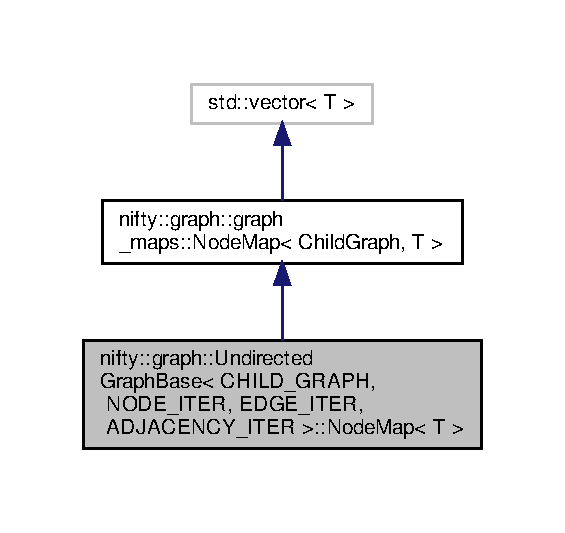
\includegraphics[width=271pt]{structnifty_1_1graph_1_1UndirectedGraphBase_1_1NodeMap__inherit__graph}
\end{center}
\end{figure}


Collaboration diagram for nifty\+:\+:graph\+:\+:Undirected\+Graph\+Base$<$ C\+H\+I\+L\+D\+\_\+\+G\+R\+A\+P\+H, N\+O\+D\+E\+\_\+\+I\+T\+E\+R, E\+D\+G\+E\+\_\+\+I\+T\+E\+R, A\+D\+J\+A\+C\+E\+N\+C\+Y\+\_\+\+I\+T\+E\+R $>$\+:\+:Node\+Map$<$ T $>$\+:\nopagebreak
\begin{figure}[H]
\begin{center}
\leavevmode
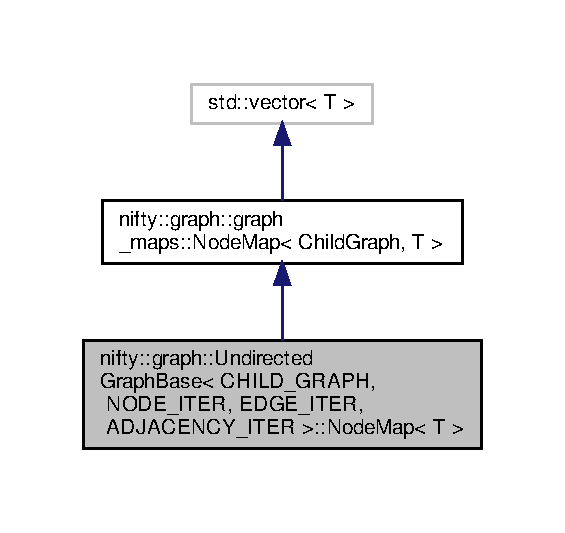
\includegraphics[width=271pt]{structnifty_1_1graph_1_1UndirectedGraphBase_1_1NodeMap__coll__graph}
\end{center}
\end{figure}
\subsection*{Additional Inherited Members}


The documentation for this struct was generated from the following file\+:\begin{DoxyCompactItemize}
\item 
/home/tbeier/src/nifty/include/nifty/graph/\hyperlink{undirected__graph__base_8hxx}{undirected\+\_\+graph\+\_\+base.\+hxx}\end{DoxyCompactItemize}

\hypertarget{structnifty_1_1graph_1_1NodeTag}{}\section{nifty\+:\+:graph\+:\+:Node\+Tag Struct Reference}
\label{structnifty_1_1graph_1_1NodeTag}\index{nifty\+::graph\+::\+Node\+Tag@{nifty\+::graph\+::\+Node\+Tag}}


{\ttfamily \#include $<$graph\+\_\+tags.\+hxx$>$}



The documentation for this struct was generated from the following file\+:\begin{DoxyCompactItemize}
\item 
/home/tbeier/src/nifty/include/nifty/graph/\hyperlink{graph__tags_8hxx}{graph\+\_\+tags.\+hxx}\end{DoxyCompactItemize}

\hypertarget{classnifty_1_1math_1_1Numerics}{}\section{nifty\+:\+:math\+:\+:Numerics$<$ T $>$ Class Template Reference}
\label{classnifty_1_1math_1_1Numerics}\index{nifty\+::math\+::\+Numerics$<$ T $>$@{nifty\+::math\+::\+Numerics$<$ T $>$}}


{\ttfamily \#include $<$numerics.\+hxx$>$}



Inheritance diagram for nifty\+:\+:math\+:\+:Numerics$<$ T $>$\+:
\nopagebreak
\begin{figure}[H]
\begin{center}
\leavevmode
\includegraphics[width=226pt]{classnifty_1_1math_1_1Numerics__inherit__graph}
\end{center}
\end{figure}


Collaboration diagram for nifty\+:\+:math\+:\+:Numerics$<$ T $>$\+:
\nopagebreak
\begin{figure}[H]
\begin{center}
\leavevmode
\includegraphics[width=226pt]{classnifty_1_1math_1_1Numerics__coll__graph}
\end{center}
\end{figure}


The documentation for this class was generated from the following file\+:\begin{DoxyCompactItemize}
\item 
/home/tbeier/src/nifty/include/nifty/math/\hyperlink{numerics_8hxx}{numerics.\+hxx}\end{DoxyCompactItemize}

\hypertarget{classnifty_1_1math_1_1NumericsImplDispatch}{}\section{nifty\+:\+:math\+:\+:Numerics\+Impl\+Dispatch$<$ T, I\+S\+\_\+\+N\+U\+M\+B\+ER $>$ Class Template Reference}
\label{classnifty_1_1math_1_1NumericsImplDispatch}\index{nifty\+::math\+::\+Numerics\+Impl\+Dispatch$<$ T, I\+S\+\_\+\+N\+U\+M\+B\+E\+R $>$@{nifty\+::math\+::\+Numerics\+Impl\+Dispatch$<$ T, I\+S\+\_\+\+N\+U\+M\+B\+E\+R $>$}}


{\ttfamily \#include $<$numerics.\+hxx$>$}



The documentation for this class was generated from the following file\+:\begin{DoxyCompactItemize}
\item 
/home/tbeier/src/nifty/include/nifty/math/\hyperlink{numerics_8hxx}{numerics.\+hxx}\end{DoxyCompactItemize}

\hypertarget{classnifty_1_1math_1_1NumericsImplDispatch_3_01T_00_01true_01_4}{}\section{nifty\+:\+:math\+:\+:Numerics\+Impl\+Dispatch$<$ T, true $>$ Class Template Reference}
\label{classnifty_1_1math_1_1NumericsImplDispatch_3_01T_00_01true_01_4}\index{nifty\+::math\+::\+Numerics\+Impl\+Dispatch$<$ T, true $>$@{nifty\+::math\+::\+Numerics\+Impl\+Dispatch$<$ T, true $>$}}


{\ttfamily \#include $<$numerics.\+hxx$>$}

\subsection*{Public Types}
\begin{DoxyCompactItemize}
\item 
typedef vigra\+::\+Numeric\+Traits$<$ T $>$\+::Real\+Promote \hyperlink{classnifty_1_1math_1_1NumericsImplDispatch_3_01T_00_01true_01_4_a3e74e0598758a7b5630fc2b0b0b96287}{Real\+Promote\+Type}
\end{DoxyCompactItemize}
\subsection*{Static Public Member Functions}
\begin{DoxyCompactItemize}
\item 
static constexpr T \hyperlink{classnifty_1_1math_1_1NumericsImplDispatch_3_01T_00_01true_01_4_a9b03d43866c3215a3350e253c405d340}{zero} ()
\item 
static constexpr T \hyperlink{classnifty_1_1math_1_1NumericsImplDispatch_3_01T_00_01true_01_4_ae8f6f7ad483adcd16c81f88b4ec81796}{one} ()
\item 
static void \hyperlink{classnifty_1_1math_1_1NumericsImplDispatch_3_01T_00_01true_01_4_aa8c1fee5ba420a6b2fce989b2b37a5d4}{zero} (T \&value)
\item 
static T \hyperlink{classnifty_1_1math_1_1NumericsImplDispatch_3_01T_00_01true_01_4_ad81280c38267c997ccc9794fa2611532}{one} (T \&value)
\item 
static \hyperlink{classnifty_1_1math_1_1NumericsImplDispatch_3_01T_00_01true_01_4_a3e74e0598758a7b5630fc2b0b0b96287}{Real\+Promote\+Type} \hyperlink{classnifty_1_1math_1_1NumericsImplDispatch_3_01T_00_01true_01_4_acff483acc0a49f49daee8fd39f007e45}{real} (const T \&value)
\end{DoxyCompactItemize}


\subsection{Member Typedef Documentation}
\hypertarget{classnifty_1_1math_1_1NumericsImplDispatch_3_01T_00_01true_01_4_a3e74e0598758a7b5630fc2b0b0b96287}{}\index{nifty\+::math\+::\+Numerics\+Impl\+Dispatch$<$ T, true $>$@{nifty\+::math\+::\+Numerics\+Impl\+Dispatch$<$ T, true $>$}!Real\+Promote\+Type@{Real\+Promote\+Type}}
\index{Real\+Promote\+Type@{Real\+Promote\+Type}!nifty\+::math\+::\+Numerics\+Impl\+Dispatch$<$ T, true $>$@{nifty\+::math\+::\+Numerics\+Impl\+Dispatch$<$ T, true $>$}}
\subsubsection[{Real\+Promote\+Type}]{\setlength{\rightskip}{0pt plus 5cm}template$<$class T $>$ typedef vigra\+::\+Numeric\+Traits$<$T$>$\+::Real\+Promote {\bf nifty\+::math\+::\+Numerics\+Impl\+Dispatch}$<$ T, true $>$\+::{\bf Real\+Promote\+Type}}\label{classnifty_1_1math_1_1NumericsImplDispatch_3_01T_00_01true_01_4_a3e74e0598758a7b5630fc2b0b0b96287}


\subsection{Member Function Documentation}
\hypertarget{classnifty_1_1math_1_1NumericsImplDispatch_3_01T_00_01true_01_4_ae8f6f7ad483adcd16c81f88b4ec81796}{}\index{nifty\+::math\+::\+Numerics\+Impl\+Dispatch$<$ T, true $>$@{nifty\+::math\+::\+Numerics\+Impl\+Dispatch$<$ T, true $>$}!one@{one}}
\index{one@{one}!nifty\+::math\+::\+Numerics\+Impl\+Dispatch$<$ T, true $>$@{nifty\+::math\+::\+Numerics\+Impl\+Dispatch$<$ T, true $>$}}
\subsubsection[{one()}]{\setlength{\rightskip}{0pt plus 5cm}template$<$class T $>$ static constexpr T {\bf nifty\+::math\+::\+Numerics\+Impl\+Dispatch}$<$ T, true $>$\+::one (
\begin{DoxyParamCaption}
{}
\end{DoxyParamCaption}
)\hspace{0.3cm}{\ttfamily [inline]}, {\ttfamily [static]}}\label{classnifty_1_1math_1_1NumericsImplDispatch_3_01T_00_01true_01_4_ae8f6f7ad483adcd16c81f88b4ec81796}
\hypertarget{classnifty_1_1math_1_1NumericsImplDispatch_3_01T_00_01true_01_4_ad81280c38267c997ccc9794fa2611532}{}\index{nifty\+::math\+::\+Numerics\+Impl\+Dispatch$<$ T, true $>$@{nifty\+::math\+::\+Numerics\+Impl\+Dispatch$<$ T, true $>$}!one@{one}}
\index{one@{one}!nifty\+::math\+::\+Numerics\+Impl\+Dispatch$<$ T, true $>$@{nifty\+::math\+::\+Numerics\+Impl\+Dispatch$<$ T, true $>$}}
\subsubsection[{one(\+T \&value)}]{\setlength{\rightskip}{0pt plus 5cm}template$<$class T $>$ static T {\bf nifty\+::math\+::\+Numerics\+Impl\+Dispatch}$<$ T, true $>$\+::one (
\begin{DoxyParamCaption}
\item[{T \&}]{value}
\end{DoxyParamCaption}
)\hspace{0.3cm}{\ttfamily [inline]}, {\ttfamily [static]}}\label{classnifty_1_1math_1_1NumericsImplDispatch_3_01T_00_01true_01_4_ad81280c38267c997ccc9794fa2611532}
\hypertarget{classnifty_1_1math_1_1NumericsImplDispatch_3_01T_00_01true_01_4_acff483acc0a49f49daee8fd39f007e45}{}\index{nifty\+::math\+::\+Numerics\+Impl\+Dispatch$<$ T, true $>$@{nifty\+::math\+::\+Numerics\+Impl\+Dispatch$<$ T, true $>$}!real@{real}}
\index{real@{real}!nifty\+::math\+::\+Numerics\+Impl\+Dispatch$<$ T, true $>$@{nifty\+::math\+::\+Numerics\+Impl\+Dispatch$<$ T, true $>$}}
\subsubsection[{real(const T \&value)}]{\setlength{\rightskip}{0pt plus 5cm}template$<$class T $>$ static {\bf Real\+Promote\+Type} {\bf nifty\+::math\+::\+Numerics\+Impl\+Dispatch}$<$ T, true $>$\+::real (
\begin{DoxyParamCaption}
\item[{const T \&}]{value}
\end{DoxyParamCaption}
)\hspace{0.3cm}{\ttfamily [inline]}, {\ttfamily [static]}}\label{classnifty_1_1math_1_1NumericsImplDispatch_3_01T_00_01true_01_4_acff483acc0a49f49daee8fd39f007e45}
\hypertarget{classnifty_1_1math_1_1NumericsImplDispatch_3_01T_00_01true_01_4_a9b03d43866c3215a3350e253c405d340}{}\index{nifty\+::math\+::\+Numerics\+Impl\+Dispatch$<$ T, true $>$@{nifty\+::math\+::\+Numerics\+Impl\+Dispatch$<$ T, true $>$}!zero@{zero}}
\index{zero@{zero}!nifty\+::math\+::\+Numerics\+Impl\+Dispatch$<$ T, true $>$@{nifty\+::math\+::\+Numerics\+Impl\+Dispatch$<$ T, true $>$}}
\subsubsection[{zero()}]{\setlength{\rightskip}{0pt plus 5cm}template$<$class T $>$ static constexpr T {\bf nifty\+::math\+::\+Numerics\+Impl\+Dispatch}$<$ T, true $>$\+::zero (
\begin{DoxyParamCaption}
{}
\end{DoxyParamCaption}
)\hspace{0.3cm}{\ttfamily [inline]}, {\ttfamily [static]}}\label{classnifty_1_1math_1_1NumericsImplDispatch_3_01T_00_01true_01_4_a9b03d43866c3215a3350e253c405d340}
\hypertarget{classnifty_1_1math_1_1NumericsImplDispatch_3_01T_00_01true_01_4_aa8c1fee5ba420a6b2fce989b2b37a5d4}{}\index{nifty\+::math\+::\+Numerics\+Impl\+Dispatch$<$ T, true $>$@{nifty\+::math\+::\+Numerics\+Impl\+Dispatch$<$ T, true $>$}!zero@{zero}}
\index{zero@{zero}!nifty\+::math\+::\+Numerics\+Impl\+Dispatch$<$ T, true $>$@{nifty\+::math\+::\+Numerics\+Impl\+Dispatch$<$ T, true $>$}}
\subsubsection[{zero(\+T \&value)}]{\setlength{\rightskip}{0pt plus 5cm}template$<$class T $>$ static void {\bf nifty\+::math\+::\+Numerics\+Impl\+Dispatch}$<$ T, true $>$\+::zero (
\begin{DoxyParamCaption}
\item[{T \&}]{value}
\end{DoxyParamCaption}
)\hspace{0.3cm}{\ttfamily [inline]}, {\ttfamily [static]}}\label{classnifty_1_1math_1_1NumericsImplDispatch_3_01T_00_01true_01_4_aa8c1fee5ba420a6b2fce989b2b37a5d4}


The documentation for this class was generated from the following file\+:\begin{DoxyCompactItemize}
\item 
/home/tbeier/src/nifty/include/nifty/math/\hyperlink{numerics_8hxx}{numerics.\+hxx}\end{DoxyCompactItemize}

\hypertarget{structnifty_1_1math_1_1NumericTraits}{}\section{nifty\+:\+:math\+:\+:Numeric\+Traits$<$ T $>$ Struct Template Reference}
\label{structnifty_1_1math_1_1NumericTraits}\index{nifty\+::math\+::\+Numeric\+Traits$<$ T $>$@{nifty\+::math\+::\+Numeric\+Traits$<$ T $>$}}


{\ttfamily \#include $<$numerics.\+hxx$>$}



Inheritance diagram for nifty\+:\+:math\+:\+:Numeric\+Traits$<$ T $>$\+:
\nopagebreak
\begin{figure}[H]
\begin{center}
\leavevmode
\includegraphics[width=235pt]{structnifty_1_1math_1_1NumericTraits__inherit__graph}
\end{center}
\end{figure}


Collaboration diagram for nifty\+:\+:math\+:\+:Numeric\+Traits$<$ T $>$\+:
\nopagebreak
\begin{figure}[H]
\begin{center}
\leavevmode
\includegraphics[width=235pt]{structnifty_1_1math_1_1NumericTraits__coll__graph}
\end{center}
\end{figure}
\subsection*{Public Types}
\begin{DoxyCompactItemize}
\item 
typedef vigra\+::\+Numeric\+Traits$<$ T $>$ \hyperlink{structnifty_1_1math_1_1NumericTraits_abccb0907651fb8a346015c6aad17077e}{Base\+Type}
\item 
typedef Base\+Type\+::\+Promote \hyperlink{structnifty_1_1math_1_1NumericTraits_a001a907b6cbeaaf29fb52ff31261e811}{Promote\+Type}
\item 
typedef Base\+Type\+::\+Real\+Promote \hyperlink{structnifty_1_1math_1_1NumericTraits_a5030d5141aa16424cd49d272306cd716}{Real\+Promote\+Type}
\end{DoxyCompactItemize}


\subsection{Member Typedef Documentation}
\mbox{\Hypertarget{structnifty_1_1math_1_1NumericTraits_abccb0907651fb8a346015c6aad17077e}\label{structnifty_1_1math_1_1NumericTraits_abccb0907651fb8a346015c6aad17077e}} 
\index{nifty\+::math\+::\+Numeric\+Traits@{nifty\+::math\+::\+Numeric\+Traits}!Base\+Type@{Base\+Type}}
\index{Base\+Type@{Base\+Type}!nifty\+::math\+::\+Numeric\+Traits@{nifty\+::math\+::\+Numeric\+Traits}}
\subsubsection{\texorpdfstring{Base\+Type}{BaseType}}
{\footnotesize\ttfamily template$<$class T $>$ \\
typedef vigra\+::\+Numeric\+Traits$<$T$>$ \hyperlink{structnifty_1_1math_1_1NumericTraits}{nifty\+::math\+::\+Numeric\+Traits}$<$ T $>$\+::\hyperlink{structnifty_1_1math_1_1NumericTraits_abccb0907651fb8a346015c6aad17077e}{Base\+Type}}

\mbox{\Hypertarget{structnifty_1_1math_1_1NumericTraits_a001a907b6cbeaaf29fb52ff31261e811}\label{structnifty_1_1math_1_1NumericTraits_a001a907b6cbeaaf29fb52ff31261e811}} 
\index{nifty\+::math\+::\+Numeric\+Traits@{nifty\+::math\+::\+Numeric\+Traits}!Promote\+Type@{Promote\+Type}}
\index{Promote\+Type@{Promote\+Type}!nifty\+::math\+::\+Numeric\+Traits@{nifty\+::math\+::\+Numeric\+Traits}}
\subsubsection{\texorpdfstring{Promote\+Type}{PromoteType}}
{\footnotesize\ttfamily template$<$class T $>$ \\
typedef Base\+Type\+::\+Promote \hyperlink{structnifty_1_1math_1_1NumericTraits}{nifty\+::math\+::\+Numeric\+Traits}$<$ T $>$\+::\hyperlink{structnifty_1_1math_1_1NumericTraits_a001a907b6cbeaaf29fb52ff31261e811}{Promote\+Type}}

\mbox{\Hypertarget{structnifty_1_1math_1_1NumericTraits_a5030d5141aa16424cd49d272306cd716}\label{structnifty_1_1math_1_1NumericTraits_a5030d5141aa16424cd49d272306cd716}} 
\index{nifty\+::math\+::\+Numeric\+Traits@{nifty\+::math\+::\+Numeric\+Traits}!Real\+Promote\+Type@{Real\+Promote\+Type}}
\index{Real\+Promote\+Type@{Real\+Promote\+Type}!nifty\+::math\+::\+Numeric\+Traits@{nifty\+::math\+::\+Numeric\+Traits}}
\subsubsection{\texorpdfstring{Real\+Promote\+Type}{RealPromoteType}}
{\footnotesize\ttfamily template$<$class T $>$ \\
typedef Base\+Type\+::\+Real\+Promote \hyperlink{structnifty_1_1math_1_1NumericTraits}{nifty\+::math\+::\+Numeric\+Traits}$<$ T $>$\+::\hyperlink{structnifty_1_1math_1_1NumericTraits_a5030d5141aa16424cd49d272306cd716}{Real\+Promote\+Type}}



The documentation for this struct was generated from the following file\+:\begin{DoxyCompactItemize}
\item 
/home/tbeier/src/nifty/include/nifty/math/\hyperlink{numerics_8hxx}{numerics.\+hxx}\end{DoxyCompactItemize}

\hypertarget{classnifty_1_1ground__truth_1_1Overlap}{}\section{nifty\+:\+:ground\+\_\+truth\+:\+:Overlap$<$ L\+A\+B\+E\+L\+\_\+\+T\+Y\+PE, C\+O\+U\+N\+T\+\_\+\+T\+Y\+PE $>$ Class Template Reference}
\label{classnifty_1_1ground__truth_1_1Overlap}\index{nifty\+::ground\+\_\+truth\+::\+Overlap$<$ L\+A\+B\+E\+L\+\_\+\+T\+Y\+P\+E, C\+O\+U\+N\+T\+\_\+\+T\+Y\+P\+E $>$@{nifty\+::ground\+\_\+truth\+::\+Overlap$<$ L\+A\+B\+E\+L\+\_\+\+T\+Y\+P\+E, C\+O\+U\+N\+T\+\_\+\+T\+Y\+P\+E $>$}}


{\ttfamily \#include $<$overlap.\+hxx$>$}

\subsection*{Public Types}
\begin{DoxyCompactItemize}
\item 
typedef L\+A\+B\+E\+L\+\_\+\+T\+Y\+PE \hyperlink{classnifty_1_1ground__truth_1_1Overlap_af14b9a872d3736d3115231866bc71612}{Label\+Type}
\item 
typedef C\+O\+U\+N\+T\+\_\+\+T\+Y\+PE \hyperlink{classnifty_1_1ground__truth_1_1Overlap_ab8f82b8fef890dc3d7b69da0cc768c76}{Count\+Type}
\item 
typedef std\+::unordered\+\_\+map$<$ \hyperlink{classnifty_1_1ground__truth_1_1Overlap_af14b9a872d3736d3115231866bc71612}{Label\+Type}, \hyperlink{classnifty_1_1ground__truth_1_1Overlap_ab8f82b8fef890dc3d7b69da0cc768c76}{Count\+Type} $>$ \hyperlink{classnifty_1_1ground__truth_1_1Overlap_a6866ee8c988dd21d3fbd6ee5c2e836bf}{Map\+Type}
\end{DoxyCompactItemize}
\subsection*{Public Member Functions}
\begin{DoxyCompactItemize}
\item 
{\footnotesize template$<$class S\+E\+T\+\_\+\+A\+\_\+\+I\+T\+ER , class S\+E\+T\+\_\+\+B\+\_\+\+I\+T\+ER $>$ }\\\hyperlink{classnifty_1_1ground__truth_1_1Overlap_aedaa9af95b736f17f2dbfe0eff4c09bf}{Overlap} (const uint64\+\_\+t max\+Label\+SetA, S\+E\+T\+\_\+\+A\+\_\+\+I\+T\+ER a\+Begin, S\+E\+T\+\_\+\+A\+\_\+\+I\+T\+ER a\+End, S\+E\+T\+\_\+\+B\+\_\+\+I\+T\+ER b\+Begin)
\item 
{\footnotesize template$<$class L\+A\+B\+E\+L\+\_\+A , class L\+A\+B\+E\+L\+\_\+B $>$ }\\\hyperlink{classnifty_1_1ground__truth_1_1Overlap_a0a40f259581e8a4d9e594fd1db23170a}{Overlap} (const uint64\+\_\+t max\+Label\+SetA, const \hyperlink{classandres_1_1View}{marray\+::\+View}$<$ L\+A\+B\+E\+L\+\_\+A $>$ arrayA, const \hyperlink{classandres_1_1View}{marray\+::\+View}$<$ L\+A\+B\+E\+L\+\_\+B $>$ arrayB)
\item 
double \hyperlink{classnifty_1_1ground__truth_1_1Overlap_a0ccece6df11663b9b4d164d4e9148394}{different\+Overlap} (const \hyperlink{classnifty_1_1ground__truth_1_1Overlap_af14b9a872d3736d3115231866bc71612}{Label\+Type} u, const \hyperlink{classnifty_1_1ground__truth_1_1Overlap_af14b9a872d3736d3115231866bc71612}{Label\+Type} v) const
\item 
double \hyperlink{classnifty_1_1ground__truth_1_1Overlap_a52455f7a1bd85ae46dfd213ee397ceed}{bleeding} (const \hyperlink{classnifty_1_1ground__truth_1_1Overlap_af14b9a872d3736d3115231866bc71612}{Label\+Type} u) const
\item 
const std\+::vector$<$ \hyperlink{classnifty_1_1ground__truth_1_1Overlap_ab8f82b8fef890dc3d7b69da0cc768c76}{Count\+Type} $>$ \& \hyperlink{classnifty_1_1ground__truth_1_1Overlap_a2025a2a68d34653179b7c514bd29782b}{counts} () const
\item 
const std\+::vector$<$ \hyperlink{classnifty_1_1ground__truth_1_1Overlap_a6866ee8c988dd21d3fbd6ee5c2e836bf}{Map\+Type} $>$ \& \hyperlink{classnifty_1_1ground__truth_1_1Overlap_a70757f604cd152438eea764a7826df68}{overlaps} () const
\item 
\hyperlink{classnifty_1_1ground__truth_1_1Overlap_af14b9a872d3736d3115231866bc71612}{Label\+Type} \hyperlink{classnifty_1_1ground__truth_1_1Overlap_a440eef37dca6e71f84b8b855acf245c8}{max\+Overlapping\+Label} (const \hyperlink{classnifty_1_1ground__truth_1_1Overlap_af14b9a872d3736d3115231866bc71612}{Label\+Type} u) const
\item 
\hyperlink{classnifty_1_1ground__truth_1_1Overlap_af14b9a872d3736d3115231866bc71612}{Label\+Type} \hyperlink{classnifty_1_1ground__truth_1_1Overlap_adecf7066f58c63a0f4d252102221cf82}{max\+Overlapping\+Label\+Downvote\+Zeros} (const \hyperlink{classnifty_1_1ground__truth_1_1Overlap_af14b9a872d3736d3115231866bc71612}{Label\+Type} u) const
\begin{DoxyCompactList}\small\item\em find the maximum overlapping label and ignore zeros, except if zero is the only overlap. \end{DoxyCompactList}\item 
std\+::pair$<$ \hyperlink{classnifty_1_1ground__truth_1_1Overlap_af14b9a872d3736d3115231866bc71612}{Label\+Type}, bool $>$ \hyperlink{classnifty_1_1ground__truth_1_1Overlap_a1998f00758eb55011a8b91f47f092810}{max\+Overlapping\+Non\+Zero\+Label} (const \hyperlink{classnifty_1_1ground__truth_1_1Overlap_af14b9a872d3736d3115231866bc71612}{Label\+Type} u) const
\item 
bool \hyperlink{classnifty_1_1ground__truth_1_1Overlap_a29459ce889cbfb9fda869817b8e9199b}{is\+Overlapping\+With\+Zero} (const \hyperlink{classnifty_1_1ground__truth_1_1Overlap_af14b9a872d3736d3115231866bc71612}{Label\+Type} u) const
\end{DoxyCompactItemize}


\subsection{Member Typedef Documentation}
\mbox{\Hypertarget{classnifty_1_1ground__truth_1_1Overlap_ab8f82b8fef890dc3d7b69da0cc768c76}\label{classnifty_1_1ground__truth_1_1Overlap_ab8f82b8fef890dc3d7b69da0cc768c76}} 
\index{nifty\+::ground\+\_\+truth\+::\+Overlap@{nifty\+::ground\+\_\+truth\+::\+Overlap}!Count\+Type@{Count\+Type}}
\index{Count\+Type@{Count\+Type}!nifty\+::ground\+\_\+truth\+::\+Overlap@{nifty\+::ground\+\_\+truth\+::\+Overlap}}
\subsubsection{\texorpdfstring{Count\+Type}{CountType}}
{\footnotesize\ttfamily template$<$class L\+A\+B\+E\+L\+\_\+\+T\+Y\+PE  = uint64\+\_\+t, class C\+O\+U\+N\+T\+\_\+\+T\+Y\+PE  = uint64\+\_\+t$>$ \\
typedef C\+O\+U\+N\+T\+\_\+\+T\+Y\+PE \hyperlink{classnifty_1_1ground__truth_1_1Overlap}{nifty\+::ground\+\_\+truth\+::\+Overlap}$<$ L\+A\+B\+E\+L\+\_\+\+T\+Y\+PE, C\+O\+U\+N\+T\+\_\+\+T\+Y\+PE $>$\+::\hyperlink{classnifty_1_1ground__truth_1_1Overlap_ab8f82b8fef890dc3d7b69da0cc768c76}{Count\+Type}}

\mbox{\Hypertarget{classnifty_1_1ground__truth_1_1Overlap_af14b9a872d3736d3115231866bc71612}\label{classnifty_1_1ground__truth_1_1Overlap_af14b9a872d3736d3115231866bc71612}} 
\index{nifty\+::ground\+\_\+truth\+::\+Overlap@{nifty\+::ground\+\_\+truth\+::\+Overlap}!Label\+Type@{Label\+Type}}
\index{Label\+Type@{Label\+Type}!nifty\+::ground\+\_\+truth\+::\+Overlap@{nifty\+::ground\+\_\+truth\+::\+Overlap}}
\subsubsection{\texorpdfstring{Label\+Type}{LabelType}}
{\footnotesize\ttfamily template$<$class L\+A\+B\+E\+L\+\_\+\+T\+Y\+PE  = uint64\+\_\+t, class C\+O\+U\+N\+T\+\_\+\+T\+Y\+PE  = uint64\+\_\+t$>$ \\
typedef L\+A\+B\+E\+L\+\_\+\+T\+Y\+PE \hyperlink{classnifty_1_1ground__truth_1_1Overlap}{nifty\+::ground\+\_\+truth\+::\+Overlap}$<$ L\+A\+B\+E\+L\+\_\+\+T\+Y\+PE, C\+O\+U\+N\+T\+\_\+\+T\+Y\+PE $>$\+::\hyperlink{classnifty_1_1ground__truth_1_1Overlap_af14b9a872d3736d3115231866bc71612}{Label\+Type}}

\mbox{\Hypertarget{classnifty_1_1ground__truth_1_1Overlap_a6866ee8c988dd21d3fbd6ee5c2e836bf}\label{classnifty_1_1ground__truth_1_1Overlap_a6866ee8c988dd21d3fbd6ee5c2e836bf}} 
\index{nifty\+::ground\+\_\+truth\+::\+Overlap@{nifty\+::ground\+\_\+truth\+::\+Overlap}!Map\+Type@{Map\+Type}}
\index{Map\+Type@{Map\+Type}!nifty\+::ground\+\_\+truth\+::\+Overlap@{nifty\+::ground\+\_\+truth\+::\+Overlap}}
\subsubsection{\texorpdfstring{Map\+Type}{MapType}}
{\footnotesize\ttfamily template$<$class L\+A\+B\+E\+L\+\_\+\+T\+Y\+PE  = uint64\+\_\+t, class C\+O\+U\+N\+T\+\_\+\+T\+Y\+PE  = uint64\+\_\+t$>$ \\
typedef std\+::unordered\+\_\+map$<$\hyperlink{classnifty_1_1ground__truth_1_1Overlap_af14b9a872d3736d3115231866bc71612}{Label\+Type}, \hyperlink{classnifty_1_1ground__truth_1_1Overlap_ab8f82b8fef890dc3d7b69da0cc768c76}{Count\+Type}$>$ \hyperlink{classnifty_1_1ground__truth_1_1Overlap}{nifty\+::ground\+\_\+truth\+::\+Overlap}$<$ L\+A\+B\+E\+L\+\_\+\+T\+Y\+PE, C\+O\+U\+N\+T\+\_\+\+T\+Y\+PE $>$\+::\hyperlink{classnifty_1_1ground__truth_1_1Overlap_a6866ee8c988dd21d3fbd6ee5c2e836bf}{Map\+Type}}



\subsection{Constructor \& Destructor Documentation}
\mbox{\Hypertarget{classnifty_1_1ground__truth_1_1Overlap_aedaa9af95b736f17f2dbfe0eff4c09bf}\label{classnifty_1_1ground__truth_1_1Overlap_aedaa9af95b736f17f2dbfe0eff4c09bf}} 
\index{nifty\+::ground\+\_\+truth\+::\+Overlap@{nifty\+::ground\+\_\+truth\+::\+Overlap}!Overlap@{Overlap}}
\index{Overlap@{Overlap}!nifty\+::ground\+\_\+truth\+::\+Overlap@{nifty\+::ground\+\_\+truth\+::\+Overlap}}
\subsubsection{\texorpdfstring{Overlap()}{Overlap()}\hspace{0.1cm}{\footnotesize\ttfamily [1/2]}}
{\footnotesize\ttfamily template$<$class L\+A\+B\+E\+L\+\_\+\+T\+Y\+PE  = uint64\+\_\+t, class C\+O\+U\+N\+T\+\_\+\+T\+Y\+PE  = uint64\+\_\+t$>$ \\
template$<$class S\+E\+T\+\_\+\+A\+\_\+\+I\+T\+ER , class S\+E\+T\+\_\+\+B\+\_\+\+I\+T\+ER $>$ \\
\hyperlink{classnifty_1_1ground__truth_1_1Overlap}{nifty\+::ground\+\_\+truth\+::\+Overlap}$<$ L\+A\+B\+E\+L\+\_\+\+T\+Y\+PE, C\+O\+U\+N\+T\+\_\+\+T\+Y\+PE $>$\+::\hyperlink{classnifty_1_1ground__truth_1_1Overlap}{Overlap} (\begin{DoxyParamCaption}\item[{const uint64\+\_\+t}]{max\+Label\+SetA,  }\item[{S\+E\+T\+\_\+\+A\+\_\+\+I\+T\+ER}]{a\+Begin,  }\item[{S\+E\+T\+\_\+\+A\+\_\+\+I\+T\+ER}]{a\+End,  }\item[{S\+E\+T\+\_\+\+B\+\_\+\+I\+T\+ER}]{b\+Begin }\end{DoxyParamCaption})\hspace{0.3cm}{\ttfamily [inline]}}

\mbox{\Hypertarget{classnifty_1_1ground__truth_1_1Overlap_a0a40f259581e8a4d9e594fd1db23170a}\label{classnifty_1_1ground__truth_1_1Overlap_a0a40f259581e8a4d9e594fd1db23170a}} 
\index{nifty\+::ground\+\_\+truth\+::\+Overlap@{nifty\+::ground\+\_\+truth\+::\+Overlap}!Overlap@{Overlap}}
\index{Overlap@{Overlap}!nifty\+::ground\+\_\+truth\+::\+Overlap@{nifty\+::ground\+\_\+truth\+::\+Overlap}}
\subsubsection{\texorpdfstring{Overlap()}{Overlap()}\hspace{0.1cm}{\footnotesize\ttfamily [2/2]}}
{\footnotesize\ttfamily template$<$class L\+A\+B\+E\+L\+\_\+\+T\+Y\+PE  = uint64\+\_\+t, class C\+O\+U\+N\+T\+\_\+\+T\+Y\+PE  = uint64\+\_\+t$>$ \\
template$<$class L\+A\+B\+E\+L\+\_\+A , class L\+A\+B\+E\+L\+\_\+B $>$ \\
\hyperlink{classnifty_1_1ground__truth_1_1Overlap}{nifty\+::ground\+\_\+truth\+::\+Overlap}$<$ L\+A\+B\+E\+L\+\_\+\+T\+Y\+PE, C\+O\+U\+N\+T\+\_\+\+T\+Y\+PE $>$\+::\hyperlink{classnifty_1_1ground__truth_1_1Overlap}{Overlap} (\begin{DoxyParamCaption}\item[{const uint64\+\_\+t}]{max\+Label\+SetA,  }\item[{const \hyperlink{classandres_1_1View}{marray\+::\+View}$<$ L\+A\+B\+E\+L\+\_\+A $>$}]{arrayA,  }\item[{const \hyperlink{classandres_1_1View}{marray\+::\+View}$<$ L\+A\+B\+E\+L\+\_\+B $>$}]{arrayB }\end{DoxyParamCaption})\hspace{0.3cm}{\ttfamily [inline]}}



\subsection{Member Function Documentation}
\mbox{\Hypertarget{classnifty_1_1ground__truth_1_1Overlap_a52455f7a1bd85ae46dfd213ee397ceed}\label{classnifty_1_1ground__truth_1_1Overlap_a52455f7a1bd85ae46dfd213ee397ceed}} 
\index{nifty\+::ground\+\_\+truth\+::\+Overlap@{nifty\+::ground\+\_\+truth\+::\+Overlap}!bleeding@{bleeding}}
\index{bleeding@{bleeding}!nifty\+::ground\+\_\+truth\+::\+Overlap@{nifty\+::ground\+\_\+truth\+::\+Overlap}}
\subsubsection{\texorpdfstring{bleeding()}{bleeding()}}
{\footnotesize\ttfamily template$<$class L\+A\+B\+E\+L\+\_\+\+T\+Y\+PE  = uint64\+\_\+t, class C\+O\+U\+N\+T\+\_\+\+T\+Y\+PE  = uint64\+\_\+t$>$ \\
double \hyperlink{classnifty_1_1ground__truth_1_1Overlap}{nifty\+::ground\+\_\+truth\+::\+Overlap}$<$ L\+A\+B\+E\+L\+\_\+\+T\+Y\+PE, C\+O\+U\+N\+T\+\_\+\+T\+Y\+PE $>$\+::bleeding (\begin{DoxyParamCaption}\item[{const \hyperlink{classnifty_1_1ground__truth_1_1Overlap_af14b9a872d3736d3115231866bc71612}{Label\+Type}}]{u }\end{DoxyParamCaption}) const\hspace{0.3cm}{\ttfamily [inline]}}

\mbox{\Hypertarget{classnifty_1_1ground__truth_1_1Overlap_a2025a2a68d34653179b7c514bd29782b}\label{classnifty_1_1ground__truth_1_1Overlap_a2025a2a68d34653179b7c514bd29782b}} 
\index{nifty\+::ground\+\_\+truth\+::\+Overlap@{nifty\+::ground\+\_\+truth\+::\+Overlap}!counts@{counts}}
\index{counts@{counts}!nifty\+::ground\+\_\+truth\+::\+Overlap@{nifty\+::ground\+\_\+truth\+::\+Overlap}}
\subsubsection{\texorpdfstring{counts()}{counts()}}
{\footnotesize\ttfamily template$<$class L\+A\+B\+E\+L\+\_\+\+T\+Y\+PE  = uint64\+\_\+t, class C\+O\+U\+N\+T\+\_\+\+T\+Y\+PE  = uint64\+\_\+t$>$ \\
const std\+::vector$<$\hyperlink{classnifty_1_1ground__truth_1_1Overlap_ab8f82b8fef890dc3d7b69da0cc768c76}{Count\+Type}$>$\& \hyperlink{classnifty_1_1ground__truth_1_1Overlap}{nifty\+::ground\+\_\+truth\+::\+Overlap}$<$ L\+A\+B\+E\+L\+\_\+\+T\+Y\+PE, C\+O\+U\+N\+T\+\_\+\+T\+Y\+PE $>$\+::counts (\begin{DoxyParamCaption}{ }\end{DoxyParamCaption}) const\hspace{0.3cm}{\ttfamily [inline]}}

\mbox{\Hypertarget{classnifty_1_1ground__truth_1_1Overlap_a0ccece6df11663b9b4d164d4e9148394}\label{classnifty_1_1ground__truth_1_1Overlap_a0ccece6df11663b9b4d164d4e9148394}} 
\index{nifty\+::ground\+\_\+truth\+::\+Overlap@{nifty\+::ground\+\_\+truth\+::\+Overlap}!different\+Overlap@{different\+Overlap}}
\index{different\+Overlap@{different\+Overlap}!nifty\+::ground\+\_\+truth\+::\+Overlap@{nifty\+::ground\+\_\+truth\+::\+Overlap}}
\subsubsection{\texorpdfstring{different\+Overlap()}{differentOverlap()}}
{\footnotesize\ttfamily template$<$class L\+A\+B\+E\+L\+\_\+\+T\+Y\+PE  = uint64\+\_\+t, class C\+O\+U\+N\+T\+\_\+\+T\+Y\+PE  = uint64\+\_\+t$>$ \\
double \hyperlink{classnifty_1_1ground__truth_1_1Overlap}{nifty\+::ground\+\_\+truth\+::\+Overlap}$<$ L\+A\+B\+E\+L\+\_\+\+T\+Y\+PE, C\+O\+U\+N\+T\+\_\+\+T\+Y\+PE $>$\+::different\+Overlap (\begin{DoxyParamCaption}\item[{const \hyperlink{classnifty_1_1ground__truth_1_1Overlap_af14b9a872d3736d3115231866bc71612}{Label\+Type}}]{u,  }\item[{const \hyperlink{classnifty_1_1ground__truth_1_1Overlap_af14b9a872d3736d3115231866bc71612}{Label\+Type}}]{v }\end{DoxyParamCaption}) const\hspace{0.3cm}{\ttfamily [inline]}}

\mbox{\Hypertarget{classnifty_1_1ground__truth_1_1Overlap_a29459ce889cbfb9fda869817b8e9199b}\label{classnifty_1_1ground__truth_1_1Overlap_a29459ce889cbfb9fda869817b8e9199b}} 
\index{nifty\+::ground\+\_\+truth\+::\+Overlap@{nifty\+::ground\+\_\+truth\+::\+Overlap}!is\+Overlapping\+With\+Zero@{is\+Overlapping\+With\+Zero}}
\index{is\+Overlapping\+With\+Zero@{is\+Overlapping\+With\+Zero}!nifty\+::ground\+\_\+truth\+::\+Overlap@{nifty\+::ground\+\_\+truth\+::\+Overlap}}
\subsubsection{\texorpdfstring{is\+Overlapping\+With\+Zero()}{isOverlappingWithZero()}}
{\footnotesize\ttfamily template$<$class L\+A\+B\+E\+L\+\_\+\+T\+Y\+PE  = uint64\+\_\+t, class C\+O\+U\+N\+T\+\_\+\+T\+Y\+PE  = uint64\+\_\+t$>$ \\
bool \hyperlink{classnifty_1_1ground__truth_1_1Overlap}{nifty\+::ground\+\_\+truth\+::\+Overlap}$<$ L\+A\+B\+E\+L\+\_\+\+T\+Y\+PE, C\+O\+U\+N\+T\+\_\+\+T\+Y\+PE $>$\+::is\+Overlapping\+With\+Zero (\begin{DoxyParamCaption}\item[{const \hyperlink{classnifty_1_1ground__truth_1_1Overlap_af14b9a872d3736d3115231866bc71612}{Label\+Type}}]{u }\end{DoxyParamCaption}) const\hspace{0.3cm}{\ttfamily [inline]}}

\mbox{\Hypertarget{classnifty_1_1ground__truth_1_1Overlap_a440eef37dca6e71f84b8b855acf245c8}\label{classnifty_1_1ground__truth_1_1Overlap_a440eef37dca6e71f84b8b855acf245c8}} 
\index{nifty\+::ground\+\_\+truth\+::\+Overlap@{nifty\+::ground\+\_\+truth\+::\+Overlap}!max\+Overlapping\+Label@{max\+Overlapping\+Label}}
\index{max\+Overlapping\+Label@{max\+Overlapping\+Label}!nifty\+::ground\+\_\+truth\+::\+Overlap@{nifty\+::ground\+\_\+truth\+::\+Overlap}}
\subsubsection{\texorpdfstring{max\+Overlapping\+Label()}{maxOverlappingLabel()}}
{\footnotesize\ttfamily template$<$class L\+A\+B\+E\+L\+\_\+\+T\+Y\+PE  = uint64\+\_\+t, class C\+O\+U\+N\+T\+\_\+\+T\+Y\+PE  = uint64\+\_\+t$>$ \\
\hyperlink{classnifty_1_1ground__truth_1_1Overlap_af14b9a872d3736d3115231866bc71612}{Label\+Type} \hyperlink{classnifty_1_1ground__truth_1_1Overlap}{nifty\+::ground\+\_\+truth\+::\+Overlap}$<$ L\+A\+B\+E\+L\+\_\+\+T\+Y\+PE, C\+O\+U\+N\+T\+\_\+\+T\+Y\+PE $>$\+::max\+Overlapping\+Label (\begin{DoxyParamCaption}\item[{const \hyperlink{classnifty_1_1ground__truth_1_1Overlap_af14b9a872d3736d3115231866bc71612}{Label\+Type}}]{u }\end{DoxyParamCaption}) const\hspace{0.3cm}{\ttfamily [inline]}}

\mbox{\Hypertarget{classnifty_1_1ground__truth_1_1Overlap_adecf7066f58c63a0f4d252102221cf82}\label{classnifty_1_1ground__truth_1_1Overlap_adecf7066f58c63a0f4d252102221cf82}} 
\index{nifty\+::ground\+\_\+truth\+::\+Overlap@{nifty\+::ground\+\_\+truth\+::\+Overlap}!max\+Overlapping\+Label\+Downvote\+Zeros@{max\+Overlapping\+Label\+Downvote\+Zeros}}
\index{max\+Overlapping\+Label\+Downvote\+Zeros@{max\+Overlapping\+Label\+Downvote\+Zeros}!nifty\+::ground\+\_\+truth\+::\+Overlap@{nifty\+::ground\+\_\+truth\+::\+Overlap}}
\subsubsection{\texorpdfstring{max\+Overlapping\+Label\+Downvote\+Zeros()}{maxOverlappingLabelDownvoteZeros()}}
{\footnotesize\ttfamily template$<$class L\+A\+B\+E\+L\+\_\+\+T\+Y\+PE  = uint64\+\_\+t, class C\+O\+U\+N\+T\+\_\+\+T\+Y\+PE  = uint64\+\_\+t$>$ \\
\hyperlink{classnifty_1_1ground__truth_1_1Overlap_af14b9a872d3736d3115231866bc71612}{Label\+Type} \hyperlink{classnifty_1_1ground__truth_1_1Overlap}{nifty\+::ground\+\_\+truth\+::\+Overlap}$<$ L\+A\+B\+E\+L\+\_\+\+T\+Y\+PE, C\+O\+U\+N\+T\+\_\+\+T\+Y\+PE $>$\+::max\+Overlapping\+Label\+Downvote\+Zeros (\begin{DoxyParamCaption}\item[{const \hyperlink{classnifty_1_1ground__truth_1_1Overlap_af14b9a872d3736d3115231866bc71612}{Label\+Type}}]{u }\end{DoxyParamCaption}) const\hspace{0.3cm}{\ttfamily [inline]}}



find the maximum overlapping label and ignore zeros, except if zero is the only overlap. 


\begin{DoxyParams}[1]{Parameters}
\mbox{\tt in}  & {\em u} & query label\\
\hline
\end{DoxyParams}
\begin{DoxyReturn}{Returns}
maximum overlapping label 
\end{DoxyReturn}
\mbox{\Hypertarget{classnifty_1_1ground__truth_1_1Overlap_a1998f00758eb55011a8b91f47f092810}\label{classnifty_1_1ground__truth_1_1Overlap_a1998f00758eb55011a8b91f47f092810}} 
\index{nifty\+::ground\+\_\+truth\+::\+Overlap@{nifty\+::ground\+\_\+truth\+::\+Overlap}!max\+Overlapping\+Non\+Zero\+Label@{max\+Overlapping\+Non\+Zero\+Label}}
\index{max\+Overlapping\+Non\+Zero\+Label@{max\+Overlapping\+Non\+Zero\+Label}!nifty\+::ground\+\_\+truth\+::\+Overlap@{nifty\+::ground\+\_\+truth\+::\+Overlap}}
\subsubsection{\texorpdfstring{max\+Overlapping\+Non\+Zero\+Label()}{maxOverlappingNonZeroLabel()}}
{\footnotesize\ttfamily template$<$class L\+A\+B\+E\+L\+\_\+\+T\+Y\+PE  = uint64\+\_\+t, class C\+O\+U\+N\+T\+\_\+\+T\+Y\+PE  = uint64\+\_\+t$>$ \\
std\+::pair$<$\hyperlink{classnifty_1_1ground__truth_1_1Overlap_af14b9a872d3736d3115231866bc71612}{Label\+Type},bool$>$ \hyperlink{classnifty_1_1ground__truth_1_1Overlap}{nifty\+::ground\+\_\+truth\+::\+Overlap}$<$ L\+A\+B\+E\+L\+\_\+\+T\+Y\+PE, C\+O\+U\+N\+T\+\_\+\+T\+Y\+PE $>$\+::max\+Overlapping\+Non\+Zero\+Label (\begin{DoxyParamCaption}\item[{const \hyperlink{classnifty_1_1ground__truth_1_1Overlap_af14b9a872d3736d3115231866bc71612}{Label\+Type}}]{u }\end{DoxyParamCaption}) const\hspace{0.3cm}{\ttfamily [inline]}}

\mbox{\Hypertarget{classnifty_1_1ground__truth_1_1Overlap_a70757f604cd152438eea764a7826df68}\label{classnifty_1_1ground__truth_1_1Overlap_a70757f604cd152438eea764a7826df68}} 
\index{nifty\+::ground\+\_\+truth\+::\+Overlap@{nifty\+::ground\+\_\+truth\+::\+Overlap}!overlaps@{overlaps}}
\index{overlaps@{overlaps}!nifty\+::ground\+\_\+truth\+::\+Overlap@{nifty\+::ground\+\_\+truth\+::\+Overlap}}
\subsubsection{\texorpdfstring{overlaps()}{overlaps()}}
{\footnotesize\ttfamily template$<$class L\+A\+B\+E\+L\+\_\+\+T\+Y\+PE  = uint64\+\_\+t, class C\+O\+U\+N\+T\+\_\+\+T\+Y\+PE  = uint64\+\_\+t$>$ \\
const std\+::vector$<$\hyperlink{classnifty_1_1ground__truth_1_1Overlap_a6866ee8c988dd21d3fbd6ee5c2e836bf}{Map\+Type}$>$\& \hyperlink{classnifty_1_1ground__truth_1_1Overlap}{nifty\+::ground\+\_\+truth\+::\+Overlap}$<$ L\+A\+B\+E\+L\+\_\+\+T\+Y\+PE, C\+O\+U\+N\+T\+\_\+\+T\+Y\+PE $>$\+::overlaps (\begin{DoxyParamCaption}{ }\end{DoxyParamCaption}) const\hspace{0.3cm}{\ttfamily [inline]}}



The documentation for this class was generated from the following file\+:\begin{DoxyCompactItemize}
\item 
/home/tbeier/src/nifty/include/nifty/ground\+\_\+truth/\hyperlink{overlap_8hxx}{overlap.\+hxx}\end{DoxyCompactItemize}

\hypertarget{classnifty_1_1parallel_1_1ParallelOptions}{}\section{nifty\+:\+:parallel\+:\+:Parallel\+Options Class Reference}
\label{classnifty_1_1parallel_1_1ParallelOptions}\index{nifty\+::parallel\+::\+Parallel\+Options@{nifty\+::parallel\+::\+Parallel\+Options}}


Option base class for parallel algorithms.  




{\ttfamily \#include $<$threadpool.\+hxx$>$}

\subsection*{Public Types}
\begin{DoxyCompactItemize}
\item 
enum \{ \hyperlink{classnifty_1_1parallel_1_1ParallelOptions_a7a945e8bd698883de4af0f906b2aa88aa0bd8f9fd00d78fcfdcb6ee1575f43fd6}{Auto} = -\/1, 
\hyperlink{classnifty_1_1parallel_1_1ParallelOptions_a7a945e8bd698883de4af0f906b2aa88aad7df42230112f42413aa5fc2b3671651}{Nice} = -\/2, 
\hyperlink{classnifty_1_1parallel_1_1ParallelOptions_a7a945e8bd698883de4af0f906b2aa88aaf7f33aa5c75f955eb0e6f6ca380f7349}{No\+Threads} = 0
 \}
\end{DoxyCompactItemize}
\subsection*{Public Member Functions}
\begin{DoxyCompactItemize}
\item 
\hyperlink{classnifty_1_1parallel_1_1ParallelOptions_ae1b1ff787e99e1f4ea75a2d8cb7e3d43}{Parallel\+Options} (int n\+T=\hyperlink{classnifty_1_1parallel_1_1ParallelOptions_a7a945e8bd698883de4af0f906b2aa88aa0bd8f9fd00d78fcfdcb6ee1575f43fd6}{Auto})
\item 
int \hyperlink{classnifty_1_1parallel_1_1ParallelOptions_ab4f8893bc656a86116db578ea8e634ff}{get\+Num\+Threads} () const 
\begin{DoxyCompactList}\small\item\em Get desired number of threads. \end{DoxyCompactList}\item 
int \hyperlink{classnifty_1_1parallel_1_1ParallelOptions_a7dc7ea2f236660f51bb2e5497a5fefbf}{get\+Actual\+Num\+Threads} () const 
\begin{DoxyCompactList}\small\item\em Get desired number of threads. \end{DoxyCompactList}\item 
\hyperlink{classnifty_1_1parallel_1_1ParallelOptions}{Parallel\+Options} \& \hyperlink{classnifty_1_1parallel_1_1ParallelOptions_a50e3d373c07fb36be7b3b39bf6886b9b}{num\+Threads} (const int n)
\begin{DoxyCompactList}\small\item\em Set the number of threads or one of the constants {\ttfamily Auto}, {\ttfamily Nice} and {\ttfamily No\+Threads}. \end{DoxyCompactList}\end{DoxyCompactItemize}


\subsection{Detailed Description}
Option base class for parallel algorithms. 

{\bfseries \#include} $<$\hyperlink{threadpool_8hxx}{nifty/parallel/threadpool.\+hxx}$>$~\newline
 Namespace\+: \hyperlink{namespacenifty_1_1parallel}{nifty\+::parallel} 

\subsection{Member Enumeration Documentation}
\hypertarget{classnifty_1_1parallel_1_1ParallelOptions_a7a945e8bd698883de4af0f906b2aa88a}{}\subsubsection[{anonymous enum}]{\setlength{\rightskip}{0pt plus 5cm}anonymous enum}\label{classnifty_1_1parallel_1_1ParallelOptions_a7a945e8bd698883de4af0f906b2aa88a}
Constants for special settings. \begin{Desc}
\item[Enumerator]\par
\begin{description}
\index{Auto@{Auto}!nifty\+::parallel\+::\+Parallel\+Options@{nifty\+::parallel\+::\+Parallel\+Options}}\index{nifty\+::parallel\+::\+Parallel\+Options@{nifty\+::parallel\+::\+Parallel\+Options}!Auto@{Auto}}\item[{\em 
\hypertarget{classnifty_1_1parallel_1_1ParallelOptions_a7a945e8bd698883de4af0f906b2aa88aa0bd8f9fd00d78fcfdcb6ee1575f43fd6}{}Auto\label{classnifty_1_1parallel_1_1ParallelOptions_a7a945e8bd698883de4af0f906b2aa88aa0bd8f9fd00d78fcfdcb6ee1575f43fd6}
}]Determine number of threads automatically (from {\ttfamily std\+::thread\+::hardware\+\_\+concurrency()}) \index{Nice@{Nice}!nifty\+::parallel\+::\+Parallel\+Options@{nifty\+::parallel\+::\+Parallel\+Options}}\index{nifty\+::parallel\+::\+Parallel\+Options@{nifty\+::parallel\+::\+Parallel\+Options}!Nice@{Nice}}\item[{\em 
\hypertarget{classnifty_1_1parallel_1_1ParallelOptions_a7a945e8bd698883de4af0f906b2aa88aad7df42230112f42413aa5fc2b3671651}{}Nice\label{classnifty_1_1parallel_1_1ParallelOptions_a7a945e8bd698883de4af0f906b2aa88aad7df42230112f42413aa5fc2b3671651}
}]Use half as many threads as {\ttfamily Auto} would. \index{No\+Threads@{No\+Threads}!nifty\+::parallel\+::\+Parallel\+Options@{nifty\+::parallel\+::\+Parallel\+Options}}\index{nifty\+::parallel\+::\+Parallel\+Options@{nifty\+::parallel\+::\+Parallel\+Options}!No\+Threads@{No\+Threads}}\item[{\em 
\hypertarget{classnifty_1_1parallel_1_1ParallelOptions_a7a945e8bd698883de4af0f906b2aa88aaf7f33aa5c75f955eb0e6f6ca380f7349}{}No\+Threads\label{classnifty_1_1parallel_1_1ParallelOptions_a7a945e8bd698883de4af0f906b2aa88aaf7f33aa5c75f955eb0e6f6ca380f7349}
}]Switch off multi-\/threading (i.\+e. execute tasks sequentially) \end{description}
\end{Desc}


\subsection{Constructor \& Destructor Documentation}
\hypertarget{classnifty_1_1parallel_1_1ParallelOptions_ae1b1ff787e99e1f4ea75a2d8cb7e3d43}{}\index{nifty\+::parallel\+::\+Parallel\+Options@{nifty\+::parallel\+::\+Parallel\+Options}!Parallel\+Options@{Parallel\+Options}}
\index{Parallel\+Options@{Parallel\+Options}!nifty\+::parallel\+::\+Parallel\+Options@{nifty\+::parallel\+::\+Parallel\+Options}}
\subsubsection[{Parallel\+Options(int n\+T=\+Auto)}]{\setlength{\rightskip}{0pt plus 5cm}nifty\+::parallel\+::\+Parallel\+Options\+::\+Parallel\+Options (
\begin{DoxyParamCaption}
\item[{int}]{n\+T = {\ttfamily {\bf Auto}}}
\end{DoxyParamCaption}
)\hspace{0.3cm}{\ttfamily [inline]}}\label{classnifty_1_1parallel_1_1ParallelOptions_ae1b1ff787e99e1f4ea75a2d8cb7e3d43}


\subsection{Member Function Documentation}
\hypertarget{classnifty_1_1parallel_1_1ParallelOptions_a7dc7ea2f236660f51bb2e5497a5fefbf}{}\index{nifty\+::parallel\+::\+Parallel\+Options@{nifty\+::parallel\+::\+Parallel\+Options}!get\+Actual\+Num\+Threads@{get\+Actual\+Num\+Threads}}
\index{get\+Actual\+Num\+Threads@{get\+Actual\+Num\+Threads}!nifty\+::parallel\+::\+Parallel\+Options@{nifty\+::parallel\+::\+Parallel\+Options}}
\subsubsection[{get\+Actual\+Num\+Threads() const }]{\setlength{\rightskip}{0pt plus 5cm}int nifty\+::parallel\+::\+Parallel\+Options\+::get\+Actual\+Num\+Threads (
\begin{DoxyParamCaption}
{}
\end{DoxyParamCaption}
) const\hspace{0.3cm}{\ttfamily [inline]}}\label{classnifty_1_1parallel_1_1ParallelOptions_a7dc7ea2f236660f51bb2e5497a5fefbf}


Get desired number of threads. 

In contrast to {\ttfamily num\+Thread()}, this will always return a value {\ttfamily $>$=1}. \hypertarget{classnifty_1_1parallel_1_1ParallelOptions_ab4f8893bc656a86116db578ea8e634ff}{}\index{nifty\+::parallel\+::\+Parallel\+Options@{nifty\+::parallel\+::\+Parallel\+Options}!get\+Num\+Threads@{get\+Num\+Threads}}
\index{get\+Num\+Threads@{get\+Num\+Threads}!nifty\+::parallel\+::\+Parallel\+Options@{nifty\+::parallel\+::\+Parallel\+Options}}
\subsubsection[{get\+Num\+Threads() const }]{\setlength{\rightskip}{0pt plus 5cm}int nifty\+::parallel\+::\+Parallel\+Options\+::get\+Num\+Threads (
\begin{DoxyParamCaption}
{}
\end{DoxyParamCaption}
) const\hspace{0.3cm}{\ttfamily [inline]}}\label{classnifty_1_1parallel_1_1ParallelOptions_ab4f8893bc656a86116db578ea8e634ff}


Get desired number of threads. 

{\bfseries Note\+:} This function may return 0, which means that multi-\/threading shall be switched off entirely. If an algorithm receives this value, it should revert to a sequential implementation. In contrast, if {\ttfamily num\+Thread() == 1}, the parallel algorithm version shall be executed with a single thread. \hypertarget{classnifty_1_1parallel_1_1ParallelOptions_a50e3d373c07fb36be7b3b39bf6886b9b}{}\index{nifty\+::parallel\+::\+Parallel\+Options@{nifty\+::parallel\+::\+Parallel\+Options}!num\+Threads@{num\+Threads}}
\index{num\+Threads@{num\+Threads}!nifty\+::parallel\+::\+Parallel\+Options@{nifty\+::parallel\+::\+Parallel\+Options}}
\subsubsection[{num\+Threads(const int n)}]{\setlength{\rightskip}{0pt plus 5cm}{\bf Parallel\+Options}\& nifty\+::parallel\+::\+Parallel\+Options\+::num\+Threads (
\begin{DoxyParamCaption}
\item[{const int}]{n}
\end{DoxyParamCaption}
)\hspace{0.3cm}{\ttfamily [inline]}}\label{classnifty_1_1parallel_1_1ParallelOptions_a50e3d373c07fb36be7b3b39bf6886b9b}


Set the number of threads or one of the constants {\ttfamily Auto}, {\ttfamily Nice} and {\ttfamily No\+Threads}. 

Default\+: {\ttfamily \hyperlink{classnifty_1_1parallel_1_1ParallelOptions_a7a945e8bd698883de4af0f906b2aa88aa0bd8f9fd00d78fcfdcb6ee1575f43fd6}{Parallel\+Options\+::\+Auto}} (use system default)

This setting is ignored if the preprocessor flag {\ttfamily N\+I\+F\+T\+Y\+\_\+\+N\+O\+\_\+\+P\+A\+R\+A\+L\+L\+E\+L\+I\+S\+M} is defined. Then, the number of threads is set to 0 and all tasks revert to sequential algorithm implementations. The same can be achieved at runtime by passing {\ttfamily n = 0} to this function. In contrast, passing {\ttfamily n = 1} causes the parallel algorithm versions to be executed with a single thread. Both possibilities are mainly useful for debugging. 

The documentation for this class was generated from the following file\+:\begin{DoxyCompactItemize}
\item 
/home/tbeier/src/nifty/include/nifty/parallel/\hyperlink{threadpool_8hxx}{threadpool.\+hxx}\end{DoxyCompactItemize}

\hypertarget{classnifty_1_1graph_1_1PerturbAndMap}{}\section{nifty\+:\+:graph\+:\+:Perturb\+And\+Map$<$ O\+B\+J\+E\+C\+T\+I\+V\+E $>$ Class Template Reference}
\label{classnifty_1_1graph_1_1PerturbAndMap}\index{nifty\+::graph\+::\+Perturb\+And\+Map$<$ O\+B\+J\+E\+C\+T\+I\+V\+E $>$@{nifty\+::graph\+::\+Perturb\+And\+Map$<$ O\+B\+J\+E\+C\+T\+I\+V\+E $>$}}


{\ttfamily \#include $<$perturb\+\_\+and\+\_\+map.\+hxx$>$}

\subsection*{Classes}
\begin{DoxyCompactItemize}
\item 
struct \hyperlink{structnifty_1_1graph_1_1PerturbAndMap_1_1Settings}{Settings}
\end{DoxyCompactItemize}
\subsection*{Public Types}
\begin{DoxyCompactItemize}
\item 
enum \hyperlink{classnifty_1_1graph_1_1PerturbAndMap_adb807003c7f4b10bc0b4d931ba8d8a00}{Noise\+Type} \{ \hyperlink{classnifty_1_1graph_1_1PerturbAndMap_adb807003c7f4b10bc0b4d931ba8d8a00ab3fc33ca907849e9193a9a41e5513eed}{U\+N\+I\+F\+O\+R\+M\+\_\+\+N\+O\+I\+S\+E}, 
\hyperlink{classnifty_1_1graph_1_1PerturbAndMap_adb807003c7f4b10bc0b4d931ba8d8a00a34fe2ad869315ddcfa0c985ce9c0fc6f}{N\+O\+R\+M\+A\+L\+\_\+\+N\+O\+I\+S\+E}, 
\hyperlink{classnifty_1_1graph_1_1PerturbAndMap_adb807003c7f4b10bc0b4d931ba8d8a00a1edbb28831e810515a4c10c965429c7d}{M\+A\+K\+E\+\_\+\+L\+E\+S\+S\+\_\+\+C\+E\+R\+T\+A\+I\+N}
 \}
\item 
typedef O\+B\+J\+E\+C\+T\+I\+V\+E \hyperlink{classnifty_1_1graph_1_1PerturbAndMap_a472da1848b099c685994a2cc915b02ed}{Objective}
\item 
typedef Objective\+::\+Graph \hyperlink{classnifty_1_1graph_1_1PerturbAndMap_a8c74ad131238a83d5abfdf99e726f00f}{Graph}
\item 
typedef \hyperlink{classnifty_1_1graph_1_1MulticutObjective}{Multicut\+Objective}$<$ \hyperlink{classnifty_1_1graph_1_1PerturbAndMap_a8c74ad131238a83d5abfdf99e726f00f}{Graph}, double $>$ \hyperlink{classnifty_1_1graph_1_1PerturbAndMap_a30b65b32da50e2c0cc369e3942dd15ff}{Internal\+Objective}
\item 
typedef \hyperlink{classnifty_1_1graph_1_1MulticutBase}{Multicut\+Base}$<$ \hyperlink{classnifty_1_1graph_1_1PerturbAndMap_a472da1848b099c685994a2cc915b02ed}{Objective} $>$ \hyperlink{classnifty_1_1graph_1_1PerturbAndMap_a5727b6e7c9ec80660ff94d9ccace8fe5}{Multicut\+Base\+Type}
\item 
typedef \hyperlink{classnifty_1_1graph_1_1MulticutFactoryBase}{Multicut\+Factory\+Base}$<$ \hyperlink{classnifty_1_1graph_1_1PerturbAndMap_a30b65b32da50e2c0cc369e3942dd15ff}{Internal\+Objective} $>$ \hyperlink{classnifty_1_1graph_1_1PerturbAndMap_a8feaddb2d6ce39525544faf3a5a9dff9}{Internal\+Mc\+Factory\+Base}
\item 
typedef Graph\+::template Node\+Map$<$ uint64\+\_\+t $>$ \hyperlink{classnifty_1_1graph_1_1PerturbAndMap_aaf657e3c33a321710e6db17adb3df3ff}{Node\+Labels}
\item 
typedef Graph\+::template Edge\+Map$<$ double $>$ \hyperlink{classnifty_1_1graph_1_1PerturbAndMap_aecae76ea82e2ee66c5f8186132c88a5c}{Edge\+State}
\item 
typedef std\+::shared\+\_\+ptr$<$ \hyperlink{classnifty_1_1graph_1_1PerturbAndMap_a8feaddb2d6ce39525544faf3a5a9dff9}{Internal\+Mc\+Factory\+Base} $>$ \hyperlink{classnifty_1_1graph_1_1PerturbAndMap_a815db966f32373a375bb54709027997b}{Factory\+Smart\+Ptr}
\end{DoxyCompactItemize}
\subsection*{Public Member Functions}
\begin{DoxyCompactItemize}
\item 
\hyperlink{classnifty_1_1graph_1_1PerturbAndMap_ac9393c6144f1a6a6dd9583fdc3532126}{Perturb\+And\+Map} (const \hyperlink{classnifty_1_1graph_1_1PerturbAndMap_a472da1848b099c685994a2cc915b02ed}{Objective} \&\hyperlink{classnifty_1_1graph_1_1PerturbAndMap_aef91817fc21b3551316dc9ec9409e60a}{objective}, const \hyperlink{structnifty_1_1graph_1_1PerturbAndMap_1_1Settings}{Settings} settings=\hyperlink{structnifty_1_1graph_1_1PerturbAndMap_1_1Settings}{Settings}())
\item 
\hyperlink{classnifty_1_1graph_1_1PerturbAndMap_a416531d126ea6326e458e66ea1b8a6f5}{$\sim$\+Perturb\+And\+Map} ()
\item 
const \hyperlink{classnifty_1_1graph_1_1PerturbAndMap_a472da1848b099c685994a2cc915b02ed}{Objective} \& \hyperlink{classnifty_1_1graph_1_1PerturbAndMap_aef91817fc21b3551316dc9ec9409e60a}{objective} () const 
\item 
const \hyperlink{classnifty_1_1graph_1_1PerturbAndMap_a8c74ad131238a83d5abfdf99e726f00f}{Graph} \& \hyperlink{classnifty_1_1graph_1_1PerturbAndMap_af52c269eff379da1f0db9a261da49697}{graph} () const 
\item 
void \hyperlink{classnifty_1_1graph_1_1PerturbAndMap_a672b5d3d205bdc8302e60666045724b6}{optimize} (\hyperlink{classnifty_1_1graph_1_1PerturbAndMap_aecae76ea82e2ee66c5f8186132c88a5c}{Edge\+State} \&edge\+State)
\item 
void \hyperlink{classnifty_1_1graph_1_1PerturbAndMap_a01ca40ef051122b9c282a3065867846b}{optimize} (const \hyperlink{classnifty_1_1graph_1_1PerturbAndMap_aaf657e3c33a321710e6db17adb3df3ff}{Node\+Labels} \&starting\+Point, \hyperlink{classnifty_1_1graph_1_1PerturbAndMap_aecae76ea82e2ee66c5f8186132c88a5c}{Edge\+State} \&edge\+State)
\end{DoxyCompactItemize}


\subsection{Member Typedef Documentation}
\hypertarget{classnifty_1_1graph_1_1PerturbAndMap_aecae76ea82e2ee66c5f8186132c88a5c}{}\index{nifty\+::graph\+::\+Perturb\+And\+Map@{nifty\+::graph\+::\+Perturb\+And\+Map}!Edge\+State@{Edge\+State}}
\index{Edge\+State@{Edge\+State}!nifty\+::graph\+::\+Perturb\+And\+Map@{nifty\+::graph\+::\+Perturb\+And\+Map}}
\subsubsection[{Edge\+State}]{\setlength{\rightskip}{0pt plus 5cm}template$<$class O\+B\+J\+E\+C\+T\+I\+V\+E$>$ typedef Graph\+:: template Edge\+Map$<$double$>$ {\bf nifty\+::graph\+::\+Perturb\+And\+Map}$<$ O\+B\+J\+E\+C\+T\+I\+V\+E $>$\+::{\bf Edge\+State}}\label{classnifty_1_1graph_1_1PerturbAndMap_aecae76ea82e2ee66c5f8186132c88a5c}
\hypertarget{classnifty_1_1graph_1_1PerturbAndMap_a815db966f32373a375bb54709027997b}{}\index{nifty\+::graph\+::\+Perturb\+And\+Map@{nifty\+::graph\+::\+Perturb\+And\+Map}!Factory\+Smart\+Ptr@{Factory\+Smart\+Ptr}}
\index{Factory\+Smart\+Ptr@{Factory\+Smart\+Ptr}!nifty\+::graph\+::\+Perturb\+And\+Map@{nifty\+::graph\+::\+Perturb\+And\+Map}}
\subsubsection[{Factory\+Smart\+Ptr}]{\setlength{\rightskip}{0pt plus 5cm}template$<$class O\+B\+J\+E\+C\+T\+I\+V\+E$>$ typedef std\+::shared\+\_\+ptr$<${\bf Internal\+Mc\+Factory\+Base}$>$ {\bf nifty\+::graph\+::\+Perturb\+And\+Map}$<$ O\+B\+J\+E\+C\+T\+I\+V\+E $>$\+::{\bf Factory\+Smart\+Ptr}}\label{classnifty_1_1graph_1_1PerturbAndMap_a815db966f32373a375bb54709027997b}
\hypertarget{classnifty_1_1graph_1_1PerturbAndMap_a8c74ad131238a83d5abfdf99e726f00f}{}\index{nifty\+::graph\+::\+Perturb\+And\+Map@{nifty\+::graph\+::\+Perturb\+And\+Map}!Graph@{Graph}}
\index{Graph@{Graph}!nifty\+::graph\+::\+Perturb\+And\+Map@{nifty\+::graph\+::\+Perturb\+And\+Map}}
\subsubsection[{Graph}]{\setlength{\rightskip}{0pt plus 5cm}template$<$class O\+B\+J\+E\+C\+T\+I\+V\+E$>$ typedef Objective\+::\+Graph {\bf nifty\+::graph\+::\+Perturb\+And\+Map}$<$ O\+B\+J\+E\+C\+T\+I\+V\+E $>$\+::{\bf Graph}}\label{classnifty_1_1graph_1_1PerturbAndMap_a8c74ad131238a83d5abfdf99e726f00f}
\hypertarget{classnifty_1_1graph_1_1PerturbAndMap_a8feaddb2d6ce39525544faf3a5a9dff9}{}\index{nifty\+::graph\+::\+Perturb\+And\+Map@{nifty\+::graph\+::\+Perturb\+And\+Map}!Internal\+Mc\+Factory\+Base@{Internal\+Mc\+Factory\+Base}}
\index{Internal\+Mc\+Factory\+Base@{Internal\+Mc\+Factory\+Base}!nifty\+::graph\+::\+Perturb\+And\+Map@{nifty\+::graph\+::\+Perturb\+And\+Map}}
\subsubsection[{Internal\+Mc\+Factory\+Base}]{\setlength{\rightskip}{0pt plus 5cm}template$<$class O\+B\+J\+E\+C\+T\+I\+V\+E$>$ typedef {\bf Multicut\+Factory\+Base}$<${\bf Internal\+Objective}$>$ {\bf nifty\+::graph\+::\+Perturb\+And\+Map}$<$ O\+B\+J\+E\+C\+T\+I\+V\+E $>$\+::{\bf Internal\+Mc\+Factory\+Base}}\label{classnifty_1_1graph_1_1PerturbAndMap_a8feaddb2d6ce39525544faf3a5a9dff9}
\hypertarget{classnifty_1_1graph_1_1PerturbAndMap_a30b65b32da50e2c0cc369e3942dd15ff}{}\index{nifty\+::graph\+::\+Perturb\+And\+Map@{nifty\+::graph\+::\+Perturb\+And\+Map}!Internal\+Objective@{Internal\+Objective}}
\index{Internal\+Objective@{Internal\+Objective}!nifty\+::graph\+::\+Perturb\+And\+Map@{nifty\+::graph\+::\+Perturb\+And\+Map}}
\subsubsection[{Internal\+Objective}]{\setlength{\rightskip}{0pt plus 5cm}template$<$class O\+B\+J\+E\+C\+T\+I\+V\+E$>$ typedef {\bf Multicut\+Objective}$<${\bf Graph}, double$>$ {\bf nifty\+::graph\+::\+Perturb\+And\+Map}$<$ O\+B\+J\+E\+C\+T\+I\+V\+E $>$\+::{\bf Internal\+Objective}}\label{classnifty_1_1graph_1_1PerturbAndMap_a30b65b32da50e2c0cc369e3942dd15ff}
\hypertarget{classnifty_1_1graph_1_1PerturbAndMap_a5727b6e7c9ec80660ff94d9ccace8fe5}{}\index{nifty\+::graph\+::\+Perturb\+And\+Map@{nifty\+::graph\+::\+Perturb\+And\+Map}!Multicut\+Base\+Type@{Multicut\+Base\+Type}}
\index{Multicut\+Base\+Type@{Multicut\+Base\+Type}!nifty\+::graph\+::\+Perturb\+And\+Map@{nifty\+::graph\+::\+Perturb\+And\+Map}}
\subsubsection[{Multicut\+Base\+Type}]{\setlength{\rightskip}{0pt plus 5cm}template$<$class O\+B\+J\+E\+C\+T\+I\+V\+E$>$ typedef {\bf Multicut\+Base}$<${\bf Objective}$>$ {\bf nifty\+::graph\+::\+Perturb\+And\+Map}$<$ O\+B\+J\+E\+C\+T\+I\+V\+E $>$\+::{\bf Multicut\+Base\+Type}}\label{classnifty_1_1graph_1_1PerturbAndMap_a5727b6e7c9ec80660ff94d9ccace8fe5}
\hypertarget{classnifty_1_1graph_1_1PerturbAndMap_aaf657e3c33a321710e6db17adb3df3ff}{}\index{nifty\+::graph\+::\+Perturb\+And\+Map@{nifty\+::graph\+::\+Perturb\+And\+Map}!Node\+Labels@{Node\+Labels}}
\index{Node\+Labels@{Node\+Labels}!nifty\+::graph\+::\+Perturb\+And\+Map@{nifty\+::graph\+::\+Perturb\+And\+Map}}
\subsubsection[{Node\+Labels}]{\setlength{\rightskip}{0pt plus 5cm}template$<$class O\+B\+J\+E\+C\+T\+I\+V\+E$>$ typedef Graph\+:: template Node\+Map$<$uint64\+\_\+t$>$ {\bf nifty\+::graph\+::\+Perturb\+And\+Map}$<$ O\+B\+J\+E\+C\+T\+I\+V\+E $>$\+::{\bf Node\+Labels}}\label{classnifty_1_1graph_1_1PerturbAndMap_aaf657e3c33a321710e6db17adb3df3ff}
\hypertarget{classnifty_1_1graph_1_1PerturbAndMap_a472da1848b099c685994a2cc915b02ed}{}\index{nifty\+::graph\+::\+Perturb\+And\+Map@{nifty\+::graph\+::\+Perturb\+And\+Map}!Objective@{Objective}}
\index{Objective@{Objective}!nifty\+::graph\+::\+Perturb\+And\+Map@{nifty\+::graph\+::\+Perturb\+And\+Map}}
\subsubsection[{Objective}]{\setlength{\rightskip}{0pt plus 5cm}template$<$class O\+B\+J\+E\+C\+T\+I\+V\+E$>$ typedef O\+B\+J\+E\+C\+T\+I\+V\+E {\bf nifty\+::graph\+::\+Perturb\+And\+Map}$<$ O\+B\+J\+E\+C\+T\+I\+V\+E $>$\+::{\bf Objective}}\label{classnifty_1_1graph_1_1PerturbAndMap_a472da1848b099c685994a2cc915b02ed}


\subsection{Member Enumeration Documentation}
\hypertarget{classnifty_1_1graph_1_1PerturbAndMap_adb807003c7f4b10bc0b4d931ba8d8a00}{}\index{nifty\+::graph\+::\+Perturb\+And\+Map@{nifty\+::graph\+::\+Perturb\+And\+Map}!Noise\+Type@{Noise\+Type}}
\index{Noise\+Type@{Noise\+Type}!nifty\+::graph\+::\+Perturb\+And\+Map@{nifty\+::graph\+::\+Perturb\+And\+Map}}
\subsubsection[{Noise\+Type}]{\setlength{\rightskip}{0pt plus 5cm}template$<$class O\+B\+J\+E\+C\+T\+I\+V\+E$>$ enum {\bf nifty\+::graph\+::\+Perturb\+And\+Map\+::\+Noise\+Type}}\label{classnifty_1_1graph_1_1PerturbAndMap_adb807003c7f4b10bc0b4d931ba8d8a00}
\begin{Desc}
\item[Enumerator]\par
\begin{description}
\index{U\+N\+I\+F\+O\+R\+M\+\_\+\+N\+O\+I\+S\+E@{U\+N\+I\+F\+O\+R\+M\+\_\+\+N\+O\+I\+S\+E}!nifty\+::graph\+::\+Perturb\+And\+Map@{nifty\+::graph\+::\+Perturb\+And\+Map}}\index{nifty\+::graph\+::\+Perturb\+And\+Map@{nifty\+::graph\+::\+Perturb\+And\+Map}!U\+N\+I\+F\+O\+R\+M\+\_\+\+N\+O\+I\+S\+E@{U\+N\+I\+F\+O\+R\+M\+\_\+\+N\+O\+I\+S\+E}}\item[{\em 
\hypertarget{classnifty_1_1graph_1_1PerturbAndMap_adb807003c7f4b10bc0b4d931ba8d8a00ab3fc33ca907849e9193a9a41e5513eed}{}U\+N\+I\+F\+O\+R\+M\+\_\+\+N\+O\+I\+S\+E\label{classnifty_1_1graph_1_1PerturbAndMap_adb807003c7f4b10bc0b4d931ba8d8a00ab3fc33ca907849e9193a9a41e5513eed}
}]\index{N\+O\+R\+M\+A\+L\+\_\+\+N\+O\+I\+S\+E@{N\+O\+R\+M\+A\+L\+\_\+\+N\+O\+I\+S\+E}!nifty\+::graph\+::\+Perturb\+And\+Map@{nifty\+::graph\+::\+Perturb\+And\+Map}}\index{nifty\+::graph\+::\+Perturb\+And\+Map@{nifty\+::graph\+::\+Perturb\+And\+Map}!N\+O\+R\+M\+A\+L\+\_\+\+N\+O\+I\+S\+E@{N\+O\+R\+M\+A\+L\+\_\+\+N\+O\+I\+S\+E}}\item[{\em 
\hypertarget{classnifty_1_1graph_1_1PerturbAndMap_adb807003c7f4b10bc0b4d931ba8d8a00a34fe2ad869315ddcfa0c985ce9c0fc6f}{}N\+O\+R\+M\+A\+L\+\_\+\+N\+O\+I\+S\+E\label{classnifty_1_1graph_1_1PerturbAndMap_adb807003c7f4b10bc0b4d931ba8d8a00a34fe2ad869315ddcfa0c985ce9c0fc6f}
}]\index{M\+A\+K\+E\+\_\+\+L\+E\+S\+S\+\_\+\+C\+E\+R\+T\+A\+I\+N@{M\+A\+K\+E\+\_\+\+L\+E\+S\+S\+\_\+\+C\+E\+R\+T\+A\+I\+N}!nifty\+::graph\+::\+Perturb\+And\+Map@{nifty\+::graph\+::\+Perturb\+And\+Map}}\index{nifty\+::graph\+::\+Perturb\+And\+Map@{nifty\+::graph\+::\+Perturb\+And\+Map}!M\+A\+K\+E\+\_\+\+L\+E\+S\+S\+\_\+\+C\+E\+R\+T\+A\+I\+N@{M\+A\+K\+E\+\_\+\+L\+E\+S\+S\+\_\+\+C\+E\+R\+T\+A\+I\+N}}\item[{\em 
\hypertarget{classnifty_1_1graph_1_1PerturbAndMap_adb807003c7f4b10bc0b4d931ba8d8a00a1edbb28831e810515a4c10c965429c7d}{}M\+A\+K\+E\+\_\+\+L\+E\+S\+S\+\_\+\+C\+E\+R\+T\+A\+I\+N\label{classnifty_1_1graph_1_1PerturbAndMap_adb807003c7f4b10bc0b4d931ba8d8a00a1edbb28831e810515a4c10c965429c7d}
}]\end{description}
\end{Desc}


\subsection{Constructor \& Destructor Documentation}
\hypertarget{classnifty_1_1graph_1_1PerturbAndMap_ac9393c6144f1a6a6dd9583fdc3532126}{}\index{nifty\+::graph\+::\+Perturb\+And\+Map@{nifty\+::graph\+::\+Perturb\+And\+Map}!Perturb\+And\+Map@{Perturb\+And\+Map}}
\index{Perturb\+And\+Map@{Perturb\+And\+Map}!nifty\+::graph\+::\+Perturb\+And\+Map@{nifty\+::graph\+::\+Perturb\+And\+Map}}
\subsubsection[{Perturb\+And\+Map(const Objective \&objective, const Settings settings=\+Settings())}]{\setlength{\rightskip}{0pt plus 5cm}template$<$class O\+B\+J\+E\+C\+T\+I\+V\+E $>$ {\bf nifty\+::graph\+::\+Perturb\+And\+Map}$<$ O\+B\+J\+E\+C\+T\+I\+V\+E $>$\+::{\bf Perturb\+And\+Map} (
\begin{DoxyParamCaption}
\item[{const {\bf Objective} \&}]{objective, }
\item[{const {\bf Settings}}]{settings = {\ttfamily {\bf Settings}()}}
\end{DoxyParamCaption}
)}\label{classnifty_1_1graph_1_1PerturbAndMap_ac9393c6144f1a6a6dd9583fdc3532126}
\hypertarget{classnifty_1_1graph_1_1PerturbAndMap_a416531d126ea6326e458e66ea1b8a6f5}{}\index{nifty\+::graph\+::\+Perturb\+And\+Map@{nifty\+::graph\+::\+Perturb\+And\+Map}!````~Perturb\+And\+Map@{$\sim$\+Perturb\+And\+Map}}
\index{````~Perturb\+And\+Map@{$\sim$\+Perturb\+And\+Map}!nifty\+::graph\+::\+Perturb\+And\+Map@{nifty\+::graph\+::\+Perturb\+And\+Map}}
\subsubsection[{$\sim$\+Perturb\+And\+Map()}]{\setlength{\rightskip}{0pt plus 5cm}template$<$class O\+B\+J\+E\+C\+T\+I\+V\+E $>$ {\bf nifty\+::graph\+::\+Perturb\+And\+Map}$<$ O\+B\+J\+E\+C\+T\+I\+V\+E $>$\+::$\sim${\bf Perturb\+And\+Map} (
\begin{DoxyParamCaption}
{}
\end{DoxyParamCaption}
)}\label{classnifty_1_1graph_1_1PerturbAndMap_a416531d126ea6326e458e66ea1b8a6f5}


\subsection{Member Function Documentation}
\hypertarget{classnifty_1_1graph_1_1PerturbAndMap_af52c269eff379da1f0db9a261da49697}{}\index{nifty\+::graph\+::\+Perturb\+And\+Map@{nifty\+::graph\+::\+Perturb\+And\+Map}!graph@{graph}}
\index{graph@{graph}!nifty\+::graph\+::\+Perturb\+And\+Map@{nifty\+::graph\+::\+Perturb\+And\+Map}}
\subsubsection[{graph() const }]{\setlength{\rightskip}{0pt plus 5cm}template$<$class O\+B\+J\+E\+C\+T\+I\+V\+E $>$ const {\bf Perturb\+And\+Map}$<$ O\+B\+J\+E\+C\+T\+I\+V\+E $>$\+::{\bf Graph} \& {\bf nifty\+::graph\+::\+Perturb\+And\+Map}$<$ O\+B\+J\+E\+C\+T\+I\+V\+E $>$\+::graph (
\begin{DoxyParamCaption}
{}
\end{DoxyParamCaption}
) const}\label{classnifty_1_1graph_1_1PerturbAndMap_af52c269eff379da1f0db9a261da49697}
\hypertarget{classnifty_1_1graph_1_1PerturbAndMap_aef91817fc21b3551316dc9ec9409e60a}{}\index{nifty\+::graph\+::\+Perturb\+And\+Map@{nifty\+::graph\+::\+Perturb\+And\+Map}!objective@{objective}}
\index{objective@{objective}!nifty\+::graph\+::\+Perturb\+And\+Map@{nifty\+::graph\+::\+Perturb\+And\+Map}}
\subsubsection[{objective() const }]{\setlength{\rightskip}{0pt plus 5cm}template$<$class O\+B\+J\+E\+C\+T\+I\+V\+E $>$ const {\bf Perturb\+And\+Map}$<$ O\+B\+J\+E\+C\+T\+I\+V\+E $>$\+::{\bf Objective} \& {\bf nifty\+::graph\+::\+Perturb\+And\+Map}$<$ O\+B\+J\+E\+C\+T\+I\+V\+E $>$\+::objective (
\begin{DoxyParamCaption}
{}
\end{DoxyParamCaption}
) const}\label{classnifty_1_1graph_1_1PerturbAndMap_aef91817fc21b3551316dc9ec9409e60a}
\hypertarget{classnifty_1_1graph_1_1PerturbAndMap_a672b5d3d205bdc8302e60666045724b6}{}\index{nifty\+::graph\+::\+Perturb\+And\+Map@{nifty\+::graph\+::\+Perturb\+And\+Map}!optimize@{optimize}}
\index{optimize@{optimize}!nifty\+::graph\+::\+Perturb\+And\+Map@{nifty\+::graph\+::\+Perturb\+And\+Map}}
\subsubsection[{optimize(\+Edge\+State \&edge\+State)}]{\setlength{\rightskip}{0pt plus 5cm}template$<$class O\+B\+J\+E\+C\+T\+I\+V\+E $>$ void {\bf nifty\+::graph\+::\+Perturb\+And\+Map}$<$ O\+B\+J\+E\+C\+T\+I\+V\+E $>$\+::optimize (
\begin{DoxyParamCaption}
\item[{{\bf Edge\+State} \&}]{edge\+State}
\end{DoxyParamCaption}
)}\label{classnifty_1_1graph_1_1PerturbAndMap_a672b5d3d205bdc8302e60666045724b6}
\hypertarget{classnifty_1_1graph_1_1PerturbAndMap_a01ca40ef051122b9c282a3065867846b}{}\index{nifty\+::graph\+::\+Perturb\+And\+Map@{nifty\+::graph\+::\+Perturb\+And\+Map}!optimize@{optimize}}
\index{optimize@{optimize}!nifty\+::graph\+::\+Perturb\+And\+Map@{nifty\+::graph\+::\+Perturb\+And\+Map}}
\subsubsection[{optimize(const Node\+Labels \&starting\+Point, Edge\+State \&edge\+State)}]{\setlength{\rightskip}{0pt plus 5cm}template$<$class O\+B\+J\+E\+C\+T\+I\+V\+E $>$ void {\bf nifty\+::graph\+::\+Perturb\+And\+Map}$<$ O\+B\+J\+E\+C\+T\+I\+V\+E $>$\+::optimize (
\begin{DoxyParamCaption}
\item[{const {\bf Node\+Labels} \&}]{starting\+Point, }
\item[{{\bf Edge\+State} \&}]{edge\+State}
\end{DoxyParamCaption}
)}\label{classnifty_1_1graph_1_1PerturbAndMap_a01ca40ef051122b9c282a3065867846b}


The documentation for this class was generated from the following file\+:\begin{DoxyCompactItemize}
\item 
/home/tbeier/src/nifty/include/nifty/graph/optimization/multicut/\hyperlink{perturb__and__map_8hxx}{perturb\+\_\+and\+\_\+map.\+hxx}\end{DoxyCompactItemize}

\hypertarget{structnifty_1_1math_1_1PromoteTraits}{}\section{nifty\+:\+:math\+:\+:Promote\+Traits$<$ T0, T1 $>$ Struct Template Reference}
\label{structnifty_1_1math_1_1PromoteTraits}\index{nifty\+::math\+::\+Promote\+Traits$<$ T0, T1 $>$@{nifty\+::math\+::\+Promote\+Traits$<$ T0, T1 $>$}}


{\ttfamily \#include $<$numerics.\+hxx$>$}

\subsection*{Public Types}
\begin{DoxyCompactItemize}
\item 
typedef vigra\+::\+Promote\+Traits$<$ T0, T1 $>$\+::Promote \hyperlink{structnifty_1_1math_1_1PromoteTraits_abcfa7e97456339d61654b607fd8b03f2}{Promote\+Type}
\item 
typedef vigra\+::\+Numeric\+Traits$<$ \hyperlink{structnifty_1_1math_1_1PromoteTraits_abcfa7e97456339d61654b607fd8b03f2}{Promote\+Type} $>$\+::Real\+Promote \hyperlink{structnifty_1_1math_1_1PromoteTraits_a21f91936d2b9aff18c220bc86529df98}{Real\+Promote\+Type}
\end{DoxyCompactItemize}


\subsection{Member Typedef Documentation}
\mbox{\Hypertarget{structnifty_1_1math_1_1PromoteTraits_abcfa7e97456339d61654b607fd8b03f2}\label{structnifty_1_1math_1_1PromoteTraits_abcfa7e97456339d61654b607fd8b03f2}} 
\index{nifty\+::math\+::\+Promote\+Traits@{nifty\+::math\+::\+Promote\+Traits}!Promote\+Type@{Promote\+Type}}
\index{Promote\+Type@{Promote\+Type}!nifty\+::math\+::\+Promote\+Traits@{nifty\+::math\+::\+Promote\+Traits}}
\subsubsection{\texorpdfstring{Promote\+Type}{PromoteType}}
{\footnotesize\ttfamily template$<$class T0, class T1$>$ \\
typedef vigra\+::\+Promote\+Traits$<$T0, T1$>$\+::Promote \hyperlink{structnifty_1_1math_1_1PromoteTraits}{nifty\+::math\+::\+Promote\+Traits}$<$ T0, T1 $>$\+::\hyperlink{structnifty_1_1math_1_1PromoteTraits_abcfa7e97456339d61654b607fd8b03f2}{Promote\+Type}}

\mbox{\Hypertarget{structnifty_1_1math_1_1PromoteTraits_a21f91936d2b9aff18c220bc86529df98}\label{structnifty_1_1math_1_1PromoteTraits_a21f91936d2b9aff18c220bc86529df98}} 
\index{nifty\+::math\+::\+Promote\+Traits@{nifty\+::math\+::\+Promote\+Traits}!Real\+Promote\+Type@{Real\+Promote\+Type}}
\index{Real\+Promote\+Type@{Real\+Promote\+Type}!nifty\+::math\+::\+Promote\+Traits@{nifty\+::math\+::\+Promote\+Traits}}
\subsubsection{\texorpdfstring{Real\+Promote\+Type}{RealPromoteType}}
{\footnotesize\ttfamily template$<$class T0, class T1$>$ \\
typedef vigra\+::\+Numeric\+Traits$<$\hyperlink{structnifty_1_1math_1_1PromoteTraits_abcfa7e97456339d61654b607fd8b03f2}{Promote\+Type}$>$\+::Real\+Promote \hyperlink{structnifty_1_1math_1_1PromoteTraits}{nifty\+::math\+::\+Promote\+Traits}$<$ T0, T1 $>$\+::\hyperlink{structnifty_1_1math_1_1PromoteTraits_a21f91936d2b9aff18c220bc86529df98}{Real\+Promote\+Type}}



The documentation for this struct was generated from the following file\+:\begin{DoxyCompactItemize}
\item 
/home/tbeier/src/nifty/include/nifty/math/\hyperlink{numerics_8hxx}{numerics.\+hxx}\end{DoxyCompactItemize}

\hypertarget{classnifty_1_1graph_1_1lifted__multicut_1_1ProposalGeneratorBase}{}\section{nifty\+:\+:graph\+:\+:lifted\+\_\+multicut\+:\+:Proposal\+Generator\+Base$<$ O\+B\+J\+E\+C\+T\+I\+V\+E $>$ Class Template Reference}
\label{classnifty_1_1graph_1_1lifted__multicut_1_1ProposalGeneratorBase}\index{nifty\+::graph\+::lifted\+\_\+multicut\+::\+Proposal\+Generator\+Base$<$ O\+B\+J\+E\+C\+T\+I\+V\+E $>$@{nifty\+::graph\+::lifted\+\_\+multicut\+::\+Proposal\+Generator\+Base$<$ O\+B\+J\+E\+C\+T\+I\+V\+E $>$}}


{\ttfamily \#include $<$proposal\+\_\+generator\+\_\+base.\+hxx$>$}



Inheritance diagram for nifty\+:\+:graph\+:\+:lifted\+\_\+multicut\+:\+:Proposal\+Generator\+Base$<$ O\+B\+J\+E\+C\+T\+I\+V\+E $>$\+:
% FIG 0
\subsection*{Public Types}
\begin{DoxyCompactItemize}
\item 
typedef O\+B\+J\+E\+C\+T\+I\+V\+E \hyperlink{classnifty_1_1graph_1_1lifted__multicut_1_1ProposalGeneratorBase_a281299b450646265dfc3fd229ce0e56c}{Objective\+Type}
\item 
typedef \hyperlink{classnifty_1_1graph_1_1lifted__multicut_1_1LiftedMulticutBase}{Lifted\+Multicut\+Base}$<$ \hyperlink{classnifty_1_1graph_1_1lifted__multicut_1_1ProposalGeneratorBase_a281299b450646265dfc3fd229ce0e56c}{Objective\+Type} $>$ \hyperlink{classnifty_1_1graph_1_1lifted__multicut_1_1ProposalGeneratorBase_ae9e1d4cfedcc81050a3ff95ef4ce0a7f}{Lifted\+Multicut\+Base\+Type}
\item 
typedef Objective\+Type\+::\+Graph\+Type \hyperlink{classnifty_1_1graph_1_1lifted__multicut_1_1ProposalGeneratorBase_a1c0bd2da212454a26c90f1a1a71249b1}{Graph\+Type}
\item 
typedef Objective\+Type\+::\+Lifted\+Graph\+Type \hyperlink{classnifty_1_1graph_1_1lifted__multicut_1_1ProposalGeneratorBase_aa4fc194ae840428c17220308febac32c}{Lifted\+Graph\+Type}
\item 
typedef \hyperlink{classnifty_1_1graph_1_1optimization_1_1common_1_1SolverBase_a6e4e465f3b6e039882669fcfb9714818}{Lifted\+Multicut\+Base\+Type\+::\+Node\+Labels\+Type} \hyperlink{classnifty_1_1graph_1_1lifted__multicut_1_1ProposalGeneratorBase_a15a73233a0b101c39e89b46e9b2cfa7a}{Node\+Labels\+Type}
\end{DoxyCompactItemize}
\subsection*{Public Member Functions}
\begin{DoxyCompactItemize}
\item 
virtual \hyperlink{classnifty_1_1graph_1_1lifted__multicut_1_1ProposalGeneratorBase_a58f3f1b445953dc3f80044968b81ce73}{$\sim$\+Proposal\+Generator\+Base} ()
\item 
virtual void \hyperlink{classnifty_1_1graph_1_1lifted__multicut_1_1ProposalGeneratorBase_a7b8e0e7c9da647cb84923119e7f29f7c}{generate\+Proposal} (const \hyperlink{classnifty_1_1graph_1_1lifted__multicut_1_1ProposalGeneratorBase_a15a73233a0b101c39e89b46e9b2cfa7a}{Node\+Labels\+Type} \&current\+Best, \hyperlink{classnifty_1_1graph_1_1lifted__multicut_1_1ProposalGeneratorBase_a15a73233a0b101c39e89b46e9b2cfa7a}{Node\+Labels\+Type} \&labels, const size\+\_\+t tid)=0
\end{DoxyCompactItemize}


\subsection{Member Typedef Documentation}
\hypertarget{classnifty_1_1graph_1_1lifted__multicut_1_1ProposalGeneratorBase_a1c0bd2da212454a26c90f1a1a71249b1}{}\index{nifty\+::graph\+::lifted\+\_\+multicut\+::\+Proposal\+Generator\+Base@{nifty\+::graph\+::lifted\+\_\+multicut\+::\+Proposal\+Generator\+Base}!Graph\+Type@{Graph\+Type}}
\index{Graph\+Type@{Graph\+Type}!nifty\+::graph\+::lifted\+\_\+multicut\+::\+Proposal\+Generator\+Base@{nifty\+::graph\+::lifted\+\_\+multicut\+::\+Proposal\+Generator\+Base}}
\subsubsection[{Graph\+Type}]{\setlength{\rightskip}{0pt plus 5cm}template$<$class O\+B\+J\+E\+C\+T\+I\+V\+E $>$ typedef Objective\+Type\+::\+Graph\+Type {\bf nifty\+::graph\+::lifted\+\_\+multicut\+::\+Proposal\+Generator\+Base}$<$ O\+B\+J\+E\+C\+T\+I\+V\+E $>$\+::{\bf Graph\+Type}}\label{classnifty_1_1graph_1_1lifted__multicut_1_1ProposalGeneratorBase_a1c0bd2da212454a26c90f1a1a71249b1}
\hypertarget{classnifty_1_1graph_1_1lifted__multicut_1_1ProposalGeneratorBase_aa4fc194ae840428c17220308febac32c}{}\index{nifty\+::graph\+::lifted\+\_\+multicut\+::\+Proposal\+Generator\+Base@{nifty\+::graph\+::lifted\+\_\+multicut\+::\+Proposal\+Generator\+Base}!Lifted\+Graph\+Type@{Lifted\+Graph\+Type}}
\index{Lifted\+Graph\+Type@{Lifted\+Graph\+Type}!nifty\+::graph\+::lifted\+\_\+multicut\+::\+Proposal\+Generator\+Base@{nifty\+::graph\+::lifted\+\_\+multicut\+::\+Proposal\+Generator\+Base}}
\subsubsection[{Lifted\+Graph\+Type}]{\setlength{\rightskip}{0pt plus 5cm}template$<$class O\+B\+J\+E\+C\+T\+I\+V\+E $>$ typedef Objective\+Type\+::\+Lifted\+Graph\+Type {\bf nifty\+::graph\+::lifted\+\_\+multicut\+::\+Proposal\+Generator\+Base}$<$ O\+B\+J\+E\+C\+T\+I\+V\+E $>$\+::{\bf Lifted\+Graph\+Type}}\label{classnifty_1_1graph_1_1lifted__multicut_1_1ProposalGeneratorBase_aa4fc194ae840428c17220308febac32c}
\hypertarget{classnifty_1_1graph_1_1lifted__multicut_1_1ProposalGeneratorBase_ae9e1d4cfedcc81050a3ff95ef4ce0a7f}{}\index{nifty\+::graph\+::lifted\+\_\+multicut\+::\+Proposal\+Generator\+Base@{nifty\+::graph\+::lifted\+\_\+multicut\+::\+Proposal\+Generator\+Base}!Lifted\+Multicut\+Base\+Type@{Lifted\+Multicut\+Base\+Type}}
\index{Lifted\+Multicut\+Base\+Type@{Lifted\+Multicut\+Base\+Type}!nifty\+::graph\+::lifted\+\_\+multicut\+::\+Proposal\+Generator\+Base@{nifty\+::graph\+::lifted\+\_\+multicut\+::\+Proposal\+Generator\+Base}}
\subsubsection[{Lifted\+Multicut\+Base\+Type}]{\setlength{\rightskip}{0pt plus 5cm}template$<$class O\+B\+J\+E\+C\+T\+I\+V\+E $>$ typedef {\bf Lifted\+Multicut\+Base}$<${\bf Objective\+Type}$>$ {\bf nifty\+::graph\+::lifted\+\_\+multicut\+::\+Proposal\+Generator\+Base}$<$ O\+B\+J\+E\+C\+T\+I\+V\+E $>$\+::{\bf Lifted\+Multicut\+Base\+Type}}\label{classnifty_1_1graph_1_1lifted__multicut_1_1ProposalGeneratorBase_ae9e1d4cfedcc81050a3ff95ef4ce0a7f}
\hypertarget{classnifty_1_1graph_1_1lifted__multicut_1_1ProposalGeneratorBase_a15a73233a0b101c39e89b46e9b2cfa7a}{}\index{nifty\+::graph\+::lifted\+\_\+multicut\+::\+Proposal\+Generator\+Base@{nifty\+::graph\+::lifted\+\_\+multicut\+::\+Proposal\+Generator\+Base}!Node\+Labels\+Type@{Node\+Labels\+Type}}
\index{Node\+Labels\+Type@{Node\+Labels\+Type}!nifty\+::graph\+::lifted\+\_\+multicut\+::\+Proposal\+Generator\+Base@{nifty\+::graph\+::lifted\+\_\+multicut\+::\+Proposal\+Generator\+Base}}
\subsubsection[{Node\+Labels\+Type}]{\setlength{\rightskip}{0pt plus 5cm}template$<$class O\+B\+J\+E\+C\+T\+I\+V\+E $>$ typedef {\bf Lifted\+Multicut\+Base\+Type\+::\+Node\+Labels\+Type} {\bf nifty\+::graph\+::lifted\+\_\+multicut\+::\+Proposal\+Generator\+Base}$<$ O\+B\+J\+E\+C\+T\+I\+V\+E $>$\+::{\bf Node\+Labels\+Type}}\label{classnifty_1_1graph_1_1lifted__multicut_1_1ProposalGeneratorBase_a15a73233a0b101c39e89b46e9b2cfa7a}
\hypertarget{classnifty_1_1graph_1_1lifted__multicut_1_1ProposalGeneratorBase_a281299b450646265dfc3fd229ce0e56c}{}\index{nifty\+::graph\+::lifted\+\_\+multicut\+::\+Proposal\+Generator\+Base@{nifty\+::graph\+::lifted\+\_\+multicut\+::\+Proposal\+Generator\+Base}!Objective\+Type@{Objective\+Type}}
\index{Objective\+Type@{Objective\+Type}!nifty\+::graph\+::lifted\+\_\+multicut\+::\+Proposal\+Generator\+Base@{nifty\+::graph\+::lifted\+\_\+multicut\+::\+Proposal\+Generator\+Base}}
\subsubsection[{Objective\+Type}]{\setlength{\rightskip}{0pt plus 5cm}template$<$class O\+B\+J\+E\+C\+T\+I\+V\+E $>$ typedef O\+B\+J\+E\+C\+T\+I\+V\+E {\bf nifty\+::graph\+::lifted\+\_\+multicut\+::\+Proposal\+Generator\+Base}$<$ O\+B\+J\+E\+C\+T\+I\+V\+E $>$\+::{\bf Objective\+Type}}\label{classnifty_1_1graph_1_1lifted__multicut_1_1ProposalGeneratorBase_a281299b450646265dfc3fd229ce0e56c}


\subsection{Constructor \& Destructor Documentation}
\hypertarget{classnifty_1_1graph_1_1lifted__multicut_1_1ProposalGeneratorBase_a58f3f1b445953dc3f80044968b81ce73}{}\index{nifty\+::graph\+::lifted\+\_\+multicut\+::\+Proposal\+Generator\+Base@{nifty\+::graph\+::lifted\+\_\+multicut\+::\+Proposal\+Generator\+Base}!````~Proposal\+Generator\+Base@{$\sim$\+Proposal\+Generator\+Base}}
\index{````~Proposal\+Generator\+Base@{$\sim$\+Proposal\+Generator\+Base}!nifty\+::graph\+::lifted\+\_\+multicut\+::\+Proposal\+Generator\+Base@{nifty\+::graph\+::lifted\+\_\+multicut\+::\+Proposal\+Generator\+Base}}
\subsubsection[{$\sim$\+Proposal\+Generator\+Base()}]{\setlength{\rightskip}{0pt plus 5cm}template$<$class O\+B\+J\+E\+C\+T\+I\+V\+E $>$ virtual {\bf nifty\+::graph\+::lifted\+\_\+multicut\+::\+Proposal\+Generator\+Base}$<$ O\+B\+J\+E\+C\+T\+I\+V\+E $>$\+::$\sim${\bf Proposal\+Generator\+Base} (
\begin{DoxyParamCaption}
{}
\end{DoxyParamCaption}
)\hspace{0.3cm}{\ttfamily [inline]}, {\ttfamily [virtual]}}\label{classnifty_1_1graph_1_1lifted__multicut_1_1ProposalGeneratorBase_a58f3f1b445953dc3f80044968b81ce73}


\subsection{Member Function Documentation}
\hypertarget{classnifty_1_1graph_1_1lifted__multicut_1_1ProposalGeneratorBase_a7b8e0e7c9da647cb84923119e7f29f7c}{}\index{nifty\+::graph\+::lifted\+\_\+multicut\+::\+Proposal\+Generator\+Base@{nifty\+::graph\+::lifted\+\_\+multicut\+::\+Proposal\+Generator\+Base}!generate\+Proposal@{generate\+Proposal}}
\index{generate\+Proposal@{generate\+Proposal}!nifty\+::graph\+::lifted\+\_\+multicut\+::\+Proposal\+Generator\+Base@{nifty\+::graph\+::lifted\+\_\+multicut\+::\+Proposal\+Generator\+Base}}
\subsubsection[{generate\+Proposal(const Node\+Labels\+Type \&current\+Best, Node\+Labels\+Type \&labels, const size\+\_\+t tid)=0}]{\setlength{\rightskip}{0pt plus 5cm}template$<$class O\+B\+J\+E\+C\+T\+I\+V\+E $>$ virtual void {\bf nifty\+::graph\+::lifted\+\_\+multicut\+::\+Proposal\+Generator\+Base}$<$ O\+B\+J\+E\+C\+T\+I\+V\+E $>$\+::generate\+Proposal (
\begin{DoxyParamCaption}
\item[{const {\bf Node\+Labels\+Type} \&}]{current\+Best, }
\item[{{\bf Node\+Labels\+Type} \&}]{labels, }
\item[{const size\+\_\+t}]{tid}
\end{DoxyParamCaption}
)\hspace{0.3cm}{\ttfamily [pure virtual]}}\label{classnifty_1_1graph_1_1lifted__multicut_1_1ProposalGeneratorBase_a7b8e0e7c9da647cb84923119e7f29f7c}


Implemented in \hyperlink{classnifty_1_1graph_1_1lifted__multicut_1_1WatershedProposalGenerator_ac0ec07df6e2cf390c896fef028a72805}{nifty\+::graph\+::lifted\+\_\+multicut\+::\+Watershed\+Proposal\+Generator$<$ O\+B\+J\+E\+C\+T\+I\+V\+E $>$}.



The documentation for this class was generated from the following file\+:\begin{DoxyCompactItemize}
\item 
/home/tbeier/src/nifty/include/nifty/graph/optimization/lifted\+\_\+multicut/proposal\+\_\+generators/\hyperlink{lifted__multicut_2proposal__generators_2proposal__generator__base_8hxx}{proposal\+\_\+generator\+\_\+base.\+hxx}\end{DoxyCompactItemize}

\hypertarget{classnifty_1_1graph_1_1optimization_1_1common_1_1ProposalGeneratorBase}{}\section{nifty\+:\+:graph\+:\+:optimization\+:\+:common\+:\+:Proposal\+Generator\+Base$<$ O\+B\+J\+E\+C\+T\+I\+V\+E $>$ Class Template Reference}
\label{classnifty_1_1graph_1_1optimization_1_1common_1_1ProposalGeneratorBase}\index{nifty\+::graph\+::optimization\+::common\+::\+Proposal\+Generator\+Base$<$ O\+B\+J\+E\+C\+T\+I\+V\+E $>$@{nifty\+::graph\+::optimization\+::common\+::\+Proposal\+Generator\+Base$<$ O\+B\+J\+E\+C\+T\+I\+V\+E $>$}}


{\ttfamily \#include $<$proposal\+\_\+generator\+\_\+base.\+hxx$>$}



Inheritance diagram for nifty\+:\+:graph\+:\+:optimization\+:\+:common\+:\+:Proposal\+Generator\+Base$<$ O\+B\+J\+E\+C\+T\+I\+V\+E $>$\+:\nopagebreak
\begin{figure}[H]
\begin{center}
\leavevmode
\includegraphics[width=350pt]{classnifty_1_1graph_1_1optimization_1_1common_1_1ProposalGeneratorBase__inherit__graph}
\end{center}
\end{figure}
\subsection*{Public Types}
\begin{DoxyCompactItemize}
\item 
typedef O\+B\+J\+E\+C\+T\+I\+V\+E \hyperlink{classnifty_1_1graph_1_1optimization_1_1common_1_1ProposalGeneratorBase_a26b2bcec6047d728078e1dc78d934876}{Objective\+Type}
\item 
typedef Objective\+Type\+::\+Graph\+Type\+::template Node\+Map$<$ uint64\+\_\+t $>$ \hyperlink{classnifty_1_1graph_1_1optimization_1_1common_1_1ProposalGeneratorBase_a4700eb43beb708a77c5c34612039c715}{Proposal\+Type}
\end{DoxyCompactItemize}
\subsection*{Public Member Functions}
\begin{DoxyCompactItemize}
\item 
virtual \hyperlink{classnifty_1_1graph_1_1optimization_1_1common_1_1ProposalGeneratorBase_a4c5363ab4380df824d4c7a6371e2a23c}{$\sim$\+Proposal\+Generator\+Base} ()
\item 
virtual void \hyperlink{classnifty_1_1graph_1_1optimization_1_1common_1_1ProposalGeneratorBase_a5751b664edd5f19a0232b3d6527a4135}{generate\+Proposal} (const \hyperlink{classnifty_1_1graph_1_1optimization_1_1common_1_1ProposalGeneratorBase_a4700eb43beb708a77c5c34612039c715}{Proposal\+Type} \&current\+Best, \hyperlink{classnifty_1_1graph_1_1optimization_1_1common_1_1ProposalGeneratorBase_a4700eb43beb708a77c5c34612039c715}{Proposal\+Type} \&labels, const size\+\_\+t tid)=0
\end{DoxyCompactItemize}


\subsection{Member Typedef Documentation}
\hypertarget{classnifty_1_1graph_1_1optimization_1_1common_1_1ProposalGeneratorBase_a26b2bcec6047d728078e1dc78d934876}{}\index{nifty\+::graph\+::optimization\+::common\+::\+Proposal\+Generator\+Base@{nifty\+::graph\+::optimization\+::common\+::\+Proposal\+Generator\+Base}!Objective\+Type@{Objective\+Type}}
\index{Objective\+Type@{Objective\+Type}!nifty\+::graph\+::optimization\+::common\+::\+Proposal\+Generator\+Base@{nifty\+::graph\+::optimization\+::common\+::\+Proposal\+Generator\+Base}}
\subsubsection[{Objective\+Type}]{\setlength{\rightskip}{0pt plus 5cm}template$<$class O\+B\+J\+E\+C\+T\+I\+V\+E $>$ typedef O\+B\+J\+E\+C\+T\+I\+V\+E {\bf nifty\+::graph\+::optimization\+::common\+::\+Proposal\+Generator\+Base}$<$ O\+B\+J\+E\+C\+T\+I\+V\+E $>$\+::{\bf Objective\+Type}}\label{classnifty_1_1graph_1_1optimization_1_1common_1_1ProposalGeneratorBase_a26b2bcec6047d728078e1dc78d934876}
\hypertarget{classnifty_1_1graph_1_1optimization_1_1common_1_1ProposalGeneratorBase_a4700eb43beb708a77c5c34612039c715}{}\index{nifty\+::graph\+::optimization\+::common\+::\+Proposal\+Generator\+Base@{nifty\+::graph\+::optimization\+::common\+::\+Proposal\+Generator\+Base}!Proposal\+Type@{Proposal\+Type}}
\index{Proposal\+Type@{Proposal\+Type}!nifty\+::graph\+::optimization\+::common\+::\+Proposal\+Generator\+Base@{nifty\+::graph\+::optimization\+::common\+::\+Proposal\+Generator\+Base}}
\subsubsection[{Proposal\+Type}]{\setlength{\rightskip}{0pt plus 5cm}template$<$class O\+B\+J\+E\+C\+T\+I\+V\+E $>$ typedef Objective\+Type\+::\+Graph\+Type\+:: template Node\+Map$<$uint64\+\_\+t$>$ {\bf nifty\+::graph\+::optimization\+::common\+::\+Proposal\+Generator\+Base}$<$ O\+B\+J\+E\+C\+T\+I\+V\+E $>$\+::{\bf Proposal\+Type}}\label{classnifty_1_1graph_1_1optimization_1_1common_1_1ProposalGeneratorBase_a4700eb43beb708a77c5c34612039c715}


\subsection{Constructor \& Destructor Documentation}
\hypertarget{classnifty_1_1graph_1_1optimization_1_1common_1_1ProposalGeneratorBase_a4c5363ab4380df824d4c7a6371e2a23c}{}\index{nifty\+::graph\+::optimization\+::common\+::\+Proposal\+Generator\+Base@{nifty\+::graph\+::optimization\+::common\+::\+Proposal\+Generator\+Base}!````~Proposal\+Generator\+Base@{$\sim$\+Proposal\+Generator\+Base}}
\index{````~Proposal\+Generator\+Base@{$\sim$\+Proposal\+Generator\+Base}!nifty\+::graph\+::optimization\+::common\+::\+Proposal\+Generator\+Base@{nifty\+::graph\+::optimization\+::common\+::\+Proposal\+Generator\+Base}}
\subsubsection[{$\sim$\+Proposal\+Generator\+Base()}]{\setlength{\rightskip}{0pt plus 5cm}template$<$class O\+B\+J\+E\+C\+T\+I\+V\+E $>$ virtual {\bf nifty\+::graph\+::optimization\+::common\+::\+Proposal\+Generator\+Base}$<$ O\+B\+J\+E\+C\+T\+I\+V\+E $>$\+::$\sim${\bf Proposal\+Generator\+Base} (
\begin{DoxyParamCaption}
{}
\end{DoxyParamCaption}
)\hspace{0.3cm}{\ttfamily [inline]}, {\ttfamily [virtual]}}\label{classnifty_1_1graph_1_1optimization_1_1common_1_1ProposalGeneratorBase_a4c5363ab4380df824d4c7a6371e2a23c}


\subsection{Member Function Documentation}
\hypertarget{classnifty_1_1graph_1_1optimization_1_1common_1_1ProposalGeneratorBase_a5751b664edd5f19a0232b3d6527a4135}{}\index{nifty\+::graph\+::optimization\+::common\+::\+Proposal\+Generator\+Base@{nifty\+::graph\+::optimization\+::common\+::\+Proposal\+Generator\+Base}!generate\+Proposal@{generate\+Proposal}}
\index{generate\+Proposal@{generate\+Proposal}!nifty\+::graph\+::optimization\+::common\+::\+Proposal\+Generator\+Base@{nifty\+::graph\+::optimization\+::common\+::\+Proposal\+Generator\+Base}}
\subsubsection[{generate\+Proposal(const Proposal\+Type \&current\+Best, Proposal\+Type \&labels, const size\+\_\+t tid)=0}]{\setlength{\rightskip}{0pt plus 5cm}template$<$class O\+B\+J\+E\+C\+T\+I\+V\+E $>$ virtual void {\bf nifty\+::graph\+::optimization\+::common\+::\+Proposal\+Generator\+Base}$<$ O\+B\+J\+E\+C\+T\+I\+V\+E $>$\+::generate\+Proposal (
\begin{DoxyParamCaption}
\item[{const {\bf Proposal\+Type} \&}]{current\+Best, }
\item[{{\bf Proposal\+Type} \&}]{labels, }
\item[{const size\+\_\+t}]{tid}
\end{DoxyParamCaption}
)\hspace{0.3cm}{\ttfamily [pure virtual]}}\label{classnifty_1_1graph_1_1optimization_1_1common_1_1ProposalGeneratorBase_a5751b664edd5f19a0232b3d6527a4135}


Implemented in \hyperlink{classnifty_1_1graph_1_1optimization_1_1common_1_1WatershedProposalGenerator_a24691eed151a87476d7e5152c2f7b918}{nifty\+::graph\+::optimization\+::common\+::\+Watershed\+Proposal\+Generator$<$ O\+B\+J\+E\+C\+T\+I\+V\+E $>$}, \hyperlink{classnifty_1_1graph_1_1optimization_1_1common_1_1RandomNodeColorProposalGenerator_aa4241c9267e225fe2db4d818be48e987}{nifty\+::graph\+::optimization\+::common\+::\+Random\+Node\+Color\+Proposal\+Generator$<$ O\+B\+J\+E\+C\+T\+I\+V\+E $>$}, and \hyperlink{classnifty_1_1graph_1_1optimization_1_1common_1_1StubProposalGenerator_ab8e44457d2c33326221b2291e4ff0246}{nifty\+::graph\+::optimization\+::common\+::\+Stub\+Proposal\+Generator$<$ O\+B\+J\+E\+C\+T\+I\+V\+E $>$}.



The documentation for this class was generated from the following file\+:\begin{DoxyCompactItemize}
\item 
/home/tbeier/src/nifty/include/nifty/graph/optimization/common/proposal\+\_\+generators/\hyperlink{common_2proposal__generators_2proposal__generator__base_8hxx}{proposal\+\_\+generator\+\_\+base.\+hxx}\end{DoxyCompactItemize}

\hypertarget{classnifty_1_1graph_1_1mincut_1_1ProposalGeneratorBase}{}\section{nifty\+:\+:graph\+:\+:mincut\+:\+:Proposal\+Generator\+Base$<$ O\+B\+J\+E\+C\+T\+I\+V\+E $>$ Class Template Reference}
\label{classnifty_1_1graph_1_1mincut_1_1ProposalGeneratorBase}\index{nifty\+::graph\+::mincut\+::\+Proposal\+Generator\+Base$<$ O\+B\+J\+E\+C\+T\+I\+V\+E $>$@{nifty\+::graph\+::mincut\+::\+Proposal\+Generator\+Base$<$ O\+B\+J\+E\+C\+T\+I\+V\+E $>$}}


{\ttfamily \#include $<$proposal\+\_\+generator\+\_\+base.\+hxx$>$}



Inheritance diagram for nifty\+:\+:graph\+:\+:mincut\+:\+:Proposal\+Generator\+Base$<$ O\+B\+J\+E\+C\+T\+I\+V\+E $>$\+:
% FIG 0
\subsection*{Public Types}
\begin{DoxyCompactItemize}
\item 
typedef O\+B\+J\+E\+C\+T\+I\+V\+E \hyperlink{classnifty_1_1graph_1_1mincut_1_1ProposalGeneratorBase_ae58cbf5728a4180f1727b5df81c127cf}{Objective\+Type}
\item 
typedef \hyperlink{classnifty_1_1graph_1_1MincutBase}{Mincut\+Base}$<$ \hyperlink{classnifty_1_1graph_1_1mincut_1_1ProposalGeneratorBase_ae58cbf5728a4180f1727b5df81c127cf}{Objective\+Type} $>$ \hyperlink{classnifty_1_1graph_1_1mincut_1_1ProposalGeneratorBase_a679c596a0ac3515d58b4ebd6cc643858}{Mincut\+Base\+Type}
\item 
typedef Objective\+Type\+::\+Graph\+Type \hyperlink{classnifty_1_1graph_1_1mincut_1_1ProposalGeneratorBase_aa652360093005592c3899117e129847c}{Graph\+Type}
\item 
typedef Objective\+Type\+::\+Lifted\+Graph\+Type \hyperlink{classnifty_1_1graph_1_1mincut_1_1ProposalGeneratorBase_a0d24cbda65bb608f0b74e1316f0317a2}{Lifted\+Graph\+Type}
\item 
typedef \hyperlink{classnifty_1_1graph_1_1MincutBase_a9dc6555e37d38de23f194f87ca1497d5}{Mincut\+Base\+Type\+::\+Node\+Labels} \hyperlink{classnifty_1_1graph_1_1mincut_1_1ProposalGeneratorBase_aa0c91c4d0f598763fdd2ae46ebd06437}{Node\+Labels}
\end{DoxyCompactItemize}
\subsection*{Public Member Functions}
\begin{DoxyCompactItemize}
\item 
virtual \hyperlink{classnifty_1_1graph_1_1mincut_1_1ProposalGeneratorBase_aa1f968c3f16cc48c102d2da631a06228}{$\sim$\+Proposal\+Generator\+Base} ()
\item 
virtual void \hyperlink{classnifty_1_1graph_1_1mincut_1_1ProposalGeneratorBase_ace4b743ff4caff832f5db0ad131c292a}{generate\+Proposal} (const \hyperlink{classnifty_1_1graph_1_1mincut_1_1ProposalGeneratorBase_aa0c91c4d0f598763fdd2ae46ebd06437}{Node\+Labels} \&current\+Best, \hyperlink{classnifty_1_1graph_1_1mincut_1_1ProposalGeneratorBase_aa0c91c4d0f598763fdd2ae46ebd06437}{Node\+Labels} \&labels, const size\+\_\+t tid)=0
\end{DoxyCompactItemize}


\subsection{Member Typedef Documentation}
\hypertarget{classnifty_1_1graph_1_1mincut_1_1ProposalGeneratorBase_aa652360093005592c3899117e129847c}{}\index{nifty\+::graph\+::mincut\+::\+Proposal\+Generator\+Base@{nifty\+::graph\+::mincut\+::\+Proposal\+Generator\+Base}!Graph\+Type@{Graph\+Type}}
\index{Graph\+Type@{Graph\+Type}!nifty\+::graph\+::mincut\+::\+Proposal\+Generator\+Base@{nifty\+::graph\+::mincut\+::\+Proposal\+Generator\+Base}}
\subsubsection[{Graph\+Type}]{\setlength{\rightskip}{0pt plus 5cm}template$<$class O\+B\+J\+E\+C\+T\+I\+V\+E $>$ typedef Objective\+Type\+::\+Graph\+Type {\bf nifty\+::graph\+::mincut\+::\+Proposal\+Generator\+Base}$<$ O\+B\+J\+E\+C\+T\+I\+V\+E $>$\+::{\bf Graph\+Type}}\label{classnifty_1_1graph_1_1mincut_1_1ProposalGeneratorBase_aa652360093005592c3899117e129847c}
\hypertarget{classnifty_1_1graph_1_1mincut_1_1ProposalGeneratorBase_a0d24cbda65bb608f0b74e1316f0317a2}{}\index{nifty\+::graph\+::mincut\+::\+Proposal\+Generator\+Base@{nifty\+::graph\+::mincut\+::\+Proposal\+Generator\+Base}!Lifted\+Graph\+Type@{Lifted\+Graph\+Type}}
\index{Lifted\+Graph\+Type@{Lifted\+Graph\+Type}!nifty\+::graph\+::mincut\+::\+Proposal\+Generator\+Base@{nifty\+::graph\+::mincut\+::\+Proposal\+Generator\+Base}}
\subsubsection[{Lifted\+Graph\+Type}]{\setlength{\rightskip}{0pt plus 5cm}template$<$class O\+B\+J\+E\+C\+T\+I\+V\+E $>$ typedef Objective\+Type\+::\+Lifted\+Graph\+Type {\bf nifty\+::graph\+::mincut\+::\+Proposal\+Generator\+Base}$<$ O\+B\+J\+E\+C\+T\+I\+V\+E $>$\+::{\bf Lifted\+Graph\+Type}}\label{classnifty_1_1graph_1_1mincut_1_1ProposalGeneratorBase_a0d24cbda65bb608f0b74e1316f0317a2}
\hypertarget{classnifty_1_1graph_1_1mincut_1_1ProposalGeneratorBase_a679c596a0ac3515d58b4ebd6cc643858}{}\index{nifty\+::graph\+::mincut\+::\+Proposal\+Generator\+Base@{nifty\+::graph\+::mincut\+::\+Proposal\+Generator\+Base}!Mincut\+Base\+Type@{Mincut\+Base\+Type}}
\index{Mincut\+Base\+Type@{Mincut\+Base\+Type}!nifty\+::graph\+::mincut\+::\+Proposal\+Generator\+Base@{nifty\+::graph\+::mincut\+::\+Proposal\+Generator\+Base}}
\subsubsection[{Mincut\+Base\+Type}]{\setlength{\rightskip}{0pt plus 5cm}template$<$class O\+B\+J\+E\+C\+T\+I\+V\+E $>$ typedef {\bf Mincut\+Base}$<${\bf Objective\+Type}$>$ {\bf nifty\+::graph\+::mincut\+::\+Proposal\+Generator\+Base}$<$ O\+B\+J\+E\+C\+T\+I\+V\+E $>$\+::{\bf Mincut\+Base\+Type}}\label{classnifty_1_1graph_1_1mincut_1_1ProposalGeneratorBase_a679c596a0ac3515d58b4ebd6cc643858}
\hypertarget{classnifty_1_1graph_1_1mincut_1_1ProposalGeneratorBase_aa0c91c4d0f598763fdd2ae46ebd06437}{}\index{nifty\+::graph\+::mincut\+::\+Proposal\+Generator\+Base@{nifty\+::graph\+::mincut\+::\+Proposal\+Generator\+Base}!Node\+Labels@{Node\+Labels}}
\index{Node\+Labels@{Node\+Labels}!nifty\+::graph\+::mincut\+::\+Proposal\+Generator\+Base@{nifty\+::graph\+::mincut\+::\+Proposal\+Generator\+Base}}
\subsubsection[{Node\+Labels}]{\setlength{\rightskip}{0pt plus 5cm}template$<$class O\+B\+J\+E\+C\+T\+I\+V\+E $>$ typedef {\bf Mincut\+Base\+Type\+::\+Node\+Labels} {\bf nifty\+::graph\+::mincut\+::\+Proposal\+Generator\+Base}$<$ O\+B\+J\+E\+C\+T\+I\+V\+E $>$\+::{\bf Node\+Labels}}\label{classnifty_1_1graph_1_1mincut_1_1ProposalGeneratorBase_aa0c91c4d0f598763fdd2ae46ebd06437}
\hypertarget{classnifty_1_1graph_1_1mincut_1_1ProposalGeneratorBase_ae58cbf5728a4180f1727b5df81c127cf}{}\index{nifty\+::graph\+::mincut\+::\+Proposal\+Generator\+Base@{nifty\+::graph\+::mincut\+::\+Proposal\+Generator\+Base}!Objective\+Type@{Objective\+Type}}
\index{Objective\+Type@{Objective\+Type}!nifty\+::graph\+::mincut\+::\+Proposal\+Generator\+Base@{nifty\+::graph\+::mincut\+::\+Proposal\+Generator\+Base}}
\subsubsection[{Objective\+Type}]{\setlength{\rightskip}{0pt plus 5cm}template$<$class O\+B\+J\+E\+C\+T\+I\+V\+E $>$ typedef O\+B\+J\+E\+C\+T\+I\+V\+E {\bf nifty\+::graph\+::mincut\+::\+Proposal\+Generator\+Base}$<$ O\+B\+J\+E\+C\+T\+I\+V\+E $>$\+::{\bf Objective\+Type}}\label{classnifty_1_1graph_1_1mincut_1_1ProposalGeneratorBase_ae58cbf5728a4180f1727b5df81c127cf}


\subsection{Constructor \& Destructor Documentation}
\hypertarget{classnifty_1_1graph_1_1mincut_1_1ProposalGeneratorBase_aa1f968c3f16cc48c102d2da631a06228}{}\index{nifty\+::graph\+::mincut\+::\+Proposal\+Generator\+Base@{nifty\+::graph\+::mincut\+::\+Proposal\+Generator\+Base}!````~Proposal\+Generator\+Base@{$\sim$\+Proposal\+Generator\+Base}}
\index{````~Proposal\+Generator\+Base@{$\sim$\+Proposal\+Generator\+Base}!nifty\+::graph\+::mincut\+::\+Proposal\+Generator\+Base@{nifty\+::graph\+::mincut\+::\+Proposal\+Generator\+Base}}
\subsubsection[{$\sim$\+Proposal\+Generator\+Base()}]{\setlength{\rightskip}{0pt plus 5cm}template$<$class O\+B\+J\+E\+C\+T\+I\+V\+E $>$ virtual {\bf nifty\+::graph\+::mincut\+::\+Proposal\+Generator\+Base}$<$ O\+B\+J\+E\+C\+T\+I\+V\+E $>$\+::$\sim${\bf Proposal\+Generator\+Base} (
\begin{DoxyParamCaption}
{}
\end{DoxyParamCaption}
)\hspace{0.3cm}{\ttfamily [inline]}, {\ttfamily [virtual]}}\label{classnifty_1_1graph_1_1mincut_1_1ProposalGeneratorBase_aa1f968c3f16cc48c102d2da631a06228}


\subsection{Member Function Documentation}
\hypertarget{classnifty_1_1graph_1_1mincut_1_1ProposalGeneratorBase_ace4b743ff4caff832f5db0ad131c292a}{}\index{nifty\+::graph\+::mincut\+::\+Proposal\+Generator\+Base@{nifty\+::graph\+::mincut\+::\+Proposal\+Generator\+Base}!generate\+Proposal@{generate\+Proposal}}
\index{generate\+Proposal@{generate\+Proposal}!nifty\+::graph\+::mincut\+::\+Proposal\+Generator\+Base@{nifty\+::graph\+::mincut\+::\+Proposal\+Generator\+Base}}
\subsubsection[{generate\+Proposal(const Node\+Labels \&current\+Best, Node\+Labels \&labels, const size\+\_\+t tid)=0}]{\setlength{\rightskip}{0pt plus 5cm}template$<$class O\+B\+J\+E\+C\+T\+I\+V\+E $>$ virtual void {\bf nifty\+::graph\+::mincut\+::\+Proposal\+Generator\+Base}$<$ O\+B\+J\+E\+C\+T\+I\+V\+E $>$\+::generate\+Proposal (
\begin{DoxyParamCaption}
\item[{const {\bf Node\+Labels} \&}]{current\+Best, }
\item[{{\bf Node\+Labels} \&}]{labels, }
\item[{const size\+\_\+t}]{tid}
\end{DoxyParamCaption}
)\hspace{0.3cm}{\ttfamily [pure virtual]}}\label{classnifty_1_1graph_1_1mincut_1_1ProposalGeneratorBase_ace4b743ff4caff832f5db0ad131c292a}


Implemented in \hyperlink{classnifty_1_1graph_1_1mincut_1_1RandomProposalGenerator_a6cb5e8315f071ebec838fb174ae57677}{nifty\+::graph\+::mincut\+::\+Random\+Proposal\+Generator$<$ O\+B\+J\+E\+C\+T\+I\+V\+E $>$}.



The documentation for this class was generated from the following file\+:\begin{DoxyCompactItemize}
\item 
/home/tbeier/src/nifty/include/nifty/graph/optimization/mincut/proposal\+\_\+generators/\hyperlink{mincut_2proposal__generators_2proposal__generator__base_8hxx}{proposal\+\_\+generator\+\_\+base.\+hxx}\end{DoxyCompactItemize}

\hypertarget{classnifty_1_1graph_1_1lifted__multicut_1_1ProposalGeneratorFactory}{}\section{nifty\+:\+:graph\+:\+:lifted\+\_\+multicut\+:\+:Proposal\+Generator\+Factory$<$ P\+R\+O\+P\+O\+S\+A\+L\+\_\+\+G\+E\+N\+E\+R\+A\+T\+O\+R $>$ Class Template Reference}
\label{classnifty_1_1graph_1_1lifted__multicut_1_1ProposalGeneratorFactory}\index{nifty\+::graph\+::lifted\+\_\+multicut\+::\+Proposal\+Generator\+Factory$<$ P\+R\+O\+P\+O\+S\+A\+L\+\_\+\+G\+E\+N\+E\+R\+A\+T\+O\+R $>$@{nifty\+::graph\+::lifted\+\_\+multicut\+::\+Proposal\+Generator\+Factory$<$ P\+R\+O\+P\+O\+S\+A\+L\+\_\+\+G\+E\+N\+E\+R\+A\+T\+O\+R $>$}}


{\ttfamily \#include $<$proposal\+\_\+generator\+\_\+factory.\+hxx$>$}



Inheritance diagram for nifty\+:\+:graph\+:\+:lifted\+\_\+multicut\+:\+:Proposal\+Generator\+Factory$<$ P\+R\+O\+P\+O\+S\+A\+L\+\_\+\+G\+E\+N\+E\+R\+A\+T\+O\+R $>$\+:
% FIG 0


Collaboration diagram for nifty\+:\+:graph\+:\+:lifted\+\_\+multicut\+:\+:Proposal\+Generator\+Factory$<$ P\+R\+O\+P\+O\+S\+A\+L\+\_\+\+G\+E\+N\+E\+R\+A\+T\+O\+R $>$\+:
% FIG 1
\subsection*{Public Types}
\begin{DoxyCompactItemize}
\item 
typedef P\+R\+O\+P\+O\+S\+A\+L\+\_\+\+G\+E\+N\+E\+R\+A\+T\+O\+R \hyperlink{classnifty_1_1graph_1_1lifted__multicut_1_1ProposalGeneratorFactory_a87247429e94105d08e96fd52e5961c64}{Proposal\+Generator\+Type}
\item 
typedef Proposal\+Generator\+Type\+::\+Settings \hyperlink{classnifty_1_1graph_1_1lifted__multicut_1_1ProposalGeneratorFactory_a6f4c9b45a807a41e2c5dbe44909c0c2b}{Settings}
\item 
typedef Proposal\+Generator\+Type\+::\+Objective\+Type \hyperlink{classnifty_1_1graph_1_1lifted__multicut_1_1ProposalGeneratorFactory_a789533e467109de4f8fac864a94fbef0}{Objective\+Type}
\item 
typedef \hyperlink{classnifty_1_1graph_1_1lifted__multicut_1_1ProposalGeneratorBase}{Proposal\+Generator\+Base}$<$ \hyperlink{classnifty_1_1graph_1_1lifted__multicut_1_1ProposalGeneratorFactory_a789533e467109de4f8fac864a94fbef0}{Objective\+Type} $>$ \hyperlink{classnifty_1_1graph_1_1lifted__multicut_1_1ProposalGeneratorFactory_ab94414f71f53f55f8dbf9428c80bc9d1}{Proposal\+Generator\+Base\+Type}
\end{DoxyCompactItemize}
\subsection*{Public Member Functions}
\begin{DoxyCompactItemize}
\item 
\hyperlink{classnifty_1_1graph_1_1lifted__multicut_1_1ProposalGeneratorFactory_ac4c04189b32c62073be9f3e2ca8767ae}{Proposal\+Generator\+Factory} (const \hyperlink{classnifty_1_1graph_1_1lifted__multicut_1_1ProposalGeneratorFactory_a6f4c9b45a807a41e2c5dbe44909c0c2b}{Settings} \&settings=\hyperlink{classnifty_1_1graph_1_1lifted__multicut_1_1ProposalGeneratorFactory_a6f4c9b45a807a41e2c5dbe44909c0c2b}{Settings}())
\item 
virtual \hyperlink{classnifty_1_1graph_1_1lifted__multicut_1_1ProposalGeneratorFactory_ab316713f868c0cb281698251af39f8f6}{$\sim$\+Proposal\+Generator\+Factory} ()
\item 
virtual std\+::shared\+\_\+ptr$<$ \hyperlink{classnifty_1_1graph_1_1lifted__multicut_1_1ProposalGeneratorFactory_ab94414f71f53f55f8dbf9428c80bc9d1}{Proposal\+Generator\+Base\+Type} $>$ \hyperlink{classnifty_1_1graph_1_1lifted__multicut_1_1ProposalGeneratorFactory_a164b00561e42a9703f0f92546ad73108}{create\+Shared\+Ptr} (const \hyperlink{classnifty_1_1graph_1_1lifted__multicut_1_1ProposalGeneratorFactory_a789533e467109de4f8fac864a94fbef0}{Objective\+Type} \&objective, const size\+\_\+t number\+Of\+Threads)
\item 
virtual \hyperlink{classnifty_1_1graph_1_1lifted__multicut_1_1ProposalGeneratorFactory_ab94414f71f53f55f8dbf9428c80bc9d1}{Proposal\+Generator\+Base\+Type} $\ast$ \hyperlink{classnifty_1_1graph_1_1lifted__multicut_1_1ProposalGeneratorFactory_afa8e9bbcb158fe148165d368155989a7}{create\+Raw\+Ptr} (const \hyperlink{classnifty_1_1graph_1_1lifted__multicut_1_1ProposalGeneratorFactory_a789533e467109de4f8fac864a94fbef0}{Objective\+Type} \&objective, const size\+\_\+t number\+Of\+Threads)
\end{DoxyCompactItemize}


\subsection{Member Typedef Documentation}
\hypertarget{classnifty_1_1graph_1_1lifted__multicut_1_1ProposalGeneratorFactory_a789533e467109de4f8fac864a94fbef0}{}\index{nifty\+::graph\+::lifted\+\_\+multicut\+::\+Proposal\+Generator\+Factory@{nifty\+::graph\+::lifted\+\_\+multicut\+::\+Proposal\+Generator\+Factory}!Objective\+Type@{Objective\+Type}}
\index{Objective\+Type@{Objective\+Type}!nifty\+::graph\+::lifted\+\_\+multicut\+::\+Proposal\+Generator\+Factory@{nifty\+::graph\+::lifted\+\_\+multicut\+::\+Proposal\+Generator\+Factory}}
\subsubsection[{Objective\+Type}]{\setlength{\rightskip}{0pt plus 5cm}template$<$class P\+R\+O\+P\+O\+S\+A\+L\+\_\+\+G\+E\+N\+E\+R\+A\+T\+O\+R $>$ typedef Proposal\+Generator\+Type\+::\+Objective\+Type {\bf nifty\+::graph\+::lifted\+\_\+multicut\+::\+Proposal\+Generator\+Factory}$<$ P\+R\+O\+P\+O\+S\+A\+L\+\_\+\+G\+E\+N\+E\+R\+A\+T\+O\+R $>$\+::{\bf Objective\+Type}}\label{classnifty_1_1graph_1_1lifted__multicut_1_1ProposalGeneratorFactory_a789533e467109de4f8fac864a94fbef0}
\hypertarget{classnifty_1_1graph_1_1lifted__multicut_1_1ProposalGeneratorFactory_ab94414f71f53f55f8dbf9428c80bc9d1}{}\index{nifty\+::graph\+::lifted\+\_\+multicut\+::\+Proposal\+Generator\+Factory@{nifty\+::graph\+::lifted\+\_\+multicut\+::\+Proposal\+Generator\+Factory}!Proposal\+Generator\+Base\+Type@{Proposal\+Generator\+Base\+Type}}
\index{Proposal\+Generator\+Base\+Type@{Proposal\+Generator\+Base\+Type}!nifty\+::graph\+::lifted\+\_\+multicut\+::\+Proposal\+Generator\+Factory@{nifty\+::graph\+::lifted\+\_\+multicut\+::\+Proposal\+Generator\+Factory}}
\subsubsection[{Proposal\+Generator\+Base\+Type}]{\setlength{\rightskip}{0pt plus 5cm}template$<$class P\+R\+O\+P\+O\+S\+A\+L\+\_\+\+G\+E\+N\+E\+R\+A\+T\+O\+R $>$ typedef {\bf Proposal\+Generator\+Base}$<${\bf Objective\+Type}$>$ {\bf nifty\+::graph\+::lifted\+\_\+multicut\+::\+Proposal\+Generator\+Factory}$<$ P\+R\+O\+P\+O\+S\+A\+L\+\_\+\+G\+E\+N\+E\+R\+A\+T\+O\+R $>$\+::{\bf Proposal\+Generator\+Base\+Type}}\label{classnifty_1_1graph_1_1lifted__multicut_1_1ProposalGeneratorFactory_ab94414f71f53f55f8dbf9428c80bc9d1}
\hypertarget{classnifty_1_1graph_1_1lifted__multicut_1_1ProposalGeneratorFactory_a87247429e94105d08e96fd52e5961c64}{}\index{nifty\+::graph\+::lifted\+\_\+multicut\+::\+Proposal\+Generator\+Factory@{nifty\+::graph\+::lifted\+\_\+multicut\+::\+Proposal\+Generator\+Factory}!Proposal\+Generator\+Type@{Proposal\+Generator\+Type}}
\index{Proposal\+Generator\+Type@{Proposal\+Generator\+Type}!nifty\+::graph\+::lifted\+\_\+multicut\+::\+Proposal\+Generator\+Factory@{nifty\+::graph\+::lifted\+\_\+multicut\+::\+Proposal\+Generator\+Factory}}
\subsubsection[{Proposal\+Generator\+Type}]{\setlength{\rightskip}{0pt plus 5cm}template$<$class P\+R\+O\+P\+O\+S\+A\+L\+\_\+\+G\+E\+N\+E\+R\+A\+T\+O\+R $>$ typedef P\+R\+O\+P\+O\+S\+A\+L\+\_\+\+G\+E\+N\+E\+R\+A\+T\+O\+R {\bf nifty\+::graph\+::lifted\+\_\+multicut\+::\+Proposal\+Generator\+Factory}$<$ P\+R\+O\+P\+O\+S\+A\+L\+\_\+\+G\+E\+N\+E\+R\+A\+T\+O\+R $>$\+::{\bf Proposal\+Generator\+Type}}\label{classnifty_1_1graph_1_1lifted__multicut_1_1ProposalGeneratorFactory_a87247429e94105d08e96fd52e5961c64}
\hypertarget{classnifty_1_1graph_1_1lifted__multicut_1_1ProposalGeneratorFactory_a6f4c9b45a807a41e2c5dbe44909c0c2b}{}\index{nifty\+::graph\+::lifted\+\_\+multicut\+::\+Proposal\+Generator\+Factory@{nifty\+::graph\+::lifted\+\_\+multicut\+::\+Proposal\+Generator\+Factory}!Settings@{Settings}}
\index{Settings@{Settings}!nifty\+::graph\+::lifted\+\_\+multicut\+::\+Proposal\+Generator\+Factory@{nifty\+::graph\+::lifted\+\_\+multicut\+::\+Proposal\+Generator\+Factory}}
\subsubsection[{Settings}]{\setlength{\rightskip}{0pt plus 5cm}template$<$class P\+R\+O\+P\+O\+S\+A\+L\+\_\+\+G\+E\+N\+E\+R\+A\+T\+O\+R $>$ typedef Proposal\+Generator\+Type\+::\+Settings {\bf nifty\+::graph\+::lifted\+\_\+multicut\+::\+Proposal\+Generator\+Factory}$<$ P\+R\+O\+P\+O\+S\+A\+L\+\_\+\+G\+E\+N\+E\+R\+A\+T\+O\+R $>$\+::{\bf Settings}}\label{classnifty_1_1graph_1_1lifted__multicut_1_1ProposalGeneratorFactory_a6f4c9b45a807a41e2c5dbe44909c0c2b}


\subsection{Constructor \& Destructor Documentation}
\hypertarget{classnifty_1_1graph_1_1lifted__multicut_1_1ProposalGeneratorFactory_ac4c04189b32c62073be9f3e2ca8767ae}{}\index{nifty\+::graph\+::lifted\+\_\+multicut\+::\+Proposal\+Generator\+Factory@{nifty\+::graph\+::lifted\+\_\+multicut\+::\+Proposal\+Generator\+Factory}!Proposal\+Generator\+Factory@{Proposal\+Generator\+Factory}}
\index{Proposal\+Generator\+Factory@{Proposal\+Generator\+Factory}!nifty\+::graph\+::lifted\+\_\+multicut\+::\+Proposal\+Generator\+Factory@{nifty\+::graph\+::lifted\+\_\+multicut\+::\+Proposal\+Generator\+Factory}}
\subsubsection[{Proposal\+Generator\+Factory(const Settings \&settings=\+Settings())}]{\setlength{\rightskip}{0pt plus 5cm}template$<$class P\+R\+O\+P\+O\+S\+A\+L\+\_\+\+G\+E\+N\+E\+R\+A\+T\+O\+R $>$ {\bf nifty\+::graph\+::lifted\+\_\+multicut\+::\+Proposal\+Generator\+Factory}$<$ P\+R\+O\+P\+O\+S\+A\+L\+\_\+\+G\+E\+N\+E\+R\+A\+T\+O\+R $>$\+::{\bf Proposal\+Generator\+Factory} (
\begin{DoxyParamCaption}
\item[{const {\bf Settings} \&}]{settings = {\ttfamily {\bf Settings}()}}
\end{DoxyParamCaption}
)\hspace{0.3cm}{\ttfamily [inline]}}\label{classnifty_1_1graph_1_1lifted__multicut_1_1ProposalGeneratorFactory_ac4c04189b32c62073be9f3e2ca8767ae}
\hypertarget{classnifty_1_1graph_1_1lifted__multicut_1_1ProposalGeneratorFactory_ab316713f868c0cb281698251af39f8f6}{}\index{nifty\+::graph\+::lifted\+\_\+multicut\+::\+Proposal\+Generator\+Factory@{nifty\+::graph\+::lifted\+\_\+multicut\+::\+Proposal\+Generator\+Factory}!````~Proposal\+Generator\+Factory@{$\sim$\+Proposal\+Generator\+Factory}}
\index{````~Proposal\+Generator\+Factory@{$\sim$\+Proposal\+Generator\+Factory}!nifty\+::graph\+::lifted\+\_\+multicut\+::\+Proposal\+Generator\+Factory@{nifty\+::graph\+::lifted\+\_\+multicut\+::\+Proposal\+Generator\+Factory}}
\subsubsection[{$\sim$\+Proposal\+Generator\+Factory()}]{\setlength{\rightskip}{0pt plus 5cm}template$<$class P\+R\+O\+P\+O\+S\+A\+L\+\_\+\+G\+E\+N\+E\+R\+A\+T\+O\+R $>$ virtual {\bf nifty\+::graph\+::lifted\+\_\+multicut\+::\+Proposal\+Generator\+Factory}$<$ P\+R\+O\+P\+O\+S\+A\+L\+\_\+\+G\+E\+N\+E\+R\+A\+T\+O\+R $>$\+::$\sim${\bf Proposal\+Generator\+Factory} (
\begin{DoxyParamCaption}
{}
\end{DoxyParamCaption}
)\hspace{0.3cm}{\ttfamily [inline]}, {\ttfamily [virtual]}}\label{classnifty_1_1graph_1_1lifted__multicut_1_1ProposalGeneratorFactory_ab316713f868c0cb281698251af39f8f6}


\subsection{Member Function Documentation}
\hypertarget{classnifty_1_1graph_1_1lifted__multicut_1_1ProposalGeneratorFactory_afa8e9bbcb158fe148165d368155989a7}{}\index{nifty\+::graph\+::lifted\+\_\+multicut\+::\+Proposal\+Generator\+Factory@{nifty\+::graph\+::lifted\+\_\+multicut\+::\+Proposal\+Generator\+Factory}!create\+Raw\+Ptr@{create\+Raw\+Ptr}}
\index{create\+Raw\+Ptr@{create\+Raw\+Ptr}!nifty\+::graph\+::lifted\+\_\+multicut\+::\+Proposal\+Generator\+Factory@{nifty\+::graph\+::lifted\+\_\+multicut\+::\+Proposal\+Generator\+Factory}}
\subsubsection[{create\+Raw\+Ptr(const Objective\+Type \&objective, const size\+\_\+t number\+Of\+Threads)}]{\setlength{\rightskip}{0pt plus 5cm}template$<$class P\+R\+O\+P\+O\+S\+A\+L\+\_\+\+G\+E\+N\+E\+R\+A\+T\+O\+R $>$ virtual {\bf Proposal\+Generator\+Base\+Type}$\ast$ {\bf nifty\+::graph\+::lifted\+\_\+multicut\+::\+Proposal\+Generator\+Factory}$<$ P\+R\+O\+P\+O\+S\+A\+L\+\_\+\+G\+E\+N\+E\+R\+A\+T\+O\+R $>$\+::create\+Raw\+Ptr (
\begin{DoxyParamCaption}
\item[{const {\bf Objective\+Type} \&}]{objective, }
\item[{const size\+\_\+t}]{number\+Of\+Threads}
\end{DoxyParamCaption}
)\hspace{0.3cm}{\ttfamily [inline]}, {\ttfamily [virtual]}}\label{classnifty_1_1graph_1_1lifted__multicut_1_1ProposalGeneratorFactory_afa8e9bbcb158fe148165d368155989a7}
\hypertarget{classnifty_1_1graph_1_1lifted__multicut_1_1ProposalGeneratorFactory_a164b00561e42a9703f0f92546ad73108}{}\index{nifty\+::graph\+::lifted\+\_\+multicut\+::\+Proposal\+Generator\+Factory@{nifty\+::graph\+::lifted\+\_\+multicut\+::\+Proposal\+Generator\+Factory}!create\+Shared\+Ptr@{create\+Shared\+Ptr}}
\index{create\+Shared\+Ptr@{create\+Shared\+Ptr}!nifty\+::graph\+::lifted\+\_\+multicut\+::\+Proposal\+Generator\+Factory@{nifty\+::graph\+::lifted\+\_\+multicut\+::\+Proposal\+Generator\+Factory}}
\subsubsection[{create\+Shared\+Ptr(const Objective\+Type \&objective, const size\+\_\+t number\+Of\+Threads)}]{\setlength{\rightskip}{0pt plus 5cm}template$<$class P\+R\+O\+P\+O\+S\+A\+L\+\_\+\+G\+E\+N\+E\+R\+A\+T\+O\+R $>$ virtual std\+::shared\+\_\+ptr$<${\bf Proposal\+Generator\+Base\+Type}$>$ {\bf nifty\+::graph\+::lifted\+\_\+multicut\+::\+Proposal\+Generator\+Factory}$<$ P\+R\+O\+P\+O\+S\+A\+L\+\_\+\+G\+E\+N\+E\+R\+A\+T\+O\+R $>$\+::create\+Shared\+Ptr (
\begin{DoxyParamCaption}
\item[{const {\bf Objective\+Type} \&}]{objective, }
\item[{const size\+\_\+t}]{number\+Of\+Threads}
\end{DoxyParamCaption}
)\hspace{0.3cm}{\ttfamily [inline]}, {\ttfamily [virtual]}}\label{classnifty_1_1graph_1_1lifted__multicut_1_1ProposalGeneratorFactory_a164b00561e42a9703f0f92546ad73108}


The documentation for this class was generated from the following file\+:\begin{DoxyCompactItemize}
\item 
/home/tbeier/src/nifty/include/nifty/graph/optimization/lifted\+\_\+multicut/proposal\+\_\+generators/\hyperlink{lifted__multicut_2proposal__generators_2proposal__generator__factory_8hxx}{proposal\+\_\+generator\+\_\+factory.\+hxx}\end{DoxyCompactItemize}

\hypertarget{classnifty_1_1graph_1_1mincut_1_1ProposalGeneratorFactory}{}\section{nifty\+:\+:graph\+:\+:mincut\+:\+:Proposal\+Generator\+Factory$<$ P\+R\+O\+P\+O\+S\+A\+L\+\_\+\+G\+E\+N\+E\+R\+A\+T\+O\+R $>$ Class Template Reference}
\label{classnifty_1_1graph_1_1mincut_1_1ProposalGeneratorFactory}\index{nifty\+::graph\+::mincut\+::\+Proposal\+Generator\+Factory$<$ P\+R\+O\+P\+O\+S\+A\+L\+\_\+\+G\+E\+N\+E\+R\+A\+T\+O\+R $>$@{nifty\+::graph\+::mincut\+::\+Proposal\+Generator\+Factory$<$ P\+R\+O\+P\+O\+S\+A\+L\+\_\+\+G\+E\+N\+E\+R\+A\+T\+O\+R $>$}}


{\ttfamily \#include $<$proposal\+\_\+generator\+\_\+factory.\+hxx$>$}



Inheritance diagram for nifty\+:\+:graph\+:\+:mincut\+:\+:Proposal\+Generator\+Factory$<$ P\+R\+O\+P\+O\+S\+A\+L\+\_\+\+G\+E\+N\+E\+R\+A\+T\+O\+R $>$\+:
% FIG 0


Collaboration diagram for nifty\+:\+:graph\+:\+:mincut\+:\+:Proposal\+Generator\+Factory$<$ P\+R\+O\+P\+O\+S\+A\+L\+\_\+\+G\+E\+N\+E\+R\+A\+T\+O\+R $>$\+:
% FIG 1
\subsection*{Public Types}
\begin{DoxyCompactItemize}
\item 
typedef P\+R\+O\+P\+O\+S\+A\+L\+\_\+\+G\+E\+N\+E\+R\+A\+T\+O\+R \hyperlink{classnifty_1_1graph_1_1mincut_1_1ProposalGeneratorFactory_a16477f085cf5ead9222e5e18635cb9b0}{Proposal\+Generator\+Type}
\item 
typedef Proposal\+Generator\+Type\+::\+Settings \hyperlink{classnifty_1_1graph_1_1mincut_1_1ProposalGeneratorFactory_a7fdfc7569679f720aec5524b1ec1b3e7}{Settings}
\item 
typedef Proposal\+Generator\+Type\+::\+Objective\+Type \hyperlink{classnifty_1_1graph_1_1mincut_1_1ProposalGeneratorFactory_a67d2d70ce78a84ad0b56b8c061539441}{Objective\+Type}
\item 
typedef \hyperlink{classnifty_1_1graph_1_1mincut_1_1ProposalGeneratorBase}{Proposal\+Generator\+Base}$<$ \hyperlink{classnifty_1_1graph_1_1mincut_1_1ProposalGeneratorFactory_a67d2d70ce78a84ad0b56b8c061539441}{Objective\+Type} $>$ \hyperlink{classnifty_1_1graph_1_1mincut_1_1ProposalGeneratorFactory_a9f8c1821263e4763208af8639ea46ec8}{Proposal\+Generator\+Base\+Type}
\end{DoxyCompactItemize}
\subsection*{Public Member Functions}
\begin{DoxyCompactItemize}
\item 
\hyperlink{classnifty_1_1graph_1_1mincut_1_1ProposalGeneratorFactory_a53214aa00822f49e9ab73db8e1196fab}{Proposal\+Generator\+Factory} (const \hyperlink{classnifty_1_1graph_1_1mincut_1_1ProposalGeneratorFactory_a7fdfc7569679f720aec5524b1ec1b3e7}{Settings} \&settings=\hyperlink{classnifty_1_1graph_1_1mincut_1_1ProposalGeneratorFactory_a7fdfc7569679f720aec5524b1ec1b3e7}{Settings}())
\item 
virtual \hyperlink{classnifty_1_1graph_1_1mincut_1_1ProposalGeneratorFactory_abd1a98b892ac8851584faab181732059}{$\sim$\+Proposal\+Generator\+Factory} ()
\item 
virtual std\+::shared\+\_\+ptr$<$ \hyperlink{classnifty_1_1graph_1_1mincut_1_1ProposalGeneratorFactory_a9f8c1821263e4763208af8639ea46ec8}{Proposal\+Generator\+Base\+Type} $>$ \hyperlink{classnifty_1_1graph_1_1mincut_1_1ProposalGeneratorFactory_acafae37acaa6753e709a70298f94d85f}{create\+Shared\+Ptr} (const \hyperlink{classnifty_1_1graph_1_1mincut_1_1ProposalGeneratorFactory_a67d2d70ce78a84ad0b56b8c061539441}{Objective\+Type} \&objective, const size\+\_\+t number\+Of\+Threads)
\item 
virtual \hyperlink{classnifty_1_1graph_1_1mincut_1_1ProposalGeneratorFactory_a9f8c1821263e4763208af8639ea46ec8}{Proposal\+Generator\+Base\+Type} $\ast$ \hyperlink{classnifty_1_1graph_1_1mincut_1_1ProposalGeneratorFactory_a8e5bb1451a7301beb02aa4c7acd9caf0}{create\+Raw\+Ptr} (const \hyperlink{classnifty_1_1graph_1_1mincut_1_1ProposalGeneratorFactory_a67d2d70ce78a84ad0b56b8c061539441}{Objective\+Type} \&objective, const size\+\_\+t number\+Of\+Threads)
\end{DoxyCompactItemize}


\subsection{Member Typedef Documentation}
\hypertarget{classnifty_1_1graph_1_1mincut_1_1ProposalGeneratorFactory_a67d2d70ce78a84ad0b56b8c061539441}{}\index{nifty\+::graph\+::mincut\+::\+Proposal\+Generator\+Factory@{nifty\+::graph\+::mincut\+::\+Proposal\+Generator\+Factory}!Objective\+Type@{Objective\+Type}}
\index{Objective\+Type@{Objective\+Type}!nifty\+::graph\+::mincut\+::\+Proposal\+Generator\+Factory@{nifty\+::graph\+::mincut\+::\+Proposal\+Generator\+Factory}}
\subsubsection[{Objective\+Type}]{\setlength{\rightskip}{0pt plus 5cm}template$<$class P\+R\+O\+P\+O\+S\+A\+L\+\_\+\+G\+E\+N\+E\+R\+A\+T\+O\+R $>$ typedef Proposal\+Generator\+Type\+::\+Objective\+Type {\bf nifty\+::graph\+::mincut\+::\+Proposal\+Generator\+Factory}$<$ P\+R\+O\+P\+O\+S\+A\+L\+\_\+\+G\+E\+N\+E\+R\+A\+T\+O\+R $>$\+::{\bf Objective\+Type}}\label{classnifty_1_1graph_1_1mincut_1_1ProposalGeneratorFactory_a67d2d70ce78a84ad0b56b8c061539441}
\hypertarget{classnifty_1_1graph_1_1mincut_1_1ProposalGeneratorFactory_a9f8c1821263e4763208af8639ea46ec8}{}\index{nifty\+::graph\+::mincut\+::\+Proposal\+Generator\+Factory@{nifty\+::graph\+::mincut\+::\+Proposal\+Generator\+Factory}!Proposal\+Generator\+Base\+Type@{Proposal\+Generator\+Base\+Type}}
\index{Proposal\+Generator\+Base\+Type@{Proposal\+Generator\+Base\+Type}!nifty\+::graph\+::mincut\+::\+Proposal\+Generator\+Factory@{nifty\+::graph\+::mincut\+::\+Proposal\+Generator\+Factory}}
\subsubsection[{Proposal\+Generator\+Base\+Type}]{\setlength{\rightskip}{0pt plus 5cm}template$<$class P\+R\+O\+P\+O\+S\+A\+L\+\_\+\+G\+E\+N\+E\+R\+A\+T\+O\+R $>$ typedef {\bf Proposal\+Generator\+Base}$<${\bf Objective\+Type}$>$ {\bf nifty\+::graph\+::mincut\+::\+Proposal\+Generator\+Factory}$<$ P\+R\+O\+P\+O\+S\+A\+L\+\_\+\+G\+E\+N\+E\+R\+A\+T\+O\+R $>$\+::{\bf Proposal\+Generator\+Base\+Type}}\label{classnifty_1_1graph_1_1mincut_1_1ProposalGeneratorFactory_a9f8c1821263e4763208af8639ea46ec8}
\hypertarget{classnifty_1_1graph_1_1mincut_1_1ProposalGeneratorFactory_a16477f085cf5ead9222e5e18635cb9b0}{}\index{nifty\+::graph\+::mincut\+::\+Proposal\+Generator\+Factory@{nifty\+::graph\+::mincut\+::\+Proposal\+Generator\+Factory}!Proposal\+Generator\+Type@{Proposal\+Generator\+Type}}
\index{Proposal\+Generator\+Type@{Proposal\+Generator\+Type}!nifty\+::graph\+::mincut\+::\+Proposal\+Generator\+Factory@{nifty\+::graph\+::mincut\+::\+Proposal\+Generator\+Factory}}
\subsubsection[{Proposal\+Generator\+Type}]{\setlength{\rightskip}{0pt plus 5cm}template$<$class P\+R\+O\+P\+O\+S\+A\+L\+\_\+\+G\+E\+N\+E\+R\+A\+T\+O\+R $>$ typedef P\+R\+O\+P\+O\+S\+A\+L\+\_\+\+G\+E\+N\+E\+R\+A\+T\+O\+R {\bf nifty\+::graph\+::mincut\+::\+Proposal\+Generator\+Factory}$<$ P\+R\+O\+P\+O\+S\+A\+L\+\_\+\+G\+E\+N\+E\+R\+A\+T\+O\+R $>$\+::{\bf Proposal\+Generator\+Type}}\label{classnifty_1_1graph_1_1mincut_1_1ProposalGeneratorFactory_a16477f085cf5ead9222e5e18635cb9b0}
\hypertarget{classnifty_1_1graph_1_1mincut_1_1ProposalGeneratorFactory_a7fdfc7569679f720aec5524b1ec1b3e7}{}\index{nifty\+::graph\+::mincut\+::\+Proposal\+Generator\+Factory@{nifty\+::graph\+::mincut\+::\+Proposal\+Generator\+Factory}!Settings@{Settings}}
\index{Settings@{Settings}!nifty\+::graph\+::mincut\+::\+Proposal\+Generator\+Factory@{nifty\+::graph\+::mincut\+::\+Proposal\+Generator\+Factory}}
\subsubsection[{Settings}]{\setlength{\rightskip}{0pt plus 5cm}template$<$class P\+R\+O\+P\+O\+S\+A\+L\+\_\+\+G\+E\+N\+E\+R\+A\+T\+O\+R $>$ typedef Proposal\+Generator\+Type\+::\+Settings {\bf nifty\+::graph\+::mincut\+::\+Proposal\+Generator\+Factory}$<$ P\+R\+O\+P\+O\+S\+A\+L\+\_\+\+G\+E\+N\+E\+R\+A\+T\+O\+R $>$\+::{\bf Settings}}\label{classnifty_1_1graph_1_1mincut_1_1ProposalGeneratorFactory_a7fdfc7569679f720aec5524b1ec1b3e7}


\subsection{Constructor \& Destructor Documentation}
\hypertarget{classnifty_1_1graph_1_1mincut_1_1ProposalGeneratorFactory_a53214aa00822f49e9ab73db8e1196fab}{}\index{nifty\+::graph\+::mincut\+::\+Proposal\+Generator\+Factory@{nifty\+::graph\+::mincut\+::\+Proposal\+Generator\+Factory}!Proposal\+Generator\+Factory@{Proposal\+Generator\+Factory}}
\index{Proposal\+Generator\+Factory@{Proposal\+Generator\+Factory}!nifty\+::graph\+::mincut\+::\+Proposal\+Generator\+Factory@{nifty\+::graph\+::mincut\+::\+Proposal\+Generator\+Factory}}
\subsubsection[{Proposal\+Generator\+Factory(const Settings \&settings=\+Settings())}]{\setlength{\rightskip}{0pt plus 5cm}template$<$class P\+R\+O\+P\+O\+S\+A\+L\+\_\+\+G\+E\+N\+E\+R\+A\+T\+O\+R $>$ {\bf nifty\+::graph\+::mincut\+::\+Proposal\+Generator\+Factory}$<$ P\+R\+O\+P\+O\+S\+A\+L\+\_\+\+G\+E\+N\+E\+R\+A\+T\+O\+R $>$\+::{\bf Proposal\+Generator\+Factory} (
\begin{DoxyParamCaption}
\item[{const {\bf Settings} \&}]{settings = {\ttfamily {\bf Settings}()}}
\end{DoxyParamCaption}
)\hspace{0.3cm}{\ttfamily [inline]}}\label{classnifty_1_1graph_1_1mincut_1_1ProposalGeneratorFactory_a53214aa00822f49e9ab73db8e1196fab}
\hypertarget{classnifty_1_1graph_1_1mincut_1_1ProposalGeneratorFactory_abd1a98b892ac8851584faab181732059}{}\index{nifty\+::graph\+::mincut\+::\+Proposal\+Generator\+Factory@{nifty\+::graph\+::mincut\+::\+Proposal\+Generator\+Factory}!````~Proposal\+Generator\+Factory@{$\sim$\+Proposal\+Generator\+Factory}}
\index{````~Proposal\+Generator\+Factory@{$\sim$\+Proposal\+Generator\+Factory}!nifty\+::graph\+::mincut\+::\+Proposal\+Generator\+Factory@{nifty\+::graph\+::mincut\+::\+Proposal\+Generator\+Factory}}
\subsubsection[{$\sim$\+Proposal\+Generator\+Factory()}]{\setlength{\rightskip}{0pt plus 5cm}template$<$class P\+R\+O\+P\+O\+S\+A\+L\+\_\+\+G\+E\+N\+E\+R\+A\+T\+O\+R $>$ virtual {\bf nifty\+::graph\+::mincut\+::\+Proposal\+Generator\+Factory}$<$ P\+R\+O\+P\+O\+S\+A\+L\+\_\+\+G\+E\+N\+E\+R\+A\+T\+O\+R $>$\+::$\sim${\bf Proposal\+Generator\+Factory} (
\begin{DoxyParamCaption}
{}
\end{DoxyParamCaption}
)\hspace{0.3cm}{\ttfamily [inline]}, {\ttfamily [virtual]}}\label{classnifty_1_1graph_1_1mincut_1_1ProposalGeneratorFactory_abd1a98b892ac8851584faab181732059}


\subsection{Member Function Documentation}
\hypertarget{classnifty_1_1graph_1_1mincut_1_1ProposalGeneratorFactory_a8e5bb1451a7301beb02aa4c7acd9caf0}{}\index{nifty\+::graph\+::mincut\+::\+Proposal\+Generator\+Factory@{nifty\+::graph\+::mincut\+::\+Proposal\+Generator\+Factory}!create\+Raw\+Ptr@{create\+Raw\+Ptr}}
\index{create\+Raw\+Ptr@{create\+Raw\+Ptr}!nifty\+::graph\+::mincut\+::\+Proposal\+Generator\+Factory@{nifty\+::graph\+::mincut\+::\+Proposal\+Generator\+Factory}}
\subsubsection[{create\+Raw\+Ptr(const Objective\+Type \&objective, const size\+\_\+t number\+Of\+Threads)}]{\setlength{\rightskip}{0pt plus 5cm}template$<$class P\+R\+O\+P\+O\+S\+A\+L\+\_\+\+G\+E\+N\+E\+R\+A\+T\+O\+R $>$ virtual {\bf Proposal\+Generator\+Base\+Type}$\ast$ {\bf nifty\+::graph\+::mincut\+::\+Proposal\+Generator\+Factory}$<$ P\+R\+O\+P\+O\+S\+A\+L\+\_\+\+G\+E\+N\+E\+R\+A\+T\+O\+R $>$\+::create\+Raw\+Ptr (
\begin{DoxyParamCaption}
\item[{const {\bf Objective\+Type} \&}]{objective, }
\item[{const size\+\_\+t}]{number\+Of\+Threads}
\end{DoxyParamCaption}
)\hspace{0.3cm}{\ttfamily [inline]}, {\ttfamily [virtual]}}\label{classnifty_1_1graph_1_1mincut_1_1ProposalGeneratorFactory_a8e5bb1451a7301beb02aa4c7acd9caf0}
\hypertarget{classnifty_1_1graph_1_1mincut_1_1ProposalGeneratorFactory_acafae37acaa6753e709a70298f94d85f}{}\index{nifty\+::graph\+::mincut\+::\+Proposal\+Generator\+Factory@{nifty\+::graph\+::mincut\+::\+Proposal\+Generator\+Factory}!create\+Shared\+Ptr@{create\+Shared\+Ptr}}
\index{create\+Shared\+Ptr@{create\+Shared\+Ptr}!nifty\+::graph\+::mincut\+::\+Proposal\+Generator\+Factory@{nifty\+::graph\+::mincut\+::\+Proposal\+Generator\+Factory}}
\subsubsection[{create\+Shared\+Ptr(const Objective\+Type \&objective, const size\+\_\+t number\+Of\+Threads)}]{\setlength{\rightskip}{0pt plus 5cm}template$<$class P\+R\+O\+P\+O\+S\+A\+L\+\_\+\+G\+E\+N\+E\+R\+A\+T\+O\+R $>$ virtual std\+::shared\+\_\+ptr$<${\bf Proposal\+Generator\+Base\+Type}$>$ {\bf nifty\+::graph\+::mincut\+::\+Proposal\+Generator\+Factory}$<$ P\+R\+O\+P\+O\+S\+A\+L\+\_\+\+G\+E\+N\+E\+R\+A\+T\+O\+R $>$\+::create\+Shared\+Ptr (
\begin{DoxyParamCaption}
\item[{const {\bf Objective\+Type} \&}]{objective, }
\item[{const size\+\_\+t}]{number\+Of\+Threads}
\end{DoxyParamCaption}
)\hspace{0.3cm}{\ttfamily [inline]}, {\ttfamily [virtual]}}\label{classnifty_1_1graph_1_1mincut_1_1ProposalGeneratorFactory_acafae37acaa6753e709a70298f94d85f}


The documentation for this class was generated from the following file\+:\begin{DoxyCompactItemize}
\item 
/home/tbeier/src/nifty/include/nifty/graph/optimization/mincut/proposal\+\_\+generators/\hyperlink{mincut_2proposal__generators_2proposal__generator__factory_8hxx}{proposal\+\_\+generator\+\_\+factory.\+hxx}\end{DoxyCompactItemize}

\hypertarget{classnifty_1_1graph_1_1optimization_1_1common_1_1ProposalGeneratorFactory}{}\section{nifty\+:\+:graph\+:\+:optimization\+:\+:common\+:\+:Proposal\+Generator\+Factory$<$ P\+R\+O\+P\+O\+S\+A\+L\+\_\+\+G\+E\+N\+E\+R\+A\+T\+O\+R $>$ Class Template Reference}
\label{classnifty_1_1graph_1_1optimization_1_1common_1_1ProposalGeneratorFactory}\index{nifty\+::graph\+::optimization\+::common\+::\+Proposal\+Generator\+Factory$<$ P\+R\+O\+P\+O\+S\+A\+L\+\_\+\+G\+E\+N\+E\+R\+A\+T\+O\+R $>$@{nifty\+::graph\+::optimization\+::common\+::\+Proposal\+Generator\+Factory$<$ P\+R\+O\+P\+O\+S\+A\+L\+\_\+\+G\+E\+N\+E\+R\+A\+T\+O\+R $>$}}


{\ttfamily \#include $<$proposal\+\_\+generator\+\_\+factory.\+hxx$>$}



Inheritance diagram for nifty\+:\+:graph\+:\+:optimization\+:\+:common\+:\+:Proposal\+Generator\+Factory$<$ P\+R\+O\+P\+O\+S\+A\+L\+\_\+\+G\+E\+N\+E\+R\+A\+T\+O\+R $>$\+:
% FIG 0


Collaboration diagram for nifty\+:\+:graph\+:\+:optimization\+:\+:common\+:\+:Proposal\+Generator\+Factory$<$ P\+R\+O\+P\+O\+S\+A\+L\+\_\+\+G\+E\+N\+E\+R\+A\+T\+O\+R $>$\+:
% FIG 1
\subsection*{Public Types}
\begin{DoxyCompactItemize}
\item 
typedef P\+R\+O\+P\+O\+S\+A\+L\+\_\+\+G\+E\+N\+E\+R\+A\+T\+O\+R \hyperlink{classnifty_1_1graph_1_1optimization_1_1common_1_1ProposalGeneratorFactory_a9b46a7c0aa62bf69002e98575b47a02f}{Proposal\+Generator\+Type}
\item 
typedef Proposal\+Generator\+Type\+::\+Settings \hyperlink{classnifty_1_1graph_1_1optimization_1_1common_1_1ProposalGeneratorFactory_a547db95d51746a52120043e5060b9746}{Settings}
\item 
typedef Proposal\+Generator\+Type\+::\+Objective\+Type \hyperlink{classnifty_1_1graph_1_1optimization_1_1common_1_1ProposalGeneratorFactory_af32562409096ce8dc76ff0c6cf7a4da6}{Objective\+Type}
\item 
typedef \hyperlink{classnifty_1_1graph_1_1optimization_1_1common_1_1ProposalGeneratorBase}{Proposal\+Generator\+Base}$<$ \hyperlink{classnifty_1_1graph_1_1optimization_1_1common_1_1ProposalGeneratorFactory_af32562409096ce8dc76ff0c6cf7a4da6}{Objective\+Type} $>$ \hyperlink{classnifty_1_1graph_1_1optimization_1_1common_1_1ProposalGeneratorFactory_a51fb7fb1fead374c7db7e4ba99872218}{Proposal\+Generator\+Base\+Type}
\end{DoxyCompactItemize}
\subsection*{Public Member Functions}
\begin{DoxyCompactItemize}
\item 
\hyperlink{classnifty_1_1graph_1_1optimization_1_1common_1_1ProposalGeneratorFactory_a55587d173f3b557bb056fcf62a4ffa2b}{Proposal\+Generator\+Factory} (const \hyperlink{classnifty_1_1graph_1_1optimization_1_1common_1_1ProposalGeneratorFactory_a547db95d51746a52120043e5060b9746}{Settings} \&settings=\hyperlink{classnifty_1_1graph_1_1optimization_1_1common_1_1ProposalGeneratorFactory_a547db95d51746a52120043e5060b9746}{Settings}())
\item 
virtual \hyperlink{classnifty_1_1graph_1_1optimization_1_1common_1_1ProposalGeneratorFactory_a9eea8519c329fdd456c64e11c25fa446}{$\sim$\+Proposal\+Generator\+Factory} ()
\item 
virtual std\+::shared\+\_\+ptr$<$ \hyperlink{classnifty_1_1graph_1_1optimization_1_1common_1_1ProposalGeneratorFactory_a51fb7fb1fead374c7db7e4ba99872218}{Proposal\+Generator\+Base\+Type} $>$ \hyperlink{classnifty_1_1graph_1_1optimization_1_1common_1_1ProposalGeneratorFactory_a0f8d6fd73baa230e0b3475f5794352e2}{create\+Shared\+Ptr} (const \hyperlink{classnifty_1_1graph_1_1optimization_1_1common_1_1ProposalGeneratorFactory_af32562409096ce8dc76ff0c6cf7a4da6}{Objective\+Type} \&objective, const size\+\_\+t number\+Of\+Threads)
\item 
virtual \hyperlink{classnifty_1_1graph_1_1optimization_1_1common_1_1ProposalGeneratorFactory_a51fb7fb1fead374c7db7e4ba99872218}{Proposal\+Generator\+Base\+Type} $\ast$ \hyperlink{classnifty_1_1graph_1_1optimization_1_1common_1_1ProposalGeneratorFactory_a537abecc556cf9e490091139d7d5b0b1}{create\+Raw\+Ptr} (const \hyperlink{classnifty_1_1graph_1_1optimization_1_1common_1_1ProposalGeneratorFactory_af32562409096ce8dc76ff0c6cf7a4da6}{Objective\+Type} \&objective, const size\+\_\+t number\+Of\+Threads)
\end{DoxyCompactItemize}


\subsection{Member Typedef Documentation}
\hypertarget{classnifty_1_1graph_1_1optimization_1_1common_1_1ProposalGeneratorFactory_af32562409096ce8dc76ff0c6cf7a4da6}{}\index{nifty\+::graph\+::optimization\+::common\+::\+Proposal\+Generator\+Factory@{nifty\+::graph\+::optimization\+::common\+::\+Proposal\+Generator\+Factory}!Objective\+Type@{Objective\+Type}}
\index{Objective\+Type@{Objective\+Type}!nifty\+::graph\+::optimization\+::common\+::\+Proposal\+Generator\+Factory@{nifty\+::graph\+::optimization\+::common\+::\+Proposal\+Generator\+Factory}}
\subsubsection[{Objective\+Type}]{\setlength{\rightskip}{0pt plus 5cm}template$<$class P\+R\+O\+P\+O\+S\+A\+L\+\_\+\+G\+E\+N\+E\+R\+A\+T\+O\+R $>$ typedef Proposal\+Generator\+Type\+::\+Objective\+Type {\bf nifty\+::graph\+::optimization\+::common\+::\+Proposal\+Generator\+Factory}$<$ P\+R\+O\+P\+O\+S\+A\+L\+\_\+\+G\+E\+N\+E\+R\+A\+T\+O\+R $>$\+::{\bf Objective\+Type}}\label{classnifty_1_1graph_1_1optimization_1_1common_1_1ProposalGeneratorFactory_af32562409096ce8dc76ff0c6cf7a4da6}
\hypertarget{classnifty_1_1graph_1_1optimization_1_1common_1_1ProposalGeneratorFactory_a51fb7fb1fead374c7db7e4ba99872218}{}\index{nifty\+::graph\+::optimization\+::common\+::\+Proposal\+Generator\+Factory@{nifty\+::graph\+::optimization\+::common\+::\+Proposal\+Generator\+Factory}!Proposal\+Generator\+Base\+Type@{Proposal\+Generator\+Base\+Type}}
\index{Proposal\+Generator\+Base\+Type@{Proposal\+Generator\+Base\+Type}!nifty\+::graph\+::optimization\+::common\+::\+Proposal\+Generator\+Factory@{nifty\+::graph\+::optimization\+::common\+::\+Proposal\+Generator\+Factory}}
\subsubsection[{Proposal\+Generator\+Base\+Type}]{\setlength{\rightskip}{0pt plus 5cm}template$<$class P\+R\+O\+P\+O\+S\+A\+L\+\_\+\+G\+E\+N\+E\+R\+A\+T\+O\+R $>$ typedef {\bf Proposal\+Generator\+Base}$<${\bf Objective\+Type}$>$ {\bf nifty\+::graph\+::optimization\+::common\+::\+Proposal\+Generator\+Factory}$<$ P\+R\+O\+P\+O\+S\+A\+L\+\_\+\+G\+E\+N\+E\+R\+A\+T\+O\+R $>$\+::{\bf Proposal\+Generator\+Base\+Type}}\label{classnifty_1_1graph_1_1optimization_1_1common_1_1ProposalGeneratorFactory_a51fb7fb1fead374c7db7e4ba99872218}
\hypertarget{classnifty_1_1graph_1_1optimization_1_1common_1_1ProposalGeneratorFactory_a9b46a7c0aa62bf69002e98575b47a02f}{}\index{nifty\+::graph\+::optimization\+::common\+::\+Proposal\+Generator\+Factory@{nifty\+::graph\+::optimization\+::common\+::\+Proposal\+Generator\+Factory}!Proposal\+Generator\+Type@{Proposal\+Generator\+Type}}
\index{Proposal\+Generator\+Type@{Proposal\+Generator\+Type}!nifty\+::graph\+::optimization\+::common\+::\+Proposal\+Generator\+Factory@{nifty\+::graph\+::optimization\+::common\+::\+Proposal\+Generator\+Factory}}
\subsubsection[{Proposal\+Generator\+Type}]{\setlength{\rightskip}{0pt plus 5cm}template$<$class P\+R\+O\+P\+O\+S\+A\+L\+\_\+\+G\+E\+N\+E\+R\+A\+T\+O\+R $>$ typedef P\+R\+O\+P\+O\+S\+A\+L\+\_\+\+G\+E\+N\+E\+R\+A\+T\+O\+R {\bf nifty\+::graph\+::optimization\+::common\+::\+Proposal\+Generator\+Factory}$<$ P\+R\+O\+P\+O\+S\+A\+L\+\_\+\+G\+E\+N\+E\+R\+A\+T\+O\+R $>$\+::{\bf Proposal\+Generator\+Type}}\label{classnifty_1_1graph_1_1optimization_1_1common_1_1ProposalGeneratorFactory_a9b46a7c0aa62bf69002e98575b47a02f}
\hypertarget{classnifty_1_1graph_1_1optimization_1_1common_1_1ProposalGeneratorFactory_a547db95d51746a52120043e5060b9746}{}\index{nifty\+::graph\+::optimization\+::common\+::\+Proposal\+Generator\+Factory@{nifty\+::graph\+::optimization\+::common\+::\+Proposal\+Generator\+Factory}!Settings@{Settings}}
\index{Settings@{Settings}!nifty\+::graph\+::optimization\+::common\+::\+Proposal\+Generator\+Factory@{nifty\+::graph\+::optimization\+::common\+::\+Proposal\+Generator\+Factory}}
\subsubsection[{Settings}]{\setlength{\rightskip}{0pt plus 5cm}template$<$class P\+R\+O\+P\+O\+S\+A\+L\+\_\+\+G\+E\+N\+E\+R\+A\+T\+O\+R $>$ typedef Proposal\+Generator\+Type\+::\+Settings {\bf nifty\+::graph\+::optimization\+::common\+::\+Proposal\+Generator\+Factory}$<$ P\+R\+O\+P\+O\+S\+A\+L\+\_\+\+G\+E\+N\+E\+R\+A\+T\+O\+R $>$\+::{\bf Settings}}\label{classnifty_1_1graph_1_1optimization_1_1common_1_1ProposalGeneratorFactory_a547db95d51746a52120043e5060b9746}


\subsection{Constructor \& Destructor Documentation}
\hypertarget{classnifty_1_1graph_1_1optimization_1_1common_1_1ProposalGeneratorFactory_a55587d173f3b557bb056fcf62a4ffa2b}{}\index{nifty\+::graph\+::optimization\+::common\+::\+Proposal\+Generator\+Factory@{nifty\+::graph\+::optimization\+::common\+::\+Proposal\+Generator\+Factory}!Proposal\+Generator\+Factory@{Proposal\+Generator\+Factory}}
\index{Proposal\+Generator\+Factory@{Proposal\+Generator\+Factory}!nifty\+::graph\+::optimization\+::common\+::\+Proposal\+Generator\+Factory@{nifty\+::graph\+::optimization\+::common\+::\+Proposal\+Generator\+Factory}}
\subsubsection[{Proposal\+Generator\+Factory(const Settings \&settings=\+Settings())}]{\setlength{\rightskip}{0pt plus 5cm}template$<$class P\+R\+O\+P\+O\+S\+A\+L\+\_\+\+G\+E\+N\+E\+R\+A\+T\+O\+R $>$ {\bf nifty\+::graph\+::optimization\+::common\+::\+Proposal\+Generator\+Factory}$<$ P\+R\+O\+P\+O\+S\+A\+L\+\_\+\+G\+E\+N\+E\+R\+A\+T\+O\+R $>$\+::{\bf Proposal\+Generator\+Factory} (
\begin{DoxyParamCaption}
\item[{const {\bf Settings} \&}]{settings = {\ttfamily {\bf Settings}()}}
\end{DoxyParamCaption}
)\hspace{0.3cm}{\ttfamily [inline]}}\label{classnifty_1_1graph_1_1optimization_1_1common_1_1ProposalGeneratorFactory_a55587d173f3b557bb056fcf62a4ffa2b}
\hypertarget{classnifty_1_1graph_1_1optimization_1_1common_1_1ProposalGeneratorFactory_a9eea8519c329fdd456c64e11c25fa446}{}\index{nifty\+::graph\+::optimization\+::common\+::\+Proposal\+Generator\+Factory@{nifty\+::graph\+::optimization\+::common\+::\+Proposal\+Generator\+Factory}!````~Proposal\+Generator\+Factory@{$\sim$\+Proposal\+Generator\+Factory}}
\index{````~Proposal\+Generator\+Factory@{$\sim$\+Proposal\+Generator\+Factory}!nifty\+::graph\+::optimization\+::common\+::\+Proposal\+Generator\+Factory@{nifty\+::graph\+::optimization\+::common\+::\+Proposal\+Generator\+Factory}}
\subsubsection[{$\sim$\+Proposal\+Generator\+Factory()}]{\setlength{\rightskip}{0pt plus 5cm}template$<$class P\+R\+O\+P\+O\+S\+A\+L\+\_\+\+G\+E\+N\+E\+R\+A\+T\+O\+R $>$ virtual {\bf nifty\+::graph\+::optimization\+::common\+::\+Proposal\+Generator\+Factory}$<$ P\+R\+O\+P\+O\+S\+A\+L\+\_\+\+G\+E\+N\+E\+R\+A\+T\+O\+R $>$\+::$\sim${\bf Proposal\+Generator\+Factory} (
\begin{DoxyParamCaption}
{}
\end{DoxyParamCaption}
)\hspace{0.3cm}{\ttfamily [inline]}, {\ttfamily [virtual]}}\label{classnifty_1_1graph_1_1optimization_1_1common_1_1ProposalGeneratorFactory_a9eea8519c329fdd456c64e11c25fa446}


\subsection{Member Function Documentation}
\hypertarget{classnifty_1_1graph_1_1optimization_1_1common_1_1ProposalGeneratorFactory_a537abecc556cf9e490091139d7d5b0b1}{}\index{nifty\+::graph\+::optimization\+::common\+::\+Proposal\+Generator\+Factory@{nifty\+::graph\+::optimization\+::common\+::\+Proposal\+Generator\+Factory}!create\+Raw\+Ptr@{create\+Raw\+Ptr}}
\index{create\+Raw\+Ptr@{create\+Raw\+Ptr}!nifty\+::graph\+::optimization\+::common\+::\+Proposal\+Generator\+Factory@{nifty\+::graph\+::optimization\+::common\+::\+Proposal\+Generator\+Factory}}
\subsubsection[{create\+Raw\+Ptr(const Objective\+Type \&objective, const size\+\_\+t number\+Of\+Threads)}]{\setlength{\rightskip}{0pt plus 5cm}template$<$class P\+R\+O\+P\+O\+S\+A\+L\+\_\+\+G\+E\+N\+E\+R\+A\+T\+O\+R $>$ virtual {\bf Proposal\+Generator\+Base\+Type}$\ast$ {\bf nifty\+::graph\+::optimization\+::common\+::\+Proposal\+Generator\+Factory}$<$ P\+R\+O\+P\+O\+S\+A\+L\+\_\+\+G\+E\+N\+E\+R\+A\+T\+O\+R $>$\+::create\+Raw\+Ptr (
\begin{DoxyParamCaption}
\item[{const {\bf Objective\+Type} \&}]{objective, }
\item[{const size\+\_\+t}]{number\+Of\+Threads}
\end{DoxyParamCaption}
)\hspace{0.3cm}{\ttfamily [inline]}, {\ttfamily [virtual]}}\label{classnifty_1_1graph_1_1optimization_1_1common_1_1ProposalGeneratorFactory_a537abecc556cf9e490091139d7d5b0b1}
\hypertarget{classnifty_1_1graph_1_1optimization_1_1common_1_1ProposalGeneratorFactory_a0f8d6fd73baa230e0b3475f5794352e2}{}\index{nifty\+::graph\+::optimization\+::common\+::\+Proposal\+Generator\+Factory@{nifty\+::graph\+::optimization\+::common\+::\+Proposal\+Generator\+Factory}!create\+Shared\+Ptr@{create\+Shared\+Ptr}}
\index{create\+Shared\+Ptr@{create\+Shared\+Ptr}!nifty\+::graph\+::optimization\+::common\+::\+Proposal\+Generator\+Factory@{nifty\+::graph\+::optimization\+::common\+::\+Proposal\+Generator\+Factory}}
\subsubsection[{create\+Shared\+Ptr(const Objective\+Type \&objective, const size\+\_\+t number\+Of\+Threads)}]{\setlength{\rightskip}{0pt plus 5cm}template$<$class P\+R\+O\+P\+O\+S\+A\+L\+\_\+\+G\+E\+N\+E\+R\+A\+T\+O\+R $>$ virtual std\+::shared\+\_\+ptr$<${\bf Proposal\+Generator\+Base\+Type}$>$ {\bf nifty\+::graph\+::optimization\+::common\+::\+Proposal\+Generator\+Factory}$<$ P\+R\+O\+P\+O\+S\+A\+L\+\_\+\+G\+E\+N\+E\+R\+A\+T\+O\+R $>$\+::create\+Shared\+Ptr (
\begin{DoxyParamCaption}
\item[{const {\bf Objective\+Type} \&}]{objective, }
\item[{const size\+\_\+t}]{number\+Of\+Threads}
\end{DoxyParamCaption}
)\hspace{0.3cm}{\ttfamily [inline]}, {\ttfamily [virtual]}}\label{classnifty_1_1graph_1_1optimization_1_1common_1_1ProposalGeneratorFactory_a0f8d6fd73baa230e0b3475f5794352e2}


The documentation for this class was generated from the following file\+:\begin{DoxyCompactItemize}
\item 
/home/tbeier/src/nifty/include/nifty/graph/optimization/common/proposal\+\_\+generators/\hyperlink{common_2proposal__generators_2proposal__generator__factory_8hxx}{proposal\+\_\+generator\+\_\+factory.\+hxx}\end{DoxyCompactItemize}

\hypertarget{classnifty_1_1graph_1_1lifted__multicut_1_1ProposalGeneratorFactoryBase}{}\section{nifty\+:\+:graph\+:\+:lifted\+\_\+multicut\+:\+:Proposal\+Generator\+Factory\+Base$<$ O\+B\+J\+E\+C\+T\+I\+V\+E $>$ Class Template Reference}
\label{classnifty_1_1graph_1_1lifted__multicut_1_1ProposalGeneratorFactoryBase}\index{nifty\+::graph\+::lifted\+\_\+multicut\+::\+Proposal\+Generator\+Factory\+Base$<$ O\+B\+J\+E\+C\+T\+I\+V\+E $>$@{nifty\+::graph\+::lifted\+\_\+multicut\+::\+Proposal\+Generator\+Factory\+Base$<$ O\+B\+J\+E\+C\+T\+I\+V\+E $>$}}


{\ttfamily \#include $<$proposal\+\_\+generator\+\_\+factory\+\_\+base.\+hxx$>$}



Inheritance diagram for nifty\+:\+:graph\+:\+:lifted\+\_\+multicut\+:\+:Proposal\+Generator\+Factory\+Base$<$ O\+B\+J\+E\+C\+T\+I\+V\+E $>$\+:
% FIG 0
\subsection*{Public Types}
\begin{DoxyCompactItemize}
\item 
typedef O\+B\+J\+E\+C\+T\+I\+V\+E \hyperlink{classnifty_1_1graph_1_1lifted__multicut_1_1ProposalGeneratorFactoryBase_a397bfdd5d71a4be8ff2b8e74eca08866}{Objective\+Type}
\item 
typedef \hyperlink{classnifty_1_1graph_1_1lifted__multicut_1_1ProposalGeneratorBase}{Proposal\+Generator\+Base}$<$ \hyperlink{classnifty_1_1graph_1_1lifted__multicut_1_1ProposalGeneratorFactoryBase_a397bfdd5d71a4be8ff2b8e74eca08866}{Objective\+Type} $>$ \hyperlink{classnifty_1_1graph_1_1lifted__multicut_1_1ProposalGeneratorFactoryBase_a26c563a0dc26559eca515d98ddbc0e8b}{Proposal\+Generator\+Base\+Type}
\end{DoxyCompactItemize}
\subsection*{Public Member Functions}
\begin{DoxyCompactItemize}
\item 
virtual \hyperlink{classnifty_1_1graph_1_1lifted__multicut_1_1ProposalGeneratorFactoryBase_a8b3dc6f87fad8ee7642c9e9e09a1c6ea}{$\sim$\+Proposal\+Generator\+Factory\+Base} ()
\item 
virtual std\+::shared\+\_\+ptr$<$ \hyperlink{classnifty_1_1graph_1_1lifted__multicut_1_1ProposalGeneratorFactoryBase_a26c563a0dc26559eca515d98ddbc0e8b}{Proposal\+Generator\+Base\+Type} $>$ \hyperlink{classnifty_1_1graph_1_1lifted__multicut_1_1ProposalGeneratorFactoryBase_a42364fe57e8d5be1f349e005cf86dbd0}{create\+Shared\+Ptr} (const \hyperlink{classnifty_1_1graph_1_1lifted__multicut_1_1ProposalGeneratorFactoryBase_a397bfdd5d71a4be8ff2b8e74eca08866}{Objective\+Type} \&objective, const size\+\_\+t number\+Of\+Threads)=0
\item 
virtual \hyperlink{classnifty_1_1graph_1_1lifted__multicut_1_1ProposalGeneratorFactoryBase_a26c563a0dc26559eca515d98ddbc0e8b}{Proposal\+Generator\+Base\+Type} $\ast$ \hyperlink{classnifty_1_1graph_1_1lifted__multicut_1_1ProposalGeneratorFactoryBase_a0c3aae42298c3184c484f00d36be427a}{create\+Raw\+Ptr} (const \hyperlink{classnifty_1_1graph_1_1lifted__multicut_1_1ProposalGeneratorFactoryBase_a397bfdd5d71a4be8ff2b8e74eca08866}{Objective\+Type} \&objective, const size\+\_\+t number\+Of\+Threads)=0
\end{DoxyCompactItemize}


\subsection{Member Typedef Documentation}
\hypertarget{classnifty_1_1graph_1_1lifted__multicut_1_1ProposalGeneratorFactoryBase_a397bfdd5d71a4be8ff2b8e74eca08866}{}\index{nifty\+::graph\+::lifted\+\_\+multicut\+::\+Proposal\+Generator\+Factory\+Base@{nifty\+::graph\+::lifted\+\_\+multicut\+::\+Proposal\+Generator\+Factory\+Base}!Objective\+Type@{Objective\+Type}}
\index{Objective\+Type@{Objective\+Type}!nifty\+::graph\+::lifted\+\_\+multicut\+::\+Proposal\+Generator\+Factory\+Base@{nifty\+::graph\+::lifted\+\_\+multicut\+::\+Proposal\+Generator\+Factory\+Base}}
\subsubsection[{Objective\+Type}]{\setlength{\rightskip}{0pt plus 5cm}template$<$class O\+B\+J\+E\+C\+T\+I\+V\+E$>$ typedef O\+B\+J\+E\+C\+T\+I\+V\+E {\bf nifty\+::graph\+::lifted\+\_\+multicut\+::\+Proposal\+Generator\+Factory\+Base}$<$ O\+B\+J\+E\+C\+T\+I\+V\+E $>$\+::{\bf Objective\+Type}}\label{classnifty_1_1graph_1_1lifted__multicut_1_1ProposalGeneratorFactoryBase_a397bfdd5d71a4be8ff2b8e74eca08866}
\hypertarget{classnifty_1_1graph_1_1lifted__multicut_1_1ProposalGeneratorFactoryBase_a26c563a0dc26559eca515d98ddbc0e8b}{}\index{nifty\+::graph\+::lifted\+\_\+multicut\+::\+Proposal\+Generator\+Factory\+Base@{nifty\+::graph\+::lifted\+\_\+multicut\+::\+Proposal\+Generator\+Factory\+Base}!Proposal\+Generator\+Base\+Type@{Proposal\+Generator\+Base\+Type}}
\index{Proposal\+Generator\+Base\+Type@{Proposal\+Generator\+Base\+Type}!nifty\+::graph\+::lifted\+\_\+multicut\+::\+Proposal\+Generator\+Factory\+Base@{nifty\+::graph\+::lifted\+\_\+multicut\+::\+Proposal\+Generator\+Factory\+Base}}
\subsubsection[{Proposal\+Generator\+Base\+Type}]{\setlength{\rightskip}{0pt plus 5cm}template$<$class O\+B\+J\+E\+C\+T\+I\+V\+E$>$ typedef {\bf Proposal\+Generator\+Base}$<${\bf Objective\+Type}$>$ {\bf nifty\+::graph\+::lifted\+\_\+multicut\+::\+Proposal\+Generator\+Factory\+Base}$<$ O\+B\+J\+E\+C\+T\+I\+V\+E $>$\+::{\bf Proposal\+Generator\+Base\+Type}}\label{classnifty_1_1graph_1_1lifted__multicut_1_1ProposalGeneratorFactoryBase_a26c563a0dc26559eca515d98ddbc0e8b}


\subsection{Constructor \& Destructor Documentation}
\hypertarget{classnifty_1_1graph_1_1lifted__multicut_1_1ProposalGeneratorFactoryBase_a8b3dc6f87fad8ee7642c9e9e09a1c6ea}{}\index{nifty\+::graph\+::lifted\+\_\+multicut\+::\+Proposal\+Generator\+Factory\+Base@{nifty\+::graph\+::lifted\+\_\+multicut\+::\+Proposal\+Generator\+Factory\+Base}!````~Proposal\+Generator\+Factory\+Base@{$\sim$\+Proposal\+Generator\+Factory\+Base}}
\index{````~Proposal\+Generator\+Factory\+Base@{$\sim$\+Proposal\+Generator\+Factory\+Base}!nifty\+::graph\+::lifted\+\_\+multicut\+::\+Proposal\+Generator\+Factory\+Base@{nifty\+::graph\+::lifted\+\_\+multicut\+::\+Proposal\+Generator\+Factory\+Base}}
\subsubsection[{$\sim$\+Proposal\+Generator\+Factory\+Base()}]{\setlength{\rightskip}{0pt plus 5cm}template$<$class O\+B\+J\+E\+C\+T\+I\+V\+E$>$ virtual {\bf nifty\+::graph\+::lifted\+\_\+multicut\+::\+Proposal\+Generator\+Factory\+Base}$<$ O\+B\+J\+E\+C\+T\+I\+V\+E $>$\+::$\sim${\bf Proposal\+Generator\+Factory\+Base} (
\begin{DoxyParamCaption}
{}
\end{DoxyParamCaption}
)\hspace{0.3cm}{\ttfamily [inline]}, {\ttfamily [virtual]}}\label{classnifty_1_1graph_1_1lifted__multicut_1_1ProposalGeneratorFactoryBase_a8b3dc6f87fad8ee7642c9e9e09a1c6ea}


\subsection{Member Function Documentation}
\hypertarget{classnifty_1_1graph_1_1lifted__multicut_1_1ProposalGeneratorFactoryBase_a0c3aae42298c3184c484f00d36be427a}{}\index{nifty\+::graph\+::lifted\+\_\+multicut\+::\+Proposal\+Generator\+Factory\+Base@{nifty\+::graph\+::lifted\+\_\+multicut\+::\+Proposal\+Generator\+Factory\+Base}!create\+Raw\+Ptr@{create\+Raw\+Ptr}}
\index{create\+Raw\+Ptr@{create\+Raw\+Ptr}!nifty\+::graph\+::lifted\+\_\+multicut\+::\+Proposal\+Generator\+Factory\+Base@{nifty\+::graph\+::lifted\+\_\+multicut\+::\+Proposal\+Generator\+Factory\+Base}}
\subsubsection[{create\+Raw\+Ptr(const Objective\+Type \&objective, const size\+\_\+t number\+Of\+Threads)=0}]{\setlength{\rightskip}{0pt plus 5cm}template$<$class O\+B\+J\+E\+C\+T\+I\+V\+E$>$ virtual {\bf Proposal\+Generator\+Base\+Type}$\ast$ {\bf nifty\+::graph\+::lifted\+\_\+multicut\+::\+Proposal\+Generator\+Factory\+Base}$<$ O\+B\+J\+E\+C\+T\+I\+V\+E $>$\+::create\+Raw\+Ptr (
\begin{DoxyParamCaption}
\item[{const {\bf Objective\+Type} \&}]{objective, }
\item[{const size\+\_\+t}]{number\+Of\+Threads}
\end{DoxyParamCaption}
)\hspace{0.3cm}{\ttfamily [pure virtual]}}\label{classnifty_1_1graph_1_1lifted__multicut_1_1ProposalGeneratorFactoryBase_a0c3aae42298c3184c484f00d36be427a}


Implemented in \hyperlink{classnifty_1_1graph_1_1lifted__multicut_1_1PyProposalGeneratorFactoryBase_ad5ae8eb8739a12196e4e89894eb4c41b}{nifty\+::graph\+::lifted\+\_\+multicut\+::\+Py\+Proposal\+Generator\+Factory\+Base$<$ O\+B\+J\+E\+C\+T\+I\+V\+E $>$}.

\hypertarget{classnifty_1_1graph_1_1lifted__multicut_1_1ProposalGeneratorFactoryBase_a42364fe57e8d5be1f349e005cf86dbd0}{}\index{nifty\+::graph\+::lifted\+\_\+multicut\+::\+Proposal\+Generator\+Factory\+Base@{nifty\+::graph\+::lifted\+\_\+multicut\+::\+Proposal\+Generator\+Factory\+Base}!create\+Shared\+Ptr@{create\+Shared\+Ptr}}
\index{create\+Shared\+Ptr@{create\+Shared\+Ptr}!nifty\+::graph\+::lifted\+\_\+multicut\+::\+Proposal\+Generator\+Factory\+Base@{nifty\+::graph\+::lifted\+\_\+multicut\+::\+Proposal\+Generator\+Factory\+Base}}
\subsubsection[{create\+Shared\+Ptr(const Objective\+Type \&objective, const size\+\_\+t number\+Of\+Threads)=0}]{\setlength{\rightskip}{0pt plus 5cm}template$<$class O\+B\+J\+E\+C\+T\+I\+V\+E$>$ virtual std\+::shared\+\_\+ptr$<${\bf Proposal\+Generator\+Base\+Type}$>$ {\bf nifty\+::graph\+::lifted\+\_\+multicut\+::\+Proposal\+Generator\+Factory\+Base}$<$ O\+B\+J\+E\+C\+T\+I\+V\+E $>$\+::create\+Shared\+Ptr (
\begin{DoxyParamCaption}
\item[{const {\bf Objective\+Type} \&}]{objective, }
\item[{const size\+\_\+t}]{number\+Of\+Threads}
\end{DoxyParamCaption}
)\hspace{0.3cm}{\ttfamily [pure virtual]}}\label{classnifty_1_1graph_1_1lifted__multicut_1_1ProposalGeneratorFactoryBase_a42364fe57e8d5be1f349e005cf86dbd0}


Implemented in \hyperlink{classnifty_1_1graph_1_1lifted__multicut_1_1PyProposalGeneratorFactoryBase_a1812272967ca9b59d79b1bf5d4f5d1d6}{nifty\+::graph\+::lifted\+\_\+multicut\+::\+Py\+Proposal\+Generator\+Factory\+Base$<$ O\+B\+J\+E\+C\+T\+I\+V\+E $>$}.



The documentation for this class was generated from the following file\+:\begin{DoxyCompactItemize}
\item 
/home/tbeier/src/nifty/include/nifty/graph/optimization/lifted\+\_\+multicut/proposal\+\_\+generators/\hyperlink{lifted__multicut_2proposal__generators_2proposal__generator__factory__base_8hxx}{proposal\+\_\+generator\+\_\+factory\+\_\+base.\+hxx}\end{DoxyCompactItemize}

\hypertarget{classnifty_1_1graph_1_1mincut_1_1ProposalGeneratorFactoryBase}{}\section{nifty\+:\+:graph\+:\+:mincut\+:\+:Proposal\+Generator\+Factory\+Base$<$ O\+B\+J\+E\+C\+T\+I\+V\+E $>$ Class Template Reference}
\label{classnifty_1_1graph_1_1mincut_1_1ProposalGeneratorFactoryBase}\index{nifty\+::graph\+::mincut\+::\+Proposal\+Generator\+Factory\+Base$<$ O\+B\+J\+E\+C\+T\+I\+V\+E $>$@{nifty\+::graph\+::mincut\+::\+Proposal\+Generator\+Factory\+Base$<$ O\+B\+J\+E\+C\+T\+I\+V\+E $>$}}


{\ttfamily \#include $<$proposal\+\_\+generator\+\_\+factory\+\_\+base.\+hxx$>$}

\subsection*{Public Types}
\begin{DoxyCompactItemize}
\item 
typedef O\+B\+J\+E\+C\+T\+I\+V\+E \hyperlink{classnifty_1_1graph_1_1mincut_1_1ProposalGeneratorFactoryBase_a24f24df2bb0f1d7f10c81cd5f95358f8}{Objective\+Type}
\item 
typedef \hyperlink{classnifty_1_1graph_1_1mincut_1_1ProposalGeneratorBase}{Proposal\+Generator\+Base}$<$ \hyperlink{classnifty_1_1graph_1_1mincut_1_1ProposalGeneratorFactoryBase_a24f24df2bb0f1d7f10c81cd5f95358f8}{Objective\+Type} $>$ \hyperlink{classnifty_1_1graph_1_1mincut_1_1ProposalGeneratorFactoryBase_a75eebf60e173596ea93100a2d77d87e0}{Proposal\+Generator\+Base\+Type}
\end{DoxyCompactItemize}
\subsection*{Public Member Functions}
\begin{DoxyCompactItemize}
\item 
virtual \hyperlink{classnifty_1_1graph_1_1mincut_1_1ProposalGeneratorFactoryBase_ae2710810b0b9fd3ce28b665918579493}{$\sim$\+Proposal\+Generator\+Factory\+Base} ()
\item 
virtual std\+::shared\+\_\+ptr$<$ \hyperlink{classnifty_1_1graph_1_1mincut_1_1ProposalGeneratorFactoryBase_a75eebf60e173596ea93100a2d77d87e0}{Proposal\+Generator\+Base\+Type} $>$ \hyperlink{classnifty_1_1graph_1_1mincut_1_1ProposalGeneratorFactoryBase_aefc9857d66ea960365f2e8dc7e067f00}{create\+Shared\+Ptr} (const \hyperlink{classnifty_1_1graph_1_1mincut_1_1ProposalGeneratorFactoryBase_a24f24df2bb0f1d7f10c81cd5f95358f8}{Objective\+Type} \&objective, const size\+\_\+t number\+Of\+Threads)=0
\item 
virtual \hyperlink{classnifty_1_1graph_1_1mincut_1_1ProposalGeneratorFactoryBase_a75eebf60e173596ea93100a2d77d87e0}{Proposal\+Generator\+Base\+Type} $\ast$ \hyperlink{classnifty_1_1graph_1_1mincut_1_1ProposalGeneratorFactoryBase_a731d22a7fc8e0dbfd3b54d44231256af}{create\+Raw\+Ptr} (const \hyperlink{classnifty_1_1graph_1_1mincut_1_1ProposalGeneratorFactoryBase_a24f24df2bb0f1d7f10c81cd5f95358f8}{Objective\+Type} \&objective, const size\+\_\+t number\+Of\+Threads)=0
\end{DoxyCompactItemize}


\subsection{Member Typedef Documentation}
\hypertarget{classnifty_1_1graph_1_1mincut_1_1ProposalGeneratorFactoryBase_a24f24df2bb0f1d7f10c81cd5f95358f8}{}\index{nifty\+::graph\+::mincut\+::\+Proposal\+Generator\+Factory\+Base@{nifty\+::graph\+::mincut\+::\+Proposal\+Generator\+Factory\+Base}!Objective\+Type@{Objective\+Type}}
\index{Objective\+Type@{Objective\+Type}!nifty\+::graph\+::mincut\+::\+Proposal\+Generator\+Factory\+Base@{nifty\+::graph\+::mincut\+::\+Proposal\+Generator\+Factory\+Base}}
\subsubsection[{Objective\+Type}]{\setlength{\rightskip}{0pt plus 5cm}template$<$class O\+B\+J\+E\+C\+T\+I\+V\+E$>$ typedef O\+B\+J\+E\+C\+T\+I\+V\+E {\bf nifty\+::graph\+::mincut\+::\+Proposal\+Generator\+Factory\+Base}$<$ O\+B\+J\+E\+C\+T\+I\+V\+E $>$\+::{\bf Objective\+Type}}\label{classnifty_1_1graph_1_1mincut_1_1ProposalGeneratorFactoryBase_a24f24df2bb0f1d7f10c81cd5f95358f8}
\hypertarget{classnifty_1_1graph_1_1mincut_1_1ProposalGeneratorFactoryBase_a75eebf60e173596ea93100a2d77d87e0}{}\index{nifty\+::graph\+::mincut\+::\+Proposal\+Generator\+Factory\+Base@{nifty\+::graph\+::mincut\+::\+Proposal\+Generator\+Factory\+Base}!Proposal\+Generator\+Base\+Type@{Proposal\+Generator\+Base\+Type}}
\index{Proposal\+Generator\+Base\+Type@{Proposal\+Generator\+Base\+Type}!nifty\+::graph\+::mincut\+::\+Proposal\+Generator\+Factory\+Base@{nifty\+::graph\+::mincut\+::\+Proposal\+Generator\+Factory\+Base}}
\subsubsection[{Proposal\+Generator\+Base\+Type}]{\setlength{\rightskip}{0pt plus 5cm}template$<$class O\+B\+J\+E\+C\+T\+I\+V\+E$>$ typedef {\bf Proposal\+Generator\+Base}$<${\bf Objective\+Type}$>$ {\bf nifty\+::graph\+::mincut\+::\+Proposal\+Generator\+Factory\+Base}$<$ O\+B\+J\+E\+C\+T\+I\+V\+E $>$\+::{\bf Proposal\+Generator\+Base\+Type}}\label{classnifty_1_1graph_1_1mincut_1_1ProposalGeneratorFactoryBase_a75eebf60e173596ea93100a2d77d87e0}


\subsection{Constructor \& Destructor Documentation}
\hypertarget{classnifty_1_1graph_1_1mincut_1_1ProposalGeneratorFactoryBase_ae2710810b0b9fd3ce28b665918579493}{}\index{nifty\+::graph\+::mincut\+::\+Proposal\+Generator\+Factory\+Base@{nifty\+::graph\+::mincut\+::\+Proposal\+Generator\+Factory\+Base}!````~Proposal\+Generator\+Factory\+Base@{$\sim$\+Proposal\+Generator\+Factory\+Base}}
\index{````~Proposal\+Generator\+Factory\+Base@{$\sim$\+Proposal\+Generator\+Factory\+Base}!nifty\+::graph\+::mincut\+::\+Proposal\+Generator\+Factory\+Base@{nifty\+::graph\+::mincut\+::\+Proposal\+Generator\+Factory\+Base}}
\subsubsection[{$\sim$\+Proposal\+Generator\+Factory\+Base()}]{\setlength{\rightskip}{0pt plus 5cm}template$<$class O\+B\+J\+E\+C\+T\+I\+V\+E$>$ virtual {\bf nifty\+::graph\+::mincut\+::\+Proposal\+Generator\+Factory\+Base}$<$ O\+B\+J\+E\+C\+T\+I\+V\+E $>$\+::$\sim${\bf Proposal\+Generator\+Factory\+Base} (
\begin{DoxyParamCaption}
{}
\end{DoxyParamCaption}
)\hspace{0.3cm}{\ttfamily [inline]}, {\ttfamily [virtual]}}\label{classnifty_1_1graph_1_1mincut_1_1ProposalGeneratorFactoryBase_ae2710810b0b9fd3ce28b665918579493}


\subsection{Member Function Documentation}
\hypertarget{classnifty_1_1graph_1_1mincut_1_1ProposalGeneratorFactoryBase_a731d22a7fc8e0dbfd3b54d44231256af}{}\index{nifty\+::graph\+::mincut\+::\+Proposal\+Generator\+Factory\+Base@{nifty\+::graph\+::mincut\+::\+Proposal\+Generator\+Factory\+Base}!create\+Raw\+Ptr@{create\+Raw\+Ptr}}
\index{create\+Raw\+Ptr@{create\+Raw\+Ptr}!nifty\+::graph\+::mincut\+::\+Proposal\+Generator\+Factory\+Base@{nifty\+::graph\+::mincut\+::\+Proposal\+Generator\+Factory\+Base}}
\subsubsection[{create\+Raw\+Ptr(const Objective\+Type \&objective, const size\+\_\+t number\+Of\+Threads)=0}]{\setlength{\rightskip}{0pt plus 5cm}template$<$class O\+B\+J\+E\+C\+T\+I\+V\+E$>$ virtual {\bf Proposal\+Generator\+Base\+Type}$\ast$ {\bf nifty\+::graph\+::mincut\+::\+Proposal\+Generator\+Factory\+Base}$<$ O\+B\+J\+E\+C\+T\+I\+V\+E $>$\+::create\+Raw\+Ptr (
\begin{DoxyParamCaption}
\item[{const {\bf Objective\+Type} \&}]{objective, }
\item[{const size\+\_\+t}]{number\+Of\+Threads}
\end{DoxyParamCaption}
)\hspace{0.3cm}{\ttfamily [pure virtual]}}\label{classnifty_1_1graph_1_1mincut_1_1ProposalGeneratorFactoryBase_a731d22a7fc8e0dbfd3b54d44231256af}
\hypertarget{classnifty_1_1graph_1_1mincut_1_1ProposalGeneratorFactoryBase_aefc9857d66ea960365f2e8dc7e067f00}{}\index{nifty\+::graph\+::mincut\+::\+Proposal\+Generator\+Factory\+Base@{nifty\+::graph\+::mincut\+::\+Proposal\+Generator\+Factory\+Base}!create\+Shared\+Ptr@{create\+Shared\+Ptr}}
\index{create\+Shared\+Ptr@{create\+Shared\+Ptr}!nifty\+::graph\+::mincut\+::\+Proposal\+Generator\+Factory\+Base@{nifty\+::graph\+::mincut\+::\+Proposal\+Generator\+Factory\+Base}}
\subsubsection[{create\+Shared\+Ptr(const Objective\+Type \&objective, const size\+\_\+t number\+Of\+Threads)=0}]{\setlength{\rightskip}{0pt plus 5cm}template$<$class O\+B\+J\+E\+C\+T\+I\+V\+E$>$ virtual std\+::shared\+\_\+ptr$<${\bf Proposal\+Generator\+Base\+Type}$>$ {\bf nifty\+::graph\+::mincut\+::\+Proposal\+Generator\+Factory\+Base}$<$ O\+B\+J\+E\+C\+T\+I\+V\+E $>$\+::create\+Shared\+Ptr (
\begin{DoxyParamCaption}
\item[{const {\bf Objective\+Type} \&}]{objective, }
\item[{const size\+\_\+t}]{number\+Of\+Threads}
\end{DoxyParamCaption}
)\hspace{0.3cm}{\ttfamily [pure virtual]}}\label{classnifty_1_1graph_1_1mincut_1_1ProposalGeneratorFactoryBase_aefc9857d66ea960365f2e8dc7e067f00}


The documentation for this class was generated from the following file\+:\begin{DoxyCompactItemize}
\item 
/home/tbeier/src/nifty/include/nifty/graph/optimization/mincut/proposal\+\_\+generators/\hyperlink{mincut_2proposal__generators_2proposal__generator__factory__base_8hxx}{proposal\+\_\+generator\+\_\+factory\+\_\+base.\+hxx}\end{DoxyCompactItemize}

\hypertarget{classnifty_1_1graph_1_1optimization_1_1common_1_1ProposalGeneratorFactoryBase}{}\section{nifty\+:\+:graph\+:\+:optimization\+:\+:common\+:\+:Proposal\+Generator\+Factory\+Base$<$ O\+B\+J\+E\+C\+T\+I\+V\+E $>$ Class Template Reference}
\label{classnifty_1_1graph_1_1optimization_1_1common_1_1ProposalGeneratorFactoryBase}\index{nifty\+::graph\+::optimization\+::common\+::\+Proposal\+Generator\+Factory\+Base$<$ O\+B\+J\+E\+C\+T\+I\+V\+E $>$@{nifty\+::graph\+::optimization\+::common\+::\+Proposal\+Generator\+Factory\+Base$<$ O\+B\+J\+E\+C\+T\+I\+V\+E $>$}}


{\ttfamily \#include $<$proposal\+\_\+generator\+\_\+factory\+\_\+base.\+hxx$>$}



Inheritance diagram for nifty\+:\+:graph\+:\+:optimization\+:\+:common\+:\+:Proposal\+Generator\+Factory\+Base$<$ O\+B\+J\+E\+C\+T\+I\+V\+E $>$\+:\nopagebreak
\begin{figure}[H]
\begin{center}
\leavevmode
\includegraphics[width=350pt]{classnifty_1_1graph_1_1optimization_1_1common_1_1ProposalGeneratorFactoryBase__inherit__graph}
\end{center}
\end{figure}
\subsection*{Public Types}
\begin{DoxyCompactItemize}
\item 
typedef O\+B\+J\+E\+C\+T\+I\+V\+E \hyperlink{classnifty_1_1graph_1_1optimization_1_1common_1_1ProposalGeneratorFactoryBase_aa5736d89b93a428099cc2f867266c8c7}{Objective\+Type}
\item 
typedef Objective\+Type\+::\+Graph\+Type \hyperlink{classnifty_1_1graph_1_1optimization_1_1common_1_1ProposalGeneratorFactoryBase_afbc5ea0723729b327417d43729cdf084}{Graph\+Type}
\item 
typedef \hyperlink{classnifty_1_1graph_1_1optimization_1_1common_1_1ProposalGeneratorBase}{Proposal\+Generator\+Base}$<$ \hyperlink{classnifty_1_1graph_1_1optimization_1_1common_1_1ProposalGeneratorFactoryBase_aa5736d89b93a428099cc2f867266c8c7}{Objective\+Type} $>$ \hyperlink{classnifty_1_1graph_1_1optimization_1_1common_1_1ProposalGeneratorFactoryBase_ac2be47e9c7b7a249b3d597831c50405d}{Proposal\+Generator\+Base\+Type}
\end{DoxyCompactItemize}
\subsection*{Public Member Functions}
\begin{DoxyCompactItemize}
\item 
virtual \hyperlink{classnifty_1_1graph_1_1optimization_1_1common_1_1ProposalGeneratorFactoryBase_af29d342021dcf7dc7f8280aa4a2a9ea9}{$\sim$\+Proposal\+Generator\+Factory\+Base} ()
\item 
virtual std\+::shared\+\_\+ptr$<$ \hyperlink{classnifty_1_1graph_1_1optimization_1_1common_1_1ProposalGeneratorFactoryBase_ac2be47e9c7b7a249b3d597831c50405d}{Proposal\+Generator\+Base\+Type} $>$ \hyperlink{classnifty_1_1graph_1_1optimization_1_1common_1_1ProposalGeneratorFactoryBase_a322802e0430e7f1a018d6ae6ac78839f}{create\+Shared} (const \hyperlink{classnifty_1_1graph_1_1optimization_1_1common_1_1ProposalGeneratorFactoryBase_aa5736d89b93a428099cc2f867266c8c7}{Objective\+Type} \&objective, const size\+\_\+t number\+Of\+Threads)=0
\item 
virtual \hyperlink{classnifty_1_1graph_1_1optimization_1_1common_1_1ProposalGeneratorFactoryBase_ac2be47e9c7b7a249b3d597831c50405d}{Proposal\+Generator\+Base\+Type} $\ast$ \hyperlink{classnifty_1_1graph_1_1optimization_1_1common_1_1ProposalGeneratorFactoryBase_abe73f530b29118a12801e11065bbe4f6}{create} (const \hyperlink{classnifty_1_1graph_1_1optimization_1_1common_1_1ProposalGeneratorFactoryBase_aa5736d89b93a428099cc2f867266c8c7}{Objective\+Type} \&objective, const size\+\_\+t number\+Of\+Threads)=0
\end{DoxyCompactItemize}


\subsection{Member Typedef Documentation}
\hypertarget{classnifty_1_1graph_1_1optimization_1_1common_1_1ProposalGeneratorFactoryBase_afbc5ea0723729b327417d43729cdf084}{}\index{nifty\+::graph\+::optimization\+::common\+::\+Proposal\+Generator\+Factory\+Base@{nifty\+::graph\+::optimization\+::common\+::\+Proposal\+Generator\+Factory\+Base}!Graph\+Type@{Graph\+Type}}
\index{Graph\+Type@{Graph\+Type}!nifty\+::graph\+::optimization\+::common\+::\+Proposal\+Generator\+Factory\+Base@{nifty\+::graph\+::optimization\+::common\+::\+Proposal\+Generator\+Factory\+Base}}
\subsubsection[{Graph\+Type}]{\setlength{\rightskip}{0pt plus 5cm}template$<$class O\+B\+J\+E\+C\+T\+I\+V\+E$>$ typedef Objective\+Type\+::\+Graph\+Type {\bf nifty\+::graph\+::optimization\+::common\+::\+Proposal\+Generator\+Factory\+Base}$<$ O\+B\+J\+E\+C\+T\+I\+V\+E $>$\+::{\bf Graph\+Type}}\label{classnifty_1_1graph_1_1optimization_1_1common_1_1ProposalGeneratorFactoryBase_afbc5ea0723729b327417d43729cdf084}
\hypertarget{classnifty_1_1graph_1_1optimization_1_1common_1_1ProposalGeneratorFactoryBase_aa5736d89b93a428099cc2f867266c8c7}{}\index{nifty\+::graph\+::optimization\+::common\+::\+Proposal\+Generator\+Factory\+Base@{nifty\+::graph\+::optimization\+::common\+::\+Proposal\+Generator\+Factory\+Base}!Objective\+Type@{Objective\+Type}}
\index{Objective\+Type@{Objective\+Type}!nifty\+::graph\+::optimization\+::common\+::\+Proposal\+Generator\+Factory\+Base@{nifty\+::graph\+::optimization\+::common\+::\+Proposal\+Generator\+Factory\+Base}}
\subsubsection[{Objective\+Type}]{\setlength{\rightskip}{0pt plus 5cm}template$<$class O\+B\+J\+E\+C\+T\+I\+V\+E$>$ typedef O\+B\+J\+E\+C\+T\+I\+V\+E {\bf nifty\+::graph\+::optimization\+::common\+::\+Proposal\+Generator\+Factory\+Base}$<$ O\+B\+J\+E\+C\+T\+I\+V\+E $>$\+::{\bf Objective\+Type}}\label{classnifty_1_1graph_1_1optimization_1_1common_1_1ProposalGeneratorFactoryBase_aa5736d89b93a428099cc2f867266c8c7}
\hypertarget{classnifty_1_1graph_1_1optimization_1_1common_1_1ProposalGeneratorFactoryBase_ac2be47e9c7b7a249b3d597831c50405d}{}\index{nifty\+::graph\+::optimization\+::common\+::\+Proposal\+Generator\+Factory\+Base@{nifty\+::graph\+::optimization\+::common\+::\+Proposal\+Generator\+Factory\+Base}!Proposal\+Generator\+Base\+Type@{Proposal\+Generator\+Base\+Type}}
\index{Proposal\+Generator\+Base\+Type@{Proposal\+Generator\+Base\+Type}!nifty\+::graph\+::optimization\+::common\+::\+Proposal\+Generator\+Factory\+Base@{nifty\+::graph\+::optimization\+::common\+::\+Proposal\+Generator\+Factory\+Base}}
\subsubsection[{Proposal\+Generator\+Base\+Type}]{\setlength{\rightskip}{0pt plus 5cm}template$<$class O\+B\+J\+E\+C\+T\+I\+V\+E$>$ typedef {\bf Proposal\+Generator\+Base}$<${\bf Objective\+Type}$>$ {\bf nifty\+::graph\+::optimization\+::common\+::\+Proposal\+Generator\+Factory\+Base}$<$ O\+B\+J\+E\+C\+T\+I\+V\+E $>$\+::{\bf Proposal\+Generator\+Base\+Type}}\label{classnifty_1_1graph_1_1optimization_1_1common_1_1ProposalGeneratorFactoryBase_ac2be47e9c7b7a249b3d597831c50405d}


\subsection{Constructor \& Destructor Documentation}
\hypertarget{classnifty_1_1graph_1_1optimization_1_1common_1_1ProposalGeneratorFactoryBase_af29d342021dcf7dc7f8280aa4a2a9ea9}{}\index{nifty\+::graph\+::optimization\+::common\+::\+Proposal\+Generator\+Factory\+Base@{nifty\+::graph\+::optimization\+::common\+::\+Proposal\+Generator\+Factory\+Base}!````~Proposal\+Generator\+Factory\+Base@{$\sim$\+Proposal\+Generator\+Factory\+Base}}
\index{````~Proposal\+Generator\+Factory\+Base@{$\sim$\+Proposal\+Generator\+Factory\+Base}!nifty\+::graph\+::optimization\+::common\+::\+Proposal\+Generator\+Factory\+Base@{nifty\+::graph\+::optimization\+::common\+::\+Proposal\+Generator\+Factory\+Base}}
\subsubsection[{$\sim$\+Proposal\+Generator\+Factory\+Base()}]{\setlength{\rightskip}{0pt plus 5cm}template$<$class O\+B\+J\+E\+C\+T\+I\+V\+E$>$ virtual {\bf nifty\+::graph\+::optimization\+::common\+::\+Proposal\+Generator\+Factory\+Base}$<$ O\+B\+J\+E\+C\+T\+I\+V\+E $>$\+::$\sim${\bf Proposal\+Generator\+Factory\+Base} (
\begin{DoxyParamCaption}
{}
\end{DoxyParamCaption}
)\hspace{0.3cm}{\ttfamily [inline]}, {\ttfamily [virtual]}}\label{classnifty_1_1graph_1_1optimization_1_1common_1_1ProposalGeneratorFactoryBase_af29d342021dcf7dc7f8280aa4a2a9ea9}


\subsection{Member Function Documentation}
\hypertarget{classnifty_1_1graph_1_1optimization_1_1common_1_1ProposalGeneratorFactoryBase_abe73f530b29118a12801e11065bbe4f6}{}\index{nifty\+::graph\+::optimization\+::common\+::\+Proposal\+Generator\+Factory\+Base@{nifty\+::graph\+::optimization\+::common\+::\+Proposal\+Generator\+Factory\+Base}!create@{create}}
\index{create@{create}!nifty\+::graph\+::optimization\+::common\+::\+Proposal\+Generator\+Factory\+Base@{nifty\+::graph\+::optimization\+::common\+::\+Proposal\+Generator\+Factory\+Base}}
\subsubsection[{create(const Objective\+Type \&objective, const size\+\_\+t number\+Of\+Threads)=0}]{\setlength{\rightskip}{0pt plus 5cm}template$<$class O\+B\+J\+E\+C\+T\+I\+V\+E$>$ virtual {\bf Proposal\+Generator\+Base\+Type}$\ast$ {\bf nifty\+::graph\+::optimization\+::common\+::\+Proposal\+Generator\+Factory\+Base}$<$ O\+B\+J\+E\+C\+T\+I\+V\+E $>$\+::create (
\begin{DoxyParamCaption}
\item[{const {\bf Objective\+Type} \&}]{objective, }
\item[{const size\+\_\+t}]{number\+Of\+Threads}
\end{DoxyParamCaption}
)\hspace{0.3cm}{\ttfamily [pure virtual]}}\label{classnifty_1_1graph_1_1optimization_1_1common_1_1ProposalGeneratorFactoryBase_abe73f530b29118a12801e11065bbe4f6}


Implemented in \hyperlink{classnifty_1_1graph_1_1optimization_1_1common_1_1PyProposalGeneratorFactoryBase_af5585e27587f91128620c14380e0d625}{nifty\+::graph\+::optimization\+::common\+::\+Py\+Proposal\+Generator\+Factory\+Base$<$ O\+B\+J\+E\+C\+T\+I\+V\+E $>$}.

\hypertarget{classnifty_1_1graph_1_1optimization_1_1common_1_1ProposalGeneratorFactoryBase_a322802e0430e7f1a018d6ae6ac78839f}{}\index{nifty\+::graph\+::optimization\+::common\+::\+Proposal\+Generator\+Factory\+Base@{nifty\+::graph\+::optimization\+::common\+::\+Proposal\+Generator\+Factory\+Base}!create\+Shared@{create\+Shared}}
\index{create\+Shared@{create\+Shared}!nifty\+::graph\+::optimization\+::common\+::\+Proposal\+Generator\+Factory\+Base@{nifty\+::graph\+::optimization\+::common\+::\+Proposal\+Generator\+Factory\+Base}}
\subsubsection[{create\+Shared(const Objective\+Type \&objective, const size\+\_\+t number\+Of\+Threads)=0}]{\setlength{\rightskip}{0pt plus 5cm}template$<$class O\+B\+J\+E\+C\+T\+I\+V\+E$>$ virtual std\+::shared\+\_\+ptr$<${\bf Proposal\+Generator\+Base\+Type}$>$ {\bf nifty\+::graph\+::optimization\+::common\+::\+Proposal\+Generator\+Factory\+Base}$<$ O\+B\+J\+E\+C\+T\+I\+V\+E $>$\+::create\+Shared (
\begin{DoxyParamCaption}
\item[{const {\bf Objective\+Type} \&}]{objective, }
\item[{const size\+\_\+t}]{number\+Of\+Threads}
\end{DoxyParamCaption}
)\hspace{0.3cm}{\ttfamily [pure virtual]}}\label{classnifty_1_1graph_1_1optimization_1_1common_1_1ProposalGeneratorFactoryBase_a322802e0430e7f1a018d6ae6ac78839f}


Implemented in \hyperlink{classnifty_1_1graph_1_1optimization_1_1common_1_1PyProposalGeneratorFactoryBase_a27a9951d4cbf17168efb32a2d1416da3}{nifty\+::graph\+::optimization\+::common\+::\+Py\+Proposal\+Generator\+Factory\+Base$<$ O\+B\+J\+E\+C\+T\+I\+V\+E $>$}.



The documentation for this class was generated from the following file\+:\begin{DoxyCompactItemize}
\item 
/home/tbeier/src/nifty/include/nifty/graph/optimization/common/proposal\+\_\+generators/\hyperlink{common_2proposal__generators_2proposal__generator__factory__base_8hxx}{proposal\+\_\+generator\+\_\+factory\+\_\+base.\+hxx}\end{DoxyCompactItemize}

\hypertarget{classnifty_1_1graph_1_1lifted__multicut_1_1PyLiftedMulticutBase}{}\section{nifty\+:\+:graph\+:\+:lifted\+\_\+multicut\+:\+:Py\+Lifted\+Multicut\+Base$<$ O\+B\+J\+E\+C\+T\+I\+V\+E $>$ Class Template Reference}
\label{classnifty_1_1graph_1_1lifted__multicut_1_1PyLiftedMulticutBase}\index{nifty\+::graph\+::lifted\+\_\+multicut\+::\+Py\+Lifted\+Multicut\+Base$<$ O\+B\+J\+E\+C\+T\+I\+V\+E $>$@{nifty\+::graph\+::lifted\+\_\+multicut\+::\+Py\+Lifted\+Multicut\+Base$<$ O\+B\+J\+E\+C\+T\+I\+V\+E $>$}}


{\ttfamily \#include $<$py\+\_\+lifted\+\_\+multicut\+\_\+base.\+hxx$>$}



Inheritance diagram for nifty\+:\+:graph\+:\+:lifted\+\_\+multicut\+:\+:Py\+Lifted\+Multicut\+Base$<$ O\+B\+J\+E\+C\+T\+I\+V\+E $>$\+:
% FIG 0


Collaboration diagram for nifty\+:\+:graph\+:\+:lifted\+\_\+multicut\+:\+:Py\+Lifted\+Multicut\+Base$<$ O\+B\+J\+E\+C\+T\+I\+V\+E $>$\+:
% FIG 1
\subsection*{Public Types}
\begin{DoxyCompactItemize}
\item 
typedef O\+B\+J\+E\+C\+T\+I\+V\+E \hyperlink{classnifty_1_1graph_1_1lifted__multicut_1_1PyLiftedMulticutBase_a1de54ff09e3f51a6c6bc92148e78ad44}{Objective}
\item 
typedef \hyperlink{namespacenifty_1_1graph_1_1lifted__multicut_a0bb4a638bd7a5b2b2f64a9be0df46775}{Lifted\+Multicut\+Visitor\+Base}$<$ O\+B\+J\+E\+C\+T\+I\+V\+E $>$ \hyperlink{classnifty_1_1graph_1_1lifted__multicut_1_1PyLiftedMulticutBase_a94d88bd4d7bf09e48fe8a89108f35070}{Visitor\+Base}
\item 
typedef \hyperlink{classnifty_1_1graph_1_1lifted__multicut_1_1LiftedMulticutBase}{Lifted\+Multicut\+Base}$<$ \hyperlink{classnifty_1_1graph_1_1lifted__multicut_1_1PyLiftedMulticutBase_a1de54ff09e3f51a6c6bc92148e78ad44}{Objective} $>$ \hyperlink{classnifty_1_1graph_1_1lifted__multicut_1_1PyLiftedMulticutBase_ab9586d4f71682a2af32ef9f3283ce311}{Mc\+Base}
\item 
typedef Objective\+::\+Graph \hyperlink{classnifty_1_1graph_1_1lifted__multicut_1_1PyLiftedMulticutBase_aea9f8f1722ad75065d2638d88a5d5d61}{Graph}
\item 
typedef Graph\+::template Edge\+Map$<$ uint8\+\_\+t $>$ \hyperlink{classnifty_1_1graph_1_1lifted__multicut_1_1PyLiftedMulticutBase_a315b2b14771d976533cedb73a8e8004a}{Edge\+Labels}
\item 
typedef Graph\+::template Node\+Map$<$ uint64\+\_\+t $>$ \hyperlink{classnifty_1_1graph_1_1lifted__multicut_1_1PyLiftedMulticutBase_ad79cf52f6bcbd7cfd9c8675d976b8a85}{Node\+Labels}
\end{DoxyCompactItemize}
\subsection*{Public Member Functions}
\begin{DoxyCompactItemize}
\item 
void \hyperlink{classnifty_1_1graph_1_1lifted__multicut_1_1PyLiftedMulticutBase_afb72076fb951b80781141b5c07961ad4}{optimize} (\hyperlink{classnifty_1_1graph_1_1lifted__multicut_1_1PyLiftedMulticutBase_ad79cf52f6bcbd7cfd9c8675d976b8a85}{Node\+Labels} \&node\+Labels, \hyperlink{classnifty_1_1graph_1_1lifted__multicut_1_1PyLiftedMulticutBase_a94d88bd4d7bf09e48fe8a89108f35070}{Visitor\+Base} $\ast$visitor)
\item 
const \hyperlink{classnifty_1_1graph_1_1lifted__multicut_1_1PyLiftedMulticutBase_ad79cf52f6bcbd7cfd9c8675d976b8a85}{Node\+Labels} \& \hyperlink{classnifty_1_1graph_1_1lifted__multicut_1_1PyLiftedMulticutBase_ab539048e8b335f2dcd6957bbcd107da2}{current\+Best\+Node\+Labels} ()
\item 
double \hyperlink{classnifty_1_1graph_1_1lifted__multicut_1_1PyLiftedMulticutBase_a6b5cd4033bb4044633c3cf41d1035c3c}{current\+Best\+Energy} ()
\item 
const \hyperlink{classnifty_1_1graph_1_1lifted__multicut_1_1PyLiftedMulticutBase_a1de54ff09e3f51a6c6bc92148e78ad44}{Objective} \& \hyperlink{classnifty_1_1graph_1_1lifted__multicut_1_1PyLiftedMulticutBase_a323e29f88e54144e57ab41a022e4632f}{objective} () const 
\item 
std\+::string \hyperlink{classnifty_1_1graph_1_1lifted__multicut_1_1PyLiftedMulticutBase_a705e42bcf26acd347bab7c718c967ce6}{name} () const 
\end{DoxyCompactItemize}


\subsection{Member Typedef Documentation}
\hypertarget{classnifty_1_1graph_1_1lifted__multicut_1_1PyLiftedMulticutBase_a315b2b14771d976533cedb73a8e8004a}{}\index{nifty\+::graph\+::lifted\+\_\+multicut\+::\+Py\+Lifted\+Multicut\+Base@{nifty\+::graph\+::lifted\+\_\+multicut\+::\+Py\+Lifted\+Multicut\+Base}!Edge\+Labels@{Edge\+Labels}}
\index{Edge\+Labels@{Edge\+Labels}!nifty\+::graph\+::lifted\+\_\+multicut\+::\+Py\+Lifted\+Multicut\+Base@{nifty\+::graph\+::lifted\+\_\+multicut\+::\+Py\+Lifted\+Multicut\+Base}}
\subsubsection[{Edge\+Labels}]{\setlength{\rightskip}{0pt plus 5cm}template$<$class O\+B\+J\+E\+C\+T\+I\+V\+E $>$ typedef Graph\+:: template Edge\+Map$<$uint8\+\_\+t$>$ {\bf nifty\+::graph\+::lifted\+\_\+multicut\+::\+Py\+Lifted\+Multicut\+Base}$<$ O\+B\+J\+E\+C\+T\+I\+V\+E $>$\+::{\bf Edge\+Labels}}\label{classnifty_1_1graph_1_1lifted__multicut_1_1PyLiftedMulticutBase_a315b2b14771d976533cedb73a8e8004a}
\hypertarget{classnifty_1_1graph_1_1lifted__multicut_1_1PyLiftedMulticutBase_aea9f8f1722ad75065d2638d88a5d5d61}{}\index{nifty\+::graph\+::lifted\+\_\+multicut\+::\+Py\+Lifted\+Multicut\+Base@{nifty\+::graph\+::lifted\+\_\+multicut\+::\+Py\+Lifted\+Multicut\+Base}!Graph@{Graph}}
\index{Graph@{Graph}!nifty\+::graph\+::lifted\+\_\+multicut\+::\+Py\+Lifted\+Multicut\+Base@{nifty\+::graph\+::lifted\+\_\+multicut\+::\+Py\+Lifted\+Multicut\+Base}}
\subsubsection[{Graph}]{\setlength{\rightskip}{0pt plus 5cm}template$<$class O\+B\+J\+E\+C\+T\+I\+V\+E $>$ typedef Objective\+::\+Graph {\bf nifty\+::graph\+::lifted\+\_\+multicut\+::\+Py\+Lifted\+Multicut\+Base}$<$ O\+B\+J\+E\+C\+T\+I\+V\+E $>$\+::{\bf Graph}}\label{classnifty_1_1graph_1_1lifted__multicut_1_1PyLiftedMulticutBase_aea9f8f1722ad75065d2638d88a5d5d61}
\hypertarget{classnifty_1_1graph_1_1lifted__multicut_1_1PyLiftedMulticutBase_ab9586d4f71682a2af32ef9f3283ce311}{}\index{nifty\+::graph\+::lifted\+\_\+multicut\+::\+Py\+Lifted\+Multicut\+Base@{nifty\+::graph\+::lifted\+\_\+multicut\+::\+Py\+Lifted\+Multicut\+Base}!Mc\+Base@{Mc\+Base}}
\index{Mc\+Base@{Mc\+Base}!nifty\+::graph\+::lifted\+\_\+multicut\+::\+Py\+Lifted\+Multicut\+Base@{nifty\+::graph\+::lifted\+\_\+multicut\+::\+Py\+Lifted\+Multicut\+Base}}
\subsubsection[{Mc\+Base}]{\setlength{\rightskip}{0pt plus 5cm}template$<$class O\+B\+J\+E\+C\+T\+I\+V\+E $>$ typedef {\bf Lifted\+Multicut\+Base}$<${\bf Objective}$>$ {\bf nifty\+::graph\+::lifted\+\_\+multicut\+::\+Py\+Lifted\+Multicut\+Base}$<$ O\+B\+J\+E\+C\+T\+I\+V\+E $>$\+::{\bf Mc\+Base}}\label{classnifty_1_1graph_1_1lifted__multicut_1_1PyLiftedMulticutBase_ab9586d4f71682a2af32ef9f3283ce311}
\hypertarget{classnifty_1_1graph_1_1lifted__multicut_1_1PyLiftedMulticutBase_ad79cf52f6bcbd7cfd9c8675d976b8a85}{}\index{nifty\+::graph\+::lifted\+\_\+multicut\+::\+Py\+Lifted\+Multicut\+Base@{nifty\+::graph\+::lifted\+\_\+multicut\+::\+Py\+Lifted\+Multicut\+Base}!Node\+Labels@{Node\+Labels}}
\index{Node\+Labels@{Node\+Labels}!nifty\+::graph\+::lifted\+\_\+multicut\+::\+Py\+Lifted\+Multicut\+Base@{nifty\+::graph\+::lifted\+\_\+multicut\+::\+Py\+Lifted\+Multicut\+Base}}
\subsubsection[{Node\+Labels}]{\setlength{\rightskip}{0pt plus 5cm}template$<$class O\+B\+J\+E\+C\+T\+I\+V\+E $>$ typedef Graph\+:: template Node\+Map$<$uint64\+\_\+t$>$ {\bf nifty\+::graph\+::lifted\+\_\+multicut\+::\+Py\+Lifted\+Multicut\+Base}$<$ O\+B\+J\+E\+C\+T\+I\+V\+E $>$\+::{\bf Node\+Labels}}\label{classnifty_1_1graph_1_1lifted__multicut_1_1PyLiftedMulticutBase_ad79cf52f6bcbd7cfd9c8675d976b8a85}
\hypertarget{classnifty_1_1graph_1_1lifted__multicut_1_1PyLiftedMulticutBase_a1de54ff09e3f51a6c6bc92148e78ad44}{}\index{nifty\+::graph\+::lifted\+\_\+multicut\+::\+Py\+Lifted\+Multicut\+Base@{nifty\+::graph\+::lifted\+\_\+multicut\+::\+Py\+Lifted\+Multicut\+Base}!Objective@{Objective}}
\index{Objective@{Objective}!nifty\+::graph\+::lifted\+\_\+multicut\+::\+Py\+Lifted\+Multicut\+Base@{nifty\+::graph\+::lifted\+\_\+multicut\+::\+Py\+Lifted\+Multicut\+Base}}
\subsubsection[{Objective}]{\setlength{\rightskip}{0pt plus 5cm}template$<$class O\+B\+J\+E\+C\+T\+I\+V\+E $>$ typedef O\+B\+J\+E\+C\+T\+I\+V\+E {\bf nifty\+::graph\+::lifted\+\_\+multicut\+::\+Py\+Lifted\+Multicut\+Base}$<$ O\+B\+J\+E\+C\+T\+I\+V\+E $>$\+::{\bf Objective}}\label{classnifty_1_1graph_1_1lifted__multicut_1_1PyLiftedMulticutBase_a1de54ff09e3f51a6c6bc92148e78ad44}
\hypertarget{classnifty_1_1graph_1_1lifted__multicut_1_1PyLiftedMulticutBase_a94d88bd4d7bf09e48fe8a89108f35070}{}\index{nifty\+::graph\+::lifted\+\_\+multicut\+::\+Py\+Lifted\+Multicut\+Base@{nifty\+::graph\+::lifted\+\_\+multicut\+::\+Py\+Lifted\+Multicut\+Base}!Visitor\+Base@{Visitor\+Base}}
\index{Visitor\+Base@{Visitor\+Base}!nifty\+::graph\+::lifted\+\_\+multicut\+::\+Py\+Lifted\+Multicut\+Base@{nifty\+::graph\+::lifted\+\_\+multicut\+::\+Py\+Lifted\+Multicut\+Base}}
\subsubsection[{Visitor\+Base}]{\setlength{\rightskip}{0pt plus 5cm}template$<$class O\+B\+J\+E\+C\+T\+I\+V\+E $>$ typedef {\bf Lifted\+Multicut\+Visitor\+Base}$<$O\+B\+J\+E\+C\+T\+I\+V\+E$>$ {\bf nifty\+::graph\+::lifted\+\_\+multicut\+::\+Py\+Lifted\+Multicut\+Base}$<$ O\+B\+J\+E\+C\+T\+I\+V\+E $>$\+::{\bf Visitor\+Base}}\label{classnifty_1_1graph_1_1lifted__multicut_1_1PyLiftedMulticutBase_a94d88bd4d7bf09e48fe8a89108f35070}


\subsection{Member Function Documentation}
\hypertarget{classnifty_1_1graph_1_1lifted__multicut_1_1PyLiftedMulticutBase_a6b5cd4033bb4044633c3cf41d1035c3c}{}\index{nifty\+::graph\+::lifted\+\_\+multicut\+::\+Py\+Lifted\+Multicut\+Base@{nifty\+::graph\+::lifted\+\_\+multicut\+::\+Py\+Lifted\+Multicut\+Base}!current\+Best\+Energy@{current\+Best\+Energy}}
\index{current\+Best\+Energy@{current\+Best\+Energy}!nifty\+::graph\+::lifted\+\_\+multicut\+::\+Py\+Lifted\+Multicut\+Base@{nifty\+::graph\+::lifted\+\_\+multicut\+::\+Py\+Lifted\+Multicut\+Base}}
\subsubsection[{current\+Best\+Energy()}]{\setlength{\rightskip}{0pt plus 5cm}template$<$class O\+B\+J\+E\+C\+T\+I\+V\+E $>$ double {\bf nifty\+::graph\+::lifted\+\_\+multicut\+::\+Py\+Lifted\+Multicut\+Base}$<$ O\+B\+J\+E\+C\+T\+I\+V\+E $>$\+::current\+Best\+Energy (
\begin{DoxyParamCaption}
{}
\end{DoxyParamCaption}
)\hspace{0.3cm}{\ttfamily [inline]}, {\ttfamily [virtual]}}\label{classnifty_1_1graph_1_1lifted__multicut_1_1PyLiftedMulticutBase_a6b5cd4033bb4044633c3cf41d1035c3c}


Reimplemented from \hyperlink{classnifty_1_1graph_1_1optimization_1_1common_1_1SolverBase_ae6f6d9779398689c84984a7b6083604a}{nifty\+::graph\+::optimization\+::common\+::\+Solver\+Base$<$ O\+B\+J\+E\+C\+T\+I\+V\+E, Lifted\+Multicut\+Base$<$ O\+B\+J\+E\+C\+T\+I\+V\+E $>$ $>$}.

\hypertarget{classnifty_1_1graph_1_1lifted__multicut_1_1PyLiftedMulticutBase_ab539048e8b335f2dcd6957bbcd107da2}{}\index{nifty\+::graph\+::lifted\+\_\+multicut\+::\+Py\+Lifted\+Multicut\+Base@{nifty\+::graph\+::lifted\+\_\+multicut\+::\+Py\+Lifted\+Multicut\+Base}!current\+Best\+Node\+Labels@{current\+Best\+Node\+Labels}}
\index{current\+Best\+Node\+Labels@{current\+Best\+Node\+Labels}!nifty\+::graph\+::lifted\+\_\+multicut\+::\+Py\+Lifted\+Multicut\+Base@{nifty\+::graph\+::lifted\+\_\+multicut\+::\+Py\+Lifted\+Multicut\+Base}}
\subsubsection[{current\+Best\+Node\+Labels()}]{\setlength{\rightskip}{0pt plus 5cm}template$<$class O\+B\+J\+E\+C\+T\+I\+V\+E $>$ const {\bf Node\+Labels}\& {\bf nifty\+::graph\+::lifted\+\_\+multicut\+::\+Py\+Lifted\+Multicut\+Base}$<$ O\+B\+J\+E\+C\+T\+I\+V\+E $>$\+::current\+Best\+Node\+Labels (
\begin{DoxyParamCaption}
{}
\end{DoxyParamCaption}
)\hspace{0.3cm}{\ttfamily [inline]}, {\ttfamily [virtual]}}\label{classnifty_1_1graph_1_1lifted__multicut_1_1PyLiftedMulticutBase_ab539048e8b335f2dcd6957bbcd107da2}


Implements \hyperlink{classnifty_1_1graph_1_1optimization_1_1common_1_1SolverBase_a3634ba645adbb7a668500e807608bcca}{nifty\+::graph\+::optimization\+::common\+::\+Solver\+Base$<$ O\+B\+J\+E\+C\+T\+I\+V\+E, Lifted\+Multicut\+Base$<$ O\+B\+J\+E\+C\+T\+I\+V\+E $>$ $>$}.

\hypertarget{classnifty_1_1graph_1_1lifted__multicut_1_1PyLiftedMulticutBase_a705e42bcf26acd347bab7c718c967ce6}{}\index{nifty\+::graph\+::lifted\+\_\+multicut\+::\+Py\+Lifted\+Multicut\+Base@{nifty\+::graph\+::lifted\+\_\+multicut\+::\+Py\+Lifted\+Multicut\+Base}!name@{name}}
\index{name@{name}!nifty\+::graph\+::lifted\+\_\+multicut\+::\+Py\+Lifted\+Multicut\+Base@{nifty\+::graph\+::lifted\+\_\+multicut\+::\+Py\+Lifted\+Multicut\+Base}}
\subsubsection[{name() const }]{\setlength{\rightskip}{0pt plus 5cm}template$<$class O\+B\+J\+E\+C\+T\+I\+V\+E $>$ std\+::string {\bf nifty\+::graph\+::lifted\+\_\+multicut\+::\+Py\+Lifted\+Multicut\+Base}$<$ O\+B\+J\+E\+C\+T\+I\+V\+E $>$\+::name (
\begin{DoxyParamCaption}
{}
\end{DoxyParamCaption}
) const\hspace{0.3cm}{\ttfamily [inline]}, {\ttfamily [virtual]}}\label{classnifty_1_1graph_1_1lifted__multicut_1_1PyLiftedMulticutBase_a705e42bcf26acd347bab7c718c967ce6}


Implements \hyperlink{classnifty_1_1graph_1_1optimization_1_1common_1_1SolverBase_abc9685a3d63748ac470afccb2813be7e}{nifty\+::graph\+::optimization\+::common\+::\+Solver\+Base$<$ O\+B\+J\+E\+C\+T\+I\+V\+E, Lifted\+Multicut\+Base$<$ O\+B\+J\+E\+C\+T\+I\+V\+E $>$ $>$}.

\hypertarget{classnifty_1_1graph_1_1lifted__multicut_1_1PyLiftedMulticutBase_a323e29f88e54144e57ab41a022e4632f}{}\index{nifty\+::graph\+::lifted\+\_\+multicut\+::\+Py\+Lifted\+Multicut\+Base@{nifty\+::graph\+::lifted\+\_\+multicut\+::\+Py\+Lifted\+Multicut\+Base}!objective@{objective}}
\index{objective@{objective}!nifty\+::graph\+::lifted\+\_\+multicut\+::\+Py\+Lifted\+Multicut\+Base@{nifty\+::graph\+::lifted\+\_\+multicut\+::\+Py\+Lifted\+Multicut\+Base}}
\subsubsection[{objective() const }]{\setlength{\rightskip}{0pt plus 5cm}template$<$class O\+B\+J\+E\+C\+T\+I\+V\+E $>$ const {\bf Objective}\& {\bf nifty\+::graph\+::lifted\+\_\+multicut\+::\+Py\+Lifted\+Multicut\+Base}$<$ O\+B\+J\+E\+C\+T\+I\+V\+E $>$\+::objective (
\begin{DoxyParamCaption}
{}
\end{DoxyParamCaption}
) const\hspace{0.3cm}{\ttfamily [inline]}, {\ttfamily [virtual]}}\label{classnifty_1_1graph_1_1lifted__multicut_1_1PyLiftedMulticutBase_a323e29f88e54144e57ab41a022e4632f}


Implements \hyperlink{classnifty_1_1graph_1_1optimization_1_1common_1_1SolverBase_ae7d36a7485b12a25979f75771f52e397}{nifty\+::graph\+::optimization\+::common\+::\+Solver\+Base$<$ O\+B\+J\+E\+C\+T\+I\+V\+E, Lifted\+Multicut\+Base$<$ O\+B\+J\+E\+C\+T\+I\+V\+E $>$ $>$}.

\hypertarget{classnifty_1_1graph_1_1lifted__multicut_1_1PyLiftedMulticutBase_afb72076fb951b80781141b5c07961ad4}{}\index{nifty\+::graph\+::lifted\+\_\+multicut\+::\+Py\+Lifted\+Multicut\+Base@{nifty\+::graph\+::lifted\+\_\+multicut\+::\+Py\+Lifted\+Multicut\+Base}!optimize@{optimize}}
\index{optimize@{optimize}!nifty\+::graph\+::lifted\+\_\+multicut\+::\+Py\+Lifted\+Multicut\+Base@{nifty\+::graph\+::lifted\+\_\+multicut\+::\+Py\+Lifted\+Multicut\+Base}}
\subsubsection[{optimize(\+Node\+Labels \&node\+Labels, Visitor\+Base $\ast$visitor)}]{\setlength{\rightskip}{0pt plus 5cm}template$<$class O\+B\+J\+E\+C\+T\+I\+V\+E $>$ void {\bf nifty\+::graph\+::lifted\+\_\+multicut\+::\+Py\+Lifted\+Multicut\+Base}$<$ O\+B\+J\+E\+C\+T\+I\+V\+E $>$\+::optimize (
\begin{DoxyParamCaption}
\item[{{\bf Node\+Labels} \&}]{node\+Labels, }
\item[{{\bf Visitor\+Base} $\ast$}]{visitor}
\end{DoxyParamCaption}
)\hspace{0.3cm}{\ttfamily [inline]}}\label{classnifty_1_1graph_1_1lifted__multicut_1_1PyLiftedMulticutBase_afb72076fb951b80781141b5c07961ad4}


The documentation for this class was generated from the following file\+:\begin{DoxyCompactItemize}
\item 
/home/tbeier/src/nifty/include/nifty/python/graph/optimization/lifted\+\_\+multicut/\hyperlink{py__lifted__multicut__base_8hxx}{py\+\_\+lifted\+\_\+multicut\+\_\+base.\+hxx}\end{DoxyCompactItemize}

\hypertarget{classnifty_1_1graph_1_1lifted__multicut_1_1PyLiftedMulticutFactoryBase}{}\section{nifty\+:\+:graph\+:\+:lifted\+\_\+multicut\+:\+:Py\+Lifted\+Multicut\+Factory\+Base$<$ O\+B\+J\+E\+C\+T\+I\+V\+E $>$ Class Template Reference}
\label{classnifty_1_1graph_1_1lifted__multicut_1_1PyLiftedMulticutFactoryBase}\index{nifty\+::graph\+::lifted\+\_\+multicut\+::\+Py\+Lifted\+Multicut\+Factory\+Base$<$ O\+B\+J\+E\+C\+T\+I\+V\+E $>$@{nifty\+::graph\+::lifted\+\_\+multicut\+::\+Py\+Lifted\+Multicut\+Factory\+Base$<$ O\+B\+J\+E\+C\+T\+I\+V\+E $>$}}


{\ttfamily \#include $<$py\+\_\+lifted\+\_\+multicut\+\_\+factory.\+hxx$>$}



Inheritance diagram for nifty\+:\+:graph\+:\+:lifted\+\_\+multicut\+:\+:Py\+Lifted\+Multicut\+Factory\+Base$<$ O\+B\+J\+E\+C\+T\+I\+V\+E $>$\+:
% FIG 0


Collaboration diagram for nifty\+:\+:graph\+:\+:lifted\+\_\+multicut\+:\+:Py\+Lifted\+Multicut\+Factory\+Base$<$ O\+B\+J\+E\+C\+T\+I\+V\+E $>$\+:
% FIG 1
\subsection*{Public Types}
\begin{DoxyCompactItemize}
\item 
typedef O\+B\+J\+E\+C\+T\+I\+V\+E \hyperlink{classnifty_1_1graph_1_1lifted__multicut_1_1PyLiftedMulticutFactoryBase_a00bf8d423b596b2842021a7828ed1e33}{Objective}
\item 
typedef \hyperlink{classnifty_1_1graph_1_1lifted__multicut_1_1LiftedMulticutBase}{Lifted\+Multicut\+Base}$<$ \hyperlink{classnifty_1_1graph_1_1lifted__multicut_1_1PyLiftedMulticutFactoryBase_a00bf8d423b596b2842021a7828ed1e33}{Objective} $>$ \hyperlink{classnifty_1_1graph_1_1lifted__multicut_1_1PyLiftedMulticutFactoryBase_a741c8fdfdc6b6ff7d007a27b56dfb300}{Lifted\+Multicut\+Base\+Type}
\end{DoxyCompactItemize}
\subsection*{Public Member Functions}
\begin{DoxyCompactItemize}
\item 
std\+::shared\+\_\+ptr$<$ \hyperlink{classnifty_1_1graph_1_1lifted__multicut_1_1LiftedMulticutFactoryBase_a7b9c862fe5eba2ec7438ca48bb398e1c}{Lifted\+Multicut\+Base\+Type} $>$ \hyperlink{classnifty_1_1graph_1_1lifted__multicut_1_1PyLiftedMulticutFactoryBase_a66484b03b93a7007d29f0367153a61b2}{create\+Shared\+Ptr} (const \hyperlink{classnifty_1_1graph_1_1lifted__multicut_1_1PyLiftedMulticutFactoryBase_a00bf8d423b596b2842021a7828ed1e33}{Objective} \&objective)
\item 
\hyperlink{classnifty_1_1graph_1_1lifted__multicut_1_1LiftedMulticutFactoryBase_a7b9c862fe5eba2ec7438ca48bb398e1c}{Lifted\+Multicut\+Base\+Type} $\ast$ \hyperlink{classnifty_1_1graph_1_1lifted__multicut_1_1PyLiftedMulticutFactoryBase_a30a790585dadce7cb61ec0bb5140d2a6}{create\+Raw\+Ptr} (const \hyperlink{classnifty_1_1graph_1_1lifted__multicut_1_1PyLiftedMulticutFactoryBase_a00bf8d423b596b2842021a7828ed1e33}{Objective} \&objective)
\end{DoxyCompactItemize}


\subsection{Member Typedef Documentation}
\hypertarget{classnifty_1_1graph_1_1lifted__multicut_1_1PyLiftedMulticutFactoryBase_a741c8fdfdc6b6ff7d007a27b56dfb300}{}\index{nifty\+::graph\+::lifted\+\_\+multicut\+::\+Py\+Lifted\+Multicut\+Factory\+Base@{nifty\+::graph\+::lifted\+\_\+multicut\+::\+Py\+Lifted\+Multicut\+Factory\+Base}!Lifted\+Multicut\+Base\+Type@{Lifted\+Multicut\+Base\+Type}}
\index{Lifted\+Multicut\+Base\+Type@{Lifted\+Multicut\+Base\+Type}!nifty\+::graph\+::lifted\+\_\+multicut\+::\+Py\+Lifted\+Multicut\+Factory\+Base@{nifty\+::graph\+::lifted\+\_\+multicut\+::\+Py\+Lifted\+Multicut\+Factory\+Base}}
\subsubsection[{Lifted\+Multicut\+Base\+Type}]{\setlength{\rightskip}{0pt plus 5cm}template$<$class O\+B\+J\+E\+C\+T\+I\+V\+E $>$ typedef {\bf Lifted\+Multicut\+Base}$<${\bf Objective}$>$ {\bf nifty\+::graph\+::lifted\+\_\+multicut\+::\+Py\+Lifted\+Multicut\+Factory\+Base}$<$ O\+B\+J\+E\+C\+T\+I\+V\+E $>$\+::{\bf Lifted\+Multicut\+Base\+Type}}\label{classnifty_1_1graph_1_1lifted__multicut_1_1PyLiftedMulticutFactoryBase_a741c8fdfdc6b6ff7d007a27b56dfb300}
\hypertarget{classnifty_1_1graph_1_1lifted__multicut_1_1PyLiftedMulticutFactoryBase_a00bf8d423b596b2842021a7828ed1e33}{}\index{nifty\+::graph\+::lifted\+\_\+multicut\+::\+Py\+Lifted\+Multicut\+Factory\+Base@{nifty\+::graph\+::lifted\+\_\+multicut\+::\+Py\+Lifted\+Multicut\+Factory\+Base}!Objective@{Objective}}
\index{Objective@{Objective}!nifty\+::graph\+::lifted\+\_\+multicut\+::\+Py\+Lifted\+Multicut\+Factory\+Base@{nifty\+::graph\+::lifted\+\_\+multicut\+::\+Py\+Lifted\+Multicut\+Factory\+Base}}
\subsubsection[{Objective}]{\setlength{\rightskip}{0pt plus 5cm}template$<$class O\+B\+J\+E\+C\+T\+I\+V\+E $>$ typedef O\+B\+J\+E\+C\+T\+I\+V\+E {\bf nifty\+::graph\+::lifted\+\_\+multicut\+::\+Py\+Lifted\+Multicut\+Factory\+Base}$<$ O\+B\+J\+E\+C\+T\+I\+V\+E $>$\+::{\bf Objective}}\label{classnifty_1_1graph_1_1lifted__multicut_1_1PyLiftedMulticutFactoryBase_a00bf8d423b596b2842021a7828ed1e33}


\subsection{Member Function Documentation}
\hypertarget{classnifty_1_1graph_1_1lifted__multicut_1_1PyLiftedMulticutFactoryBase_a30a790585dadce7cb61ec0bb5140d2a6}{}\index{nifty\+::graph\+::lifted\+\_\+multicut\+::\+Py\+Lifted\+Multicut\+Factory\+Base@{nifty\+::graph\+::lifted\+\_\+multicut\+::\+Py\+Lifted\+Multicut\+Factory\+Base}!create\+Raw\+Ptr@{create\+Raw\+Ptr}}
\index{create\+Raw\+Ptr@{create\+Raw\+Ptr}!nifty\+::graph\+::lifted\+\_\+multicut\+::\+Py\+Lifted\+Multicut\+Factory\+Base@{nifty\+::graph\+::lifted\+\_\+multicut\+::\+Py\+Lifted\+Multicut\+Factory\+Base}}
\subsubsection[{create\+Raw\+Ptr(const Objective \&objective)}]{\setlength{\rightskip}{0pt plus 5cm}template$<$class O\+B\+J\+E\+C\+T\+I\+V\+E $>$ {\bf Lifted\+Multicut\+Base\+Type}$\ast$ {\bf nifty\+::graph\+::lifted\+\_\+multicut\+::\+Py\+Lifted\+Multicut\+Factory\+Base}$<$ O\+B\+J\+E\+C\+T\+I\+V\+E $>$\+::create\+Raw\+Ptr (
\begin{DoxyParamCaption}
\item[{const {\bf Objective} \&}]{objective}
\end{DoxyParamCaption}
)\hspace{0.3cm}{\ttfamily [inline]}, {\ttfamily [virtual]}}\label{classnifty_1_1graph_1_1lifted__multicut_1_1PyLiftedMulticutFactoryBase_a30a790585dadce7cb61ec0bb5140d2a6}


Implements \hyperlink{classnifty_1_1graph_1_1lifted__multicut_1_1LiftedMulticutFactoryBase_a07b8e86b878158f352224f0988bcc234}{nifty\+::graph\+::lifted\+\_\+multicut\+::\+Lifted\+Multicut\+Factory\+Base$<$ O\+B\+J\+E\+C\+T\+I\+V\+E $>$}.

\hypertarget{classnifty_1_1graph_1_1lifted__multicut_1_1PyLiftedMulticutFactoryBase_a66484b03b93a7007d29f0367153a61b2}{}\index{nifty\+::graph\+::lifted\+\_\+multicut\+::\+Py\+Lifted\+Multicut\+Factory\+Base@{nifty\+::graph\+::lifted\+\_\+multicut\+::\+Py\+Lifted\+Multicut\+Factory\+Base}!create\+Shared\+Ptr@{create\+Shared\+Ptr}}
\index{create\+Shared\+Ptr@{create\+Shared\+Ptr}!nifty\+::graph\+::lifted\+\_\+multicut\+::\+Py\+Lifted\+Multicut\+Factory\+Base@{nifty\+::graph\+::lifted\+\_\+multicut\+::\+Py\+Lifted\+Multicut\+Factory\+Base}}
\subsubsection[{create\+Shared\+Ptr(const Objective \&objective)}]{\setlength{\rightskip}{0pt plus 5cm}template$<$class O\+B\+J\+E\+C\+T\+I\+V\+E $>$ std\+::shared\+\_\+ptr$<${\bf Lifted\+Multicut\+Base\+Type}$>$ {\bf nifty\+::graph\+::lifted\+\_\+multicut\+::\+Py\+Lifted\+Multicut\+Factory\+Base}$<$ O\+B\+J\+E\+C\+T\+I\+V\+E $>$\+::create\+Shared\+Ptr (
\begin{DoxyParamCaption}
\item[{const {\bf Objective} \&}]{objective}
\end{DoxyParamCaption}
)\hspace{0.3cm}{\ttfamily [inline]}, {\ttfamily [virtual]}}\label{classnifty_1_1graph_1_1lifted__multicut_1_1PyLiftedMulticutFactoryBase_a66484b03b93a7007d29f0367153a61b2}


Implements \hyperlink{classnifty_1_1graph_1_1lifted__multicut_1_1LiftedMulticutFactoryBase_a97ff4e5f55ec719e1292b80a46705923}{nifty\+::graph\+::lifted\+\_\+multicut\+::\+Lifted\+Multicut\+Factory\+Base$<$ O\+B\+J\+E\+C\+T\+I\+V\+E $>$}.



The documentation for this class was generated from the following file\+:\begin{DoxyCompactItemize}
\item 
/home/tbeier/src/nifty/include/nifty/python/graph/optimization/lifted\+\_\+multicut/\hyperlink{py__lifted__multicut__factory_8hxx}{py\+\_\+lifted\+\_\+multicut\+\_\+factory.\+hxx}\end{DoxyCompactItemize}

\hypertarget{classnifty_1_1graph_1_1lifted__multicut_1_1PyLiftedMulticutVisitorBase}{}\section{nifty\+:\+:graph\+:\+:lifted\+\_\+multicut\+:\+:Py\+Lifted\+Multicut\+Visitor\+Base$<$ O\+B\+J\+E\+C\+T\+I\+V\+E $>$ Class Template Reference}
\label{classnifty_1_1graph_1_1lifted__multicut_1_1PyLiftedMulticutVisitorBase}\index{nifty\+::graph\+::lifted\+\_\+multicut\+::\+Py\+Lifted\+Multicut\+Visitor\+Base$<$ O\+B\+J\+E\+C\+T\+I\+V\+E $>$@{nifty\+::graph\+::lifted\+\_\+multicut\+::\+Py\+Lifted\+Multicut\+Visitor\+Base$<$ O\+B\+J\+E\+C\+T\+I\+V\+E $>$}}


{\ttfamily \#include $<$py\+\_\+lifted\+\_\+multicut\+\_\+visitor\+\_\+base.\+hxx$>$}



Inheritance diagram for nifty\+:\+:graph\+:\+:lifted\+\_\+multicut\+:\+:Py\+Lifted\+Multicut\+Visitor\+Base$<$ O\+B\+J\+E\+C\+T\+I\+V\+E $>$\+:
% FIG 0


Collaboration diagram for nifty\+:\+:graph\+:\+:lifted\+\_\+multicut\+:\+:Py\+Lifted\+Multicut\+Visitor\+Base$<$ O\+B\+J\+E\+C\+T\+I\+V\+E $>$\+:
% FIG 1
\subsection*{Public Types}
\begin{DoxyCompactItemize}
\item 
typedef O\+B\+J\+E\+C\+T\+I\+V\+E \hyperlink{classnifty_1_1graph_1_1lifted__multicut_1_1PyLiftedMulticutVisitorBase_abfaa35db83a1cdef6e1adad49b5495e6}{Objective}
\item 
typedef \hyperlink{namespacenifty_1_1graph_1_1lifted__multicut_a0bb4a638bd7a5b2b2f64a9be0df46775}{Lifted\+Multicut\+Visitor\+Base}$<$ O\+B\+J\+E\+C\+T\+I\+V\+E $>$ \hyperlink{classnifty_1_1graph_1_1lifted__multicut_1_1PyLiftedMulticutVisitorBase_a978a2663f67e5f260d2d6c1d5dfd7f03}{Visitor\+Base}
\item 
typedef \hyperlink{classnifty_1_1graph_1_1lifted__multicut_1_1LiftedMulticutBase}{Lifted\+Multicut\+Base}$<$ \hyperlink{classnifty_1_1graph_1_1lifted__multicut_1_1PyLiftedMulticutVisitorBase_abfaa35db83a1cdef6e1adad49b5495e6}{Objective} $>$ \hyperlink{classnifty_1_1graph_1_1lifted__multicut_1_1PyLiftedMulticutVisitorBase_ab6efa594240668fb7839c240b0a68657}{Lmc\+Base}
\item 
typedef Objective\+::\+Graph \hyperlink{classnifty_1_1graph_1_1lifted__multicut_1_1PyLiftedMulticutVisitorBase_ae01d5c86bb86c0c59fd4742b4b31a70a}{Graph}
\end{DoxyCompactItemize}
\subsection*{Public Member Functions}
\begin{DoxyCompactItemize}
\item 
void \hyperlink{classnifty_1_1graph_1_1lifted__multicut_1_1PyLiftedMulticutVisitorBase_a5c19b7fc88281493bad599acd3027a37}{begin} (\hyperlink{classnifty_1_1graph_1_1lifted__multicut_1_1PyLiftedMulticutVisitorBase_ab6efa594240668fb7839c240b0a68657}{Lmc\+Base} $\ast$mc\+Base)
\item 
bool \hyperlink{classnifty_1_1graph_1_1lifted__multicut_1_1PyLiftedMulticutVisitorBase_a8f45b87596a357e5a5f3be87b48f321c}{visit} (\hyperlink{classnifty_1_1graph_1_1lifted__multicut_1_1PyLiftedMulticutVisitorBase_ab6efa594240668fb7839c240b0a68657}{Lmc\+Base} $\ast$mc\+Base)
\item 
void \hyperlink{classnifty_1_1graph_1_1lifted__multicut_1_1PyLiftedMulticutVisitorBase_abe731ca98819d42eb4dc2411ca1e1d54}{end} (\hyperlink{classnifty_1_1graph_1_1lifted__multicut_1_1PyLiftedMulticutVisitorBase_ab6efa594240668fb7839c240b0a68657}{Lmc\+Base} $\ast$mc\+Base)
\item 
void \hyperlink{classnifty_1_1graph_1_1lifted__multicut_1_1PyLiftedMulticutVisitorBase_a9259b55d9859a8c92adf2363195eb489}{add\+Log\+Names} (std\+::initializer\+\_\+list$<$ std\+::string $>$ log\+Names)
\item 
void \hyperlink{classnifty_1_1graph_1_1lifted__multicut_1_1PyLiftedMulticutVisitorBase_a81c0a1c16416714b693e53b6dafa3e3f}{set\+Log\+Value} (const size\+\_\+t log\+Index, double log\+Value)
\end{DoxyCompactItemize}


\subsection{Member Typedef Documentation}
\hypertarget{classnifty_1_1graph_1_1lifted__multicut_1_1PyLiftedMulticutVisitorBase_ae01d5c86bb86c0c59fd4742b4b31a70a}{}\index{nifty\+::graph\+::lifted\+\_\+multicut\+::\+Py\+Lifted\+Multicut\+Visitor\+Base@{nifty\+::graph\+::lifted\+\_\+multicut\+::\+Py\+Lifted\+Multicut\+Visitor\+Base}!Graph@{Graph}}
\index{Graph@{Graph}!nifty\+::graph\+::lifted\+\_\+multicut\+::\+Py\+Lifted\+Multicut\+Visitor\+Base@{nifty\+::graph\+::lifted\+\_\+multicut\+::\+Py\+Lifted\+Multicut\+Visitor\+Base}}
\subsubsection[{Graph}]{\setlength{\rightskip}{0pt plus 5cm}template$<$class O\+B\+J\+E\+C\+T\+I\+V\+E $>$ typedef Objective\+::\+Graph {\bf nifty\+::graph\+::lifted\+\_\+multicut\+::\+Py\+Lifted\+Multicut\+Visitor\+Base}$<$ O\+B\+J\+E\+C\+T\+I\+V\+E $>$\+::{\bf Graph}}\label{classnifty_1_1graph_1_1lifted__multicut_1_1PyLiftedMulticutVisitorBase_ae01d5c86bb86c0c59fd4742b4b31a70a}
\hypertarget{classnifty_1_1graph_1_1lifted__multicut_1_1PyLiftedMulticutVisitorBase_ab6efa594240668fb7839c240b0a68657}{}\index{nifty\+::graph\+::lifted\+\_\+multicut\+::\+Py\+Lifted\+Multicut\+Visitor\+Base@{nifty\+::graph\+::lifted\+\_\+multicut\+::\+Py\+Lifted\+Multicut\+Visitor\+Base}!Lmc\+Base@{Lmc\+Base}}
\index{Lmc\+Base@{Lmc\+Base}!nifty\+::graph\+::lifted\+\_\+multicut\+::\+Py\+Lifted\+Multicut\+Visitor\+Base@{nifty\+::graph\+::lifted\+\_\+multicut\+::\+Py\+Lifted\+Multicut\+Visitor\+Base}}
\subsubsection[{Lmc\+Base}]{\setlength{\rightskip}{0pt plus 5cm}template$<$class O\+B\+J\+E\+C\+T\+I\+V\+E $>$ typedef {\bf Lifted\+Multicut\+Base}$<${\bf Objective}$>$ {\bf nifty\+::graph\+::lifted\+\_\+multicut\+::\+Py\+Lifted\+Multicut\+Visitor\+Base}$<$ O\+B\+J\+E\+C\+T\+I\+V\+E $>$\+::{\bf Lmc\+Base}}\label{classnifty_1_1graph_1_1lifted__multicut_1_1PyLiftedMulticutVisitorBase_ab6efa594240668fb7839c240b0a68657}
\hypertarget{classnifty_1_1graph_1_1lifted__multicut_1_1PyLiftedMulticutVisitorBase_abfaa35db83a1cdef6e1adad49b5495e6}{}\index{nifty\+::graph\+::lifted\+\_\+multicut\+::\+Py\+Lifted\+Multicut\+Visitor\+Base@{nifty\+::graph\+::lifted\+\_\+multicut\+::\+Py\+Lifted\+Multicut\+Visitor\+Base}!Objective@{Objective}}
\index{Objective@{Objective}!nifty\+::graph\+::lifted\+\_\+multicut\+::\+Py\+Lifted\+Multicut\+Visitor\+Base@{nifty\+::graph\+::lifted\+\_\+multicut\+::\+Py\+Lifted\+Multicut\+Visitor\+Base}}
\subsubsection[{Objective}]{\setlength{\rightskip}{0pt plus 5cm}template$<$class O\+B\+J\+E\+C\+T\+I\+V\+E $>$ typedef O\+B\+J\+E\+C\+T\+I\+V\+E {\bf nifty\+::graph\+::lifted\+\_\+multicut\+::\+Py\+Lifted\+Multicut\+Visitor\+Base}$<$ O\+B\+J\+E\+C\+T\+I\+V\+E $>$\+::{\bf Objective}}\label{classnifty_1_1graph_1_1lifted__multicut_1_1PyLiftedMulticutVisitorBase_abfaa35db83a1cdef6e1adad49b5495e6}
\hypertarget{classnifty_1_1graph_1_1lifted__multicut_1_1PyLiftedMulticutVisitorBase_a978a2663f67e5f260d2d6c1d5dfd7f03}{}\index{nifty\+::graph\+::lifted\+\_\+multicut\+::\+Py\+Lifted\+Multicut\+Visitor\+Base@{nifty\+::graph\+::lifted\+\_\+multicut\+::\+Py\+Lifted\+Multicut\+Visitor\+Base}!Visitor\+Base@{Visitor\+Base}}
\index{Visitor\+Base@{Visitor\+Base}!nifty\+::graph\+::lifted\+\_\+multicut\+::\+Py\+Lifted\+Multicut\+Visitor\+Base@{nifty\+::graph\+::lifted\+\_\+multicut\+::\+Py\+Lifted\+Multicut\+Visitor\+Base}}
\subsubsection[{Visitor\+Base}]{\setlength{\rightskip}{0pt plus 5cm}template$<$class O\+B\+J\+E\+C\+T\+I\+V\+E $>$ typedef {\bf Lifted\+Multicut\+Visitor\+Base}$<$O\+B\+J\+E\+C\+T\+I\+V\+E$>$ {\bf nifty\+::graph\+::lifted\+\_\+multicut\+::\+Py\+Lifted\+Multicut\+Visitor\+Base}$<$ O\+B\+J\+E\+C\+T\+I\+V\+E $>$\+::{\bf Visitor\+Base}}\label{classnifty_1_1graph_1_1lifted__multicut_1_1PyLiftedMulticutVisitorBase_a978a2663f67e5f260d2d6c1d5dfd7f03}


\subsection{Member Function Documentation}
\hypertarget{classnifty_1_1graph_1_1lifted__multicut_1_1PyLiftedMulticutVisitorBase_a9259b55d9859a8c92adf2363195eb489}{}\index{nifty\+::graph\+::lifted\+\_\+multicut\+::\+Py\+Lifted\+Multicut\+Visitor\+Base@{nifty\+::graph\+::lifted\+\_\+multicut\+::\+Py\+Lifted\+Multicut\+Visitor\+Base}!add\+Log\+Names@{add\+Log\+Names}}
\index{add\+Log\+Names@{add\+Log\+Names}!nifty\+::graph\+::lifted\+\_\+multicut\+::\+Py\+Lifted\+Multicut\+Visitor\+Base@{nifty\+::graph\+::lifted\+\_\+multicut\+::\+Py\+Lifted\+Multicut\+Visitor\+Base}}
\subsubsection[{add\+Log\+Names(std\+::initializer\+\_\+list$<$ std\+::string $>$ log\+Names)}]{\setlength{\rightskip}{0pt plus 5cm}template$<$class O\+B\+J\+E\+C\+T\+I\+V\+E $>$ void {\bf nifty\+::graph\+::lifted\+\_\+multicut\+::\+Py\+Lifted\+Multicut\+Visitor\+Base}$<$ O\+B\+J\+E\+C\+T\+I\+V\+E $>$\+::add\+Log\+Names (
\begin{DoxyParamCaption}
\item[{std\+::initializer\+\_\+list$<$ std\+::string $>$}]{log\+Names}
\end{DoxyParamCaption}
)\hspace{0.3cm}{\ttfamily [inline]}, {\ttfamily [virtual]}}\label{classnifty_1_1graph_1_1lifted__multicut_1_1PyLiftedMulticutVisitorBase_a9259b55d9859a8c92adf2363195eb489}


Reimplemented from \hyperlink{classnifty_1_1graph_1_1optimization_1_1common_1_1VisitorBase_a73804c5f23d41036e8d83df9ff89f313}{nifty\+::graph\+::optimization\+::common\+::\+Visitor\+Base$<$ S\+O\+L\+V\+E\+R $>$}.

\hypertarget{classnifty_1_1graph_1_1lifted__multicut_1_1PyLiftedMulticutVisitorBase_a5c19b7fc88281493bad599acd3027a37}{}\index{nifty\+::graph\+::lifted\+\_\+multicut\+::\+Py\+Lifted\+Multicut\+Visitor\+Base@{nifty\+::graph\+::lifted\+\_\+multicut\+::\+Py\+Lifted\+Multicut\+Visitor\+Base}!begin@{begin}}
\index{begin@{begin}!nifty\+::graph\+::lifted\+\_\+multicut\+::\+Py\+Lifted\+Multicut\+Visitor\+Base@{nifty\+::graph\+::lifted\+\_\+multicut\+::\+Py\+Lifted\+Multicut\+Visitor\+Base}}
\subsubsection[{begin(\+Lmc\+Base $\ast$mc\+Base)}]{\setlength{\rightskip}{0pt plus 5cm}template$<$class O\+B\+J\+E\+C\+T\+I\+V\+E $>$ void {\bf nifty\+::graph\+::lifted\+\_\+multicut\+::\+Py\+Lifted\+Multicut\+Visitor\+Base}$<$ O\+B\+J\+E\+C\+T\+I\+V\+E $>$\+::begin (
\begin{DoxyParamCaption}
\item[{{\bf Lmc\+Base} $\ast$}]{mc\+Base}
\end{DoxyParamCaption}
)\hspace{0.3cm}{\ttfamily [inline]}}\label{classnifty_1_1graph_1_1lifted__multicut_1_1PyLiftedMulticutVisitorBase_a5c19b7fc88281493bad599acd3027a37}
\hypertarget{classnifty_1_1graph_1_1lifted__multicut_1_1PyLiftedMulticutVisitorBase_abe731ca98819d42eb4dc2411ca1e1d54}{}\index{nifty\+::graph\+::lifted\+\_\+multicut\+::\+Py\+Lifted\+Multicut\+Visitor\+Base@{nifty\+::graph\+::lifted\+\_\+multicut\+::\+Py\+Lifted\+Multicut\+Visitor\+Base}!end@{end}}
\index{end@{end}!nifty\+::graph\+::lifted\+\_\+multicut\+::\+Py\+Lifted\+Multicut\+Visitor\+Base@{nifty\+::graph\+::lifted\+\_\+multicut\+::\+Py\+Lifted\+Multicut\+Visitor\+Base}}
\subsubsection[{end(\+Lmc\+Base $\ast$mc\+Base)}]{\setlength{\rightskip}{0pt plus 5cm}template$<$class O\+B\+J\+E\+C\+T\+I\+V\+E $>$ void {\bf nifty\+::graph\+::lifted\+\_\+multicut\+::\+Py\+Lifted\+Multicut\+Visitor\+Base}$<$ O\+B\+J\+E\+C\+T\+I\+V\+E $>$\+::end (
\begin{DoxyParamCaption}
\item[{{\bf Lmc\+Base} $\ast$}]{mc\+Base}
\end{DoxyParamCaption}
)\hspace{0.3cm}{\ttfamily [inline]}}\label{classnifty_1_1graph_1_1lifted__multicut_1_1PyLiftedMulticutVisitorBase_abe731ca98819d42eb4dc2411ca1e1d54}
\hypertarget{classnifty_1_1graph_1_1lifted__multicut_1_1PyLiftedMulticutVisitorBase_a81c0a1c16416714b693e53b6dafa3e3f}{}\index{nifty\+::graph\+::lifted\+\_\+multicut\+::\+Py\+Lifted\+Multicut\+Visitor\+Base@{nifty\+::graph\+::lifted\+\_\+multicut\+::\+Py\+Lifted\+Multicut\+Visitor\+Base}!set\+Log\+Value@{set\+Log\+Value}}
\index{set\+Log\+Value@{set\+Log\+Value}!nifty\+::graph\+::lifted\+\_\+multicut\+::\+Py\+Lifted\+Multicut\+Visitor\+Base@{nifty\+::graph\+::lifted\+\_\+multicut\+::\+Py\+Lifted\+Multicut\+Visitor\+Base}}
\subsubsection[{set\+Log\+Value(const size\+\_\+t log\+Index, double log\+Value)}]{\setlength{\rightskip}{0pt plus 5cm}template$<$class O\+B\+J\+E\+C\+T\+I\+V\+E $>$ void {\bf nifty\+::graph\+::lifted\+\_\+multicut\+::\+Py\+Lifted\+Multicut\+Visitor\+Base}$<$ O\+B\+J\+E\+C\+T\+I\+V\+E $>$\+::set\+Log\+Value (
\begin{DoxyParamCaption}
\item[{const size\+\_\+t}]{log\+Index, }
\item[{double}]{log\+Value}
\end{DoxyParamCaption}
)\hspace{0.3cm}{\ttfamily [inline]}, {\ttfamily [virtual]}}\label{classnifty_1_1graph_1_1lifted__multicut_1_1PyLiftedMulticutVisitorBase_a81c0a1c16416714b693e53b6dafa3e3f}


Reimplemented from \hyperlink{classnifty_1_1graph_1_1optimization_1_1common_1_1VisitorBase_a2a086bb79dfe9b59ec6d1dd4f9a7e138}{nifty\+::graph\+::optimization\+::common\+::\+Visitor\+Base$<$ S\+O\+L\+V\+E\+R $>$}.

\hypertarget{classnifty_1_1graph_1_1lifted__multicut_1_1PyLiftedMulticutVisitorBase_a8f45b87596a357e5a5f3be87b48f321c}{}\index{nifty\+::graph\+::lifted\+\_\+multicut\+::\+Py\+Lifted\+Multicut\+Visitor\+Base@{nifty\+::graph\+::lifted\+\_\+multicut\+::\+Py\+Lifted\+Multicut\+Visitor\+Base}!visit@{visit}}
\index{visit@{visit}!nifty\+::graph\+::lifted\+\_\+multicut\+::\+Py\+Lifted\+Multicut\+Visitor\+Base@{nifty\+::graph\+::lifted\+\_\+multicut\+::\+Py\+Lifted\+Multicut\+Visitor\+Base}}
\subsubsection[{visit(\+Lmc\+Base $\ast$mc\+Base)}]{\setlength{\rightskip}{0pt plus 5cm}template$<$class O\+B\+J\+E\+C\+T\+I\+V\+E $>$ bool {\bf nifty\+::graph\+::lifted\+\_\+multicut\+::\+Py\+Lifted\+Multicut\+Visitor\+Base}$<$ O\+B\+J\+E\+C\+T\+I\+V\+E $>$\+::visit (
\begin{DoxyParamCaption}
\item[{{\bf Lmc\+Base} $\ast$}]{mc\+Base}
\end{DoxyParamCaption}
)\hspace{0.3cm}{\ttfamily [inline]}}\label{classnifty_1_1graph_1_1lifted__multicut_1_1PyLiftedMulticutVisitorBase_a8f45b87596a357e5a5f3be87b48f321c}


The documentation for this class was generated from the following file\+:\begin{DoxyCompactItemize}
\item 
/home/tbeier/src/nifty/include/nifty/python/graph/optimization/lifted\+\_\+multicut/\hyperlink{py__lifted__multicut__visitor__base_8hxx}{py\+\_\+lifted\+\_\+multicut\+\_\+visitor\+\_\+base.\+hxx}\end{DoxyCompactItemize}

\hypertarget{structpybind11_1_1detail_1_1pymarray__caster}{}\section{pybind11\+:\+:detail\+:\+:pymarray\+\_\+caster$<$ Type, D\+IM, A\+U\+T\+O\+\_\+\+C\+A\+S\+T\+\_\+\+T\+Y\+PE $>$ Struct Template Reference}
\label{structpybind11_1_1detail_1_1pymarray__caster}\index{pybind11\+::detail\+::pymarray\+\_\+caster$<$ Type, D\+I\+M, A\+U\+T\+O\+\_\+\+C\+A\+S\+T\+\_\+\+T\+Y\+P\+E $>$@{pybind11\+::detail\+::pymarray\+\_\+caster$<$ Type, D\+I\+M, A\+U\+T\+O\+\_\+\+C\+A\+S\+T\+\_\+\+T\+Y\+P\+E $>$}}


{\ttfamily \#include $<$converter.\+hxx$>$}



Inheritance diagram for pybind11\+:\+:detail\+:\+:pymarray\+\_\+caster$<$ Type, D\+IM, A\+U\+T\+O\+\_\+\+C\+A\+S\+T\+\_\+\+T\+Y\+PE $>$\+:
\nopagebreak
\begin{figure}[H]
\begin{center}
\leavevmode
\includegraphics[width=350pt]{structpybind11_1_1detail_1_1pymarray__caster__inherit__graph}
\end{center}
\end{figure}
\subsection*{Public Types}
\begin{DoxyCompactItemize}
\item 
typedef \hyperlink{classnifty_1_1marray_1_1PyView}{nifty\+::marray\+::\+Py\+View}$<$ Type, D\+IM, A\+U\+T\+O\+\_\+\+C\+A\+S\+T\+\_\+\+T\+Y\+PE $>$ \hyperlink{structpybind11_1_1detail_1_1pymarray__caster_a0593b33c0ed08f1b25b34dbc3da1b01c}{View\+Type}
\item 
typedef type\+\_\+caster$<$ typename intrinsic\+\_\+type$<$ Type $>$\+::type $>$ \hyperlink{structpybind11_1_1detail_1_1pymarray__caster_aa57421c8e7e64ab62bac67897f864ea1}{value\+\_\+conv}
\item 
typedef std\+::conditional$<$ A\+U\+T\+O\+\_\+\+C\+A\+S\+T\+\_\+\+T\+Y\+PE, pybind11\+::array\+\_\+t$<$ Type, py\+::array\+::forcecast $>$, pybind11\+::array\+\_\+t$<$ Type, py\+::array\+::c\+\_\+style $>$ $>$\+::type \hyperlink{structpybind11_1_1detail_1_1pymarray__caster_a70ad611a7f6fd17d02b461c43dff6ea0}{pyarray\+\_\+type}
\item 
typedef type\+\_\+caster$<$ \hyperlink{structpybind11_1_1detail_1_1pymarray__caster_a70ad611a7f6fd17d02b461c43dff6ea0}{pyarray\+\_\+type} $>$ \hyperlink{structpybind11_1_1detail_1_1pymarray__caster_a0fe8ba6e31f03c24d130c0dba1a55fa8}{pyarray\+\_\+conv}
\end{DoxyCompactItemize}
\subsection*{Public Member Functions}
\begin{DoxyCompactItemize}
\item 
bool \hyperlink{structpybind11_1_1detail_1_1pymarray__caster_a86104f2febd079f88902bfbcaf211275}{load} (handle src, bool convert)
\item 
\hyperlink{structpybind11_1_1detail_1_1pymarray__caster_a40c677529b61ffbe09c3031a28c17bfd}{P\+Y\+B\+I\+N\+D11\+\_\+\+T\+Y\+P\+E\+\_\+\+C\+A\+S\+T\+ER} (\hyperlink{structpybind11_1_1detail_1_1pymarray__caster_a0593b33c0ed08f1b25b34dbc3da1b01c}{View\+Type}, \+\_\+(\char`\"{}array$<$\char`\"{})+value\+\_\+conv\+::name()+\+\_\+(\char`\"{}$>$\char`\"{}))
\end{DoxyCompactItemize}
\subsection*{Static Public Member Functions}
\begin{DoxyCompactItemize}
\item 
static handle \hyperlink{structpybind11_1_1detail_1_1pymarray__caster_ac614bd95690d2ab5f17c3b2603485404}{cast} (\hyperlink{structpybind11_1_1detail_1_1pymarray__caster_a0593b33c0ed08f1b25b34dbc3da1b01c}{View\+Type} src, return\+\_\+value\+\_\+policy policy, handle parent)
\end{DoxyCompactItemize}


\subsection{Member Typedef Documentation}
\mbox{\Hypertarget{structpybind11_1_1detail_1_1pymarray__caster_a0fe8ba6e31f03c24d130c0dba1a55fa8}\label{structpybind11_1_1detail_1_1pymarray__caster_a0fe8ba6e31f03c24d130c0dba1a55fa8}} 
\index{pybind11\+::detail\+::pymarray\+\_\+caster@{pybind11\+::detail\+::pymarray\+\_\+caster}!pyarray\+\_\+conv@{pyarray\+\_\+conv}}
\index{pyarray\+\_\+conv@{pyarray\+\_\+conv}!pybind11\+::detail\+::pymarray\+\_\+caster@{pybind11\+::detail\+::pymarray\+\_\+caster}}
\subsubsection{\texorpdfstring{pyarray\+\_\+conv}{pyarray\_conv}}
{\footnotesize\ttfamily template$<$typename Type , size\+\_\+t D\+IM, bool A\+U\+T\+O\+\_\+\+C\+A\+S\+T\+\_\+\+T\+Y\+PE$>$ \\
typedef type\+\_\+caster$<$\hyperlink{structpybind11_1_1detail_1_1pymarray__caster_a70ad611a7f6fd17d02b461c43dff6ea0}{pyarray\+\_\+type}$>$ \hyperlink{structpybind11_1_1detail_1_1pymarray__caster}{pybind11\+::detail\+::pymarray\+\_\+caster}$<$ Type, D\+IM, A\+U\+T\+O\+\_\+\+C\+A\+S\+T\+\_\+\+T\+Y\+PE $>$\+::\hyperlink{structpybind11_1_1detail_1_1pymarray__caster_a0fe8ba6e31f03c24d130c0dba1a55fa8}{pyarray\+\_\+conv}}

\mbox{\Hypertarget{structpybind11_1_1detail_1_1pymarray__caster_a70ad611a7f6fd17d02b461c43dff6ea0}\label{structpybind11_1_1detail_1_1pymarray__caster_a70ad611a7f6fd17d02b461c43dff6ea0}} 
\index{pybind11\+::detail\+::pymarray\+\_\+caster@{pybind11\+::detail\+::pymarray\+\_\+caster}!pyarray\+\_\+type@{pyarray\+\_\+type}}
\index{pyarray\+\_\+type@{pyarray\+\_\+type}!pybind11\+::detail\+::pymarray\+\_\+caster@{pybind11\+::detail\+::pymarray\+\_\+caster}}
\subsubsection{\texorpdfstring{pyarray\+\_\+type}{pyarray\_type}}
{\footnotesize\ttfamily template$<$typename Type , size\+\_\+t D\+IM, bool A\+U\+T\+O\+\_\+\+C\+A\+S\+T\+\_\+\+T\+Y\+PE$>$ \\
typedef std\+::conditional$<$A\+U\+T\+O\+\_\+\+C\+A\+S\+T\+\_\+\+T\+Y\+PE, pybind11\+::array\+\_\+t$<$Type, py\+::array\+::forcecast$>$, pybind11\+::array\+\_\+t$<$Type, py\+::array\+::c\+\_\+style $>$ $>$\+::type \hyperlink{structpybind11_1_1detail_1_1pymarray__caster}{pybind11\+::detail\+::pymarray\+\_\+caster}$<$ Type, D\+IM, A\+U\+T\+O\+\_\+\+C\+A\+S\+T\+\_\+\+T\+Y\+PE $>$\+::\hyperlink{structpybind11_1_1detail_1_1pymarray__caster_a70ad611a7f6fd17d02b461c43dff6ea0}{pyarray\+\_\+type}}

\mbox{\Hypertarget{structpybind11_1_1detail_1_1pymarray__caster_aa57421c8e7e64ab62bac67897f864ea1}\label{structpybind11_1_1detail_1_1pymarray__caster_aa57421c8e7e64ab62bac67897f864ea1}} 
\index{pybind11\+::detail\+::pymarray\+\_\+caster@{pybind11\+::detail\+::pymarray\+\_\+caster}!value\+\_\+conv@{value\+\_\+conv}}
\index{value\+\_\+conv@{value\+\_\+conv}!pybind11\+::detail\+::pymarray\+\_\+caster@{pybind11\+::detail\+::pymarray\+\_\+caster}}
\subsubsection{\texorpdfstring{value\+\_\+conv}{value\_conv}}
{\footnotesize\ttfamily template$<$typename Type , size\+\_\+t D\+IM, bool A\+U\+T\+O\+\_\+\+C\+A\+S\+T\+\_\+\+T\+Y\+PE$>$ \\
typedef type\+\_\+caster$<$typename intrinsic\+\_\+type$<$Type$>$\+::type$>$ \hyperlink{structpybind11_1_1detail_1_1pymarray__caster}{pybind11\+::detail\+::pymarray\+\_\+caster}$<$ Type, D\+IM, A\+U\+T\+O\+\_\+\+C\+A\+S\+T\+\_\+\+T\+Y\+PE $>$\+::\hyperlink{structpybind11_1_1detail_1_1pymarray__caster_aa57421c8e7e64ab62bac67897f864ea1}{value\+\_\+conv}}

\mbox{\Hypertarget{structpybind11_1_1detail_1_1pymarray__caster_a0593b33c0ed08f1b25b34dbc3da1b01c}\label{structpybind11_1_1detail_1_1pymarray__caster_a0593b33c0ed08f1b25b34dbc3da1b01c}} 
\index{pybind11\+::detail\+::pymarray\+\_\+caster@{pybind11\+::detail\+::pymarray\+\_\+caster}!View\+Type@{View\+Type}}
\index{View\+Type@{View\+Type}!pybind11\+::detail\+::pymarray\+\_\+caster@{pybind11\+::detail\+::pymarray\+\_\+caster}}
\subsubsection{\texorpdfstring{View\+Type}{ViewType}}
{\footnotesize\ttfamily template$<$typename Type , size\+\_\+t D\+IM, bool A\+U\+T\+O\+\_\+\+C\+A\+S\+T\+\_\+\+T\+Y\+PE$>$ \\
typedef \hyperlink{classnifty_1_1marray_1_1PyView}{nifty\+::marray\+::\+Py\+View}$<$Type, D\+IM, A\+U\+T\+O\+\_\+\+C\+A\+S\+T\+\_\+\+T\+Y\+PE$>$ \hyperlink{structpybind11_1_1detail_1_1pymarray__caster}{pybind11\+::detail\+::pymarray\+\_\+caster}$<$ Type, D\+IM, A\+U\+T\+O\+\_\+\+C\+A\+S\+T\+\_\+\+T\+Y\+PE $>$\+::\hyperlink{structpybind11_1_1detail_1_1pymarray__caster_a0593b33c0ed08f1b25b34dbc3da1b01c}{View\+Type}}



\subsection{Member Function Documentation}
\mbox{\Hypertarget{structpybind11_1_1detail_1_1pymarray__caster_ac614bd95690d2ab5f17c3b2603485404}\label{structpybind11_1_1detail_1_1pymarray__caster_ac614bd95690d2ab5f17c3b2603485404}} 
\index{pybind11\+::detail\+::pymarray\+\_\+caster@{pybind11\+::detail\+::pymarray\+\_\+caster}!cast@{cast}}
\index{cast@{cast}!pybind11\+::detail\+::pymarray\+\_\+caster@{pybind11\+::detail\+::pymarray\+\_\+caster}}
\subsubsection{\texorpdfstring{cast()}{cast()}}
{\footnotesize\ttfamily template$<$typename Type , size\+\_\+t D\+IM, bool A\+U\+T\+O\+\_\+\+C\+A\+S\+T\+\_\+\+T\+Y\+PE$>$ \\
static handle \hyperlink{structpybind11_1_1detail_1_1pymarray__caster}{pybind11\+::detail\+::pymarray\+\_\+caster}$<$ Type, D\+IM, A\+U\+T\+O\+\_\+\+C\+A\+S\+T\+\_\+\+T\+Y\+PE $>$\+::cast (\begin{DoxyParamCaption}\item[{\hyperlink{structpybind11_1_1detail_1_1pymarray__caster_a0593b33c0ed08f1b25b34dbc3da1b01c}{View\+Type}}]{src,  }\item[{return\+\_\+value\+\_\+policy}]{policy,  }\item[{handle}]{parent }\end{DoxyParamCaption})\hspace{0.3cm}{\ttfamily [inline]}, {\ttfamily [static]}}

\mbox{\Hypertarget{structpybind11_1_1detail_1_1pymarray__caster_a86104f2febd079f88902bfbcaf211275}\label{structpybind11_1_1detail_1_1pymarray__caster_a86104f2febd079f88902bfbcaf211275}} 
\index{pybind11\+::detail\+::pymarray\+\_\+caster@{pybind11\+::detail\+::pymarray\+\_\+caster}!load@{load}}
\index{load@{load}!pybind11\+::detail\+::pymarray\+\_\+caster@{pybind11\+::detail\+::pymarray\+\_\+caster}}
\subsubsection{\texorpdfstring{load()}{load()}}
{\footnotesize\ttfamily template$<$typename Type , size\+\_\+t D\+IM, bool A\+U\+T\+O\+\_\+\+C\+A\+S\+T\+\_\+\+T\+Y\+PE$>$ \\
bool \hyperlink{structpybind11_1_1detail_1_1pymarray__caster}{pybind11\+::detail\+::pymarray\+\_\+caster}$<$ Type, D\+IM, A\+U\+T\+O\+\_\+\+C\+A\+S\+T\+\_\+\+T\+Y\+PE $>$\+::load (\begin{DoxyParamCaption}\item[{handle}]{src,  }\item[{bool}]{convert }\end{DoxyParamCaption})\hspace{0.3cm}{\ttfamily [inline]}}

\mbox{\Hypertarget{structpybind11_1_1detail_1_1pymarray__caster_a40c677529b61ffbe09c3031a28c17bfd}\label{structpybind11_1_1detail_1_1pymarray__caster_a40c677529b61ffbe09c3031a28c17bfd}} 
\index{pybind11\+::detail\+::pymarray\+\_\+caster@{pybind11\+::detail\+::pymarray\+\_\+caster}!P\+Y\+B\+I\+N\+D11\+\_\+\+T\+Y\+P\+E\+\_\+\+C\+A\+S\+T\+ER@{P\+Y\+B\+I\+N\+D11\+\_\+\+T\+Y\+P\+E\+\_\+\+C\+A\+S\+T\+ER}}
\index{P\+Y\+B\+I\+N\+D11\+\_\+\+T\+Y\+P\+E\+\_\+\+C\+A\+S\+T\+ER@{P\+Y\+B\+I\+N\+D11\+\_\+\+T\+Y\+P\+E\+\_\+\+C\+A\+S\+T\+ER}!pybind11\+::detail\+::pymarray\+\_\+caster@{pybind11\+::detail\+::pymarray\+\_\+caster}}
\subsubsection{\texorpdfstring{P\+Y\+B\+I\+N\+D11\+\_\+\+T\+Y\+P\+E\+\_\+\+C\+A\+S\+T\+E\+R()}{PYBIND11\_TYPE\_CASTER()}}
{\footnotesize\ttfamily template$<$typename Type , size\+\_\+t D\+IM, bool A\+U\+T\+O\+\_\+\+C\+A\+S\+T\+\_\+\+T\+Y\+PE$>$ \\
\hyperlink{structpybind11_1_1detail_1_1pymarray__caster}{pybind11\+::detail\+::pymarray\+\_\+caster}$<$ Type, D\+IM, A\+U\+T\+O\+\_\+\+C\+A\+S\+T\+\_\+\+T\+Y\+PE $>$\+::P\+Y\+B\+I\+N\+D11\+\_\+\+T\+Y\+P\+E\+\_\+\+C\+A\+S\+T\+ER (\begin{DoxyParamCaption}\item[{\hyperlink{structpybind11_1_1detail_1_1pymarray__caster_a0593b33c0ed08f1b25b34dbc3da1b01c}{View\+Type}}]{,  }\item[{\+\_\+(\char`\"{}array$<$\char`\"{})+value\+\_\+conv\+::name()+\+\_\+(\char`\"{}$>$\char`\"{})}]{ }\end{DoxyParamCaption})}



The documentation for this struct was generated from the following file\+:\begin{DoxyCompactItemize}
\item 
/home/tbeier/src/nifty/include/nifty/python/\hyperlink{converter_8hxx}{converter.\+hxx}\end{DoxyCompactItemize}

\hypertarget{classnifty_1_1graph_1_1PyMincutBase}{}\section{nifty\+:\+:graph\+:\+:Py\+Mincut\+Base$<$ O\+B\+J\+E\+C\+T\+I\+V\+E $>$ Class Template Reference}
\label{classnifty_1_1graph_1_1PyMincutBase}\index{nifty\+::graph\+::\+Py\+Mincut\+Base$<$ O\+B\+J\+E\+C\+T\+I\+V\+E $>$@{nifty\+::graph\+::\+Py\+Mincut\+Base$<$ O\+B\+J\+E\+C\+T\+I\+V\+E $>$}}


{\ttfamily \#include $<$py\+\_\+mincut\+\_\+base.\+hxx$>$}



Inheritance diagram for nifty\+:\+:graph\+:\+:Py\+Mincut\+Base$<$ O\+B\+J\+E\+C\+T\+I\+V\+E $>$\+:
% FIG 0


Collaboration diagram for nifty\+:\+:graph\+:\+:Py\+Mincut\+Base$<$ O\+B\+J\+E\+C\+T\+I\+V\+E $>$\+:
% FIG 1
\subsection*{Public Types}
\begin{DoxyCompactItemize}
\item 
typedef O\+B\+J\+E\+C\+T\+I\+V\+E \hyperlink{classnifty_1_1graph_1_1PyMincutBase_a0d42d028691f6bc4cc12dc98d72a551a}{Objective}
\item 
typedef \hyperlink{namespacenifty_1_1graph_abcf758110c216f393d7f20219d3fcf1b}{Mincut\+Visitor\+Base}$<$ O\+B\+J\+E\+C\+T\+I\+V\+E $>$ \hyperlink{classnifty_1_1graph_1_1PyMincutBase_a29aa86dab1d9d51b0c53992df95f94b7}{Visitor\+Base}
\item 
typedef \hyperlink{classnifty_1_1graph_1_1MincutBase}{Mincut\+Base}$<$ \hyperlink{classnifty_1_1graph_1_1MincutBase_afac19d146202da5a1d3a4aa4b89ea1fc}{Objective} $>$ \hyperlink{classnifty_1_1graph_1_1PyMincutBase_a0bf9e1bc1cb78b5950ca9d470eb12428}{Mc\+Base}
\item 
typedef Objective\+::\+Graph \hyperlink{classnifty_1_1graph_1_1PyMincutBase_a2e4ede4ebb88bade74760108d2f79652}{Graph}
\item 
typedef \hyperlink{classnifty_1_1graph_1_1MincutBase_a79320522726432c6f7e2f2b2c632683e}{Mc\+Base\+::\+Edge\+Labels} \hyperlink{classnifty_1_1graph_1_1PyMincutBase_a7c378974e38484a03cebc88abe5ec7a8}{Edge\+Labels}
\item 
typedef \hyperlink{classnifty_1_1graph_1_1MincutBase_a9dc6555e37d38de23f194f87ca1497d5}{Mc\+Base\+::\+Node\+Labels} \hyperlink{classnifty_1_1graph_1_1PyMincutBase_add7d75786f7917e199efa4509c61f9b9}{Node\+Labels}
\end{DoxyCompactItemize}
\subsection*{Public Member Functions}
\begin{DoxyCompactItemize}
\item 
void \hyperlink{classnifty_1_1graph_1_1PyMincutBase_ad299a817858e3e3880c82911661315ad}{optimize} (\hyperlink{classnifty_1_1graph_1_1MincutBase_a9dc6555e37d38de23f194f87ca1497d5}{Node\+Labels} \&node\+Labels, \hyperlink{classnifty_1_1graph_1_1MincutBase_a5ba378dc5a1fc073eb9449ca635e7648}{Visitor\+Base} $\ast$visitor)
\item 
const \hyperlink{classnifty_1_1graph_1_1MincutBase_a9dc6555e37d38de23f194f87ca1497d5}{Node\+Labels} \& \hyperlink{classnifty_1_1graph_1_1PyMincutBase_a47f76c9c0c180328b8f04ce12f917f5b}{current\+Best\+Node\+Labels} ()
\item 
double \hyperlink{classnifty_1_1graph_1_1PyMincutBase_af98d5f7b8b44494f9059825a67117ca7}{current\+Best\+Energy} ()
\item 
const \hyperlink{classnifty_1_1graph_1_1MincutBase_afac19d146202da5a1d3a4aa4b89ea1fc}{Objective} \& \hyperlink{classnifty_1_1graph_1_1PyMincutBase_a93b0cce08cd2139ae68f71d027c6a5ef}{objective} () const 
\item 
std\+::string \hyperlink{classnifty_1_1graph_1_1PyMincutBase_ab090626d8b15029b79650e459a273be1}{name} () const 
\end{DoxyCompactItemize}


\subsection{Member Typedef Documentation}
\hypertarget{classnifty_1_1graph_1_1PyMincutBase_a7c378974e38484a03cebc88abe5ec7a8}{}\index{nifty\+::graph\+::\+Py\+Mincut\+Base@{nifty\+::graph\+::\+Py\+Mincut\+Base}!Edge\+Labels@{Edge\+Labels}}
\index{Edge\+Labels@{Edge\+Labels}!nifty\+::graph\+::\+Py\+Mincut\+Base@{nifty\+::graph\+::\+Py\+Mincut\+Base}}
\subsubsection[{Edge\+Labels}]{\setlength{\rightskip}{0pt plus 5cm}template$<$class O\+B\+J\+E\+C\+T\+I\+V\+E $>$ typedef {\bf Mc\+Base\+::\+Edge\+Labels} {\bf nifty\+::graph\+::\+Py\+Mincut\+Base}$<$ O\+B\+J\+E\+C\+T\+I\+V\+E $>$\+::{\bf Edge\+Labels}}\label{classnifty_1_1graph_1_1PyMincutBase_a7c378974e38484a03cebc88abe5ec7a8}
\hypertarget{classnifty_1_1graph_1_1PyMincutBase_a2e4ede4ebb88bade74760108d2f79652}{}\index{nifty\+::graph\+::\+Py\+Mincut\+Base@{nifty\+::graph\+::\+Py\+Mincut\+Base}!Graph@{Graph}}
\index{Graph@{Graph}!nifty\+::graph\+::\+Py\+Mincut\+Base@{nifty\+::graph\+::\+Py\+Mincut\+Base}}
\subsubsection[{Graph}]{\setlength{\rightskip}{0pt plus 5cm}template$<$class O\+B\+J\+E\+C\+T\+I\+V\+E $>$ typedef Objective\+::\+Graph {\bf nifty\+::graph\+::\+Py\+Mincut\+Base}$<$ O\+B\+J\+E\+C\+T\+I\+V\+E $>$\+::{\bf Graph}}\label{classnifty_1_1graph_1_1PyMincutBase_a2e4ede4ebb88bade74760108d2f79652}
\hypertarget{classnifty_1_1graph_1_1PyMincutBase_a0bf9e1bc1cb78b5950ca9d470eb12428}{}\index{nifty\+::graph\+::\+Py\+Mincut\+Base@{nifty\+::graph\+::\+Py\+Mincut\+Base}!Mc\+Base@{Mc\+Base}}
\index{Mc\+Base@{Mc\+Base}!nifty\+::graph\+::\+Py\+Mincut\+Base@{nifty\+::graph\+::\+Py\+Mincut\+Base}}
\subsubsection[{Mc\+Base}]{\setlength{\rightskip}{0pt plus 5cm}template$<$class O\+B\+J\+E\+C\+T\+I\+V\+E $>$ typedef {\bf Mincut\+Base}$<${\bf Objective}$>$ {\bf nifty\+::graph\+::\+Py\+Mincut\+Base}$<$ O\+B\+J\+E\+C\+T\+I\+V\+E $>$\+::{\bf Mc\+Base}}\label{classnifty_1_1graph_1_1PyMincutBase_a0bf9e1bc1cb78b5950ca9d470eb12428}
\hypertarget{classnifty_1_1graph_1_1PyMincutBase_add7d75786f7917e199efa4509c61f9b9}{}\index{nifty\+::graph\+::\+Py\+Mincut\+Base@{nifty\+::graph\+::\+Py\+Mincut\+Base}!Node\+Labels@{Node\+Labels}}
\index{Node\+Labels@{Node\+Labels}!nifty\+::graph\+::\+Py\+Mincut\+Base@{nifty\+::graph\+::\+Py\+Mincut\+Base}}
\subsubsection[{Node\+Labels}]{\setlength{\rightskip}{0pt plus 5cm}template$<$class O\+B\+J\+E\+C\+T\+I\+V\+E $>$ typedef {\bf Mc\+Base\+::\+Node\+Labels} {\bf nifty\+::graph\+::\+Py\+Mincut\+Base}$<$ O\+B\+J\+E\+C\+T\+I\+V\+E $>$\+::{\bf Node\+Labels}}\label{classnifty_1_1graph_1_1PyMincutBase_add7d75786f7917e199efa4509c61f9b9}
\hypertarget{classnifty_1_1graph_1_1PyMincutBase_a0d42d028691f6bc4cc12dc98d72a551a}{}\index{nifty\+::graph\+::\+Py\+Mincut\+Base@{nifty\+::graph\+::\+Py\+Mincut\+Base}!Objective@{Objective}}
\index{Objective@{Objective}!nifty\+::graph\+::\+Py\+Mincut\+Base@{nifty\+::graph\+::\+Py\+Mincut\+Base}}
\subsubsection[{Objective}]{\setlength{\rightskip}{0pt plus 5cm}template$<$class O\+B\+J\+E\+C\+T\+I\+V\+E $>$ typedef O\+B\+J\+E\+C\+T\+I\+V\+E {\bf nifty\+::graph\+::\+Py\+Mincut\+Base}$<$ O\+B\+J\+E\+C\+T\+I\+V\+E $>$\+::{\bf Objective}}\label{classnifty_1_1graph_1_1PyMincutBase_a0d42d028691f6bc4cc12dc98d72a551a}
\hypertarget{classnifty_1_1graph_1_1PyMincutBase_a29aa86dab1d9d51b0c53992df95f94b7}{}\index{nifty\+::graph\+::\+Py\+Mincut\+Base@{nifty\+::graph\+::\+Py\+Mincut\+Base}!Visitor\+Base@{Visitor\+Base}}
\index{Visitor\+Base@{Visitor\+Base}!nifty\+::graph\+::\+Py\+Mincut\+Base@{nifty\+::graph\+::\+Py\+Mincut\+Base}}
\subsubsection[{Visitor\+Base}]{\setlength{\rightskip}{0pt plus 5cm}template$<$class O\+B\+J\+E\+C\+T\+I\+V\+E $>$ typedef {\bf Mincut\+Visitor\+Base}$<$O\+B\+J\+E\+C\+T\+I\+V\+E$>$ {\bf nifty\+::graph\+::\+Py\+Mincut\+Base}$<$ O\+B\+J\+E\+C\+T\+I\+V\+E $>$\+::{\bf Visitor\+Base}}\label{classnifty_1_1graph_1_1PyMincutBase_a29aa86dab1d9d51b0c53992df95f94b7}


\subsection{Member Function Documentation}
\hypertarget{classnifty_1_1graph_1_1PyMincutBase_af98d5f7b8b44494f9059825a67117ca7}{}\index{nifty\+::graph\+::\+Py\+Mincut\+Base@{nifty\+::graph\+::\+Py\+Mincut\+Base}!current\+Best\+Energy@{current\+Best\+Energy}}
\index{current\+Best\+Energy@{current\+Best\+Energy}!nifty\+::graph\+::\+Py\+Mincut\+Base@{nifty\+::graph\+::\+Py\+Mincut\+Base}}
\subsubsection[{current\+Best\+Energy()}]{\setlength{\rightskip}{0pt plus 5cm}template$<$class O\+B\+J\+E\+C\+T\+I\+V\+E $>$ double {\bf nifty\+::graph\+::\+Py\+Mincut\+Base}$<$ O\+B\+J\+E\+C\+T\+I\+V\+E $>$\+::current\+Best\+Energy (
\begin{DoxyParamCaption}
{}
\end{DoxyParamCaption}
)\hspace{0.3cm}{\ttfamily [inline]}, {\ttfamily [virtual]}}\label{classnifty_1_1graph_1_1PyMincutBase_af98d5f7b8b44494f9059825a67117ca7}


Reimplemented from \hyperlink{classnifty_1_1graph_1_1MincutBase_ac98f00bf23d09c2154f91d5e598958d5}{nifty\+::graph\+::\+Mincut\+Base$<$ O\+B\+J\+E\+C\+T\+I\+V\+E $>$}.

\hypertarget{classnifty_1_1graph_1_1PyMincutBase_a47f76c9c0c180328b8f04ce12f917f5b}{}\index{nifty\+::graph\+::\+Py\+Mincut\+Base@{nifty\+::graph\+::\+Py\+Mincut\+Base}!current\+Best\+Node\+Labels@{current\+Best\+Node\+Labels}}
\index{current\+Best\+Node\+Labels@{current\+Best\+Node\+Labels}!nifty\+::graph\+::\+Py\+Mincut\+Base@{nifty\+::graph\+::\+Py\+Mincut\+Base}}
\subsubsection[{current\+Best\+Node\+Labels()}]{\setlength{\rightskip}{0pt plus 5cm}template$<$class O\+B\+J\+E\+C\+T\+I\+V\+E $>$ const {\bf Node\+Labels}\& {\bf nifty\+::graph\+::\+Py\+Mincut\+Base}$<$ O\+B\+J\+E\+C\+T\+I\+V\+E $>$\+::current\+Best\+Node\+Labels (
\begin{DoxyParamCaption}
{}
\end{DoxyParamCaption}
)\hspace{0.3cm}{\ttfamily [inline]}, {\ttfamily [virtual]}}\label{classnifty_1_1graph_1_1PyMincutBase_a47f76c9c0c180328b8f04ce12f917f5b}


Implements \hyperlink{classnifty_1_1graph_1_1MincutBase_aac90e879013a2a8dc615299f4c39debf}{nifty\+::graph\+::\+Mincut\+Base$<$ O\+B\+J\+E\+C\+T\+I\+V\+E $>$}.

\hypertarget{classnifty_1_1graph_1_1PyMincutBase_ab090626d8b15029b79650e459a273be1}{}\index{nifty\+::graph\+::\+Py\+Mincut\+Base@{nifty\+::graph\+::\+Py\+Mincut\+Base}!name@{name}}
\index{name@{name}!nifty\+::graph\+::\+Py\+Mincut\+Base@{nifty\+::graph\+::\+Py\+Mincut\+Base}}
\subsubsection[{name() const }]{\setlength{\rightskip}{0pt plus 5cm}template$<$class O\+B\+J\+E\+C\+T\+I\+V\+E $>$ std\+::string {\bf nifty\+::graph\+::\+Py\+Mincut\+Base}$<$ O\+B\+J\+E\+C\+T\+I\+V\+E $>$\+::name (
\begin{DoxyParamCaption}
{}
\end{DoxyParamCaption}
) const\hspace{0.3cm}{\ttfamily [inline]}, {\ttfamily [virtual]}}\label{classnifty_1_1graph_1_1PyMincutBase_ab090626d8b15029b79650e459a273be1}


Implements \hyperlink{classnifty_1_1graph_1_1MincutBase_ae6c9a5996d7d17db461b1ff17f2353ab}{nifty\+::graph\+::\+Mincut\+Base$<$ O\+B\+J\+E\+C\+T\+I\+V\+E $>$}.

\hypertarget{classnifty_1_1graph_1_1PyMincutBase_a93b0cce08cd2139ae68f71d027c6a5ef}{}\index{nifty\+::graph\+::\+Py\+Mincut\+Base@{nifty\+::graph\+::\+Py\+Mincut\+Base}!objective@{objective}}
\index{objective@{objective}!nifty\+::graph\+::\+Py\+Mincut\+Base@{nifty\+::graph\+::\+Py\+Mincut\+Base}}
\subsubsection[{objective() const }]{\setlength{\rightskip}{0pt plus 5cm}template$<$class O\+B\+J\+E\+C\+T\+I\+V\+E $>$ const {\bf Objective}\& {\bf nifty\+::graph\+::\+Py\+Mincut\+Base}$<$ O\+B\+J\+E\+C\+T\+I\+V\+E $>$\+::objective (
\begin{DoxyParamCaption}
{}
\end{DoxyParamCaption}
) const\hspace{0.3cm}{\ttfamily [inline]}, {\ttfamily [virtual]}}\label{classnifty_1_1graph_1_1PyMincutBase_a93b0cce08cd2139ae68f71d027c6a5ef}


Implements \hyperlink{classnifty_1_1graph_1_1MincutBase_a543cba6f641588db66e71dfa51244381}{nifty\+::graph\+::\+Mincut\+Base$<$ O\+B\+J\+E\+C\+T\+I\+V\+E $>$}.

\hypertarget{classnifty_1_1graph_1_1PyMincutBase_ad299a817858e3e3880c82911661315ad}{}\index{nifty\+::graph\+::\+Py\+Mincut\+Base@{nifty\+::graph\+::\+Py\+Mincut\+Base}!optimize@{optimize}}
\index{optimize@{optimize}!nifty\+::graph\+::\+Py\+Mincut\+Base@{nifty\+::graph\+::\+Py\+Mincut\+Base}}
\subsubsection[{optimize(\+Node\+Labels \&node\+Labels, Visitor\+Base $\ast$visitor)}]{\setlength{\rightskip}{0pt plus 5cm}template$<$class O\+B\+J\+E\+C\+T\+I\+V\+E $>$ void {\bf nifty\+::graph\+::\+Py\+Mincut\+Base}$<$ O\+B\+J\+E\+C\+T\+I\+V\+E $>$\+::optimize (
\begin{DoxyParamCaption}
\item[{{\bf Node\+Labels} \&}]{node\+Labels, }
\item[{{\bf Visitor\+Base} $\ast$}]{visitor}
\end{DoxyParamCaption}
)\hspace{0.3cm}{\ttfamily [inline]}, {\ttfamily [virtual]}}\label{classnifty_1_1graph_1_1PyMincutBase_ad299a817858e3e3880c82911661315ad}


Implements \hyperlink{classnifty_1_1graph_1_1MincutBase_a3ee8953dfffb3616184c8a2a769eb00e}{nifty\+::graph\+::\+Mincut\+Base$<$ O\+B\+J\+E\+C\+T\+I\+V\+E $>$}.



The documentation for this class was generated from the following file\+:\begin{DoxyCompactItemize}
\item 
/home/tbeier/src/nifty/include/nifty/python/graph/optimization/mincut/\hyperlink{py__mincut__base_8hxx}{py\+\_\+mincut\+\_\+base.\+hxx}\end{DoxyCompactItemize}

\hypertarget{classnifty_1_1graph_1_1PyMincutFactoryBase}{}\section{nifty\+:\+:graph\+:\+:Py\+Mincut\+Factory\+Base$<$ O\+B\+J\+E\+C\+T\+I\+V\+E $>$ Class Template Reference}
\label{classnifty_1_1graph_1_1PyMincutFactoryBase}\index{nifty\+::graph\+::\+Py\+Mincut\+Factory\+Base$<$ O\+B\+J\+E\+C\+T\+I\+V\+E $>$@{nifty\+::graph\+::\+Py\+Mincut\+Factory\+Base$<$ O\+B\+J\+E\+C\+T\+I\+V\+E $>$}}


{\ttfamily \#include $<$py\+\_\+mincut\+\_\+factory.\+hxx$>$}



Inheritance diagram for nifty\+:\+:graph\+:\+:Py\+Mincut\+Factory\+Base$<$ O\+B\+J\+E\+C\+T\+I\+V\+E $>$\+:
% FIG 0


Collaboration diagram for nifty\+:\+:graph\+:\+:Py\+Mincut\+Factory\+Base$<$ O\+B\+J\+E\+C\+T\+I\+V\+E $>$\+:
% FIG 1
\subsection*{Public Types}
\begin{DoxyCompactItemize}
\item 
typedef O\+B\+J\+E\+C\+T\+I\+V\+E \hyperlink{classnifty_1_1graph_1_1PyMincutFactoryBase_a3d2645038a14a843583a6bad59bf2ee3}{Objective}
\item 
typedef \hyperlink{classnifty_1_1graph_1_1MincutBase}{Mincut\+Base}$<$ \hyperlink{classnifty_1_1graph_1_1MincutFactoryBase_a25eccfa411235891dbe941520e7d05a6}{Objective} $>$ \hyperlink{classnifty_1_1graph_1_1PyMincutFactoryBase_a95bc60ccbb5a666677f3af0950adcdb7}{Mincut\+Base\+Type}
\end{DoxyCompactItemize}
\subsection*{Public Member Functions}
\begin{DoxyCompactItemize}
\item 
std\+::shared\+\_\+ptr$<$ \hyperlink{classnifty_1_1graph_1_1MincutFactoryBase_a287f518ec34b184ac398e0d6e8d39419}{Mincut\+Base\+Type} $>$ \hyperlink{classnifty_1_1graph_1_1PyMincutFactoryBase_a31454e9a663456f9b39363eb8f6aea71}{create\+Shared\+Ptr} (const \hyperlink{classnifty_1_1graph_1_1MincutFactoryBase_a25eccfa411235891dbe941520e7d05a6}{Objective} \&objective)
\item 
\hyperlink{classnifty_1_1graph_1_1MincutFactoryBase_a287f518ec34b184ac398e0d6e8d39419}{Mincut\+Base\+Type} $\ast$ \hyperlink{classnifty_1_1graph_1_1PyMincutFactoryBase_a0679258eb880c6abd374a65d1696e14b}{create\+Raw\+Ptr} (const \hyperlink{classnifty_1_1graph_1_1MincutFactoryBase_a25eccfa411235891dbe941520e7d05a6}{Objective} \&objective)
\end{DoxyCompactItemize}


\subsection{Member Typedef Documentation}
\hypertarget{classnifty_1_1graph_1_1PyMincutFactoryBase_a95bc60ccbb5a666677f3af0950adcdb7}{}\index{nifty\+::graph\+::\+Py\+Mincut\+Factory\+Base@{nifty\+::graph\+::\+Py\+Mincut\+Factory\+Base}!Mincut\+Base\+Type@{Mincut\+Base\+Type}}
\index{Mincut\+Base\+Type@{Mincut\+Base\+Type}!nifty\+::graph\+::\+Py\+Mincut\+Factory\+Base@{nifty\+::graph\+::\+Py\+Mincut\+Factory\+Base}}
\subsubsection[{Mincut\+Base\+Type}]{\setlength{\rightskip}{0pt plus 5cm}template$<$class O\+B\+J\+E\+C\+T\+I\+V\+E $>$ typedef {\bf Mincut\+Base}$<${\bf Objective}$>$ {\bf nifty\+::graph\+::\+Py\+Mincut\+Factory\+Base}$<$ O\+B\+J\+E\+C\+T\+I\+V\+E $>$\+::{\bf Mincut\+Base\+Type}}\label{classnifty_1_1graph_1_1PyMincutFactoryBase_a95bc60ccbb5a666677f3af0950adcdb7}
\hypertarget{classnifty_1_1graph_1_1PyMincutFactoryBase_a3d2645038a14a843583a6bad59bf2ee3}{}\index{nifty\+::graph\+::\+Py\+Mincut\+Factory\+Base@{nifty\+::graph\+::\+Py\+Mincut\+Factory\+Base}!Objective@{Objective}}
\index{Objective@{Objective}!nifty\+::graph\+::\+Py\+Mincut\+Factory\+Base@{nifty\+::graph\+::\+Py\+Mincut\+Factory\+Base}}
\subsubsection[{Objective}]{\setlength{\rightskip}{0pt plus 5cm}template$<$class O\+B\+J\+E\+C\+T\+I\+V\+E $>$ typedef O\+B\+J\+E\+C\+T\+I\+V\+E {\bf nifty\+::graph\+::\+Py\+Mincut\+Factory\+Base}$<$ O\+B\+J\+E\+C\+T\+I\+V\+E $>$\+::{\bf Objective}}\label{classnifty_1_1graph_1_1PyMincutFactoryBase_a3d2645038a14a843583a6bad59bf2ee3}


\subsection{Member Function Documentation}
\hypertarget{classnifty_1_1graph_1_1PyMincutFactoryBase_a0679258eb880c6abd374a65d1696e14b}{}\index{nifty\+::graph\+::\+Py\+Mincut\+Factory\+Base@{nifty\+::graph\+::\+Py\+Mincut\+Factory\+Base}!create\+Raw\+Ptr@{create\+Raw\+Ptr}}
\index{create\+Raw\+Ptr@{create\+Raw\+Ptr}!nifty\+::graph\+::\+Py\+Mincut\+Factory\+Base@{nifty\+::graph\+::\+Py\+Mincut\+Factory\+Base}}
\subsubsection[{create\+Raw\+Ptr(const Objective \&objective)}]{\setlength{\rightskip}{0pt plus 5cm}template$<$class O\+B\+J\+E\+C\+T\+I\+V\+E $>$ {\bf Mincut\+Base\+Type}$\ast$ {\bf nifty\+::graph\+::\+Py\+Mincut\+Factory\+Base}$<$ O\+B\+J\+E\+C\+T\+I\+V\+E $>$\+::create\+Raw\+Ptr (
\begin{DoxyParamCaption}
\item[{const {\bf Objective} \&}]{objective}
\end{DoxyParamCaption}
)\hspace{0.3cm}{\ttfamily [inline]}, {\ttfamily [virtual]}}\label{classnifty_1_1graph_1_1PyMincutFactoryBase_a0679258eb880c6abd374a65d1696e14b}


Implements \hyperlink{classnifty_1_1graph_1_1MincutFactoryBase_a91708f1c96eb24f8923114bea732333c}{nifty\+::graph\+::\+Mincut\+Factory\+Base$<$ O\+B\+J\+E\+C\+T\+I\+V\+E $>$}.

\hypertarget{classnifty_1_1graph_1_1PyMincutFactoryBase_a31454e9a663456f9b39363eb8f6aea71}{}\index{nifty\+::graph\+::\+Py\+Mincut\+Factory\+Base@{nifty\+::graph\+::\+Py\+Mincut\+Factory\+Base}!create\+Shared\+Ptr@{create\+Shared\+Ptr}}
\index{create\+Shared\+Ptr@{create\+Shared\+Ptr}!nifty\+::graph\+::\+Py\+Mincut\+Factory\+Base@{nifty\+::graph\+::\+Py\+Mincut\+Factory\+Base}}
\subsubsection[{create\+Shared\+Ptr(const Objective \&objective)}]{\setlength{\rightskip}{0pt plus 5cm}template$<$class O\+B\+J\+E\+C\+T\+I\+V\+E $>$ std\+::shared\+\_\+ptr$<${\bf Mincut\+Base\+Type}$>$ {\bf nifty\+::graph\+::\+Py\+Mincut\+Factory\+Base}$<$ O\+B\+J\+E\+C\+T\+I\+V\+E $>$\+::create\+Shared\+Ptr (
\begin{DoxyParamCaption}
\item[{const {\bf Objective} \&}]{objective}
\end{DoxyParamCaption}
)\hspace{0.3cm}{\ttfamily [inline]}, {\ttfamily [virtual]}}\label{classnifty_1_1graph_1_1PyMincutFactoryBase_a31454e9a663456f9b39363eb8f6aea71}


Implements \hyperlink{classnifty_1_1graph_1_1MincutFactoryBase_a55ea4e7c0dea7ea81f27b51a1b87c3f7}{nifty\+::graph\+::\+Mincut\+Factory\+Base$<$ O\+B\+J\+E\+C\+T\+I\+V\+E $>$}.



The documentation for this class was generated from the following file\+:\begin{DoxyCompactItemize}
\item 
/home/tbeier/src/nifty/include/nifty/python/graph/optimization/mincut/\hyperlink{py__mincut__factory_8hxx}{py\+\_\+mincut\+\_\+factory.\+hxx}\end{DoxyCompactItemize}

\hypertarget{classnifty_1_1graph_1_1PyMincutVisitorBase}{}\section{nifty\+:\+:graph\+:\+:Py\+Mincut\+Visitor\+Base$<$ O\+B\+J\+E\+C\+T\+I\+V\+E $>$ Class Template Reference}
\label{classnifty_1_1graph_1_1PyMincutVisitorBase}\index{nifty\+::graph\+::\+Py\+Mincut\+Visitor\+Base$<$ O\+B\+J\+E\+C\+T\+I\+V\+E $>$@{nifty\+::graph\+::\+Py\+Mincut\+Visitor\+Base$<$ O\+B\+J\+E\+C\+T\+I\+V\+E $>$}}


{\ttfamily \#include $<$py\+\_\+mincut\+\_\+visitor\+\_\+base.\+hxx$>$}



Inheritance diagram for nifty\+:\+:graph\+:\+:Py\+Mincut\+Visitor\+Base$<$ O\+B\+J\+E\+C\+T\+I\+V\+E $>$\+:
% FIG 0


Collaboration diagram for nifty\+:\+:graph\+:\+:Py\+Mincut\+Visitor\+Base$<$ O\+B\+J\+E\+C\+T\+I\+V\+E $>$\+:
% FIG 1
\subsection*{Public Types}
\begin{DoxyCompactItemize}
\item 
typedef O\+B\+J\+E\+C\+T\+I\+V\+E \hyperlink{classnifty_1_1graph_1_1PyMincutVisitorBase_a169bf3e0d36a71b236d1355ec7f74218}{Objective}
\item 
typedef \hyperlink{namespacenifty_1_1graph_abcf758110c216f393d7f20219d3fcf1b}{Mincut\+Visitor\+Base}$<$ O\+B\+J\+E\+C\+T\+I\+V\+E $>$ \hyperlink{classnifty_1_1graph_1_1PyMincutVisitorBase_ae7a2c382bd05a78dfe61b046a6cd77c5}{Visitor\+Base}
\item 
typedef \hyperlink{classnifty_1_1graph_1_1MincutBase}{Mincut\+Base}$<$ \hyperlink{classnifty_1_1graph_1_1PyMincutVisitorBase_a169bf3e0d36a71b236d1355ec7f74218}{Objective} $>$ \hyperlink{classnifty_1_1graph_1_1PyMincutVisitorBase_a02d791718472f3448f70bb7a551ad29d}{Mc\+Base}
\item 
typedef Objective\+::\+Graph \hyperlink{classnifty_1_1graph_1_1PyMincutVisitorBase_ad99444f656759acea3ff9899d074b704}{Graph}
\end{DoxyCompactItemize}
\subsection*{Public Member Functions}
\begin{DoxyCompactItemize}
\item 
void \hyperlink{classnifty_1_1graph_1_1PyMincutVisitorBase_afe558af4babc2f3e934b4f105bb159ca}{begin} (\hyperlink{classnifty_1_1graph_1_1PyMincutVisitorBase_a02d791718472f3448f70bb7a551ad29d}{Mc\+Base} $\ast$mc\+Base)
\item 
bool \hyperlink{classnifty_1_1graph_1_1PyMincutVisitorBase_a173a305965e875801dc992cccd88ef61}{visit} (\hyperlink{classnifty_1_1graph_1_1PyMincutVisitorBase_a02d791718472f3448f70bb7a551ad29d}{Mc\+Base} $\ast$mc\+Base)
\item 
void \hyperlink{classnifty_1_1graph_1_1PyMincutVisitorBase_a3b8c36adbf70b9871aa2c78b9c6636df}{end} (\hyperlink{classnifty_1_1graph_1_1PyMincutVisitorBase_a02d791718472f3448f70bb7a551ad29d}{Mc\+Base} $\ast$mc\+Base)
\item 
void \hyperlink{classnifty_1_1graph_1_1PyMincutVisitorBase_ac55097eba5d5871a506d50ab892d1ea5}{add\+Log\+Names} (std\+::initializer\+\_\+list$<$ std\+::string $>$ log\+Names)
\item 
void \hyperlink{classnifty_1_1graph_1_1PyMincutVisitorBase_aa3d0831f15b710dc3e9dfac71b2eef6f}{set\+Log\+Value} (const size\+\_\+t log\+Index, double log\+Value)
\end{DoxyCompactItemize}


\subsection{Member Typedef Documentation}
\hypertarget{classnifty_1_1graph_1_1PyMincutVisitorBase_ad99444f656759acea3ff9899d074b704}{}\index{nifty\+::graph\+::\+Py\+Mincut\+Visitor\+Base@{nifty\+::graph\+::\+Py\+Mincut\+Visitor\+Base}!Graph@{Graph}}
\index{Graph@{Graph}!nifty\+::graph\+::\+Py\+Mincut\+Visitor\+Base@{nifty\+::graph\+::\+Py\+Mincut\+Visitor\+Base}}
\subsubsection[{Graph}]{\setlength{\rightskip}{0pt plus 5cm}template$<$class O\+B\+J\+E\+C\+T\+I\+V\+E $>$ typedef Objective\+::\+Graph {\bf nifty\+::graph\+::\+Py\+Mincut\+Visitor\+Base}$<$ O\+B\+J\+E\+C\+T\+I\+V\+E $>$\+::{\bf Graph}}\label{classnifty_1_1graph_1_1PyMincutVisitorBase_ad99444f656759acea3ff9899d074b704}
\hypertarget{classnifty_1_1graph_1_1PyMincutVisitorBase_a02d791718472f3448f70bb7a551ad29d}{}\index{nifty\+::graph\+::\+Py\+Mincut\+Visitor\+Base@{nifty\+::graph\+::\+Py\+Mincut\+Visitor\+Base}!Mc\+Base@{Mc\+Base}}
\index{Mc\+Base@{Mc\+Base}!nifty\+::graph\+::\+Py\+Mincut\+Visitor\+Base@{nifty\+::graph\+::\+Py\+Mincut\+Visitor\+Base}}
\subsubsection[{Mc\+Base}]{\setlength{\rightskip}{0pt plus 5cm}template$<$class O\+B\+J\+E\+C\+T\+I\+V\+E $>$ typedef {\bf Mincut\+Base}$<${\bf Objective}$>$ {\bf nifty\+::graph\+::\+Py\+Mincut\+Visitor\+Base}$<$ O\+B\+J\+E\+C\+T\+I\+V\+E $>$\+::{\bf Mc\+Base}}\label{classnifty_1_1graph_1_1PyMincutVisitorBase_a02d791718472f3448f70bb7a551ad29d}
\hypertarget{classnifty_1_1graph_1_1PyMincutVisitorBase_a169bf3e0d36a71b236d1355ec7f74218}{}\index{nifty\+::graph\+::\+Py\+Mincut\+Visitor\+Base@{nifty\+::graph\+::\+Py\+Mincut\+Visitor\+Base}!Objective@{Objective}}
\index{Objective@{Objective}!nifty\+::graph\+::\+Py\+Mincut\+Visitor\+Base@{nifty\+::graph\+::\+Py\+Mincut\+Visitor\+Base}}
\subsubsection[{Objective}]{\setlength{\rightskip}{0pt plus 5cm}template$<$class O\+B\+J\+E\+C\+T\+I\+V\+E $>$ typedef O\+B\+J\+E\+C\+T\+I\+V\+E {\bf nifty\+::graph\+::\+Py\+Mincut\+Visitor\+Base}$<$ O\+B\+J\+E\+C\+T\+I\+V\+E $>$\+::{\bf Objective}}\label{classnifty_1_1graph_1_1PyMincutVisitorBase_a169bf3e0d36a71b236d1355ec7f74218}
\hypertarget{classnifty_1_1graph_1_1PyMincutVisitorBase_ae7a2c382bd05a78dfe61b046a6cd77c5}{}\index{nifty\+::graph\+::\+Py\+Mincut\+Visitor\+Base@{nifty\+::graph\+::\+Py\+Mincut\+Visitor\+Base}!Visitor\+Base@{Visitor\+Base}}
\index{Visitor\+Base@{Visitor\+Base}!nifty\+::graph\+::\+Py\+Mincut\+Visitor\+Base@{nifty\+::graph\+::\+Py\+Mincut\+Visitor\+Base}}
\subsubsection[{Visitor\+Base}]{\setlength{\rightskip}{0pt plus 5cm}template$<$class O\+B\+J\+E\+C\+T\+I\+V\+E $>$ typedef {\bf Mincut\+Visitor\+Base}$<$O\+B\+J\+E\+C\+T\+I\+V\+E$>$ {\bf nifty\+::graph\+::\+Py\+Mincut\+Visitor\+Base}$<$ O\+B\+J\+E\+C\+T\+I\+V\+E $>$\+::{\bf Visitor\+Base}}\label{classnifty_1_1graph_1_1PyMincutVisitorBase_ae7a2c382bd05a78dfe61b046a6cd77c5}


\subsection{Member Function Documentation}
\hypertarget{classnifty_1_1graph_1_1PyMincutVisitorBase_ac55097eba5d5871a506d50ab892d1ea5}{}\index{nifty\+::graph\+::\+Py\+Mincut\+Visitor\+Base@{nifty\+::graph\+::\+Py\+Mincut\+Visitor\+Base}!add\+Log\+Names@{add\+Log\+Names}}
\index{add\+Log\+Names@{add\+Log\+Names}!nifty\+::graph\+::\+Py\+Mincut\+Visitor\+Base@{nifty\+::graph\+::\+Py\+Mincut\+Visitor\+Base}}
\subsubsection[{add\+Log\+Names(std\+::initializer\+\_\+list$<$ std\+::string $>$ log\+Names)}]{\setlength{\rightskip}{0pt plus 5cm}template$<$class O\+B\+J\+E\+C\+T\+I\+V\+E $>$ void {\bf nifty\+::graph\+::\+Py\+Mincut\+Visitor\+Base}$<$ O\+B\+J\+E\+C\+T\+I\+V\+E $>$\+::add\+Log\+Names (
\begin{DoxyParamCaption}
\item[{std\+::initializer\+\_\+list$<$ std\+::string $>$}]{log\+Names}
\end{DoxyParamCaption}
)\hspace{0.3cm}{\ttfamily [inline]}, {\ttfamily [virtual]}}\label{classnifty_1_1graph_1_1PyMincutVisitorBase_ac55097eba5d5871a506d50ab892d1ea5}


Reimplemented from \hyperlink{classnifty_1_1graph_1_1optimization_1_1common_1_1VisitorBase_a73804c5f23d41036e8d83df9ff89f313}{nifty\+::graph\+::optimization\+::common\+::\+Visitor\+Base$<$ S\+O\+L\+V\+E\+R $>$}.

\hypertarget{classnifty_1_1graph_1_1PyMincutVisitorBase_afe558af4babc2f3e934b4f105bb159ca}{}\index{nifty\+::graph\+::\+Py\+Mincut\+Visitor\+Base@{nifty\+::graph\+::\+Py\+Mincut\+Visitor\+Base}!begin@{begin}}
\index{begin@{begin}!nifty\+::graph\+::\+Py\+Mincut\+Visitor\+Base@{nifty\+::graph\+::\+Py\+Mincut\+Visitor\+Base}}
\subsubsection[{begin(\+Mc\+Base $\ast$mc\+Base)}]{\setlength{\rightskip}{0pt plus 5cm}template$<$class O\+B\+J\+E\+C\+T\+I\+V\+E $>$ void {\bf nifty\+::graph\+::\+Py\+Mincut\+Visitor\+Base}$<$ O\+B\+J\+E\+C\+T\+I\+V\+E $>$\+::begin (
\begin{DoxyParamCaption}
\item[{{\bf Mc\+Base} $\ast$}]{mc\+Base}
\end{DoxyParamCaption}
)\hspace{0.3cm}{\ttfamily [inline]}}\label{classnifty_1_1graph_1_1PyMincutVisitorBase_afe558af4babc2f3e934b4f105bb159ca}
\hypertarget{classnifty_1_1graph_1_1PyMincutVisitorBase_a3b8c36adbf70b9871aa2c78b9c6636df}{}\index{nifty\+::graph\+::\+Py\+Mincut\+Visitor\+Base@{nifty\+::graph\+::\+Py\+Mincut\+Visitor\+Base}!end@{end}}
\index{end@{end}!nifty\+::graph\+::\+Py\+Mincut\+Visitor\+Base@{nifty\+::graph\+::\+Py\+Mincut\+Visitor\+Base}}
\subsubsection[{end(\+Mc\+Base $\ast$mc\+Base)}]{\setlength{\rightskip}{0pt plus 5cm}template$<$class O\+B\+J\+E\+C\+T\+I\+V\+E $>$ void {\bf nifty\+::graph\+::\+Py\+Mincut\+Visitor\+Base}$<$ O\+B\+J\+E\+C\+T\+I\+V\+E $>$\+::end (
\begin{DoxyParamCaption}
\item[{{\bf Mc\+Base} $\ast$}]{mc\+Base}
\end{DoxyParamCaption}
)\hspace{0.3cm}{\ttfamily [inline]}}\label{classnifty_1_1graph_1_1PyMincutVisitorBase_a3b8c36adbf70b9871aa2c78b9c6636df}
\hypertarget{classnifty_1_1graph_1_1PyMincutVisitorBase_aa3d0831f15b710dc3e9dfac71b2eef6f}{}\index{nifty\+::graph\+::\+Py\+Mincut\+Visitor\+Base@{nifty\+::graph\+::\+Py\+Mincut\+Visitor\+Base}!set\+Log\+Value@{set\+Log\+Value}}
\index{set\+Log\+Value@{set\+Log\+Value}!nifty\+::graph\+::\+Py\+Mincut\+Visitor\+Base@{nifty\+::graph\+::\+Py\+Mincut\+Visitor\+Base}}
\subsubsection[{set\+Log\+Value(const size\+\_\+t log\+Index, double log\+Value)}]{\setlength{\rightskip}{0pt plus 5cm}template$<$class O\+B\+J\+E\+C\+T\+I\+V\+E $>$ void {\bf nifty\+::graph\+::\+Py\+Mincut\+Visitor\+Base}$<$ O\+B\+J\+E\+C\+T\+I\+V\+E $>$\+::set\+Log\+Value (
\begin{DoxyParamCaption}
\item[{const size\+\_\+t}]{log\+Index, }
\item[{double}]{log\+Value}
\end{DoxyParamCaption}
)\hspace{0.3cm}{\ttfamily [inline]}, {\ttfamily [virtual]}}\label{classnifty_1_1graph_1_1PyMincutVisitorBase_aa3d0831f15b710dc3e9dfac71b2eef6f}


Reimplemented from \hyperlink{classnifty_1_1graph_1_1optimization_1_1common_1_1VisitorBase_a2a086bb79dfe9b59ec6d1dd4f9a7e138}{nifty\+::graph\+::optimization\+::common\+::\+Visitor\+Base$<$ S\+O\+L\+V\+E\+R $>$}.

\hypertarget{classnifty_1_1graph_1_1PyMincutVisitorBase_a173a305965e875801dc992cccd88ef61}{}\index{nifty\+::graph\+::\+Py\+Mincut\+Visitor\+Base@{nifty\+::graph\+::\+Py\+Mincut\+Visitor\+Base}!visit@{visit}}
\index{visit@{visit}!nifty\+::graph\+::\+Py\+Mincut\+Visitor\+Base@{nifty\+::graph\+::\+Py\+Mincut\+Visitor\+Base}}
\subsubsection[{visit(\+Mc\+Base $\ast$mc\+Base)}]{\setlength{\rightskip}{0pt plus 5cm}template$<$class O\+B\+J\+E\+C\+T\+I\+V\+E $>$ bool {\bf nifty\+::graph\+::\+Py\+Mincut\+Visitor\+Base}$<$ O\+B\+J\+E\+C\+T\+I\+V\+E $>$\+::visit (
\begin{DoxyParamCaption}
\item[{{\bf Mc\+Base} $\ast$}]{mc\+Base}
\end{DoxyParamCaption}
)\hspace{0.3cm}{\ttfamily [inline]}}\label{classnifty_1_1graph_1_1PyMincutVisitorBase_a173a305965e875801dc992cccd88ef61}


The documentation for this class was generated from the following file\+:\begin{DoxyCompactItemize}
\item 
/home/tbeier/src/nifty/include/nifty/python/graph/optimization/mincut/\hyperlink{py__mincut__visitor__base_8hxx}{py\+\_\+mincut\+\_\+visitor\+\_\+base.\+hxx}\end{DoxyCompactItemize}

\hypertarget{classnifty_1_1graph_1_1PyMulticutBase}{}\section{nifty\+:\+:graph\+:\+:Py\+Multicut\+Base$<$ O\+B\+J\+E\+C\+T\+I\+V\+E $>$ Class Template Reference}
\label{classnifty_1_1graph_1_1PyMulticutBase}\index{nifty\+::graph\+::\+Py\+Multicut\+Base$<$ O\+B\+J\+E\+C\+T\+I\+V\+E $>$@{nifty\+::graph\+::\+Py\+Multicut\+Base$<$ O\+B\+J\+E\+C\+T\+I\+V\+E $>$}}


{\ttfamily \#include $<$py\+\_\+multicut\+\_\+base.\+hxx$>$}



Inheritance diagram for nifty\+:\+:graph\+:\+:Py\+Multicut\+Base$<$ O\+B\+J\+E\+C\+T\+I\+V\+E $>$\+:
% FIG 0


Collaboration diagram for nifty\+:\+:graph\+:\+:Py\+Multicut\+Base$<$ O\+B\+J\+E\+C\+T\+I\+V\+E $>$\+:
% FIG 1
\subsection*{Public Types}
\begin{DoxyCompactItemize}
\item 
typedef O\+B\+J\+E\+C\+T\+I\+V\+E \hyperlink{classnifty_1_1graph_1_1PyMulticutBase_ab2111d845c2163c0a7a4d9cccbe18458}{Objective}
\item 
typedef \hyperlink{namespacenifty_1_1graph_a33375e819f3dda82c6458bdc3cfbe81a}{Multicut\+Visitor\+Base}$<$ O\+B\+J\+E\+C\+T\+I\+V\+E $>$ \hyperlink{classnifty_1_1graph_1_1PyMulticutBase_ab8e429d9af32f127a62a886c523600e4}{Visitor\+Base}
\item 
typedef \hyperlink{classnifty_1_1graph_1_1MulticutBase}{Multicut\+Base}$<$ \hyperlink{classnifty_1_1graph_1_1MulticutBase_a7d014a4aa2d6e8fa3cd58b70b95ca829}{Objective} $>$ \hyperlink{classnifty_1_1graph_1_1PyMulticutBase_a687613abe29ca84ad5dc24e7bb072b83}{Mc\+Base}
\item 
typedef Objective\+::\+Graph \hyperlink{classnifty_1_1graph_1_1PyMulticutBase_adcef0a06c28d00ad248e6118b96c3630}{Graph}
\item 
typedef Graph\+::template Edge\+Map$<$ uint8\+\_\+t $>$ \hyperlink{classnifty_1_1graph_1_1PyMulticutBase_a3826da095b2a48866479f983673760d9}{Edge\+Labels}
\item 
typedef Graph\+::template Node\+Map$<$ uint64\+\_\+t $>$ \hyperlink{classnifty_1_1graph_1_1PyMulticutBase_af4707ea886ac9eefe9f755a4977a4eb0}{Node\+Labels}
\end{DoxyCompactItemize}
\subsection*{Public Member Functions}
\begin{DoxyCompactItemize}
\item 
void \hyperlink{classnifty_1_1graph_1_1PyMulticutBase_a91dc3cdb4396e61b03ae08d2bfe7f3a3}{optimize} (\hyperlink{classnifty_1_1graph_1_1MulticutBase_afba61ad2919d0fad20b3745af19309da}{Node\+Labels} \&node\+Labels, \hyperlink{classnifty_1_1graph_1_1MulticutBase_a5882fb69df59d8113f6a81a0dac26eaa}{Visitor\+Base} $\ast$visitor)
\item 
const \hyperlink{classnifty_1_1graph_1_1MulticutBase_afba61ad2919d0fad20b3745af19309da}{Node\+Labels} \& \hyperlink{classnifty_1_1graph_1_1PyMulticutBase_a9704cb7e677bb7dd4fad3e0dae4d6a14}{current\+Best\+Node\+Labels} ()
\item 
double \hyperlink{classnifty_1_1graph_1_1PyMulticutBase_ac52064675fb1e9a3f179d5732e840931}{current\+Best\+Energy} ()
\item 
const \hyperlink{classnifty_1_1graph_1_1MulticutBase_a7d014a4aa2d6e8fa3cd58b70b95ca829}{Objective} \& \hyperlink{classnifty_1_1graph_1_1PyMulticutBase_af5ce7993493d045925282d1ba82081a8}{objective} () const 
\item 
std\+::string \hyperlink{classnifty_1_1graph_1_1PyMulticutBase_a8a0dae8a98125124f19255ae90f82e5a}{name} () const 
\end{DoxyCompactItemize}


\subsection{Member Typedef Documentation}
\hypertarget{classnifty_1_1graph_1_1PyMulticutBase_a3826da095b2a48866479f983673760d9}{}\index{nifty\+::graph\+::\+Py\+Multicut\+Base@{nifty\+::graph\+::\+Py\+Multicut\+Base}!Edge\+Labels@{Edge\+Labels}}
\index{Edge\+Labels@{Edge\+Labels}!nifty\+::graph\+::\+Py\+Multicut\+Base@{nifty\+::graph\+::\+Py\+Multicut\+Base}}
\subsubsection[{Edge\+Labels}]{\setlength{\rightskip}{0pt plus 5cm}template$<$class O\+B\+J\+E\+C\+T\+I\+V\+E $>$ typedef Graph\+:: template Edge\+Map$<$uint8\+\_\+t$>$ {\bf nifty\+::graph\+::\+Py\+Multicut\+Base}$<$ O\+B\+J\+E\+C\+T\+I\+V\+E $>$\+::{\bf Edge\+Labels}}\label{classnifty_1_1graph_1_1PyMulticutBase_a3826da095b2a48866479f983673760d9}
\hypertarget{classnifty_1_1graph_1_1PyMulticutBase_adcef0a06c28d00ad248e6118b96c3630}{}\index{nifty\+::graph\+::\+Py\+Multicut\+Base@{nifty\+::graph\+::\+Py\+Multicut\+Base}!Graph@{Graph}}
\index{Graph@{Graph}!nifty\+::graph\+::\+Py\+Multicut\+Base@{nifty\+::graph\+::\+Py\+Multicut\+Base}}
\subsubsection[{Graph}]{\setlength{\rightskip}{0pt plus 5cm}template$<$class O\+B\+J\+E\+C\+T\+I\+V\+E $>$ typedef Objective\+::\+Graph {\bf nifty\+::graph\+::\+Py\+Multicut\+Base}$<$ O\+B\+J\+E\+C\+T\+I\+V\+E $>$\+::{\bf Graph}}\label{classnifty_1_1graph_1_1PyMulticutBase_adcef0a06c28d00ad248e6118b96c3630}
\hypertarget{classnifty_1_1graph_1_1PyMulticutBase_a687613abe29ca84ad5dc24e7bb072b83}{}\index{nifty\+::graph\+::\+Py\+Multicut\+Base@{nifty\+::graph\+::\+Py\+Multicut\+Base}!Mc\+Base@{Mc\+Base}}
\index{Mc\+Base@{Mc\+Base}!nifty\+::graph\+::\+Py\+Multicut\+Base@{nifty\+::graph\+::\+Py\+Multicut\+Base}}
\subsubsection[{Mc\+Base}]{\setlength{\rightskip}{0pt plus 5cm}template$<$class O\+B\+J\+E\+C\+T\+I\+V\+E $>$ typedef {\bf Multicut\+Base}$<${\bf Objective}$>$ {\bf nifty\+::graph\+::\+Py\+Multicut\+Base}$<$ O\+B\+J\+E\+C\+T\+I\+V\+E $>$\+::{\bf Mc\+Base}}\label{classnifty_1_1graph_1_1PyMulticutBase_a687613abe29ca84ad5dc24e7bb072b83}
\hypertarget{classnifty_1_1graph_1_1PyMulticutBase_af4707ea886ac9eefe9f755a4977a4eb0}{}\index{nifty\+::graph\+::\+Py\+Multicut\+Base@{nifty\+::graph\+::\+Py\+Multicut\+Base}!Node\+Labels@{Node\+Labels}}
\index{Node\+Labels@{Node\+Labels}!nifty\+::graph\+::\+Py\+Multicut\+Base@{nifty\+::graph\+::\+Py\+Multicut\+Base}}
\subsubsection[{Node\+Labels}]{\setlength{\rightskip}{0pt plus 5cm}template$<$class O\+B\+J\+E\+C\+T\+I\+V\+E $>$ typedef Graph\+:: template Node\+Map$<$uint64\+\_\+t$>$ {\bf nifty\+::graph\+::\+Py\+Multicut\+Base}$<$ O\+B\+J\+E\+C\+T\+I\+V\+E $>$\+::{\bf Node\+Labels}}\label{classnifty_1_1graph_1_1PyMulticutBase_af4707ea886ac9eefe9f755a4977a4eb0}
\hypertarget{classnifty_1_1graph_1_1PyMulticutBase_ab2111d845c2163c0a7a4d9cccbe18458}{}\index{nifty\+::graph\+::\+Py\+Multicut\+Base@{nifty\+::graph\+::\+Py\+Multicut\+Base}!Objective@{Objective}}
\index{Objective@{Objective}!nifty\+::graph\+::\+Py\+Multicut\+Base@{nifty\+::graph\+::\+Py\+Multicut\+Base}}
\subsubsection[{Objective}]{\setlength{\rightskip}{0pt plus 5cm}template$<$class O\+B\+J\+E\+C\+T\+I\+V\+E $>$ typedef O\+B\+J\+E\+C\+T\+I\+V\+E {\bf nifty\+::graph\+::\+Py\+Multicut\+Base}$<$ O\+B\+J\+E\+C\+T\+I\+V\+E $>$\+::{\bf Objective}}\label{classnifty_1_1graph_1_1PyMulticutBase_ab2111d845c2163c0a7a4d9cccbe18458}
\hypertarget{classnifty_1_1graph_1_1PyMulticutBase_ab8e429d9af32f127a62a886c523600e4}{}\index{nifty\+::graph\+::\+Py\+Multicut\+Base@{nifty\+::graph\+::\+Py\+Multicut\+Base}!Visitor\+Base@{Visitor\+Base}}
\index{Visitor\+Base@{Visitor\+Base}!nifty\+::graph\+::\+Py\+Multicut\+Base@{nifty\+::graph\+::\+Py\+Multicut\+Base}}
\subsubsection[{Visitor\+Base}]{\setlength{\rightskip}{0pt plus 5cm}template$<$class O\+B\+J\+E\+C\+T\+I\+V\+E $>$ typedef {\bf Multicut\+Visitor\+Base}$<$O\+B\+J\+E\+C\+T\+I\+V\+E$>$ {\bf nifty\+::graph\+::\+Py\+Multicut\+Base}$<$ O\+B\+J\+E\+C\+T\+I\+V\+E $>$\+::{\bf Visitor\+Base}}\label{classnifty_1_1graph_1_1PyMulticutBase_ab8e429d9af32f127a62a886c523600e4}


\subsection{Member Function Documentation}
\hypertarget{classnifty_1_1graph_1_1PyMulticutBase_ac52064675fb1e9a3f179d5732e840931}{}\index{nifty\+::graph\+::\+Py\+Multicut\+Base@{nifty\+::graph\+::\+Py\+Multicut\+Base}!current\+Best\+Energy@{current\+Best\+Energy}}
\index{current\+Best\+Energy@{current\+Best\+Energy}!nifty\+::graph\+::\+Py\+Multicut\+Base@{nifty\+::graph\+::\+Py\+Multicut\+Base}}
\subsubsection[{current\+Best\+Energy()}]{\setlength{\rightskip}{0pt plus 5cm}template$<$class O\+B\+J\+E\+C\+T\+I\+V\+E $>$ double {\bf nifty\+::graph\+::\+Py\+Multicut\+Base}$<$ O\+B\+J\+E\+C\+T\+I\+V\+E $>$\+::current\+Best\+Energy (
\begin{DoxyParamCaption}
{}
\end{DoxyParamCaption}
)\hspace{0.3cm}{\ttfamily [inline]}, {\ttfamily [virtual]}}\label{classnifty_1_1graph_1_1PyMulticutBase_ac52064675fb1e9a3f179d5732e840931}


Reimplemented from \hyperlink{classnifty_1_1graph_1_1MulticutBase_ad5d1c4f60fc6134ebc418e241f02a2c4}{nifty\+::graph\+::\+Multicut\+Base$<$ O\+B\+J\+E\+C\+T\+I\+V\+E $>$}.

\hypertarget{classnifty_1_1graph_1_1PyMulticutBase_a9704cb7e677bb7dd4fad3e0dae4d6a14}{}\index{nifty\+::graph\+::\+Py\+Multicut\+Base@{nifty\+::graph\+::\+Py\+Multicut\+Base}!current\+Best\+Node\+Labels@{current\+Best\+Node\+Labels}}
\index{current\+Best\+Node\+Labels@{current\+Best\+Node\+Labels}!nifty\+::graph\+::\+Py\+Multicut\+Base@{nifty\+::graph\+::\+Py\+Multicut\+Base}}
\subsubsection[{current\+Best\+Node\+Labels()}]{\setlength{\rightskip}{0pt plus 5cm}template$<$class O\+B\+J\+E\+C\+T\+I\+V\+E $>$ const {\bf Node\+Labels}\& {\bf nifty\+::graph\+::\+Py\+Multicut\+Base}$<$ O\+B\+J\+E\+C\+T\+I\+V\+E $>$\+::current\+Best\+Node\+Labels (
\begin{DoxyParamCaption}
{}
\end{DoxyParamCaption}
)\hspace{0.3cm}{\ttfamily [inline]}, {\ttfamily [virtual]}}\label{classnifty_1_1graph_1_1PyMulticutBase_a9704cb7e677bb7dd4fad3e0dae4d6a14}


Implements \hyperlink{classnifty_1_1graph_1_1MulticutBase_ac3927bec2b20026187a4c81d490234a2}{nifty\+::graph\+::\+Multicut\+Base$<$ O\+B\+J\+E\+C\+T\+I\+V\+E $>$}.

\hypertarget{classnifty_1_1graph_1_1PyMulticutBase_a8a0dae8a98125124f19255ae90f82e5a}{}\index{nifty\+::graph\+::\+Py\+Multicut\+Base@{nifty\+::graph\+::\+Py\+Multicut\+Base}!name@{name}}
\index{name@{name}!nifty\+::graph\+::\+Py\+Multicut\+Base@{nifty\+::graph\+::\+Py\+Multicut\+Base}}
\subsubsection[{name() const }]{\setlength{\rightskip}{0pt plus 5cm}template$<$class O\+B\+J\+E\+C\+T\+I\+V\+E $>$ std\+::string {\bf nifty\+::graph\+::\+Py\+Multicut\+Base}$<$ O\+B\+J\+E\+C\+T\+I\+V\+E $>$\+::name (
\begin{DoxyParamCaption}
{}
\end{DoxyParamCaption}
) const\hspace{0.3cm}{\ttfamily [inline]}, {\ttfamily [virtual]}}\label{classnifty_1_1graph_1_1PyMulticutBase_a8a0dae8a98125124f19255ae90f82e5a}


Implements \hyperlink{classnifty_1_1graph_1_1MulticutBase_aabd27e510ee958a9764ba2305fccc880}{nifty\+::graph\+::\+Multicut\+Base$<$ O\+B\+J\+E\+C\+T\+I\+V\+E $>$}.

\hypertarget{classnifty_1_1graph_1_1PyMulticutBase_af5ce7993493d045925282d1ba82081a8}{}\index{nifty\+::graph\+::\+Py\+Multicut\+Base@{nifty\+::graph\+::\+Py\+Multicut\+Base}!objective@{objective}}
\index{objective@{objective}!nifty\+::graph\+::\+Py\+Multicut\+Base@{nifty\+::graph\+::\+Py\+Multicut\+Base}}
\subsubsection[{objective() const }]{\setlength{\rightskip}{0pt plus 5cm}template$<$class O\+B\+J\+E\+C\+T\+I\+V\+E $>$ const {\bf Objective}\& {\bf nifty\+::graph\+::\+Py\+Multicut\+Base}$<$ O\+B\+J\+E\+C\+T\+I\+V\+E $>$\+::objective (
\begin{DoxyParamCaption}
{}
\end{DoxyParamCaption}
) const\hspace{0.3cm}{\ttfamily [inline]}, {\ttfamily [virtual]}}\label{classnifty_1_1graph_1_1PyMulticutBase_af5ce7993493d045925282d1ba82081a8}


Implements \hyperlink{classnifty_1_1graph_1_1MulticutBase_a25b622bf14da660a3d24d022369e510d}{nifty\+::graph\+::\+Multicut\+Base$<$ O\+B\+J\+E\+C\+T\+I\+V\+E $>$}.

\hypertarget{classnifty_1_1graph_1_1PyMulticutBase_a91dc3cdb4396e61b03ae08d2bfe7f3a3}{}\index{nifty\+::graph\+::\+Py\+Multicut\+Base@{nifty\+::graph\+::\+Py\+Multicut\+Base}!optimize@{optimize}}
\index{optimize@{optimize}!nifty\+::graph\+::\+Py\+Multicut\+Base@{nifty\+::graph\+::\+Py\+Multicut\+Base}}
\subsubsection[{optimize(\+Node\+Labels \&node\+Labels, Visitor\+Base $\ast$visitor)}]{\setlength{\rightskip}{0pt plus 5cm}template$<$class O\+B\+J\+E\+C\+T\+I\+V\+E $>$ void {\bf nifty\+::graph\+::\+Py\+Multicut\+Base}$<$ O\+B\+J\+E\+C\+T\+I\+V\+E $>$\+::optimize (
\begin{DoxyParamCaption}
\item[{{\bf Node\+Labels} \&}]{node\+Labels, }
\item[{{\bf Visitor\+Base} $\ast$}]{visitor}
\end{DoxyParamCaption}
)\hspace{0.3cm}{\ttfamily [inline]}, {\ttfamily [virtual]}}\label{classnifty_1_1graph_1_1PyMulticutBase_a91dc3cdb4396e61b03ae08d2bfe7f3a3}


Implements \hyperlink{classnifty_1_1graph_1_1MulticutBase_a50abf0e0069d0c1873fb2d0069179ba9}{nifty\+::graph\+::\+Multicut\+Base$<$ O\+B\+J\+E\+C\+T\+I\+V\+E $>$}.



The documentation for this class was generated from the following file\+:\begin{DoxyCompactItemize}
\item 
/home/tbeier/src/nifty/include/nifty/python/graph/optimization/multicut/\hyperlink{py__multicut__base_8hxx}{py\+\_\+multicut\+\_\+base.\+hxx}\end{DoxyCompactItemize}

\hypertarget{classnifty_1_1graph_1_1PyMulticutFactoryBase}{}\section{nifty\+:\+:graph\+:\+:Py\+Multicut\+Factory\+Base$<$ O\+B\+J\+E\+C\+T\+I\+V\+E $>$ Class Template Reference}
\label{classnifty_1_1graph_1_1PyMulticutFactoryBase}\index{nifty\+::graph\+::\+Py\+Multicut\+Factory\+Base$<$ O\+B\+J\+E\+C\+T\+I\+V\+E $>$@{nifty\+::graph\+::\+Py\+Multicut\+Factory\+Base$<$ O\+B\+J\+E\+C\+T\+I\+V\+E $>$}}


{\ttfamily \#include $<$py\+\_\+multicut\+\_\+factory.\+hxx$>$}



Inheritance diagram for nifty\+:\+:graph\+:\+:Py\+Multicut\+Factory\+Base$<$ O\+B\+J\+E\+C\+T\+I\+V\+E $>$\+:
% FIG 0


Collaboration diagram for nifty\+:\+:graph\+:\+:Py\+Multicut\+Factory\+Base$<$ O\+B\+J\+E\+C\+T\+I\+V\+E $>$\+:
% FIG 1
\subsection*{Public Types}
\begin{DoxyCompactItemize}
\item 
typedef O\+B\+J\+E\+C\+T\+I\+V\+E \hyperlink{classnifty_1_1graph_1_1PyMulticutFactoryBase_a539d1efb4b043f95428398c5f48885f5}{Objective}
\item 
typedef \hyperlink{classnifty_1_1graph_1_1MulticutBase}{Multicut\+Base}$<$ \hyperlink{classnifty_1_1graph_1_1MulticutFactoryBase_a4c305b0d8842e47659998480de5ffcc5}{Objective} $>$ \hyperlink{classnifty_1_1graph_1_1PyMulticutFactoryBase_ab40c9985c0652b658d8fd8b221c55817}{Multicut\+Base\+Type}
\end{DoxyCompactItemize}
\subsection*{Public Member Functions}
\begin{DoxyCompactItemize}
\item 
std\+::shared\+\_\+ptr$<$ \hyperlink{classnifty_1_1graph_1_1MulticutFactoryBase_a301de1603477785a351914c2bbcf8164}{Multicut\+Base\+Type} $>$ \hyperlink{classnifty_1_1graph_1_1PyMulticutFactoryBase_a199dade0360b83782ee98f630d5e6c59}{create\+Shared\+Ptr} (const \hyperlink{classnifty_1_1graph_1_1MulticutFactoryBase_a4c305b0d8842e47659998480de5ffcc5}{Objective} \&objective)
\item 
\hyperlink{classnifty_1_1graph_1_1MulticutFactoryBase_a301de1603477785a351914c2bbcf8164}{Multicut\+Base\+Type} $\ast$ \hyperlink{classnifty_1_1graph_1_1PyMulticutFactoryBase_a9d1fc90f057e93d227d23ff56058ce33}{create\+Raw\+Ptr} (const \hyperlink{classnifty_1_1graph_1_1MulticutFactoryBase_a4c305b0d8842e47659998480de5ffcc5}{Objective} \&objective)
\end{DoxyCompactItemize}


\subsection{Member Typedef Documentation}
\hypertarget{classnifty_1_1graph_1_1PyMulticutFactoryBase_ab40c9985c0652b658d8fd8b221c55817}{}\index{nifty\+::graph\+::\+Py\+Multicut\+Factory\+Base@{nifty\+::graph\+::\+Py\+Multicut\+Factory\+Base}!Multicut\+Base\+Type@{Multicut\+Base\+Type}}
\index{Multicut\+Base\+Type@{Multicut\+Base\+Type}!nifty\+::graph\+::\+Py\+Multicut\+Factory\+Base@{nifty\+::graph\+::\+Py\+Multicut\+Factory\+Base}}
\subsubsection[{Multicut\+Base\+Type}]{\setlength{\rightskip}{0pt plus 5cm}template$<$class O\+B\+J\+E\+C\+T\+I\+V\+E $>$ typedef {\bf Multicut\+Base}$<${\bf Objective}$>$ {\bf nifty\+::graph\+::\+Py\+Multicut\+Factory\+Base}$<$ O\+B\+J\+E\+C\+T\+I\+V\+E $>$\+::{\bf Multicut\+Base\+Type}}\label{classnifty_1_1graph_1_1PyMulticutFactoryBase_ab40c9985c0652b658d8fd8b221c55817}
\hypertarget{classnifty_1_1graph_1_1PyMulticutFactoryBase_a539d1efb4b043f95428398c5f48885f5}{}\index{nifty\+::graph\+::\+Py\+Multicut\+Factory\+Base@{nifty\+::graph\+::\+Py\+Multicut\+Factory\+Base}!Objective@{Objective}}
\index{Objective@{Objective}!nifty\+::graph\+::\+Py\+Multicut\+Factory\+Base@{nifty\+::graph\+::\+Py\+Multicut\+Factory\+Base}}
\subsubsection[{Objective}]{\setlength{\rightskip}{0pt plus 5cm}template$<$class O\+B\+J\+E\+C\+T\+I\+V\+E $>$ typedef O\+B\+J\+E\+C\+T\+I\+V\+E {\bf nifty\+::graph\+::\+Py\+Multicut\+Factory\+Base}$<$ O\+B\+J\+E\+C\+T\+I\+V\+E $>$\+::{\bf Objective}}\label{classnifty_1_1graph_1_1PyMulticutFactoryBase_a539d1efb4b043f95428398c5f48885f5}


\subsection{Member Function Documentation}
\hypertarget{classnifty_1_1graph_1_1PyMulticutFactoryBase_a9d1fc90f057e93d227d23ff56058ce33}{}\index{nifty\+::graph\+::\+Py\+Multicut\+Factory\+Base@{nifty\+::graph\+::\+Py\+Multicut\+Factory\+Base}!create\+Raw\+Ptr@{create\+Raw\+Ptr}}
\index{create\+Raw\+Ptr@{create\+Raw\+Ptr}!nifty\+::graph\+::\+Py\+Multicut\+Factory\+Base@{nifty\+::graph\+::\+Py\+Multicut\+Factory\+Base}}
\subsubsection[{create\+Raw\+Ptr(const Objective \&objective)}]{\setlength{\rightskip}{0pt plus 5cm}template$<$class O\+B\+J\+E\+C\+T\+I\+V\+E $>$ {\bf Multicut\+Base\+Type}$\ast$ {\bf nifty\+::graph\+::\+Py\+Multicut\+Factory\+Base}$<$ O\+B\+J\+E\+C\+T\+I\+V\+E $>$\+::create\+Raw\+Ptr (
\begin{DoxyParamCaption}
\item[{const {\bf Objective} \&}]{objective}
\end{DoxyParamCaption}
)\hspace{0.3cm}{\ttfamily [inline]}, {\ttfamily [virtual]}}\label{classnifty_1_1graph_1_1PyMulticutFactoryBase_a9d1fc90f057e93d227d23ff56058ce33}


Implements \hyperlink{classnifty_1_1graph_1_1MulticutFactoryBase_aee02ba4451f6dbd02f3c16486b1be1a8}{nifty\+::graph\+::\+Multicut\+Factory\+Base$<$ O\+B\+J\+E\+C\+T\+I\+V\+E $>$}.

\hypertarget{classnifty_1_1graph_1_1PyMulticutFactoryBase_a199dade0360b83782ee98f630d5e6c59}{}\index{nifty\+::graph\+::\+Py\+Multicut\+Factory\+Base@{nifty\+::graph\+::\+Py\+Multicut\+Factory\+Base}!create\+Shared\+Ptr@{create\+Shared\+Ptr}}
\index{create\+Shared\+Ptr@{create\+Shared\+Ptr}!nifty\+::graph\+::\+Py\+Multicut\+Factory\+Base@{nifty\+::graph\+::\+Py\+Multicut\+Factory\+Base}}
\subsubsection[{create\+Shared\+Ptr(const Objective \&objective)}]{\setlength{\rightskip}{0pt plus 5cm}template$<$class O\+B\+J\+E\+C\+T\+I\+V\+E $>$ std\+::shared\+\_\+ptr$<${\bf Multicut\+Base\+Type}$>$ {\bf nifty\+::graph\+::\+Py\+Multicut\+Factory\+Base}$<$ O\+B\+J\+E\+C\+T\+I\+V\+E $>$\+::create\+Shared\+Ptr (
\begin{DoxyParamCaption}
\item[{const {\bf Objective} \&}]{objective}
\end{DoxyParamCaption}
)\hspace{0.3cm}{\ttfamily [inline]}, {\ttfamily [virtual]}}\label{classnifty_1_1graph_1_1PyMulticutFactoryBase_a199dade0360b83782ee98f630d5e6c59}


Implements \hyperlink{classnifty_1_1graph_1_1MulticutFactoryBase_a88ce157b01232b3655b094dc5f543a34}{nifty\+::graph\+::\+Multicut\+Factory\+Base$<$ O\+B\+J\+E\+C\+T\+I\+V\+E $>$}.



The documentation for this class was generated from the following file\+:\begin{DoxyCompactItemize}
\item 
/home/tbeier/src/nifty/include/nifty/python/graph/optimization/multicut/\hyperlink{py__multicut__factory_8hxx}{py\+\_\+multicut\+\_\+factory.\+hxx}\end{DoxyCompactItemize}

\hypertarget{classnifty_1_1graph_1_1PyMulticutVisitorBase}{}\section{nifty\+:\+:graph\+:\+:Py\+Multicut\+Visitor\+Base$<$ O\+B\+J\+E\+C\+T\+I\+V\+E $>$ Class Template Reference}
\label{classnifty_1_1graph_1_1PyMulticutVisitorBase}\index{nifty\+::graph\+::\+Py\+Multicut\+Visitor\+Base$<$ O\+B\+J\+E\+C\+T\+I\+V\+E $>$@{nifty\+::graph\+::\+Py\+Multicut\+Visitor\+Base$<$ O\+B\+J\+E\+C\+T\+I\+V\+E $>$}}


{\ttfamily \#include $<$py\+\_\+multicut\+\_\+visitor\+\_\+base.\+hxx$>$}



Inheritance diagram for nifty\+:\+:graph\+:\+:Py\+Multicut\+Visitor\+Base$<$ O\+B\+J\+E\+C\+T\+I\+V\+E $>$\+:
% FIG 0


Collaboration diagram for nifty\+:\+:graph\+:\+:Py\+Multicut\+Visitor\+Base$<$ O\+B\+J\+E\+C\+T\+I\+V\+E $>$\+:
% FIG 1
\subsection*{Public Types}
\begin{DoxyCompactItemize}
\item 
typedef O\+B\+J\+E\+C\+T\+I\+V\+E \hyperlink{classnifty_1_1graph_1_1PyMulticutVisitorBase_af9666edceae59d08a1f74b5e1c178605}{Objective}
\item 
typedef \hyperlink{namespacenifty_1_1graph_a33375e819f3dda82c6458bdc3cfbe81a}{Multicut\+Visitor\+Base}$<$ O\+B\+J\+E\+C\+T\+I\+V\+E $>$ \hyperlink{classnifty_1_1graph_1_1PyMulticutVisitorBase_a5da3ad7df0fe0fafacd0386e887c90dc}{Visitor\+Base}
\item 
typedef \hyperlink{classnifty_1_1graph_1_1MulticutBase}{Multicut\+Base}$<$ \hyperlink{classnifty_1_1graph_1_1PyMulticutVisitorBase_af9666edceae59d08a1f74b5e1c178605}{Objective} $>$ \hyperlink{classnifty_1_1graph_1_1PyMulticutVisitorBase_af330023bad773111484193ae8a7bed03}{Mc\+Base}
\item 
typedef Objective\+::\+Graph \hyperlink{classnifty_1_1graph_1_1PyMulticutVisitorBase_a95007ad5a13cf745ef3722beb0918891}{Graph}
\end{DoxyCompactItemize}
\subsection*{Public Member Functions}
\begin{DoxyCompactItemize}
\item 
void \hyperlink{classnifty_1_1graph_1_1PyMulticutVisitorBase_a054c3512fcb6550eb0b43d734b31f783}{begin} (\hyperlink{classnifty_1_1graph_1_1PyMulticutVisitorBase_af330023bad773111484193ae8a7bed03}{Mc\+Base} $\ast$mc\+Base)
\item 
bool \hyperlink{classnifty_1_1graph_1_1PyMulticutVisitorBase_ad43e6aa19f3cc92a46e8f176a666395c}{visit} (\hyperlink{classnifty_1_1graph_1_1PyMulticutVisitorBase_af330023bad773111484193ae8a7bed03}{Mc\+Base} $\ast$mc\+Base)
\item 
void \hyperlink{classnifty_1_1graph_1_1PyMulticutVisitorBase_adf6641fe35a28dd068c33308ef209d14}{end} (\hyperlink{classnifty_1_1graph_1_1PyMulticutVisitorBase_af330023bad773111484193ae8a7bed03}{Mc\+Base} $\ast$mc\+Base)
\item 
void \hyperlink{classnifty_1_1graph_1_1PyMulticutVisitorBase_a29e7117920077215a6bdd97c6a8824a0}{add\+Log\+Names} (std\+::initializer\+\_\+list$<$ std\+::string $>$ log\+Names)
\item 
void \hyperlink{classnifty_1_1graph_1_1PyMulticutVisitorBase_ada6635b8dcb8a1b024a930807a6f25fa}{set\+Log\+Value} (const size\+\_\+t log\+Index, double log\+Value)
\end{DoxyCompactItemize}


\subsection{Member Typedef Documentation}
\hypertarget{classnifty_1_1graph_1_1PyMulticutVisitorBase_a95007ad5a13cf745ef3722beb0918891}{}\index{nifty\+::graph\+::\+Py\+Multicut\+Visitor\+Base@{nifty\+::graph\+::\+Py\+Multicut\+Visitor\+Base}!Graph@{Graph}}
\index{Graph@{Graph}!nifty\+::graph\+::\+Py\+Multicut\+Visitor\+Base@{nifty\+::graph\+::\+Py\+Multicut\+Visitor\+Base}}
\subsubsection[{Graph}]{\setlength{\rightskip}{0pt plus 5cm}template$<$class O\+B\+J\+E\+C\+T\+I\+V\+E $>$ typedef Objective\+::\+Graph {\bf nifty\+::graph\+::\+Py\+Multicut\+Visitor\+Base}$<$ O\+B\+J\+E\+C\+T\+I\+V\+E $>$\+::{\bf Graph}}\label{classnifty_1_1graph_1_1PyMulticutVisitorBase_a95007ad5a13cf745ef3722beb0918891}
\hypertarget{classnifty_1_1graph_1_1PyMulticutVisitorBase_af330023bad773111484193ae8a7bed03}{}\index{nifty\+::graph\+::\+Py\+Multicut\+Visitor\+Base@{nifty\+::graph\+::\+Py\+Multicut\+Visitor\+Base}!Mc\+Base@{Mc\+Base}}
\index{Mc\+Base@{Mc\+Base}!nifty\+::graph\+::\+Py\+Multicut\+Visitor\+Base@{nifty\+::graph\+::\+Py\+Multicut\+Visitor\+Base}}
\subsubsection[{Mc\+Base}]{\setlength{\rightskip}{0pt plus 5cm}template$<$class O\+B\+J\+E\+C\+T\+I\+V\+E $>$ typedef {\bf Multicut\+Base}$<${\bf Objective}$>$ {\bf nifty\+::graph\+::\+Py\+Multicut\+Visitor\+Base}$<$ O\+B\+J\+E\+C\+T\+I\+V\+E $>$\+::{\bf Mc\+Base}}\label{classnifty_1_1graph_1_1PyMulticutVisitorBase_af330023bad773111484193ae8a7bed03}
\hypertarget{classnifty_1_1graph_1_1PyMulticutVisitorBase_af9666edceae59d08a1f74b5e1c178605}{}\index{nifty\+::graph\+::\+Py\+Multicut\+Visitor\+Base@{nifty\+::graph\+::\+Py\+Multicut\+Visitor\+Base}!Objective@{Objective}}
\index{Objective@{Objective}!nifty\+::graph\+::\+Py\+Multicut\+Visitor\+Base@{nifty\+::graph\+::\+Py\+Multicut\+Visitor\+Base}}
\subsubsection[{Objective}]{\setlength{\rightskip}{0pt plus 5cm}template$<$class O\+B\+J\+E\+C\+T\+I\+V\+E $>$ typedef O\+B\+J\+E\+C\+T\+I\+V\+E {\bf nifty\+::graph\+::\+Py\+Multicut\+Visitor\+Base}$<$ O\+B\+J\+E\+C\+T\+I\+V\+E $>$\+::{\bf Objective}}\label{classnifty_1_1graph_1_1PyMulticutVisitorBase_af9666edceae59d08a1f74b5e1c178605}
\hypertarget{classnifty_1_1graph_1_1PyMulticutVisitorBase_a5da3ad7df0fe0fafacd0386e887c90dc}{}\index{nifty\+::graph\+::\+Py\+Multicut\+Visitor\+Base@{nifty\+::graph\+::\+Py\+Multicut\+Visitor\+Base}!Visitor\+Base@{Visitor\+Base}}
\index{Visitor\+Base@{Visitor\+Base}!nifty\+::graph\+::\+Py\+Multicut\+Visitor\+Base@{nifty\+::graph\+::\+Py\+Multicut\+Visitor\+Base}}
\subsubsection[{Visitor\+Base}]{\setlength{\rightskip}{0pt plus 5cm}template$<$class O\+B\+J\+E\+C\+T\+I\+V\+E $>$ typedef {\bf Multicut\+Visitor\+Base}$<$O\+B\+J\+E\+C\+T\+I\+V\+E$>$ {\bf nifty\+::graph\+::\+Py\+Multicut\+Visitor\+Base}$<$ O\+B\+J\+E\+C\+T\+I\+V\+E $>$\+::{\bf Visitor\+Base}}\label{classnifty_1_1graph_1_1PyMulticutVisitorBase_a5da3ad7df0fe0fafacd0386e887c90dc}


\subsection{Member Function Documentation}
\hypertarget{classnifty_1_1graph_1_1PyMulticutVisitorBase_a29e7117920077215a6bdd97c6a8824a0}{}\index{nifty\+::graph\+::\+Py\+Multicut\+Visitor\+Base@{nifty\+::graph\+::\+Py\+Multicut\+Visitor\+Base}!add\+Log\+Names@{add\+Log\+Names}}
\index{add\+Log\+Names@{add\+Log\+Names}!nifty\+::graph\+::\+Py\+Multicut\+Visitor\+Base@{nifty\+::graph\+::\+Py\+Multicut\+Visitor\+Base}}
\subsubsection[{add\+Log\+Names(std\+::initializer\+\_\+list$<$ std\+::string $>$ log\+Names)}]{\setlength{\rightskip}{0pt plus 5cm}template$<$class O\+B\+J\+E\+C\+T\+I\+V\+E $>$ void {\bf nifty\+::graph\+::\+Py\+Multicut\+Visitor\+Base}$<$ O\+B\+J\+E\+C\+T\+I\+V\+E $>$\+::add\+Log\+Names (
\begin{DoxyParamCaption}
\item[{std\+::initializer\+\_\+list$<$ std\+::string $>$}]{log\+Names}
\end{DoxyParamCaption}
)\hspace{0.3cm}{\ttfamily [inline]}, {\ttfamily [virtual]}}\label{classnifty_1_1graph_1_1PyMulticutVisitorBase_a29e7117920077215a6bdd97c6a8824a0}


Reimplemented from \hyperlink{classnifty_1_1graph_1_1optimization_1_1common_1_1VisitorBase_a73804c5f23d41036e8d83df9ff89f313}{nifty\+::graph\+::optimization\+::common\+::\+Visitor\+Base$<$ S\+O\+L\+V\+E\+R $>$}.

\hypertarget{classnifty_1_1graph_1_1PyMulticutVisitorBase_a054c3512fcb6550eb0b43d734b31f783}{}\index{nifty\+::graph\+::\+Py\+Multicut\+Visitor\+Base@{nifty\+::graph\+::\+Py\+Multicut\+Visitor\+Base}!begin@{begin}}
\index{begin@{begin}!nifty\+::graph\+::\+Py\+Multicut\+Visitor\+Base@{nifty\+::graph\+::\+Py\+Multicut\+Visitor\+Base}}
\subsubsection[{begin(\+Mc\+Base $\ast$mc\+Base)}]{\setlength{\rightskip}{0pt plus 5cm}template$<$class O\+B\+J\+E\+C\+T\+I\+V\+E $>$ void {\bf nifty\+::graph\+::\+Py\+Multicut\+Visitor\+Base}$<$ O\+B\+J\+E\+C\+T\+I\+V\+E $>$\+::begin (
\begin{DoxyParamCaption}
\item[{{\bf Mc\+Base} $\ast$}]{mc\+Base}
\end{DoxyParamCaption}
)\hspace{0.3cm}{\ttfamily [inline]}}\label{classnifty_1_1graph_1_1PyMulticutVisitorBase_a054c3512fcb6550eb0b43d734b31f783}
\hypertarget{classnifty_1_1graph_1_1PyMulticutVisitorBase_adf6641fe35a28dd068c33308ef209d14}{}\index{nifty\+::graph\+::\+Py\+Multicut\+Visitor\+Base@{nifty\+::graph\+::\+Py\+Multicut\+Visitor\+Base}!end@{end}}
\index{end@{end}!nifty\+::graph\+::\+Py\+Multicut\+Visitor\+Base@{nifty\+::graph\+::\+Py\+Multicut\+Visitor\+Base}}
\subsubsection[{end(\+Mc\+Base $\ast$mc\+Base)}]{\setlength{\rightskip}{0pt plus 5cm}template$<$class O\+B\+J\+E\+C\+T\+I\+V\+E $>$ void {\bf nifty\+::graph\+::\+Py\+Multicut\+Visitor\+Base}$<$ O\+B\+J\+E\+C\+T\+I\+V\+E $>$\+::end (
\begin{DoxyParamCaption}
\item[{{\bf Mc\+Base} $\ast$}]{mc\+Base}
\end{DoxyParamCaption}
)\hspace{0.3cm}{\ttfamily [inline]}}\label{classnifty_1_1graph_1_1PyMulticutVisitorBase_adf6641fe35a28dd068c33308ef209d14}
\hypertarget{classnifty_1_1graph_1_1PyMulticutVisitorBase_ada6635b8dcb8a1b024a930807a6f25fa}{}\index{nifty\+::graph\+::\+Py\+Multicut\+Visitor\+Base@{nifty\+::graph\+::\+Py\+Multicut\+Visitor\+Base}!set\+Log\+Value@{set\+Log\+Value}}
\index{set\+Log\+Value@{set\+Log\+Value}!nifty\+::graph\+::\+Py\+Multicut\+Visitor\+Base@{nifty\+::graph\+::\+Py\+Multicut\+Visitor\+Base}}
\subsubsection[{set\+Log\+Value(const size\+\_\+t log\+Index, double log\+Value)}]{\setlength{\rightskip}{0pt plus 5cm}template$<$class O\+B\+J\+E\+C\+T\+I\+V\+E $>$ void {\bf nifty\+::graph\+::\+Py\+Multicut\+Visitor\+Base}$<$ O\+B\+J\+E\+C\+T\+I\+V\+E $>$\+::set\+Log\+Value (
\begin{DoxyParamCaption}
\item[{const size\+\_\+t}]{log\+Index, }
\item[{double}]{log\+Value}
\end{DoxyParamCaption}
)\hspace{0.3cm}{\ttfamily [inline]}, {\ttfamily [virtual]}}\label{classnifty_1_1graph_1_1PyMulticutVisitorBase_ada6635b8dcb8a1b024a930807a6f25fa}


Reimplemented from \hyperlink{classnifty_1_1graph_1_1optimization_1_1common_1_1VisitorBase_a2a086bb79dfe9b59ec6d1dd4f9a7e138}{nifty\+::graph\+::optimization\+::common\+::\+Visitor\+Base$<$ S\+O\+L\+V\+E\+R $>$}.

\hypertarget{classnifty_1_1graph_1_1PyMulticutVisitorBase_ad43e6aa19f3cc92a46e8f176a666395c}{}\index{nifty\+::graph\+::\+Py\+Multicut\+Visitor\+Base@{nifty\+::graph\+::\+Py\+Multicut\+Visitor\+Base}!visit@{visit}}
\index{visit@{visit}!nifty\+::graph\+::\+Py\+Multicut\+Visitor\+Base@{nifty\+::graph\+::\+Py\+Multicut\+Visitor\+Base}}
\subsubsection[{visit(\+Mc\+Base $\ast$mc\+Base)}]{\setlength{\rightskip}{0pt plus 5cm}template$<$class O\+B\+J\+E\+C\+T\+I\+V\+E $>$ bool {\bf nifty\+::graph\+::\+Py\+Multicut\+Visitor\+Base}$<$ O\+B\+J\+E\+C\+T\+I\+V\+E $>$\+::visit (
\begin{DoxyParamCaption}
\item[{{\bf Mc\+Base} $\ast$}]{mc\+Base}
\end{DoxyParamCaption}
)\hspace{0.3cm}{\ttfamily [inline]}}\label{classnifty_1_1graph_1_1PyMulticutVisitorBase_ad43e6aa19f3cc92a46e8f176a666395c}


The documentation for this class was generated from the following file\+:\begin{DoxyCompactItemize}
\item 
/home/tbeier/src/nifty/include/nifty/python/graph/optimization/multicut/\hyperlink{py__multicut__visitor__base_8hxx}{py\+\_\+multicut\+\_\+visitor\+\_\+base.\+hxx}\end{DoxyCompactItemize}

\hypertarget{classnifty_1_1graph_1_1optimization_1_1common_1_1PyProposalGeneratorFactoryBase}{}\section{nifty\+:\+:graph\+:\+:optimization\+:\+:common\+:\+:Py\+Proposal\+Generator\+Factory\+Base$<$ O\+B\+J\+E\+C\+T\+I\+V\+E $>$ Class Template Reference}
\label{classnifty_1_1graph_1_1optimization_1_1common_1_1PyProposalGeneratorFactoryBase}\index{nifty\+::graph\+::optimization\+::common\+::\+Py\+Proposal\+Generator\+Factory\+Base$<$ O\+B\+J\+E\+C\+T\+I\+V\+E $>$@{nifty\+::graph\+::optimization\+::common\+::\+Py\+Proposal\+Generator\+Factory\+Base$<$ O\+B\+J\+E\+C\+T\+I\+V\+E $>$}}


{\ttfamily \#include $<$py\+\_\+proposal\+\_\+generator\+\_\+factory\+\_\+base.\+hxx$>$}



Inheritance diagram for nifty\+:\+:graph\+:\+:optimization\+:\+:common\+:\+:Py\+Proposal\+Generator\+Factory\+Base$<$ O\+B\+J\+E\+C\+T\+I\+V\+E $>$\+:
% FIG 0


Collaboration diagram for nifty\+:\+:graph\+:\+:optimization\+:\+:common\+:\+:Py\+Proposal\+Generator\+Factory\+Base$<$ O\+B\+J\+E\+C\+T\+I\+V\+E $>$\+:
% FIG 1
\subsection*{Public Types}
\begin{DoxyCompactItemize}
\item 
typedef O\+B\+J\+E\+C\+T\+I\+V\+E \hyperlink{classnifty_1_1graph_1_1optimization_1_1common_1_1PyProposalGeneratorFactoryBase_a9449da0812d19e05891bdf7ec4fd58d4}{Objective\+Type}
\item 
typedef Objective\+Type\+::\+Graph\+Type \hyperlink{classnifty_1_1graph_1_1optimization_1_1common_1_1PyProposalGeneratorFactoryBase_a68150bf24a62de0fb75d6360841d8a1b}{Graph\+Type}
\item 
typedef \hyperlink{classnifty_1_1graph_1_1optimization_1_1common_1_1ProposalGeneratorBase}{Proposal\+Generator\+Base}$<$ \hyperlink{classnifty_1_1graph_1_1optimization_1_1common_1_1ProposalGeneratorFactoryBase_aa5736d89b93a428099cc2f867266c8c7}{Objective\+Type} $>$ \hyperlink{classnifty_1_1graph_1_1optimization_1_1common_1_1PyProposalGeneratorFactoryBase_a7cd8e337619fd5f5c42c797867af0e91}{Proposal\+Generator\+Base\+Type}
\end{DoxyCompactItemize}
\subsection*{Public Member Functions}
\begin{DoxyCompactItemize}
\item 
std\+::shared\+\_\+ptr$<$ \hyperlink{classnifty_1_1graph_1_1optimization_1_1common_1_1ProposalGeneratorFactoryBase_ac2be47e9c7b7a249b3d597831c50405d}{Proposal\+Generator\+Base\+Type} $>$ \hyperlink{classnifty_1_1graph_1_1optimization_1_1common_1_1PyProposalGeneratorFactoryBase_a7a63d91299707117bd6c1d8d69fbafeb}{create\+Shared\+Ptr} (const \hyperlink{classnifty_1_1graph_1_1optimization_1_1common_1_1ProposalGeneratorFactoryBase_aa5736d89b93a428099cc2f867266c8c7}{Objective\+Type} \&objective, const size\+\_\+t number\+Of\+Threads)
\item 
\hyperlink{classnifty_1_1graph_1_1optimization_1_1common_1_1ProposalGeneratorFactoryBase_ac2be47e9c7b7a249b3d597831c50405d}{Proposal\+Generator\+Base\+Type} $\ast$ \hyperlink{classnifty_1_1graph_1_1optimization_1_1common_1_1PyProposalGeneratorFactoryBase_a27ab77c0a8fe9016988baf3ddfc60763}{create\+Raw\+Ptr} (const \hyperlink{classnifty_1_1graph_1_1optimization_1_1common_1_1ProposalGeneratorFactoryBase_aa5736d89b93a428099cc2f867266c8c7}{Objective\+Type} \&objective, const size\+\_\+t number\+Of\+Threads)
\end{DoxyCompactItemize}


\subsection{Member Typedef Documentation}
\hypertarget{classnifty_1_1graph_1_1optimization_1_1common_1_1PyProposalGeneratorFactoryBase_a68150bf24a62de0fb75d6360841d8a1b}{}\index{nifty\+::graph\+::optimization\+::common\+::\+Py\+Proposal\+Generator\+Factory\+Base@{nifty\+::graph\+::optimization\+::common\+::\+Py\+Proposal\+Generator\+Factory\+Base}!Graph\+Type@{Graph\+Type}}
\index{Graph\+Type@{Graph\+Type}!nifty\+::graph\+::optimization\+::common\+::\+Py\+Proposal\+Generator\+Factory\+Base@{nifty\+::graph\+::optimization\+::common\+::\+Py\+Proposal\+Generator\+Factory\+Base}}
\subsubsection[{Graph\+Type}]{\setlength{\rightskip}{0pt plus 5cm}template$<$class O\+B\+J\+E\+C\+T\+I\+V\+E $>$ typedef Objective\+Type\+::\+Graph\+Type {\bf nifty\+::graph\+::optimization\+::common\+::\+Py\+Proposal\+Generator\+Factory\+Base}$<$ O\+B\+J\+E\+C\+T\+I\+V\+E $>$\+::{\bf Graph\+Type}}\label{classnifty_1_1graph_1_1optimization_1_1common_1_1PyProposalGeneratorFactoryBase_a68150bf24a62de0fb75d6360841d8a1b}
\hypertarget{classnifty_1_1graph_1_1optimization_1_1common_1_1PyProposalGeneratorFactoryBase_a9449da0812d19e05891bdf7ec4fd58d4}{}\index{nifty\+::graph\+::optimization\+::common\+::\+Py\+Proposal\+Generator\+Factory\+Base@{nifty\+::graph\+::optimization\+::common\+::\+Py\+Proposal\+Generator\+Factory\+Base}!Objective\+Type@{Objective\+Type}}
\index{Objective\+Type@{Objective\+Type}!nifty\+::graph\+::optimization\+::common\+::\+Py\+Proposal\+Generator\+Factory\+Base@{nifty\+::graph\+::optimization\+::common\+::\+Py\+Proposal\+Generator\+Factory\+Base}}
\subsubsection[{Objective\+Type}]{\setlength{\rightskip}{0pt plus 5cm}template$<$class O\+B\+J\+E\+C\+T\+I\+V\+E $>$ typedef O\+B\+J\+E\+C\+T\+I\+V\+E {\bf nifty\+::graph\+::optimization\+::common\+::\+Py\+Proposal\+Generator\+Factory\+Base}$<$ O\+B\+J\+E\+C\+T\+I\+V\+E $>$\+::{\bf Objective\+Type}}\label{classnifty_1_1graph_1_1optimization_1_1common_1_1PyProposalGeneratorFactoryBase_a9449da0812d19e05891bdf7ec4fd58d4}
\hypertarget{classnifty_1_1graph_1_1optimization_1_1common_1_1PyProposalGeneratorFactoryBase_a7cd8e337619fd5f5c42c797867af0e91}{}\index{nifty\+::graph\+::optimization\+::common\+::\+Py\+Proposal\+Generator\+Factory\+Base@{nifty\+::graph\+::optimization\+::common\+::\+Py\+Proposal\+Generator\+Factory\+Base}!Proposal\+Generator\+Base\+Type@{Proposal\+Generator\+Base\+Type}}
\index{Proposal\+Generator\+Base\+Type@{Proposal\+Generator\+Base\+Type}!nifty\+::graph\+::optimization\+::common\+::\+Py\+Proposal\+Generator\+Factory\+Base@{nifty\+::graph\+::optimization\+::common\+::\+Py\+Proposal\+Generator\+Factory\+Base}}
\subsubsection[{Proposal\+Generator\+Base\+Type}]{\setlength{\rightskip}{0pt plus 5cm}template$<$class O\+B\+J\+E\+C\+T\+I\+V\+E $>$ typedef {\bf Proposal\+Generator\+Base}$<${\bf Objective\+Type}$>$ {\bf nifty\+::graph\+::optimization\+::common\+::\+Py\+Proposal\+Generator\+Factory\+Base}$<$ O\+B\+J\+E\+C\+T\+I\+V\+E $>$\+::{\bf Proposal\+Generator\+Base\+Type}}\label{classnifty_1_1graph_1_1optimization_1_1common_1_1PyProposalGeneratorFactoryBase_a7cd8e337619fd5f5c42c797867af0e91}


\subsection{Member Function Documentation}
\hypertarget{classnifty_1_1graph_1_1optimization_1_1common_1_1PyProposalGeneratorFactoryBase_a27ab77c0a8fe9016988baf3ddfc60763}{}\index{nifty\+::graph\+::optimization\+::common\+::\+Py\+Proposal\+Generator\+Factory\+Base@{nifty\+::graph\+::optimization\+::common\+::\+Py\+Proposal\+Generator\+Factory\+Base}!create\+Raw\+Ptr@{create\+Raw\+Ptr}}
\index{create\+Raw\+Ptr@{create\+Raw\+Ptr}!nifty\+::graph\+::optimization\+::common\+::\+Py\+Proposal\+Generator\+Factory\+Base@{nifty\+::graph\+::optimization\+::common\+::\+Py\+Proposal\+Generator\+Factory\+Base}}
\subsubsection[{create\+Raw\+Ptr(const Objective\+Type \&objective, const size\+\_\+t number\+Of\+Threads)}]{\setlength{\rightskip}{0pt plus 5cm}template$<$class O\+B\+J\+E\+C\+T\+I\+V\+E $>$ {\bf Proposal\+Generator\+Base\+Type}$\ast$ {\bf nifty\+::graph\+::optimization\+::common\+::\+Py\+Proposal\+Generator\+Factory\+Base}$<$ O\+B\+J\+E\+C\+T\+I\+V\+E $>$\+::create\+Raw\+Ptr (
\begin{DoxyParamCaption}
\item[{const {\bf Objective\+Type} \&}]{objective, }
\item[{const size\+\_\+t}]{number\+Of\+Threads}
\end{DoxyParamCaption}
)\hspace{0.3cm}{\ttfamily [inline]}, {\ttfamily [virtual]}}\label{classnifty_1_1graph_1_1optimization_1_1common_1_1PyProposalGeneratorFactoryBase_a27ab77c0a8fe9016988baf3ddfc60763}


Implements \hyperlink{classnifty_1_1graph_1_1optimization_1_1common_1_1ProposalGeneratorFactoryBase_ae49f77598c7e691d78cdf50fc0bbe459}{nifty\+::graph\+::optimization\+::common\+::\+Proposal\+Generator\+Factory\+Base$<$ O\+B\+J\+E\+C\+T\+I\+V\+E $>$}.

\hypertarget{classnifty_1_1graph_1_1optimization_1_1common_1_1PyProposalGeneratorFactoryBase_a7a63d91299707117bd6c1d8d69fbafeb}{}\index{nifty\+::graph\+::optimization\+::common\+::\+Py\+Proposal\+Generator\+Factory\+Base@{nifty\+::graph\+::optimization\+::common\+::\+Py\+Proposal\+Generator\+Factory\+Base}!create\+Shared\+Ptr@{create\+Shared\+Ptr}}
\index{create\+Shared\+Ptr@{create\+Shared\+Ptr}!nifty\+::graph\+::optimization\+::common\+::\+Py\+Proposal\+Generator\+Factory\+Base@{nifty\+::graph\+::optimization\+::common\+::\+Py\+Proposal\+Generator\+Factory\+Base}}
\subsubsection[{create\+Shared\+Ptr(const Objective\+Type \&objective, const size\+\_\+t number\+Of\+Threads)}]{\setlength{\rightskip}{0pt plus 5cm}template$<$class O\+B\+J\+E\+C\+T\+I\+V\+E $>$ std\+::shared\+\_\+ptr$<${\bf Proposal\+Generator\+Base\+Type}$>$ {\bf nifty\+::graph\+::optimization\+::common\+::\+Py\+Proposal\+Generator\+Factory\+Base}$<$ O\+B\+J\+E\+C\+T\+I\+V\+E $>$\+::create\+Shared\+Ptr (
\begin{DoxyParamCaption}
\item[{const {\bf Objective\+Type} \&}]{objective, }
\item[{const size\+\_\+t}]{number\+Of\+Threads}
\end{DoxyParamCaption}
)\hspace{0.3cm}{\ttfamily [inline]}, {\ttfamily [virtual]}}\label{classnifty_1_1graph_1_1optimization_1_1common_1_1PyProposalGeneratorFactoryBase_a7a63d91299707117bd6c1d8d69fbafeb}


Implements \hyperlink{classnifty_1_1graph_1_1optimization_1_1common_1_1ProposalGeneratorFactoryBase_a897b36881ba32ea9dd999d8626e4c15e}{nifty\+::graph\+::optimization\+::common\+::\+Proposal\+Generator\+Factory\+Base$<$ O\+B\+J\+E\+C\+T\+I\+V\+E $>$}.



The documentation for this class was generated from the following file\+:\begin{DoxyCompactItemize}
\item 
/home/tbeier/src/nifty/include/nifty/python/graph/optimization/common/\hyperlink{common_2py__proposal__generator__factory__base_8hxx}{py\+\_\+proposal\+\_\+generator\+\_\+factory\+\_\+base.\+hxx}\end{DoxyCompactItemize}

\hypertarget{classnifty_1_1graph_1_1lifted__multicut_1_1PyProposalGeneratorFactoryBase}{}\section{nifty\+:\+:graph\+:\+:lifted\+\_\+multicut\+:\+:Py\+Proposal\+Generator\+Factory\+Base$<$ O\+B\+J\+E\+C\+T\+I\+V\+E $>$ Class Template Reference}
\label{classnifty_1_1graph_1_1lifted__multicut_1_1PyProposalGeneratorFactoryBase}\index{nifty\+::graph\+::lifted\+\_\+multicut\+::\+Py\+Proposal\+Generator\+Factory\+Base$<$ O\+B\+J\+E\+C\+T\+I\+V\+E $>$@{nifty\+::graph\+::lifted\+\_\+multicut\+::\+Py\+Proposal\+Generator\+Factory\+Base$<$ O\+B\+J\+E\+C\+T\+I\+V\+E $>$}}


{\ttfamily \#include $<$py\+\_\+proposal\+\_\+generator\+\_\+factory\+\_\+base.\+hxx$>$}



Inheritance diagram for nifty\+:\+:graph\+:\+:lifted\+\_\+multicut\+:\+:Py\+Proposal\+Generator\+Factory\+Base$<$ O\+B\+J\+E\+C\+T\+I\+V\+E $>$\+:
% FIG 0


Collaboration diagram for nifty\+:\+:graph\+:\+:lifted\+\_\+multicut\+:\+:Py\+Proposal\+Generator\+Factory\+Base$<$ O\+B\+J\+E\+C\+T\+I\+V\+E $>$\+:
% FIG 1
\subsection*{Public Types}
\begin{DoxyCompactItemize}
\item 
typedef O\+B\+J\+E\+C\+T\+I\+V\+E \hyperlink{classnifty_1_1graph_1_1lifted__multicut_1_1PyProposalGeneratorFactoryBase_a17a243ad822d48f623cd9b22ccce0736}{Objective}
\item 
typedef \hyperlink{classnifty_1_1graph_1_1lifted__multicut_1_1ProposalGeneratorBase}{Proposal\+Generator\+Base}$<$ \hyperlink{classnifty_1_1graph_1_1lifted__multicut_1_1PyProposalGeneratorFactoryBase_a17a243ad822d48f623cd9b22ccce0736}{Objective} $>$ \hyperlink{classnifty_1_1graph_1_1lifted__multicut_1_1PyProposalGeneratorFactoryBase_af73e8b46f7e053e667e3c78e57b958b1}{Proposal\+Generator\+Base\+Type}
\end{DoxyCompactItemize}
\subsection*{Public Member Functions}
\begin{DoxyCompactItemize}
\item 
std\+::shared\+\_\+ptr$<$ \hyperlink{classnifty_1_1graph_1_1lifted__multicut_1_1ProposalGeneratorFactoryBase_a26c563a0dc26559eca515d98ddbc0e8b}{Proposal\+Generator\+Base\+Type} $>$ \hyperlink{classnifty_1_1graph_1_1lifted__multicut_1_1PyProposalGeneratorFactoryBase_a1812272967ca9b59d79b1bf5d4f5d1d6}{create\+Shared\+Ptr} (const \hyperlink{classnifty_1_1graph_1_1lifted__multicut_1_1PyProposalGeneratorFactoryBase_a17a243ad822d48f623cd9b22ccce0736}{Objective} \&objective, const size\+\_\+t number\+Of\+Threads)
\item 
\hyperlink{classnifty_1_1graph_1_1lifted__multicut_1_1ProposalGeneratorFactoryBase_a26c563a0dc26559eca515d98ddbc0e8b}{Proposal\+Generator\+Base\+Type} $\ast$ \hyperlink{classnifty_1_1graph_1_1lifted__multicut_1_1PyProposalGeneratorFactoryBase_ad5ae8eb8739a12196e4e89894eb4c41b}{create\+Raw\+Ptr} (const \hyperlink{classnifty_1_1graph_1_1lifted__multicut_1_1PyProposalGeneratorFactoryBase_a17a243ad822d48f623cd9b22ccce0736}{Objective} \&objective, const size\+\_\+t number\+Of\+Threads)
\end{DoxyCompactItemize}


\subsection{Member Typedef Documentation}
\hypertarget{classnifty_1_1graph_1_1lifted__multicut_1_1PyProposalGeneratorFactoryBase_a17a243ad822d48f623cd9b22ccce0736}{}\index{nifty\+::graph\+::lifted\+\_\+multicut\+::\+Py\+Proposal\+Generator\+Factory\+Base@{nifty\+::graph\+::lifted\+\_\+multicut\+::\+Py\+Proposal\+Generator\+Factory\+Base}!Objective@{Objective}}
\index{Objective@{Objective}!nifty\+::graph\+::lifted\+\_\+multicut\+::\+Py\+Proposal\+Generator\+Factory\+Base@{nifty\+::graph\+::lifted\+\_\+multicut\+::\+Py\+Proposal\+Generator\+Factory\+Base}}
\subsubsection[{Objective}]{\setlength{\rightskip}{0pt plus 5cm}template$<$class O\+B\+J\+E\+C\+T\+I\+V\+E $>$ typedef O\+B\+J\+E\+C\+T\+I\+V\+E {\bf nifty\+::graph\+::lifted\+\_\+multicut\+::\+Py\+Proposal\+Generator\+Factory\+Base}$<$ O\+B\+J\+E\+C\+T\+I\+V\+E $>$\+::{\bf Objective}}\label{classnifty_1_1graph_1_1lifted__multicut_1_1PyProposalGeneratorFactoryBase_a17a243ad822d48f623cd9b22ccce0736}
\hypertarget{classnifty_1_1graph_1_1lifted__multicut_1_1PyProposalGeneratorFactoryBase_af73e8b46f7e053e667e3c78e57b958b1}{}\index{nifty\+::graph\+::lifted\+\_\+multicut\+::\+Py\+Proposal\+Generator\+Factory\+Base@{nifty\+::graph\+::lifted\+\_\+multicut\+::\+Py\+Proposal\+Generator\+Factory\+Base}!Proposal\+Generator\+Base\+Type@{Proposal\+Generator\+Base\+Type}}
\index{Proposal\+Generator\+Base\+Type@{Proposal\+Generator\+Base\+Type}!nifty\+::graph\+::lifted\+\_\+multicut\+::\+Py\+Proposal\+Generator\+Factory\+Base@{nifty\+::graph\+::lifted\+\_\+multicut\+::\+Py\+Proposal\+Generator\+Factory\+Base}}
\subsubsection[{Proposal\+Generator\+Base\+Type}]{\setlength{\rightskip}{0pt plus 5cm}template$<$class O\+B\+J\+E\+C\+T\+I\+V\+E $>$ typedef {\bf Proposal\+Generator\+Base}$<${\bf Objective}$>$ {\bf nifty\+::graph\+::lifted\+\_\+multicut\+::\+Py\+Proposal\+Generator\+Factory\+Base}$<$ O\+B\+J\+E\+C\+T\+I\+V\+E $>$\+::{\bf Proposal\+Generator\+Base\+Type}}\label{classnifty_1_1graph_1_1lifted__multicut_1_1PyProposalGeneratorFactoryBase_af73e8b46f7e053e667e3c78e57b958b1}


\subsection{Member Function Documentation}
\hypertarget{classnifty_1_1graph_1_1lifted__multicut_1_1PyProposalGeneratorFactoryBase_ad5ae8eb8739a12196e4e89894eb4c41b}{}\index{nifty\+::graph\+::lifted\+\_\+multicut\+::\+Py\+Proposal\+Generator\+Factory\+Base@{nifty\+::graph\+::lifted\+\_\+multicut\+::\+Py\+Proposal\+Generator\+Factory\+Base}!create\+Raw\+Ptr@{create\+Raw\+Ptr}}
\index{create\+Raw\+Ptr@{create\+Raw\+Ptr}!nifty\+::graph\+::lifted\+\_\+multicut\+::\+Py\+Proposal\+Generator\+Factory\+Base@{nifty\+::graph\+::lifted\+\_\+multicut\+::\+Py\+Proposal\+Generator\+Factory\+Base}}
\subsubsection[{create\+Raw\+Ptr(const Objective \&objective, const size\+\_\+t number\+Of\+Threads)}]{\setlength{\rightskip}{0pt plus 5cm}template$<$class O\+B\+J\+E\+C\+T\+I\+V\+E $>$ {\bf Proposal\+Generator\+Base\+Type}$\ast$ {\bf nifty\+::graph\+::lifted\+\_\+multicut\+::\+Py\+Proposal\+Generator\+Factory\+Base}$<$ O\+B\+J\+E\+C\+T\+I\+V\+E $>$\+::create\+Raw\+Ptr (
\begin{DoxyParamCaption}
\item[{const {\bf Objective} \&}]{objective, }
\item[{const size\+\_\+t}]{number\+Of\+Threads}
\end{DoxyParamCaption}
)\hspace{0.3cm}{\ttfamily [inline]}, {\ttfamily [virtual]}}\label{classnifty_1_1graph_1_1lifted__multicut_1_1PyProposalGeneratorFactoryBase_ad5ae8eb8739a12196e4e89894eb4c41b}


Implements \hyperlink{classnifty_1_1graph_1_1lifted__multicut_1_1ProposalGeneratorFactoryBase_a0c3aae42298c3184c484f00d36be427a}{nifty\+::graph\+::lifted\+\_\+multicut\+::\+Proposal\+Generator\+Factory\+Base$<$ O\+B\+J\+E\+C\+T\+I\+V\+E $>$}.

\hypertarget{classnifty_1_1graph_1_1lifted__multicut_1_1PyProposalGeneratorFactoryBase_a1812272967ca9b59d79b1bf5d4f5d1d6}{}\index{nifty\+::graph\+::lifted\+\_\+multicut\+::\+Py\+Proposal\+Generator\+Factory\+Base@{nifty\+::graph\+::lifted\+\_\+multicut\+::\+Py\+Proposal\+Generator\+Factory\+Base}!create\+Shared\+Ptr@{create\+Shared\+Ptr}}
\index{create\+Shared\+Ptr@{create\+Shared\+Ptr}!nifty\+::graph\+::lifted\+\_\+multicut\+::\+Py\+Proposal\+Generator\+Factory\+Base@{nifty\+::graph\+::lifted\+\_\+multicut\+::\+Py\+Proposal\+Generator\+Factory\+Base}}
\subsubsection[{create\+Shared\+Ptr(const Objective \&objective, const size\+\_\+t number\+Of\+Threads)}]{\setlength{\rightskip}{0pt plus 5cm}template$<$class O\+B\+J\+E\+C\+T\+I\+V\+E $>$ std\+::shared\+\_\+ptr$<${\bf Proposal\+Generator\+Base\+Type}$>$ {\bf nifty\+::graph\+::lifted\+\_\+multicut\+::\+Py\+Proposal\+Generator\+Factory\+Base}$<$ O\+B\+J\+E\+C\+T\+I\+V\+E $>$\+::create\+Shared\+Ptr (
\begin{DoxyParamCaption}
\item[{const {\bf Objective} \&}]{objective, }
\item[{const size\+\_\+t}]{number\+Of\+Threads}
\end{DoxyParamCaption}
)\hspace{0.3cm}{\ttfamily [inline]}, {\ttfamily [virtual]}}\label{classnifty_1_1graph_1_1lifted__multicut_1_1PyProposalGeneratorFactoryBase_a1812272967ca9b59d79b1bf5d4f5d1d6}


Implements \hyperlink{classnifty_1_1graph_1_1lifted__multicut_1_1ProposalGeneratorFactoryBase_a42364fe57e8d5be1f349e005cf86dbd0}{nifty\+::graph\+::lifted\+\_\+multicut\+::\+Proposal\+Generator\+Factory\+Base$<$ O\+B\+J\+E\+C\+T\+I\+V\+E $>$}.



The documentation for this class was generated from the following file\+:\begin{DoxyCompactItemize}
\item 
/home/tbeier/src/nifty/include/nifty/python/graph/optimization/lifted\+\_\+multicut/\hyperlink{lifted__multicut_2py__proposal__generator__factory__base_8hxx}{py\+\_\+proposal\+\_\+generator\+\_\+factory\+\_\+base.\+hxx}\end{DoxyCompactItemize}

\hypertarget{classnifty_1_1marray_1_1PyView}{}\section{nifty\+:\+:marray\+:\+:Py\+View$<$ V\+A\+L\+U\+E\+\_\+\+T\+Y\+P\+E, D\+I\+M, A\+U\+T\+O\+\_\+\+C\+A\+S\+T\+\_\+\+T\+Y\+P\+E $>$ Class Template Reference}
\label{classnifty_1_1marray_1_1PyView}\index{nifty\+::marray\+::\+Py\+View$<$ V\+A\+L\+U\+E\+\_\+\+T\+Y\+P\+E, D\+I\+M, A\+U\+T\+O\+\_\+\+C\+A\+S\+T\+\_\+\+T\+Y\+P\+E $>$@{nifty\+::marray\+::\+Py\+View$<$ V\+A\+L\+U\+E\+\_\+\+T\+Y\+P\+E, D\+I\+M, A\+U\+T\+O\+\_\+\+C\+A\+S\+T\+\_\+\+T\+Y\+P\+E $>$}}


{\ttfamily \#include $<$converter.\+hxx$>$}



Inheritance diagram for nifty\+:\+:marray\+:\+:Py\+View$<$ V\+A\+L\+U\+E\+\_\+\+T\+Y\+P\+E, D\+I\+M, A\+U\+T\+O\+\_\+\+C\+A\+S\+T\+\_\+\+T\+Y\+P\+E $>$\+:\nopagebreak
\begin{figure}[H]
\begin{center}
\leavevmode
\includegraphics[width=244pt]{classnifty_1_1marray_1_1PyView__inherit__graph}
\end{center}
\end{figure}


Collaboration diagram for nifty\+:\+:marray\+:\+:Py\+View$<$ V\+A\+L\+U\+E\+\_\+\+T\+Y\+P\+E, D\+I\+M, A\+U\+T\+O\+\_\+\+C\+A\+S\+T\+\_\+\+T\+Y\+P\+E $>$\+:\nopagebreak
\begin{figure}[H]
\begin{center}
\leavevmode
\includegraphics[width=244pt]{classnifty_1_1marray_1_1PyView__coll__graph}
\end{center}
\end{figure}
\subsection*{Public Member Functions}
\begin{DoxyCompactItemize}
\item 
{\footnotesize template$<$class Shape\+Iterator $>$ }\\\hyperlink{classnifty_1_1marray_1_1PyView_a1c3e1533712d9197ebcdbfded78532e8}{Py\+View} (pybind11\+::array\+\_\+t$<$ V\+A\+L\+U\+E\+\_\+\+T\+Y\+P\+E $>$ array, V\+A\+L\+U\+E\+\_\+\+T\+Y\+P\+E $\ast$data, Shape\+Iterator \hyperlink{classandres_1_1View_acd1f71e27ea01d536e1539877afedfa9}{begin}, Shape\+Iterator \hyperlink{classandres_1_1View_af778a1e9839f2f90e503514e36d41b78}{end})
\item 
\hyperlink{classnifty_1_1marray_1_1PyView_afe98775fe6a9b821f3e98f97b352f980}{Py\+View} ()
\item 
const V\+A\+L\+U\+E\+\_\+\+T\+Y\+P\+E \& \hyperlink{classnifty_1_1marray_1_1PyView_ae5eb7b78ed8c6d3478e44a66b04d8aff}{operator\mbox{[}$\,$\mbox{]}} (const uint64\+\_\+t index) const 
\item 
V\+A\+L\+U\+E\+\_\+\+T\+Y\+P\+E \& \hyperlink{classnifty_1_1marray_1_1PyView_a64d9ff12fbe42e31b957b63180fceb82}{operator\mbox{[}$\,$\mbox{]}} (const uint64\+\_\+t index)
\item 
{\footnotesize template$<$class Shape\+Iterator $>$ }\\\hyperlink{classnifty_1_1marray_1_1PyView_aceeb7d7fb74e9dad8a6d930440dfb780}{Py\+View} (Shape\+Iterator \hyperlink{classandres_1_1View_acd1f71e27ea01d536e1539877afedfa9}{begin}, Shape\+Iterator \hyperlink{classandres_1_1View_af778a1e9839f2f90e503514e36d41b78}{end})
\item 
{\footnotesize template$<$class Shape\+Iterator $>$ }\\void \hyperlink{classnifty_1_1marray_1_1PyView_a2141d44a685df3c8f24afafc76c86197}{reshape\+If\+Empty} (Shape\+Iterator \hyperlink{classandres_1_1View_acd1f71e27ea01d536e1539877afedfa9}{begin}, Shape\+Iterator \hyperlink{classandres_1_1View_af778a1e9839f2f90e503514e36d41b78}{end})
\item 
{\footnotesize template$<$class T\+\_\+\+I\+N\+I\+T $>$ }\\\hyperlink{classnifty_1_1marray_1_1PyView_a2a86aa379876d3ed5d81ed3b42bd094f}{Py\+View} (std\+::initializer\+\_\+list$<$ T\+\_\+\+I\+N\+I\+T $>$ \hyperlink{classandres_1_1View_a9bc3d88b3e2bdf432dd68f36ff33deb3}{shape})
\item 
{\footnotesize template$<$class T\+\_\+\+I\+N\+I\+T $>$ }\\void \hyperlink{classnifty_1_1marray_1_1PyView_a88cd936f03f7f4ba07ee7eb4dce4f6eb}{reshape\+If\+Empty} (std\+::initializer\+\_\+list$<$ T\+\_\+\+I\+N\+I\+T $>$ \hyperlink{classandres_1_1View_a9bc3d88b3e2bdf432dd68f36ff33deb3}{shape})
\item 
void \hyperlink{classnifty_1_1marray_1_1PyView_abd0258ab2bf010a8b2fb07143161bf78}{create\+View\+From} (const \hyperlink{classandres_1_1View}{nifty\+::marray\+::\+View}$<$ V\+A\+L\+U\+E\+\_\+\+T\+Y\+P\+E $>$ \&\hyperlink{classandres_1_1View_a190ebba7d686129ac18075e7650e0341}{view})
\end{DoxyCompactItemize}
\subsection*{Friends}
\begin{DoxyCompactItemize}
\item 
struct \hyperlink{classnifty_1_1marray_1_1PyView_a94710a007ad8e0112330a0a68858b22c}{pybind11\+::detail\+::pymarray\+\_\+caster$<$ V\+A\+L\+U\+E\+\_\+\+T\+Y\+P\+E, D\+I\+M, A\+U\+T\+O\+\_\+\+C\+A\+S\+T\+\_\+\+T\+Y\+P\+E $>$}
\end{DoxyCompactItemize}
\subsection*{Additional Inherited Members}


\subsection{Constructor \& Destructor Documentation}
\hypertarget{classnifty_1_1marray_1_1PyView_a1c3e1533712d9197ebcdbfded78532e8}{}\index{nifty\+::marray\+::\+Py\+View@{nifty\+::marray\+::\+Py\+View}!Py\+View@{Py\+View}}
\index{Py\+View@{Py\+View}!nifty\+::marray\+::\+Py\+View@{nifty\+::marray\+::\+Py\+View}}
\subsubsection[{Py\+View(pybind11\+::array\+\_\+t$<$ V\+A\+L\+U\+E\+\_\+\+T\+Y\+P\+E $>$ array, V\+A\+L\+U\+E\+\_\+\+T\+Y\+P\+E $\ast$data, Shape\+Iterator begin, Shape\+Iterator end)}]{\setlength{\rightskip}{0pt plus 5cm}template$<$typename V\+A\+L\+U\+E\+\_\+\+T\+Y\+P\+E, size\+\_\+t D\+I\+M = 0, bool A\+U\+T\+O\+\_\+\+C\+A\+S\+T\+\_\+\+T\+Y\+P\+E = true$>$ template$<$class Shape\+Iterator $>$ {\bf nifty\+::marray\+::\+Py\+View}$<$ V\+A\+L\+U\+E\+\_\+\+T\+Y\+P\+E, D\+I\+M, A\+U\+T\+O\+\_\+\+C\+A\+S\+T\+\_\+\+T\+Y\+P\+E $>$\+::{\bf Py\+View} (
\begin{DoxyParamCaption}
\item[{pybind11\+::array\+\_\+t$<$ V\+A\+L\+U\+E\+\_\+\+T\+Y\+P\+E $>$}]{array, }
\item[{V\+A\+L\+U\+E\+\_\+\+T\+Y\+P\+E $\ast$}]{data, }
\item[{Shape\+Iterator}]{begin, }
\item[{Shape\+Iterator}]{end}
\end{DoxyParamCaption}
)\hspace{0.3cm}{\ttfamily [inline]}}\label{classnifty_1_1marray_1_1PyView_a1c3e1533712d9197ebcdbfded78532e8}
\hypertarget{classnifty_1_1marray_1_1PyView_afe98775fe6a9b821f3e98f97b352f980}{}\index{nifty\+::marray\+::\+Py\+View@{nifty\+::marray\+::\+Py\+View}!Py\+View@{Py\+View}}
\index{Py\+View@{Py\+View}!nifty\+::marray\+::\+Py\+View@{nifty\+::marray\+::\+Py\+View}}
\subsubsection[{Py\+View()}]{\setlength{\rightskip}{0pt plus 5cm}template$<$typename V\+A\+L\+U\+E\+\_\+\+T\+Y\+P\+E, size\+\_\+t D\+I\+M = 0, bool A\+U\+T\+O\+\_\+\+C\+A\+S\+T\+\_\+\+T\+Y\+P\+E = true$>$ {\bf nifty\+::marray\+::\+Py\+View}$<$ V\+A\+L\+U\+E\+\_\+\+T\+Y\+P\+E, D\+I\+M, A\+U\+T\+O\+\_\+\+C\+A\+S\+T\+\_\+\+T\+Y\+P\+E $>$\+::{\bf Py\+View} (
\begin{DoxyParamCaption}
{}
\end{DoxyParamCaption}
)\hspace{0.3cm}{\ttfamily [inline]}}\label{classnifty_1_1marray_1_1PyView_afe98775fe6a9b821f3e98f97b352f980}
\hypertarget{classnifty_1_1marray_1_1PyView_aceeb7d7fb74e9dad8a6d930440dfb780}{}\index{nifty\+::marray\+::\+Py\+View@{nifty\+::marray\+::\+Py\+View}!Py\+View@{Py\+View}}
\index{Py\+View@{Py\+View}!nifty\+::marray\+::\+Py\+View@{nifty\+::marray\+::\+Py\+View}}
\subsubsection[{Py\+View(\+Shape\+Iterator begin, Shape\+Iterator end)}]{\setlength{\rightskip}{0pt plus 5cm}template$<$typename V\+A\+L\+U\+E\+\_\+\+T\+Y\+P\+E, size\+\_\+t D\+I\+M = 0, bool A\+U\+T\+O\+\_\+\+C\+A\+S\+T\+\_\+\+T\+Y\+P\+E = true$>$ template$<$class Shape\+Iterator $>$ {\bf nifty\+::marray\+::\+Py\+View}$<$ V\+A\+L\+U\+E\+\_\+\+T\+Y\+P\+E, D\+I\+M, A\+U\+T\+O\+\_\+\+C\+A\+S\+T\+\_\+\+T\+Y\+P\+E $>$\+::{\bf Py\+View} (
\begin{DoxyParamCaption}
\item[{Shape\+Iterator}]{begin, }
\item[{Shape\+Iterator}]{end}
\end{DoxyParamCaption}
)\hspace{0.3cm}{\ttfamily [inline]}}\label{classnifty_1_1marray_1_1PyView_aceeb7d7fb74e9dad8a6d930440dfb780}
\hypertarget{classnifty_1_1marray_1_1PyView_a2a86aa379876d3ed5d81ed3b42bd094f}{}\index{nifty\+::marray\+::\+Py\+View@{nifty\+::marray\+::\+Py\+View}!Py\+View@{Py\+View}}
\index{Py\+View@{Py\+View}!nifty\+::marray\+::\+Py\+View@{nifty\+::marray\+::\+Py\+View}}
\subsubsection[{Py\+View(std\+::initializer\+\_\+list$<$ T\+\_\+\+I\+N\+I\+T $>$ shape)}]{\setlength{\rightskip}{0pt plus 5cm}template$<$typename V\+A\+L\+U\+E\+\_\+\+T\+Y\+P\+E, size\+\_\+t D\+I\+M = 0, bool A\+U\+T\+O\+\_\+\+C\+A\+S\+T\+\_\+\+T\+Y\+P\+E = true$>$ template$<$class T\+\_\+\+I\+N\+I\+T $>$ {\bf nifty\+::marray\+::\+Py\+View}$<$ V\+A\+L\+U\+E\+\_\+\+T\+Y\+P\+E, D\+I\+M, A\+U\+T\+O\+\_\+\+C\+A\+S\+T\+\_\+\+T\+Y\+P\+E $>$\+::{\bf Py\+View} (
\begin{DoxyParamCaption}
\item[{std\+::initializer\+\_\+list$<$ T\+\_\+\+I\+N\+I\+T $>$}]{shape}
\end{DoxyParamCaption}
)\hspace{0.3cm}{\ttfamily [inline]}}\label{classnifty_1_1marray_1_1PyView_a2a86aa379876d3ed5d81ed3b42bd094f}


\subsection{Member Function Documentation}
\hypertarget{classnifty_1_1marray_1_1PyView_abd0258ab2bf010a8b2fb07143161bf78}{}\index{nifty\+::marray\+::\+Py\+View@{nifty\+::marray\+::\+Py\+View}!create\+View\+From@{create\+View\+From}}
\index{create\+View\+From@{create\+View\+From}!nifty\+::marray\+::\+Py\+View@{nifty\+::marray\+::\+Py\+View}}
\subsubsection[{create\+View\+From(const nifty\+::marray\+::\+View$<$ V\+A\+L\+U\+E\+\_\+\+T\+Y\+P\+E $>$ \&view)}]{\setlength{\rightskip}{0pt plus 5cm}template$<$typename V\+A\+L\+U\+E\+\_\+\+T\+Y\+P\+E, size\+\_\+t D\+I\+M = 0, bool A\+U\+T\+O\+\_\+\+C\+A\+S\+T\+\_\+\+T\+Y\+P\+E = true$>$ void {\bf nifty\+::marray\+::\+Py\+View}$<$ V\+A\+L\+U\+E\+\_\+\+T\+Y\+P\+E, D\+I\+M, A\+U\+T\+O\+\_\+\+C\+A\+S\+T\+\_\+\+T\+Y\+P\+E $>$\+::create\+View\+From (
\begin{DoxyParamCaption}
\item[{const {\bf nifty\+::marray\+::\+View}$<$ V\+A\+L\+U\+E\+\_\+\+T\+Y\+P\+E $>$ \&}]{view}
\end{DoxyParamCaption}
)\hspace{0.3cm}{\ttfamily [inline]}}\label{classnifty_1_1marray_1_1PyView_abd0258ab2bf010a8b2fb07143161bf78}
\hypertarget{classnifty_1_1marray_1_1PyView_ae5eb7b78ed8c6d3478e44a66b04d8aff}{}\index{nifty\+::marray\+::\+Py\+View@{nifty\+::marray\+::\+Py\+View}!operator\mbox{[}$\,$\mbox{]}@{operator[]}}
\index{operator\mbox{[}$\,$\mbox{]}@{operator[]}!nifty\+::marray\+::\+Py\+View@{nifty\+::marray\+::\+Py\+View}}
\subsubsection[{operator[](const uint64\+\_\+t index) const }]{\setlength{\rightskip}{0pt plus 5cm}template$<$typename V\+A\+L\+U\+E\+\_\+\+T\+Y\+P\+E, size\+\_\+t D\+I\+M = 0, bool A\+U\+T\+O\+\_\+\+C\+A\+S\+T\+\_\+\+T\+Y\+P\+E = true$>$ const V\+A\+L\+U\+E\+\_\+\+T\+Y\+P\+E\& {\bf nifty\+::marray\+::\+Py\+View}$<$ V\+A\+L\+U\+E\+\_\+\+T\+Y\+P\+E, D\+I\+M, A\+U\+T\+O\+\_\+\+C\+A\+S\+T\+\_\+\+T\+Y\+P\+E $>$\+::operator\mbox{[}$\,$\mbox{]} (
\begin{DoxyParamCaption}
\item[{const uint64\+\_\+t}]{index}
\end{DoxyParamCaption}
) const\hspace{0.3cm}{\ttfamily [inline]}}\label{classnifty_1_1marray_1_1PyView_ae5eb7b78ed8c6d3478e44a66b04d8aff}
\hypertarget{classnifty_1_1marray_1_1PyView_a64d9ff12fbe42e31b957b63180fceb82}{}\index{nifty\+::marray\+::\+Py\+View@{nifty\+::marray\+::\+Py\+View}!operator\mbox{[}$\,$\mbox{]}@{operator[]}}
\index{operator\mbox{[}$\,$\mbox{]}@{operator[]}!nifty\+::marray\+::\+Py\+View@{nifty\+::marray\+::\+Py\+View}}
\subsubsection[{operator[](const uint64\+\_\+t index)}]{\setlength{\rightskip}{0pt plus 5cm}template$<$typename V\+A\+L\+U\+E\+\_\+\+T\+Y\+P\+E, size\+\_\+t D\+I\+M = 0, bool A\+U\+T\+O\+\_\+\+C\+A\+S\+T\+\_\+\+T\+Y\+P\+E = true$>$ V\+A\+L\+U\+E\+\_\+\+T\+Y\+P\+E\& {\bf nifty\+::marray\+::\+Py\+View}$<$ V\+A\+L\+U\+E\+\_\+\+T\+Y\+P\+E, D\+I\+M, A\+U\+T\+O\+\_\+\+C\+A\+S\+T\+\_\+\+T\+Y\+P\+E $>$\+::operator\mbox{[}$\,$\mbox{]} (
\begin{DoxyParamCaption}
\item[{const uint64\+\_\+t}]{index}
\end{DoxyParamCaption}
)\hspace{0.3cm}{\ttfamily [inline]}}\label{classnifty_1_1marray_1_1PyView_a64d9ff12fbe42e31b957b63180fceb82}
\hypertarget{classnifty_1_1marray_1_1PyView_a2141d44a685df3c8f24afafc76c86197}{}\index{nifty\+::marray\+::\+Py\+View@{nifty\+::marray\+::\+Py\+View}!reshape\+If\+Empty@{reshape\+If\+Empty}}
\index{reshape\+If\+Empty@{reshape\+If\+Empty}!nifty\+::marray\+::\+Py\+View@{nifty\+::marray\+::\+Py\+View}}
\subsubsection[{reshape\+If\+Empty(\+Shape\+Iterator begin, Shape\+Iterator end)}]{\setlength{\rightskip}{0pt plus 5cm}template$<$typename V\+A\+L\+U\+E\+\_\+\+T\+Y\+P\+E, size\+\_\+t D\+I\+M = 0, bool A\+U\+T\+O\+\_\+\+C\+A\+S\+T\+\_\+\+T\+Y\+P\+E = true$>$ template$<$class Shape\+Iterator $>$ void {\bf nifty\+::marray\+::\+Py\+View}$<$ V\+A\+L\+U\+E\+\_\+\+T\+Y\+P\+E, D\+I\+M, A\+U\+T\+O\+\_\+\+C\+A\+S\+T\+\_\+\+T\+Y\+P\+E $>$\+::reshape\+If\+Empty (
\begin{DoxyParamCaption}
\item[{Shape\+Iterator}]{begin, }
\item[{Shape\+Iterator}]{end}
\end{DoxyParamCaption}
)\hspace{0.3cm}{\ttfamily [inline]}}\label{classnifty_1_1marray_1_1PyView_a2141d44a685df3c8f24afafc76c86197}
\hypertarget{classnifty_1_1marray_1_1PyView_a88cd936f03f7f4ba07ee7eb4dce4f6eb}{}\index{nifty\+::marray\+::\+Py\+View@{nifty\+::marray\+::\+Py\+View}!reshape\+If\+Empty@{reshape\+If\+Empty}}
\index{reshape\+If\+Empty@{reshape\+If\+Empty}!nifty\+::marray\+::\+Py\+View@{nifty\+::marray\+::\+Py\+View}}
\subsubsection[{reshape\+If\+Empty(std\+::initializer\+\_\+list$<$ T\+\_\+\+I\+N\+I\+T $>$ shape)}]{\setlength{\rightskip}{0pt plus 5cm}template$<$typename V\+A\+L\+U\+E\+\_\+\+T\+Y\+P\+E, size\+\_\+t D\+I\+M = 0, bool A\+U\+T\+O\+\_\+\+C\+A\+S\+T\+\_\+\+T\+Y\+P\+E = true$>$ template$<$class T\+\_\+\+I\+N\+I\+T $>$ void {\bf nifty\+::marray\+::\+Py\+View}$<$ V\+A\+L\+U\+E\+\_\+\+T\+Y\+P\+E, D\+I\+M, A\+U\+T\+O\+\_\+\+C\+A\+S\+T\+\_\+\+T\+Y\+P\+E $>$\+::reshape\+If\+Empty (
\begin{DoxyParamCaption}
\item[{std\+::initializer\+\_\+list$<$ T\+\_\+\+I\+N\+I\+T $>$}]{shape}
\end{DoxyParamCaption}
)\hspace{0.3cm}{\ttfamily [inline]}}\label{classnifty_1_1marray_1_1PyView_a88cd936f03f7f4ba07ee7eb4dce4f6eb}


\subsection{Friends And Related Function Documentation}
\hypertarget{classnifty_1_1marray_1_1PyView_a94710a007ad8e0112330a0a68858b22c}{}\index{nifty\+::marray\+::\+Py\+View@{nifty\+::marray\+::\+Py\+View}!pybind11\+::detail\+::pymarray\+\_\+caster$<$ V\+A\+L\+U\+E\+\_\+\+T\+Y\+P\+E, D\+I\+M, A\+U\+T\+O\+\_\+\+C\+A\+S\+T\+\_\+\+T\+Y\+P\+E $>$@{pybind11\+::detail\+::pymarray\+\_\+caster$<$ V\+A\+L\+U\+E\+\_\+\+T\+Y\+P\+E, D\+I\+M, A\+U\+T\+O\+\_\+\+C\+A\+S\+T\+\_\+\+T\+Y\+P\+E $>$}}
\index{pybind11\+::detail\+::pymarray\+\_\+caster$<$ V\+A\+L\+U\+E\+\_\+\+T\+Y\+P\+E, D\+I\+M, A\+U\+T\+O\+\_\+\+C\+A\+S\+T\+\_\+\+T\+Y\+P\+E $>$@{pybind11\+::detail\+::pymarray\+\_\+caster$<$ V\+A\+L\+U\+E\+\_\+\+T\+Y\+P\+E, D\+I\+M, A\+U\+T\+O\+\_\+\+C\+A\+S\+T\+\_\+\+T\+Y\+P\+E $>$}!nifty\+::marray\+::\+Py\+View@{nifty\+::marray\+::\+Py\+View}}
\subsubsection[{pybind11\+::detail\+::pymarray\+\_\+caster$<$ V\+A\+L\+U\+E\+\_\+\+T\+Y\+P\+E, D\+I\+M, A\+U\+T\+O\+\_\+\+C\+A\+S\+T\+\_\+\+T\+Y\+P\+E $>$}]{\setlength{\rightskip}{0pt plus 5cm}template$<$typename V\+A\+L\+U\+E\+\_\+\+T\+Y\+P\+E, size\+\_\+t D\+I\+M = 0, bool A\+U\+T\+O\+\_\+\+C\+A\+S\+T\+\_\+\+T\+Y\+P\+E = true$>$ friend struct {\bf pybind11\+::detail\+::pymarray\+\_\+caster}$<$ V\+A\+L\+U\+E\+\_\+\+T\+Y\+P\+E, D\+I\+M, A\+U\+T\+O\+\_\+\+C\+A\+S\+T\+\_\+\+T\+Y\+P\+E $>$\hspace{0.3cm}{\ttfamily [friend]}}\label{classnifty_1_1marray_1_1PyView_a94710a007ad8e0112330a0a68858b22c}


The documentation for this class was generated from the following file\+:\begin{DoxyCompactItemize}
\item 
/home/tbeier/src/nifty/include/nifty/python/\hyperlink{converter_8hxx}{converter.\+hxx}\end{DoxyCompactItemize}

\hypertarget{classnifty_1_1ground__truth_1_1RandError}{}\section{nifty\+:\+:ground\+\_\+truth\+:\+:Rand\+Error$<$ T $>$ Class Template Reference}
\label{classnifty_1_1ground__truth_1_1RandError}\index{nifty\+::ground\+\_\+truth\+::\+Rand\+Error$<$ T $>$@{nifty\+::ground\+\_\+truth\+::\+Rand\+Error$<$ T $>$}}


{\ttfamily \#include $<$partition\+\_\+comparison.\+hxx$>$}

\subsection*{Public Types}
\begin{DoxyCompactItemize}
\item 
typedef T \hyperlink{classnifty_1_1ground__truth_1_1RandError_a8ccf604387e3b5ed939c97c22c75acf9}{value\+\_\+type}
\end{DoxyCompactItemize}
\subsection*{Public Member Functions}
\begin{DoxyCompactItemize}
\item 
{\footnotesize template$<$class I\+T\+E\+R\+A\+T\+O\+R\+\_\+\+T\+R\+U\+T\+H , class I\+T\+E\+R\+A\+T\+O\+R\+\_\+\+P\+R\+E\+D $>$ }\\\hyperlink{classnifty_1_1ground__truth_1_1RandError_a4ad5e727b3445b52cfe87e5f5cd68a2f}{Rand\+Error} (I\+T\+E\+R\+A\+T\+O\+R\+\_\+\+T\+R\+U\+T\+H begin0, I\+T\+E\+R\+A\+T\+O\+R\+\_\+\+T\+R\+U\+T\+H end0, I\+T\+E\+R\+A\+T\+O\+R\+\_\+\+P\+R\+E\+D begin1, bool ignore\+Default\+Label=false)
\item 
size\+\_\+t \hyperlink{classnifty_1_1ground__truth_1_1RandError_ad439a6acad528a0d55bb8d0182bb9763}{elements} () const 
\item 
size\+\_\+t \hyperlink{classnifty_1_1ground__truth_1_1RandError_af6264967f41285e889b484a865905b66}{pairs} () const 
\item 
size\+\_\+t \hyperlink{classnifty_1_1ground__truth_1_1RandError_a65b8b7555186291fdc99e0bd633cc450}{true\+Joins} () const 
\item 
size\+\_\+t \hyperlink{classnifty_1_1ground__truth_1_1RandError_abe7c1cda41bbea6f7f4d72038123651a}{true\+Cuts} () const 
\item 
size\+\_\+t \hyperlink{classnifty_1_1ground__truth_1_1RandError_ac99ba816b395e9a949a4fda387f47c04}{false\+Joins} () const 
\item 
size\+\_\+t \hyperlink{classnifty_1_1ground__truth_1_1RandError_a34a1290d7335ede34d3cfb928034d27d}{false\+Cuts} () const 
\item 
size\+\_\+t \hyperlink{classnifty_1_1ground__truth_1_1RandError_a2d658ff5469faf7010f75d3a98ae10cc}{joins\+In\+Prediction} () const 
\item 
size\+\_\+t \hyperlink{classnifty_1_1ground__truth_1_1RandError_a37af80b186c9fb15338ba2a352712036}{cuts\+In\+Prediction} () const 
\item 
size\+\_\+t \hyperlink{classnifty_1_1ground__truth_1_1RandError_a18e5ce6958faacd343de403b78e521e7}{joins\+In\+Truth} () const 
\item 
size\+\_\+t \hyperlink{classnifty_1_1ground__truth_1_1RandError_a308ce2c713034ac8a852dbbca5983ae7}{cuts\+In\+Truth} () const 
\item 
\hyperlink{classnifty_1_1ground__truth_1_1RandError_a8ccf604387e3b5ed939c97c22c75acf9}{value\+\_\+type} \hyperlink{classnifty_1_1ground__truth_1_1RandError_a1b86b5566c60f77e902710b67465ed1c}{recall\+Of\+Cuts} () const 
\item 
\hyperlink{classnifty_1_1ground__truth_1_1RandError_a8ccf604387e3b5ed939c97c22c75acf9}{value\+\_\+type} \hyperlink{classnifty_1_1ground__truth_1_1RandError_a265473d172eb9edfae12ec6641932ed5}{precision\+Of\+Cuts} () const 
\item 
\hyperlink{classnifty_1_1ground__truth_1_1RandError_a8ccf604387e3b5ed939c97c22c75acf9}{value\+\_\+type} \hyperlink{classnifty_1_1ground__truth_1_1RandError_acd1e46b27ba981f8a56f0e56e37eb439}{recall\+Of\+Joins} () const 
\item 
\hyperlink{classnifty_1_1ground__truth_1_1RandError_a8ccf604387e3b5ed939c97c22c75acf9}{value\+\_\+type} \hyperlink{classnifty_1_1ground__truth_1_1RandError_a5d7b48ee15484fd4727cf866de6e37db}{precision\+Of\+Joins} () const 
\item 
\hyperlink{classnifty_1_1ground__truth_1_1RandError_a8ccf604387e3b5ed939c97c22c75acf9}{value\+\_\+type} \hyperlink{classnifty_1_1ground__truth_1_1RandError_a6ab1ff8964918590f45508e799eb9a11}{error} () const 
\item 
\hyperlink{classnifty_1_1ground__truth_1_1RandError_a8ccf604387e3b5ed939c97c22c75acf9}{value\+\_\+type} \hyperlink{classnifty_1_1ground__truth_1_1RandError_ac00ee6eaccaeced31ccdef585003aa43}{index} () const 
\end{DoxyCompactItemize}


\subsection{Member Typedef Documentation}
\hypertarget{classnifty_1_1ground__truth_1_1RandError_a8ccf604387e3b5ed939c97c22c75acf9}{}\index{nifty\+::ground\+\_\+truth\+::\+Rand\+Error@{nifty\+::ground\+\_\+truth\+::\+Rand\+Error}!value\+\_\+type@{value\+\_\+type}}
\index{value\+\_\+type@{value\+\_\+type}!nifty\+::ground\+\_\+truth\+::\+Rand\+Error@{nifty\+::ground\+\_\+truth\+::\+Rand\+Error}}
\subsubsection[{value\+\_\+type}]{\setlength{\rightskip}{0pt plus 5cm}template$<$class T  = double$>$ typedef T {\bf nifty\+::ground\+\_\+truth\+::\+Rand\+Error}$<$ T $>$\+::{\bf value\+\_\+type}}\label{classnifty_1_1ground__truth_1_1RandError_a8ccf604387e3b5ed939c97c22c75acf9}


\subsection{Constructor \& Destructor Documentation}
\hypertarget{classnifty_1_1ground__truth_1_1RandError_a4ad5e727b3445b52cfe87e5f5cd68a2f}{}\index{nifty\+::ground\+\_\+truth\+::\+Rand\+Error@{nifty\+::ground\+\_\+truth\+::\+Rand\+Error}!Rand\+Error@{Rand\+Error}}
\index{Rand\+Error@{Rand\+Error}!nifty\+::ground\+\_\+truth\+::\+Rand\+Error@{nifty\+::ground\+\_\+truth\+::\+Rand\+Error}}
\subsubsection[{Rand\+Error(\+I\+T\+E\+R\+A\+T\+O\+R\+\_\+\+T\+R\+U\+T\+H begin0, I\+T\+E\+R\+A\+T\+O\+R\+\_\+\+T\+R\+U\+T\+H end0, I\+T\+E\+R\+A\+T\+O\+R\+\_\+\+P\+R\+E\+D begin1, bool ignore\+Default\+Label=false)}]{\setlength{\rightskip}{0pt plus 5cm}template$<$class T  = double$>$ template$<$class I\+T\+E\+R\+A\+T\+O\+R\+\_\+\+T\+R\+U\+T\+H , class I\+T\+E\+R\+A\+T\+O\+R\+\_\+\+P\+R\+E\+D $>$ {\bf nifty\+::ground\+\_\+truth\+::\+Rand\+Error}$<$ T $>$\+::{\bf Rand\+Error} (
\begin{DoxyParamCaption}
\item[{I\+T\+E\+R\+A\+T\+O\+R\+\_\+\+T\+R\+U\+T\+H}]{begin0, }
\item[{I\+T\+E\+R\+A\+T\+O\+R\+\_\+\+T\+R\+U\+T\+H}]{end0, }
\item[{I\+T\+E\+R\+A\+T\+O\+R\+\_\+\+P\+R\+E\+D}]{begin1, }
\item[{bool}]{ignore\+Default\+Label = {\ttfamily false}}
\end{DoxyParamCaption}
)\hspace{0.3cm}{\ttfamily [inline]}}\label{classnifty_1_1ground__truth_1_1RandError_a4ad5e727b3445b52cfe87e5f5cd68a2f}


\subsection{Member Function Documentation}
\hypertarget{classnifty_1_1ground__truth_1_1RandError_a37af80b186c9fb15338ba2a352712036}{}\index{nifty\+::ground\+\_\+truth\+::\+Rand\+Error@{nifty\+::ground\+\_\+truth\+::\+Rand\+Error}!cuts\+In\+Prediction@{cuts\+In\+Prediction}}
\index{cuts\+In\+Prediction@{cuts\+In\+Prediction}!nifty\+::ground\+\_\+truth\+::\+Rand\+Error@{nifty\+::ground\+\_\+truth\+::\+Rand\+Error}}
\subsubsection[{cuts\+In\+Prediction() const }]{\setlength{\rightskip}{0pt plus 5cm}template$<$class T  = double$>$ size\+\_\+t {\bf nifty\+::ground\+\_\+truth\+::\+Rand\+Error}$<$ T $>$\+::cuts\+In\+Prediction (
\begin{DoxyParamCaption}
{}
\end{DoxyParamCaption}
) const\hspace{0.3cm}{\ttfamily [inline]}}\label{classnifty_1_1ground__truth_1_1RandError_a37af80b186c9fb15338ba2a352712036}
\hypertarget{classnifty_1_1ground__truth_1_1RandError_a308ce2c713034ac8a852dbbca5983ae7}{}\index{nifty\+::ground\+\_\+truth\+::\+Rand\+Error@{nifty\+::ground\+\_\+truth\+::\+Rand\+Error}!cuts\+In\+Truth@{cuts\+In\+Truth}}
\index{cuts\+In\+Truth@{cuts\+In\+Truth}!nifty\+::ground\+\_\+truth\+::\+Rand\+Error@{nifty\+::ground\+\_\+truth\+::\+Rand\+Error}}
\subsubsection[{cuts\+In\+Truth() const }]{\setlength{\rightskip}{0pt plus 5cm}template$<$class T  = double$>$ size\+\_\+t {\bf nifty\+::ground\+\_\+truth\+::\+Rand\+Error}$<$ T $>$\+::cuts\+In\+Truth (
\begin{DoxyParamCaption}
{}
\end{DoxyParamCaption}
) const\hspace{0.3cm}{\ttfamily [inline]}}\label{classnifty_1_1ground__truth_1_1RandError_a308ce2c713034ac8a852dbbca5983ae7}
\hypertarget{classnifty_1_1ground__truth_1_1RandError_ad439a6acad528a0d55bb8d0182bb9763}{}\index{nifty\+::ground\+\_\+truth\+::\+Rand\+Error@{nifty\+::ground\+\_\+truth\+::\+Rand\+Error}!elements@{elements}}
\index{elements@{elements}!nifty\+::ground\+\_\+truth\+::\+Rand\+Error@{nifty\+::ground\+\_\+truth\+::\+Rand\+Error}}
\subsubsection[{elements() const }]{\setlength{\rightskip}{0pt plus 5cm}template$<$class T  = double$>$ size\+\_\+t {\bf nifty\+::ground\+\_\+truth\+::\+Rand\+Error}$<$ T $>$\+::elements (
\begin{DoxyParamCaption}
{}
\end{DoxyParamCaption}
) const\hspace{0.3cm}{\ttfamily [inline]}}\label{classnifty_1_1ground__truth_1_1RandError_ad439a6acad528a0d55bb8d0182bb9763}
\hypertarget{classnifty_1_1ground__truth_1_1RandError_a6ab1ff8964918590f45508e799eb9a11}{}\index{nifty\+::ground\+\_\+truth\+::\+Rand\+Error@{nifty\+::ground\+\_\+truth\+::\+Rand\+Error}!error@{error}}
\index{error@{error}!nifty\+::ground\+\_\+truth\+::\+Rand\+Error@{nifty\+::ground\+\_\+truth\+::\+Rand\+Error}}
\subsubsection[{error() const }]{\setlength{\rightskip}{0pt plus 5cm}template$<$class T  = double$>$ {\bf value\+\_\+type} {\bf nifty\+::ground\+\_\+truth\+::\+Rand\+Error}$<$ T $>$\+::error (
\begin{DoxyParamCaption}
{}
\end{DoxyParamCaption}
) const\hspace{0.3cm}{\ttfamily [inline]}}\label{classnifty_1_1ground__truth_1_1RandError_a6ab1ff8964918590f45508e799eb9a11}
\hypertarget{classnifty_1_1ground__truth_1_1RandError_a34a1290d7335ede34d3cfb928034d27d}{}\index{nifty\+::ground\+\_\+truth\+::\+Rand\+Error@{nifty\+::ground\+\_\+truth\+::\+Rand\+Error}!false\+Cuts@{false\+Cuts}}
\index{false\+Cuts@{false\+Cuts}!nifty\+::ground\+\_\+truth\+::\+Rand\+Error@{nifty\+::ground\+\_\+truth\+::\+Rand\+Error}}
\subsubsection[{false\+Cuts() const }]{\setlength{\rightskip}{0pt plus 5cm}template$<$class T  = double$>$ size\+\_\+t {\bf nifty\+::ground\+\_\+truth\+::\+Rand\+Error}$<$ T $>$\+::false\+Cuts (
\begin{DoxyParamCaption}
{}
\end{DoxyParamCaption}
) const\hspace{0.3cm}{\ttfamily [inline]}}\label{classnifty_1_1ground__truth_1_1RandError_a34a1290d7335ede34d3cfb928034d27d}
\hypertarget{classnifty_1_1ground__truth_1_1RandError_ac99ba816b395e9a949a4fda387f47c04}{}\index{nifty\+::ground\+\_\+truth\+::\+Rand\+Error@{nifty\+::ground\+\_\+truth\+::\+Rand\+Error}!false\+Joins@{false\+Joins}}
\index{false\+Joins@{false\+Joins}!nifty\+::ground\+\_\+truth\+::\+Rand\+Error@{nifty\+::ground\+\_\+truth\+::\+Rand\+Error}}
\subsubsection[{false\+Joins() const }]{\setlength{\rightskip}{0pt plus 5cm}template$<$class T  = double$>$ size\+\_\+t {\bf nifty\+::ground\+\_\+truth\+::\+Rand\+Error}$<$ T $>$\+::false\+Joins (
\begin{DoxyParamCaption}
{}
\end{DoxyParamCaption}
) const\hspace{0.3cm}{\ttfamily [inline]}}\label{classnifty_1_1ground__truth_1_1RandError_ac99ba816b395e9a949a4fda387f47c04}
\hypertarget{classnifty_1_1ground__truth_1_1RandError_ac00ee6eaccaeced31ccdef585003aa43}{}\index{nifty\+::ground\+\_\+truth\+::\+Rand\+Error@{nifty\+::ground\+\_\+truth\+::\+Rand\+Error}!index@{index}}
\index{index@{index}!nifty\+::ground\+\_\+truth\+::\+Rand\+Error@{nifty\+::ground\+\_\+truth\+::\+Rand\+Error}}
\subsubsection[{index() const }]{\setlength{\rightskip}{0pt plus 5cm}template$<$class T  = double$>$ {\bf value\+\_\+type} {\bf nifty\+::ground\+\_\+truth\+::\+Rand\+Error}$<$ T $>$\+::index (
\begin{DoxyParamCaption}
{}
\end{DoxyParamCaption}
) const\hspace{0.3cm}{\ttfamily [inline]}}\label{classnifty_1_1ground__truth_1_1RandError_ac00ee6eaccaeced31ccdef585003aa43}
\hypertarget{classnifty_1_1ground__truth_1_1RandError_a2d658ff5469faf7010f75d3a98ae10cc}{}\index{nifty\+::ground\+\_\+truth\+::\+Rand\+Error@{nifty\+::ground\+\_\+truth\+::\+Rand\+Error}!joins\+In\+Prediction@{joins\+In\+Prediction}}
\index{joins\+In\+Prediction@{joins\+In\+Prediction}!nifty\+::ground\+\_\+truth\+::\+Rand\+Error@{nifty\+::ground\+\_\+truth\+::\+Rand\+Error}}
\subsubsection[{joins\+In\+Prediction() const }]{\setlength{\rightskip}{0pt plus 5cm}template$<$class T  = double$>$ size\+\_\+t {\bf nifty\+::ground\+\_\+truth\+::\+Rand\+Error}$<$ T $>$\+::joins\+In\+Prediction (
\begin{DoxyParamCaption}
{}
\end{DoxyParamCaption}
) const\hspace{0.3cm}{\ttfamily [inline]}}\label{classnifty_1_1ground__truth_1_1RandError_a2d658ff5469faf7010f75d3a98ae10cc}
\hypertarget{classnifty_1_1ground__truth_1_1RandError_a18e5ce6958faacd343de403b78e521e7}{}\index{nifty\+::ground\+\_\+truth\+::\+Rand\+Error@{nifty\+::ground\+\_\+truth\+::\+Rand\+Error}!joins\+In\+Truth@{joins\+In\+Truth}}
\index{joins\+In\+Truth@{joins\+In\+Truth}!nifty\+::ground\+\_\+truth\+::\+Rand\+Error@{nifty\+::ground\+\_\+truth\+::\+Rand\+Error}}
\subsubsection[{joins\+In\+Truth() const }]{\setlength{\rightskip}{0pt plus 5cm}template$<$class T  = double$>$ size\+\_\+t {\bf nifty\+::ground\+\_\+truth\+::\+Rand\+Error}$<$ T $>$\+::joins\+In\+Truth (
\begin{DoxyParamCaption}
{}
\end{DoxyParamCaption}
) const\hspace{0.3cm}{\ttfamily [inline]}}\label{classnifty_1_1ground__truth_1_1RandError_a18e5ce6958faacd343de403b78e521e7}
\hypertarget{classnifty_1_1ground__truth_1_1RandError_af6264967f41285e889b484a865905b66}{}\index{nifty\+::ground\+\_\+truth\+::\+Rand\+Error@{nifty\+::ground\+\_\+truth\+::\+Rand\+Error}!pairs@{pairs}}
\index{pairs@{pairs}!nifty\+::ground\+\_\+truth\+::\+Rand\+Error@{nifty\+::ground\+\_\+truth\+::\+Rand\+Error}}
\subsubsection[{pairs() const }]{\setlength{\rightskip}{0pt plus 5cm}template$<$class T  = double$>$ size\+\_\+t {\bf nifty\+::ground\+\_\+truth\+::\+Rand\+Error}$<$ T $>$\+::pairs (
\begin{DoxyParamCaption}
{}
\end{DoxyParamCaption}
) const\hspace{0.3cm}{\ttfamily [inline]}}\label{classnifty_1_1ground__truth_1_1RandError_af6264967f41285e889b484a865905b66}
\hypertarget{classnifty_1_1ground__truth_1_1RandError_a265473d172eb9edfae12ec6641932ed5}{}\index{nifty\+::ground\+\_\+truth\+::\+Rand\+Error@{nifty\+::ground\+\_\+truth\+::\+Rand\+Error}!precision\+Of\+Cuts@{precision\+Of\+Cuts}}
\index{precision\+Of\+Cuts@{precision\+Of\+Cuts}!nifty\+::ground\+\_\+truth\+::\+Rand\+Error@{nifty\+::ground\+\_\+truth\+::\+Rand\+Error}}
\subsubsection[{precision\+Of\+Cuts() const }]{\setlength{\rightskip}{0pt plus 5cm}template$<$class T  = double$>$ {\bf value\+\_\+type} {\bf nifty\+::ground\+\_\+truth\+::\+Rand\+Error}$<$ T $>$\+::precision\+Of\+Cuts (
\begin{DoxyParamCaption}
{}
\end{DoxyParamCaption}
) const\hspace{0.3cm}{\ttfamily [inline]}}\label{classnifty_1_1ground__truth_1_1RandError_a265473d172eb9edfae12ec6641932ed5}
\hypertarget{classnifty_1_1ground__truth_1_1RandError_a5d7b48ee15484fd4727cf866de6e37db}{}\index{nifty\+::ground\+\_\+truth\+::\+Rand\+Error@{nifty\+::ground\+\_\+truth\+::\+Rand\+Error}!precision\+Of\+Joins@{precision\+Of\+Joins}}
\index{precision\+Of\+Joins@{precision\+Of\+Joins}!nifty\+::ground\+\_\+truth\+::\+Rand\+Error@{nifty\+::ground\+\_\+truth\+::\+Rand\+Error}}
\subsubsection[{precision\+Of\+Joins() const }]{\setlength{\rightskip}{0pt plus 5cm}template$<$class T  = double$>$ {\bf value\+\_\+type} {\bf nifty\+::ground\+\_\+truth\+::\+Rand\+Error}$<$ T $>$\+::precision\+Of\+Joins (
\begin{DoxyParamCaption}
{}
\end{DoxyParamCaption}
) const\hspace{0.3cm}{\ttfamily [inline]}}\label{classnifty_1_1ground__truth_1_1RandError_a5d7b48ee15484fd4727cf866de6e37db}
\hypertarget{classnifty_1_1ground__truth_1_1RandError_a1b86b5566c60f77e902710b67465ed1c}{}\index{nifty\+::ground\+\_\+truth\+::\+Rand\+Error@{nifty\+::ground\+\_\+truth\+::\+Rand\+Error}!recall\+Of\+Cuts@{recall\+Of\+Cuts}}
\index{recall\+Of\+Cuts@{recall\+Of\+Cuts}!nifty\+::ground\+\_\+truth\+::\+Rand\+Error@{nifty\+::ground\+\_\+truth\+::\+Rand\+Error}}
\subsubsection[{recall\+Of\+Cuts() const }]{\setlength{\rightskip}{0pt plus 5cm}template$<$class T  = double$>$ {\bf value\+\_\+type} {\bf nifty\+::ground\+\_\+truth\+::\+Rand\+Error}$<$ T $>$\+::recall\+Of\+Cuts (
\begin{DoxyParamCaption}
{}
\end{DoxyParamCaption}
) const\hspace{0.3cm}{\ttfamily [inline]}}\label{classnifty_1_1ground__truth_1_1RandError_a1b86b5566c60f77e902710b67465ed1c}
\hypertarget{classnifty_1_1ground__truth_1_1RandError_acd1e46b27ba981f8a56f0e56e37eb439}{}\index{nifty\+::ground\+\_\+truth\+::\+Rand\+Error@{nifty\+::ground\+\_\+truth\+::\+Rand\+Error}!recall\+Of\+Joins@{recall\+Of\+Joins}}
\index{recall\+Of\+Joins@{recall\+Of\+Joins}!nifty\+::ground\+\_\+truth\+::\+Rand\+Error@{nifty\+::ground\+\_\+truth\+::\+Rand\+Error}}
\subsubsection[{recall\+Of\+Joins() const }]{\setlength{\rightskip}{0pt plus 5cm}template$<$class T  = double$>$ {\bf value\+\_\+type} {\bf nifty\+::ground\+\_\+truth\+::\+Rand\+Error}$<$ T $>$\+::recall\+Of\+Joins (
\begin{DoxyParamCaption}
{}
\end{DoxyParamCaption}
) const\hspace{0.3cm}{\ttfamily [inline]}}\label{classnifty_1_1ground__truth_1_1RandError_acd1e46b27ba981f8a56f0e56e37eb439}
\hypertarget{classnifty_1_1ground__truth_1_1RandError_abe7c1cda41bbea6f7f4d72038123651a}{}\index{nifty\+::ground\+\_\+truth\+::\+Rand\+Error@{nifty\+::ground\+\_\+truth\+::\+Rand\+Error}!true\+Cuts@{true\+Cuts}}
\index{true\+Cuts@{true\+Cuts}!nifty\+::ground\+\_\+truth\+::\+Rand\+Error@{nifty\+::ground\+\_\+truth\+::\+Rand\+Error}}
\subsubsection[{true\+Cuts() const }]{\setlength{\rightskip}{0pt plus 5cm}template$<$class T  = double$>$ size\+\_\+t {\bf nifty\+::ground\+\_\+truth\+::\+Rand\+Error}$<$ T $>$\+::true\+Cuts (
\begin{DoxyParamCaption}
{}
\end{DoxyParamCaption}
) const\hspace{0.3cm}{\ttfamily [inline]}}\label{classnifty_1_1ground__truth_1_1RandError_abe7c1cda41bbea6f7f4d72038123651a}
\hypertarget{classnifty_1_1ground__truth_1_1RandError_a65b8b7555186291fdc99e0bd633cc450}{}\index{nifty\+::ground\+\_\+truth\+::\+Rand\+Error@{nifty\+::ground\+\_\+truth\+::\+Rand\+Error}!true\+Joins@{true\+Joins}}
\index{true\+Joins@{true\+Joins}!nifty\+::ground\+\_\+truth\+::\+Rand\+Error@{nifty\+::ground\+\_\+truth\+::\+Rand\+Error}}
\subsubsection[{true\+Joins() const }]{\setlength{\rightskip}{0pt plus 5cm}template$<$class T  = double$>$ size\+\_\+t {\bf nifty\+::ground\+\_\+truth\+::\+Rand\+Error}$<$ T $>$\+::true\+Joins (
\begin{DoxyParamCaption}
{}
\end{DoxyParamCaption}
) const\hspace{0.3cm}{\ttfamily [inline]}}\label{classnifty_1_1ground__truth_1_1RandError_a65b8b7555186291fdc99e0bd633cc450}


The documentation for this class was generated from the following file\+:\begin{DoxyCompactItemize}
\item 
/home/tbeier/src/nifty/include/nifty/ground\+\_\+truth/\hyperlink{partition__comparison_8hxx}{partition\+\_\+comparison.\+hxx}\end{DoxyCompactItemize}

\hypertarget{classnifty_1_1graph_1_1mincut_1_1RandomProposalGenerator}{}\section{nifty\+:\+:graph\+:\+:mincut\+:\+:Random\+Proposal\+Generator$<$ O\+B\+J\+E\+C\+T\+I\+V\+E $>$ Class Template Reference}
\label{classnifty_1_1graph_1_1mincut_1_1RandomProposalGenerator}\index{nifty\+::graph\+::mincut\+::\+Random\+Proposal\+Generator$<$ O\+B\+J\+E\+C\+T\+I\+V\+E $>$@{nifty\+::graph\+::mincut\+::\+Random\+Proposal\+Generator$<$ O\+B\+J\+E\+C\+T\+I\+V\+E $>$}}


Watershed proposal generator for mincut\+::\+Fusion\+Move\+Based.  




{\ttfamily \#include $<$random\+\_\+proposal\+\_\+generator.\+hxx$>$}



Inheritance diagram for nifty\+:\+:graph\+:\+:mincut\+:\+:Random\+Proposal\+Generator$<$ O\+B\+J\+E\+C\+T\+I\+V\+E $>$\+:
% FIG 0


Collaboration diagram for nifty\+:\+:graph\+:\+:mincut\+:\+:Random\+Proposal\+Generator$<$ O\+B\+J\+E\+C\+T\+I\+V\+E $>$\+:
% FIG 1
\subsection*{Classes}
\begin{DoxyCompactItemize}
\item 
struct \hyperlink{structnifty_1_1graph_1_1mincut_1_1RandomProposalGenerator_1_1Settings}{Settings}
\end{DoxyCompactItemize}
\subsection*{Public Types}
\begin{DoxyCompactItemize}
\item 
typedef O\+B\+J\+E\+C\+T\+I\+V\+E \hyperlink{classnifty_1_1graph_1_1mincut_1_1RandomProposalGenerator_a335a453972c8a979d8816ba411fdac6d}{Objective\+Type}
\item 
typedef \hyperlink{classnifty_1_1graph_1_1MincutBase}{Mincut\+Base}$<$ \hyperlink{classnifty_1_1graph_1_1mincut_1_1RandomProposalGenerator_a335a453972c8a979d8816ba411fdac6d}{Objective\+Type} $>$ \hyperlink{classnifty_1_1graph_1_1mincut_1_1RandomProposalGenerator_a3b175c7a1e8c0cf1261ff898cb7e0c50}{Mincut\+Base\+Type}
\item 
typedef Objective\+Type\+::\+Graph\+Type \hyperlink{classnifty_1_1graph_1_1mincut_1_1RandomProposalGenerator_a35fd5e1c60ab0a7ab367cca002fa649f}{Graph\+Type}
\item 
typedef Objective\+Type\+::\+Lifted\+Graph\+Type \hyperlink{classnifty_1_1graph_1_1mincut_1_1RandomProposalGenerator_adbe69cbb29d33d9e650a7f1c12cc5c32}{Lifted\+Graph\+Type}
\item 
typedef \hyperlink{classnifty_1_1graph_1_1MincutBase_a9dc6555e37d38de23f194f87ca1497d5}{Mincut\+Base\+Type\+::\+Node\+Labels} \hyperlink{classnifty_1_1graph_1_1mincut_1_1RandomProposalGenerator_a52bd50ecf7237628151816d85004bad9}{Node\+Labels}
\item 
typedef Graph\+Type\+::template Edge\+Map$<$ float $>$ \hyperlink{classnifty_1_1graph_1_1mincut_1_1RandomProposalGenerator_afd3e463a9de30512e3fb44fc740d80f6}{Edge\+Weights}
\end{DoxyCompactItemize}
\subsection*{Public Member Functions}
\begin{DoxyCompactItemize}
\item 
\hyperlink{classnifty_1_1graph_1_1mincut_1_1RandomProposalGenerator_a4cd38dcd5f463ac644870706e13561f4}{Random\+Proposal\+Generator} (const \hyperlink{classnifty_1_1graph_1_1mincut_1_1RandomProposalGenerator_a335a453972c8a979d8816ba411fdac6d}{Objective\+Type} \&objective, const size\+\_\+t number\+Of\+Threads, const \hyperlink{structnifty_1_1graph_1_1mincut_1_1RandomProposalGenerator_1_1Settings}{Settings} \&settings=\hyperlink{structnifty_1_1graph_1_1mincut_1_1RandomProposalGenerator_1_1Settings}{Settings}())
\item 
void \hyperlink{classnifty_1_1graph_1_1mincut_1_1RandomProposalGenerator_a1f9e1d1cfd240337637f51f6b0ae1564}{reset} ()
\item 
virtual \hyperlink{classnifty_1_1graph_1_1mincut_1_1RandomProposalGenerator_ae57fc0e177daa28e6ce4fa6b1dd44921}{$\sim$\+Random\+Proposal\+Generator} ()
\item 
virtual void \hyperlink{classnifty_1_1graph_1_1mincut_1_1RandomProposalGenerator_a6cb5e8315f071ebec838fb174ae57677}{generate\+Proposal} (const \hyperlink{classnifty_1_1graph_1_1mincut_1_1ProposalGeneratorBase_aa0c91c4d0f598763fdd2ae46ebd06437}{Node\+Labels} \&current\+Best, \hyperlink{classnifty_1_1graph_1_1mincut_1_1ProposalGeneratorBase_aa0c91c4d0f598763fdd2ae46ebd06437}{Node\+Labels} \&proposal, const size\+\_\+t tid)
\end{DoxyCompactItemize}


\subsection{Detailed Description}
\subsubsection*{template$<$class O\+B\+J\+E\+C\+T\+I\+V\+E$>$class nifty\+::graph\+::mincut\+::\+Random\+Proposal\+Generator$<$ O\+B\+J\+E\+C\+T\+I\+V\+E $>$}

Watershed proposal generator for mincut\+::\+Fusion\+Move\+Based. 


\begin{DoxyTemplParams}{Template Parameters}
{\em O\+B\+J\+E\+C\+T\+I\+V\+E} & \{ description \} \\
\hline
\end{DoxyTemplParams}


\subsection{Member Typedef Documentation}
\hypertarget{classnifty_1_1graph_1_1mincut_1_1RandomProposalGenerator_afd3e463a9de30512e3fb44fc740d80f6}{}\index{nifty\+::graph\+::mincut\+::\+Random\+Proposal\+Generator@{nifty\+::graph\+::mincut\+::\+Random\+Proposal\+Generator}!Edge\+Weights@{Edge\+Weights}}
\index{Edge\+Weights@{Edge\+Weights}!nifty\+::graph\+::mincut\+::\+Random\+Proposal\+Generator@{nifty\+::graph\+::mincut\+::\+Random\+Proposal\+Generator}}
\subsubsection[{Edge\+Weights}]{\setlength{\rightskip}{0pt plus 5cm}template$<$class O\+B\+J\+E\+C\+T\+I\+V\+E $>$ typedef Graph\+Type\+:: template Edge\+Map$<$float$>$ {\bf nifty\+::graph\+::mincut\+::\+Random\+Proposal\+Generator}$<$ O\+B\+J\+E\+C\+T\+I\+V\+E $>$\+::{\bf Edge\+Weights}}\label{classnifty_1_1graph_1_1mincut_1_1RandomProposalGenerator_afd3e463a9de30512e3fb44fc740d80f6}
\hypertarget{classnifty_1_1graph_1_1mincut_1_1RandomProposalGenerator_a35fd5e1c60ab0a7ab367cca002fa649f}{}\index{nifty\+::graph\+::mincut\+::\+Random\+Proposal\+Generator@{nifty\+::graph\+::mincut\+::\+Random\+Proposal\+Generator}!Graph\+Type@{Graph\+Type}}
\index{Graph\+Type@{Graph\+Type}!nifty\+::graph\+::mincut\+::\+Random\+Proposal\+Generator@{nifty\+::graph\+::mincut\+::\+Random\+Proposal\+Generator}}
\subsubsection[{Graph\+Type}]{\setlength{\rightskip}{0pt plus 5cm}template$<$class O\+B\+J\+E\+C\+T\+I\+V\+E $>$ typedef Objective\+Type\+::\+Graph\+Type {\bf nifty\+::graph\+::mincut\+::\+Random\+Proposal\+Generator}$<$ O\+B\+J\+E\+C\+T\+I\+V\+E $>$\+::{\bf Graph\+Type}}\label{classnifty_1_1graph_1_1mincut_1_1RandomProposalGenerator_a35fd5e1c60ab0a7ab367cca002fa649f}
\hypertarget{classnifty_1_1graph_1_1mincut_1_1RandomProposalGenerator_adbe69cbb29d33d9e650a7f1c12cc5c32}{}\index{nifty\+::graph\+::mincut\+::\+Random\+Proposal\+Generator@{nifty\+::graph\+::mincut\+::\+Random\+Proposal\+Generator}!Lifted\+Graph\+Type@{Lifted\+Graph\+Type}}
\index{Lifted\+Graph\+Type@{Lifted\+Graph\+Type}!nifty\+::graph\+::mincut\+::\+Random\+Proposal\+Generator@{nifty\+::graph\+::mincut\+::\+Random\+Proposal\+Generator}}
\subsubsection[{Lifted\+Graph\+Type}]{\setlength{\rightskip}{0pt plus 5cm}template$<$class O\+B\+J\+E\+C\+T\+I\+V\+E $>$ typedef Objective\+Type\+::\+Lifted\+Graph\+Type {\bf nifty\+::graph\+::mincut\+::\+Random\+Proposal\+Generator}$<$ O\+B\+J\+E\+C\+T\+I\+V\+E $>$\+::{\bf Lifted\+Graph\+Type}}\label{classnifty_1_1graph_1_1mincut_1_1RandomProposalGenerator_adbe69cbb29d33d9e650a7f1c12cc5c32}
\hypertarget{classnifty_1_1graph_1_1mincut_1_1RandomProposalGenerator_a3b175c7a1e8c0cf1261ff898cb7e0c50}{}\index{nifty\+::graph\+::mincut\+::\+Random\+Proposal\+Generator@{nifty\+::graph\+::mincut\+::\+Random\+Proposal\+Generator}!Mincut\+Base\+Type@{Mincut\+Base\+Type}}
\index{Mincut\+Base\+Type@{Mincut\+Base\+Type}!nifty\+::graph\+::mincut\+::\+Random\+Proposal\+Generator@{nifty\+::graph\+::mincut\+::\+Random\+Proposal\+Generator}}
\subsubsection[{Mincut\+Base\+Type}]{\setlength{\rightskip}{0pt plus 5cm}template$<$class O\+B\+J\+E\+C\+T\+I\+V\+E $>$ typedef {\bf Mincut\+Base}$<${\bf Objective\+Type}$>$ {\bf nifty\+::graph\+::mincut\+::\+Random\+Proposal\+Generator}$<$ O\+B\+J\+E\+C\+T\+I\+V\+E $>$\+::{\bf Mincut\+Base\+Type}}\label{classnifty_1_1graph_1_1mincut_1_1RandomProposalGenerator_a3b175c7a1e8c0cf1261ff898cb7e0c50}
\hypertarget{classnifty_1_1graph_1_1mincut_1_1RandomProposalGenerator_a52bd50ecf7237628151816d85004bad9}{}\index{nifty\+::graph\+::mincut\+::\+Random\+Proposal\+Generator@{nifty\+::graph\+::mincut\+::\+Random\+Proposal\+Generator}!Node\+Labels@{Node\+Labels}}
\index{Node\+Labels@{Node\+Labels}!nifty\+::graph\+::mincut\+::\+Random\+Proposal\+Generator@{nifty\+::graph\+::mincut\+::\+Random\+Proposal\+Generator}}
\subsubsection[{Node\+Labels}]{\setlength{\rightskip}{0pt plus 5cm}template$<$class O\+B\+J\+E\+C\+T\+I\+V\+E $>$ typedef {\bf Mincut\+Base\+Type\+::\+Node\+Labels} {\bf nifty\+::graph\+::mincut\+::\+Random\+Proposal\+Generator}$<$ O\+B\+J\+E\+C\+T\+I\+V\+E $>$\+::{\bf Node\+Labels}}\label{classnifty_1_1graph_1_1mincut_1_1RandomProposalGenerator_a52bd50ecf7237628151816d85004bad9}
\hypertarget{classnifty_1_1graph_1_1mincut_1_1RandomProposalGenerator_a335a453972c8a979d8816ba411fdac6d}{}\index{nifty\+::graph\+::mincut\+::\+Random\+Proposal\+Generator@{nifty\+::graph\+::mincut\+::\+Random\+Proposal\+Generator}!Objective\+Type@{Objective\+Type}}
\index{Objective\+Type@{Objective\+Type}!nifty\+::graph\+::mincut\+::\+Random\+Proposal\+Generator@{nifty\+::graph\+::mincut\+::\+Random\+Proposal\+Generator}}
\subsubsection[{Objective\+Type}]{\setlength{\rightskip}{0pt plus 5cm}template$<$class O\+B\+J\+E\+C\+T\+I\+V\+E $>$ typedef O\+B\+J\+E\+C\+T\+I\+V\+E {\bf nifty\+::graph\+::mincut\+::\+Random\+Proposal\+Generator}$<$ O\+B\+J\+E\+C\+T\+I\+V\+E $>$\+::{\bf Objective\+Type}}\label{classnifty_1_1graph_1_1mincut_1_1RandomProposalGenerator_a335a453972c8a979d8816ba411fdac6d}


\subsection{Constructor \& Destructor Documentation}
\hypertarget{classnifty_1_1graph_1_1mincut_1_1RandomProposalGenerator_a4cd38dcd5f463ac644870706e13561f4}{}\index{nifty\+::graph\+::mincut\+::\+Random\+Proposal\+Generator@{nifty\+::graph\+::mincut\+::\+Random\+Proposal\+Generator}!Random\+Proposal\+Generator@{Random\+Proposal\+Generator}}
\index{Random\+Proposal\+Generator@{Random\+Proposal\+Generator}!nifty\+::graph\+::mincut\+::\+Random\+Proposal\+Generator@{nifty\+::graph\+::mincut\+::\+Random\+Proposal\+Generator}}
\subsubsection[{Random\+Proposal\+Generator(const Objective\+Type \&objective, const size\+\_\+t number\+Of\+Threads, const Settings \&settings=\+Settings())}]{\setlength{\rightskip}{0pt plus 5cm}template$<$class O\+B\+J\+E\+C\+T\+I\+V\+E $>$ {\bf nifty\+::graph\+::mincut\+::\+Random\+Proposal\+Generator}$<$ O\+B\+J\+E\+C\+T\+I\+V\+E $>$\+::{\bf Random\+Proposal\+Generator} (
\begin{DoxyParamCaption}
\item[{const {\bf Objective\+Type} \&}]{objective, }
\item[{const size\+\_\+t}]{number\+Of\+Threads, }
\item[{const {\bf Settings} \&}]{settings = {\ttfamily {\bf Settings}()}}
\end{DoxyParamCaption}
)\hspace{0.3cm}{\ttfamily [inline]}}\label{classnifty_1_1graph_1_1mincut_1_1RandomProposalGenerator_a4cd38dcd5f463ac644870706e13561f4}
\hypertarget{classnifty_1_1graph_1_1mincut_1_1RandomProposalGenerator_ae57fc0e177daa28e6ce4fa6b1dd44921}{}\index{nifty\+::graph\+::mincut\+::\+Random\+Proposal\+Generator@{nifty\+::graph\+::mincut\+::\+Random\+Proposal\+Generator}!````~Random\+Proposal\+Generator@{$\sim$\+Random\+Proposal\+Generator}}
\index{````~Random\+Proposal\+Generator@{$\sim$\+Random\+Proposal\+Generator}!nifty\+::graph\+::mincut\+::\+Random\+Proposal\+Generator@{nifty\+::graph\+::mincut\+::\+Random\+Proposal\+Generator}}
\subsubsection[{$\sim$\+Random\+Proposal\+Generator()}]{\setlength{\rightskip}{0pt plus 5cm}template$<$class O\+B\+J\+E\+C\+T\+I\+V\+E $>$ virtual {\bf nifty\+::graph\+::mincut\+::\+Random\+Proposal\+Generator}$<$ O\+B\+J\+E\+C\+T\+I\+V\+E $>$\+::$\sim${\bf Random\+Proposal\+Generator} (
\begin{DoxyParamCaption}
{}
\end{DoxyParamCaption}
)\hspace{0.3cm}{\ttfamily [inline]}, {\ttfamily [virtual]}}\label{classnifty_1_1graph_1_1mincut_1_1RandomProposalGenerator_ae57fc0e177daa28e6ce4fa6b1dd44921}


\subsection{Member Function Documentation}
\hypertarget{classnifty_1_1graph_1_1mincut_1_1RandomProposalGenerator_a6cb5e8315f071ebec838fb174ae57677}{}\index{nifty\+::graph\+::mincut\+::\+Random\+Proposal\+Generator@{nifty\+::graph\+::mincut\+::\+Random\+Proposal\+Generator}!generate\+Proposal@{generate\+Proposal}}
\index{generate\+Proposal@{generate\+Proposal}!nifty\+::graph\+::mincut\+::\+Random\+Proposal\+Generator@{nifty\+::graph\+::mincut\+::\+Random\+Proposal\+Generator}}
\subsubsection[{generate\+Proposal(const Node\+Labels \&current\+Best, Node\+Labels \&proposal, const size\+\_\+t tid)}]{\setlength{\rightskip}{0pt plus 5cm}template$<$class O\+B\+J\+E\+C\+T\+I\+V\+E $>$ virtual void {\bf nifty\+::graph\+::mincut\+::\+Random\+Proposal\+Generator}$<$ O\+B\+J\+E\+C\+T\+I\+V\+E $>$\+::generate\+Proposal (
\begin{DoxyParamCaption}
\item[{const {\bf Node\+Labels} \&}]{current\+Best, }
\item[{{\bf Node\+Labels} \&}]{proposal, }
\item[{const size\+\_\+t}]{tid}
\end{DoxyParamCaption}
)\hspace{0.3cm}{\ttfamily [inline]}, {\ttfamily [virtual]}}\label{classnifty_1_1graph_1_1mincut_1_1RandomProposalGenerator_a6cb5e8315f071ebec838fb174ae57677}


Implements \hyperlink{classnifty_1_1graph_1_1mincut_1_1ProposalGeneratorBase_ace4b743ff4caff832f5db0ad131c292a}{nifty\+::graph\+::mincut\+::\+Proposal\+Generator\+Base$<$ O\+B\+J\+E\+C\+T\+I\+V\+E $>$}.

\hypertarget{classnifty_1_1graph_1_1mincut_1_1RandomProposalGenerator_a1f9e1d1cfd240337637f51f6b0ae1564}{}\index{nifty\+::graph\+::mincut\+::\+Random\+Proposal\+Generator@{nifty\+::graph\+::mincut\+::\+Random\+Proposal\+Generator}!reset@{reset}}
\index{reset@{reset}!nifty\+::graph\+::mincut\+::\+Random\+Proposal\+Generator@{nifty\+::graph\+::mincut\+::\+Random\+Proposal\+Generator}}
\subsubsection[{reset()}]{\setlength{\rightskip}{0pt plus 5cm}template$<$class O\+B\+J\+E\+C\+T\+I\+V\+E $>$ void {\bf nifty\+::graph\+::mincut\+::\+Random\+Proposal\+Generator}$<$ O\+B\+J\+E\+C\+T\+I\+V\+E $>$\+::reset (
\begin{DoxyParamCaption}
{}
\end{DoxyParamCaption}
)\hspace{0.3cm}{\ttfamily [inline]}}\label{classnifty_1_1graph_1_1mincut_1_1RandomProposalGenerator_a1f9e1d1cfd240337637f51f6b0ae1564}


The documentation for this class was generated from the following file\+:\begin{DoxyCompactItemize}
\item 
/home/tbeier/src/nifty/include/nifty/graph/optimization/mincut/proposal\+\_\+generators/\hyperlink{random__proposal__generator_8hxx}{random\+\_\+proposal\+\_\+generator.\+hxx}\end{DoxyCompactItemize}

\hypertarget{structnifty_1_1graph_1_1RefHelper}{}\section{nifty\+:\+:graph\+:\+:Ref\+Helper$<$ L\+A\+B\+E\+L\+S\+\_\+\+P\+R\+O\+X\+Y $>$ Struct Template Reference}
\label{structnifty_1_1graph_1_1RefHelper}\index{nifty\+::graph\+::\+Ref\+Helper$<$ L\+A\+B\+E\+L\+S\+\_\+\+P\+R\+O\+X\+Y $>$@{nifty\+::graph\+::\+Ref\+Helper$<$ L\+A\+B\+E\+L\+S\+\_\+\+P\+R\+O\+X\+Y $>$}}


{\ttfamily \#include $<$grid\+\_\+rag.\+hxx$>$}

\subsection*{Public Types}
\begin{DoxyCompactItemize}
\item 
typedef const L\+A\+B\+E\+L\+S\+\_\+\+P\+R\+O\+X\+Y \& \hyperlink{structnifty_1_1graph_1_1RefHelper_a3852a95663c4836064acd3adbab0f807}{type}
\end{DoxyCompactItemize}


\subsection{Member Typedef Documentation}
\hypertarget{structnifty_1_1graph_1_1RefHelper_a3852a95663c4836064acd3adbab0f807}{}\index{nifty\+::graph\+::\+Ref\+Helper@{nifty\+::graph\+::\+Ref\+Helper}!type@{type}}
\index{type@{type}!nifty\+::graph\+::\+Ref\+Helper@{nifty\+::graph\+::\+Ref\+Helper}}
\subsubsection[{type}]{\setlength{\rightskip}{0pt plus 5cm}template$<$class L\+A\+B\+E\+L\+S\+\_\+\+P\+R\+O\+X\+Y$>$ typedef const L\+A\+B\+E\+L\+S\+\_\+\+P\+R\+O\+X\+Y\& {\bf nifty\+::graph\+::\+Ref\+Helper}$<$ L\+A\+B\+E\+L\+S\+\_\+\+P\+R\+O\+X\+Y $>$\+::{\bf type}}\label{structnifty_1_1graph_1_1RefHelper_a3852a95663c4836064acd3adbab0f807}


The documentation for this struct was generated from the following file\+:\begin{DoxyCompactItemize}
\item 
/home/tbeier/src/nifty/include/nifty/graph/rag/\hyperlink{grid__rag_8hxx}{grid\+\_\+rag.\+hxx}\end{DoxyCompactItemize}

\hypertarget{structnifty_1_1graph_1_1RefHelper_3_01ExplicitLabels_3_01DIM_00_01LABEL__TYPE_01_4_01_4}{}\section{nifty\+:\+:graph\+:\+:Ref\+Helper$<$ Explicit\+Labels$<$ D\+I\+M, L\+A\+B\+E\+L\+\_\+\+T\+Y\+P\+E $>$ $>$ Struct Template Reference}
\label{structnifty_1_1graph_1_1RefHelper_3_01ExplicitLabels_3_01DIM_00_01LABEL__TYPE_01_4_01_4}\index{nifty\+::graph\+::\+Ref\+Helper$<$ Explicit\+Labels$<$ D\+I\+M, L\+A\+B\+E\+L\+\_\+\+T\+Y\+P\+E $>$ $>$@{nifty\+::graph\+::\+Ref\+Helper$<$ Explicit\+Labels$<$ D\+I\+M, L\+A\+B\+E\+L\+\_\+\+T\+Y\+P\+E $>$ $>$}}


{\ttfamily \#include $<$grid\+\_\+rag.\+hxx$>$}

\subsection*{Public Types}
\begin{DoxyCompactItemize}
\item 
typedef \hyperlink{classnifty_1_1graph_1_1ExplicitLabels}{Explicit\+Labels}$<$ D\+I\+M, L\+A\+B\+E\+L\+\_\+\+T\+Y\+P\+E $>$ \hyperlink{structnifty_1_1graph_1_1RefHelper_3_01ExplicitLabels_3_01DIM_00_01LABEL__TYPE_01_4_01_4_a806ccbe0ab3e833d470e939f1a8d744d}{type}
\end{DoxyCompactItemize}


\subsection{Member Typedef Documentation}
\hypertarget{structnifty_1_1graph_1_1RefHelper_3_01ExplicitLabels_3_01DIM_00_01LABEL__TYPE_01_4_01_4_a806ccbe0ab3e833d470e939f1a8d744d}{}\index{nifty\+::graph\+::\+Ref\+Helper$<$ Explicit\+Labels$<$ D\+I\+M, L\+A\+B\+E\+L\+\_\+\+T\+Y\+P\+E $>$ $>$@{nifty\+::graph\+::\+Ref\+Helper$<$ Explicit\+Labels$<$ D\+I\+M, L\+A\+B\+E\+L\+\_\+\+T\+Y\+P\+E $>$ $>$}!type@{type}}
\index{type@{type}!nifty\+::graph\+::\+Ref\+Helper$<$ Explicit\+Labels$<$ D\+I\+M, L\+A\+B\+E\+L\+\_\+\+T\+Y\+P\+E $>$ $>$@{nifty\+::graph\+::\+Ref\+Helper$<$ Explicit\+Labels$<$ D\+I\+M, L\+A\+B\+E\+L\+\_\+\+T\+Y\+P\+E $>$ $>$}}
\subsubsection[{type}]{\setlength{\rightskip}{0pt plus 5cm}template$<$size\+\_\+t D\+I\+M, class L\+A\+B\+E\+L\+\_\+\+T\+Y\+P\+E $>$ typedef {\bf Explicit\+Labels}$<$D\+I\+M, L\+A\+B\+E\+L\+\_\+\+T\+Y\+P\+E$>$ {\bf nifty\+::graph\+::\+Ref\+Helper}$<$ {\bf Explicit\+Labels}$<$ D\+I\+M, L\+A\+B\+E\+L\+\_\+\+T\+Y\+P\+E $>$ $>$\+::{\bf type}}\label{structnifty_1_1graph_1_1RefHelper_3_01ExplicitLabels_3_01DIM_00_01LABEL__TYPE_01_4_01_4_a806ccbe0ab3e833d470e939f1a8d744d}


The documentation for this struct was generated from the following file\+:\begin{DoxyCompactItemize}
\item 
/home/tbeier/src/nifty/include/nifty/graph/rag/\hyperlink{grid__rag_8hxx}{grid\+\_\+rag.\+hxx}\end{DoxyCompactItemize}

\hypertarget{classnifty_1_1exceptions_1_1ResetNotSupported}{}\section{nifty\+:\+:exceptions\+:\+:Reset\+Not\+Supported Class Reference}
\label{classnifty_1_1exceptions_1_1ResetNotSupported}\index{nifty\+::exceptions\+::\+Reset\+Not\+Supported@{nifty\+::exceptions\+::\+Reset\+Not\+Supported}}


{\ttfamily \#include $<$exceptions.\+hxx$>$}



Inheritance diagram for nifty\+:\+:exceptions\+:\+:Reset\+Not\+Supported\+:
% FIG 0


Collaboration diagram for nifty\+:\+:exceptions\+:\+:Reset\+Not\+Supported\+:
% FIG 1
\subsection*{Public Member Functions}
\begin{DoxyCompactItemize}
\item 
\hyperlink{classnifty_1_1exceptions_1_1ResetNotSupported_aa6fd9fcec97eae36223a45533664f9a9}{Reset\+Not\+Supported} (const std\+::string msg=std\+::string())
\end{DoxyCompactItemize}


\subsection{Constructor \& Destructor Documentation}
\hypertarget{classnifty_1_1exceptions_1_1ResetNotSupported_aa6fd9fcec97eae36223a45533664f9a9}{}\index{nifty\+::exceptions\+::\+Reset\+Not\+Supported@{nifty\+::exceptions\+::\+Reset\+Not\+Supported}!Reset\+Not\+Supported@{Reset\+Not\+Supported}}
\index{Reset\+Not\+Supported@{Reset\+Not\+Supported}!nifty\+::exceptions\+::\+Reset\+Not\+Supported@{nifty\+::exceptions\+::\+Reset\+Not\+Supported}}
\subsubsection[{Reset\+Not\+Supported(const std\+::string msg=std\+::string())}]{\setlength{\rightskip}{0pt plus 5cm}nifty\+::exceptions\+::\+Reset\+Not\+Supported\+::\+Reset\+Not\+Supported (
\begin{DoxyParamCaption}
\item[{const std\+::string}]{msg = {\ttfamily std\+:\+:string()}}
\end{DoxyParamCaption}
)\hspace{0.3cm}{\ttfamily [inline]}}\label{classnifty_1_1exceptions_1_1ResetNotSupported_aa6fd9fcec97eae36223a45533664f9a9}


The documentation for this class was generated from the following file\+:\begin{DoxyCompactItemize}
\item 
/home/tbeier/src/nifty/include/nifty/exceptions/\hyperlink{exceptions_8hxx}{exceptions.\+hxx}\end{DoxyCompactItemize}

\hypertarget{classnifty_1_1graph_1_1detail__graph_1_1SearchImpl}{}\section{nifty\+:\+:graph\+:\+:detail\+\_\+graph\+:\+:Search\+Impl$<$ G\+R\+A\+P\+H, Q\+U\+E\+U\+E $>$ Class Template Reference}
\label{classnifty_1_1graph_1_1detail__graph_1_1SearchImpl}\index{nifty\+::graph\+::detail\+\_\+graph\+::\+Search\+Impl$<$ G\+R\+A\+P\+H, Q\+U\+E\+U\+E $>$@{nifty\+::graph\+::detail\+\_\+graph\+::\+Search\+Impl$<$ G\+R\+A\+P\+H, Q\+U\+E\+U\+E $>$}}


{\ttfamily \#include $<$search\+\_\+impl.\+hxx$>$}

\subsection*{Public Types}
\begin{DoxyCompactItemize}
\item 
typedef G\+R\+A\+P\+H \hyperlink{classnifty_1_1graph_1_1detail__graph_1_1SearchImpl_a8426363c518ca7ef2383b5cb1f06713d}{Graph}
\item 
typedef Graph\+::template Node\+Map$<$ int64\+\_\+t $>$ \hyperlink{classnifty_1_1graph_1_1detail__graph_1_1SearchImpl_ae495d858111c13b737fe264a12a273c8}{Predecessors\+Map}
\item 
typedef Graph\+::template Node\+Map$<$ int64\+\_\+t $>$ \hyperlink{classnifty_1_1graph_1_1detail__graph_1_1SearchImpl_abbd31f7e73ba6851a8f955cd64d59917}{Distance\+Map}
\end{DoxyCompactItemize}
\subsection*{Public Member Functions}
\begin{DoxyCompactItemize}
\item 
\hyperlink{classnifty_1_1graph_1_1detail__graph_1_1SearchImpl_ae3b7de8fe1eb6d2f56eb87e6073522ed}{Search\+Impl} (const \hyperlink{classnifty_1_1graph_1_1detail__graph_1_1SearchImpl_a8426363c518ca7ef2383b5cb1f06713d}{Graph} \&g)
\item 
{\footnotesize template$<$class F $>$ }\\void \hyperlink{classnifty_1_1graph_1_1detail__graph_1_1SearchImpl_a9c1d6dd401e9557df0f3a3a186ce13c1}{graph\+Neighbourhood} (const uint64\+\_\+t source, const size\+\_\+t max\+Distance, F \&\&f)
\item 
void \hyperlink{classnifty_1_1graph_1_1detail__graph_1_1SearchImpl_ae8e3bf7786467e899abb8c4507fc77fe}{run\+Single\+Source\+Single\+Target} (const int64\+\_\+t source, const int64\+\_\+t target=-\/1)
\item 
{\footnotesize template$<$class S\+U\+B\+G\+R\+A\+P\+H\+\_\+\+M\+A\+S\+K $>$ }\\void \hyperlink{classnifty_1_1graph_1_1detail__graph_1_1SearchImpl_ab662caa4f11668c78c516554dc6a97a1}{run\+Single\+Source\+Single\+Target} (const int64\+\_\+t source, const int64\+\_\+t target, const S\+U\+B\+G\+R\+A\+P\+H\+\_\+\+M\+A\+S\+K \&subgraph\+Mask)
\item 
void \hyperlink{classnifty_1_1graph_1_1detail__graph_1_1SearchImpl_af5ed3bebeeea7d64e9d4118732514fb5}{run\+Single\+Source} (const int64\+\_\+t source)
\item 
{\footnotesize template$<$class S\+O\+U\+R\+C\+E\+\_\+\+I\+T\+E\+R , class S\+U\+B\+G\+R\+A\+P\+H\+\_\+\+M\+A\+S\+K , class V\+I\+S\+I\+T\+O\+R $>$ }\\void \hyperlink{classnifty_1_1graph_1_1detail__graph_1_1SearchImpl_a8210b1709b1222c575b5c3e0a591be1f}{run} (S\+O\+U\+R\+C\+E\+\_\+\+I\+T\+E\+R source\+Begin, S\+O\+U\+R\+C\+E\+\_\+\+I\+T\+E\+R source\+End, const S\+U\+B\+G\+R\+A\+P\+H\+\_\+\+M\+A\+S\+K \&subgraph\+Mask, V\+I\+S\+I\+T\+O\+R \&\&visitor)
\item 
const \hyperlink{classnifty_1_1graph_1_1detail__graph_1_1SearchImpl_abbd31f7e73ba6851a8f955cd64d59917}{Distance\+Map} \& \hyperlink{classnifty_1_1graph_1_1detail__graph_1_1SearchImpl_ac6aa3c3e65115983363273fe86e25a65}{distances} () const 
\item 
const \hyperlink{classnifty_1_1graph_1_1detail__graph_1_1SearchImpl_ae495d858111c13b737fe264a12a273c8}{Predecessors\+Map} \hyperlink{classnifty_1_1graph_1_1detail__graph_1_1SearchImpl_ae3a10a297cde6846106aedc9812cebc3}{predecessors} () const 
\end{DoxyCompactItemize}


\subsection{Member Typedef Documentation}
\hypertarget{classnifty_1_1graph_1_1detail__graph_1_1SearchImpl_abbd31f7e73ba6851a8f955cd64d59917}{}\index{nifty\+::graph\+::detail\+\_\+graph\+::\+Search\+Impl@{nifty\+::graph\+::detail\+\_\+graph\+::\+Search\+Impl}!Distance\+Map@{Distance\+Map}}
\index{Distance\+Map@{Distance\+Map}!nifty\+::graph\+::detail\+\_\+graph\+::\+Search\+Impl@{nifty\+::graph\+::detail\+\_\+graph\+::\+Search\+Impl}}
\subsubsection[{Distance\+Map}]{\setlength{\rightskip}{0pt plus 5cm}template$<$class G\+R\+A\+P\+H, class Q\+U\+E\+U\+E$>$ typedef Graph\+:: template Node\+Map$<$int64\+\_\+t$>$ {\bf nifty\+::graph\+::detail\+\_\+graph\+::\+Search\+Impl}$<$ G\+R\+A\+P\+H, Q\+U\+E\+U\+E $>$\+::{\bf Distance\+Map}}\label{classnifty_1_1graph_1_1detail__graph_1_1SearchImpl_abbd31f7e73ba6851a8f955cd64d59917}
\hypertarget{classnifty_1_1graph_1_1detail__graph_1_1SearchImpl_a8426363c518ca7ef2383b5cb1f06713d}{}\index{nifty\+::graph\+::detail\+\_\+graph\+::\+Search\+Impl@{nifty\+::graph\+::detail\+\_\+graph\+::\+Search\+Impl}!Graph@{Graph}}
\index{Graph@{Graph}!nifty\+::graph\+::detail\+\_\+graph\+::\+Search\+Impl@{nifty\+::graph\+::detail\+\_\+graph\+::\+Search\+Impl}}
\subsubsection[{Graph}]{\setlength{\rightskip}{0pt plus 5cm}template$<$class G\+R\+A\+P\+H, class Q\+U\+E\+U\+E$>$ typedef G\+R\+A\+P\+H {\bf nifty\+::graph\+::detail\+\_\+graph\+::\+Search\+Impl}$<$ G\+R\+A\+P\+H, Q\+U\+E\+U\+E $>$\+::{\bf Graph}}\label{classnifty_1_1graph_1_1detail__graph_1_1SearchImpl_a8426363c518ca7ef2383b5cb1f06713d}
\hypertarget{classnifty_1_1graph_1_1detail__graph_1_1SearchImpl_ae495d858111c13b737fe264a12a273c8}{}\index{nifty\+::graph\+::detail\+\_\+graph\+::\+Search\+Impl@{nifty\+::graph\+::detail\+\_\+graph\+::\+Search\+Impl}!Predecessors\+Map@{Predecessors\+Map}}
\index{Predecessors\+Map@{Predecessors\+Map}!nifty\+::graph\+::detail\+\_\+graph\+::\+Search\+Impl@{nifty\+::graph\+::detail\+\_\+graph\+::\+Search\+Impl}}
\subsubsection[{Predecessors\+Map}]{\setlength{\rightskip}{0pt plus 5cm}template$<$class G\+R\+A\+P\+H, class Q\+U\+E\+U\+E$>$ typedef Graph\+:: template Node\+Map$<$int64\+\_\+t$>$ {\bf nifty\+::graph\+::detail\+\_\+graph\+::\+Search\+Impl}$<$ G\+R\+A\+P\+H, Q\+U\+E\+U\+E $>$\+::{\bf Predecessors\+Map}}\label{classnifty_1_1graph_1_1detail__graph_1_1SearchImpl_ae495d858111c13b737fe264a12a273c8}


\subsection{Constructor \& Destructor Documentation}
\hypertarget{classnifty_1_1graph_1_1detail__graph_1_1SearchImpl_ae3b7de8fe1eb6d2f56eb87e6073522ed}{}\index{nifty\+::graph\+::detail\+\_\+graph\+::\+Search\+Impl@{nifty\+::graph\+::detail\+\_\+graph\+::\+Search\+Impl}!Search\+Impl@{Search\+Impl}}
\index{Search\+Impl@{Search\+Impl}!nifty\+::graph\+::detail\+\_\+graph\+::\+Search\+Impl@{nifty\+::graph\+::detail\+\_\+graph\+::\+Search\+Impl}}
\subsubsection[{Search\+Impl(const Graph \&g)}]{\setlength{\rightskip}{0pt plus 5cm}template$<$class G\+R\+A\+P\+H, class Q\+U\+E\+U\+E$>$ {\bf nifty\+::graph\+::detail\+\_\+graph\+::\+Search\+Impl}$<$ G\+R\+A\+P\+H, Q\+U\+E\+U\+E $>$\+::{\bf Search\+Impl} (
\begin{DoxyParamCaption}
\item[{const {\bf Graph} \&}]{g}
\end{DoxyParamCaption}
)\hspace{0.3cm}{\ttfamily [inline]}}\label{classnifty_1_1graph_1_1detail__graph_1_1SearchImpl_ae3b7de8fe1eb6d2f56eb87e6073522ed}


\subsection{Member Function Documentation}
\hypertarget{classnifty_1_1graph_1_1detail__graph_1_1SearchImpl_ac6aa3c3e65115983363273fe86e25a65}{}\index{nifty\+::graph\+::detail\+\_\+graph\+::\+Search\+Impl@{nifty\+::graph\+::detail\+\_\+graph\+::\+Search\+Impl}!distances@{distances}}
\index{distances@{distances}!nifty\+::graph\+::detail\+\_\+graph\+::\+Search\+Impl@{nifty\+::graph\+::detail\+\_\+graph\+::\+Search\+Impl}}
\subsubsection[{distances() const }]{\setlength{\rightskip}{0pt plus 5cm}template$<$class G\+R\+A\+P\+H, class Q\+U\+E\+U\+E$>$ const {\bf Distance\+Map}\& {\bf nifty\+::graph\+::detail\+\_\+graph\+::\+Search\+Impl}$<$ G\+R\+A\+P\+H, Q\+U\+E\+U\+E $>$\+::distances (
\begin{DoxyParamCaption}
{}
\end{DoxyParamCaption}
) const\hspace{0.3cm}{\ttfamily [inline]}}\label{classnifty_1_1graph_1_1detail__graph_1_1SearchImpl_ac6aa3c3e65115983363273fe86e25a65}
\hypertarget{classnifty_1_1graph_1_1detail__graph_1_1SearchImpl_a9c1d6dd401e9557df0f3a3a186ce13c1}{}\index{nifty\+::graph\+::detail\+\_\+graph\+::\+Search\+Impl@{nifty\+::graph\+::detail\+\_\+graph\+::\+Search\+Impl}!graph\+Neighbourhood@{graph\+Neighbourhood}}
\index{graph\+Neighbourhood@{graph\+Neighbourhood}!nifty\+::graph\+::detail\+\_\+graph\+::\+Search\+Impl@{nifty\+::graph\+::detail\+\_\+graph\+::\+Search\+Impl}}
\subsubsection[{graph\+Neighbourhood(const uint64\+\_\+t source, const size\+\_\+t max\+Distance, F \&\&f)}]{\setlength{\rightskip}{0pt plus 5cm}template$<$class G\+R\+A\+P\+H, class Q\+U\+E\+U\+E$>$ template$<$class F $>$ void {\bf nifty\+::graph\+::detail\+\_\+graph\+::\+Search\+Impl}$<$ G\+R\+A\+P\+H, Q\+U\+E\+U\+E $>$\+::graph\+Neighbourhood (
\begin{DoxyParamCaption}
\item[{const uint64\+\_\+t}]{source, }
\item[{const size\+\_\+t}]{max\+Distance, }
\item[{F \&\&}]{f}
\end{DoxyParamCaption}
)\hspace{0.3cm}{\ttfamily [inline]}}\label{classnifty_1_1graph_1_1detail__graph_1_1SearchImpl_a9c1d6dd401e9557df0f3a3a186ce13c1}
\hypertarget{classnifty_1_1graph_1_1detail__graph_1_1SearchImpl_ae3a10a297cde6846106aedc9812cebc3}{}\index{nifty\+::graph\+::detail\+\_\+graph\+::\+Search\+Impl@{nifty\+::graph\+::detail\+\_\+graph\+::\+Search\+Impl}!predecessors@{predecessors}}
\index{predecessors@{predecessors}!nifty\+::graph\+::detail\+\_\+graph\+::\+Search\+Impl@{nifty\+::graph\+::detail\+\_\+graph\+::\+Search\+Impl}}
\subsubsection[{predecessors() const }]{\setlength{\rightskip}{0pt plus 5cm}template$<$class G\+R\+A\+P\+H, class Q\+U\+E\+U\+E$>$ const {\bf Predecessors\+Map} {\bf nifty\+::graph\+::detail\+\_\+graph\+::\+Search\+Impl}$<$ G\+R\+A\+P\+H, Q\+U\+E\+U\+E $>$\+::predecessors (
\begin{DoxyParamCaption}
{}
\end{DoxyParamCaption}
) const\hspace{0.3cm}{\ttfamily [inline]}}\label{classnifty_1_1graph_1_1detail__graph_1_1SearchImpl_ae3a10a297cde6846106aedc9812cebc3}
\hypertarget{classnifty_1_1graph_1_1detail__graph_1_1SearchImpl_a8210b1709b1222c575b5c3e0a591be1f}{}\index{nifty\+::graph\+::detail\+\_\+graph\+::\+Search\+Impl@{nifty\+::graph\+::detail\+\_\+graph\+::\+Search\+Impl}!run@{run}}
\index{run@{run}!nifty\+::graph\+::detail\+\_\+graph\+::\+Search\+Impl@{nifty\+::graph\+::detail\+\_\+graph\+::\+Search\+Impl}}
\subsubsection[{run(\+S\+O\+U\+R\+C\+E\+\_\+\+I\+T\+E\+R source\+Begin, S\+O\+U\+R\+C\+E\+\_\+\+I\+T\+E\+R source\+End, const S\+U\+B\+G\+R\+A\+P\+H\+\_\+\+M\+A\+S\+K \&subgraph\+Mask, V\+I\+S\+I\+T\+O\+R \&\&visitor)}]{\setlength{\rightskip}{0pt plus 5cm}template$<$class G\+R\+A\+P\+H, class Q\+U\+E\+U\+E$>$ template$<$class S\+O\+U\+R\+C\+E\+\_\+\+I\+T\+E\+R , class S\+U\+B\+G\+R\+A\+P\+H\+\_\+\+M\+A\+S\+K , class V\+I\+S\+I\+T\+O\+R $>$ void {\bf nifty\+::graph\+::detail\+\_\+graph\+::\+Search\+Impl}$<$ G\+R\+A\+P\+H, Q\+U\+E\+U\+E $>$\+::run (
\begin{DoxyParamCaption}
\item[{S\+O\+U\+R\+C\+E\+\_\+\+I\+T\+E\+R}]{source\+Begin, }
\item[{S\+O\+U\+R\+C\+E\+\_\+\+I\+T\+E\+R}]{source\+End, }
\item[{const S\+U\+B\+G\+R\+A\+P\+H\+\_\+\+M\+A\+S\+K \&}]{subgraph\+Mask, }
\item[{V\+I\+S\+I\+T\+O\+R \&\&}]{visitor}
\end{DoxyParamCaption}
)\hspace{0.3cm}{\ttfamily [inline]}}\label{classnifty_1_1graph_1_1detail__graph_1_1SearchImpl_a8210b1709b1222c575b5c3e0a591be1f}
\hypertarget{classnifty_1_1graph_1_1detail__graph_1_1SearchImpl_af5ed3bebeeea7d64e9d4118732514fb5}{}\index{nifty\+::graph\+::detail\+\_\+graph\+::\+Search\+Impl@{nifty\+::graph\+::detail\+\_\+graph\+::\+Search\+Impl}!run\+Single\+Source@{run\+Single\+Source}}
\index{run\+Single\+Source@{run\+Single\+Source}!nifty\+::graph\+::detail\+\_\+graph\+::\+Search\+Impl@{nifty\+::graph\+::detail\+\_\+graph\+::\+Search\+Impl}}
\subsubsection[{run\+Single\+Source(const int64\+\_\+t source)}]{\setlength{\rightskip}{0pt plus 5cm}template$<$class G\+R\+A\+P\+H, class Q\+U\+E\+U\+E$>$ void {\bf nifty\+::graph\+::detail\+\_\+graph\+::\+Search\+Impl}$<$ G\+R\+A\+P\+H, Q\+U\+E\+U\+E $>$\+::run\+Single\+Source (
\begin{DoxyParamCaption}
\item[{const int64\+\_\+t}]{source}
\end{DoxyParamCaption}
)\hspace{0.3cm}{\ttfamily [inline]}}\label{classnifty_1_1graph_1_1detail__graph_1_1SearchImpl_af5ed3bebeeea7d64e9d4118732514fb5}
\hypertarget{classnifty_1_1graph_1_1detail__graph_1_1SearchImpl_ae8e3bf7786467e899abb8c4507fc77fe}{}\index{nifty\+::graph\+::detail\+\_\+graph\+::\+Search\+Impl@{nifty\+::graph\+::detail\+\_\+graph\+::\+Search\+Impl}!run\+Single\+Source\+Single\+Target@{run\+Single\+Source\+Single\+Target}}
\index{run\+Single\+Source\+Single\+Target@{run\+Single\+Source\+Single\+Target}!nifty\+::graph\+::detail\+\_\+graph\+::\+Search\+Impl@{nifty\+::graph\+::detail\+\_\+graph\+::\+Search\+Impl}}
\subsubsection[{run\+Single\+Source\+Single\+Target(const int64\+\_\+t source, const int64\+\_\+t target=-\/1)}]{\setlength{\rightskip}{0pt plus 5cm}template$<$class G\+R\+A\+P\+H, class Q\+U\+E\+U\+E$>$ void {\bf nifty\+::graph\+::detail\+\_\+graph\+::\+Search\+Impl}$<$ G\+R\+A\+P\+H, Q\+U\+E\+U\+E $>$\+::run\+Single\+Source\+Single\+Target (
\begin{DoxyParamCaption}
\item[{const int64\+\_\+t}]{source, }
\item[{const int64\+\_\+t}]{target = {\ttfamily -\/1}}
\end{DoxyParamCaption}
)\hspace{0.3cm}{\ttfamily [inline]}}\label{classnifty_1_1graph_1_1detail__graph_1_1SearchImpl_ae8e3bf7786467e899abb8c4507fc77fe}
\hypertarget{classnifty_1_1graph_1_1detail__graph_1_1SearchImpl_ab662caa4f11668c78c516554dc6a97a1}{}\index{nifty\+::graph\+::detail\+\_\+graph\+::\+Search\+Impl@{nifty\+::graph\+::detail\+\_\+graph\+::\+Search\+Impl}!run\+Single\+Source\+Single\+Target@{run\+Single\+Source\+Single\+Target}}
\index{run\+Single\+Source\+Single\+Target@{run\+Single\+Source\+Single\+Target}!nifty\+::graph\+::detail\+\_\+graph\+::\+Search\+Impl@{nifty\+::graph\+::detail\+\_\+graph\+::\+Search\+Impl}}
\subsubsection[{run\+Single\+Source\+Single\+Target(const int64\+\_\+t source, const int64\+\_\+t target, const S\+U\+B\+G\+R\+A\+P\+H\+\_\+\+M\+A\+S\+K \&subgraph\+Mask)}]{\setlength{\rightskip}{0pt plus 5cm}template$<$class G\+R\+A\+P\+H, class Q\+U\+E\+U\+E$>$ template$<$class S\+U\+B\+G\+R\+A\+P\+H\+\_\+\+M\+A\+S\+K $>$ void {\bf nifty\+::graph\+::detail\+\_\+graph\+::\+Search\+Impl}$<$ G\+R\+A\+P\+H, Q\+U\+E\+U\+E $>$\+::run\+Single\+Source\+Single\+Target (
\begin{DoxyParamCaption}
\item[{const int64\+\_\+t}]{source, }
\item[{const int64\+\_\+t}]{target, }
\item[{const S\+U\+B\+G\+R\+A\+P\+H\+\_\+\+M\+A\+S\+K \&}]{subgraph\+Mask}
\end{DoxyParamCaption}
)\hspace{0.3cm}{\ttfamily [inline]}}\label{classnifty_1_1graph_1_1detail__graph_1_1SearchImpl_ab662caa4f11668c78c516554dc6a97a1}


The documentation for this class was generated from the following file\+:\begin{DoxyCompactItemize}
\item 
/home/tbeier/src/nifty/include/nifty/graph/detail/\hyperlink{search__impl_8hxx}{search\+\_\+impl.\+hxx}\end{DoxyCompactItemize}

\hypertarget{structnifty_1_1graph_1_1agglo_1_1MalaClusterPolicy_1_1Settings}{}\section{nifty\+:\+:graph\+:\+:agglo\+:\+:Mala\+Cluster\+Policy$<$ G\+R\+A\+P\+H, E\+N\+A\+B\+L\+E\+\_\+\+U\+C\+M $>$\+:\+:Settings Struct Reference}
\label{structnifty_1_1graph_1_1agglo_1_1MalaClusterPolicy_1_1Settings}\index{nifty\+::graph\+::agglo\+::\+Mala\+Cluster\+Policy$<$ G\+R\+A\+P\+H, E\+N\+A\+B\+L\+E\+\_\+\+U\+C\+M $>$\+::\+Settings@{nifty\+::graph\+::agglo\+::\+Mala\+Cluster\+Policy$<$ G\+R\+A\+P\+H, E\+N\+A\+B\+L\+E\+\_\+\+U\+C\+M $>$\+::\+Settings}}


{\ttfamily \#include $<$mala\+\_\+cluster\+\_\+policy.\+hxx$>$}



Inheritance diagram for nifty\+:\+:graph\+:\+:agglo\+:\+:Mala\+Cluster\+Policy$<$ G\+R\+A\+P\+H, E\+N\+A\+B\+L\+E\+\_\+\+U\+C\+M $>$\+:\+:Settings\+:\nopagebreak
\begin{figure}[H]
\begin{center}
\leavevmode
\includegraphics[width=225pt]{structnifty_1_1graph_1_1agglo_1_1MalaClusterPolicy_1_1Settings__inherit__graph}
\end{center}
\end{figure}


Collaboration diagram for nifty\+:\+:graph\+:\+:agglo\+:\+:Mala\+Cluster\+Policy$<$ G\+R\+A\+P\+H, E\+N\+A\+B\+L\+E\+\_\+\+U\+C\+M $>$\+:\+:Settings\+:\nopagebreak
\begin{figure}[H]
\begin{center}
\leavevmode
\includegraphics[width=225pt]{structnifty_1_1graph_1_1agglo_1_1MalaClusterPolicy_1_1Settings__coll__graph}
\end{center}
\end{figure}
\subsection*{Public Attributes}
\begin{DoxyCompactItemize}
\item 
float \hyperlink{structnifty_1_1graph_1_1agglo_1_1MalaClusterPolicy_1_1Settings_a481d8fd0a487b71ad67d1ea1f1ce51a0}{threshold} \{0.\+5\}
\item 
bool \hyperlink{structnifty_1_1graph_1_1agglo_1_1MalaClusterPolicy_1_1Settings_ab892447b233b3e89473ad3fee83a305e}{verbose} \{false\}
\end{DoxyCompactItemize}


\subsection{Member Data Documentation}
\hypertarget{structnifty_1_1graph_1_1agglo_1_1MalaClusterPolicy_1_1Settings_a481d8fd0a487b71ad67d1ea1f1ce51a0}{}\index{nifty\+::graph\+::agglo\+::\+Mala\+Cluster\+Policy\+::\+Settings@{nifty\+::graph\+::agglo\+::\+Mala\+Cluster\+Policy\+::\+Settings}!threshold@{threshold}}
\index{threshold@{threshold}!nifty\+::graph\+::agglo\+::\+Mala\+Cluster\+Policy\+::\+Settings@{nifty\+::graph\+::agglo\+::\+Mala\+Cluster\+Policy\+::\+Settings}}
\subsubsection[{threshold}]{\setlength{\rightskip}{0pt plus 5cm}template$<$class G\+R\+A\+P\+H , bool E\+N\+A\+B\+L\+E\+\_\+\+U\+C\+M$>$ float {\bf nifty\+::graph\+::agglo\+::\+Mala\+Cluster\+Policy}$<$ G\+R\+A\+P\+H, E\+N\+A\+B\+L\+E\+\_\+\+U\+C\+M $>$\+::Settings\+::threshold \{0.\+5\}}\label{structnifty_1_1graph_1_1agglo_1_1MalaClusterPolicy_1_1Settings_a481d8fd0a487b71ad67d1ea1f1ce51a0}
\hypertarget{structnifty_1_1graph_1_1agglo_1_1MalaClusterPolicy_1_1Settings_ab892447b233b3e89473ad3fee83a305e}{}\index{nifty\+::graph\+::agglo\+::\+Mala\+Cluster\+Policy\+::\+Settings@{nifty\+::graph\+::agglo\+::\+Mala\+Cluster\+Policy\+::\+Settings}!verbose@{verbose}}
\index{verbose@{verbose}!nifty\+::graph\+::agglo\+::\+Mala\+Cluster\+Policy\+::\+Settings@{nifty\+::graph\+::agglo\+::\+Mala\+Cluster\+Policy\+::\+Settings}}
\subsubsection[{verbose}]{\setlength{\rightskip}{0pt plus 5cm}template$<$class G\+R\+A\+P\+H , bool E\+N\+A\+B\+L\+E\+\_\+\+U\+C\+M$>$ bool {\bf nifty\+::graph\+::agglo\+::\+Mala\+Cluster\+Policy}$<$ G\+R\+A\+P\+H, E\+N\+A\+B\+L\+E\+\_\+\+U\+C\+M $>$\+::Settings\+::verbose \{false\}}\label{structnifty_1_1graph_1_1agglo_1_1MalaClusterPolicy_1_1Settings_ab892447b233b3e89473ad3fee83a305e}


The documentation for this struct was generated from the following file\+:\begin{DoxyCompactItemize}
\item 
/home/tbeier/src/nifty/include/nifty/graph/agglo/cluster\+\_\+policies/\hyperlink{mala__cluster__policy_8hxx}{mala\+\_\+cluster\+\_\+policy.\+hxx}\end{DoxyCompactItemize}

\hypertarget{structnifty_1_1graph_1_1optimization_1_1common_1_1StubProposalGenerator_1_1Settings}{}\section{nifty\+:\+:graph\+:\+:optimization\+:\+:common\+:\+:Stub\+Proposal\+Generator$<$ O\+B\+J\+E\+C\+T\+I\+V\+E $>$\+:\+:Settings Struct Reference}
\label{structnifty_1_1graph_1_1optimization_1_1common_1_1StubProposalGenerator_1_1Settings}\index{nifty\+::graph\+::optimization\+::common\+::\+Stub\+Proposal\+Generator$<$ O\+B\+J\+E\+C\+T\+I\+V\+E $>$\+::\+Settings@{nifty\+::graph\+::optimization\+::common\+::\+Stub\+Proposal\+Generator$<$ O\+B\+J\+E\+C\+T\+I\+V\+E $>$\+::\+Settings}}


{\ttfamily \#include $<$stub\+\_\+proposal\+\_\+generator.\+hxx$>$}



The documentation for this struct was generated from the following file\+:\begin{DoxyCompactItemize}
\item 
/home/tbeier/src/nifty/include/nifty/graph/optimization/common/proposal\+\_\+generators/\hyperlink{stub__proposal__generator_8hxx}{stub\+\_\+proposal\+\_\+generator.\+hxx}\end{DoxyCompactItemize}

\hypertarget{structnifty_1_1graph_1_1lifted__multicut_1_1LiftedMulticutKernighanLin_1_1Settings}{}\section{nifty\+:\+:graph\+:\+:lifted\+\_\+multicut\+:\+:Lifted\+Multicut\+Kernighan\+Lin$<$ O\+B\+J\+E\+C\+T\+I\+V\+E $>$\+:\+:Settings Struct Reference}
\label{structnifty_1_1graph_1_1lifted__multicut_1_1LiftedMulticutKernighanLin_1_1Settings}\index{nifty\+::graph\+::lifted\+\_\+multicut\+::\+Lifted\+Multicut\+Kernighan\+Lin$<$ O\+B\+J\+E\+C\+T\+I\+V\+E $>$\+::\+Settings@{nifty\+::graph\+::lifted\+\_\+multicut\+::\+Lifted\+Multicut\+Kernighan\+Lin$<$ O\+B\+J\+E\+C\+T\+I\+V\+E $>$\+::\+Settings}}


{\ttfamily \#include $<$lifted\+\_\+multicut\+\_\+kernighan\+\_\+lin.\+hxx$>$}

\subsection*{Public Attributes}
\begin{DoxyCompactItemize}
\item 
std\+::size\+\_\+t \hyperlink{structnifty_1_1graph_1_1lifted__multicut_1_1LiftedMulticutKernighanLin_1_1Settings_a9b5f462a1c894c0f77ccdeff5a757241}{number\+Of\+Inner\+Iterations} \{ std\+::numeric\+\_\+limits$<$std\+::size\+\_\+t$>$\+::max() \}
\item 
std\+::size\+\_\+t \hyperlink{structnifty_1_1graph_1_1lifted__multicut_1_1LiftedMulticutKernighanLin_1_1Settings_a30a6000358086c39d4b403f3ea7aef76}{number\+Of\+Outer\+Iterations} \{ 100 \}
\item 
double \hyperlink{structnifty_1_1graph_1_1lifted__multicut_1_1LiftedMulticutKernighanLin_1_1Settings_a817c535759f8338e7a3c01d99a42ba07}{epsilon} \{ 1e-\/7 \}
\end{DoxyCompactItemize}


\subsection{Member Data Documentation}
\hypertarget{structnifty_1_1graph_1_1lifted__multicut_1_1LiftedMulticutKernighanLin_1_1Settings_a817c535759f8338e7a3c01d99a42ba07}{}\index{nifty\+::graph\+::lifted\+\_\+multicut\+::\+Lifted\+Multicut\+Kernighan\+Lin\+::\+Settings@{nifty\+::graph\+::lifted\+\_\+multicut\+::\+Lifted\+Multicut\+Kernighan\+Lin\+::\+Settings}!epsilon@{epsilon}}
\index{epsilon@{epsilon}!nifty\+::graph\+::lifted\+\_\+multicut\+::\+Lifted\+Multicut\+Kernighan\+Lin\+::\+Settings@{nifty\+::graph\+::lifted\+\_\+multicut\+::\+Lifted\+Multicut\+Kernighan\+Lin\+::\+Settings}}
\subsubsection[{epsilon}]{\setlength{\rightskip}{0pt plus 5cm}template$<$class O\+B\+J\+E\+C\+T\+I\+V\+E$>$ double {\bf nifty\+::graph\+::lifted\+\_\+multicut\+::\+Lifted\+Multicut\+Kernighan\+Lin}$<$ O\+B\+J\+E\+C\+T\+I\+V\+E $>$\+::Settings\+::epsilon \{ 1e-\/7 \}}\label{structnifty_1_1graph_1_1lifted__multicut_1_1LiftedMulticutKernighanLin_1_1Settings_a817c535759f8338e7a3c01d99a42ba07}
\hypertarget{structnifty_1_1graph_1_1lifted__multicut_1_1LiftedMulticutKernighanLin_1_1Settings_a9b5f462a1c894c0f77ccdeff5a757241}{}\index{nifty\+::graph\+::lifted\+\_\+multicut\+::\+Lifted\+Multicut\+Kernighan\+Lin\+::\+Settings@{nifty\+::graph\+::lifted\+\_\+multicut\+::\+Lifted\+Multicut\+Kernighan\+Lin\+::\+Settings}!number\+Of\+Inner\+Iterations@{number\+Of\+Inner\+Iterations}}
\index{number\+Of\+Inner\+Iterations@{number\+Of\+Inner\+Iterations}!nifty\+::graph\+::lifted\+\_\+multicut\+::\+Lifted\+Multicut\+Kernighan\+Lin\+::\+Settings@{nifty\+::graph\+::lifted\+\_\+multicut\+::\+Lifted\+Multicut\+Kernighan\+Lin\+::\+Settings}}
\subsubsection[{number\+Of\+Inner\+Iterations}]{\setlength{\rightskip}{0pt plus 5cm}template$<$class O\+B\+J\+E\+C\+T\+I\+V\+E$>$ std\+::size\+\_\+t {\bf nifty\+::graph\+::lifted\+\_\+multicut\+::\+Lifted\+Multicut\+Kernighan\+Lin}$<$ O\+B\+J\+E\+C\+T\+I\+V\+E $>$\+::Settings\+::number\+Of\+Inner\+Iterations \{ std\+::numeric\+\_\+limits$<$std\+::size\+\_\+t$>$\+::max() \}}\label{structnifty_1_1graph_1_1lifted__multicut_1_1LiftedMulticutKernighanLin_1_1Settings_a9b5f462a1c894c0f77ccdeff5a757241}
\hypertarget{structnifty_1_1graph_1_1lifted__multicut_1_1LiftedMulticutKernighanLin_1_1Settings_a30a6000358086c39d4b403f3ea7aef76}{}\index{nifty\+::graph\+::lifted\+\_\+multicut\+::\+Lifted\+Multicut\+Kernighan\+Lin\+::\+Settings@{nifty\+::graph\+::lifted\+\_\+multicut\+::\+Lifted\+Multicut\+Kernighan\+Lin\+::\+Settings}!number\+Of\+Outer\+Iterations@{number\+Of\+Outer\+Iterations}}
\index{number\+Of\+Outer\+Iterations@{number\+Of\+Outer\+Iterations}!nifty\+::graph\+::lifted\+\_\+multicut\+::\+Lifted\+Multicut\+Kernighan\+Lin\+::\+Settings@{nifty\+::graph\+::lifted\+\_\+multicut\+::\+Lifted\+Multicut\+Kernighan\+Lin\+::\+Settings}}
\subsubsection[{number\+Of\+Outer\+Iterations}]{\setlength{\rightskip}{0pt plus 5cm}template$<$class O\+B\+J\+E\+C\+T\+I\+V\+E$>$ std\+::size\+\_\+t {\bf nifty\+::graph\+::lifted\+\_\+multicut\+::\+Lifted\+Multicut\+Kernighan\+Lin}$<$ O\+B\+J\+E\+C\+T\+I\+V\+E $>$\+::Settings\+::number\+Of\+Outer\+Iterations \{ 100 \}}\label{structnifty_1_1graph_1_1lifted__multicut_1_1LiftedMulticutKernighanLin_1_1Settings_a30a6000358086c39d4b403f3ea7aef76}


The documentation for this struct was generated from the following file\+:\begin{DoxyCompactItemize}
\item 
/home/tbeier/src/nifty/include/nifty/graph/optimization/lifted\+\_\+multicut/\hyperlink{lifted__multicut__kernighan__lin_8hxx}{lifted\+\_\+multicut\+\_\+kernighan\+\_\+lin.\+hxx}\end{DoxyCompactItemize}

\hypertarget{structnifty_1_1graph_1_1mincut_1_1RandomProposalGenerator_1_1Settings}{}\section{nifty\+:\+:graph\+:\+:mincut\+:\+:Random\+Proposal\+Generator$<$ O\+B\+J\+E\+C\+T\+I\+V\+E $>$\+:\+:Settings Struct Reference}
\label{structnifty_1_1graph_1_1mincut_1_1RandomProposalGenerator_1_1Settings}\index{nifty\+::graph\+::mincut\+::\+Random\+Proposal\+Generator$<$ O\+B\+J\+E\+C\+T\+I\+V\+E $>$\+::\+Settings@{nifty\+::graph\+::mincut\+::\+Random\+Proposal\+Generator$<$ O\+B\+J\+E\+C\+T\+I\+V\+E $>$\+::\+Settings}}


{\ttfamily \#include $<$random\+\_\+proposal\+\_\+generator.\+hxx$>$}

\subsection*{Public Types}
\begin{DoxyCompactItemize}
\item 
enum \hyperlink{structnifty_1_1graph_1_1mincut_1_1RandomProposalGenerator_1_1Settings_a1037544cf92e5f126732c989c24e9dd1}{Seeding\+Strategie} \{ \hyperlink{structnifty_1_1graph_1_1mincut_1_1RandomProposalGenerator_1_1Settings_a1037544cf92e5f126732c989c24e9dd1a81b487c174807fb2dcb74976950dd0e6}{S\+E\+E\+D\+\_\+\+F\+R\+O\+M\+\_\+\+L\+I\+F\+T\+E\+D}, 
\hyperlink{structnifty_1_1graph_1_1mincut_1_1RandomProposalGenerator_1_1Settings_a1037544cf92e5f126732c989c24e9dd1a72e79898a1b8fc3fcfa97f6b76fa126f}{S\+E\+E\+D\+\_\+\+F\+R\+O\+M\+\_\+\+L\+O\+C\+A\+L}, 
\hyperlink{structnifty_1_1graph_1_1mincut_1_1RandomProposalGenerator_1_1Settings_a1037544cf92e5f126732c989c24e9dd1abe97589774d6da542ee8512d3ad73000}{S\+E\+E\+D\+\_\+\+F\+R\+O\+M\+\_\+\+B\+O\+T\+H}
 \}
\end{DoxyCompactItemize}
\subsection*{Public Attributes}
\begin{DoxyCompactItemize}
\item 
\hyperlink{structnifty_1_1graph_1_1mincut_1_1RandomProposalGenerator_1_1Settings_a1037544cf92e5f126732c989c24e9dd1}{Seeding\+Strategie} \hyperlink{structnifty_1_1graph_1_1mincut_1_1RandomProposalGenerator_1_1Settings_a1faf765d85ccfa38cd6d13cfa9072163}{seeding\+Strategie} \{\hyperlink{structnifty_1_1graph_1_1mincut_1_1RandomProposalGenerator_1_1Settings_a1037544cf92e5f126732c989c24e9dd1a81b487c174807fb2dcb74976950dd0e6}{S\+E\+E\+D\+\_\+\+F\+R\+O\+M\+\_\+\+L\+I\+F\+T\+E\+D}\}
\item 
double \hyperlink{structnifty_1_1graph_1_1mincut_1_1RandomProposalGenerator_1_1Settings_a457e00b5b4127dea774c5579b7a6ee96}{sigma} \{1.\+0\}
\item 
double \hyperlink{structnifty_1_1graph_1_1mincut_1_1RandomProposalGenerator_1_1Settings_af03c32ab6535c0f970357c25bae30a61}{number\+Of\+Seeds} \{0.\+1\}
\end{DoxyCompactItemize}


\subsection{Member Enumeration Documentation}
\hypertarget{structnifty_1_1graph_1_1mincut_1_1RandomProposalGenerator_1_1Settings_a1037544cf92e5f126732c989c24e9dd1}{}\index{nifty\+::graph\+::mincut\+::\+Random\+Proposal\+Generator\+::\+Settings@{nifty\+::graph\+::mincut\+::\+Random\+Proposal\+Generator\+::\+Settings}!Seeding\+Strategie@{Seeding\+Strategie}}
\index{Seeding\+Strategie@{Seeding\+Strategie}!nifty\+::graph\+::mincut\+::\+Random\+Proposal\+Generator\+::\+Settings@{nifty\+::graph\+::mincut\+::\+Random\+Proposal\+Generator\+::\+Settings}}
\subsubsection[{Seeding\+Strategie}]{\setlength{\rightskip}{0pt plus 5cm}template$<$class O\+B\+J\+E\+C\+T\+I\+V\+E $>$ enum {\bf nifty\+::graph\+::mincut\+::\+Random\+Proposal\+Generator\+::\+Settings\+::\+Seeding\+Strategie}}\label{structnifty_1_1graph_1_1mincut_1_1RandomProposalGenerator_1_1Settings_a1037544cf92e5f126732c989c24e9dd1}
\begin{Desc}
\item[Enumerator]\par
\begin{description}
\index{S\+E\+E\+D\+\_\+\+F\+R\+O\+M\+\_\+\+L\+I\+F\+T\+E\+D@{S\+E\+E\+D\+\_\+\+F\+R\+O\+M\+\_\+\+L\+I\+F\+T\+E\+D}!nifty\+::graph\+::mincut\+::\+Random\+Proposal\+Generator\+::\+Settings@{nifty\+::graph\+::mincut\+::\+Random\+Proposal\+Generator\+::\+Settings}}\index{nifty\+::graph\+::mincut\+::\+Random\+Proposal\+Generator\+::\+Settings@{nifty\+::graph\+::mincut\+::\+Random\+Proposal\+Generator\+::\+Settings}!S\+E\+E\+D\+\_\+\+F\+R\+O\+M\+\_\+\+L\+I\+F\+T\+E\+D@{S\+E\+E\+D\+\_\+\+F\+R\+O\+M\+\_\+\+L\+I\+F\+T\+E\+D}}\item[{\em 
\hypertarget{structnifty_1_1graph_1_1mincut_1_1RandomProposalGenerator_1_1Settings_a1037544cf92e5f126732c989c24e9dd1a81b487c174807fb2dcb74976950dd0e6}{}S\+E\+E\+D\+\_\+\+F\+R\+O\+M\+\_\+\+L\+I\+F\+T\+E\+D\label{structnifty_1_1graph_1_1mincut_1_1RandomProposalGenerator_1_1Settings_a1037544cf92e5f126732c989c24e9dd1a81b487c174807fb2dcb74976950dd0e6}
}]\index{S\+E\+E\+D\+\_\+\+F\+R\+O\+M\+\_\+\+L\+O\+C\+A\+L@{S\+E\+E\+D\+\_\+\+F\+R\+O\+M\+\_\+\+L\+O\+C\+A\+L}!nifty\+::graph\+::mincut\+::\+Random\+Proposal\+Generator\+::\+Settings@{nifty\+::graph\+::mincut\+::\+Random\+Proposal\+Generator\+::\+Settings}}\index{nifty\+::graph\+::mincut\+::\+Random\+Proposal\+Generator\+::\+Settings@{nifty\+::graph\+::mincut\+::\+Random\+Proposal\+Generator\+::\+Settings}!S\+E\+E\+D\+\_\+\+F\+R\+O\+M\+\_\+\+L\+O\+C\+A\+L@{S\+E\+E\+D\+\_\+\+F\+R\+O\+M\+\_\+\+L\+O\+C\+A\+L}}\item[{\em 
\hypertarget{structnifty_1_1graph_1_1mincut_1_1RandomProposalGenerator_1_1Settings_a1037544cf92e5f126732c989c24e9dd1a72e79898a1b8fc3fcfa97f6b76fa126f}{}S\+E\+E\+D\+\_\+\+F\+R\+O\+M\+\_\+\+L\+O\+C\+A\+L\label{structnifty_1_1graph_1_1mincut_1_1RandomProposalGenerator_1_1Settings_a1037544cf92e5f126732c989c24e9dd1a72e79898a1b8fc3fcfa97f6b76fa126f}
}]\index{S\+E\+E\+D\+\_\+\+F\+R\+O\+M\+\_\+\+B\+O\+T\+H@{S\+E\+E\+D\+\_\+\+F\+R\+O\+M\+\_\+\+B\+O\+T\+H}!nifty\+::graph\+::mincut\+::\+Random\+Proposal\+Generator\+::\+Settings@{nifty\+::graph\+::mincut\+::\+Random\+Proposal\+Generator\+::\+Settings}}\index{nifty\+::graph\+::mincut\+::\+Random\+Proposal\+Generator\+::\+Settings@{nifty\+::graph\+::mincut\+::\+Random\+Proposal\+Generator\+::\+Settings}!S\+E\+E\+D\+\_\+\+F\+R\+O\+M\+\_\+\+B\+O\+T\+H@{S\+E\+E\+D\+\_\+\+F\+R\+O\+M\+\_\+\+B\+O\+T\+H}}\item[{\em 
\hypertarget{structnifty_1_1graph_1_1mincut_1_1RandomProposalGenerator_1_1Settings_a1037544cf92e5f126732c989c24e9dd1abe97589774d6da542ee8512d3ad73000}{}S\+E\+E\+D\+\_\+\+F\+R\+O\+M\+\_\+\+B\+O\+T\+H\label{structnifty_1_1graph_1_1mincut_1_1RandomProposalGenerator_1_1Settings_a1037544cf92e5f126732c989c24e9dd1abe97589774d6da542ee8512d3ad73000}
}]\end{description}
\end{Desc}


\subsection{Member Data Documentation}
\hypertarget{structnifty_1_1graph_1_1mincut_1_1RandomProposalGenerator_1_1Settings_af03c32ab6535c0f970357c25bae30a61}{}\index{nifty\+::graph\+::mincut\+::\+Random\+Proposal\+Generator\+::\+Settings@{nifty\+::graph\+::mincut\+::\+Random\+Proposal\+Generator\+::\+Settings}!number\+Of\+Seeds@{number\+Of\+Seeds}}
\index{number\+Of\+Seeds@{number\+Of\+Seeds}!nifty\+::graph\+::mincut\+::\+Random\+Proposal\+Generator\+::\+Settings@{nifty\+::graph\+::mincut\+::\+Random\+Proposal\+Generator\+::\+Settings}}
\subsubsection[{number\+Of\+Seeds}]{\setlength{\rightskip}{0pt plus 5cm}template$<$class O\+B\+J\+E\+C\+T\+I\+V\+E $>$ double {\bf nifty\+::graph\+::mincut\+::\+Random\+Proposal\+Generator}$<$ O\+B\+J\+E\+C\+T\+I\+V\+E $>$\+::Settings\+::number\+Of\+Seeds \{0.\+1\}}\label{structnifty_1_1graph_1_1mincut_1_1RandomProposalGenerator_1_1Settings_af03c32ab6535c0f970357c25bae30a61}
\hypertarget{structnifty_1_1graph_1_1mincut_1_1RandomProposalGenerator_1_1Settings_a1faf765d85ccfa38cd6d13cfa9072163}{}\index{nifty\+::graph\+::mincut\+::\+Random\+Proposal\+Generator\+::\+Settings@{nifty\+::graph\+::mincut\+::\+Random\+Proposal\+Generator\+::\+Settings}!seeding\+Strategie@{seeding\+Strategie}}
\index{seeding\+Strategie@{seeding\+Strategie}!nifty\+::graph\+::mincut\+::\+Random\+Proposal\+Generator\+::\+Settings@{nifty\+::graph\+::mincut\+::\+Random\+Proposal\+Generator\+::\+Settings}}
\subsubsection[{seeding\+Strategie}]{\setlength{\rightskip}{0pt plus 5cm}template$<$class O\+B\+J\+E\+C\+T\+I\+V\+E $>$ {\bf Seeding\+Strategie} {\bf nifty\+::graph\+::mincut\+::\+Random\+Proposal\+Generator}$<$ O\+B\+J\+E\+C\+T\+I\+V\+E $>$\+::Settings\+::seeding\+Strategie \{{\bf S\+E\+E\+D\+\_\+\+F\+R\+O\+M\+\_\+\+L\+I\+F\+T\+E\+D}\}}\label{structnifty_1_1graph_1_1mincut_1_1RandomProposalGenerator_1_1Settings_a1faf765d85ccfa38cd6d13cfa9072163}
\hypertarget{structnifty_1_1graph_1_1mincut_1_1RandomProposalGenerator_1_1Settings_a457e00b5b4127dea774c5579b7a6ee96}{}\index{nifty\+::graph\+::mincut\+::\+Random\+Proposal\+Generator\+::\+Settings@{nifty\+::graph\+::mincut\+::\+Random\+Proposal\+Generator\+::\+Settings}!sigma@{sigma}}
\index{sigma@{sigma}!nifty\+::graph\+::mincut\+::\+Random\+Proposal\+Generator\+::\+Settings@{nifty\+::graph\+::mincut\+::\+Random\+Proposal\+Generator\+::\+Settings}}
\subsubsection[{sigma}]{\setlength{\rightskip}{0pt plus 5cm}template$<$class O\+B\+J\+E\+C\+T\+I\+V\+E $>$ double {\bf nifty\+::graph\+::mincut\+::\+Random\+Proposal\+Generator}$<$ O\+B\+J\+E\+C\+T\+I\+V\+E $>$\+::Settings\+::sigma \{1.\+0\}}\label{structnifty_1_1graph_1_1mincut_1_1RandomProposalGenerator_1_1Settings_a457e00b5b4127dea774c5579b7a6ee96}


The documentation for this struct was generated from the following file\+:\begin{DoxyCompactItemize}
\item 
/home/tbeier/src/nifty/include/nifty/graph/optimization/mincut/proposal\+\_\+generators/\hyperlink{random__proposal__generator_8hxx}{random\+\_\+proposal\+\_\+generator.\+hxx}\end{DoxyCompactItemize}

\hypertarget{structnifty_1_1graph_1_1mincut_1_1MincutCcFusionMove_1_1Settings}{}\section{nifty\+:\+:graph\+:\+:mincut\+:\+:Mincut\+Cc\+Fusion\+Move$<$ O\+B\+J\+E\+C\+T\+I\+V\+E $>$\+:\+:Settings Struct Reference}
\label{structnifty_1_1graph_1_1mincut_1_1MincutCcFusionMove_1_1Settings}\index{nifty\+::graph\+::mincut\+::\+Mincut\+Cc\+Fusion\+Move$<$ O\+B\+J\+E\+C\+T\+I\+V\+E $>$\+::\+Settings@{nifty\+::graph\+::mincut\+::\+Mincut\+Cc\+Fusion\+Move$<$ O\+B\+J\+E\+C\+T\+I\+V\+E $>$\+::\+Settings}}


{\ttfamily \#include $<$mincut\+\_\+cc\+\_\+fusion\+\_\+move.\+hxx$>$}

\subsection*{Public Attributes}
\begin{DoxyCompactItemize}
\item 
std\+::shared\+\_\+ptr$<$ \hyperlink{classnifty_1_1graph_1_1mincut_1_1MincutCcFusionMove_a6246ad240ba42965159b1186402d8394}{Fm\+Mc\+Factory\+Base} $>$ \hyperlink{structnifty_1_1graph_1_1mincut_1_1MincutCcFusionMove_1_1Settings_a707b1beef7dd760260d0a1152e1037f1}{mincut\+Factory}
\end{DoxyCompactItemize}


\subsection{Member Data Documentation}
\hypertarget{structnifty_1_1graph_1_1mincut_1_1MincutCcFusionMove_1_1Settings_a707b1beef7dd760260d0a1152e1037f1}{}\index{nifty\+::graph\+::mincut\+::\+Mincut\+Cc\+Fusion\+Move\+::\+Settings@{nifty\+::graph\+::mincut\+::\+Mincut\+Cc\+Fusion\+Move\+::\+Settings}!mincut\+Factory@{mincut\+Factory}}
\index{mincut\+Factory@{mincut\+Factory}!nifty\+::graph\+::mincut\+::\+Mincut\+Cc\+Fusion\+Move\+::\+Settings@{nifty\+::graph\+::mincut\+::\+Mincut\+Cc\+Fusion\+Move\+::\+Settings}}
\subsubsection[{mincut\+Factory}]{\setlength{\rightskip}{0pt plus 5cm}template$<$class O\+B\+J\+E\+C\+T\+I\+V\+E $>$ std\+::shared\+\_\+ptr$<${\bf Fm\+Mc\+Factory\+Base}$>$ {\bf nifty\+::graph\+::mincut\+::\+Mincut\+Cc\+Fusion\+Move}$<$ O\+B\+J\+E\+C\+T\+I\+V\+E $>$\+::Settings\+::mincut\+Factory}\label{structnifty_1_1graph_1_1mincut_1_1MincutCcFusionMove_1_1Settings_a707b1beef7dd760260d0a1152e1037f1}


The documentation for this struct was generated from the following file\+:\begin{DoxyCompactItemize}
\item 
/home/tbeier/src/nifty/include/nifty/graph/optimization/mincut/\hyperlink{mincut__cc__fusion__move_8hxx}{mincut\+\_\+cc\+\_\+fusion\+\_\+move.\+hxx}\end{DoxyCompactItemize}

\hypertarget{structnifty_1_1graph_1_1optimization_1_1common_1_1detail__cc__fusion_1_1CcFusionMoveBasedImpl_1_1Settings}{}\section{nifty\+:\+:graph\+:\+:optimization\+:\+:common\+:\+:detail\+\_\+cc\+\_\+fusion\+:\+:Cc\+Fusion\+Move\+Based\+Impl$<$ O\+B\+J\+E\+C\+T\+I\+V\+E, S\+O\+L\+V\+E\+R\+\_\+\+B\+A\+S\+E, F\+U\+S\+I\+O\+N\+\_\+\+M\+O\+V\+E $>$\+:\+:Settings Struct Reference}
\label{structnifty_1_1graph_1_1optimization_1_1common_1_1detail__cc__fusion_1_1CcFusionMoveBasedImpl_1_1Settings}\index{nifty\+::graph\+::optimization\+::common\+::detail\+\_\+cc\+\_\+fusion\+::\+Cc\+Fusion\+Move\+Based\+Impl$<$ O\+B\+J\+E\+C\+T\+I\+V\+E, S\+O\+L\+V\+E\+R\+\_\+\+B\+A\+S\+E, F\+U\+S\+I\+O\+N\+\_\+\+M\+O\+V\+E $>$\+::\+Settings@{nifty\+::graph\+::optimization\+::common\+::detail\+\_\+cc\+\_\+fusion\+::\+Cc\+Fusion\+Move\+Based\+Impl$<$ O\+B\+J\+E\+C\+T\+I\+V\+E, S\+O\+L\+V\+E\+R\+\_\+\+B\+A\+S\+E, F\+U\+S\+I\+O\+N\+\_\+\+M\+O\+V\+E $>$\+::\+Settings}}


{\ttfamily \#include $<$cc\+\_\+fusion\+\_\+move\+\_\+based\+\_\+impl.\+hxx$>$}

\subsection*{Public Attributes}
\begin{DoxyCompactItemize}
\item 
std\+::shared\+\_\+ptr$<$ \hyperlink{classnifty_1_1graph_1_1optimization_1_1common_1_1detail__cc__fusion_1_1CcFusionMoveBasedImpl_a947607cc31008070837e3889069f9f94}{Proposal\+Generator\+Factory\+Base\+Type} $>$ \hyperlink{structnifty_1_1graph_1_1optimization_1_1common_1_1detail__cc__fusion_1_1CcFusionMoveBasedImpl_1_1Settings_a435be867da9b6e152ea20fd511237edc}{proposal\+Generator\+Factory}
\item 
size\+\_\+t \hyperlink{structnifty_1_1graph_1_1optimization_1_1common_1_1detail__cc__fusion_1_1CcFusionMoveBasedImpl_1_1Settings_aa8c847c84a066b119240851adc3db8c9}{number\+Of\+Iterations} \{1000\}
\item 
size\+\_\+t \hyperlink{structnifty_1_1graph_1_1optimization_1_1common_1_1detail__cc__fusion_1_1CcFusionMoveBasedImpl_1_1Settings_a62fc2587e4db8be098135949208a22a8}{stop\+If\+No\+Improvement} \{10\}
\item 
int \hyperlink{structnifty_1_1graph_1_1optimization_1_1common_1_1detail__cc__fusion_1_1CcFusionMoveBasedImpl_1_1Settings_aed78cc30daf387f3d2da5cdf5c37b6a0}{number\+Of\+Threads} \{1\}
\item 
Fusion\+Move\+Settings\+Type \hyperlink{structnifty_1_1graph_1_1optimization_1_1common_1_1detail__cc__fusion_1_1CcFusionMoveBasedImpl_1_1Settings_a357b2cdad3c7acbd88a3db6009fc34fc}{fusion\+Move\+Settings}
\end{DoxyCompactItemize}


\subsection{Member Data Documentation}
\hypertarget{structnifty_1_1graph_1_1optimization_1_1common_1_1detail__cc__fusion_1_1CcFusionMoveBasedImpl_1_1Settings_a357b2cdad3c7acbd88a3db6009fc34fc}{}\index{nifty\+::graph\+::optimization\+::common\+::detail\+\_\+cc\+\_\+fusion\+::\+Cc\+Fusion\+Move\+Based\+Impl\+::\+Settings@{nifty\+::graph\+::optimization\+::common\+::detail\+\_\+cc\+\_\+fusion\+::\+Cc\+Fusion\+Move\+Based\+Impl\+::\+Settings}!fusion\+Move\+Settings@{fusion\+Move\+Settings}}
\index{fusion\+Move\+Settings@{fusion\+Move\+Settings}!nifty\+::graph\+::optimization\+::common\+::detail\+\_\+cc\+\_\+fusion\+::\+Cc\+Fusion\+Move\+Based\+Impl\+::\+Settings@{nifty\+::graph\+::optimization\+::common\+::detail\+\_\+cc\+\_\+fusion\+::\+Cc\+Fusion\+Move\+Based\+Impl\+::\+Settings}}
\subsubsection[{fusion\+Move\+Settings}]{\setlength{\rightskip}{0pt plus 5cm}template$<$class O\+B\+J\+E\+C\+T\+I\+V\+E, class S\+O\+L\+V\+E\+R\+\_\+\+B\+A\+S\+E, class F\+U\+S\+I\+O\+N\+\_\+\+M\+O\+V\+E$>$ Fusion\+Move\+Settings\+Type {\bf nifty\+::graph\+::optimization\+::common\+::detail\+\_\+cc\+\_\+fusion\+::\+Cc\+Fusion\+Move\+Based\+Impl}$<$ O\+B\+J\+E\+C\+T\+I\+V\+E, S\+O\+L\+V\+E\+R\+\_\+\+B\+A\+S\+E, F\+U\+S\+I\+O\+N\+\_\+\+M\+O\+V\+E $>$\+::Settings\+::fusion\+Move\+Settings}\label{structnifty_1_1graph_1_1optimization_1_1common_1_1detail__cc__fusion_1_1CcFusionMoveBasedImpl_1_1Settings_a357b2cdad3c7acbd88a3db6009fc34fc}
\hypertarget{structnifty_1_1graph_1_1optimization_1_1common_1_1detail__cc__fusion_1_1CcFusionMoveBasedImpl_1_1Settings_aa8c847c84a066b119240851adc3db8c9}{}\index{nifty\+::graph\+::optimization\+::common\+::detail\+\_\+cc\+\_\+fusion\+::\+Cc\+Fusion\+Move\+Based\+Impl\+::\+Settings@{nifty\+::graph\+::optimization\+::common\+::detail\+\_\+cc\+\_\+fusion\+::\+Cc\+Fusion\+Move\+Based\+Impl\+::\+Settings}!number\+Of\+Iterations@{number\+Of\+Iterations}}
\index{number\+Of\+Iterations@{number\+Of\+Iterations}!nifty\+::graph\+::optimization\+::common\+::detail\+\_\+cc\+\_\+fusion\+::\+Cc\+Fusion\+Move\+Based\+Impl\+::\+Settings@{nifty\+::graph\+::optimization\+::common\+::detail\+\_\+cc\+\_\+fusion\+::\+Cc\+Fusion\+Move\+Based\+Impl\+::\+Settings}}
\subsubsection[{number\+Of\+Iterations}]{\setlength{\rightskip}{0pt plus 5cm}template$<$class O\+B\+J\+E\+C\+T\+I\+V\+E, class S\+O\+L\+V\+E\+R\+\_\+\+B\+A\+S\+E, class F\+U\+S\+I\+O\+N\+\_\+\+M\+O\+V\+E$>$ size\+\_\+t {\bf nifty\+::graph\+::optimization\+::common\+::detail\+\_\+cc\+\_\+fusion\+::\+Cc\+Fusion\+Move\+Based\+Impl}$<$ O\+B\+J\+E\+C\+T\+I\+V\+E, S\+O\+L\+V\+E\+R\+\_\+\+B\+A\+S\+E, F\+U\+S\+I\+O\+N\+\_\+\+M\+O\+V\+E $>$\+::Settings\+::number\+Of\+Iterations \{1000\}}\label{structnifty_1_1graph_1_1optimization_1_1common_1_1detail__cc__fusion_1_1CcFusionMoveBasedImpl_1_1Settings_aa8c847c84a066b119240851adc3db8c9}
\hypertarget{structnifty_1_1graph_1_1optimization_1_1common_1_1detail__cc__fusion_1_1CcFusionMoveBasedImpl_1_1Settings_aed78cc30daf387f3d2da5cdf5c37b6a0}{}\index{nifty\+::graph\+::optimization\+::common\+::detail\+\_\+cc\+\_\+fusion\+::\+Cc\+Fusion\+Move\+Based\+Impl\+::\+Settings@{nifty\+::graph\+::optimization\+::common\+::detail\+\_\+cc\+\_\+fusion\+::\+Cc\+Fusion\+Move\+Based\+Impl\+::\+Settings}!number\+Of\+Threads@{number\+Of\+Threads}}
\index{number\+Of\+Threads@{number\+Of\+Threads}!nifty\+::graph\+::optimization\+::common\+::detail\+\_\+cc\+\_\+fusion\+::\+Cc\+Fusion\+Move\+Based\+Impl\+::\+Settings@{nifty\+::graph\+::optimization\+::common\+::detail\+\_\+cc\+\_\+fusion\+::\+Cc\+Fusion\+Move\+Based\+Impl\+::\+Settings}}
\subsubsection[{number\+Of\+Threads}]{\setlength{\rightskip}{0pt plus 5cm}template$<$class O\+B\+J\+E\+C\+T\+I\+V\+E, class S\+O\+L\+V\+E\+R\+\_\+\+B\+A\+S\+E, class F\+U\+S\+I\+O\+N\+\_\+\+M\+O\+V\+E$>$ int {\bf nifty\+::graph\+::optimization\+::common\+::detail\+\_\+cc\+\_\+fusion\+::\+Cc\+Fusion\+Move\+Based\+Impl}$<$ O\+B\+J\+E\+C\+T\+I\+V\+E, S\+O\+L\+V\+E\+R\+\_\+\+B\+A\+S\+E, F\+U\+S\+I\+O\+N\+\_\+\+M\+O\+V\+E $>$\+::Settings\+::number\+Of\+Threads \{1\}}\label{structnifty_1_1graph_1_1optimization_1_1common_1_1detail__cc__fusion_1_1CcFusionMoveBasedImpl_1_1Settings_aed78cc30daf387f3d2da5cdf5c37b6a0}
\hypertarget{structnifty_1_1graph_1_1optimization_1_1common_1_1detail__cc__fusion_1_1CcFusionMoveBasedImpl_1_1Settings_a435be867da9b6e152ea20fd511237edc}{}\index{nifty\+::graph\+::optimization\+::common\+::detail\+\_\+cc\+\_\+fusion\+::\+Cc\+Fusion\+Move\+Based\+Impl\+::\+Settings@{nifty\+::graph\+::optimization\+::common\+::detail\+\_\+cc\+\_\+fusion\+::\+Cc\+Fusion\+Move\+Based\+Impl\+::\+Settings}!proposal\+Generator\+Factory@{proposal\+Generator\+Factory}}
\index{proposal\+Generator\+Factory@{proposal\+Generator\+Factory}!nifty\+::graph\+::optimization\+::common\+::detail\+\_\+cc\+\_\+fusion\+::\+Cc\+Fusion\+Move\+Based\+Impl\+::\+Settings@{nifty\+::graph\+::optimization\+::common\+::detail\+\_\+cc\+\_\+fusion\+::\+Cc\+Fusion\+Move\+Based\+Impl\+::\+Settings}}
\subsubsection[{proposal\+Generator\+Factory}]{\setlength{\rightskip}{0pt plus 5cm}template$<$class O\+B\+J\+E\+C\+T\+I\+V\+E, class S\+O\+L\+V\+E\+R\+\_\+\+B\+A\+S\+E, class F\+U\+S\+I\+O\+N\+\_\+\+M\+O\+V\+E$>$ std\+::shared\+\_\+ptr$<${\bf Proposal\+Generator\+Factory\+Base\+Type}$>$ {\bf nifty\+::graph\+::optimization\+::common\+::detail\+\_\+cc\+\_\+fusion\+::\+Cc\+Fusion\+Move\+Based\+Impl}$<$ O\+B\+J\+E\+C\+T\+I\+V\+E, S\+O\+L\+V\+E\+R\+\_\+\+B\+A\+S\+E, F\+U\+S\+I\+O\+N\+\_\+\+M\+O\+V\+E $>$\+::Settings\+::proposal\+Generator\+Factory}\label{structnifty_1_1graph_1_1optimization_1_1common_1_1detail__cc__fusion_1_1CcFusionMoveBasedImpl_1_1Settings_a435be867da9b6e152ea20fd511237edc}
\hypertarget{structnifty_1_1graph_1_1optimization_1_1common_1_1detail__cc__fusion_1_1CcFusionMoveBasedImpl_1_1Settings_a62fc2587e4db8be098135949208a22a8}{}\index{nifty\+::graph\+::optimization\+::common\+::detail\+\_\+cc\+\_\+fusion\+::\+Cc\+Fusion\+Move\+Based\+Impl\+::\+Settings@{nifty\+::graph\+::optimization\+::common\+::detail\+\_\+cc\+\_\+fusion\+::\+Cc\+Fusion\+Move\+Based\+Impl\+::\+Settings}!stop\+If\+No\+Improvement@{stop\+If\+No\+Improvement}}
\index{stop\+If\+No\+Improvement@{stop\+If\+No\+Improvement}!nifty\+::graph\+::optimization\+::common\+::detail\+\_\+cc\+\_\+fusion\+::\+Cc\+Fusion\+Move\+Based\+Impl\+::\+Settings@{nifty\+::graph\+::optimization\+::common\+::detail\+\_\+cc\+\_\+fusion\+::\+Cc\+Fusion\+Move\+Based\+Impl\+::\+Settings}}
\subsubsection[{stop\+If\+No\+Improvement}]{\setlength{\rightskip}{0pt plus 5cm}template$<$class O\+B\+J\+E\+C\+T\+I\+V\+E, class S\+O\+L\+V\+E\+R\+\_\+\+B\+A\+S\+E, class F\+U\+S\+I\+O\+N\+\_\+\+M\+O\+V\+E$>$ size\+\_\+t {\bf nifty\+::graph\+::optimization\+::common\+::detail\+\_\+cc\+\_\+fusion\+::\+Cc\+Fusion\+Move\+Based\+Impl}$<$ O\+B\+J\+E\+C\+T\+I\+V\+E, S\+O\+L\+V\+E\+R\+\_\+\+B\+A\+S\+E, F\+U\+S\+I\+O\+N\+\_\+\+M\+O\+V\+E $>$\+::Settings\+::stop\+If\+No\+Improvement \{10\}}\label{structnifty_1_1graph_1_1optimization_1_1common_1_1detail__cc__fusion_1_1CcFusionMoveBasedImpl_1_1Settings_a62fc2587e4db8be098135949208a22a8}


The documentation for this struct was generated from the following file\+:\begin{DoxyCompactItemize}
\item 
/home/tbeier/src/nifty/include/nifty/graph/optimization/common/\hyperlink{cc__fusion__move__based__impl_8hxx}{cc\+\_\+fusion\+\_\+move\+\_\+based\+\_\+impl.\+hxx}\end{DoxyCompactItemize}

\hypertarget{structnifty_1_1graph_1_1PerturbAndMap_1_1Settings}{}\section{nifty\+:\+:graph\+:\+:Perturb\+And\+Map$<$ O\+B\+J\+E\+C\+T\+I\+V\+E $>$\+:\+:Settings Struct Reference}
\label{structnifty_1_1graph_1_1PerturbAndMap_1_1Settings}\index{nifty\+::graph\+::\+Perturb\+And\+Map$<$ O\+B\+J\+E\+C\+T\+I\+V\+E $>$\+::\+Settings@{nifty\+::graph\+::\+Perturb\+And\+Map$<$ O\+B\+J\+E\+C\+T\+I\+V\+E $>$\+::\+Settings}}


{\ttfamily \#include $<$perturb\+\_\+and\+\_\+map.\+hxx$>$}

\subsection*{Public Attributes}
\begin{DoxyCompactItemize}
\item 
\hyperlink{classnifty_1_1graph_1_1PerturbAndMap_a815db966f32373a375bb54709027997b}{Factory\+Smart\+Ptr} \hyperlink{structnifty_1_1graph_1_1PerturbAndMap_1_1Settings_ad63dffc6410459e3ac89532ce9cbb713}{mc\+Factory}
\item 
size\+\_\+t \hyperlink{structnifty_1_1graph_1_1PerturbAndMap_1_1Settings_acb4d1b7e589efdd78034b3f6ead5c013}{number\+Of\+Iterations} \{100\}
\item 
int \hyperlink{structnifty_1_1graph_1_1PerturbAndMap_1_1Settings_a6f9f777f1ad9b9b0a93704203967673a}{number\+Of\+Threads} \{-\/1\}
\item 
int \hyperlink{structnifty_1_1graph_1_1PerturbAndMap_1_1Settings_a53ac8b50248dd5b9617fb65c5caa74a1}{verbose} = 2
\item 
int \hyperlink{structnifty_1_1graph_1_1PerturbAndMap_1_1Settings_a29646de8478bcf876ed30e301b3855a6}{seed} = 42
\item 
\hyperlink{classnifty_1_1graph_1_1PerturbAndMap_adb807003c7f4b10bc0b4d931ba8d8a00}{Noise\+Type} \hyperlink{structnifty_1_1graph_1_1PerturbAndMap_1_1Settings_a1e4932347c59c54f2be26e2f824d6db4}{noise\+Type} \{\hyperlink{classnifty_1_1graph_1_1PerturbAndMap_adb807003c7f4b10bc0b4d931ba8d8a00ab3fc33ca907849e9193a9a41e5513eed}{U\+N\+I\+F\+O\+R\+M\+\_\+\+N\+O\+I\+S\+E}\}
\item 
double \hyperlink{structnifty_1_1graph_1_1PerturbAndMap_1_1Settings_a4a6935b4fc1d3a5f7b03ec84d1111fef}{noise\+Magnitude} \{1.\+0\}
\end{DoxyCompactItemize}


\subsection{Member Data Documentation}
\hypertarget{structnifty_1_1graph_1_1PerturbAndMap_1_1Settings_ad63dffc6410459e3ac89532ce9cbb713}{}\index{nifty\+::graph\+::\+Perturb\+And\+Map\+::\+Settings@{nifty\+::graph\+::\+Perturb\+And\+Map\+::\+Settings}!mc\+Factory@{mc\+Factory}}
\index{mc\+Factory@{mc\+Factory}!nifty\+::graph\+::\+Perturb\+And\+Map\+::\+Settings@{nifty\+::graph\+::\+Perturb\+And\+Map\+::\+Settings}}
\subsubsection[{mc\+Factory}]{\setlength{\rightskip}{0pt plus 5cm}template$<$class O\+B\+J\+E\+C\+T\+I\+V\+E$>$ {\bf Factory\+Smart\+Ptr} {\bf nifty\+::graph\+::\+Perturb\+And\+Map}$<$ O\+B\+J\+E\+C\+T\+I\+V\+E $>$\+::Settings\+::mc\+Factory}\label{structnifty_1_1graph_1_1PerturbAndMap_1_1Settings_ad63dffc6410459e3ac89532ce9cbb713}
\hypertarget{structnifty_1_1graph_1_1PerturbAndMap_1_1Settings_a4a6935b4fc1d3a5f7b03ec84d1111fef}{}\index{nifty\+::graph\+::\+Perturb\+And\+Map\+::\+Settings@{nifty\+::graph\+::\+Perturb\+And\+Map\+::\+Settings}!noise\+Magnitude@{noise\+Magnitude}}
\index{noise\+Magnitude@{noise\+Magnitude}!nifty\+::graph\+::\+Perturb\+And\+Map\+::\+Settings@{nifty\+::graph\+::\+Perturb\+And\+Map\+::\+Settings}}
\subsubsection[{noise\+Magnitude}]{\setlength{\rightskip}{0pt plus 5cm}template$<$class O\+B\+J\+E\+C\+T\+I\+V\+E$>$ double {\bf nifty\+::graph\+::\+Perturb\+And\+Map}$<$ O\+B\+J\+E\+C\+T\+I\+V\+E $>$\+::Settings\+::noise\+Magnitude \{1.\+0\}}\label{structnifty_1_1graph_1_1PerturbAndMap_1_1Settings_a4a6935b4fc1d3a5f7b03ec84d1111fef}
\hypertarget{structnifty_1_1graph_1_1PerturbAndMap_1_1Settings_a1e4932347c59c54f2be26e2f824d6db4}{}\index{nifty\+::graph\+::\+Perturb\+And\+Map\+::\+Settings@{nifty\+::graph\+::\+Perturb\+And\+Map\+::\+Settings}!noise\+Type@{noise\+Type}}
\index{noise\+Type@{noise\+Type}!nifty\+::graph\+::\+Perturb\+And\+Map\+::\+Settings@{nifty\+::graph\+::\+Perturb\+And\+Map\+::\+Settings}}
\subsubsection[{noise\+Type}]{\setlength{\rightskip}{0pt plus 5cm}template$<$class O\+B\+J\+E\+C\+T\+I\+V\+E$>$ {\bf Noise\+Type} {\bf nifty\+::graph\+::\+Perturb\+And\+Map}$<$ O\+B\+J\+E\+C\+T\+I\+V\+E $>$\+::Settings\+::noise\+Type \{{\bf U\+N\+I\+F\+O\+R\+M\+\_\+\+N\+O\+I\+S\+E}\}}\label{structnifty_1_1graph_1_1PerturbAndMap_1_1Settings_a1e4932347c59c54f2be26e2f824d6db4}
\hypertarget{structnifty_1_1graph_1_1PerturbAndMap_1_1Settings_acb4d1b7e589efdd78034b3f6ead5c013}{}\index{nifty\+::graph\+::\+Perturb\+And\+Map\+::\+Settings@{nifty\+::graph\+::\+Perturb\+And\+Map\+::\+Settings}!number\+Of\+Iterations@{number\+Of\+Iterations}}
\index{number\+Of\+Iterations@{number\+Of\+Iterations}!nifty\+::graph\+::\+Perturb\+And\+Map\+::\+Settings@{nifty\+::graph\+::\+Perturb\+And\+Map\+::\+Settings}}
\subsubsection[{number\+Of\+Iterations}]{\setlength{\rightskip}{0pt plus 5cm}template$<$class O\+B\+J\+E\+C\+T\+I\+V\+E$>$ size\+\_\+t {\bf nifty\+::graph\+::\+Perturb\+And\+Map}$<$ O\+B\+J\+E\+C\+T\+I\+V\+E $>$\+::Settings\+::number\+Of\+Iterations \{100\}}\label{structnifty_1_1graph_1_1PerturbAndMap_1_1Settings_acb4d1b7e589efdd78034b3f6ead5c013}
\hypertarget{structnifty_1_1graph_1_1PerturbAndMap_1_1Settings_a6f9f777f1ad9b9b0a93704203967673a}{}\index{nifty\+::graph\+::\+Perturb\+And\+Map\+::\+Settings@{nifty\+::graph\+::\+Perturb\+And\+Map\+::\+Settings}!number\+Of\+Threads@{number\+Of\+Threads}}
\index{number\+Of\+Threads@{number\+Of\+Threads}!nifty\+::graph\+::\+Perturb\+And\+Map\+::\+Settings@{nifty\+::graph\+::\+Perturb\+And\+Map\+::\+Settings}}
\subsubsection[{number\+Of\+Threads}]{\setlength{\rightskip}{0pt plus 5cm}template$<$class O\+B\+J\+E\+C\+T\+I\+V\+E$>$ int {\bf nifty\+::graph\+::\+Perturb\+And\+Map}$<$ O\+B\+J\+E\+C\+T\+I\+V\+E $>$\+::Settings\+::number\+Of\+Threads \{-\/1\}}\label{structnifty_1_1graph_1_1PerturbAndMap_1_1Settings_a6f9f777f1ad9b9b0a93704203967673a}
\hypertarget{structnifty_1_1graph_1_1PerturbAndMap_1_1Settings_a29646de8478bcf876ed30e301b3855a6}{}\index{nifty\+::graph\+::\+Perturb\+And\+Map\+::\+Settings@{nifty\+::graph\+::\+Perturb\+And\+Map\+::\+Settings}!seed@{seed}}
\index{seed@{seed}!nifty\+::graph\+::\+Perturb\+And\+Map\+::\+Settings@{nifty\+::graph\+::\+Perturb\+And\+Map\+::\+Settings}}
\subsubsection[{seed}]{\setlength{\rightskip}{0pt plus 5cm}template$<$class O\+B\+J\+E\+C\+T\+I\+V\+E$>$ int {\bf nifty\+::graph\+::\+Perturb\+And\+Map}$<$ O\+B\+J\+E\+C\+T\+I\+V\+E $>$\+::Settings\+::seed = 42}\label{structnifty_1_1graph_1_1PerturbAndMap_1_1Settings_a29646de8478bcf876ed30e301b3855a6}
\hypertarget{structnifty_1_1graph_1_1PerturbAndMap_1_1Settings_a53ac8b50248dd5b9617fb65c5caa74a1}{}\index{nifty\+::graph\+::\+Perturb\+And\+Map\+::\+Settings@{nifty\+::graph\+::\+Perturb\+And\+Map\+::\+Settings}!verbose@{verbose}}
\index{verbose@{verbose}!nifty\+::graph\+::\+Perturb\+And\+Map\+::\+Settings@{nifty\+::graph\+::\+Perturb\+And\+Map\+::\+Settings}}
\subsubsection[{verbose}]{\setlength{\rightskip}{0pt plus 5cm}template$<$class O\+B\+J\+E\+C\+T\+I\+V\+E$>$ int {\bf nifty\+::graph\+::\+Perturb\+And\+Map}$<$ O\+B\+J\+E\+C\+T\+I\+V\+E $>$\+::Settings\+::verbose = 2}\label{structnifty_1_1graph_1_1PerturbAndMap_1_1Settings_a53ac8b50248dd5b9617fb65c5caa74a1}


The documentation for this struct was generated from the following file\+:\begin{DoxyCompactItemize}
\item 
/home/tbeier/src/nifty/include/nifty/graph/optimization/multicut/\hyperlink{perturb__and__map_8hxx}{perturb\+\_\+and\+\_\+map.\+hxx}\end{DoxyCompactItemize}

\hypertarget{structnifty_1_1graph_1_1MulticutDecomposer_1_1Settings}{}\section{nifty\+:\+:graph\+:\+:Multicut\+Decomposer$<$ O\+B\+J\+E\+C\+T\+I\+V\+E $>$\+:\+:Settings Struct Reference}
\label{structnifty_1_1graph_1_1MulticutDecomposer_1_1Settings}\index{nifty\+::graph\+::\+Multicut\+Decomposer$<$ O\+B\+J\+E\+C\+T\+I\+V\+E $>$\+::\+Settings@{nifty\+::graph\+::\+Multicut\+Decomposer$<$ O\+B\+J\+E\+C\+T\+I\+V\+E $>$\+::\+Settings}}


{\ttfamily \#include $<$multicut\+\_\+decomposer.\+hxx$>$}

\subsection*{Public Attributes}
\begin{DoxyCompactItemize}
\item 
std\+::shared\+\_\+ptr$<$ \hyperlink{classnifty_1_1graph_1_1MulticutDecomposer_a94775bf93c00b927a43cab26e6edbcae}{Submodel\+Factory\+Base} $>$ \hyperlink{structnifty_1_1graph_1_1MulticutDecomposer_1_1Settings_ad50184eb9b4e9059afa29fca25572ad4}{submodel\+Factory}
\item 
std\+::shared\+\_\+ptr$<$ \hyperlink{classnifty_1_1graph_1_1MulticutDecomposer_a170cc710edca2926ff121b591105a835}{Factory\+Base} $>$ \hyperlink{structnifty_1_1graph_1_1MulticutDecomposer_1_1Settings_a64ed17fe8ea8ffa47d1a70855b6efc32}{fallthrough\+Factory}
\end{DoxyCompactItemize}


\subsection{Member Data Documentation}
\hypertarget{structnifty_1_1graph_1_1MulticutDecomposer_1_1Settings_a64ed17fe8ea8ffa47d1a70855b6efc32}{}\index{nifty\+::graph\+::\+Multicut\+Decomposer\+::\+Settings@{nifty\+::graph\+::\+Multicut\+Decomposer\+::\+Settings}!fallthrough\+Factory@{fallthrough\+Factory}}
\index{fallthrough\+Factory@{fallthrough\+Factory}!nifty\+::graph\+::\+Multicut\+Decomposer\+::\+Settings@{nifty\+::graph\+::\+Multicut\+Decomposer\+::\+Settings}}
\subsubsection[{fallthrough\+Factory}]{\setlength{\rightskip}{0pt plus 5cm}template$<$class O\+B\+J\+E\+C\+T\+I\+V\+E$>$ std\+::shared\+\_\+ptr$<${\bf Factory\+Base}$>$ {\bf nifty\+::graph\+::\+Multicut\+Decomposer}$<$ O\+B\+J\+E\+C\+T\+I\+V\+E $>$\+::Settings\+::fallthrough\+Factory}\label{structnifty_1_1graph_1_1MulticutDecomposer_1_1Settings_a64ed17fe8ea8ffa47d1a70855b6efc32}
\hypertarget{structnifty_1_1graph_1_1MulticutDecomposer_1_1Settings_ad50184eb9b4e9059afa29fca25572ad4}{}\index{nifty\+::graph\+::\+Multicut\+Decomposer\+::\+Settings@{nifty\+::graph\+::\+Multicut\+Decomposer\+::\+Settings}!submodel\+Factory@{submodel\+Factory}}
\index{submodel\+Factory@{submodel\+Factory}!nifty\+::graph\+::\+Multicut\+Decomposer\+::\+Settings@{nifty\+::graph\+::\+Multicut\+Decomposer\+::\+Settings}}
\subsubsection[{submodel\+Factory}]{\setlength{\rightskip}{0pt plus 5cm}template$<$class O\+B\+J\+E\+C\+T\+I\+V\+E$>$ std\+::shared\+\_\+ptr$<${\bf Submodel\+Factory\+Base}$>$ {\bf nifty\+::graph\+::\+Multicut\+Decomposer}$<$ O\+B\+J\+E\+C\+T\+I\+V\+E $>$\+::Settings\+::submodel\+Factory}\label{structnifty_1_1graph_1_1MulticutDecomposer_1_1Settings_ad50184eb9b4e9059afa29fca25572ad4}


The documentation for this struct was generated from the following file\+:\begin{DoxyCompactItemize}
\item 
/home/tbeier/src/nifty/include/nifty/graph/optimization/multicut/\hyperlink{multicut__decomposer_8hxx}{multicut\+\_\+decomposer.\+hxx}\end{DoxyCompactItemize}

\hypertarget{structnifty_1_1graph_1_1lifted__multicut_1_1FusionMove_1_1Settings}{}\section{nifty\+:\+:graph\+:\+:lifted\+\_\+multicut\+:\+:Fusion\+Move$<$ O\+B\+J\+E\+C\+T\+I\+V\+E $>$\+:\+:Settings Struct Reference}
\label{structnifty_1_1graph_1_1lifted__multicut_1_1FusionMove_1_1Settings}\index{nifty\+::graph\+::lifted\+\_\+multicut\+::\+Fusion\+Move$<$ O\+B\+J\+E\+C\+T\+I\+V\+E $>$\+::\+Settings@{nifty\+::graph\+::lifted\+\_\+multicut\+::\+Fusion\+Move$<$ O\+B\+J\+E\+C\+T\+I\+V\+E $>$\+::\+Settings}}


{\ttfamily \#include $<$fusion\+\_\+move.\+hxx$>$}

\subsection*{Public Attributes}
\begin{DoxyCompactItemize}
\item 
std\+::shared\+\_\+ptr$<$ \hyperlink{classnifty_1_1graph_1_1lifted__multicut_1_1FusionMove_ac2b4a0ecbc324dd7b5b4a7805c714aae}{Fm\+Lmc\+Factory\+Base} $>$ \hyperlink{structnifty_1_1graph_1_1lifted__multicut_1_1FusionMove_1_1Settings_a9d12a13a7533d214957014185b8f94e7}{lmc\+Factory}
\end{DoxyCompactItemize}


\subsection{Member Data Documentation}
\hypertarget{structnifty_1_1graph_1_1lifted__multicut_1_1FusionMove_1_1Settings_a9d12a13a7533d214957014185b8f94e7}{}\index{nifty\+::graph\+::lifted\+\_\+multicut\+::\+Fusion\+Move\+::\+Settings@{nifty\+::graph\+::lifted\+\_\+multicut\+::\+Fusion\+Move\+::\+Settings}!lmc\+Factory@{lmc\+Factory}}
\index{lmc\+Factory@{lmc\+Factory}!nifty\+::graph\+::lifted\+\_\+multicut\+::\+Fusion\+Move\+::\+Settings@{nifty\+::graph\+::lifted\+\_\+multicut\+::\+Fusion\+Move\+::\+Settings}}
\subsubsection[{lmc\+Factory}]{\setlength{\rightskip}{0pt plus 5cm}template$<$class O\+B\+J\+E\+C\+T\+I\+V\+E $>$ std\+::shared\+\_\+ptr$<${\bf Fm\+Lmc\+Factory\+Base}$>$ {\bf nifty\+::graph\+::lifted\+\_\+multicut\+::\+Fusion\+Move}$<$ O\+B\+J\+E\+C\+T\+I\+V\+E $>$\+::Settings\+::lmc\+Factory}\label{structnifty_1_1graph_1_1lifted__multicut_1_1FusionMove_1_1Settings_a9d12a13a7533d214957014185b8f94e7}


The documentation for this struct was generated from the following file\+:\begin{DoxyCompactItemize}
\item 
/home/tbeier/src/nifty/include/nifty/graph/optimization/lifted\+\_\+multicut/\hyperlink{lifted__multicut_2fusion__move_8hxx}{fusion\+\_\+move.\+hxx}\end{DoxyCompactItemize}

\hypertarget{structnifty_1_1graph_1_1lifted__multicut_1_1LiftedMulticutAndresGreedyAdditive_1_1Settings}{}\section{nifty\+:\+:graph\+:\+:lifted\+\_\+multicut\+:\+:Lifted\+Multicut\+Andres\+Greedy\+Additive$<$ O\+B\+J\+E\+C\+T\+I\+V\+E $>$\+:\+:Settings Struct Reference}
\label{structnifty_1_1graph_1_1lifted__multicut_1_1LiftedMulticutAndresGreedyAdditive_1_1Settings}\index{nifty\+::graph\+::lifted\+\_\+multicut\+::\+Lifted\+Multicut\+Andres\+Greedy\+Additive$<$ O\+B\+J\+E\+C\+T\+I\+V\+E $>$\+::\+Settings@{nifty\+::graph\+::lifted\+\_\+multicut\+::\+Lifted\+Multicut\+Andres\+Greedy\+Additive$<$ O\+B\+J\+E\+C\+T\+I\+V\+E $>$\+::\+Settings}}


{\ttfamily \#include $<$lifted\+\_\+multicut\+\_\+andres\+\_\+greedy\+\_\+additive.\+hxx$>$}



The documentation for this struct was generated from the following file\+:\begin{DoxyCompactItemize}
\item 
/home/tbeier/src/nifty/include/nifty/graph/optimization/lifted\+\_\+multicut/\hyperlink{lifted__multicut__andres__greedy__additive_8hxx}{lifted\+\_\+multicut\+\_\+andres\+\_\+greedy\+\_\+additive.\+hxx}\end{DoxyCompactItemize}

\hypertarget{structnifty_1_1graph_1_1agglo_1_1MinimumNodeSizeClusterPolicy_1_1Settings}{}\section{nifty\+:\+:graph\+:\+:agglo\+:\+:Minimum\+Node\+Size\+Cluster\+Policy$<$ G\+R\+A\+P\+H $>$\+:\+:Settings Struct Reference}
\label{structnifty_1_1graph_1_1agglo_1_1MinimumNodeSizeClusterPolicy_1_1Settings}\index{nifty\+::graph\+::agglo\+::\+Minimum\+Node\+Size\+Cluster\+Policy$<$ G\+R\+A\+P\+H $>$\+::\+Settings@{nifty\+::graph\+::agglo\+::\+Minimum\+Node\+Size\+Cluster\+Policy$<$ G\+R\+A\+P\+H $>$\+::\+Settings}}


{\ttfamily \#include $<$minimum\+\_\+node\+\_\+size\+\_\+cluster\+\_\+policy.\+hxx$>$}

\subsection*{Public Attributes}
\begin{DoxyCompactItemize}
\item 
double \hyperlink{structnifty_1_1graph_1_1agglo_1_1MinimumNodeSizeClusterPolicy_1_1Settings_ad25f32b2c05127471177047dadae1369}{minimum\+Node\+Size} \{1.\+0\}
\item 
double \hyperlink{structnifty_1_1graph_1_1agglo_1_1MinimumNodeSizeClusterPolicy_1_1Settings_aba2de145c0fd50f2216b6e229e03d5ce}{size\+Regularizer} \{0.\+5\}
\item 
double \hyperlink{structnifty_1_1graph_1_1agglo_1_1MinimumNodeSizeClusterPolicy_1_1Settings_a86db1e646b71730b2b1af39153746035}{gamma} \{0.\+999\}
\end{DoxyCompactItemize}


\subsection{Member Data Documentation}
\hypertarget{structnifty_1_1graph_1_1agglo_1_1MinimumNodeSizeClusterPolicy_1_1Settings_a86db1e646b71730b2b1af39153746035}{}\index{nifty\+::graph\+::agglo\+::\+Minimum\+Node\+Size\+Cluster\+Policy\+::\+Settings@{nifty\+::graph\+::agglo\+::\+Minimum\+Node\+Size\+Cluster\+Policy\+::\+Settings}!gamma@{gamma}}
\index{gamma@{gamma}!nifty\+::graph\+::agglo\+::\+Minimum\+Node\+Size\+Cluster\+Policy\+::\+Settings@{nifty\+::graph\+::agglo\+::\+Minimum\+Node\+Size\+Cluster\+Policy\+::\+Settings}}
\subsubsection[{gamma}]{\setlength{\rightskip}{0pt plus 5cm}template$<$class G\+R\+A\+P\+H $>$ double {\bf nifty\+::graph\+::agglo\+::\+Minimum\+Node\+Size\+Cluster\+Policy}$<$ G\+R\+A\+P\+H $>$\+::Settings\+::gamma \{0.\+999\}}\label{structnifty_1_1graph_1_1agglo_1_1MinimumNodeSizeClusterPolicy_1_1Settings_a86db1e646b71730b2b1af39153746035}
\hypertarget{structnifty_1_1graph_1_1agglo_1_1MinimumNodeSizeClusterPolicy_1_1Settings_ad25f32b2c05127471177047dadae1369}{}\index{nifty\+::graph\+::agglo\+::\+Minimum\+Node\+Size\+Cluster\+Policy\+::\+Settings@{nifty\+::graph\+::agglo\+::\+Minimum\+Node\+Size\+Cluster\+Policy\+::\+Settings}!minimum\+Node\+Size@{minimum\+Node\+Size}}
\index{minimum\+Node\+Size@{minimum\+Node\+Size}!nifty\+::graph\+::agglo\+::\+Minimum\+Node\+Size\+Cluster\+Policy\+::\+Settings@{nifty\+::graph\+::agglo\+::\+Minimum\+Node\+Size\+Cluster\+Policy\+::\+Settings}}
\subsubsection[{minimum\+Node\+Size}]{\setlength{\rightskip}{0pt plus 5cm}template$<$class G\+R\+A\+P\+H $>$ double {\bf nifty\+::graph\+::agglo\+::\+Minimum\+Node\+Size\+Cluster\+Policy}$<$ G\+R\+A\+P\+H $>$\+::Settings\+::minimum\+Node\+Size \{1.\+0\}}\label{structnifty_1_1graph_1_1agglo_1_1MinimumNodeSizeClusterPolicy_1_1Settings_ad25f32b2c05127471177047dadae1369}
\hypertarget{structnifty_1_1graph_1_1agglo_1_1MinimumNodeSizeClusterPolicy_1_1Settings_aba2de145c0fd50f2216b6e229e03d5ce}{}\index{nifty\+::graph\+::agglo\+::\+Minimum\+Node\+Size\+Cluster\+Policy\+::\+Settings@{nifty\+::graph\+::agglo\+::\+Minimum\+Node\+Size\+Cluster\+Policy\+::\+Settings}!size\+Regularizer@{size\+Regularizer}}
\index{size\+Regularizer@{size\+Regularizer}!nifty\+::graph\+::agglo\+::\+Minimum\+Node\+Size\+Cluster\+Policy\+::\+Settings@{nifty\+::graph\+::agglo\+::\+Minimum\+Node\+Size\+Cluster\+Policy\+::\+Settings}}
\subsubsection[{size\+Regularizer}]{\setlength{\rightskip}{0pt plus 5cm}template$<$class G\+R\+A\+P\+H $>$ double {\bf nifty\+::graph\+::agglo\+::\+Minimum\+Node\+Size\+Cluster\+Policy}$<$ G\+R\+A\+P\+H $>$\+::Settings\+::size\+Regularizer \{0.\+5\}}\label{structnifty_1_1graph_1_1agglo_1_1MinimumNodeSizeClusterPolicy_1_1Settings_aba2de145c0fd50f2216b6e229e03d5ce}


The documentation for this struct was generated from the following file\+:\begin{DoxyCompactItemize}
\item 
/home/tbeier/src/nifty/include/nifty/graph/agglo/cluster\+\_\+policies/\hyperlink{minimum__node__size__cluster__policy_8hxx}{minimum\+\_\+node\+\_\+size\+\_\+cluster\+\_\+policy.\+hxx}\end{DoxyCompactItemize}

\hypertarget{structnifty_1_1graph_1_1FusionMove_1_1Settings}{}\section{nifty\+:\+:graph\+:\+:Fusion\+Move$<$ O\+B\+J\+E\+C\+T\+I\+V\+E $>$\+:\+:Settings Struct Reference}
\label{structnifty_1_1graph_1_1FusionMove_1_1Settings}\index{nifty\+::graph\+::\+Fusion\+Move$<$ O\+B\+J\+E\+C\+T\+I\+V\+E $>$\+::\+Settings@{nifty\+::graph\+::\+Fusion\+Move$<$ O\+B\+J\+E\+C\+T\+I\+V\+E $>$\+::\+Settings}}


{\ttfamily \#include $<$cc\+\_\+fusion\+\_\+move\+\_\+impl.\+hxx$>$}

\subsection*{Public Attributes}
\begin{DoxyCompactItemize}
\item 
std\+::shared\+\_\+ptr$<$ \hyperlink{classnifty_1_1graph_1_1FusionMove_a75c5190f6b01321efa3f23cb10b2dd36}{Fm\+Mc\+Factory\+Base} $>$ \hyperlink{structnifty_1_1graph_1_1FusionMove_1_1Settings_a81df1add11545812ae40ede234c75ebd}{min\+Cut\+Factory}
\item 
std\+::shared\+\_\+ptr$<$ \hyperlink{classnifty_1_1graph_1_1FusionMove_a75c5190f6b01321efa3f23cb10b2dd36}{Fm\+Mc\+Factory\+Base} $>$ \hyperlink{structnifty_1_1graph_1_1FusionMove_1_1Settings_a9fe3968521c5c5a0e7e8b3bd46767d3a}{mc\+Factory}
\end{DoxyCompactItemize}


\subsection{Member Data Documentation}
\hypertarget{structnifty_1_1graph_1_1FusionMove_1_1Settings_a9fe3968521c5c5a0e7e8b3bd46767d3a}{}\index{nifty\+::graph\+::\+Fusion\+Move\+::\+Settings@{nifty\+::graph\+::\+Fusion\+Move\+::\+Settings}!mc\+Factory@{mc\+Factory}}
\index{mc\+Factory@{mc\+Factory}!nifty\+::graph\+::\+Fusion\+Move\+::\+Settings@{nifty\+::graph\+::\+Fusion\+Move\+::\+Settings}}
\subsubsection[{mc\+Factory}]{\setlength{\rightskip}{0pt plus 5cm}template$<$class O\+B\+J\+E\+C\+T\+I\+V\+E $>$ std\+::shared\+\_\+ptr$<${\bf Fm\+Mc\+Factory\+Base}$>$ {\bf nifty\+::graph\+::\+Fusion\+Move}$<$ O\+B\+J\+E\+C\+T\+I\+V\+E $>$\+::Settings\+::mc\+Factory}\label{structnifty_1_1graph_1_1FusionMove_1_1Settings_a9fe3968521c5c5a0e7e8b3bd46767d3a}
\hypertarget{structnifty_1_1graph_1_1FusionMove_1_1Settings_a81df1add11545812ae40ede234c75ebd}{}\index{nifty\+::graph\+::\+Fusion\+Move\+::\+Settings@{nifty\+::graph\+::\+Fusion\+Move\+::\+Settings}!min\+Cut\+Factory@{min\+Cut\+Factory}}
\index{min\+Cut\+Factory@{min\+Cut\+Factory}!nifty\+::graph\+::\+Fusion\+Move\+::\+Settings@{nifty\+::graph\+::\+Fusion\+Move\+::\+Settings}}
\subsubsection[{min\+Cut\+Factory}]{\setlength{\rightskip}{0pt plus 5cm}template$<$class O\+B\+J\+E\+C\+T\+I\+V\+E $>$ std\+::shared\+\_\+ptr$<${\bf Fm\+Mc\+Factory\+Base}$>$ {\bf nifty\+::graph\+::\+Fusion\+Move}$<$ O\+B\+J\+E\+C\+T\+I\+V\+E $>$\+::Settings\+::min\+Cut\+Factory}\label{structnifty_1_1graph_1_1FusionMove_1_1Settings_a81df1add11545812ae40ede234c75ebd}


The documentation for this struct was generated from the following files\+:\begin{DoxyCompactItemize}
\item 
/home/tbeier/src/nifty/include/nifty/graph/optimization/common/\hyperlink{cc__fusion__move__impl_8hxx}{cc\+\_\+fusion\+\_\+move\+\_\+impl.\+hxx}\item 
/home/tbeier/src/nifty/include/nifty/graph/optimization/multicut/\hyperlink{multicut_2fusion__move_8hxx}{fusion\+\_\+move.\+hxx}\end{DoxyCompactItemize}

\hypertarget{structnifty_1_1graph_1_1MulticutAndresKernighanLin_1_1Settings}{}\section{nifty\+:\+:graph\+:\+:Multicut\+Andres\+Kernighan\+Lin$<$ O\+B\+J\+E\+C\+T\+I\+V\+E $>$\+:\+:Settings Struct Reference}
\label{structnifty_1_1graph_1_1MulticutAndresKernighanLin_1_1Settings}\index{nifty\+::graph\+::\+Multicut\+Andres\+Kernighan\+Lin$<$ O\+B\+J\+E\+C\+T\+I\+V\+E $>$\+::\+Settings@{nifty\+::graph\+::\+Multicut\+Andres\+Kernighan\+Lin$<$ O\+B\+J\+E\+C\+T\+I\+V\+E $>$\+::\+Settings}}


{\ttfamily \#include $<$multicut\+\_\+andres.\+hxx$>$}

\subsection*{Public Attributes}
\begin{DoxyCompactItemize}
\item 
size\+\_\+t \hyperlink{structnifty_1_1graph_1_1MulticutAndresKernighanLin_1_1Settings_af6fb7ffb9df3a12f2b251f28a9df501a}{number\+Of\+Inner\+Iterations} \{ std\+::numeric\+\_\+limits$<$size\+\_\+t$>$\+::max() \}
\item 
size\+\_\+t \hyperlink{structnifty_1_1graph_1_1MulticutAndresKernighanLin_1_1Settings_abdb148ebe4241c5e825c793e175c5666}{number\+Of\+Outer\+Iterations} \{ 100 \}
\item 
double \hyperlink{structnifty_1_1graph_1_1MulticutAndresKernighanLin_1_1Settings_a28c72976c780e40ea36432ee89347d64}{epsilon} \{ 1e-\/6 \}
\item 
bool \hyperlink{structnifty_1_1graph_1_1MulticutAndresKernighanLin_1_1Settings_a73c18aae79e4a0c5eb5038b0675888f0}{verbose} \{ false \}
\item 
bool \hyperlink{structnifty_1_1graph_1_1MulticutAndresKernighanLin_1_1Settings_a66c77858ee84583941e743f7f288c837}{greedy\+Warmstart} \{true\}
\end{DoxyCompactItemize}


\subsection{Member Data Documentation}
\hypertarget{structnifty_1_1graph_1_1MulticutAndresKernighanLin_1_1Settings_a28c72976c780e40ea36432ee89347d64}{}\index{nifty\+::graph\+::\+Multicut\+Andres\+Kernighan\+Lin\+::\+Settings@{nifty\+::graph\+::\+Multicut\+Andres\+Kernighan\+Lin\+::\+Settings}!epsilon@{epsilon}}
\index{epsilon@{epsilon}!nifty\+::graph\+::\+Multicut\+Andres\+Kernighan\+Lin\+::\+Settings@{nifty\+::graph\+::\+Multicut\+Andres\+Kernighan\+Lin\+::\+Settings}}
\subsubsection[{epsilon}]{\setlength{\rightskip}{0pt plus 5cm}template$<$class O\+B\+J\+E\+C\+T\+I\+V\+E $>$ double {\bf nifty\+::graph\+::\+Multicut\+Andres\+Kernighan\+Lin}$<$ O\+B\+J\+E\+C\+T\+I\+V\+E $>$\+::Settings\+::epsilon \{ 1e-\/6 \}}\label{structnifty_1_1graph_1_1MulticutAndresKernighanLin_1_1Settings_a28c72976c780e40ea36432ee89347d64}
\hypertarget{structnifty_1_1graph_1_1MulticutAndresKernighanLin_1_1Settings_a66c77858ee84583941e743f7f288c837}{}\index{nifty\+::graph\+::\+Multicut\+Andres\+Kernighan\+Lin\+::\+Settings@{nifty\+::graph\+::\+Multicut\+Andres\+Kernighan\+Lin\+::\+Settings}!greedy\+Warmstart@{greedy\+Warmstart}}
\index{greedy\+Warmstart@{greedy\+Warmstart}!nifty\+::graph\+::\+Multicut\+Andres\+Kernighan\+Lin\+::\+Settings@{nifty\+::graph\+::\+Multicut\+Andres\+Kernighan\+Lin\+::\+Settings}}
\subsubsection[{greedy\+Warmstart}]{\setlength{\rightskip}{0pt plus 5cm}template$<$class O\+B\+J\+E\+C\+T\+I\+V\+E $>$ bool {\bf nifty\+::graph\+::\+Multicut\+Andres\+Kernighan\+Lin}$<$ O\+B\+J\+E\+C\+T\+I\+V\+E $>$\+::Settings\+::greedy\+Warmstart \{true\}}\label{structnifty_1_1graph_1_1MulticutAndresKernighanLin_1_1Settings_a66c77858ee84583941e743f7f288c837}
\hypertarget{structnifty_1_1graph_1_1MulticutAndresKernighanLin_1_1Settings_af6fb7ffb9df3a12f2b251f28a9df501a}{}\index{nifty\+::graph\+::\+Multicut\+Andres\+Kernighan\+Lin\+::\+Settings@{nifty\+::graph\+::\+Multicut\+Andres\+Kernighan\+Lin\+::\+Settings}!number\+Of\+Inner\+Iterations@{number\+Of\+Inner\+Iterations}}
\index{number\+Of\+Inner\+Iterations@{number\+Of\+Inner\+Iterations}!nifty\+::graph\+::\+Multicut\+Andres\+Kernighan\+Lin\+::\+Settings@{nifty\+::graph\+::\+Multicut\+Andres\+Kernighan\+Lin\+::\+Settings}}
\subsubsection[{number\+Of\+Inner\+Iterations}]{\setlength{\rightskip}{0pt plus 5cm}template$<$class O\+B\+J\+E\+C\+T\+I\+V\+E $>$ size\+\_\+t {\bf nifty\+::graph\+::\+Multicut\+Andres\+Kernighan\+Lin}$<$ O\+B\+J\+E\+C\+T\+I\+V\+E $>$\+::Settings\+::number\+Of\+Inner\+Iterations \{ std\+::numeric\+\_\+limits$<$size\+\_\+t$>$\+::max() \}}\label{structnifty_1_1graph_1_1MulticutAndresKernighanLin_1_1Settings_af6fb7ffb9df3a12f2b251f28a9df501a}
\hypertarget{structnifty_1_1graph_1_1MulticutAndresKernighanLin_1_1Settings_abdb148ebe4241c5e825c793e175c5666}{}\index{nifty\+::graph\+::\+Multicut\+Andres\+Kernighan\+Lin\+::\+Settings@{nifty\+::graph\+::\+Multicut\+Andres\+Kernighan\+Lin\+::\+Settings}!number\+Of\+Outer\+Iterations@{number\+Of\+Outer\+Iterations}}
\index{number\+Of\+Outer\+Iterations@{number\+Of\+Outer\+Iterations}!nifty\+::graph\+::\+Multicut\+Andres\+Kernighan\+Lin\+::\+Settings@{nifty\+::graph\+::\+Multicut\+Andres\+Kernighan\+Lin\+::\+Settings}}
\subsubsection[{number\+Of\+Outer\+Iterations}]{\setlength{\rightskip}{0pt plus 5cm}template$<$class O\+B\+J\+E\+C\+T\+I\+V\+E $>$ size\+\_\+t {\bf nifty\+::graph\+::\+Multicut\+Andres\+Kernighan\+Lin}$<$ O\+B\+J\+E\+C\+T\+I\+V\+E $>$\+::Settings\+::number\+Of\+Outer\+Iterations \{ 100 \}}\label{structnifty_1_1graph_1_1MulticutAndresKernighanLin_1_1Settings_abdb148ebe4241c5e825c793e175c5666}
\hypertarget{structnifty_1_1graph_1_1MulticutAndresKernighanLin_1_1Settings_a73c18aae79e4a0c5eb5038b0675888f0}{}\index{nifty\+::graph\+::\+Multicut\+Andres\+Kernighan\+Lin\+::\+Settings@{nifty\+::graph\+::\+Multicut\+Andres\+Kernighan\+Lin\+::\+Settings}!verbose@{verbose}}
\index{verbose@{verbose}!nifty\+::graph\+::\+Multicut\+Andres\+Kernighan\+Lin\+::\+Settings@{nifty\+::graph\+::\+Multicut\+Andres\+Kernighan\+Lin\+::\+Settings}}
\subsubsection[{verbose}]{\setlength{\rightskip}{0pt plus 5cm}template$<$class O\+B\+J\+E\+C\+T\+I\+V\+E $>$ bool {\bf nifty\+::graph\+::\+Multicut\+Andres\+Kernighan\+Lin}$<$ O\+B\+J\+E\+C\+T\+I\+V\+E $>$\+::Settings\+::verbose \{ false \}}\label{structnifty_1_1graph_1_1MulticutAndresKernighanLin_1_1Settings_a73c18aae79e4a0c5eb5038b0675888f0}


The documentation for this struct was generated from the following file\+:\begin{DoxyCompactItemize}
\item 
/home/tbeier/src/nifty/include/nifty/graph/optimization/multicut/\hyperlink{multicut__andres_8hxx}{multicut\+\_\+andres.\+hxx}\end{DoxyCompactItemize}

\hypertarget{structnifty_1_1graph_1_1MincutQpbo_1_1Settings}{}\section{nifty\+:\+:graph\+:\+:Mincut\+Qpbo$<$ O\+B\+J\+E\+C\+T\+I\+V\+E $>$\+:\+:Settings Struct Reference}
\label{structnifty_1_1graph_1_1MincutQpbo_1_1Settings}\index{nifty\+::graph\+::\+Mincut\+Qpbo$<$ O\+B\+J\+E\+C\+T\+I\+V\+E $>$\+::\+Settings@{nifty\+::graph\+::\+Mincut\+Qpbo$<$ O\+B\+J\+E\+C\+T\+I\+V\+E $>$\+::\+Settings}}


{\ttfamily \#include $<$mincut\+\_\+qpbo.\+hxx$>$}

\subsection*{Public Attributes}
\begin{DoxyCompactItemize}
\item 
bool \hyperlink{structnifty_1_1graph_1_1MincutQpbo_1_1Settings_ab621c27b4bf66ebcf327e94dcb4c5f0e}{improve} \{true\}
\end{DoxyCompactItemize}


\subsection{Member Data Documentation}
\hypertarget{structnifty_1_1graph_1_1MincutQpbo_1_1Settings_ab621c27b4bf66ebcf327e94dcb4c5f0e}{}\index{nifty\+::graph\+::\+Mincut\+Qpbo\+::\+Settings@{nifty\+::graph\+::\+Mincut\+Qpbo\+::\+Settings}!improve@{improve}}
\index{improve@{improve}!nifty\+::graph\+::\+Mincut\+Qpbo\+::\+Settings@{nifty\+::graph\+::\+Mincut\+Qpbo\+::\+Settings}}
\subsubsection[{improve}]{\setlength{\rightskip}{0pt plus 5cm}template$<$class O\+B\+J\+E\+C\+T\+I\+V\+E$>$ bool {\bf nifty\+::graph\+::\+Mincut\+Qpbo}$<$ O\+B\+J\+E\+C\+T\+I\+V\+E $>$\+::Settings\+::improve \{true\}}\label{structnifty_1_1graph_1_1MincutQpbo_1_1Settings_ab621c27b4bf66ebcf327e94dcb4c5f0e}


The documentation for this struct was generated from the following file\+:\begin{DoxyCompactItemize}
\item 
/home/tbeier/src/nifty/include/nifty/graph/optimization/mincut/\hyperlink{mincut__qpbo_8hxx}{mincut\+\_\+qpbo.\+hxx}\end{DoxyCompactItemize}

\hypertarget{structnifty_1_1graph_1_1lifted__multicut_1_1LiftedMulticutMp_1_1Settings}{}\section{nifty\+:\+:graph\+:\+:lifted\+\_\+multicut\+:\+:Lifted\+Multicut\+Mp$<$ O\+B\+J\+E\+C\+T\+I\+V\+E $>$\+:\+:Settings Struct Reference}
\label{structnifty_1_1graph_1_1lifted__multicut_1_1LiftedMulticutMp_1_1Settings}\index{nifty\+::graph\+::lifted\+\_\+multicut\+::\+Lifted\+Multicut\+Mp$<$ O\+B\+J\+E\+C\+T\+I\+V\+E $>$\+::\+Settings@{nifty\+::graph\+::lifted\+\_\+multicut\+::\+Lifted\+Multicut\+Mp$<$ O\+B\+J\+E\+C\+T\+I\+V\+E $>$\+::\+Settings}}


{\ttfamily \#include $<$lifted\+\_\+multicut\+\_\+mp.\+hxx$>$}

\subsection*{Public Attributes}
\begin{DoxyCompactItemize}
\item 
std\+::shared\+\_\+ptr$<$ \hyperlink{classnifty_1_1graph_1_1lifted__multicut_1_1LiftedMulticutMp_af71b591afe9d847b241acab738c740c4}{Lmc\+Factory\+Base} $>$ \hyperlink{structnifty_1_1graph_1_1lifted__multicut_1_1LiftedMulticutMp_1_1Settings_a7c41def6336d2f4f7a1770056599090c}{lmc\+Factory}
\item 
bool \hyperlink{structnifty_1_1graph_1_1lifted__multicut_1_1LiftedMulticutMp_1_1Settings_a2dca831d00b942b0ea4696904db0b19e}{greedy\+Warmstart} \{true\}
\item 
double \hyperlink{structnifty_1_1graph_1_1lifted__multicut_1_1LiftedMulticutMp_1_1Settings_a2ed066ce6a457d4729068661357944d0}{tighten\+Slope} \{0.\+05\}
\item 
size\+\_\+t \hyperlink{structnifty_1_1graph_1_1lifted__multicut_1_1LiftedMulticutMp_1_1Settings_abd2b951e0f88a67ab500117337f2caa8}{tighten\+Min\+Dual\+Improvement\+Interval} \{0\}
\item 
double \hyperlink{structnifty_1_1graph_1_1lifted__multicut_1_1LiftedMulticutMp_1_1Settings_adf20846d2c6114074349d2be826851c3}{tighten\+Min\+Dual\+Improvement} \{0.\}
\item 
double \hyperlink{structnifty_1_1graph_1_1lifted__multicut_1_1LiftedMulticutMp_1_1Settings_a8cac2daab83ce16cc74847a8f8676c8f}{tighten\+Constraints\+Percentage} \{0.\+1\}
\item 
size\+\_\+t \hyperlink{structnifty_1_1graph_1_1lifted__multicut_1_1LiftedMulticutMp_1_1Settings_a30e4726ed04fcff2e1db26548c823a0b}{tighten\+Constraints\+Max} \{0\}
\item 
size\+\_\+t \hyperlink{structnifty_1_1graph_1_1lifted__multicut_1_1LiftedMulticutMp_1_1Settings_a9eef203b28c63eef42af5068e3a9a27d}{tighten\+Interval} \{10\}
\item 
size\+\_\+t \hyperlink{structnifty_1_1graph_1_1lifted__multicut_1_1LiftedMulticutMp_1_1Settings_add07c2683e8a730e594f4e6eb12a4c3f}{tighten\+Iteration} \{100\}
\item 
std\+::string \hyperlink{structnifty_1_1graph_1_1lifted__multicut_1_1LiftedMulticutMp_1_1Settings_ada5837d677849980a894a0c537ce9ea0}{tighten\+Reparametrization} \{\char`\"{}anisotropic\char`\"{}\}
\item 
std\+::string \hyperlink{structnifty_1_1graph_1_1lifted__multicut_1_1LiftedMulticutMp_1_1Settings_ab7c03ef4f831c3dc1a224056ea302d82}{rounding\+Reparametrization} \{\char`\"{}anisotropic\char`\"{}\}
\item 
std\+::string \hyperlink{structnifty_1_1graph_1_1lifted__multicut_1_1LiftedMulticutMp_1_1Settings_a642a2204e30e3f0d266705c7e338a365}{standard\+Reparametrization} \{\char`\"{}anisotropic\char`\"{}\}
\item 
bool \hyperlink{structnifty_1_1graph_1_1lifted__multicut_1_1LiftedMulticutMp_1_1Settings_a4fead4e331714da86e45c24e2ac28f7a}{tighten} \{true\}
\item 
size\+\_\+t \hyperlink{structnifty_1_1graph_1_1lifted__multicut_1_1LiftedMulticutMp_1_1Settings_a79b9916d2c17197fd3f262bb50cd610f}{min\+Dual\+Improvement\+Interval} \{0\}
\item 
double \hyperlink{structnifty_1_1graph_1_1lifted__multicut_1_1LiftedMulticutMp_1_1Settings_ae2cd3b842653659b06eae8c93f0ea6ff}{min\+Dual\+Improvement} \{0.\}
\item 
size\+\_\+t \hyperlink{structnifty_1_1graph_1_1lifted__multicut_1_1LiftedMulticutMp_1_1Settings_a5d1f3dc8a99297bb9842cd3559ca83c7}{lower\+Bound\+Computation\+Interval} \{1\}
\item 
size\+\_\+t \hyperlink{structnifty_1_1graph_1_1lifted__multicut_1_1LiftedMulticutMp_1_1Settings_a1cea4b59f82a71ee63a6f371d3997f0d}{primal\+Computation\+Interval} \{5\}
\item 
size\+\_\+t \hyperlink{structnifty_1_1graph_1_1lifted__multicut_1_1LiftedMulticutMp_1_1Settings_a38b40facfd4a804b6e7934de1054f610}{timeout} \{0\}
\item 
size\+\_\+t \hyperlink{structnifty_1_1graph_1_1lifted__multicut_1_1LiftedMulticutMp_1_1Settings_ad436364ef24f3159bccd06114e166148}{max\+Iter} \{1000\}
\item 
size\+\_\+t \hyperlink{structnifty_1_1graph_1_1lifted__multicut_1_1LiftedMulticutMp_1_1Settings_ade7b61d6ac54ab6c9917728d83bb78e8}{num\+Lp\+Threads} \{1\}
\end{DoxyCompactItemize}


\subsection{Member Data Documentation}
\hypertarget{structnifty_1_1graph_1_1lifted__multicut_1_1LiftedMulticutMp_1_1Settings_a2dca831d00b942b0ea4696904db0b19e}{}\index{nifty\+::graph\+::lifted\+\_\+multicut\+::\+Lifted\+Multicut\+Mp\+::\+Settings@{nifty\+::graph\+::lifted\+\_\+multicut\+::\+Lifted\+Multicut\+Mp\+::\+Settings}!greedy\+Warmstart@{greedy\+Warmstart}}
\index{greedy\+Warmstart@{greedy\+Warmstart}!nifty\+::graph\+::lifted\+\_\+multicut\+::\+Lifted\+Multicut\+Mp\+::\+Settings@{nifty\+::graph\+::lifted\+\_\+multicut\+::\+Lifted\+Multicut\+Mp\+::\+Settings}}
\subsubsection[{greedy\+Warmstart}]{\setlength{\rightskip}{0pt plus 5cm}template$<$class O\+B\+J\+E\+C\+T\+I\+V\+E $>$ bool {\bf nifty\+::graph\+::lifted\+\_\+multicut\+::\+Lifted\+Multicut\+Mp}$<$ O\+B\+J\+E\+C\+T\+I\+V\+E $>$\+::Settings\+::greedy\+Warmstart \{true\}}\label{structnifty_1_1graph_1_1lifted__multicut_1_1LiftedMulticutMp_1_1Settings_a2dca831d00b942b0ea4696904db0b19e}
\hypertarget{structnifty_1_1graph_1_1lifted__multicut_1_1LiftedMulticutMp_1_1Settings_a7c41def6336d2f4f7a1770056599090c}{}\index{nifty\+::graph\+::lifted\+\_\+multicut\+::\+Lifted\+Multicut\+Mp\+::\+Settings@{nifty\+::graph\+::lifted\+\_\+multicut\+::\+Lifted\+Multicut\+Mp\+::\+Settings}!lmc\+Factory@{lmc\+Factory}}
\index{lmc\+Factory@{lmc\+Factory}!nifty\+::graph\+::lifted\+\_\+multicut\+::\+Lifted\+Multicut\+Mp\+::\+Settings@{nifty\+::graph\+::lifted\+\_\+multicut\+::\+Lifted\+Multicut\+Mp\+::\+Settings}}
\subsubsection[{lmc\+Factory}]{\setlength{\rightskip}{0pt plus 5cm}template$<$class O\+B\+J\+E\+C\+T\+I\+V\+E $>$ std\+::shared\+\_\+ptr$<${\bf Lmc\+Factory\+Base}$>$ {\bf nifty\+::graph\+::lifted\+\_\+multicut\+::\+Lifted\+Multicut\+Mp}$<$ O\+B\+J\+E\+C\+T\+I\+V\+E $>$\+::Settings\+::lmc\+Factory}\label{structnifty_1_1graph_1_1lifted__multicut_1_1LiftedMulticutMp_1_1Settings_a7c41def6336d2f4f7a1770056599090c}
\hypertarget{structnifty_1_1graph_1_1lifted__multicut_1_1LiftedMulticutMp_1_1Settings_a5d1f3dc8a99297bb9842cd3559ca83c7}{}\index{nifty\+::graph\+::lifted\+\_\+multicut\+::\+Lifted\+Multicut\+Mp\+::\+Settings@{nifty\+::graph\+::lifted\+\_\+multicut\+::\+Lifted\+Multicut\+Mp\+::\+Settings}!lower\+Bound\+Computation\+Interval@{lower\+Bound\+Computation\+Interval}}
\index{lower\+Bound\+Computation\+Interval@{lower\+Bound\+Computation\+Interval}!nifty\+::graph\+::lifted\+\_\+multicut\+::\+Lifted\+Multicut\+Mp\+::\+Settings@{nifty\+::graph\+::lifted\+\_\+multicut\+::\+Lifted\+Multicut\+Mp\+::\+Settings}}
\subsubsection[{lower\+Bound\+Computation\+Interval}]{\setlength{\rightskip}{0pt plus 5cm}template$<$class O\+B\+J\+E\+C\+T\+I\+V\+E $>$ size\+\_\+t {\bf nifty\+::graph\+::lifted\+\_\+multicut\+::\+Lifted\+Multicut\+Mp}$<$ O\+B\+J\+E\+C\+T\+I\+V\+E $>$\+::Settings\+::lower\+Bound\+Computation\+Interval \{1\}}\label{structnifty_1_1graph_1_1lifted__multicut_1_1LiftedMulticutMp_1_1Settings_a5d1f3dc8a99297bb9842cd3559ca83c7}
\hypertarget{structnifty_1_1graph_1_1lifted__multicut_1_1LiftedMulticutMp_1_1Settings_ad436364ef24f3159bccd06114e166148}{}\index{nifty\+::graph\+::lifted\+\_\+multicut\+::\+Lifted\+Multicut\+Mp\+::\+Settings@{nifty\+::graph\+::lifted\+\_\+multicut\+::\+Lifted\+Multicut\+Mp\+::\+Settings}!max\+Iter@{max\+Iter}}
\index{max\+Iter@{max\+Iter}!nifty\+::graph\+::lifted\+\_\+multicut\+::\+Lifted\+Multicut\+Mp\+::\+Settings@{nifty\+::graph\+::lifted\+\_\+multicut\+::\+Lifted\+Multicut\+Mp\+::\+Settings}}
\subsubsection[{max\+Iter}]{\setlength{\rightskip}{0pt plus 5cm}template$<$class O\+B\+J\+E\+C\+T\+I\+V\+E $>$ size\+\_\+t {\bf nifty\+::graph\+::lifted\+\_\+multicut\+::\+Lifted\+Multicut\+Mp}$<$ O\+B\+J\+E\+C\+T\+I\+V\+E $>$\+::Settings\+::max\+Iter \{1000\}}\label{structnifty_1_1graph_1_1lifted__multicut_1_1LiftedMulticutMp_1_1Settings_ad436364ef24f3159bccd06114e166148}
\hypertarget{structnifty_1_1graph_1_1lifted__multicut_1_1LiftedMulticutMp_1_1Settings_ae2cd3b842653659b06eae8c93f0ea6ff}{}\index{nifty\+::graph\+::lifted\+\_\+multicut\+::\+Lifted\+Multicut\+Mp\+::\+Settings@{nifty\+::graph\+::lifted\+\_\+multicut\+::\+Lifted\+Multicut\+Mp\+::\+Settings}!min\+Dual\+Improvement@{min\+Dual\+Improvement}}
\index{min\+Dual\+Improvement@{min\+Dual\+Improvement}!nifty\+::graph\+::lifted\+\_\+multicut\+::\+Lifted\+Multicut\+Mp\+::\+Settings@{nifty\+::graph\+::lifted\+\_\+multicut\+::\+Lifted\+Multicut\+Mp\+::\+Settings}}
\subsubsection[{min\+Dual\+Improvement}]{\setlength{\rightskip}{0pt plus 5cm}template$<$class O\+B\+J\+E\+C\+T\+I\+V\+E $>$ double {\bf nifty\+::graph\+::lifted\+\_\+multicut\+::\+Lifted\+Multicut\+Mp}$<$ O\+B\+J\+E\+C\+T\+I\+V\+E $>$\+::Settings\+::min\+Dual\+Improvement \{0.\}}\label{structnifty_1_1graph_1_1lifted__multicut_1_1LiftedMulticutMp_1_1Settings_ae2cd3b842653659b06eae8c93f0ea6ff}
\hypertarget{structnifty_1_1graph_1_1lifted__multicut_1_1LiftedMulticutMp_1_1Settings_a79b9916d2c17197fd3f262bb50cd610f}{}\index{nifty\+::graph\+::lifted\+\_\+multicut\+::\+Lifted\+Multicut\+Mp\+::\+Settings@{nifty\+::graph\+::lifted\+\_\+multicut\+::\+Lifted\+Multicut\+Mp\+::\+Settings}!min\+Dual\+Improvement\+Interval@{min\+Dual\+Improvement\+Interval}}
\index{min\+Dual\+Improvement\+Interval@{min\+Dual\+Improvement\+Interval}!nifty\+::graph\+::lifted\+\_\+multicut\+::\+Lifted\+Multicut\+Mp\+::\+Settings@{nifty\+::graph\+::lifted\+\_\+multicut\+::\+Lifted\+Multicut\+Mp\+::\+Settings}}
\subsubsection[{min\+Dual\+Improvement\+Interval}]{\setlength{\rightskip}{0pt plus 5cm}template$<$class O\+B\+J\+E\+C\+T\+I\+V\+E $>$ size\+\_\+t {\bf nifty\+::graph\+::lifted\+\_\+multicut\+::\+Lifted\+Multicut\+Mp}$<$ O\+B\+J\+E\+C\+T\+I\+V\+E $>$\+::Settings\+::min\+Dual\+Improvement\+Interval \{0\}}\label{structnifty_1_1graph_1_1lifted__multicut_1_1LiftedMulticutMp_1_1Settings_a79b9916d2c17197fd3f262bb50cd610f}
\hypertarget{structnifty_1_1graph_1_1lifted__multicut_1_1LiftedMulticutMp_1_1Settings_ade7b61d6ac54ab6c9917728d83bb78e8}{}\index{nifty\+::graph\+::lifted\+\_\+multicut\+::\+Lifted\+Multicut\+Mp\+::\+Settings@{nifty\+::graph\+::lifted\+\_\+multicut\+::\+Lifted\+Multicut\+Mp\+::\+Settings}!num\+Lp\+Threads@{num\+Lp\+Threads}}
\index{num\+Lp\+Threads@{num\+Lp\+Threads}!nifty\+::graph\+::lifted\+\_\+multicut\+::\+Lifted\+Multicut\+Mp\+::\+Settings@{nifty\+::graph\+::lifted\+\_\+multicut\+::\+Lifted\+Multicut\+Mp\+::\+Settings}}
\subsubsection[{num\+Lp\+Threads}]{\setlength{\rightskip}{0pt plus 5cm}template$<$class O\+B\+J\+E\+C\+T\+I\+V\+E $>$ size\+\_\+t {\bf nifty\+::graph\+::lifted\+\_\+multicut\+::\+Lifted\+Multicut\+Mp}$<$ O\+B\+J\+E\+C\+T\+I\+V\+E $>$\+::Settings\+::num\+Lp\+Threads \{1\}}\label{structnifty_1_1graph_1_1lifted__multicut_1_1LiftedMulticutMp_1_1Settings_ade7b61d6ac54ab6c9917728d83bb78e8}
\hypertarget{structnifty_1_1graph_1_1lifted__multicut_1_1LiftedMulticutMp_1_1Settings_a1cea4b59f82a71ee63a6f371d3997f0d}{}\index{nifty\+::graph\+::lifted\+\_\+multicut\+::\+Lifted\+Multicut\+Mp\+::\+Settings@{nifty\+::graph\+::lifted\+\_\+multicut\+::\+Lifted\+Multicut\+Mp\+::\+Settings}!primal\+Computation\+Interval@{primal\+Computation\+Interval}}
\index{primal\+Computation\+Interval@{primal\+Computation\+Interval}!nifty\+::graph\+::lifted\+\_\+multicut\+::\+Lifted\+Multicut\+Mp\+::\+Settings@{nifty\+::graph\+::lifted\+\_\+multicut\+::\+Lifted\+Multicut\+Mp\+::\+Settings}}
\subsubsection[{primal\+Computation\+Interval}]{\setlength{\rightskip}{0pt plus 5cm}template$<$class O\+B\+J\+E\+C\+T\+I\+V\+E $>$ size\+\_\+t {\bf nifty\+::graph\+::lifted\+\_\+multicut\+::\+Lifted\+Multicut\+Mp}$<$ O\+B\+J\+E\+C\+T\+I\+V\+E $>$\+::Settings\+::primal\+Computation\+Interval \{5\}}\label{structnifty_1_1graph_1_1lifted__multicut_1_1LiftedMulticutMp_1_1Settings_a1cea4b59f82a71ee63a6f371d3997f0d}
\hypertarget{structnifty_1_1graph_1_1lifted__multicut_1_1LiftedMulticutMp_1_1Settings_ab7c03ef4f831c3dc1a224056ea302d82}{}\index{nifty\+::graph\+::lifted\+\_\+multicut\+::\+Lifted\+Multicut\+Mp\+::\+Settings@{nifty\+::graph\+::lifted\+\_\+multicut\+::\+Lifted\+Multicut\+Mp\+::\+Settings}!rounding\+Reparametrization@{rounding\+Reparametrization}}
\index{rounding\+Reparametrization@{rounding\+Reparametrization}!nifty\+::graph\+::lifted\+\_\+multicut\+::\+Lifted\+Multicut\+Mp\+::\+Settings@{nifty\+::graph\+::lifted\+\_\+multicut\+::\+Lifted\+Multicut\+Mp\+::\+Settings}}
\subsubsection[{rounding\+Reparametrization}]{\setlength{\rightskip}{0pt plus 5cm}template$<$class O\+B\+J\+E\+C\+T\+I\+V\+E $>$ std\+::string {\bf nifty\+::graph\+::lifted\+\_\+multicut\+::\+Lifted\+Multicut\+Mp}$<$ O\+B\+J\+E\+C\+T\+I\+V\+E $>$\+::Settings\+::rounding\+Reparametrization \{\char`\"{}anisotropic\char`\"{}\}}\label{structnifty_1_1graph_1_1lifted__multicut_1_1LiftedMulticutMp_1_1Settings_ab7c03ef4f831c3dc1a224056ea302d82}
\hypertarget{structnifty_1_1graph_1_1lifted__multicut_1_1LiftedMulticutMp_1_1Settings_a642a2204e30e3f0d266705c7e338a365}{}\index{nifty\+::graph\+::lifted\+\_\+multicut\+::\+Lifted\+Multicut\+Mp\+::\+Settings@{nifty\+::graph\+::lifted\+\_\+multicut\+::\+Lifted\+Multicut\+Mp\+::\+Settings}!standard\+Reparametrization@{standard\+Reparametrization}}
\index{standard\+Reparametrization@{standard\+Reparametrization}!nifty\+::graph\+::lifted\+\_\+multicut\+::\+Lifted\+Multicut\+Mp\+::\+Settings@{nifty\+::graph\+::lifted\+\_\+multicut\+::\+Lifted\+Multicut\+Mp\+::\+Settings}}
\subsubsection[{standard\+Reparametrization}]{\setlength{\rightskip}{0pt plus 5cm}template$<$class O\+B\+J\+E\+C\+T\+I\+V\+E $>$ std\+::string {\bf nifty\+::graph\+::lifted\+\_\+multicut\+::\+Lifted\+Multicut\+Mp}$<$ O\+B\+J\+E\+C\+T\+I\+V\+E $>$\+::Settings\+::standard\+Reparametrization \{\char`\"{}anisotropic\char`\"{}\}}\label{structnifty_1_1graph_1_1lifted__multicut_1_1LiftedMulticutMp_1_1Settings_a642a2204e30e3f0d266705c7e338a365}
\hypertarget{structnifty_1_1graph_1_1lifted__multicut_1_1LiftedMulticutMp_1_1Settings_a4fead4e331714da86e45c24e2ac28f7a}{}\index{nifty\+::graph\+::lifted\+\_\+multicut\+::\+Lifted\+Multicut\+Mp\+::\+Settings@{nifty\+::graph\+::lifted\+\_\+multicut\+::\+Lifted\+Multicut\+Mp\+::\+Settings}!tighten@{tighten}}
\index{tighten@{tighten}!nifty\+::graph\+::lifted\+\_\+multicut\+::\+Lifted\+Multicut\+Mp\+::\+Settings@{nifty\+::graph\+::lifted\+\_\+multicut\+::\+Lifted\+Multicut\+Mp\+::\+Settings}}
\subsubsection[{tighten}]{\setlength{\rightskip}{0pt plus 5cm}template$<$class O\+B\+J\+E\+C\+T\+I\+V\+E $>$ bool {\bf nifty\+::graph\+::lifted\+\_\+multicut\+::\+Lifted\+Multicut\+Mp}$<$ O\+B\+J\+E\+C\+T\+I\+V\+E $>$\+::Settings\+::tighten \{true\}}\label{structnifty_1_1graph_1_1lifted__multicut_1_1LiftedMulticutMp_1_1Settings_a4fead4e331714da86e45c24e2ac28f7a}
\hypertarget{structnifty_1_1graph_1_1lifted__multicut_1_1LiftedMulticutMp_1_1Settings_a30e4726ed04fcff2e1db26548c823a0b}{}\index{nifty\+::graph\+::lifted\+\_\+multicut\+::\+Lifted\+Multicut\+Mp\+::\+Settings@{nifty\+::graph\+::lifted\+\_\+multicut\+::\+Lifted\+Multicut\+Mp\+::\+Settings}!tighten\+Constraints\+Max@{tighten\+Constraints\+Max}}
\index{tighten\+Constraints\+Max@{tighten\+Constraints\+Max}!nifty\+::graph\+::lifted\+\_\+multicut\+::\+Lifted\+Multicut\+Mp\+::\+Settings@{nifty\+::graph\+::lifted\+\_\+multicut\+::\+Lifted\+Multicut\+Mp\+::\+Settings}}
\subsubsection[{tighten\+Constraints\+Max}]{\setlength{\rightskip}{0pt plus 5cm}template$<$class O\+B\+J\+E\+C\+T\+I\+V\+E $>$ size\+\_\+t {\bf nifty\+::graph\+::lifted\+\_\+multicut\+::\+Lifted\+Multicut\+Mp}$<$ O\+B\+J\+E\+C\+T\+I\+V\+E $>$\+::Settings\+::tighten\+Constraints\+Max \{0\}}\label{structnifty_1_1graph_1_1lifted__multicut_1_1LiftedMulticutMp_1_1Settings_a30e4726ed04fcff2e1db26548c823a0b}
\hypertarget{structnifty_1_1graph_1_1lifted__multicut_1_1LiftedMulticutMp_1_1Settings_a8cac2daab83ce16cc74847a8f8676c8f}{}\index{nifty\+::graph\+::lifted\+\_\+multicut\+::\+Lifted\+Multicut\+Mp\+::\+Settings@{nifty\+::graph\+::lifted\+\_\+multicut\+::\+Lifted\+Multicut\+Mp\+::\+Settings}!tighten\+Constraints\+Percentage@{tighten\+Constraints\+Percentage}}
\index{tighten\+Constraints\+Percentage@{tighten\+Constraints\+Percentage}!nifty\+::graph\+::lifted\+\_\+multicut\+::\+Lifted\+Multicut\+Mp\+::\+Settings@{nifty\+::graph\+::lifted\+\_\+multicut\+::\+Lifted\+Multicut\+Mp\+::\+Settings}}
\subsubsection[{tighten\+Constraints\+Percentage}]{\setlength{\rightskip}{0pt plus 5cm}template$<$class O\+B\+J\+E\+C\+T\+I\+V\+E $>$ double {\bf nifty\+::graph\+::lifted\+\_\+multicut\+::\+Lifted\+Multicut\+Mp}$<$ O\+B\+J\+E\+C\+T\+I\+V\+E $>$\+::Settings\+::tighten\+Constraints\+Percentage \{0.\+1\}}\label{structnifty_1_1graph_1_1lifted__multicut_1_1LiftedMulticutMp_1_1Settings_a8cac2daab83ce16cc74847a8f8676c8f}
\hypertarget{structnifty_1_1graph_1_1lifted__multicut_1_1LiftedMulticutMp_1_1Settings_a9eef203b28c63eef42af5068e3a9a27d}{}\index{nifty\+::graph\+::lifted\+\_\+multicut\+::\+Lifted\+Multicut\+Mp\+::\+Settings@{nifty\+::graph\+::lifted\+\_\+multicut\+::\+Lifted\+Multicut\+Mp\+::\+Settings}!tighten\+Interval@{tighten\+Interval}}
\index{tighten\+Interval@{tighten\+Interval}!nifty\+::graph\+::lifted\+\_\+multicut\+::\+Lifted\+Multicut\+Mp\+::\+Settings@{nifty\+::graph\+::lifted\+\_\+multicut\+::\+Lifted\+Multicut\+Mp\+::\+Settings}}
\subsubsection[{tighten\+Interval}]{\setlength{\rightskip}{0pt plus 5cm}template$<$class O\+B\+J\+E\+C\+T\+I\+V\+E $>$ size\+\_\+t {\bf nifty\+::graph\+::lifted\+\_\+multicut\+::\+Lifted\+Multicut\+Mp}$<$ O\+B\+J\+E\+C\+T\+I\+V\+E $>$\+::Settings\+::tighten\+Interval \{10\}}\label{structnifty_1_1graph_1_1lifted__multicut_1_1LiftedMulticutMp_1_1Settings_a9eef203b28c63eef42af5068e3a9a27d}
\hypertarget{structnifty_1_1graph_1_1lifted__multicut_1_1LiftedMulticutMp_1_1Settings_add07c2683e8a730e594f4e6eb12a4c3f}{}\index{nifty\+::graph\+::lifted\+\_\+multicut\+::\+Lifted\+Multicut\+Mp\+::\+Settings@{nifty\+::graph\+::lifted\+\_\+multicut\+::\+Lifted\+Multicut\+Mp\+::\+Settings}!tighten\+Iteration@{tighten\+Iteration}}
\index{tighten\+Iteration@{tighten\+Iteration}!nifty\+::graph\+::lifted\+\_\+multicut\+::\+Lifted\+Multicut\+Mp\+::\+Settings@{nifty\+::graph\+::lifted\+\_\+multicut\+::\+Lifted\+Multicut\+Mp\+::\+Settings}}
\subsubsection[{tighten\+Iteration}]{\setlength{\rightskip}{0pt plus 5cm}template$<$class O\+B\+J\+E\+C\+T\+I\+V\+E $>$ size\+\_\+t {\bf nifty\+::graph\+::lifted\+\_\+multicut\+::\+Lifted\+Multicut\+Mp}$<$ O\+B\+J\+E\+C\+T\+I\+V\+E $>$\+::Settings\+::tighten\+Iteration \{100\}}\label{structnifty_1_1graph_1_1lifted__multicut_1_1LiftedMulticutMp_1_1Settings_add07c2683e8a730e594f4e6eb12a4c3f}
\hypertarget{structnifty_1_1graph_1_1lifted__multicut_1_1LiftedMulticutMp_1_1Settings_adf20846d2c6114074349d2be826851c3}{}\index{nifty\+::graph\+::lifted\+\_\+multicut\+::\+Lifted\+Multicut\+Mp\+::\+Settings@{nifty\+::graph\+::lifted\+\_\+multicut\+::\+Lifted\+Multicut\+Mp\+::\+Settings}!tighten\+Min\+Dual\+Improvement@{tighten\+Min\+Dual\+Improvement}}
\index{tighten\+Min\+Dual\+Improvement@{tighten\+Min\+Dual\+Improvement}!nifty\+::graph\+::lifted\+\_\+multicut\+::\+Lifted\+Multicut\+Mp\+::\+Settings@{nifty\+::graph\+::lifted\+\_\+multicut\+::\+Lifted\+Multicut\+Mp\+::\+Settings}}
\subsubsection[{tighten\+Min\+Dual\+Improvement}]{\setlength{\rightskip}{0pt plus 5cm}template$<$class O\+B\+J\+E\+C\+T\+I\+V\+E $>$ double {\bf nifty\+::graph\+::lifted\+\_\+multicut\+::\+Lifted\+Multicut\+Mp}$<$ O\+B\+J\+E\+C\+T\+I\+V\+E $>$\+::Settings\+::tighten\+Min\+Dual\+Improvement \{0.\}}\label{structnifty_1_1graph_1_1lifted__multicut_1_1LiftedMulticutMp_1_1Settings_adf20846d2c6114074349d2be826851c3}
\hypertarget{structnifty_1_1graph_1_1lifted__multicut_1_1LiftedMulticutMp_1_1Settings_abd2b951e0f88a67ab500117337f2caa8}{}\index{nifty\+::graph\+::lifted\+\_\+multicut\+::\+Lifted\+Multicut\+Mp\+::\+Settings@{nifty\+::graph\+::lifted\+\_\+multicut\+::\+Lifted\+Multicut\+Mp\+::\+Settings}!tighten\+Min\+Dual\+Improvement\+Interval@{tighten\+Min\+Dual\+Improvement\+Interval}}
\index{tighten\+Min\+Dual\+Improvement\+Interval@{tighten\+Min\+Dual\+Improvement\+Interval}!nifty\+::graph\+::lifted\+\_\+multicut\+::\+Lifted\+Multicut\+Mp\+::\+Settings@{nifty\+::graph\+::lifted\+\_\+multicut\+::\+Lifted\+Multicut\+Mp\+::\+Settings}}
\subsubsection[{tighten\+Min\+Dual\+Improvement\+Interval}]{\setlength{\rightskip}{0pt plus 5cm}template$<$class O\+B\+J\+E\+C\+T\+I\+V\+E $>$ size\+\_\+t {\bf nifty\+::graph\+::lifted\+\_\+multicut\+::\+Lifted\+Multicut\+Mp}$<$ O\+B\+J\+E\+C\+T\+I\+V\+E $>$\+::Settings\+::tighten\+Min\+Dual\+Improvement\+Interval \{0\}}\label{structnifty_1_1graph_1_1lifted__multicut_1_1LiftedMulticutMp_1_1Settings_abd2b951e0f88a67ab500117337f2caa8}
\hypertarget{structnifty_1_1graph_1_1lifted__multicut_1_1LiftedMulticutMp_1_1Settings_ada5837d677849980a894a0c537ce9ea0}{}\index{nifty\+::graph\+::lifted\+\_\+multicut\+::\+Lifted\+Multicut\+Mp\+::\+Settings@{nifty\+::graph\+::lifted\+\_\+multicut\+::\+Lifted\+Multicut\+Mp\+::\+Settings}!tighten\+Reparametrization@{tighten\+Reparametrization}}
\index{tighten\+Reparametrization@{tighten\+Reparametrization}!nifty\+::graph\+::lifted\+\_\+multicut\+::\+Lifted\+Multicut\+Mp\+::\+Settings@{nifty\+::graph\+::lifted\+\_\+multicut\+::\+Lifted\+Multicut\+Mp\+::\+Settings}}
\subsubsection[{tighten\+Reparametrization}]{\setlength{\rightskip}{0pt plus 5cm}template$<$class O\+B\+J\+E\+C\+T\+I\+V\+E $>$ std\+::string {\bf nifty\+::graph\+::lifted\+\_\+multicut\+::\+Lifted\+Multicut\+Mp}$<$ O\+B\+J\+E\+C\+T\+I\+V\+E $>$\+::Settings\+::tighten\+Reparametrization \{\char`\"{}anisotropic\char`\"{}\}}\label{structnifty_1_1graph_1_1lifted__multicut_1_1LiftedMulticutMp_1_1Settings_ada5837d677849980a894a0c537ce9ea0}
\hypertarget{structnifty_1_1graph_1_1lifted__multicut_1_1LiftedMulticutMp_1_1Settings_a2ed066ce6a457d4729068661357944d0}{}\index{nifty\+::graph\+::lifted\+\_\+multicut\+::\+Lifted\+Multicut\+Mp\+::\+Settings@{nifty\+::graph\+::lifted\+\_\+multicut\+::\+Lifted\+Multicut\+Mp\+::\+Settings}!tighten\+Slope@{tighten\+Slope}}
\index{tighten\+Slope@{tighten\+Slope}!nifty\+::graph\+::lifted\+\_\+multicut\+::\+Lifted\+Multicut\+Mp\+::\+Settings@{nifty\+::graph\+::lifted\+\_\+multicut\+::\+Lifted\+Multicut\+Mp\+::\+Settings}}
\subsubsection[{tighten\+Slope}]{\setlength{\rightskip}{0pt plus 5cm}template$<$class O\+B\+J\+E\+C\+T\+I\+V\+E $>$ double {\bf nifty\+::graph\+::lifted\+\_\+multicut\+::\+Lifted\+Multicut\+Mp}$<$ O\+B\+J\+E\+C\+T\+I\+V\+E $>$\+::Settings\+::tighten\+Slope \{0.\+05\}}\label{structnifty_1_1graph_1_1lifted__multicut_1_1LiftedMulticutMp_1_1Settings_a2ed066ce6a457d4729068661357944d0}
\hypertarget{structnifty_1_1graph_1_1lifted__multicut_1_1LiftedMulticutMp_1_1Settings_a38b40facfd4a804b6e7934de1054f610}{}\index{nifty\+::graph\+::lifted\+\_\+multicut\+::\+Lifted\+Multicut\+Mp\+::\+Settings@{nifty\+::graph\+::lifted\+\_\+multicut\+::\+Lifted\+Multicut\+Mp\+::\+Settings}!timeout@{timeout}}
\index{timeout@{timeout}!nifty\+::graph\+::lifted\+\_\+multicut\+::\+Lifted\+Multicut\+Mp\+::\+Settings@{nifty\+::graph\+::lifted\+\_\+multicut\+::\+Lifted\+Multicut\+Mp\+::\+Settings}}
\subsubsection[{timeout}]{\setlength{\rightskip}{0pt plus 5cm}template$<$class O\+B\+J\+E\+C\+T\+I\+V\+E $>$ size\+\_\+t {\bf nifty\+::graph\+::lifted\+\_\+multicut\+::\+Lifted\+Multicut\+Mp}$<$ O\+B\+J\+E\+C\+T\+I\+V\+E $>$\+::Settings\+::timeout \{0\}}\label{structnifty_1_1graph_1_1lifted__multicut_1_1LiftedMulticutMp_1_1Settings_a38b40facfd4a804b6e7934de1054f610}


The documentation for this struct was generated from the following file\+:\begin{DoxyCompactItemize}
\item 
/home/tbeier/src/nifty/include/nifty/graph/optimization/lifted\+\_\+multicut/\hyperlink{lifted__multicut__mp_8hxx}{lifted\+\_\+multicut\+\_\+mp.\+hxx}\end{DoxyCompactItemize}

\hypertarget{structnifty_1_1graph_1_1optimization_1_1multicut_1_1MulticutIlp_1_1Settings}{}\section{nifty\+:\+:graph\+:\+:optimization\+:\+:multicut\+:\+:Multicut\+Ilp$<$ O\+B\+J\+E\+C\+T\+I\+V\+E, I\+L\+P\+\_\+\+S\+O\+L\+V\+E\+R $>$\+:\+:Settings Struct Reference}
\label{structnifty_1_1graph_1_1optimization_1_1multicut_1_1MulticutIlp_1_1Settings}\index{nifty\+::graph\+::optimization\+::multicut\+::\+Multicut\+Ilp$<$ O\+B\+J\+E\+C\+T\+I\+V\+E, I\+L\+P\+\_\+\+S\+O\+L\+V\+E\+R $>$\+::\+Settings@{nifty\+::graph\+::optimization\+::multicut\+::\+Multicut\+Ilp$<$ O\+B\+J\+E\+C\+T\+I\+V\+E, I\+L\+P\+\_\+\+S\+O\+L\+V\+E\+R $>$\+::\+Settings}}


{\ttfamily \#include $<$multicut\+\_\+ilp.\+hxx$>$}

\subsection*{Public Attributes}
\begin{DoxyCompactItemize}
\item 
size\+\_\+t \hyperlink{structnifty_1_1graph_1_1optimization_1_1multicut_1_1MulticutIlp_1_1Settings_ac37aac341de41979b346f0f32c7004df}{number\+Of\+Iterations} \{0\}
\item 
int \hyperlink{structnifty_1_1graph_1_1optimization_1_1multicut_1_1MulticutIlp_1_1Settings_aca38bc8e85af963ac71147b1abc171e2}{verbose} \{ 0 \}
\item 
bool \hyperlink{structnifty_1_1graph_1_1optimization_1_1multicut_1_1MulticutIlp_1_1Settings_a5261ee487cde7d6a6f37d8858aa1264a}{verbose\+Ilp} \{false\}
\item 
bool \hyperlink{structnifty_1_1graph_1_1optimization_1_1multicut_1_1MulticutIlp_1_1Settings_ac78600936333a727a0eb5d51a86b8ff8}{add\+Three\+Cycles\+Constraints} \{true\}
\item 
bool \hyperlink{structnifty_1_1graph_1_1optimization_1_1multicut_1_1MulticutIlp_1_1Settings_a33b22b5d6421488e25b34c7748dda9e2}{add\+Only\+Violated\+Three\+Cycles\+Constraints} \{true\}
\item 
\hyperlink{classnifty_1_1graph_1_1optimization_1_1multicut_1_1MulticutIlp_a61b515766e63459084d16525e62c527d}{Ilp\+Settings} \hyperlink{structnifty_1_1graph_1_1optimization_1_1multicut_1_1MulticutIlp_1_1Settings_aef7e419508dee6cf6897736166b17152}{ilp\+Settings}
\end{DoxyCompactItemize}


\subsection{Member Data Documentation}
\hypertarget{structnifty_1_1graph_1_1optimization_1_1multicut_1_1MulticutIlp_1_1Settings_a33b22b5d6421488e25b34c7748dda9e2}{}\index{nifty\+::graph\+::optimization\+::multicut\+::\+Multicut\+Ilp\+::\+Settings@{nifty\+::graph\+::optimization\+::multicut\+::\+Multicut\+Ilp\+::\+Settings}!add\+Only\+Violated\+Three\+Cycles\+Constraints@{add\+Only\+Violated\+Three\+Cycles\+Constraints}}
\index{add\+Only\+Violated\+Three\+Cycles\+Constraints@{add\+Only\+Violated\+Three\+Cycles\+Constraints}!nifty\+::graph\+::optimization\+::multicut\+::\+Multicut\+Ilp\+::\+Settings@{nifty\+::graph\+::optimization\+::multicut\+::\+Multicut\+Ilp\+::\+Settings}}
\subsubsection[{add\+Only\+Violated\+Three\+Cycles\+Constraints}]{\setlength{\rightskip}{0pt plus 5cm}template$<$class O\+B\+J\+E\+C\+T\+I\+V\+E, class I\+L\+P\+\_\+\+S\+O\+L\+V\+E\+R$>$ bool {\bf nifty\+::graph\+::optimization\+::multicut\+::\+Multicut\+Ilp}$<$ O\+B\+J\+E\+C\+T\+I\+V\+E, I\+L\+P\+\_\+\+S\+O\+L\+V\+E\+R $>$\+::Settings\+::add\+Only\+Violated\+Three\+Cycles\+Constraints \{true\}}\label{structnifty_1_1graph_1_1optimization_1_1multicut_1_1MulticutIlp_1_1Settings_a33b22b5d6421488e25b34c7748dda9e2}
\hypertarget{structnifty_1_1graph_1_1optimization_1_1multicut_1_1MulticutIlp_1_1Settings_ac78600936333a727a0eb5d51a86b8ff8}{}\index{nifty\+::graph\+::optimization\+::multicut\+::\+Multicut\+Ilp\+::\+Settings@{nifty\+::graph\+::optimization\+::multicut\+::\+Multicut\+Ilp\+::\+Settings}!add\+Three\+Cycles\+Constraints@{add\+Three\+Cycles\+Constraints}}
\index{add\+Three\+Cycles\+Constraints@{add\+Three\+Cycles\+Constraints}!nifty\+::graph\+::optimization\+::multicut\+::\+Multicut\+Ilp\+::\+Settings@{nifty\+::graph\+::optimization\+::multicut\+::\+Multicut\+Ilp\+::\+Settings}}
\subsubsection[{add\+Three\+Cycles\+Constraints}]{\setlength{\rightskip}{0pt plus 5cm}template$<$class O\+B\+J\+E\+C\+T\+I\+V\+E, class I\+L\+P\+\_\+\+S\+O\+L\+V\+E\+R$>$ bool {\bf nifty\+::graph\+::optimization\+::multicut\+::\+Multicut\+Ilp}$<$ O\+B\+J\+E\+C\+T\+I\+V\+E, I\+L\+P\+\_\+\+S\+O\+L\+V\+E\+R $>$\+::Settings\+::add\+Three\+Cycles\+Constraints \{true\}}\label{structnifty_1_1graph_1_1optimization_1_1multicut_1_1MulticutIlp_1_1Settings_ac78600936333a727a0eb5d51a86b8ff8}
\hypertarget{structnifty_1_1graph_1_1optimization_1_1multicut_1_1MulticutIlp_1_1Settings_aef7e419508dee6cf6897736166b17152}{}\index{nifty\+::graph\+::optimization\+::multicut\+::\+Multicut\+Ilp\+::\+Settings@{nifty\+::graph\+::optimization\+::multicut\+::\+Multicut\+Ilp\+::\+Settings}!ilp\+Settings@{ilp\+Settings}}
\index{ilp\+Settings@{ilp\+Settings}!nifty\+::graph\+::optimization\+::multicut\+::\+Multicut\+Ilp\+::\+Settings@{nifty\+::graph\+::optimization\+::multicut\+::\+Multicut\+Ilp\+::\+Settings}}
\subsubsection[{ilp\+Settings}]{\setlength{\rightskip}{0pt plus 5cm}template$<$class O\+B\+J\+E\+C\+T\+I\+V\+E, class I\+L\+P\+\_\+\+S\+O\+L\+V\+E\+R$>$ {\bf Ilp\+Settings} {\bf nifty\+::graph\+::optimization\+::multicut\+::\+Multicut\+Ilp}$<$ O\+B\+J\+E\+C\+T\+I\+V\+E, I\+L\+P\+\_\+\+S\+O\+L\+V\+E\+R $>$\+::Settings\+::ilp\+Settings}\label{structnifty_1_1graph_1_1optimization_1_1multicut_1_1MulticutIlp_1_1Settings_aef7e419508dee6cf6897736166b17152}
\hypertarget{structnifty_1_1graph_1_1optimization_1_1multicut_1_1MulticutIlp_1_1Settings_ac37aac341de41979b346f0f32c7004df}{}\index{nifty\+::graph\+::optimization\+::multicut\+::\+Multicut\+Ilp\+::\+Settings@{nifty\+::graph\+::optimization\+::multicut\+::\+Multicut\+Ilp\+::\+Settings}!number\+Of\+Iterations@{number\+Of\+Iterations}}
\index{number\+Of\+Iterations@{number\+Of\+Iterations}!nifty\+::graph\+::optimization\+::multicut\+::\+Multicut\+Ilp\+::\+Settings@{nifty\+::graph\+::optimization\+::multicut\+::\+Multicut\+Ilp\+::\+Settings}}
\subsubsection[{number\+Of\+Iterations}]{\setlength{\rightskip}{0pt plus 5cm}template$<$class O\+B\+J\+E\+C\+T\+I\+V\+E, class I\+L\+P\+\_\+\+S\+O\+L\+V\+E\+R$>$ size\+\_\+t {\bf nifty\+::graph\+::optimization\+::multicut\+::\+Multicut\+Ilp}$<$ O\+B\+J\+E\+C\+T\+I\+V\+E, I\+L\+P\+\_\+\+S\+O\+L\+V\+E\+R $>$\+::Settings\+::number\+Of\+Iterations \{0\}}\label{structnifty_1_1graph_1_1optimization_1_1multicut_1_1MulticutIlp_1_1Settings_ac37aac341de41979b346f0f32c7004df}
\hypertarget{structnifty_1_1graph_1_1optimization_1_1multicut_1_1MulticutIlp_1_1Settings_aca38bc8e85af963ac71147b1abc171e2}{}\index{nifty\+::graph\+::optimization\+::multicut\+::\+Multicut\+Ilp\+::\+Settings@{nifty\+::graph\+::optimization\+::multicut\+::\+Multicut\+Ilp\+::\+Settings}!verbose@{verbose}}
\index{verbose@{verbose}!nifty\+::graph\+::optimization\+::multicut\+::\+Multicut\+Ilp\+::\+Settings@{nifty\+::graph\+::optimization\+::multicut\+::\+Multicut\+Ilp\+::\+Settings}}
\subsubsection[{verbose}]{\setlength{\rightskip}{0pt plus 5cm}template$<$class O\+B\+J\+E\+C\+T\+I\+V\+E, class I\+L\+P\+\_\+\+S\+O\+L\+V\+E\+R$>$ int {\bf nifty\+::graph\+::optimization\+::multicut\+::\+Multicut\+Ilp}$<$ O\+B\+J\+E\+C\+T\+I\+V\+E, I\+L\+P\+\_\+\+S\+O\+L\+V\+E\+R $>$\+::Settings\+::verbose \{ 0 \}}\label{structnifty_1_1graph_1_1optimization_1_1multicut_1_1MulticutIlp_1_1Settings_aca38bc8e85af963ac71147b1abc171e2}
\hypertarget{structnifty_1_1graph_1_1optimization_1_1multicut_1_1MulticutIlp_1_1Settings_a5261ee487cde7d6a6f37d8858aa1264a}{}\index{nifty\+::graph\+::optimization\+::multicut\+::\+Multicut\+Ilp\+::\+Settings@{nifty\+::graph\+::optimization\+::multicut\+::\+Multicut\+Ilp\+::\+Settings}!verbose\+Ilp@{verbose\+Ilp}}
\index{verbose\+Ilp@{verbose\+Ilp}!nifty\+::graph\+::optimization\+::multicut\+::\+Multicut\+Ilp\+::\+Settings@{nifty\+::graph\+::optimization\+::multicut\+::\+Multicut\+Ilp\+::\+Settings}}
\subsubsection[{verbose\+Ilp}]{\setlength{\rightskip}{0pt plus 5cm}template$<$class O\+B\+J\+E\+C\+T\+I\+V\+E, class I\+L\+P\+\_\+\+S\+O\+L\+V\+E\+R$>$ bool {\bf nifty\+::graph\+::optimization\+::multicut\+::\+Multicut\+Ilp}$<$ O\+B\+J\+E\+C\+T\+I\+V\+E, I\+L\+P\+\_\+\+S\+O\+L\+V\+E\+R $>$\+::Settings\+::verbose\+Ilp \{false\}}\label{structnifty_1_1graph_1_1optimization_1_1multicut_1_1MulticutIlp_1_1Settings_a5261ee487cde7d6a6f37d8858aa1264a}


The documentation for this struct was generated from the following file\+:\begin{DoxyCompactItemize}
\item 
/home/tbeier/src/nifty/include/nifty/graph/optimization/multicut/\hyperlink{multicut__ilp_8hxx}{multicut\+\_\+ilp.\+hxx}\end{DoxyCompactItemize}

\hypertarget{structnifty_1_1graph_1_1lifted__multicut_1_1WatershedProposalGenerator_1_1Settings}{}\section{nifty\+:\+:graph\+:\+:lifted\+\_\+multicut\+:\+:Watershed\+Proposal\+Generator$<$ O\+B\+J\+E\+C\+T\+I\+V\+E $>$\+:\+:Settings Struct Reference}
\label{structnifty_1_1graph_1_1lifted__multicut_1_1WatershedProposalGenerator_1_1Settings}\index{nifty\+::graph\+::lifted\+\_\+multicut\+::\+Watershed\+Proposal\+Generator$<$ O\+B\+J\+E\+C\+T\+I\+V\+E $>$\+::\+Settings@{nifty\+::graph\+::lifted\+\_\+multicut\+::\+Watershed\+Proposal\+Generator$<$ O\+B\+J\+E\+C\+T\+I\+V\+E $>$\+::\+Settings}}


{\ttfamily \#include $<$watershed\+\_\+proposal\+\_\+generator.\+hxx$>$}

\subsection*{Public Types}
\begin{DoxyCompactItemize}
\item 
enum \hyperlink{structnifty_1_1graph_1_1lifted__multicut_1_1WatershedProposalGenerator_1_1Settings_ad9d03699a5519e3a5a0b565df61338f7}{Seeding\+Strategie} \{ \hyperlink{structnifty_1_1graph_1_1lifted__multicut_1_1WatershedProposalGenerator_1_1Settings_ad9d03699a5519e3a5a0b565df61338f7ae280a0df1baea11541107ce15c2c1702}{S\+E\+E\+D\+\_\+\+F\+R\+O\+M\+\_\+\+L\+I\+F\+T\+E\+D}, 
\hyperlink{structnifty_1_1graph_1_1lifted__multicut_1_1WatershedProposalGenerator_1_1Settings_ad9d03699a5519e3a5a0b565df61338f7a05ccfbf0d3e88dec83748c6ec2d34a39}{S\+E\+E\+D\+\_\+\+F\+R\+O\+M\+\_\+\+L\+O\+C\+A\+L}, 
\hyperlink{structnifty_1_1graph_1_1lifted__multicut_1_1WatershedProposalGenerator_1_1Settings_ad9d03699a5519e3a5a0b565df61338f7acd2b121ce17d8fa68b518ee2ab8b978d}{S\+E\+E\+D\+\_\+\+F\+R\+O\+M\+\_\+\+B\+O\+T\+H}
 \}
\end{DoxyCompactItemize}
\subsection*{Public Attributes}
\begin{DoxyCompactItemize}
\item 
\hyperlink{structnifty_1_1graph_1_1lifted__multicut_1_1WatershedProposalGenerator_1_1Settings_ad9d03699a5519e3a5a0b565df61338f7}{Seeding\+Strategie} \hyperlink{structnifty_1_1graph_1_1lifted__multicut_1_1WatershedProposalGenerator_1_1Settings_a1eaea0285e019dafcd674ba1d7ef384a}{seeding\+Strategie} \{\hyperlink{structnifty_1_1graph_1_1lifted__multicut_1_1WatershedProposalGenerator_1_1Settings_ad9d03699a5519e3a5a0b565df61338f7ae280a0df1baea11541107ce15c2c1702}{S\+E\+E\+D\+\_\+\+F\+R\+O\+M\+\_\+\+L\+I\+F\+T\+E\+D}\}
\item 
double \hyperlink{structnifty_1_1graph_1_1lifted__multicut_1_1WatershedProposalGenerator_1_1Settings_a6657b29d3bf60d3ad2b0f0db65ae9ae8}{sigma} \{1.\+0\}
\item 
double \hyperlink{structnifty_1_1graph_1_1lifted__multicut_1_1WatershedProposalGenerator_1_1Settings_a978d8424960b6358a5f27281ad8dcdf5}{number\+Of\+Seeds} \{0.\+1\}
\end{DoxyCompactItemize}


\subsection{Member Enumeration Documentation}
\hypertarget{structnifty_1_1graph_1_1lifted__multicut_1_1WatershedProposalGenerator_1_1Settings_ad9d03699a5519e3a5a0b565df61338f7}{}\index{nifty\+::graph\+::lifted\+\_\+multicut\+::\+Watershed\+Proposal\+Generator\+::\+Settings@{nifty\+::graph\+::lifted\+\_\+multicut\+::\+Watershed\+Proposal\+Generator\+::\+Settings}!Seeding\+Strategie@{Seeding\+Strategie}}
\index{Seeding\+Strategie@{Seeding\+Strategie}!nifty\+::graph\+::lifted\+\_\+multicut\+::\+Watershed\+Proposal\+Generator\+::\+Settings@{nifty\+::graph\+::lifted\+\_\+multicut\+::\+Watershed\+Proposal\+Generator\+::\+Settings}}
\subsubsection[{Seeding\+Strategie}]{\setlength{\rightskip}{0pt plus 5cm}template$<$class O\+B\+J\+E\+C\+T\+I\+V\+E $>$ enum {\bf nifty\+::graph\+::lifted\+\_\+multicut\+::\+Watershed\+Proposal\+Generator\+::\+Settings\+::\+Seeding\+Strategie}}\label{structnifty_1_1graph_1_1lifted__multicut_1_1WatershedProposalGenerator_1_1Settings_ad9d03699a5519e3a5a0b565df61338f7}
\begin{Desc}
\item[Enumerator]\par
\begin{description}
\index{S\+E\+E\+D\+\_\+\+F\+R\+O\+M\+\_\+\+L\+I\+F\+T\+E\+D@{S\+E\+E\+D\+\_\+\+F\+R\+O\+M\+\_\+\+L\+I\+F\+T\+E\+D}!nifty\+::graph\+::lifted\+\_\+multicut\+::\+Watershed\+Proposal\+Generator\+::\+Settings@{nifty\+::graph\+::lifted\+\_\+multicut\+::\+Watershed\+Proposal\+Generator\+::\+Settings}}\index{nifty\+::graph\+::lifted\+\_\+multicut\+::\+Watershed\+Proposal\+Generator\+::\+Settings@{nifty\+::graph\+::lifted\+\_\+multicut\+::\+Watershed\+Proposal\+Generator\+::\+Settings}!S\+E\+E\+D\+\_\+\+F\+R\+O\+M\+\_\+\+L\+I\+F\+T\+E\+D@{S\+E\+E\+D\+\_\+\+F\+R\+O\+M\+\_\+\+L\+I\+F\+T\+E\+D}}\item[{\em 
\hypertarget{structnifty_1_1graph_1_1lifted__multicut_1_1WatershedProposalGenerator_1_1Settings_ad9d03699a5519e3a5a0b565df61338f7ae280a0df1baea11541107ce15c2c1702}{}S\+E\+E\+D\+\_\+\+F\+R\+O\+M\+\_\+\+L\+I\+F\+T\+E\+D\label{structnifty_1_1graph_1_1lifted__multicut_1_1WatershedProposalGenerator_1_1Settings_ad9d03699a5519e3a5a0b565df61338f7ae280a0df1baea11541107ce15c2c1702}
}]\index{S\+E\+E\+D\+\_\+\+F\+R\+O\+M\+\_\+\+L\+O\+C\+A\+L@{S\+E\+E\+D\+\_\+\+F\+R\+O\+M\+\_\+\+L\+O\+C\+A\+L}!nifty\+::graph\+::lifted\+\_\+multicut\+::\+Watershed\+Proposal\+Generator\+::\+Settings@{nifty\+::graph\+::lifted\+\_\+multicut\+::\+Watershed\+Proposal\+Generator\+::\+Settings}}\index{nifty\+::graph\+::lifted\+\_\+multicut\+::\+Watershed\+Proposal\+Generator\+::\+Settings@{nifty\+::graph\+::lifted\+\_\+multicut\+::\+Watershed\+Proposal\+Generator\+::\+Settings}!S\+E\+E\+D\+\_\+\+F\+R\+O\+M\+\_\+\+L\+O\+C\+A\+L@{S\+E\+E\+D\+\_\+\+F\+R\+O\+M\+\_\+\+L\+O\+C\+A\+L}}\item[{\em 
\hypertarget{structnifty_1_1graph_1_1lifted__multicut_1_1WatershedProposalGenerator_1_1Settings_ad9d03699a5519e3a5a0b565df61338f7a05ccfbf0d3e88dec83748c6ec2d34a39}{}S\+E\+E\+D\+\_\+\+F\+R\+O\+M\+\_\+\+L\+O\+C\+A\+L\label{structnifty_1_1graph_1_1lifted__multicut_1_1WatershedProposalGenerator_1_1Settings_ad9d03699a5519e3a5a0b565df61338f7a05ccfbf0d3e88dec83748c6ec2d34a39}
}]\index{S\+E\+E\+D\+\_\+\+F\+R\+O\+M\+\_\+\+B\+O\+T\+H@{S\+E\+E\+D\+\_\+\+F\+R\+O\+M\+\_\+\+B\+O\+T\+H}!nifty\+::graph\+::lifted\+\_\+multicut\+::\+Watershed\+Proposal\+Generator\+::\+Settings@{nifty\+::graph\+::lifted\+\_\+multicut\+::\+Watershed\+Proposal\+Generator\+::\+Settings}}\index{nifty\+::graph\+::lifted\+\_\+multicut\+::\+Watershed\+Proposal\+Generator\+::\+Settings@{nifty\+::graph\+::lifted\+\_\+multicut\+::\+Watershed\+Proposal\+Generator\+::\+Settings}!S\+E\+E\+D\+\_\+\+F\+R\+O\+M\+\_\+\+B\+O\+T\+H@{S\+E\+E\+D\+\_\+\+F\+R\+O\+M\+\_\+\+B\+O\+T\+H}}\item[{\em 
\hypertarget{structnifty_1_1graph_1_1lifted__multicut_1_1WatershedProposalGenerator_1_1Settings_ad9d03699a5519e3a5a0b565df61338f7acd2b121ce17d8fa68b518ee2ab8b978d}{}S\+E\+E\+D\+\_\+\+F\+R\+O\+M\+\_\+\+B\+O\+T\+H\label{structnifty_1_1graph_1_1lifted__multicut_1_1WatershedProposalGenerator_1_1Settings_ad9d03699a5519e3a5a0b565df61338f7acd2b121ce17d8fa68b518ee2ab8b978d}
}]\end{description}
\end{Desc}


\subsection{Member Data Documentation}
\hypertarget{structnifty_1_1graph_1_1lifted__multicut_1_1WatershedProposalGenerator_1_1Settings_a978d8424960b6358a5f27281ad8dcdf5}{}\index{nifty\+::graph\+::lifted\+\_\+multicut\+::\+Watershed\+Proposal\+Generator\+::\+Settings@{nifty\+::graph\+::lifted\+\_\+multicut\+::\+Watershed\+Proposal\+Generator\+::\+Settings}!number\+Of\+Seeds@{number\+Of\+Seeds}}
\index{number\+Of\+Seeds@{number\+Of\+Seeds}!nifty\+::graph\+::lifted\+\_\+multicut\+::\+Watershed\+Proposal\+Generator\+::\+Settings@{nifty\+::graph\+::lifted\+\_\+multicut\+::\+Watershed\+Proposal\+Generator\+::\+Settings}}
\subsubsection[{number\+Of\+Seeds}]{\setlength{\rightskip}{0pt plus 5cm}template$<$class O\+B\+J\+E\+C\+T\+I\+V\+E $>$ double {\bf nifty\+::graph\+::lifted\+\_\+multicut\+::\+Watershed\+Proposal\+Generator}$<$ O\+B\+J\+E\+C\+T\+I\+V\+E $>$\+::Settings\+::number\+Of\+Seeds \{0.\+1\}}\label{structnifty_1_1graph_1_1lifted__multicut_1_1WatershedProposalGenerator_1_1Settings_a978d8424960b6358a5f27281ad8dcdf5}
\hypertarget{structnifty_1_1graph_1_1lifted__multicut_1_1WatershedProposalGenerator_1_1Settings_a1eaea0285e019dafcd674ba1d7ef384a}{}\index{nifty\+::graph\+::lifted\+\_\+multicut\+::\+Watershed\+Proposal\+Generator\+::\+Settings@{nifty\+::graph\+::lifted\+\_\+multicut\+::\+Watershed\+Proposal\+Generator\+::\+Settings}!seeding\+Strategie@{seeding\+Strategie}}
\index{seeding\+Strategie@{seeding\+Strategie}!nifty\+::graph\+::lifted\+\_\+multicut\+::\+Watershed\+Proposal\+Generator\+::\+Settings@{nifty\+::graph\+::lifted\+\_\+multicut\+::\+Watershed\+Proposal\+Generator\+::\+Settings}}
\subsubsection[{seeding\+Strategie}]{\setlength{\rightskip}{0pt plus 5cm}template$<$class O\+B\+J\+E\+C\+T\+I\+V\+E $>$ {\bf Seeding\+Strategie} {\bf nifty\+::graph\+::lifted\+\_\+multicut\+::\+Watershed\+Proposal\+Generator}$<$ O\+B\+J\+E\+C\+T\+I\+V\+E $>$\+::Settings\+::seeding\+Strategie \{{\bf S\+E\+E\+D\+\_\+\+F\+R\+O\+M\+\_\+\+L\+I\+F\+T\+E\+D}\}}\label{structnifty_1_1graph_1_1lifted__multicut_1_1WatershedProposalGenerator_1_1Settings_a1eaea0285e019dafcd674ba1d7ef384a}
\hypertarget{structnifty_1_1graph_1_1lifted__multicut_1_1WatershedProposalGenerator_1_1Settings_a6657b29d3bf60d3ad2b0f0db65ae9ae8}{}\index{nifty\+::graph\+::lifted\+\_\+multicut\+::\+Watershed\+Proposal\+Generator\+::\+Settings@{nifty\+::graph\+::lifted\+\_\+multicut\+::\+Watershed\+Proposal\+Generator\+::\+Settings}!sigma@{sigma}}
\index{sigma@{sigma}!nifty\+::graph\+::lifted\+\_\+multicut\+::\+Watershed\+Proposal\+Generator\+::\+Settings@{nifty\+::graph\+::lifted\+\_\+multicut\+::\+Watershed\+Proposal\+Generator\+::\+Settings}}
\subsubsection[{sigma}]{\setlength{\rightskip}{0pt plus 5cm}template$<$class O\+B\+J\+E\+C\+T\+I\+V\+E $>$ double {\bf nifty\+::graph\+::lifted\+\_\+multicut\+::\+Watershed\+Proposal\+Generator}$<$ O\+B\+J\+E\+C\+T\+I\+V\+E $>$\+::Settings\+::sigma \{1.\+0\}}\label{structnifty_1_1graph_1_1lifted__multicut_1_1WatershedProposalGenerator_1_1Settings_a6657b29d3bf60d3ad2b0f0db65ae9ae8}


The documentation for this struct was generated from the following file\+:\begin{DoxyCompactItemize}
\item 
/home/tbeier/src/nifty/include/nifty/graph/optimization/lifted\+\_\+multicut/proposal\+\_\+generators/\hyperlink{lifted__multicut_2proposal__generators_2watershed__proposal__generator_8hxx}{watershed\+\_\+proposal\+\_\+generator.\+hxx}\end{DoxyCompactItemize}

\hypertarget{structnifty_1_1graph_1_1lifted__multicut_1_1LiftedMulticutAndresKernighanLin_1_1Settings}{}\section{nifty\+:\+:graph\+:\+:lifted\+\_\+multicut\+:\+:Lifted\+Multicut\+Andres\+Kernighan\+Lin$<$ O\+B\+J\+E\+C\+T\+I\+V\+E $>$\+:\+:Settings Struct Reference}
\label{structnifty_1_1graph_1_1lifted__multicut_1_1LiftedMulticutAndresKernighanLin_1_1Settings}\index{nifty\+::graph\+::lifted\+\_\+multicut\+::\+Lifted\+Multicut\+Andres\+Kernighan\+Lin$<$ O\+B\+J\+E\+C\+T\+I\+V\+E $>$\+::\+Settings@{nifty\+::graph\+::lifted\+\_\+multicut\+::\+Lifted\+Multicut\+Andres\+Kernighan\+Lin$<$ O\+B\+J\+E\+C\+T\+I\+V\+E $>$\+::\+Settings}}


{\ttfamily \#include $<$lifted\+\_\+multicut\+\_\+andres\+\_\+kernighan\+\_\+lin.\+hxx$>$}

\subsection*{Public Attributes}
\begin{DoxyCompactItemize}
\item 
std\+::size\+\_\+t \hyperlink{structnifty_1_1graph_1_1lifted__multicut_1_1LiftedMulticutAndresKernighanLin_1_1Settings_adf91dd1ffc25bdbdda52a07638c5439c}{number\+Of\+Inner\+Iterations} \{ std\+::numeric\+\_\+limits$<$std\+::size\+\_\+t$>$\+::max() \}
\item 
std\+::size\+\_\+t \hyperlink{structnifty_1_1graph_1_1lifted__multicut_1_1LiftedMulticutAndresKernighanLin_1_1Settings_a6a0d3f421df17067764b6734e9dbae88}{number\+Of\+Outer\+Iterations} \{ 100 \}
\item 
double \hyperlink{structnifty_1_1graph_1_1lifted__multicut_1_1LiftedMulticutAndresKernighanLin_1_1Settings_a0e8bc6356e073e20817510f7ad3d8bb7}{epsilon} \{ 1e-\/7 \}
\end{DoxyCompactItemize}


\subsection{Member Data Documentation}
\hypertarget{structnifty_1_1graph_1_1lifted__multicut_1_1LiftedMulticutAndresKernighanLin_1_1Settings_a0e8bc6356e073e20817510f7ad3d8bb7}{}\index{nifty\+::graph\+::lifted\+\_\+multicut\+::\+Lifted\+Multicut\+Andres\+Kernighan\+Lin\+::\+Settings@{nifty\+::graph\+::lifted\+\_\+multicut\+::\+Lifted\+Multicut\+Andres\+Kernighan\+Lin\+::\+Settings}!epsilon@{epsilon}}
\index{epsilon@{epsilon}!nifty\+::graph\+::lifted\+\_\+multicut\+::\+Lifted\+Multicut\+Andres\+Kernighan\+Lin\+::\+Settings@{nifty\+::graph\+::lifted\+\_\+multicut\+::\+Lifted\+Multicut\+Andres\+Kernighan\+Lin\+::\+Settings}}
\subsubsection[{epsilon}]{\setlength{\rightskip}{0pt plus 5cm}template$<$class O\+B\+J\+E\+C\+T\+I\+V\+E$>$ double {\bf nifty\+::graph\+::lifted\+\_\+multicut\+::\+Lifted\+Multicut\+Andres\+Kernighan\+Lin}$<$ O\+B\+J\+E\+C\+T\+I\+V\+E $>$\+::Settings\+::epsilon \{ 1e-\/7 \}}\label{structnifty_1_1graph_1_1lifted__multicut_1_1LiftedMulticutAndresKernighanLin_1_1Settings_a0e8bc6356e073e20817510f7ad3d8bb7}
\hypertarget{structnifty_1_1graph_1_1lifted__multicut_1_1LiftedMulticutAndresKernighanLin_1_1Settings_adf91dd1ffc25bdbdda52a07638c5439c}{}\index{nifty\+::graph\+::lifted\+\_\+multicut\+::\+Lifted\+Multicut\+Andres\+Kernighan\+Lin\+::\+Settings@{nifty\+::graph\+::lifted\+\_\+multicut\+::\+Lifted\+Multicut\+Andres\+Kernighan\+Lin\+::\+Settings}!number\+Of\+Inner\+Iterations@{number\+Of\+Inner\+Iterations}}
\index{number\+Of\+Inner\+Iterations@{number\+Of\+Inner\+Iterations}!nifty\+::graph\+::lifted\+\_\+multicut\+::\+Lifted\+Multicut\+Andres\+Kernighan\+Lin\+::\+Settings@{nifty\+::graph\+::lifted\+\_\+multicut\+::\+Lifted\+Multicut\+Andres\+Kernighan\+Lin\+::\+Settings}}
\subsubsection[{number\+Of\+Inner\+Iterations}]{\setlength{\rightskip}{0pt plus 5cm}template$<$class O\+B\+J\+E\+C\+T\+I\+V\+E$>$ std\+::size\+\_\+t {\bf nifty\+::graph\+::lifted\+\_\+multicut\+::\+Lifted\+Multicut\+Andres\+Kernighan\+Lin}$<$ O\+B\+J\+E\+C\+T\+I\+V\+E $>$\+::Settings\+::number\+Of\+Inner\+Iterations \{ std\+::numeric\+\_\+limits$<$std\+::size\+\_\+t$>$\+::max() \}}\label{structnifty_1_1graph_1_1lifted__multicut_1_1LiftedMulticutAndresKernighanLin_1_1Settings_adf91dd1ffc25bdbdda52a07638c5439c}
\hypertarget{structnifty_1_1graph_1_1lifted__multicut_1_1LiftedMulticutAndresKernighanLin_1_1Settings_a6a0d3f421df17067764b6734e9dbae88}{}\index{nifty\+::graph\+::lifted\+\_\+multicut\+::\+Lifted\+Multicut\+Andres\+Kernighan\+Lin\+::\+Settings@{nifty\+::graph\+::lifted\+\_\+multicut\+::\+Lifted\+Multicut\+Andres\+Kernighan\+Lin\+::\+Settings}!number\+Of\+Outer\+Iterations@{number\+Of\+Outer\+Iterations}}
\index{number\+Of\+Outer\+Iterations@{number\+Of\+Outer\+Iterations}!nifty\+::graph\+::lifted\+\_\+multicut\+::\+Lifted\+Multicut\+Andres\+Kernighan\+Lin\+::\+Settings@{nifty\+::graph\+::lifted\+\_\+multicut\+::\+Lifted\+Multicut\+Andres\+Kernighan\+Lin\+::\+Settings}}
\subsubsection[{number\+Of\+Outer\+Iterations}]{\setlength{\rightskip}{0pt plus 5cm}template$<$class O\+B\+J\+E\+C\+T\+I\+V\+E$>$ std\+::size\+\_\+t {\bf nifty\+::graph\+::lifted\+\_\+multicut\+::\+Lifted\+Multicut\+Andres\+Kernighan\+Lin}$<$ O\+B\+J\+E\+C\+T\+I\+V\+E $>$\+::Settings\+::number\+Of\+Outer\+Iterations \{ 100 \}}\label{structnifty_1_1graph_1_1lifted__multicut_1_1LiftedMulticutAndresKernighanLin_1_1Settings_a6a0d3f421df17067764b6734e9dbae88}


The documentation for this struct was generated from the following file\+:\begin{DoxyCompactItemize}
\item 
/home/tbeier/src/nifty/include/nifty/graph/optimization/lifted\+\_\+multicut/\hyperlink{lifted__multicut__andres__kernighan__lin_8hxx}{lifted\+\_\+multicut\+\_\+andres\+\_\+kernighan\+\_\+lin.\+hxx}\end{DoxyCompactItemize}

\hypertarget{structnifty_1_1graph_1_1lifted__multicut_1_1LiftedMulticutIlp_1_1Settings}{}\section{nifty\+:\+:graph\+:\+:lifted\+\_\+multicut\+:\+:Lifted\+Multicut\+Ilp$<$ O\+B\+J\+E\+C\+T\+I\+V\+E, I\+L\+P\+\_\+\+S\+O\+L\+V\+E\+R $>$\+:\+:Settings Struct Reference}
\label{structnifty_1_1graph_1_1lifted__multicut_1_1LiftedMulticutIlp_1_1Settings}\index{nifty\+::graph\+::lifted\+\_\+multicut\+::\+Lifted\+Multicut\+Ilp$<$ O\+B\+J\+E\+C\+T\+I\+V\+E, I\+L\+P\+\_\+\+S\+O\+L\+V\+E\+R $>$\+::\+Settings@{nifty\+::graph\+::lifted\+\_\+multicut\+::\+Lifted\+Multicut\+Ilp$<$ O\+B\+J\+E\+C\+T\+I\+V\+E, I\+L\+P\+\_\+\+S\+O\+L\+V\+E\+R $>$\+::\+Settings}}


{\ttfamily \#include $<$lifted\+\_\+multicut\+\_\+ilp.\+hxx$>$}

\subsection*{Public Attributes}
\begin{DoxyCompactItemize}
\item 
size\+\_\+t \hyperlink{structnifty_1_1graph_1_1lifted__multicut_1_1LiftedMulticutIlp_1_1Settings_aed977e0d4a3d50cda324d49aebf9533f}{number\+Of\+Iterations} \{0\}
\item 
int \hyperlink{structnifty_1_1graph_1_1lifted__multicut_1_1LiftedMulticutIlp_1_1Settings_aba3639b15a40ae83625329c0c2c8515a}{verbose} \{ 0 \}
\item 
bool \hyperlink{structnifty_1_1graph_1_1lifted__multicut_1_1LiftedMulticutIlp_1_1Settings_a07d81750dca3eee9de46938032aede72}{verbose\+Ilp} \{false\}
\item 
bool \hyperlink{structnifty_1_1graph_1_1lifted__multicut_1_1LiftedMulticutIlp_1_1Settings_a8d8997a2c8fe7fff89731e2dbe9a6a68}{add\+Three\+Cycles\+Constraints} \{true\}
\item 
bool \hyperlink{structnifty_1_1graph_1_1lifted__multicut_1_1LiftedMulticutIlp_1_1Settings_ab1261dbf0850df7b38e4c319f3a85069}{add\+Only\+Violated\+Three\+Cycles\+Constraints} \{true\}
\item 
\hyperlink{classnifty_1_1graph_1_1lifted__multicut_1_1LiftedMulticutIlp_a1660192dd643891762ce8f0e576a7053}{Ilp\+Settings} \hyperlink{structnifty_1_1graph_1_1lifted__multicut_1_1LiftedMulticutIlp_1_1Settings_a7520f4c7369ee46e43721bb7b736c696}{ilp\+Settings}
\end{DoxyCompactItemize}


\subsection{Member Data Documentation}
\hypertarget{structnifty_1_1graph_1_1lifted__multicut_1_1LiftedMulticutIlp_1_1Settings_ab1261dbf0850df7b38e4c319f3a85069}{}\index{nifty\+::graph\+::lifted\+\_\+multicut\+::\+Lifted\+Multicut\+Ilp\+::\+Settings@{nifty\+::graph\+::lifted\+\_\+multicut\+::\+Lifted\+Multicut\+Ilp\+::\+Settings}!add\+Only\+Violated\+Three\+Cycles\+Constraints@{add\+Only\+Violated\+Three\+Cycles\+Constraints}}
\index{add\+Only\+Violated\+Three\+Cycles\+Constraints@{add\+Only\+Violated\+Three\+Cycles\+Constraints}!nifty\+::graph\+::lifted\+\_\+multicut\+::\+Lifted\+Multicut\+Ilp\+::\+Settings@{nifty\+::graph\+::lifted\+\_\+multicut\+::\+Lifted\+Multicut\+Ilp\+::\+Settings}}
\subsubsection[{add\+Only\+Violated\+Three\+Cycles\+Constraints}]{\setlength{\rightskip}{0pt plus 5cm}template$<$class O\+B\+J\+E\+C\+T\+I\+V\+E, class I\+L\+P\+\_\+\+S\+O\+L\+V\+E\+R$>$ bool {\bf nifty\+::graph\+::lifted\+\_\+multicut\+::\+Lifted\+Multicut\+Ilp}$<$ O\+B\+J\+E\+C\+T\+I\+V\+E, I\+L\+P\+\_\+\+S\+O\+L\+V\+E\+R $>$\+::Settings\+::add\+Only\+Violated\+Three\+Cycles\+Constraints \{true\}}\label{structnifty_1_1graph_1_1lifted__multicut_1_1LiftedMulticutIlp_1_1Settings_ab1261dbf0850df7b38e4c319f3a85069}
\hypertarget{structnifty_1_1graph_1_1lifted__multicut_1_1LiftedMulticutIlp_1_1Settings_a8d8997a2c8fe7fff89731e2dbe9a6a68}{}\index{nifty\+::graph\+::lifted\+\_\+multicut\+::\+Lifted\+Multicut\+Ilp\+::\+Settings@{nifty\+::graph\+::lifted\+\_\+multicut\+::\+Lifted\+Multicut\+Ilp\+::\+Settings}!add\+Three\+Cycles\+Constraints@{add\+Three\+Cycles\+Constraints}}
\index{add\+Three\+Cycles\+Constraints@{add\+Three\+Cycles\+Constraints}!nifty\+::graph\+::lifted\+\_\+multicut\+::\+Lifted\+Multicut\+Ilp\+::\+Settings@{nifty\+::graph\+::lifted\+\_\+multicut\+::\+Lifted\+Multicut\+Ilp\+::\+Settings}}
\subsubsection[{add\+Three\+Cycles\+Constraints}]{\setlength{\rightskip}{0pt plus 5cm}template$<$class O\+B\+J\+E\+C\+T\+I\+V\+E, class I\+L\+P\+\_\+\+S\+O\+L\+V\+E\+R$>$ bool {\bf nifty\+::graph\+::lifted\+\_\+multicut\+::\+Lifted\+Multicut\+Ilp}$<$ O\+B\+J\+E\+C\+T\+I\+V\+E, I\+L\+P\+\_\+\+S\+O\+L\+V\+E\+R $>$\+::Settings\+::add\+Three\+Cycles\+Constraints \{true\}}\label{structnifty_1_1graph_1_1lifted__multicut_1_1LiftedMulticutIlp_1_1Settings_a8d8997a2c8fe7fff89731e2dbe9a6a68}
\hypertarget{structnifty_1_1graph_1_1lifted__multicut_1_1LiftedMulticutIlp_1_1Settings_a7520f4c7369ee46e43721bb7b736c696}{}\index{nifty\+::graph\+::lifted\+\_\+multicut\+::\+Lifted\+Multicut\+Ilp\+::\+Settings@{nifty\+::graph\+::lifted\+\_\+multicut\+::\+Lifted\+Multicut\+Ilp\+::\+Settings}!ilp\+Settings@{ilp\+Settings}}
\index{ilp\+Settings@{ilp\+Settings}!nifty\+::graph\+::lifted\+\_\+multicut\+::\+Lifted\+Multicut\+Ilp\+::\+Settings@{nifty\+::graph\+::lifted\+\_\+multicut\+::\+Lifted\+Multicut\+Ilp\+::\+Settings}}
\subsubsection[{ilp\+Settings}]{\setlength{\rightskip}{0pt plus 5cm}template$<$class O\+B\+J\+E\+C\+T\+I\+V\+E, class I\+L\+P\+\_\+\+S\+O\+L\+V\+E\+R$>$ {\bf Ilp\+Settings} {\bf nifty\+::graph\+::lifted\+\_\+multicut\+::\+Lifted\+Multicut\+Ilp}$<$ O\+B\+J\+E\+C\+T\+I\+V\+E, I\+L\+P\+\_\+\+S\+O\+L\+V\+E\+R $>$\+::Settings\+::ilp\+Settings}\label{structnifty_1_1graph_1_1lifted__multicut_1_1LiftedMulticutIlp_1_1Settings_a7520f4c7369ee46e43721bb7b736c696}
\hypertarget{structnifty_1_1graph_1_1lifted__multicut_1_1LiftedMulticutIlp_1_1Settings_aed977e0d4a3d50cda324d49aebf9533f}{}\index{nifty\+::graph\+::lifted\+\_\+multicut\+::\+Lifted\+Multicut\+Ilp\+::\+Settings@{nifty\+::graph\+::lifted\+\_\+multicut\+::\+Lifted\+Multicut\+Ilp\+::\+Settings}!number\+Of\+Iterations@{number\+Of\+Iterations}}
\index{number\+Of\+Iterations@{number\+Of\+Iterations}!nifty\+::graph\+::lifted\+\_\+multicut\+::\+Lifted\+Multicut\+Ilp\+::\+Settings@{nifty\+::graph\+::lifted\+\_\+multicut\+::\+Lifted\+Multicut\+Ilp\+::\+Settings}}
\subsubsection[{number\+Of\+Iterations}]{\setlength{\rightskip}{0pt plus 5cm}template$<$class O\+B\+J\+E\+C\+T\+I\+V\+E, class I\+L\+P\+\_\+\+S\+O\+L\+V\+E\+R$>$ size\+\_\+t {\bf nifty\+::graph\+::lifted\+\_\+multicut\+::\+Lifted\+Multicut\+Ilp}$<$ O\+B\+J\+E\+C\+T\+I\+V\+E, I\+L\+P\+\_\+\+S\+O\+L\+V\+E\+R $>$\+::Settings\+::number\+Of\+Iterations \{0\}}\label{structnifty_1_1graph_1_1lifted__multicut_1_1LiftedMulticutIlp_1_1Settings_aed977e0d4a3d50cda324d49aebf9533f}
\hypertarget{structnifty_1_1graph_1_1lifted__multicut_1_1LiftedMulticutIlp_1_1Settings_aba3639b15a40ae83625329c0c2c8515a}{}\index{nifty\+::graph\+::lifted\+\_\+multicut\+::\+Lifted\+Multicut\+Ilp\+::\+Settings@{nifty\+::graph\+::lifted\+\_\+multicut\+::\+Lifted\+Multicut\+Ilp\+::\+Settings}!verbose@{verbose}}
\index{verbose@{verbose}!nifty\+::graph\+::lifted\+\_\+multicut\+::\+Lifted\+Multicut\+Ilp\+::\+Settings@{nifty\+::graph\+::lifted\+\_\+multicut\+::\+Lifted\+Multicut\+Ilp\+::\+Settings}}
\subsubsection[{verbose}]{\setlength{\rightskip}{0pt plus 5cm}template$<$class O\+B\+J\+E\+C\+T\+I\+V\+E, class I\+L\+P\+\_\+\+S\+O\+L\+V\+E\+R$>$ int {\bf nifty\+::graph\+::lifted\+\_\+multicut\+::\+Lifted\+Multicut\+Ilp}$<$ O\+B\+J\+E\+C\+T\+I\+V\+E, I\+L\+P\+\_\+\+S\+O\+L\+V\+E\+R $>$\+::Settings\+::verbose \{ 0 \}}\label{structnifty_1_1graph_1_1lifted__multicut_1_1LiftedMulticutIlp_1_1Settings_aba3639b15a40ae83625329c0c2c8515a}
\hypertarget{structnifty_1_1graph_1_1lifted__multicut_1_1LiftedMulticutIlp_1_1Settings_a07d81750dca3eee9de46938032aede72}{}\index{nifty\+::graph\+::lifted\+\_\+multicut\+::\+Lifted\+Multicut\+Ilp\+::\+Settings@{nifty\+::graph\+::lifted\+\_\+multicut\+::\+Lifted\+Multicut\+Ilp\+::\+Settings}!verbose\+Ilp@{verbose\+Ilp}}
\index{verbose\+Ilp@{verbose\+Ilp}!nifty\+::graph\+::lifted\+\_\+multicut\+::\+Lifted\+Multicut\+Ilp\+::\+Settings@{nifty\+::graph\+::lifted\+\_\+multicut\+::\+Lifted\+Multicut\+Ilp\+::\+Settings}}
\subsubsection[{verbose\+Ilp}]{\setlength{\rightskip}{0pt plus 5cm}template$<$class O\+B\+J\+E\+C\+T\+I\+V\+E, class I\+L\+P\+\_\+\+S\+O\+L\+V\+E\+R$>$ bool {\bf nifty\+::graph\+::lifted\+\_\+multicut\+::\+Lifted\+Multicut\+Ilp}$<$ O\+B\+J\+E\+C\+T\+I\+V\+E, I\+L\+P\+\_\+\+S\+O\+L\+V\+E\+R $>$\+::Settings\+::verbose\+Ilp \{false\}}\label{structnifty_1_1graph_1_1lifted__multicut_1_1LiftedMulticutIlp_1_1Settings_a07d81750dca3eee9de46938032aede72}


The documentation for this struct was generated from the following file\+:\begin{DoxyCompactItemize}
\item 
/home/tbeier/src/nifty/include/nifty/graph/optimization/lifted\+\_\+multicut/\hyperlink{lifted__multicut__ilp_8hxx}{lifted\+\_\+multicut\+\_\+ilp.\+hxx}\end{DoxyCompactItemize}

\hypertarget{structnifty_1_1graph_1_1WatershedProposals_1_1Settings}{}\section{nifty\+:\+:graph\+:\+:Watershed\+Proposals$<$ O\+B\+J\+E\+C\+T\+I\+V\+E $>$\+:\+:Settings Struct Reference}
\label{structnifty_1_1graph_1_1WatershedProposals_1_1Settings}\index{nifty\+::graph\+::\+Watershed\+Proposals$<$ O\+B\+J\+E\+C\+T\+I\+V\+E $>$\+::\+Settings@{nifty\+::graph\+::\+Watershed\+Proposals$<$ O\+B\+J\+E\+C\+T\+I\+V\+E $>$\+::\+Settings}}


{\ttfamily \#include $<$watershed\+\_\+proposals.\+hxx$>$}

\subsection*{Public Attributes}
\begin{DoxyCompactItemize}
\item 
double \hyperlink{structnifty_1_1graph_1_1WatershedProposals_1_1Settings_a604962a694ab8983b5a4aa914bf1c7eb}{sigma} \{1.\+0\}
\item 
double \hyperlink{structnifty_1_1graph_1_1WatershedProposals_1_1Settings_acec1e038a96b305ab705ad0302cfe1ba}{seed\+Fraction} \{0.\+1\}
\end{DoxyCompactItemize}


\subsection{Member Data Documentation}
\hypertarget{structnifty_1_1graph_1_1WatershedProposals_1_1Settings_acec1e038a96b305ab705ad0302cfe1ba}{}\index{nifty\+::graph\+::\+Watershed\+Proposals\+::\+Settings@{nifty\+::graph\+::\+Watershed\+Proposals\+::\+Settings}!seed\+Fraction@{seed\+Fraction}}
\index{seed\+Fraction@{seed\+Fraction}!nifty\+::graph\+::\+Watershed\+Proposals\+::\+Settings@{nifty\+::graph\+::\+Watershed\+Proposals\+::\+Settings}}
\subsubsection[{seed\+Fraction}]{\setlength{\rightskip}{0pt plus 5cm}template$<$class O\+B\+J\+E\+C\+T\+I\+V\+E $>$ double {\bf nifty\+::graph\+::\+Watershed\+Proposals}$<$ O\+B\+J\+E\+C\+T\+I\+V\+E $>$\+::Settings\+::seed\+Fraction \{0.\+1\}}\label{structnifty_1_1graph_1_1WatershedProposals_1_1Settings_acec1e038a96b305ab705ad0302cfe1ba}
\hypertarget{structnifty_1_1graph_1_1WatershedProposals_1_1Settings_a604962a694ab8983b5a4aa914bf1c7eb}{}\index{nifty\+::graph\+::\+Watershed\+Proposals\+::\+Settings@{nifty\+::graph\+::\+Watershed\+Proposals\+::\+Settings}!sigma@{sigma}}
\index{sigma@{sigma}!nifty\+::graph\+::\+Watershed\+Proposals\+::\+Settings@{nifty\+::graph\+::\+Watershed\+Proposals\+::\+Settings}}
\subsubsection[{sigma}]{\setlength{\rightskip}{0pt plus 5cm}template$<$class O\+B\+J\+E\+C\+T\+I\+V\+E $>$ double {\bf nifty\+::graph\+::\+Watershed\+Proposals}$<$ O\+B\+J\+E\+C\+T\+I\+V\+E $>$\+::Settings\+::sigma \{1.\+0\}}\label{structnifty_1_1graph_1_1WatershedProposals_1_1Settings_a604962a694ab8983b5a4aa914bf1c7eb}


The documentation for this struct was generated from the following file\+:\begin{DoxyCompactItemize}
\item 
/home/tbeier/src/nifty/include/nifty/graph/optimization/multicut/proposal\+\_\+generators/\hyperlink{watershed__proposals_8hxx}{watershed\+\_\+proposals.\+hxx}\end{DoxyCompactItemize}

\hypertarget{structnifty_1_1graph_1_1GridRag_1_1Settings}{}\section{nifty\+:\+:graph\+:\+:Grid\+Rag$<$ D\+I\+M, L\+A\+B\+E\+L\+S\+\_\+\+P\+R\+O\+X\+Y $>$\+:\+:Settings Struct Reference}
\label{structnifty_1_1graph_1_1GridRag_1_1Settings}\index{nifty\+::graph\+::\+Grid\+Rag$<$ D\+I\+M, L\+A\+B\+E\+L\+S\+\_\+\+P\+R\+O\+X\+Y $>$\+::\+Settings@{nifty\+::graph\+::\+Grid\+Rag$<$ D\+I\+M, L\+A\+B\+E\+L\+S\+\_\+\+P\+R\+O\+X\+Y $>$\+::\+Settings}}


{\ttfamily \#include $<$grid\+\_\+rag.\+hxx$>$}



Collaboration diagram for nifty\+:\+:graph\+:\+:Grid\+Rag$<$ D\+I\+M, L\+A\+B\+E\+L\+S\+\_\+\+P\+R\+O\+X\+Y $>$\+:\+:Settings\+:\nopagebreak
\begin{figure}[H]
\begin{center}
\leavevmode
\includegraphics[width=217pt]{structnifty_1_1graph_1_1GridRag_1_1Settings__coll__graph}
\end{center}
\end{figure}
\subsection*{Public Member Functions}
\begin{DoxyCompactItemize}
\item 
\hyperlink{structnifty_1_1graph_1_1GridRag_1_1Settings_ab74b42adb3edae11a0a9de5f761467f8}{Settings} ()
\end{DoxyCompactItemize}
\subsection*{Public Attributes}
\begin{DoxyCompactItemize}
\item 
int \hyperlink{structnifty_1_1graph_1_1GridRag_1_1Settings_ac1e055fb552015ad19a2686e93e83436}{number\+Of\+Threads}
\item 
\hyperlink{namespacenifty_1_1array_a683f151f19c851754e0c6d55ed16a0c2}{array\+::\+Static\+Array}$<$ int64\+\_\+t, D\+I\+M $>$ \hyperlink{structnifty_1_1graph_1_1GridRag_1_1Settings_aaec8f76fa3dd464478f2dbefbbd6aeac}{block\+Shape}
\end{DoxyCompactItemize}


\subsection{Constructor \& Destructor Documentation}
\hypertarget{structnifty_1_1graph_1_1GridRag_1_1Settings_ab74b42adb3edae11a0a9de5f761467f8}{}\index{nifty\+::graph\+::\+Grid\+Rag\+::\+Settings@{nifty\+::graph\+::\+Grid\+Rag\+::\+Settings}!Settings@{Settings}}
\index{Settings@{Settings}!nifty\+::graph\+::\+Grid\+Rag\+::\+Settings@{nifty\+::graph\+::\+Grid\+Rag\+::\+Settings}}
\subsubsection[{Settings()}]{\setlength{\rightskip}{0pt plus 5cm}template$<$size\+\_\+t D\+I\+M, class L\+A\+B\+E\+L\+S\+\_\+\+P\+R\+O\+X\+Y$>$ {\bf nifty\+::graph\+::\+Grid\+Rag}$<$ D\+I\+M, L\+A\+B\+E\+L\+S\+\_\+\+P\+R\+O\+X\+Y $>$\+::Settings\+::\+Settings (
\begin{DoxyParamCaption}
{}
\end{DoxyParamCaption}
)\hspace{0.3cm}{\ttfamily [inline]}}\label{structnifty_1_1graph_1_1GridRag_1_1Settings_ab74b42adb3edae11a0a9de5f761467f8}


\subsection{Member Data Documentation}
\hypertarget{structnifty_1_1graph_1_1GridRag_1_1Settings_aaec8f76fa3dd464478f2dbefbbd6aeac}{}\index{nifty\+::graph\+::\+Grid\+Rag\+::\+Settings@{nifty\+::graph\+::\+Grid\+Rag\+::\+Settings}!block\+Shape@{block\+Shape}}
\index{block\+Shape@{block\+Shape}!nifty\+::graph\+::\+Grid\+Rag\+::\+Settings@{nifty\+::graph\+::\+Grid\+Rag\+::\+Settings}}
\subsubsection[{block\+Shape}]{\setlength{\rightskip}{0pt plus 5cm}template$<$size\+\_\+t D\+I\+M, class L\+A\+B\+E\+L\+S\+\_\+\+P\+R\+O\+X\+Y$>$ {\bf array\+::\+Static\+Array}$<$int64\+\_\+t, D\+I\+M$>$ {\bf nifty\+::graph\+::\+Grid\+Rag}$<$ D\+I\+M, L\+A\+B\+E\+L\+S\+\_\+\+P\+R\+O\+X\+Y $>$\+::Settings\+::block\+Shape}\label{structnifty_1_1graph_1_1GridRag_1_1Settings_aaec8f76fa3dd464478f2dbefbbd6aeac}
\hypertarget{structnifty_1_1graph_1_1GridRag_1_1Settings_ac1e055fb552015ad19a2686e93e83436}{}\index{nifty\+::graph\+::\+Grid\+Rag\+::\+Settings@{nifty\+::graph\+::\+Grid\+Rag\+::\+Settings}!number\+Of\+Threads@{number\+Of\+Threads}}
\index{number\+Of\+Threads@{number\+Of\+Threads}!nifty\+::graph\+::\+Grid\+Rag\+::\+Settings@{nifty\+::graph\+::\+Grid\+Rag\+::\+Settings}}
\subsubsection[{number\+Of\+Threads}]{\setlength{\rightskip}{0pt plus 5cm}template$<$size\+\_\+t D\+I\+M, class L\+A\+B\+E\+L\+S\+\_\+\+P\+R\+O\+X\+Y$>$ int {\bf nifty\+::graph\+::\+Grid\+Rag}$<$ D\+I\+M, L\+A\+B\+E\+L\+S\+\_\+\+P\+R\+O\+X\+Y $>$\+::Settings\+::number\+Of\+Threads}\label{structnifty_1_1graph_1_1GridRag_1_1Settings_ac1e055fb552015ad19a2686e93e83436}


The documentation for this struct was generated from the following file\+:\begin{DoxyCompactItemize}
\item 
/home/tbeier/src/nifty/include/nifty/graph/rag/\hyperlink{grid__rag_8hxx}{grid\+\_\+rag.\+hxx}\end{DoxyCompactItemize}

\hypertarget{structnifty_1_1graph_1_1lifted__multicut_1_1FusionMoveBased_1_1Settings}{}\section{nifty\+:\+:graph\+:\+:lifted\+\_\+multicut\+:\+:Fusion\+Move\+Based$<$ O\+B\+J\+E\+C\+T\+I\+V\+E $>$\+:\+:Settings Struct Reference}
\label{structnifty_1_1graph_1_1lifted__multicut_1_1FusionMoveBased_1_1Settings}\index{nifty\+::graph\+::lifted\+\_\+multicut\+::\+Fusion\+Move\+Based$<$ O\+B\+J\+E\+C\+T\+I\+V\+E $>$\+::\+Settings@{nifty\+::graph\+::lifted\+\_\+multicut\+::\+Fusion\+Move\+Based$<$ O\+B\+J\+E\+C\+T\+I\+V\+E $>$\+::\+Settings}}


{\ttfamily \#include $<$fusion\+\_\+move\+\_\+based.\+hxx$>$}

\subsection*{Public Attributes}
\begin{DoxyCompactItemize}
\item 
std\+::shared\+\_\+ptr$<$ \hyperlink{classnifty_1_1graph_1_1lifted__multicut_1_1FusionMoveBased_a5694ee53c440514bfeb817b50a14be4b}{Proposal\+Generator\+Factory\+Base\+Type} $>$ \hyperlink{structnifty_1_1graph_1_1lifted__multicut_1_1FusionMoveBased_1_1Settings_a3db403589902b14a0ad8aa05902d0681}{proposal\+Generator\+Factory}
\item 
size\+\_\+t \hyperlink{structnifty_1_1graph_1_1lifted__multicut_1_1FusionMoveBased_1_1Settings_ab678e635215ecb7a1ceecc4e15d08c9a}{number\+Of\+Iterations} \{1000\}
\item 
size\+\_\+t \hyperlink{structnifty_1_1graph_1_1lifted__multicut_1_1FusionMoveBased_1_1Settings_a55f977ae0db0c81f48cb547dbe998ea9}{stop\+If\+No\+Improvement} \{10\}
\item 
int \hyperlink{structnifty_1_1graph_1_1lifted__multicut_1_1FusionMoveBased_1_1Settings_a943408ee423edfc37024fb93c3f6dfdc}{number\+Of\+Threads} \{1\}
\end{DoxyCompactItemize}


\subsection{Member Data Documentation}
\hypertarget{structnifty_1_1graph_1_1lifted__multicut_1_1FusionMoveBased_1_1Settings_ab678e635215ecb7a1ceecc4e15d08c9a}{}\index{nifty\+::graph\+::lifted\+\_\+multicut\+::\+Fusion\+Move\+Based\+::\+Settings@{nifty\+::graph\+::lifted\+\_\+multicut\+::\+Fusion\+Move\+Based\+::\+Settings}!number\+Of\+Iterations@{number\+Of\+Iterations}}
\index{number\+Of\+Iterations@{number\+Of\+Iterations}!nifty\+::graph\+::lifted\+\_\+multicut\+::\+Fusion\+Move\+Based\+::\+Settings@{nifty\+::graph\+::lifted\+\_\+multicut\+::\+Fusion\+Move\+Based\+::\+Settings}}
\subsubsection[{number\+Of\+Iterations}]{\setlength{\rightskip}{0pt plus 5cm}template$<$class O\+B\+J\+E\+C\+T\+I\+V\+E $>$ size\+\_\+t {\bf nifty\+::graph\+::lifted\+\_\+multicut\+::\+Fusion\+Move\+Based}$<$ O\+B\+J\+E\+C\+T\+I\+V\+E $>$\+::Settings\+::number\+Of\+Iterations \{1000\}}\label{structnifty_1_1graph_1_1lifted__multicut_1_1FusionMoveBased_1_1Settings_ab678e635215ecb7a1ceecc4e15d08c9a}
\hypertarget{structnifty_1_1graph_1_1lifted__multicut_1_1FusionMoveBased_1_1Settings_a943408ee423edfc37024fb93c3f6dfdc}{}\index{nifty\+::graph\+::lifted\+\_\+multicut\+::\+Fusion\+Move\+Based\+::\+Settings@{nifty\+::graph\+::lifted\+\_\+multicut\+::\+Fusion\+Move\+Based\+::\+Settings}!number\+Of\+Threads@{number\+Of\+Threads}}
\index{number\+Of\+Threads@{number\+Of\+Threads}!nifty\+::graph\+::lifted\+\_\+multicut\+::\+Fusion\+Move\+Based\+::\+Settings@{nifty\+::graph\+::lifted\+\_\+multicut\+::\+Fusion\+Move\+Based\+::\+Settings}}
\subsubsection[{number\+Of\+Threads}]{\setlength{\rightskip}{0pt plus 5cm}template$<$class O\+B\+J\+E\+C\+T\+I\+V\+E $>$ int {\bf nifty\+::graph\+::lifted\+\_\+multicut\+::\+Fusion\+Move\+Based}$<$ O\+B\+J\+E\+C\+T\+I\+V\+E $>$\+::Settings\+::number\+Of\+Threads \{1\}}\label{structnifty_1_1graph_1_1lifted__multicut_1_1FusionMoveBased_1_1Settings_a943408ee423edfc37024fb93c3f6dfdc}
\hypertarget{structnifty_1_1graph_1_1lifted__multicut_1_1FusionMoveBased_1_1Settings_a3db403589902b14a0ad8aa05902d0681}{}\index{nifty\+::graph\+::lifted\+\_\+multicut\+::\+Fusion\+Move\+Based\+::\+Settings@{nifty\+::graph\+::lifted\+\_\+multicut\+::\+Fusion\+Move\+Based\+::\+Settings}!proposal\+Generator\+Factory@{proposal\+Generator\+Factory}}
\index{proposal\+Generator\+Factory@{proposal\+Generator\+Factory}!nifty\+::graph\+::lifted\+\_\+multicut\+::\+Fusion\+Move\+Based\+::\+Settings@{nifty\+::graph\+::lifted\+\_\+multicut\+::\+Fusion\+Move\+Based\+::\+Settings}}
\subsubsection[{proposal\+Generator\+Factory}]{\setlength{\rightskip}{0pt plus 5cm}template$<$class O\+B\+J\+E\+C\+T\+I\+V\+E $>$ std\+::shared\+\_\+ptr$<${\bf Proposal\+Generator\+Factory\+Base\+Type}$>$ {\bf nifty\+::graph\+::lifted\+\_\+multicut\+::\+Fusion\+Move\+Based}$<$ O\+B\+J\+E\+C\+T\+I\+V\+E $>$\+::Settings\+::proposal\+Generator\+Factory}\label{structnifty_1_1graph_1_1lifted__multicut_1_1FusionMoveBased_1_1Settings_a3db403589902b14a0ad8aa05902d0681}
\hypertarget{structnifty_1_1graph_1_1lifted__multicut_1_1FusionMoveBased_1_1Settings_a55f977ae0db0c81f48cb547dbe998ea9}{}\index{nifty\+::graph\+::lifted\+\_\+multicut\+::\+Fusion\+Move\+Based\+::\+Settings@{nifty\+::graph\+::lifted\+\_\+multicut\+::\+Fusion\+Move\+Based\+::\+Settings}!stop\+If\+No\+Improvement@{stop\+If\+No\+Improvement}}
\index{stop\+If\+No\+Improvement@{stop\+If\+No\+Improvement}!nifty\+::graph\+::lifted\+\_\+multicut\+::\+Fusion\+Move\+Based\+::\+Settings@{nifty\+::graph\+::lifted\+\_\+multicut\+::\+Fusion\+Move\+Based\+::\+Settings}}
\subsubsection[{stop\+If\+No\+Improvement}]{\setlength{\rightskip}{0pt plus 5cm}template$<$class O\+B\+J\+E\+C\+T\+I\+V\+E $>$ size\+\_\+t {\bf nifty\+::graph\+::lifted\+\_\+multicut\+::\+Fusion\+Move\+Based}$<$ O\+B\+J\+E\+C\+T\+I\+V\+E $>$\+::Settings\+::stop\+If\+No\+Improvement \{10\}}\label{structnifty_1_1graph_1_1lifted__multicut_1_1FusionMoveBased_1_1Settings_a55f977ae0db0c81f48cb547dbe998ea9}


The documentation for this struct was generated from the following file\+:\begin{DoxyCompactItemize}
\item 
/home/tbeier/src/nifty/include/nifty/graph/optimization/lifted\+\_\+multicut/\hyperlink{lifted__multicut_2fusion__move__based_8hxx}{fusion\+\_\+move\+\_\+based.\+hxx}\end{DoxyCompactItemize}

\hypertarget{structnifty_1_1graph_1_1FusionMoveBased_1_1Settings}{}\section{nifty\+:\+:graph\+:\+:Fusion\+Move\+Based$<$ P\+R\+O\+P\+P\+O\+S\+A\+L\+\_\+\+G\+E\+N $>$\+:\+:Settings Struct Reference}
\label{structnifty_1_1graph_1_1FusionMoveBased_1_1Settings}\index{nifty\+::graph\+::\+Fusion\+Move\+Based$<$ P\+R\+O\+P\+P\+O\+S\+A\+L\+\_\+\+G\+E\+N $>$\+::\+Settings@{nifty\+::graph\+::\+Fusion\+Move\+Based$<$ P\+R\+O\+P\+P\+O\+S\+A\+L\+\_\+\+G\+E\+N $>$\+::\+Settings}}


{\ttfamily \#include $<$fusion\+\_\+move\+\_\+based.\+hxx$>$}



Collaboration diagram for nifty\+:\+:graph\+:\+:Fusion\+Move\+Based$<$ P\+R\+O\+P\+P\+O\+S\+A\+L\+\_\+\+G\+E\+N $>$\+:\+:Settings\+:
% FIG 0
\subsection*{Public Attributes}
\begin{DoxyCompactItemize}
\item 
int \hyperlink{structnifty_1_1graph_1_1FusionMoveBased_1_1Settings_a8b75aaaaf9cad68d1f2ae6de7d3e7979}{verbose} \{ 1 \}
\item 
int \hyperlink{structnifty_1_1graph_1_1FusionMoveBased_1_1Settings_a7a3aff8de420511fe0ff6aaded7e9375}{number\+Of\+Threads} \{-\/1\}
\item 
size\+\_\+t \hyperlink{structnifty_1_1graph_1_1FusionMoveBased_1_1Settings_a10504df44ccf19a16f031ffab03656b0}{number\+Of\+Iterations} \{10\}
\item 
size\+\_\+t \hyperlink{structnifty_1_1graph_1_1FusionMoveBased_1_1Settings_a6febf85f955db5617fbc56fc9c6ec80a}{number\+Of\+Parallel\+Proposals} \{4\}
\item 
size\+\_\+t \hyperlink{structnifty_1_1graph_1_1FusionMoveBased_1_1Settings_a0c1e08727d7d926eccbbb7b6ff2f6a8e}{fuse\+N} \{2\}
\item 
size\+\_\+t \hyperlink{structnifty_1_1graph_1_1FusionMoveBased_1_1Settings_adc2ee0aae71d78b553c123825535857d}{stop\+If\+No\+Improvement} \{4\}
\item 
\hyperlink{classnifty_1_1graph_1_1FusionMoveBased_a397dcfd324df13f658f64519d1072685}{Proposal\+Gen\+Settings} \hyperlink{structnifty_1_1graph_1_1FusionMoveBased_1_1Settings_a4700ff94094b7bd4a7c6c8b9788771d3}{proposal\+Gen\+Settings}
\item 
\hyperlink{classnifty_1_1graph_1_1FusionMoveBased_aae91340fac92d40d69ab7526dd2b12ca}{Fusion\+Move\+Settings} \hyperlink{structnifty_1_1graph_1_1FusionMoveBased_1_1Settings_a25628affe8a883b087bebcf9bf70ba6d}{fusion\+Move\+Settings}
\end{DoxyCompactItemize}


\subsection{Member Data Documentation}
\hypertarget{structnifty_1_1graph_1_1FusionMoveBased_1_1Settings_a0c1e08727d7d926eccbbb7b6ff2f6a8e}{}\index{nifty\+::graph\+::\+Fusion\+Move\+Based\+::\+Settings@{nifty\+::graph\+::\+Fusion\+Move\+Based\+::\+Settings}!fuse\+N@{fuse\+N}}
\index{fuse\+N@{fuse\+N}!nifty\+::graph\+::\+Fusion\+Move\+Based\+::\+Settings@{nifty\+::graph\+::\+Fusion\+Move\+Based\+::\+Settings}}
\subsubsection[{fuse\+N}]{\setlength{\rightskip}{0pt plus 5cm}template$<$class P\+R\+O\+P\+P\+O\+S\+A\+L\+\_\+\+G\+E\+N $>$ size\+\_\+t {\bf nifty\+::graph\+::\+Fusion\+Move\+Based}$<$ P\+R\+O\+P\+P\+O\+S\+A\+L\+\_\+\+G\+E\+N $>$\+::Settings\+::fuse\+N \{2\}}\label{structnifty_1_1graph_1_1FusionMoveBased_1_1Settings_a0c1e08727d7d926eccbbb7b6ff2f6a8e}
\hypertarget{structnifty_1_1graph_1_1FusionMoveBased_1_1Settings_a25628affe8a883b087bebcf9bf70ba6d}{}\index{nifty\+::graph\+::\+Fusion\+Move\+Based\+::\+Settings@{nifty\+::graph\+::\+Fusion\+Move\+Based\+::\+Settings}!fusion\+Move\+Settings@{fusion\+Move\+Settings}}
\index{fusion\+Move\+Settings@{fusion\+Move\+Settings}!nifty\+::graph\+::\+Fusion\+Move\+Based\+::\+Settings@{nifty\+::graph\+::\+Fusion\+Move\+Based\+::\+Settings}}
\subsubsection[{fusion\+Move\+Settings}]{\setlength{\rightskip}{0pt plus 5cm}template$<$class P\+R\+O\+P\+P\+O\+S\+A\+L\+\_\+\+G\+E\+N $>$ {\bf Fusion\+Move\+Settings} {\bf nifty\+::graph\+::\+Fusion\+Move\+Based}$<$ P\+R\+O\+P\+P\+O\+S\+A\+L\+\_\+\+G\+E\+N $>$\+::Settings\+::fusion\+Move\+Settings}\label{structnifty_1_1graph_1_1FusionMoveBased_1_1Settings_a25628affe8a883b087bebcf9bf70ba6d}
\hypertarget{structnifty_1_1graph_1_1FusionMoveBased_1_1Settings_a10504df44ccf19a16f031ffab03656b0}{}\index{nifty\+::graph\+::\+Fusion\+Move\+Based\+::\+Settings@{nifty\+::graph\+::\+Fusion\+Move\+Based\+::\+Settings}!number\+Of\+Iterations@{number\+Of\+Iterations}}
\index{number\+Of\+Iterations@{number\+Of\+Iterations}!nifty\+::graph\+::\+Fusion\+Move\+Based\+::\+Settings@{nifty\+::graph\+::\+Fusion\+Move\+Based\+::\+Settings}}
\subsubsection[{number\+Of\+Iterations}]{\setlength{\rightskip}{0pt plus 5cm}template$<$class P\+R\+O\+P\+P\+O\+S\+A\+L\+\_\+\+G\+E\+N $>$ size\+\_\+t {\bf nifty\+::graph\+::\+Fusion\+Move\+Based}$<$ P\+R\+O\+P\+P\+O\+S\+A\+L\+\_\+\+G\+E\+N $>$\+::Settings\+::number\+Of\+Iterations \{10\}}\label{structnifty_1_1graph_1_1FusionMoveBased_1_1Settings_a10504df44ccf19a16f031ffab03656b0}
\hypertarget{structnifty_1_1graph_1_1FusionMoveBased_1_1Settings_a6febf85f955db5617fbc56fc9c6ec80a}{}\index{nifty\+::graph\+::\+Fusion\+Move\+Based\+::\+Settings@{nifty\+::graph\+::\+Fusion\+Move\+Based\+::\+Settings}!number\+Of\+Parallel\+Proposals@{number\+Of\+Parallel\+Proposals}}
\index{number\+Of\+Parallel\+Proposals@{number\+Of\+Parallel\+Proposals}!nifty\+::graph\+::\+Fusion\+Move\+Based\+::\+Settings@{nifty\+::graph\+::\+Fusion\+Move\+Based\+::\+Settings}}
\subsubsection[{number\+Of\+Parallel\+Proposals}]{\setlength{\rightskip}{0pt plus 5cm}template$<$class P\+R\+O\+P\+P\+O\+S\+A\+L\+\_\+\+G\+E\+N $>$ size\+\_\+t {\bf nifty\+::graph\+::\+Fusion\+Move\+Based}$<$ P\+R\+O\+P\+P\+O\+S\+A\+L\+\_\+\+G\+E\+N $>$\+::Settings\+::number\+Of\+Parallel\+Proposals \{4\}}\label{structnifty_1_1graph_1_1FusionMoveBased_1_1Settings_a6febf85f955db5617fbc56fc9c6ec80a}
\hypertarget{structnifty_1_1graph_1_1FusionMoveBased_1_1Settings_a7a3aff8de420511fe0ff6aaded7e9375}{}\index{nifty\+::graph\+::\+Fusion\+Move\+Based\+::\+Settings@{nifty\+::graph\+::\+Fusion\+Move\+Based\+::\+Settings}!number\+Of\+Threads@{number\+Of\+Threads}}
\index{number\+Of\+Threads@{number\+Of\+Threads}!nifty\+::graph\+::\+Fusion\+Move\+Based\+::\+Settings@{nifty\+::graph\+::\+Fusion\+Move\+Based\+::\+Settings}}
\subsubsection[{number\+Of\+Threads}]{\setlength{\rightskip}{0pt plus 5cm}template$<$class P\+R\+O\+P\+P\+O\+S\+A\+L\+\_\+\+G\+E\+N $>$ int {\bf nifty\+::graph\+::\+Fusion\+Move\+Based}$<$ P\+R\+O\+P\+P\+O\+S\+A\+L\+\_\+\+G\+E\+N $>$\+::Settings\+::number\+Of\+Threads \{-\/1\}}\label{structnifty_1_1graph_1_1FusionMoveBased_1_1Settings_a7a3aff8de420511fe0ff6aaded7e9375}
\hypertarget{structnifty_1_1graph_1_1FusionMoveBased_1_1Settings_a4700ff94094b7bd4a7c6c8b9788771d3}{}\index{nifty\+::graph\+::\+Fusion\+Move\+Based\+::\+Settings@{nifty\+::graph\+::\+Fusion\+Move\+Based\+::\+Settings}!proposal\+Gen\+Settings@{proposal\+Gen\+Settings}}
\index{proposal\+Gen\+Settings@{proposal\+Gen\+Settings}!nifty\+::graph\+::\+Fusion\+Move\+Based\+::\+Settings@{nifty\+::graph\+::\+Fusion\+Move\+Based\+::\+Settings}}
\subsubsection[{proposal\+Gen\+Settings}]{\setlength{\rightskip}{0pt plus 5cm}template$<$class P\+R\+O\+P\+P\+O\+S\+A\+L\+\_\+\+G\+E\+N $>$ {\bf Proposal\+Gen\+Settings} {\bf nifty\+::graph\+::\+Fusion\+Move\+Based}$<$ P\+R\+O\+P\+P\+O\+S\+A\+L\+\_\+\+G\+E\+N $>$\+::Settings\+::proposal\+Gen\+Settings}\label{structnifty_1_1graph_1_1FusionMoveBased_1_1Settings_a4700ff94094b7bd4a7c6c8b9788771d3}
\hypertarget{structnifty_1_1graph_1_1FusionMoveBased_1_1Settings_adc2ee0aae71d78b553c123825535857d}{}\index{nifty\+::graph\+::\+Fusion\+Move\+Based\+::\+Settings@{nifty\+::graph\+::\+Fusion\+Move\+Based\+::\+Settings}!stop\+If\+No\+Improvement@{stop\+If\+No\+Improvement}}
\index{stop\+If\+No\+Improvement@{stop\+If\+No\+Improvement}!nifty\+::graph\+::\+Fusion\+Move\+Based\+::\+Settings@{nifty\+::graph\+::\+Fusion\+Move\+Based\+::\+Settings}}
\subsubsection[{stop\+If\+No\+Improvement}]{\setlength{\rightskip}{0pt plus 5cm}template$<$class P\+R\+O\+P\+P\+O\+S\+A\+L\+\_\+\+G\+E\+N $>$ size\+\_\+t {\bf nifty\+::graph\+::\+Fusion\+Move\+Based}$<$ P\+R\+O\+P\+P\+O\+S\+A\+L\+\_\+\+G\+E\+N $>$\+::Settings\+::stop\+If\+No\+Improvement \{4\}}\label{structnifty_1_1graph_1_1FusionMoveBased_1_1Settings_adc2ee0aae71d78b553c123825535857d}
\hypertarget{structnifty_1_1graph_1_1FusionMoveBased_1_1Settings_a8b75aaaaf9cad68d1f2ae6de7d3e7979}{}\index{nifty\+::graph\+::\+Fusion\+Move\+Based\+::\+Settings@{nifty\+::graph\+::\+Fusion\+Move\+Based\+::\+Settings}!verbose@{verbose}}
\index{verbose@{verbose}!nifty\+::graph\+::\+Fusion\+Move\+Based\+::\+Settings@{nifty\+::graph\+::\+Fusion\+Move\+Based\+::\+Settings}}
\subsubsection[{verbose}]{\setlength{\rightskip}{0pt plus 5cm}template$<$class P\+R\+O\+P\+P\+O\+S\+A\+L\+\_\+\+G\+E\+N $>$ int {\bf nifty\+::graph\+::\+Fusion\+Move\+Based}$<$ P\+R\+O\+P\+P\+O\+S\+A\+L\+\_\+\+G\+E\+N $>$\+::Settings\+::verbose \{ 1 \}}\label{structnifty_1_1graph_1_1FusionMoveBased_1_1Settings_a8b75aaaaf9cad68d1f2ae6de7d3e7979}


The documentation for this struct was generated from the following file\+:\begin{DoxyCompactItemize}
\item 
/home/tbeier/src/nifty/include/nifty/graph/optimization/multicut/\hyperlink{multicut_2fusion__move__based_8hxx}{fusion\+\_\+move\+\_\+based.\+hxx}\end{DoxyCompactItemize}

\hypertarget{structnifty_1_1graph_1_1optimization_1_1multicut_1_1Cgc_1_1Settings}{}\section{nifty\+:\+:graph\+:\+:optimization\+:\+:multicut\+:\+:Cgc$<$ O\+B\+J\+E\+C\+T\+I\+V\+E $>$\+:\+:Settings Struct Reference}
\label{structnifty_1_1graph_1_1optimization_1_1multicut_1_1Cgc_1_1Settings}\index{nifty\+::graph\+::optimization\+::multicut\+::\+Cgc$<$ O\+B\+J\+E\+C\+T\+I\+V\+E $>$\+::\+Settings@{nifty\+::graph\+::optimization\+::multicut\+::\+Cgc$<$ O\+B\+J\+E\+C\+T\+I\+V\+E $>$\+::\+Settings}}


{\ttfamily \#include $<$cgc.\+hxx$>$}

\subsection*{Public Attributes}
\begin{DoxyCompactItemize}
\item 
double \hyperlink{structnifty_1_1graph_1_1optimization_1_1multicut_1_1Cgc_1_1Settings_a6548eeee6ce416e6d9c55304617f4a7a}{node\+Num\+Stop\+Cond} \{0.\+1\}
\item 
double \hyperlink{structnifty_1_1graph_1_1optimization_1_1multicut_1_1Cgc_1_1Settings_afdadff9816d3e4ea88dc64b035380bc6}{size\+Regularizer} \{1.\+0\}
\item 
bool \hyperlink{structnifty_1_1graph_1_1optimization_1_1multicut_1_1Cgc_1_1Settings_a8a31328292f57b82bcc239ce2d59b5aa}{do\+Cut\+Phase} \{true\}
\item 
bool \hyperlink{structnifty_1_1graph_1_1optimization_1_1multicut_1_1Cgc_1_1Settings_ac7ad840411e8c31aef71822a0edf1803}{do\+Better\+Cut\+Phase} \{false\}
\item 
bool \hyperlink{structnifty_1_1graph_1_1optimization_1_1multicut_1_1Cgc_1_1Settings_aefc9e01a0efcbcde3492a21b5fc4b33d}{do\+Glue\+And\+Cut\+Phase} \{true\}
\item 
std\+::shared\+\_\+ptr$<$ \hyperlink{classnifty_1_1graph_1_1optimization_1_1multicut_1_1Cgc_ac1c5595cf075e7850bb42a4909dd74c2}{Mincut\+Sub\+Mc\+Factory\+Base} $>$ \hyperlink{structnifty_1_1graph_1_1optimization_1_1multicut_1_1Cgc_1_1Settings_a6738ad90cb7fce9545fd571dd2db3397}{mincut\+Factory}
\item 
std\+::shared\+\_\+ptr$<$ \hyperlink{classnifty_1_1graph_1_1optimization_1_1multicut_1_1Cgc_a6d51da2980311e5646e75fc433b4f8fb}{Multicut\+Sub\+Mc\+Factory\+Base} $>$ \hyperlink{structnifty_1_1graph_1_1optimization_1_1multicut_1_1Cgc_1_1Settings_a9f195bc5037accb73cd9d975c1b222f5}{multicut\+Factory}
\end{DoxyCompactItemize}


\subsection{Member Data Documentation}
\hypertarget{structnifty_1_1graph_1_1optimization_1_1multicut_1_1Cgc_1_1Settings_ac7ad840411e8c31aef71822a0edf1803}{}\index{nifty\+::graph\+::optimization\+::multicut\+::\+Cgc\+::\+Settings@{nifty\+::graph\+::optimization\+::multicut\+::\+Cgc\+::\+Settings}!do\+Better\+Cut\+Phase@{do\+Better\+Cut\+Phase}}
\index{do\+Better\+Cut\+Phase@{do\+Better\+Cut\+Phase}!nifty\+::graph\+::optimization\+::multicut\+::\+Cgc\+::\+Settings@{nifty\+::graph\+::optimization\+::multicut\+::\+Cgc\+::\+Settings}}
\subsubsection[{do\+Better\+Cut\+Phase}]{\setlength{\rightskip}{0pt plus 5cm}template$<$class O\+B\+J\+E\+C\+T\+I\+V\+E$>$ bool {\bf nifty\+::graph\+::optimization\+::multicut\+::\+Cgc}$<$ O\+B\+J\+E\+C\+T\+I\+V\+E $>$\+::Settings\+::do\+Better\+Cut\+Phase \{false\}}\label{structnifty_1_1graph_1_1optimization_1_1multicut_1_1Cgc_1_1Settings_ac7ad840411e8c31aef71822a0edf1803}
\hypertarget{structnifty_1_1graph_1_1optimization_1_1multicut_1_1Cgc_1_1Settings_a8a31328292f57b82bcc239ce2d59b5aa}{}\index{nifty\+::graph\+::optimization\+::multicut\+::\+Cgc\+::\+Settings@{nifty\+::graph\+::optimization\+::multicut\+::\+Cgc\+::\+Settings}!do\+Cut\+Phase@{do\+Cut\+Phase}}
\index{do\+Cut\+Phase@{do\+Cut\+Phase}!nifty\+::graph\+::optimization\+::multicut\+::\+Cgc\+::\+Settings@{nifty\+::graph\+::optimization\+::multicut\+::\+Cgc\+::\+Settings}}
\subsubsection[{do\+Cut\+Phase}]{\setlength{\rightskip}{0pt plus 5cm}template$<$class O\+B\+J\+E\+C\+T\+I\+V\+E$>$ bool {\bf nifty\+::graph\+::optimization\+::multicut\+::\+Cgc}$<$ O\+B\+J\+E\+C\+T\+I\+V\+E $>$\+::Settings\+::do\+Cut\+Phase \{true\}}\label{structnifty_1_1graph_1_1optimization_1_1multicut_1_1Cgc_1_1Settings_a8a31328292f57b82bcc239ce2d59b5aa}
\hypertarget{structnifty_1_1graph_1_1optimization_1_1multicut_1_1Cgc_1_1Settings_aefc9e01a0efcbcde3492a21b5fc4b33d}{}\index{nifty\+::graph\+::optimization\+::multicut\+::\+Cgc\+::\+Settings@{nifty\+::graph\+::optimization\+::multicut\+::\+Cgc\+::\+Settings}!do\+Glue\+And\+Cut\+Phase@{do\+Glue\+And\+Cut\+Phase}}
\index{do\+Glue\+And\+Cut\+Phase@{do\+Glue\+And\+Cut\+Phase}!nifty\+::graph\+::optimization\+::multicut\+::\+Cgc\+::\+Settings@{nifty\+::graph\+::optimization\+::multicut\+::\+Cgc\+::\+Settings}}
\subsubsection[{do\+Glue\+And\+Cut\+Phase}]{\setlength{\rightskip}{0pt plus 5cm}template$<$class O\+B\+J\+E\+C\+T\+I\+V\+E$>$ bool {\bf nifty\+::graph\+::optimization\+::multicut\+::\+Cgc}$<$ O\+B\+J\+E\+C\+T\+I\+V\+E $>$\+::Settings\+::do\+Glue\+And\+Cut\+Phase \{true\}}\label{structnifty_1_1graph_1_1optimization_1_1multicut_1_1Cgc_1_1Settings_aefc9e01a0efcbcde3492a21b5fc4b33d}
\hypertarget{structnifty_1_1graph_1_1optimization_1_1multicut_1_1Cgc_1_1Settings_a6738ad90cb7fce9545fd571dd2db3397}{}\index{nifty\+::graph\+::optimization\+::multicut\+::\+Cgc\+::\+Settings@{nifty\+::graph\+::optimization\+::multicut\+::\+Cgc\+::\+Settings}!mincut\+Factory@{mincut\+Factory}}
\index{mincut\+Factory@{mincut\+Factory}!nifty\+::graph\+::optimization\+::multicut\+::\+Cgc\+::\+Settings@{nifty\+::graph\+::optimization\+::multicut\+::\+Cgc\+::\+Settings}}
\subsubsection[{mincut\+Factory}]{\setlength{\rightskip}{0pt plus 5cm}template$<$class O\+B\+J\+E\+C\+T\+I\+V\+E$>$ std\+::shared\+\_\+ptr$<${\bf Mincut\+Sub\+Mc\+Factory\+Base}$>$ {\bf nifty\+::graph\+::optimization\+::multicut\+::\+Cgc}$<$ O\+B\+J\+E\+C\+T\+I\+V\+E $>$\+::Settings\+::mincut\+Factory}\label{structnifty_1_1graph_1_1optimization_1_1multicut_1_1Cgc_1_1Settings_a6738ad90cb7fce9545fd571dd2db3397}
\hypertarget{structnifty_1_1graph_1_1optimization_1_1multicut_1_1Cgc_1_1Settings_a9f195bc5037accb73cd9d975c1b222f5}{}\index{nifty\+::graph\+::optimization\+::multicut\+::\+Cgc\+::\+Settings@{nifty\+::graph\+::optimization\+::multicut\+::\+Cgc\+::\+Settings}!multicut\+Factory@{multicut\+Factory}}
\index{multicut\+Factory@{multicut\+Factory}!nifty\+::graph\+::optimization\+::multicut\+::\+Cgc\+::\+Settings@{nifty\+::graph\+::optimization\+::multicut\+::\+Cgc\+::\+Settings}}
\subsubsection[{multicut\+Factory}]{\setlength{\rightskip}{0pt plus 5cm}template$<$class O\+B\+J\+E\+C\+T\+I\+V\+E$>$ std\+::shared\+\_\+ptr$<${\bf Multicut\+Sub\+Mc\+Factory\+Base}$>$ {\bf nifty\+::graph\+::optimization\+::multicut\+::\+Cgc}$<$ O\+B\+J\+E\+C\+T\+I\+V\+E $>$\+::Settings\+::multicut\+Factory}\label{structnifty_1_1graph_1_1optimization_1_1multicut_1_1Cgc_1_1Settings_a9f195bc5037accb73cd9d975c1b222f5}
\hypertarget{structnifty_1_1graph_1_1optimization_1_1multicut_1_1Cgc_1_1Settings_a6548eeee6ce416e6d9c55304617f4a7a}{}\index{nifty\+::graph\+::optimization\+::multicut\+::\+Cgc\+::\+Settings@{nifty\+::graph\+::optimization\+::multicut\+::\+Cgc\+::\+Settings}!node\+Num\+Stop\+Cond@{node\+Num\+Stop\+Cond}}
\index{node\+Num\+Stop\+Cond@{node\+Num\+Stop\+Cond}!nifty\+::graph\+::optimization\+::multicut\+::\+Cgc\+::\+Settings@{nifty\+::graph\+::optimization\+::multicut\+::\+Cgc\+::\+Settings}}
\subsubsection[{node\+Num\+Stop\+Cond}]{\setlength{\rightskip}{0pt plus 5cm}template$<$class O\+B\+J\+E\+C\+T\+I\+V\+E$>$ double {\bf nifty\+::graph\+::optimization\+::multicut\+::\+Cgc}$<$ O\+B\+J\+E\+C\+T\+I\+V\+E $>$\+::Settings\+::node\+Num\+Stop\+Cond \{0.\+1\}}\label{structnifty_1_1graph_1_1optimization_1_1multicut_1_1Cgc_1_1Settings_a6548eeee6ce416e6d9c55304617f4a7a}
\hypertarget{structnifty_1_1graph_1_1optimization_1_1multicut_1_1Cgc_1_1Settings_afdadff9816d3e4ea88dc64b035380bc6}{}\index{nifty\+::graph\+::optimization\+::multicut\+::\+Cgc\+::\+Settings@{nifty\+::graph\+::optimization\+::multicut\+::\+Cgc\+::\+Settings}!size\+Regularizer@{size\+Regularizer}}
\index{size\+Regularizer@{size\+Regularizer}!nifty\+::graph\+::optimization\+::multicut\+::\+Cgc\+::\+Settings@{nifty\+::graph\+::optimization\+::multicut\+::\+Cgc\+::\+Settings}}
\subsubsection[{size\+Regularizer}]{\setlength{\rightskip}{0pt plus 5cm}template$<$class O\+B\+J\+E\+C\+T\+I\+V\+E$>$ double {\bf nifty\+::graph\+::optimization\+::multicut\+::\+Cgc}$<$ O\+B\+J\+E\+C\+T\+I\+V\+E $>$\+::Settings\+::size\+Regularizer \{1.\+0\}}\label{structnifty_1_1graph_1_1optimization_1_1multicut_1_1Cgc_1_1Settings_afdadff9816d3e4ea88dc64b035380bc6}


The documentation for this struct was generated from the following file\+:\begin{DoxyCompactItemize}
\item 
/home/tbeier/src/nifty/include/nifty/graph/optimization/multicut/\hyperlink{cgc_8hxx}{cgc.\+hxx}\end{DoxyCompactItemize}

\hypertarget{structnifty_1_1graph_1_1BlockMulticut_1_1Settings}{}\section{nifty\+:\+:graph\+:\+:Block\+Multicut$<$ O\+B\+J\+E\+C\+T\+I\+V\+E $>$\+:\+:Settings Struct Reference}
\label{structnifty_1_1graph_1_1BlockMulticut_1_1Settings}\index{nifty\+::graph\+::\+Block\+Multicut$<$ O\+B\+J\+E\+C\+T\+I\+V\+E $>$\+::\+Settings@{nifty\+::graph\+::\+Block\+Multicut$<$ O\+B\+J\+E\+C\+T\+I\+V\+E $>$\+::\+Settings}}


{\ttfamily \#include $<$block\+\_\+multicut.\+hxx$>$}

\subsection*{Public Attributes}
\begin{DoxyCompactItemize}
\item 
std\+::shared\+\_\+ptr$<$ \hyperlink{classnifty_1_1graph_1_1BlockMulticut_a59d6c0f5c4f2b8cf5c715371fab907a7}{Mc\+Factory\+Base} $>$ \hyperlink{structnifty_1_1graph_1_1BlockMulticut_1_1Settings_a96dfdae7a038a365287241f981c2a491}{multicut\+Factory}
\end{DoxyCompactItemize}


\subsection{Member Data Documentation}
\hypertarget{structnifty_1_1graph_1_1BlockMulticut_1_1Settings_a96dfdae7a038a365287241f981c2a491}{}\index{nifty\+::graph\+::\+Block\+Multicut\+::\+Settings@{nifty\+::graph\+::\+Block\+Multicut\+::\+Settings}!multicut\+Factory@{multicut\+Factory}}
\index{multicut\+Factory@{multicut\+Factory}!nifty\+::graph\+::\+Block\+Multicut\+::\+Settings@{nifty\+::graph\+::\+Block\+Multicut\+::\+Settings}}
\subsubsection[{multicut\+Factory}]{\setlength{\rightskip}{0pt plus 5cm}template$<$class O\+B\+J\+E\+C\+T\+I\+V\+E$>$ std\+::shared\+\_\+ptr$<${\bf Mc\+Factory\+Base}$>$ {\bf nifty\+::graph\+::\+Block\+Multicut}$<$ O\+B\+J\+E\+C\+T\+I\+V\+E $>$\+::Settings\+::multicut\+Factory}\label{structnifty_1_1graph_1_1BlockMulticut_1_1Settings_a96dfdae7a038a365287241f981c2a491}


The documentation for this struct was generated from the following file\+:\begin{DoxyCompactItemize}
\item 
/home/tbeier/src/nifty/include/nifty/graph/optimization/multicut/\hyperlink{block__multicut_8hxx}{block\+\_\+multicut.\+hxx}\end{DoxyCompactItemize}

\hypertarget{structnifty_1_1graph_1_1optimization_1_1common_1_1WatershedProposalGenerator_1_1Settings}{}\section{nifty\+:\+:graph\+:\+:optimization\+:\+:common\+:\+:Watershed\+Proposal\+Generator$<$ O\+B\+J\+E\+C\+T\+I\+V\+E $>$\+:\+:Settings Struct Reference}
\label{structnifty_1_1graph_1_1optimization_1_1common_1_1WatershedProposalGenerator_1_1Settings}\index{nifty\+::graph\+::optimization\+::common\+::\+Watershed\+Proposal\+Generator$<$ O\+B\+J\+E\+C\+T\+I\+V\+E $>$\+::\+Settings@{nifty\+::graph\+::optimization\+::common\+::\+Watershed\+Proposal\+Generator$<$ O\+B\+J\+E\+C\+T\+I\+V\+E $>$\+::\+Settings}}


{\ttfamily \#include $<$watershed\+\_\+proposal\+\_\+generator.\+hxx$>$}

\subsection*{Public Types}
\begin{DoxyCompactItemize}
\item 
enum \hyperlink{structnifty_1_1graph_1_1optimization_1_1common_1_1WatershedProposalGenerator_1_1Settings_ac23797b007dcba802d2de1f5219eb4fa}{Seeding\+Strategie} \{ \hyperlink{structnifty_1_1graph_1_1optimization_1_1common_1_1WatershedProposalGenerator_1_1Settings_ac23797b007dcba802d2de1f5219eb4faace3f2f98878e7603a3ee96c8f5545149}{S\+E\+E\+D\+\_\+\+F\+R\+O\+M\+\_\+\+N\+E\+G\+A\+T\+I\+V\+E}, 
\hyperlink{structnifty_1_1graph_1_1optimization_1_1common_1_1WatershedProposalGenerator_1_1Settings_ac23797b007dcba802d2de1f5219eb4faab98c24bd25c4635bfa7aa0b19c3a401e}{S\+E\+E\+D\+\_\+\+F\+R\+O\+M\+\_\+\+A\+L\+L}
 \}
\end{DoxyCompactItemize}
\subsection*{Public Attributes}
\begin{DoxyCompactItemize}
\item 
\hyperlink{structnifty_1_1graph_1_1optimization_1_1common_1_1WatershedProposalGenerator_1_1Settings_ac23797b007dcba802d2de1f5219eb4fa}{Seeding\+Strategie} \hyperlink{structnifty_1_1graph_1_1optimization_1_1common_1_1WatershedProposalGenerator_1_1Settings_a9c4db55b498ef7326e415fbfadefd8d6}{seeding\+Strategie} \{\hyperlink{structnifty_1_1graph_1_1optimization_1_1common_1_1WatershedProposalGenerator_1_1Settings_ac23797b007dcba802d2de1f5219eb4faace3f2f98878e7603a3ee96c8f5545149}{S\+E\+E\+D\+\_\+\+F\+R\+O\+M\+\_\+\+N\+E\+G\+A\+T\+I\+V\+E}\}
\item 
double \hyperlink{structnifty_1_1graph_1_1optimization_1_1common_1_1WatershedProposalGenerator_1_1Settings_a979e41cf56d9e77b041418a432ec3a98}{sigma} \{1.\+0\}
\item 
double \hyperlink{structnifty_1_1graph_1_1optimization_1_1common_1_1WatershedProposalGenerator_1_1Settings_acfa710008cb4cfcfbdae26c9975fc41c}{number\+Of\+Seeds} \{0.\+1\}
\end{DoxyCompactItemize}


\subsection{Member Enumeration Documentation}
\hypertarget{structnifty_1_1graph_1_1optimization_1_1common_1_1WatershedProposalGenerator_1_1Settings_ac23797b007dcba802d2de1f5219eb4fa}{}\index{nifty\+::graph\+::optimization\+::common\+::\+Watershed\+Proposal\+Generator\+::\+Settings@{nifty\+::graph\+::optimization\+::common\+::\+Watershed\+Proposal\+Generator\+::\+Settings}!Seeding\+Strategie@{Seeding\+Strategie}}
\index{Seeding\+Strategie@{Seeding\+Strategie}!nifty\+::graph\+::optimization\+::common\+::\+Watershed\+Proposal\+Generator\+::\+Settings@{nifty\+::graph\+::optimization\+::common\+::\+Watershed\+Proposal\+Generator\+::\+Settings}}
\subsubsection[{Seeding\+Strategie}]{\setlength{\rightskip}{0pt plus 5cm}template$<$class O\+B\+J\+E\+C\+T\+I\+V\+E $>$ enum {\bf nifty\+::graph\+::optimization\+::common\+::\+Watershed\+Proposal\+Generator\+::\+Settings\+::\+Seeding\+Strategie}}\label{structnifty_1_1graph_1_1optimization_1_1common_1_1WatershedProposalGenerator_1_1Settings_ac23797b007dcba802d2de1f5219eb4fa}
\begin{Desc}
\item[Enumerator]\par
\begin{description}
\index{S\+E\+E\+D\+\_\+\+F\+R\+O\+M\+\_\+\+N\+E\+G\+A\+T\+I\+V\+E@{S\+E\+E\+D\+\_\+\+F\+R\+O\+M\+\_\+\+N\+E\+G\+A\+T\+I\+V\+E}!nifty\+::graph\+::optimization\+::common\+::\+Watershed\+Proposal\+Generator\+::\+Settings@{nifty\+::graph\+::optimization\+::common\+::\+Watershed\+Proposal\+Generator\+::\+Settings}}\index{nifty\+::graph\+::optimization\+::common\+::\+Watershed\+Proposal\+Generator\+::\+Settings@{nifty\+::graph\+::optimization\+::common\+::\+Watershed\+Proposal\+Generator\+::\+Settings}!S\+E\+E\+D\+\_\+\+F\+R\+O\+M\+\_\+\+N\+E\+G\+A\+T\+I\+V\+E@{S\+E\+E\+D\+\_\+\+F\+R\+O\+M\+\_\+\+N\+E\+G\+A\+T\+I\+V\+E}}\item[{\em 
\hypertarget{structnifty_1_1graph_1_1optimization_1_1common_1_1WatershedProposalGenerator_1_1Settings_ac23797b007dcba802d2de1f5219eb4faace3f2f98878e7603a3ee96c8f5545149}{}S\+E\+E\+D\+\_\+\+F\+R\+O\+M\+\_\+\+N\+E\+G\+A\+T\+I\+V\+E\label{structnifty_1_1graph_1_1optimization_1_1common_1_1WatershedProposalGenerator_1_1Settings_ac23797b007dcba802d2de1f5219eb4faace3f2f98878e7603a3ee96c8f5545149}
}]\index{S\+E\+E\+D\+\_\+\+F\+R\+O\+M\+\_\+\+A\+L\+L@{S\+E\+E\+D\+\_\+\+F\+R\+O\+M\+\_\+\+A\+L\+L}!nifty\+::graph\+::optimization\+::common\+::\+Watershed\+Proposal\+Generator\+::\+Settings@{nifty\+::graph\+::optimization\+::common\+::\+Watershed\+Proposal\+Generator\+::\+Settings}}\index{nifty\+::graph\+::optimization\+::common\+::\+Watershed\+Proposal\+Generator\+::\+Settings@{nifty\+::graph\+::optimization\+::common\+::\+Watershed\+Proposal\+Generator\+::\+Settings}!S\+E\+E\+D\+\_\+\+F\+R\+O\+M\+\_\+\+A\+L\+L@{S\+E\+E\+D\+\_\+\+F\+R\+O\+M\+\_\+\+A\+L\+L}}\item[{\em 
\hypertarget{structnifty_1_1graph_1_1optimization_1_1common_1_1WatershedProposalGenerator_1_1Settings_ac23797b007dcba802d2de1f5219eb4faab98c24bd25c4635bfa7aa0b19c3a401e}{}S\+E\+E\+D\+\_\+\+F\+R\+O\+M\+\_\+\+A\+L\+L\label{structnifty_1_1graph_1_1optimization_1_1common_1_1WatershedProposalGenerator_1_1Settings_ac23797b007dcba802d2de1f5219eb4faab98c24bd25c4635bfa7aa0b19c3a401e}
}]\end{description}
\end{Desc}


\subsection{Member Data Documentation}
\hypertarget{structnifty_1_1graph_1_1optimization_1_1common_1_1WatershedProposalGenerator_1_1Settings_acfa710008cb4cfcfbdae26c9975fc41c}{}\index{nifty\+::graph\+::optimization\+::common\+::\+Watershed\+Proposal\+Generator\+::\+Settings@{nifty\+::graph\+::optimization\+::common\+::\+Watershed\+Proposal\+Generator\+::\+Settings}!number\+Of\+Seeds@{number\+Of\+Seeds}}
\index{number\+Of\+Seeds@{number\+Of\+Seeds}!nifty\+::graph\+::optimization\+::common\+::\+Watershed\+Proposal\+Generator\+::\+Settings@{nifty\+::graph\+::optimization\+::common\+::\+Watershed\+Proposal\+Generator\+::\+Settings}}
\subsubsection[{number\+Of\+Seeds}]{\setlength{\rightskip}{0pt plus 5cm}template$<$class O\+B\+J\+E\+C\+T\+I\+V\+E $>$ double {\bf nifty\+::graph\+::optimization\+::common\+::\+Watershed\+Proposal\+Generator}$<$ O\+B\+J\+E\+C\+T\+I\+V\+E $>$\+::Settings\+::number\+Of\+Seeds \{0.\+1\}}\label{structnifty_1_1graph_1_1optimization_1_1common_1_1WatershedProposalGenerator_1_1Settings_acfa710008cb4cfcfbdae26c9975fc41c}
\hypertarget{structnifty_1_1graph_1_1optimization_1_1common_1_1WatershedProposalGenerator_1_1Settings_a9c4db55b498ef7326e415fbfadefd8d6}{}\index{nifty\+::graph\+::optimization\+::common\+::\+Watershed\+Proposal\+Generator\+::\+Settings@{nifty\+::graph\+::optimization\+::common\+::\+Watershed\+Proposal\+Generator\+::\+Settings}!seeding\+Strategie@{seeding\+Strategie}}
\index{seeding\+Strategie@{seeding\+Strategie}!nifty\+::graph\+::optimization\+::common\+::\+Watershed\+Proposal\+Generator\+::\+Settings@{nifty\+::graph\+::optimization\+::common\+::\+Watershed\+Proposal\+Generator\+::\+Settings}}
\subsubsection[{seeding\+Strategie}]{\setlength{\rightskip}{0pt plus 5cm}template$<$class O\+B\+J\+E\+C\+T\+I\+V\+E $>$ {\bf Seeding\+Strategie} {\bf nifty\+::graph\+::optimization\+::common\+::\+Watershed\+Proposal\+Generator}$<$ O\+B\+J\+E\+C\+T\+I\+V\+E $>$\+::Settings\+::seeding\+Strategie \{{\bf S\+E\+E\+D\+\_\+\+F\+R\+O\+M\+\_\+\+N\+E\+G\+A\+T\+I\+V\+E}\}}\label{structnifty_1_1graph_1_1optimization_1_1common_1_1WatershedProposalGenerator_1_1Settings_a9c4db55b498ef7326e415fbfadefd8d6}
\hypertarget{structnifty_1_1graph_1_1optimization_1_1common_1_1WatershedProposalGenerator_1_1Settings_a979e41cf56d9e77b041418a432ec3a98}{}\index{nifty\+::graph\+::optimization\+::common\+::\+Watershed\+Proposal\+Generator\+::\+Settings@{nifty\+::graph\+::optimization\+::common\+::\+Watershed\+Proposal\+Generator\+::\+Settings}!sigma@{sigma}}
\index{sigma@{sigma}!nifty\+::graph\+::optimization\+::common\+::\+Watershed\+Proposal\+Generator\+::\+Settings@{nifty\+::graph\+::optimization\+::common\+::\+Watershed\+Proposal\+Generator\+::\+Settings}}
\subsubsection[{sigma}]{\setlength{\rightskip}{0pt plus 5cm}template$<$class O\+B\+J\+E\+C\+T\+I\+V\+E $>$ double {\bf nifty\+::graph\+::optimization\+::common\+::\+Watershed\+Proposal\+Generator}$<$ O\+B\+J\+E\+C\+T\+I\+V\+E $>$\+::Settings\+::sigma \{1.\+0\}}\label{structnifty_1_1graph_1_1optimization_1_1common_1_1WatershedProposalGenerator_1_1Settings_a979e41cf56d9e77b041418a432ec3a98}


The documentation for this struct was generated from the following file\+:\begin{DoxyCompactItemize}
\item 
/home/tbeier/src/nifty/include/nifty/graph/optimization/common/proposal\+\_\+generators/\hyperlink{common_2proposal__generators_2watershed__proposal__generator_8hxx}{watershed\+\_\+proposal\+\_\+generator.\+hxx}\end{DoxyCompactItemize}

\hypertarget{structnifty_1_1graph_1_1optimization_1_1common_1_1GreedyAdditiveMulticutProposals_1_1Settings}{}\section{nifty\+:\+:graph\+:\+:optimization\+:\+:common\+:\+:Greedy\+Additive\+Multicut\+Proposals$<$ O\+B\+J\+E\+C\+T\+I\+V\+E $>$\+:\+:Settings Struct Reference}
\label{structnifty_1_1graph_1_1optimization_1_1common_1_1GreedyAdditiveMulticutProposals_1_1Settings}\index{nifty\+::graph\+::optimization\+::common\+::\+Greedy\+Additive\+Multicut\+Proposals$<$ O\+B\+J\+E\+C\+T\+I\+V\+E $>$\+::\+Settings@{nifty\+::graph\+::optimization\+::common\+::\+Greedy\+Additive\+Multicut\+Proposals$<$ O\+B\+J\+E\+C\+T\+I\+V\+E $>$\+::\+Settings}}


{\ttfamily \#include $<$greedy\+\_\+additive\+\_\+multicut\+\_\+proposal\+\_\+generator.\+hxx$>$}

\subsection*{Public Types}
\begin{DoxyCompactItemize}
\item 
enum \hyperlink{structnifty_1_1graph_1_1optimization_1_1common_1_1GreedyAdditiveMulticutProposals_1_1Settings_af521b54eb40400d1d2f209ea599308af}{Seeding\+Strategie} \{ \hyperlink{structnifty_1_1graph_1_1optimization_1_1common_1_1GreedyAdditiveMulticutProposals_1_1Settings_af521b54eb40400d1d2f209ea599308afa30da62082821c7f8b904ec6985065085}{S\+E\+E\+D\+\_\+\+F\+R\+O\+M\+\_\+\+N\+E\+G\+A\+T\+I\+V\+E}, 
\hyperlink{structnifty_1_1graph_1_1optimization_1_1common_1_1GreedyAdditiveMulticutProposals_1_1Settings_af521b54eb40400d1d2f209ea599308afa47b196e5396f46ed6ca77e097e260748}{S\+E\+E\+D\+\_\+\+F\+R\+O\+M\+\_\+\+A\+L\+L}
 \}
\end{DoxyCompactItemize}
\subsection*{Public Attributes}
\begin{DoxyCompactItemize}
\item 
\hyperlink{structnifty_1_1graph_1_1optimization_1_1common_1_1GreedyAdditiveMulticutProposals_1_1Settings_af521b54eb40400d1d2f209ea599308af}{Seeding\+Strategie} \hyperlink{structnifty_1_1graph_1_1optimization_1_1common_1_1GreedyAdditiveMulticutProposals_1_1Settings_a6dca32463236ea17fbdc418c8676c93c}{seeding\+Strategie} \{\hyperlink{structnifty_1_1graph_1_1optimization_1_1common_1_1GreedyAdditiveMulticutProposals_1_1Settings_af521b54eb40400d1d2f209ea599308afa30da62082821c7f8b904ec6985065085}{S\+E\+E\+D\+\_\+\+F\+R\+O\+M\+\_\+\+N\+E\+G\+A\+T\+I\+V\+E}\}
\item 
double \hyperlink{structnifty_1_1graph_1_1optimization_1_1common_1_1GreedyAdditiveMulticutProposals_1_1Settings_ad115048107a1951b86c80951262ff20a}{sigma} \{1.\+0\}
\item 
double \hyperlink{structnifty_1_1graph_1_1optimization_1_1common_1_1GreedyAdditiveMulticutProposals_1_1Settings_ad862a463a3b266049c613cc729159bd0}{number\+Of\+Seeds} \{0.\+1\}
\end{DoxyCompactItemize}


\subsection{Member Enumeration Documentation}
\hypertarget{structnifty_1_1graph_1_1optimization_1_1common_1_1GreedyAdditiveMulticutProposals_1_1Settings_af521b54eb40400d1d2f209ea599308af}{}\index{nifty\+::graph\+::optimization\+::common\+::\+Greedy\+Additive\+Multicut\+Proposals\+::\+Settings@{nifty\+::graph\+::optimization\+::common\+::\+Greedy\+Additive\+Multicut\+Proposals\+::\+Settings}!Seeding\+Strategie@{Seeding\+Strategie}}
\index{Seeding\+Strategie@{Seeding\+Strategie}!nifty\+::graph\+::optimization\+::common\+::\+Greedy\+Additive\+Multicut\+Proposals\+::\+Settings@{nifty\+::graph\+::optimization\+::common\+::\+Greedy\+Additive\+Multicut\+Proposals\+::\+Settings}}
\subsubsection[{Seeding\+Strategie}]{\setlength{\rightskip}{0pt plus 5cm}template$<$class O\+B\+J\+E\+C\+T\+I\+V\+E $>$ enum {\bf nifty\+::graph\+::optimization\+::common\+::\+Greedy\+Additive\+Multicut\+Proposals\+::\+Settings\+::\+Seeding\+Strategie}}\label{structnifty_1_1graph_1_1optimization_1_1common_1_1GreedyAdditiveMulticutProposals_1_1Settings_af521b54eb40400d1d2f209ea599308af}
\begin{Desc}
\item[Enumerator]\par
\begin{description}
\index{S\+E\+E\+D\+\_\+\+F\+R\+O\+M\+\_\+\+N\+E\+G\+A\+T\+I\+V\+E@{S\+E\+E\+D\+\_\+\+F\+R\+O\+M\+\_\+\+N\+E\+G\+A\+T\+I\+V\+E}!nifty\+::graph\+::optimization\+::common\+::\+Greedy\+Additive\+Multicut\+Proposals\+::\+Settings@{nifty\+::graph\+::optimization\+::common\+::\+Greedy\+Additive\+Multicut\+Proposals\+::\+Settings}}\index{nifty\+::graph\+::optimization\+::common\+::\+Greedy\+Additive\+Multicut\+Proposals\+::\+Settings@{nifty\+::graph\+::optimization\+::common\+::\+Greedy\+Additive\+Multicut\+Proposals\+::\+Settings}!S\+E\+E\+D\+\_\+\+F\+R\+O\+M\+\_\+\+N\+E\+G\+A\+T\+I\+V\+E@{S\+E\+E\+D\+\_\+\+F\+R\+O\+M\+\_\+\+N\+E\+G\+A\+T\+I\+V\+E}}\item[{\em 
\hypertarget{structnifty_1_1graph_1_1optimization_1_1common_1_1GreedyAdditiveMulticutProposals_1_1Settings_af521b54eb40400d1d2f209ea599308afa30da62082821c7f8b904ec6985065085}{}S\+E\+E\+D\+\_\+\+F\+R\+O\+M\+\_\+\+N\+E\+G\+A\+T\+I\+V\+E\label{structnifty_1_1graph_1_1optimization_1_1common_1_1GreedyAdditiveMulticutProposals_1_1Settings_af521b54eb40400d1d2f209ea599308afa30da62082821c7f8b904ec6985065085}
}]\index{S\+E\+E\+D\+\_\+\+F\+R\+O\+M\+\_\+\+A\+L\+L@{S\+E\+E\+D\+\_\+\+F\+R\+O\+M\+\_\+\+A\+L\+L}!nifty\+::graph\+::optimization\+::common\+::\+Greedy\+Additive\+Multicut\+Proposals\+::\+Settings@{nifty\+::graph\+::optimization\+::common\+::\+Greedy\+Additive\+Multicut\+Proposals\+::\+Settings}}\index{nifty\+::graph\+::optimization\+::common\+::\+Greedy\+Additive\+Multicut\+Proposals\+::\+Settings@{nifty\+::graph\+::optimization\+::common\+::\+Greedy\+Additive\+Multicut\+Proposals\+::\+Settings}!S\+E\+E\+D\+\_\+\+F\+R\+O\+M\+\_\+\+A\+L\+L@{S\+E\+E\+D\+\_\+\+F\+R\+O\+M\+\_\+\+A\+L\+L}}\item[{\em 
\hypertarget{structnifty_1_1graph_1_1optimization_1_1common_1_1GreedyAdditiveMulticutProposals_1_1Settings_af521b54eb40400d1d2f209ea599308afa47b196e5396f46ed6ca77e097e260748}{}S\+E\+E\+D\+\_\+\+F\+R\+O\+M\+\_\+\+A\+L\+L\label{structnifty_1_1graph_1_1optimization_1_1common_1_1GreedyAdditiveMulticutProposals_1_1Settings_af521b54eb40400d1d2f209ea599308afa47b196e5396f46ed6ca77e097e260748}
}]\end{description}
\end{Desc}


\subsection{Member Data Documentation}
\hypertarget{structnifty_1_1graph_1_1optimization_1_1common_1_1GreedyAdditiveMulticutProposals_1_1Settings_ad862a463a3b266049c613cc729159bd0}{}\index{nifty\+::graph\+::optimization\+::common\+::\+Greedy\+Additive\+Multicut\+Proposals\+::\+Settings@{nifty\+::graph\+::optimization\+::common\+::\+Greedy\+Additive\+Multicut\+Proposals\+::\+Settings}!number\+Of\+Seeds@{number\+Of\+Seeds}}
\index{number\+Of\+Seeds@{number\+Of\+Seeds}!nifty\+::graph\+::optimization\+::common\+::\+Greedy\+Additive\+Multicut\+Proposals\+::\+Settings@{nifty\+::graph\+::optimization\+::common\+::\+Greedy\+Additive\+Multicut\+Proposals\+::\+Settings}}
\subsubsection[{number\+Of\+Seeds}]{\setlength{\rightskip}{0pt plus 5cm}template$<$class O\+B\+J\+E\+C\+T\+I\+V\+E $>$ double {\bf nifty\+::graph\+::optimization\+::common\+::\+Greedy\+Additive\+Multicut\+Proposals}$<$ O\+B\+J\+E\+C\+T\+I\+V\+E $>$\+::Settings\+::number\+Of\+Seeds \{0.\+1\}}\label{structnifty_1_1graph_1_1optimization_1_1common_1_1GreedyAdditiveMulticutProposals_1_1Settings_ad862a463a3b266049c613cc729159bd0}
\hypertarget{structnifty_1_1graph_1_1optimization_1_1common_1_1GreedyAdditiveMulticutProposals_1_1Settings_a6dca32463236ea17fbdc418c8676c93c}{}\index{nifty\+::graph\+::optimization\+::common\+::\+Greedy\+Additive\+Multicut\+Proposals\+::\+Settings@{nifty\+::graph\+::optimization\+::common\+::\+Greedy\+Additive\+Multicut\+Proposals\+::\+Settings}!seeding\+Strategie@{seeding\+Strategie}}
\index{seeding\+Strategie@{seeding\+Strategie}!nifty\+::graph\+::optimization\+::common\+::\+Greedy\+Additive\+Multicut\+Proposals\+::\+Settings@{nifty\+::graph\+::optimization\+::common\+::\+Greedy\+Additive\+Multicut\+Proposals\+::\+Settings}}
\subsubsection[{seeding\+Strategie}]{\setlength{\rightskip}{0pt plus 5cm}template$<$class O\+B\+J\+E\+C\+T\+I\+V\+E $>$ {\bf Seeding\+Strategie} {\bf nifty\+::graph\+::optimization\+::common\+::\+Greedy\+Additive\+Multicut\+Proposals}$<$ O\+B\+J\+E\+C\+T\+I\+V\+E $>$\+::Settings\+::seeding\+Strategie \{{\bf S\+E\+E\+D\+\_\+\+F\+R\+O\+M\+\_\+\+N\+E\+G\+A\+T\+I\+V\+E}\}}\label{structnifty_1_1graph_1_1optimization_1_1common_1_1GreedyAdditiveMulticutProposals_1_1Settings_a6dca32463236ea17fbdc418c8676c93c}
\hypertarget{structnifty_1_1graph_1_1optimization_1_1common_1_1GreedyAdditiveMulticutProposals_1_1Settings_ad115048107a1951b86c80951262ff20a}{}\index{nifty\+::graph\+::optimization\+::common\+::\+Greedy\+Additive\+Multicut\+Proposals\+::\+Settings@{nifty\+::graph\+::optimization\+::common\+::\+Greedy\+Additive\+Multicut\+Proposals\+::\+Settings}!sigma@{sigma}}
\index{sigma@{sigma}!nifty\+::graph\+::optimization\+::common\+::\+Greedy\+Additive\+Multicut\+Proposals\+::\+Settings@{nifty\+::graph\+::optimization\+::common\+::\+Greedy\+Additive\+Multicut\+Proposals\+::\+Settings}}
\subsubsection[{sigma}]{\setlength{\rightskip}{0pt plus 5cm}template$<$class O\+B\+J\+E\+C\+T\+I\+V\+E $>$ double {\bf nifty\+::graph\+::optimization\+::common\+::\+Greedy\+Additive\+Multicut\+Proposals}$<$ O\+B\+J\+E\+C\+T\+I\+V\+E $>$\+::Settings\+::sigma \{1.\+0\}}\label{structnifty_1_1graph_1_1optimization_1_1common_1_1GreedyAdditiveMulticutProposals_1_1Settings_ad115048107a1951b86c80951262ff20a}


The documentation for this struct was generated from the following file\+:\begin{DoxyCompactItemize}
\item 
/home/tbeier/src/nifty/include/nifty/graph/optimization/common/proposal\+\_\+generators/\hyperlink{greedy__additive__multicut__proposal__generator_8hxx}{greedy\+\_\+additive\+\_\+multicut\+\_\+proposal\+\_\+generator.\+hxx}\end{DoxyCompactItemize}

\hypertarget{structnifty_1_1graph_1_1ChainedSolvers_1_1Settings}{}\section{nifty\+:\+:graph\+:\+:Chained\+Solvers$<$ O\+B\+J\+E\+C\+T\+I\+V\+E $>$\+:\+:Settings Struct Reference}
\label{structnifty_1_1graph_1_1ChainedSolvers_1_1Settings}\index{nifty\+::graph\+::\+Chained\+Solvers$<$ O\+B\+J\+E\+C\+T\+I\+V\+E $>$\+::\+Settings@{nifty\+::graph\+::\+Chained\+Solvers$<$ O\+B\+J\+E\+C\+T\+I\+V\+E $>$\+::\+Settings}}


{\ttfamily \#include $<$chained\+\_\+solvers.\+hxx$>$}

\subsection*{Public Attributes}
\begin{DoxyCompactItemize}
\item 
std\+::vector$<$ std\+::shared\+\_\+ptr$<$ \hyperlink{classnifty_1_1graph_1_1ChainedSolvers_a8a106a334a73a0dd278d06af04ef163d}{Mc\+Factory\+Base} $>$ $>$ \hyperlink{structnifty_1_1graph_1_1ChainedSolvers_1_1Settings_abfe8993318d67d669c8f4d9d338cbf0e}{multicut\+Factories}
\end{DoxyCompactItemize}


\subsection{Member Data Documentation}
\hypertarget{structnifty_1_1graph_1_1ChainedSolvers_1_1Settings_abfe8993318d67d669c8f4d9d338cbf0e}{}\index{nifty\+::graph\+::\+Chained\+Solvers\+::\+Settings@{nifty\+::graph\+::\+Chained\+Solvers\+::\+Settings}!multicut\+Factories@{multicut\+Factories}}
\index{multicut\+Factories@{multicut\+Factories}!nifty\+::graph\+::\+Chained\+Solvers\+::\+Settings@{nifty\+::graph\+::\+Chained\+Solvers\+::\+Settings}}
\subsubsection[{multicut\+Factories}]{\setlength{\rightskip}{0pt plus 5cm}template$<$class O\+B\+J\+E\+C\+T\+I\+V\+E$>$ std\+::vector$<$ std\+::shared\+\_\+ptr$<${\bf Mc\+Factory\+Base}$>$ $>$ {\bf nifty\+::graph\+::\+Chained\+Solvers}$<$ O\+B\+J\+E\+C\+T\+I\+V\+E $>$\+::Settings\+::multicut\+Factories}\label{structnifty_1_1graph_1_1ChainedSolvers_1_1Settings_abfe8993318d67d669c8f4d9d338cbf0e}


The documentation for this struct was generated from the following file\+:\begin{DoxyCompactItemize}
\item 
/home/tbeier/src/nifty/include/nifty/graph/optimization/multicut/\hyperlink{chained__solvers_8hxx}{chained\+\_\+solvers.\+hxx}\end{DoxyCompactItemize}

\hypertarget{structnifty_1_1graph_1_1MulticutMp_1_1Settings}{}\section{nifty\+:\+:graph\+:\+:Multicut\+Mp$<$ O\+B\+J\+E\+C\+T\+I\+V\+E $>$\+:\+:Settings Struct Reference}
\label{structnifty_1_1graph_1_1MulticutMp_1_1Settings}\index{nifty\+::graph\+::\+Multicut\+Mp$<$ O\+B\+J\+E\+C\+T\+I\+V\+E $>$\+::\+Settings@{nifty\+::graph\+::\+Multicut\+Mp$<$ O\+B\+J\+E\+C\+T\+I\+V\+E $>$\+::\+Settings}}


{\ttfamily \#include $<$multicut\+\_\+mp.\+hxx$>$}

\subsection*{Public Attributes}
\begin{DoxyCompactItemize}
\item 
std\+::shared\+\_\+ptr$<$ \hyperlink{classnifty_1_1graph_1_1MulticutMp_a6da7773d133f8c60d195bf6bc42dddcd}{Mc\+Factory\+Base} $>$ \hyperlink{structnifty_1_1graph_1_1MulticutMp_1_1Settings_ac9ece5d983476b56459d50b58b61bc3a}{mc\+Factory}
\item 
size\+\_\+t \hyperlink{structnifty_1_1graph_1_1MulticutMp_1_1Settings_a3994087eb87e36ecf8b661ee035b9c51}{number\+Of\+Iterations} \{1000\}
\item 
int \hyperlink{structnifty_1_1graph_1_1MulticutMp_1_1Settings_abd9dd350bedf9464118338645a49182c}{verbose} \{0\}
\item 
size\+\_\+t \hyperlink{structnifty_1_1graph_1_1MulticutMp_1_1Settings_afcbe4c0972113d8f1bad840128418712}{primal\+Computation\+Interval} \{100\}
\item 
std\+::string \hyperlink{structnifty_1_1graph_1_1MulticutMp_1_1Settings_a9a9045813f240e40456d4bd168ca53db}{standard\+Reparametrization} \{\char`\"{}anisotropic\char`\"{}\}
\item 
std\+::string \hyperlink{structnifty_1_1graph_1_1MulticutMp_1_1Settings_a135a6729ca9b40484215cc0fc564f517}{rounding\+Reparametrization} \{\char`\"{}damped\+\_\+uniform\char`\"{}\}
\item 
std\+::string \hyperlink{structnifty_1_1graph_1_1MulticutMp_1_1Settings_a6db3ed7ee4b13dfd7f1951b1e79ff88f}{tighten\+Reparametrization} \{\char`\"{}damped\+\_\+uniform\char`\"{}\}
\item 
bool \hyperlink{structnifty_1_1graph_1_1MulticutMp_1_1Settings_a55358123a599dcfdfece677a526add9b}{tighten} \{true\}
\item 
size\+\_\+t \hyperlink{structnifty_1_1graph_1_1MulticutMp_1_1Settings_a47559659f8b97d996dbf230bab53ccc5}{tighten\+Interval} \{100\}
\item 
size\+\_\+t \hyperlink{structnifty_1_1graph_1_1MulticutMp_1_1Settings_a06d580425f31cf89c7625c6a737d63f9}{tighten\+Iteration} \{10\}
\item 
double \hyperlink{structnifty_1_1graph_1_1MulticutMp_1_1Settings_a848067bdc2e6dab77b81c37b3a08e7b8}{tighten\+Slope} \{0.\+02\}
\item 
double \hyperlink{structnifty_1_1graph_1_1MulticutMp_1_1Settings_a42b0f297defd402eacc8d1831dd1a804}{tighten\+Constraints\+Percentage} \{0.\+1\}
\item 
double \hyperlink{structnifty_1_1graph_1_1MulticutMp_1_1Settings_af5dce8054f85f6cb67e399ff54d06266}{min\+Dual\+Improvement} \{0.\}
\item 
size\+\_\+t \hyperlink{structnifty_1_1graph_1_1MulticutMp_1_1Settings_a4f9dfe73706bf9bcf324fd41e11b1169}{min\+Dual\+Improvement\+Interval} \{0\}
\item 
size\+\_\+t \hyperlink{structnifty_1_1graph_1_1MulticutMp_1_1Settings_ae6d8b948580badc87dab916a526760c9}{timeout} \{0\}
\item 
size\+\_\+t \hyperlink{structnifty_1_1graph_1_1MulticutMp_1_1Settings_a4a4edb7449b527ccfe09e4550054e136}{number\+Of\+Threads} \{1\}
\end{DoxyCompactItemize}


\subsection{Member Data Documentation}
\hypertarget{structnifty_1_1graph_1_1MulticutMp_1_1Settings_ac9ece5d983476b56459d50b58b61bc3a}{}\index{nifty\+::graph\+::\+Multicut\+Mp\+::\+Settings@{nifty\+::graph\+::\+Multicut\+Mp\+::\+Settings}!mc\+Factory@{mc\+Factory}}
\index{mc\+Factory@{mc\+Factory}!nifty\+::graph\+::\+Multicut\+Mp\+::\+Settings@{nifty\+::graph\+::\+Multicut\+Mp\+::\+Settings}}
\subsubsection[{mc\+Factory}]{\setlength{\rightskip}{0pt plus 5cm}template$<$class O\+B\+J\+E\+C\+T\+I\+V\+E $>$ std\+::shared\+\_\+ptr$<${\bf Mc\+Factory\+Base}$>$ {\bf nifty\+::graph\+::\+Multicut\+Mp}$<$ O\+B\+J\+E\+C\+T\+I\+V\+E $>$\+::Settings\+::mc\+Factory}\label{structnifty_1_1graph_1_1MulticutMp_1_1Settings_ac9ece5d983476b56459d50b58b61bc3a}
\hypertarget{structnifty_1_1graph_1_1MulticutMp_1_1Settings_af5dce8054f85f6cb67e399ff54d06266}{}\index{nifty\+::graph\+::\+Multicut\+Mp\+::\+Settings@{nifty\+::graph\+::\+Multicut\+Mp\+::\+Settings}!min\+Dual\+Improvement@{min\+Dual\+Improvement}}
\index{min\+Dual\+Improvement@{min\+Dual\+Improvement}!nifty\+::graph\+::\+Multicut\+Mp\+::\+Settings@{nifty\+::graph\+::\+Multicut\+Mp\+::\+Settings}}
\subsubsection[{min\+Dual\+Improvement}]{\setlength{\rightskip}{0pt plus 5cm}template$<$class O\+B\+J\+E\+C\+T\+I\+V\+E $>$ double {\bf nifty\+::graph\+::\+Multicut\+Mp}$<$ O\+B\+J\+E\+C\+T\+I\+V\+E $>$\+::Settings\+::min\+Dual\+Improvement \{0.\}}\label{structnifty_1_1graph_1_1MulticutMp_1_1Settings_af5dce8054f85f6cb67e399ff54d06266}
\hypertarget{structnifty_1_1graph_1_1MulticutMp_1_1Settings_a4f9dfe73706bf9bcf324fd41e11b1169}{}\index{nifty\+::graph\+::\+Multicut\+Mp\+::\+Settings@{nifty\+::graph\+::\+Multicut\+Mp\+::\+Settings}!min\+Dual\+Improvement\+Interval@{min\+Dual\+Improvement\+Interval}}
\index{min\+Dual\+Improvement\+Interval@{min\+Dual\+Improvement\+Interval}!nifty\+::graph\+::\+Multicut\+Mp\+::\+Settings@{nifty\+::graph\+::\+Multicut\+Mp\+::\+Settings}}
\subsubsection[{min\+Dual\+Improvement\+Interval}]{\setlength{\rightskip}{0pt plus 5cm}template$<$class O\+B\+J\+E\+C\+T\+I\+V\+E $>$ size\+\_\+t {\bf nifty\+::graph\+::\+Multicut\+Mp}$<$ O\+B\+J\+E\+C\+T\+I\+V\+E $>$\+::Settings\+::min\+Dual\+Improvement\+Interval \{0\}}\label{structnifty_1_1graph_1_1MulticutMp_1_1Settings_a4f9dfe73706bf9bcf324fd41e11b1169}
\hypertarget{structnifty_1_1graph_1_1MulticutMp_1_1Settings_a3994087eb87e36ecf8b661ee035b9c51}{}\index{nifty\+::graph\+::\+Multicut\+Mp\+::\+Settings@{nifty\+::graph\+::\+Multicut\+Mp\+::\+Settings}!number\+Of\+Iterations@{number\+Of\+Iterations}}
\index{number\+Of\+Iterations@{number\+Of\+Iterations}!nifty\+::graph\+::\+Multicut\+Mp\+::\+Settings@{nifty\+::graph\+::\+Multicut\+Mp\+::\+Settings}}
\subsubsection[{number\+Of\+Iterations}]{\setlength{\rightskip}{0pt plus 5cm}template$<$class O\+B\+J\+E\+C\+T\+I\+V\+E $>$ size\+\_\+t {\bf nifty\+::graph\+::\+Multicut\+Mp}$<$ O\+B\+J\+E\+C\+T\+I\+V\+E $>$\+::Settings\+::number\+Of\+Iterations \{1000\}}\label{structnifty_1_1graph_1_1MulticutMp_1_1Settings_a3994087eb87e36ecf8b661ee035b9c51}
\hypertarget{structnifty_1_1graph_1_1MulticutMp_1_1Settings_a4a4edb7449b527ccfe09e4550054e136}{}\index{nifty\+::graph\+::\+Multicut\+Mp\+::\+Settings@{nifty\+::graph\+::\+Multicut\+Mp\+::\+Settings}!number\+Of\+Threads@{number\+Of\+Threads}}
\index{number\+Of\+Threads@{number\+Of\+Threads}!nifty\+::graph\+::\+Multicut\+Mp\+::\+Settings@{nifty\+::graph\+::\+Multicut\+Mp\+::\+Settings}}
\subsubsection[{number\+Of\+Threads}]{\setlength{\rightskip}{0pt plus 5cm}template$<$class O\+B\+J\+E\+C\+T\+I\+V\+E $>$ size\+\_\+t {\bf nifty\+::graph\+::\+Multicut\+Mp}$<$ O\+B\+J\+E\+C\+T\+I\+V\+E $>$\+::Settings\+::number\+Of\+Threads \{1\}}\label{structnifty_1_1graph_1_1MulticutMp_1_1Settings_a4a4edb7449b527ccfe09e4550054e136}
\hypertarget{structnifty_1_1graph_1_1MulticutMp_1_1Settings_afcbe4c0972113d8f1bad840128418712}{}\index{nifty\+::graph\+::\+Multicut\+Mp\+::\+Settings@{nifty\+::graph\+::\+Multicut\+Mp\+::\+Settings}!primal\+Computation\+Interval@{primal\+Computation\+Interval}}
\index{primal\+Computation\+Interval@{primal\+Computation\+Interval}!nifty\+::graph\+::\+Multicut\+Mp\+::\+Settings@{nifty\+::graph\+::\+Multicut\+Mp\+::\+Settings}}
\subsubsection[{primal\+Computation\+Interval}]{\setlength{\rightskip}{0pt plus 5cm}template$<$class O\+B\+J\+E\+C\+T\+I\+V\+E $>$ size\+\_\+t {\bf nifty\+::graph\+::\+Multicut\+Mp}$<$ O\+B\+J\+E\+C\+T\+I\+V\+E $>$\+::Settings\+::primal\+Computation\+Interval \{100\}}\label{structnifty_1_1graph_1_1MulticutMp_1_1Settings_afcbe4c0972113d8f1bad840128418712}
\hypertarget{structnifty_1_1graph_1_1MulticutMp_1_1Settings_a135a6729ca9b40484215cc0fc564f517}{}\index{nifty\+::graph\+::\+Multicut\+Mp\+::\+Settings@{nifty\+::graph\+::\+Multicut\+Mp\+::\+Settings}!rounding\+Reparametrization@{rounding\+Reparametrization}}
\index{rounding\+Reparametrization@{rounding\+Reparametrization}!nifty\+::graph\+::\+Multicut\+Mp\+::\+Settings@{nifty\+::graph\+::\+Multicut\+Mp\+::\+Settings}}
\subsubsection[{rounding\+Reparametrization}]{\setlength{\rightskip}{0pt plus 5cm}template$<$class O\+B\+J\+E\+C\+T\+I\+V\+E $>$ std\+::string {\bf nifty\+::graph\+::\+Multicut\+Mp}$<$ O\+B\+J\+E\+C\+T\+I\+V\+E $>$\+::Settings\+::rounding\+Reparametrization \{\char`\"{}damped\+\_\+uniform\char`\"{}\}}\label{structnifty_1_1graph_1_1MulticutMp_1_1Settings_a135a6729ca9b40484215cc0fc564f517}
\hypertarget{structnifty_1_1graph_1_1MulticutMp_1_1Settings_a9a9045813f240e40456d4bd168ca53db}{}\index{nifty\+::graph\+::\+Multicut\+Mp\+::\+Settings@{nifty\+::graph\+::\+Multicut\+Mp\+::\+Settings}!standard\+Reparametrization@{standard\+Reparametrization}}
\index{standard\+Reparametrization@{standard\+Reparametrization}!nifty\+::graph\+::\+Multicut\+Mp\+::\+Settings@{nifty\+::graph\+::\+Multicut\+Mp\+::\+Settings}}
\subsubsection[{standard\+Reparametrization}]{\setlength{\rightskip}{0pt plus 5cm}template$<$class O\+B\+J\+E\+C\+T\+I\+V\+E $>$ std\+::string {\bf nifty\+::graph\+::\+Multicut\+Mp}$<$ O\+B\+J\+E\+C\+T\+I\+V\+E $>$\+::Settings\+::standard\+Reparametrization \{\char`\"{}anisotropic\char`\"{}\}}\label{structnifty_1_1graph_1_1MulticutMp_1_1Settings_a9a9045813f240e40456d4bd168ca53db}
\hypertarget{structnifty_1_1graph_1_1MulticutMp_1_1Settings_a55358123a599dcfdfece677a526add9b}{}\index{nifty\+::graph\+::\+Multicut\+Mp\+::\+Settings@{nifty\+::graph\+::\+Multicut\+Mp\+::\+Settings}!tighten@{tighten}}
\index{tighten@{tighten}!nifty\+::graph\+::\+Multicut\+Mp\+::\+Settings@{nifty\+::graph\+::\+Multicut\+Mp\+::\+Settings}}
\subsubsection[{tighten}]{\setlength{\rightskip}{0pt plus 5cm}template$<$class O\+B\+J\+E\+C\+T\+I\+V\+E $>$ bool {\bf nifty\+::graph\+::\+Multicut\+Mp}$<$ O\+B\+J\+E\+C\+T\+I\+V\+E $>$\+::Settings\+::tighten \{true\}}\label{structnifty_1_1graph_1_1MulticutMp_1_1Settings_a55358123a599dcfdfece677a526add9b}
\hypertarget{structnifty_1_1graph_1_1MulticutMp_1_1Settings_a42b0f297defd402eacc8d1831dd1a804}{}\index{nifty\+::graph\+::\+Multicut\+Mp\+::\+Settings@{nifty\+::graph\+::\+Multicut\+Mp\+::\+Settings}!tighten\+Constraints\+Percentage@{tighten\+Constraints\+Percentage}}
\index{tighten\+Constraints\+Percentage@{tighten\+Constraints\+Percentage}!nifty\+::graph\+::\+Multicut\+Mp\+::\+Settings@{nifty\+::graph\+::\+Multicut\+Mp\+::\+Settings}}
\subsubsection[{tighten\+Constraints\+Percentage}]{\setlength{\rightskip}{0pt plus 5cm}template$<$class O\+B\+J\+E\+C\+T\+I\+V\+E $>$ double {\bf nifty\+::graph\+::\+Multicut\+Mp}$<$ O\+B\+J\+E\+C\+T\+I\+V\+E $>$\+::Settings\+::tighten\+Constraints\+Percentage \{0.\+1\}}\label{structnifty_1_1graph_1_1MulticutMp_1_1Settings_a42b0f297defd402eacc8d1831dd1a804}
\hypertarget{structnifty_1_1graph_1_1MulticutMp_1_1Settings_a47559659f8b97d996dbf230bab53ccc5}{}\index{nifty\+::graph\+::\+Multicut\+Mp\+::\+Settings@{nifty\+::graph\+::\+Multicut\+Mp\+::\+Settings}!tighten\+Interval@{tighten\+Interval}}
\index{tighten\+Interval@{tighten\+Interval}!nifty\+::graph\+::\+Multicut\+Mp\+::\+Settings@{nifty\+::graph\+::\+Multicut\+Mp\+::\+Settings}}
\subsubsection[{tighten\+Interval}]{\setlength{\rightskip}{0pt plus 5cm}template$<$class O\+B\+J\+E\+C\+T\+I\+V\+E $>$ size\+\_\+t {\bf nifty\+::graph\+::\+Multicut\+Mp}$<$ O\+B\+J\+E\+C\+T\+I\+V\+E $>$\+::Settings\+::tighten\+Interval \{100\}}\label{structnifty_1_1graph_1_1MulticutMp_1_1Settings_a47559659f8b97d996dbf230bab53ccc5}
\hypertarget{structnifty_1_1graph_1_1MulticutMp_1_1Settings_a06d580425f31cf89c7625c6a737d63f9}{}\index{nifty\+::graph\+::\+Multicut\+Mp\+::\+Settings@{nifty\+::graph\+::\+Multicut\+Mp\+::\+Settings}!tighten\+Iteration@{tighten\+Iteration}}
\index{tighten\+Iteration@{tighten\+Iteration}!nifty\+::graph\+::\+Multicut\+Mp\+::\+Settings@{nifty\+::graph\+::\+Multicut\+Mp\+::\+Settings}}
\subsubsection[{tighten\+Iteration}]{\setlength{\rightskip}{0pt plus 5cm}template$<$class O\+B\+J\+E\+C\+T\+I\+V\+E $>$ size\+\_\+t {\bf nifty\+::graph\+::\+Multicut\+Mp}$<$ O\+B\+J\+E\+C\+T\+I\+V\+E $>$\+::Settings\+::tighten\+Iteration \{10\}}\label{structnifty_1_1graph_1_1MulticutMp_1_1Settings_a06d580425f31cf89c7625c6a737d63f9}
\hypertarget{structnifty_1_1graph_1_1MulticutMp_1_1Settings_a6db3ed7ee4b13dfd7f1951b1e79ff88f}{}\index{nifty\+::graph\+::\+Multicut\+Mp\+::\+Settings@{nifty\+::graph\+::\+Multicut\+Mp\+::\+Settings}!tighten\+Reparametrization@{tighten\+Reparametrization}}
\index{tighten\+Reparametrization@{tighten\+Reparametrization}!nifty\+::graph\+::\+Multicut\+Mp\+::\+Settings@{nifty\+::graph\+::\+Multicut\+Mp\+::\+Settings}}
\subsubsection[{tighten\+Reparametrization}]{\setlength{\rightskip}{0pt plus 5cm}template$<$class O\+B\+J\+E\+C\+T\+I\+V\+E $>$ std\+::string {\bf nifty\+::graph\+::\+Multicut\+Mp}$<$ O\+B\+J\+E\+C\+T\+I\+V\+E $>$\+::Settings\+::tighten\+Reparametrization \{\char`\"{}damped\+\_\+uniform\char`\"{}\}}\label{structnifty_1_1graph_1_1MulticutMp_1_1Settings_a6db3ed7ee4b13dfd7f1951b1e79ff88f}
\hypertarget{structnifty_1_1graph_1_1MulticutMp_1_1Settings_a848067bdc2e6dab77b81c37b3a08e7b8}{}\index{nifty\+::graph\+::\+Multicut\+Mp\+::\+Settings@{nifty\+::graph\+::\+Multicut\+Mp\+::\+Settings}!tighten\+Slope@{tighten\+Slope}}
\index{tighten\+Slope@{tighten\+Slope}!nifty\+::graph\+::\+Multicut\+Mp\+::\+Settings@{nifty\+::graph\+::\+Multicut\+Mp\+::\+Settings}}
\subsubsection[{tighten\+Slope}]{\setlength{\rightskip}{0pt plus 5cm}template$<$class O\+B\+J\+E\+C\+T\+I\+V\+E $>$ double {\bf nifty\+::graph\+::\+Multicut\+Mp}$<$ O\+B\+J\+E\+C\+T\+I\+V\+E $>$\+::Settings\+::tighten\+Slope \{0.\+02\}}\label{structnifty_1_1graph_1_1MulticutMp_1_1Settings_a848067bdc2e6dab77b81c37b3a08e7b8}
\hypertarget{structnifty_1_1graph_1_1MulticutMp_1_1Settings_ae6d8b948580badc87dab916a526760c9}{}\index{nifty\+::graph\+::\+Multicut\+Mp\+::\+Settings@{nifty\+::graph\+::\+Multicut\+Mp\+::\+Settings}!timeout@{timeout}}
\index{timeout@{timeout}!nifty\+::graph\+::\+Multicut\+Mp\+::\+Settings@{nifty\+::graph\+::\+Multicut\+Mp\+::\+Settings}}
\subsubsection[{timeout}]{\setlength{\rightskip}{0pt plus 5cm}template$<$class O\+B\+J\+E\+C\+T\+I\+V\+E $>$ size\+\_\+t {\bf nifty\+::graph\+::\+Multicut\+Mp}$<$ O\+B\+J\+E\+C\+T\+I\+V\+E $>$\+::Settings\+::timeout \{0\}}\label{structnifty_1_1graph_1_1MulticutMp_1_1Settings_ae6d8b948580badc87dab916a526760c9}
\hypertarget{structnifty_1_1graph_1_1MulticutMp_1_1Settings_abd9dd350bedf9464118338645a49182c}{}\index{nifty\+::graph\+::\+Multicut\+Mp\+::\+Settings@{nifty\+::graph\+::\+Multicut\+Mp\+::\+Settings}!verbose@{verbose}}
\index{verbose@{verbose}!nifty\+::graph\+::\+Multicut\+Mp\+::\+Settings@{nifty\+::graph\+::\+Multicut\+Mp\+::\+Settings}}
\subsubsection[{verbose}]{\setlength{\rightskip}{0pt plus 5cm}template$<$class O\+B\+J\+E\+C\+T\+I\+V\+E $>$ int {\bf nifty\+::graph\+::\+Multicut\+Mp}$<$ O\+B\+J\+E\+C\+T\+I\+V\+E $>$\+::Settings\+::verbose \{0\}}\label{structnifty_1_1graph_1_1MulticutMp_1_1Settings_abd9dd350bedf9464118338645a49182c}


The documentation for this struct was generated from the following file\+:\begin{DoxyCompactItemize}
\item 
/home/tbeier/src/nifty/include/nifty/graph/optimization/multicut/\hyperlink{multicut__mp_8hxx}{multicut\+\_\+mp.\+hxx}\end{DoxyCompactItemize}

\hypertarget{structnifty_1_1graph_1_1GreedyAdditiveProposals_1_1Settings}{}\section{nifty\+:\+:graph\+:\+:Greedy\+Additive\+Proposals$<$ O\+B\+J\+E\+C\+T\+I\+V\+E $>$\+:\+:Settings Struct Reference}
\label{structnifty_1_1graph_1_1GreedyAdditiveProposals_1_1Settings}\index{nifty\+::graph\+::\+Greedy\+Additive\+Proposals$<$ O\+B\+J\+E\+C\+T\+I\+V\+E $>$\+::\+Settings@{nifty\+::graph\+::\+Greedy\+Additive\+Proposals$<$ O\+B\+J\+E\+C\+T\+I\+V\+E $>$\+::\+Settings}}


{\ttfamily \#include $<$greedy\+\_\+additive\+\_\+proposals.\+hxx$>$}

\subsection*{Public Attributes}
\begin{DoxyCompactItemize}
\item 
double \hyperlink{structnifty_1_1graph_1_1GreedyAdditiveProposals_1_1Settings_a469ca037db03bbe6d6d1e6234e1d6e2f}{sigma} \{1.\+0\}
\item 
double \hyperlink{structnifty_1_1graph_1_1GreedyAdditiveProposals_1_1Settings_a0d0986525d84eb607bd46ff4fe44fbee}{weight\+Stop\+Cond} \{0.\+0\}
\item 
double \hyperlink{structnifty_1_1graph_1_1GreedyAdditiveProposals_1_1Settings_aae1c7f41833e3f31c30bfcb276a6891c}{node\+Num\+Stop\+Cond} \{-\/1.\+0\}
\end{DoxyCompactItemize}


\subsection{Member Data Documentation}
\hypertarget{structnifty_1_1graph_1_1GreedyAdditiveProposals_1_1Settings_aae1c7f41833e3f31c30bfcb276a6891c}{}\index{nifty\+::graph\+::\+Greedy\+Additive\+Proposals\+::\+Settings@{nifty\+::graph\+::\+Greedy\+Additive\+Proposals\+::\+Settings}!node\+Num\+Stop\+Cond@{node\+Num\+Stop\+Cond}}
\index{node\+Num\+Stop\+Cond@{node\+Num\+Stop\+Cond}!nifty\+::graph\+::\+Greedy\+Additive\+Proposals\+::\+Settings@{nifty\+::graph\+::\+Greedy\+Additive\+Proposals\+::\+Settings}}
\subsubsection[{node\+Num\+Stop\+Cond}]{\setlength{\rightskip}{0pt plus 5cm}template$<$class O\+B\+J\+E\+C\+T\+I\+V\+E $>$ double {\bf nifty\+::graph\+::\+Greedy\+Additive\+Proposals}$<$ O\+B\+J\+E\+C\+T\+I\+V\+E $>$\+::Settings\+::node\+Num\+Stop\+Cond \{-\/1.\+0\}}\label{structnifty_1_1graph_1_1GreedyAdditiveProposals_1_1Settings_aae1c7f41833e3f31c30bfcb276a6891c}
\hypertarget{structnifty_1_1graph_1_1GreedyAdditiveProposals_1_1Settings_a469ca037db03bbe6d6d1e6234e1d6e2f}{}\index{nifty\+::graph\+::\+Greedy\+Additive\+Proposals\+::\+Settings@{nifty\+::graph\+::\+Greedy\+Additive\+Proposals\+::\+Settings}!sigma@{sigma}}
\index{sigma@{sigma}!nifty\+::graph\+::\+Greedy\+Additive\+Proposals\+::\+Settings@{nifty\+::graph\+::\+Greedy\+Additive\+Proposals\+::\+Settings}}
\subsubsection[{sigma}]{\setlength{\rightskip}{0pt plus 5cm}template$<$class O\+B\+J\+E\+C\+T\+I\+V\+E $>$ double {\bf nifty\+::graph\+::\+Greedy\+Additive\+Proposals}$<$ O\+B\+J\+E\+C\+T\+I\+V\+E $>$\+::Settings\+::sigma \{1.\+0\}}\label{structnifty_1_1graph_1_1GreedyAdditiveProposals_1_1Settings_a469ca037db03bbe6d6d1e6234e1d6e2f}
\hypertarget{structnifty_1_1graph_1_1GreedyAdditiveProposals_1_1Settings_a0d0986525d84eb607bd46ff4fe44fbee}{}\index{nifty\+::graph\+::\+Greedy\+Additive\+Proposals\+::\+Settings@{nifty\+::graph\+::\+Greedy\+Additive\+Proposals\+::\+Settings}!weight\+Stop\+Cond@{weight\+Stop\+Cond}}
\index{weight\+Stop\+Cond@{weight\+Stop\+Cond}!nifty\+::graph\+::\+Greedy\+Additive\+Proposals\+::\+Settings@{nifty\+::graph\+::\+Greedy\+Additive\+Proposals\+::\+Settings}}
\subsubsection[{weight\+Stop\+Cond}]{\setlength{\rightskip}{0pt plus 5cm}template$<$class O\+B\+J\+E\+C\+T\+I\+V\+E $>$ double {\bf nifty\+::graph\+::\+Greedy\+Additive\+Proposals}$<$ O\+B\+J\+E\+C\+T\+I\+V\+E $>$\+::Settings\+::weight\+Stop\+Cond \{0.\+0\}}\label{structnifty_1_1graph_1_1GreedyAdditiveProposals_1_1Settings_a0d0986525d84eb607bd46ff4fe44fbee}


The documentation for this struct was generated from the following file\+:\begin{DoxyCompactItemize}
\item 
/home/tbeier/src/nifty/include/nifty/graph/optimization/multicut/proposal\+\_\+generators/\hyperlink{greedy__additive__proposals_8hxx}{greedy\+\_\+additive\+\_\+proposals.\+hxx}\end{DoxyCompactItemize}

\hypertarget{structnifty_1_1graph_1_1MulticutAndresGreedyAdditive_1_1Settings}{}\section{nifty\+:\+:graph\+:\+:Multicut\+Andres\+Greedy\+Additive$<$ O\+B\+J\+E\+C\+T\+I\+V\+E $>$\+:\+:Settings Struct Reference}
\label{structnifty_1_1graph_1_1MulticutAndresGreedyAdditive_1_1Settings}\index{nifty\+::graph\+::\+Multicut\+Andres\+Greedy\+Additive$<$ O\+B\+J\+E\+C\+T\+I\+V\+E $>$\+::\+Settings@{nifty\+::graph\+::\+Multicut\+Andres\+Greedy\+Additive$<$ O\+B\+J\+E\+C\+T\+I\+V\+E $>$\+::\+Settings}}


{\ttfamily \#include $<$multicut\+\_\+andres.\+hxx$>$}



The documentation for this struct was generated from the following file\+:\begin{DoxyCompactItemize}
\item 
/home/tbeier/src/nifty/include/nifty/graph/optimization/multicut/\hyperlink{multicut__andres_8hxx}{multicut\+\_\+andres.\+hxx}\end{DoxyCompactItemize}

\hypertarget{classnifty_1_1graph_1_1ShortestPathBellmanFord}{}\section{nifty\+:\+:graph\+:\+:Shortest\+Path\+Bellman\+Ford$<$ G\+R\+A\+PH, W\+E\+I\+G\+H\+T\+\_\+\+T\+Y\+PE $>$ Class Template Reference}
\label{classnifty_1_1graph_1_1ShortestPathBellmanFord}\index{nifty\+::graph\+::\+Shortest\+Path\+Bellman\+Ford$<$ G\+R\+A\+P\+H, W\+E\+I\+G\+H\+T\+\_\+\+T\+Y\+P\+E $>$@{nifty\+::graph\+::\+Shortest\+Path\+Bellman\+Ford$<$ G\+R\+A\+P\+H, W\+E\+I\+G\+H\+T\+\_\+\+T\+Y\+P\+E $>$}}


{\ttfamily \#include $<$shortest\+\_\+path\+\_\+bellman\+\_\+ford.\+hxx$>$}

\subsection*{Public Types}
\begin{DoxyCompactItemize}
\item 
typedef G\+R\+A\+PH \hyperlink{classnifty_1_1graph_1_1ShortestPathBellmanFord_a927d9f2cee4c4f0f6e87df05de2af6bb}{Graph\+Type}
\item 
typedef W\+E\+I\+G\+H\+T\+\_\+\+T\+Y\+PE \hyperlink{classnifty_1_1graph_1_1ShortestPathBellmanFord_a0455c814a964983fe8b43278bb7528e8}{Weight\+Type}
\item 
typedef Graph\+Type\+::template Node\+Map$<$ int64\+\_\+t $>$ \hyperlink{classnifty_1_1graph_1_1ShortestPathBellmanFord_a9eca03af1ee4e886ed7da46dae5d5703}{Predecessors\+Map}
\item 
typedef Graph\+Type\+::template Node\+Map$<$ \hyperlink{classnifty_1_1graph_1_1ShortestPathBellmanFord_a0455c814a964983fe8b43278bb7528e8}{Weight\+Type} $>$ \hyperlink{classnifty_1_1graph_1_1ShortestPathBellmanFord_a00b64f4bc8316d99c4f029b2b37da74c}{Distance\+Map}
\end{DoxyCompactItemize}
\subsection*{Public Member Functions}
\begin{DoxyCompactItemize}
\item 
\hyperlink{classnifty_1_1graph_1_1ShortestPathBellmanFord_a08ea9d3d6bd1367f28dae95369da683c}{Shortest\+Path\+Bellman\+Ford} (const \hyperlink{classnifty_1_1graph_1_1ShortestPathBellmanFord_a927d9f2cee4c4f0f6e87df05de2af6bb}{Graph\+Type} \&g)
\item 
{\footnotesize template$<$class Arc\+Weights $>$ }\\void \hyperlink{classnifty_1_1graph_1_1ShortestPathBellmanFord_a0b0ac675dcade4a09ac4c54a55ffb322}{run\+Single\+Source\+Single\+Target} (Arc\+Weights arc\+Weights, const int64\+\_\+t source, const int64\+\_\+t target=-\/1)
\item 
{\footnotesize template$<$class Arc\+Weights $>$ }\\void \hyperlink{classnifty_1_1graph_1_1ShortestPathBellmanFord_a2a400586a2b42f61751668b9e4539b62}{run\+Single\+Source} (Arc\+Weights arc\+Weights, const int64\+\_\+t source)
\item 
{\footnotesize template$<$class Arc\+Weights , class S\+O\+U\+R\+C\+E\+\_\+\+I\+T\+ER , class S\+U\+B\+G\+R\+A\+P\+H\+\_\+\+M\+A\+SK , class V\+I\+S\+I\+T\+OR $>$ }\\void \hyperlink{classnifty_1_1graph_1_1ShortestPathBellmanFord_ac70ef6c0b842b0ff7b7046d73e79a08c}{run} (Arc\+Weights arc\+Weights, S\+O\+U\+R\+C\+E\+\_\+\+I\+T\+ER source\+Begin, S\+O\+U\+R\+C\+E\+\_\+\+I\+T\+ER source\+End, const S\+U\+B\+G\+R\+A\+P\+H\+\_\+\+M\+A\+SK \&subgraph\+Mask, V\+I\+S\+I\+T\+OR \&\&visitor)
\item 
const \hyperlink{classnifty_1_1graph_1_1ShortestPathBellmanFord_a00b64f4bc8316d99c4f029b2b37da74c}{Distance\+Map} \& \hyperlink{classnifty_1_1graph_1_1ShortestPathBellmanFord_a7c44f07f599f66f5831058b4156065d0}{distances} () const
\item 
const \hyperlink{classnifty_1_1graph_1_1ShortestPathBellmanFord_a9eca03af1ee4e886ed7da46dae5d5703}{Predecessors\+Map} \hyperlink{classnifty_1_1graph_1_1ShortestPathBellmanFord_af630b1048d1a4f3c5ccf410a96dd1e42}{predecessors} () const
\end{DoxyCompactItemize}


\subsection{Member Typedef Documentation}
\mbox{\Hypertarget{classnifty_1_1graph_1_1ShortestPathBellmanFord_a00b64f4bc8316d99c4f029b2b37da74c}\label{classnifty_1_1graph_1_1ShortestPathBellmanFord_a00b64f4bc8316d99c4f029b2b37da74c}} 
\index{nifty\+::graph\+::\+Shortest\+Path\+Bellman\+Ford@{nifty\+::graph\+::\+Shortest\+Path\+Bellman\+Ford}!Distance\+Map@{Distance\+Map}}
\index{Distance\+Map@{Distance\+Map}!nifty\+::graph\+::\+Shortest\+Path\+Bellman\+Ford@{nifty\+::graph\+::\+Shortest\+Path\+Bellman\+Ford}}
\subsubsection{\texorpdfstring{Distance\+Map}{DistanceMap}}
{\footnotesize\ttfamily template$<$class G\+R\+A\+PH , class W\+E\+I\+G\+H\+T\+\_\+\+T\+Y\+PE $>$ \\
typedef Graph\+Type\+:: template Node\+Map$<$\hyperlink{classnifty_1_1graph_1_1ShortestPathBellmanFord_a0455c814a964983fe8b43278bb7528e8}{Weight\+Type}$>$ \hyperlink{classnifty_1_1graph_1_1ShortestPathBellmanFord}{nifty\+::graph\+::\+Shortest\+Path\+Bellman\+Ford}$<$ G\+R\+A\+PH, W\+E\+I\+G\+H\+T\+\_\+\+T\+Y\+PE $>$\+::\hyperlink{classnifty_1_1graph_1_1ShortestPathBellmanFord_a00b64f4bc8316d99c4f029b2b37da74c}{Distance\+Map}}

\mbox{\Hypertarget{classnifty_1_1graph_1_1ShortestPathBellmanFord_a927d9f2cee4c4f0f6e87df05de2af6bb}\label{classnifty_1_1graph_1_1ShortestPathBellmanFord_a927d9f2cee4c4f0f6e87df05de2af6bb}} 
\index{nifty\+::graph\+::\+Shortest\+Path\+Bellman\+Ford@{nifty\+::graph\+::\+Shortest\+Path\+Bellman\+Ford}!Graph\+Type@{Graph\+Type}}
\index{Graph\+Type@{Graph\+Type}!nifty\+::graph\+::\+Shortest\+Path\+Bellman\+Ford@{nifty\+::graph\+::\+Shortest\+Path\+Bellman\+Ford}}
\subsubsection{\texorpdfstring{Graph\+Type}{GraphType}}
{\footnotesize\ttfamily template$<$class G\+R\+A\+PH , class W\+E\+I\+G\+H\+T\+\_\+\+T\+Y\+PE $>$ \\
typedef G\+R\+A\+PH \hyperlink{classnifty_1_1graph_1_1ShortestPathBellmanFord}{nifty\+::graph\+::\+Shortest\+Path\+Bellman\+Ford}$<$ G\+R\+A\+PH, W\+E\+I\+G\+H\+T\+\_\+\+T\+Y\+PE $>$\+::\hyperlink{classnifty_1_1graph_1_1ShortestPathBellmanFord_a927d9f2cee4c4f0f6e87df05de2af6bb}{Graph\+Type}}

\mbox{\Hypertarget{classnifty_1_1graph_1_1ShortestPathBellmanFord_a9eca03af1ee4e886ed7da46dae5d5703}\label{classnifty_1_1graph_1_1ShortestPathBellmanFord_a9eca03af1ee4e886ed7da46dae5d5703}} 
\index{nifty\+::graph\+::\+Shortest\+Path\+Bellman\+Ford@{nifty\+::graph\+::\+Shortest\+Path\+Bellman\+Ford}!Predecessors\+Map@{Predecessors\+Map}}
\index{Predecessors\+Map@{Predecessors\+Map}!nifty\+::graph\+::\+Shortest\+Path\+Bellman\+Ford@{nifty\+::graph\+::\+Shortest\+Path\+Bellman\+Ford}}
\subsubsection{\texorpdfstring{Predecessors\+Map}{PredecessorsMap}}
{\footnotesize\ttfamily template$<$class G\+R\+A\+PH , class W\+E\+I\+G\+H\+T\+\_\+\+T\+Y\+PE $>$ \\
typedef Graph\+Type\+:: template Node\+Map$<$int64\+\_\+t$>$ \hyperlink{classnifty_1_1graph_1_1ShortestPathBellmanFord}{nifty\+::graph\+::\+Shortest\+Path\+Bellman\+Ford}$<$ G\+R\+A\+PH, W\+E\+I\+G\+H\+T\+\_\+\+T\+Y\+PE $>$\+::\hyperlink{classnifty_1_1graph_1_1ShortestPathBellmanFord_a9eca03af1ee4e886ed7da46dae5d5703}{Predecessors\+Map}}

\mbox{\Hypertarget{classnifty_1_1graph_1_1ShortestPathBellmanFord_a0455c814a964983fe8b43278bb7528e8}\label{classnifty_1_1graph_1_1ShortestPathBellmanFord_a0455c814a964983fe8b43278bb7528e8}} 
\index{nifty\+::graph\+::\+Shortest\+Path\+Bellman\+Ford@{nifty\+::graph\+::\+Shortest\+Path\+Bellman\+Ford}!Weight\+Type@{Weight\+Type}}
\index{Weight\+Type@{Weight\+Type}!nifty\+::graph\+::\+Shortest\+Path\+Bellman\+Ford@{nifty\+::graph\+::\+Shortest\+Path\+Bellman\+Ford}}
\subsubsection{\texorpdfstring{Weight\+Type}{WeightType}}
{\footnotesize\ttfamily template$<$class G\+R\+A\+PH , class W\+E\+I\+G\+H\+T\+\_\+\+T\+Y\+PE $>$ \\
typedef W\+E\+I\+G\+H\+T\+\_\+\+T\+Y\+PE \hyperlink{classnifty_1_1graph_1_1ShortestPathBellmanFord}{nifty\+::graph\+::\+Shortest\+Path\+Bellman\+Ford}$<$ G\+R\+A\+PH, W\+E\+I\+G\+H\+T\+\_\+\+T\+Y\+PE $>$\+::\hyperlink{classnifty_1_1graph_1_1ShortestPathBellmanFord_a0455c814a964983fe8b43278bb7528e8}{Weight\+Type}}



\subsection{Constructor \& Destructor Documentation}
\mbox{\Hypertarget{classnifty_1_1graph_1_1ShortestPathBellmanFord_a08ea9d3d6bd1367f28dae95369da683c}\label{classnifty_1_1graph_1_1ShortestPathBellmanFord_a08ea9d3d6bd1367f28dae95369da683c}} 
\index{nifty\+::graph\+::\+Shortest\+Path\+Bellman\+Ford@{nifty\+::graph\+::\+Shortest\+Path\+Bellman\+Ford}!Shortest\+Path\+Bellman\+Ford@{Shortest\+Path\+Bellman\+Ford}}
\index{Shortest\+Path\+Bellman\+Ford@{Shortest\+Path\+Bellman\+Ford}!nifty\+::graph\+::\+Shortest\+Path\+Bellman\+Ford@{nifty\+::graph\+::\+Shortest\+Path\+Bellman\+Ford}}
\subsubsection{\texorpdfstring{Shortest\+Path\+Bellman\+Ford()}{ShortestPathBellmanFord()}}
{\footnotesize\ttfamily template$<$class G\+R\+A\+PH , class W\+E\+I\+G\+H\+T\+\_\+\+T\+Y\+PE $>$ \\
\hyperlink{classnifty_1_1graph_1_1ShortestPathBellmanFord}{nifty\+::graph\+::\+Shortest\+Path\+Bellman\+Ford}$<$ G\+R\+A\+PH, W\+E\+I\+G\+H\+T\+\_\+\+T\+Y\+PE $>$\+::\hyperlink{classnifty_1_1graph_1_1ShortestPathBellmanFord}{Shortest\+Path\+Bellman\+Ford} (\begin{DoxyParamCaption}\item[{const \hyperlink{classnifty_1_1graph_1_1ShortestPathBellmanFord_a927d9f2cee4c4f0f6e87df05de2af6bb}{Graph\+Type} \&}]{g }\end{DoxyParamCaption})\hspace{0.3cm}{\ttfamily [inline]}}



\subsection{Member Function Documentation}
\mbox{\Hypertarget{classnifty_1_1graph_1_1ShortestPathBellmanFord_a7c44f07f599f66f5831058b4156065d0}\label{classnifty_1_1graph_1_1ShortestPathBellmanFord_a7c44f07f599f66f5831058b4156065d0}} 
\index{nifty\+::graph\+::\+Shortest\+Path\+Bellman\+Ford@{nifty\+::graph\+::\+Shortest\+Path\+Bellman\+Ford}!distances@{distances}}
\index{distances@{distances}!nifty\+::graph\+::\+Shortest\+Path\+Bellman\+Ford@{nifty\+::graph\+::\+Shortest\+Path\+Bellman\+Ford}}
\subsubsection{\texorpdfstring{distances()}{distances()}}
{\footnotesize\ttfamily template$<$class G\+R\+A\+PH , class W\+E\+I\+G\+H\+T\+\_\+\+T\+Y\+PE $>$ \\
const \hyperlink{classnifty_1_1graph_1_1ShortestPathBellmanFord_a00b64f4bc8316d99c4f029b2b37da74c}{Distance\+Map}\& \hyperlink{classnifty_1_1graph_1_1ShortestPathBellmanFord}{nifty\+::graph\+::\+Shortest\+Path\+Bellman\+Ford}$<$ G\+R\+A\+PH, W\+E\+I\+G\+H\+T\+\_\+\+T\+Y\+PE $>$\+::distances (\begin{DoxyParamCaption}{ }\end{DoxyParamCaption}) const\hspace{0.3cm}{\ttfamily [inline]}}

\mbox{\Hypertarget{classnifty_1_1graph_1_1ShortestPathBellmanFord_af630b1048d1a4f3c5ccf410a96dd1e42}\label{classnifty_1_1graph_1_1ShortestPathBellmanFord_af630b1048d1a4f3c5ccf410a96dd1e42}} 
\index{nifty\+::graph\+::\+Shortest\+Path\+Bellman\+Ford@{nifty\+::graph\+::\+Shortest\+Path\+Bellman\+Ford}!predecessors@{predecessors}}
\index{predecessors@{predecessors}!nifty\+::graph\+::\+Shortest\+Path\+Bellman\+Ford@{nifty\+::graph\+::\+Shortest\+Path\+Bellman\+Ford}}
\subsubsection{\texorpdfstring{predecessors()}{predecessors()}}
{\footnotesize\ttfamily template$<$class G\+R\+A\+PH , class W\+E\+I\+G\+H\+T\+\_\+\+T\+Y\+PE $>$ \\
const \hyperlink{classnifty_1_1graph_1_1ShortestPathBellmanFord_a9eca03af1ee4e886ed7da46dae5d5703}{Predecessors\+Map} \hyperlink{classnifty_1_1graph_1_1ShortestPathBellmanFord}{nifty\+::graph\+::\+Shortest\+Path\+Bellman\+Ford}$<$ G\+R\+A\+PH, W\+E\+I\+G\+H\+T\+\_\+\+T\+Y\+PE $>$\+::predecessors (\begin{DoxyParamCaption}{ }\end{DoxyParamCaption}) const\hspace{0.3cm}{\ttfamily [inline]}}

\mbox{\Hypertarget{classnifty_1_1graph_1_1ShortestPathBellmanFord_ac70ef6c0b842b0ff7b7046d73e79a08c}\label{classnifty_1_1graph_1_1ShortestPathBellmanFord_ac70ef6c0b842b0ff7b7046d73e79a08c}} 
\index{nifty\+::graph\+::\+Shortest\+Path\+Bellman\+Ford@{nifty\+::graph\+::\+Shortest\+Path\+Bellman\+Ford}!run@{run}}
\index{run@{run}!nifty\+::graph\+::\+Shortest\+Path\+Bellman\+Ford@{nifty\+::graph\+::\+Shortest\+Path\+Bellman\+Ford}}
\subsubsection{\texorpdfstring{run()}{run()}}
{\footnotesize\ttfamily template$<$class G\+R\+A\+PH , class W\+E\+I\+G\+H\+T\+\_\+\+T\+Y\+PE $>$ \\
template$<$class Arc\+Weights , class S\+O\+U\+R\+C\+E\+\_\+\+I\+T\+ER , class S\+U\+B\+G\+R\+A\+P\+H\+\_\+\+M\+A\+SK , class V\+I\+S\+I\+T\+OR $>$ \\
void \hyperlink{classnifty_1_1graph_1_1ShortestPathBellmanFord}{nifty\+::graph\+::\+Shortest\+Path\+Bellman\+Ford}$<$ G\+R\+A\+PH, W\+E\+I\+G\+H\+T\+\_\+\+T\+Y\+PE $>$\+::run (\begin{DoxyParamCaption}\item[{Arc\+Weights}]{arc\+Weights,  }\item[{S\+O\+U\+R\+C\+E\+\_\+\+I\+T\+ER}]{source\+Begin,  }\item[{S\+O\+U\+R\+C\+E\+\_\+\+I\+T\+ER}]{source\+End,  }\item[{const S\+U\+B\+G\+R\+A\+P\+H\+\_\+\+M\+A\+SK \&}]{subgraph\+Mask,  }\item[{V\+I\+S\+I\+T\+OR \&\&}]{visitor }\end{DoxyParamCaption})\hspace{0.3cm}{\ttfamily [inline]}}

\mbox{\Hypertarget{classnifty_1_1graph_1_1ShortestPathBellmanFord_a2a400586a2b42f61751668b9e4539b62}\label{classnifty_1_1graph_1_1ShortestPathBellmanFord_a2a400586a2b42f61751668b9e4539b62}} 
\index{nifty\+::graph\+::\+Shortest\+Path\+Bellman\+Ford@{nifty\+::graph\+::\+Shortest\+Path\+Bellman\+Ford}!run\+Single\+Source@{run\+Single\+Source}}
\index{run\+Single\+Source@{run\+Single\+Source}!nifty\+::graph\+::\+Shortest\+Path\+Bellman\+Ford@{nifty\+::graph\+::\+Shortest\+Path\+Bellman\+Ford}}
\subsubsection{\texorpdfstring{run\+Single\+Source()}{runSingleSource()}}
{\footnotesize\ttfamily template$<$class G\+R\+A\+PH , class W\+E\+I\+G\+H\+T\+\_\+\+T\+Y\+PE $>$ \\
template$<$class Arc\+Weights $>$ \\
void \hyperlink{classnifty_1_1graph_1_1ShortestPathBellmanFord}{nifty\+::graph\+::\+Shortest\+Path\+Bellman\+Ford}$<$ G\+R\+A\+PH, W\+E\+I\+G\+H\+T\+\_\+\+T\+Y\+PE $>$\+::run\+Single\+Source (\begin{DoxyParamCaption}\item[{Arc\+Weights}]{arc\+Weights,  }\item[{const int64\+\_\+t}]{source }\end{DoxyParamCaption})\hspace{0.3cm}{\ttfamily [inline]}}

\mbox{\Hypertarget{classnifty_1_1graph_1_1ShortestPathBellmanFord_a0b0ac675dcade4a09ac4c54a55ffb322}\label{classnifty_1_1graph_1_1ShortestPathBellmanFord_a0b0ac675dcade4a09ac4c54a55ffb322}} 
\index{nifty\+::graph\+::\+Shortest\+Path\+Bellman\+Ford@{nifty\+::graph\+::\+Shortest\+Path\+Bellman\+Ford}!run\+Single\+Source\+Single\+Target@{run\+Single\+Source\+Single\+Target}}
\index{run\+Single\+Source\+Single\+Target@{run\+Single\+Source\+Single\+Target}!nifty\+::graph\+::\+Shortest\+Path\+Bellman\+Ford@{nifty\+::graph\+::\+Shortest\+Path\+Bellman\+Ford}}
\subsubsection{\texorpdfstring{run\+Single\+Source\+Single\+Target()}{runSingleSourceSingleTarget()}}
{\footnotesize\ttfamily template$<$class G\+R\+A\+PH , class W\+E\+I\+G\+H\+T\+\_\+\+T\+Y\+PE $>$ \\
template$<$class Arc\+Weights $>$ \\
void \hyperlink{classnifty_1_1graph_1_1ShortestPathBellmanFord}{nifty\+::graph\+::\+Shortest\+Path\+Bellman\+Ford}$<$ G\+R\+A\+PH, W\+E\+I\+G\+H\+T\+\_\+\+T\+Y\+PE $>$\+::run\+Single\+Source\+Single\+Target (\begin{DoxyParamCaption}\item[{Arc\+Weights}]{arc\+Weights,  }\item[{const int64\+\_\+t}]{source,  }\item[{const int64\+\_\+t}]{target = {\ttfamily -\/1} }\end{DoxyParamCaption})\hspace{0.3cm}{\ttfamily [inline]}}



The documentation for this class was generated from the following file\+:\begin{DoxyCompactItemize}
\item 
/home/tbeier/src/nifty/include/nifty/graph/\hyperlink{shortest__path__bellman__ford_8hxx}{shortest\+\_\+path\+\_\+bellman\+\_\+ford.\+hxx}\end{DoxyCompactItemize}

\hypertarget{classnifty_1_1graph_1_1ShortestPathDijkstra}{}\section{nifty\+:\+:graph\+:\+:Shortest\+Path\+Dijkstra$<$ G\+R\+A\+PH, W\+E\+I\+G\+H\+T\+\_\+\+T\+Y\+PE $>$ Class Template Reference}
\label{classnifty_1_1graph_1_1ShortestPathDijkstra}\index{nifty\+::graph\+::\+Shortest\+Path\+Dijkstra$<$ G\+R\+A\+P\+H, W\+E\+I\+G\+H\+T\+\_\+\+T\+Y\+P\+E $>$@{nifty\+::graph\+::\+Shortest\+Path\+Dijkstra$<$ G\+R\+A\+P\+H, W\+E\+I\+G\+H\+T\+\_\+\+T\+Y\+P\+E $>$}}


{\ttfamily \#include $<$shortest\+\_\+path\+\_\+dijkstra.\+hxx$>$}

\subsection*{Public Types}
\begin{DoxyCompactItemize}
\item 
typedef G\+R\+A\+PH \hyperlink{classnifty_1_1graph_1_1ShortestPathDijkstra_ab811998d24996c29b2ba613d9604b800}{Graph\+Type}
\item 
typedef W\+E\+I\+G\+H\+T\+\_\+\+T\+Y\+PE \hyperlink{classnifty_1_1graph_1_1ShortestPathDijkstra_a99783a7c717b74f48226852d73844fed}{Weight\+Type}
\item 
typedef Graph\+Type\+::template Node\+Map$<$ int64\+\_\+t $>$ \hyperlink{classnifty_1_1graph_1_1ShortestPathDijkstra_a87227c1cb37963c6a826889c693ab906}{Predecessors\+Map}
\item 
typedef Graph\+Type\+::template Node\+Map$<$ \hyperlink{classnifty_1_1graph_1_1ShortestPathDijkstra_a99783a7c717b74f48226852d73844fed}{Weight\+Type} $>$ \hyperlink{classnifty_1_1graph_1_1ShortestPathDijkstra_a7fd5b5d4bd9b9a6b9e8812b2c184c18a}{Distance\+Map}
\end{DoxyCompactItemize}
\subsection*{Public Member Functions}
\begin{DoxyCompactItemize}
\item 
\hyperlink{classnifty_1_1graph_1_1ShortestPathDijkstra_a4ac2678953bd864c66d86b1c0b624d8b}{Shortest\+Path\+Dijkstra} (const \hyperlink{classnifty_1_1graph_1_1ShortestPathDijkstra_ab811998d24996c29b2ba613d9604b800}{Graph\+Type} \&g)
\item 
{\footnotesize template$<$class E\+D\+G\+E\+\_\+\+W\+E\+G\+I\+H\+TS $>$ }\\void \hyperlink{classnifty_1_1graph_1_1ShortestPathDijkstra_ab199118e6b805700d5330563401fe39d}{run\+Single\+Source\+Single\+Target} (const E\+D\+G\+E\+\_\+\+W\+E\+G\+I\+H\+TS \&edge\+Weights, const int64\+\_\+t source, const int64\+\_\+t target=-\/1)
\item 
{\footnotesize template$<$class E\+D\+G\+E\+\_\+\+W\+E\+G\+I\+H\+TS $>$ }\\void \hyperlink{classnifty_1_1graph_1_1ShortestPathDijkstra_ac73da5c1ffcd7367ae159264895cc1fc}{run\+Single\+Source\+Multi\+Target} (const E\+D\+G\+E\+\_\+\+W\+E\+G\+I\+H\+TS \&edge\+Weights, const int64\+\_\+t source, const std\+::vector$<$ int64\+\_\+t $>$ \&targets)
\item 
{\footnotesize template$<$class E\+D\+G\+E\+\_\+\+W\+E\+G\+I\+H\+TS $>$ }\\void \hyperlink{classnifty_1_1graph_1_1ShortestPathDijkstra_ad5f769f5a2acc76b6b0e8914cafd1eb1}{run\+Single\+Source} (E\+D\+G\+E\+\_\+\+W\+E\+G\+I\+H\+TS edge\+Weights, const int64\+\_\+t source)
\item 
{\footnotesize template$<$class E\+D\+G\+E\+\_\+\+W\+E\+G\+I\+H\+TS , class S\+O\+U\+R\+C\+E\+\_\+\+I\+T\+ER , class S\+U\+B\+G\+R\+A\+P\+H\+\_\+\+M\+A\+SK , class V\+I\+S\+I\+T\+OR $>$ }\\void \hyperlink{classnifty_1_1graph_1_1ShortestPathDijkstra_a3772fbcff8a5baa69b3884e69849380d}{run} (E\+D\+G\+E\+\_\+\+W\+E\+G\+I\+H\+TS edge\+Weights, S\+O\+U\+R\+C\+E\+\_\+\+I\+T\+ER source\+Begin, S\+O\+U\+R\+C\+E\+\_\+\+I\+T\+ER source\+End, const S\+U\+B\+G\+R\+A\+P\+H\+\_\+\+M\+A\+SK \&subgraph\+Mask, V\+I\+S\+I\+T\+OR \&\&visitor)
\item 
const \hyperlink{classnifty_1_1graph_1_1ShortestPathDijkstra_a7fd5b5d4bd9b9a6b9e8812b2c184c18a}{Distance\+Map} \& \hyperlink{classnifty_1_1graph_1_1ShortestPathDijkstra_a4e312b4ec1ecaddb21c5b5e14049ead8}{distances} () const
\item 
const \hyperlink{classnifty_1_1graph_1_1ShortestPathDijkstra_a87227c1cb37963c6a826889c693ab906}{Predecessors\+Map} \& \hyperlink{classnifty_1_1graph_1_1ShortestPathDijkstra_af00403d368fb8128d37a8bc736631245}{predecessors} () const
\end{DoxyCompactItemize}


\subsection{Member Typedef Documentation}
\mbox{\Hypertarget{classnifty_1_1graph_1_1ShortestPathDijkstra_a7fd5b5d4bd9b9a6b9e8812b2c184c18a}\label{classnifty_1_1graph_1_1ShortestPathDijkstra_a7fd5b5d4bd9b9a6b9e8812b2c184c18a}} 
\index{nifty\+::graph\+::\+Shortest\+Path\+Dijkstra@{nifty\+::graph\+::\+Shortest\+Path\+Dijkstra}!Distance\+Map@{Distance\+Map}}
\index{Distance\+Map@{Distance\+Map}!nifty\+::graph\+::\+Shortest\+Path\+Dijkstra@{nifty\+::graph\+::\+Shortest\+Path\+Dijkstra}}
\subsubsection{\texorpdfstring{Distance\+Map}{DistanceMap}}
{\footnotesize\ttfamily template$<$class G\+R\+A\+PH , class W\+E\+I\+G\+H\+T\+\_\+\+T\+Y\+PE $>$ \\
typedef Graph\+Type\+:: template Node\+Map$<$\hyperlink{classnifty_1_1graph_1_1ShortestPathDijkstra_a99783a7c717b74f48226852d73844fed}{Weight\+Type}$>$ \hyperlink{classnifty_1_1graph_1_1ShortestPathDijkstra}{nifty\+::graph\+::\+Shortest\+Path\+Dijkstra}$<$ G\+R\+A\+PH, W\+E\+I\+G\+H\+T\+\_\+\+T\+Y\+PE $>$\+::\hyperlink{classnifty_1_1graph_1_1ShortestPathDijkstra_a7fd5b5d4bd9b9a6b9e8812b2c184c18a}{Distance\+Map}}

\mbox{\Hypertarget{classnifty_1_1graph_1_1ShortestPathDijkstra_ab811998d24996c29b2ba613d9604b800}\label{classnifty_1_1graph_1_1ShortestPathDijkstra_ab811998d24996c29b2ba613d9604b800}} 
\index{nifty\+::graph\+::\+Shortest\+Path\+Dijkstra@{nifty\+::graph\+::\+Shortest\+Path\+Dijkstra}!Graph\+Type@{Graph\+Type}}
\index{Graph\+Type@{Graph\+Type}!nifty\+::graph\+::\+Shortest\+Path\+Dijkstra@{nifty\+::graph\+::\+Shortest\+Path\+Dijkstra}}
\subsubsection{\texorpdfstring{Graph\+Type}{GraphType}}
{\footnotesize\ttfamily template$<$class G\+R\+A\+PH , class W\+E\+I\+G\+H\+T\+\_\+\+T\+Y\+PE $>$ \\
typedef G\+R\+A\+PH \hyperlink{classnifty_1_1graph_1_1ShortestPathDijkstra}{nifty\+::graph\+::\+Shortest\+Path\+Dijkstra}$<$ G\+R\+A\+PH, W\+E\+I\+G\+H\+T\+\_\+\+T\+Y\+PE $>$\+::\hyperlink{classnifty_1_1graph_1_1ShortestPathDijkstra_ab811998d24996c29b2ba613d9604b800}{Graph\+Type}}

\mbox{\Hypertarget{classnifty_1_1graph_1_1ShortestPathDijkstra_a87227c1cb37963c6a826889c693ab906}\label{classnifty_1_1graph_1_1ShortestPathDijkstra_a87227c1cb37963c6a826889c693ab906}} 
\index{nifty\+::graph\+::\+Shortest\+Path\+Dijkstra@{nifty\+::graph\+::\+Shortest\+Path\+Dijkstra}!Predecessors\+Map@{Predecessors\+Map}}
\index{Predecessors\+Map@{Predecessors\+Map}!nifty\+::graph\+::\+Shortest\+Path\+Dijkstra@{nifty\+::graph\+::\+Shortest\+Path\+Dijkstra}}
\subsubsection{\texorpdfstring{Predecessors\+Map}{PredecessorsMap}}
{\footnotesize\ttfamily template$<$class G\+R\+A\+PH , class W\+E\+I\+G\+H\+T\+\_\+\+T\+Y\+PE $>$ \\
typedef Graph\+Type\+:: template Node\+Map$<$int64\+\_\+t$>$ \hyperlink{classnifty_1_1graph_1_1ShortestPathDijkstra}{nifty\+::graph\+::\+Shortest\+Path\+Dijkstra}$<$ G\+R\+A\+PH, W\+E\+I\+G\+H\+T\+\_\+\+T\+Y\+PE $>$\+::\hyperlink{classnifty_1_1graph_1_1ShortestPathDijkstra_a87227c1cb37963c6a826889c693ab906}{Predecessors\+Map}}

\mbox{\Hypertarget{classnifty_1_1graph_1_1ShortestPathDijkstra_a99783a7c717b74f48226852d73844fed}\label{classnifty_1_1graph_1_1ShortestPathDijkstra_a99783a7c717b74f48226852d73844fed}} 
\index{nifty\+::graph\+::\+Shortest\+Path\+Dijkstra@{nifty\+::graph\+::\+Shortest\+Path\+Dijkstra}!Weight\+Type@{Weight\+Type}}
\index{Weight\+Type@{Weight\+Type}!nifty\+::graph\+::\+Shortest\+Path\+Dijkstra@{nifty\+::graph\+::\+Shortest\+Path\+Dijkstra}}
\subsubsection{\texorpdfstring{Weight\+Type}{WeightType}}
{\footnotesize\ttfamily template$<$class G\+R\+A\+PH , class W\+E\+I\+G\+H\+T\+\_\+\+T\+Y\+PE $>$ \\
typedef W\+E\+I\+G\+H\+T\+\_\+\+T\+Y\+PE \hyperlink{classnifty_1_1graph_1_1ShortestPathDijkstra}{nifty\+::graph\+::\+Shortest\+Path\+Dijkstra}$<$ G\+R\+A\+PH, W\+E\+I\+G\+H\+T\+\_\+\+T\+Y\+PE $>$\+::\hyperlink{classnifty_1_1graph_1_1ShortestPathDijkstra_a99783a7c717b74f48226852d73844fed}{Weight\+Type}}



\subsection{Constructor \& Destructor Documentation}
\mbox{\Hypertarget{classnifty_1_1graph_1_1ShortestPathDijkstra_a4ac2678953bd864c66d86b1c0b624d8b}\label{classnifty_1_1graph_1_1ShortestPathDijkstra_a4ac2678953bd864c66d86b1c0b624d8b}} 
\index{nifty\+::graph\+::\+Shortest\+Path\+Dijkstra@{nifty\+::graph\+::\+Shortest\+Path\+Dijkstra}!Shortest\+Path\+Dijkstra@{Shortest\+Path\+Dijkstra}}
\index{Shortest\+Path\+Dijkstra@{Shortest\+Path\+Dijkstra}!nifty\+::graph\+::\+Shortest\+Path\+Dijkstra@{nifty\+::graph\+::\+Shortest\+Path\+Dijkstra}}
\subsubsection{\texorpdfstring{Shortest\+Path\+Dijkstra()}{ShortestPathDijkstra()}}
{\footnotesize\ttfamily template$<$class G\+R\+A\+PH , class W\+E\+I\+G\+H\+T\+\_\+\+T\+Y\+PE $>$ \\
\hyperlink{classnifty_1_1graph_1_1ShortestPathDijkstra}{nifty\+::graph\+::\+Shortest\+Path\+Dijkstra}$<$ G\+R\+A\+PH, W\+E\+I\+G\+H\+T\+\_\+\+T\+Y\+PE $>$\+::\hyperlink{classnifty_1_1graph_1_1ShortestPathDijkstra}{Shortest\+Path\+Dijkstra} (\begin{DoxyParamCaption}\item[{const \hyperlink{classnifty_1_1graph_1_1ShortestPathDijkstra_ab811998d24996c29b2ba613d9604b800}{Graph\+Type} \&}]{g }\end{DoxyParamCaption})\hspace{0.3cm}{\ttfamily [inline]}}



\subsection{Member Function Documentation}
\mbox{\Hypertarget{classnifty_1_1graph_1_1ShortestPathDijkstra_a4e312b4ec1ecaddb21c5b5e14049ead8}\label{classnifty_1_1graph_1_1ShortestPathDijkstra_a4e312b4ec1ecaddb21c5b5e14049ead8}} 
\index{nifty\+::graph\+::\+Shortest\+Path\+Dijkstra@{nifty\+::graph\+::\+Shortest\+Path\+Dijkstra}!distances@{distances}}
\index{distances@{distances}!nifty\+::graph\+::\+Shortest\+Path\+Dijkstra@{nifty\+::graph\+::\+Shortest\+Path\+Dijkstra}}
\subsubsection{\texorpdfstring{distances()}{distances()}}
{\footnotesize\ttfamily template$<$class G\+R\+A\+PH , class W\+E\+I\+G\+H\+T\+\_\+\+T\+Y\+PE $>$ \\
const \hyperlink{classnifty_1_1graph_1_1ShortestPathDijkstra_a7fd5b5d4bd9b9a6b9e8812b2c184c18a}{Distance\+Map}\& \hyperlink{classnifty_1_1graph_1_1ShortestPathDijkstra}{nifty\+::graph\+::\+Shortest\+Path\+Dijkstra}$<$ G\+R\+A\+PH, W\+E\+I\+G\+H\+T\+\_\+\+T\+Y\+PE $>$\+::distances (\begin{DoxyParamCaption}{ }\end{DoxyParamCaption}) const\hspace{0.3cm}{\ttfamily [inline]}}

\mbox{\Hypertarget{classnifty_1_1graph_1_1ShortestPathDijkstra_af00403d368fb8128d37a8bc736631245}\label{classnifty_1_1graph_1_1ShortestPathDijkstra_af00403d368fb8128d37a8bc736631245}} 
\index{nifty\+::graph\+::\+Shortest\+Path\+Dijkstra@{nifty\+::graph\+::\+Shortest\+Path\+Dijkstra}!predecessors@{predecessors}}
\index{predecessors@{predecessors}!nifty\+::graph\+::\+Shortest\+Path\+Dijkstra@{nifty\+::graph\+::\+Shortest\+Path\+Dijkstra}}
\subsubsection{\texorpdfstring{predecessors()}{predecessors()}}
{\footnotesize\ttfamily template$<$class G\+R\+A\+PH , class W\+E\+I\+G\+H\+T\+\_\+\+T\+Y\+PE $>$ \\
const \hyperlink{classnifty_1_1graph_1_1ShortestPathDijkstra_a87227c1cb37963c6a826889c693ab906}{Predecessors\+Map}\& \hyperlink{classnifty_1_1graph_1_1ShortestPathDijkstra}{nifty\+::graph\+::\+Shortest\+Path\+Dijkstra}$<$ G\+R\+A\+PH, W\+E\+I\+G\+H\+T\+\_\+\+T\+Y\+PE $>$\+::predecessors (\begin{DoxyParamCaption}{ }\end{DoxyParamCaption}) const\hspace{0.3cm}{\ttfamily [inline]}}

\mbox{\Hypertarget{classnifty_1_1graph_1_1ShortestPathDijkstra_a3772fbcff8a5baa69b3884e69849380d}\label{classnifty_1_1graph_1_1ShortestPathDijkstra_a3772fbcff8a5baa69b3884e69849380d}} 
\index{nifty\+::graph\+::\+Shortest\+Path\+Dijkstra@{nifty\+::graph\+::\+Shortest\+Path\+Dijkstra}!run@{run}}
\index{run@{run}!nifty\+::graph\+::\+Shortest\+Path\+Dijkstra@{nifty\+::graph\+::\+Shortest\+Path\+Dijkstra}}
\subsubsection{\texorpdfstring{run()}{run()}}
{\footnotesize\ttfamily template$<$class G\+R\+A\+PH , class W\+E\+I\+G\+H\+T\+\_\+\+T\+Y\+PE $>$ \\
template$<$class E\+D\+G\+E\+\_\+\+W\+E\+G\+I\+H\+TS , class S\+O\+U\+R\+C\+E\+\_\+\+I\+T\+ER , class S\+U\+B\+G\+R\+A\+P\+H\+\_\+\+M\+A\+SK , class V\+I\+S\+I\+T\+OR $>$ \\
void \hyperlink{classnifty_1_1graph_1_1ShortestPathDijkstra}{nifty\+::graph\+::\+Shortest\+Path\+Dijkstra}$<$ G\+R\+A\+PH, W\+E\+I\+G\+H\+T\+\_\+\+T\+Y\+PE $>$\+::run (\begin{DoxyParamCaption}\item[{E\+D\+G\+E\+\_\+\+W\+E\+G\+I\+H\+TS}]{edge\+Weights,  }\item[{S\+O\+U\+R\+C\+E\+\_\+\+I\+T\+ER}]{source\+Begin,  }\item[{S\+O\+U\+R\+C\+E\+\_\+\+I\+T\+ER}]{source\+End,  }\item[{const S\+U\+B\+G\+R\+A\+P\+H\+\_\+\+M\+A\+SK \&}]{subgraph\+Mask,  }\item[{V\+I\+S\+I\+T\+OR \&\&}]{visitor }\end{DoxyParamCaption})\hspace{0.3cm}{\ttfamily [inline]}}

\mbox{\Hypertarget{classnifty_1_1graph_1_1ShortestPathDijkstra_ad5f769f5a2acc76b6b0e8914cafd1eb1}\label{classnifty_1_1graph_1_1ShortestPathDijkstra_ad5f769f5a2acc76b6b0e8914cafd1eb1}} 
\index{nifty\+::graph\+::\+Shortest\+Path\+Dijkstra@{nifty\+::graph\+::\+Shortest\+Path\+Dijkstra}!run\+Single\+Source@{run\+Single\+Source}}
\index{run\+Single\+Source@{run\+Single\+Source}!nifty\+::graph\+::\+Shortest\+Path\+Dijkstra@{nifty\+::graph\+::\+Shortest\+Path\+Dijkstra}}
\subsubsection{\texorpdfstring{run\+Single\+Source()}{runSingleSource()}}
{\footnotesize\ttfamily template$<$class G\+R\+A\+PH , class W\+E\+I\+G\+H\+T\+\_\+\+T\+Y\+PE $>$ \\
template$<$class E\+D\+G\+E\+\_\+\+W\+E\+G\+I\+H\+TS $>$ \\
void \hyperlink{classnifty_1_1graph_1_1ShortestPathDijkstra}{nifty\+::graph\+::\+Shortest\+Path\+Dijkstra}$<$ G\+R\+A\+PH, W\+E\+I\+G\+H\+T\+\_\+\+T\+Y\+PE $>$\+::run\+Single\+Source (\begin{DoxyParamCaption}\item[{E\+D\+G\+E\+\_\+\+W\+E\+G\+I\+H\+TS}]{edge\+Weights,  }\item[{const int64\+\_\+t}]{source }\end{DoxyParamCaption})\hspace{0.3cm}{\ttfamily [inline]}}

\mbox{\Hypertarget{classnifty_1_1graph_1_1ShortestPathDijkstra_ac73da5c1ffcd7367ae159264895cc1fc}\label{classnifty_1_1graph_1_1ShortestPathDijkstra_ac73da5c1ffcd7367ae159264895cc1fc}} 
\index{nifty\+::graph\+::\+Shortest\+Path\+Dijkstra@{nifty\+::graph\+::\+Shortest\+Path\+Dijkstra}!run\+Single\+Source\+Multi\+Target@{run\+Single\+Source\+Multi\+Target}}
\index{run\+Single\+Source\+Multi\+Target@{run\+Single\+Source\+Multi\+Target}!nifty\+::graph\+::\+Shortest\+Path\+Dijkstra@{nifty\+::graph\+::\+Shortest\+Path\+Dijkstra}}
\subsubsection{\texorpdfstring{run\+Single\+Source\+Multi\+Target()}{runSingleSourceMultiTarget()}}
{\footnotesize\ttfamily template$<$class G\+R\+A\+PH , class W\+E\+I\+G\+H\+T\+\_\+\+T\+Y\+PE $>$ \\
template$<$class E\+D\+G\+E\+\_\+\+W\+E\+G\+I\+H\+TS $>$ \\
void \hyperlink{classnifty_1_1graph_1_1ShortestPathDijkstra}{nifty\+::graph\+::\+Shortest\+Path\+Dijkstra}$<$ G\+R\+A\+PH, W\+E\+I\+G\+H\+T\+\_\+\+T\+Y\+PE $>$\+::run\+Single\+Source\+Multi\+Target (\begin{DoxyParamCaption}\item[{const E\+D\+G\+E\+\_\+\+W\+E\+G\+I\+H\+TS \&}]{edge\+Weights,  }\item[{const int64\+\_\+t}]{source,  }\item[{const std\+::vector$<$ int64\+\_\+t $>$ \&}]{targets }\end{DoxyParamCaption})\hspace{0.3cm}{\ttfamily [inline]}}

\mbox{\Hypertarget{classnifty_1_1graph_1_1ShortestPathDijkstra_ab199118e6b805700d5330563401fe39d}\label{classnifty_1_1graph_1_1ShortestPathDijkstra_ab199118e6b805700d5330563401fe39d}} 
\index{nifty\+::graph\+::\+Shortest\+Path\+Dijkstra@{nifty\+::graph\+::\+Shortest\+Path\+Dijkstra}!run\+Single\+Source\+Single\+Target@{run\+Single\+Source\+Single\+Target}}
\index{run\+Single\+Source\+Single\+Target@{run\+Single\+Source\+Single\+Target}!nifty\+::graph\+::\+Shortest\+Path\+Dijkstra@{nifty\+::graph\+::\+Shortest\+Path\+Dijkstra}}
\subsubsection{\texorpdfstring{run\+Single\+Source\+Single\+Target()}{runSingleSourceSingleTarget()}}
{\footnotesize\ttfamily template$<$class G\+R\+A\+PH , class W\+E\+I\+G\+H\+T\+\_\+\+T\+Y\+PE $>$ \\
template$<$class E\+D\+G\+E\+\_\+\+W\+E\+G\+I\+H\+TS $>$ \\
void \hyperlink{classnifty_1_1graph_1_1ShortestPathDijkstra}{nifty\+::graph\+::\+Shortest\+Path\+Dijkstra}$<$ G\+R\+A\+PH, W\+E\+I\+G\+H\+T\+\_\+\+T\+Y\+PE $>$\+::run\+Single\+Source\+Single\+Target (\begin{DoxyParamCaption}\item[{const E\+D\+G\+E\+\_\+\+W\+E\+G\+I\+H\+TS \&}]{edge\+Weights,  }\item[{const int64\+\_\+t}]{source,  }\item[{const int64\+\_\+t}]{target = {\ttfamily -\/1} }\end{DoxyParamCaption})\hspace{0.3cm}{\ttfamily [inline]}}



The documentation for this class was generated from the following file\+:\begin{DoxyCompactItemize}
\item 
/home/tbeier/src/nifty/include/nifty/graph/\hyperlink{shortest__path__dijkstra_8hxx}{shortest\+\_\+path\+\_\+dijkstra.\+hxx}\end{DoxyCompactItemize}

\hypertarget{classnifty_1_1graph_1_1SimpleDirectedGraph}{}\section{nifty\+:\+:graph\+:\+:Simple\+Directed\+Graph$<$ A\+R\+C\+\_\+\+I\+N\+T\+E\+R\+A\+N\+L\+\_\+\+T\+Y\+P\+E, N\+O\+D\+E\+\_\+\+I\+N\+T\+E\+R\+N\+A\+L\+\_\+\+T\+Y\+P\+E $>$ Class Template Reference}
\label{classnifty_1_1graph_1_1SimpleDirectedGraph}\index{nifty\+::graph\+::\+Simple\+Directed\+Graph$<$ A\+R\+C\+\_\+\+I\+N\+T\+E\+R\+A\+N\+L\+\_\+\+T\+Y\+P\+E, N\+O\+D\+E\+\_\+\+I\+N\+T\+E\+R\+N\+A\+L\+\_\+\+T\+Y\+P\+E $>$@{nifty\+::graph\+::\+Simple\+Directed\+Graph$<$ A\+R\+C\+\_\+\+I\+N\+T\+E\+R\+A\+N\+L\+\_\+\+T\+Y\+P\+E, N\+O\+D\+E\+\_\+\+I\+N\+T\+E\+R\+N\+A\+L\+\_\+\+T\+Y\+P\+E $>$}}


{\ttfamily \#include $<$simple\+\_\+directed\+\_\+graph.\+hxx$>$}



Inheritance diagram for nifty\+:\+:graph\+:\+:Simple\+Directed\+Graph$<$ A\+R\+C\+\_\+\+I\+N\+T\+E\+R\+A\+N\+L\+\_\+\+T\+Y\+P\+E, N\+O\+D\+E\+\_\+\+I\+N\+T\+E\+R\+N\+A\+L\+\_\+\+T\+Y\+P\+E $>$\+:\nopagebreak
\begin{figure}[H]
\begin{center}
\leavevmode
\includegraphics[width=350pt]{classnifty_1_1graph_1_1SimpleDirectedGraph__inherit__graph}
\end{center}
\end{figure}


Collaboration diagram for nifty\+:\+:graph\+:\+:Simple\+Directed\+Graph$<$ A\+R\+C\+\_\+\+I\+N\+T\+E\+R\+A\+N\+L\+\_\+\+T\+Y\+P\+E, N\+O\+D\+E\+\_\+\+I\+N\+T\+E\+R\+N\+A\+L\+\_\+\+T\+Y\+P\+E $>$\+:\nopagebreak
\begin{figure}[H]
\begin{center}
\leavevmode
\includegraphics[width=350pt]{classnifty_1_1graph_1_1SimpleDirectedGraph__coll__graph}
\end{center}
\end{figure}
\subsection*{Public Types}
\begin{DoxyCompactItemize}
\item 
typedef boost\+::counting\+\_\+iterator$<$ int64\+\_\+t $>$ \hyperlink{classnifty_1_1graph_1_1SimpleDirectedGraph_a50b05474da6846da32398e01be9e3d30}{Node\+Iter}
\item 
typedef boost\+::counting\+\_\+iterator$<$ int64\+\_\+t $>$ \hyperlink{classnifty_1_1graph_1_1SimpleDirectedGraph_ad555ff3a9746915c60858cd7d55ae342}{Arc\+Iter}
\item 
typedef Directed\+Node\+Storage\+::const\+\_\+iterator \hyperlink{classnifty_1_1graph_1_1SimpleDirectedGraph_aaf7f58391a2b6e0db7983462dbd6a542}{Adjacency\+In\+Iter}
\item 
typedef Directed\+Node\+Storage\+::const\+\_\+iterator \hyperlink{classnifty_1_1graph_1_1SimpleDirectedGraph_a5af7a4eb6bbc44b805a44bb131786dd0}{Adjacency\+Out\+Iter}
\item 
typedef \hyperlink{structnifty_1_1graph_1_1ContiguousTag}{Contiguous\+Tag} \hyperlink{classnifty_1_1graph_1_1SimpleDirectedGraph_a0e61985b1487d018ab09fcefb2302c99}{Arc\+Id\+Tag}
\item 
typedef \hyperlink{structnifty_1_1graph_1_1ContiguousTag}{Contiguous\+Tag} \hyperlink{classnifty_1_1graph_1_1SimpleDirectedGraph_ad0523e96e29a6feae5c9c003c2dc9e37}{Edge\+Id\+Tag}
\item 
typedef \hyperlink{structnifty_1_1graph_1_1ContiguousTag}{Contiguous\+Tag} \hyperlink{classnifty_1_1graph_1_1SimpleDirectedGraph_a32f9f0f4beaa2cada708f8a51189a96b}{Node\+Id\+Tag}
\end{DoxyCompactItemize}
\subsection*{Public Member Functions}
\begin{DoxyCompactItemize}
\item 
\hyperlink{classnifty_1_1graph_1_1SimpleDirectedGraph_a81190fff5233f90e9fb5cbb29fc46bda}{Simple\+Directed\+Graph} (const uint64\+\_\+t \hyperlink{classnifty_1_1graph_1_1SimpleDirectedGraph_a757bddbe78af1c5587a8aa213a924e3f}{number\+Of\+Nodes}=0, const uint64\+\_\+t reserve\+Number\+Of\+Arcs=0)
\item 
int64\+\_\+t \hyperlink{classnifty_1_1graph_1_1SimpleDirectedGraph_aec4eeda3468d8678b1ccab285b9cb9e5}{insert\+Arc} (const int64\+\_\+t s, const int64\+\_\+t t)
\item 
int64\+\_\+t \hyperlink{classnifty_1_1graph_1_1SimpleDirectedGraph_a7f485c4f446b1b95c4211c8fa4c87784}{source} (const int64\+\_\+t a) const 
\item 
int64\+\_\+t \hyperlink{classnifty_1_1graph_1_1SimpleDirectedGraph_ad38492560a573e2f1f4de14a1d315271}{target} (const int64\+\_\+t a) const 
\item 
int64\+\_\+t \hyperlink{classnifty_1_1graph_1_1SimpleDirectedGraph_aad6e2efc56adee1f93dcb7a7c1528851}{find\+Arc} (const int64\+\_\+t s, const int64\+\_\+t t)
\item 
int64\+\_\+t \hyperlink{classnifty_1_1graph_1_1SimpleDirectedGraph_a49962369af71f9768ab556c65ae84460}{node\+Id\+Upper\+Bound} () const 
\item 
int64\+\_\+t \hyperlink{classnifty_1_1graph_1_1SimpleDirectedGraph_a959805e538eafd5158bab87eeefd3ea5}{max\+Arc\+Id} () const 
\item 
int64\+\_\+t \hyperlink{classnifty_1_1graph_1_1SimpleDirectedGraph_a949760c5493c469e1280e4334a9f434e}{number\+Of\+Arcs} () const 
\item 
int64\+\_\+t \hyperlink{classnifty_1_1graph_1_1SimpleDirectedGraph_a757bddbe78af1c5587a8aa213a924e3f}{number\+Of\+Nodes} () const 
\item 
\hyperlink{classnifty_1_1graph_1_1SimpleDirectedGraph_a50b05474da6846da32398e01be9e3d30}{Node\+Iter} \hyperlink{classnifty_1_1graph_1_1SimpleDirectedGraph_a63f52c25a7cd332b1144077e8317e0fc}{nodes\+Begin} () const 
\item 
\hyperlink{classnifty_1_1graph_1_1SimpleDirectedGraph_a50b05474da6846da32398e01be9e3d30}{Node\+Iter} \hyperlink{classnifty_1_1graph_1_1SimpleDirectedGraph_a4b78d46edd4a3144405ac07b46c4353f}{nodes\+End} () const 
\item 
\hyperlink{classnifty_1_1graph_1_1SimpleDirectedGraph_ad555ff3a9746915c60858cd7d55ae342}{Arc\+Iter} \hyperlink{classnifty_1_1graph_1_1SimpleDirectedGraph_af40cd92a29a3edda8299c681595c8f97}{arcs\+Begin} () const 
\item 
\hyperlink{classnifty_1_1graph_1_1SimpleDirectedGraph_ad555ff3a9746915c60858cd7d55ae342}{Arc\+Iter} \hyperlink{classnifty_1_1graph_1_1SimpleDirectedGraph_aaea9d1ee2612ce1dd24464583b27ccd1}{arcs\+End} () const 
\item 
\hyperlink{classnifty_1_1graph_1_1SimpleDirectedGraph_a5af7a4eb6bbc44b805a44bb131786dd0}{Adjacency\+Out\+Iter} \hyperlink{classnifty_1_1graph_1_1SimpleDirectedGraph_a192481eeb7c7f00e424b5394e9bd0817}{adjacency\+Out\+Begin} (const int64\+\_\+t node) const 
\item 
\hyperlink{classnifty_1_1graph_1_1SimpleDirectedGraph_a5af7a4eb6bbc44b805a44bb131786dd0}{Adjacency\+Out\+Iter} \hyperlink{classnifty_1_1graph_1_1SimpleDirectedGraph_ab8a11a50925097bc5a1461c0fb4b5e71}{adjacency\+Out\+End} (const int64\+\_\+t node) const 
\item 
\hyperlink{classnifty_1_1graph_1_1SimpleDirectedGraph_aaf7f58391a2b6e0db7983462dbd6a542}{Adjacency\+In\+Iter} \hyperlink{classnifty_1_1graph_1_1SimpleDirectedGraph_a9586d07efd7e65d8e0fd133ee2184af4}{adjacency\+In\+Begin} (const int64\+\_\+t node) const 
\item 
\hyperlink{classnifty_1_1graph_1_1SimpleDirectedGraph_aaf7f58391a2b6e0db7983462dbd6a542}{Adjacency\+In\+Iter} \hyperlink{classnifty_1_1graph_1_1SimpleDirectedGraph_a3340106e7d4de3ca6f4e7bf8a4b6c279}{adjacency\+In\+End} (const int64\+\_\+t node) const 
\end{DoxyCompactItemize}


\subsection{Member Typedef Documentation}
\hypertarget{classnifty_1_1graph_1_1SimpleDirectedGraph_aaf7f58391a2b6e0db7983462dbd6a542}{}\index{nifty\+::graph\+::\+Simple\+Directed\+Graph@{nifty\+::graph\+::\+Simple\+Directed\+Graph}!Adjacency\+In\+Iter@{Adjacency\+In\+Iter}}
\index{Adjacency\+In\+Iter@{Adjacency\+In\+Iter}!nifty\+::graph\+::\+Simple\+Directed\+Graph@{nifty\+::graph\+::\+Simple\+Directed\+Graph}}
\subsubsection[{Adjacency\+In\+Iter}]{\setlength{\rightskip}{0pt plus 5cm}template$<$class A\+R\+C\+\_\+\+I\+N\+T\+E\+R\+A\+N\+L\+\_\+\+T\+Y\+P\+E  = int64\+\_\+t, class N\+O\+D\+E\+\_\+\+I\+N\+T\+E\+R\+N\+A\+L\+\_\+\+T\+Y\+P\+E  = int64\+\_\+t$>$ typedef Directed\+Node\+Storage\+::const\+\_\+iterator {\bf nifty\+::graph\+::\+Simple\+Directed\+Graph}$<$ A\+R\+C\+\_\+\+I\+N\+T\+E\+R\+A\+N\+L\+\_\+\+T\+Y\+P\+E, N\+O\+D\+E\+\_\+\+I\+N\+T\+E\+R\+N\+A\+L\+\_\+\+T\+Y\+P\+E $>$\+::{\bf Adjacency\+In\+Iter}}\label{classnifty_1_1graph_1_1SimpleDirectedGraph_aaf7f58391a2b6e0db7983462dbd6a542}
\hypertarget{classnifty_1_1graph_1_1SimpleDirectedGraph_a5af7a4eb6bbc44b805a44bb131786dd0}{}\index{nifty\+::graph\+::\+Simple\+Directed\+Graph@{nifty\+::graph\+::\+Simple\+Directed\+Graph}!Adjacency\+Out\+Iter@{Adjacency\+Out\+Iter}}
\index{Adjacency\+Out\+Iter@{Adjacency\+Out\+Iter}!nifty\+::graph\+::\+Simple\+Directed\+Graph@{nifty\+::graph\+::\+Simple\+Directed\+Graph}}
\subsubsection[{Adjacency\+Out\+Iter}]{\setlength{\rightskip}{0pt plus 5cm}template$<$class A\+R\+C\+\_\+\+I\+N\+T\+E\+R\+A\+N\+L\+\_\+\+T\+Y\+P\+E  = int64\+\_\+t, class N\+O\+D\+E\+\_\+\+I\+N\+T\+E\+R\+N\+A\+L\+\_\+\+T\+Y\+P\+E  = int64\+\_\+t$>$ typedef Directed\+Node\+Storage\+::const\+\_\+iterator {\bf nifty\+::graph\+::\+Simple\+Directed\+Graph}$<$ A\+R\+C\+\_\+\+I\+N\+T\+E\+R\+A\+N\+L\+\_\+\+T\+Y\+P\+E, N\+O\+D\+E\+\_\+\+I\+N\+T\+E\+R\+N\+A\+L\+\_\+\+T\+Y\+P\+E $>$\+::{\bf Adjacency\+Out\+Iter}}\label{classnifty_1_1graph_1_1SimpleDirectedGraph_a5af7a4eb6bbc44b805a44bb131786dd0}
\hypertarget{classnifty_1_1graph_1_1SimpleDirectedGraph_a0e61985b1487d018ab09fcefb2302c99}{}\index{nifty\+::graph\+::\+Simple\+Directed\+Graph@{nifty\+::graph\+::\+Simple\+Directed\+Graph}!Arc\+Id\+Tag@{Arc\+Id\+Tag}}
\index{Arc\+Id\+Tag@{Arc\+Id\+Tag}!nifty\+::graph\+::\+Simple\+Directed\+Graph@{nifty\+::graph\+::\+Simple\+Directed\+Graph}}
\subsubsection[{Arc\+Id\+Tag}]{\setlength{\rightskip}{0pt plus 5cm}template$<$class A\+R\+C\+\_\+\+I\+N\+T\+E\+R\+A\+N\+L\+\_\+\+T\+Y\+P\+E  = int64\+\_\+t, class N\+O\+D\+E\+\_\+\+I\+N\+T\+E\+R\+N\+A\+L\+\_\+\+T\+Y\+P\+E  = int64\+\_\+t$>$ typedef {\bf Contiguous\+Tag} {\bf nifty\+::graph\+::\+Simple\+Directed\+Graph}$<$ A\+R\+C\+\_\+\+I\+N\+T\+E\+R\+A\+N\+L\+\_\+\+T\+Y\+P\+E, N\+O\+D\+E\+\_\+\+I\+N\+T\+E\+R\+N\+A\+L\+\_\+\+T\+Y\+P\+E $>$\+::{\bf Arc\+Id\+Tag}}\label{classnifty_1_1graph_1_1SimpleDirectedGraph_a0e61985b1487d018ab09fcefb2302c99}
\hypertarget{classnifty_1_1graph_1_1SimpleDirectedGraph_ad555ff3a9746915c60858cd7d55ae342}{}\index{nifty\+::graph\+::\+Simple\+Directed\+Graph@{nifty\+::graph\+::\+Simple\+Directed\+Graph}!Arc\+Iter@{Arc\+Iter}}
\index{Arc\+Iter@{Arc\+Iter}!nifty\+::graph\+::\+Simple\+Directed\+Graph@{nifty\+::graph\+::\+Simple\+Directed\+Graph}}
\subsubsection[{Arc\+Iter}]{\setlength{\rightskip}{0pt plus 5cm}template$<$class A\+R\+C\+\_\+\+I\+N\+T\+E\+R\+A\+N\+L\+\_\+\+T\+Y\+P\+E  = int64\+\_\+t, class N\+O\+D\+E\+\_\+\+I\+N\+T\+E\+R\+N\+A\+L\+\_\+\+T\+Y\+P\+E  = int64\+\_\+t$>$ typedef boost\+::counting\+\_\+iterator$<$int64\+\_\+t$>$ {\bf nifty\+::graph\+::\+Simple\+Directed\+Graph}$<$ A\+R\+C\+\_\+\+I\+N\+T\+E\+R\+A\+N\+L\+\_\+\+T\+Y\+P\+E, N\+O\+D\+E\+\_\+\+I\+N\+T\+E\+R\+N\+A\+L\+\_\+\+T\+Y\+P\+E $>$\+::{\bf Arc\+Iter}}\label{classnifty_1_1graph_1_1SimpleDirectedGraph_ad555ff3a9746915c60858cd7d55ae342}
\hypertarget{classnifty_1_1graph_1_1SimpleDirectedGraph_ad0523e96e29a6feae5c9c003c2dc9e37}{}\index{nifty\+::graph\+::\+Simple\+Directed\+Graph@{nifty\+::graph\+::\+Simple\+Directed\+Graph}!Edge\+Id\+Tag@{Edge\+Id\+Tag}}
\index{Edge\+Id\+Tag@{Edge\+Id\+Tag}!nifty\+::graph\+::\+Simple\+Directed\+Graph@{nifty\+::graph\+::\+Simple\+Directed\+Graph}}
\subsubsection[{Edge\+Id\+Tag}]{\setlength{\rightskip}{0pt plus 5cm}template$<$class A\+R\+C\+\_\+\+I\+N\+T\+E\+R\+A\+N\+L\+\_\+\+T\+Y\+P\+E  = int64\+\_\+t, class N\+O\+D\+E\+\_\+\+I\+N\+T\+E\+R\+N\+A\+L\+\_\+\+T\+Y\+P\+E  = int64\+\_\+t$>$ typedef {\bf Contiguous\+Tag} {\bf nifty\+::graph\+::\+Simple\+Directed\+Graph}$<$ A\+R\+C\+\_\+\+I\+N\+T\+E\+R\+A\+N\+L\+\_\+\+T\+Y\+P\+E, N\+O\+D\+E\+\_\+\+I\+N\+T\+E\+R\+N\+A\+L\+\_\+\+T\+Y\+P\+E $>$\+::{\bf Edge\+Id\+Tag}}\label{classnifty_1_1graph_1_1SimpleDirectedGraph_ad0523e96e29a6feae5c9c003c2dc9e37}
\hypertarget{classnifty_1_1graph_1_1SimpleDirectedGraph_a32f9f0f4beaa2cada708f8a51189a96b}{}\index{nifty\+::graph\+::\+Simple\+Directed\+Graph@{nifty\+::graph\+::\+Simple\+Directed\+Graph}!Node\+Id\+Tag@{Node\+Id\+Tag}}
\index{Node\+Id\+Tag@{Node\+Id\+Tag}!nifty\+::graph\+::\+Simple\+Directed\+Graph@{nifty\+::graph\+::\+Simple\+Directed\+Graph}}
\subsubsection[{Node\+Id\+Tag}]{\setlength{\rightskip}{0pt plus 5cm}template$<$class A\+R\+C\+\_\+\+I\+N\+T\+E\+R\+A\+N\+L\+\_\+\+T\+Y\+P\+E  = int64\+\_\+t, class N\+O\+D\+E\+\_\+\+I\+N\+T\+E\+R\+N\+A\+L\+\_\+\+T\+Y\+P\+E  = int64\+\_\+t$>$ typedef {\bf Contiguous\+Tag} {\bf nifty\+::graph\+::\+Simple\+Directed\+Graph}$<$ A\+R\+C\+\_\+\+I\+N\+T\+E\+R\+A\+N\+L\+\_\+\+T\+Y\+P\+E, N\+O\+D\+E\+\_\+\+I\+N\+T\+E\+R\+N\+A\+L\+\_\+\+T\+Y\+P\+E $>$\+::{\bf Node\+Id\+Tag}}\label{classnifty_1_1graph_1_1SimpleDirectedGraph_a32f9f0f4beaa2cada708f8a51189a96b}
\hypertarget{classnifty_1_1graph_1_1SimpleDirectedGraph_a50b05474da6846da32398e01be9e3d30}{}\index{nifty\+::graph\+::\+Simple\+Directed\+Graph@{nifty\+::graph\+::\+Simple\+Directed\+Graph}!Node\+Iter@{Node\+Iter}}
\index{Node\+Iter@{Node\+Iter}!nifty\+::graph\+::\+Simple\+Directed\+Graph@{nifty\+::graph\+::\+Simple\+Directed\+Graph}}
\subsubsection[{Node\+Iter}]{\setlength{\rightskip}{0pt plus 5cm}template$<$class A\+R\+C\+\_\+\+I\+N\+T\+E\+R\+A\+N\+L\+\_\+\+T\+Y\+P\+E  = int64\+\_\+t, class N\+O\+D\+E\+\_\+\+I\+N\+T\+E\+R\+N\+A\+L\+\_\+\+T\+Y\+P\+E  = int64\+\_\+t$>$ typedef boost\+::counting\+\_\+iterator$<$int64\+\_\+t$>$ {\bf nifty\+::graph\+::\+Simple\+Directed\+Graph}$<$ A\+R\+C\+\_\+\+I\+N\+T\+E\+R\+A\+N\+L\+\_\+\+T\+Y\+P\+E, N\+O\+D\+E\+\_\+\+I\+N\+T\+E\+R\+N\+A\+L\+\_\+\+T\+Y\+P\+E $>$\+::{\bf Node\+Iter}}\label{classnifty_1_1graph_1_1SimpleDirectedGraph_a50b05474da6846da32398e01be9e3d30}


\subsection{Constructor \& Destructor Documentation}
\hypertarget{classnifty_1_1graph_1_1SimpleDirectedGraph_a81190fff5233f90e9fb5cbb29fc46bda}{}\index{nifty\+::graph\+::\+Simple\+Directed\+Graph@{nifty\+::graph\+::\+Simple\+Directed\+Graph}!Simple\+Directed\+Graph@{Simple\+Directed\+Graph}}
\index{Simple\+Directed\+Graph@{Simple\+Directed\+Graph}!nifty\+::graph\+::\+Simple\+Directed\+Graph@{nifty\+::graph\+::\+Simple\+Directed\+Graph}}
\subsubsection[{Simple\+Directed\+Graph(const uint64\+\_\+t number\+Of\+Nodes=0, const uint64\+\_\+t reserve\+Number\+Of\+Arcs=0)}]{\setlength{\rightskip}{0pt plus 5cm}template$<$class A\+R\+C\+\_\+\+I\+N\+T\+E\+R\+A\+N\+L\+\_\+\+T\+Y\+P\+E  = int64\+\_\+t, class N\+O\+D\+E\+\_\+\+I\+N\+T\+E\+R\+N\+A\+L\+\_\+\+T\+Y\+P\+E  = int64\+\_\+t$>$ {\bf nifty\+::graph\+::\+Simple\+Directed\+Graph}$<$ A\+R\+C\+\_\+\+I\+N\+T\+E\+R\+A\+N\+L\+\_\+\+T\+Y\+P\+E, N\+O\+D\+E\+\_\+\+I\+N\+T\+E\+R\+N\+A\+L\+\_\+\+T\+Y\+P\+E $>$\+::{\bf Simple\+Directed\+Graph} (
\begin{DoxyParamCaption}
\item[{const uint64\+\_\+t}]{number\+Of\+Nodes = {\ttfamily 0}, }
\item[{const uint64\+\_\+t}]{reserve\+Number\+Of\+Arcs = {\ttfamily 0}}
\end{DoxyParamCaption}
)\hspace{0.3cm}{\ttfamily [inline]}}\label{classnifty_1_1graph_1_1SimpleDirectedGraph_a81190fff5233f90e9fb5cbb29fc46bda}


\subsection{Member Function Documentation}
\hypertarget{classnifty_1_1graph_1_1SimpleDirectedGraph_a9586d07efd7e65d8e0fd133ee2184af4}{}\index{nifty\+::graph\+::\+Simple\+Directed\+Graph@{nifty\+::graph\+::\+Simple\+Directed\+Graph}!adjacency\+In\+Begin@{adjacency\+In\+Begin}}
\index{adjacency\+In\+Begin@{adjacency\+In\+Begin}!nifty\+::graph\+::\+Simple\+Directed\+Graph@{nifty\+::graph\+::\+Simple\+Directed\+Graph}}
\subsubsection[{adjacency\+In\+Begin(const int64\+\_\+t node) const }]{\setlength{\rightskip}{0pt plus 5cm}template$<$class A\+R\+C\+\_\+\+I\+N\+T\+E\+R\+A\+N\+L\+\_\+\+T\+Y\+P\+E  = int64\+\_\+t, class N\+O\+D\+E\+\_\+\+I\+N\+T\+E\+R\+N\+A\+L\+\_\+\+T\+Y\+P\+E  = int64\+\_\+t$>$ {\bf Adjacency\+In\+Iter} {\bf nifty\+::graph\+::\+Simple\+Directed\+Graph}$<$ A\+R\+C\+\_\+\+I\+N\+T\+E\+R\+A\+N\+L\+\_\+\+T\+Y\+P\+E, N\+O\+D\+E\+\_\+\+I\+N\+T\+E\+R\+N\+A\+L\+\_\+\+T\+Y\+P\+E $>$\+::adjacency\+In\+Begin (
\begin{DoxyParamCaption}
\item[{const int64\+\_\+t}]{node}
\end{DoxyParamCaption}
) const\hspace{0.3cm}{\ttfamily [inline]}}\label{classnifty_1_1graph_1_1SimpleDirectedGraph_a9586d07efd7e65d8e0fd133ee2184af4}
\hypertarget{classnifty_1_1graph_1_1SimpleDirectedGraph_a3340106e7d4de3ca6f4e7bf8a4b6c279}{}\index{nifty\+::graph\+::\+Simple\+Directed\+Graph@{nifty\+::graph\+::\+Simple\+Directed\+Graph}!adjacency\+In\+End@{adjacency\+In\+End}}
\index{adjacency\+In\+End@{adjacency\+In\+End}!nifty\+::graph\+::\+Simple\+Directed\+Graph@{nifty\+::graph\+::\+Simple\+Directed\+Graph}}
\subsubsection[{adjacency\+In\+End(const int64\+\_\+t node) const }]{\setlength{\rightskip}{0pt plus 5cm}template$<$class A\+R\+C\+\_\+\+I\+N\+T\+E\+R\+A\+N\+L\+\_\+\+T\+Y\+P\+E  = int64\+\_\+t, class N\+O\+D\+E\+\_\+\+I\+N\+T\+E\+R\+N\+A\+L\+\_\+\+T\+Y\+P\+E  = int64\+\_\+t$>$ {\bf Adjacency\+In\+Iter} {\bf nifty\+::graph\+::\+Simple\+Directed\+Graph}$<$ A\+R\+C\+\_\+\+I\+N\+T\+E\+R\+A\+N\+L\+\_\+\+T\+Y\+P\+E, N\+O\+D\+E\+\_\+\+I\+N\+T\+E\+R\+N\+A\+L\+\_\+\+T\+Y\+P\+E $>$\+::adjacency\+In\+End (
\begin{DoxyParamCaption}
\item[{const int64\+\_\+t}]{node}
\end{DoxyParamCaption}
) const\hspace{0.3cm}{\ttfamily [inline]}}\label{classnifty_1_1graph_1_1SimpleDirectedGraph_a3340106e7d4de3ca6f4e7bf8a4b6c279}
\hypertarget{classnifty_1_1graph_1_1SimpleDirectedGraph_a192481eeb7c7f00e424b5394e9bd0817}{}\index{nifty\+::graph\+::\+Simple\+Directed\+Graph@{nifty\+::graph\+::\+Simple\+Directed\+Graph}!adjacency\+Out\+Begin@{adjacency\+Out\+Begin}}
\index{adjacency\+Out\+Begin@{adjacency\+Out\+Begin}!nifty\+::graph\+::\+Simple\+Directed\+Graph@{nifty\+::graph\+::\+Simple\+Directed\+Graph}}
\subsubsection[{adjacency\+Out\+Begin(const int64\+\_\+t node) const }]{\setlength{\rightskip}{0pt plus 5cm}template$<$class A\+R\+C\+\_\+\+I\+N\+T\+E\+R\+A\+N\+L\+\_\+\+T\+Y\+P\+E  = int64\+\_\+t, class N\+O\+D\+E\+\_\+\+I\+N\+T\+E\+R\+N\+A\+L\+\_\+\+T\+Y\+P\+E  = int64\+\_\+t$>$ {\bf Adjacency\+Out\+Iter} {\bf nifty\+::graph\+::\+Simple\+Directed\+Graph}$<$ A\+R\+C\+\_\+\+I\+N\+T\+E\+R\+A\+N\+L\+\_\+\+T\+Y\+P\+E, N\+O\+D\+E\+\_\+\+I\+N\+T\+E\+R\+N\+A\+L\+\_\+\+T\+Y\+P\+E $>$\+::adjacency\+Out\+Begin (
\begin{DoxyParamCaption}
\item[{const int64\+\_\+t}]{node}
\end{DoxyParamCaption}
) const\hspace{0.3cm}{\ttfamily [inline]}}\label{classnifty_1_1graph_1_1SimpleDirectedGraph_a192481eeb7c7f00e424b5394e9bd0817}
\hypertarget{classnifty_1_1graph_1_1SimpleDirectedGraph_ab8a11a50925097bc5a1461c0fb4b5e71}{}\index{nifty\+::graph\+::\+Simple\+Directed\+Graph@{nifty\+::graph\+::\+Simple\+Directed\+Graph}!adjacency\+Out\+End@{adjacency\+Out\+End}}
\index{adjacency\+Out\+End@{adjacency\+Out\+End}!nifty\+::graph\+::\+Simple\+Directed\+Graph@{nifty\+::graph\+::\+Simple\+Directed\+Graph}}
\subsubsection[{adjacency\+Out\+End(const int64\+\_\+t node) const }]{\setlength{\rightskip}{0pt plus 5cm}template$<$class A\+R\+C\+\_\+\+I\+N\+T\+E\+R\+A\+N\+L\+\_\+\+T\+Y\+P\+E  = int64\+\_\+t, class N\+O\+D\+E\+\_\+\+I\+N\+T\+E\+R\+N\+A\+L\+\_\+\+T\+Y\+P\+E  = int64\+\_\+t$>$ {\bf Adjacency\+Out\+Iter} {\bf nifty\+::graph\+::\+Simple\+Directed\+Graph}$<$ A\+R\+C\+\_\+\+I\+N\+T\+E\+R\+A\+N\+L\+\_\+\+T\+Y\+P\+E, N\+O\+D\+E\+\_\+\+I\+N\+T\+E\+R\+N\+A\+L\+\_\+\+T\+Y\+P\+E $>$\+::adjacency\+Out\+End (
\begin{DoxyParamCaption}
\item[{const int64\+\_\+t}]{node}
\end{DoxyParamCaption}
) const\hspace{0.3cm}{\ttfamily [inline]}}\label{classnifty_1_1graph_1_1SimpleDirectedGraph_ab8a11a50925097bc5a1461c0fb4b5e71}
\hypertarget{classnifty_1_1graph_1_1SimpleDirectedGraph_af40cd92a29a3edda8299c681595c8f97}{}\index{nifty\+::graph\+::\+Simple\+Directed\+Graph@{nifty\+::graph\+::\+Simple\+Directed\+Graph}!arcs\+Begin@{arcs\+Begin}}
\index{arcs\+Begin@{arcs\+Begin}!nifty\+::graph\+::\+Simple\+Directed\+Graph@{nifty\+::graph\+::\+Simple\+Directed\+Graph}}
\subsubsection[{arcs\+Begin() const }]{\setlength{\rightskip}{0pt plus 5cm}template$<$class A\+R\+C\+\_\+\+I\+N\+T\+E\+R\+A\+N\+L\+\_\+\+T\+Y\+P\+E  = int64\+\_\+t, class N\+O\+D\+E\+\_\+\+I\+N\+T\+E\+R\+N\+A\+L\+\_\+\+T\+Y\+P\+E  = int64\+\_\+t$>$ {\bf Arc\+Iter} {\bf nifty\+::graph\+::\+Simple\+Directed\+Graph}$<$ A\+R\+C\+\_\+\+I\+N\+T\+E\+R\+A\+N\+L\+\_\+\+T\+Y\+P\+E, N\+O\+D\+E\+\_\+\+I\+N\+T\+E\+R\+N\+A\+L\+\_\+\+T\+Y\+P\+E $>$\+::arcs\+Begin (
\begin{DoxyParamCaption}
{}
\end{DoxyParamCaption}
) const\hspace{0.3cm}{\ttfamily [inline]}}\label{classnifty_1_1graph_1_1SimpleDirectedGraph_af40cd92a29a3edda8299c681595c8f97}
\hypertarget{classnifty_1_1graph_1_1SimpleDirectedGraph_aaea9d1ee2612ce1dd24464583b27ccd1}{}\index{nifty\+::graph\+::\+Simple\+Directed\+Graph@{nifty\+::graph\+::\+Simple\+Directed\+Graph}!arcs\+End@{arcs\+End}}
\index{arcs\+End@{arcs\+End}!nifty\+::graph\+::\+Simple\+Directed\+Graph@{nifty\+::graph\+::\+Simple\+Directed\+Graph}}
\subsubsection[{arcs\+End() const }]{\setlength{\rightskip}{0pt plus 5cm}template$<$class A\+R\+C\+\_\+\+I\+N\+T\+E\+R\+A\+N\+L\+\_\+\+T\+Y\+P\+E  = int64\+\_\+t, class N\+O\+D\+E\+\_\+\+I\+N\+T\+E\+R\+N\+A\+L\+\_\+\+T\+Y\+P\+E  = int64\+\_\+t$>$ {\bf Arc\+Iter} {\bf nifty\+::graph\+::\+Simple\+Directed\+Graph}$<$ A\+R\+C\+\_\+\+I\+N\+T\+E\+R\+A\+N\+L\+\_\+\+T\+Y\+P\+E, N\+O\+D\+E\+\_\+\+I\+N\+T\+E\+R\+N\+A\+L\+\_\+\+T\+Y\+P\+E $>$\+::arcs\+End (
\begin{DoxyParamCaption}
{}
\end{DoxyParamCaption}
) const\hspace{0.3cm}{\ttfamily [inline]}}\label{classnifty_1_1graph_1_1SimpleDirectedGraph_aaea9d1ee2612ce1dd24464583b27ccd1}
\hypertarget{classnifty_1_1graph_1_1SimpleDirectedGraph_aad6e2efc56adee1f93dcb7a7c1528851}{}\index{nifty\+::graph\+::\+Simple\+Directed\+Graph@{nifty\+::graph\+::\+Simple\+Directed\+Graph}!find\+Arc@{find\+Arc}}
\index{find\+Arc@{find\+Arc}!nifty\+::graph\+::\+Simple\+Directed\+Graph@{nifty\+::graph\+::\+Simple\+Directed\+Graph}}
\subsubsection[{find\+Arc(const int64\+\_\+t s, const int64\+\_\+t t)}]{\setlength{\rightskip}{0pt plus 5cm}template$<$class A\+R\+C\+\_\+\+I\+N\+T\+E\+R\+A\+N\+L\+\_\+\+T\+Y\+P\+E  = int64\+\_\+t, class N\+O\+D\+E\+\_\+\+I\+N\+T\+E\+R\+N\+A\+L\+\_\+\+T\+Y\+P\+E  = int64\+\_\+t$>$ int64\+\_\+t {\bf nifty\+::graph\+::\+Simple\+Directed\+Graph}$<$ A\+R\+C\+\_\+\+I\+N\+T\+E\+R\+A\+N\+L\+\_\+\+T\+Y\+P\+E, N\+O\+D\+E\+\_\+\+I\+N\+T\+E\+R\+N\+A\+L\+\_\+\+T\+Y\+P\+E $>$\+::find\+Arc (
\begin{DoxyParamCaption}
\item[{const int64\+\_\+t}]{s, }
\item[{const int64\+\_\+t}]{t}
\end{DoxyParamCaption}
)\hspace{0.3cm}{\ttfamily [inline]}}\label{classnifty_1_1graph_1_1SimpleDirectedGraph_aad6e2efc56adee1f93dcb7a7c1528851}
\hypertarget{classnifty_1_1graph_1_1SimpleDirectedGraph_aec4eeda3468d8678b1ccab285b9cb9e5}{}\index{nifty\+::graph\+::\+Simple\+Directed\+Graph@{nifty\+::graph\+::\+Simple\+Directed\+Graph}!insert\+Arc@{insert\+Arc}}
\index{insert\+Arc@{insert\+Arc}!nifty\+::graph\+::\+Simple\+Directed\+Graph@{nifty\+::graph\+::\+Simple\+Directed\+Graph}}
\subsubsection[{insert\+Arc(const int64\+\_\+t s, const int64\+\_\+t t)}]{\setlength{\rightskip}{0pt plus 5cm}template$<$class A\+R\+C\+\_\+\+I\+N\+T\+E\+R\+A\+N\+L\+\_\+\+T\+Y\+P\+E  = int64\+\_\+t, class N\+O\+D\+E\+\_\+\+I\+N\+T\+E\+R\+N\+A\+L\+\_\+\+T\+Y\+P\+E  = int64\+\_\+t$>$ int64\+\_\+t {\bf nifty\+::graph\+::\+Simple\+Directed\+Graph}$<$ A\+R\+C\+\_\+\+I\+N\+T\+E\+R\+A\+N\+L\+\_\+\+T\+Y\+P\+E, N\+O\+D\+E\+\_\+\+I\+N\+T\+E\+R\+N\+A\+L\+\_\+\+T\+Y\+P\+E $>$\+::insert\+Arc (
\begin{DoxyParamCaption}
\item[{const int64\+\_\+t}]{s, }
\item[{const int64\+\_\+t}]{t}
\end{DoxyParamCaption}
)\hspace{0.3cm}{\ttfamily [inline]}}\label{classnifty_1_1graph_1_1SimpleDirectedGraph_aec4eeda3468d8678b1ccab285b9cb9e5}
\hypertarget{classnifty_1_1graph_1_1SimpleDirectedGraph_a959805e538eafd5158bab87eeefd3ea5}{}\index{nifty\+::graph\+::\+Simple\+Directed\+Graph@{nifty\+::graph\+::\+Simple\+Directed\+Graph}!max\+Arc\+Id@{max\+Arc\+Id}}
\index{max\+Arc\+Id@{max\+Arc\+Id}!nifty\+::graph\+::\+Simple\+Directed\+Graph@{nifty\+::graph\+::\+Simple\+Directed\+Graph}}
\subsubsection[{max\+Arc\+Id() const }]{\setlength{\rightskip}{0pt plus 5cm}template$<$class A\+R\+C\+\_\+\+I\+N\+T\+E\+R\+A\+N\+L\+\_\+\+T\+Y\+P\+E  = int64\+\_\+t, class N\+O\+D\+E\+\_\+\+I\+N\+T\+E\+R\+N\+A\+L\+\_\+\+T\+Y\+P\+E  = int64\+\_\+t$>$ int64\+\_\+t {\bf nifty\+::graph\+::\+Simple\+Directed\+Graph}$<$ A\+R\+C\+\_\+\+I\+N\+T\+E\+R\+A\+N\+L\+\_\+\+T\+Y\+P\+E, N\+O\+D\+E\+\_\+\+I\+N\+T\+E\+R\+N\+A\+L\+\_\+\+T\+Y\+P\+E $>$\+::max\+Arc\+Id (
\begin{DoxyParamCaption}
{}
\end{DoxyParamCaption}
) const\hspace{0.3cm}{\ttfamily [inline]}}\label{classnifty_1_1graph_1_1SimpleDirectedGraph_a959805e538eafd5158bab87eeefd3ea5}
\hypertarget{classnifty_1_1graph_1_1SimpleDirectedGraph_a49962369af71f9768ab556c65ae84460}{}\index{nifty\+::graph\+::\+Simple\+Directed\+Graph@{nifty\+::graph\+::\+Simple\+Directed\+Graph}!node\+Id\+Upper\+Bound@{node\+Id\+Upper\+Bound}}
\index{node\+Id\+Upper\+Bound@{node\+Id\+Upper\+Bound}!nifty\+::graph\+::\+Simple\+Directed\+Graph@{nifty\+::graph\+::\+Simple\+Directed\+Graph}}
\subsubsection[{node\+Id\+Upper\+Bound() const }]{\setlength{\rightskip}{0pt plus 5cm}template$<$class A\+R\+C\+\_\+\+I\+N\+T\+E\+R\+A\+N\+L\+\_\+\+T\+Y\+P\+E  = int64\+\_\+t, class N\+O\+D\+E\+\_\+\+I\+N\+T\+E\+R\+N\+A\+L\+\_\+\+T\+Y\+P\+E  = int64\+\_\+t$>$ int64\+\_\+t {\bf nifty\+::graph\+::\+Simple\+Directed\+Graph}$<$ A\+R\+C\+\_\+\+I\+N\+T\+E\+R\+A\+N\+L\+\_\+\+T\+Y\+P\+E, N\+O\+D\+E\+\_\+\+I\+N\+T\+E\+R\+N\+A\+L\+\_\+\+T\+Y\+P\+E $>$\+::node\+Id\+Upper\+Bound (
\begin{DoxyParamCaption}
{}
\end{DoxyParamCaption}
) const\hspace{0.3cm}{\ttfamily [inline]}}\label{classnifty_1_1graph_1_1SimpleDirectedGraph_a49962369af71f9768ab556c65ae84460}
\hypertarget{classnifty_1_1graph_1_1SimpleDirectedGraph_a63f52c25a7cd332b1144077e8317e0fc}{}\index{nifty\+::graph\+::\+Simple\+Directed\+Graph@{nifty\+::graph\+::\+Simple\+Directed\+Graph}!nodes\+Begin@{nodes\+Begin}}
\index{nodes\+Begin@{nodes\+Begin}!nifty\+::graph\+::\+Simple\+Directed\+Graph@{nifty\+::graph\+::\+Simple\+Directed\+Graph}}
\subsubsection[{nodes\+Begin() const }]{\setlength{\rightskip}{0pt plus 5cm}template$<$class A\+R\+C\+\_\+\+I\+N\+T\+E\+R\+A\+N\+L\+\_\+\+T\+Y\+P\+E  = int64\+\_\+t, class N\+O\+D\+E\+\_\+\+I\+N\+T\+E\+R\+N\+A\+L\+\_\+\+T\+Y\+P\+E  = int64\+\_\+t$>$ {\bf Node\+Iter} {\bf nifty\+::graph\+::\+Simple\+Directed\+Graph}$<$ A\+R\+C\+\_\+\+I\+N\+T\+E\+R\+A\+N\+L\+\_\+\+T\+Y\+P\+E, N\+O\+D\+E\+\_\+\+I\+N\+T\+E\+R\+N\+A\+L\+\_\+\+T\+Y\+P\+E $>$\+::nodes\+Begin (
\begin{DoxyParamCaption}
{}
\end{DoxyParamCaption}
) const\hspace{0.3cm}{\ttfamily [inline]}}\label{classnifty_1_1graph_1_1SimpleDirectedGraph_a63f52c25a7cd332b1144077e8317e0fc}
\hypertarget{classnifty_1_1graph_1_1SimpleDirectedGraph_a4b78d46edd4a3144405ac07b46c4353f}{}\index{nifty\+::graph\+::\+Simple\+Directed\+Graph@{nifty\+::graph\+::\+Simple\+Directed\+Graph}!nodes\+End@{nodes\+End}}
\index{nodes\+End@{nodes\+End}!nifty\+::graph\+::\+Simple\+Directed\+Graph@{nifty\+::graph\+::\+Simple\+Directed\+Graph}}
\subsubsection[{nodes\+End() const }]{\setlength{\rightskip}{0pt plus 5cm}template$<$class A\+R\+C\+\_\+\+I\+N\+T\+E\+R\+A\+N\+L\+\_\+\+T\+Y\+P\+E  = int64\+\_\+t, class N\+O\+D\+E\+\_\+\+I\+N\+T\+E\+R\+N\+A\+L\+\_\+\+T\+Y\+P\+E  = int64\+\_\+t$>$ {\bf Node\+Iter} {\bf nifty\+::graph\+::\+Simple\+Directed\+Graph}$<$ A\+R\+C\+\_\+\+I\+N\+T\+E\+R\+A\+N\+L\+\_\+\+T\+Y\+P\+E, N\+O\+D\+E\+\_\+\+I\+N\+T\+E\+R\+N\+A\+L\+\_\+\+T\+Y\+P\+E $>$\+::nodes\+End (
\begin{DoxyParamCaption}
{}
\end{DoxyParamCaption}
) const\hspace{0.3cm}{\ttfamily [inline]}}\label{classnifty_1_1graph_1_1SimpleDirectedGraph_a4b78d46edd4a3144405ac07b46c4353f}
\hypertarget{classnifty_1_1graph_1_1SimpleDirectedGraph_a949760c5493c469e1280e4334a9f434e}{}\index{nifty\+::graph\+::\+Simple\+Directed\+Graph@{nifty\+::graph\+::\+Simple\+Directed\+Graph}!number\+Of\+Arcs@{number\+Of\+Arcs}}
\index{number\+Of\+Arcs@{number\+Of\+Arcs}!nifty\+::graph\+::\+Simple\+Directed\+Graph@{nifty\+::graph\+::\+Simple\+Directed\+Graph}}
\subsubsection[{number\+Of\+Arcs() const }]{\setlength{\rightskip}{0pt plus 5cm}template$<$class A\+R\+C\+\_\+\+I\+N\+T\+E\+R\+A\+N\+L\+\_\+\+T\+Y\+P\+E  = int64\+\_\+t, class N\+O\+D\+E\+\_\+\+I\+N\+T\+E\+R\+N\+A\+L\+\_\+\+T\+Y\+P\+E  = int64\+\_\+t$>$ int64\+\_\+t {\bf nifty\+::graph\+::\+Simple\+Directed\+Graph}$<$ A\+R\+C\+\_\+\+I\+N\+T\+E\+R\+A\+N\+L\+\_\+\+T\+Y\+P\+E, N\+O\+D\+E\+\_\+\+I\+N\+T\+E\+R\+N\+A\+L\+\_\+\+T\+Y\+P\+E $>$\+::number\+Of\+Arcs (
\begin{DoxyParamCaption}
{}
\end{DoxyParamCaption}
) const\hspace{0.3cm}{\ttfamily [inline]}}\label{classnifty_1_1graph_1_1SimpleDirectedGraph_a949760c5493c469e1280e4334a9f434e}
\hypertarget{classnifty_1_1graph_1_1SimpleDirectedGraph_a757bddbe78af1c5587a8aa213a924e3f}{}\index{nifty\+::graph\+::\+Simple\+Directed\+Graph@{nifty\+::graph\+::\+Simple\+Directed\+Graph}!number\+Of\+Nodes@{number\+Of\+Nodes}}
\index{number\+Of\+Nodes@{number\+Of\+Nodes}!nifty\+::graph\+::\+Simple\+Directed\+Graph@{nifty\+::graph\+::\+Simple\+Directed\+Graph}}
\subsubsection[{number\+Of\+Nodes() const }]{\setlength{\rightskip}{0pt plus 5cm}template$<$class A\+R\+C\+\_\+\+I\+N\+T\+E\+R\+A\+N\+L\+\_\+\+T\+Y\+P\+E  = int64\+\_\+t, class N\+O\+D\+E\+\_\+\+I\+N\+T\+E\+R\+N\+A\+L\+\_\+\+T\+Y\+P\+E  = int64\+\_\+t$>$ int64\+\_\+t {\bf nifty\+::graph\+::\+Simple\+Directed\+Graph}$<$ A\+R\+C\+\_\+\+I\+N\+T\+E\+R\+A\+N\+L\+\_\+\+T\+Y\+P\+E, N\+O\+D\+E\+\_\+\+I\+N\+T\+E\+R\+N\+A\+L\+\_\+\+T\+Y\+P\+E $>$\+::number\+Of\+Nodes (
\begin{DoxyParamCaption}
{}
\end{DoxyParamCaption}
) const\hspace{0.3cm}{\ttfamily [inline]}}\label{classnifty_1_1graph_1_1SimpleDirectedGraph_a757bddbe78af1c5587a8aa213a924e3f}
\hypertarget{classnifty_1_1graph_1_1SimpleDirectedGraph_a7f485c4f446b1b95c4211c8fa4c87784}{}\index{nifty\+::graph\+::\+Simple\+Directed\+Graph@{nifty\+::graph\+::\+Simple\+Directed\+Graph}!source@{source}}
\index{source@{source}!nifty\+::graph\+::\+Simple\+Directed\+Graph@{nifty\+::graph\+::\+Simple\+Directed\+Graph}}
\subsubsection[{source(const int64\+\_\+t a) const }]{\setlength{\rightskip}{0pt plus 5cm}template$<$class A\+R\+C\+\_\+\+I\+N\+T\+E\+R\+A\+N\+L\+\_\+\+T\+Y\+P\+E  = int64\+\_\+t, class N\+O\+D\+E\+\_\+\+I\+N\+T\+E\+R\+N\+A\+L\+\_\+\+T\+Y\+P\+E  = int64\+\_\+t$>$ int64\+\_\+t {\bf nifty\+::graph\+::\+Simple\+Directed\+Graph}$<$ A\+R\+C\+\_\+\+I\+N\+T\+E\+R\+A\+N\+L\+\_\+\+T\+Y\+P\+E, N\+O\+D\+E\+\_\+\+I\+N\+T\+E\+R\+N\+A\+L\+\_\+\+T\+Y\+P\+E $>$\+::source (
\begin{DoxyParamCaption}
\item[{const int64\+\_\+t}]{a}
\end{DoxyParamCaption}
) const\hspace{0.3cm}{\ttfamily [inline]}}\label{classnifty_1_1graph_1_1SimpleDirectedGraph_a7f485c4f446b1b95c4211c8fa4c87784}
\hypertarget{classnifty_1_1graph_1_1SimpleDirectedGraph_ad38492560a573e2f1f4de14a1d315271}{}\index{nifty\+::graph\+::\+Simple\+Directed\+Graph@{nifty\+::graph\+::\+Simple\+Directed\+Graph}!target@{target}}
\index{target@{target}!nifty\+::graph\+::\+Simple\+Directed\+Graph@{nifty\+::graph\+::\+Simple\+Directed\+Graph}}
\subsubsection[{target(const int64\+\_\+t a) const }]{\setlength{\rightskip}{0pt plus 5cm}template$<$class A\+R\+C\+\_\+\+I\+N\+T\+E\+R\+A\+N\+L\+\_\+\+T\+Y\+P\+E  = int64\+\_\+t, class N\+O\+D\+E\+\_\+\+I\+N\+T\+E\+R\+N\+A\+L\+\_\+\+T\+Y\+P\+E  = int64\+\_\+t$>$ int64\+\_\+t {\bf nifty\+::graph\+::\+Simple\+Directed\+Graph}$<$ A\+R\+C\+\_\+\+I\+N\+T\+E\+R\+A\+N\+L\+\_\+\+T\+Y\+P\+E, N\+O\+D\+E\+\_\+\+I\+N\+T\+E\+R\+N\+A\+L\+\_\+\+T\+Y\+P\+E $>$\+::target (
\begin{DoxyParamCaption}
\item[{const int64\+\_\+t}]{a}
\end{DoxyParamCaption}
) const\hspace{0.3cm}{\ttfamily [inline]}}\label{classnifty_1_1graph_1_1SimpleDirectedGraph_ad38492560a573e2f1f4de14a1d315271}


The documentation for this class was generated from the following file\+:\begin{DoxyCompactItemize}
\item 
/home/tbeier/src/nifty/include/nifty/graph/\hyperlink{simple__directed__graph_8hxx}{simple\+\_\+directed\+\_\+graph.\+hxx}\end{DoxyCompactItemize}

\hypertarget{classnifty_1_1graph_1_1detail__graph_1_1SimpleGraphEdgeIter}{}\section{nifty\+:\+:graph\+:\+:detail\+\_\+graph\+:\+:Simple\+Graph\+Edge\+Iter Class Reference}
\label{classnifty_1_1graph_1_1detail__graph_1_1SimpleGraphEdgeIter}\index{nifty\+::graph\+::detail\+\_\+graph\+::\+Simple\+Graph\+Edge\+Iter@{nifty\+::graph\+::detail\+\_\+graph\+::\+Simple\+Graph\+Edge\+Iter}}


{\ttfamily \#include $<$undirected\+\_\+list\+\_\+graph.\+hxx$>$}



Inheritance diagram for nifty\+:\+:graph\+:\+:detail\+\_\+graph\+:\+:Simple\+Graph\+Edge\+Iter\+:\nopagebreak
\begin{figure}[H]
\begin{center}
\leavevmode
\includegraphics[width=225pt]{classnifty_1_1graph_1_1detail__graph_1_1SimpleGraphEdgeIter__inherit__graph}
\end{center}
\end{figure}


Collaboration diagram for nifty\+:\+:graph\+:\+:detail\+\_\+graph\+:\+:Simple\+Graph\+Edge\+Iter\+:\nopagebreak
\begin{figure}[H]
\begin{center}
\leavevmode
\includegraphics[width=225pt]{classnifty_1_1graph_1_1detail__graph_1_1SimpleGraphEdgeIter__coll__graph}
\end{center}
\end{figure}


The documentation for this class was generated from the following file\+:\begin{DoxyCompactItemize}
\item 
/home/tbeier/src/nifty/include/nifty/graph/\hyperlink{graph_2undirected__list__graph_8hxx}{undirected\+\_\+list\+\_\+graph.\+hxx}\end{DoxyCompactItemize}

\hypertarget{classnifty_1_1graph_1_1detail__graph_1_1SimpleGraphNodeIter}{}\section{nifty\+:\+:graph\+:\+:detail\+\_\+graph\+:\+:Simple\+Graph\+Node\+Iter Class Reference}
\label{classnifty_1_1graph_1_1detail__graph_1_1SimpleGraphNodeIter}\index{nifty\+::graph\+::detail\+\_\+graph\+::\+Simple\+Graph\+Node\+Iter@{nifty\+::graph\+::detail\+\_\+graph\+::\+Simple\+Graph\+Node\+Iter}}


{\ttfamily \#include $<$undirected\+\_\+list\+\_\+graph.\+hxx$>$}



Inheritance diagram for nifty\+:\+:graph\+:\+:detail\+\_\+graph\+:\+:Simple\+Graph\+Node\+Iter\+:\nopagebreak
\begin{figure}[H]
\begin{center}
\leavevmode
\includegraphics[width=226pt]{classnifty_1_1graph_1_1detail__graph_1_1SimpleGraphNodeIter__inherit__graph}
\end{center}
\end{figure}


Collaboration diagram for nifty\+:\+:graph\+:\+:detail\+\_\+graph\+:\+:Simple\+Graph\+Node\+Iter\+:\nopagebreak
\begin{figure}[H]
\begin{center}
\leavevmode
\includegraphics[width=226pt]{classnifty_1_1graph_1_1detail__graph_1_1SimpleGraphNodeIter__coll__graph}
\end{center}
\end{figure}


The documentation for this class was generated from the following file\+:\begin{DoxyCompactItemize}
\item 
/home/tbeier/src/nifty/include/nifty/graph/\hyperlink{graph_2undirected__list__graph_8hxx}{undirected\+\_\+list\+\_\+graph.\+hxx}\end{DoxyCompactItemize}

\hypertarget{classnifty_1_1graph_1_1optimization_1_1common_1_1SolverBase}{}\section{nifty\+:\+:graph\+:\+:optimization\+:\+:common\+:\+:Solver\+Base$<$ O\+B\+J\+E\+C\+T\+I\+V\+E, C\+H\+I\+L\+D $>$ Class Template Reference}
\label{classnifty_1_1graph_1_1optimization_1_1common_1_1SolverBase}\index{nifty\+::graph\+::optimization\+::common\+::\+Solver\+Base$<$ O\+B\+J\+E\+C\+T\+I\+V\+E, C\+H\+I\+L\+D $>$@{nifty\+::graph\+::optimization\+::common\+::\+Solver\+Base$<$ O\+B\+J\+E\+C\+T\+I\+V\+E, C\+H\+I\+L\+D $>$}}


{\ttfamily \#include $<$solver\+\_\+base.\+hxx$>$}

\subsection*{Public Types}
\begin{DoxyCompactItemize}
\item 
typedef O\+B\+J\+E\+C\+T\+I\+V\+E \hyperlink{classnifty_1_1graph_1_1optimization_1_1common_1_1SolverBase_a28e77903302d3c14fa9fddb5d0a6214d}{Objective\+Type}
\item 
typedef \hyperlink{classnifty_1_1graph_1_1optimization_1_1common_1_1SolverBase}{Solver\+Base}$<$ \hyperlink{classnifty_1_1graph_1_1optimization_1_1common_1_1SolverBase_a28e77903302d3c14fa9fddb5d0a6214d}{Objective\+Type}, C\+H\+I\+L\+D $>$ \hyperlink{classnifty_1_1graph_1_1optimization_1_1common_1_1SolverBase_ae445fe93efdb410186debfa5a248dfad}{Self\+Type}
\item 
typedef \hyperlink{classnifty_1_1graph_1_1optimization_1_1common_1_1VisitorBase}{Visitor\+Base}$<$ C\+H\+I\+L\+D $>$ \hyperlink{classnifty_1_1graph_1_1optimization_1_1common_1_1SolverBase_a5a14d64c70a9cc0eebc7d71d2b089f9b}{Visitor\+Base\+Type}
\item 
typedef \hyperlink{classnifty_1_1graph_1_1optimization_1_1common_1_1VisitorProxy}{Visitor\+Proxy}$<$ C\+H\+I\+L\+D $>$ \hyperlink{classnifty_1_1graph_1_1optimization_1_1common_1_1SolverBase_a58913ea9ab9232ff72608b710c1012d0}{Visitor\+Proxy\+Type}
\item 
typedef Objective\+Type\+::\+Graph\+Type \hyperlink{classnifty_1_1graph_1_1optimization_1_1common_1_1SolverBase_a5b93d8c567c27949a944e908f59f8933}{Graph\+Type}
\item 
typedef Objective\+Type\+::\+Node\+Labels\+Type \hyperlink{classnifty_1_1graph_1_1optimization_1_1common_1_1SolverBase_a6e4e465f3b6e039882669fcfb9714818}{Node\+Labels\+Type}
\end{DoxyCompactItemize}
\subsection*{Public Member Functions}
\begin{DoxyCompactItemize}
\item 
virtual \hyperlink{classnifty_1_1graph_1_1optimization_1_1common_1_1SolverBase_a9442c4193dab19dbcc37c8f927b6de94}{$\sim$\+Solver\+Base} ()
\item 
virtual void \hyperlink{classnifty_1_1graph_1_1optimization_1_1common_1_1SolverBase_a1c08eb1ff2b3cca5366c3aab161ba040}{optimize} (\hyperlink{classnifty_1_1graph_1_1optimization_1_1common_1_1SolverBase_a6e4e465f3b6e039882669fcfb9714818}{Node\+Labels\+Type} \&node\+Labels, \hyperlink{classnifty_1_1graph_1_1optimization_1_1common_1_1SolverBase_a5a14d64c70a9cc0eebc7d71d2b089f9b}{Visitor\+Base\+Type} $\ast$visitor)=0
\item 
virtual const \hyperlink{classnifty_1_1graph_1_1optimization_1_1common_1_1SolverBase_a28e77903302d3c14fa9fddb5d0a6214d}{Objective\+Type} \& \hyperlink{classnifty_1_1graph_1_1optimization_1_1common_1_1SolverBase_ae7d36a7485b12a25979f75771f52e397}{objective} () const  =0
\item 
virtual const \hyperlink{classnifty_1_1graph_1_1optimization_1_1common_1_1SolverBase_a6e4e465f3b6e039882669fcfb9714818}{Node\+Labels\+Type} \& \hyperlink{classnifty_1_1graph_1_1optimization_1_1common_1_1SolverBase_a3634ba645adbb7a668500e807608bcca}{current\+Best\+Node\+Labels} ()=0
\item 
virtual std\+::string \hyperlink{classnifty_1_1graph_1_1optimization_1_1common_1_1SolverBase_abc9685a3d63748ac470afccb2813be7e}{name} () const  =0
\item 
virtual void \hyperlink{classnifty_1_1graph_1_1optimization_1_1common_1_1SolverBase_a8ab38d61068370e24cca475ef1b5d8b1}{weights\+Changed} ()
\begin{DoxyCompactList}\small\item\em Inform solver about a change of weights. \end{DoxyCompactList}\item 
virtual double \hyperlink{classnifty_1_1graph_1_1optimization_1_1common_1_1SolverBase_ae6f6d9779398689c84984a7b6083604a}{current\+Best\+Energy} ()
\end{DoxyCompactItemize}


\subsection{Member Typedef Documentation}
\hypertarget{classnifty_1_1graph_1_1optimization_1_1common_1_1SolverBase_a5b93d8c567c27949a944e908f59f8933}{}\index{nifty\+::graph\+::optimization\+::common\+::\+Solver\+Base@{nifty\+::graph\+::optimization\+::common\+::\+Solver\+Base}!Graph\+Type@{Graph\+Type}}
\index{Graph\+Type@{Graph\+Type}!nifty\+::graph\+::optimization\+::common\+::\+Solver\+Base@{nifty\+::graph\+::optimization\+::common\+::\+Solver\+Base}}
\subsubsection[{Graph\+Type}]{\setlength{\rightskip}{0pt plus 5cm}template$<$class O\+B\+J\+E\+C\+T\+I\+V\+E, class C\+H\+I\+L\+D$>$ typedef Objective\+Type\+::\+Graph\+Type {\bf nifty\+::graph\+::optimization\+::common\+::\+Solver\+Base}$<$ O\+B\+J\+E\+C\+T\+I\+V\+E, C\+H\+I\+L\+D $>$\+::{\bf Graph\+Type}}\label{classnifty_1_1graph_1_1optimization_1_1common_1_1SolverBase_a5b93d8c567c27949a944e908f59f8933}
\hypertarget{classnifty_1_1graph_1_1optimization_1_1common_1_1SolverBase_a6e4e465f3b6e039882669fcfb9714818}{}\index{nifty\+::graph\+::optimization\+::common\+::\+Solver\+Base@{nifty\+::graph\+::optimization\+::common\+::\+Solver\+Base}!Node\+Labels\+Type@{Node\+Labels\+Type}}
\index{Node\+Labels\+Type@{Node\+Labels\+Type}!nifty\+::graph\+::optimization\+::common\+::\+Solver\+Base@{nifty\+::graph\+::optimization\+::common\+::\+Solver\+Base}}
\subsubsection[{Node\+Labels\+Type}]{\setlength{\rightskip}{0pt plus 5cm}template$<$class O\+B\+J\+E\+C\+T\+I\+V\+E, class C\+H\+I\+L\+D$>$ typedef Objective\+Type\+::\+Node\+Labels\+Type {\bf nifty\+::graph\+::optimization\+::common\+::\+Solver\+Base}$<$ O\+B\+J\+E\+C\+T\+I\+V\+E, C\+H\+I\+L\+D $>$\+::{\bf Node\+Labels\+Type}}\label{classnifty_1_1graph_1_1optimization_1_1common_1_1SolverBase_a6e4e465f3b6e039882669fcfb9714818}
\hypertarget{classnifty_1_1graph_1_1optimization_1_1common_1_1SolverBase_a28e77903302d3c14fa9fddb5d0a6214d}{}\index{nifty\+::graph\+::optimization\+::common\+::\+Solver\+Base@{nifty\+::graph\+::optimization\+::common\+::\+Solver\+Base}!Objective\+Type@{Objective\+Type}}
\index{Objective\+Type@{Objective\+Type}!nifty\+::graph\+::optimization\+::common\+::\+Solver\+Base@{nifty\+::graph\+::optimization\+::common\+::\+Solver\+Base}}
\subsubsection[{Objective\+Type}]{\setlength{\rightskip}{0pt plus 5cm}template$<$class O\+B\+J\+E\+C\+T\+I\+V\+E, class C\+H\+I\+L\+D$>$ typedef O\+B\+J\+E\+C\+T\+I\+V\+E {\bf nifty\+::graph\+::optimization\+::common\+::\+Solver\+Base}$<$ O\+B\+J\+E\+C\+T\+I\+V\+E, C\+H\+I\+L\+D $>$\+::{\bf Objective\+Type}}\label{classnifty_1_1graph_1_1optimization_1_1common_1_1SolverBase_a28e77903302d3c14fa9fddb5d0a6214d}
\hypertarget{classnifty_1_1graph_1_1optimization_1_1common_1_1SolverBase_ae445fe93efdb410186debfa5a248dfad}{}\index{nifty\+::graph\+::optimization\+::common\+::\+Solver\+Base@{nifty\+::graph\+::optimization\+::common\+::\+Solver\+Base}!Self\+Type@{Self\+Type}}
\index{Self\+Type@{Self\+Type}!nifty\+::graph\+::optimization\+::common\+::\+Solver\+Base@{nifty\+::graph\+::optimization\+::common\+::\+Solver\+Base}}
\subsubsection[{Self\+Type}]{\setlength{\rightskip}{0pt plus 5cm}template$<$class O\+B\+J\+E\+C\+T\+I\+V\+E, class C\+H\+I\+L\+D$>$ typedef {\bf Solver\+Base}$<${\bf Objective\+Type},C\+H\+I\+L\+D$>$ {\bf nifty\+::graph\+::optimization\+::common\+::\+Solver\+Base}$<$ O\+B\+J\+E\+C\+T\+I\+V\+E, C\+H\+I\+L\+D $>$\+::{\bf Self\+Type}}\label{classnifty_1_1graph_1_1optimization_1_1common_1_1SolverBase_ae445fe93efdb410186debfa5a248dfad}
\hypertarget{classnifty_1_1graph_1_1optimization_1_1common_1_1SolverBase_a5a14d64c70a9cc0eebc7d71d2b089f9b}{}\index{nifty\+::graph\+::optimization\+::common\+::\+Solver\+Base@{nifty\+::graph\+::optimization\+::common\+::\+Solver\+Base}!Visitor\+Base\+Type@{Visitor\+Base\+Type}}
\index{Visitor\+Base\+Type@{Visitor\+Base\+Type}!nifty\+::graph\+::optimization\+::common\+::\+Solver\+Base@{nifty\+::graph\+::optimization\+::common\+::\+Solver\+Base}}
\subsubsection[{Visitor\+Base\+Type}]{\setlength{\rightskip}{0pt plus 5cm}template$<$class O\+B\+J\+E\+C\+T\+I\+V\+E, class C\+H\+I\+L\+D$>$ typedef {\bf Visitor\+Base}$<$C\+H\+I\+L\+D$>$ {\bf nifty\+::graph\+::optimization\+::common\+::\+Solver\+Base}$<$ O\+B\+J\+E\+C\+T\+I\+V\+E, C\+H\+I\+L\+D $>$\+::{\bf Visitor\+Base\+Type}}\label{classnifty_1_1graph_1_1optimization_1_1common_1_1SolverBase_a5a14d64c70a9cc0eebc7d71d2b089f9b}
\hypertarget{classnifty_1_1graph_1_1optimization_1_1common_1_1SolverBase_a58913ea9ab9232ff72608b710c1012d0}{}\index{nifty\+::graph\+::optimization\+::common\+::\+Solver\+Base@{nifty\+::graph\+::optimization\+::common\+::\+Solver\+Base}!Visitor\+Proxy\+Type@{Visitor\+Proxy\+Type}}
\index{Visitor\+Proxy\+Type@{Visitor\+Proxy\+Type}!nifty\+::graph\+::optimization\+::common\+::\+Solver\+Base@{nifty\+::graph\+::optimization\+::common\+::\+Solver\+Base}}
\subsubsection[{Visitor\+Proxy\+Type}]{\setlength{\rightskip}{0pt plus 5cm}template$<$class O\+B\+J\+E\+C\+T\+I\+V\+E, class C\+H\+I\+L\+D$>$ typedef {\bf Visitor\+Proxy}$<$C\+H\+I\+L\+D$>$ {\bf nifty\+::graph\+::optimization\+::common\+::\+Solver\+Base}$<$ O\+B\+J\+E\+C\+T\+I\+V\+E, C\+H\+I\+L\+D $>$\+::{\bf Visitor\+Proxy\+Type}}\label{classnifty_1_1graph_1_1optimization_1_1common_1_1SolverBase_a58913ea9ab9232ff72608b710c1012d0}


\subsection{Constructor \& Destructor Documentation}
\hypertarget{classnifty_1_1graph_1_1optimization_1_1common_1_1SolverBase_a9442c4193dab19dbcc37c8f927b6de94}{}\index{nifty\+::graph\+::optimization\+::common\+::\+Solver\+Base@{nifty\+::graph\+::optimization\+::common\+::\+Solver\+Base}!````~Solver\+Base@{$\sim$\+Solver\+Base}}
\index{````~Solver\+Base@{$\sim$\+Solver\+Base}!nifty\+::graph\+::optimization\+::common\+::\+Solver\+Base@{nifty\+::graph\+::optimization\+::common\+::\+Solver\+Base}}
\subsubsection[{$\sim$\+Solver\+Base()}]{\setlength{\rightskip}{0pt plus 5cm}template$<$class O\+B\+J\+E\+C\+T\+I\+V\+E, class C\+H\+I\+L\+D$>$ virtual {\bf nifty\+::graph\+::optimization\+::common\+::\+Solver\+Base}$<$ O\+B\+J\+E\+C\+T\+I\+V\+E, C\+H\+I\+L\+D $>$\+::$\sim${\bf Solver\+Base} (
\begin{DoxyParamCaption}
{}
\end{DoxyParamCaption}
)\hspace{0.3cm}{\ttfamily [inline]}, {\ttfamily [virtual]}}\label{classnifty_1_1graph_1_1optimization_1_1common_1_1SolverBase_a9442c4193dab19dbcc37c8f927b6de94}


\subsection{Member Function Documentation}
\hypertarget{classnifty_1_1graph_1_1optimization_1_1common_1_1SolverBase_ae6f6d9779398689c84984a7b6083604a}{}\index{nifty\+::graph\+::optimization\+::common\+::\+Solver\+Base@{nifty\+::graph\+::optimization\+::common\+::\+Solver\+Base}!current\+Best\+Energy@{current\+Best\+Energy}}
\index{current\+Best\+Energy@{current\+Best\+Energy}!nifty\+::graph\+::optimization\+::common\+::\+Solver\+Base@{nifty\+::graph\+::optimization\+::common\+::\+Solver\+Base}}
\subsubsection[{current\+Best\+Energy()}]{\setlength{\rightskip}{0pt plus 5cm}template$<$class O\+B\+J\+E\+C\+T\+I\+V\+E, class C\+H\+I\+L\+D$>$ virtual double {\bf nifty\+::graph\+::optimization\+::common\+::\+Solver\+Base}$<$ O\+B\+J\+E\+C\+T\+I\+V\+E, C\+H\+I\+L\+D $>$\+::current\+Best\+Energy (
\begin{DoxyParamCaption}
{}
\end{DoxyParamCaption}
)\hspace{0.3cm}{\ttfamily [inline]}, {\ttfamily [virtual]}}\label{classnifty_1_1graph_1_1optimization_1_1common_1_1SolverBase_ae6f6d9779398689c84984a7b6083604a}


Reimplemented in \hyperlink{classnifty_1_1graph_1_1lifted__multicut_1_1LiftedMulticutKernighanLin_a90be82d453dd0007fd7d6426f0914407}{nifty\+::graph\+::lifted\+\_\+multicut\+::\+Lifted\+Multicut\+Kernighan\+Lin$<$ O\+B\+J\+E\+C\+T\+I\+V\+E $>$}, and \hyperlink{classnifty_1_1graph_1_1lifted__multicut_1_1PyLiftedMulticutBase_a6b5cd4033bb4044633c3cf41d1035c3c}{nifty\+::graph\+::lifted\+\_\+multicut\+::\+Py\+Lifted\+Multicut\+Base$<$ O\+B\+J\+E\+C\+T\+I\+V\+E $>$}.

\hypertarget{classnifty_1_1graph_1_1optimization_1_1common_1_1SolverBase_a3634ba645adbb7a668500e807608bcca}{}\index{nifty\+::graph\+::optimization\+::common\+::\+Solver\+Base@{nifty\+::graph\+::optimization\+::common\+::\+Solver\+Base}!current\+Best\+Node\+Labels@{current\+Best\+Node\+Labels}}
\index{current\+Best\+Node\+Labels@{current\+Best\+Node\+Labels}!nifty\+::graph\+::optimization\+::common\+::\+Solver\+Base@{nifty\+::graph\+::optimization\+::common\+::\+Solver\+Base}}
\subsubsection[{current\+Best\+Node\+Labels()=0}]{\setlength{\rightskip}{0pt plus 5cm}template$<$class O\+B\+J\+E\+C\+T\+I\+V\+E, class C\+H\+I\+L\+D$>$ virtual const {\bf Node\+Labels\+Type}\& {\bf nifty\+::graph\+::optimization\+::common\+::\+Solver\+Base}$<$ O\+B\+J\+E\+C\+T\+I\+V\+E, C\+H\+I\+L\+D $>$\+::current\+Best\+Node\+Labels (
\begin{DoxyParamCaption}
{}
\end{DoxyParamCaption}
)\hspace{0.3cm}{\ttfamily [pure virtual]}}\label{classnifty_1_1graph_1_1optimization_1_1common_1_1SolverBase_a3634ba645adbb7a668500e807608bcca}


Implemented in \hyperlink{classnifty_1_1graph_1_1lifted__multicut_1_1LiftedMulticutGreedyAdditive_a90842fb26c786cca721e714f8fe76299}{nifty\+::graph\+::lifted\+\_\+multicut\+::\+Lifted\+Multicut\+Greedy\+Additive$<$ O\+B\+J\+E\+C\+T\+I\+V\+E $>$}, \hyperlink{classnifty_1_1graph_1_1lifted__multicut_1_1LiftedMulticutMp_a3a0f3c251180a16654b02471d4acff9b}{nifty\+::graph\+::lifted\+\_\+multicut\+::\+Lifted\+Multicut\+Mp$<$ O\+B\+J\+E\+C\+T\+I\+V\+E $>$}, \hyperlink{classnifty_1_1graph_1_1lifted__multicut_1_1FusionMoveBased_a47aa9129b1831148d356e892f0593b8f}{nifty\+::graph\+::lifted\+\_\+multicut\+::\+Fusion\+Move\+Based$<$ O\+B\+J\+E\+C\+T\+I\+V\+E $>$}, \hyperlink{classnifty_1_1graph_1_1lifted__multicut_1_1LiftedMulticutIlp_a9786ce36240b3c7b47f25e7de676af84}{nifty\+::graph\+::lifted\+\_\+multicut\+::\+Lifted\+Multicut\+Ilp$<$ O\+B\+J\+E\+C\+T\+I\+V\+E, I\+L\+P\+\_\+\+S\+O\+L\+V\+E\+R $>$}, \hyperlink{classnifty_1_1graph_1_1lifted__multicut_1_1LiftedMulticutAndresKernighanLin_af0cff8d004fa48cbc0d127de9c705e4e}{nifty\+::graph\+::lifted\+\_\+multicut\+::\+Lifted\+Multicut\+Andres\+Kernighan\+Lin$<$ O\+B\+J\+E\+C\+T\+I\+V\+E $>$}, \hyperlink{classnifty_1_1graph_1_1lifted__multicut_1_1LiftedMulticutAndresGreedyAdditive_a132fb579b1756c9a13ddd115dd56670a}{nifty\+::graph\+::lifted\+\_\+multicut\+::\+Lifted\+Multicut\+Andres\+Greedy\+Additive$<$ O\+B\+J\+E\+C\+T\+I\+V\+E $>$}, \hyperlink{classnifty_1_1graph_1_1lifted__multicut_1_1LiftedMulticutKernighanLin_ad8a89088f52b1c107fa125f91b9476fb}{nifty\+::graph\+::lifted\+\_\+multicut\+::\+Lifted\+Multicut\+Kernighan\+Lin$<$ O\+B\+J\+E\+C\+T\+I\+V\+E $>$}, and \hyperlink{classnifty_1_1graph_1_1lifted__multicut_1_1PyLiftedMulticutBase_ab539048e8b335f2dcd6957bbcd107da2}{nifty\+::graph\+::lifted\+\_\+multicut\+::\+Py\+Lifted\+Multicut\+Base$<$ O\+B\+J\+E\+C\+T\+I\+V\+E $>$}.

\hypertarget{classnifty_1_1graph_1_1optimization_1_1common_1_1SolverBase_abc9685a3d63748ac470afccb2813be7e}{}\index{nifty\+::graph\+::optimization\+::common\+::\+Solver\+Base@{nifty\+::graph\+::optimization\+::common\+::\+Solver\+Base}!name@{name}}
\index{name@{name}!nifty\+::graph\+::optimization\+::common\+::\+Solver\+Base@{nifty\+::graph\+::optimization\+::common\+::\+Solver\+Base}}
\subsubsection[{name() const  =0}]{\setlength{\rightskip}{0pt plus 5cm}template$<$class O\+B\+J\+E\+C\+T\+I\+V\+E, class C\+H\+I\+L\+D$>$ virtual std\+::string {\bf nifty\+::graph\+::optimization\+::common\+::\+Solver\+Base}$<$ O\+B\+J\+E\+C\+T\+I\+V\+E, C\+H\+I\+L\+D $>$\+::name (
\begin{DoxyParamCaption}
{}
\end{DoxyParamCaption}
) const\hspace{0.3cm}{\ttfamily [pure virtual]}}\label{classnifty_1_1graph_1_1optimization_1_1common_1_1SolverBase_abc9685a3d63748ac470afccb2813be7e}


Implemented in \hyperlink{classnifty_1_1graph_1_1lifted__multicut_1_1LiftedMulticutGreedyAdditive_aa288d8487af994a6e273a6a6925d2143}{nifty\+::graph\+::lifted\+\_\+multicut\+::\+Lifted\+Multicut\+Greedy\+Additive$<$ O\+B\+J\+E\+C\+T\+I\+V\+E $>$}, \hyperlink{classnifty_1_1graph_1_1lifted__multicut_1_1LiftedMulticutMp_a3d4cd89f1f2064c0433b31d018e0d2b7}{nifty\+::graph\+::lifted\+\_\+multicut\+::\+Lifted\+Multicut\+Mp$<$ O\+B\+J\+E\+C\+T\+I\+V\+E $>$}, \hyperlink{classnifty_1_1graph_1_1lifted__multicut_1_1FusionMoveBased_ae1d1a4029d7bbfe2e71f58eecb866f52}{nifty\+::graph\+::lifted\+\_\+multicut\+::\+Fusion\+Move\+Based$<$ O\+B\+J\+E\+C\+T\+I\+V\+E $>$}, \hyperlink{classnifty_1_1graph_1_1lifted__multicut_1_1LiftedMulticutIlp_a7324f336c92085c7d87c4f3f601302b6}{nifty\+::graph\+::lifted\+\_\+multicut\+::\+Lifted\+Multicut\+Ilp$<$ O\+B\+J\+E\+C\+T\+I\+V\+E, I\+L\+P\+\_\+\+S\+O\+L\+V\+E\+R $>$}, \hyperlink{classnifty_1_1graph_1_1lifted__multicut_1_1LiftedMulticutAndresKernighanLin_abcc8564fd9e78573579058ac0e548ad1}{nifty\+::graph\+::lifted\+\_\+multicut\+::\+Lifted\+Multicut\+Andres\+Kernighan\+Lin$<$ O\+B\+J\+E\+C\+T\+I\+V\+E $>$}, \hyperlink{classnifty_1_1graph_1_1lifted__multicut_1_1LiftedMulticutAndresGreedyAdditive_af0d2791716c89e177e8eaf1cff4d1a17}{nifty\+::graph\+::lifted\+\_\+multicut\+::\+Lifted\+Multicut\+Andres\+Greedy\+Additive$<$ O\+B\+J\+E\+C\+T\+I\+V\+E $>$}, \hyperlink{classnifty_1_1graph_1_1lifted__multicut_1_1LiftedMulticutKernighanLin_ae20a347def094ed6336918b5ac599b83}{nifty\+::graph\+::lifted\+\_\+multicut\+::\+Lifted\+Multicut\+Kernighan\+Lin$<$ O\+B\+J\+E\+C\+T\+I\+V\+E $>$}, and \hyperlink{classnifty_1_1graph_1_1lifted__multicut_1_1PyLiftedMulticutBase_a705e42bcf26acd347bab7c718c967ce6}{nifty\+::graph\+::lifted\+\_\+multicut\+::\+Py\+Lifted\+Multicut\+Base$<$ O\+B\+J\+E\+C\+T\+I\+V\+E $>$}.

\hypertarget{classnifty_1_1graph_1_1optimization_1_1common_1_1SolverBase_ae7d36a7485b12a25979f75771f52e397}{}\index{nifty\+::graph\+::optimization\+::common\+::\+Solver\+Base@{nifty\+::graph\+::optimization\+::common\+::\+Solver\+Base}!objective@{objective}}
\index{objective@{objective}!nifty\+::graph\+::optimization\+::common\+::\+Solver\+Base@{nifty\+::graph\+::optimization\+::common\+::\+Solver\+Base}}
\subsubsection[{objective() const  =0}]{\setlength{\rightskip}{0pt plus 5cm}template$<$class O\+B\+J\+E\+C\+T\+I\+V\+E, class C\+H\+I\+L\+D$>$ virtual const {\bf Objective\+Type}\& {\bf nifty\+::graph\+::optimization\+::common\+::\+Solver\+Base}$<$ O\+B\+J\+E\+C\+T\+I\+V\+E, C\+H\+I\+L\+D $>$\+::objective (
\begin{DoxyParamCaption}
{}
\end{DoxyParamCaption}
) const\hspace{0.3cm}{\ttfamily [pure virtual]}}\label{classnifty_1_1graph_1_1optimization_1_1common_1_1SolverBase_ae7d36a7485b12a25979f75771f52e397}


Implemented in \hyperlink{classnifty_1_1graph_1_1lifted__multicut_1_1LiftedMulticutGreedyAdditive_af2299ffe7e36e736089ed08b4a4cc963}{nifty\+::graph\+::lifted\+\_\+multicut\+::\+Lifted\+Multicut\+Greedy\+Additive$<$ O\+B\+J\+E\+C\+T\+I\+V\+E $>$}, \hyperlink{classnifty_1_1graph_1_1lifted__multicut_1_1LiftedMulticutMp_a8caa8ecb085520cab62a7b2a43edf2d2}{nifty\+::graph\+::lifted\+\_\+multicut\+::\+Lifted\+Multicut\+Mp$<$ O\+B\+J\+E\+C\+T\+I\+V\+E $>$}, \hyperlink{classnifty_1_1graph_1_1lifted__multicut_1_1LiftedMulticutIlp_ae87c418362b292d18094e1b69af68f0a}{nifty\+::graph\+::lifted\+\_\+multicut\+::\+Lifted\+Multicut\+Ilp$<$ O\+B\+J\+E\+C\+T\+I\+V\+E, I\+L\+P\+\_\+\+S\+O\+L\+V\+E\+R $>$}, \hyperlink{classnifty_1_1graph_1_1lifted__multicut_1_1FusionMoveBased_a28d59bfced1c1c9d7b4eadc3eab89418}{nifty\+::graph\+::lifted\+\_\+multicut\+::\+Fusion\+Move\+Based$<$ O\+B\+J\+E\+C\+T\+I\+V\+E $>$}, \hyperlink{classnifty_1_1graph_1_1lifted__multicut_1_1LiftedMulticutAndresKernighanLin_a8919b6ba352f53db3d2123d5b7fca300}{nifty\+::graph\+::lifted\+\_\+multicut\+::\+Lifted\+Multicut\+Andres\+Kernighan\+Lin$<$ O\+B\+J\+E\+C\+T\+I\+V\+E $>$}, \hyperlink{classnifty_1_1graph_1_1lifted__multicut_1_1LiftedMulticutKernighanLin_ad5a0821bb2d713d6a0da1e32b92c11b7}{nifty\+::graph\+::lifted\+\_\+multicut\+::\+Lifted\+Multicut\+Kernighan\+Lin$<$ O\+B\+J\+E\+C\+T\+I\+V\+E $>$}, \hyperlink{classnifty_1_1graph_1_1lifted__multicut_1_1LiftedMulticutAndresGreedyAdditive_a267d174f69b6b76f6808725243b0b2c2}{nifty\+::graph\+::lifted\+\_\+multicut\+::\+Lifted\+Multicut\+Andres\+Greedy\+Additive$<$ O\+B\+J\+E\+C\+T\+I\+V\+E $>$}, and \hyperlink{classnifty_1_1graph_1_1lifted__multicut_1_1PyLiftedMulticutBase_a323e29f88e54144e57ab41a022e4632f}{nifty\+::graph\+::lifted\+\_\+multicut\+::\+Py\+Lifted\+Multicut\+Base$<$ O\+B\+J\+E\+C\+T\+I\+V\+E $>$}.

\hypertarget{classnifty_1_1graph_1_1optimization_1_1common_1_1SolverBase_a1c08eb1ff2b3cca5366c3aab161ba040}{}\index{nifty\+::graph\+::optimization\+::common\+::\+Solver\+Base@{nifty\+::graph\+::optimization\+::common\+::\+Solver\+Base}!optimize@{optimize}}
\index{optimize@{optimize}!nifty\+::graph\+::optimization\+::common\+::\+Solver\+Base@{nifty\+::graph\+::optimization\+::common\+::\+Solver\+Base}}
\subsubsection[{optimize(\+Node\+Labels\+Type \&node\+Labels, Visitor\+Base\+Type $\ast$visitor)=0}]{\setlength{\rightskip}{0pt plus 5cm}template$<$class O\+B\+J\+E\+C\+T\+I\+V\+E, class C\+H\+I\+L\+D$>$ virtual void {\bf nifty\+::graph\+::optimization\+::common\+::\+Solver\+Base}$<$ O\+B\+J\+E\+C\+T\+I\+V\+E, C\+H\+I\+L\+D $>$\+::optimize (
\begin{DoxyParamCaption}
\item[{{\bf Node\+Labels\+Type} \&}]{node\+Labels, }
\item[{{\bf Visitor\+Base\+Type} $\ast$}]{visitor}
\end{DoxyParamCaption}
)\hspace{0.3cm}{\ttfamily [pure virtual]}}\label{classnifty_1_1graph_1_1optimization_1_1common_1_1SolverBase_a1c08eb1ff2b3cca5366c3aab161ba040}
\hypertarget{classnifty_1_1graph_1_1optimization_1_1common_1_1SolverBase_a8ab38d61068370e24cca475ef1b5d8b1}{}\index{nifty\+::graph\+::optimization\+::common\+::\+Solver\+Base@{nifty\+::graph\+::optimization\+::common\+::\+Solver\+Base}!weights\+Changed@{weights\+Changed}}
\index{weights\+Changed@{weights\+Changed}!nifty\+::graph\+::optimization\+::common\+::\+Solver\+Base@{nifty\+::graph\+::optimization\+::common\+::\+Solver\+Base}}
\subsubsection[{weights\+Changed()}]{\setlength{\rightskip}{0pt plus 5cm}template$<$class O\+B\+J\+E\+C\+T\+I\+V\+E, class C\+H\+I\+L\+D$>$ virtual void {\bf nifty\+::graph\+::optimization\+::common\+::\+Solver\+Base}$<$ O\+B\+J\+E\+C\+T\+I\+V\+E, C\+H\+I\+L\+D $>$\+::weights\+Changed (
\begin{DoxyParamCaption}
{}
\end{DoxyParamCaption}
)\hspace{0.3cm}{\ttfamily [inline]}, {\ttfamily [virtual]}}\label{classnifty_1_1graph_1_1optimization_1_1common_1_1SolverBase_a8ab38d61068370e24cca475ef1b5d8b1}


Inform solver about a change of weights. 

Inform solver that all weights could have changed. If a particular solver does not overload this function, an Weights\+Changed\+Not\+Supported exception is thrown. After a call of this function it is save to run optimize again, therefore it resets the solver 

Reimplemented in \hyperlink{classnifty_1_1graph_1_1lifted__multicut_1_1LiftedMulticutGreedyAdditive_aedc059129bc6c5e7fae87049693e03e6}{nifty\+::graph\+::lifted\+\_\+multicut\+::\+Lifted\+Multicut\+Greedy\+Additive$<$ O\+B\+J\+E\+C\+T\+I\+V\+E $>$}, and \hyperlink{classnifty_1_1graph_1_1lifted__multicut_1_1LiftedMulticutIlp_a3c1d526c0615ed8b1375044b1e30f4c1}{nifty\+::graph\+::lifted\+\_\+multicut\+::\+Lifted\+Multicut\+Ilp$<$ O\+B\+J\+E\+C\+T\+I\+V\+E, I\+L\+P\+\_\+\+S\+O\+L\+V\+E\+R $>$}.



The documentation for this class was generated from the following file\+:\begin{DoxyCompactItemize}
\item 
/home/tbeier/src/nifty/include/nifty/graph/optimization/common/\hyperlink{solver__base_8hxx}{solver\+\_\+base.\+hxx}\end{DoxyCompactItemize}

\hypertarget{structnifty_1_1graph_1_1SortedTag}{}\section{nifty\+:\+:graph\+:\+:Sorted\+Tag Struct Reference}
\label{structnifty_1_1graph_1_1SortedTag}\index{nifty\+::graph\+::\+Sorted\+Tag@{nifty\+::graph\+::\+Sorted\+Tag}}


{\ttfamily \#include $<$graph\+\_\+tags.\+hxx$>$}



The documentation for this struct was generated from the following file\+:\begin{DoxyCompactItemize}
\item 
/home/tbeier/src/nifty/include/nifty/graph/\hyperlink{graph__tags_8hxx}{graph\+\_\+tags.\+hxx}\end{DoxyCompactItemize}

\hypertarget{structnifty_1_1graph_1_1SparseTag}{}\section{nifty\+:\+:graph\+:\+:Sparse\+Tag Struct Reference}
\label{structnifty_1_1graph_1_1SparseTag}\index{nifty\+::graph\+::\+Sparse\+Tag@{nifty\+::graph\+::\+Sparse\+Tag}}


{\ttfamily \#include $<$graph\+\_\+tags.\+hxx$>$}



The documentation for this struct was generated from the following file\+:\begin{DoxyCompactItemize}
\item 
/home/tbeier/src/nifty/include/nifty/graph/\hyperlink{graph__tags_8hxx}{graph\+\_\+tags.\+hxx}\end{DoxyCompactItemize}

\hypertarget{classnifty_1_1array_1_1StaticArrayBase}{}\section{nifty\+:\+:array\+:\+:Static\+Array\+Base$<$ T, D\+I\+M $>$ Class Template Reference}
\label{classnifty_1_1array_1_1StaticArrayBase}\index{nifty\+::array\+::\+Static\+Array\+Base$<$ T, D\+I\+M $>$@{nifty\+::array\+::\+Static\+Array\+Base$<$ T, D\+I\+M $>$}}


{\ttfamily \#include $<$arithmetic\+\_\+array.\+hxx$>$}



Inheritance diagram for nifty\+:\+:array\+:\+:Static\+Array\+Base$<$ T, D\+I\+M $>$\+:
% FIG 0


Collaboration diagram for nifty\+:\+:array\+:\+:Static\+Array\+Base$<$ T, D\+I\+M $>$\+:
% FIG 1
\subsection*{Public Types}
\begin{DoxyCompactItemize}
\item 
typedef std\+::array$<$ T, D\+I\+M $>$ \hyperlink{classnifty_1_1array_1_1StaticArrayBase_a3f376d2a24fad3a47021c36657494759}{Base\+Type}
\end{DoxyCompactItemize}
\subsection*{Public Member Functions}
\begin{DoxyCompactItemize}
\item 
\hyperlink{classnifty_1_1array_1_1StaticArrayBase_ab15a9b2d0259a54795ffc5aac8d62e50}{Static\+Array\+Base} ()
\item 
\hyperlink{classnifty_1_1array_1_1StaticArrayBase_aa798253fef388d6c0d0fd3d436784e79}{Static\+Array\+Base} (const T \&value)
\item 
{\footnotesize template$<$class I\+N\+I\+T\+\_\+\+T $>$ }\\\hyperlink{classnifty_1_1array_1_1StaticArrayBase_a6d8d83f91ab1ba26d94d9a5915f98bb0}{Static\+Array\+Base} (const std\+::initializer\+\_\+list$<$ I\+N\+I\+T\+\_\+\+T $>$ \&list)
\item 
const \hyperlink{classnifty_1_1array_1_1StaticArrayBase_a3f376d2a24fad3a47021c36657494759}{Base\+Type} \& \hyperlink{classnifty_1_1array_1_1StaticArrayBase_ad4a33e73ab03d344489c81af7108773d}{as\+Std\+Array} () const 
\item 
\hyperlink{classnifty_1_1array_1_1StaticArrayBase_a3f376d2a24fad3a47021c36657494759}{Base\+Type} \& \hyperlink{classnifty_1_1array_1_1StaticArrayBase_a205328f2e3ad922e007afe0f9f3e819b}{as\+Std\+Array} ()
\end{DoxyCompactItemize}


\subsection{Member Typedef Documentation}
\hypertarget{classnifty_1_1array_1_1StaticArrayBase_a3f376d2a24fad3a47021c36657494759}{}\index{nifty\+::array\+::\+Static\+Array\+Base@{nifty\+::array\+::\+Static\+Array\+Base}!Base\+Type@{Base\+Type}}
\index{Base\+Type@{Base\+Type}!nifty\+::array\+::\+Static\+Array\+Base@{nifty\+::array\+::\+Static\+Array\+Base}}
\subsubsection[{Base\+Type}]{\setlength{\rightskip}{0pt plus 5cm}template$<$class T , size\+\_\+t D\+I\+M$>$ typedef std\+::array$<$T,D\+I\+M$>$ {\bf nifty\+::array\+::\+Static\+Array\+Base}$<$ T, D\+I\+M $>$\+::{\bf Base\+Type}}\label{classnifty_1_1array_1_1StaticArrayBase_a3f376d2a24fad3a47021c36657494759}


\subsection{Constructor \& Destructor Documentation}
\hypertarget{classnifty_1_1array_1_1StaticArrayBase_ab15a9b2d0259a54795ffc5aac8d62e50}{}\index{nifty\+::array\+::\+Static\+Array\+Base@{nifty\+::array\+::\+Static\+Array\+Base}!Static\+Array\+Base@{Static\+Array\+Base}}
\index{Static\+Array\+Base@{Static\+Array\+Base}!nifty\+::array\+::\+Static\+Array\+Base@{nifty\+::array\+::\+Static\+Array\+Base}}
\subsubsection[{Static\+Array\+Base()}]{\setlength{\rightskip}{0pt plus 5cm}template$<$class T , size\+\_\+t D\+I\+M$>$ {\bf nifty\+::array\+::\+Static\+Array\+Base}$<$ T, D\+I\+M $>$\+::{\bf Static\+Array\+Base} (
\begin{DoxyParamCaption}
{}
\end{DoxyParamCaption}
)\hspace{0.3cm}{\ttfamily [inline]}}\label{classnifty_1_1array_1_1StaticArrayBase_ab15a9b2d0259a54795ffc5aac8d62e50}
\hypertarget{classnifty_1_1array_1_1StaticArrayBase_aa798253fef388d6c0d0fd3d436784e79}{}\index{nifty\+::array\+::\+Static\+Array\+Base@{nifty\+::array\+::\+Static\+Array\+Base}!Static\+Array\+Base@{Static\+Array\+Base}}
\index{Static\+Array\+Base@{Static\+Array\+Base}!nifty\+::array\+::\+Static\+Array\+Base@{nifty\+::array\+::\+Static\+Array\+Base}}
\subsubsection[{Static\+Array\+Base(const T \&value)}]{\setlength{\rightskip}{0pt plus 5cm}template$<$class T , size\+\_\+t D\+I\+M$>$ {\bf nifty\+::array\+::\+Static\+Array\+Base}$<$ T, D\+I\+M $>$\+::{\bf Static\+Array\+Base} (
\begin{DoxyParamCaption}
\item[{const T \&}]{value}
\end{DoxyParamCaption}
)\hspace{0.3cm}{\ttfamily [inline]}}\label{classnifty_1_1array_1_1StaticArrayBase_aa798253fef388d6c0d0fd3d436784e79}
\hypertarget{classnifty_1_1array_1_1StaticArrayBase_a6d8d83f91ab1ba26d94d9a5915f98bb0}{}\index{nifty\+::array\+::\+Static\+Array\+Base@{nifty\+::array\+::\+Static\+Array\+Base}!Static\+Array\+Base@{Static\+Array\+Base}}
\index{Static\+Array\+Base@{Static\+Array\+Base}!nifty\+::array\+::\+Static\+Array\+Base@{nifty\+::array\+::\+Static\+Array\+Base}}
\subsubsection[{Static\+Array\+Base(const std\+::initializer\+\_\+list$<$ I\+N\+I\+T\+\_\+\+T $>$ \&list)}]{\setlength{\rightskip}{0pt plus 5cm}template$<$class T , size\+\_\+t D\+I\+M$>$ template$<$class I\+N\+I\+T\+\_\+\+T $>$ {\bf nifty\+::array\+::\+Static\+Array\+Base}$<$ T, D\+I\+M $>$\+::{\bf Static\+Array\+Base} (
\begin{DoxyParamCaption}
\item[{const std\+::initializer\+\_\+list$<$ I\+N\+I\+T\+\_\+\+T $>$ \&}]{list}
\end{DoxyParamCaption}
)\hspace{0.3cm}{\ttfamily [inline]}}\label{classnifty_1_1array_1_1StaticArrayBase_a6d8d83f91ab1ba26d94d9a5915f98bb0}


\subsection{Member Function Documentation}
\hypertarget{classnifty_1_1array_1_1StaticArrayBase_ad4a33e73ab03d344489c81af7108773d}{}\index{nifty\+::array\+::\+Static\+Array\+Base@{nifty\+::array\+::\+Static\+Array\+Base}!as\+Std\+Array@{as\+Std\+Array}}
\index{as\+Std\+Array@{as\+Std\+Array}!nifty\+::array\+::\+Static\+Array\+Base@{nifty\+::array\+::\+Static\+Array\+Base}}
\subsubsection[{as\+Std\+Array() const }]{\setlength{\rightskip}{0pt plus 5cm}template$<$class T , size\+\_\+t D\+I\+M$>$ const {\bf Base\+Type}\& {\bf nifty\+::array\+::\+Static\+Array\+Base}$<$ T, D\+I\+M $>$\+::as\+Std\+Array (
\begin{DoxyParamCaption}
{}
\end{DoxyParamCaption}
) const\hspace{0.3cm}{\ttfamily [inline]}}\label{classnifty_1_1array_1_1StaticArrayBase_ad4a33e73ab03d344489c81af7108773d}
\hypertarget{classnifty_1_1array_1_1StaticArrayBase_a205328f2e3ad922e007afe0f9f3e819b}{}\index{nifty\+::array\+::\+Static\+Array\+Base@{nifty\+::array\+::\+Static\+Array\+Base}!as\+Std\+Array@{as\+Std\+Array}}
\index{as\+Std\+Array@{as\+Std\+Array}!nifty\+::array\+::\+Static\+Array\+Base@{nifty\+::array\+::\+Static\+Array\+Base}}
\subsubsection[{as\+Std\+Array()}]{\setlength{\rightskip}{0pt plus 5cm}template$<$class T , size\+\_\+t D\+I\+M$>$ {\bf Base\+Type}\& {\bf nifty\+::array\+::\+Static\+Array\+Base}$<$ T, D\+I\+M $>$\+::as\+Std\+Array (
\begin{DoxyParamCaption}
{}
\end{DoxyParamCaption}
)\hspace{0.3cm}{\ttfamily [inline]}}\label{classnifty_1_1array_1_1StaticArrayBase_a205328f2e3ad922e007afe0f9f3e819b}


The documentation for this class was generated from the following file\+:\begin{DoxyCompactItemize}
\item 
/home/tbeier/src/nifty/include/nifty/array/\hyperlink{arithmetic__array_8hxx}{arithmetic\+\_\+array.\+hxx}\end{DoxyCompactItemize}

\hypertarget{structnifty_1_1features_1_1StructureTensorEigenvalues}{}\section{nifty\+:\+:features\+:\+:Structure\+Tensor\+Eigenvalues Struct Reference}
\label{structnifty_1_1features_1_1StructureTensorEigenvalues}\index{nifty\+::features\+::\+Structure\+Tensor\+Eigenvalues@{nifty\+::features\+::\+Structure\+Tensor\+Eigenvalues}}


{\ttfamily \#include $<$fastfilters\+\_\+wrapper.\+hxx$>$}



Inheritance diagram for nifty\+:\+:features\+:\+:Structure\+Tensor\+Eigenvalues\+:
% FIG 0


Collaboration diagram for nifty\+:\+:features\+:\+:Structure\+Tensor\+Eigenvalues\+:
% FIG 1
\subsection*{Public Member Functions}
\begin{DoxyCompactItemize}
\item 
\hyperlink{structnifty_1_1features_1_1StructureTensorEigenvalues_a9691bb7847cc244a100c566f20e7f4cd}{Structure\+Tensor\+Eigenvalues} ()
\item 
void \hyperlink{structnifty_1_1features_1_1StructureTensorEigenvalues_ab54e8f7c4d7105c12a4c3ae65123bc61}{operator()} (const fastfilters\+\_\+array2d\+\_\+t \&ff, marray\+::\+View$<$ float $>$ \&out, const double sigma) const 
\item 
void \hyperlink{structnifty_1_1features_1_1StructureTensorEigenvalues_a3bd67a952442dd5bd961e82e4f120c20}{operator()} (const fastfilters\+\_\+array3d\+\_\+t \&ff, marray\+::\+View$<$ float $>$ \&out, const double sigma) const 
\item 
bool \hyperlink{structnifty_1_1features_1_1StructureTensorEigenvalues_aa5167e0e2271ab52102d4afcb11d6634}{is\+Multi\+Channel} () const 
\item 
void \hyperlink{structnifty_1_1features_1_1StructureTensorEigenvalues_a55717fa81aee4a1faa8538be206a572f}{set\+Outer\+Scale} (const double sigma\+Outer)
\end{DoxyCompactItemize}
\subsection*{Additional Inherited Members}


\subsection{Constructor \& Destructor Documentation}
\hypertarget{structnifty_1_1features_1_1StructureTensorEigenvalues_a9691bb7847cc244a100c566f20e7f4cd}{}\index{nifty\+::features\+::\+Structure\+Tensor\+Eigenvalues@{nifty\+::features\+::\+Structure\+Tensor\+Eigenvalues}!Structure\+Tensor\+Eigenvalues@{Structure\+Tensor\+Eigenvalues}}
\index{Structure\+Tensor\+Eigenvalues@{Structure\+Tensor\+Eigenvalues}!nifty\+::features\+::\+Structure\+Tensor\+Eigenvalues@{nifty\+::features\+::\+Structure\+Tensor\+Eigenvalues}}
\subsubsection[{Structure\+Tensor\+Eigenvalues()}]{\setlength{\rightskip}{0pt plus 5cm}nifty\+::features\+::\+Structure\+Tensor\+Eigenvalues\+::\+Structure\+Tensor\+Eigenvalues (
\begin{DoxyParamCaption}
{}
\end{DoxyParamCaption}
)\hspace{0.3cm}{\ttfamily [inline]}}\label{structnifty_1_1features_1_1StructureTensorEigenvalues_a9691bb7847cc244a100c566f20e7f4cd}


\subsection{Member Function Documentation}
\hypertarget{structnifty_1_1features_1_1StructureTensorEigenvalues_aa5167e0e2271ab52102d4afcb11d6634}{}\index{nifty\+::features\+::\+Structure\+Tensor\+Eigenvalues@{nifty\+::features\+::\+Structure\+Tensor\+Eigenvalues}!is\+Multi\+Channel@{is\+Multi\+Channel}}
\index{is\+Multi\+Channel@{is\+Multi\+Channel}!nifty\+::features\+::\+Structure\+Tensor\+Eigenvalues@{nifty\+::features\+::\+Structure\+Tensor\+Eigenvalues}}
\subsubsection[{is\+Multi\+Channel() const }]{\setlength{\rightskip}{0pt plus 5cm}bool nifty\+::features\+::\+Structure\+Tensor\+Eigenvalues\+::is\+Multi\+Channel (
\begin{DoxyParamCaption}
{}
\end{DoxyParamCaption}
) const\hspace{0.3cm}{\ttfamily [inline]}, {\ttfamily [virtual]}}\label{structnifty_1_1features_1_1StructureTensorEigenvalues_aa5167e0e2271ab52102d4afcb11d6634}


Implements \hyperlink{structnifty_1_1features_1_1FilterBase_a01fbc04537c69b997079a98a845c5ab3}{nifty\+::features\+::\+Filter\+Base}.

\hypertarget{structnifty_1_1features_1_1StructureTensorEigenvalues_ab54e8f7c4d7105c12a4c3ae65123bc61}{}\index{nifty\+::features\+::\+Structure\+Tensor\+Eigenvalues@{nifty\+::features\+::\+Structure\+Tensor\+Eigenvalues}!operator()@{operator()}}
\index{operator()@{operator()}!nifty\+::features\+::\+Structure\+Tensor\+Eigenvalues@{nifty\+::features\+::\+Structure\+Tensor\+Eigenvalues}}
\subsubsection[{operator()(const fastfilters\+\_\+array2d\+\_\+t \&ff, marray\+::\+View$<$ float $>$ \&out, const double sigma) const }]{\setlength{\rightskip}{0pt plus 5cm}void nifty\+::features\+::\+Structure\+Tensor\+Eigenvalues\+::operator() (
\begin{DoxyParamCaption}
\item[{const fastfilters\+\_\+array2d\+\_\+t \&}]{ff, }
\item[{marray\+::\+View$<$ float $>$ \&}]{out, }
\item[{const double}]{sigma}
\end{DoxyParamCaption}
) const\hspace{0.3cm}{\ttfamily [inline]}, {\ttfamily [virtual]}}\label{structnifty_1_1features_1_1StructureTensorEigenvalues_ab54e8f7c4d7105c12a4c3ae65123bc61}


Implements \hyperlink{structnifty_1_1features_1_1FilterBase_ab362e4142a783ce298a477557bcd9436}{nifty\+::features\+::\+Filter\+Base}.

\hypertarget{structnifty_1_1features_1_1StructureTensorEigenvalues_a3bd67a952442dd5bd961e82e4f120c20}{}\index{nifty\+::features\+::\+Structure\+Tensor\+Eigenvalues@{nifty\+::features\+::\+Structure\+Tensor\+Eigenvalues}!operator()@{operator()}}
\index{operator()@{operator()}!nifty\+::features\+::\+Structure\+Tensor\+Eigenvalues@{nifty\+::features\+::\+Structure\+Tensor\+Eigenvalues}}
\subsubsection[{operator()(const fastfilters\+\_\+array3d\+\_\+t \&ff, marray\+::\+View$<$ float $>$ \&out, const double sigma) const }]{\setlength{\rightskip}{0pt plus 5cm}void nifty\+::features\+::\+Structure\+Tensor\+Eigenvalues\+::operator() (
\begin{DoxyParamCaption}
\item[{const fastfilters\+\_\+array3d\+\_\+t \&}]{ff, }
\item[{marray\+::\+View$<$ float $>$ \&}]{out, }
\item[{const double}]{sigma}
\end{DoxyParamCaption}
) const\hspace{0.3cm}{\ttfamily [inline]}, {\ttfamily [virtual]}}\label{structnifty_1_1features_1_1StructureTensorEigenvalues_a3bd67a952442dd5bd961e82e4f120c20}


Implements \hyperlink{structnifty_1_1features_1_1FilterBase_ab7d7de20b106e80ccfd65a818e1b6eef}{nifty\+::features\+::\+Filter\+Base}.

\hypertarget{structnifty_1_1features_1_1StructureTensorEigenvalues_a55717fa81aee4a1faa8538be206a572f}{}\index{nifty\+::features\+::\+Structure\+Tensor\+Eigenvalues@{nifty\+::features\+::\+Structure\+Tensor\+Eigenvalues}!set\+Outer\+Scale@{set\+Outer\+Scale}}
\index{set\+Outer\+Scale@{set\+Outer\+Scale}!nifty\+::features\+::\+Structure\+Tensor\+Eigenvalues@{nifty\+::features\+::\+Structure\+Tensor\+Eigenvalues}}
\subsubsection[{set\+Outer\+Scale(const double sigma\+Outer)}]{\setlength{\rightskip}{0pt plus 5cm}void nifty\+::features\+::\+Structure\+Tensor\+Eigenvalues\+::set\+Outer\+Scale (
\begin{DoxyParamCaption}
\item[{const double}]{sigma\+Outer}
\end{DoxyParamCaption}
)\hspace{0.3cm}{\ttfamily [inline]}}\label{structnifty_1_1features_1_1StructureTensorEigenvalues_a55717fa81aee4a1faa8538be206a572f}


The documentation for this struct was generated from the following file\+:\begin{DoxyCompactItemize}
\item 
/home/tbeier/src/nifty/include/nifty/features/\hyperlink{fastfilters__wrapper_8hxx}{fastfilters\+\_\+wrapper.\+hxx}\end{DoxyCompactItemize}

\hypertarget{classnifty_1_1graph_1_1optimization_1_1common_1_1StubProposalGenerator}{}\section{nifty\+:\+:graph\+:\+:optimization\+:\+:common\+:\+:Stub\+Proposal\+Generator$<$ O\+B\+J\+E\+C\+T\+I\+V\+E $>$ Class Template Reference}
\label{classnifty_1_1graph_1_1optimization_1_1common_1_1StubProposalGenerator}\index{nifty\+::graph\+::optimization\+::common\+::\+Stub\+Proposal\+Generator$<$ O\+B\+J\+E\+C\+T\+I\+V\+E $>$@{nifty\+::graph\+::optimization\+::common\+::\+Stub\+Proposal\+Generator$<$ O\+B\+J\+E\+C\+T\+I\+V\+E $>$}}


Stub for proposal generator.  




{\ttfamily \#include $<$stub\+\_\+proposal\+\_\+generator.\+hxx$>$}



Inheritance diagram for nifty\+:\+:graph\+:\+:optimization\+:\+:common\+:\+:Stub\+Proposal\+Generator$<$ O\+B\+J\+E\+C\+T\+I\+V\+E $>$\+:
% FIG 0


Collaboration diagram for nifty\+:\+:graph\+:\+:optimization\+:\+:common\+:\+:Stub\+Proposal\+Generator$<$ O\+B\+J\+E\+C\+T\+I\+V\+E $>$\+:
% FIG 1
\subsection*{Classes}
\begin{DoxyCompactItemize}
\item 
struct \hyperlink{structnifty_1_1graph_1_1optimization_1_1common_1_1StubProposalGenerator_1_1Settings}{Settings}
\end{DoxyCompactItemize}
\subsection*{Public Types}
\begin{DoxyCompactItemize}
\item 
typedef O\+B\+J\+E\+C\+T\+I\+V\+E \hyperlink{classnifty_1_1graph_1_1optimization_1_1common_1_1StubProposalGenerator_ae7d0ffc1c09e62f40d0dbee2ae7ae5d7}{Objective\+Type}
\item 
typedef Objective\+Type\+::\+Graph\+Type \hyperlink{classnifty_1_1graph_1_1optimization_1_1common_1_1StubProposalGenerator_ad5d7c98b50ccddc5ce4fbd83b2ca3214}{Graph\+Type}
\item 
typedef Graph\+Type\+::template Node\+Map$<$ uint64\+\_\+t $>$ \hyperlink{classnifty_1_1graph_1_1optimization_1_1common_1_1StubProposalGenerator_a1be02f6d87cf6bf34ee078b367d40538}{Proposal\+Type}
\end{DoxyCompactItemize}
\subsection*{Public Member Functions}
\begin{DoxyCompactItemize}
\item 
\hyperlink{classnifty_1_1graph_1_1optimization_1_1common_1_1StubProposalGenerator_ab69bf877bbd140cf6373e639a82ef3f8}{Stub\+Proposal\+Generator} (const \hyperlink{classnifty_1_1graph_1_1optimization_1_1common_1_1StubProposalGenerator_ae7d0ffc1c09e62f40d0dbee2ae7ae5d7}{Objective\+Type} \&objective, const size\+\_\+t number\+Of\+Threads, const \hyperlink{structnifty_1_1graph_1_1optimization_1_1common_1_1StubProposalGenerator_1_1Settings}{Settings} \&settings=\hyperlink{structnifty_1_1graph_1_1optimization_1_1common_1_1StubProposalGenerator_1_1Settings}{Settings}())
\item 
virtual \hyperlink{classnifty_1_1graph_1_1optimization_1_1common_1_1StubProposalGenerator_abe642679e1bc368912c451bcac8bfe80}{$\sim$\+Stub\+Proposal\+Generator} ()
\item 
virtual void \hyperlink{classnifty_1_1graph_1_1optimization_1_1common_1_1StubProposalGenerator_ab8e44457d2c33326221b2291e4ff0246}{generate\+Proposal} (const \hyperlink{classnifty_1_1graph_1_1optimization_1_1common_1_1ProposalGeneratorBase_a4700eb43beb708a77c5c34612039c715}{Proposal\+Type} \&current\+Best, \hyperlink{classnifty_1_1graph_1_1optimization_1_1common_1_1ProposalGeneratorBase_a4700eb43beb708a77c5c34612039c715}{Proposal\+Type} \&proposal, const size\+\_\+t tid)
\end{DoxyCompactItemize}


\subsection{Detailed Description}
\subsubsection*{template$<$class O\+B\+J\+E\+C\+T\+I\+V\+E$>$class nifty\+::graph\+::optimization\+::common\+::\+Stub\+Proposal\+Generator$<$ O\+B\+J\+E\+C\+T\+I\+V\+E $>$}

Stub for proposal generator. 

good staring point for a proposal generator


\begin{DoxyTemplParams}{Template Parameters}
{\em O\+B\+J\+E\+C\+T\+I\+V\+E} & \mbox{[}description\mbox{]} \\
\hline
\end{DoxyTemplParams}


\subsection{Member Typedef Documentation}
\hypertarget{classnifty_1_1graph_1_1optimization_1_1common_1_1StubProposalGenerator_ad5d7c98b50ccddc5ce4fbd83b2ca3214}{}\index{nifty\+::graph\+::optimization\+::common\+::\+Stub\+Proposal\+Generator@{nifty\+::graph\+::optimization\+::common\+::\+Stub\+Proposal\+Generator}!Graph\+Type@{Graph\+Type}}
\index{Graph\+Type@{Graph\+Type}!nifty\+::graph\+::optimization\+::common\+::\+Stub\+Proposal\+Generator@{nifty\+::graph\+::optimization\+::common\+::\+Stub\+Proposal\+Generator}}
\subsubsection[{Graph\+Type}]{\setlength{\rightskip}{0pt plus 5cm}template$<$class O\+B\+J\+E\+C\+T\+I\+V\+E $>$ typedef Objective\+Type\+::\+Graph\+Type {\bf nifty\+::graph\+::optimization\+::common\+::\+Stub\+Proposal\+Generator}$<$ O\+B\+J\+E\+C\+T\+I\+V\+E $>$\+::{\bf Graph\+Type}}\label{classnifty_1_1graph_1_1optimization_1_1common_1_1StubProposalGenerator_ad5d7c98b50ccddc5ce4fbd83b2ca3214}
\hypertarget{classnifty_1_1graph_1_1optimization_1_1common_1_1StubProposalGenerator_ae7d0ffc1c09e62f40d0dbee2ae7ae5d7}{}\index{nifty\+::graph\+::optimization\+::common\+::\+Stub\+Proposal\+Generator@{nifty\+::graph\+::optimization\+::common\+::\+Stub\+Proposal\+Generator}!Objective\+Type@{Objective\+Type}}
\index{Objective\+Type@{Objective\+Type}!nifty\+::graph\+::optimization\+::common\+::\+Stub\+Proposal\+Generator@{nifty\+::graph\+::optimization\+::common\+::\+Stub\+Proposal\+Generator}}
\subsubsection[{Objective\+Type}]{\setlength{\rightskip}{0pt plus 5cm}template$<$class O\+B\+J\+E\+C\+T\+I\+V\+E $>$ typedef O\+B\+J\+E\+C\+T\+I\+V\+E {\bf nifty\+::graph\+::optimization\+::common\+::\+Stub\+Proposal\+Generator}$<$ O\+B\+J\+E\+C\+T\+I\+V\+E $>$\+::{\bf Objective\+Type}}\label{classnifty_1_1graph_1_1optimization_1_1common_1_1StubProposalGenerator_ae7d0ffc1c09e62f40d0dbee2ae7ae5d7}
\hypertarget{classnifty_1_1graph_1_1optimization_1_1common_1_1StubProposalGenerator_a1be02f6d87cf6bf34ee078b367d40538}{}\index{nifty\+::graph\+::optimization\+::common\+::\+Stub\+Proposal\+Generator@{nifty\+::graph\+::optimization\+::common\+::\+Stub\+Proposal\+Generator}!Proposal\+Type@{Proposal\+Type}}
\index{Proposal\+Type@{Proposal\+Type}!nifty\+::graph\+::optimization\+::common\+::\+Stub\+Proposal\+Generator@{nifty\+::graph\+::optimization\+::common\+::\+Stub\+Proposal\+Generator}}
\subsubsection[{Proposal\+Type}]{\setlength{\rightskip}{0pt plus 5cm}template$<$class O\+B\+J\+E\+C\+T\+I\+V\+E $>$ typedef Graph\+Type\+:: template Node\+Map$<$uint64\+\_\+t$>$ {\bf nifty\+::graph\+::optimization\+::common\+::\+Stub\+Proposal\+Generator}$<$ O\+B\+J\+E\+C\+T\+I\+V\+E $>$\+::{\bf Proposal\+Type}}\label{classnifty_1_1graph_1_1optimization_1_1common_1_1StubProposalGenerator_a1be02f6d87cf6bf34ee078b367d40538}


\subsection{Constructor \& Destructor Documentation}
\hypertarget{classnifty_1_1graph_1_1optimization_1_1common_1_1StubProposalGenerator_ab69bf877bbd140cf6373e639a82ef3f8}{}\index{nifty\+::graph\+::optimization\+::common\+::\+Stub\+Proposal\+Generator@{nifty\+::graph\+::optimization\+::common\+::\+Stub\+Proposal\+Generator}!Stub\+Proposal\+Generator@{Stub\+Proposal\+Generator}}
\index{Stub\+Proposal\+Generator@{Stub\+Proposal\+Generator}!nifty\+::graph\+::optimization\+::common\+::\+Stub\+Proposal\+Generator@{nifty\+::graph\+::optimization\+::common\+::\+Stub\+Proposal\+Generator}}
\subsubsection[{Stub\+Proposal\+Generator(const Objective\+Type \&objective, const size\+\_\+t number\+Of\+Threads, const Settings \&settings=\+Settings())}]{\setlength{\rightskip}{0pt plus 5cm}template$<$class O\+B\+J\+E\+C\+T\+I\+V\+E $>$ {\bf nifty\+::graph\+::optimization\+::common\+::\+Stub\+Proposal\+Generator}$<$ O\+B\+J\+E\+C\+T\+I\+V\+E $>$\+::{\bf Stub\+Proposal\+Generator} (
\begin{DoxyParamCaption}
\item[{const {\bf Objective\+Type} \&}]{objective, }
\item[{const size\+\_\+t}]{number\+Of\+Threads, }
\item[{const {\bf Settings} \&}]{settings = {\ttfamily {\bf Settings}()}}
\end{DoxyParamCaption}
)\hspace{0.3cm}{\ttfamily [inline]}}\label{classnifty_1_1graph_1_1optimization_1_1common_1_1StubProposalGenerator_ab69bf877bbd140cf6373e639a82ef3f8}
\hypertarget{classnifty_1_1graph_1_1optimization_1_1common_1_1StubProposalGenerator_abe642679e1bc368912c451bcac8bfe80}{}\index{nifty\+::graph\+::optimization\+::common\+::\+Stub\+Proposal\+Generator@{nifty\+::graph\+::optimization\+::common\+::\+Stub\+Proposal\+Generator}!````~Stub\+Proposal\+Generator@{$\sim$\+Stub\+Proposal\+Generator}}
\index{````~Stub\+Proposal\+Generator@{$\sim$\+Stub\+Proposal\+Generator}!nifty\+::graph\+::optimization\+::common\+::\+Stub\+Proposal\+Generator@{nifty\+::graph\+::optimization\+::common\+::\+Stub\+Proposal\+Generator}}
\subsubsection[{$\sim$\+Stub\+Proposal\+Generator()}]{\setlength{\rightskip}{0pt plus 5cm}template$<$class O\+B\+J\+E\+C\+T\+I\+V\+E $>$ virtual {\bf nifty\+::graph\+::optimization\+::common\+::\+Stub\+Proposal\+Generator}$<$ O\+B\+J\+E\+C\+T\+I\+V\+E $>$\+::$\sim${\bf Stub\+Proposal\+Generator} (
\begin{DoxyParamCaption}
{}
\end{DoxyParamCaption}
)\hspace{0.3cm}{\ttfamily [inline]}, {\ttfamily [virtual]}}\label{classnifty_1_1graph_1_1optimization_1_1common_1_1StubProposalGenerator_abe642679e1bc368912c451bcac8bfe80}


\subsection{Member Function Documentation}
\hypertarget{classnifty_1_1graph_1_1optimization_1_1common_1_1StubProposalGenerator_ab8e44457d2c33326221b2291e4ff0246}{}\index{nifty\+::graph\+::optimization\+::common\+::\+Stub\+Proposal\+Generator@{nifty\+::graph\+::optimization\+::common\+::\+Stub\+Proposal\+Generator}!generate\+Proposal@{generate\+Proposal}}
\index{generate\+Proposal@{generate\+Proposal}!nifty\+::graph\+::optimization\+::common\+::\+Stub\+Proposal\+Generator@{nifty\+::graph\+::optimization\+::common\+::\+Stub\+Proposal\+Generator}}
\subsubsection[{generate\+Proposal(const Proposal\+Type \&current\+Best, Proposal\+Type \&proposal, const size\+\_\+t tid)}]{\setlength{\rightskip}{0pt plus 5cm}template$<$class O\+B\+J\+E\+C\+T\+I\+V\+E $>$ virtual void {\bf nifty\+::graph\+::optimization\+::common\+::\+Stub\+Proposal\+Generator}$<$ O\+B\+J\+E\+C\+T\+I\+V\+E $>$\+::generate\+Proposal (
\begin{DoxyParamCaption}
\item[{const {\bf Proposal\+Type} \&}]{current\+Best, }
\item[{{\bf Proposal\+Type} \&}]{proposal, }
\item[{const size\+\_\+t}]{tid}
\end{DoxyParamCaption}
)\hspace{0.3cm}{\ttfamily [inline]}, {\ttfamily [virtual]}}\label{classnifty_1_1graph_1_1optimization_1_1common_1_1StubProposalGenerator_ab8e44457d2c33326221b2291e4ff0246}


Implements \hyperlink{classnifty_1_1graph_1_1optimization_1_1common_1_1ProposalGeneratorBase_a5751b664edd5f19a0232b3d6527a4135}{nifty\+::graph\+::optimization\+::common\+::\+Proposal\+Generator\+Base$<$ O\+B\+J\+E\+C\+T\+I\+V\+E $>$}.



The documentation for this class was generated from the following file\+:\begin{DoxyCompactItemize}
\item 
/home/tbeier/src/nifty/include/nifty/graph/optimization/common/proposal\+\_\+generators/\hyperlink{stub__proposal__generator_8hxx}{stub\+\_\+proposal\+\_\+generator.\+hxx}\end{DoxyCompactItemize}

\hypertarget{structnifty_1_1graph_1_1subgraph__masks_1_1SubgraphWithCutFromNodeLabels}{}\section{nifty\+:\+:graph\+:\+:subgraph\+\_\+masks\+:\+:Subgraph\+With\+Cut\+From\+Node\+Labels$<$ G\+R\+A\+P\+H, N\+O\+D\+E\+\_\+\+L\+A\+B\+E\+L\+S $>$ Struct Template Reference}
\label{structnifty_1_1graph_1_1subgraph__masks_1_1SubgraphWithCutFromNodeLabels}\index{nifty\+::graph\+::subgraph\+\_\+masks\+::\+Subgraph\+With\+Cut\+From\+Node\+Labels$<$ G\+R\+A\+P\+H, N\+O\+D\+E\+\_\+\+L\+A\+B\+E\+L\+S $>$@{nifty\+::graph\+::subgraph\+\_\+masks\+::\+Subgraph\+With\+Cut\+From\+Node\+Labels$<$ G\+R\+A\+P\+H, N\+O\+D\+E\+\_\+\+L\+A\+B\+E\+L\+S $>$}}


{\ttfamily \#include $<$subgraph\+\_\+with\+\_\+cut.\+hxx$>$}

\subsection*{Public Types}
\begin{DoxyCompactItemize}
\item 
typedef G\+R\+A\+P\+H \hyperlink{structnifty_1_1graph_1_1subgraph__masks_1_1SubgraphWithCutFromNodeLabels_adc4d7dd452a818984b5afc989cc55a19}{Graph\+Type}
\item 
typedef N\+O\+D\+E\+\_\+\+L\+A\+B\+E\+L\+S \hyperlink{structnifty_1_1graph_1_1subgraph__masks_1_1SubgraphWithCutFromNodeLabels_aab0ef05152a0058c18c020c8220ad30f}{Node\+Labels\+Type}
\end{DoxyCompactItemize}
\subsection*{Public Member Functions}
\begin{DoxyCompactItemize}
\item 
\hyperlink{structnifty_1_1graph_1_1subgraph__masks_1_1SubgraphWithCutFromNodeLabels_abc60999bc3d3ba367572a5141062b031}{Subgraph\+With\+Cut\+From\+Node\+Labels} (const \hyperlink{structnifty_1_1graph_1_1subgraph__masks_1_1SubgraphWithCutFromNodeLabels_adc4d7dd452a818984b5afc989cc55a19}{Graph\+Type} \&graph, const \hyperlink{structnifty_1_1graph_1_1subgraph__masks_1_1SubgraphWithCutFromNodeLabels_aab0ef05152a0058c18c020c8220ad30f}{Node\+Labels\+Type} \&node\+Labels)
\item 
bool \hyperlink{structnifty_1_1graph_1_1subgraph__masks_1_1SubgraphWithCutFromNodeLabels_a31ea73ac998792f602c5668bc758ebb8}{use\+Node} (const uint64\+\_\+t v) const 
\item 
bool \hyperlink{structnifty_1_1graph_1_1subgraph__masks_1_1SubgraphWithCutFromNodeLabels_a584976af564b8aafdf38391efe68022e}{use\+Edge} (const uint64\+\_\+t graph\+Edge) const 
\end{DoxyCompactItemize}
\subsection*{Public Attributes}
\begin{DoxyCompactItemize}
\item 
const \hyperlink{structnifty_1_1graph_1_1subgraph__masks_1_1SubgraphWithCutFromNodeLabels_adc4d7dd452a818984b5afc989cc55a19}{Graph\+Type} \& \hyperlink{structnifty_1_1graph_1_1subgraph__masks_1_1SubgraphWithCutFromNodeLabels_a1c05f51c94a45c331bfc87c01c14945f}{graph\+\_\+}
\item 
const \hyperlink{structnifty_1_1graph_1_1subgraph__masks_1_1SubgraphWithCutFromNodeLabels_aab0ef05152a0058c18c020c8220ad30f}{Node\+Labels\+Type} \& \hyperlink{structnifty_1_1graph_1_1subgraph__masks_1_1SubgraphWithCutFromNodeLabels_ad5ab9c0ccfb9b5e654f60f1389df11af}{node\+Labels\+\_\+}
\end{DoxyCompactItemize}


\subsection{Member Typedef Documentation}
\hypertarget{structnifty_1_1graph_1_1subgraph__masks_1_1SubgraphWithCutFromNodeLabels_adc4d7dd452a818984b5afc989cc55a19}{}\index{nifty\+::graph\+::subgraph\+\_\+masks\+::\+Subgraph\+With\+Cut\+From\+Node\+Labels@{nifty\+::graph\+::subgraph\+\_\+masks\+::\+Subgraph\+With\+Cut\+From\+Node\+Labels}!Graph\+Type@{Graph\+Type}}
\index{Graph\+Type@{Graph\+Type}!nifty\+::graph\+::subgraph\+\_\+masks\+::\+Subgraph\+With\+Cut\+From\+Node\+Labels@{nifty\+::graph\+::subgraph\+\_\+masks\+::\+Subgraph\+With\+Cut\+From\+Node\+Labels}}
\subsubsection[{Graph\+Type}]{\setlength{\rightskip}{0pt plus 5cm}template$<$class G\+R\+A\+P\+H , class N\+O\+D\+E\+\_\+\+L\+A\+B\+E\+L\+S $>$ typedef G\+R\+A\+P\+H {\bf nifty\+::graph\+::subgraph\+\_\+masks\+::\+Subgraph\+With\+Cut\+From\+Node\+Labels}$<$ G\+R\+A\+P\+H, N\+O\+D\+E\+\_\+\+L\+A\+B\+E\+L\+S $>$\+::{\bf Graph\+Type}}\label{structnifty_1_1graph_1_1subgraph__masks_1_1SubgraphWithCutFromNodeLabels_adc4d7dd452a818984b5afc989cc55a19}
\hypertarget{structnifty_1_1graph_1_1subgraph__masks_1_1SubgraphWithCutFromNodeLabels_aab0ef05152a0058c18c020c8220ad30f}{}\index{nifty\+::graph\+::subgraph\+\_\+masks\+::\+Subgraph\+With\+Cut\+From\+Node\+Labels@{nifty\+::graph\+::subgraph\+\_\+masks\+::\+Subgraph\+With\+Cut\+From\+Node\+Labels}!Node\+Labels\+Type@{Node\+Labels\+Type}}
\index{Node\+Labels\+Type@{Node\+Labels\+Type}!nifty\+::graph\+::subgraph\+\_\+masks\+::\+Subgraph\+With\+Cut\+From\+Node\+Labels@{nifty\+::graph\+::subgraph\+\_\+masks\+::\+Subgraph\+With\+Cut\+From\+Node\+Labels}}
\subsubsection[{Node\+Labels\+Type}]{\setlength{\rightskip}{0pt plus 5cm}template$<$class G\+R\+A\+P\+H , class N\+O\+D\+E\+\_\+\+L\+A\+B\+E\+L\+S $>$ typedef N\+O\+D\+E\+\_\+\+L\+A\+B\+E\+L\+S {\bf nifty\+::graph\+::subgraph\+\_\+masks\+::\+Subgraph\+With\+Cut\+From\+Node\+Labels}$<$ G\+R\+A\+P\+H, N\+O\+D\+E\+\_\+\+L\+A\+B\+E\+L\+S $>$\+::{\bf Node\+Labels\+Type}}\label{structnifty_1_1graph_1_1subgraph__masks_1_1SubgraphWithCutFromNodeLabels_aab0ef05152a0058c18c020c8220ad30f}


\subsection{Constructor \& Destructor Documentation}
\hypertarget{structnifty_1_1graph_1_1subgraph__masks_1_1SubgraphWithCutFromNodeLabels_abc60999bc3d3ba367572a5141062b031}{}\index{nifty\+::graph\+::subgraph\+\_\+masks\+::\+Subgraph\+With\+Cut\+From\+Node\+Labels@{nifty\+::graph\+::subgraph\+\_\+masks\+::\+Subgraph\+With\+Cut\+From\+Node\+Labels}!Subgraph\+With\+Cut\+From\+Node\+Labels@{Subgraph\+With\+Cut\+From\+Node\+Labels}}
\index{Subgraph\+With\+Cut\+From\+Node\+Labels@{Subgraph\+With\+Cut\+From\+Node\+Labels}!nifty\+::graph\+::subgraph\+\_\+masks\+::\+Subgraph\+With\+Cut\+From\+Node\+Labels@{nifty\+::graph\+::subgraph\+\_\+masks\+::\+Subgraph\+With\+Cut\+From\+Node\+Labels}}
\subsubsection[{Subgraph\+With\+Cut\+From\+Node\+Labels(const Graph\+Type \&graph, const Node\+Labels\+Type \&node\+Labels)}]{\setlength{\rightskip}{0pt plus 5cm}template$<$class G\+R\+A\+P\+H , class N\+O\+D\+E\+\_\+\+L\+A\+B\+E\+L\+S $>$ {\bf nifty\+::graph\+::subgraph\+\_\+masks\+::\+Subgraph\+With\+Cut\+From\+Node\+Labels}$<$ G\+R\+A\+P\+H, N\+O\+D\+E\+\_\+\+L\+A\+B\+E\+L\+S $>$\+::{\bf Subgraph\+With\+Cut\+From\+Node\+Labels} (
\begin{DoxyParamCaption}
\item[{const {\bf Graph\+Type} \&}]{graph, }
\item[{const {\bf Node\+Labels\+Type} \&}]{node\+Labels}
\end{DoxyParamCaption}
)\hspace{0.3cm}{\ttfamily [inline]}}\label{structnifty_1_1graph_1_1subgraph__masks_1_1SubgraphWithCutFromNodeLabels_abc60999bc3d3ba367572a5141062b031}


\subsection{Member Function Documentation}
\hypertarget{structnifty_1_1graph_1_1subgraph__masks_1_1SubgraphWithCutFromNodeLabels_a584976af564b8aafdf38391efe68022e}{}\index{nifty\+::graph\+::subgraph\+\_\+masks\+::\+Subgraph\+With\+Cut\+From\+Node\+Labels@{nifty\+::graph\+::subgraph\+\_\+masks\+::\+Subgraph\+With\+Cut\+From\+Node\+Labels}!use\+Edge@{use\+Edge}}
\index{use\+Edge@{use\+Edge}!nifty\+::graph\+::subgraph\+\_\+masks\+::\+Subgraph\+With\+Cut\+From\+Node\+Labels@{nifty\+::graph\+::subgraph\+\_\+masks\+::\+Subgraph\+With\+Cut\+From\+Node\+Labels}}
\subsubsection[{use\+Edge(const uint64\+\_\+t graph\+Edge) const }]{\setlength{\rightskip}{0pt plus 5cm}template$<$class G\+R\+A\+P\+H , class N\+O\+D\+E\+\_\+\+L\+A\+B\+E\+L\+S $>$ bool {\bf nifty\+::graph\+::subgraph\+\_\+masks\+::\+Subgraph\+With\+Cut\+From\+Node\+Labels}$<$ G\+R\+A\+P\+H, N\+O\+D\+E\+\_\+\+L\+A\+B\+E\+L\+S $>$\+::use\+Edge (
\begin{DoxyParamCaption}
\item[{const uint64\+\_\+t}]{graph\+Edge}
\end{DoxyParamCaption}
) const\hspace{0.3cm}{\ttfamily [inline]}}\label{structnifty_1_1graph_1_1subgraph__masks_1_1SubgraphWithCutFromNodeLabels_a584976af564b8aafdf38391efe68022e}
\hypertarget{structnifty_1_1graph_1_1subgraph__masks_1_1SubgraphWithCutFromNodeLabels_a31ea73ac998792f602c5668bc758ebb8}{}\index{nifty\+::graph\+::subgraph\+\_\+masks\+::\+Subgraph\+With\+Cut\+From\+Node\+Labels@{nifty\+::graph\+::subgraph\+\_\+masks\+::\+Subgraph\+With\+Cut\+From\+Node\+Labels}!use\+Node@{use\+Node}}
\index{use\+Node@{use\+Node}!nifty\+::graph\+::subgraph\+\_\+masks\+::\+Subgraph\+With\+Cut\+From\+Node\+Labels@{nifty\+::graph\+::subgraph\+\_\+masks\+::\+Subgraph\+With\+Cut\+From\+Node\+Labels}}
\subsubsection[{use\+Node(const uint64\+\_\+t v) const }]{\setlength{\rightskip}{0pt plus 5cm}template$<$class G\+R\+A\+P\+H , class N\+O\+D\+E\+\_\+\+L\+A\+B\+E\+L\+S $>$ bool {\bf nifty\+::graph\+::subgraph\+\_\+masks\+::\+Subgraph\+With\+Cut\+From\+Node\+Labels}$<$ G\+R\+A\+P\+H, N\+O\+D\+E\+\_\+\+L\+A\+B\+E\+L\+S $>$\+::use\+Node (
\begin{DoxyParamCaption}
\item[{const uint64\+\_\+t}]{v}
\end{DoxyParamCaption}
) const\hspace{0.3cm}{\ttfamily [inline]}}\label{structnifty_1_1graph_1_1subgraph__masks_1_1SubgraphWithCutFromNodeLabels_a31ea73ac998792f602c5668bc758ebb8}


\subsection{Member Data Documentation}
\hypertarget{structnifty_1_1graph_1_1subgraph__masks_1_1SubgraphWithCutFromNodeLabels_a1c05f51c94a45c331bfc87c01c14945f}{}\index{nifty\+::graph\+::subgraph\+\_\+masks\+::\+Subgraph\+With\+Cut\+From\+Node\+Labels@{nifty\+::graph\+::subgraph\+\_\+masks\+::\+Subgraph\+With\+Cut\+From\+Node\+Labels}!graph\+\_\+@{graph\+\_\+}}
\index{graph\+\_\+@{graph\+\_\+}!nifty\+::graph\+::subgraph\+\_\+masks\+::\+Subgraph\+With\+Cut\+From\+Node\+Labels@{nifty\+::graph\+::subgraph\+\_\+masks\+::\+Subgraph\+With\+Cut\+From\+Node\+Labels}}
\subsubsection[{graph\+\_\+}]{\setlength{\rightskip}{0pt plus 5cm}template$<$class G\+R\+A\+P\+H , class N\+O\+D\+E\+\_\+\+L\+A\+B\+E\+L\+S $>$ const {\bf Graph\+Type}\& {\bf nifty\+::graph\+::subgraph\+\_\+masks\+::\+Subgraph\+With\+Cut\+From\+Node\+Labels}$<$ G\+R\+A\+P\+H, N\+O\+D\+E\+\_\+\+L\+A\+B\+E\+L\+S $>$\+::graph\+\_\+}\label{structnifty_1_1graph_1_1subgraph__masks_1_1SubgraphWithCutFromNodeLabels_a1c05f51c94a45c331bfc87c01c14945f}
\hypertarget{structnifty_1_1graph_1_1subgraph__masks_1_1SubgraphWithCutFromNodeLabels_ad5ab9c0ccfb9b5e654f60f1389df11af}{}\index{nifty\+::graph\+::subgraph\+\_\+masks\+::\+Subgraph\+With\+Cut\+From\+Node\+Labels@{nifty\+::graph\+::subgraph\+\_\+masks\+::\+Subgraph\+With\+Cut\+From\+Node\+Labels}!node\+Labels\+\_\+@{node\+Labels\+\_\+}}
\index{node\+Labels\+\_\+@{node\+Labels\+\_\+}!nifty\+::graph\+::subgraph\+\_\+masks\+::\+Subgraph\+With\+Cut\+From\+Node\+Labels@{nifty\+::graph\+::subgraph\+\_\+masks\+::\+Subgraph\+With\+Cut\+From\+Node\+Labels}}
\subsubsection[{node\+Labels\+\_\+}]{\setlength{\rightskip}{0pt plus 5cm}template$<$class G\+R\+A\+P\+H , class N\+O\+D\+E\+\_\+\+L\+A\+B\+E\+L\+S $>$ const {\bf Node\+Labels\+Type}\& {\bf nifty\+::graph\+::subgraph\+\_\+masks\+::\+Subgraph\+With\+Cut\+From\+Node\+Labels}$<$ G\+R\+A\+P\+H, N\+O\+D\+E\+\_\+\+L\+A\+B\+E\+L\+S $>$\+::node\+Labels\+\_\+}\label{structnifty_1_1graph_1_1subgraph__masks_1_1SubgraphWithCutFromNodeLabels_ad5ab9c0ccfb9b5e654f60f1389df11af}


The documentation for this struct was generated from the following file\+:\begin{DoxyCompactItemize}
\item 
/home/tbeier/src/nifty/include/nifty/graph/subgraph\+\_\+masks/\hyperlink{subgraph__with__cut_8hxx}{subgraph\+\_\+with\+\_\+cut.\+hxx}\end{DoxyCompactItemize}

\hypertarget{classnifty_1_1parallel_1_1ThreadPool}{}\section{nifty\+:\+:parallel\+:\+:Thread\+Pool Class Reference}
\label{classnifty_1_1parallel_1_1ThreadPool}\index{nifty\+::parallel\+::\+Thread\+Pool@{nifty\+::parallel\+::\+Thread\+Pool}}


Thread pool class to manage a set of parallel workers.  




{\ttfamily \#include $<$threadpool.\+hxx$>$}

\subsection*{Public Member Functions}
\begin{DoxyCompactItemize}
\item 
\hyperlink{classnifty_1_1parallel_1_1ThreadPool_a43dcc819b5ac947b6f68a774d6fc40e7}{Thread\+Pool} (const \hyperlink{classnifty_1_1parallel_1_1ParallelOptions}{Parallel\+Options} \&options)
\item 
\hyperlink{classnifty_1_1parallel_1_1ThreadPool_ac6ddbc44375bf1ae46b73707c7eabf85}{Thread\+Pool} (const int n)
\item 
\hyperlink{group__ParallelProcessing_ga77c519ec32559623c64d61f532c570b8}{$\sim$\+Thread\+Pool} ()
\item 
{\footnotesize template$<$class F $>$ }\\std\+::future$<$ typename std\+::result\+\_\+of$<$ F(int)$>$\+::type $>$ \hyperlink{group__ParallelProcessing_ga5ffeb64ca8f60c37ad2db97bf80b05af}{enqueue\+Returning} (F \&\&f)
\item 
{\footnotesize template$<$class F $>$ }\\std\+::future$<$ void $>$ \hyperlink{group__ParallelProcessing_ga030f79847ecd6a609877dd5f997ac875}{enqueue} (F \&\&f)
\item 
void \hyperlink{classnifty_1_1parallel_1_1ThreadPool_a72bcedd7dfdb99fe347ee9da0a80cabd}{wait\+Finished} ()
\item 
size\+\_\+t \hyperlink{classnifty_1_1parallel_1_1ThreadPool_abebd5767549c0d0e07d0a8379df8dac0}{n\+Threads} () const 
\end{DoxyCompactItemize}


\subsection{Detailed Description}
Thread pool class to manage a set of parallel workers. 

{\bfseries \#include} $<$\hyperlink{threadpool_8hxx}{nifty/parallel/threadpool.\+hxx}$>$~\newline
 Namespace\+: \hyperlink{namespacenifty_1_1parallel}{nifty\+::parallel} 

\subsection{Constructor \& Destructor Documentation}
\hypertarget{classnifty_1_1parallel_1_1ThreadPool_a43dcc819b5ac947b6f68a774d6fc40e7}{}\index{nifty\+::parallel\+::\+Thread\+Pool@{nifty\+::parallel\+::\+Thread\+Pool}!Thread\+Pool@{Thread\+Pool}}
\index{Thread\+Pool@{Thread\+Pool}!nifty\+::parallel\+::\+Thread\+Pool@{nifty\+::parallel\+::\+Thread\+Pool}}
\subsubsection[{Thread\+Pool(const Parallel\+Options \&options)}]{\setlength{\rightskip}{0pt plus 5cm}nifty\+::parallel\+::\+Thread\+Pool\+::\+Thread\+Pool (
\begin{DoxyParamCaption}
\item[{const {\bf Parallel\+Options} \&}]{options}
\end{DoxyParamCaption}
)\hspace{0.3cm}{\ttfamily [inline]}}\label{classnifty_1_1parallel_1_1ThreadPool_a43dcc819b5ac947b6f68a774d6fc40e7}
Create a thread pool from \hyperlink{classnifty_1_1parallel_1_1ParallelOptions}{Parallel\+Options}. The constructor just launches the desired number of workers. If the number of threads is zero, no workers are started, and all tasks will be executed in synchronously in the present thread. \hypertarget{classnifty_1_1parallel_1_1ThreadPool_ac6ddbc44375bf1ae46b73707c7eabf85}{}\index{nifty\+::parallel\+::\+Thread\+Pool@{nifty\+::parallel\+::\+Thread\+Pool}!Thread\+Pool@{Thread\+Pool}}
\index{Thread\+Pool@{Thread\+Pool}!nifty\+::parallel\+::\+Thread\+Pool@{nifty\+::parallel\+::\+Thread\+Pool}}
\subsubsection[{Thread\+Pool(const int n)}]{\setlength{\rightskip}{0pt plus 5cm}nifty\+::parallel\+::\+Thread\+Pool\+::\+Thread\+Pool (
\begin{DoxyParamCaption}
\item[{const int}]{n}
\end{DoxyParamCaption}
)\hspace{0.3cm}{\ttfamily [inline]}}\label{classnifty_1_1parallel_1_1ThreadPool_ac6ddbc44375bf1ae46b73707c7eabf85}
Create a thread pool with n threads. The constructor just launches the desired number of workers. If \begin{DoxyItemize}
\item n is {\ttfamily \hyperlink{classnifty_1_1parallel_1_1ParallelOptions_a7a945e8bd698883de4af0f906b2aa88aa0bd8f9fd00d78fcfdcb6ee1575f43fd6}{Parallel\+Options\+::\+Auto}}, the number of threads is determined by {\ttfamily std\+::thread\+::hardware\+\_\+concurrency()}. {\ttfamily \hyperlink{classnifty_1_1parallel_1_1ParallelOptions_a7a945e8bd698883de4af0f906b2aa88aad7df42230112f42413aa5fc2b3671651}{Parallel\+Options\+::\+Nice}} will create half as many threads. If {\ttfamily n = 0}, no workers are started, and all tasks will be executed synchronously in the present thread. If the preprocessor flag {\ttfamily N\+I\+F\+T\+Y\+\_\+\+N\+O\+\_\+\+P\+A\+R\+A\+L\+L\+E\+L\+I\+S\+M} is defined, the number of threads is always set to zero (i.\+e. synchronous execution), regardless of the value of \item n. This is useful for debugging. \end{DoxyItemize}


\subsection{Member Function Documentation}
\hypertarget{classnifty_1_1parallel_1_1ThreadPool_abebd5767549c0d0e07d0a8379df8dac0}{}\index{nifty\+::parallel\+::\+Thread\+Pool@{nifty\+::parallel\+::\+Thread\+Pool}!n\+Threads@{n\+Threads}}
\index{n\+Threads@{n\+Threads}!nifty\+::parallel\+::\+Thread\+Pool@{nifty\+::parallel\+::\+Thread\+Pool}}
\subsubsection[{n\+Threads() const }]{\setlength{\rightskip}{0pt plus 5cm}size\+\_\+t nifty\+::parallel\+::\+Thread\+Pool\+::n\+Threads (
\begin{DoxyParamCaption}
{}
\end{DoxyParamCaption}
) const\hspace{0.3cm}{\ttfamily [inline]}}\label{classnifty_1_1parallel_1_1ThreadPool_abebd5767549c0d0e07d0a8379df8dac0}
Return the number of worker threads. \hypertarget{classnifty_1_1parallel_1_1ThreadPool_a72bcedd7dfdb99fe347ee9da0a80cabd}{}\index{nifty\+::parallel\+::\+Thread\+Pool@{nifty\+::parallel\+::\+Thread\+Pool}!wait\+Finished@{wait\+Finished}}
\index{wait\+Finished@{wait\+Finished}!nifty\+::parallel\+::\+Thread\+Pool@{nifty\+::parallel\+::\+Thread\+Pool}}
\subsubsection[{wait\+Finished()}]{\setlength{\rightskip}{0pt plus 5cm}void nifty\+::parallel\+::\+Thread\+Pool\+::wait\+Finished (
\begin{DoxyParamCaption}
{}
\end{DoxyParamCaption}
)\hspace{0.3cm}{\ttfamily [inline]}}\label{classnifty_1_1parallel_1_1ThreadPool_a72bcedd7dfdb99fe347ee9da0a80cabd}
Block until all tasks are finished. 

The documentation for this class was generated from the following file\+:\begin{DoxyCompactItemize}
\item 
/home/tbeier/src/nifty/include/nifty/parallel/\hyperlink{threadpool_8hxx}{threadpool.\+hxx}\end{DoxyCompactItemize}

\hypertarget{classnifty_1_1tools_1_1Timer}{}\section{nifty\+:\+:tools\+:\+:Timer Class Reference}
\label{classnifty_1_1tools_1_1Timer}\index{nifty\+::tools\+::\+Timer@{nifty\+::tools\+::\+Timer}}


{\ttfamily \#include $<$timer.\+hxx$>$}



Inheritance diagram for nifty\+:\+:tools\+:\+:Timer\+:\nopagebreak
\begin{figure}[H]
\begin{center}
\leavevmode
\includegraphics[width=209pt]{classnifty_1_1tools_1_1Timer__inherit__graph}
\end{center}
\end{figure}
\subsection*{Public Member Functions}
\begin{DoxyCompactItemize}
\item 
\hyperlink{classnifty_1_1tools_1_1Timer_afcb5547e9eb4e28f853f1719a8441f13}{Timer} ()
\item 
double \hyperlink{classnifty_1_1tools_1_1Timer_a6851719aee1a9c0180a640a7b6183f4d}{elapsed\+Seconds} () const 
\item 
\hyperlink{classnifty_1_1tools_1_1Timer}{Timer} \& \hyperlink{classnifty_1_1tools_1_1Timer_a6cfa990f8398a8dfd00810d3b0d6f526}{reset} ()
\item 
void \hyperlink{classnifty_1_1tools_1_1Timer_a0167833955c7125f150098b40bd9cdff}{start} ()
\item 
\hyperlink{classnifty_1_1tools_1_1Timer}{Timer} \& \hyperlink{classnifty_1_1tools_1_1Timer_ac45248ef59cb5b742566fde4f64ddada}{stop} ()
\item 
std\+::string \hyperlink{classnifty_1_1tools_1_1Timer_a877631a1c97b6fad48908489df6efe13}{to\+String} () const 
\end{DoxyCompactItemize}


\subsection{Constructor \& Destructor Documentation}
\hypertarget{classnifty_1_1tools_1_1Timer_afcb5547e9eb4e28f853f1719a8441f13}{}\index{nifty\+::tools\+::\+Timer@{nifty\+::tools\+::\+Timer}!Timer@{Timer}}
\index{Timer@{Timer}!nifty\+::tools\+::\+Timer@{nifty\+::tools\+::\+Timer}}
\subsubsection[{Timer()}]{\setlength{\rightskip}{0pt plus 5cm}nifty\+::tools\+::\+Timer\+::\+Timer (
\begin{DoxyParamCaption}
{}
\end{DoxyParamCaption}
)\hspace{0.3cm}{\ttfamily [inline]}}\label{classnifty_1_1tools_1_1Timer_afcb5547e9eb4e28f853f1719a8441f13}


\subsection{Member Function Documentation}
\hypertarget{classnifty_1_1tools_1_1Timer_a6851719aee1a9c0180a640a7b6183f4d}{}\index{nifty\+::tools\+::\+Timer@{nifty\+::tools\+::\+Timer}!elapsed\+Seconds@{elapsed\+Seconds}}
\index{elapsed\+Seconds@{elapsed\+Seconds}!nifty\+::tools\+::\+Timer@{nifty\+::tools\+::\+Timer}}
\subsubsection[{elapsed\+Seconds() const }]{\setlength{\rightskip}{0pt plus 5cm}double nifty\+::tools\+::\+Timer\+::elapsed\+Seconds (
\begin{DoxyParamCaption}
{}
\end{DoxyParamCaption}
) const\hspace{0.3cm}{\ttfamily [inline]}}\label{classnifty_1_1tools_1_1Timer_a6851719aee1a9c0180a640a7b6183f4d}
\hypertarget{classnifty_1_1tools_1_1Timer_a6cfa990f8398a8dfd00810d3b0d6f526}{}\index{nifty\+::tools\+::\+Timer@{nifty\+::tools\+::\+Timer}!reset@{reset}}
\index{reset@{reset}!nifty\+::tools\+::\+Timer@{nifty\+::tools\+::\+Timer}}
\subsubsection[{reset()}]{\setlength{\rightskip}{0pt plus 5cm}{\bf Timer} \& nifty\+::tools\+::\+Timer\+::reset (
\begin{DoxyParamCaption}
{}
\end{DoxyParamCaption}
)\hspace{0.3cm}{\ttfamily [inline]}}\label{classnifty_1_1tools_1_1Timer_a6cfa990f8398a8dfd00810d3b0d6f526}
\hypertarget{classnifty_1_1tools_1_1Timer_a0167833955c7125f150098b40bd9cdff}{}\index{nifty\+::tools\+::\+Timer@{nifty\+::tools\+::\+Timer}!start@{start}}
\index{start@{start}!nifty\+::tools\+::\+Timer@{nifty\+::tools\+::\+Timer}}
\subsubsection[{start()}]{\setlength{\rightskip}{0pt plus 5cm}void nifty\+::tools\+::\+Timer\+::start (
\begin{DoxyParamCaption}
{}
\end{DoxyParamCaption}
)\hspace{0.3cm}{\ttfamily [inline]}}\label{classnifty_1_1tools_1_1Timer_a0167833955c7125f150098b40bd9cdff}
\hypertarget{classnifty_1_1tools_1_1Timer_ac45248ef59cb5b742566fde4f64ddada}{}\index{nifty\+::tools\+::\+Timer@{nifty\+::tools\+::\+Timer}!stop@{stop}}
\index{stop@{stop}!nifty\+::tools\+::\+Timer@{nifty\+::tools\+::\+Timer}}
\subsubsection[{stop()}]{\setlength{\rightskip}{0pt plus 5cm}{\bf Timer} \& nifty\+::tools\+::\+Timer\+::stop (
\begin{DoxyParamCaption}
{}
\end{DoxyParamCaption}
)\hspace{0.3cm}{\ttfamily [inline]}}\label{classnifty_1_1tools_1_1Timer_ac45248ef59cb5b742566fde4f64ddada}
\hypertarget{classnifty_1_1tools_1_1Timer_a877631a1c97b6fad48908489df6efe13}{}\index{nifty\+::tools\+::\+Timer@{nifty\+::tools\+::\+Timer}!to\+String@{to\+String}}
\index{to\+String@{to\+String}!nifty\+::tools\+::\+Timer@{nifty\+::tools\+::\+Timer}}
\subsubsection[{to\+String() const }]{\setlength{\rightskip}{0pt plus 5cm}std\+::string nifty\+::tools\+::\+Timer\+::to\+String (
\begin{DoxyParamCaption}
{}
\end{DoxyParamCaption}
) const\hspace{0.3cm}{\ttfamily [inline]}}\label{classnifty_1_1tools_1_1Timer_a877631a1c97b6fad48908489df6efe13}


The documentation for this class was generated from the following file\+:\begin{DoxyCompactItemize}
\item 
/home/tbeier/src/nifty/include/nifty/tools/\hyperlink{timer_8hxx}{timer.\+hxx}\end{DoxyCompactItemize}

\hypertarget{classnifty_1_1cgp_1_1TopologicalGrid}{}\section{nifty\+:\+:cgp\+:\+:Topological\+Grid$<$ D\+IM $>$ Class Template Reference}
\label{classnifty_1_1cgp_1_1TopologicalGrid}\index{nifty\+::cgp\+::\+Topological\+Grid$<$ D\+I\+M $>$@{nifty\+::cgp\+::\+Topological\+Grid$<$ D\+I\+M $>$}}


{\ttfamily \#include $<$topological\+\_\+grid.\+hxx$>$}



The documentation for this class was generated from the following file\+:\begin{DoxyCompactItemize}
\item 
/home/tbeier/src/nifty/include/nifty/cgp/\hyperlink{topological__grid_8hxx}{topological\+\_\+grid.\+hxx}\end{DoxyCompactItemize}

\hypertarget{classnifty_1_1cgp_1_1TopologicalGrid_3_012_01_4}{}\section{nifty\+:\+:cgp\+:\+:Topological\+Grid$<$ 2 $>$ Class Template Reference}
\label{classnifty_1_1cgp_1_1TopologicalGrid_3_012_01_4}\index{nifty\+::cgp\+::\+Topological\+Grid$<$ 2 $>$@{nifty\+::cgp\+::\+Topological\+Grid$<$ 2 $>$}}


Class for cartesian grid partitioning for 2d images.  




{\ttfamily \#include $<$topological\+\_\+grid.\+hxx$>$}

\subsection*{Public Member Functions}
\begin{DoxyCompactItemize}
\item 
{\footnotesize template$<$class T $>$ }\\\hyperlink{classnifty_1_1cgp_1_1TopologicalGrid_3_012_01_4_a7f422c1535a4d760394676b59a1999fd}{Topological\+Grid} (const \hyperlink{classandres_1_1View}{nifty\+::marray\+::\+View}$<$ T $>$ \&labels)
\item 
uint32\+\_\+t \hyperlink{classnifty_1_1cgp_1_1TopologicalGrid_3_012_01_4_aa502cc18faa020ccf8a145a3a1ca0aca}{operator()} (const \hyperlink{classnifty_1_1array_1_1ArrayExtender}{Coordinate\+Type} \&coord) const
\item 
uint32\+\_\+t \hyperlink{classnifty_1_1cgp_1_1TopologicalGrid_3_012_01_4_a8198fbeb1a21acd658d80fb7bc6ffaa3}{operator()} (const uint32\+\_\+t x0, const uint32\+\_\+t x1) const
\item 
const \hyperlink{classnifty_1_1array_1_1ArrayExtender}{Number\+Of\+Cells\+Type} \& \hyperlink{classnifty_1_1cgp_1_1TopologicalGrid_3_012_01_4_a7ad179c3608eb9b975c2f647bfae8209}{number\+Of\+Cells} () const
\item 
const \hyperlink{classandres_1_1Marray}{nifty\+::marray\+::\+Marray}$<$ uint32\+\_\+t $>$ \& \hyperlink{classnifty_1_1cgp_1_1TopologicalGrid_3_012_01_4_ac34e6a5f4e42bb18925dd06c87c37afa}{array} () const
\item 
const \hyperlink{classnifty_1_1array_1_1ArrayExtender}{Coordinate\+Type} \& \hyperlink{classnifty_1_1cgp_1_1TopologicalGrid_3_012_01_4_a7890acb41f10bfaa362d08ee526118a1}{shape} () const
\item 
const \hyperlink{classnifty_1_1array_1_1ArrayExtender}{Coordinate\+Type} \& \hyperlink{classnifty_1_1cgp_1_1TopologicalGrid_3_012_01_4_ab01ea42db3fe97a55f64024f0efa11c0}{topological\+Grid\+Shape} () const
\end{DoxyCompactItemize}


\subsection{Detailed Description}
\subsubsection*{template$<$$>$\newline
class nifty\+::cgp\+::\+Topological\+Grid$<$ 2 $>$}

Class for cartesian grid partitioning for 2d images. 


\begin{DoxyTemplParams}{Template Parameters}
{\em I\+N\+D\+E\+X\+\_\+\+T\+Y\+PE} & \{ description \} \\
\hline
\end{DoxyTemplParams}


\subsection{Constructor \& Destructor Documentation}
\mbox{\Hypertarget{classnifty_1_1cgp_1_1TopologicalGrid_3_012_01_4_a7f422c1535a4d760394676b59a1999fd}\label{classnifty_1_1cgp_1_1TopologicalGrid_3_012_01_4_a7f422c1535a4d760394676b59a1999fd}} 
\index{nifty\+::cgp\+::\+Topological\+Grid$<$ 2 $>$@{nifty\+::cgp\+::\+Topological\+Grid$<$ 2 $>$}!Topological\+Grid@{Topological\+Grid}}
\index{Topological\+Grid@{Topological\+Grid}!nifty\+::cgp\+::\+Topological\+Grid$<$ 2 $>$@{nifty\+::cgp\+::\+Topological\+Grid$<$ 2 $>$}}
\subsubsection{\texorpdfstring{Topological\+Grid()}{TopologicalGrid()}}
{\footnotesize\ttfamily template$<$class T $>$ \\
\hyperlink{classnifty_1_1cgp_1_1TopologicalGrid}{nifty\+::cgp\+::\+Topological\+Grid}$<$ 2 $>$\+::\hyperlink{classnifty_1_1cgp_1_1TopologicalGrid}{Topological\+Grid} (\begin{DoxyParamCaption}\item[{const \hyperlink{classandres_1_1View}{nifty\+::marray\+::\+View}$<$ T $>$ \&}]{labels }\end{DoxyParamCaption})\hspace{0.3cm}{\ttfamily [inline]}}



\subsection{Member Function Documentation}
\mbox{\Hypertarget{classnifty_1_1cgp_1_1TopologicalGrid_3_012_01_4_ac34e6a5f4e42bb18925dd06c87c37afa}\label{classnifty_1_1cgp_1_1TopologicalGrid_3_012_01_4_ac34e6a5f4e42bb18925dd06c87c37afa}} 
\index{nifty\+::cgp\+::\+Topological\+Grid$<$ 2 $>$@{nifty\+::cgp\+::\+Topological\+Grid$<$ 2 $>$}!array@{array}}
\index{array@{array}!nifty\+::cgp\+::\+Topological\+Grid$<$ 2 $>$@{nifty\+::cgp\+::\+Topological\+Grid$<$ 2 $>$}}
\subsubsection{\texorpdfstring{array()}{array()}}
{\footnotesize\ttfamily const \hyperlink{classandres_1_1Marray}{nifty\+::marray\+::\+Marray}$<$uint32\+\_\+t$>$\& \hyperlink{classnifty_1_1cgp_1_1TopologicalGrid}{nifty\+::cgp\+::\+Topological\+Grid}$<$ 2 $>$\+::array (\begin{DoxyParamCaption}{ }\end{DoxyParamCaption}) const\hspace{0.3cm}{\ttfamily [inline]}}

\mbox{\Hypertarget{classnifty_1_1cgp_1_1TopologicalGrid_3_012_01_4_a7ad179c3608eb9b975c2f647bfae8209}\label{classnifty_1_1cgp_1_1TopologicalGrid_3_012_01_4_a7ad179c3608eb9b975c2f647bfae8209}} 
\index{nifty\+::cgp\+::\+Topological\+Grid$<$ 2 $>$@{nifty\+::cgp\+::\+Topological\+Grid$<$ 2 $>$}!number\+Of\+Cells@{number\+Of\+Cells}}
\index{number\+Of\+Cells@{number\+Of\+Cells}!nifty\+::cgp\+::\+Topological\+Grid$<$ 2 $>$@{nifty\+::cgp\+::\+Topological\+Grid$<$ 2 $>$}}
\subsubsection{\texorpdfstring{number\+Of\+Cells()}{numberOfCells()}}
{\footnotesize\ttfamily const \hyperlink{classnifty_1_1array_1_1ArrayExtender}{Number\+Of\+Cells\+Type}\& \hyperlink{classnifty_1_1cgp_1_1TopologicalGrid}{nifty\+::cgp\+::\+Topological\+Grid}$<$ 2 $>$\+::number\+Of\+Cells (\begin{DoxyParamCaption}{ }\end{DoxyParamCaption}) const\hspace{0.3cm}{\ttfamily [inline]}}

\mbox{\Hypertarget{classnifty_1_1cgp_1_1TopologicalGrid_3_012_01_4_aa502cc18faa020ccf8a145a3a1ca0aca}\label{classnifty_1_1cgp_1_1TopologicalGrid_3_012_01_4_aa502cc18faa020ccf8a145a3a1ca0aca}} 
\index{nifty\+::cgp\+::\+Topological\+Grid$<$ 2 $>$@{nifty\+::cgp\+::\+Topological\+Grid$<$ 2 $>$}!operator()@{operator()}}
\index{operator()@{operator()}!nifty\+::cgp\+::\+Topological\+Grid$<$ 2 $>$@{nifty\+::cgp\+::\+Topological\+Grid$<$ 2 $>$}}
\subsubsection{\texorpdfstring{operator()()}{operator()()}\hspace{0.1cm}{\footnotesize\ttfamily [1/2]}}
{\footnotesize\ttfamily uint32\+\_\+t \hyperlink{classnifty_1_1cgp_1_1TopologicalGrid}{nifty\+::cgp\+::\+Topological\+Grid}$<$ 2 $>$\+::operator() (\begin{DoxyParamCaption}\item[{const \hyperlink{classnifty_1_1array_1_1ArrayExtender}{Coordinate\+Type} \&}]{coord }\end{DoxyParamCaption}) const\hspace{0.3cm}{\ttfamily [inline]}}

\mbox{\Hypertarget{classnifty_1_1cgp_1_1TopologicalGrid_3_012_01_4_a8198fbeb1a21acd658d80fb7bc6ffaa3}\label{classnifty_1_1cgp_1_1TopologicalGrid_3_012_01_4_a8198fbeb1a21acd658d80fb7bc6ffaa3}} 
\index{nifty\+::cgp\+::\+Topological\+Grid$<$ 2 $>$@{nifty\+::cgp\+::\+Topological\+Grid$<$ 2 $>$}!operator()@{operator()}}
\index{operator()@{operator()}!nifty\+::cgp\+::\+Topological\+Grid$<$ 2 $>$@{nifty\+::cgp\+::\+Topological\+Grid$<$ 2 $>$}}
\subsubsection{\texorpdfstring{operator()()}{operator()()}\hspace{0.1cm}{\footnotesize\ttfamily [2/2]}}
{\footnotesize\ttfamily uint32\+\_\+t \hyperlink{classnifty_1_1cgp_1_1TopologicalGrid}{nifty\+::cgp\+::\+Topological\+Grid}$<$ 2 $>$\+::operator() (\begin{DoxyParamCaption}\item[{const uint32\+\_\+t}]{x0,  }\item[{const uint32\+\_\+t}]{x1 }\end{DoxyParamCaption}) const\hspace{0.3cm}{\ttfamily [inline]}}

\mbox{\Hypertarget{classnifty_1_1cgp_1_1TopologicalGrid_3_012_01_4_a7890acb41f10bfaa362d08ee526118a1}\label{classnifty_1_1cgp_1_1TopologicalGrid_3_012_01_4_a7890acb41f10bfaa362d08ee526118a1}} 
\index{nifty\+::cgp\+::\+Topological\+Grid$<$ 2 $>$@{nifty\+::cgp\+::\+Topological\+Grid$<$ 2 $>$}!shape@{shape}}
\index{shape@{shape}!nifty\+::cgp\+::\+Topological\+Grid$<$ 2 $>$@{nifty\+::cgp\+::\+Topological\+Grid$<$ 2 $>$}}
\subsubsection{\texorpdfstring{shape()}{shape()}}
{\footnotesize\ttfamily const \hyperlink{classnifty_1_1array_1_1ArrayExtender}{Coordinate\+Type}\& \hyperlink{classnifty_1_1cgp_1_1TopologicalGrid}{nifty\+::cgp\+::\+Topological\+Grid}$<$ 2 $>$\+::shape (\begin{DoxyParamCaption}{ }\end{DoxyParamCaption}) const\hspace{0.3cm}{\ttfamily [inline]}}

\mbox{\Hypertarget{classnifty_1_1cgp_1_1TopologicalGrid_3_012_01_4_ab01ea42db3fe97a55f64024f0efa11c0}\label{classnifty_1_1cgp_1_1TopologicalGrid_3_012_01_4_ab01ea42db3fe97a55f64024f0efa11c0}} 
\index{nifty\+::cgp\+::\+Topological\+Grid$<$ 2 $>$@{nifty\+::cgp\+::\+Topological\+Grid$<$ 2 $>$}!topological\+Grid\+Shape@{topological\+Grid\+Shape}}
\index{topological\+Grid\+Shape@{topological\+Grid\+Shape}!nifty\+::cgp\+::\+Topological\+Grid$<$ 2 $>$@{nifty\+::cgp\+::\+Topological\+Grid$<$ 2 $>$}}
\subsubsection{\texorpdfstring{topological\+Grid\+Shape()}{topologicalGridShape()}}
{\footnotesize\ttfamily const \hyperlink{classnifty_1_1array_1_1ArrayExtender}{Coordinate\+Type}\& \hyperlink{classnifty_1_1cgp_1_1TopologicalGrid}{nifty\+::cgp\+::\+Topological\+Grid}$<$ 2 $>$\+::topological\+Grid\+Shape (\begin{DoxyParamCaption}{ }\end{DoxyParamCaption}) const\hspace{0.3cm}{\ttfamily [inline]}}



The documentation for this class was generated from the following file\+:\begin{DoxyCompactItemize}
\item 
/home/tbeier/src/nifty/include/nifty/cgp/\hyperlink{topological__grid_8hxx}{topological\+\_\+grid.\+hxx}\end{DoxyCompactItemize}

\hypertarget{structpybind11_1_1detail_1_1type__caster_3_01nifty_1_1array_1_1StaticArray_3_01Type_00_01Size_01_4_01_4}{}\section{pybind11\+:\+:detail\+:\+:type\+\_\+caster$<$ nifty\+:\+:array\+:\+:Static\+Array$<$ Type, Size $>$ $>$ Struct Template Reference}
\label{structpybind11_1_1detail_1_1type__caster_3_01nifty_1_1array_1_1StaticArray_3_01Type_00_01Size_01_4_01_4}\index{pybind11\+::detail\+::type\+\_\+caster$<$ nifty\+::array\+::\+Static\+Array$<$ Type, Size $>$ $>$@{pybind11\+::detail\+::type\+\_\+caster$<$ nifty\+::array\+::\+Static\+Array$<$ Type, Size $>$ $>$}}


{\ttfamily \#include $<$converter.\+hxx$>$}



Inheritance diagram for pybind11\+:\+:detail\+:\+:type\+\_\+caster$<$ nifty\+:\+:array\+:\+:Static\+Array$<$ Type, Size $>$ $>$\+:
\nopagebreak
\begin{figure}[H]
\begin{center}
\leavevmode
\includegraphics[width=350pt]{structpybind11_1_1detail_1_1type__caster_3_01nifty_1_1array_1_1StaticArray_3_01Type_00_01Size_01_4_01_4__inherit__graph}
\end{center}
\end{figure}


Collaboration diagram for pybind11\+:\+:detail\+:\+:type\+\_\+caster$<$ nifty\+:\+:array\+:\+:Static\+Array$<$ Type, Size $>$ $>$\+:
\nopagebreak
\begin{figure}[H]
\begin{center}
\leavevmode
\includegraphics[width=350pt]{structpybind11_1_1detail_1_1type__caster_3_01nifty_1_1array_1_1StaticArray_3_01Type_00_01Size_01_4_01_4__coll__graph}
\end{center}
\end{figure}
\subsection*{Additional Inherited Members}


The documentation for this struct was generated from the following file\+:\begin{DoxyCompactItemize}
\item 
/home/tbeier/src/nifty/include/nifty/python/\hyperlink{converter_8hxx}{converter.\+hxx}\end{DoxyCompactItemize}

\hypertarget{structpybind11_1_1detail_1_1type__caster_3_01nifty_1_1marray_1_1PyView_3_01Type_00_01DIM_00_01AUTO__CAST__TYPE_01_4_01_4}{}\section{pybind11\+:\+:detail\+:\+:type\+\_\+caster$<$ nifty\+:\+:marray\+:\+:Py\+View$<$ Type, D\+I\+M, A\+U\+T\+O\+\_\+\+C\+A\+S\+T\+\_\+\+T\+Y\+P\+E $>$ $>$ Struct Template Reference}
\label{structpybind11_1_1detail_1_1type__caster_3_01nifty_1_1marray_1_1PyView_3_01Type_00_01DIM_00_01AUTO__CAST__TYPE_01_4_01_4}\index{pybind11\+::detail\+::type\+\_\+caster$<$ nifty\+::marray\+::\+Py\+View$<$ Type, D\+I\+M, A\+U\+T\+O\+\_\+\+C\+A\+S\+T\+\_\+\+T\+Y\+P\+E $>$ $>$@{pybind11\+::detail\+::type\+\_\+caster$<$ nifty\+::marray\+::\+Py\+View$<$ Type, D\+I\+M, A\+U\+T\+O\+\_\+\+C\+A\+S\+T\+\_\+\+T\+Y\+P\+E $>$ $>$}}


{\ttfamily \#include $<$converter.\+hxx$>$}



Inheritance diagram for pybind11\+:\+:detail\+:\+:type\+\_\+caster$<$ nifty\+:\+:marray\+:\+:Py\+View$<$ Type, D\+I\+M, A\+U\+T\+O\+\_\+\+C\+A\+S\+T\+\_\+\+T\+Y\+P\+E $>$ $>$\+:\nopagebreak
\begin{figure}[H]
\begin{center}
\leavevmode
\includegraphics[width=226pt]{structpybind11_1_1detail_1_1type__caster_3_01nifty_1_1marray_1_1PyView_3_01Type_00_01DIM_00_01AUb894e346011632bef1775f10f1a6e4df}
\end{center}
\end{figure}


Collaboration diagram for pybind11\+:\+:detail\+:\+:type\+\_\+caster$<$ nifty\+:\+:marray\+:\+:Py\+View$<$ Type, D\+I\+M, A\+U\+T\+O\+\_\+\+C\+A\+S\+T\+\_\+\+T\+Y\+P\+E $>$ $>$\+:\nopagebreak
\begin{figure}[H]
\begin{center}
\leavevmode
\includegraphics[width=226pt]{structpybind11_1_1detail_1_1type__caster_3_01nifty_1_1marray_1_1PyView_3_01Type_00_01DIM_00_01AU16b26df79ae2a442d9b79366b05a761c}
\end{center}
\end{figure}
\subsection*{Additional Inherited Members}


The documentation for this struct was generated from the following file\+:\begin{DoxyCompactItemize}
\item 
/home/tbeier/src/nifty/include/nifty/python/\hyperlink{converter_8hxx}{converter.\+hxx}\end{DoxyCompactItemize}

\hypertarget{classnifty_1_1ufd_1_1Ufd}{}\section{nifty\+:\+:ufd\+:\+:Ufd$<$ T $>$ Class Template Reference}
\label{classnifty_1_1ufd_1_1Ufd}\index{nifty\+::ufd\+::\+Ufd$<$ T $>$@{nifty\+::ufd\+::\+Ufd$<$ T $>$}}


Disjoint set data structure with path compression.  




{\ttfamily \#include $<$ufd.\+hxx$>$}

\subsection*{Public Types}
\begin{DoxyCompactItemize}
\item 
typedef T \hyperlink{classnifty_1_1ufd_1_1Ufd_a0a9a7ab02b6d77fb2035234cbda8b3a7}{Index}
\end{DoxyCompactItemize}
\subsection*{Public Member Functions}
\begin{DoxyCompactItemize}
\item 
\hyperlink{classnifty_1_1ufd_1_1Ufd_aab82fff1e159408a465bee8547f67358}{Ufd} (const \hyperlink{classnifty_1_1ufd_1_1Ufd_a0a9a7ab02b6d77fb2035234cbda8b3a7}{Index}=0)
\item 
void \hyperlink{classnifty_1_1ufd_1_1Ufd_a9a6de315835c32c6c9ef80603e36cb41}{assign} (const \hyperlink{classnifty_1_1ufd_1_1Ufd_a0a9a7ab02b6d77fb2035234cbda8b3a7}{Index}=0)
\item 
void \hyperlink{classnifty_1_1ufd_1_1Ufd_ab88f28136d563c4605960bf9aef2d86f}{reset} ()
\item 
\hyperlink{classnifty_1_1ufd_1_1Ufd_a0a9a7ab02b6d77fb2035234cbda8b3a7}{Index} \hyperlink{classnifty_1_1ufd_1_1Ufd_a49d6eaabe5012f1aa5432eaabb419f38}{find} (const \hyperlink{classnifty_1_1ufd_1_1Ufd_a0a9a7ab02b6d77fb2035234cbda8b3a7}{Index}) const 
\item 
\hyperlink{classnifty_1_1ufd_1_1Ufd_a0a9a7ab02b6d77fb2035234cbda8b3a7}{Index} \hyperlink{classnifty_1_1ufd_1_1Ufd_ad8527c71f15c6ecda301cd96fa391f35}{find} (\hyperlink{classnifty_1_1ufd_1_1Ufd_a0a9a7ab02b6d77fb2035234cbda8b3a7}{Index})
\item 
\hyperlink{classnifty_1_1ufd_1_1Ufd_a0a9a7ab02b6d77fb2035234cbda8b3a7}{Index} \hyperlink{classnifty_1_1ufd_1_1Ufd_a5f4fab696625e0032827061a7ebbbba0}{number\+Of\+Elements} () const 
\item 
\hyperlink{classnifty_1_1ufd_1_1Ufd_a0a9a7ab02b6d77fb2035234cbda8b3a7}{Index} \hyperlink{classnifty_1_1ufd_1_1Ufd_acdde0f3dc1d98fa6545f9f47d831eee5}{number\+Of\+Sets} () const 
\item 
{\footnotesize template$<$class Iterator $>$ }\\void \hyperlink{classnifty_1_1ufd_1_1Ufd_a88a65fcb7ab87fd7376293bfce8d603d}{element\+Labeling} (Iterator) const 
\item 
{\footnotesize template$<$class Iterator $>$ }\\void \hyperlink{classnifty_1_1ufd_1_1Ufd_a4d555a5467757c9f65f9676e5c69f490}{representatives} (Iterator) const 
\item 
{\footnotesize template$<$class M\+A\+P\+\_\+\+L\+I\+K\+E $>$ }\\void \hyperlink{classnifty_1_1ufd_1_1Ufd_a027787aef150f1b6d9179c42a1ab9940}{representative\+Labeling} (M\+A\+P\+\_\+\+L\+I\+K\+E \&) const 
\item 
void \hyperlink{classnifty_1_1ufd_1_1Ufd_af8d63d613aa1eb6efcd9770d9df0175c}{representatives\+To\+Sets} (std\+::vector$<$ std\+::vector$<$ \hyperlink{classnifty_1_1ufd_1_1Ufd_a0a9a7ab02b6d77fb2035234cbda8b3a7}{Index} $>$$>$ \&) const 
\item 
void \hyperlink{classnifty_1_1ufd_1_1Ufd_aeb49fa316c1956ce636e68e96e003d2f}{merge} (\hyperlink{classnifty_1_1ufd_1_1Ufd_a0a9a7ab02b6d77fb2035234cbda8b3a7}{Index}, \hyperlink{classnifty_1_1ufd_1_1Ufd_a0a9a7ab02b6d77fb2035234cbda8b3a7}{Index})
\item 
void \hyperlink{classnifty_1_1ufd_1_1Ufd_a89f525ed27ef959ff30666daa13741fe}{insert} (const \hyperlink{classnifty_1_1ufd_1_1Ufd_a0a9a7ab02b6d77fb2035234cbda8b3a7}{Index})
\end{DoxyCompactItemize}


\subsection{Detailed Description}
\subsubsection*{template$<$class T = uint64\+\_\+t$>$class nifty\+::ufd\+::\+Ufd$<$ T $>$}

Disjoint set data structure with path compression. 

\subsection{Member Typedef Documentation}
\hypertarget{classnifty_1_1ufd_1_1Ufd_a0a9a7ab02b6d77fb2035234cbda8b3a7}{}\index{nifty\+::ufd\+::\+Ufd@{nifty\+::ufd\+::\+Ufd}!Index@{Index}}
\index{Index@{Index}!nifty\+::ufd\+::\+Ufd@{nifty\+::ufd\+::\+Ufd}}
\subsubsection[{Index}]{\setlength{\rightskip}{0pt plus 5cm}template$<$class T = uint64\+\_\+t$>$ typedef T {\bf nifty\+::ufd\+::\+Ufd}$<$ T $>$\+::{\bf Index}}\label{classnifty_1_1ufd_1_1Ufd_a0a9a7ab02b6d77fb2035234cbda8b3a7}


\subsection{Constructor \& Destructor Documentation}
\hypertarget{classnifty_1_1ufd_1_1Ufd_aab82fff1e159408a465bee8547f67358}{}\index{nifty\+::ufd\+::\+Ufd@{nifty\+::ufd\+::\+Ufd}!Ufd@{Ufd}}
\index{Ufd@{Ufd}!nifty\+::ufd\+::\+Ufd@{nifty\+::ufd\+::\+Ufd}}
\subsubsection[{Ufd(const Index=0)}]{\setlength{\rightskip}{0pt plus 5cm}template$<$class T $>$ {\bf nifty\+::ufd\+::\+Ufd}$<$ T $>$\+::{\bf Ufd} (
\begin{DoxyParamCaption}
\item[{const {\bf Index}}]{size = {\ttfamily 0}}
\end{DoxyParamCaption}
)\hspace{0.3cm}{\ttfamily [inline]}}\label{classnifty_1_1ufd_1_1Ufd_aab82fff1e159408a465bee8547f67358}
Construct a ufd (with a number of sets each containing one element).


\begin{DoxyParams}{Parameters}
{\em size} & Number of distinct sets. \\
\hline
\end{DoxyParams}


\subsection{Member Function Documentation}
\hypertarget{classnifty_1_1ufd_1_1Ufd_a9a6de315835c32c6c9ef80603e36cb41}{}\index{nifty\+::ufd\+::\+Ufd@{nifty\+::ufd\+::\+Ufd}!assign@{assign}}
\index{assign@{assign}!nifty\+::ufd\+::\+Ufd@{nifty\+::ufd\+::\+Ufd}}
\subsubsection[{assign(const Index=0)}]{\setlength{\rightskip}{0pt plus 5cm}template$<$class T $>$ void {\bf nifty\+::ufd\+::\+Ufd}$<$ T $>$\+::assign (
\begin{DoxyParamCaption}
\item[{const {\bf Index}}]{size = {\ttfamily 0}}
\end{DoxyParamCaption}
)\hspace{0.3cm}{\ttfamily [inline]}}\label{classnifty_1_1ufd_1_1Ufd_a9a6de315835c32c6c9ef80603e36cb41}
Reset the ufd (to a number of sets each containing one element).


\begin{DoxyParams}{Parameters}
{\em size} & Number of distinct sets. \\
\hline
\end{DoxyParams}
\hypertarget{classnifty_1_1ufd_1_1Ufd_a88a65fcb7ab87fd7376293bfce8d603d}{}\index{nifty\+::ufd\+::\+Ufd@{nifty\+::ufd\+::\+Ufd}!element\+Labeling@{element\+Labeling}}
\index{element\+Labeling@{element\+Labeling}!nifty\+::ufd\+::\+Ufd@{nifty\+::ufd\+::\+Ufd}}
\subsubsection[{element\+Labeling(\+Iterator) const }]{\setlength{\rightskip}{0pt plus 5cm}template$<$class T $>$ template$<$class Iterator $>$ void {\bf nifty\+::ufd\+::\+Ufd}$<$ T $>$\+::element\+Labeling (
\begin{DoxyParamCaption}
\item[{Iterator}]{out}
\end{DoxyParamCaption}
) const\hspace{0.3cm}{\ttfamily [inline]}}\label{classnifty_1_1ufd_1_1Ufd_a88a65fcb7ab87fd7376293bfce8d603d}
Output a contiguous labeling of all elements.


\begin{DoxyParams}{Parameters}
{\em out} & (Output) Iterator into a container in which the j-\/th entry becomes the label of the j-\/th element. \\
\hline
\end{DoxyParams}
\hypertarget{classnifty_1_1ufd_1_1Ufd_a49d6eaabe5012f1aa5432eaabb419f38}{}\index{nifty\+::ufd\+::\+Ufd@{nifty\+::ufd\+::\+Ufd}!find@{find}}
\index{find@{find}!nifty\+::ufd\+::\+Ufd@{nifty\+::ufd\+::\+Ufd}}
\subsubsection[{find(const Index) const }]{\setlength{\rightskip}{0pt plus 5cm}template$<$class T $>$ {\bf Ufd}$<$ T $>$\+::{\bf Index} {\bf nifty\+::ufd\+::\+Ufd}$<$ T $>$\+::find (
\begin{DoxyParamCaption}
\item[{const {\bf Index}}]{element}
\end{DoxyParamCaption}
) const\hspace{0.3cm}{\ttfamily [inline]}}\label{classnifty_1_1ufd_1_1Ufd_a49d6eaabe5012f1aa5432eaabb419f38}
Find the representative element of the set that contains the given element (without path compression).


\begin{DoxyParams}{Parameters}
{\em element} & Element. \\
\hline
\end{DoxyParams}
\hypertarget{classnifty_1_1ufd_1_1Ufd_ad8527c71f15c6ecda301cd96fa391f35}{}\index{nifty\+::ufd\+::\+Ufd@{nifty\+::ufd\+::\+Ufd}!find@{find}}
\index{find@{find}!nifty\+::ufd\+::\+Ufd@{nifty\+::ufd\+::\+Ufd}}
\subsubsection[{find(\+Index)}]{\setlength{\rightskip}{0pt plus 5cm}template$<$class T $>$ {\bf Ufd}$<$ T $>$\+::{\bf Index} {\bf nifty\+::ufd\+::\+Ufd}$<$ T $>$\+::find (
\begin{DoxyParamCaption}
\item[{{\bf Index}}]{element}
\end{DoxyParamCaption}
)\hspace{0.3cm}{\ttfamily [inline]}}\label{classnifty_1_1ufd_1_1Ufd_ad8527c71f15c6ecda301cd96fa391f35}
Find the representative element of the set that contains the given element (with path compression).

This mutable function compresses the search path.


\begin{DoxyParams}{Parameters}
{\em element} & Element. \\
\hline
\end{DoxyParams}
\hypertarget{classnifty_1_1ufd_1_1Ufd_a89f525ed27ef959ff30666daa13741fe}{}\index{nifty\+::ufd\+::\+Ufd@{nifty\+::ufd\+::\+Ufd}!insert@{insert}}
\index{insert@{insert}!nifty\+::ufd\+::\+Ufd@{nifty\+::ufd\+::\+Ufd}}
\subsubsection[{insert(const Index)}]{\setlength{\rightskip}{0pt plus 5cm}template$<$class T $>$ void {\bf nifty\+::ufd\+::\+Ufd}$<$ T $>$\+::insert (
\begin{DoxyParamCaption}
\item[{const {\bf Index}}]{number}
\end{DoxyParamCaption}
)\hspace{0.3cm}{\ttfamily [inline]}}\label{classnifty_1_1ufd_1_1Ufd_a89f525ed27ef959ff30666daa13741fe}
Insert a number of new sets, each containing one element.


\begin{DoxyParams}{Parameters}
{\em number} & Number of sets to insert. \\
\hline
\end{DoxyParams}
\hypertarget{classnifty_1_1ufd_1_1Ufd_aeb49fa316c1956ce636e68e96e003d2f}{}\index{nifty\+::ufd\+::\+Ufd@{nifty\+::ufd\+::\+Ufd}!merge@{merge}}
\index{merge@{merge}!nifty\+::ufd\+::\+Ufd@{nifty\+::ufd\+::\+Ufd}}
\subsubsection[{merge(\+Index, Index)}]{\setlength{\rightskip}{0pt plus 5cm}template$<$class T $>$ void {\bf nifty\+::ufd\+::\+Ufd}$<$ T $>$\+::merge (
\begin{DoxyParamCaption}
\item[{{\bf Index}}]{element1, }
\item[{{\bf Index}}]{element2}
\end{DoxyParamCaption}
)\hspace{0.3cm}{\ttfamily [inline]}}\label{classnifty_1_1ufd_1_1Ufd_aeb49fa316c1956ce636e68e96e003d2f}
Merge two sets.


\begin{DoxyParams}{Parameters}
{\em element1} & Element in the first set. \\
\hline
{\em element2} & Element in the second set. \\
\hline
\end{DoxyParams}
\hypertarget{classnifty_1_1ufd_1_1Ufd_a5f4fab696625e0032827061a7ebbbba0}{}\index{nifty\+::ufd\+::\+Ufd@{nifty\+::ufd\+::\+Ufd}!number\+Of\+Elements@{number\+Of\+Elements}}
\index{number\+Of\+Elements@{number\+Of\+Elements}!nifty\+::ufd\+::\+Ufd@{nifty\+::ufd\+::\+Ufd}}
\subsubsection[{number\+Of\+Elements() const }]{\setlength{\rightskip}{0pt plus 5cm}template$<$class T $>$ {\bf Ufd}$<$ T $>$\+::{\bf Index} {\bf nifty\+::ufd\+::\+Ufd}$<$ T $>$\+::number\+Of\+Elements (
\begin{DoxyParamCaption}
{}
\end{DoxyParamCaption}
) const\hspace{0.3cm}{\ttfamily [inline]}}\label{classnifty_1_1ufd_1_1Ufd_a5f4fab696625e0032827061a7ebbbba0}
\hypertarget{classnifty_1_1ufd_1_1Ufd_acdde0f3dc1d98fa6545f9f47d831eee5}{}\index{nifty\+::ufd\+::\+Ufd@{nifty\+::ufd\+::\+Ufd}!number\+Of\+Sets@{number\+Of\+Sets}}
\index{number\+Of\+Sets@{number\+Of\+Sets}!nifty\+::ufd\+::\+Ufd@{nifty\+::ufd\+::\+Ufd}}
\subsubsection[{number\+Of\+Sets() const }]{\setlength{\rightskip}{0pt plus 5cm}template$<$class T $>$ {\bf Ufd}$<$ T $>$\+::{\bf Index} {\bf nifty\+::ufd\+::\+Ufd}$<$ T $>$\+::number\+Of\+Sets (
\begin{DoxyParamCaption}
{}
\end{DoxyParamCaption}
) const\hspace{0.3cm}{\ttfamily [inline]}}\label{classnifty_1_1ufd_1_1Ufd_acdde0f3dc1d98fa6545f9f47d831eee5}
\hypertarget{classnifty_1_1ufd_1_1Ufd_a027787aef150f1b6d9179c42a1ab9940}{}\index{nifty\+::ufd\+::\+Ufd@{nifty\+::ufd\+::\+Ufd}!representative\+Labeling@{representative\+Labeling}}
\index{representative\+Labeling@{representative\+Labeling}!nifty\+::ufd\+::\+Ufd@{nifty\+::ufd\+::\+Ufd}}
\subsubsection[{representative\+Labeling(\+M\+A\+P\+\_\+\+L\+I\+K\+E \&) const }]{\setlength{\rightskip}{0pt plus 5cm}template$<$class T $>$ template$<$class M\+A\+P\+\_\+\+L\+I\+K\+E $>$ void {\bf nifty\+::ufd\+::\+Ufd}$<$ T $>$\+::representative\+Labeling (
\begin{DoxyParamCaption}
\item[{M\+A\+P\+\_\+\+L\+I\+K\+E \&}]{out}
\end{DoxyParamCaption}
) const\hspace{0.3cm}{\ttfamily [inline]}}\label{classnifty_1_1ufd_1_1Ufd_a027787aef150f1b6d9179c42a1ab9940}
Output a contiguous labeling of the representative elements.


\begin{DoxyParams}{Parameters}
{\em out} & (Output) A map that assigns each representative element to an integer label. \\
\hline
\end{DoxyParams}
\hypertarget{classnifty_1_1ufd_1_1Ufd_a4d555a5467757c9f65f9676e5c69f490}{}\index{nifty\+::ufd\+::\+Ufd@{nifty\+::ufd\+::\+Ufd}!representatives@{representatives}}
\index{representatives@{representatives}!nifty\+::ufd\+::\+Ufd@{nifty\+::ufd\+::\+Ufd}}
\subsubsection[{representatives(\+Iterator) const }]{\setlength{\rightskip}{0pt plus 5cm}template$<$class T $>$ template$<$class Iterator $>$ void {\bf nifty\+::ufd\+::\+Ufd}$<$ T $>$\+::representatives (
\begin{DoxyParamCaption}
\item[{Iterator}]{it}
\end{DoxyParamCaption}
) const\hspace{0.3cm}{\ttfamily [inline]}}\label{classnifty_1_1ufd_1_1Ufd_a4d555a5467757c9f65f9676e5c69f490}
Output all elements which are set representatives.


\begin{DoxyParams}{Parameters}
{\em it} & (Output) Iterator. \\
\hline
\end{DoxyParams}
\hypertarget{classnifty_1_1ufd_1_1Ufd_af8d63d613aa1eb6efcd9770d9df0175c}{}\index{nifty\+::ufd\+::\+Ufd@{nifty\+::ufd\+::\+Ufd}!representatives\+To\+Sets@{representatives\+To\+Sets}}
\index{representatives\+To\+Sets@{representatives\+To\+Sets}!nifty\+::ufd\+::\+Ufd@{nifty\+::ufd\+::\+Ufd}}
\subsubsection[{representatives\+To\+Sets(std\+::vector$<$ std\+::vector$<$ Index $>$$>$ \&) const }]{\setlength{\rightskip}{0pt plus 5cm}template$<$class T = uint64\+\_\+t$>$ void {\bf nifty\+::ufd\+::\+Ufd}$<$ T $>$\+::representatives\+To\+Sets (
\begin{DoxyParamCaption}
\item[{std\+::vector$<$ std\+::vector$<$ {\bf Index} $>$$>$ \&}]{}
\end{DoxyParamCaption}
) const\hspace{0.3cm}{\ttfamily [inline]}}\label{classnifty_1_1ufd_1_1Ufd_af8d63d613aa1eb6efcd9770d9df0175c}
\hypertarget{classnifty_1_1ufd_1_1Ufd_ab88f28136d563c4605960bf9aef2d86f}{}\index{nifty\+::ufd\+::\+Ufd@{nifty\+::ufd\+::\+Ufd}!reset@{reset}}
\index{reset@{reset}!nifty\+::ufd\+::\+Ufd@{nifty\+::ufd\+::\+Ufd}}
\subsubsection[{reset()}]{\setlength{\rightskip}{0pt plus 5cm}template$<$class T = uint64\+\_\+t$>$ void {\bf nifty\+::ufd\+::\+Ufd}$<$ T $>$\+::reset (
\begin{DoxyParamCaption}
{}
\end{DoxyParamCaption}
)\hspace{0.3cm}{\ttfamily [inline]}}\label{classnifty_1_1ufd_1_1Ufd_ab88f28136d563c4605960bf9aef2d86f}


The documentation for this class was generated from the following file\+:\begin{DoxyCompactItemize}
\item 
/home/tbeier/src/nifty/include/nifty/ufd/\hyperlink{ufd_8hxx}{ufd.\+hxx}\end{DoxyCompactItemize}

\hypertarget{classnifty_1_1graph_1_1UndirectedGraph}{}\section{nifty\+:\+:graph\+:\+:Undirected\+Graph$<$ E\+D\+G\+E\+\_\+\+I\+N\+T\+E\+R\+A\+N\+L\+\_\+\+T\+Y\+P\+E, N\+O\+D\+E\+\_\+\+I\+N\+T\+E\+R\+N\+A\+L\+\_\+\+T\+Y\+P\+E $>$ Class Template Reference}
\label{classnifty_1_1graph_1_1UndirectedGraph}\index{nifty\+::graph\+::\+Undirected\+Graph$<$ E\+D\+G\+E\+\_\+\+I\+N\+T\+E\+R\+A\+N\+L\+\_\+\+T\+Y\+P\+E, N\+O\+D\+E\+\_\+\+I\+N\+T\+E\+R\+N\+A\+L\+\_\+\+T\+Y\+P\+E $>$@{nifty\+::graph\+::\+Undirected\+Graph$<$ E\+D\+G\+E\+\_\+\+I\+N\+T\+E\+R\+A\+N\+L\+\_\+\+T\+Y\+P\+E, N\+O\+D\+E\+\_\+\+I\+N\+T\+E\+R\+N\+A\+L\+\_\+\+T\+Y\+P\+E $>$}}


{\ttfamily \#include $<$undirected\+\_\+list\+\_\+graph.\+hxx$>$}



Inheritance diagram for nifty\+:\+:graph\+:\+:Undirected\+Graph$<$ E\+D\+G\+E\+\_\+\+I\+N\+T\+E\+R\+A\+N\+L\+\_\+\+T\+Y\+P\+E, N\+O\+D\+E\+\_\+\+I\+N\+T\+E\+R\+N\+A\+L\+\_\+\+T\+Y\+P\+E $>$\+:\nopagebreak
\begin{figure}[H]
\begin{center}
\leavevmode
\includegraphics[width=350pt]{classnifty_1_1graph_1_1UndirectedGraph__inherit__graph}
\end{center}
\end{figure}


Collaboration diagram for nifty\+:\+:graph\+:\+:Undirected\+Graph$<$ E\+D\+G\+E\+\_\+\+I\+N\+T\+E\+R\+A\+N\+L\+\_\+\+T\+Y\+P\+E, N\+O\+D\+E\+\_\+\+I\+N\+T\+E\+R\+N\+A\+L\+\_\+\+T\+Y\+P\+E $>$\+:\nopagebreak
\begin{figure}[H]
\begin{center}
\leavevmode
\includegraphics[width=350pt]{classnifty_1_1graph_1_1UndirectedGraph__coll__graph}
\end{center}
\end{figure}
\subsection*{Public Types}
\begin{DoxyCompactItemize}
\item 
typedef \hyperlink{classnifty_1_1graph_1_1detail__graph_1_1SimpleGraphNodeIter}{detail\+\_\+graph\+::\+Simple\+Graph\+Node\+Iter} \hyperlink{classnifty_1_1graph_1_1UndirectedGraph_aac54e4ad3a525489e9b29c1bd4c92c88}{Node\+Iter}
\item 
typedef boost\+::counting\+\_\+iterator$<$ int64\+\_\+t $>$ \hyperlink{classnifty_1_1graph_1_1UndirectedGraph_aa37a0dc690ad1257d5eb5105e7d66bba}{Edge\+Iter}
\item 
typedef \hyperlink{classnifty_1_1container_1_1FlatSet_a0f4cd26da060859b18742abfd534aa24}{Node\+Storage\+::const\+\_\+iterator} \hyperlink{classnifty_1_1graph_1_1UndirectedGraph_adecb4597d23d097b08c2c03a106bc57b}{Adjacency\+Iter}
\item 
typedef \hyperlink{structnifty_1_1graph_1_1ContiguousTag}{Contiguous\+Tag} \hyperlink{classnifty_1_1graph_1_1UndirectedGraph_a5e5a59e9d25ab322da5e8286cadc3e00}{Edge\+Id\+Tag}
\item 
typedef \hyperlink{structnifty_1_1graph_1_1ContiguousTag}{Contiguous\+Tag} \hyperlink{classnifty_1_1graph_1_1UndirectedGraph_a5d11b1e802f0be2f967b62f7ea5ff61e}{Node\+Id\+Tag}
\item 
typedef \hyperlink{structnifty_1_1graph_1_1SortedTag}{Sorted\+Tag} \hyperlink{classnifty_1_1graph_1_1UndirectedGraph_a2f74e8de961bf80dc037ceedf58c46a4}{Edge\+Id\+Order\+Tag}
\item 
typedef \hyperlink{structnifty_1_1graph_1_1SortedTag}{Sorted\+Tag} \hyperlink{classnifty_1_1graph_1_1UndirectedGraph_a0756fdeac9df76a32f46f2969ffacd80}{Node\+Id\+Order\+Tag}
\end{DoxyCompactItemize}
\subsection*{Public Member Functions}
\begin{DoxyCompactItemize}
\item 
\hyperlink{classnifty_1_1graph_1_1UndirectedGraph_a3c2087810feadcef80e0a1a1ca288b43}{Undirected\+Graph} (const uint64\+\_\+t \hyperlink{classnifty_1_1graph_1_1UndirectedGraph_a6c6acc627c6a90269c06fb34a8c1973d}{number\+Of\+Nodes}=0, const uint64\+\_\+t reserve\+Number\+Of\+Edges=0)
\item 
void \hyperlink{classnifty_1_1graph_1_1UndirectedGraph_a0c4b2840735519b961431c64400c2dc2}{assign} (const uint64\+\_\+t \hyperlink{classnifty_1_1graph_1_1UndirectedGraph_a6c6acc627c6a90269c06fb34a8c1973d}{number\+Of\+Nodes}=0, const uint64\+\_\+t reserve\+Number\+Of\+Edges=0)
\item 
int64\+\_\+t \hyperlink{classnifty_1_1graph_1_1UndirectedGraph_a72feacfbdf4fcf8025182cadd1ac62ea}{insert\+Edge} (const int64\+\_\+t \hyperlink{classnifty_1_1graph_1_1UndirectedGraph_a65e4fc15d99d3198592231092dbd5cd3}{u}, const int64\+\_\+t \hyperlink{classnifty_1_1graph_1_1UndirectedGraph_a5d27d9bbc47026eda2223f53e41b1d22}{v})
\item 
int64\+\_\+t \hyperlink{classnifty_1_1graph_1_1UndirectedGraph_a65e4fc15d99d3198592231092dbd5cd3}{u} (const int64\+\_\+t e) const 
\item 
int64\+\_\+t \hyperlink{classnifty_1_1graph_1_1UndirectedGraph_a5d27d9bbc47026eda2223f53e41b1d22}{v} (const int64\+\_\+t e) const 
\item 
int64\+\_\+t \hyperlink{classnifty_1_1graph_1_1UndirectedGraph_a6988247544e191fb6acceb58b826c736}{find\+Edge} (const int64\+\_\+t \hyperlink{classnifty_1_1graph_1_1UndirectedGraph_a65e4fc15d99d3198592231092dbd5cd3}{u}, const int64\+\_\+t \hyperlink{classnifty_1_1graph_1_1UndirectedGraph_a5d27d9bbc47026eda2223f53e41b1d22}{v}) const 
\item 
int64\+\_\+t \hyperlink{classnifty_1_1graph_1_1UndirectedGraph_a0e62fb3ccc0d599b1d5857bf1f39973b}{node\+Id\+Upper\+Bound} () const 
\item 
int64\+\_\+t \hyperlink{classnifty_1_1graph_1_1UndirectedGraph_ac20fc58728aa6d70c5cfca9f4c7d7b9c}{edge\+Id\+Upper\+Bound} () const 
\item 
uint64\+\_\+t \hyperlink{classnifty_1_1graph_1_1UndirectedGraph_a7c5d24028937e4119315bde14a4ccc7d}{number\+Of\+Edges} () const 
\item 
uint64\+\_\+t \hyperlink{classnifty_1_1graph_1_1UndirectedGraph_a6c6acc627c6a90269c06fb34a8c1973d}{number\+Of\+Nodes} () const 
\item 
\hyperlink{classnifty_1_1graph_1_1UndirectedGraph_aac54e4ad3a525489e9b29c1bd4c92c88}{Node\+Iter} \hyperlink{classnifty_1_1graph_1_1UndirectedGraph_ad343f62b74b5b2ea9d05a3b85a4efc4f}{nodes\+Begin} () const 
\item 
\hyperlink{classnifty_1_1graph_1_1UndirectedGraph_aac54e4ad3a525489e9b29c1bd4c92c88}{Node\+Iter} \hyperlink{classnifty_1_1graph_1_1UndirectedGraph_a67c4ce1c91980e9ec31aab1376e5db65}{nodes\+End} () const 
\item 
\hyperlink{classnifty_1_1graph_1_1UndirectedGraph_aa37a0dc690ad1257d5eb5105e7d66bba}{Edge\+Iter} \hyperlink{classnifty_1_1graph_1_1UndirectedGraph_adde9dd3a77b87b946acf4b44177d6f89}{edges\+Begin} () const 
\item 
\hyperlink{classnifty_1_1graph_1_1UndirectedGraph_aa37a0dc690ad1257d5eb5105e7d66bba}{Edge\+Iter} \hyperlink{classnifty_1_1graph_1_1UndirectedGraph_ae4c6a06e1ffc88a967c10da6c24a6b88}{edges\+End} () const 
\item 
\hyperlink{classnifty_1_1graph_1_1UndirectedGraph_adecb4597d23d097b08c2c03a106bc57b}{Adjacency\+Iter} \hyperlink{classnifty_1_1graph_1_1UndirectedGraph_a3158c45f6b045f886bd2b3bb98921d86}{adjacency\+Begin} (const int64\+\_\+t node) const 
\item 
\hyperlink{classnifty_1_1graph_1_1UndirectedGraph_adecb4597d23d097b08c2c03a106bc57b}{Adjacency\+Iter} \hyperlink{classnifty_1_1graph_1_1UndirectedGraph_aee5f776e07d2902e36fe5a8e258cb3fc}{adjacency\+End} (const int64\+\_\+t node) const 
\item 
\hyperlink{classnifty_1_1graph_1_1UndirectedGraph_adecb4597d23d097b08c2c03a106bc57b}{Adjacency\+Iter} \hyperlink{classnifty_1_1graph_1_1UndirectedGraph_ac8f9e2e6aff947622a48a875f3c33b15}{adjacency\+Out\+Begin} (const int64\+\_\+t node) const 
\item 
std\+::pair$<$ int64\+\_\+t, int64\+\_\+t $>$ \hyperlink{classnifty_1_1graph_1_1UndirectedGraph_a3f39f306b8f1e66812abfded1415ae38}{uv} (const int64\+\_\+t e) const 
\item 
{\footnotesize template$<$class F $>$ }\\void \hyperlink{classnifty_1_1graph_1_1UndirectedGraph_a521eb0c379b3c0f3a14c30dddcec4715}{for\+Each\+Edge} (F \&\&f) const 
\item 
{\footnotesize template$<$class F $>$ }\\void \hyperlink{classnifty_1_1graph_1_1UndirectedGraph_a6b04c2efc92ed8e43661a3d3067e7454}{for\+Each\+Node} (F \&\&f) const 
\item 
uint64\+\_\+t \hyperlink{classnifty_1_1graph_1_1UndirectedGraph_a331afe7d6d0765cd71af8bf218d4cc36}{serialization\+Size} () const 
\item 
{\footnotesize template$<$class I\+T\+E\+R $>$ }\\void \hyperlink{classnifty_1_1graph_1_1UndirectedGraph_ad39b5a1269522c86a7c5469bbf9df2e1}{serialize} (I\+T\+E\+R iter) const 
\item 
{\footnotesize template$<$class I\+T\+E\+R $>$ }\\void \hyperlink{classnifty_1_1graph_1_1UndirectedGraph_ad64103a26a487c730d69e7daaef38191}{deserialize} (I\+T\+E\+R iter)
\item 
\hyperlink{classnifty_1_1graph_1_1UndirectedGraph}{Undirected\+Graph}$<$ \hyperlink{classnifty_1_1graph_1_1UndirectedGraph_a70e38582c25deca5e0ce080277cb30fc}{Edge\+Internal\+Type}, \hyperlink{classnifty_1_1graph_1_1UndirectedGraph_aa3b43dd44281416b7232caae529e8780}{Node\+Interal\+Type} $>$ \hyperlink{classnifty_1_1graph_1_1UndirectedGraph_a124a705edb8f41f7f2672443fcfb1051}{extract\+Subgraph\+From\+Nodes} (const \hyperlink{classandres_1_1View}{marray\+::\+View}$<$ N\+O\+D\+E\+\_\+\+I\+N\+T\+E\+R\+N\+A\+L\+\_\+\+T\+Y\+P\+E $>$ \&node\+List, std\+::vector$<$ E\+D\+G\+E\+\_\+\+I\+N\+T\+E\+R\+A\+N\+L\+\_\+\+T\+Y\+P\+E $>$ \&inner\+Edges\+Out, std\+::vector$<$ E\+D\+G\+E\+\_\+\+I\+N\+T\+E\+R\+A\+N\+L\+\_\+\+T\+Y\+P\+E $>$ \&outer\+Edges\+Out) const 
\end{DoxyCompactItemize}
\subsection*{Protected Types}
\begin{DoxyCompactItemize}
\item 
typedef E\+D\+G\+E\+\_\+\+I\+N\+T\+E\+R\+A\+N\+L\+\_\+\+T\+Y\+P\+E \hyperlink{classnifty_1_1graph_1_1UndirectedGraph_a70e38582c25deca5e0ce080277cb30fc}{Edge\+Internal\+Type}
\item 
typedef N\+O\+D\+E\+\_\+\+I\+N\+T\+E\+R\+N\+A\+L\+\_\+\+T\+Y\+P\+E \hyperlink{classnifty_1_1graph_1_1UndirectedGraph_aa3b43dd44281416b7232caae529e8780}{Node\+Interal\+Type}
\item 
typedef detail\+\_\+graph\+::\+Undirected\+Adjacency$<$ int64\+\_\+t, int64\+\_\+t, \hyperlink{classnifty_1_1graph_1_1UndirectedGraph_aa3b43dd44281416b7232caae529e8780}{Node\+Interal\+Type}, \hyperlink{classnifty_1_1graph_1_1UndirectedGraph_a70e38582c25deca5e0ce080277cb30fc}{Edge\+Internal\+Type} $>$ \hyperlink{classnifty_1_1graph_1_1UndirectedGraph_ab50d4774bd9a93ac226589352866df69}{Node\+Adjacency}
\item 
typedef \hyperlink{classnifty_1_1container_1_1FlatSet}{nifty\+::container\+::\+Flat\+Set}$<$ \hyperlink{classnifty_1_1graph_1_1UndirectedGraph_ab50d4774bd9a93ac226589352866df69}{Node\+Adjacency} $>$ \hyperlink{classnifty_1_1graph_1_1UndirectedGraph_a3a90ae1386fcc168216856934bf1ec24}{Node\+Storage}
\item 
typedef std\+::pair$<$ \hyperlink{classnifty_1_1graph_1_1UndirectedGraph_a70e38582c25deca5e0ce080277cb30fc}{Edge\+Internal\+Type}, \hyperlink{classnifty_1_1graph_1_1UndirectedGraph_a70e38582c25deca5e0ce080277cb30fc}{Edge\+Internal\+Type} $>$ \hyperlink{classnifty_1_1graph_1_1UndirectedGraph_a77256cc943f931180bf84b14d943f39a}{Edge\+Storage}
\end{DoxyCompactItemize}
\subsection*{Protected Member Functions}
\begin{DoxyCompactItemize}
\item 
bool \hyperlink{classnifty_1_1graph_1_1UndirectedGraph_a2a97f53b477b71af29c6e8409729e353}{insert\+Edge\+Only\+In\+Node\+Adj} (const int64\+\_\+t \hyperlink{classnifty_1_1graph_1_1UndirectedGraph_a65e4fc15d99d3198592231092dbd5cd3}{u}, const int64\+\_\+t \hyperlink{classnifty_1_1graph_1_1UndirectedGraph_a5d27d9bbc47026eda2223f53e41b1d22}{v})
\item 
{\footnotesize template$<$class P\+E\+R\+\_\+\+T\+H\+R\+E\+A\+D\+\_\+\+D\+A\+T\+A\+\_\+\+V\+E\+C $>$ }\\void \hyperlink{classnifty_1_1graph_1_1UndirectedGraph_a397456fa4036ba4606a375e3c78cb9d4}{merge\+Adjacencies} (P\+E\+R\+\_\+\+T\+H\+R\+E\+A\+D\+\_\+\+D\+A\+T\+A\+\_\+\+V\+E\+C \&per\+Thread\+Data\+Vec, \hyperlink{classnifty_1_1parallel_1_1ThreadPool}{parallel\+::\+Thread\+Pool} \&threadpool)
\end{DoxyCompactItemize}
\subsection*{Protected Attributes}
\begin{DoxyCompactItemize}
\item 
std\+::vector$<$ \hyperlink{classnifty_1_1graph_1_1UndirectedGraph_a3a90ae1386fcc168216856934bf1ec24}{Node\+Storage} $>$ \hyperlink{classnifty_1_1graph_1_1UndirectedGraph_a4e12e37bede71b7beaca9fdbc7dd9abc}{nodes\+\_\+}
\item 
std\+::vector$<$ \hyperlink{classnifty_1_1graph_1_1UndirectedGraph_a77256cc943f931180bf84b14d943f39a}{Edge\+Storage} $>$ \hyperlink{classnifty_1_1graph_1_1UndirectedGraph_adc3e4d3dc0f8bff661042af2a05d342f}{edges\+\_\+}
\end{DoxyCompactItemize}


\subsection{Member Typedef Documentation}
\hypertarget{classnifty_1_1graph_1_1UndirectedGraph_adecb4597d23d097b08c2c03a106bc57b}{}\index{nifty\+::graph\+::\+Undirected\+Graph@{nifty\+::graph\+::\+Undirected\+Graph}!Adjacency\+Iter@{Adjacency\+Iter}}
\index{Adjacency\+Iter@{Adjacency\+Iter}!nifty\+::graph\+::\+Undirected\+Graph@{nifty\+::graph\+::\+Undirected\+Graph}}
\subsubsection[{Adjacency\+Iter}]{\setlength{\rightskip}{0pt plus 5cm}template$<$class E\+D\+G\+E\+\_\+\+I\+N\+T\+E\+R\+A\+N\+L\+\_\+\+T\+Y\+P\+E = int64\+\_\+t, class N\+O\+D\+E\+\_\+\+I\+N\+T\+E\+R\+N\+A\+L\+\_\+\+T\+Y\+P\+E = int64\+\_\+t$>$ typedef {\bf Node\+Storage\+::const\+\_\+iterator} {\bf nifty\+::graph\+::\+Undirected\+Graph}$<$ E\+D\+G\+E\+\_\+\+I\+N\+T\+E\+R\+A\+N\+L\+\_\+\+T\+Y\+P\+E, N\+O\+D\+E\+\_\+\+I\+N\+T\+E\+R\+N\+A\+L\+\_\+\+T\+Y\+P\+E $>$\+::{\bf Adjacency\+Iter}}\label{classnifty_1_1graph_1_1UndirectedGraph_adecb4597d23d097b08c2c03a106bc57b}
\hypertarget{classnifty_1_1graph_1_1UndirectedGraph_a2f74e8de961bf80dc037ceedf58c46a4}{}\index{nifty\+::graph\+::\+Undirected\+Graph@{nifty\+::graph\+::\+Undirected\+Graph}!Edge\+Id\+Order\+Tag@{Edge\+Id\+Order\+Tag}}
\index{Edge\+Id\+Order\+Tag@{Edge\+Id\+Order\+Tag}!nifty\+::graph\+::\+Undirected\+Graph@{nifty\+::graph\+::\+Undirected\+Graph}}
\subsubsection[{Edge\+Id\+Order\+Tag}]{\setlength{\rightskip}{0pt plus 5cm}template$<$class E\+D\+G\+E\+\_\+\+I\+N\+T\+E\+R\+A\+N\+L\+\_\+\+T\+Y\+P\+E = int64\+\_\+t, class N\+O\+D\+E\+\_\+\+I\+N\+T\+E\+R\+N\+A\+L\+\_\+\+T\+Y\+P\+E = int64\+\_\+t$>$ typedef {\bf Sorted\+Tag} {\bf nifty\+::graph\+::\+Undirected\+Graph}$<$ E\+D\+G\+E\+\_\+\+I\+N\+T\+E\+R\+A\+N\+L\+\_\+\+T\+Y\+P\+E, N\+O\+D\+E\+\_\+\+I\+N\+T\+E\+R\+N\+A\+L\+\_\+\+T\+Y\+P\+E $>$\+::{\bf Edge\+Id\+Order\+Tag}}\label{classnifty_1_1graph_1_1UndirectedGraph_a2f74e8de961bf80dc037ceedf58c46a4}
\hypertarget{classnifty_1_1graph_1_1UndirectedGraph_a5e5a59e9d25ab322da5e8286cadc3e00}{}\index{nifty\+::graph\+::\+Undirected\+Graph@{nifty\+::graph\+::\+Undirected\+Graph}!Edge\+Id\+Tag@{Edge\+Id\+Tag}}
\index{Edge\+Id\+Tag@{Edge\+Id\+Tag}!nifty\+::graph\+::\+Undirected\+Graph@{nifty\+::graph\+::\+Undirected\+Graph}}
\subsubsection[{Edge\+Id\+Tag}]{\setlength{\rightskip}{0pt plus 5cm}template$<$class E\+D\+G\+E\+\_\+\+I\+N\+T\+E\+R\+A\+N\+L\+\_\+\+T\+Y\+P\+E = int64\+\_\+t, class N\+O\+D\+E\+\_\+\+I\+N\+T\+E\+R\+N\+A\+L\+\_\+\+T\+Y\+P\+E = int64\+\_\+t$>$ typedef {\bf Contiguous\+Tag} {\bf nifty\+::graph\+::\+Undirected\+Graph}$<$ E\+D\+G\+E\+\_\+\+I\+N\+T\+E\+R\+A\+N\+L\+\_\+\+T\+Y\+P\+E, N\+O\+D\+E\+\_\+\+I\+N\+T\+E\+R\+N\+A\+L\+\_\+\+T\+Y\+P\+E $>$\+::{\bf Edge\+Id\+Tag}}\label{classnifty_1_1graph_1_1UndirectedGraph_a5e5a59e9d25ab322da5e8286cadc3e00}
\hypertarget{classnifty_1_1graph_1_1UndirectedGraph_a70e38582c25deca5e0ce080277cb30fc}{}\index{nifty\+::graph\+::\+Undirected\+Graph@{nifty\+::graph\+::\+Undirected\+Graph}!Edge\+Internal\+Type@{Edge\+Internal\+Type}}
\index{Edge\+Internal\+Type@{Edge\+Internal\+Type}!nifty\+::graph\+::\+Undirected\+Graph@{nifty\+::graph\+::\+Undirected\+Graph}}
\subsubsection[{Edge\+Internal\+Type}]{\setlength{\rightskip}{0pt plus 5cm}template$<$class E\+D\+G\+E\+\_\+\+I\+N\+T\+E\+R\+A\+N\+L\+\_\+\+T\+Y\+P\+E = int64\+\_\+t, class N\+O\+D\+E\+\_\+\+I\+N\+T\+E\+R\+N\+A\+L\+\_\+\+T\+Y\+P\+E = int64\+\_\+t$>$ typedef E\+D\+G\+E\+\_\+\+I\+N\+T\+E\+R\+A\+N\+L\+\_\+\+T\+Y\+P\+E {\bf nifty\+::graph\+::\+Undirected\+Graph}$<$ E\+D\+G\+E\+\_\+\+I\+N\+T\+E\+R\+A\+N\+L\+\_\+\+T\+Y\+P\+E, N\+O\+D\+E\+\_\+\+I\+N\+T\+E\+R\+N\+A\+L\+\_\+\+T\+Y\+P\+E $>$\+::{\bf Edge\+Internal\+Type}\hspace{0.3cm}{\ttfamily [protected]}}\label{classnifty_1_1graph_1_1UndirectedGraph_a70e38582c25deca5e0ce080277cb30fc}
\hypertarget{classnifty_1_1graph_1_1UndirectedGraph_aa37a0dc690ad1257d5eb5105e7d66bba}{}\index{nifty\+::graph\+::\+Undirected\+Graph@{nifty\+::graph\+::\+Undirected\+Graph}!Edge\+Iter@{Edge\+Iter}}
\index{Edge\+Iter@{Edge\+Iter}!nifty\+::graph\+::\+Undirected\+Graph@{nifty\+::graph\+::\+Undirected\+Graph}}
\subsubsection[{Edge\+Iter}]{\setlength{\rightskip}{0pt plus 5cm}template$<$class E\+D\+G\+E\+\_\+\+I\+N\+T\+E\+R\+A\+N\+L\+\_\+\+T\+Y\+P\+E = int64\+\_\+t, class N\+O\+D\+E\+\_\+\+I\+N\+T\+E\+R\+N\+A\+L\+\_\+\+T\+Y\+P\+E = int64\+\_\+t$>$ typedef boost\+::counting\+\_\+iterator$<$int64\+\_\+t$>$ {\bf nifty\+::graph\+::\+Undirected\+Graph}$<$ E\+D\+G\+E\+\_\+\+I\+N\+T\+E\+R\+A\+N\+L\+\_\+\+T\+Y\+P\+E, N\+O\+D\+E\+\_\+\+I\+N\+T\+E\+R\+N\+A\+L\+\_\+\+T\+Y\+P\+E $>$\+::{\bf Edge\+Iter}}\label{classnifty_1_1graph_1_1UndirectedGraph_aa37a0dc690ad1257d5eb5105e7d66bba}
\hypertarget{classnifty_1_1graph_1_1UndirectedGraph_a77256cc943f931180bf84b14d943f39a}{}\index{nifty\+::graph\+::\+Undirected\+Graph@{nifty\+::graph\+::\+Undirected\+Graph}!Edge\+Storage@{Edge\+Storage}}
\index{Edge\+Storage@{Edge\+Storage}!nifty\+::graph\+::\+Undirected\+Graph@{nifty\+::graph\+::\+Undirected\+Graph}}
\subsubsection[{Edge\+Storage}]{\setlength{\rightskip}{0pt plus 5cm}template$<$class E\+D\+G\+E\+\_\+\+I\+N\+T\+E\+R\+A\+N\+L\+\_\+\+T\+Y\+P\+E = int64\+\_\+t, class N\+O\+D\+E\+\_\+\+I\+N\+T\+E\+R\+N\+A\+L\+\_\+\+T\+Y\+P\+E = int64\+\_\+t$>$ typedef std\+::pair$<${\bf Edge\+Internal\+Type},{\bf Edge\+Internal\+Type}$>$ {\bf nifty\+::graph\+::\+Undirected\+Graph}$<$ E\+D\+G\+E\+\_\+\+I\+N\+T\+E\+R\+A\+N\+L\+\_\+\+T\+Y\+P\+E, N\+O\+D\+E\+\_\+\+I\+N\+T\+E\+R\+N\+A\+L\+\_\+\+T\+Y\+P\+E $>$\+::{\bf Edge\+Storage}\hspace{0.3cm}{\ttfamily [protected]}}\label{classnifty_1_1graph_1_1UndirectedGraph_a77256cc943f931180bf84b14d943f39a}
\hypertarget{classnifty_1_1graph_1_1UndirectedGraph_ab50d4774bd9a93ac226589352866df69}{}\index{nifty\+::graph\+::\+Undirected\+Graph@{nifty\+::graph\+::\+Undirected\+Graph}!Node\+Adjacency@{Node\+Adjacency}}
\index{Node\+Adjacency@{Node\+Adjacency}!nifty\+::graph\+::\+Undirected\+Graph@{nifty\+::graph\+::\+Undirected\+Graph}}
\subsubsection[{Node\+Adjacency}]{\setlength{\rightskip}{0pt plus 5cm}template$<$class E\+D\+G\+E\+\_\+\+I\+N\+T\+E\+R\+A\+N\+L\+\_\+\+T\+Y\+P\+E = int64\+\_\+t, class N\+O\+D\+E\+\_\+\+I\+N\+T\+E\+R\+N\+A\+L\+\_\+\+T\+Y\+P\+E = int64\+\_\+t$>$ typedef detail\+\_\+graph\+::\+Undirected\+Adjacency$<$int64\+\_\+t,int64\+\_\+t,{\bf Node\+Interal\+Type},{\bf Edge\+Internal\+Type}$>$ {\bf nifty\+::graph\+::\+Undirected\+Graph}$<$ E\+D\+G\+E\+\_\+\+I\+N\+T\+E\+R\+A\+N\+L\+\_\+\+T\+Y\+P\+E, N\+O\+D\+E\+\_\+\+I\+N\+T\+E\+R\+N\+A\+L\+\_\+\+T\+Y\+P\+E $>$\+::{\bf Node\+Adjacency}\hspace{0.3cm}{\ttfamily [protected]}}\label{classnifty_1_1graph_1_1UndirectedGraph_ab50d4774bd9a93ac226589352866df69}
\hypertarget{classnifty_1_1graph_1_1UndirectedGraph_a0756fdeac9df76a32f46f2969ffacd80}{}\index{nifty\+::graph\+::\+Undirected\+Graph@{nifty\+::graph\+::\+Undirected\+Graph}!Node\+Id\+Order\+Tag@{Node\+Id\+Order\+Tag}}
\index{Node\+Id\+Order\+Tag@{Node\+Id\+Order\+Tag}!nifty\+::graph\+::\+Undirected\+Graph@{nifty\+::graph\+::\+Undirected\+Graph}}
\subsubsection[{Node\+Id\+Order\+Tag}]{\setlength{\rightskip}{0pt plus 5cm}template$<$class E\+D\+G\+E\+\_\+\+I\+N\+T\+E\+R\+A\+N\+L\+\_\+\+T\+Y\+P\+E = int64\+\_\+t, class N\+O\+D\+E\+\_\+\+I\+N\+T\+E\+R\+N\+A\+L\+\_\+\+T\+Y\+P\+E = int64\+\_\+t$>$ typedef {\bf Sorted\+Tag} {\bf nifty\+::graph\+::\+Undirected\+Graph}$<$ E\+D\+G\+E\+\_\+\+I\+N\+T\+E\+R\+A\+N\+L\+\_\+\+T\+Y\+P\+E, N\+O\+D\+E\+\_\+\+I\+N\+T\+E\+R\+N\+A\+L\+\_\+\+T\+Y\+P\+E $>$\+::{\bf Node\+Id\+Order\+Tag}}\label{classnifty_1_1graph_1_1UndirectedGraph_a0756fdeac9df76a32f46f2969ffacd80}
\hypertarget{classnifty_1_1graph_1_1UndirectedGraph_a5d11b1e802f0be2f967b62f7ea5ff61e}{}\index{nifty\+::graph\+::\+Undirected\+Graph@{nifty\+::graph\+::\+Undirected\+Graph}!Node\+Id\+Tag@{Node\+Id\+Tag}}
\index{Node\+Id\+Tag@{Node\+Id\+Tag}!nifty\+::graph\+::\+Undirected\+Graph@{nifty\+::graph\+::\+Undirected\+Graph}}
\subsubsection[{Node\+Id\+Tag}]{\setlength{\rightskip}{0pt plus 5cm}template$<$class E\+D\+G\+E\+\_\+\+I\+N\+T\+E\+R\+A\+N\+L\+\_\+\+T\+Y\+P\+E = int64\+\_\+t, class N\+O\+D\+E\+\_\+\+I\+N\+T\+E\+R\+N\+A\+L\+\_\+\+T\+Y\+P\+E = int64\+\_\+t$>$ typedef {\bf Contiguous\+Tag} {\bf nifty\+::graph\+::\+Undirected\+Graph}$<$ E\+D\+G\+E\+\_\+\+I\+N\+T\+E\+R\+A\+N\+L\+\_\+\+T\+Y\+P\+E, N\+O\+D\+E\+\_\+\+I\+N\+T\+E\+R\+N\+A\+L\+\_\+\+T\+Y\+P\+E $>$\+::{\bf Node\+Id\+Tag}}\label{classnifty_1_1graph_1_1UndirectedGraph_a5d11b1e802f0be2f967b62f7ea5ff61e}
\hypertarget{classnifty_1_1graph_1_1UndirectedGraph_aa3b43dd44281416b7232caae529e8780}{}\index{nifty\+::graph\+::\+Undirected\+Graph@{nifty\+::graph\+::\+Undirected\+Graph}!Node\+Interal\+Type@{Node\+Interal\+Type}}
\index{Node\+Interal\+Type@{Node\+Interal\+Type}!nifty\+::graph\+::\+Undirected\+Graph@{nifty\+::graph\+::\+Undirected\+Graph}}
\subsubsection[{Node\+Interal\+Type}]{\setlength{\rightskip}{0pt plus 5cm}template$<$class E\+D\+G\+E\+\_\+\+I\+N\+T\+E\+R\+A\+N\+L\+\_\+\+T\+Y\+P\+E = int64\+\_\+t, class N\+O\+D\+E\+\_\+\+I\+N\+T\+E\+R\+N\+A\+L\+\_\+\+T\+Y\+P\+E = int64\+\_\+t$>$ typedef N\+O\+D\+E\+\_\+\+I\+N\+T\+E\+R\+N\+A\+L\+\_\+\+T\+Y\+P\+E {\bf nifty\+::graph\+::\+Undirected\+Graph}$<$ E\+D\+G\+E\+\_\+\+I\+N\+T\+E\+R\+A\+N\+L\+\_\+\+T\+Y\+P\+E, N\+O\+D\+E\+\_\+\+I\+N\+T\+E\+R\+N\+A\+L\+\_\+\+T\+Y\+P\+E $>$\+::{\bf Node\+Interal\+Type}\hspace{0.3cm}{\ttfamily [protected]}}\label{classnifty_1_1graph_1_1UndirectedGraph_aa3b43dd44281416b7232caae529e8780}
\hypertarget{classnifty_1_1graph_1_1UndirectedGraph_aac54e4ad3a525489e9b29c1bd4c92c88}{}\index{nifty\+::graph\+::\+Undirected\+Graph@{nifty\+::graph\+::\+Undirected\+Graph}!Node\+Iter@{Node\+Iter}}
\index{Node\+Iter@{Node\+Iter}!nifty\+::graph\+::\+Undirected\+Graph@{nifty\+::graph\+::\+Undirected\+Graph}}
\subsubsection[{Node\+Iter}]{\setlength{\rightskip}{0pt plus 5cm}template$<$class E\+D\+G\+E\+\_\+\+I\+N\+T\+E\+R\+A\+N\+L\+\_\+\+T\+Y\+P\+E = int64\+\_\+t, class N\+O\+D\+E\+\_\+\+I\+N\+T\+E\+R\+N\+A\+L\+\_\+\+T\+Y\+P\+E = int64\+\_\+t$>$ typedef {\bf detail\+\_\+graph\+::\+Simple\+Graph\+Node\+Iter} {\bf nifty\+::graph\+::\+Undirected\+Graph}$<$ E\+D\+G\+E\+\_\+\+I\+N\+T\+E\+R\+A\+N\+L\+\_\+\+T\+Y\+P\+E, N\+O\+D\+E\+\_\+\+I\+N\+T\+E\+R\+N\+A\+L\+\_\+\+T\+Y\+P\+E $>$\+::{\bf Node\+Iter}}\label{classnifty_1_1graph_1_1UndirectedGraph_aac54e4ad3a525489e9b29c1bd4c92c88}
\hypertarget{classnifty_1_1graph_1_1UndirectedGraph_a3a90ae1386fcc168216856934bf1ec24}{}\index{nifty\+::graph\+::\+Undirected\+Graph@{nifty\+::graph\+::\+Undirected\+Graph}!Node\+Storage@{Node\+Storage}}
\index{Node\+Storage@{Node\+Storage}!nifty\+::graph\+::\+Undirected\+Graph@{nifty\+::graph\+::\+Undirected\+Graph}}
\subsubsection[{Node\+Storage}]{\setlength{\rightskip}{0pt plus 5cm}template$<$class E\+D\+G\+E\+\_\+\+I\+N\+T\+E\+R\+A\+N\+L\+\_\+\+T\+Y\+P\+E = int64\+\_\+t, class N\+O\+D\+E\+\_\+\+I\+N\+T\+E\+R\+N\+A\+L\+\_\+\+T\+Y\+P\+E = int64\+\_\+t$>$ typedef {\bf nifty\+::container\+::\+Flat\+Set}$<${\bf Node\+Adjacency}$>$ {\bf nifty\+::graph\+::\+Undirected\+Graph}$<$ E\+D\+G\+E\+\_\+\+I\+N\+T\+E\+R\+A\+N\+L\+\_\+\+T\+Y\+P\+E, N\+O\+D\+E\+\_\+\+I\+N\+T\+E\+R\+N\+A\+L\+\_\+\+T\+Y\+P\+E $>$\+::{\bf Node\+Storage}\hspace{0.3cm}{\ttfamily [protected]}}\label{classnifty_1_1graph_1_1UndirectedGraph_a3a90ae1386fcc168216856934bf1ec24}


\subsection{Constructor \& Destructor Documentation}
\hypertarget{classnifty_1_1graph_1_1UndirectedGraph_a3c2087810feadcef80e0a1a1ca288b43}{}\index{nifty\+::graph\+::\+Undirected\+Graph@{nifty\+::graph\+::\+Undirected\+Graph}!Undirected\+Graph@{Undirected\+Graph}}
\index{Undirected\+Graph@{Undirected\+Graph}!nifty\+::graph\+::\+Undirected\+Graph@{nifty\+::graph\+::\+Undirected\+Graph}}
\subsubsection[{Undirected\+Graph(const uint64\+\_\+t number\+Of\+Nodes=0, const uint64\+\_\+t reserve\+Number\+Of\+Edges=0)}]{\setlength{\rightskip}{0pt plus 5cm}template$<$class E\+D\+G\+E\+\_\+\+I\+N\+T\+E\+R\+A\+N\+L\+\_\+\+T\+Y\+P\+E , class N\+O\+D\+E\+\_\+\+I\+N\+T\+E\+R\+N\+A\+L\+\_\+\+T\+Y\+P\+E $>$ {\bf nifty\+::graph\+::\+Undirected\+Graph}$<$ E\+D\+G\+E\+\_\+\+I\+N\+T\+E\+R\+A\+N\+L\+\_\+\+T\+Y\+P\+E, N\+O\+D\+E\+\_\+\+I\+N\+T\+E\+R\+N\+A\+L\+\_\+\+T\+Y\+P\+E $>$\+::{\bf Undirected\+Graph} (
\begin{DoxyParamCaption}
\item[{const uint64\+\_\+t}]{number\+Of\+Nodes = {\ttfamily 0}, }
\item[{const uint64\+\_\+t}]{reserve\+Number\+Of\+Edges = {\ttfamily 0}}
\end{DoxyParamCaption}
)}\label{classnifty_1_1graph_1_1UndirectedGraph_a3c2087810feadcef80e0a1a1ca288b43}


\subsection{Member Function Documentation}
\hypertarget{classnifty_1_1graph_1_1UndirectedGraph_a3158c45f6b045f886bd2b3bb98921d86}{}\index{nifty\+::graph\+::\+Undirected\+Graph@{nifty\+::graph\+::\+Undirected\+Graph}!adjacency\+Begin@{adjacency\+Begin}}
\index{adjacency\+Begin@{adjacency\+Begin}!nifty\+::graph\+::\+Undirected\+Graph@{nifty\+::graph\+::\+Undirected\+Graph}}
\subsubsection[{adjacency\+Begin(const int64\+\_\+t node) const }]{\setlength{\rightskip}{0pt plus 5cm}template$<$class E\+D\+G\+E\+\_\+\+I\+N\+T\+E\+R\+A\+N\+L\+\_\+\+T\+Y\+P\+E , class N\+O\+D\+E\+\_\+\+I\+N\+T\+E\+R\+N\+A\+L\+\_\+\+T\+Y\+P\+E $>$ {\bf Undirected\+Graph}$<$ E\+D\+G\+E\+\_\+\+I\+N\+T\+E\+R\+A\+N\+L\+\_\+\+T\+Y\+P\+E, N\+O\+D\+E\+\_\+\+I\+N\+T\+E\+R\+N\+A\+L\+\_\+\+T\+Y\+P\+E $>$\+::{\bf Adjacency\+Iter} {\bf nifty\+::graph\+::\+Undirected\+Graph}$<$ E\+D\+G\+E\+\_\+\+I\+N\+T\+E\+R\+A\+N\+L\+\_\+\+T\+Y\+P\+E, N\+O\+D\+E\+\_\+\+I\+N\+T\+E\+R\+N\+A\+L\+\_\+\+T\+Y\+P\+E $>$\+::adjacency\+Begin (
\begin{DoxyParamCaption}
\item[{const int64\+\_\+t}]{node}
\end{DoxyParamCaption}
) const}\label{classnifty_1_1graph_1_1UndirectedGraph_a3158c45f6b045f886bd2b3bb98921d86}
\hypertarget{classnifty_1_1graph_1_1UndirectedGraph_aee5f776e07d2902e36fe5a8e258cb3fc}{}\index{nifty\+::graph\+::\+Undirected\+Graph@{nifty\+::graph\+::\+Undirected\+Graph}!adjacency\+End@{adjacency\+End}}
\index{adjacency\+End@{adjacency\+End}!nifty\+::graph\+::\+Undirected\+Graph@{nifty\+::graph\+::\+Undirected\+Graph}}
\subsubsection[{adjacency\+End(const int64\+\_\+t node) const }]{\setlength{\rightskip}{0pt plus 5cm}template$<$class E\+D\+G\+E\+\_\+\+I\+N\+T\+E\+R\+A\+N\+L\+\_\+\+T\+Y\+P\+E , class N\+O\+D\+E\+\_\+\+I\+N\+T\+E\+R\+N\+A\+L\+\_\+\+T\+Y\+P\+E $>$ {\bf Undirected\+Graph}$<$ E\+D\+G\+E\+\_\+\+I\+N\+T\+E\+R\+A\+N\+L\+\_\+\+T\+Y\+P\+E, N\+O\+D\+E\+\_\+\+I\+N\+T\+E\+R\+N\+A\+L\+\_\+\+T\+Y\+P\+E $>$\+::{\bf Adjacency\+Iter} {\bf nifty\+::graph\+::\+Undirected\+Graph}$<$ E\+D\+G\+E\+\_\+\+I\+N\+T\+E\+R\+A\+N\+L\+\_\+\+T\+Y\+P\+E, N\+O\+D\+E\+\_\+\+I\+N\+T\+E\+R\+N\+A\+L\+\_\+\+T\+Y\+P\+E $>$\+::adjacency\+End (
\begin{DoxyParamCaption}
\item[{const int64\+\_\+t}]{node}
\end{DoxyParamCaption}
) const}\label{classnifty_1_1graph_1_1UndirectedGraph_aee5f776e07d2902e36fe5a8e258cb3fc}
\hypertarget{classnifty_1_1graph_1_1UndirectedGraph_ac8f9e2e6aff947622a48a875f3c33b15}{}\index{nifty\+::graph\+::\+Undirected\+Graph@{nifty\+::graph\+::\+Undirected\+Graph}!adjacency\+Out\+Begin@{adjacency\+Out\+Begin}}
\index{adjacency\+Out\+Begin@{adjacency\+Out\+Begin}!nifty\+::graph\+::\+Undirected\+Graph@{nifty\+::graph\+::\+Undirected\+Graph}}
\subsubsection[{adjacency\+Out\+Begin(const int64\+\_\+t node) const }]{\setlength{\rightskip}{0pt plus 5cm}template$<$class E\+D\+G\+E\+\_\+\+I\+N\+T\+E\+R\+A\+N\+L\+\_\+\+T\+Y\+P\+E , class N\+O\+D\+E\+\_\+\+I\+N\+T\+E\+R\+N\+A\+L\+\_\+\+T\+Y\+P\+E $>$ {\bf Undirected\+Graph}$<$ E\+D\+G\+E\+\_\+\+I\+N\+T\+E\+R\+A\+N\+L\+\_\+\+T\+Y\+P\+E, N\+O\+D\+E\+\_\+\+I\+N\+T\+E\+R\+N\+A\+L\+\_\+\+T\+Y\+P\+E $>$\+::{\bf Adjacency\+Iter} {\bf nifty\+::graph\+::\+Undirected\+Graph}$<$ E\+D\+G\+E\+\_\+\+I\+N\+T\+E\+R\+A\+N\+L\+\_\+\+T\+Y\+P\+E, N\+O\+D\+E\+\_\+\+I\+N\+T\+E\+R\+N\+A\+L\+\_\+\+T\+Y\+P\+E $>$\+::adjacency\+Out\+Begin (
\begin{DoxyParamCaption}
\item[{const int64\+\_\+t}]{node}
\end{DoxyParamCaption}
) const}\label{classnifty_1_1graph_1_1UndirectedGraph_ac8f9e2e6aff947622a48a875f3c33b15}
\hypertarget{classnifty_1_1graph_1_1UndirectedGraph_a0c4b2840735519b961431c64400c2dc2}{}\index{nifty\+::graph\+::\+Undirected\+Graph@{nifty\+::graph\+::\+Undirected\+Graph}!assign@{assign}}
\index{assign@{assign}!nifty\+::graph\+::\+Undirected\+Graph@{nifty\+::graph\+::\+Undirected\+Graph}}
\subsubsection[{assign(const uint64\+\_\+t number\+Of\+Nodes=0, const uint64\+\_\+t reserve\+Number\+Of\+Edges=0)}]{\setlength{\rightskip}{0pt plus 5cm}template$<$class E\+D\+G\+E\+\_\+\+I\+N\+T\+E\+R\+A\+N\+L\+\_\+\+T\+Y\+P\+E , class N\+O\+D\+E\+\_\+\+I\+N\+T\+E\+R\+N\+A\+L\+\_\+\+T\+Y\+P\+E $>$ void {\bf nifty\+::graph\+::\+Undirected\+Graph}$<$ E\+D\+G\+E\+\_\+\+I\+N\+T\+E\+R\+A\+N\+L\+\_\+\+T\+Y\+P\+E, N\+O\+D\+E\+\_\+\+I\+N\+T\+E\+R\+N\+A\+L\+\_\+\+T\+Y\+P\+E $>$\+::assign (
\begin{DoxyParamCaption}
\item[{const uint64\+\_\+t}]{number\+Of\+Nodes = {\ttfamily 0}, }
\item[{const uint64\+\_\+t}]{reserve\+Number\+Of\+Edges = {\ttfamily 0}}
\end{DoxyParamCaption}
)}\label{classnifty_1_1graph_1_1UndirectedGraph_a0c4b2840735519b961431c64400c2dc2}
\hypertarget{classnifty_1_1graph_1_1UndirectedGraph_ad64103a26a487c730d69e7daaef38191}{}\index{nifty\+::graph\+::\+Undirected\+Graph@{nifty\+::graph\+::\+Undirected\+Graph}!deserialize@{deserialize}}
\index{deserialize@{deserialize}!nifty\+::graph\+::\+Undirected\+Graph@{nifty\+::graph\+::\+Undirected\+Graph}}
\subsubsection[{deserialize(\+I\+T\+E\+R iter)}]{\setlength{\rightskip}{0pt plus 5cm}template$<$class E\+D\+G\+E\+\_\+\+I\+N\+T\+E\+R\+A\+N\+L\+\_\+\+T\+Y\+P\+E , class N\+O\+D\+E\+\_\+\+I\+N\+T\+E\+R\+N\+A\+L\+\_\+\+T\+Y\+P\+E $>$ template$<$class I\+T\+E\+R $>$ void {\bf nifty\+::graph\+::\+Undirected\+Graph}$<$ E\+D\+G\+E\+\_\+\+I\+N\+T\+E\+R\+A\+N\+L\+\_\+\+T\+Y\+P\+E, N\+O\+D\+E\+\_\+\+I\+N\+T\+E\+R\+N\+A\+L\+\_\+\+T\+Y\+P\+E $>$\+::deserialize (
\begin{DoxyParamCaption}
\item[{I\+T\+E\+R}]{iter}
\end{DoxyParamCaption}
)}\label{classnifty_1_1graph_1_1UndirectedGraph_ad64103a26a487c730d69e7daaef38191}
\hypertarget{classnifty_1_1graph_1_1UndirectedGraph_ac20fc58728aa6d70c5cfca9f4c7d7b9c}{}\index{nifty\+::graph\+::\+Undirected\+Graph@{nifty\+::graph\+::\+Undirected\+Graph}!edge\+Id\+Upper\+Bound@{edge\+Id\+Upper\+Bound}}
\index{edge\+Id\+Upper\+Bound@{edge\+Id\+Upper\+Bound}!nifty\+::graph\+::\+Undirected\+Graph@{nifty\+::graph\+::\+Undirected\+Graph}}
\subsubsection[{edge\+Id\+Upper\+Bound() const }]{\setlength{\rightskip}{0pt plus 5cm}template$<$class E\+D\+G\+E\+\_\+\+I\+N\+T\+E\+R\+A\+N\+L\+\_\+\+T\+Y\+P\+E , class N\+O\+D\+E\+\_\+\+I\+N\+T\+E\+R\+N\+A\+L\+\_\+\+T\+Y\+P\+E $>$ int64\+\_\+t {\bf nifty\+::graph\+::\+Undirected\+Graph}$<$ E\+D\+G\+E\+\_\+\+I\+N\+T\+E\+R\+A\+N\+L\+\_\+\+T\+Y\+P\+E, N\+O\+D\+E\+\_\+\+I\+N\+T\+E\+R\+N\+A\+L\+\_\+\+T\+Y\+P\+E $>$\+::edge\+Id\+Upper\+Bound (
\begin{DoxyParamCaption}
{}
\end{DoxyParamCaption}
) const}\label{classnifty_1_1graph_1_1UndirectedGraph_ac20fc58728aa6d70c5cfca9f4c7d7b9c}
\hypertarget{classnifty_1_1graph_1_1UndirectedGraph_adde9dd3a77b87b946acf4b44177d6f89}{}\index{nifty\+::graph\+::\+Undirected\+Graph@{nifty\+::graph\+::\+Undirected\+Graph}!edges\+Begin@{edges\+Begin}}
\index{edges\+Begin@{edges\+Begin}!nifty\+::graph\+::\+Undirected\+Graph@{nifty\+::graph\+::\+Undirected\+Graph}}
\subsubsection[{edges\+Begin() const }]{\setlength{\rightskip}{0pt plus 5cm}template$<$class E\+D\+G\+E\+\_\+\+I\+N\+T\+E\+R\+A\+N\+L\+\_\+\+T\+Y\+P\+E , class N\+O\+D\+E\+\_\+\+I\+N\+T\+E\+R\+N\+A\+L\+\_\+\+T\+Y\+P\+E $>$ {\bf Undirected\+Graph}$<$ E\+D\+G\+E\+\_\+\+I\+N\+T\+E\+R\+A\+N\+L\+\_\+\+T\+Y\+P\+E, N\+O\+D\+E\+\_\+\+I\+N\+T\+E\+R\+N\+A\+L\+\_\+\+T\+Y\+P\+E $>$\+::{\bf Edge\+Iter} {\bf nifty\+::graph\+::\+Undirected\+Graph}$<$ E\+D\+G\+E\+\_\+\+I\+N\+T\+E\+R\+A\+N\+L\+\_\+\+T\+Y\+P\+E, N\+O\+D\+E\+\_\+\+I\+N\+T\+E\+R\+N\+A\+L\+\_\+\+T\+Y\+P\+E $>$\+::edges\+Begin (
\begin{DoxyParamCaption}
{}
\end{DoxyParamCaption}
) const}\label{classnifty_1_1graph_1_1UndirectedGraph_adde9dd3a77b87b946acf4b44177d6f89}
\hypertarget{classnifty_1_1graph_1_1UndirectedGraph_ae4c6a06e1ffc88a967c10da6c24a6b88}{}\index{nifty\+::graph\+::\+Undirected\+Graph@{nifty\+::graph\+::\+Undirected\+Graph}!edges\+End@{edges\+End}}
\index{edges\+End@{edges\+End}!nifty\+::graph\+::\+Undirected\+Graph@{nifty\+::graph\+::\+Undirected\+Graph}}
\subsubsection[{edges\+End() const }]{\setlength{\rightskip}{0pt plus 5cm}template$<$class E\+D\+G\+E\+\_\+\+I\+N\+T\+E\+R\+A\+N\+L\+\_\+\+T\+Y\+P\+E , class N\+O\+D\+E\+\_\+\+I\+N\+T\+E\+R\+N\+A\+L\+\_\+\+T\+Y\+P\+E $>$ {\bf Undirected\+Graph}$<$ E\+D\+G\+E\+\_\+\+I\+N\+T\+E\+R\+A\+N\+L\+\_\+\+T\+Y\+P\+E, N\+O\+D\+E\+\_\+\+I\+N\+T\+E\+R\+N\+A\+L\+\_\+\+T\+Y\+P\+E $>$\+::{\bf Edge\+Iter} {\bf nifty\+::graph\+::\+Undirected\+Graph}$<$ E\+D\+G\+E\+\_\+\+I\+N\+T\+E\+R\+A\+N\+L\+\_\+\+T\+Y\+P\+E, N\+O\+D\+E\+\_\+\+I\+N\+T\+E\+R\+N\+A\+L\+\_\+\+T\+Y\+P\+E $>$\+::edges\+End (
\begin{DoxyParamCaption}
{}
\end{DoxyParamCaption}
) const}\label{classnifty_1_1graph_1_1UndirectedGraph_ae4c6a06e1ffc88a967c10da6c24a6b88}
\hypertarget{classnifty_1_1graph_1_1UndirectedGraph_a124a705edb8f41f7f2672443fcfb1051}{}\index{nifty\+::graph\+::\+Undirected\+Graph@{nifty\+::graph\+::\+Undirected\+Graph}!extract\+Subgraph\+From\+Nodes@{extract\+Subgraph\+From\+Nodes}}
\index{extract\+Subgraph\+From\+Nodes@{extract\+Subgraph\+From\+Nodes}!nifty\+::graph\+::\+Undirected\+Graph@{nifty\+::graph\+::\+Undirected\+Graph}}
\subsubsection[{extract\+Subgraph\+From\+Nodes(const marray\+::\+View$<$ N\+O\+D\+E\+\_\+\+I\+N\+T\+E\+R\+N\+A\+L\+\_\+\+T\+Y\+P\+E $>$ \&node\+List, std\+::vector$<$ E\+D\+G\+E\+\_\+\+I\+N\+T\+E\+R\+A\+N\+L\+\_\+\+T\+Y\+P\+E $>$ \&inner\+Edges\+Out, std\+::vector$<$ E\+D\+G\+E\+\_\+\+I\+N\+T\+E\+R\+A\+N\+L\+\_\+\+T\+Y\+P\+E $>$ \&outer\+Edges\+Out) const }]{\setlength{\rightskip}{0pt plus 5cm}template$<$class E\+D\+G\+E\+\_\+\+I\+N\+T\+E\+R\+A\+N\+L\+\_\+\+T\+Y\+P\+E, class N\+O\+D\+E\+\_\+\+I\+N\+T\+E\+R\+N\+A\+L\+\_\+\+T\+Y\+P\+E$>$ {\bf Undirected\+Graph}$<$ E\+D\+G\+E\+\_\+\+I\+N\+T\+E\+R\+A\+N\+L\+\_\+\+T\+Y\+P\+E, N\+O\+D\+E\+\_\+\+I\+N\+T\+E\+R\+N\+A\+L\+\_\+\+T\+Y\+P\+E $>$ {\bf nifty\+::graph\+::\+Undirected\+Graph}$<$ E\+D\+G\+E\+\_\+\+I\+N\+T\+E\+R\+A\+N\+L\+\_\+\+T\+Y\+P\+E, N\+O\+D\+E\+\_\+\+I\+N\+T\+E\+R\+N\+A\+L\+\_\+\+T\+Y\+P\+E $>$\+::extract\+Subgraph\+From\+Nodes (
\begin{DoxyParamCaption}
\item[{const {\bf marray\+::\+View}$<$ N\+O\+D\+E\+\_\+\+I\+N\+T\+E\+R\+N\+A\+L\+\_\+\+T\+Y\+P\+E $>$ \&}]{node\+List, }
\item[{std\+::vector$<$ E\+D\+G\+E\+\_\+\+I\+N\+T\+E\+R\+A\+N\+L\+\_\+\+T\+Y\+P\+E $>$ \&}]{inner\+Edges\+Out, }
\item[{std\+::vector$<$ E\+D\+G\+E\+\_\+\+I\+N\+T\+E\+R\+A\+N\+L\+\_\+\+T\+Y\+P\+E $>$ \&}]{outer\+Edges\+Out}
\end{DoxyParamCaption}
) const}\label{classnifty_1_1graph_1_1UndirectedGraph_a124a705edb8f41f7f2672443fcfb1051}
\hypertarget{classnifty_1_1graph_1_1UndirectedGraph_a6988247544e191fb6acceb58b826c736}{}\index{nifty\+::graph\+::\+Undirected\+Graph@{nifty\+::graph\+::\+Undirected\+Graph}!find\+Edge@{find\+Edge}}
\index{find\+Edge@{find\+Edge}!nifty\+::graph\+::\+Undirected\+Graph@{nifty\+::graph\+::\+Undirected\+Graph}}
\subsubsection[{find\+Edge(const int64\+\_\+t u, const int64\+\_\+t v) const }]{\setlength{\rightskip}{0pt plus 5cm}template$<$class E\+D\+G\+E\+\_\+\+I\+N\+T\+E\+R\+A\+N\+L\+\_\+\+T\+Y\+P\+E , class N\+O\+D\+E\+\_\+\+I\+N\+T\+E\+R\+N\+A\+L\+\_\+\+T\+Y\+P\+E $>$ int64\+\_\+t {\bf nifty\+::graph\+::\+Undirected\+Graph}$<$ E\+D\+G\+E\+\_\+\+I\+N\+T\+E\+R\+A\+N\+L\+\_\+\+T\+Y\+P\+E, N\+O\+D\+E\+\_\+\+I\+N\+T\+E\+R\+N\+A\+L\+\_\+\+T\+Y\+P\+E $>$\+::find\+Edge (
\begin{DoxyParamCaption}
\item[{const int64\+\_\+t}]{u, }
\item[{const int64\+\_\+t}]{v}
\end{DoxyParamCaption}
) const}\label{classnifty_1_1graph_1_1UndirectedGraph_a6988247544e191fb6acceb58b826c736}
\hypertarget{classnifty_1_1graph_1_1UndirectedGraph_a521eb0c379b3c0f3a14c30dddcec4715}{}\index{nifty\+::graph\+::\+Undirected\+Graph@{nifty\+::graph\+::\+Undirected\+Graph}!for\+Each\+Edge@{for\+Each\+Edge}}
\index{for\+Each\+Edge@{for\+Each\+Edge}!nifty\+::graph\+::\+Undirected\+Graph@{nifty\+::graph\+::\+Undirected\+Graph}}
\subsubsection[{for\+Each\+Edge(\+F \&\&f) const }]{\setlength{\rightskip}{0pt plus 5cm}template$<$class E\+D\+G\+E\+\_\+\+I\+N\+T\+E\+R\+A\+N\+L\+\_\+\+T\+Y\+P\+E , class N\+O\+D\+E\+\_\+\+I\+N\+T\+E\+R\+N\+A\+L\+\_\+\+T\+Y\+P\+E $>$ template$<$class F $>$ void {\bf nifty\+::graph\+::\+Undirected\+Graph}$<$ E\+D\+G\+E\+\_\+\+I\+N\+T\+E\+R\+A\+N\+L\+\_\+\+T\+Y\+P\+E, N\+O\+D\+E\+\_\+\+I\+N\+T\+E\+R\+N\+A\+L\+\_\+\+T\+Y\+P\+E $>$\+::for\+Each\+Edge (
\begin{DoxyParamCaption}
\item[{F \&\&}]{f}
\end{DoxyParamCaption}
) const}\label{classnifty_1_1graph_1_1UndirectedGraph_a521eb0c379b3c0f3a14c30dddcec4715}
\hypertarget{classnifty_1_1graph_1_1UndirectedGraph_a6b04c2efc92ed8e43661a3d3067e7454}{}\index{nifty\+::graph\+::\+Undirected\+Graph@{nifty\+::graph\+::\+Undirected\+Graph}!for\+Each\+Node@{for\+Each\+Node}}
\index{for\+Each\+Node@{for\+Each\+Node}!nifty\+::graph\+::\+Undirected\+Graph@{nifty\+::graph\+::\+Undirected\+Graph}}
\subsubsection[{for\+Each\+Node(\+F \&\&f) const }]{\setlength{\rightskip}{0pt plus 5cm}template$<$class E\+D\+G\+E\+\_\+\+I\+N\+T\+E\+R\+A\+N\+L\+\_\+\+T\+Y\+P\+E , class N\+O\+D\+E\+\_\+\+I\+N\+T\+E\+R\+N\+A\+L\+\_\+\+T\+Y\+P\+E $>$ template$<$class F $>$ void {\bf nifty\+::graph\+::\+Undirected\+Graph}$<$ E\+D\+G\+E\+\_\+\+I\+N\+T\+E\+R\+A\+N\+L\+\_\+\+T\+Y\+P\+E, N\+O\+D\+E\+\_\+\+I\+N\+T\+E\+R\+N\+A\+L\+\_\+\+T\+Y\+P\+E $>$\+::for\+Each\+Node (
\begin{DoxyParamCaption}
\item[{F \&\&}]{f}
\end{DoxyParamCaption}
) const}\label{classnifty_1_1graph_1_1UndirectedGraph_a6b04c2efc92ed8e43661a3d3067e7454}
\hypertarget{classnifty_1_1graph_1_1UndirectedGraph_a72feacfbdf4fcf8025182cadd1ac62ea}{}\index{nifty\+::graph\+::\+Undirected\+Graph@{nifty\+::graph\+::\+Undirected\+Graph}!insert\+Edge@{insert\+Edge}}
\index{insert\+Edge@{insert\+Edge}!nifty\+::graph\+::\+Undirected\+Graph@{nifty\+::graph\+::\+Undirected\+Graph}}
\subsubsection[{insert\+Edge(const int64\+\_\+t u, const int64\+\_\+t v)}]{\setlength{\rightskip}{0pt plus 5cm}template$<$class E\+D\+G\+E\+\_\+\+I\+N\+T\+E\+R\+A\+N\+L\+\_\+\+T\+Y\+P\+E , class N\+O\+D\+E\+\_\+\+I\+N\+T\+E\+R\+N\+A\+L\+\_\+\+T\+Y\+P\+E $>$ int64\+\_\+t {\bf nifty\+::graph\+::\+Undirected\+Graph}$<$ E\+D\+G\+E\+\_\+\+I\+N\+T\+E\+R\+A\+N\+L\+\_\+\+T\+Y\+P\+E, N\+O\+D\+E\+\_\+\+I\+N\+T\+E\+R\+N\+A\+L\+\_\+\+T\+Y\+P\+E $>$\+::insert\+Edge (
\begin{DoxyParamCaption}
\item[{const int64\+\_\+t}]{u, }
\item[{const int64\+\_\+t}]{v}
\end{DoxyParamCaption}
)}\label{classnifty_1_1graph_1_1UndirectedGraph_a72feacfbdf4fcf8025182cadd1ac62ea}
\hypertarget{classnifty_1_1graph_1_1UndirectedGraph_a2a97f53b477b71af29c6e8409729e353}{}\index{nifty\+::graph\+::\+Undirected\+Graph@{nifty\+::graph\+::\+Undirected\+Graph}!insert\+Edge\+Only\+In\+Node\+Adj@{insert\+Edge\+Only\+In\+Node\+Adj}}
\index{insert\+Edge\+Only\+In\+Node\+Adj@{insert\+Edge\+Only\+In\+Node\+Adj}!nifty\+::graph\+::\+Undirected\+Graph@{nifty\+::graph\+::\+Undirected\+Graph}}
\subsubsection[{insert\+Edge\+Only\+In\+Node\+Adj(const int64\+\_\+t u, const int64\+\_\+t v)}]{\setlength{\rightskip}{0pt plus 5cm}template$<$class E\+D\+G\+E\+\_\+\+I\+N\+T\+E\+R\+A\+N\+L\+\_\+\+T\+Y\+P\+E , class N\+O\+D\+E\+\_\+\+I\+N\+T\+E\+R\+N\+A\+L\+\_\+\+T\+Y\+P\+E $>$ bool {\bf nifty\+::graph\+::\+Undirected\+Graph}$<$ E\+D\+G\+E\+\_\+\+I\+N\+T\+E\+R\+A\+N\+L\+\_\+\+T\+Y\+P\+E, N\+O\+D\+E\+\_\+\+I\+N\+T\+E\+R\+N\+A\+L\+\_\+\+T\+Y\+P\+E $>$\+::insert\+Edge\+Only\+In\+Node\+Adj (
\begin{DoxyParamCaption}
\item[{const int64\+\_\+t}]{u, }
\item[{const int64\+\_\+t}]{v}
\end{DoxyParamCaption}
)\hspace{0.3cm}{\ttfamily [protected]}}\label{classnifty_1_1graph_1_1UndirectedGraph_a2a97f53b477b71af29c6e8409729e353}
\hypertarget{classnifty_1_1graph_1_1UndirectedGraph_a397456fa4036ba4606a375e3c78cb9d4}{}\index{nifty\+::graph\+::\+Undirected\+Graph@{nifty\+::graph\+::\+Undirected\+Graph}!merge\+Adjacencies@{merge\+Adjacencies}}
\index{merge\+Adjacencies@{merge\+Adjacencies}!nifty\+::graph\+::\+Undirected\+Graph@{nifty\+::graph\+::\+Undirected\+Graph}}
\subsubsection[{merge\+Adjacencies(\+P\+E\+R\+\_\+\+T\+H\+R\+E\+A\+D\+\_\+\+D\+A\+T\+A\+\_\+\+V\+E\+C \&per\+Thread\+Data\+Vec, parallel\+::\+Thread\+Pool \&threadpool)}]{\setlength{\rightskip}{0pt plus 5cm}template$<$class E\+D\+G\+E\+\_\+\+I\+N\+T\+E\+R\+A\+N\+L\+\_\+\+T\+Y\+P\+E , class N\+O\+D\+E\+\_\+\+I\+N\+T\+E\+R\+N\+A\+L\+\_\+\+T\+Y\+P\+E $>$ template$<$class P\+E\+R\+\_\+\+T\+H\+R\+E\+A\+D\+\_\+\+D\+A\+T\+A\+\_\+\+V\+E\+C $>$ void {\bf nifty\+::graph\+::\+Undirected\+Graph}$<$ E\+D\+G\+E\+\_\+\+I\+N\+T\+E\+R\+A\+N\+L\+\_\+\+T\+Y\+P\+E, N\+O\+D\+E\+\_\+\+I\+N\+T\+E\+R\+N\+A\+L\+\_\+\+T\+Y\+P\+E $>$\+::merge\+Adjacencies (
\begin{DoxyParamCaption}
\item[{P\+E\+R\+\_\+\+T\+H\+R\+E\+A\+D\+\_\+\+D\+A\+T\+A\+\_\+\+V\+E\+C \&}]{per\+Thread\+Data\+Vec, }
\item[{{\bf parallel\+::\+Thread\+Pool} \&}]{threadpool}
\end{DoxyParamCaption}
)\hspace{0.3cm}{\ttfamily [inline]}, {\ttfamily [protected]}}\label{classnifty_1_1graph_1_1UndirectedGraph_a397456fa4036ba4606a375e3c78cb9d4}
\hypertarget{classnifty_1_1graph_1_1UndirectedGraph_a0e62fb3ccc0d599b1d5857bf1f39973b}{}\index{nifty\+::graph\+::\+Undirected\+Graph@{nifty\+::graph\+::\+Undirected\+Graph}!node\+Id\+Upper\+Bound@{node\+Id\+Upper\+Bound}}
\index{node\+Id\+Upper\+Bound@{node\+Id\+Upper\+Bound}!nifty\+::graph\+::\+Undirected\+Graph@{nifty\+::graph\+::\+Undirected\+Graph}}
\subsubsection[{node\+Id\+Upper\+Bound() const }]{\setlength{\rightskip}{0pt plus 5cm}template$<$class E\+D\+G\+E\+\_\+\+I\+N\+T\+E\+R\+A\+N\+L\+\_\+\+T\+Y\+P\+E , class N\+O\+D\+E\+\_\+\+I\+N\+T\+E\+R\+N\+A\+L\+\_\+\+T\+Y\+P\+E $>$ int64\+\_\+t {\bf nifty\+::graph\+::\+Undirected\+Graph}$<$ E\+D\+G\+E\+\_\+\+I\+N\+T\+E\+R\+A\+N\+L\+\_\+\+T\+Y\+P\+E, N\+O\+D\+E\+\_\+\+I\+N\+T\+E\+R\+N\+A\+L\+\_\+\+T\+Y\+P\+E $>$\+::node\+Id\+Upper\+Bound (
\begin{DoxyParamCaption}
{}
\end{DoxyParamCaption}
) const}\label{classnifty_1_1graph_1_1UndirectedGraph_a0e62fb3ccc0d599b1d5857bf1f39973b}
\hypertarget{classnifty_1_1graph_1_1UndirectedGraph_ad343f62b74b5b2ea9d05a3b85a4efc4f}{}\index{nifty\+::graph\+::\+Undirected\+Graph@{nifty\+::graph\+::\+Undirected\+Graph}!nodes\+Begin@{nodes\+Begin}}
\index{nodes\+Begin@{nodes\+Begin}!nifty\+::graph\+::\+Undirected\+Graph@{nifty\+::graph\+::\+Undirected\+Graph}}
\subsubsection[{nodes\+Begin() const }]{\setlength{\rightskip}{0pt plus 5cm}template$<$class E\+D\+G\+E\+\_\+\+I\+N\+T\+E\+R\+A\+N\+L\+\_\+\+T\+Y\+P\+E , class N\+O\+D\+E\+\_\+\+I\+N\+T\+E\+R\+N\+A\+L\+\_\+\+T\+Y\+P\+E $>$ {\bf Undirected\+Graph}$<$ E\+D\+G\+E\+\_\+\+I\+N\+T\+E\+R\+A\+N\+L\+\_\+\+T\+Y\+P\+E, N\+O\+D\+E\+\_\+\+I\+N\+T\+E\+R\+N\+A\+L\+\_\+\+T\+Y\+P\+E $>$\+::{\bf Node\+Iter} {\bf nifty\+::graph\+::\+Undirected\+Graph}$<$ E\+D\+G\+E\+\_\+\+I\+N\+T\+E\+R\+A\+N\+L\+\_\+\+T\+Y\+P\+E, N\+O\+D\+E\+\_\+\+I\+N\+T\+E\+R\+N\+A\+L\+\_\+\+T\+Y\+P\+E $>$\+::nodes\+Begin (
\begin{DoxyParamCaption}
{}
\end{DoxyParamCaption}
) const}\label{classnifty_1_1graph_1_1UndirectedGraph_ad343f62b74b5b2ea9d05a3b85a4efc4f}
\hypertarget{classnifty_1_1graph_1_1UndirectedGraph_a67c4ce1c91980e9ec31aab1376e5db65}{}\index{nifty\+::graph\+::\+Undirected\+Graph@{nifty\+::graph\+::\+Undirected\+Graph}!nodes\+End@{nodes\+End}}
\index{nodes\+End@{nodes\+End}!nifty\+::graph\+::\+Undirected\+Graph@{nifty\+::graph\+::\+Undirected\+Graph}}
\subsubsection[{nodes\+End() const }]{\setlength{\rightskip}{0pt plus 5cm}template$<$class E\+D\+G\+E\+\_\+\+I\+N\+T\+E\+R\+A\+N\+L\+\_\+\+T\+Y\+P\+E , class N\+O\+D\+E\+\_\+\+I\+N\+T\+E\+R\+N\+A\+L\+\_\+\+T\+Y\+P\+E $>$ {\bf Undirected\+Graph}$<$ E\+D\+G\+E\+\_\+\+I\+N\+T\+E\+R\+A\+N\+L\+\_\+\+T\+Y\+P\+E, N\+O\+D\+E\+\_\+\+I\+N\+T\+E\+R\+N\+A\+L\+\_\+\+T\+Y\+P\+E $>$\+::{\bf Node\+Iter} {\bf nifty\+::graph\+::\+Undirected\+Graph}$<$ E\+D\+G\+E\+\_\+\+I\+N\+T\+E\+R\+A\+N\+L\+\_\+\+T\+Y\+P\+E, N\+O\+D\+E\+\_\+\+I\+N\+T\+E\+R\+N\+A\+L\+\_\+\+T\+Y\+P\+E $>$\+::nodes\+End (
\begin{DoxyParamCaption}
{}
\end{DoxyParamCaption}
) const}\label{classnifty_1_1graph_1_1UndirectedGraph_a67c4ce1c91980e9ec31aab1376e5db65}
\hypertarget{classnifty_1_1graph_1_1UndirectedGraph_a7c5d24028937e4119315bde14a4ccc7d}{}\index{nifty\+::graph\+::\+Undirected\+Graph@{nifty\+::graph\+::\+Undirected\+Graph}!number\+Of\+Edges@{number\+Of\+Edges}}
\index{number\+Of\+Edges@{number\+Of\+Edges}!nifty\+::graph\+::\+Undirected\+Graph@{nifty\+::graph\+::\+Undirected\+Graph}}
\subsubsection[{number\+Of\+Edges() const }]{\setlength{\rightskip}{0pt plus 5cm}template$<$class E\+D\+G\+E\+\_\+\+I\+N\+T\+E\+R\+A\+N\+L\+\_\+\+T\+Y\+P\+E , class N\+O\+D\+E\+\_\+\+I\+N\+T\+E\+R\+N\+A\+L\+\_\+\+T\+Y\+P\+E $>$ uint64\+\_\+t {\bf nifty\+::graph\+::\+Undirected\+Graph}$<$ E\+D\+G\+E\+\_\+\+I\+N\+T\+E\+R\+A\+N\+L\+\_\+\+T\+Y\+P\+E, N\+O\+D\+E\+\_\+\+I\+N\+T\+E\+R\+N\+A\+L\+\_\+\+T\+Y\+P\+E $>$\+::number\+Of\+Edges (
\begin{DoxyParamCaption}
{}
\end{DoxyParamCaption}
) const}\label{classnifty_1_1graph_1_1UndirectedGraph_a7c5d24028937e4119315bde14a4ccc7d}
\hypertarget{classnifty_1_1graph_1_1UndirectedGraph_a6c6acc627c6a90269c06fb34a8c1973d}{}\index{nifty\+::graph\+::\+Undirected\+Graph@{nifty\+::graph\+::\+Undirected\+Graph}!number\+Of\+Nodes@{number\+Of\+Nodes}}
\index{number\+Of\+Nodes@{number\+Of\+Nodes}!nifty\+::graph\+::\+Undirected\+Graph@{nifty\+::graph\+::\+Undirected\+Graph}}
\subsubsection[{number\+Of\+Nodes() const }]{\setlength{\rightskip}{0pt plus 5cm}template$<$class E\+D\+G\+E\+\_\+\+I\+N\+T\+E\+R\+A\+N\+L\+\_\+\+T\+Y\+P\+E , class N\+O\+D\+E\+\_\+\+I\+N\+T\+E\+R\+N\+A\+L\+\_\+\+T\+Y\+P\+E $>$ uint64\+\_\+t {\bf nifty\+::graph\+::\+Undirected\+Graph}$<$ E\+D\+G\+E\+\_\+\+I\+N\+T\+E\+R\+A\+N\+L\+\_\+\+T\+Y\+P\+E, N\+O\+D\+E\+\_\+\+I\+N\+T\+E\+R\+N\+A\+L\+\_\+\+T\+Y\+P\+E $>$\+::number\+Of\+Nodes (
\begin{DoxyParamCaption}
{}
\end{DoxyParamCaption}
) const}\label{classnifty_1_1graph_1_1UndirectedGraph_a6c6acc627c6a90269c06fb34a8c1973d}
\hypertarget{classnifty_1_1graph_1_1UndirectedGraph_a331afe7d6d0765cd71af8bf218d4cc36}{}\index{nifty\+::graph\+::\+Undirected\+Graph@{nifty\+::graph\+::\+Undirected\+Graph}!serialization\+Size@{serialization\+Size}}
\index{serialization\+Size@{serialization\+Size}!nifty\+::graph\+::\+Undirected\+Graph@{nifty\+::graph\+::\+Undirected\+Graph}}
\subsubsection[{serialization\+Size() const }]{\setlength{\rightskip}{0pt plus 5cm}template$<$class E\+D\+G\+E\+\_\+\+I\+N\+T\+E\+R\+A\+N\+L\+\_\+\+T\+Y\+P\+E , class N\+O\+D\+E\+\_\+\+I\+N\+T\+E\+R\+N\+A\+L\+\_\+\+T\+Y\+P\+E $>$ uint64\+\_\+t {\bf nifty\+::graph\+::\+Undirected\+Graph}$<$ E\+D\+G\+E\+\_\+\+I\+N\+T\+E\+R\+A\+N\+L\+\_\+\+T\+Y\+P\+E, N\+O\+D\+E\+\_\+\+I\+N\+T\+E\+R\+N\+A\+L\+\_\+\+T\+Y\+P\+E $>$\+::serialization\+Size (
\begin{DoxyParamCaption}
{}
\end{DoxyParamCaption}
) const}\label{classnifty_1_1graph_1_1UndirectedGraph_a331afe7d6d0765cd71af8bf218d4cc36}
\hypertarget{classnifty_1_1graph_1_1UndirectedGraph_ad39b5a1269522c86a7c5469bbf9df2e1}{}\index{nifty\+::graph\+::\+Undirected\+Graph@{nifty\+::graph\+::\+Undirected\+Graph}!serialize@{serialize}}
\index{serialize@{serialize}!nifty\+::graph\+::\+Undirected\+Graph@{nifty\+::graph\+::\+Undirected\+Graph}}
\subsubsection[{serialize(\+I\+T\+E\+R iter) const }]{\setlength{\rightskip}{0pt plus 5cm}template$<$class E\+D\+G\+E\+\_\+\+I\+N\+T\+E\+R\+A\+N\+L\+\_\+\+T\+Y\+P\+E , class N\+O\+D\+E\+\_\+\+I\+N\+T\+E\+R\+N\+A\+L\+\_\+\+T\+Y\+P\+E $>$ template$<$class I\+T\+E\+R $>$ void {\bf nifty\+::graph\+::\+Undirected\+Graph}$<$ E\+D\+G\+E\+\_\+\+I\+N\+T\+E\+R\+A\+N\+L\+\_\+\+T\+Y\+P\+E, N\+O\+D\+E\+\_\+\+I\+N\+T\+E\+R\+N\+A\+L\+\_\+\+T\+Y\+P\+E $>$\+::serialize (
\begin{DoxyParamCaption}
\item[{I\+T\+E\+R}]{iter}
\end{DoxyParamCaption}
) const}\label{classnifty_1_1graph_1_1UndirectedGraph_ad39b5a1269522c86a7c5469bbf9df2e1}
\hypertarget{classnifty_1_1graph_1_1UndirectedGraph_a65e4fc15d99d3198592231092dbd5cd3}{}\index{nifty\+::graph\+::\+Undirected\+Graph@{nifty\+::graph\+::\+Undirected\+Graph}!u@{u}}
\index{u@{u}!nifty\+::graph\+::\+Undirected\+Graph@{nifty\+::graph\+::\+Undirected\+Graph}}
\subsubsection[{u(const int64\+\_\+t e) const }]{\setlength{\rightskip}{0pt plus 5cm}template$<$class E\+D\+G\+E\+\_\+\+I\+N\+T\+E\+R\+A\+N\+L\+\_\+\+T\+Y\+P\+E , class N\+O\+D\+E\+\_\+\+I\+N\+T\+E\+R\+N\+A\+L\+\_\+\+T\+Y\+P\+E $>$ int64\+\_\+t {\bf nifty\+::graph\+::\+Undirected\+Graph}$<$ E\+D\+G\+E\+\_\+\+I\+N\+T\+E\+R\+A\+N\+L\+\_\+\+T\+Y\+P\+E, N\+O\+D\+E\+\_\+\+I\+N\+T\+E\+R\+N\+A\+L\+\_\+\+T\+Y\+P\+E $>$\+::u (
\begin{DoxyParamCaption}
\item[{const int64\+\_\+t}]{e}
\end{DoxyParamCaption}
) const}\label{classnifty_1_1graph_1_1UndirectedGraph_a65e4fc15d99d3198592231092dbd5cd3}
\hypertarget{classnifty_1_1graph_1_1UndirectedGraph_a3f39f306b8f1e66812abfded1415ae38}{}\index{nifty\+::graph\+::\+Undirected\+Graph@{nifty\+::graph\+::\+Undirected\+Graph}!uv@{uv}}
\index{uv@{uv}!nifty\+::graph\+::\+Undirected\+Graph@{nifty\+::graph\+::\+Undirected\+Graph}}
\subsubsection[{uv(const int64\+\_\+t e) const }]{\setlength{\rightskip}{0pt plus 5cm}template$<$class E\+D\+G\+E\+\_\+\+I\+N\+T\+E\+R\+A\+N\+L\+\_\+\+T\+Y\+P\+E , class N\+O\+D\+E\+\_\+\+I\+N\+T\+E\+R\+N\+A\+L\+\_\+\+T\+Y\+P\+E $>$ std\+::pair$<$ int64\+\_\+t, int64\+\_\+t $>$ {\bf nifty\+::graph\+::\+Undirected\+Graph}$<$ E\+D\+G\+E\+\_\+\+I\+N\+T\+E\+R\+A\+N\+L\+\_\+\+T\+Y\+P\+E, N\+O\+D\+E\+\_\+\+I\+N\+T\+E\+R\+N\+A\+L\+\_\+\+T\+Y\+P\+E $>$\+::uv (
\begin{DoxyParamCaption}
\item[{const int64\+\_\+t}]{e}
\end{DoxyParamCaption}
) const}\label{classnifty_1_1graph_1_1UndirectedGraph_a3f39f306b8f1e66812abfded1415ae38}
\hypertarget{classnifty_1_1graph_1_1UndirectedGraph_a5d27d9bbc47026eda2223f53e41b1d22}{}\index{nifty\+::graph\+::\+Undirected\+Graph@{nifty\+::graph\+::\+Undirected\+Graph}!v@{v}}
\index{v@{v}!nifty\+::graph\+::\+Undirected\+Graph@{nifty\+::graph\+::\+Undirected\+Graph}}
\subsubsection[{v(const int64\+\_\+t e) const }]{\setlength{\rightskip}{0pt plus 5cm}template$<$class E\+D\+G\+E\+\_\+\+I\+N\+T\+E\+R\+A\+N\+L\+\_\+\+T\+Y\+P\+E , class N\+O\+D\+E\+\_\+\+I\+N\+T\+E\+R\+N\+A\+L\+\_\+\+T\+Y\+P\+E $>$ int64\+\_\+t {\bf nifty\+::graph\+::\+Undirected\+Graph}$<$ E\+D\+G\+E\+\_\+\+I\+N\+T\+E\+R\+A\+N\+L\+\_\+\+T\+Y\+P\+E, N\+O\+D\+E\+\_\+\+I\+N\+T\+E\+R\+N\+A\+L\+\_\+\+T\+Y\+P\+E $>$\+::v (
\begin{DoxyParamCaption}
\item[{const int64\+\_\+t}]{e}
\end{DoxyParamCaption}
) const}\label{classnifty_1_1graph_1_1UndirectedGraph_a5d27d9bbc47026eda2223f53e41b1d22}


\subsection{Member Data Documentation}
\hypertarget{classnifty_1_1graph_1_1UndirectedGraph_adc3e4d3dc0f8bff661042af2a05d342f}{}\index{nifty\+::graph\+::\+Undirected\+Graph@{nifty\+::graph\+::\+Undirected\+Graph}!edges\+\_\+@{edges\+\_\+}}
\index{edges\+\_\+@{edges\+\_\+}!nifty\+::graph\+::\+Undirected\+Graph@{nifty\+::graph\+::\+Undirected\+Graph}}
\subsubsection[{edges\+\_\+}]{\setlength{\rightskip}{0pt plus 5cm}template$<$class E\+D\+G\+E\+\_\+\+I\+N\+T\+E\+R\+A\+N\+L\+\_\+\+T\+Y\+P\+E = int64\+\_\+t, class N\+O\+D\+E\+\_\+\+I\+N\+T\+E\+R\+N\+A\+L\+\_\+\+T\+Y\+P\+E = int64\+\_\+t$>$ std\+::vector$<${\bf Edge\+Storage}$>$ {\bf nifty\+::graph\+::\+Undirected\+Graph}$<$ E\+D\+G\+E\+\_\+\+I\+N\+T\+E\+R\+A\+N\+L\+\_\+\+T\+Y\+P\+E, N\+O\+D\+E\+\_\+\+I\+N\+T\+E\+R\+N\+A\+L\+\_\+\+T\+Y\+P\+E $>$\+::edges\+\_\+\hspace{0.3cm}{\ttfamily [protected]}}\label{classnifty_1_1graph_1_1UndirectedGraph_adc3e4d3dc0f8bff661042af2a05d342f}
\hypertarget{classnifty_1_1graph_1_1UndirectedGraph_a4e12e37bede71b7beaca9fdbc7dd9abc}{}\index{nifty\+::graph\+::\+Undirected\+Graph@{nifty\+::graph\+::\+Undirected\+Graph}!nodes\+\_\+@{nodes\+\_\+}}
\index{nodes\+\_\+@{nodes\+\_\+}!nifty\+::graph\+::\+Undirected\+Graph@{nifty\+::graph\+::\+Undirected\+Graph}}
\subsubsection[{nodes\+\_\+}]{\setlength{\rightskip}{0pt plus 5cm}template$<$class E\+D\+G\+E\+\_\+\+I\+N\+T\+E\+R\+A\+N\+L\+\_\+\+T\+Y\+P\+E = int64\+\_\+t, class N\+O\+D\+E\+\_\+\+I\+N\+T\+E\+R\+N\+A\+L\+\_\+\+T\+Y\+P\+E = int64\+\_\+t$>$ std\+::vector$<${\bf Node\+Storage}$>$ {\bf nifty\+::graph\+::\+Undirected\+Graph}$<$ E\+D\+G\+E\+\_\+\+I\+N\+T\+E\+R\+A\+N\+L\+\_\+\+T\+Y\+P\+E, N\+O\+D\+E\+\_\+\+I\+N\+T\+E\+R\+N\+A\+L\+\_\+\+T\+Y\+P\+E $>$\+::nodes\+\_\+\hspace{0.3cm}{\ttfamily [protected]}}\label{classnifty_1_1graph_1_1UndirectedGraph_a4e12e37bede71b7beaca9fdbc7dd9abc}


The documentation for this class was generated from the following file\+:\begin{DoxyCompactItemize}
\item 
/home/tbeier/src/nifty/include/nifty/graph/\hyperlink{graph_2undirected__list__graph_8hxx}{undirected\+\_\+list\+\_\+graph.\+hxx}\end{DoxyCompactItemize}

\hypertarget{classnifty_1_1graph_1_1UndirectedGraphBase}{}\section{nifty\+:\+:graph\+:\+:Undirected\+Graph\+Base$<$ C\+H\+I\+L\+D\+\_\+\+G\+R\+A\+PH, N\+O\+D\+E\+\_\+\+I\+T\+ER, E\+D\+G\+E\+\_\+\+I\+T\+ER, A\+D\+J\+A\+C\+E\+N\+C\+Y\+\_\+\+I\+T\+ER $>$ Class Template Reference}
\label{classnifty_1_1graph_1_1UndirectedGraphBase}\index{nifty\+::graph\+::\+Undirected\+Graph\+Base$<$ C\+H\+I\+L\+D\+\_\+\+G\+R\+A\+P\+H, N\+O\+D\+E\+\_\+\+I\+T\+E\+R, E\+D\+G\+E\+\_\+\+I\+T\+E\+R, A\+D\+J\+A\+C\+E\+N\+C\+Y\+\_\+\+I\+T\+E\+R $>$@{nifty\+::graph\+::\+Undirected\+Graph\+Base$<$ C\+H\+I\+L\+D\+\_\+\+G\+R\+A\+P\+H, N\+O\+D\+E\+\_\+\+I\+T\+E\+R, E\+D\+G\+E\+\_\+\+I\+T\+E\+R, A\+D\+J\+A\+C\+E\+N\+C\+Y\+\_\+\+I\+T\+E\+R $>$}}


{\ttfamily \#include $<$undirected\+\_\+graph\+\_\+base.\+hxx$>$}

\subsection*{Classes}
\begin{DoxyCompactItemize}
\item 
struct \hyperlink{structnifty_1_1graph_1_1UndirectedGraphBase_1_1AdjacencyIterRange}{Adjacency\+Iter\+Range}
\item 
struct \hyperlink{structnifty_1_1graph_1_1UndirectedGraphBase_1_1EdgeIterRange}{Edge\+Iter\+Range}
\item 
struct \hyperlink{structnifty_1_1graph_1_1UndirectedGraphBase_1_1EdgeMap}{Edge\+Map}
\item 
struct \hyperlink{structnifty_1_1graph_1_1UndirectedGraphBase_1_1NodeIterRange}{Node\+Iter\+Range}
\item 
struct \hyperlink{structnifty_1_1graph_1_1UndirectedGraphBase_1_1NodeMap}{Node\+Map}
\end{DoxyCompactItemize}
\subsection*{Public Types}
\begin{DoxyCompactItemize}
\item 
typedef C\+H\+I\+L\+D\+\_\+\+G\+R\+A\+PH \hyperlink{classnifty_1_1graph_1_1UndirectedGraphBase_af2541cf9fb91440ff0a7b56dd5a6be29}{Child\+Graph}
\item 
typedef \hyperlink{classnifty_1_1graph_1_1UndirectedGraphBase}{Undirected\+Graph\+Base}$<$ \hyperlink{classnifty_1_1graph_1_1UndirectedGraphBase_af2541cf9fb91440ff0a7b56dd5a6be29}{Child\+Graph}, N\+O\+D\+E\+\_\+\+I\+T\+ER, E\+D\+G\+E\+\_\+\+I\+T\+ER, A\+D\+J\+A\+C\+E\+N\+C\+Y\+\_\+\+I\+T\+ER $>$ \hyperlink{classnifty_1_1graph_1_1UndirectedGraphBase_a3a637f240a8d05794be99e5f290a71b9}{Self}
\end{DoxyCompactItemize}
\subsection*{Public Member Functions}
\begin{DoxyCompactItemize}
\item 
\hyperlink{structnifty_1_1graph_1_1UndirectedGraphBase_1_1NodeIterRange}{Node\+Iter\+Range}$<$ \hyperlink{classnifty_1_1graph_1_1UndirectedGraphBase_af2541cf9fb91440ff0a7b56dd5a6be29}{Child\+Graph} $>$ \hyperlink{classnifty_1_1graph_1_1UndirectedGraphBase_ad554bdf7772878fb846b4f3a753f338f}{nodes} () const
\item 
\hyperlink{structnifty_1_1graph_1_1UndirectedGraphBase_1_1EdgeIterRange}{Edge\+Iter\+Range}$<$ \hyperlink{classnifty_1_1graph_1_1UndirectedGraphBase_af2541cf9fb91440ff0a7b56dd5a6be29}{Child\+Graph} $>$ \hyperlink{classnifty_1_1graph_1_1UndirectedGraphBase_ace8277ea99ae46b11bf9070955abf846}{edges} () const
\item 
{\footnotesize template$<$class T\+AG $>$ }\\detail\+\_\+undirected\+\_\+graph\+\_\+base\+::\+Graph\+Item\+Generalization$<$ \hyperlink{classnifty_1_1graph_1_1UndirectedGraphBase_a3a637f240a8d05794be99e5f290a71b9}{Self}, T\+AG $>$\+::type \hyperlink{classnifty_1_1graph_1_1UndirectedGraphBase_ac1e7c6a7e6e20cb8b184e331789965cd}{items} () const
\item 
\hyperlink{structnifty_1_1graph_1_1UndirectedGraphBase_1_1AdjacencyIterRange}{Adjacency\+Iter\+Range}$<$ \hyperlink{classnifty_1_1graph_1_1UndirectedGraphBase_af2541cf9fb91440ff0a7b56dd5a6be29}{Child\+Graph} $>$ \hyperlink{classnifty_1_1graph_1_1UndirectedGraphBase_a46eb06d4cd54189ba6b992735494b788}{adjacency} (const int64\+\_\+t node) const
\item 
\hyperlink{structnifty_1_1graph_1_1UndirectedGraphBase_1_1AdjacencyIterRange}{Adjacency\+Iter\+Range}$<$ \hyperlink{classnifty_1_1graph_1_1UndirectedGraphBase_af2541cf9fb91440ff0a7b56dd5a6be29}{Child\+Graph} $>$ \hyperlink{classnifty_1_1graph_1_1UndirectedGraphBase_a40d901c4ac73481fe54e829749b4b079}{adjacency\+In} (const int64\+\_\+t node) const
\item 
\hyperlink{structnifty_1_1graph_1_1UndirectedGraphBase_1_1AdjacencyIterRange}{Adjacency\+Iter\+Range}$<$ \hyperlink{classnifty_1_1graph_1_1UndirectedGraphBase_af2541cf9fb91440ff0a7b56dd5a6be29}{Child\+Graph} $>$ \hyperlink{classnifty_1_1graph_1_1UndirectedGraphBase_ab9ce419a67ba4351bb2066a9b85a2b32}{adjacency\+Out} (const int64\+\_\+t node) const
\item 
A\+D\+J\+A\+C\+E\+N\+C\+Y\+\_\+\+I\+T\+ER \hyperlink{classnifty_1_1graph_1_1UndirectedGraphBase_ad429bbbbb9ee0addfa19bb642f950356}{adjacency\+Out\+Begin} (const int64\+\_\+t node) const
\item 
A\+D\+J\+A\+C\+E\+N\+C\+Y\+\_\+\+I\+T\+ER \hyperlink{classnifty_1_1graph_1_1UndirectedGraphBase_a074b4246bb62d8f6e57d913126709831}{adjacency\+Out\+End} (const int64\+\_\+t node) const
\item 
A\+D\+J\+A\+C\+E\+N\+C\+Y\+\_\+\+I\+T\+ER \hyperlink{classnifty_1_1graph_1_1UndirectedGraphBase_a89a51da8736b59edacd6127e366019ce}{adjacency\+In\+Begin} (const int64\+\_\+t node) const
\item 
A\+D\+J\+A\+C\+E\+N\+C\+Y\+\_\+\+I\+T\+ER \hyperlink{classnifty_1_1graph_1_1UndirectedGraphBase_a389da3c388ff86eba5434b1999687e67}{adjacency\+In\+End} (const int64\+\_\+t node) const
\item 
std\+::pair$<$ int64\+\_\+t, int64\+\_\+t $>$ \hyperlink{classnifty_1_1graph_1_1UndirectedGraphBase_a8d444cdff1ec4d0a8e276f15ce269e3f}{uv} (const int64\+\_\+t edge) const
\item 
{\footnotesize template$<$class N\+O\+D\+E\+\_\+\+L\+A\+B\+E\+LS , class E\+D\+G\+E\+\_\+\+L\+A\+B\+E\+LS $>$ }\\void \hyperlink{classnifty_1_1graph_1_1UndirectedGraphBase_a4b3cb925bbce09bea0ceeede5c04c4a1}{node\+Labels\+To\+Edge\+Labels} (const N\+O\+D\+E\+\_\+\+L\+A\+B\+E\+LS \&node\+Labels, E\+D\+G\+E\+\_\+\+L\+A\+B\+E\+LS \&edge\+Labels)
\item 
{\footnotesize template$<$class F $>$ }\\void \hyperlink{classnifty_1_1graph_1_1UndirectedGraphBase_a8c3d0036b084ef7463544b822835d446}{for\+Each\+Edge} (F \&\&f) const
\item 
{\footnotesize template$<$class F $>$ }\\void \hyperlink{classnifty_1_1graph_1_1UndirectedGraphBase_acf69fdb47f3729d55311adab5a6b97ef}{for\+Each\+Node} (F \&\&f) const
\item 
{\footnotesize template$<$class F , class T\+AG $>$ }\\void \hyperlink{classnifty_1_1graph_1_1UndirectedGraphBase_acfc8a7b6851e1ae726211911d84d309a}{for\+Each\+Item} (F \&\&f) const
\end{DoxyCompactItemize}


\subsection{Member Typedef Documentation}
\mbox{\Hypertarget{classnifty_1_1graph_1_1UndirectedGraphBase_af2541cf9fb91440ff0a7b56dd5a6be29}\label{classnifty_1_1graph_1_1UndirectedGraphBase_af2541cf9fb91440ff0a7b56dd5a6be29}} 
\index{nifty\+::graph\+::\+Undirected\+Graph\+Base@{nifty\+::graph\+::\+Undirected\+Graph\+Base}!Child\+Graph@{Child\+Graph}}
\index{Child\+Graph@{Child\+Graph}!nifty\+::graph\+::\+Undirected\+Graph\+Base@{nifty\+::graph\+::\+Undirected\+Graph\+Base}}
\subsubsection{\texorpdfstring{Child\+Graph}{ChildGraph}}
{\footnotesize\ttfamily template$<$class C\+H\+I\+L\+D\+\_\+\+G\+R\+A\+PH, class N\+O\+D\+E\+\_\+\+I\+T\+ER, class E\+D\+G\+E\+\_\+\+I\+T\+ER, class A\+D\+J\+A\+C\+E\+N\+C\+Y\+\_\+\+I\+T\+ER$>$ \\
typedef C\+H\+I\+L\+D\+\_\+\+G\+R\+A\+PH \hyperlink{classnifty_1_1graph_1_1UndirectedGraphBase}{nifty\+::graph\+::\+Undirected\+Graph\+Base}$<$ C\+H\+I\+L\+D\+\_\+\+G\+R\+A\+PH, N\+O\+D\+E\+\_\+\+I\+T\+ER, E\+D\+G\+E\+\_\+\+I\+T\+ER, A\+D\+J\+A\+C\+E\+N\+C\+Y\+\_\+\+I\+T\+ER $>$\+::\hyperlink{classnifty_1_1graph_1_1UndirectedGraphBase_af2541cf9fb91440ff0a7b56dd5a6be29}{Child\+Graph}}

\mbox{\Hypertarget{classnifty_1_1graph_1_1UndirectedGraphBase_a3a637f240a8d05794be99e5f290a71b9}\label{classnifty_1_1graph_1_1UndirectedGraphBase_a3a637f240a8d05794be99e5f290a71b9}} 
\index{nifty\+::graph\+::\+Undirected\+Graph\+Base@{nifty\+::graph\+::\+Undirected\+Graph\+Base}!Self@{Self}}
\index{Self@{Self}!nifty\+::graph\+::\+Undirected\+Graph\+Base@{nifty\+::graph\+::\+Undirected\+Graph\+Base}}
\subsubsection{\texorpdfstring{Self}{Self}}
{\footnotesize\ttfamily template$<$class C\+H\+I\+L\+D\+\_\+\+G\+R\+A\+PH, class N\+O\+D\+E\+\_\+\+I\+T\+ER, class E\+D\+G\+E\+\_\+\+I\+T\+ER, class A\+D\+J\+A\+C\+E\+N\+C\+Y\+\_\+\+I\+T\+ER$>$ \\
typedef \hyperlink{classnifty_1_1graph_1_1UndirectedGraphBase}{Undirected\+Graph\+Base}$<$\hyperlink{classnifty_1_1graph_1_1UndirectedGraphBase_af2541cf9fb91440ff0a7b56dd5a6be29}{Child\+Graph}, N\+O\+D\+E\+\_\+\+I\+T\+ER, E\+D\+G\+E\+\_\+\+I\+T\+ER, A\+D\+J\+A\+C\+E\+N\+C\+Y\+\_\+\+I\+T\+ER$>$ \hyperlink{classnifty_1_1graph_1_1UndirectedGraphBase}{nifty\+::graph\+::\+Undirected\+Graph\+Base}$<$ C\+H\+I\+L\+D\+\_\+\+G\+R\+A\+PH, N\+O\+D\+E\+\_\+\+I\+T\+ER, E\+D\+G\+E\+\_\+\+I\+T\+ER, A\+D\+J\+A\+C\+E\+N\+C\+Y\+\_\+\+I\+T\+ER $>$\+::\hyperlink{classnifty_1_1graph_1_1UndirectedGraphBase_a3a637f240a8d05794be99e5f290a71b9}{Self}}



\subsection{Member Function Documentation}
\mbox{\Hypertarget{classnifty_1_1graph_1_1UndirectedGraphBase_a46eb06d4cd54189ba6b992735494b788}\label{classnifty_1_1graph_1_1UndirectedGraphBase_a46eb06d4cd54189ba6b992735494b788}} 
\index{nifty\+::graph\+::\+Undirected\+Graph\+Base@{nifty\+::graph\+::\+Undirected\+Graph\+Base}!adjacency@{adjacency}}
\index{adjacency@{adjacency}!nifty\+::graph\+::\+Undirected\+Graph\+Base@{nifty\+::graph\+::\+Undirected\+Graph\+Base}}
\subsubsection{\texorpdfstring{adjacency()}{adjacency()}}
{\footnotesize\ttfamily template$<$class C\+H\+I\+L\+D\+\_\+\+G\+R\+A\+PH, class N\+O\+D\+E\+\_\+\+I\+T\+ER, class E\+D\+G\+E\+\_\+\+I\+T\+ER, class A\+D\+J\+A\+C\+E\+N\+C\+Y\+\_\+\+I\+T\+ER$>$ \\
\hyperlink{structnifty_1_1graph_1_1UndirectedGraphBase_1_1AdjacencyIterRange}{Adjacency\+Iter\+Range}$<$\hyperlink{classnifty_1_1graph_1_1UndirectedGraphBase_af2541cf9fb91440ff0a7b56dd5a6be29}{Child\+Graph} $>$ \hyperlink{classnifty_1_1graph_1_1UndirectedGraphBase}{nifty\+::graph\+::\+Undirected\+Graph\+Base}$<$ C\+H\+I\+L\+D\+\_\+\+G\+R\+A\+PH, N\+O\+D\+E\+\_\+\+I\+T\+ER, E\+D\+G\+E\+\_\+\+I\+T\+ER, A\+D\+J\+A\+C\+E\+N\+C\+Y\+\_\+\+I\+T\+ER $>$\+::adjacency (\begin{DoxyParamCaption}\item[{const int64\+\_\+t}]{node }\end{DoxyParamCaption}) const\hspace{0.3cm}{\ttfamily [inline]}}

\mbox{\Hypertarget{classnifty_1_1graph_1_1UndirectedGraphBase_a40d901c4ac73481fe54e829749b4b079}\label{classnifty_1_1graph_1_1UndirectedGraphBase_a40d901c4ac73481fe54e829749b4b079}} 
\index{nifty\+::graph\+::\+Undirected\+Graph\+Base@{nifty\+::graph\+::\+Undirected\+Graph\+Base}!adjacency\+In@{adjacency\+In}}
\index{adjacency\+In@{adjacency\+In}!nifty\+::graph\+::\+Undirected\+Graph\+Base@{nifty\+::graph\+::\+Undirected\+Graph\+Base}}
\subsubsection{\texorpdfstring{adjacency\+In()}{adjacencyIn()}}
{\footnotesize\ttfamily template$<$class C\+H\+I\+L\+D\+\_\+\+G\+R\+A\+PH, class N\+O\+D\+E\+\_\+\+I\+T\+ER, class E\+D\+G\+E\+\_\+\+I\+T\+ER, class A\+D\+J\+A\+C\+E\+N\+C\+Y\+\_\+\+I\+T\+ER$>$ \\
\hyperlink{structnifty_1_1graph_1_1UndirectedGraphBase_1_1AdjacencyIterRange}{Adjacency\+Iter\+Range}$<$\hyperlink{classnifty_1_1graph_1_1UndirectedGraphBase_af2541cf9fb91440ff0a7b56dd5a6be29}{Child\+Graph} $>$ \hyperlink{classnifty_1_1graph_1_1UndirectedGraphBase}{nifty\+::graph\+::\+Undirected\+Graph\+Base}$<$ C\+H\+I\+L\+D\+\_\+\+G\+R\+A\+PH, N\+O\+D\+E\+\_\+\+I\+T\+ER, E\+D\+G\+E\+\_\+\+I\+T\+ER, A\+D\+J\+A\+C\+E\+N\+C\+Y\+\_\+\+I\+T\+ER $>$\+::adjacency\+In (\begin{DoxyParamCaption}\item[{const int64\+\_\+t}]{node }\end{DoxyParamCaption}) const\hspace{0.3cm}{\ttfamily [inline]}}

\mbox{\Hypertarget{classnifty_1_1graph_1_1UndirectedGraphBase_a89a51da8736b59edacd6127e366019ce}\label{classnifty_1_1graph_1_1UndirectedGraphBase_a89a51da8736b59edacd6127e366019ce}} 
\index{nifty\+::graph\+::\+Undirected\+Graph\+Base@{nifty\+::graph\+::\+Undirected\+Graph\+Base}!adjacency\+In\+Begin@{adjacency\+In\+Begin}}
\index{adjacency\+In\+Begin@{adjacency\+In\+Begin}!nifty\+::graph\+::\+Undirected\+Graph\+Base@{nifty\+::graph\+::\+Undirected\+Graph\+Base}}
\subsubsection{\texorpdfstring{adjacency\+In\+Begin()}{adjacencyInBegin()}}
{\footnotesize\ttfamily template$<$class C\+H\+I\+L\+D\+\_\+\+G\+R\+A\+PH, class N\+O\+D\+E\+\_\+\+I\+T\+ER, class E\+D\+G\+E\+\_\+\+I\+T\+ER, class A\+D\+J\+A\+C\+E\+N\+C\+Y\+\_\+\+I\+T\+ER$>$ \\
A\+D\+J\+A\+C\+E\+N\+C\+Y\+\_\+\+I\+T\+ER \hyperlink{classnifty_1_1graph_1_1UndirectedGraphBase}{nifty\+::graph\+::\+Undirected\+Graph\+Base}$<$ C\+H\+I\+L\+D\+\_\+\+G\+R\+A\+PH, N\+O\+D\+E\+\_\+\+I\+T\+ER, E\+D\+G\+E\+\_\+\+I\+T\+ER, A\+D\+J\+A\+C\+E\+N\+C\+Y\+\_\+\+I\+T\+ER $>$\+::adjacency\+In\+Begin (\begin{DoxyParamCaption}\item[{const int64\+\_\+t}]{node }\end{DoxyParamCaption}) const\hspace{0.3cm}{\ttfamily [inline]}}

\mbox{\Hypertarget{classnifty_1_1graph_1_1UndirectedGraphBase_a389da3c388ff86eba5434b1999687e67}\label{classnifty_1_1graph_1_1UndirectedGraphBase_a389da3c388ff86eba5434b1999687e67}} 
\index{nifty\+::graph\+::\+Undirected\+Graph\+Base@{nifty\+::graph\+::\+Undirected\+Graph\+Base}!adjacency\+In\+End@{adjacency\+In\+End}}
\index{adjacency\+In\+End@{adjacency\+In\+End}!nifty\+::graph\+::\+Undirected\+Graph\+Base@{nifty\+::graph\+::\+Undirected\+Graph\+Base}}
\subsubsection{\texorpdfstring{adjacency\+In\+End()}{adjacencyInEnd()}}
{\footnotesize\ttfamily template$<$class C\+H\+I\+L\+D\+\_\+\+G\+R\+A\+PH, class N\+O\+D\+E\+\_\+\+I\+T\+ER, class E\+D\+G\+E\+\_\+\+I\+T\+ER, class A\+D\+J\+A\+C\+E\+N\+C\+Y\+\_\+\+I\+T\+ER$>$ \\
A\+D\+J\+A\+C\+E\+N\+C\+Y\+\_\+\+I\+T\+ER \hyperlink{classnifty_1_1graph_1_1UndirectedGraphBase}{nifty\+::graph\+::\+Undirected\+Graph\+Base}$<$ C\+H\+I\+L\+D\+\_\+\+G\+R\+A\+PH, N\+O\+D\+E\+\_\+\+I\+T\+ER, E\+D\+G\+E\+\_\+\+I\+T\+ER, A\+D\+J\+A\+C\+E\+N\+C\+Y\+\_\+\+I\+T\+ER $>$\+::adjacency\+In\+End (\begin{DoxyParamCaption}\item[{const int64\+\_\+t}]{node }\end{DoxyParamCaption}) const\hspace{0.3cm}{\ttfamily [inline]}}

\mbox{\Hypertarget{classnifty_1_1graph_1_1UndirectedGraphBase_ab9ce419a67ba4351bb2066a9b85a2b32}\label{classnifty_1_1graph_1_1UndirectedGraphBase_ab9ce419a67ba4351bb2066a9b85a2b32}} 
\index{nifty\+::graph\+::\+Undirected\+Graph\+Base@{nifty\+::graph\+::\+Undirected\+Graph\+Base}!adjacency\+Out@{adjacency\+Out}}
\index{adjacency\+Out@{adjacency\+Out}!nifty\+::graph\+::\+Undirected\+Graph\+Base@{nifty\+::graph\+::\+Undirected\+Graph\+Base}}
\subsubsection{\texorpdfstring{adjacency\+Out()}{adjacencyOut()}}
{\footnotesize\ttfamily template$<$class C\+H\+I\+L\+D\+\_\+\+G\+R\+A\+PH, class N\+O\+D\+E\+\_\+\+I\+T\+ER, class E\+D\+G\+E\+\_\+\+I\+T\+ER, class A\+D\+J\+A\+C\+E\+N\+C\+Y\+\_\+\+I\+T\+ER$>$ \\
\hyperlink{structnifty_1_1graph_1_1UndirectedGraphBase_1_1AdjacencyIterRange}{Adjacency\+Iter\+Range}$<$\hyperlink{classnifty_1_1graph_1_1UndirectedGraphBase_af2541cf9fb91440ff0a7b56dd5a6be29}{Child\+Graph} $>$ \hyperlink{classnifty_1_1graph_1_1UndirectedGraphBase}{nifty\+::graph\+::\+Undirected\+Graph\+Base}$<$ C\+H\+I\+L\+D\+\_\+\+G\+R\+A\+PH, N\+O\+D\+E\+\_\+\+I\+T\+ER, E\+D\+G\+E\+\_\+\+I\+T\+ER, A\+D\+J\+A\+C\+E\+N\+C\+Y\+\_\+\+I\+T\+ER $>$\+::adjacency\+Out (\begin{DoxyParamCaption}\item[{const int64\+\_\+t}]{node }\end{DoxyParamCaption}) const\hspace{0.3cm}{\ttfamily [inline]}}

\mbox{\Hypertarget{classnifty_1_1graph_1_1UndirectedGraphBase_ad429bbbbb9ee0addfa19bb642f950356}\label{classnifty_1_1graph_1_1UndirectedGraphBase_ad429bbbbb9ee0addfa19bb642f950356}} 
\index{nifty\+::graph\+::\+Undirected\+Graph\+Base@{nifty\+::graph\+::\+Undirected\+Graph\+Base}!adjacency\+Out\+Begin@{adjacency\+Out\+Begin}}
\index{adjacency\+Out\+Begin@{adjacency\+Out\+Begin}!nifty\+::graph\+::\+Undirected\+Graph\+Base@{nifty\+::graph\+::\+Undirected\+Graph\+Base}}
\subsubsection{\texorpdfstring{adjacency\+Out\+Begin()}{adjacencyOutBegin()}}
{\footnotesize\ttfamily template$<$class C\+H\+I\+L\+D\+\_\+\+G\+R\+A\+PH, class N\+O\+D\+E\+\_\+\+I\+T\+ER, class E\+D\+G\+E\+\_\+\+I\+T\+ER, class A\+D\+J\+A\+C\+E\+N\+C\+Y\+\_\+\+I\+T\+ER$>$ \\
A\+D\+J\+A\+C\+E\+N\+C\+Y\+\_\+\+I\+T\+ER \hyperlink{classnifty_1_1graph_1_1UndirectedGraphBase}{nifty\+::graph\+::\+Undirected\+Graph\+Base}$<$ C\+H\+I\+L\+D\+\_\+\+G\+R\+A\+PH, N\+O\+D\+E\+\_\+\+I\+T\+ER, E\+D\+G\+E\+\_\+\+I\+T\+ER, A\+D\+J\+A\+C\+E\+N\+C\+Y\+\_\+\+I\+T\+ER $>$\+::adjacency\+Out\+Begin (\begin{DoxyParamCaption}\item[{const int64\+\_\+t}]{node }\end{DoxyParamCaption}) const\hspace{0.3cm}{\ttfamily [inline]}}

\mbox{\Hypertarget{classnifty_1_1graph_1_1UndirectedGraphBase_a074b4246bb62d8f6e57d913126709831}\label{classnifty_1_1graph_1_1UndirectedGraphBase_a074b4246bb62d8f6e57d913126709831}} 
\index{nifty\+::graph\+::\+Undirected\+Graph\+Base@{nifty\+::graph\+::\+Undirected\+Graph\+Base}!adjacency\+Out\+End@{adjacency\+Out\+End}}
\index{adjacency\+Out\+End@{adjacency\+Out\+End}!nifty\+::graph\+::\+Undirected\+Graph\+Base@{nifty\+::graph\+::\+Undirected\+Graph\+Base}}
\subsubsection{\texorpdfstring{adjacency\+Out\+End()}{adjacencyOutEnd()}}
{\footnotesize\ttfamily template$<$class C\+H\+I\+L\+D\+\_\+\+G\+R\+A\+PH, class N\+O\+D\+E\+\_\+\+I\+T\+ER, class E\+D\+G\+E\+\_\+\+I\+T\+ER, class A\+D\+J\+A\+C\+E\+N\+C\+Y\+\_\+\+I\+T\+ER$>$ \\
A\+D\+J\+A\+C\+E\+N\+C\+Y\+\_\+\+I\+T\+ER \hyperlink{classnifty_1_1graph_1_1UndirectedGraphBase}{nifty\+::graph\+::\+Undirected\+Graph\+Base}$<$ C\+H\+I\+L\+D\+\_\+\+G\+R\+A\+PH, N\+O\+D\+E\+\_\+\+I\+T\+ER, E\+D\+G\+E\+\_\+\+I\+T\+ER, A\+D\+J\+A\+C\+E\+N\+C\+Y\+\_\+\+I\+T\+ER $>$\+::adjacency\+Out\+End (\begin{DoxyParamCaption}\item[{const int64\+\_\+t}]{node }\end{DoxyParamCaption}) const\hspace{0.3cm}{\ttfamily [inline]}}

\mbox{\Hypertarget{classnifty_1_1graph_1_1UndirectedGraphBase_ace8277ea99ae46b11bf9070955abf846}\label{classnifty_1_1graph_1_1UndirectedGraphBase_ace8277ea99ae46b11bf9070955abf846}} 
\index{nifty\+::graph\+::\+Undirected\+Graph\+Base@{nifty\+::graph\+::\+Undirected\+Graph\+Base}!edges@{edges}}
\index{edges@{edges}!nifty\+::graph\+::\+Undirected\+Graph\+Base@{nifty\+::graph\+::\+Undirected\+Graph\+Base}}
\subsubsection{\texorpdfstring{edges()}{edges()}}
{\footnotesize\ttfamily template$<$class C\+H\+I\+L\+D\+\_\+\+G\+R\+A\+PH, class N\+O\+D\+E\+\_\+\+I\+T\+ER, class E\+D\+G\+E\+\_\+\+I\+T\+ER, class A\+D\+J\+A\+C\+E\+N\+C\+Y\+\_\+\+I\+T\+ER$>$ \\
\hyperlink{structnifty_1_1graph_1_1UndirectedGraphBase_1_1EdgeIterRange}{Edge\+Iter\+Range}$<$\hyperlink{classnifty_1_1graph_1_1UndirectedGraphBase_af2541cf9fb91440ff0a7b56dd5a6be29}{Child\+Graph} $>$ \hyperlink{classnifty_1_1graph_1_1UndirectedGraphBase}{nifty\+::graph\+::\+Undirected\+Graph\+Base}$<$ C\+H\+I\+L\+D\+\_\+\+G\+R\+A\+PH, N\+O\+D\+E\+\_\+\+I\+T\+ER, E\+D\+G\+E\+\_\+\+I\+T\+ER, A\+D\+J\+A\+C\+E\+N\+C\+Y\+\_\+\+I\+T\+ER $>$\+::edges (\begin{DoxyParamCaption}{ }\end{DoxyParamCaption}) const\hspace{0.3cm}{\ttfamily [inline]}}

\mbox{\Hypertarget{classnifty_1_1graph_1_1UndirectedGraphBase_a8c3d0036b084ef7463544b822835d446}\label{classnifty_1_1graph_1_1UndirectedGraphBase_a8c3d0036b084ef7463544b822835d446}} 
\index{nifty\+::graph\+::\+Undirected\+Graph\+Base@{nifty\+::graph\+::\+Undirected\+Graph\+Base}!for\+Each\+Edge@{for\+Each\+Edge}}
\index{for\+Each\+Edge@{for\+Each\+Edge}!nifty\+::graph\+::\+Undirected\+Graph\+Base@{nifty\+::graph\+::\+Undirected\+Graph\+Base}}
\subsubsection{\texorpdfstring{for\+Each\+Edge()}{forEachEdge()}}
{\footnotesize\ttfamily template$<$class C\+H\+I\+L\+D\+\_\+\+G\+R\+A\+PH, class N\+O\+D\+E\+\_\+\+I\+T\+ER, class E\+D\+G\+E\+\_\+\+I\+T\+ER, class A\+D\+J\+A\+C\+E\+N\+C\+Y\+\_\+\+I\+T\+ER$>$ \\
template$<$class F $>$ \\
void \hyperlink{classnifty_1_1graph_1_1UndirectedGraphBase}{nifty\+::graph\+::\+Undirected\+Graph\+Base}$<$ C\+H\+I\+L\+D\+\_\+\+G\+R\+A\+PH, N\+O\+D\+E\+\_\+\+I\+T\+ER, E\+D\+G\+E\+\_\+\+I\+T\+ER, A\+D\+J\+A\+C\+E\+N\+C\+Y\+\_\+\+I\+T\+ER $>$\+::for\+Each\+Edge (\begin{DoxyParamCaption}\item[{F \&\&}]{f }\end{DoxyParamCaption}) const\hspace{0.3cm}{\ttfamily [inline]}}

\mbox{\Hypertarget{classnifty_1_1graph_1_1UndirectedGraphBase_acfc8a7b6851e1ae726211911d84d309a}\label{classnifty_1_1graph_1_1UndirectedGraphBase_acfc8a7b6851e1ae726211911d84d309a}} 
\index{nifty\+::graph\+::\+Undirected\+Graph\+Base@{nifty\+::graph\+::\+Undirected\+Graph\+Base}!for\+Each\+Item@{for\+Each\+Item}}
\index{for\+Each\+Item@{for\+Each\+Item}!nifty\+::graph\+::\+Undirected\+Graph\+Base@{nifty\+::graph\+::\+Undirected\+Graph\+Base}}
\subsubsection{\texorpdfstring{for\+Each\+Item()}{forEachItem()}}
{\footnotesize\ttfamily template$<$class C\+H\+I\+L\+D\+\_\+\+G\+R\+A\+PH, class N\+O\+D\+E\+\_\+\+I\+T\+ER, class E\+D\+G\+E\+\_\+\+I\+T\+ER, class A\+D\+J\+A\+C\+E\+N\+C\+Y\+\_\+\+I\+T\+ER$>$ \\
template$<$class F , class T\+AG $>$ \\
void \hyperlink{classnifty_1_1graph_1_1UndirectedGraphBase}{nifty\+::graph\+::\+Undirected\+Graph\+Base}$<$ C\+H\+I\+L\+D\+\_\+\+G\+R\+A\+PH, N\+O\+D\+E\+\_\+\+I\+T\+ER, E\+D\+G\+E\+\_\+\+I\+T\+ER, A\+D\+J\+A\+C\+E\+N\+C\+Y\+\_\+\+I\+T\+ER $>$\+::for\+Each\+Item (\begin{DoxyParamCaption}\item[{F \&\&}]{f }\end{DoxyParamCaption}) const\hspace{0.3cm}{\ttfamily [inline]}}

\mbox{\Hypertarget{classnifty_1_1graph_1_1UndirectedGraphBase_acf69fdb47f3729d55311adab5a6b97ef}\label{classnifty_1_1graph_1_1UndirectedGraphBase_acf69fdb47f3729d55311adab5a6b97ef}} 
\index{nifty\+::graph\+::\+Undirected\+Graph\+Base@{nifty\+::graph\+::\+Undirected\+Graph\+Base}!for\+Each\+Node@{for\+Each\+Node}}
\index{for\+Each\+Node@{for\+Each\+Node}!nifty\+::graph\+::\+Undirected\+Graph\+Base@{nifty\+::graph\+::\+Undirected\+Graph\+Base}}
\subsubsection{\texorpdfstring{for\+Each\+Node()}{forEachNode()}}
{\footnotesize\ttfamily template$<$class C\+H\+I\+L\+D\+\_\+\+G\+R\+A\+PH, class N\+O\+D\+E\+\_\+\+I\+T\+ER, class E\+D\+G\+E\+\_\+\+I\+T\+ER, class A\+D\+J\+A\+C\+E\+N\+C\+Y\+\_\+\+I\+T\+ER$>$ \\
template$<$class F $>$ \\
void \hyperlink{classnifty_1_1graph_1_1UndirectedGraphBase}{nifty\+::graph\+::\+Undirected\+Graph\+Base}$<$ C\+H\+I\+L\+D\+\_\+\+G\+R\+A\+PH, N\+O\+D\+E\+\_\+\+I\+T\+ER, E\+D\+G\+E\+\_\+\+I\+T\+ER, A\+D\+J\+A\+C\+E\+N\+C\+Y\+\_\+\+I\+T\+ER $>$\+::for\+Each\+Node (\begin{DoxyParamCaption}\item[{F \&\&}]{f }\end{DoxyParamCaption}) const\hspace{0.3cm}{\ttfamily [inline]}}

\mbox{\Hypertarget{classnifty_1_1graph_1_1UndirectedGraphBase_ac1e7c6a7e6e20cb8b184e331789965cd}\label{classnifty_1_1graph_1_1UndirectedGraphBase_ac1e7c6a7e6e20cb8b184e331789965cd}} 
\index{nifty\+::graph\+::\+Undirected\+Graph\+Base@{nifty\+::graph\+::\+Undirected\+Graph\+Base}!items@{items}}
\index{items@{items}!nifty\+::graph\+::\+Undirected\+Graph\+Base@{nifty\+::graph\+::\+Undirected\+Graph\+Base}}
\subsubsection{\texorpdfstring{items()}{items()}}
{\footnotesize\ttfamily template$<$class C\+H\+I\+L\+D\+\_\+\+G\+R\+A\+PH, class N\+O\+D\+E\+\_\+\+I\+T\+ER, class E\+D\+G\+E\+\_\+\+I\+T\+ER, class A\+D\+J\+A\+C\+E\+N\+C\+Y\+\_\+\+I\+T\+ER$>$ \\
template$<$class T\+AG $>$ \\
detail\+\_\+undirected\+\_\+graph\+\_\+base\+::\+Graph\+Item\+Generalization$<$\hyperlink{classnifty_1_1graph_1_1UndirectedGraphBase_a3a637f240a8d05794be99e5f290a71b9}{Self},T\+AG$>$\+::type \hyperlink{classnifty_1_1graph_1_1UndirectedGraphBase}{nifty\+::graph\+::\+Undirected\+Graph\+Base}$<$ C\+H\+I\+L\+D\+\_\+\+G\+R\+A\+PH, N\+O\+D\+E\+\_\+\+I\+T\+ER, E\+D\+G\+E\+\_\+\+I\+T\+ER, A\+D\+J\+A\+C\+E\+N\+C\+Y\+\_\+\+I\+T\+ER $>$\+::items (\begin{DoxyParamCaption}{ }\end{DoxyParamCaption}) const\hspace{0.3cm}{\ttfamily [inline]}}

\mbox{\Hypertarget{classnifty_1_1graph_1_1UndirectedGraphBase_a4b3cb925bbce09bea0ceeede5c04c4a1}\label{classnifty_1_1graph_1_1UndirectedGraphBase_a4b3cb925bbce09bea0ceeede5c04c4a1}} 
\index{nifty\+::graph\+::\+Undirected\+Graph\+Base@{nifty\+::graph\+::\+Undirected\+Graph\+Base}!node\+Labels\+To\+Edge\+Labels@{node\+Labels\+To\+Edge\+Labels}}
\index{node\+Labels\+To\+Edge\+Labels@{node\+Labels\+To\+Edge\+Labels}!nifty\+::graph\+::\+Undirected\+Graph\+Base@{nifty\+::graph\+::\+Undirected\+Graph\+Base}}
\subsubsection{\texorpdfstring{node\+Labels\+To\+Edge\+Labels()}{nodeLabelsToEdgeLabels()}}
{\footnotesize\ttfamily template$<$class C\+H\+I\+L\+D\+\_\+\+G\+R\+A\+PH, class N\+O\+D\+E\+\_\+\+I\+T\+ER, class E\+D\+G\+E\+\_\+\+I\+T\+ER, class A\+D\+J\+A\+C\+E\+N\+C\+Y\+\_\+\+I\+T\+ER$>$ \\
template$<$class N\+O\+D\+E\+\_\+\+L\+A\+B\+E\+LS , class E\+D\+G\+E\+\_\+\+L\+A\+B\+E\+LS $>$ \\
void \hyperlink{classnifty_1_1graph_1_1UndirectedGraphBase}{nifty\+::graph\+::\+Undirected\+Graph\+Base}$<$ C\+H\+I\+L\+D\+\_\+\+G\+R\+A\+PH, N\+O\+D\+E\+\_\+\+I\+T\+ER, E\+D\+G\+E\+\_\+\+I\+T\+ER, A\+D\+J\+A\+C\+E\+N\+C\+Y\+\_\+\+I\+T\+ER $>$\+::node\+Labels\+To\+Edge\+Labels (\begin{DoxyParamCaption}\item[{const N\+O\+D\+E\+\_\+\+L\+A\+B\+E\+LS \&}]{node\+Labels,  }\item[{E\+D\+G\+E\+\_\+\+L\+A\+B\+E\+LS \&}]{edge\+Labels }\end{DoxyParamCaption})\hspace{0.3cm}{\ttfamily [inline]}}

\mbox{\Hypertarget{classnifty_1_1graph_1_1UndirectedGraphBase_ad554bdf7772878fb846b4f3a753f338f}\label{classnifty_1_1graph_1_1UndirectedGraphBase_ad554bdf7772878fb846b4f3a753f338f}} 
\index{nifty\+::graph\+::\+Undirected\+Graph\+Base@{nifty\+::graph\+::\+Undirected\+Graph\+Base}!nodes@{nodes}}
\index{nodes@{nodes}!nifty\+::graph\+::\+Undirected\+Graph\+Base@{nifty\+::graph\+::\+Undirected\+Graph\+Base}}
\subsubsection{\texorpdfstring{nodes()}{nodes()}}
{\footnotesize\ttfamily template$<$class C\+H\+I\+L\+D\+\_\+\+G\+R\+A\+PH, class N\+O\+D\+E\+\_\+\+I\+T\+ER, class E\+D\+G\+E\+\_\+\+I\+T\+ER, class A\+D\+J\+A\+C\+E\+N\+C\+Y\+\_\+\+I\+T\+ER$>$ \\
\hyperlink{structnifty_1_1graph_1_1UndirectedGraphBase_1_1NodeIterRange}{Node\+Iter\+Range}$<$\hyperlink{classnifty_1_1graph_1_1UndirectedGraphBase_af2541cf9fb91440ff0a7b56dd5a6be29}{Child\+Graph} $>$ \hyperlink{classnifty_1_1graph_1_1UndirectedGraphBase}{nifty\+::graph\+::\+Undirected\+Graph\+Base}$<$ C\+H\+I\+L\+D\+\_\+\+G\+R\+A\+PH, N\+O\+D\+E\+\_\+\+I\+T\+ER, E\+D\+G\+E\+\_\+\+I\+T\+ER, A\+D\+J\+A\+C\+E\+N\+C\+Y\+\_\+\+I\+T\+ER $>$\+::nodes (\begin{DoxyParamCaption}{ }\end{DoxyParamCaption}) const\hspace{0.3cm}{\ttfamily [inline]}}

\mbox{\Hypertarget{classnifty_1_1graph_1_1UndirectedGraphBase_a8d444cdff1ec4d0a8e276f15ce269e3f}\label{classnifty_1_1graph_1_1UndirectedGraphBase_a8d444cdff1ec4d0a8e276f15ce269e3f}} 
\index{nifty\+::graph\+::\+Undirected\+Graph\+Base@{nifty\+::graph\+::\+Undirected\+Graph\+Base}!uv@{uv}}
\index{uv@{uv}!nifty\+::graph\+::\+Undirected\+Graph\+Base@{nifty\+::graph\+::\+Undirected\+Graph\+Base}}
\subsubsection{\texorpdfstring{uv()}{uv()}}
{\footnotesize\ttfamily template$<$class C\+H\+I\+L\+D\+\_\+\+G\+R\+A\+PH, class N\+O\+D\+E\+\_\+\+I\+T\+ER, class E\+D\+G\+E\+\_\+\+I\+T\+ER, class A\+D\+J\+A\+C\+E\+N\+C\+Y\+\_\+\+I\+T\+ER$>$ \\
std\+::pair$<$int64\+\_\+t,int64\+\_\+t$>$ \hyperlink{classnifty_1_1graph_1_1UndirectedGraphBase}{nifty\+::graph\+::\+Undirected\+Graph\+Base}$<$ C\+H\+I\+L\+D\+\_\+\+G\+R\+A\+PH, N\+O\+D\+E\+\_\+\+I\+T\+ER, E\+D\+G\+E\+\_\+\+I\+T\+ER, A\+D\+J\+A\+C\+E\+N\+C\+Y\+\_\+\+I\+T\+ER $>$\+::uv (\begin{DoxyParamCaption}\item[{const int64\+\_\+t}]{edge }\end{DoxyParamCaption}) const\hspace{0.3cm}{\ttfamily [inline]}}



The documentation for this class was generated from the following file\+:\begin{DoxyCompactItemize}
\item 
/home/tbeier/src/nifty/include/nifty/graph/\hyperlink{undirected__graph__base_8hxx}{undirected\+\_\+graph\+\_\+base.\+hxx}\end{DoxyCompactItemize}

\hypertarget{structnifty_1_1graph_1_1detail__graph_1_1UndirectedGraphTypeHelper}{}\section{nifty\+:\+:graph\+:\+:detail\+\_\+graph\+:\+:Undirected\+Graph\+Type\+Helper$<$ E\+D\+G\+E\+\_\+\+I\+N\+T\+E\+R\+A\+N\+L\+\_\+\+T\+Y\+P\+E, N\+O\+D\+E\+\_\+\+I\+N\+T\+E\+R\+N\+A\+L\+\_\+\+T\+Y\+P\+E $>$ Struct Template Reference}
\label{structnifty_1_1graph_1_1detail__graph_1_1UndirectedGraphTypeHelper}\index{nifty\+::graph\+::detail\+\_\+graph\+::\+Undirected\+Graph\+Type\+Helper$<$ E\+D\+G\+E\+\_\+\+I\+N\+T\+E\+R\+A\+N\+L\+\_\+\+T\+Y\+P\+E, N\+O\+D\+E\+\_\+\+I\+N\+T\+E\+R\+N\+A\+L\+\_\+\+T\+Y\+P\+E $>$@{nifty\+::graph\+::detail\+\_\+graph\+::\+Undirected\+Graph\+Type\+Helper$<$ E\+D\+G\+E\+\_\+\+I\+N\+T\+E\+R\+A\+N\+L\+\_\+\+T\+Y\+P\+E, N\+O\+D\+E\+\_\+\+I\+N\+T\+E\+R\+N\+A\+L\+\_\+\+T\+Y\+P\+E $>$}}


{\ttfamily \#include $<$undirected\+\_\+list\+\_\+graph.\+hxx$>$}

\subsection*{Public Types}
\begin{DoxyCompactItemize}
\item 
typedef E\+D\+G\+E\+\_\+\+I\+N\+T\+E\+R\+A\+N\+L\+\_\+\+T\+Y\+P\+E \hyperlink{structnifty_1_1graph_1_1detail__graph_1_1UndirectedGraphTypeHelper_ac7309a31e7a003860ce1f1a882e6813e}{Edge\+Internal\+Type}
\item 
typedef N\+O\+D\+E\+\_\+\+I\+N\+T\+E\+R\+N\+A\+L\+\_\+\+T\+Y\+P\+E \hyperlink{structnifty_1_1graph_1_1detail__graph_1_1UndirectedGraphTypeHelper_a4c2041ab030e3eb561a2955a3bbfb5d7}{Node\+Interal\+Type}
\item 
typedef detail\+\_\+graph\+::\+Undirected\+Adjacency$<$ int64\+\_\+t, int64\+\_\+t, \hyperlink{structnifty_1_1graph_1_1detail__graph_1_1UndirectedGraphTypeHelper_a4c2041ab030e3eb561a2955a3bbfb5d7}{Node\+Interal\+Type}, \hyperlink{structnifty_1_1graph_1_1detail__graph_1_1UndirectedGraphTypeHelper_ac7309a31e7a003860ce1f1a882e6813e}{Edge\+Internal\+Type} $>$ \hyperlink{structnifty_1_1graph_1_1detail__graph_1_1UndirectedGraphTypeHelper_a626e3edd4cc8c7e33ec89e6a7454561a}{Node\+Adjacency}
\item 
typedef \hyperlink{classnifty_1_1container_1_1FlatSet}{nifty\+::container\+::\+Flat\+Set}$<$ \hyperlink{structnifty_1_1graph_1_1detail__graph_1_1UndirectedGraphTypeHelper_a626e3edd4cc8c7e33ec89e6a7454561a}{Node\+Adjacency} $>$ \hyperlink{structnifty_1_1graph_1_1detail__graph_1_1UndirectedGraphTypeHelper_a55013bcacc1d016637b29ab2c33ac52a}{Node\+Storage}
\item 
typedef std\+::pair$<$ \hyperlink{structnifty_1_1graph_1_1detail__graph_1_1UndirectedGraphTypeHelper_a4c2041ab030e3eb561a2955a3bbfb5d7}{Node\+Interal\+Type}, \hyperlink{structnifty_1_1graph_1_1detail__graph_1_1UndirectedGraphTypeHelper_a4c2041ab030e3eb561a2955a3bbfb5d7}{Node\+Interal\+Type} $>$ \hyperlink{structnifty_1_1graph_1_1detail__graph_1_1UndirectedGraphTypeHelper_a43eb7f2cfb5036f87e9496bb6b8d064d}{Edge\+Storage}
\item 
typedef boost\+::counting\+\_\+iterator$<$ int64\+\_\+t $>$ \hyperlink{structnifty_1_1graph_1_1detail__graph_1_1UndirectedGraphTypeHelper_a33768d5fbeda97627a0e4a67eb50776c}{Node\+Iter}
\item 
typedef boost\+::counting\+\_\+iterator$<$ int64\+\_\+t $>$ \hyperlink{structnifty_1_1graph_1_1detail__graph_1_1UndirectedGraphTypeHelper_adcb9afc6e254d52edcb21e1be522dce7}{Edge\+Iter}
\item 
typedef \hyperlink{classnifty_1_1container_1_1FlatSet_a0f4cd26da060859b18742abfd534aa24}{Node\+Storage\+::const\+\_\+iterator} \hyperlink{structnifty_1_1graph_1_1detail__graph_1_1UndirectedGraphTypeHelper_aae80a660c99b4e51c90a98f70496a8ea}{Adjacency\+Iter}
\end{DoxyCompactItemize}


\subsection{Member Typedef Documentation}
\hypertarget{structnifty_1_1graph_1_1detail__graph_1_1UndirectedGraphTypeHelper_aae80a660c99b4e51c90a98f70496a8ea}{}\index{nifty\+::graph\+::detail\+\_\+graph\+::\+Undirected\+Graph\+Type\+Helper@{nifty\+::graph\+::detail\+\_\+graph\+::\+Undirected\+Graph\+Type\+Helper}!Adjacency\+Iter@{Adjacency\+Iter}}
\index{Adjacency\+Iter@{Adjacency\+Iter}!nifty\+::graph\+::detail\+\_\+graph\+::\+Undirected\+Graph\+Type\+Helper@{nifty\+::graph\+::detail\+\_\+graph\+::\+Undirected\+Graph\+Type\+Helper}}
\subsubsection[{Adjacency\+Iter}]{\setlength{\rightskip}{0pt plus 5cm}template$<$class E\+D\+G\+E\+\_\+\+I\+N\+T\+E\+R\+A\+N\+L\+\_\+\+T\+Y\+P\+E , class N\+O\+D\+E\+\_\+\+I\+N\+T\+E\+R\+N\+A\+L\+\_\+\+T\+Y\+P\+E $>$ typedef {\bf Node\+Storage\+::const\+\_\+iterator} {\bf nifty\+::graph\+::detail\+\_\+graph\+::\+Undirected\+Graph\+Type\+Helper}$<$ E\+D\+G\+E\+\_\+\+I\+N\+T\+E\+R\+A\+N\+L\+\_\+\+T\+Y\+P\+E, N\+O\+D\+E\+\_\+\+I\+N\+T\+E\+R\+N\+A\+L\+\_\+\+T\+Y\+P\+E $>$\+::{\bf Adjacency\+Iter}}\label{structnifty_1_1graph_1_1detail__graph_1_1UndirectedGraphTypeHelper_aae80a660c99b4e51c90a98f70496a8ea}
\hypertarget{structnifty_1_1graph_1_1detail__graph_1_1UndirectedGraphTypeHelper_ac7309a31e7a003860ce1f1a882e6813e}{}\index{nifty\+::graph\+::detail\+\_\+graph\+::\+Undirected\+Graph\+Type\+Helper@{nifty\+::graph\+::detail\+\_\+graph\+::\+Undirected\+Graph\+Type\+Helper}!Edge\+Internal\+Type@{Edge\+Internal\+Type}}
\index{Edge\+Internal\+Type@{Edge\+Internal\+Type}!nifty\+::graph\+::detail\+\_\+graph\+::\+Undirected\+Graph\+Type\+Helper@{nifty\+::graph\+::detail\+\_\+graph\+::\+Undirected\+Graph\+Type\+Helper}}
\subsubsection[{Edge\+Internal\+Type}]{\setlength{\rightskip}{0pt plus 5cm}template$<$class E\+D\+G\+E\+\_\+\+I\+N\+T\+E\+R\+A\+N\+L\+\_\+\+T\+Y\+P\+E , class N\+O\+D\+E\+\_\+\+I\+N\+T\+E\+R\+N\+A\+L\+\_\+\+T\+Y\+P\+E $>$ typedef E\+D\+G\+E\+\_\+\+I\+N\+T\+E\+R\+A\+N\+L\+\_\+\+T\+Y\+P\+E {\bf nifty\+::graph\+::detail\+\_\+graph\+::\+Undirected\+Graph\+Type\+Helper}$<$ E\+D\+G\+E\+\_\+\+I\+N\+T\+E\+R\+A\+N\+L\+\_\+\+T\+Y\+P\+E, N\+O\+D\+E\+\_\+\+I\+N\+T\+E\+R\+N\+A\+L\+\_\+\+T\+Y\+P\+E $>$\+::{\bf Edge\+Internal\+Type}}\label{structnifty_1_1graph_1_1detail__graph_1_1UndirectedGraphTypeHelper_ac7309a31e7a003860ce1f1a882e6813e}
\hypertarget{structnifty_1_1graph_1_1detail__graph_1_1UndirectedGraphTypeHelper_adcb9afc6e254d52edcb21e1be522dce7}{}\index{nifty\+::graph\+::detail\+\_\+graph\+::\+Undirected\+Graph\+Type\+Helper@{nifty\+::graph\+::detail\+\_\+graph\+::\+Undirected\+Graph\+Type\+Helper}!Edge\+Iter@{Edge\+Iter}}
\index{Edge\+Iter@{Edge\+Iter}!nifty\+::graph\+::detail\+\_\+graph\+::\+Undirected\+Graph\+Type\+Helper@{nifty\+::graph\+::detail\+\_\+graph\+::\+Undirected\+Graph\+Type\+Helper}}
\subsubsection[{Edge\+Iter}]{\setlength{\rightskip}{0pt plus 5cm}template$<$class E\+D\+G\+E\+\_\+\+I\+N\+T\+E\+R\+A\+N\+L\+\_\+\+T\+Y\+P\+E , class N\+O\+D\+E\+\_\+\+I\+N\+T\+E\+R\+N\+A\+L\+\_\+\+T\+Y\+P\+E $>$ typedef boost\+::counting\+\_\+iterator$<$int64\+\_\+t$>$ {\bf nifty\+::graph\+::detail\+\_\+graph\+::\+Undirected\+Graph\+Type\+Helper}$<$ E\+D\+G\+E\+\_\+\+I\+N\+T\+E\+R\+A\+N\+L\+\_\+\+T\+Y\+P\+E, N\+O\+D\+E\+\_\+\+I\+N\+T\+E\+R\+N\+A\+L\+\_\+\+T\+Y\+P\+E $>$\+::{\bf Edge\+Iter}}\label{structnifty_1_1graph_1_1detail__graph_1_1UndirectedGraphTypeHelper_adcb9afc6e254d52edcb21e1be522dce7}
\hypertarget{structnifty_1_1graph_1_1detail__graph_1_1UndirectedGraphTypeHelper_a43eb7f2cfb5036f87e9496bb6b8d064d}{}\index{nifty\+::graph\+::detail\+\_\+graph\+::\+Undirected\+Graph\+Type\+Helper@{nifty\+::graph\+::detail\+\_\+graph\+::\+Undirected\+Graph\+Type\+Helper}!Edge\+Storage@{Edge\+Storage}}
\index{Edge\+Storage@{Edge\+Storage}!nifty\+::graph\+::detail\+\_\+graph\+::\+Undirected\+Graph\+Type\+Helper@{nifty\+::graph\+::detail\+\_\+graph\+::\+Undirected\+Graph\+Type\+Helper}}
\subsubsection[{Edge\+Storage}]{\setlength{\rightskip}{0pt plus 5cm}template$<$class E\+D\+G\+E\+\_\+\+I\+N\+T\+E\+R\+A\+N\+L\+\_\+\+T\+Y\+P\+E , class N\+O\+D\+E\+\_\+\+I\+N\+T\+E\+R\+N\+A\+L\+\_\+\+T\+Y\+P\+E $>$ typedef std\+::pair$<${\bf Node\+Interal\+Type},{\bf Node\+Interal\+Type}$>$ {\bf nifty\+::graph\+::detail\+\_\+graph\+::\+Undirected\+Graph\+Type\+Helper}$<$ E\+D\+G\+E\+\_\+\+I\+N\+T\+E\+R\+A\+N\+L\+\_\+\+T\+Y\+P\+E, N\+O\+D\+E\+\_\+\+I\+N\+T\+E\+R\+N\+A\+L\+\_\+\+T\+Y\+P\+E $>$\+::{\bf Edge\+Storage}}\label{structnifty_1_1graph_1_1detail__graph_1_1UndirectedGraphTypeHelper_a43eb7f2cfb5036f87e9496bb6b8d064d}
\hypertarget{structnifty_1_1graph_1_1detail__graph_1_1UndirectedGraphTypeHelper_a626e3edd4cc8c7e33ec89e6a7454561a}{}\index{nifty\+::graph\+::detail\+\_\+graph\+::\+Undirected\+Graph\+Type\+Helper@{nifty\+::graph\+::detail\+\_\+graph\+::\+Undirected\+Graph\+Type\+Helper}!Node\+Adjacency@{Node\+Adjacency}}
\index{Node\+Adjacency@{Node\+Adjacency}!nifty\+::graph\+::detail\+\_\+graph\+::\+Undirected\+Graph\+Type\+Helper@{nifty\+::graph\+::detail\+\_\+graph\+::\+Undirected\+Graph\+Type\+Helper}}
\subsubsection[{Node\+Adjacency}]{\setlength{\rightskip}{0pt plus 5cm}template$<$class E\+D\+G\+E\+\_\+\+I\+N\+T\+E\+R\+A\+N\+L\+\_\+\+T\+Y\+P\+E , class N\+O\+D\+E\+\_\+\+I\+N\+T\+E\+R\+N\+A\+L\+\_\+\+T\+Y\+P\+E $>$ typedef detail\+\_\+graph\+::\+Undirected\+Adjacency$<$int64\+\_\+t,int64\+\_\+t,{\bf Node\+Interal\+Type},{\bf Edge\+Internal\+Type}$>$ {\bf nifty\+::graph\+::detail\+\_\+graph\+::\+Undirected\+Graph\+Type\+Helper}$<$ E\+D\+G\+E\+\_\+\+I\+N\+T\+E\+R\+A\+N\+L\+\_\+\+T\+Y\+P\+E, N\+O\+D\+E\+\_\+\+I\+N\+T\+E\+R\+N\+A\+L\+\_\+\+T\+Y\+P\+E $>$\+::{\bf Node\+Adjacency}}\label{structnifty_1_1graph_1_1detail__graph_1_1UndirectedGraphTypeHelper_a626e3edd4cc8c7e33ec89e6a7454561a}
\hypertarget{structnifty_1_1graph_1_1detail__graph_1_1UndirectedGraphTypeHelper_a4c2041ab030e3eb561a2955a3bbfb5d7}{}\index{nifty\+::graph\+::detail\+\_\+graph\+::\+Undirected\+Graph\+Type\+Helper@{nifty\+::graph\+::detail\+\_\+graph\+::\+Undirected\+Graph\+Type\+Helper}!Node\+Interal\+Type@{Node\+Interal\+Type}}
\index{Node\+Interal\+Type@{Node\+Interal\+Type}!nifty\+::graph\+::detail\+\_\+graph\+::\+Undirected\+Graph\+Type\+Helper@{nifty\+::graph\+::detail\+\_\+graph\+::\+Undirected\+Graph\+Type\+Helper}}
\subsubsection[{Node\+Interal\+Type}]{\setlength{\rightskip}{0pt plus 5cm}template$<$class E\+D\+G\+E\+\_\+\+I\+N\+T\+E\+R\+A\+N\+L\+\_\+\+T\+Y\+P\+E , class N\+O\+D\+E\+\_\+\+I\+N\+T\+E\+R\+N\+A\+L\+\_\+\+T\+Y\+P\+E $>$ typedef N\+O\+D\+E\+\_\+\+I\+N\+T\+E\+R\+N\+A\+L\+\_\+\+T\+Y\+P\+E {\bf nifty\+::graph\+::detail\+\_\+graph\+::\+Undirected\+Graph\+Type\+Helper}$<$ E\+D\+G\+E\+\_\+\+I\+N\+T\+E\+R\+A\+N\+L\+\_\+\+T\+Y\+P\+E, N\+O\+D\+E\+\_\+\+I\+N\+T\+E\+R\+N\+A\+L\+\_\+\+T\+Y\+P\+E $>$\+::{\bf Node\+Interal\+Type}}\label{structnifty_1_1graph_1_1detail__graph_1_1UndirectedGraphTypeHelper_a4c2041ab030e3eb561a2955a3bbfb5d7}
\hypertarget{structnifty_1_1graph_1_1detail__graph_1_1UndirectedGraphTypeHelper_a33768d5fbeda97627a0e4a67eb50776c}{}\index{nifty\+::graph\+::detail\+\_\+graph\+::\+Undirected\+Graph\+Type\+Helper@{nifty\+::graph\+::detail\+\_\+graph\+::\+Undirected\+Graph\+Type\+Helper}!Node\+Iter@{Node\+Iter}}
\index{Node\+Iter@{Node\+Iter}!nifty\+::graph\+::detail\+\_\+graph\+::\+Undirected\+Graph\+Type\+Helper@{nifty\+::graph\+::detail\+\_\+graph\+::\+Undirected\+Graph\+Type\+Helper}}
\subsubsection[{Node\+Iter}]{\setlength{\rightskip}{0pt plus 5cm}template$<$class E\+D\+G\+E\+\_\+\+I\+N\+T\+E\+R\+A\+N\+L\+\_\+\+T\+Y\+P\+E , class N\+O\+D\+E\+\_\+\+I\+N\+T\+E\+R\+N\+A\+L\+\_\+\+T\+Y\+P\+E $>$ typedef boost\+::counting\+\_\+iterator$<$int64\+\_\+t$>$ {\bf nifty\+::graph\+::detail\+\_\+graph\+::\+Undirected\+Graph\+Type\+Helper}$<$ E\+D\+G\+E\+\_\+\+I\+N\+T\+E\+R\+A\+N\+L\+\_\+\+T\+Y\+P\+E, N\+O\+D\+E\+\_\+\+I\+N\+T\+E\+R\+N\+A\+L\+\_\+\+T\+Y\+P\+E $>$\+::{\bf Node\+Iter}}\label{structnifty_1_1graph_1_1detail__graph_1_1UndirectedGraphTypeHelper_a33768d5fbeda97627a0e4a67eb50776c}
\hypertarget{structnifty_1_1graph_1_1detail__graph_1_1UndirectedGraphTypeHelper_a55013bcacc1d016637b29ab2c33ac52a}{}\index{nifty\+::graph\+::detail\+\_\+graph\+::\+Undirected\+Graph\+Type\+Helper@{nifty\+::graph\+::detail\+\_\+graph\+::\+Undirected\+Graph\+Type\+Helper}!Node\+Storage@{Node\+Storage}}
\index{Node\+Storage@{Node\+Storage}!nifty\+::graph\+::detail\+\_\+graph\+::\+Undirected\+Graph\+Type\+Helper@{nifty\+::graph\+::detail\+\_\+graph\+::\+Undirected\+Graph\+Type\+Helper}}
\subsubsection[{Node\+Storage}]{\setlength{\rightskip}{0pt plus 5cm}template$<$class E\+D\+G\+E\+\_\+\+I\+N\+T\+E\+R\+A\+N\+L\+\_\+\+T\+Y\+P\+E , class N\+O\+D\+E\+\_\+\+I\+N\+T\+E\+R\+N\+A\+L\+\_\+\+T\+Y\+P\+E $>$ typedef {\bf nifty\+::container\+::\+Flat\+Set}$<${\bf Node\+Adjacency}$>$ {\bf nifty\+::graph\+::detail\+\_\+graph\+::\+Undirected\+Graph\+Type\+Helper}$<$ E\+D\+G\+E\+\_\+\+I\+N\+T\+E\+R\+A\+N\+L\+\_\+\+T\+Y\+P\+E, N\+O\+D\+E\+\_\+\+I\+N\+T\+E\+R\+N\+A\+L\+\_\+\+T\+Y\+P\+E $>$\+::{\bf Node\+Storage}}\label{structnifty_1_1graph_1_1detail__graph_1_1UndirectedGraphTypeHelper_a55013bcacc1d016637b29ab2c33ac52a}


The documentation for this struct was generated from the following file\+:\begin{DoxyCompactItemize}
\item 
/home/tbeier/src/nifty/include/nifty/graph/\hyperlink{graph_2undirected__list__graph_8hxx}{undirected\+\_\+list\+\_\+graph.\+hxx}\end{DoxyCompactItemize}

\hypertarget{structnifty_1_1graph_1_1UnsortedTag}{}\section{nifty\+:\+:graph\+:\+:Unsorted\+Tag Struct Reference}
\label{structnifty_1_1graph_1_1UnsortedTag}\index{nifty\+::graph\+::\+Unsorted\+Tag@{nifty\+::graph\+::\+Unsorted\+Tag}}


{\ttfamily \#include $<$graph\+\_\+tags.\+hxx$>$}



The documentation for this struct was generated from the following file\+:\begin{DoxyCompactItemize}
\item 
/home/tbeier/src/nifty/include/nifty/graph/\hyperlink{graph__tags_8hxx}{graph\+\_\+tags.\+hxx}\end{DoxyCompactItemize}

\hypertarget{classnifty_1_1ground__truth_1_1VariationOfInformation}{}\section{nifty\+:\+:ground\+\_\+truth\+:\+:Variation\+Of\+Information$<$ T $>$ Class Template Reference}
\label{classnifty_1_1ground__truth_1_1VariationOfInformation}\index{nifty\+::ground\+\_\+truth\+::\+Variation\+Of\+Information$<$ T $>$@{nifty\+::ground\+\_\+truth\+::\+Variation\+Of\+Information$<$ T $>$}}


{\ttfamily \#include $<$partition\+\_\+comparison.\+hxx$>$}

\subsection*{Public Types}
\begin{DoxyCompactItemize}
\item 
typedef T \hyperlink{classnifty_1_1ground__truth_1_1VariationOfInformation_ad0f4a205d57087c7641664b76410e40c}{value\+\_\+type}
\end{DoxyCompactItemize}
\subsection*{Public Member Functions}
\begin{DoxyCompactItemize}
\item 
{\footnotesize template$<$class I\+T\+E\+R\+A\+T\+O\+R\+\_\+\+T\+R\+U\+TH , class I\+T\+E\+R\+A\+T\+O\+R\+\_\+\+P\+R\+ED $>$ }\\\hyperlink{classnifty_1_1ground__truth_1_1VariationOfInformation_a3b6f86e4d5d3d98fe0dacb5ec2a1c2df}{Variation\+Of\+Information} (I\+T\+E\+R\+A\+T\+O\+R\+\_\+\+T\+R\+U\+TH begin0, I\+T\+E\+R\+A\+T\+O\+R\+\_\+\+T\+R\+U\+TH end0, I\+T\+E\+R\+A\+T\+O\+R\+\_\+\+P\+R\+ED begin1, bool ignore\+Default\+Label=false)
\item 
\hyperlink{classnifty_1_1ground__truth_1_1VariationOfInformation_ad0f4a205d57087c7641664b76410e40c}{value\+\_\+type} \hyperlink{classnifty_1_1ground__truth_1_1VariationOfInformation_acad027a7f846032110241c3d842f5e06}{value} () const
\item 
\hyperlink{classnifty_1_1ground__truth_1_1VariationOfInformation_ad0f4a205d57087c7641664b76410e40c}{value\+\_\+type} \hyperlink{classnifty_1_1ground__truth_1_1VariationOfInformation_a4a46e97abc7c487a2459e06c27349596}{value\+False\+Cut} () const
\item 
\hyperlink{classnifty_1_1ground__truth_1_1VariationOfInformation_ad0f4a205d57087c7641664b76410e40c}{value\+\_\+type} \hyperlink{classnifty_1_1ground__truth_1_1VariationOfInformation_a2e8e4911485c710468708adfcc5c67e9}{value\+False\+Join} () const
\end{DoxyCompactItemize}


\subsection{Member Typedef Documentation}
\mbox{\Hypertarget{classnifty_1_1ground__truth_1_1VariationOfInformation_ad0f4a205d57087c7641664b76410e40c}\label{classnifty_1_1ground__truth_1_1VariationOfInformation_ad0f4a205d57087c7641664b76410e40c}} 
\index{nifty\+::ground\+\_\+truth\+::\+Variation\+Of\+Information@{nifty\+::ground\+\_\+truth\+::\+Variation\+Of\+Information}!value\+\_\+type@{value\+\_\+type}}
\index{value\+\_\+type@{value\+\_\+type}!nifty\+::ground\+\_\+truth\+::\+Variation\+Of\+Information@{nifty\+::ground\+\_\+truth\+::\+Variation\+Of\+Information}}
\subsubsection{\texorpdfstring{value\+\_\+type}{value\_type}}
{\footnotesize\ttfamily template$<$class T  = double$>$ \\
typedef T \hyperlink{classnifty_1_1ground__truth_1_1VariationOfInformation}{nifty\+::ground\+\_\+truth\+::\+Variation\+Of\+Information}$<$ T $>$\+::\hyperlink{classnifty_1_1ground__truth_1_1VariationOfInformation_ad0f4a205d57087c7641664b76410e40c}{value\+\_\+type}}



\subsection{Constructor \& Destructor Documentation}
\mbox{\Hypertarget{classnifty_1_1ground__truth_1_1VariationOfInformation_a3b6f86e4d5d3d98fe0dacb5ec2a1c2df}\label{classnifty_1_1ground__truth_1_1VariationOfInformation_a3b6f86e4d5d3d98fe0dacb5ec2a1c2df}} 
\index{nifty\+::ground\+\_\+truth\+::\+Variation\+Of\+Information@{nifty\+::ground\+\_\+truth\+::\+Variation\+Of\+Information}!Variation\+Of\+Information@{Variation\+Of\+Information}}
\index{Variation\+Of\+Information@{Variation\+Of\+Information}!nifty\+::ground\+\_\+truth\+::\+Variation\+Of\+Information@{nifty\+::ground\+\_\+truth\+::\+Variation\+Of\+Information}}
\subsubsection{\texorpdfstring{Variation\+Of\+Information()}{VariationOfInformation()}}
{\footnotesize\ttfamily template$<$class T  = double$>$ \\
template$<$class I\+T\+E\+R\+A\+T\+O\+R\+\_\+\+T\+R\+U\+TH , class I\+T\+E\+R\+A\+T\+O\+R\+\_\+\+P\+R\+ED $>$ \\
\hyperlink{classnifty_1_1ground__truth_1_1VariationOfInformation}{nifty\+::ground\+\_\+truth\+::\+Variation\+Of\+Information}$<$ T $>$\+::\hyperlink{classnifty_1_1ground__truth_1_1VariationOfInformation}{Variation\+Of\+Information} (\begin{DoxyParamCaption}\item[{I\+T\+E\+R\+A\+T\+O\+R\+\_\+\+T\+R\+U\+TH}]{begin0,  }\item[{I\+T\+E\+R\+A\+T\+O\+R\+\_\+\+T\+R\+U\+TH}]{end0,  }\item[{I\+T\+E\+R\+A\+T\+O\+R\+\_\+\+P\+R\+ED}]{begin1,  }\item[{bool}]{ignore\+Default\+Label = {\ttfamily false} }\end{DoxyParamCaption})\hspace{0.3cm}{\ttfamily [inline]}}



\subsection{Member Function Documentation}
\mbox{\Hypertarget{classnifty_1_1ground__truth_1_1VariationOfInformation_acad027a7f846032110241c3d842f5e06}\label{classnifty_1_1ground__truth_1_1VariationOfInformation_acad027a7f846032110241c3d842f5e06}} 
\index{nifty\+::ground\+\_\+truth\+::\+Variation\+Of\+Information@{nifty\+::ground\+\_\+truth\+::\+Variation\+Of\+Information}!value@{value}}
\index{value@{value}!nifty\+::ground\+\_\+truth\+::\+Variation\+Of\+Information@{nifty\+::ground\+\_\+truth\+::\+Variation\+Of\+Information}}
\subsubsection{\texorpdfstring{value()}{value()}}
{\footnotesize\ttfamily template$<$class T  = double$>$ \\
\hyperlink{classnifty_1_1ground__truth_1_1VariationOfInformation_ad0f4a205d57087c7641664b76410e40c}{value\+\_\+type} \hyperlink{classnifty_1_1ground__truth_1_1VariationOfInformation}{nifty\+::ground\+\_\+truth\+::\+Variation\+Of\+Information}$<$ T $>$\+::value (\begin{DoxyParamCaption}{ }\end{DoxyParamCaption}) const\hspace{0.3cm}{\ttfamily [inline]}}

\mbox{\Hypertarget{classnifty_1_1ground__truth_1_1VariationOfInformation_a4a46e97abc7c487a2459e06c27349596}\label{classnifty_1_1ground__truth_1_1VariationOfInformation_a4a46e97abc7c487a2459e06c27349596}} 
\index{nifty\+::ground\+\_\+truth\+::\+Variation\+Of\+Information@{nifty\+::ground\+\_\+truth\+::\+Variation\+Of\+Information}!value\+False\+Cut@{value\+False\+Cut}}
\index{value\+False\+Cut@{value\+False\+Cut}!nifty\+::ground\+\_\+truth\+::\+Variation\+Of\+Information@{nifty\+::ground\+\_\+truth\+::\+Variation\+Of\+Information}}
\subsubsection{\texorpdfstring{value\+False\+Cut()}{valueFalseCut()}}
{\footnotesize\ttfamily template$<$class T  = double$>$ \\
\hyperlink{classnifty_1_1ground__truth_1_1VariationOfInformation_ad0f4a205d57087c7641664b76410e40c}{value\+\_\+type} \hyperlink{classnifty_1_1ground__truth_1_1VariationOfInformation}{nifty\+::ground\+\_\+truth\+::\+Variation\+Of\+Information}$<$ T $>$\+::value\+False\+Cut (\begin{DoxyParamCaption}{ }\end{DoxyParamCaption}) const\hspace{0.3cm}{\ttfamily [inline]}}

\mbox{\Hypertarget{classnifty_1_1ground__truth_1_1VariationOfInformation_a2e8e4911485c710468708adfcc5c67e9}\label{classnifty_1_1ground__truth_1_1VariationOfInformation_a2e8e4911485c710468708adfcc5c67e9}} 
\index{nifty\+::ground\+\_\+truth\+::\+Variation\+Of\+Information@{nifty\+::ground\+\_\+truth\+::\+Variation\+Of\+Information}!value\+False\+Join@{value\+False\+Join}}
\index{value\+False\+Join@{value\+False\+Join}!nifty\+::ground\+\_\+truth\+::\+Variation\+Of\+Information@{nifty\+::ground\+\_\+truth\+::\+Variation\+Of\+Information}}
\subsubsection{\texorpdfstring{value\+False\+Join()}{valueFalseJoin()}}
{\footnotesize\ttfamily template$<$class T  = double$>$ \\
\hyperlink{classnifty_1_1ground__truth_1_1VariationOfInformation_ad0f4a205d57087c7641664b76410e40c}{value\+\_\+type} \hyperlink{classnifty_1_1ground__truth_1_1VariationOfInformation}{nifty\+::ground\+\_\+truth\+::\+Variation\+Of\+Information}$<$ T $>$\+::value\+False\+Join (\begin{DoxyParamCaption}{ }\end{DoxyParamCaption}) const\hspace{0.3cm}{\ttfamily [inline]}}



The documentation for this class was generated from the following file\+:\begin{DoxyCompactItemize}
\item 
/home/tbeier/src/nifty/include/nifty/ground\+\_\+truth/\hyperlink{partition__comparison_8hxx}{partition\+\_\+comparison.\+hxx}\end{DoxyCompactItemize}

\hypertarget{classnifty_1_1tools_1_1VerboseTimer}{}\section{nifty\+:\+:tools\+:\+:Verbose\+Timer Class Reference}
\label{classnifty_1_1tools_1_1VerboseTimer}\index{nifty\+::tools\+::\+Verbose\+Timer@{nifty\+::tools\+::\+Verbose\+Timer}}


{\ttfamily \#include $<$timer.\+hxx$>$}



Inheritance diagram for nifty\+:\+:tools\+:\+:Verbose\+Timer\+:
% FIG 0


Collaboration diagram for nifty\+:\+:tools\+:\+:Verbose\+Timer\+:
% FIG 1
\subsection*{Public Member Functions}
\begin{DoxyCompactItemize}
\item 
\hyperlink{classnifty_1_1tools_1_1VerboseTimer_af97750a677d97f624e9149a4af40d168}{Verbose\+Timer} (const bool verbose=true, const std\+::string name=std\+::string())
\item 
void \hyperlink{classnifty_1_1tools_1_1VerboseTimer_aedbd04630e3c9082d46e83171d608e1f}{start\+And\+Print} (const std\+::string name=std\+::string())
\item 
\hyperlink{classnifty_1_1tools_1_1VerboseTimer}{Verbose\+Timer} \& \hyperlink{classnifty_1_1tools_1_1VerboseTimer_a6a56ecb0e21a8407b14620fd91a2d492}{stop\+And\+Print} ()
\end{DoxyCompactItemize}


\subsection{Constructor \& Destructor Documentation}
\hypertarget{classnifty_1_1tools_1_1VerboseTimer_af97750a677d97f624e9149a4af40d168}{}\index{nifty\+::tools\+::\+Verbose\+Timer@{nifty\+::tools\+::\+Verbose\+Timer}!Verbose\+Timer@{Verbose\+Timer}}
\index{Verbose\+Timer@{Verbose\+Timer}!nifty\+::tools\+::\+Verbose\+Timer@{nifty\+::tools\+::\+Verbose\+Timer}}
\subsubsection[{Verbose\+Timer(const bool verbose=true, const std\+::string name=std\+::string())}]{\setlength{\rightskip}{0pt plus 5cm}nifty\+::tools\+::\+Verbose\+Timer\+::\+Verbose\+Timer (
\begin{DoxyParamCaption}
\item[{const bool}]{verbose = {\ttfamily true}, }
\item[{const std\+::string}]{name = {\ttfamily std\+:\+:string()}}
\end{DoxyParamCaption}
)\hspace{0.3cm}{\ttfamily [inline]}}\label{classnifty_1_1tools_1_1VerboseTimer_af97750a677d97f624e9149a4af40d168}


\subsection{Member Function Documentation}
\hypertarget{classnifty_1_1tools_1_1VerboseTimer_aedbd04630e3c9082d46e83171d608e1f}{}\index{nifty\+::tools\+::\+Verbose\+Timer@{nifty\+::tools\+::\+Verbose\+Timer}!start\+And\+Print@{start\+And\+Print}}
\index{start\+And\+Print@{start\+And\+Print}!nifty\+::tools\+::\+Verbose\+Timer@{nifty\+::tools\+::\+Verbose\+Timer}}
\subsubsection[{start\+And\+Print(const std\+::string name=std\+::string())}]{\setlength{\rightskip}{0pt plus 5cm}void nifty\+::tools\+::\+Verbose\+Timer\+::start\+And\+Print (
\begin{DoxyParamCaption}
\item[{const std\+::string}]{name = {\ttfamily std\+:\+:string()}}
\end{DoxyParamCaption}
)\hspace{0.3cm}{\ttfamily [inline]}}\label{classnifty_1_1tools_1_1VerboseTimer_aedbd04630e3c9082d46e83171d608e1f}
\hypertarget{classnifty_1_1tools_1_1VerboseTimer_a6a56ecb0e21a8407b14620fd91a2d492}{}\index{nifty\+::tools\+::\+Verbose\+Timer@{nifty\+::tools\+::\+Verbose\+Timer}!stop\+And\+Print@{stop\+And\+Print}}
\index{stop\+And\+Print@{stop\+And\+Print}!nifty\+::tools\+::\+Verbose\+Timer@{nifty\+::tools\+::\+Verbose\+Timer}}
\subsubsection[{stop\+And\+Print()}]{\setlength{\rightskip}{0pt plus 5cm}{\bf Verbose\+Timer}\& nifty\+::tools\+::\+Verbose\+Timer\+::stop\+And\+Print (
\begin{DoxyParamCaption}
{}
\end{DoxyParamCaption}
)\hspace{0.3cm}{\ttfamily [inline]}}\label{classnifty_1_1tools_1_1VerboseTimer_a6a56ecb0e21a8407b14620fd91a2d492}


The documentation for this class was generated from the following file\+:\begin{DoxyCompactItemize}
\item 
/home/tbeier/src/nifty/include/nifty/tools/\hyperlink{timer_8hxx}{timer.\+hxx}\end{DoxyCompactItemize}

\hypertarget{classnifty_1_1graph_1_1optimization_1_1common_1_1VerboseVisitor}{}\section{nifty\+:\+:graph\+:\+:optimization\+:\+:common\+:\+:Verbose\+Visitor$<$ S\+O\+L\+V\+E\+R $>$ Class Template Reference}
\label{classnifty_1_1graph_1_1optimization_1_1common_1_1VerboseVisitor}\index{nifty\+::graph\+::optimization\+::common\+::\+Verbose\+Visitor$<$ S\+O\+L\+V\+E\+R $>$@{nifty\+::graph\+::optimization\+::common\+::\+Verbose\+Visitor$<$ S\+O\+L\+V\+E\+R $>$}}


{\ttfamily \#include $<$visitor\+\_\+base.\+hxx$>$}



Inheritance diagram for nifty\+:\+:graph\+:\+:optimization\+:\+:common\+:\+:Verbose\+Visitor$<$ S\+O\+L\+V\+E\+R $>$\+:\nopagebreak
\begin{figure}[H]
\begin{center}
\leavevmode
\includegraphics[width=255pt]{classnifty_1_1graph_1_1optimization_1_1common_1_1VerboseVisitor__inherit__graph}
\end{center}
\end{figure}


Collaboration diagram for nifty\+:\+:graph\+:\+:optimization\+:\+:common\+:\+:Verbose\+Visitor$<$ S\+O\+L\+V\+E\+R $>$\+:\nopagebreak
\begin{figure}[H]
\begin{center}
\leavevmode
\includegraphics[width=255pt]{classnifty_1_1graph_1_1optimization_1_1common_1_1VerboseVisitor__coll__graph}
\end{center}
\end{figure}
\subsection*{Public Types}
\begin{DoxyCompactItemize}
\item 
typedef S\+O\+L\+V\+E\+R \hyperlink{classnifty_1_1graph_1_1optimization_1_1common_1_1VerboseVisitor_a5aa8c805242bf435548e2367674092d3}{Solver\+Type}
\item 
typedef \hyperlink{classnifty_1_1tools_1_1Timer}{nifty\+::tools\+::\+Timer} \hyperlink{classnifty_1_1graph_1_1optimization_1_1common_1_1VerboseVisitor_a2b974614fdd9abcb04d4b479d6c1ce00}{Timer\+Type}
\end{DoxyCompactItemize}
\subsection*{Public Member Functions}
\begin{DoxyCompactItemize}
\item 
\hyperlink{classnifty_1_1graph_1_1optimization_1_1common_1_1VerboseVisitor_a028c3f88308487c69c4a2bf03b888a46}{Verbose\+Visitor} (const int print\+Nth=1, const double \hyperlink{classnifty_1_1graph_1_1optimization_1_1common_1_1VerboseVisitor_ad866c89e0f89adaec4dece682de2bd85}{time\+Limit\+Solver}=std\+::numeric\+\_\+limits$<$ double $>$\+::infinity(), const double \hyperlink{classnifty_1_1graph_1_1optimization_1_1common_1_1VerboseVisitor_a7f781c5188962960470d5af7919b4b0e}{time\+Limit\+Total}=std\+::numeric\+\_\+limits$<$ double $>$\+::infinity(), const \hyperlink{namespacenifty_1_1logging_a3385625f9a0dbb17f70c47d3fca2f64d}{nifty\+::logging\+::\+Log\+Level} log\+Level=\hyperlink{namespacenifty_1_1logging_a3385625f9a0dbb17f70c47d3fca2f64da32bd8a1db2275458673903bdb84cb277}{nifty\+::logging\+::\+Log\+Level\+::\+W\+A\+R\+N})
\item 
virtual void \hyperlink{classnifty_1_1graph_1_1optimization_1_1common_1_1VerboseVisitor_a388b19be122ab3a16279acd40c6d221f}{begin} (\hyperlink{classnifty_1_1graph_1_1optimization_1_1common_1_1VisitorBase_a233e657d5334c972e39a44ac675f6e85}{Solver\+Type} $\ast$)
\item 
virtual bool \hyperlink{classnifty_1_1graph_1_1optimization_1_1common_1_1VerboseVisitor_ac5be3b84a6b1f689c638bb30616fc516}{visit} (\hyperlink{classnifty_1_1graph_1_1optimization_1_1common_1_1VisitorBase_a233e657d5334c972e39a44ac675f6e85}{Solver\+Type} $\ast$solver)
\item 
virtual void \hyperlink{classnifty_1_1graph_1_1optimization_1_1common_1_1VerboseVisitor_ae1478e83980c915326ec605273fbb2d1}{end} (\hyperlink{classnifty_1_1graph_1_1optimization_1_1common_1_1VisitorBase_a233e657d5334c972e39a44ac675f6e85}{Solver\+Type} $\ast$)
\item 
virtual void \hyperlink{classnifty_1_1graph_1_1optimization_1_1common_1_1VerboseVisitor_aba50a70681868f56b5939fa9fd86c264}{clear\+Log\+Names} ()
\item 
virtual void \hyperlink{classnifty_1_1graph_1_1optimization_1_1common_1_1VerboseVisitor_a3044bf767bf95e72ac2d1b4bf80d1071}{add\+Log\+Names} (std\+::initializer\+\_\+list$<$ std\+::string $>$ log\+Names)
\item 
virtual void \hyperlink{classnifty_1_1graph_1_1optimization_1_1common_1_1VerboseVisitor_aa8ae685cd1451988fa5afb95402d0087}{set\+Log\+Value} (const std\+::size\+\_\+t log\+Index, double log\+Value)
\item 
virtual void \hyperlink{classnifty_1_1graph_1_1optimization_1_1common_1_1VerboseVisitor_a93095c23297c621c346768045896e541}{print\+Log} (const \hyperlink{namespacenifty_1_1logging_a3385625f9a0dbb17f70c47d3fca2f64d}{nifty\+::logging\+::\+Log\+Level} log\+Level, const std\+::string \&log\+String)
\item 
void \hyperlink{classnifty_1_1graph_1_1optimization_1_1common_1_1VerboseVisitor_a25a835d59de67abe5273874d7b282354}{stop\+Optimize} ()
\item 
double \hyperlink{classnifty_1_1graph_1_1optimization_1_1common_1_1VerboseVisitor_aa64c9a340dfe98024eabc1b2b821138a}{runtime\+Solver} () const 
\item 
double \hyperlink{classnifty_1_1graph_1_1optimization_1_1common_1_1VerboseVisitor_a1de8dbe55325711428a93352888b7df8}{runtime\+Total} () const 
\item 
double \hyperlink{classnifty_1_1graph_1_1optimization_1_1common_1_1VerboseVisitor_a7f781c5188962960470d5af7919b4b0e}{time\+Limit\+Total} () const 
\item 
double \hyperlink{classnifty_1_1graph_1_1optimization_1_1common_1_1VerboseVisitor_ad866c89e0f89adaec4dece682de2bd85}{time\+Limit\+Solver} () const 
\end{DoxyCompactItemize}


\subsection{Detailed Description}
\subsubsection*{template$<$class S\+O\+L\+V\+E\+R$>$class nifty\+::graph\+::optimization\+::common\+::\+Verbose\+Visitor$<$ S\+O\+L\+V\+E\+R $>$}

\begin{Desc}
\item[Examples\+: ]\par
\hyperlink{graph_2multicut_2multicut_8cxx-example}{graph/multicut/multicut.\+cxx}.\end{Desc}


\subsection{Member Typedef Documentation}
\hypertarget{classnifty_1_1graph_1_1optimization_1_1common_1_1VerboseVisitor_a5aa8c805242bf435548e2367674092d3}{}\index{nifty\+::graph\+::optimization\+::common\+::\+Verbose\+Visitor@{nifty\+::graph\+::optimization\+::common\+::\+Verbose\+Visitor}!Solver\+Type@{Solver\+Type}}
\index{Solver\+Type@{Solver\+Type}!nifty\+::graph\+::optimization\+::common\+::\+Verbose\+Visitor@{nifty\+::graph\+::optimization\+::common\+::\+Verbose\+Visitor}}
\subsubsection[{Solver\+Type}]{\setlength{\rightskip}{0pt plus 5cm}template$<$class S\+O\+L\+V\+E\+R $>$ typedef S\+O\+L\+V\+E\+R {\bf nifty\+::graph\+::optimization\+::common\+::\+Verbose\+Visitor}$<$ S\+O\+L\+V\+E\+R $>$\+::{\bf Solver\+Type}}\label{classnifty_1_1graph_1_1optimization_1_1common_1_1VerboseVisitor_a5aa8c805242bf435548e2367674092d3}
\hypertarget{classnifty_1_1graph_1_1optimization_1_1common_1_1VerboseVisitor_a2b974614fdd9abcb04d4b479d6c1ce00}{}\index{nifty\+::graph\+::optimization\+::common\+::\+Verbose\+Visitor@{nifty\+::graph\+::optimization\+::common\+::\+Verbose\+Visitor}!Timer\+Type@{Timer\+Type}}
\index{Timer\+Type@{Timer\+Type}!nifty\+::graph\+::optimization\+::common\+::\+Verbose\+Visitor@{nifty\+::graph\+::optimization\+::common\+::\+Verbose\+Visitor}}
\subsubsection[{Timer\+Type}]{\setlength{\rightskip}{0pt plus 5cm}template$<$class S\+O\+L\+V\+E\+R $>$ typedef {\bf nifty\+::tools\+::\+Timer} {\bf nifty\+::graph\+::optimization\+::common\+::\+Verbose\+Visitor}$<$ S\+O\+L\+V\+E\+R $>$\+::{\bf Timer\+Type}}\label{classnifty_1_1graph_1_1optimization_1_1common_1_1VerboseVisitor_a2b974614fdd9abcb04d4b479d6c1ce00}


\subsection{Constructor \& Destructor Documentation}
\hypertarget{classnifty_1_1graph_1_1optimization_1_1common_1_1VerboseVisitor_a028c3f88308487c69c4a2bf03b888a46}{}\index{nifty\+::graph\+::optimization\+::common\+::\+Verbose\+Visitor@{nifty\+::graph\+::optimization\+::common\+::\+Verbose\+Visitor}!Verbose\+Visitor@{Verbose\+Visitor}}
\index{Verbose\+Visitor@{Verbose\+Visitor}!nifty\+::graph\+::optimization\+::common\+::\+Verbose\+Visitor@{nifty\+::graph\+::optimization\+::common\+::\+Verbose\+Visitor}}
\subsubsection[{Verbose\+Visitor(const int print\+Nth=1, const double time\+Limit\+Solver=std\+::numeric\+\_\+limits$<$ double $>$\+::infinity(), const double time\+Limit\+Total=std\+::numeric\+\_\+limits$<$ double $>$\+::infinity(), const nifty\+::logging\+::\+Log\+Level log\+Level=nifty\+::logging\+::\+Log\+Level\+::\+W\+A\+R\+N)}]{\setlength{\rightskip}{0pt plus 5cm}template$<$class S\+O\+L\+V\+E\+R $>$ {\bf nifty\+::graph\+::optimization\+::common\+::\+Verbose\+Visitor}$<$ S\+O\+L\+V\+E\+R $>$\+::{\bf Verbose\+Visitor} (
\begin{DoxyParamCaption}
\item[{const int}]{print\+Nth = {\ttfamily 1}, }
\item[{const double}]{time\+Limit\+Solver = {\ttfamily std\+:\+:numeric\+\_\+limits$<$double$>$\+:\+:infinity()}, }
\item[{const double}]{time\+Limit\+Total = {\ttfamily std\+:\+:numeric\+\_\+limits$<$double$>$\+:\+:infinity()}, }
\item[{const {\bf nifty\+::logging\+::\+Log\+Level}}]{log\+Level = {\ttfamily {\bf nifty\+::logging\+::\+Log\+Level\+::\+W\+A\+R\+N}}}
\end{DoxyParamCaption}
)\hspace{0.3cm}{\ttfamily [inline]}}\label{classnifty_1_1graph_1_1optimization_1_1common_1_1VerboseVisitor_a028c3f88308487c69c4a2bf03b888a46}


\subsection{Member Function Documentation}
\hypertarget{classnifty_1_1graph_1_1optimization_1_1common_1_1VerboseVisitor_a3044bf767bf95e72ac2d1b4bf80d1071}{}\index{nifty\+::graph\+::optimization\+::common\+::\+Verbose\+Visitor@{nifty\+::graph\+::optimization\+::common\+::\+Verbose\+Visitor}!add\+Log\+Names@{add\+Log\+Names}}
\index{add\+Log\+Names@{add\+Log\+Names}!nifty\+::graph\+::optimization\+::common\+::\+Verbose\+Visitor@{nifty\+::graph\+::optimization\+::common\+::\+Verbose\+Visitor}}
\subsubsection[{add\+Log\+Names(std\+::initializer\+\_\+list$<$ std\+::string $>$ log\+Names)}]{\setlength{\rightskip}{0pt plus 5cm}template$<$class S\+O\+L\+V\+E\+R $>$ virtual void {\bf nifty\+::graph\+::optimization\+::common\+::\+Verbose\+Visitor}$<$ S\+O\+L\+V\+E\+R $>$\+::add\+Log\+Names (
\begin{DoxyParamCaption}
\item[{std\+::initializer\+\_\+list$<$ std\+::string $>$}]{log\+Names}
\end{DoxyParamCaption}
)\hspace{0.3cm}{\ttfamily [inline]}, {\ttfamily [virtual]}}\label{classnifty_1_1graph_1_1optimization_1_1common_1_1VerboseVisitor_a3044bf767bf95e72ac2d1b4bf80d1071}


Reimplemented from \hyperlink{classnifty_1_1graph_1_1optimization_1_1common_1_1VisitorBase_a73804c5f23d41036e8d83df9ff89f313}{nifty\+::graph\+::optimization\+::common\+::\+Visitor\+Base$<$ S\+O\+L\+V\+E\+R $>$}.

\hypertarget{classnifty_1_1graph_1_1optimization_1_1common_1_1VerboseVisitor_a388b19be122ab3a16279acd40c6d221f}{}\index{nifty\+::graph\+::optimization\+::common\+::\+Verbose\+Visitor@{nifty\+::graph\+::optimization\+::common\+::\+Verbose\+Visitor}!begin@{begin}}
\index{begin@{begin}!nifty\+::graph\+::optimization\+::common\+::\+Verbose\+Visitor@{nifty\+::graph\+::optimization\+::common\+::\+Verbose\+Visitor}}
\subsubsection[{begin(\+Solver\+Type $\ast$)}]{\setlength{\rightskip}{0pt plus 5cm}template$<$class S\+O\+L\+V\+E\+R $>$ virtual void {\bf nifty\+::graph\+::optimization\+::common\+::\+Verbose\+Visitor}$<$ S\+O\+L\+V\+E\+R $>$\+::begin (
\begin{DoxyParamCaption}
\item[{{\bf Solver\+Type} $\ast$}]{}
\end{DoxyParamCaption}
)\hspace{0.3cm}{\ttfamily [inline]}, {\ttfamily [virtual]}}\label{classnifty_1_1graph_1_1optimization_1_1common_1_1VerboseVisitor_a388b19be122ab3a16279acd40c6d221f}


Implements \hyperlink{classnifty_1_1graph_1_1optimization_1_1common_1_1VisitorBase_a9560f91b3b7667fd560cc763dabaf0d0}{nifty\+::graph\+::optimization\+::common\+::\+Visitor\+Base$<$ S\+O\+L\+V\+E\+R $>$}.

\hypertarget{classnifty_1_1graph_1_1optimization_1_1common_1_1VerboseVisitor_aba50a70681868f56b5939fa9fd86c264}{}\index{nifty\+::graph\+::optimization\+::common\+::\+Verbose\+Visitor@{nifty\+::graph\+::optimization\+::common\+::\+Verbose\+Visitor}!clear\+Log\+Names@{clear\+Log\+Names}}
\index{clear\+Log\+Names@{clear\+Log\+Names}!nifty\+::graph\+::optimization\+::common\+::\+Verbose\+Visitor@{nifty\+::graph\+::optimization\+::common\+::\+Verbose\+Visitor}}
\subsubsection[{clear\+Log\+Names()}]{\setlength{\rightskip}{0pt plus 5cm}template$<$class S\+O\+L\+V\+E\+R $>$ virtual void {\bf nifty\+::graph\+::optimization\+::common\+::\+Verbose\+Visitor}$<$ S\+O\+L\+V\+E\+R $>$\+::clear\+Log\+Names (
\begin{DoxyParamCaption}
{}
\end{DoxyParamCaption}
)\hspace{0.3cm}{\ttfamily [inline]}, {\ttfamily [virtual]}}\label{classnifty_1_1graph_1_1optimization_1_1common_1_1VerboseVisitor_aba50a70681868f56b5939fa9fd86c264}


Reimplemented from \hyperlink{classnifty_1_1graph_1_1optimization_1_1common_1_1VisitorBase_a0f7bfb9cc07cc4bc1c0b6d0ef1fd8e7f}{nifty\+::graph\+::optimization\+::common\+::\+Visitor\+Base$<$ S\+O\+L\+V\+E\+R $>$}.

\hypertarget{classnifty_1_1graph_1_1optimization_1_1common_1_1VerboseVisitor_ae1478e83980c915326ec605273fbb2d1}{}\index{nifty\+::graph\+::optimization\+::common\+::\+Verbose\+Visitor@{nifty\+::graph\+::optimization\+::common\+::\+Verbose\+Visitor}!end@{end}}
\index{end@{end}!nifty\+::graph\+::optimization\+::common\+::\+Verbose\+Visitor@{nifty\+::graph\+::optimization\+::common\+::\+Verbose\+Visitor}}
\subsubsection[{end(\+Solver\+Type $\ast$)}]{\setlength{\rightskip}{0pt plus 5cm}template$<$class S\+O\+L\+V\+E\+R $>$ virtual void {\bf nifty\+::graph\+::optimization\+::common\+::\+Verbose\+Visitor}$<$ S\+O\+L\+V\+E\+R $>$\+::end (
\begin{DoxyParamCaption}
\item[{{\bf Solver\+Type} $\ast$}]{}
\end{DoxyParamCaption}
)\hspace{0.3cm}{\ttfamily [inline]}, {\ttfamily [virtual]}}\label{classnifty_1_1graph_1_1optimization_1_1common_1_1VerboseVisitor_ae1478e83980c915326ec605273fbb2d1}


Implements \hyperlink{classnifty_1_1graph_1_1optimization_1_1common_1_1VisitorBase_a484ee4ba40a202fe2c49432506276548}{nifty\+::graph\+::optimization\+::common\+::\+Visitor\+Base$<$ S\+O\+L\+V\+E\+R $>$}.

\hypertarget{classnifty_1_1graph_1_1optimization_1_1common_1_1VerboseVisitor_a93095c23297c621c346768045896e541}{}\index{nifty\+::graph\+::optimization\+::common\+::\+Verbose\+Visitor@{nifty\+::graph\+::optimization\+::common\+::\+Verbose\+Visitor}!print\+Log@{print\+Log}}
\index{print\+Log@{print\+Log}!nifty\+::graph\+::optimization\+::common\+::\+Verbose\+Visitor@{nifty\+::graph\+::optimization\+::common\+::\+Verbose\+Visitor}}
\subsubsection[{print\+Log(const nifty\+::logging\+::\+Log\+Level log\+Level, const std\+::string \&log\+String)}]{\setlength{\rightskip}{0pt plus 5cm}template$<$class S\+O\+L\+V\+E\+R $>$ virtual void {\bf nifty\+::graph\+::optimization\+::common\+::\+Verbose\+Visitor}$<$ S\+O\+L\+V\+E\+R $>$\+::print\+Log (
\begin{DoxyParamCaption}
\item[{const {\bf nifty\+::logging\+::\+Log\+Level}}]{log\+Level, }
\item[{const std\+::string \&}]{log\+String}
\end{DoxyParamCaption}
)\hspace{0.3cm}{\ttfamily [inline]}, {\ttfamily [virtual]}}\label{classnifty_1_1graph_1_1optimization_1_1common_1_1VerboseVisitor_a93095c23297c621c346768045896e541}


Reimplemented from \hyperlink{classnifty_1_1graph_1_1optimization_1_1common_1_1VisitorBase_abc345e20d2aa73df274b6f8a001bc296}{nifty\+::graph\+::optimization\+::common\+::\+Visitor\+Base$<$ S\+O\+L\+V\+E\+R $>$}.

\hypertarget{classnifty_1_1graph_1_1optimization_1_1common_1_1VerboseVisitor_aa64c9a340dfe98024eabc1b2b821138a}{}\index{nifty\+::graph\+::optimization\+::common\+::\+Verbose\+Visitor@{nifty\+::graph\+::optimization\+::common\+::\+Verbose\+Visitor}!runtime\+Solver@{runtime\+Solver}}
\index{runtime\+Solver@{runtime\+Solver}!nifty\+::graph\+::optimization\+::common\+::\+Verbose\+Visitor@{nifty\+::graph\+::optimization\+::common\+::\+Verbose\+Visitor}}
\subsubsection[{runtime\+Solver() const }]{\setlength{\rightskip}{0pt plus 5cm}template$<$class S\+O\+L\+V\+E\+R $>$ double {\bf nifty\+::graph\+::optimization\+::common\+::\+Verbose\+Visitor}$<$ S\+O\+L\+V\+E\+R $>$\+::runtime\+Solver (
\begin{DoxyParamCaption}
{}
\end{DoxyParamCaption}
) const\hspace{0.3cm}{\ttfamily [inline]}}\label{classnifty_1_1graph_1_1optimization_1_1common_1_1VerboseVisitor_aa64c9a340dfe98024eabc1b2b821138a}
\hypertarget{classnifty_1_1graph_1_1optimization_1_1common_1_1VerboseVisitor_a1de8dbe55325711428a93352888b7df8}{}\index{nifty\+::graph\+::optimization\+::common\+::\+Verbose\+Visitor@{nifty\+::graph\+::optimization\+::common\+::\+Verbose\+Visitor}!runtime\+Total@{runtime\+Total}}
\index{runtime\+Total@{runtime\+Total}!nifty\+::graph\+::optimization\+::common\+::\+Verbose\+Visitor@{nifty\+::graph\+::optimization\+::common\+::\+Verbose\+Visitor}}
\subsubsection[{runtime\+Total() const }]{\setlength{\rightskip}{0pt plus 5cm}template$<$class S\+O\+L\+V\+E\+R $>$ double {\bf nifty\+::graph\+::optimization\+::common\+::\+Verbose\+Visitor}$<$ S\+O\+L\+V\+E\+R $>$\+::runtime\+Total (
\begin{DoxyParamCaption}
{}
\end{DoxyParamCaption}
) const\hspace{0.3cm}{\ttfamily [inline]}}\label{classnifty_1_1graph_1_1optimization_1_1common_1_1VerboseVisitor_a1de8dbe55325711428a93352888b7df8}
\hypertarget{classnifty_1_1graph_1_1optimization_1_1common_1_1VerboseVisitor_aa8ae685cd1451988fa5afb95402d0087}{}\index{nifty\+::graph\+::optimization\+::common\+::\+Verbose\+Visitor@{nifty\+::graph\+::optimization\+::common\+::\+Verbose\+Visitor}!set\+Log\+Value@{set\+Log\+Value}}
\index{set\+Log\+Value@{set\+Log\+Value}!nifty\+::graph\+::optimization\+::common\+::\+Verbose\+Visitor@{nifty\+::graph\+::optimization\+::common\+::\+Verbose\+Visitor}}
\subsubsection[{set\+Log\+Value(const std\+::size\+\_\+t log\+Index, double log\+Value)}]{\setlength{\rightskip}{0pt plus 5cm}template$<$class S\+O\+L\+V\+E\+R $>$ virtual void {\bf nifty\+::graph\+::optimization\+::common\+::\+Verbose\+Visitor}$<$ S\+O\+L\+V\+E\+R $>$\+::set\+Log\+Value (
\begin{DoxyParamCaption}
\item[{const std\+::size\+\_\+t}]{log\+Index, }
\item[{double}]{log\+Value}
\end{DoxyParamCaption}
)\hspace{0.3cm}{\ttfamily [inline]}, {\ttfamily [virtual]}}\label{classnifty_1_1graph_1_1optimization_1_1common_1_1VerboseVisitor_aa8ae685cd1451988fa5afb95402d0087}


Reimplemented from \hyperlink{classnifty_1_1graph_1_1optimization_1_1common_1_1VisitorBase_a9acdf4339af149937378e289a26c546f}{nifty\+::graph\+::optimization\+::common\+::\+Visitor\+Base$<$ S\+O\+L\+V\+E\+R $>$}.

\hypertarget{classnifty_1_1graph_1_1optimization_1_1common_1_1VerboseVisitor_a25a835d59de67abe5273874d7b282354}{}\index{nifty\+::graph\+::optimization\+::common\+::\+Verbose\+Visitor@{nifty\+::graph\+::optimization\+::common\+::\+Verbose\+Visitor}!stop\+Optimize@{stop\+Optimize}}
\index{stop\+Optimize@{stop\+Optimize}!nifty\+::graph\+::optimization\+::common\+::\+Verbose\+Visitor@{nifty\+::graph\+::optimization\+::common\+::\+Verbose\+Visitor}}
\subsubsection[{stop\+Optimize()}]{\setlength{\rightskip}{0pt plus 5cm}template$<$class S\+O\+L\+V\+E\+R $>$ void {\bf nifty\+::graph\+::optimization\+::common\+::\+Verbose\+Visitor}$<$ S\+O\+L\+V\+E\+R $>$\+::stop\+Optimize (
\begin{DoxyParamCaption}
{}
\end{DoxyParamCaption}
)\hspace{0.3cm}{\ttfamily [inline]}}\label{classnifty_1_1graph_1_1optimization_1_1common_1_1VerboseVisitor_a25a835d59de67abe5273874d7b282354}
\hypertarget{classnifty_1_1graph_1_1optimization_1_1common_1_1VerboseVisitor_ad866c89e0f89adaec4dece682de2bd85}{}\index{nifty\+::graph\+::optimization\+::common\+::\+Verbose\+Visitor@{nifty\+::graph\+::optimization\+::common\+::\+Verbose\+Visitor}!time\+Limit\+Solver@{time\+Limit\+Solver}}
\index{time\+Limit\+Solver@{time\+Limit\+Solver}!nifty\+::graph\+::optimization\+::common\+::\+Verbose\+Visitor@{nifty\+::graph\+::optimization\+::common\+::\+Verbose\+Visitor}}
\subsubsection[{time\+Limit\+Solver() const }]{\setlength{\rightskip}{0pt plus 5cm}template$<$class S\+O\+L\+V\+E\+R $>$ double {\bf nifty\+::graph\+::optimization\+::common\+::\+Verbose\+Visitor}$<$ S\+O\+L\+V\+E\+R $>$\+::time\+Limit\+Solver (
\begin{DoxyParamCaption}
{}
\end{DoxyParamCaption}
) const\hspace{0.3cm}{\ttfamily [inline]}}\label{classnifty_1_1graph_1_1optimization_1_1common_1_1VerboseVisitor_ad866c89e0f89adaec4dece682de2bd85}
\hypertarget{classnifty_1_1graph_1_1optimization_1_1common_1_1VerboseVisitor_a7f781c5188962960470d5af7919b4b0e}{}\index{nifty\+::graph\+::optimization\+::common\+::\+Verbose\+Visitor@{nifty\+::graph\+::optimization\+::common\+::\+Verbose\+Visitor}!time\+Limit\+Total@{time\+Limit\+Total}}
\index{time\+Limit\+Total@{time\+Limit\+Total}!nifty\+::graph\+::optimization\+::common\+::\+Verbose\+Visitor@{nifty\+::graph\+::optimization\+::common\+::\+Verbose\+Visitor}}
\subsubsection[{time\+Limit\+Total() const }]{\setlength{\rightskip}{0pt plus 5cm}template$<$class S\+O\+L\+V\+E\+R $>$ double {\bf nifty\+::graph\+::optimization\+::common\+::\+Verbose\+Visitor}$<$ S\+O\+L\+V\+E\+R $>$\+::time\+Limit\+Total (
\begin{DoxyParamCaption}
{}
\end{DoxyParamCaption}
) const\hspace{0.3cm}{\ttfamily [inline]}}\label{classnifty_1_1graph_1_1optimization_1_1common_1_1VerboseVisitor_a7f781c5188962960470d5af7919b4b0e}
\hypertarget{classnifty_1_1graph_1_1optimization_1_1common_1_1VerboseVisitor_ac5be3b84a6b1f689c638bb30616fc516}{}\index{nifty\+::graph\+::optimization\+::common\+::\+Verbose\+Visitor@{nifty\+::graph\+::optimization\+::common\+::\+Verbose\+Visitor}!visit@{visit}}
\index{visit@{visit}!nifty\+::graph\+::optimization\+::common\+::\+Verbose\+Visitor@{nifty\+::graph\+::optimization\+::common\+::\+Verbose\+Visitor}}
\subsubsection[{visit(\+Solver\+Type $\ast$solver)}]{\setlength{\rightskip}{0pt plus 5cm}template$<$class S\+O\+L\+V\+E\+R $>$ virtual bool {\bf nifty\+::graph\+::optimization\+::common\+::\+Verbose\+Visitor}$<$ S\+O\+L\+V\+E\+R $>$\+::visit (
\begin{DoxyParamCaption}
\item[{{\bf Solver\+Type} $\ast$}]{solver}
\end{DoxyParamCaption}
)\hspace{0.3cm}{\ttfamily [inline]}, {\ttfamily [virtual]}}\label{classnifty_1_1graph_1_1optimization_1_1common_1_1VerboseVisitor_ac5be3b84a6b1f689c638bb30616fc516}


Implements \hyperlink{classnifty_1_1graph_1_1optimization_1_1common_1_1VisitorBase_aff1cecd18a8436d5e0991fcf32f56400}{nifty\+::graph\+::optimization\+::common\+::\+Visitor\+Base$<$ S\+O\+L\+V\+E\+R $>$}.



The documentation for this class was generated from the following file\+:\begin{DoxyCompactItemize}
\item 
/home/tbeier/src/nifty/include/nifty/graph/optimization/common/\hyperlink{visitor__base_8hxx}{visitor\+\_\+base.\+hxx}\end{DoxyCompactItemize}

\hypertarget{classnifty_1_1graph_1_1optimization_1_1common_1_1VisitorBase}{}\section{nifty\+:\+:graph\+:\+:optimization\+:\+:common\+:\+:Visitor\+Base$<$ S\+O\+L\+V\+E\+R $>$ Class Template Reference}
\label{classnifty_1_1graph_1_1optimization_1_1common_1_1VisitorBase}\index{nifty\+::graph\+::optimization\+::common\+::\+Visitor\+Base$<$ S\+O\+L\+V\+E\+R $>$@{nifty\+::graph\+::optimization\+::common\+::\+Visitor\+Base$<$ S\+O\+L\+V\+E\+R $>$}}


{\ttfamily \#include $<$visitor\+\_\+base.\+hxx$>$}



Inheritance diagram for nifty\+:\+:graph\+:\+:optimization\+:\+:common\+:\+:Visitor\+Base$<$ S\+O\+L\+V\+E\+R $>$\+:
% FIG 0
\subsection*{Public Types}
\begin{DoxyCompactItemize}
\item 
typedef S\+O\+L\+V\+E\+R \hyperlink{classnifty_1_1graph_1_1optimization_1_1common_1_1VisitorBase_a233e657d5334c972e39a44ac675f6e85}{Solver\+Type}
\end{DoxyCompactItemize}
\subsection*{Public Member Functions}
\begin{DoxyCompactItemize}
\item 
virtual void \hyperlink{classnifty_1_1graph_1_1optimization_1_1common_1_1VisitorBase_a9560f91b3b7667fd560cc763dabaf0d0}{begin} (\hyperlink{classnifty_1_1graph_1_1optimization_1_1common_1_1VisitorBase_a233e657d5334c972e39a44ac675f6e85}{Solver\+Type} $\ast$solver)=0
\item 
virtual bool \hyperlink{classnifty_1_1graph_1_1optimization_1_1common_1_1VisitorBase_aff1cecd18a8436d5e0991fcf32f56400}{visit} (\hyperlink{classnifty_1_1graph_1_1optimization_1_1common_1_1VisitorBase_a233e657d5334c972e39a44ac675f6e85}{Solver\+Type} $\ast$solver)=0
\item 
virtual void \hyperlink{classnifty_1_1graph_1_1optimization_1_1common_1_1VisitorBase_a484ee4ba40a202fe2c49432506276548}{end} (\hyperlink{classnifty_1_1graph_1_1optimization_1_1common_1_1VisitorBase_a233e657d5334c972e39a44ac675f6e85}{Solver\+Type} $\ast$solver)=0
\item 
virtual void \hyperlink{classnifty_1_1graph_1_1optimization_1_1common_1_1VisitorBase_a0f7bfb9cc07cc4bc1c0b6d0ef1fd8e7f}{clear\+Log\+Names} ()
\item 
virtual void \hyperlink{classnifty_1_1graph_1_1optimization_1_1common_1_1VisitorBase_a73804c5f23d41036e8d83df9ff89f313}{add\+Log\+Names} (std\+::initializer\+\_\+list$<$ std\+::string $>$ log\+Names)
\item 
virtual void \hyperlink{classnifty_1_1graph_1_1optimization_1_1common_1_1VisitorBase_a2a086bb79dfe9b59ec6d1dd4f9a7e138}{set\+Log\+Value} (const size\+\_\+t log\+Index, double log\+Value)
\item 
virtual void \hyperlink{classnifty_1_1graph_1_1optimization_1_1common_1_1VisitorBase_abc345e20d2aa73df274b6f8a001bc296}{print\+Log} (const \hyperlink{namespacenifty_1_1logging_a3385625f9a0dbb17f70c47d3fca2f64d}{nifty\+::logging\+::\+Log\+Level} log\+Level, const std\+::string \&log\+String)
\end{DoxyCompactItemize}


\subsection{Member Typedef Documentation}
\hypertarget{classnifty_1_1graph_1_1optimization_1_1common_1_1VisitorBase_a233e657d5334c972e39a44ac675f6e85}{}\index{nifty\+::graph\+::optimization\+::common\+::\+Visitor\+Base@{nifty\+::graph\+::optimization\+::common\+::\+Visitor\+Base}!Solver\+Type@{Solver\+Type}}
\index{Solver\+Type@{Solver\+Type}!nifty\+::graph\+::optimization\+::common\+::\+Visitor\+Base@{nifty\+::graph\+::optimization\+::common\+::\+Visitor\+Base}}
\subsubsection[{Solver\+Type}]{\setlength{\rightskip}{0pt plus 5cm}template$<$class S\+O\+L\+V\+E\+R $>$ typedef S\+O\+L\+V\+E\+R {\bf nifty\+::graph\+::optimization\+::common\+::\+Visitor\+Base}$<$ S\+O\+L\+V\+E\+R $>$\+::{\bf Solver\+Type}}\label{classnifty_1_1graph_1_1optimization_1_1common_1_1VisitorBase_a233e657d5334c972e39a44ac675f6e85}


\subsection{Member Function Documentation}
\hypertarget{classnifty_1_1graph_1_1optimization_1_1common_1_1VisitorBase_a73804c5f23d41036e8d83df9ff89f313}{}\index{nifty\+::graph\+::optimization\+::common\+::\+Visitor\+Base@{nifty\+::graph\+::optimization\+::common\+::\+Visitor\+Base}!add\+Log\+Names@{add\+Log\+Names}}
\index{add\+Log\+Names@{add\+Log\+Names}!nifty\+::graph\+::optimization\+::common\+::\+Visitor\+Base@{nifty\+::graph\+::optimization\+::common\+::\+Visitor\+Base}}
\subsubsection[{add\+Log\+Names(std\+::initializer\+\_\+list$<$ std\+::string $>$ log\+Names)}]{\setlength{\rightskip}{0pt plus 5cm}template$<$class S\+O\+L\+V\+E\+R $>$ virtual void {\bf nifty\+::graph\+::optimization\+::common\+::\+Visitor\+Base}$<$ S\+O\+L\+V\+E\+R $>$\+::add\+Log\+Names (
\begin{DoxyParamCaption}
\item[{std\+::initializer\+\_\+list$<$ std\+::string $>$}]{log\+Names}
\end{DoxyParamCaption}
)\hspace{0.3cm}{\ttfamily [inline]}, {\ttfamily [virtual]}}\label{classnifty_1_1graph_1_1optimization_1_1common_1_1VisitorBase_a73804c5f23d41036e8d83df9ff89f313}


Reimplemented in \hyperlink{classnifty_1_1graph_1_1optimization_1_1common_1_1VerboseVisitor_a3044bf767bf95e72ac2d1b4bf80d1071}{nifty\+::graph\+::optimization\+::common\+::\+Verbose\+Visitor$<$ S\+O\+L\+V\+E\+R $>$}, \hyperlink{classnifty_1_1graph_1_1optimization_1_1common_1_1LogginVisitor_a9cf671fac195e8432836be9aeabdee85}{nifty\+::graph\+::optimization\+::common\+::\+Loggin\+Visitor$<$ S\+O\+L\+V\+E\+R $>$}, \hyperlink{classnifty_1_1graph_1_1ChainedSolvers_1_1NoBeginEndVisitor_a283634aac1a554877312ab47f71fbc00}{nifty\+::graph\+::\+Chained\+Solvers$<$ O\+B\+J\+E\+C\+T\+I\+V\+E $>$\+::\+No\+Begin\+End\+Visitor}, \hyperlink{classnifty_1_1graph_1_1lifted__multicut_1_1PyLiftedMulticutVisitorBase_a9259b55d9859a8c92adf2363195eb489}{nifty\+::graph\+::lifted\+\_\+multicut\+::\+Py\+Lifted\+Multicut\+Visitor\+Base$<$ O\+B\+J\+E\+C\+T\+I\+V\+E $>$}, \hyperlink{classnifty_1_1graph_1_1PyMincutVisitorBase_ac55097eba5d5871a506d50ab892d1ea5}{nifty\+::graph\+::\+Py\+Mincut\+Visitor\+Base$<$ O\+B\+J\+E\+C\+T\+I\+V\+E $>$}, and \hyperlink{classnifty_1_1graph_1_1PyMulticutVisitorBase_a29e7117920077215a6bdd97c6a8824a0}{nifty\+::graph\+::\+Py\+Multicut\+Visitor\+Base$<$ O\+B\+J\+E\+C\+T\+I\+V\+E $>$}.

\hypertarget{classnifty_1_1graph_1_1optimization_1_1common_1_1VisitorBase_a9560f91b3b7667fd560cc763dabaf0d0}{}\index{nifty\+::graph\+::optimization\+::common\+::\+Visitor\+Base@{nifty\+::graph\+::optimization\+::common\+::\+Visitor\+Base}!begin@{begin}}
\index{begin@{begin}!nifty\+::graph\+::optimization\+::common\+::\+Visitor\+Base@{nifty\+::graph\+::optimization\+::common\+::\+Visitor\+Base}}
\subsubsection[{begin(\+Solver\+Type $\ast$solver)=0}]{\setlength{\rightskip}{0pt plus 5cm}template$<$class S\+O\+L\+V\+E\+R $>$ virtual void {\bf nifty\+::graph\+::optimization\+::common\+::\+Visitor\+Base}$<$ S\+O\+L\+V\+E\+R $>$\+::begin (
\begin{DoxyParamCaption}
\item[{{\bf Solver\+Type} $\ast$}]{solver}
\end{DoxyParamCaption}
)\hspace{0.3cm}{\ttfamily [pure virtual]}}\label{classnifty_1_1graph_1_1optimization_1_1common_1_1VisitorBase_a9560f91b3b7667fd560cc763dabaf0d0}


Implemented in \hyperlink{classnifty_1_1graph_1_1optimization_1_1common_1_1EmptyVisitor_a5d0f0781404463df31cc24c7f08396fb}{nifty\+::graph\+::optimization\+::common\+::\+Empty\+Visitor$<$ S\+O\+L\+V\+E\+R $>$}, \hyperlink{classnifty_1_1graph_1_1optimization_1_1common_1_1VerboseVisitor_a388b19be122ab3a16279acd40c6d221f}{nifty\+::graph\+::optimization\+::common\+::\+Verbose\+Visitor$<$ S\+O\+L\+V\+E\+R $>$}, and \hyperlink{classnifty_1_1graph_1_1optimization_1_1common_1_1LogginVisitor_a5a9b2f1eee351ab61291772a3be97bc7}{nifty\+::graph\+::optimization\+::common\+::\+Loggin\+Visitor$<$ S\+O\+L\+V\+E\+R $>$}.

\hypertarget{classnifty_1_1graph_1_1optimization_1_1common_1_1VisitorBase_a0f7bfb9cc07cc4bc1c0b6d0ef1fd8e7f}{}\index{nifty\+::graph\+::optimization\+::common\+::\+Visitor\+Base@{nifty\+::graph\+::optimization\+::common\+::\+Visitor\+Base}!clear\+Log\+Names@{clear\+Log\+Names}}
\index{clear\+Log\+Names@{clear\+Log\+Names}!nifty\+::graph\+::optimization\+::common\+::\+Visitor\+Base@{nifty\+::graph\+::optimization\+::common\+::\+Visitor\+Base}}
\subsubsection[{clear\+Log\+Names()}]{\setlength{\rightskip}{0pt plus 5cm}template$<$class S\+O\+L\+V\+E\+R $>$ virtual void {\bf nifty\+::graph\+::optimization\+::common\+::\+Visitor\+Base}$<$ S\+O\+L\+V\+E\+R $>$\+::clear\+Log\+Names (
\begin{DoxyParamCaption}
{}
\end{DoxyParamCaption}
)\hspace{0.3cm}{\ttfamily [inline]}, {\ttfamily [virtual]}}\label{classnifty_1_1graph_1_1optimization_1_1common_1_1VisitorBase_a0f7bfb9cc07cc4bc1c0b6d0ef1fd8e7f}


Reimplemented in \hyperlink{classnifty_1_1graph_1_1optimization_1_1common_1_1VerboseVisitor_aba50a70681868f56b5939fa9fd86c264}{nifty\+::graph\+::optimization\+::common\+::\+Verbose\+Visitor$<$ S\+O\+L\+V\+E\+R $>$}, \hyperlink{classnifty_1_1graph_1_1optimization_1_1common_1_1LogginVisitor_a4c7b2ded33f697e8f9e049a4e0b1807b}{nifty\+::graph\+::optimization\+::common\+::\+Loggin\+Visitor$<$ S\+O\+L\+V\+E\+R $>$}, and \hyperlink{classnifty_1_1graph_1_1ChainedSolvers_1_1NoBeginEndVisitor_a017575c11860cd9b61c3091bb416768c}{nifty\+::graph\+::\+Chained\+Solvers$<$ O\+B\+J\+E\+C\+T\+I\+V\+E $>$\+::\+No\+Begin\+End\+Visitor}.

\hypertarget{classnifty_1_1graph_1_1optimization_1_1common_1_1VisitorBase_a484ee4ba40a202fe2c49432506276548}{}\index{nifty\+::graph\+::optimization\+::common\+::\+Visitor\+Base@{nifty\+::graph\+::optimization\+::common\+::\+Visitor\+Base}!end@{end}}
\index{end@{end}!nifty\+::graph\+::optimization\+::common\+::\+Visitor\+Base@{nifty\+::graph\+::optimization\+::common\+::\+Visitor\+Base}}
\subsubsection[{end(\+Solver\+Type $\ast$solver)=0}]{\setlength{\rightskip}{0pt plus 5cm}template$<$class S\+O\+L\+V\+E\+R $>$ virtual void {\bf nifty\+::graph\+::optimization\+::common\+::\+Visitor\+Base}$<$ S\+O\+L\+V\+E\+R $>$\+::end (
\begin{DoxyParamCaption}
\item[{{\bf Solver\+Type} $\ast$}]{solver}
\end{DoxyParamCaption}
)\hspace{0.3cm}{\ttfamily [pure virtual]}}\label{classnifty_1_1graph_1_1optimization_1_1common_1_1VisitorBase_a484ee4ba40a202fe2c49432506276548}


Implemented in \hyperlink{classnifty_1_1graph_1_1optimization_1_1common_1_1EmptyVisitor_abb1ba16f53683fcc1a60c4bf94fbcfc2}{nifty\+::graph\+::optimization\+::common\+::\+Empty\+Visitor$<$ S\+O\+L\+V\+E\+R $>$}, \hyperlink{classnifty_1_1graph_1_1optimization_1_1common_1_1VerboseVisitor_ae1478e83980c915326ec605273fbb2d1}{nifty\+::graph\+::optimization\+::common\+::\+Verbose\+Visitor$<$ S\+O\+L\+V\+E\+R $>$}, and \hyperlink{classnifty_1_1graph_1_1optimization_1_1common_1_1LogginVisitor_aab8d9fb15ab39584a1591641e1e0c47a}{nifty\+::graph\+::optimization\+::common\+::\+Loggin\+Visitor$<$ S\+O\+L\+V\+E\+R $>$}.

\hypertarget{classnifty_1_1graph_1_1optimization_1_1common_1_1VisitorBase_abc345e20d2aa73df274b6f8a001bc296}{}\index{nifty\+::graph\+::optimization\+::common\+::\+Visitor\+Base@{nifty\+::graph\+::optimization\+::common\+::\+Visitor\+Base}!print\+Log@{print\+Log}}
\index{print\+Log@{print\+Log}!nifty\+::graph\+::optimization\+::common\+::\+Visitor\+Base@{nifty\+::graph\+::optimization\+::common\+::\+Visitor\+Base}}
\subsubsection[{print\+Log(const nifty\+::logging\+::\+Log\+Level log\+Level, const std\+::string \&log\+String)}]{\setlength{\rightskip}{0pt plus 5cm}template$<$class S\+O\+L\+V\+E\+R $>$ virtual void {\bf nifty\+::graph\+::optimization\+::common\+::\+Visitor\+Base}$<$ S\+O\+L\+V\+E\+R $>$\+::print\+Log (
\begin{DoxyParamCaption}
\item[{const {\bf nifty\+::logging\+::\+Log\+Level}}]{log\+Level, }
\item[{const std\+::string \&}]{log\+String}
\end{DoxyParamCaption}
)\hspace{0.3cm}{\ttfamily [inline]}, {\ttfamily [virtual]}}\label{classnifty_1_1graph_1_1optimization_1_1common_1_1VisitorBase_abc345e20d2aa73df274b6f8a001bc296}


Reimplemented in \hyperlink{classnifty_1_1graph_1_1optimization_1_1common_1_1VerboseVisitor_a93095c23297c621c346768045896e541}{nifty\+::graph\+::optimization\+::common\+::\+Verbose\+Visitor$<$ S\+O\+L\+V\+E\+R $>$}, \hyperlink{classnifty_1_1graph_1_1optimization_1_1common_1_1LogginVisitor_a4adcef93e0047ac765f59ef26fa45f1f}{nifty\+::graph\+::optimization\+::common\+::\+Loggin\+Visitor$<$ S\+O\+L\+V\+E\+R $>$}, and \hyperlink{classnifty_1_1graph_1_1ChainedSolvers_1_1NoBeginEndVisitor_a3967b78d88b8b9769ef4e70357d05598}{nifty\+::graph\+::\+Chained\+Solvers$<$ O\+B\+J\+E\+C\+T\+I\+V\+E $>$\+::\+No\+Begin\+End\+Visitor}.

\hypertarget{classnifty_1_1graph_1_1optimization_1_1common_1_1VisitorBase_a2a086bb79dfe9b59ec6d1dd4f9a7e138}{}\index{nifty\+::graph\+::optimization\+::common\+::\+Visitor\+Base@{nifty\+::graph\+::optimization\+::common\+::\+Visitor\+Base}!set\+Log\+Value@{set\+Log\+Value}}
\index{set\+Log\+Value@{set\+Log\+Value}!nifty\+::graph\+::optimization\+::common\+::\+Visitor\+Base@{nifty\+::graph\+::optimization\+::common\+::\+Visitor\+Base}}
\subsubsection[{set\+Log\+Value(const size\+\_\+t log\+Index, double log\+Value)}]{\setlength{\rightskip}{0pt plus 5cm}template$<$class S\+O\+L\+V\+E\+R $>$ virtual void {\bf nifty\+::graph\+::optimization\+::common\+::\+Visitor\+Base}$<$ S\+O\+L\+V\+E\+R $>$\+::set\+Log\+Value (
\begin{DoxyParamCaption}
\item[{const size\+\_\+t}]{log\+Index, }
\item[{double}]{log\+Value}
\end{DoxyParamCaption}
)\hspace{0.3cm}{\ttfamily [inline]}, {\ttfamily [virtual]}}\label{classnifty_1_1graph_1_1optimization_1_1common_1_1VisitorBase_a2a086bb79dfe9b59ec6d1dd4f9a7e138}


Reimplemented in \hyperlink{classnifty_1_1graph_1_1optimization_1_1common_1_1VerboseVisitor_a2ad4cd20c228dced737e7cc66047aeec}{nifty\+::graph\+::optimization\+::common\+::\+Verbose\+Visitor$<$ S\+O\+L\+V\+E\+R $>$}, \hyperlink{classnifty_1_1graph_1_1optimization_1_1common_1_1LogginVisitor_aa11919ac7acff19c7e27b9256ced52a2}{nifty\+::graph\+::optimization\+::common\+::\+Loggin\+Visitor$<$ S\+O\+L\+V\+E\+R $>$}, \hyperlink{classnifty_1_1graph_1_1ChainedSolvers_1_1NoBeginEndVisitor_a464dd2c0fafcba73e7213d6de7bf1d75}{nifty\+::graph\+::\+Chained\+Solvers$<$ O\+B\+J\+E\+C\+T\+I\+V\+E $>$\+::\+No\+Begin\+End\+Visitor}, \hyperlink{classnifty_1_1graph_1_1lifted__multicut_1_1PyLiftedMulticutVisitorBase_a81c0a1c16416714b693e53b6dafa3e3f}{nifty\+::graph\+::lifted\+\_\+multicut\+::\+Py\+Lifted\+Multicut\+Visitor\+Base$<$ O\+B\+J\+E\+C\+T\+I\+V\+E $>$}, \hyperlink{classnifty_1_1graph_1_1PyMincutVisitorBase_aa3d0831f15b710dc3e9dfac71b2eef6f}{nifty\+::graph\+::\+Py\+Mincut\+Visitor\+Base$<$ O\+B\+J\+E\+C\+T\+I\+V\+E $>$}, and \hyperlink{classnifty_1_1graph_1_1PyMulticutVisitorBase_ada6635b8dcb8a1b024a930807a6f25fa}{nifty\+::graph\+::\+Py\+Multicut\+Visitor\+Base$<$ O\+B\+J\+E\+C\+T\+I\+V\+E $>$}.

\hypertarget{classnifty_1_1graph_1_1optimization_1_1common_1_1VisitorBase_aff1cecd18a8436d5e0991fcf32f56400}{}\index{nifty\+::graph\+::optimization\+::common\+::\+Visitor\+Base@{nifty\+::graph\+::optimization\+::common\+::\+Visitor\+Base}!visit@{visit}}
\index{visit@{visit}!nifty\+::graph\+::optimization\+::common\+::\+Visitor\+Base@{nifty\+::graph\+::optimization\+::common\+::\+Visitor\+Base}}
\subsubsection[{visit(\+Solver\+Type $\ast$solver)=0}]{\setlength{\rightskip}{0pt plus 5cm}template$<$class S\+O\+L\+V\+E\+R $>$ virtual bool {\bf nifty\+::graph\+::optimization\+::common\+::\+Visitor\+Base}$<$ S\+O\+L\+V\+E\+R $>$\+::visit (
\begin{DoxyParamCaption}
\item[{{\bf Solver\+Type} $\ast$}]{solver}
\end{DoxyParamCaption}
)\hspace{0.3cm}{\ttfamily [pure virtual]}}\label{classnifty_1_1graph_1_1optimization_1_1common_1_1VisitorBase_aff1cecd18a8436d5e0991fcf32f56400}


Implemented in \hyperlink{classnifty_1_1graph_1_1optimization_1_1common_1_1EmptyVisitor_a31ec5e330004b35450496495f94075cd}{nifty\+::graph\+::optimization\+::common\+::\+Empty\+Visitor$<$ S\+O\+L\+V\+E\+R $>$}, \hyperlink{classnifty_1_1graph_1_1optimization_1_1common_1_1VerboseVisitor_ac5be3b84a6b1f689c638bb30616fc516}{nifty\+::graph\+::optimization\+::common\+::\+Verbose\+Visitor$<$ S\+O\+L\+V\+E\+R $>$}, and \hyperlink{classnifty_1_1graph_1_1optimization_1_1common_1_1LogginVisitor_ae2296d87949e1cdc28d93a0ce765e282}{nifty\+::graph\+::optimization\+::common\+::\+Loggin\+Visitor$<$ S\+O\+L\+V\+E\+R $>$}.



The documentation for this class was generated from the following file\+:\begin{DoxyCompactItemize}
\item 
/home/tbeier/src/nifty/include/nifty/graph/optimization/common/\hyperlink{visitor__base_8hxx}{visitor\+\_\+base.\+hxx}\end{DoxyCompactItemize}

\hypertarget{classnifty_1_1graph_1_1optimization_1_1common_1_1VisitorProxy}{}\section{nifty\+:\+:graph\+:\+:optimization\+:\+:common\+:\+:Visitor\+Proxy$<$ S\+O\+L\+V\+E\+R $>$ Class Template Reference}
\label{classnifty_1_1graph_1_1optimization_1_1common_1_1VisitorProxy}\index{nifty\+::graph\+::optimization\+::common\+::\+Visitor\+Proxy$<$ S\+O\+L\+V\+E\+R $>$@{nifty\+::graph\+::optimization\+::common\+::\+Visitor\+Proxy$<$ S\+O\+L\+V\+E\+R $>$}}


{\ttfamily \#include $<$visitor\+\_\+base.\+hxx$>$}

\subsection*{Public Types}
\begin{DoxyCompactItemize}
\item 
typedef S\+O\+L\+V\+E\+R \hyperlink{classnifty_1_1graph_1_1optimization_1_1common_1_1VisitorProxy_a6728a2e754965cff1d6f4dab62aa642e}{Solver\+Type}
\item 
typedef \hyperlink{classnifty_1_1graph_1_1optimization_1_1common_1_1VisitorBase}{Visitor\+Base}$<$ S\+O\+L\+V\+E\+R $>$ \hyperlink{classnifty_1_1graph_1_1optimization_1_1common_1_1VisitorProxy_abeeba329f198f6a6f05f9af13011e7d2}{Visitor\+Base\+Tpe}
\end{DoxyCompactItemize}
\subsection*{Public Member Functions}
\begin{DoxyCompactItemize}
\item 
\hyperlink{classnifty_1_1graph_1_1optimization_1_1common_1_1VisitorProxy_ad066ff0bd69eaa48e846693d665b369d}{Visitor\+Proxy} (\hyperlink{classnifty_1_1graph_1_1optimization_1_1common_1_1VisitorProxy_abeeba329f198f6a6f05f9af13011e7d2}{Visitor\+Base\+Tpe} $\ast$visitor)
\item 
void \hyperlink{classnifty_1_1graph_1_1optimization_1_1common_1_1VisitorProxy_adf5c63d596e662d1a5c35e167912c27e}{add\+Log\+Names} (std\+::initializer\+\_\+list$<$ std\+::string $>$ log\+Names)
\item 
void \hyperlink{classnifty_1_1graph_1_1optimization_1_1common_1_1VisitorProxy_aa753fee7dfe837b8f168a954ad994128}{begin} (\hyperlink{classnifty_1_1graph_1_1optimization_1_1common_1_1VisitorProxy_a6728a2e754965cff1d6f4dab62aa642e}{Solver\+Type} $\ast$solver)
\item 
bool \hyperlink{classnifty_1_1graph_1_1optimization_1_1common_1_1VisitorProxy_a3981609a88d96a9b13e59a9db2470057}{visit} (\hyperlink{classnifty_1_1graph_1_1optimization_1_1common_1_1VisitorProxy_a6728a2e754965cff1d6f4dab62aa642e}{Solver\+Type} $\ast$solver)
\item 
void \hyperlink{classnifty_1_1graph_1_1optimization_1_1common_1_1VisitorProxy_a9340aa683f5445d064b422c88a7d9233}{end} (\hyperlink{classnifty_1_1graph_1_1optimization_1_1common_1_1VisitorProxy_a6728a2e754965cff1d6f4dab62aa642e}{Solver\+Type} $\ast$solver)
\item 
void \hyperlink{classnifty_1_1graph_1_1optimization_1_1common_1_1VisitorProxy_ae1d55cb7f69c980f212cd730ccee3475}{clear\+Log\+Names} ()
\item 
void \hyperlink{classnifty_1_1graph_1_1optimization_1_1common_1_1VisitorProxy_a3ba213d5b7998d8d531a7eab0c902463}{set\+Log\+Value} (const std\+::size\+\_\+t log\+Index, const double log\+Value)
\item 
void \hyperlink{classnifty_1_1graph_1_1optimization_1_1common_1_1VisitorProxy_aa010b211518a2ff8fe8d42a1cea873fc}{print\+Log} (const \hyperlink{namespacenifty_1_1logging_a3385625f9a0dbb17f70c47d3fca2f64d}{nifty\+::logging\+::\+Log\+Level} log\+Level, const std\+::string \&log\+String)
\item 
\hyperlink{classnifty_1_1graph_1_1optimization_1_1common_1_1VisitorProxy_a6bfb84aeddc78f6dd7d73e26872d5af6}{operator bool} () const 
\end{DoxyCompactItemize}


\subsection{Member Typedef Documentation}
\hypertarget{classnifty_1_1graph_1_1optimization_1_1common_1_1VisitorProxy_a6728a2e754965cff1d6f4dab62aa642e}{}\index{nifty\+::graph\+::optimization\+::common\+::\+Visitor\+Proxy@{nifty\+::graph\+::optimization\+::common\+::\+Visitor\+Proxy}!Solver\+Type@{Solver\+Type}}
\index{Solver\+Type@{Solver\+Type}!nifty\+::graph\+::optimization\+::common\+::\+Visitor\+Proxy@{nifty\+::graph\+::optimization\+::common\+::\+Visitor\+Proxy}}
\subsubsection[{Solver\+Type}]{\setlength{\rightskip}{0pt plus 5cm}template$<$class S\+O\+L\+V\+E\+R $>$ typedef S\+O\+L\+V\+E\+R {\bf nifty\+::graph\+::optimization\+::common\+::\+Visitor\+Proxy}$<$ S\+O\+L\+V\+E\+R $>$\+::{\bf Solver\+Type}}\label{classnifty_1_1graph_1_1optimization_1_1common_1_1VisitorProxy_a6728a2e754965cff1d6f4dab62aa642e}
\hypertarget{classnifty_1_1graph_1_1optimization_1_1common_1_1VisitorProxy_abeeba329f198f6a6f05f9af13011e7d2}{}\index{nifty\+::graph\+::optimization\+::common\+::\+Visitor\+Proxy@{nifty\+::graph\+::optimization\+::common\+::\+Visitor\+Proxy}!Visitor\+Base\+Tpe@{Visitor\+Base\+Tpe}}
\index{Visitor\+Base\+Tpe@{Visitor\+Base\+Tpe}!nifty\+::graph\+::optimization\+::common\+::\+Visitor\+Proxy@{nifty\+::graph\+::optimization\+::common\+::\+Visitor\+Proxy}}
\subsubsection[{Visitor\+Base\+Tpe}]{\setlength{\rightskip}{0pt plus 5cm}template$<$class S\+O\+L\+V\+E\+R $>$ typedef {\bf Visitor\+Base}$<$S\+O\+L\+V\+E\+R$>$ {\bf nifty\+::graph\+::optimization\+::common\+::\+Visitor\+Proxy}$<$ S\+O\+L\+V\+E\+R $>$\+::{\bf Visitor\+Base\+Tpe}}\label{classnifty_1_1graph_1_1optimization_1_1common_1_1VisitorProxy_abeeba329f198f6a6f05f9af13011e7d2}


\subsection{Constructor \& Destructor Documentation}
\hypertarget{classnifty_1_1graph_1_1optimization_1_1common_1_1VisitorProxy_ad066ff0bd69eaa48e846693d665b369d}{}\index{nifty\+::graph\+::optimization\+::common\+::\+Visitor\+Proxy@{nifty\+::graph\+::optimization\+::common\+::\+Visitor\+Proxy}!Visitor\+Proxy@{Visitor\+Proxy}}
\index{Visitor\+Proxy@{Visitor\+Proxy}!nifty\+::graph\+::optimization\+::common\+::\+Visitor\+Proxy@{nifty\+::graph\+::optimization\+::common\+::\+Visitor\+Proxy}}
\subsubsection[{Visitor\+Proxy(\+Visitor\+Base\+Tpe $\ast$visitor)}]{\setlength{\rightskip}{0pt plus 5cm}template$<$class S\+O\+L\+V\+E\+R $>$ {\bf nifty\+::graph\+::optimization\+::common\+::\+Visitor\+Proxy}$<$ S\+O\+L\+V\+E\+R $>$\+::{\bf Visitor\+Proxy} (
\begin{DoxyParamCaption}
\item[{{\bf Visitor\+Base\+Tpe} $\ast$}]{visitor}
\end{DoxyParamCaption}
)\hspace{0.3cm}{\ttfamily [inline]}}\label{classnifty_1_1graph_1_1optimization_1_1common_1_1VisitorProxy_ad066ff0bd69eaa48e846693d665b369d}


\subsection{Member Function Documentation}
\hypertarget{classnifty_1_1graph_1_1optimization_1_1common_1_1VisitorProxy_adf5c63d596e662d1a5c35e167912c27e}{}\index{nifty\+::graph\+::optimization\+::common\+::\+Visitor\+Proxy@{nifty\+::graph\+::optimization\+::common\+::\+Visitor\+Proxy}!add\+Log\+Names@{add\+Log\+Names}}
\index{add\+Log\+Names@{add\+Log\+Names}!nifty\+::graph\+::optimization\+::common\+::\+Visitor\+Proxy@{nifty\+::graph\+::optimization\+::common\+::\+Visitor\+Proxy}}
\subsubsection[{add\+Log\+Names(std\+::initializer\+\_\+list$<$ std\+::string $>$ log\+Names)}]{\setlength{\rightskip}{0pt plus 5cm}template$<$class S\+O\+L\+V\+E\+R $>$ void {\bf nifty\+::graph\+::optimization\+::common\+::\+Visitor\+Proxy}$<$ S\+O\+L\+V\+E\+R $>$\+::add\+Log\+Names (
\begin{DoxyParamCaption}
\item[{std\+::initializer\+\_\+list$<$ std\+::string $>$}]{log\+Names}
\end{DoxyParamCaption}
)\hspace{0.3cm}{\ttfamily [inline]}}\label{classnifty_1_1graph_1_1optimization_1_1common_1_1VisitorProxy_adf5c63d596e662d1a5c35e167912c27e}
\hypertarget{classnifty_1_1graph_1_1optimization_1_1common_1_1VisitorProxy_aa753fee7dfe837b8f168a954ad994128}{}\index{nifty\+::graph\+::optimization\+::common\+::\+Visitor\+Proxy@{nifty\+::graph\+::optimization\+::common\+::\+Visitor\+Proxy}!begin@{begin}}
\index{begin@{begin}!nifty\+::graph\+::optimization\+::common\+::\+Visitor\+Proxy@{nifty\+::graph\+::optimization\+::common\+::\+Visitor\+Proxy}}
\subsubsection[{begin(\+Solver\+Type $\ast$solver)}]{\setlength{\rightskip}{0pt plus 5cm}template$<$class S\+O\+L\+V\+E\+R $>$ void {\bf nifty\+::graph\+::optimization\+::common\+::\+Visitor\+Proxy}$<$ S\+O\+L\+V\+E\+R $>$\+::begin (
\begin{DoxyParamCaption}
\item[{{\bf Solver\+Type} $\ast$}]{solver}
\end{DoxyParamCaption}
)\hspace{0.3cm}{\ttfamily [inline]}}\label{classnifty_1_1graph_1_1optimization_1_1common_1_1VisitorProxy_aa753fee7dfe837b8f168a954ad994128}
\hypertarget{classnifty_1_1graph_1_1optimization_1_1common_1_1VisitorProxy_ae1d55cb7f69c980f212cd730ccee3475}{}\index{nifty\+::graph\+::optimization\+::common\+::\+Visitor\+Proxy@{nifty\+::graph\+::optimization\+::common\+::\+Visitor\+Proxy}!clear\+Log\+Names@{clear\+Log\+Names}}
\index{clear\+Log\+Names@{clear\+Log\+Names}!nifty\+::graph\+::optimization\+::common\+::\+Visitor\+Proxy@{nifty\+::graph\+::optimization\+::common\+::\+Visitor\+Proxy}}
\subsubsection[{clear\+Log\+Names()}]{\setlength{\rightskip}{0pt plus 5cm}template$<$class S\+O\+L\+V\+E\+R $>$ void {\bf nifty\+::graph\+::optimization\+::common\+::\+Visitor\+Proxy}$<$ S\+O\+L\+V\+E\+R $>$\+::clear\+Log\+Names (
\begin{DoxyParamCaption}
{}
\end{DoxyParamCaption}
)\hspace{0.3cm}{\ttfamily [inline]}}\label{classnifty_1_1graph_1_1optimization_1_1common_1_1VisitorProxy_ae1d55cb7f69c980f212cd730ccee3475}
\hypertarget{classnifty_1_1graph_1_1optimization_1_1common_1_1VisitorProxy_a9340aa683f5445d064b422c88a7d9233}{}\index{nifty\+::graph\+::optimization\+::common\+::\+Visitor\+Proxy@{nifty\+::graph\+::optimization\+::common\+::\+Visitor\+Proxy}!end@{end}}
\index{end@{end}!nifty\+::graph\+::optimization\+::common\+::\+Visitor\+Proxy@{nifty\+::graph\+::optimization\+::common\+::\+Visitor\+Proxy}}
\subsubsection[{end(\+Solver\+Type $\ast$solver)}]{\setlength{\rightskip}{0pt plus 5cm}template$<$class S\+O\+L\+V\+E\+R $>$ void {\bf nifty\+::graph\+::optimization\+::common\+::\+Visitor\+Proxy}$<$ S\+O\+L\+V\+E\+R $>$\+::end (
\begin{DoxyParamCaption}
\item[{{\bf Solver\+Type} $\ast$}]{solver}
\end{DoxyParamCaption}
)\hspace{0.3cm}{\ttfamily [inline]}}\label{classnifty_1_1graph_1_1optimization_1_1common_1_1VisitorProxy_a9340aa683f5445d064b422c88a7d9233}
\hypertarget{classnifty_1_1graph_1_1optimization_1_1common_1_1VisitorProxy_a6bfb84aeddc78f6dd7d73e26872d5af6}{}\index{nifty\+::graph\+::optimization\+::common\+::\+Visitor\+Proxy@{nifty\+::graph\+::optimization\+::common\+::\+Visitor\+Proxy}!operator bool@{operator bool}}
\index{operator bool@{operator bool}!nifty\+::graph\+::optimization\+::common\+::\+Visitor\+Proxy@{nifty\+::graph\+::optimization\+::common\+::\+Visitor\+Proxy}}
\subsubsection[{operator bool() const }]{\setlength{\rightskip}{0pt plus 5cm}template$<$class S\+O\+L\+V\+E\+R $>$ {\bf nifty\+::graph\+::optimization\+::common\+::\+Visitor\+Proxy}$<$ S\+O\+L\+V\+E\+R $>$\+::operator bool (
\begin{DoxyParamCaption}
{}
\end{DoxyParamCaption}
) const\hspace{0.3cm}{\ttfamily [inline]}}\label{classnifty_1_1graph_1_1optimization_1_1common_1_1VisitorProxy_a6bfb84aeddc78f6dd7d73e26872d5af6}
\hypertarget{classnifty_1_1graph_1_1optimization_1_1common_1_1VisitorProxy_aa010b211518a2ff8fe8d42a1cea873fc}{}\index{nifty\+::graph\+::optimization\+::common\+::\+Visitor\+Proxy@{nifty\+::graph\+::optimization\+::common\+::\+Visitor\+Proxy}!print\+Log@{print\+Log}}
\index{print\+Log@{print\+Log}!nifty\+::graph\+::optimization\+::common\+::\+Visitor\+Proxy@{nifty\+::graph\+::optimization\+::common\+::\+Visitor\+Proxy}}
\subsubsection[{print\+Log(const nifty\+::logging\+::\+Log\+Level log\+Level, const std\+::string \&log\+String)}]{\setlength{\rightskip}{0pt plus 5cm}template$<$class S\+O\+L\+V\+E\+R $>$ void {\bf nifty\+::graph\+::optimization\+::common\+::\+Visitor\+Proxy}$<$ S\+O\+L\+V\+E\+R $>$\+::print\+Log (
\begin{DoxyParamCaption}
\item[{const {\bf nifty\+::logging\+::\+Log\+Level}}]{log\+Level, }
\item[{const std\+::string \&}]{log\+String}
\end{DoxyParamCaption}
)\hspace{0.3cm}{\ttfamily [inline]}}\label{classnifty_1_1graph_1_1optimization_1_1common_1_1VisitorProxy_aa010b211518a2ff8fe8d42a1cea873fc}
\hypertarget{classnifty_1_1graph_1_1optimization_1_1common_1_1VisitorProxy_a3ba213d5b7998d8d531a7eab0c902463}{}\index{nifty\+::graph\+::optimization\+::common\+::\+Visitor\+Proxy@{nifty\+::graph\+::optimization\+::common\+::\+Visitor\+Proxy}!set\+Log\+Value@{set\+Log\+Value}}
\index{set\+Log\+Value@{set\+Log\+Value}!nifty\+::graph\+::optimization\+::common\+::\+Visitor\+Proxy@{nifty\+::graph\+::optimization\+::common\+::\+Visitor\+Proxy}}
\subsubsection[{set\+Log\+Value(const std\+::size\+\_\+t log\+Index, const double log\+Value)}]{\setlength{\rightskip}{0pt plus 5cm}template$<$class S\+O\+L\+V\+E\+R $>$ void {\bf nifty\+::graph\+::optimization\+::common\+::\+Visitor\+Proxy}$<$ S\+O\+L\+V\+E\+R $>$\+::set\+Log\+Value (
\begin{DoxyParamCaption}
\item[{const std\+::size\+\_\+t}]{log\+Index, }
\item[{const double}]{log\+Value}
\end{DoxyParamCaption}
)\hspace{0.3cm}{\ttfamily [inline]}}\label{classnifty_1_1graph_1_1optimization_1_1common_1_1VisitorProxy_a3ba213d5b7998d8d531a7eab0c902463}
\hypertarget{classnifty_1_1graph_1_1optimization_1_1common_1_1VisitorProxy_a3981609a88d96a9b13e59a9db2470057}{}\index{nifty\+::graph\+::optimization\+::common\+::\+Visitor\+Proxy@{nifty\+::graph\+::optimization\+::common\+::\+Visitor\+Proxy}!visit@{visit}}
\index{visit@{visit}!nifty\+::graph\+::optimization\+::common\+::\+Visitor\+Proxy@{nifty\+::graph\+::optimization\+::common\+::\+Visitor\+Proxy}}
\subsubsection[{visit(\+Solver\+Type $\ast$solver)}]{\setlength{\rightskip}{0pt plus 5cm}template$<$class S\+O\+L\+V\+E\+R $>$ bool {\bf nifty\+::graph\+::optimization\+::common\+::\+Visitor\+Proxy}$<$ S\+O\+L\+V\+E\+R $>$\+::visit (
\begin{DoxyParamCaption}
\item[{{\bf Solver\+Type} $\ast$}]{solver}
\end{DoxyParamCaption}
)\hspace{0.3cm}{\ttfamily [inline]}}\label{classnifty_1_1graph_1_1optimization_1_1common_1_1VisitorProxy_a3981609a88d96a9b13e59a9db2470057}


The documentation for this class was generated from the following file\+:\begin{DoxyCompactItemize}
\item 
/home/tbeier/src/nifty/include/nifty/graph/optimization/common/\hyperlink{visitor__base_8hxx}{visitor\+\_\+base.\+hxx}\end{DoxyCompactItemize}

\hypertarget{classnifty_1_1graph_1_1lifted__multicut_1_1WatershedProposalGenerator}{}\section{nifty\+:\+:graph\+:\+:lifted\+\_\+multicut\+:\+:Watershed\+Proposal\+Generator$<$ O\+B\+J\+E\+C\+T\+I\+V\+E $>$ Class Template Reference}
\label{classnifty_1_1graph_1_1lifted__multicut_1_1WatershedProposalGenerator}\index{nifty\+::graph\+::lifted\+\_\+multicut\+::\+Watershed\+Proposal\+Generator$<$ O\+B\+J\+E\+C\+T\+I\+V\+E $>$@{nifty\+::graph\+::lifted\+\_\+multicut\+::\+Watershed\+Proposal\+Generator$<$ O\+B\+J\+E\+C\+T\+I\+V\+E $>$}}


Watershed proposal generator for \hyperlink{classnifty_1_1graph_1_1lifted__multicut_1_1FusionMoveBased}{lifted\+\_\+multicut\+::\+Fusion\+Move\+Based}.  




{\ttfamily \#include $<$watershed\+\_\+proposal\+\_\+generator.\+hxx$>$}



Inheritance diagram for nifty\+:\+:graph\+:\+:lifted\+\_\+multicut\+:\+:Watershed\+Proposal\+Generator$<$ O\+B\+J\+E\+C\+T\+I\+V\+E $>$\+:
% FIG 0


Collaboration diagram for nifty\+:\+:graph\+:\+:lifted\+\_\+multicut\+:\+:Watershed\+Proposal\+Generator$<$ O\+B\+J\+E\+C\+T\+I\+V\+E $>$\+:
% FIG 1
\subsection*{Classes}
\begin{DoxyCompactItemize}
\item 
struct \hyperlink{structnifty_1_1graph_1_1lifted__multicut_1_1WatershedProposalGenerator_1_1Settings}{Settings}
\end{DoxyCompactItemize}
\subsection*{Public Types}
\begin{DoxyCompactItemize}
\item 
typedef O\+B\+J\+E\+C\+T\+I\+V\+E \hyperlink{classnifty_1_1graph_1_1lifted__multicut_1_1WatershedProposalGenerator_ad2f66e9e201ceb041cb2fe5af7be8ed2}{Objective\+Type}
\item 
typedef \hyperlink{classnifty_1_1graph_1_1lifted__multicut_1_1LiftedMulticutBase}{Lifted\+Multicut\+Base}$<$ \hyperlink{classnifty_1_1graph_1_1lifted__multicut_1_1WatershedProposalGenerator_ad2f66e9e201ceb041cb2fe5af7be8ed2}{Objective\+Type} $>$ \hyperlink{classnifty_1_1graph_1_1lifted__multicut_1_1WatershedProposalGenerator_a50d015dee3d97f571f528e20c7dec825}{Lifted\+Multicut\+Base\+Type}
\item 
typedef Objective\+Type\+::\+Graph\+Type \hyperlink{classnifty_1_1graph_1_1lifted__multicut_1_1WatershedProposalGenerator_aa4eaaa75a2123c3f26da10d5538310f4}{Graph\+Type}
\item 
typedef Objective\+Type\+::\+Lifted\+Graph\+Type \hyperlink{classnifty_1_1graph_1_1lifted__multicut_1_1WatershedProposalGenerator_a554b852d8dfe607832f5cabde1bda44d}{Lifted\+Graph\+Type}
\item 
typedef \hyperlink{classnifty_1_1graph_1_1optimization_1_1common_1_1SolverBase_a6e4e465f3b6e039882669fcfb9714818}{Lifted\+Multicut\+Base\+Type\+::\+Node\+Labels\+Type} \hyperlink{classnifty_1_1graph_1_1lifted__multicut_1_1WatershedProposalGenerator_a05ce80f430407e34d74dd33cf7006df3}{Node\+Labels\+Type}
\item 
typedef Graph\+Type\+::template Edge\+Map$<$ float $>$ \hyperlink{classnifty_1_1graph_1_1lifted__multicut_1_1WatershedProposalGenerator_a759476de5b7bc35f75aadc1552ca37af}{Edge\+Weights}
\end{DoxyCompactItemize}
\subsection*{Public Member Functions}
\begin{DoxyCompactItemize}
\item 
\hyperlink{classnifty_1_1graph_1_1lifted__multicut_1_1WatershedProposalGenerator_ac48e7b472b49520d331d345b378d9a36}{Watershed\+Proposal\+Generator} (const \hyperlink{classnifty_1_1graph_1_1lifted__multicut_1_1WatershedProposalGenerator_ad2f66e9e201ceb041cb2fe5af7be8ed2}{Objective\+Type} \&objective, const size\+\_\+t number\+Of\+Threads, const \hyperlink{structnifty_1_1graph_1_1lifted__multicut_1_1WatershedProposalGenerator_1_1Settings}{Settings} \&settings=\hyperlink{structnifty_1_1graph_1_1lifted__multicut_1_1WatershedProposalGenerator_1_1Settings}{Settings}())
\item 
void \hyperlink{classnifty_1_1graph_1_1lifted__multicut_1_1WatershedProposalGenerator_a582c59dc7920551c20c19b6131a92eb4}{reset} ()
\item 
virtual \hyperlink{classnifty_1_1graph_1_1lifted__multicut_1_1WatershedProposalGenerator_aeb6a418aad43bfb391512614e2416857}{$\sim$\+Watershed\+Proposal\+Generator} ()
\item 
virtual void \hyperlink{classnifty_1_1graph_1_1lifted__multicut_1_1WatershedProposalGenerator_ac0ec07df6e2cf390c896fef028a72805}{generate\+Proposal} (const \hyperlink{classnifty_1_1graph_1_1lifted__multicut_1_1ProposalGeneratorBase_a15a73233a0b101c39e89b46e9b2cfa7a}{Node\+Labels\+Type} \&current\+Best, \hyperlink{classnifty_1_1graph_1_1lifted__multicut_1_1ProposalGeneratorBase_a15a73233a0b101c39e89b46e9b2cfa7a}{Node\+Labels\+Type} \&proposal, const size\+\_\+t tid)
\end{DoxyCompactItemize}


\subsection{Detailed Description}
\subsubsection*{template$<$class O\+B\+J\+E\+C\+T\+I\+V\+E$>$class nifty\+::graph\+::lifted\+\_\+multicut\+::\+Watershed\+Proposal\+Generator$<$ O\+B\+J\+E\+C\+T\+I\+V\+E $>$}

Watershed proposal generator for \hyperlink{classnifty_1_1graph_1_1lifted__multicut_1_1FusionMoveBased}{lifted\+\_\+multicut\+::\+Fusion\+Move\+Based}. 


\begin{DoxyTemplParams}{Template Parameters}
{\em O\+B\+J\+E\+C\+T\+I\+V\+E} & \{ description \} \\
\hline
\end{DoxyTemplParams}


\subsection{Member Typedef Documentation}
\hypertarget{classnifty_1_1graph_1_1lifted__multicut_1_1WatershedProposalGenerator_a759476de5b7bc35f75aadc1552ca37af}{}\index{nifty\+::graph\+::lifted\+\_\+multicut\+::\+Watershed\+Proposal\+Generator@{nifty\+::graph\+::lifted\+\_\+multicut\+::\+Watershed\+Proposal\+Generator}!Edge\+Weights@{Edge\+Weights}}
\index{Edge\+Weights@{Edge\+Weights}!nifty\+::graph\+::lifted\+\_\+multicut\+::\+Watershed\+Proposal\+Generator@{nifty\+::graph\+::lifted\+\_\+multicut\+::\+Watershed\+Proposal\+Generator}}
\subsubsection[{Edge\+Weights}]{\setlength{\rightskip}{0pt plus 5cm}template$<$class O\+B\+J\+E\+C\+T\+I\+V\+E $>$ typedef Graph\+Type\+:: template Edge\+Map$<$float$>$ {\bf nifty\+::graph\+::lifted\+\_\+multicut\+::\+Watershed\+Proposal\+Generator}$<$ O\+B\+J\+E\+C\+T\+I\+V\+E $>$\+::{\bf Edge\+Weights}}\label{classnifty_1_1graph_1_1lifted__multicut_1_1WatershedProposalGenerator_a759476de5b7bc35f75aadc1552ca37af}
\hypertarget{classnifty_1_1graph_1_1lifted__multicut_1_1WatershedProposalGenerator_aa4eaaa75a2123c3f26da10d5538310f4}{}\index{nifty\+::graph\+::lifted\+\_\+multicut\+::\+Watershed\+Proposal\+Generator@{nifty\+::graph\+::lifted\+\_\+multicut\+::\+Watershed\+Proposal\+Generator}!Graph\+Type@{Graph\+Type}}
\index{Graph\+Type@{Graph\+Type}!nifty\+::graph\+::lifted\+\_\+multicut\+::\+Watershed\+Proposal\+Generator@{nifty\+::graph\+::lifted\+\_\+multicut\+::\+Watershed\+Proposal\+Generator}}
\subsubsection[{Graph\+Type}]{\setlength{\rightskip}{0pt plus 5cm}template$<$class O\+B\+J\+E\+C\+T\+I\+V\+E $>$ typedef Objective\+Type\+::\+Graph\+Type {\bf nifty\+::graph\+::lifted\+\_\+multicut\+::\+Watershed\+Proposal\+Generator}$<$ O\+B\+J\+E\+C\+T\+I\+V\+E $>$\+::{\bf Graph\+Type}}\label{classnifty_1_1graph_1_1lifted__multicut_1_1WatershedProposalGenerator_aa4eaaa75a2123c3f26da10d5538310f4}
\hypertarget{classnifty_1_1graph_1_1lifted__multicut_1_1WatershedProposalGenerator_a554b852d8dfe607832f5cabde1bda44d}{}\index{nifty\+::graph\+::lifted\+\_\+multicut\+::\+Watershed\+Proposal\+Generator@{nifty\+::graph\+::lifted\+\_\+multicut\+::\+Watershed\+Proposal\+Generator}!Lifted\+Graph\+Type@{Lifted\+Graph\+Type}}
\index{Lifted\+Graph\+Type@{Lifted\+Graph\+Type}!nifty\+::graph\+::lifted\+\_\+multicut\+::\+Watershed\+Proposal\+Generator@{nifty\+::graph\+::lifted\+\_\+multicut\+::\+Watershed\+Proposal\+Generator}}
\subsubsection[{Lifted\+Graph\+Type}]{\setlength{\rightskip}{0pt plus 5cm}template$<$class O\+B\+J\+E\+C\+T\+I\+V\+E $>$ typedef Objective\+Type\+::\+Lifted\+Graph\+Type {\bf nifty\+::graph\+::lifted\+\_\+multicut\+::\+Watershed\+Proposal\+Generator}$<$ O\+B\+J\+E\+C\+T\+I\+V\+E $>$\+::{\bf Lifted\+Graph\+Type}}\label{classnifty_1_1graph_1_1lifted__multicut_1_1WatershedProposalGenerator_a554b852d8dfe607832f5cabde1bda44d}
\hypertarget{classnifty_1_1graph_1_1lifted__multicut_1_1WatershedProposalGenerator_a50d015dee3d97f571f528e20c7dec825}{}\index{nifty\+::graph\+::lifted\+\_\+multicut\+::\+Watershed\+Proposal\+Generator@{nifty\+::graph\+::lifted\+\_\+multicut\+::\+Watershed\+Proposal\+Generator}!Lifted\+Multicut\+Base\+Type@{Lifted\+Multicut\+Base\+Type}}
\index{Lifted\+Multicut\+Base\+Type@{Lifted\+Multicut\+Base\+Type}!nifty\+::graph\+::lifted\+\_\+multicut\+::\+Watershed\+Proposal\+Generator@{nifty\+::graph\+::lifted\+\_\+multicut\+::\+Watershed\+Proposal\+Generator}}
\subsubsection[{Lifted\+Multicut\+Base\+Type}]{\setlength{\rightskip}{0pt plus 5cm}template$<$class O\+B\+J\+E\+C\+T\+I\+V\+E $>$ typedef {\bf Lifted\+Multicut\+Base}$<${\bf Objective\+Type}$>$ {\bf nifty\+::graph\+::lifted\+\_\+multicut\+::\+Watershed\+Proposal\+Generator}$<$ O\+B\+J\+E\+C\+T\+I\+V\+E $>$\+::{\bf Lifted\+Multicut\+Base\+Type}}\label{classnifty_1_1graph_1_1lifted__multicut_1_1WatershedProposalGenerator_a50d015dee3d97f571f528e20c7dec825}
\hypertarget{classnifty_1_1graph_1_1lifted__multicut_1_1WatershedProposalGenerator_a05ce80f430407e34d74dd33cf7006df3}{}\index{nifty\+::graph\+::lifted\+\_\+multicut\+::\+Watershed\+Proposal\+Generator@{nifty\+::graph\+::lifted\+\_\+multicut\+::\+Watershed\+Proposal\+Generator}!Node\+Labels\+Type@{Node\+Labels\+Type}}
\index{Node\+Labels\+Type@{Node\+Labels\+Type}!nifty\+::graph\+::lifted\+\_\+multicut\+::\+Watershed\+Proposal\+Generator@{nifty\+::graph\+::lifted\+\_\+multicut\+::\+Watershed\+Proposal\+Generator}}
\subsubsection[{Node\+Labels\+Type}]{\setlength{\rightskip}{0pt plus 5cm}template$<$class O\+B\+J\+E\+C\+T\+I\+V\+E $>$ typedef {\bf Lifted\+Multicut\+Base\+Type\+::\+Node\+Labels\+Type} {\bf nifty\+::graph\+::lifted\+\_\+multicut\+::\+Watershed\+Proposal\+Generator}$<$ O\+B\+J\+E\+C\+T\+I\+V\+E $>$\+::{\bf Node\+Labels\+Type}}\label{classnifty_1_1graph_1_1lifted__multicut_1_1WatershedProposalGenerator_a05ce80f430407e34d74dd33cf7006df3}
\hypertarget{classnifty_1_1graph_1_1lifted__multicut_1_1WatershedProposalGenerator_ad2f66e9e201ceb041cb2fe5af7be8ed2}{}\index{nifty\+::graph\+::lifted\+\_\+multicut\+::\+Watershed\+Proposal\+Generator@{nifty\+::graph\+::lifted\+\_\+multicut\+::\+Watershed\+Proposal\+Generator}!Objective\+Type@{Objective\+Type}}
\index{Objective\+Type@{Objective\+Type}!nifty\+::graph\+::lifted\+\_\+multicut\+::\+Watershed\+Proposal\+Generator@{nifty\+::graph\+::lifted\+\_\+multicut\+::\+Watershed\+Proposal\+Generator}}
\subsubsection[{Objective\+Type}]{\setlength{\rightskip}{0pt plus 5cm}template$<$class O\+B\+J\+E\+C\+T\+I\+V\+E $>$ typedef O\+B\+J\+E\+C\+T\+I\+V\+E {\bf nifty\+::graph\+::lifted\+\_\+multicut\+::\+Watershed\+Proposal\+Generator}$<$ O\+B\+J\+E\+C\+T\+I\+V\+E $>$\+::{\bf Objective\+Type}}\label{classnifty_1_1graph_1_1lifted__multicut_1_1WatershedProposalGenerator_ad2f66e9e201ceb041cb2fe5af7be8ed2}


\subsection{Constructor \& Destructor Documentation}
\hypertarget{classnifty_1_1graph_1_1lifted__multicut_1_1WatershedProposalGenerator_ac48e7b472b49520d331d345b378d9a36}{}\index{nifty\+::graph\+::lifted\+\_\+multicut\+::\+Watershed\+Proposal\+Generator@{nifty\+::graph\+::lifted\+\_\+multicut\+::\+Watershed\+Proposal\+Generator}!Watershed\+Proposal\+Generator@{Watershed\+Proposal\+Generator}}
\index{Watershed\+Proposal\+Generator@{Watershed\+Proposal\+Generator}!nifty\+::graph\+::lifted\+\_\+multicut\+::\+Watershed\+Proposal\+Generator@{nifty\+::graph\+::lifted\+\_\+multicut\+::\+Watershed\+Proposal\+Generator}}
\subsubsection[{Watershed\+Proposal\+Generator(const Objective\+Type \&objective, const size\+\_\+t number\+Of\+Threads, const Settings \&settings=\+Settings())}]{\setlength{\rightskip}{0pt plus 5cm}template$<$class O\+B\+J\+E\+C\+T\+I\+V\+E $>$ {\bf nifty\+::graph\+::lifted\+\_\+multicut\+::\+Watershed\+Proposal\+Generator}$<$ O\+B\+J\+E\+C\+T\+I\+V\+E $>$\+::{\bf Watershed\+Proposal\+Generator} (
\begin{DoxyParamCaption}
\item[{const {\bf Objective\+Type} \&}]{objective, }
\item[{const size\+\_\+t}]{number\+Of\+Threads, }
\item[{const {\bf Settings} \&}]{settings = {\ttfamily {\bf Settings}()}}
\end{DoxyParamCaption}
)\hspace{0.3cm}{\ttfamily [inline]}}\label{classnifty_1_1graph_1_1lifted__multicut_1_1WatershedProposalGenerator_ac48e7b472b49520d331d345b378d9a36}
\hypertarget{classnifty_1_1graph_1_1lifted__multicut_1_1WatershedProposalGenerator_aeb6a418aad43bfb391512614e2416857}{}\index{nifty\+::graph\+::lifted\+\_\+multicut\+::\+Watershed\+Proposal\+Generator@{nifty\+::graph\+::lifted\+\_\+multicut\+::\+Watershed\+Proposal\+Generator}!````~Watershed\+Proposal\+Generator@{$\sim$\+Watershed\+Proposal\+Generator}}
\index{````~Watershed\+Proposal\+Generator@{$\sim$\+Watershed\+Proposal\+Generator}!nifty\+::graph\+::lifted\+\_\+multicut\+::\+Watershed\+Proposal\+Generator@{nifty\+::graph\+::lifted\+\_\+multicut\+::\+Watershed\+Proposal\+Generator}}
\subsubsection[{$\sim$\+Watershed\+Proposal\+Generator()}]{\setlength{\rightskip}{0pt plus 5cm}template$<$class O\+B\+J\+E\+C\+T\+I\+V\+E $>$ virtual {\bf nifty\+::graph\+::lifted\+\_\+multicut\+::\+Watershed\+Proposal\+Generator}$<$ O\+B\+J\+E\+C\+T\+I\+V\+E $>$\+::$\sim${\bf Watershed\+Proposal\+Generator} (
\begin{DoxyParamCaption}
{}
\end{DoxyParamCaption}
)\hspace{0.3cm}{\ttfamily [inline]}, {\ttfamily [virtual]}}\label{classnifty_1_1graph_1_1lifted__multicut_1_1WatershedProposalGenerator_aeb6a418aad43bfb391512614e2416857}


\subsection{Member Function Documentation}
\hypertarget{classnifty_1_1graph_1_1lifted__multicut_1_1WatershedProposalGenerator_ac0ec07df6e2cf390c896fef028a72805}{}\index{nifty\+::graph\+::lifted\+\_\+multicut\+::\+Watershed\+Proposal\+Generator@{nifty\+::graph\+::lifted\+\_\+multicut\+::\+Watershed\+Proposal\+Generator}!generate\+Proposal@{generate\+Proposal}}
\index{generate\+Proposal@{generate\+Proposal}!nifty\+::graph\+::lifted\+\_\+multicut\+::\+Watershed\+Proposal\+Generator@{nifty\+::graph\+::lifted\+\_\+multicut\+::\+Watershed\+Proposal\+Generator}}
\subsubsection[{generate\+Proposal(const Node\+Labels\+Type \&current\+Best, Node\+Labels\+Type \&proposal, const size\+\_\+t tid)}]{\setlength{\rightskip}{0pt plus 5cm}template$<$class O\+B\+J\+E\+C\+T\+I\+V\+E $>$ virtual void {\bf nifty\+::graph\+::lifted\+\_\+multicut\+::\+Watershed\+Proposal\+Generator}$<$ O\+B\+J\+E\+C\+T\+I\+V\+E $>$\+::generate\+Proposal (
\begin{DoxyParamCaption}
\item[{const {\bf Node\+Labels\+Type} \&}]{current\+Best, }
\item[{{\bf Node\+Labels\+Type} \&}]{proposal, }
\item[{const size\+\_\+t}]{tid}
\end{DoxyParamCaption}
)\hspace{0.3cm}{\ttfamily [inline]}, {\ttfamily [virtual]}}\label{classnifty_1_1graph_1_1lifted__multicut_1_1WatershedProposalGenerator_ac0ec07df6e2cf390c896fef028a72805}


Implements \hyperlink{classnifty_1_1graph_1_1lifted__multicut_1_1ProposalGeneratorBase_a7b8e0e7c9da647cb84923119e7f29f7c}{nifty\+::graph\+::lifted\+\_\+multicut\+::\+Proposal\+Generator\+Base$<$ O\+B\+J\+E\+C\+T\+I\+V\+E $>$}.

\hypertarget{classnifty_1_1graph_1_1lifted__multicut_1_1WatershedProposalGenerator_a582c59dc7920551c20c19b6131a92eb4}{}\index{nifty\+::graph\+::lifted\+\_\+multicut\+::\+Watershed\+Proposal\+Generator@{nifty\+::graph\+::lifted\+\_\+multicut\+::\+Watershed\+Proposal\+Generator}!reset@{reset}}
\index{reset@{reset}!nifty\+::graph\+::lifted\+\_\+multicut\+::\+Watershed\+Proposal\+Generator@{nifty\+::graph\+::lifted\+\_\+multicut\+::\+Watershed\+Proposal\+Generator}}
\subsubsection[{reset()}]{\setlength{\rightskip}{0pt plus 5cm}template$<$class O\+B\+J\+E\+C\+T\+I\+V\+E $>$ void {\bf nifty\+::graph\+::lifted\+\_\+multicut\+::\+Watershed\+Proposal\+Generator}$<$ O\+B\+J\+E\+C\+T\+I\+V\+E $>$\+::reset (
\begin{DoxyParamCaption}
{}
\end{DoxyParamCaption}
)\hspace{0.3cm}{\ttfamily [inline]}}\label{classnifty_1_1graph_1_1lifted__multicut_1_1WatershedProposalGenerator_a582c59dc7920551c20c19b6131a92eb4}


The documentation for this class was generated from the following file\+:\begin{DoxyCompactItemize}
\item 
/home/tbeier/src/nifty/include/nifty/graph/optimization/lifted\+\_\+multicut/proposal\+\_\+generators/\hyperlink{lifted__multicut_2proposal__generators_2watershed__proposal__generator_8hxx}{watershed\+\_\+proposal\+\_\+generator.\+hxx}\end{DoxyCompactItemize}

\hypertarget{classnifty_1_1graph_1_1optimization_1_1common_1_1WatershedProposalGenerator}{}\section{nifty\+:\+:graph\+:\+:optimization\+:\+:common\+:\+:Watershed\+Proposal\+Generator$<$ O\+B\+J\+E\+C\+T\+I\+V\+E $>$ Class Template Reference}
\label{classnifty_1_1graph_1_1optimization_1_1common_1_1WatershedProposalGenerator}\index{nifty\+::graph\+::optimization\+::common\+::\+Watershed\+Proposal\+Generator$<$ O\+B\+J\+E\+C\+T\+I\+V\+E $>$@{nifty\+::graph\+::optimization\+::common\+::\+Watershed\+Proposal\+Generator$<$ O\+B\+J\+E\+C\+T\+I\+V\+E $>$}}


Watershed proposal generator for \hyperlink{classnifty_1_1graph_1_1optimization_1_1lifted__multicut_1_1FusionMoveBased}{lifted\+\_\+multicut\+::\+Fusion\+Move\+Based}.  




{\ttfamily \#include $<$watershed\+\_\+proposal\+\_\+generator.\+hxx$>$}



Inheritance diagram for nifty\+:\+:graph\+:\+:optimization\+:\+:common\+:\+:Watershed\+Proposal\+Generator$<$ O\+B\+J\+E\+C\+T\+I\+V\+E $>$\+:\nopagebreak
\begin{figure}[H]
\begin{center}
\leavevmode
\includegraphics[width=274pt]{classnifty_1_1graph_1_1optimization_1_1common_1_1WatershedProposalGenerator__inherit__graph}
\end{center}
\end{figure}


Collaboration diagram for nifty\+:\+:graph\+:\+:optimization\+:\+:common\+:\+:Watershed\+Proposal\+Generator$<$ O\+B\+J\+E\+C\+T\+I\+V\+E $>$\+:\nopagebreak
\begin{figure}[H]
\begin{center}
\leavevmode
\includegraphics[width=274pt]{classnifty_1_1graph_1_1optimization_1_1common_1_1WatershedProposalGenerator__coll__graph}
\end{center}
\end{figure}
\subsection*{Classes}
\begin{DoxyCompactItemize}
\item 
struct \hyperlink{structnifty_1_1graph_1_1optimization_1_1common_1_1WatershedProposalGenerator_1_1SettingsType}{Settings\+Type}
\end{DoxyCompactItemize}
\subsection*{Public Types}
\begin{DoxyCompactItemize}
\item 
typedef O\+B\+J\+E\+C\+T\+I\+V\+E \hyperlink{classnifty_1_1graph_1_1optimization_1_1common_1_1WatershedProposalGenerator_a2de6e9c22ef125106cb152bcc78a9499}{Objective\+Type}
\item 
typedef Objective\+Type\+::\+Graph\+Type \hyperlink{classnifty_1_1graph_1_1optimization_1_1common_1_1WatershedProposalGenerator_af611ecb32c5b35254c3819c30c3e45dd}{Graph\+Type}
\item 
typedef Graph\+Type\+::template Node\+Map$<$ uint64\+\_\+t $>$ \hyperlink{classnifty_1_1graph_1_1optimization_1_1common_1_1WatershedProposalGenerator_a8cc703b2708f27f2a7820b985ebfdd11}{Proposal\+Type}
\item 
typedef Graph\+Type\+::template Edge\+Map$<$ float $>$ \hyperlink{classnifty_1_1graph_1_1optimization_1_1common_1_1WatershedProposalGenerator_a58c25ae97936dbf58091b2ffef541b33}{Edge\+Weights}
\end{DoxyCompactItemize}
\subsection*{Public Member Functions}
\begin{DoxyCompactItemize}
\item 
\hyperlink{classnifty_1_1graph_1_1optimization_1_1common_1_1WatershedProposalGenerator_abdfe8bbd8c43ec05c65e9a14c525d8d8}{Watershed\+Proposal\+Generator} (const \hyperlink{classnifty_1_1graph_1_1optimization_1_1common_1_1WatershedProposalGenerator_a2de6e9c22ef125106cb152bcc78a9499}{Objective\+Type} \&objective, const size\+\_\+t number\+Of\+Threads, const \hyperlink{structnifty_1_1graph_1_1optimization_1_1common_1_1WatershedProposalGenerator_1_1SettingsType}{Settings\+Type} \&settings=\hyperlink{structnifty_1_1graph_1_1optimization_1_1common_1_1WatershedProposalGenerator_1_1SettingsType}{Settings\+Type}())
\item 
void \hyperlink{classnifty_1_1graph_1_1optimization_1_1common_1_1WatershedProposalGenerator_abf4b3f5ca30d3b05cf6f6d50ac3d7de7}{reset} ()
\item 
virtual \hyperlink{classnifty_1_1graph_1_1optimization_1_1common_1_1WatershedProposalGenerator_aadcf113cf5d11289a53266dca1a3225f}{$\sim$\+Watershed\+Proposal\+Generator} ()
\item 
virtual void \hyperlink{classnifty_1_1graph_1_1optimization_1_1common_1_1WatershedProposalGenerator_a24691eed151a87476d7e5152c2f7b918}{generate\+Proposal} (const \hyperlink{classnifty_1_1graph_1_1optimization_1_1common_1_1ProposalGeneratorBase_a4700eb43beb708a77c5c34612039c715}{Proposal\+Type} \&current\+Best, \hyperlink{classnifty_1_1graph_1_1optimization_1_1common_1_1ProposalGeneratorBase_a4700eb43beb708a77c5c34612039c715}{Proposal\+Type} \&proposal, const size\+\_\+t tid)
\end{DoxyCompactItemize}


\subsection{Detailed Description}
\subsubsection*{template$<$class O\+B\+J\+E\+C\+T\+I\+V\+E$>$class nifty\+::graph\+::optimization\+::common\+::\+Watershed\+Proposal\+Generator$<$ O\+B\+J\+E\+C\+T\+I\+V\+E $>$}

Watershed proposal generator for \hyperlink{classnifty_1_1graph_1_1optimization_1_1lifted__multicut_1_1FusionMoveBased}{lifted\+\_\+multicut\+::\+Fusion\+Move\+Based}. 


\begin{DoxyTemplParams}{Template Parameters}
{\em O\+B\+J\+E\+C\+T\+I\+V\+E} & \{ description \} \\
\hline
\end{DoxyTemplParams}


\subsection{Member Typedef Documentation}
\hypertarget{classnifty_1_1graph_1_1optimization_1_1common_1_1WatershedProposalGenerator_a58c25ae97936dbf58091b2ffef541b33}{}\index{nifty\+::graph\+::optimization\+::common\+::\+Watershed\+Proposal\+Generator@{nifty\+::graph\+::optimization\+::common\+::\+Watershed\+Proposal\+Generator}!Edge\+Weights@{Edge\+Weights}}
\index{Edge\+Weights@{Edge\+Weights}!nifty\+::graph\+::optimization\+::common\+::\+Watershed\+Proposal\+Generator@{nifty\+::graph\+::optimization\+::common\+::\+Watershed\+Proposal\+Generator}}
\subsubsection[{Edge\+Weights}]{\setlength{\rightskip}{0pt plus 5cm}template$<$class O\+B\+J\+E\+C\+T\+I\+V\+E $>$ typedef Graph\+Type\+:: template Edge\+Map$<$float$>$ {\bf nifty\+::graph\+::optimization\+::common\+::\+Watershed\+Proposal\+Generator}$<$ O\+B\+J\+E\+C\+T\+I\+V\+E $>$\+::{\bf Edge\+Weights}}\label{classnifty_1_1graph_1_1optimization_1_1common_1_1WatershedProposalGenerator_a58c25ae97936dbf58091b2ffef541b33}
\hypertarget{classnifty_1_1graph_1_1optimization_1_1common_1_1WatershedProposalGenerator_af611ecb32c5b35254c3819c30c3e45dd}{}\index{nifty\+::graph\+::optimization\+::common\+::\+Watershed\+Proposal\+Generator@{nifty\+::graph\+::optimization\+::common\+::\+Watershed\+Proposal\+Generator}!Graph\+Type@{Graph\+Type}}
\index{Graph\+Type@{Graph\+Type}!nifty\+::graph\+::optimization\+::common\+::\+Watershed\+Proposal\+Generator@{nifty\+::graph\+::optimization\+::common\+::\+Watershed\+Proposal\+Generator}}
\subsubsection[{Graph\+Type}]{\setlength{\rightskip}{0pt plus 5cm}template$<$class O\+B\+J\+E\+C\+T\+I\+V\+E $>$ typedef Objective\+Type\+::\+Graph\+Type {\bf nifty\+::graph\+::optimization\+::common\+::\+Watershed\+Proposal\+Generator}$<$ O\+B\+J\+E\+C\+T\+I\+V\+E $>$\+::{\bf Graph\+Type}}\label{classnifty_1_1graph_1_1optimization_1_1common_1_1WatershedProposalGenerator_af611ecb32c5b35254c3819c30c3e45dd}
\hypertarget{classnifty_1_1graph_1_1optimization_1_1common_1_1WatershedProposalGenerator_a2de6e9c22ef125106cb152bcc78a9499}{}\index{nifty\+::graph\+::optimization\+::common\+::\+Watershed\+Proposal\+Generator@{nifty\+::graph\+::optimization\+::common\+::\+Watershed\+Proposal\+Generator}!Objective\+Type@{Objective\+Type}}
\index{Objective\+Type@{Objective\+Type}!nifty\+::graph\+::optimization\+::common\+::\+Watershed\+Proposal\+Generator@{nifty\+::graph\+::optimization\+::common\+::\+Watershed\+Proposal\+Generator}}
\subsubsection[{Objective\+Type}]{\setlength{\rightskip}{0pt plus 5cm}template$<$class O\+B\+J\+E\+C\+T\+I\+V\+E $>$ typedef O\+B\+J\+E\+C\+T\+I\+V\+E {\bf nifty\+::graph\+::optimization\+::common\+::\+Watershed\+Proposal\+Generator}$<$ O\+B\+J\+E\+C\+T\+I\+V\+E $>$\+::{\bf Objective\+Type}}\label{classnifty_1_1graph_1_1optimization_1_1common_1_1WatershedProposalGenerator_a2de6e9c22ef125106cb152bcc78a9499}
\hypertarget{classnifty_1_1graph_1_1optimization_1_1common_1_1WatershedProposalGenerator_a8cc703b2708f27f2a7820b985ebfdd11}{}\index{nifty\+::graph\+::optimization\+::common\+::\+Watershed\+Proposal\+Generator@{nifty\+::graph\+::optimization\+::common\+::\+Watershed\+Proposal\+Generator}!Proposal\+Type@{Proposal\+Type}}
\index{Proposal\+Type@{Proposal\+Type}!nifty\+::graph\+::optimization\+::common\+::\+Watershed\+Proposal\+Generator@{nifty\+::graph\+::optimization\+::common\+::\+Watershed\+Proposal\+Generator}}
\subsubsection[{Proposal\+Type}]{\setlength{\rightskip}{0pt plus 5cm}template$<$class O\+B\+J\+E\+C\+T\+I\+V\+E $>$ typedef Graph\+Type\+:: template Node\+Map$<$uint64\+\_\+t$>$ {\bf nifty\+::graph\+::optimization\+::common\+::\+Watershed\+Proposal\+Generator}$<$ O\+B\+J\+E\+C\+T\+I\+V\+E $>$\+::{\bf Proposal\+Type}}\label{classnifty_1_1graph_1_1optimization_1_1common_1_1WatershedProposalGenerator_a8cc703b2708f27f2a7820b985ebfdd11}


\subsection{Constructor \& Destructor Documentation}
\hypertarget{classnifty_1_1graph_1_1optimization_1_1common_1_1WatershedProposalGenerator_abdfe8bbd8c43ec05c65e9a14c525d8d8}{}\index{nifty\+::graph\+::optimization\+::common\+::\+Watershed\+Proposal\+Generator@{nifty\+::graph\+::optimization\+::common\+::\+Watershed\+Proposal\+Generator}!Watershed\+Proposal\+Generator@{Watershed\+Proposal\+Generator}}
\index{Watershed\+Proposal\+Generator@{Watershed\+Proposal\+Generator}!nifty\+::graph\+::optimization\+::common\+::\+Watershed\+Proposal\+Generator@{nifty\+::graph\+::optimization\+::common\+::\+Watershed\+Proposal\+Generator}}
\subsubsection[{Watershed\+Proposal\+Generator(const Objective\+Type \&objective, const size\+\_\+t number\+Of\+Threads, const Settings\+Type \&settings=\+Settings\+Type())}]{\setlength{\rightskip}{0pt plus 5cm}template$<$class O\+B\+J\+E\+C\+T\+I\+V\+E $>$ {\bf nifty\+::graph\+::optimization\+::common\+::\+Watershed\+Proposal\+Generator}$<$ O\+B\+J\+E\+C\+T\+I\+V\+E $>$\+::{\bf Watershed\+Proposal\+Generator} (
\begin{DoxyParamCaption}
\item[{const {\bf Objective\+Type} \&}]{objective, }
\item[{const size\+\_\+t}]{number\+Of\+Threads, }
\item[{const {\bf Settings\+Type} \&}]{settings = {\ttfamily {\bf Settings\+Type}()}}
\end{DoxyParamCaption}
)\hspace{0.3cm}{\ttfamily [inline]}}\label{classnifty_1_1graph_1_1optimization_1_1common_1_1WatershedProposalGenerator_abdfe8bbd8c43ec05c65e9a14c525d8d8}
\hypertarget{classnifty_1_1graph_1_1optimization_1_1common_1_1WatershedProposalGenerator_aadcf113cf5d11289a53266dca1a3225f}{}\index{nifty\+::graph\+::optimization\+::common\+::\+Watershed\+Proposal\+Generator@{nifty\+::graph\+::optimization\+::common\+::\+Watershed\+Proposal\+Generator}!````~Watershed\+Proposal\+Generator@{$\sim$\+Watershed\+Proposal\+Generator}}
\index{````~Watershed\+Proposal\+Generator@{$\sim$\+Watershed\+Proposal\+Generator}!nifty\+::graph\+::optimization\+::common\+::\+Watershed\+Proposal\+Generator@{nifty\+::graph\+::optimization\+::common\+::\+Watershed\+Proposal\+Generator}}
\subsubsection[{$\sim$\+Watershed\+Proposal\+Generator()}]{\setlength{\rightskip}{0pt plus 5cm}template$<$class O\+B\+J\+E\+C\+T\+I\+V\+E $>$ virtual {\bf nifty\+::graph\+::optimization\+::common\+::\+Watershed\+Proposal\+Generator}$<$ O\+B\+J\+E\+C\+T\+I\+V\+E $>$\+::$\sim${\bf Watershed\+Proposal\+Generator} (
\begin{DoxyParamCaption}
{}
\end{DoxyParamCaption}
)\hspace{0.3cm}{\ttfamily [inline]}, {\ttfamily [virtual]}}\label{classnifty_1_1graph_1_1optimization_1_1common_1_1WatershedProposalGenerator_aadcf113cf5d11289a53266dca1a3225f}


\subsection{Member Function Documentation}
\hypertarget{classnifty_1_1graph_1_1optimization_1_1common_1_1WatershedProposalGenerator_a24691eed151a87476d7e5152c2f7b918}{}\index{nifty\+::graph\+::optimization\+::common\+::\+Watershed\+Proposal\+Generator@{nifty\+::graph\+::optimization\+::common\+::\+Watershed\+Proposal\+Generator}!generate\+Proposal@{generate\+Proposal}}
\index{generate\+Proposal@{generate\+Proposal}!nifty\+::graph\+::optimization\+::common\+::\+Watershed\+Proposal\+Generator@{nifty\+::graph\+::optimization\+::common\+::\+Watershed\+Proposal\+Generator}}
\subsubsection[{generate\+Proposal(const Proposal\+Type \&current\+Best, Proposal\+Type \&proposal, const size\+\_\+t tid)}]{\setlength{\rightskip}{0pt plus 5cm}template$<$class O\+B\+J\+E\+C\+T\+I\+V\+E $>$ virtual void {\bf nifty\+::graph\+::optimization\+::common\+::\+Watershed\+Proposal\+Generator}$<$ O\+B\+J\+E\+C\+T\+I\+V\+E $>$\+::generate\+Proposal (
\begin{DoxyParamCaption}
\item[{const {\bf Proposal\+Type} \&}]{current\+Best, }
\item[{{\bf Proposal\+Type} \&}]{proposal, }
\item[{const size\+\_\+t}]{tid}
\end{DoxyParamCaption}
)\hspace{0.3cm}{\ttfamily [inline]}, {\ttfamily [virtual]}}\label{classnifty_1_1graph_1_1optimization_1_1common_1_1WatershedProposalGenerator_a24691eed151a87476d7e5152c2f7b918}


Implements \hyperlink{classnifty_1_1graph_1_1optimization_1_1common_1_1ProposalGeneratorBase_a5751b664edd5f19a0232b3d6527a4135}{nifty\+::graph\+::optimization\+::common\+::\+Proposal\+Generator\+Base$<$ O\+B\+J\+E\+C\+T\+I\+V\+E $>$}.

\hypertarget{classnifty_1_1graph_1_1optimization_1_1common_1_1WatershedProposalGenerator_abf4b3f5ca30d3b05cf6f6d50ac3d7de7}{}\index{nifty\+::graph\+::optimization\+::common\+::\+Watershed\+Proposal\+Generator@{nifty\+::graph\+::optimization\+::common\+::\+Watershed\+Proposal\+Generator}!reset@{reset}}
\index{reset@{reset}!nifty\+::graph\+::optimization\+::common\+::\+Watershed\+Proposal\+Generator@{nifty\+::graph\+::optimization\+::common\+::\+Watershed\+Proposal\+Generator}}
\subsubsection[{reset()}]{\setlength{\rightskip}{0pt plus 5cm}template$<$class O\+B\+J\+E\+C\+T\+I\+V\+E $>$ void {\bf nifty\+::graph\+::optimization\+::common\+::\+Watershed\+Proposal\+Generator}$<$ O\+B\+J\+E\+C\+T\+I\+V\+E $>$\+::reset (
\begin{DoxyParamCaption}
{}
\end{DoxyParamCaption}
)\hspace{0.3cm}{\ttfamily [inline]}}\label{classnifty_1_1graph_1_1optimization_1_1common_1_1WatershedProposalGenerator_abf4b3f5ca30d3b05cf6f6d50ac3d7de7}


The documentation for this class was generated from the following file\+:\begin{DoxyCompactItemize}
\item 
/home/tbeier/src/nifty/include/nifty/graph/optimization/common/proposal\+\_\+generators/\hyperlink{common_2proposal__generators_2watershed__proposal__generator_8hxx}{watershed\+\_\+proposal\+\_\+generator.\+hxx}\end{DoxyCompactItemize}

\hypertarget{classnifty_1_1graph_1_1WatershedProposals}{}\section{nifty\+:\+:graph\+:\+:Watershed\+Proposals$<$ O\+B\+J\+E\+C\+T\+I\+V\+E $>$ Class Template Reference}
\label{classnifty_1_1graph_1_1WatershedProposals}\index{nifty\+::graph\+::\+Watershed\+Proposals$<$ O\+B\+J\+E\+C\+T\+I\+V\+E $>$@{nifty\+::graph\+::\+Watershed\+Proposals$<$ O\+B\+J\+E\+C\+T\+I\+V\+E $>$}}


{\ttfamily \#include $<$watershed\+\_\+proposals.\+hxx$>$}

\subsection*{Classes}
\begin{DoxyCompactItemize}
\item 
struct \hyperlink{structnifty_1_1graph_1_1WatershedProposals_1_1Settings}{Settings}
\end{DoxyCompactItemize}
\subsection*{Public Types}
\begin{DoxyCompactItemize}
\item 
typedef O\+B\+J\+E\+C\+T\+I\+V\+E \hyperlink{classnifty_1_1graph_1_1WatershedProposals_a6c8b1e69ffce69a32dc4a1a5fdd8b455}{Objective}
\item 
typedef Objective\+::\+Graph \hyperlink{classnifty_1_1graph_1_1WatershedProposals_ac1b4debb35285dc3e993460a4d579ebb}{Graph}
\item 
typedef \hyperlink{classnifty_1_1graph_1_1MulticutBase}{Multicut\+Base}$<$ \hyperlink{classnifty_1_1graph_1_1WatershedProposals_a6c8b1e69ffce69a32dc4a1a5fdd8b455}{Objective} $>$ \hyperlink{classnifty_1_1graph_1_1WatershedProposals_addfa29bbb1e705c4ea5eed5b700ec6ac}{Base}
\item 
typedef \hyperlink{classnifty_1_1graph_1_1MulticutGreedyAdditive}{Multicut\+Greedy\+Additive}$<$ \hyperlink{classnifty_1_1graph_1_1WatershedProposals_a6c8b1e69ffce69a32dc4a1a5fdd8b455}{Objective} $>$ \hyperlink{classnifty_1_1graph_1_1WatershedProposals_a2a9b608a2398e725e2b8e6dd79916069}{Solver}
\item 
typedef \hyperlink{classnifty_1_1graph_1_1MulticutGreedyAdditive_ab14192647e24d574c75538087acfd090}{Solver\+::\+Settings} \hyperlink{classnifty_1_1graph_1_1WatershedProposals_ad16d7c31eb54158ffc0e637b604f7126}{Solver\+Settings}
\item 
typedef \hyperlink{classnifty_1_1graph_1_1MulticutBase_aaeefe3c5df81d9c9efffec878cf2fcd7}{Base\+::\+Edge\+Labels} \hyperlink{classnifty_1_1graph_1_1WatershedProposals_a193558ab36f22b02bd769212a3369304}{Edge\+Labels}
\item 
typedef \hyperlink{classnifty_1_1graph_1_1MulticutBase_afba61ad2919d0fad20b3745af19309da}{Base\+::\+Node\+Labels} \hyperlink{classnifty_1_1graph_1_1WatershedProposals_aaf3781be9f0ca924072375a681149673}{Node\+Labels}
\item 
typedef Graph\+::template Edge\+Map$<$ double $>$ \hyperlink{classnifty_1_1graph_1_1WatershedProposals_adfde03fd0d46304ec23018bde36cfe87}{Edge\+Weights}
\end{DoxyCompactItemize}
\subsection*{Public Member Functions}
\begin{DoxyCompactItemize}
\item 
\hyperlink{classnifty_1_1graph_1_1WatershedProposals_ab1911fe9ef1a543dd06ec717aaccd311}{Watershed\+Proposals} (const \hyperlink{classnifty_1_1graph_1_1WatershedProposals_a6c8b1e69ffce69a32dc4a1a5fdd8b455}{Objective} \&objective, const \hyperlink{structnifty_1_1graph_1_1WatershedProposals_1_1Settings}{Settings} \&settings, const size\+\_\+t thread\+Index)
\item 
\hyperlink{classnifty_1_1graph_1_1WatershedProposals_afec4765189f57d7a20f60f4bfb814e2b}{$\sim$\+Watershed\+Proposals} ()
\item 
void \hyperlink{classnifty_1_1graph_1_1WatershedProposals_afa676a3f6c3bfbc586830faf4f658eb9}{generate} (const \hyperlink{classnifty_1_1graph_1_1WatershedProposals_aaf3781be9f0ca924072375a681149673}{Node\+Labels} \&current\+Best, \hyperlink{classnifty_1_1graph_1_1WatershedProposals_aaf3781be9f0ca924072375a681149673}{Node\+Labels} \&proposal)
\item 
void \hyperlink{classnifty_1_1graph_1_1WatershedProposals_a312df197f5047813e840f90aa07ffe1f}{reset} ()
\end{DoxyCompactItemize}
\subsection*{Static Public Member Functions}
\begin{DoxyCompactItemize}
\item 
static std\+::string \hyperlink{classnifty_1_1graph_1_1WatershedProposals_a22ff2b41f49840cb9821fffd4d6f026b}{name} ()
\end{DoxyCompactItemize}


\subsection{Member Typedef Documentation}
\hypertarget{classnifty_1_1graph_1_1WatershedProposals_addfa29bbb1e705c4ea5eed5b700ec6ac}{}\index{nifty\+::graph\+::\+Watershed\+Proposals@{nifty\+::graph\+::\+Watershed\+Proposals}!Base@{Base}}
\index{Base@{Base}!nifty\+::graph\+::\+Watershed\+Proposals@{nifty\+::graph\+::\+Watershed\+Proposals}}
\subsubsection[{Base}]{\setlength{\rightskip}{0pt plus 5cm}template$<$class O\+B\+J\+E\+C\+T\+I\+V\+E $>$ typedef {\bf Multicut\+Base}$<${\bf Objective}$>$ {\bf nifty\+::graph\+::\+Watershed\+Proposals}$<$ O\+B\+J\+E\+C\+T\+I\+V\+E $>$\+::{\bf Base}}\label{classnifty_1_1graph_1_1WatershedProposals_addfa29bbb1e705c4ea5eed5b700ec6ac}
\hypertarget{classnifty_1_1graph_1_1WatershedProposals_a193558ab36f22b02bd769212a3369304}{}\index{nifty\+::graph\+::\+Watershed\+Proposals@{nifty\+::graph\+::\+Watershed\+Proposals}!Edge\+Labels@{Edge\+Labels}}
\index{Edge\+Labels@{Edge\+Labels}!nifty\+::graph\+::\+Watershed\+Proposals@{nifty\+::graph\+::\+Watershed\+Proposals}}
\subsubsection[{Edge\+Labels}]{\setlength{\rightskip}{0pt plus 5cm}template$<$class O\+B\+J\+E\+C\+T\+I\+V\+E $>$ typedef {\bf Base\+::\+Edge\+Labels} {\bf nifty\+::graph\+::\+Watershed\+Proposals}$<$ O\+B\+J\+E\+C\+T\+I\+V\+E $>$\+::{\bf Edge\+Labels}}\label{classnifty_1_1graph_1_1WatershedProposals_a193558ab36f22b02bd769212a3369304}
\hypertarget{classnifty_1_1graph_1_1WatershedProposals_adfde03fd0d46304ec23018bde36cfe87}{}\index{nifty\+::graph\+::\+Watershed\+Proposals@{nifty\+::graph\+::\+Watershed\+Proposals}!Edge\+Weights@{Edge\+Weights}}
\index{Edge\+Weights@{Edge\+Weights}!nifty\+::graph\+::\+Watershed\+Proposals@{nifty\+::graph\+::\+Watershed\+Proposals}}
\subsubsection[{Edge\+Weights}]{\setlength{\rightskip}{0pt plus 5cm}template$<$class O\+B\+J\+E\+C\+T\+I\+V\+E $>$ typedef Graph\+:: template Edge\+Map$<$double$>$ {\bf nifty\+::graph\+::\+Watershed\+Proposals}$<$ O\+B\+J\+E\+C\+T\+I\+V\+E $>$\+::{\bf Edge\+Weights}}\label{classnifty_1_1graph_1_1WatershedProposals_adfde03fd0d46304ec23018bde36cfe87}
\hypertarget{classnifty_1_1graph_1_1WatershedProposals_ac1b4debb35285dc3e993460a4d579ebb}{}\index{nifty\+::graph\+::\+Watershed\+Proposals@{nifty\+::graph\+::\+Watershed\+Proposals}!Graph@{Graph}}
\index{Graph@{Graph}!nifty\+::graph\+::\+Watershed\+Proposals@{nifty\+::graph\+::\+Watershed\+Proposals}}
\subsubsection[{Graph}]{\setlength{\rightskip}{0pt plus 5cm}template$<$class O\+B\+J\+E\+C\+T\+I\+V\+E $>$ typedef Objective\+::\+Graph {\bf nifty\+::graph\+::\+Watershed\+Proposals}$<$ O\+B\+J\+E\+C\+T\+I\+V\+E $>$\+::{\bf Graph}}\label{classnifty_1_1graph_1_1WatershedProposals_ac1b4debb35285dc3e993460a4d579ebb}
\hypertarget{classnifty_1_1graph_1_1WatershedProposals_aaf3781be9f0ca924072375a681149673}{}\index{nifty\+::graph\+::\+Watershed\+Proposals@{nifty\+::graph\+::\+Watershed\+Proposals}!Node\+Labels@{Node\+Labels}}
\index{Node\+Labels@{Node\+Labels}!nifty\+::graph\+::\+Watershed\+Proposals@{nifty\+::graph\+::\+Watershed\+Proposals}}
\subsubsection[{Node\+Labels}]{\setlength{\rightskip}{0pt plus 5cm}template$<$class O\+B\+J\+E\+C\+T\+I\+V\+E $>$ typedef {\bf Base\+::\+Node\+Labels} {\bf nifty\+::graph\+::\+Watershed\+Proposals}$<$ O\+B\+J\+E\+C\+T\+I\+V\+E $>$\+::{\bf Node\+Labels}}\label{classnifty_1_1graph_1_1WatershedProposals_aaf3781be9f0ca924072375a681149673}
\hypertarget{classnifty_1_1graph_1_1WatershedProposals_a6c8b1e69ffce69a32dc4a1a5fdd8b455}{}\index{nifty\+::graph\+::\+Watershed\+Proposals@{nifty\+::graph\+::\+Watershed\+Proposals}!Objective@{Objective}}
\index{Objective@{Objective}!nifty\+::graph\+::\+Watershed\+Proposals@{nifty\+::graph\+::\+Watershed\+Proposals}}
\subsubsection[{Objective}]{\setlength{\rightskip}{0pt plus 5cm}template$<$class O\+B\+J\+E\+C\+T\+I\+V\+E $>$ typedef O\+B\+J\+E\+C\+T\+I\+V\+E {\bf nifty\+::graph\+::\+Watershed\+Proposals}$<$ O\+B\+J\+E\+C\+T\+I\+V\+E $>$\+::{\bf Objective}}\label{classnifty_1_1graph_1_1WatershedProposals_a6c8b1e69ffce69a32dc4a1a5fdd8b455}
\hypertarget{classnifty_1_1graph_1_1WatershedProposals_a2a9b608a2398e725e2b8e6dd79916069}{}\index{nifty\+::graph\+::\+Watershed\+Proposals@{nifty\+::graph\+::\+Watershed\+Proposals}!Solver@{Solver}}
\index{Solver@{Solver}!nifty\+::graph\+::\+Watershed\+Proposals@{nifty\+::graph\+::\+Watershed\+Proposals}}
\subsubsection[{Solver}]{\setlength{\rightskip}{0pt plus 5cm}template$<$class O\+B\+J\+E\+C\+T\+I\+V\+E $>$ typedef {\bf Multicut\+Greedy\+Additive}$<${\bf Objective}$>$ {\bf nifty\+::graph\+::\+Watershed\+Proposals}$<$ O\+B\+J\+E\+C\+T\+I\+V\+E $>$\+::{\bf Solver}}\label{classnifty_1_1graph_1_1WatershedProposals_a2a9b608a2398e725e2b8e6dd79916069}
\hypertarget{classnifty_1_1graph_1_1WatershedProposals_ad16d7c31eb54158ffc0e637b604f7126}{}\index{nifty\+::graph\+::\+Watershed\+Proposals@{nifty\+::graph\+::\+Watershed\+Proposals}!Solver\+Settings@{Solver\+Settings}}
\index{Solver\+Settings@{Solver\+Settings}!nifty\+::graph\+::\+Watershed\+Proposals@{nifty\+::graph\+::\+Watershed\+Proposals}}
\subsubsection[{Solver\+Settings}]{\setlength{\rightskip}{0pt plus 5cm}template$<$class O\+B\+J\+E\+C\+T\+I\+V\+E $>$ typedef {\bf Solver\+::\+Settings} {\bf nifty\+::graph\+::\+Watershed\+Proposals}$<$ O\+B\+J\+E\+C\+T\+I\+V\+E $>$\+::{\bf Solver\+Settings}}\label{classnifty_1_1graph_1_1WatershedProposals_ad16d7c31eb54158ffc0e637b604f7126}


\subsection{Constructor \& Destructor Documentation}
\hypertarget{classnifty_1_1graph_1_1WatershedProposals_ab1911fe9ef1a543dd06ec717aaccd311}{}\index{nifty\+::graph\+::\+Watershed\+Proposals@{nifty\+::graph\+::\+Watershed\+Proposals}!Watershed\+Proposals@{Watershed\+Proposals}}
\index{Watershed\+Proposals@{Watershed\+Proposals}!nifty\+::graph\+::\+Watershed\+Proposals@{nifty\+::graph\+::\+Watershed\+Proposals}}
\subsubsection[{Watershed\+Proposals(const Objective \&objective, const Settings \&settings, const size\+\_\+t thread\+Index)}]{\setlength{\rightskip}{0pt plus 5cm}template$<$class O\+B\+J\+E\+C\+T\+I\+V\+E $>$ {\bf nifty\+::graph\+::\+Watershed\+Proposals}$<$ O\+B\+J\+E\+C\+T\+I\+V\+E $>$\+::{\bf Watershed\+Proposals} (
\begin{DoxyParamCaption}
\item[{const {\bf Objective} \&}]{objective, }
\item[{const {\bf Settings} \&}]{settings, }
\item[{const size\+\_\+t}]{thread\+Index}
\end{DoxyParamCaption}
)\hspace{0.3cm}{\ttfamily [inline]}}\label{classnifty_1_1graph_1_1WatershedProposals_ab1911fe9ef1a543dd06ec717aaccd311}
\hypertarget{classnifty_1_1graph_1_1WatershedProposals_afec4765189f57d7a20f60f4bfb814e2b}{}\index{nifty\+::graph\+::\+Watershed\+Proposals@{nifty\+::graph\+::\+Watershed\+Proposals}!````~Watershed\+Proposals@{$\sim$\+Watershed\+Proposals}}
\index{````~Watershed\+Proposals@{$\sim$\+Watershed\+Proposals}!nifty\+::graph\+::\+Watershed\+Proposals@{nifty\+::graph\+::\+Watershed\+Proposals}}
\subsubsection[{$\sim$\+Watershed\+Proposals()}]{\setlength{\rightskip}{0pt plus 5cm}template$<$class O\+B\+J\+E\+C\+T\+I\+V\+E $>$ {\bf nifty\+::graph\+::\+Watershed\+Proposals}$<$ O\+B\+J\+E\+C\+T\+I\+V\+E $>$\+::$\sim${\bf Watershed\+Proposals} (
\begin{DoxyParamCaption}
{}
\end{DoxyParamCaption}
)\hspace{0.3cm}{\ttfamily [inline]}}\label{classnifty_1_1graph_1_1WatershedProposals_afec4765189f57d7a20f60f4bfb814e2b}


\subsection{Member Function Documentation}
\hypertarget{classnifty_1_1graph_1_1WatershedProposals_afa676a3f6c3bfbc586830faf4f658eb9}{}\index{nifty\+::graph\+::\+Watershed\+Proposals@{nifty\+::graph\+::\+Watershed\+Proposals}!generate@{generate}}
\index{generate@{generate}!nifty\+::graph\+::\+Watershed\+Proposals@{nifty\+::graph\+::\+Watershed\+Proposals}}
\subsubsection[{generate(const Node\+Labels \&current\+Best, Node\+Labels \&proposal)}]{\setlength{\rightskip}{0pt plus 5cm}template$<$class O\+B\+J\+E\+C\+T\+I\+V\+E $>$ void {\bf nifty\+::graph\+::\+Watershed\+Proposals}$<$ O\+B\+J\+E\+C\+T\+I\+V\+E $>$\+::generate (
\begin{DoxyParamCaption}
\item[{const {\bf Node\+Labels} \&}]{current\+Best, }
\item[{{\bf Node\+Labels} \&}]{proposal}
\end{DoxyParamCaption}
)\hspace{0.3cm}{\ttfamily [inline]}}\label{classnifty_1_1graph_1_1WatershedProposals_afa676a3f6c3bfbc586830faf4f658eb9}
\hypertarget{classnifty_1_1graph_1_1WatershedProposals_a22ff2b41f49840cb9821fffd4d6f026b}{}\index{nifty\+::graph\+::\+Watershed\+Proposals@{nifty\+::graph\+::\+Watershed\+Proposals}!name@{name}}
\index{name@{name}!nifty\+::graph\+::\+Watershed\+Proposals@{nifty\+::graph\+::\+Watershed\+Proposals}}
\subsubsection[{name()}]{\setlength{\rightskip}{0pt plus 5cm}template$<$class O\+B\+J\+E\+C\+T\+I\+V\+E $>$ static std\+::string {\bf nifty\+::graph\+::\+Watershed\+Proposals}$<$ O\+B\+J\+E\+C\+T\+I\+V\+E $>$\+::name (
\begin{DoxyParamCaption}
{}
\end{DoxyParamCaption}
)\hspace{0.3cm}{\ttfamily [inline]}, {\ttfamily [static]}}\label{classnifty_1_1graph_1_1WatershedProposals_a22ff2b41f49840cb9821fffd4d6f026b}
\hypertarget{classnifty_1_1graph_1_1WatershedProposals_a312df197f5047813e840f90aa07ffe1f}{}\index{nifty\+::graph\+::\+Watershed\+Proposals@{nifty\+::graph\+::\+Watershed\+Proposals}!reset@{reset}}
\index{reset@{reset}!nifty\+::graph\+::\+Watershed\+Proposals@{nifty\+::graph\+::\+Watershed\+Proposals}}
\subsubsection[{reset()}]{\setlength{\rightskip}{0pt plus 5cm}template$<$class O\+B\+J\+E\+C\+T\+I\+V\+E $>$ void {\bf nifty\+::graph\+::\+Watershed\+Proposals}$<$ O\+B\+J\+E\+C\+T\+I\+V\+E $>$\+::reset (
\begin{DoxyParamCaption}
{}
\end{DoxyParamCaption}
)\hspace{0.3cm}{\ttfamily [inline]}}\label{classnifty_1_1graph_1_1WatershedProposals_a312df197f5047813e840f90aa07ffe1f}


The documentation for this class was generated from the following file\+:\begin{DoxyCompactItemize}
\item 
/home/tbeier/src/nifty/include/nifty/graph/optimization/multicut/proposal\+\_\+generators/\hyperlink{watershed__proposals_8hxx}{watershed\+\_\+proposals.\+hxx}\end{DoxyCompactItemize}

\hypertarget{classnifty_1_1exceptions_1_1WeightsChangedNotSupported}{}\section{nifty\+:\+:exceptions\+:\+:Weights\+Changed\+Not\+Supported Class Reference}
\label{classnifty_1_1exceptions_1_1WeightsChangedNotSupported}\index{nifty\+::exceptions\+::\+Weights\+Changed\+Not\+Supported@{nifty\+::exceptions\+::\+Weights\+Changed\+Not\+Supported}}


{\ttfamily \#include $<$exceptions.\+hxx$>$}



Inheritance diagram for nifty\+:\+:exceptions\+:\+:Weights\+Changed\+Not\+Supported\+:
% FIG 0


Collaboration diagram for nifty\+:\+:exceptions\+:\+:Weights\+Changed\+Not\+Supported\+:
% FIG 1
\subsection*{Public Member Functions}
\begin{DoxyCompactItemize}
\item 
\hyperlink{classnifty_1_1exceptions_1_1WeightsChangedNotSupported_ab90bbdd61bd2472ac5a73b3f60d01661}{Weights\+Changed\+Not\+Supported} (const std\+::string msg=std\+::string())
\end{DoxyCompactItemize}


\subsection{Constructor \& Destructor Documentation}
\hypertarget{classnifty_1_1exceptions_1_1WeightsChangedNotSupported_ab90bbdd61bd2472ac5a73b3f60d01661}{}\index{nifty\+::exceptions\+::\+Weights\+Changed\+Not\+Supported@{nifty\+::exceptions\+::\+Weights\+Changed\+Not\+Supported}!Weights\+Changed\+Not\+Supported@{Weights\+Changed\+Not\+Supported}}
\index{Weights\+Changed\+Not\+Supported@{Weights\+Changed\+Not\+Supported}!nifty\+::exceptions\+::\+Weights\+Changed\+Not\+Supported@{nifty\+::exceptions\+::\+Weights\+Changed\+Not\+Supported}}
\subsubsection[{Weights\+Changed\+Not\+Supported(const std\+::string msg=std\+::string())}]{\setlength{\rightskip}{0pt plus 5cm}nifty\+::exceptions\+::\+Weights\+Changed\+Not\+Supported\+::\+Weights\+Changed\+Not\+Supported (
\begin{DoxyParamCaption}
\item[{const std\+::string}]{msg = {\ttfamily std\+:\+:string()}}
\end{DoxyParamCaption}
)\hspace{0.3cm}{\ttfamily [inline]}}\label{classnifty_1_1exceptions_1_1WeightsChangedNotSupported_ab90bbdd61bd2472ac5a73b3f60d01661}


The documentation for this class was generated from the following file\+:\begin{DoxyCompactItemize}
\item 
/home/tbeier/src/nifty/include/nifty/exceptions/\hyperlink{exceptions_8hxx}{exceptions.\+hxx}\end{DoxyCompactItemize}

\chapter{File Documentation}
\hypertarget{mainpage_8dox}{}\section{/home/tbeier/src/nifty/docsrc/cpp/include/mainpage.dox File Reference}
\label{mainpage_8dox}\index{/home/tbeier/src/nifty/docsrc/cpp/include/mainpage.\+dox@{/home/tbeier/src/nifty/docsrc/cpp/include/mainpage.\+dox}}

\hypertarget{arithmetic__array_8hxx}{}\section{/home/tbeier/src/nifty/include/nifty/array/arithmetic\+\_\+array.hxx File Reference}
\label{arithmetic__array_8hxx}\index{/home/tbeier/src/nifty/include/nifty/array/arithmetic\+\_\+array.\+hxx@{/home/tbeier/src/nifty/include/nifty/array/arithmetic\+\_\+array.\+hxx}}
{\ttfamily \#include $<$array$>$}\\*
{\ttfamily \#include $<$vector$>$}\\*
{\ttfamily \#include \char`\"{}nifty/tools/runtime\+\_\+check.\+hxx\char`\"{}}\\*
Include dependency graph for arithmetic\+\_\+array.\+hxx\+:

\hypertarget{static__array_8hxx}{}\section{/home/tbeier/src/nifty/include/nifty/array/static\+\_\+array.hxx File Reference}
\label{static__array_8hxx}\index{/home/tbeier/src/nifty/include/nifty/array/static\+\_\+array.\+hxx@{/home/tbeier/src/nifty/include/nifty/array/static\+\_\+array.\+hxx}}
{\ttfamily \#include \char`\"{}arithmetic\+\_\+array.\+hxx\char`\"{}}\newline
Include dependency graph for static\+\_\+array.\+hxx\+:
\nopagebreak
\begin{figure}[H]
\begin{center}
\leavevmode
\includegraphics[width=350pt]{static__array_8hxx__incl}
\end{center}
\end{figure}
This graph shows which files directly or indirectly include this file\+:
\nopagebreak
\begin{figure}[H]
\begin{center}
\leavevmode
\includegraphics[width=350pt]{static__array_8hxx__dep__incl}
\end{center}
\end{figure}
\subsection*{Namespaces}
\begin{DoxyCompactItemize}
\item 
 \hyperlink{namespacenifty}{nifty}
\item 
 \hyperlink{namespacenifty_1_1array}{nifty\+::array}
\end{DoxyCompactItemize}

\hypertarget{vector_8hxx}{}\section{/home/tbeier/src/nifty/include/nifty/array/vector.hxx File Reference}
\label{vector_8hxx}\index{/home/tbeier/src/nifty/include/nifty/array/vector.\+hxx@{/home/tbeier/src/nifty/include/nifty/array/vector.\+hxx}}
{\ttfamily \#include \char`\"{}arithmetic\+\_\+array.\+hxx\char`\"{}}\newline
Include dependency graph for vector.\+hxx\+:
\nopagebreak
\begin{figure}[H]
\begin{center}
\leavevmode
\includegraphics[width=350pt]{vector_8hxx__incl}
\end{center}
\end{figure}
\subsection*{Namespaces}
\begin{DoxyCompactItemize}
\item 
 \hyperlink{namespacenifty}{nifty}
\item 
 \hyperlink{namespacenifty_1_1array}{nifty\+::array}
\end{DoxyCompactItemize}
\subsection*{Typedefs}
\begin{DoxyCompactItemize}
\item 
{\footnotesize template$<$class T , class A\+L\+L\+O\+C\+A\+T\+OR  = std\+::allocator$<$\+T$>$$>$ }\\using \hyperlink{namespacenifty_1_1array_aa0fe9e5e97322da484fa8ffd2fe44cd5}{nifty\+::array\+::\+Vector} = Array\+Extender$<$ std\+::vector$<$ T, A\+L\+L\+O\+C\+A\+T\+OR $>$ $>$
\end{DoxyCompactItemize}

\hypertarget{bounds_8hxx}{}\section{/home/tbeier/src/nifty/include/nifty/cgp/bounds.hxx File Reference}
\label{bounds_8hxx}\index{/home/tbeier/src/nifty/include/nifty/cgp/bounds.\+hxx@{/home/tbeier/src/nifty/include/nifty/cgp/bounds.\+hxx}}
{\ttfamily \#include $<$vector$>$}\newline
{\ttfamily \#include \char`\"{}nifty/marray/marray.\+hxx\char`\"{}}\newline
{\ttfamily \#include \char`\"{}nifty/cgp/topological\+\_\+grid.\+hxx\char`\"{}}\newline
{\ttfamily \#include \char`\"{}nifty/array/arithmetic\+\_\+array.\+hxx\char`\"{}}\newline
{\ttfamily \#include \char`\"{}nifty/container/boost\+\_\+flat\+\_\+set.\+hxx\char`\"{}}\newline
Include dependency graph for bounds.\+hxx\+:
\nopagebreak
\begin{figure}[H]
\begin{center}
\leavevmode
\includegraphics[width=350pt]{bounds_8hxx__incl}
\end{center}
\end{figure}
This graph shows which files directly or indirectly include this file\+:
\nopagebreak
\begin{figure}[H]
\begin{center}
\leavevmode
\includegraphics[width=350pt]{bounds_8hxx__dep__incl}
\end{center}
\end{figure}
\subsection*{Classes}
\begin{DoxyCompactItemize}
\item 
class \hyperlink{classnifty_1_1cgp_1_1Bounds}{nifty\+::cgp\+::\+Bounds$<$ D\+I\+M $>$}
\item 
class \hyperlink{classnifty_1_1cgp_1_1CellBoundedByVector}{nifty\+::cgp\+::\+Cell\+Bounded\+By\+Vector$<$ D\+I\+M, C\+E\+L\+L\+\_\+\+T\+Y\+P\+E $>$}
\item 
class \hyperlink{classnifty_1_1cgp_1_1CellBounds}{nifty\+::cgp\+::\+Cell\+Bounds$<$ D\+I\+M, C\+E\+L\+L\+\_\+\+T\+Y\+P\+E $>$}
\item 
class \hyperlink{classnifty_1_1cgp_1_1CellBounds_3_012_00_010_01_4}{nifty\+::cgp\+::\+Cell\+Bounds$<$ 2, 0 $>$}
\item 
class \hyperlink{classnifty_1_1cgp_1_1CellBounds_3_012_00_011_01_4}{nifty\+::cgp\+::\+Cell\+Bounds$<$ 2, 1 $>$}
\item 
class \hyperlink{classnifty_1_1cgp_1_1CellBoundedBy}{nifty\+::cgp\+::\+Cell\+Bounded\+By$<$ D\+I\+M, C\+E\+L\+L\+\_\+\+T\+Y\+P\+E $>$}
\item 
class \hyperlink{classnifty_1_1cgp_1_1CellBoundedBy_3_012_00_011_01_4}{nifty\+::cgp\+::\+Cell\+Bounded\+By$<$ 2, 1 $>$}
\item 
class \hyperlink{classnifty_1_1cgp_1_1CellBoundedBy_3_012_00_012_01_4}{nifty\+::cgp\+::\+Cell\+Bounded\+By$<$ 2, 2 $>$}
\item 
class \hyperlink{classnifty_1_1cgp_1_1CellBoundsVector}{nifty\+::cgp\+::\+Cell\+Bounds\+Vector$<$ D\+I\+M, C\+E\+L\+L\+\_\+\+T\+Y\+P\+E $>$}
\item 
class \hyperlink{classnifty_1_1cgp_1_1CellBoundedByVector}{nifty\+::cgp\+::\+Cell\+Bounded\+By\+Vector$<$ D\+I\+M, C\+E\+L\+L\+\_\+\+T\+Y\+P\+E $>$}
\item 
class \hyperlink{classnifty_1_1cgp_1_1CellBoundedByVector_3_012_00_011_01_4}{nifty\+::cgp\+::\+Cell\+Bounded\+By\+Vector$<$ 2, 1 $>$}
\item 
class \hyperlink{classnifty_1_1cgp_1_1CellBoundedByVector_3_012_00_012_01_4}{nifty\+::cgp\+::\+Cell\+Bounded\+By\+Vector$<$ 2, 2 $>$}
\item 
class \hyperlink{classnifty_1_1cgp_1_1Bounds}{nifty\+::cgp\+::\+Bounds$<$ D\+I\+M $>$}
\item 
class \hyperlink{classnifty_1_1cgp_1_1Bounds_3_012_01_4}{nifty\+::cgp\+::\+Bounds$<$ 2 $>$}
\end{DoxyCompactItemize}
\subsection*{Namespaces}
\begin{DoxyCompactItemize}
\item 
 \hyperlink{namespacenifty}{nifty}
\item 
 \hyperlink{namespacenifty_1_1cgp}{nifty\+::cgp}
\end{DoxyCompactItemize}

\hypertarget{cell__vector_8hxx}{}\section{/home/tbeier/src/nifty/include/nifty/cgp/cell\+\_\+vector.hxx File Reference}
\label{cell__vector_8hxx}\index{/home/tbeier/src/nifty/include/nifty/cgp/cell\+\_\+vector.\+hxx@{/home/tbeier/src/nifty/include/nifty/cgp/cell\+\_\+vector.\+hxx}}
\subsection*{Classes}
\begin{DoxyCompactItemize}
\item 
class \hyperlink{classnifty_1_1cgp_1_1CellVector}{nifty\+::cgp\+::\+Cell\+Vector$<$ T $>$}
\end{DoxyCompactItemize}
\subsection*{Namespaces}
\begin{DoxyCompactItemize}
\item 
 \hyperlink{namespacenifty}{nifty}
\item 
 \hyperlink{namespacenifty_1_1cgp}{nifty\+::cgp}
\end{DoxyCompactItemize}

\hypertarget{cgp_8hxx}{}\section{/home/tbeier/src/nifty/include/nifty/cgp/cgp.hxx File Reference}
\label{cgp_8hxx}\index{/home/tbeier/src/nifty/include/nifty/cgp/cgp.\+hxx@{/home/tbeier/src/nifty/include/nifty/cgp/cgp.\+hxx}}
{\ttfamily \#include $<$vector$>$}\\*
{\ttfamily \#include \char`\"{}nifty/marray/marray.\+hxx\char`\"{}}\\*
{\ttfamily \#include \char`\"{}nifty/cgp/topological\+\_\+grid.\+hxx\char`\"{}}\\*
{\ttfamily \#include \char`\"{}nifty/array/arithmetic\+\_\+array.\+hxx\char`\"{}}\\*
Include dependency graph for cgp.\+hxx\+:
% FIG 0
\subsection*{Namespaces}
\begin{DoxyCompactItemize}
\item 
 \hyperlink{namespacenifty}{nifty}
\item 
 \hyperlink{namespacenifty_1_1cgp}{nifty\+::cgp}
\end{DoxyCompactItemize}

\hypertarget{features_8hxx}{}\section{/home/tbeier/src/nifty/include/nifty/cgp/features.hxx File Reference}
\label{features_8hxx}\index{/home/tbeier/src/nifty/include/nifty/cgp/features.\+hxx@{/home/tbeier/src/nifty/include/nifty/cgp/features.\+hxx}}
{\ttfamily \#include $<$vector$>$}\\*
{\ttfamily \#include \char`\"{}nifty/marray/marray.\+hxx\char`\"{}}\\*
{\ttfamily \#include \char`\"{}nifty/cgp/bounds.\+hxx\char`\"{}}\\*
Include dependency graph for features.\+hxx\+:\nopagebreak
\begin{figure}[H]
\begin{center}
\leavevmode
\includegraphics[width=350pt]{features_8hxx__incl}
\end{center}
\end{figure}
\subsection*{Namespaces}
\begin{DoxyCompactItemize}
\item 
 \hyperlink{namespacenifty}{nifty}
\item 
 \hyperlink{namespacenifty_1_1cgp}{nifty\+::cgp}
\end{DoxyCompactItemize}
\subsection*{Functions}
\begin{DoxyCompactItemize}
\item 
{\footnotesize template$<$T $>$ }\\void \hyperlink{namespacenifty_1_1cgp_a843b0dda23907002418edcd4765cdae1}{nifty\+::cgp\+::cell1\+Probability\+Propagation2\+D} (const \hyperlink{classandres_1_1View}{nifty\+::marray\+::\+View}$<$ T $>$ \&probabilities\+In, const Cell\+Bounds\+Vector$<$ 2, 0 $>$ \&cell0\+Bounds, const Cell\+Bounded\+By\+Vector$<$ 2, 1 $>$ \&cell1\+Bounded\+By, \hyperlink{classandres_1_1View}{nifty\+::marray\+::\+View}$<$ T $>$ \&probabilities\+Out, const float threshold\+Low=0.\+3, const float threshold\+High=0.\+5, const float damping=0.\+1)
\begin{DoxyCompactList}\small\item\em a handcrafted thing to hopefully close tiny gaps in edge\+\_\+probos\mbox{]} \end{DoxyCompactList}\end{DoxyCompactItemize}

\hypertarget{geometric__features_8hxx}{}\section{/home/tbeier/src/nifty/include/nifty/cgp/features/geometric\+\_\+features.hxx File Reference}
\label{geometric__features_8hxx}\index{/home/tbeier/src/nifty/include/nifty/cgp/features/geometric\+\_\+features.\+hxx@{/home/tbeier/src/nifty/include/nifty/cgp/features/geometric\+\_\+features.\+hxx}}
{\ttfamily \#include $<$vector$>$}\\*
{\ttfamily \#include \char`\"{}nifty/math/math.\+hxx\char`\"{}}\\*
{\ttfamily \#include \char`\"{}nifty/histogram/histogram.\+hxx\char`\"{}}\\*
{\ttfamily \#include \char`\"{}nifty/cgp/geometry.\+hxx\char`\"{}}\\*
{\ttfamily \#include \char`\"{}nifty/cgp/bounds.\+hxx\char`\"{}}\\*
{\ttfamily \#include \char`\"{}nifty/marray/marray.\+hxx\char`\"{}}\\*
{\ttfamily \#include \char`\"{}nifty/filters/gaussian\+\_\+curvature.\+hxx\char`\"{}}\\*
{\ttfamily \#include \char`\"{}nifty/features/accumulated\+\_\+features.\+hxx\char`\"{}}\\*
{\ttfamily \#include $<$boost/geometry.\+hpp$>$}\\*
{\ttfamily \#include $<$boost/geometry/geometries/linestring.\+hpp$>$}\\*
{\ttfamily \#include $<$boost/geometry/geometries/point\+\_\+xy.\+hpp$>$}\\*
Include dependency graph for geometric\+\_\+features.\+hxx\+:
% FIG 0
\subsection*{Classes}
\begin{DoxyCompactItemize}
\item 
class \hyperlink{classnifty_1_1cgp_1_1Cell1CurvatureFeatures2D}{nifty\+::cgp\+::\+Cell1\+Curvature\+Features2\+D}
\item 
class \hyperlink{classnifty_1_1cgp_1_1Cell1LineSegmentDist2D}{nifty\+::cgp\+::\+Cell1\+Line\+Segment\+Dist2\+D}
\item 
class \hyperlink{classnifty_1_1cgp_1_1Cell1BasicGeometricFeatures2D}{nifty\+::cgp\+::\+Cell1\+Basic\+Geometric\+Features2\+D}
\item 
class \hyperlink{classnifty_1_1cgp_1_1Cell1Cell2CurvatureFeatures2D}{nifty\+::cgp\+::\+Cell1\+Cell2\+Curvature\+Features2\+D}
\item 
class \hyperlink{classnifty_1_1cgp_1_1Cell1GeoHistFeatures}{nifty\+::cgp\+::\+Cell1\+Geo\+Hist\+Features}
\end{DoxyCompactItemize}
\subsection*{Namespaces}
\begin{DoxyCompactItemize}
\item 
 \hyperlink{namespacenifty}{nifty}
\item 
 \hyperlink{namespacenifty_1_1cgp}{nifty\+::cgp}
\end{DoxyCompactItemize}

\hypertarget{topological__features_8hxx}{}\section{/home/tbeier/src/nifty/include/nifty/cgp/features/topological\+\_\+features.hxx File Reference}
\label{topological__features_8hxx}\index{/home/tbeier/src/nifty/include/nifty/cgp/features/topological\+\_\+features.\+hxx@{/home/tbeier/src/nifty/include/nifty/cgp/features/topological\+\_\+features.\+hxx}}
{\ttfamily \#include $<$vector$>$}\\*
{\ttfamily \#include \char`\"{}nifty/math/math.\+hxx\char`\"{}}\\*
{\ttfamily \#include \char`\"{}nifty/histogram/histogram.\+hxx\char`\"{}}\\*
{\ttfamily \#include \char`\"{}nifty/cgp/geometry.\+hxx\char`\"{}}\\*
{\ttfamily \#include \char`\"{}nifty/cgp/bounds.\+hxx\char`\"{}}\\*
{\ttfamily \#include \char`\"{}nifty/marray/marray.\+hxx\char`\"{}}\\*
{\ttfamily \#include \char`\"{}nifty/filters/gaussian\+\_\+curvature.\+hxx\char`\"{}}\\*
{\ttfamily \#include \char`\"{}nifty/features/accumulated\+\_\+features.\+hxx\char`\"{}}\\*
Include dependency graph for topological\+\_\+features.\+hxx\+:
% FIG 0
\subsection*{Classes}
\begin{DoxyCompactItemize}
\item 
class \hyperlink{classnifty_1_1cgp_1_1Cell1BasicTopologicalFeatures}{nifty\+::cgp\+::\+Cell1\+Basic\+Topological\+Features}
\end{DoxyCompactItemize}
\subsection*{Namespaces}
\begin{DoxyCompactItemize}
\item 
 \hyperlink{namespacenifty}{nifty}
\item 
 \hyperlink{namespacenifty_1_1cgp}{nifty\+::cgp}
\end{DoxyCompactItemize}

\hypertarget{filled__topological__grid_8hxx}{}\section{/home/tbeier/src/nifty/include/nifty/cgp/filled\+\_\+topological\+\_\+grid.hxx File Reference}
\label{filled__topological__grid_8hxx}\index{/home/tbeier/src/nifty/include/nifty/cgp/filled\+\_\+topological\+\_\+grid.\+hxx@{/home/tbeier/src/nifty/include/nifty/cgp/filled\+\_\+topological\+\_\+grid.\+hxx}}
{\ttfamily \#include $<$vector$>$}\\*
{\ttfamily \#include \char`\"{}nifty/marray/marray.\+hxx\char`\"{}}\\*
{\ttfamily \#include \char`\"{}nifty/array/arithmetic\+\_\+array.\+hxx\char`\"{}}\\*
{\ttfamily \#include \char`\"{}nifty/tools/for\+\_\+each\+\_\+coordinate.\+hxx\char`\"{}}\\*
{\ttfamily \#include \char`\"{}nifty/container/boost\+\_\+flat\+\_\+set.\+hxx\char`\"{}}\\*
{\ttfamily \#include \char`\"{}nifty/cgp/topological\+\_\+grid.\+hxx\char`\"{}}\\*
Include dependency graph for filled\+\_\+topological\+\_\+grid.\+hxx\+:\nopagebreak
\begin{figure}[H]
\begin{center}
\leavevmode
\includegraphics[width=350pt]{filled__topological__grid_8hxx__incl}
\end{center}
\end{figure}
\subsection*{Classes}
\begin{DoxyCompactItemize}
\item 
class \hyperlink{classnifty_1_1cgp_1_1FilledTopologicalGrid}{nifty\+::cgp\+::\+Filled\+Topological\+Grid$<$ D\+I\+M $>$}
\item 
class \hyperlink{classnifty_1_1cgp_1_1FilledTopologicalGrid_3_012_01_4}{nifty\+::cgp\+::\+Filled\+Topological\+Grid$<$ 2 $>$}
\begin{DoxyCompactList}\small\item\em Class for cartesian grid partitioning for 2d images. \end{DoxyCompactList}\end{DoxyCompactItemize}
\subsection*{Namespaces}
\begin{DoxyCompactItemize}
\item 
 \hyperlink{namespacenifty}{nifty}
\item 
 \hyperlink{namespacenifty_1_1cgp}{nifty\+::cgp}
\end{DoxyCompactItemize}

\hypertarget{geometry_8hxx}{}\section{/home/tbeier/src/nifty/include/nifty/cgp/geometry.hxx File Reference}
\label{geometry_8hxx}\index{/home/tbeier/src/nifty/include/nifty/cgp/geometry.\+hxx@{/home/tbeier/src/nifty/include/nifty/cgp/geometry.\+hxx}}
{\ttfamily \#include $<$vector$>$}\\*
{\ttfamily \#include $<$deque$>$}\\*
{\ttfamily \#include \char`\"{}nifty/marray/marray.\+hxx\char`\"{}}\\*
{\ttfamily \#include \char`\"{}nifty/cgp/topological\+\_\+grid.\+hxx\char`\"{}}\\*
{\ttfamily \#include \char`\"{}nifty/array/arithmetic\+\_\+array.\+hxx\char`\"{}}\\*
{\ttfamily \#include \char`\"{}nifty/container/boost\+\_\+flat\+\_\+set.\+hxx\char`\"{}}\\*
Include dependency graph for geometry.\+hxx\+:
% FIG 0
This graph shows which files directly or indirectly include this file\+:
% FIG 1
\subsection*{Classes}
\begin{DoxyCompactItemize}
\item 
class \hyperlink{classnifty_1_1cgp_1_1Geometry}{nifty\+::cgp\+::\+Geometry$<$ D\+I\+M $>$}
\item 
class \hyperlink{classnifty_1_1cgp_1_1CellGeometry}{nifty\+::cgp\+::\+Cell\+Geometry$<$ D\+I\+M, C\+E\+L\+L\+\_\+\+T\+Y\+P\+E $>$}
\item 
class \hyperlink{classnifty_1_1cgp_1_1CellGeometry_3_01DIM_00_010_01_4}{nifty\+::cgp\+::\+Cell\+Geometry$<$ D\+I\+M, 0 $>$}
\item 
class \hyperlink{classnifty_1_1cgp_1_1CellGeometry_3_012_00_011_01_4}{nifty\+::cgp\+::\+Cell\+Geometry$<$ 2, 1 $>$}
\item 
class \hyperlink{classnifty_1_1cgp_1_1CellGeometry}{nifty\+::cgp\+::\+Cell\+Geometry$<$ D\+I\+M, C\+E\+L\+L\+\_\+\+T\+Y\+P\+E $>$}
\item 
class \hyperlink{classnifty_1_1cgp_1_1CellGeometryVector}{nifty\+::cgp\+::\+Cell\+Geometry\+Vector$<$ D\+I\+M, C\+E\+L\+L\+\_\+\+T\+Y\+P\+E $>$}
\item 
class \hyperlink{classnifty_1_1cgp_1_1Geometry}{nifty\+::cgp\+::\+Geometry$<$ D\+I\+M $>$}
\item 
class \hyperlink{classnifty_1_1cgp_1_1Geometry_3_012_01_4}{nifty\+::cgp\+::\+Geometry$<$ 2 $>$}
\end{DoxyCompactItemize}
\subsection*{Namespaces}
\begin{DoxyCompactItemize}
\item 
 \hyperlink{namespacenifty}{nifty}
\item 
 \hyperlink{namespacenifty_1_1cgp}{nifty\+::cgp}
\end{DoxyCompactItemize}

\hypertarget{topological__grid_8hxx}{}\section{/home/tbeier/src/nifty/include/nifty/cgp/topological\+\_\+grid.hxx File Reference}
\label{topological__grid_8hxx}\index{/home/tbeier/src/nifty/include/nifty/cgp/topological\+\_\+grid.\+hxx@{/home/tbeier/src/nifty/include/nifty/cgp/topological\+\_\+grid.\+hxx}}
{\ttfamily \#include $<$vector$>$}\newline
{\ttfamily \#include $<$unordered\+\_\+map$>$}\newline
{\ttfamily \#include $<$map$>$}\newline
{\ttfamily \#include \char`\"{}nifty/marray/marray.\+hxx\char`\"{}}\newline
{\ttfamily \#include \char`\"{}nifty/array/arithmetic\+\_\+array.\+hxx\char`\"{}}\newline
{\ttfamily \#include \char`\"{}nifty/tools/for\+\_\+each\+\_\+coordinate.\+hxx\char`\"{}}\newline
{\ttfamily \#include \char`\"{}nifty/container/boost\+\_\+flat\+\_\+set.\+hxx\char`\"{}}\newline
{\ttfamily \#include \char`\"{}nifty/ufd/ufd.\+hxx\char`\"{}}\newline
{\ttfamily \#include \char`\"{}nifty/tools/timer.\+hxx\char`\"{}}\newline
Include dependency graph for topological\+\_\+grid.\+hxx\+:
\nopagebreak
\begin{figure}[H]
\begin{center}
\leavevmode
\includegraphics[width=350pt]{topological__grid_8hxx__incl}
\end{center}
\end{figure}
This graph shows which files directly or indirectly include this file\+:
\nopagebreak
\begin{figure}[H]
\begin{center}
\leavevmode
\includegraphics[width=350pt]{topological__grid_8hxx__dep__incl}
\end{center}
\end{figure}
\subsection*{Classes}
\begin{DoxyCompactItemize}
\item 
class \hyperlink{classnifty_1_1cgp_1_1TopologicalGrid}{nifty\+::cgp\+::\+Topological\+Grid$<$ D\+I\+M $>$}
\item 
class \hyperlink{classnifty_1_1cgp_1_1TopologicalGrid_3_012_01_4}{nifty\+::cgp\+::\+Topological\+Grid$<$ 2 $>$}
\begin{DoxyCompactList}\small\item\em Class for cartesian grid partitioning for 2d images. \end{DoxyCompactList}\end{DoxyCompactItemize}
\subsection*{Namespaces}
\begin{DoxyCompactItemize}
\item 
 \hyperlink{namespacenifty}{nifty}
\item 
 \hyperlink{namespacenifty_1_1cgp}{nifty\+::cgp}
\end{DoxyCompactItemize}

\hypertarget{boost__flat__map_8hxx}{}\section{/home/tbeier/src/nifty/include/nifty/container/boost\+\_\+flat\+\_\+map.hxx File Reference}
\label{boost__flat__map_8hxx}\index{/home/tbeier/src/nifty/include/nifty/container/boost\+\_\+flat\+\_\+map.\+hxx@{/home/tbeier/src/nifty/include/nifty/container/boost\+\_\+flat\+\_\+map.\+hxx}}
{\ttfamily \#include $<$boost/container/flat\+\_\+map.\+hpp$>$}\\*
Include dependency graph for boost\+\_\+flat\+\_\+map.\+hxx\+:\nopagebreak
\begin{figure}[H]
\begin{center}
\leavevmode
\includegraphics[width=195pt]{boost__flat__map_8hxx__incl}
\end{center}
\end{figure}
\subsection*{Namespaces}
\begin{DoxyCompactItemize}
\item 
 \hyperlink{namespacenifty}{nifty}
\item 
 \hyperlink{namespacenifty_1_1container}{nifty\+::container}
\end{DoxyCompactItemize}
\subsection*{Macros}
\begin{DoxyCompactItemize}
\item 
\#define \hyperlink{boost__flat__map_8hxx_a5e8f06e6da8064e1b54cb72c7bf87b80}{\+\_\+\+\_\+nifty\+\_\+mapimpl\+\_\+\+\_\+}~boost\+::container\+::flat\+\_\+map
\end{DoxyCompactItemize}
\subsection*{Typedefs}
\begin{DoxyCompactItemize}
\item 
{\footnotesize template$<$class K\+E\+Y , class V\+A\+L\+U\+E $>$ }\\using \hyperlink{namespacenifty_1_1container_a8abdd6362500b879a071a7403f6f199a}{nifty\+::container\+::\+Boost\+Flat\+Map} = \hyperlink{boost__flat__map_8hxx_a5e8f06e6da8064e1b54cb72c7bf87b80}{\+\_\+\+\_\+nifty\+\_\+mapimpl\+\_\+\+\_\+}$<$ K\+E\+Y, V\+A\+L\+U\+E $>$
\end{DoxyCompactItemize}


\subsection{Macro Definition Documentation}
\hypertarget{boost__flat__map_8hxx_a5e8f06e6da8064e1b54cb72c7bf87b80}{}\index{boost\+\_\+flat\+\_\+map.\+hxx@{boost\+\_\+flat\+\_\+map.\+hxx}!\+\_\+\+\_\+nifty\+\_\+mapimpl\+\_\+\+\_\+@{\+\_\+\+\_\+nifty\+\_\+mapimpl\+\_\+\+\_\+}}
\index{\+\_\+\+\_\+nifty\+\_\+mapimpl\+\_\+\+\_\+@{\+\_\+\+\_\+nifty\+\_\+mapimpl\+\_\+\+\_\+}!boost\+\_\+flat\+\_\+map.\+hxx@{boost\+\_\+flat\+\_\+map.\+hxx}}
\subsubsection[{\+\_\+\+\_\+nifty\+\_\+mapimpl\+\_\+\+\_\+}]{\setlength{\rightskip}{0pt plus 5cm}\#define \+\_\+\+\_\+nifty\+\_\+mapimpl\+\_\+\+\_\+~boost\+::container\+::flat\+\_\+map}\label{boost__flat__map_8hxx_a5e8f06e6da8064e1b54cb72c7bf87b80}

\hypertarget{boost__flat__set_8hxx}{}\section{/home/tbeier/src/nifty/include/nifty/container/boost\+\_\+flat\+\_\+set.hxx File Reference}
\label{boost__flat__set_8hxx}\index{/home/tbeier/src/nifty/include/nifty/container/boost\+\_\+flat\+\_\+set.\+hxx@{/home/tbeier/src/nifty/include/nifty/container/boost\+\_\+flat\+\_\+set.\+hxx}}
{\ttfamily \#include $<$boost/container/flat\+\_\+set.\+hpp$>$}\newline
Include dependency graph for boost\+\_\+flat\+\_\+set.\+hxx\+:
\nopagebreak
\begin{figure}[H]
\begin{center}
\leavevmode
\includegraphics[width=195pt]{boost__flat__set_8hxx__incl}
\end{center}
\end{figure}
This graph shows which files directly or indirectly include this file\+:
\nopagebreak
\begin{figure}[H]
\begin{center}
\leavevmode
\includegraphics[width=350pt]{boost__flat__set_8hxx__dep__incl}
\end{center}
\end{figure}
\subsection*{Namespaces}
\begin{DoxyCompactItemize}
\item 
 \hyperlink{namespacenifty}{nifty}
\item 
 \hyperlink{namespacenifty_1_1container}{nifty\+::container}
\end{DoxyCompactItemize}
\subsection*{Macros}
\begin{DoxyCompactItemize}
\item 
\#define \hyperlink{boost__flat__set_8hxx_a6b7afcb706c8e2ecfc2e7c25c7291148}{\+\_\+\+\_\+nifty\+\_\+setimpl\+\_\+\+\_\+}~boost\+::container\+::flat\+\_\+set
\end{DoxyCompactItemize}
\subsection*{Typedefs}
\begin{DoxyCompactItemize}
\item 
{\footnotesize template$<$class T $>$ }\\using \hyperlink{namespacenifty_1_1container_ad9f6bbba60eac29f50d418e4c09d5c7b}{nifty\+::container\+::\+Boost\+Flat\+Set} = \hyperlink{boost__flat__set_8hxx_a6b7afcb706c8e2ecfc2e7c25c7291148}{\+\_\+\+\_\+nifty\+\_\+setimpl\+\_\+\+\_\+}$<$ T $>$
\end{DoxyCompactItemize}


\subsection{Macro Definition Documentation}
\mbox{\Hypertarget{boost__flat__set_8hxx_a6b7afcb706c8e2ecfc2e7c25c7291148}\label{boost__flat__set_8hxx_a6b7afcb706c8e2ecfc2e7c25c7291148}} 
\index{boost\+\_\+flat\+\_\+set.\+hxx@{boost\+\_\+flat\+\_\+set.\+hxx}!\+\_\+\+\_\+nifty\+\_\+setimpl\+\_\+\+\_\+@{\+\_\+\+\_\+nifty\+\_\+setimpl\+\_\+\+\_\+}}
\index{\+\_\+\+\_\+nifty\+\_\+setimpl\+\_\+\+\_\+@{\+\_\+\+\_\+nifty\+\_\+setimpl\+\_\+\+\_\+}!boost\+\_\+flat\+\_\+set.\+hxx@{boost\+\_\+flat\+\_\+set.\+hxx}}
\subsubsection{\texorpdfstring{\+\_\+\+\_\+nifty\+\_\+setimpl\+\_\+\+\_\+}{\_\_nifty\_setimpl\_\_}}
{\footnotesize\ttfamily \#define \+\_\+\+\_\+nifty\+\_\+setimpl\+\_\+\+\_\+~boost\+::container\+::flat\+\_\+set}


\hypertarget{flat__set_8hxx}{}\section{/home/tbeier/src/nifty/include/nifty/container/flat\+\_\+set.hxx File Reference}
\label{flat__set_8hxx}\index{/home/tbeier/src/nifty/include/nifty/container/flat\+\_\+set.\+hxx@{/home/tbeier/src/nifty/include/nifty/container/flat\+\_\+set.\+hxx}}
{\ttfamily \#include $<$cstddef$>$}\newline
{\ttfamily \#include $<$vector$>$}\newline
{\ttfamily \#include $<$algorithm$>$}\newline
{\ttfamily \#include $<$functional$>$}\newline
{\ttfamily \#include $<$utility$>$}\newline
Include dependency graph for flat\+\_\+set.\+hxx\+:
\nopagebreak
\begin{figure}[H]
\begin{center}
\leavevmode
\includegraphics[width=350pt]{flat__set_8hxx__incl}
\end{center}
\end{figure}
This graph shows which files directly or indirectly include this file\+:
\nopagebreak
\begin{figure}[H]
\begin{center}
\leavevmode
\includegraphics[width=350pt]{flat__set_8hxx__dep__incl}
\end{center}
\end{figure}
\subsection*{Classes}
\begin{DoxyCompactItemize}
\item 
class \hyperlink{classnifty_1_1container_1_1FlatSet}{nifty\+::container\+::\+Flat\+Set$<$ Key, Comparison, Allocator $>$}
\end{DoxyCompactItemize}
\subsection*{Namespaces}
\begin{DoxyCompactItemize}
\item 
 \hyperlink{namespacenifty}{nifty}
\item 
 \hyperlink{namespacenifty_1_1container}{nifty\+::container}
\end{DoxyCompactItemize}

\hypertarget{exceptions_8hxx}{}\section{/home/tbeier/src/nifty/include/nifty/exceptions/exceptions.hxx File Reference}
\label{exceptions_8hxx}\index{/home/tbeier/src/nifty/include/nifty/exceptions/exceptions.\+hxx@{/home/tbeier/src/nifty/include/nifty/exceptions/exceptions.\+hxx}}
{\ttfamily \#include $<$stdexcept$>$}\\*
Include dependency graph for exceptions.\+hxx\+:\nopagebreak
\begin{figure}[H]
\begin{center}
\leavevmode
\includegraphics[width=202pt]{exceptions_8hxx__incl}
\end{center}
\end{figure}
This graph shows which files directly or indirectly include this file\+:\nopagebreak
\begin{figure}[H]
\begin{center}
\leavevmode
\includegraphics[width=350pt]{exceptions_8hxx__dep__incl}
\end{center}
\end{figure}
\subsection*{Classes}
\begin{DoxyCompactItemize}
\item 
class \hyperlink{classnifty_1_1exceptions_1_1WeightsChangedNotSupported}{nifty\+::exceptions\+::\+Weights\+Changed\+Not\+Supported}
\item 
class \hyperlink{classnifty_1_1exceptions_1_1ResetNotSupported}{nifty\+::exceptions\+::\+Reset\+Not\+Supported}
\end{DoxyCompactItemize}
\subsection*{Namespaces}
\begin{DoxyCompactItemize}
\item 
 \hyperlink{namespacenifty}{nifty}
\item 
 \hyperlink{namespacenifty_1_1exceptions}{nifty\+::exceptions}
\end{DoxyCompactItemize}

\hypertarget{accumulated__features_8hxx}{}\section{/home/tbeier/src/nifty/include/nifty/features/accumulated\+\_\+features.hxx File Reference}
\label{accumulated__features_8hxx}\index{/home/tbeier/src/nifty/include/nifty/features/accumulated\+\_\+features.\+hxx@{/home/tbeier/src/nifty/include/nifty/features/accumulated\+\_\+features.\+hxx}}
{\ttfamily \#include $<$boost/accumulators/accumulators.\+hpp$>$}\newline
{\ttfamily \#include $<$boost/accumulators/statistics/stats.\+hpp$>$}\newline
{\ttfamily \#include $<$boost/accumulators/statistics/mean.\+hpp$>$}\newline
{\ttfamily \#include $<$boost/accumulators/statistics/moment.\+hpp$>$}\newline
{\ttfamily \#include $<$boost/accumulators/statistics/tail\+\_\+quantile.\+hpp$>$}\newline
{\ttfamily \#include $<$boost/accumulators/statistics.\+hpp$>$}\newline
Include dependency graph for accumulated\+\_\+features.\+hxx\+:
\nopagebreak
\begin{figure}[H]
\begin{center}
\leavevmode
\includegraphics[width=350pt]{accumulated__features_8hxx__incl}
\end{center}
\end{figure}
This graph shows which files directly or indirectly include this file\+:
\nopagebreak
\begin{figure}[H]
\begin{center}
\leavevmode
\includegraphics[width=350pt]{accumulated__features_8hxx__dep__incl}
\end{center}
\end{figure}
\subsection*{Classes}
\begin{DoxyCompactItemize}
\item 
class \hyperlink{classnifty_1_1features_1_1DefaultAccumulatedStatistics}{nifty\+::features\+::\+Default\+Accumulated\+Statistics$<$ T $>$}
\end{DoxyCompactItemize}
\subsection*{Namespaces}
\begin{DoxyCompactItemize}
\item 
 \hyperlink{namespacenifty}{nifty}
\item 
 \hyperlink{namespacenifty_1_1features}{nifty\+::features}
\end{DoxyCompactItemize}

\hypertarget{fastfilters__wrapper_8hxx}{}\section{/home/tbeier/src/nifty/include/nifty/features/fastfilters\+\_\+wrapper.hxx File Reference}
\label{fastfilters__wrapper_8hxx}\index{/home/tbeier/src/nifty/include/nifty/features/fastfilters\+\_\+wrapper.\+hxx@{/home/tbeier/src/nifty/include/nifty/features/fastfilters\+\_\+wrapper.\+hxx}}
{\ttfamily \#include $<$mutex$>$}\newline
{\ttfamily \#include \char`\"{}fastfilters.\+h\char`\"{}}\newline
{\ttfamily \#include \char`\"{}nifty/marray/marray.\+hxx\char`\"{}}\newline
{\ttfamily \#include \char`\"{}nifty/parallel/threadpool.\+hxx\char`\"{}}\newline
{\ttfamily \#include \char`\"{}nifty/array/arithmetic\+\_\+array.\+hxx\char`\"{}}\newline
Include dependency graph for fastfilters\+\_\+wrapper.\+hxx\+:
\nopagebreak
\begin{figure}[H]
\begin{center}
\leavevmode
\includegraphics[width=350pt]{fastfilters__wrapper_8hxx__incl}
\end{center}
\end{figure}
\subsection*{Classes}
\begin{DoxyCompactItemize}
\item 
struct \hyperlink{structnifty_1_1features_1_1detail__fastfilters_1_1FastfiltersDim}{nifty\+::features\+::detail\+\_\+fastfilters\+::\+Fastfilters\+Dim$<$ fastfilters\+\_\+array\+\_\+t $>$}
\item 
struct \hyperlink{structnifty_1_1features_1_1detail__fastfilters_1_1FastfiltersDim_3_01fastfilters__array2d__t_01_4}{nifty\+::features\+::detail\+\_\+fastfilters\+::\+Fastfilters\+Dim$<$ fastfilters\+\_\+array2d\+\_\+t $>$}
\item 
struct \hyperlink{structnifty_1_1features_1_1detail__fastfilters_1_1FastfiltersDim_3_01fastfilters__array3d__t_01_4}{nifty\+::features\+::detail\+\_\+fastfilters\+::\+Fastfilters\+Dim$<$ fastfilters\+\_\+array3d\+\_\+t $>$}
\item 
struct \hyperlink{structnifty_1_1features_1_1FilterBase}{nifty\+::features\+::\+Filter\+Base}
\item 
struct \hyperlink{structnifty_1_1features_1_1GaussianSmoothing}{nifty\+::features\+::\+Gaussian\+Smoothing}
\item 
struct \hyperlink{structnifty_1_1features_1_1LaplacianOfGaussian}{nifty\+::features\+::\+Laplacian\+Of\+Gaussian}
\item 
struct \hyperlink{structnifty_1_1features_1_1GaussianGradientMagnitude}{nifty\+::features\+::\+Gaussian\+Gradient\+Magnitude}
\item 
struct \hyperlink{structnifty_1_1features_1_1HessianOfGaussianEigenvalues}{nifty\+::features\+::\+Hessian\+Of\+Gaussian\+Eigenvalues}
\item 
struct \hyperlink{structnifty_1_1features_1_1StructureTensorEigenvalues}{nifty\+::features\+::\+Structure\+Tensor\+Eigenvalues}
\item 
struct \hyperlink{structnifty_1_1features_1_1ApplyFilters}{nifty\+::features\+::\+Apply\+Filters$<$ D\+I\+M $>$}
\end{DoxyCompactItemize}
\subsection*{Namespaces}
\begin{DoxyCompactItemize}
\item 
 \hyperlink{namespacenifty}{nifty}
\item 
 \hyperlink{namespacenifty_1_1features}{nifty\+::features}
\item 
 \hyperlink{namespacenifty_1_1features_1_1detail__fastfilters}{nifty\+::features\+::detail\+\_\+fastfilters}
\end{DoxyCompactItemize}
\subsection*{Functions}
\begin{DoxyCompactItemize}
\item 
{\footnotesize template$<$typename fastfilters\+\_\+array\+\_\+t $>$ }\\void \hyperlink{namespacenifty_1_1features_1_1detail__fastfilters_a41cdd24872d9ad84d89616e7c68eec05}{nifty\+::features\+::detail\+\_\+fastfilters\+::convert\+Marray2ff} (const marray\+::\+View$<$ float $>$ \&array, fastfilters\+\_\+array\+\_\+t \&ff)
\end{DoxyCompactItemize}
\subsection*{Variables}
\begin{DoxyCompactItemize}
\item 
std\+::once\+\_\+flag \hyperlink{namespacenifty_1_1features_af5770cdfb4d70324029cf0f8a7061e69}{nifty\+::features\+::once\+Flag}
\end{DoxyCompactItemize}

\hypertarget{affinities_8hxx}{}\section{/home/tbeier/src/nifty/include/nifty/filters/affinities.hxx File Reference}
\label{affinities_8hxx}\index{/home/tbeier/src/nifty/include/nifty/filters/affinities.\+hxx@{/home/tbeier/src/nifty/include/nifty/filters/affinities.\+hxx}}
{\ttfamily \#include \char`\"{}nifty/marray/marray.\+hxx\char`\"{}}\\*
{\ttfamily \#include \char`\"{}nifty/array/arithmetic\+\_\+array.\+hxx\char`\"{}}\\*
{\ttfamily \#include \char`\"{}nifty/tools/for\+\_\+each\+\_\+coordinate.\+hxx\char`\"{}}\\*
Include dependency graph for affinities.\+hxx\+:\nopagebreak
\begin{figure}[H]
\begin{center}
\leavevmode
\includegraphics[width=350pt]{affinities_8hxx__incl}
\end{center}
\end{figure}
\subsection*{Namespaces}
\begin{DoxyCompactItemize}
\item 
 \hyperlink{namespacenifty}{nifty}
\item 
 \hyperlink{namespacenifty_1_1filters}{nifty\+::filters}
\end{DoxyCompactItemize}

\hypertarget{gaussian__curvature_8hxx}{}\section{/home/tbeier/src/nifty/include/nifty/filters/gaussian\+\_\+curvature.hxx File Reference}
\label{gaussian__curvature_8hxx}\index{/home/tbeier/src/nifty/include/nifty/filters/gaussian\+\_\+curvature.\+hxx@{/home/tbeier/src/nifty/include/nifty/filters/gaussian\+\_\+curvature.\+hxx}}
{\ttfamily \#include \char`\"{}nifty/math/numerics.\+hxx\char`\"{}}\\*
{\ttfamily \#include \char`\"{}nifty/marray/marray.\+hxx\char`\"{}}\\*
{\ttfamily \#include \char`\"{}nifty/array/arithmetic\+\_\+array.\+hxx\char`\"{}}\\*
{\ttfamily \#include \char`\"{}nifty/tools/for\+\_\+each\+\_\+coordinate.\+hxx\char`\"{}}\\*
Include dependency graph for gaussian\+\_\+curvature.\+hxx\+:\nopagebreak
\begin{figure}[H]
\begin{center}
\leavevmode
\includegraphics[width=350pt]{gaussian__curvature_8hxx__incl}
\end{center}
\end{figure}
This graph shows which files directly or indirectly include this file\+:\nopagebreak
\begin{figure}[H]
\begin{center}
\leavevmode
\includegraphics[width=350pt]{gaussian__curvature_8hxx__dep__incl}
\end{center}
\end{figure}
\subsection*{Classes}
\begin{DoxyCompactItemize}
\item 
class \hyperlink{classnifty_1_1filters_1_1GaussianCurvature2D}{nifty\+::filters\+::\+Gaussian\+Curvature2\+D$<$ T $>$}
\end{DoxyCompactItemize}
\subsection*{Namespaces}
\begin{DoxyCompactItemize}
\item 
 \hyperlink{namespacenifty}{nifty}
\item 
 \hyperlink{namespacenifty_1_1filters}{nifty\+::filters}
\end{DoxyCompactItemize}

\hypertarget{agglomerative__clustering_8hxx}{}\section{/home/tbeier/src/nifty/include/nifty/graph/agglo/agglomerative\+\_\+clustering.hxx File Reference}
\label{agglomerative__clustering_8hxx}\index{/home/tbeier/src/nifty/include/nifty/graph/agglo/agglomerative\+\_\+clustering.\+hxx@{/home/tbeier/src/nifty/include/nifty/graph/agglo/agglomerative\+\_\+clustering.\+hxx}}
{\ttfamily \#include $<$iostream$>$}\\*
{\ttfamily \#include \char`\"{}nifty/graph/subgraph\+\_\+mask.\+hxx\char`\"{}}\\*
Include dependency graph for agglomerative\+\_\+clustering.\+hxx\+:\nopagebreak
\begin{figure}[H]
\begin{center}
\leavevmode
\includegraphics[width=258pt]{agglomerative__clustering_8hxx__incl}
\end{center}
\end{figure}
This graph shows which files directly or indirectly include this file\+:\nopagebreak
\begin{figure}[H]
\begin{center}
\leavevmode
\includegraphics[width=350pt]{agglomerative__clustering_8hxx__dep__incl}
\end{center}
\end{figure}
\subsection*{Classes}
\begin{DoxyCompactItemize}
\item 
class \hyperlink{classnifty_1_1graph_1_1agglo_1_1AgglomerativeClustering}{nifty\+::graph\+::agglo\+::\+Agglomerative\+Clustering$<$ C\+L\+U\+S\+T\+E\+R\+\_\+\+P\+O\+L\+I\+C\+Y $>$}
\end{DoxyCompactItemize}
\subsection*{Namespaces}
\begin{DoxyCompactItemize}
\item 
 \hyperlink{namespacenifty}{nifty}
\item 
 \hyperlink{namespacenifty_1_1graph}{nifty\+::graph}
\item 
 \hyperlink{namespacenifty_1_1graph_1_1agglo}{nifty\+::graph\+::agglo}
\end{DoxyCompactItemize}

\hypertarget{cluster__policies__common_8hxx}{}\section{/home/tbeier/src/nifty/include/nifty/graph/agglo/cluster\+\_\+policies/cluster\+\_\+policies\+\_\+common.hxx File Reference}
\label{cluster__policies__common_8hxx}\index{/home/tbeier/src/nifty/include/nifty/graph/agglo/cluster\+\_\+policies/cluster\+\_\+policies\+\_\+common.\+hxx@{/home/tbeier/src/nifty/include/nifty/graph/agglo/cluster\+\_\+policies/cluster\+\_\+policies\+\_\+common.\+hxx}}
This graph shows which files directly or indirectly include this file\+:\nopagebreak
\begin{figure}[H]
\begin{center}
\leavevmode
\includegraphics[width=350pt]{cluster__policies__common_8hxx__dep__incl}
\end{center}
\end{figure}
\subsection*{Classes}
\begin{DoxyCompactItemize}
\item 
struct \hyperlink{structnifty_1_1graph_1_1agglo_1_1EdgeWeightedClusterPolicySettings}{nifty\+::graph\+::agglo\+::\+Edge\+Weighted\+Cluster\+Policy\+Settings}
\end{DoxyCompactItemize}
\subsection*{Namespaces}
\begin{DoxyCompactItemize}
\item 
 \hyperlink{namespacenifty}{nifty}
\item 
 \hyperlink{namespacenifty_1_1graph}{nifty\+::graph}
\item 
 \hyperlink{namespacenifty_1_1graph_1_1agglo}{nifty\+::graph\+::agglo}
\end{DoxyCompactItemize}

\hypertarget{edge__weighted__cluster__policy_8hxx}{}\section{/home/tbeier/src/nifty/include/nifty/graph/agglo/cluster\+\_\+policies/edge\+\_\+weighted\+\_\+cluster\+\_\+policy.hxx File Reference}
\label{edge__weighted__cluster__policy_8hxx}\index{/home/tbeier/src/nifty/include/nifty/graph/agglo/cluster\+\_\+policies/edge\+\_\+weighted\+\_\+cluster\+\_\+policy.\+hxx@{/home/tbeier/src/nifty/include/nifty/graph/agglo/cluster\+\_\+policies/edge\+\_\+weighted\+\_\+cluster\+\_\+policy.\+hxx}}
{\ttfamily \#include $<$functional$>$}\\*
{\ttfamily \#include \char`\"{}nifty/tools/changable\+\_\+priority\+\_\+queue.\+hxx\char`\"{}}\\*
{\ttfamily \#include \char`\"{}nifty/graph/edge\+\_\+contraction\+\_\+graph.\+hxx\char`\"{}}\\*
{\ttfamily \#include \char`\"{}nifty/graph/agglo/cluster\+\_\+policies/cluster\+\_\+policies\+\_\+common.\+hxx\char`\"{}}\\*
Include dependency graph for edge\+\_\+weighted\+\_\+cluster\+\_\+policy.\+hxx\+:\nopagebreak
\begin{figure}[H]
\begin{center}
\leavevmode
\includegraphics[width=350pt]{edge__weighted__cluster__policy_8hxx__incl}
\end{center}
\end{figure}
\subsection*{Classes}
\begin{DoxyCompactItemize}
\item 
class \hyperlink{classnifty_1_1graph_1_1agglo_1_1EdgeWeightedClusterPolicy}{nifty\+::graph\+::agglo\+::\+Edge\+Weighted\+Cluster\+Policy$<$ G\+R\+A\+P\+H, E\+N\+A\+B\+L\+E\+\_\+\+U\+C\+M $>$}
\end{DoxyCompactItemize}
\subsection*{Namespaces}
\begin{DoxyCompactItemize}
\item 
 \hyperlink{namespacenifty}{nifty}
\item 
 \hyperlink{namespacenifty_1_1graph}{nifty\+::graph}
\item 
 \hyperlink{namespacenifty_1_1graph_1_1agglo}{nifty\+::graph\+::agglo}
\end{DoxyCompactItemize}

\hypertarget{lifted__graph__edge__weighted__cluster__policy_8hxx}{}\section{/home/tbeier/src/nifty/include/nifty/graph/agglo/cluster\+\_\+policies/lifted\+\_\+graph\+\_\+edge\+\_\+weighted\+\_\+cluster\+\_\+policy.hxx File Reference}
\label{lifted__graph__edge__weighted__cluster__policy_8hxx}\index{/home/tbeier/src/nifty/include/nifty/graph/agglo/cluster\+\_\+policies/lifted\+\_\+graph\+\_\+edge\+\_\+weighted\+\_\+cluster\+\_\+policy.\+hxx@{/home/tbeier/src/nifty/include/nifty/graph/agglo/cluster\+\_\+policies/lifted\+\_\+graph\+\_\+edge\+\_\+weighted\+\_\+cluster\+\_\+policy.\+hxx}}
{\ttfamily \#include $<$functional$>$}\newline
{\ttfamily \#include \char`\"{}nifty/tools/changable\+\_\+priority\+\_\+queue.\+hxx\char`\"{}}\newline
{\ttfamily \#include \char`\"{}nifty/graph/edge\+\_\+contraction\+\_\+graph.\+hxx\char`\"{}}\newline
{\ttfamily \#include \char`\"{}nifty/graph/agglo/cluster\+\_\+policies/cluster\+\_\+policies\+\_\+common.\+hxx\char`\"{}}\newline
Include dependency graph for lifted\+\_\+graph\+\_\+edge\+\_\+weighted\+\_\+cluster\+\_\+policy.\+hxx\+:
\nopagebreak
\begin{figure}[H]
\begin{center}
\leavevmode
\includegraphics[width=350pt]{lifted__graph__edge__weighted__cluster__policy_8hxx__incl}
\end{center}
\end{figure}
This graph shows which files directly or indirectly include this file\+:
\nopagebreak
\begin{figure}[H]
\begin{center}
\leavevmode
\includegraphics[width=231pt]{lifted__graph__edge__weighted__cluster__policy_8hxx__dep__incl}
\end{center}
\end{figure}
\subsection*{Classes}
\begin{DoxyCompactItemize}
\item 
class \hyperlink{classnifty_1_1graph_1_1agglo_1_1LiftedGraphEdgeWeightedClusterPolicy}{nifty\+::graph\+::agglo\+::\+Lifted\+Graph\+Edge\+Weighted\+Cluster\+Policy$<$ G\+R\+A\+P\+H, A\+C\+C, E\+N\+A\+B\+L\+E\+\_\+\+U\+C\+M $>$}
\end{DoxyCompactItemize}
\subsection*{Namespaces}
\begin{DoxyCompactItemize}
\item 
 \hyperlink{namespacenifty}{nifty}
\item 
 \hyperlink{namespacenifty_1_1graph}{nifty\+::graph}
\item 
 \hyperlink{namespacenifty_1_1graph_1_1agglo}{nifty\+::graph\+::agglo}
\end{DoxyCompactItemize}

\hypertarget{mala__cluster__policy_8hxx}{}\section{/home/tbeier/src/nifty/include/nifty/graph/agglo/cluster\+\_\+policies/mala\+\_\+cluster\+\_\+policy.hxx File Reference}
\label{mala__cluster__policy_8hxx}\index{/home/tbeier/src/nifty/include/nifty/graph/agglo/cluster\+\_\+policies/mala\+\_\+cluster\+\_\+policy.\+hxx@{/home/tbeier/src/nifty/include/nifty/graph/agglo/cluster\+\_\+policies/mala\+\_\+cluster\+\_\+policy.\+hxx}}
{\ttfamily \#include $<$functional$>$}\\*
{\ttfamily \#include $<$array$>$}\\*
{\ttfamily \#include \char`\"{}vigra/priority\+\_\+queue.\+hxx\char`\"{}}\\*
{\ttfamily \#include \char`\"{}nifty/graph/edge\+\_\+contraction\+\_\+graph.\+hxx\char`\"{}}\\*
{\ttfamily \#include \char`\"{}nifty/graph/agglo/cluster\+\_\+policies/cluster\+\_\+policies\+\_\+common.\+hxx\char`\"{}}\\*
Include dependency graph for mala\+\_\+cluster\+\_\+policy.\+hxx\+:
% FIG 0
\subsection*{Classes}
\begin{DoxyCompactItemize}
\item 
class \hyperlink{classnifty_1_1graph_1_1agglo_1_1MalaClusterPolicy}{nifty\+::graph\+::agglo\+::\+Mala\+Cluster\+Policy$<$ G\+R\+A\+P\+H, E\+N\+A\+B\+L\+E\+\_\+\+U\+C\+M $>$}
\item 
struct \hyperlink{structnifty_1_1graph_1_1agglo_1_1MalaClusterPolicy_1_1Settings}{nifty\+::graph\+::agglo\+::\+Mala\+Cluster\+Policy$<$ G\+R\+A\+P\+H, E\+N\+A\+B\+L\+E\+\_\+\+U\+C\+M $>$\+::\+Settings}
\end{DoxyCompactItemize}
\subsection*{Namespaces}
\begin{DoxyCompactItemize}
\item 
 \hyperlink{namespacenifty}{nifty}
\item 
 \hyperlink{namespacenifty_1_1graph}{nifty\+::graph}
\item 
 \hyperlink{namespacenifty_1_1graph_1_1agglo}{nifty\+::graph\+::agglo}
\end{DoxyCompactItemize}

\hypertarget{minimum__node__size__cluster__policy_8hxx}{}\section{/home/tbeier/src/nifty/include/nifty/graph/agglo/cluster\+\_\+policies/minimum\+\_\+node\+\_\+size\+\_\+cluster\+\_\+policy.hxx File Reference}
\label{minimum__node__size__cluster__policy_8hxx}\index{/home/tbeier/src/nifty/include/nifty/graph/agglo/cluster\+\_\+policies/minimum\+\_\+node\+\_\+size\+\_\+cluster\+\_\+policy.\+hxx@{/home/tbeier/src/nifty/include/nifty/graph/agglo/cluster\+\_\+policies/minimum\+\_\+node\+\_\+size\+\_\+cluster\+\_\+policy.\+hxx}}
{\ttfamily \#include $<$functional$>$}\newline
{\ttfamily \#include \char`\"{}nifty/tools/changable\+\_\+priority\+\_\+queue.\+hxx\char`\"{}}\newline
{\ttfamily \#include \char`\"{}nifty/graph/edge\+\_\+contraction\+\_\+graph.\+hxx\char`\"{}}\newline
{\ttfamily \#include \char`\"{}nifty/graph/agglo/cluster\+\_\+policies/cluster\+\_\+policies\+\_\+common.\+hxx\char`\"{}}\newline
Include dependency graph for minimum\+\_\+node\+\_\+size\+\_\+cluster\+\_\+policy.\+hxx\+:
\nopagebreak
\begin{figure}[H]
\begin{center}
\leavevmode
\includegraphics[width=350pt]{minimum__node__size__cluster__policy_8hxx__incl}
\end{center}
\end{figure}
\subsection*{Classes}
\begin{DoxyCompactItemize}
\item 
class \hyperlink{classnifty_1_1graph_1_1agglo_1_1MinimumNodeSizeClusterPolicy}{nifty\+::graph\+::agglo\+::\+Minimum\+Node\+Size\+Cluster\+Policy$<$ G\+R\+A\+P\+H $>$}
\item 
struct \hyperlink{structnifty_1_1graph_1_1agglo_1_1MinimumNodeSizeClusterPolicy_1_1SettingsType}{nifty\+::graph\+::agglo\+::\+Minimum\+Node\+Size\+Cluster\+Policy$<$ G\+R\+A\+P\+H $>$\+::\+Settings\+Type}
\end{DoxyCompactItemize}
\subsection*{Namespaces}
\begin{DoxyCompactItemize}
\item 
 \hyperlink{namespacenifty}{nifty}
\item 
 \hyperlink{namespacenifty_1_1graph}{nifty\+::graph}
\item 
 \hyperlink{namespacenifty_1_1graph_1_1agglo}{nifty\+::graph\+::agglo}
\end{DoxyCompactItemize}

\hypertarget{bidirectional__breadth__first__search_8hxx}{}\section{/home/tbeier/src/nifty/include/nifty/graph/bidirectional\+\_\+breadth\+\_\+first\+\_\+search.hxx File Reference}
\label{bidirectional__breadth__first__search_8hxx}\index{/home/tbeier/src/nifty/include/nifty/graph/bidirectional\+\_\+breadth\+\_\+first\+\_\+search.\+hxx@{/home/tbeier/src/nifty/include/nifty/graph/bidirectional\+\_\+breadth\+\_\+first\+\_\+search.\+hxx}}
{\ttfamily \#include $<$cstddef$>$}\\*
{\ttfamily \#include $<$limits$>$}\\*
{\ttfamily \#include $<$deque$>$}\\*
{\ttfamily \#include $<$queue$>$}\\*
{\ttfamily \#include $<$vector$>$}\\*
{\ttfamily \#include $<$algorithm$>$}\\*
{\ttfamily \#include \char`\"{}nifty/graph/subgraph\+\_\+mask.\+hxx\char`\"{}}\\*
{\ttfamily \#include \char`\"{}nifty/graph/detail/search\+\_\+impl.\+hxx\char`\"{}}\\*
Include dependency graph for bidirectional\+\_\+breadth\+\_\+first\+\_\+search.\+hxx\+:\nopagebreak
\begin{figure}[H]
\begin{center}
\leavevmode
\includegraphics[width=350pt]{bidirectional__breadth__first__search_8hxx__incl}
\end{center}
\end{figure}
This graph shows which files directly or indirectly include this file\+:\nopagebreak
\begin{figure}[H]
\begin{center}
\leavevmode
\includegraphics[width=350pt]{bidirectional__breadth__first__search_8hxx__dep__incl}
\end{center}
\end{figure}
\subsection*{Classes}
\begin{DoxyCompactItemize}
\item 
class \hyperlink{classnifty_1_1graph_1_1BidirectionalBreadthFirstSearch}{nifty\+::graph\+::\+Bidirectional\+Breadth\+First\+Search$<$ G\+R\+A\+P\+H $>$}
\end{DoxyCompactItemize}
\subsection*{Namespaces}
\begin{DoxyCompactItemize}
\item 
 \hyperlink{namespacenifty}{nifty}
\item 
 \hyperlink{namespacenifty_1_1graph}{nifty\+::graph}
\end{DoxyCompactItemize}

\hypertarget{breadth__first__search_8hxx}{}\section{/home/tbeier/src/nifty/include/nifty/graph/breadth\+\_\+first\+\_\+search.hxx File Reference}
\label{breadth__first__search_8hxx}\index{/home/tbeier/src/nifty/include/nifty/graph/breadth\+\_\+first\+\_\+search.\+hxx@{/home/tbeier/src/nifty/include/nifty/graph/breadth\+\_\+first\+\_\+search.\+hxx}}
{\ttfamily \#include \char`\"{}nifty/graph/subgraph\+\_\+mask.\+hxx\char`\"{}}\\*
{\ttfamily \#include \char`\"{}nifty/graph/detail/search\+\_\+impl.\+hxx\char`\"{}}\\*
Include dependency graph for breadth\+\_\+first\+\_\+search.\+hxx\+:
% FIG 0
This graph shows which files directly or indirectly include this file\+:
% FIG 1
\subsection*{Namespaces}
\begin{DoxyCompactItemize}
\item 
 \hyperlink{namespacenifty}{nifty}
\item 
 \hyperlink{namespacenifty_1_1graph}{nifty\+::graph}
\end{DoxyCompactItemize}
\subsection*{Macros}
\begin{DoxyCompactItemize}
\item 
\#define \hyperlink{breadth__first__search_8hxx_a50a6fa6eafd9a5a740fe44092c90b47c}{N\+I\+F\+T\+Y\+\_\+\+G\+R\+A\+P\+H\+\_\+\+B\+R\+E\+A\+D\+T\+H\+\_\+\+F\+I\+R\+S\+T\+\_\+\+S\+E\+A\+R\+C\+H\+\_\+\+H\+X\+X}
\end{DoxyCompactItemize}
\subsection*{Typedefs}
\begin{DoxyCompactItemize}
\item 
{\footnotesize template$<$class G\+R\+A\+P\+H $>$ }\\using \hyperlink{namespacenifty_1_1graph_a5cdea7eb940a178738d5f7ba11b92a15}{nifty\+::graph\+::\+Breadth\+First\+Search} = detail\+\_\+graph\+::\+Search\+Impl$<$ G\+R\+A\+P\+H, detail\+\_\+graph\+::\+Fi\+Fo$<$ int64\+\_\+t $>$ $>$
\end{DoxyCompactItemize}


\subsection{Macro Definition Documentation}
\hypertarget{breadth__first__search_8hxx_a50a6fa6eafd9a5a740fe44092c90b47c}{}\index{breadth\+\_\+first\+\_\+search.\+hxx@{breadth\+\_\+first\+\_\+search.\+hxx}!N\+I\+F\+T\+Y\+\_\+\+G\+R\+A\+P\+H\+\_\+\+B\+R\+E\+A\+D\+T\+H\+\_\+\+F\+I\+R\+S\+T\+\_\+\+S\+E\+A\+R\+C\+H\+\_\+\+H\+X\+X@{N\+I\+F\+T\+Y\+\_\+\+G\+R\+A\+P\+H\+\_\+\+B\+R\+E\+A\+D\+T\+H\+\_\+\+F\+I\+R\+S\+T\+\_\+\+S\+E\+A\+R\+C\+H\+\_\+\+H\+X\+X}}
\index{N\+I\+F\+T\+Y\+\_\+\+G\+R\+A\+P\+H\+\_\+\+B\+R\+E\+A\+D\+T\+H\+\_\+\+F\+I\+R\+S\+T\+\_\+\+S\+E\+A\+R\+C\+H\+\_\+\+H\+X\+X@{N\+I\+F\+T\+Y\+\_\+\+G\+R\+A\+P\+H\+\_\+\+B\+R\+E\+A\+D\+T\+H\+\_\+\+F\+I\+R\+S\+T\+\_\+\+S\+E\+A\+R\+C\+H\+\_\+\+H\+X\+X}!breadth\+\_\+first\+\_\+search.\+hxx@{breadth\+\_\+first\+\_\+search.\+hxx}}
\subsubsection[{N\+I\+F\+T\+Y\+\_\+\+G\+R\+A\+P\+H\+\_\+\+B\+R\+E\+A\+D\+T\+H\+\_\+\+F\+I\+R\+S\+T\+\_\+\+S\+E\+A\+R\+C\+H\+\_\+\+H\+X\+X}]{\setlength{\rightskip}{0pt plus 5cm}\#define N\+I\+F\+T\+Y\+\_\+\+G\+R\+A\+P\+H\+\_\+\+B\+R\+E\+A\+D\+T\+H\+\_\+\+F\+I\+R\+S\+T\+\_\+\+S\+E\+A\+R\+C\+H\+\_\+\+H\+X\+X}\label{breadth__first__search_8hxx_a50a6fa6eafd9a5a740fe44092c90b47c}

\hypertarget{components_8hxx}{}\section{/home/tbeier/src/nifty/include/nifty/graph/components.hxx File Reference}
\label{components_8hxx}\index{/home/tbeier/src/nifty/include/nifty/graph/components.\+hxx@{/home/tbeier/src/nifty/include/nifty/graph/components.\+hxx}}
{\ttfamily \#include $<$unordered\+\_\+map$>$}\\*
{\ttfamily \#include \char`\"{}nifty/graph/subgraph\+\_\+mask.\+hxx\char`\"{}}\\*
{\ttfamily \#include \char`\"{}nifty/graph/breadth\+\_\+first\+\_\+search.\+hxx\char`\"{}}\\*
{\ttfamily \#include \char`\"{}nifty/ufd/ufd.\+hxx\char`\"{}}\\*
Include dependency graph for components.\+hxx\+:
% FIG 0
This graph shows which files directly or indirectly include this file\+:
% FIG 1
\subsection*{Classes}
\begin{DoxyCompactItemize}
\item 
class \hyperlink{classnifty_1_1graph_1_1ComponentsUfd}{nifty\+::graph\+::\+Components\+Ufd$<$ G\+R\+A\+P\+H $>$}
\item 
class \hyperlink{classnifty_1_1graph_1_1ComponentsBfs}{nifty\+::graph\+::\+Components\+Bfs$<$ G\+R\+A\+P\+H $>$}
\end{DoxyCompactItemize}
\subsection*{Namespaces}
\begin{DoxyCompactItemize}
\item 
 \hyperlink{namespacenifty}{nifty}
\item 
 \hyperlink{namespacenifty_1_1graph}{nifty\+::graph}
\end{DoxyCompactItemize}
\subsection*{Macros}
\begin{DoxyCompactItemize}
\item 
\#define \hyperlink{components_8hxx_af4f4a38f051f107ef07df41dd0f3db61}{N\+I\+F\+T\+Y\+\_\+\+G\+R\+A\+P\+H\+\_\+\+C\+O\+M\+P\+O\+N\+E\+N\+T\+S\+\_\+\+H\+X\+X}
\end{DoxyCompactItemize}


\subsection{Macro Definition Documentation}
\hypertarget{components_8hxx_af4f4a38f051f107ef07df41dd0f3db61}{}\index{components.\+hxx@{components.\+hxx}!N\+I\+F\+T\+Y\+\_\+\+G\+R\+A\+P\+H\+\_\+\+C\+O\+M\+P\+O\+N\+E\+N\+T\+S\+\_\+\+H\+X\+X@{N\+I\+F\+T\+Y\+\_\+\+G\+R\+A\+P\+H\+\_\+\+C\+O\+M\+P\+O\+N\+E\+N\+T\+S\+\_\+\+H\+X\+X}}
\index{N\+I\+F\+T\+Y\+\_\+\+G\+R\+A\+P\+H\+\_\+\+C\+O\+M\+P\+O\+N\+E\+N\+T\+S\+\_\+\+H\+X\+X@{N\+I\+F\+T\+Y\+\_\+\+G\+R\+A\+P\+H\+\_\+\+C\+O\+M\+P\+O\+N\+E\+N\+T\+S\+\_\+\+H\+X\+X}!components.\+hxx@{components.\+hxx}}
\subsubsection[{N\+I\+F\+T\+Y\+\_\+\+G\+R\+A\+P\+H\+\_\+\+C\+O\+M\+P\+O\+N\+E\+N\+T\+S\+\_\+\+H\+X\+X}]{\setlength{\rightskip}{0pt plus 5cm}\#define N\+I\+F\+T\+Y\+\_\+\+G\+R\+A\+P\+H\+\_\+\+C\+O\+M\+P\+O\+N\+E\+N\+T\+S\+\_\+\+H\+X\+X}\label{components_8hxx_af4f4a38f051f107ef07df41dd0f3db61}

\hypertarget{depth__first__search_8hxx}{}\section{/home/tbeier/src/nifty/include/nifty/graph/depth\+\_\+first\+\_\+search.hxx File Reference}
\label{depth__first__search_8hxx}\index{/home/tbeier/src/nifty/include/nifty/graph/depth\+\_\+first\+\_\+search.\+hxx@{/home/tbeier/src/nifty/include/nifty/graph/depth\+\_\+first\+\_\+search.\+hxx}}
{\ttfamily \#include \char`\"{}nifty/graph/subgraph\+\_\+mask.\+hxx\char`\"{}}\newline
{\ttfamily \#include \char`\"{}nifty/graph/detail/search\+\_\+impl.\+hxx\char`\"{}}\newline
Include dependency graph for depth\+\_\+first\+\_\+search.\+hxx\+:
\nopagebreak
\begin{figure}[H]
\begin{center}
\leavevmode
\includegraphics[width=305pt]{depth__first__search_8hxx__incl}
\end{center}
\end{figure}
This graph shows which files directly or indirectly include this file\+:
\nopagebreak
\begin{figure}[H]
\begin{center}
\leavevmode
\includegraphics[width=206pt]{depth__first__search_8hxx__dep__incl}
\end{center}
\end{figure}
\subsection*{Namespaces}
\begin{DoxyCompactItemize}
\item 
 \hyperlink{namespacenifty}{nifty}
\item 
 \hyperlink{namespacenifty_1_1graph}{nifty\+::graph}
\end{DoxyCompactItemize}
\subsection*{Typedefs}
\begin{DoxyCompactItemize}
\item 
{\footnotesize template$<$class G\+R\+A\+PH $>$ }\\using \hyperlink{namespacenifty_1_1graph_a3d6d4a5216a5d0a11785373bc7537085}{nifty\+::graph\+::\+Depth\+First\+Search} = detail\+\_\+graph\+::\+Search\+Impl$<$ G\+R\+A\+PH, detail\+\_\+graph\+::\+Li\+Fo$<$ int64\+\_\+t $>$ $>$
\end{DoxyCompactItemize}

\hypertarget{adjacency_8hxx}{}\section{/home/tbeier/src/nifty/include/nifty/graph/detail/adjacency.hxx File Reference}
\label{adjacency_8hxx}\index{/home/tbeier/src/nifty/include/nifty/graph/detail/adjacency.\+hxx@{/home/tbeier/src/nifty/include/nifty/graph/detail/adjacency.\+hxx}}
This graph shows which files directly or indirectly include this file\+:\nopagebreak
\begin{figure}[H]
\begin{center}
\leavevmode
\includegraphics[width=350pt]{adjacency_8hxx__dep__incl}
\end{center}
\end{figure}
\subsection*{Namespaces}
\begin{DoxyCompactItemize}
\item 
 \hyperlink{namespacenifty}{nifty}
\item 
 \hyperlink{namespacenifty_1_1graph}{nifty\+::graph}
\item 
 \hyperlink{namespacenifty_1_1graph_1_1detail__graph}{nifty\+::graph\+::detail\+\_\+graph}
\end{DoxyCompactItemize}

\hypertarget{contiguous__indices_8hxx}{}\section{/home/tbeier/src/nifty/include/nifty/graph/detail/contiguous\+\_\+indices.hxx File Reference}
\label{contiguous__indices_8hxx}\index{/home/tbeier/src/nifty/include/nifty/graph/detail/contiguous\+\_\+indices.\+hxx@{/home/tbeier/src/nifty/include/nifty/graph/detail/contiguous\+\_\+indices.\+hxx}}
{\ttfamily \#include \char`\"{}nifty/graph/graph\+\_\+tags.\+hxx\char`\"{}}\\*
Include dependency graph for contiguous\+\_\+indices.\+hxx\+:
% FIG 0
This graph shows which files directly or indirectly include this file\+:
% FIG 1
\subsection*{Classes}
\begin{DoxyCompactItemize}
\item 
class \hyperlink{classnifty_1_1graph_1_1detail__graph_1_1EdgeIndicesToContiguousEdgeIndicesImpl}{nifty\+::graph\+::detail\+\_\+graph\+::\+Edge\+Indices\+To\+Contiguous\+Edge\+Indices\+Impl$<$ G\+R\+A\+P\+H, E\+D\+G\+E\+\_\+\+I\+D\+\_\+\+T\+A\+G $>$}
\item 
class \hyperlink{classnifty_1_1graph_1_1detail__graph_1_1EdgeIndicesToContiguousEdgeIndicesImpl_3_01GRAPH_00_01ni85a4007f22b365a25e3bd0829bce5cfc}{nifty\+::graph\+::detail\+\_\+graph\+::\+Edge\+Indices\+To\+Contiguous\+Edge\+Indices\+Impl$<$ G\+R\+A\+P\+H, nifty\+::graph\+::\+Contiguous\+Tag $>$}
\item 
class \hyperlink{classnifty_1_1graph_1_1detail__graph_1_1EdgeIndicesToContiguousEdgeIndices}{nifty\+::graph\+::detail\+\_\+graph\+::\+Edge\+Indices\+To\+Contiguous\+Edge\+Indices$<$ G\+R\+A\+P\+H $>$}
\item 
class \hyperlink{classnifty_1_1graph_1_1detail__graph_1_1NodeIndicesToContiguousNodeIndicesImpl}{nifty\+::graph\+::detail\+\_\+graph\+::\+Node\+Indices\+To\+Contiguous\+Node\+Indices\+Impl$<$ G\+R\+A\+P\+H, N\+O\+D\+E\+\_\+\+I\+D\+\_\+\+T\+A\+G $>$}
\item 
class \hyperlink{classnifty_1_1graph_1_1detail__graph_1_1NodeIndicesToContiguousNodeIndicesImpl_3_01GRAPH_00_01ni9b1f0e77953ef9967804436d9931bab9}{nifty\+::graph\+::detail\+\_\+graph\+::\+Node\+Indices\+To\+Contiguous\+Node\+Indices\+Impl$<$ G\+R\+A\+P\+H, nifty\+::graph\+::\+Contiguous\+Tag $>$}
\item 
class \hyperlink{classnifty_1_1graph_1_1detail__graph_1_1NodeIndicesToContiguousNodeIndices}{nifty\+::graph\+::detail\+\_\+graph\+::\+Node\+Indices\+To\+Contiguous\+Node\+Indices$<$ G\+R\+A\+P\+H $>$}
\end{DoxyCompactItemize}
\subsection*{Namespaces}
\begin{DoxyCompactItemize}
\item 
 \hyperlink{namespacenifty}{nifty}
\item 
 \hyperlink{namespacenifty_1_1graph}{nifty\+::graph}
\item 
 \hyperlink{namespacenifty_1_1graph_1_1detail__graph}{nifty\+::graph\+::detail\+\_\+graph}
\end{DoxyCompactItemize}
\subsection*{Macros}
\begin{DoxyCompactItemize}
\item 
\#define \hyperlink{contiguous__indices_8hxx_a4c7d3dd08533f6b9a7a74357019894dd}{N\+I\+F\+T\+Y\+\_\+\+G\+R\+A\+P\+H\+\_\+\+D\+E\+T\+A\+I\+L\+\_\+\+C\+O\+N\+T\+I\+G\+U\+O\+U\+S\+\_\+\+I\+N\+D\+I\+C\+E\+S\+\_\+\+H\+X\+X}
\end{DoxyCompactItemize}


\subsection{Macro Definition Documentation}
\hypertarget{contiguous__indices_8hxx_a4c7d3dd08533f6b9a7a74357019894dd}{}\index{contiguous\+\_\+indices.\+hxx@{contiguous\+\_\+indices.\+hxx}!N\+I\+F\+T\+Y\+\_\+\+G\+R\+A\+P\+H\+\_\+\+D\+E\+T\+A\+I\+L\+\_\+\+C\+O\+N\+T\+I\+G\+U\+O\+U\+S\+\_\+\+I\+N\+D\+I\+C\+E\+S\+\_\+\+H\+X\+X@{N\+I\+F\+T\+Y\+\_\+\+G\+R\+A\+P\+H\+\_\+\+D\+E\+T\+A\+I\+L\+\_\+\+C\+O\+N\+T\+I\+G\+U\+O\+U\+S\+\_\+\+I\+N\+D\+I\+C\+E\+S\+\_\+\+H\+X\+X}}
\index{N\+I\+F\+T\+Y\+\_\+\+G\+R\+A\+P\+H\+\_\+\+D\+E\+T\+A\+I\+L\+\_\+\+C\+O\+N\+T\+I\+G\+U\+O\+U\+S\+\_\+\+I\+N\+D\+I\+C\+E\+S\+\_\+\+H\+X\+X@{N\+I\+F\+T\+Y\+\_\+\+G\+R\+A\+P\+H\+\_\+\+D\+E\+T\+A\+I\+L\+\_\+\+C\+O\+N\+T\+I\+G\+U\+O\+U\+S\+\_\+\+I\+N\+D\+I\+C\+E\+S\+\_\+\+H\+X\+X}!contiguous\+\_\+indices.\+hxx@{contiguous\+\_\+indices.\+hxx}}
\subsubsection[{N\+I\+F\+T\+Y\+\_\+\+G\+R\+A\+P\+H\+\_\+\+D\+E\+T\+A\+I\+L\+\_\+\+C\+O\+N\+T\+I\+G\+U\+O\+U\+S\+\_\+\+I\+N\+D\+I\+C\+E\+S\+\_\+\+H\+X\+X}]{\setlength{\rightskip}{0pt plus 5cm}\#define N\+I\+F\+T\+Y\+\_\+\+G\+R\+A\+P\+H\+\_\+\+D\+E\+T\+A\+I\+L\+\_\+\+C\+O\+N\+T\+I\+G\+U\+O\+U\+S\+\_\+\+I\+N\+D\+I\+C\+E\+S\+\_\+\+H\+X\+X}\label{contiguous__indices_8hxx_a4c7d3dd08533f6b9a7a74357019894dd}

\hypertarget{node__labels__to__edge__labels__iterator_8hxx}{}\section{/home/tbeier/src/nifty/include/nifty/graph/detail/node\+\_\+labels\+\_\+to\+\_\+edge\+\_\+labels\+\_\+iterator.hxx File Reference}
\label{node__labels__to__edge__labels__iterator_8hxx}\index{/home/tbeier/src/nifty/include/nifty/graph/detail/node\+\_\+labels\+\_\+to\+\_\+edge\+\_\+labels\+\_\+iterator.\+hxx@{/home/tbeier/src/nifty/include/nifty/graph/detail/node\+\_\+labels\+\_\+to\+\_\+edge\+\_\+labels\+\_\+iterator.\+hxx}}
{\ttfamily \#include $<$boost/iterator/transform\+\_\+iterator.\+hpp$>$}\\*
Include dependency graph for node\+\_\+labels\+\_\+to\+\_\+edge\+\_\+labels\+\_\+iterator.\+hxx\+:\nopagebreak
\begin{figure}[H]
\begin{center}
\leavevmode
\includegraphics[width=222pt]{node__labels__to__edge__labels__iterator_8hxx__incl}
\end{center}
\end{figure}
This graph shows which files directly or indirectly include this file\+:\nopagebreak
\begin{figure}[H]
\begin{center}
\leavevmode
\includegraphics[width=350pt]{node__labels__to__edge__labels__iterator_8hxx__dep__incl}
\end{center}
\end{figure}
\subsection*{Classes}
\begin{DoxyCompactItemize}
\item 
class \hyperlink{classnifty_1_1graph_1_1detail__graph_1_1NodeLabelsToEdgeLabelsUnaryFunction}{nifty\+::graph\+::detail\+\_\+graph\+::\+Node\+Labels\+To\+Edge\+Labels\+Unary\+Function$<$ G\+R\+A\+P\+H, N\+O\+D\+E\+\_\+\+M\+A\+P $>$}
\end{DoxyCompactItemize}
\subsection*{Namespaces}
\begin{DoxyCompactItemize}
\item 
 \hyperlink{namespacenifty}{nifty}
\item 
 \hyperlink{namespacenifty_1_1graph}{nifty\+::graph}
\item 
 \hyperlink{namespacenifty_1_1graph_1_1detail__graph}{nifty\+::graph\+::detail\+\_\+graph}
\end{DoxyCompactItemize}
\subsection*{Functions}
\begin{DoxyCompactItemize}
\item 
{\footnotesize template$<$class G\+R\+A\+P\+H , class N\+O\+D\+E\+\_\+\+M\+A\+P $>$ }\\boost\+::transform\+\_\+iterator$<$ Node\+Labels\+To\+Edge\+Labels\+Unary\+Function$<$ G\+R\+A\+P\+H, N\+O\+D\+E\+\_\+\+M\+A\+P $>$, typename G\+R\+A\+P\+H\+::\+Edge\+Iter, const uint8\+\_\+t \&, uint8\+\_\+t $>$ \hyperlink{namespacenifty_1_1graph_1_1detail__graph_abfe97acf5c16e1fbb32f1eb7fef344b1}{nifty\+::graph\+::detail\+\_\+graph\+::node\+Labels\+To\+Edge\+Labels\+Iter\+Begin} (const G\+R\+A\+P\+H \&graph, const N\+O\+D\+E\+\_\+\+M\+A\+P \&node\+Labels)
\end{DoxyCompactItemize}

\hypertarget{search__impl_8hxx}{}\section{/home/tbeier/src/nifty/include/nifty/graph/detail/search\+\_\+impl.hxx File Reference}
\label{search__impl_8hxx}\index{/home/tbeier/src/nifty/include/nifty/graph/detail/search\+\_\+impl.\+hxx@{/home/tbeier/src/nifty/include/nifty/graph/detail/search\+\_\+impl.\+hxx}}
{\ttfamily \#include $<$queue$>$}\newline
{\ttfamily \#include $<$stack$>$}\newline
{\ttfamily \#include \char`\"{}nifty/graph/subgraph\+\_\+mask.\+hxx\char`\"{}}\newline
Include dependency graph for search\+\_\+impl.\+hxx\+:
\nopagebreak
\begin{figure}[H]
\begin{center}
\leavevmode
\includegraphics[width=305pt]{search__impl_8hxx__incl}
\end{center}
\end{figure}
This graph shows which files directly or indirectly include this file\+:
\nopagebreak
\begin{figure}[H]
\begin{center}
\leavevmode
\includegraphics[width=350pt]{search__impl_8hxx__dep__incl}
\end{center}
\end{figure}
\subsection*{Classes}
\begin{DoxyCompactItemize}
\item 
struct \hyperlink{structnifty_1_1graph_1_1detail__graph_1_1LiFo}{nifty\+::graph\+::detail\+\_\+graph\+::\+Li\+Fo$<$ T $>$}
\item 
struct \hyperlink{structnifty_1_1graph_1_1detail__graph_1_1FiFo}{nifty\+::graph\+::detail\+\_\+graph\+::\+Fi\+Fo$<$ T $>$}
\item 
class \hyperlink{classnifty_1_1graph_1_1detail__graph_1_1SearchImpl}{nifty\+::graph\+::detail\+\_\+graph\+::\+Search\+Impl$<$ G\+R\+A\+P\+H, Q\+U\+E\+U\+E $>$}
\end{DoxyCompactItemize}
\subsection*{Namespaces}
\begin{DoxyCompactItemize}
\item 
 \hyperlink{namespacenifty}{nifty}
\item 
 \hyperlink{namespacenifty_1_1graph}{nifty\+::graph}
\item 
 \hyperlink{namespacenifty_1_1graph_1_1detail__graph}{nifty\+::graph\+::detail\+\_\+graph}
\end{DoxyCompactItemize}

\hypertarget{directed__graph__base_8hxx}{}\section{/home/tbeier/src/nifty/include/nifty/graph/directed\+\_\+graph\+\_\+base.hxx File Reference}
\label{directed__graph__base_8hxx}\index{/home/tbeier/src/nifty/include/nifty/graph/directed\+\_\+graph\+\_\+base.\+hxx@{/home/tbeier/src/nifty/include/nifty/graph/directed\+\_\+graph\+\_\+base.\+hxx}}
{\ttfamily \#include $<$boost/iterator/transform\+\_\+iterator.\+hpp$>$}\\*
{\ttfamily \#include \char`\"{}nifty/graph/graph\+\_\+maps.\+hxx\char`\"{}}\\*
{\ttfamily \#include \char`\"{}nifty/tools/const\+\_\+iterator\+\_\+range.\+hxx\char`\"{}}\\*
Include dependency graph for directed\+\_\+graph\+\_\+base.\+hxx\+:
% FIG 0
This graph shows which files directly or indirectly include this file\+:
% FIG 1
\subsection*{Classes}
\begin{DoxyCompactItemize}
\item 
class \hyperlink{classnifty_1_1graph_1_1DirectedGraphBase}{nifty\+::graph\+::\+Directed\+Graph\+Base$<$ C\+H\+I\+L\+D\+\_\+\+G\+R\+A\+P\+H $>$}
\item 
struct \hyperlink{structnifty_1_1graph_1_1DirectedGraphBase_1_1NodeMap}{nifty\+::graph\+::\+Directed\+Graph\+Base$<$ C\+H\+I\+L\+D\+\_\+\+G\+R\+A\+P\+H $>$\+::\+Node\+Map$<$ T $>$}
\item 
struct \hyperlink{structnifty_1_1graph_1_1DirectedGraphBase_1_1EdgeMap}{nifty\+::graph\+::\+Directed\+Graph\+Base$<$ C\+H\+I\+L\+D\+\_\+\+G\+R\+A\+P\+H $>$\+::\+Edge\+Map$<$ T $>$}
\item 
struct \hyperlink{structnifty_1_1graph_1_1DirectedGraphBase_1_1NodeIterRange}{nifty\+::graph\+::\+Directed\+Graph\+Base$<$ C\+H\+I\+L\+D\+\_\+\+G\+R\+A\+P\+H $>$\+::\+Node\+Iter\+Range$<$ \+\_\+\+C\+H\+I\+L\+D\+\_\+\+G\+R\+A\+P\+H $>$}
\item 
struct \hyperlink{structnifty_1_1graph_1_1DirectedGraphBase_1_1ArcIterRange}{nifty\+::graph\+::\+Directed\+Graph\+Base$<$ C\+H\+I\+L\+D\+\_\+\+G\+R\+A\+P\+H $>$\+::\+Arc\+Iter\+Range$<$ \+\_\+\+C\+H\+I\+L\+D\+\_\+\+G\+R\+A\+P\+H $>$}
\item 
struct \hyperlink{structnifty_1_1graph_1_1DirectedGraphBase_1_1AdjacencyIterRange}{nifty\+::graph\+::\+Directed\+Graph\+Base$<$ C\+H\+I\+L\+D\+\_\+\+G\+R\+A\+P\+H $>$\+::\+Adjacency\+Iter\+Range$<$ \+\_\+\+C\+H\+I\+L\+D\+\_\+\+G\+R\+A\+P\+H $>$}
\end{DoxyCompactItemize}
\subsection*{Namespaces}
\begin{DoxyCompactItemize}
\item 
 \hyperlink{namespacenifty}{nifty}
\item 
 \hyperlink{namespacenifty_1_1graph}{nifty\+::graph}
\end{DoxyCompactItemize}
\subsection*{Macros}
\begin{DoxyCompactItemize}
\item 
\#define \hyperlink{directed__graph__base_8hxx_ac998d38b7cb4a3deaa94a11e12b6f418}{N\+I\+F\+T\+Y\+\_\+\+D\+I\+R\+E\+C\+T\+E\+D\+\_\+\+G\+R\+A\+P\+H\+\_\+\+B\+A\+S\+E\+\_\+\+H\+X\+X}
\end{DoxyCompactItemize}


\subsection{Macro Definition Documentation}
\hypertarget{directed__graph__base_8hxx_ac998d38b7cb4a3deaa94a11e12b6f418}{}\index{directed\+\_\+graph\+\_\+base.\+hxx@{directed\+\_\+graph\+\_\+base.\+hxx}!N\+I\+F\+T\+Y\+\_\+\+D\+I\+R\+E\+C\+T\+E\+D\+\_\+\+G\+R\+A\+P\+H\+\_\+\+B\+A\+S\+E\+\_\+\+H\+X\+X@{N\+I\+F\+T\+Y\+\_\+\+D\+I\+R\+E\+C\+T\+E\+D\+\_\+\+G\+R\+A\+P\+H\+\_\+\+B\+A\+S\+E\+\_\+\+H\+X\+X}}
\index{N\+I\+F\+T\+Y\+\_\+\+D\+I\+R\+E\+C\+T\+E\+D\+\_\+\+G\+R\+A\+P\+H\+\_\+\+B\+A\+S\+E\+\_\+\+H\+X\+X@{N\+I\+F\+T\+Y\+\_\+\+D\+I\+R\+E\+C\+T\+E\+D\+\_\+\+G\+R\+A\+P\+H\+\_\+\+B\+A\+S\+E\+\_\+\+H\+X\+X}!directed\+\_\+graph\+\_\+base.\+hxx@{directed\+\_\+graph\+\_\+base.\+hxx}}
\subsubsection[{N\+I\+F\+T\+Y\+\_\+\+D\+I\+R\+E\+C\+T\+E\+D\+\_\+\+G\+R\+A\+P\+H\+\_\+\+B\+A\+S\+E\+\_\+\+H\+X\+X}]{\setlength{\rightskip}{0pt plus 5cm}\#define N\+I\+F\+T\+Y\+\_\+\+D\+I\+R\+E\+C\+T\+E\+D\+\_\+\+G\+R\+A\+P\+H\+\_\+\+B\+A\+S\+E\+\_\+\+H\+X\+X}\label{directed__graph__base_8hxx_ac998d38b7cb4a3deaa94a11e12b6f418}

\hypertarget{directed__graph__view_8hxx}{}\section{/home/tbeier/src/nifty/include/nifty/graph/directed\+\_\+graph\+\_\+view.hxx File Reference}
\label{directed__graph__view_8hxx}\index{/home/tbeier/src/nifty/include/nifty/graph/directed\+\_\+graph\+\_\+view.\+hxx@{/home/tbeier/src/nifty/include/nifty/graph/directed\+\_\+graph\+\_\+view.\+hxx}}
{\ttfamily \#include \char`\"{}nifty/graph/directed\+\_\+graph\+\_\+base.\+hxx\char`\"{}}\\*
Include dependency graph for directed\+\_\+graph\+\_\+view.\+hxx\+:
% FIG 0
\subsection*{Classes}
\begin{DoxyCompactItemize}
\item 
class \hyperlink{classnifty_1_1graph_1_1DirectedGraphView}{nifty\+::graph\+::\+Directed\+Graph\+View$<$ G\+R\+A\+P\+H $>$}
\end{DoxyCompactItemize}
\subsection*{Namespaces}
\begin{DoxyCompactItemize}
\item 
 \hyperlink{namespacenifty}{nifty}
\item 
 \hyperlink{namespacenifty_1_1graph}{nifty\+::graph}
\end{DoxyCompactItemize}
\subsection*{Macros}
\begin{DoxyCompactItemize}
\item 
\#define \hyperlink{directed__graph__view_8hxx_a02c4ee6ace5123249c21f621ddc40acc}{N\+I\+F\+T\+Y\+\_\+\+G\+R\+A\+P\+H\+\_\+\+D\+I\+G\+R\+A\+P\+H\+\_\+\+V\+I\+E\+W\+\_\+\+H\+X\+X}
\end{DoxyCompactItemize}


\subsection{Macro Definition Documentation}
\hypertarget{directed__graph__view_8hxx_a02c4ee6ace5123249c21f621ddc40acc}{}\index{directed\+\_\+graph\+\_\+view.\+hxx@{directed\+\_\+graph\+\_\+view.\+hxx}!N\+I\+F\+T\+Y\+\_\+\+G\+R\+A\+P\+H\+\_\+\+D\+I\+G\+R\+A\+P\+H\+\_\+\+V\+I\+E\+W\+\_\+\+H\+X\+X@{N\+I\+F\+T\+Y\+\_\+\+G\+R\+A\+P\+H\+\_\+\+D\+I\+G\+R\+A\+P\+H\+\_\+\+V\+I\+E\+W\+\_\+\+H\+X\+X}}
\index{N\+I\+F\+T\+Y\+\_\+\+G\+R\+A\+P\+H\+\_\+\+D\+I\+G\+R\+A\+P\+H\+\_\+\+V\+I\+E\+W\+\_\+\+H\+X\+X@{N\+I\+F\+T\+Y\+\_\+\+G\+R\+A\+P\+H\+\_\+\+D\+I\+G\+R\+A\+P\+H\+\_\+\+V\+I\+E\+W\+\_\+\+H\+X\+X}!directed\+\_\+graph\+\_\+view.\+hxx@{directed\+\_\+graph\+\_\+view.\+hxx}}
\subsubsection[{N\+I\+F\+T\+Y\+\_\+\+G\+R\+A\+P\+H\+\_\+\+D\+I\+G\+R\+A\+P\+H\+\_\+\+V\+I\+E\+W\+\_\+\+H\+X\+X}]{\setlength{\rightskip}{0pt plus 5cm}\#define N\+I\+F\+T\+Y\+\_\+\+G\+R\+A\+P\+H\+\_\+\+D\+I\+G\+R\+A\+P\+H\+\_\+\+V\+I\+E\+W\+\_\+\+H\+X\+X}\label{directed__graph__view_8hxx_a02c4ee6ace5123249c21f621ddc40acc}

\hypertarget{graph_2edge__contraction__graph_8hxx}{}\section{/home/tbeier/src/nifty/include/nifty/graph/edge\+\_\+contraction\+\_\+graph.hxx File Reference}
\label{graph_2edge__contraction__graph_8hxx}\index{/home/tbeier/src/nifty/include/nifty/graph/edge\+\_\+contraction\+\_\+graph.\+hxx@{/home/tbeier/src/nifty/include/nifty/graph/edge\+\_\+contraction\+\_\+graph.\+hxx}}
{\ttfamily \#include $<$functional$>$}\\*
{\ttfamily \#include $<$type\+\_\+traits$>$}\\*
{\ttfamily \#include $<$boost/container/flat\+\_\+set.\+hpp$>$}\\*
{\ttfamily \#include \char`\"{}nifty/graph/undirected\+\_\+graph\+\_\+base.\+hxx\char`\"{}}\\*
{\ttfamily \#include \char`\"{}nifty/container/flat\+\_\+set.\+hxx\char`\"{}}\\*
{\ttfamily \#include \char`\"{}nifty/tools/runtime\+\_\+check.\+hxx\char`\"{}}\\*
{\ttfamily \#include \char`\"{}nifty/ufd/ufd.\+hxx\char`\"{}}\\*
{\ttfamily \#include \char`\"{}nifty/graph/detail/adjacency.\+hxx\char`\"{}}\\*
Include dependency graph for edge\+\_\+contraction\+\_\+graph.\+hxx\+:\nopagebreak
\begin{figure}[H]
\begin{center}
\leavevmode
\includegraphics[width=350pt]{graph_2edge__contraction__graph_8hxx__incl}
\end{center}
\end{figure}
This graph shows which files directly or indirectly include this file\+:\nopagebreak
\begin{figure}[H]
\begin{center}
\leavevmode
\includegraphics[width=350pt]{graph_2edge__contraction__graph_8hxx__dep__incl}
\end{center}
\end{figure}
\subsection*{Classes}
\begin{DoxyCompactItemize}
\item 
class \hyperlink{classnifty_1_1graph_1_1EdgeContractionGraph}{nifty\+::graph\+::\+Edge\+Contraction\+Graph$<$ G\+R\+A\+P\+H, C\+A\+L\+L\+B\+A\+C\+K, W\+I\+T\+H\+\_\+\+E\+D\+G\+E\+\_\+\+U\+F\+D $>$}
\item 
class \hyperlink{classnifty_1_1graph_1_1EdgeContractionGraphWithSets}{nifty\+::graph\+::\+Edge\+Contraction\+Graph\+With\+Sets$<$ G\+R\+A\+P\+H, O\+U\+T\+E\+R\+\_\+\+C\+A\+L\+L\+B\+A\+C\+K, S\+E\+T $>$}
\item 
struct \hyperlink{structnifty_1_1graph_1_1FlexibleCallback}{nifty\+::graph\+::\+Flexible\+Callback}
\item 
struct \hyperlink{structnifty_1_1graph_1_1EdgeContractionGraphWithSetsHelper}{nifty\+::graph\+::\+Edge\+Contraction\+Graph\+With\+Sets\+Helper$<$ G\+R\+A\+P\+H, O\+U\+T\+E\+R\+\_\+\+C\+A\+L\+L\+B\+A\+C\+K, S\+E\+T $>$}
\item 
class \hyperlink{classnifty_1_1graph_1_1EdgeContractionGraphWithSets}{nifty\+::graph\+::\+Edge\+Contraction\+Graph\+With\+Sets$<$ G\+R\+A\+P\+H, O\+U\+T\+E\+R\+\_\+\+C\+A\+L\+L\+B\+A\+C\+K, S\+E\+T $>$}
\item 
class \hyperlink{classnifty_1_1graph_1_1EdgeContractionGraph}{nifty\+::graph\+::\+Edge\+Contraction\+Graph$<$ G\+R\+A\+P\+H, C\+A\+L\+L\+B\+A\+C\+K, W\+I\+T\+H\+\_\+\+E\+D\+G\+E\+\_\+\+U\+F\+D $>$}
\item 
struct \hyperlink{structnifty_1_1graph_1_1EdgeContractionGraph_1_1AdjacencyIterRange}{nifty\+::graph\+::\+Edge\+Contraction\+Graph$<$ G\+R\+A\+P\+H, C\+A\+L\+L\+B\+A\+C\+K, W\+I\+T\+H\+\_\+\+E\+D\+G\+E\+\_\+\+U\+F\+D $>$\+::\+Adjacency\+Iter\+Range}
\end{DoxyCompactItemize}
\subsection*{Namespaces}
\begin{DoxyCompactItemize}
\item 
 \hyperlink{namespacenifty}{nifty}
\item 
 \hyperlink{namespacenifty_1_1graph}{nifty\+::graph}
\end{DoxyCompactItemize}
\subsection*{Macros}
\begin{DoxyCompactItemize}
\item 
\#define \hyperlink{graph_2edge__contraction__graph_8hxx_a29caae3c0b376ee87396757e07a3c8a1}{\+\_\+\+\_\+setimpl}~boost\+::container\+::flat\+\_\+set
\end{DoxyCompactItemize}


\subsection{Macro Definition Documentation}
\hypertarget{graph_2edge__contraction__graph_8hxx_a29caae3c0b376ee87396757e07a3c8a1}{}\index{graph/edge\+\_\+contraction\+\_\+graph.\+hxx@{graph/edge\+\_\+contraction\+\_\+graph.\+hxx}!\+\_\+\+\_\+setimpl@{\+\_\+\+\_\+setimpl}}
\index{\+\_\+\+\_\+setimpl@{\+\_\+\+\_\+setimpl}!graph/edge\+\_\+contraction\+\_\+graph.\+hxx@{graph/edge\+\_\+contraction\+\_\+graph.\+hxx}}
\subsubsection[{\+\_\+\+\_\+setimpl}]{\setlength{\rightskip}{0pt plus 5cm}\#define \+\_\+\+\_\+setimpl~boost\+::container\+::flat\+\_\+set}\label{graph_2edge__contraction__graph_8hxx_a29caae3c0b376ee87396757e07a3c8a1}

\hypertarget{python_2graph_2edge__contraction__graph_8hxx}{}\section{/home/tbeier/src/nifty/include/nifty/python/graph/edge\+\_\+contraction\+\_\+graph.hxx File Reference}
\label{python_2graph_2edge__contraction__graph_8hxx}\index{/home/tbeier/src/nifty/include/nifty/python/graph/edge\+\_\+contraction\+\_\+graph.\+hxx@{/home/tbeier/src/nifty/include/nifty/python/graph/edge\+\_\+contraction\+\_\+graph.\+hxx}}
{\ttfamily \#include $<$string$>$}\\*
{\ttfamily \#include $<$set$>$}\\*
{\ttfamily \#include \char`\"{}nifty/python/graph/graph\+\_\+name.\+hxx\char`\"{}}\\*
{\ttfamily \#include \char`\"{}nifty/graph/edge\+\_\+contraction\+\_\+graph.\+hxx\char`\"{}}\\*
Include dependency graph for edge\+\_\+contraction\+\_\+graph.\+hxx\+:
% FIG 0
\subsection*{Classes}
\begin{DoxyCompactItemize}
\item 
struct \hyperlink{structnifty_1_1graph_1_1GraphName_3_01PyContractionGraph_3_01BASE__GRAPH_01_4_01_4}{nifty\+::graph\+::\+Graph\+Name$<$ Py\+Contraction\+Graph$<$ B\+A\+S\+E\+\_\+\+G\+R\+A\+P\+H $>$ $>$}
\end{DoxyCompactItemize}
\subsection*{Namespaces}
\begin{DoxyCompactItemize}
\item 
 \hyperlink{namespacenifty}{nifty}
\item 
 \hyperlink{namespacenifty_1_1graph}{nifty\+::graph}
\end{DoxyCompactItemize}
\subsection*{Macros}
\begin{DoxyCompactItemize}
\item 
\#define \hyperlink{python_2graph_2edge__contraction__graph_8hxx_a8451bcabf2cdb759579de2482738cb0b}{N\+I\+F\+T\+Y\+\_\+\+P\+Y\+T\+H\+O\+N\+\_\+\+G\+R\+A\+P\+H\+\_\+\+E\+D\+G\+E\+\_\+\+C\+O\+N\+T\+R\+A\+C\+T\+I\+O\+N\+\_\+\+G\+R\+A\+P\+H\+\_\+\+H\+X\+X}
\end{DoxyCompactItemize}
\subsection*{Typedefs}
\begin{DoxyCompactItemize}
\item 
{\footnotesize template$<$class B\+A\+S\+E\+\_\+\+G\+R\+A\+P\+H $>$ }\\using \hyperlink{namespacenifty_1_1graph_aa9ab054f2ea0df09d60d6adf1c7ee6b3}{nifty\+::graph\+::\+Py\+Contraction\+Graph} = Edge\+Contraction\+Graph\+With\+Sets$<$ B\+A\+S\+E\+\_\+\+G\+R\+A\+P\+H, Flexible\+Callback, std\+::set$<$ uint64\+\_\+t $>$ $>$
\end{DoxyCompactItemize}


\subsection{Macro Definition Documentation}
\hypertarget{python_2graph_2edge__contraction__graph_8hxx_a8451bcabf2cdb759579de2482738cb0b}{}\index{python/graph/edge\+\_\+contraction\+\_\+graph.\+hxx@{python/graph/edge\+\_\+contraction\+\_\+graph.\+hxx}!N\+I\+F\+T\+Y\+\_\+\+P\+Y\+T\+H\+O\+N\+\_\+\+G\+R\+A\+P\+H\+\_\+\+E\+D\+G\+E\+\_\+\+C\+O\+N\+T\+R\+A\+C\+T\+I\+O\+N\+\_\+\+G\+R\+A\+P\+H\+\_\+\+H\+X\+X@{N\+I\+F\+T\+Y\+\_\+\+P\+Y\+T\+H\+O\+N\+\_\+\+G\+R\+A\+P\+H\+\_\+\+E\+D\+G\+E\+\_\+\+C\+O\+N\+T\+R\+A\+C\+T\+I\+O\+N\+\_\+\+G\+R\+A\+P\+H\+\_\+\+H\+X\+X}}
\index{N\+I\+F\+T\+Y\+\_\+\+P\+Y\+T\+H\+O\+N\+\_\+\+G\+R\+A\+P\+H\+\_\+\+E\+D\+G\+E\+\_\+\+C\+O\+N\+T\+R\+A\+C\+T\+I\+O\+N\+\_\+\+G\+R\+A\+P\+H\+\_\+\+H\+X\+X@{N\+I\+F\+T\+Y\+\_\+\+P\+Y\+T\+H\+O\+N\+\_\+\+G\+R\+A\+P\+H\+\_\+\+E\+D\+G\+E\+\_\+\+C\+O\+N\+T\+R\+A\+C\+T\+I\+O\+N\+\_\+\+G\+R\+A\+P\+H\+\_\+\+H\+X\+X}!python/graph/edge\+\_\+contraction\+\_\+graph.\+hxx@{python/graph/edge\+\_\+contraction\+\_\+graph.\+hxx}}
\subsubsection[{N\+I\+F\+T\+Y\+\_\+\+P\+Y\+T\+H\+O\+N\+\_\+\+G\+R\+A\+P\+H\+\_\+\+E\+D\+G\+E\+\_\+\+C\+O\+N\+T\+R\+A\+C\+T\+I\+O\+N\+\_\+\+G\+R\+A\+P\+H\+\_\+\+H\+X\+X}]{\setlength{\rightskip}{0pt plus 5cm}\#define N\+I\+F\+T\+Y\+\_\+\+P\+Y\+T\+H\+O\+N\+\_\+\+G\+R\+A\+P\+H\+\_\+\+E\+D\+G\+E\+\_\+\+C\+O\+N\+T\+R\+A\+C\+T\+I\+O\+N\+\_\+\+G\+R\+A\+P\+H\+\_\+\+H\+X\+X}\label{python_2graph_2edge__contraction__graph_8hxx_a8451bcabf2cdb759579de2482738cb0b}

\hypertarget{edge__weighted__watersheds_8hxx}{}\section{/home/tbeier/src/nifty/include/nifty/graph/edge\+\_\+weighted\+\_\+watersheds.hxx File Reference}
\label{edge__weighted__watersheds_8hxx}\index{/home/tbeier/src/nifty/include/nifty/graph/edge\+\_\+weighted\+\_\+watersheds.\+hxx@{/home/tbeier/src/nifty/include/nifty/graph/edge\+\_\+weighted\+\_\+watersheds.\+hxx}}
{\ttfamily \#include $<$algorithm$>$}\\*
{\ttfamily \#include \char`\"{}vigra/priority\+\_\+queue.\+hxx\char`\"{}}\\*
{\ttfamily \#include \char`\"{}nifty/tools/changable\+\_\+priority\+\_\+queue.\+hxx\char`\"{}}\\*
{\ttfamily \#include \char`\"{}nifty/ufd/ufd.\+hxx\char`\"{}}\\*
Include dependency graph for edge\+\_\+weighted\+\_\+watersheds.\+hxx\+:\nopagebreak
\begin{figure}[H]
\begin{center}
\leavevmode
\includegraphics[width=350pt]{edge__weighted__watersheds_8hxx__incl}
\end{center}
\end{figure}
This graph shows which files directly or indirectly include this file\+:\nopagebreak
\begin{figure}[H]
\begin{center}
\leavevmode
\includegraphics[width=350pt]{edge__weighted__watersheds_8hxx__dep__incl}
\end{center}
\end{figure}
\subsection*{Namespaces}
\begin{DoxyCompactItemize}
\item 
 \hyperlink{namespacenifty}{nifty}
\item 
 \hyperlink{namespacenifty_1_1graph}{nifty\+::graph}
\end{DoxyCompactItemize}
\subsection*{Functions}
\begin{DoxyCompactItemize}
\item 
{\footnotesize template$<$class G\+R\+A\+P\+H , class E\+D\+G\+E\+\_\+\+W\+E\+I\+G\+H\+T\+S , class S\+E\+E\+D\+S , class L\+A\+B\+E\+L\+S $>$ }\\void \hyperlink{namespacenifty_1_1graph_a3e294171c18ca5e524f85c9341ef2f5e}{nifty\+::graph\+::edge\+Weighted\+Watersheds\+Segmentation} (const G\+R\+A\+P\+H \&g, const E\+D\+G\+E\+\_\+\+W\+E\+I\+G\+H\+T\+S \&edge\+Weights, const S\+E\+E\+D\+S \&seeds, L\+A\+B\+E\+L\+S \&labels)
\begin{DoxyCompactList}\small\item\em edge weighted watersheds Segmentataion \end{DoxyCompactList}\item 
{\footnotesize template$<$class G\+R\+A\+P\+H , class E\+D\+G\+E\+\_\+\+W\+E\+I\+G\+H\+T\+S , class S\+E\+E\+D\+S , class L\+A\+B\+E\+L\+S $>$ }\\void \hyperlink{namespacenifty_1_1graph_a428250605a1a1f6fc93fd6aac965b931}{nifty\+::graph\+::carving\+Segmentation} (const G\+R\+A\+P\+H \&g, const E\+D\+G\+E\+\_\+\+W\+E\+I\+G\+H\+T\+S \&edge\+Weights, const S\+E\+E\+D\+S \&seeds, const typename L\+A\+B\+E\+L\+S\+::value\+\_\+type background\+Label, const typename E\+D\+G\+E\+\_\+\+W\+E\+I\+G\+H\+T\+S\+::value\+\_\+type background\+Bias, const typename E\+D\+G\+E\+\_\+\+W\+E\+I\+G\+H\+T\+S\+::value\+\_\+type no\+Prior\+Below, L\+A\+B\+E\+L\+S \&labels)
\begin{DoxyCompactList}\small\item\em edge weighted watersheds Segmentataion \end{DoxyCompactList}\end{DoxyCompactItemize}

\hypertarget{graph__maps_8hxx}{}\section{/home/tbeier/src/nifty/include/nifty/graph/graph\+\_\+maps.hxx File Reference}
\label{graph__maps_8hxx}\index{/home/tbeier/src/nifty/include/nifty/graph/graph\+\_\+maps.\+hxx@{/home/tbeier/src/nifty/include/nifty/graph/graph\+\_\+maps.\+hxx}}
{\ttfamily \#include \char`\"{}nifty/marray/marray.\+hxx\char`\"{}}\\*
Include dependency graph for graph\+\_\+maps.\+hxx\+:\nopagebreak
\begin{figure}[H]
\begin{center}
\leavevmode
\includegraphics[width=350pt]{graph__maps_8hxx__incl}
\end{center}
\end{figure}
This graph shows which files directly or indirectly include this file\+:\nopagebreak
\begin{figure}[H]
\begin{center}
\leavevmode
\includegraphics[width=350pt]{graph__maps_8hxx__dep__incl}
\end{center}
\end{figure}
\subsection*{Classes}
\begin{DoxyCompactItemize}
\item 
struct \hyperlink{structnifty_1_1graph_1_1graph__maps_1_1NodeMap}{nifty\+::graph\+::graph\+\_\+maps\+::\+Node\+Map$<$ G, T $>$}
\item 
struct \hyperlink{structnifty_1_1graph_1_1graph__maps_1_1MultibandNodeMap}{nifty\+::graph\+::graph\+\_\+maps\+::\+Multiband\+Node\+Map$<$ G, T $>$}
\begin{DoxyCompactList}\small\item\em Multiband node map. \end{DoxyCompactList}\item 
class \hyperlink{classnifty_1_1graph_1_1graph__maps_1_1MultibandNodeMap_1_1Proxy}{nifty\+::graph\+::graph\+\_\+maps\+::\+Multiband\+Node\+Map$<$ G, T $>$\+::\+Proxy}
\item 
class \hyperlink{classnifty_1_1graph_1_1graph__maps_1_1MultibandNodeMap_1_1ConstProxy}{nifty\+::graph\+::graph\+\_\+maps\+::\+Multiband\+Node\+Map$<$ G, T $>$\+::\+Const\+Proxy}
\item 
struct \hyperlink{structnifty_1_1graph_1_1graph__maps_1_1MultibandArrayViewNodeMap}{nifty\+::graph\+::graph\+\_\+maps\+::\+Multiband\+Array\+View\+Node\+Map$<$ A\+R\+R\+A\+Y $>$}
\item 
class \hyperlink{classnifty_1_1graph_1_1graph__maps_1_1MultibandArrayViewNodeMap_1_1Proxy}{nifty\+::graph\+::graph\+\_\+maps\+::\+Multiband\+Array\+View\+Node\+Map$<$ A\+R\+R\+A\+Y $>$\+::\+Proxy}
\item 
class \hyperlink{classnifty_1_1graph_1_1graph__maps_1_1MultibandArrayViewNodeMap_1_1ConstProxy}{nifty\+::graph\+::graph\+\_\+maps\+::\+Multiband\+Array\+View\+Node\+Map$<$ A\+R\+R\+A\+Y $>$\+::\+Const\+Proxy}
\item 
struct \hyperlink{structnifty_1_1graph_1_1graph__maps_1_1EdgeMap}{nifty\+::graph\+::graph\+\_\+maps\+::\+Edge\+Map$<$ G, T $>$}
\end{DoxyCompactItemize}
\subsection*{Namespaces}
\begin{DoxyCompactItemize}
\item 
 \hyperlink{namespacenifty}{nifty}
\item 
 \hyperlink{namespacenifty_1_1graph}{nifty\+::graph}
\item 
 \hyperlink{namespacenifty_1_1graph_1_1graph__maps}{nifty\+::graph\+::graph\+\_\+maps}
\end{DoxyCompactItemize}

\hypertarget{graph__tags_8hxx}{}\section{/home/tbeier/src/nifty/include/nifty/graph/graph\+\_\+tags.hxx File Reference}
\label{graph__tags_8hxx}\index{/home/tbeier/src/nifty/include/nifty/graph/graph\+\_\+tags.\+hxx@{/home/tbeier/src/nifty/include/nifty/graph/graph\+\_\+tags.\+hxx}}
This graph shows which files directly or indirectly include this file\+:
\nopagebreak
\begin{figure}[H]
\begin{center}
\leavevmode
\includegraphics[width=350pt]{graph__tags_8hxx__dep__incl}
\end{center}
\end{figure}
\subsection*{Classes}
\begin{DoxyCompactItemize}
\item 
struct \hyperlink{structnifty_1_1graph_1_1EdgeTag}{nifty\+::graph\+::\+Edge\+Tag}
\item 
struct \hyperlink{structnifty_1_1graph_1_1NodeTag}{nifty\+::graph\+::\+Node\+Tag}
\item 
struct \hyperlink{structnifty_1_1graph_1_1ArcTag}{nifty\+::graph\+::\+Arc\+Tag}
\item 
struct \hyperlink{structnifty_1_1graph_1_1AdjacencyTag}{nifty\+::graph\+::\+Adjacency\+Tag}
\item 
struct \hyperlink{structnifty_1_1graph_1_1ContiguousTag}{nifty\+::graph\+::\+Contiguous\+Tag}
\item 
struct \hyperlink{structnifty_1_1graph_1_1SparseTag}{nifty\+::graph\+::\+Sparse\+Tag}
\item 
struct \hyperlink{structnifty_1_1graph_1_1SortedTag}{nifty\+::graph\+::\+Sorted\+Tag}
\item 
struct \hyperlink{structnifty_1_1graph_1_1UnsortedTag}{nifty\+::graph\+::\+Unsorted\+Tag}
\end{DoxyCompactItemize}
\subsection*{Namespaces}
\begin{DoxyCompactItemize}
\item 
 \hyperlink{namespacenifty}{nifty}
\item 
 \hyperlink{namespacenifty_1_1graph}{nifty\+::graph}
\end{DoxyCompactItemize}

\hypertarget{cc__fusion__move__based__impl_8hxx}{}\section{/home/tbeier/src/nifty/include/nifty/graph/optimization/common/cc\+\_\+fusion\+\_\+move\+\_\+based\+\_\+impl.hxx File Reference}
\label{cc__fusion__move__based__impl_8hxx}\index{/home/tbeier/src/nifty/include/nifty/graph/optimization/common/cc\+\_\+fusion\+\_\+move\+\_\+based\+\_\+impl.\+hxx@{/home/tbeier/src/nifty/include/nifty/graph/optimization/common/cc\+\_\+fusion\+\_\+move\+\_\+based\+\_\+impl.\+hxx}}
{\ttfamily \#include $<$mutex$>$}\\*
{\ttfamily \#include $<$iomanip$>$}\\*
{\ttfamily \#include $<$algorithm$>$}\\*
{\ttfamily \#include $<$unordered\+\_\+set$>$}\\*
{\ttfamily \#include $<$vector$>$}\\*
{\ttfamily \#include $<$stack$>$}\\*
{\ttfamily \#include \char`\"{}nifty/tools/changable\+\_\+priority\+\_\+queue.\+hxx\char`\"{}}\\*
{\ttfamily \#include \char`\"{}nifty/tools/runtime\+\_\+check.\+hxx\char`\"{}}\\*
{\ttfamily \#include \char`\"{}nifty/ufd/ufd.\+hxx\char`\"{}}\\*
{\ttfamily \#include \char`\"{}nifty/graph/detail/adjacency.\+hxx\char`\"{}}\\*
{\ttfamily \#include \char`\"{}nifty/graph/optimization/mincut/mincut\+\_\+base.\+hxx\char`\"{}}\\*
{\ttfamily \#include \char`\"{}nifty/graph/edge\+\_\+contraction\+\_\+graph.\+hxx\char`\"{}}\\*
{\ttfamily \#include \char`\"{}nifty/graph/components.\+hxx\char`\"{}}\\*
{\ttfamily \#include \char`\"{}nifty/parallel/threadpool.\+hxx\char`\"{}}\\*
{\ttfamily \#include \char`\"{}nifty/graph/optimization/common/proposal\+\_\+generators/proposal\+\_\+generator\+\_\+base.\+hxx\char`\"{}}\\*
{\ttfamily \#include \char`\"{}nifty/graph/optimization/common/proposal\+\_\+generators/proposal\+\_\+generator\+\_\+factory\+\_\+base.\+hxx\char`\"{}}\\*
Include dependency graph for cc\+\_\+fusion\+\_\+move\+\_\+based\+\_\+impl.\+hxx\+:\nopagebreak
\begin{figure}[H]
\begin{center}
\leavevmode
\includegraphics[width=350pt]{cc__fusion__move__based__impl_8hxx__incl}
\end{center}
\end{figure}
This graph shows which files directly or indirectly include this file\+:\nopagebreak
\begin{figure}[H]
\begin{center}
\leavevmode
\includegraphics[width=350pt]{cc__fusion__move__based__impl_8hxx__dep__incl}
\end{center}
\end{figure}
\subsection*{Classes}
\begin{DoxyCompactItemize}
\item 
class \hyperlink{classnifty_1_1graph_1_1optimization_1_1common_1_1detail__cc__fusion_1_1CcFusionMoveBasedImpl}{nifty\+::graph\+::optimization\+::common\+::detail\+\_\+cc\+\_\+fusion\+::\+Cc\+Fusion\+Move\+Based\+Impl$<$ O\+B\+J\+E\+C\+T\+I\+V\+E, S\+O\+L\+V\+E\+R\+\_\+\+B\+A\+S\+E, F\+U\+S\+I\+O\+N\+\_\+\+M\+O\+V\+E $>$}
\item 
struct \hyperlink{structnifty_1_1graph_1_1optimization_1_1common_1_1detail__cc__fusion_1_1CcFusionMoveBasedImpl_1_1SettingsType}{nifty\+::graph\+::optimization\+::common\+::detail\+\_\+cc\+\_\+fusion\+::\+Cc\+Fusion\+Move\+Based\+Impl$<$ O\+B\+J\+E\+C\+T\+I\+V\+E, S\+O\+L\+V\+E\+R\+\_\+\+B\+A\+S\+E, F\+U\+S\+I\+O\+N\+\_\+\+M\+O\+V\+E $>$\+::\+Settings\+Type}
\end{DoxyCompactItemize}
\subsection*{Namespaces}
\begin{DoxyCompactItemize}
\item 
 \hyperlink{namespacenifty}{nifty}
\item 
 \hyperlink{namespacenifty_1_1graph}{nifty\+::graph}
\item 
 \hyperlink{namespacenifty_1_1graph_1_1optimization}{nifty\+::graph\+::optimization}
\item 
 \hyperlink{namespacenifty_1_1graph_1_1optimization_1_1common}{nifty\+::graph\+::optimization\+::common}
\item 
 \hyperlink{namespacenifty_1_1graph_1_1optimization_1_1common_1_1detail__cc__fusion}{nifty\+::graph\+::optimization\+::common\+::detail\+\_\+cc\+\_\+fusion}
\end{DoxyCompactItemize}

\hypertarget{cc__fusion__move__impl_8hxx}{}\section{/home/tbeier/src/nifty/include/nifty/graph/optimization/common/cc\+\_\+fusion\+\_\+move\+\_\+impl.hxx File Reference}
\label{cc__fusion__move__impl_8hxx}\index{/home/tbeier/src/nifty/include/nifty/graph/optimization/common/cc\+\_\+fusion\+\_\+move\+\_\+impl.\+hxx@{/home/tbeier/src/nifty/include/nifty/graph/optimization/common/cc\+\_\+fusion\+\_\+move\+\_\+impl.\+hxx}}
{\ttfamily \#include $<$mutex$>$}\\*
{\ttfamily \#include $<$memory$>$}\\*
{\ttfamily \#include $<$unordered\+\_\+set$>$}\\*
{\ttfamily \#include \char`\"{}nifty/tools/runtime\+\_\+check.\+hxx\char`\"{}}\\*
{\ttfamily \#include \char`\"{}nifty/ufd/ufd.\+hxx\char`\"{}}\\*
{\ttfamily \#include \char`\"{}nifty/graph/optimization/mincut/mincut\+\_\+base.\+hxx\char`\"{}}\\*
{\ttfamily \#include \char`\"{}nifty/graph/optimization/mincut/mincut\+\_\+min\+Cut\+Factory.\+hxx\char`\"{}}\\*
{\ttfamily \#include \char`\"{}nifty/graph/optimization/mincut/mincut\+\_\+objective.\+hxx\char`\"{}}\\*
{\ttfamily \#include \char`\"{}nifty/graph/undirected\+\_\+list\+\_\+graph.\+hxx\char`\"{}}\\*
Include dependency graph for cc\+\_\+fusion\+\_\+move\+\_\+impl.\+hxx\+:
% FIG 0
\subsection*{Classes}
\begin{DoxyCompactItemize}
\item 
class \hyperlink{classnifty_1_1graph_1_1FusionMove}{nifty\+::graph\+::\+Fusion\+Move$<$ O\+B\+J\+E\+C\+T\+I\+V\+E $>$}
\item 
struct \hyperlink{structnifty_1_1graph_1_1FusionMove_1_1Settings}{nifty\+::graph\+::\+Fusion\+Move$<$ O\+B\+J\+E\+C\+T\+I\+V\+E $>$\+::\+Settings}
\end{DoxyCompactItemize}
\subsection*{Namespaces}
\begin{DoxyCompactItemize}
\item 
 \hyperlink{namespacenifty}{nifty}
\item 
 \hyperlink{namespacenifty_1_1graph}{nifty\+::graph}
\end{DoxyCompactItemize}

\hypertarget{logging__visitor_8hxx}{}\section{/home/tbeier/src/nifty/include/nifty/graph/optimization/common/logging\+\_\+visitor.hxx File Reference}
\label{logging__visitor_8hxx}\index{/home/tbeier/src/nifty/include/nifty/graph/optimization/common/logging\+\_\+visitor.\+hxx@{/home/tbeier/src/nifty/include/nifty/graph/optimization/common/logging\+\_\+visitor.\+hxx}}
{\ttfamily \#include $<$string$>$}\\*
{\ttfamily \#include $<$initializer\+\_\+list$>$}\\*
{\ttfamily \#include $<$sstream$>$}\\*
{\ttfamily \#include $<$iostream$>$}\\*
{\ttfamily \#include $<$chrono$>$}\\*
{\ttfamily \#include \char`\"{}nifty/tools/timer.\+hxx\char`\"{}}\\*
{\ttfamily \#include \char`\"{}nifty/tools/logging.\+hxx\char`\"{}}\\*
{\ttfamily \#include \char`\"{}nifty/graph/optimization/common/visitor\+\_\+base.\+hxx\char`\"{}}\\*
Include dependency graph for logging\+\_\+visitor.\+hxx\+:
% FIG 0
\subsection*{Classes}
\begin{DoxyCompactItemize}
\item 
class \hyperlink{classnifty_1_1graph_1_1optimization_1_1common_1_1LogginVisitor}{nifty\+::graph\+::optimization\+::common\+::\+Loggin\+Visitor$<$ S\+O\+L\+V\+E\+R $>$}
\end{DoxyCompactItemize}
\subsection*{Namespaces}
\begin{DoxyCompactItemize}
\item 
 \hyperlink{namespacenifty}{nifty}
\item 
 \hyperlink{namespacenifty_1_1graph}{nifty\+::graph}
\item 
 \hyperlink{namespacenifty_1_1graph_1_1optimization}{nifty\+::graph\+::optimization}
\item 
 \hyperlink{namespacenifty_1_1graph_1_1optimization_1_1common}{nifty\+::graph\+::optimization\+::common}
\end{DoxyCompactItemize}

\hypertarget{greedy__additive__multicut__proposal__generator_8hxx}{}\section{/home/tbeier/src/nifty/include/nifty/graph/optimization/common/proposal\+\_\+generators/greedy\+\_\+additive\+\_\+multicut\+\_\+proposal\+\_\+generator.hxx File Reference}
\label{greedy__additive__multicut__proposal__generator_8hxx}\index{/home/tbeier/src/nifty/include/nifty/graph/optimization/common/proposal\+\_\+generators/greedy\+\_\+additive\+\_\+multicut\+\_\+proposal\+\_\+generator.\+hxx@{/home/tbeier/src/nifty/include/nifty/graph/optimization/common/proposal\+\_\+generators/greedy\+\_\+additive\+\_\+multicut\+\_\+proposal\+\_\+generator.\+hxx}}
{\ttfamily \#include $<$string$>$}\\*
{\ttfamily \#include $<$random$>$}\\*
{\ttfamily \#include $<$vector$>$}\\*
{\ttfamily \#include \char`\"{}nifty/graph/optimization/common/proposal\+\_\+generators/proposal\+\_\+generator\+\_\+base.\+hxx\char`\"{}}\\*
{\ttfamily \#include \char`\"{}nifty/graph/optimization/multicut/multicut\+\_\+base.\+hxx\char`\"{}}\\*
{\ttfamily \#include \char`\"{}nifty/graph/optimization/multicut/multicut\+\_\+greedy\+\_\+additive.\+hxx\char`\"{}}\\*
Include dependency graph for greedy\+\_\+additive\+\_\+multicut\+\_\+proposal\+\_\+generator.\+hxx\+:
% FIG 0
\subsection*{Classes}
\begin{DoxyCompactItemize}
\item 
class \hyperlink{classnifty_1_1graph_1_1optimization_1_1common_1_1GreedyAdditiveMulticutProposals}{nifty\+::graph\+::optimization\+::common\+::\+Greedy\+Additive\+Multicut\+Proposals$<$ O\+B\+J\+E\+C\+T\+I\+V\+E $>$}
\begin{DoxyCompactList}\small\item\em Watershed proposal generator for \hyperlink{classnifty_1_1graph_1_1lifted__multicut_1_1FusionMoveBased}{lifted\+\_\+multicut\+::\+Fusion\+Move\+Based}. \end{DoxyCompactList}\item 
struct \hyperlink{structnifty_1_1graph_1_1optimization_1_1common_1_1GreedyAdditiveMulticutProposals_1_1Settings}{nifty\+::graph\+::optimization\+::common\+::\+Greedy\+Additive\+Multicut\+Proposals$<$ O\+B\+J\+E\+C\+T\+I\+V\+E $>$\+::\+Settings}
\end{DoxyCompactItemize}
\subsection*{Namespaces}
\begin{DoxyCompactItemize}
\item 
 \hyperlink{namespacenifty}{nifty}
\item 
 \hyperlink{namespacenifty_1_1graph}{nifty\+::graph}
\item 
 \hyperlink{namespacenifty_1_1graph_1_1optimization}{nifty\+::graph\+::optimization}
\item 
 \hyperlink{namespacenifty_1_1graph_1_1optimization_1_1common}{nifty\+::graph\+::optimization\+::common}
\end{DoxyCompactItemize}

\hypertarget{common_2proposal__generators_2proposal__generator__base_8hxx}{}\section{/home/tbeier/src/nifty/include/nifty/graph/optimization/common/proposal\+\_\+generators/proposal\+\_\+generator\+\_\+base.hxx File Reference}
\label{common_2proposal__generators_2proposal__generator__base_8hxx}\index{/home/tbeier/src/nifty/include/nifty/graph/optimization/common/proposal\+\_\+generators/proposal\+\_\+generator\+\_\+base.\+hxx@{/home/tbeier/src/nifty/include/nifty/graph/optimization/common/proposal\+\_\+generators/proposal\+\_\+generator\+\_\+base.\+hxx}}
This graph shows which files directly or indirectly include this file\+:\nopagebreak
\begin{figure}[H]
\begin{center}
\leavevmode
\includegraphics[width=350pt]{common_2proposal__generators_2proposal__generator__base_8hxx__dep__incl}
\end{center}
\end{figure}
\subsection*{Classes}
\begin{DoxyCompactItemize}
\item 
class \hyperlink{classnifty_1_1graph_1_1optimization_1_1common_1_1ProposalGeneratorBase}{nifty\+::graph\+::optimization\+::common\+::\+Proposal\+Generator\+Base$<$ O\+B\+J\+E\+C\+T\+I\+V\+E $>$}
\end{DoxyCompactItemize}
\subsection*{Namespaces}
\begin{DoxyCompactItemize}
\item 
 \hyperlink{namespacenifty}{nifty}
\item 
 \hyperlink{namespacenifty_1_1graph}{nifty\+::graph}
\item 
 \hyperlink{namespacenifty_1_1graph_1_1optimization}{nifty\+::graph\+::optimization}
\item 
 \hyperlink{namespacenifty_1_1graph_1_1optimization_1_1common}{nifty\+::graph\+::optimization\+::common}
\end{DoxyCompactItemize}

\hypertarget{lifted__multicut_2proposal__generators_2proposal__generator__base_8hxx}{}\section{/home/tbeier/src/nifty/include/nifty/graph/optimization/lifted\+\_\+multicut/proposal\+\_\+generators/proposal\+\_\+generator\+\_\+base.hxx File Reference}
\label{lifted__multicut_2proposal__generators_2proposal__generator__base_8hxx}\index{/home/tbeier/src/nifty/include/nifty/graph/optimization/lifted\+\_\+multicut/proposal\+\_\+generators/proposal\+\_\+generator\+\_\+base.\+hxx@{/home/tbeier/src/nifty/include/nifty/graph/optimization/lifted\+\_\+multicut/proposal\+\_\+generators/proposal\+\_\+generator\+\_\+base.\+hxx}}
{\ttfamily \#include $<$memory$>$}\\*
{\ttfamily \#include \char`\"{}nifty/graph/optimization/lifted\+\_\+multicut/lifted\+\_\+multicut\+\_\+base.\+hxx\char`\"{}}\\*
Include dependency graph for proposal\+\_\+generator\+\_\+base.\+hxx\+:\nopagebreak
\begin{figure}[H]
\begin{center}
\leavevmode
\includegraphics[width=350pt]{lifted__multicut_2proposal__generators_2proposal__generator__base_8hxx__incl}
\end{center}
\end{figure}
This graph shows which files directly or indirectly include this file\+:\nopagebreak
\begin{figure}[H]
\begin{center}
\leavevmode
\includegraphics[width=350pt]{lifted__multicut_2proposal__generators_2proposal__generator__base_8hxx__dep__incl}
\end{center}
\end{figure}
\subsection*{Classes}
\begin{DoxyCompactItemize}
\item 
class \hyperlink{classnifty_1_1graph_1_1optimization_1_1lifted__multicut_1_1ProposalGeneratorBase}{nifty\+::graph\+::optimization\+::lifted\+\_\+multicut\+::\+Proposal\+Generator\+Base$<$ O\+B\+J\+E\+C\+T\+I\+V\+E $>$}
\end{DoxyCompactItemize}
\subsection*{Namespaces}
\begin{DoxyCompactItemize}
\item 
 \hyperlink{namespacenifty}{nifty}
\item 
 \hyperlink{namespacenifty_1_1graph}{nifty\+::graph}
\item 
 \hyperlink{namespacenifty_1_1graph_1_1optimization}{nifty\+::graph\+::optimization}
\item 
 \hyperlink{namespacenifty_1_1graph_1_1optimization_1_1lifted__multicut}{nifty\+::graph\+::optimization\+::lifted\+\_\+multicut}
\end{DoxyCompactItemize}

\hypertarget{mincut_2proposal__generators_2proposal__generator__base_8hxx}{}\section{/home/tbeier/src/nifty/include/nifty/graph/optimization/mincut/proposal\+\_\+generators/proposal\+\_\+generator\+\_\+base.hxx File Reference}
\label{mincut_2proposal__generators_2proposal__generator__base_8hxx}\index{/home/tbeier/src/nifty/include/nifty/graph/optimization/mincut/proposal\+\_\+generators/proposal\+\_\+generator\+\_\+base.\+hxx@{/home/tbeier/src/nifty/include/nifty/graph/optimization/mincut/proposal\+\_\+generators/proposal\+\_\+generator\+\_\+base.\+hxx}}
{\ttfamily \#include $<$memory$>$}\\*
{\ttfamily \#include \char`\"{}nifty/graph/optimization/mincut/lifted\+\_\+multicut\+\_\+base.\+hxx\char`\"{}}\\*
Include dependency graph for proposal\+\_\+generator\+\_\+base.\+hxx\+:
% FIG 0
This graph shows which files directly or indirectly include this file\+:
% FIG 1
\subsection*{Classes}
\begin{DoxyCompactItemize}
\item 
class \hyperlink{classnifty_1_1graph_1_1mincut_1_1ProposalGeneratorBase}{nifty\+::graph\+::mincut\+::\+Proposal\+Generator\+Base$<$ O\+B\+J\+E\+C\+T\+I\+V\+E $>$}
\end{DoxyCompactItemize}
\subsection*{Namespaces}
\begin{DoxyCompactItemize}
\item 
 \hyperlink{namespacenifty}{nifty}
\item 
 \hyperlink{namespacenifty_1_1graph}{nifty\+::graph}
\item 
 \hyperlink{namespacenifty_1_1graph_1_1mincut}{nifty\+::graph\+::mincut}
\end{DoxyCompactItemize}
\subsection*{Macros}
\begin{DoxyCompactItemize}
\item 
\#define \hyperlink{mincut_2proposal__generators_2proposal__generator__base_8hxx_a40b56e4617b6f8f22a4cc4366e81d6e6}{N\+I\+F\+T\+Y\+\_\+\+G\+R\+A\+P\+H\+\_\+\+O\+P\+T\+I\+M\+I\+Z\+A\+T\+I\+O\+N\+\_\+\+L\+I\+F\+T\+E\+D\+\_\+\+M\+U\+L\+T\+I\+C\+U\+T\+\_\+\+L\+I\+F\+T\+E\+D\+\_\+\+P\+R\+O\+P\+O\+S\+A\+L\+\_\+\+G\+E\+N\+E\+R\+A\+T\+O\+R\+S\+\_\+\+P\+R\+O\+P\+O\+S\+A\+L\+\_\+\+G\+E\+N\+E\+R\+A\+T\+O\+R\+\_\+\+B\+A\+S\+E\+\_\+\+H\+X\+X2}
\end{DoxyCompactItemize}


\subsection{Macro Definition Documentation}
\hypertarget{mincut_2proposal__generators_2proposal__generator__base_8hxx_a40b56e4617b6f8f22a4cc4366e81d6e6}{}\index{mincut/proposal\+\_\+generators/proposal\+\_\+generator\+\_\+base.\+hxx@{mincut/proposal\+\_\+generators/proposal\+\_\+generator\+\_\+base.\+hxx}!N\+I\+F\+T\+Y\+\_\+\+G\+R\+A\+P\+H\+\_\+\+O\+P\+T\+I\+M\+I\+Z\+A\+T\+I\+O\+N\+\_\+\+L\+I\+F\+T\+E\+D\+\_\+\+M\+U\+L\+T\+I\+C\+U\+T\+\_\+\+L\+I\+F\+T\+E\+D\+\_\+\+P\+R\+O\+P\+O\+S\+A\+L\+\_\+\+G\+E\+N\+E\+R\+A\+T\+O\+R\+S\+\_\+\+P\+R\+O\+P\+O\+S\+A\+L\+\_\+\+G\+E\+N\+E\+R\+A\+T\+O\+R\+\_\+\+B\+A\+S\+E\+\_\+\+H\+X\+X2@{N\+I\+F\+T\+Y\+\_\+\+G\+R\+A\+P\+H\+\_\+\+O\+P\+T\+I\+M\+I\+Z\+A\+T\+I\+O\+N\+\_\+\+L\+I\+F\+T\+E\+D\+\_\+\+M\+U\+L\+T\+I\+C\+U\+T\+\_\+\+L\+I\+F\+T\+E\+D\+\_\+\+P\+R\+O\+P\+O\+S\+A\+L\+\_\+\+G\+E\+N\+E\+R\+A\+T\+O\+R\+S\+\_\+\+P\+R\+O\+P\+O\+S\+A\+L\+\_\+\+G\+E\+N\+E\+R\+A\+T\+O\+R\+\_\+\+B\+A\+S\+E\+\_\+\+H\+X\+X2}}
\index{N\+I\+F\+T\+Y\+\_\+\+G\+R\+A\+P\+H\+\_\+\+O\+P\+T\+I\+M\+I\+Z\+A\+T\+I\+O\+N\+\_\+\+L\+I\+F\+T\+E\+D\+\_\+\+M\+U\+L\+T\+I\+C\+U\+T\+\_\+\+L\+I\+F\+T\+E\+D\+\_\+\+P\+R\+O\+P\+O\+S\+A\+L\+\_\+\+G\+E\+N\+E\+R\+A\+T\+O\+R\+S\+\_\+\+P\+R\+O\+P\+O\+S\+A\+L\+\_\+\+G\+E\+N\+E\+R\+A\+T\+O\+R\+\_\+\+B\+A\+S\+E\+\_\+\+H\+X\+X2@{N\+I\+F\+T\+Y\+\_\+\+G\+R\+A\+P\+H\+\_\+\+O\+P\+T\+I\+M\+I\+Z\+A\+T\+I\+O\+N\+\_\+\+L\+I\+F\+T\+E\+D\+\_\+\+M\+U\+L\+T\+I\+C\+U\+T\+\_\+\+L\+I\+F\+T\+E\+D\+\_\+\+P\+R\+O\+P\+O\+S\+A\+L\+\_\+\+G\+E\+N\+E\+R\+A\+T\+O\+R\+S\+\_\+\+P\+R\+O\+P\+O\+S\+A\+L\+\_\+\+G\+E\+N\+E\+R\+A\+T\+O\+R\+\_\+\+B\+A\+S\+E\+\_\+\+H\+X\+X2}!mincut/proposal\+\_\+generators/proposal\+\_\+generator\+\_\+base.\+hxx@{mincut/proposal\+\_\+generators/proposal\+\_\+generator\+\_\+base.\+hxx}}
\subsubsection[{N\+I\+F\+T\+Y\+\_\+\+G\+R\+A\+P\+H\+\_\+\+O\+P\+T\+I\+M\+I\+Z\+A\+T\+I\+O\+N\+\_\+\+L\+I\+F\+T\+E\+D\+\_\+\+M\+U\+L\+T\+I\+C\+U\+T\+\_\+\+L\+I\+F\+T\+E\+D\+\_\+\+P\+R\+O\+P\+O\+S\+A\+L\+\_\+\+G\+E\+N\+E\+R\+A\+T\+O\+R\+S\+\_\+\+P\+R\+O\+P\+O\+S\+A\+L\+\_\+\+G\+E\+N\+E\+R\+A\+T\+O\+R\+\_\+\+B\+A\+S\+E\+\_\+\+H\+X\+X2}]{\setlength{\rightskip}{0pt plus 5cm}\#define N\+I\+F\+T\+Y\+\_\+\+G\+R\+A\+P\+H\+\_\+\+O\+P\+T\+I\+M\+I\+Z\+A\+T\+I\+O\+N\+\_\+\+L\+I\+F\+T\+E\+D\+\_\+\+M\+U\+L\+T\+I\+C\+U\+T\+\_\+\+L\+I\+F\+T\+E\+D\+\_\+\+P\+R\+O\+P\+O\+S\+A\+L\+\_\+\+G\+E\+N\+E\+R\+A\+T\+O\+R\+S\+\_\+\+P\+R\+O\+P\+O\+S\+A\+L\+\_\+\+G\+E\+N\+E\+R\+A\+T\+O\+R\+\_\+\+B\+A\+S\+E\+\_\+\+H\+X\+X2}\label{mincut_2proposal__generators_2proposal__generator__base_8hxx_a40b56e4617b6f8f22a4cc4366e81d6e6}

\hypertarget{common_2proposal__generators_2proposal__generator__factory_8hxx}{}\section{/home/tbeier/src/nifty/include/nifty/graph/optimization/common/proposal\+\_\+generators/proposal\+\_\+generator\+\_\+factory.hxx File Reference}
\label{common_2proposal__generators_2proposal__generator__factory_8hxx}\index{/home/tbeier/src/nifty/include/nifty/graph/optimization/common/proposal\+\_\+generators/proposal\+\_\+generator\+\_\+factory.\+hxx@{/home/tbeier/src/nifty/include/nifty/graph/optimization/common/proposal\+\_\+generators/proposal\+\_\+generator\+\_\+factory.\+hxx}}
{\ttfamily \#include $<$memory$>$}\\*
{\ttfamily \#include \char`\"{}nifty/graph/optimization/common/proposal\+\_\+generators/proposal\+\_\+generator\+\_\+base.\+hxx\char`\"{}}\\*
Include dependency graph for proposal\+\_\+generator\+\_\+factory.\+hxx\+:
% FIG 0
This graph shows which files directly or indirectly include this file\+:
% FIG 1
\subsection*{Classes}
\begin{DoxyCompactItemize}
\item 
class \hyperlink{classnifty_1_1graph_1_1optimization_1_1common_1_1ProposalGeneratorFactory}{nifty\+::graph\+::optimization\+::common\+::\+Proposal\+Generator\+Factory$<$ P\+R\+O\+P\+O\+S\+A\+L\+\_\+\+G\+E\+N\+E\+R\+A\+T\+O\+R $>$}
\end{DoxyCompactItemize}
\subsection*{Namespaces}
\begin{DoxyCompactItemize}
\item 
 \hyperlink{namespacenifty}{nifty}
\item 
 \hyperlink{namespacenifty_1_1graph}{nifty\+::graph}
\item 
 \hyperlink{namespacenifty_1_1graph_1_1optimization}{nifty\+::graph\+::optimization}
\item 
 \hyperlink{namespacenifty_1_1graph_1_1optimization_1_1common}{nifty\+::graph\+::optimization\+::common}
\end{DoxyCompactItemize}

\hypertarget{lifted__multicut_2proposal__generators_2proposal__generator__factory_8hxx}{}\section{/home/tbeier/src/nifty/include/nifty/graph/opt/lifted\+\_\+multicut/proposal\+\_\+generators/proposal\+\_\+generator\+\_\+factory.hxx File Reference}
\label{lifted__multicut_2proposal__generators_2proposal__generator__factory_8hxx}\index{/home/tbeier/src/nifty/include/nifty/graph/opt/lifted\+\_\+multicut/proposal\+\_\+generators/proposal\+\_\+generator\+\_\+factory.\+hxx@{/home/tbeier/src/nifty/include/nifty/graph/opt/lifted\+\_\+multicut/proposal\+\_\+generators/proposal\+\_\+generator\+\_\+factory.\+hxx}}
{\ttfamily \#include $<$memory$>$}\newline
{\ttfamily \#include \char`\"{}nifty/graph/opt/lifted\+\_\+multicut/proposal\+\_\+generators/proposal\+\_\+generator\+\_\+base.\+hxx\char`\"{}}\newline
Include dependency graph for proposal\+\_\+generator\+\_\+factory.\+hxx\+:
\nopagebreak
\begin{figure}[H]
\begin{center}
\leavevmode
\includegraphics[width=350pt]{lifted__multicut_2proposal__generators_2proposal__generator__factory_8hxx__incl}
\end{center}
\end{figure}
This graph shows which files directly or indirectly include this file\+:
\nopagebreak
\begin{figure}[H]
\begin{center}
\leavevmode
\includegraphics[width=233pt]{lifted__multicut_2proposal__generators_2proposal__generator__factory_8hxx__dep__incl}
\end{center}
\end{figure}
\subsection*{Classes}
\begin{DoxyCompactItemize}
\item 
class \hyperlink{classnifty_1_1graph_1_1opt_1_1lifted__multicut_1_1ProposalGeneratorFactory}{nifty\+::graph\+::opt\+::lifted\+\_\+multicut\+::\+Proposal\+Generator\+Factory$<$ P\+R\+O\+P\+O\+S\+A\+L\+\_\+\+G\+E\+N\+E\+R\+A\+T\+O\+R $>$}
\end{DoxyCompactItemize}
\subsection*{Namespaces}
\begin{DoxyCompactItemize}
\item 
 \hyperlink{namespacenifty}{nifty}
\item 
 \hyperlink{namespacenifty_1_1graph}{nifty\+::graph}
\item 
 \hyperlink{namespacenifty_1_1graph_1_1opt}{nifty\+::graph\+::opt}
\item 
 \hyperlink{namespacenifty_1_1graph_1_1opt_1_1lifted__multicut}{nifty\+::graph\+::opt\+::lifted\+\_\+multicut}
\end{DoxyCompactItemize}

\hypertarget{mincut_2proposal__generators_2proposal__generator__factory_8hxx}{}\section{/home/tbeier/src/nifty/include/nifty/graph/optimization/mincut/proposal\+\_\+generators/proposal\+\_\+generator\+\_\+factory.hxx File Reference}
\label{mincut_2proposal__generators_2proposal__generator__factory_8hxx}\index{/home/tbeier/src/nifty/include/nifty/graph/optimization/mincut/proposal\+\_\+generators/proposal\+\_\+generator\+\_\+factory.\+hxx@{/home/tbeier/src/nifty/include/nifty/graph/optimization/mincut/proposal\+\_\+generators/proposal\+\_\+generator\+\_\+factory.\+hxx}}
{\ttfamily \#include $<$memory$>$}\\*
{\ttfamily \#include \char`\"{}nifty/graph/optimization/mincut/proposal\+\_\+generators/proposal\+\_\+generator\+\_\+base.\+hxx\char`\"{}}\\*
Include dependency graph for proposal\+\_\+generator\+\_\+factory.\+hxx\+:\nopagebreak
\begin{figure}[H]
\begin{center}
\leavevmode
\includegraphics[width=294pt]{mincut_2proposal__generators_2proposal__generator__factory_8hxx__incl}
\end{center}
\end{figure}
\subsection*{Classes}
\begin{DoxyCompactItemize}
\item 
class \hyperlink{classnifty_1_1graph_1_1optimization_1_1mincut_1_1ProposalGeneratorFactory}{nifty\+::graph\+::optimization\+::mincut\+::\+Proposal\+Generator\+Factory$<$ P\+R\+O\+P\+O\+S\+A\+L\+\_\+\+G\+E\+N\+E\+R\+A\+T\+O\+R $>$}
\end{DoxyCompactItemize}
\subsection*{Namespaces}
\begin{DoxyCompactItemize}
\item 
 \hyperlink{namespacenifty}{nifty}
\item 
 \hyperlink{namespacenifty_1_1graph}{nifty\+::graph}
\item 
 \hyperlink{namespacenifty_1_1graph_1_1optimization}{nifty\+::graph\+::optimization}
\item 
 \hyperlink{namespacenifty_1_1graph_1_1optimization_1_1mincut}{nifty\+::graph\+::optimization\+::mincut}
\end{DoxyCompactItemize}

\hypertarget{common_2proposal__generators_2proposal__generator__factory__base_8hxx}{}\section{/home/tbeier/src/nifty/include/nifty/graph/optimization/common/proposal\+\_\+generators/proposal\+\_\+generator\+\_\+factory\+\_\+base.hxx File Reference}
\label{common_2proposal__generators_2proposal__generator__factory__base_8hxx}\index{/home/tbeier/src/nifty/include/nifty/graph/optimization/common/proposal\+\_\+generators/proposal\+\_\+generator\+\_\+factory\+\_\+base.\+hxx@{/home/tbeier/src/nifty/include/nifty/graph/optimization/common/proposal\+\_\+generators/proposal\+\_\+generator\+\_\+factory\+\_\+base.\+hxx}}
{\ttfamily \#include $<$memory$>$}\\*
{\ttfamily \#include \char`\"{}nifty/graph/optimization/common/proposal\+\_\+generators/proposal\+\_\+generator\+\_\+base.\+hxx\char`\"{}}\\*
Include dependency graph for proposal\+\_\+generator\+\_\+factory\+\_\+base.\+hxx\+:\nopagebreak
\begin{figure}[H]
\begin{center}
\leavevmode
\includegraphics[width=307pt]{common_2proposal__generators_2proposal__generator__factory__base_8hxx__incl}
\end{center}
\end{figure}
This graph shows which files directly or indirectly include this file\+:\nopagebreak
\begin{figure}[H]
\begin{center}
\leavevmode
\includegraphics[width=350pt]{common_2proposal__generators_2proposal__generator__factory__base_8hxx__dep__incl}
\end{center}
\end{figure}
\subsection*{Classes}
\begin{DoxyCompactItemize}
\item 
class \hyperlink{classnifty_1_1graph_1_1optimization_1_1common_1_1ProposalGeneratorFactoryBase}{nifty\+::graph\+::optimization\+::common\+::\+Proposal\+Generator\+Factory\+Base$<$ O\+B\+J\+E\+C\+T\+I\+V\+E $>$}
\end{DoxyCompactItemize}
\subsection*{Namespaces}
\begin{DoxyCompactItemize}
\item 
 \hyperlink{namespacenifty}{nifty}
\item 
 \hyperlink{namespacenifty_1_1graph}{nifty\+::graph}
\item 
 \hyperlink{namespacenifty_1_1graph_1_1optimization}{nifty\+::graph\+::optimization}
\item 
 \hyperlink{namespacenifty_1_1graph_1_1optimization_1_1common}{nifty\+::graph\+::optimization\+::common}
\end{DoxyCompactItemize}

\hypertarget{lifted__multicut_2proposal__generators_2proposal__generator__factory__base_8hxx}{}\section{/home/tbeier/src/nifty/include/nifty/graph/optimization/lifted\+\_\+multicut/proposal\+\_\+generators/proposal\+\_\+generator\+\_\+factory\+\_\+base.hxx File Reference}
\label{lifted__multicut_2proposal__generators_2proposal__generator__factory__base_8hxx}\index{/home/tbeier/src/nifty/include/nifty/graph/optimization/lifted\+\_\+multicut/proposal\+\_\+generators/proposal\+\_\+generator\+\_\+factory\+\_\+base.\+hxx@{/home/tbeier/src/nifty/include/nifty/graph/optimization/lifted\+\_\+multicut/proposal\+\_\+generators/proposal\+\_\+generator\+\_\+factory\+\_\+base.\+hxx}}
{\ttfamily \#include $<$memory$>$}\\*
{\ttfamily \#include \char`\"{}nifty/graph/optimization/lifted\+\_\+multicut/proposal\+\_\+generators/proposal\+\_\+generator\+\_\+base.\+hxx\char`\"{}}\\*
Include dependency graph for proposal\+\_\+generator\+\_\+factory\+\_\+base.\+hxx\+:\nopagebreak
\begin{figure}[H]
\begin{center}
\leavevmode
\includegraphics[width=350pt]{lifted__multicut_2proposal__generators_2proposal__generator__factory__base_8hxx__incl}
\end{center}
\end{figure}
This graph shows which files directly or indirectly include this file\+:\nopagebreak
\begin{figure}[H]
\begin{center}
\leavevmode
\includegraphics[width=350pt]{lifted__multicut_2proposal__generators_2proposal__generator__factory__base_8hxx__dep__incl}
\end{center}
\end{figure}
\subsection*{Classes}
\begin{DoxyCompactItemize}
\item 
class \hyperlink{classnifty_1_1graph_1_1optimization_1_1lifted__multicut_1_1ProposalGeneratorFactoryBase}{nifty\+::graph\+::optimization\+::lifted\+\_\+multicut\+::\+Proposal\+Generator\+Factory\+Base$<$ O\+B\+J\+E\+C\+T\+I\+V\+E $>$}
\end{DoxyCompactItemize}
\subsection*{Namespaces}
\begin{DoxyCompactItemize}
\item 
 \hyperlink{namespacenifty}{nifty}
\item 
 \hyperlink{namespacenifty_1_1graph}{nifty\+::graph}
\item 
 \hyperlink{namespacenifty_1_1graph_1_1optimization}{nifty\+::graph\+::optimization}
\item 
 \hyperlink{namespacenifty_1_1graph_1_1optimization_1_1lifted__multicut}{nifty\+::graph\+::optimization\+::lifted\+\_\+multicut}
\end{DoxyCompactItemize}

\hypertarget{mincut_2proposal__generators_2proposal__generator__factory__base_8hxx}{}\section{/home/tbeier/src/nifty/include/nifty/graph/optimization/mincut/proposal\+\_\+generators/proposal\+\_\+generator\+\_\+factory\+\_\+base.hxx File Reference}
\label{mincut_2proposal__generators_2proposal__generator__factory__base_8hxx}\index{/home/tbeier/src/nifty/include/nifty/graph/optimization/mincut/proposal\+\_\+generators/proposal\+\_\+generator\+\_\+factory\+\_\+base.\+hxx@{/home/tbeier/src/nifty/include/nifty/graph/optimization/mincut/proposal\+\_\+generators/proposal\+\_\+generator\+\_\+factory\+\_\+base.\+hxx}}
{\ttfamily \#include $<$memory$>$}\\*
{\ttfamily \#include \char`\"{}nifty/graph/optimization/mincut/proposal\+\_\+generators/proposal\+\_\+generator\+\_\+base.\+hxx\char`\"{}}\\*
Include dependency graph for proposal\+\_\+generator\+\_\+factory\+\_\+base.\+hxx\+:\nopagebreak
\begin{figure}[H]
\begin{center}
\leavevmode
\includegraphics[width=294pt]{mincut_2proposal__generators_2proposal__generator__factory__base_8hxx__incl}
\end{center}
\end{figure}
\subsection*{Classes}
\begin{DoxyCompactItemize}
\item 
class \hyperlink{classnifty_1_1graph_1_1optimization_1_1mincut_1_1ProposalGeneratorFactoryBase}{nifty\+::graph\+::optimization\+::mincut\+::\+Proposal\+Generator\+Factory\+Base$<$ O\+B\+J\+E\+C\+T\+I\+V\+E $>$}
\end{DoxyCompactItemize}
\subsection*{Namespaces}
\begin{DoxyCompactItemize}
\item 
 \hyperlink{namespacenifty}{nifty}
\item 
 \hyperlink{namespacenifty_1_1graph}{nifty\+::graph}
\item 
 \hyperlink{namespacenifty_1_1graph_1_1optimization}{nifty\+::graph\+::optimization}
\item 
 \hyperlink{namespacenifty_1_1graph_1_1optimization_1_1mincut}{nifty\+::graph\+::optimization\+::mincut}
\end{DoxyCompactItemize}

\hypertarget{stub__proposal__generator_8hxx}{}\section{/home/tbeier/src/nifty/include/nifty/graph/optimization/common/proposal\+\_\+generators/stub\+\_\+proposal\+\_\+generator.hxx File Reference}
\label{stub__proposal__generator_8hxx}\index{/home/tbeier/src/nifty/include/nifty/graph/optimization/common/proposal\+\_\+generators/stub\+\_\+proposal\+\_\+generator.\+hxx@{/home/tbeier/src/nifty/include/nifty/graph/optimization/common/proposal\+\_\+generators/stub\+\_\+proposal\+\_\+generator.\+hxx}}
{\ttfamily \#include $<$string$>$}\\*
{\ttfamily \#include $<$random$>$}\\*
{\ttfamily \#include $<$vector$>$}\\*
{\ttfamily \#include \char`\"{}nifty/graph/optimization/common/proposal\+\_\+generators/proposal\+\_\+generator\+\_\+base.\+hxx\char`\"{}}\\*
Include dependency graph for stub\+\_\+proposal\+\_\+generator.\+hxx\+:
% FIG 0
\subsection*{Classes}
\begin{DoxyCompactItemize}
\item 
class \hyperlink{classnifty_1_1graph_1_1optimization_1_1common_1_1StubProposalGenerator}{nifty\+::graph\+::optimization\+::common\+::\+Stub\+Proposal\+Generator$<$ O\+B\+J\+E\+C\+T\+I\+V\+E $>$}
\begin{DoxyCompactList}\small\item\em Stub for proposal generator. \end{DoxyCompactList}\item 
struct \hyperlink{structnifty_1_1graph_1_1optimization_1_1common_1_1StubProposalGenerator_1_1Settings}{nifty\+::graph\+::optimization\+::common\+::\+Stub\+Proposal\+Generator$<$ O\+B\+J\+E\+C\+T\+I\+V\+E $>$\+::\+Settings}
\end{DoxyCompactItemize}
\subsection*{Namespaces}
\begin{DoxyCompactItemize}
\item 
 \hyperlink{namespacenifty}{nifty}
\item 
 \hyperlink{namespacenifty_1_1graph}{nifty\+::graph}
\item 
 \hyperlink{namespacenifty_1_1graph_1_1optimization}{nifty\+::graph\+::optimization}
\item 
 \hyperlink{namespacenifty_1_1graph_1_1optimization_1_1common}{nifty\+::graph\+::optimization\+::common}
\end{DoxyCompactItemize}

\hypertarget{common_2proposal__generators_2watershed__proposal__generator_8hxx}{}\section{/home/tbeier/src/nifty/include/nifty/graph/optimization/common/proposal\+\_\+generators/watershed\+\_\+proposal\+\_\+generator.hxx File Reference}
\label{common_2proposal__generators_2watershed__proposal__generator_8hxx}\index{/home/tbeier/src/nifty/include/nifty/graph/optimization/common/proposal\+\_\+generators/watershed\+\_\+proposal\+\_\+generator.\+hxx@{/home/tbeier/src/nifty/include/nifty/graph/optimization/common/proposal\+\_\+generators/watershed\+\_\+proposal\+\_\+generator.\+hxx}}
{\ttfamily \#include $<$string$>$}\\*
{\ttfamily \#include $<$random$>$}\\*
{\ttfamily \#include $<$vector$>$}\\*
{\ttfamily \#include \char`\"{}nifty/graph/optimization/common/proposal\+\_\+generators/proposal\+\_\+generator\+\_\+base.\+hxx\char`\"{}}\\*
{\ttfamily \#include \char`\"{}nifty/graph/edge\+\_\+weighted\+\_\+watersheds.\+hxx\char`\"{}}\\*
Include dependency graph for watershed\+\_\+proposal\+\_\+generator.\+hxx\+:\nopagebreak
\begin{figure}[H]
\begin{center}
\leavevmode
\includegraphics[width=350pt]{common_2proposal__generators_2watershed__proposal__generator_8hxx__incl}
\end{center}
\end{figure}
\subsection*{Classes}
\begin{DoxyCompactItemize}
\item 
class \hyperlink{classnifty_1_1graph_1_1optimization_1_1common_1_1WatershedProposalGenerator}{nifty\+::graph\+::optimization\+::common\+::\+Watershed\+Proposal\+Generator$<$ O\+B\+J\+E\+C\+T\+I\+V\+E $>$}
\begin{DoxyCompactList}\small\item\em Watershed proposal generator for \hyperlink{classnifty_1_1graph_1_1optimization_1_1lifted__multicut_1_1FusionMoveBased}{lifted\+\_\+multicut\+::\+Fusion\+Move\+Based}. \end{DoxyCompactList}\item 
struct \hyperlink{structnifty_1_1graph_1_1optimization_1_1common_1_1WatershedProposalGenerator_1_1SettingsType}{nifty\+::graph\+::optimization\+::common\+::\+Watershed\+Proposal\+Generator$<$ O\+B\+J\+E\+C\+T\+I\+V\+E $>$\+::\+Settings\+Type}
\end{DoxyCompactItemize}
\subsection*{Namespaces}
\begin{DoxyCompactItemize}
\item 
 \hyperlink{namespacenifty}{nifty}
\item 
 \hyperlink{namespacenifty_1_1graph}{nifty\+::graph}
\item 
 \hyperlink{namespacenifty_1_1graph_1_1optimization}{nifty\+::graph\+::optimization}
\item 
 \hyperlink{namespacenifty_1_1graph_1_1optimization_1_1common}{nifty\+::graph\+::optimization\+::common}
\end{DoxyCompactItemize}

\hypertarget{lifted__multicut_2proposal__generators_2watershed__proposal__generator_8hxx}{}\section{/home/tbeier/src/nifty/include/nifty/graph/optimization/lifted\+\_\+multicut/proposal\+\_\+generators/watershed\+\_\+proposal\+\_\+generator.hxx File Reference}
\label{lifted__multicut_2proposal__generators_2watershed__proposal__generator_8hxx}\index{/home/tbeier/src/nifty/include/nifty/graph/optimization/lifted\+\_\+multicut/proposal\+\_\+generators/watershed\+\_\+proposal\+\_\+generator.\+hxx@{/home/tbeier/src/nifty/include/nifty/graph/optimization/lifted\+\_\+multicut/proposal\+\_\+generators/watershed\+\_\+proposal\+\_\+generator.\+hxx}}
{\ttfamily \#include $<$vector$>$}\\*
{\ttfamily \#include \char`\"{}nifty/graph/optimization/lifted\+\_\+multicut/lifted\+\_\+multicut\+\_\+base.\+hxx\char`\"{}}\\*
{\ttfamily \#include \char`\"{}nifty/graph/edge\+\_\+weighted\+\_\+watersheds.\+hxx\char`\"{}}\\*
Include dependency graph for watershed\+\_\+proposal\+\_\+generator.\+hxx\+:
% FIG 0
This graph shows which files directly or indirectly include this file\+:
% FIG 1
\subsection*{Classes}
\begin{DoxyCompactItemize}
\item 
class \hyperlink{classnifty_1_1graph_1_1lifted__multicut_1_1WatershedProposalGenerator}{nifty\+::graph\+::lifted\+\_\+multicut\+::\+Watershed\+Proposal\+Generator$<$ O\+B\+J\+E\+C\+T\+I\+V\+E $>$}
\begin{DoxyCompactList}\small\item\em Watershed proposal generator for \hyperlink{classnifty_1_1graph_1_1lifted__multicut_1_1FusionMoveBased}{lifted\+\_\+multicut\+::\+Fusion\+Move\+Based}. \end{DoxyCompactList}\item 
struct \hyperlink{structnifty_1_1graph_1_1lifted__multicut_1_1WatershedProposalGenerator_1_1Settings}{nifty\+::graph\+::lifted\+\_\+multicut\+::\+Watershed\+Proposal\+Generator$<$ O\+B\+J\+E\+C\+T\+I\+V\+E $>$\+::\+Settings}
\end{DoxyCompactItemize}
\subsection*{Namespaces}
\begin{DoxyCompactItemize}
\item 
 \hyperlink{namespacenifty}{nifty}
\item 
 \hyperlink{namespacenifty_1_1graph}{nifty\+::graph}
\item 
 \hyperlink{namespacenifty_1_1graph_1_1lifted__multicut}{nifty\+::graph\+::lifted\+\_\+multicut}
\end{DoxyCompactItemize}
\subsection*{Macros}
\begin{DoxyCompactItemize}
\item 
\#define \hyperlink{lifted__multicut_2proposal__generators_2watershed__proposal__generator_8hxx_a0ac1fb839f9fa2cb423ba9f7f2d2a349}{N\+I\+F\+T\+Y\+\_\+\+G\+R\+A\+P\+H\+\_\+\+O\+P\+T\+I\+M\+I\+Z\+A\+T\+I\+O\+N\+\_\+\+L\+I\+F\+T\+E\+D\+\_\+\+M\+U\+L\+T\+I\+C\+U\+T\+\_\+\+L\+I\+F\+T\+E\+D\+\_\+\+P\+R\+O\+P\+O\+S\+A\+L\+\_\+\+G\+E\+N\+E\+R\+A\+T\+O\+R\+S\+\_\+\+W\+A\+T\+E\+R\+S\+H\+E\+D\+\_\+\+P\+R\+O\+P\+O\+S\+A\+L\+\_\+\+G\+E\+N\+E\+R\+A\+T\+O\+R\+\_\+\+B\+A\+S\+E\+\_\+\+H\+X\+X}
\end{DoxyCompactItemize}


\subsection{Macro Definition Documentation}
\hypertarget{lifted__multicut_2proposal__generators_2watershed__proposal__generator_8hxx_a0ac1fb839f9fa2cb423ba9f7f2d2a349}{}\index{lifted\+\_\+multicut/proposal\+\_\+generators/watershed\+\_\+proposal\+\_\+generator.\+hxx@{lifted\+\_\+multicut/proposal\+\_\+generators/watershed\+\_\+proposal\+\_\+generator.\+hxx}!N\+I\+F\+T\+Y\+\_\+\+G\+R\+A\+P\+H\+\_\+\+O\+P\+T\+I\+M\+I\+Z\+A\+T\+I\+O\+N\+\_\+\+L\+I\+F\+T\+E\+D\+\_\+\+M\+U\+L\+T\+I\+C\+U\+T\+\_\+\+L\+I\+F\+T\+E\+D\+\_\+\+P\+R\+O\+P\+O\+S\+A\+L\+\_\+\+G\+E\+N\+E\+R\+A\+T\+O\+R\+S\+\_\+\+W\+A\+T\+E\+R\+S\+H\+E\+D\+\_\+\+P\+R\+O\+P\+O\+S\+A\+L\+\_\+\+G\+E\+N\+E\+R\+A\+T\+O\+R\+\_\+\+B\+A\+S\+E\+\_\+\+H\+X\+X@{N\+I\+F\+T\+Y\+\_\+\+G\+R\+A\+P\+H\+\_\+\+O\+P\+T\+I\+M\+I\+Z\+A\+T\+I\+O\+N\+\_\+\+L\+I\+F\+T\+E\+D\+\_\+\+M\+U\+L\+T\+I\+C\+U\+T\+\_\+\+L\+I\+F\+T\+E\+D\+\_\+\+P\+R\+O\+P\+O\+S\+A\+L\+\_\+\+G\+E\+N\+E\+R\+A\+T\+O\+R\+S\+\_\+\+W\+A\+T\+E\+R\+S\+H\+E\+D\+\_\+\+P\+R\+O\+P\+O\+S\+A\+L\+\_\+\+G\+E\+N\+E\+R\+A\+T\+O\+R\+\_\+\+B\+A\+S\+E\+\_\+\+H\+X\+X}}
\index{N\+I\+F\+T\+Y\+\_\+\+G\+R\+A\+P\+H\+\_\+\+O\+P\+T\+I\+M\+I\+Z\+A\+T\+I\+O\+N\+\_\+\+L\+I\+F\+T\+E\+D\+\_\+\+M\+U\+L\+T\+I\+C\+U\+T\+\_\+\+L\+I\+F\+T\+E\+D\+\_\+\+P\+R\+O\+P\+O\+S\+A\+L\+\_\+\+G\+E\+N\+E\+R\+A\+T\+O\+R\+S\+\_\+\+W\+A\+T\+E\+R\+S\+H\+E\+D\+\_\+\+P\+R\+O\+P\+O\+S\+A\+L\+\_\+\+G\+E\+N\+E\+R\+A\+T\+O\+R\+\_\+\+B\+A\+S\+E\+\_\+\+H\+X\+X@{N\+I\+F\+T\+Y\+\_\+\+G\+R\+A\+P\+H\+\_\+\+O\+P\+T\+I\+M\+I\+Z\+A\+T\+I\+O\+N\+\_\+\+L\+I\+F\+T\+E\+D\+\_\+\+M\+U\+L\+T\+I\+C\+U\+T\+\_\+\+L\+I\+F\+T\+E\+D\+\_\+\+P\+R\+O\+P\+O\+S\+A\+L\+\_\+\+G\+E\+N\+E\+R\+A\+T\+O\+R\+S\+\_\+\+W\+A\+T\+E\+R\+S\+H\+E\+D\+\_\+\+P\+R\+O\+P\+O\+S\+A\+L\+\_\+\+G\+E\+N\+E\+R\+A\+T\+O\+R\+\_\+\+B\+A\+S\+E\+\_\+\+H\+X\+X}!lifted\+\_\+multicut/proposal\+\_\+generators/watershed\+\_\+proposal\+\_\+generator.\+hxx@{lifted\+\_\+multicut/proposal\+\_\+generators/watershed\+\_\+proposal\+\_\+generator.\+hxx}}
\subsubsection[{N\+I\+F\+T\+Y\+\_\+\+G\+R\+A\+P\+H\+\_\+\+O\+P\+T\+I\+M\+I\+Z\+A\+T\+I\+O\+N\+\_\+\+L\+I\+F\+T\+E\+D\+\_\+\+M\+U\+L\+T\+I\+C\+U\+T\+\_\+\+L\+I\+F\+T\+E\+D\+\_\+\+P\+R\+O\+P\+O\+S\+A\+L\+\_\+\+G\+E\+N\+E\+R\+A\+T\+O\+R\+S\+\_\+\+W\+A\+T\+E\+R\+S\+H\+E\+D\+\_\+\+P\+R\+O\+P\+O\+S\+A\+L\+\_\+\+G\+E\+N\+E\+R\+A\+T\+O\+R\+\_\+\+B\+A\+S\+E\+\_\+\+H\+X\+X}]{\setlength{\rightskip}{0pt plus 5cm}\#define N\+I\+F\+T\+Y\+\_\+\+G\+R\+A\+P\+H\+\_\+\+O\+P\+T\+I\+M\+I\+Z\+A\+T\+I\+O\+N\+\_\+\+L\+I\+F\+T\+E\+D\+\_\+\+M\+U\+L\+T\+I\+C\+U\+T\+\_\+\+L\+I\+F\+T\+E\+D\+\_\+\+P\+R\+O\+P\+O\+S\+A\+L\+\_\+\+G\+E\+N\+E\+R\+A\+T\+O\+R\+S\+\_\+\+W\+A\+T\+E\+R\+S\+H\+E\+D\+\_\+\+P\+R\+O\+P\+O\+S\+A\+L\+\_\+\+G\+E\+N\+E\+R\+A\+T\+O\+R\+\_\+\+B\+A\+S\+E\+\_\+\+H\+X\+X}\label{lifted__multicut_2proposal__generators_2watershed__proposal__generator_8hxx_a0ac1fb839f9fa2cb423ba9f7f2d2a349}

\hypertarget{solver__base_8hxx}{}\section{/home/tbeier/src/nifty/include/nifty/graph/optimization/common/solver\+\_\+base.hxx File Reference}
\label{solver__base_8hxx}\index{/home/tbeier/src/nifty/include/nifty/graph/optimization/common/solver\+\_\+base.\+hxx@{/home/tbeier/src/nifty/include/nifty/graph/optimization/common/solver\+\_\+base.\+hxx}}
{\ttfamily \#include $<$string$>$}\\*
{\ttfamily \#include $<$initializer\+\_\+list$>$}\\*
{\ttfamily \#include $<$sstream$>$}\\*
{\ttfamily \#include $<$stdexcept$>$}\\*
{\ttfamily \#include \char`\"{}nifty/exceptions/exceptions.\+hxx\char`\"{}}\\*
{\ttfamily \#include \char`\"{}nifty/graph/optimization/common/solver\+\_\+base.\+hxx\char`\"{}}\\*
{\ttfamily \#include \char`\"{}nifty/graph/optimization/common/visitor\+\_\+base.\+hxx\char`\"{}}\\*
Include dependency graph for solver\+\_\+base.\+hxx\+:\nopagebreak
\begin{figure}[H]
\begin{center}
\leavevmode
\includegraphics[width=350pt]{solver__base_8hxx__incl}
\end{center}
\end{figure}
This graph shows which files directly or indirectly include this file\+:\nopagebreak
\begin{figure}[H]
\begin{center}
\leavevmode
\includegraphics[width=350pt]{solver__base_8hxx__dep__incl}
\end{center}
\end{figure}
\subsection*{Classes}
\begin{DoxyCompactItemize}
\item 
class \hyperlink{classnifty_1_1graph_1_1optimization_1_1common_1_1SolverBase}{nifty\+::graph\+::optimization\+::common\+::\+Solver\+Base$<$ O\+B\+J\+E\+C\+T\+I\+V\+E, C\+H\+I\+L\+D $>$}
\end{DoxyCompactItemize}
\subsection*{Namespaces}
\begin{DoxyCompactItemize}
\item 
 \hyperlink{namespacenifty}{nifty}
\item 
 \hyperlink{namespacenifty_1_1graph}{nifty\+::graph}
\item 
 \hyperlink{namespacenifty_1_1graph_1_1optimization}{nifty\+::graph\+::optimization}
\item 
 \hyperlink{namespacenifty_1_1graph_1_1optimization_1_1common}{nifty\+::graph\+::optimization\+::common}
\end{DoxyCompactItemize}

\hypertarget{visitor__base_8hxx}{}\section{/home/tbeier/src/nifty/include/nifty/graph/opt/common/visitor\+\_\+base.hxx File Reference}
\label{visitor__base_8hxx}\index{/home/tbeier/src/nifty/include/nifty/graph/opt/common/visitor\+\_\+base.\+hxx@{/home/tbeier/src/nifty/include/nifty/graph/opt/common/visitor\+\_\+base.\+hxx}}
{\ttfamily \#include $<$cstddef$>$}\newline
{\ttfamily \#include $<$string$>$}\newline
{\ttfamily \#include $<$initializer\+\_\+list$>$}\newline
{\ttfamily \#include $<$sstream$>$}\newline
{\ttfamily \#include $<$iostream$>$}\newline
{\ttfamily \#include $<$chrono$>$}\newline
{\ttfamily \#include \char`\"{}nifty/tools/timer.\+hxx\char`\"{}}\newline
{\ttfamily \#include \char`\"{}nifty/tools/logging.\+hxx\char`\"{}}\newline
Include dependency graph for visitor\+\_\+base.\+hxx\+:
\nopagebreak
\begin{figure}[H]
\begin{center}
\leavevmode
\includegraphics[width=350pt]{visitor__base_8hxx__incl}
\end{center}
\end{figure}
This graph shows which files directly or indirectly include this file\+:
\nopagebreak
\begin{figure}[H]
\begin{center}
\leavevmode
\includegraphics[width=350pt]{visitor__base_8hxx__dep__incl}
\end{center}
\end{figure}
\subsection*{Classes}
\begin{DoxyCompactItemize}
\item 
class \hyperlink{classnifty_1_1graph_1_1opt_1_1common_1_1VisitorBase}{nifty\+::graph\+::opt\+::common\+::\+Visitor\+Base$<$ S\+O\+L\+V\+E\+R $>$}
\item 
class \hyperlink{classnifty_1_1graph_1_1opt_1_1common_1_1VerboseVisitor}{nifty\+::graph\+::opt\+::common\+::\+Verbose\+Visitor$<$ S\+O\+L\+V\+E\+R $>$}
\item 
class \hyperlink{classnifty_1_1graph_1_1opt_1_1common_1_1EmptyVisitor}{nifty\+::graph\+::opt\+::common\+::\+Empty\+Visitor$<$ S\+O\+L\+V\+E\+R $>$}
\item 
class \hyperlink{classnifty_1_1graph_1_1opt_1_1common_1_1VisitorProxy}{nifty\+::graph\+::opt\+::common\+::\+Visitor\+Proxy$<$ S\+O\+L\+V\+E\+R $>$}
\end{DoxyCompactItemize}
\subsection*{Namespaces}
\begin{DoxyCompactItemize}
\item 
 \hyperlink{namespacenifty}{nifty}
\item 
 \hyperlink{namespacenifty_1_1graph}{nifty\+::graph}
\item 
 \hyperlink{namespacenifty_1_1graph_1_1opt}{nifty\+::graph\+::opt}
\item 
 \hyperlink{namespacenifty_1_1graph_1_1opt_1_1common}{nifty\+::graph\+::opt\+::common}
\end{DoxyCompactItemize}

\hypertarget{lifted__twocut__kernighan__lin_8hxx}{}\section{/home/tbeier/src/nifty/include/nifty/graph/opt/lifted\+\_\+multicut/detail/lifted\+\_\+twocut\+\_\+kernighan\+\_\+lin.hxx File Reference}
\label{lifted__twocut__kernighan__lin_8hxx}\index{/home/tbeier/src/nifty/include/nifty/graph/opt/lifted\+\_\+multicut/detail/lifted\+\_\+twocut\+\_\+kernighan\+\_\+lin.\+hxx@{/home/tbeier/src/nifty/include/nifty/graph/opt/lifted\+\_\+multicut/detail/lifted\+\_\+twocut\+\_\+kernighan\+\_\+lin.\+hxx}}
{\ttfamily \#include $<$iomanip$>$}\newline
{\ttfamily \#include $<$algorithm$>$}\newline
{\ttfamily \#include $<$unordered\+\_\+set$>$}\newline
{\ttfamily \#include $<$vector$>$}\newline
{\ttfamily \#include $<$stack$>$}\newline
{\ttfamily \#include \char`\"{}nifty/tools/changable\+\_\+priority\+\_\+queue.\+hxx\char`\"{}}\newline
{\ttfamily \#include \char`\"{}nifty/tools/runtime\+\_\+check.\+hxx\char`\"{}}\newline
{\ttfamily \#include \char`\"{}nifty/ufd/ufd.\+hxx\char`\"{}}\newline
{\ttfamily \#include \char`\"{}nifty/graph/detail/adjacency.\+hxx\char`\"{}}\newline
{\ttfamily \#include \char`\"{}nifty/graph/opt/lifted\+\_\+multicut/lifted\+\_\+multicut\+\_\+base.\+hxx\char`\"{}}\newline
{\ttfamily \#include \char`\"{}nifty/graph/edge\+\_\+contraction\+\_\+graph.\+hxx\char`\"{}}\newline
{\ttfamily \#include \char`\"{}nifty/graph/components.\+hxx\char`\"{}}\newline
Include dependency graph for lifted\+\_\+twocut\+\_\+kernighan\+\_\+lin.\+hxx\+:
\nopagebreak
\begin{figure}[H]
\begin{center}
\leavevmode
\includegraphics[width=350pt]{lifted__twocut__kernighan__lin_8hxx__incl}
\end{center}
\end{figure}
This graph shows which files directly or indirectly include this file\+:
\nopagebreak
\begin{figure}[H]
\begin{center}
\leavevmode
\includegraphics[width=217pt]{lifted__twocut__kernighan__lin_8hxx__dep__incl}
\end{center}
\end{figure}
\subsection*{Namespaces}
\begin{DoxyCompactItemize}
\item 
 \hyperlink{namespacenifty}{nifty}
\item 
 \hyperlink{namespacenifty_1_1graph}{nifty\+::graph}
\item 
 \hyperlink{namespacenifty_1_1graph_1_1opt}{nifty\+::graph\+::opt}
\item 
 \hyperlink{namespacenifty_1_1graph_1_1opt_1_1lifted__multicut}{nifty\+::graph\+::opt\+::lifted\+\_\+multicut}
\end{DoxyCompactItemize}
\subsection*{Macros}
\begin{DoxyCompactItemize}
\item 
\#define \hyperlink{lifted__twocut__kernighan__lin_8hxx_a5b626d4e81b45e357e6597aeccc4c222}{N\+I\+F\+T\+Y\+\_\+\+G\+R\+A\+P\+H\+\_\+\+O\+P\+T\+I\+M\+I\+Z\+A\+T\+I\+O\+N\+\_\+\+L\+I\+F\+T\+E\+D\+\_\+\+M\+U\+L\+T\+I\+C\+U\+T\+\_\+\+D\+E\+T\+A\+I\+L\+\_\+\+L\+I\+F\+T\+E\+D\+\_\+\+T\+W\+O\+C\+U\+T\+\_\+\+K\+E\+R\+N\+I\+G\+H\+A\+N\+\_\+\+L\+I\+N\+\_\+\+H\+XX}
\end{DoxyCompactItemize}


\subsection{Macro Definition Documentation}
\mbox{\Hypertarget{lifted__twocut__kernighan__lin_8hxx_a5b626d4e81b45e357e6597aeccc4c222}\label{lifted__twocut__kernighan__lin_8hxx_a5b626d4e81b45e357e6597aeccc4c222}} 
\index{lifted\+\_\+twocut\+\_\+kernighan\+\_\+lin.\+hxx@{lifted\+\_\+twocut\+\_\+kernighan\+\_\+lin.\+hxx}!N\+I\+F\+T\+Y\+\_\+\+G\+R\+A\+P\+H\+\_\+\+O\+P\+T\+I\+M\+I\+Z\+A\+T\+I\+O\+N\+\_\+\+L\+I\+F\+T\+E\+D\+\_\+\+M\+U\+L\+T\+I\+C\+U\+T\+\_\+\+D\+E\+T\+A\+I\+L\+\_\+\+L\+I\+F\+T\+E\+D\+\_\+\+T\+W\+O\+C\+U\+T\+\_\+\+K\+E\+R\+N\+I\+G\+H\+A\+N\+\_\+\+L\+I\+N\+\_\+\+H\+XX@{N\+I\+F\+T\+Y\+\_\+\+G\+R\+A\+P\+H\+\_\+\+O\+P\+T\+I\+M\+I\+Z\+A\+T\+I\+O\+N\+\_\+\+L\+I\+F\+T\+E\+D\+\_\+\+M\+U\+L\+T\+I\+C\+U\+T\+\_\+\+D\+E\+T\+A\+I\+L\+\_\+\+L\+I\+F\+T\+E\+D\+\_\+\+T\+W\+O\+C\+U\+T\+\_\+\+K\+E\+R\+N\+I\+G\+H\+A\+N\+\_\+\+L\+I\+N\+\_\+\+H\+XX}}
\index{N\+I\+F\+T\+Y\+\_\+\+G\+R\+A\+P\+H\+\_\+\+O\+P\+T\+I\+M\+I\+Z\+A\+T\+I\+O\+N\+\_\+\+L\+I\+F\+T\+E\+D\+\_\+\+M\+U\+L\+T\+I\+C\+U\+T\+\_\+\+D\+E\+T\+A\+I\+L\+\_\+\+L\+I\+F\+T\+E\+D\+\_\+\+T\+W\+O\+C\+U\+T\+\_\+\+K\+E\+R\+N\+I\+G\+H\+A\+N\+\_\+\+L\+I\+N\+\_\+\+H\+XX@{N\+I\+F\+T\+Y\+\_\+\+G\+R\+A\+P\+H\+\_\+\+O\+P\+T\+I\+M\+I\+Z\+A\+T\+I\+O\+N\+\_\+\+L\+I\+F\+T\+E\+D\+\_\+\+M\+U\+L\+T\+I\+C\+U\+T\+\_\+\+D\+E\+T\+A\+I\+L\+\_\+\+L\+I\+F\+T\+E\+D\+\_\+\+T\+W\+O\+C\+U\+T\+\_\+\+K\+E\+R\+N\+I\+G\+H\+A\+N\+\_\+\+L\+I\+N\+\_\+\+H\+XX}!lifted\+\_\+twocut\+\_\+kernighan\+\_\+lin.\+hxx@{lifted\+\_\+twocut\+\_\+kernighan\+\_\+lin.\+hxx}}
\subsubsection{\texorpdfstring{N\+I\+F\+T\+Y\+\_\+\+G\+R\+A\+P\+H\+\_\+\+O\+P\+T\+I\+M\+I\+Z\+A\+T\+I\+O\+N\+\_\+\+L\+I\+F\+T\+E\+D\+\_\+\+M\+U\+L\+T\+I\+C\+U\+T\+\_\+\+D\+E\+T\+A\+I\+L\+\_\+\+L\+I\+F\+T\+E\+D\+\_\+\+T\+W\+O\+C\+U\+T\+\_\+\+K\+E\+R\+N\+I\+G\+H\+A\+N\+\_\+\+L\+I\+N\+\_\+\+H\+XX}{NIFTY\_GRAPH\_OPTIMIZATION\_LIFTED\_MULTICUT\_DETAIL\_LIFTED\_TWOCUT\_KERNIGHAN\_LIN\_HXX}}
{\footnotesize\ttfamily \#define N\+I\+F\+T\+Y\+\_\+\+G\+R\+A\+P\+H\+\_\+\+O\+P\+T\+I\+M\+I\+Z\+A\+T\+I\+O\+N\+\_\+\+L\+I\+F\+T\+E\+D\+\_\+\+M\+U\+L\+T\+I\+C\+U\+T\+\_\+\+D\+E\+T\+A\+I\+L\+\_\+\+L\+I\+F\+T\+E\+D\+\_\+\+T\+W\+O\+C\+U\+T\+\_\+\+K\+E\+R\+N\+I\+G\+H\+A\+N\+\_\+\+L\+I\+N\+\_\+\+H\+XX}


\hypertarget{lifted__multicut_2fusion__move_8hxx}{}\section{/home/tbeier/src/nifty/include/nifty/graph/optimization/lifted\+\_\+multicut/fusion\+\_\+move.hxx File Reference}
\label{lifted__multicut_2fusion__move_8hxx}\index{/home/tbeier/src/nifty/include/nifty/graph/optimization/lifted\+\_\+multicut/fusion\+\_\+move.\+hxx@{/home/tbeier/src/nifty/include/nifty/graph/optimization/lifted\+\_\+multicut/fusion\+\_\+move.\+hxx}}
{\ttfamily \#include $<$mutex$>$}\\*
{\ttfamily \#include $<$memory$>$}\\*
{\ttfamily \#include $<$unordered\+\_\+set$>$}\\*
{\ttfamily \#include \char`\"{}nifty/graph/optimization/lifted\+\_\+multicut/lifted\+\_\+multicut\+\_\+greedy\+\_\+additive.\+hxx\char`\"{}}\\*
{\ttfamily \#include \char`\"{}nifty/tools/runtime\+\_\+check.\+hxx\char`\"{}}\\*
{\ttfamily \#include \char`\"{}nifty/ufd/ufd.\+hxx\char`\"{}}\\*
{\ttfamily \#include \char`\"{}nifty/graph/optimization/lifted\+\_\+multicut/lifted\+\_\+multicut\+\_\+base.\+hxx\char`\"{}}\\*
{\ttfamily \#include \char`\"{}nifty/graph/optimization/lifted\+\_\+multicut/lifted\+\_\+multicut\+\_\+factory.\+hxx\char`\"{}}\\*
{\ttfamily \#include \char`\"{}nifty/graph/optimization/lifted\+\_\+multicut/lifted\+\_\+multicut\+\_\+objective.\+hxx\char`\"{}}\\*
{\ttfamily \#include \char`\"{}nifty/graph/undirected\+\_\+list\+\_\+graph.\+hxx\char`\"{}}\\*
Include dependency graph for fusion\+\_\+move.\+hxx\+:
% FIG 0
This graph shows which files directly or indirectly include this file\+:
% FIG 1
\subsection*{Classes}
\begin{DoxyCompactItemize}
\item 
class \hyperlink{classnifty_1_1graph_1_1lifted__multicut_1_1FusionMove}{nifty\+::graph\+::lifted\+\_\+multicut\+::\+Fusion\+Move$<$ O\+B\+J\+E\+C\+T\+I\+V\+E $>$}
\begin{DoxyCompactList}\small\item\em Fuse multiple labels into single one w.\+r.\+t. a Lifted\+Multicut objective. \end{DoxyCompactList}\item 
struct \hyperlink{structnifty_1_1graph_1_1lifted__multicut_1_1FusionMove_1_1Settings}{nifty\+::graph\+::lifted\+\_\+multicut\+::\+Fusion\+Move$<$ O\+B\+J\+E\+C\+T\+I\+V\+E $>$\+::\+Settings}
\end{DoxyCompactItemize}
\subsection*{Namespaces}
\begin{DoxyCompactItemize}
\item 
 \hyperlink{namespacenifty}{nifty}
\item 
 \hyperlink{namespacenifty_1_1graph}{nifty\+::graph}
\item 
 \hyperlink{namespacenifty_1_1graph_1_1lifted__multicut}{nifty\+::graph\+::lifted\+\_\+multicut}
\end{DoxyCompactItemize}
\subsection*{Macros}
\begin{DoxyCompactItemize}
\item 
\#define \hyperlink{lifted__multicut_2fusion__move_8hxx_a05fa486fb1af9890c58dcc189a70e80d}{N\+I\+F\+T\+Y\+\_\+\+G\+R\+A\+P\+H\+\_\+\+O\+P\+T\+I\+M\+I\+Z\+A\+T\+I\+O\+N\+\_\+\+L\+I\+F\+T\+E\+D\+\_\+\+M\+U\+L\+T\+I\+C\+U\+T\+\_\+\+F\+U\+S\+I\+O\+N\+\_\+\+M\+O\+V\+E\+\_\+\+H\+X\+X}
\end{DoxyCompactItemize}


\subsection{Macro Definition Documentation}
\hypertarget{lifted__multicut_2fusion__move_8hxx_a05fa486fb1af9890c58dcc189a70e80d}{}\index{lifted\+\_\+multicut/fusion\+\_\+move.\+hxx@{lifted\+\_\+multicut/fusion\+\_\+move.\+hxx}!N\+I\+F\+T\+Y\+\_\+\+G\+R\+A\+P\+H\+\_\+\+O\+P\+T\+I\+M\+I\+Z\+A\+T\+I\+O\+N\+\_\+\+L\+I\+F\+T\+E\+D\+\_\+\+M\+U\+L\+T\+I\+C\+U\+T\+\_\+\+F\+U\+S\+I\+O\+N\+\_\+\+M\+O\+V\+E\+\_\+\+H\+X\+X@{N\+I\+F\+T\+Y\+\_\+\+G\+R\+A\+P\+H\+\_\+\+O\+P\+T\+I\+M\+I\+Z\+A\+T\+I\+O\+N\+\_\+\+L\+I\+F\+T\+E\+D\+\_\+\+M\+U\+L\+T\+I\+C\+U\+T\+\_\+\+F\+U\+S\+I\+O\+N\+\_\+\+M\+O\+V\+E\+\_\+\+H\+X\+X}}
\index{N\+I\+F\+T\+Y\+\_\+\+G\+R\+A\+P\+H\+\_\+\+O\+P\+T\+I\+M\+I\+Z\+A\+T\+I\+O\+N\+\_\+\+L\+I\+F\+T\+E\+D\+\_\+\+M\+U\+L\+T\+I\+C\+U\+T\+\_\+\+F\+U\+S\+I\+O\+N\+\_\+\+M\+O\+V\+E\+\_\+\+H\+X\+X@{N\+I\+F\+T\+Y\+\_\+\+G\+R\+A\+P\+H\+\_\+\+O\+P\+T\+I\+M\+I\+Z\+A\+T\+I\+O\+N\+\_\+\+L\+I\+F\+T\+E\+D\+\_\+\+M\+U\+L\+T\+I\+C\+U\+T\+\_\+\+F\+U\+S\+I\+O\+N\+\_\+\+M\+O\+V\+E\+\_\+\+H\+X\+X}!lifted\+\_\+multicut/fusion\+\_\+move.\+hxx@{lifted\+\_\+multicut/fusion\+\_\+move.\+hxx}}
\subsubsection[{N\+I\+F\+T\+Y\+\_\+\+G\+R\+A\+P\+H\+\_\+\+O\+P\+T\+I\+M\+I\+Z\+A\+T\+I\+O\+N\+\_\+\+L\+I\+F\+T\+E\+D\+\_\+\+M\+U\+L\+T\+I\+C\+U\+T\+\_\+\+F\+U\+S\+I\+O\+N\+\_\+\+M\+O\+V\+E\+\_\+\+H\+X\+X}]{\setlength{\rightskip}{0pt plus 5cm}\#define N\+I\+F\+T\+Y\+\_\+\+G\+R\+A\+P\+H\+\_\+\+O\+P\+T\+I\+M\+I\+Z\+A\+T\+I\+O\+N\+\_\+\+L\+I\+F\+T\+E\+D\+\_\+\+M\+U\+L\+T\+I\+C\+U\+T\+\_\+\+F\+U\+S\+I\+O\+N\+\_\+\+M\+O\+V\+E\+\_\+\+H\+X\+X}\label{lifted__multicut_2fusion__move_8hxx_a05fa486fb1af9890c58dcc189a70e80d}

\hypertarget{multicut_2fusion__move_8hxx}{}\section{/home/tbeier/src/nifty/include/nifty/graph/optimization/multicut/fusion\+\_\+move.hxx File Reference}
\label{multicut_2fusion__move_8hxx}\index{/home/tbeier/src/nifty/include/nifty/graph/optimization/multicut/fusion\+\_\+move.\+hxx@{/home/tbeier/src/nifty/include/nifty/graph/optimization/multicut/fusion\+\_\+move.\+hxx}}
{\ttfamily \#include $<$mutex$>$}\\*
{\ttfamily \#include $<$memory$>$}\\*
{\ttfamily \#include $<$unordered\+\_\+set$>$}\\*
{\ttfamily \#include \char`\"{}nifty/graph/optimization/multicut/multicut\+\_\+greedy\+\_\+additive.\+hxx\char`\"{}}\\*
{\ttfamily \#include \char`\"{}nifty/tools/runtime\+\_\+check.\+hxx\char`\"{}}\\*
{\ttfamily \#include \char`\"{}nifty/ufd/ufd.\+hxx\char`\"{}}\\*
{\ttfamily \#include \char`\"{}nifty/graph/optimization/multicut/multicut\+\_\+base.\+hxx\char`\"{}}\\*
{\ttfamily \#include \char`\"{}nifty/graph/optimization/common/solver\+\_\+factory.\+hxx\char`\"{}}\\*
{\ttfamily \#include \char`\"{}nifty/graph/optimization/multicut/multicut\+\_\+objective.\+hxx\char`\"{}}\\*
{\ttfamily \#include \char`\"{}nifty/graph/undirected\+\_\+list\+\_\+graph.\+hxx\char`\"{}}\\*
Include dependency graph for fusion\+\_\+move.\+hxx\+:\nopagebreak
\begin{figure}[H]
\begin{center}
\leavevmode
\includegraphics[width=350pt]{multicut_2fusion__move_8hxx__incl}
\end{center}
\end{figure}
This graph shows which files directly or indirectly include this file\+:\nopagebreak
\begin{figure}[H]
\begin{center}
\leavevmode
\includegraphics[width=350pt]{multicut_2fusion__move_8hxx__dep__incl}
\end{center}
\end{figure}
\subsection*{Classes}
\begin{DoxyCompactItemize}
\item 
class \hyperlink{classnifty_1_1graph_1_1optimization_1_1multicut_1_1FusionMove}{nifty\+::graph\+::optimization\+::multicut\+::\+Fusion\+Move$<$ O\+B\+J\+E\+C\+T\+I\+V\+E $>$}
\item 
struct \hyperlink{structnifty_1_1graph_1_1optimization_1_1multicut_1_1FusionMove_1_1SettingsType}{nifty\+::graph\+::optimization\+::multicut\+::\+Fusion\+Move$<$ O\+B\+J\+E\+C\+T\+I\+V\+E $>$\+::\+Settings\+Type}
\end{DoxyCompactItemize}
\subsection*{Namespaces}
\begin{DoxyCompactItemize}
\item 
 \hyperlink{namespacenifty}{nifty}
\item 
 \hyperlink{namespacenifty_1_1graph}{nifty\+::graph}
\item 
 \hyperlink{namespacenifty_1_1graph_1_1optimization}{nifty\+::graph\+::optimization}
\item 
 \hyperlink{namespacenifty_1_1graph_1_1optimization_1_1multicut}{nifty\+::graph\+::optimization\+::multicut}
\end{DoxyCompactItemize}

\hypertarget{lifted__multicut_2fusion__move__based_8hxx}{}\section{/home/tbeier/src/nifty/include/nifty/graph/optimization/lifted\+\_\+multicut/fusion\+\_\+move\+\_\+based.hxx File Reference}
\label{lifted__multicut_2fusion__move__based_8hxx}\index{/home/tbeier/src/nifty/include/nifty/graph/optimization/lifted\+\_\+multicut/fusion\+\_\+move\+\_\+based.\+hxx@{/home/tbeier/src/nifty/include/nifty/graph/optimization/lifted\+\_\+multicut/fusion\+\_\+move\+\_\+based.\+hxx}}
{\ttfamily \#include $<$iomanip$>$}\\*
{\ttfamily \#include $<$algorithm$>$}\\*
{\ttfamily \#include $<$unordered\+\_\+set$>$}\\*
{\ttfamily \#include $<$vector$>$}\\*
{\ttfamily \#include $<$stack$>$}\\*
{\ttfamily \#include \char`\"{}vigra/priority\+\_\+queue.\+hxx\char`\"{}}\\*
{\ttfamily \#include \char`\"{}nifty/tools/runtime\+\_\+check.\+hxx\char`\"{}}\\*
{\ttfamily \#include \char`\"{}nifty/ufd/ufd.\+hxx\char`\"{}}\\*
{\ttfamily \#include \char`\"{}nifty/graph/detail/adjacency.\+hxx\char`\"{}}\\*
{\ttfamily \#include \char`\"{}nifty/graph/optimization/lifted\+\_\+multicut/lifted\+\_\+multicut\+\_\+base.\+hxx\char`\"{}}\\*
{\ttfamily \#include \char`\"{}nifty/graph/edge\+\_\+contraction\+\_\+graph.\+hxx\char`\"{}}\\*
{\ttfamily \#include \char`\"{}nifty/graph/components.\+hxx\char`\"{}}\\*
{\ttfamily \#include \char`\"{}nifty/parallel/threadpool.\+hxx\char`\"{}}\\*
{\ttfamily \#include \char`\"{}nifty/graph/optimization/lifted\+\_\+multicut/fusion\+\_\+move.\+hxx\char`\"{}}\\*
{\ttfamily \#include \char`\"{}nifty/graph/optimization/lifted\+\_\+multicut/proposal\+\_\+generators/proposal\+\_\+generator\+\_\+base.\+hxx\char`\"{}}\\*
{\ttfamily \#include \char`\"{}nifty/graph/optimization/lifted\+\_\+multicut/proposal\+\_\+generators/proposal\+\_\+generator\+\_\+factory\+\_\+base.\+hxx\char`\"{}}\\*
{\ttfamily \#include \char`\"{}nifty/graph/optimization/lifted\+\_\+multicut/proposal\+\_\+generators/proposal\+\_\+generator\+\_\+factory.\+hxx\char`\"{}}\\*
{\ttfamily \#include \char`\"{}nifty/graph/optimization/lifted\+\_\+multicut/proposal\+\_\+generators/watershed\+\_\+proposal\+\_\+generator.\+hxx\char`\"{}}\\*
Include dependency graph for fusion\+\_\+move\+\_\+based.\+hxx\+:
% FIG 0
\subsection*{Classes}
\begin{DoxyCompactItemize}
\item 
class \hyperlink{classnifty_1_1graph_1_1lifted__multicut_1_1FusionMoveBased}{nifty\+::graph\+::lifted\+\_\+multicut\+::\+Fusion\+Move\+Based$<$ O\+B\+J\+E\+C\+T\+I\+V\+E $>$}
\begin{DoxyCompactList}\small\item\em Class for fusion move based inference for the lifted multicut objective An implementation of {\bfseries [beier\+\_\+efficient\+\_\+2016]}. \end{DoxyCompactList}\item 
struct \hyperlink{structnifty_1_1graph_1_1lifted__multicut_1_1FusionMoveBased_1_1Settings}{nifty\+::graph\+::lifted\+\_\+multicut\+::\+Fusion\+Move\+Based$<$ O\+B\+J\+E\+C\+T\+I\+V\+E $>$\+::\+Settings}
\end{DoxyCompactItemize}
\subsection*{Namespaces}
\begin{DoxyCompactItemize}
\item 
 \hyperlink{namespacenifty}{nifty}
\item 
 \hyperlink{namespacenifty_1_1graph}{nifty\+::graph}
\item 
 \hyperlink{namespacenifty_1_1graph_1_1lifted__multicut}{nifty\+::graph\+::lifted\+\_\+multicut}
\end{DoxyCompactItemize}
\subsection*{Macros}
\begin{DoxyCompactItemize}
\item 
\#define \hyperlink{lifted__multicut_2fusion__move__based_8hxx_a50ff78770cceba6a2df52384ebe90305}{N\+I\+F\+T\+Y\+\_\+\+G\+R\+A\+P\+H\+\_\+\+O\+P\+T\+I\+M\+I\+Z\+A\+T\+I\+O\+N\+\_\+\+L\+I\+F\+T\+E\+D\+\_\+\+M\+U\+L\+T\+I\+C\+U\+T\+\_\+\+F\+U\+S\+I\+O\+N\+\_\+\+M\+O\+V\+E\+\_\+\+B\+A\+S\+E\+D\+\_\+\+H\+X\+X}
\end{DoxyCompactItemize}


\subsection{Macro Definition Documentation}
\hypertarget{lifted__multicut_2fusion__move__based_8hxx_a50ff78770cceba6a2df52384ebe90305}{}\index{lifted\+\_\+multicut/fusion\+\_\+move\+\_\+based.\+hxx@{lifted\+\_\+multicut/fusion\+\_\+move\+\_\+based.\+hxx}!N\+I\+F\+T\+Y\+\_\+\+G\+R\+A\+P\+H\+\_\+\+O\+P\+T\+I\+M\+I\+Z\+A\+T\+I\+O\+N\+\_\+\+L\+I\+F\+T\+E\+D\+\_\+\+M\+U\+L\+T\+I\+C\+U\+T\+\_\+\+F\+U\+S\+I\+O\+N\+\_\+\+M\+O\+V\+E\+\_\+\+B\+A\+S\+E\+D\+\_\+\+H\+X\+X@{N\+I\+F\+T\+Y\+\_\+\+G\+R\+A\+P\+H\+\_\+\+O\+P\+T\+I\+M\+I\+Z\+A\+T\+I\+O\+N\+\_\+\+L\+I\+F\+T\+E\+D\+\_\+\+M\+U\+L\+T\+I\+C\+U\+T\+\_\+\+F\+U\+S\+I\+O\+N\+\_\+\+M\+O\+V\+E\+\_\+\+B\+A\+S\+E\+D\+\_\+\+H\+X\+X}}
\index{N\+I\+F\+T\+Y\+\_\+\+G\+R\+A\+P\+H\+\_\+\+O\+P\+T\+I\+M\+I\+Z\+A\+T\+I\+O\+N\+\_\+\+L\+I\+F\+T\+E\+D\+\_\+\+M\+U\+L\+T\+I\+C\+U\+T\+\_\+\+F\+U\+S\+I\+O\+N\+\_\+\+M\+O\+V\+E\+\_\+\+B\+A\+S\+E\+D\+\_\+\+H\+X\+X@{N\+I\+F\+T\+Y\+\_\+\+G\+R\+A\+P\+H\+\_\+\+O\+P\+T\+I\+M\+I\+Z\+A\+T\+I\+O\+N\+\_\+\+L\+I\+F\+T\+E\+D\+\_\+\+M\+U\+L\+T\+I\+C\+U\+T\+\_\+\+F\+U\+S\+I\+O\+N\+\_\+\+M\+O\+V\+E\+\_\+\+B\+A\+S\+E\+D\+\_\+\+H\+X\+X}!lifted\+\_\+multicut/fusion\+\_\+move\+\_\+based.\+hxx@{lifted\+\_\+multicut/fusion\+\_\+move\+\_\+based.\+hxx}}
\subsubsection[{N\+I\+F\+T\+Y\+\_\+\+G\+R\+A\+P\+H\+\_\+\+O\+P\+T\+I\+M\+I\+Z\+A\+T\+I\+O\+N\+\_\+\+L\+I\+F\+T\+E\+D\+\_\+\+M\+U\+L\+T\+I\+C\+U\+T\+\_\+\+F\+U\+S\+I\+O\+N\+\_\+\+M\+O\+V\+E\+\_\+\+B\+A\+S\+E\+D\+\_\+\+H\+X\+X}]{\setlength{\rightskip}{0pt plus 5cm}\#define N\+I\+F\+T\+Y\+\_\+\+G\+R\+A\+P\+H\+\_\+\+O\+P\+T\+I\+M\+I\+Z\+A\+T\+I\+O\+N\+\_\+\+L\+I\+F\+T\+E\+D\+\_\+\+M\+U\+L\+T\+I\+C\+U\+T\+\_\+\+F\+U\+S\+I\+O\+N\+\_\+\+M\+O\+V\+E\+\_\+\+B\+A\+S\+E\+D\+\_\+\+H\+X\+X}\label{lifted__multicut_2fusion__move__based_8hxx_a50ff78770cceba6a2df52384ebe90305}

\hypertarget{multicut_2fusion__move__based_8hxx}{}\section{/home/tbeier/src/nifty/include/nifty/graph/opt/multicut/fusion\+\_\+move\+\_\+based.hxx File Reference}
\label{multicut_2fusion__move__based_8hxx}\index{/home/tbeier/src/nifty/include/nifty/graph/opt/multicut/fusion\+\_\+move\+\_\+based.\+hxx@{/home/tbeier/src/nifty/include/nifty/graph/opt/multicut/fusion\+\_\+move\+\_\+based.\+hxx}}
{\ttfamily \#include $<$mutex$>$}\newline
{\ttfamily \#include \char`\"{}nifty/tools/runtime\+\_\+check.\+hxx\char`\"{}}\newline
{\ttfamily \#include \char`\"{}nifty/ufd/ufd.\+hxx\char`\"{}}\newline
{\ttfamily \#include \char`\"{}nifty/graph/detail/adjacency.\+hxx\char`\"{}}\newline
{\ttfamily \#include \char`\"{}nifty/graph/opt/multicut/multicut\+\_\+base.\+hxx\char`\"{}}\newline
{\ttfamily \#include \char`\"{}nifty/graph/opt/multicut/fusion\+\_\+move.\+hxx\char`\"{}}\newline
{\ttfamily \#include \char`\"{}nifty/parallel/threadpool.\+hxx\char`\"{}}\newline
Include dependency graph for fusion\+\_\+move\+\_\+based.\+hxx\+:
\nopagebreak
\begin{figure}[H]
\begin{center}
\leavevmode
\includegraphics[width=350pt]{multicut_2fusion__move__based_8hxx__incl}
\end{center}
\end{figure}
\subsection*{Classes}
\begin{DoxyCompactItemize}
\item 
class \hyperlink{classnifty_1_1graph_1_1opt_1_1multicut_1_1FusionMoveBased}{nifty\+::graph\+::opt\+::multicut\+::\+Fusion\+Move\+Based$<$ P\+R\+O\+P\+P\+O\+S\+A\+L\+\_\+\+G\+E\+N $>$}
\begin{DoxyCompactList}\small\item\em Class for fusion move based inference for the multicut objective An implementation of \cite{beier_15_funsion}. \end{DoxyCompactList}\item 
struct \hyperlink{structnifty_1_1graph_1_1opt_1_1multicut_1_1FusionMoveBased_1_1SettingsType}{nifty\+::graph\+::opt\+::multicut\+::\+Fusion\+Move\+Based$<$ P\+R\+O\+P\+P\+O\+S\+A\+L\+\_\+\+G\+E\+N $>$\+::\+Settings\+Type}
\end{DoxyCompactItemize}
\subsection*{Namespaces}
\begin{DoxyCompactItemize}
\item 
 \hyperlink{namespacenifty}{nifty}
\item 
 \hyperlink{namespacenifty_1_1graph}{nifty\+::graph}
\item 
 \hyperlink{namespacenifty_1_1graph_1_1opt}{nifty\+::graph\+::opt}
\item 
 \hyperlink{namespacenifty_1_1graph_1_1opt_1_1multicut}{nifty\+::graph\+::opt\+::multicut}
\end{DoxyCompactItemize}

\hypertarget{lifted__graph__features_8hxx}{}\section{/home/tbeier/src/nifty/include/nifty/graph/opt/lifted\+\_\+multicut/lifted\+\_\+graph\+\_\+features.hxx File Reference}
\label{lifted__graph__features_8hxx}\index{/home/tbeier/src/nifty/include/nifty/graph/opt/lifted\+\_\+multicut/lifted\+\_\+graph\+\_\+features.\+hxx@{/home/tbeier/src/nifty/include/nifty/graph/opt/lifted\+\_\+multicut/lifted\+\_\+graph\+\_\+features.\+hxx}}
{\ttfamily \#include $<$vector$>$}\newline
{\ttfamily \#include \char`\"{}nifty/graph/agglo/agglomerative\+\_\+clustering.\+hxx\char`\"{}}\newline
{\ttfamily \#include \char`\"{}nifty/graph/agglo/cluster\+\_\+policies/lifted\+\_\+graph\+\_\+edge\+\_\+weighted\+\_\+cluster\+\_\+policy.\+hxx\char`\"{}}\newline
{\ttfamily \#include \char`\"{}nifty/graph/shortest\+\_\+path\+\_\+dijkstra.\+hxx\char`\"{}}\newline
Include dependency graph for lifted\+\_\+graph\+\_\+features.\+hxx\+:
\nopagebreak
\begin{figure}[H]
\begin{center}
\leavevmode
\includegraphics[width=350pt]{lifted__graph__features_8hxx__incl}
\end{center}
\end{figure}
\subsection*{Namespaces}
\begin{DoxyCompactItemize}
\item 
 \hyperlink{namespacenifty}{nifty}
\item 
 \hyperlink{namespacenifty_1_1graph}{nifty\+::graph}
\item 
 \hyperlink{namespacenifty_1_1graph_1_1opt}{nifty\+::graph\+::opt}
\item 
 \hyperlink{namespacenifty_1_1graph_1_1opt_1_1lifted__multicut}{nifty\+::graph\+::opt\+::lifted\+\_\+multicut}
\end{DoxyCompactItemize}
\subsection*{Functions}
\begin{DoxyCompactItemize}
\item 
{\footnotesize template$<$class L\+I\+F\+T\+E\+D\+\_\+\+M\+U\+L\+T\+I\+C\+U\+T\+\_\+\+O\+B\+J\+E\+C\+T\+I\+VE , class E\+D\+G\+E\+\_\+\+I\+N\+D\+I\+C\+A\+T\+O\+RS , class E\+D\+G\+E\+\_\+\+S\+I\+Z\+ES , class N\+O\+D\+E\+\_\+\+S\+I\+Z\+ES , class O\+UT $>$ }\\void \hyperlink{namespacenifty_1_1graph_1_1opt_1_1lifted__multicut_a65f5a56b03ea304933a314eae9078f0d}{nifty\+::graph\+::opt\+::lifted\+\_\+multicut\+::lifted\+Ucm\+Features} (const L\+I\+F\+T\+E\+D\+\_\+\+M\+U\+L\+T\+I\+C\+U\+T\+\_\+\+O\+B\+J\+E\+C\+T\+I\+VE \&objective, const E\+D\+G\+E\+\_\+\+I\+N\+D\+I\+C\+A\+T\+O\+RS \&edge\+Indicators, const E\+D\+G\+E\+\_\+\+S\+I\+Z\+ES \&edge\+Sizes, const N\+O\+D\+E\+\_\+\+S\+I\+Z\+ES \&node\+Sizes, std\+::vector$<$ double $>$ size\+Regularizers, O\+UT \&out)
\item 
{\footnotesize template$<$class L\+I\+F\+T\+E\+D\+\_\+\+M\+U\+L\+T\+I\+C\+U\+T\+\_\+\+O\+B\+J\+E\+C\+T\+I\+VE , class E\+D\+G\+E\+\_\+\+I\+N\+D\+I\+C\+A\+T\+O\+RS , class E\+D\+G\+E\+\_\+\+S\+I\+Z\+ES , class N\+O\+D\+E\+\_\+\+S\+I\+Z\+ES , class O\+UT $>$ }\\void \hyperlink{namespacenifty_1_1graph_1_1opt_1_1lifted__multicut_aa59f63a687c2d9216d3abd0d9926e06c}{nifty\+::graph\+::opt\+::lifted\+\_\+multicut\+::lifted\+Shorted\+Path\+Features} (const L\+I\+F\+T\+E\+D\+\_\+\+M\+U\+L\+T\+I\+C\+U\+T\+\_\+\+O\+B\+J\+E\+C\+T\+I\+VE \&objective, const E\+D\+G\+E\+\_\+\+I\+N\+D\+I\+C\+A\+T\+O\+RS \&edge\+Indicators, std\+::vector$<$ double $>$ offsets, O\+UT \&out, const int n\+Threads=-\/1)
\end{DoxyCompactItemize}

\hypertarget{lifted__multicut__andres__greedy__additive_8hxx}{}\section{/home/tbeier/src/nifty/include/nifty/graph/optimization/lifted\+\_\+multicut/lifted\+\_\+multicut\+\_\+andres\+\_\+greedy\+\_\+additive.hxx File Reference}
\label{lifted__multicut__andres__greedy__additive_8hxx}\index{/home/tbeier/src/nifty/include/nifty/graph/optimization/lifted\+\_\+multicut/lifted\+\_\+multicut\+\_\+andres\+\_\+greedy\+\_\+additive.\+hxx@{/home/tbeier/src/nifty/include/nifty/graph/optimization/lifted\+\_\+multicut/lifted\+\_\+multicut\+\_\+andres\+\_\+greedy\+\_\+additive.\+hxx}}
{\ttfamily \#include $<$iomanip$>$}\\*
{\ttfamily \#include $<$algorithm$>$}\\*
{\ttfamily \#include $<$unordered\+\_\+set$>$}\\*
{\ttfamily \#include $<$vector$>$}\\*
{\ttfamily \#include $<$stack$>$}\\*
{\ttfamily \#include \char`\"{}nifty/tools/changable\+\_\+priority\+\_\+queue.\+hxx\char`\"{}}\\*
{\ttfamily \#include \char`\"{}nifty/tools/runtime\+\_\+check.\+hxx\char`\"{}}\\*
{\ttfamily \#include \char`\"{}nifty/ufd/ufd.\+hxx\char`\"{}}\\*
{\ttfamily \#include \char`\"{}nifty/graph/detail/adjacency.\+hxx\char`\"{}}\\*
{\ttfamily \#include \char`\"{}nifty/graph/optimization/lifted\+\_\+multicut/lifted\+\_\+multicut\+\_\+base.\+hxx\char`\"{}}\\*
{\ttfamily \#include \char`\"{}nifty/graph/edge\+\_\+contraction\+\_\+graph.\+hxx\char`\"{}}\\*
{\ttfamily \#include \char`\"{}nifty/graph/components.\+hxx\char`\"{}}\\*
{\ttfamily \#include \char`\"{}andres/graph/graph.\+hxx\char`\"{}}\\*
{\ttfamily \#include \char`\"{}andres/graph/multicut-\/lifted/greedy-\/additive.\+hxx\char`\"{}}\\*
{\ttfamily \#include \char`\"{}andres/graph/components.\+hxx\char`\"{}}\\*
Include dependency graph for lifted\+\_\+multicut\+\_\+andres\+\_\+greedy\+\_\+additive.\+hxx\+:\nopagebreak
\begin{figure}[H]
\begin{center}
\leavevmode
\includegraphics[width=350pt]{lifted__multicut__andres__greedy__additive_8hxx__incl}
\end{center}
\end{figure}
\subsection*{Classes}
\begin{DoxyCompactItemize}
\item 
class \hyperlink{classnifty_1_1graph_1_1optimization_1_1lifted__multicut_1_1LiftedMulticutAndresGreedyAdditive}{nifty\+::graph\+::optimization\+::lifted\+\_\+multicut\+::\+Lifted\+Multicut\+Andres\+Greedy\+Additive$<$ O\+B\+J\+E\+C\+T\+I\+V\+E $>$}
\item 
struct \hyperlink{structnifty_1_1graph_1_1optimization_1_1lifted__multicut_1_1LiftedMulticutAndresGreedyAdditive_1_1SettingsType}{nifty\+::graph\+::optimization\+::lifted\+\_\+multicut\+::\+Lifted\+Multicut\+Andres\+Greedy\+Additive$<$ O\+B\+J\+E\+C\+T\+I\+V\+E $>$\+::\+Settings\+Type}
\end{DoxyCompactItemize}
\subsection*{Namespaces}
\begin{DoxyCompactItemize}
\item 
 \hyperlink{namespacenifty}{nifty}
\item 
 \hyperlink{namespacenifty_1_1graph}{nifty\+::graph}
\item 
 \hyperlink{namespacenifty_1_1graph_1_1optimization}{nifty\+::graph\+::optimization}
\item 
 \hyperlink{namespacenifty_1_1graph_1_1optimization_1_1lifted__multicut}{nifty\+::graph\+::optimization\+::lifted\+\_\+multicut}
\end{DoxyCompactItemize}

\hypertarget{lifted__multicut__andres__kernighan__lin_8hxx}{}\section{/home/tbeier/src/nifty/include/nifty/graph/optimization/lifted\+\_\+multicut/lifted\+\_\+multicut\+\_\+andres\+\_\+kernighan\+\_\+lin.hxx File Reference}
\label{lifted__multicut__andres__kernighan__lin_8hxx}\index{/home/tbeier/src/nifty/include/nifty/graph/optimization/lifted\+\_\+multicut/lifted\+\_\+multicut\+\_\+andres\+\_\+kernighan\+\_\+lin.\+hxx@{/home/tbeier/src/nifty/include/nifty/graph/optimization/lifted\+\_\+multicut/lifted\+\_\+multicut\+\_\+andres\+\_\+kernighan\+\_\+lin.\+hxx}}
{\ttfamily \#include $<$iomanip$>$}\\*
{\ttfamily \#include $<$algorithm$>$}\\*
{\ttfamily \#include $<$unordered\+\_\+set$>$}\\*
{\ttfamily \#include $<$vector$>$}\\*
{\ttfamily \#include $<$stack$>$}\\*
{\ttfamily \#include \char`\"{}nifty/tools/changable\+\_\+priority\+\_\+queue.\+hxx\char`\"{}}\\*
{\ttfamily \#include \char`\"{}nifty/tools/runtime\+\_\+check.\+hxx\char`\"{}}\\*
{\ttfamily \#include \char`\"{}nifty/ufd/ufd.\+hxx\char`\"{}}\\*
{\ttfamily \#include \char`\"{}nifty/graph/detail/adjacency.\+hxx\char`\"{}}\\*
{\ttfamily \#include \char`\"{}nifty/graph/optimization/lifted\+\_\+multicut/lifted\+\_\+multicut\+\_\+base.\+hxx\char`\"{}}\\*
{\ttfamily \#include \char`\"{}nifty/graph/edge\+\_\+contraction\+\_\+graph.\+hxx\char`\"{}}\\*
{\ttfamily \#include \char`\"{}nifty/graph/components.\+hxx\char`\"{}}\\*
{\ttfamily \#include \char`\"{}andres/graph/graph.\+hxx\char`\"{}}\\*
{\ttfamily \#include \char`\"{}andres/graph/multicut-\/lifted/kernighan-\/lin.\+hxx\char`\"{}}\\*
Include dependency graph for lifted\+\_\+multicut\+\_\+andres\+\_\+kernighan\+\_\+lin.\+hxx\+:\nopagebreak
\begin{figure}[H]
\begin{center}
\leavevmode
\includegraphics[width=350pt]{lifted__multicut__andres__kernighan__lin_8hxx__incl}
\end{center}
\end{figure}
\subsection*{Classes}
\begin{DoxyCompactItemize}
\item 
class \hyperlink{classnifty_1_1graph_1_1optimization_1_1lifted__multicut_1_1LiftedMulticutAndresKernighanLin}{nifty\+::graph\+::optimization\+::lifted\+\_\+multicut\+::\+Lifted\+Multicut\+Andres\+Kernighan\+Lin$<$ O\+B\+J\+E\+C\+T\+I\+V\+E $>$}
\item 
struct \hyperlink{structnifty_1_1graph_1_1optimization_1_1lifted__multicut_1_1LiftedMulticutAndresKernighanLin_1_1SettingsType}{nifty\+::graph\+::optimization\+::lifted\+\_\+multicut\+::\+Lifted\+Multicut\+Andres\+Kernighan\+Lin$<$ O\+B\+J\+E\+C\+T\+I\+V\+E $>$\+::\+Settings\+Type}
\end{DoxyCompactItemize}
\subsection*{Namespaces}
\begin{DoxyCompactItemize}
\item 
 \hyperlink{namespacenifty}{nifty}
\item 
 \hyperlink{namespacenifty_1_1graph}{nifty\+::graph}
\item 
 \hyperlink{namespacenifty_1_1graph_1_1optimization}{nifty\+::graph\+::optimization}
\item 
 \hyperlink{namespacenifty_1_1graph_1_1optimization_1_1lifted__multicut}{nifty\+::graph\+::optimization\+::lifted\+\_\+multicut}
\end{DoxyCompactItemize}

\hypertarget{lifted__multicut__base_8hxx}{}\section{/home/tbeier/src/nifty/include/nifty/graph/optimization/lifted\+\_\+multicut/lifted\+\_\+multicut\+\_\+base.hxx File Reference}
\label{lifted__multicut__base_8hxx}\index{/home/tbeier/src/nifty/include/nifty/graph/optimization/lifted\+\_\+multicut/lifted\+\_\+multicut\+\_\+base.\+hxx@{/home/tbeier/src/nifty/include/nifty/graph/optimization/lifted\+\_\+multicut/lifted\+\_\+multicut\+\_\+base.\+hxx}}
{\ttfamily \#include $<$string$>$}\\*
{\ttfamily \#include $<$initializer\+\_\+list$>$}\\*
{\ttfamily \#include $<$sstream$>$}\\*
{\ttfamily \#include $<$stdexcept$>$}\\*
{\ttfamily \#include \char`\"{}nifty/exceptions/exceptions.\+hxx\char`\"{}}\\*
{\ttfamily \#include \char`\"{}nifty/graph/optimization/common/solver\+\_\+base.\+hxx\char`\"{}}\\*
Include dependency graph for lifted\+\_\+multicut\+\_\+base.\+hxx\+:
% FIG 0
This graph shows which files directly or indirectly include this file\+:
% FIG 1
\subsection*{Classes}
\begin{DoxyCompactItemize}
\item 
class \hyperlink{classnifty_1_1graph_1_1lifted__multicut_1_1LiftedMulticutBase}{nifty\+::graph\+::lifted\+\_\+multicut\+::\+Lifted\+Multicut\+Base$<$ O\+B\+J\+E\+C\+T\+I\+V\+E $>$}
\end{DoxyCompactItemize}
\subsection*{Namespaces}
\begin{DoxyCompactItemize}
\item 
 \hyperlink{namespacenifty}{nifty}
\item 
 \hyperlink{namespacenifty_1_1graph}{nifty\+::graph}
\item 
 \hyperlink{namespacenifty_1_1graph_1_1lifted__multicut}{nifty\+::graph\+::lifted\+\_\+multicut}
\end{DoxyCompactItemize}

\hypertarget{lifted__multicut__factory_8hxx}{}\section{/home/tbeier/src/nifty/include/nifty/graph/optimization/lifted\+\_\+multicut/lifted\+\_\+multicut\+\_\+factory.hxx File Reference}
\label{lifted__multicut__factory_8hxx}\index{/home/tbeier/src/nifty/include/nifty/graph/optimization/lifted\+\_\+multicut/lifted\+\_\+multicut\+\_\+factory.\+hxx@{/home/tbeier/src/nifty/include/nifty/graph/optimization/lifted\+\_\+multicut/lifted\+\_\+multicut\+\_\+factory.\+hxx}}
{\ttfamily \#include \char`\"{}nifty/graph/optimization/lifted\+\_\+multicut/lifted\+\_\+multicut\+\_\+base.\+hxx\char`\"{}}\\*
Include dependency graph for lifted\+\_\+multicut\+\_\+factory.\+hxx\+:\nopagebreak
\begin{figure}[H]
\begin{center}
\leavevmode
\includegraphics[width=350pt]{lifted__multicut__factory_8hxx__incl}
\end{center}
\end{figure}
This graph shows which files directly or indirectly include this file\+:\nopagebreak
\begin{figure}[H]
\begin{center}
\leavevmode
\includegraphics[width=350pt]{lifted__multicut__factory_8hxx__dep__incl}
\end{center}
\end{figure}
\subsection*{Classes}
\begin{DoxyCompactItemize}
\item 
class \hyperlink{classnifty_1_1graph_1_1optimization_1_1lifted__multicut_1_1LiftedMulticutBase}{nifty\+::graph\+::optimization\+::lifted\+\_\+multicut\+::\+Lifted\+Multicut\+Base$<$ O\+B\+J\+E\+C\+T\+I\+V\+E $>$}
\item 
class \hyperlink{classnifty_1_1graph_1_1optimization_1_1lifted__multicut_1_1LiftedMulticutFactoryBase}{nifty\+::graph\+::optimization\+::lifted\+\_\+multicut\+::\+Lifted\+Multicut\+Factory\+Base$<$ O\+B\+J\+E\+C\+T\+I\+V\+E $>$}
\item 
class \hyperlink{classnifty_1_1graph_1_1optimization_1_1lifted__multicut_1_1LiftedMulticutFactory}{nifty\+::graph\+::optimization\+::lifted\+\_\+multicut\+::\+Lifted\+Multicut\+Factory$<$ S\+O\+L\+V\+E\+R $>$}
\end{DoxyCompactItemize}
\subsection*{Namespaces}
\begin{DoxyCompactItemize}
\item 
 \hyperlink{namespacenifty}{nifty}
\item 
 \hyperlink{namespacenifty_1_1graph}{nifty\+::graph}
\item 
 \hyperlink{namespacenifty_1_1graph_1_1optimization}{nifty\+::graph\+::optimization}
\item 
 \hyperlink{namespacenifty_1_1graph_1_1optimization_1_1lifted__multicut}{nifty\+::graph\+::optimization\+::lifted\+\_\+multicut}
\end{DoxyCompactItemize}

\hypertarget{lifted__multicut__greedy__additive_8hxx}{}\section{/home/tbeier/src/nifty/include/nifty/graph/opt/lifted\+\_\+multicut/lifted\+\_\+multicut\+\_\+greedy\+\_\+additive.hxx File Reference}
\label{lifted__multicut__greedy__additive_8hxx}\index{/home/tbeier/src/nifty/include/nifty/graph/opt/lifted\+\_\+multicut/lifted\+\_\+multicut\+\_\+greedy\+\_\+additive.\+hxx@{/home/tbeier/src/nifty/include/nifty/graph/opt/lifted\+\_\+multicut/lifted\+\_\+multicut\+\_\+greedy\+\_\+additive.\+hxx}}
{\ttfamily \#include $<$random$>$}\newline
{\ttfamily \#include $<$functional$>$}\newline
{\ttfamily \#include \char`\"{}nifty/tools/changable\+\_\+priority\+\_\+queue.\+hxx\char`\"{}}\newline
{\ttfamily \#include \char`\"{}nifty/tools/runtime\+\_\+check.\+hxx\char`\"{}}\newline
{\ttfamily \#include \char`\"{}nifty/graph/detail/adjacency.\+hxx\char`\"{}}\newline
{\ttfamily \#include \char`\"{}nifty/graph/opt/lifted\+\_\+multicut/lifted\+\_\+multicut\+\_\+base.\+hxx\char`\"{}}\newline
{\ttfamily \#include \char`\"{}nifty/graph/edge\+\_\+contraction\+\_\+graph.\+hxx\char`\"{}}\newline
Include dependency graph for lifted\+\_\+multicut\+\_\+greedy\+\_\+additive.\+hxx\+:
\nopagebreak
\begin{figure}[H]
\begin{center}
\leavevmode
\includegraphics[width=350pt]{lifted__multicut__greedy__additive_8hxx__incl}
\end{center}
\end{figure}
This graph shows which files directly or indirectly include this file\+:
\nopagebreak
\begin{figure}[H]
\begin{center}
\leavevmode
\includegraphics[width=330pt]{lifted__multicut__greedy__additive_8hxx__dep__incl}
\end{center}
\end{figure}
\subsection*{Classes}
\begin{DoxyCompactItemize}
\item 
class \hyperlink{classnifty_1_1graph_1_1opt_1_1lifted__multicut_1_1LiftedMulticutGreedyAdditive}{nifty\+::graph\+::opt\+::lifted\+\_\+multicut\+::\+Lifted\+Multicut\+Greedy\+Additive$<$ O\+B\+J\+E\+C\+T\+I\+V\+E $>$}
\end{DoxyCompactItemize}
\subsection*{Namespaces}
\begin{DoxyCompactItemize}
\item 
 \hyperlink{namespacenifty}{nifty}
\item 
 \hyperlink{namespacenifty_1_1graph}{nifty\+::graph}
\item 
 \hyperlink{namespacenifty_1_1graph_1_1opt}{nifty\+::graph\+::opt}
\item 
 \hyperlink{namespacenifty_1_1graph_1_1opt_1_1lifted__multicut}{nifty\+::graph\+::opt\+::lifted\+\_\+multicut}
\end{DoxyCompactItemize}

\hypertarget{lifted__multicut__ilp_8hxx}{}\section{/home/tbeier/src/nifty/include/nifty/graph/optimization/lifted\+\_\+multicut/lifted\+\_\+multicut\+\_\+ilp.hxx File Reference}
\label{lifted__multicut__ilp_8hxx}\index{/home/tbeier/src/nifty/include/nifty/graph/optimization/lifted\+\_\+multicut/lifted\+\_\+multicut\+\_\+ilp.\+hxx@{/home/tbeier/src/nifty/include/nifty/graph/optimization/lifted\+\_\+multicut/lifted\+\_\+multicut\+\_\+ilp.\+hxx}}
{\ttfamily \#include \char`\"{}nifty/tools/runtime\+\_\+check.\+hxx\char`\"{}}\\*
{\ttfamily \#include \char`\"{}nifty/graph/components.\+hxx\char`\"{}}\\*
{\ttfamily \#include \char`\"{}nifty/graph/paths.\+hxx\char`\"{}}\\*
{\ttfamily \#include \char`\"{}nifty/graph/optimization/lifted\+\_\+multicut/lifted\+\_\+multicut\+\_\+base.\+hxx\char`\"{}}\\*
{\ttfamily \#include \char`\"{}nifty/graph/three\+\_\+cycles.\+hxx\char`\"{}}\\*
{\ttfamily \#include \char`\"{}nifty/graph/breadth\+\_\+first\+\_\+search.\+hxx\char`\"{}}\\*
{\ttfamily \#include \char`\"{}nifty/graph/bidirectional\+\_\+breadth\+\_\+first\+\_\+search.\+hxx\char`\"{}}\\*
{\ttfamily \#include \char`\"{}nifty/graph/depth\+\_\+first\+\_\+search.\+hxx\char`\"{}}\\*
{\ttfamily \#include \char`\"{}nifty/ilp\+\_\+backend/ilp\+\_\+backend.\+hxx\char`\"{}}\\*
{\ttfamily \#include \char`\"{}nifty/graph/detail/contiguous\+\_\+indices.\+hxx\char`\"{}}\\*
{\ttfamily \#include \char`\"{}nifty/graph/detail/node\+\_\+labels\+\_\+to\+\_\+edge\+\_\+labels\+\_\+iterator.\+hxx\char`\"{}}\\*
Include dependency graph for lifted\+\_\+multicut\+\_\+ilp.\+hxx\+:
% FIG 0
\subsection*{Classes}
\begin{DoxyCompactItemize}
\item 
class \hyperlink{classnifty_1_1graph_1_1lifted__multicut_1_1LiftedMulticutIlp}{nifty\+::graph\+::lifted\+\_\+multicut\+::\+Lifted\+Multicut\+Ilp$<$ O\+B\+J\+E\+C\+T\+I\+V\+E, I\+L\+P\+\_\+\+S\+O\+L\+V\+E\+R $>$}
\item 
struct \hyperlink{structnifty_1_1graph_1_1lifted__multicut_1_1LiftedMulticutIlp_1_1Settings}{nifty\+::graph\+::lifted\+\_\+multicut\+::\+Lifted\+Multicut\+Ilp$<$ O\+B\+J\+E\+C\+T\+I\+V\+E, I\+L\+P\+\_\+\+S\+O\+L\+V\+E\+R $>$\+::\+Settings}
\end{DoxyCompactItemize}
\subsection*{Namespaces}
\begin{DoxyCompactItemize}
\item 
 \hyperlink{namespacenifty}{nifty}
\item 
 \hyperlink{namespacenifty_1_1graph}{nifty\+::graph}
\item 
 \hyperlink{namespacenifty_1_1graph_1_1lifted__multicut}{nifty\+::graph\+::lifted\+\_\+multicut}
\end{DoxyCompactItemize}

\hypertarget{lifted__multicut__kernighan__lin_8hxx}{}\section{/home/tbeier/src/nifty/include/nifty/graph/opt/lifted\+\_\+multicut/lifted\+\_\+multicut\+\_\+kernighan\+\_\+lin.hxx File Reference}
\label{lifted__multicut__kernighan__lin_8hxx}\index{/home/tbeier/src/nifty/include/nifty/graph/opt/lifted\+\_\+multicut/lifted\+\_\+multicut\+\_\+kernighan\+\_\+lin.\+hxx@{/home/tbeier/src/nifty/include/nifty/graph/opt/lifted\+\_\+multicut/lifted\+\_\+multicut\+\_\+kernighan\+\_\+lin.\+hxx}}
{\ttfamily \#include $<$iomanip$>$}\newline
{\ttfamily \#include $<$algorithm$>$}\newline
{\ttfamily \#include $<$unordered\+\_\+set$>$}\newline
{\ttfamily \#include $<$vector$>$}\newline
{\ttfamily \#include $<$stack$>$}\newline
{\ttfamily \#include \char`\"{}nifty/tools/changable\+\_\+priority\+\_\+queue.\+hxx\char`\"{}}\newline
{\ttfamily \#include \char`\"{}nifty/tools/runtime\+\_\+check.\+hxx\char`\"{}}\newline
{\ttfamily \#include \char`\"{}nifty/ufd/ufd.\+hxx\char`\"{}}\newline
{\ttfamily \#include \char`\"{}nifty/graph/detail/adjacency.\+hxx\char`\"{}}\newline
{\ttfamily \#include \char`\"{}nifty/graph/opt/lifted\+\_\+multicut/lifted\+\_\+multicut\+\_\+base.\+hxx\char`\"{}}\newline
{\ttfamily \#include \char`\"{}nifty/graph/edge\+\_\+contraction\+\_\+graph.\+hxx\char`\"{}}\newline
{\ttfamily \#include \char`\"{}nifty/graph/components.\+hxx\char`\"{}}\newline
{\ttfamily \#include \char`\"{}nifty/graph/subgraph\+\_\+masks/subgraph\+\_\+with\+\_\+cut.\+hxx\char`\"{}}\newline
{\ttfamily \#include \char`\"{}nifty/graph/opt/lifted\+\_\+multicut/detail/lifted\+\_\+twocut\+\_\+kernighan\+\_\+lin.\+hxx\char`\"{}}\newline
Include dependency graph for lifted\+\_\+multicut\+\_\+kernighan\+\_\+lin.\+hxx\+:
\nopagebreak
\begin{figure}[H]
\begin{center}
\leavevmode
\includegraphics[width=350pt]{lifted__multicut__kernighan__lin_8hxx__incl}
\end{center}
\end{figure}
This graph shows which files directly or indirectly include this file\+:
\nopagebreak
\begin{figure}[H]
\begin{center}
\leavevmode
\includegraphics[width=217pt]{lifted__multicut__kernighan__lin_8hxx__dep__incl}
\end{center}
\end{figure}
\subsection*{Classes}
\begin{DoxyCompactItemize}
\item 
class \hyperlink{classnifty_1_1graph_1_1opt_1_1lifted__multicut_1_1LiftedMulticutKernighanLin}{nifty\+::graph\+::opt\+::lifted\+\_\+multicut\+::\+Lifted\+Multicut\+Kernighan\+Lin$<$ O\+B\+J\+E\+C\+T\+I\+V\+E $>$}
\item 
struct \hyperlink{structnifty_1_1graph_1_1opt_1_1lifted__multicut_1_1LiftedMulticutKernighanLin_1_1SettingsType}{nifty\+::graph\+::opt\+::lifted\+\_\+multicut\+::\+Lifted\+Multicut\+Kernighan\+Lin$<$ O\+B\+J\+E\+C\+T\+I\+V\+E $>$\+::\+Settings\+Type}
\end{DoxyCompactItemize}
\subsection*{Namespaces}
\begin{DoxyCompactItemize}
\item 
 \hyperlink{namespacenifty}{nifty}
\item 
 \hyperlink{namespacenifty_1_1graph}{nifty\+::graph}
\item 
 \hyperlink{namespacenifty_1_1graph_1_1opt}{nifty\+::graph\+::opt}
\item 
 \hyperlink{namespacenifty_1_1graph_1_1opt_1_1lifted__multicut}{nifty\+::graph\+::opt\+::lifted\+\_\+multicut}
\end{DoxyCompactItemize}

\hypertarget{lifted__multicut__mp_8hxx}{}\section{/home/tbeier/src/nifty/include/nifty/graph/opt/lifted\+\_\+multicut/lifted\+\_\+multicut\+\_\+mp.hxx File Reference}
\label{lifted__multicut__mp_8hxx}\index{/home/tbeier/src/nifty/include/nifty/graph/opt/lifted\+\_\+multicut/lifted\+\_\+multicut\+\_\+mp.\+hxx@{/home/tbeier/src/nifty/include/nifty/graph/opt/lifted\+\_\+multicut/lifted\+\_\+multicut\+\_\+mp.\+hxx}}
{\ttfamily \#include \char`\"{}nifty/graph/opt/lifted\+\_\+multicut/lifted\+\_\+multicut\+\_\+objective.\+hxx\char`\"{}}\newline
{\ttfamily \#include \char`\"{}nifty/graph/opt/lifted\+\_\+multicut/lifted\+\_\+multicut\+\_\+base.\+hxx\char`\"{}}\newline
{\ttfamily \#include \char`\"{}nifty/graph/opt/lifted\+\_\+multicut/lifted\+\_\+multicut\+\_\+greedy\+\_\+additive.\+hxx\char`\"{}}\newline
{\ttfamily \#include \char`\"{}nifty/graph/opt/lifted\+\_\+multicut/lifted\+\_\+multicut\+\_\+kernighan\+\_\+lin.\+hxx\char`\"{}}\newline
{\ttfamily \#include \char`\"{}nifty/ufd/ufd.\+hxx\char`\"{}}\newline
{\ttfamily \#include \char`\"{}solvers/multicut/multicut.\+h\char`\"{}}\newline
{\ttfamily \#include \char`\"{}visitors/standard\+\_\+visitor.\+hxx\char`\"{}}\newline
Include dependency graph for lifted\+\_\+multicut\+\_\+mp.\+hxx\+:
\nopagebreak
\begin{figure}[H]
\begin{center}
\leavevmode
\includegraphics[width=350pt]{lifted__multicut__mp_8hxx__incl}
\end{center}
\end{figure}
\subsection*{Classes}
\begin{DoxyCompactItemize}
\item 
class \hyperlink{classnifty_1_1graph_1_1opt_1_1lifted__multicut_1_1LiftedMulticutMp}{nifty\+::graph\+::opt\+::lifted\+\_\+multicut\+::\+Lifted\+Multicut\+Mp$<$ O\+B\+J\+E\+C\+T\+I\+V\+E $>$}
\begin{DoxyCompactList}\small\item\em Class for message passing based inference for the lifted multicut objective An implementation of T\+O\+DO cite Paul. \end{DoxyCompactList}\item 
struct \hyperlink{structnifty_1_1graph_1_1opt_1_1lifted__multicut_1_1LiftedMulticutMp_1_1LiftedRounder}{nifty\+::graph\+::opt\+::lifted\+\_\+multicut\+::\+Lifted\+Multicut\+Mp$<$ O\+B\+J\+E\+C\+T\+I\+V\+E $>$\+::\+Lifted\+Rounder}
\item 
struct \hyperlink{structnifty_1_1graph_1_1opt_1_1lifted__multicut_1_1LiftedMulticutMp_1_1SettingsType}{nifty\+::graph\+::opt\+::lifted\+\_\+multicut\+::\+Lifted\+Multicut\+Mp$<$ O\+B\+J\+E\+C\+T\+I\+V\+E $>$\+::\+Settings\+Type}
\end{DoxyCompactItemize}
\subsection*{Namespaces}
\begin{DoxyCompactItemize}
\item 
 \hyperlink{namespacenifty}{nifty}
\item 
 \hyperlink{namespacenifty_1_1graph}{nifty\+::graph}
\item 
 \hyperlink{namespacenifty_1_1graph_1_1opt}{nifty\+::graph\+::opt}
\item 
 \hyperlink{namespacenifty_1_1graph_1_1opt_1_1lifted__multicut}{nifty\+::graph\+::opt\+::lifted\+\_\+multicut}
\end{DoxyCompactItemize}

\hypertarget{graph_2optimization_2lifted__multicut_2lifted__multicut__objective_8hxx}{}\section{/home/tbeier/src/nifty/include/nifty/graph/optimization/lifted\+\_\+multicut/lifted\+\_\+multicut\+\_\+objective.hxx File Reference}
\label{graph_2optimization_2lifted__multicut_2lifted__multicut__objective_8hxx}\index{/home/tbeier/src/nifty/include/nifty/graph/optimization/lifted\+\_\+multicut/lifted\+\_\+multicut\+\_\+objective.\+hxx@{/home/tbeier/src/nifty/include/nifty/graph/optimization/lifted\+\_\+multicut/lifted\+\_\+multicut\+\_\+objective.\+hxx}}
{\ttfamily \#include \char`\"{}nifty/tools/runtime\+\_\+check.\+hxx\char`\"{}}\\*
{\ttfamily \#include \char`\"{}nifty/graph/undirected\+\_\+list\+\_\+graph.\+hxx\char`\"{}}\\*
{\ttfamily \#include \char`\"{}nifty/graph/subgraph\+\_\+mask.\+hxx\char`\"{}}\\*
{\ttfamily \#include \char`\"{}nifty/graph/graph\+\_\+maps.\+hxx\char`\"{}}\\*
{\ttfamily \#include \char`\"{}nifty/graph/optimization/multicut/multicut\+\_\+objective.\+hxx\char`\"{}}\\*
{\ttfamily \#include \char`\"{}nifty/graph/breadth\+\_\+first\+\_\+search.\+hxx\char`\"{}}\\*
{\ttfamily \#include \char`\"{}nifty/parallel/threadpool.\+hxx\char`\"{}}\\*
Include dependency graph for lifted\+\_\+multicut\+\_\+objective.\+hxx\+:
% FIG 0
This graph shows which files directly or indirectly include this file\+:
% FIG 1
\subsection*{Classes}
\begin{DoxyCompactItemize}
\item 
class \hyperlink{classnifty_1_1graph_1_1lifted__multicut_1_1LiftedMulticutObjectiveBase}{nifty\+::graph\+::lifted\+\_\+multicut\+::\+Lifted\+Multicut\+Objective\+Base$<$ C\+H\+I\+L\+D\+\_\+\+O\+B\+J\+E\+C\+T\+I\+V\+E, G\+R\+A\+P\+H, L\+I\+F\+T\+E\+D\+\_\+\+G\+R\+A\+P\+H, W\+E\+I\+G\+H\+T\+\_\+\+T\+Y\+P\+E $>$}
\item 
class \hyperlink{classnifty_1_1graph_1_1lifted__multicut_1_1LiftedMulticutObjective}{nifty\+::graph\+::lifted\+\_\+multicut\+::\+Lifted\+Multicut\+Objective$<$ G\+R\+A\+P\+H, W\+E\+I\+G\+H\+T\+\_\+\+T\+Y\+P\+E $>$}
\end{DoxyCompactItemize}
\subsection*{Namespaces}
\begin{DoxyCompactItemize}
\item 
 \hyperlink{namespacenifty}{nifty}
\item 
 \hyperlink{namespacenifty_1_1graph}{nifty\+::graph}
\item 
 \hyperlink{namespacenifty_1_1graph_1_1lifted__multicut}{nifty\+::graph\+::lifted\+\_\+multicut}
\end{DoxyCompactItemize}
\subsection*{Macros}
\begin{DoxyCompactItemize}
\item 
\#define \hyperlink{graph_2optimization_2lifted__multicut_2lifted__multicut__objective_8hxx_a127956ac594009580dc794f7e71a62cf}{N\+I\+F\+T\+Y\+\_\+\+G\+R\+A\+P\+H\+\_\+\+O\+P\+T\+I\+M\+I\+Z\+A\+T\+I\+O\+N\+\_\+\+L\+I\+F\+T\+E\+D\+\_\+\+M\+U\+L\+T\+I\+C\+U\+T\+\_\+\+L\+I\+F\+T\+E\+D\+\_\+\+M\+U\+L\+T\+I\+C\+U\+T\+\_\+\+O\+B\+J\+E\+C\+T\+I\+V\+E\+\_\+\+H\+X\+X}
\end{DoxyCompactItemize}


\subsection{Macro Definition Documentation}
\hypertarget{graph_2optimization_2lifted__multicut_2lifted__multicut__objective_8hxx_a127956ac594009580dc794f7e71a62cf}{}\index{graph/optimization/lifted\+\_\+multicut/lifted\+\_\+multicut\+\_\+objective.\+hxx@{graph/optimization/lifted\+\_\+multicut/lifted\+\_\+multicut\+\_\+objective.\+hxx}!N\+I\+F\+T\+Y\+\_\+\+G\+R\+A\+P\+H\+\_\+\+O\+P\+T\+I\+M\+I\+Z\+A\+T\+I\+O\+N\+\_\+\+L\+I\+F\+T\+E\+D\+\_\+\+M\+U\+L\+T\+I\+C\+U\+T\+\_\+\+L\+I\+F\+T\+E\+D\+\_\+\+M\+U\+L\+T\+I\+C\+U\+T\+\_\+\+O\+B\+J\+E\+C\+T\+I\+V\+E\+\_\+\+H\+X\+X@{N\+I\+F\+T\+Y\+\_\+\+G\+R\+A\+P\+H\+\_\+\+O\+P\+T\+I\+M\+I\+Z\+A\+T\+I\+O\+N\+\_\+\+L\+I\+F\+T\+E\+D\+\_\+\+M\+U\+L\+T\+I\+C\+U\+T\+\_\+\+L\+I\+F\+T\+E\+D\+\_\+\+M\+U\+L\+T\+I\+C\+U\+T\+\_\+\+O\+B\+J\+E\+C\+T\+I\+V\+E\+\_\+\+H\+X\+X}}
\index{N\+I\+F\+T\+Y\+\_\+\+G\+R\+A\+P\+H\+\_\+\+O\+P\+T\+I\+M\+I\+Z\+A\+T\+I\+O\+N\+\_\+\+L\+I\+F\+T\+E\+D\+\_\+\+M\+U\+L\+T\+I\+C\+U\+T\+\_\+\+L\+I\+F\+T\+E\+D\+\_\+\+M\+U\+L\+T\+I\+C\+U\+T\+\_\+\+O\+B\+J\+E\+C\+T\+I\+V\+E\+\_\+\+H\+X\+X@{N\+I\+F\+T\+Y\+\_\+\+G\+R\+A\+P\+H\+\_\+\+O\+P\+T\+I\+M\+I\+Z\+A\+T\+I\+O\+N\+\_\+\+L\+I\+F\+T\+E\+D\+\_\+\+M\+U\+L\+T\+I\+C\+U\+T\+\_\+\+L\+I\+F\+T\+E\+D\+\_\+\+M\+U\+L\+T\+I\+C\+U\+T\+\_\+\+O\+B\+J\+E\+C\+T\+I\+V\+E\+\_\+\+H\+X\+X}!graph/optimization/lifted\+\_\+multicut/lifted\+\_\+multicut\+\_\+objective.\+hxx@{graph/optimization/lifted\+\_\+multicut/lifted\+\_\+multicut\+\_\+objective.\+hxx}}
\subsubsection[{N\+I\+F\+T\+Y\+\_\+\+G\+R\+A\+P\+H\+\_\+\+O\+P\+T\+I\+M\+I\+Z\+A\+T\+I\+O\+N\+\_\+\+L\+I\+F\+T\+E\+D\+\_\+\+M\+U\+L\+T\+I\+C\+U\+T\+\_\+\+L\+I\+F\+T\+E\+D\+\_\+\+M\+U\+L\+T\+I\+C\+U\+T\+\_\+\+O\+B\+J\+E\+C\+T\+I\+V\+E\+\_\+\+H\+X\+X}]{\setlength{\rightskip}{0pt plus 5cm}\#define N\+I\+F\+T\+Y\+\_\+\+G\+R\+A\+P\+H\+\_\+\+O\+P\+T\+I\+M\+I\+Z\+A\+T\+I\+O\+N\+\_\+\+L\+I\+F\+T\+E\+D\+\_\+\+M\+U\+L\+T\+I\+C\+U\+T\+\_\+\+L\+I\+F\+T\+E\+D\+\_\+\+M\+U\+L\+T\+I\+C\+U\+T\+\_\+\+O\+B\+J\+E\+C\+T\+I\+V\+E\+\_\+\+H\+X\+X}\label{graph_2optimization_2lifted__multicut_2lifted__multicut__objective_8hxx_a127956ac594009580dc794f7e71a62cf}

\hypertarget{python_2graph_2optimization_2lifted__multicut_2lifted__multicut__objective_8hxx}{}\section{/home/tbeier/src/nifty/include/nifty/python/graph/optimization/lifted\+\_\+multicut/lifted\+\_\+multicut\+\_\+objective.hxx File Reference}
\label{python_2graph_2optimization_2lifted__multicut_2lifted__multicut__objective_8hxx}\index{/home/tbeier/src/nifty/include/nifty/python/graph/optimization/lifted\+\_\+multicut/lifted\+\_\+multicut\+\_\+objective.\+hxx@{/home/tbeier/src/nifty/include/nifty/python/graph/optimization/lifted\+\_\+multicut/lifted\+\_\+multicut\+\_\+objective.\+hxx}}
{\ttfamily \#include \char`\"{}nifty/graph/optimization/lifted\+\_\+multicut/lifted\+\_\+multicut\+\_\+objective.\+hxx\char`\"{}}\\*
{\ttfamily \#include \char`\"{}nifty/python/graph/graph\+\_\+name.\+hxx\char`\"{}}\\*
Include dependency graph for lifted\+\_\+multicut\+\_\+objective.\+hxx\+:
% FIG 0
This graph shows which files directly or indirectly include this file\+:
% FIG 1
\subsection*{Classes}
\begin{DoxyCompactItemize}
\item 
struct \hyperlink{structnifty_1_1graph_1_1lifted__multicut_1_1LiftedMulticutObjectiveName}{nifty\+::graph\+::lifted\+\_\+multicut\+::\+Lifted\+Multicut\+Objective\+Name$<$ O\+B\+J\+E\+C\+T\+I\+V\+E $>$}
\item 
struct \hyperlink{structnifty_1_1graph_1_1lifted__multicut_1_1LiftedMulticutObjectiveName_3_01PyDefaultMulticutObjective_3_01GRAPH_01_4_01_4}{nifty\+::graph\+::lifted\+\_\+multicut\+::\+Lifted\+Multicut\+Objective\+Name$<$ Py\+Default\+Multicut\+Objective$<$ G\+R\+A\+P\+H $>$ $>$}
\end{DoxyCompactItemize}
\subsection*{Namespaces}
\begin{DoxyCompactItemize}
\item 
 \hyperlink{namespacenifty}{nifty}
\item 
 \hyperlink{namespacenifty_1_1graph}{nifty\+::graph}
\item 
 \hyperlink{namespacenifty_1_1graph_1_1lifted__multicut}{nifty\+::graph\+::lifted\+\_\+multicut}
\end{DoxyCompactItemize}
\subsection*{Macros}
\begin{DoxyCompactItemize}
\item 
\#define \hyperlink{python_2graph_2optimization_2lifted__multicut_2lifted__multicut__objective_8hxx_a65293354bcee22e98e4371b237f9d144}{N\+I\+F\+T\+Y\+\_\+\+P\+Y\+T\+H\+O\+N\+\_\+\+G\+R\+A\+P\+H\+\_\+\+L\+I\+F\+T\+E\+D\+\_\+\+M\+U\+L\+T\+I\+C\+U\+T\+\_\+\+L\+I\+F\+T\+E\+D\+\_\+\+M\+U\+L\+T\+I\+C\+U\+T\+\_\+\+O\+B\+J\+E\+C\+T\+I\+V\+E\+\_\+\+N\+A\+M\+E\+\_\+\+H\+X\+X}
\end{DoxyCompactItemize}
\subsection*{Typedefs}
\begin{DoxyCompactItemize}
\item 
{\footnotesize template$<$class G\+R\+A\+P\+H $>$ }\\using \hyperlink{namespacenifty_1_1graph_1_1lifted__multicut_aa2646f38679a289646a62e306949995d}{nifty\+::graph\+::lifted\+\_\+multicut\+::\+Py\+Default\+Multicut\+Objective} = Lifted\+Multicut\+Objective$<$ G\+R\+A\+P\+H, double $>$
\end{DoxyCompactItemize}


\subsection{Macro Definition Documentation}
\hypertarget{python_2graph_2optimization_2lifted__multicut_2lifted__multicut__objective_8hxx_a65293354bcee22e98e4371b237f9d144}{}\index{python/graph/optimization/lifted\+\_\+multicut/lifted\+\_\+multicut\+\_\+objective.\+hxx@{python/graph/optimization/lifted\+\_\+multicut/lifted\+\_\+multicut\+\_\+objective.\+hxx}!N\+I\+F\+T\+Y\+\_\+\+P\+Y\+T\+H\+O\+N\+\_\+\+G\+R\+A\+P\+H\+\_\+\+L\+I\+F\+T\+E\+D\+\_\+\+M\+U\+L\+T\+I\+C\+U\+T\+\_\+\+L\+I\+F\+T\+E\+D\+\_\+\+M\+U\+L\+T\+I\+C\+U\+T\+\_\+\+O\+B\+J\+E\+C\+T\+I\+V\+E\+\_\+\+N\+A\+M\+E\+\_\+\+H\+X\+X@{N\+I\+F\+T\+Y\+\_\+\+P\+Y\+T\+H\+O\+N\+\_\+\+G\+R\+A\+P\+H\+\_\+\+L\+I\+F\+T\+E\+D\+\_\+\+M\+U\+L\+T\+I\+C\+U\+T\+\_\+\+L\+I\+F\+T\+E\+D\+\_\+\+M\+U\+L\+T\+I\+C\+U\+T\+\_\+\+O\+B\+J\+E\+C\+T\+I\+V\+E\+\_\+\+N\+A\+M\+E\+\_\+\+H\+X\+X}}
\index{N\+I\+F\+T\+Y\+\_\+\+P\+Y\+T\+H\+O\+N\+\_\+\+G\+R\+A\+P\+H\+\_\+\+L\+I\+F\+T\+E\+D\+\_\+\+M\+U\+L\+T\+I\+C\+U\+T\+\_\+\+L\+I\+F\+T\+E\+D\+\_\+\+M\+U\+L\+T\+I\+C\+U\+T\+\_\+\+O\+B\+J\+E\+C\+T\+I\+V\+E\+\_\+\+N\+A\+M\+E\+\_\+\+H\+X\+X@{N\+I\+F\+T\+Y\+\_\+\+P\+Y\+T\+H\+O\+N\+\_\+\+G\+R\+A\+P\+H\+\_\+\+L\+I\+F\+T\+E\+D\+\_\+\+M\+U\+L\+T\+I\+C\+U\+T\+\_\+\+L\+I\+F\+T\+E\+D\+\_\+\+M\+U\+L\+T\+I\+C\+U\+T\+\_\+\+O\+B\+J\+E\+C\+T\+I\+V\+E\+\_\+\+N\+A\+M\+E\+\_\+\+H\+X\+X}!python/graph/optimization/lifted\+\_\+multicut/lifted\+\_\+multicut\+\_\+objective.\+hxx@{python/graph/optimization/lifted\+\_\+multicut/lifted\+\_\+multicut\+\_\+objective.\+hxx}}
\subsubsection[{N\+I\+F\+T\+Y\+\_\+\+P\+Y\+T\+H\+O\+N\+\_\+\+G\+R\+A\+P\+H\+\_\+\+L\+I\+F\+T\+E\+D\+\_\+\+M\+U\+L\+T\+I\+C\+U\+T\+\_\+\+L\+I\+F\+T\+E\+D\+\_\+\+M\+U\+L\+T\+I\+C\+U\+T\+\_\+\+O\+B\+J\+E\+C\+T\+I\+V\+E\+\_\+\+N\+A\+M\+E\+\_\+\+H\+X\+X}]{\setlength{\rightskip}{0pt plus 5cm}\#define N\+I\+F\+T\+Y\+\_\+\+P\+Y\+T\+H\+O\+N\+\_\+\+G\+R\+A\+P\+H\+\_\+\+L\+I\+F\+T\+E\+D\+\_\+\+M\+U\+L\+T\+I\+C\+U\+T\+\_\+\+L\+I\+F\+T\+E\+D\+\_\+\+M\+U\+L\+T\+I\+C\+U\+T\+\_\+\+O\+B\+J\+E\+C\+T\+I\+V\+E\+\_\+\+N\+A\+M\+E\+\_\+\+H\+X\+X}\label{python_2graph_2optimization_2lifted__multicut_2lifted__multicut__objective_8hxx_a65293354bcee22e98e4371b237f9d144}

\hypertarget{lifted__multicut__visitor__base_8hxx}{}\section{/home/tbeier/src/nifty/include/nifty/graph/optimization/lifted\+\_\+multicut/lifted\+\_\+multicut\+\_\+visitor\+\_\+base.hxx File Reference}
\label{lifted__multicut__visitor__base_8hxx}\index{/home/tbeier/src/nifty/include/nifty/graph/optimization/lifted\+\_\+multicut/lifted\+\_\+multicut\+\_\+visitor\+\_\+base.\+hxx@{/home/tbeier/src/nifty/include/nifty/graph/optimization/lifted\+\_\+multicut/lifted\+\_\+multicut\+\_\+visitor\+\_\+base.\+hxx}}
{\ttfamily \#include $<$string$>$}\\*
{\ttfamily \#include $<$initializer\+\_\+list$>$}\\*
{\ttfamily \#include $<$sstream$>$}\\*
{\ttfamily \#include \char`\"{}nifty/graph/optimization/common/visitor\+\_\+base.\+hxx\char`\"{}}\\*
Include dependency graph for lifted\+\_\+multicut\+\_\+visitor\+\_\+base.\+hxx\+:\nopagebreak
\begin{figure}[H]
\begin{center}
\leavevmode
\includegraphics[width=350pt]{lifted__multicut__visitor__base_8hxx__incl}
\end{center}
\end{figure}
This graph shows which files directly or indirectly include this file\+:\nopagebreak
\begin{figure}[H]
\begin{center}
\leavevmode
\includegraphics[width=235pt]{lifted__multicut__visitor__base_8hxx__dep__incl}
\end{center}
\end{figure}
\subsection*{Classes}
\begin{DoxyCompactItemize}
\item 
class \hyperlink{classnifty_1_1graph_1_1optimization_1_1lifted__multicut_1_1LiftedMulticutBase}{nifty\+::graph\+::optimization\+::lifted\+\_\+multicut\+::\+Lifted\+Multicut\+Base$<$ O\+B\+J\+E\+C\+T\+I\+V\+E $>$}
\end{DoxyCompactItemize}
\subsection*{Namespaces}
\begin{DoxyCompactItemize}
\item 
 \hyperlink{namespacenifty}{nifty}
\item 
 \hyperlink{namespacenifty_1_1graph}{nifty\+::graph}
\item 
 \hyperlink{namespacenifty_1_1graph_1_1optimization}{nifty\+::graph\+::optimization}
\item 
 \hyperlink{namespacenifty_1_1graph_1_1optimization_1_1lifted__multicut}{nifty\+::graph\+::optimization\+::lifted\+\_\+multicut}
\end{DoxyCompactItemize}
\subsection*{Typedefs}
\begin{DoxyCompactItemize}
\item 
{\footnotesize template$<$class O\+B\+J\+E\+C\+T\+I\+V\+E $>$ }\\using \hyperlink{namespacenifty_1_1graph_1_1optimization_1_1lifted__multicut_a7fba9b4f2086d28c7448955f4af4a0de}{nifty\+::graph\+::optimization\+::lifted\+\_\+multicut\+::\+Lifted\+Multicut\+Visitor\+Base} = \hyperlink{classnifty_1_1graph_1_1optimization_1_1common_1_1VisitorBase}{nifty\+::graph\+::optimization\+::common\+::\+Visitor\+Base}$<$ Lifted\+Multicut\+Base$<$ O\+B\+J\+E\+C\+T\+I\+V\+E $>$ $>$
\item 
{\footnotesize template$<$class O\+B\+J\+E\+C\+T\+I\+V\+E $>$ }\\using \hyperlink{namespacenifty_1_1graph_1_1optimization_1_1lifted__multicut_a5bff2c59860c848ec87e90add5a70d47}{nifty\+::graph\+::optimization\+::lifted\+\_\+multicut\+::\+Lifted\+Multicut\+Verbose\+Visitor} = \hyperlink{classnifty_1_1graph_1_1optimization_1_1common_1_1VerboseVisitor}{nifty\+::graph\+::optimization\+::common\+::\+Verbose\+Visitor}$<$ Lifted\+Multicut\+Base$<$ O\+B\+J\+E\+C\+T\+I\+V\+E $>$ $>$
\item 
{\footnotesize template$<$class O\+B\+J\+E\+C\+T\+I\+V\+E $>$ }\\using \hyperlink{namespacenifty_1_1graph_1_1optimization_1_1lifted__multicut_a344995f0dd906c91911dcf3bc4b53397}{nifty\+::graph\+::optimization\+::lifted\+\_\+multicut\+::\+Lifted\+Multicut\+Empty\+Visitor} = \hyperlink{classnifty_1_1graph_1_1optimization_1_1common_1_1EmptyVisitor}{nifty\+::graph\+::optimization\+::common\+::\+Empty\+Visitor}$<$ Lifted\+Multicut\+Base$<$ O\+B\+J\+E\+C\+T\+I\+V\+E $>$ $>$
\item 
{\footnotesize template$<$class O\+B\+J\+E\+C\+T\+I\+V\+E $>$ }\\using \hyperlink{namespacenifty_1_1graph_1_1optimization_1_1lifted__multicut_a9dd0bd3a8572b292340fd5914c7ce0f4}{nifty\+::graph\+::optimization\+::lifted\+\_\+multicut\+::\+Lifted\+Multicut\+Visitor\+Proxy} = \hyperlink{classnifty_1_1graph_1_1optimization_1_1common_1_1VisitorProxy}{nifty\+::graph\+::optimization\+::common\+::\+Visitor\+Proxy}$<$ Lifted\+Multicut\+Base$<$ O\+B\+J\+E\+C\+T\+I\+V\+E $>$ $>$
\end{DoxyCompactItemize}

\hypertarget{mincut__base_8hxx}{}\section{/home/tbeier/src/nifty/include/nifty/graph/opt/mincut/mincut\+\_\+base.hxx File Reference}
\label{mincut__base_8hxx}\index{/home/tbeier/src/nifty/include/nifty/graph/opt/mincut/mincut\+\_\+base.\+hxx@{/home/tbeier/src/nifty/include/nifty/graph/opt/mincut/mincut\+\_\+base.\+hxx}}
{\ttfamily \#include $<$string$>$}\newline
{\ttfamily \#include $<$initializer\+\_\+list$>$}\newline
{\ttfamily \#include $<$sstream$>$}\newline
{\ttfamily \#include \char`\"{}nifty/graph/opt/common/solver\+\_\+base.\+hxx\char`\"{}}\newline
{\ttfamily \#include \char`\"{}mincut\+\_\+visitor\+\_\+base.\+hxx\char`\"{}}\newline
Include dependency graph for mincut\+\_\+base.\+hxx\+:
\nopagebreak
\begin{figure}[H]
\begin{center}
\leavevmode
\includegraphics[width=350pt]{mincut__base_8hxx__incl}
\end{center}
\end{figure}
This graph shows which files directly or indirectly include this file\+:
\nopagebreak
\begin{figure}[H]
\begin{center}
\leavevmode
\includegraphics[width=350pt]{mincut__base_8hxx__dep__incl}
\end{center}
\end{figure}
\subsection*{Classes}
\begin{DoxyCompactItemize}
\item 
class \hyperlink{classnifty_1_1graph_1_1opt_1_1mincut_1_1MincutBase}{nifty\+::graph\+::opt\+::mincut\+::\+Mincut\+Base$<$ O\+B\+J\+E\+C\+T\+I\+V\+E $>$}
\end{DoxyCompactItemize}
\subsection*{Namespaces}
\begin{DoxyCompactItemize}
\item 
 \hyperlink{namespacenifty}{nifty}
\item 
 \hyperlink{namespacenifty_1_1graph}{nifty\+::graph}
\item 
 \hyperlink{namespacenifty_1_1graph_1_1opt}{nifty\+::graph\+::opt}
\item 
 \hyperlink{namespacenifty_1_1graph_1_1opt_1_1mincut}{nifty\+::graph\+::opt\+::mincut}
\end{DoxyCompactItemize}

\hypertarget{mincut__cc__fusion__move_8hxx}{}\section{/home/tbeier/src/nifty/include/nifty/graph/opt/mincut/mincut\+\_\+cc\+\_\+fusion\+\_\+move.hxx File Reference}
\label{mincut__cc__fusion__move_8hxx}\index{/home/tbeier/src/nifty/include/nifty/graph/opt/mincut/mincut\+\_\+cc\+\_\+fusion\+\_\+move.\+hxx@{/home/tbeier/src/nifty/include/nifty/graph/opt/mincut/mincut\+\_\+cc\+\_\+fusion\+\_\+move.\+hxx}}
{\ttfamily \#include $<$mutex$>$}\newline
{\ttfamily \#include $<$memory$>$}\newline
{\ttfamily \#include $<$unordered\+\_\+set$>$}\newline
{\ttfamily \#include \char`\"{}nifty/tools/runtime\+\_\+check.\+hxx\char`\"{}}\newline
{\ttfamily \#include \char`\"{}nifty/ufd/ufd.\+hxx\char`\"{}}\newline
{\ttfamily \#include \char`\"{}nifty/graph/opt/mincut/mincut\+\_\+base.\+hxx\char`\"{}}\newline
{\ttfamily \#include \char`\"{}nifty/graph/opt/common/solver\+\_\+factory.\+hxx\char`\"{}}\newline
{\ttfamily \#include \char`\"{}nifty/graph/opt/mincut/mincut\+\_\+objective.\+hxx\char`\"{}}\newline
{\ttfamily \#include \char`\"{}nifty/graph/undirected\+\_\+list\+\_\+graph.\+hxx\char`\"{}}\newline
Include dependency graph for mincut\+\_\+cc\+\_\+fusion\+\_\+move.\+hxx\+:
\nopagebreak
\begin{figure}[H]
\begin{center}
\leavevmode
\includegraphics[width=350pt]{mincut__cc__fusion__move_8hxx__incl}
\end{center}
\end{figure}
This graph shows which files directly or indirectly include this file\+:
\nopagebreak
\begin{figure}[H]
\begin{center}
\leavevmode
\includegraphics[width=208pt]{mincut__cc__fusion__move_8hxx__dep__incl}
\end{center}
\end{figure}
\subsection*{Classes}
\begin{DoxyCompactItemize}
\item 
class \hyperlink{classnifty_1_1graph_1_1opt_1_1mincut_1_1MincutCcFusionMove}{nifty\+::graph\+::opt\+::mincut\+::\+Mincut\+Cc\+Fusion\+Move$<$ O\+B\+J\+E\+C\+T\+I\+V\+E $>$}
\item 
struct \hyperlink{structnifty_1_1graph_1_1opt_1_1mincut_1_1MincutCcFusionMove_1_1SettingsType}{nifty\+::graph\+::opt\+::mincut\+::\+Mincut\+Cc\+Fusion\+Move$<$ O\+B\+J\+E\+C\+T\+I\+V\+E $>$\+::\+Settings\+Type}
\end{DoxyCompactItemize}
\subsection*{Namespaces}
\begin{DoxyCompactItemize}
\item 
 \hyperlink{namespacenifty}{nifty}
\item 
 \hyperlink{namespacenifty_1_1graph}{nifty\+::graph}
\item 
 \hyperlink{namespacenifty_1_1graph_1_1opt}{nifty\+::graph\+::opt}
\item 
 \hyperlink{namespacenifty_1_1graph_1_1opt_1_1mincut}{nifty\+::graph\+::opt\+::mincut}
\end{DoxyCompactItemize}

\hypertarget{mincut__cc__fusion__move__based_8hxx}{}\section{/home/tbeier/src/nifty/include/nifty/graph/optimization/mincut/mincut\+\_\+cc\+\_\+fusion\+\_\+move\+\_\+based.hxx File Reference}
\label{mincut__cc__fusion__move__based_8hxx}\index{/home/tbeier/src/nifty/include/nifty/graph/optimization/mincut/mincut\+\_\+cc\+\_\+fusion\+\_\+move\+\_\+based.\+hxx@{/home/tbeier/src/nifty/include/nifty/graph/optimization/mincut/mincut\+\_\+cc\+\_\+fusion\+\_\+move\+\_\+based.\+hxx}}
{\ttfamily \#include \char`\"{}nifty/tools/runtime\+\_\+check.\+hxx\char`\"{}}\\*
{\ttfamily \#include \char`\"{}nifty/graph/components.\+hxx\char`\"{}}\\*
{\ttfamily \#include \char`\"{}nifty/graph/paths.\+hxx\char`\"{}}\\*
{\ttfamily \#include \char`\"{}nifty/graph/optimization/mincut/mincut\+\_\+base.\+hxx\char`\"{}}\\*
{\ttfamily \#include \char`\"{}nifty/graph/detail/contiguous\+\_\+indices.\+hxx\char`\"{}}\\*
{\ttfamily \#include \char`\"{}nifty/graph/optimization/mincut/mincut\+\_\+cc\+\_\+fusion\+\_\+move.\+hxx\char`\"{}}\\*
{\ttfamily \#include \char`\"{}nifty/graph/optimization/common/cc\+\_\+fusion\+\_\+move\+\_\+based\+\_\+impl.\+hxx\char`\"{}}\\*
{\ttfamily \#include \char`\"{}nifty/graph/optimization/common/proposal\+\_\+generators/proposal\+\_\+generator\+\_\+factory\+\_\+base.\+hxx\char`\"{}}\\*
Include dependency graph for mincut\+\_\+cc\+\_\+fusion\+\_\+move\+\_\+based.\+hxx\+:\nopagebreak
\begin{figure}[H]
\begin{center}
\leavevmode
\includegraphics[width=350pt]{mincut__cc__fusion__move__based_8hxx__incl}
\end{center}
\end{figure}
\subsection*{Classes}
\begin{DoxyCompactItemize}
\item 
struct \hyperlink{structnifty_1_1graph_1_1optimization_1_1mincut_1_1DefaultProposalGeneratorMock}{nifty\+::graph\+::optimization\+::mincut\+::\+Default\+Proposal\+Generator\+Mock}
\item 
class \hyperlink{classnifty_1_1graph_1_1optimization_1_1mincut_1_1MincutCcFusionMoveBased}{nifty\+::graph\+::optimization\+::mincut\+::\+Mincut\+Cc\+Fusion\+Move\+Based$<$ O\+B\+J\+E\+C\+T\+I\+V\+E $>$}
\end{DoxyCompactItemize}
\subsection*{Namespaces}
\begin{DoxyCompactItemize}
\item 
 \hyperlink{namespacenifty}{nifty}
\item 
 \hyperlink{namespacenifty_1_1graph}{nifty\+::graph}
\item 
 \hyperlink{namespacenifty_1_1graph_1_1optimization}{nifty\+::graph\+::optimization}
\item 
 \hyperlink{namespacenifty_1_1graph_1_1optimization_1_1mincut}{nifty\+::graph\+::optimization\+::mincut}
\end{DoxyCompactItemize}

\hypertarget{mincut__factory_8hxx}{}\section{/home/tbeier/src/nifty/include/nifty/graph/optimization/mincut/mincut\+\_\+factory.hxx File Reference}
\label{mincut__factory_8hxx}\index{/home/tbeier/src/nifty/include/nifty/graph/optimization/mincut/mincut\+\_\+factory.\+hxx@{/home/tbeier/src/nifty/include/nifty/graph/optimization/mincut/mincut\+\_\+factory.\+hxx}}
{\ttfamily \#include \char`\"{}mincut\+\_\+base.\+hxx\char`\"{}}\\*
Include dependency graph for mincut\+\_\+factory.\+hxx\+:
% FIG 0
This graph shows which files directly or indirectly include this file\+:
% FIG 1
\subsection*{Classes}
\begin{DoxyCompactItemize}
\item 
class \hyperlink{classnifty_1_1graph_1_1MincutBase}{nifty\+::graph\+::\+Mincut\+Base$<$ O\+B\+J\+E\+C\+T\+I\+V\+E $>$}
\item 
class \hyperlink{classnifty_1_1graph_1_1MincutFactoryBase}{nifty\+::graph\+::\+Mincut\+Factory\+Base$<$ O\+B\+J\+E\+C\+T\+I\+V\+E $>$}
\item 
class \hyperlink{classnifty_1_1graph_1_1MincutFactory}{nifty\+::graph\+::\+Mincut\+Factory$<$ S\+O\+L\+V\+E\+R $>$}
\end{DoxyCompactItemize}
\subsection*{Namespaces}
\begin{DoxyCompactItemize}
\item 
 \hyperlink{namespacenifty}{nifty}
\item 
 \hyperlink{namespacenifty_1_1graph}{nifty\+::graph}
\end{DoxyCompactItemize}

\hypertarget{mincut__greedy__additive_8hxx}{}\section{/home/tbeier/src/nifty/include/nifty/graph/optimization/mincut/mincut\+\_\+greedy\+\_\+additive.hxx File Reference}
\label{mincut__greedy__additive_8hxx}\index{/home/tbeier/src/nifty/include/nifty/graph/optimization/mincut/mincut\+\_\+greedy\+\_\+additive.\+hxx@{/home/tbeier/src/nifty/include/nifty/graph/optimization/mincut/mincut\+\_\+greedy\+\_\+additive.\+hxx}}
{\ttfamily \#include $<$random$>$}\\*
{\ttfamily \#include $<$functional$>$}\\*
{\ttfamily \#include \char`\"{}vigra/priority\+\_\+queue.\+hxx\char`\"{}}\\*
{\ttfamily \#include \char`\"{}nifty/tools/runtime\+\_\+check.\+hxx\char`\"{}}\\*
{\ttfamily \#include \char`\"{}nifty/graph/detail/adjacency.\+hxx\char`\"{}}\\*
{\ttfamily \#include \char`\"{}nifty/graph/optimization/mincut/mincut\+\_\+base.\+hxx\char`\"{}}\\*
{\ttfamily \#include \char`\"{}nifty/graph/edge\+\_\+contraction\+\_\+graph.\+hxx\char`\"{}}\\*
{\ttfamily \#include \char`\"{}nifty/graph/detail/contiguous\+\_\+indices.\+hxx\char`\"{}}\\*
{\ttfamily \#include \char`\"{}Q\+P\+B\+O.\+h\char`\"{}}\\*
Include dependency graph for mincut\+\_\+greedy\+\_\+additive.\+hxx\+:
% FIG 0
\subsection*{Classes}
\begin{DoxyCompactItemize}
\item 
class \hyperlink{classnifty_1_1graph_1_1mincut_1_1MincutGreedyAdditive}{nifty\+::graph\+::mincut\+::\+Mincut\+Greedy\+Additive$<$ O\+B\+J\+E\+C\+T\+I\+V\+E $>$}
\end{DoxyCompactItemize}
\subsection*{Namespaces}
\begin{DoxyCompactItemize}
\item 
 \hyperlink{namespacenifty}{nifty}
\item 
 \hyperlink{namespacenifty_1_1graph}{nifty\+::graph}
\item 
 \hyperlink{namespacenifty_1_1graph_1_1mincut}{nifty\+::graph\+::mincut}
\end{DoxyCompactItemize}

\hypertarget{graph_2optimization_2mincut_2mincut__objective_8hxx}{}\section{/home/tbeier/src/nifty/include/nifty/graph/optimization/mincut/mincut\+\_\+objective.hxx File Reference}
\label{graph_2optimization_2mincut_2mincut__objective_8hxx}\index{/home/tbeier/src/nifty/include/nifty/graph/optimization/mincut/mincut\+\_\+objective.\+hxx@{/home/tbeier/src/nifty/include/nifty/graph/optimization/mincut/mincut\+\_\+objective.\+hxx}}
{\ttfamily \#include \char`\"{}nifty/tools/runtime\+\_\+check.\+hxx\char`\"{}}\\*
{\ttfamily \#include \char`\"{}nifty/graph/subgraph\+\_\+mask.\+hxx\char`\"{}}\\*
{\ttfamily \#include \char`\"{}nifty/graph/graph\+\_\+maps.\+hxx\char`\"{}}\\*
Include dependency graph for mincut\+\_\+objective.\+hxx\+:\nopagebreak
\begin{figure}[H]
\begin{center}
\leavevmode
\includegraphics[width=350pt]{graph_2optimization_2mincut_2mincut__objective_8hxx__incl}
\end{center}
\end{figure}
This graph shows which files directly or indirectly include this file\+:\nopagebreak
\begin{figure}[H]
\begin{center}
\leavevmode
\includegraphics[width=350pt]{graph_2optimization_2mincut_2mincut__objective_8hxx__dep__incl}
\end{center}
\end{figure}
\subsection*{Classes}
\begin{DoxyCompactItemize}
\item 
class \hyperlink{classnifty_1_1graph_1_1optimization_1_1mincut_1_1MincutObjectiveBase}{nifty\+::graph\+::optimization\+::mincut\+::\+Mincut\+Objective\+Base$<$ C\+H\+I\+L\+D\+\_\+\+O\+B\+J\+E\+C\+T\+I\+V\+E, G\+R\+A\+P\+H, W\+E\+I\+G\+H\+T\+\_\+\+T\+Y\+P\+E $>$}
\item 
class \hyperlink{classnifty_1_1graph_1_1optimization_1_1mincut_1_1MincutObjective}{nifty\+::graph\+::optimization\+::mincut\+::\+Mincut\+Objective$<$ G\+R\+A\+P\+H, W\+E\+I\+G\+H\+T\+\_\+\+T\+Y\+P\+E $>$}
\end{DoxyCompactItemize}
\subsection*{Namespaces}
\begin{DoxyCompactItemize}
\item 
 \hyperlink{namespacenifty}{nifty}
\item 
 \hyperlink{namespacenifty_1_1graph}{nifty\+::graph}
\item 
 \hyperlink{namespacenifty_1_1graph_1_1optimization}{nifty\+::graph\+::optimization}
\item 
 \hyperlink{namespacenifty_1_1graph_1_1optimization_1_1mincut}{nifty\+::graph\+::optimization\+::mincut}
\end{DoxyCompactItemize}

\hypertarget{python_2graph_2optimization_2mincut_2mincut__objective_8hxx}{}\section{/home/tbeier/src/nifty/include/nifty/python/graph/optimization/mincut/mincut\+\_\+objective.hxx File Reference}
\label{python_2graph_2optimization_2mincut_2mincut__objective_8hxx}\index{/home/tbeier/src/nifty/include/nifty/python/graph/optimization/mincut/mincut\+\_\+objective.\+hxx@{/home/tbeier/src/nifty/include/nifty/python/graph/optimization/mincut/mincut\+\_\+objective.\+hxx}}
{\ttfamily \#include \char`\"{}nifty/graph/optimization/mincut/mincut\+\_\+objective.\+hxx\char`\"{}}\\*
{\ttfamily \#include \char`\"{}nifty/python/graph/graph\+\_\+name.\+hxx\char`\"{}}\\*
Include dependency graph for mincut\+\_\+objective.\+hxx\+:
% FIG 0
This graph shows which files directly or indirectly include this file\+:
% FIG 1
\subsection*{Classes}
\begin{DoxyCompactItemize}
\item 
struct \hyperlink{structnifty_1_1graph_1_1MincutObjectiveName}{nifty\+::graph\+::\+Mincut\+Objective\+Name$<$ O\+B\+J\+E\+C\+T\+I\+V\+E $>$}
\item 
struct \hyperlink{structnifty_1_1graph_1_1MincutObjectiveName_3_01PyDefaultMincutObjective_3_01GRAPH_01_4_01_4}{nifty\+::graph\+::\+Mincut\+Objective\+Name$<$ Py\+Default\+Mincut\+Objective$<$ G\+R\+A\+P\+H $>$ $>$}
\end{DoxyCompactItemize}
\subsection*{Namespaces}
\begin{DoxyCompactItemize}
\item 
 \hyperlink{namespacenifty}{nifty}
\item 
 \hyperlink{namespacenifty_1_1graph}{nifty\+::graph}
\end{DoxyCompactItemize}
\subsection*{Macros}
\begin{DoxyCompactItemize}
\item 
\#define \hyperlink{python_2graph_2optimization_2mincut_2mincut__objective_8hxx_a9d3413e092ebc5200c2c2c7ae7188b78}{N\+I\+F\+T\+Y\+\_\+\+P\+Y\+T\+H\+O\+N\+\_\+\+G\+R\+A\+P\+H\+\_\+\+M\+U\+L\+T\+I\+C\+U\+T\+\_\+\+O\+B\+J\+E\+C\+T\+I\+V\+E\+\_\+\+N\+A\+M\+E\+\_\+\+H\+X\+X}
\end{DoxyCompactItemize}
\subsection*{Typedefs}
\begin{DoxyCompactItemize}
\item 
{\footnotesize template$<$class G\+R\+A\+P\+H $>$ }\\using \hyperlink{namespacenifty_1_1graph_ab129a9876a746581d5ce26f3af9f676e}{nifty\+::graph\+::\+Py\+Default\+Mincut\+Objective} = Mincut\+Objective$<$ G\+R\+A\+P\+H, double $>$
\end{DoxyCompactItemize}


\subsection{Macro Definition Documentation}
\hypertarget{python_2graph_2optimization_2mincut_2mincut__objective_8hxx_a9d3413e092ebc5200c2c2c7ae7188b78}{}\index{python/graph/optimization/mincut/mincut\+\_\+objective.\+hxx@{python/graph/optimization/mincut/mincut\+\_\+objective.\+hxx}!N\+I\+F\+T\+Y\+\_\+\+P\+Y\+T\+H\+O\+N\+\_\+\+G\+R\+A\+P\+H\+\_\+\+M\+U\+L\+T\+I\+C\+U\+T\+\_\+\+O\+B\+J\+E\+C\+T\+I\+V\+E\+\_\+\+N\+A\+M\+E\+\_\+\+H\+X\+X@{N\+I\+F\+T\+Y\+\_\+\+P\+Y\+T\+H\+O\+N\+\_\+\+G\+R\+A\+P\+H\+\_\+\+M\+U\+L\+T\+I\+C\+U\+T\+\_\+\+O\+B\+J\+E\+C\+T\+I\+V\+E\+\_\+\+N\+A\+M\+E\+\_\+\+H\+X\+X}}
\index{N\+I\+F\+T\+Y\+\_\+\+P\+Y\+T\+H\+O\+N\+\_\+\+G\+R\+A\+P\+H\+\_\+\+M\+U\+L\+T\+I\+C\+U\+T\+\_\+\+O\+B\+J\+E\+C\+T\+I\+V\+E\+\_\+\+N\+A\+M\+E\+\_\+\+H\+X\+X@{N\+I\+F\+T\+Y\+\_\+\+P\+Y\+T\+H\+O\+N\+\_\+\+G\+R\+A\+P\+H\+\_\+\+M\+U\+L\+T\+I\+C\+U\+T\+\_\+\+O\+B\+J\+E\+C\+T\+I\+V\+E\+\_\+\+N\+A\+M\+E\+\_\+\+H\+X\+X}!python/graph/optimization/mincut/mincut\+\_\+objective.\+hxx@{python/graph/optimization/mincut/mincut\+\_\+objective.\+hxx}}
\subsubsection[{N\+I\+F\+T\+Y\+\_\+\+P\+Y\+T\+H\+O\+N\+\_\+\+G\+R\+A\+P\+H\+\_\+\+M\+U\+L\+T\+I\+C\+U\+T\+\_\+\+O\+B\+J\+E\+C\+T\+I\+V\+E\+\_\+\+N\+A\+M\+E\+\_\+\+H\+X\+X}]{\setlength{\rightskip}{0pt plus 5cm}\#define N\+I\+F\+T\+Y\+\_\+\+P\+Y\+T\+H\+O\+N\+\_\+\+G\+R\+A\+P\+H\+\_\+\+M\+U\+L\+T\+I\+C\+U\+T\+\_\+\+O\+B\+J\+E\+C\+T\+I\+V\+E\+\_\+\+N\+A\+M\+E\+\_\+\+H\+X\+X}\label{python_2graph_2optimization_2mincut_2mincut__objective_8hxx_a9d3413e092ebc5200c2c2c7ae7188b78}

\hypertarget{mincut__qpbo_8hxx}{}\section{/home/tbeier/src/nifty/include/nifty/graph/optimization/mincut/mincut\+\_\+qpbo.hxx File Reference}
\label{mincut__qpbo_8hxx}\index{/home/tbeier/src/nifty/include/nifty/graph/optimization/mincut/mincut\+\_\+qpbo.\+hxx@{/home/tbeier/src/nifty/include/nifty/graph/optimization/mincut/mincut\+\_\+qpbo.\+hxx}}
{\ttfamily \#include \char`\"{}nifty/tools/runtime\+\_\+check.\+hxx\char`\"{}}\\*
{\ttfamily \#include \char`\"{}nifty/graph/components.\+hxx\char`\"{}}\\*
{\ttfamily \#include \char`\"{}nifty/graph/paths.\+hxx\char`\"{}}\\*
{\ttfamily \#include \char`\"{}nifty/graph/optimization/mincut/mincut\+\_\+base.\+hxx\char`\"{}}\\*
{\ttfamily \#include \char`\"{}nifty/graph/detail/contiguous\+\_\+indices.\+hxx\char`\"{}}\\*
{\ttfamily \#include \char`\"{}Q\+P\+B\+O.\+h\char`\"{}}\\*
Include dependency graph for mincut\+\_\+qpbo.\+hxx\+:
% FIG 0
\subsection*{Classes}
\begin{DoxyCompactItemize}
\item 
class \hyperlink{classnifty_1_1graph_1_1MincutQpbo}{nifty\+::graph\+::\+Mincut\+Qpbo$<$ O\+B\+J\+E\+C\+T\+I\+V\+E $>$}
\item 
struct \hyperlink{structnifty_1_1graph_1_1MincutQpbo_1_1Settings}{nifty\+::graph\+::\+Mincut\+Qpbo$<$ O\+B\+J\+E\+C\+T\+I\+V\+E $>$\+::\+Settings}
\end{DoxyCompactItemize}
\subsection*{Namespaces}
\begin{DoxyCompactItemize}
\item 
 \hyperlink{namespacenifty}{nifty}
\item 
 \hyperlink{namespacenifty_1_1graph}{nifty\+::graph}
\end{DoxyCompactItemize}

\hypertarget{mincut__visitor__base_8hxx}{}\section{/home/tbeier/src/nifty/include/nifty/graph/optimization/mincut/mincut\+\_\+visitor\+\_\+base.hxx File Reference}
\label{mincut__visitor__base_8hxx}\index{/home/tbeier/src/nifty/include/nifty/graph/optimization/mincut/mincut\+\_\+visitor\+\_\+base.\+hxx@{/home/tbeier/src/nifty/include/nifty/graph/optimization/mincut/mincut\+\_\+visitor\+\_\+base.\+hxx}}
{\ttfamily \#include $<$string$>$}\\*
{\ttfamily \#include $<$initializer\+\_\+list$>$}\\*
{\ttfamily \#include $<$sstream$>$}\\*
{\ttfamily \#include \char`\"{}nifty/graph/optimization/common/visitor\+\_\+base.\+hxx\char`\"{}}\\*
Include dependency graph for mincut\+\_\+visitor\+\_\+base.\+hxx\+:\nopagebreak
\begin{figure}[H]
\begin{center}
\leavevmode
\includegraphics[width=350pt]{mincut__visitor__base_8hxx__incl}
\end{center}
\end{figure}
This graph shows which files directly or indirectly include this file\+:\nopagebreak
\begin{figure}[H]
\begin{center}
\leavevmode
\includegraphics[width=350pt]{mincut__visitor__base_8hxx__dep__incl}
\end{center}
\end{figure}
\subsection*{Classes}
\begin{DoxyCompactItemize}
\item 
class \hyperlink{classnifty_1_1graph_1_1optimization_1_1mincut_1_1MincutBase}{nifty\+::graph\+::optimization\+::mincut\+::\+Mincut\+Base$<$ O\+B\+J\+E\+C\+T\+I\+V\+E $>$}
\end{DoxyCompactItemize}
\subsection*{Namespaces}
\begin{DoxyCompactItemize}
\item 
 \hyperlink{namespacenifty}{nifty}
\item 
 \hyperlink{namespacenifty_1_1graph}{nifty\+::graph}
\item 
 \hyperlink{namespacenifty_1_1graph_1_1optimization}{nifty\+::graph\+::optimization}
\item 
 \hyperlink{namespacenifty_1_1graph_1_1optimization_1_1mincut}{nifty\+::graph\+::optimization\+::mincut}
\end{DoxyCompactItemize}
\subsection*{Typedefs}
\begin{DoxyCompactItemize}
\item 
{\footnotesize template$<$class O\+B\+J\+E\+C\+T\+I\+V\+E $>$ }\\using \hyperlink{namespacenifty_1_1graph_1_1optimization_1_1mincut_a95cebea00c03e9d82bf37342468c1fd9}{nifty\+::graph\+::optimization\+::mincut\+::\+Mincut\+Visitor\+Base} = \hyperlink{classnifty_1_1graph_1_1optimization_1_1common_1_1VisitorBase}{nifty\+::graph\+::optimization\+::common\+::\+Visitor\+Base}$<$ Mincut\+Base$<$ O\+B\+J\+E\+C\+T\+I\+V\+E $>$ $>$
\item 
{\footnotesize template$<$class O\+B\+J\+E\+C\+T\+I\+V\+E $>$ }\\using \hyperlink{namespacenifty_1_1graph_1_1optimization_1_1mincut_aa2aaddaf5d6cc62c6016cfafb267afdd}{nifty\+::graph\+::optimization\+::mincut\+::\+Mincut\+Verbose\+Visitor} = \hyperlink{classnifty_1_1graph_1_1optimization_1_1common_1_1VerboseVisitor}{nifty\+::graph\+::optimization\+::common\+::\+Verbose\+Visitor}$<$ Mincut\+Base$<$ O\+B\+J\+E\+C\+T\+I\+V\+E $>$ $>$
\item 
{\footnotesize template$<$class O\+B\+J\+E\+C\+T\+I\+V\+E $>$ }\\using \hyperlink{namespacenifty_1_1graph_1_1optimization_1_1mincut_aac5eb28bbe885fb25185ac51f2afca82}{nifty\+::graph\+::optimization\+::mincut\+::\+Mincut\+Empty\+Visitor} = \hyperlink{classnifty_1_1graph_1_1optimization_1_1common_1_1EmptyVisitor}{nifty\+::graph\+::optimization\+::common\+::\+Empty\+Visitor}$<$ Mincut\+Base$<$ O\+B\+J\+E\+C\+T\+I\+V\+E $>$ $>$
\item 
{\footnotesize template$<$class O\+B\+J\+E\+C\+T\+I\+V\+E $>$ }\\using \hyperlink{namespacenifty_1_1graph_1_1optimization_1_1mincut_a6e8ff5bbfb5e0e5fcce56edb7420ebb3}{nifty\+::graph\+::optimization\+::mincut\+::\+Mincut\+Visitor\+Proxy} = \hyperlink{classnifty_1_1graph_1_1optimization_1_1common_1_1VisitorProxy}{nifty\+::graph\+::optimization\+::common\+::\+Visitor\+Proxy}$<$ Mincut\+Base$<$ O\+B\+J\+E\+C\+T\+I\+V\+E $>$ $>$
\end{DoxyCompactItemize}

\hypertarget{random__proposal__generator_8hxx}{}\section{/home/tbeier/src/nifty/include/nifty/graph/optimization/mincut/proposal\+\_\+generators/random\+\_\+proposal\+\_\+generator.hxx File Reference}
\label{random__proposal__generator_8hxx}\index{/home/tbeier/src/nifty/include/nifty/graph/optimization/mincut/proposal\+\_\+generators/random\+\_\+proposal\+\_\+generator.\+hxx@{/home/tbeier/src/nifty/include/nifty/graph/optimization/mincut/proposal\+\_\+generators/random\+\_\+proposal\+\_\+generator.\+hxx}}
{\ttfamily \#include $<$vector$>$}\\*
{\ttfamily \#include \char`\"{}nifty/graph/optimization/mincut/lifted\+\_\+multicut\+\_\+base.\+hxx\char`\"{}}\\*
{\ttfamily \#include \char`\"{}nifty/graph/edge\+\_\+weighted\+\_\+watersheds.\+hxx\char`\"{}}\\*
Include dependency graph for random\+\_\+proposal\+\_\+generator.\+hxx\+:\nopagebreak
\begin{figure}[H]
\begin{center}
\leavevmode
\includegraphics[width=350pt]{random__proposal__generator_8hxx__incl}
\end{center}
\end{figure}
\subsection*{Classes}
\begin{DoxyCompactItemize}
\item 
class \hyperlink{classnifty_1_1graph_1_1optimization_1_1mincut_1_1RandomProposalGenerator}{nifty\+::graph\+::optimization\+::mincut\+::\+Random\+Proposal\+Generator$<$ O\+B\+J\+E\+C\+T\+I\+V\+E $>$}
\begin{DoxyCompactList}\small\item\em Watershed proposal generator for mincut\+::\+Fusion\+Move\+Based. \end{DoxyCompactList}\item 
struct \hyperlink{structnifty_1_1graph_1_1optimization_1_1mincut_1_1RandomProposalGenerator_1_1SettingsType}{nifty\+::graph\+::optimization\+::mincut\+::\+Random\+Proposal\+Generator$<$ O\+B\+J\+E\+C\+T\+I\+V\+E $>$\+::\+Settings\+Type}
\end{DoxyCompactItemize}
\subsection*{Namespaces}
\begin{DoxyCompactItemize}
\item 
 \hyperlink{namespacenifty}{nifty}
\item 
 \hyperlink{namespacenifty_1_1graph}{nifty\+::graph}
\item 
 \hyperlink{namespacenifty_1_1graph_1_1optimization}{nifty\+::graph\+::optimization}
\item 
 \hyperlink{namespacenifty_1_1graph_1_1optimization_1_1mincut}{nifty\+::graph\+::optimization\+::mincut}
\end{DoxyCompactItemize}

\hypertarget{block__multicut_8hxx}{}\section{/home/tbeier/src/nifty/include/nifty/graph/optimization/multicut/block\+\_\+multicut.hxx File Reference}
\label{block__multicut_8hxx}\index{/home/tbeier/src/nifty/include/nifty/graph/optimization/multicut/block\+\_\+multicut.\+hxx@{/home/tbeier/src/nifty/include/nifty/graph/optimization/multicut/block\+\_\+multicut.\+hxx}}
{\ttfamily \#include \char`\"{}nifty/tools/runtime\+\_\+check.\+hxx\char`\"{}}\\*
{\ttfamily \#include \char`\"{}nifty/graph/optimization/multicut/multicut\+\_\+base.\+hxx\char`\"{}}\\*
{\ttfamily \#include \char`\"{}nifty/graph/optimization/multicut/multicut\+\_\+factory.\+hxx\char`\"{}}\\*
{\ttfamily \#include \char`\"{}nifty/graph/optimization/multicut/multicut\+\_\+objective.\+hxx\char`\"{}}\\*
Include dependency graph for block\+\_\+multicut.\+hxx\+:\nopagebreak
\begin{figure}[H]
\begin{center}
\leavevmode
\includegraphics[width=350pt]{block__multicut_8hxx__incl}
\end{center}
\end{figure}
\subsection*{Classes}
\begin{DoxyCompactItemize}
\item 
class \hyperlink{classnifty_1_1graph_1_1optimization_1_1multicut_1_1BlockMulticut}{nifty\+::graph\+::optimization\+::multicut\+::\+Block\+Multicut$<$ O\+B\+J\+E\+C\+T\+I\+V\+E $>$}
\item 
struct \hyperlink{structnifty_1_1graph_1_1optimization_1_1multicut_1_1BlockMulticut_1_1SettingsType}{nifty\+::graph\+::optimization\+::multicut\+::\+Block\+Multicut$<$ O\+B\+J\+E\+C\+T\+I\+V\+E $>$\+::\+Settings\+Type}
\end{DoxyCompactItemize}
\subsection*{Namespaces}
\begin{DoxyCompactItemize}
\item 
 \hyperlink{namespacenifty}{nifty}
\item 
 \hyperlink{namespacenifty_1_1graph}{nifty\+::graph}
\item 
 \hyperlink{namespacenifty_1_1graph_1_1optimization}{nifty\+::graph\+::optimization}
\item 
 \hyperlink{namespacenifty_1_1graph_1_1optimization_1_1multicut}{nifty\+::graph\+::optimization\+::multicut}
\end{DoxyCompactItemize}

\hypertarget{cgc_8hxx}{}\section{/home/tbeier/src/nifty/include/nifty/graph/opt/multicut/cgc.hxx File Reference}
\label{cgc_8hxx}\index{/home/tbeier/src/nifty/include/nifty/graph/opt/multicut/cgc.\+hxx@{/home/tbeier/src/nifty/include/nifty/graph/opt/multicut/cgc.\+hxx}}
{\ttfamily \#include $<$queue$>$}\newline
{\ttfamily \#include \char`\"{}boost/format.\+hpp\char`\"{}}\newline
{\ttfamily \#include \char`\"{}nifty/tools/changable\+\_\+priority\+\_\+queue.\+hxx\char`\"{}}\newline
{\ttfamily \#include \char`\"{}nifty/tools/runtime\+\_\+check.\+hxx\char`\"{}}\newline
{\ttfamily \#include \char`\"{}nifty/graph/components.\+hxx\char`\"{}}\newline
{\ttfamily \#include \char`\"{}nifty/graph/opt/multicut/multicut\+\_\+base.\+hxx\char`\"{}}\newline
{\ttfamily \#include \char`\"{}nifty/graph/opt/common/solver\+\_\+factory.\+hxx\char`\"{}}\newline
{\ttfamily \#include \char`\"{}nifty/graph/opt/multicut/multicut\+\_\+objective.\+hxx\char`\"{}}\newline
{\ttfamily \#include \char`\"{}nifty/graph/undirected\+\_\+list\+\_\+graph.\+hxx\char`\"{}}\newline
{\ttfamily \#include \char`\"{}nifty/ufd/ufd.\+hxx\char`\"{}}\newline
{\ttfamily \#include \char`\"{}nifty/graph/edge\+\_\+contraction\+\_\+graph.\+hxx\char`\"{}}\newline
{\ttfamily \#include \char`\"{}nifty/graph/opt/mincut/mincut\+\_\+visitor\+\_\+base.\+hxx\char`\"{}}\newline
{\ttfamily \#include \char`\"{}nifty/graph/opt/mincut/mincut\+\_\+base.\+hxx\char`\"{}}\newline
{\ttfamily \#include \char`\"{}nifty/graph/opt/mincut/mincut\+\_\+objective.\+hxx\char`\"{}}\newline
Include dependency graph for cgc.\+hxx\+:
\nopagebreak
\begin{figure}[H]
\begin{center}
\leavevmode
\includegraphics[width=350pt]{cgc_8hxx__incl}
\end{center}
\end{figure}
\subsection*{Classes}
\begin{DoxyCompactItemize}
\item 
class \hyperlink{classnifty_1_1graph_1_1opt_1_1multicut_1_1Cgc}{nifty\+::graph\+::opt\+::multicut\+::\+Cgc$<$ O\+B\+J\+E\+C\+T\+I\+V\+E $>$}
\item 
struct \hyperlink{structnifty_1_1graph_1_1opt_1_1multicut_1_1Cgc_1_1SettingsType}{nifty\+::graph\+::opt\+::multicut\+::\+Cgc$<$ O\+B\+J\+E\+C\+T\+I\+V\+E $>$\+::\+Settings\+Type}
\end{DoxyCompactItemize}
\subsection*{Namespaces}
\begin{DoxyCompactItemize}
\item 
 \hyperlink{namespacenifty}{nifty}
\item 
 \hyperlink{namespacenifty_1_1graph}{nifty\+::graph}
\item 
 \hyperlink{namespacenifty_1_1graph_1_1opt}{nifty\+::graph\+::opt}
\item 
 \hyperlink{namespacenifty_1_1graph_1_1opt_1_1multicut}{nifty\+::graph\+::opt\+::multicut}
\end{DoxyCompactItemize}

\hypertarget{chained__solvers_8hxx}{}\section{/home/tbeier/src/nifty/include/nifty/graph/optimization/multicut/chained\+\_\+solvers.hxx File Reference}
\label{chained__solvers_8hxx}\index{/home/tbeier/src/nifty/include/nifty/graph/optimization/multicut/chained\+\_\+solvers.\+hxx@{/home/tbeier/src/nifty/include/nifty/graph/optimization/multicut/chained\+\_\+solvers.\+hxx}}
{\ttfamily \#include \char`\"{}nifty/tools/runtime\+\_\+check.\+hxx\char`\"{}}\\*
{\ttfamily \#include \char`\"{}nifty/graph/optimization/multicut/multicut\+\_\+base.\+hxx\char`\"{}}\\*
{\ttfamily \#include \char`\"{}nifty/graph/optimization/multicut/multicut\+\_\+factory.\+hxx\char`\"{}}\\*
{\ttfamily \#include \char`\"{}nifty/graph/optimization/multicut/multicut\+\_\+objective.\+hxx\char`\"{}}\\*
Include dependency graph for chained\+\_\+solvers.\+hxx\+:
% FIG 0
\subsection*{Classes}
\begin{DoxyCompactItemize}
\item 
class \hyperlink{classnifty_1_1graph_1_1ChainedSolvers}{nifty\+::graph\+::\+Chained\+Solvers$<$ O\+B\+J\+E\+C\+T\+I\+V\+E $>$}
\item 
class \hyperlink{classnifty_1_1graph_1_1ChainedSolvers_1_1NoBeginEndVisitor}{nifty\+::graph\+::\+Chained\+Solvers$<$ O\+B\+J\+E\+C\+T\+I\+V\+E $>$\+::\+No\+Begin\+End\+Visitor}
\item 
struct \hyperlink{structnifty_1_1graph_1_1ChainedSolvers_1_1Settings}{nifty\+::graph\+::\+Chained\+Solvers$<$ O\+B\+J\+E\+C\+T\+I\+V\+E $>$\+::\+Settings}
\end{DoxyCompactItemize}
\subsection*{Namespaces}
\begin{DoxyCompactItemize}
\item 
 \hyperlink{namespacenifty}{nifty}
\item 
 \hyperlink{namespacenifty_1_1graph}{nifty\+::graph}
\end{DoxyCompactItemize}

\hypertarget{multicut__andres_8hxx}{}\section{/home/tbeier/src/nifty/include/nifty/graph/optimization/multicut/multicut\+\_\+andres.hxx File Reference}
\label{multicut__andres_8hxx}\index{/home/tbeier/src/nifty/include/nifty/graph/optimization/multicut/multicut\+\_\+andres.\+hxx@{/home/tbeier/src/nifty/include/nifty/graph/optimization/multicut/multicut\+\_\+andres.\+hxx}}
{\ttfamily \#include \char`\"{}nifty/graph/optimization/multicut/multicut\+\_\+base.\+hxx\char`\"{}}\\*
{\ttfamily \#include \char`\"{}nifty/ufd/ufd.\+hxx\char`\"{}}\\*
{\ttfamily \#include \char`\"{}andres/graph/graph.\+hxx\char`\"{}}\\*
{\ttfamily \#include \char`\"{}andres/graph/multicut/kernighan-\/lin.\+hxx\char`\"{}}\\*
{\ttfamily \#include \char`\"{}andres/graph/multicut/greedy-\/additive.\+hxx\char`\"{}}\\*
Include dependency graph for multicut\+\_\+andres.\+hxx\+:\nopagebreak
\begin{figure}[H]
\begin{center}
\leavevmode
\includegraphics[width=350pt]{multicut__andres_8hxx__incl}
\end{center}
\end{figure}
This graph shows which files directly or indirectly include this file\+:\nopagebreak
\begin{figure}[H]
\begin{center}
\leavevmode
\includegraphics[width=235pt]{multicut__andres_8hxx__dep__incl}
\end{center}
\end{figure}
\subsection*{Classes}
\begin{DoxyCompactItemize}
\item 
class \hyperlink{classnifty_1_1graph_1_1optimization_1_1multicut_1_1MulticutAndres}{nifty\+::graph\+::optimization\+::multicut\+::\+Multicut\+Andres$<$ O\+B\+J\+E\+C\+T\+I\+V\+E $>$}
\item 
class \hyperlink{classnifty_1_1graph_1_1optimization_1_1multicut_1_1MulticutAndresGreedyAdditive}{nifty\+::graph\+::optimization\+::multicut\+::\+Multicut\+Andres\+Greedy\+Additive$<$ O\+B\+J\+E\+C\+T\+I\+V\+E $>$}
\item 
struct \hyperlink{structnifty_1_1graph_1_1optimization_1_1multicut_1_1MulticutAndresGreedyAdditive_1_1SettingsType}{nifty\+::graph\+::optimization\+::multicut\+::\+Multicut\+Andres\+Greedy\+Additive$<$ O\+B\+J\+E\+C\+T\+I\+V\+E $>$\+::\+Settings\+Type}
\item 
class \hyperlink{classnifty_1_1graph_1_1optimization_1_1multicut_1_1MulticutAndresKernighanLin}{nifty\+::graph\+::optimization\+::multicut\+::\+Multicut\+Andres\+Kernighan\+Lin$<$ O\+B\+J\+E\+C\+T\+I\+V\+E $>$}
\item 
struct \hyperlink{structnifty_1_1graph_1_1optimization_1_1multicut_1_1MulticutAndresKernighanLin_1_1SettingsType}{nifty\+::graph\+::optimization\+::multicut\+::\+Multicut\+Andres\+Kernighan\+Lin$<$ O\+B\+J\+E\+C\+T\+I\+V\+E $>$\+::\+Settings\+Type}
\end{DoxyCompactItemize}
\subsection*{Namespaces}
\begin{DoxyCompactItemize}
\item 
 \hyperlink{namespacenifty}{nifty}
\item 
 \hyperlink{namespacenifty_1_1graph}{nifty\+::graph}
\item 
 \hyperlink{namespacenifty_1_1graph_1_1optimization}{nifty\+::graph\+::optimization}
\item 
 \hyperlink{namespacenifty_1_1graph_1_1optimization_1_1multicut}{nifty\+::graph\+::optimization\+::multicut}
\end{DoxyCompactItemize}

\hypertarget{multicut__base_8hxx}{}\section{/home/tbeier/src/nifty/include/nifty/graph/optimization/multicut/multicut\+\_\+base.hxx File Reference}
\label{multicut__base_8hxx}\index{/home/tbeier/src/nifty/include/nifty/graph/optimization/multicut/multicut\+\_\+base.\+hxx@{/home/tbeier/src/nifty/include/nifty/graph/optimization/multicut/multicut\+\_\+base.\+hxx}}
{\ttfamily \#include $<$string$>$}\\*
{\ttfamily \#include $<$initializer\+\_\+list$>$}\\*
{\ttfamily \#include $<$sstream$>$}\\*
{\ttfamily \#include \char`\"{}nifty/exceptions/exceptions.\+hxx\char`\"{}}\\*
{\ttfamily \#include \char`\"{}nifty/graph/optimization/multicut/multicut\+\_\+visitor\+\_\+base.\+hxx\char`\"{}}\\*
Include dependency graph for multicut\+\_\+base.\+hxx\+:
% FIG 0
This graph shows which files directly or indirectly include this file\+:
% FIG 1
\subsection*{Classes}
\begin{DoxyCompactItemize}
\item 
class \hyperlink{classnifty_1_1graph_1_1MulticutBase}{nifty\+::graph\+::\+Multicut\+Base$<$ O\+B\+J\+E\+C\+T\+I\+V\+E $>$}
\end{DoxyCompactItemize}
\subsection*{Namespaces}
\begin{DoxyCompactItemize}
\item 
 \hyperlink{namespacenifty}{nifty}
\item 
 \hyperlink{namespacenifty_1_1graph}{nifty\+::graph}
\end{DoxyCompactItemize}
\subsection*{Macros}
\begin{DoxyCompactItemize}
\item 
\#define \hyperlink{multicut__base_8hxx_a6d213d3f85041a13ba14e775fadd87c4}{N\+I\+F\+T\+Y\+\_\+\+G\+R\+A\+P\+H\+\_\+\+O\+P\+T\+I\+M\+I\+Z\+A\+T\+I\+O\+N\+\_\+\+M\+U\+L\+T\+I\+C\+U\+T\+\_\+\+M\+U\+L\+T\+I\+C\+U\+T\+\_\+\+B\+A\+S\+E\+\_\+\+H\+X\+X}
\end{DoxyCompactItemize}


\subsection{Macro Definition Documentation}
\hypertarget{multicut__base_8hxx_a6d213d3f85041a13ba14e775fadd87c4}{}\index{multicut\+\_\+base.\+hxx@{multicut\+\_\+base.\+hxx}!N\+I\+F\+T\+Y\+\_\+\+G\+R\+A\+P\+H\+\_\+\+O\+P\+T\+I\+M\+I\+Z\+A\+T\+I\+O\+N\+\_\+\+M\+U\+L\+T\+I\+C\+U\+T\+\_\+\+M\+U\+L\+T\+I\+C\+U\+T\+\_\+\+B\+A\+S\+E\+\_\+\+H\+X\+X@{N\+I\+F\+T\+Y\+\_\+\+G\+R\+A\+P\+H\+\_\+\+O\+P\+T\+I\+M\+I\+Z\+A\+T\+I\+O\+N\+\_\+\+M\+U\+L\+T\+I\+C\+U\+T\+\_\+\+M\+U\+L\+T\+I\+C\+U\+T\+\_\+\+B\+A\+S\+E\+\_\+\+H\+X\+X}}
\index{N\+I\+F\+T\+Y\+\_\+\+G\+R\+A\+P\+H\+\_\+\+O\+P\+T\+I\+M\+I\+Z\+A\+T\+I\+O\+N\+\_\+\+M\+U\+L\+T\+I\+C\+U\+T\+\_\+\+M\+U\+L\+T\+I\+C\+U\+T\+\_\+\+B\+A\+S\+E\+\_\+\+H\+X\+X@{N\+I\+F\+T\+Y\+\_\+\+G\+R\+A\+P\+H\+\_\+\+O\+P\+T\+I\+M\+I\+Z\+A\+T\+I\+O\+N\+\_\+\+M\+U\+L\+T\+I\+C\+U\+T\+\_\+\+M\+U\+L\+T\+I\+C\+U\+T\+\_\+\+B\+A\+S\+E\+\_\+\+H\+X\+X}!multicut\+\_\+base.\+hxx@{multicut\+\_\+base.\+hxx}}
\subsubsection[{N\+I\+F\+T\+Y\+\_\+\+G\+R\+A\+P\+H\+\_\+\+O\+P\+T\+I\+M\+I\+Z\+A\+T\+I\+O\+N\+\_\+\+M\+U\+L\+T\+I\+C\+U\+T\+\_\+\+M\+U\+L\+T\+I\+C\+U\+T\+\_\+\+B\+A\+S\+E\+\_\+\+H\+X\+X}]{\setlength{\rightskip}{0pt plus 5cm}\#define N\+I\+F\+T\+Y\+\_\+\+G\+R\+A\+P\+H\+\_\+\+O\+P\+T\+I\+M\+I\+Z\+A\+T\+I\+O\+N\+\_\+\+M\+U\+L\+T\+I\+C\+U\+T\+\_\+\+M\+U\+L\+T\+I\+C\+U\+T\+\_\+\+B\+A\+S\+E\+\_\+\+H\+X\+X}\label{multicut__base_8hxx_a6d213d3f85041a13ba14e775fadd87c4}

\hypertarget{multicut__decomposer_8hxx}{}\section{/home/tbeier/src/nifty/include/nifty/graph/optimization/multicut/multicut\+\_\+decomposer.hxx File Reference}
\label{multicut__decomposer_8hxx}\index{/home/tbeier/src/nifty/include/nifty/graph/optimization/multicut/multicut\+\_\+decomposer.\+hxx@{/home/tbeier/src/nifty/include/nifty/graph/optimization/multicut/multicut\+\_\+decomposer.\+hxx}}
{\ttfamily \#include \char`\"{}nifty/tools/runtime\+\_\+check.\+hxx\char`\"{}}\\*
{\ttfamily \#include \char`\"{}nifty/graph/components.\+hxx\char`\"{}}\\*
{\ttfamily \#include \char`\"{}nifty/graph/optimization/multicut/multicut\+\_\+base.\+hxx\char`\"{}}\\*
{\ttfamily \#include \char`\"{}nifty/graph/optimization/multicut/multicut\+\_\+factory.\+hxx\char`\"{}}\\*
{\ttfamily \#include \char`\"{}nifty/graph/optimization/multicut/multicut\+\_\+objective.\+hxx\char`\"{}}\\*
{\ttfamily \#include \char`\"{}nifty/graph/undirected\+\_\+list\+\_\+graph.\+hxx\char`\"{}}\\*
Include dependency graph for multicut\+\_\+decomposer.\+hxx\+:
% FIG 0
\subsection*{Classes}
\begin{DoxyCompactItemize}
\item 
class \hyperlink{classnifty_1_1graph_1_1MulticutDecomposer}{nifty\+::graph\+::\+Multicut\+Decomposer$<$ O\+B\+J\+E\+C\+T\+I\+V\+E $>$}
\item 
struct \hyperlink{structnifty_1_1graph_1_1MulticutDecomposer_1_1Settings}{nifty\+::graph\+::\+Multicut\+Decomposer$<$ O\+B\+J\+E\+C\+T\+I\+V\+E $>$\+::\+Settings}
\end{DoxyCompactItemize}
\subsection*{Namespaces}
\begin{DoxyCompactItemize}
\item 
 \hyperlink{namespacenifty}{nifty}
\item 
 \hyperlink{namespacenifty_1_1graph}{nifty\+::graph}
\end{DoxyCompactItemize}

\hypertarget{multicut__factory_8hxx}{}\section{/home/tbeier/src/nifty/include/nifty/graph/optimization/multicut/multicut\+\_\+factory.hxx File Reference}
\label{multicut__factory_8hxx}\index{/home/tbeier/src/nifty/include/nifty/graph/optimization/multicut/multicut\+\_\+factory.\+hxx@{/home/tbeier/src/nifty/include/nifty/graph/optimization/multicut/multicut\+\_\+factory.\+hxx}}
{\ttfamily \#include \char`\"{}nifty/graph/optimization/multicut/multicut\+\_\+base.\+hxx\char`\"{}}\\*
Include dependency graph for multicut\+\_\+factory.\+hxx\+:\nopagebreak
\begin{figure}[H]
\begin{center}
\leavevmode
\includegraphics[width=350pt]{multicut__factory_8hxx__incl}
\end{center}
\end{figure}
This graph shows which files directly or indirectly include this file\+:\nopagebreak
\begin{figure}[H]
\begin{center}
\leavevmode
\includegraphics[width=350pt]{multicut__factory_8hxx__dep__incl}
\end{center}
\end{figure}
\subsection*{Classes}
\begin{DoxyCompactItemize}
\item 
class \hyperlink{classnifty_1_1graph_1_1optimization_1_1multicut_1_1MulticutBase}{nifty\+::graph\+::optimization\+::multicut\+::\+Multicut\+Base$<$ O\+B\+J\+E\+C\+T\+I\+V\+E $>$}
\item 
class \hyperlink{classnifty_1_1graph_1_1optimization_1_1multicut_1_1MulticutFactoryBase}{nifty\+::graph\+::optimization\+::multicut\+::\+Multicut\+Factory\+Base$<$ O\+B\+J\+E\+C\+T\+I\+V\+E $>$}
\item 
class \hyperlink{classnifty_1_1graph_1_1optimization_1_1multicut_1_1MulticutFactory}{nifty\+::graph\+::optimization\+::multicut\+::\+Multicut\+Factory$<$ S\+O\+L\+V\+E\+R $>$}
\end{DoxyCompactItemize}
\subsection*{Namespaces}
\begin{DoxyCompactItemize}
\item 
 \hyperlink{namespacenifty}{nifty}
\item 
 \hyperlink{namespacenifty_1_1graph}{nifty\+::graph}
\item 
 \hyperlink{namespacenifty_1_1graph_1_1optimization}{nifty\+::graph\+::optimization}
\item 
 \hyperlink{namespacenifty_1_1graph_1_1optimization_1_1multicut}{nifty\+::graph\+::optimization\+::multicut}
\end{DoxyCompactItemize}

\hypertarget{multicut__greedy__additive_8hxx}{}\section{/home/tbeier/src/nifty/include/nifty/graph/opt/multicut/multicut\+\_\+greedy\+\_\+additive.hxx File Reference}
\label{multicut__greedy__additive_8hxx}\index{/home/tbeier/src/nifty/include/nifty/graph/opt/multicut/multicut\+\_\+greedy\+\_\+additive.\+hxx@{/home/tbeier/src/nifty/include/nifty/graph/opt/multicut/multicut\+\_\+greedy\+\_\+additive.\+hxx}}
{\ttfamily \#include $<$random$>$}\newline
{\ttfamily \#include $<$functional$>$}\newline
{\ttfamily \#include \char`\"{}nifty/tools/changable\+\_\+priority\+\_\+queue.\+hxx\char`\"{}}\newline
{\ttfamily \#include \char`\"{}nifty/tools/runtime\+\_\+check.\+hxx\char`\"{}}\newline
{\ttfamily \#include \char`\"{}nifty/graph/detail/adjacency.\+hxx\char`\"{}}\newline
{\ttfamily \#include \char`\"{}nifty/graph/opt/multicut/multicut\+\_\+base.\+hxx\char`\"{}}\newline
{\ttfamily \#include \char`\"{}nifty/graph/edge\+\_\+contraction\+\_\+graph.\+hxx\char`\"{}}\newline
Include dependency graph for multicut\+\_\+greedy\+\_\+additive.\+hxx\+:
\nopagebreak
\begin{figure}[H]
\begin{center}
\leavevmode
\includegraphics[width=350pt]{multicut__greedy__additive_8hxx__incl}
\end{center}
\end{figure}
This graph shows which files directly or indirectly include this file\+:
\nopagebreak
\begin{figure}[H]
\begin{center}
\leavevmode
\includegraphics[width=350pt]{multicut__greedy__additive_8hxx__dep__incl}
\end{center}
\end{figure}
\subsection*{Classes}
\begin{DoxyCompactItemize}
\item 
class \hyperlink{classnifty_1_1graph_1_1opt_1_1multicut_1_1MulticutGreedyAdditive}{nifty\+::graph\+::opt\+::multicut\+::\+Multicut\+Greedy\+Additive$<$ O\+B\+J\+E\+C\+T\+I\+V\+E $>$}
\end{DoxyCompactItemize}
\subsection*{Namespaces}
\begin{DoxyCompactItemize}
\item 
 \hyperlink{namespacenifty}{nifty}
\item 
 \hyperlink{namespacenifty_1_1graph}{nifty\+::graph}
\item 
 \hyperlink{namespacenifty_1_1graph_1_1opt}{nifty\+::graph\+::opt}
\item 
 \hyperlink{namespacenifty_1_1graph_1_1opt_1_1multicut}{nifty\+::graph\+::opt\+::multicut}
\end{DoxyCompactItemize}

\hypertarget{multicut__ilp_8hxx}{}\section{/home/tbeier/src/nifty/include/nifty/graph/optimization/multicut/multicut\+\_\+ilp.hxx File Reference}
\label{multicut__ilp_8hxx}\index{/home/tbeier/src/nifty/include/nifty/graph/optimization/multicut/multicut\+\_\+ilp.\+hxx@{/home/tbeier/src/nifty/include/nifty/graph/optimization/multicut/multicut\+\_\+ilp.\+hxx}}
{\ttfamily \#include \char`\"{}nifty/tools/runtime\+\_\+check.\+hxx\char`\"{}}\\*
{\ttfamily \#include \char`\"{}nifty/graph/components.\+hxx\char`\"{}}\\*
{\ttfamily \#include \char`\"{}nifty/graph/paths.\+hxx\char`\"{}}\\*
{\ttfamily \#include \char`\"{}nifty/graph/optimization/multicut/multicut\+\_\+base.\+hxx\char`\"{}}\\*
{\ttfamily \#include \char`\"{}nifty/graph/three\+\_\+cycles.\+hxx\char`\"{}}\\*
{\ttfamily \#include \char`\"{}nifty/graph/breadth\+\_\+first\+\_\+search.\+hxx\char`\"{}}\\*
{\ttfamily \#include \char`\"{}nifty/graph/bidirectional\+\_\+breadth\+\_\+first\+\_\+search.\+hxx\char`\"{}}\\*
{\ttfamily \#include \char`\"{}nifty/ilp\+\_\+backend/ilp\+\_\+backend.\+hxx\char`\"{}}\\*
{\ttfamily \#include \char`\"{}nifty/graph/detail/contiguous\+\_\+indices.\+hxx\char`\"{}}\\*
{\ttfamily \#include \char`\"{}nifty/graph/detail/node\+\_\+labels\+\_\+to\+\_\+edge\+\_\+labels\+\_\+iterator.\+hxx\char`\"{}}\\*
Include dependency graph for multicut\+\_\+ilp.\+hxx\+:\nopagebreak
\begin{figure}[H]
\begin{center}
\leavevmode
\includegraphics[width=350pt]{multicut__ilp_8hxx__incl}
\end{center}
\end{figure}
\subsection*{Classes}
\begin{DoxyCompactItemize}
\item 
class \hyperlink{classnifty_1_1graph_1_1optimization_1_1multicut_1_1MulticutIlp}{nifty\+::graph\+::optimization\+::multicut\+::\+Multicut\+Ilp$<$ O\+B\+J\+E\+C\+T\+I\+V\+E, I\+L\+P\+\_\+\+S\+O\+L\+V\+E\+R $>$}
\item 
struct \hyperlink{structnifty_1_1graph_1_1optimization_1_1multicut_1_1MulticutIlp_1_1SettingsType}{nifty\+::graph\+::optimization\+::multicut\+::\+Multicut\+Ilp$<$ O\+B\+J\+E\+C\+T\+I\+V\+E, I\+L\+P\+\_\+\+S\+O\+L\+V\+E\+R $>$\+::\+Settings\+Type}
\end{DoxyCompactItemize}
\subsection*{Namespaces}
\begin{DoxyCompactItemize}
\item 
 \hyperlink{namespacenifty}{nifty}
\item 
 \hyperlink{namespacenifty_1_1graph}{nifty\+::graph}
\item 
 \hyperlink{namespacenifty_1_1graph_1_1optimization}{nifty\+::graph\+::optimization}
\item 
 \hyperlink{namespacenifty_1_1graph_1_1optimization_1_1multicut}{nifty\+::graph\+::optimization\+::multicut}
\end{DoxyCompactItemize}

\hypertarget{multicut__mp_8hxx}{}\section{/home/tbeier/src/nifty/include/nifty/graph/optimization/multicut/multicut\+\_\+mp.hxx File Reference}
\label{multicut__mp_8hxx}\index{/home/tbeier/src/nifty/include/nifty/graph/optimization/multicut/multicut\+\_\+mp.\+hxx@{/home/tbeier/src/nifty/include/nifty/graph/optimization/multicut/multicut\+\_\+mp.\+hxx}}
{\ttfamily \#include $<$vector$>$}\\*
{\ttfamily \#include \char`\"{}nifty/tools/runtime\+\_\+check.\+hxx\char`\"{}}\\*
{\ttfamily \#include \char`\"{}nifty/graph/optimization/multicut/multicut\+\_\+base.\+hxx\char`\"{}}\\*
{\ttfamily \#include \char`\"{}nifty/graph/optimization/multicut/multicut\+\_\+factory.\+hxx\char`\"{}}\\*
{\ttfamily \#include \char`\"{}nifty/graph/optimization/multicut/multicut\+\_\+andres.\+hxx\char`\"{}}\\*
{\ttfamily \#include \char`\"{}nifty/ufd/ufd.\+hxx\char`\"{}}\\*
{\ttfamily \#include \char`\"{}visitors/standard\+\_\+visitor.\+hxx\char`\"{}}\\*
{\ttfamily \#include \char`\"{}solvers/multicut/multicut.\+h\char`\"{}}\\*
Include dependency graph for multicut\+\_\+mp.\+hxx\+:
% FIG 0
\subsection*{Classes}
\begin{DoxyCompactItemize}
\item 
class \hyperlink{classnifty_1_1graph_1_1MulticutMp}{nifty\+::graph\+::\+Multicut\+Mp$<$ O\+B\+J\+E\+C\+T\+I\+V\+E $>$}
\item 
struct \hyperlink{structnifty_1_1graph_1_1MulticutMp_1_1NiftyRounder}{nifty\+::graph\+::\+Multicut\+Mp$<$ O\+B\+J\+E\+C\+T\+I\+V\+E $>$\+::\+Nifty\+Rounder}
\item 
struct \hyperlink{structnifty_1_1graph_1_1MulticutMp_1_1Settings}{nifty\+::graph\+::\+Multicut\+Mp$<$ O\+B\+J\+E\+C\+T\+I\+V\+E $>$\+::\+Settings}
\end{DoxyCompactItemize}
\subsection*{Namespaces}
\begin{DoxyCompactItemize}
\item 
 \hyperlink{namespacenifty}{nifty}
\item 
 \hyperlink{namespacenifty_1_1graph}{nifty\+::graph}
\end{DoxyCompactItemize}

\hypertarget{graph_2optimization_2multicut_2multicut__objective_8hxx}{}\section{/home/tbeier/src/nifty/include/nifty/graph/optimization/multicut/multicut\+\_\+objective.hxx File Reference}
\label{graph_2optimization_2multicut_2multicut__objective_8hxx}\index{/home/tbeier/src/nifty/include/nifty/graph/optimization/multicut/multicut\+\_\+objective.\+hxx@{/home/tbeier/src/nifty/include/nifty/graph/optimization/multicut/multicut\+\_\+objective.\+hxx}}
{\ttfamily \#include \char`\"{}nifty/tools/runtime\+\_\+check.\+hxx\char`\"{}}\\*
{\ttfamily \#include \char`\"{}nifty/graph/subgraph\+\_\+mask.\+hxx\char`\"{}}\\*
{\ttfamily \#include \char`\"{}nifty/graph/graph\+\_\+maps.\+hxx\char`\"{}}\\*
Include dependency graph for multicut\+\_\+objective.\+hxx\+:
% FIG 0
This graph shows which files directly or indirectly include this file\+:
% FIG 1
\subsection*{Classes}
\begin{DoxyCompactItemize}
\item 
class \hyperlink{classnifty_1_1graph_1_1MulticutObjectiveBase}{nifty\+::graph\+::\+Multicut\+Objective\+Base$<$ C\+H\+I\+L\+D\+\_\+\+O\+B\+J\+E\+C\+T\+I\+V\+E, G\+R\+A\+P\+H, W\+E\+I\+G\+H\+T\+\_\+\+T\+Y\+P\+E $>$}
\item 
class \hyperlink{classnifty_1_1graph_1_1MulticutObjective}{nifty\+::graph\+::\+Multicut\+Objective$<$ G\+R\+A\+P\+H, W\+E\+I\+G\+H\+T\+\_\+\+T\+Y\+P\+E $>$}
\end{DoxyCompactItemize}
\subsection*{Namespaces}
\begin{DoxyCompactItemize}
\item 
 \hyperlink{namespacenifty}{nifty}
\item 
 \hyperlink{namespacenifty_1_1graph}{nifty\+::graph}
\end{DoxyCompactItemize}
\subsection*{Macros}
\begin{DoxyCompactItemize}
\item 
\#define \hyperlink{graph_2optimization_2multicut_2multicut__objective_8hxx_a33cf0e9dfc3943b990cacd10feb70ca2}{N\+I\+F\+T\+Y\+\_\+\+G\+R\+A\+P\+H\+\_\+\+O\+P\+T\+I\+M\+I\+Z\+A\+T\+I\+O\+N\+\_\+\+M\+U\+L\+T\+I\+C\+U\+T\+\_\+\+M\+U\+L\+T\+I\+C\+U\+T\+\_\+\+O\+B\+J\+E\+C\+T\+I\+V\+E\+\_\+\+H\+X\+X}
\end{DoxyCompactItemize}


\subsection{Macro Definition Documentation}
\hypertarget{graph_2optimization_2multicut_2multicut__objective_8hxx_a33cf0e9dfc3943b990cacd10feb70ca2}{}\index{graph/optimization/multicut/multicut\+\_\+objective.\+hxx@{graph/optimization/multicut/multicut\+\_\+objective.\+hxx}!N\+I\+F\+T\+Y\+\_\+\+G\+R\+A\+P\+H\+\_\+\+O\+P\+T\+I\+M\+I\+Z\+A\+T\+I\+O\+N\+\_\+\+M\+U\+L\+T\+I\+C\+U\+T\+\_\+\+M\+U\+L\+T\+I\+C\+U\+T\+\_\+\+O\+B\+J\+E\+C\+T\+I\+V\+E\+\_\+\+H\+X\+X@{N\+I\+F\+T\+Y\+\_\+\+G\+R\+A\+P\+H\+\_\+\+O\+P\+T\+I\+M\+I\+Z\+A\+T\+I\+O\+N\+\_\+\+M\+U\+L\+T\+I\+C\+U\+T\+\_\+\+M\+U\+L\+T\+I\+C\+U\+T\+\_\+\+O\+B\+J\+E\+C\+T\+I\+V\+E\+\_\+\+H\+X\+X}}
\index{N\+I\+F\+T\+Y\+\_\+\+G\+R\+A\+P\+H\+\_\+\+O\+P\+T\+I\+M\+I\+Z\+A\+T\+I\+O\+N\+\_\+\+M\+U\+L\+T\+I\+C\+U\+T\+\_\+\+M\+U\+L\+T\+I\+C\+U\+T\+\_\+\+O\+B\+J\+E\+C\+T\+I\+V\+E\+\_\+\+H\+X\+X@{N\+I\+F\+T\+Y\+\_\+\+G\+R\+A\+P\+H\+\_\+\+O\+P\+T\+I\+M\+I\+Z\+A\+T\+I\+O\+N\+\_\+\+M\+U\+L\+T\+I\+C\+U\+T\+\_\+\+M\+U\+L\+T\+I\+C\+U\+T\+\_\+\+O\+B\+J\+E\+C\+T\+I\+V\+E\+\_\+\+H\+X\+X}!graph/optimization/multicut/multicut\+\_\+objective.\+hxx@{graph/optimization/multicut/multicut\+\_\+objective.\+hxx}}
\subsubsection[{N\+I\+F\+T\+Y\+\_\+\+G\+R\+A\+P\+H\+\_\+\+O\+P\+T\+I\+M\+I\+Z\+A\+T\+I\+O\+N\+\_\+\+M\+U\+L\+T\+I\+C\+U\+T\+\_\+\+M\+U\+L\+T\+I\+C\+U\+T\+\_\+\+O\+B\+J\+E\+C\+T\+I\+V\+E\+\_\+\+H\+X\+X}]{\setlength{\rightskip}{0pt plus 5cm}\#define N\+I\+F\+T\+Y\+\_\+\+G\+R\+A\+P\+H\+\_\+\+O\+P\+T\+I\+M\+I\+Z\+A\+T\+I\+O\+N\+\_\+\+M\+U\+L\+T\+I\+C\+U\+T\+\_\+\+M\+U\+L\+T\+I\+C\+U\+T\+\_\+\+O\+B\+J\+E\+C\+T\+I\+V\+E\+\_\+\+H\+X\+X}\label{graph_2optimization_2multicut_2multicut__objective_8hxx_a33cf0e9dfc3943b990cacd10feb70ca2}

\hypertarget{python_2graph_2optimization_2multicut_2multicut__objective_8hxx}{}\section{/home/tbeier/src/nifty/include/nifty/python/graph/optimization/multicut/multicut\+\_\+objective.hxx File Reference}
\label{python_2graph_2optimization_2multicut_2multicut__objective_8hxx}\index{/home/tbeier/src/nifty/include/nifty/python/graph/optimization/multicut/multicut\+\_\+objective.\+hxx@{/home/tbeier/src/nifty/include/nifty/python/graph/optimization/multicut/multicut\+\_\+objective.\+hxx}}
{\ttfamily \#include \char`\"{}nifty/graph/optimization/multicut/multicut\+\_\+objective.\+hxx\char`\"{}}\\*
{\ttfamily \#include \char`\"{}nifty/python/graph/graph\+\_\+name.\+hxx\char`\"{}}\\*
Include dependency graph for multicut\+\_\+objective.\+hxx\+:
% FIG 0
This graph shows which files directly or indirectly include this file\+:
% FIG 1
\subsection*{Classes}
\begin{DoxyCompactItemize}
\item 
struct \hyperlink{structnifty_1_1graph_1_1MulticutObjectiveName}{nifty\+::graph\+::\+Multicut\+Objective\+Name$<$ O\+B\+J\+E\+C\+T\+I\+V\+E $>$}
\item 
struct \hyperlink{structnifty_1_1graph_1_1MulticutObjectiveName_3_01PyDefaultMulticutObjective_3_01GRAPH_01_4_01_4}{nifty\+::graph\+::\+Multicut\+Objective\+Name$<$ Py\+Default\+Multicut\+Objective$<$ G\+R\+A\+P\+H $>$ $>$}
\end{DoxyCompactItemize}
\subsection*{Namespaces}
\begin{DoxyCompactItemize}
\item 
 \hyperlink{namespacenifty}{nifty}
\item 
 \hyperlink{namespacenifty_1_1graph}{nifty\+::graph}
\end{DoxyCompactItemize}
\subsection*{Macros}
\begin{DoxyCompactItemize}
\item 
\#define \hyperlink{python_2graph_2optimization_2multicut_2multicut__objective_8hxx_a9d3413e092ebc5200c2c2c7ae7188b78}{N\+I\+F\+T\+Y\+\_\+\+P\+Y\+T\+H\+O\+N\+\_\+\+G\+R\+A\+P\+H\+\_\+\+M\+U\+L\+T\+I\+C\+U\+T\+\_\+\+O\+B\+J\+E\+C\+T\+I\+V\+E\+\_\+\+N\+A\+M\+E\+\_\+\+H\+X\+X}
\end{DoxyCompactItemize}
\subsection*{Typedefs}
\begin{DoxyCompactItemize}
\item 
{\footnotesize template$<$class G\+R\+A\+P\+H $>$ }\\using \hyperlink{namespacenifty_1_1graph_af3761eb48c25055911bbb9d073dccbf4}{nifty\+::graph\+::\+Py\+Default\+Multicut\+Objective} = Multicut\+Objective$<$ G\+R\+A\+P\+H, double $>$
\end{DoxyCompactItemize}


\subsection{Macro Definition Documentation}
\hypertarget{python_2graph_2optimization_2multicut_2multicut__objective_8hxx_a9d3413e092ebc5200c2c2c7ae7188b78}{}\index{python/graph/optimization/multicut/multicut\+\_\+objective.\+hxx@{python/graph/optimization/multicut/multicut\+\_\+objective.\+hxx}!N\+I\+F\+T\+Y\+\_\+\+P\+Y\+T\+H\+O\+N\+\_\+\+G\+R\+A\+P\+H\+\_\+\+M\+U\+L\+T\+I\+C\+U\+T\+\_\+\+O\+B\+J\+E\+C\+T\+I\+V\+E\+\_\+\+N\+A\+M\+E\+\_\+\+H\+X\+X@{N\+I\+F\+T\+Y\+\_\+\+P\+Y\+T\+H\+O\+N\+\_\+\+G\+R\+A\+P\+H\+\_\+\+M\+U\+L\+T\+I\+C\+U\+T\+\_\+\+O\+B\+J\+E\+C\+T\+I\+V\+E\+\_\+\+N\+A\+M\+E\+\_\+\+H\+X\+X}}
\index{N\+I\+F\+T\+Y\+\_\+\+P\+Y\+T\+H\+O\+N\+\_\+\+G\+R\+A\+P\+H\+\_\+\+M\+U\+L\+T\+I\+C\+U\+T\+\_\+\+O\+B\+J\+E\+C\+T\+I\+V\+E\+\_\+\+N\+A\+M\+E\+\_\+\+H\+X\+X@{N\+I\+F\+T\+Y\+\_\+\+P\+Y\+T\+H\+O\+N\+\_\+\+G\+R\+A\+P\+H\+\_\+\+M\+U\+L\+T\+I\+C\+U\+T\+\_\+\+O\+B\+J\+E\+C\+T\+I\+V\+E\+\_\+\+N\+A\+M\+E\+\_\+\+H\+X\+X}!python/graph/optimization/multicut/multicut\+\_\+objective.\+hxx@{python/graph/optimization/multicut/multicut\+\_\+objective.\+hxx}}
\subsubsection[{N\+I\+F\+T\+Y\+\_\+\+P\+Y\+T\+H\+O\+N\+\_\+\+G\+R\+A\+P\+H\+\_\+\+M\+U\+L\+T\+I\+C\+U\+T\+\_\+\+O\+B\+J\+E\+C\+T\+I\+V\+E\+\_\+\+N\+A\+M\+E\+\_\+\+H\+X\+X}]{\setlength{\rightskip}{0pt plus 5cm}\#define N\+I\+F\+T\+Y\+\_\+\+P\+Y\+T\+H\+O\+N\+\_\+\+G\+R\+A\+P\+H\+\_\+\+M\+U\+L\+T\+I\+C\+U\+T\+\_\+\+O\+B\+J\+E\+C\+T\+I\+V\+E\+\_\+\+N\+A\+M\+E\+\_\+\+H\+X\+X}\label{python_2graph_2optimization_2multicut_2multicut__objective_8hxx_a9d3413e092ebc5200c2c2c7ae7188b78}

\hypertarget{multicut__visitor__base_8hxx}{}\section{/home/tbeier/src/nifty/include/nifty/graph/opt/multicut/multicut\+\_\+visitor\+\_\+base.hxx File Reference}
\label{multicut__visitor__base_8hxx}\index{/home/tbeier/src/nifty/include/nifty/graph/opt/multicut/multicut\+\_\+visitor\+\_\+base.\+hxx@{/home/tbeier/src/nifty/include/nifty/graph/opt/multicut/multicut\+\_\+visitor\+\_\+base.\+hxx}}
{\ttfamily \#include $<$string$>$}\newline
{\ttfamily \#include $<$initializer\+\_\+list$>$}\newline
{\ttfamily \#include $<$sstream$>$}\newline
{\ttfamily \#include \char`\"{}nifty/graph/opt/common/visitor\+\_\+base.\+hxx\char`\"{}}\newline
Include dependency graph for multicut\+\_\+visitor\+\_\+base.\+hxx\+:
\nopagebreak
\begin{figure}[H]
\begin{center}
\leavevmode
\includegraphics[width=350pt]{multicut__visitor__base_8hxx__incl}
\end{center}
\end{figure}
This graph shows which files directly or indirectly include this file\+:
\nopagebreak
\begin{figure}[H]
\begin{center}
\leavevmode
\includegraphics[width=350pt]{multicut__visitor__base_8hxx__dep__incl}
\end{center}
\end{figure}
\subsection*{Classes}
\begin{DoxyCompactItemize}
\item 
class \hyperlink{classnifty_1_1graph_1_1opt_1_1multicut_1_1MulticutBase}{nifty\+::graph\+::opt\+::multicut\+::\+Multicut\+Base$<$ O\+B\+J\+E\+C\+T\+I\+V\+E $>$}
\end{DoxyCompactItemize}
\subsection*{Namespaces}
\begin{DoxyCompactItemize}
\item 
 \hyperlink{namespacenifty}{nifty}
\item 
 \hyperlink{namespacenifty_1_1graph}{nifty\+::graph}
\item 
 \hyperlink{namespacenifty_1_1graph_1_1opt}{nifty\+::graph\+::opt}
\item 
 \hyperlink{namespacenifty_1_1graph_1_1opt_1_1multicut}{nifty\+::graph\+::opt\+::multicut}
\end{DoxyCompactItemize}
\subsection*{Typedefs}
\begin{DoxyCompactItemize}
\item 
{\footnotesize template$<$class O\+B\+J\+E\+C\+T\+I\+VE $>$ }\\using \hyperlink{namespacenifty_1_1graph_1_1opt_1_1multicut_a3a8f68d7814a77531781fb55327f05d2}{nifty\+::graph\+::opt\+::multicut\+::\+Multicut\+Visitor\+Base} = \hyperlink{classnifty_1_1graph_1_1opt_1_1common_1_1VisitorBase}{nifty\+::graph\+::opt\+::common\+::\+Visitor\+Base}$<$ Multicut\+Base$<$ O\+B\+J\+E\+C\+T\+I\+VE $>$ $>$
\item 
{\footnotesize template$<$class O\+B\+J\+E\+C\+T\+I\+VE $>$ }\\using \hyperlink{namespacenifty_1_1graph_1_1opt_1_1multicut_af26230604a77c9e38690db74e4fcb7b3}{nifty\+::graph\+::opt\+::multicut\+::\+Multicut\+Verbose\+Visitor} = \hyperlink{classnifty_1_1graph_1_1opt_1_1common_1_1VerboseVisitor}{nifty\+::graph\+::opt\+::common\+::\+Verbose\+Visitor}$<$ Multicut\+Base$<$ O\+B\+J\+E\+C\+T\+I\+VE $>$ $>$
\item 
{\footnotesize template$<$class O\+B\+J\+E\+C\+T\+I\+VE $>$ }\\using \hyperlink{namespacenifty_1_1graph_1_1opt_1_1multicut_aa5367b6f47794a63333b96b04502396c}{nifty\+::graph\+::opt\+::multicut\+::\+Multicut\+Empty\+Visitor} = \hyperlink{classnifty_1_1graph_1_1opt_1_1common_1_1EmptyVisitor}{nifty\+::graph\+::opt\+::common\+::\+Empty\+Visitor}$<$ Multicut\+Base$<$ O\+B\+J\+E\+C\+T\+I\+VE $>$ $>$
\item 
{\footnotesize template$<$class O\+B\+J\+E\+C\+T\+I\+VE $>$ }\\using \hyperlink{namespacenifty_1_1graph_1_1opt_1_1multicut_aa3ab4d745c71c8cd9ea1535b73f6e54b}{nifty\+::graph\+::opt\+::multicut\+::\+Multicut\+Visitor\+Proxy} = \hyperlink{classnifty_1_1graph_1_1opt_1_1common_1_1VisitorProxy}{nifty\+::graph\+::opt\+::common\+::\+Visitor\+Proxy}$<$ Multicut\+Base$<$ O\+B\+J\+E\+C\+T\+I\+VE $>$ $>$
\end{DoxyCompactItemize}

\hypertarget{perturb__and__map_8hxx}{}\section{/home/tbeier/src/nifty/include/nifty/graph/optimization/multicut/perturb\+\_\+and\+\_\+map.hxx File Reference}
\label{perturb__and__map_8hxx}\index{/home/tbeier/src/nifty/include/nifty/graph/optimization/multicut/perturb\+\_\+and\+\_\+map.\+hxx@{/home/tbeier/src/nifty/include/nifty/graph/optimization/multicut/perturb\+\_\+and\+\_\+map.\+hxx}}
{\ttfamily \#include $<$iostream$>$}\\*
{\ttfamily \#include $<$string$>$}\\*
{\ttfamily \#include $<$random$>$}\\*
{\ttfamily \#include $<$mutex$>$}\\*
{\ttfamily \#include \char`\"{}nifty/parallel/threadpool.\+hxx\char`\"{}}\\*
{\ttfamily \#include \char`\"{}nifty/graph/optimization/multicut/multicut\+\_\+base.\+hxx\char`\"{}}\\*
{\ttfamily \#include \char`\"{}nifty/graph/optimization/multicut/multicut\+\_\+visitor\+\_\+base.\+hxx\char`\"{}}\\*
{\ttfamily \#include \char`\"{}nifty/graph/optimization/multicut/multicut\+\_\+factory.\+hxx\char`\"{}}\\*
{\ttfamily \#include \char`\"{}nifty/graph/optimization/multicut/multicut\+\_\+objective.\+hxx\char`\"{}}\\*
Include dependency graph for perturb\+\_\+and\+\_\+map.\+hxx\+:
% FIG 0
\subsection*{Classes}
\begin{DoxyCompactItemize}
\item 
class \hyperlink{classnifty_1_1graph_1_1PerturbAndMap}{nifty\+::graph\+::\+Perturb\+And\+Map$<$ O\+B\+J\+E\+C\+T\+I\+V\+E $>$}
\item 
struct \hyperlink{structnifty_1_1graph_1_1PerturbAndMap_1_1Settings}{nifty\+::graph\+::\+Perturb\+And\+Map$<$ O\+B\+J\+E\+C\+T\+I\+V\+E $>$\+::\+Settings}
\end{DoxyCompactItemize}
\subsection*{Namespaces}
\begin{DoxyCompactItemize}
\item 
 \hyperlink{namespacenifty}{nifty}
\item 
 \hyperlink{namespacenifty_1_1graph}{nifty\+::graph}
\end{DoxyCompactItemize}
\subsection*{Macros}
\begin{DoxyCompactItemize}
\item 
\#define \hyperlink{perturb__and__map_8hxx_a537035a8ce0394967735f49c7065a102}{N\+I\+F\+T\+Y\+\_\+\+G\+R\+A\+P\+H\+\_\+\+O\+P\+T\+I\+M\+I\+Z\+A\+T\+I\+O\+N\+\_\+\+M\+U\+L\+T\+I\+C\+U\+T\+\_\+\+P\+E\+R\+T\+U\+R\+B\+\_\+\+A\+N\+D\+\_\+\+M\+A\+P\+\_\+\+H\+X\+X}
\end{DoxyCompactItemize}


\subsection{Macro Definition Documentation}
\hypertarget{perturb__and__map_8hxx_a537035a8ce0394967735f49c7065a102}{}\index{perturb\+\_\+and\+\_\+map.\+hxx@{perturb\+\_\+and\+\_\+map.\+hxx}!N\+I\+F\+T\+Y\+\_\+\+G\+R\+A\+P\+H\+\_\+\+O\+P\+T\+I\+M\+I\+Z\+A\+T\+I\+O\+N\+\_\+\+M\+U\+L\+T\+I\+C\+U\+T\+\_\+\+P\+E\+R\+T\+U\+R\+B\+\_\+\+A\+N\+D\+\_\+\+M\+A\+P\+\_\+\+H\+X\+X@{N\+I\+F\+T\+Y\+\_\+\+G\+R\+A\+P\+H\+\_\+\+O\+P\+T\+I\+M\+I\+Z\+A\+T\+I\+O\+N\+\_\+\+M\+U\+L\+T\+I\+C\+U\+T\+\_\+\+P\+E\+R\+T\+U\+R\+B\+\_\+\+A\+N\+D\+\_\+\+M\+A\+P\+\_\+\+H\+X\+X}}
\index{N\+I\+F\+T\+Y\+\_\+\+G\+R\+A\+P\+H\+\_\+\+O\+P\+T\+I\+M\+I\+Z\+A\+T\+I\+O\+N\+\_\+\+M\+U\+L\+T\+I\+C\+U\+T\+\_\+\+P\+E\+R\+T\+U\+R\+B\+\_\+\+A\+N\+D\+\_\+\+M\+A\+P\+\_\+\+H\+X\+X@{N\+I\+F\+T\+Y\+\_\+\+G\+R\+A\+P\+H\+\_\+\+O\+P\+T\+I\+M\+I\+Z\+A\+T\+I\+O\+N\+\_\+\+M\+U\+L\+T\+I\+C\+U\+T\+\_\+\+P\+E\+R\+T\+U\+R\+B\+\_\+\+A\+N\+D\+\_\+\+M\+A\+P\+\_\+\+H\+X\+X}!perturb\+\_\+and\+\_\+map.\+hxx@{perturb\+\_\+and\+\_\+map.\+hxx}}
\subsubsection[{N\+I\+F\+T\+Y\+\_\+\+G\+R\+A\+P\+H\+\_\+\+O\+P\+T\+I\+M\+I\+Z\+A\+T\+I\+O\+N\+\_\+\+M\+U\+L\+T\+I\+C\+U\+T\+\_\+\+P\+E\+R\+T\+U\+R\+B\+\_\+\+A\+N\+D\+\_\+\+M\+A\+P\+\_\+\+H\+X\+X}]{\setlength{\rightskip}{0pt plus 5cm}\#define N\+I\+F\+T\+Y\+\_\+\+G\+R\+A\+P\+H\+\_\+\+O\+P\+T\+I\+M\+I\+Z\+A\+T\+I\+O\+N\+\_\+\+M\+U\+L\+T\+I\+C\+U\+T\+\_\+\+P\+E\+R\+T\+U\+R\+B\+\_\+\+A\+N\+D\+\_\+\+M\+A\+P\+\_\+\+H\+X\+X}\label{perturb__and__map_8hxx_a537035a8ce0394967735f49c7065a102}

\hypertarget{greedy__additive__proposals_8hxx}{}\section{/home/tbeier/src/nifty/include/nifty/graph/optimization/multicut/proposal\+\_\+generators/greedy\+\_\+additive\+\_\+proposals.hxx File Reference}
\label{greedy__additive__proposals_8hxx}\index{/home/tbeier/src/nifty/include/nifty/graph/optimization/multicut/proposal\+\_\+generators/greedy\+\_\+additive\+\_\+proposals.\+hxx@{/home/tbeier/src/nifty/include/nifty/graph/optimization/multicut/proposal\+\_\+generators/greedy\+\_\+additive\+\_\+proposals.\+hxx}}
{\ttfamily \#include $<$string$>$}\\*
{\ttfamily \#include \char`\"{}nifty/tools/runtime\+\_\+check.\+hxx\char`\"{}}\\*
{\ttfamily \#include \char`\"{}nifty/graph/optimization/multicut/multicut\+\_\+base.\+hxx\char`\"{}}\\*
{\ttfamily \#include \char`\"{}nifty/graph/optimization/multicut/multicut\+\_\+greedy\+\_\+additive.\+hxx\char`\"{}}\\*
Include dependency graph for greedy\+\_\+additive\+\_\+proposals.\+hxx\+:\nopagebreak
\begin{figure}[H]
\begin{center}
\leavevmode
\includegraphics[width=350pt]{greedy__additive__proposals_8hxx__incl}
\end{center}
\end{figure}
\subsection*{Classes}
\begin{DoxyCompactItemize}
\item 
class \hyperlink{classnifty_1_1graph_1_1optimization_1_1multicut_1_1GreedyAdditiveProposals}{nifty\+::graph\+::optimization\+::multicut\+::\+Greedy\+Additive\+Proposals$<$ O\+B\+J\+E\+C\+T\+I\+V\+E $>$}
\item 
struct \hyperlink{structnifty_1_1graph_1_1optimization_1_1multicut_1_1GreedyAdditiveProposals_1_1SettingsType}{nifty\+::graph\+::optimization\+::multicut\+::\+Greedy\+Additive\+Proposals$<$ O\+B\+J\+E\+C\+T\+I\+V\+E $>$\+::\+Settings\+Type}
\end{DoxyCompactItemize}
\subsection*{Namespaces}
\begin{DoxyCompactItemize}
\item 
 \hyperlink{namespacenifty}{nifty}
\item 
 \hyperlink{namespacenifty_1_1graph}{nifty\+::graph}
\item 
 \hyperlink{namespacenifty_1_1graph_1_1optimization}{nifty\+::graph\+::optimization}
\item 
 \hyperlink{namespacenifty_1_1graph_1_1optimization_1_1multicut}{nifty\+::graph\+::optimization\+::multicut}
\end{DoxyCompactItemize}

\hypertarget{watershed__proposals_8hxx}{}\section{/home/tbeier/src/nifty/include/nifty/graph/optimization/multicut/proposal\+\_\+generators/watershed\+\_\+proposals.hxx File Reference}
\label{watershed__proposals_8hxx}\index{/home/tbeier/src/nifty/include/nifty/graph/optimization/multicut/proposal\+\_\+generators/watershed\+\_\+proposals.\+hxx@{/home/tbeier/src/nifty/include/nifty/graph/optimization/multicut/proposal\+\_\+generators/watershed\+\_\+proposals.\+hxx}}
{\ttfamily \#include $<$string$>$}\\*
{\ttfamily \#include $<$random$>$}\\*
{\ttfamily \#include \char`\"{}nifty/tools/runtime\+\_\+check.\+hxx\char`\"{}}\\*
{\ttfamily \#include \char`\"{}nifty/graph/optimization/multicut/multicut\+\_\+base.\+hxx\char`\"{}}\\*
{\ttfamily \#include \char`\"{}nifty/graph/edge\+\_\+weighted\+\_\+watersheds.\+hxx\char`\"{}}\\*
Include dependency graph for watershed\+\_\+proposals.\+hxx\+:\nopagebreak
\begin{figure}[H]
\begin{center}
\leavevmode
\includegraphics[width=350pt]{watershed__proposals_8hxx__incl}
\end{center}
\end{figure}
\subsection*{Classes}
\begin{DoxyCompactItemize}
\item 
class \hyperlink{classnifty_1_1graph_1_1optimization_1_1multicut_1_1WatershedProposals}{nifty\+::graph\+::optimization\+::multicut\+::\+Watershed\+Proposals$<$ O\+B\+J\+E\+C\+T\+I\+V\+E $>$}
\item 
struct \hyperlink{structnifty_1_1graph_1_1optimization_1_1multicut_1_1WatershedProposals_1_1SettingsType}{nifty\+::graph\+::optimization\+::multicut\+::\+Watershed\+Proposals$<$ O\+B\+J\+E\+C\+T\+I\+V\+E $>$\+::\+Settings\+Type}
\end{DoxyCompactItemize}
\subsection*{Namespaces}
\begin{DoxyCompactItemize}
\item 
 \hyperlink{namespacenifty}{nifty}
\item 
 \hyperlink{namespacenifty_1_1graph}{nifty\+::graph}
\item 
 \hyperlink{namespacenifty_1_1graph_1_1optimization}{nifty\+::graph\+::optimization}
\item 
 \hyperlink{namespacenifty_1_1graph_1_1optimization_1_1multicut}{nifty\+::graph\+::optimization\+::multicut}
\end{DoxyCompactItemize}

\hypertarget{paths_8hxx}{}\section{/home/tbeier/src/nifty/include/nifty/graph/paths.hxx File Reference}
\label{paths_8hxx}\index{/home/tbeier/src/nifty/include/nifty/graph/paths.\+hxx@{/home/tbeier/src/nifty/include/nifty/graph/paths.\+hxx}}
{\ttfamily \#include $<$cstddef$>$}\newline
{\ttfamily \#include $<$utility$>$}\newline
{\ttfamily \#include $<$queue$>$}\newline
{\ttfamily \#include \char`\"{}nifty/graph/subgraph\+\_\+mask.\+hxx\char`\"{}}\newline
Include dependency graph for paths.\+hxx\+:
\nopagebreak
\begin{figure}[H]
\begin{center}
\leavevmode
\includegraphics[width=350pt]{paths_8hxx__incl}
\end{center}
\end{figure}
This graph shows which files directly or indirectly include this file\+:
\nopagebreak
\begin{figure}[H]
\begin{center}
\leavevmode
\includegraphics[width=350pt]{paths_8hxx__dep__incl}
\end{center}
\end{figure}
\subsection*{Namespaces}
\begin{DoxyCompactItemize}
\item 
 \hyperlink{namespacenifty}{nifty}
\item 
 \hyperlink{namespacenifty_1_1graph}{nifty\+::graph}
\end{DoxyCompactItemize}
\subsection*{Functions}
\begin{DoxyCompactItemize}
\item 
{\footnotesize template$<$class G\+R\+A\+PH , class I\+T\+E\+R\+A\+T\+OR $>$ }\\int64\+\_\+t \hyperlink{namespacenifty_1_1graph_a5efcd6025d7a1aa6ec3e9826f05d73f1}{nifty\+::graph\+::find\+Chord} (const G\+R\+A\+PH \&graph, I\+T\+E\+R\+A\+T\+OR begin, I\+T\+E\+R\+A\+T\+OR end, const bool ignore\+Edge\+Between\+First\+And\+Last=false)
\item 
{\footnotesize template$<$class G\+R\+A\+PH , class S\+U\+B\+G\+R\+A\+P\+H\+\_\+\+M\+A\+SK , class I\+T\+E\+R\+A\+T\+OR $>$ }\\int64\+\_\+t \hyperlink{namespacenifty_1_1graph_aa3515c9d13aba223fd3f7771db67af53}{nifty\+::graph\+::find\+Chord} (const G\+R\+A\+PH \&graph, const S\+U\+B\+G\+R\+A\+P\+H\+\_\+\+M\+A\+SK \&mask, I\+T\+E\+R\+A\+T\+OR begin, I\+T\+E\+R\+A\+T\+OR end, const bool ignore\+Edge\+Between\+First\+And\+Last=false)
\item 
{\footnotesize template$<$class P\+R\+E\+D\+E\+C\+E\+S\+S\+O\+R\+S\+\_\+\+M\+AP , class O\+U\+T\+\_\+\+I\+T\+ER $>$ }\\size\+\_\+t \hyperlink{namespacenifty_1_1graph_ad5fff1c63a572469a352e1645f9d3d0c}{nifty\+::graph\+::build\+Path\+In\+Large\+Enough\+Buffer} (const uint64\+\_\+t source, const uint64\+\_\+t target, const P\+R\+E\+D\+E\+C\+E\+S\+S\+O\+R\+S\+\_\+\+M\+AP \&predecessor\+Map, O\+U\+T\+\_\+\+I\+T\+ER large\+Enough\+Buffer\+Begin)
\end{DoxyCompactItemize}

\hypertarget{compute__grid__rag_8hxx}{}\section{/home/tbeier/src/nifty/include/nifty/graph/rag/detail\+\_\+rag/compute\+\_\+grid\+\_\+rag.hxx File Reference}
\label{compute__grid__rag_8hxx}\index{/home/tbeier/src/nifty/include/nifty/graph/rag/detail\+\_\+rag/compute\+\_\+grid\+\_\+rag.\+hxx@{/home/tbeier/src/nifty/include/nifty/graph/rag/detail\+\_\+rag/compute\+\_\+grid\+\_\+rag.\+hxx}}
{\ttfamily \#include $<$functional$>$}\\*
{\ttfamily \#include $<$algorithm$>$}\\*
{\ttfamily \#include $<$cstddef$>$}\\*
{\ttfamily \#include \char`\"{}nifty/container/boost\+\_\+flat\+\_\+set.\+hxx\char`\"{}}\\*
{\ttfamily \#include \char`\"{}nifty/array/arithmetic\+\_\+array.\+hxx\char`\"{}}\\*
{\ttfamily \#include \char`\"{}nifty/graph/rag/grid\+\_\+rag\+\_\+labels.\+hxx\char`\"{}}\\*
{\ttfamily \#include \char`\"{}nifty/marray/marray.\+hxx\char`\"{}}\\*
{\ttfamily \#include \char`\"{}nifty/graph/undirected\+\_\+list\+\_\+graph.\+hxx\char`\"{}}\\*
{\ttfamily \#include \char`\"{}nifty/parallel/threadpool.\+hxx\char`\"{}}\\*
{\ttfamily \#include \char`\"{}nifty/tools/for\+\_\+each\+\_\+coordinate.\+hxx\char`\"{}}\\*
Include dependency graph for compute\+\_\+grid\+\_\+rag.\+hxx\+:\nopagebreak
\begin{figure}[H]
\begin{center}
\leavevmode
\includegraphics[width=350pt]{compute__grid__rag_8hxx__incl}
\end{center}
\end{figure}
This graph shows which files directly or indirectly include this file\+:\nopagebreak
\begin{figure}[H]
\begin{center}
\leavevmode
\includegraphics[width=350pt]{compute__grid__rag_8hxx__dep__incl}
\end{center}
\end{figure}
\subsection*{Classes}
\begin{DoxyCompactItemize}
\item 
class \hyperlink{classnifty_1_1graph_1_1ExplicitLabels}{nifty\+::graph\+::\+Explicit\+Labels$<$ D\+I\+M, L\+A\+B\+E\+L\+\_\+\+T\+Y\+P\+E $>$}
\item 
class \hyperlink{classnifty_1_1graph_1_1GridRagStacked2D}{nifty\+::graph\+::\+Grid\+Rag\+Stacked2\+D$<$ L\+A\+B\+E\+L\+\_\+\+P\+R\+O\+X\+Y $>$}
\item 
class \hyperlink{classnifty_1_1graph_1_1GridRag}{nifty\+::graph\+::\+Grid\+Rag$<$ D\+I\+M, L\+A\+B\+E\+L\+S\+\_\+\+P\+R\+O\+X\+Y $>$}
\end{DoxyCompactItemize}
\subsection*{Namespaces}
\begin{DoxyCompactItemize}
\item 
 \hyperlink{namespacenifty}{nifty}
\item 
 \hyperlink{namespacenifty_1_1graph}{nifty\+::graph}
\end{DoxyCompactItemize}

\hypertarget{compute__grid__rag__hdf5_8hxx}{}\section{/home/tbeier/src/nifty/include/nifty/graph/rag/detail\+\_\+rag/compute\+\_\+grid\+\_\+rag\+\_\+hdf5.hxx File Reference}
\label{compute__grid__rag__hdf5_8hxx}\index{/home/tbeier/src/nifty/include/nifty/graph/rag/detail\+\_\+rag/compute\+\_\+grid\+\_\+rag\+\_\+hdf5.\+hxx@{/home/tbeier/src/nifty/include/nifty/graph/rag/detail\+\_\+rag/compute\+\_\+grid\+\_\+rag\+\_\+hdf5.\+hxx}}
{\ttfamily \#include $<$cstddef$>$}\newline
{\ttfamily \#include $<$vector$>$}\newline
{\ttfamily \#include \char`\"{}nifty/container/boost\+\_\+flat\+\_\+set.\+hxx\char`\"{}}\newline
{\ttfamily \#include \char`\"{}nifty/array/arithmetic\+\_\+array.\+hxx\char`\"{}}\newline
{\ttfamily \#include \char`\"{}nifty/graph/rag/grid\+\_\+rag\+\_\+labels\+\_\+hdf5.\+hxx\char`\"{}}\newline
{\ttfamily \#include \char`\"{}nifty/marray/marray.\+hxx\char`\"{}}\newline
{\ttfamily \#include \char`\"{}nifty/graph/undirected\+\_\+list\+\_\+graph.\+hxx\char`\"{}}\newline
{\ttfamily \#include \char`\"{}nifty/parallel/threadpool.\+hxx\char`\"{}}\newline
{\ttfamily \#include \char`\"{}nifty/tools/timer.\+hxx\char`\"{}}\newline
{\ttfamily \#include \char`\"{}nifty/tools/for\+\_\+each\+\_\+coordinate.\+hxx\char`\"{}}\newline
{\ttfamily \#include \char`\"{}nifty/tools/for\+\_\+each\+\_\+block.\+hxx\char`\"{}}\newline
Include dependency graph for compute\+\_\+grid\+\_\+rag\+\_\+hdf5.\+hxx\+:
\nopagebreak
\begin{figure}[H]
\begin{center}
\leavevmode
\includegraphics[width=350pt]{compute__grid__rag__hdf5_8hxx__incl}
\end{center}
\end{figure}
This graph shows which files directly or indirectly include this file\+:
\nopagebreak
\begin{figure}[H]
\begin{center}
\leavevmode
\includegraphics[width=350pt]{compute__grid__rag__hdf5_8hxx__dep__incl}
\end{center}
\end{figure}
\subsection*{Classes}
\begin{DoxyCompactItemize}
\item 
class \hyperlink{classnifty_1_1graph_1_1Hdf5Labels}{nifty\+::graph\+::\+Hdf5\+Labels$<$ D\+I\+M, L\+A\+B\+E\+L\+\_\+\+T\+Y\+P\+E $>$}
\item 
class \hyperlink{classnifty_1_1graph_1_1GridRag}{nifty\+::graph\+::\+Grid\+Rag$<$ D\+I\+M, L\+A\+B\+E\+L\+S\+\_\+\+P\+R\+O\+X\+Y $>$}
\item 
class \hyperlink{classnifty_1_1graph_1_1GridRagStacked2D}{nifty\+::graph\+::\+Grid\+Rag\+Stacked2\+D$<$ L\+A\+B\+E\+L\+\_\+\+P\+R\+O\+X\+Y $>$}
\end{DoxyCompactItemize}
\subsection*{Namespaces}
\begin{DoxyCompactItemize}
\item 
 \hyperlink{namespacenifty}{nifty}
\item 
 \hyperlink{namespacenifty_1_1graph}{nifty\+::graph}
\end{DoxyCompactItemize}

\hypertarget{grid__rag_8hxx}{}\section{/home/tbeier/src/nifty/include/nifty/graph/rag/grid\+\_\+rag.hxx File Reference}
\label{grid__rag_8hxx}\index{/home/tbeier/src/nifty/include/nifty/graph/rag/grid\+\_\+rag.\+hxx@{/home/tbeier/src/nifty/include/nifty/graph/rag/grid\+\_\+rag.\+hxx}}
{\ttfamily \#include $<$random$>$}\\*
{\ttfamily \#include $<$functional$>$}\\*
{\ttfamily \#include $<$ctime$>$}\\*
{\ttfamily \#include $<$stack$>$}\\*
{\ttfamily \#include $<$algorithm$>$}\\*
{\ttfamily \#include $<$unordered\+\_\+set$>$}\\*
{\ttfamily \#include \char`\"{}nifty/array/arithmetic\+\_\+array.\+hxx\char`\"{}}\\*
{\ttfamily \#include \char`\"{}nifty/graph/rag/grid\+\_\+rag\+\_\+labels.\+hxx\char`\"{}}\\*
{\ttfamily \#include \char`\"{}nifty/graph/rag/detail\+\_\+rag/compute\+\_\+grid\+\_\+rag.\+hxx\char`\"{}}\\*
{\ttfamily \#include \char`\"{}nifty/marray/marray.\+hxx\char`\"{}}\\*
{\ttfamily \#include \char`\"{}nifty/graph/undirected\+\_\+list\+\_\+graph.\+hxx\char`\"{}}\\*
{\ttfamily \#include \char`\"{}nifty/parallel/threadpool.\+hxx\char`\"{}}\\*
{\ttfamily \#include \char`\"{}nifty/tools/timer.\+hxx\char`\"{}}\\*
Include dependency graph for grid\+\_\+rag.\+hxx\+:\nopagebreak
\begin{figure}[H]
\begin{center}
\leavevmode
\includegraphics[width=350pt]{grid__rag_8hxx__incl}
\end{center}
\end{figure}
This graph shows which files directly or indirectly include this file\+:\nopagebreak
\begin{figure}[H]
\begin{center}
\leavevmode
\includegraphics[width=350pt]{grid__rag_8hxx__dep__incl}
\end{center}
\end{figure}
\subsection*{Classes}
\begin{DoxyCompactItemize}
\item 
class \hyperlink{classnifty_1_1graph_1_1ExplicitLabels}{nifty\+::graph\+::\+Explicit\+Labels$<$ D\+I\+M, L\+A\+B\+E\+L\+\_\+\+T\+Y\+P\+E $>$}
\item 
struct \hyperlink{structnifty_1_1graph_1_1RefHelper}{nifty\+::graph\+::\+Ref\+Helper$<$ L\+A\+B\+E\+L\+S\+\_\+\+P\+R\+O\+X\+Y $>$}
\item 
struct \hyperlink{structnifty_1_1graph_1_1RefHelper_3_01ExplicitLabels_3_01DIM_00_01LABEL__TYPE_01_4_01_4}{nifty\+::graph\+::\+Ref\+Helper$<$ Explicit\+Labels$<$ D\+I\+M, L\+A\+B\+E\+L\+\_\+\+T\+Y\+P\+E $>$ $>$}
\item 
class \hyperlink{classnifty_1_1graph_1_1GridRag}{nifty\+::graph\+::\+Grid\+Rag$<$ D\+I\+M, L\+A\+B\+E\+L\+S\+\_\+\+P\+R\+O\+X\+Y $>$}
\item 
struct \hyperlink{structnifty_1_1graph_1_1GridRag_1_1DontComputeRag}{nifty\+::graph\+::\+Grid\+Rag$<$ D\+I\+M, L\+A\+B\+E\+L\+S\+\_\+\+P\+R\+O\+X\+Y $>$\+::\+Dont\+Compute\+Rag}
\item 
struct \hyperlink{structnifty_1_1graph_1_1GridRag_1_1SettingsType}{nifty\+::graph\+::\+Grid\+Rag$<$ D\+I\+M, L\+A\+B\+E\+L\+S\+\_\+\+P\+R\+O\+X\+Y $>$\+::\+Settings\+Type}
\item 
class \hyperlink{classnifty_1_1graph_1_1GridRag3DStacked2D}{nifty\+::graph\+::\+Grid\+Rag3\+D\+Stacked2\+D$<$ L\+A\+B\+E\+L\+S\+\_\+\+P\+R\+O\+X\+Y $>$}
\end{DoxyCompactItemize}
\subsection*{Namespaces}
\begin{DoxyCompactItemize}
\item 
 \hyperlink{namespacenifty}{nifty}
\item 
 \hyperlink{namespacenifty_1_1graph}{nifty\+::graph}
\end{DoxyCompactItemize}
\subsection*{Typedefs}
\begin{DoxyCompactItemize}
\item 
{\footnotesize template$<$unsigned int D\+I\+M, class L\+A\+B\+E\+L\+\_\+\+T\+Y\+P\+E $>$ }\\using \hyperlink{namespacenifty_1_1graph_a45cca2dcd061996d13ec8e6bb8afb200}{nifty\+::graph\+::\+Explicit\+Labels\+Grid\+Rag} = Grid\+Rag$<$ D\+I\+M, Explicit\+Labels$<$ D\+I\+M, L\+A\+B\+E\+L\+\_\+\+T\+Y\+P\+E $>$ $>$
\end{DoxyCompactItemize}
\subsection*{Functions}
\begin{DoxyCompactItemize}
\item 
{\footnotesize template$<$class C\+O\+O\+R\+D $>$ }\\C\+O\+O\+R\+D \hyperlink{namespacenifty_1_1graph_aca62625e3c61b810e2f6cda338de2c26}{nifty\+::graph\+::make\+Coord2} (const C\+O\+O\+R\+D \&coord, const size\+\_\+t axis)
\end{DoxyCompactItemize}

\hypertarget{grid__rag__accumulate_8hxx}{}\section{/home/tbeier/src/nifty/include/nifty/graph/rag/grid\+\_\+rag\+\_\+accumulate.hxx File Reference}
\label{grid__rag__accumulate_8hxx}\index{/home/tbeier/src/nifty/include/nifty/graph/rag/grid\+\_\+rag\+\_\+accumulate.\+hxx@{/home/tbeier/src/nifty/include/nifty/graph/rag/grid\+\_\+rag\+\_\+accumulate.\+hxx}}
{\ttfamily \#include $<$vector$>$}\\*
{\ttfamily \#include $<$cmath$>$}\\*
{\ttfamily \#include $<$cstddef$>$}\\*
{\ttfamily \#include \char`\"{}nifty/graph/rag/grid\+\_\+rag.\+hxx\char`\"{}}\\*
{\ttfamily \#include \char`\"{}nifty/marray/marray.\+hxx\char`\"{}}\\*
{\ttfamily \#include \char`\"{}nifty/tools/for\+\_\+each\+\_\+block.\+hxx\char`\"{}}\\*
{\ttfamily \#include \char`\"{}nifty/parallel/threadpool.\+hxx\char`\"{}}\\*
{\ttfamily \#include \char`\"{}vigra/accumulator.\+hxx\char`\"{}}\\*
{\ttfamily \#include $<$unordered\+\_\+map$>$}\\*
Include dependency graph for grid\+\_\+rag\+\_\+accumulate.\+hxx\+:\nopagebreak
\begin{figure}[H]
\begin{center}
\leavevmode
\includegraphics[width=350pt]{grid__rag__accumulate_8hxx__incl}
\end{center}
\end{figure}
\subsection*{Classes}
\begin{DoxyCompactItemize}
\item 
struct \hyperlink{structnifty_1_1graph_1_1AccOptions}{nifty\+::graph\+::\+Acc\+Options}
\end{DoxyCompactItemize}
\subsection*{Namespaces}
\begin{DoxyCompactItemize}
\item 
 \hyperlink{namespacenifty}{nifty}
\item 
 \hyperlink{namespacenifty_1_1graph}{nifty\+::graph}
\end{DoxyCompactItemize}
\subsection*{Functions}
\begin{DoxyCompactItemize}
\item 
{\footnotesize template$<$class T , class U $>$ }\\T \hyperlink{namespacenifty_1_1graph_a511023b23336eb0591905cc2034b00a5}{nifty\+::graph\+::replace\+If\+Not\+Finite} (const T \&val, const U \&replace\+Val)
\item 
{\footnotesize template$<$class E\+D\+G\+E\+\_\+\+A\+C\+C\+\_\+\+C\+H\+A\+I\+N , std\+::size\+\_\+t D\+I\+M, class L\+A\+B\+E\+L\+S\+\_\+\+P\+R\+O\+X\+Y , class D\+A\+T\+A , class F $>$ }\\void \hyperlink{namespacenifty_1_1graph_a367cdb1cc5ac050b60098dc22effd452}{nifty\+::graph\+::accumulate\+Edge\+Features\+With\+Acc\+Chain} (const Grid\+Rag$<$ D\+I\+M, L\+A\+B\+E\+L\+S\+\_\+\+P\+R\+O\+X\+Y $>$ \&rag, const D\+A\+T\+A \&data, const array\+::\+Static\+Array$<$ int64\+\_\+t, D\+I\+M $>$ \&block\+Shape, const parallel\+::\+Parallel\+Options \&p\+Opts, parallel\+::\+Thread\+Pool \&threadpool, F \&\&f, const Acc\+Options \&acc\+Options=Acc\+Options())
\item 
{\footnotesize template$<$class E\+D\+G\+E\+\_\+\+A\+C\+C\+\_\+\+C\+H\+A\+I\+N , class N\+O\+D\+E\+\_\+\+A\+C\+C\+\_\+\+C\+H\+A\+I\+N , std\+::size\+\_\+t D\+I\+M, class L\+A\+B\+E\+L\+S\+\_\+\+P\+R\+O\+X\+Y , class D\+A\+T\+A , class F $>$ }\\void \hyperlink{namespacenifty_1_1graph_a8bba7bf00968cb611c2b01bddfe6f2fd}{nifty\+::graph\+::accumulate\+Edge\+And\+Node\+Features\+With\+Acc\+Chain\+Save\+Memory} (const Grid\+Rag$<$ D\+I\+M, L\+A\+B\+E\+L\+S\+\_\+\+P\+R\+O\+X\+Y $>$ \&rag, const D\+A\+T\+A \&data, const array\+::\+Static\+Array$<$ int64\+\_\+t, D\+I\+M $>$ \&block\+Shape, const parallel\+::\+Parallel\+Options \&p\+Opts, parallel\+::\+Thread\+Pool \&threadpool, F \&\&f, const Acc\+Options \&acc\+Options=Acc\+Options())
\item 
{\footnotesize template$<$class E\+D\+G\+E\+\_\+\+A\+C\+C\+\_\+\+C\+H\+A\+I\+N , class N\+O\+D\+E\+\_\+\+A\+C\+C\+\_\+\+C\+H\+A\+I\+N , std\+::size\+\_\+t D\+I\+M, class L\+A\+B\+E\+L\+S\+\_\+\+P\+R\+O\+X\+Y , class D\+A\+T\+A , class F $>$ }\\void \hyperlink{namespacenifty_1_1graph_a8f3282d2d63b3f644bf2176ed21d3082}{nifty\+::graph\+::accumulate\+Edge\+And\+Node\+Features\+With\+Acc\+Chain} (const Grid\+Rag$<$ D\+I\+M, L\+A\+B\+E\+L\+S\+\_\+\+P\+R\+O\+X\+Y $>$ \&rag, const D\+A\+T\+A \&data, const array\+::\+Static\+Array$<$ int64\+\_\+t, D\+I\+M $>$ \&block\+Shape, const parallel\+::\+Parallel\+Options \&p\+Opts, parallel\+::\+Thread\+Pool \&threadpool, F \&\&f, const Acc\+Options \&acc\+Options=Acc\+Options())
\item 
{\footnotesize template$<$class E\+D\+G\+E\+\_\+\+A\+C\+C\+\_\+\+C\+H\+A\+I\+N , class N\+O\+D\+E\+\_\+\+A\+C\+C\+\_\+\+C\+H\+A\+I\+N , std\+::size\+\_\+t D\+I\+M, class L\+A\+B\+E\+L\+S\+\_\+\+P\+R\+O\+X\+Y , class F $>$ }\\void \hyperlink{namespacenifty_1_1graph_a5e388756ae7e421f92ef5f78494b94d7}{nifty\+::graph\+::accumulate\+Edge\+And\+Node\+Features\+With\+Acc\+Chain} (const Grid\+Rag$<$ D\+I\+M, L\+A\+B\+E\+L\+S\+\_\+\+P\+R\+O\+X\+Y $>$ \&rag, const array\+::\+Static\+Array$<$ int64\+\_\+t, D\+I\+M $>$ \&block\+Shape, const parallel\+::\+Parallel\+Options \&p\+Opts, parallel\+::\+Thread\+Pool \&threadpool, F \&\&f)
\item 
{\footnotesize template$<$class N\+O\+D\+E\+\_\+\+A\+C\+C\+\_\+\+C\+H\+A\+I\+N , std\+::size\+\_\+t D\+I\+M, class L\+A\+B\+E\+L\+S\+\_\+\+P\+R\+O\+X\+Y , class D\+A\+T\+A , class F $>$ }\\void \hyperlink{namespacenifty_1_1graph_a2cfa949da8b5193deb5fb6d898154e23}{nifty\+::graph\+::accumulate\+Node\+Features\+With\+Acc\+Chain} (const Grid\+Rag$<$ D\+I\+M, L\+A\+B\+E\+L\+S\+\_\+\+P\+R\+O\+X\+Y $>$ \&rag, const D\+A\+T\+A \&data, const array\+::\+Static\+Array$<$ int64\+\_\+t, D\+I\+M $>$ \&block\+Shape, const parallel\+::\+Parallel\+Options \&p\+Opts, parallel\+::\+Thread\+Pool \&threadpool, F \&\&f, const Acc\+Options \&acc\+Options=Acc\+Options())
\item 
{\footnotesize template$<$class N\+O\+D\+E\+\_\+\+A\+C\+C\+\_\+\+C\+H\+A\+I\+N , std\+::size\+\_\+t D\+I\+M, class L\+A\+B\+E\+L\+S\+\_\+\+P\+R\+O\+X\+Y , class F $>$ }\\void \hyperlink{namespacenifty_1_1graph_a1464a1e4da963bdaf932c41c042f734e}{nifty\+::graph\+::accumulate\+Node\+Features\+With\+Acc\+Chain} (const Grid\+Rag$<$ D\+I\+M, L\+A\+B\+E\+L\+S\+\_\+\+P\+R\+O\+X\+Y $>$ \&rag, const array\+::\+Static\+Array$<$ int64\+\_\+t, D\+I\+M $>$ \&block\+Shape, const parallel\+::\+Parallel\+Options \&p\+Opts, parallel\+::\+Thread\+Pool \&threadpool, F \&\&f)
\item 
{\footnotesize template$<$std\+::size\+\_\+t D\+I\+M, class L\+A\+B\+E\+L\+S\+\_\+\+P\+R\+O\+X\+Y , class D\+A\+T\+A , class F\+E\+A\+T\+U\+R\+E\+\_\+\+T\+Y\+P\+E $>$ }\\void \hyperlink{namespacenifty_1_1graph_afa27dafc0727ab9fb2d7e5e5fa23996b}{nifty\+::graph\+::accumulate\+Mean\+And\+Length} (const Grid\+Rag$<$ D\+I\+M, L\+A\+B\+E\+L\+S\+\_\+\+P\+R\+O\+X\+Y $>$ \&rag, const D\+A\+T\+A \&data, const array\+::\+Static\+Array$<$ int64\+\_\+t, D\+I\+M $>$ \&block\+Shape, marray\+::\+View$<$ F\+E\+A\+T\+U\+R\+E\+\_\+\+T\+Y\+P\+E $>$ \&edge\+Features\+Out, marray\+::\+View$<$ F\+E\+A\+T\+U\+R\+E\+\_\+\+T\+Y\+P\+E $>$ \&node\+Features\+Out, const int number\+Of\+Threads=-\/1, const bool save\+Memory=false)
\item 
{\footnotesize template$<$std\+::size\+\_\+t D\+I\+M, class L\+A\+B\+E\+L\+S\+\_\+\+P\+R\+O\+X\+Y , class D\+A\+T\+A , class F\+E\+A\+T\+U\+R\+E\+\_\+\+T\+Y\+P\+E $>$ }\\void \hyperlink{namespacenifty_1_1graph_a44f9d32c6516b8a8fad328a7bffff8fe}{nifty\+::graph\+::accumulate\+Edge\+Mean\+And\+Length} (const Grid\+Rag$<$ D\+I\+M, L\+A\+B\+E\+L\+S\+\_\+\+P\+R\+O\+X\+Y $>$ \&rag, const D\+A\+T\+A \&data, const array\+::\+Static\+Array$<$ int64\+\_\+t, D\+I\+M $>$ \&block\+Shape, marray\+::\+View$<$ F\+E\+A\+T\+U\+R\+E\+\_\+\+T\+Y\+P\+E $>$ \&out, const int number\+Of\+Threads=-\/1)
\item 
{\footnotesize template$<$std\+::size\+\_\+t D\+I\+M, class L\+A\+B\+E\+L\+S\+\_\+\+P\+R\+O\+X\+Y , class D\+A\+T\+A , class F\+E\+A\+T\+U\+R\+E\+\_\+\+T\+Y\+P\+E $>$ }\\void \hyperlink{namespacenifty_1_1graph_a42c0895aee417f8a18d643aad2591c8b}{nifty\+::graph\+::accumulate\+Standart\+Features} (const Grid\+Rag$<$ D\+I\+M, L\+A\+B\+E\+L\+S\+\_\+\+P\+R\+O\+X\+Y $>$ \&rag, const D\+A\+T\+A \&data, const double min\+Val, const double max\+Val, const array\+::\+Static\+Array$<$ int64\+\_\+t, D\+I\+M $>$ \&block\+Shape, marray\+::\+View$<$ F\+E\+A\+T\+U\+R\+E\+\_\+\+T\+Y\+P\+E $>$ \&edge\+Features\+Out, marray\+::\+View$<$ F\+E\+A\+T\+U\+R\+E\+\_\+\+T\+Y\+P\+E $>$ \&node\+Features\+Out, const int number\+Of\+Threads=-\/1)
\item 
{\footnotesize template$<$std\+::size\+\_\+t D\+I\+M, class L\+A\+B\+E\+L\+S\+\_\+\+P\+R\+O\+X\+Y , class D\+A\+T\+A , class F\+E\+A\+T\+U\+R\+E\+\_\+\+T\+Y\+P\+E $>$ }\\void \hyperlink{namespacenifty_1_1graph_a418009772088e19eb7c14b46e6a01eb5}{nifty\+::graph\+::accumulate\+Edge\+Standart\+Features} (const Grid\+Rag$<$ D\+I\+M, L\+A\+B\+E\+L\+S\+\_\+\+P\+R\+O\+X\+Y $>$ \&rag, const D\+A\+T\+A \&data, const double min\+Val, const double max\+Val, const array\+::\+Static\+Array$<$ int64\+\_\+t, D\+I\+M $>$ \&block\+Shape, marray\+::\+View$<$ F\+E\+A\+T\+U\+R\+E\+\_\+\+T\+Y\+P\+E $>$ \&edge\+Features\+Out, const int number\+Of\+Threads=-\/1)
\item 
{\footnotesize template$<$std\+::size\+\_\+t D\+I\+M, class L\+A\+B\+E\+L\+S\+\_\+\+P\+R\+O\+X\+Y , class D\+A\+T\+A , class F\+E\+A\+T\+U\+R\+E\+\_\+\+T\+Y\+P\+E $>$ }\\void \hyperlink{namespacenifty_1_1graph_ad7d29a3cfced104a7af73df235b91238}{nifty\+::graph\+::accumulate\+Node\+Standart\+Features} (const Grid\+Rag$<$ D\+I\+M, L\+A\+B\+E\+L\+S\+\_\+\+P\+R\+O\+X\+Y $>$ \&rag, const D\+A\+T\+A \&data, const double min\+Val, const double max\+Val, const array\+::\+Static\+Array$<$ int64\+\_\+t, D\+I\+M $>$ \&block\+Shape, marray\+::\+View$<$ F\+E\+A\+T\+U\+R\+E\+\_\+\+T\+Y\+P\+E $>$ \&node\+Features\+Out, const int number\+Of\+Threads=-\/1)
\item 
{\footnotesize template$<$std\+::size\+\_\+t D\+I\+M, class L\+A\+B\+E\+L\+S\+\_\+\+P\+R\+O\+X\+Y , class F\+E\+A\+T\+U\+R\+E\+\_\+\+T\+Y\+P\+E $>$ }\\void \hyperlink{namespacenifty_1_1graph_a11bcf8795f57d9e5200fa52c1fb3a883}{nifty\+::graph\+::accumulate\+Geometric\+Node\+Features} (const Grid\+Rag$<$ D\+I\+M, L\+A\+B\+E\+L\+S\+\_\+\+P\+R\+O\+X\+Y $>$ \&rag, const array\+::\+Static\+Array$<$ int64\+\_\+t, D\+I\+M $>$ \&block\+Shape, marray\+::\+View$<$ F\+E\+A\+T\+U\+R\+E\+\_\+\+T\+Y\+P\+E $>$ \&node\+Features\+Out, const int number\+Of\+Threads=-\/1)
\item 
{\footnotesize template$<$std\+::size\+\_\+t D\+I\+M, class L\+A\+B\+E\+L\+S\+\_\+\+P\+R\+O\+X\+Y , class F\+E\+A\+T\+U\+R\+E\+\_\+\+T\+Y\+P\+E $>$ }\\void \hyperlink{namespacenifty_1_1graph_a152a70f798b787b7fe72acfa1927e098}{nifty\+::graph\+::accumulate\+Geometric\+Edge\+Features} (const Grid\+Rag$<$ D\+I\+M, L\+A\+B\+E\+L\+S\+\_\+\+P\+R\+O\+X\+Y $>$ \&rag, const array\+::\+Static\+Array$<$ int64\+\_\+t, D\+I\+M $>$ \&block\+Shape, marray\+::\+View$<$ F\+E\+A\+T\+U\+R\+E\+\_\+\+T\+Y\+P\+E $>$ \&edge\+Features\+Out, const int number\+Of\+Threads=-\/1)
\begin{DoxyCompactList}\small\item\em accumulate geometric features \end{DoxyCompactList}\end{DoxyCompactItemize}

\hypertarget{grid__rag__features_8hxx}{}\section{/home/tbeier/src/nifty/include/nifty/graph/rag/grid\+\_\+rag\+\_\+features.hxx File Reference}
\label{grid__rag__features_8hxx}\index{/home/tbeier/src/nifty/include/nifty/graph/rag/grid\+\_\+rag\+\_\+features.\+hxx@{/home/tbeier/src/nifty/include/nifty/graph/rag/grid\+\_\+rag\+\_\+features.\+hxx}}
{\ttfamily \#include \char`\"{}nifty/graph/rag/grid\+\_\+rag.\+hxx\char`\"{}}\\*
{\ttfamily \#include \char`\"{}nifty/marray/marray.\+hxx\char`\"{}}\\*
{\ttfamily \#include \char`\"{}nifty/tools/for\+\_\+each\+\_\+coordinate.\+hxx\char`\"{}}\\*
Include dependency graph for grid\+\_\+rag\+\_\+features.\+hxx\+:\nopagebreak
\begin{figure}[H]
\begin{center}
\leavevmode
\includegraphics[width=350pt]{grid__rag__features_8hxx__incl}
\end{center}
\end{figure}
\subsection*{Namespaces}
\begin{DoxyCompactItemize}
\item 
 \hyperlink{namespacenifty}{nifty}
\item 
 \hyperlink{namespacenifty_1_1graph}{nifty\+::graph}
\end{DoxyCompactItemize}
\subsection*{Functions}
\begin{DoxyCompactItemize}
\item 
{\footnotesize template$<$size\+\_\+t D\+I\+M, class L\+A\+B\+E\+L\+S\+\_\+\+T\+Y\+P\+E , class L\+A\+B\+E\+L\+S , class N\+O\+D\+E\+\_\+\+M\+A\+P $>$ }\\void \hyperlink{namespacenifty_1_1graph_a079406a55f43b7ea55616943a3bc6fff}{nifty\+::graph\+::grid\+Rag\+Accumulate\+Labels} (const Explicit\+Labels\+Grid\+Rag$<$ D\+I\+M, L\+A\+B\+E\+L\+S\+\_\+\+T\+Y\+P\+E $>$ \&graph, \hyperlink{classandres_1_1View}{nifty\+::marray\+::\+View}$<$ L\+A\+B\+E\+L\+S $>$ data, N\+O\+D\+E\+\_\+\+M\+A\+P \&node\+Map)
\end{DoxyCompactItemize}

\hypertarget{grid__rag__hdf5_8hxx}{}\section{/home/tbeier/src/nifty/include/nifty/graph/rag/grid\+\_\+rag\+\_\+hdf5.hxx File Reference}
\label{grid__rag__hdf5_8hxx}\index{/home/tbeier/src/nifty/include/nifty/graph/rag/grid\+\_\+rag\+\_\+hdf5.\+hxx@{/home/tbeier/src/nifty/include/nifty/graph/rag/grid\+\_\+rag\+\_\+hdf5.\+hxx}}
{\ttfamily \#include \char`\"{}nifty/graph/rag/grid\+\_\+rag.\+hxx\char`\"{}}\\*
{\ttfamily \#include \char`\"{}nifty/graph/rag/grid\+\_\+rag\+\_\+labels\+\_\+hdf5.\+hxx\char`\"{}}\\*
{\ttfamily \#include \char`\"{}nifty/graph/rag/detail\+\_\+rag/compute\+\_\+grid\+\_\+rag\+\_\+hdf5.\+hxx\char`\"{}}\\*
Include dependency graph for grid\+\_\+rag\+\_\+hdf5.\+hxx\+:
% FIG 0
\subsection*{Namespaces}
\begin{DoxyCompactItemize}
\item 
 \hyperlink{namespacenifty}{nifty}
\item 
 \hyperlink{namespacenifty_1_1graph}{nifty\+::graph}
\end{DoxyCompactItemize}
\subsection*{Macros}
\begin{DoxyCompactItemize}
\item 
\#define \hyperlink{grid__rag__hdf5_8hxx_a6df7f204a166d407eda978378ee5135d}{N\+I\+F\+T\+Y\+\_\+\+G\+R\+A\+P\+H\+\_\+\+R\+A\+G\+\_\+\+G\+R\+I\+D\+\_\+\+R\+A\+G\+\_\+\+H\+D\+F5\+\_\+\+H\+X\+X}
\end{DoxyCompactItemize}


\subsection{Macro Definition Documentation}
\hypertarget{grid__rag__hdf5_8hxx_a6df7f204a166d407eda978378ee5135d}{}\index{grid\+\_\+rag\+\_\+hdf5.\+hxx@{grid\+\_\+rag\+\_\+hdf5.\+hxx}!N\+I\+F\+T\+Y\+\_\+\+G\+R\+A\+P\+H\+\_\+\+R\+A\+G\+\_\+\+G\+R\+I\+D\+\_\+\+R\+A\+G\+\_\+\+H\+D\+F5\+\_\+\+H\+X\+X@{N\+I\+F\+T\+Y\+\_\+\+G\+R\+A\+P\+H\+\_\+\+R\+A\+G\+\_\+\+G\+R\+I\+D\+\_\+\+R\+A\+G\+\_\+\+H\+D\+F5\+\_\+\+H\+X\+X}}
\index{N\+I\+F\+T\+Y\+\_\+\+G\+R\+A\+P\+H\+\_\+\+R\+A\+G\+\_\+\+G\+R\+I\+D\+\_\+\+R\+A\+G\+\_\+\+H\+D\+F5\+\_\+\+H\+X\+X@{N\+I\+F\+T\+Y\+\_\+\+G\+R\+A\+P\+H\+\_\+\+R\+A\+G\+\_\+\+G\+R\+I\+D\+\_\+\+R\+A\+G\+\_\+\+H\+D\+F5\+\_\+\+H\+X\+X}!grid\+\_\+rag\+\_\+hdf5.\+hxx@{grid\+\_\+rag\+\_\+hdf5.\+hxx}}
\subsubsection[{N\+I\+F\+T\+Y\+\_\+\+G\+R\+A\+P\+H\+\_\+\+R\+A\+G\+\_\+\+G\+R\+I\+D\+\_\+\+R\+A\+G\+\_\+\+H\+D\+F5\+\_\+\+H\+X\+X}]{\setlength{\rightskip}{0pt plus 5cm}\#define N\+I\+F\+T\+Y\+\_\+\+G\+R\+A\+P\+H\+\_\+\+R\+A\+G\+\_\+\+G\+R\+I\+D\+\_\+\+R\+A\+G\+\_\+\+H\+D\+F5\+\_\+\+H\+X\+X}\label{grid__rag__hdf5_8hxx_a6df7f204a166d407eda978378ee5135d}

\hypertarget{grid__rag__labels_8hxx}{}\section{/home/tbeier/src/nifty/include/nifty/graph/rag/grid\+\_\+rag\+\_\+labels.hxx File Reference}
\label{grid__rag__labels_8hxx}\index{/home/tbeier/src/nifty/include/nifty/graph/rag/grid\+\_\+rag\+\_\+labels.\+hxx@{/home/tbeier/src/nifty/include/nifty/graph/rag/grid\+\_\+rag\+\_\+labels.\+hxx}}
{\ttfamily \#include $<$algorithm$>$}\newline
{\ttfamily \#include $<$cstddef$>$}\newline
{\ttfamily \#include \char`\"{}nifty/array/arithmetic\+\_\+array.\+hxx\char`\"{}}\newline
{\ttfamily \#include \char`\"{}nifty/marray/marray.\+hxx\char`\"{}}\newline
{\ttfamily \#include \char`\"{}nifty/tools/runtime\+\_\+check.\+hxx\char`\"{}}\newline
{\ttfamily \#include \char`\"{}nifty/tools/block\+\_\+access.\+hxx\char`\"{}}\newline
Include dependency graph for grid\+\_\+rag\+\_\+labels.\+hxx\+:
\nopagebreak
\begin{figure}[H]
\begin{center}
\leavevmode
\includegraphics[width=350pt]{grid__rag__labels_8hxx__incl}
\end{center}
\end{figure}
This graph shows which files directly or indirectly include this file\+:
\nopagebreak
\begin{figure}[H]
\begin{center}
\leavevmode
\includegraphics[width=350pt]{grid__rag__labels_8hxx__dep__incl}
\end{center}
\end{figure}
\subsection*{Classes}
\begin{DoxyCompactItemize}
\item 
class \hyperlink{classnifty_1_1graph_1_1ExplicitLabels}{nifty\+::graph\+::\+Explicit\+Labels$<$ D\+I\+M, L\+A\+B\+E\+L\+\_\+\+T\+Y\+P\+E $>$}
\end{DoxyCompactItemize}
\subsection*{Namespaces}
\begin{DoxyCompactItemize}
\item 
 \hyperlink{namespacenifty}{nifty}
\item 
 \hyperlink{namespacenifty_1_1graph}{nifty\+::graph}
\item 
 \hyperlink{namespacenifty_1_1tools}{nifty\+::tools}
\end{DoxyCompactItemize}
\subsection*{Functions}
\begin{DoxyCompactItemize}
\item 
{\footnotesize template$<$class L\+A\+B\+E\+L\+\_\+\+T\+Y\+PE , std\+::size\+\_\+t D\+IM, class C\+O\+O\+RD $>$ }\\void \hyperlink{namespacenifty_1_1tools_a5d64102d01cdba610156da964f4b2581}{nifty\+::tools\+::read\+Subarray} (const graph\+::\+Explicit\+Labels$<$ D\+IM, L\+A\+B\+E\+L\+\_\+\+T\+Y\+PE $>$ \&labels, const C\+O\+O\+RD \&begin\+Coord, const C\+O\+O\+RD \&end\+Coord, marray\+::\+View$<$ L\+A\+B\+E\+L\+\_\+\+T\+Y\+PE $>$ \&subarray)
\end{DoxyCompactItemize}

\hypertarget{grid__rag__labels__hdf5_8hxx}{}\section{/home/tbeier/src/nifty/include/nifty/graph/rag/grid\+\_\+rag\+\_\+labels\+\_\+hdf5.hxx File Reference}
\label{grid__rag__labels__hdf5_8hxx}\index{/home/tbeier/src/nifty/include/nifty/graph/rag/grid\+\_\+rag\+\_\+labels\+\_\+hdf5.\+hxx@{/home/tbeier/src/nifty/include/nifty/graph/rag/grid\+\_\+rag\+\_\+labels\+\_\+hdf5.\+hxx}}
{\ttfamily \#include $<$algorithm$>$}\\*
{\ttfamily \#include $<$cstddef$>$}\\*
{\ttfamily \#include \char`\"{}nifty/marray/marray.\+hxx\char`\"{}}\\*
{\ttfamily \#include \char`\"{}nifty/tools/runtime\+\_\+check.\+hxx\char`\"{}}\\*
{\ttfamily \#include \char`\"{}nifty/tools/block\+\_\+access.\+hxx\char`\"{}}\\*
{\ttfamily \#include \char`\"{}nifty/hdf5/hdf5\+\_\+array.\+hxx\char`\"{}}\\*
Include dependency graph for grid\+\_\+rag\+\_\+labels\+\_\+hdf5.\+hxx\+:\nopagebreak
\begin{figure}[H]
\begin{center}
\leavevmode
\includegraphics[width=350pt]{grid__rag__labels__hdf5_8hxx__incl}
\end{center}
\end{figure}
This graph shows which files directly or indirectly include this file\+:\nopagebreak
\begin{figure}[H]
\begin{center}
\leavevmode
\includegraphics[width=350pt]{grid__rag__labels__hdf5_8hxx__dep__incl}
\end{center}
\end{figure}
\subsection*{Classes}
\begin{DoxyCompactItemize}
\item 
class \hyperlink{classnifty_1_1graph_1_1Hdf5Labels}{nifty\+::graph\+::\+Hdf5\+Labels$<$ D\+I\+M, L\+A\+B\+E\+L\+\_\+\+T\+Y\+P\+E $>$}
\end{DoxyCompactItemize}
\subsection*{Namespaces}
\begin{DoxyCompactItemize}
\item 
 \hyperlink{namespacenifty}{nifty}
\item 
 \hyperlink{namespacenifty_1_1graph}{nifty\+::graph}
\item 
 \hyperlink{namespacenifty_1_1tools}{nifty\+::tools}
\end{DoxyCompactItemize}
\subsection*{Functions}
\begin{DoxyCompactItemize}
\item 
{\footnotesize template$<$class L\+A\+B\+E\+L\+\_\+\+T\+Y\+P\+E , std\+::size\+\_\+t D\+I\+M, class C\+O\+O\+R\+D $>$ }\\void \hyperlink{namespacenifty_1_1tools_a32fca5240a87f007e50dac403671cfa0}{nifty\+::tools\+::read\+Subarray} (const graph\+::\+Hdf5\+Labels$<$ D\+I\+M, L\+A\+B\+E\+L\+\_\+\+T\+Y\+P\+E $>$ \&labels, const C\+O\+O\+R\+D \&begin\+Coord, const C\+O\+O\+R\+D \&end\+Coord, marray\+::\+View$<$ L\+A\+B\+E\+L\+\_\+\+T\+Y\+P\+E $>$ \&subarray)
\end{DoxyCompactItemize}

\hypertarget{grid__rag__stacked__2d_8hxx}{}\section{/home/tbeier/src/nifty/include/nifty/graph/rag/grid\+\_\+rag\+\_\+stacked\+\_\+2d.hxx File Reference}
\label{grid__rag__stacked__2d_8hxx}\index{/home/tbeier/src/nifty/include/nifty/graph/rag/grid\+\_\+rag\+\_\+stacked\+\_\+2d.\+hxx@{/home/tbeier/src/nifty/include/nifty/graph/rag/grid\+\_\+rag\+\_\+stacked\+\_\+2d.\+hxx}}
{\ttfamily \#include \char`\"{}nifty/array/arithmetic\+\_\+array.\+hxx\char`\"{}}\\*
{\ttfamily \#include \char`\"{}nifty/graph/rag/grid\+\_\+rag.\+hxx\char`\"{}}\\*
Include dependency graph for grid\+\_\+rag\+\_\+stacked\+\_\+2d.\+hxx\+:\nopagebreak
\begin{figure}[H]
\begin{center}
\leavevmode
\includegraphics[width=350pt]{grid__rag__stacked__2d_8hxx__incl}
\end{center}
\end{figure}
This graph shows which files directly or indirectly include this file\+:\nopagebreak
\begin{figure}[H]
\begin{center}
\leavevmode
\includegraphics[width=232pt]{grid__rag__stacked__2d_8hxx__dep__incl}
\end{center}
\end{figure}
\subsection*{Classes}
\begin{DoxyCompactItemize}
\item 
class \hyperlink{classnifty_1_1graph_1_1GridRagStacked2D}{nifty\+::graph\+::\+Grid\+Rag\+Stacked2\+D$<$ L\+A\+B\+E\+L\+\_\+\+P\+R\+O\+X\+Y $>$}
\end{DoxyCompactItemize}
\subsection*{Namespaces}
\begin{DoxyCompactItemize}
\item 
 \hyperlink{namespacenifty}{nifty}
\item 
 \hyperlink{namespacenifty_1_1graph}{nifty\+::graph}
\end{DoxyCompactItemize}

\hypertarget{grid__rag__stacked__2d__hdf5_8hxx}{}\section{/home/tbeier/src/nifty/include/nifty/graph/rag/grid\+\_\+rag\+\_\+stacked\+\_\+2d\+\_\+hdf5.hxx File Reference}
\label{grid__rag__stacked__2d__hdf5_8hxx}\index{/home/tbeier/src/nifty/include/nifty/graph/rag/grid\+\_\+rag\+\_\+stacked\+\_\+2d\+\_\+hdf5.\+hxx@{/home/tbeier/src/nifty/include/nifty/graph/rag/grid\+\_\+rag\+\_\+stacked\+\_\+2d\+\_\+hdf5.\+hxx}}
{\ttfamily \#include \char`\"{}nifty/graph/rag/grid\+\_\+rag\+\_\+stacked\+\_\+2d.\+hxx\char`\"{}}\\*
{\ttfamily \#include \char`\"{}nifty/graph/rag/grid\+\_\+rag\+\_\+labels\+\_\+hdf5.\+hxx\char`\"{}}\\*
{\ttfamily \#include \char`\"{}nifty/graph/rag/detail\+\_\+rag/compute\+\_\+grid\+\_\+rag\+\_\+hdf5.\+hxx\char`\"{}}\\*
Include dependency graph for grid\+\_\+rag\+\_\+stacked\+\_\+2d\+\_\+hdf5.\+hxx\+:\nopagebreak
\begin{figure}[H]
\begin{center}
\leavevmode
\includegraphics[width=350pt]{grid__rag__stacked__2d__hdf5_8hxx__incl}
\end{center}
\end{figure}
\subsection*{Namespaces}
\begin{DoxyCompactItemize}
\item 
 \hyperlink{namespacenifty}{nifty}
\item 
 \hyperlink{namespacenifty_1_1graph}{nifty\+::graph}
\end{DoxyCompactItemize}

\hypertarget{project__to__pixels_8hxx}{}\section{/home/tbeier/src/nifty/include/nifty/graph/rag/project\+\_\+to\+\_\+pixels.hxx File Reference}
\label{project__to__pixels_8hxx}\index{/home/tbeier/src/nifty/include/nifty/graph/rag/project\+\_\+to\+\_\+pixels.\+hxx@{/home/tbeier/src/nifty/include/nifty/graph/rag/project\+\_\+to\+\_\+pixels.\+hxx}}
{\ttfamily \#include $<$algorithm$>$}\\*
{\ttfamily \#include \char`\"{}nifty/marray/marray.\+hxx\char`\"{}}\\*
{\ttfamily \#include \char`\"{}nifty/tools/for\+\_\+each\+\_\+coordinate.\+hxx\char`\"{}}\\*
{\ttfamily \#include \char`\"{}nifty/array/arithmetic\+\_\+array.\+hxx\char`\"{}}\\*
Include dependency graph for project\+\_\+to\+\_\+pixels.\+hxx\+:
% FIG 0
\subsection*{Namespaces}
\begin{DoxyCompactItemize}
\item 
 \hyperlink{namespacenifty}{nifty}
\item 
 \hyperlink{namespacenifty_1_1graph}{nifty\+::graph}
\end{DoxyCompactItemize}
\subsection*{Macros}
\begin{DoxyCompactItemize}
\item 
\#define \hyperlink{project__to__pixels_8hxx_afd4e4b73ce1529b1d9f05f8cb3be0f68}{N\+I\+F\+T\+Y\+\_\+\+G\+R\+A\+P\+H\+\_\+\+R\+A\+G\+\_\+\+P\+R\+O\+J\+E\+C\+T\+\_\+\+T\+O\+\_\+\+P\+I\+X\+E\+L\+S\+\_\+\+H\+X\+X}
\end{DoxyCompactItemize}
\subsection*{Functions}
\begin{DoxyCompactItemize}
\item 
{\footnotesize template$<$size\+\_\+t D\+I\+M, class L\+A\+B\+E\+L\+S\+\_\+\+T\+Y\+P\+E , class P\+I\+X\+E\+L\+\_\+\+A\+R\+R\+A\+Y , class N\+O\+D\+E\+\_\+\+M\+A\+P $>$ }\\void \hyperlink{namespacenifty_1_1graph_a6b3a3f0cacf4a06ba0b45afc3fb9bc08}{nifty\+::graph\+::project\+Scalar\+Node\+Data\+To\+Pixels} (const Explicit\+Labels\+Grid\+Rag$<$ D\+I\+M, L\+A\+B\+E\+L\+S\+\_\+\+T\+Y\+P\+E $>$ \&graph, N\+O\+D\+E\+\_\+\+M\+A\+P \&node\+Data, P\+I\+X\+E\+L\+\_\+\+A\+R\+R\+A\+Y \&pixel\+Data, const int number\+Of\+Threads=-\/1)
\end{DoxyCompactItemize}


\subsection{Macro Definition Documentation}
\hypertarget{project__to__pixels_8hxx_afd4e4b73ce1529b1d9f05f8cb3be0f68}{}\index{project\+\_\+to\+\_\+pixels.\+hxx@{project\+\_\+to\+\_\+pixels.\+hxx}!N\+I\+F\+T\+Y\+\_\+\+G\+R\+A\+P\+H\+\_\+\+R\+A\+G\+\_\+\+P\+R\+O\+J\+E\+C\+T\+\_\+\+T\+O\+\_\+\+P\+I\+X\+E\+L\+S\+\_\+\+H\+X\+X@{N\+I\+F\+T\+Y\+\_\+\+G\+R\+A\+P\+H\+\_\+\+R\+A\+G\+\_\+\+P\+R\+O\+J\+E\+C\+T\+\_\+\+T\+O\+\_\+\+P\+I\+X\+E\+L\+S\+\_\+\+H\+X\+X}}
\index{N\+I\+F\+T\+Y\+\_\+\+G\+R\+A\+P\+H\+\_\+\+R\+A\+G\+\_\+\+P\+R\+O\+J\+E\+C\+T\+\_\+\+T\+O\+\_\+\+P\+I\+X\+E\+L\+S\+\_\+\+H\+X\+X@{N\+I\+F\+T\+Y\+\_\+\+G\+R\+A\+P\+H\+\_\+\+R\+A\+G\+\_\+\+P\+R\+O\+J\+E\+C\+T\+\_\+\+T\+O\+\_\+\+P\+I\+X\+E\+L\+S\+\_\+\+H\+X\+X}!project\+\_\+to\+\_\+pixels.\+hxx@{project\+\_\+to\+\_\+pixels.\+hxx}}
\subsubsection[{N\+I\+F\+T\+Y\+\_\+\+G\+R\+A\+P\+H\+\_\+\+R\+A\+G\+\_\+\+P\+R\+O\+J\+E\+C\+T\+\_\+\+T\+O\+\_\+\+P\+I\+X\+E\+L\+S\+\_\+\+H\+X\+X}]{\setlength{\rightskip}{0pt plus 5cm}\#define N\+I\+F\+T\+Y\+\_\+\+G\+R\+A\+P\+H\+\_\+\+R\+A\+G\+\_\+\+P\+R\+O\+J\+E\+C\+T\+\_\+\+T\+O\+\_\+\+P\+I\+X\+E\+L\+S\+\_\+\+H\+X\+X}\label{project__to__pixels_8hxx_afd4e4b73ce1529b1d9f05f8cb3be0f68}

\hypertarget{shortest__path__bellman__ford_8hxx}{}\section{/home/tbeier/src/nifty/include/nifty/graph/shortest\+\_\+path\+\_\+bellman\+\_\+ford.hxx File Reference}
\label{shortest__path__bellman__ford_8hxx}\index{/home/tbeier/src/nifty/include/nifty/graph/shortest\+\_\+path\+\_\+bellman\+\_\+ford.\+hxx@{/home/tbeier/src/nifty/include/nifty/graph/shortest\+\_\+path\+\_\+bellman\+\_\+ford.\+hxx}}
{\ttfamily \#include \char`\"{}nifty/graph/subgraph\+\_\+mask.\+hxx\char`\"{}}\\*
Include dependency graph for shortest\+\_\+path\+\_\+bellman\+\_\+ford.\+hxx\+:
% FIG 0
\subsection*{Classes}
\begin{DoxyCompactItemize}
\item 
struct \hyperlink{structnifty_1_1graph_1_1CycleWithNegativeWeightsDetectedError}{nifty\+::graph\+::\+Cycle\+With\+Negative\+Weights\+Detected\+Error}
\item 
class \hyperlink{classnifty_1_1graph_1_1ShortestPathBellmanFord}{nifty\+::graph\+::\+Shortest\+Path\+Bellman\+Ford$<$ G\+R\+A\+P\+H, W\+E\+I\+G\+H\+T\+\_\+\+T\+Y\+P\+E $>$}
\end{DoxyCompactItemize}
\subsection*{Namespaces}
\begin{DoxyCompactItemize}
\item 
 \hyperlink{namespacenifty}{nifty}
\item 
 \hyperlink{namespacenifty_1_1graph}{nifty\+::graph}
\end{DoxyCompactItemize}
\subsection*{Macros}
\begin{DoxyCompactItemize}
\item 
\#define \hyperlink{shortest__path__bellman__ford_8hxx_a6ab32e9a207a20622c45d7a0b8456015}{N\+I\+F\+T\+Y\+\_\+\+G\+R\+A\+P\+H\+\_\+\+S\+H\+O\+R\+T\+E\+S\+T\+\_\+\+P\+A\+T\+H\+\_\+\+H\+X\+X}
\end{DoxyCompactItemize}


\subsection{Macro Definition Documentation}
\hypertarget{shortest__path__bellman__ford_8hxx_a6ab32e9a207a20622c45d7a0b8456015}{}\index{shortest\+\_\+path\+\_\+bellman\+\_\+ford.\+hxx@{shortest\+\_\+path\+\_\+bellman\+\_\+ford.\+hxx}!N\+I\+F\+T\+Y\+\_\+\+G\+R\+A\+P\+H\+\_\+\+S\+H\+O\+R\+T\+E\+S\+T\+\_\+\+P\+A\+T\+H\+\_\+\+H\+X\+X@{N\+I\+F\+T\+Y\+\_\+\+G\+R\+A\+P\+H\+\_\+\+S\+H\+O\+R\+T\+E\+S\+T\+\_\+\+P\+A\+T\+H\+\_\+\+H\+X\+X}}
\index{N\+I\+F\+T\+Y\+\_\+\+G\+R\+A\+P\+H\+\_\+\+S\+H\+O\+R\+T\+E\+S\+T\+\_\+\+P\+A\+T\+H\+\_\+\+H\+X\+X@{N\+I\+F\+T\+Y\+\_\+\+G\+R\+A\+P\+H\+\_\+\+S\+H\+O\+R\+T\+E\+S\+T\+\_\+\+P\+A\+T\+H\+\_\+\+H\+X\+X}!shortest\+\_\+path\+\_\+bellman\+\_\+ford.\+hxx@{shortest\+\_\+path\+\_\+bellman\+\_\+ford.\+hxx}}
\subsubsection[{N\+I\+F\+T\+Y\+\_\+\+G\+R\+A\+P\+H\+\_\+\+S\+H\+O\+R\+T\+E\+S\+T\+\_\+\+P\+A\+T\+H\+\_\+\+H\+X\+X}]{\setlength{\rightskip}{0pt plus 5cm}\#define N\+I\+F\+T\+Y\+\_\+\+G\+R\+A\+P\+H\+\_\+\+S\+H\+O\+R\+T\+E\+S\+T\+\_\+\+P\+A\+T\+H\+\_\+\+H\+X\+X}\label{shortest__path__bellman__ford_8hxx_a6ab32e9a207a20622c45d7a0b8456015}

\hypertarget{shortest__path__dijkstra_8hxx}{}\section{/home/tbeier/src/nifty/include/nifty/graph/shortest\+\_\+path\+\_\+dijkstra.hxx File Reference}
\label{shortest__path__dijkstra_8hxx}\index{/home/tbeier/src/nifty/include/nifty/graph/shortest\+\_\+path\+\_\+dijkstra.\+hxx@{/home/tbeier/src/nifty/include/nifty/graph/shortest\+\_\+path\+\_\+dijkstra.\+hxx}}
{\ttfamily \#include \char`\"{}nifty/graph/subgraph\+\_\+mask.\+hxx\char`\"{}}\\*
{\ttfamily \#include \char`\"{}vigra/priority\+\_\+queue.\+hxx\char`\"{}}\\*
Include dependency graph for shortest\+\_\+path\+\_\+dijkstra.\+hxx\+:
% FIG 0
This graph shows which files directly or indirectly include this file\+:
% FIG 1
\subsection*{Classes}
\begin{DoxyCompactItemize}
\item 
class \hyperlink{classnifty_1_1graph_1_1ShortestPathDijkstra}{nifty\+::graph\+::\+Shortest\+Path\+Dijkstra$<$ G\+R\+A\+P\+H, W\+E\+I\+G\+H\+T\+\_\+\+T\+Y\+P\+E $>$}
\end{DoxyCompactItemize}
\subsection*{Namespaces}
\begin{DoxyCompactItemize}
\item 
 \hyperlink{namespacenifty}{nifty}
\item 
 \hyperlink{namespacenifty_1_1graph}{nifty\+::graph}
\end{DoxyCompactItemize}
\subsection*{Macros}
\begin{DoxyCompactItemize}
\item 
\#define \hyperlink{shortest__path__dijkstra_8hxx_ad28782723e8f35fd264632b75499ed1a}{N\+I\+F\+T\+Y\+\_\+\+G\+R\+A\+P\+H\+\_\+\+S\+H\+O\+R\+T\+E\+S\+T\+\_\+\+P\+A\+T\+H\+\_\+\+D\+I\+J\+K\+S\+T\+R\+A\+\_\+\+H\+X\+X}
\end{DoxyCompactItemize}


\subsection{Macro Definition Documentation}
\hypertarget{shortest__path__dijkstra_8hxx_ad28782723e8f35fd264632b75499ed1a}{}\index{shortest\+\_\+path\+\_\+dijkstra.\+hxx@{shortest\+\_\+path\+\_\+dijkstra.\+hxx}!N\+I\+F\+T\+Y\+\_\+\+G\+R\+A\+P\+H\+\_\+\+S\+H\+O\+R\+T\+E\+S\+T\+\_\+\+P\+A\+T\+H\+\_\+\+D\+I\+J\+K\+S\+T\+R\+A\+\_\+\+H\+X\+X@{N\+I\+F\+T\+Y\+\_\+\+G\+R\+A\+P\+H\+\_\+\+S\+H\+O\+R\+T\+E\+S\+T\+\_\+\+P\+A\+T\+H\+\_\+\+D\+I\+J\+K\+S\+T\+R\+A\+\_\+\+H\+X\+X}}
\index{N\+I\+F\+T\+Y\+\_\+\+G\+R\+A\+P\+H\+\_\+\+S\+H\+O\+R\+T\+E\+S\+T\+\_\+\+P\+A\+T\+H\+\_\+\+D\+I\+J\+K\+S\+T\+R\+A\+\_\+\+H\+X\+X@{N\+I\+F\+T\+Y\+\_\+\+G\+R\+A\+P\+H\+\_\+\+S\+H\+O\+R\+T\+E\+S\+T\+\_\+\+P\+A\+T\+H\+\_\+\+D\+I\+J\+K\+S\+T\+R\+A\+\_\+\+H\+X\+X}!shortest\+\_\+path\+\_\+dijkstra.\+hxx@{shortest\+\_\+path\+\_\+dijkstra.\+hxx}}
\subsubsection[{N\+I\+F\+T\+Y\+\_\+\+G\+R\+A\+P\+H\+\_\+\+S\+H\+O\+R\+T\+E\+S\+T\+\_\+\+P\+A\+T\+H\+\_\+\+D\+I\+J\+K\+S\+T\+R\+A\+\_\+\+H\+X\+X}]{\setlength{\rightskip}{0pt plus 5cm}\#define N\+I\+F\+T\+Y\+\_\+\+G\+R\+A\+P\+H\+\_\+\+S\+H\+O\+R\+T\+E\+S\+T\+\_\+\+P\+A\+T\+H\+\_\+\+D\+I\+J\+K\+S\+T\+R\+A\+\_\+\+H\+X\+X}\label{shortest__path__dijkstra_8hxx_ad28782723e8f35fd264632b75499ed1a}

\hypertarget{simple__directed__graph_8hxx}{}\section{/home/tbeier/src/nifty/include/nifty/graph/simple\+\_\+directed\+\_\+graph.hxx File Reference}
\label{simple__directed__graph_8hxx}\index{/home/tbeier/src/nifty/include/nifty/graph/simple\+\_\+directed\+\_\+graph.\+hxx@{/home/tbeier/src/nifty/include/nifty/graph/simple\+\_\+directed\+\_\+graph.\+hxx}}
{\ttfamily \#include $<$vector$>$}\\*
{\ttfamily \#include $<$set$>$}\\*
{\ttfamily \#include $<$boost/iterator/counting\+\_\+iterator.\+hpp$>$}\\*
{\ttfamily \#include \char`\"{}nifty/graph/directed\+\_\+graph\+\_\+base.\+hxx\char`\"{}}\\*
{\ttfamily \#include \char`\"{}nifty/graph/detail/adjacency.\+hxx\char`\"{}}\\*
{\ttfamily \#include \char`\"{}nifty/tools/runtime\+\_\+check.\+hxx\char`\"{}}\\*
{\ttfamily \#include \char`\"{}nifty/graph/graph\+\_\+tags.\+hxx\char`\"{}}\\*
Include dependency graph for simple\+\_\+directed\+\_\+graph.\+hxx\+:\nopagebreak
\begin{figure}[H]
\begin{center}
\leavevmode
\includegraphics[width=350pt]{simple__directed__graph_8hxx__incl}
\end{center}
\end{figure}
\subsection*{Classes}
\begin{DoxyCompactItemize}
\item 
class \hyperlink{classnifty_1_1graph_1_1SimpleDirectedGraph}{nifty\+::graph\+::\+Simple\+Directed\+Graph$<$ A\+R\+C\+\_\+\+I\+N\+T\+E\+R\+A\+N\+L\+\_\+\+T\+Y\+P\+E, N\+O\+D\+E\+\_\+\+I\+N\+T\+E\+R\+N\+A\+L\+\_\+\+T\+Y\+P\+E $>$}
\end{DoxyCompactItemize}
\subsection*{Namespaces}
\begin{DoxyCompactItemize}
\item 
 \hyperlink{namespacenifty}{nifty}
\item 
 \hyperlink{namespacenifty_1_1graph}{nifty\+::graph}
\end{DoxyCompactItemize}

\hypertarget{subgraph__mask_8hxx}{}\section{/home/tbeier/src/nifty/include/nifty/graph/subgraph\+\_\+mask.hxx File Reference}
\label{subgraph__mask_8hxx}\index{/home/tbeier/src/nifty/include/nifty/graph/subgraph\+\_\+mask.\+hxx@{/home/tbeier/src/nifty/include/nifty/graph/subgraph\+\_\+mask.\+hxx}}
This graph shows which files directly or indirectly include this file\+:
\nopagebreak
\begin{figure}[H]
\begin{center}
\leavevmode
\includegraphics[width=350pt]{subgraph__mask_8hxx__dep__incl}
\end{center}
\end{figure}
\subsection*{Classes}
\begin{DoxyCompactItemize}
\item 
struct \hyperlink{structnifty_1_1graph_1_1DefaultSubgraphMask}{nifty\+::graph\+::\+Default\+Subgraph\+Mask$<$ G $>$}
\end{DoxyCompactItemize}
\subsection*{Namespaces}
\begin{DoxyCompactItemize}
\item 
 \hyperlink{namespacenifty}{nifty}
\item 
 \hyperlink{namespacenifty_1_1graph}{nifty\+::graph}
\end{DoxyCompactItemize}

\hypertarget{subgraph__with__cut_8hxx}{}\section{/home/tbeier/src/nifty/include/nifty/graph/subgraph\+\_\+masks/subgraph\+\_\+with\+\_\+cut.hxx File Reference}
\label{subgraph__with__cut_8hxx}\index{/home/tbeier/src/nifty/include/nifty/graph/subgraph\+\_\+masks/subgraph\+\_\+with\+\_\+cut.\+hxx@{/home/tbeier/src/nifty/include/nifty/graph/subgraph\+\_\+masks/subgraph\+\_\+with\+\_\+cut.\+hxx}}
This graph shows which files directly or indirectly include this file\+:\nopagebreak
\begin{figure}[H]
\begin{center}
\leavevmode
\includegraphics[width=262pt]{subgraph__with__cut_8hxx__dep__incl}
\end{center}
\end{figure}
\subsection*{Classes}
\begin{DoxyCompactItemize}
\item 
struct \hyperlink{structnifty_1_1graph_1_1subgraph__masks_1_1SubgraphWithCutFromNodeLabels}{nifty\+::graph\+::subgraph\+\_\+masks\+::\+Subgraph\+With\+Cut\+From\+Node\+Labels$<$ G\+R\+A\+P\+H, N\+O\+D\+E\+\_\+\+L\+A\+B\+E\+L\+S $>$}
\end{DoxyCompactItemize}
\subsection*{Namespaces}
\begin{DoxyCompactItemize}
\item 
 \hyperlink{namespacenifty}{nifty}
\item 
 \hyperlink{namespacenifty_1_1graph}{nifty\+::graph}
\item 
 \hyperlink{namespacenifty_1_1graph_1_1subgraph__masks}{nifty\+::graph\+::subgraph\+\_\+masks}
\end{DoxyCompactItemize}

\hypertarget{three__cycles_8hxx}{}\section{/home/tbeier/src/nifty/include/nifty/graph/three\+\_\+cycles.hxx File Reference}
\label{three__cycles_8hxx}\index{/home/tbeier/src/nifty/include/nifty/graph/three\+\_\+cycles.\+hxx@{/home/tbeier/src/nifty/include/nifty/graph/three\+\_\+cycles.\+hxx}}
{\ttfamily \#include $<$algorithm$>$}\\*
{\ttfamily \#include $<$set$>$}\\*
{\ttfamily \#include \char`\"{}nifty/graph/subgraph\+\_\+mask.\+hxx\char`\"{}}\\*
{\ttfamily \#include \char`\"{}nifty/graph/detail/search\+\_\+impl.\+hxx\char`\"{}}\\*
Include dependency graph for three\+\_\+cycles.\+hxx\+:
% FIG 0
This graph shows which files directly or indirectly include this file\+:
% FIG 1
\subsection*{Namespaces}
\begin{DoxyCompactItemize}
\item 
 \hyperlink{namespacenifty}{nifty}
\item 
 \hyperlink{namespacenifty_1_1graph}{nifty\+::graph}
\end{DoxyCompactItemize}
\subsection*{Macros}
\begin{DoxyCompactItemize}
\item 
\#define \hyperlink{three__cycles_8hxx_af945b025db60e3354e29a90b8316fd18}{N\+I\+F\+T\+Y\+\_\+\+G\+R\+A\+P\+H\+\_\+\+T\+H\+R\+E\+E\+\_\+\+C\+Y\+C\+L\+E\+S\+\_\+\+H\+X\+X}
\end{DoxyCompactItemize}
\subsection*{Functions}
\begin{DoxyCompactItemize}
\item 
{\footnotesize template$<$class G\+R\+A\+P\+H $>$ }\\void \hyperlink{namespacenifty_1_1graph_a2ae7ba3bc963090781fd1cafd70ac800}{nifty\+::graph\+::find\+Three\+Cycles\+Edges} (const G\+R\+A\+P\+H \&graph, std\+::vector$<$ std\+::array$<$ uint64\+\_\+t, 3 $>$ $>$ \&three\+Cycles)
\item 
{\footnotesize template$<$class G\+R\+A\+P\+H $>$ }\\std\+::vector$<$ std\+::array$<$ uint64\+\_\+t, 3 $>$ $>$ \hyperlink{namespacenifty_1_1graph_ad3135898f4d621d7b498e65c7b5f38c1}{nifty\+::graph\+::find\+Three\+Cycles\+Edges} (const G\+R\+A\+P\+H \&graph)
\end{DoxyCompactItemize}


\subsection{Macro Definition Documentation}
\hypertarget{three__cycles_8hxx_af945b025db60e3354e29a90b8316fd18}{}\index{three\+\_\+cycles.\+hxx@{three\+\_\+cycles.\+hxx}!N\+I\+F\+T\+Y\+\_\+\+G\+R\+A\+P\+H\+\_\+\+T\+H\+R\+E\+E\+\_\+\+C\+Y\+C\+L\+E\+S\+\_\+\+H\+X\+X@{N\+I\+F\+T\+Y\+\_\+\+G\+R\+A\+P\+H\+\_\+\+T\+H\+R\+E\+E\+\_\+\+C\+Y\+C\+L\+E\+S\+\_\+\+H\+X\+X}}
\index{N\+I\+F\+T\+Y\+\_\+\+G\+R\+A\+P\+H\+\_\+\+T\+H\+R\+E\+E\+\_\+\+C\+Y\+C\+L\+E\+S\+\_\+\+H\+X\+X@{N\+I\+F\+T\+Y\+\_\+\+G\+R\+A\+P\+H\+\_\+\+T\+H\+R\+E\+E\+\_\+\+C\+Y\+C\+L\+E\+S\+\_\+\+H\+X\+X}!three\+\_\+cycles.\+hxx@{three\+\_\+cycles.\+hxx}}
\subsubsection[{N\+I\+F\+T\+Y\+\_\+\+G\+R\+A\+P\+H\+\_\+\+T\+H\+R\+E\+E\+\_\+\+C\+Y\+C\+L\+E\+S\+\_\+\+H\+X\+X}]{\setlength{\rightskip}{0pt plus 5cm}\#define N\+I\+F\+T\+Y\+\_\+\+G\+R\+A\+P\+H\+\_\+\+T\+H\+R\+E\+E\+\_\+\+C\+Y\+C\+L\+E\+S\+\_\+\+H\+X\+X}\label{three__cycles_8hxx_af945b025db60e3354e29a90b8316fd18}

\hypertarget{undirected__graph__base_8hxx}{}\section{/home/tbeier/src/nifty/include/nifty/graph/undirected\+\_\+graph\+\_\+base.hxx File Reference}
\label{undirected__graph__base_8hxx}\index{/home/tbeier/src/nifty/include/nifty/graph/undirected\+\_\+graph\+\_\+base.\+hxx@{/home/tbeier/src/nifty/include/nifty/graph/undirected\+\_\+graph\+\_\+base.\+hxx}}
{\ttfamily \#include $<$boost/iterator/transform\+\_\+iterator.\+hpp$>$}\\*
{\ttfamily \#include \char`\"{}nifty/graph/graph\+\_\+tags.\+hxx\char`\"{}}\\*
{\ttfamily \#include \char`\"{}nifty/graph/graph\+\_\+maps.\+hxx\char`\"{}}\\*
{\ttfamily \#include \char`\"{}nifty/tools/const\+\_\+iterator\+\_\+range.\+hxx\char`\"{}}\\*
Include dependency graph for undirected\+\_\+graph\+\_\+base.\+hxx\+:\nopagebreak
\begin{figure}[H]
\begin{center}
\leavevmode
\includegraphics[width=350pt]{undirected__graph__base_8hxx__incl}
\end{center}
\end{figure}
This graph shows which files directly or indirectly include this file\+:\nopagebreak
\begin{figure}[H]
\begin{center}
\leavevmode
\includegraphics[width=350pt]{undirected__graph__base_8hxx__dep__incl}
\end{center}
\end{figure}
\subsection*{Classes}
\begin{DoxyCompactItemize}
\item 
class \hyperlink{classnifty_1_1graph_1_1UndirectedGraphBase}{nifty\+::graph\+::\+Undirected\+Graph\+Base$<$ C\+H\+I\+L\+D\+\_\+\+G\+R\+A\+P\+H, N\+O\+D\+E\+\_\+\+I\+T\+E\+R, E\+D\+G\+E\+\_\+\+I\+T\+E\+R, A\+D\+J\+A\+C\+E\+N\+C\+Y\+\_\+\+I\+T\+E\+R $>$}
\item 
struct \hyperlink{structnifty_1_1graph_1_1UndirectedGraphBase_1_1NodeMap}{nifty\+::graph\+::\+Undirected\+Graph\+Base$<$ C\+H\+I\+L\+D\+\_\+\+G\+R\+A\+P\+H, N\+O\+D\+E\+\_\+\+I\+T\+E\+R, E\+D\+G\+E\+\_\+\+I\+T\+E\+R, A\+D\+J\+A\+C\+E\+N\+C\+Y\+\_\+\+I\+T\+E\+R $>$\+::\+Node\+Map$<$ T $>$}
\item 
struct \hyperlink{structnifty_1_1graph_1_1UndirectedGraphBase_1_1EdgeMap}{nifty\+::graph\+::\+Undirected\+Graph\+Base$<$ C\+H\+I\+L\+D\+\_\+\+G\+R\+A\+P\+H, N\+O\+D\+E\+\_\+\+I\+T\+E\+R, E\+D\+G\+E\+\_\+\+I\+T\+E\+R, A\+D\+J\+A\+C\+E\+N\+C\+Y\+\_\+\+I\+T\+E\+R $>$\+::\+Edge\+Map$<$ T $>$}
\item 
struct \hyperlink{structnifty_1_1graph_1_1UndirectedGraphBase_1_1NodeIterRange}{nifty\+::graph\+::\+Undirected\+Graph\+Base$<$ C\+H\+I\+L\+D\+\_\+\+G\+R\+A\+P\+H, N\+O\+D\+E\+\_\+\+I\+T\+E\+R, E\+D\+G\+E\+\_\+\+I\+T\+E\+R, A\+D\+J\+A\+C\+E\+N\+C\+Y\+\_\+\+I\+T\+E\+R $>$\+::\+Node\+Iter\+Range$<$ \+\_\+\+C\+H\+I\+L\+D\+\_\+\+G\+R\+A\+P\+H $>$}
\item 
struct \hyperlink{structnifty_1_1graph_1_1UndirectedGraphBase_1_1EdgeIterRange}{nifty\+::graph\+::\+Undirected\+Graph\+Base$<$ C\+H\+I\+L\+D\+\_\+\+G\+R\+A\+P\+H, N\+O\+D\+E\+\_\+\+I\+T\+E\+R, E\+D\+G\+E\+\_\+\+I\+T\+E\+R, A\+D\+J\+A\+C\+E\+N\+C\+Y\+\_\+\+I\+T\+E\+R $>$\+::\+Edge\+Iter\+Range$<$ \+\_\+\+C\+H\+I\+L\+D\+\_\+\+G\+R\+A\+P\+H $>$}
\item 
struct \hyperlink{structnifty_1_1graph_1_1UndirectedGraphBase_1_1AdjacencyIterRange}{nifty\+::graph\+::\+Undirected\+Graph\+Base$<$ C\+H\+I\+L\+D\+\_\+\+G\+R\+A\+P\+H, N\+O\+D\+E\+\_\+\+I\+T\+E\+R, E\+D\+G\+E\+\_\+\+I\+T\+E\+R, A\+D\+J\+A\+C\+E\+N\+C\+Y\+\_\+\+I\+T\+E\+R $>$\+::\+Adjacency\+Iter\+Range$<$ \+\_\+\+C\+H\+I\+L\+D\+\_\+\+G\+R\+A\+P\+H $>$}
\end{DoxyCompactItemize}
\subsection*{Namespaces}
\begin{DoxyCompactItemize}
\item 
 \hyperlink{namespacenifty}{nifty}
\item 
 \hyperlink{namespacenifty_1_1graph}{nifty\+::graph}
\end{DoxyCompactItemize}

\hypertarget{graph_2undirected__list__graph_8hxx}{}\section{/home/tbeier/src/nifty/include/nifty/graph/undirected\+\_\+list\+\_\+graph.hxx File Reference}
\label{graph_2undirected__list__graph_8hxx}\index{/home/tbeier/src/nifty/include/nifty/graph/undirected\+\_\+list\+\_\+graph.\+hxx@{/home/tbeier/src/nifty/include/nifty/graph/undirected\+\_\+list\+\_\+graph.\+hxx}}
{\ttfamily \#include $<$vector$>$}\\*
{\ttfamily \#include $<$map$>$}\\*
{\ttfamily \#include $<$boost/version.\+hpp$>$}\\*
{\ttfamily \#include $<$boost/container/flat\+\_\+set.\+hpp$>$}\\*
{\ttfamily \#include $<$boost/iterator/counting\+\_\+iterator.\+hpp$>$}\\*
{\ttfamily \#include \char`\"{}nifty/container/flat\+\_\+set.\+hxx\char`\"{}}\\*
{\ttfamily \#include \char`\"{}nifty/tools/runtime\+\_\+check.\+hxx\char`\"{}}\\*
{\ttfamily \#include \char`\"{}nifty/graph/undirected\+\_\+graph\+\_\+base.\+hxx\char`\"{}}\\*
{\ttfamily \#include \char`\"{}nifty/graph/detail/adjacency.\+hxx\char`\"{}}\\*
{\ttfamily \#include \char`\"{}nifty/graph/graph\+\_\+tags.\+hxx\char`\"{}}\\*
{\ttfamily \#include \char`\"{}nifty/parallel/threadpool.\+hxx\char`\"{}}\\*
Include dependency graph for undirected\+\_\+list\+\_\+graph.\+hxx\+:
% FIG 0
This graph shows which files directly or indirectly include this file\+:
% FIG 1
\subsection*{Classes}
\begin{DoxyCompactItemize}
\item 
struct \hyperlink{structnifty_1_1graph_1_1detail__graph_1_1UndirectedGraphTypeHelper}{nifty\+::graph\+::detail\+\_\+graph\+::\+Undirected\+Graph\+Type\+Helper$<$ E\+D\+G\+E\+\_\+\+I\+N\+T\+E\+R\+A\+N\+L\+\_\+\+T\+Y\+P\+E, N\+O\+D\+E\+\_\+\+I\+N\+T\+E\+R\+N\+A\+L\+\_\+\+T\+Y\+P\+E $>$}
\item 
class \hyperlink{classnifty_1_1graph_1_1detail__graph_1_1SimpleGraphNodeIter}{nifty\+::graph\+::detail\+\_\+graph\+::\+Simple\+Graph\+Node\+Iter}
\item 
class \hyperlink{classnifty_1_1graph_1_1detail__graph_1_1SimpleGraphEdgeIter}{nifty\+::graph\+::detail\+\_\+graph\+::\+Simple\+Graph\+Edge\+Iter}
\item 
class \hyperlink{classnifty_1_1graph_1_1UndirectedGraph}{nifty\+::graph\+::\+Undirected\+Graph$<$ E\+D\+G\+E\+\_\+\+I\+N\+T\+E\+R\+A\+N\+L\+\_\+\+T\+Y\+P\+E, N\+O\+D\+E\+\_\+\+I\+N\+T\+E\+R\+N\+A\+L\+\_\+\+T\+Y\+P\+E $>$}
\end{DoxyCompactItemize}
\subsection*{Namespaces}
\begin{DoxyCompactItemize}
\item 
 \hyperlink{namespacenifty}{nifty}
\item 
 \hyperlink{namespacenifty_1_1graph}{nifty\+::graph}
\item 
 \hyperlink{namespacenifty_1_1graph_1_1detail__graph}{nifty\+::graph\+::detail\+\_\+graph}
\end{DoxyCompactItemize}
\subsection*{Macros}
\begin{DoxyCompactItemize}
\item 
\#define \hyperlink{graph_2undirected__list__graph_8hxx_a28eb609f37ff1ba9a3a273d37794770e}{N\+I\+F\+T\+Y\+\_\+\+G\+R\+A\+P\+H\+\_\+\+S\+I\+M\+P\+L\+E\+\_\+\+G\+R\+A\+P\+H\+\_\+\+H\+X\+X}
\item 
\#define \hyperlink{graph_2undirected__list__graph_8hxx_a29caae3c0b376ee87396757e07a3c8a1}{\+\_\+\+\_\+setimpl}~boost\+::container\+::flat\+\_\+set
\end{DoxyCompactItemize}


\subsection{Macro Definition Documentation}
\hypertarget{graph_2undirected__list__graph_8hxx_a29caae3c0b376ee87396757e07a3c8a1}{}\index{graph/undirected\+\_\+list\+\_\+graph.\+hxx@{graph/undirected\+\_\+list\+\_\+graph.\+hxx}!\+\_\+\+\_\+setimpl@{\+\_\+\+\_\+setimpl}}
\index{\+\_\+\+\_\+setimpl@{\+\_\+\+\_\+setimpl}!graph/undirected\+\_\+list\+\_\+graph.\+hxx@{graph/undirected\+\_\+list\+\_\+graph.\+hxx}}
\subsubsection[{\+\_\+\+\_\+setimpl}]{\setlength{\rightskip}{0pt plus 5cm}\#define \+\_\+\+\_\+setimpl~boost\+::container\+::flat\+\_\+set}\label{graph_2undirected__list__graph_8hxx_a29caae3c0b376ee87396757e07a3c8a1}
\hypertarget{graph_2undirected__list__graph_8hxx_a28eb609f37ff1ba9a3a273d37794770e}{}\index{graph/undirected\+\_\+list\+\_\+graph.\+hxx@{graph/undirected\+\_\+list\+\_\+graph.\+hxx}!N\+I\+F\+T\+Y\+\_\+\+G\+R\+A\+P\+H\+\_\+\+S\+I\+M\+P\+L\+E\+\_\+\+G\+R\+A\+P\+H\+\_\+\+H\+X\+X@{N\+I\+F\+T\+Y\+\_\+\+G\+R\+A\+P\+H\+\_\+\+S\+I\+M\+P\+L\+E\+\_\+\+G\+R\+A\+P\+H\+\_\+\+H\+X\+X}}
\index{N\+I\+F\+T\+Y\+\_\+\+G\+R\+A\+P\+H\+\_\+\+S\+I\+M\+P\+L\+E\+\_\+\+G\+R\+A\+P\+H\+\_\+\+H\+X\+X@{N\+I\+F\+T\+Y\+\_\+\+G\+R\+A\+P\+H\+\_\+\+S\+I\+M\+P\+L\+E\+\_\+\+G\+R\+A\+P\+H\+\_\+\+H\+X\+X}!graph/undirected\+\_\+list\+\_\+graph.\+hxx@{graph/undirected\+\_\+list\+\_\+graph.\+hxx}}
\subsubsection[{N\+I\+F\+T\+Y\+\_\+\+G\+R\+A\+P\+H\+\_\+\+S\+I\+M\+P\+L\+E\+\_\+\+G\+R\+A\+P\+H\+\_\+\+H\+X\+X}]{\setlength{\rightskip}{0pt plus 5cm}\#define N\+I\+F\+T\+Y\+\_\+\+G\+R\+A\+P\+H\+\_\+\+S\+I\+M\+P\+L\+E\+\_\+\+G\+R\+A\+P\+H\+\_\+\+H\+X\+X}\label{graph_2undirected__list__graph_8hxx_a28eb609f37ff1ba9a3a273d37794770e}

\hypertarget{python_2graph_2undirected__list__graph_8hxx}{}\section{/home/tbeier/src/nifty/include/nifty/python/graph/undirected\+\_\+list\+\_\+graph.hxx File Reference}
\label{python_2graph_2undirected__list__graph_8hxx}\index{/home/tbeier/src/nifty/include/nifty/python/graph/undirected\+\_\+list\+\_\+graph.\+hxx@{/home/tbeier/src/nifty/include/nifty/python/graph/undirected\+\_\+list\+\_\+graph.\+hxx}}
{\ttfamily \#include $<$string$>$}\\*
{\ttfamily \#include \char`\"{}nifty/python/graph/graph\+\_\+name.\+hxx\char`\"{}}\\*
{\ttfamily \#include \char`\"{}nifty/graph/undirected\+\_\+list\+\_\+graph.\+hxx\char`\"{}}\\*
Include dependency graph for undirected\+\_\+list\+\_\+graph.\+hxx\+:\nopagebreak
\begin{figure}[H]
\begin{center}
\leavevmode
\includegraphics[width=350pt]{python_2graph_2undirected__list__graph_8hxx__incl}
\end{center}
\end{figure}
This graph shows which files directly or indirectly include this file\+:\nopagebreak
\begin{figure}[H]
\begin{center}
\leavevmode
\includegraphics[width=350pt]{python_2graph_2undirected__list__graph_8hxx__dep__incl}
\end{center}
\end{figure}
\subsection*{Classes}
\begin{DoxyCompactItemize}
\item 
struct \hyperlink{structnifty_1_1graph_1_1GraphName_3_01PyUndirectedGraph_01_4}{nifty\+::graph\+::\+Graph\+Name$<$ Py\+Undirected\+Graph $>$}
\end{DoxyCompactItemize}
\subsection*{Namespaces}
\begin{DoxyCompactItemize}
\item 
 \hyperlink{namespacenifty}{nifty}
\item 
 \hyperlink{namespacenifty_1_1graph}{nifty\+::graph}
\end{DoxyCompactItemize}
\subsection*{Typedefs}
\begin{DoxyCompactItemize}
\item 
typedef Undirected\+Graph \hyperlink{namespacenifty_1_1graph_a62ff5304d118f627910196adc6ab7aab}{nifty\+::graph\+::\+Py\+Undirected\+Graph}
\end{DoxyCompactItemize}

\hypertarget{overlap_8hxx}{}\section{/home/tbeier/src/nifty/include/nifty/ground\+\_\+truth/overlap.hxx File Reference}
\label{overlap_8hxx}\index{/home/tbeier/src/nifty/include/nifty/ground\+\_\+truth/overlap.\+hxx@{/home/tbeier/src/nifty/include/nifty/ground\+\_\+truth/overlap.\+hxx}}
{\ttfamily \#include $<$vector$>$}\\*
{\ttfamily \#include $<$unordered\+\_\+map$>$}\\*
{\ttfamily \#include \char`\"{}nifty/marray/marray.\+hxx\char`\"{}}\\*
{\ttfamily \#include \char`\"{}nifty/array/arithmetic\+\_\+array.\+hxx\char`\"{}}\\*
{\ttfamily \#include \char`\"{}nifty/tools/for\+\_\+each\+\_\+coordinate.\+hxx\char`\"{}}\\*
Include dependency graph for overlap.\+hxx\+:\nopagebreak
\begin{figure}[H]
\begin{center}
\leavevmode
\includegraphics[width=350pt]{overlap_8hxx__incl}
\end{center}
\end{figure}
\subsection*{Classes}
\begin{DoxyCompactItemize}
\item 
class \hyperlink{classnifty_1_1ground__truth_1_1Overlap}{nifty\+::ground\+\_\+truth\+::\+Overlap$<$ L\+A\+B\+E\+L\+\_\+\+T\+Y\+P\+E, C\+O\+U\+N\+T\+\_\+\+T\+Y\+P\+E $>$}
\end{DoxyCompactItemize}
\subsection*{Namespaces}
\begin{DoxyCompactItemize}
\item 
 \hyperlink{namespacenifty}{nifty}
\item 
 \hyperlink{namespacenifty_1_1ground__truth}{nifty\+::ground\+\_\+truth}
\end{DoxyCompactItemize}

\hypertarget{partition__comparison_8hxx}{}\section{/home/tbeier/src/nifty/include/nifty/ground\+\_\+truth/partition\+\_\+comparison.hxx File Reference}
\label{partition__comparison_8hxx}\index{/home/tbeier/src/nifty/include/nifty/ground\+\_\+truth/partition\+\_\+comparison.\+hxx@{/home/tbeier/src/nifty/include/nifty/ground\+\_\+truth/partition\+\_\+comparison.\+hxx}}
{\ttfamily \#include $<$map$>$}\newline
{\ttfamily \#include $<$utility$>$}\newline
{\ttfamily \#include $<$iterator$>$}\newline
{\ttfamily \#include $<$cmath$>$}\newline
{\ttfamily \#include $<$stdexcept$>$}\newline
Include dependency graph for partition\+\_\+comparison.\+hxx\+:
\nopagebreak
\begin{figure}[H]
\begin{center}
\leavevmode
\includegraphics[width=350pt]{partition__comparison_8hxx__incl}
\end{center}
\end{figure}
\subsection*{Classes}
\begin{DoxyCompactItemize}
\item 
class \hyperlink{classnifty_1_1ground__truth_1_1RandError}{nifty\+::ground\+\_\+truth\+::\+Rand\+Error$<$ T $>$}
\item 
class \hyperlink{classnifty_1_1ground__truth_1_1VariationOfInformation}{nifty\+::ground\+\_\+truth\+::\+Variation\+Of\+Information$<$ T $>$}
\end{DoxyCompactItemize}
\subsection*{Namespaces}
\begin{DoxyCompactItemize}
\item 
 \hyperlink{namespacenifty}{nifty}
\item 
 \hyperlink{namespacenifty_1_1ground__truth}{nifty\+::ground\+\_\+truth}
\end{DoxyCompactItemize}
\subsection*{Macros}
\begin{DoxyCompactItemize}
\item 
\#define \hyperlink{partition__comparison_8hxx_a0b3ce05732fb7250d7e3a61ce8802ca2}{A\+N\+D\+R\+E\+S\+\_\+\+P\+A\+R\+T\+I\+T\+I\+O\+N\+\_\+\+C\+O\+M\+P\+A\+R\+I\+S\+O\+N\+\_\+\+H\+XX}
\end{DoxyCompactItemize}


\subsection{Macro Definition Documentation}
\mbox{\Hypertarget{partition__comparison_8hxx_a0b3ce05732fb7250d7e3a61ce8802ca2}\label{partition__comparison_8hxx_a0b3ce05732fb7250d7e3a61ce8802ca2}} 
\index{partition\+\_\+comparison.\+hxx@{partition\+\_\+comparison.\+hxx}!A\+N\+D\+R\+E\+S\+\_\+\+P\+A\+R\+T\+I\+T\+I\+O\+N\+\_\+\+C\+O\+M\+P\+A\+R\+I\+S\+O\+N\+\_\+\+H\+XX@{A\+N\+D\+R\+E\+S\+\_\+\+P\+A\+R\+T\+I\+T\+I\+O\+N\+\_\+\+C\+O\+M\+P\+A\+R\+I\+S\+O\+N\+\_\+\+H\+XX}}
\index{A\+N\+D\+R\+E\+S\+\_\+\+P\+A\+R\+T\+I\+T\+I\+O\+N\+\_\+\+C\+O\+M\+P\+A\+R\+I\+S\+O\+N\+\_\+\+H\+XX@{A\+N\+D\+R\+E\+S\+\_\+\+P\+A\+R\+T\+I\+T\+I\+O\+N\+\_\+\+C\+O\+M\+P\+A\+R\+I\+S\+O\+N\+\_\+\+H\+XX}!partition\+\_\+comparison.\+hxx@{partition\+\_\+comparison.\+hxx}}
\subsubsection{\texorpdfstring{A\+N\+D\+R\+E\+S\+\_\+\+P\+A\+R\+T\+I\+T\+I\+O\+N\+\_\+\+C\+O\+M\+P\+A\+R\+I\+S\+O\+N\+\_\+\+H\+XX}{ANDRES\_PARTITION\_COMPARISON\_HXX}}
{\footnotesize\ttfamily \#define A\+N\+D\+R\+E\+S\+\_\+\+P\+A\+R\+T\+I\+T\+I\+O\+N\+\_\+\+C\+O\+M\+P\+A\+R\+I\+S\+O\+N\+\_\+\+H\+XX}


\hypertarget{seg__to__edges_8hxx}{}\section{/home/tbeier/src/nifty/include/nifty/ground\+\_\+truth/seg\+\_\+to\+\_\+edges.hxx File Reference}
\label{seg__to__edges_8hxx}\index{/home/tbeier/src/nifty/include/nifty/ground\+\_\+truth/seg\+\_\+to\+\_\+edges.\+hxx@{/home/tbeier/src/nifty/include/nifty/ground\+\_\+truth/seg\+\_\+to\+\_\+edges.\+hxx}}
{\ttfamily \#include \char`\"{}nifty/marray/marray.\+hxx\char`\"{}}\\*
{\ttfamily \#include \char`\"{}nifty/tools/for\+\_\+each\+\_\+coordinate.\+hxx\char`\"{}}\\*
{\ttfamily \#include \char`\"{}nifty/tools/timer.\+hxx\char`\"{}}\\*
{\ttfamily \#include $<$cmath$>$}\\*
Include dependency graph for seg\+\_\+to\+\_\+edges.\+hxx\+:\nopagebreak
\begin{figure}[H]
\begin{center}
\leavevmode
\includegraphics[width=350pt]{seg__to__edges_8hxx__incl}
\end{center}
\end{figure}
\subsection*{Namespaces}
\begin{DoxyCompactItemize}
\item 
 \hyperlink{namespacenifty}{nifty}
\item 
 \hyperlink{namespacenifty_1_1ground__truth}{nifty\+::ground\+\_\+truth}
\end{DoxyCompactItemize}
\subsection*{Functions}
\begin{DoxyCompactItemize}
\item 
{\footnotesize template$<$class T , class U $>$ }\\void \hyperlink{namespacenifty_1_1ground__truth_af49d3596b8aaf59bd7dcf3163e99d08f}{nifty\+::ground\+\_\+truth\+::seg\+To\+Edges2\+D} (const marray\+::\+View$<$ T $>$ \&segmentation, marray\+::\+View$<$ U $>$ \&edges)
\end{DoxyCompactItemize}

\hypertarget{seg__to__lifted__edges_8hxx}{}\section{/home/tbeier/src/nifty/include/nifty/ground\+\_\+truth/seg\+\_\+to\+\_\+lifted\+\_\+edges.hxx File Reference}
\label{seg__to__lifted__edges_8hxx}\index{/home/tbeier/src/nifty/include/nifty/ground\+\_\+truth/seg\+\_\+to\+\_\+lifted\+\_\+edges.\+hxx@{/home/tbeier/src/nifty/include/nifty/ground\+\_\+truth/seg\+\_\+to\+\_\+lifted\+\_\+edges.\+hxx}}
{\ttfamily \#include \char`\"{}nifty/marray/marray.\+hxx\char`\"{}}\\*
{\ttfamily \#include \char`\"{}nifty/tools/for\+\_\+each\+\_\+coordinate.\+hxx\char`\"{}}\\*
Include dependency graph for seg\+\_\+to\+\_\+lifted\+\_\+edges.\+hxx\+:\nopagebreak
\begin{figure}[H]
\begin{center}
\leavevmode
\includegraphics[width=350pt]{seg__to__lifted__edges_8hxx__incl}
\end{center}
\end{figure}
\subsection*{Namespaces}
\begin{DoxyCompactItemize}
\item 
 \hyperlink{namespacenifty}{nifty}
\item 
 \hyperlink{namespacenifty_1_1ground__truth}{nifty\+::ground\+\_\+truth}
\end{DoxyCompactItemize}
\subsection*{Functions}
\begin{DoxyCompactItemize}
\item 
{\footnotesize template$<$class T\+\_\+\+S\+E\+G $>$ }\\void \hyperlink{namespacenifty_1_1ground__truth_af4ff3155dceef94452c198adb989d21e}{nifty\+::ground\+\_\+truth\+::seg2d\+To\+Lifted\+Edges} (const marray\+::\+View$<$ T\+\_\+\+S\+E\+G $>$ \&segmentation, std\+::vector$<$ std\+::array$<$ int32\+\_\+t, 2 $>$ $>$ \&edges, marray\+::\+View$<$ uint8\+\_\+t $>$ \&lifted\+Edges\+State)
\item 
{\footnotesize template$<$class T\+\_\+\+S\+E\+G $>$ }\\void \hyperlink{namespacenifty_1_1ground__truth_a6d7ab1dca0ac9229967b736100609112}{nifty\+::ground\+\_\+truth\+::seg3d\+To\+Lifted\+Edges} (const marray\+::\+View$<$ T\+\_\+\+S\+E\+G $>$ \&segmentation, std\+::vector$<$ std\+::array$<$ int32\+\_\+t, 3 $>$ $>$ \&edges, const int32\+\_\+t z, marray\+::\+View$<$ uint8\+\_\+t $>$ \&lifted\+Edges\+State)
\item 
{\footnotesize template$<$class T\+\_\+\+S\+E\+G $>$ }\\void \hyperlink{namespacenifty_1_1ground__truth_a9db1e8161597359400b066deab0f7dfb}{nifty\+::ground\+\_\+truth\+::seg3d\+To\+Cremi\+Z5\+Edges} (const marray\+::\+View$<$ T\+\_\+\+S\+E\+G $>$ \&segmentation, std\+::vector$<$ std\+::array$<$ int32\+\_\+t, 4 $>$ $>$ \&edges, marray\+::\+View$<$ uint8\+\_\+t $>$ \&lifted\+Edges\+State)
\item 
{\footnotesize template$<$class T\+\_\+\+S\+E\+G , class T\+\_\+\+D\+T , class T\+\_\+\+O\+U\+T $>$ }\\void \hyperlink{namespacenifty_1_1ground__truth_a4feb2d90b357085dcc776da2e24a4f64}{nifty\+::ground\+\_\+truth\+::thin\+Seg\+Filter} (const marray\+::\+View$<$ T\+\_\+\+S\+E\+G $>$ \&segmentation, const marray\+::\+View$<$ T\+\_\+\+D\+T $>$ \&dt, marray\+::\+View$<$ T\+\_\+\+O\+U\+T $>$ \&out, const float sigma, int radius=0)
\end{DoxyCompactItemize}

\hypertarget{hdf5_8hxx}{}\section{/home/tbeier/src/nifty/include/nifty/hdf5/hdf5.hxx File Reference}
\label{hdf5_8hxx}\index{/home/tbeier/src/nifty/include/nifty/hdf5/hdf5.\+hxx@{/home/tbeier/src/nifty/include/nifty/hdf5/hdf5.\+hxx}}
{\ttfamily \#include $<$string$>$}\\*
{\ttfamily \#include $<$vector$>$}\\*
{\ttfamily \#include \char`\"{}nifty/tools/block\+\_\+access.\+hxx\char`\"{}}\\*
{\ttfamily \#include \char`\"{}nifty/tools/runtime\+\_\+check.\+hxx\char`\"{}}\\*
{\ttfamily \#include \char`\"{}nifty/marray/marray\+\_\+hdf5.\+hxx\char`\"{}}\\*
Include dependency graph for hdf5.\+hxx\+:\nopagebreak
\begin{figure}[H]
\begin{center}
\leavevmode
\includegraphics[width=350pt]{hdf5_8hxx__incl}
\end{center}
\end{figure}
\subsection*{Classes}
\begin{DoxyCompactItemize}
\item 
struct \hyperlink{structnifty_1_1hdf5_1_1CacheSettings}{nifty\+::hdf5\+::\+Cache\+Settings}
\end{DoxyCompactItemize}
\subsection*{Namespaces}
\begin{DoxyCompactItemize}
\item 
 \hyperlink{namespacenifty}{nifty}
\item 
 \hyperlink{namespacenifty_1_1hdf5}{nifty\+::hdf5}
\end{DoxyCompactItemize}
\subsection*{Functions}
\begin{DoxyCompactItemize}
\item 
hid\+\_\+t \hyperlink{namespacenifty_1_1hdf5_a75c90b819349001bc1cf9e4bbe519462}{nifty\+::hdf5\+::create\+File} (const std\+::string \&filename, const Cache\+Settings \&cache\+Settings, H\+D\+F5\+Version hdf5version=D\+E\+F\+A\+U\+L\+T\+\_\+\+H\+D\+F5\+\_\+\+V\+E\+R\+S\+I\+O\+N)
\item 
hid\+\_\+t \hyperlink{namespacenifty_1_1hdf5_a1a87959670d984301cfc2c780099673e}{nifty\+::hdf5\+::open\+File} (const std\+::string \&filename, const Cache\+Settings \&cache\+Settings, File\+Access\+Mode file\+Access\+Mode=R\+E\+A\+D\+\_\+\+O\+N\+L\+Y, H\+D\+F5\+Version hdf5version=D\+E\+F\+A\+U\+L\+T\+\_\+\+H\+D\+F5\+\_\+\+V\+E\+R\+S\+I\+O\+N)
\end{DoxyCompactItemize}

\hypertarget{hdf5__array_8hxx}{}\section{/home/tbeier/src/nifty/include/nifty/hdf5/hdf5\+\_\+array.hxx File Reference}
\label{hdf5__array_8hxx}\index{/home/tbeier/src/nifty/include/nifty/hdf5/hdf5\+\_\+array.\+hxx@{/home/tbeier/src/nifty/include/nifty/hdf5/hdf5\+\_\+array.\+hxx}}
{\ttfamily \#include $<$string$>$}\\*
{\ttfamily \#include $<$vector$>$}\\*
{\ttfamily \#include $<$mutex$>$}\\*
{\ttfamily \#include \char`\"{}nifty/tools/block\+\_\+access.\+hxx\char`\"{}}\\*
{\ttfamily \#include \char`\"{}nifty/tools/runtime\+\_\+check.\+hxx\char`\"{}}\\*
{\ttfamily \#include \char`\"{}nifty/marray/marray\+\_\+hdf5.\+hxx\char`\"{}}\\*
Include dependency graph for hdf5\+\_\+array.\+hxx\+:
% FIG 0
This graph shows which files directly or indirectly include this file\+:
% FIG 1
\subsection*{Classes}
\begin{DoxyCompactItemize}
\item 
class \hyperlink{classnifty_1_1hdf5_1_1Hdf5Array}{nifty\+::hdf5\+::\+Hdf5\+Array$<$ T $>$}
\item 
struct \hyperlink{structnifty_1_1tools_1_1BlockStorageSelector}{nifty\+::tools\+::\+Block\+Storage\+Selector$<$ A\+R\+R\+A\+Y $>$}
\item 
struct \hyperlink{structnifty_1_1tools_1_1BlockStorageSelector_3_01hdf5_1_1Hdf5Array_3_01T_01_4_01_4}{nifty\+::tools\+::\+Block\+Storage\+Selector$<$ hdf5\+::\+Hdf5\+Array$<$ T $>$ $>$}
\end{DoxyCompactItemize}
\subsection*{Namespaces}
\begin{DoxyCompactItemize}
\item 
 \hyperlink{namespacenifty}{nifty}
\item 
 \hyperlink{namespacenifty_1_1hdf5}{nifty\+::hdf5}
\item 
 \hyperlink{namespacenifty_1_1hdf5_1_1tools}{nifty\+::hdf5\+::tools}
\item 
 \hyperlink{namespacenifty_1_1tools}{nifty\+::tools}
\end{DoxyCompactItemize}
\subsection*{Macros}
\begin{DoxyCompactItemize}
\item 
\#define \hyperlink{hdf5__array_8hxx_a942cde8178964713111d251faaf3d260}{N\+I\+F\+T\+Y\+\_\+\+H\+D\+F5\+\_\+\+H\+D\+F5\+\_\+\+A\+R\+R\+A\+Y}
\end{DoxyCompactItemize}
\subsection*{Functions}
\begin{DoxyCompactItemize}
\item 
{\footnotesize template$<$class T , class C\+O\+O\+R\+D $>$ }\\void \hyperlink{namespacenifty_1_1tools_a8b0e46da1e0ed94de12c1ea0b89a07d9}{nifty\+::tools\+::read\+Subarray} (const hdf5\+::\+Hdf5\+Array$<$ T $>$ \&array, const C\+O\+O\+R\+D \&begin\+Coord, const C\+O\+O\+R\+D \&end\+Coord, marray\+::\+View$<$ T $>$ \&subarray)
\item 
{\footnotesize template$<$class T , class C\+O\+O\+R\+D $>$ }\\void \hyperlink{namespacenifty_1_1tools_a46fa9e03448a433ba5ca485435b540b8}{nifty\+::tools\+::write\+Subarray} (hdf5\+::\+Hdf5\+Array$<$ T $>$ \&array, const C\+O\+O\+R\+D \&begin\+Coord, const C\+O\+O\+R\+D \&end\+Coord, const marray\+::\+View$<$ T $>$ \&subarray)
\item 
{\footnotesize template$<$class T , class C\+O\+O\+R\+D $>$ }\\void \hyperlink{namespacenifty_1_1tools_a562317b7926e706fa893b03ad3bfdfda}{nifty\+::tools\+::read\+Subarray\+Locked} (const hdf5\+::\+Hdf5\+Array$<$ T $>$ \&array, const C\+O\+O\+R\+D \&begin\+Coord, const C\+O\+O\+R\+D \&end\+Coord, marray\+::\+View$<$ T $>$ \&subarray)
\item 
{\footnotesize template$<$class T , class C\+O\+O\+R\+D $>$ }\\void \hyperlink{namespacenifty_1_1tools_a102fca55b5880c5b398205f0b438fbfe}{nifty\+::tools\+::write\+Subarray\+Locked} (hdf5\+::\+Hdf5\+Array$<$ T $>$ \&array, const C\+O\+O\+R\+D \&begin\+Coord, const C\+O\+O\+R\+D \&end\+Coord, const marray\+::\+View$<$ T $>$ \&subarray)
\end{DoxyCompactItemize}


\subsection{Macro Definition Documentation}
\hypertarget{hdf5__array_8hxx_a942cde8178964713111d251faaf3d260}{}\index{hdf5\+\_\+array.\+hxx@{hdf5\+\_\+array.\+hxx}!N\+I\+F\+T\+Y\+\_\+\+H\+D\+F5\+\_\+\+H\+D\+F5\+\_\+\+A\+R\+R\+A\+Y@{N\+I\+F\+T\+Y\+\_\+\+H\+D\+F5\+\_\+\+H\+D\+F5\+\_\+\+A\+R\+R\+A\+Y}}
\index{N\+I\+F\+T\+Y\+\_\+\+H\+D\+F5\+\_\+\+H\+D\+F5\+\_\+\+A\+R\+R\+A\+Y@{N\+I\+F\+T\+Y\+\_\+\+H\+D\+F5\+\_\+\+H\+D\+F5\+\_\+\+A\+R\+R\+A\+Y}!hdf5\+\_\+array.\+hxx@{hdf5\+\_\+array.\+hxx}}
\subsubsection[{N\+I\+F\+T\+Y\+\_\+\+H\+D\+F5\+\_\+\+H\+D\+F5\+\_\+\+A\+R\+R\+A\+Y}]{\setlength{\rightskip}{0pt plus 5cm}\#define N\+I\+F\+T\+Y\+\_\+\+H\+D\+F5\+\_\+\+H\+D\+F5\+\_\+\+A\+R\+R\+A\+Y}\label{hdf5__array_8hxx_a942cde8178964713111d251faaf3d260}

\hypertarget{histogram_8hxx}{}\section{/home/tbeier/src/nifty/include/nifty/histogram/histogram.hxx File Reference}
\label{histogram_8hxx}\index{/home/tbeier/src/nifty/include/nifty/histogram/histogram.\+hxx@{/home/tbeier/src/nifty/include/nifty/histogram/histogram.\+hxx}}
{\ttfamily \#include $<$vector$>$}\\*
{\ttfamily \#include $<$array$>$}\\*
Include dependency graph for histogram.\+hxx\+:
% FIG 0
This graph shows which files directly or indirectly include this file\+:
% FIG 1
\subsection*{Classes}
\begin{DoxyCompactItemize}
\item 
class \hyperlink{classnifty_1_1histogram_1_1Histogram}{nifty\+::histogram\+::\+Histogram$<$ T, B\+I\+N\+C\+O\+U\+N\+T $>$}
\end{DoxyCompactItemize}
\subsection*{Namespaces}
\begin{DoxyCompactItemize}
\item 
 \hyperlink{namespacenifty}{nifty}
\item 
 \hyperlink{namespacenifty_1_1histogram}{nifty\+::histogram}
\end{DoxyCompactItemize}
\subsection*{Functions}
\begin{DoxyCompactItemize}
\item 
{\footnotesize template$<$class H\+I\+S\+T\+O\+G\+R\+A\+M , class R\+A\+N\+K\+\_\+\+I\+T\+E\+R , class O\+U\+T\+\_\+\+I\+T\+E\+R $>$ }\\void \hyperlink{namespacenifty_1_1histogram_a90fab0b73e5a31ec1e214921c36714c1}{nifty\+::histogram\+::quantiles} (const H\+I\+S\+T\+O\+G\+R\+A\+M \&histogram, R\+A\+N\+K\+\_\+\+I\+T\+E\+R ranks\+Begin, R\+A\+N\+K\+\_\+\+I\+T\+E\+R ranks\+End, O\+U\+T\+\_\+\+I\+T\+E\+R out\+Iter)
\end{DoxyCompactItemize}

\hypertarget{cplex_8hxx}{}\section{/home/tbeier/src/nifty/include/nifty/ilp\+\_\+backend/cplex.hxx File Reference}
\label{cplex_8hxx}\index{/home/tbeier/src/nifty/include/nifty/ilp\+\_\+backend/cplex.\+hxx@{/home/tbeier/src/nifty/include/nifty/ilp\+\_\+backend/cplex.\+hxx}}
{\ttfamily \#include $<$limits$>$}\\*
{\ttfamily \#include $<$string$>$}\\*
{\ttfamily \#include $<$sstream$>$}\\*
{\ttfamily \#include $<$ilcplex/ilocplex.\+h$>$}\\*
{\ttfamily \#include \char`\"{}nifty/ilp\+\_\+backend/ilp\+\_\+backend.\+hxx\char`\"{}}\\*
Include dependency graph for cplex.\+hxx\+:
% FIG 0
\subsection*{Classes}
\begin{DoxyCompactItemize}
\item 
class \hyperlink{classnifty_1_1ilp__backend_1_1Cplex}{nifty\+::ilp\+\_\+backend\+::\+Cplex}
\end{DoxyCompactItemize}
\subsection*{Namespaces}
\begin{DoxyCompactItemize}
\item 
 \hyperlink{namespacenifty}{nifty}
\item 
 \hyperlink{namespacenifty_1_1ilp__backend}{nifty\+::ilp\+\_\+backend}
\end{DoxyCompactItemize}
\subsection*{Macros}
\begin{DoxyCompactItemize}
\item 
\#define \hyperlink{cplex_8hxx_a08e4de663797d5f610d0a87f5dd80b2e}{N\+I\+F\+T\+Y\+\_\+\+G\+R\+A\+P\+H\+\_\+\+O\+P\+T\+I\+M\+I\+Z\+A\+T\+I\+O\+N\+\_\+\+M\+U\+L\+T\+I\+C\+U\+T\+\_\+\+I\+L\+P\+\_\+\+B\+A\+C\+K\+E\+N\+D\+\_\+\+C\+P\+L\+E\+X\+\_\+\+H\+X\+X}
\item 
\#define \hyperlink{cplex_8hxx_ae52fd5f01516c87c8466e60a2f627aee}{I\+L\+\_\+\+S\+T\+D}~1
\end{DoxyCompactItemize}


\subsection{Macro Definition Documentation}
\hypertarget{cplex_8hxx_ae52fd5f01516c87c8466e60a2f627aee}{}\index{cplex.\+hxx@{cplex.\+hxx}!I\+L\+\_\+\+S\+T\+D@{I\+L\+\_\+\+S\+T\+D}}
\index{I\+L\+\_\+\+S\+T\+D@{I\+L\+\_\+\+S\+T\+D}!cplex.\+hxx@{cplex.\+hxx}}
\subsubsection[{I\+L\+\_\+\+S\+T\+D}]{\setlength{\rightskip}{0pt plus 5cm}\#define I\+L\+\_\+\+S\+T\+D~1}\label{cplex_8hxx_ae52fd5f01516c87c8466e60a2f627aee}
\hypertarget{cplex_8hxx_a08e4de663797d5f610d0a87f5dd80b2e}{}\index{cplex.\+hxx@{cplex.\+hxx}!N\+I\+F\+T\+Y\+\_\+\+G\+R\+A\+P\+H\+\_\+\+O\+P\+T\+I\+M\+I\+Z\+A\+T\+I\+O\+N\+\_\+\+M\+U\+L\+T\+I\+C\+U\+T\+\_\+\+I\+L\+P\+\_\+\+B\+A\+C\+K\+E\+N\+D\+\_\+\+C\+P\+L\+E\+X\+\_\+\+H\+X\+X@{N\+I\+F\+T\+Y\+\_\+\+G\+R\+A\+P\+H\+\_\+\+O\+P\+T\+I\+M\+I\+Z\+A\+T\+I\+O\+N\+\_\+\+M\+U\+L\+T\+I\+C\+U\+T\+\_\+\+I\+L\+P\+\_\+\+B\+A\+C\+K\+E\+N\+D\+\_\+\+C\+P\+L\+E\+X\+\_\+\+H\+X\+X}}
\index{N\+I\+F\+T\+Y\+\_\+\+G\+R\+A\+P\+H\+\_\+\+O\+P\+T\+I\+M\+I\+Z\+A\+T\+I\+O\+N\+\_\+\+M\+U\+L\+T\+I\+C\+U\+T\+\_\+\+I\+L\+P\+\_\+\+B\+A\+C\+K\+E\+N\+D\+\_\+\+C\+P\+L\+E\+X\+\_\+\+H\+X\+X@{N\+I\+F\+T\+Y\+\_\+\+G\+R\+A\+P\+H\+\_\+\+O\+P\+T\+I\+M\+I\+Z\+A\+T\+I\+O\+N\+\_\+\+M\+U\+L\+T\+I\+C\+U\+T\+\_\+\+I\+L\+P\+\_\+\+B\+A\+C\+K\+E\+N\+D\+\_\+\+C\+P\+L\+E\+X\+\_\+\+H\+X\+X}!cplex.\+hxx@{cplex.\+hxx}}
\subsubsection[{N\+I\+F\+T\+Y\+\_\+\+G\+R\+A\+P\+H\+\_\+\+O\+P\+T\+I\+M\+I\+Z\+A\+T\+I\+O\+N\+\_\+\+M\+U\+L\+T\+I\+C\+U\+T\+\_\+\+I\+L\+P\+\_\+\+B\+A\+C\+K\+E\+N\+D\+\_\+\+C\+P\+L\+E\+X\+\_\+\+H\+X\+X}]{\setlength{\rightskip}{0pt plus 5cm}\#define N\+I\+F\+T\+Y\+\_\+\+G\+R\+A\+P\+H\+\_\+\+O\+P\+T\+I\+M\+I\+Z\+A\+T\+I\+O\+N\+\_\+\+M\+U\+L\+T\+I\+C\+U\+T\+\_\+\+I\+L\+P\+\_\+\+B\+A\+C\+K\+E\+N\+D\+\_\+\+C\+P\+L\+E\+X\+\_\+\+H\+X\+X}\label{cplex_8hxx_a08e4de663797d5f610d0a87f5dd80b2e}

\hypertarget{glpk_8hxx}{}\section{/home/tbeier/src/nifty/include/nifty/ilp\+\_\+backend/glpk.hxx File Reference}
\label{glpk_8hxx}\index{/home/tbeier/src/nifty/include/nifty/ilp\+\_\+backend/glpk.\+hxx@{/home/tbeier/src/nifty/include/nifty/ilp\+\_\+backend/glpk.\+hxx}}
{\ttfamily \#include $<$limits$>$}\newline
{\ttfamily \#include $<$string$>$}\newline
{\ttfamily \#include $<$glpk.\+h$>$}\newline
{\ttfamily \#include \char`\"{}nifty/exceptions/exceptions.\+hxx\char`\"{}}\newline
{\ttfamily \#include \char`\"{}nifty/ilp\+\_\+backend/ilp\+\_\+backend.\+hxx\char`\"{}}\newline
Include dependency graph for glpk.\+hxx\+:
\nopagebreak
\begin{figure}[H]
\begin{center}
\leavevmode
\includegraphics[width=350pt]{glpk_8hxx__incl}
\end{center}
\end{figure}
\subsection*{Classes}
\begin{DoxyCompactItemize}
\item 
class \hyperlink{classnifty_1_1ilp__backend_1_1Glpk}{nifty\+::ilp\+\_\+backend\+::\+Glpk}
\end{DoxyCompactItemize}
\subsection*{Namespaces}
\begin{DoxyCompactItemize}
\item 
 \hyperlink{namespacenifty}{nifty}
\item 
 \hyperlink{namespacenifty_1_1ilp__backend}{nifty\+::ilp\+\_\+backend}
\end{DoxyCompactItemize}

\hypertarget{gurobi_8hxx}{}\section{/home/tbeier/src/nifty/include/nifty/ilp\+\_\+backend/gurobi.hxx File Reference}
\label{gurobi_8hxx}\index{/home/tbeier/src/nifty/include/nifty/ilp\+\_\+backend/gurobi.\+hxx@{/home/tbeier/src/nifty/include/nifty/ilp\+\_\+backend/gurobi.\+hxx}}
{\ttfamily \#include $<$limits$>$}\newline
{\ttfamily \#include $<$string$>$}\newline
{\ttfamily \#include \char`\"{}gurobi\+\_\+c++.\+h\char`\"{}}\newline
{\ttfamily \#include \char`\"{}nifty/exceptions/exceptions.\+hxx\char`\"{}}\newline
{\ttfamily \#include \char`\"{}nifty/ilp\+\_\+backend/ilp\+\_\+backend.\+hxx\char`\"{}}\newline
Include dependency graph for gurobi.\+hxx\+:
\nopagebreak
\begin{figure}[H]
\begin{center}
\leavevmode
\includegraphics[width=350pt]{gurobi_8hxx__incl}
\end{center}
\end{figure}
\subsection*{Classes}
\begin{DoxyCompactItemize}
\item 
class \hyperlink{classnifty_1_1ilp__backend_1_1Gurobi}{nifty\+::ilp\+\_\+backend\+::\+Gurobi}
\end{DoxyCompactItemize}
\subsection*{Namespaces}
\begin{DoxyCompactItemize}
\item 
 \hyperlink{namespacenifty}{nifty}
\item 
 \hyperlink{namespacenifty_1_1ilp__backend}{nifty\+::ilp\+\_\+backend}
\end{DoxyCompactItemize}

\hypertarget{ilp__backend_8hxx}{}\section{/home/tbeier/src/nifty/include/nifty/ilp\+\_\+backend/ilp\+\_\+backend.hxx File Reference}
\label{ilp__backend_8hxx}\index{/home/tbeier/src/nifty/include/nifty/ilp\+\_\+backend/ilp\+\_\+backend.\+hxx@{/home/tbeier/src/nifty/include/nifty/ilp\+\_\+backend/ilp\+\_\+backend.\+hxx}}
{\ttfamily \#include $<$limits$>$}\newline
Include dependency graph for ilp\+\_\+backend.\+hxx\+:
\nopagebreak
\begin{figure}[H]
\begin{center}
\leavevmode
\includegraphics[width=207pt]{ilp__backend_8hxx__incl}
\end{center}
\end{figure}
This graph shows which files directly or indirectly include this file\+:
\nopagebreak
\begin{figure}[H]
\begin{center}
\leavevmode
\includegraphics[width=350pt]{ilp__backend_8hxx__dep__incl}
\end{center}
\end{figure}
\subsection*{Classes}
\begin{DoxyCompactItemize}
\item 
struct \hyperlink{structnifty_1_1ilp__backend_1_1IlpBackendSettings}{nifty\+::ilp\+\_\+backend\+::\+Ilp\+Backend\+Settings}
\end{DoxyCompactItemize}
\subsection*{Namespaces}
\begin{DoxyCompactItemize}
\item 
 \hyperlink{namespacenifty}{nifty}
\item 
 \hyperlink{namespacenifty_1_1ilp__backend}{nifty\+::ilp\+\_\+backend}
\end{DoxyCompactItemize}

\hypertarget{marray_8hxx}{}\section{/home/tbeier/src/nifty/include/nifty/marray/marray.hxx File Reference}
\label{marray_8hxx}\index{/home/tbeier/src/nifty/include/nifty/marray/marray.\+hxx@{/home/tbeier/src/nifty/include/nifty/marray/marray.\+hxx}}
{\ttfamily \#include \char`\"{}nifty/marray/andres/marray.\+hxx\char`\"{}}\newline
{\ttfamily \#include \char`\"{}nifty/tools/runtime\+\_\+check.\+hxx\char`\"{}}\newline
Include dependency graph for marray.\+hxx\+:
\nopagebreak
\begin{figure}[H]
\begin{center}
\leavevmode
\includegraphics[width=350pt]{marray_8hxx__incl}
\end{center}
\end{figure}
This graph shows which files directly or indirectly include this file\+:
\nopagebreak
\begin{figure}[H]
\begin{center}
\leavevmode
\includegraphics[width=350pt]{marray_8hxx__dep__incl}
\end{center}
\end{figure}
\subsection*{Namespaces}
\begin{DoxyCompactItemize}
\item 
 \hyperlink{namespacenifty}{nifty}
\item 
 \hyperlink{namespacenifty_1_1marray}{nifty\+::marray}
\item 
 \hyperlink{namespacenifty_1_1tools}{nifty\+::tools}
\end{DoxyCompactItemize}
\subsection*{Macros}
\begin{DoxyCompactItemize}
\item 
\#define \hyperlink{marray_8hxx_ae9e4ae4c6e1e73d3875597a1df844950}{H\+A\+V\+E\+\_\+\+C\+P\+P11\+\_\+\+I\+N\+I\+T\+I\+A\+L\+I\+Z\+E\+R\+\_\+\+L\+I\+S\+TS}
\item 
\#define \hyperlink{marray_8hxx_a511e7c363d6aa59955bec6d5fbbe8b08}{H\+A\+V\+E\+\_\+\+C\+P\+P11\+\_\+\+S\+T\+D\+\_\+\+A\+R\+R\+AY}
\end{DoxyCompactItemize}
\subsection*{Functions}
\begin{DoxyCompactItemize}
\item 
{\footnotesize template$<$class T , class C\+O\+O\+RD $>$ }\\void \hyperlink{namespacenifty_1_1tools_ab1a49786aa1d421ff8801c6659ada142}{nifty\+::tools\+::read\+Subarray} (const marray\+::\+View$<$ T $>$ array, const C\+O\+O\+RD \&begin\+Coord, const C\+O\+O\+RD \&end\+Coord, marray\+::\+View$<$ T $>$ \&subarray)
\item 
{\footnotesize template$<$class T , class C\+O\+O\+RD $>$ }\\void \hyperlink{namespacenifty_1_1tools_ace36c8be6273f83864c4b1b261eb25d3}{nifty\+::tools\+::write\+Subarray} (marray\+::\+View$<$ T $>$ array, const C\+O\+O\+RD \&begin\+Coord, const C\+O\+O\+RD \&end\+Coord, const marray\+::\+View$<$ T $>$ \&data)
\item 
{\footnotesize template$<$class T , class C\+O\+O\+RD $>$ }\\void \hyperlink{namespacenifty_1_1tools_ad9c06ed1bf5a27481583971a28bf9142}{nifty\+::tools\+::read\+Subarray\+Locked} (const marray\+::\+View$<$ T $>$ array, const C\+O\+O\+RD \&begin\+Coord, const C\+O\+O\+RD \&end\+Coord, marray\+::\+View$<$ T $>$ \&subarray)
\item 
{\footnotesize template$<$class T , class C\+O\+O\+RD $>$ }\\void \hyperlink{namespacenifty_1_1tools_a0d4355b32819ca638b88af283797bc92}{nifty\+::tools\+::write\+Subarray\+Locked} (marray\+::\+View$<$ T $>$ array, const C\+O\+O\+RD \&begin\+Coord, const C\+O\+O\+RD \&end\+Coord, const marray\+::\+View$<$ T $>$ \&data)
\end{DoxyCompactItemize}


\subsection{Macro Definition Documentation}
\mbox{\Hypertarget{marray_8hxx_ae9e4ae4c6e1e73d3875597a1df844950}\label{marray_8hxx_ae9e4ae4c6e1e73d3875597a1df844950}} 
\index{marray.\+hxx@{marray.\+hxx}!H\+A\+V\+E\+\_\+\+C\+P\+P11\+\_\+\+I\+N\+I\+T\+I\+A\+L\+I\+Z\+E\+R\+\_\+\+L\+I\+S\+TS@{H\+A\+V\+E\+\_\+\+C\+P\+P11\+\_\+\+I\+N\+I\+T\+I\+A\+L\+I\+Z\+E\+R\+\_\+\+L\+I\+S\+TS}}
\index{H\+A\+V\+E\+\_\+\+C\+P\+P11\+\_\+\+I\+N\+I\+T\+I\+A\+L\+I\+Z\+E\+R\+\_\+\+L\+I\+S\+TS@{H\+A\+V\+E\+\_\+\+C\+P\+P11\+\_\+\+I\+N\+I\+T\+I\+A\+L\+I\+Z\+E\+R\+\_\+\+L\+I\+S\+TS}!marray.\+hxx@{marray.\+hxx}}
\subsubsection{\texorpdfstring{H\+A\+V\+E\+\_\+\+C\+P\+P11\+\_\+\+I\+N\+I\+T\+I\+A\+L\+I\+Z\+E\+R\+\_\+\+L\+I\+S\+TS}{HAVE\_CPP11\_INITIALIZER\_LISTS}}
{\footnotesize\ttfamily \#define H\+A\+V\+E\+\_\+\+C\+P\+P11\+\_\+\+I\+N\+I\+T\+I\+A\+L\+I\+Z\+E\+R\+\_\+\+L\+I\+S\+TS}

\mbox{\Hypertarget{marray_8hxx_a511e7c363d6aa59955bec6d5fbbe8b08}\label{marray_8hxx_a511e7c363d6aa59955bec6d5fbbe8b08}} 
\index{marray.\+hxx@{marray.\+hxx}!H\+A\+V\+E\+\_\+\+C\+P\+P11\+\_\+\+S\+T\+D\+\_\+\+A\+R\+R\+AY@{H\+A\+V\+E\+\_\+\+C\+P\+P11\+\_\+\+S\+T\+D\+\_\+\+A\+R\+R\+AY}}
\index{H\+A\+V\+E\+\_\+\+C\+P\+P11\+\_\+\+S\+T\+D\+\_\+\+A\+R\+R\+AY@{H\+A\+V\+E\+\_\+\+C\+P\+P11\+\_\+\+S\+T\+D\+\_\+\+A\+R\+R\+AY}!marray.\+hxx@{marray.\+hxx}}
\subsubsection{\texorpdfstring{H\+A\+V\+E\+\_\+\+C\+P\+P11\+\_\+\+S\+T\+D\+\_\+\+A\+R\+R\+AY}{HAVE\_CPP11\_STD\_ARRAY}}
{\footnotesize\ttfamily \#define H\+A\+V\+E\+\_\+\+C\+P\+P11\+\_\+\+S\+T\+D\+\_\+\+A\+R\+R\+AY}


\hypertarget{marray__hdf5_8hxx}{}\section{/home/tbeier/src/nifty/include/nifty/marray/marray\+\_\+hdf5.hxx File Reference}
\label{marray__hdf5_8hxx}\index{/home/tbeier/src/nifty/include/nifty/marray/marray\+\_\+hdf5.\+hxx@{/home/tbeier/src/nifty/include/nifty/marray/marray\+\_\+hdf5.\+hxx}}
{\ttfamily \#include \char`\"{}nifty/marray/marray.\+hxx\char`\"{}}\\*
{\ttfamily \#include \char`\"{}nifty/marray/andres/marray-\/hdf5.\+hxx\char`\"{}}\\*
{\ttfamily \#include \char`\"{}nifty/marray/andres/marray.\+hxx\char`\"{}}\\*
Include dependency graph for marray\+\_\+hdf5.\+hxx\+:\nopagebreak
\begin{figure}[H]
\begin{center}
\leavevmode
\includegraphics[width=350pt]{marray__hdf5_8hxx__incl}
\end{center}
\end{figure}
This graph shows which files directly or indirectly include this file\+:\nopagebreak
\begin{figure}[H]
\begin{center}
\leavevmode
\includegraphics[width=350pt]{marray__hdf5_8hxx__dep__incl}
\end{center}
\end{figure}
\subsection*{Namespaces}
\begin{DoxyCompactItemize}
\item 
 \hyperlink{namespacenifty}{nifty}
\item 
 \hyperlink{namespacenifty_1_1marray}{nifty\+::marray}
\end{DoxyCompactItemize}
\subsection*{Macros}
\begin{DoxyCompactItemize}
\item 
\#define \hyperlink{marray__hdf5_8hxx_ae9e4ae4c6e1e73d3875597a1df844950}{H\+A\+V\+E\+\_\+\+C\+P\+P11\+\_\+\+I\+N\+I\+T\+I\+A\+L\+I\+Z\+E\+R\+\_\+\+L\+I\+S\+T\+S}
\end{DoxyCompactItemize}


\subsection{Macro Definition Documentation}
\hypertarget{marray__hdf5_8hxx_ae9e4ae4c6e1e73d3875597a1df844950}{}\index{marray\+\_\+hdf5.\+hxx@{marray\+\_\+hdf5.\+hxx}!H\+A\+V\+E\+\_\+\+C\+P\+P11\+\_\+\+I\+N\+I\+T\+I\+A\+L\+I\+Z\+E\+R\+\_\+\+L\+I\+S\+T\+S@{H\+A\+V\+E\+\_\+\+C\+P\+P11\+\_\+\+I\+N\+I\+T\+I\+A\+L\+I\+Z\+E\+R\+\_\+\+L\+I\+S\+T\+S}}
\index{H\+A\+V\+E\+\_\+\+C\+P\+P11\+\_\+\+I\+N\+I\+T\+I\+A\+L\+I\+Z\+E\+R\+\_\+\+L\+I\+S\+T\+S@{H\+A\+V\+E\+\_\+\+C\+P\+P11\+\_\+\+I\+N\+I\+T\+I\+A\+L\+I\+Z\+E\+R\+\_\+\+L\+I\+S\+T\+S}!marray\+\_\+hdf5.\+hxx@{marray\+\_\+hdf5.\+hxx}}
\subsubsection[{H\+A\+V\+E\+\_\+\+C\+P\+P11\+\_\+\+I\+N\+I\+T\+I\+A\+L\+I\+Z\+E\+R\+\_\+\+L\+I\+S\+T\+S}]{\setlength{\rightskip}{0pt plus 5cm}\#define H\+A\+V\+E\+\_\+\+C\+P\+P11\+\_\+\+I\+N\+I\+T\+I\+A\+L\+I\+Z\+E\+R\+\_\+\+L\+I\+S\+T\+S}\label{marray__hdf5_8hxx_ae9e4ae4c6e1e73d3875597a1df844950}

\hypertarget{math_8hxx}{}\section{/home/tbeier/src/nifty/include/nifty/math/math.hxx File Reference}
\label{math_8hxx}\index{/home/tbeier/src/nifty/include/nifty/math/math.\+hxx@{/home/tbeier/src/nifty/include/nifty/math/math.\+hxx}}
{\ttfamily \#include $<$array$>$}\newline
{\ttfamily \#include $<$vector$>$}\newline
{\ttfamily \#include \char`\"{}nifty/math/numerics.\+hxx\char`\"{}}\newline
{\ttfamily \#include \char`\"{}nifty/array/static\+\_\+array.\+hxx\char`\"{}}\newline
Include dependency graph for math.\+hxx\+:
\nopagebreak
\begin{figure}[H]
\begin{center}
\leavevmode
\includegraphics[width=350pt]{math_8hxx__incl}
\end{center}
\end{figure}
This graph shows which files directly or indirectly include this file\+:
\nopagebreak
\begin{figure}[H]
\begin{center}
\leavevmode
\includegraphics[width=350pt]{math_8hxx__dep__incl}
\end{center}
\end{figure}
\subsection*{Namespaces}
\begin{DoxyCompactItemize}
\item 
 \hyperlink{namespacenifty}{nifty}
\item 
 \hyperlink{namespacenifty_1_1math}{nifty\+::math}
\end{DoxyCompactItemize}
\subsection*{Functions}
\begin{DoxyCompactItemize}
\item 
{\footnotesize template$<$class T0 , class T1 , size\+\_\+t N$>$ }\\\hyperlink{structnifty_1_1math_1_1PromoteTraits}{nifty\+::math\+::\+Promote\+Traits}$<$ T0, T1 $>$\+::Real\+Promote\+Type \hyperlink{namespacenifty_1_1math_a6abaaeb54bfe7300d2f3ae9186fe3ab0}{nifty\+::math\+::euclidean\+Distance} (const \hyperlink{namespacenifty_1_1array_a683f151f19c851754e0c6d55ed16a0c2}{nifty\+::array\+::\+Static\+Array}$<$ T0, N $>$ \&a, const \hyperlink{namespacenifty_1_1array_a683f151f19c851754e0c6d55ed16a0c2}{nifty\+::array\+::\+Static\+Array}$<$ T1, N $>$ \&b)
\end{DoxyCompactItemize}

\hypertarget{numerics_8hxx}{}\section{/home/tbeier/src/nifty/include/nifty/math/numerics.hxx File Reference}
\label{numerics_8hxx}\index{/home/tbeier/src/nifty/include/nifty/math/numerics.\+hxx@{/home/tbeier/src/nifty/include/nifty/math/numerics.\+hxx}}
{\ttfamily \#include $<$limits$>$}\\*
{\ttfamily \#include \char`\"{}vigra/numerictraits.\+hxx\char`\"{}}\\*
Include dependency graph for numerics.\+hxx\+:\nopagebreak
\begin{figure}[H]
\begin{center}
\leavevmode
\includegraphics[width=265pt]{numerics_8hxx__incl}
\end{center}
\end{figure}
This graph shows which files directly or indirectly include this file\+:\nopagebreak
\begin{figure}[H]
\begin{center}
\leavevmode
\includegraphics[width=350pt]{numerics_8hxx__dep__incl}
\end{center}
\end{figure}
\subsection*{Classes}
\begin{DoxyCompactItemize}
\item 
struct \hyperlink{structnifty_1_1math_1_1PromoteTraits}{nifty\+::math\+::\+Promote\+Traits$<$ T0, T1 $>$}
\item 
struct \hyperlink{structnifty_1_1math_1_1NumericTraits}{nifty\+::math\+::\+Numeric\+Traits$<$ T $>$}
\item 
class \hyperlink{classnifty_1_1math_1_1NumericsImplDispatch}{nifty\+::math\+::\+Numerics\+Impl\+Dispatch$<$ T, I\+S\+\_\+\+N\+U\+M\+B\+E\+R $>$}
\item 
class \hyperlink{classnifty_1_1math_1_1NumericsImplDispatch_3_01T_00_01true_01_4}{nifty\+::math\+::\+Numerics\+Impl\+Dispatch$<$ T, true $>$}
\item 
class \hyperlink{classnifty_1_1math_1_1Numerics}{nifty\+::math\+::\+Numerics$<$ T $>$}
\end{DoxyCompactItemize}
\subsection*{Namespaces}
\begin{DoxyCompactItemize}
\item 
 \hyperlink{namespacenifty}{nifty}
\item 
 \hyperlink{namespacenifty_1_1math}{nifty\+::math}
\end{DoxyCompactItemize}

\hypertarget{meta_8hxx}{}\section{/home/tbeier/src/nifty/include/nifty/meta/meta.hxx File Reference}
\label{meta_8hxx}\index{/home/tbeier/src/nifty/include/nifty/meta/meta.\+hxx@{/home/tbeier/src/nifty/include/nifty/meta/meta.\+hxx}}
\subsection*{Namespaces}
\begin{DoxyCompactItemize}
\item 
 \hyperlink{namespacenifty}{nifty}
\item 
 \hyperlink{namespacenifty_1_1meta}{nifty\+::meta}
\end{DoxyCompactItemize}

\hypertarget{type__order_8hxx}{}\section{/home/tbeier/src/nifty/include/nifty/meta/type\+\_\+order.hxx File Reference}
\label{type__order_8hxx}\index{/home/tbeier/src/nifty/include/nifty/meta/type\+\_\+order.\+hxx@{/home/tbeier/src/nifty/include/nifty/meta/type\+\_\+order.\+hxx}}
\subsection*{Namespaces}
\begin{DoxyCompactItemize}
\item 
 \hyperlink{namespacenifty}{nifty}
\item 
 \hyperlink{namespacenifty_1_1array}{nifty\+::array}
\end{DoxyCompactItemize}
\subsection*{Macros}
\begin{DoxyCompactItemize}
\item 
\#define \hyperlink{type__order_8hxx_ac985aa4ac48afc6c9e2e224c8ff24196}{N\+I\+F\+T\+Y\+\_\+\+M\+E\+T\+A\+\_\+\+T\+Y\+P\+E\+\_\+\+O\+R\+D\+E\+R\+S\+\_\+\+H\+X\+X}
\end{DoxyCompactItemize}


\subsection{Macro Definition Documentation}
\hypertarget{type__order_8hxx_ac985aa4ac48afc6c9e2e224c8ff24196}{}\index{type\+\_\+order.\+hxx@{type\+\_\+order.\+hxx}!N\+I\+F\+T\+Y\+\_\+\+M\+E\+T\+A\+\_\+\+T\+Y\+P\+E\+\_\+\+O\+R\+D\+E\+R\+S\+\_\+\+H\+X\+X@{N\+I\+F\+T\+Y\+\_\+\+M\+E\+T\+A\+\_\+\+T\+Y\+P\+E\+\_\+\+O\+R\+D\+E\+R\+S\+\_\+\+H\+X\+X}}
\index{N\+I\+F\+T\+Y\+\_\+\+M\+E\+T\+A\+\_\+\+T\+Y\+P\+E\+\_\+\+O\+R\+D\+E\+R\+S\+\_\+\+H\+X\+X@{N\+I\+F\+T\+Y\+\_\+\+M\+E\+T\+A\+\_\+\+T\+Y\+P\+E\+\_\+\+O\+R\+D\+E\+R\+S\+\_\+\+H\+X\+X}!type\+\_\+order.\+hxx@{type\+\_\+order.\+hxx}}
\subsubsection[{N\+I\+F\+T\+Y\+\_\+\+M\+E\+T\+A\+\_\+\+T\+Y\+P\+E\+\_\+\+O\+R\+D\+E\+R\+S\+\_\+\+H\+X\+X}]{\setlength{\rightskip}{0pt plus 5cm}\#define N\+I\+F\+T\+Y\+\_\+\+M\+E\+T\+A\+\_\+\+T\+Y\+P\+E\+\_\+\+O\+R\+D\+E\+R\+S\+\_\+\+H\+X\+X}\label{type__order_8hxx_ac985aa4ac48afc6c9e2e224c8ff24196}

\hypertarget{nifty_8hxx}{}\section{/home/tbeier/src/nifty/include/nifty/nifty.hxx File Reference}
\label{nifty_8hxx}\index{/home/tbeier/src/nifty/include/nifty/nifty.\+hxx@{/home/tbeier/src/nifty/include/nifty/nifty.\+hxx}}
{\ttfamily \#include \char`\"{}nifty/nifty\+\_\+config.\+hxx\char`\"{}}\newline
{\ttfamily \#include $<$nifty/external/half.\+hpp$>$}\newline
Include dependency graph for nifty.\+hxx\+:
\nopagebreak
\begin{figure}[H]
\begin{center}
\leavevmode
\includegraphics[width=350pt]{nifty_8hxx__incl}
\end{center}
\end{figure}
This graph shows which files directly or indirectly include this file\+:
\nopagebreak
\begin{figure}[H]
\begin{center}
\leavevmode
\includegraphics[width=205pt]{nifty_8hxx__dep__incl}
\end{center}
\end{figure}
\subsection*{Namespaces}
\begin{DoxyCompactItemize}
\item 
 \hyperlink{namespacenifty}{nifty}
\end{DoxyCompactItemize}
\subsection*{Typedefs}
\begin{DoxyCompactItemize}
\item 
typedef \hyperlink{classhalf__float_1_1half}{half\+\_\+float\+::half} \hyperlink{namespacenifty_a20031b62bd5c16b943905d43a8ed361a}{nifty\+::float16\+\_\+t}
\item 
typedef float \hyperlink{namespacenifty_a9ffa17ecb889a664e4fc76e1735a1d77}{nifty\+::float32\+\_\+t}
\item 
typedef \hyperlink{classhalf__float_1_1half}{half\+\_\+float\+::half} \hyperlink{namespacenifty_a86e0138624471d998bfa1c2836c9ad7e}{nifty\+::float64\+\_\+t}
\end{DoxyCompactItemize}

\hypertarget{threadpool_8hxx}{}\section{/home/tbeier/src/nifty/include/nifty/parallel/threadpool.hxx File Reference}
\label{threadpool_8hxx}\index{/home/tbeier/src/nifty/include/nifty/parallel/threadpool.\+hxx@{/home/tbeier/src/nifty/include/nifty/parallel/threadpool.\+hxx}}
{\ttfamily \#include $<$functional$>$}\newline
{\ttfamily \#include $<$thread$>$}\newline
{\ttfamily \#include $<$atomic$>$}\newline
{\ttfamily \#include $<$vector$>$}\newline
{\ttfamily \#include $<$future$>$}\newline
{\ttfamily \#include $<$mutex$>$}\newline
{\ttfamily \#include $<$queue$>$}\newline
{\ttfamily \#include $<$condition\+\_\+variable$>$}\newline
{\ttfamily \#include $<$stdexcept$>$}\newline
{\ttfamily \#include $<$cmath$>$}\newline
{\ttfamily \#include $<$boost/iterator/transform\+\_\+iterator.\+hpp$>$}\newline
{\ttfamily \#include $<$boost/iterator/counting\+\_\+iterator.\+hpp$>$}\newline
{\ttfamily \#include \char`\"{}nifty/tools/runtime\+\_\+check.\+hxx\char`\"{}}\newline
Include dependency graph for threadpool.\+hxx\+:
\nopagebreak
\begin{figure}[H]
\begin{center}
\leavevmode
\includegraphics[width=350pt]{threadpool_8hxx__incl}
\end{center}
\end{figure}
This graph shows which files directly or indirectly include this file\+:
\nopagebreak
\begin{figure}[H]
\begin{center}
\leavevmode
\includegraphics[width=350pt]{threadpool_8hxx__dep__incl}
\end{center}
\end{figure}
\subsection*{Classes}
\begin{DoxyCompactItemize}
\item 
class \hyperlink{classnifty_1_1parallel_1_1ParallelOptions}{nifty\+::parallel\+::\+Parallel\+Options}
\begin{DoxyCompactList}\small\item\em Option base class for parallel algorithms. \end{DoxyCompactList}\item 
class \hyperlink{classnifty_1_1parallel_1_1ThreadPool}{nifty\+::parallel\+::\+Thread\+Pool}
\begin{DoxyCompactList}\small\item\em Thread pool class to manage a set of parallel workers. \end{DoxyCompactList}\end{DoxyCompactItemize}
\subsection*{Namespaces}
\begin{DoxyCompactItemize}
\item 
 \hyperlink{namespacenifty}{nifty}
\item 
 \hyperlink{namespacenifty_1_1parallel}{nifty\+::parallel}
\end{DoxyCompactItemize}
\subsection*{Functions}
\begin{DoxyCompactItemize}
\item 
{\footnotesize template$<$class I\+T\+ER , class F $>$ }\\void \hyperlink{group__ParallelProcessing_ga7604490d8cf7a5b53de4477c866c8b86}{nifty\+::parallel\+::parallel\+\_\+foreach\+\_\+impl} (Thread\+Pool \&pool, const std\+::ptrdiff\+\_\+t n\+Items, I\+T\+ER iter, I\+T\+ER end, F \&\&f, std\+::random\+\_\+access\+\_\+iterator\+\_\+tag)
\item 
{\footnotesize template$<$class I\+T\+ER , class F $>$ }\\void \hyperlink{group__ParallelProcessing_gab81648beb53aff67df1822f993b49ad1}{nifty\+::parallel\+::parallel\+\_\+foreach\+\_\+impl} (Thread\+Pool \&pool, const std\+::ptrdiff\+\_\+t n\+Items, I\+T\+ER iter, I\+T\+ER end, F \&\&f, std\+::forward\+\_\+iterator\+\_\+tag)
\item 
{\footnotesize template$<$class I\+T\+ER , class F $>$ }\\void \hyperlink{group__ParallelProcessing_ga402d9e45f8edf065e6775e76a447f72e}{nifty\+::parallel\+::parallel\+\_\+foreach\+\_\+impl} (Thread\+Pool \&pool, const std\+::ptrdiff\+\_\+t n\+Items, I\+T\+ER iter, I\+T\+ER end, F \&\&f, std\+::input\+\_\+iterator\+\_\+tag)
\item 
{\footnotesize template$<$class I\+T\+ER , class F $>$ }\\void \hyperlink{group__ParallelProcessing_ga53b7128ccb1cf52e5646440337ce4ece}{nifty\+::parallel\+::parallel\+\_\+foreach\+\_\+single\+\_\+thread} (I\+T\+ER begin, I\+T\+ER end, F \&\&f, const std\+::ptrdiff\+\_\+t n\+Items=0)
\item 
{\footnotesize template$<$class I\+T\+ER , class F $>$ }\\void \hyperlink{group__ParallelProcessing_ga505ac3d12ecde87341bce7b6f1027c88}{nifty\+::parallel\+::parallel\+\_\+foreach} (Thread\+Pool \&pool, I\+T\+ER begin, I\+T\+ER end, F \&\&f, const std\+::ptrdiff\+\_\+t n\+Items=0)
\begin{DoxyCompactList}\small\item\em Apply a functor to all items in a range in parallel. \end{DoxyCompactList}\item 
{\footnotesize template$<$class I\+T\+ER , class F $>$ }\\void \hyperlink{group__ParallelProcessing_gae081bc77f03a070b9fe0f97966949f58}{nifty\+::parallel\+::parallel\+\_\+foreach} (int64\+\_\+t n\+Threads, I\+T\+ER begin, I\+T\+ER end, F \&\&f, const std\+::ptrdiff\+\_\+t n\+Items=0)
\item 
{\footnotesize template$<$class F $>$ }\\void \hyperlink{group__ParallelProcessing_ga900cd2b90fda714e21082d5ba897f240}{nifty\+::parallel\+::parallel\+\_\+foreach} (int64\+\_\+t n\+Threads, std\+::ptrdiff\+\_\+t n\+Items, F \&\&f)
\item 
{\footnotesize template$<$class F $>$ }\\void \hyperlink{group__ParallelProcessing_gaf78ef995aaa44624da018033fd03beeb}{nifty\+::parallel\+::parallel\+\_\+foreach} (Thread\+Pool \&threadpool, std\+::ptrdiff\+\_\+t n\+Items, F \&\&f)
\end{DoxyCompactItemize}

\hypertarget{converter_8hxx}{}\section{/home/tbeier/src/nifty/include/nifty/python/converter.hxx File Reference}
\label{converter_8hxx}\index{/home/tbeier/src/nifty/include/nifty/python/converter.\+hxx@{/home/tbeier/src/nifty/include/nifty/python/converter.\+hxx}}
{\ttfamily \#include $<$cctype$>$}\\*
{\ttfamily \#include $<$type\+\_\+traits$>$}\\*
{\ttfamily \#include $<$initializer\+\_\+list$>$}\\*
{\ttfamily \#include $<$iostream$>$}\\*
{\ttfamily \#include $<$pybind11/pybind11.\+h$>$}\\*
{\ttfamily \#include $<$pybind11/cast.\+h$>$}\\*
{\ttfamily \#include $<$pybind11/numpy.\+h$>$}\\*
{\ttfamily \#include \char`\"{}nifty/array/arithmetic\+\_\+array.\+hxx\char`\"{}}\\*
{\ttfamily \#include \char`\"{}nifty/marray/marray.\+hxx\char`\"{}}\\*
{\ttfamily \#include \char`\"{}nifty/tools/block\+\_\+access.\+hxx\char`\"{}}\\*
Include dependency graph for converter.\+hxx\+:\nopagebreak
\begin{figure}[H]
\begin{center}
\leavevmode
\includegraphics[width=350pt]{converter_8hxx__incl}
\end{center}
\end{figure}
This graph shows which files directly or indirectly include this file\+:\nopagebreak
\begin{figure}[H]
\begin{center}
\leavevmode
\includegraphics[width=350pt]{converter_8hxx__dep__incl}
\end{center}
\end{figure}
\subsection*{Classes}
\begin{DoxyCompactItemize}
\item 
struct \hyperlink{structpybind11_1_1detail_1_1array__caster__}{pybind11\+::detail\+::array\+\_\+caster\+\_\+$<$ Array\+Type, Value, Resizable, Size $>$}
\item 
struct \hyperlink{structpybind11_1_1detail_1_1type__caster_3_01nifty_1_1array_1_1StaticArray_3_01Type_00_01Size_01_4_01_4}{pybind11\+::detail\+::type\+\_\+caster$<$ nifty\+::array\+::\+Static\+Array$<$ Type, Size $>$ $>$}
\item 
struct \hyperlink{structpybind11_1_1detail_1_1pymarray__caster}{pybind11\+::detail\+::pymarray\+\_\+caster$<$ Type, D\+I\+M, A\+U\+T\+O\+\_\+\+C\+A\+S\+T\+\_\+\+T\+Y\+P\+E $>$}
\item 
class \hyperlink{classpybind11_1_1gil__release}{pybind11\+::gil\+\_\+release}
\item 
class \hyperlink{classnifty_1_1marray_1_1PyView}{nifty\+::marray\+::\+Py\+View$<$ V\+A\+L\+U\+E\+\_\+\+T\+Y\+P\+E, D\+I\+M, A\+U\+T\+O\+\_\+\+C\+A\+S\+T\+\_\+\+T\+Y\+P\+E $>$}
\item 
struct \hyperlink{structnifty_1_1tools_1_1BlockStorageSelector}{nifty\+::tools\+::\+Block\+Storage\+Selector$<$ A\+R\+R\+A\+Y $>$}
\item 
struct \hyperlink{structnifty_1_1tools_1_1BlockStorageSelector_3_01marray_1_1PyView_3_01T_00_01DIM_00_01AUTO__CAST__TYPE_01_4_01_4}{nifty\+::tools\+::\+Block\+Storage\+Selector$<$ marray\+::\+Py\+View$<$ T, D\+I\+M, A\+U\+T\+O\+\_\+\+C\+A\+S\+T\+\_\+\+T\+Y\+P\+E $>$ $>$}
\item 
struct \hyperlink{structpybind11_1_1detail_1_1pymarray__caster}{pybind11\+::detail\+::pymarray\+\_\+caster$<$ Type, D\+I\+M, A\+U\+T\+O\+\_\+\+C\+A\+S\+T\+\_\+\+T\+Y\+P\+E $>$}
\item 
struct \hyperlink{structpybind11_1_1detail_1_1type__caster_3_01nifty_1_1marray_1_1PyView_3_01Type_00_01DIM_00_01AUTO__CAST__TYPE_01_4_01_4}{pybind11\+::detail\+::type\+\_\+caster$<$ nifty\+::marray\+::\+Py\+View$<$ Type, D\+I\+M, A\+U\+T\+O\+\_\+\+C\+A\+S\+T\+\_\+\+T\+Y\+P\+E $>$ $>$}
\end{DoxyCompactItemize}
\subsection*{Namespaces}
\begin{DoxyCompactItemize}
\item 
 \hyperlink{namespacenifty}{nifty}
\item 
 \hyperlink{namespacepybind11}{pybind11}
\item 
 \hyperlink{namespacepybind11_1_1detail}{pybind11\+::detail}
\item 
 \hyperlink{namespacenifty_1_1marray}{nifty\+::marray}
\item 
 \hyperlink{namespacenifty_1_1tools}{nifty\+::tools}
\end{DoxyCompactItemize}
\subsection*{Functions}
\begin{DoxyCompactItemize}
\item 
std\+::string \hyperlink{namespacenifty_af89b6a59b4fc8d4224d6a73f745d52f9}{nifty\+::lower\+First} (const std\+::string \&name)
\item 
{\footnotesize template$<$typename V\+A\+L\+U\+E\+\_\+\+T\+Y\+P\+E , size\+\_\+t D\+I\+M, bool A\+U\+T\+O\+\_\+\+C\+A\+S\+T\+\_\+\+T\+Y\+P\+E$>$ }\\std\+::ostream \& \hyperlink{namespacenifty_a0b15288d0f31e0356269a1af3a12de5f}{nifty\+::operator$<$$<$} (std\+::ostream \&os, const \hyperlink{classnifty_1_1marray_1_1PyView}{nifty\+::marray\+::\+Py\+View}$<$ V\+A\+L\+U\+E\+\_\+\+T\+Y\+P\+E, D\+I\+M, A\+U\+T\+O\+\_\+\+C\+A\+S\+T\+\_\+\+T\+Y\+P\+E $>$ \&obj)
\end{DoxyCompactItemize}

\hypertarget{export__agglomerative__clustering_8hxx}{}\section{/home/tbeier/src/nifty/include/nifty/python/graph/agglo/export\+\_\+agglomerative\+\_\+clustering.hxx File Reference}
\label{export__agglomerative__clustering_8hxx}\index{/home/tbeier/src/nifty/include/nifty/python/graph/agglo/export\+\_\+agglomerative\+\_\+clustering.\+hxx@{/home/tbeier/src/nifty/include/nifty/python/graph/agglo/export\+\_\+agglomerative\+\_\+clustering.\+hxx}}
{\ttfamily \#include $<$pybind11/pybind11.\+h$>$}\newline
{\ttfamily \#include $<$pybind11/numpy.\+h$>$}\newline
{\ttfamily \#include \char`\"{}nifty/python/converter.\+hxx\char`\"{}}\newline
{\ttfamily \#include \char`\"{}nifty/python/graph/undirected\+\_\+list\+\_\+graph.\+hxx\char`\"{}}\newline
{\ttfamily \#include \char`\"{}nifty/graph/agglo/agglomerative\+\_\+clustering.\+hxx\char`\"{}}\newline
{\ttfamily \#include $<$xtensor/xtensor.\+hpp$>$}\newline
{\ttfamily \#include $<$xtensor/xlayout.\+hpp$>$}\newline
{\ttfamily \#include $<$xtensor-\/python/pyarray.\+hpp$>$}\newline
{\ttfamily \#include $<$xtensor-\/python/pytensor.\+hpp$>$}\newline
Include dependency graph for export\+\_\+agglomerative\+\_\+clustering.\+hxx\+:
\nopagebreak
\begin{figure}[H]
\begin{center}
\leavevmode
\includegraphics[width=350pt]{export__agglomerative__clustering_8hxx__incl}
\end{center}
\end{figure}
\subsection*{Classes}
\begin{DoxyCompactItemize}
\item 
struct \hyperlink{structnifty_1_1graph_1_1agglo_1_1ExportUcmFunctions}{nifty\+::graph\+::agglo\+::\+Export\+Ucm\+Functions$<$ W\+I\+T\+H\+\_\+\+U\+C\+M $>$}
\item 
struct \hyperlink{structnifty_1_1graph_1_1agglo_1_1ExportUcmFunctions_3_01true_01_4}{nifty\+::graph\+::agglo\+::\+Export\+Ucm\+Functions$<$ true $>$}
\end{DoxyCompactItemize}
\subsection*{Namespaces}
\begin{DoxyCompactItemize}
\item 
 \hyperlink{namespacenifty}{nifty}
\item 
 \hyperlink{namespacenifty_1_1graph}{nifty\+::graph}
\item 
 \hyperlink{namespacenifty_1_1graph_1_1agglo}{nifty\+::graph\+::agglo}
\end{DoxyCompactItemize}
\subsection*{Functions}
\begin{DoxyCompactItemize}
\item 
{\footnotesize template$<$class C\+L\+U\+S\+T\+E\+R\+\_\+\+P\+O\+L\+I\+CY , class P\+Y\+\_\+\+A\+G\+G\+L\+O\+\_\+\+C\+LS $>$ }\\void \hyperlink{namespacenifty_1_1graph_1_1agglo_a4f7f64daedf9d50119ccf491a948f309}{nifty\+::graph\+::agglo\+::export\+Agglomerative\+Clustering\+Visitors} (py\+::module \&agglo\+Module, const std\+::string \&cluster\+Policy\+Base\+Name, P\+Y\+\_\+\+A\+G\+G\+L\+O\+\_\+\+C\+LS \&agglo\+Cls)
\item 
{\footnotesize template$<$class C\+L\+U\+S\+T\+E\+R\+\_\+\+P\+O\+L\+I\+CY $>$ }\\void \hyperlink{namespacenifty_1_1graph_1_1agglo_ac1f80b0263547645d7f6603e7a094bd1}{nifty\+::graph\+::agglo\+::export\+Agglomerative\+Clustering\+T\+Cluster\+Policy} (py\+::module \&agglo\+Module, const std\+::string \&cluster\+Policy\+Base\+Name)
\end{DoxyCompactItemize}

\hypertarget{graph__name_8hxx}{}\section{/home/tbeier/src/nifty/include/nifty/python/graph/graph\+\_\+name.hxx File Reference}
\label{graph__name_8hxx}\index{/home/tbeier/src/nifty/include/nifty/python/graph/graph\+\_\+name.\+hxx@{/home/tbeier/src/nifty/include/nifty/python/graph/graph\+\_\+name.\+hxx}}
This graph shows which files directly or indirectly include this file\+:
\nopagebreak
\begin{figure}[H]
\begin{center}
\leavevmode
\includegraphics[width=350pt]{graph__name_8hxx__dep__incl}
\end{center}
\end{figure}
\subsection*{Classes}
\begin{DoxyCompactItemize}
\item 
struct \hyperlink{structnifty_1_1graph_1_1GraphName}{nifty\+::graph\+::\+Graph\+Name$<$ G\+R\+A\+P\+H $>$}
\end{DoxyCompactItemize}
\subsection*{Namespaces}
\begin{DoxyCompactItemize}
\item 
 \hyperlink{namespacenifty}{nifty}
\item 
 \hyperlink{namespacenifty_1_1graph}{nifty\+::graph}
\end{DoxyCompactItemize}

\hypertarget{common_2py__proposal__generator__factory__base_8hxx}{}\section{/home/tbeier/src/nifty/include/nifty/python/graph/opt/common/py\+\_\+proposal\+\_\+generator\+\_\+factory\+\_\+base.hxx File Reference}
\label{common_2py__proposal__generator__factory__base_8hxx}\index{/home/tbeier/src/nifty/include/nifty/python/graph/opt/common/py\+\_\+proposal\+\_\+generator\+\_\+factory\+\_\+base.\+hxx@{/home/tbeier/src/nifty/include/nifty/python/graph/opt/common/py\+\_\+proposal\+\_\+generator\+\_\+factory\+\_\+base.\+hxx}}
{\ttfamily \#include \char`\"{}pybind11/pybind11.\+h\char`\"{}}\newline
{\ttfamily \#include \char`\"{}nifty/graph/opt/common/proposal\+\_\+generators/proposal\+\_\+generator\+\_\+factory\+\_\+base.\+hxx\char`\"{}}\newline
{\ttfamily \#include \char`\"{}nifty/graph/opt/common/proposal\+\_\+generators/proposal\+\_\+generator\+\_\+factory.\+hxx\char`\"{}}\newline
Include dependency graph for py\+\_\+proposal\+\_\+generator\+\_\+factory\+\_\+base.\+hxx\+:
\nopagebreak
\begin{figure}[H]
\begin{center}
\leavevmode
\includegraphics[width=350pt]{common_2py__proposal__generator__factory__base_8hxx__incl}
\end{center}
\end{figure}
\subsection*{Classes}
\begin{DoxyCompactItemize}
\item 
class \hyperlink{classnifty_1_1graph_1_1opt_1_1common_1_1PyProposalGeneratorFactoryBase}{nifty\+::graph\+::opt\+::common\+::\+Py\+Proposal\+Generator\+Factory\+Base$<$ O\+B\+J\+E\+C\+T\+I\+V\+E $>$}
\end{DoxyCompactItemize}
\subsection*{Namespaces}
\begin{DoxyCompactItemize}
\item 
 \hyperlink{namespacenifty}{nifty}
\item 
 \hyperlink{namespacenifty_1_1graph}{nifty\+::graph}
\item 
 \hyperlink{namespacenifty_1_1graph_1_1opt}{nifty\+::graph\+::opt}
\item 
 \hyperlink{namespacenifty_1_1graph_1_1opt_1_1common}{nifty\+::graph\+::opt\+::common}
\end{DoxyCompactItemize}
\subsection*{Functions}
\begin{DoxyCompactItemize}
\item 
{\footnotesize template$<$class O\+B\+J\+E\+C\+T\+I\+VE $>$ }\\void \hyperlink{namespacenifty_1_1graph_1_1opt_1_1common_a46bc285457ae673b92158784d4fe6dff}{nifty\+::graph\+::opt\+::common\+::export\+C\+C\+Proposal\+Generator\+Factory\+BaseT} (pybind11\+::module \&module, const std\+::string \&obj\+Name)
\item 
{\footnotesize template$<$class P\+R\+O\+P\+O\+S\+A\+L\+\_\+\+G\+E\+N\+E\+R\+A\+T\+OR $>$ }\\py\+::class\+\_\+$<$ typename P\+R\+O\+P\+O\+S\+A\+L\+\_\+\+G\+E\+N\+E\+R\+A\+T\+O\+R\+::\+Settings\+Type $>$ \hyperlink{namespacenifty_1_1graph_1_1opt_1_1common_ac94bdc128962d8838e9f73b74c3db691}{nifty\+::graph\+::opt\+::common\+::export\+C\+C\+Proposal\+Generator} (py\+::module \&module, const std\+::string \&cls\+Name, const std\+::string \&obj\+Name)
\end{DoxyCompactItemize}

\hypertarget{lifted__multicut_2py__proposal__generator__factory__base_8hxx}{}\section{/home/tbeier/src/nifty/include/nifty/python/graph/optimization/lifted\+\_\+multicut/py\+\_\+proposal\+\_\+generator\+\_\+factory\+\_\+base.hxx File Reference}
\label{lifted__multicut_2py__proposal__generator__factory__base_8hxx}\index{/home/tbeier/src/nifty/include/nifty/python/graph/optimization/lifted\+\_\+multicut/py\+\_\+proposal\+\_\+generator\+\_\+factory\+\_\+base.\+hxx@{/home/tbeier/src/nifty/include/nifty/python/graph/optimization/lifted\+\_\+multicut/py\+\_\+proposal\+\_\+generator\+\_\+factory\+\_\+base.\+hxx}}
{\ttfamily \#include \char`\"{}nifty/graph/optimization/lifted\+\_\+multicut/lifted\+\_\+multicut\+\_\+base.\+hxx\char`\"{}}\\*
{\ttfamily \#include \char`\"{}nifty/graph/optimization/lifted\+\_\+multicut/lifted\+\_\+multicut\+\_\+factory.\+hxx\char`\"{}}\\*
{\ttfamily \#include \char`\"{}nifty/graph/optimization/lifted\+\_\+multicut/proposal\+\_\+generators/proposal\+\_\+generator\+\_\+factory\+\_\+base.\+hxx\char`\"{}}\\*
Include dependency graph for py\+\_\+proposal\+\_\+generator\+\_\+factory\+\_\+base.\+hxx\+:
% FIG 0
\subsection*{Classes}
\begin{DoxyCompactItemize}
\item 
class \hyperlink{classnifty_1_1graph_1_1lifted__multicut_1_1PyProposalGeneratorFactoryBase}{nifty\+::graph\+::lifted\+\_\+multicut\+::\+Py\+Proposal\+Generator\+Factory\+Base$<$ O\+B\+J\+E\+C\+T\+I\+V\+E $>$}
\end{DoxyCompactItemize}
\subsection*{Namespaces}
\begin{DoxyCompactItemize}
\item 
 \hyperlink{namespacenifty}{nifty}
\item 
 \hyperlink{namespacenifty_1_1graph}{nifty\+::graph}
\item 
 \hyperlink{namespacenifty_1_1graph_1_1lifted__multicut}{nifty\+::graph\+::lifted\+\_\+multicut}
\end{DoxyCompactItemize}
\subsection*{Macros}
\begin{DoxyCompactItemize}
\item 
\#define \hyperlink{lifted__multicut_2py__proposal__generator__factory__base_8hxx_a2dc708c2e06032db4bae47fe21f95a69}{N\+I\+F\+T\+Y\+\_\+\+P\+Y\+T\+H\+O\+N\+\_\+\+G\+R\+A\+P\+H\+\_\+\+L\+I\+F\+T\+E\+D\+\_\+\+M\+U\+L\+T\+I\+C\+U\+T\+\_\+\+P\+Y\+\_\+\+P\+R\+O\+P\+O\+S\+A\+L\+\_\+\+G\+E\+N\+E\+R\+A\+T\+O\+R\+\_\+\+F\+A\+C\+T\+O\+R\+Y\+\_\+\+B\+A\+S\+E\+\_\+\+H\+X\+X}
\end{DoxyCompactItemize}


\subsection{Macro Definition Documentation}
\hypertarget{lifted__multicut_2py__proposal__generator__factory__base_8hxx_a2dc708c2e06032db4bae47fe21f95a69}{}\index{lifted\+\_\+multicut/py\+\_\+proposal\+\_\+generator\+\_\+factory\+\_\+base.\+hxx@{lifted\+\_\+multicut/py\+\_\+proposal\+\_\+generator\+\_\+factory\+\_\+base.\+hxx}!N\+I\+F\+T\+Y\+\_\+\+P\+Y\+T\+H\+O\+N\+\_\+\+G\+R\+A\+P\+H\+\_\+\+L\+I\+F\+T\+E\+D\+\_\+\+M\+U\+L\+T\+I\+C\+U\+T\+\_\+\+P\+Y\+\_\+\+P\+R\+O\+P\+O\+S\+A\+L\+\_\+\+G\+E\+N\+E\+R\+A\+T\+O\+R\+\_\+\+F\+A\+C\+T\+O\+R\+Y\+\_\+\+B\+A\+S\+E\+\_\+\+H\+X\+X@{N\+I\+F\+T\+Y\+\_\+\+P\+Y\+T\+H\+O\+N\+\_\+\+G\+R\+A\+P\+H\+\_\+\+L\+I\+F\+T\+E\+D\+\_\+\+M\+U\+L\+T\+I\+C\+U\+T\+\_\+\+P\+Y\+\_\+\+P\+R\+O\+P\+O\+S\+A\+L\+\_\+\+G\+E\+N\+E\+R\+A\+T\+O\+R\+\_\+\+F\+A\+C\+T\+O\+R\+Y\+\_\+\+B\+A\+S\+E\+\_\+\+H\+X\+X}}
\index{N\+I\+F\+T\+Y\+\_\+\+P\+Y\+T\+H\+O\+N\+\_\+\+G\+R\+A\+P\+H\+\_\+\+L\+I\+F\+T\+E\+D\+\_\+\+M\+U\+L\+T\+I\+C\+U\+T\+\_\+\+P\+Y\+\_\+\+P\+R\+O\+P\+O\+S\+A\+L\+\_\+\+G\+E\+N\+E\+R\+A\+T\+O\+R\+\_\+\+F\+A\+C\+T\+O\+R\+Y\+\_\+\+B\+A\+S\+E\+\_\+\+H\+X\+X@{N\+I\+F\+T\+Y\+\_\+\+P\+Y\+T\+H\+O\+N\+\_\+\+G\+R\+A\+P\+H\+\_\+\+L\+I\+F\+T\+E\+D\+\_\+\+M\+U\+L\+T\+I\+C\+U\+T\+\_\+\+P\+Y\+\_\+\+P\+R\+O\+P\+O\+S\+A\+L\+\_\+\+G\+E\+N\+E\+R\+A\+T\+O\+R\+\_\+\+F\+A\+C\+T\+O\+R\+Y\+\_\+\+B\+A\+S\+E\+\_\+\+H\+X\+X}!lifted\+\_\+multicut/py\+\_\+proposal\+\_\+generator\+\_\+factory\+\_\+base.\+hxx@{lifted\+\_\+multicut/py\+\_\+proposal\+\_\+generator\+\_\+factory\+\_\+base.\+hxx}}
\subsubsection[{N\+I\+F\+T\+Y\+\_\+\+P\+Y\+T\+H\+O\+N\+\_\+\+G\+R\+A\+P\+H\+\_\+\+L\+I\+F\+T\+E\+D\+\_\+\+M\+U\+L\+T\+I\+C\+U\+T\+\_\+\+P\+Y\+\_\+\+P\+R\+O\+P\+O\+S\+A\+L\+\_\+\+G\+E\+N\+E\+R\+A\+T\+O\+R\+\_\+\+F\+A\+C\+T\+O\+R\+Y\+\_\+\+B\+A\+S\+E\+\_\+\+H\+X\+X}]{\setlength{\rightskip}{0pt plus 5cm}\#define N\+I\+F\+T\+Y\+\_\+\+P\+Y\+T\+H\+O\+N\+\_\+\+G\+R\+A\+P\+H\+\_\+\+L\+I\+F\+T\+E\+D\+\_\+\+M\+U\+L\+T\+I\+C\+U\+T\+\_\+\+P\+Y\+\_\+\+P\+R\+O\+P\+O\+S\+A\+L\+\_\+\+G\+E\+N\+E\+R\+A\+T\+O\+R\+\_\+\+F\+A\+C\+T\+O\+R\+Y\+\_\+\+B\+A\+S\+E\+\_\+\+H\+X\+X}\label{lifted__multicut_2py__proposal__generator__factory__base_8hxx_a2dc708c2e06032db4bae47fe21f95a69}

\hypertarget{export__lifted__multicut__solver_8hxx}{}\section{/home/tbeier/src/nifty/include/nifty/python/graph/opt/lifted\+\_\+multicut/export\+\_\+lifted\+\_\+multicut\+\_\+solver.hxx File Reference}
\label{export__lifted__multicut__solver_8hxx}\index{/home/tbeier/src/nifty/include/nifty/python/graph/opt/lifted\+\_\+multicut/export\+\_\+lifted\+\_\+multicut\+\_\+solver.\+hxx@{/home/tbeier/src/nifty/include/nifty/python/graph/opt/lifted\+\_\+multicut/export\+\_\+lifted\+\_\+multicut\+\_\+solver.\+hxx}}
{\ttfamily \#include $<$pybind11/pybind11.\+h$>$}\newline
{\ttfamily \#include \char`\"{}nifty/python/graph/opt/lifted\+\_\+multicut/lifted\+\_\+multicut\+\_\+objective.\+hxx\char`\"{}}\newline
{\ttfamily \#include \char`\"{}nifty/graph/opt/common/solver\+\_\+factory.\+hxx\char`\"{}}\newline
{\ttfamily \#include \char`\"{}py\+\_\+lifted\+\_\+multicut\+\_\+base.\+hxx\char`\"{}}\newline
Include dependency graph for export\+\_\+lifted\+\_\+multicut\+\_\+solver.\+hxx\+:
\nopagebreak
\begin{figure}[H]
\begin{center}
\leavevmode
\includegraphics[width=350pt]{export__lifted__multicut__solver_8hxx__incl}
\end{center}
\end{figure}
\subsection*{Namespaces}
\begin{DoxyCompactItemize}
\item 
 \hyperlink{namespacenifty}{nifty}
\item 
 \hyperlink{namespacenifty_1_1graph}{nifty\+::graph}
\item 
 \hyperlink{namespacenifty_1_1graph_1_1opt}{nifty\+::graph\+::opt}
\item 
 \hyperlink{namespacenifty_1_1graph_1_1opt_1_1lifted__multicut}{nifty\+::graph\+::opt\+::lifted\+\_\+multicut}
\end{DoxyCompactItemize}
\subsection*{Functions}
\begin{DoxyCompactItemize}
\item 
{\footnotesize template$<$class S\+O\+L\+V\+ER $>$ }\\py\+::class\+\_\+$<$ typename S\+O\+L\+V\+E\+R\+::\+Settings\+Type $>$ \hyperlink{namespacenifty_1_1graph_1_1opt_1_1lifted__multicut_a6f456f29118031b4510e2b92fc4af8df}{nifty\+::graph\+::opt\+::lifted\+\_\+multicut\+::export\+Lifted\+Multicut\+Solver} (py\+::module \&lifted\+Multicut\+Module, const std\+::string \&solver\+Name)
\end{DoxyCompactItemize}

\hypertarget{learnable__lifted__multicut__objective_8hxx}{}\section{/home/tbeier/src/nifty/include/nifty/python/graph/optimization/lifted\+\_\+multicut/learnable\+\_\+lifted\+\_\+multicut\+\_\+objective.hxx File Reference}
\label{learnable__lifted__multicut__objective_8hxx}\index{/home/tbeier/src/nifty/include/nifty/python/graph/optimization/lifted\+\_\+multicut/learnable\+\_\+lifted\+\_\+multicut\+\_\+objective.\+hxx@{/home/tbeier/src/nifty/include/nifty/python/graph/optimization/lifted\+\_\+multicut/learnable\+\_\+lifted\+\_\+multicut\+\_\+objective.\+hxx}}
{\ttfamily \#include \char`\"{}nifty/graph/optimization/lifted\+\_\+multicut/learnable\+\_\+lifted\+\_\+multicut\+\_\+objective.\+hxx\char`\"{}}\\*
{\ttfamily \#include \char`\"{}nifty/python/graph/graph\+\_\+name.\+hxx\char`\"{}}\\*
Include dependency graph for learnable\+\_\+lifted\+\_\+multicut\+\_\+objective.\+hxx\+:
% FIG 0
\subsection*{Classes}
\begin{DoxyCompactItemize}
\item 
struct \hyperlink{structnifty_1_1graph_1_1lifted__multicut_1_1LiftedMulticutObjectiveName}{nifty\+::graph\+::lifted\+\_\+multicut\+::\+Lifted\+Multicut\+Objective\+Name$<$ O\+B\+J\+E\+C\+T\+I\+V\+E $>$}
\item 
struct \hyperlink{structnifty_1_1graph_1_1lifted__multicut_1_1LiftedMulticutObjectiveName_3_01LearnableLiftedMulti73428f6cd4cc305234bfd757fb72d133}{nifty\+::graph\+::lifted\+\_\+multicut\+::\+Lifted\+Multicut\+Objective\+Name$<$ Learnable\+Lifted\+Multicut\+Objective$<$ G\+R\+A\+P\+H, T $>$ $>$}
\end{DoxyCompactItemize}
\subsection*{Namespaces}
\begin{DoxyCompactItemize}
\item 
 \hyperlink{namespacenifty}{nifty}
\item 
 \hyperlink{namespacenifty_1_1graph}{nifty\+::graph}
\item 
 \hyperlink{namespacenifty_1_1graph_1_1lifted__multicut}{nifty\+::graph\+::lifted\+\_\+multicut}
\end{DoxyCompactItemize}
\subsection*{Macros}
\begin{DoxyCompactItemize}
\item 
\#define \hyperlink{learnable__lifted__multicut__objective_8hxx_af51d2a58088eba22b2f27473e1971de6}{N\+I\+F\+T\+Y\+\_\+\+P\+Y\+T\+H\+O\+N\+\_\+\+G\+R\+A\+P\+H\+\_\+\+L\+I\+F\+T\+E\+D\+\_\+\+M\+U\+L\+T\+I\+C\+U\+T\+\_\+\+L\+E\+A\+R\+N\+A\+B\+L\+E\+\_\+\+L\+I\+F\+T\+E\+D\+\_\+\+M\+U\+L\+T\+I\+C\+U\+T\+\_\+\+O\+B\+J\+E\+C\+T\+I\+V\+E\+\_\+\+N\+A\+M\+E\+\_\+\+H\+X\+X}
\end{DoxyCompactItemize}


\subsection{Macro Definition Documentation}
\hypertarget{learnable__lifted__multicut__objective_8hxx_af51d2a58088eba22b2f27473e1971de6}{}\index{learnable\+\_\+lifted\+\_\+multicut\+\_\+objective.\+hxx@{learnable\+\_\+lifted\+\_\+multicut\+\_\+objective.\+hxx}!N\+I\+F\+T\+Y\+\_\+\+P\+Y\+T\+H\+O\+N\+\_\+\+G\+R\+A\+P\+H\+\_\+\+L\+I\+F\+T\+E\+D\+\_\+\+M\+U\+L\+T\+I\+C\+U\+T\+\_\+\+L\+E\+A\+R\+N\+A\+B\+L\+E\+\_\+\+L\+I\+F\+T\+E\+D\+\_\+\+M\+U\+L\+T\+I\+C\+U\+T\+\_\+\+O\+B\+J\+E\+C\+T\+I\+V\+E\+\_\+\+N\+A\+M\+E\+\_\+\+H\+X\+X@{N\+I\+F\+T\+Y\+\_\+\+P\+Y\+T\+H\+O\+N\+\_\+\+G\+R\+A\+P\+H\+\_\+\+L\+I\+F\+T\+E\+D\+\_\+\+M\+U\+L\+T\+I\+C\+U\+T\+\_\+\+L\+E\+A\+R\+N\+A\+B\+L\+E\+\_\+\+L\+I\+F\+T\+E\+D\+\_\+\+M\+U\+L\+T\+I\+C\+U\+T\+\_\+\+O\+B\+J\+E\+C\+T\+I\+V\+E\+\_\+\+N\+A\+M\+E\+\_\+\+H\+X\+X}}
\index{N\+I\+F\+T\+Y\+\_\+\+P\+Y\+T\+H\+O\+N\+\_\+\+G\+R\+A\+P\+H\+\_\+\+L\+I\+F\+T\+E\+D\+\_\+\+M\+U\+L\+T\+I\+C\+U\+T\+\_\+\+L\+E\+A\+R\+N\+A\+B\+L\+E\+\_\+\+L\+I\+F\+T\+E\+D\+\_\+\+M\+U\+L\+T\+I\+C\+U\+T\+\_\+\+O\+B\+J\+E\+C\+T\+I\+V\+E\+\_\+\+N\+A\+M\+E\+\_\+\+H\+X\+X@{N\+I\+F\+T\+Y\+\_\+\+P\+Y\+T\+H\+O\+N\+\_\+\+G\+R\+A\+P\+H\+\_\+\+L\+I\+F\+T\+E\+D\+\_\+\+M\+U\+L\+T\+I\+C\+U\+T\+\_\+\+L\+E\+A\+R\+N\+A\+B\+L\+E\+\_\+\+L\+I\+F\+T\+E\+D\+\_\+\+M\+U\+L\+T\+I\+C\+U\+T\+\_\+\+O\+B\+J\+E\+C\+T\+I\+V\+E\+\_\+\+N\+A\+M\+E\+\_\+\+H\+X\+X}!learnable\+\_\+lifted\+\_\+multicut\+\_\+objective.\+hxx@{learnable\+\_\+lifted\+\_\+multicut\+\_\+objective.\+hxx}}
\subsubsection[{N\+I\+F\+T\+Y\+\_\+\+P\+Y\+T\+H\+O\+N\+\_\+\+G\+R\+A\+P\+H\+\_\+\+L\+I\+F\+T\+E\+D\+\_\+\+M\+U\+L\+T\+I\+C\+U\+T\+\_\+\+L\+E\+A\+R\+N\+A\+B\+L\+E\+\_\+\+L\+I\+F\+T\+E\+D\+\_\+\+M\+U\+L\+T\+I\+C\+U\+T\+\_\+\+O\+B\+J\+E\+C\+T\+I\+V\+E\+\_\+\+N\+A\+M\+E\+\_\+\+H\+X\+X}]{\setlength{\rightskip}{0pt plus 5cm}\#define N\+I\+F\+T\+Y\+\_\+\+P\+Y\+T\+H\+O\+N\+\_\+\+G\+R\+A\+P\+H\+\_\+\+L\+I\+F\+T\+E\+D\+\_\+\+M\+U\+L\+T\+I\+C\+U\+T\+\_\+\+L\+E\+A\+R\+N\+A\+B\+L\+E\+\_\+\+L\+I\+F\+T\+E\+D\+\_\+\+M\+U\+L\+T\+I\+C\+U\+T\+\_\+\+O\+B\+J\+E\+C\+T\+I\+V\+E\+\_\+\+N\+A\+M\+E\+\_\+\+H\+X\+X}\label{learnable__lifted__multicut__objective_8hxx_af51d2a58088eba22b2f27473e1971de6}

\hypertarget{lifted__multicut__objective__name_8hxx}{}\section{/home/tbeier/src/nifty/include/nifty/python/graph/opt/lifted\+\_\+multicut/lifted\+\_\+multicut\+\_\+objective\+\_\+name.hxx File Reference}
\label{lifted__multicut__objective__name_8hxx}\index{/home/tbeier/src/nifty/include/nifty/python/graph/opt/lifted\+\_\+multicut/lifted\+\_\+multicut\+\_\+objective\+\_\+name.\+hxx@{/home/tbeier/src/nifty/include/nifty/python/graph/opt/lifted\+\_\+multicut/lifted\+\_\+multicut\+\_\+objective\+\_\+name.\+hxx}}
\subsection*{Classes}
\begin{DoxyCompactItemize}
\item 
struct \hyperlink{structnifty_1_1graph_1_1opt_1_1lifted__multicut_1_1LiftedMulticutObjectiveName}{nifty\+::graph\+::opt\+::lifted\+\_\+multicut\+::\+Lifted\+Multicut\+Objective\+Name$<$ O\+B\+J\+E\+C\+T\+I\+V\+E $>$}
\end{DoxyCompactItemize}
\subsection*{Namespaces}
\begin{DoxyCompactItemize}
\item 
 \hyperlink{namespacenifty}{nifty}
\item 
 \hyperlink{namespacenifty_1_1graph}{nifty\+::graph}
\item 
 \hyperlink{namespacenifty_1_1graph_1_1opt}{nifty\+::graph\+::opt}
\item 
 \hyperlink{namespacenifty_1_1graph_1_1opt_1_1lifted__multicut}{nifty\+::graph\+::opt\+::lifted\+\_\+multicut}
\end{DoxyCompactItemize}

\hypertarget{py__lifted__multicut__base_8hxx}{}\section{/home/tbeier/src/nifty/include/nifty/python/graph/optimization/lifted\+\_\+multicut/py\+\_\+lifted\+\_\+multicut\+\_\+base.hxx File Reference}
\label{py__lifted__multicut__base_8hxx}\index{/home/tbeier/src/nifty/include/nifty/python/graph/optimization/lifted\+\_\+multicut/py\+\_\+lifted\+\_\+multicut\+\_\+base.\+hxx@{/home/tbeier/src/nifty/include/nifty/python/graph/optimization/lifted\+\_\+multicut/py\+\_\+lifted\+\_\+multicut\+\_\+base.\+hxx}}
{\ttfamily \#include \char`\"{}nifty/graph/optimization/lifted\+\_\+multicut/lifted\+\_\+multicut\+\_\+base.\+hxx\char`\"{}}\\*
Include dependency graph for py\+\_\+lifted\+\_\+multicut\+\_\+base.\+hxx\+:
% FIG 0
This graph shows which files directly or indirectly include this file\+:
% FIG 1
\subsection*{Classes}
\begin{DoxyCompactItemize}
\item 
class \hyperlink{classnifty_1_1graph_1_1lifted__multicut_1_1PyLiftedMulticutBase}{nifty\+::graph\+::lifted\+\_\+multicut\+::\+Py\+Lifted\+Multicut\+Base$<$ O\+B\+J\+E\+C\+T\+I\+V\+E $>$}
\end{DoxyCompactItemize}
\subsection*{Namespaces}
\begin{DoxyCompactItemize}
\item 
 \hyperlink{namespacenifty}{nifty}
\item 
 \hyperlink{namespacenifty_1_1graph}{nifty\+::graph}
\item 
 \hyperlink{namespacenifty_1_1graph_1_1lifted__multicut}{nifty\+::graph\+::lifted\+\_\+multicut}
\end{DoxyCompactItemize}
\subsection*{Macros}
\begin{DoxyCompactItemize}
\item 
\#define \hyperlink{py__lifted__multicut__base_8hxx_af0e0e8170d949ef7fa6bec86cbf8c7ef}{N\+I\+F\+T\+Y\+\_\+\+P\+Y\+T\+H\+O\+N\+\_\+\+G\+R\+A\+P\+H\+\_\+\+L\+I\+F\+T\+E\+D\+\_\+\+M\+U\+L\+T\+I\+C\+U\+T\+\_\+\+L\+I\+F\+T\+E\+D\+\_\+\+M\+U\+L\+T\+I\+C\+U\+T\+\_\+\+B\+A\+S\+E\+\_\+\+H\+X\+X}
\end{DoxyCompactItemize}


\subsection{Macro Definition Documentation}
\hypertarget{py__lifted__multicut__base_8hxx_af0e0e8170d949ef7fa6bec86cbf8c7ef}{}\index{py\+\_\+lifted\+\_\+multicut\+\_\+base.\+hxx@{py\+\_\+lifted\+\_\+multicut\+\_\+base.\+hxx}!N\+I\+F\+T\+Y\+\_\+\+P\+Y\+T\+H\+O\+N\+\_\+\+G\+R\+A\+P\+H\+\_\+\+L\+I\+F\+T\+E\+D\+\_\+\+M\+U\+L\+T\+I\+C\+U\+T\+\_\+\+L\+I\+F\+T\+E\+D\+\_\+\+M\+U\+L\+T\+I\+C\+U\+T\+\_\+\+B\+A\+S\+E\+\_\+\+H\+X\+X@{N\+I\+F\+T\+Y\+\_\+\+P\+Y\+T\+H\+O\+N\+\_\+\+G\+R\+A\+P\+H\+\_\+\+L\+I\+F\+T\+E\+D\+\_\+\+M\+U\+L\+T\+I\+C\+U\+T\+\_\+\+L\+I\+F\+T\+E\+D\+\_\+\+M\+U\+L\+T\+I\+C\+U\+T\+\_\+\+B\+A\+S\+E\+\_\+\+H\+X\+X}}
\index{N\+I\+F\+T\+Y\+\_\+\+P\+Y\+T\+H\+O\+N\+\_\+\+G\+R\+A\+P\+H\+\_\+\+L\+I\+F\+T\+E\+D\+\_\+\+M\+U\+L\+T\+I\+C\+U\+T\+\_\+\+L\+I\+F\+T\+E\+D\+\_\+\+M\+U\+L\+T\+I\+C\+U\+T\+\_\+\+B\+A\+S\+E\+\_\+\+H\+X\+X@{N\+I\+F\+T\+Y\+\_\+\+P\+Y\+T\+H\+O\+N\+\_\+\+G\+R\+A\+P\+H\+\_\+\+L\+I\+F\+T\+E\+D\+\_\+\+M\+U\+L\+T\+I\+C\+U\+T\+\_\+\+L\+I\+F\+T\+E\+D\+\_\+\+M\+U\+L\+T\+I\+C\+U\+T\+\_\+\+B\+A\+S\+E\+\_\+\+H\+X\+X}!py\+\_\+lifted\+\_\+multicut\+\_\+base.\+hxx@{py\+\_\+lifted\+\_\+multicut\+\_\+base.\+hxx}}
\subsubsection[{N\+I\+F\+T\+Y\+\_\+\+P\+Y\+T\+H\+O\+N\+\_\+\+G\+R\+A\+P\+H\+\_\+\+L\+I\+F\+T\+E\+D\+\_\+\+M\+U\+L\+T\+I\+C\+U\+T\+\_\+\+L\+I\+F\+T\+E\+D\+\_\+\+M\+U\+L\+T\+I\+C\+U\+T\+\_\+\+B\+A\+S\+E\+\_\+\+H\+X\+X}]{\setlength{\rightskip}{0pt plus 5cm}\#define N\+I\+F\+T\+Y\+\_\+\+P\+Y\+T\+H\+O\+N\+\_\+\+G\+R\+A\+P\+H\+\_\+\+L\+I\+F\+T\+E\+D\+\_\+\+M\+U\+L\+T\+I\+C\+U\+T\+\_\+\+L\+I\+F\+T\+E\+D\+\_\+\+M\+U\+L\+T\+I\+C\+U\+T\+\_\+\+B\+A\+S\+E\+\_\+\+H\+X\+X}\label{py__lifted__multicut__base_8hxx_af0e0e8170d949ef7fa6bec86cbf8c7ef}

\hypertarget{py__lifted__multicut__factory_8hxx}{}\section{/home/tbeier/src/nifty/include/nifty/python/graph/optimization/lifted\+\_\+multicut/py\+\_\+lifted\+\_\+multicut\+\_\+factory.hxx File Reference}
\label{py__lifted__multicut__factory_8hxx}\index{/home/tbeier/src/nifty/include/nifty/python/graph/optimization/lifted\+\_\+multicut/py\+\_\+lifted\+\_\+multicut\+\_\+factory.\+hxx@{/home/tbeier/src/nifty/include/nifty/python/graph/optimization/lifted\+\_\+multicut/py\+\_\+lifted\+\_\+multicut\+\_\+factory.\+hxx}}
{\ttfamily \#include \char`\"{}nifty/graph/optimization/lifted\+\_\+multicut/lifted\+\_\+multicut\+\_\+base.\+hxx\char`\"{}}\\*
{\ttfamily \#include \char`\"{}nifty/graph/optimization/lifted\+\_\+multicut/lifted\+\_\+multicut\+\_\+factory.\+hxx\char`\"{}}\\*
Include dependency graph for py\+\_\+lifted\+\_\+multicut\+\_\+factory.\+hxx\+:\nopagebreak
\begin{figure}[H]
\begin{center}
\leavevmode
\includegraphics[width=350pt]{py__lifted__multicut__factory_8hxx__incl}
\end{center}
\end{figure}
This graph shows which files directly or indirectly include this file\+:\nopagebreak
\begin{figure}[H]
\begin{center}
\leavevmode
\includegraphics[width=232pt]{py__lifted__multicut__factory_8hxx__dep__incl}
\end{center}
\end{figure}
\subsection*{Classes}
\begin{DoxyCompactItemize}
\item 
class \hyperlink{classnifty_1_1graph_1_1optimization_1_1lifted__multicut_1_1PyLiftedMulticutFactoryBase}{nifty\+::graph\+::optimization\+::lifted\+\_\+multicut\+::\+Py\+Lifted\+Multicut\+Factory\+Base$<$ O\+B\+J\+E\+C\+T\+I\+V\+E $>$}
\end{DoxyCompactItemize}
\subsection*{Namespaces}
\begin{DoxyCompactItemize}
\item 
 \hyperlink{namespacenifty}{nifty}
\item 
 \hyperlink{namespacenifty_1_1graph}{nifty\+::graph}
\item 
 \hyperlink{namespacenifty_1_1graph_1_1optimization}{nifty\+::graph\+::optimization}
\item 
 \hyperlink{namespacenifty_1_1graph_1_1optimization_1_1lifted__multicut}{nifty\+::graph\+::optimization\+::lifted\+\_\+multicut}
\end{DoxyCompactItemize}

\hypertarget{py__lifted__multicut__visitor__base_8hxx}{}\section{/home/tbeier/src/nifty/include/nifty/python/graph/optimization/lifted\+\_\+multicut/py\+\_\+lifted\+\_\+multicut\+\_\+visitor\+\_\+base.hxx File Reference}
\label{py__lifted__multicut__visitor__base_8hxx}\index{/home/tbeier/src/nifty/include/nifty/python/graph/optimization/lifted\+\_\+multicut/py\+\_\+lifted\+\_\+multicut\+\_\+visitor\+\_\+base.\+hxx@{/home/tbeier/src/nifty/include/nifty/python/graph/optimization/lifted\+\_\+multicut/py\+\_\+lifted\+\_\+multicut\+\_\+visitor\+\_\+base.\+hxx}}
{\ttfamily \#include $<$cstddef$>$}\\*
{\ttfamily \#include $<$string$>$}\\*
{\ttfamily \#include $<$initializer\+\_\+list$>$}\\*
{\ttfamily \#include \char`\"{}nifty/graph/optimization/lifted\+\_\+multicut/lifted\+\_\+multicut\+\_\+base.\+hxx\char`\"{}}\\*
Include dependency graph for py\+\_\+lifted\+\_\+multicut\+\_\+visitor\+\_\+base.\+hxx\+:\nopagebreak
\begin{figure}[H]
\begin{center}
\leavevmode
\includegraphics[width=350pt]{py__lifted__multicut__visitor__base_8hxx__incl}
\end{center}
\end{figure}
\subsection*{Classes}
\begin{DoxyCompactItemize}
\item 
class \hyperlink{classnifty_1_1graph_1_1optimization_1_1lifted__multicut_1_1PyLiftedMulticutVisitorBase}{nifty\+::graph\+::optimization\+::lifted\+\_\+multicut\+::\+Py\+Lifted\+Multicut\+Visitor\+Base$<$ O\+B\+J\+E\+C\+T\+I\+V\+E $>$}
\end{DoxyCompactItemize}
\subsection*{Namespaces}
\begin{DoxyCompactItemize}
\item 
 \hyperlink{namespacenifty}{nifty}
\item 
 \hyperlink{namespacenifty_1_1graph}{nifty\+::graph}
\item 
 \hyperlink{namespacenifty_1_1graph_1_1optimization}{nifty\+::graph\+::optimization}
\item 
 \hyperlink{namespacenifty_1_1graph_1_1optimization_1_1lifted__multicut}{nifty\+::graph\+::optimization\+::lifted\+\_\+multicut}
\end{DoxyCompactItemize}

\hypertarget{export__mincut__solver_8hxx}{}\section{/home/tbeier/src/nifty/include/nifty/python/graph/optimization/mincut/export\+\_\+mincut\+\_\+solver.hxx File Reference}
\label{export__mincut__solver_8hxx}\index{/home/tbeier/src/nifty/include/nifty/python/graph/optimization/mincut/export\+\_\+mincut\+\_\+solver.\+hxx@{/home/tbeier/src/nifty/include/nifty/python/graph/optimization/mincut/export\+\_\+mincut\+\_\+solver.\+hxx}}
{\ttfamily \#include $<$pybind11/pybind11.\+h$>$}\\*
{\ttfamily \#include \char`\"{}nifty/python/graph/optimization/mincut/mincut\+\_\+objective.\+hxx\char`\"{}}\\*
{\ttfamily \#include \char`\"{}py\+\_\+mincut\+\_\+factory.\+hxx\char`\"{}}\\*
{\ttfamily \#include \char`\"{}py\+\_\+mincut\+\_\+base.\+hxx\char`\"{}}\\*
Include dependency graph for export\+\_\+mincut\+\_\+solver.\+hxx\+:
% FIG 0
\subsection*{Namespaces}
\begin{DoxyCompactItemize}
\item 
 \hyperlink{namespacenifty}{nifty}
\item 
 \hyperlink{namespacenifty_1_1graph}{nifty\+::graph}
\end{DoxyCompactItemize}
\subsection*{Macros}
\begin{DoxyCompactItemize}
\item 
\#define \hyperlink{export__mincut__solver_8hxx_ac73d4d66b2d86ba67bf1147034219cbc}{N\+I\+F\+T\+Y\+\_\+\+P\+Y\+T\+H\+O\+N\+\_\+\+G\+R\+A\+P\+H\+\_\+\+M\+U\+L\+T\+I\+C\+U\+T\+\_\+\+E\+X\+P\+O\+R\+T\+\_\+\+M\+U\+L\+T\+I\+C\+U\+T\+\_\+\+S\+O\+L\+V\+E\+R\+\_\+\+H\+X\+X}
\end{DoxyCompactItemize}
\subsection*{Functions}
\begin{DoxyCompactItemize}
\item 
{\footnotesize template$<$class S\+O\+L\+V\+E\+R $>$ }\\py\+::class\+\_\+$<$ typename S\+O\+L\+V\+E\+R\+::\+Settings $>$ \hyperlink{namespacenifty_1_1graph_ad304a503382b3ea561ceb56ed5cc4ff9}{nifty\+::graph\+::export\+Mincut\+Solver} (py\+::module \&mincut\+Module, const std\+::string \&solver\+Name)
\end{DoxyCompactItemize}


\subsection{Macro Definition Documentation}
\hypertarget{export__mincut__solver_8hxx_ac73d4d66b2d86ba67bf1147034219cbc}{}\index{export\+\_\+mincut\+\_\+solver.\+hxx@{export\+\_\+mincut\+\_\+solver.\+hxx}!N\+I\+F\+T\+Y\+\_\+\+P\+Y\+T\+H\+O\+N\+\_\+\+G\+R\+A\+P\+H\+\_\+\+M\+U\+L\+T\+I\+C\+U\+T\+\_\+\+E\+X\+P\+O\+R\+T\+\_\+\+M\+U\+L\+T\+I\+C\+U\+T\+\_\+\+S\+O\+L\+V\+E\+R\+\_\+\+H\+X\+X@{N\+I\+F\+T\+Y\+\_\+\+P\+Y\+T\+H\+O\+N\+\_\+\+G\+R\+A\+P\+H\+\_\+\+M\+U\+L\+T\+I\+C\+U\+T\+\_\+\+E\+X\+P\+O\+R\+T\+\_\+\+M\+U\+L\+T\+I\+C\+U\+T\+\_\+\+S\+O\+L\+V\+E\+R\+\_\+\+H\+X\+X}}
\index{N\+I\+F\+T\+Y\+\_\+\+P\+Y\+T\+H\+O\+N\+\_\+\+G\+R\+A\+P\+H\+\_\+\+M\+U\+L\+T\+I\+C\+U\+T\+\_\+\+E\+X\+P\+O\+R\+T\+\_\+\+M\+U\+L\+T\+I\+C\+U\+T\+\_\+\+S\+O\+L\+V\+E\+R\+\_\+\+H\+X\+X@{N\+I\+F\+T\+Y\+\_\+\+P\+Y\+T\+H\+O\+N\+\_\+\+G\+R\+A\+P\+H\+\_\+\+M\+U\+L\+T\+I\+C\+U\+T\+\_\+\+E\+X\+P\+O\+R\+T\+\_\+\+M\+U\+L\+T\+I\+C\+U\+T\+\_\+\+S\+O\+L\+V\+E\+R\+\_\+\+H\+X\+X}!export\+\_\+mincut\+\_\+solver.\+hxx@{export\+\_\+mincut\+\_\+solver.\+hxx}}
\subsubsection[{N\+I\+F\+T\+Y\+\_\+\+P\+Y\+T\+H\+O\+N\+\_\+\+G\+R\+A\+P\+H\+\_\+\+M\+U\+L\+T\+I\+C\+U\+T\+\_\+\+E\+X\+P\+O\+R\+T\+\_\+\+M\+U\+L\+T\+I\+C\+U\+T\+\_\+\+S\+O\+L\+V\+E\+R\+\_\+\+H\+X\+X}]{\setlength{\rightskip}{0pt plus 5cm}\#define N\+I\+F\+T\+Y\+\_\+\+P\+Y\+T\+H\+O\+N\+\_\+\+G\+R\+A\+P\+H\+\_\+\+M\+U\+L\+T\+I\+C\+U\+T\+\_\+\+E\+X\+P\+O\+R\+T\+\_\+\+M\+U\+L\+T\+I\+C\+U\+T\+\_\+\+S\+O\+L\+V\+E\+R\+\_\+\+H\+X\+X}\label{export__mincut__solver_8hxx_ac73d4d66b2d86ba67bf1147034219cbc}

\hypertarget{mincut__objective__name_8hxx}{}\section{/home/tbeier/src/nifty/include/nifty/python/graph/opt/mincut/mincut\+\_\+objective\+\_\+name.hxx File Reference}
\label{mincut__objective__name_8hxx}\index{/home/tbeier/src/nifty/include/nifty/python/graph/opt/mincut/mincut\+\_\+objective\+\_\+name.\+hxx@{/home/tbeier/src/nifty/include/nifty/python/graph/opt/mincut/mincut\+\_\+objective\+\_\+name.\+hxx}}
\subsection*{Classes}
\begin{DoxyCompactItemize}
\item 
struct \hyperlink{structnifty_1_1graph_1_1opt_1_1mincut_1_1MincutObjectiveName}{nifty\+::graph\+::opt\+::mincut\+::\+Mincut\+Objective\+Name$<$ O\+B\+J\+E\+C\+T\+I\+V\+E $>$}
\end{DoxyCompactItemize}
\subsection*{Namespaces}
\begin{DoxyCompactItemize}
\item 
 \hyperlink{namespacenifty}{nifty}
\item 
 \hyperlink{namespacenifty_1_1graph}{nifty\+::graph}
\item 
 \hyperlink{namespacenifty_1_1graph_1_1opt}{nifty\+::graph\+::opt}
\item 
 \hyperlink{namespacenifty_1_1graph_1_1opt_1_1mincut}{nifty\+::graph\+::opt\+::mincut}
\end{DoxyCompactItemize}

\hypertarget{py__mincut__base_8hxx}{}\section{/home/tbeier/src/nifty/include/nifty/python/graph/opt/mincut/py\+\_\+mincut\+\_\+base.hxx File Reference}
\label{py__mincut__base_8hxx}\index{/home/tbeier/src/nifty/include/nifty/python/graph/opt/mincut/py\+\_\+mincut\+\_\+base.\+hxx@{/home/tbeier/src/nifty/include/nifty/python/graph/opt/mincut/py\+\_\+mincut\+\_\+base.\+hxx}}
{\ttfamily \#include \char`\"{}nifty/graph/opt/mincut/mincut\+\_\+base.\+hxx\char`\"{}}\newline
Include dependency graph for py\+\_\+mincut\+\_\+base.\+hxx\+:
\nopagebreak
\begin{figure}[H]
\begin{center}
\leavevmode
\includegraphics[width=350pt]{py__mincut__base_8hxx__incl}
\end{center}
\end{figure}
This graph shows which files directly or indirectly include this file\+:
\nopagebreak
\begin{figure}[H]
\begin{center}
\leavevmode
\includegraphics[width=220pt]{py__mincut__base_8hxx__dep__incl}
\end{center}
\end{figure}
\subsection*{Classes}
\begin{DoxyCompactItemize}
\item 
class \hyperlink{classnifty_1_1graph_1_1opt_1_1mincut_1_1PyMincutBase}{nifty\+::graph\+::opt\+::mincut\+::\+Py\+Mincut\+Base$<$ O\+B\+J\+E\+C\+T\+I\+V\+E $>$}
\end{DoxyCompactItemize}
\subsection*{Namespaces}
\begin{DoxyCompactItemize}
\item 
 \hyperlink{namespacenifty}{nifty}
\item 
 \hyperlink{namespacenifty_1_1graph}{nifty\+::graph}
\item 
 \hyperlink{namespacenifty_1_1graph_1_1opt}{nifty\+::graph\+::opt}
\item 
 \hyperlink{namespacenifty_1_1graph_1_1opt_1_1mincut}{nifty\+::graph\+::opt\+::mincut}
\end{DoxyCompactItemize}

\hypertarget{py__mincut__factory_8hxx}{}\section{/home/tbeier/src/nifty/include/nifty/python/graph/optimization/mincut/py\+\_\+mincut\+\_\+factory.hxx File Reference}
\label{py__mincut__factory_8hxx}\index{/home/tbeier/src/nifty/include/nifty/python/graph/optimization/mincut/py\+\_\+mincut\+\_\+factory.\+hxx@{/home/tbeier/src/nifty/include/nifty/python/graph/optimization/mincut/py\+\_\+mincut\+\_\+factory.\+hxx}}
{\ttfamily \#include \char`\"{}nifty/graph/optimization/mincut/mincut\+\_\+base.\+hxx\char`\"{}}\\*
{\ttfamily \#include \char`\"{}nifty/graph/optimization/mincut/mincut\+\_\+factory.\+hxx\char`\"{}}\\*
Include dependency graph for py\+\_\+mincut\+\_\+factory.\+hxx\+:\nopagebreak
\begin{figure}[H]
\begin{center}
\leavevmode
\includegraphics[width=350pt]{py__mincut__factory_8hxx__incl}
\end{center}
\end{figure}
This graph shows which files directly or indirectly include this file\+:\nopagebreak
\begin{figure}[H]
\begin{center}
\leavevmode
\includegraphics[width=211pt]{py__mincut__factory_8hxx__dep__incl}
\end{center}
\end{figure}
\subsection*{Classes}
\begin{DoxyCompactItemize}
\item 
class \hyperlink{classnifty_1_1graph_1_1optimization_1_1mincut_1_1PyMincutFactoryBase}{nifty\+::graph\+::optimization\+::mincut\+::\+Py\+Mincut\+Factory\+Base$<$ O\+B\+J\+E\+C\+T\+I\+V\+E $>$}
\end{DoxyCompactItemize}
\subsection*{Namespaces}
\begin{DoxyCompactItemize}
\item 
 \hyperlink{namespacenifty}{nifty}
\item 
 \hyperlink{namespacenifty_1_1graph}{nifty\+::graph}
\item 
 \hyperlink{namespacenifty_1_1graph_1_1optimization}{nifty\+::graph\+::optimization}
\item 
 \hyperlink{namespacenifty_1_1graph_1_1optimization_1_1mincut}{nifty\+::graph\+::optimization\+::mincut}
\end{DoxyCompactItemize}

\hypertarget{py__mincut__visitor__base_8hxx}{}\section{/home/tbeier/src/nifty/include/nifty/python/graph/optimization/mincut/py\+\_\+mincut\+\_\+visitor\+\_\+base.hxx File Reference}
\label{py__mincut__visitor__base_8hxx}\index{/home/tbeier/src/nifty/include/nifty/python/graph/optimization/mincut/py\+\_\+mincut\+\_\+visitor\+\_\+base.\+hxx@{/home/tbeier/src/nifty/include/nifty/python/graph/optimization/mincut/py\+\_\+mincut\+\_\+visitor\+\_\+base.\+hxx}}
{\ttfamily \#include $<$cstddef$>$}\\*
{\ttfamily \#include $<$string$>$}\\*
{\ttfamily \#include $<$initializer\+\_\+list$>$}\\*
{\ttfamily \#include \char`\"{}nifty/graph/optimization/mincut/mincut\+\_\+base.\+hxx\char`\"{}}\\*
Include dependency graph for py\+\_\+mincut\+\_\+visitor\+\_\+base.\+hxx\+:\nopagebreak
\begin{figure}[H]
\begin{center}
\leavevmode
\includegraphics[width=350pt]{py__mincut__visitor__base_8hxx__incl}
\end{center}
\end{figure}
\subsection*{Classes}
\begin{DoxyCompactItemize}
\item 
class \hyperlink{classnifty_1_1graph_1_1optimization_1_1mincut_1_1PyMincutVisitorBase}{nifty\+::graph\+::optimization\+::mincut\+::\+Py\+Mincut\+Visitor\+Base$<$ O\+B\+J\+E\+C\+T\+I\+V\+E $>$}
\end{DoxyCompactItemize}
\subsection*{Namespaces}
\begin{DoxyCompactItemize}
\item 
 \hyperlink{namespacenifty}{nifty}
\item 
 \hyperlink{namespacenifty_1_1graph}{nifty\+::graph}
\item 
 \hyperlink{namespacenifty_1_1graph_1_1optimization}{nifty\+::graph\+::optimization}
\item 
 \hyperlink{namespacenifty_1_1graph_1_1optimization_1_1mincut}{nifty\+::graph\+::optimization\+::mincut}
\end{DoxyCompactItemize}

\hypertarget{export__multicut__solver_8hxx}{}\section{/home/tbeier/src/nifty/include/nifty/python/graph/opt/multicut/export\+\_\+multicut\+\_\+solver.hxx File Reference}
\label{export__multicut__solver_8hxx}\index{/home/tbeier/src/nifty/include/nifty/python/graph/opt/multicut/export\+\_\+multicut\+\_\+solver.\+hxx@{/home/tbeier/src/nifty/include/nifty/python/graph/opt/multicut/export\+\_\+multicut\+\_\+solver.\+hxx}}
{\ttfamily \#include $<$pybind11/pybind11.\+h$>$}\newline
{\ttfamily \#include \char`\"{}nifty/python/graph/opt/solver\+\_\+docstring.\+hxx\char`\"{}}\newline
{\ttfamily \#include \char`\"{}nifty/python/graph/opt/multicut/multicut\+\_\+objective.\+hxx\char`\"{}}\newline
{\ttfamily \#include \char`\"{}nifty/graph/opt/common/solver\+\_\+factory.\+hxx\char`\"{}}\newline
{\ttfamily \#include \char`\"{}py\+\_\+multicut\+\_\+base.\+hxx\char`\"{}}\newline
Include dependency graph for export\+\_\+multicut\+\_\+solver.\+hxx\+:
\nopagebreak
\begin{figure}[H]
\begin{center}
\leavevmode
\includegraphics[width=350pt]{export__multicut__solver_8hxx__incl}
\end{center}
\end{figure}
\subsection*{Namespaces}
\begin{DoxyCompactItemize}
\item 
 \hyperlink{namespacenifty}{nifty}
\item 
 \hyperlink{namespacenifty_1_1graph}{nifty\+::graph}
\item 
 \hyperlink{namespacenifty_1_1graph_1_1opt}{nifty\+::graph\+::opt}
\item 
 \hyperlink{namespacenifty_1_1graph_1_1opt_1_1multicut}{nifty\+::graph\+::opt\+::multicut}
\end{DoxyCompactItemize}
\subsection*{Functions}
\begin{DoxyCompactItemize}
\item 
{\footnotesize template$<$class S\+O\+L\+V\+ER $>$ }\\py\+::class\+\_\+$<$ typename S\+O\+L\+V\+E\+R\+::\+Settings\+Type $>$ \hyperlink{namespacenifty_1_1graph_1_1opt_1_1multicut_aa76d6b4acd0499b1fb1e18eed88696fb}{nifty\+::graph\+::opt\+::multicut\+::export\+Multicut\+Solver} (py\+::module \&multicut\+Module, const std\+::string \&solver\+Name, \hyperlink{classnifty_1_1graph_1_1opt_1_1SolverDocstringHelper}{nifty\+::graph\+::opt\+::\+Solver\+Docstring\+Helper} doc\+Helper=\hyperlink{classnifty_1_1graph_1_1opt_1_1SolverDocstringHelper}{nifty\+::graph\+::opt\+::\+Solver\+Docstring\+Helper}())
\end{DoxyCompactItemize}

\hypertarget{multicut__objective__name_8hxx}{}\section{/home/tbeier/src/nifty/include/nifty/python/graph/optimization/multicut/multicut\+\_\+objective\+\_\+name.hxx File Reference}
\label{multicut__objective__name_8hxx}\index{/home/tbeier/src/nifty/include/nifty/python/graph/optimization/multicut/multicut\+\_\+objective\+\_\+name.\+hxx@{/home/tbeier/src/nifty/include/nifty/python/graph/optimization/multicut/multicut\+\_\+objective\+\_\+name.\+hxx}}
\subsection*{Classes}
\begin{DoxyCompactItemize}
\item 
struct \hyperlink{structnifty_1_1graph_1_1optimization_1_1multicut_1_1MulticutObjectiveName}{nifty\+::graph\+::optimization\+::multicut\+::\+Multicut\+Objective\+Name$<$ O\+B\+J\+E\+C\+T\+I\+V\+E $>$}
\end{DoxyCompactItemize}
\subsection*{Namespaces}
\begin{DoxyCompactItemize}
\item 
 \hyperlink{namespacenifty}{nifty}
\item 
 \hyperlink{namespacenifty_1_1graph}{nifty\+::graph}
\item 
 \hyperlink{namespacenifty_1_1graph_1_1optimization}{nifty\+::graph\+::optimization}
\item 
 \hyperlink{namespacenifty_1_1graph_1_1optimization_1_1multicut}{nifty\+::graph\+::optimization\+::multicut}
\end{DoxyCompactItemize}

\hypertarget{py__multicut__base_8hxx}{}\section{/home/tbeier/src/nifty/include/nifty/python/graph/optimization/multicut/py\+\_\+multicut\+\_\+base.hxx File Reference}
\label{py__multicut__base_8hxx}\index{/home/tbeier/src/nifty/include/nifty/python/graph/optimization/multicut/py\+\_\+multicut\+\_\+base.\+hxx@{/home/tbeier/src/nifty/include/nifty/python/graph/optimization/multicut/py\+\_\+multicut\+\_\+base.\+hxx}}
{\ttfamily \#include \char`\"{}nifty/graph/optimization/multicut/multicut\+\_\+base.\+hxx\char`\"{}}\\*
Include dependency graph for py\+\_\+multicut\+\_\+base.\+hxx\+:
% FIG 0
This graph shows which files directly or indirectly include this file\+:
% FIG 1
\subsection*{Classes}
\begin{DoxyCompactItemize}
\item 
class \hyperlink{classnifty_1_1graph_1_1PyMulticutBase}{nifty\+::graph\+::\+Py\+Multicut\+Base$<$ O\+B\+J\+E\+C\+T\+I\+V\+E $>$}
\end{DoxyCompactItemize}
\subsection*{Namespaces}
\begin{DoxyCompactItemize}
\item 
 \hyperlink{namespacenifty}{nifty}
\item 
 \hyperlink{namespacenifty_1_1graph}{nifty\+::graph}
\end{DoxyCompactItemize}
\subsection*{Macros}
\begin{DoxyCompactItemize}
\item 
\#define \hyperlink{py__multicut__base_8hxx_a7a133b2c1887f7e9775f0bca5060bbff}{N\+I\+F\+T\+Y\+\_\+\+P\+Y\+T\+H\+O\+N\+\_\+\+G\+R\+A\+P\+H\+\_\+\+M\+U\+L\+T\+I\+C\+U\+T\+\_\+\+M\+U\+L\+T\+I\+C\+U\+T\+\_\+\+B\+A\+S\+E\+\_\+\+H\+X\+X}
\end{DoxyCompactItemize}


\subsection{Macro Definition Documentation}
\hypertarget{py__multicut__base_8hxx_a7a133b2c1887f7e9775f0bca5060bbff}{}\index{py\+\_\+multicut\+\_\+base.\+hxx@{py\+\_\+multicut\+\_\+base.\+hxx}!N\+I\+F\+T\+Y\+\_\+\+P\+Y\+T\+H\+O\+N\+\_\+\+G\+R\+A\+P\+H\+\_\+\+M\+U\+L\+T\+I\+C\+U\+T\+\_\+\+M\+U\+L\+T\+I\+C\+U\+T\+\_\+\+B\+A\+S\+E\+\_\+\+H\+X\+X@{N\+I\+F\+T\+Y\+\_\+\+P\+Y\+T\+H\+O\+N\+\_\+\+G\+R\+A\+P\+H\+\_\+\+M\+U\+L\+T\+I\+C\+U\+T\+\_\+\+M\+U\+L\+T\+I\+C\+U\+T\+\_\+\+B\+A\+S\+E\+\_\+\+H\+X\+X}}
\index{N\+I\+F\+T\+Y\+\_\+\+P\+Y\+T\+H\+O\+N\+\_\+\+G\+R\+A\+P\+H\+\_\+\+M\+U\+L\+T\+I\+C\+U\+T\+\_\+\+M\+U\+L\+T\+I\+C\+U\+T\+\_\+\+B\+A\+S\+E\+\_\+\+H\+X\+X@{N\+I\+F\+T\+Y\+\_\+\+P\+Y\+T\+H\+O\+N\+\_\+\+G\+R\+A\+P\+H\+\_\+\+M\+U\+L\+T\+I\+C\+U\+T\+\_\+\+M\+U\+L\+T\+I\+C\+U\+T\+\_\+\+B\+A\+S\+E\+\_\+\+H\+X\+X}!py\+\_\+multicut\+\_\+base.\+hxx@{py\+\_\+multicut\+\_\+base.\+hxx}}
\subsubsection[{N\+I\+F\+T\+Y\+\_\+\+P\+Y\+T\+H\+O\+N\+\_\+\+G\+R\+A\+P\+H\+\_\+\+M\+U\+L\+T\+I\+C\+U\+T\+\_\+\+M\+U\+L\+T\+I\+C\+U\+T\+\_\+\+B\+A\+S\+E\+\_\+\+H\+X\+X}]{\setlength{\rightskip}{0pt plus 5cm}\#define N\+I\+F\+T\+Y\+\_\+\+P\+Y\+T\+H\+O\+N\+\_\+\+G\+R\+A\+P\+H\+\_\+\+M\+U\+L\+T\+I\+C\+U\+T\+\_\+\+M\+U\+L\+T\+I\+C\+U\+T\+\_\+\+B\+A\+S\+E\+\_\+\+H\+X\+X}\label{py__multicut__base_8hxx_a7a133b2c1887f7e9775f0bca5060bbff}

\hypertarget{py__multicut__factory_8hxx}{}\section{/home/tbeier/src/nifty/include/nifty/python/graph/optimization/multicut/py\+\_\+multicut\+\_\+factory.hxx File Reference}
\label{py__multicut__factory_8hxx}\index{/home/tbeier/src/nifty/include/nifty/python/graph/optimization/multicut/py\+\_\+multicut\+\_\+factory.\+hxx@{/home/tbeier/src/nifty/include/nifty/python/graph/optimization/multicut/py\+\_\+multicut\+\_\+factory.\+hxx}}
{\ttfamily \#include \char`\"{}nifty/graph/optimization/multicut/multicut\+\_\+base.\+hxx\char`\"{}}\\*
{\ttfamily \#include \char`\"{}nifty/graph/optimization/multicut/multicut\+\_\+factory.\+hxx\char`\"{}}\\*
Include dependency graph for py\+\_\+multicut\+\_\+factory.\+hxx\+:
% FIG 0
This graph shows which files directly or indirectly include this file\+:
% FIG 1
\subsection*{Classes}
\begin{DoxyCompactItemize}
\item 
class \hyperlink{classnifty_1_1graph_1_1PyMulticutFactoryBase}{nifty\+::graph\+::\+Py\+Multicut\+Factory\+Base$<$ O\+B\+J\+E\+C\+T\+I\+V\+E $>$}
\end{DoxyCompactItemize}
\subsection*{Namespaces}
\begin{DoxyCompactItemize}
\item 
 \hyperlink{namespacenifty}{nifty}
\item 
 \hyperlink{namespacenifty_1_1graph}{nifty\+::graph}
\end{DoxyCompactItemize}
\subsection*{Macros}
\begin{DoxyCompactItemize}
\item 
\#define \hyperlink{py__multicut__factory_8hxx_aca5d6f651361029afb09108810bbe014}{N\+I\+F\+T\+Y\+\_\+\+P\+Y\+T\+H\+O\+N\+\_\+\+G\+R\+A\+P\+H\+\_\+\+M\+U\+L\+T\+I\+C\+U\+T\+\_\+\+P\+Y\+\_\+\+M\+U\+L\+T\+I\+C\+U\+T\+\_\+\+F\+A\+C\+T\+O\+R\+Y\+\_\+\+H\+X\+X}
\end{DoxyCompactItemize}


\subsection{Macro Definition Documentation}
\hypertarget{py__multicut__factory_8hxx_aca5d6f651361029afb09108810bbe014}{}\index{py\+\_\+multicut\+\_\+factory.\+hxx@{py\+\_\+multicut\+\_\+factory.\+hxx}!N\+I\+F\+T\+Y\+\_\+\+P\+Y\+T\+H\+O\+N\+\_\+\+G\+R\+A\+P\+H\+\_\+\+M\+U\+L\+T\+I\+C\+U\+T\+\_\+\+P\+Y\+\_\+\+M\+U\+L\+T\+I\+C\+U\+T\+\_\+\+F\+A\+C\+T\+O\+R\+Y\+\_\+\+H\+X\+X@{N\+I\+F\+T\+Y\+\_\+\+P\+Y\+T\+H\+O\+N\+\_\+\+G\+R\+A\+P\+H\+\_\+\+M\+U\+L\+T\+I\+C\+U\+T\+\_\+\+P\+Y\+\_\+\+M\+U\+L\+T\+I\+C\+U\+T\+\_\+\+F\+A\+C\+T\+O\+R\+Y\+\_\+\+H\+X\+X}}
\index{N\+I\+F\+T\+Y\+\_\+\+P\+Y\+T\+H\+O\+N\+\_\+\+G\+R\+A\+P\+H\+\_\+\+M\+U\+L\+T\+I\+C\+U\+T\+\_\+\+P\+Y\+\_\+\+M\+U\+L\+T\+I\+C\+U\+T\+\_\+\+F\+A\+C\+T\+O\+R\+Y\+\_\+\+H\+X\+X@{N\+I\+F\+T\+Y\+\_\+\+P\+Y\+T\+H\+O\+N\+\_\+\+G\+R\+A\+P\+H\+\_\+\+M\+U\+L\+T\+I\+C\+U\+T\+\_\+\+P\+Y\+\_\+\+M\+U\+L\+T\+I\+C\+U\+T\+\_\+\+F\+A\+C\+T\+O\+R\+Y\+\_\+\+H\+X\+X}!py\+\_\+multicut\+\_\+factory.\+hxx@{py\+\_\+multicut\+\_\+factory.\+hxx}}
\subsubsection[{N\+I\+F\+T\+Y\+\_\+\+P\+Y\+T\+H\+O\+N\+\_\+\+G\+R\+A\+P\+H\+\_\+\+M\+U\+L\+T\+I\+C\+U\+T\+\_\+\+P\+Y\+\_\+\+M\+U\+L\+T\+I\+C\+U\+T\+\_\+\+F\+A\+C\+T\+O\+R\+Y\+\_\+\+H\+X\+X}]{\setlength{\rightskip}{0pt plus 5cm}\#define N\+I\+F\+T\+Y\+\_\+\+P\+Y\+T\+H\+O\+N\+\_\+\+G\+R\+A\+P\+H\+\_\+\+M\+U\+L\+T\+I\+C\+U\+T\+\_\+\+P\+Y\+\_\+\+M\+U\+L\+T\+I\+C\+U\+T\+\_\+\+F\+A\+C\+T\+O\+R\+Y\+\_\+\+H\+X\+X}\label{py__multicut__factory_8hxx_aca5d6f651361029afb09108810bbe014}

\hypertarget{py__multicut__visitor__base_8hxx}{}\section{/home/tbeier/src/nifty/include/nifty/python/graph/opt/multicut/py\+\_\+multicut\+\_\+visitor\+\_\+base.hxx File Reference}
\label{py__multicut__visitor__base_8hxx}\index{/home/tbeier/src/nifty/include/nifty/python/graph/opt/multicut/py\+\_\+multicut\+\_\+visitor\+\_\+base.\+hxx@{/home/tbeier/src/nifty/include/nifty/python/graph/opt/multicut/py\+\_\+multicut\+\_\+visitor\+\_\+base.\+hxx}}
{\ttfamily \#include $<$cstddef$>$}\newline
{\ttfamily \#include $<$string$>$}\newline
{\ttfamily \#include $<$initializer\+\_\+list$>$}\newline
{\ttfamily \#include \char`\"{}nifty/graph/opt/multicut/multicut\+\_\+base.\+hxx\char`\"{}}\newline
Include dependency graph for py\+\_\+multicut\+\_\+visitor\+\_\+base.\+hxx\+:
\nopagebreak
\begin{figure}[H]
\begin{center}
\leavevmode
\includegraphics[width=350pt]{py__multicut__visitor__base_8hxx__incl}
\end{center}
\end{figure}
\subsection*{Classes}
\begin{DoxyCompactItemize}
\item 
class \hyperlink{classnifty_1_1graph_1_1opt_1_1multicut_1_1PyMulticutVisitorBase}{nifty\+::graph\+::opt\+::multicut\+::\+Py\+Multicut\+Visitor\+Base$<$ O\+B\+J\+E\+C\+T\+I\+V\+E $>$}
\end{DoxyCompactItemize}
\subsection*{Namespaces}
\begin{DoxyCompactItemize}
\item 
 \hyperlink{namespacenifty}{nifty}
\item 
 \hyperlink{namespacenifty_1_1graph}{nifty\+::graph}
\item 
 \hyperlink{namespacenifty_1_1graph_1_1opt}{nifty\+::graph\+::opt}
\item 
 \hyperlink{namespacenifty_1_1graph_1_1opt_1_1multicut}{nifty\+::graph\+::opt\+::multicut}
\end{DoxyCompactItemize}

\hypertarget{seeded__region__growing_8hxx}{}\section{/home/tbeier/src/nifty/include/nifty/region\+\_\+growing/seeded\+\_\+region\+\_\+growing.hxx File Reference}
\label{seeded__region__growing_8hxx}\index{/home/tbeier/src/nifty/include/nifty/region\+\_\+growing/seeded\+\_\+region\+\_\+growing.\+hxx@{/home/tbeier/src/nifty/include/nifty/region\+\_\+growing/seeded\+\_\+region\+\_\+growing.\+hxx}}
{\ttfamily \#include $<$vector$>$}\\*
{\ttfamily \#include $<$queue$>$}\\*
{\ttfamily \#include $<$algorithm$>$}\\*
{\ttfamily \#include $<$map$>$}\\*
{\ttfamily \#include \char`\"{}nifty/marray/marray.\+hxx\char`\"{}}\\*
{\ttfamily \#include \char`\"{}nifty/tools/for\+\_\+each\+\_\+coordinate.\+hxx\char`\"{}}\\*
Include dependency graph for seeded\+\_\+region\+\_\+growing.\+hxx\+:
% FIG 0
\subsection*{Namespaces}
\begin{DoxyCompactItemize}
\item 
 \hyperlink{namespacenifty}{nifty}
\item 
 \hyperlink{namespacenifty_1_1region__growing}{nifty\+::region\+\_\+growing}
\end{DoxyCompactItemize}
\subsection*{Macros}
\begin{DoxyCompactItemize}
\item 
\#define \hyperlink{seeded__region__growing_8hxx_a2629522e5adc4a7916f653a76bc0f7da}{N\+I\+F\+T\+Y\+\_\+\+R\+E\+G\+I\+O\+N\+\_\+\+G\+R\+O\+W\+I\+N\+G\+\_\+\+S\+E\+E\+D\+E\+D\+\_\+\+R\+E\+G\+I\+O\+N\+\_\+\+G\+R\+O\+W\+I\+N\+G\+\_\+\+H\+X\+X}
\end{DoxyCompactItemize}
\subsection*{Functions}
\begin{DoxyCompactItemize}
\item 
{\footnotesize template$<$size\+\_\+t D\+I\+M, class I\+N\+T\+E\+G\+R\+A\+L\+\_\+\+P\+I\+X\+E\+L\+\_\+\+T\+Y\+P\+E , class T $>$ }\\void \hyperlink{namespacenifty_1_1region__growing_a55a922f7df7171419037639093abde8f}{nifty\+::region\+\_\+growing\+::seeded\+Region\+Growing} (const marray\+::\+View$<$ I\+N\+T\+E\+G\+R\+A\+L\+\_\+\+P\+I\+X\+E\+L\+\_\+\+T\+Y\+P\+E $>$ \&elevation, marray\+::\+View$<$ T $>$ \&seeds, const size\+\_\+t number\+Of\+Queues=256)
\end{DoxyCompactItemize}


\subsection{Macro Definition Documentation}
\hypertarget{seeded__region__growing_8hxx_a2629522e5adc4a7916f653a76bc0f7da}{}\index{seeded\+\_\+region\+\_\+growing.\+hxx@{seeded\+\_\+region\+\_\+growing.\+hxx}!N\+I\+F\+T\+Y\+\_\+\+R\+E\+G\+I\+O\+N\+\_\+\+G\+R\+O\+W\+I\+N\+G\+\_\+\+S\+E\+E\+D\+E\+D\+\_\+\+R\+E\+G\+I\+O\+N\+\_\+\+G\+R\+O\+W\+I\+N\+G\+\_\+\+H\+X\+X@{N\+I\+F\+T\+Y\+\_\+\+R\+E\+G\+I\+O\+N\+\_\+\+G\+R\+O\+W\+I\+N\+G\+\_\+\+S\+E\+E\+D\+E\+D\+\_\+\+R\+E\+G\+I\+O\+N\+\_\+\+G\+R\+O\+W\+I\+N\+G\+\_\+\+H\+X\+X}}
\index{N\+I\+F\+T\+Y\+\_\+\+R\+E\+G\+I\+O\+N\+\_\+\+G\+R\+O\+W\+I\+N\+G\+\_\+\+S\+E\+E\+D\+E\+D\+\_\+\+R\+E\+G\+I\+O\+N\+\_\+\+G\+R\+O\+W\+I\+N\+G\+\_\+\+H\+X\+X@{N\+I\+F\+T\+Y\+\_\+\+R\+E\+G\+I\+O\+N\+\_\+\+G\+R\+O\+W\+I\+N\+G\+\_\+\+S\+E\+E\+D\+E\+D\+\_\+\+R\+E\+G\+I\+O\+N\+\_\+\+G\+R\+O\+W\+I\+N\+G\+\_\+\+H\+X\+X}!seeded\+\_\+region\+\_\+growing.\+hxx@{seeded\+\_\+region\+\_\+growing.\+hxx}}
\subsubsection[{N\+I\+F\+T\+Y\+\_\+\+R\+E\+G\+I\+O\+N\+\_\+\+G\+R\+O\+W\+I\+N\+G\+\_\+\+S\+E\+E\+D\+E\+D\+\_\+\+R\+E\+G\+I\+O\+N\+\_\+\+G\+R\+O\+W\+I\+N\+G\+\_\+\+H\+X\+X}]{\setlength{\rightskip}{0pt plus 5cm}\#define N\+I\+F\+T\+Y\+\_\+\+R\+E\+G\+I\+O\+N\+\_\+\+G\+R\+O\+W\+I\+N\+G\+\_\+\+S\+E\+E\+D\+E\+D\+\_\+\+R\+E\+G\+I\+O\+N\+\_\+\+G\+R\+O\+W\+I\+N\+G\+\_\+\+H\+X\+X}\label{seeded__region__growing_8hxx_a2629522e5adc4a7916f653a76bc0f7da}

\hypertarget{block__access_8hxx}{}\section{/home/tbeier/src/nifty/include/nifty/tools/block\+\_\+access.hxx File Reference}
\label{block__access_8hxx}\index{/home/tbeier/src/nifty/include/nifty/tools/block\+\_\+access.\+hxx@{/home/tbeier/src/nifty/include/nifty/tools/block\+\_\+access.\+hxx}}
{\ttfamily \#include \char`\"{}nifty/marray/marray.\+hxx\char`\"{}}\newline
{\ttfamily \#include \char`\"{}nifty/array/arithmetic\+\_\+array.\+hxx\char`\"{}}\newline
{\ttfamily \#include \char`\"{}nifty/parallel/threadpool.\+hxx\char`\"{}}\newline
Include dependency graph for block\+\_\+access.\+hxx\+:
\nopagebreak
\begin{figure}[H]
\begin{center}
\leavevmode
\includegraphics[width=350pt]{block__access_8hxx__incl}
\end{center}
\end{figure}
This graph shows which files directly or indirectly include this file\+:
\nopagebreak
\begin{figure}[H]
\begin{center}
\leavevmode
\includegraphics[width=350pt]{block__access_8hxx__dep__incl}
\end{center}
\end{figure}
\subsection*{Classes}
\begin{DoxyCompactItemize}
\item 
class \hyperlink{classnifty_1_1tools_1_1BlockStorage}{nifty\+::tools\+::\+Block\+Storage$<$ T $>$}
\item 
class \hyperlink{classnifty_1_1tools_1_1BlockView}{nifty\+::tools\+::\+Block\+View$<$ T $>$}
\item 
struct \hyperlink{structnifty_1_1tools_1_1BlockStorageSelector}{nifty\+::tools\+::\+Block\+Storage\+Selector$<$ A\+R\+R\+A\+Y $>$}
\item 
struct \hyperlink{structnifty_1_1tools_1_1BlockStorageSelector_3_01marray_1_1View_3_01T_00_01C_00_01A_01_4_01_4}{nifty\+::tools\+::\+Block\+Storage\+Selector$<$ marray\+::\+View$<$ T, C, A $>$ $>$}
\item 
struct \hyperlink{structnifty_1_1tools_1_1BlockStorageSelector_3_01marray_1_1Marray_3_01T_00_01A_01_4_01_4}{nifty\+::tools\+::\+Block\+Storage\+Selector$<$ marray\+::\+Marray$<$ T, A $>$ $>$}
\end{DoxyCompactItemize}
\subsection*{Namespaces}
\begin{DoxyCompactItemize}
\item 
 \hyperlink{namespacenifty}{nifty}
\item 
 \hyperlink{namespacenifty_1_1tools}{nifty\+::tools}
\end{DoxyCompactItemize}

\hypertarget{blocking_8hxx}{}\section{/home/tbeier/src/nifty/include/nifty/tools/blocking.hxx File Reference}
\label{blocking_8hxx}\index{/home/tbeier/src/nifty/include/nifty/tools/blocking.\+hxx@{/home/tbeier/src/nifty/include/nifty/tools/blocking.\+hxx}}
{\ttfamily \#include \char`\"{}nifty/array/arithmetic\+\_\+array.\+hxx\char`\"{}}\\*
Include dependency graph for blocking.\+hxx\+:\nopagebreak
\begin{figure}[H]
\begin{center}
\leavevmode
\includegraphics[width=350pt]{blocking_8hxx__incl}
\end{center}
\end{figure}
\subsection*{Classes}
\begin{DoxyCompactItemize}
\item 
class \hyperlink{classnifty_1_1tools_1_1Block}{nifty\+::tools\+::\+Block$<$ D\+I\+M, T $>$}
\item 
class \hyperlink{classnifty_1_1tools_1_1BlockWithHalo}{nifty\+::tools\+::\+Block\+With\+Halo$<$ D\+I\+M, T $>$}
\item 
class \hyperlink{classnifty_1_1tools_1_1Blocking}{nifty\+::tools\+::\+Blocking$<$ D\+I\+M, T $>$}
\end{DoxyCompactItemize}
\subsection*{Namespaces}
\begin{DoxyCompactItemize}
\item 
 \hyperlink{namespacenifty}{nifty}
\item 
 \hyperlink{namespacenifty_1_1tools}{nifty\+::tools}
\end{DoxyCompactItemize}

\hypertarget{const__iterator__range_8hxx}{}\section{/home/tbeier/src/nifty/include/nifty/tools/const\+\_\+iterator\+\_\+range.hxx File Reference}
\label{const__iterator__range_8hxx}\index{/home/tbeier/src/nifty/include/nifty/tools/const\+\_\+iterator\+\_\+range.\+hxx@{/home/tbeier/src/nifty/include/nifty/tools/const\+\_\+iterator\+\_\+range.\+hxx}}
This graph shows which files directly or indirectly include this file\+:
% FIG 0
\subsection*{Classes}
\begin{DoxyCompactItemize}
\item 
class \hyperlink{classnifty_1_1tools_1_1ConstIteratorRange}{nifty\+::tools\+::\+Const\+Iterator\+Range$<$ I\+T\+E\+R\+A\+T\+O\+R $>$}
\end{DoxyCompactItemize}
\subsection*{Namespaces}
\begin{DoxyCompactItemize}
\item 
 \hyperlink{namespacenifty}{nifty}
\item 
 \hyperlink{namespacenifty_1_1tools}{nifty\+::tools}
\end{DoxyCompactItemize}

\hypertarget{for__each__block_8hxx}{}\section{/home/tbeier/src/nifty/include/nifty/tools/for\+\_\+each\+\_\+block.hxx File Reference}
\label{for__each__block_8hxx}\index{/home/tbeier/src/nifty/include/nifty/tools/for\+\_\+each\+\_\+block.\+hxx@{/home/tbeier/src/nifty/include/nifty/tools/for\+\_\+each\+\_\+block.\+hxx}}
{\ttfamily \#include $<$sstream$>$}\\*
{\ttfamily \#include $<$chrono$>$}\\*
{\ttfamily \#include $<$array$>$}\\*
{\ttfamily \#include \char`\"{}nifty/array/arithmetic\+\_\+array.\+hxx\char`\"{}}\\*
{\ttfamily \#include \char`\"{}nifty/tools/for\+\_\+each\+\_\+coordinate.\+hxx\char`\"{}}\\*
Include dependency graph for for\+\_\+each\+\_\+block.\+hxx\+:
% FIG 0
This graph shows which files directly or indirectly include this file\+:
% FIG 1
\subsection*{Namespaces}
\begin{DoxyCompactItemize}
\item 
 \hyperlink{namespacenifty}{nifty}
\item 
 \hyperlink{namespacenifty_1_1tools}{nifty\+::tools}
\end{DoxyCompactItemize}
\subsection*{Macros}
\begin{DoxyCompactItemize}
\item 
\#define \hyperlink{for__each__block_8hxx_a3dc822fd639861e54a963758dd1f0eb7}{N\+I\+F\+T\+Y\+\_\+\+T\+O\+O\+L\+S\+\_\+\+F\+O\+R\+\_\+\+E\+A\+C\+H\+\_\+\+B\+L\+O\+C\+K\+\_\+\+H\+X\+X}
\end{DoxyCompactItemize}
\subsection*{Functions}
\begin{DoxyCompactItemize}
\item 
{\footnotesize template$<$size\+\_\+t D\+I\+M, class S\+H\+A\+P\+E\+\_\+\+T , class B\+L\+O\+C\+K\+\_\+\+S\+H\+A\+P\+E\+\_\+\+T , class F $>$ }\\void \hyperlink{namespacenifty_1_1tools_ac5e8d4b06486a3d603cdbb7314f8dd75}{nifty\+::tools\+::parallel\+For\+Each\+Block} (parallel\+::\+Thread\+Pool \&threadpool, const array\+::\+Static\+Array$<$ S\+H\+A\+P\+E\+\_\+\+T, D\+I\+M $>$ \&shape, const array\+::\+Static\+Array$<$ B\+L\+O\+C\+K\+\_\+\+S\+H\+A\+P\+E\+\_\+\+T, D\+I\+M $>$ \&block\+Shape, F \&\&f)
\item 
{\footnotesize template$<$size\+\_\+t D\+I\+M, class S\+H\+A\+P\+E\+\_\+\+T , class B\+L\+O\+C\+K\+\_\+\+S\+H\+A\+P\+E\+\_\+\+T , class O\+V\+E\+R\+L\+A\+P\+\_\+\+S\+H\+A\+P\+E\+\_\+\+T , class F $>$ }\\void \hyperlink{namespacenifty_1_1tools_af942eef6747790a4f8d6868b1f95c3ee}{nifty\+::tools\+::parallel\+For\+Each\+Block\+With\+Overlap} (parallel\+::\+Thread\+Pool \&threadpool, const array\+::\+Static\+Array$<$ S\+H\+A\+P\+E\+\_\+\+T, D\+I\+M $>$ \&shape, const array\+::\+Static\+Array$<$ B\+L\+O\+C\+K\+\_\+\+S\+H\+A\+P\+E\+\_\+\+T, D\+I\+M $>$ \&block\+Shape, const array\+::\+Static\+Array$<$ O\+V\+E\+R\+L\+A\+P\+\_\+\+S\+H\+A\+P\+E\+\_\+\+T, D\+I\+M $>$ \&overlap\+Begin, const array\+::\+Static\+Array$<$ O\+V\+E\+R\+L\+A\+P\+\_\+\+S\+H\+A\+P\+E\+\_\+\+T, D\+I\+M $>$ \&overlap\+End, F \&\&f)
\end{DoxyCompactItemize}


\subsection{Macro Definition Documentation}
\hypertarget{for__each__block_8hxx_a3dc822fd639861e54a963758dd1f0eb7}{}\index{for\+\_\+each\+\_\+block.\+hxx@{for\+\_\+each\+\_\+block.\+hxx}!N\+I\+F\+T\+Y\+\_\+\+T\+O\+O\+L\+S\+\_\+\+F\+O\+R\+\_\+\+E\+A\+C\+H\+\_\+\+B\+L\+O\+C\+K\+\_\+\+H\+X\+X@{N\+I\+F\+T\+Y\+\_\+\+T\+O\+O\+L\+S\+\_\+\+F\+O\+R\+\_\+\+E\+A\+C\+H\+\_\+\+B\+L\+O\+C\+K\+\_\+\+H\+X\+X}}
\index{N\+I\+F\+T\+Y\+\_\+\+T\+O\+O\+L\+S\+\_\+\+F\+O\+R\+\_\+\+E\+A\+C\+H\+\_\+\+B\+L\+O\+C\+K\+\_\+\+H\+X\+X@{N\+I\+F\+T\+Y\+\_\+\+T\+O\+O\+L\+S\+\_\+\+F\+O\+R\+\_\+\+E\+A\+C\+H\+\_\+\+B\+L\+O\+C\+K\+\_\+\+H\+X\+X}!for\+\_\+each\+\_\+block.\+hxx@{for\+\_\+each\+\_\+block.\+hxx}}
\subsubsection[{N\+I\+F\+T\+Y\+\_\+\+T\+O\+O\+L\+S\+\_\+\+F\+O\+R\+\_\+\+E\+A\+C\+H\+\_\+\+B\+L\+O\+C\+K\+\_\+\+H\+X\+X}]{\setlength{\rightskip}{0pt plus 5cm}\#define N\+I\+F\+T\+Y\+\_\+\+T\+O\+O\+L\+S\+\_\+\+F\+O\+R\+\_\+\+E\+A\+C\+H\+\_\+\+B\+L\+O\+C\+K\+\_\+\+H\+X\+X}\label{for__each__block_8hxx_a3dc822fd639861e54a963758dd1f0eb7}

\hypertarget{for__each__coordinate_8hxx}{}\section{/home/tbeier/src/nifty/include/nifty/tools/for\+\_\+each\+\_\+coordinate.hxx File Reference}
\label{for__each__coordinate_8hxx}\index{/home/tbeier/src/nifty/include/nifty/tools/for\+\_\+each\+\_\+coordinate.\+hxx@{/home/tbeier/src/nifty/include/nifty/tools/for\+\_\+each\+\_\+coordinate.\+hxx}}
{\ttfamily \#include $<$sstream$>$}\newline
{\ttfamily \#include $<$chrono$>$}\newline
{\ttfamily \#include $<$array$>$}\newline
{\ttfamily \#include \char`\"{}nifty/parallel/threadpool.\+hxx\char`\"{}}\newline
{\ttfamily \#include \char`\"{}nifty/array/arithmetic\+\_\+array.\+hxx\char`\"{}}\newline
Include dependency graph for for\+\_\+each\+\_\+coordinate.\+hxx\+:
\nopagebreak
\begin{figure}[H]
\begin{center}
\leavevmode
\includegraphics[width=350pt]{for__each__coordinate_8hxx__incl}
\end{center}
\end{figure}
This graph shows which files directly or indirectly include this file\+:
\nopagebreak
\begin{figure}[H]
\begin{center}
\leavevmode
\includegraphics[width=350pt]{for__each__coordinate_8hxx__dep__incl}
\end{center}
\end{figure}
\subsection*{Namespaces}
\begin{DoxyCompactItemize}
\item 
 \hyperlink{namespacenifty}{nifty}
\item 
 \hyperlink{namespacenifty_1_1tools}{nifty\+::tools}
\end{DoxyCompactItemize}
\subsection*{Functions}
\begin{DoxyCompactItemize}
\item 
{\footnotesize template$<$class S\+H\+A\+P\+E\+\_\+T , class F $>$ }\\void \hyperlink{namespacenifty_1_1tools_a2f0a7c111de3217482567849aecac6b6}{nifty\+::tools\+::for\+Each\+Coordinate\+Impl} (const array\+::\+Static\+Array$<$ S\+H\+A\+P\+E\+\_\+T, 1 $>$ \&shape, F \&\&f, bool first\+Coordinate\+Major\+Order=true)
\item 
{\footnotesize template$<$class S\+H\+A\+P\+E\+\_\+T , class F $>$ }\\void \hyperlink{namespacenifty_1_1tools_ade4cdd4e464112baf195beda9d662a96}{nifty\+::tools\+::for\+Each\+Coordinate\+Impl} (const array\+::\+Static\+Array$<$ S\+H\+A\+P\+E\+\_\+T, 1 $>$ \&shape\+Begin, const array\+::\+Static\+Array$<$ S\+H\+A\+P\+E\+\_\+T, 1 $>$ \&shape\+End, F \&\&f, bool first\+Coordinate\+Major\+Order=true)
\item 
{\footnotesize template$<$class S\+H\+A\+P\+E\+\_\+T , class F $>$ }\\void \hyperlink{namespacenifty_1_1tools_ad2a256c13ab9dfa6bdd0a1d32ecf49fc}{nifty\+::tools\+::for\+Each\+Coordinate\+Impl} (const array\+::\+Static\+Array$<$ S\+H\+A\+P\+E\+\_\+T, 2 $>$ \&shape, F \&\&f, bool first\+Coordinate\+Major\+Order=true)
\item 
{\footnotesize template$<$class S\+H\+A\+P\+E\+\_\+T , class F $>$ }\\void \hyperlink{namespacenifty_1_1tools_a4d10b12dbebf89f9ad6f38e644547778}{nifty\+::tools\+::for\+Each\+Coordinate\+Impl} (const array\+::\+Static\+Array$<$ S\+H\+A\+P\+E\+\_\+T, 2 $>$ \&shape\+Begin, const array\+::\+Static\+Array$<$ S\+H\+A\+P\+E\+\_\+T, 2 $>$ \&shape\+End, F \&\&f, bool first\+Coordinate\+Major\+Order=true)
\item 
{\footnotesize template$<$class S\+H\+A\+P\+E\+\_\+T , class F $>$ }\\void \hyperlink{namespacenifty_1_1tools_ade659d2c15de2ffed10783e9f1602e59}{nifty\+::tools\+::for\+Each\+Coordinate\+Impl} (const array\+::\+Static\+Array$<$ S\+H\+A\+P\+E\+\_\+T, 3 $>$ \&shape, F \&\&f, bool first\+Coordinate\+Major\+Order=true)
\item 
{\footnotesize template$<$class S\+H\+A\+P\+E\+\_\+T , class F $>$ }\\void \hyperlink{namespacenifty_1_1tools_a0d8157dba40263adc2077ffac352ff76}{nifty\+::tools\+::for\+Each\+Coordinate\+Impl} (const array\+::\+Static\+Array$<$ S\+H\+A\+P\+E\+\_\+T, 3 $>$ \&shape\+Begin, const array\+::\+Static\+Array$<$ S\+H\+A\+P\+E\+\_\+T, 3 $>$ \&shape\+End, F \&\&f, bool first\+Coordinate\+Major\+Order=true)
\item 
{\footnotesize template$<$class S\+H\+A\+P\+E\+\_\+T , class F $>$ }\\void \hyperlink{namespacenifty_1_1tools_a581fe3925f44b138d984f032f007ea30}{nifty\+::tools\+::for\+Each\+Coordinate\+Impl} (const array\+::\+Static\+Array$<$ S\+H\+A\+P\+E\+\_\+T, 4 $>$ \&shape, F \&\&f, bool first\+Coordinate\+Major\+Order=true)
\item 
{\footnotesize template$<$class S\+H\+A\+P\+E\+\_\+T , class F $>$ }\\void \hyperlink{namespacenifty_1_1tools_aad393bfeb324d5a484bb50a2dd0ac9fa}{nifty\+::tools\+::for\+Each\+Coordinate\+Impl} (const array\+::\+Static\+Array$<$ S\+H\+A\+P\+E\+\_\+T, 4 $>$ \&shape\+Begin, const array\+::\+Static\+Array$<$ S\+H\+A\+P\+E\+\_\+T, 4 $>$ \&shape\+End, F \&\&f, bool first\+Coordinate\+Major\+Order=true)
\item 
{\footnotesize template$<$class S\+H\+A\+P\+E\+\_\+T , size\+\_\+t D\+I\+M\+E\+N\+S\+I\+O\+NS, class F $>$ }\\void \hyperlink{namespacenifty_1_1tools_a81df2669bba7acc0ad9a253669a28ba4}{nifty\+::tools\+::for\+Each\+Coordinate} (const array\+::\+Static\+Array$<$ S\+H\+A\+P\+E\+\_\+T, D\+I\+M\+E\+N\+S\+I\+O\+NS $>$ \&shape, F \&\&f, bool first\+Coordinate\+Major\+Order=true)
\item 
{\footnotesize template$<$class S\+H\+A\+P\+E\+\_\+T , size\+\_\+t D\+I\+M\+E\+N\+S\+I\+O\+NS, class F $>$ }\\void \hyperlink{namespacenifty_1_1tools_a757aec65ec994397f40a807952edd219}{nifty\+::tools\+::for\+Each\+Coordinate} (const array\+::\+Static\+Array$<$ S\+H\+A\+P\+E\+\_\+T, D\+I\+M\+E\+N\+S\+I\+O\+NS $>$ \&shape\+Begin, const array\+::\+Static\+Array$<$ S\+H\+A\+P\+E\+\_\+T, D\+I\+M\+E\+N\+S\+I\+O\+NS $>$ \&shape\+End, F \&\&f, bool first\+Coordinate\+Major\+Order=true)
\item 
{\footnotesize template$<$class S\+H\+A\+P\+E\+\_\+T , size\+\_\+t D\+IM, class F $>$ }\\void \hyperlink{namespacenifty_1_1tools_a34595523082dffa3f21d4b40cc13cfae}{nifty\+::tools\+::parallel\+For\+Each\+Coordinate} (\hyperlink{classnifty_1_1parallel_1_1ThreadPool}{nifty\+::parallel\+::\+Thread\+Pool} \&threadpool, const array\+::\+Static\+Array$<$ S\+H\+A\+P\+E\+\_\+T, D\+IM $>$ \&shape, F \&\&f, bool first\+Coordinate\+Major\+Order=true)
\end{DoxyCompactItemize}

\hypertarget{logging_8hxx}{}\section{/home/tbeier/src/nifty/include/nifty/tools/logging.hxx File Reference}
\label{logging_8hxx}\index{/home/tbeier/src/nifty/include/nifty/tools/logging.\+hxx@{/home/tbeier/src/nifty/include/nifty/tools/logging.\+hxx}}
{\ttfamily \#include $<$string$>$}\newline
Include dependency graph for logging.\+hxx\+:
\nopagebreak
\begin{figure}[H]
\begin{center}
\leavevmode
\includegraphics[width=229pt]{logging_8hxx__incl}
\end{center}
\end{figure}
This graph shows which files directly or indirectly include this file\+:
\nopagebreak
\begin{figure}[H]
\begin{center}
\leavevmode
\includegraphics[width=350pt]{logging_8hxx__dep__incl}
\end{center}
\end{figure}
\subsection*{Namespaces}
\begin{DoxyCompactItemize}
\item 
 \hyperlink{namespacenifty}{nifty}
\item 
 \hyperlink{namespacenifty_1_1logging}{nifty\+::logging}
\end{DoxyCompactItemize}
\subsection*{Enumerations}
\begin{DoxyCompactItemize}
\item 
enum \hyperlink{namespacenifty_1_1logging_a3385625f9a0dbb17f70c47d3fca2f64d}{nifty\+::logging\+::\+Log\+Level} \{ \newline
\hyperlink{namespacenifty_1_1logging_a3385625f9a0dbb17f70c47d3fca2f64dab50339a10e1de285ac99d4c3990b8693}{nifty\+::logging\+::\+Log\+Level\+::\+N\+O\+NE} = 0, 
\hyperlink{namespacenifty_1_1logging_a3385625f9a0dbb17f70c47d3fca2f64da19da7170bea36556dde582519795f3fc}{nifty\+::logging\+::\+Log\+Level\+::\+F\+A\+T\+AL} = 1, 
\hyperlink{namespacenifty_1_1logging_a3385625f9a0dbb17f70c47d3fca2f64dabb1ca97ec761fc37101737ba0aa2e7c5}{nifty\+::logging\+::\+Log\+Level\+::\+E\+R\+R\+OR} = 2, 
\hyperlink{namespacenifty_1_1logging_a3385625f9a0dbb17f70c47d3fca2f64da32bd8a1db2275458673903bdb84cb277}{nifty\+::logging\+::\+Log\+Level\+::\+W\+A\+RN} = 3, 
\newline
\hyperlink{namespacenifty_1_1logging_a3385625f9a0dbb17f70c47d3fca2f64da551b723eafd6a31d444fcb2f5920fbd3}{nifty\+::logging\+::\+Log\+Level\+::\+I\+N\+FO} = 4, 
\hyperlink{namespacenifty_1_1logging_a3385625f9a0dbb17f70c47d3fca2f64dadc30ec20708ef7b0f641ef78b7880a15}{nifty\+::logging\+::\+Log\+Level\+::\+D\+E\+B\+UG} = 5, 
\hyperlink{namespacenifty_1_1logging_a3385625f9a0dbb17f70c47d3fca2f64da2d3e4144aa384b18849ab9a8abad74d6}{nifty\+::logging\+::\+Log\+Level\+::\+T\+R\+A\+CE} = 6
 \}
\end{DoxyCompactItemize}
\subsection*{Functions}
\begin{DoxyCompactItemize}
\item 
std\+::string \hyperlink{namespacenifty_1_1logging_a71e51d733eeaede804a36fd8dea1a28e}{nifty\+::logging\+::log\+Level\+Name} (const Log\+Level log\+Level)
\end{DoxyCompactItemize}

\hypertarget{make__dense_8hxx}{}\section{/home/tbeier/src/nifty/include/nifty/tools/make\+\_\+dense.hxx File Reference}
\label{make__dense_8hxx}\index{/home/tbeier/src/nifty/include/nifty/tools/make\+\_\+dense.\+hxx@{/home/tbeier/src/nifty/include/nifty/tools/make\+\_\+dense.\+hxx}}
{\ttfamily \#include $<$unordered\+\_\+map$>$}\newline
{\ttfamily \#include \char`\"{}nifty/marray/marray.\+hxx\char`\"{}}\newline
{\ttfamily \#include \char`\"{}nifty/parallel/threadpool.\+hxx\char`\"{}}\newline
Include dependency graph for make\+\_\+dense.\+hxx\+:
\nopagebreak
\begin{figure}[H]
\begin{center}
\leavevmode
\includegraphics[width=350pt]{make__dense_8hxx__incl}
\end{center}
\end{figure}
\subsection*{Namespaces}
\begin{DoxyCompactItemize}
\item 
 \hyperlink{namespacenifty}{nifty}
\item 
 \hyperlink{namespacenifty_1_1tools}{nifty\+::tools}
\end{DoxyCompactItemize}
\subsection*{Functions}
\begin{DoxyCompactItemize}
\item 
{\footnotesize template$<$class T $>$ }\\void \hyperlink{namespacenifty_1_1tools_a2c8c36d25cd0360146bec83f981de045}{nifty\+::tools\+::make\+Dense} (marray\+::\+View$<$ T $>$ \&data)
\item 
{\footnotesize template$<$class T $>$ }\\void \hyperlink{namespacenifty_1_1tools_a0fba3a0bb159e35a054e7ea8f258c4c3}{nifty\+::tools\+::make\+Dense} (const marray\+::\+View$<$ T $>$ \&data\+In, marray\+::\+View$<$ T $>$ \&data\+Out)
\end{DoxyCompactItemize}

\hypertarget{make__finite_8hxx}{}\section{/home/tbeier/src/nifty/include/nifty/tools/make\+\_\+finite.hxx File Reference}
\label{make__finite_8hxx}\index{/home/tbeier/src/nifty/include/nifty/tools/make\+\_\+finite.\+hxx@{/home/tbeier/src/nifty/include/nifty/tools/make\+\_\+finite.\+hxx}}
{\ttfamily \#include $<$algorithm$>$}\\*
Include dependency graph for make\+\_\+finite.\+hxx\+:\nopagebreak
\begin{figure}[H]
\begin{center}
\leavevmode
\includegraphics[width=203pt]{make__finite_8hxx__incl}
\end{center}
\end{figure}
\subsection*{Namespaces}
\begin{DoxyCompactItemize}
\item 
 \hyperlink{namespacenifty}{nifty}
\item 
 \hyperlink{namespacenifty_1_1tools}{nifty\+::tools}
\end{DoxyCompactItemize}
\subsection*{Functions}
\begin{DoxyCompactItemize}
\item 
{\footnotesize template$<$class T , class U $>$ }\\T \hyperlink{namespacenifty_1_1tools_abefcf35b4e6658bb8179a41a2de97d9e}{nifty\+::tools\+::make\+Finite} (const T \&val, const U \&replace\+Val)
\end{DoxyCompactItemize}

\hypertarget{runtime__check_8hxx}{}\section{/home/tbeier/src/nifty/include/nifty/tools/runtime\+\_\+check.hxx File Reference}
\label{runtime__check_8hxx}\index{/home/tbeier/src/nifty/include/nifty/tools/runtime\+\_\+check.\+hxx@{/home/tbeier/src/nifty/include/nifty/tools/runtime\+\_\+check.\+hxx}}
{\ttfamily \#include $<$cstdint$>$}\newline
{\ttfamily \#include $<$stdexcept$>$}\newline
{\ttfamily \#include $<$sstream$>$}\newline
{\ttfamily \#include $<$vector$>$}\newline
{\ttfamily \#include $<$limits$>$}\newline
{\ttfamily \#include $<$cmath$>$}\newline
Include dependency graph for runtime\+\_\+check.\+hxx\+:
\nopagebreak
\begin{figure}[H]
\begin{center}
\leavevmode
\includegraphics[width=350pt]{runtime__check_8hxx__incl}
\end{center}
\end{figure}
This graph shows which files directly or indirectly include this file\+:
\nopagebreak
\begin{figure}[H]
\begin{center}
\leavevmode
\includegraphics[width=350pt]{runtime__check_8hxx__dep__incl}
\end{center}
\end{figure}
\subsection*{Macros}
\begin{DoxyCompactItemize}
\item 
\#define \hyperlink{runtime__check_8hxx_a7fdb092c4b634ea3958b7d7aa2f801eb}{N\+I\+F\+T\+Y\+\_\+\+C\+H\+E\+C\+K\+\_\+\+OP}(a,  op,  b,  message)
\begin{DoxyCompactList}\small\item\em macro for runtime checks \end{DoxyCompactList}\item 
\#define \hyperlink{runtime__check_8hxx_a003e065ee36ca7e6b022bbfbd68afaca}{N\+I\+F\+T\+Y\+\_\+\+C\+H\+E\+CK}(expression,  message)
\begin{DoxyCompactList}\small\item\em macro for runtime checks \end{DoxyCompactList}\item 
\#define \hyperlink{runtime__check_8hxx_a32db00cbb481903d7e4cec8fa9a6bd17}{N\+I\+F\+T\+Y\+\_\+\+T\+E\+ST}(expression)~\hyperlink{runtime__check_8hxx_a003e065ee36ca7e6b022bbfbd68afaca}{N\+I\+F\+T\+Y\+\_\+\+C\+H\+E\+CK}(expression,\char`\"{}\char`\"{})
\item 
\#define \hyperlink{runtime__check_8hxx_ac539d7793f817e718c9fb6659e948860}{N\+I\+F\+T\+Y\+\_\+\+T\+E\+S\+T\+\_\+\+OP}(a,  op,  b)~\hyperlink{runtime__check_8hxx_a7fdb092c4b634ea3958b7d7aa2f801eb}{N\+I\+F\+T\+Y\+\_\+\+C\+H\+E\+C\+K\+\_\+\+OP}(a,op,b,\char`\"{}\char`\"{})
\item 
\#define \hyperlink{runtime__check_8hxx_a19bb428a7488f65c42bf92c5e9a280e8}{N\+I\+F\+T\+Y\+\_\+\+C\+H\+E\+C\+K\+\_\+\+E\+Q\+\_\+\+T\+OL}(a,  b,  tol)
\item 
\#define \hyperlink{runtime__check_8hxx_abc1b4a48bb9eeaf0f9da90aeac68975f}{N\+I\+F\+T\+Y\+\_\+\+T\+E\+S\+T\+\_\+\+E\+Q\+\_\+\+T\+OL}(a,  b,  tol)~\hyperlink{runtime__check_8hxx_a19bb428a7488f65c42bf92c5e9a280e8}{N\+I\+F\+T\+Y\+\_\+\+C\+H\+E\+C\+K\+\_\+\+E\+Q\+\_\+\+T\+OL}(a,b,tol)
\item 
\#define \hyperlink{runtime__check_8hxx_acc61e5e15ebac005c224c5c5e2205ffc}{N\+I\+F\+T\+Y\+\_\+\+C\+H\+E\+C\+K\+\_\+\+N\+U\+M\+B\+ER}(number)
\item 
\#define \hyperlink{runtime__check_8hxx_a1ae39644615984f31785d52a0b624277}{N\+I\+F\+T\+Y\+\_\+\+A\+S\+S\+E\+R\+T\+\_\+\+OP}(a,  op,  b)
\begin{DoxyCompactList}\small\item\em macro for runtime checks \end{DoxyCompactList}\item 
\#define \hyperlink{runtime__check_8hxx_af91d00e1319a132b73765ba661a64b73}{N\+I\+F\+T\+Y\+\_\+\+A\+S\+S\+E\+RT}(expression)
\begin{DoxyCompactList}\small\item\em macro for runtime checks \end{DoxyCompactList}\end{DoxyCompactItemize}


\subsection{Macro Definition Documentation}
\mbox{\Hypertarget{runtime__check_8hxx_af91d00e1319a132b73765ba661a64b73}\label{runtime__check_8hxx_af91d00e1319a132b73765ba661a64b73}} 
\index{runtime\+\_\+check.\+hxx@{runtime\+\_\+check.\+hxx}!N\+I\+F\+T\+Y\+\_\+\+A\+S\+S\+E\+RT@{N\+I\+F\+T\+Y\+\_\+\+A\+S\+S\+E\+RT}}
\index{N\+I\+F\+T\+Y\+\_\+\+A\+S\+S\+E\+RT@{N\+I\+F\+T\+Y\+\_\+\+A\+S\+S\+E\+RT}!runtime\+\_\+check.\+hxx@{runtime\+\_\+check.\+hxx}}
\subsubsection{\texorpdfstring{N\+I\+F\+T\+Y\+\_\+\+A\+S\+S\+E\+RT}{NIFTY\_ASSERT}}
{\footnotesize\ttfamily \#define N\+I\+F\+T\+Y\+\_\+\+A\+S\+S\+E\+RT(\begin{DoxyParamCaption}\item[{}]{expression }\end{DoxyParamCaption})}

{\bfseries Value\+:}
\begin{DoxyCode}
\textcolor{keywordflow}{if}(!(expression)) \{ \(\backslash\)
         std::stringstream s; \(\backslash\)
         s << \textcolor{stringliteral}{"Nifty assertion "} << #expression \(\backslash\)
         << \textcolor{stringliteral}{" failed in file "} << \_\_FILE\_\_ \(\backslash\)
         << \textcolor{stringliteral}{", line "} << \_\_LINE\_\_ << std::endl; \(\backslash\)
         throw std::runtime\_error(s.str()); \(\backslash\)
      \}
\end{DoxyCode}


macro for runtime checks 

\begin{DoxyWarning}{Warning}
The check is {\bfseries only} done in in Debug mode (therefore if N\+D\+E\+B\+UG is {\bfseries not} defined)
\end{DoxyWarning}

\begin{DoxyParams}{Parameters}
{\em expression} & \+: expression which can evaluate to bool\\
\hline
\end{DoxyParams}
{\bfseries Usage\+:} 
\begin{DoxyCode}
\textcolor{keywordtype}{int} a = 1;
\hyperlink{runtime__check_8hxx_af91d00e1319a132b73765ba661a64b73}{NIFTY\_ASSERT}(a == 1) \textcolor{comment}{// will not fail here }
\hyperlink{runtime__check_8hxx_af91d00e1319a132b73765ba661a64b73}{NIFTY\_ASSERT}(a >= 2) \textcolor{comment}{// will fail here}
\end{DoxyCode}
 \mbox{\Hypertarget{runtime__check_8hxx_a1ae39644615984f31785d52a0b624277}\label{runtime__check_8hxx_a1ae39644615984f31785d52a0b624277}} 
\index{runtime\+\_\+check.\+hxx@{runtime\+\_\+check.\+hxx}!N\+I\+F\+T\+Y\+\_\+\+A\+S\+S\+E\+R\+T\+\_\+\+OP@{N\+I\+F\+T\+Y\+\_\+\+A\+S\+S\+E\+R\+T\+\_\+\+OP}}
\index{N\+I\+F\+T\+Y\+\_\+\+A\+S\+S\+E\+R\+T\+\_\+\+OP@{N\+I\+F\+T\+Y\+\_\+\+A\+S\+S\+E\+R\+T\+\_\+\+OP}!runtime\+\_\+check.\+hxx@{runtime\+\_\+check.\+hxx}}
\subsubsection{\texorpdfstring{N\+I\+F\+T\+Y\+\_\+\+A\+S\+S\+E\+R\+T\+\_\+\+OP}{NIFTY\_ASSERT\_OP}}
{\footnotesize\ttfamily \#define N\+I\+F\+T\+Y\+\_\+\+A\+S\+S\+E\+R\+T\+\_\+\+OP(\begin{DoxyParamCaption}\item[{}]{a,  }\item[{}]{op,  }\item[{}]{b }\end{DoxyParamCaption})}

{\bfseries Value\+:}
\begin{DoxyCode}
\textcolor{keywordflow}{if}(!  static\_cast<bool>( a op b )   ) \{ \(\backslash\)
      std::stringstream s; \(\backslash\)
      s << \textcolor{stringliteral}{"Nifty assertion :  "} << #a <<#op <<#b<< \textcolor{stringliteral}{"  failed:\(\backslash\)n"}; \(\backslash\)
      s << #a \textcolor{stringliteral}{" = "}<<a<<\textcolor{stringliteral}{"\(\backslash\)n"}; \(\backslash\)
      s << #b \textcolor{stringliteral}{" = "}<<b<<\textcolor{stringliteral}{"\(\backslash\)n"}; \(\backslash\)
      s << \textcolor{stringliteral}{"in file "} << \_\_FILE\_\_ << \textcolor{stringliteral}{", line "} << \_\_LINE\_\_ << \textcolor{stringliteral}{"\(\backslash\)n"}; \(\backslash\)
      throw std::runtime\_error(s.str()); \(\backslash\)
   \}
\end{DoxyCode}


macro for runtime checks 

\begin{DoxyWarning}{Warning}
The check is {\bfseries only} done in in Debug mode (therefore if N\+D\+E\+B\+UG is {\bfseries not} defined)
\end{DoxyWarning}

\begin{DoxyParams}{Parameters}
{\em a} & \+: first argument (like a number ) \\
\hline
{\em op} & \+: operator (== ) \\
\hline
{\em b} & \+: second argument (like a number ) \\
\hline
{\em message} & \+: error message (as \char`\"{}my error\char`\"{})\\
\hline
\end{DoxyParams}
{\bfseries Usage\+:} 
\begin{DoxyCode}
\textcolor{keywordtype}{int} a = 1;
\hyperlink{runtime__check_8hxx_a1ae39644615984f31785d52a0b624277}{NIFTY\_ASSERT\_OP}(a, ==, 1) \textcolor{comment}{// will not fail here}
\hyperlink{runtime__check_8hxx_a1ae39644615984f31785d52a0b624277}{NIFTY\_ASSERT\_OP}(a, >=, 2) \textcolor{comment}{// will fail here}
\end{DoxyCode}
 \mbox{\Hypertarget{runtime__check_8hxx_a003e065ee36ca7e6b022bbfbd68afaca}\label{runtime__check_8hxx_a003e065ee36ca7e6b022bbfbd68afaca}} 
\index{runtime\+\_\+check.\+hxx@{runtime\+\_\+check.\+hxx}!N\+I\+F\+T\+Y\+\_\+\+C\+H\+E\+CK@{N\+I\+F\+T\+Y\+\_\+\+C\+H\+E\+CK}}
\index{N\+I\+F\+T\+Y\+\_\+\+C\+H\+E\+CK@{N\+I\+F\+T\+Y\+\_\+\+C\+H\+E\+CK}!runtime\+\_\+check.\+hxx@{runtime\+\_\+check.\+hxx}}
\subsubsection{\texorpdfstring{N\+I\+F\+T\+Y\+\_\+\+C\+H\+E\+CK}{NIFTY\_CHECK}}
{\footnotesize\ttfamily \#define N\+I\+F\+T\+Y\+\_\+\+C\+H\+E\+CK(\begin{DoxyParamCaption}\item[{}]{expression,  }\item[{}]{message }\end{DoxyParamCaption})}

{\bfseries Value\+:}
\begin{DoxyCode}
\textcolor{keywordflow}{if}(!(expression)) \{ \(\backslash\)
   std::stringstream s; \(\backslash\)
   s << message <<\textcolor{stringliteral}{"\(\backslash\)n"};\(\backslash\)
   s << \textcolor{stringliteral}{"Nifty assertion "} << #expression \(\backslash\)
   << \textcolor{stringliteral}{" failed in file "} << \_\_FILE\_\_ \(\backslash\)
   << \textcolor{stringliteral}{", line "} << \_\_LINE\_\_ << std::endl; \(\backslash\)
   throw std::runtime\_error(s.str()); \(\backslash\)
 \}
\end{DoxyCode}


macro for runtime checks 

\begin{DoxyWarning}{Warning}
The check is done {\bfseries  even in Release mode } (therefore if N\+D\+E\+B\+UG {\bfseries is} defined)
\end{DoxyWarning}

\begin{DoxyParams}{Parameters}
{\em expression} & \+: expression which can evaluate to bool \\
\hline
{\em message} & \+: error message (as \char`\"{}my error\char`\"{})\\
\hline
\end{DoxyParams}
{\bfseries Usage\+:} 
\begin{DoxyCode}
\textcolor{keywordtype}{int} a = 1;
\hyperlink{runtime__check_8hxx_a7fdb092c4b634ea3958b7d7aa2f801eb}{NIFTY\_CHECK\_OP}(a==1, \textcolor{stringliteral}{"this should never fail"})
\hyperlink{runtime__check_8hxx_a7fdb092c4b634ea3958b7d7aa2f801eb}{NIFTY\_CHECK\_OP}(a>=2, "this should fail")
\end{DoxyCode}
 \mbox{\Hypertarget{runtime__check_8hxx_a19bb428a7488f65c42bf92c5e9a280e8}\label{runtime__check_8hxx_a19bb428a7488f65c42bf92c5e9a280e8}} 
\index{runtime\+\_\+check.\+hxx@{runtime\+\_\+check.\+hxx}!N\+I\+F\+T\+Y\+\_\+\+C\+H\+E\+C\+K\+\_\+\+E\+Q\+\_\+\+T\+OL@{N\+I\+F\+T\+Y\+\_\+\+C\+H\+E\+C\+K\+\_\+\+E\+Q\+\_\+\+T\+OL}}
\index{N\+I\+F\+T\+Y\+\_\+\+C\+H\+E\+C\+K\+\_\+\+E\+Q\+\_\+\+T\+OL@{N\+I\+F\+T\+Y\+\_\+\+C\+H\+E\+C\+K\+\_\+\+E\+Q\+\_\+\+T\+OL}!runtime\+\_\+check.\+hxx@{runtime\+\_\+check.\+hxx}}
\subsubsection{\texorpdfstring{N\+I\+F\+T\+Y\+\_\+\+C\+H\+E\+C\+K\+\_\+\+E\+Q\+\_\+\+T\+OL}{NIFTY\_CHECK\_EQ\_TOL}}
{\footnotesize\ttfamily \#define N\+I\+F\+T\+Y\+\_\+\+C\+H\+E\+C\+K\+\_\+\+E\+Q\+\_\+\+T\+OL(\begin{DoxyParamCaption}\item[{}]{a,  }\item[{}]{b,  }\item[{}]{tol }\end{DoxyParamCaption})}

{\bfseries Value\+:}
\begin{DoxyCode}
\textcolor{keywordflow}{if}( \hyperlink{namespacehalf__float_1_1detail_a25d76d0f9f18298a1096716c0da7b6e5}{std::abs}(a-b) > tol)\{ \(\backslash\)
        std::stringstream s; \(\backslash\)
        s<<\textcolor{stringliteral}{"Nifty assertion "}; \(\backslash\)
        s<<\textcolor{stringliteral}{"\(\backslash\)""}; \(\backslash\)
        s<<\textcolor{stringliteral}{" | "}<< #a <<\textcolor{stringliteral}{" - "}<<#b<<\textcolor{stringliteral}{"| < "} #tol <<\textcolor{stringliteral}{"\(\backslash\)" "}; \(\backslash\)
        s<<\textcolor{stringliteral}{"  failed with:\(\backslash\)n"}; \(\backslash\)
        s<<#a<<\textcolor{stringliteral}{" = "}<<a<<\textcolor{stringliteral}{"\(\backslash\)n"};\(\backslash\)
        s<<#b<<\textcolor{stringliteral}{" = "}<<b<<\textcolor{stringliteral}{"\(\backslash\)n"};\(\backslash\)
        s<<#tol<<\textcolor{stringliteral}{" = "}<<tol<<\textcolor{stringliteral}{"\(\backslash\)n"};\(\backslash\)
        throw std::runtime\_error(s.str()); \(\backslash\)
    \}
\end{DoxyCode}
\mbox{\Hypertarget{runtime__check_8hxx_acc61e5e15ebac005c224c5c5e2205ffc}\label{runtime__check_8hxx_acc61e5e15ebac005c224c5c5e2205ffc}} 
\index{runtime\+\_\+check.\+hxx@{runtime\+\_\+check.\+hxx}!N\+I\+F\+T\+Y\+\_\+\+C\+H\+E\+C\+K\+\_\+\+N\+U\+M\+B\+ER@{N\+I\+F\+T\+Y\+\_\+\+C\+H\+E\+C\+K\+\_\+\+N\+U\+M\+B\+ER}}
\index{N\+I\+F\+T\+Y\+\_\+\+C\+H\+E\+C\+K\+\_\+\+N\+U\+M\+B\+ER@{N\+I\+F\+T\+Y\+\_\+\+C\+H\+E\+C\+K\+\_\+\+N\+U\+M\+B\+ER}!runtime\+\_\+check.\+hxx@{runtime\+\_\+check.\+hxx}}
\subsubsection{\texorpdfstring{N\+I\+F\+T\+Y\+\_\+\+C\+H\+E\+C\+K\+\_\+\+N\+U\+M\+B\+ER}{NIFTY\_CHECK\_NUMBER}}
{\footnotesize\ttfamily \#define N\+I\+F\+T\+Y\+\_\+\+C\+H\+E\+C\+K\+\_\+\+N\+U\+M\+B\+ER(\begin{DoxyParamCaption}\item[{}]{number }\end{DoxyParamCaption})}

{\bfseries Value\+:}
\begin{DoxyCode}
\{ \(\backslash\)
   std::stringstream s; \(\backslash\)
   s << \textcolor{stringliteral}{"Nifty assertion failed in file "} << \_\_FILE\_\_ \(\backslash\)
   << \textcolor{stringliteral}{", line "} << \_\_LINE\_\_ << std::endl; \(\backslash\)
    if(\hyperlink{namespacehalf__float_1_1detail_ac997496b119af340bfe047bff0583ee4}{std::isnan}(number))\(\backslash\)
        throw std::runtime\_error(s.str()+\textcolor{stringliteral}{" number is nan"}); \(\backslash\)
    if(\hyperlink{namespacehalf__float_1_1detail_a8963179a7b2e95bb126aea404732e2d3}{std::isinf}(number))\(\backslash\)
        throw std::runtime\_error(s.str()+\textcolor{stringliteral}{"number is inf"});\(\backslash\)
    \}
\end{DoxyCode}
\mbox{\Hypertarget{runtime__check_8hxx_a7fdb092c4b634ea3958b7d7aa2f801eb}\label{runtime__check_8hxx_a7fdb092c4b634ea3958b7d7aa2f801eb}} 
\index{runtime\+\_\+check.\+hxx@{runtime\+\_\+check.\+hxx}!N\+I\+F\+T\+Y\+\_\+\+C\+H\+E\+C\+K\+\_\+\+OP@{N\+I\+F\+T\+Y\+\_\+\+C\+H\+E\+C\+K\+\_\+\+OP}}
\index{N\+I\+F\+T\+Y\+\_\+\+C\+H\+E\+C\+K\+\_\+\+OP@{N\+I\+F\+T\+Y\+\_\+\+C\+H\+E\+C\+K\+\_\+\+OP}!runtime\+\_\+check.\+hxx@{runtime\+\_\+check.\+hxx}}
\subsubsection{\texorpdfstring{N\+I\+F\+T\+Y\+\_\+\+C\+H\+E\+C\+K\+\_\+\+OP}{NIFTY\_CHECK\_OP}}
{\footnotesize\ttfamily \#define N\+I\+F\+T\+Y\+\_\+\+C\+H\+E\+C\+K\+\_\+\+OP(\begin{DoxyParamCaption}\item[{}]{a,  }\item[{}]{op,  }\item[{}]{b,  }\item[{}]{message }\end{DoxyParamCaption})}

{\bfseries Value\+:}
\begin{DoxyCode}
\textcolor{keywordflow}{if}(!  static\_cast<bool>( a op b )   ) \{ \(\backslash\)
       std::stringstream s; \(\backslash\)
       s << \textcolor{stringliteral}{"Nifty Error: "}<< message <<\textcolor{stringliteral}{"\(\backslash\)n"};\(\backslash\)
       s << \textcolor{stringliteral}{"Nifty check :  "} << #a <<#op <<#b<< \textcolor{stringliteral}{"  failed:\(\backslash\)n"}; \(\backslash\)
       s << #a \textcolor{stringliteral}{" = "}<<a<<\textcolor{stringliteral}{"\(\backslash\)n"}; \(\backslash\)
       s << #b \textcolor{stringliteral}{" = "}<<b<<\textcolor{stringliteral}{"\(\backslash\)n"}; \(\backslash\)
       s << \textcolor{stringliteral}{"in file "} << \_\_FILE\_\_ << \textcolor{stringliteral}{", line "} << \_\_LINE\_\_ << \textcolor{stringliteral}{"\(\backslash\)n"}; \(\backslash\)
       throw std::runtime\_error(s.str()); \(\backslash\)
    \}
\end{DoxyCode}


macro for runtime checks 

\begin{DoxyWarning}{Warning}
The check is done {\bfseries  even in Release mode } (therefore if N\+D\+E\+B\+UG {\bfseries is} defined)
\end{DoxyWarning}

\begin{DoxyParams}{Parameters}
{\em a} & \+: first argument (like a number ) \\
\hline
{\em op} & \+: operator (== ) \\
\hline
{\em b} & \+: second argument (like a number ) \\
\hline
{\em message} & \+: error message (as \char`\"{}my error\char`\"{})\\
\hline
\end{DoxyParams}
{\bfseries Usage\+:} 
\begin{DoxyCode}
\textcolor{keywordtype}{int} a = 1;
\hyperlink{runtime__check_8hxx_a7fdb092c4b634ea3958b7d7aa2f801eb}{NIFTY\_CHECK\_OP}(a, ==, 1, \textcolor{stringliteral}{"this should never fail"})
\hyperlink{runtime__check_8hxx_a7fdb092c4b634ea3958b7d7aa2f801eb}{NIFTY\_CHECK\_OP}(a, >=, 2, "this should fail")
\end{DoxyCode}
 \mbox{\Hypertarget{runtime__check_8hxx_a32db00cbb481903d7e4cec8fa9a6bd17}\label{runtime__check_8hxx_a32db00cbb481903d7e4cec8fa9a6bd17}} 
\index{runtime\+\_\+check.\+hxx@{runtime\+\_\+check.\+hxx}!N\+I\+F\+T\+Y\+\_\+\+T\+E\+ST@{N\+I\+F\+T\+Y\+\_\+\+T\+E\+ST}}
\index{N\+I\+F\+T\+Y\+\_\+\+T\+E\+ST@{N\+I\+F\+T\+Y\+\_\+\+T\+E\+ST}!runtime\+\_\+check.\+hxx@{runtime\+\_\+check.\+hxx}}
\subsubsection{\texorpdfstring{N\+I\+F\+T\+Y\+\_\+\+T\+E\+ST}{NIFTY\_TEST}}
{\footnotesize\ttfamily \#define N\+I\+F\+T\+Y\+\_\+\+T\+E\+ST(\begin{DoxyParamCaption}\item[{}]{expression }\end{DoxyParamCaption})~\hyperlink{runtime__check_8hxx_a003e065ee36ca7e6b022bbfbd68afaca}{N\+I\+F\+T\+Y\+\_\+\+C\+H\+E\+CK}(expression,\char`\"{}\char`\"{})}

\mbox{\Hypertarget{runtime__check_8hxx_abc1b4a48bb9eeaf0f9da90aeac68975f}\label{runtime__check_8hxx_abc1b4a48bb9eeaf0f9da90aeac68975f}} 
\index{runtime\+\_\+check.\+hxx@{runtime\+\_\+check.\+hxx}!N\+I\+F\+T\+Y\+\_\+\+T\+E\+S\+T\+\_\+\+E\+Q\+\_\+\+T\+OL@{N\+I\+F\+T\+Y\+\_\+\+T\+E\+S\+T\+\_\+\+E\+Q\+\_\+\+T\+OL}}
\index{N\+I\+F\+T\+Y\+\_\+\+T\+E\+S\+T\+\_\+\+E\+Q\+\_\+\+T\+OL@{N\+I\+F\+T\+Y\+\_\+\+T\+E\+S\+T\+\_\+\+E\+Q\+\_\+\+T\+OL}!runtime\+\_\+check.\+hxx@{runtime\+\_\+check.\+hxx}}
\subsubsection{\texorpdfstring{N\+I\+F\+T\+Y\+\_\+\+T\+E\+S\+T\+\_\+\+E\+Q\+\_\+\+T\+OL}{NIFTY\_TEST\_EQ\_TOL}}
{\footnotesize\ttfamily \#define N\+I\+F\+T\+Y\+\_\+\+T\+E\+S\+T\+\_\+\+E\+Q\+\_\+\+T\+OL(\begin{DoxyParamCaption}\item[{}]{a,  }\item[{}]{b,  }\item[{}]{tol }\end{DoxyParamCaption})~\hyperlink{runtime__check_8hxx_a19bb428a7488f65c42bf92c5e9a280e8}{N\+I\+F\+T\+Y\+\_\+\+C\+H\+E\+C\+K\+\_\+\+E\+Q\+\_\+\+T\+OL}(a,b,tol)}

\mbox{\Hypertarget{runtime__check_8hxx_ac539d7793f817e718c9fb6659e948860}\label{runtime__check_8hxx_ac539d7793f817e718c9fb6659e948860}} 
\index{runtime\+\_\+check.\+hxx@{runtime\+\_\+check.\+hxx}!N\+I\+F\+T\+Y\+\_\+\+T\+E\+S\+T\+\_\+\+OP@{N\+I\+F\+T\+Y\+\_\+\+T\+E\+S\+T\+\_\+\+OP}}
\index{N\+I\+F\+T\+Y\+\_\+\+T\+E\+S\+T\+\_\+\+OP@{N\+I\+F\+T\+Y\+\_\+\+T\+E\+S\+T\+\_\+\+OP}!runtime\+\_\+check.\+hxx@{runtime\+\_\+check.\+hxx}}
\subsubsection{\texorpdfstring{N\+I\+F\+T\+Y\+\_\+\+T\+E\+S\+T\+\_\+\+OP}{NIFTY\_TEST\_OP}}
{\footnotesize\ttfamily \#define N\+I\+F\+T\+Y\+\_\+\+T\+E\+S\+T\+\_\+\+OP(\begin{DoxyParamCaption}\item[{}]{a,  }\item[{}]{op,  }\item[{}]{b }\end{DoxyParamCaption})~\hyperlink{runtime__check_8hxx_a7fdb092c4b634ea3958b7d7aa2f801eb}{N\+I\+F\+T\+Y\+\_\+\+C\+H\+E\+C\+K\+\_\+\+OP}(a,op,b,\char`\"{}\char`\"{})}


\hypertarget{timer_8hxx}{}\section{/home/tbeier/src/nifty/include/nifty/tools/timer.hxx File Reference}
\label{timer_8hxx}\index{/home/tbeier/src/nifty/include/nifty/tools/timer.\+hxx@{/home/tbeier/src/nifty/include/nifty/tools/timer.\+hxx}}
{\ttfamily \#include $<$sstream$>$}\newline
{\ttfamily \#include $<$chrono$>$}\newline
{\ttfamily \#include $<$string$>$}\newline
Include dependency graph for timer.\+hxx\+:
\nopagebreak
\begin{figure}[H]
\begin{center}
\leavevmode
\includegraphics[width=256pt]{timer_8hxx__incl}
\end{center}
\end{figure}
This graph shows which files directly or indirectly include this file\+:
\nopagebreak
\begin{figure}[H]
\begin{center}
\leavevmode
\includegraphics[width=350pt]{timer_8hxx__dep__incl}
\end{center}
\end{figure}
\subsection*{Classes}
\begin{DoxyCompactItemize}
\item 
class \hyperlink{classnifty_1_1tools_1_1Timer}{nifty\+::tools\+::\+Timer}
\item 
class \hyperlink{classnifty_1_1tools_1_1VerboseTimer}{nifty\+::tools\+::\+Verbose\+Timer}
\end{DoxyCompactItemize}
\subsection*{Namespaces}
\begin{DoxyCompactItemize}
\item 
 \hyperlink{namespacenifty}{nifty}
\item 
 \hyperlink{namespacenifty_1_1tools}{nifty\+::tools}
\end{DoxyCompactItemize}

\hypertarget{iterable__ufd_8hxx}{}\section{/home/tbeier/src/nifty/include/nifty/ufd/iterable\+\_\+ufd.hxx File Reference}
\label{iterable__ufd_8hxx}\index{/home/tbeier/src/nifty/include/nifty/ufd/iterable\+\_\+ufd.\+hxx@{/home/tbeier/src/nifty/include/nifty/ufd/iterable\+\_\+ufd.\+hxx}}
{\ttfamily \#include $<$vector$>$}\\*
{\ttfamily \#include $<$iterator$>$}\\*
{\ttfamily \#include $<$boost/iterator/iterator\+\_\+facade.\+hpp$>$}\\*
Include dependency graph for iterable\+\_\+ufd.\+hxx\+:
% FIG 0

\hypertarget{ufd_8hxx}{}\section{/home/tbeier/src/nifty/include/nifty/ufd/ufd.hxx File Reference}
\label{ufd_8hxx}\index{/home/tbeier/src/nifty/include/nifty/ufd/ufd.\+hxx@{/home/tbeier/src/nifty/include/nifty/ufd/ufd.\+hxx}}
{\ttfamily \#include $<$cstddef$>$}\\*
{\ttfamily \#include $<$vector$>$}\\*
{\ttfamily \#include $<$map$>$}\\*
Include dependency graph for ufd.\+hxx\+:
% FIG 0
This graph shows which files directly or indirectly include this file\+:
% FIG 1
\subsection*{Classes}
\begin{DoxyCompactItemize}
\item 
class \hyperlink{classnifty_1_1ufd_1_1Ufd}{nifty\+::ufd\+::\+Ufd$<$ T $>$}
\begin{DoxyCompactList}\small\item\em Disjoint set data structure with path compression. \end{DoxyCompactList}\end{DoxyCompactItemize}
\subsection*{Namespaces}
\begin{DoxyCompactItemize}
\item 
 \hyperlink{namespacenifty}{nifty}
\item 
 \hyperlink{namespacenifty_1_1ufd}{nifty\+::ufd}
\end{DoxyCompactItemize}
\subsection*{Macros}
\begin{DoxyCompactItemize}
\item 
\#define \hyperlink{ufd_8hxx_aae19a79be69f49e6c924f5bbb754d5a3}{N\+I\+F\+T\+Y\+\_\+\+N\+I\+F\+T\+Y\+\_\+\+U\+F\+D\+\_\+\+U\+F\+D\+\_\+\+H\+X\+X}
\end{DoxyCompactItemize}


\subsection{Macro Definition Documentation}
\hypertarget{ufd_8hxx_aae19a79be69f49e6c924f5bbb754d5a3}{}\index{ufd.\+hxx@{ufd.\+hxx}!N\+I\+F\+T\+Y\+\_\+\+N\+I\+F\+T\+Y\+\_\+\+U\+F\+D\+\_\+\+U\+F\+D\+\_\+\+H\+X\+X@{N\+I\+F\+T\+Y\+\_\+\+N\+I\+F\+T\+Y\+\_\+\+U\+F\+D\+\_\+\+U\+F\+D\+\_\+\+H\+X\+X}}
\index{N\+I\+F\+T\+Y\+\_\+\+N\+I\+F\+T\+Y\+\_\+\+U\+F\+D\+\_\+\+U\+F\+D\+\_\+\+H\+X\+X@{N\+I\+F\+T\+Y\+\_\+\+N\+I\+F\+T\+Y\+\_\+\+U\+F\+D\+\_\+\+U\+F\+D\+\_\+\+H\+X\+X}!ufd.\+hxx@{ufd.\+hxx}}
\subsubsection[{N\+I\+F\+T\+Y\+\_\+\+N\+I\+F\+T\+Y\+\_\+\+U\+F\+D\+\_\+\+U\+F\+D\+\_\+\+H\+X\+X}]{\setlength{\rightskip}{0pt plus 5cm}\#define N\+I\+F\+T\+Y\+\_\+\+N\+I\+F\+T\+Y\+\_\+\+U\+F\+D\+\_\+\+U\+F\+D\+\_\+\+H\+X\+X}\label{ufd_8hxx_aae19a79be69f49e6c924f5bbb754d5a3}

\chapter{Example Documentation}
\hypertarget{graph_2multicut_2multicut_8cxx-example}{}\section{graph/multicut/multicut.\+cxx}

\begin{DoxyCodeInclude}
\textcolor{comment}{//#include "examples\_common.hxx"}

\textcolor{preprocessor}{#include <iostream>}
\textcolor{preprocessor}{#include "\hyperlink{runtime__check_8hxx}{nifty/tools/runtime\_check.hxx}"}

\textcolor{preprocessor}{#include "\hyperlink{graph_2undirected__list__graph_8hxx}{nifty/graph/undirected\_list\_graph.hxx}"}
\textcolor{preprocessor}{#include "\hyperlink{graph_2opt_2multicut_2multicut__objective_8hxx}{nifty/graph/opt/multicut/multicut\_objective.hxx}"}
\textcolor{preprocessor}{#include "\hyperlink{multicut__greedy__additive_8hxx}{nifty/graph/opt/multicut/multicut\_greedy\_additive.hxx}
      "}

\textcolor{keywordtype}{int} main( \textcolor{keywordtype}{int} argc , \textcolor{keywordtype}{char} *argv[] )\{

    

    \textcolor{comment}{// nifty::graph::UndirectedGraph has contiguous}
    \textcolor{comment}{// edge and node ids/indices which start at zero}
    \textcolor{comment}{// }
    \textcolor{comment}{// graph with 6 nodes and 7 edges}
    \textcolor{comment}{// }
    \textcolor{comment}{//   0 - 1 - 2}
    \textcolor{comment}{//   |   |   |}
    \textcolor{comment}{//   3 - 4 - 5}
    \textcolor{comment}{// }
    \textcolor{comment}{// }
    \textcolor{keyword}{typedef} \hyperlink{classnifty_1_1graph_1_1UndirectedGraph}{nifty::graph::UndirectedGraph<>} GraphType;
    GraphType graph(6);

    \textcolor{comment}{// inserte edges }
    graph.insertEdge(0,1);  
    graph.insertEdge(1,2);    
    graph.insertEdge(3,4);    
    graph.insertEdge(4,5);    
    graph.insertEdge(0,3);   
    graph.insertEdge(1,4);   
    graph.insertEdge(2,5);   

    \textcolor{comment}{// create multicut objective}
    \textcolor{comment}{// do not add more edges to graph after creating the mc objective}
    \textcolor{keyword}{typedef} \hyperlink{classnifty_1_1graph_1_1opt_1_1multicut_1_1MulticutObjective}{nifty::graph::opt::multicut::MulticutObjective<GraphType, float>}
       MulticutObjective;
    MulticutObjective objective(graph);

    \textcolor{comment}{// Set edge weights }
    \textcolor{keyword}{auto} & weights = objective.weights();
    weights[graph.findEdge(0,1)] =  1.0;
    weights[graph.findEdge(1,2)] =  1.0;
    weights[graph.findEdge(3,4)] =  1.0;
    weights[graph.findEdge(4,5)] =  1.0;
    weights[graph.findEdge(0,3)] = -1.0;
    weights[graph.findEdge(1,4)] =  0.5;
    weights[graph.findEdge(2,5)] = -1.0;


    \textcolor{comment}{// solve not very powerful but simple solver}
    \{  
       
        \textcolor{keyword}{typedef} 
      \hyperlink{classnifty_1_1graph_1_1opt_1_1multicut_1_1MulticutGreedyAdditive}{nifty::graph::opt::multicut::MulticutGreedyAdditive<MulticutObjective>}
       MulticutSolver;
        \textcolor{keyword}{typedef} 
      \hyperlink{classnifty_1_1graph_1_1opt_1_1common_1_1VerboseVisitor}{nifty::graph::opt::multicut::MulticutVerboseVisitor<MulticutObjective>}
       \hyperlink{namespacenifty_1_1graph_1_1opt_1_1multicut_af26230604a77c9e38690db74e4fcb7b3}{MulticutVerboseVisitor};
        \textcolor{keyword}{typedef} \textcolor{keyword}{typename} MulticutSolver::NodeLabelsType NodeLabelsType;
        MulticutSolver solver(objective);

        NodeLabelsType labels(graph);
        MulticutVerboseVisitor visitor;
        solver.optimize(labels, &visitor);

        std::cout<<\textcolor{stringliteral}{"isEdgeCut?\(\backslash\)n"};
        \textcolor{keywordflow}{for}(\textcolor{keyword}{const} \textcolor{keyword}{auto} edge : graph.edges())\{

            \textcolor{keyword}{const} \textcolor{keyword}{auto} uv = graph.uv(edge);
            \textcolor{keyword}{const} \textcolor{keyword}{auto} u = uv.first;
            \textcolor{keyword}{const} \textcolor{keyword}{auto} v = uv.second;
            \textcolor{keyword}{const} \textcolor{keyword}{auto} isCut = int(labels[u] != labels[v]);
            \textcolor{keyword}{const} \textcolor{keyword}{auto} w = objective.weights()[edge];

            std::cout<<\textcolor{stringliteral}{"edge "}<<edge<<\textcolor{stringliteral}{" iscut? "}<< isCut<<\textcolor{stringliteral}{"\(\backslash\)n"};
        \}
    \}



\}
\end{DoxyCodeInclude}
 
\hypertarget{graph_2undirected_list_graph_8cxx-example}{}\section{graph/undirected\+\_\+list\+\_\+graph.\+cxx}

\begin{DoxyCodeInclude}
\textcolor{preprocessor}{#include "examples\_common.hxx"}

\textcolor{preprocessor}{#include <iostream>}
\textcolor{preprocessor}{#include "\hyperlink{runtime__check_8hxx}{nifty/tools/runtime\_check.hxx}"}
\textcolor{preprocessor}{#include "\hyperlink{graph_2undirected__list__graph_8hxx}{nifty/graph/undirected\_list\_graph.hxx}"}

\textcolor{keywordtype}{int} main( \textcolor{keywordtype}{int} argc , \textcolor{keywordtype}{char} *argv[] )\{

    \textcolor{comment}{// nifty::graph::UndirectedGraph has contiguous}
    \textcolor{comment}{// edge and node ids/indices which start at zero}
    \textcolor{comment}{// }
    \textcolor{comment}{// graph with 5 nodes and 6 edges}
    \textcolor{comment}{// }
    \textcolor{comment}{//   0 - 1}
    \textcolor{comment}{//   |   | \(\backslash\) }
    \textcolor{comment}{//   2 - 3 - 4}
    \textcolor{comment}{// }
    \textcolor{comment}{// }
    \hyperlink{classnifty_1_1graph_1_1UndirectedGraph}{nifty::graph::UndirectedGraph<>} graph(5);

    \textcolor{comment}{// inserte edges }
    \textcolor{keyword}{auto} e0 = graph.\hyperlink{classnifty_1_1graph_1_1UndirectedGraph_a72feacfbdf4fcf8025182cadd1ac62ea}{insertEdge}(0,1);  
    \textcolor{keyword}{auto} e1 = graph.\hyperlink{classnifty_1_1graph_1_1UndirectedGraph_a72feacfbdf4fcf8025182cadd1ac62ea}{insertEdge}(0,2);    
    \textcolor{keyword}{auto} e2 = graph.\hyperlink{classnifty_1_1graph_1_1UndirectedGraph_a72feacfbdf4fcf8025182cadd1ac62ea}{insertEdge}(1,3);    
    \textcolor{keyword}{auto} e3 = graph.\hyperlink{classnifty_1_1graph_1_1UndirectedGraph_a72feacfbdf4fcf8025182cadd1ac62ea}{insertEdge}(1,4);    
    \textcolor{keyword}{auto} e4 = graph.\hyperlink{classnifty_1_1graph_1_1UndirectedGraph_a72feacfbdf4fcf8025182cadd1ac62ea}{insertEdge}(2,3);    
    \textcolor{keyword}{auto} e5 = graph.\hyperlink{classnifty_1_1graph_1_1UndirectedGraph_a72feacfbdf4fcf8025182cadd1ac62ea}{insertEdge}(3,4);    

    
    \textcolor{comment}{// loop over all nodes with auto range}
    \textcolor{comment}{// node is an uint64\_t type}
    \textcolor{keywordflow}{for}(\textcolor{keyword}{const} \textcolor{keyword}{auto} node : graph.\hyperlink{classnifty_1_1graph_1_1UndirectedGraphBase_ad554bdf7772878fb846b4f3a753f338f}{nodes}())\{
        std::cout<<\textcolor{stringliteral}{"Node "}<<node<<\textcolor{stringliteral}{"\(\backslash\)n"};
    \}

    \textcolor{comment}{// do something for each node with a lambda}
    graph.\hyperlink{classnifty_1_1graph_1_1UndirectedGraph_a2bd33f944c05eeea7295047378902cb6}{forEachNode}([](\textcolor{keyword}{const} uint64\_t node)\{
        std::cout<<\textcolor{stringliteral}{"Node "}<<node<<\textcolor{stringliteral}{"\(\backslash\)n"};
    \});
    

    \textcolor{comment}{// loop over all edges with auto range}
    \textcolor{comment}{// edge is an uint64\_t type}
    \textcolor{keywordflow}{for}(\textcolor{keyword}{const} \textcolor{keyword}{auto} edge : graph.\hyperlink{classnifty_1_1graph_1_1UndirectedGraphBase_ace8277ea99ae46b11bf9070955abf846}{edges}())\{
        std::cout<<\textcolor{stringliteral}{"Edge "}<<edge<<\textcolor{stringliteral}{"\(\backslash\)n"};
    \}
    
    \textcolor{comment}{// do something for each edge with a lambda}
    graph.\hyperlink{classnifty_1_1graph_1_1UndirectedGraph_a6e9c1a754ba6d85b12a44e49f8f0a343}{forEachEdge}([](\textcolor{keyword}{const} uint64\_t edge)\{
        std::cout<<\textcolor{stringliteral}{"Edge "}<<edge<<\textcolor{stringliteral}{"\(\backslash\)n"};
    \});

    \textcolor{keywordflow}{return} 0;
\}
\end{DoxyCodeInclude}
 
%--- End generated contents ---

% Bibliography
\newpage
\phantomsection
\bibliographystyle{plain}
\bibliography{}
\addcontentsline{toc}{chapter}{Bibliography}

% Index
\backmatter
\newpage
\phantomsection
\clearemptydoublepage
\addcontentsline{toc}{chapter}{Index}
\printindex

\end{document}
